\documentclass[11pt,a4paper,openany,oneside]{book}
\usepackage[margin=23mm]{geometry}
\usepackage[no-math]{fontspec}
\setmainfont{NotoSansGujarati-Regular.ttf}[Path=fonts/,Renderer=HarfBuzz,Script=Gujarati,BoldFont=NotoSansGujarati-Bold.ttf,ItalicFont=NotoSansGujarati-Regular.ttf,BoldItalicFont=NotoSansGujarati-Bold.ttf]
\setsansfont{NotoSansGujarati-Regular.ttf}[Path=fonts/,Renderer=HarfBuzz,Script=Gujarati,BoldFont=NotoSansGujarati-Bold.ttf]
\setmonofont{NotoSansGujarati-Regular.ttf}[Path=fonts/,Renderer=HarfBuzz,Script=Gujarati]
\newfontfamily\gubibfont{lmroman10-regular.otf}[Path=fonts/latin-modern/,ItalicFont=lmroman10-italic.otf,BoldFont=lmroman10-bold.otf,BoldItalicFont=lmroman10-bolditalic.otf]
\def\olpath{upstream}
\def\oljobname{reader/full-reader}
\usepackage{tocloft}
\usepackage{verbatim}
\let\cftsectionnumwidth\cftsecnumwidth
\input{upstream/sty/open-logic.sty}
\usepackage{bookmark}
\pdfstringdefDisableCommands{\def\Log#1{#1}\def\Th#1{#1}\def\lambda{λ}\def\beta{β}\def\eta{η}\def\alpha{α}\def\to{→}\def\rightarrow{→}\def\land{∧}\def\lor{∨}\def\lif{→}\def\liff{↔}\def\equiv{≡}\def\nequiv{≢}\def\Box{□}\def\Diamond{◇}\def\Gamma{Γ}\def\Delta{Δ}}
\usepackage{microtype}
\includeenv{editorial}
\pdfvariable suppressoptionalinfo 767
\hypersetup{unicode=true,pdftitle={ઓપન લોજિક ગુજરાતી: સંપૂર્ણ ૭૨૨-એકમ સ્રોત આવરણ},pdfauthor={Open Logic Project},pdfsubject={ગુજરાતી યંત્ર-અનુવાદ અને દૃશ્ય સ્રોત-સુધારાઓ}}
\setlength{\parindent}{0pt}
\setlength{\parskip}{0.5em}
\linespread{1.15}
\emergencystretch=3em
\newcommand{\sourcecorrection}[2]{\par\smallskip\begin{framed}\small\textbf{સ્રોત-સુધારો #1.} #2\end{framed}\par\smallskip}
\RenewDocumentCommand{\olasset}{O{\olphotowidth} m}{\begin{center}\resizebox{#1}{!}{\IfFileExists{#2}{\input{#2}}{\input{upstream/#2}}}\end{center}}
\newcommand{\gurefnames}{
\crefname{thm}{પ્રમેય}{પ્રમેયો}
\Crefname{thm}{પ્રમેય}{પ્રમેયો}
\crefname{ex}{ઉદાહરણ}{ઉદાહરણો}
\Crefname{ex}{ઉદાહરણ}{ઉદાહરણો}
\crefname{defn}{વ્યાખ્યા}{વ્યાખ્યાઓ}
\Crefname{defn}{વ્યાખ્યા}{વ્યાખ્યાઓ}
\crefname{lem}{લેમા}{લેમાઓ}
\Crefname{lem}{લેમા}{લેમાઓ}
\crefname{prop}{વિધાન}{વિધાનો}
\Crefname{prop}{વિધાન}{વિધાનો}
\crefname{prob}{સ્વાધ્યાય}{સ્વાધ્યાયો}
\Crefname{prob}{સ્વાધ્યાય}{સ્વાધ્યાયો}
\crefname{probd}{સ્વાધ્યાય}{સ્વાધ્યાયો}
\Crefname{probd}{સ્વાધ્યાય}{સ્વાધ્યાયો}
\crefname{rem}{નોંધ}{નોંધો}
\Crefname{rem}{નોંધ}{નોંધો}
\crefname{cor}{ઉપસિદ્ધાંત}{ઉપસિદ્ધાંતો}
\Crefname{cor}{ઉપસિદ્ધાંત}{ઉપસિદ્ધાંતો}
\crefname{axiom}{સ્વયંસિદ્ધિ}{સ્વયંસિદ્ધિઓ}
\Crefname{axiom}{સ્વયંસિદ્ધિ}{સ્વયંસિદ્ધિઓ}
\crefname{note}{નોંધ}{નોંધો}
\Crefname{note}{નોંધ}{નોંધો}
\crefname{case}{કિસ્સો}{કિસ્સાઓ}
\Crefname{case}{કિસ્સો}{કિસ્સાઓ}
\crefname{conv}{સંકેત-પરંપરા}{સંકેત-પરંપરાઓ}
\Crefname{conv}{સંકેત-પરંપરા}{સંકેત-પરંપરાઓ}
\crefname{chapter}{પ્રકરણ}{પ્રકરણો}
\Crefname{chapter}{પ્રકરણ}{પ્રકરણો}
\crefname{section}{વિભાગ}{વિભાગો}
\Crefname{section}{વિભાગ}{વિભાગો}
\crefname{subsection}{પેટાવિભાગ}{પેટાવિભાગો}
\Crefname{subsection}{પેટાવિભાગ}{પેટાવિભાગો}
\crefname{part}{ભાગ}{ભાગો}
\Crefname{part}{ભાગ}{ભાગો}
\crefname{figure}{આકૃતિ}{આકૃતિઓ}
\Crefname{figure}{આકૃતિ}{આકૃતિઓ}
\crefname{table}{કોષ્ટક}{કોષ્ટકો}
\Crefname{table}{કોષ્ટક}{કોષ્ટકો}
\crefname{equation}{સમીકરણ}{સમીકરણો}
\Crefname{equation}{સમીકરણ}{સમીકરણો}
\crefname{page}{પૃષ્ઠ}{પૃષ્ઠો}
\Crefname{page}{પૃષ્ઠ}{પૃષ્ઠો}
\def\crefpairconjunction{ અને }\def\crefmiddleconjunction{, }\def\creflastconjunction{ અને }\def\crefrangeconjunction{થી~}}

\addto\extrasenglish{\gurefnames}
\AtBeginDocument{\gurefnames}
\renewcommand{\bibsection}{\chapter*{\normalfont\bibname}\markboth{\bibname}{\bibname}\addcontentsline{toc}{chapter}{\bibname}}
\RenewDocumentCommand{\indcase}{s t{!} m m +m}{%
  \DeclareDocumentMacro\indfrm{#3}\DeclareDocumentMacro\indfrmp{#3}\DeclareDocumentMacro\indcomplex{#4}%
  \IfBooleanTF{#1}{$#3$ પરમાણુક છે: }{$#3\ident #4$: }%
  \IfBooleanTF{#2}{સ્વાધ્યાય.}{#5}}
\renewcommand{\gitissue}[1]{\href{https://github.com/OpenLogicProject/OpenLogic/issues/#1}{મુદ્દો \##1}}
\renewcommand{\ollicensetext}[3]{\textit{#1}, #2 દ્વારા, #3 હેઠળ ઉપલબ્ધ છે.}
\renewcommand{\oluselicensetext}{આ આવૃત્તિ \href{http://openlogicproject.org/}{ઓપન લોજિક પ્રોજેક્ટના} \textit{ઓપન લોજિક ટેક્સ્ટ} પર આધારિત છે. મૂળ પાઠ \href{http://creativecommons.org/licenses/by/4.0/}{CC BY 4.0} હેઠળ વપરાયો છે.}
\begin{document}
\frontmatter
\begin{titlepage}
\centering
\vspace*{2cm}
{\Huge\bfseries ઓપન લોજિક ગુજરાતી\par}
\vspace{1cm}
{\Large સંપૂર્ણ ૭૨૨-એકમ સ્રોત આવરણ\par}
\vspace{1cm}
સ્થિર અંગ્રેજી મૂળનું ગુજરાતી યંત્ર-અનુવાદ\par
\vfill
ઓપન લોજિક પ્રોજેક્ટ\par
સ્રોત આવૃત્તિ: \texttt{9620cc73}\par
\end{titlepage}
\chapter*{આ ગુજરાતી આવૃત્તિ વિશે}
આ ગ્રંથમાં સ્થિર અંગ્રેજી સ્રોતના બધા ૭૨૨ એકમો ગુજરાતી રૂપે સમાવાયા છે. સામાન્ય આયાતક્રમથી બહારના સંબંધિત વિભાગો અને નિયમ-કોષ્ટકો સ્પષ્ટ વૈકલ્પિક સંદર્ભમાં છે. એક જ સ્રોત-અંશ અનેક સ્થળે આયાત થાય ત્યાં પાઠ એક વાર છે અને અન્ય સ્થળે તેની કડી છે.

આ યંત્ર-અનુવાદ છે. અનુવાદ, સુધારા અને એજન્ટની સ્થાનિક સમીક્ષામાં OpenAI Codex — GPT-5.6 Sol અને GPT-6 Sol, Ultra effort વપરાયા છે. ગુજરાતી નિષ્ણાત દ્વારા સ્વતંત્ર પ્રમાણનનો દાવો નથી. પરિભાષા-પસંદગીઓના આધાર, કામચલાઉ નિર્ણયો અને ચોક્કસ સમીક્ષા-પ્રશ્નો સંપાદનયોગ્ય સાથી સ્રોતમાં છે.

સ્થિર અંગ્રેજી મૂળની દેખીતી સૂત્રભૂલો કે અધૂરી સાબિતીઓ જ્યાં મળી ત્યાં દૃશ્ય નોંધો છે. નોંધિત ખાલી જગ્યાઓ મૂળની પૂર્ણ સાબિતી તરીકે રજૂ કરી નથી. સૂત્રો, કડીઓ, ફોન્ટ અને રેન્ડરની સ્થાનિક તપાસની વિગતો સાથી ગુણવત્તા-નોંધમાં છે.

મૂળ પાઠ \href{https://github.com/OpenLogicProject/OpenLogic}{Open Logic Project}નો છે અને \href{https://creativecommons.org/licenses/by/4.0/}{CC BY 4.0} હેઠળ ઉપલબ્ધ છે. અનુવાદ અને સંપાદકીય નોંધો પણ એ જ પરવાના હેઠળ છે. ફોટોગ્રાફની જુદી શરતો અંતેના શ્રેય-વિભાગમાં છે.
\tableofcontents
\mainmatter

% BEGIN OLP-0001
\chapter*{ઓપન લોજિક પ્રોજેક્ટ વિશે}
\phantomsection\label{guunit:OLP-0001}

\addcontentsline{toc}{chapter}{ઓપન લોજિક પ્રોજેક્ટ વિશે}

\textit{ઓપન લોજિક ટેક્સ્ટ} રૂપલક્ષી અધિતર્કશાસ્ત્ર અને
રૂપલક્ષી પદ્ધતિઓનું મુક્ત સ્રોતવાળું સહયોગી પાઠ્યપુસ્તક છે.
તે મધ્યમ સ્તરથી શરૂ થાય છે, એટલે કે રૂપલક્ષી તર્કશાસ્ત્રનો
પ્રારંભિક અભ્યાસક્રમ પૂરો કર્યા પછીના સ્તરથી.
તે ગણિતની વિશેષ પૃષ્ઠભૂમિ ન ધરાવતા વાચકો માટે,
ખાસ કરીને તત્વજ્ઞાન અને સંગણકવિજ્ઞાનના વિદ્યાર્થીઓ માટે,
રચાયેલું હોવા છતાં તેની રજૂઆત કડક છે.

સમાવેલા કેટલાક વિષયોનું આવરણ હજી અધૂરું હોઈ શકે,
અને અનેક વિભાગોમાં હજી મોટા સુધારાની જરૂર છે.
ભવિષ્યમાં વધુ વિષયો આવરી લેવાનો અમારો ઇરાદો છે.
પાઠમાં પરિભાષાકોશ, વધુ વાંચનની સૂચિ, ઐતિહાસિક નોંધો,
ચિત્રો, વધુ સારી સમજણ, પરિણામોની તત્વજ્ઞાન,
સંગણકવિજ્ઞાન અને ગણિત માટેની પ્રાસંગિકતા સમજાવતા વિભાગો,
તથા વધુ કસરતો અને ઉદાહરણો ઉમેરવાની પણ યોજના છે.
ભૂલ મળે અથવા સૂચન હોય, તો
\href{https://github.com/OpenLogicProject/OpenLogic/wiki/Contributing}{પ્રોજેક્ટની ટીમને જણાવો}.

પ્રોજેક્ટ મુક્ત સ્રોતની ભાવનાથી ચાલે છે.
પાઠ મુક્તપણે ઉપલબ્ધ છે એટલું જ નહીં,
અમે તેનો LaTeX સ્રોત ક્રિએટિવ કૉમન્સ એટ્રિબ્યુશન પરવાના હેઠળ આપીએ છીએ.
યોગ્ય શ્રેય આપવાની શરતે કોઈ પણ વ્યક્તિને અમારું કાર્ય
ડાઉનલોડ કરવાનો, વાપરવાનો, બદલવાનો, ફરી ગોઠવવાનો,
અન્ય સ્વરૂપમાં ફેરવવાનો અને ફરી વિતરિત કરવાનો અધિકાર મળે છે.
વધુ માહિતી માટે
\href{http://openlogicproject.org/}{ઓપન લોજિક પ્રોજેક્ટનું જાળસ્થાન} જુઓ.
% END OLP-0001


% BEGIN OLP-0002
\phantomsection\label{guunit:OLP-0002}


\clearpage

\begin{editorial}
આ ફાઇલ ઓપન લોજિક પ્રોજેક્ટની બધી સામગ્રી લોડ કરે છે.
આવી સંપાદકીય નોંધો દેખાય, તો તેનો અર્થ એ છે કે સામગ્રી
કેવી રીતે રજૂ થશે તે વિચાર્યા વિના ફાઇલ સંકલિત થઈ છે.
આ નોંધ વાંચી શકો, તો કદાચ આ પીડીએફમાંથી ભણાવવું કે
અભ્યાસ કરવો \emph{યોગ્ય નથી}.

ઓપન લોજિક પ્રોજેક્ટ ભણાવવા કે સ્વાધ્યાય માટે વધુ અનુકૂળ
પાઠ બનાવવા અનેક વ્યવસ્થાઓ આપે છે.
દાખલા તરીકે, મૂળભૂત ગોઠવણીમાં બધા તાર્કિક સંયોજકો મૂળભૂત ગણાય છે,
અને સાબિતીઓમાં દરેક સંયોજકના બધા કિસ્સા પૂરા કરવામાં આવે છે.
પરંતુ કેટલાક કિસ્સા કસરત તરીકે છોડવા વધુ સારું છે.
ઓપન લોજિક પ્રોજેક્ટનું કાર્ય પણ હજી ચાલુ છે.
સહયોગ અને સુધારો પ્રોત્સાહિત કરવા સામગ્રી ફક્ત મસૌદામાં હોય,
કસરતો અધૂરી હોય, વગેરે સ્થિતિમાં પણ તેને સમાવાય છે.
અભ્યાસક્રમ માટે તૈયાર થતી પીડીએફમાં આવા વિભાગો બાકાત રહે.

ભણાવવા અને અભ્યાસ માટે વધુ યોગ્ય પીડીએફ શોધવા
\href{http://builds.openlogicproject.org/}{પ્રોજેક્ટના જાળસ્થાને ઉપલબ્ધ નમૂના અભ્યાસક્રમો} જુઓ.
પોતાનો પાઠ બનાવવા શરૂઆત
\href{https://github.com/OpenLogicProject/OpenLogic/tree/master/courses/sample}{નમૂના મુખ્ય ફાઇલ}થી કરી શકાય;
વધુ સુગઠિત અને આગળનાં ઉદાહરણો માટે આ પ્રોજેક્ટ પરથી
બનેલાં પાઠ્યપુસ્તકોના સ્રોત જુઓ.
\end{editorial}

\begingroup
\makeatletter\def\ol@sectioncs{section}\makeatother

% BEGIN OLP-0003
\olpart{sfr}{સહજ ગણસિદ્ધાંત}
\phantomsection\label{guunit:OLP-0003}


\begin{editorial}
  આ ભાગ મૂળભૂત સહજ ગણસિદ્ધાંતનો પરિચય આપે છે.
  ટિમ બટનના ઓપન સેટ થિયરી પાઠને સામેલ કરવાથી તેમાં
  સંખ્યાતંત્રોની રચના અને અનંતતા અંગેની ચર્ચા પણ આવે છે;
  પ્રોજેક્ટના તાર્કિક ભાગો માટે આ વિષયો જરૂરી નથી.
\end{editorial}

\begingroup
\makeatletter\def\ol@sectioncs{section}\makeatother

% BEGIN OLP-0004
\olchapter{sfr}{set}{ગણો}
\olchapterid{sfr}{set}
\phantomsection\label{guunit:OLP-0004}


\begingroup
\makeatletter\def\ol@sectioncs{section}\makeatother

% BEGIN OLP-0005
\olfileid{sfr}{set}{bas}
\olsection{ઘટકો દ્વારા નિર્ધારિત સમાનતા}
\phantomsection\label{guunit:OLP-0005}


\emph{ગણ} એટલે વસ્તુઓનો એવો સંગ્રહ, જેને {એક જ} વસ્તુ તરીકે ગણવામાં આવે.
ગણ બનાવતી વસ્તુઓને તેના \emph{ઘટકો} અથવા \emph{સભ્યો} કહે છે.
જો $x$ ગણ~$A$નો ઘટક હોય, તો આપણે $x \in A$ લખીએ;
જો ન હોય, તો $x \notin A$ લખીએ. જે ગણમાં એક પણ ઘટક ન હોય
તેને \emph{ખાલી} ગણ કહે છે અને “$\emptyset$” વડે દર્શાવીએ છીએ.

\begin{explain}
આપણે ગણને કેવી રીતે \emph{નિર્દિષ્ટ} કરીએ છીએ, તેના ઘટકોને
કયા \emph{ક્રમમાં} મૂકીએ છીએ, કે તેના ઘટકોને \emph{કેટલી વાર}
ગણીએ છીએ, તેનાથી કોઈ ફરક પડતો નથી. તેના ઘટકો કયા છે એટલું જ
મહત્ત્વનું છે. આ વાતને આપણે નીચેના સિદ્ધાંતમાં વ્યક્ત કરીએ છીએ.
\end{explain}

\begin{defn}[ઘટકો દ્વારા નિર્ધારિત સમાનતા]
જો $A$ અને $B$ ગણો હોય, તો $A = B$ ત્યારે અને ત્યારે જ થાય જ્યારે
$A$નો દરેક ઘટક $B$નો પણ ઘટક હોય અને ઊલટું પણ સાચું હોય.
\end{defn}

ઘટકો દ્વારા નિર્ધારિત સમાનતાનો સિદ્ધાંત કેટલીક સંજ્ઞાઓને યોગ્ય ઠરાવે છે.
સામાન્ય રીતે, આપણી પાસે $a_{1}$, \dots, $a_{n}$ વસ્તુઓ હોય, તો
$\{a_{1}, \dots, a_{n}\}$ એ \emph{ચોક્કસ એ જ} ગણ છે જેના ઘટકો
$a_1, \ldots, a_n$ છે. આપણે “\emph{ચોક્કસ એ જ}” શબ્દો પર ભાર મૂકીએ છીએ,
કારણ કે આ સિદ્ધાંત જણાવે છે કે આવો \emph{એક જ} ગણ હોઈ શકે.
હકીકતમાં, આ સિદ્ધાંત નીચેની સમાનતાઓને પણ યોગ્ય ઠરાવે છે:
  \[
    \{a, a, b\} = \{a, b\} = \{b,a\}.
  \]
આથી એ વાત સ્પષ્ટ થાય છે કે ગણોનો વિચાર કરતી વખતે તેમના ઘટકોનો
ક્રમ કે તેમને કેટલી વાર દર્શાવ્યા છે તે આપણા માટે મહત્ત્વનું નથી.

\begin{ex}
તમારી પાસે કેટલીક વસ્તુઓ હોય, ત્યારે તેમને એકત્ર કરીને ગણ બનાવી શકો છો.
દાખલા તરીકે, રિચર્ડનાં ભાઈબહેનોનો ગણ એક વ્યક્તિ ધરાવતો ગણ છે, અને તેને
$S=\{\textrm{રૂથ}\}$ તરીકે લખી શકાય.
$4$ કરતાં નાના ધન પૂર્ણાંકોનો ગણ $\{1, 2, 3\}$ છે, પરંતુ તેને
$\{3, 2, 1\}$ અથવા $\{1, 2, 1, 2, 3\}$ તરીકે પણ લખી શકાય.
ઘટકો દ્વારા નિર્ધારિત સમાનતાના સિદ્ધાંત અનુસાર આ બધા એક જ ગણ છે.
કારણ કે $\{1, 2, 3\}$નો દરેક ઘટક $\{3, 2, 1\}$નો
(અને $\{1, 2, 1, 2, 3\}$નો) પણ ઘટક છે, અને ઊલટું પણ સાચું છે.
\end{ex}

ઘણી વાર આપણે ગણના ઘટકોમાં રહેલા કોઈ સામાન્ય ગુણધર્મ દ્વારા
ગણને નિર્દિષ્ટ કરીશું. તે માટે આપણે આ સંક્ષિપ્ત સંજ્ઞા વાપરીશું:
$\Setabs{x}{\phi(x)}$. અહીં $\phi(x)$ એ એવો ગુણધર્મ દર્શાવે છે જે
ગણના ઘટકોમાં ગણાવા માટે $x$માં હોવો જરૂરી છે.

\begin{ex}
આપણા ઉદાહરણમાં $S$ને આ રીતે પણ નિર્દિષ્ટ કરી શક્યા હોત:
\[
S = \Setabs{x}{x \text{ રિચર્ડનાં ભાઈબહેનો પૈકી છે}}.
\]
\end{ex}

\begin{ex}
કોઈ સંખ્યાને \emph{પૂર્ણ સંખ્યા} ત્યારે અને ત્યારે જ કહે છે જ્યારે તે
તેના ઉચિત ભાજકોના સરવાળા જેટલી હોય (એટલે કે, તેને નિઃશેષ ભાગતા હોય
પણ તેના જેટલા ન હોય તેવા ભાજકો). દાખલા તરીકે, $6$ પૂર્ણ સંખ્યા છે,
કારણ કે તેના ઉચિત ભાજકો $1$, $2$ અને~$3$ છે, અને $6 = 1 + 2 + 3$.
હકીકતમાં, $10$ કરતાં નાના ધન પૂર્ણાંકોમાં $6$ એકમાત્ર પૂર્ણ સંખ્યા છે.
આથી, ઘટકો દ્વારા નિર્ધારિત સમાનતાનો સિદ્ધાંત વાપરીને કહી શકીએ:
\[
	\{6\} = \Setabs{x}{x\text{ પૂર્ણ સંખ્યા છે અને }0 \leq x \leq 10}
\]
જમણી બાજુની સંજ્ઞાને આપણે આ રીતે વાંચીએ: “એવા $x$નો ગણ કે $x$
પૂર્ણ સંખ્યા છે અને $0 \leq x \leq 10$”. અહીંની સમાનતા ખાતરી આપે છે
કે ગણોનો વિચાર કરતી વખતે તેમને કેવી રીતે નિર્દિષ્ટ કર્યા છે તે
મહત્ત્વનું નથી. વધુ સામાન્ય રીતે, ઘટકો દ્વારા નિર્ધારિત સમાનતાનો
સિદ્ધાંત ખાતરી આપે છે કે $\phi(x)$ હોય તેવા $x$નો હંમેશાં એક જ ગણ હોય.
આથી $\Setabs{x}{\phi(x)}$ને $\phi(x)$ હોય તેવા $x$નો
\emph{ચોક્કસ એ જ} ગણ કહેવું યોગ્ય છે.
\end{ex}

ઘટકો દ્વારા નિર્ધારિત સમાનતાનો સિદ્ધાંત ગણો એક જ છે તે બતાવવાની રીત આપે છે:
$A = B$ બતાવવા માટે, જ્યારે પણ $x \in A$ હોય ત્યારે $x \in B$ પણ હોય,
અને જ્યારે પણ $y \in B$ હોય ત્યારે $y \in A$ પણ હોય, તે બતાવો.

\begin{prob}
વધુમાં વધુ એક જ ખાલી ગણ હોઈ શકે તે સાબિત કરો. એટલે કે, જો $A$ અને $B$
એવા ગણો હોય જેમાં કોઈ ઘટકો ન હોય, તો $A = B$ થાય તે બતાવો.
\end{prob}
% END OLP-0005
\endgroup


\begingroup
\makeatletter\def\ol@sectioncs{section}\makeatother

% BEGIN OLP-0006
\olfileid{sfr}{set}{sub}
\olsection{ઉપગણો અને ઘાતગણો}
\phantomsection\label{guunit:OLP-0006}


\begin{explain}
આપણે ઘણી વાર ગણોની તુલના કરવા માગીશું. આવી તુલનાનો એક સ્પષ્ટ પ્રકાર આ છે:
\emph{એક ગણમાં જે કંઈ છે તે બધું બીજા ગણમાં પણ છે}.
આ પરિસ્થિતિ એટલી મહત્ત્વની છે કે તેના માટે આપણે નવી સંજ્ઞા રજૂ કરીએ છીએ.
\end{explain}

\begin{defn}[ઉપગણ]
જો ગણ $A$નો દરેક ઘટક $B$નો પણ ઘટક હોય, તો આપણે કહીએ
કે $A$ એ $B$નો \emph{ઉપગણ} છે, અને $A \subseteq B$ લખીએ.
જો $A$ એ $B$નો ઉપગણ ન હોય, તો $A \not\subseteq B$ લખીએ.
જો $A \subseteq B$ પરંતુ $A \neq B$ હોય, તો $A \subsetneq B$ લખીએ
અને કહીએ કે $A$ એ $B$નો \emph{ઉચિત ઉપગણ} છે.
\end{defn}

\begin{ex}
દરેક ગણ પોતાનો જ ઉપગણ છે, અને $\emptyset$ દરેક ગણનો ઉપગણ છે.
યુગ્મ પ્રાકૃતિક સંખ્યાઓનો ગણ પ્રાકૃતિક સંખ્યાઓના ગણનો ઉપગણ છે.
વળી, $\{ a, b \} \subseteq \{ a, b, c \}$.
પરંતુ $\{ a, b, e \}$ એ $\{ a, b, c \}$નો ઉપગણ નથી.
\end{ex}

\begin{ex}
સંખ્યા $2$ પૂર્ણાંકોના ગણનો ઘટક છે, જ્યારે યુગ્મ સંખ્યાઓનો ગણ
પૂર્ણાંકોના ગણનો ઉપગણ છે. તેમ છતાં, કોઈ ગણ બીજા ગણનો ઘટક
અને ઉપગણ \emph{બંને} હોઈ શકે. દા.ત.,
$\{0\} \in \{0, \{0\}\}$ અને $\{0\} \subseteq \{0, \{0\}\}$ પણ છે.
\end{ex}

ઘટકો દ્વારા નિર્ધારિત સમાનતાનો સિદ્ધાંત ગણો એક જ હોવાની કસોટી આપે છે:
$A = B$ ત્યારે અને ત્યારે જ થાય જ્યારે $A$નો દરેક ઘટક
$B$નો પણ ઘટક હોય અને ઊલટું પણ સાચું હોય.
“ઉપગણ”ની વ્યાખ્યા અનુસાર $A \subseteq B$ એ આ કસોટીના પહેલા ભાગનું જ
નિરૂપણ છે: $A$નો દરેક ઘટક $B$નો પણ ઘટક છે.
અલબત્ત, $A$ અને $B$ની અદલાબદલી કરીએ તો પણ આ વ્યાખ્યા લાગુ પડે છે:
$B \subseteq A$ ત્યારે અને ત્યારે જ થાય જ્યારે $B$નો દરેક ઘટક
$A$નો પણ ઘટક હોય. આ તો ઘટકો દ્વારા નિર્ધારિત સમાનતાના
સિદ્ધાંતનો “ઊલટું પણ” એવો ભાગ જ છે.
બીજા શબ્દોમાં, આ સિદ્ધાંત અનુસાર ગણો ત્યારે અને ત્યારે જ સમાન હોય
જ્યારે તેઓ એકબીજાના ઉપગણો હોય.

\begin{prop}
$A = B$ ત્યારે અને ત્યારે જ થાય જ્યારે $A \subseteq B$ અને $B \subseteq A$ બંને હોય.
\end{prop}

કેટલીક વધુ ઉપયોગી સંજ્ઞાઓ રજૂ કરવાની આ સારી તક છે.
$A$ એ $B$નો ઉપગણ ક્યારે કહેવાય તેની વ્યાખ્યા આપતી વખતે આપણે
“$A$નો દરેક ઘટક \dots” કહ્યું હતું, અને “$\dots$”ની જગ્યાએ
“$B$નો ઘટક છે” મૂક્યું હતું.
પરંતુ આવાં વિધાનોનું આ \emph{સ્વરૂપ} એટલું સામાન્ય છે કે તેના માટે
ઔપચારિક સંજ્ઞા રજૂ કરવી ઉપયોગી થશે.

\begin{defn}\ollabel{forallxina}
$(\forall x \in A)\phi$ એ $\forall x(x \in A \lif
\phi)$નું સંક્ષિપ્ત સ્વરૂપ છે. તેવી જ રીતે, $(\exists x \in A)\phi$
એ $\exists x(x \in A \land \phi)$નું સંક્ષિપ્ત સ્વરૂપ છે.
\end{defn}

આ સંજ્ઞા વાપરીને આપણે કહી શકીએ કે $A \subseteq B$ ત્યારે અને ત્યારે જ
થાય જ્યારે $(\forall x \in A)x \in B$ હોય.

હવે આપણે એક ખાસ પ્રકારના ગણનો વિચાર કરીએ: આપેલા ગણના બધા ઉપગણોનો ગણ.

\begin{defn}[ઘાતગણ]
ગણ~$A$ના બધા ઉપગણોથી બનેલા ગણને $A$નો \emph{ઘાતગણ} કહે છે
અને $\Pow{A}$ વડે દર્શાવીએ છીએ.
  \[
    \Pow{A} = \Setabs{B}{B \subseteq A}
  \]
\end{defn}

\begin{ex}
$\{ a, b, c \}$ના બધા શક્ય ઉપગણો કયા છે? તે આ છે:
$\emptyset$, $\{a \}$, $\{b\}$, $\{c\}$, $\{a, b\}$, $\{a, c\}$, $\{b,
c\}$, $\{a, b, c\}$. આ બધા ઉપગણોનો ગણ $\Pow{\{a,b,c\}}$ છે:
\[
\Pow{\{ a, b, c \}} = \{\emptyset, \{a \}, \{b\}, \{c\}, \{a, b\},
\{b, c\}, \{a, c\}, \{a, b, c\}\}
\]
\end{ex}

\begin{prob}
$\{a, b, c, d\}$ના બધા ઉપગણોની યાદી બનાવો.
\end{prob}

\begin{prob}
જો $A$માં $n$ ઘટકો હોય, તો $\Pow{A}$માં $2^n$
ઘટકો હોય તે બતાવો.
\end{prob}
% END OLP-0006
\endgroup


\begingroup
\makeatletter\def\ol@sectioncs{section}\makeatother

% BEGIN OLP-0007
\olfileid{sfr}{set}{imp}
\olsection{કેટલાક મહત્ત્વના ગણો}
\phantomsection\label{guunit:OLP-0007}


\begin{ex}
આપણે મુખ્યત્વે એવા ગણોનો અભ્યાસ કરીશું જેમના ઘટકો ગાણિતિક
વસ્તુઓ હોય. આવા ચાર ગણો એટલા મહત્ત્વના છે કે તેમને ખાસ નામ આપેલાં છે:
\begin{multline*}
    \Nat = \{0, 1, 2, 3, \ldots\} \\
    \shoveright{\text{પ્રાકૃતિક સંખ્યાઓનો ગણ}}\\
    \shoveleft{\Int = \{\ldots, -2, -1, 0, 1, 2, \ldots\}} \\
    \shoveright{\text{પૂર્ણાંકોનો ગણ}}\\
    \shoveleft{\Rat = \Setabs{\nicefrac{m}{n}}{m, n \in \Int\text{ અને }n \neq 0}}\\
    \shoveright{\text{સંમેય સંખ્યાઓનો ગણ}}\\
    \shoveleft{\Real = (-\infty, \infty)}\\
    \text{વાસ્તવિક સંખ્યાઓનો ગણ (સાતત્યક)}
\end{multline*}
આ બધા \emph{અનંત} ગણો છે, એટલે કે દરેકમાં અનંત સંખ્યામાં ઘટકો છે.

આ ગણોમાં આગળ વધતા જઈએ તેમ આપણી પાસે \emph{વધુ} સંખ્યાઓ ઉમેરાતી જાય છે.
હકીકતમાં, $\Nat \subseteq \Int \subseteq \Rat \subseteq \Real$ હોવું
સ્પષ્ટ થવું જોઈએ: દરેક પ્રાકૃતિક સંખ્યા પૂર્ણાંક છે; દરેક પૂર્ણાંક સંમેય
સંખ્યા છે; અને દરેક સંમેય સંખ્યા વાસ્તવિક સંખ્યા છે.
તેવી જ રીતે, $\Nat \subsetneq \Int \subsetneq \Rat$ હોવું પણ સ્પષ્ટ
થવું જોઈએ, કારણ કે $-1$ પૂર્ણાંક છે પરંતુ પ્રાકૃતિક સંખ્યા નથી,
અને $\nicefrac{1}{2}$ સંમેય છે પરંતુ પૂર્ણાંક નથી.
$\Rat \subsetneq \Real$, એટલે કે કેટલીક વાસ્તવિક સંખ્યાઓ સંમેય નથી,
તે એટલું સ્પષ્ટ નથી.

ક્યારેક આપણે ધન પૂર્ણાંકોનો ગણ $\PosInt = \{1, 2, 3, \dots\}$ અને
માત્ર પહેલી બે પ્રાકૃતિક સંખ્યાઓ ધરાવતો ગણ $\Bin = \{0, 1\}$ પણ વાપરીશું.
\end{ex}

\begin{ex}[પ્રતીકશ્રેણીઓ]
બીજું રસપ્રદ ઉદાહરણ મૂળાક્ષરસમૂહ $A$ પરથી બનતી \emph{સાંત
પ્રતીકશ્રેણીઓ}નો ગણ $A^{*}$ છે: $A$ના ઘટકોનો કોઈ પણ સાંત અનુક્રમ
$A$ પરની પ્રતીકશ્રેણી છે. દરેક મૂળાક્ષરસમૂહ~$A$ માટે, $A$ પરની
પ્રતીકશ્રેણીઓમાં આપણે \emph{ખાલી પ્રતીકશ્રેણી $\Lambda$}નો સમાવેશ કરીએ છીએ.
દાખલા તરીકે,
\begin{multline*}
\Bin^*
=\{\Lambda,0,1,00,01,10,11,\\
000,001,010,011,100,101,110,111,0000,\ldots\}.
\end{multline*}
જો $x=x_{1}\ldots x_{n}\in A^{*}$ એ $A$ના $n$ “અક્ષરો”થી બનેલી
પ્રતીકશ્રેણી હોય, તો આપણે કહીએ કે તેની \emph{લંબાઈ}~$n$ છે
અને $\len{x}=n$ લખીએ.
\end{ex}

\begin{ex}[અનંત અનુક્રમો]
કોઈ પણ ગણ $A$ માટે આપણે $A$ના ઘટકોના અનંત અનુક્રમોનો ગણ~$A^\omega$
પણ વિચારી શકીએ. અનંત અનુક્રમ $a_1a_2a_3a_4\dots$ એ વસ્તુઓની એક
દિશામાં અનંત સુધી ચાલતી યાદી છે, જેમાંની દરેક વસ્તુ $A$નો ઘટક છે.
\end{ex}
% END OLP-0007
\endgroup


\begingroup
\makeatletter\def\ol@sectioncs{section}\makeatother

% BEGIN OLP-0008
\olfileid{sfr}{set}{uni}
\olsection{યોગગણો અને છેદગણો}
\phantomsection\label{guunit:OLP-0008}


\begin{explain}
\olref[sfr][set][bas]{sec}માં આપણે ગુણધર્મ દ્વારા ગણોની વ્યાખ્યા,
એટલે કે $\Setabs{x}{\phi(x)}$ સ્વરૂપની વ્યાખ્યાઓ રજૂ કરી હતી.
અહીં આપણે કોઈ ગુણધર્મ~$\phi$નો ઉપયોગ કરીએ છીએ, અને આ ગુણધર્મમાં
અગાઉ વ્યાખ્યાયિત કરેલા ગણોનો ઉલ્લેખ હોઈ શકે છે.
દાખલા તરીકે, જો $A$ અને~$B$ ગણો હોય, તો
$\Setabs{x}{x \in A \lor x \in B}$ એ બધી વસ્તુઓનો ગણ છે જે $A$ અથવા~$B$ના
ઘટકો હોય; એટલે કે તે $A$ અને~$B$ના ઘટકોને એકત્ર કરતો ગણ છે.
આને \olref{fig:union}માં દર્શાવ્યા મુજબ જોઈ શકાય, જ્યાં રંગેલો વિસ્તાર
બંને ગણો $A$ અને~$B$ના ઘટકોને એકસાથે દર્શાવે છે.

\begin{figure}
  \olasset{assets/diagrams/union.tikz}
  \caption{બે ગણોનો યોગગણ $A \cup B$ એ $A$ના ઘટકો અને
  $B$ના ઘટકોને એકત્ર કરતાં મળતો ગણ છે.}
  \ollabel{fig:union}
\end{figure}

ગણો પરની આ ક્રિયા---તેમને એકત્ર કરવાની ક્રિયા---ખૂબ ઉપયોગી અને સામાન્ય છે,
તેથી આપણે તેને ઔપચારિક નામ અને સંકેત આપીએ છીએ.
\end{explain}

\begin{defn}[યોગગણ]
બે ગણો $A$ અને $B$નો \emph{યોગગણ}, જેને $A \cup B$ લખીએ છીએ,
એ બધી વસ્તુઓનો ગણ છે જે $A$ના, $B$ના, અથવા બંનેના ઘટકો હોય.
\[
A \cup B = \Setabs{x}{x \in A \lor x \in B}
\]
\end{defn}

\begin{ex}
ઘટકો કેટલી વાર આવ્યા છે તે મહત્ત્વનું ન હોવાથી, કોઈ ઘટક
સામાન્ય હોય તેવા બે ગણોના યોગગણમાં તે ઘટક એક જ વાર આવે છે.
દા.ત., $\{ a, b, c\} \cup \{ a, 0, 1\} = \{a, b, c, 0, 1\}$.

ગણ અને તેના કોઈ ઉપગણનો યોગગણ મોટો ગણ પોતે જ છે:
$\{a, b, c \} \cup \{a \} = \{a, b, c\}$.

ગણ અને ખાલી ગણનો યોગગણ તે ગણ પોતે જ છે:
$\{a, b, c \} \cup \emptyset = \{a, b, c \}$.
\end{ex}

\begin{prob}
જો $A \subseteq B$ હોય, તો $A \cup B = B$ થાય તે સાબિત કરો.
\end{prob}

\begin{explain}
આપણે યોગક્રિયાની “દ્વૈત” ક્રિયાનો પણ વિચાર કરી શકીએ.
આ ક્રિયા એવા બધા ઘટકોનો ગણ બનાવે છે જે $A$ના ઘટકો
હોય અને $B$ના પણ ઘટકો હોય.
આ ક્રિયાને \emph{છેદક્રિયા} કહે છે અને તેને \olref{fig:intersection}માં
દર્શાવ્યા પ્રમાણે ચિત્રી શકાય.
\begin{figure}
  \olasset{assets/diagrams/intersection.tikz}
  \caption{બે ગણોનો છેદગણ $A \cap B$ એ તેમના સામાન્ય ઘટકોનો ગણ છે.}
  \ollabel{fig:intersection}
\end{figure}
\end{explain}

\begin{defn}[છેદગણ]
બે ગણો $A$ અને $B$નો \emph{છેદગણ}, જેને $A \cap B$ લખીએ છીએ,
એ બધી વસ્તુઓનો ગણ છે જે $A$ અને~$B$ બંનેના ઘટકો હોય.
\[
A \cap B = \Setabs{x}{x \in A \land x \in B}
\]
જો બે ગણોનો છેદગણ ખાલી હોય, તો તેમને \emph{અલગ ગણો} કહે છે.
આનો અર્થ એ છે કે તેમનામાં એક પણ સામાન્ય ઘટક નથી.
\end{defn}

\begin{ex}
જો બે ગણોમાં એક પણ સામાન્ય ઘટક ન હોય, તો તેમનો છેદગણ ખાલી છે:
$\{ a, b, c\} \cap \{ 0, 1\} = \emptyset$.

જો બે ગણોમાં સામાન્ય ઘટકો હોય, તો તેમનો છેદગણ એ બધા
ઘટકોનો ગણ છે: $\{a, b, c \} \cap \{a, b, d \} = \{a, b\}$.

ગણ અને તેના કોઈ ઉપગણનો છેદગણ નાનો ગણ પોતે જ છે:
$\{a, b, c\} \cap \{a, b\} = \{a, b\}$.

કોઈ પણ ગણ અને ખાલી ગણનો છેદગણ ખાલી છે:
$\{a, b, c \} \cap \emptyset = \emptyset$.
\end{ex}

\begin{prob}
જો $A \subseteq B$ હોય, તો $A \cap B = A$ થાય તે ચોકસાઈપૂર્વક સાબિત કરો.
\end{prob}

\begin{explain}
આપણે બે કરતાં વધુ ગણોનો યોગગણ કે છેદગણ પણ બનાવી શકીએ.
સામાન્ય રીતે આ કરવાની એક સુઘડ રીત નીચે મુજબ છે:
ધારો કે જે બધા ગણોનો યોગગણ (અથવા છેદગણ) બનાવવો છે તેમને
આપણે એક જ ગણમાં એકત્ર કરીએ. ત્યાર પછી, આપણા બધા મૂળ ગણોના
યોગગણની વ્યાખ્યા એ બધી વસ્તુઓના ગણ તરીકે કરી શકીએ જે આ ગણના
ઓછામાં ઓછા એક ઘટકમાં હોય; અને છેદગણની વ્યાખ્યા એ બધી
વસ્તુઓના ગણ તરીકે કરી શકીએ જે આ ગણના દરેક ઘટકમાં હોય.
\end{explain}

\begin{defn}
જો $A$ ગણોનો ગણ હોય, તો $\bigcup A$ એ $A$ના ઘટકોના
ઘટકોનો ગણ છે:
\begin{align*}
\bigcup A & = \Setabs{x}{x \text{ ગણ } A \text{ના કોઈ ઘટકમાં છે}},
\text{ એટલે કે,}\\
& = \Setabs{x}{\text{એવો } B \in A
  \text{ છે કે } x \in B}
\end{align*}
\end{defn}

\begin{defn}
જો $A$ ગણોનો ગણ હોય, તો $\bigcap A$ એ બધી વસ્તુઓનો ગણ છે જે
$A$ના બધા ઘટકોમાં સામાન્ય હોય:
\begin{align*}
\bigcap A & = \Setabs{x}{x \text{ ગણ } A \text{ના દરેક ઘટકમાં છે}},
\text{ એટલે કે,}\\
 & = \Setabs{x}{\text{દરેક } B \in A, \text{ માટે } x \in B}
\end{align*}
\end{defn}

\begin{ex}
ધારો કે $A = \{ \{ a, b \}, \{ a, d, e \}, \{ a, d \} \}$.
તો $\bigcup A = \{ a, b, d, e \}$ અને $\bigcap A = \{ a \}$.
\end{ex}
\begin{prob}
જો $A$ ગણ હોય અને $A \in B$ હોય, તો $A \subseteq \bigcup B$ થાય તે બતાવો.
\end{prob}

ગણોના અનુક્રમ $A_1$, $A_2$, \dots માટે પણ આપણે આમ જ કરી શકીએ:
\begin{align*}
\bigcup_i A_i & = \Setabs{x}{x \text{ કોઈ એક } A_i \text{માં છે}}\\
\bigcap_i A_i & = \Setabs{x}{x \text{ દરેક } A_i \text{માં છે}}.
\end{align*}

જ્યારે આપણી પાસે ગણોનો \emph{સૂચકગણ} હોય, એટલે કે એવો ગણ $I$ હોય કે
દરેક $i \in I$ માટે આપણે $A_i$નો વિચાર કરતા હોઈએ,
ત્યારે આ સંક્ષિપ્ત સંજ્ઞાઓ પણ વાપરી શકીએ:
\begin{align*}
	\bigcup_{i \in I} A_i & = \bigcup \Setabs{A_i }{i \in I}\\
	\bigcap_{i \in I} A_i & = \bigcap\Setabs{A_i}{i \in I}
\end{align*}

છેલ્લે, આપણે $A$ના એવા બધા ઘટકોના ગણનો વિચાર કરવા માગીએ
જે $B$માં નથી. તેને \olref{difference}માં દર્શાવ્યા પ્રમાણે ચિત્રી શકાય.

\begin{figure}
  \olasset{assets/diagrams/difference.tikz}
  \caption{બે ગણોનો તફાવત ગણ $A \setminus B$ એ $A$ના એવા
  ઘટકોનો ગણ છે જે $B$ના પણ ઘટકો નથી.}
  \ollabel{difference}
\end{figure}

\begin{defn}[તફાવત ગણ]
\emph{તફાવત ગણ}~$A \setminus B$ એ $A$ના એવા બધા ઘટકોનો ગણ છે
જે $B$ના પણ ઘટકો નથી, એટલે કે,
\[
A\setminus B = \Setabs{x}{x\in A \text{ અને } x \notin B}.
\]
\end{defn}

\begin{prob}
જો $A \subsetneq B$ હોય, તો $B \setminus A \neq \emptyset$ થાય તે સાબિત કરો.
\end{prob}
% END OLP-0008
\endgroup


\begingroup
\makeatletter\def\ol@sectioncs{section}\makeatother

% BEGIN OLP-0009
\olfileid{sfr}{set}{pai}
\olsection{જોડ, બહુજોડ અને કાર્તેઝીય ગુણાકાર}
\phantomsection\label{guunit:OLP-0009}


\begin{explain}
ઘટકો દ્વારા નિર્ધારિત સમાનતાના સિદ્ધાંત પરથી મળે છે કે ગણના ઘટકોનો
કોઈ ક્રમ હોતો નથી. તેથી ક્રમ દર્શાવવા માટે આપણે \emph{ક્રમયુક્ત જોડ}
$\tuple{x, y}$ વાપરીએ છીએ. ક્રમ વગરની જોડ $\{x, y\}$માં ક્રમ
મહત્ત્વનો નથી: $\{x, y\} = \{y, x\}$. ક્રમયુક્ત જોડમાં તે મહત્ત્વનો છે:
જો $x \neq y$ હોય, તો $\tuple{x, y} \neq \tuple{y, x}$.

ગણસિદ્ધાંતમાં ક્રમયુક્ત જોડને કેવી રીતે સમજવી?
ખાસ કરીને, આપણે એ વિચાર જાળવવા માગીએ છીએ કે બે ક્રમયુક્ત જોડ
ત્યારે અને ત્યારે જ સમાન હોય જ્યારે તેમના પ્રથમ ઘટકો એક જ હોય
અને તેમના બીજા ઘટકો પણ એક જ હોય, એટલે કે:
\[
  \tuple{a, b}= \tuple{c, d}\text{ ત્યારે અને ત્યારે જ જ્યારે બંને }a = c \text{ અને }b=d.
\]
ગણસિદ્ધાંતમાં આપણે વીનર--કુરાતોવ્સ્કીની વ્યાખ્યા વડે
ક્રમયુક્ત જોડની વ્યાખ્યા આપી શકીએ.
\end{explain}

\begin{defn}[ક્રમયુક્ત જોડ]\ollabel{wienerkuratowski}
	$\tuple{a, b} = \{\{a\}, \{a, b\}\}$.
\end{defn}

\begin{prob}
\olref[sfr][set][pai]{wienerkuratowski} વાપરીને સાબિત કરો કે
$\tuple{a, b}= \tuple{c, d}$ ત્યારે અને ત્યારે જ થાય
જ્યારે $a = c$ અને $b=d$ બંને હોય.
\end{prob}

\begin{explain}
ક્રમયુક્ત જોડની વ્યાખ્યા નક્કી કર્યા પછી, તેને વાપરીને વધુ ગણોની
વ્યાખ્યા આપી શકીએ. દાખલા તરીકે, ક્યારેક આપણે બે કરતાં વધુ વસ્તુઓના
ક્રમયુક્ત અનુક્રમો પણ માગીએ, જેમ કે \emph{ત્રિજોડ} $\tuple{x, y, z}$,
\emph{ચતુર્જોડ} $\tuple{x, y, z, u}$, વગેરે.
ત્રિજોડને એવી ખાસ ક્રમયુક્ત જોડ તરીકે સમજી શકીએ જેનો પ્રથમ ઘટક
પોતે જ ક્રમયુક્ત જોડ હોય: $\tuple{x, y, z}$ એટલે $\tuple{\tuple{x, y},z}$.
ચતુર્જોડ માટે પણ આ જ વાત સાચી છે: $\tuple{x,y,z,u}$ એટલે
$\tuple{\tuple{\tuple{x,y},z},u}$, વગેરે.
સામાન્ય રીતે આપણે \emph{ક્રમયુક્ત $n$-જોડ} $\tuple{x_1, \dots, x_n}$ની વાત કરીએ છીએ.

ક્રમયુક્ત જોડના, અથવા અન્ય ક્રમયુક્ત $n$-જોડના, કેટલાક ગણો ઉપયોગી થશે.
\end{explain}

\begin{defn}[કાર્તેઝીય ગુણાકાર]
આપેલા ગણો $A$ અને $B$ના \emph{કાર્તેઝીય ગુણાકાર} $A \times B$ની
વ્યાખ્યા આ પ્રમાણે છે:
\[
  A \times B = \Setabs{\tuple{x, y}}{x \in A \text{ અને } y \in B}.
\]
\end{defn}

\begin{ex}
જો $A = \{0, 1\}$ અને $B = \{1, a, b\}$ હોય, તો તેમનો ગુણાકાર આ છે:
\[
A \times B = \{ \tuple{0, 1}, \tuple{0, a}, \tuple{0, b},
    \tuple{1, 1}, \tuple{1, a}, \tuple{1, b} \}.
\]
\end{ex}

\begin{ex}
જો $A$ ગણ હોય, તો $A$નો પોતાની સાથેનો ગુણાકાર $A \times A$,
$A^2$ તરીકે પણ લખાય છે. તે એવી \emph{બધી} જોડ $\tuple{x, y}$નો ગણ છે
જેમાં $x, y \in A$ હોય. આવી બધી ત્રિજોડ $\tuple{x, y, z}$નો ગણ
$A^3$ છે, વગેરે. આપણે પુનરાવર્તી વ્યાખ્યા આપી શકીએ:
\begin{align*}
  A^1 & = A\\
  A^{k+1} & = A^k \times A
\end{align*}
\end{ex}

\begin{prob}
$\{1, 2, 3\}^3$ના બધા ઘટકોની યાદી બનાવો.
\end{prob}

\begin{prop}\ollabel{cardnmprod}
જો $A$માં $n$ ઘટકો અને $B$માં $m$ ઘટકો હોય,
તો $A \times B$માં $n\cdot m$ ઘટકો હોય.
\end{prop}

\begin{proof}
$A$ના દરેક ઘટક~$x$ માટે $\tuple{x, y} \in A \times B$
સ્વરૂપના $m$ ઘટકો હોય છે.
$B_x = \Setabs{\tuple{x, y}}{y \in B}$ લો.
જ્યારે પણ $x_1 \neq x_2$ હોય ત્યારે $\tuple{x_1, y} \neq \tuple{x_2, y}$
હોવાથી $B_{x_1} \cap B_{x_2} = \emptyset$ થાય.
પરંતુ જો $A = \{x_1, \dots, x_n\}$ હોય, તો
$A \times B = B_{x_1} \cup \dots \cup B_{x_n}$,
અને તેથી તેમાં $n\cdot m$ ઘટકો હોય.

આ વાત ચિત્રરૂપે જોવા માટે $A \times B$ના ઘટકોને જાળીમાં ગોઠવો:
\[
\begin{array}{rcccc}
  B_{x_1} = & \{\tuple{x_1, y_1} & \tuple{x_1, y_2} & \dots & \tuple{x_1, y_m}\}\\
  B_{x_2} = & \{\tuple{x_2, y_1} & \tuple{x_2, y_2} & \dots & \tuple{x_2, y_m}\}\\
  \vdots & & \vdots\\
  B_{x_n} = & \{\tuple{x_n, y_1} & \tuple{x_n, y_2} & \dots & \tuple{x_n, y_m}\}
\end{array}
\]
બધા $x_i$ જુદા છે અને બધા $y_j$ પણ જુદા છે, તેથી આ જાળીની કોઈ બે જોડ
એકસરખી નથી, અને તેમાં કુલ $n\cdot m$ જોડ છે.
\end{proof}

\begin{prob}
$k$ પર ગાણિતિક અનુમાન વાપરીને બતાવો કે દરેક $k \ge 1$ માટે,
જો $A$માં $n$ ઘટકો હોય, તો $A^k$માં $n^k$ ઘટકો હોય.
\end{prob}

\begin{ex}
જો $A$ ગણ હોય, તો $A$ પરનો \emph{શબ્દ} એટલે $A$ના ઘટકોનો
કોઈ પણ અનુક્રમ. અનુક્રમને $A$ના ઘટકોની $n$-જોડ તરીકે સમજી શકાય.
દાખલા તરીકે, જો $A = \{a, b, c\}$ હોય, તો “$bac$” અનુક્રમને
ત્રિજોડ~$\tuple{b, a, c}$ તરીકે સમજી શકાય.
શબ્દો, એટલે કે પ્રતીકોના અનુક્રમો, કમ્પ્યૂટર વિજ્ઞાનમાં અત્યંત મહત્ત્વના છે.
પ્રણાલી અનુસાર આપણે $A$ના ઘટકોને લંબાઈ~$1$ના અનુક્રમો તરીકે
અને $\emptyset$ને લંબાઈ~$0$ના અનુક્રમ તરીકે ગણીએ છીએ.
આથી $A$ પરના \emph{બધા} શબ્દોનો ગણ આ છે:
\[
A^* = \{\emptyset\} \cup A \cup A^2 \cup A^3 \cup \dots
\]
\end{ex}
% END OLP-0009
\endgroup


\begingroup
\makeatletter\def\ol@sectioncs{section}\makeatother

% BEGIN OLP-0010
\olfileid{sfr}{set}{rus}
\olsection{રસેલનો વિરોધાભાસ}
\phantomsection\label{guunit:OLP-0010}


ઘટકો દ્વારા નિર્ધારિત સમાનતાનો સિદ્ધાંત $\phi(x)$ હોય તેવા $x$ના
\emph{ચોક્કસ એ જ} ગણ માટે $\Setabs{x}{\phi(x)}$ સંજ્ઞાને યોગ્ય ઠરાવે છે.
પરંતુ આ સિદ્ધાંત \emph{ખરેખર} માત્ર નીચેના વિચારને યોગ્ય ઠરાવે છે:
\emph{જો} એવો ગણ હોય જેના સભ્યો બરાબર $\phi$ ગુણધર્મ ધરાવતી બધી
વસ્તુઓ જ હોય, \emph{તો} આવો એક જ ગણ હોય.
બીજી રીતે કહીએ તો, કોઈ~$\phi$ નક્કી કર્યા પછી,
$\Setabs{x}{\phi(x)}$ ગણ \emph{અસ્તિત્વ ધરાવતો હોય તો} અનન્ય છે.

પરંતુ આ શરત મહત્ત્વની છે!{} ખાસ કરીને, દરેક ગુણધર્મ વડે
\emph{ગણરચના} કરી શકાતી નથી. એટલે કે કેટલાક ગુણધર્મો ગણની વ્યાખ્યા
આપતા \emph{નથી}. જો બધા ગુણધર્મો આમ કરતા હોત, તો સીધો જ
વિરોધ ઊભો થાત. આનું સૌથી જાણીતું ઉદાહરણ રસેલનો વિરોધાભાસ છે.

ગણો બીજા ગણોના ઘટકો હોઈ શકે છે---દાખલા તરીકે,
ગણ~$A$નો ઘાતગણ ગણોથી બનેલો છે.
આથી કોઈ ગણ બીજા ગણનો ઘટક છે કે નહીં તે પૂછવું કે તપાસવું અર્થપૂર્ણ છે.
શું કોઈ ગણ પોતાનો જ સભ્ય હોઈ શકે?
ગણના ખ્યાલમાં આને બાકાત રાખે એવું કંઈ દેખાતું નથી.
દાખલા તરીકે, જો \emph{બધા} ગણો વસ્તુઓનો સંગ્રહ બનાવતા હોય,
તો કોઈને લાગે કે તેમને એક જ ગણમાં એકત્ર કરી શકાય---બધા ગણોનો ગણ.
અને તે પોતે ગણ હોવાથી બધા ગણોના ગણનો ઘટક હોય.

પોતે પોતાનો ઘટક ન હોવાના, એટલે કે \emph{સ્વસભ્ય ન હોવાના},
ગુણધર્મનો વિચાર કરીએ ત્યારે રસેલનો વિરોધાભાસ ઊભો થાય છે.
ધારો કે એવા બધા ગણોનો ગણ છે જે પોતે પોતાના ઘટક નથી.
તો શું
\[
R = \Setabs{x}{x \notin x}
\]
અસ્તિત્વ ધરાવે છે? આપણે સાબિત કરી શકીએ છીએ કે તે અસ્તિત્વ ધરાવતો નથી.

\begin{thm}[રસેલનો વિરોધાભાસ]\ollabel{thm:russells-paradox}
	$R = \Setabs{x}{x \notin x}$ એવો કોઈ ગણ નથી.
\end{thm}

\begin{proof}
જો $R = \Setabs{x}{x \notin x}$ અસ્તિત્વ ધરાવતો હોય, તો
$R \in R$ ત્યારે અને ત્યારે જ થાય જ્યારે $R \notin R$ હોય,
જે પરસ્પરવિરોધ છે.
\end{proof}

\begin{explain}
આ સાબિતીને વધુ ધીમેથી સમજીએ. જો $R$ અસ્તિત્વ ધરાવતો હોય, તો
$R \in R$ છે કે નહીં તે પૂછવું અર્થપૂર્ણ છે.
ધારો કે ખરેખર $R \in R$ છે. હવે $R$ની વ્યાખ્યા એવા બધા ગણોના ગણ
તરીકે આપેલી છે જે પોતે પોતાના ઘટકો નથી.
આથી, જો $R \in R$ હોય, તો $R$ પોતે $R$ને વ્યાખ્યાયિત કરતો ગુણધર્મ ધરાવતો નથી.
પરંતુ આ ગુણધર્મ ધરાવતા ગણો જ $R$માં છે, તેથી $R$ એ $R$નો
ઘટક હોઈ શકે નહીં, એટલે કે $R \notin R$.
પરંતુ $R$ એકસાથે $R$નો ઘટક હોય અને ન પણ હોય તે શક્ય નથી.
આથી આપણને પરસ્પરવિરોધ મળે છે.

$R \in R$ની ધારણા પરસ્પરવિરોધ તરફ દોરી જાય છે, તેથી $R \notin R$ છે.
પરંતુ આ પણ પરસ્પરવિરોધ તરફ દોરી જાય છે!{}
કારણ કે જો $R \notin R$ હોય, તો $R$ પોતે $R$ને વ્યાખ્યાયિત કરતો ગુણધર્મ
ધરાવે છે, અને તેથી, બીજા બધા સ્વસભ્ય ન હોય તેવા ગણોની જેમ,
$R$ પણ $R$નો ઘટક હોય.
ફરીથી, તે એકસાથે $R$નો ઘટક ન હોય અને હોય પણ ખરો તે શક્ય નથી.
\end{explain}

\begin{digress}
રસેલના વિરોધાભાસમાં ન ફસાતો ગણસિદ્ધાંત કેવી રીતે રચી શકાય?
એટલે કે $R = \Setabs{x}{x \notin x}$ અસ્તિત્વ ધરાવે છે એવો
\emph{અસંગત} દાવો ટાળતો ગણસિદ્ધાંત કેવી રીતે રચી શકાય?
તે માટે એવી પૂર્વધારણાઓ નક્કી કરવી પડે જે ગણો ક્યારે અસ્તિત્વ ધરાવે
છે (અને ક્યારે નથી ધરાવતા) તે કહેવા માટે અત્યંત ચોક્કસ શરતો આપે.

આ પ્રકરણમાં રૂપરેખા આપેલો ગણસિદ્ધાંત આવું કરતો નથી.
તે \emph{ખરેખર સહજ ખ્યાલો પર આધારિત} છે.
તે માત્ર એટલું કહે છે કે ગણો ઘટકો દ્વારા નિર્ધારિત સમાનતાના સિદ્ધાંતને
અનુસરે છે અને જો તમારી પાસે કેટલાક ગણો હોય, તો તેમનો યોગગણ,
છેદગણ વગેરે બનાવી શકો છો.
ગણસિદ્ધાંતને આના કરતાં વધુ ચોકસાઈથી વિકસાવવો શક્ય છે.

\end{digress}
% END OLP-0010
\endgroup


\OLEndChapterHook


\begin{editorial}
આગળનો સંબંધિત અંશ મૂળના સક્રિય આયાતક્રમમાં નથી. તેને અહીં સ્પષ્ટ વૈકલ્પિક સંદર્ભમાં જાળવ્યો છે.
\end{editorial}
\begingroup
\makeatletter\def\ol@sectioncs{section}\makeatother

% BEGIN OLP-0721
\olfileid{sfr}{set}{prf}
\olsection{ગણો વિશેની સાબિતીઓ}
\phantomsection\label{guunit:OLP-0721}


\begin{editorial}
આ વિભાગનું સ્થાન \verb|content/methods/proofs|એ લીધું છે;
તેથી મૂળભૂત આયાતક્રમમાં તે આ અધ્યાયમાંથી દૂર કરેલો છે.
\sourcecorrection{OLMD-352}{મૂળની સંપાદકીય નોંધમાં પદ્ધતિઓના ભાગનો માર્ગ એકવચનમાં છે. સ્થિર સ્રોતમાં તે વિભાગ methods/proofs હેઠળ છે; માર્ગ તે મુજબ સુધાર્યો છે.}
\end{editorial}

\begin{explain}
અત્યાર સુધી રજૂ કરેલા ગણો અને તેમના સંકેતો ગણો નિર્ધારિત કરવા
અને તેમની વચ્ચેના સંબંધો વ્યક્ત કરવા અનુકૂળ સંક્ષિપ્ત રીત આપે છે.
આવા સંબંધો અંગે દાવા સાબિત કરવા પણ ઘણી વાર જરૂરી થાય છે.
ગણિતીય સાબિતીઓથી પરિચિત ન હો તો આ નવું લાગશે.
તેથી એક સરળ ઉદાહરણ વિગતે જોઈએ.
કોઈ પણ ગણો $X$ અને $Y$ માટે હંમેશાં
$X \cap (X \cup Y) = X$ થાય તે સાબિત કરીએ.
આવી ગણ-સમાનતા કેવી રીતે સાબિત થાય?
ગણો ફક્ત તેમના ઘટકોથી નક્કી થાય છે:
બે ગણોને એક જ ઘટકો હોય જો અને ફક્ત જો તેઓ સમાન હોય.
એટલે અહીં બતાવવાનું છે કે (ક) $X \cap (X \cup
Y)$નો દરેક ઘટક એ $X$નો પણ ઘટક છે,
અને ઊલટું (ખ) $X$નો દરેક ઘટક એ
$X \cap (X \cup Y)$નો પણ ઘટક છે.
બીજા શબ્દોમાં, બંને (ક) $X \cap (X \cup Y) \subseteq X$
અને (ખ) $X \subseteq X \cap (X \cup Y)$ બતાવીએ.

``$X \cap (X \cup Y)$નો દરેક ઘટક~$z$
એ $X$નો પણ ઘટક છે'' જેવા સામાન્ય દાવાની સાબિતી
માટે મનસ્વી $z \in X \cap (X \cup Y)$ આપેલો છે એમ
પહેલાં ધારીએ, અને તે ધારણાથી $z \in X$ સાબિત કરીએ.
આ રીતને સામાન્ય શરતી સાબિતી તરીકે તમે જાણતા હશો.
ધારણા અને નિષ્કર્ષમાં આવતી વ્યાખ્યાઓ પણ વાપરવી પડશે;
અહીં ખાસ કરીને ``$\cap$'' અને ``$\cup$''ની વ્યાખ્યાઓ.
એટલે (ક) માટેની દલીલ આ પ્રમાણે છે:

\begin{quote}
(ક) પહેલાં $X \cap (X \cup Y) \subseteq X$ બતાવવું છે.
$\subseteq$ની વ્યાખ્યા મુજબ, કોઈ પણ $z$ માટે
જો $z \in X \cap (X \cup Y)$ હોય, તો $z \in X$.
તેથી $z \in X \cap (X \cup Y)$ ધારો.
$z$ બે ગણોના છેદગણનો ઘટક હોય જો અને ફક્ત જો
તે બંને ગણોનો ઘટક હોય; એટલે $z \in X$ અને
$z \in X \cup Y$ મળે છે. ખાસ કરીને $z \in X$,
જે બતાવવું હતું.
\end{quote}

આથી સાબિતીનો પહેલો અડધો ભાગ પૂરો થાય છે.
છેલ્લા પગલામાં એ હકીકત વાપરી છે કે કોઈ ધારણાથી
સંયોજન ($z \in X$ અને $z \in X \cup Y$) ફલિત થાય,
તો દરેક જોડક પણ એ જ ધારણાથી ફલિત થાય.
આ નિયમને સંયોજનનો લોપ, અથવા $\land$નો લોપ, તરીકે જાણતા હશો.
હવે (ખ) સાબિત કરીએ:

\begin{quote}
(ખ) હવે $X \subseteq X \cap (X \cup Y)$ સાબિત કરીએ.
$\subseteq$ની વ્યાખ્યા મુજબ, કોઈ પણ $z$ માટે
જો $z \in X$ હોય, તો $z \in X \cap (X \cup Y)$ પણ થાય.
$z \in X$ ધારો. $z \in X \cap (X \cup Y)$ બતાવવા
``$\cap$''ની વ્યાખ્યા મુજબ (૧) $z \in X$ અને
(૨) $z \in X \cup Y$ બંને બતાવવાં પડશે.
અહીં (૧) ધારણા જ છે, એટલે વધુ કશું સાબિત કરવાનું નથી.
(૨) માટે યાદ રાખો કે $z$ ગણોના યોગગણનો ઘટક હોય
જો અને ફક્ત જો તે તેમાંના ઓછામાં ઓછા એક ગણનો ઘટક હોય.
અહીં $z \in X$ છે અને $X \cup Y$ એ $X$ તથા $Y$નો યોગગણ છે,
એટલે આ શરત મળે છે. તેથી $z \in X \cup Y$.
બંને (૧) $z \in X$ અને (૨) $z \in X \cup Y$ બતાવ્યાં;
એટલે ``$\cap$''ની વ્યાખ્યાથી $z \in X \cap (X \cup Y)$.
\end{quote}

આ દલીલ લાંબી હતી, પણ ગણો અને તેમના સંબંધો વિશે કેવી રીતે
વિચારીએ તે બતાવે છે. સામાન્ય રીતે આટલી વિગત આપતા નથી;
ખાસ કરીને બધી વ્યાખ્યાઓ ફરી કહેતા નથી.
વધુ આગળના પાઠમાં આ પરિણામની સાબિતી ઘણી સંક્ષિપ્ત હોય.
તે આ પ્રમાણે હોઈ શકે.
\end{explain}

\begin{prop}[અવશોષણ]
કોઈ પણ ગણો $X$, $Y$ માટે,
\[
X \cap (X \cup Y) = X
\]
\end{prop}

\begin{proof}
(ક) ધારો કે $z \in X \cap (X \cup Y)$.
તો $z \in X$, એટલે $X \cap (X \cup Y) \subseteq X$.

(ખ) હવે $z \in X$ ધારો.
તો $z \in X \cup Y$ પણ થાય અને તેથી
$z \in X \cap (X \cup Y)$ પણ થાય.
આમ $X \subseteq X \cap (X \cup Y)$.
\end{proof}

\begin{prob}
$X \cup (X \cap Y) = X$ વિગતે સાબિત કરો.
પછી તેની ટૂંકી, સંક્ષિપ્ત સાબિતી આપો.
(સૂચન: $X \cup (X \cap Y) \subseteq X$ની દિશા માટે
કિસ્સાવાર સાબિતી, એટલે કે $\lor$નો લોપ, જોઈએ.)
\end{prob}
% END OLP-0721
\endgroup
% END OLP-0004
\endgroup


\begingroup
\makeatletter\def\ol@sectioncs{section}\makeatother

% BEGIN OLP-0011
\olchapter{sfr}{rel}{સંબંધો}
\olchapterid{sfr}{rel}
\phantomsection\label{guunit:OLP-0011}


\begingroup
\makeatletter\def\ol@sectioncs{section}\makeatother

% BEGIN OLP-0012
\olfileid{sfr}{rel}{set}
\olsection{ગણ તરીકે સંબંધો}
\phantomsection\label{guunit:OLP-0012}


\begin{explain}
\olref[sfr][set][imp]{sec}માં આપણે કેટલાક મહત્વના ગણોનો ઉલ્લેખ કર્યો હતો:
$\Nat$, $\Int$, $\Rat$, $\Real$. આમાંના કેટલાક ગણોના ઘટકો
વચ્ચેના કેટલાક રસપ્રદ સંબંધો તમને ચોક્કસ યાદ હશે. દાખલા તરીકે,
આ દરેક ગણ પર એક સર્વસ્વીકૃત \emph{ક્રમ સંબંધ} છે.
\emph{તેની સાથે તાદાત્મ્ય ધરાવે છે} એવો સંબંધ પણ છે, જે દરેક વસ્તુ
પોતાની સાથે ધરાવે છે અને બીજી કોઈ વસ્તુ સાથે ધરાવતી નથી.
આગળ આપણે બીજા ઘણા રસપ્રદ સંબંધો જોઈશું, અને સંભવિત સંબંધો તો
એથીયે વધુ છે. જોકે, તેમની સમીક્ષા કરતાં પહેલાં આપણે એ નોંધથી
શરૂ કરીશું કે સંબંધોને ખાસ પ્રકારના ગણ તરીકે જોઈ શકાય છે.

આ માટે \olref[sfr][set][pai]{sec}માંથી બે બાબતો યાદ કરો. પ્રથમ,
\emph{ક્રમયુક્ત જોડ}નો ખ્યાલ યાદ કરો: $a$ અને $b$ આપેલાં હોય તો
આપણે $\tuple{a, b}$ રચી શકીએ છીએ. અહીં ઘટકોનો ક્રમ
\emph{મહત્વનો છે}. તેથી જો $a \neq b$, તો
$\tuple{a, b} \neq \tuple{b, a}$.
(આની સરખામણી અક્રમયુક્ત જોડ, એટલે કે $2$-ઘટકવાળા ગણ સાથે કરો,
જેમાં $\{a, b\}=\{b, a\}$.) બીજું, \emph{કાર્તેઝીય ગુણાકાર}નો
ખ્યાલ યાદ કરો: જો $A$ અને $B$ ગણો હોય, તો આપણે $A \times B$
રચી શકીએ છીએ; તે એવા બધા જોડ $\tuple{x, y}$નો ગણ છે જેમાં
$x \in A$ અને $y \in B$. ખાસ કરીને, $A^{2}= A \times A$
એ $A$માંથી મળતા બધા ક્રમયુક્ત જોડનો ગણ છે.

હવે આપણે એક ગણ પરનો ચોક્કસ સંબંધ લઈશું: પ્રાકૃતિક સંખ્યાઓના
ગણ $\Nat$ પરનો $<$-સંબંધ. સંખ્યાઓના એવા બધા જોડ
$\tuple{n, m}$નો ગણ લો જેમાં $n<m$, એટલે કે,
\[
  R=\Setabs{\tuple{n, m}}{n, m \in \Nat \text{ અને } n<m}.
\]
$n$ એ $m$ કરતાં નાનું હોવું અને જોડ $\tuple{n, m}$ એ
$R$નો સભ્ય હોવું, એ બે વચ્ચે ગાઢ જોડાણ છે, એટલે કે:
\[
      n<m\text{ તો અને તો જ }\tuple{n, m} \in R.
\]
ખરેખર, કોઈ માહિતી ગુમાવ્યા વિના, આપણે ગણ $R$ને
$\Nat$ પરનો $<$-સંબંધ \emph{જ છે} એમ ગણી શકીએ છીએ.

એ જ રીતે સંખ્યાઓ વચ્ચેના કોઈ પણ સંબંધ માટે આપણે $\Nat^{2}$નો
એક ઉપગણ રચી શકીએ છીએ. ઊલટું, સંખ્યાઓના જોડનો કોઈ પણ ગણ
$S \subseteq \Nat^{2}$ આપેલો હોય, તો તેને અનુરૂપ સંખ્યાઓ
વચ્ચે એક સંબંધ મળે છે, એટલે કે એવો સંબંધ જે $n$ એ $m$ સાથે
ધરાવે તો અને તો જ $\tuple{n, m} \in S$.
આ નીચેની વ્યાખ્યાને વાજબી ઠરાવે છે:
\end{explain}

\begin{defn}[દ્વિઘટકી સંબંધ]
ગણ $A$ પરનો \emph{દ્વિઘટકી સંબંધ} એ $A^{2}$નો ઉપગણ છે.
જો $R \subseteq A^{2}$ એ $A$ પરનો દ્વિઘટકી સંબંધ હોય અને
$x, y \in A$, તો આપણે ક્યારેક $\tuple{x, y} \in R$ માટે
$Rxy$ (અથવા $xRy$) લખીએ છીએ.
\end{defn}

\begin{ex}
  \ollabel{relations}
પ્રાકૃતિક સંખ્યાઓના જોડનો ગણ $\Nat^{2}$ નીચે પ્રમાણે
દ્વિપરિમાણીય શ્રેણિકમાં સૂચવી શકાય:
\[
  \begin{array}{ccccc}
  \mathbf{\tuple{ 0,0 }} & \tuple{ 0,1 } &
    \tuple{ 0,2 } & \tuple{ 0,3 } & \ldots\\
  \tuple{ 1,0 } & \mathbf{\tuple{ 1,1 }} &
    \tuple{ 1,2 } & \tuple{ 1,3 } & \ldots\\
  \tuple{ 2,0 } & \tuple{ 2,1 } &
    \mathbf{\tuple{ 2,2 }} & \tuple{ 2,3 } & \ldots\\
  \tuple{ 3,0 } & \tuple{ 3,1 } & \tuple{ 3,2 } &
    \mathbf{\tuple{ 3,3 }} & \ldots\\
  \vdots & \vdots & \vdots & \vdots & \mathbf{\ddots}
  \end{array}
\]
અહીં આપણે વિકર્ણ ઘાટા અક્ષરે દર્શાવ્યો છે, કારણ કે વિકર્ણ પર
આવેલા જોડનો બનેલો $\Nat^2$નો ઉપગણ, એટલે કે,
\[
  \{\tuple{0,0 }, \tuple{ 1,1 }, \tuple{ 2,2 }, \dots\},
  \]
એ $\Nat$ \emph{પરનો તાદાત્મ્ય સંબંધ} છે. (તાદાત્મ્ય સંબંધ
વારંવાર વપરાય છે, તેથી કોઈ પણ ગણ $A$ માટે
$\Id{A}=\Setabs{\tuple{ x,x }}{x \in A}$ એવી વ્યાખ્યા કરીએ.)
વિકર્ણની ઉપર આવેલા બધા જોડનો ઉપગણ, એટલે કે,
\[
  L = \{\tuple{ 0,1 },\tuple{ 0,2 },\ldots,\tuple{ 1,2 },
  \tuple{ 1,3 }, \dots, \tuple{ 2,3 }, \tuple{ 2,4 },\ldots\},
\]
એ \emph{કરતાં નાનું} એવો સંબંધ છે, એટલે કે $Lnm$ તો અને તો જ
$n<m$. વિકર્ણની નીચે આવેલા જોડનો ઉપગણ, એટલે કે,
\[
  G=\{ \tuple{ 1,0 },\tuple{ 2,0 },\tuple{
    2,1 }, \tuple{ 3,0 },\tuple{ 3,1 },\tuple{ 3,2 }, \dots\},
\]
એ \emph{કરતાં મોટું} એવો સંબંધ છે, એટલે કે $Gnm$ તો અને તો જ
$n>m$. $L$ અને $I$નો યોગગણ, જેને આપણે $K=L\cup I$ કહી શકીએ,
એ \emph{કરતાં નાનું અથવા સમાન} એવો સંબંધ છે:
$Knm$ તો અને તો જ $n \le m$. એ જ રીતે, $H=G \cup I$
એ \emph{કરતાં મોટું અથવા સમાન એવો સંબંધ} છે.
આ સંબંધો $L$, $G$, $K$ અને $H$ ખાસ પ્રકારના સંબંધો છે,
જેને \emph{ક્રમો} કહે છે. $L$ અને $G$નો એવો ગુણધર્મ છે કે
કોઈ સંખ્યા પોતાની સાથે $L$ કે $G$ ધરાવતી નથી
(એટલે કે, દરેક $n$ માટે, ન તો $Lnn$, ન તો $Gnn$).
આ ગુણધર્મવાળા સંબંધોને \emph{અસ્વવાચક} કહે છે અને,
જો તેઓ ક્રમો પણ હોય, તો તેમને \emph{કડક ક્રમો} કહે છે.
\end{ex}

\begin{explain}
ક્રમો અને તાદાત્મ્ય મહત્વના અને સ્વાભાવિક સંબંધો હોવા છતાં,
એ બાબત પર ભાર મૂકવો જોઈએ કે આપણી વ્યાખ્યા પ્રમાણે $A^{2}$નો
\emph{કોઈ પણ} ઉપગણ એ $A$ પરનો સંબંધ છે, ભલે તે ગમે તેટલો
અસ્વાભાવિક કે કૃત્રિમ લાગે. ખાસ કરીને, $\emptyset$ એ કોઈ પણ
ગણ પરનો સંબંધ છે (\emph{ખાલી સંબંધ}, જે ઘટકોનું કોઈ જોડ
ધરાવતું નથી), અને $A^{2}$ પોતે પણ $A$ પરનો સંબંધ છે
(જે દરેક જોડ ધરાવે છે), જેને \emph{સાર્વત્રિક સંબંધ} કહે છે.
પણ $E=\Setabs{\tuple{n, m}}{n>5 \text{ અથવા } m \times n \ge 34}$
જેવું કંઈક પણ સંબંધ ગણાય છે.
\end{explain}

\begin{prob}
  ગણ $\Pow{\{a, b, c\}}$ પરના સંબંધ $\subseteq$ના
  ઘટકોની યાદી આપો.
\end{prob}
% END OLP-0012
\endgroup


\begingroup
\makeatletter\def\ol@sectioncs{section}\makeatother

% BEGIN OLP-0013
\olfileid{sfr}{rel}{ref}
\olsection{તત્વજ્ઞાનવિષયક વિચારણા}
\phantomsection\label{guunit:OLP-0013}


\olref[set]{sec}માં આપણે સંબંધોને ચોક્કસ ગણો તરીકે વ્યાખ્યાયિત
કર્યા હતા. અહીં થોડું થોભીને એક તત્વજ્ઞાનવિષયક પ્રશ્ન પૂછવો જોઈએ:
આવી વ્યાખ્યા શું \emph{કરે છે}? આપણે કોઈ તત્વમીમાંસાકીય
તાદાત્મ્યનાં તથ્યો \emph{શોધી કાઢ્યાં} છે એમ કહેવું જોઈએ,
તે ભારે શંકાસ્પદ છે; દાખલા તરીકે, $\Nat$ પરનો ક્રમ સંબંધ
આપણે \olref[set]{sec}માં વ્યાખ્યાયિત કરેલો ગણ
$R=  \Setabs{\tuple{n,m}}{n, m \in \Nat\text{ અને }
n < m}$ \emph{જ નીકળ્યો} એમ કહેવું. તેના ત્રણ કારણો છે.

પ્રથમ: \olref[set][pai]{wienerkuratowski}માં આપણે
$\tuple{a, b} = \{\{a\}, \{a, b\}\}$ વ્યાખ્યાયિત કર્યું હતું.
તેને બદલે $\lVert a, b\rVert = \{\{b\}, \{a, b\}\} = \tuple{b,a}$
એવી વ્યાખ્યા લો. જ્યારે $a \neq b$, ત્યારે
$\tuple{a, b} \neq \lVert a,b\rVert$ થાય છે. પણ
$\tuple{a,b}$ને બદલે $\lVert a,b\rVert$ને ક્રમયુક્ત જોડની
આપણી વ્યાખ્યા તરીકે એટલી જ સારી રીતે સ્વીકારી શક્યા હોત.
બંને વ્યાખ્યાઓ સરખી રીતે કામ આપત. તેથી હવે આપણી પાસે
પ્રાકૃતિક સંખ્યાઓ પરનો ક્રમ સંબંધ “હોવા” માટે બે સરખા
યોગ્ય ઉમેદવારો છે, એટલે કે:
\begin{align*}
		R &= \Setabs{\tuple{n,m}}{n, m \in \Nat \text{ અને }n < m}\\
		S &= \Setabs{\lVert n,m\rVert}{n, m \in \Nat \text{ અને }n < m}.
\end{align*}
ઘટકો દ્વારા નિર્ધારિત સમાનતાના સિદ્ધાંતથી $R \neq S$ હોવાથી,
સ્પષ્ટ છે કે તે \emph{બંને} $\Nat$ પરના ક્રમ સંબંધ સાથે
તાદાત્મ્ય ધરાવી શકે નહીં. પરંતુ હકીકતમાં $S$ને બદલે $R$
(અથવા ઊલટું) \emph{જ} ક્રમ સંબંધ છે એવો દાવો કરવો
મનસ્વી અને તેથી કંઈક ક્ષોભજનક બને. (આ ગણસિદ્ધાંતમાં બધું
ઘટાડી શકાય એવા મત વિરુદ્ધની દલીલનો એક અત્યંત સરળ દાખલો છે,
જેને બેનાસેરાફે \citeyear{Benacerraf1965}માં જાણીતી બનાવી હતી.
આપણે ઘણી વાર ફરી તેની ચર્ચા કરીશું.)

બીજું: જો આપણે માનીએ કે \emph{દરેક} સંબંધને કોઈ ગણ સાથે
તાદાત્મ્ય ધરાવતો ગણવો જોઈએ, તો ગણના સભ્યપદનો સંબંધ $\in$
પોતે એક ચોક્કસ ગણ હોવો જોઈએ. ખરેખર, તે
$\Setabs{\tuple{x,y}}{x \in y}$ ગણ જ હોવો જોઈએ.
પરંતુ શું આ ગણ અસ્તિત્વ ધરાવે છે? રસેલના વિરોધાભાસને જોતાં,
આવો ગણ અસ્તિત્વ ધરાવે છે એવો દાવો સહજ રીતે સ્વીકારી શકાય તેમ નથી.
ખરેખર, ગણસિદ્ધાંતને
સ્વયંસિદ્ધિઓ પર આધારિત સિદ્ધાંત તરીકે ચોકસાઈપૂર્વક વિકસાવી
શકાય છે, અને તે સિદ્ધાંત ખરેખર આ ગણના અસ્તિત્વનો નિષેધ કરશે.
તેથી, કેટલાક સંબંધોને ગણ તરીકે લઈ શકાય તો પણ, ગણના
સભ્યપદના સંબંધને વિશેષ કિસ્સો ગણવો પડશે.

ત્રીજું: સંબંધોને ગણો સાથે “એકરૂપ” ગણતી વખતે આપણે કહ્યું હતું
કે $\tuple{x,y} \in R$ માટે $Rxy$ લખવાની છૂટ રાખીશું.
આ બરાબર છે, જો સભ્યપદના સંબંધ “$\in$”ને વિધેય
\emph{તરીકે} લેવામાં આવે. પરંતુ જો આપણે માનીએ કે “$\in$”
કોઈ ચોક્કસ પ્રકારના ગણને સૂચવે છે, તો “$\tuple{x,y} \in R$”
એ પદપ્રયોગમાં ગણોને સૂચવતાં માત્ર ત્રણ એકવચની પદો જ છે:
“$\tuple{x,y}$”, “$\in$” અને “$R$”.
આવી નામોની યાદી કોઈ વિધાન વ્યક્ત કરવા માટે
“પ્યાલો કલમદાની મેજ” જેવી નિરર્થક પ્રતીકશ્રેણી કરતાં વધુ
સમર્થ નથી. ફરીથી, કેટલાક સંબંધોને ગણ તરીકે લઈ શકાય તો પણ,
ગણના સભ્યપદનો સંબંધ વિશેષ કિસ્સો હોવો જોઈએ.
(આમાં ફ્રેગેના \emph{ઘોડો} ખ્યાલના વિરોધાભાસનું સરળ સ્વરૂપ
અને વિટ્ગેન્સ્ટાઇને એક વખત રસેલ સામે ઉઠાવેલો પ્રસિદ્ધ વાંધો
ભેગાં થયાં છે.)

તો આ પરથી આપણે શું સમજવું? સંખ્યાઓ પરના સંબંધો ગણો છે એમ
કહેવામાં કંઈ \emph{ખોટું} નથી. આ વાત કયા આશયથી કહેવાય છે
તે માત્ર સમજવું જોઈએ. આપણે કોઈ તત્વમીમાંસાકીય તાદાત્મ્યનું
તથ્ય કહી રહ્યા નથી. આપણે ફક્ત એ નોંધીએ છીએ કે ચોક્કસ
સંદર્ભોમાં (ચોક્કસ) સંબંધોને ચોક્કસ ગણો તરીકે
\emph{લઈ શકીએ છીએ} (અને લઈશું).
% END OLP-0013
\endgroup


\begingroup
\makeatletter\def\ol@sectioncs{section}\makeatother

% BEGIN OLP-0014
\olfileid{sfr}{rel}{prp}
\olsection{સંબંધોના વિશેષ ગુણધર્મો}
\phantomsection\label{guunit:OLP-0014}


\begin{intro}
કેટલાક પ્રકારના સંબંધો એટલા સામાન્ય છે કે તેમને વિશેષ નામ
આપવામાં આવ્યાં છે. દાખલા તરીકે, $\le$ અને $\subseteq$ બંને
પોતપોતાના પ્રદેશો પર (માનો કે $\le$ માટે $\Nat$ અને
$\subseteq$ માટે $\Pow{A}$) એકસરખી રીતે સંબંધ સ્થાપે છે.
આ સંબંધો કઈ ચોક્કસ રીતે સરખા છે અને કઈ રીતે જુદા પડે છે તે
સમજવા માટે, સંબંધોમાં હોઈ શકે એવા કેટલાક વિશેષ ગુણધર્મો મુજબ
આપણે તેમનું વર્ગીકરણ કરીએ છીએ. આ વિશેષ ગુણધર્મોમાંના કેટલાક
(અથવા તેમના સંયોજનો) ખાસ મહત્વના નીવડે છે: ક્રમો અને સામ્ય સંબંધો.
\end{intro}

\begin{defn}[સ્વવાચકતા]
સંબંધ $R \subseteq A^2$ \emph{સ્વવાચક} હોય તો અને તો જ,
દરેક $x \in A$ માટે, $Rxx$.
\end{defn}

\begin{defn}[પરંપરિતતા]
સંબંધ $R \subseteq A^2$ \emph{પરંપરિત} હોય તો અને તો જ,
જ્યારે પણ $Rxy$ અને $Ryz$, ત્યારે $Rxz$ પણ.
\end{defn}

\begin{defn}[સંમિતતા]
સંબંધ $R \subseteq A^2$ \emph{સંમિત} હોય તો અને તો જ,
જ્યારે પણ $Rxy$, ત્યારે $Ryx$ પણ.
\end{defn}

\begin{defn}[વિસંમિતતા]
સંબંધ $R \subseteq A^2$ \emph{વિસંમિત} હોય તો અને તો જ,
જ્યારે પણ $Rxy$ અને $Ryx$ બંને, ત્યારે $x=y$
(અથવા, બીજા શબ્દોમાં: જો $x\neq y$, તો
કાં $\lnot Rxy$ અથવા $\lnot Ryx$).
\end{defn}

\begin{explain}
સંમિત સંબંધમાં $Rxy$ અને $Ryx$ હંમેશાં એકસાથે સાચાં હોય છે,
અથવા બંનેમાંથી એકેય સાચું હોતું નથી. વિસંમિત સંબંધમાં
$Rxy$ અને $Ryx$ એકસાથે સાચાં હોય, તો તે માત્ર $x = y$
હોય ત્યારે જ શક્ય છે. નોંધો કે આમાં $x = y$ હોય ત્યારે
$Rxy$ અને $Ryx$ સાચાં હોવાં \emph{જોઈએ} એવી માંગ નથી;
માત્ર એ શક્યતા બાકાત રખાતી નથી. તેથી વિસંમિત સંબંધ
સ્વવાચક હોઈ શકે છે, પણ દરેક વિસંમિત સંબંધ સ્વવાચક હોય
એવું નથી. એ પણ નોંધો કે વિસંમિત હોવું અને માત્ર સંમિત
ન હોવું એ જુદી શરતો છે. ખરેખર, કોઈ સંબંધ એકસાથે સંમિત
અને વિસંમિત બંને હોઈ શકે છે (દા.ત., તાદાત્મ્ય સંબંધ એવો છે).
\end{explain}

\begin{defn}[તુલનાયુક્તતા]
સંબંધ $R \subseteq A^2$ \emph{તુલનાયુક્ત} કહેવાય જો,
દરેક $x,y\in A$ માટે, $x \neq y$ હોય તો
કાં $Rxy$ અથવા $Ryx$.
\end{defn}

\begin{prob}
એવા સંબંધોના દાખલા આપો જે (a) સ્વવાચક અને સંમિત હોય પણ
પરંપરિત ન હોય, (b) સ્વવાચક અને વિસંમિત હોય,
(c) વિસંમિત અને પરંપરિત હોય પણ સ્વવાચક ન હોય, અને
(d) સ્વવાચક, સંમિત અને પરંપરિત હોય.
સંખ્યાઓ કે ગણો પરના સંબંધો વાપરશો નહીં.
\end{prob}

\begin{defn}[અસ્વવાચકતા]
સંબંધ $R \subseteq A^2$ \emph{અસ્વવાચક} કહેવાય જો,
દરેક $x \in A$ માટે, $Rxx$ સાચું ન હોય.
\end{defn}

\begin{defn}[અસંમિતતા]
સંબંધ $R \subseteq A^2$ \emph{અસંમિત} કહેવાય જો,
કોઈ પણ જોડ $x,y\in A$ માટે $Rxy$ અને $Ryx$ બંને સાચાં ન હોય.
\end{defn}

નોંધો કે જો $A \neq \emptyset$, તો $A$ પરનો કોઈ અસ્વવાચક
સંબંધ સ્વવાચક નથી અને $A$ પરનો દરેક અસંમિત સંબંધ વિસંમિત
પણ છે. જોકે, એવા $R \subseteq A^2$ છે જે સ્વવાચક પણ
નથી અને અસ્વવાચક પણ નથી, અને એવા વિસંમિત સંબંધો છે
જે અસંમિત નથી.
% END OLP-0014
\endgroup


\begingroup
\makeatletter\def\ol@sectioncs{section}\makeatother

% BEGIN OLP-0015
\olfileid{sfr}{rel}{eqv}

\olsection{સામ્ય સંબંધો}
\phantomsection\label{guunit:OLP-0015}


ગણ પરનો તાદાત્મ્ય સંબંધ સ્વવાચક, સંમિત અને પરંપરિત છે.
આ ત્રણેય ગુણધર્મો ધરાવતા સંબંધો $R$ ઘણા સામાન્ય છે.

\begin{defn}[સામ્ય સંબંધ]
સ્વવાચક, સંમિત અને પરંપરિત એવા સંબંધ $R \subseteq A^2$ને
\emph{સામ્ય સંબંધ} કહે છે. $A$ના ઘટકો $x$ અને $y$
એ \emph{$R$-સામ્ય} ધરાવે છે એમ કહેવાય જો $Rxy$.
\end{defn}

સામ્ય સંબંધોથી \emph{સામ્ય વર્ગ}નો ખ્યાલ મળે છે.
સામ્ય સંબંધ પ્રદેશને જુદા જુદા વર્ગોમાં “વહેંચે છે”.
દરેક વર્ગની બધી વસ્તુઓ એકબીજા સાથે સંબંધ ધરાવે છે;
અને જુદા વર્ગોની કોઈ વસ્તુઓ એકબીજા સાથે સંબંધ ધરાવતી નથી.
ક્યારેક આ વર્ગોની જ \emph{સીધી} વાત કરવી ઉપયોગી બને છે.
તે માટે આપણે એક વ્યાખ્યા રજૂ કરીએ:

\begin{defn}\ollabel{def:equivalenceclass}
ધારો કે $R \subseteq A^2$ સામ્ય સંબંધ છે. દરેક $x \in A$
માટે, $A$માં $x$નો \emph{સામ્ય વર્ગ} એ ગણ
$\equivrep{x}{R} = \Setabs{y \in A}{Rxy}$ છે.
$R$ અનુસાર $A$નો \emph{ભાગફળ ગણ} એ
$\equivclass{A}{R} = \Setabs{\equivrep{x}{R}}{x \in A}$ છે,
એટલે કે આ સામ્ય વર્ગોનો ગણ.
\end{defn}

સામ્ય વર્ગો ખરેખર $A$નું વર્ગ વિભાજન કરે છે તે સાબિત કરીને,
હવે પછીનું પરિણામ સામ્ય વર્ગની વ્યાખ્યાને સમર્થન આપે છે:

\begin{prop}
જો $R \subseteq A^2$ સામ્ય સંબંધ હોય, તો $Rxy$ હોય
તો અને તો જ $\equivrep{x}{R} = \equivrep{y}{R}$.
\end{prop}

\begin{proof}
ડાબેથી જમણી દિશા માટે, ધારો કે $Rxy$, અને
$z \in \equivrep{x}{R}$ લો. તો વ્યાખ્યા પ્રમાણે $Rxz$.
$R$ સામ્ય સંબંધ હોવાથી, $Ryz$. (વિગતે કહીએ તો:
$Rxy$ અને $R$ સંમિત હોવાથી $Ryx$ મળે છે, અને
$Rxz$ અને $R$ પરંપરિત હોવાથી $Ryz$ મળે છે.)
તેથી $z \in \equivrep{y}{R}$. આથી સામાન્ય રીતે
$\equivrep{x}{R} \subseteq \equivrep{y}{R}$.
પણ બરાબર એ જ રીતે,
$\equivrep{y}{R} \subseteq \equivrep{x}{R}$.
તેથી ઘટકો દ્વારા નિર્ધારિત સમાનતાના સિદ્ધાંતથી
$\equivrep{x}{R} = \equivrep{y}{R}$.

જમણેથી ડાબી દિશા માટે, ધારો કે
$\equivrep{x}{R} = \equivrep{y}{R}$.
$R$ સ્વવાચક હોવાથી $Ryy$, તેથી $y \in \equivrep{y}{R}$.
આમ $\equivrep{x}{R} = \equivrep{y}{R}$ એવી ધારણાથી
$y \in \equivrep{x}{R}$ પણ મળે છે. તેથી $Rxy$.
\end{proof}

\begin{ex}
મોડ્યુલો અંકગણિતમાંથી સામ્ય સંબંધોનો સુંદર દાખલો મળે છે.
કોઈ પણ $a$, $b$ અને $n \in \PosInt$ માટે,
$a \equiv_n b$ એમ કહીએ જો અને ફક્ત જો $a$ને $n$ વડે
ભાગતાં જે શેષ મળે તે જ શેષ $b$ને $n$ વડે ભાગતાં મળે.
(થોડું વધુ સાંકેતિક રીતે: $a \equiv_n b$ તો અને તો જ,
કોઈક $k \in \Int$ માટે, $a - b = kn$.)
હવે, કોઈ પણ $n$ માટે, $\equiv_n$ સામ્ય સંબંધ છે.
અને $\equiv_n$થી બરાબર $n$ જુદા સામ્ય વર્ગો મળે છે;
એટલે કે, $\equivclass{\Nat}{\equiv_n}$માં $n$ ઘટકો છે.
આ વર્ગો છે: $n$ વડે નિઃશેષ ભાગી શકાય તેવી સંખ્યાઓનો ગણ,
એટલે કે $\equivrep{0}{\equiv_n}$; $n$ વડે ભાગતાં
શેષ $1$ મળે તેવી સંખ્યાઓનો ગણ, એટલે કે
$\equivrep{1}{\equiv_n}$; \ldots; અને $n$ વડે ભાગતાં
શેષ $n-1$ મળે તેવી સંખ્યાઓનો ગણ, એટલે કે
$\equivrep{n-1}{\equiv_n}$.
\end{ex}

\begin{prob}
દરેક $n \in \PosInt$ માટે $\equiv_n$ સામ્ય સંબંધ છે અને
$\equivclass{\Nat}{\equiv_n}$માં બરાબર $n$ સભ્યો છે તે દર્શાવો.
\end{prob}
% END OLP-0015
\endgroup


\begingroup
\makeatletter\def\ol@sectioncs{section}\makeatother

% BEGIN OLP-0016
\olfileid{sfr}{rel}{ord}
\olsection{ક્રમો}
\phantomsection\label{guunit:OLP-0016}


\begin{explain}
આપણી ઘણી સરખામણીઓમાં કેટલીક વસ્તુઓને, કોઈ ચોક્કસ બાબતમાં,
બીજી વસ્તુઓ “કરતાં નાની”, “સમાન” અથવા “કરતાં મોટી”
તરીકે વર્ણવવામાં આવે છે. તેમાં \emph{ક્રમ} સંબંધો આવે છે.
પણ ક્રમ સંબંધો જુદા જુદા પ્રકારના હોય છે. દાખલા તરીકે,
કેટલાકમાં કોઈ પણ બે વસ્તુઓ તુલનીય હોવી જરૂરી છે,
બીજામાં એવું નથી. કેટલાકમાં તાદાત્મ્યનો સમાવેશ થાય છે
(જેમ કે $\le$) અને કેટલાકમાં તે બાકાત રહે છે (જેમ કે $<$).
અહીં એક વર્ગીકરણ આપણને મદદ કરશે.
\end{explain}

\begin{defn}[પૂર્વક્રમ]
સ્વવાચક અને પરંપરિત બંને હોય તેવા સંબંધને \emph{પૂર્વક્રમ} કહે છે.
\end{defn}

\begin{defn}[આંશિક ક્રમ]
વિસંમિત પણ હોય તેવા પૂર્વક્રમને \emph{આંશિક ક્રમ} કહે છે.
\end{defn}

\begin{defn}[રેખીય ક્રમ]\ollabel{def:linearorder}
તુલનાયુક્ત પણ હોય તેવા આંશિક ક્રમને \emph{સંપૂર્ણ ક્રમ}
અથવા \emph{રેખીય ક્રમ} કહે છે.
\end{defn}

\begin{ex}
દરેક રેખીય ક્રમ આંશિક ક્રમ પણ છે, અને દરેક આંશિક ક્રમ
પૂર્વક્રમ પણ છે, પણ ઊલટાં વિધાનો સાચાં નથી.
$A$ પરનો સાર્વત્રિક સંબંધ પૂર્વક્રમ છે, કારણ કે તે સ્વવાચક
અને પરંપરિત છે. પણ, જો $A$માં એક કરતાં વધુ ઘટક
હોય, તો સાર્વત્રિક સંબંધ વિસંમિત નથી, અને તેથી આંશિક ક્રમ નથી.
\end{ex}

\begin{ex}
$\Bin^*$ પરનો \emph{કરતાં વધુ લાંબું નહીં} એવો સંબંધ
$\preccurlyeq$ લો: $x \preccurlyeq y$ તો અને તો જ
$\len{x} \le \len{y}$. આ પૂર્વક્રમ છે (સ્વવાચક અને પરંપરિત),
અને તુલનાયુક્ત પણ છે, પરંતુ આંશિક ક્રમ નથી,
કારણ કે તે વિસંમિત નથી. દાખલા તરીકે,
$01 \preccurlyeq 10$ અને $10 \preccurlyeq 01$,
પણ $01 \neq 10$.
\end{ex}

\begin{ex}
ગણોના ગણ પરનો સંબંધ $\subseteq$ એક મહત્વનો આંશિક ક્રમ છે.
સામાન્ય રીતે તે રેખીય ક્રમ નથી, કારણ કે જો $a \neq b$ હોય
અને આપણે $\Pow{\{a, b\}} = \{\emptyset, \{a\}, \{b\}, \{a,b\}\}$
લઈએ, તો જોવા મળે છે કે $\{a\} \nsubseteq \{b\}$ અને
$\{a\} \neq \{b\}$ અને $\{b\} \nsubseteq \{a\}$.
\end{ex}

\begin{ex}
\emph{નિઃશેષ વિભાજ્યતા}નો સંબંધ આપણને એવો આંશિક ક્રમ આપે છે
જે રેખીય ક્રમ નથી. પૂર્ણાંકો $n$ અને $m$ માટે આપણે $n \mid m$
લખીએ, જેનો અર્થ છે કે $n$ એ $m$ને (નિઃશેષ) ભાગે છે,
એટલે કે, જો અને ફક્ત જો કોઈક પૂર્ણાંક $k$ એવો હોય કે
$m = kn$. $\Nat$ પર આ આંશિક ક્રમ છે, પણ રેખીય ક્રમ નથી:
દાખલા તરીકે, $2 \nmid 3$ અને $3 \nmid 2$ પણ.
$\Int$ પરના સંબંધ તરીકે લઈએ તો વિભાજ્યતા માત્ર પૂર્વક્રમ છે,
કારણ કે તે વિસંમિત નથી: $1 \mid -1$ અને $-1 \mid 1$
પણ $1 \neq -1$.
\end{ex}

\begin{ex}
અનુક્રમોના ગણ $A^*$ પરનો \emph{વિસ્તરણ} સંબંધ આ છે:
$s \sqsubseteq s'$ તો અને તો જ $s = \emptyseq$ (ખાલી અનુક્રમ),
$s = s'$, અથવા $s = \tuple{s_1, \dots, s_n}$ અને
$s' = \tuple{s_1, \dots, s_n, s_{n+1}, \dots, s_m}$.
જો $s \sqsubseteq s'$, તો આપણે $s$ને $s'$નો
\emph{આરંભિક ખંડ} પણ કહીએ છીએ.
$A^*$ પરનો વિસ્તરણ સંબંધ આંશિક ક્રમ છે પણ રેખીય ક્રમ નથી,
દા.ત., જો $a \neq b$, તો $ab \not\sqsubseteq ba$ અને
$ba \not\sqsubseteq ab$.
\end{ex}

\begin{defn}[કડક ક્રમ]
\emph{કડક ક્રમ} એવો સંબંધ છે જે અસ્વવાચક, અસંમિત અને પરંપરિત હોય.
\end{defn}

\begin{defn}[કડક રેખીય ક્રમ]\ollabel{def:strictlinearorder}
તુલનાયુક્ત પણ હોય તેવા કડક ક્રમને \emph{કડક સંપૂર્ણ ક્રમ}
અથવા \emph{કડક રેખીય ક્રમ} કહે છે.
\end{defn}

\begin{ex}
$\le$ એ કડક રેખીય ક્રમ $<$ને અનુરૂપ રેખીય ક્રમ છે.
$\subseteq$ એ કડક ક્રમ $\subsetneq$ને અનુરૂપ આંશિક ક્રમ છે.
\end{ex}

$A$ પરના કોઈ પણ કડક ક્રમ $R$માં વિકર્ણ $\Id{A}$,
એટલે કે બધા જોડ $\tuple{x, x}$, ઉમેરીને તેને આંશિક ક્રમમાં
ફેરવી શકાય છે. (આને $R$નું \emph{સ્વવાચક સંવરણ} કહે છે.)
ઊલટું, આંશિક ક્રમમાંથી $\Id{A}$ દૂર કરીને કડક ક્રમ મેળવી શકાય છે.
હવે પછીનાં બે પરિણામો આ વાત ચોક્કસ કરે છે.

\begin{prop}\ollabel{prop:stricttopartial}
જો $R$ એ $A$ પરનો કડક ક્રમ હોય, તો $R^+ = R \cup \Id{A}$
આંશિક ક્રમ છે. વધુમાં, જો $R$ કડક રેખીય ક્રમ હોય, તો
$R^+$ રેખીય ક્રમ છે.
\end{prop}

\begin{proof}
ધારો કે $R$ કડક ક્રમ છે, એટલે કે $R \subseteq A^2$ અને
$R$ અસ્વવાચક, અસંમિત અને પરંપરિત છે.
$R^+ = R \cup \Id{A}$ લો. આપણે દર્શાવવું છે કે
$R^+$ સ્વવાચક, વિસંમિત અને પરંપરિત છે.

$R^+$ દેખીતી રીતે સ્વવાચક છે, કારણ કે દરેક $x \in A$
માટે $\tuple{x, x} \in \Id{A} \subseteq R^+$.

$R^+$ વિસંમિત છે તે દર્શાવવા, પરસ્પરવિરોધ મેળવવા માટે ધારો કે
$R^+xy$ અને $R^+yx$ પણ $x \neq y$.
$\tuple{x,y} \in R \cup \Id{A}$, પણ
$\tuple{x, y} \notin \Id{A}$ હોવાથી,
$\tuple{x, y} \in R$ હોવું જોઈએ, એટલે કે $Rxy$.
એ જ રીતે, $Ryx$. પણ આ $R$ અસંમિત છે એવી ધારણાનો વિરોધ કરે છે.

પરંપરિતતા સ્થાપવા માટે ધારો કે $R^+xy$ અને $R^+yz$.
જો $\tuple{x, y} \in R$ અને $\tuple{y,z} \in R$ બંને,
તો $R$ પરંપરિત હોવાથી $\tuple{x, z} \in R$.
નહિતર, કાં $\tuple{x, y} \in \Id{A}$, એટલે કે $x = y$,
અથવા $\tuple{y, z} \in \Id{A}$, એટલે કે $y = z$.
પ્રથમ કિસ્સામાં, ધારણા પ્રમાણે $R^+yz$ અને $x = y$,
તેથી $R^+xz$. બીજા કિસ્સામાં પણ એ જ રીતે.
બંને કિસ્સામાં $R^+xz$, તેથી $R^+$ પરંપરિત પણ છે.

“વધુમાં” વાક્યાંશ અંગે, ધારો કે $R$ તુલનાયુક્ત પણ છે.
તેથી દરેક $x \neq y$ માટે, કાં $Rxy$ અથવા $Ryx$,
એટલે કે, કાં $\tuple{x, y} \in R$ અથવા $\tuple{y, x} \in R$.
$R \subseteq R^+$ હોવાથી, $R^+$ માટે પણ આ સાચું રહે છે,
તેથી $R^+$ તુલનાયુક્ત પણ છે.
\end{proof}

\begin{prop}\ollabel{prop:partialtostrict}
જો $R$ એ $A$ પરનો આંશિક ક્રમ હોય, તો
$R^- = R \setminus \Id{A}$ કડક ક્રમ છે.
વધુમાં, જો $R$ રેખીય ક્રમ હોય, તો $R^-$ કડક રેખીય ક્રમ છે.
\end{prop}

\begin{proof}
આ સ્વાધ્યાય તરીકે છોડ્યું છે.
\end{proof}

\begin{prob}
\olref[sfr][rel][ord]{prop:partialtostrict}ની સાબિતી આપો.
\end{prob}

નીચેનું સરળ પરિણામ સ્થાપે છે કે કડક રેખીય ક્રમો,
ઘટકો દ્વારા નિર્ધારિત સમાનતાને મળતો આવતો ગુણધર્મ સંતોષે છે:

\begin{prop}\ollabel{prop:extensionality-strictlinearorders}
જો $<$ એ $A$ પરનો કડક રેખીય ક્રમ હોય, તો:
\[
  (\forall a, b \in A)((\forall x \in A)(x < a \liff x < b) \lif a = b).
\]
\end{prop}

\begin{proof}
ધારો કે $(\forall x \in A)(x < a \liff x < b)$.
જો $a < b$, તો $a < a$, જે $<$ અસ્વવાચક છે એ હકીકતનો
વિરોધ કરે છે; તેથી $a \nless b$. બરાબર એ જ રીતે,
$b \nless a$. તેથી $a = b$, કારણ કે $<$ તુલનાયુક્ત છે.
\end{proof}
% END OLP-0016
\endgroup


\begingroup
\makeatletter\def\ol@sectioncs{section}\makeatother

% BEGIN OLP-0017
\olfileid{sfr}{rel}{grp}
\olsection{આલેખો}
\phantomsection\label{guunit:OLP-0017}


\emph{આલેખ} એવી આકૃતિ છે જેમાં બિંદુઓને—જેને “ગાંઠો” અથવા
“શિરોબિંદુઓ” કહે છે—ધારો વડે જોડવામાં આવે છે.
આલેખો વિવિક્ત ગણિત અને સંગણકવિજ્ઞાનમાં સર્વત્ર વપરાતું સાધન છે.
વિવિધ પ્રકારનાં જાળાં જેવી મૂર્ત બાબતોથી માંડીને નિર્ણયોના
સંભવિત પરિણામો જેવાં અમૂર્ત માળખાં સુધી, સંબંધો અને માળખાંને
રજૂ કરવામાં અને દૃશ્યમાન કરવામાં તે અત્યંત ઉપયોગી છે.
સાહિત્યમાં ઘણા જુદા પ્રકારના આલેખો મળે છે; દાખલા તરીકે,
ધારો દિશાયુક્ત છે કે નહીં, તેમને લેબલ છે કે નહીં, કોઈ ગાંઠથી
તે જ ગાંઠ સુધી ધાર હોઈ શકે કે નહીં, એ જ ગાંઠો વચ્ચે એક કરતાં
વધુ ધારો હોઈ શકે કે નહીં, વગેરે બાબતોમાં તે જુદા પડે છે.
\emph{દિશાયુક્ત આલેખો}નું સંબંધો સાથે ખાસ જોડાણ છે.

\begin{defn}[દિશાયુક્ત આલેખ]
\emph{દિશાયુક્ત આલેખ} $G = \tuple{V, E}$ એ
\emph{શિરોબિંદુઓ}નો ગણ $V$ અને \emph{ધારો}નો ગણ
$E \subseteq V^2$ છે.
\end{defn}

\begin{explain}
આપણી વ્યાખ્યા મુજબ, આલેખ એટલે એક ગણ અને તેની પરનો એક સંબંધ.
અલબત્ત, આલેખોની વાત કરતી વખતે તેમને આકૃતિમાં દર્શાવવાની
અપેક્ષા સ્વાભાવિક છે: બે શિરોબિંદુઓ $v_1$ અને $v_2$ને
તીર વડે જોડીને આલેખ દોરી શકીએ, જો અને ફક્ત જો
$\tuple{v_1, v_2} \in E$. માત્ર સંબંધ અને આલેખ વચ્ચે
એક જ તફાવત છે: આલેખમાં શિરોબિંદુઓનો ગણ સ્પષ્ટ કરવામાં આવે છે,
એટલે કે, આલેખમાં છૂટાં શિરોબિંદુઓ હોઈ શકે છે.
જોકે મહત્વની વાત એ છે કે ગણ $X$ પરના દરેક સંબંધ $R$ને
દિશાયુક્ત આલેખ $\tuple{X, R}$ તરીકે જોઈ શકાય છે અને,
ઊલટું, દિશાયુક્ત આલેખ $\tuple{V, E}$ને
$E \subseteq V^2$ એવા સંબંધ તરીકે જોઈ શકાય છે,
જેમાં ગણ $V$ સ્પષ્ટપણે નિર્દિષ્ટ છે.
\end{explain}

\begin{ex}
$V = \{1, 2, 3, 4\}$ અને
$E = \{\tuple{1,1}, \allowbreak \tuple{1, 2}, \allowbreak \tuple{1, 3},
\allowbreak \tuple{2, 3}\}$ ધરાવતો આલેખ $\tuple{V, E}$
આવો દેખાય છે:
\begin{align*}
& 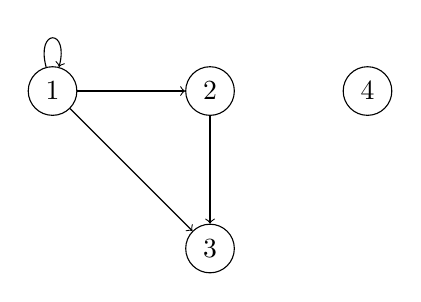
\begin{tikzpicture}[->,node distance=2cm]
  \node[draw,circle] (A) {$1$};
  \node[draw,circle] (B) [right of=A] {$2$};
  \node[draw,circle] (C) [below of=B] {$3$};
  \node[draw,circle] (D) [right of=B] {$4$};
  \draw (A) to [loop above]  (A);
  \draw (A) to  (B);
  \draw (A) to  (C);
  \draw (B) to  (C);
  \end{tikzpicture}
\intertext{આ આલેખ $\tuple{V', E}$થી જુદો છે,
  જેમાં $V' = \{1, 2, 3\}$ છે અને જે આવો દેખાય છે:}
& 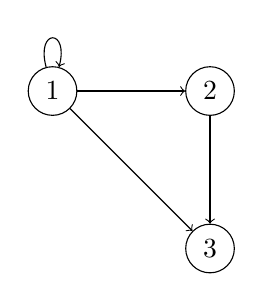
\begin{tikzpicture}[->,node distance=2cm]
  \node[draw,circle] (A) {$1$};
  \node[draw,circle] (B) [right of=A] {$2$};
  \node[draw,circle] (C) [below of=B] {$3$};
  \draw (A) to [loop above]  (A);
  \draw (A) to  (B);
  \draw (A) to  (C);
  \draw (B) to  (C);
  \end{tikzpicture}
\end{align*}
\end{ex}

\begin{prob}
  ગણ $\{1, 2, 3, 4\}$ પરના કરતાં-નાનું-અથવા-સમાન
  સંબંધ $\le$ને આલેખ તરીકે લો અને તેને અનુરૂપ આકૃતિ દોરો.
\end{prob}
% END OLP-0017
\endgroup


\begingroup
\makeatletter\def\ol@sectioncs{section}\makeatother

% BEGIN OLP-0018
\olfileid{sfr}{rel}{tre}
\olsection{વૃક્ષો}
\phantomsection\label{guunit:OLP-0018}


તર્કશાસ્ત્રના બધા ભાગોમાં મહત્વનો ભાગ ભજવતો આંશિક ક્રમનો
એક ખાસ પ્રકાર \emph{વૃક્ષ} છે. તર્કશાસ્ત્રના પ્રાથમિક ભાગોમાં
સાંત વૃક્ષો આવે છે: દાખલા તરીકે, સૂત્રોને વાક્યરચના
વૃક્ષમાં તેમના વિઘટન દ્વારા સમજી શકાય છે, જ્યારે ઘણી
નિષ્પત્તિ પદ્ધતિઓમાં નિષ્પત્તિઓ પણ સાંત વૃક્ષોનું
રૂપ ધરાવે છે.
વિધાનાત્મક અને પ્રથમ ક્રમના તર્કશાસ્ત્ર માટેના પૂર્ણતા પ્રમેયોની
સાબિતીમાં જ અનંત વૃક્ષો દેખાય છે, અને ગાણિતિક તર્કશાસ્ત્રમાં
સર્વત્ર તેમનો ઉપયોગ થાય છે.

ગણસિદ્ધાંતમાં વૃક્ષનો ખ્યાલ, આલેખસિદ્ધાંતમાં વૃક્ષના ખ્યાલ સાથે
ગાઢ રીતે જોડાયેલો છે. અહીં એક (સાંત) વૃક્ષનું ચિત્ર છે:

\begin{center}
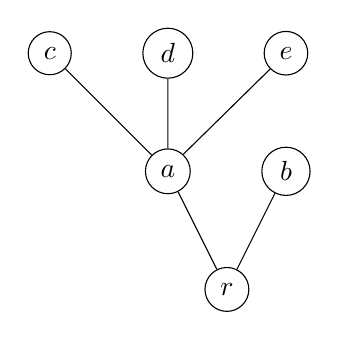
\begin{tikzpicture}[nodes={draw, circle}, -]
\node{$r$} [grow'=up]
    child { node {$a$}
        child { node {$c$} }
        child { node {$d$} }
        child { node {$e$} }
    }
    child { node {$b$} };
\end{tikzpicture}
\end{center}

સૌથી નીચેની ગાંઠ $r$ મૂળ છે. $r$ સિવાયની દરેક ગાંઠની
તરત નીચે બરાબર એક જનક ગાંઠ છે.
ગાંઠ $x$થી ધારોને અનુસરીને ઉપર જતાં ગાંઠ $y$ સુધી પહોંચી
શકાય ત્યારે $x$નો $y$ સાથેનો સંબંધ,
$x$ એ $y$નો \emph{પૂર્વજ} છે એમ સમજી શકાય.

વૃક્ષમાં પૂર્વજનો સંબંધ કડક આંશિક ક્રમ છે.
આ પરથી ગણસિદ્ધાંતની વ્યાખ્યા આપવાની પ્રેરણા મળે છે.
તે રજૂ કરવા માટે આપણને બે ખ્યાલો જોઈએ.
$\le$ વડે આંશિક ક્રમમાં ગોઠવેલા ગણ $A$માં
\emph{લઘુતમ ઘટક} એવો ઘટક $x \in A$ છે
કે દરેક $y \in A$ માટે $x \le y$.
ગણ $\le$ વડે \emph{સુક્રમિત} હોય જો તેના દરેક
અરિક્ત ઉપગણમાં લઘુતમ ઘટક હોય.

\begin{defn}[વૃક્ષ]
\emph{વૃક્ષ} એવો જોડ $T = \tuple{A, \le}$ છે કે $A$ એક ગણ છે
અને $\le$ એ $A$ પરનો આંશિક ક્રમ છે, જેમાં એકમાત્ર લઘુતમ
ઘટક $r \in A$ છે (જેને \emph{મૂળ} કહે છે), અને
દરેક $x \in A$ માટે ગણ $\Setabs{y}{y \le x}$
એ $\le$ વડે સુક્રમિત છે.
\end{defn}

\begin{defn}[અનુગામીઓ]
ધારો કે $T = \tuple{A, \le}$ વૃક્ષ છે.
જો $x,y \in A$, $x < y$, અને $x < z < y$
થાય એવો કોઈ $z \in A$ ન હોય, તો આપણે કહીએ છીએ કે
$y$ એ $x$નો \emph{અનુગામી} છે.
\end{defn}

$x \in A$ના અનુગામીઓને તેની \emph{સંતાન ગાંઠો} પણ કહે છે.
જો $y$ એ $x$નો અનુગામી હોય, તો આપણે $x$ને $y$નો
\emph{પુરોગામી} અથવા \emph{જનક} કહીએ છીએ.

\begin{prop}
જો $\tuple{A,\le}$ વૃક્ષ હોય, તો મૂળ સિવાયના
દરેક $x \in A$નો વધુમાં વધુ એક પુરોગામી હોય.
\end{prop}

\begin{proof}
  ધારો કે $y_1 < x$ અને $y_2 < x$ અને $y_1 \neq y_2$.
  તો $\{y_1, y_2\} \subseteq \Setabs{z}{z<x}$.
  $\Setabs{z}{z<x}$ એ $\le$ વડે સુક્રમિત હોવાથી,
  તેના ઉપગણ $\{y_1, y_2\}$માં લઘુતમ ઘટક છે,
  જે દેખીતી રીતે કાં $y_1$ અથવા $y_2$ હોવો જોઈએ.
  તેથી કાં $y_1 \le y_2$ અથવા $y_2 \le y_1$.
  આપણે $y_1 \neq y_2$ ધાર્યું હતું, તેથી ખરેખર
  કાં $y_1 < y_2$ અથવા $y_2 < y_1$.
  આપણે $y_1 < x$ અને $y_2 < x$ ધાર્યું હોવાથી,
  વધુમાં કાં $y_1 < y_2 < x$ અથવા $y_2 < y_1 < x$.
  તેથી $y_1$ અને $y_2$ બંને $x$ના પુરોગામી હોઈ શકે નહીં.
\end{proof}

\begin{defn}
વૃક્ષ $T = \tuple{A, \le}$ \emph{અનંત} કહેવાય જો $A$
અનંત ગણ હોય, અને નહિતર \emph{સાંત} કહેવાય.
જો $T$માં દરેક $x \in A$ના માત્ર સાંત સંખ્યામાં અનુગામીઓ હોય,
તો આપણે કહીએ છીએ કે $T$ \emph{સાંત શાખનવાળું} છે.
\end{defn}

\begin{defn}[શાખાઓ]
વૃક્ષ $T = \tuple{A, \le}$ આપેલું હોય ત્યારે,
$T$ની \emph{શાખા} એ $T$માં સમાવેશની દૃષ્ટિએ મહત્તમ શૃંખલા છે,
એટલે કે, એવો ગણ $B \subseteq A$ કે કોઈ પણ
$x, y \in B$ માટે કાં $x \le y$ અથવા $y \le x$,
અને કોઈ પણ $z \in X \setminus B$ માટે એવો
$u \in B$ અસ્તિત્વ ધરાવે છે કે ન તો $z \le u$, ન તો $u \le z$.
આપણે $T$ની બધી શાખાઓના ગણને દર્શાવવા $[T]$ વાપરીએ છીએ.
\end{defn}

\begin{ex}
સાંત શાખનવાળા વૃક્ષનું એક સુપ્રસિદ્ધ ઉદાહરણ એ $0$ અને $1$ના
સાંત અનુક્રમોનું \emph{અનંત દ્વિઆધારી વૃક્ષ} છે,
જેને ક્યારેક $\{0,1\}^*$ અથવા $\Bin^*$થી દર્શાવવામાં આવે છે,
અને જે વિસ્તરણ સંબંધ $\sqsubseteq$ વડે ક્રમિત છે
(દા.ત., $101 \sqsubseteq 101101$).
કોઈ પણ દ્વિઆધારી પ્રતીકશ્રેણીને અંતે $0$ કે $1$ ઉમેરીને
હંમેશાં વિસ્તારી શકાય છે, તેથી આ વૃક્ષમાં અનંત સંખ્યામાં
ઘટકો છે: દરેક ઘટક $s$ના બરાબર બે અનુગામી $s0$ અને $s1$ છે.
તેનું મૂળ ખાલી અનુક્રમ $\emptyseq$ છે.
\end{ex}

\begin{ex}
થોડું વધુ સામાન્ય રીતે, વિસ્તરણ સંબંધ $\sqsubseteq$ સાથે
પ્રાકૃતિક સંખ્યાઓના સાંત અનુક્રમોનો ગણ $\Nat^*$ પણ વૃક્ષ છે.
તે દેખીતી રીતે સાંત શાખનવાળું નથી: દરેક $s \in \Nat^*$ના
અનંત સંખ્યામાં અનુગામી $sn$ છે, દરેક $n \in \Nat$ માટે એક.
$\sqsubseteq$ હેઠળ સંવૃત એવો દરેક $A \subseteq \Nat^*$
એ $\Nat^*$નું \emph{ઉપવૃક્ષ} છે.
(એટલે કે, $A$ એવો છે કે જો $s \in A$ અને
$s' \sqsubseteq s$, તો $s' \in A$ પણ.)
બધાં સાંત વૃક્ષોને $\Nat^*$નાં સાંત ઉપવૃક્ષો તરીકે રજૂ કરી શકાય છે.
\end{ex}

\begin{prop}[કેનિગનું સહાયક પ્રમેય]
જો $T = \tuple{A,\le}$ સાંત શાખનવાળું અનંત વૃક્ષ હોય,
તો $T$ને અનંત શાખા હોય છે.
\end{prop}

સંગણનીયતાના સિદ્ધાંતમાં વ્યાપકપણે વપરાતો કેનિગના સહાયક
પ્રમેયનો એક વિશેષ કિસ્સો, જેને \emph{નબળું કેનિગ સહાયક પ્રમેય}
કહે છે, આ છે: $\{0,1\}^*$ના કોઈ પણ અનંત ઉપવૃક્ષને
અનંત શાખા હોય છે.
% END OLP-0018
\endgroup


\begingroup
\makeatletter\def\ol@sectioncs{section}\makeatother

% BEGIN OLP-0019
\olfileid{sfr}{rel}{ops}
\olsection{સંબંધો પરની ક્રિયાઓ}
\phantomsection\label{guunit:OLP-0019}


સંબંધોમાં ફેરફાર કરવો અથવા તેમને ભેગા કરવા ઘણી વાર ઉપયોગી
બને છે. \olref[sfr][rel][ord]{prop:stricttopartial}માં આપણે
સંબંધોના \emph{યોગગણ}નો વિચાર કર્યો હતો, જે બે સંબંધોને
જોડના ગણ તરીકે લઈએ ત્યારે તેમનો યોગગણ જ છે.
એ જ રીતે, \olref[sfr][rel][ord]{prop:partialtostrict}માં
આપણે સંબંધોના સાપેક્ષ તફાવતનો વિચાર કર્યો હતો.
અહીં સંબંધો પર કરી શકાય તેવી કેટલીક બીજી ક્રિયાઓ આપેલી છે.

\begin{defn}\ollabel{relationoperations}
ધારો કે $R$, $S$ સંબંધો છે, અને $A$ કોઈ પણ ગણ છે.

$R$નો \emph{વ્યસ્ત} એ
$R^{-1} = \Setabs{\tuple{y, x}}{\tuple{x, y} \in R}$ છે.

$R$ અને $S$નો \emph{સાપેક્ષ ગુણાકાર} એ
$(R \mid S) = \{\tuple{x, z} : \exists y(Rxy \land Syz)\}$ છે.

$R$નું $A$ પર \emph{મર્યાદન} એ
$\funrestrictionto{R}{A}= R \cap A^2$ છે.

$R$ને $A$ પર \emph{લાગુ પાડતાં મળતો ગણ} એ
$\funimage{R}{A} = \{y : (\exists x \in A)Rxy\}$ છે.
\end{defn}

\begin{ex}
ધારો કે $S \subseteq \Int^2$ એ $\Int$ પરનો અનુગામી સંબંધ છે,
એટલે કે $S = \Setabs{\tuple{x, y} \in \Int^2}{x + 1 = y}$,
જેથી $Sxy$ તો અને તો જ $x + 1 = y$.

$S^{-1}$ એ $\Int$ પરનો પુરોગામી સંબંધ છે,
એટલે કે $\Setabs{\tuple{x,y}\in\Int^2}{x -1 =y}$.

$S\mid S$ એ
$ \Setabs{\tuple{x,y}\in\Int^2}{x + 2 =y}$ છે.

$\funrestrictionto{S}{\Nat}$ એ $\Nat$ પરનો અનુગામી સંબંધ છે.

$\funimage{S}{\{1,2,3\}}$ એ $\{2, 3, 4\}$ છે.
\end{ex}

\begin{defn}[પરંપરિત સંવરણ]ધારો કે $R \subseteq A^2$ દ્વિઘટકી સંબંધ છે.

$R$નું \emph{પરંપરિત સંવરણ} એ
$R^+ = \bigcup_{0 < n \in \Nat} R^n$ છે,
જ્યાં આપણે પુનરાવર્તી રીતે $R^1 = R$ અને
$R^{n+1} = R^n \mid R$ વ્યાખ્યાયિત કરીએ છીએ.

$R$નું \emph{સ્વવાચક પરંપરિત સંવરણ} એ
$R^* = R^+ \cup \Id{A}$ છે.
\end{defn}

\begin{ex}
અનુગામી સંબંધ $S \subseteq \Int^2$ લો.
$S^2xy$ તો અને તો જ $x + 2 = y$,
$S^3xy$ તો અને તો જ $x + 3 = y$, વગેરે.
તેથી $S^+xy$ તો અને તો જ કોઈક $n \geq 1$ માટે
$x + n = y$. બીજા શબ્દોમાં, $S^+xy$ તો અને તો જ $x < y$,
અને $S^*xy$ તો અને તો જ $x \le y$.
\end{ex}

\begin{prob}
$R$નું પરંપરિત સંવરણ ખરેખર પરંપરિત છે તે દર્શાવો.
\end{prob}
% END OLP-0019
\endgroup


\OLEndChapterHook
% END OLP-0011
\endgroup


\begingroup
\makeatletter\def\ol@sectioncs{section}\makeatother

% BEGIN OLP-0020
\olchapter{sfr}{fun}{વિધેયો}
\olchapterid{sfr}{fun}
\phantomsection\label{guunit:OLP-0020}


\begingroup
\makeatletter\def\ol@sectioncs{section}\makeatother

% BEGIN OLP-0021
\olfileid{sfr}{fun}{bas}
\olsection{પાયાની બાબતો}
\phantomsection\label{guunit:OLP-0021}


\begin{explain}
\emph{વિધેય} એવું નિરૂપણ છે જે આપેલા ગણના દરેક ઘટકને
કોઈ (બીજા) આપેલા ગણના ચોક્કસ ઘટક પર મોકલે છે.
દાખલા તરીકે, $1$~ઉમેરવાની ક્રિયા એક વિધેય વ્યાખ્યાયિત કરે છે:
દરેક સંખ્યા~$n$નું નિરૂપણ અનન્ય સંખ્યા~$n+1$ પર થાય છે.

વધુ સામાન્ય રીતે, વિધેયો આગત તરીકે જોડ, ત્રિજોડ વગેરે લઈ
કોઈ પ્રકારનું નિર્ગત આપી શકે છે. પાયાના અંકગણિતમાંથી આપણને
ઘણાં વિધેયો પરિચિત છે. દાખલા તરીકે, સરવાળો અને ગુણાકાર
વિધેયો છે. તેઓ બે સંખ્યાઓ લે છે અને ત્રીજી સંખ્યા આપે છે.

આ ગાણિતિક, અમૂર્ત અર્થમાં વિધેય એક \emph{કાળી પેટી} છે:
કયા આગત સાથે કયું નિર્ગત જોડાયેલું છે એટલું જ મહત્ત્વનું છે,
નિર્ગતની ગણતરી કરવાની પદ્ધતિ નહીં.
\end{explain}

\begin{defn}[વિધેય]
\emph{વિધેય} $f \colon A \to B$ એ $A$ના દરેક ઘટકનું
$B$ના કોઈ ઘટક પરનું નિરૂપણ છે.

આપણે $A$ને $f$નો \emph{પ્રદેશ} અને $B$ને $f$નો
\emph{સહપ્રદેશ} કહીએ છીએ. $A$ના ઘટકોને $f$નાં
આગતો અથવા \emph{દલીલો} કહે છે; અને $f$ દ્વારા દલીલ~$x$ સાથે
જોડાતા $B$ના ઘટકને દલીલ~$x$ માટેની
\emph{$f$ની કિંમત} કહે છે, જેને $f(x)$ લખાય છે.

$f$નો \emph{વિસ્તાર} $\ran{f}$ એ સહપ્રદેશનો એવો ઉપગણ છે
જેમાં કોઈક દલીલ માટેની $f$ની કિંમતો આવે છે;
$\ran{f} =
\Setabs{f(x)}{x \in A}$.
\end{defn}

\olref{fig:function}માંનું ચિત્ર વિધેયો વિશે વિચારવામાં મદદરૂપ
થઈ શકે છે. ડાબી બાજુનો લંબવૃત્ત વિધેયનો \emph{પ્રદેશ}
દર્શાવે છે; જમણી બાજુનો લંબવૃત્ત તેનો \emph{સહપ્રદેશ}
દર્શાવે છે; અને તીર પ્રદેશની \emph{દલીલ}થી સહપ્રદેશની
તેને અનુરૂપ \emph{કિંમત} તરફ જાય છે.

\begin{figure}
  \olasset{assets/diagrams/function.tikz}
  \caption{વિધેય એ એક ગણના દરેક ઘટકનું બીજા ગણના
    ઘટક પરનું નિરૂપણ છે. તીર પ્રદેશની દલીલથી
    સહપ્રદેશની તેને અનુરૂપ કિંમત તરફ જાય છે.}
  \ollabel{fig:function}
\end{figure}

\begin{ex}
ગુણાકાર પ્રાકૃતિક સંખ્યાઓની જોડને આગત તરીકે લે છે અને
પ્રાકૃતિક સંખ્યાઓને નિર્ગત તરીકે આપે છે. તેથી તે
$\Nat \times \Nat$ (પ્રદેશ)થી $\Nat$ (સહપ્રદેશ)માં જાય છે.
તેનો વિસ્તાર પણ $\Nat$ છે, કારણ કે દરેક $n \in \Nat$
એ $n \times 1$ છે.
\end{ex}

\begin{ex}
ગુણાકાર વિધેય છે, કારણ કે તે દરેક આગતને---પ્રાકૃતિક સંખ્યાઓની
દરેક જોડને---એક જ નિર્ગત સાથે જોડે છે:
$\times \colon \Nat^2 \to
\Nat$. તેનાથી વિપરીત, પ્રાકૃતિક સંખ્યા~$n$ને
$x^2 = n$ થાય એવી વાસ્તવિક સંખ્યા~$x$ પર મોકલતું નિરૂપણ
વિધેયાત્મક નથી, કારણ કે દરેક ધન પૂર્ણાંક~$n$નાં બે વર્ગમૂળ
છે: $\sqrt{n}$ અને~$-\sqrt{n}$. માત્ર અનૃણ (મુખ્ય) વર્ગમૂળ આપીને
આ નિરૂપણને વિધેયાત્મક બનાવી શકીએ:
$\sqrt{\phantom{X}} \colon
\Nat \to \Real$.
\end{ex}
\sourcecorrection{OLFUN-002}{મૂળની \texttt{function-basics.tex}, પંક્તિઓ
64--71માં પ્રદેશમાં શૂન્યનો સમાવેશ હોવા છતાં ``ધન વર્ગમૂળ'' કહેવાયું છે.
અહીં શૂન્યને પણ આવરી લેતું ``અનૃણ (મુખ્ય) વર્ગમૂળ'' લખ્યું છે.}

\begin{ex}
વર્ગના દરેક વિદ્યાર્થીને તેના અંતિમ ગુણાંક સાથે જોડતો સંબંધ
વિધેય છે---એક જ વર્ગમાં કોઈ વિદ્યાર્થીને બે જુદા અંતિમ
ગુણાંક મળી શકે નહીં. વર્ગના દરેક વિદ્યાર્થીને તેનાં
માતાપિતા સાથે જોડતો સંબંધ વિધેય નથી: વિદ્યાર્થીઓને
શૂન્ય, બે કે વધુ માતાપિતા હોઈ શકે છે.
\end{ex}

\begin{explain}
દરેક સંભવિત દલીલ માટે વિધેયની કિંમત શું છે તે કોઈ ચોક્કસ
રીતે જણાવીને આપણે વિધેયો વ્યાખ્યાયિત કરી શકીએ છીએ.
તે માટે સૂત્ર આપી શકાય, કિંમતની ગણતરી કરવાની પદ્ધતિ
વર્ણવી શકાય, અથવા દરેક દલીલની કિંમતોની યાદી આપી શકાય.
વિધેયને ગમે તે રીતે વ્યાખ્યાયિત કરીએ, દરેક દલીલ માટે
એક અને માત્ર એક કિંમત નક્કી કરી છે તેની ખાતરી કરવી જોઈએ.
\end{explain}

\begin{ex}
$f(x) = x+1$ થાય તે રીતે $f \colon \Nat \to \Nat$
વ્યાખ્યાયિત કરીએ. આ વ્યાખ્યા $f$ને એવું વિધેય બનાવે છે
જે પ્રાકૃતિક સંખ્યાઓ લે છે અને પ્રાકૃતિક સંખ્યાઓ આપે છે.
તે જણાવે છે કે પ્રાકૃતિક સંખ્યા~$x$ આપતાં $f$ તેનું
અનુગામી~$x+1$ આપશે.
આ કિસ્સામાં સહપ્રદેશ $\Nat$ એ $f$નો વિસ્તાર નથી,
કારણ કે પ્રાકૃતિક સંખ્યા~$0$ કોઈ પ્રાકૃતિક સંખ્યાનું
અનુગામી નથી. $f$નો વિસ્તાર બધા ધન પૂર્ણાંકોનો ગણ
$\Int^{+}$ છે.
\end{ex}

\begin{ex}\ollabel{examplefunext}
$g(x) = x+2-1$ થાય તે રીતે $g \colon \Nat \to \Nat$
વ્યાખ્યાયિત કરીએ. આ જણાવે છે કે $g$ પ્રાકૃતિક સંખ્યાઓ
લેતું અને પ્રાકૃતિક સંખ્યાઓ આપતું વિધેય છે.
પ્રાકૃતિક સંખ્યા~$x$ આપતાં $g$, $x$ના અનુગામીના
અનુગામીનો પુરોગામી, એટલે કે $x+1$, આપશે.
\end{ex}
\sourcecorrection{OLFUN-003}{મૂળની \texttt{function-basics.tex}, પંક્તિઓ
103--107માં આગતનું નામ પહેલાં \(n\) અને પછી \(x\) છે. વ્યાખ્યા અને
પછીના સૂત્ર સાથે સુસંગત રહે તે માટે અહીં સર્વત્ર \(x\) વાપર્યું છે.}

\begin{explain}
આપણે હમણાં જુદી \emph{વ્યાખ્યાઓ} ધરાવતા બે વિધેયો,
$f$ અને $g$, જોયાં. જોકે, આ \emph{એક જ વિધેય} છે.
કારણ કે કોઈ પણ પ્રાકૃતિક સંખ્યા~$n$ માટે
$f(n) = n+1 = n+2-1 =
g(n)$ થાય છે. બીજા શબ્દોમાં, $f$ અને~$g$ માટેની આપણી
વ્યાખ્યાઓ જુદાં સમીકરણો દ્વારા એક જ નિરૂપણ નક્કી કરે છે.
આમ, ગર્ભિત રીતે આપણે વિધેયો માટે દલીલોની કિંમતો દ્વારા
નિર્ધારિત સમાનતાના સિદ્ધાંત પર આધાર રાખીએ છીએ:
\[
  \text{જો }\forall x\, f(x) = g(x)\text{, તો }f = g
\]
શરત એટલી કે $f$ અને~$g$નો પ્રદેશ અને સહપ્રદેશ એક જ હોય.
\end{explain}

\begin{ex}
આપણે કિસ્સા પાડી વિધેયો વ્યાખ્યાયિત પણ કરી શકીએ.
દાખલા તરીકે, $h \colon \Nat \to \Nat$ને આમ વ્યાખ્યાયિત
કરી શકીએ:
\[
h(x) =
\begin{cases}
  \frac{x}{2} & \text{જો $x$ યુગ્મ હોય} \\
  \frac{x+1}{2} & \text{જો $x$ અયુગ્મ હોય.}
\end{cases}
\]
દરેક પ્રાકૃતિક સંખ્યા યુગ્મ કે અયુગ્મ હોવાથી, આ વિધેયનું
નિર્ગત હંમેશાં પ્રાકૃતિક સંખ્યા હશે. એટલું યાદ રાખો કે
કિસ્સા પાડી વિધેય વ્યાખ્યાયિત કરો ત્યારે દરેક સંભવિત
આગત ચોક્કસ એક કિસ્સામાં આવવું જોઈએ. કેટલીક વાર
કિસ્સાઓ બધા આગતોને આવરી લે છે અને પરસ્પર અલગ છે
તે સાબિત કરવું જરૂરી બનશે.
\end{ex}
% END OLP-0021
\endgroup


\begingroup
\makeatletter\def\ol@sectioncs{section}\makeatother

% BEGIN OLP-0022
\olfileid{sfr}{fun}{kin}
\olsection{વિધેયોના પ્રકારો}
\phantomsection\label{guunit:OLP-0022}


\begin{explain}
આપણને વારંવાર મળતા વિધેયોના કેટલાક પ્રકારોનું
વર્ગીકરણ રજૂ કરવું ઉપયોગી થશે.

શરૂઆતમાં એવાં વિધેયો લઈએ જેમના સહપ્રદેશનો દરેક સભ્ય
વિધેયની કિંમત હોય. આવાં વિધેયોને વ્યાપ્ત કહે છે;
તેમને \olref{fig:surjective} પ્રમાણે ચિત્રમાં દર્શાવી શકાય.

\begin{figure}
  \olasset{assets/diagrams/surjective.tikz}
  \caption{વ્યાપ્ત વિધેયના સહપ્રદેશનો દરેક
    ઘટક તેની કિંમત હોય છે.}
  \ollabel{fig:surjective}
\end{figure}
\end{explain}

\begin{defn}[વ્યાપ્ત વિધેય]
વિધેય $f \colon A \rightarrow B$ \emph{વ્યાપ્ત}
હોય જો અને માત્ર જો $B$ એ $f$નો વિસ્તાર પણ હોય, એટલે કે
દરેક $y \in B$ માટે ઓછામાં ઓછો એક $x \in A$
એવો હોય કે $f(x) = y$; અથવા પ્રતીકોમાં:
\[
  (\forall y \in B)(\exists x \in A)f(x) = y.
\]
આવા વિધેયને $A$થી $B$માંનું વ્યાપ્ત વિધેય કહીએ છીએ.
\end{defn}

\begin{explain}
$f$ એ વ્યાપ્ત વિધેય છે તે બતાવવા, તમારે બતાવવું પડે
કે $f$ના સહપ્રદેશની દરેક વસ્તુ કોઈક આગત $x$ માટે
$f(x)$ની કિંમત છે.

નોંધો કે કોઈ પણ વિધેય વ્યાપ્ત વિધેય
\emph{ઉત્પન્ન કરે છે}. કારણ કે આપેલા વિધેય
$f \colon A \to B$ માટે $f'(x) = f(x)$ દ્વારા
$f' \colon A \to \ran{f}$ વ્યાખ્યાયિત કરીએ.
$\ran{f}$ની \emph{વ્યાખ્યા} જ
$\Setabs{f(x) \in B}{x \in A}$ હોવાથી આ વિધેય
$f'$ ચોક્કસ વ્યાપ્ત વિધેય છે.
\end{explain}

\begin{explain}
કોઈ પણ વિધેય દરેક સંભવિત આગતને અનન્ય નિર્ગત પર મોકલે છે.
પરંતુ એવાં વિધેયો પણ છે જે જુદાં આગતોને કદી એક જ
નિર્ગત પર મોકલતાં નથી. આવાં વિધેયોને એક-એક
કહે છે; તેમને \olref{fig:injective} પ્રમાણે ચિત્રમાં
દર્શાવી શકાય.
\begin{figure}
  \olasset{assets/diagrams/injective.tikz}
  \caption{એક-એક વિધેય કદી બે જુદી દલીલોને
    એક જ કિંમત પર મોકલતું નથી.}
  \ollabel{fig:injective}
\end{figure}
\end{explain}

\begin{defn}[એક-એક વિધેય]
વિધેય $f \colon A \rightarrow B$ \emph{એક-એક}
હોય જો અને માત્ર જો દરેક $y \in B$ માટે વધુમાં વધુ
એક $x \in A$ એવો હોય કે $f(x) = y$.
આવા વિધેયને $A$થી $B$માંનું એક-એક વિધેય કહીએ છીએ.
\end{defn}

\begin{explain}
$f$ એ એક-એક વિધેય છે તે બતાવવા, તમારે બતાવવું પડે
કે $f$ના પ્રદેશના કોઈ પણ ઘટકો $x$ અને $y$
માટે, જો $f(x)=f(y)$ હોય, તો $x=y$ થાય છે.
\end{explain}

\begin{ex}
$f(x) = 1$ દ્વારા આપેલું અચળ વિધેય
$f\colon \Nat \to \Nat$ એક-એક પણ નથી
અને વ્યાપ્ત પણ નથી.

$f(x) = x$ દ્વારા આપેલું તદેવ વિધેય
$f\colon \Nat \to \Nat$ એક-એક અને
વ્યાપ્ત બંને છે.

$f(x) = x+1$ દ્વારા આપેલું અનુગામી વિધેય
$f \colon \Nat \to \Nat$ એક-એક છે,
પરંતુ વ્યાપ્ત નથી.

નીચે મુજબ વ્યાખ્યાયિત વિધેય $f \colon \Nat \to \Nat$:
\[
  f(x) =
  \begin{cases}
    \frac{x}{2} & \text{જો $x$ યુગ્મ હોય} \\
    \frac{x+1}{2} & \text{જો $x$ અયુગ્મ હોય.}
  \end{cases}
\]
વ્યાપ્ત છે, પરંતુ એક-એક નથી.
\end{ex}

\begin{explain}
ઘણી વાર આપણે એક-એક અને વ્યાપ્ત બંને
હોય એવાં વિધેયો લેવા માગીએ છીએ. આવાં વિધેયોને
એક-એક અને વ્યાપ્ત કહીએ છીએ. તેઓ
\olref{fig:bijective}માં દર્શાવેલા વિધેય જેવાં દેખાય છે.
એક-એક વ્યાપ્ત વિધેયોને ક્યારેક \emph{પરસ્પર એક-એક સંગતતાઓ}
પણ કહે છે, કારણ કે તેઓ સહપ્રદેશના ઘટકોને પ્રદેશના
ઘટકો સાથે અનન્ય રીતે જોડે છે.
\begin{figure}
  \olasset{assets/diagrams/bijective.tikz}
  \caption{એક-એક અને વ્યાપ્ત વિધેય સહપ્રદેશના ઘટકોને
    પ્રદેશના ઘટકો સાથે અનન્ય રીતે જોડે છે.}
  \ollabel{fig:bijective}
\end{figure}
\end{explain}

\begin{defn}[એક-એક વ્યાપ્ત વિધેય]
વિધેય $f \colon A \to B$ \emph{એક-એક અને વ્યાપ્ત} હોય
જો અને માત્ર જો તે વ્યાપ્ત અને એક-એક
બંને હોય. આવા વિધેયને $A$થી $B$માંનું
(અથવા $A$ અને~$B$ વચ્ચેનું) એક-એક વ્યાપ્ત વિધેય કહીએ છીએ.
\end{defn}
% END OLP-0022
\endgroup


\begingroup
\makeatletter\def\ol@sectioncs{section}\makeatother

% BEGIN OLP-0023
\olfileid{sfr}{fun}{rel}

\olsection{સંબંધો તરીકે વિધેયો}
\phantomsection\label{guunit:OLP-0023}


\begin{explain}
$A$ના ઘટકોને $B$ના ઘટકો પર મોકલતું
વિધેય સ્પષ્ટપણે $A$ અને~$B$ વચ્ચે સંબંધ વ્યાખ્યાયિત
કરે છે: $x$ અને $y$ વચ્ચે આ સંબંધ હોય જો અને માત્ર જો
$f(x) = y$ હોય. હકીકતમાં, દાખલા તરીકે ગણિતના પાયાના
ઘટકોની સંખ્યા ઘટાડવામાં રસ હોય તો, આપણે વિધેય~$f$ને
આ સંબંધ સાથે, એટલે કે જોડોના ગણ સાથે, \emph{એકરૂપ}
પણ ગણી શકીએ. ત્યારે પ્રશ્ન ઊભો થાય છે: કયા સંબંધો
આ રીતે વિધેયો વ્યાખ્યાયિત કરે છે?
\end{explain}

\begin{defn}[વિધેયનો આલેખ] ધારો કે $f\colon A \to B$
વિધેય છે. $f$નો \emph{આલેખ} એ નીચે પ્રમાણે વ્યાખ્યાયિત
સંબંધ $R_f \subseteq A \times B$ છે:
\[
R_f = \Setabs{\tuple{x,y}}{f(x) = y}.
\]
\end{defn}

\begin{explain}
ઘટકો દ્વારા નિર્ધારિત સમાનતાના સિદ્ધાંતથી વિધેયનો
આલેખ અનન્ય રીતે નક્કી થાય છે. વધુમાં, ગણો માટેનો
આ સિદ્ધાંત વિધેયો માટેના ગર્ભિત સમાનતાના સિદ્ધાંતને
તરત સમર્થન આપે છે: જો $f$ અને~$g$નો પ્રદેશ અને
સહપ્રદેશ એક જ હોય, તો બધી દલીલો માટેની કિંમતો
સરખી હોય ત્યારે તેઓ એક જ વિધેય હોય છે.

એ જ રીતે, સંબંધ “વિધેયાત્મક” હોય, તો તે કોઈ
વિધેયનો આલેખ છે.
\end{explain}

\begin{prop}\ollabel{prop:graph-function}
ધારો કે $R \subseteq A \times B$ એવો છે કે:
\begin{enumerate}
\item જો $Rxy$ અને $Rxz$ હોય, તો $y = z$; અને
\item દરેક $x \in A$ માટે કોઈક $y \in B$ એવો છે
કે $\tuple{x,
y} \in R$.
\end{enumerate}
તો $R$ એ $f(x) = y$ જો અને માત્ર જો $Rxy$
દ્વારા વ્યાખ્યાયિત વિધેય $f\colon A \to B$નો આલેખ છે.
\end{prop}

\begin{proof}
ધારો કે $Rxy$ થાય એવો $y$ છે. જો $Rxz$ થાય એવો
બીજો $z \neq
y$ હોત, તો $R$ પરની શરતનો ભંગ થાત.
આથી, $Rxy$ થાય એવો $y$ હોય, તો આ $y$ અનન્ય છે,
અને તેથી $f$ સુવ્યાખ્યાયિત છે. સ્પષ્ટપણે $R_f = R$.
\end{proof}

\begin{explain}
દરેક વિધેય $f\colon A \to B$નો આલેખ હોય છે, એટલે કે
$f(x) = y$ દ્વારા વ્યાખ્યાયિત $A
\times B$માં સમાયેલો સંબંધ. બીજી તરફ,
\olref{prop:graph-function}માં આપેલા ગુણધર્મો ધરાવતો
દરેક સંબંધ~$R
\subseteq A \times B$ કોઈ વિધેય~$f \colon A \to
B$નો આલેખ છે. વિધેયો અને તેમના આલેખો વચ્ચેના આ ગાઢ
સંબંધને કારણે આપણે વિધેયને તેના આલેખ તરીકે જ વિચારી શકીએ.
બીજા શબ્દોમાં, વિધેયોને અમુક સંબંધો સાથે, એટલે કે અમુક
બહુજોડોના ગણો સાથે, એકરૂપ ગણી શકાય.
જોકે, નોંધો કે આ “એકરૂપતા”નો
આશય \olref[sfr][rel][ref]{sec}માં જણાવ્યો હતો તેવો છે:
તે વિધેયોના તત્વમીમાંસાકીય સ્વરૂપ વિશેનો દાવો નથી;
વિધેયોને અમુક ગણો તરીકે \emph{લેવાં} અનુકૂળ છે એવી
નોંધ છે. આ અનુકૂળતાનું એક કારણ એ છે કે આપણે
હવે સંબંધો પર કરેલી ક્રિયાઓ જેવી ક્રિયાઓ વિધેયો પર
કરવાનું વિચારી શકીએ છીએ (જુઓ \olref[sfr][rel][ops]{sec}).
ખાસ કરીને:
\end{explain}
\sourcecorrection{OLFUN-004}{મૂળની \texttt{functions-relations.tex}, પંક્તિઓ
60--68માં આલેખને ``\(A\times B\) પરનો સંબંધ'' કહેવાયો છે. પ્રોજેક્ટની
પોતાની વ્યાખ્યા પ્રમાણે અહીં \(A\) અને \(B\) વચ્ચેનો, એટલે કે
\(A\times B\)માં સમાયેલો સંબંધ અભિપ્રેત છે; અનુવાદમાં એ પ્રકાર સ્પષ્ટ કર્યો છે.}

\begin{defn}\ollabel{defn:funimage}
ધારો કે $f \colon A \to B$ વિધેય છે અને $C\subseteq A$ છે.

$f$નું $C$ પરનું \emph{મર્યાદન} એ બધા $x \in C$ માટે
$(\funrestrictionto{f}{C})(x) = f(x)$ દ્વારા વ્યાખ્યાયિત
વિધેય~$\funrestrictionto{f}{C}\colon C \to B$ છે.
બીજા શબ્દોમાં, $\funrestrictionto{f}{C} = \Setabs{\tuple{x, y} \in R_f}{x \in
C}$.

$C$ પર $f$નું \emph{પ્રયોજન} એ $\funimage{f}{C} =
\Setabs{f(x)}{x \in C}$ છે. તેને $f$ હેઠળનું
$C$નું \emph{પ્રતિબિંબ} પણ કહીએ છીએ.
\end{defn}

\begin{explain}
આ વ્યાખ્યાઓ પરથી કોઈ પણ વિધેય~$f$ માટે
$\ran{f} =
\funimage{f}{\dom{f}}$ મળે છે.
\olref[sfr][rel][ops]{sec}ની
વ્યાખ્યાઓ અને વિધેયોને સંબંધો સાથે એકરૂપ ગણવાની આપણી
રીત જોતાં, આ ખ્યાલો અનુરૂપ છે. અહીં વિધેયનું મર્યાદન
માત્ર પ્રદેશને C સુધી સીમિત કરે છે; અગાઉનું સંબંધ-મર્યાદન
બંને અવયવોને C સુધી સીમિત કરે છે. પરંતુ બે બીજી
ક્રિયાઓ---વ્યસ્ત અને સાપેક્ષ ગુણાકાર---માટે થોડી વધુ
વિગત જરૂરી છે. તે \olref[inv]{sec} અને
\olref[cmp]{sec}માં આપીશું.
\end{explain}
\sourcecorrection{OLFUN-005}{મૂળની \texttt{functions-relations.tex}, પંક્તિઓ
78--100માં વિધેય-મર્યાદનની સ્પષ્ટ વ્યાખ્યા સાચી છે, પરંતુ તેને અગાઉના
બંને-અવયવવાળા સંબંધ-મર્યાદન સાથે ``ચોક્કસ'' સરખું કહેવાયું છે. અહીં
આ સામ્યની મર્યાદા સ્પષ્ટ કરી છે.}
% END OLP-0023
\endgroup


\begingroup
\makeatletter\def\ol@sectioncs{section}\makeatother

% BEGIN OLP-0024
\olfileid{sfr}{fun}{inv}
\olsection{વિધેયોનાં પ્રતિવિધેયો}
\phantomsection\label{guunit:OLP-0024}


\begin{explain}
આપણે વિધેયોને નિરૂપણો તરીકે વિચારીએ છીએ. તેથી વિધેયો
વિશે એક સ્વાભાવિક પ્રશ્ન એ છે કે નિરૂપણને “ઊલટાવી”
શકાય કે નહીં. દાખલા તરીકે, અનુગામી વિધેય
$f(x) = x + 1$ને આ અર્થમાં ઊલટાવી શકાય કે વિધેય
$g(y) = y - 1$ એ $f$ની ક્રિયાને “પાછી ફેરવે” છે.

પરંતુ સાવચેત રહેવું જોઈએ. $g$ની વ્યાખ્યા વિધેય
$\Int \to \Int$ વ્યાખ્યાયિત કરે છે, છતાં તે
\emph{વિધેય} $\Nat
\to \Nat$ વ્યાખ્યાયિત કરતી નથી, કારણ કે
$g(0) \notin \Nat$. એટલે સરળ કિસ્સામાં પણ વિધેયને
ઊલટાવી શકાય કે નહીં તે તરત સ્પષ્ટ થતું નથી;
તે પ્રદેશ અને સહપ્રદેશ પર આધાર રાખી શકે છે.

વિધેયના પ્રતિવિધેયનો ખ્યાલ આ વાતને વધુ ચોક્કસ બનાવે છે.
\end{explain}

\begin{defn}
વિધેય $g \colon B \to A$ એ વિધેય $f
\colon A \to B$નું \emph{પ્રતિવિધેય} છે જો બધા
$x \in A$ અને $y \in B$ માટે
$f(g(y)) = y$ અને $g(f(x)) = x$ થાય.
\end{defn}

જો $f$નું પ્રતિવિધેય~$g$ હોય, તો ઘણી વાર $g$ને
બદલે $f^{-1}$ લખીએ છીએ.

\begin{explain}
હવે વિધેયોને ક્યારે પ્રતિવિધેયો હોય છે તે નક્કી કરીશું.
$f\colon A \to B$ના પ્રતિવિધેય માટેનો યોગ્ય ઉમેદવાર
નીચે મુજબ “વ્યાખ્યાયિત” $g\colon B \to A$ છે:
\[
g(y) = \text{$f(x) = y$ થાય એવો “તે એક જ” $x$.}
\]
પરંતુ “વ્યાખ્યાયિત” (અને “તે એક જ”)ની આસપાસનાં
અવતરણચિહ્નો સૂચવે છે કે આ વ્યાખ્યા નથી. ઓછામાં ઓછું,
તે સંપૂર્ણ સામાન્યતાથી હંમેશાં કામ નહીં કરે. કારણ કે
આ વ્યાખ્યા વિધેય નક્કી કરે તે માટે $f(x) =
y$ થાય એવો એક અને માત્ર એક~$x$ હોવો જોઈએ---$g$નું
નિર્ગત અનન્ય રીતે નક્કી થવું જોઈએ. વધુમાં, દરેક
$y \in B$ માટે તે નક્કી થવું જોઈએ. જો $x_1$ અને
$x_2 \in
A$ એવા હોય કે $x_1 \neq x_2$ છતાં
$f(x_1) = f(x_2)$ હોય, તો $y = f(x_1) = f(x_2)$
માટે $g(y)$ અનન્ય રીતે નક્કી નહીં થાય. અને જો
$f(x) = y$ થાય એવો કોઈ~$x$ જ ન હોય, તો
$g(y)$ બિલકુલ નક્કી થતું નથી. બીજા શબ્દોમાં,
$g$ વ્યાખ્યાયિત થાય તે માટે $f$ એ એક-એક
અને વ્યાપ્ત બંને હોવું જોઈએ.

ધીમે ધીમે આગળ વધીએ. પ્રશ્નને બે ભાગમાં વહેંચીએ:
વિધેય~$f\colon A \to B$ આપેલું હોય ત્યારે
$g(f(x)) = x$ થાય એવું વિધેય $g\colon B \to A$
ક્યારે હોય? આવું $g$ એ $f$ની ક્રિયાને “પાછી ફેરવે” છે;
તેને $f$નો \emph{ડાબી બાજુનો વ્યસ્ત} કહે છે.
બીજું, $f(h(y)) = y$ થાય એવું વિધેય
$h\colon B \to A$ ક્યારે હોય? આવા $h$ને
$f$નો \emph{જમણી બાજુનો વ્યસ્ત} કહે છે---$f$
એ $h$ની ક્રિયાને “પાછી ફેરવે” છે.
\end{explain}

\begin{prop}
જો $f\colon A \to B$ એ એક-એક હોય અને તેનો પ્રદેશ અખાલી હોય, તો
$f$નો \emph{ડાબી બાજુનો વ્યસ્ત}~$g\colon B \to A$
હોય છે, જેથી બધા $x
\in A$ માટે $g(f(x)) = x$ થાય.
\end{prop}

\begin{proof}
ધારો કે $f\colon A \to B$ એ એક-એક છે અને તેનો પ્રદેશ અખાલી છે.
કોઈ $y \in B$ લો. જો $y \in \ran{f}$ હોય,
તો $f(x) = y$ થાય એવો $x \in A$ છે.
$f$ એ એક-એક હોવાથી આવો માત્ર એક~$x \in A$
છે. તેથી $g(y) = x$ વ્યાખ્યાયિત કરી શકીએ, એટલે કે
$g(y)$ એ $f(x)
= y$ થાય એવો “તે એક જ” $x \in A$ છે.
જો $y \notin \ran{f}$ હોય, તો તેને કોઈ પણ~$a \in A$
પર મોકલી શકીએ. એટલે એક $a \in A$ પસંદ કરી
$g\colon B \to A$ને આમ વ્યાખ્યાયિત કરી શકીએ:
\[
g(y) = \begin{cases}
    x & \text{જો $f(x) = y$ હોય}\\
    a & \text{જો $y \notin \ran{f}$ હોય.}
\end{cases}
\]
તે બધા $y \in B$ માટે વ્યાખ્યાયિત છે, કારણ કે
આવા દરેક $y \in \ran{f}$ માટે $f(x) = y$ થાય
એવો ચોક્કસ એક $x \in A$ છે. વ્યાખ્યા પ્રમાણે,
જો $y = f(x)$ હોય, તો $g(y) = x$ થાય,
એટલે કે $g(f(x)) = x$.
\end{proof}
\sourcecorrection{OLFUN-001}{મૂળની \texttt{inverses.tex}, પંક્તિઓ 62--84માં
પ્રદેશ અખાલી હોવાની શરત વિના આ વિધાન ખોટું છે: ખાલી ગણથી એક-ઘટકવાળા
ગણમાંનું ખાલી વિધેય એક-એક છે, પરંતુ તેનો ડાબી બાજુનો વ્યસ્ત નથી.
સરળ સુધારેલા વિધાનમાં પ્રદેશ અખાલી હોવાની શરત ઉમેરી છે. ચોક્કસ સામાન્ય
શરત એ છે કે પ્રદેશ અખાલી હોય અથવા સહપ્રદેશ ખાલી હોય.}

\begin{prob}
બતાવો કે જો $f\colon A \to B$નો ડાબી બાજુનો
વ્યસ્ત~$g$ હોય, તો $f$ એ એક-એક છે.
\end{prob}

\begin{prop}
જો $f\colon A \to B$ એ વ્યાપ્ત હોય, તો
$f$નો \emph{જમણી બાજુનો વ્યસ્ત}~$h\colon B \to A$
હોય છે, જેથી બધા~$y \in B$ માટે $f(h(y)) =
y$ થાય.
\end{prop}

\begin{proof}
ધારો કે $f\colon A \to B$ એ વ્યાપ્ત છે.
કોઈ $y \in
B$ લો. $f$ એ વ્યાપ્ત હોવાથી
$f(x_y)
= y$ થાય એવો $x_y \in A$ છે.
તેથી $h(y) = x_y$ વ્યાખ્યાયિત કરી શકીએ, એટલે કે
દરેક $y \in B$ માટે $f(x) = y$ થાય એવો કોઈ
$x \in A$ પસંદ કરીએ; $f$ એ વ્યાપ્ત
હોવાથી પસંદ કરવા માટે હંમેશાં ઓછામાં ઓછો એક હોય છે.
\footnote{$f$ એ વ્યાપ્ત હોવાથી દરેક~$y \in B$
માટે ગણ $\Setabs{x}{f(x) = y}$ ખાલી નથી.
$h$ની આપણી વ્યાખ્યા માટે આ દરેક ગણમાંથી એક જ $x$
પસંદ કરવો પડે છે. આ હંમેશાં શક્ય છે તે હકીકતમાં
સ્પષ્ટ નથી---આવી પસંદગીઓ કરવાની શક્યતા એક
સ્વયંસિદ્ધિ તરીકે માની લેવામાં આવે છે.
બીજા શબ્દોમાં, આ વિધાન કહેવાતી પસંદગીની સ્વયંસિદ્ધિ
ધારે છે. આ મુદ્દાને આપણે
\olref[sth][choice][]{chap}માં ફરી જોઈશું.
જોકે, ઘણા ચોક્કસ કિસ્સામાં, દાખલા તરીકે $A = \Nat$
હોય કે સાન્ત હોય, અથવા $f$ એ એક-એક અને વ્યાપ્ત હોય,
ત્યારે પસંદગીની સ્વયંસિદ્ધિ જરૂરી નથી. (ખાસ કરીને
$f$ એ એક-એક અને વ્યાપ્ત હોય ત્યારે દરેક $y \in B$
માટે ગણ $\Setabs{x}{f(x) = y}$માં ચોક્કસ એક
ઘટક હોય છે, એટલે પસંદગી કરવાની રહેતી જ નથી.)}
વ્યાખ્યા પ્રમાણે, જો $x = h(y)$ હોય,
તો $f(x) = y$ થાય; એટલે કે કોઈ પણ $y \in B$
માટે $f(h(y)) = y$.
\end{proof}

\begin{prob}
બતાવો કે જો $f\colon A \to B$નો જમણી બાજુનો
વ્યસ્ત~$h$ હોય, તો $f$ એ વ્યાપ્ત છે.
\end{prob}

\begin{explain}
અગાઉની સાબિતીના વિચારોને ભેગા કરતાં હવે મળે છે કે
દરેક એક-એક વ્યાપ્ત વિધેયને પ્રતિવિધેય હોય છે, એટલે કે
એક જ વિધેય $f$નો ડાબી અને જમણી બંને બાજુનો વ્યસ્ત હોય છે.
\end{explain}

\begin{prop}\ollabel{prop:bijection-inverse}
જો $f\colon A \to B$ એ એક-એક અને વ્યાપ્ત હોય, તો એવું
વિધેય~$f^{-1}\colon B \to A$ છે કે બધા $x \in A$
માટે $f^{-1}(f(x)) = x$ અને બધા $y \in B$
માટે $f(f^{-1}(y)) = y$ થાય.
\end{prop}

\begin{proof}
સ્વાધ્યાય.
\end{proof}

\begin{prob}
\olref[sfr][fun][inv]{prop:bijection-inverse} સાબિત કરો.
તમારે $f^{-1}$ વ્યાખ્યાયિત કરવું, તે વિધેય છે તે
બતાવવું, અને તે $f$નું પ્રતિવિધેય છે તે બતાવવું પડે;
એટલે કે બધા $x \in A$ અને $y \in B$ માટે
$f^{-1}(f(x)) = x$ અને $f(f^{-1}(y)) = y$ થાય.
\end{prob}

\begin{explain}
પ્રતિવિધેયો મેળવવાની થોડી વધુ સામાન્ય રીત છે.
આપણે \olref[kin]{sec}માં જોયું કે દરેક વિધેય $f$
બધા $x \in A$ માટે $f'(x) = f(x)$ લઈને
વ્યાપ્ત વિધેય $f'
\colon A \to \ran{f}$ ઉત્પન્ન કરે છે.
સ્પષ્ટ છે કે $f$ એ એક-એક હોય, તો
$f'$ એ એક-એક અને વ્યાપ્ત છે; તેથી
\olref{prop:bijection-inverse} પ્રમાણે તેને અનન્ય
પ્રતિવિધેય હોય છે. સંકેતપ્રયોગમાં બહુ નાની છૂટ લઈને
આપણે ક્યારેક $f'$ના પ્રતિવિધેયને માત્ર
“$f$નું પ્રતિવિધેય” કહીએ છીએ.
\end{explain}

\begin{prop}\ollabel{prop:left-right}%
બતાવો કે જો $f\colon A \to B$નો ડાબી બાજુનો
વ્યસ્ત~$g$ અને જમણી બાજુનો વ્યસ્ત~$h$ હોય,
તો $h = g$ થાય.
\end{prop}

\begin{proof}
સ્વાધ્યાય.
\end{proof}

\begin{prob}
\olref[sfr][fun][inv]{prop:left-right} સાબિત કરો.
\end{prob}

\begin{prop}\ollabel{prop:inverse-unique}
દરેક વિધેય~$f$ને વધુમાં વધુ એક પ્રતિવિધેય હોય છે.
\end{prop}

\begin{proof}
ધારો કે $g$ અને $h$ બંને $f$નાં પ્રતિવિધેયો છે.
તો ખાસ કરીને $g$ એ $f$નો ડાબી બાજુનો વ્યસ્ત
અને $h$ જમણી બાજુનો વ્યસ્ત છે.
\olref{prop:left-right} પ્રમાણે $g = h$.
\end{proof}
% END OLP-0024
\endgroup


\begingroup
\makeatletter\def\ol@sectioncs{section}\makeatother

% BEGIN OLP-0025
\olfileid{sfr}{fun}{cmp}
\olsection{વિધેયોનું સંયોજન}
\phantomsection\label{guunit:OLP-0025}


\begin{explain}
આપણે \olref[inv]{sec}માં
જોયું કે એક-એક વ્યાપ્ત વિધેય~$f$નું પ્રતિવિધેય~$f^{-1}$
પોતે એક વિધેય છે. વિધેયો પરની બીજી ક્રિયા સંયોજન છે:
આપણે બે વિધેયો $f$ અને~$g$નું સંયોજન કરીને,
એટલે કે પહેલાં $f$ અને પછી $g$ લાગુ પાડીને, નવું વિધેય
વ્યાખ્યાયિત કરી શકીએ. અલબત્ત, વિસ્તાર અને પ્રદેશ મેળ ખાતા
હોય તો જ આ શક્ય છે: $f$નો વિસ્તાર $g$ના પ્રદેશનો
ઉપગણ હોવો જોઈએ. વિધેયો
પરની આ ક્રિયા \olref[rel][ops]{sec}માં સંબંધો પરની
સાપેક્ષ ગુણાકારની ક્રિયાને અનુરૂપ છે.

સંયોજનનો ખ્યાલ સમજાવવામાં ચિત્ર મદદરૂપ થઈ શકે.
\olref{fig:composition}માં આપણે બે વિધેયો
$f \colon A \to B$ અને $g \colon B \to C$
તથા તેમનું સંયોજન~$(\comp{f}{g})$ દર્શાવીએ છીએ.
વિધેય $(\comp{f}{g}) \colon A \to C$ એ $A$ના દરેક
ઘટકને $C$ના ઘટક સાથે જોડે છે.
$A$નો ઘટક એ $C$ના કયા ઘટક
સાથે જોડાય છે તે આ રીતે નક્કી કરીએ: આગત $x \in
A$ આપેલું હોય ત્યારે પહેલાં વિધેય $f$ને $x$ પર લાગુ પાડો.
તે કોઈક $f(x)
= y \in B$ આપશે; પછી $g$ને $y$ પર લાગુ પાડો.
તે કોઈક $g(f(x)) = g(y) = z \in C$ આપશે.
\begin{figure}
  \olasset[2\olphotowidth]{assets/diagrams/composition.tikz}
  \caption{બે વિધેયો $f$ અને~$g$નું સંયોજન $g \circ f$.}
  \ollabel{fig:composition}
\end{figure}
\end{explain}

\begin{defn}[સંયોજન]
ધારો કે $f\colon A \to B$ અને $g\colon B \to C$
વિધેયો છે. $f$નું $g$ સાથેનું \emph{સંયોજન}
એ $\comp{f}{g} \colon A \to C$ છે, જ્યાં
$(\comp{f}{g})(x) = g(f(x))$.
\end{defn}

\begin{ex}
વિધેયો $f(x) = x + 1$ અને $g(x) = 2x$ લો.
$(\comp{f}{g})(x) = g(f(x))$ હોવાથી, દરેક આગત~$x$
માટે પહેલાં તેનું અનુગામી લેવું પડે અને પછી પરિણામને
બે વડે ગુણવું પડે. તેથી તેમનું સંયોજન
$(\comp{f}{g})(x) = 2(x+1)$ દ્વારા અપાય છે.
\end{ex}

\begin{prob}
બતાવો કે જો $f \colon A \to B$ અને $g \colon B \to C$
બંને એક-એક હોય, તો $\comp{f}{g}\colon A \to C$
પણ એક-એક છે.
\end{prob}

\begin{prob}
બતાવો કે જો $f \colon A \to B$ અને $g \colon B \to C$
બંને વ્યાપ્ત હોય, તો $\comp{f}{g}\colon A \to C$
પણ વ્યાપ્ત છે.
\end{prob}

\begin{prob}
ધારો કે $f \colon A \to B$ અને $g \colon B \to C$ છે.
બતાવો કે $\comp{f}{g}$નો આલેખ $R_f \mid R_g$ છે.
\end{prob}
% END OLP-0025
\endgroup



\begingroup
\makeatletter\def\ol@sectioncs{section}\makeatother

% BEGIN OLP-0026
\olfileid{sfr}{fun}{par}

\olsection{આંશિક વિધેયો}
\phantomsection\label{guunit:OLP-0026}


\begin{explain}
ક્યારેક વિધેયની વ્યાખ્યામાં છૂટ આપવી ઉપયોગી બને છે,
જેથી દરેક સંભવિત આગત માટે વિધેયનું નિર્ગત વ્યાખ્યાયિત
હોય તે જરૂરી ન રહે. આવાં નિરૂપણોને
\emph{આંશિક વિધેયો} કહે છે.
\end{explain}

\begin{defn}
\emph{આંશિક વિધેય} $f \colon A \pto B$ એવું નિરૂપણ છે
જે $A$ના દરેક ઘટકને $B$નો વધુમાં વધુ એક
ઘટક ફાળવે છે. જો $f$ એ $x \in A$ને $B$નો
કોઈ ઘટક ફાળવે, તો $f(x)$ \emph{વ્યાખ્યાયિત} છે
એમ કહીએ; અન્યથા તે \emph{અવ્યાખ્યાયિત} છે.
$f(x)$ વ્યાખ્યાયિત હોય તો $f(x) \fdefined$ લખીએ,
અન્યથા $f(x) \fundefined$ લખીએ. આંશિક વિધેય~$f$નો
\emph{પ્રદેશ} એ $A$નો એવો ઉપગણ છે જ્યાં તે
વ્યાખ્યાયિત હોય, એટલે કે
$\dom{f} = \Setabs{x \in A}{f(x) \fdefined}$.
\end{defn}

\begin{ex}
દરેક વિધેય $f\colon A \to B$ આંશિક વિધેય પણ છે.
$A$ પર સર્વત્ર વ્યાખ્યાયિત આંશિક વિધેયો---એટલે કે
અત્યાર સુધી આપણે જેને માત્ર વિધેય કહેતા આવ્યા છીએ તે---
\emph{સર્વત્ર વ્યાખ્યાયિત} વિધેયો પણ કહેવાય છે.
\end{ex}

\begin{ex}
$f(x) = 1/x$ દ્વારા આપેલું આંશિક વિધેય
$f \colon \Real \pto \Real$ એ $x = 0$ માટે
અવ્યાખ્યાયિત છે અને બાકીની બધી જગ્યાએ વ્યાખ્યાયિત છે.
\end{ex}

\begin{prob}
આપેલા $f\colon A \pto B$ માટે આંશિક વિધેય
$g\colon B \pto
A$ આ રીતે વ્યાખ્યાયિત કરો: કોઈ પણ $y \in B$ માટે,
જો $f(x) = y$ થાય એવો અનન્ય $x \in A$ હોય,
તો $g(y) = x$; અન્યથા $g(y) \fundefined$.
બતાવો કે જો $f$ એક-એક હોય, તો બધા $x \in \dom{f}$
માટે $g(f(x)) = x$ અને બધા $y \in \ran{f}$ માટે
$f(g(y)) = y$ થાય છે.
\end{prob}

\begin{defn}[આંશિક વિધેયનો આલેખ]
ધારો કે $f\colon A \pto B$ આંશિક વિધેય છે.
$f$નો \emph{આલેખ} એ નીચે મુજબ વ્યાખ્યાયિત સંબંધ
$R_f \subseteq A \times B$ છે:
\[
R_f = \Setabs{\tuple{x,y}}{f(x) = y}.
\]
\end{defn}

\begin{prop}
ધારો કે $R \subseteq A \times B$નો ગુણધર્મ એવો છે કે
જ્યારે પણ $Rxy$ અને $Rxy'$ હોય, ત્યારે $y = y'$ થાય છે.
તો $R$ એ આ રીતે વ્યાખ્યાયિત આંશિક વિધેય
$f\colon A \pto B$નો આલેખ છે: જો $Rxy$ થાય એવો $y$
હોય, તો $f(x) = y$; અન્યથા $f(x) \fundefined$.
જો $R$ \emph{સર્વાગત} પણ હોય, એટલે કે દરેક $x \in A$
માટે $Rxy$ થાય એવો કોઈ $y \in B$ હોય, તો $f$
સર્વત્ર વ્યાખ્યાયિત છે.
\end{prop}

\begin{proof}
ધારો કે $Rxy$ થાય એવો $y$ છે. જો $Rxy'$ થાય એવો
બીજો $y'
\neq y$ હોત, તો $R$ પરની શરતનો ભંગ થાત.
આથી, $Rxy$ થાય એવો $y$ હોય, તો તે $y$ અનન્ય છે;
તેથી $f$ સુવ્યાખ્યાયિત છે. સ્પષ્ટપણે $R_f = R$
અને જો $R$ સર્વાગત હોય, તો $f$ સર્વત્ર વ્યાખ્યાયિત છે.
\end{proof}
% END OLP-0026
\endgroup


\OLEndChapterHook


\begin{editorial}
આગળનો સંબંધિત અંશ મૂળના સક્રિય આયાતક્રમમાં નથી. તેને અહીં સ્પષ્ટ વૈકલ્પિક સંદર્ભમાં જાળવ્યો છે.
\end{editorial}
\begingroup
\makeatletter\def\ol@sectioncs{section}\makeatother

% BEGIN OLP-0717
\olfileid{sfr}{fun}{iso}
\olsection{એકરૂપતા}
\phantomsection\label{guunit:OLP-0717}


\begin{explain}
\emph{એકરૂપતા} એ જોડાતા ગણોની સંરચના જાળવતું એક-એક વ્યાપ્ત વિધેય છે.
સંરચના એટલે ગણોના ઘટકો વચ્ચે રહેલા સંબંધો.
બે ગણ $X=\{1,2,3\}$ અને $Y=\{4,5,6\}$ લો.
બંનેમાં અનુગામી હોવાનો, નાનું હોવાનો અને મોટું હોવાનો સંબંધ છે.
બે ગણો વચ્ચેની એકરૂપતા આ સંરચનાઓ જાળવતું એક-એક વ્યાપ્ત વિધેય છે.
એટલે એક-એક અને વ્યાપ્ત ફલન~$f \colon X
\to Y$ એકરૂપતા છે જો, ગણના કોઈ પણ બે ઘટકો માટે,
$i<j$ જો અને ફક્ત જો $f(i)<f(j)$,
$i>j$ જો અને ફક્ત જો $f(i)>f(j)$,
અને $j$ એ $i$નો અનુગામી હોય જો અને ફક્ત જો $f(j)$ એ
$f(i)$નો અનુગામી હોય.
\end{explain}

\begin{defn}[એકરૂપતા]
$U$ એ જોડી $\langle X, R\rangle$ અને $V$ એ જોડી
$\langle Y, S\rangle$ હોય, જ્યાં $X$ અને $Y$ ગણો છે અને
$R$ તથા $S$ અનુક્રમે $X$ તથા $Y$ પરના સંબંધો છે.
$X$થી $Y$માં જતું એક-એક વ્યાપ્ત વિધેય~$f$ એ $U$થી $V$માં જતી
\emph{એકરૂપતા} છે જો અને ફક્ત જો તે સંબંધની સંરચના જાળવે:
$X$ના કોઈ પણ $x_{1}$ અને $x_{2}$ માટે
$\tuple{x_1,x_2} \in R$ જો અને ફક્ત જો
$\tuple{f(x_1),f(x_2)} \in S$.
\end{defn}

\begin{ex}
બે ગણ $X=\{1,2,3\}$ અને $Y=\{4,5,6\}$ લો,
સાથે નાનું હોવાનો અને મોટું હોવાનો સંબંધ લો.
$f(x) = 7-x$ વડે આપેલું ફલન~$f\colon X \to Y$
એ $\tuple{X,<}$ અને $\tuple{Y,>}$ વચ્ચેની એકરૂપતા છે.
\end{ex}
% END OLP-0717
\endgroup
% END OLP-0020
\endgroup


\begingroup
\makeatletter\def\ol@sectioncs{section}\makeatother

% BEGIN OLP-0027
\olchapter{sfr}{siz}{ગણોનું કદ}
\olchapterid{sfr}{siz}
\phantomsection\label{guunit:OLP-0027}


\begin{editorial}
આ પ્રકરણ પરિગણના, ગણનીયતા અને અગણનીયતાની ચર્ચા કરે છે.
કેટલાક વિભાગો બે સ્વરૂપે આપેલા છે: વધુ પ્રાથમિક સ્વરૂપમાં
પરિગણનાને યાદી અથવા $\PosInt$થી આવતું વ્યાપ્ત વિધેય
ગણવામાં આવે છે; વધુ અમૂર્ત સ્વરૂપમાં પરિગણનાને
$\Nat$ સાથેનું એક-એક વ્યાપ્ત વિધેય ગણી વ્યાખ્યાયિત કરાય છે.
\end{editorial}

\begingroup
\makeatletter\def\ol@sectioncs{section}\makeatother

% BEGIN OLP-0028
\olfileid{sfr}{siz}{int}

\olsection{પ્રસ્તાવના}
\phantomsection\label{guunit:OLP-0028}


૧૮૭૦ના દાયકામાં જ્યૉર્જ કૅન્ટૉરે ગણસિદ્ધાંત વિકસાવ્યો,
ત્યારે તેમના હેતુઓમાંનો એક અનંત સંગ્રહનો ખ્યાલ---મધ્યયુગના
વિચારકોના શબ્દોમાં, વાસ્તવમાં અસ્તિત્વ ધરાવતું અનંત---
સ્વીકાર્ય બનાવવાનો હતો. તેનો અગત્યનો ભાગ જુદા ગણોના
\emph{કદ}ની તેમની ચર્ચા હતી. જો $a$, $b$ અને $c$
બધા જુદા હોય, તો સહજ રીતે ગણ $\{a, b, c\}$ એ
$\{a, b\}$ કરતાં \emph{મોટો} છે. પરંતુ અનંત ગણો વિશે
શું? શું તે બધા એકબીજા જેટલા મોટા છે? એમ નથી તે જાણવા મળે છે.

અહીં પહેલો અગત્યનો ખ્યાલ પરિગણનાનો છે. કોઈ પણ સાન્ત
ગણના બધા ઘટકોની યાદી બનાવી શકીએ છીએ.
કેટલાક અનંત ગણોના પણ બધા ઘટકોની યાદી બનાવી
શકીએ, જો યાદીને જ અનંત રહેવાની છૂટ આપીએ.
આવા ગણોને ગણનીય કહે છે. કૅન્ટૉરનું આશ્ચર્યજનક
પરિણામ એ હતું કે કેટલાક અનંત ગણો ગણનીય નથી.
આ પ્રકરણના અંત સુધીમાં આપણે તે પરિણામ પૂરેપૂરું સમજીશું.
% END OLP-0028
\endgroup


\begingroup
\makeatletter\def\ol@sectioncs{section}\makeatother

% BEGIN OLP-0029
\olfileid{sfr}{siz}{enm}

\olsection{પરિગણનાઓ અને ગણનીય ગણો}
\phantomsection\label{guunit:OLP-0029}


\begin{editorial}
આ વિભાગ ગણોની પરિગણનાઓને $\PosInt$થી આવતા વ્યાપ્ત
વિધેયો તરીકે વ્યાખ્યાયિત કરીને તેમની ચર્ચા કરે છે.
ઓછી ગાણિતિક પૃષ્ઠભૂમિ ધરાવતા વાચકો માટે વાત ધીમે ધીમે
આગળ વધે છે. \olref[enm-alt]{sec}માં વધુ સંક્ષિપ્ત
વૈકલ્પિક સ્વરૂપ આપેલું છે. તેમાં પરિગણનાઓની જુદી વ્યાખ્યા
છે: $\Nat$ (અથવા તેના આરંભખંડ) સાથેનાં એક-એક
વ્યાપ્ત વિધેયો.
\end{editorial}

\begin{explain}
આપણે ગણોના ઘટકોની યાદી આપીને તેમના ઉદાહરણો
જોઈ ચૂક્યા છીએ. હવે વધુ સામાન્ય રીતે ચર્ચા કરીએ કે
કોઈ ગણ અનંત હોય તો પણ તેના ઘટકોની યાદી
કેવી રીતે અને ક્યારે બનાવી શકાય.
\end{explain}

\begin{defn}[પરિગણના, અનૌપચારિક રીતે]
અનૌપચારિક રીતે, ગણ~$A$ની \emph{પરિગણના} એ
$A$ના ઘટકોની એવી યાદી (કદાચ અનંત) છે
કે $A$નો દરેક ઘટક યાદીમાં કોઈ સાન્ત સ્થાને
આવે. જો $A$ને પરિગણના હોય, તો $A$ને
\emph{ગણનીય} કહે છે.
\end{defn}

\begin{explain}
પરિગણનાઓ વિશે કેટલાક મુદ્દા:
\begin{enumerate}
\item આપણે એવી જ યાદીઓને પરિગણના ગણીએ છીએ જેમની
  શરૂઆત હોય અને જેમાં પહેલા સિવાયના દરેક ઘટકની
  તરત પહેલાં એક જ ઘટક હોય. બીજા શબ્દોમાં,
  યાદીના પ્રથમ ઘટક અને બીજા કોઈ પણ ઘટક
  વચ્ચે માત્ર સાન્ત સંખ્યામાં ઘટકો હોય. ખાસ કરીને,
  આનો અર્થ એ છે કે પરિગણનાના દરેક ઘટકનું
  સ્થાન સાન્ત છે: પ્રથમ ઘટકનું સ્થાન~$1$,
  બીજાનું સ્થાન~$2$, વગેરે.
\item એક જ ગણ~$A$ની જુદી પરિગણનાઓ હોઈ શકે,
  જેમાં ઘટકો આવવાનો ક્રમ જુદો હોય:
  $4$, $1$, $25$, $16$,~$9$ એ પ્રથમ પાંચ
  વર્ગસંખ્યાઓના (ગણની) એટલી જ સારી પરિગણના છે
  જેટલી $1$, $4$, $9$, $16$,~$25$ છે.
\item પુનરાવર્તનવાળી પરિગણનાઓ પણ પરિગણનાઓ છે:
  $1$, $1$, $2$, $2$, $3$, $3$,~\dots{}
  એ જ ગણની પરિગણના કરે છે જેની $1$, $2$,
  $3$,~\dots{} પરિગણના કરે છે.
\item પરિગણના નિર્દિષ્ટ કરતી વખતે ક્રમ અને પુનરાવર્તનનું
  મહત્ત્વ \emph{છે}: ધન પૂર્ણાંકોની પરિગણના
  $1$, $2$, $3$, $1$, \dots{}થી શરૂ કરી શકીએ,
  પરંતુ પ્રચલિત રીતે $1$, $2$, $3$, $4$,~\dots
  મુજબ પરિગણના કરીએ ત્યારે રીત વધુ સરળતાથી દેખાય છે.
\item પરિગણનાની શરૂઆત હોવી જોઈએ: \dots, $3$, $2$, $1$
  એ ધન પૂર્ણાંકોની પરિગણના નથી, કારણ કે તેને પ્રથમ
  ઘટક નથી. અનૌપચારિક વ્યાખ્યામાંથી આ વાત
  કેવી રીતે મળે છે તે જોવા પોતાને પૂછો: “યાદીમાં
  સંખ્યા ૭૬ કયા સ્થાને આવે છે?”
\item નીચેની યાદી ધન પૂર્ણાંકોની પરિગણના નથી:
  $1$, $3$, $5$, \dots, $2$, $4$, $6$, \dots\@
  મુશ્કેલી એ છે કે યુગ્મ સંખ્યાઓ સાન્ત સ્થાનોને બદલે
  $\infty + 1$, $\infty + 2$, $\infty +
  3$ સ્થાનો પર આવે છે.
\item ખાલી ગણ ગણનીય છે: ખાલી યાદી તેની પરિગણના કરે છે!{}
\end{enumerate}
\end{explain}

\begin{prop}
જો $A$ને પરિગણના હોય, તો તેને પુનરાવર્તન વિનાની
પરિગણના પણ હોય છે.
\end{prop}

\begin{proof}
ધારો કે $A$ને $x_1$, $x_2$, \dots{} એવી પરિગણના
છે, જેમાં દરેક $x_i$ એ $A$નો ઘટક છે.
વારંવાર આવતા ઘટકો દૂર કરીને પરિગણનામાંથી
પુનરાવર્તન કાઢી શકીએ. દાખલા તરીકે, જો $x_i$ એ
$A$નો એવો ઘટક હોય જે $x_1$, \dots,
$x_{i-1}$માં ન હોય, તો તેને યાદીમાં રાખીએ;
અને જો $x_i$ પહેલેથી જ $x_1$, \dots,~$x_{i-1}$માં
આવતો હોય, તો તેને યાદીમાંથી દૂર કરીએ. આમ પરિગણનાને
નવી પરિગણનામાં ફેરવી શકીએ.
\end{proof}

છેલ્લી દલીલ બતાવે છે કે પરિગણનાઓ અને ગણનીય
ગણોને બરાબર સમજવા તથા તેમના વિશે પરિણામો સાબિત કરવા
વધુ ચોક્કસ વ્યાખ્યા જરૂરી છે. નીચેની વ્યાખ્યા તે પૂરી પાડે છે.

\begin{defn}[પરિગણના, ઔપચારિક રીતે]
ગણ $A \neq \emptyset$ની \emph{પરિગણના} એ કોઈ પણ
વ્યાપ્ત વિધેય $f \colon \PosInt \to A$ છે.
\end{defn}

\begin{explain}
ઔપચારિક વ્યાખ્યા અને કદાચ અનંત યાદી વાપરતી અનૌપચારિક
વ્યાખ્યા સમકક્ષ છે તેની ખાતરી કરીએ. પ્રથમ,
$\PosInt$થી ગણ~$A$માંનું કોઈ પણ વ્યાપ્ત
વિધેય $A$ની પરિગણના કરે છે. આવું વિધેય ઉપરની
અનૌપચારિક વ્યાખ્યા પ્રમાણેની પરિગણના નક્કી કરે છે:
યાદી $f(1)$, $f(2)$, $f(3)$, \dots.
$f$ એ વ્યાપ્ત હોવાથી $A$નો દરેક ઘટક
કોઈક~$n \in \PosInt$ માટે $f(n)$ની કિંમત
ચોક્કસ હોય છે. તેથી $A$નો દરેક ઘટક યાદીમાં
કોઈ સાન્ત સ્થાને આવે છે. વિધેય એક-એક
ન પણ હોય, તેથી યાદીમાં પુનરાવર્તન હોઈ શકે;
પણ ઉપર નોંધ્યું તેમ તે સ્વીકાર્ય છે.

બીજી તરફ, $A$ના બધા ઘટકોની પરિગણના
કરતી યાદી આપેલી હોય, તો વ્યાપ્ત વિધેય
$f\colon \PosInt \to A$ આ રીતે વ્યાખ્યાયિત કરી શકીએ:
$f(n)$ એ યાદીનો $n$મો ઘટક હોય; અથવા
$n$મો ઘટક ન હોય તો યાદીનો છેલ્લો
ઘટક હોય. માત્ર $A$ ખાલી હોય અને તેથી
યાદી ખાલી હોય તેવા કિસ્સામાં આ રીત વ્યાપ્ત
વિધેય આપતી નથી. એટલે દરેક અખાલી યાદી
વ્યાપ્ત વિધેય $f\colon \PosInt \to A$
નક્કી કરે છે.
\end{explain}

\begin{defn}
  \ollabel{defn:enumerable}
ગણ~$A$ એ ગણનીય હોય જો અને માત્ર જો
તે ખાલી હોય અથવા તેને પરિગણના હોય.
\end{defn}

\begin{ex}
ધન પૂર્ણાંકો ($\PosInt$)ની પરિગણના કરતું વિધેય
એ $f(n) = n$ દ્વારા આપેલું તદેવ વિધેય જ છે.
પ્રાકૃતિક સંખ્યાઓ $\Nat$ની પરિગણના કરતું વિધેય
$g(n) = n - 1$ છે.
\end{ex}

\begin{ex}
વિધેયો $f\colon \PosInt \to \PosInt$ અને
$g \colon \PosInt \to
\PosInt$ને
\begin{align*}
f(n) & = 2n \text{ અને}\\
g(n) & = 2n - 1
\end{align*}
દ્વારા આપીએ, તો તેઓ અનુક્રમે યુગ્મ ધન પૂર્ણાંકો અને
અયુગ્મ ધન પૂર્ણાંકોની પરિગણના કરે છે. જોકે, કોઈ પણ
વિધેય $\PosInt$ની પરિગણના નથી, કારણ કે બંનેમાંથી
એકેય વ્યાપ્ત નથી.
\end{ex}

\begin{prob}
ધન વર્ગસંખ્યાઓ $1$, $4$, $9$, $16$, \dots{}ની
પરિગણના વ્યાખ્યાયિત કરો.
\end{prob}

\begin{ex}
વિધેય $f(n) = (-1)^{n} \lceil \frac{(n-1)}{2}\rceil$
પૂર્ણાંકોના ગણ~$\Int$ની પરિગણના કરે છે. અહીં
$\lceil x \rceil$ એ \emph{ઊર્ધ્વ પૂર્ણાંક} વિધેય
દર્શાવે છે, જે $x$ને ઉપરની નજીકની પૂર્ણાંક કિંમત
સુધી લઈ જાય છે. જુઓ કે $f$ કેવી રીતે ધન અને ઋણ
પૂર્ણાંકો વચ્ચે આગળપાછળ “કૂદીને” $\Int$ની કિંમતો
ઉત્પન્ન કરે છે:
\[
\begin{array}{c c c c c c c c}
f(1) & f(2) & f(3) & f(4) & f(5) & f(6) & f(7) & \dots \\ \\
- \lceil \tfrac{0}{2} \rceil & \lceil \tfrac{1}{2}\rceil & - \lceil \tfrac{2}{2} \rceil & \lceil \tfrac{3}{2} \rceil & - \lceil \tfrac{4}{2} \rceil  & \lceil \tfrac{5}{2}
\rceil & - \lceil \tfrac{6}{2} \rceil & \dots \\ \\
0 & 1 & -1 & 2 & -2 & 3 & -3 & \dots
\end{array}
\]
\sourcecorrection{OLSIZ-001}{મૂળની \texttt{enumerability.tex}, પંક્તિઓ
140--153માં કોષ્ટકનું મથાળું અને સૂત્રવાળી હાર \(f(7)=-3\) દર્શાવે છે,
પરંતુ છેલ્લી મૂલ્ય-હારમાં \(-3\) છૂટી ગયું છે. અહીં તે કોષ પૂરો કર્યો છે.}
નીચે મુજબ કિસ્સા પાડીને $f$ વ્યાખ્યાયિત થયું છે
એમ પણ વિચારી શકો:
\[
f(n) = \begin{cases}
  0 & \text{જો $n = 1$ હોય}\\
  n/2 & \text{જો $n$ યુગ્મ હોય}\\
  -(n-1)/2 & \text{જો $n$ અયુગ્મ હોય અને $>1$ હોય}
  \end{cases}
\]
\end{ex}

\begin{prob}
બતાવો કે જો $A$ અને $B$ એ ગણનીય હોય,
તો $A \cup B$ પણ છે. તે માટે ધારો કે
વ્યાપ્ત વિધેયો $f\colon \PosInt \to
A$ અને $g\colon \PosInt \to B$ છે; પછી
વ્યાપ્ત વિધેય~$h\colon \PosInt \to A \cup B$
વ્યાખ્યાયિત કરો અને તે વ્યાપ્ત છે તે સાબિત કરો.
$A$ અથવા~$B = \emptyset$ હોય તેવા કિસ્સાઓ પણ વિચારો.
\end{prob}

\begin{prob}
બતાવો કે જો $B \subseteq A$ હોય અને $A$ એ
ગણનીય હોય, તો $B$ પણ છે. તે માટે ધારો કે
વ્યાપ્ત વિધેય $f\colon \PosInt \to
A$ છે. વ્યાપ્ત વિધેય~$g\colon \PosInt \to B$
વ્યાખ્યાયિત કરો અને તે વ્યાપ્ત છે તે સાબિત કરો.
જો $B = \emptyset$ હોય તો શું થાય?
\end{prob}

\begin{prob}
$n$ પર ગાણિતિક અનુમાનથી બતાવો કે જો $A_1$, $A_2$,
\dots, $A_n$ બધા ગણનીય હોય, તો
$A_1 \cup \dots \cup A_n$ પણ છે.
જો બે ગણો $A$ અને~$B$ એ ગણનીય હોય,
તો $A \cup
B$ પણ છે તે હકીકત તમે ધારી શકો છો.
\end{prob}

ગણના ઘટકોની યાદી બનાવતાં $1$લા ઘટકથી
ગણતરી શરૂ કરવી કદાચ વધુ સ્વાભાવિક લાગે, છતાં ગણિતજ્ઞો
વસ્તુઓ ગણવા માટે પ્રાકૃતિક સંખ્યાઓ~$\Nat$ વાપરવાનું
પસંદ કરે છે. તેઓ યાદીના $0$મા, $1$લા, $2$જા વગેરે
ઘટકોની વાત કરે છે. તેને અનુરૂપ,
$\Nat$થી $A$માંનું વ્યાપ્ત વિધેય લઈને
પરિગણના વ્યાખ્યાયિત કરી શકીએ. અલબત્ત, બંને વ્યાખ્યાઓ
સમકક્ષ છે.

\begin{prop}\ollabel{prop:enum-shift}
વ્યાપ્ત વિધેય $f\colon \PosInt \to A$ હોય
જો અને માત્ર જો વ્યાપ્ત વિધેય $g\colon \Nat \to A$ હોય.
\end{prop}

\begin{proof}
વ્યાપ્ત વિધેય $f\colon \PosInt \to A$ આપેલું હોય,
તો બધા $n \in \Nat$ માટે $g(n) =
f(n+1)$ વ્યાખ્યાયિત કરી શકીએ.
$g\colon \Nat
\to A$ એ વ્યાપ્ત છે તે સરળતાથી જોઈ શકાય.
ઊલટું, વ્યાપ્ત વિધેય $g\colon
\Nat \to A$ આપેલું હોય, તો $f(n) = g(n-1)$ વ્યાખ્યાયિત કરો.
\end{proof}

આ પરથી નીચેનું પરિણામ મળે છે:

\begin{cor}\ollabel{cor:enum-nat}
ગણ $A$ એ ગણનીય હોય જો અને માત્ર જો
તે ખાલી હોય અથવા વ્યાપ્ત વિધેય
$f\colon \Nat \to A$ હોય.
\end{cor}

ઉપર ચર્ચા કરી કે ગણ~$A$ના ઘટકોની યાદીને
પુનરાવર્તન વિનાની યાદીમાં ફેરવી શકાય. પરિગણનાઓ માટે
પણ આ સાચું છે, પરંતુ તેને ચોક્કસ રીતે વ્યક્ત કરવું
અને સાબિત કરવું થોડું વધુ અઘરું છે. કોઈ પણ વિધેય
$f\colon \PosInt \to A$ બધા $n \in
\PosInt$ માટે વ્યાખ્યાયિત હોવું જોઈએ. જો $A$માં
માત્ર સાન્ત સંખ્યામાં ઘટકો હોય, તો
$\PosInt$ના અનંત સંખ્યામાં ઘટકો પર
વ્યાખ્યાયિત એવું વિધેય હોઈ ન શકે જે $A$ના બધા
ઘટકોને કિંમતો તરીકે લે, છતાં કોઈ કિંમત
બે વાર ન લે. આ કિસ્સામાં, એટલે કે પુનરાવર્તન
વિનાની યાદી સાન્ત હોય ત્યારે, $f$ માટે જુદો પ્રદેશ
પસંદ કરવો પડે: માત્ર સાન્ત સંખ્યામાં ઘટકો
ધરાવતો પ્રદેશ. પુનરાવર્તન ન હોવાનો અર્થ એ છે
કે $f$ એ એક-એક હોવું જોઈએ. તે
વ્યાપ્ત પણ હોવાથી, આપણે કોઈ સાન્ત ગણ
$\{1, \dots, n\}$ અથવા $\PosInt$ અને~$A$
વચ્ચે એક-એક વ્યાપ્ત વિધેય શોધીએ છીએ.

\begin{prop}\ollabel{prop:enum-bij}
જો $f\colon \PosInt \to A$ એ વ્યાપ્ત
હોય (એટલે કે $A$ની પરિગણના હોય), તો
એક-એક વ્યાપ્ત વિધેય $g\colon Z \to A$ હોય છે, જ્યાં
$Z$ એ $\PosInt$ અથવા કોઈક~$n \in \PosInt$
માટે $\{1, \dots, n\}$ છે.
\end{prop}

\begin{proof}
વિધેય $g$ને પુનરાવર્તી રીતે વ્યાખ્યાયિત કરીએ:
$g(1) = f(1)$ લો. જો $g(i)$ પહેલેથી વ્યાખ્યાયિત હોય,
તો $f(1)$, $f(2)$, \dots{}ની જે પહેલી કિંમત
$g(1)$, \dots, $g(i)$માં હજી આવી ન હોય,
તેને $g(i+1)$ લો, જો આવી કિંમત હોય.
જો $A$માં માત્ર $n$ ઘટકો હોય, તો
$g(1)$, \dots, $g(n)$ બધા વ્યાખ્યાયિત થાય છે,
એટલે આપણે વિધેય $g\colon \{1, \dots, n\}
\to A$ વ્યાખ્યાયિત કર્યું છે. જો $A$માં અનંત
સંખ્યામાં ઘટકો હોય, તો કોઈ પણ $i$ માટે
પરિગણના $f(1)$, $f(2)$, \dots{}માં $A$નો એવો
ઘટક હોવો જ જોઈએ જે $g(1)$, \dots, $g(i)$માં
હજી આવ્યો ન હોય. આ કિસ્સામાં આપણે વિધેય
$g\colon \PosInt \to A$ વ્યાખ્યાયિત કર્યું છે.

વિધેય $g$ એ વ્યાપ્ત છે, કારણ કે $A$નો
કોઈ પણ ઘટક $f(1)$, $f(2)$, \dots{}માં આવે છે
($f$ એ વ્યાપ્ત હોવાથી), અને તેથી છેવટે
કોઈક~$i$ માટે $g(i)$ની કિંમત બનશે.
તે એક-એક પણ છે: જો $g(j) = g(i)$ થાય
એવો $j < i$ હોત, તો $g(i)$ પહેલેથી જ
$g(1)$, \dots, $g(i-1)$માં હોત; તે $g$ની
આપણી વ્યાખ્યાથી વિરુદ્ધ છે.
\end{proof}

\begin{cor}\ollabel{cor:enum-nat-bij}
ગણ $A$ એ ગણનીય હોય જો અને માત્ર જો
તે ખાલી હોય અથવા એક-એક વ્યાપ્ત વિધેય
$f\colon N \to A$ હોય, જ્યાં $N = \Nat$
અથવા કોઈક $n \in \Nat$ માટે $N = \{0, \dots, n\}$ હોય.
\end{cor}

\begin{proof}
$A$ એ ગણનીય હોય જો અને માત્ર જો $A$
ખાલી હોય અથવા વ્યાપ્ત $f\colon \PosInt \to A$
હોય. \olref{prop:enum-bij} પ્રમાણે, બીજી શક્યતા
ત્યારે અને ત્યારે જ સાચી છે જ્યારે એવું એક-એક અને વ્યાપ્ત
વિધેય~$f\colon Z \to A$ હોય કે $Z =
\PosInt$ અથવા કોઈક $n \in \PosInt$ માટે
$Z = \{1, \dots, n\}$ હોય.
\olref{prop:enum-shift}ની સાબિતી જેવી જ દલીલથી,
આ પણ ત્યારે અને ત્યારે જ થાય જ્યારે
એક-એક વ્યાપ્ત વિધેય $g\colon N \to A$ હોય, જ્યાં
$N = \Nat$ અથવા $N = \{0, \dots, n-1\}$ હોય.
\end{proof}

\begin{prob}
\olref[sfr][siz][enm]{defn:enumerable} પ્રમાણે ગણ $A$
ગણનીય હોય જો અને માત્ર જો $A = \emptyset$
હોય અથવા વ્યાપ્ત $f\colon
\PosInt \to A$ હોય. “ગણનીય ગણ”ની ચોક્કસ
વ્યાખ્યા આ રીતે પણ આપી શકાય: ગણ ગણનીય હોય
જો અને માત્ર જો એક-એક વિધેય
$g\colon A \to \PosInt$ હોય.
બતાવો કે વ્યાખ્યાઓ સમકક્ષ છે, એટલે કે
એક-એક વિધેય $g\colon A \to \PosInt$
હોય જો અને માત્ર જો $A = \emptyset$ હોય અથવા
વ્યાપ્ત $f\colon \PosInt \to A$ હોય.
\end{prob}
% END OLP-0029
\endgroup


\begingroup
\makeatletter\def\ol@sectioncs{section}\makeatother

% BEGIN OLP-0030
\olfileid{sfr}{siz}{zigzag}

\olsection{કૅન્ટૉરની આડીઅવળી રીત}
\phantomsection\label{guunit:OLP-0030}


\begin{explain}
આપણે કેટલીક “સરળ” પરિગણનાઓ જોઈ ચૂક્યા છીએ. હવે
થોડું વધુ અઘરું ઉદાહરણ લઈએ. પ્રાકૃતિક સંખ્યાઓની
જોડોનો ગણ લો, જેને
\olref[set][pai]{sec}માં આ રીતે વ્યાખ્યાયિત કર્યો હતો:
\[
\Nat \times \Nat = \Setabs{\tuple{n,m}}{n,m \in \Nat}
\]
આ ક્રમયુક્ત જોડોને નીચે મુજબ \emph{સરણિ}માં ગોઠવી શકીએ:
\[
\begin{array}{ c | c | c | c | c | c}
& \mathbf 0 & \mathbf 1 & \mathbf 2 & \mathbf 3 & \dots \\
\hline
\mathbf 0 & \tuple{0,0} & \tuple{0,1} & \tuple{0,2} & \tuple{0,3} & \dots \\
\hline
\mathbf 1 & \tuple{1,0} & \tuple{1,1} & \tuple{1,2} & \tuple{1,3} & \dots \\
\hline
\mathbf 2 & \tuple{2,0} & \tuple{2,1} & \tuple{2,2} & \tuple{2,3} & \dots \\
\hline
\mathbf 3 & \tuple{3,0} & \tuple{3,1} & \tuple{3,2} & \tuple{3,3} & \dots \\
\hline
\vdots & \vdots & \vdots & \vdots & \vdots & \ddots\\
\end{array}
\]
સ્પષ્ટપણે $\Nat \times \Nat$ની દરેક ક્રમયુક્ત જોડ
સરણિમાં ચોક્કસ એક વાર આવશે. ખાસ કરીને,
$\tuple{n,m}$ એ $n$મી હાર અને $m$મા સ્તંભમાં આવશે.
પરંતુ આવી સરણિના ઘટકોને “એક પરિમાણવાળી” યાદીમાં
કેવી રીતે ગોઠવવા? નીચેની સરણિમાંની ભાત તેની એક રીત
બતાવે છે (અલબત્ત, બીજા ઘણા વિકલ્પો છે):
\[
\begin{array}{ c | c | c | c | c | c | c}
& \mathbf 0 & \mathbf 1 & \mathbf 2 & \mathbf 3 & \mathbf 4 &\dots \\
\hline
\mathbf 0 & 0  & 1& 3 & 6& 10 &\ldots \\
\hline
\mathbf 1 &2 & 4& 7 & 11 & \dots &\ldots \\
\hline
\mathbf 2 & 5 & 8 & 12 & \ldots & \dots&\ldots \\
\hline
\mathbf 3 & 9 & 13 & \ldots & \ldots & \dots & \ldots \\
\hline
\mathbf 4 & 14 & \ldots & \ldots & \ldots & \dots & \ldots \\
\hline
\vdots & \vdots & \vdots & \vdots & \vdots&\ldots & \ddots\\
\end{array}
\]\noindent
આ ભાતને \emph{કૅન્ટૉરની આડીઅવળી રીત} કહે છે.
તે $\Nat \times \Nat$ની પરિગણના નીચે મુજબ કરે છે:
\[
\tuple{0,0}, \tuple{0,1}, \tuple{1,0}, \tuple{0,2}, \tuple{1,1},
\tuple{2,0}, \tuple{0,3}, \tuple{1,2}, \tuple{2,1}, \tuple{3,0}, \dots
\]
આથી નીચેનું પરિણામ સ્થાપિત થાય છે:
\end{explain}

\begin{prop}\ollabel{natsquaredenumerable}
$\Nat \times \Nat$ એ ગણનીય છે.
\end{prop}

\begin{proof}
વિધેય $f \colon \Nat \to \Nat\times\Nat$ દરેક
$k \in \Nat$ને એવી બહુજોડ
$\tuple{n,m} \in \Nat \times \Nat$ પર મોકલે એમ લો
કે કૅન્ટૉરની આડીઅવળી સરણિની $n$મી હાર અને
$m$મા સ્તંભમાંની કિંમત $k$ હોય.
\end{proof}

\begin{explain}
આ રીતનું સામાન્યીકરણ પણ સારી રીતે થાય છે. દાખલા તરીકે,
પ્રાકૃતિક સંખ્યાઓની ક્રમયુક્ત ત્રિજોડોના ગણની પરિગણના
કરવા તેનો ઉપયોગ કરી શકીએ, એટલે કે:
\[
\Nat \times \Nat \times \Nat = \Setabs{\tuple{n,m,k}}{n,m,k \in \Nat}
\]
આપણે $\Nat \times \Nat \times \Nat$ને
$\Nat \times \Nat$ અને $\Nat$ના કાર્તેઝીય ગુણાકાર
તરીકે વિચારીએ છીએ, એટલે કે:
\[
\Nat^3 = (\Nat \times \Nat) \times \Nat =
\Setabs{\tuple{\tuple{n,m},k}}{n, m, k
  \in \Nat }
\]
તેથી સરણિના એક અક્ષ પર $\Nat$ની પરિગણના
અને બીજા અક્ષ પર $\Nat^2$ની પરિગણનાનાં નામ
મૂકીને $\Nat^3$ની પરિગણના કરી શકીએ:
\[
\begin{array}{ c | c | c | c | c | c}
& \mathbf 0 & \mathbf 1 & \mathbf 2 & \mathbf 3 & \dots \\
\hline
\mathbf{\tuple{0,0}} & \tuple{0,0,0} & \tuple{0,0,1} & \tuple{0,0,2} & \tuple{0,0,3} & \dots \\
\hline
\mathbf{\tuple{0,1}} & \tuple{0,1,0} & \tuple{0,1,1} & \tuple{0,1,2} & \tuple{0,1,3} & \dots \\
\hline
\mathbf{\tuple{1,0}} & \tuple{1,0,0} & \tuple{1,0,1} & \tuple{1,0,2} & \tuple{1,0,3} & \dots \\
\hline
\mathbf{\tuple{0,2}} & \tuple{0,2,0} & \tuple{0,2,1} & \tuple{0,2,2} & \tuple{0,2,3} & \dots\\
\hline
\vdots & \vdots & \vdots & \vdots & \vdots & \ddots \\
\end{array}
\]
આમ, કૅન્ટૉરની આડીઅવળી રીત જેવી રીત વડે
$\Nat^3$ની પરિગણના પણ મેળવી શકીએ.
આગળ વધતાં, કોઈ પણ પ્રાકૃતિક સંખ્યા $n$ માટે
$\Nat^n$ની પરિગણના મેળવી શકીએ. તેથી:
\end{explain}

\begin{prop}
દરેક $n \in \Nat$ માટે $\Nat^n$ એ ગણનીય છે.
\end{prop}

\begin{prob}\label{sfr:siz:zigzag:prob:posint-n}
બતાવો કે દરેક $n \in \Nat$ માટે $(\PosInt)^n$
એ ગણનીય છે.
\end{prob}

\begin{prob}\label{sfr:siz:zigzag:prob:posint-star}
બતાવો કે $(\PosInt)^*$ એ ગણનીય છે.
તમે \cref{sfr:siz:zigzag:prob:posint-n} ધારી શકો છો.
\end{prob}
% END OLP-0030
\endgroup


\begingroup
\makeatletter\def\ol@sectioncs{section}\makeatother

% BEGIN OLP-0031
\olfileid{sfr}{siz}{pai}
\olsection{જોડ-નિરૂપણ વિધેયો અને સંકેતસંખ્યાઓ}
\phantomsection\label{guunit:OLP-0031}


\begin{explain}
કૅન્ટૉરની આડીઅવળી રીત $\Nat^n$ની ગણનીયતા દૃષ્ટિગોચર
બનાવે છે. પરંતુ $\Nat^2$ દર્શાવતી આપણી સરણિ પર
ધ્યાન આપીએ. સરણિમાં આડીઅવળી રેખાને અનુસરીને સ્થાનો
ગણતાં તપાસી શકીએ કે $\tuple{1,2}$ સાથે સંખ્યા~$7$
જોડાય છે. જોકે, તેની વધુ સીધી ગણતરી કરી શકીએ તો
સારું થાય. એટલે કે આડીઅવળી પરિગણનાનું
\emph{પ્રતિવિધેય} $g\colon \Nat^2 \to \Nat$
આપણી પાસે હોય તો સારું, જેથી
\[
g(\tuple{0,0}) = 0, \;
g(\tuple{0,1}) = 1, \;
g(\tuple{1,0}) = 2, \; \dots,
g(\tuple{1,2}) = 7, \; \dots
\]
થાય. તેનાથી પરિગણનામાં $\tuple{n, m}$ ચોક્કસ
ક્યાં આવશે તેની ગણતરી કરી શકીએ.

હકીકતમાં, બે નોંધોના આધારે $g$ને સીધું વ્યાખ્યાયિત
કરી શકીએ. પ્રથમ: $n$મી હાર અને $m$મા સ્તંભમાં
કિંમત~$v$ હોય, તો $(n+1)$મી હાર અને $(m-1)$મા
સ્તંભમાં કિંમત $v + 1$ હોય છે. બીજી: પરિગણનાની
પ્રથમ હારમાં ત્રિકોણીય સંખ્યાઓ આવે છે, જે
$0$, $1$, $3$, $6$ વગેરેથી શરૂ થાય છે.
$k$મી ત્રિકોણીય સંખ્યા એ $< k$ હોય તેવી પ્રાકૃતિક
સંખ્યાઓનો સરવાળો છે, જેની ગણતરી $k(k+1)/2$થી
કરી શકાય. આ બંને નોંધોને ભેગી કરીને નીચેનું વિધેય લો:
\[
  g(n,m) = \frac{(n+m+1)(n+m)}{2} + n
\]
આપણે ઘણી વાર $g(\tuple{n, m})$ને બદલે માત્ર
$g(n, m)$ લખીએ છીએ, કારણ કે તે વાંચવામાં સરળ છે.
આ વિધેય કહે છે કે પહેલાં $(n+m)^\text{મી}$
ત્રિકોણીય સંખ્યા નક્કી કરો અને પછી તેમાં $n$ ઉમેરો.
તે સરણિને આપણી ઇચ્છા મુજબ જ ભરે છે.
ખાસ કરીને, જોડ $\tuple{1, 2}$ને
$\frac{4 \times 3}{2} +
1 = 7$ પર મોકલવામાં આવે છે.

આ વિધેય $g$ એ જોડોના ગણની પરિગણનાનું
\emph{પ્રતિવિધેય} છે. આવાં વિધેયોને
\emph{જોડ-નિરૂપણ વિધેયો} કહે છે.
\end{explain}

\begin{defn}[જોડ-નિરૂપણ વિધેય]
વિધેય $f\colon A \times B \to \Nat$ અંકગણિતીય
\emph{જોડ-નિરૂપણ વિધેય} છે જો $f$ એક-એક હોય.
આપણે એમ પણ કહીએ છીએ કે $f$ એ $A \times B$ને
\emph{સંકેતબદ્ધ કરે છે}, અને $f(x,y)$ એ
$\tuple{x,y}$ની \emph{સંકેતસંખ્યા} છે.
\end{defn}

\begin{explain}
જોડ-નિરૂપણ વિધેયો વડે, દાખલા તરીકે, પ્રાકૃતિક
સંખ્યાઓની જોડોને સંકેતબદ્ધ કરી શકીએ; બીજા શબ્દોમાં,
ઘટકોની દરેક \emph{જોડ}ને \emph{એક જ} સંખ્યા વડે
દર્શાવી શકીએ. જોડ-નિરૂપણ વિધેયના પ્રતિવિધેય વડે
સંખ્યાનો \emph{સંકેત ઉકેલી શકીએ}, એટલે કે તે
કઈ જોડ દર્શાવે છે તે શોધી શકીએ.
\end{explain}

\begin{prob}
બધી અનૃણ સંમેય સંખ્યાઓના ગણની પરિગણના આપો.
\end{prob}

\begin{prob}
બતાવો કે $\Rat$ એ ગણનીય છે.
યાદ કરો કે કોઈ પણ સંમેય સંખ્યાને $z/m$ અપૂર્ણાંક
રૂપે લખી શકાય, જ્યાં $z \in \Int$ અને $m \in \Nat^+$.
\end{prob}

\begin{prob}
$\Bin^*$ની પરિગણના વ્યાખ્યાયિત કરો.
\end{prob}

\begin{prob}
તમારા પ્રારંભિક તર્કશાસ્ત્રના અભ્યાસમાંથી યાદ કરો
કે દરેક સંભવિત સત્ય કોષ્ટક એક સત્ય વિધેય વ્યક્ત
કરે છે. બીજા શબ્દોમાં, સત્ય વિધેયો એ કોઈક~$k$
માટે $\Bin^k \to \Bin$નાં બધાં વિધેયો છે.
સાબિત કરો કે બધાં સત્ય વિધેયોનો ગણ ગણનીય છે.
\end{prob}

\begin{prob}
બતાવો કે કોઈ પણ અનંત ગણનીય ગણના
બધા સાન્ત ઉપગણોનો ગણ ગણનીય છે.
\end{prob}

\begin{prob}
$\Nat$નો ઉપગણ \emph{સહસાન્ત} કહેવાય જો અને માત્ર
જો તે $\Nat$ના કોઈ સાન્ત ઉપગણનો પૂરક હોય; એટલે કે
$A \subseteq \Nat$ સહસાન્ત હોય જો અને માત્ર જો
$\Nat\setminus A$ સાન્ત હોય. ધારો કે $I$ એવો ગણ
છે જેના ઘટકો ચોક્કસપણે $\Nat$ના સાન્ત
અને સહસાન્ત ઉપગણો છે. બતાવો કે $I$ એ ગણનીય છે.
\end{prob}
\sourcecorrection{OLSIZ-002}{મૂળની \texttt{pairing.tex}, પંક્તિઓ 91--97માં
``a finite set \(\Nat\)'' એવો વ્યાકરણદોષ છે. પછીનું સમીકરણ અભિપ્રાય
નક્કી કરે છે: સહસાન્ત ઉપગણ એ \(\Nat\)ના કોઈ સાન્ત ઉપગણનો પૂરક છે.}

\begin{prob}
બતાવો કે ગણનીય ગણોનો ગણનીય
યોગગણ ગણનીય છે. એટલે કે જ્યારે
$A_1$, $A_2$, \dots{} ગણો હોય અને દરેક $A_i$
એ ગણનીય હોય, ત્યારે તે બધાનો યોગગણ
$\bigcup_{i=1}^\infty
A_i$ પણ ગણનીય છે. [નોંધ: આ અઘરું છે!]
\end{prob}

\begin{prob}
ધારો કે $f \colon A \times B \to \Nat$ કોઈ પણ
જોડ-નિરૂપણ વિધેય છે. બતાવો કે $f$નું પ્રતિવિધેય
$A \times B$ની પરિગણના છે.
\end{prob}

\begin{prob}
$\Nat^3$ને સંકેતબદ્ધ કરતું વિધેય નિર્દિષ્ટ કરો.
\end{prob}
% END OLP-0031
\endgroup


\begingroup
\makeatletter\def\ol@sectioncs{section}\makeatother

% BEGIN OLP-0032
\olfileid{sfr}{siz}{pai-alt}

\olsection{વૈકલ્પિક જોડ-નિરૂપણ વિધેય}
\phantomsection\label{guunit:OLP-0032}


\begin{explain}
$\Nat^2$ની બીજી પરિગણનાઓ પણ છે જેમનાં પ્રતિવિધેયો
શોધવાં વધુ સરળ છે. અહીં એક આપીએ.
પરિગણનાને સરણિમાં જોવાને બદલે, શરૂઆતમાં ખાલી
જગ્યાઓ સાથે સંકળાયેલી ધન પૂર્ણાંકોની યાદી લો.
આ જગ્યાઓને $\tuple{n,m}$ જોડો વડે નીચે મુજબ
ક્રમશઃ ભરવાની કલ્પના કરો. પહેલા સ્થાને~$0$ હોય
એવી જોડોથી (એટલે કે $\tuple{0,m}$ જોડોથી) શરૂ કરો.
પ્રથમ જોડ (એટલે કે $\tuple{0,0}$) પ્રથમ ખાલી
જગ્યામાં મૂકો, પછી એક ખાલી જગ્યા છોડો, બીજી જોડ
(એટલે કે $\tuple{0,2}$) પછીની ખાલી જગ્યામાં મૂકો,
ફરી એક જગ્યા છોડો, અને એમ આગળ વધો.
હવે પરિગણનાની (અધૂરી) શરૂઆત આ રીતે દેખાય છે:
\[\small
\begin{array}{@{}c c c c c c c c c c c@{}}
\mathbf 1 & \mathbf 2 & \mathbf 3 & \mathbf 4 & \mathbf 5 & \mathbf 6 & \mathbf 7 & \mathbf 8 & \mathbf 9 & \mathbf{10} & \dots \\ \\
\tuple{0,0} &  & \tuple{0,1} &  & \tuple{0,2} &  & \tuple{0,3} & & \tuple{0,4} &  & \dots \\
\end{array}
\]
હજી ખાલી રહેલી જગ્યાઓ માટે $\tuple{1,m}$ જોડો
સાથે આ પ્રક્રિયા ફરી કરો, ફરીથી એકાંતરે ખાલી
જગ્યા છોડતા જાઓ:
\[\small
\begin{array}{@{}c c c c c c c c c c c@{}}
\mathbf 1 & \mathbf 2 & \mathbf 3 & \mathbf 4 & \mathbf 5 & \mathbf 6 & \mathbf 7 & \mathbf 8 & \mathbf 9 & \mathbf{10} & \dots \\ \\
\tuple{0,0} & \tuple{1,0} & \tuple{0,1} &  & \tuple{0,2} & \tuple{1,1} &
\tuple{0,3} & & \tuple{0,4} &  \tuple{1,2} & \dots \\
\end{array}
\]
એ જ રીતે $\tuple{2,m}$, $\tuple{3,m}$ વગેરે
જોડો મૂકો. આમ, પૂર્ણ કરેલી પરિગણનાની શરૂઆત
આ રીતે થાય છે:
\[\small
\begin{array}{@{}cc c c c c c c c c c@{}}
\mathbf 1 & \mathbf 2 & \mathbf 3 & \mathbf 4 & \mathbf 5 & \mathbf 6 & \mathbf 7 & \mathbf 8 & \mathbf 9 & \mathbf{10} & \dots \\ \\
\tuple{0,0} & \tuple{1,0} & \tuple{0,1} & \tuple{2,0}  & \tuple{0,2} &
\tuple{1,1} & \tuple{0,3} & \tuple{3,0}  & \tuple{0,4} &  \tuple{1,2} & \dots \\
\end{array}
\]
\sourcecorrection{OLSIZ-003}{મૂળની \texttt{pairing-alt.tex}, પંક્તિઓ 39--45માં
\(\tuple{2,m}\) બે વાર લખાયું છે. તરત પછીના કોષ્ટકમાં
\(\tuple{2,0}\) અને \(\tuple{3,0}\) આવતા હોવાથી અહીં બીજી જોડને
\(\tuple{3,m}\) કરી છે.}
ઉપરની સરણિના ખાનાંને આ પરિગણના પ્રમાણે અંકો
આપીએ, તો સુઘડ આડીઅવળી રેખાને બદલે આ ગોઠવણી મળે:
\[
\begin{array}{ c | c | c | c | c | c | c | c }
& \mathbf 0 & \mathbf 1 & \mathbf 2 & \mathbf 3 & \mathbf 4 & \mathbf 5 & \dots \\
\hline
\mathbf 0 & 1 & 3 & 5 & 7 & 9 & 11 & \dots \\
\hline
\mathbf 1 & 2 & 6 & 10 & 14 & 18 & \dots & \dots \\
\hline
\mathbf 2 & 4 & 12 & 20 & 28 & \dots & \dots & \dots \\
\hline
\mathbf 3 & 8 & 24 & 40 & \dots & \dots & \dots & \dots \\
\hline
\mathbf 4 & 16 & 48 & \dots & \dots & \dots & \dots & \dots \\
\hline
\mathbf 5 & 32 & \dots & \dots & \dots & \dots & \dots & \dots \\
\hline
\vdots & \vdots & \vdots & \vdots & \vdots & \vdots & \vdots & \ddots\\
\end{array}
\]
જોઈ શકાય છે કે હાર~$0$ની જોડો પરિગણનાના અયુગ્મ
અંકવાળાં સ્થાનો પર છે: જોડ $\tuple{0,m}$નું સ્થાન
$2m+1$ છે. બીજી હારની જોડો $\tuple{1,m}$ એવા
સ્થાનો પર છે જેમનો અંક અયુગ્મ સંખ્યાનો બમણો છે,
ખાસ કરીને $2 \cdot (2m+1)$.
ત્રીજી હારની જોડો $\tuple{2,m}$ એવા સ્થાનો પર
છે જેમનો અંક અયુગ્મ સંખ્યાનો ચાર ગણો છે,
$4 \cdot (2m+1)$; અને એમ આગળ વધે છે.
દરેક હાર માટે $(2m+1)$ના ગુણકો
$1$, $2$, $4$, $8$, \dots એ ચોક્કસપણે
$2$ના ઘાત છે: $1= 2^0$, $2 = 2^1$,
$4 = 2^2$, $8 = 2^3$, \dots\@
હકીકતમાં, સંબંધિત ઘાતાંક હંમેશાં તે જોડનો પ્રથમ
સભ્ય છે. તેથી જોડ $\tuple{n,m}$ માટે ગુણક
$2^n$ છે. આથી સામાન્ય સૂત્ર $2^n \cdot (2m+1)$
મળે છે. જોકે, આ જોડોનું \emph{ધન} પૂર્ણાંકોમાં
નિરૂપણ છે: $\tuple{0,0}$નું સ્થાન~$1$ છે.
સ્થાન~$0$થી શરૂ કરવું હોય, તો પરિણામમાંથી~$1$
બાદ કરવો પડે. આથી મળે છે:
\end{explain}

\begin{ex}
નીચે મુજબ આપેલું વિધેય $h\colon \Nat^2 \to \Nat$:
\[
h(n,m) = 2^n (2m+1) - 1
\]
પ્રાકૃતિક સંખ્યાઓની જોડોના ગણ~$\Nat^2$ માટેનું
જોડ-નિરૂપણ વિધેય છે.
\end{ex}

\begin{explain}
આ પ્રમાણે, $\Nat^2$ની આપણી બીજી પરિગણનામાં
જોડ $\tuple{0,0}$ની સંકેતસંખ્યા
$h(0,0) = 2^0(2\cdot 0+1) - 1 = 0$ છે;
$\tuple{1,2}$ની સંકેતસંખ્યા
$2^{1} \cdot (2 \cdot 2 + 1) - 1 = 2
\cdot 5 - 1 = 9$ છે; અને $\tuple{2,6}$ની
સંકેતસંખ્યા $2^{2} \cdot (2
\cdot 6 + 1) - 1 = 51$ છે.
\end{explain}

ક્યારેક પ્રાકૃતિક સંખ્યાઓની જોડો~$\Nat^2$ને
સંકેતબદ્ધ કરવું પૂરતું હોય છે; સંકેતન વ્યાપ્ત હોય
તે જરૂરી નથી. આવાં સંકેતનોનાં પ્રતિવિધેયો
માત્ર આંશિક વિધેયો હોય છે.

\begin{ex}
નીચે મુજબ આપેલું વિધેય $j\colon \Nat^2 \to \Nat^+$:
\[
j(n,m) = 2^n3^m
\]
એ એક-એક વિધેય $\Nat^2 \to \Nat$ છે.
\end{ex}
% END OLP-0032
\endgroup


\begingroup
\makeatletter\def\ol@sectioncs{section}\makeatother

% BEGIN OLP-0033
\olfileid{sfr}{siz}{nen}

\olsection{અગણનીય ગણો}
\phantomsection\label{guunit:OLP-0033}


\begin{editorial}
  આ વિભાગ \olref[enm]{sec}ની વ્યાખ્યા વાપરીને
  $\Bin^\omega$ અને $\Pow{\PosInt}$ અગણનીય છે તે સાબિત કરે છે.
  તેને \olref[enm-alt]{sec}માંના સ્વરૂપ કરતાં થોડો વધુ
  પ્રાથમિક અને થોડો વધુ વિગતવાર રહે એ રીતે રચ્યો છે.
\end{editorial}

કેટલાક ગણો, જેમ કે ધન પૂર્ણાંકોનો ગણ~$\PosInt$, અનંત છે.
અત્યાર સુધી આપણે જોયેલા અનંત ગણોના બધા દાખલા
ગણનીય હતા. જોકે, કેટલાક અનંત ગણોને આ ગુણધર્મ
હોતો નથી. આવા ગણોને \emph{અગણનીય} કહે છે.

સૌ પહેલાં તો અગણનીય ગણો હોય એ જ કદાચ આશ્ચર્યજનક છે.
દરેક ગણનીય ગણ~$A$ માટે કોઈ વ્યાપ્ત વિધેય
$f \colon \PosInt \to A$ હોય છે. ગણ અગણનીય હોય,
તો આવું કોઈ વિધેય હોતું નથી. એટલે કે, $\PosInt$ના અનંત ઘણા
ઘટકોનું $A$માં નિરૂપણ કરતું કોઈ વિધેય આખા~$A$ને
નિઃશેષ આવરી શકતું નથી. આમ, અનંત ઘણા ધન પૂર્ણાંકો કરતાં પણ
$A$માં જાણે ``વધુ'' ઘટકો છે.

કોઈ ગણ અગણનીય છે તે કેવી રીતે સાબિત કરવું?
આવું કોઈ વ્યાપ્ત વિધેય અસ્તિત્વમાં હોઈ શકે નહીં તે બતાવવું પડે.
સમાન રીતે કહીએ તો, $A$ના ઘટકોને એક દિશામાં અનંત સુધી જતી
યાદીમાં પરિગણિત કરી શકાતા નથી તે બતાવવું પડે. તે કરવાની ઉત્તમ
રીત એ બતાવવાની છે કે $A$ના ઘટકોની દરેક યાદીમાં ઓછામાં
ઓછો એક ઘટક રહી જ જવાનો છે; અથવા કોઈ વિધેય
$f\colon \PosInt \to A$ વ્યાપ્ત હોઈ શકે નહીં. કૅન્ટૉરની
\emph{વિકર્ણ પદ્ધતિ}થી આ કરી શકીએ. $A$ના ઘટકોની કોઈ
યાદી, જેમ કે $x_1$, $x_2$, \dots, આપેલી હોય, તો આપણે $A$નો
એવો બીજો ઘટક બનાવીએ છીએ જે તેની રચનાને કારણે આ યાદીમાં હોઈ જ ન શકે.

આપણો પહેલો દાખલો $0$ અને $1$ના બધા અનંત, ખાલી સ્થાન વિનાના
અનુક્રમોનો ગણ~$\Bin^\omega$ છે.

\begin{thm}
\ollabel{thm:nonenum-bin-omega}
$\Bin^\omega$~એ અગણનીય છે.
\end{thm}

\begin{proof}
વિરોધાભાસ ખાતર ધારો કે $\Bin^\omega$ એ ગણનીય છે;
એટલે કે $\Bin^\omega$ના બધા ઘટકોની કોઈ યાદી
$s_{1}$, $s_{2}$, $s_{3}$, $s_{4}$, \dots{} છે એમ ધારો.
આ દરેક $s_i$ પોતે $0$ અને~$1$નો અનંત અનુક્રમ છે.
આ યાદીના $i$મા અનુક્રમના $j$મા ઘટકને $s_i(j)$ કહીએ.
ત્યારે $i$મો અનુક્રમ~$s_i$ આ છે:
\[
s_i(1), s_i(2), s_i(3), \dots
\]

આ યાદી અને તેમાંના દરેક અનુક્રમ~$s_i$ના ઘટકોને નીચેની
સરણિમાં ગોઠવી શકીએ:
\[
\begin{array}{c|c|c|c|c|c}
& 1 & 2 & 3 & 4 & \dots \\\hline
1 & \mathbf{s_{1}(1)} & s_{1}(2) & s_{1}(3) & s_1(4) & \dots \\\hline
2 & s_{2}(1)& \mathbf{s_{2}(2)} & s_2(3) & s_2(4) & \dots \\\hline
3 & s_{3}(1)& s_{3}(2) & \mathbf{s_3(3)} & s_3(4) & \dots \\\hline
4 & s_{4}(1)& s_{4}(2) & s_4(3) & \mathbf{s_4(4)} & \dots \\\hline
\vdots & \vdots & \vdots & \vdots & \vdots & \mathbf{\ddots}
\end{array}
\]
ડાબી બાજુનાં ચિહ્નો યાદીના અનુક્રમો $s_1$, $s_2$, \dots{}ના
ક્રમ દર્શાવે છે; ઉપરના અંકો દરેક અનુક્રમના ઘટકોને
ચિહ્નિત કરે છે. દાખલા તરીકે, $s_{1}(1)$ એ અનુક્રમ~$s_{1}$ના
પહેલા ઘટક, જે $0$ કે~$1$ હશે, તેનું નામ છે; અને એમ આગળ.

હવે આપણે $0$ અને $1$નો એવો અનંત અનુક્રમ~$\overline{s}$ બનાવીએ
જે આ યાદીમાં હોઈ જ ન શકે. $\overline{s}$ની વ્યાખ્યા યાદી
$s_1$, $s_2$, \dots પર આધાર રાખશે. $0$ અને $1$ના અનંત
અનુક્રમોની કોઈ પણ અનંત યાદીમાંથી એવો અનંત અનુક્રમ
$\overline{s}$ મળે છે જે યાદીમાં નહીં જ આવે તેની ખાતરી હોય છે.

$\overline{s}$ને વ્યાખ્યાયિત કરવા તેના બધા ઘટકો શું છે તે,
એટલે કે બધા $n \in \PosInt$ માટે $\overline{s}(n)$ શું છે તે,
નિર્દિષ્ટ કરીએ. ઉપરની સરણિના વિકર્ણને નીચેની તરફ વાંચીને
(એથી ``વિકર્ણ પદ્ધતિ'' નામ પડ્યું છે) દરેક $1$ને $0$ અને દરેક
$0$ને~$1$માં બદલીને આ કરીએ છીએ. વધુ અમૂર્ત રીતે,
વિકર્ણના $n$મા ઘટક~$s_n(n)$ની કિંમત $1$ છે કે $0$
તે પ્રમાણે $\overline{s}(n)$ને $0$ કે $1$ વ્યાખ્યાયિત કરીએ:
\[
\overline{s}(n) =
\begin{cases}
1 & \text{જો $s_{n}(n) = 0$ હોય}\\
0 & \text{જો $s_{n}(n) = 1$ હોય}.
\end{cases}
\]
કિસ્સા પાડેલી વ્યાખ્યા કરતાં સૂત્ર વધુ ગમે, તો
$\overline{s}(n) = 1 - s_n(n)$ દ્વારા પણ વ્યાખ્યાયિત કરી શકો.

સ્પષ્ટ છે કે $\overline{s}$ એ $0$ અને $1$નો અનંત અનુક્રમ છે,
કારણ કે તે આપણી સરણિના વિકર્ણ પર દેખાતા $0$ અને $1$ના
અનુક્રમને ઉલટાવીને મળતો અનુક્રમ જ છે. તેથી $\overline{s}$ એ
$\Bin^\omega$નો ઘટક છે. પરંતુ તે યાદી
$s_1$, $s_2$, \dots{}માં હોઈ શકે નહીં. શા માટે?

તે યાદીનો પહેલો અનુક્રમ~$s_1$ હોઈ શકે નહીં, કારણ કે પહેલા
ઘટકમાં તે $s_1$થી જુદો છે. $s_1(1)$ જે હોય તેનાથી
વિરુદ્ધ $\overline{s}(1)$ વ્યાખ્યાયિત કર્યું છે. તે યાદીનો
બીજો અનુક્રમ પણ હોઈ શકે નહીં, કારણ કે બીજા ઘટકમાં
$\overline{s}$ એ $s_2$થી જુદો છે: $s_2(2)$ એ $0$ હોય તો
$\overline{s}(2)$ એ $1$ છે, અને ઊલટું પણ. અને એમ આગળ.

વધુ ચોક્કસ રીતે: જો $\overline{s}$ યાદીમાં હોત, તો કોઈ $k$
માટે $\overline{s} = s_{k}$ હોત. બે અનુક્રમો ત્યારે અને માત્ર
ત્યારે જ સમાન હોય જ્યારે તેઓ દરેક સ્થાને સરખા હોય; એટલે કે કોઈ પણ
$n$ માટે $\overline{s}(n) = s_{k}(n)$. તેથી ખાસ કિસ્સા તરીકે
$n = k$ લેતાં $\overline{s}(k) = s_{k}(k)$ થવું જ પડે.
$s_k(k)$ એ $0$ કે~$1$ છે. તે $0$ હોય, તો $\overline{s}$ની
વ્યાખ્યા પ્રમાણે $\overline{s}(k)$ એ~$1$ હોવું જોઈએ. પરંતુ
$s_k(k) = 1$ હોય, તો ફરી $\overline{s}$ની વ્યાખ્યા પ્રમાણે
$\overline{s}(k) = 0$. બંને કિસ્સામાં
$\overline{s}(k) \neq s_{k}(k)$.

શરૂઆતમાં આપણે $\Bin^\omega$ના ઘટકોની યાદી
$s_1$, $s_2$, \dots{} છે એમ ધાર્યું હતું. આ યાદીમાંથી આપણે
અનુક્રમ~$\overline{s}$ બનાવ્યો અને સાબિત કર્યું કે તે યાદીમાં
હોઈ શકે નહીં. પરંતુ બધા $s_i$ એ $0$ અને $1$ના અનુક્રમો હોય,
તો તે ચોક્કસપણે $0$ અને $1$નો અનુક્રમ છે; એટલે કે
$\overline{s} \in \Bin^\omega$. ખાસ કરીને, આ બતાવે છે કે
$\Bin^\omega$ના \emph{બધા} ઘટકોની યાદી હોઈ શકે નહીં:
કોઈ પણ એવી યાદીમાંથી એવો અનુક્રમ~$\overline{s}$ બનાવી શકીએ
જે તેમાં નહીં જ આવે. તેથી $\Bin^\omega$ના બધા અનુક્રમોની યાદી
છે એવી ધારણા વિરોધાભાસ તરફ દોરી જાય છે.
\end{proof}

\begin{explain}
આ સાબિતીની રીતને ``વિકર્ણીકરણ'' કહે છે, કારણ કે તે
$\overline{s}$ની વ્યાખ્યા કરવા સરણિના વિકર્ણનો ઉપયોગ કરે છે.
વિકર્ણીકરણ માટે સરણિ હાજર જ હોય એવું જરૂરી નથી: કોઈ સરણિ કે
વાસ્તવિક વિકર્ણ ન હોય ત્યારે પણ આ જ પ્રકારનો વિચાર વાપરીને
ગણો ગણનીય નથી તે બતાવી શકીએ.
\end{explain}

\begin{thm}
\ollabel{thm:nonenum-pownat}
$\Pow{\PosInt}$ એ ગણનીય નથી.
\end{thm}

\begin{proof}
એ જ રીતે આગળ વધીએ: $\PosInt$ના ઉપગણોની દરેક યાદી માટે
$\PosInt$નો એવો ઉપગણ હોય છે જે યાદીમાં હોઈ ન શકે તે બતાવીએ.
ધારો કે નીચે $\PosInt$ના ઉપગણોની આપેલી યાદી છે:
\[
Z_{1}, Z_{2}, Z_{3}, \dots
\]
હવે ગણ~$\overline{Z}$ એવો વ્યાખ્યાયિત કરીએ કે કોઈ પણ
$n \in \PosInt$ માટે $n \in \overline{Z}$ ત્યારે અને માત્ર
ત્યારે જ જ્યારે $n \notin Z_{n}$:
\[
\overline{Z} = \Setabs{n \in \PosInt}{n \notin Z_n}
\]
$\overline{Z}$ સ્પષ્ટપણે ધન પૂર્ણાંકોનો ગણ છે, કારણ કે ધારણા
પ્રમાણે દરેક~$Z_n$ એવો છે; તેથી $\overline{Z} \in
\Pow{\PosInt}$. પરંતુ $\overline{Z}$ આ યાદીમાં હોઈ શકે નહીં.
તે બતાવવા આપણે દરેક $k \in \PosInt$ માટે $\overline{Z} \neq
Z_k$ સ્થાપિત કરીશું.

એટલે સ્વૈચ્છિક $k \in \PosInt$ લો. આપણે $\overline{Z}$ને એવો
વ્યાખ્યાયિત કર્યો છે કે કોઈ પણ $n \in \PosInt$ માટે
$n \in \overline{Z}$ ત્યારે અને માત્ર ત્યારે જ જ્યારે
$n \notin Z_n$. ખાસ કરીને, $n=k$ લેતાં
$k \in \overline{Z}$ ત્યારે અને માત્ર ત્યારે જ જ્યારે
$k \notin Z_k$. પરંતુ તેનાથી $\overline{Z} \neq Z_k$ મળે છે,
કારણ કે $k$ એકનો ઘટક છે પણ બીજાનો નથી, અને તેથી
$\overline{Z}$ તથા $Z_k$ના ઘટકો જુદા છે. $k$ સ્વૈચ્છિક
હતો, તેથી $\overline{Z}$ યાદી $Z_1$, $Z_2$, \dots{}માં નથી.
\end{proof}

\begin{explain}
અગાઉની સાબિતીમાં વિકર્ણનો ઉલ્લેખ ન હતો, પરંતુ તેને આ રીતે
ચિત્રીને વિકર્ણ સમાયેલો હોય એમ વિચારી શકો: ગણો $Z_1$, $Z_2$,
\dots{}ને સરણિમાં લખેલા કલ્પો, જ્યાં દરેક ઘટક~$j \in Z_i$
jમા સ્તંભમાં લખાયેલો હોય. ધારો કે આ યાદીના પહેલા ચાર ગણો
$\{1,2,3,\dots\}$, $\{2, 4, 6, \dots\}$, $\{1,2,5\}$ અને
$\{3,4,5,\dots\}$ છે. ત્યારે સરણિની શરૂઆત આ રીતે થશે:
\[
\begin{array}{r@{}rrrrrrr}
  Z_1 = \{ & \mathbf{1}, & 2, & 3, & 4, & 5, & 6, & \dots\}\\
  Z_2 = \{ &  & \mathbf{2}, &  & 4, &  & 6, & \dots\}\\
  Z_3 = \{ & 1, & 2, &  &  & 5\phantom{,} &  & \}\\
  Z_4 = \{ &  &  & 3, & \mathbf{4}, & 5, & 6, & \dots\}\\
  \vdots & & & & & \ddots
\end{array}
\]
પછી વિકર્ણ પર નીચે જતાં જે અંકો દેખાય તેમને છોડી દઈને અને
$j$મી હાર તથા $j$મા સ્તંભના છેદે ખાલી જગ્યા હોય એવા~$j$નો
સમાવેશ કરીને મળતો ગણ એ $\overline{Z}$ છે. ઉપરના કિસ્સામાં આપણે
$1$ અને $2$ છોડીશું, $3$નો સમાવેશ કરીશું, $4$ છોડીશું, વગેરે.
\end{explain}

\begin{prob}
વિકર્ણ દલીલ વડે બતાવો કે $\Pow{\Nat}$ એ અગણનીય છે.
\end{prob}

\begin{prob}\label{sfr:siz:nen:prob:f-posint}
સ્પષ્ટ વિકર્ણ દલીલ વડે બતાવો કે વિધેયો
$f \colon \PosInt \to \PosInt$નો ગણ અગણનીય છે.
એટલે કે, જો $f_1$, $f_2$, \dots વિધેયોની યાદી હોય અને દરેક
$f_i\colon \PosInt \to \PosInt$ હોય, તો આ યાદીમાં ન હોય એવું
કોઈ $\overline{f}\colon \PosInt \to \PosInt$ છે તે બતાવો.
\end{prob}
% END OLP-0033
\endgroup


\begingroup
\makeatletter\def\ol@sectioncs{section}\makeatother

% BEGIN OLP-0034
\olfileid{sfr}{siz}{red}

\olsection{ન્યૂનીકરણ}
\phantomsection\label{guunit:OLP-0034}


\begin{editorial}
  આ વિભાગ \olref[nen]{sec}નાં પરિણામોને અનુરૂપ રીતે
  ન્યૂનીકરણ દ્વારા અગણનીયતા સાબિત કરે છે. \olref[nen-alt]{sec}નાં
  પરિણામોને અનુરૂપ થોડું વધુ સંક્ષિપ્ત વૈકલ્પિક સ્વરૂપ
  \olref[red-alt]{sec}માં આપેલું છે.
\end{editorial}

વિકર્ણીકરણની દલીલ વડે આપણે $\Pow{\PosInt}$ એ અગણનીય
છે તે બતાવ્યું. $0$ અને $1$ના બધા અનંત અનુક્રમોનો ગણ
$\Bin^\omega$ અગણનીય છે તેની સાબિતી આપણી પાસે
પહેલેથી હતી. $\Pow{\PosInt}$ અગણનીય છે તે સાબિત કરવાની
આ બીજી રીત છે: \emph{જો $\Pow{\PosInt}$ એ ગણનીય હોય, તો
$\Bin^\omega$ પણ ગણનીય છે} તે બતાવો. $\Bin^\omega$
ગણનીય નથી તે આપણે જાણીએ છીએ, તેથી $\Pow{\PosInt}$ પણ
હોઈ શકે નહીં. તેને એક સમસ્યાનું બીજી સમસ્યામાં \emph{ન્યૂનીકરણ}
કહે છે---અહીં આપણે $\Bin^\omega$ને પરિગણિત કરવાની સમસ્યાનું
$\Pow{\PosInt}$ને પરિગણિત કરવાની સમસ્યામાં ન્યૂનીકરણ કરીએ છીએ.
બીજી સમસ્યાનો ઉકેલ---$\Pow{\PosInt}$ની પરિગણના---પહેલી સમસ્યાનો
ઉકેલ---$\Bin^\omega$ની પરિગણના---આપશે.

ગણ~$B$ને પરિગણિત કરવાની સમસ્યાનું ગણ~$A$ને પરિગણિત કરવાની
સમસ્યામાં ન્યૂનીકરણ કેવી રીતે કરવું? $A$ની પરિગણનાને $B$ની
પરિગણનામાં ફેરવવાની રીત આપીએ. એ કરવાની સૌથી સરળ રીત
વ્યાપ્ત વિધેય $f\colon A \to B$ વ્યાખ્યાયિત કરવાની છે.
જો $x_1$, $x_2$, \dots{} એ $A$ની પરિગણના કરે, તો
$f(x_1)$, $f(x_2)$, \dots{} એ $B$ની પરિગણના કરશે.
આપણા કિસ્સામાં આપણે વ્યાપ્ત વિધેય
$f\colon \Pow{\PosInt} \to \Bin^\omega$ શોધીએ છીએ.

\begin{prob}
બતાવો કે જો કોઈ એક-એક વિધેય $g\colon B \to A$ હોય અને
$B$ એ અગણનીય હોય, તો $A$ પણ અગણનીય છે.
$A$ની પરિગણનામાંથી $B$ની પરિગણના બનાવવા $g$નો ઉપયોગ કેવી રીતે
કરી શકાય તે બતાવીને આ કરો.
\end{prob}

\begin{proof}[ન્યૂનીકરણ દ્વારા {\olref[nen]{thm:nonenum-pownat}}ની સાબિતી]
ધારો કે $\Pow{\PosInt}$ ગણનીય હોત અને તેથી તેની કોઈ
પરિગણના $Z_{1}$, $Z_{2}$, $Z_{3}$, \dots હોત.

વિધેય $f \colon \Pow{\PosInt} \to \Bin^\omega$ને આ રીતે
વ્યાખ્યાયિત કરો: $f(Z)$ એ એવો અનુક્રમ~$s$ છે કે
$s(n) = 1$ ત્યારે અને માત્ર ત્યારે જ જ્યારે $n \in Z$, અને
અન્યથા $s(n) = 0$. આ સ્પષ્ટપણે વિધેય વ્યાખ્યાયિત કરે છે,
કારણ કે જ્યારે પણ $Z \subseteq \PosInt$ હોય ત્યારે કોઈ પણ
$n \in \PosInt$ એ $Z$નો ઘટક હોય અથવા ન હોય.
દાખલા તરીકે, ધન યુગ્મ સંખ્યાઓનો ગણ $2\PosInt = \{2,
4, 6, \dots\}$ એ અનુક્રમ $010101\dots$ પર મોકલાય છે,
ખાલી ગણ $0000\dots$ પર અને $\PosInt$ પોતે $1111\dots$ પર મોકલાય છે.
\sourcecorrection{OLSIZ-004}{મૂળની \texttt{reduction.tex}, પંક્તિઓ
51--58માં \(f(Z)\)ની કિંમત માટે અનિર્ધારિત સૂચકવાળું \(s_k\) લખાયું
છે, જ્યારે પછીની વ્યાપ્તતાની દલીલ \(s\) વાપરે છે. અહીં આખી
વ્યાખ્યામાં \(s\) સુસંગત રીતે વાપર્યું છે.}

તે વ્યાપ્ત પણ છે: $0$ અને $1$નો દરેક અનુક્રમ ધન
પૂર્ણાંકોના કોઈ ગણને અનુરૂપ છે, એટલે કે અનુક્રમમાં જે સ્થાનો પર
$1$ હોય તેને અનુરૂપ પૂર્ણાંકો તેના સભ્યો છે. વધુ ચોક્કસ રીતે,
ધારો કે $s \in \Bin^\omega$. આ રીતે $Z \subseteq \PosInt$
વ્યાખ્યાયિત કરો:
\[
Z = \Setabs{n \in \PosInt}{s(n) = 1}
\]
ત્યારે $f$ની વ્યાખ્યા તપાસતાં $f(Z) = s$ મળે છે.

હવે આ યાદીનો વિચાર કરો:
\[
f(Z_1), f(Z_2), f(Z_3), \dots
\]
$f$ એ વ્યાપ્ત હોવાથી $\Bin^\omega$નો દરેક સભ્ય કોઈ
દલીલ માટેની $f$ની કિંમત તરીકે આવવો જોઈએ અને તેથી યાદીમાં આવવો જ
જોઈએ. આ યાદી આથી આખા~$\Bin^\omega$ની પરિગણના કરે છે.

એટલે જો $\Pow{\PosInt}$ એ ગણનીય હોત, તો $\Bin^\omega$
ગણનીય હોત. પરંતુ $\Bin^\omega$ એ અગણનીય છે
(\olref[nen]{thm:nonenum-bin-omega}). તેથી $\Pow{\PosInt}$ એ
અગણનીય છે.
\end{proof}

\begin{explain}
ન્યૂનીકરણ કઈ દિશામાં જાય છે તેમાં ગૂંચવાવું સહેલું છે.
દાખલા તરીકે, વ્યાપ્ત વિધેય $g \colon \Bin^\omega \to B$
હોવાથી $B$ એ અગણનીય છે એવું \emph{સ્થાપિત થતું નથી}.
($g(s) = s(1)$ વડે વ્યાખ્યાયિત વિધેય
$g \colon \Bin^\omega \to \Bin$નો વિચાર કરો: તે $0$ અને $1$ના
અનુક્રમને તેના પહેલા ઘટક પર મોકલે છે. તે વ્યાપ્ત છે,
કારણ કે કેટલાક અનુક્રમો $0$થી અને કેટલાક $1$થી શરૂ થાય છે.
પરંતુ $\Bin$ સાન્ત છે.) વળી, વિધેય~$f$ વ્યાપ્ત હોવું જ
જોઈએ; અન્યથા દલીલ ચાલતી નથી: $f(x_1)$, $f(x_2)$, \dots{}માં
$B$ના બધા ઘટકો આવે તેની ખાતરી રહેતી નથી. દાખલા તરીકે,
\[
h(n) = \underbrace{000\dots0}_{\text{$n$ વાર $0$}}111\dots
\]
વિધેય $h\colon \PosInt \to \Bin^\omega$ વ્યાખ્યાયિત કરે છે,
પરંતુ $\PosInt$ એ ગણનીય છે.
\sourcecorrection{OLSIZ-005}{મૂળની \texttt{reduction.tex}, પંક્તિઓ
85--101માં \(h(n)\) માટે માત્ર \(n\) શૂન્યોની સાન્ત પ્રતીકશ્રેણી
આપેલી છે, જે \(\Bin^\omega\)ની કિંમત નથી. અહીં તે પછી અનંત ઘણા
એકડા ઉમેરીને અનંત દ્વિઅંકી અનુક્રમ બનાવ્યો છે; દલીલને માત્ર
આવા કોઈ અવ્યાપ્ત વિધેયની જરૂર છે.}
\end{explain}

\begin{prob}
ન્યૂનીકરણની દલીલ વડે બતાવો કે ધન પૂર્ણાંકોની જોડોના બધા
\emph{ગણોનો} ગણ અગણનીય છે.
\end{prob}

\begin{prob}\label{sfr:siz:red:prob:nat-nat}
  ન્યૂનીકરણની દલીલ વડે બતાવો કે બધા વિધેયો
  $f\colon \Nat \to \Nat$નો ગણ~$X$ અગણનીય છે.
  (સંકેત: $X$થી $\Bin^\omega$માં વ્યાપ્ત વિધેય આપો.)
\end{prob}

\begin{prob}
ન્યૂનીકરણની દલીલ વડે બતાવો કે પ્રાકૃતિક સંખ્યાઓના અનંત
અનુક્રમોનો ગણ~$\Nat^\omega$ અગણનીય છે.
\end{prob}

\begin{prob}
$P$ એ ધન પૂર્ણાંકોના ગણથી ગણ~$\{0\}$માંના વિધેયોનો ગણ અને
$Q$ એ ધન પૂર્ણાંકોના ગણથી ગણ~$\{0\}$માંના \emph{આંશિક}
વિધેયોનો ગણ હોય. બતાવો કે $P$ એ ગણનીય છે અને $Q$ નથી.
(સંકેત: $\Bin^\omega$ને પરિગણિત કરવાની સમસ્યાનું $Q$ને
પરિગણિત કરવાની સમસ્યામાં ન્યૂનીકરણ કરો.)
\end{prob}

\begin{prob}
$S$ એ ધન પૂર્ણાંકોના ગણથી ગણ \{0,1\}માંના બધા
વ્યાપ્ત વિધેયોનો ગણ હોય; એટલે કે $S$માં બધા
વ્યાપ્ત~$f\colon \PosInt \to \Bin$ છે. બતાવો કે $S$ એ
અગણનીય છે.
\end{prob}

\begin{prob}
બતાવો કે બધી વાસ્તવિક સંખ્યાઓનો ગણ~$\Real$ અગણનીય છે.
\end{prob}
% END OLP-0034
\endgroup


\begingroup
\makeatletter\def\ol@sectioncs{section}\makeatother

% BEGIN OLP-0035
\olfileid{sfr}{siz}{equ}

\olsection{ગણસામ્ય}
\phantomsection\label{guunit:OLP-0035}


ગણોના ``કદ''નો આપણો સહજ ખ્યાલ સાન્ત ગણો માટે સારી રીતે
કામ કરે છે. પરંતુ અનંત ગણોનું શું? કોઈ પણ કદના બે ગણોના કદની
તુલના કરવાની ઔપચારિક રીત ઘડવી હોય, તો ગણો ક્યારે સરખા કદના છે
તેની વ્યાખ્યાથી શરૂઆત કરવી યોગ્ય છે. અહીં ફ્રેગેનું ઉદાહરણ છે:
\begin{quote}
  પીરસનારને મેજ પર થાળીઓ જેટલી જ છરીઓ મૂકી છે તેની ખાતરી કરવી
  હોય, તો તેને બંનેમાંથી એકેયની ગણતરી કરવાની જરૂર નથી. તે દરેક
  થાળીની જમણી બાજુએ એક છરી એવી રીતે મૂકે કે મેજ પરની દરેક છરી
  કોઈ થાળીની જમણી બાજુએ હોય એટલું પૂરતું છે. આમ, થાળીઓ અને
  છરીઓ એકબીજા સાથે અનન્ય રીતે, અને ખરેખર એ જ અવકાશી સંબંધ
  દ્વારા, સંગત કરવામાં આવે છે. \citep[\S70]{Frege1884}
\end{quote}
આ અવતરણનો મુખ્ય વિચાર ઔપચારિક વ્યાખ્યા દ્વારા સ્પષ્ટ કરી શકાય છે:

\begin{defn}\ollabel{comparisondef}
  $A$ અને $B$ \emph{સામ્ય ગણો} છે, જે $\cardeq{A}{B}$ લખીએ,
  જો અને માત્ર જો કોઈ એક-એક વ્યાપ્ત વિધેય $f \colon A \to B$ હોય.
\end{defn}

\begin{prop}\ollabel{equinumerosityisequi}
ગણસામ્ય એ સામ્ય સંબંધ છે.
\end{prop}

\begin{proof}
આપણે બતાવવું છે કે ગણસામ્ય સ્વવાચક, સંમિત અને પરંપરિત છે.
$A, B$ અને $C$ ગણો હોય.

\emph{સ્વવાચકતા.} તદેવ નિરૂપણ $\Id{A} \colon A \to A$, જ્યાં
બધા $x \in A$ માટે $\Id{A} (x) = x$, એ એક-એક વ્યાપ્ત વિધેય છે.
તેથી $\cardeq{A}{A}$.

\emph{સંમિતતા.} ધારો કે $\cardeq{A}{B}$; એટલે કે કોઈ
એક-એક વ્યાપ્ત વિધેય $f\colon A \to B$ છે. $f$ એ એક-એક અને વ્યાપ્ત હોવાથી
તેનું પ્રતિવિધેય $f^{-1}$ અસ્તિત્વમાં છે અને એક-એક અને વ્યાપ્ત પણ છે.
તેથી $f^{-1}\colon B \to A$ એ એક-એક વ્યાપ્ત વિધેય છે અને
$\cardeq{B}{A}$.

\emph{પરંપરિતતા.} ધારો કે $\cardeq{A}{B}$ અને $\cardeq{B}{C}$;
એટલે કે એક-એક વ્યાપ્ત વિધેયો $f\colon A \to B$ અને $g\colon B \to
C$ છે. ત્યારે સંયોજન $\comp{f}{g}\colon A \to C$ એ એક-એક અને વ્યાપ્ત
છે, તેથી $\cardeq{A}{C}$.
\end{proof}

\begin{prop}
જો $\cardeq{A}{B}$ હોય, તો $A$ એ ગણનીય હોય જો અને
માત્ર જો $B$ પણ હોય.
\end{prop}

\begin{editorial}
નીચેની સાબિતીમાં \olref[enm]{sec} સમાવેલો હોય, તો
\olref[enm]{defn:enumerable}ની વ્યાખ્યા, અને અન્યથા
\olref[enm-alt]{defn:enumerable}ની વ્યાખ્યા વપરાય છે.
\end{editorial}

\begin{proof}
ધારો કે $\cardeq{A}{B}$, એટલે કોઈ એક-એક વ્યાપ્ત વિધેય
$f \colon A \to B$ છે, અને ધારો કે $A$ એ ગણનીય છે.
  ત્યારે કાં તો $A = \emptyset$ અથવા કોઈ વ્યાપ્ત વિધેય
  $g\colon \PosInt \to A$ છે. જો $A = \emptyset$ હોય, તો
  $B = \emptyset$ પણ હોય (અન્યથા કોઈ ઘટક~$y \in B$ હોત,
  પરંતુ $f(x) = y$ થાય એવો કોઈ $x \in A$ ન હોત). બીજી તરફ,
  જો $g\colon \PosInt \to A$ એ વ્યાપ્ત હોય, તો
  $\comp{g}{f} \colon \PosInt \to B$ પણ વ્યાપ્ત છે.
  આ જોવા $y \in B$ લો. $f$ એ વ્યાપ્ત હોવાથી એવો
  $x \in A$ છે કે $f(x) = y$. $g$ એ વ્યાપ્ત હોવાથી
  એવો $n \in \PosInt$ છે કે $g(n) = x$. તેથી
\[
(\comp{g}{f})(n) = f(g(n)) = f(x) = y
\]
અને આમ $\comp{g}{f}$ એ વ્યાપ્ત છે. $\comp{g}{f}$ એ
$B$ની પરિગણના છે, તેથી $B$ એ ગણનીય છે.
\sourcecorrection{OLSIZ-006}{મૂળની \texttt{equinumerous-sets.tex},
પંક્તિઓ 68--94ની બંને સશરતી શાખામાં ખાલી ગણના કિસ્સે
\(g(x)=y\) લખાયું છે, જોકે એ શાખામાં \(g\) વ્યાખ્યાયિત નથી.
અહીં પહેલેથી આપેલા સામ્ય વિધેય મુજબ \(f(x)=y\) લખ્યું છે.}

જો $B$ એ ગણનીય હોય, તો ઉપરની દલીલ $f$ને બદલે
એક-એક વ્યાપ્ત વિધેય $f^{-1}\colon B \to A$ સાથે ફરી કરતાં $A$ એ
ગણનીય છે તેમ મળે છે.
\end{proof}

\begin{prob}
બતાવો કે જો $\cardeq{A}{C}$ અને $\cardeq{B}{D}$ હોય તથા
$A \cap B = C \cap D = \emptyset$ હોય, તો
$\cardeq{A \cup B}{C \cup D}$.
\end{prob}

\begin{prob}
બતાવો કે જો $A$ અનંત અને ગણનીય હોય, તો
$\cardeq{A}{\Nat}$.
\end{prob}
% END OLP-0035
\endgroup


\begingroup
\makeatletter\def\ol@sectioncs{section}\makeatother

% BEGIN OLP-0036
\olfileid{sfr}{siz}{car}

\olsection{જુદાં કદના ગણો અને કૅન્ટૉરનું પ્રમેય}
\phantomsection\label{guunit:OLP-0036}


\begin{explain}
બે ગણોનું કદ સરખું હોવાના વિચારને આપણે ચોક્કસ રીતે રજૂ કર્યો છે.
એક ગણ બીજા કરતાં નાનો હોવાના વિચારને પણ ચોક્કસ રીતે રજૂ કરી શકાય.
“નાનો (અથવા સામ્ય ગણ)” હોવાની આપણી વ્યાખ્યામાં બંને ગણો વચ્ચેના
એક-એક વ્યાપ્ત વિધેયને બદલે પહેલા ગણમાંથી બીજા ગણમાં જતા એક-એક વિધેયની
જરૂર પડશે. આવું વિધેય અસ્તિત્વમાં હોય, તો પહેલા ગણનું કદ બીજા
ગણના કદ કરતાં ઓછું અથવા બરાબર છે. સહજ રીતે, એક ગણમાંથી બીજા ગણમાં
જતો એક-એક વિધેય ખાતરી આપે છે કે વિધેયના વિસ્તારમાં તેના પ્રદેશ
જેટલા તો ઘટકો છે જ, કારણ કે પ્રદેશના કોઈ બે ઘટકોનું
નિરૂપણ વિસ્તારના એક જ ઘટક પર થતું નથી.
\end{explain}

\begin{defn}
$A$ એ $B$ કરતાં \emph{મોટો નથી}, જે $\cardle{A}{B}$ લખીએ,
જો અને માત્ર જો કોઈ એક-એક વિધેય $f \colon A \to B$ હોય.
\end{defn}

સ્પષ્ટ છે કે આ સંબંધ સ્વવાચક અને પરંપરિત છે, પરંતુ સંમિત નથી
(આ સાબિત કરવાનું અભ્યાસ તરીકે છોડ્યું છે). એક ગણ બીજા કરતાં
(ચુસ્તપણે) નાનો હોવાનું જણાવતો ખ્યાલ પણ રજૂ કરી શકાય છે.

\begin{defn}
$A$ એ $B$ કરતાં \emph{નાનો} છે, જે $\cardless{A}{B}$ લખીએ,
જો અને માત્ર જો કોઈ એક-એક વિધેય~$f\colon A \to B$ હોય પરંતુ
કોઈ એક-એક વ્યાપ્ત વિધેય~$g\colon A \to B$ ન હોય; એટલે કે,
$\cardle{A}{B}$ અને $\cardneq{A}{B}$.
\end{defn}

સ્પષ્ટ છે કે આ સંબંધ અસ્વવાચક અને પરંપરિત છે. (આ સાબિત કરવાનું
અભ્યાસ તરીકે છોડ્યું છે.) આ સંજ્ઞા વાપરીને કહી શકાય કે ગણ $A$ એ
ગણનીય હોય જો અને માત્ર જો $\cardle{A}{\Nat}$, અને $A$ એ
અગણનીય હોય જો અને માત્ર જો $\cardless{\Nat}{A}$.
આથી
%
\olref[sfr][siz][nen-alt]{thm:nonenum-pownat}ને
$\cardless{\Nat}{\Pow{\Nat}}$ એવા અવલોકન તરીકે ફરી રજૂ
કરી શકાય છે. હકીકતમાં, \citet{Cantor1892}એ સાબિત કર્યું કે આ છેલ્લી
વાત \emph{સર્વથા સામાન્ય} છે:

\begin{thm}[કૅન્ટૉર]\ollabel{thm:cantor}
કોઈ પણ ગણ $A$ માટે, $\cardless{A}{\Pow{A}}$.
\end{thm}

\begin{proof}
નિરૂપણ $f(x) = \{x\}$ એ એક-એક વિધેય $f \colon A \to \Pow{A}$
છે, કારણ કે $x \neq y$ હોય, તો ઘટકો દ્વારા નિર્ધારિત સમાનતાના
સિદ્ધાંતથી $\{x\} \neq \{y\}$ પણ હોય, અને તેથી $f(x) \neq f(y)$.
આથી $\cardle{A}{\Pow{A}}$.

\begin{editorial}
\olref[nen]{sec} સમાવેલો હોય તો આપણે વિગતવાર સાબિતી રજૂ કરીએ છીએ;
અન્યથા \olref[nen-alt]{sec}ને અનુરૂપ ટૂંકી સાબિતી રજૂ કરીએ છીએ.
\end{editorial}

%
  હવે આપણે બતાવીશું કે વ્યાપ્ત વિધેય~$g\colon A \to
  \Pow{A}$ અસ્તિત્વમાં હોઈ જ ન શકે, તેથી એક-એક અને વ્યાપ્ત વિધેય તો
  અસ્તિત્વમાં ન જ હોય, અને આમ $\cardneq{A}{\Pow{A}}$. વિરોધાર્થે,
  ધારો કે $g\colon A \to \Pow{A}$. $g$ પૂર્ણ હોવાથી દરેક
  $x \in A$નું નિરૂપણ કોઈ ઉપગણ $g(x) \subseteq A$ પર થાય છે.
  આપણે બતાવી શકીએ કે $g$ વ્યાપ્ત ન હોઈ શકે. તે માટે આપણે એવો
  ઉપગણ~$\overline{A} \subseteq A$ વ્યાખ્યાયિત કરીએ છીએ જે
  વ્યાખ્યા પ્રમાણે $g$ના વિસ્તારમાં હોઈ ન શકે. ધારો કે
  \[
  \overline{A} = \Setabs{x \in A}{x \notin g(x)}.
  \]
  દરેક $x \in A$ માટે $g(x)$ વ્યાખ્યાયિત હોવાથી $\overline{A}$
  સ્પષ્ટ રીતે $A$નો સુવ્યાખ્યાયિત ઉપગણ છે. પરંતુ તે $g$ના વિસ્તારમાં
  હોઈ ન શકે. મનસ્વી $x \in A$ લો; આપણે બતાવીશું કે
  $\overline{A} \neq g(x)$. જો $x \in g(x)$, તો તે
  $x \notin g(x)$ને સંતોષતો નથી, અને તેથી $\overline{A}$ની વ્યાખ્યા
  પ્રમાણે $x \notin \overline{A}$. જો $x \in \overline{A}$, તો
  તેણે $\overline{A}$નો વ્યાખ્યાયી ગુણધર્મ સંતોષવો જ પડે; એટલે કે,
  $x \in A$ અને $x \notin g(x)$. $x$ મનસ્વી હોવાથી, આ બતાવે છે કે
  દરેક $x \in A$ માટે $x \in g(x)$ જો અને માત્ર જો
  $x \notin \overline{A}$, અને તેથી $g(x) \neq \overline{A}$.
  બીજા શબ્દોમાં, $\overline{A}$ એ $g$ના વિસ્તારમાં હોઈ ન શકે, જે
  $g$ વ્યાપ્ત હોવાની ધારણાનો વિરોધાભાસ છે.
  \sourcecorrection{OLSIZ-007}{મૂળની \texttt{comparing-size.tex},
  પંક્તિઓ 91--95માં મનસ્વી \(x\in A\) માટેના નિષ્કર્ષને ભૂલથી
  “દરેક \(x\in\overline A\) માટે” મર્યાદિત કર્યો છે. અહીં દલીલને
  નિયંત્રિત કરતી મનસ્વી પસંદગી મુજબ \(x\in A\) લખ્યું છે.}{}
\end{proof}

\begin{explain}
\olref{thm:cantor}ની
  સાબિતીને \olref[nen]{thm:nonenum-pownat}ની સાબિતી સાથે સરખાવવી
  બોધપ્રદ છે. ત્યાં આપણે બતાવ્યું હતું કે $\PosInt$ના ઉપગણોની કોઈ પણ
  યાદી $Z_1$, $Z_2$, \dots, માટે એવો સંખ્યાઓનો ગણ~$\overline{Z}$
  બનાવી શકાય જે યાદીમાં ન હોવાની ખાતરી હોય. તે યાદીમાં નથી તેની
  ખાતરીનું કારણ એ હતું કે દરેક $n \in \PosInt$ માટે $n \in Z_n$
  જો અને માત્ર જો $n \notin \overline{Z}$. આ રીતે $Z_n$ અને
  $\overline{Z}$ પૈકી એકનો ઘટક હોય પરંતુ બીજાનો ન હોય એવી
  કોઈ સંખ્યા હંમેશાં મળે છે. અહીં આપણે એ જ વિચારને અનુસરીએ છીએ,
  પરંતુ હવે સૂચકો~$n$ એ $\PosInt$ના બદલે $A$ના ઘટકો છે.
  ગણ $\overline{A}$ને એવી રીતે વ્યાખ્યાયિત કર્યો છે કે તે દરેક
  $x \in A$ માટે $g(x)$થી જુદો હોય, કારણ કે $x \in g(x)$ જો અને
  માત્ર જો $x \notin \overline{A}$. ફરી, $A$નો એવો ઘટક
  હંમેશાં હોય છે જે $g(x)$ અને $\overline{A}$ પૈકી એકનો
  ઘટક હોય પણ બીજાનો ન હોય. અને જેમ $\overline{Z}$ યાદી
  $Z_1$, $Z_2$, \dots, માં હોઈ શકતો નથી, તેમ $\overline{A}$ એ
  $g$ના વિસ્તારમાં હોઈ શકતો નથી.

\olref{thm:cantor}ની
  સાબિતીને \olref[nen-alt]{thm:nonenum-pownat}ની સાબિતી સાથે સરખાવવી
  બોધપ્રદ છે. ત્યાં આપણે બતાવ્યું હતું કે $\Nat$ના ઉપગણોની કોઈ પણ
  યાદી $N_0$, $N_1$, $N_2$, \dots, માટે એવો સંખ્યાઓનો ગણ~$D$
  બનાવી શકાય જે યાદીમાં ન હોવાની ખાતરી હોય. તેનું કારણ એ હતું કે
  દરેક $n \in \Nat$ માટે $n \in N_n$ જો અને માત્ર જો $n \notin D$.
  અહીં આપણે એ જ વિચારને અનુસરીએ છીએ, પરંતુ હવે સૂચકો~$n$ એ $\Nat$ના
  બદલે $A$ના ઘટકો છે. ગણ $D$ને એવી રીતે વ્યાખ્યાયિત કર્યો છે
  કે તે દરેક $x \in A$ માટે $g(x)$થી જુદો હોય, કારણ કે
  $x \in g(x)$ જો અને માત્ર જો $x \notin D$.

આ સાબિતીની રસેલના વિરોધાભાસની સાબિતી,
\olref[sfr][set][rus]{thm:russells-paradox}, સાથેની તુલના પણ કરવા
જેવી છે. ખરેખર, કૅન્ટૉરનું પ્રમેય રસેલના પોતાના વિરોધાભાસની પ્રેરણા હતું.
\end{explain}

\begin{prob}
  બતાવો કે કોઈ પણ ગણ~$A$ માટે એક-એક વિધેય
  $g\colon \Pow{A} \to A$ હોઈ ન શકે. સંકેત: ધારો કે
  $g\colon \Pow{A} \to A$ એ એક-એક છે. ગણ
  $D = \Setabs{g(B)}{B \subseteq A \text{ અને } g(B) \notin B}$
  વિચારો. $x = g(D)$ લો. વિરોધાભાસ મેળવવા માટે $g$ એક-એક
  હોવાની હકીકત વાપરો.
\end{prob}
% END OLP-0036
\endgroup


\begingroup
\makeatletter\def\ol@sectioncs{section}\makeatother

% BEGIN OLP-0037
\olfileid{sfr}{siz}{sb}

\olsection{કદનો ખ્યાલ અને શ્રેડર--બર્નસ્ટાઇન પ્રમેય}
\phantomsection\label{guunit:OLP-0037}


\begin{explain}
આ એક સહજ વિચાર છે: જો $A$ એ $B$ કરતાં મોટો ન હોય અને $B$ એ
$A$ કરતાં મોટો ન હોય, તો $A$ અને $B$ સામ્ય ગણો છે. સાચું કહીએ તો,
જો આ વિચાર \emph{ખોટો} હોત, તો ગણો વચ્ચેના “કદ”ની તુલના સાથે
ગણસામ્યના આપણા વ્યાખ્યાયિત ખ્યાલનો કોઈ સંબંધ છે તે વિચારને ભાગ્યે જ
યોગ્ય ઠરાવી શકાત!{} સદભાગ્યે આ સહજ વિચાર સાચો છે. શ્રેડર--બર્નસ્ટાઇન
પ્રમેય તેને યોગ્ય ઠરાવે છે.
\end{explain}

\begin{thm}[શ્રેડર--બર્નસ્ટાઇન]
	\ollabel{thm:schroder-bernstein}
	જો $\cardle{A}{B}$ અને $\cardle{B}{A}$ હોય,
	તો $\cardeq{A}{B}$.
\end{thm}

\begin{explain}
બીજા શબ્દોમાં, જો $A$માંથી~$B$માં કોઈ એક-એક વિધેય, અને
$B$માંથી~$A$માં કોઈ એક-એક વિધેય હોય, તો $A$માંથી~$B$માં
કોઈ એક-એક વ્યાપ્ત વિધેય હોય છે.

પણ આ પરિણામની સાબિતી ખરેખર ઘણી \emph{મુશ્કેલ} છે. કૅન્ટૉરે
પરિણામ જણાવ્યું હતું, પરંતુ બીજાઓએ તે સાબિત કર્યું હતું.
\footnote{ઇતિહાસ વિશે વધુ જાણવા, દાખલા તરીકે,
\citet[pp.~165--6]{Potter2004} જુઓ.}
%
અત્યારે તમારે તેને વિશ્વાસપૂર્વક સ્વીકારવું (અને સ્વીકારવું જ) પડશે.

સદભાગ્યે, શ્રેડર--બર્નસ્ટાઇન \emph{સાચું} છે અને તે આપણે વ્યાખ્યાયિત
કરેલા સંબંધો, એટલે કે $\cardeq{A}{B}$ અને $\cardle{A}{B}$ને “કદ”
સાથે કંઈક સંબંધ ધરાવતા માનીએ છીએ તેને સમર્થન આપે છે. વળી,
શ્રેડર--બર્નસ્ટાઇન ઘણું \emph{ઉપયોગી} છે. બે સામ્ય ગણો વચ્ચેનું
એક-એક વ્યાપ્ત વિધેય વિચારવું મુશ્કેલ હોઈ શકે છે. શ્રેડર--બર્નસ્ટાઇન પ્રમેય
આપણને તુલનાને બે ભાગમાં વહેંચવા દે છે, જેથી આપણે માત્ર પહેલા ગણમાંથી
બીજામાં જતું અને પછી બીજામાંથી પહેલામાં જતું એક-એક વિધેય વિચારવું પડે.
\end{explain}
% END OLP-0037
\endgroup


\begin{editorial}
નીચેના \olref[sfr][siz][enm-alt]{sec},
\olref[sfr][siz][nen-alt]{sec} અને \olref[sfr][siz][red-alt]{sec}
એ અનુક્રમે \olref[sfr][siz][enm]{sec},
\olref[sfr][siz][nen]{sec} અને \olref[sfr][siz][red]{sec}નાં
વૈકલ્પિક સ્વરૂપો છે. ટિમ બટને પોતાના ઓપન સેટ થિયરી
ગ્રંથમાં ઉપયોગ માટે તે તૈયાર કર્યાં છે. તે થોડાં વધુ
ઉન્નત છે અને ગણસિદ્ધાંતના સંદર્ભમાં વધુ અનુકૂળ એવી
ગણનીયતાની જુદી વ્યાખ્યા વાપરે છે: યાદીમાં મૂકી શકાય
અથવા $\PosInt$થી આવતા વ્યાપ્ત વિધેયનો વિસ્તાર હોય
તેને બદલે, $\Nat$ અથવા તેના આરંભખંડ સાથે એક-એક
વ્યાપ્ત વિધેય હોય એવી વ્યાખ્યા.
\end{editorial}

\begingroup
\makeatletter\def\ol@sectioncs{section}\makeatother

% BEGIN OLP-0038
\olfileid{sfr}{siz}{enm-alt}

\olsection{પરિગણનાઓ અને ગણનીય ગણો}
\phantomsection\label{guunit:OLP-0038}


\begin{editorial}
  આ વિભાગ ગણસિદ્ધાંતમાં થતી રીતે પરિગણનાઓને $\Nat$ના
  (આરંભખંડો) સાથેના એક-એક વ્યાપ્ત વિધેયો તરીકે વ્યાખ્યાયિત કરે છે.
  તેથી તે \olref[enm]{sec}ની વ્યાખ્યાઓથી સહેજ અસંગત છે અને ત્યાંનાં
  બધાં ઉદાહરણોનું પુનરાવર્તન કરે છે. તે વિભાગ કરતાં આ વિભાગ થોડો
  વધુ સંક્ષિપ્ત પણ છે.
\end{editorial}

સાન્ત ગણના ઘટકોની પરિગણના કરીને આપણે તે ગણને સહેલાઈથી
નિર્દિષ્ટ કરી શકીએ. દાખલા તરીકે, ગણને આ રીતે વ્યાખ્યાયિત કરીએ છીએ:
\[
  A = \{a_1, a_2, \ldots, a_n\}.
\]
ઘટકો $a_1$, \dots, $a_n$ બધા જુદા છે તેમ ધારીએ, તો આ
$A$ અને પ્રથમ $n$ પ્રાકૃતિક સંખ્યાઓ $0$, \dots, $n-1$ વચ્ચે
એક-એક વ્યાપ્ત વિધેય આપે છે. ઊલટું, દરેક સાન્ત ગણમાં સાન્ત સંખ્યામાં જ
ઘટકો હોવાથી દરેક સાન્ત ગણને આવી સંગતિમાં મૂકી શકાય છે.
બીજા શબ્દોમાં, જો $A$ સાન્ત હોય, તો $A$ અને $\{0, \dots, n-1\}$
વચ્ચે એક-એક વ્યાપ્ત વિધેય હોય છે, જ્યાં $n$ એ $A$ના ઘટકોની સંખ્યા છે.

ચોક્કસ પ્રકારના અનંત ગણોને સ્વીકારીએ, તો કેટલાક અનંત ગણોની પણ
પરિગણના થઈ શકે તેમ સ્વીકારીશું. અનંત ગણ અને સમગ્ર~$\Nat$ વચ્ચે
એક-એક વ્યાપ્ત વિધેય હોય ત્યારે તે અનંત ગણ પરિગણિત થાય છે એમ કહીને આ
વાત ચોક્કસ કરી શકાય છે.

\begin{defn}[પરિગણના, ગણસિદ્ધાંત મુજબ]
ગણ $A$ની \emph{પરિગણના} એ એવું એક-એક વ્યાપ્ત વિધેય છે જેનો વિસ્તાર
$A$ હોય અને જેનો પ્રદેશ કાં તો પ્રાકૃતિક સંખ્યાઓનો કોઈ આરંભખંડ
$\{0, 1, \ldots, n\}$ {અથવા} પ્રાકૃતિક સંખ્યાઓનો સમગ્ર ગણ~$\Nat$ હોય.
\end{defn}

\begin{explain}
\emph{પરિગણના} શબ્દના આ ઉપયોગને સહજ આધાર છે. આપણે ગણ $A$ની
પરિગણના કરી છે તેમ કહેવાનો અર્થ એ છે કે એવું એક-એક વ્યાપ્ત વિધેય $f$
છે જેનાથી ગણ $A$ના ઘટકો ગણી શકાય છે. $0$મો ઘટક $f(0)$ છે,
1લો $f(1)$ છે, \ldots અને $n$મો $f(n)$ છે\ldots.
\footnote{હા, આપણે $0$થી ગણીએ છીએ. અલબત્ત, $1$થી પણ શરૂ કરી
શકીએ. તેનાથી કોઈ મોટો ફરક ન પડે. માત્ર~$\Nat$ને~$\PosInt$થી
બદલવું પડે.} નીચેનું ઉમેરવાથી આનું કારણ વધુ સ્પષ્ટ થઈ શકે છે:
\end{explain}

\begin{defn}
  \ollabel{defn:enumerable}
  ગણ~$A$ એ ગણનીય હોય જો અને માત્ર જો કાં તો
  $A = \emptyset$ અથવા $A$ની કોઈ પરિગણના હોય. ગણ~$A$ને
  અગણનીય કહીએ જો અને માત્ર જો $A$ એ ગણનીય ન હોય.
\end{defn}

\begin{explain}
આમ, ગણ ગણનીય હોય જો અને માત્ર જો તે ખાલી હોય અથવા તેના
ઘટકોને પરિગણનાથી ગણી શકાય.
\end{explain}

\begin{ex}
પ્રાકૃતિક સંખ્યાઓની પરિગણના કરતું વિધેય
$\Id{\Nat} \colon \Nat \to \Nat$ એવું તદેવ વિધેય છે, જ્યાં
$\Id{\Nat}(n) = n$. \emph{ધન} પ્રાકૃતિક સંખ્યાઓ
$\Nat^+ = \Nat \setminus \{0\}$ની પરિગણના કરતું વિધેય
$g(n) = n + 1$ છે, એટલે કે અનુગામી વિધેય.
\end{ex}

\begin{prob}
બતાવો કે ગણ $A$ એ ગણનીય હોય જો અને માત્ર જો કાં તો
$A = \emptyset$ અથવા કોઈ વ્યાપ્ત વિધેય $f\colon \Nat \to A$ હોય.
બતાવો કે $A$ એ ગણનીય હોય જો અને માત્ર જો કોઈ
એક-એક વિધેય $g\colon A \to \Nat$ હોય.
\end{prob}

\begin{ex}
વિધેયો $f\colon \Nat \to \Nat$ અને $g \colon \Nat \to \Nat$ને
અનુક્રમે
\begin{align*}
  f(n) & = 2n \text{ અને}\\
  g(n) & = 2n+1
\end{align*}
દ્વારા આપીએ, તો તેઓ યુગ્મ પ્રાકૃતિક સંખ્યાઓ અને અયુગ્મ પ્રાકૃતિક
સંખ્યાઓની પરિગણના કરે છે. પરંતુ એકેય વ્યાપ્ત નથી, તેથી
એકેય $\Nat$ની પરિગણના નથી.
\end{ex}

\begin{prob}
વર્ગસંખ્યાઓ $1$, $4$, $9$, $16$, \dots{}ની પરિગણના વ્યાખ્યાયિત કરો.
\end{prob}

\begin{ex}
$\lceil x \rceil$ એ \emph{ઊર્ધ્વ પૂર્ણાંક} વિધેય હોય, જે $x$ને
ઉપરની નજીકની પૂર્ણાંક કિંમત સુધી લઈ જાય. ત્યારે આ રીતે આપેલું
વિધેય $f \colon \Nat \to \Int$:
\[
  f(n) = (-1)^{n} \left\lceil\tfrac{n}{2}\right\rceil
\]
પૂર્ણાંકોના ગણ~$\Int$ની પરિગણના નીચે મુજબ કરે છે:
\[
\begin{array}{c c c c c c c c}
f(0) & f(1) & f(2) & f(3) & f(4) & f(5) & f(6) & \dots \\ \\
\big\lceil \tfrac{0}{2} \big\rceil & -\big\lceil \tfrac{1}{2}\big\rceil &  \big\lceil \tfrac{2}{2} \big\rceil & -\big\lceil \tfrac{3}{2} \big\rceil & \big\lceil \tfrac{4}{2} \big\rceil  & -\big\lceil \tfrac{5}{2}\big\rceil & \big\lceil \tfrac{6}{2} \big\rceil & \dots \\ \\
0 & -1 & 1 & -2 & 2 & -3 & 3& \dots
\end{array}
\]
જુઓ કે $f$ ધન અને ઋણ પૂર્ણાંકો વચ્ચે આગળપાછળ “કૂદીને” $\Int$ની
કિંમતો કેવી રીતે ઉત્પન્ન કરે છે. નીચે મુજબ કિસ્સા પાડીને $f$
વ્યાખ્યાયિત થયું છે એમ પણ વિચારી શકો:
\[
f(n) = \begin{cases}
  \frac{n}{2} & \text{જો $n$ યુગ્મ હોય}\\
  -\frac{n+1}{2} & \text{જો $n$ અયુગ્મ હોય}
  \end{cases}
\]
\end{ex}

\begin{prob}
બતાવો કે જો $A$ અને $B$ એ ગણનીય હોય, તો $A \cup B$ પણ છે.
\end{prob}

\begin{prob}
$n$ પર ગાણિતિક અનુમાનથી બતાવો કે જો $A_1$, $A_2$, \dots, $A_n$
બધા ગણનીય હોય, તો $A_1 \cup \dots \cup A_n$ પણ છે.
\end{prob}
% END OLP-0038
\endgroup

\begingroup
\makeatletter\def\ol@sectioncs{section}\makeatother

% BEGIN OLP-0039
\olfileid{sfr}{siz}{nen-alt}

\olsection{અગણનીય ગણો}
\phantomsection\label{guunit:OLP-0039}


\begin{editorial}
  આ વિભાગ \olref[enm-alt]{sec}ની વ્યાખ્યાઓ વાપરીને
  $\Bin^\omega$ અને $\Pow{\Nat}$ની અગણનીયતા સાબિત કરે છે;
  એટલે કે, $\PosInt$થી આવતા વ્યાપ્ત વિધેયને બદલે~$\Nat$ સાથેનું
  એક-એક વ્યાપ્ત વિધેય જરૂરી માને છે.
\end{editorial}

\begin{explain}
પ્રાકૃતિક સંખ્યાઓનો ગણ $\Nat$ અનંત છે. તે તુચ્છ રીતે
ગણનીય પણ છે. પરંતુ નોંધપાત્ર હકીકત એ છે કે
\emph{અગણનીય} ગણો હોય છે, એટલે કે એવા ગણો જે
ગણનીય નથી (\olref[sfr][siz][enm-alt]{defn:enumerable} જુઓ).

આ આશ્ચર્યજનક લાગી શકે. ગણ $A$ એ અગણનીય છે તેમ કહેવાનો
અર્થ આખરે એ છે કે \emph{કોઈ} એક-એક વ્યાપ્ત વિધેય $f \colon \Nat \to A$
નથી; એટલે કે, $\Nat$ના અનંત ઘણા ઘટકોનું~$A$માં નિરૂપણ
કરતું કોઈ વિધેય આખા~$A$ને નિઃશેષ આવરી શકતું નથી. આમ, જો $A$ એ
અગણનીય હોય, તો ગણ~$A$માં પ્રાકૃતિક સંખ્યાઓ કરતાં “વધુ”
ઘટકો હોય છે.

કોઈ ગણ અગણનીય છે તે સાબિત કરવા, યોગ્ય એક-એક વ્યાપ્ત વિધેય
અસ્તિત્વમાં હોઈ ન શકે તે બતાવવું પડે. તેની શ્રેષ્ઠ રીત એ બતાવવાની
છે કે $A$ના ઘટકોની પરિગણનાનો દરેક પ્રયત્ન ઓછામાં ઓછો એક
ઘટક છોડી જ દે છે; તેનાથી કોઈ વિધેય $f\colon \Nat \to A$
વ્યાપ્ત નથી તેમ મળે છે. આ સ્થાપિત કરવાની એક સામાન્ય યુક્તિ
કૅન્ટૉરની \emph{વિકર્ણ પદ્ધતિ} વાપરવાની છે. $A$ના ઘટકોની
કોઈ યાદી, જેમ કે $x_1$, $x_2$, \dots, આપેલી હોય, તો આપણે $A$નો
એવો બીજો ઘટક બનાવીએ છીએ જે તેની રચનાને કારણે આ યાદીમાં
હોઈ જ ન શકે.

આ બધું ઉદાહરણથી સૌથી સારી રીતે સમજાય છે. તેથી આપણો પહેલો દાખલો
$0$ અને $1$ની બધી અનંત પ્રતીકશ્રેણીઓનો ગણ~$\Bin^\omega$ છે.
(“$\Bin$” દ્વિઆધારી માટે છે, અને આપણે તેને માત્ર બે ઘટકોવાળો ગણ
$\{0,1\}$ માની શકીએ.)
જોકે હાલ આ સહેજ ઢીલી રજૂઆતથી કોઈ ગૂંચવણ થવી જોઈએ નહીં.
\sourcecorrection{OLSIZ-011}{મૂળની \texttt{non-enumerability-alt.tex},
પંક્તિઓ 47--53માં \texttt{oliflabeldef}નો ત્રીજો અવયવ
બંધ થતો નથી: ખાલી વૈકલ્પિક શાખા અને પછીનું સામાન્ય વાક્ય બંને
બીજી શાખાની અંદર રહી જાય છે. અહીં પાદનોંધને હકારાત્મક શાખા,
ખાલી ભાગને નકારાત્મક શાખા અને પછીના વાક્યને સશરતી આદેશની બહાર રાખ્યાં છે.}
\end{explain}

\begin{thm}
\ollabel{thm:nonenum-bin-omega}
$\Bin^\omega$~એ અગણનીય છે.
\end{thm}

\begin{proof}
$\Bin^\omega$ના કોઈ ઉપગણની મનસ્વી પરિગણના વિચારો. એટલે આપણી પાસે
કોઈ યાદી $s_{0}$, $s_{1}$, $s_{2}$, \dots{} છે, જેમાં દરેક $s_n$
$0$ અને~$1$ની અનંત પ્રતીકશ્રેણી છે. $s_n(m)$ને આ યાદીની $n$મી
પ્રતીકશ્રેણીનો $m$મો અંક કહીએ. હવે આપણી યાદીને એવી સરણિ તરીકે
વિચારી શકાય જેમાં $s_n(m)$ને $n$મી હાર અને $m$મા સ્તંભમાં મૂક્યું છે:
\sourcecorrection{OLSIZ-008}{મૂળની \texttt{non-enumerability-alt.tex},
પંક્તિઓ 59--62માં \(s_n(m)\)ને “\(m\)મી પ્રતીકશ્રેણીનો \(n\)મો અંક”
કહ્યો છે, જ્યારે તરત પછીનું સ્થાન અને કોષ્ટક તેને \(n\)મી
પ્રતીકશ્રેણીનો \(m\)મો અંક બતાવે છે. અહીં કોષ્ટક મુજબ લખ્યું છે.}
\[
\begin{array}{c|c|c|c|c|c}
& 0 & 1 & 2 & 3 & \dots \\\hline
0 & \mathbf{s_{0}(0)} & s_{0}(1) & s_{0}(2) & s_0(3) & \dots \\\hline
1 & s_{1}(0)& \mathbf{s_{1}(1)} & s_1(2) & s_1(3) & \dots \\\hline
2 & s_{2}(0)& s_{2}(1) & \mathbf{s_2(2)} & s_2(3) & \dots \\\hline
3 & s_{3}(0)& s_{3}(1) & s_3(2) & \mathbf{s_3(3)} & \dots \\\hline
\vdots & \vdots & \vdots & \vdots & \vdots & \mathbf{\ddots}
\end{array}
\]
હવે આપણે $0$ અને $1$ની એવી અનંત પ્રતીકશ્રેણી~$d$ બનાવીશું જે આ
યાદીમાં નથી. તેના દરેક પદને નિર્દિષ્ટ કરીને, એટલે કે બધા
$n \in \Nat$ માટે $d(n)$ નિર્દિષ્ટ કરીને, તેમ કરીશું. સહજ રીતે,
ઉપરની સરણિના વિકર્ણને નીચે તરફ વાંચીને (તેથી “વિકર્ણ પદ્ધતિ” નામ)
દરેક $1$ને $0$માં અને દરેક $0$ને~$1$માં બદલીને તેમ કરીએ છીએ.
\sourcecorrection{OLSIZ-009}{મૂળની \texttt{non-enumerability-alt.tex},
પંક્તિઓ 76--78માં બંને વાર “દરેક \(1\)ને \(0\)માં” લખ્યું છે.
તરત પછીની કિસ્સાવાર વ્યાખ્યા મુજબ બીજી ક્રિયા દરેક \(0\)ને \(1\)માં
બદલવાની છે; અહીં તે મુજબ લખ્યું છે.}
વધુ અમૂર્ત રીતે, વિકર્ણનો $n$મો ઘટક~$s_n(n)$ એ $1$ છે કે
$0$ તે પ્રમાણે $d(n)$ને $0$ કે $1$ વ્યાખ્યાયિત કરીએ છીએ; એટલે કે:
\[
d(n) =
\begin{cases}
1 & \text{જો $s_{n}(n) = 0$ હોય}\\
0 & \text{જો $s_{n}(n) = 1$ હોય}
\end{cases}
\]
આ $0$ અને $1$ની અનંત પ્રતીકશ્રેણી હોવાથી સ્પષ્ટ છે કે
$d \in \Bin^\omega$. પરંતુ આપણે $d$ને એવી રીતે બનાવ્યો છે કે
કોઈ પણ $n \in \Nat$ માટે $d(n) \neq s_n(n)$. એટલે કે, $d$ તેના
$n$મા પદે $s_n$થી જુદો છે. તેથી કોઈ પણ $n\in \Nat$ માટે
$d \neq s_n$. આમ $d$ યાદી $s_0$, $s_1$, $s_2$, \dots{}માં હોઈ ન શકે.

$\Bin^\omega$ના કોઈ ઉપગણની મનસ્વી પરિગણના આપેલી હોય, તો તેમાં
$\Bin^\omega$નો કોઈ ઘટક રહી જાય છે તે આપણે બતાવ્યું છે.
તેથી ગણ $\Bin^\omega$ની કોઈ પરિગણના નથી; એટલે $\Bin^\omega$ એ
અગણનીય છે.
\end{proof}

\begin{explain}
આ સાબિતીની રીતને “વિકર્ણીકરણ” કહે છે, કારણ કે તે $d$ને વ્યાખ્યાયિત
કરવા સરણિના વિકર્ણનો ઉપયોગ કરે છે. જોકે, વિકર્ણીકરણમાં સરણિ હાજર
હોય જ એવું જરૂરી નથી. ખરેખર, કોઈ સરણિ અને કોઈ વાસ્તવિક વિકર્ણ ન
હોય ત્યારે પણ સમાન વિચારથી કોઈ ગણ અગણનીય છે તે બતાવી
શકાય છે. નીચેનું પરિણામ તે કેવી રીતે થાય છે તે દર્શાવે છે.
\end{explain}

\begin{thm}
\ollabel{thm:nonenum-pownat}
$\Pow{\Nat}$ એ ગણનીય નથી.
\end{thm}

\begin{proof}
એ જ રીતે આગળ વધીએ અને બતાવીએ કે $\Nat$ના ઉપગણોની દરેક યાદીમાં
$\Nat$નો કોઈ ઉપગણ રહી જાય છે. ધારો કે $\Nat$ના ઉપગણોની કોઈ યાદી
$N_0, N_1, N_2, \ldots$ છે. ગણ $D$ને આ રીતે વ્યાખ્યાયિત કરીએ:
$n \in D$ જો અને માત્ર જો $n \notin N_{n}$:
\[
D = \Setabs{n \in \Nat}{n \notin N_n}
\]
સ્પષ્ટ છે કે $D\subseteq \Nat$. પરંતુ $D$ યાદીમાં હોઈ ન શકે.
કારણ કે રચના પ્રમાણે $n \in D$ જો અને માત્ર જો $n\notin N_n$,
તેથી કોઈ પણ $n \in \Nat$ માટે $D \neq N_n$.
\end{proof}

\begin{explain}
અગાઉની સાબિતીમાં વિકર્ણનો ઉલ્લેખ થયો ન હતો. છતાં તેને આ રીતે
ચિત્રિત કરીને તેમાં વિકર્ણ હોય તેમ વિચારી શકો: ગણો $N_0$, $N_1$,
\dots{}ને સરણિમાં લખેલા કલ્પો, જ્યાં $N_n$ને $n$મી હારમાં એ રીતે
લખીએ કે $m \in N_n$ હોય જો અને માત્ર જો $m$ને $m$મા સ્તંભમાં
લખીએ. દાખલા તરીકે, ધારો કે યાદીના પહેલા ચાર ગણો
$\{0,1,2,\dots\}$, $\{1, 3, 5, \dots\}$, $\{0,1,4\}$ અને
$\{2,3,4,\dots\}$ છે; ત્યારે આપણી સરણિની શરૂઆત આવી હશે:
\[
\begin{array}{r@{}rrrrrrr}
  N_0 = \{ & \mathbf{0}, & 1, & 2, & & & & \dots\}\\
  N_1 = \{ &  & \mathbf{1}, &  & 3, &  & 5, & \dots\}\\
  N_2 = \{ & 0, & 1, &  &  & 4\phantom{,} &  & \}\\
  N_3 = \{ &  &  & 2, & \mathbf{3}, & 4, & & \dots\}\\
  &\vdots & & & & & & \ddots\phantom{\}}
  \end{array}
\]
પછી વિકર્ણ પર નીચે જતાં, $n$ વિકર્ણ પર \emph{નથી} જો અને માત્ર જો
$n \in D$ રાખીને મળતો ગણ એ $D$ છે. તેથી ઉપરના કિસ્સામાં આપણે
$0$ અને $1$ને છોડી દઈશું,~$2$નો સમાવેશ કરીશું,~$3$ને છોડીશું, વગેરે.
\end{explain}

\begin{prob}
સ્પષ્ટ વિકર્ણ દલીલ વડે બતાવો કે બધા વિધેયો
$f \colon \Nat \to \Nat$નો ગણ અગણનીય છે. એટલે કે,
જો $f_1$, $f_2$, \dots, વિધેયોની યાદી હોય અને દરેક
$f_i\colon \Nat \to \Nat$ હોય, તો આ યાદીમાં ન હોય એવું કોઈ
$g \colon \Nat \to \Nat$ છે તે બતાવો.
\end{prob}
% END OLP-0039
\endgroup

\begingroup
\makeatletter\def\ol@sectioncs{section}\makeatother

% BEGIN OLP-0040
\olfileid{sfr}{siz}{red-alt}

\olsection{ન્યૂનીકરણ}
\phantomsection\label{guunit:OLP-0040}


\begin{editorial}
  આ વિભાગ \olref[nen-alt]{sec}નાં પરિણામોને અનુરૂપ રીતે
  ન્યૂનીકરણ દ્વારા અગણનીયતા સાબિત કરે છે. \olref[nen]{sec}નાં
  પરિણામોને અનુરૂપ
  સહેજ વધુ વિસ્તૃત વૈકલ્પિક સ્વરૂપ \olref[red]{sec}માં આપેલું છે.
\end{editorial}

વિકર્ણીકરણની દલીલ વડે આપણે $\Bin^\omega$ એ અગણનીય
છે તે સાબિત કર્યું. સમાન વિકર્ણીકરણની દલીલથી $\Pow{\Nat}$ એ
અગણનીય છે તે બતાવ્યું. પરંતુ $\Pow{\Nat}$ એ
અગણનીય છે તે સાબિત કરવાની
આ બીજી રીત છે:
\emph{જો $\Pow{\Nat}$ એ ગણનીય હોય, તો $\Bin^\omega$ પણ
ગણનીય છે} તે બતાવો. $\Bin^\omega$ એ અગણનીય
છે તે આપણે જાણીએ છીએ, તેથી $\Pow{\Nat}$ પણ અગણનીય છે તેમ મળશે.

આને એક સમસ્યાનું બીજી સમસ્યામાં \emph{ન્યૂનીકરણ} કહે છે. આ કિસ્સામાં,
આપણે $\Bin^\omega$ને પરિગણિત કરવાની સમસ્યાનું $\Pow{\Nat}$ને
પરિગણિત કરવાની સમસ્યામાં ન્યૂનીકરણ કરીએ છીએ. બીજી સમસ્યાનો
ઉકેલ---$\Pow{\Nat}$ની પરિગણના---પહેલી સમસ્યાનો
ઉકેલ---$\Bin^\omega$ની પરિગણના---આપશે.

ગણ~$B$ને પરિગણિત કરવાની સમસ્યાનું ગણ~$A$ને પરિગણિત કરવાની
સમસ્યામાં ન્યૂનીકરણ કરવા, આપણે $A$ની પરિગણનાને $B$ની પરિગણનામાં
ફેરવવાની રીત આપીએ છીએ. તે કરવાની સૌથી સરળ રીત વ્યાપ્ત વિધેય
$f\colon A \to B$ વ્યાખ્યાયિત કરવાની છે. જો $x_1$, $x_2$, \dots{}
$A$ની પરિગણના કરે, તો $f(x_1)$, $f(x_2)$, \dots{} એ $B$ની
પરિગણના કરશે. આપણા કિસ્સામાં આપણે વ્યાપ્ત વિધેય
$f\colon \Pow{\Nat} \to \Bin^\omega$ શોધીએ છીએ.

\begin{prob}
જો કોઈ એક-એક વિધેય $g\colon B \to A$ હોય અને $B$ એ
અગણનીય હોય, તો $A$ પણ અગણનીય છે તે બતાવો. $A$ની
પરિગણનામાંથી $B$ની પરિગણના બનાવવા~$g$નો ઉપયોગ કેવી રીતે કરી
શકાય તે બતાવીને આ કરો.
\end{prob}

\begin{proof}[ન્યૂનીકરણ દ્વારા {\olref[nen-alt]{thm:nonenum-pownat}}ની સાબિતી]
ન્યૂનીકરણ માટે ધારો કે $\Pow{\Nat}$ એ ગણનીય છે અને તેથી
તેની કોઈ પરિગણના $N_{1}$, $N_{2}$, $N_{3}$, \dots છે.

વિધેય $f \colon \Pow{\Nat} \to \Bin^\omega$ને આ રીતે વ્યાખ્યાયિત
કરો: $f(N)$ એ એવી પ્રતીકશ્રેણી~$s$ છે કે $s(n) = 1$ ત્યારે અને
માત્ર ત્યારે જ જ્યારે $n \in N$, અને અન્યથા $s(n) = 0$.
\sourcecorrection{OLSIZ-010}{મૂળની \texttt{reduction-alt.tex},
પંક્તિઓ 53--56માં \(f(N)\)ની કિંમત માટે અનિર્ધારિત સૂચકવાળું
\(s_k\) લખાયું છે. પછીની વ્યાપ્તતાની દલીલ મનસ્વી \(s\) વાપરે છે;
અહીં આખી વ્યાખ્યામાં \(s\) સુસંગત રીતે વાપર્યું છે.}

આ સ્પષ્ટપણે વિધેય વ્યાખ્યાયિત કરે છે, કારણ કે જ્યારે પણ
$N \subseteq \Nat$ હોય, ત્યારે કોઈ પણ $n \in \Nat$ એ $N$નો
ઘટક હોય અથવા ન હોય. દાખલા તરીકે, યુગ્મ પ્રાકૃતિક સંખ્યાઓનો
ગણ $2\Nat = \Setabs{2n}{n \in \Nat} = \{0,2, 4, 6,
\dots\}$નું નિરૂપણ પ્રતીકશ્રેણી $1010101\dots$ પર થાય છે;
$\emptyset$નું $0000\dots$ પર; અને $\Nat$નું $1111\dots$ પર થાય છે.

તે વ્યાપ્ત પણ છે: $0$ અને $1$ની દરેક પ્રતીકશ્રેણી પ્રાકૃતિક
સંખ્યાઓના કોઈ ગણને અનુરૂપ છે, એટલે કે પ્રતીકશ્રેણીમાં જે સ્થાનો પર
$1$ હોય તેને અનુરૂપ પ્રાકૃતિક સંખ્યાઓ તેના સભ્યો છે. વધુ ચોક્કસ રીતે,
જો $s \in \Bin^\omega$ હોય, તો $N \subseteq \Nat$ને આ રીતે
વ્યાખ્યાયિત કરો:
\[
N = \Setabs{n \in \Nat}{s(n) = 1}
\]
ત્યારે $f$ની વ્યાખ્યા તપાસીને $f(N) = s$ છે તે ચકાસી શકાય છે.

હવે આ યાદી વિચારો:
\[
f(N_1), f(N_2), f(N_3), \dots
\]
$f$ એ વ્યાપ્ત હોવાથી $\Bin^\omega$નો દરેક સભ્ય કોઈ
દલીલ માટેની~$f$ની કિંમત તરીકે આવવો જોઈએ અને તેથી યાદીમાં આવવો જ
જોઈએ. આથી આ યાદી આખા~$\Bin^\omega$ની પરિગણના કરે છે.

એટલે જો $\Pow{\Nat}$ એ ગણનીય હોત, તો $\Bin^\omega$
ગણનીય હોત. પરંતુ $\Bin^\omega$ એ અગણનીય છે
(\olref[nen-alt]{thm:nonenum-bin-omega}). તેથી $\Pow{\Nat}$ એ
અગણનીય છે.
\end{proof}


\begin{prob}\label{sfr:siz:red-alt:prob:nat-nat}
\sourcecorrection{OLSIZ-012}{મૂળની \texttt{reduction-alt.tex},
  પંક્તિ 107માં આ વૈકલ્પિક વિભાગના પ્રશ્નને પ્રાથમિક
  \texttt{red} વિભાગનું પહેલેથી વપરાયેલું સંપૂર્ણ label અપાયું છે.
  અહીં તેને વર્તમાન \texttt{red-alt} વિભાગનું અનન્ય label આપ્યું છે.}
  ન્યૂનીકરણની દલીલ વડે બતાવો કે બધા વિધેયો
  $f\colon \Nat \to \Nat$નો ગણ~$X$ અગણનીય છે.
  (સંકેત: $X$થી~$\Bin^\omega$માં વ્યાપ્ત વિધેય આપો.)
\end{prob}

\begin{prob}
ન્યૂનીકરણની દલીલ વડે બતાવો કે પ્રાકૃતિક સંખ્યાઓની જોડોના બધા
\emph{ગણોનો} ગણ, એટલે કે $\Pow{\Nat \times \Nat}$, અગણનીય છે.
\end{prob}

\begin{prob}
ન્યૂનીકરણની દલીલ વડે બતાવો કે પ્રાકૃતિક સંખ્યાઓના અનંત
અનુક્રમોનો ગણ~$\Nat^\omega$ અગણનીય છે.
\end{prob}


\begin{prob}
$S$ એ $\Nat$થી ગણ $\{0,1\}$માંના બધા વ્યાપ્ત વિધેયોનો ગણ હોય;
એટલે કે $S$માં બધા વ્યાપ્ત વિધેયો~$f \colon \Nat \to \Bin$ છે.
બતાવો કે $S$ એ અગણનીય છે.
\end{prob}

\begin{prob}
બતાવો કે બધી વાસ્તવિક સંખ્યાઓનો ગણ~$\Real$ અગણનીય છે.
\end{prob}
% END OLP-0040
\endgroup


\OLEndChapterHook
% END OLP-0027
\endgroup


\begingroup
\makeatletter\def\ol@sectioncs{section}\makeatother

% BEGIN OLP-0041
\olchapter{sfr}{arith}{અંકગણિતીકરણ}
\olchapterid{sfr}{arith}
\phantomsection\label{guunit:OLP-0041}


\begin{editorial}
આ પ્રકરણની સામગ્રી સહજ ગણસિદ્ધાંતમાં સંખ્યાસંહતિઓની રચના
રજૂ કરે છે. તે ટિમ બટનના \emph{Open Set Theory} ગ્રંથમાંથી લેવાઈ છે.
\end{editorial}

\begingroup
\makeatletter\def\ol@sectioncs{section}\makeatother

% BEGIN OLP-0042
\olfileid{sfr}{arith}{int}
\olsection{$\Nat$થી $\Int$ સુધી}
\phantomsection\label{guunit:OLP-0042}


અહીં બે મૂળભૂત અવલોકનો છે:
  \begin{enumerate}
    \item દરેક પૂર્ણાંકને $n - m$ સ્વરૂપે લખી શકાય છે, જ્યાં $n, m \in\Nat$.
    \item $n - m$ પદાવલિમાં રહેલી માહિતીને ક્રમયુક્ત જોડ $\tuple{n, m}$ વડે પણ બરાબર નિરૂપિત કરી શકાય છે.
  \end{enumerate}
પ્રાકૃતિક સંખ્યાઓની ક્રમયુક્ત જોડો $\Nat^2$ના ઘટકો છે તે આપણે
પહેલેથી જાણીએ છીએ. અને આપણે $\Nat$ને સમજીએ છીએ એમ ધારી રહ્યા છીએ.
તેથી આ બંને અવલોકનો પરથી એક સહજ સૂચન મળે છે: \emph{પૂર્ણાંકોને
પ્રાકૃતિક સંખ્યાઓની ક્રમયુક્ત જોડો તરીકે ગણીએ}.

હકીકતમાં આ સૂચન અતિસરળ છે. નિશ્ચિતપણે આપણે $0- 2 = 4 - 6$ થાય
એવું ઇચ્છીએ છીએ. પરંતુ દેખીતી રીતે $\tuple{0, 2 }\neq \tuple{4, 6}$.
આથી $\Nat^2$ એ જ પૂર્ણાંકોનો ગણ છે એવું સીધું કહી શકાતું નથી.

આ સમસ્યાનું સામાન્યકરણ કરતાં આપણને નીચેનું જોઈએ છે:
  $$a - b = c - d \text{ ત્યારે અને માત્ર ત્યારે જ જ્યારે }a + d = c + b$$
(પૂર્ણાંકોનો વ્યવહાર આવો જ \emph{હોવો જોઈએ} તે સ્પષ્ટ છે: બંને બાજુ
$b$ અને $d$ ઉમેરો.) આ વ્યવહાર સુનિશ્ચિત કરવાની સરળ રીત એટલે
ક્રમયુક્ત જોડો વચ્ચે સામ્ય સંબંધ $\Intequiv$ની નીચે મુજબ વ્યાખ્યા કરવી:
$$\tuple{ a, b } \Intequiv \tuple{c, d}\text{ ત્યારે અને માત્ર ત્યારે જ જ્યારે }a + d = c + b$$
હવે આપણે બતાવવું પડશે કે આ સામ્ય સંબંધ છે.
\begin{prop} $\Intequiv$ એ સામ્ય સંબંધ છે.
\end{prop}
  \begin{proof}
  આપણે બતાવવું પડશે કે $\Intequiv$ સ્વવાચક, સંમિત અને પરંપરિત છે.

  \emph{સ્વવાચકતા:} $a + b = b + a$ હોવાથી દેખીતી રીતે
  $\tuple{a, b} \Intequiv \tuple{a, b}$.

  \emph{સંમિતતા:} ધારો કે $\tuple{a, b} \Intequiv \tuple{c, d}$,
  એટલે કે $a + d = c + b$. ત્યારે $c + b = a + d$, તેથી
  $\tuple{c, d} \Intequiv \tuple{a, b}$.

  \emph{પરંપરિતતા:} ધારો કે
  $\tuple{a, b} \Intequiv \tuple{c, d}\Intequiv \tuple{m, n}$.
  તેથી $a + d = c + b$ અને $c + n = m + d$. આથી
  $a + d + c + n = c + b + m + d$, અને તેથી $a + n = m + b$.
  પરિણામે $\tuple{a, b } \Intequiv \tuple{m, n}$.
\end{proof}

હવે આ સામ્ય સંબંધ વડે આપણે સામ્ય વર્ગો લઈ શકીએ છીએ:

\begin{defn}
    પૂર્ણાંકો એ $\Intequiv$ હેઠળ પ્રાકૃતિક સંખ્યાઓની ક્રમયુક્ત
    જોડોના સામ્ય વર્ગો છે; એટલે કે,
    $\Int = \equivclass{\Nat^2}{\Intequiv}$.
\end{defn}

આ નિર્ધારક વ્યાખ્યા પ્રત્યે જુદી જુદી \emph{તાત્ત્વિક} પ્રતિક્રિયાઓ
હોઈ શકે. જોકે એ પ્રતિક્રિયાઓ વિચારીએ તે પહેલાં કેટલીક પ્રાવિધિક
વિગતો આગળ વધારી લેવી ઉપયોગી છે.

પૂર્ણાંકો શું છે તે કહ્યા પછી તેમના પરનાં મૂળભૂત વિધેયો અને સંબંધોની
વ્યાખ્યા કરવી પડશે. $\equivrep{m, n}{\Intequiv}$ વડે આપણે
$\Intequiv$ હેઠળનો એવો સામ્ય વર્ગ દર્શાવીશું જેમાં $\tuple{m, n}$
ઘટક છે.\footnote{નોંધ: \olref[sfr][rel][eqv]{def:equivalenceclass}માં
રજૂ કરેલી સંજ્ઞા વાપરીએ તો આ જ વસ્તુ માટે
$\equivrep{\tuple{m,n}}{\Intequiv}$ લખાત. પરંતુ તે વાંચવામાં થોડું
મુશ્કેલ છે.} એટલે કે:
  $$\equivrep{m, n}{\Intequiv} = \Setabs{\tuple{a, b} \in \Nat^2}{\tuple{a, b}\Intequiv \tuple{m, n}}$$
હવે આપણે નીચેની વ્યાખ્યાઓ આપીએ છીએ:
  \begin{align*}
    \equivrep{a, b}{\Intequiv} + \equivrep{c, d}{\Intequiv} &= \equivrep{a + c, b + d}{\Intequiv}\\
    \equivrep{a, b}{\Intequiv} \times \equivrep{c, d}{\Intequiv} &= \equivrep{a c + b  d, a  d + b c}{\Intequiv}\\
    \equivrep{a, b}{\Intequiv} \leq \equivrep{c, d}{\Intequiv} &\text{ ત્યારે અને માત્ર ત્યારે જ જ્યારે }a + d \leq b + c
  \end{align*}
(સામાન્ય પ્રથા મુજબ સ્વયંસિદ્ધ સૂત્રો સરળતાથી વાંચી શકાય તે માટે
હું `$(a \times b)$'ને બદલે `$ab$' લખું છું.) હવે આ વ્યાખ્યાઓનો
વ્યવહાર જેવો \emph{હોવો જોઈએ} તેવો જ છે તેની ખાતરી કરવી પડશે.
તેનો અર્થ વિગતે લખીને તપાસ કરવી ઘણી લાંબી પ્રક્રિયા છે; તેથી વિગતો
\olref[check]{sec}માં રાખી છે. પરંતુ ટૂંકી વાત એ છે કે બધું કામ કરે છે!

છેલ્લી એક વાત બાકી છે. આપણે પ્રાકૃતિક સંખ્યાઓનો ઉપયોગ કરીને
પૂર્ણાંકોની રચના કરી છે. પરંતુ તેનો અર્થ એ થશે કે પ્રાકૃતિક સંખ્યાઓ
\emph{પોતે પૂર્ણાંકો નથી}. આનું તાત્ત્વિક મહત્ત્વ આપણે
\olref[ref]{sec}માં ફરી વિચારીશું. જોકે નિર્વિવાદ પ્રાવિધિક સ્તરે
પ્રાકૃતિક સંખ્યાઓને પૂર્ણાંકો \emph{તરીકે} ગણવાની કોઈ રીત જોઈએ.
વિચાર બહુ સરળ છે: દરેક $n \in \Nat$ માટે આપણે માત્ર એમ ઠરાવીએ કે
$n_\Int = \equivrep{n, 0}{\Intequiv}$. આ વ્યાખ્યા સુવ્યવસ્થિત છે,
એટલે કે કોઈ પણ $m, n \in \Nat$ માટે નીચેનું થાય છે, તેની ખાતરી કરવી પડશે:
\begin{align*}
  (m + n)_\Int &= m_\Int + n_\Int\\
  (m \times n)_\Int &= m_\Int \times n_\Int\\
  m \leq n &\liff m_\Int \leq n_\Int
\end{align*}
પરંતુ આ બધું ઘણું સીધું છે. દાખલા તરીકે, આમાંની બીજી સમાનતા
બતાવવા પ્રાકૃતિક સંખ્યાઓના વ્યવહારનો મુક્તપણે ઉપયોગ કરીને નીચે મુજબ
દલીલ કરી શકીએ છીએ:
  \begin{align*}
    (m \times n)_\Int  &= \equivrep{m \times n, 0}{\Intequiv} \\
    &= \equivrep{m \times n + 0 \times 0, m \times 0 + 0 \times n}{\Intequiv} \\
    &= \equivrep{m, 0}{\Intequiv} \times \equivrep{n, 0}{\Intequiv} \\
    &= m_\Int \times n_\Int
  \end{align*}
બીજી બે શરતો સાચી છે તેની ખાતરી કરવાનું સ્વાધ્યાય તરીકે રાખીએ છીએ.
\begin{prob}
  કોઈ પણ $m, n \in \Nat$ માટે $(m + n)_\Int = m_\Int + n_\Int$
  અને $m \leq n \liff m_\Int \leq n_\Int$ છે તે બતાવો.
\end{prob}
% END OLP-0042
\endgroup

\begingroup
\makeatletter\def\ol@sectioncs{section}\makeatother

% BEGIN OLP-0043
\olfileid{sfr}{arith}{rat}
\olsection{$\Int$થી $\Rat$ સુધી}
\phantomsection\label{guunit:OLP-0043}


હમણાં જ આપણે સહજ ગણસિદ્ધાંતનો ઉપયોગ કરીને પ્રાકૃતિક સંખ્યાઓમાંથી
પૂર્ણાંકો કેવી રીતે રચવા તે જોયું. હવે તદ્દન સમાન રીતે પૂર્ણાંકોમાંથી
સંમેય સંખ્યાઓ કેવી રીતે રચવી તે જોઈશું. આપણાં પ્રારંભિક અવલોકનો આ છે:
\begin{enumerate}
  \item દરેક સંમેય સંખ્યાને $\nicefrac{i}{j}$ સ્વરૂપે લખી શકાય છે,
  જ્યાં $i$ અને $j$ બંને પૂર્ણાંક છે, પરંતુ $j$ શૂન્યેતર છે.
  \item $\nicefrac{i}{j}$ પદાવલિમાં રહેલી માહિતીને ક્રમયુક્ત જોડ
  $\tuple{ i, j}$માં પણ બરાબર નિરૂપિત કરી શકાય છે.
\end{enumerate}
સહજ અભિગમ સંમેય સંખ્યાઓને $\Int \times (\Int \setminus \{0_\Int\})$
માંથી લેવાયેલી ક્રમયુક્ત જોડો \emph{તરીકે} વિચારવાનો હશે. જોકે પહેલાંની
જેમ આ થોડું અતિસરળ થશે, કારણ કે આપણે $\nicefrac{3}{2} = \nicefrac{6}{4}$
ઇચ્છીએ છીએ, પરંતુ $\tuple{ 3, 2}\neq \tuple{ 6, 4}$. વધુ સામાન્ય રીતે,
આપણને નીચેનું જોઈએ છે:
\[
  \nicefrac{a}{b} = \nicefrac{c}{d} \text{ ત્યારે અને માત્ર ત્યારે જ જ્યારે } a \times d = b \times c
\]
આ મેળવવા માટે આપણે $\Int \times (\Int \setminus \{0_\Int\})$ પર
સામ્ય સંબંધની નીચે મુજબ વ્યાખ્યા કરીએ છીએ:
\[
  \tuple{ a, b }\Ratequiv \tuple{ c, d} \text{ ત્યારે અને માત્ર ત્યારે જ જ્યારે }a \times d = b \times c
\]
આ સામ્ય સંબંધ છે તેની તપાસ કરવી પડશે. આ તપાસ $\Intequiv$ના કિસ્સા
જેવી જ છે, તેથી તેને સ્વાધ્યાય તરીકે રાખીએ છીએ.
\begin{prob}
$\Ratequiv$ એ સામ્ય સંબંધ છે તે બતાવો.
\end{prob}
પરંતુ આ સંબંધ આપણને નીચેની વ્યાખ્યા આપવા દે છે:
\begin{defn}
સંમેય સંખ્યાઓ એ $\Ratequiv$ હેઠળ પૂર્ણાંકોની એવી જોડોના સામ્ય વર્ગો છે
જેનો બીજો ઘટક શૂન્યેતર હોય. એટલે કે, $\Rat =
\equivclass{(\Int \times (\Int\setminus \{0_\Int\}))}{\Ratequiv}$.
\end{defn}

પૂર્ણાંકોની જેમ અહીં પણ કેટલીક મૂળભૂત ક્રિયાઓ વ્યાખ્યાયિત કરવી છે.
$\equivrep{i,j}{\Ratequiv}$ એ $\Ratequiv$ હેઠળનો એવો સામ્ય વર્ગ હોય
જેમાં $\tuple{i, j}$ ઘટક છે, ત્યારે આપણે કહીએ છીએ:
\begin{align*}
  \equivrep{a, b}{\Ratequiv} + \equivrep{c, d}{\Ratequiv} &= \equivrep{ad + bc,  bd}{\Ratequiv}\\
  \equivrep{a, b}{\Ratequiv} \times \equivrep{c, d}{\Ratequiv} &= \equivrep{a  c, b d}{\Ratequiv}.
\intertext{આ સંમેય સંખ્યાઓ પર $r \leq s$ની વ્યાખ્યા કરવા માટે આપણે એ
હકીકત વાપરીએ છીએ કે $r \le s$ ત્યારે અને માત્ર ત્યારે જ જ્યારે
$s - r$ ઋણ ન હોય; એટલે કે $s - r$ને $\nicefrac{i}{j}$ સ્વરૂપે લખી
શકાય, જ્યાં $i$ અનૃણ અને $j$ ધન હોય:}
  \equivrep{a, b}{\Ratequiv} \leq \equivrep{c, d}{\Ratequiv} &\text{ ત્યારે અને માત્ર ત્યારે જ જ્યારે }
  \equivrep{c, d}{\Ratequiv} - \equivrep{a, b}{\Ratequiv} =
  \equivrep{i_\Int, j_\Int}{\Ratequiv}
\end{align*}
કોઈ $i \in \Nat$ અને $0 \neq j \in \Nat$ માટે.
\sourcecorrection{OLARI-001}{મૂળની \texttt{rationals.tex}, પંક્તિઓ
53--58માં અસમાનતા અને દર્શાવેલું સૂત્ર બંને \(s-r\) અનૃણ હોવું જોઈએ
એવું કહે છે, પરંતુ વચ્ચેના વાક્યમાં ભૂલથી \(r-s\) લખાયું છે. અહીં
સૂત્ર અને અભિપ્રાય સાથે સુસંગત \(s-r\) વાપર્યું છે.}

પછી આ વ્યાખ્યાઓનો વ્યવહાર જેવો \emph{હોવો જોઈએ} તેવો જ છે તેની
તપાસ કરવી પડે છે; આ તપાસ \olref[check]{sec}માં રાખી છે. પરંતુ તેમનો
વ્યવહાર ખરેખર એવો જ છે!{} છેલ્લે પૂર્ણાંકોને સંમેય સંખ્યાઓ
\emph{તરીકે} ગણવાની કોઈ રીત જોઈએ; તેથી દરેક $i \in \Int$ માટે આપણે
$i_\Rat = \equivrep{i, 1_\Int}{\Ratequiv}$ એમ ઠરાવીએ છીએ. આ બધું
યોગ્ય રીતે વર્તે છે તેની તપાસ પણ \olref[check]{sec}માં કરીએ છીએ.

\begin{prob}
કોઈ પણ $i, j \in \Int$ માટે $(i + j)_\Rat = i_\Rat+ j_\Rat$,
$(i \times j)_\Rat = i_\Rat \times j_\Rat$ અને
$i \leq j \liff i_\Rat \leq j_\Rat$ છે તે બતાવો.
\end{prob}
% END OLP-0043
\endgroup

\begingroup
\makeatletter\def\ol@sectioncs{section}\makeatother

% BEGIN OLP-0044
\olfileid{sfr}{arith}{real}
\olsection{વાસ્તવિક રેખા}
\phantomsection\label{guunit:OLP-0044}


આગળનું પગલું સંમેય સંખ્યાઓમાંથી વાસ્તવિક સંખ્યાઓ કેવી રીતે રચવી તે
બતાવવાનું છે. એ પહેલાં વાસ્તવિક સંખ્યાઓની \emph{વિશિષ્ટતા} શી છે તે
સમજવું પડશે.

વાસ્તવિક સંખ્યાઓનો વ્યવહાર સંમેય સંખ્યાઓ જેવો જ છે. (પ્રાવિધિક રીતે,
બંને \emph{ક્રમિત ક્ષેત્રો}નાં ઉદાહરણો છે; તેની વ્યાખ્યા માટે
\olref[check]{orderedfield} જુઓ.) જો તમે \olref[sfr][siz][]{chap}ના
સ્વાધ્યાયો કર્યા હોય તો જાણતા હશો કે સંમેય સંખ્યાઓ કરતાં વાસ્તવિક
સંખ્યાઓ ચુસ્તપણે વધુ છે, એટલે કે $\cardless{\Rat}{\Real}$. કૅન્ટૉરે
સૌપ્રથમ આ સાબિત કર્યું હતું. પરંતુ લગભગ અઢી હજાર વર્ષથી જાણીતું છે કે
અસંમેય સંખ્યાઓ, એટલે કે સંમેય ન હોય એવી વાસ્તવિક સંખ્યાઓ, અસ્તિત્વ
ધરાવે છે. ખરેખર:
\begin{thm}\ollabel{root2irrational}
$\sqrt{2}$ સંમેય નથી, એટલે કે $\sqrt{2} \notin \Rat$.
\end{thm}

\begin{proof}
વિરોધાભાસ માટે ધારો કે $\sqrt{2}$ સંમેય છે. તેથી કેટલીક પ્રાકૃતિક
સંખ્યાઓ $m$ અને $n$ માટે $\sqrt{2} = \nicefrac{m}{n}$. વળી $m$ અને
$n$ને એ રીતે પસંદ કરી શકાય કે અપૂર્ણાંકને વધુ સાદો ન કરી શકાય.
ફેરગોઠવણી કરતાં $m^{2} = 2n^{2}$. અહીંથી સાબિતી બે રીતે પૂરી કરી શકાય:

\emph{પહેલી, ભૌમિતિક રીતે} (ટેનેનબાઉમને અનુસરીને).\footnote{આ સાબિતી
\cite{Conway2006}માં નોંધાયેલી છે.} આ ચોરસો વિચારો:
\begin{center}
  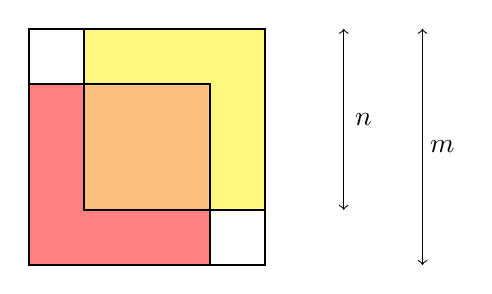
\begin{tikzpicture}
    \draw[thick] (0,0) rectangle (3,3);
    \draw[thick, fill=red!50] (0,0) rectangle (2.3,2.3);
    \draw[thick, fill=yellow!50] (0.7,0.7) rectangle (3, 3);
    \draw[thick, fill=orange!50] (0.7,0.7) rectangle (2.3, 2.3);
    \draw[<->] (4, 0.7)--(4, 3);
    \node at (4.25, 1.85) (n) {$n$};
    \draw[<->] (5, 0)--(5, 3);
    \node at (5.25, 1.5) (m) {$m$};
  \end{tikzpicture}
\end{center}
$m^2 = 2n^2$ હોવાથી $n$ બાજુવાળા બંને ચોરસો જ્યાં પરસ્પર આવરે છે
તે પ્રદેશનું ક્ષેત્રફળ બંને ચોરસોમાંથી કોઈ પણ ન આવરે એવા પ્રદેશના
ક્ષેત્રફળ જેટલું છે; એટલે કે નારંગી ચોરસનું ક્ષેત્રફળ છાયા વિનાના બે
ચોરસોનાં ક્ષેત્રફળોના સરવાળા જેટલું છે. તેથી નારંગી ચોરસની બાજુ $p$
અને છાયા વિનાના દરેક ચોરસની બાજુ $q$ હોય તો $p^2 = 2q^2$. પરંતુ હવે
$p < m$, $q < n$, $p, q \in \Nat$ સાથે
$\sqrt{2} = \nicefrac{p}{q}$. આ $m$ અને $n$ને શક્ય તેટલા નાના પસંદ
કર્યા હતા એ હકીકતનો વિરોધ કરે છે.

\emph{બીજી, ઔપચારિક રીતે.} $m^{2} = 2n^{2}$ હોવાથી $m$ યુગ્મ છે.
($x$ અયુગ્મ હોય તો $x^2$ અયુગ્મ છે તે બતાવવું સરળ છે.) તેથી કોઈ
$r \in \Nat$ માટે $m = 2r$. ફેરગોઠવણી કરતાં $2r^2 = n^2$,
એટલે $n$ પણ યુગ્મ છે. આથી $m$ અને $n$ બંને યુગ્મ છે અને તેથી
$\nicefrac{m}{n}$ અપૂર્ણાંકને \emph{વધુ} સાદો કરી શકાય છે.
વિરોધાભાસ!
\end{proof}

પ્રસંગોપાત, આ આકૃતિમય સાબિતી આપણને \olref[his][set][mythology]{sec}ની
સામગ્રી ફરી વિચારવા દે છે. ટેનેનબાઉમ (1927--2006) પૂરેપૂરા આધુનિક
ગણિતજ્ઞ હતા; છતાં આ સાબિતી નિર્વિવાદપણે સુંદર, સંપૂર્ણ ચુસ્ત અને
ભૌમિતિક અંતઃપ્રજ્ઞા પર આધારિત છે!

કોઈ પણ રીતે જુઓ તો વાસ્તવિક સંખ્યાઓ સંમેય સંખ્યાઓ કરતાં ``વધુ
વિસ્તૃત'' છે. એક અર્થમાં સંમેય સંખ્યાઓમાં ``ખાલી જગ્યાઓ'' છે અને
વાસ્તવિક સંખ્યાઓ તે ભરે છે. વાયર્સ્ટ્રાસે સમજ્યું કે આ વાત વાસ્તવિક
સંખ્યાઓનો એક જ એવો ગુણધર્મ વર્ણવે છે જે તેમને સંમેય સંખ્યાઓથી જુદી
પાડે છે—એટલે પૂર્ણતા ગુણધર્મ: \emph{ઉચ્ચસીમા ધરાવતા વાસ્તવિક
સંખ્યાઓના દરેક અખાલી ગણને ન્યૂનતમ ઉચ્ચસીમા હોય છે.}

સંમેય સંખ્યાઓ પૂર્ણતા ગુણધર્મ ધરાવતી નથી તે સહેલાઈથી જોઈ શકાય છે.
દાખલા તરીકે $\sqrt{2}$ કરતાં નાની સંમેય સંખ્યાઓનો ગણ વિચારો, એટલે કે:
\[
  \Setabs{p \in \Rat}{p^2 < 2 \text{ અથવા }p < 0}
\]
આ ગણને સંમેય સંખ્યાઓમાં ઉચ્ચસીમા છે; દાખલા તરીકે તેના ઘટકો<
બધા $3$ કરતાં નાના છે. પરંતુ તેની ન્યૂનતમ ઉચ્ચસીમા શી છે? આપણે
`$\sqrt{2}$' કહેવા ઇચ્છીએ; પરંતુ હમણાં જ જોયું કે $\sqrt{2}$
\emph{સંમેય નથી}. અને $\sqrt{2}$ કરતાં મોટી કોઈ \emph{ન્યૂનતમ}
સંમેય સંખ્યા નથી. તેથી આ ગણને ઉચ્ચસીમા છે પરંતુ ન્યૂનતમ ઉચ્ચસીમા નથી.
પરિણામે સંમેય સંખ્યાઓ પૂર્ણતા ગુણધર્મ ધરાવતી નથી.

તેનાથી વિપરીત, સાતત્યક ``તાત્ત્વિક રીતે'' પૂર્ણતા ગુણધર્મ ધરાવવું
જોઈએ. આપણે માત્ર $\sqrt{2}$ને વાસ્તવિક સંખ્યા બનાવવા નથી ઇચ્છતા;
સંમેય રેખાની બધી ``ખાલી જગ્યાઓ'' ભરવા ઇચ્છીએ છીએ. ખરેખર, સાતત્યકમાં
પોતે કોઈ ``ખાલી જગ્યા'' ન રહે એવું ઇચ્છીએ છીએ. પૂર્ણતા વડે આપણને
બરાબર આ જ મળશે.
% END OLP-0044
\endgroup

\begingroup
\makeatletter\def\ol@sectioncs{section}\makeatother

% BEGIN OLP-0045
\olfileid{sfr}{arith}{cuts}
\olsection{$\Rat$થી $\Real$ સુધી}
\phantomsection\label{guunit:OLP-0045}


મૂળ વાત એ છે કે પૂર્ણતા ગુણધર્મ બતાવે છે કે વાસ્તવિક રેખાનું કોઈ પણ
બિંદુ $\alpha$ એ રેખાને બે અર્ધભાગમાં બરાબર વહેંચે છે: એક ભાગ માટે
$\alpha$ ન્યૂનતમ ઉચ્ચસીમા છે અને બીજા માટે $\alpha$ મહત્તમ અધઃસીમા
છે. સંમેય સંખ્યાઓમાંથી વાસ્તવિક સંખ્યાઓની \emph{રચના} કરવા
ડેડેકિન્ડે સૂચવ્યું કે વાસ્તવિક સંખ્યાઓને સંમેય સંખ્યાઓનું વિભાજન કરતા
\emph{કાપ} તરીકે જ વિચારીએ. એટલે કે, $\sqrt{2}$ને એવા \emph{કાપ}
સાથે ઓળખીએ જે $< \sqrt{2}$ સંમેય સંખ્યાઓને $> \sqrt{2}$ સંમેય
સંખ્યાઓથી જુદી પાડે છે.

આ વિચારને સુઘડ બનાવીએ. સંમેય સંખ્યાઓને બે અર્ધભાગમાં કાપીએ તો કરેલા
વિભાજનને માત્ર તેના \emph{નીચલા} અર્ધભાગથી અનન્ય રીતે ઓળખી શકાય છે.
આથી ચોક્કસ વ્યાખ્યા નીચે મુજબ આપીએ છીએ:

\begin{defn}[કાપ]
\emph{કાપ} $\alpha$ એ સંમેય સંખ્યાઓનો એવો કોઈ પણ અખાલી ઉચિત
આરંભખંડ છે જેનો મહત્તમ ઘટક નથી. એટલે કે, $\alpha$ કાપ છે ત્યારે અને
માત્ર ત્યારે જ જ્યારે:
\begin{enumerate}
  \item \emph{અખાલી, ઉચિત}: $\emptyset \neq \alpha \subsetneq \Rat$
  \item \emph{આરંભિક}: બધા $p,q \in \Rat$ માટે, જો $p < q \in \alpha$ હોય તો $p \in \alpha$
  \item \emph{મહત્તમ ઘટક નહીં}: દરેક $p \in \alpha$ માટે કોઈ $q \in \alpha$ એવું છે કે $p < q$
\end{enumerate}
ત્યારે $\Real$ એ કાપોનો ગણ છે.
\end{defn}

હવે આપણે કહી શકીએ કે $\sqrt{2} = \Setabs{p \in \Rat}{p^2 < 2\text{
અથવા }p < 0}$. અલબત્ત, આ ખરેખર કાપ \emph{છે} તેની તપાસ કરવી પડે;
પરંતુ તે તપાસ \olref[check]{sec}માં રાખી છે.

પહેલાંની જેમ, કેટલીક વસ્તુઓની વ્યાખ્યા આપ્યા પછી હવે તેમના પરનાં
મૂળભૂત વિધેયો અને સંબંધોની વ્યાખ્યા કરવાની છે. એક સરળ વ્યાખ્યાથી શરૂ કરીએ:
\begin{align*}
  \alpha \leq \beta \text{ ત્યારે અને માત્ર ત્યારે જ જ્યારે }\alpha \subseteq \beta
\end{align*}
ક્રમની આ વ્યાખ્યા આપણને કેન્દ્રીય પરિણામ \emph{કહેવા} દે છે: કાપોનો
ગણ પૂર્ણતા ગુણધર્મ ધરાવે છે. પૂરેપૂરું લખીએ તો વિધાનનું સ્વરૂપ આવું છે.
$S$ એ ઉચ્ચસીમા ધરાવતો કાપોનો અખાલી ગણ હોય તો $S$ને ન્યૂનતમ ઉચ્ચસીમા
હોય છે. વધુ વિગતે: કોઈ કાપ $\lambda$ એ $S$ની ઉચ્ચસીમા છે, એટલે કે
$(\forall \alpha \in S)\alpha \subseteq \lambda$, અને $\lambda$ આવો
ન્યૂનતમ કાપ છે, એટલે કે
$(\forall \beta \in \Real)((\forall \alpha \in S)\alpha \subseteq \beta \lif \lambda \subseteq \beta)$.
હવે પરિણામની સાબિતી આ રહી:

\begin{thm}\ollabel{realcompleteness}
કાપોનો ગણ પૂર્ણતા ગુણધર્મ ધરાવે છે.
\end{thm}

\begin{proof}
$S$ એ ઉચ્ચસીમા ધરાવતો કાપોનો કોઈ અખાલી ગણ હોય. $\lambda = \bigcup S$ લો.
પહેલાં આપણે દાવો કરીએ કે $\lambda$ કાપ છે:
\begin{enumerate}
\item $S$ અખાલી હોવાથી ઓછામાં ઓછો એક કાપ $S$માં છે, તેથી
$\emptyset \neq \lambda$. $S$ કાપોનો ગણ હોવાથી $\lambda
\subseteq \Rat$. $S$ને ઉચ્ચસીમા હોવાથી કોઈ $p \in \Rat$ દરેક કાપ
$\alpha \in S$માંથી ગેરહાજર છે. તેથી $p\notin \lambda$, અને પરિણામે
$\lambda \subsetneq \Rat$.
\item ધારો કે $p < q \in \lambda$. ત્યારે કોઈ $\alpha \in S$ એવું
છે કે $q \in \alpha$. $\alpha$ કાપ હોવાથી $p \in \alpha$. તેથી
$p \in \lambda$.
\item ધારો કે $p \in \lambda$. ત્યારે કોઈ $\alpha \in S$ એવું છે કે
$p \in \alpha$. $\alpha$ કાપ હોવાથી કોઈ $q \in \alpha$ એવું છે કે
$p < q$. તેથી $q \in \lambda$.
\end{enumerate}
આથી દાવો સાબિત થયો. વધુમાં, સ્પષ્ટપણે $(\forall \alpha \in S)\alpha
\subseteq \bigcup S = \lambda$, એટલે કે $\lambda$ એ $S$ની ઉચ્ચસીમા
છે. હવે ધારો કે $\beta \in \mathbb{R}$ પણ ઉચ્ચસીમા છે, એટલે કે
$(\forall \alpha \in S)\alpha \subseteq \beta$. કોઈ પણ $p \in \Rat$
માટે, જો $p \in \lambda$ હોય તો કોઈ $\alpha \in S$ માટે
$p \in \alpha$, તેથી $p \in \beta$. સામાન્યકરણ કરતાં
$\lambda \subseteq \beta$. આથી $\lambda$ એ $S$ની \emph{ન્યૂનતમ}
ઉચ્ચસીમા છે.
\sourcecorrection{OLARI-002}{મૂળની \texttt{cuts.tex}, પંક્તિઓ 61--65માં
\(S\)માં ઓછામાં ઓછો એક કાપ હોવાનો આધાર ભૂલથી “\(S\)ને ઉચ્ચસીમા છે”
એમ આપ્યો છે. આ તારણ \(S\) અખાલી છે એ ધારણાથી મળે છે; અહીં તે જ
યોગ્ય ધારણા લખી છે.}
\end{proof}

આ રીતે આપણને પૂર્ણતા ગુણધર્મ ધરાવતી ઘણી વસ્તુઓ મળી છે. આને કહેવાની
એક રીત એ છે કે આપણા કાપોમાં કોઈ ``ખાલી જગ્યા'' નથી. (આથી સંમેય
સંખ્યાઓને બદલે વાસ્તવિક સંખ્યાઓના વધુ ``કાપ'' લેવાથી કોઈ રસપ્રદ નવી
વસ્તુઓ નહીં મળે.)

હવે વાસ્તવિક સંખ્યાઓ પર કેટલીક ક્રિયાઓ વ્યાખ્યાયિત કરવી પડશે.
દરેક $p \in \Rat$ માટે $p_\Real = \Setabs{q \in \Rat}{q < p}$ એમ
ઠરાવીને આપણે પહેલાં સંમેય સંખ્યાઓને વાસ્તવિક સંખ્યાઓમાં સ્થાપિત કરીએ છીએ.
પછી વ્યાખ્યા કરીએ છીએ:
\begin{align*}
  \alpha + \beta &= \Setabs{p + q}{p \in \alpha \land q \in \beta}\\
  \alpha \times \beta &=
  \Setabs{p \times q}{0 \leq p \in \alpha \land 0 \leq q \in \beta} \cup 0^\mathbb{R} & \text{ જો }\alpha, \beta \geq 0_\Real
\end{align*}
ગુણાકારના બીજા કિસ્સા સંભાળવા પહેલાં નીચે મુજબ લો: %કે $0_\Real \times \alpha = 0_\Real = \alpha \times 0_\Real$, અને ઉમેરો:
\begin{align*}
  -\alpha &= \Setabs{p - q}{p < 0 \land q \notin \alpha}
\end{align*}
અને પછી એમ ઠરાવો કે:
\begin{align*}
  \alpha \times \beta &\defis
  \begin{cases}
    \mathord{-}\alpha \times \mathord{-}\beta &\text{ જો }\alpha < 0_\Real\text{ અને }\beta < 0_\Real\\
    \mathord{-}(\mathord{-}\alpha \times \beta) &\text{ જો }\alpha < 0_\Real \text{ અને }\beta > 0_\Real\\
    \mathord{-}(\alpha \times \mathord{-}\beta) &\text{ જો }\alpha > 0_\Real \text{ અને }\beta < 0_\Real
  \end{cases}
\end{align*}
આમાંની દરેક વ્યાખ્યા હંમેશાં કાપ જ આપે છે તેની તપાસ કરવી પડશે.
છેલ્લે, આ રીતે વ્યાખ્યાયિત કાપોનો વ્યવહાર બરાબર જેવો હોવો જોઈએ
તેવો જ છે તેનું સરળ પરંતુ લાંબું નિદર્શન કરવું પડશે. આ બધું
\olref[check]{sec}માં રાખીએ છીએ.
% END OLP-0045
\endgroup

\begingroup
\makeatletter\def\ol@sectioncs{section}\makeatother

% BEGIN OLP-0046
\olfileid{sfr}{arith}{ref}
\olsection{કેટલાક તાત્ત્વિક પ્રતિચિંતનો}
\phantomsection\label{guunit:OLP-0046}


પ્રાવિધિક વિગતો આટલી થઈ. પરંતુ તેનાથી સિદ્ધ શું થયું?

એવું લગભગ નિર્વિવાદ છે કે તેનાથી આપણને થોડું {સુંદર} શુદ્ધ ગણિત
મળ્યું. ઉપરાંત કેટલીક ગહન વૈચારિક સિદ્ધિઓ મળી. પૂર્ણતા ગુણધર્મ
વાસ્તવિક અને સંમેય સંખ્યાઓ વચ્ચેનો નિર્ણાયક તફાવત વ્યક્ત કરે છે એવું
જોવું એક ગહન અંતર્દૃષ્ટિ હતું. વધુમાં, ડેડેકિન્ડ કાપ તરીકે વાસ્તવિક
સંખ્યાઓની સ્પષ્ટ રચના વિશ્લેષણના વિષયને મજબૂત પાયો આપે છે. કાપો
\emph{પૂર્ણ ક્રમિત ક્ષેત્ર} બનાવે છે, તેથી આ ખ્યાલ સુસંગત છે તે આપણે જાણીએ છીએ.

આ બધું સ્વીકાર્યા પછી પણ આ સિદ્ધિઓ વિશે કેટલીક શંકાઓ જણાવવી જોઈએ.

પહેલી વાત, વાસ્તવિક સંખ્યાઓને કાપો તરીકે વિચારવી એ તેમના પરિચિત
(કદાચ અનંત) દશાંશ વિસ્તરણોના રૂપમાં વિચારવા કરતાં \emph{વધુ} ચુસ્ત
છે કે નહીં તે સ્પષ્ટ નથી. વાસ્તવિક સંખ્યાઓની આ બીજી ``રચના'' કોશી
શ્રેણી વડે થતી રચના સાથે થોડું સામ્ય ધરાવે છે; પરંતુ હકીકતમાં
સત્તરમી સદીના આરંભથી ગણિતજ્ઞો તેને મૂળભૂત રીતે જાણતા હતા
(\olref[cauchy]{sec} જુઓ). ચુસ્તતામાં ખરેખરનો વધારો વાસ્તવિક સંખ્યાઓ
પૂર્ણતા ગુણધર્મ ધરાવે છે એ સમજવાથી થયો. ચોક્કસ ગણો તરીકે વાસ્તવિક
સંખ્યાઓ રચવાની ક્ષમતા કદાચ પોતાની રીતે એટલી રસપ્રદ નથી.

પૂર્ણાંકોનું કે સંમેય સંખ્યાઓનું (ઘણું સરળ) અંકગણિતીકરણ તે ક્ષેત્રોમાં
ચુસ્તતા વધારે છે કે નહીં તે તો હજી ઓછું સ્પષ્ટ છે. અહીં એક સરળ અવલોકન
ઉપયોગી છે. પ્રાકૃતિક સંખ્યાઓની ક્રમયુક્ત જોડોના સામ્ય વર્ગો તરીકે
પૂર્ણાંકોની \emph{રચના} કર્યા પછી, પૂર્ણાંકોની ક્રમયુક્ત જોડોના સામ્ય
વર્ગો તરીકે સંમેય સંખ્યાઓની રચના કર્યા પછી અને સંમેય સંખ્યાઓના ગણો
તરીકે વાસ્તવિક સંખ્યાઓ રચ્યા પછી આપણે તરત જ એ રચનાઓને \emph{ભૂલી
જઈએ છીએ}. ખાસ કરીને, ગણિતીય સાબિતીમાં કોઈ આ રચનાઓને ક્યારેય
\emph{ઉપયોગમાં લેવા} ઇચ્છશે નહીં (અલબત્ત, રચનાઓનો વ્યવહાર ધાર્યા મુજબ
છે એવી સાબિતી સિવાય). પ્રાકૃતિક સંખ્યાઓના ગણોના ગણોના ગણોના ગણોના
ગણોના ગણોના કોઈ ગણ વિશે બોલવા કરતાં સીધું કોઈ વાસ્તવિક સંખ્યા વિશે
બોલવું ઘણું સરળ છે.

આ વ્યાખ્યાઓ આપણને પૂર્ણાંકો, સંમેય સંખ્યાઓ કે વાસ્તવિક સંખ્યાઓ
\emph{અધિભૌતિક અર્થમાં શું છે} તે કહે છે એવો દાવો સૌથી વધુ
શંકાસ્પદ છે. એટલે કે, વાસ્તવિક સંખ્યાઓ (ધારો કે) ચોક્કસ ગણો
(ગણોના ગણોના ગણો\ldots) જ \emph{છે} એ શંકાસ્પદ છે. આવા મતનો મુખ્ય
અવરોધ એ છે કે રચના ઘણી જુદી રીતે થઈ શકી હોત. વાસ્તવિક સંખ્યાઓના
કિસ્સામાં ખરેખર રસપ્રદ રીતે જુદી રચનાઓ છે (\olref[cauchy]{sec} જુઓ).
પરંતુ તદ્દન જુદી રચનાઓ મેળવવાની આ એક નજીવી રીત છે: જેમ
\olref[sfr][rel][ref]{sec}માં જોયું, ક્રમયુક્ત જોડની વ્યાખ્યા સહેજ જુદી
રીતે કરી શકાઈ હોત; આ વૈકલ્પિક ખ્યાલ વાપર્યો હોત તો આપણી રચનાઓ એટલી
જ સારી રીતે કામ કરત, પરંતુ અંતે મળતી વસ્તુઓ જુદી હોત. આમ પૂર્ણાંકો,
સંમેય સંખ્યાઓ અને વાસ્તવિક સંખ્યાઓની ઘણી હરીફ ગણસૈદ્ધાંતિક રચનાઓ છે.
હવે પૂર્ણાંકો (ધારો કે) \emph{આ} ગણો છે, \emph{તે} નહીં, એવો દાવો
મનસ્વી (અને મૂંઝવણજનક) થશે. (\olref[sfr][rel][ref]{sec}ની જેમ આ પણ
\citealt{Benacerraf1965}એ પ્રસિદ્ધ કરેલી દલીલનું એક દૃષ્ટાંત છે.)

બીજો મુદ્દો પણ ઉઠાવવો જોઈએ: આપણી રચનાઓમાં કશુંક બહુ \emph{વિચિત્ર}
છે. આપણે પ્રાકૃતિક સંખ્યાઓથી શરૂ કર્યું. પછી પૂર્ણાંકો રચ્યા અને
``પૂર્ણાંકોનું $0$'', એટલે કે $\equivrep{0,0}{\Intequiv}$ રચ્યું.
પરંતુ $0 \neq \equivrep{0,0}{\Intequiv}$. ખરેખર, આપણી રચનાઓ મુજબ
\emph{કોઈ પણ} પ્રાકૃતિક સંખ્યા પૂર્ણાંક નથી. આ ખૂબ જ પ્રતિઅંતઃપ્રજ્ઞ
લાગે છે. વળી \olref[sfr][set][imp]{sec}માં આપણે બહુ દલીલ કર્યા વિના
$\Nat \subseteq \Rat$ એવો દાવો કર્યો હતો. જો આ રચનાઓ સંખ્યાઓ
\emph{બરાબર શું છે} તે કહેતી હોય, તો એ દાવો સહેજે ખોટો હતો.

હવે થોડું દૂરથી જોઈએ તો આપણે ક્યાં પહોંચ્યા? સહજ ગણસિદ્ધાંતમાં કામ
કરીને અને પ્રાકૃતિક સંખ્યાઓને આપેલી માનીને, પૂર્ણાંકો, સંમેય સંખ્યાઓ
અને વાસ્તવિક સંખ્યાઓને ચોક્કસ ગણો \emph{તરીકે} ગણી શકીએ છીએ. આ અર્થમાં
આ વસ્તુઓના સિદ્ધાંતોને ગણસિદ્ધાંતમાં \emph{સ્થાપિત} કરી શકીએ છીએ.
પરંતુ આ સ્થાપનનું તાત્ત્વિક મહત્ત્વ એટલું સીધું નથી.

અલબત્ત, આમાંથી કંઈ અંતિમ શબ્દ નથી!{} મુદ્દો માત્ર આ છે: વાસ્તવિક
સંખ્યાઓનું અંકગણિતીકરણ ગહન તાત્ત્વિક મહત્ત્વ \emph{ધરાવે છે} એવું
બતાવવા માટે કેટલીક વધારાની \emph{તાત્ત્વિક} દલીલ જરૂરી થશે.
% END OLP-0046
\endgroup

\begingroup
\makeatletter\def\ol@sectioncs{section}\makeatother

% BEGIN OLP-0047
\olfileid{sfr}{arith}{check}
\olsection{ક્રમિત મંડળો અને ક્ષેત્રો}
\phantomsection\label{guunit:OLP-0047}


આ આખા પ્રકરણમાં આપણે દાવો કર્યો કે અમુક વ્યાખ્યાઓનો વ્યવહાર
``જેવો હોવો જોઈએ તેવો'' છે. આ પ્રાવિધિક પરિશિષ્ટમાં તેનો અર્થ
સ્પષ્ટ કરીશું અને વ્યાખ્યાઓનો વ્યવહાર ``યોગ્ય રીતે'' થાય છે તે
(કેવી રીતે બતાવવું તેની રૂપરેખા) આપીશું.

\olref[int]{sec}માં આપણે $\Int$ પર સરવાળો અને ગુણાકાર વ્યાખ્યાયિત
કર્યા. વ્યાખ્યા મુજબ આ ક્રિયાઓ $\Int$ને આપણે ``ઇચ્છીએ તેવું''
સંરચના આપે છે એવું બતાવવું છે. ખાસ કરીને, અહીંની સંરચના સમક્રમી
મંડળની છે.

\begin{defn}
	\emph{સમક્રમી મંડળ} એવો ગણ $S$ છે જેમાં નિશ્ચિત ઘટકો $0$ અને $1$
	તથા ક્રિયાઓ $+$ અને $\times$ હોય અને જે નીચેના આઠ સૂત્રો સંતોષે:
	\begin{align*}
		\emph{સંગઠિતતા}&&a + (b+ c) & = (a + b) + c \\
		&& (a \times b) \times c & = a \times (b\times c)\\
		\emph{સમક્રમિતા}&&a + b &= b+ a  \\
		&&  a \times b&= b\times a\\
		\emph{એકમો}&&a + 0 &= a \\
		&& a \times 1 &= a\\
		\emph{યોજક વ્યસ્ત}&&(\exists b\in S)0&=a + b\\
		\emph{વિતરણાત્મકતા}&&a \times (b+ c ) &= (a \times b) + (a \times c)
	\end{align*}
	અહીં ગર્ભિત રીતે આ બધાં સૂત્રોના સર્વપરિમાણકો $S$ પૂરતા
	મર્યાદિત છે. એ પણ નોંધો કે અહીંના $0$ અને~$1$ નામના ઘટકો એ જ
	નામ ધરાવતી પ્રાકૃતિક સંખ્યાઓ હોવા જરૂરી નથી.
\end{defn}

તેથી પૂર્ણાંકો સમક્રમી મંડળ બનાવે છે કે નહીં તે ચકાસવા માટે આ આઠે
શરતો સંતોષાય છે એટલું જ ચકાસવાનું રહે છે. કોઈ શરત સ્થાપવી {મુશ્કેલ}
નથી, પણ એ કામ થોડું શ્રમસાધ્ય છે. દાખલા તરીકે, સરવાળાના કિસ્સામાં
\emph{સંગઠિતતા} આ રીતે સાબિત કરી શકાય:

\begin{proof}
$i, j, k \in \Int$ નિશ્ચિત કરો. ત્યારે એવા $a_1, b_1, a_2, b_2, a_3, b_3 \in
\Nat$ છે કે $i = \equivrep{a_1, b_1}{}$, $j =
\equivrep{a_2,b_2}{}$ અને $k = \equivrep{a_3, b_3}{}$. (વાંચવામાં
સરળતા રહે તે માટે આપણે ``$\equivrep{x, y}{\Intequiv}$''ને બદલે
``$\equivrep{x, y}{}$'' લખીએ છીએ; આ આખા વિભાગમાં એમ જ કરીશું.) હવે:
\begin{align*}
	i + (j + k) &= \equivrep{a_1, b_1}{}+(\equivrep{a_2, b_2}{} + \equivrep{a_3, b_3}{}) \\
	&= \equivrep{a_1,  b_1}{} + \equivrep{a_2+a_3, b_2+b_3}{}\\
	&= \equivrep{a_1 + (a_2 + a_3), b_1 + (b_2 + b_3)}{}\\
	&= \equivrep{(a_1 + a_2) + a_3, (b_1 + b_2) + b_3}{}\\
	&= \equivrep{a_1 + a_2, b_1 + b_2}{} + \equivrep{a_3, b_3}{}\\
	&= (\equivrep{a_1, b_1}{} + \equivrep{a_2, b_2}{}) + \equivrep{a_3, b_3}{}\\
	&= (i+j) + k
\end{align*}
અહીં $\Nat$ પરના સરવાળાના વ્યવહારનો આપણે નિઃસંકોચ ઉપયોગ કર્યો છે.
\end{proof}

એ જ રીતે \emph{યોજક વ્યસ્ત} આ રીતે સાબિત કરી શકાય:

\begin{proof}
$i \in \Int$ નિશ્ચિત કરો; ત્યારે કોઈ $a,b \in \Nat$ માટે $i =
\equivrep{a,b}{}$. $j = \equivrep{b,a}{} \in \Int$ લો. પ્રાકૃતિક
સંખ્યાઓના વ્યવહારનો ઉપયોગ કરતાં $(a+b) + 0 = 0 + (a+b)$, તેથી
વ્યાખ્યા મુજબ $\tuple{a+b, b+a} \sim_\Int \tuple{0,0}$, અને તેથી
$\equivrep{a+b, b+a}{} = \equivrep{0, 0}{} = 0_\Int$. હવે $i + j =
\equivrep{a,b}{}+\equivrep{b,a}{}=\equivrep{a+b, b+a}{}= \equivrep{0,
0}{} = 0_\Int$.
\end{proof}

અને \emph{વિતરણાત્મકતા}ની સાબિતી આ રહી:

\begin{proof}
ઉપરની જેમ $i = \equivrep{a_1, b_1}{}$, $j =
\equivrep{a_2,b_2}{}$ અને $k = \equivrep{a_3, b_3}{}$ નિશ્ચિત કરો. હવે:
\begin{align*}
	i \times (j + k)
	&= \equivrep{a_1, b_1}{} \times (\equivrep{a_2,b_2}{} + \equivrep{a_3, b_3}{})\\
	&= \equivrep{a_1, b_1}{} \times \equivrep{a_2 + a_3,b_2+b_3}{}\\
	&= \equivrep{a_1  (a_2 + a_3) + b_1  (b_2+b_3), a_1  (b_2 + b_3) + b_1 (a_2 + a_3)}{}\\
	&= \equivrep{a_1 a_2 + a_1a_3 + b_1 b_2+b_1b_3, a_1 b_2 + a_1b_3 + a_2b_1 + a_3b_1}{}\\
	&= \equivrep{a_1a_2 + b_1b_2, a_1b_2 + a_2b_1}{} + \equivrep{a_1a_3 + b_1b_3, a_1b_3 + a_3b_1}{}\\
	&= (\equivrep{a_1, b_1}{} \times \equivrep{a_2,b_2}{}) + (\equivrep{a_1, b_1}{} \times  \equivrep{a_3, b_3}{})\\
	&= (i \times j) + (i \times k)
\end{align*}
\end{proof}

બાકીની પાંચ શરતોની સાબિતી કસરત તરીકે છોડી દઈએ છીએ. એ કરી લઈએ
પછી આપણે બતાવ્યું હશે કે $\Int$ સમક્રમી મંડળ બનાવે છે, એટલે કે સરવાળો
અને ગુણાકારનો (વ્યાખ્યાયિત કરેલો) વ્યવહાર જેવો હોવો જોઈએ તેવો છે.

\begin{prob}
$\Int$ સમક્રમી મંડળ છે તે સાબિત કરો.
\end{prob}

પરંતુ આપણું કામ પૂરું થયું નથી. $\Int$ પર સરવાળો અને ગુણાકાર
વ્યાખ્યાયિત કરવા ઉપરાંત આપણે ક્રમસંબંધ $\leq$ પણ વ્યાખ્યાયિત કર્યો
હતો અને તેનો વ્યવહાર પણ જેવો હોવો જોઈએ તેવો છે એ ચકાસવું પડે. વધુ
ચોક્કસ રીતે, $\Int$ \emph{ક્રમિત} મંડળ બનાવે છે એવું બતાવવું પડશે.\footnote{
	\olref[sfr][rel][ord]{def:linearorder}માંથી યાદ કરો કે સંપૂર્ણ ક્રમ
	સ્વવાચક, પરંપરિત, વિસંમિત અને તુલનાયુક્ત સંબંધ છે. ક્રમસંબંધોના
	સંદર્ભમાં તુલનાયુક્તતાને ક્યારેક \emph{ત્રિવિકલ્પતા} કહે છે, કારણ કે
	કોઈ પણ $a$ અને $b$ માટે $a \leq b \lor a = b \lor a \geq b$.}

\begin{defn}
\emph{ક્રમિત મંડળ} એવું સમક્રમી મંડળ છે જેમાં સંપૂર્ણ ક્રમસંબંધ
$\leq$ પણ હોય અને નીચેની શરતો સંતોષાય:
\begin{align*}
	a \leq b &\lif a + c \leq b + c\\
	(a \leq b \land 0 \leq c) &\lif a \times c \leq b \times c
\end{align*}
\end{defn}

\begin{prob}
$\Int$ ક્રમિત મંડળ છે તે સાબિત કરો.
\end{prob}

અગાઉની જેમ રચાયેલું~$\Int$ ક્રમિત મંડળ છે એવું બતાવવું શ્રમસાધ્ય
પણ નિયમિત કામ છે. તે તમારા માટે છોડી દઈએ છીએ.

આમ પૂર્ણાંકોનું કામ પૂરું થયું. હવે સંમેય સંખ્યાઓ માટે આવી જ બાબતો
બતાવવી છે. ખાસ કરીને $+$, $\times$ અને $\leq$ની આપેલી વ્યાખ્યાઓ તળે
સંમેય સંખ્યાઓ ક્રમિત \emph{ક્ષેત્ર} બનાવે છે એવું બતાવવું છે:
\begin{defn}\ollabel{orderedfield}
\emph{ક્રમિત ક્ષેત્ર} એવું ક્રમિત મંડળ છે જે આ વધારાની શરત પણ સંતોષે:
\begin{align*}
	\emph{ગુણાકારી વ્યસ્ત}& & (\forall a \in S \setminus \{0\})(\exists b \in S) a\times b& = 1
\end{align*}
\end{defn}

$\Int$ ક્રમિત મંડળ બનાવે છે એવું બતાવી લીધા પછી $\Rat$ ક્રમિત ક્ષેત્ર
બનાવે છે એવું બતાવવું સરળ, પણ શ્રમસાધ્ય છે.

\begin{prob}
$\Rat$ ક્રમિત ક્ષેત્ર છે તે સાબિત કરો.
\end{prob}

પૂર્ણાંકો અને સંમેય સંખ્યાઓનું કામ પૂરું કર્યા પછી માત્ર વાસ્તવિક
સંખ્યાઓ બાકી રહે છે. ખાસ કરીને, $\Real$ \emph{પૂર્ણ} ક્રમિત ક્ષેત્ર,
એટલે કે પૂર્ણતા ગુણધર્મ ધરાવતું ક્રમિત ક્ષેત્ર, બનાવે છે એવું બતાવવું
પડે. \olref[cuts]{realcompleteness}માં $\Real$ પૂર્ણતા ગુણધર્મ ધરાવે
છે એવું સ્થાપ્યું હતું. પરંતુ $\Real$ ક્રમિત ક્ષેત્ર છે તેની
(કંટાળાજનક) ચકાસણીની વિગતો હજી બાકી છે.

આ શ્રમસાધ્ય કસરત તરફ વળતાં પહેલાં થોડી વધુ ``તાત્કાલિક'' બાબતો
ચકાસવી પડશે. દાખલા તરીકે, કોઈ પણ કાપો $\alpha$ અને $\beta$ માટે
વ્યાખ્યાયિત કરેલો $\alpha + \beta$ ખરેખર \emph{કાપ} જ છે તેની ખાતરી
કરવી પડશે. તેની સાબિતી આ રહી:

\begin{proof}
$\alpha$ અને $\beta$ બંને કાપ હોવાથી $\alpha + \beta = \Setabs{p
+ q}{p \in \alpha \land q \in \beta}$ એ $\Rat$નો અરિક્ત ઉચિત ઉપગણ
છે. હવે કોઈ $p \in \alpha$ અને $q \in \beta$ માટે $x < p + q$ ધારો.
ત્યારે $x - p < q$, તેથી $x - p \in \beta$, અને $x = p + (x - p) \in
\alpha + \beta$. તેથી $\alpha + \beta$ એ $\Rat$નો આરંભિક ખંડ છે.
અંતે, કોઈ પણ $p + q \in \alpha + \beta$ માટે, $\alpha$ અને $\beta$
બંને કાપ હોવાથી એવા $p_1 \in \alpha$ અને $q_1 \in \beta$ છે કે
$p < p_1$ અને $q < q_1$; તેથી $p + q < p_1 + q_1 \in \alpha +
\beta$; આમ $\alpha + \beta$ને કોઈ મહત્તમ ઘટક નથી.
\end{proof}

આવી જ મહેનતથી તમે ચકાસી શકશો કે $\alpha - \beta$, $\alpha \times
\beta$ અને $\alpha \div \beta$ પણ કાપ છે (છેલ્લા કિસ્સામાં $\beta$
શૂન્ય-કાપ હોય તે કિસ્સો અવગણવો). એ પણ આપણે તમારા માટે જ છોડી દઈએ છીએ.

\begin{prob}
$\Real$ ક્રમિત ક્ષેત્ર છે તે સાબિત કરો.
\end{prob}

હવે એક નાની અધૂરી વિગત પૂરી કરીએ. \olref[cuts]{sec}માં આપણે સૂચવ્યું
હતું કે $\sqrt{2} = \Setabs{p \in \Rat}{p < 0 \text{ અથવા }p^2 < 2}$
લઈ શકાય. પરંતુ આ ગણ \emph{કાપ} છે એવું બતાવવું પડે. તેની સાબિતી આ રહી:

\begin{proof}
સ્પષ્ટપણે આ સંમેય સંખ્યાઓનો અરિક્ત ઉચિત આરંભિક ખંડ છે; તેથી તેને
મહત્તમ ઘટક નથી એટલું બતાવવું પૂરતું છે. ખાસ કરીને, $p^2 < 2$ ધરાવતી
ધન સંમેય સંખ્યા $p$ અને $q = \frac{2p+2}{p+2}$ હોય ત્યારે $p < q$ અને
$q^2 < 2$ બંને બતાવવાં પૂરતાં છે. $p < q$ જોવા માટે માત્ર નોંધો:
\begin{align*}
	p^2 &< 2\\
	p^2 + 2p &< 2 + 2p\\
	p(p + 2) &< 2 + 2p\\
	p &< \tfrac{2+2p}{p+2} = q
\end{align*}
$q^2 < 2$ જોવા માટે માત્ર નોંધો:
\begin{align*}
	p^2 &< 2\\
	2p^2 + 4p + 2 &< p^2 + 4p+ 4\\
	4p^2 + 8p + 4 &< 2(p^2 + 4p + 4)\\
	(2p+2)^2 & <2(p+2)^2\\
	\tfrac{(2p+2)^2}{(p+2)^2} &< 2\\
	q^2 &< 2
\end{align*}
\end{proof}
% END OLP-0047
\endgroup

\begingroup
\makeatletter\def\ol@sectioncs{section}\makeatother

% BEGIN OLP-0048
\olfileid{sfr}{arith}{cauchy}

\olsection{પરિશિષ્ટ: કોશી શ્રેણીઓ તરીકે વાસ્તવિક સંખ્યાઓ}
\phantomsection\label{guunit:OLP-0048}


\olref[cuts]{sec}માં આપણે વાસ્તવિક સંખ્યાઓની રચના ડેડેકિન્ડ કાપો
તરીકે કરી. આ વિભાગમાં એક વૈકલ્પિક રચના સમજાવીશું. તે કોશીએ
(જેને હવે આપણે કોશી શ્રેણી કહીએ છીએ તેની) આપેલી વ્યાખ્યા પર આધારિત
છે; પરંતુ આ વ્યાખ્યાનો ઉપયોગ કરીને વાસ્તવિક સંખ્યાઓની \emph{રચના}
કરવાનું શ્રેય ઓગણીસમી સદીના બીજા લેખકોને, ખાસ કરીને વાયરસ્ટ્રાસ,
હાઇને, મેરે અને કૅન્ટૉરને જાય છે. (સરસ ઇતિહાસ માટે
\citeauthor{OConnorRobertson:RN} \citeyear{OConnorRobertson:RN} જુઓ.)

ઓગણીસમી સદી સુધી પહોંચતાં પહેલાં સિમોન સ્ટેવિન (1548--1620)નો વિચાર
કરવો યોગ્ય છે. ટૂંકમાં, સ્ટેવિને સમજ્યું કે દરેક વાસ્તવિક સંખ્યાને
તેના દશાંશ વિસ્તરણ દ્વારા વિચારી શકાય. તેથી $\sqrt{2}$ જેવી અસંમેય
સંખ્યાનું પણ સરસ દશાંશ વિસ્તરણ છે, જે આ રીતે શરૂ થાય છે:
\[
	1.41421356237\ldots
\]
ગણસિદ્ધાંતમાં દશાંશ વિસ્તરણોના પ્રતિરૂપ બનાવવા બહુ સરળ છે: તેમને
$d \colon \Nat \to \Nat$ વિધેયો તરીકે વિચારો, જ્યાં $d(n)$ આપણને
રસ હોય તે $n$મું દશાંશ સ્થાન છે. પછી દશાંશ ચિહ્નની પહેલાં આવતા
વાસ્તવિક સંખ્યાના ભાગને (અહીં માત્ર $1$ને) સંભાળવા વ્યાખ્યામાં થોડો
ફેરફાર કરવો પડશે. દાખલા તરીકે $0.999\ldots = 1$ની ખાતરી કરવા માટે
બીજો ફેરફાર (એક સામ્ય સંબંધ) પણ કરવો પડશે. પરંતુ સ્ટેવિનની રીત મુજબ
ગણસિદ્ધાંતમાં વાસ્તવિક સંખ્યાઓની પૂરેપૂરી ચુસ્ત રચના આપવી મુશ્કેલ નથી.

અહીં સ્ટેવિન આપણો મુખ્ય વિષય નથી. (સ્ટેવિન વિશે વધુ માટે
\citealt{KatzKatz2012} જુઓ.) પરંતુ આ રહ્યો તેની નજીકનો એક વિચાર.
$\sqrt{2}$ના દશાંશ વિસ્તરણને સીધું લેવાને બદલે વધુ ને વધુ ચોક્કસ
વિસ્તરણો લઈને $\sqrt{2}$નાં વધુ ને વધુ ચોક્કસ સંમેય આસન્ન મૂલ્યોની
એક \emph{શ્રેણી} વિચારી શકાય:
\[
1, 1.4, 1.414, 1.4142, 1.41421,\ldots
\]
વાસ્તવિક સંખ્યાઓને ``વધુ ને વધુ સારા આસન્ન મૂલ્યો'' દ્વારા વિચારી
શકાય એ વિચાર આપણને અંતર્દૃષ્ટિઓના બીજા ક્રમનો આધાર આપે છે (જેમ
$\Int$માંથી $\Rat$ અથવા $\Nat$માંથી $\Int$ રચતી વખતે મળેલી
અંતર્દૃષ્ટિઓ). મૂળભૂત અંતર્દૃષ્ટિઓ આ છે:
\begin{enumerate}
	\item દરેક વાસ્તવિક સંખ્યાને (કદાચ અનંત) દશાંશ વિસ્તરણ તરીકે લખી
	શકાય છે.
	\item (કદાચ અનંત) દશાંશ વિસ્તરણમાં સમાયેલી માહિતીને સંમેય સંખ્યાઓની
	શ્રેણીથી પણ એટલી જ રીતે રજૂ કરી શકાય છે.
	\item સંમેય સંખ્યાઓની શ્રેણીને $\Nat$માંથી $\Rat$માં જતા વિધેય
	તરીકે વિચારી શકાય; શ્રેણીની $n$મી સંમેય સંખ્યાને $f(n)$ લો.
\end{enumerate}
અલબત્ત, $\Nat$માંથી $\Rat$માં જતું \emph{કોઈ પણ} વિધેય આપણને વાસ્તવિક
સંખ્યા આપશે એવું નથી. દાખલા તરીકે, આ વિધેય વિચારો:
\[
	f(n) =\begin{cases}
			1 & \text{જો }n\text{ અયુગ્મ હોય}\\
			0 &\text{જો }n\text{ યુગ્મ હોય}
		\end{cases}
\]
અહીં મૂળ ચિંતા એ છે કે $0,1,0,1,0,1,0,\ldots$ શ્રેણી કોઈ વાસ્તવિક
સંખ્યા તરફ ``નજીક જતી'' જણાતી નથી. તેથી કોઈ વાસ્તવિક સંખ્યા તરફ
નજીક જતી શ્રેણીઓ જ વિચારવામાં આવે એની ખાતરી કરવા માટે આપણે કોઈ
\emph{લક્ષ} ધરાવતી શ્રેણીઓ પૂરતું ધ્યાન મર્યાદિત કરવું પડશે.

લક્ષનો વિચાર આપણે \olref[his][set][limits]{sec}માં જોઈ ચૂક્યા છીએ.
પરંતુ ત્યાં લીધેલી વ્યાખ્યા \emph{બરાબર} એ જ રીતે અહીં લઈ શકીએ નહીં.
ત્યાં ``$(\forall \epsilon>0)$'' અભિવ્યક્તિમાં વાસ્તવિક સંખ્યાઓ પરનું
પરિમાણીકરણ ગર્ભિત હતું; અને આપણે વાસ્તવિક સંખ્યાઓ પરનાં વિધેયોના
લક્ષ વિચારતા હતા. એટલે એ વ્યાખ્યાનો ઉપયોગ કરીએ તો જે વાસ્તવિક સંખ્યાઓની
\emph{રચના} કરવાનું આપણું લક્ષ છે તેને પહેલાંથી જ માની લઈએ. સદભાગ્યે,
લક્ષના અત્યંત નજીકના એક વિચારથી કામ ચાલી શકે છે.
\begin{defn}\ollabel{def:CauchySequence}
  વિધેય $f: \Nat \to \Rat$ \emph{કોશી શ્રેણી} હોય ત્યારે અને માત્ર
  ત્યારે જ જ્યારે દરેક ધન $\epsilon \in \Rat$ માટે $(\exists \ell \in
  \Nat)(\forall m, n > \ell)|f(m) - f(n)| < \epsilon$.
\end{defn}

લક્ષનો સામાન્ય વિચાર પહેલાં જેવો જ છે: તમને ($\epsilon$થી મપાતું)
અમુક ચોકસાઈનું સ્તર જોઈતું હોય તો જોવા માટે એક ``વિસ્તાર'' (એટલે કે
$\ell$ કરતાં મોટું કોઈ પણ આગત) મળે છે. આપણી શ્રેણી $1$, $1.4$,
$1.414$, $1.4142$, $1.41421$\ldots{}ને લક્ષ છે એવું જોવું પણ સરળ છે:
$\sqrt{2}$નું $\nicefrac{1}{10^{n}}$ જેટલી ત્રુટિની અંદર આસન્ન મૂલ્ય
જોઈતું હોય તો $n$મા ઘટક પછીના કોઈ પણ ઘટકને જુઓ.

ત્યારે પહેલો સ્વાભાવિક વિચાર એવો આવે કે કોઈ પણ કોશી શ્રેણી બસ એક
વાસ્તવિક સંખ્યા \emph{છે}. પરંતુ $\Int$ અને $\Rat$ની રચનાઓની જેમ આ
વિચાર બહુ ભોળો થશે: આપેલી કોઈ એક વાસ્તવિક સંખ્યાને ઘણી જુદી કોશી
શ્રેણીઓ સૂચવે છે. આ જોવાની એક સરળ રીત આ છે. કોશી શ્રેણી~$f$ આપેલી
હોય ત્યારે $g$ને $f$ જેવું જ વિધેય વ્યાખ્યાયિત કરો, માત્ર $g(0)\neq
f(0)$ રાખો. બંને શ્રેણીઓ પહેલા ઘટક પછી સર્વત્ર એકમત હોવાથી આપણે
(અંતે) એમ કહેવા ઇચ્છીશું કે \olref{def:CauchySequence}માં વપરાયેલા
અર્થમાં તેમને એક જ લક્ષ છે અને તેથી તેઓ એક જ વાસ્તવિક સંખ્યાને
``વ્યાખ્યાયિત'' કરે છે. તેથી આ કોશી શ્રેણીઓને ખરેખર એક જ વાસ્તવિક
સંખ્યા તરીકે વિચારવી જોઈએ.

આથી ફરી કોશી શ્રેણીઓ પર સામ્ય સંબંધ વ્યાખ્યાયિત કરીને વાસ્તવિક
સંખ્યાઓને સામ્ય \emph{વર્ગો} સાથે ઓળખવી પડશે. પહેલાં લક્ષમાં $0$
તરફ અભિસરતા વિધેયનો વિચાર જોઈએ. કોઈ પણ $h : \Nat \to \Rat$ માટે
કહો કે \emph{$h$ લક્ષમાં $0$ તરફ અભિસરે છે} ત્યારે અને માત્ર ત્યારે
જ્યારે દરેક ધન $\epsilon \in \Rat$ માટે $(\exists \ell \in
\Nat)(\forall n > \ell)|h(n)| < \epsilon$.\footnote{$\lim_{x
\mathord{\rightarrow}\infty}f(x) = 0$ની વ્યાખ્યા સાથે સરખાવો;
\olref[his][set][limits]{sec} જુઓ.} વધુમાં, $f$ અને $g$ એ
$\Nat \to \Rat$ વિધેયો હોય ત્યારે $(f-g)(n) = f(n) - g(n)$ લો. હવે
વ્યાખ્યા આપો:
\[
	f \Realequiv g \text{ ત્યારે અને માત્ર ત્યારે જ જ્યારે $(f-g)$ લક્ષમાં $0$ તરફ અભિસરે છે}.
\]
$\Realequiv$ સામ્ય સંબંધ છે એ ચકાસવું પડે; અને તે છે. પછી ઇચ્છીએ તો
વાસ્તવિક સંખ્યાઓને $\Nat \to \Rat$ જતી બધી કોશી શ્રેણીઓના
$\Realequiv$ તળેના સામ્ય વર્ગો તરીકે વ્યાખ્યાયિત કરી શકીએ.
\sourcecorrection{OLARI-003}{મૂળની \texttt{cauchy.tex}, પંક્તિઓ
84--93માં વાસ્તવિક સંખ્યાઓને સામ્ય \emph{સંબંધો} સાથે ઓળખવાનું કહેવાયું
છે, જોકે પછીનું વાક્ય યોગ્ય રીતે સામ્ય વર્ગો વાપરે છે. પંક્તિઓ
152--161નાં પ્રમેય અને પ્રશ્નમાં પણ શ્રેણીઓ કહેવાને બદલે એમના સામ્ય
વર્ગો અભિપ્રેત છે. અહીં ત્રણેય સ્થળે એ વર્ગો સ્પષ્ટ કર્યા છે.}

\begin{prob}
દરેક $n$ માટે $f(n) = 0$ લો. $g(n) = \frac{1}{(n+1)^2}$ લો. બંને
કોશી શ્રેણીઓ છે અને ખરેખર બંને વિધેયોનું લક્ષ $0$ છે, જેથી
$f \sim_\Real g$ પણ થાય છે, તે બતાવો.
\end{prob}

આ કરી લીધા પછી હંમેશની જેમ $f$ને ઘટક તરીકે ધરાવતા સામ્ય
વર્ગ માટે $\equivrep{f}{\Realequiv}$ લખીશું. પરંતુ વાંચવામાં સરળતા
રહે તે માટે હવે પછી નીચેનો સૂચક છોડીને માત્ર $\equivrep{f}{}$ લખીશું.
દરેક $q \in \Rat$ માટે $q_{\Real} = \equivrep{c_{q}}{}$ પણ ઠરાવીએ
છીએ, જ્યાં દરેક $n \in \Nat$ માટે $c_q(n) = q$ એવું અચળ વિધેય $c_{q}$
છે. પછી વાસ્તવિક સંખ્યાઓ પરના મૂળભૂત સંબંધો અને ક્રિયાઓ આ રીતે
વ્યાખ્યાયિત કરીએ છીએ:
\begin{align*}
	\equivrep{f}{} + \equivrep{g}{} &= 	\equivrep{(f + g)}{} \\
	\equivrep{f}{} \times 	\equivrep{g}{} &= \equivrep{(f \times g)}{}
\end{align*}
જ્યાં $(f + g)(n) = f(n) + g(n)$ અને $(f \times g)(n) = f(n) \times
g(n)$. અલબત્ત, $f$ અને $g$ કોશી શ્રેણીઓ હોય ત્યારે $(f + g)$,
$(f-g)$ અને $(f\times g)$માંનું દરેક કોશી શ્રેણી છે એ પણ ચકાસવું પડે;
તેઓ છે, અને એ કામ તમારા માટે છોડી દઈએ છીએ.

છેલ્લે, ક્રમનો ખ્યાલ વ્યાખ્યાયિત કરીએ. $\equivrep{f}{}$ને
\emph{ધન} કહો ત્યારે અને માત્ર ત્યારે જ જ્યારે $\equivrep{f}{}\neq
0_\Real$ અને $(\exists \ell \in \Nat)(\forall n > \ell)0 < f(n)$
બંને થાય. પછી $\equivrep{f}{} < \equivrep{g}{}$ ત્યારે અને માત્ર
ત્યારે જ જ્યારે $\equivrep{(g - f)}{}$ ધન હોય. આ સુવ્યાખ્યાયિત છે
(એટલે કે સામ્ય વર્ગમાંથી પસંદ કરેલા ``પ્રતિનિધિ'' વિધેય પર આધાર
રાખતું નથી) એ ચકાસવું પડશે.
\sourcecorrection{OLARI-004}{મૂળની \texttt{cauchy.tex}, પંક્તિઓ
137--139માં વાસ્તવિક સંખ્યાના સામ્ય વર્ગની ધનતા વ્યાખ્યાયિત કરતી
વખતે તેને સંમેય શૂન્ય \(0_\Rat\)થી જુદો કહ્યો છે. અહીં યોગ્ય પ્રકારનું
વાસ્તવિક શૂન્ય \(0_\Real\) વાપર્યું છે.}
પરંતુ આ ચકાસ્યા પછી આ વ્યાખ્યાઓ યોગ્ય બીજગાણિતિક ગુણધર્મો આપે છે
એ બતાવવું ઘણું સરળ છે; એટલે કે:
\begin{thm}\ollabel{thm:cauchyorderedfield}
કોશી શ્રેણીઓના સામ્ય વર્ગો ક્રમિત ક્ષેત્ર બનાવે છે.
\end{thm}

\begin{proof}
કસરત.
\end{proof}

\begin{prob}
કોશી શ્રેણીઓના સામ્ય વર્ગો ક્રમિત ક્ષેત્ર બનાવે છે તે સાબિત કરો.
\end{prob}

આ રીતે રચેલી વાસ્તવિક સંખ્યાઓ પૂર્ણતા ગુણધર્મ ધરાવે છે એવું સાબિત
કરવું વધુ મુશ્કેલ છે, તેથી આપણે તેની સાબિતી આપીશું.

\begin{thm}
ઉચ્ચસીમા ધરાવતા કોશી શ્રેણીઓના દરેક અરિક્ત ગણને ન્યૂનતમ ઉચ્ચસીમા છે.
\end{thm}

\begin{proof}[સાબિતીની રૂપરેખા] ઉચ્ચસીમા ધરાવતો કોશી શ્રેણીઓનો કોઈ
અરિક્ત ગણ $S$ લો. તેથી કોઈ $p \in \Rat$ એવો છે કે $p_{\Real}$ એ
$S$ની ઉચ્ચસીમા છે. $r \in S$ લો; ત્યારે કોઈ $q \in \Rat$ એવો છે
કે $q_{\Real} < r$. તેથી $S$ની ન્યૂનતમ ઉચ્ચસીમા અસ્તિત્વ ધરાવતી હોય
તો તે $q_\Real$ અને $p_\Real$ની વચ્ચે (અંતિમ મૂલ્યો સહિત) છે.

નીચેથી અને ઉપરથી એકસાથે નજીક જઈને આપણે ન્યૂનતમ ઉચ્ચસીમા તરફ
સંકુચિત થઈશું. ખાસ કરીને, $f$ ઉપરથી અને $g$ નીચેથી ન્યૂનતમ
ઉચ્ચસીમા તરફ સંકુચિત થાય એ હેતુથી બે વિધેયો $f, g \colon \Nat \to
\Rat$ વ્યાખ્યાયિત કરીએ છીએ. શરૂઆતમાં આ વ્યાખ્યાઓ આપીએ:
\begin{align*}
	f(0) &= p \\
	g(0) &= q
\end{align*}
પછી $a_n = \frac{f(n) + g(n)}{2}$ હોય ત્યારે લો:\footnote{આ
આવર્તક વ્યાખ્યા છે. પરંતુ આવર્તક વ્યાખ્યાઓ વાજબી છે એવું વિચારવાનું
કોઈ કારણ આપણે \emph{હજી} આપ્યું નથી.}
\begin{align*}
	f(n+1) &=
	\begin{cases}
		a_n &\text{જો }(\forall h \in S)\equivrep{h}{} \leq (a_n)_\Real\\
		f(n)&\text{અન્યથા}
	\end{cases}\\
	g(n+1) &=
	\begin{cases}
		a_n &\text{જો }(\exists h \in S)\equivrep{h}{} \geq (a_n)_\Real\\
		g(n) &\text{અન્યથા}
	\end{cases}
\end{align*}
$f$ અને $g$ બંને કોશી શ્રેણીઓ છે. (આ ચકાસવું ઘણું સરળ છે, પણ આપણે
તે કસરત તરીકે છોડીએ છીએ.) $(f-g)$ વિધેય લક્ષમાં $0$ તરફ અભિસરે છે,
કારણ કે દરેક પગલે $f$ અને $g$ વચ્ચેનો તફાવત અડધો થાય છે. તેથી
$\equivrep{f}{} = \equivrep{g}{}$.

પહેલાં બતાવીએ કે $\equivrep{f}{}$ એ $S$ની ઉચ્ચસીમા છે, એટલે કે
$(\forall h \in S)\equivrep{h}{} \leq \equivrep{f}{}$.
(આગળ વધતાં આપણે \olref{thm:cauchyorderedfield}નો ઉપયોગ કરીશું.)
$h \in S$ લો અને પ્રતિષેધ માટે ધારો કે $\equivrep{f}{} <
\equivrep{h}{}$, જેથી $0_\Real < \equivrep{(h-f)}{}$. $f$ એકધારી રીતે
ઘટતી કોશી શ્રેણી હોવાથી કોઈ $n \in \Nat$ એવો છે કે
$\equivrep{(c_{f(n)} - f)}{} < \equivrep{(h-f)}{}$. તેથી:
\[
	(f(n))_\Real = \equivrep{c_{f(n)}}{} < \equivrep{f}{} + \equivrep{(h-f)}{} = \equivrep{h}{},
\]
જે રચના મુજબ $\equivrep{h}{} \leq (f(n))_\Real$ હોવાનો વિરોધાભાસ છે.

હવે બતાવીએ કે $\equivrep{f}{} = \equivrep{g}{}$ એ $S$ની
\emph{ન્યૂનતમ} ઉચ્ચસીમા છે. કોઈ કોશી શ્રેણી $j$ લો અને ધારો કે
$\equivrep{j}{} < \equivrep{g}{}$. ઉપરની જેમ વિચારતાં ($g$
\emph{વધતી} છે એ હકીકતનો ઉપયોગ કરીને), કોઈ $n \in \Nat$ એવો છે કે
$\equivrep{j}{} < (g(n))_\Real$. પરંતુ રચના મુજબ કોઈ $h \in S$ એવો
છે કે $(g(n))_\Real \leq \equivrep{h}{}$, તેથી $\equivrep{j}{} <
\equivrep{h}{}$ અને એટલે $\equivrep{j}{}$ એ $S$ની ઉચ્ચસીમા નથી.
\end{proof}
% END OLP-0048
\endgroup


\OLEndChapterHook
% END OLP-0041
\endgroup


\begingroup
\makeatletter\def\ol@sectioncs{section}\makeatother

% BEGIN OLP-0049
\olchapter{sfr}{infinite}{અનંત ગણો}
\olchapterid{sfr}{infinite}
\phantomsection\label{guunit:OLP-0049}


\begin{editorial}
અનંત ગણો વિશેનું આ પ્રકરણ ટિમ બટનના \emph{Open Set Theory}માંથી
લેવામાં આવ્યું છે.
\end{editorial}

\begingroup
\makeatletter\def\ol@sectioncs{section}\makeatother

% BEGIN OLP-0050
\olfileid{sfr}{infinite}{hilbert}
\olsection{હિલ્બર્ટની હોટેલ}
\phantomsection\label{guunit:OLP-0050}


પ્રાકૃતિક સંખ્યાઓનો ગણ સ્પષ્ટપણે અનંત છે. તેથી, જો આપણે પ્રાકૃતિક
સંખ્યાઓને \emph{પહેલેથી જ માની લેવા} ન માગતા હોઈએ, તો આપણું પહેલું
પગલું પ્રાકૃતિક સંખ્યાઓનો પોતાનો ઉલ્લેખ કર્યા વિના અનંત ગણનું લક્ષણ
આપવાનું હોવું જોઈએ. ૧૯૨૪ના એક વ્યાખ્યાનમાં હિલ્બર્ટે રજૂ કરેલો આ એક
સુંદર અભિગમ છે. તેઓ આપણને કલ્પના કરવાનું કહે છે:
\begin{quote}
[\ldots] સાન્ત સંખ્યામાં ઓરડાઓ ધરાવતી એક હોટેલ. આ બધા ઓરડાઓમાં
બરાબર એક-એક મહેમાન રહેતો હોવો જોઈએ. હવે મહેમાનો કોઈક રીતે પોતાના
ઓરડા બદલે, [પણ] દરેક ઓરડામાં હજી વધુમાં વધુ એક જ વ્યક્તિ રહે એ રીતે,
તો એકેય ઓરડો ખાલી નહીં થાય અને હોટેલમાલિક આ રીતે નવા આવેલા મહેમાન
માટે નવી જગ્યા ઊભી કરી શકશે નહીં [\ldots
\textparagraph \ldots]

હવે આપણે ઠરાવીએ કે હોટેલમાં $1$, $2$, $3$, $4$, $5$, \dots એ રીતે
ક્રમાંકિત અનંત ઓરડાઓ હોય અને દરેકમાં બરાબર એક મહેમાન રહેતો હોય. નવો
મહેમાન આવે કે તરત માલિકે જૂના દરેક મહેમાનને તેના હાલના ક્રમાંક કરતાં
એક વધુ ક્રમાંકવાળા ઓરડામાં ખસેડવાનો જ રહે છે; ત્યારે નવા આવેલા મહેમાન
માટે ઓરડો~$1$ ખાલી થઈ જશે.
	\begin{center}
		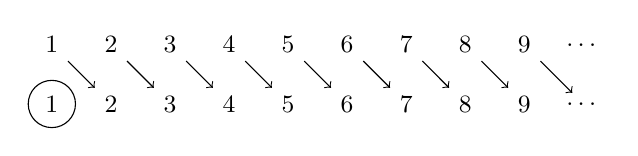
\begin{tikzpicture}[scale = .75]
		\foreach \x in {1, 2, 3, 4, 5, 6, 7, 8, 9}
		{
			\node (\x a) at (\x, 1) {\small{\x}};
			\node (\x b) at (\x, 2) {\small{\x}};
		}
		\node (dotsa) at (10, 1) {\small{\ldots}};
		\node (dotsb) at (10, 2) {\small{\ldots}};
		\draw[->] (1b)--(2a);
		\draw[->] (2b)--(3a);
		\draw[->] (3b)--(4a);
		\draw[->] (4b)--(5a);
		\draw[->] (5b)--(6a);
		\draw[->] (6b)--(7a);
		\draw[->] (7b)--(8a);
		\draw[->] (8b)--(9a);
		\draw[->] (9b)--(dotsa);
		\draw (1,1) circle (.4);
		\end{tikzpicture}
	\end{center}
	(\citealt[730]{EwaldSieg2013}માં પ્રકાશિત; અમારો અનુવાદ)
\end{quote}
નિર્ણાયક મુદ્દો એ છે કે હિલ્બર્ટની હોટેલમાં અનંત ઓરડાઓ છે; અને આમ
કહેવાનો અર્થ શું થાય તેની વ્યાખ્યા તરીકે આપણે તેમની સમજૂતી લઈ શકીએ.
ખરેખર, ડેડેકિન્ડનો અભિગમ પણ આ જ હતો (અલબત્ત, અહીં ભારે કાળવિપર્યય
સાથે રજૂ કર્યો છે; ડેડેકિન્ડની વ્યાખ્યા \citeyear{Dedekind1888}ની છે):

\begin{defn}\ollabel{defn:DedekindInfinite}
ગણ $A$ \emph{ડેડેકિન્ડ-અનંત} હોય જો અને માત્ર જો $A$થી $A$ના કોઈ
ઉચિત ઉપગણમાં એક-એક વિધેય હોય. એટલે કે, કોઈ $o \in A$ અને
એક-એક વિધેય $f \colon A \to A$ એવાં હોય કે $o \notin \ran{f}$.
\end{defn}
% END OLP-0050
\endgroup

\begingroup
\makeatletter\def\ol@sectioncs{section}\makeatother

% BEGIN OLP-0051
\olfileid{sfr}{infinite}{dedekind}
\olsection{ડેડેકિન્ડ બીજગણિતો}
\phantomsection\label{guunit:OLP-0051}


આપણે પ્રાકૃતિક સંખ્યાઓ માત્ર અનંત હોય એટલું જ નથી માગતા; આપણે એમ પણ
માગીએ છીએ કે તેમને અમુક (બૈજિક) ગુણધર્મો હોય: સરવાળા, ગુણાકાર વગેરે
હેઠળ તેમનો વ્યવહાર સુસંગત હોવો જોઈએ.

ડેડેકિન્ડનો વિચાર \emph{અનુગામી વિધેય}ના ખ્યાલને મૂળભૂત માનવાનો અને
પછી નીચેના ગુણધર્મો ધરાવતી સંખ્યાઓ તરીકે તેમનું લક્ષણ આપવાનો હતો:
\begin{enumerate}
	\item એવી સંખ્યા $0$ છે જે કોઈ પણ સંખ્યાની અનુગામી નથી
	\\અર્થાત્, $0 \notin \ran{s}$
	\\અર્થાત્, $\forall x\ s(x) \neq 0$
	\item ભિન્ન સંખ્યાઓના અનુગામીઓ ભિન્ન હોય છે
	\\અર્થાત્, $s$ એ એક-એક વિધેય છે
	\\અર્થાત્, $\forall x \forall y (s(x) = s(y) \lif x = y)$
	\item\ollabel{repeatedapplication} દરેક સંખ્યા $0$ પર અનુગામી
	વિધેય વારંવાર લગાડવાથી મળે છે.
\end{enumerate}
પહેલી બે શરતોને પ્રથમ-ક્રમ તર્કશાસ્ત્રથી સહેલાઈથી સંભાળી શકાય છે
(ઉપર જુઓ). પરંતુ માત્ર પ્રથમ-ક્રમ તર્કશાસ્ત્રથી
\olref{repeatedapplication}ને સંભાળી શકાતી નથી. ડેડેકિન્ડની સફળતા
શરત \olref{repeatedapplication}ને ગણસૈદ્ધાંતિક રીતે આ પ્રમાણે ફરી
ઘડવામાં હતી:
\begin{enumerate}
	\item[3$'$.] પ્રાકૃતિક સંખ્યાઓ એવો નાનામાં નાનો ગણ છે જે
	\emph{અનુગામી વિધેય હેઠળ સંવૃત} છે: એટલે કે, ગણના કોઈ પણ
	ઘટક પર $s$ લગાડીએ તો ગણનો બીજો ઘટક મળે છે.
\end{enumerate}
પરંતુ આ વાત આપણે ધીમે ધીમે પૂરેપૂરી સ્પષ્ટ કરવી પડશે.

\begin{defn}\ollabel{Closure}
	દરેક વિધેય $f \colon A \to A$ માટે ગણ $X \subseteq A$ એ
	$f$-\emph{સંવૃત} છે {iff} $(\forall x \in X)f(x) \in X$.
	હવે દરેક $o \in A$ માટે વ્યાખ્યા કરીએ:
	$$\closureofunder{f}{o} = \bigcap\Setabs{X}{o \in X\text{ અને }X
\text{ એ $f$-સંવૃત છે}}$$
\end{defn}
\sourcecorrection{OLINF-001}{મૂળની \texttt{dedekind-algebra.tex},
પંક્તિઓ 40--64માં સંવરણની વ્યાખ્યા કોઈ પણ $f$ અને $o$ માટે અપાઈ
છે, પછીના લેમામાં $A$ને બાંધ્યા વિના $o\in A$ લખાયું છે, અને
સાબિતીમાં $\ran{f}\cup\{o\}$ એ $f$-સંવૃત હોવાનો ઉપયોગ થાય છે.
આ દલીલને જરૂરી અને પછીના બધા ઉપયોગો સાથે સુસંગત એવી ધારણા
$f\colon A\to A$, $X\subseteq A$ અને $o\in A$ અહીં સ્પષ્ટ કરી છે.}

આમ $\closureofunder{f}{o}$ એ એવા બધા $f$-સંવૃત ગણોનો છેદ છે
જેમનો ઘટક~$o$ છે. તેથી સહજ રીતે,
$\closureofunder{f}{o}$ એ ઘટક તરીકે $o$ ધરાવતો
\emph{નાનામાં નાનો} $f$-સંવૃત ગણ છે. આગળનું પરિણામ આ સહજ વિચારને
ચોક્કસ બનાવે છે;
\begin{lem}\ollabel{closureproperties}
	દરેક વિધેય $f \colon A \to A$ અને દરેક $o \in A$ માટે:
	\begin{enumerate}
		\item\ollabel{closurehaselem} $o \in \closureofunder{f}{o}$; અને
		\item\ollabel{closureclosed} $\closureofunder{f}{o}$ એ $f$-સંવૃત છે; અને
		\item\ollabel{closuresmallest} જો $X$ એ $f$-સંવૃત હોય અને $o \in
		X$, તો $\closureofunder{f}{o} \subseteq X$.
	\end{enumerate}
\end{lem}

\begin{proof}
નોંધો કે ઘટક તરીકે $o$ ધરાવતો ઓછામાં ઓછો એક $f$-સંવૃત ગણ
છે, એટલે કે $\ran{f}\cup \{o\}$. તેથી આવા \emph{બધા} ગણોનો છેદ
$\closureofunder{f}{o}$ અસ્તિત્વ ધરાવે છે. હવે આપણે
\olref{closurehaselem}--\olref{closuresmallest} તપાસવાં છે.

\olref{closurehaselem} અંગે: $o \in \closureofunder{f}{o}$, કારણ કે
તે એવા ગણોનો છેદ છે જેમના દરેકનો ઘટક~$o$ છે.

\olref{closureclosed} અંગે: ધારો કે $x \in \closureofunder{f}{o}$.
તેથી જો $o \in X$ અને $X$ એ $f$-સંવૃત હોય, તો $x \in X$; અને
$X$ એ $f$-સંવૃત હોવાથી હવે $f(x) \in X$. તેથી
$f(x) \in \closureofunder{f}{o}$.

\olref{closuresmallest} અંગે: સામાન્ય રીતે, જો $X \in C$ હોય, તો
$\bigcap C \subseteq X$.
\end{proof}

આનો ઉપયોગ કરીને આપણે કહી શકીએ:

\begin{defn}
\emph{ડેડેકિન્ડ બીજગણિત} એટલે ગણ $A$, વિધેય $f \colon A \to A$
અને કોઈ $o \in A$ એવાં કે:
	\begin{enumerate}
		\item \ollabel{ded:proper} $o \notin \ran{f}$
		\item \ollabel{ded:injection} $f$ એ એક-એક વિધેય છે
		\item \ollabel{ded:closure} $A = \closureofunder{f}{o}$
	\end{enumerate}
\end{defn}

$A = \closureofunder{f}{o}$ હોવાથી આપણું પહેલાનું પરિણામ જણાવે છે કે
$A$ એ ઘટક તરીકે $o$ ધરાવતો નાનામાં નાનો $f$-સંવૃત ગણ છે.
ડેડેકિન્ડ બીજગણિત સ્પષ્ટપણે ડેડેકિન્ડ-અનંત છે; વ્યાખ્યાની કલમો
\olref{ded:proper} અને \olref{ded:injection} જ જુઓ. પરંતુ વધુ રસપ્રદ
હકીકત એ છે કે કોઈ પણ ડેડેકિન્ડ-અનંત ગણને ડેડેકિન્ડ બીજગણિતમાં ફેરવી
શકાય છે.

\begin{thm}\ollabel{thm:DedekindInfiniteAlgebra}
જો કોઈ ડેડેકિન્ડ-અનંત ગણ હોય, તો કોઈ ડેડેકિન્ડ બીજગણિત હોય છે.
\end{thm}

\begin{proof}
ધારો કે $D$ ડેડેકિન્ડ-અનંત છે. તેથી એક-એક વિધેય $g \colon D \to
D$ અને ઘટક $o \in D \setminus \ran{g}$ છે. હવે $A =
\closureofunder{g}{o}$ લો; \olref{closureproperties} મુજબ $A$
અસ્તિત્વ ધરાવે છે અને $o \in A$. $f = \funrestrictionto{g}{A}$ લો.
$A, f, o$ મળીને ડેડેકિન્ડ બીજગણિત રચે છે તે આપણે બતાવીશું.

\olref{ded:proper} અંગે: $o \notin \ran{g}$ અને $\ran{f}
\subseteq \ran{g}$ હોવાથી $o\notin \ran{f}$.

\olref{ded:injection} અંગે: $g$ એ $D$ પર એક-એક વિધેય છે; તેથી
$f \subseteq g$ પણ એક-એક વિધેય જ હોય.

\olref{ded:closure} અંગે: \olref{closureproperties} મુજબ $A$ એ
$g$-સંવૃત છે; તેથી ખાસ કરીને $A$ એ $f$-સંવૃત છે. આમ
$\closureofunder{f}{o} \subseteq A$ એ \olref{closureproperties}થી મળે
છે. વળી $\closureofunder{f}{o}$ એ $f$-સંવૃત છે અને
$f = \funrestrictionto{g}{A}$ હોવાથી $\closureofunder{f}{o}$ એ
$g$-સંવૃત છે. તેથી \olref{closureproperties} મુજબ
$A \subseteq \closureofunder{f}{o}$.
\end{proof}
% END OLP-0051
\endgroup

\begingroup
\makeatletter\def\ol@sectioncs{section}\makeatother

% BEGIN OLP-0052
\olfileid{sfr}{infinite}{induction}
\olsection[ગાણિતિક અનુમાન]{ડેડેકિન્ડ બીજગણિતો અને ગાણિતિક અનુમાન}
\phantomsection\label{guunit:OLP-0052}


હવે નિર્ણાયક વાત એ છે કે ડેડેકિન્ડ બીજગણિત---ખરેખર, \emph{કોઈ પણ}
ડેડેકિન્ડ બીજગણિત---પ્રાકૃતિક સંખ્યાઓના અવેજ તરીકે કામ કરશે. આ નીચેના
સરળ પરિણામને આભારી છે:

\begin{thm}[ગાણિતિક અનુમાન]\ollabel{thm:dedinfiniteinduction}
ધારો કે $N, s, o$ મળીને ડેડેકિન્ડ બીજગણિત રચે છે. ત્યારે દરેક ગણ $X$ માટે:
	\begin{center}
		જો $o \in X$ અને $(\forall {n} \in N \cap X){s}({n}) \in X$, {તો} $N \subseteq X$.
	\end{center}
\end{thm}

\begin{proof}
ડેડેકિન્ડ બીજગણિતની વ્યાખ્યા મુજબ $N = \closureofunder{s}{o}$.
હવે જો ${o} \in X$ અને $(\forall {n} \in N)(n \in X \lif
{s}({n}) \in X)$ બંને હોય, તો $N = \closureofunder{s}{o} \subseteq X$.
\end{proof}

ગાણિતિક અનુમાન પ્રાકૃતિક સંખ્યાઓનું વિશિષ્ટ લક્ષણ હોવાથી મુદ્દો આ છે.
કોઈ પણ ડેડેકિન્ડ-અનંત ગણ આપેલો હોય, તો આપણે ડેડેકિન્ડ બીજગણિત રચીને
તેને પ્રાકૃતિક સંખ્યાઓના અવેજ તરીકે વાપરી શકીએ છીએ.

કબૂલ કે \olref{thm:dedinfiniteinduction}માં અનુમાનને
\emph{ગણસૈદ્ધાંતિક} પદોમાં ઘડ્યું છે. પરંતુ આ સિદ્ધાંતને આપણને વધુ
પરિચિત હોય એવાં પદોમાં સહેલાઈથી મૂકી શકીએ છીએ:

\begin{cor}\ollabel{natinductionschema}
ધારો કે $N, s, o$ મળીને ડેડેકિન્ડ બીજગણિત રચે છે. ત્યારે પ્રાચલો
હોઈ શકે એવા દરેક સૂત્ર $\phi(x)$ માટે:
\begin{center}
	જો $\phi(o)$ અને $(\forall {n} \in N)(\phi(n)\lif
	\phi({s}({n})))$, {તો} $(\forall n \in N)\phi(n)$.
\end{center}
\end{cor}

\begin{proof}
$X = \Setabs{n \in N}{\phi(n)}$ લો અને હવે
\olref{thm:dedinfiniteinduction} વાપરો.
\end{proof}

આ પરિણામમાં આપણે કોઈ સૂત્ર ``પ્રાચલો ધરાવે છે'' એવું કહ્યું. તેનો
આશરે અર્થ એ છે કે કોઈ પણ વસ્તુઓ $c_1, \ldots, c_k$ માટે આપણે
$\phi(x, c_1, \ldots, c_k)$ સાથે કામ કરી શકીએ છીએ. વધુ ચોક્કસ રીતે,
``પ્રાચલો''નો ઉલ્લેખ કર્યા વિના પરિણામ આ પ્રમાણે કહી શકાય. દરેક સૂત્ર
$\phi(x, v_1, \ldots, v_k)$ માટે, જેના બધા મુક્ત ચલો દર્શાવેલા છે,
આપણી પાસે છે:
	\begin{align*}
			\forall v_1 \ldots \forall v_k((&\phi(o, v_1,\ldots, v_k) \land {}\\
			&	(\forall x \in N)(\phi(x,v_1, \ldots, v_k) \lif \phi(s(x), v_1,\ldots, v_k))) \lif {}\\
			&\hspace{3em} (\forall x \in N)\phi(x, v_1,\ldots, v_k))
	\end{align*}
સ્પષ્ટ છે કે ``પ્રાચલો ધરાવે છે'' એવો વાક્યપ્રયોગ વાંચવાનું ઘણું સરળ
બનાવી શકે છે. (\olref[sth][][]{part}માં આપણે આ રીત ઘણી વાર વાપરીશું.)

ડેડેકિન્ડ બીજગણિતો તરફ પાછા ફરીએ: કોઈ પણ ડેડેકિન્ડ બીજગણિત આપેલું
હોય, તો આપણે સરવાળા, ગુણાકાર અને ઘાતની ક્રિયાનાં સામાન્ય અંકગણિતીય
વિધેયો પણ વ્યાખ્યાયિત કરી શકીએ છીએ. જોકે આ બાબત તુચ્છ નથી અને તેમાં
\emph{પુનરાવર્તી વ્યાખ્યા}ની રીત વપરાય છે. આ રીતનો પરિચય અને ઔચિત્ય
આપણે ઘણું પાછળ, અને વધુ વ્યાપક સંદર્ભમાં આપીશું. (રસ ધરાવતા વાચકો
\olref[sth][ord-arithmetic][]{chap} પછી આ મુદ્દો ફરી જોઈ શકે, અથવા
\citealt[pp.~95--8]{Potter2004} જેવી વૈકલ્પિક રજૂઆત વાંચી શકે.) પરંતુ
જ્યાં $N, s, o$ મળીને ડેડેકિન્ડ બીજગણિત રચે છે, ત્યાં અંતે આપણે નીચે
પ્રમાણે ઠરાવી શકીશું:
\begin{align*}
	{a} + {o} &= {a} & & & {a} \times {o} &= {o} & & & {a}^{o} &= s(o)\\
{a} + {s}({b}) &= {s}({a}+{b}) &&& {a} \times {s}({b}) &= ({a}\times {b}) + {a}  & & & {a}^{{s}({b})} &= {a}^{b} \times {a}
\end{align*}
અને તે આશા મુજબ વર્તે છે એવું બતાવી શકીશું.
% END OLP-0052
\endgroup

\begingroup
\makeatletter\def\ol@sectioncs{section}\makeatother

% BEGIN OLP-0053
\olfileid{sfr}{infinite}{dedekindsproof}

\olsection[ડેડેકિન્ડની ``સાબિતી'']{અનંત ગણના અસ્તિત્વની
ડેડેકિન્ડની ``સાબિતી''}
\phantomsection\label{guunit:OLP-0053}


આ પ્રકરણમાં આપણે ડેડેકિન્ડ બીજગણિતો વડે પ્રાકૃતિક સંખ્યાઓની
ગણસૈદ્ધાંતિક રજૂઆત કરી છે. \olref[arith][ref]{sec}માં આપણે
વિશ્લેષણના અંકગણિતીકરણના (બીજી બાબતો સાથે) તાત્ત્વિક મહત્ત્વ પર
વિચાર કર્યો હતો. હવે આપણે અહીં જે સિદ્ધ કર્યું છે તેના મહત્ત્વ પર
વિચાર કરવો જોઈએ.

સમગ્ર \olref[sfr][arith][]{chap}માં આપણે પ્રાકૃતિક સંખ્યાઓને આપેલી
માની અને તેમનો ઉપયોગ કરીને પૂર્ણાંકો, સંમેય સંખ્યાઓ અને વાસ્તવિક
સંખ્યાઓની સ્પષ્ટ રચના કરી. આ પ્રકરણમાં આપણે પ્રાકૃતિક સંખ્યાઓની સ્પષ્ટ
રચના આપી નથી. આપણે માત્ર એટલું બતાવ્યું છે કે \emph{કોઈ પણ
ડેડેકિન્ડ-અનંત ગણ આપેલો હોય}, તો એવો ગણ વ્યાખ્યાયિત કરી શકાય છે જે
આપણે~$\Nat$ પાસે ઇચ્છીએ છીએ તેવો જ વ્યવહાર કરશે.

તેથી \emph{કઈ વસ્તુઓ પ્રાકૃતિક સંખ્યાઓ છે} એવા અધિભૌતિક પ્રશ્નનો
જવાબ આપ્યો હોવાનો દાવો આપણે કરી શકતા નથી. પરંતુ એ સારી વાત છે. છેવટે,
\olref[sfr][arith][ref]{sec}માં આપણે ભાર મૂક્યો હતો કે
$\Real$ને ડેડેકિન્ડ કાપોના ગણ તરીકે આપેલી વ્યાખ્યાને અનુકૂળ ઠરાવને
બદલે \emph{શોધ} માનવી ખોટી છે. નિર્ણાયક અવલોકન એ છે કે ડેડેકિન્ડ
કાપો વાસ્તવિક સંખ્યાઓના મુખ્ય ગણિતીય ગુણધર્મોને મૂર્ત કરે છે. અહીં
પણ એવું જ છે: \emph{કોઈ પણ} ડેડેકિન્ડ બીજગણિત પ્રાકૃતિક સંખ્યાઓના
મુખ્ય ગણિતીય ગુણધર્મોને મૂર્ત કરે છે. (ખરેખર, બધા ડેડેકિન્ડ બીજગણિતો
\emph{એકરૂપ} છે એવું સાબિત કરીને ડેડેકિન્ડે આ મુદ્દો દૃઢ કર્યો
(\citeyear[Theorems
132--3]{Dedekind1888}). તેથી ઘણા સમકાલીન
``સંરચનાવાદીઓ'' ડેડેકિન્ડને પોતાના પુરોગામી ગણે છે તેમાં નવાઈ નથી.)

 વળી, આપણે બતાવ્યું છે કે પ્રાકૃતિક સંખ્યાઓના સિદ્ધાંતને સહજ સરળ
 ગણસિદ્ધાંતમાં કેવી રીતે સ્થાપિત કરવો. આ ગણસિદ્ધાંત હજી ખાસ્સો
 અનૌપચારિક છે, પરંતુ તેમાં પ્રાકૃતિક સંખ્યાઓ આપેલી છે એવું (દેખીતી
 રીતે) માનવામાં આવતું નથી. તેથી આપણે ડેડેકિન્ડના પોતાના મહત્ત્વાકાંક્ષી
 યોજનાને સાકાર કરવાની દિશામાં હોઈ શકીએ છીએ; તેમણે તેને આ પ્રમાણે
 સમજાવી હતી:
\begin{quote}
	વિજ્ઞાનમાં જે બાબતની સાબિતી શક્ય હોય તે સાબિતી વિના માનવી ન જોઈએ.
	આ માગ વાજબી લાગતી હોવા છતાં, સૌથી સરળ વિજ્ઞાનનો પાયો નાખવાની
	અત્યંત નવીન પદ્ધતિઓમાં પણ તે સંતોષાઈ છે એમ હું માની શકતો નથી;
	અર્થાત્ તર્કશાસ્ત્રનો એ ભાગ જે સંખ્યાઓના સિદ્ધાંત સાથે સંબંધિત છે.
	અંકગણિત (બીજગણિત, વિશ્લેષણ) માત્ર તર્કશાસ્ત્રનો ભાગ છે એમ કહેતાં
	મારો આશય એ છે કે સંખ્યાનો ખ્યાલ અવકાશ અને સમયની કલ્પનાઓ કે
	અંતઃપ્રજ્ઞાથી સંપૂર્ણપણે સ્વતંત્ર છે---હું તેને વિચારના શુદ્ધ
	નિયમોની સીધી નિષ્પત્તિ માનું છું.
	\citep[preface]{Dedekind1888}
\end{quote}
ડેડેકિન્ડનો સાહસિક વિચાર આ છે. માત્ર (સહજ) ગણસિદ્ધાંત વાપરીને
પ્રાકૃતિક સંખ્યાઓ કેવી રીતે રચવી તે આપણે હમણાં જ બતાવ્યું.
\olref[sfr][arith][]{chap}માં પ્રાકૃતિક સંખ્યાઓ અને થોડો ગણસિદ્ધાંત
આપેલાં હોય ત્યારે વાસ્તવિક સંખ્યાઓ કેવી રીતે રચવી તે જોયું. તેથી કદાચ
``અંકગણિત (બીજગણિત, વિશ્લેષણ)'' એ ``માત્ર તર્કશાસ્ત્રનો ભાગ'' ઠરે
(ડેડેકિન્ડના ``તર્કશાસ્ત્ર'' શબ્દના વિસ્તૃત અર્થમાં).

વિચાર આ છે. પરંતુ જરા થોભો. ડેડેકિન્ડ બીજગણિતની આપણી રચના
(પ્રાકૃતિક સંખ્યાઓનો આપણો અવેજ) ડેડેકિન્ડ-અનંત ગણના અસ્તિત્વ પર
આધારિત છે. (ફરી \olref[sfr][infinite][dedekind]{thm:DedekindInfiniteAlgebra}
જુઓ.) જો ``તર્કશાસ્ત્ર'' અથવા ``વિચારના શુદ્ધ નિયમો'' વડે
ડેડેકિન્ડ-અનંત ગણનું અસ્તિત્વ સ્થાપિત ન કરી શકાય, તો યોજના અટકી જાય છે.

તો શું ``વિચારના શુદ્ધ નિયમો'' વડે ડેડેકિન્ડ-અનંત ગણનું અસ્તિત્વ
સ્થાપિત કરી શકાય? ડેડેકિન્ડનો પ્રયાસ આ હતો:
\begin{quote}
  મારા પોતાના વિચારોનું ક્ષેત્ર, એટલે કે મારા વિચારના વિષય બની શકે
  એવી બધી વસ્તુઓની સમગ્રતા $S$, અનંત છે. કારણ કે જો $s$ એ $S$નો
  ઘટક દર્શાવે, તો $s$ મારા વિચારનો વિષય બની શકે છે એવો વિચાર $s'$ પણ
  પોતે $S$નો ઘટક છે. જો આપણે તેને ઘટક~$s$ના પ્રતિબિંબ $\phi(s)$ તરીકે
  લઈએ, તો \dots~$S$ [ડેડેકિન્ડના અર્થમાં] અનંત છે, જે સાબિત કરવાનું હતું.
	\citep[\S66]{Dedekind1888}
\end{quote}
મોટાભાગે અત્યંત ચુસ્ત ગણિતીય સાબિતીઓથી બનેલા પુસ્તકની વચ્ચે આવી વાત
મળે તે ખરેખર આશ્ચર્યજનક છે. બે ટિપ્પણીઓ કરવા જેવી છે.

પહેલી: આ ``સાબિતી''માં આજે આપણે જેને ``ગણિતીય'' સ્વરૂપ કહીએ એવું
ભાગ્યે જ કંઈ છે. તેમાં મનોવૈજ્ઞાનિક વસ્તુઓ (વિચારો)ની વાત થાય છે, અને
તે પણ માત્ર \emph{સંભવિત} વિચારોની.

બીજી: ઓછામાં ઓછું આપણે ડેડેકિન્ડ બીજગણિતો જે રીતે રજૂ કર્યાં છે તે
દૃષ્ટિએ, આ ``સાબિતી''માં સીધી તકનીકી ખામી છે. ડેડેકિન્ડની દલીલ સફળ
હોય તો તે માત્ર એટલું સ્થાપિત કરે છે કે અનંત સંખ્યામાં વસ્તુઓ છે
(ખાસ કરીને, અનંત સંખ્યામાં વિચારો). પરંતુ ડેડેકિન્ડે આપણને એ માનવાનું
કારણ પણ આપવું પડે કે~$S$ એ અનંત ઘણા ઘટકો ધરાવતો એક જ
\emph{ગણ} છે; $S$ને માત્ર \emph{કેટલીક વસ્તુઓ} (બહુવચનમાં) માનવું
યોગ્ય નથી.

ડેડેકિન્ડે અહીં ખામી જોઈ નહીં તે હકીકત કદાચ સૂચવે છે કે
``સમગ્રતા'' શબ્દનો તેમનો ઉપયોગ \emph{ગણ} શબ્દના \emph{આપણા} ઉપયોગને
ચોક્કસપણે અનુસરતો નથી.\footnote{ખરેખર, એવું નહોતું માનવાનાં બીજાં
કારણો પણ છે; \citet[p.~23]{Potter2004} જુઓ.} પરંતુ આમાં બહુ નવાઈ નથી.
છેલ્લાં બે પ્રકરણમાં આપણે હાથ ધરેલો પ્રકલ્પ---પ્રાકૃતિક સંખ્યાઓની
``રચના'', અને તેમાંથી પૂર્ણાંકો, વાસ્તવિક સંખ્યાઓ અને સંમેય સંખ્યાઓની
``રચના''---સંપૂર્ણપણે સહજ રીતે કર્યો છે. કયા ગણો અસ્તિત્વ ધરાવે છે અને
ક્યારે ધરાવે છે તે વિશે ઘણા સામાન્ય સિદ્ધાંતો મૂક્યા વિના, જરૂર પડતી
ગઈ તેમ આ ગણ અથવા તે ગણ માની લીધા છે. પરંતુ આપણે જાણીએ છીએ કે
\emph{કેટલાક} સામાન્ય સિદ્ધાંતો જરૂરી છે; નહિતર આપણે રસેલના
વિરોધાભાસમાં ફસાઈ જઈશું.

 હવે આપણી સહજતાની મર્યાદા છોડવાનો સમય આવી ગયો છે.
% END OLP-0053
\endgroup

\begingroup
\makeatletter\def\ol@sectioncs{section}\makeatother

% BEGIN OLP-0054
\olfileid{sfr}{infinite}{card-sb}

\olsection{પરિશિષ્ટ: શ્રેડર--બર્નસ્ટાઇનની સાબિતી}
\phantomsection\label{guunit:OLP-0054}


સહજ ગણસિદ્ધાંત છોડીએ તે પહેલાં એક છેલ્લી સહજ (પણ સુવિકસિત!) સાબિતી
વિચારવાની બાકી છે. આ શ્રેડર--બર્નસ્ટાઇન
(\olref[sfr][siz][sb]{thm:schroder-bernstein})ની સાબિતી છે: જો
$\cardle{A}{B}$ અને $\cardle{B}{A}$ હોય, તો $\cardeq{A}{B}$; એટલે કે,
એક-એક વિધેયો $f \colon A \to B$ અને $g \colon B \to A$ આપેલાં હોય,
તો એક-એક વ્યાપ્ત વિધેય $h \colon A \to B$ હોય છે.

આ પ્રકરણમાં આપણે ડેડેકિન્ડના \emph{સંવરણો}ના ખ્યાલને અનુસર્યા છીએ.
ખરેખર, ડેડેકિન્ડે આ ખ્યાલ વાપરીને શ્રેડર--બર્નસ્ટાઇનની એક સુંદર
સાબિતી આપી હતી અને આપણે તેને અહીં રજૂ કરીશું. અહીંની સાબિતી
\citet[pp.~157--8]{Potter2004}ને નજીકથી અનુસરે છે; ત્યાં થોડું જુદું
પણ મૂળભૂત રીતે સરખું નિરૂપણ મળશે. થોડું ગૂગલમાં
શોધવાથી પણ ખાતરી થશે કે---$\sqrt{2}$ની અસંમેયતા જેવું---આ એવું પ્રમેય
છે જેની \emph{ઘણી} રસપ્રદ અને જુદી સાબિતીઓ છે.

\olref[sfr][infinite][dedekind]{Closure} જેવી જ સંજ્ઞા વાપરીને,
દરેક ગણ $B$ અને વિધેય~$f$ માટે લો:
\[
\Closureofunder{f}{B} = \bigcap \Setabs{X}{B \subseteq X
\text{ અને $X$ એ $f$-સંવૃત છે}}
\]
આ રીતે વ્યાખ્યાયિત $\Closureofunder{f}{B}$ એ $B$ને સમાવતો નાનામાં
નાનો $f$-સંવૃત ગણ છે, એ અર્થમાં કે:

\begin{lem}\ollabel{Closureprops}
	દરેક વિધેય $f$ અને દરેક $B$ માટે:
	\begin{enumerate}
		\item\ollabel{Closurehaselem} $B \subseteq \Closureofunder{f}{B}$; અને
		\item\ollabel{Closureclosed} $\Closureofunder{f}{B}$ એ $f$-સંવૃત છે; અને
		\item\ollabel{Closuresmallest} જો $X$ એ $f$-સંવૃત હોય અને $B
		\subseteq X$, તો $\Closureofunder{f}{B} \subseteq X$.
	\end{enumerate}
\end{lem}

\begin{proof}
બરાબર \olref[sfr][infinite][dedekind]{closureproperties}ની જેમ.
\end{proof}

શ્રેડર--બર્નસ્ટાઇન સુધી પહોંચવા માટે એક છેલ્લી હકીકત જોઈએ:

\begin{prop}\ollabel{sbhelper}
જો $A \subseteq B \subseteq C$ અને $A \approx C$ હોય, તો
$\cardeq{A}{B}$ અને $\cardeq{B}{C}$.
\end{prop}
\sourcecorrection{OLINF-002}{પછીની સ્વતંત્ર સમીક્ષાએ આ નોંધનું
મૂળ-ખામી તરીકેનું અગાઉનું વર્ગીકરણ પાછું ખેંચ્યું છે. મૂળની
\texttt{card-sb.tex}, પંક્તિ~52નું $\cardeq{\cardeq{A}{B}}{C}$,
\texttt{\string\cardeq}ની બે-દલીલી વ્યાખ્યા પ્રમાણે,
$A \approx B \approx C$માં વિસ્તરે છે; તેથી તેમાં દલીલસંખ્યાની કે
ગણિતીય ખામી નથી. ગુજરાતી મુખ્ય પાઠમાં સાબિતી સ્થાપિત કરતી બે
સમાનતાઓને સ્પષ્ટ સંયોજન રૂપે જાળવી છે. આ મૂળ નિષ્કર્ષની સમકક્ષ
રજૂઆત છે, મૂળની સુધારણા નહીં.}

\begin{proof}
એક-એક વ્યાપ્ત વિધેય $f \colon C \to A$ આપેલું હોય, ત્યારે $F =
\Closureofunder{f}{C \setminus B}$ લો અને પ્રદેશ $C$ ધરાવતું વિધેય
$g$ આ પ્રમાણે વ્યાખ્યાયિત કરો:
\[
	g(x) =
	\begin{cases}
			f(x) &\text{જો $x \in F$}\\
			x & \text{અન્યથા}
		\end{cases}
\]
$g$ એ $C \to B$નું એક-એક વ્યાપ્ત વિધેય છે તે આપણે બતાવીશું; તેના પરથી
$\comp{f^{-1}}{g} \colon A \to B$ એ એક-એક વ્યાપ્ત વિધેય છે એવું મળશે અને
સાબિતી પૂરી થશે.

પહેલો દાવો એ છે કે જો $x \in F$ પણ $y\notin F$ હોય, તો
$g(x) \neq g(y)$. વિરોધાભાસ મેળવવા ઊલટું ધારો; ત્યારે
$y = g(y) = g(x) = f(x)$. \olref{Closureprops} મુજબ $F$ એ
$f$-સંવૃત છે અને $x \in F$ હોવાથી $y = f(x) \in F$, જે વિરોધાભાસ છે.

હવે ધારો કે $g(x) = g(y)$. તેથી ઉપરના દાવાથી $x \in F$ જો અને માત્ર
જો $y \in F$. જો $x, y \in F$, તો $f(x) = g (x) = g(y) = f(y)$;
અને $f$ એ એક-એક વ્યાપ્ત વિધેય હોવાથી $x = y$. જો $x, y \notin F$, તો
$x = g(x) = g(y) = y$. તેથી $g$ એ એક-એક વિધેય છે.

હવે માત્ર $\ran{g} = B$ બતાવવાનું બાકી છે. તેથી $x \in B \subseteq C$
નિશ્ચિત કરો. જો $x \notin F$, તો $g(x) = x$. જો $x \in F$, તો કોઈ
$y \in F$ માટે $x = f(y)$; કારણ કે નહિતર $F \setminus \{x\}$ એ
$f$-સંવૃત હોત અને $C\setminus B$ને સમાવતો હોત, જે
\olref{Closureprops}થી અશક્ય છે. હવે $g(y) = f(y) = x$.
\end{proof}

છેલ્લે મુખ્ય પરિણામની સાબિતી આ રહી. યાદ કરો કે વિધેય $h$ અને ગણ $D$
આપેલાં હોય ત્યારે આપણે $\funimage{h}{D} = \Setabs{h(x)}{x
\in D}$ વ્યાખ્યાયિત કરીએ છીએ.

\begin{proof}[શ્રેડર--બર્નસ્ટાઇનની સાબિતી] ધારો કે $f \colon A \to B$
અને $g \colon B \to A$ એ એક-એક વિધેયો છે. $\funimage{f}{A}
\subseteq B$ હોવાથી $\funimage{g}{\funimage{f}{A}} \subseteq
g[B] \subseteq A$. વળી, $g$ અને $f$ બંને એક-એક હોવાથી
$\comp{f}{g} \colon A \to \funimage{g}{\funimage{f}{A}}$ પણ
એક-એક વિધેય છે; અને ખરેખર, તેનો સહપ્રદેશ જે રીતે વ્યાખ્યાયિત કર્યો
છે તે પરથી $\comp{f}{g}$ એ એક-એક વ્યાપ્ત વિધેય છે. તેથી
$\cardeq{\funimage{g}{\funimage{f}{A}}}{A}$ અને આમ
\olref{sbhelper} મુજબ કોઈ એક-એક વ્યાપ્ત વિધેય $h \colon A \to
\funimage{g}{B}$ છે. વળી, $g^{-1}$ એ એક-એક વ્યાપ્ત વિધેય
$\funimage{g}{B} \to B$ છે. તેથી $\comp{h}{g^{-1}} \colon A \to B$
એ એક-એક વ્યાપ્ત વિધેય છે.
\end{proof}
% END OLP-0054
\endgroup
% END OLP-0049
\endgroup


\OLEndPartHook

\begin{editorial}
આગળનો સંબંધિત વૈકલ્પિક અંશ મૂળના સક્રિય આયાતક્રમમાં નથી. તે અહીં તેના વિષયના ભાગમાં જાળવ્યો છે.
\end{editorial}
\begingroup
\makeatletter\def\ol@sectioncs{section}\makeatother

% BEGIN OLP-0718
\olfileid{sfr}{ind}{int}

\olsection{પરિચય}
\phantomsection\label{guunit:OLP-0718}

\sourcecorrection{OLMD-347}{આ સ્રોત-ફાઇલ અન્ય ત્રણ-સ્તરીય વિભાગોની જેમ જ સ્થિત છે, પરંતુ મૂળમાં સમાવેશ-વર્ગ સુધીનો સાપેક્ષ માર્ગ એક સ્તર ઓછો છે. તેને યોગ્ય ત્રણ સ્તરનો માર્ગ આપ્યો છે.}

\begin{explain}
આગમન ગણિત અને તર્કશાસ્ત્રમાં વારંવાર વપરાતી સાબિતી-રીત છે.
ગણિતમાં પ્રાકૃતિક સંખ્યાઓ પરનું આગમન તમે જાણતા હશો.
પરંતુ ગણિત અને તર્કશાસ્ત્રમાં અનેક પ્રકારનાં વસ્તુ-ગણો છે
જેમના પર આગમન વાપરી શકાય છે.

સામાન્ય રીતે આગમન કોઈ સાર્વત્રિક દાવો સાબિત કરવાની છૂટ આપે છે:
કોઈ ચોક્કસ પ્રકારની દરેક વસ્તુને અમુક ગુણધર્મ છે તે બતાવવાનું.
ખાસ કરીને સર્વપરિમાણક દાખલ કરવાની સામાન્ય સાબિતી-રીત
અતિશય જટિલ હોય ત્યારે આગમન ઉપયોગી છે.
આગમન ખાસ રીતે રચાતી ગણિતીય વસ્તુઓ પર જ કામ કરે છે:
જો ગણનો દરેક ઘટક મૂળભૂત હોય અથવા મૂળભૂત ઘટકોમાંથી
રચાયેલો હોય, તો તેના પર આગમન વાપરી શકીએ.
વધુ ચોક્કસ રીતે:
\end{explain}

\begin{defn}
ગણ~$S$ ફલન~$f$ હેઠળ \emph{સંવૃત} છે જો અને ફક્ત જો
જ્યારે પણ $x \in S$ હોય ત્યારે $f(x) \in S$ પણ હોય.
\end{defn}

\begin{explain}
દાખલા તરીકે, પ્રાકૃતિક સંખ્યાઓનો ગણ~($\mathbb{N}$)
ઉત્તરગામી ફલન~$f(x) = x+1$ હેઠળ સંવૃત છે:
જો $x$ પ્રાકૃતિક સંખ્યા હોય, તો $x+1$ પણ છે.
પરંતુ પ્રાકૃતિક સંખ્યાઓ પૂર્વગામી ફલન~$f(x) = x-1$
હેઠળ સંવૃત નથી, કારણ કે $0$ પ્રાકૃતિક સંખ્યા છે, પણ $-1$ નથી.
\end{explain}

\begin{defn}
ગુણધર્મ~$P$ ફલન~$f(x)$ \emph{હેઠળ જળવાય છે} એમ કહીએ,
જો $f$ના પ્રદેશની કોઈ પણ વસ્તુ~$a$ માટે
$P(a)$માંથી $P(f(a))$ ફલિત થાય:
જો $a$ને ગુણધર્મ~$P$ હોય, તો $f(a)$ને પણ હોય.
\end{defn}

\begin{explain}
સમ સંખ્યા હોવાનો ગુણધર્મ ફલન~$f(x) = x+2$ હેઠળ જળવાય છે,
કારણ કે $x$ સમ હોય તો $x+2$ પણ સમ છે.
તે ગુણધર્મ ઉત્તરગામી ફલન હેઠળ જળવાતો નથી,
કારણ કે $x$ સમ હોય તો $x+1$ વિષમ છે.

પ્રાકૃતિક સંખ્યાઓ પર આગમન કામ કરે છે કારણ કે શૂન્યથી
ઉત્તરગામી ફલન સાંત વાર લાગુ પાડીને દરેક પ્રાકૃતિક સંખ્યા મળે છે.
જે ગણો પર આગમન વાપરી શકીએ તે બધામાં આ લક્ષણ છે.
\end{explain}

\begin{defn}[$\Nat$ પર આગમન]
જો શૂન્યને ગુણધર્મ~$P$ હોય અને $P$ ઉત્તરગામી ફલન હેઠળ
જળવાતો હોય, તો દરેક પ્રાકૃતિક સંખ્યાને ગુણધર્મ~$P$ છે.
\end{defn}

\begin{ex}
એકથી $n$ સુધીની પ્રાકૃતિક સંખ્યાઓનો સરવાળો
$\frac{n(n+1)}{2}$ છે. \\
\sourcecorrection{OLMD-348}{મૂળમાં પ્રથમ પ્રાકૃતિક સંખ્યાઓનો સરવાળો કહેવાયો છે, જ્યારે આ જ વિભાગ પ્રાકૃતિક સંખ્યાઓની શરૂઆત શૂન્યથી માને છે. દર્શાવેલું સૂત્ર એકથી આપેલી સંખ્યા સુધીના સરવાળાનું છે. તેથી દાવાનો એ અર્થ સ્પષ્ટ કર્યો છે; પ્રદર્શિત સરવાળામાં શૂન્ય ઉમેરવાથી મૂલ્ય બદલાતું નથી.}

\textbf{આધાર-કિસ્સો.} પ્રથમ શૂન્ય સંખ્યાઓનો, એટલે કે ખાલી
સૂચિનો, સરવાળો $0=
\frac{0\cdot 1}{2}$ છે.\\

\textbf{આગમનનું પગલું.} ધારો કે $k$ માટે ગુણધર્મ સાચો છે.
તે $k+1$ માટે પણ સાચો છે તે બતાવીએ.
બીજા શબ્દોમાં, ધારો કે $P(k)$ સાચું છે, એટલે કે
\[ 0 + 1 + \ldots + k = \frac{k(k+1)}{2} \]
બતાવીએ કે $P(k+1)$ સાચું છે, એટલે કે
\[ 0 + 1 + \ldots + k + (k+1) = \frac{(k+1)(k+2)}{2} \]
અહીં $P(k)$ની ધારણા વાપરીએ.

\begin{align*}
0 + 1 + \ldots + k &= \frac{k(k+1)}{2} \tag{ધારણા} \\
0 + 1 + \ldots + k + (k+1) &= \frac{k(k+1)}{2} + (k+1)
\tag{બંને બાજુએ $k+1$ ઉમેરો} \\
&= \frac{k(k+1) + 2(k+1)}{2} \\
&= \frac{k^2 + k + 2k +2}{2} \\
&=\frac{(k+1)(k+2)}{2}
\end{align*}
આમ આગમનનું પગલું પૂરું થાય છે અને દાવો સાબિત થયો.
\sourcecorrection{OLMD-349}{મૂળના વિસ્તરણમાં પ્રથમ પદ રેખીય છે, જ્યારે અગાઉના ગુણાકારને વિસ્તૃત કરતાં વર્ગપદ જોઈએ. તે પદ સુધાર્યું છે; હવે દર્શાવેલી છેલ્લી ગુણનખંડિત અભિવ્યક્તિ સાથે સમાનતા સાચી છે.}
\end{ex}

\begin{explain}
સૂત્રો માટે મૂળભૂત ઘટકો પરમાણ્વીય સૂત્રો છે.
સંયોજકો વડે ઓછાં જટિલ સૂત્રોમાંથી વધુ જટિલ
સૂત્રો રચાય છે. દરેક સંયોજકને સૂત્રોનું
એવું ફલન સમજી શકાય જે એક કે વધુ ઇનપુટમાંથી નવું
સૂત્ર આપે છે. દાખલા તરીકે, બે સૂત્રો
$!A$ અને $!B$ને સંયોજનમાં જોડતું ફલન
$\mathcal E _\land (!A,
!B) = !A \land !B$ તરીકે લખી શકાય.
આવાં ફલનોને \emph{સૂત્ર-રચના ફલનો} કહીએ.
સૂત્રોનો ગણ આ ફલનો હેઠળ સંવૃત છે:
જ્યારે $!A$ અને $!B$ એ સૂત્રો હોય, ત્યારે
$\lnot !A$, $!A \land !B$ વગેરે પણ સૂત્રો છે.
\sourcecorrection{OLMD-350}{મૂળમાં આ ભાગ અને આગળની આગમન-રૂપરેખા દરમિયાન સૂત્રનું વિશેષચિહ્ન તૂટેલું છે. તેને સંયોજનના બીજા સૂત્રની જેમ યોગ્ય મોટા અક્ષરવાળું સૂત્ર-ચિહ્ન આપ્યું છે.}
\sourcecorrection{OLMD-351}{મૂળ દરેક સંયોજકને બે સૂત્ર જોડતું ફલન કહે છે, પરંતુ નકાર એક સૂત્ર પર કામ કરે છે. તેથી એક કે વધુ ઇનપુટ જણાવ્યું છે. પહેલાંની એક-ઇનપુટ સંવૃતતા અને ગુણધર્મ-સંરક્ષણની વ્યાખ્યાઓ અનેક ઇનપુટ માટે આ રીતે સમજવી: બધા ઇનપુટ ગણમાં હોય તો પરિણામ ગણમાં હોય, અને બધા ઇનપુટને ગુણધર્મ હોય તો પરિણામને પણ હોય. પરિમાણકના કિસ્સાઓમાં આ શરત દરેક બાંધનાર ચલની પસંદગી માટે જોઈએ.}
\end{explain}

\begin{defn}[સૂત્રો પર આગમન]
જો દરેક પરમાણ્વીય સૂત્રને ગુણધર્મ~$P$ હોય અને
$P$ એ સૂત્ર-રચના ફલનો હેઠળ જળવાતો હોય,
તો દરેક સૂત્રને ગુણધર્મ~$P$ છે.
\end{defn}

\begin{explain}
આ વ્યાખ્યા સૂત્રો પરની આગમન-સાબિતી માટે રીત સૂચવે છે.
દરેક સૂત્રને ગુણધર્મ~$P$ છે તે બતાવવાનું હોય,
તો આ પગલાં લો:\\

\textbf{આધાર-કિસ્સો.} $!A$ પરમાણ્વીય સૂત્ર હોય.
[\ldots] તેથી $!A$ને ગુણધર્મ~$P$ છે.

\textbf{આગમનનું પગલું.} $!A$ અને $!B$ એ સૂત્રો હોય
અને બંનેને ગુણધર્મ~$P$ હોય.

કિસ્સો $\lnot$: [\ldots] તેથી $\lnot !A$ ને ગુણધર્મ $P$ છે.

કિસ્સો $\land$: [\ldots] તેથી $!A \land !B$ ને ગુણધર્મ $P$ છે.

કિસ્સો $\lor$: [\ldots] તેથી $!A \lor !B$ ને ગુણધર્મ $P$ છે.

કિસ્સો $\lif$: [\ldots] તેથી $!A \lif !B$ ને ગુણધર્મ $P$ છે.

કિસ્સો $\liff$: [\ldots] તેથી $!A \liff !B$ ને ગુણધર્મ $P$ છે.

કિસ્સો $\lforall[]$: [\ldots] તેથી $\lforall[x] !A$ ને ગુણધર્મ $P$ છે.

કિસ્સો $\lexists[]$: [\ldots] તેથી $\lexists[x] !A$ ને ગુણધર્મ $P$ છે. \\

તેથી દરેક સૂત્રને ગુણધર્મ~$P$ છે.
\end{explain}
% END OLP-0718
\endgroup

\begin{editorial}
આગળ મૂળની વૈકલ્પિક ભાગ-રચના છે. અગાઉ સમાવાયેલાં અધ્યાયનો પાઠ ફરી છાપવાને બદલે તેમની કડીઓ છે; આ રચનાની પોતાની સંપાદકીય નોંધો અહીં જાળવી છે.
\end{editorial}
\begingroup
\makeatletter\def\ol@sectioncs{section}\makeatother

% BEGIN OLP-0720
\olpart{sfralt0720}{ગણો, સંબંધો અને વિધેયો}
\phantomsection\label{guunit:OLP-0720}


\begin{editorial}
  આ ફાઇલ સહજ ગણસિદ્ધાંતના ભાગના પહેલા ચાર અધ્યાયો
  મૂળની ધીમે આગળ વધતી શૈલીમાં સમાવે છે.
  સંપૂર્ણ ભાગ \verb|sets-functions-relations-complete.tex|થી સમાવાય છે.
  આ ભાગ મૂળભૂત સહજ ગણસિદ્ધાંતનો લગભગ પૂર્ણ પરિચય આપે છે.
  વિદ્યાર્થીઓને આ પૃષ્ઠભૂમિ છે એમ માની ન શકાય,
  તો અભ્યાસક્રમની શરૂઆતમાં આ સામગ્રીની સમીક્ષા કરવી યોગ્ય છે;
  ઓછામાં ઓછું ગણો, વિધેયો અને સંબંધો અંગેની સામગ્રી.
  આમ બાકીના તાર્કિક વિભાગો માટે જરૂરી ગણિતીય સંકેતો વાપરવાની
  મૂળભૂત આવડત બધા વિદ્યાર્થીઓ પાસે હોવાની ખાતરી થશે.
\end{editorial}

\begingroup
\makeatletter\def\ol@sectioncs{section}\makeatother
\noindent\hyperref[guunit:OLP-0004]{સંબંધિત સામગ્રી જુઓ (OLP-0004).}\par
\endgroup


\begingroup
\makeatletter\def\ol@sectioncs{section}\makeatother

% BEGIN OLP-0719
\olchapter{sfr}{relalt0719}{સંબંધો}
\olchapterid{sfr}{relalt0719}
\phantomsection\label{guunit:OLP-0719}


\begingroup
\makeatletter\def\ol@sectioncs{section}\makeatother
\noindent\hyperref[guunit:OLP-0012]{સંબંધિત સામગ્રી જુઓ (OLP-0012).}\par
\endgroup


\begingroup
\makeatletter\def\ol@sectioncs{section}\makeatother
\noindent\hyperref[guunit:OLP-0014]{સંબંધિત સામગ્રી જુઓ (OLP-0014).}\par
\endgroup


\begingroup
\makeatletter\def\ol@sectioncs{section}\makeatother
\noindent\hyperref[guunit:OLP-0015]{સંબંધિત સામગ્રી જુઓ (OLP-0015).}\par
\endgroup


\begingroup
\makeatletter\def\ol@sectioncs{section}\makeatother
\noindent\hyperref[guunit:OLP-0016]{સંબંધિત સામગ્રી જુઓ (OLP-0016).}\par
\endgroup


\begingroup
\makeatletter\def\ol@sectioncs{section}\makeatother
\noindent\hyperref[guunit:OLP-0017]{સંબંધિત સામગ્રી જુઓ (OLP-0017).}\par
\endgroup


\begingroup
\makeatletter\def\ol@sectioncs{section}\makeatother
\noindent\hyperref[guunit:OLP-0018]{સંબંધિત સામગ્રી જુઓ (OLP-0018).}\par
\endgroup


\begingroup
\makeatletter\def\ol@sectioncs{section}\makeatother
\noindent\hyperref[guunit:OLP-0019]{સંબંધિત સામગ્રી જુઓ (OLP-0019).}\par
\endgroup


\OLEndChapterHook
% END OLP-0719
\endgroup


\begingroup
\makeatletter\def\ol@sectioncs{section}\makeatother
\noindent\hyperref[guunit:OLP-0020]{સંબંધિત સામગ્રી જુઓ (OLP-0020).}\par
\endgroup


\begingroup
\makeatletter\def\ol@sectioncs{section}\makeatother

% BEGIN OLP-0722
\olchapter{sfr}{sizalt0722}{ગણોના કદ}
\olchapterid{sfr}{sizalt0722}
\phantomsection\label{guunit:OLP-0722}


\begin{editorial}
આ અધ્યાય પરિગણના, ગણનીયતા અને અગણનીયતા અંગે છે.
કેટલાક વિભાગોના બે સ્વરૂપો છે:
એક વધુ પ્રાથમિક અને બીજું ગણસિદ્ધાંતની વધુ વિગતવાર ચર્ચા માટે.
આ ફાઇલ ફક્ત પ્રાથમિક સ્વરૂપો સમાવે છે.
વધુ આગળનાં સ્વરૂપો \verb|size-of-sets-complete|માં સમાવ્યાં છે.
\end{editorial}

\begingroup
\makeatletter\def\ol@sectioncs{section}\makeatother
\noindent\hyperref[guunit:OLP-0028]{સંબંધિત સામગ્રી જુઓ (OLP-0028).}\par
\endgroup


\begingroup
\makeatletter\def\ol@sectioncs{section}\makeatother
\noindent\hyperref[guunit:OLP-0029]{સંબંધિત સામગ્રી જુઓ (OLP-0029).}\par
\endgroup


\begingroup
\makeatletter\def\ol@sectioncs{section}\makeatother
\noindent\hyperref[guunit:OLP-0030]{સંબંધિત સામગ્રી જુઓ (OLP-0030).}\par
\endgroup


\begingroup
\makeatletter\def\ol@sectioncs{section}\makeatother
\noindent\hyperref[guunit:OLP-0031]{સંબંધિત સામગ્રી જુઓ (OLP-0031).}\par
\endgroup


\begingroup
\makeatletter\def\ol@sectioncs{section}\makeatother
\noindent\hyperref[guunit:OLP-0032]{સંબંધિત સામગ્રી જુઓ (OLP-0032).}\par
\endgroup


\begingroup
\makeatletter\def\ol@sectioncs{section}\makeatother
\noindent\hyperref[guunit:OLP-0033]{સંબંધિત સામગ્રી જુઓ (OLP-0033).}\par
\endgroup


\begingroup
\makeatletter\def\ol@sectioncs{section}\makeatother
\noindent\hyperref[guunit:OLP-0034]{સંબંધિત સામગ્રી જુઓ (OLP-0034).}\par
\endgroup


\begingroup
\makeatletter\def\ol@sectioncs{section}\makeatother
\noindent\hyperref[guunit:OLP-0035]{સંબંધિત સામગ્રી જુઓ (OLP-0035).}\par
\endgroup


\begingroup
\makeatletter\def\ol@sectioncs{section}\makeatother
\noindent\hyperref[guunit:OLP-0036]{સંબંધિત સામગ્રી જુઓ (OLP-0036).}\par
\endgroup


\begingroup
\makeatletter\def\ol@sectioncs{section}\makeatother
\noindent\hyperref[guunit:OLP-0037]{સંબંધિત સામગ્રી જુઓ (OLP-0037).}\par
\endgroup


\OLEndChapterHook
% END OLP-0722
\endgroup


\OLEndPartHook
% END OLP-0720
\endgroup
% END OLP-0003
\endgroup


\begingroup
\makeatletter\def\ol@sectioncs{section}\makeatother

% BEGIN OLP-0055
\olpart{pl}{વિધાનાત્મક તર્કશાસ્ત્ર}
\phantomsection\label{guunit:OLP-0055}


\begin{editorial}
  આ ભાગમાં શાસ્ત્રીય વિધાનાત્મક તર્કશાસ્ત્રની સામગ્રી છે. પ્રથમ પ્રકરણ
  પ્રમાણમાં પ્રાથમિક છે અને તેમાં માત્ર વ્યાખ્યાઓ અને પરિણામોની યાદી છે;
  ઘણી સાબિતીઓ કરી નથી, પણ અભ્યાસપ્રશ્નો તરીકે છોડી છે. પ્રમાણપદ્ધતિઓ
  અને પૂર્ણતા પ્રમેયની સામગ્રી પ્રથમ-ક્રમ તર્કશાસ્ત્રના ભાગમાંથી,
  ``FOL'' ટૅગને false રાખીને, સામેલ કરી છે. તેથી વિધેયો, પદો અને
  પરિમાણકોને લગતું બધું રહી જાય છે અને સંરચનાઓ~$\Struct{M}$ની
  વાતને બદલે સત્યમૂલ્ય-નિયુક્તિઓ~$\pAssign{v}$ની વાત આવે છે.

  આ ભાગને આગળ વધારીને વધુ વિગત ઉમેરવાની અને સત્યતાફલનલક્ષી પૂર્ણતા
  જેવા બીજા વિષયો તથા પરિણામો સામેલ કરવાની યોજના છે.
\end{editorial}

\begingroup
\makeatletter\def\ol@sectioncs{section}\makeatother

% BEGIN OLP-0056
\olchapter{pl}{syn}{વાક્યરચના અને અર્થવિચાર}
\olchapterid{pl}{syn}
\phantomsection\label{guunit:OLP-0056}


\begin{editorial}
  આ માત્ર વ્યાખ્યાઓનો બહુ ટૂંકો સાર છે. સૂત્રો પર અનુમાન વડે થતી
  સાબિતીઓનો સહેલો પરિચય અને ઘણાં વધુ ઉદાહરણો આપીને તેને વિસ્તૃત
  કરવો જોઈએ.
\end{editorial}

\begingroup
\makeatletter\def\ol@sectioncs{section}\makeatother

% BEGIN OLP-0057
\olfileid{pl}{syn}{int}

\olsection{પરિચય}
\phantomsection\label{guunit:OLP-0057}


વિધાનાત્મક તર્કશાસ્ત્રમાં $\lnot$, $\land$, $\lor$, $\lif$ અને
$\liff$ એ વિધાનાત્મક સંયોજકો વડે પ્રતિજ્ઞાપન ચલોમાંથી
બનાવેલાં સૂત્રોનો અભ્યાસ થાય છે. સહજ રીતે કહીએ તો,
પ્રતિજ્ઞાપન ચલ~$p$ સત્ય કે અસત્ય હોઈ શકે એવા વાક્ય
અથવા વિધાનને રજૂ કરે છે. સૂત્રમાંના પ્રતિજ્ઞાપન ચલનું
``સત્યમૂલ્ય'' નક્કી થાય એટલે વિધાનાત્મક સંયોજકો વડે તેમાંથી બનાવેલાં
સૂત્રોનું સત્યમૂલ્ય પણ નક્કી થાય છે. આપણે
વિધાનાત્મક તર્કશાસ્ત્રને \emph{સત્યતાફલનલક્ષી} કહીએ છીએ, કારણ કે તેનો
અર્થવિચાર સત્યમૂલ્યોનાં વિધેયો વડે અપાય છે. ખાસ કરીને, વિધાનાત્મક
તર્કશાસ્ત્રમાં સત્ય અને અસત્યના બીજા કોઈ નિર્ધારણને ધ્યાનમાં લેતા નથી;
દાખલા તરીકે, કોઈ વાત માત્ર સંજોગવશાત્ સત્ય હોવાને બદલે અનિવાર્યપણે
સત્ય છે કે નહિ, તે સત્ય છે એવું જાણીતું છે કે નહિ, અથવા તે હમણાં
સત્ય છે કે પહેલાં સત્ય હતી કે પછી સત્ય થશે. આપણે માત્ર સત્ય
($\True$) અને અસત્ય ($\False$) એ બે સત્યમૂલ્યો લઈએ છીએ; એટલે કોઈ
કથન ન તો સત્ય ન તો અસત્ય, અથવા માત્ર અડધું સત્ય હોઈ શકે એવી શક્યતા
ચર્ચામાંથી બહાર રાખીએ છીએ. વળી, આપણે માત્ર એવા સંયોજકો પર ધ્યાન
આપીએ છીએ જેમનાથી બનેલા સૂત્રનું સત્યમૂલ્ય તેના ભાગોનાં
સત્યમૂલ્યો વડે સંપૂર્ણપણે નક્કી થાય છે (અને, માનો કે, તેના અર્થ વડે
નહિ). ખાસ કરીને, અંગ્રેજી ભાષાનાં શરતી વાક્યોનું સત્યમૂલ્ય આ અર્થમાં
સત્યતાફલનલક્ષી છે કે નહિ તે વિવાદાસ્પદ છે. સત્યમૂલ્યલક્ષી પ્રેરણ
$\lif$ એવું છે; બીજા તર્કશાસ્ત્રો સત્યતાફલનલક્ષી ન હોય એવાં શરતી
વિધાનોનો અભ્યાસ કરે છે.

સત્યતાફલનલક્ષી વિધાનાત્મક તર્કશાસ્ત્રનો સિદ્ધાંત અને અધિસિદ્ધાંત
વિકસાવવા માટે પહેલાં તેના પદોની વાક્યરચના અને અર્થવિચાર વ્યાખ્યાયિત
કરવાં પડે. સંયોજકો વડે પ્રતિજ્ઞાપન ચલોમાંથી
સૂત્રો રચવાની એક રીત આપણે વર્ણવીશું. બીજી વ્યાખ્યાઓ પણ શક્ય
છે. બીજી પદ્ધતિઓ જુદા સંકેતો પસંદ કરશે, સંયોજકોના જુદા ગણને મૂળભૂત
ગણશે અને કૌંસ જુદી રીતે વાપરશે (અથવા કહેવાતી પોલિશ સંજ્ઞાપદ્ધતિની
જેમ જરા પણ નહિ વાપરે). છતાં, બધી રીતોમાં એક વાત સામાન્ય છે: રચનાના
નિયમો સૂત્રોના ગણને \emph{અનુમાનાત્મક રીતે} વ્યાખ્યાયિત કરે છે.
નિયમો યોગ્ય રીતે આપ્યા હોય, તો દરેક પદ રચનાના નિયમો અનુસાર મૂળભૂત રીતે
એક જ રીતે બની શકે. પદોને \emph{એકમાત્ર વાંચી શકાય} એવી અનુમાનાત્મક
વ્યાખ્યા મળવાથી એ જ રીત---અનુમાનાત્મક વ્યાખ્યા---વાપરીને આપણે આ
પદોને અર્થ આપી શકીએ છીએ.

પદોને અર્થ આપવાનું ક્ષેત્ર અર્થવિચાર છે. વિધાનાત્મક તર્કશાસ્ત્રના
અર્થવિચારમાં સત્યમૂલ્ય-નિયુક્તિમાં થતો સંતોષ મુખ્ય ખ્યાલ છે.
સત્યમૂલ્ય-નિયુક્તિ~$\pAssign{v}$ પ્રતિજ્ઞાપન ચલોને સત્યમૂલ્યો
$\True$, $\False$ નિયુક્ત કરે છે. દરેક સત્યમૂલ્ય-નિયુક્તિ, દરેક
સૂત્ર~$!A$ માટે સત્યમૂલ્ય $\pValue{v}(!A)$ નક્કી કરે છે.
$\pValue{v}(!A)=\True$ હોય તો અને તો જ સૂત્ર,
સત્યમૂલ્ય-નિયુક્તિ~$\pAssign{v}$માં સંતોષાય છે---આને આપણે
$\pSat{v}{!A}$ તરીકે લખીએ છીએ. આ સંબંધને પણ $!A$ની રચના પર અનુમાન
વડે વ્યાખ્યાયિત કરી શકાય છે: તાર્કિક સંયોજકોનાં સત્યવિધેયો વાપરીને,
માનો કે, $!A\land !B$નો સંતોષ $!A$ અને $!B$ના સંતોષ (અથવા
અસંતોષ)ના આધારે વ્યાખ્યાયિત થાય છે.

વાક્યો માટેના સંતોષસંબંધ $\pSat{v}{!A}$ને આધારે પછી આપણે પુનરુક્તિ,
ફલિતતા અને સંતોષ્યતાના મૂળ અર્થવિચારી ખ્યાલો વ્યાખ્યાયિત કરી શકીએ
છીએ. દરેક સત્યમૂલ્ય-નિયુક્તિ તેને સંતોષે, એટલે કે દરેક $\pAssign{v}$ માટે
$\pValue{v}(!A)=\True$ હોય, તો સૂત્ર પુનરુક્તિ છે અને આપણે
$\Entails !A$ લખીએ છીએ. જો $\Gamma$નાં બધાં સૂત્રોને સંતોષતું
દરેક સત્યમૂલ્ય-નિયુક્તિ, $!A$ને પણ સંતોષે, તો સૂત્રોનો ગણ તેને
ફલિત કરે છે અને આપણે $\Gamma\Entails !A$ લખીએ છીએ. અને કોઈ એક
સત્યમૂલ્ય-નિયુક્તિ, સૂત્રોના ગણમાંનાં બધાં સૂત્રોને એકસાથે સંતોષે તો
તે ગણ સંતોષ્ય છે. સૂત્રો અનુમાનાત્મક રીતે વ્યાખ્યાયિત છે અને
સંતોષ પણ સૂત્રોની રચના પર અનુમાન વડે વ્યાખ્યાયિત થાય છે; તેથી
અર્થવિચારના ગુણધર્મો સાબિત કરવા અને વ્યાખ્યાયિત અર્થવિચારી ખ્યાલોને
પરસ્પર જોડવા આપણે અનુમાન વાપરી શકીએ છીએ.
% END OLP-0057
\endgroup


\begingroup
\makeatletter\def\ol@sectioncs{section}\makeatother

% BEGIN OLP-0058
\olfileid{pl}{syn}{fml}

\olsection{વિધાનાત્મક સૂત્રો}
\phantomsection\label{guunit:OLP-0058}


વિધાનાત્મક તર્કશાસ્ત્રનાં સૂત્રો,
\emph{પ્રતિજ્ઞાપન ચલો}માંથી,
  વિધાનાત્મક અચળ~$\lfalse$
    અને વિધાનાત્મક અચળ~$\ltrue$ \emph{તાર્કિક સંયોજકો} વડે
રચાય છે.

\begin{enumerate}
\item પ્રતિજ્ઞાપન ચલો $\Obj p_0$, $\Obj p_1$, \dots નો
  ગણનીય ગણ~$\PVar$.
\item અસત્ય માટેનો વિધાનાત્મક અચળ~$\lfalse$.
\item સત્ય માટેનો વિધાનાત્મક અચળ~$\ltrue$.
\item તાર્કિક સંયોજકો:
  \startycommalist
  \ycomma $\lnot$ (નિષેધ)%
  \ycomma $\land$ (સંયોજન)%
  \ycomma $\lor$ (વિયોજન)%
  \ycomma $\lif$ (પ્રેરણ)%
  \ycomma $\liff$ (દ્વિમુખી પ્રેરણ)%
\item વિરામચિહ્નો: (, ) અને અલ્પવિરામ.
\end{enumerate}

વિધાનાત્મક તર્કશાસ્ત્રની આ ભાષાને આપણે $\Lang L_0$થી દર્શાવીએ છીએ.

.




\begin{intro}
ઉપર આપણે વાપર્યાં તેનાથી જુદી પરિભાષા અને સંકેતોથી તમે પરિચિત હોઈ
શકો. તર્કશાસ્ત્રનાં પુસ્તકો (અને શિક્ષકો) ``નિષેધ'' માટે સામાન્ય રીતે
$\sim$, $\neg$ અને~!\; તથા ``સંયોજન'' માટે $\wedge$, $\cdot$ અને
$\&$માંથી કોઈ સંકેત વાપરે છે. ``શરતી વિધાન'' અથવા ``પ્રેરણ'' માટે
સામાન્ય સંકેતો $\rightarrow$, $\Rightarrow$ અને $\supset$ છે.
``દ્વિશરતી વિધાન'', ``દ્વિમુખી પ્રેરણ'' અથવા
  ``(સત્યમૂલ્યલક્ષી) સમતુલ્યતા'' માટે $\leftrightarrow$,
  $\Leftrightarrow$ અને $\equiv$ વપરાય છે.
$\lfalse$ સંકેતને જુદી જગ્યાએ ``અસત્યતા'',
  ``ફાલ્સમ'', ``અસંગતિ'' અથવા ``તળિયું'' કહે છે.
$\ltrue$ સંકેતને જુદી જગ્યાએ ``સત્ય'',
  ``વેરમ'' અથવા ``ટોચ'' કહે છે.
\end{intro}

\begin{defn}[સૂત્ર]
\ollabel{defn:formulas}
વિધાનાત્મક તર્કશાસ્ત્રનાં \emph{સૂત્રો}નો ગણ~$\Frm[L_0]$
નીચે પ્રમાણે અનુમાનાત્મક રીતે વ્યાખ્યાયિત થાય છે:
\begin{enumerate}
\item $\lfalse$ એ આણ્વિક સૂત્ર છે.

\item $\ltrue$ એ આણ્વિક સૂત્ર છે.

\item દરેક પ્રતિજ્ઞાપન ચલ~$\Obj p_i$ આણ્વિક
  સૂત્ર છે.

\item જો $!A$ સૂત્ર હોય, તો $\lnot !A$ પણ
  સૂત્ર છે.

\item જો $!A$ અને $!B$ સૂત્રો હોય, તો $(!A \land
  !B)$ પણ સૂત્ર છે.

\item જો $!A$ અને $!B$ સૂત્રો હોય, તો $(!A \lor !B)$
  પણ સૂત્ર છે.

\item જો $!A$ અને $!B$ સૂત્રો હોય, તો $(!A \lif !B)$
  પણ સૂત્ર છે.

\item જો $!A$ અને $!B$ સૂત્રો હોય, તો $(!A \liff !B)$
  પણ સૂત્ર છે.

\item બીજું કશું સૂત્ર નથી.
\end{enumerate}
\end{defn}

\begin{explain}
સૂત્રોની વ્યાખ્યા \emph{અનુમાનાત્મક વ્યાખ્યા} છે. મૂળભૂત રીતે,
આપણે સૂત્રોનો ગણ અનંત સંખ્યામાં તબક્કાઓમાં રચીએ છીએ. પહેલા
તબક્કામાં બધાં આણ્વિક સૂત્રોને સૂત્ર જાહેર કરીએ છીએ; આ વ્યાખ્યાના
પહેલા થોડા કિસ્સાઓ, એટલે કે
$\ltrue$, %
$\lfalse$, %
$\Obj p_i$ના કિસ્સાઓને અનુરૂપ છે. તેથી ``આણ્વિક સૂત્ર''નો અર્થ
આ સ્વરૂપનું કોઈ પણ સૂત્ર થાય છે.

વ્યાખ્યાના બીજા કિસ્સાઓ અગાઉથી રચેલાં સૂત્રોમાંથી નવાં
સૂત્રો રચવાના નિયમો આપે છે. બીજા તબક્કામાં આણ્વિક
સૂત્રોમાંથી સૂત્રો રચવા આપણે એ નિયમો વાપરી શકીએ છીએ.
ત્રીજા તબક્કામાં આણ્વિક સૂત્રો અને બીજા તબક્કામાં મળેલાં સૂત્રોમાંથી
નવાં સૂત્રો રચીએ છીએ, અને આમ આગળ ચાલે છે. આવા કોઈ તબક્કે છેવટે
રચાતી દરેક વસ્તુ, અને માત્ર એવી વસ્તુ, સૂત્ર છે.
\end{explain}

દ્વિસ્થાની સંયોજક~$\ast$ વડે $!B$, $!C$માંથી રચેલું સૂત્ર
$(!B \ast !C)$ લખતી વખતે આપણે ઘણી વાર સૌથી બહારની કૌંસજોડી છોડી
દઈને માત્ર~$!B \ast !C$ લખીશું.


\sourcecorrection{OLPL-001}{મૂળની \texttt{formulas.tex}માં વ્યાખ્યાયિત
પ્રેરણના વિયોજનવાળા વિકલ્પને $\lnot !A\lor !B)$ લખતાં એક વધારાનું
અંતકૌંસ આવે છે. અહીં અર્થાત્ બનતું સુઘડ સૂત્ર $\lnot !A\lor !B$
લખ્યું છે.}

\begin{defn}[વાક્યરચનાત્મક અભિન્નતા]
$\ident$ સંકેત, સંકેતોની શ્રેણીઓ વચ્ચેની વાક્યરચનાત્મક અભિન્નતા
દર્શાવે છે; એટલે કે, $!A \ident !B$ ત્યારે જ જ્યારે $!A$ અને $!B$
સમાન લંબાઈ ધરાવતી સંકેતશ્રેણીઓ હોય અને દરેક સ્થાને બંનેમાં એક જ
સંકેત હોય.
\end{defn}

$\ident$ સંકેતની બંને બાજુએ જોડાણથી મળેલી શ્રેણીઓ પણ આવી શકે છે.
દાખલા તરીકે, $!A \ident (!B \lor !C)$નો અર્થ આ છે: $!A$ની
સંકેતશ્રેણી એ આરંભકૌંસ, શ્રેણી $!B$, સંકેત $\lor$, શ્રેણી $!C$ અને
અંતકૌંસને આ જ ક્રમમાં જોડવાથી મળતી શ્રેણી છે. જો એવું હોય, તો આપણે
જાણીએ છીએ કે $!A$નો પહેલો સંકેત આરંભકૌંસ છે, $!A$માં $!B$ ઉપશ્રેણી
તરીકે આવે છે (બીજા સંકેતથી શરૂ થઈને), એ ઉપશ્રેણી પછી $\lor$ આવે છે,
વગેરે.
% END OLP-0058
\endgroup


\begingroup
\makeatletter\def\ol@sectioncs{section}\makeatother

% BEGIN OLP-0059
\olfileid{pl}{syn}{pre}

\olsection{પ્રારંભિક બાબતો}
\phantomsection\label{guunit:OLP-0059}


\begin{thm}[\emph{સૂત્રો પર અનુમાનનો સિદ્ધાંત}]
  \ollabel{thm:induction}
  કોઈ ગુણધર્મ~$P$ બધાં આણ્વિક સૂત્રો માટે હોય અને નીચેની
  શરતો સંતોષતો હોય:
  \begin{enumerate}
    \item $!A$ માટે ગુણધર્મ હોય ત્યારે $\lnot !A$ માટે
      પણ હોય;
    \item $!A$ અને~$!B$ માટે ગુણધર્મ હોય ત્યારે
      $(!A \land !B)$ માટે પણ હોય;
    \item $!A$ અને~$!B$ માટે ગુણધર્મ હોય ત્યારે
      $(!A \lor !B)$ માટે પણ હોય;
    \item $!A$ અને~$!B$ માટે ગુણધર્મ હોય ત્યારે
      $(!A \lif !B)$ માટે પણ હોય;
    \item $!A$ અને~$!B$ માટે ગુણધર્મ હોય ત્યારે
      $(!A \liff !B)$ માટે પણ હોય;
  \end{enumerate}
  તો બધાં સૂત્રો માટે $P$ હોય છે.
\end{thm}

\begin{proof}
  ગુણધર્મ~$P$ ધરાવતાં બધાં સૂત્રોનો સંગ્રહ $S$ લો. સ્પષ્ટપણે
  $S \subseteq \Frm[L_0]$. $S$, \olref[fml]{defn:formulas}ની બધી
  શરતો સંતોષે છે: તેમાં બધાં આણ્વિક સૂત્રો છે અને તે
  કારકો હેઠળ સંવૃત છે. $\Frm[L_0]$ આવો નાનામાં નાનો વર્ગ છે,
  તેથી $\Frm[L_0] \subseteq S$. આમ $\Frm[L_0]=S$, અને દરેક સૂત્રને
  ગુણધર્મ~$P$ છે.
\end{proof}

\begin{prop}\ollabel{prop:balanced}
   $\Frm[L_0]$નું દરેક સૂત્ર \emph{સંતુલિત} છે, એટલે તેમાં
   ડાબાં અને જમણાં કૌંસની સંખ્યા સમાન છે.
\end{prop}

\begin{prob}
\olref[pl][syn][pre]{prop:balanced} સાબિત કરો.
\end{prob}

\begin{prop} \ollabel{prop:noinit}
સૂત્રનો કોઈ ઉચિત આરંભખંડ સૂત્ર નથી.
\end{prop}

\begin{prob}
  \olref[pl][syn][pre]{prop:noinit} સાબિત કરો.
\end{prob}

\begin{prop}[એકમાત્ર વાચનીયતા]
$\Frm[L_0]$નું દરેક સૂત્ર~$!A$ નીચેના પૈકી કોઈ એક સ્વરૂપમાં
બરાબર એક જ રીતે વિભાજિત થઈને વાંચી શકાય છે:
\begin{enumerate}
\item $\lfalse$.

\item $\ltrue$.

\item કોઈ $\Obj p_n \in \PVar$ માટે $\Obj p_n$.

\item કોઈ સૂત્ર~$!B$ માટે $\lnot !B$.

\item કોઈ સૂત્રો $!B$ અને~$!C$ માટે
$(!B \land !C)$.

\item કોઈ સૂત્રો $!B$ અને~$!C$ માટે
$(!B \lor !C)$.

\item કોઈ સૂત્રો $!B$ અને~$!C$ માટે
$(!B \lif !C)$.

\item કોઈ સૂત્રો $!B$ અને~$!C$ માટે
$(!B \liff !C)$.
\end{enumerate}
વળી, આ વિભાજિત વાંચન \emph{એકમાત્ર} છે.
\end{prop}

\begin{proof}
$!A$ પર અનુમાનથી. દાખલા તરીકે, ધારો કે $!A$નાં $(!B \lif !C)$ અને
$(!B' \lif !C')$ તરીકે બે જુદાં વાંચન છે. ત્યારે $!B$ અને $!B'$ સરખાં
હોવાં જોઈએ (નહિતર એક બીજાનો ઉચિત આરંભખંડ હોત); તેથી $!A$નાં બંને
વાંચન જુદાં હોય તો એનું કારણ માત્ર એ હોઈ શકે કે $!C$ અને $!C'$ એક જ
સંકેતશ્રેણીનાં જુદાં વાંચન છે, જે અનુમાન-પૂર્વધારણાથી અશક્ય છે.
\end{proof}


\begin{defn}[એકરૂપ પ્રતિસ્થાપન]
જો $!A$ અને $!B$ સૂત્રો હોય અને $\Obj p_i$ પ્રતિજ્ઞાપન ચલ હોય, તો $\Subst{!A}{!B}{\Obj p_i}$ એ $!A$માં $\Obj p_i$ના
દરેક આવર્તનને $!B$ના આવર્તનથી બદલવાથી મળતું પરિણામ દર્શાવે છે;
એવી જ રીતે, $\Obj p_1$, \dots,~$\Obj p_n$ને સૂત્રો $!B_1$,
\dots,~$!B_n$થી એકસાથે કરેલું પ્રતિસ્થાપન
$\SSubst{!A}{\subst{!B_1}{\Obj p_1},\dots,\subst{!B_n}{\Obj p_n}}$થી
દર્શાવાય છે.
\end{defn}

\begin{prob} નીચેનાં પાંચ સૂત્રોમાંના દરેક માટે નક્કી કરો કે
 તેને પ્રતિસ્થાપન \( \Subst{!A}{!B}{\Obj p_i} \) તરીકે લખી શકાય છે કે નહિ,
 જ્યાં \( !A \) અનુક્રમે (i) \( \Obj p_0 \); (ii) \( ( \lnot \Obj p_0 \land \Obj
 p_1) \); અને (iii) \( ( ( \lnot \Obj p_0 \lif \Obj p_1 ) \land \Obj
 p_2 ) \) છે. દરેક કિસ્સામાં સંબંધિત પ્રતિસ્થાપન જણાવો.
  \begin{enumerate}
    \item \( \Obj p_1 \)
    \item \( ( \lnot \Obj p_0 \land \Obj p_0 ) \)
    \item \( ( ( \Obj p_0 \lor \Obj p_1 ) \land \Obj p_2 )  \)
    \item \( \lnot ( ( \Obj p_0 \lif \Obj p_1 ) \land \Obj p_2 ) \)
    \item \( (( \lnot ( \Obj p_0 \lif \Obj p_1 ) \lif ( \Obj p_0 \lor \Obj p_1 )) \land \lnot ( \Obj p_0 \land \Obj p_1 )) \)
  \end{enumerate}
\end{prob}

\begin{prob}
અનુમાન વડે $\Subst{!A}{!B}{p}$ની ગાણિતિક રીતે ચુસ્ત વ્યાખ્યા આપો.
\end{prob}
% END OLP-0059
\endgroup


\begingroup
\makeatletter\def\ol@sectioncs{section}\makeatother

% BEGIN OLP-0060
\olfileid{pl}{syn}{fseq}

\olsection{રચના-શ્રેણીઓ}
\phantomsection\label{guunit:OLP-0060}


અનુમાનાત્મક વ્યાખ્યા વડે સૂત્રો વ્યાખ્યાયિત કરવા અને તેની
પૂરક રીત તરીકે અનુમાન વડે સૂત્રોના ગુણધર્મો સાબિત કરવા એ
સુઘડ અને કાર્યક્ષમ અભિગમ છે. જોકે સૂત્રોની રચનાને નીચેથી ઉપર,
ક્રમિક પગલાંમાં જોવી પણ ઉપયોગી થઈ શકે છે. અહીં આપણે \emph{રચના-શ્રેણી}
એ ખ્યાલ વડે એમ કરીશું.

\begin{defn}[સૂત્રો માટેની રચના-શ્રેણીઓ]
\ollabel{defn:fseq-frm}
ભાષા~$\Lang L_0$નાં સંકેતોની શ્રેણીઓની સાન્ત શ્રેણી
$\tuple{!A_0,\dotsc,!A_n}$ને $!A$ માટેની \emph{રચના-શ્રેણી} ત્યારે
કહીએ જ્યારે $!A \ident !A_n$ હોય અને દરેક $i\leq n$ માટે કાં તો
$!A_i$ આણ્વિક સૂત્ર હોય, અથવા એવા $j,k<i$ હોય કે નીચેનામાંથી કોઈ
એક વાત સાચી હોય:
\begin{enumerate}
    \item $!A_i \ident \lnot !A_j$.%
    \item $!A_i \ident (!A_j \land !A_k)$.%
    \item $!A_i \ident (!A_j \lor !A_k)$.%
    \item $!A_i \ident (!A_j \lif !A_k)$.%
    \item $!A_i \ident (!A_j \liff !A_k)$.%
\end{enumerate}
\end{defn}

\begin{ex}
\[
\tuple{
    \Obj p_0,
    \Obj p_1,
    (\Obj p_1 \land \Obj p_0),
    \lnot (\Obj p_1 \land \Obj p_0)
}
\]
એ $\lnot (\Obj p_1 \land \Obj p_0)$ની રચના-શ્રેણી છે; એવી જ રીતે
\[
\tuple{
    \Obj p_0,
    \Obj p_1,
    \Obj p_0,
    (\Obj p_1 \land \Obj p_0),
    (\Obj p_0 \lif \Obj p_1),
    \lnot (\Obj p_1 \land \Obj p_0)
}.
\]
પણ છે.
બીજા ઉદાહરણ પરથી દેખાય છે તેમ, રચના-શ્રેણીમાં `કચરો' હોઈ શકે છે:
એવાં સૂત્રો જે બિનજરૂરી હોય અથવા રચનામાં કોઈ ફાળો આપતાં ન હોય.
\end{ex}

\begin{prop}
\ollabel{prop:formed}
$\Frm[L_0]$ના દરેક સૂત્ર~$!A$ માટે કોઈ રચના-શ્રેણી હોય છે.
\end{prop}

\begin{proof}
ધારો કે $!A$ આણ્વિક છે. ત્યારે શ્રેણી~$\tuple{!A}$ એ $!A$ માટેની
રચના-શ્રેણી છે.
હવે ધારો કે $!B$ અને~$!C$ માટે અનુક્રમે રચના-શ્રેણીઓ
$\tuple{!B_0,\dotsc,!B_n}$ અને $\tuple{!C_0,\dotsc,!C_m}$ છે.
\begin{enumerate}
  \item જો $!A \ident \lnot !B$ હોય,
      તો $\tuple{!B_0,\dotsc,!B_n,\lnot !B_n}$
      એ $!A$ માટેની રચના-શ્રેણી છે.
  \item જો $!A \ident (!B \land !C)$ હોય,
      તો $\tuple{!B_0,\dotsc,!B_n,!C_0,\dotsc,!C_m,(!B_n \land !C_m)}$
      એ $!A$ માટેની રચના-શ્રેણી છે.
  \item જો $!A \ident (!B \lor !C)$ હોય,
      તો $\tuple{!B_0,\dotsc,!B_n,!C_0,\dotsc,!C_m,(!B_n \lor !C_m)}$
      એ $!A$ માટેની રચના-શ્રેણી છે.
  \item જો $!A \ident (!B \lif !C)$ હોય,
      તો $\tuple{!B_0,\dotsc,!B_n,!C_0,\dotsc,!C_m,(!B_n \lif !C_m)}$
      એ $!A$ માટેની રચના-શ્રેણી છે.
  \item જો $!A \ident (!B \liff !C)$ હોય,
      તો $\tuple{!B_0,\dotsc,!B_n,!C_0,\dotsc,!C_m,(!B_n \liff !C_m)}$
      એ $!A$ માટેની રચના-શ્રેણી છે.
\end{enumerate}
સૂત્રો પર અનુમાનના સિદ્ધાંત મુજબ દરેક સૂત્ર માટે
રચના-શ્રેણી હોય છે.
\end{proof}

આપણે તેનું પ્રતિલોમ પણ સાબિત કરી શકીએ છીએ. આ મહત્વનું છે, કારણ કે
તેનાથી સૂત્રો વ્યાખ્યાયિત કરવાની આપણી બંને રીતો સમતુલ્ય છે---એ બંને
સરખાં પરિણામો આપે છે---એ દેખાય છે. તેનો અર્થ એ પણ થાય છે કે
રચના-શ્રેણીની લંબાઈ પર સામાન્ય અનુમાન વાપરીને આપણે સૂત્રો વિશેનાં
પ્રમેયો સાબિત કરી શકીએ છીએ.

\begin{lem}
\ollabel{lem:fseq-init}
ધારો કે $\tuple{!A_0,\dotsc,!A_n}$ એ~$!A_n$ માટેની રચના-શ્રેણી છે
અને $k\leq n$. ત્યારે $\tuple{!A_0,\dotsc,!A_k}$ એ~$!A_k$ માટેની
રચના-શ્રેણી છે.
\end{lem}

\begin{proof}
અભ્યાસપ્રશ્ન.
\end{proof}

\begin{thm}
\ollabel{thm:fseq-frm-equiv}
$\Frm[L_0]$ એ ભાષા~$\Lang L_0$ની એવી બધી સંકેતશ્રેણીઓનો ગણ છે
જેમની રચના-શ્રેણી હોય છે.
\end{thm}

\begin{proof}
ભાષા~$\Lang L_0$ની એવી બધી સંકેતશ્રેણીઓનો ગણ $F$ લો જેમની
રચના-શ્રેણી હોય છે. \olref[pl][syn][fseq]{prop:formed}માં આપણે
$\Frm[L_0]\subseteq F$ જોયું છે; તેથી હવે આપણે તેનું પ્રતિલોમ
સાબિત કરીએ છીએ.

ધારો કે $!A$ની રચના-શ્રેણી $\tuple{!A_0,\dotsc,!A_n}$ છે. $n$ પર
પ્રબળ અનુમાનથી આપણે $!A\in\Frm[L_0]$ સાબિત કરીએ છીએ. આપણી
અનુમાન-પૂર્વધારણા એ છે કે $m<n$ લંબાઈની રચના-શ્રેણી ધરાવતી દરેક
સંકેતશ્રેણી $\Frm[L_0]$માં છે. રચના-શ્રેણીની વ્યાખ્યા મુજબ કાં તો
$!A_n$ આણ્વિક છે, અથવા એવા $j,k<n$ હોવા જોઈએ કે નીચેનામાંથી કોઈ એક
કિસ્સો બને:
\begin{enumerate}
    \item $!A_n \ident \lnot !A_j$.%
    \item $!A_n \ident (!A_j \land !A_k)$.%
    \item $!A_n \ident (!A_j \lor !A_k)$.%
    \item $!A_n \ident (!A_j \lif !A_k)$.%
    \item $!A_n \ident (!A_j \liff !A_k)$.%
\end{enumerate}
હવે આપણે કિસ્સાવાર વિચારીએ. જો $!A_n$ આણ્વિક હોય, તો
$!A_n\in\Frm[L_0]$. હવે તેના બદલે ધારો કે $!A\ident
(!A_j\land !A_k)$. \olref[pl][syn][fseq]{lem:fseq-init} મુજબ
$\tuple{!A_0,\dotsc,!A_j}$ અને $\tuple{!A_0,\dotsc,!A_k}$ અનુક્રમે
$!A_j$ અને~$!A_k$ માટેની રચના-શ્રેણીઓ છે. આ બંને $!A$ની
રચના-શ્રેણીની ઉચિત આરંભ-ઉપશ્રેણીઓ હોવાથી તેમની લંબાઈ~$n$થી ઓછી છે.
તેથી અનુમાન-પૂર્વધારણા મુજબ $!A_j$ અને~$!A_k$, $\Frm[L_0]$માં છે;
અને આમ સૂત્રની વ્યાખ્યા મુજબ $(!A_j\land !A_k)$ પણ તેમાં છે.
બીજા કિસ્સા સમાંતર દલીલથી મળે છે.
\end{proof}
\sourcecorrection{OLPL-002}{મૂળની \texttt{formation-sequences.tex}માં
આ કિસ્સાની પૂર્વધારણા $!A\equiv(!A_j\land !A_k)$ લખાઈ છે. અહીં
તાર્કિક સમતુલ્યતાની નહિ પણ સંકેતશ્રેણીની અભિન્નતાની જરૂર છે;
વ્યાખ્યામાં અને આ જ સાબિતીના અગાઉના ખંડમાં વપરાયેલો
$\ident$ સંકેત અહીં પુનઃસ્થાપિત કર્યો છે.}
% END OLP-0060
\endgroup


\begingroup
\makeatletter\def\ol@sectioncs{section}\makeatother

% BEGIN OLP-0061
\olfileid{pl}{syn}{val}

\olsection{સત્યમૂલ્ય-નિયુક્તિઓ અને સંતોષ}
\phantomsection\label{guunit:OLP-0061}


\begin{defn}[સત્યમૂલ્ય-નિયુક્તિઓ]
$\{\True,\False\}$ને ``સત્ય'' અને ``અસત્ય'' એ બે સત્યમૂલ્યોનો ગણ
માનો. $\Lang{L_0}$ માટેની \emph{સત્યમૂલ્ય-નિયુક્તિ} એ ભાષાનાં
પ્રતિજ્ઞાપન ચલોને $\True$ અથવા $\False$ નિયુક્ત કરતું
વિધેય~$\pAssign{v}$ છે; એટલે કે, $\pAssign{v}\colon
\PVar\to\{\True,\False\}$.
\end{defn}

\begin{defn}
  સત્યમૂલ્ય-નિયુક્તિ~$\pAssign{v}$ આપેલી હોય, ત્યારે મૂલ્યાંકન વિધેય
  $\pValue{v}\colon\Frm[L_0]\to\{\True,\False\}$ને નીચે પ્રમાણે
  અનુમાનાત્મક રીતે વ્યાખ્યાયિત કરો:
  \begin{align*}
    \pValue{v}(\lfalse) & = \False; \\
    \pValue{v}(\ltrue) & = \True; \\
    \pValue{v}(\Obj p_n) & = \pAssign{v}(\Obj p_n); \\
    \pValue{v}(\lnot !A) & = \begin{cases}
        \True & \text{જો } \pValue{v}(!A) = \False;\\
        \False & \text{અન્યથા.}
      \end{cases} \\ 
    \pValue{v}(!A \land !B) & = \begin{cases}
        \True &
        \text{જો $\pValue{v}(!A) = \True$ અને $\pValue{v}(!B) = \True$;}\\
        \False &
        \text{જો $\pValue{v}(!A) = \False$ અથવા $\pValue{v}(!B) = \False$}.
      \end{cases}\\
    \pValue{v}(!A \lor !B) & = \begin{cases}
        \True &
        \text{જો $\pValue{v}(!A) = \True$ અથવા $\pValue{v}(!B) = \True$;}\\
        \False &
        \text{જો $\pValue{v}(!A) = \False$ અને $\pValue{v}(!B) = \False$}.
      \end{cases}\\
    \pValue{v}(!A \lif !B) & = \begin{cases}
        \True &
        \text{જો $\pValue{v}(!A) = \False$ અથવા $\pValue{v}(!B) = \True$;}\\
        \False &
        \text{જો $\pValue{v}(!A) = \True$ અને $\pValue{v}(!B) = \False$}.
      \end{cases}\\
    \pValue{v}(!A \liff !B) & = \begin{cases}
        \True &
        \text{જો $\pValue{v}(!A) = \pValue{v}(!B)$;}\\
        \False &
        \text{જો $\pValue{v}(!A) \neq \pValue{v}(!B)$}.
      \end{cases}
\end{align*}
\end{defn}

\begin{explain}
આ ખંડો નીચેની સત્યાર્થતા સારણીઓને અનુરૂપ છે:
\begin{center}
  \begin{tabular}{|c||c|} \hline
    $!A$ & $ \lnot !A$ \\
    \hline \hline
    $\True$ & $\False$ \\
    $\False$ & $\True$ \\
    \hline
  \end{tabular}
  \begin{tabular}{|cc||c|} \hline
    $!A$ & $!B$ & $!A \land !B$ \\
    \hline \hline
    $\True$ & $\True$ & $\True$ \\
    $\True$ & $\False$ & $\False$ \\
    $\False$ & $\True$ & $\False$ \\
    $\False$ & $\False$ & $\False$ \\
    \hline
  \end{tabular}
  \begin{tabular}{|cc||c|} \hline
    $!A$ & $!B$ & $!A \lor !B$ \\
    \hline \hline
    $\True$ & $\True$ & $\True$ \\
    $\True$ & $\False$ & $\True$ \\
    $\False$ & $\True$ & $\True$ \\
    $\False$ & $\False$ & $\False$ \\
    \hline
  \end{tabular}
%
\\[1em]
  \begin{tabular}{|cc||c|} \hline
    $!A$ & $!B$ & $!A \lif !B$ \\
    \hline \hline
    $\True$ & $\True$ & $\True$ \\
    $\True$ & $\False$ & $\False$ \\
    $\False$ & $\True$ & $\True$ \\
    $\False$ & $\False$ & $\True$ \\
    \hline
  \end{tabular}
  \begin{tabular}{|cc||c|} \hline
    $!A$ & $!B$ & $!A \liff !B$ \\
    \hline \hline
    $\True$ & $\True$ & $\True$ \\
    $\True$ & $\False$ & $\False$ \\
    $\False$ & $\True$ & $\False$ \\
    $\False$ & $\False$ & $\True$ \\
    \hline
  \end{tabular}
\end{center}
\end{explain}

\begin{prob}
$\Lang{L_0}$માં ત્રિસ્થાની સંયોજક $\diamondsuit$ ઉમેરવાનું વિચારો,
જેનું મૂલ્યાંકન આ પ્રમાણે આપેલું છે:
\begin{gather*}
  \pValue{v}(\diamondsuit( !A , !B , !C ) ) = \begin{cases}
    \pValue{v}( !B ) &
    \text{જો $\pValue{v}(!A) = \True$;}\\
    \pValue{v}( !C ) &
    \text{જો $\pValue{v}(!A) = \False $}.
  \end{cases}
\end{gather*}
આ સંયોજકની સત્યાર્થતા સારણી લખો.
\end{prob}

\begin{thm}[સ્થાનિક નિર્ધારણ]
\ollabel{thm:LocalDetermination} ધારો કે $\pAssign{v_1}$ અને
$\pAssign{v_2}$ એ સત્યમૂલ્ય-નિયુક્તિઓ છે અને $!A$માં આવતાં
પ્રતિજ્ઞાપન ચલો પર સંમત થાય છે; એટલે કે, કોઈ
સૂત્ર~$!A$માં $\Obj p_n$ આવે ત્યારે
$\pAssign{v_1}(\Obj p_n)=\pAssign{v_2}(\Obj p_n)$. ત્યારે
$\pValue{v_1}$ અને $\pValue{v_2}$ પણ~$!A$ પર સંમત થાય છે; એટલે કે,
$\pValue{v_1}(!A)=\pValue{v_2}(!A)$.
\end{thm}

\begin{proof}
$!A$ પર અનુમાનથી.
\end{proof}

\begin{defn}[સંતોષ]
\ollabel{defn:satisfaction} સત્યમૂલ્ય-નિયુક્તિ~$\pAssign{v}$ વડે
  સૂત્ર~$!A$ના \emph{સંતોષ}, $\pSat{v}{!A}$,નો ખ્યાલ આપણે
  નીચે પ્રમાણે અનુમાનાત્મક રીતે વ્યાખ્યાયિત કરી શકીએ છીએ.
  (``$\pSat{v}{!A}$ નથી'' એ કહેવા આપણે $\pSat/{v}{!A}$ લખીએ છીએ.)
\begin{enumerate}
\item %
  \indcase{!A}{\lfalse}{$\pSat/{v}{\indfrm}$.}

\item %
  \indcase{!A}{\ltrue}{$\pSat{v}{\indfrm}$.}

\item \indcase{!A}{\Obj p_i}{$\pSat{v}{\indfrm}$ ત્યારે જ જ્યારે
  $\pAssign{v}(\Obj p_i) = \True$.}

\item %
  \indcase{!A}{\lnot !B}{$\pSat{v}{\indfrm}$ ત્યારે જ જ્યારે
    $\pSat/{v}{!B}$.}

\item %
  \indcase{!A}{(!B \land !C)}{$\pSat{v}{\indfrm}$ ત્યારે જ જ્યારે
    $\pSat{v}{!B}$ અને $\pSat{v}{!C}$.}

\item %
  \indcase{!A}{(!B \lor !C)}{$\pSat{v}{\indfrm}$ ત્યારે જ જ્યારે
    $\pSat{v}{!B}$ અથવા $\pSat{v}{!C}$ (અથવા બંને).}

\item %
  \indcase{!A}{(!B \lif !C)}{$\pSat{v}{\indfrm}$ ત્યારે જ જ્યારે
    $\pSat/{v}{!B}$ અથવા $\pSat{v}{!C}$ (અથવા બંને).}

\item %
  \indcase{!A}{(!B \liff !C)}{$\pSat{v}{\indfrm}$ ત્યારે જ જ્યારે
    $\pSat{v}{!B}$ અને $\pSat{v}{!C}$ બંને, અથવા $\pSat{v}{!B}$ અને
    $\pSat{v}{!C}$ એ બેમાંથી એકેય નહિ.}
\end{enumerate}
જો $\Gamma$ એ સૂત્રોનો ગણ હોય, તો દરેક~$!A\in\Gamma$ માટે
$\pSat{v}{!A}$ હોય ત્યારે જ $\pSat{v}{\Gamma}$.
\end{defn}

\begin{prop}\ollabel{prop:sat-value}
  $\pSat{v}{!A}$ ત્યારે જ જ્યારે $\pValue{v}(!A)=\True$.
\end{prop}

\begin{proof}
  $!A$ પર અનુમાનથી.
\end{proof}

\begin{prob}
  \olref[pl][syn][val]{prop:sat-value} સાબિત કરો.
\end{prob}
% END OLP-0061
\endgroup


\begingroup
\makeatletter\def\ol@sectioncs{section}\makeatother

% BEGIN OLP-0062
\olfileid{pl}{syn}{sem}

\olsection{અર્થવિચારી ખ્યાલો}
\phantomsection\label{guunit:OLP-0062}


આપણે નીચેના અર્થવિચારી ખ્યાલો વ્યાખ્યાયિત કરીએ છીએ:

\begin{defn}
\begin{enumerate}
\item કોઈ~$\pAssign{v}$ માટે $\pSat{v}{!A}$ હોય, તો
  સૂત્ર~$!A$ \emph{સંતોષ્ય} છે; કોઈ પણ $\pAssign{v}$ માટે
  $\pSat{v}{!A}$ ન હોય, તો તે \emph{અસંતોષ્ય} છે;
\item બધાં સત્યમૂલ્ય-નિયુક્તિઓ~$\pAssign{v}$ માટે $\pSat{v}{!A}$ હોય, તો
  સૂત્ર~$!A$ \emph{પુનરુક્તિ} છે;
\item સૂત્ર~$!A$ સંતોષ્ય હોય પણ પુનરુક્તિ ન હોય, તો તે
  \emph{નિવાર્ય} છે;
\item જો $\Gamma$ એ સૂત્રોનો ગણ હોય, તો દરેક એવા
  સત્યમૂલ્ય-નિયુક્તિ~$\pAssign{v}$ માટે કે જેના માટે $\pSat{v}{\Gamma}$,
  $\pSat{v}{!A}$ પણ હોય ત્યારે અને માત્ર ત્યારે $\Gamma\Entails !A$
  (``$\Gamma$, $!A$ને ફલિત કરે છે'').
\item જો $\Gamma$ એ સૂત્રોનો ગણ હોય, તો એવા કોઈ
  સત્યમૂલ્ય-નિયુક્તિ~$\pAssign{v}$ માટે $\pSat{v}{\Gamma}$ હોય ત્યારે
  $\Gamma$ \emph{સંતોષ્ય} છે; અન્યથા $\Gamma$ \emph{અસંતોષ્ય} છે.
\end{enumerate}
\end{defn}

\begin{prob}
 નીચેનાં ચાર સૂત્રોમાંનું દરેક (a)~સંતોષ્ય, (b)~પુનરુક્તિ અને
 (c)~નિવાર્ય છે કે નહિ તે નક્કી કરો.
\begin{enumerate}
  \item \( ( \Obj p_0 \lif ( \lnot \Obj p_1 \lif \lnot \Obj p_0 ) ) \).
  \item \( ( ( \Obj p_0 \land \lnot \Obj p_1 ) \lif ( \lnot \Obj p_0 \land \Obj p_2 )) \liff ( ( \Obj p_2 \lif \Obj p_0 ) \lif ( \Obj p_0 \lif \Obj p_1 )) \).
  \item \( ( \Obj p_0 \liff \Obj p_1 ) \lif ( \Obj p_2 \liff \lnot \Obj p_1 ) \).
  \item \( (( \Obj p_0 \liff ( \lnot \Obj p_1 \land \Obj p_2 )) \lor ( \Obj p_2 \lif ( \Obj p_0 \liff \Obj p_1 ))) \).
\end{enumerate}
\end{prob}

\begin{prop}
\ollabel{prop:semanticalfacts}
\begin{enumerate}
\item $!A$ પુનરુક્તિ હોય ત્યારે અને માત્ર ત્યારે
  $\emptyset \Entails !A$;
\item જો $\Gamma \Entails !A$ અને $\Gamma \Entails !A \lif !B$, તો
  $\Gamma \Entails !B$;
\item જો $\Gamma$ સંતોષ્ય હોય, તો $\Gamma$નો દરેક સાન્ત ઉપગણ પણ
  સંતોષ્ય છે;
\item \ollabel{def:monotonicity} એકદિશવર્ધિતા: જો
  $\Gamma \subseteq \Delta$ અને $\Gamma \Entails !A$, તો
  $\Delta \Entails !A$ પણ;
\item \ollabel{def:Cut} પરંપરિતતા: જો $\Gamma \Entails !A$ અને
  $\Delta \cup \{ !A\} \Entails !B$, તો $\Gamma \cup \Delta \Entails
  !B$.
\end{enumerate}
\end{prop}

\begin{proof}
અભ્યાસપ્રશ્ન.
\end{proof}

\begin{prob}
\olref[pl][syn][sem]{prop:semanticalfacts} સાબિત કરો.
\end{prob}

\begin{prop}\ollabel{prop:entails-unsat}
  $\Gamma \Entails !A$ ત્યારે અને માત્ર ત્યારે જ્યારે
  $\Gamma \cup \{\lnot !A\}$ અસંતોષ્ય હોય.
\end{prop}

\begin{proof}
અભ્યાસપ્રશ્ન.
\end{proof}

\begin{prob}
\olref[pl][syn][sem]{prop:entails-unsat} સાબિત કરો.
\end{prob}

\begin{thm}[અર્થાનુસારી નિગમન પ્રમેય]
  \ollabel{thm:sem-deduction} $\Gamma \Entails !A \lif !B$ ત્યારે અને માત્ર
  ત્યારે જ્યારે $\Gamma \cup \{!A\} \Entails !B$.
\end{thm}

\begin{proof}
અભ્યાસપ્રશ્ન.
\end{proof}

\begin{prob}
\olref[pl][syn][sem]{thm:sem-deduction} સાબિત કરો.
\end{prob}
% END OLP-0062
\endgroup


\OLEndChapterHook


\begin{editorial}
આગળનો સંબંધિત અંશ મૂળના સક્રિય આયાતક્રમમાં નથી. તેને અહીં સ્પષ્ટ વૈકલ્પિક સંદર્ભમાં જાળવ્યો છે.
\end{editorial}
\begingroup
\makeatletter\def\ol@sectioncs{section}\makeatother

% BEGIN OLP-0714
\olfileid{pl}{prp}{com}

\olsection{પ્રતિજ્ઞાપન તર્કશાસ્ત્રની પૂર્ણતા}
\phantomsection\label{guunit:OLP-0714}


\begin{defn}
\ollabel{def:MaxCon}
સૂત્રનો ગણ~$\Gamma$ \emph{મહત્તમ સુસંગત} કહેવાય,
જો તે સુસંગત હોય અને કોઈ સુસંગત ગણ~$\Delta$ માટે
$\Gamma \subseteq \Delta$ હોય ત્યારે $\Gamma = \Delta$ થાય.
\end{defn}

\begin{lem}[સત્ય સહાયક પ્રમેય]
  \ollabel{lem:truth}
$\Gamma$ મહત્તમ સુસંગત હોય, તો:
\begin{enumerate}
\item \ollabel{lem:truth-1} $!A \in \Gamma$ જો અને ફક્ત જો
  $\lnot !A \notin \Gamma$;
\item \ollabel{lem:truth-2} $\Gamma \Proves !A$ જો અને ફક્ત જો
  $!A \in \Gamma$;
\item \ollabel{lem:truth-3} $!A \lif !B \in \Gamma$ જો અને ફક્ત જો
  કાં તો $!A \notin \Gamma$ અથવા $!B \in \Gamma$.
\end{enumerate}
\end{lem}

\begin{proof}
\begin{enumerate}
\item ધારો કે $!A \in \Gamma$ હોય. જો $\lnot !A \in \Gamma$
  પણ હોય, તો $\Gamma$ અસુસંગત થાય.
  બીજી શક્યતા એ છે કે $!A$ કે $\lnot!A$ બેમાંથી એકેય
  $\Gamma$માં ન હોય. ત્યારે
  \olref[fol][axd][prv]{prop:provability-exhaustive} પ્રમાણે
  $\Gamma\cup\{!A\}$ અને $\Gamma \cup \{\lnot !A\}$માંથી
  એક સુસંગત હોય, એટલે $\Gamma$ મહત્તમ ન હોય.
  આ બંને અવલોકનો ઊલટી દિશા પણ આપે છે.
\item જો $!A \in \Gamma$ હોય, તો દેખીતી રીતે $\Gamma \Proves !A$.
  ઊલટી તરફ, ધારો કે $\Gamma \Proves !A$ હોય.
  જો $!A \notin \Gamma$ હોય, તો \olref{lem:truth-1}
  પ્રમાણે $\lnot !A \in \Gamma$ થાય.
  આમ $\Gamma \Proves !A$ અને $\Gamma \Proves \lnot !A$,
  જે સુસંગતતા સાથે વિરોધાભાસ આપે છે.
\item કસરત.
\end{enumerate}
\sourcecorrection{OLMD-344}{મૂળના બે જૂના સંદર્ભ એકેય વિસ્તરણ સુસંગત ન હોય તો મૂળ ગણ અસુસંગત થાય તે પરિણામને નિર્દેશે છે, પરંતુ આપેલા નામવાળો ઉલ્લેખ સ્થિર સ્રોતમાં મળતો નથી. તેમની જગ્યાએ હાલની સ્વયંસિદ્ધ-નિગમન રચનાના અસુસંગતતાનાં બંને વિસ્તરણ અંગેના પરિણામનો સ્પષ્ટ સંદર્ભ આપ્યો છે. આગળના નિષ્પન્નતા-અસુસંગતતા સંદર્ભને પણ તેના સાચા વિભાગ સુધી વિસ્તૃત કર્યો છે.}
\end{proof}

\olref{lem:truth}\olref{lem:truth-2}ની ડાબેથી જમણી દિશા
બતાવે છે કે $\Gamma$ \emph{નિગમન હેઠળ બંધ} છે:
દરેક $!A$ માટે, જો $\Gamma \Proves !A$ હોય, તો $!A
\in \Gamma$ થાય.

\begin{prob}
  \olref{lem:truth}ની સાબિતી પૂર્ણ કરો.
\end{prob}

\begin{thm}[પૂર્ણતા]
\ollabel{thm:completeness}
જો $\Gamma$ સુસંગત હોય, તો $\Gamma$ સંતોષ્ય છે.
\end{thm}

\begin{proof}
ભાષાનાં બધાં સૂત્રની સંપૂર્ણ સૂચિ $!A_0$, $!A_1$,
\dots લો. સૂત્રના ગણોનો વધતો ક્રમ
$\Gamma_0$, $\Gamma_1$, \dots નીચે મુજબ પુનરાવર્તનથી વ્યાખ્યાયિત કરીએ:
\begin{align*}
\Gamma_0 & = \Gamma\\
\Gamma_{n+1} &  =
\begin{cases}
  \Gamma_n \cup \{!A_n\} & \text{જો $\Gamma_n \cup \{!A_n\}$ સુસંગત હોય;}\\
  \Gamma_n \cup \{\lnot !A_n\} & \text{અન્યથા}.
\end{cases}
\end{align*}
પછી આ વ્યાખ્યા આપીએ:
\[
\Gamma^* = \bigcup_{0\le n}\Gamma_n.
\]
હવે સાબિતીને આગળ વધારવા ક્રમશઃ નીચેની હકીકતો સ્થાપિત કરવાની છે:
\begin{enumerate}
\item દરેક $n$ માટે ગણ~$\Gamma_n$ સુસંગત છે:
  \olref[fol][axd][prv]{prop:provability-exhaustive} વાપરી
  $n$ પર આગમન કરો;
\item $\Gamma^*$ સુસંગત છે;
\item $\Gamma^*$ મહત્તમ છે.
\end{enumerate}
પછી સત્યમૂલ્ય-નિયુક્તિ~$v$ એવી વ્યાખ્યાયિત કરીએ કે
$v(p_i) = \True$ જો અને ફક્ત જો $p_i \in \Gamma^*$.
$!A$ પર આગમનથી બતાવવાનું છે કે વધુ જટિલ વાક્ય
માટે પણ $\Gamma^*$નું સભ્યપદ અને $v$ અનુસારનું સત્ય એક જ છે:
$\overline{v}(!A) = \True$ જો અને ફક્ત જો $!A \in \Gamma^*$.
ખાસ કરીને $v$ એ $\Gamma^*$ને સંતોષે છે;
$\Gamma \subseteq \Gamma^*$ હોવાથી $\Gamma$ પણ સંતોષ્ય છે,
જે જોઈએ છે.
\end{proof}

\begin{cor}
જો $\Gamma \Entails !A$ હોય, તો $\Gamma \Proves !A$.
\end{cor}

\begin{proof}
જો $\Gamma\Proves/ !A$ હોય, તો
\olref[fol][axd][prv]{prop:prov-incons} પ્રમાણે
$\Gamma \cup \{\lnot !A\}$ સુસંગત છે.
પૂર્ણતા પ્રમેયથી $\Gamma \cup
\{\lnot !A\}$ સંતોષ્ય છે, એટલે $\Gamma \Entails/ !A$.
\end{proof}

\begin{prop}[સઘનતા પ્રમેય]
\ollabel{prop:compactness}
$\Gamma$ સંતોષ્ય છે જો અને ફક્ત જો $\Gamma$નો દરેક
\emph{સાંત} ઉપગણ~$\Gamma_0$ સંતોષ્ય હોય.
\end{prop}

\begin{proof}
$\Gamma$ અસંતોષ્ય છે જો અને ફક્ત જો તે અસુસંગત હોય;
જો અને ફક્ત જો $\Gamma$નો કોઈ સાંત ઉપગણ~$\Gamma_0$
અસુસંગત હોય; જો અને ફક્ત જો $\Gamma$નો કોઈ સાંત
ઉપગણ~$\Gamma_0$ અસંતોષ્ય હોય.
\end{proof}

\begin{cor}
$\Gamma \Entails !A$ જો અને ફક્ત જો $\Gamma$ના
કોઈ સાંત ઉપગણ~$\Gamma_0$ માટે $\Gamma_0 \Entails !A$.
\end{cor}

\begin{editorial}
આ પઠન-રચનામાં ફરી વપરાયેલા નિષ્પન્નતા-ગુણધર્મોનો પાઠ પ્રથમ-ક્રમના સ્વયંસિદ્ધિ-આધારિત નિગમનના ભાગમાં એક જ વાર છે. આ વિભાગની કડીઓ ત્યાંના તે જ પરિણામોના વિધાનાત્મક કિસ્સાઓ સુધી જાય છે.
\end{editorial}
% END OLP-0714
\endgroup

\begin{editorial}
આગળનો સંબંધિત અંશ મૂળના સક્રિય આયાતક્રમમાં નથી. તેને અહીં સ્પષ્ટ વૈકલ્પિક સંદર્ભમાં જાળવ્યો છે.
\end{editorial}
\begingroup
\makeatletter\def\ol@sectioncs{section}\makeatother

% BEGIN OLP-0715
\olfileid{pl}{prp}{snd}

\olsection{પ્રતિજ્ઞાપન તર્કશાસ્ત્રની યથાર્થતા}
\phantomsection\label{guunit:OLP-0715}


\begin{thm}[યથાર્થતા]
\ollabel{thm:soundness}
જો $\Gamma\Proves!A$ હોય, તો $\Gamma \Entails !A$.
\end{thm}

\begin{proof}
નિષ્પન્ન થતી પ્રતિજ્ઞાપનાઓ પર આગમન કરીએ.
જો $!A$ સ્વયંસિદ્ધ હોય, તો $\Entails
!A$, એટલે $\Gamma \Entails!A$ પણ થાય.
તે જ રીતે, જો $!A \in \Gamma$ હોય, તો $\Gamma \Entails!A$.
આગમનના પગલામાં ધારો કે $!A$ એ $!C$ અને $!C\lif!A$માંથી
\emph{મોડસ પોનેન્સ} વડે મળ્યું હોય.
આગમનની ધારણા મુજબ $!C\lif !A$ અને $!C$ માટે પ્રમેય સાચું છે.
\olref[pl][syn][sem]{prop:semanticalfacts}નો બીજો મુદ્દો
ઇચ્છિત પરિણામ આપે છે.
\sourcecorrection{OLMD-345}{મૂળ અહીં અર્થવિજ્ઞાનના પરિણામનો ત્રીજો મુદ્દો કહે છે. સ્થિર મૂળમાં મોડસ પોનેન્સને અનુરૂપ સત્ય-સંરક્ષણ બીજો મુદ્દો છે; ત્રીજો મુદ્દો સાંત ઉપગણોની સંતોષ્યતા અંગે છે. ક્રમસંખ્યા અને સ્રોતના સાચા ભાગ-અધ્યાય સુધીનો સંદર્ભ સુધાર્યા છે.}
\end{proof}

\begin{cor}
જો $\Gamma$ સંતોષ્ય હોય, તો $\Gamma$ સુસંગત છે.
આથી પ્રતિજ્ઞાપન તર્કશાસ્ત્ર સુસંગત છે.
\end{cor}
% END OLP-0715
\endgroup
% END OLP-0056
\endgroup


\tagfalse{FOL}

\noindent\hyperref[guunit:OLP-0063]{સંબંધિત સામગ્રી જુઓ (OLP-0063).}\par


%
  \noindent\hyperref[guunit:OLP-0069]{સંબંધિત સામગ્રી જુઓ (OLP-0069).}\par


%
  \noindent\hyperref[guunit:OLP-0084]{સંબંધિત સામગ્રી જુઓ (OLP-0084).}\par


%
  \noindent\hyperref[guunit:OLP-0098]{સંબંધિત સામગ્રી જુઓ (OLP-0098).}\par


%
  \noindent\hyperref[guunit:OLP-0112]{સંબંધિત સામગ્રી જુઓ (OLP-0112).}\par


\noindent\hyperref[guunit:OLP-0126]{સંબંધિત સામગ્રી જુઓ (OLP-0126).}\par


\tagtrue{FOL}

\OLEndPartHook
% END OLP-0055
\endgroup


\begingroup
\makeatletter\def\ol@sectioncs{section}\makeatother

% BEGIN OLP-0138
\olpart{fol}{પ્રથમ-ક્રમ તર્કશાસ્ત્ર}
\phantomsection\label{guunit:OLP-0138}


\begin{editorial}
  આ ભાગમાં પ્રથમ-ક્રમ તર્કશાસ્ત્રના અધિસિદ્ધાંતને પૂર્ણતા સુધી આવરી
  લેવાયો છે. હાલ તે વિધાનાત્મક તર્કશાસ્ત્રની અલગ રજૂઆત પર આધાર રાખતો
  નથી; બધું અહીં સાબિત કરવામાં આવે છે. જો ``FOL'' ટૅગ false હોય, તો
  સ્રોત ફાઇલો પરિમાણકો વિશેની સામગ્રી કાઢી નાખશે (અને
  ``સંરચના''ને ``સત્યમૂલ્ય-નિયુક્તિ'', $\Struct{M}$ને $\pAssign{v}$
  વગેરેથી બદલશે). હકીકતમાં, વિધાનાત્મક તર્કશાસ્ત્રના ભાગની મોટાભાગની
  સામગ્રી એ ``FOL'' ટૅગ બંધ રાખેલું પ્રથમ-ક્રમનું જ રૂપ છે.

  વિધાનાત્મક તર્કશાસ્ત્રનો ભાગ સામેલ હોય, તો ઘણી સામગ્રીનું પુનરાવર્તન
  થાય છે. જોકે આ ભાગ વિધાનાત્મક તર્કશાસ્ત્રમાં આવરી લેવાયેલી સામગ્રીને
  ધ્યાનમાં લઈ શકે એવી વ્યવસ્થા કરવાની યોજના છે: પહેલેથી આવરી લેવાયેલી
  સામગ્રી કાઢી શકાય અને સાબિતીઓને વિધાનાત્મક ભાગનાં સંબંધિત સ્થાનોના
  સંદર્ભો આપીને ટૂંકાવી શકાય.
\end{editorial}

\begingroup
\makeatletter\def\ol@sectioncs{section}\makeatother

% BEGIN OLP-0139
\olchapter{fol}{int}{પ્રથમ-ક્રમ તર્કશાસ્ત્રનો પરિચય}
\olchapterid{fol}{int}
\phantomsection\label{guunit:OLP-0139}


\begingroup
\makeatletter\def\ol@sectioncs{section}\makeatother

% BEGIN OLP-0140
\olfileid{fol}{int}{fol}

\olsection{પ્રથમ-ક્રમ તર્કશાસ્ત્ર}
\phantomsection\label{guunit:OLP-0140}


રૂપલક્ષી તર્કશાસ્ત્રના પ્રારંભિક અભ્યાસથી તમે કદાચ પ્રથમ-ક્રમ
તર્કશાસ્ત્રથી પરિચિત હશો.\footnote{હકીકતમાં, અમે લગભગ એવું માની જ
લઈએ છીએ કે તમે પરિચિત છો!{} જો ન હો, તો \emph{forall x}
\citep{Magnus2021} જેવું વધુ પ્રાથમિક પાઠ્યપુસ્તક ફરી જોઈ શકો.} તમે તેને
``પરિમાણાત્મક તર્કશાસ્ત્ર'' અથવા ``વિધેય તર્કશાસ્ત્ર'' તરીકે ઓળખતા
હશો. પ્રથમ-ક્રમ તર્કશાસ્ત્ર સર્વપ્રથમ તો એક રૂપલક્ષી ભાષા છે. એટલે
તેને ચોક્કસ સંકેતભંડોળ છે અને તેનાં પદો આ સંકેતભંડોળમાંથી બનેલી
સંકેતશ્રેણીઓ છે. પરંતુ દરેક સંકેતશ્રેણી માન્ય નથી. માન્ય પદોના જુદા
પ્રકારો છે: પદો, સૂત્રો અને વાક્યો. આપણને મુખ્યત્વે
પ્રથમ-ક્રમ તર્કશાસ્ત્રનાં વાક્યોમાં રસ છે: તે આપણને અંગ્રેજી
ભાષાનાં વાક્યોનાં રૂપલક્ષી પ્રતિરૂપ આપે છે અને તેમના વિશે આપણે
તર્કશાસ્ત્રીને સામાન્ય રીતે રસ પડે એવા પ્રશ્નો પૂછી શકીએ છીએ. દાખલા
તરીકે:
\begin{itemize}
    \item શું $!B$, $!A$માંથી તાર્કિક રીતે ફલિત થાય છે?
    \item શું $!A$ તાર્કિક રીતે સત્ય, તાર્કિક રીતે અસત્ય કે
નિવાર્ય છે?
    \item શું $!A$ અને $!B$ સમતુલ્ય છે?
\end{itemize}

આ પ્રશ્નો મુખ્યત્વે પ્રથમ-ક્રમ તર્કશાસ્ત્રનાં વાક્યોના
``અર્થ'' વિશેના પ્રશ્નો છે. દાખલા તરીકે, $!B$, $!A$માંથી તાર્કિક રીતે
ફલિત થાય છે કે નહિ એ પ્રશ્નનું તત્ત્વચિંતક આ રીતે વિશ્લેષણ કરશે: શું
એવો કોઈ કિસ્સો છે જેમાં $!A$ સત્ય પણ~$!B$ અસત્ય હોય ($!B$,
$!A$માંથી ફલિત થતું નથી), કે પછી $!A$ને સત્ય બનાવતો દરેક કિસ્સો
~$!B$ને પણ સત્ય બનાવે છે ($!B$, $!A$માંથી ફલિત થાય છે)? પરંતુ
``કિસ્સો'' એટલે શું તે હજુ જણાવ્યું નથી---એ \emph{અર્થવિચાર}નું કામ
છે. પ્રથમ-ક્રમ તર્કશાસ્ત્રનો અર્થવિચાર, તત્ત્વચિંતકના ``કિસ્સા'' વિશેના
સહજ ખ્યાલનું અને---આ મહત્ત્વનું છે---કોઈ કિસ્સામાં
વાક્ય~$!A$નું \emph{સત્ય હોવું} એટલે શું તેનું ગાણિતિક રીતે
ચોક્કસ પ્રતિરૂપ આપે છે. આપણે વિકસાવવાના આ ગાણિતિક રીતે ચોક્કસ
પ્રતિરૂપને સંરચના કહીએ છીએ. ``એમાં સત્ય''ને ચોક્કસ બનાવતા
સંબંધને \emph{સંતોષ}-સંબંધ કહે છે. તેથી આપણે વાક્યો~$!A$ અને
સંરચનાઓ~$\Struct{M}$ માટે ``$!A$,~$\Struct{M}$માં સંતોષાય છે''
(સંકેતોમાં: $\Sat{M}{!A}$) વ્યાખ્યાયિત કરીશું. એ થઈ જાય પછી ``માંથી
ફલિત થાય છે'' અથવા ``તાર્કિક રીતે સત્ય છે'' જેવા બીજા અર્થવિચારી
પદોની પણ ચોક્કસ વ્યાખ્યાઓ આપી શકીએ. આ વ્યાખ્યાઓ વડે, દાખલા તરીકે,
$\lforall[x][(!A(x) \lif !B(x))],
\lexists[x][!A(x)] \Entails \lexists[x][!B(x)]$ છે કે નહિ તે પણ
ગાણિતિક ચોકસાઈથી નક્કી કરી શકાશે. જવાબ અલબત્ત ``હા'' છે. જો તમને
અંગ્રેજી વાક્યોને પ્રથમ-ક્રમ તર્કશાસ્ત્રમાં સંકેતબદ્ધ કરવાની તાલીમ
મળી હોય, તો તમે આને, માનો કે, ``બધી કીડીઓ કીટકો છે, કીડીઓ અસ્તિત્વમાં
છે, તેથી કીટકો અસ્તિત્વમાં છે''ના સંકેતીકરણ તરીકે ઓળખશો. આ દેખીતી
રીતે પ્રમાણભૂત દલીલ છે; તેથી આપણી રૂપલક્ષી ભાષા માટે ``માંથી ફલિત થાય
છે''નું ગાણિતિક પ્રતિરૂપ પણ એ જ જવાબ આપવું જોઈએ.
\sourcecorrection{OLFINT-001}{મૂળની \texttt{first-order-logic.tex},
પંક્તિઓ~51--52માં સાર્વત્રિક સૂત્રનું અંતકૌંસ પહેલા અસ્તિત્વલક્ષી
સૂત્ર પછી મૂકાયું છે; તેથી બંને આધારવિધાનો અનિચ્છિત રીતે એક જ
પરિમાણકના વ્યાપમાં જાય છે. અહીં દરેક આધારવિધાનની કૌંસરચના અલગ કરીને
અભિપ્રેત ફલિતતા પુનઃસ્થાપિત કરી છે.}

રૂપલક્ષી તર્કશાસ્ત્રના પ્રારંભિક અભ્યાસમાંથી તમને યાદ હોય એવો બીજો
વિષય \emph{નિષ્પત્તિઓ} છે. તમે રૂપલક્ષી તર્કશાસ્ત્રનો પ્રારંભિક
અભ્યાસક્રમ લીધો હોય, તો તમારા શિક્ષકે તમને આવી નિષ્પત્તિઓ
શોધવાનો અભ્યાસ કરાવ્યો હશે; કદાચ ઉપરની ફલિતતા માન્ય છે એવું બતાવતી
નિષ્પત્તિ પણ. નિષ્પત્તિઓ આપવાની ઘણી જુદી રીતો છે: તમે
``સ્વાભાવિક નિગમન'' અથવા ``સત્ય-વૃક્ષો'' નામની રીત કરી હશે, પરંતુ
બીજી ઘણી રીતો પણ છે. નિષ્પત્તિ તંત્રોનો હેતુ ઉપરના
તર્કશાસ્ત્રીય પ્રશ્નોના જવાબ આપી શકાય એવા સાધનો આપવાનો છે: દાખલા
તરીકે, જે સ્વાભાવિક નિગમન નિષ્પત્તિમાં
$\lforall[x][(!A(x) \lif !B(x))]$ અને $\lexists[x][!A(x)]$ આધારવિધાનો
અને $\lexists[x][!B(x)]$ ફલિતવિધાન (છેલ્લી પંક્તિ) હોય, તે
$\lexists[x][!B(x)]$, $\lforall[x][(!A(x) \lif !B(x))]$ અને
$\lexists[x][!A(x)]$માંથી તાર્કિક રીતે ફલિત થાય છે તેની
\emph{ખાતરી} આપે છે.
\sourcecorrection{OLFINT-002}{મૂળની \texttt{first-order-logic.tex},
પંક્તિઓ~67--69માં સાર્વત્રિક આધારવિધાનનું અંતકૌંસ રહી ગયું છે અને
અસ્તિત્વલક્ષી ફલિતવિધાન પછી વધારાનું અંતકૌંસ છે. અહીં બંને સૂત્રોની
કૌંસરચના પૂર્ણ કરી છે.}

પણ એવું શા માટે? પ્રથમ નજરે નિષ્પત્તિ તંત્રોને અર્થવિચાર સાથે
કોઈ સંબંધ નથી: રૂપલક્ષી નિષ્પત્તિ આપતાં માત્ર સંકેતોને ચોક્કસ
નિયમોને આધીન રીતે ગોઠવવાના હોય છે; તેમાં ``કિસ્સાઓ'' કે ``એમાં
સત્ય''નો ઉલ્લેખ જ નથી. નિષ્પત્તિ તંત્રો અને અર્થવિચાર વચ્ચેનો
સંબંધ અધિસિદ્ધાંતલક્ષી તપાસ વડે સ્થાપવો પડે. દાખલા તરીકે, એવી
ગાણિતિક સાબિતી જોઈએ કે આધારવિધાનો
$\lforall[x][(!A(x) \lif !B(x))]$ અને $\lexists[x][!A(x)]$માંથી
$\lexists[x][!B(x)]$ની રૂપલક્ષી નિષ્પત્તિ શક્ય હોય ત્યારે, અને
માત્ર ત્યારે જ, $\lforall[x][(!A(x) \lif !B(x))]$ અને
$\lexists[x][!A(x)]$ મળીને $\lexists[x][!B(x)]$ને ફલિત કરે. જોકે આ
કરી શકાય એ પહેલાં વાક્યરચના અને અર્થવિચારની વ્યાખ્યાઓ બરાબર ઘડવા માટે
ઘણું ઝીણવટભર્યું કામ કરવું પડશે.
\sourcecorrection{OLFINT-003}{મૂળની \texttt{first-order-logic.tex},
પંક્તિઓ~81--83માં ફરી સાર્વત્રિક આધારવિધાનનું અંતકૌંસ રહી ગયું છે અને
અસ્તિત્વલક્ષી ફલિતવિધાન પછી વધારાનું અંતકૌંસ છે. અહીં અધિતાર્કિક
દ્વિશરતી દાવામાં ત્રણેય સૂત્રોની કૌંસરચના સુધારી છે.}
% END OLP-0140
\endgroup


\begingroup
\makeatletter\def\ol@sectioncs{section}\makeatother

% BEGIN OLP-0141
\olfileid{fol}{int}{syn}

\olsection{વાક્યરચના}
\phantomsection\label{guunit:OLP-0141}


સંકેતોની કઈ શ્રેણીઓ પ્રથમ-ક્રમ તર્કશાસ્ત્રનાં વાક્યો ગણાય તે
પહેલાં ચોક્કસ કરવું પડશે. આ કામ આપણે પછી કરીશું; હાલ તો દાખલાઓ વડે
આગળ વધીએ. પ્રથમ-ક્રમ તર્કશાસ્ત્રના પાયાના રચનાઘટકો---તેનું
સંકેતભંડોળ---બે ભાગમાં વહેંચાય છે. પહેલા ભાગમાં એવા સંકેતો છે જે
ચોક્કસ વસ્તુઓ કહેવા અથવા ચોક્કસ વસ્તુઓને નિર્દેશવા વાપરીએ છીએ.
વસ્તુઓને નિર્દેશવા આપણે અચળો વાપરીએ છીએ અને નિર્દેશેલી
વસ્તુઓ વિશે કંઈક કહેવા વિધેયો વાપરીએ છીએ. દાખલા તરીકે, એક
વસ્તુને નિર્દેશવા $\Obj a$ને અચળ તરીકે વાપરી શકીએ અને પછી
વાક્ય~$\Atom{\Obj P}{\Obj a}$ વડે તેના વિશે કંઈક કહી શકીએ.
``$\Obj a$'' અને ``$\Obj P$'' માટે તમારા મનમાં અર્થ હોય, તો તમે
$\Atom{\Obj P}{\Obj a}$ને અંગ્રેજી વાક્ય તરીકે વાંચી શકો (અને
રૂપલક્ષી તર્કશાસ્ત્ર પ્રથમ વાર શીખ્યા ત્યારે કદાચ એવું કર્યું પણ હશે).
પ્રથમ-ક્રમ તર્કશાસ્ત્રનાં આવાં સાદાં વાક્યો મળી જાય પછી
સંકેતભંડોળના બીજા ભાગ---તાર્કિક સંકેતો (સંયોજકો અને પરિમાણકો)---વડે
તેમાંથી વધુ જટિલ વાક્યો બનાવી શકીએ. તેથી, દાખલા તરીકે,
$(\Atom{\Obj P}{\Obj a} \land \Atom{\Obj Q}{\Obj b})$ અથવા
~$\lexists[\Obj x][\Atom{\Obj P}{\Obj x}]$ જેવાં પદો રચી શકીએ.

સખત અધિસિદ્ધાંતલક્ષી અભ્યાસ માટે જરૂરી અર્થવિચારની ચોક્કસ વ્યાખ્યાઓ
અને આપણા નિષ્પત્તિ તંત્રોના નિયમો આપી શકાય એ માટે સર્વપ્રથમ
પ્રથમ-ક્રમ તર્કશાસ્ત્રનું વાક્ય કોને ગણવું તેની ચોક્કસ વ્યાખ્યા
આપવી પડે. પાયાનો વિચાર સમજવો સહેલો છે: માત્ર વિધેયો અને
અચળોમાંથી $\Atom{\Obj P}{\Obj a}$ જેવાં કેટલાંક સાદાં
વાક્યો રચી શકાય. પછી સંયોજકો અને પરિમાણકો વાપરીને તેમાંથી વધુ
જટિલ વાક્યો રચીએ. પરંતુ વધુ જટિલ વાક્યો રચવા કયા ચોક્કસ નિયમો
વાપરી શકીએ? આ નિયમો સ્પષ્ટ જણાવવા જ પડે, નહિ તો ``પ્રથમ-ક્રમ
તર્કશાસ્ત્રનું વાક્ય'' આપણે પૂરતી ચોકસાઈથી વ્યાખ્યાયિત કર્યું
નથી. અહીં કેટલાક પ્રશ્નો છે. પહેલો પ્રશ્ન યોગ્ય સંકેતશ્રેણીઓને જ
વાક્યો ગણવાનો છે. બીજો પ્રશ્ન એવું કરવાની રીતનો છે કે
\emph{બધાં} વાક્યો વિશે ગાણિતિક સાબિતીઓ આપી શકાય. અંતે,
વાક્યો પરની ``~$!A$માં આવતા દરેક $\Obj x$ને $\Obj b$થી બદલો''
જેવી કેટલીક પાયાની ક્રિયાઓની પણ ચોક્કસ વ્યાખ્યાઓ આપવી પડશે. મુશ્કેલી એ
છે કે પ્રથમ-ક્રમ તર્કશાસ્ત્રમાં આવતા પરિમાણકો અને ચલોને લીધે
આ કેવી રીતે કરવું તે સંપૂર્ણપણે દેખીતું નથી. દાખલા તરીકે,
$\lexists[\Obj x][\Atom{\Obj P}{\Obj a}]$ને વાક્ય ગણવું જોઈએ?
$\lexists[\Obj x][\lexists[\Obj x][\Atom{\Obj P}{\Obj x}]]$નું શું?
અને ``$(\Atom{\Obj P}{\Obj x} \land \lexists[\Obj x][\Atom{\Obj
P}{\Obj x}])$માં $\Obj x$ને $\Obj b$થી બદલો'' તેનું પરિણામ શું હોવું
જોઈએ?
% END OLP-0141
\endgroup


\begingroup
\makeatletter\def\ol@sectioncs{section}\makeatother

% BEGIN OLP-0142
\olfileid{fol}{int}{fml}

\section{સૂત્રો}
\phantomsection\label{guunit:OLP-0142}


પ્રથમ-ક્રમ તર્કશાસ્ત્રનાં વાક્યોને કડક રીતે નિર્ધારિત કરવા અને
ચલોના ઉપયોગથી ઊભા થતા પ્રશ્નો સંભાળવા આપણે નીચેની રીત
વાપરીશું. પહેલાં આપણે પદોનો એક \emph{જુદો} ગણ વ્યાખ્યાયિત કરીએ છીએ:
સૂત્રો. એ કર્યા પછી તેમાં ચલો શું ભૂમિકા ભજવે છે તે
વિચારી શકીએ---અને ``મુક્ત'' તથા ``બદ્ધ'' ચલોના બીજા બે
ખ્યાલોના આધારે વાક્યની વ્યાખ્યા આપી શકીએ (એટલે કે, મુક્ત
ચલો વિનાનું સૂત્ર). આ માત્ર ``વાક્ય''ની
વ્યાખ્યા વધુ સુગમ બનાવવા માટે જ નથી કરતા; સંતોષના અર્થવિચારી ખ્યાલને
જે રીતે વ્યાખ્યાયિત કરીશું તેમાં પણ આ વાત અનિવાર્ય બનશે.

ચાલો, એક સાદી પ્રથમ-ક્રમ ભાષા માટે ``સૂત્ર'' વ્યાખ્યાયિત કરીએ:
એ ભાષામાં માત્ર એક વિધેય~$\Obj P$, એક અચળ~$\Obj a$
અને માત્ર તાર્કિક સંકેતો $\lnot$, $\land$ અને~$\lexists$ છે. આપણી
પૂર્ણ વ્યાખ્યાઓ ઘણી વધુ વ્યાપક હશે: આપણે અનંત સંખ્યામાં વિધેયો
અને અચળો લઈશું. હકીકતમાં, અચળો અને ચલો
સાથે જોડીને ``પદો'' રચી શકાય એવાં ફલનો પણ લઈશું. હાલ માટે
$\Obj a$ અને ચલો જ આપણા પદો રહેશે. જોકે આપણને અનંત સંખ્યામાં
ચલોની જરૂર છે. સત્તાવાર રીતે આપણે $\Obj v_0$, $\Obj v_1$,
\dots, સંકેતોને ચલો તરીકે વાપરીશું.

\begin{defn}
\emph{સૂત્રો}નો ગણ~$\Frm$ નીચે પ્રમાણે વ્યાખ્યાયિત થાય છે:
\begin{enumerate}
\item\ollabel{fmls-atom} $\Atom{\Obj P}{\Obj a}$ અને $\Atom{\Obj
  P}{\Obj v_i}$ એ સૂત્રો છે ($i \in \Nat$).

\item \ollabel{fmls-not}જો $!A$ સૂત્ર હોય, તો $\lnot !A$
  પણ સૂત્ર છે.

\item જો $!A$ અને $!B$ સૂત્રો હોય, તો $(!A \land
  !B)$ પણ સૂત્ર છે.

\item \ollabel{fmls-ex}જો $!A$ સૂત્ર અને $x$ ચલ
  હોય, તો $\lexists[x][!A]$ પણ સૂત્ર છે.

\item \ollabel{fmls-limit}બીજું કશું સૂત્ર નથી.
\end{enumerate}
\end{defn}

\olref{fmls-atom} મુજબ, કોઈ પણ $i \in \Nat$ માટે $\Atom{\Obj P}{\Obj
a}$ અને $\Atom{\Obj P}{\Obj v_i}$ એ સૂત્રો છે. આ કહેવાતાં
\emph{આણ્વિક} સૂત્રો છે. તે આપણને શરૂઆતનું સાધન આપે છે. બીજા
કિસ્સાઓ, પહેલાંથી રચેલાં સૂત્રોમાંથી નવાં સૂત્રો રચવાની
રીતો આપે છે. દાખલા તરીકે, $\Atom{\Obj P}{\Obj v_2}$ એ
\olref{fmls-atom} મુજબ પહેલાંથી સૂત્ર છે, તેથી
\olref{fmls-not} મુજબ $\lnot \Atom{\Obj P}{\Obj v_2}$ સૂત્ર
મળે છે. પછી \olref{fmls-ex} મુજબ $\lexists[\Obj v_2][\lnot
\Atom{\Obj P}{\Obj v_2}]$ પણ સૂત્ર મળે છે, અને આમ આગળ.
\olref{fmls-limit} કહે છે કે આ રીતે રચી શકાય એવી \emph{માત્ર}
સંકેતશ્રેણીઓ જ સૂત્રો ગણાય છે. ખાસ કરીને,
$\lexists[\Obj v_0][\Atom{\Obj P}{\Obj a}]$ અને $\lexists[\Obj
v_0][\lexists[\Obj v_0][\Atom{\Obj P}{\Obj a}]]$ સૂત્રો
\emph{ગણાય} છે, જ્યારે $(\lnot \Atom{\Obj P}{\Obj a})$ ગણાતું નથી,
કારણ કે તેની સૌથી બહારની કૌંસજોડી વધારાની છે.

સૂત્રોને આ રીતે વ્યાખ્યાયિત કરવાની રીતને \emph{અનુમાનાત્મક
વ્યાખ્યા} કહે છે. તે આપણને અનુમાન વડે સાબિતીના એક પ્રકાર---\emph{રચના
પરના અનુમાન}---વાપરીને સૂત્રો વિશે વાતો સાબિત કરવા દે છે.
આ પદ્ધતિઓની સામાન્ય ચર્ચા \olref[mth][ind][idf]{sec} અને
\olref[mth][ind][sti]{sec}માં છે; આગળની સાબિતીઓમાં ઊંડા ઊતરો તે પહેલાં
આ વિભાગો ફરી જોઈ લેવા જોઈએ. પાયાનો વિચાર આ છે: બધાં સૂત્રો માટે
કંઈક સત્ય છે એ સાબિત કરવું હોય, તો પહેલાં બતાવો કે તે આણ્વિક
સૂત્રો માટે સત્ય છે અને પછી બતાવો કે જો તે કોઈ પણ
સૂત્ર~$!A$ (અને~$!B$) માટે સત્ય હોય, તો $\lnot !A$, $(!A \land
!B)$ અને $\lexists[x][!A]$ માટે પણ સત્ય છે. દાખલા તરીકે, આથી
$\lexists[\Obj v_2][\lnot \Atom{\Obj P}{\Obj v_2}]$ માટે તે સત્ય છે
એ સાબિત થાય છે: પહેલા ભાગમાંથી તે આણ્વિક સૂત્ર~$\Atom{\Obj
P}{\Obj v_2}$ માટે સત્ય છે. પછી બીજા ભાગમાંથી તે $\lnot \Atom{\Obj
P}{\Obj v_2}$ માટે સત્ય મળે છે અને ફરી એ જ રીતે
$\lexists[\Obj v_2][\lnot \Atom{\Obj P}{\Obj v_2}]$ માટે પણ સત્ય મળે
છે. બધાં સૂત્રો આણ્વિક સૂત્રોમાંથી અનુમાનાત્મક રીતે રચાય
છે, તેથી આ પદ્ધતિ તેમાંના કોઈ પણ સૂત્ર માટે કામ કરે છે.
% END OLP-0142
\endgroup


\begingroup
\makeatletter\def\ol@sectioncs{section}\makeatother

% BEGIN OLP-0143
\olfileid{fol}{int}{sat}

\olsection{સંતોષ}
\phantomsection\label{guunit:OLP-0143}


સૂત્રો શું છે તે જાણ્યા પછી આપણે તરત પ્રથમ-ક્રમ તર્કશાસ્ત્રના
અર્થવિચાર તરફ આગળ વધી શકીએ: અહીં પાયાની વ્યાખ્યા સંરચનાની
છે. આપણી સાદી ભાષા માટે સંરચના~$\Struct M$ના માત્ર ત્રણ ઘટકો
છે: \emph{પ્રદેશ} કહેવાતો અરિક્ત ગણ~$\Domain{M}$,
~$\Struct M$માં $\Obj a$ જેને નિર્દેશે છે તે વસ્તુ અને~$\Struct M$માં
$\Obj P$ જે વસ્તુઓ માટે સત્ય છે તે વસ્તુઓ. $\Obj a$થી નિર્દેશાતી
વસ્તુને~$\Assign{\Obj a}{M}$ અને $\Obj P$ જેના માટે સત્ય છે એ
વસ્તુઓના ગણને~$\Assign{\Obj P}{M}$થી દર્શાવીએ છીએ.
સંરચના~$\Struct{M}$ બરાબર આ ત્રણ વસ્તુઓની બનેલી છે:
$\Domain{M}$, $\Assign{\Obj a}{M} \in \Domain{M}$ અને
$\Assign{\Obj P}{M} \subseteq \Domain{M}$. સામાન્ય કિસ્સો વધુ જટિલ
હશે, કારણ કે તેમાં ઘણાં વિધેયો અને અચળો હશે,
વિધેયો એક કરતાં વધુ સ્થાનોવાળાં હોઈ શકે અને ફલનો પણ
હશે.
\sourcecorrection{OLFINT-004}{મૂળની \texttt{satisfaction.tex},
પંક્તિ~22માં એક કરતાં વધુ સ્થાનોવાળાં ``અચળો'' કહેવામાં આવ્યા છે.
અચળો એક વસ્તુને નિર્દેશે છે; સામાન્ય ભાષામાં અનેક સ્થાનોવાળાં
વિધેયો આવે છે. તેથી અહીં ``વિધેયો'' પુનઃસ્થાપિત કર્યું છે.}

ચલો વિનાનાં સૂત્રો માટે સંતોષ વ્યાખ્યાયિત કરવા આટલું
પૂરતું છે. આપણે સૂત્રોને જે રીતે વ્યાખ્યાયિત કર્યાં છે તેનું
પ્રતિબિંબ પાડતી અનુમાનાત્મક વ્યાખ્યા આપવાનો વિચાર છે. આણ્વિક સૂત્ર
~$\Struct{M}$માં ક્યારે સંતોષાય તે સ્પષ્ટ કરીએ અને પછી, દાખલા તરીકે,
$!A$,~$\Struct{M}$માં સંતોષાય છે કે નહિ તેના આધારે $\lnot !A$,
~$\Struct{M}$માં ક્યારે સંતોષાય તે કહીએ. દાખલા તરીકે, આ રીતે
વ્યાખ્યાયિત કરી શકીએ:
\begin{enumerate}
  \item $\Atom{\Obj P}{\Obj a}$,~$\Struct{M}$માં ત્યારે અને માત્ર
  ત્યારે સંતોષાય જ્યારે $\Assign{\Obj a}{M} \in \Assign{\Obj P}{M}$.
  \item $\lnot !A$,~$\Struct{M}$માં ત્યારે અને માત્ર ત્યારે સંતોષાય
  જ્યારે $!A$,~$\Struct{M}$માં સંતોષાતું ન હોય.
  \item $(!A \land !B)$,~$\Struct{M}$માં ત્યારે અને માત્ર ત્યારે
  સંતોષાય જ્યારે $!A$,~$\Struct{M}$માં સંતોષાય અને $!B$ પણ
  ~$\Struct{M}$માં સંતોષાય.
\end{enumerate}
ધારો કે $\Domain{M} = \{0, 1, 2\}$, $\Assign{\Obj a}{M} = 1$ અને
$\Assign{\Obj P}{M} = \{1, 2\}$. આ વ્યાખ્યા આપણને કહેશે કે
$\Atom{\Obj P}{\Obj a}$,~$\Struct{M}$માં સંતોષાય છે (કારણ કે
$\Assign{\Obj a}{M} = 1 \in \{1,2\} = \Assign{\Obj P}{M}$). તે એ પણ
કહે છે કે $\lnot \Atom{\Obj P}{\Obj a}$,~$\Struct{M}$માં સંતોષાતું
નથી, પરિણામે $\lnot\lnot \Atom{\Obj P}{\Obj a}$ સંતોષાય છે અને
$(\lnot \Atom{\Obj P}{\Obj a} \land \Atom{\Obj P}{\Obj a})$
સંતોષાતું નથી, અને આમ આગળ.

પરિમાણકો માટે વ્યાખ્યા આપવા જઈએ ત્યારે મુશ્કેલી આવે છે: આપણને
``$\lexists[\Obj v_0][\Atom{\Obj P}{\Obj v_0}]$ ત્યારે અને માત્ર
ત્યારે સંતોષાય જ્યારે $\Atom{\Obj P}{\Obj v_0}$ સંતોષાય'' જેવું કંઈક
કહેવું ગમશે. પરંતુ સંરચના~$\Struct{M}$, ચલોનું શું
કરવું તે કહેતું નથી. હકીકતમાં આપણે એવું કહેવા માગીએ છીએ કે
$\Atom{\Obj P}{\Obj v_0}$,~$\Obj v_0$ના \emph{કોઈ એક મૂલ્ય માટે}
સંતોષાય છે. આ વાત ચોક્કસ કરવા $\Obj a$ને જ નહિ પણ~$\Obj v_0$ને પણ
~$\Domain{M}$નાં ઘટકો નિયુક્ત કરવાની રીત જોઈએ. આ માટે આપણે
ચલ-\emph{નિયુક્તિઓ} દાખલ કરીએ છીએ. ચલ-નિયુક્તિ
એટલે માત્ર એવું વિધેય~$s$ જે ચલોને~$\Domain{M}$નાં
ઘટકો સાથે જોડે (આપણા દાખલામાં $0$, $1$ અથવા~$2$માંથી કોઈ એક
સાથે). કોઈ સૂત્રમાં કયાં ચલો આવશે એ અગાઉથી જાણતા નથી,
તેથી $s$ કયાં ચલોને મૂલ્ય આપે તેના પર મર્યાદા મૂકી શકતા નથી.
સરળ ઉકેલ એ છે કે $s$ બધાં ચલો~$\Obj v_0$, $\Obj v_1$,
\dots{}ને મૂલ્યો આપે એવી માગણી કરીએ\@. આપણને જરૂરી હોય તે જ મૂલ્યો
વાપરીશું.
\sourcecorrection{OLFINT-005}{મૂળની \texttt{satisfaction.tex},
પંક્તિ~65માં ચલનાં સંભવિત મૂલ્યો $1$, $2$, $3$ લખ્યાં છે, પરંતુ
નિશ્ચિત વ્યાપકક્ષેત્ર $\{0,1,2\}$ છે. અહીં તેની સાથે સુસંગત મૂલ્યો
$0$, $1$, $2$ રાખ્યાં છે.}

સૂત્રોનો સંતોષ માત્ર સંરચના સાપેક્ષ વ્યાખ્યાયિત કરવાને
બદલે આપણે તેને સંરચના~$\Struct{M}$ \emph{અને} ચલ
નિયુક્તિ~$s$ સાપેક્ષ વ્યાખ્યાયિત કરીશું અને ટૂંકમાં
$\Sat{M}{!A}[s]$ લખીશું. ચલો ધરાવતાં આણ્વિક સૂત્રો
સંભાળવા હવે આપણી વ્યાખ્યામાં વધારાનો કિસ્સો આવશે:
\begin{enumerate}
  \item $\Sat{M}{\Atom{\Obj P}{\Obj a}}[s]$ ત્યારે અને માત્ર ત્યારે
  જ્યારે $\Assign{\Obj a}{M} \in \Assign{\Obj P}{M}$.
  \item $\Sat{M}{\Atom{\Obj P}{\Obj v_i}}[s]$ ત્યારે અને માત્ર ત્યારે
  જ્યારે $s(\Obj v_i) \in \Assign{\Obj P}{M}$.
  \item $\Sat{M}{\lnot !A}[s]$ ત્યારે અને માત્ર ત્યારે જ્યારે
  $\Sat{M}{!A}[s]$ નહિ.
  \item $\Sat{M}{(!A \land !B)}[s]$ ત્યારે અને માત્ર ત્યારે જ્યારે
  $\Sat{M}{!A}[s]$ અને $\Sat{M}{!B}[s]$ બંને.
\end{enumerate}
હવે એક મુશ્કેલી ઉકેલાઈ: $s(\Obj v_0)$ મૂલ્ય માટે~$\Struct{M}$,
$\Atom{\Obj P}{\Obj v_0}$ને ક્યારે સંતોષે છે તે કહી શકીએ છીએ.
$\lexists[\Obj v_0][\Atom{\Obj P}{\Obj v_0}]$ માટે વ્યાખ્યા બરાબર
બેસાડવા એક વાત વધુ કરવી પડશે: આપણે એવું જોઈએ છીએ કે
$\Sat{M}{\lexists[\Obj v_0][\Atom{\Obj P}{\Obj v_0}]}[s]$ ત્યારે અને
માત્ર ત્યારે જ્યારે $\Obj v_0$ને મૂલ્ય નિયુક્ત કરવાની \emph{કોઈ એક}
રીત~$s'$ માટે $\Sat{M}{\Atom{\Obj P}{\Obj v_0}}[s']$ હોય. પરંતુ
$\Obj v_0$ને નિયુક્ત કરેલું મૂલ્ય $s(\Obj v_0)$ જે વસ્તુને નિર્દેશે છે
તે જ હોય એવું જરૂરી નથી. તેના માટે સંજ્ઞા દાખલ કરીએ: જો $m \in
\Domain{M}$ હોય, તો $\Subst{s}{m}{\Obj v_0}$ એવી નિયુક્તિ છે જે
~$s$ જેવી જ છે ($\Obj v_0$ સિવાયનાં બધાં ચલો માટે), પરંતુ
$\Obj v_0$ને~$m$ નિયુક્ત કરે છે. હવે આપણી વ્યાખ્યા આ થઈ શકે:
\begin{enumerate}\setcounter{enumi}{4}
  \item $\Sat{M}{\lexists[\Obj v_i][!A]}[s]$ ત્યારે અને માત્ર ત્યારે
  જ્યારે કોઈ~$m \in \Domain{M}$ માટે
  $\Sat{M}{!A}[\Subst{s}{m}{\Obj v_i}]$.
\end{enumerate}
શું આ કામ કરે છે? ધારો કે દરેક~$i \in \Nat$ માટે $s(\Obj v_i) = 0$
રાખીએ. $\Sat{M}{\lexists[\Obj v_0][\Atom{\Obj P}{\Obj v_0}]}[s]$
ત્યારે અને માત્ર ત્યારે જ્યારે એવો કોઈ $m \in \Domain{M}$ હોય કે
$\Sat{M}{\Atom{\Obj P}{\Obj v_0}}[\Subst{s}{m}{\Obj v_0}]$. આવું
મૂલ્ય છે: આપણે $m = 1$ અથવા $m = 2$ લઈ શકીએ. નોંધો કે $s$ પોતે
$\Obj v_0$ને નિયુક્ત કરે છે એ મૂલ્ય~$s(\Obj v_0)$---અહીં $0$---કામ ન
કરે તોપણ આ સત્ય છે. આપણને $\Sat{M}{\Atom{\Obj P}{\Obj
v_0}}[\Subst{s}{1}{\Obj v_0}]$ મળે છે, પરંતુ
$\Sat{M}{\Atom{\Obj P}{\Obj v_0}}[s]$ મળતું નથી.

આ ગૂંચવણભર્યું અને ભારે લાગતું હોય, તો એ ખરેખર એવું છે. પરંતુ બધાં
સૂત્રો માટે સંતોષની ચોક્કસ, અનુમાનાત્મક વ્યાખ્યા આપવા વધારાની આ
જટિલતા જરૂરી છે અને અર્થવિચારી ખ્યાલોને ચોક્કસ રીતે વ્યાખ્યાયિત કરવા
આવું કંઈક જોઈએ જ. આ કરવાની બીજી રીતો પણ છે, પણ બધી સરખી જ
(અ)સુઘડ છે.
% END OLP-0143
\endgroup


\begingroup
\makeatletter\def\ol@sectioncs{section}\makeatother

% BEGIN OLP-0144
\olfileid{fol}{int}{snt}

\olsection{વાક્યો}
\phantomsection\label{guunit:OLP-0144}


હવે આપણી પાસે સંરચનાઓ અને સૂત્રો માટે સંતોષ (``એમાં
સત્ય'')ની વ્યાખ્યાનો એક રૂપરેખાત્મક ખ્યાલ છે. પરંતુ તેમાં વધારાની એક
વસ્તુ---ચલ-નિયુક્તિ---જોઈએ છે, જ્યારે આપણને તો
વાક્યોની વ્યાખ્યા જોઈતી હતી. નિયુક્તિઓને કેવી રીતે દૂર કરીશું
અને વાક્યો શું છે?

રૂપલક્ષી તર્કશાસ્ત્રના તમારા પ્રારંભિક અભ્યાસમાં ચલો અને
પરિમાણકો વચ્ચેના સંબંધની ચર્ચા કદાચ યાદ હશે. પરિમાણક પછી હંમેશાં
ચલ આવે છે અને પછી વાક્યના જે ભાગને એ પરિમાણક લાગુ
પડે છે (તેનો ``વ્યાપ''), તેમાં એ ચલને પરિમાણકથી ``બદ્ધ''
સમજીએ છીએ. સૂત્રોમાં દરેક ચલ માટે તેને બાંધતો પરિમાણક
હોવો જરૂરી નહોતો; એવો પરિમાણક ન ધરાવતા ચલો ``મુક્ત'' અથવા
``અબદ્ધ'' છે. આપણે મુક્ત ચલો વિનાનાં બધાં સૂત્રોને
વાક્યો ગણીશું.

સૂત્ર~$!A$માં ચલનો કોઈ આવર્તન ક્યારે બદ્ધ છે, તેને
કયો પરિમાણક બાંધે છે અને તે ક્યારે મુક્ત છે તેનો સહજ ખ્યાલ ફરી સહેલો
છે. આ ચકાસવા તમે કદાચ કૌંસ ગણવાની કોઈ રીત શીખ્યા હશો. આપણે ચોક્કસ
વ્યાખ્યા આપવાનો આગ્રહ રાખવો પડે---અને સૂત્રોને અનુમાન વડે
વ્યાખ્યાયિત કર્યાં હોવાથી સૂત્ર~$!A$માં ચલ~$x$ના
મુક્ત અને બદ્ધ આવર્તનો પણ અનુમાન વડે વ્યાખ્યાયિત કરી શકીએ. દાખલા
તરીકે, આપણી સરળ ભાષા માટે વ્યાખ્યા આવી દેખાઈ શકે:
\begin{enumerate}
  \item જો $!A$ આણ્વિક હોય, તો તેમાં $x$નાં બધાં આવર્તનો મુક્ત છે
  (એટલે કે,~$\Atom{\Obj P}{x}$માં $x$નું આવર્તન મુક્ત છે).
  \item જો $!A$નું સ્વરૂપ $\lnot !B$ હોય, તો~$\lnot !B$માં $x$નું
  આવર્તન ત્યારે અને માત્ર ત્યારે મુક્ત છે જ્યારે~$!B$માં $x$નું તેને
  અનુરૂપ આવર્તન મુક્ત હોય (એટલે કે,~$!B$માં ચલો જે મુક્ત આવર્તનોમાં
  આવે છે, એ જ અનુરૂપ આવર્તનો~$\lnot !B$માં મુક્ત છે).
  \item જો $!A$નું સ્વરૂપ $(!B \land !C)$ હોય, તો~$(!B \land !C)$માં
  $x$નું આવર્તન ત્યારે અને માત્ર ત્યારે મુક્ત છે જ્યારે~$!B$માં અથવા
  ~$!C$માં $x$નું તેને અનુરૂપ આવર્તન મુક્ત હોય.
  \item જો $!A$નું સ્વરૂપ $\lexists[x][!B]$ હોય, તો~$!A$માં $x$નું
  કોઈ આવર્તન મુક્ત નથી; જો તેનું સ્વરૂપ $\lexists[y][!B]$ હોય અને
  $y$,~$x$થી જુદું ચલ હોય, તો $\lexists[y][!B]$માં $x$નું
  આવર્તન ત્યારે અને માત્ર ત્યારે મુક્ત છે જ્યારે~$!B$માં $x$નું તેને
  અનુરૂપ આવર્તન મુક્ત હોય.
\end{enumerate}

ચલોનાં મુક્ત અને બદ્ધ આવર્તનોની ચોક્કસ વ્યાખ્યા મળી જાય પછી આપણે
સીધું કહી શકીએ: વાક્ય એટલે ચલોનાં મુક્ત આવર્તનો
વિનાનું કોઈ પણ સૂત્ર.
% END OLP-0144
\endgroup


\begingroup
\makeatletter\def\ol@sectioncs{section}\makeatother

% BEGIN OLP-0145
\olfileid{fol}{int}{sem}

\olsection{અર્થવિચારી ખ્યાલો}
\phantomsection\label{guunit:OLP-0145}


ઉપર આપણે કહ્યું કે $\Sat{M}{!A}[s]$ છે કે નહિ એ વિચારતી વખતે સગવડ
માટે $s$ બધાં ચલોને મૂલ્યો નિયુક્ત કરે એવું રાખીએ છીએ, પરંતુ
વપરાય છે માત્ર~$!A$માંના ચલોને તે નિયુક્ત કરેલાં મૂલ્યો.
હકીકતમાં,~$!A$માંના માત્ર \emph{મુક્ત} ચલોને આપેલાં મૂલ્યો જ મહત્ત્વ
ધરાવે છે. આપણે ચોકસાઈ રાખીએ છીએ, તેથી આ હકીકત અલબત્ત સાબિત કરીશું.
વાક્યોમાં કોઈ મુક્ત ચલ નથી; તેથી તેઓ સંરચનામાં સંતોષાય
છે કે નહિ તેમાં~$s$નો જરાય ફેર પડતો નથી. એટલે $!A$ વાક્ય હોય
ત્યારે આપણે $\Sat{M}{!A}$નો અર્થ ``બધાં~$s$ માટે
$\Sat{M}{!A}[s]$'' એમ વ્યાખ્યાયિત કરી શકીએ છીએ; અને હકીકતમાં આ ત્યારે
અને માત્ર ત્યારે સત્ય છે જ્યારે ઓછામાં ઓછી એક~$s$ માટે
$\Sat{M}{!A}[s]$ હોય. સૂત્રો માટે સંતોષની કામ કરતી વ્યાખ્યા
આપવા ચલ-નિયુક્તિઓ દાખલ કરવી પડે છે, પરંતુ વાક્યો
માટેનો સંતોષ ચલ-નિયુક્તિઓથી સ્વતંત્ર છે.

``$\Sat{M}{!A}$''ની વ્યાખ્યા મળી જાય પછી પ્રથમ-ક્રમ તર્કશાસ્ત્રનાં
વાક્યો માટે ``કિસ્સો'' અને ``એમાં સત્ય''નો અર્થ જાણી લઈએ છીએ.
વાક્યો માટે $\Sat{M}{!A}$ની વ્યાખ્યાને આધારે પછી પ્રામાણ્ય,
ફલિતતા અને સંતોષ્યતાના મૂળ અર્થવિચારી ખ્યાલો વ્યાખ્યાયિત કરી શકીએ
છીએ. દરેક સંરચના કોઈ વાક્યને સંતોષે, એટલે $\Entails !A$ હોય,
તો તે વાક્ય પ્રમાણભૂત છે. વાક્યોના કોઈ ગણથી વાક્ય ફલિત થાય,
એટલે $\Gamma \Entails !A$ હોય, ત્યારે અને માત્ર ત્યારે જ્યારે
~$\Gamma$નાં બધાં વાક્યોને સંતોષતી દરેક સંરચના,~$!A$ને
પણ સંતોષે. અને કોઈ એક સંરચના, વાક્યોના ગણમાંનાં બધાં
વાક્યોને એકસાથે સંતોષે, તો એ ગણ સંતોષ્ય છે.

સૂત્રો અનુમાનાત્મક રીતે વ્યાખ્યાયિત છે અને સંતોષ પણ
સૂત્રોની રચના પર અનુમાન વડે વ્યાખ્યાયિત થાય છે; તેથી આપણા
અર્થવિચારના ગુણધર્મો સાબિત કરવા અને વ્યાખ્યાયિત અર્થવિચારી ખ્યાલોને
પરસ્પર જોડવા આપણે અનુમાન વાપરી શકીએ છીએ. એમાંથી કેટલાક ગુણધર્મો
એકત્ર કરીને સાબિત કરીશું; અંશતઃ તેઓ પોતપોતાની રીતે રસપ્રદ છે, પરંતુ
મુખ્યત્વે એટલા માટે કે આગળ અર્થવિચાર અને નિષ્પત્તિ તંત્રો વચ્ચેનો
સંબંધ તપાસતી વખતે તેમાંના ઘણા ઉપયોગી થશે. એ કરવા માટે હજુ ઉલ્લેખ
નથી કર્યો એવા કેટલાક વાક્યરચનાત્મક ખ્યાલો અને ક્રિયાઓ પણ (ચોક્કસ
રીતે, એટલે કે અનુમાન વડે) વ્યાખ્યાયિત કરવા પડશે.
% END OLP-0145
\endgroup


\begingroup
\makeatletter\def\ol@sectioncs{section}\makeatother

% BEGIN OLP-0146
\olfileid{fol}{int}{sub}

\olsection{પ્રતિસ્થાપન}
\phantomsection\label{guunit:OLP-0146}


વાતો પરસ્પર કેવી રીતે જોડાય છે અને વાક્યરચના તથા અર્થવિચારનો વિકાસ
આગળની વધુ પ્રગત તપાસનો પાયો કેવી રીતે નાખે છે તે સમજાવવા એક દાખલો
ચર્ચીશું. આપણા નિષ્પત્તિ તંત્રો આપણને
$\lforall[\Obj v_0][\Atom{\Obj P}{\Obj v_0}]$માંથી
$\Atom{\Obj P}{\Obj a}$ નિષ્પન્ન કરવા દેવાં જોઈએ. કદાચ આને
અનુમાનના નિયમ તરીકે પણ જણાવવું હોય. પરંતુ એ કરવા નિયમને સૌથી સામાન્ય
શબ્દોમાં જણાવતા આવડવું જોઈએ: માત્ર $\Obj P$, $\Obj a$ અને $\Obj v_0$
માટે નહિ, પરંતુ કોઈ પણ સૂત્ર~$!A$, પદ~$t$ અને ચલ~$x$
માટે. (યાદ રાખો કે અચળો પદો છે, પરંતુ અચળો અને
ફલનોમાંથી બનેલાં વધુ જટિલ પદો પણ આપણે લઈશું.) તેથી આપણે
આવું કંઈક કહી શકવા માગીએ છીએ: ``તમે જ્યારે $\lforall[x][!A(x)]$
નિષ્પન્ન કર્યું હોય, ત્યારે $\lforall[x]$ને દૂર કરીને અને~$x$ને
~$t$થી બદલીને મળતું પરિણામ~$!A(t)$ તારવવું વાજબી છે.'' પરંતુ
``$x$ને~$t$થી બદલો'' એટલે ચોક્કસ શું? $!A(x)$ અને~$!A(t)$ વચ્ચેનો
સંબંધ શું છે? શું આ હંમેશાં કામ કરે છે?
\sourcecorrection{OLFINT-006}{મૂળની \texttt{substitution.tex},
પંક્તિઓ~16--17માં આણ્વિક સૂત્રના બીજા દલીલસ્થાનની આસપાસ કૌંસ ખોટી
જગ્યાએ છે. અહીં અભિપ્રેત સૂત્ર
$\lforall[\Obj v_0][\Atom{\Obj P}{\Obj v_0}]$ પુનઃસ્થાપિત કર્યું છે.}

આને ચોક્કસ બનાવવા આપણે \emph{પ્રતિસ્થાપન}ની ક્રિયા વ્યાખ્યાયિત કરીએ
છીએ. પ્રતિસ્થાપન ખરેખર અટપટું છે, કારણ કે~$!A$માં આવતા બધા~$x$ને
માત્ર~$t$થી બદલી શકાતા નથી અને દરેક~$t$ને કોઈ પણ~$x$ માટે
પ્રતિસ્થાપિત કરી શકાતું નથી. ફરી અનુમાનાત્મક વ્યાખ્યાઓ વડે આ મુદ્દા
સંભાળીશું. પરંતુ આ થઈ જાય પછી ``$\lforall[x][!A(x)]$માંથી $!A(t)$
તારવો'' એ અનુમાનનિયમને ચોક્કસ રીતે કહી શકાય છે. વધુમાં, આપણે બતાવી
શકીશું કે આ એ અર્થમાં સારો અનુમાનનિયમ છે કે $\lforall[x][!A(x)]$,
~$!A(t)$ને ફલિત કરે છે. પરંતુ એ સાબિત કરવા ફરી એવી વાત સાબિત કરવી
પડશે જેને પહેલી નજરે જોઈને તમને ``આ શા માટે કરીએ છીએ?'' એવો પ્રશ્ન
થાય. $\lforall[x][!A(x)]$,~$!A(t)$ને ફલિત કરે છે એ હકીકતનો આધાર આ
વાત પર છે કે $\Sat{M}{!A(t)}$ છે કે નહિ તેનો આધાર માત્ર પદ~$t$ના
મૂલ્ય પર છે: એટલે કે, જો~$t$થી નિર્દેશાતા~$\Domain{M}$ના
ઘટકને~$m$ કહીએ, તો $\Sat{M}{!A(t)}[s]$ ત્યારે અને માત્ર ત્યારે
જ્યારે $\Sat{M}{!A(x)}[\Subst{s}{m}{x}]$. $t$માં ચલો આવે
તોપણ આ સત્ય છે, પરંતુ પરિણામને ચોક્કસ કેવી રીતે જણાવવું તેમાં સાવધ
રહેવું પડશે.
% END OLP-0146
\endgroup


\begingroup
\makeatletter\def\ol@sectioncs{section}\makeatother

% BEGIN OLP-0147
\olfileid{fol}{int}{mod}

\olsection{નિદર્શો અને સિદ્ધાંતો}
\phantomsection\label{guunit:OLP-0147}


પ્રથમ-ક્રમ તર્કશાસ્ત્રની વાક્યરચના અને અર્થવિચાર વ્યાખ્યાયિત કરી લઈએ
પછી સંરચનાઓના અને અર્થવિચારી ખ્યાલોના ગુણધર્મો તપાસવાનું શરૂ
કરી શકીએ છીએ. નિષ્પત્તિ તંત્રો પણ વ્યાખ્યાયિત કરીને તેમની તપાસ
કરી શકીએ. વાક્યોના કોઈ ગણ માટે પૂછી શકીએ: કઈ
સંરચનાઓ એ ગણમાંનાં બધાં વાક્યોને સત્ય બનાવે છે?
વાક્યોનો ગણ~$\Gamma$ આપેલો હોય, ત્યારે તેમને સંતોષતી
સંરચના~$\Struct{M}$ને \emph{~$\Gamma$નો નિદર્શ} કહે છે. આપણે
~$\Gamma$થી શરૂ કરીને તેના નિદર્શો શોધવાનો પ્રયત્ન કરી શકીએ---તેઓ
કેવા દેખાય છે? કેટલા મોટા કે નાના હોવા જરૂરી છે? પરંતુ કોઈ એક
સંરચના અથવા સંરચનાઓના કોઈ સંગ્રહથી શરૂ કરીને પણ પૂછી
શકીએ: તેમાં કયાં વાક્યો સત્ય છે? શું એવાં વાક્યો છે જે
આ સંરચનાઓનું એ અર્થમાં \emph{લક્ષણનિર્ધારણ} કરે કે તે બરાબર
એ જ સંરચનાઓમાં સત્ય હોય? આવા પ્રશ્નો \emph{નિદર્શસિદ્ધાંત}ના ક્ષેત્રમાં
આવે છે. આ પ્રશ્નો \emph{સ્વયંસિદ્ધિમૂલક પદ્ધતિ}નો પણ પાયો છે: કોઈ
સિદ્ધાંતની સ્વયંસિદ્ધિઓ એટલે વાક્યોના ગણ વડે
સંરચનાઓના સંગ્રહનું વર્ણન કરવું. સ્વયંસિદ્ધિઓમાંથી પ્રથમ-ક્રમ
તર્કશાસ્ત્રમાં ફલિત થતાં બરાબર બધાં વાક્યો સ્વયંસિદ્ધિઓના
દરેક નિદર્શમાં સત્ય છે, એ નિરીક્ષણ આ પદ્ધતિ શક્ય બનાવે છે.

એક બહુ સાદા દાખલા તરીકે પૂર્વક્રમો વિચારો. કોઈ ગણ~$A$ પરનો સંબંધ~$R$
સ્વવાચક અને પરંપરિત બંને હોય તો તે પૂર્વક્રમ છે. ગણ~$A$ અને તેના
પરનો દ્વિસ્થાની સંબંધ $R \subseteq A \times A$ મળીને એક દ્વિસ્થાની
સંબંધસંકેત~$\Obj P$ ધરાવતી પ્રથમ-ક્રમ ભાષા માટે સંરચના આપવા
જોઈતું બરાબર બધું આપે છે: આપણે $\Domain{M} = A$ અને
$\Assign{\Obj P}{M} = R$ રાખીએ. $R$ પૂર્વક્રમ હોવાથી તે સ્વવાચક અને
પરંપરિત છે, અને આ કહેતાં પ્રથમ-ક્રમ તર્કશાસ્ત્રનાં વાક્યોનો
ગણ~$\Gamma$ આપણે શોધી શકીએ છીએ:
\begin{align*}
  & \lforall[\Obj v_0][\Atom{\Obj P}{\Obj v_0,\Obj v_0}]\\
  & \lforall[\Obj v_0][\lforall[\Obj v_1][\lforall[\Obj v_2][((\Atom{\Obj P}{\Obj v_0,\Obj v_1} \land \Atom{\Obj P}{\Obj v_1,\Obj v_2}) \lif \Atom{\Obj P}{\Obj v_0,\Obj v_2})]]]
\end{align*}
આ વાક્યો માત્ર ``કોઈ પણ~$x$ માટે $Rxx$'' ($R$ સ્વવાચક છે) અને
``જ્યારે પણ $Rxy$ અને $Ryz$, ત્યારે $Rxz$ પણ'' ($R$ પરંપરિત છે)ના
સંકેતીકરણો છે. આપણે જોઈએ છીએ કે સંરચના~$\Struct{M}$ આ બે
વાક્યોના ગણ~$\Gamma$નો નિદર્શ ત્યારે અને માત્ર ત્યારે છે
જ્યારે $R$ (એટલે કે~$\Assign{\Obj P}{M}$),~$A$ (એટલે કે
$\Domain{M}$) પરનો પૂર્વક્રમ છે. બીજા શબ્દોમાં,~$\Gamma$ના નિદર્શો
બરાબર પૂર્વક્રમો છે. માત્ર~$\Obj P$ને વિધેય તરીકે ધરાવતી
પ્રથમ-ક્રમ ભાષામાં વ્યક્ત કરી શકાય એવો બધા પૂર્વક્રમોનો કોઈ પણ
ગુણધર્મ (ઉપરના સ્વવાચકતા અને પરંપરિતતાના ગુણધર્મોની જેમ)~$\Gamma$માંના
બે વાક્યોમાંથી ફલિત થાય છે અને તેનો ઊલટો પણ. એટલે
~$\Gamma$ના નિદર્શો વિશે આપણે જે કંઈ સાબિત કરીએ તે બધા પૂર્વક્રમો
વિશે સાબિત કર્યું છે.

દરેક નિશ્ચિત સિદ્ધાંત અને નિદર્શોના વર્ગ માટે (જેમ કે~$\Gamma$ અને
બધા પૂર્વક્રમો), સંબંધિત પ્રથમ-ક્રમ ભાષામાં શું વ્યક્ત કરી શકાય અને
શું ન કરી શકાય તે વિશે રસપ્રદ પ્રશ્નો હશે. સંરચનાઓના કેટલાક
ગુણધર્મો બધી ભાષાઓ અને નિદર્શવર્ગો માટે રસપ્રદ છે; ખાસ કરીને
પ્રદેશના કદને લગતા ગુણધર્મો. દાખલા તરીકે, કોઈ પણ~$n \in \PosInt$
માટે પ્રદેશમાં બરાબર $n$~ઘટકો છે એવું હંમેશાં વ્યક્ત કરી
શકાય છે. અનંત સંખ્યામાં વાક્યોનો ગણ વાપરીને પ્રદેશ અનંત
છે એ પણ વ્યક્ત કરી શકાય છે. પરંતુ વ્યાપકક્ષેત્ર સાન્ત છે અથવા
વ્યાપકક્ષેત્ર અગણનીય છે એ વ્યક્ત કરી શકાતું નથી.
પ્રથમ-ક્રમ ભાષાઓની આ મર્યાદાઓ વિશેનાં પરિણામો સઘનતા અને
લેવેનહાઇમ--સ્કોલેમ પ્રમેયોનાં પરિણામો છે.
% END OLP-0147
\endgroup


\begingroup
\makeatletter\def\ol@sectioncs{section}\makeatother

% BEGIN OLP-0148
\olfileid{fol}{int}{scp}

\olsection{યથાર્થતા અને પૂર્ણતા}
\phantomsection\label{guunit:OLP-0148}


પ્રથમ-ક્રમ તર્કશાસ્ત્ર માટે નિષ્પત્તિ તંત્રો પણ રજૂ કરીશું.
તર્કશાસ્ત્રીઓએ ઘણાં નિષ્પત્તિ તંત્રો વિકસાવ્યાં છે, પરંતુ એ બધાં
વાક્યો વચ્ચેનો એક જ નિષ્પન્નક્ષમતા સંબંધ વ્યાખ્યાયિત કરે છે.
ચોક્કસ રીતે વ્યાખ્યાયિત કોઈ પ્રકારની નિષ્પત્તિ હોય, તો આપણે
કહીએ છીએ કે~$\Gamma$,~$!A$ને \emph{નિષ્પન્ન} કરે છે અને
$\Gamma \Proves !A$ લખીએ છીએ. નિષ્પત્તિઓ હંમેશાં સંકેતોની
સાન્ત ગોઠવણો હોય છે---કદાચ વાક્યોની યાદી અથવા કોઈ વધુ જટિલ
રચના. નિષ્પત્તિ તંત્રોનો હેતુ કોઈ ગણ~$\Gamma$થી વાક્ય
ફલિત થાય છે કે નહિ તે નક્કી કરવાનું સાધન આપવાનો છે. એ હેતુ પાર પાડવા
$\Gamma \Entails !A$ ત્યારે, અને માત્ર ત્યારે જ, $\Gamma \Proves !A$
હોવું જોઈએ.

જો $\Gamma \Proves !A$ હોય પરંતુ $\Gamma \Entails !A$ ન હોય, તો
આપણું નિષ્પત્તિ તંત્ર અતિશય પ્રબળ હશે અને વધારે પડતું સાબિત કરશે.
$\Gamma \Proves !A$ હોય તો $\Gamma \Entails !A$ હોય એ ગુણધર્મને
\emph{યથાર્થતા} કહે છે; કોઈ પણ સારા નિષ્પત્તિ તંત્ર માટે આ લઘુતમ
શરત છે. બીજી તરફ, જો $\Gamma \Entails !A$ હોય પરંતુ $\Gamma \Proves
!A$ ન હોય, તો આપણું નિષ્પત્તિ તંત્ર અતિશય નબળું છે અને પૂરતું
સાબિત કરતું નથી. $\Gamma \Entails !A$ હોય તો $\Gamma \Proves !A$
હોય એ ગુણધર્મને \emph{પૂર્ણતા} કહે છે. યથાર્થતા સામાન્ય રીતે પ્રમાણમાં
સહેલાઈથી સાબિત થાય છે (અનુમાનાત્મક રીતે વ્યાખ્યાયિત
નિષ્પત્તિઓની રચના પર અનુમાન વડે). પૂર્ણતા સાબિત કરવી વધુ મુશ્કેલ
છે.

યથાર્થતા અને પૂર્ણતાનાં અનેક મહત્ત્વનાં પરિણામો છે. વાક્યોનો
ગણ~$\Gamma$ કોઈ વ્યાઘાત (જેમ કે $!A \land \lnot !A$) નિષ્પન્ન કરે,
તો તેને \emph{અસુસંગત} કહે છે. અસુસંગત~$\Gamma$ને કોઈ નિદર્શ હોઈ
શકતો નથી; તે અસંતોષ્ય છે. પૂર્ણતામાંથી ઊલટું વિધાન ફલિત થાય છે: જે
કોઈ~$\Gamma$ અસુસંગત નથી---અથવા, આપણે કહીએ તેમ,
\emph{સુસંગત} છે---તેને નિદર્શ છે. હકીકતમાં, આ વાત પૂર્ણતાને સમતુલ્ય
છે અને આપણે ખરેખર પૂર્ણતાનું આ જ સ્વરૂપ સાબિત કરીશું. આ ઊંડું અને
કદાચ આશ્ચર્યજનક પરિણામ છે:~$\Gamma$માંથી $!A \land \lnot !A$ સાબિત
કરી શકાતું નથી એટલી જ વાત ખાતરી આપે છે કે~$\Gamma$ જેવું વર્ણન કરે
છે તેવી કોઈ સંરચના અસ્તિત્વમાં છે. તેથી પૂર્ણતા આ પ્રશ્નનો
જવાબ આપે છે: વાક્યોના કયા ગણોને નિદર્શો છે? જવાબ: બરાબર બધા
સુસંગત ગણોને.

યથાર્થતા અને પૂર્ણતા પ્રમેયોનાં બે મહત્ત્વનાં પરિણામો છે: સઘનતા અને
લેવેનહાઇમ--સ્કોલેમ પ્રમેયો. નિદર્શોના સિદ્ધાંતમાં આ મહત્ત્વનાં
પરિણામો છે અને બીજાં ઘણાં રસપ્રદ પરિણામો સ્થાપવા વાપરી શકાય છે. એમાંનાં
બેનો ઉલ્લેખ આપણે કરી ચૂક્યા છીએ: સંરચનાનું પ્રદેશ સાન્ત છે
અથવા અગણનીય છે એ પ્રથમ-ક્રમ તર્કશાસ્ત્ર વ્યક્ત કરી શકતું
નથી.

ઐતિહાસિક રીતે આ બધું---પ્રથમ-ક્રમ તર્કશાસ્ત્રની વાક્યરચના અને
અર્થવિચાર કેવી રીતે વ્યાખ્યાયિત કરવાં, સારાં નિષ્પત્તિ તંત્રો
કેવી રીતે વ્યાખ્યાયિત કરવાં, તેઓ યથાર્થ અને પૂર્ણ છે એવું કેવી રીતે
સાબિત કરવું, પ્રથમ-ક્રમ ભાષાઓમાં શું વ્યક્ત કરી શકાય અને શું નહિ એ
સ્પષ્ટ કરવું---સમજવામાં અને બરાબર ઘડવામાં ઘણો સમય લાગ્યો હતો. હવે આ
બધું કેવી રીતે કરવું તે આપણે જાણીએ છીએ, છતાં બધી વિગતોમાંથી પસાર થવું
હજી ગૂંચવણભર્યું અને કંટાળાજનક થઈ શકે. પરંતુ એ મહત્ત્વનું પણ છે,
કારણ કે પ્રથમ-ક્રમ તર્કશાસ્ત્રની રૂપલક્ષી ભાષા માટે અહીં વિકસાવેલી
પદ્ધતિઓનો તર્કશાસ્ત્ર, કમ્પ્યુટર વિજ્ઞાન અને ભાષાશાસ્ત્રમાં વ્યાપક
ઉપયોગ થાય છે. એટલે લાંબા ગાળે વિગતોનો ઝીણવટથી અભ્યાસ ફળ આપે છે.
% END OLP-0148
\endgroup


\OLEndChapterHook
% END OLP-0139
\endgroup


\begingroup
\makeatletter\def\ol@sectioncs{section}\makeatother

% BEGIN OLP-0149
\olchapter{fol}{syn}{પ્રથમ-ક્રમ તર્કશાસ્ત્રની વાક્યરચના}
\olchapterid{fol}{syn}
\phantomsection\label{guunit:OLP-0149}


\begingroup
\makeatletter\def\ol@sectioncs{section}\makeatother

% BEGIN OLP-0150
\olfileid{fol}{syn}{itx}

\olsection{પરિચય}
\phantomsection\label{guunit:OLP-0150}


પ્રથમ-ક્રમ તર્કશાસ્ત્રના સિદ્ધાંત અને અધિસિદ્ધાંતનો વિકાસ કરવા માટે
આપણે પહેલાં તેની અભિવ્યક્તિઓની વાક્યરચના અને અર્થવિચાર વ્યાખ્યાયિત
કરવાં પડે. પ્રથમ-ક્રમ તર્કશાસ્ત્રની અભિવ્યક્તિઓ પદો અને
સૂત્રો છે. પદો ચલો, અચળો અને ફલનોમાંથી
બને છે. પછી સૂત્રો, વિધેયો સાથે પદો જોડીને રચાય છે
(તેનાથી સૌથી નાનાં, ``આણ્વિક'' સૂત્રો બને છે); અને આણ્વિક
સૂત્રોમાંથી તાર્કિક સંયોજકો અને પરિમાણકો વડે વધુ જટિલ સૂત્રો
રચી શકીએ છીએ. રચના-નિયમો આપવાની ઘણી જુદી રીતો છે; અહીં આપણે માત્ર
એક શક્ય રીત આપીએ છીએ. બીજાં તંત્રો જુદા સંકેતો પસંદ કરશે, જુદા
સંયોજક-ગણોને મૂળભૂત ગણશે અને કૌંસનો જુદી રીતે ઉપયોગ કરશે (અથવા
કહેવાતી પોલિશ સંકેતપદ્ધતિની જેમ કૌંસ બિલકુલ નહિ વાપરે). જોકે બધા
અભિગમોમાં સમાન વાત એ છે કે રચના-નિયમો પદો અને સૂત્રોના ગણને
\emph{અનુમાનાત્મક રીતે} વ્યાખ્યાયિત કરે છે. આ યોગ્ય રીતે કરવામાં આવે
તો દરેક અભિવ્યક્તિ રચના-નિયમો મુજબ મૂળભૂત રીતે માત્ર એક જ રીતે બની
શકે છે. અભિવ્યક્તિઓને \emph{એકમાત્ર વાચનીય} બનાવતી આ
અનુમાનાત્મક વ્યાખ્યાને લીધે આપણે એ જ પદ્ધતિ---અનુમાનાત્મક
વ્યાખ્યા---વાપરીને આ અભિવ્યક્તિઓને અર્થ આપી શકીએ છીએ.
% END OLP-0150
\endgroup


\begingroup
\makeatletter\def\ol@sectioncs{section}\makeatother

% BEGIN OLP-0151
\olfileid{fol}{syn}{fol}

\olsection{પ્રથમ-ક્રમ ભાષાઓ}
\phantomsection\label{guunit:OLP-0151}



પ્રથમ-ક્રમ તર્કશાસ્ત્રની અભિવ્યક્તિઓ, \emph{ચલો},
\emph{અચળો}, \emph{વિધેયો} અને ક્યારેક
\emph{ફલનો} ધરાવતા પાયાના સંકેતભંડોળમાંથી રચાય છે. આ
સંકેતોમાંથી તાર્કિક સંયોજકો, પરિમાણકો અને કૌંસ તથા અલ્પવિરામ જેવાં
વિરામચિહ્નો સાથે મળીને \emph{પદો} અને \emph{સૂત્રો} રચાય છે.

\begin{explain}
અનૌપચારિક રીતે, વિધેયો ગુણધર્મો અને સંબંધોનાં નામ છે,
અચળો વ્યક્તિગત વસ્તુઓનાં નામ છે અને ફલનો
પ્રતિચિત્રણોનાં નામ છે. તાદાત્મ્ય~$\eq$ને બાદ કરતાં આ બધાં
\emph{અતાર્કિક સંકેતો} છે અને તે સાથે મળીને ભાષા બનાવે છે. કોઈ પણ
પ્રથમ-ક્રમ ભાષા~$\Lang L$ તેના અતાર્કિક સંકેતોથી નિર્ધારિત થાય છે.
સૌથી સામાન્ય કિસ્સામાં, $\Lang L$માં દરેક પ્રકારના અનંત સંખ્યામાં
સંકેતો હોય છે.
\end{explain}

સામાન્ય કિસ્સામાં પ્રથમ-ક્રમ તર્કશાસ્ત્રમાં આપણે નીચેના સંકેતો
વાપરીએ છીએ:

\begin{enumerate}
\item તાર્કિક સંકેતો
\begin{enumerate}
\item તાર્કિક સંયોજકો:
  \startycommalist
  \ycomma $\lnot$ (નિષેધ)%
  \ycomma $\land$ (સંયોજન)%
  \ycomma $\lor$ (વિયોજન)%
  \ycomma $\lif$ (પ્રેરણ)%
  \ycomma $\liff$ (દ્વિમુખી પ્રેરણ)%
  \ycomma $\lforall$ (સાર્વત્રિક પરિમાણક)%
  \ycomma $\lexists$ (અસ્તિત્વલક્ષી પરિમાણક).
\item અસત્ય માટેનો વિધાનાત્મક અચળ~$\lfalse$.
\item સત્ય માટેનો વિધાનાત્મક અચળ~$\ltrue$.
\item દ્વિસ્થાની તાદાત્મ્ય~$\eq$.
\item ચલોનો ગણનીય ગણ: $\Obj v_0$, $\Obj v_1$,
  $\Obj v_2$, \dots
\end{enumerate}
\item પ્રથમ-ક્રમ તર્કશાસ્ત્રની \emph{પ્રમાણભૂત ભાષા} બનાવતા
  અતાર્કિક સંકેતો
\begin{enumerate}
\item દરેક $n>0$ માટે $n$-સ્થાની વિધેયોનો ગણનીય
  ગણ: $\Obj A^n_0$, $\Obj A^n_1$, $\Obj A^n_2$, \dots
\item અચળોનો ગણનીય ગણ: $\Obj c_0$, $\Obj c_1$,
  $\Obj c_2$, \dots.
\item દરેક $n>0$ માટે $n$-સ્થાની ફલનોનો ગણનીય
  ગણ: $\Obj f^n_0$, $\Obj f^n_1$, $\Obj f^n_2$, \dots
\end{enumerate}
\item વિરામચિહ્નો: (, ) અને અલ્પવિરામ.
\end{enumerate}

આપણી મોટા ભાગની વ્યાખ્યાઓ અને પરિણામો પ્રથમ-ક્રમ તર્કશાસ્ત્રની
સંપૂર્ણ પ્રમાણભૂત ભાષા માટે રજૂ થશે. જોકે ઉપયોગ અનુસાર આપણે ભાષાને
માત્ર થોડાંક વિધેયો, અચળો અને ફલનો સુધી
મર્યાદિત પણ કરી શકીએ છીએ.

\begin{ex}
અંકગણિતની ભાષા~$\Lang L_A$માં એક દ્વિસ્થાની વિધેય~$<$, એક
અચળ~$\Obj 0$, એક એકસ્થાની ફલન~$\prime$ અને બે
દ્વિસ્થાની ફલનો~$+$ તથા~$\times$ હોય છે.
\end{ex}

\begin{ex}
ગણસિદ્ધાંતની ભાષા~$\Lang L_Z$માં માત્ર એક દ્વિસ્થાની
વિધેય~$\in$ હોય છે.
\end{ex}

\begin{ex}
ક્રમોની ભાષા~$\Lang L_\le$માં માત્ર દ્વિસ્થાની
વિધેય~$\le$ હોય છે.
\end{ex}

ફરી યાદ રાખો કે આ પરંપરાઓ છે: સત્તાવાર રીતે આ માત્ર ઉપનામો છે;
દાખલા તરીકે, $<$, $\in$ અને $\le$ એ $\Obj A^2_0$નાં ઉપનામો છે,
$\Obj 0$ એ $\Obj c_0$નું, $\prime$ એ $\Obj f^1_0$નું, $+$ એ
$\Obj f^2_0$નું અને $\times$ એ $\Obj f^2_1$નું ઉપનામ છે.


\sourcecorrection{OLSYN-001}{મૂળની
\texttt{first-order-languages.tex}માં વ્યાખ્યાયિત $\ltrue$ માટેની
અંદરની \texttt{\string\iftag} આજ્ઞાનો ત્રીજો દલીલખંડ છૂટી ગયો છે અને
તેના સ્થાને આવેલું અંતકૌંસ બહારની \texttt{\string\iftag} આજ્ઞાનો
બીજો દલીલખંડ અકાળે બંધ કરે છે. અહીં બંને આજ્ઞાઓનું સંતુલિત,
ત્રણ-દલીલવાળું રૂપ પુનઃસ્થાપિત કર્યું છે.}




\begin{intro}
ઉપર આપણે વાપર્યાં તેનાથી જુદી પરિભાષા અને સંકેતોથી તમે પરિચિત હોઈ
શકો. તર્કશાસ્ત્રનાં પુસ્તકો (અને શિક્ષકો) ``નિષેધ'' માટે સામાન્ય રીતે
$\sim$, $\neg$ અથવા~! અને ``સંયોજન'' માટે $\wedge$, $\cdot$ અથવા
$\&$ વાપરે છે. ``શરતી વિધાન'' અથવા ``પ્રેરણ'' માટે સામાન્ય રીતે
$\rightarrow$, $\Rightarrow$ અને $\supset$ વપરાય છે.
``દ્વિશરતી વિધાન'', ``દ્વિમુખી પ્રેરણ'' અથવા
  ``(સત્યમૂલ્યલક્ષી) સમતુલ્યતા'' માટેના સંકેતો $\leftrightarrow$,
  $\Leftrightarrow$ અને $\equiv$ છે.
$\lfalse$ સંકેતને જુદી જગ્યાએ ``અસત્યતા'',
  ``ફાલ્સમ'', ``અસંગતિ'' અથવા ``તળિયું'' કહે છે.
$\ltrue$ સંકેતને જુદી જગ્યાએ ``સત્ય'',
  ``વેરમ'' અથવા ``ટોચ'' કહે છે.

લેટિન મૂળાક્ષરના આરંભનાં નાનાં અક્ષરો (દા.ત., $a$, $b$, $c$)
અચળો માટે (ક્યારેક તેમને નામો કહેવાય છે) અને અંતનાં નાનાં
અક્ષરો (દા.ત., $x$, $y$, $z$) ચલો માટે વાપરવાની પરંપરા
છે. પરિમાણકો ચલો સાથે જોડાય છે, જેમ કે~$x$; સાર્વત્રિક
પરિમાણક માટે $\forall x$, $(\forall x)$, $(x)$, $\Pi x$,
$\bigwedge_x$ અને અસ્તિત્વલક્ષી પરિમાણક માટે $\exists x$,
$(\exists x)$, $(Ex)$, $\Sigma x$, $\bigvee_x$ જેવી સંકેત-ભિન્નતાઓ
વપરાય છે.
\end{intro}

\begin{explain}
આપણે બધા વિધાનાત્મક કારકો અને બંને પરિમાણકોને ભાષાના મૂળભૂત સંકેતો
ગણી શકીએ. તેના બદલે મૂળભૂત સંકેતોનો નાનો ભંડાર પસંદ કરીને બીજા
કારકોને વ્યાખ્યાયિત પણ ગણી શકીએ. બૂલિયન કારકોના
``સત્યતાફલનલક્ષી રીતે પૂર્ણ'' ગણોમાં $\{ \lnot, \lor \}$,
$\{ \lnot, \land \}$ અને $\{ \lnot, \lif\}$નો સમાવેશ થાય છે;
આમાંના કોઈ પણ ગણને કોઈ એક પરિમાણક સાથે જોડીને અભિવ્યક્તિક્ષમ રીતે
પૂર્ણ પ્રથમ-ક્રમ ભાષા મળે છે.

તમે બીજા બે કારકોથી પણ પરિચિત હોઈ શકો: હેન્રી શેફરના નામ
પરથી ઓળખાતો શેફર સ્ટ્રોક~$|$ અને ક્વાઇનના ડૅગર તરીકે પણ ઓળખાતો
પિયર્સનો તીર~$\downarrow$. અનુક્રમે ``નૅન્ડ'' અને ``નૉર''ના તેમના
સામાન્ય વાંચન હેઠળ આ દરેક કારક પોતે જ સત્યતાફલનલક્ષી રીતે પૂર્ણ છે.
\end{explain}
% END OLP-0151
\endgroup


\begingroup
\makeatletter\def\ol@sectioncs{section}\makeatother

% BEGIN OLP-0152
\olfileid{fol}{syn}{frm}

\olsection{પદો અને સૂત્રો}
\phantomsection\label{guunit:OLP-0152}


એક વાર પ્રથમ-ક્રમ ભાષા~$\Lang L$ આપવામાં આવે પછી, $\Lang L$ના પાયાના
સંકેતભંડોળમાંથી બનતી અભિવ્યક્તિઓ વ્યાખ્યાયિત કરી શકીએ છીએ. તેમાં ખાસ
કરીને \emph{પદો} અને \emph{સૂત્રો}નો સમાવેશ થાય છે.

\begin{defn}[પદો]
\ollabel{defn:terms}
$\Lang L$નાં \emph{પદો}નો ગણ~$\Trm[L]$ નીચે પ્રમાણે અનુમાનાત્મક રીતે
વ્યાખ્યાયિત થાય છે:
\begin{enumerate}
\item દરેક ચલ પદ છે.
\item $\Lang L$નું દરેક અચળ પદ છે.
\item જો $f$ કોઈ $n$-સ્થાની ફલન હોય અને $t_1$, \dots, $t_n$
  પદો હોય, તો $\Atom{f}{t_1, \ldots, t_n}$ પદ છે.
\item 
  બીજું કશું પદ નથી.
\end{enumerate}
ચલોમાંથી એક પણ ન ધરાવતું પદ \emph{બંધ પદ} કહેવાય છે.
\end{defn}

\begin{explain}
ભાષા અને પદોના આપણા નિર્દેશમાં અચળોને સંકેતોની અલગ કોટિ
તરીકે મૂક્યાં છે, પરંતુ તેમને શૂન્ય-સ્થાની ફલનોમાં સામેલ કરી
શકાય. ત્યારે પદોની વ્યાખ્યાની બીજી કલમની જરૂર રહે નહિ. માત્ર એ
સમજવાનું રહે કે $n=0$ હોય ત્યારે $\Atom{f}{t_1, \ldots, t_n}$નો અર્થ
એકલું~$f$ છે.
\end{explain}

\begin{defn}[સૂત્રો]
\ollabel{defn:formulas}
ભાષા~$\Lang L$નાં \emph{સૂત્રો}નો ગણ~$\Frm[L]$ નીચે પ્રમાણે
અનુમાનાત્મક રીતે વ્યાખ્યાયિત થાય છે:
\begin{enumerate}
\item $\lfalse$ આણ્વિક સૂત્ર છે.

\item $\ltrue$ આણ્વિક સૂત્ર છે.

\item જો $R$, $\Lang L$નું $n$-સ્થાની વિધેય હોય અને $t_1$,
  \dots, $t_n$, $\Lang L$નાં પદો હોય, તો
  $\Atom{R}{t_1,\ldots,t_n}$ આણ્વિક સૂત્ર છે.

\item જો $t_1$ અને $t_2$, $\Lang L$નાં પદો હોય, તો
  $\Atom{\eq}{t_1,t_2}$ આણ્વિક સૂત્ર છે.

\item જો $!A$ સૂત્ર હોય, તો $\lnot !A$ પણ
  સૂત્ર છે.

\item જો $!A$ અને $!B$ સૂત્રો હોય, તો $(!A \land
  !B)$ પણ સૂત્ર છે.

\item જો $!A$ અને $!B$ સૂત્રો હોય, તો $(!A \lor !B)$
  પણ સૂત્ર છે.

\item જો $!A$ અને $!B$ સૂત્રો હોય, તો $(!A \lif !B)$
  પણ સૂત્ર છે.

\item જો $!A$ અને $!B$ સૂત્રો હોય, તો $(!A \liff !B)$
  પણ સૂત્ર છે.

\item જો $!A$ સૂત્ર અને $x$ ચલ હોય,
  તો $\lforall[x][!A]$ પણ સૂત્ર છે.

\item જો $!A$ સૂત્ર અને $x$ ચલ હોય,
  તો $\lexists[x][!A]$ પણ સૂત્ર છે.

\item બીજું કશું સૂત્ર નથી.
\end{enumerate}
\end{defn}

\begin{explain}
પદોના ગણની અને સૂત્રોના ગણની વ્યાખ્યાઓ \emph{અનુમાનાત્મક
વ્યાખ્યાઓ} છે. મૂળભૂત રીતે, આપણે સૂત્રોનો ગણ અનંત સંખ્યામાં
તબક્કાઓમાં રચીએ છીએ. પહેલા તબક્કામાં બધાં આણ્વિક સૂત્રોને સૂત્ર જાહેર
કરીએ છીએ; આ વ્યાખ્યાના પહેલા થોડા કિસ્સાઓ, એટલે કે
$\ltrue$, %
$\lfalse$, %
$\Atom{R}{t_1,\dots,t_n}$ અને $\Atom{\eq}{t_1,t_2}$ના કિસ્સાઓને
અનુરૂપ છે. તેથી ``આણ્વિક સૂત્ર''નો અર્થ આમાંના કોઈ પણ સ્વરૂપનું
સૂત્ર થાય છે.

વ્યાખ્યાના બીજા કિસ્સાઓ અગાઉથી રચેલાં સૂત્રોમાંથી નવાં
સૂત્રો રચવાના નિયમો આપે છે. બીજા તબક્કામાં આ નિયમો વડે આણ્વિક
સૂત્રોમાંથી સૂત્રો રચી શકીએ છીએ. ત્રીજા તબક્કામાં આણ્વિક
સૂત્રો અને બીજા તબક્કામાં મળેલાં સૂત્રોમાંથી નવાં સૂત્રો રચીએ છીએ,
અને આમ આગળ ચાલે છે. આવા કોઈ તબક્કે છેવટે રચાતી દરેક વસ્તુ, અને માત્ર
એવી વસ્તુ, સૂત્ર છે.
\end{explain}

પરંપરા મુજબ આપણે $\eq$ને તેની દલીલોની વચ્ચે લખીને કૌંસ છોડી દઈએ
છીએ: $\eq[t_1][t_2]$ એ $\Atom{\eq}{t_1,t_2}$નું સંક્ષિપ્ત રૂપ છે.
વળી, $\lnot \Atom{\eq}{t_1,t_2}$ને $\eq/[t_1][t_2]$ તરીકે ટૂંકાવીએ
છીએ. દ્વિસ્થાની સંયોજક~$\ast$ વડે $!B$, $!C$માંથી રચેલું સૂત્ર
$(!B \ast !C)$ લખતી વખતે આપણે ઘણી વાર સૌથી બહારની કૌંસજોડી છોડી
દઈને માત્ર~$!B \ast !C$ લખીશું.

\begin{intro}
કેટલાંક તર્કશાસ્ત્રનાં પુસ્તકોમાં
$\lexists[x][!A]$ %
અને %
$\lforall[x][!A]$ %
ને
સૂત્રો
ગણવા માટે ચલ~$x$નું~$!A$માં આવવું જરૂરી રાખે છે. આ શરત
ન રાખવાથી કશું ખોટું થતું નથી અને કામ સરળ બને છે.
\end{intro}


\sourcecorrection{OLSYN-002}{મૂળની \texttt{terms-formulas.tex}માં
વ્યાખ્યાયિત પ્રેરણના વિયોજનવાળા વિકલ્પને
$\lnot !A\lor !B)$ લખતાં એક વધારાનું અંતકૌંસ આવે છે. અહીં
અર્થાત્ બનતું સુઘડ સૂત્ર $\lnot !A\lor !B$ પુનઃસ્થાપિત કર્યું છે.}

ચોક્કસ ઉપયોગ માટેની ભાષામાં કામ કરીએ ત્યારે દ્વિસ્થાની
વિધેયો અને ફલનોને સંબંધિત પદોની વચ્ચે લખીએ છીએ;
દાખલા તરીકે, અંકગણિતની ભાષામાં $t_1<t_2$ અને $(t_1+t_2)$ તથા
ગણસિદ્ધાંતની ભાષામાં $t_1\in t_2$. અંકગણિતની ભાષામાં ઉત્તરગામી
વિધેય પરંપરા મુજબ તેની દલીલની \emph{પછી} પણ લખાય છે:~$t'$. જોકે
સત્તાવાર રીતે આ અનુક્રમે $\Atom{\Obj A^2_0}{t_1,t_2}$,
$\Obj f^2_0(t_1,t_2)$, $\Atom{\Obj A^2_0}{t_1,t_2}$ અને
$f^1_0(t)$નાં માત્ર પરંપરાગત સંક્ષિપ્ત રૂપો છે.

\begin{defn}[વાક્યરચનાત્મક અભિન્નતા]
$\ident$ સંકેત, સંકેતોની શ્રેણીઓ વચ્ચેની વાક્યરચનાત્મક અભિન્નતા
દર્શાવે છે; એટલે કે, $!A \ident !B$ ત્યારે જ જ્યારે $!A$ અને $!B$
સમાન લંબાઈ ધરાવતી સંકેતશ્રેણીઓ હોય અને દરેક સ્થાને બંનેમાં એક જ
સંકેત હોય.
\end{defn}

$\ident$ સંકેતની બંને બાજુએ જોડાણથી મળેલી શ્રેણીઓ પણ આવી શકે છે.
દાખલા તરીકે, $!A \ident (!B \lor !C)$નો અર્થ આ છે: $!A$ની
સંકેતશ્રેણી એ આરંભકૌંસ, શ્રેણી~$!B$, સંકેત~$\lor$, શ્રેણી~$!C$ અને
અંતકૌંસને આ જ ક્રમમાં જોડવાથી મળતી શ્રેણી છે. આમ હોય તો આપણને ખબર
પડે છે કે $!A$નો પહેલો સંકેત આરંભકૌંસ છે, $!A$માં $!B$ ઉપશ્રેણી
તરીકે આવે છે (બીજા સંકેતથી શરૂ થઈને), તે ઉપશ્રેણી પછી~$\lor$ આવે છે,
વગેરે.

પદો અને સૂત્રો પાયાના ઘટકોમાંથી અનુમાનાત્મક વ્યાખ્યાઓ વડે
રચાય છે, તેથી તેમના વિશે વાતો સાબિત કરવા આપણે નીચેના અનુમાનના
સિદ્ધાંતો વાપરી શકીએ છીએ.

\begin{lem}[\emph{પદો પર અનુમાનનો સિદ્ધાંત}]
    \ollabel{lem:trmind}
    $\Lang L$ પ્રથમ-ક્રમ ભાષા હોય. કોઈ ગુણધર્મ~$P$ એવો હોય કે
    \begin{enumerate}
        \item તે દરેક ચલ~$v$ માટે હોય,
        \item તે $\Lang L$ના દરેક અચળ~$a$ માટે હોય, અને
        \item જ્યારે તે $t_1$,~\dots, $t_n$ માટે હોય અને $f$,
        $\Lang L$નું $n$-સ્થાની ફલન હોય ત્યારે તે
        $f(t_1,\dotsc,t_n)$ માટે પણ હોય
    \end{enumerate}
    ($t_1$,~\dots, $t_n$, $\Lang{L}$નાં પદો છે એમ ધારીને),
    તો $P$, $\Trm[L]$ના દરેક પદ માટે હોય છે.
\end{lem}

\begin{prob}
    \olref[fol][syn][frm]{lem:trmind} સાબિત કરો.
\end{prob}

\begin{lem}[\emph{સૂત્રો પર અનુમાનનો સિદ્ધાંત}]
    \ollabel{thm:frmind}
    $\Lang L$ પ્રથમ-ક્રમ ભાષા હોય. કોઈ ગુણધર્મ~$P$ બધાં આણ્વિક
    સૂત્રો માટે હોય અને એવો હોય કે
    \begin{enumerate}
        \item જ્યારે તે~$!A$ માટે હોય ત્યારે તે
            $\lnot !A$ માટે પણ હોય;
        \item જ્યારે તે $!A$ અને~$!B$ માટે હોય ત્યારે તે
            $(!A \land !B)$ માટે પણ હોય;
        \item જ્યારે તે $!A$ અને~$!B$ માટે હોય ત્યારે તે
            $(!A \lor !B)$ માટે પણ હોય;
        \item જ્યારે તે $!A$ અને~$!B$ માટે હોય ત્યારે તે
            $(!A \lif !B)$ માટે પણ હોય;
        \item જ્યારે તે $!A$ અને~$!B$ માટે હોય ત્યારે તે
            $(!A \liff !B)$ માટે પણ હોય;
        \item જ્યારે તે~$!A$ માટે હોય ત્યારે તે
            $\lexists[x][!A]$ માટે પણ હોય;
        \item જ્યારે તે~$!A$ માટે હોય ત્યારે તે
            $\lforall[x][!A]$ માટે પણ હોય;
  \end{enumerate}
  ($!A$ અને $!B$, $\Lang{L}$નાં સૂત્રો છે એમ ધારીને),
  તો $P$, $\Frm[L]$નાં બધાં સૂત્રો માટે હોય છે.
\end{lem}
% END OLP-0152
\endgroup


\begingroup
\makeatletter\def\ol@sectioncs{section}\makeatother

% BEGIN OLP-0153
\olfileid{fol}{syn}{unq}

\olsection{એકમાત્ર વાચનીયતા}
\phantomsection\label{guunit:OLP-0153}


\begin{explain}
આપણે જે રીતે સૂત્રો વ્યાખ્યાયિત કર્યાં છે તેનાથી દરેક
સૂત્રનું \emph{એકમાત્ર વાંચન} હોવાની ખાતરી મળે છે; એટલે કે,
સૂત્રો માટેના આપણા રચના-નિયમો અનુસાર તેને રચવાની મૂળભૂત રીતે
માત્ર એક જ રીત અને તેનો ``અર્થઘટન'' કરવાની માત્ર એક જ રીત હોય છે. જો
એમ ન હોત તો આપણી પાસે સંદિગ્ધ સૂત્રો હોત, એટલે કે એકથી વધુ
વાંચન અથવા અર્થઘટન ધરાવતાં સૂત્રો---અને આપણે દેખીતી રીતે એ
ટાળવા માગીએ છીએ. વધુ મહત્વની વાત એ છે કે આ ગુણધર્મ વિના આપણે આગળ
આપવાની મોટા ભાગની વ્યાખ્યાઓ અને સાબિતીઓ કામ નહિ કરે.

આ વાત કદાચ ત્યારે સૌથી સ્પષ્ટ થાય જ્યારે જોઈએ કે એકમાત્ર વાચનીયતાની
ખાતરી ન આપતા સૂત્રોના ખરાબ રચના-નિયમો આપ્યા હોત તો શું થાત.
દાખલા તરીકે, સંયોજકો માટેના રચના-નિયમોમાં કૌંસ મૂકવાનું ભૂલી ગયા હોત
અને આવું માન્ય રાખ્યું હોત:
\begin{quote}
જો $!A$ અને $!B$ સૂત્રો હોય, તો $!A \lif !B$ પણ સૂત્ર છે.
\end{quote}
આણ્વિક સૂત્ર~$!D$થી શરૂ કરતાં આ નિયમ આપણને $!D\lif !D$ રચવા દે.
તેમાંથી, $!D$ સાથે, $!D\lif !D\lif !D$ મળે. પરંતુ આ કરવાની બે રીતો છે:
\begin{enumerate}
\item આપણે $!D$ને $!A$ અને $!D\lif !D$ને $!B$ લઈએ.
\item આપણે $!A$ને $!D\lif !D$ અને $!B$ને~$!D$ લઈએ.
\end{enumerate}
એને અનુરૂપ, સૂત્ર~$!D\lif !D\lif !D$ને ``વાંચવાની'' પણ બે રીતો
છે. તે $!B\lif !C$ સ્વરૂપનું છે, જ્યાં $!B$ એ $!D$ અને $!C$ એ
$!D\lif !D$ છે; પરંતુ તે \emph{સાથે સાથે} $!B\lif !C$ સ્વરૂપનું એવું
પણ છે જેમાં $!B$ એ $!D\lif !D$ અને $!C$ એ~$!D$ છે.

આવું બને તો આપણી વ્યાખ્યાઓ હંમેશાં કામ કરશે નહિ. દાખલા તરીકે,
સૂત્રનો મુખ્ય કારક વ્યાખ્યાયિત કરતાં આપણે કહીએ છીએ:
$!B\lif !C$ સ્વરૂપના સૂત્રમાં દર્શાવેલું~$\lif$નું આવર્તન
મુખ્ય કારક છે. પરંતુ $!D\lif !D\lif !D$ સૂત્રને ઉપર જણાવેલી બે
જુદી રીતોથી $!B\lif !C$ સાથે મેળવો, તો એક કિસ્સામાં $\lif$નું પહેલું
આવર્તન મુખ્ય કારક બને અને બીજા કિસ્સામાં બીજું. જ્યારે આપણી
મનશા એવી છે કે મુખ્ય કારક, સૂત્રનું \emph{વિધેય}
હોય; એટલે કે, દરેક સૂત્રમાં મુખ્ય કારકનું બરાબર એક
આવર્તન હોવું જોઈએ.
\end{explain}

\begin{lem}
સૂત્ર~$!A$માં ડાબા અને જમણા કૌંસોની સંખ્યા સમાન હોય છે.
\end{lem}

\begin{proof}
$!A$ જે રીતે રચાય છે તેના પર અનુમાન વડે આપણે આ સાબિત કરીએ છીએ.
એ માટે બે વસ્તુઓ જોઈએ: (ક) પહેલાં બતાવવું પડે કે બધાં આણ્વિક સૂત્રોમાં
આ ગુણધર્મ છે (અનુમાનનો આધાર). (ખ) પછી બતાવવું પડે કે આપેલાં
સૂત્રોમાંથી નવાં સૂત્રો રચીએ ત્યારે, જૂનાં સૂત્રોમાં ગુણધર્મ હોય તો
નવાંમાં પણ હોય છે.

$l(!A)$ને~$!A$માંના ડાબા કૌંસોની સંખ્યા અને $r(!A)$ને જમણા
કૌંસોની સંખ્યા કહો; એવી જ રીતે $l(t)$ અને $r(t)$ને પદ~$t$માંના
અનુક્રમે ડાબા અને જમણા કૌંસોની સંખ્યા કહો.

\begin{prob}
    કોઈ પણ પદ~$t$ માટે $l(t)=r(t)$ સાબિત કરો.
\end{prob}

\begin{enumerate}
\item \indcase{!A}{\lfalse}{$\indfrm$માં $0$ ડાબા અને
    $0$ જમણા કૌંસ છે.}

\item \indcase{!A}{\ltrue}{$\indfrm$માં $0$ ડાબા અને
    $0$ જમણા કૌંસ છે.}

\item \indcase{!A}{\Atom{R}{t_1,\dots,t_n}}{$l(\indfrm)=1+l(t_1)+
  \dots+l(t_n)=1+r(t_1)+\dots+r(t_n)=r(\indfrm)$. અહીં આપણે
  અભ્યાસપ્રશ્ન તરીકે છોડેલી હકીકત વાપરી છે કે દરેક પદ~$t$ માટે
  $l(t)=r(t)$.}

\item \indcase{!A}{\eq[t_1][t_2]}{$l(\indfrm)=l(t_1)+l(t_2)=
  r(t_1)+r(t_2)=r(\indfrm)$.}

\item \indcase{!A}{\lnot !B}{અનુમાન-પૂર્વધારણા મુજબ
    $l(!B)=r(!B)$. તેથી $l(\indfrm)=l(!B)=r(!B)=r(\indfrm)$.}

\item \indcase{!A}{(!B \ast !C)}{અનુમાન-પૂર્વધારણા મુજબ $l(!B)=
  r(!B)$ અને $l(!C)=r(!C)$. તેથી $l(\indfrm)=1+l(!B)+l(!C)=
  1+r(!B)+r(!C)=r(\indfrm)$.}

\item \indcase{!A}{\lforall[x][!B]}{અનુમાન-પૂર્વધારણા
    મુજબ $l(!B)=r(!B)$. તેથી $l(\indfrm)=l(!B)=r(!B)=
    r(\indfrm)$.}



\item \indcase{!A}{\lexists[x][!B]}{એ જ રીતે.}
\end{enumerate}
\end{proof}

\begin{defn}[ઉચિત આરંભખંડ]
સંકેતોની શ્રેણી~$!B$ને સંકેતોની શ્રેણી~$!A$નો \emph{ઉચિત આરંભખંડ}
ત્યારે કહીએ જ્યારે $!B$ને કોઈ બિન-રિક્ત સંકેતશ્રેણી સાથે જોડવાથી
$!A$ મળે.
\end{defn}

\begin{lem}\ollabel{lem:no-prefix}
જો $!A$ સૂત્ર હોય અને $!B$, $!A$નો ઉચિત આરંભખંડ હોય, તો
$!B$ સૂત્ર નથી.
\end{lem}

\begin{proof}
અભ્યાસપ્રશ્ન.
\end{proof}

\begin{prob}
\olref[fol][syn][unq]{lem:no-prefix} સાબિત કરો.
\end{prob}

\begin{prop}
\ollabel{prop:unique-atomic}
જો $!A$ આણ્વિક સૂત્ર હોય, તો તે નીચેનામાંથી એક અને માત્ર એક
શરત સંતોષે છે.
\begin{enumerate}
\item $!A \ident \lfalse$.
\item $!A \ident \ltrue$.
\item $!A \ident \Atom{R}{t_1,\dots,t_n}$, જ્યાં $R$ કોઈ $n$-સ્થાની
  વિધેય, $t_1$, \dots, $t_n$ પદો છે અને $R$, $t_1$, \dots,
  $t_n$માંથી દરેક એકમાત્ર રીતે નિર્ધારિત છે.
\item $!A \ident \eq[t_1][t_2]$, જ્યાં $t_1$ અને $t_2$ એકમાત્ર રીતે
  નિર્ધારિત પદો છે.
\end{enumerate}
\end{prop}

\begin{proof}
અભ્યાસપ્રશ્ન.
\end{proof}

\begin{prob}
\olref[fol][syn][unq]{prop:unique-atomic} સાબિત કરો. (સંકેત: પદો માટે
\olref[fol][syn][unq]{lem:no-prefix}નું રૂપ ઘડીને સાબિત કરો.)
\end{prob}

\begin{prop}[એકમાત્ર વાચનીયતા]
દરેક સૂત્ર નીચેનામાંથી એક અને માત્ર એક શરત સંતોષે છે.
\begin{enumerate}
\item $!A$ આણ્વિક છે.

\item $!A$, $\lnot !B$ સ્વરૂપનું છે.

\item $!A$, $(!B \land !C)$ સ્વરૂપનું છે.

\item $!A$, $(!B \lor !C)$ સ્વરૂપનું છે.

\item $!A$, $(!B \lif !C)$ સ્વરૂપનું છે.

\item $!A$, $(!B \liff !C)$ સ્વરૂપનું છે.

\item $!A$, $\lforall[x][!B]$ સ્વરૂપનું છે.

\item $!A$, $\lexists[x][!B]$ સ્વરૂપનું છે.
\end{enumerate}
વળી, દરેક કિસ્સામાં $!B$, અથવા $!B$ અને $!C$, એકમાત્ર રીતે
નિર્ધારિત છે. તેનો અર્થ, દાખલા તરીકે, એવા જુદા યુગ્મો $!B$, $!C$ અને
$!B'$, $!C'$ નથી કે $!A$ બંને
$(!B \lif !C)$ અને $(!B' \lif !C')$ સ્વરૂપનું હોય.
\end{prop}

\begin{proof}
રચના-નિયમો મુજબ કોઈ સૂત્ર આણ્વિક ન હોય તો તે આરંભકૌંસ~(,
$\lnot$, અથવા કોઈ પરિમાણકથી શરૂ થવું જોઈએ. બીજી
તરફ, નીચેના સંકેતોમાંથી કોઈથી શરૂ થતું દરેક સૂત્ર આણ્વિક હોવું
જોઈએ: વિધેય, ફલન, અચળ
, $\lfalse$, $\ltrue$.

તેથી ખરેખર આપણે માત્ર એટલું બતાવવાનું છે કે જો $!A$, $(!B\ast !C)$
સ્વરૂપનું અને સાથે $(!B'\mathbin{\ast'}!C')$ સ્વરૂપનું હોય, તો
$!B\ident !B'$, $!C\ident !C'$ અને $\ast={\ast'}$.

ધારો કે $!A\ident(!B\ast !C)$ અને
$!A\ident(!B'\mathbin{\ast'}!C')$ બંને છે. હવે કાં તો
$!B\ident !B'$ અથવા નહિ. જો હોય તો સ્પષ્ટ છે કે $\ast={\ast'}$ અને
$!C\ident !C'$, કારણ કે ત્યાર પછી એ $!A$ની એક જ જગ્યાએ શરૂ થતી અને
સમાન લંબાઈ ધરાવતી ઉપશ્રેણીઓ છે. બીજો કિસ્સો $!B\not\ident !B'$ છે.
$!B$ અને $!B'$ બંને $!A$ની એક જ જગ્યાએ શરૂ થતી ઉપશ્રેણીઓ હોવાથી
એક બીજાનો ઉચિત આરંભખંડ હોવો જોઈએ. પરંતુ
\olref{lem:no-prefix} મુજબ એ અશક્ય છે.
\end{proof}
% END OLP-0153
\endgroup


\begingroup
\makeatletter\def\ol@sectioncs{section}\makeatother

% BEGIN OLP-0154
\olfileid{fol}{syn}{mai}

\olsection{સૂત્રનો મુખ્ય કારક}
\phantomsection\label{guunit:OLP-0154}


\begin{explain}
સૂત્ર~$!A$ રચવામાં છેલ્લે વપરાયેલા કારક વિશે વાત કરવી ઘણી
વાર ઉપયોગી બને છે. આ કારકને $!A$નો \emph{મુખ્ય કારક} કહેવાય છે.
સહજ રીતે કહીએ તો તે $!A$નો ``સૌથી બહારનો'' કારક છે. દાખલા તરીકે,
$\lnot !A$નો મુખ્ય કારક~$\lnot$, $(!A\lor !B)$નો મુખ્ય કારક~$\lor$,
વગેરે છે.
\end{explain}


\begin{defn}[મુખ્ય કારક]
\ollabel{def:main-op}
સૂત્ર~$!A$નો \emph{મુખ્ય કારક} નીચે પ્રમાણે
વ્યાખ્યાયિત થાય છે:
\begin{enumerate}
\item \indcase*{!A}{!A}{$\indfrm$નો કોઈ મુખ્ય કારક નથી.}

\item \indcase{!A}{\lnot !B}{$\indfrm$નો મુખ્ય કારક
  $\lnot$ છે.}

\item \indcase{!A}{(!B \land !C)}{$\indfrm$નો
  મુખ્ય કારક $\land$ છે.}

\item \indcase{!A}{(!B \lor !C)}{$\indfrm$નો
  મુખ્ય કારક $\lor$ છે.}

\item \indcase{!A}{(!B \lif !C)}{$\indfrm$નો
  મુખ્ય કારક $\lif$ છે.}

\item \indcase{!A}{(!B \liff !C)}{$\indfrm$નો
  મુખ્ય કારક $\liff$ છે.}

\item \indcase{!A}{\lforall[x][!B]}{$\indfrm$નો
  મુખ્ય કારક $\lforall$ છે.}

\item \indcase{!A}{\lexists[x][!B]}{$\indfrm$નો
  મુખ્ય કારક $\lexists$ છે.}
\end{enumerate}
\end{defn}

દરેક કિસ્સામાં આપણી મનશા સૂત્રમાં દર્શાવેલા મુખ્ય કારકના ચોક્કસ
\emph{આવર્તન}ની છે. દાખલા તરીકે, સૂત્ર
$((!D\lif !E)\lif(!E\lif !D))$, $(!B\lif !C)$ સ્વરૂપનું છે, જ્યાં
$!B$ એ $(!D\lif !E)$ અને $!C$ એ $(!E\lif !D)$ છે; તેથી $\lif$નું
બીજું આવર્તન મુખ્ય કારક છે.

\begin{explain}
આ બધાં બિન-આણ્વિક સૂત્રોને તેમના મુખ્ય કારકના આવર્તન
સાથે જોડતા વિધેયની \emph{પુનરાવર્તી} વ્યાખ્યા છે. આપણે
સૂત્રોને જે રીતે અનુમાનાત્મક રીતે વ્યાખ્યાયિત કર્યાં છે તેને
લીધે દરેક સૂત્ર~$!A$, \olref{def:main-op}ના કોઈ એક કિસ્સાને
સંતોષે છે. તેથી દરેક બિન-આણ્વિક સૂત્ર~$!A$ માટે મુખ્ય કારકનું અસ્તિત્વ સુનિશ્ચિત થાય છે. દરેક સૂત્ર આ શરતોમાંથી
માત્ર એકને સંતોષે છે અને દરેક કિસ્સામાં $!A$ જે નાનાં
સૂત્રોમાંથી રચાય છે તે એકમાત્ર રીતે નિર્ધારિત છે; તેથી $!A$ના
મુખ્ય કારકનું આવર્તન એકમાત્ર છે અને આમ આપણે વિધેય
વ્યાખ્યાયિત કર્યું છે.
\end{explain}

સૂત્રોનો મુખ્ય કારક જે સંકેત હોય તેના આધારે આપણે તેમને
\olref{tab:main-op}માં આપેલાં નામોથી બોલાવીએ છીએ.

\sourcecorrection{OLSYN-007}{મૂળની \texttt{main-operator.tex}માં
વ્યાખ્યાયિત કારકો અંગેનું સ્મરણપત્ર નિયંત્રિત કરતી
\texttt{\string\iftag} આજ્ઞાનો ત્રીજો દલીલખંડ છૂટી ગયો છે. અહીં ખાલી
ત્રીજો દલીલખંડ પુનઃસ્થાપિત કર્યો છે.}

\begin{table}[!h]
\centering
\begin{tabular}{c | c | c}
મુખ્ય કારક & સૂત્રનો પ્રકાર & દાખલો\\
\hline
કોઈ નહિ & આણ્વિક (સૂત્ર) &
$\lfalse$,
$\ltrue$,
$\Atom{R}{t_1, \dots, t_n}$,
$\eq[t_1][t_2]$\\
$\lnot$ & નિષેધ & $\lnot !A$ \\
$\land$ & સંયોજન & $(!A \land !B)$ \\
$\lor$ & વિયોજન & $(!A \lor !B)$ \\
$\lif$ & પ્રેરણ & $(!A \lif !B)$ \\
$\liff$ & દ્વિમુખી પ્રેરણ & $(!A \liff !B)$ \\
$\lforall[][]$ & સાર્વત્રિક (સૂત્ર)& $\lforall[x][!A]$ \\
$\lexists[][]$ & અસ્તિત્વલક્ષી (સૂત્ર)& $\lexists[x][!A]$
\end{tabular}
\caption{સૂત્રોના મુખ્ય કારક અને નામો}
\ollabel{tab:main-op}
\end{table}
\sourcecorrection{OLSYN-003}{મૂળની \texttt{main-operator.tex}ની
ત્રણ કોષ્ટક-પંક્તિઓમાં સંયોજન, વિયોજન અને શરતી વિધાનના દાખલાનું
અંતકૌંસ ગણિત પર્યાવરણની બહાર મૂકાયું છે. અહીં ત્રણેય સંપૂર્ણ સૂત્રને
પોતપોતાના એક ગણિત પર્યાવરણમાં પુનઃસ્થાપિત કર્યાં છે.}
% END OLP-0154
\endgroup


\begingroup
\makeatletter\def\ol@sectioncs{section}\makeatother

% BEGIN OLP-0155
\olfileid{fol}{syn}{sbf}

\olsection{ઉપસૂત્રો}
\phantomsection\label{guunit:OLP-0155}


\begin{explain}
આપેલા સૂત્રને ``બનાવતાં'' સૂત્રો વિશે વાત કરવી ઘણી વાર
ઉપયોગી છે. આપણે તેમને તેનાં \emph{ઉપસૂત્રો} કહીએ છીએ. દરેક
સૂત્ર પોતાનું ઉપસૂત્ર ગણાય છે; $!A$થી જુદું એવું $!A$નું
ઉપસૂત્ર \emph{ઉચિત ઉપસૂત્ર} કહેવાય છે.
\end{explain}

\begin{defn}[તત્કાલિક ઉપસૂત્ર]
જો $!A$ સૂત્ર હોય, તો $!A$નાં \emph{તત્કાલિક
ઉપસૂત્રો} નીચે પ્રમાણે અનુમાનાત્મક રીતે વ્યાખ્યાયિત થાય છે:
\begin{enumerate}
\item આણ્વિક સૂત્રોનાં કોઈ તત્કાલિક ઉપસૂત્રો નથી.

\item \indcase{!A}{\lnot !B}{$\indfrm$નું એકમાત્ર
    તત્કાલિક ઉપસૂત્ર~$!B$ છે.}

\item \indcase{!A}{(!B \ast !C)}{$\indfrm$નાં તત્કાલિક
  ઉપસૂત્રો $!B$ અને $!C$ છે ($\ast$ કોઈ પણ દ્વિસ્થાની સંયોજક
  છે).}

\item \indcase{!A}{\lforall[x][!B]}{$\indfrm$નું એકમાત્ર
    તત્કાલિક ઉપસૂત્ર~$!B$ છે.}

\item \indcase{!A}{\lexists[x][!B]}{$\indfrm$નું એકમાત્ર
    તત્કાલિક ઉપસૂત્ર~$!B$ છે.}
\end{enumerate}
\end{defn}

\begin{defn}[ઉચિત ઉપસૂત્ર]
જો $!A$ સૂત્ર હોય, તો $!A$નાં \emph{ઉચિત ઉપસૂત્રો}
નીચે પ્રમાણે પુનરાવર્તી રીતે વ્યાખ્યાયિત થાય છે:
\begin{enumerate}
\item આણ્વિક સૂત્રોનાં કોઈ ઉચિત ઉપસૂત્રો નથી.

\item \indcase{!A}{\lnot !B}{$\indfrm$નાં ઉચિત
    ઉપસૂત્રોમાં~$!B$ અને $!B$નાં બધાં ઉચિત ઉપસૂત્રો
    આવે છે.}

\item \indcase{!A}{(!B \ast !C)}{$\indfrm$નાં ઉચિત ઉપસૂત્રોમાં
  $!B$, $!C$ તથા $!B$ અને $!C$નાં બધાં ઉચિત ઉપસૂત્રો આવે છે.}

\item \indcase{!A}{\lforall[x][!B]}{$\indfrm$નાં ઉચિત
    ઉપસૂત્રોમાં~$!B$ અને $!B$નાં બધાં ઉચિત ઉપસૂત્રો
    આવે છે.}

\item \indcase{!A}{\lexists[x][!B]}{$\indfrm$નાં ઉચિત
    ઉપસૂત્રોમાં~$!B$ અને $!B$નાં બધાં ઉચિત ઉપસૂત્રો
    આવે છે.}
\end{enumerate}
\end{defn}

\begin{defn}[ઉપસૂત્ર]
$!A$નાં ઉપસૂત્રો એટલે $!A$ પોતે અને તેનાં બધાં ઉચિત
ઉપસૂત્રો.
\end{defn}

\begin{explain}
તત્કાલિક ઉપસૂત્રો અને ઉચિત ઉપસૂત્રો આપણે જે રીતે
વ્યાખ્યાયિત કર્યાં છે તેમાં રહેલો સૂક્ષ્મ તફાવત નોંધો. પહેલા કિસ્સામાં
દરેક શક્ય સ્વરૂપના સૂત્ર~$!A$ માટે આપણે $!A$નાં તત્કાલિક
ઉપસૂત્રો સીધાં વ્યાખ્યાયિત કર્યાં છે. આ કિસ્સાઓ દ્વારા આપેલી સ્પષ્ટ વ્યાખ્યા
છે અને તેના કિસ્સા સૂત્રોના ગણની અનુમાનાત્મક વ્યાખ્યાને અનુસરે
છે. બીજા કિસ્સામાં પણ બધાં સૂત્રોનો ગણ જે રીતે વ્યાખ્યાયિત થાય
છે તેને અનુસર્યા છીએ, પણ દરેક કિસ્સામાં એ ઉચિત ઉપસૂત્રોને પણ
સમાવ્યાં છે જે નાનાં સૂત્રો $!B$, $!C$નાં છે; આ સૂત્રો
પોતે તો સામેલ છે જ. તેનાથી
વ્યાખ્યા \emph{પુનરાવર્તી} બને છે. સામાન્ય રીતે, અનુમાનાત્મક રીતે
વ્યાખ્યાયિત ગણ પરના વિધેયની વ્યાખ્યા (અહીં સૂત્રો પરની)
ત્યારે પુનરાવર્તી કહેવાય જ્યારે વિધેયની વ્યાખ્યાના કિસ્સાઓમાં વિધેયનો
પોતાનો ઉપયોગ થતો હોય. જોકે વ્યાખ્યા સુવ્યાખ્યાયિત રહે એ માટે ખાતરી
કરવી પડે કે આપણે હંમેશાં માત્ર એ દલીલો માટેનાં વિધેયનાં મૂલ્યો વાપરીએ
છીએ જે વ્યાખ્યાયિત થતી દલીલની ``પહેલાં'' આવે છે---અહીં
$(!B\ast !C)$નું ``ઉચિત ઉપસૂત્ર'' વ્યાખ્યાયિત કરતાં આપણે માત્ર
ઉચિત ઉપસૂત્રો વાપરીએ છીએ જે ``અગાઉનાં'' સૂત્રો $!B$ અને
$!C$નાં છે.
\end{explain}

\begin{prop}
\ollabel{prop:subfrm-trans}
ધારો કે $!B$, $!A$નું ઉપસૂત્ર છે અને $!C$, $!B$નું ઉપસૂત્ર છે. તો
$!C$, $!A$નું ઉપસૂત્ર છે. બીજા શબ્દોમાં, ઉપસૂત્ર-સંબંધ પરંપરિત છે.
\end{prop}

\begin{prob}
\olref[fol][syn][sbf]{prop:subfrm-trans} સાબિત કરો.
\end{prob}

\begin{prop}
\ollabel{prop:count-subfrms}
ધારો કે $!A$ એ $n$ સંયોજકો અને પરિમાણકો ધરાવતું સૂત્ર છે. તો $!A$ને
વધુમાં વધુ $2n+1$ ઉપસૂત્રો છે.
\end{prop}

\begin{prob}
\olref[fol][syn][sbf]{prop:count-subfrms} સાબિત કરો.
\end{prob}
% END OLP-0155
\endgroup


\begingroup
\makeatletter\def\ol@sectioncs{section}\makeatother

% BEGIN OLP-0156
\olfileid{fol}{syn}{fseq}

\olsection{રચના-શ્રેણીઓ}
\phantomsection\label{guunit:OLP-0156}


અનુમાનાત્મક વ્યાખ્યા વડે સૂત્રો વ્યાખ્યાયિત કરવા અને તેની
પૂરક રીત તરીકે અનુમાન વડે સૂત્રોના ગુણધર્મો સાબિત કરવા એ
સુઘડ અને કાર્યક્ષમ અભિગમ છે. જોકે સૂત્રોની રચનાને નીચેથી ઉપર,
ક્રમિક પગલાંમાં જોવી પણ ઉપયોગી થઈ શકે છે. અહીં આપણે \emph{રચના-શ્રેણી}
એ ખ્યાલ વડે એમ કરીશું.
પદો અને સૂત્રોને તેમની અનુમાનાત્મક વ્યાખ્યાઓનો ઉલ્લેખ કર્યા વિના
આ રીતે કેવી રીતે રજૂ કરી શકાય તે બતાવવા માટે, આપણે પહેલાં કોઈ
ભાષા~$\Lang L$માંથી લેવાયેલા સંકેતોની મનસ્વી શ્રેણીનો ખ્યાલ રજૂ કરીએ.

\begin{defn}[સંકેતશ્રેણીઓ]
\ollabel{defn:string}
ધારો કે $\Lang L$ પ્રથમ-ક્રમની ભાષા છે. \emph{$\Lang L$-સંકેતશ્રેણી}
એ~$\Lang L$ના સંકેતોની સાન્ત શ્રેણી છે. જ્યારે ભાષા~$\Lang L$ સંદર્ભથી
સ્પષ્ટ રીતે નિશ્ચિત હોય, ત્યારે આપણે ઘણી વાર $\Lang L$-સંકેતશ્રેણીને
માત્ર \emph{સંકેતશ્રેણી} કહીશું.
\end{defn}

\begin{ex}
કોઈ પણ પ્રથમ-ક્રમની ભાષા~$\Lang L$ માટે બધાં $\Lang L$-સૂત્રો
$\Lang L$-સંકેતશ્રેણીઓ છે, પરંતુ તેનું પ્રતિલોમ સાચું નથી. ઉદાહરણ તરીકે,
\[)(\Obj v_0\lif\lexists\]
એ $\Lang L$-સંકેતશ્રેણી છે, પણ $\Lang L$-સૂત્ર નથી.
\end{ex}

\begin{defn}[પદો માટેની રચના-શ્રેણીઓ]
\ollabel{defn:fseq-trm}
$\Lang L$-સંકેતશ્રેણીઓની સાન્ત શ્રેણી $\tuple{t_0,\dotsc,t_n}$ને પદ~$t$
માટેની \emph{રચના-શ્રેણી} ત્યારે કહીએ જ્યારે $t \ident t_n$ હોય અને
દરેક $i \leq n$ માટે કાં તો $t_i$ ચલ અથવા અચળ હોય,
અથવા $\Lang L$માં કોઈ $k$-સ્થાનીય ફલન~$f$ હોય અને એવાં
$m_1,\dotsc,m_k < i$ હોય કે
$t_i \ident f(t_{m_1},\dotsc,t_{m_k})$. જ્યારે ભેદ પાડવો જરૂરી હોય,
ત્યારે પદો માટેની રચના-શ્રેણીઓને આપણે \emph{પદ-રચના-શ્રેણીઓ} કહીશું.
\end{defn}
\sourcecorrection{OLSYN-004}{મૂળની \texttt{formation-sequences.tex}માં
$k$-સ્થાનીય વિધેય માટે $m_0,\dotsc,m_k$ અને
$f(t_{m_0},\dotsc,t_{m_k})$ લખાયેલાં છે, જે $k+1$ દલીલો આપે છે. અહીં
$k$ દલીલો સાથે સુસંગત $m_1,\dotsc,m_k$ અને
$f(t_{m_1},\dotsc,t_{m_k})$ લખાણ પુનઃસ્થાપિત કર્યું છે.}

\begin{ex}
શ્રેણી
\[
    \tuple{\Obj c_0, \Obj v_0, \Atom{\Obj f^2_0}{\Obj c_0, \Obj v_0}, \Atom{\Obj f^1_0}{\Atom{\Obj f^2_0}{\Obj c_0, \Obj v_0}}}
\]
એ પદ $\Atom{\Obj f^1_0}{\Atom{\Obj f^2_0}{\Obj c_0, \Obj v_0}}$
માટેની રચના-શ્રેણી છે; એવી જ રીતે
\[
    \tuple{\Obj v_0, \Obj c_0, \Atom{\Obj f^2_0}{\Obj c_0, \Obj v_0}, \Atom{\Obj f^1_0}{\Atom{\Obj f^2_0}{\Obj c_0, \Obj v_0}}}.
\]
પણ છે.
\end{ex}

\begin{defn}[સૂત્રો માટેની રચના-શ્રેણીઓ]
\ollabel{defn:fseq-frm}
$\Lang L$-સંકેતશ્રેણીઓની સાન્ત શ્રેણી $\tuple{!A_0,\dotsc,!A_n}$ને
$!A$ માટેની \emph{રચના-શ્રેણી} ત્યારે કહીએ જ્યારે $!A \ident !A_n$
હોય અને દરેક $i \leq n$ માટે કાં તો $!A_i$ આણ્વિક સૂત્ર હોય,
અથવા એવાં $j,k < i$ અને ચલ~$x$ હોય કે નીચેનામાંથી કોઈ એક
વાત સાચી હોય:
\begin{enumerate}
    \item $!A_i \ident \lnot !A_j$.%
    \item $!A_i \ident (!A_j \land !A_k)$.%
    \item $!A_i \ident (!A_j \lor !A_k)$.%
    \item $!A_i \ident (!A_j \lif !A_k)$.%
    \item $!A_i \ident (!A_j \liff !A_k)$.%
    \item $!A_i \ident \lforall[x][!A_j]$.%
    \item $!A_i \ident \lexists[x][!A_j]$.%
\end{enumerate}
જ્યારે ભેદ પાડવો જરૂરી હોય, ત્યારે સૂત્રો માટેની રચના-શ્રેણીઓને આપણે
\emph{સૂત્ર-રચના-શ્રેણીઓ} કહીશું.
\end{defn}

\begin{ex}
\[
\tuple{
    \Atom{\Obj A^1_0}{\Obj v_0},
    \Atom{\Obj A^1_1}{\Obj c_1},
    (\Atom{\Obj A^1_1}{\Obj c_1} \land \Atom{\Obj A^1_0}{\Obj v_0}),
    \lexists[\Obj v_0][(\Atom{\Obj A^1_1}{\Obj c_1} \land \Atom{\Obj A^1_0}{\Obj v_0})]
}
\]
એ $\lexists[\Obj v_0][(\Atom{\Obj A^1_1}{\Obj c_1} \land \Atom{\Obj
A^1_0}{\Obj v_0})]$ માટેની રચના-શ્રેણી છે; એવી જ રીતે
\begin{multline*}
\tuple{
    \Atom{\Obj A^1_0}{\Obj v_0},
    \Atom{\Obj A^1_1}{\Obj c_1},
    (\Atom{\Obj A^1_1}{\Obj c_1} \land \Atom{\Obj A^1_0}{\Obj v_0}),
    \Atom{\Obj A^1_1}{\Obj c_1},\\
    \lforall[\Obj v_1][\Atom{\Obj A^1_0}{\Obj v_0}],
    \lexists[\Obj v_0][(\Atom{\Obj A^1_1}{\Obj c_1} \land \Atom{\Obj A^1_0}{\Obj v_0})]
}.
\end{multline*}
પણ છે.
બીજા ઉદાહરણ પરથી દેખાય છે તેમ, રચના-શ્રેણીમાં ``કચરો'' હોઈ શકે છે:
એવાં સૂત્રો જે બિનજરૂરી હોય અથવા રચનામાં કોઈ ફાળો આપતાં ન હોય.
\end{ex}

\begin{prop}\ollabel{prop:formed}
$\Frm[L]$ના દરેક સૂત્ર~$!A$ માટે કોઈ રચના-શ્રેણી હોય છે.
\end{prop}

\begin{proof}
ધારો કે $!A$ આણ્વિક છે. ત્યારે શ્રેણી~$\tuple{!A}$ એ $!A$ માટેની
રચના-શ્રેણી છે.
હવે ધારો કે $!B$ અને~$!C$ માટે અનુક્રમે રચના-શ્રેણીઓ
$\tuple{!B_0,\dotsc,!B_n}$ અને $\tuple{!C_0,\dotsc,!C_m}$ છે.
\begin{enumerate}
  \item જો $!A \ident \lnot !B$ હોય,
      તો $\tuple{!B_0,\dotsc,!B_n,\lnot !B_n}$
      એ $!A$ માટેની રચના-શ્રેણી છે.
  \item જો $!A \ident (!B \land !C)$ હોય,
      તો $\tuple{!B_0,\dotsc,!B_n,!C_0,\dotsc,!C_m,(!B_n \land !C_m)}$
      એ $!A$ માટેની રચના-શ્રેણી છે.
  \item જો $!A \ident (!B \lor !C)$ હોય,
      તો $\tuple{!B_0,\dotsc,!B_n,!C_0,\dotsc,!C_m,(!B_n \lor !C_m)}$
      એ $!A$ માટેની રચના-શ્રેણી છે.
  \item જો $!A \ident (!B \lif !C)$ હોય,
      તો $\tuple{!B_0,\dotsc,!B_n,!C_0,\dotsc,!C_m,(!B_n \lif !C_m)}$
      એ $!A$ માટેની રચના-શ્રેણી છે.
  \item જો $!A \ident (!B \liff !C)$ હોય,
      તો $\tuple{!B_0,\dotsc,!B_n,!C_0,\dotsc,!C_m,(!B_n \liff !C_m)}$
      એ $!A$ માટેની રચના-શ્રેણી છે.
  \item જો $!A \ident \lforall[x][!B]$ હોય,
      તો $\tuple{!B_0,\dotsc,!B_n,\lforall[x][!B_n]}$
      એ $!A$ માટેની રચના-શ્રેણી છે.
  \item જો $!A \ident \lexists[x][!B]$ હોય,
      તો $\tuple{!B_0,\dotsc,!B_n,\lexists[x][!B_n]}$
      એ $!A$ માટેની રચના-શ્રેણી છે.
\end{enumerate}
સૂત્રો પર અનુમાનના સિદ્ધાંત મુજબ દરેક સૂત્ર માટે
રચના-શ્રેણી હોય છે.
\end{proof}

આપણે તેનું પ્રતિલોમ પણ સાબિત કરી શકીએ છીએ. આ મહત્વનું છે, કારણ કે
તેનાથી સૂત્રો વ્યાખ્યાયિત કરવાની આપણી બંને રીતો સમતુલ્ય છે: એ બંને
સરખાં પરિણામો આપે છે. તેનો અર્થ એ પણ થાય છે કે રચના-શ્રેણીઓની લંબાઈ
પર સામાન્ય અનુમાન વાપરીને આપણે સૂત્રો વિશેનાં પ્રમેયો સાબિત કરી
શકીએ છીએ.

\begin{lem}
\ollabel{lem:fseq-init}
ધારો કે $\tuple{!A_0,\dotsc,!A_n}$ એ~$!A_n$ માટેની રચના-શ્રેણી છે
અને $k \leq n$. ત્યારે $\tuple{!A_0,\dotsc,!A_k}$ એ~$!A_k$ માટેની
રચના-શ્રેણી છે.
\end{lem}

\begin{proof}
અભ્યાસપ્રશ્ન.
\end{proof}

\begin{prob}
\olref[fol][syn][fseq]{lem:fseq-init} સાબિત કરો.
\end{prob}

\begin{thm}
\ollabel{thm:fseq-frm-equiv}
$\Frm[L]$ એ એવી બધી $\Lang L$-સંકેતશ્રેણીઓ~$!A$નો ગણ છે કે
$!A$ માટે કોઈ સૂત્ર-રચના-શ્રેણી હોય.
\end{thm}

\begin{proof}
ભાષા~$\Lang L$ની એવી બધી સંકેતશ્રેણીઓનો ગણ $F$ લો જેમની
રચના-શ્રેણી હોય છે. \olref[fol][syn][fseq]{prop:formed}માં આપણે
$\Frm[L] \subseteq F$ જોયું છે; તેથી હવે આપણે તેનું પ્રતિલોમ
સાબિત કરીએ છીએ.

ધારો કે $!A$ની રચના-શ્રેણી $\tuple{!A_0,\dotsc,!A_n}$ છે. $n$ પર
પ્રબળ અનુમાનથી આપણે $!A \in \Frm[L]$ સાબિત કરીએ છીએ. આપણી
અનુમાન-પૂર્વધારણા એ છે કે $m < n$ લંબાઈની રચના-શ્રેણી ધરાવતી દરેક
સંકેતશ્રેણી $\Frm[L]$માં છે. રચના-શ્રેણીની વ્યાખ્યા મુજબ કાં તો
$!A \ident !A_n$ આણ્વિક છે, અથવા એવાં $j,k < n$ હોવા જોઈએ કે
નીચેનામાંથી કોઈ એક કિસ્સો બને:
\begin{enumerate}
    \item $!A \ident \lnot !A_j$.%
    \item $!A \ident (!A_j \land !A_k)$.%
    \item $!A \ident (!A_j \lor !A_k)$.%
    \item $!A \ident (!A_j \lif !A_k)$.%
    \item $!A \ident (!A_j \liff !A_k)$.%
    \item $!A \ident \lforall[x][!A_j]$.%
    \item $!A \ident \lexists[x][!A_j]$.%
\end{enumerate}
હવે આપણે કિસ્સાવાર વિચારીએ. જો $!A$ આણ્વિક હોય, તો
$!A_n \in \Frm[L]$. તેના બદલે ધારો કે
$!A \ident (!A_j \land !A_k)$. \olref[fol][syn][fseq]{lem:fseq-init}
મુજબ $\tuple{!A_0,\dotsc,!A_j}$ અને $\tuple{!A_0,\dotsc,!A_k}$ અનુક્રમે
$!A_j$ અને~$!A_k$ માટેની રચના-શ્રેણીઓ છે. આ બંને $!A$ની
રચના-શ્રેણીની ઉચિત આરંભ-ઉપશ્રેણીઓ હોવાથી તેમની લંબાઈ~$n$થી ઓછી છે.
તેથી અનુમાન-પૂર્વધારણા મુજબ $!A_j$ અને~$!A_k$, $\Frm[L]$માં છે;
અને આમ સૂત્રની વ્યાખ્યા મુજબ $(!A_j \land !A_k)$ પણ તેમાં છે.
બીજા કિસ્સા સમાંતર દલીલથી મળે છે.
\end{proof}
\sourcecorrection{OLSYN-005}{મૂળના આ સાબિતીમાં સામાન્ય
$\Lang L$ અને $\Frm[L]$ વચ્ચે બે સ્થળે અચાનક $\Frm[L_0]$ આવે છે.
પ્રમેયની ભાષા અને સમગ્ર દલીલ સાથે સુસંગત $\Frm[L]$ અહીં બંને
સ્થળે પુનઃસ્થાપિત કર્યું છે.}
\sourcecorrection{OLSYN-006}{મૂળના આ સાબિતીમાં સંયોજનના કિસ્સાની
પૂર્વધારણા $!A\equiv(!A_j\land !A_k)$ લખાઈ છે. અહીં તાર્કિક
સમતુલ્યતાની નહિ પણ સંકેતશ્રેણીની અભિન્નતાની જરૂર છે; વ્યાખ્યામાં
અને આ જ સાબિતીના અગાઉના ખંડમાં વપરાયેલો $\ident$ સંકેત અહીં
પુનઃસ્થાપિત કર્યો છે.}

પદો માટેની રચના-શ્રેણીઓના ગુણધર્મો સૂત્રો માટેની
રચના-શ્રેણીઓ જેવા જ છે.

\begin{prop}
\ollabel{prop:fseq-trm-equiv}
$\Trm[L]$ એ એવી બધી $\Lang L$-સંકેતશ્રેણીઓ~$t$નો ગણ છે કે
$t$ માટે કોઈ પદ-રચના-શ્રેણી હોય.
\end{prop}

\begin{proof}
અભ્યાસપ્રશ્ન.
\end{proof}

\begin{prob}
\olref[fol][syn][fseq]{prop:fseq-trm-equiv} સાબિત કરો.
સંકેત: \olref[fol][syn][fseq]{thm:fseq-frm-equiv}ના સાબિતીમાં
વાપરેલી રીત જેવી જ રીત વાપરો.
\end{prob}

રચના-શ્રેણીઓમાં બે પ્રકારનો ``કચરો'' આવી શકે છે: પુનરાવર્તિત ઘટકો
અને સૂત્ર કે પદની રચના માટે અપ્રસ્તુત ઘટકો. ન્યૂનતમ રચના-શ્રેણીઓને
જોવાથી આપણે બંનેને દૂર કરી શકીએ છીએ.

\begin{defn}[ન્યૂનતમ રચના-શ્રેણીઓ]
\ollabel{defn:minimal-fseq}
સૂત્ર~$!A$ માટેની રચના-શ્રેણી $\tuple{!A_0, \ldots, !A_n}$ને
$!A$ માટેની \emph{ન્યૂનતમ રચના-શ્રેણી} ત્યારે કહીએ જ્યારે $!A$ માટેની
બીજી દરેક રચના-શ્રેણી~$s$ માટે $s$ની લંબાઈ $n+1$થી મોટી અથવા તેના
બરાબર હોય.

તે જ રીતે, પદ~$t$ માટેની રચના-શ્રેણી $\tuple{t_0, \ldots, t_n}$ને
$t$ માટેની \emph{ન્યૂનતમ રચના-શ્રેણી} ત્યારે કહીએ જ્યારે $t$ માટેની
બીજી દરેક રચના-શ્રેણી~$s$ માટે $s$ની લંબાઈ $n+1$થી મોટી અથવા તેના
બરાબર હોય.
\end{defn}

ધ્યાન આપો કે કોઈ સૂત્ર કે પદને એક કરતાં વધુ ન્યૂનતમ રચના-શ્રેણીઓ
હોઈ શકે છે, પરંતુ એમાં બરાબર એ જ સંકેતશ્રેણીઓ હશે.

\begin{prop}
\ollabel{prop:subformula-equivs}
નીચેનાં વિધાનો સમતુલ્ય છે:
\begin{enumerate}
    \item $!B$ એ~$!A$નું ઉપ-સૂત્ર છે.
    \item $!B$, $!A$ની દરેક રચના-શ્રેણીમાં આવે છે.
    \item $!B$, $!A$ની કોઈ ન્યૂનતમ રચના-શ્રેણીમાં આવે છે.
\end{enumerate}
\end{prop}

\begin{proof}
અભ્યાસપ્રશ્ન.
\end{proof}

\begin{prob}
\olref[fol][syn][fseq]{prop:subformula-equivs} સાબિત કરો.
\end{prob}

\begin{history}
રેમન્ડ સ્મલ્યને તેમના પાઠ્યપુસ્તક \emph{First-Order Logic}
\citep{Smullyan1968}માં રચના-શ્રેણીઓ રજૂ કરી હતી. રચના-શ્રેણીઓના
વધારાના ગુણધર્મો \citet{Zuckerman1973}એ સ્થાપિત કર્યા હતા.
\end{history}
% END OLP-0156
\endgroup


\begingroup
\makeatletter\def\ol@sectioncs{section}\makeatother

% BEGIN OLP-0157
\olfileid{fol}{syn}{fvs}

\olsection{મુક્ત ચલો અને વાક્યો}
\phantomsection\label{guunit:OLP-0157}


\begin{defn}[ચલની મુક્ત ઘટનાઓ]
\ollabel{defn:free-occ}
સૂત્રમાં ચલની \emph{મુક્ત} ઘટનાઓ નીચે મુજબ
અનુમાનાત્મક રીતે વ્યાખ્યાયિત થાય છે:
\begin{enumerate}
\item \indcase*{!A}{$!A$ આણ્વિક છે}{$\indfrm$માંની ચલની
  બધી ઘટનાઓ મુક્ત છે.}

\item \indcase{!A}{\lnot !B}{$\indfrm$માંની ચલની
  મુક્ત ઘટનાઓ બરાબર $!B$માંની મુક્ત ઘટનાઓ છે.}

\item \indcase{!A}{(!B \ast !C)}{$\indfrm$માંની ચલની
  મુક્ત ઘટનાઓ $!B$માંની અને~$!C$માંની મુક્ત ઘટનાઓને એકસાથે લેવાથી
  મળે છે.}

\item \indcase{!A}{\lforall[x][!B]}{$\indfrm$માંની
  ચલની મુક્ત ઘટનાઓ $!B$માંની બધી મુક્ત ઘટનાઓમાંથી
  $x$ની ઘટનાઓ બાદ કરતાં મળે છે.}

\item \indcase{!A}{\lexists[x][!B]}{$\indfrm$માંની
  ચલની મુક્ત ઘટનાઓ $!B$માંની બધી મુક્ત ઘટનાઓમાંથી
  $x$ની ઘટનાઓ બાદ કરતાં મળે છે.}
\end{enumerate}
\end{defn}

\begin{defn}[બદ્ધ ચલો]
સૂત્ર~$!A$માં ચલની કોઈ ઘટના મુક્ત ન હોય તો તે
\emph{બદ્ધ} છે.
\end{defn}

\begin{prob}
\olref[fol][syn][fvs]{defn:free-occ}ની ઢબે બદ્ધ ચલ-ઘટનાઓની
અનુમાનાત્મક વ્યાખ્યા આપો.
\end{prob}

\begin{defn}[વ્યાપ]
જો સૂત્ર~$!A$માં $\lforall[x][!B]$ કોઈ ઉપસૂત્રની ઘટના
  હોય, તો $!A$માંની $!B$ની તેને અનુરૂપ ઘટનાને $\lforall[x]$ની તેને
  અનુરૂપ ઘટનાનો \emph{વ્યાપ} કહેવાય છે. આ જ રીતે
  $\lexists[x]$ માટે પણ.

જો $!B$, $!A$માં પરિમાણકની ઘટના
$\lforall[x]$ અથવા
    $\lexists[x]$નો વ્યાપ હોય, તો $!B$માંની $x$ની
મુક્ત ઘટનાઓ $\lforall[x][!B]$ અને
$\lexists[x][!B]$માં બદ્ધ છે. આપણે કહીએ છીએ
કે આ ઘટનાઓનો ઉલ્લેખિત પરિમાણક-ઘટના દ્વારા \emph{બંધન થાય છે}.
\end{defn}

\begin{ex}
નીચેનું સૂત્ર જુઓ:
\[
\lexists[\Obj v_0][\underbrace{\Atom{\Obj A^2_0}{\Obj v_0,\Obj v_1}}_{!B}]
\]
$!B$, $\lexists[\Obj v_0]$નો વ્યાપ દર્શાવે છે. પરિમાણક $!B$માંની
$\Obj v_0$ની ઘટનાને બાંધે છે, પરંતુ $\Obj v_1$ની ઘટનાને બાંધતો
નથી. તેથી આ કિસ્સામાં $\Obj v_1$ મુક્ત ચલ છે.


હવે આપણે વધુ જટિલ સૂત્ર~$!A$માં આ કેવી રીતે કામ કરે છે તે
જોઈ શકીએ છીએ:
\[
\lforall[\Obj v_0][\underbrace{(\Atom{\Obj A^1_0}{\Obj v_0} \lif
    \Atom{\Obj A^2_0}{\Obj v_0, \Obj v_1})}_{!B}] \lif \lexists[\Obj
  v_1][\underbrace{(\Atom{\Obj A^2_1}{\Obj v_0, \Obj v_1} \lor \lforall[\Obj v_0][\overbrace{\lnot \Atom{\Obj A^1_1}{\Obj v_0}}^{!D}])}_{!C}]
\]
$!B$ પહેલા $\lforall[\Obj v_0]$નો વ્યાપ છે, $!C$ એ
$\lexists[\Obj v_1]$નો વ્યાપ છે, અને $!D$ બીજા
$\lforall[\Obj v_0]$નો વ્યાપ છે. પહેલો $\lforall[\Obj v_0]$, $!B$માંની
$\Obj v_0$ની ઘટનાઓને બાંધે છે; $\lexists[\Obj v_1]$, $!C$માંની
$\Obj v_1$ની ઘટનાને બાંધે છે; અને બીજો $\lforall[\Obj v_0]$, $!D$માંની
$\Obj v_0$ની ઘટનાને બાંધે છે. $\Obj v_1$ની પહેલી ઘટના અને
$\Obj v_0$ની ચોથી ઘટના $!A$માં મુક્ત છે. $\Obj v_0$ની છેલ્લી ઘટના
$!D$માં મુક્ત છે, પરંતુ $!C$ અને~$!A$માં બદ્ધ છે.
\end{ex}

\begin{defn}[વાક્ય]
સૂત્ર~$!A$માં ચલોની કોઈ મુક્ત ઘટના ન હોય તો અને
માત્ર તો તે  \emph{વાક્ય} છે.
\end{defn}
% END OLP-0157
\endgroup


\begingroup
\makeatletter\def\ol@sectioncs{section}\makeatother

% BEGIN OLP-0158
\olfileid{fol}{syn}{sub}

\olsection{પ્રતિસ્થાપન}
\phantomsection\label{guunit:OLP-0158}


\begin{defn}[પદમાં પ્રતિસ્થાપન]
$s$માંની $x$ની દરેક ઘટનાના સ્થાને $t$ \emph{પ્રતિસ્થાપિત કરવાથી}
મળતું પરિણામ $\Subst{s}{t}{x}$ નીચે મુજબ પુનરાવર્તી રીતે વ્યાખ્યાયિત
કરીએ છીએ:
\begin{enumerate}
\item \indcase{s}{c}{$\Subst{\indfrm}{t}{x}$ માત્ર $s$ જ છે.}

\item \indcase{s}{y}{$\Subst{\indfrm}{t}{x}$ પણ માત્ર~$s$ જ છે,
  જો $y$ ચલ હોય અને $y \not\ident x$ હોય.}

\item \indcase{s}{x}{$\Subst{\indfrm}{t}{x}$ એ~$t$ છે.}

\item\indcase{s}{\Atom{f}{t_1, \dots, t_n}}{$\Subst{\indfrmp}{t}{x}$ એ
  $\Atom{f}{\Subst{t_1}{t}{x}, \dots, \Subst{t_n}{t}{x}}$ છે.}
\end{enumerate}
\end{defn}

\begin{defn}
પદ~$t$, $!A$માં $x$ માટે \emph{મુક્ત} ત્યારે છે જ્યારે
$!A$માંની $x$ની કોઈ પણ મુક્ત ઘટના એવા પરિમાણકના વ્યાપમાં ન આવે જે
$t$માંના કોઈ ચલને બાંધે છે.
\end{defn}

\begin{ex} ~
\begin{enumerate}
\item $\Obj v_8$, $\lexists[\Obj
  v_3]\Atom{\Obj A^2_4}{\Obj v_3,\Obj v_1}$માં $\Obj v_1$ માટે
  મુક્તપણે પ્રતિસ્થાપનીય છે.

\item $\Obj f^2_1(\Obj v_1, \Obj v_2)$,
  $\lforall[\Obj v_2]\Atom{\Obj A^2_4}{\Obj v_0,\Obj v_2}$માં
  $\Obj v_0$ માટે \emph{મુક્તપણે પ્રતિસ્થાપનીય નથી}.
\end{enumerate}
\end{ex}

\begin{defn}[સૂત્રમાં પ્રતિસ્થાપન]
જો $!A$ સૂત્ર હોય, $x$~ચલ હોય અને $t$, $!A$માં
$x$ માટે મુક્ત પદ હોય, તો $\Subst{!A}{t}{x}$ એ $!A$માંની
$x$ની બધી મુક્ત ઘટનાઓના સ્થાને $t$ પ્રતિસ્થાપિત કરવાથી મળતું
પરિણામ છે.
\begin{enumerate}
\item \indcase{!A}{\lfalse}{$\Subst{\indfrm}{t}{x}$ એ
    $\lfalse$ છે.}

\item \indcase{!A}{\ltrue}{$\Subst{\indfrm}{t}{x}$ એ
    $\ltrue$ છે.}

\item \indcase{!A}{\Atom{P}{t_1,\dots,
    t_n}}{$\Subst{\indfrm}{t}{x}$ એ $\Atom{P}{\Subst{t_1}{t}{x},
    \dots, \Subst{t_n}{t}{x}}$ છે.}

\item \indcase{!A}{\eq[t_1][t_2]}{$\Subst{\indfrmp}{t}{x}$ એ
  $\Subst{t_1}{t}{x} = \Subst{t_2}{t}{x}$ છે.}

\item \indcase{!A}{\lnot !B}{$\Subst{\indfrmp}{t}{x}$ એ
    $\lnot \Subst{!B}{t}{x}$ છે.}

\item \indcase{!A}{(!B \land
    !C)}{$\Subst{\indfrmp}{t}{x}$ એ $(\Subst{!B}{t}{x} \land
    \Subst{!C}{t}{x})$ છે.}

\item \indcase{!A}{(!B \lor
    !C)}{$\Subst{\indfrmp}{t}{x}$ એ $(\Subst{!B}{t}{x} \lor
    \Subst{!C}{t}{x})$ છે.}

\item \indcase{!A}{(!B \lif
    !C)}{$\Subst{\indfrmp}{t}{x}$ એ $(\Subst{!B}{t}{x} \lif
    \Subst{!C}{t}{x})$ છે.}

\item \indcase{!A}{(!B \liff
    !C)}{$\Subst{\indfrmp}{t}{x}$ એ $(\Subst{!B}{t}{x} \liff
    \Subst{!C}{t}{x})$ છે.}

\item 
\indcase{!A}{\lforall[y][!B]}{$\Subst{\indfrmp}{t}{x}$ એ
    $\lforall[y][\Subst{!B}{t}{x}]$ છે, જો $y$ ચલ હોય અને $x$થી
    જુદો હોય; નહિ તો $\Subst{\indfrmp}{t}{x}$ માત્ર $\indfrm$ જ છે.}

\item \indcase{!A}{\lexists[y][!B]}{$\Subst{\indfrmp}{t}{x}$ એ
    $\lexists[y][\Subst{!B}{t}{x}]$ છે, જો $y$ ચલ હોય અને $x$થી
    જુદો હોય; નહિ તો $\Subst{\indfrmp}{t}{x}$ માત્ર $\indfrm$ જ છે.}
\end{enumerate}
\end{defn}

\begin{explain}
નોંધો કે પ્રતિસ્થાપનથી કોઈ ફેરફાર ન પણ થાય: જો $x$, $!A$માં
જરાય ન આવતો હોય, તો $\Subst{!A}{t}{x}$ માત્ર~$!A$ જ છે.

$t$, $!A$માં $x$ માટે મુક્ત હોવું જોઈએ એ પ્રતિબંધ નીચેના
જેવા કિસ્સાઓને બાકાત રાખવા જરૂરી છે. જો
$!A \ident \lexists[y][x < y]$ અને $t \ident y$ હોય, તો
$\Subst{!A}{t}{x}$નું પરિણામ $\lexists[y][y < y]$ થાય. આ કિસ્સામાં
મુક્ત ચલ~$y$ પ્રતિસ્થાપન વખતે પરિમાણક~$\lexists[y]$ દ્વારા
``પકડાઈ'' જાય છે, જે ઇચ્છનીય નથી. ઉદાહરણ તરીકે, જ્યારે પણ
$\lforall[x][!B]$ સાચું હોય ત્યારે $\Subst{!B}{t}{x}$ પણ સાચું હોય
એવું આપણે ઇચ્છીએ. પરંતુ $\lforall[x][\lexists[y][x < y]]$ લો
(અહીં $!B$ એ $\lexists[y][x < y]$ છે). આ વાક્ય, દાખલા તરીકે,
પ્રાકૃતિક સંખ્યાઓ વિશે સાચું છે: દરેક સંખ્યા~$x$ માટે તેનાથી મોટી
કોઈ સંખ્યા~$y$ હોય છે. જો આપણે $x$ના સ્થાને $y$નું પ્રતિસ્થાપન
મંજૂર કરીએ, તો $\Subst{!B}{y}{x} \ident \lexists[y][y < y]$ મળે,
જે અસત્ય છે. $t$માંનો કોઈ પણ મુક્ત ચલ $!A$માંના કોઈ પરિમાણક દ્વારા
બદ્ધ ન થઈ જાય એવી શરત રાખીને આપણે આ અટકાવીએ છીએ.
\end{explain}

અટપટી સંકેતપદ્ધતિ ટાળવા આપણે ઘણી વાર નીચેનો રિવાજ વાપરીએ છીએ: જો
$!A$ એવું સૂત્ર હોય જેમાં ચલ~$x$ મુક્ત આવી શકે, તો
આ દર્શાવવા આપણે $!A(x)$ પણ લખીએ છીએ. કયા $!A$ અને~$x$ની વાત છે તે
સ્પષ્ટ હોય અને $t$ પદ હોય ($!A(x)$માં $x$ માટે મુક્તપણે
પ્રતિસ્થાપનીય હોવાનું ધારેલું), ત્યારે $\Subst{!A}{t}{x}$ માટે ટૂંકમાં
$!A(t)$ લખીએ છીએ. તેથી, દાખલા તરીકે, આપણે ``$!A(t)$ને
$\lforall[x][!A(x)]$નું દૃષ્ટાંત
કહીએ છીએ'' એમ કહી શકીએ. આનો અર્થ એ છે કે જો $!A$ કોઈ સૂત્ર,
$x$ કોઈ ચલ, અને $t$, $!A$માં $x$ માટે મુક્તપણે
પ્રતિસ્થાપનીય પદ હોય, તો $\Subst{!A}{t}{x}$ એ
$\lforall[x][!A]$નું દૃષ્ટાંત છે.
% END OLP-0158
\endgroup


\OLEndChapterHook


\begin{editorial}
આગળનો સંબંધિત અંશ મૂળના સક્રિય આયાતક્રમમાં નથી. તેને અહીં સ્પષ્ટ વૈકલ્પિક સંદર્ભમાં જાળવ્યો છે.
\end{editorial}
\begingroup
\makeatletter\def\ol@sectioncs{section}\makeatother

% BEGIN OLP-0646
\olchapter{fol}{synalt0646}{વાક્યરચના અને અર્થવિચાર}
\olchapterid{fol}{synalt0646}
\phantomsection\label{guunit:OLP-0646}


\begingroup
\makeatletter\def\ol@sectioncs{section}\makeatother

% BEGIN OLP-0645
\olfileid{fol}{syn}{int}

\olsection{પરિચય}
\phantomsection\label{guunit:OLP-0645}


પ્રથમ-ક્રમ તર્કશાસ્ત્રના સિદ્ધાંત અને
અધિસિદ્ધાંતનો વિકાસ કરવા માટે આપણે
પહેલાં તેની અભિવ્યક્તિઓની વાક્યરચના
અને અર્થવિચાર વ્યાખ્યાયિત કરવાં પડે.
પ્રથમ-ક્રમ તર્કશાસ્ત્રની અભિવ્યક્તિઓ
પદો અને સૂત્રો છે. પદો
ચલો, અચળો અને
ફલનોમાંથી બને છે.
પછી સૂત્રો, વિધેયો
સાથે પદો જોડીને રચાય છે
(તેનાથી સૌથી નાનાં, “આણ્વિક”
સૂત્રો બને છે); અને આણ્વિક
સૂત્રોમાંથી તાર્કિક સંયોજકો
અને પરિમાણકો વડે વધુ જટિલ
સૂત્રો રચી શકીએ છીએ.
રચના-નિયમો આપવાની ઘણી જુદી
રીતો છે; અહીં એક શક્ય
રીત આપીએ છીએ. બીજાં તંત્રો
જુદા સંકેતો પસંદ કરશે,
જુદા સંયોજક-ગણોને મૂળભૂત
ગણશે અને કૌંસનો જુદી
રીતે ઉપયોગ કરશે
(અથવા કહેવાતી પોલિશ
સંકેતપદ્ધતિની જેમ બિલકુલ
નહીં વાપરે). જોકે બધા
અભિગમોમાં સમાન વાત
એ છે કે રચના-નિયમો
પદો અને સૂત્રોના ગણને
\emph{અનુમાનાત્મક રીતે}
વ્યાખ્યાયિત કરે છે.
યોગ્ય રીતે કરાય તો
દરેક અભિવ્યક્તિ મૂળભૂત
રીતે માત્ર એક જ રીતે
બની શકે છે. અભિવ્યક્તિઓને
\emph{એકમાત્ર વાચનીય}
બનાવતી અનુમાનાત્મક
વ્યાખ્યાને લીધે એ જ
પદ્ધતિ વડે આ
અભિવ્યક્તિઓને અર્થ
આપી શકીએ છીએ.

અભિવ્યક્તિઓને અર્થ આપવાનું ક્ષેત્ર
અર્થવિચાર છે. અર્થવિચારનો કેન્દ્રસ્થ
ખ્યાલ સંરચનામાં સંતોષનો છે.
સંરચના ભાષાના પાયાના
ઘટકોને અર્થ આપે છે:
પ્રદેશ એટલે વસ્તુઓનો
અરિક્ત ગણ. પરિમાણકોનું
અર્થઘટન આ વ્યાપકક્ષેત્ર
પર વ્યાપ્ત થતાં થાય છે;
અચળોને તેમાંના ઘટકો,
ફલનોને પ્રદેશમાંથી
પોતાનામાં જતાં વિધેયો અને
વિધેયોને પ્રદેશ
પરના સંબંધો નિયુક્ત થાય છે.
પ્રદેશ અને પાયાના
સંકેતભંડોળને કરેલી નિયુક્તિઓ
મળીને સંરચના બને છે.
ચલો, સૂત્રોમાં
આવી શકે છે; અર્થવિચાર
આપવા માટે તેમને પણ
પ્રદેશના ઘટકો
નિયુક્ત કરવા પડે છે—આ
ચલ-નિયુક્તિ છે. અંતે
સંતોષસંબંધ આ બધી બાબતોને
એકત્ર કરે છે. સૂત્ર,
સંરચના~$\Struct{M}$માં
ચલ-નિયુક્તિ~$s$ સાપેક્ષ
સંતોષાઈ શકે છે; તેને
$\Sat{M}{!A}[s]$ લખીએ છીએ.
આ સંબંધ પણ~$!A$ની
રચના પરના અનુમાનથી
વ્યાખ્યાયિત થાય છે:
સંયોજકોની સત્યતા-સારણીઓ
વાપરીને $!A \land !B$નો
સંતોષ, $!A$ અને~$!B$
સંતોષાય છે (કે નથી)
તેના આધારે વ્યાખ્યાયિત
થાય છે. પછી એવું
નીકળે છે કે
સૂત્ર~$!A$
વાક્ય હોય,
એટલે તેમાં મુક્ત
ચલો ન હોય, તો
ચલ-નિયુક્તિનો ફેર
પડતો નથી. તેથી
વાક્યો કોઈ
સંરચનાઓમાં
સાદી રીતે સંતોષાય
છે (કે નથી) એમ
કહી શકીએ છીએ.

વાક્યો માટેના સંતોષસંબંધ
$\Sat{M}{!A}$ના આધારે
પ્રામાણ્ય, ફલિતતા અને
સંતોષ્યતાના પાયાના
અર્થવિચારી ખ્યાલો
વ્યાખ્યાયિત કરી શકીએ.
દરેક સંરચના કોઈ
વાક્યને સંતોષે,
એટલે $\Entails !A$
હોય, તો તે પ્રમાણભૂત છે.
વાક્યોના ગણમાંથી
તે ફલિત થાય, એટલે
$\Gamma \Entails !A$,
જો $\Gamma$નાં
બધાં વાક્યોને
સંતોષતી દરેક
સંરચના,~$!A$ને
પણ સંતોષે. કોઈ એક
સંરચના કોઈ
વાક્યગણમાંનાં બધાં
વાક્યોને
એકસાથે સંતોષે,
તો તે ગણ સંતોષ્ય છે.
સૂત્રો અનુમાનાત્મક
રીતે વ્યાખ્યાયિત છે
અને સંતોષ પણ
સૂત્રોની રચના
પરના અનુમાનથી
વ્યાખ્યાયિત થાય છે;
તેથી અર્થવિચારના
ગુણધર્મો સાબિત
કરવા અને આ
અર્થવિચારી ખ્યાલોને
પરસ્પર જોડવા આપણે
અનુમાન વાપરી શકીએ છીએ.
% END OLP-0645
\endgroup


\begingroup
\makeatletter\def\ol@sectioncs{section}\makeatother
\noindent\hyperref[guunit:OLP-0151]{સંબંધિત સામગ્રી જુઓ (OLP-0151).}\par
\endgroup


\begingroup
\makeatletter\def\ol@sectioncs{section}\makeatother
\noindent\hyperref[guunit:OLP-0152]{સંબંધિત સામગ્રી જુઓ (OLP-0152).}\par
\endgroup


\begingroup
\makeatletter\def\ol@sectioncs{section}\makeatother
\noindent\hyperref[guunit:OLP-0153]{સંબંધિત સામગ્રી જુઓ (OLP-0153).}\par
\endgroup


\begingroup
\makeatletter\def\ol@sectioncs{section}\makeatother
\noindent\hyperref[guunit:OLP-0154]{સંબંધિત સામગ્રી જુઓ (OLP-0154).}\par
\endgroup


\begingroup
\makeatletter\def\ol@sectioncs{section}\makeatother
\noindent\hyperref[guunit:OLP-0155]{સંબંધિત સામગ્રી જુઓ (OLP-0155).}\par
\endgroup


\begingroup
\makeatletter\def\ol@sectioncs{section}\makeatother
\noindent\hyperref[guunit:OLP-0156]{સંબંધિત સામગ્રી જુઓ (OLP-0156).}\par
\endgroup


\begingroup
\makeatletter\def\ol@sectioncs{section}\makeatother
\noindent\hyperref[guunit:OLP-0157]{સંબંધિત સામગ્રી જુઓ (OLP-0157).}\par
\endgroup


\begingroup
\makeatletter\def\ol@sectioncs{section}\makeatother
\noindent\hyperref[guunit:OLP-0158]{સંબંધિત સામગ્રી જુઓ (OLP-0158).}\par
\endgroup


\begingroup
\makeatletter\def\ol@sectioncs{section}\makeatother

% BEGIN OLP-0161
\olfileid{fol}{syn}{str}

\olsection{પ્રથમ-ક્રમ ભાષાઓ માટેની સંરચનાઓ}
\phantomsection\label{guunit:OLP-0161}


\begin{explain}
પ્રથમ-ક્રમ ભાષાઓ પોતે
\emph{અર્થઘટનરહિત} હોય છે: અચળો, ફલનો અને
વિધેયો સાથે કોઈ ચોક્કસ અર્થ જોડાયેલો હોતો નથી. અર્થ
 \emph{સંરચના} નિર્દિષ્ટ કરીને આપવામાં આવે
છે. તે \emph{વ્યાપકક્ષેત્ર}, એટલે કે અચળો જે વસ્તુઓને નિર્દેશે છે,
ફલનો જે વસ્તુઓ પર કાર્ય કરે છે અને પરિમાણકો જેના પર વ્યાપ્ત
થાય છે તે વસ્તુઓ, નિર્દિષ્ટ કરે છે. તે ઉપરાંત, કયાં અચળો કઈ
વસ્તુઓને નિર્દેશે છે, ફલન વસ્તુઓનું વસ્તુઓમાં કેવી રીતે
પ્રતિચિત્રણ કરે છે અને વિધેયો કઈ વસ્તુઓને લાગુ પડે છે તે પણ
નિર્દિષ્ટ કરે છે. સંરચનાઓ તર્કશાસ્ત્રમાં અર્થવિચારી ખ્યાલો,
જેમ કે ફલિતતા, પ્રામાણ્ય અને સંતોષ્યતાના ખ્યાલોનો પાયો છે. સાહિત્યમાં
તેમને જુદી જુદી રીતે ``સંરચનાઓ'', ``અર્થઘટનો'' અથવા ``નિદર્શો'' કહે
છે.
\end{explain}

\begin{defn}[સંરચનાઓ]
પ્રથમ-ક્રમ તર્કશાસ્ત્રની ભાષા~$\Lang{L}$ માટેની 
\emph{સંરચના}~$\Struct M$ નીચેના ઘટકોની બનેલી હોય છે:
\begin{enumerate}
\item \emph{વ્યાપકક્ષેત્ર:} અરિક્ત ગણ~$\Domain M$
\item \emph{અચળોનું અર્થઘટન:} $\Lang{L}$ના દરેક
  અચળ~$c$ માટે ઘટક~$\Assign{c}{M} \in \Domain M$
\item \emph{વિધેયોનું અર્થઘટન:} $\Lang{L}$ના દરેક $n$-સ્થાની
  વિધેય~$R$ માટે ($\eq$ સિવાય) $n$-સ્થાની સંબંધ
  $\Assign{R}{M} \subseteq \Domain{M}^n$
\item \emph{ફલનોનું અર્થઘટન:} $\Lang{L}$ના દરેક $n$-સ્થાની
  ફલન~$f$ માટે $n$-સ્થાની વિધેય
  $\Assign{f}{M} \colon \Domain{M}^n \to \Domain{M}$
\end{enumerate}
\end{defn}

\begin{ex}
અંકગણિતની ભાષા માટેની સંરચના~$\Struct M$માં એક ગણ,
અચળ~$\Obj 0$ના અર્થઘટન તરીકે $\Domain M$નો એક ઘટક
$\Assign{\Obj 0}{M}$, એકસ્થાની વિધેય
$\Assign{\Obj \prime}{M} \colon \Domain{M} \to \Domain M$, બે
દ્વિસ્થાની વિધેયો $\Assign{\Obj +}{M}$ અને $\Assign{\Obj
  \times}{M}$ (બંને $\Domain M^2 \to \Domain M$) અને દ્વિસ્થાની
સંબંધ $\Assign{\Obj <}{M} \subseteq \Domain{M}^2$ હોય છે.

આવી સંરચનાનો એક સ્વાભાવિક દાખલો આ છે:
\begin{enumerate}
\item $\Domain N = \Nat$
\item $\Assign{\Obj 0}{N} = 0$
\item દરેક $n \in \Nat$ માટે $\Assign{\Obj \prime}{N}(n) = n + 1$
\item દરેક $n, m \in \Nat$ માટે $\Assign{\Obj +}{N}(n, m) = n + m$
\item દરેક $n, m \in \Nat$ માટે $\Assign{\Obj \times}{N}(n, m) = n\cdot m$
\item $\Assign{\Obj <}{N} = \Setabs{\tuple{n, m}}{n \in \Nat, m \in
  \Nat, n < m}$
\end{enumerate}
આ રીતે વ્યાખ્યાયિત~$\Lang L_A$ માટેની સંરચના~$\Struct N$ને
\emph{અંકગણિતનો પ્રમાણભૂત નિદર્શ} કહે છે, કારણ કે તે~$\Lang L_A$ના
અતાર્કિક અચળોનું આપણે અપેક્ષા રાખીએ એ જ રીતે અર્થઘટન કરે છે.

તેમ છતાં,~$\Lang L_A$ માટે બીજી ઘણી સંરચનાઓ શક્ય છે. દાખલા
તરીકે, વ્યાપકક્ષેત્ર તરીકે~$\Nat$ને બદલે પૂર્ણાંકોનો ગણ~$\Int$ લઈ શકીએ અને
$\Obj 0$, $\Obj \prime$, $\Obj +$, $\Obj \times$, $\Obj <$નાં
અર્થઘટનો તે મુજબ વ્યાખ્યાયિત કરી શકીએ. પરંતુ~$\Lang L_A$ માટે એવી
સંરચનાઓ પણ વ્યાખ્યાયિત કરી શકીએ જેને સંખ્યાઓ સાથે દૂરનો પણ સંબંધ ન
હોય.
\end{ex}

\begin{ex}
ગણસિદ્ધાંતની ભાષા~$\Lang L_Z$ માટેની સંરચના~$\Struct M$ને માત્ર એક
ગણ અને એક દ્વિસ્થાની સંબંધની જરૂર પડે છે. તેથી, તાંત્રિક રીતે, લોકોનો
ગણ અને ``$x$,~$y$ કરતાં મોટી ઉંમરનું છે'' એ સંબંધ, અથવા~$\Nat$ સાથે
$n, m \in \Nat$ માટે $n \ge m$,~$\Lang L_Z$ માટે સંરચના
તરીકે વાપરી શકાય.
\sourcecorrection{OLSEM-001}{મૂળની \texttt{structures.tex},
પંક્તિ~91માં \texttt{single-two place relation} એવો વિકૃત સંયુક્ત
પ્રયોગ છે. ભાષાને માત્ર એક દ્વિસ્થાની સંબંધ જોઈએ છે; તેથી અહીં
\texttt{single two-place relation}નો અર્થ પુનઃસ્થાપિત કર્યો છે.}

$\Lang L_Z$ માટેની એક ખાસ રસપ્રદ સંરચના, જેમાં વ્યાપકક્ષેત્રના
ઘટકો ખરેખર ગણો છે અને $\Obj \in$નું અર્થઘટન ખરેખર ``$x$ એ
~$y$નો ઘટક છે'' એ સંબંધ છે, તે \emph{આનુવંશિક રીતે સાન્ત
ગણો}ની સંરચના~$\Struct{{HF}}$ છે:
\begin{enumerate}
\item $\Domain{{{HF}}} = \emptyset \cup \Pow{\emptyset} \cup
  \Pow{\Pow{\emptyset}} \cup \Pow{\Pow{\Pow{\emptyset}}} \cup \dots$;
\item $\Assign{\Obj \in}{{{HF}}} = \Setabs{\tuple{x, y}}{x, y \in
  \Domain{{{HF}}}, x \in y}$.
\end{enumerate}
\end{ex}

\begin{digress}
સંરચના તરીકે શું ગણાય તે વિશેની આપણી શરતો આપણા તર્કશાસ્ત્રને
અસર કરે છે. દાખલા તરીકે, ખાલી વ્યાપકક્ષેત્રો ન સ્વીકારવાની પસંદગી એ સુનિશ્ચિત
કરે છે કે પરિમાણિત વાક્યો માટેના સામાન્ય સંતોષવિવરણ (અથવા
સત્યતાવિવરણ) હેઠળ $\lexists[x][(!A(x) \lor \lnot !A(x))]$
પ્રમાણભૂત---એટલે કે તાર્કિક સત્ય---છે. અને બધાં અચળો વ્યાપકક્ષેત્રની
કોઈ વસ્તુને નિર્દેશે જ એવી શરત અસ્તિત્વવાચક વ્યાપકીકરણને અનુમાનનો
સુદૃઢ ઢાંચો બનાવે છે: $!A(a)$, તેથી $\lexists[x][!A(x)]$. જો આપણે
નામોને વ્યાપકક્ષેત્ર બહારની વસ્તુ નિર્દેશવા અથવા કશું ન નિર્દેશવા દઈએ, તો
આપણે એવા \emph{મુક્ત તર્કશાસ્ત્ર} તરફ જઈએ જેમાં અસ્તિત્વવાચક
વ્યાપકીકરણ માટે વધારાનું આધારવિધાન જોઈએ: $!A(a)$ અને
$\lexists[x][\eq[x][a]]$, તેથી $\lexists[x][!A(x)]$.
\end{digress}
% END OLP-0161
\endgroup


\begingroup
\makeatletter\def\ol@sectioncs{section}\makeatother

% BEGIN OLP-0162
\olfileid{fol}{syn}{cov}

\olsection{પ્રથમ-ક્રમ ભાષાઓ માટેની આવૃત સંરચનાઓ}
\phantomsection\label{guunit:OLP-0162}


\begin{explain}
યાદ કરો કે કોઈ પદમાં એક પણ ચલો ન હોય તો તે \emph{બંધ} છે.
\end{explain}

\begin{defn}[બંધ પદોનું મૂલ્ય]
જો $t$, ભાષા~$\Lang L$નું બંધ પદ હોય અને $\Struct M$,~$\Lang L$
માટેની સંરચના હોય, તો \emph{મૂલ્ય}~$\Value{t}{M}$ નીચે
પ્રમાણે વ્યાખ્યાયિત થાય છે:
\begin{enumerate}
\item જો $t$ માત્ર અચળ~$c$ હોય, તો $\Value{c}{M} = \Assign{c}{M}$.
\item જો $t$,~$\Atom{f}{t_1, \ldots, t_n}$ સ્વરૂપનું હોય, તો
  \[
  \Value{t}{M} = \Assign{f}{M}(\Value{t_1}{M}, \ldots,
  \Value{t_n}{M}).
  \]
\end{enumerate}
\end{defn}

\begin{defn}[આવૃત સંરચના]
વ્યાપકક્ષેત્રનો દરેક ઘટક કોઈ બંધ પદનું મૂલ્ય હોય તો સંરચના
\emph{આવૃત} છે.
\end{defn}

\begin{ex}
અચળો $\Obj{zero}$, $\Obj{one}$, $\Obj{two}$, \dots,
દ્વિસ્થાની વિધેય~$<$ અને દ્વિસ્થાની ફલનો $+$ તથા
$\times$ ધરાવતી ભાષા~$\Lang L$ લો. ત્યારે~$\Lang L$ માટેની
સંરચના~$\Struct M$નું વ્યાપકક્ષેત્ર $\Domain M = \{0, 1, 2, \ldots
\}$ અને નિયુક્તિઓ $\Assign{\Obj{zero}}{M} = 0$,
$\Assign{\Obj{one}}{M} = 1$, $\Assign{\Obj{two}}{M} = 2$ વગેરે છે.
દ્વિસ્થાની સંબંધસંકેત~$<$ માટે,~$\Assign{<}{M}$ એ એવાં બધાં યુગ્મો
$\tuple{c_1, c_2} \in \Domain{M}^2$નો ગણ છે કે $c_1$,~$c_2$ કરતાં
નાનો હોય: દાખલા તરીકે, $\tuple{1, 3} \in \Assign{<}{M}$ પરંતુ
$\tuple{2, 2} \notin \Assign{<}{M}$. દ્વિસ્થાની ફલન~$+$
માટે $\Assign{+}{M}$ને સામાન્ય રીતે વ્યાખ્યાયિત કરો---દાખલા તરીકે,
$\Assign{+}{M}(2,3)$નું મૂલ્ય~$5$ થાય છે---અને દ્વિસ્થાની
ફલન~$\times$ માટે પણ એવું જ કરો. તેથી $\Obj{four}$નું
મૂલ્ય માત્ર~$4$ છે અને $\times(\Obj{two},
+(\Obj{three},\Obj{zero}))$નું મૂલ્ય (અથવા મધ્યસ્થ સંજ્ઞામાં,
$\Obj{two} \times (\Obj{three} + \Obj{zero})$) આ છે:
\begin{multline*}
\Value{\times(\Obj{two}, +(\Obj{three},\Obj{zero}))}{M} =\\
\begin{aligned}
& =\Assign{\times}{M}(\Value{\Obj{two}}{M}, \Value{+(\Obj{three}, \Obj{zero})}{M})\\
& = \Assign{\times}{M}(\Value{\Obj{two}}{M}, \Assign{+}{M}(\Value{\Obj{three}}{M},
\Value{\Obj{zero}}{M})) \\
& = \Assign{\times}{M}(\Assign{\Obj{two}}{M}, \Assign{+}{M}(\Assign{\Obj{three}}{M},
\Assign{\Obj{zero}}{M})) \\
& = \Assign{\times}{M}(2, \Assign{+}{M}(3, 0)) \\
& = \Assign{\times}{M}(2, 3) \\
& = 6
\end{aligned}
\end{multline*}
\end{ex}

\begin{prob}
અંકગણિતનો પ્રમાણભૂત નિદર્શ~$\Struct N$ આવૃત છે? સમજાવો.
\end{prob}
% END OLP-0162
\endgroup


\begingroup
\makeatletter\def\ol@sectioncs{section}\makeatother

% BEGIN OLP-0163
\olfileid{fol}{syn}{sat}

\olsection{ સંરચનામાં
   સૂત્રનો સંતોષ}
\phantomsection\label{guunit:OLP-0163}


\begin{explain}
એક તરફ પદો અને સૂત્રો જેવી અભિવ્યક્તિઓને અને બીજી તરફ
સંરચનાઓને જોડતા પાયાના ખ્યાલો પદના \emph{મૂલ્ય} અને
સૂત્રના \emph{સંતોષ}ના છે. અનૌપચારિક રીતે, પદનું મૂલ્ય
એટલે સંરચનાનો ઘટક---જો પદ માત્ર અચળ હોય તો તેનું
મૂલ્ય, સંરચનાએ અચળને નિયુક્ત કરેલી વસ્તુ છે; અને જો પદ
ફલનો વાપરીને રચાયું હોય તો તેનું મૂલ્ય, પદમાંનાં અચળોનાં
મૂલ્યો અને વિધેયસંકેતોને નિયુક્ત કરેલાં વિધેયોમાંથી ગણાય છે.
સૂત્ર કોઈ સંરચનામાં ત્યારે \emph{સંતોષાય} છે જ્યારે
વિધેયોને આપેલું અર્થઘટન સંરચનાના વ્યાપકક્ષેત્રમાં સૂત્રને સત્ય
બનાવે. સંતોષનો આ ખ્યાલ અનુમાનાત્મક રીતે નિર્દિષ્ટ થાય છે:
સંરચનાનું નિર્દિષ્ટીકરણ આણ્વિક સૂત્રો ક્યારે સંતોષાય છે તે
સીધું કહે છે; અને કોઈ સંકુલ સૂત્ર ક્યારે સંતોષાય છે તે આપણે તેના
મુખ્ય સંયોજક કે પરિમાણક અને તેનાં તત્કાલ ઉપસૂત્રો સંતોષાય છે કે
નથી તેના આધારે વ્યાખ્યાયિત કરીએ છીએ.

અહીં પરિમાણકોનો કિસ્સો થોડો મુશ્કેલ છે, કારણ કે પરિમાણિત
સૂત્રના તત્કાલ ઉપસૂત્રમાં મુક્ત ચલ હોય છે અને
સંરચનાઓ, ચલોનાં મૂલ્યો નિર્દિષ્ટ કરતી નથી. આ
મુશ્કેલી સંભાળવા આપણે \emph{ચલ-નિયુક્તિઓ} પણ દાખલ કરીએ છીએ અને સંતોષને
માત્ર સંરચના સાપેક્ષ નહિ, પણ સંરચના તથા
ચલ નિયુક્તિ સાપેક્ષ વ્યાખ્યાયિત કરીએ છીએ.
\end{explain}

\begin{defn}[ચલ-નિયુક્તિ]
સંરચના~$\Struct{M}$ માટેની \emph{ચલ-નિયુક્તિ}~$s$ એટલે દરેક
ચલનું~$\Domain M$ના ઘટકમાં પ્રતિચિત્રણ કરતું વિધેય,
એટલે કે $s\colon \Var \to \Domain M$.
\end{defn}

\begin{explain}
સંરચના દરેક અચળને અને ચલ-નિયુક્તિ દરેક ચલને
મૂલ્ય નિયુક્ત કરે છે. પરંતુ આપણે તેમાંથી બનેલાં પદો વડે પણ
પ્રદેશના ઘટકોને નામ આપવા માગીએ છીએ. એ માટે આપણે પદોનું
મૂલ્ય અનુમાનાત્મક રીતે વ્યાખ્યાયિત કરીએ છીએ. અચળો અને
ચલો માટે મૂલ્ય, અનુક્રમે સંરચના અથવા ચલ-નિયુક્તિ નિર્દિષ્ટ કરે
તે જ છે; વધુ સંકુલ પદો માટે તે સંરચનાએ ફલનોને નિયુક્ત
કરેલાં વિધેયો વાપરીને આવર્તક રીતે ગણાય છે.
\end{explain}

\begin{defn}[પદોનું મૂલ્ય]
જો $t$, ભાષા~$\Lang L$નું પદ હોય, $\Struct M$,~$\Lang L$ માટેની
સંરચના હોય અને $s$,~$\Struct M$ માટેની ચલ નિયુક્તિ
હોય, તો \emph{મૂલ્ય}~$\Value{t}{M}[s]$ નીચે પ્રમાણે વ્યાખ્યાયિત
થાય છે:
\begin{enumerate}
\item \indcase{t}{c}{$\Value{\indfrm}{M}[s] = \Assign{\indcomplex}{M}$.}
\item \indcase{t}{x}{$\Value{\indfrm}{M}[s] = s(\indcomplex)$.}
\item \indcase{t}{\Atom{f}{t_1, \ldots, t_n}}{
\[
\Value{\indfrm}{M}[s] = \Assign{f}{M}(\Value{t_1}{M}[s], \ldots,
\Value{t_n}{M}[s]).
\]}
\end{enumerate}
\end{defn}

\begin{defn}[$x$-રૂપાંતર]
જો $s$,~સંરચના~$\Struct M$ માટેની ચલ નિયુક્તિ હોય,
તો~$\Struct M$ માટેની એવી કોઈ પણ ચલ નિયુક્તિ~$s'$ જે~$s$થી
વધુમાં વધુ~$x$ને કરેલી નિયુક્તિમાં જુદી પડે તેને~$s$નું
\emph{$x$-રૂપાંતર} કહે છે. જો $s'$,~$s$નું $x$-રૂપાંતર હોય, તો
$\varAssign{s'}{s}{x}$ લખીએ છીએ.
\end{defn}

\begin{explain}
નોંધો કે નિયુક્તિ~$s$ના $x$-રૂપાંતરે~$x$ને કંઈક જુદું નિયુક્ત કરવું
\emph{જ} પડે એવું નથી. હકીકતમાં, દરેક નિયુક્તિ પોતાનું જ
$x$-રૂપાંતર ગણાય છે.
\end{explain}

\begin{defn}
  જો $s$,~સંરચના~$\Struct M$ માટેની ચલ નિયુક્તિ હોય
  અને $m \in \Domain{M}$ હોય, તો નિયુક્તિ~$\Subst{s}{m}{x}$ આ રીતે
  વ્યાખ્યાયિત થયેલી ચલ-નિયુક્તિ છે:
  \[\Subst{s}{m}{x}(y) = \begin{cases}
    m & \text{જો } y \ident x\\
    s(y) & \text{અન્યથા}.
  \end{cases}\]
\end{defn}

બીજા શબ્દોમાં, $\Subst{s}{m}{x}$ એ~$s$નું એવું ખાસ $x$-રૂપાંતર છે
જે વ્યાપકક્ષેત્રનો ઘટક~$m$,~$x$ને નિયુક્ત કરે છે અને~$x$ સિવાયના
ચલોને એ જ વસ્તુઓ નિયુક્ત કરે છે જે~$s$ કરે છે.

\begin{defn}[સંતોષ]
\ollabel{defn:satisfaction}
સંરચના~$\Struct M$માં ચલ નિયુક્તિ~$s$ સાપેક્ષ
સૂત્ર~$!A$નો સંતોષ, સંકેતમાં $\Sat{M}{!A}[s]$, નીચે પ્રમાણે
આવર્તક રીતે વ્યાખ્યાયિત થાય છે. (``$\Sat{M}{!A}[s]$ નથી'' દર્શાવવા
આપણે $\Sat/{M}{!A}[s]$ લખીએ છીએ.)
\begin{enumerate}
\item %
  \indcase{!A}{\lfalse}{$\Sat/{M}{\indfrm}[s]$.}

\item %
  \indcase{!A}{\ltrue}{$\Sat{M}{\indfrm}[s]$.}

\item \indcase{!A}{\Atom{R}{t_1, \dots, t_n}}{$\Sat{M}{\indfrm}[s]$
  ત્યારે અને માત્ર ત્યારે જ્યારે
  $\langle \Value{t_1}{M}[s], \dots, \Value{t_n}{M}[s] \rangle \in
  \Assign{R}{M}$.}

\item \indcase{!A}{\eq[t_1][t_2]}{$\Sat{M}{\indfrm}[s]$ ત્યારે અને
  માત્ર ત્યારે જ્યારે $\Value{t_1}{M}[s] = \Value{t_2}{M}[s]$.}

\item %
  \indcase{!A}{\lnot !B}{$\Sat{M}{\indfrm}[s]$ ત્યારે અને માત્ર
    ત્યારે જ્યારે $\Sat/{M}{!B}[s]$.}

\item %
  \indcase{!A}{(!B \land !C)}{$\Sat{M}{\indfrm}[s]$ ત્યારે અને માત્ર
    ત્યારે જ્યારે $\Sat{M}{!B}[s]$ અને $\Sat{M}{!C}[s]$.}

\item %
  \indcase{!A}{(!B \lor !C)}{$\Sat{M}{\indfrm}[s]$ ત્યારે અને માત્ર
    ત્યારે જ્યારે $\Sat{M}{!B}[s]$ અથવા $\Sat{M}{!C}[s]$ (અથવા
    બંને).}

\item %
  \indcase{!A}{(!B \lif !C)}{$\Sat{M}{\indfrm}[s]$ ત્યારે અને માત્ર
    ત્યારે જ્યારે $\Sat/{M}{!B}[s]$ અથવા $\Sat{M}{!C}[s]$ (અથવા
    બંને).}

\item %
  \indcase{!A}{(!B \liff !C)}{$\Sat{M}{\indfrm}[s]$ ત્યારે અને માત્ર
    ત્યારે જ્યારે $\Sat{M}{!B}[s]$ અને $\Sat{M}{!C}[s]$ બંને હોય,
    અથવા $\Sat{M}{!B}[s]$ પણ નહિ અને $\Sat{M}{!C}[s]$ પણ નહિ.}

\item %
  \indcase{!A}{\lforall[x][!B]}{$\Sat{M}{\indfrm}[s]$ ત્યારે અને માત્ર
    ત્યારે જ્યારે દરેક ઘટક~$m \in \Domain M$ માટે
    $\Sat{M}{!B}[\Subst{s}{m}{x}]$.}

\item %
  \indcase{!A}{\lexists[x][!B]}{$\Sat{M}{\indfrm}[s]$ ત્યારે અને માત્ર
  ત્યારે જ્યારે ઓછામાં ઓછા એક ઘટક~$m \in \Domain M$ માટે
  $\Sat{M}{!B}[\Subst{s}{m}{x}]$.}
\end{enumerate}
\end{defn}

\begin{explain}
છેલ્લી બે કલમોમાં ચલ-નિયુક્તિઓ
મહત્ત્વની છે. આપણે $\lforall[x][!B(x)]$નો સંતોષ
``બધા $m \in \Domain{M}$ માટે $\Sat{M}{!B(m)}$'' એમ વ્યાખ્યાયિત કરી
શકતા નથી. આપણે $\lexists[x][!B(x)]$નો સંતોષ
``ઓછામાં ઓછા એક $m \in \Domain{M}$ માટે $\Sat{M}{!B(m)}$'' એમ
વ્યાખ્યાયિત કરી શકતા નથી. કારણ એ છે કે જો $m \in \Domain M$ હોય,
તો તે ભાષાનો સંકેત નથી અને તેથી~$!B(m)$ સૂત્ર નથી (એટલે
$\Subst{!B}{m}{x}$ અવ્યાખ્યાયિત છે). દરેક ઘટક~$\Struct{M}$ને
નામ આપતા અચળો કે પદો આપણી પાસે છે એમ પણ માની ન શકાય, કારણ
કે સંરચનાઓની વ્યાખ્યામાં એવી કોઈ શરત નથી. પ્રમાણભૂત ભાષામાં
અચળોનો ગણ ગણનીય છે, તેથી જો $\Domain{M}$
ગણનીય ન હોય તો દરેક વસ્તુને નામ આપવા પૂરતાં અચળો પણ
નથી.

ચલ નિયુક્તિઓ દાખલ કરીને આપણે આ પ્રશ્ન ઉકેલીએ છીએ; તે ચલોને વ્યાપકક્ષેત્રના
ઘટકો સાથે સીધા જોડવા દે છે. પછી, દાખલા તરીકે,
$\lexists[x][!B(x)]$,~$\Struct M$માં
ત્યારે અને માત્ર ત્યારે સંતોષાય જ્યારે
ઓછામાં ઓછા એક $m \in \Domain{M}$ માટે
$\Sat{M}{!B(m)}$ એમ કહેવાને બદલે, આપણે કહીએ છીએ કે તે~$\Struct M$માં
~$s$ \emph{સાપેક્ષ} ત્યારે અને માત્ર ત્યારે સંતોષાય જ્યારે
$!B(x)$,~$\Subst{s}{m}{x}$ સાપેક્ષ ઓછામાં ઓછા
એક $m \in \Domain M$ માટે સંતોષાય.
\sourcecorrection{OLSEM-002}{મૂળની \texttt{satisfaction.tex},
પંક્તિઓ~171--174માં અસ્તિત્વવાચક શાખા ``ઓછામાં ઓછા એક~$m$ માટે'' પર
અધૂરી અટકે છે અને માત્ર સાર્વત્રિક શાખા સંતોષવાચક સૂત્ર ધરાવે છે.
બંને શાખાઓમાં ચર્ચાતું, જાણીજોઈને અવૈધ,~$\Sat{M}{!B(m)}$નું સ્વરૂપ
પુનઃસ્થાપિત કર્યું છે.}
\end{explain}

\begin{ex}
$a$ અને~$b$ અચળો,~$f$ દ્વિસ્થાની ફલન અને~$R$
દ્વિસ્થાની વિધેય હોય એવી $\Lang{L} = \{a, b, f, R\}$ લો.
આ રીતે વ્યાખ્યાયિત સંરચના~$\Struct{M}$ વિચારો:
\begin{enumerate}
\item $\Domain M = \{1, 2, 3, 4\}$
\item $\Assign{a}{M} = 1$
\item $\Assign{b}{M} = 2$
\item $\Assign{f}{M}(x, y) = x+y$ જો $x+y \le 3$ હોય, અને અન્યથા
  $=3$.
\item $\Assign{R}{M} = \{\tuple{1, 1}, \tuple{1, 2}, \tuple{2, 3}, \tuple{2, 4}\}$
\end{enumerate}
દરેક ચલને $1 \in \Domain{M}$ નિયુક્ત કરતું વિધેય
$s(x)=1$,~$\Struct{M}$ માટેની ચલ-નિયુક્તિ છે.

ત્યારે
\begin{align*}
\Value{f(a,b)}{M}[s] & = \Assign{f}{M}(\Value{a}{M}[s], \Value{b}{M}[s]).
\intertext{$a$ અને~$b$ અચળો હોવાથી $\Value{a}{M}[s]
  = \Assign{a}{M} = 1$ અને $\Value{b}{M}[s] = \Assign{b}{M} = 2$. તેથી}
\Value{f(a,b)}{M}[s] & = \Assign{f}{M}(1, 2) = 1+2 = 3.
\intertext{$f(f(a,b),a)$નું મૂલ્ય ગણવા આપણે આ વિચારવું પડે છે:}
\Value{f(f(a,b),a)}{M}[s] & = \Assign{f}{M}(\Value{f(a, b)}{M}[s],
\Value{a}{M}[s]) = \Assign{f}{M}(3, 1) = 3,
\intertext{કારણ કે $3+1 > 3$. $s(x) = 1$ અને $\Value{x}{M}[s] =
  s(x)$ હોવાથી આપણને આ પણ મળે છે:}
\Value{f(f(a,b),x)}{M}[s] & = \Assign{f}{M}(\Value{f(a, b)}{M}[s],
\Value{x}{M}[s]) = \Assign{f}{M}(3, 1) = 3,
\end{align*}

આણ્વિક સૂત્ર~$R(t_1,t_2)$ ત્યારે સંતોષાય છે જ્યારે તેની
દલીલોનાં મૂલ્યોનું યુગ્મ, એટલે કે $\tuple{\Value{t_1}{M}[s],
  \Value{t_2}{M}[s]}$,~$\Assign{R}{M}$નો ઘટક હોય. તેથી,
દાખલા તરીકે, $\tuple{\Value{b}{M}, \Value{f(a,b)}{M}} = \tuple{2,3}
\in \Assign{R}{M}$ હોવાથી $\Sat{M}{R(b,f(a,b))}[s]$, પરંતુ
$\tuple{1,3}\notin\Assign{R}{M}$ હોવાથી
$\Sat/{M}{R(x,f(a,b))}[s]$.
\sourcecorrection{OLSEM-003}{મૂળની \texttt{satisfaction.tex},
પંક્તિ~213માં ચલ-નિયુક્તિનો દોર~\texttt{[s]} સંબંધના અર્થઘટન
$\Assign{R}{M}$ને ભૂલથી જોડાયો છે. ચલ-નિયુક્તિ આણ્વિક સૂત્રના સંતોષને
લાગુ પડે છે; સંબંધનું અર્થઘટન માત્ર સંરચનાથી નક્કી થાય છે. તેથી
અતિરિક્ત~\texttt{[s]} દૂર કર્યો છે.}

બિન-આણ્વિક સૂત્ર~$!A$ સંતોષાય છે કે નહિ તે નક્કી કરવા અનુમાનાત્મક
વ્યાખ્યામાંથી તેના મુખ્ય સંયોજકને લાગુ પડતી કલમ વાપરો. દાખલા તરીકે,
$R(a,a) \lif (R(b,x) \lor R(x,b))$નો મુખ્ય સંયોજક~$\lif$ છે અને
\begin{align*}
  & \Sat{M}{R(a, a) \lif (R(b, x) \lor R(x, b))}[s] \text{ ત્યારે અને માત્ર ત્યારે જ્યારે }\\
  & \qquad
  \Sat/{M}{R(a,a)}[s] \text{ અથવા } \Sat{M}{R(b, x) \lor R(x, b)}[s]
  \intertext{$\tuple{1,1}\in\Assign{R}{M}$ હોવાથી
    $\Sat{M}{R(a,a)}[s]$ છે; તેથી જવાબ હજી નક્કી થતો નથી અને પહેલાં
    $\Sat{M}{R(b,x)\lor R(x,b)}[s]$ છે કે નહિ તે શોધવું પડે છે:}
  & \Sat{M}{R(b, x) \lor R(x, b)}[s] \text{ ત્યારે અને માત્ર ત્યારે જ્યારે }\\
  & \qquad \Sat{M}{R(b,x)}[s] \text{ અથવા } \Sat{M}{R(x, b)}[s]
  \intertext{અને આ સાચું છે, કારણ કે $\tuple{1,2}\in\Assign{R}{M}$
    હોવાથી $\Sat{M}{R(x,b)}[s]$.}
\end{align*}

યાદ કરો કે~$s$નું $x$-રૂપાંતર એવી ચલ-નિયુક્તિ છે જે~$s$થી વધુમાં વધુ
~$x$ને કરેલી નિયુક્તિમાં જુદી પડે છે. $\Domain{M}$ના દરેક ઘટક
માટે~$s$નું એક $x$-રૂપાંતર છે:
\begin{align*}
  s_1 & = \Subst{s}{1}{x}, &
  s_2 & = \Subst{s}{2}{x},\\
  s_3 & = \Subst{s}{3}{x}, &
  s_4 & = \Subst{s}{4}{x}.
\end{align*}
તેથી, દાખલા તરીકે, $s_2(x)=2$ અને~$x$ સિવાયના દરેક ચલ~$y$ માટે
$s_2(y)=s(y)=1$. $\Domain{M}=\{1,2,3,4\}$ હોવાથી આ~$\Struct{M}$
માટેનાં~$s$નાં બધાં $x$-રૂપાંતરો છે. ખાસ કરીને નોંધો કે $s_1=s$
(~$s$ હંમેશાં પોતાનું જ $x$-રૂપાંતર છે).

અસ્તિત્વવાચક પરિમાણિત સૂત્ર
  $\lexists[x][!A(x)]$ સંતોષાય છે કે નહિ તે નક્કી કરવા, ઓછામાં ઓછા એક
  $m \in \Domain M$ માટે $\Sat{M}{!A(x)}[\Subst{s}{m}{x}]$ છે કે નહિ
  તે નક્કી કરવું પડે છે. તેથી,
  \[
  \Sat{M}{\lexists[x][(R(b,x) \lor R(x,b))]}[s],
  \]
  કારણ કે $\Sat{M}{R(b,x) \lor R(x, b)}[\Subst{s}{1}{x}]$
  (~$\Subst{s}{3}{x}$ પણ કામ કરે). પરંતુ,
  \[
  \Sat/{M}{\lexists[x][(R(b,x) \land R(x,b))]}[s]
  \]
  કારણ કે ગમે તે $m \in \Domain{M}$ પસંદ કરીએ,
  $\Sat/{M}{R(b,x) \land R(x,b)}[\Subst{s}{m}{x}]$.

સાર્વત્રિક પરિમાણિત સૂત્ર
  $\lforall[x][!A(x)]$ સંતોષાય છે કે નહિ તે નક્કી કરવા, બધા
  $m \in \Domain M$ માટે $\Sat{M}{!A(x)}[\Subst{s}{m}{x}]$ છે કે નહિ
  તે નક્કી કરવું પડે છે. તેથી,
  \[
  \Sat{M}{\lforall[x][(R(x,a) \lif R(a,x))]}[s],
  \]
  કારણ કે બધા $m \in \Domain M$ માટે
  $\Sat{M}{R(x,a) \lif R(a,x)}[\Subst{s}{m}{x}]$. $m=1$ માટે
  $\Sat{M}{R(a,x)}[\Subst{s}{1}{x}]$, એટલે અનુગામી સત્ય છે;
  $m=2$, $3$ અને~$4$ માટે $\Sat/{M}{R(x,a)}[\Subst{s}{m}{x}]$, એટલે
  પૂર્વગામી અસત્ય છે. પરંતુ,
  \[
  \Sat/{M}{\lforall[x][(R(a,x) \lif R(x,a))]}[s]
  \]
  કારણ કે $\Sat/{M}{R(a,x) \lif R(x,a)}[\Subst{s}{2}{x}]$
  (કારણ કે $\Sat{M}{R(a,x)}[\Subst{s}{2}{x}]$ અને
  $\Sat/{M}{R(x,a)}[\Subst{s}{2}{x}]$).





હવે વધુ સંકુલ કિસ્સો વિચારો:
\[
\lforall[x][(R(a,x) \lif \lexists[y][R(x,y)])].
\]
$\Sat/{M}{R(a,x)}[\Subst{s}{3}{x}]$ અને
$\Sat/{M}{R(a,x)}[\Subst{s}{4}{x}]$ હોવાથી, શરતી સૂત્રના અનુગામીની
ચિંતા કરવી પડે એવા રસપ્રદ કિસ્સા માત્ર $m=1$ અને $m=2$ છે. શું
$\Sat{M}{\lexists[y][R(x,y)]}[\Subst{s}{1}{x}]$ છે? જો ઓછામાં ઓછો એક
$n \in \Domain M$ એવો હોય કે
$\Sat{M}{R(x,y)}[\Subst{\Subst{s}{1}{x}}{n}{y}]$, તો છે. હકીકતમાં,
$n=1$ લઈએ તો $\Subst{\Subst{s}{1}{x}}{n}{y}=\Subst{s}{1}{y}=s$.
$s(x)=1$, $s(y)=1$ અને $\tuple{1,1}\in\Assign{R}{M}$ હોવાથી જવાબ હા
છે.
\sourcecorrection{OLSEM-007}{મૂળની \texttt{satisfaction.tex},
પંક્તિ~331માં બીજા રસપ્રદ કિસ્સામાં સમાનચિહ્ન પહેલાં ચલ ગાયબ છે.
સંદર્ભ અનુસાર તે~$m=2$ છે; અહીં~$m$ પુનઃસ્થાપિત કર્યો છે.}

$\Sat{M}{\lexists[y][R(x,y)]}[\Subst{s}{2}{x}]$ છે કે નહિ તે નક્કી
કરવા, આપણે ચલ નિયુક્તિઓ
$\Subst{\Subst{s}{2}{x}}{n}{y}$ જોવી પડે. અહીં $n=1$ માટે આ નિયુક્તિ
$s_2=\Subst{s}{2}{x}$ છે, જે $R(x,y)$ને સંતોષતી નથી ($s_2(x)=2$,
$s_2(y)=1$ અને $\tuple{2,1}\notin\Assign{R}{M}$). પરંતુ
$\Subst{\Subst{s}{2}{x}}{3}{y}=\Subst{s_2}{3}{y}$ વિચારો.
$\tuple{2,3}\in\Assign{R}{M}$ હોવાથી
$\Sat{M}{R(x,y)}[\Subst{s_2}{3}{y}]$, અને તેથી
$\Sat{M}{\lexists[y][R(x,y)]}[s_2]$.

તેથી, દરેક $m \in \Domain M$ માટે કાં તો
$\Sat/{M}{R(a,x)}[\Subst{s}{m}{x}]$ (જો $m=3$,~$4$) અથવા
$\Sat{M}{\lexists[y][R(x,y)]}[\Subst{s}{m}{x}]$ (જો $m=1$,~$2$), અને તેથી
\[
\Sat{M}{\lforall[x][(R(a,x) \lif \lexists[y][R(x,y)])]}[s].
\]
\sourcecorrection{OLSEM-008}{મૂળની \texttt{satisfaction.tex},
પંક્તિ~347માં બહારના સાર્વત્રિક પરિમાણકનો દાખલો $n$ કહે છે, પરંતુ
બંને અનુગામી કલમો અને આખું પૂર્વવર્તી વિશ્લેષણ બહારના ચલનું મૂલ્ય~$m$
વાપરે છે. તેથી અહીં ``દરેક~$m$ માટે'' રાખ્યું છે.}
બીજી તરફ,
\[
\Sat/{M}{\lexists[x][(R(a,x) \land \lforall[y][R(x,y)])]}[s].
\]
માત્ર $m=1$ અને $m=2$ માટે
$\Sat{M}{R(a,x)}[\Subst{s}{m}{x}]$. પરંતુ~$m$નાં આ બંને મૂલ્યો માટે
ફરી કોઈ $n \in \Domain M$, એટલે કે $n=4$, એવો છે કે
$\Sat/{M}{R(x,y)}[\Subst{\Subst{s}{m}{x}}{n}{y}]$; તેથી $m=1$ અને
$m=2$ માટે $\Sat/{M}{\lforall[y][R(x,y)]}[\Subst{s}{m}{x}]$. આમ, એવું
કોઈ $m \in \Domain M$ નથી કે
$\Sat{M}{R(a,x) \land \lforall[y][R(x,y)]}[\Subst{s}{m}{x}]$.
\end{ex}









\begin{prob}
એક અચળ, એક એકસ્થાની ફલન અને એક દ્વિસ્થાની
વિધેય ધરાવતી $\Lang L=\{c,f,A\}$ લો અને સંરચના
~$\Struct{M}$ આ રીતે આપેલી હોય:
\begin{enumerate}
\item $\Domain M = \{1, 2, 3\}$
\item $\Assign{c}{M} = 3$
\item $\Assign{f}{M}(1) = 2, \Assign{f}{M}(2) = 3, \Assign{f}{M}(3) = 2$
\item $\Assign{A}{M} = \{\tuple{1, 2}, \tuple{2, 3}, \tuple{3, 3}\}$
\end{enumerate}
(a) બધા ચલો~$v$ માટે $s(v)=1$ રાખો. આ છે કે નહિ તે શોધો:
\[
\Sat{M}{\lexists[x][(A(f(z), c) \lif \lforall[y][(A(y, x) \lor A(f(y),
      x))])]}[s]
\]
શા માટે છે અથવા નથી તે સમજાવો.

(b) એવી બીજી સંરચના અને ચલ નિયુક્તિ આપો જેમાં આ સૂત્ર
સંતોષાતું ન હોય.
\end{prob}
% END OLP-0163
\endgroup


\begingroup
\makeatletter\def\ol@sectioncs{section}\makeatother

% BEGIN OLP-0164
\olfileid{fol}{syn}{ass}

\olsection{ચલ-નિયુક્તિઓ}
\phantomsection\label{guunit:OLP-0164}


\begin{explain}
ચલ નિયુક્તિ~$s$ \emph{દરેક} ચલને મૂલ્ય આપે છે---અને ચલો
અનંત સંખ્યામાં છે. અલબત્ત, આ જરૂરી નથી. આપણે ચલ
નિયુક્તિઓને બધાં ચલો માટે મૂલ્યો નિયુક્ત કરવાનું માત્ર એટલા
માટે કહીએ છીએ કે તેનાથી બાબતો ઘણી સરળ બને છે. પદ~$t$નું મૂલ્ય અને
સૂત્ર~$!A$,~સંરચનામાં~$s$ સાપેક્ષ સંતોષાય છે કે નહિ,
માત્ર~$t$માંના ચલોને અને~$!A$ના મુક્ત ચલોને~$s$
કરેલી નિયુક્તિઓ પર આધાર રાખે છે. આગળનાં બે વિધાનો આ જ કહે છે.
``આધાર રાખે છે'' એ વિચાર ચોક્કસ કરવા આપણે બતાવીએ છીએ કે~$t$માંના બધા
ચલો પર સંમત થતી કોઈ પણ બે ચલ-નિયુક્તિઓ સરખું મૂલ્ય આપે છે; અને જો બે
ચલ-નિયુક્તિઓ~$!A$ના બધા મુક્ત ચલો પર સંમત હોય, તો~$!A$ એક નિયુક્તિ
સાપેક્ષ સંતોષાય ત્યારે અને માત્ર ત્યારે બીજી નિયુક્તિ સાપેક્ષ સંતોષાય.
\end{explain}

\begin{prop}\ollabel{prop:valindep}
જો પદ~$t$માંના ચલો $x_1$, \dots,~$x_n$માંના હોય અને
$i=1$, \dots,~$n$ માટે $s_1(x_i)=s_2(x_i)$ હોય, તો
$\Value{t}{M}[s_1]=\Value{t}{M}[s_2]$.
\end{prop}

\begin{proof}
~$t$ની સંકુલતા પર અનુમાન વડે. પાયાના કિસ્સામાં~$t$ અચળ
અથવા $x_1$, \dots,~$x_n$માંથી કોઈ એક ચલ હોઈ શકે. જો $t=c$ હોય, તો
$\Value{t}{M}[s_1]=\Assign{c}{M}=\Value{t}{M}[s_2]$. જો $t=x_i$ હોય,
તો વિધાનની પૂર્વધારણાથી $s_1(x_i)=s_2(x_i)$, અને તેથી
$\Value{t}{M}[s_1]=s_1(x_i)=s_2(x_i)=\Value{t}{M}[s_2]$.

અનુમાનાત્મક પગલા માટે ધારો કે $t=\Atom{f}{t_1,\dots,t_k}$ અને દાવો
$t_1$, \dots,~$t_k$ માટે સાચો છે. ત્યારે
\begin{align*}
  \Value{t}{M}[s_1] & = \Value{\Atom{f}{t_1, \dots, t_k}}{M}[s_1] \\
  & = \Assign{f}{M}(\Value{t_1}{M}[s_1], \dots, \Value{t_k}{M}[s_1]).
\intertext{$j=1$, \dots,~$k$ માટે~$t_j$ના ચલો
    $x_1$, \dots,~$x_n$માંના છે. અનુમાનાત્મક પૂર્વધારણાથી
    $\Value{t_j}{M}[s_1]=\Value{t_j}{M}[s_2]$. તેથી,}
\Value{t}{M}[s_1] & = \Value{\Atom{f}{t_1, \dots, t_k}}{M}[s_1] \\
  & = \Assign{f}{M}(\Value{t_1}{M}[s_1], \dots, \Value{t_k}{M}[s_1]) \\
  & = \Assign{f}{M}(\Value{t_1}{M}[s_2], \dots, \Value{t_k}{M}[s_2]) \\
  & = \Value{\Atom{f}{t_1, \dots, t_k}}{M}[s_2] = \Value{t}{M}[s_2].
\end{align*}
\end{proof}

\begin{prop}\ollabel{prop:satindep}
જો~$!A$ના મુક્ત ચલો $x_1$, \dots,~$x_n$માંના હોય અને
$i=1$, \dots,~$n$ માટે $s_1(x_i)=s_2(x_i)$ હોય, તો
$\Sat{M}{!A}[s_1]$ ત્યારે અને માત્ર ત્યારે જ્યારે
$\Sat{M}{!A}[s_2]$.
\end{prop}

\begin{proof}
આપણે~$!A$ની સંકુલતા પર અનુમાન વાપરીએ છીએ. પાયાના કિસ્સામાં, જ્યાં
$!A$ આણ્વિક છે, ત્યાં~$!A$ આમાંથી કોઈ હોઈ શકે:
$\ltrue$,
$\lfalse$,
$k$-સ્થાની વિધેય~$R$ અને પદો $t_1$, \dots,~$t_k$ માટે
$\Atom{R}{t_1,\dots,t_k}$, અથવા પદો $t_1$ અને~$t_2$ માટે
$\eq[t_1][t_2]$. છેલ્લા બે કિસ્સામાં આપણે દ્વિમુખી પ્રેરણની માત્ર આગળની દિશા
બતાવીએ છીએ, કારણ કે ઊલટી દિશાની સાબિતી સમમિત છે.

\begin{enumerate}
\item %
  \indcase{!A}{\ltrue}{$\Sat{M}{\indfrm}[s_1]$ અને
    $\Sat{M}{\indfrm}[s_2]$ બંને.}

\item %
  \indcase{!A}{\lfalse}{$\Sat/{M}{!A}[s_1]$ અને
    $\Sat/{M}{!A}[s_2]$ બંને.}

\item
  \indcase{!A}{\Atom{R}{t_1, \ldots, t_k}}{ધારો કે
    $\Sat{M}{\indfrm}[s_1]$. ત્યારે
    \[
    \langle \Value{t_1}{M}[s_1], \ldots, \Value{t_k}{M}[s_1] \rangle
    \in \Assign{R}{M}.
    \]
    $i=1$, \dots,~$k$ માટે \olref{prop:valindep}થી
    $\Value{t_i}{M}[s_1]=\Value{t_i}{M}[s_2]$. તેથી આપણને
    $\langle \Value{t_1}{M}[s_2], \ldots, \Value{t_k}{M}[s_2] \rangle
    \in \Assign{R}{M}$ પણ મળે છે, અને તેથી
    $\Sat{M}{\indfrm}[s_2]$.}
\sourcecorrection{OLSEM-009}{મૂળની \texttt{assignments.tex},
પંક્તિ~91માં અંતિમ યુગ્મનું પ્રથમ સ્થાન~$t_i$ છે, જેથી એક મુક્ત
સૂચકચલ રહી જાય છે અને યુગ્મના પહેલા પદથી શરૂ થતી યાદી મળતી નથી.
ઘટકવાર સમાનતા લાગુ કર્યા પછીનું યુગ્મ $t_1$થી~$t_k$ સુધીનું જ છે;
તેથી પહેલા સ્થાનમાં~$t_1$ પુનઃસ્થાપિત કર્યું છે.}
\item
  \indcase{!A}{\eq[t_1][t_2]}{ધારો કે $\Sat{M}{\indfrm}[s_1]$.
    ત્યારે $\Value{t_1}{M}[s_1]=\Value{t_2}{M}[s_1]$. તેથી,
    \begin{align*}
      \Value{t_1}{M}[s_2] & = \Value{t_1}{M}[s_1]
      & \text{(\olref{prop:valindep}થી)} \\
      & = \Value{t_2}{M}[s_1]
      & \text{($\Sat{M}{\eq[t_1][t_2]}[s_1]$ હોવાથી)}\\
      &= \Value{t_2}{M}[s_2]
      & \text{(\olref{prop:valindep}થી),}
    \end{align*}
    તેથી $\Sat{M}{\eq[t_1][t_2]}[s_2]$.}
\end{enumerate}

હવે~$!A$ કરતાં ઓછી સંકુલતા ધરાવતા બધા સૂત્રો~$!B$ માટે
$\Sat{M}{!B}[s_1]$ ત્યારે અને માત્ર ત્યારે જ્યારે $\Sat{M}{!B}[s_2]$
એમ ધારો. અનુમાનાત્મક પગલું~$!A$ના મુખ્ય સંક્રિયકથી નક્કી થતા કિસ્સાઓ
પ્રમાણે આગળ વધે છે. દરેક કિસ્સામાં આપણે દ્વિમુખી પ્રેરણની માત્ર આગળની દિશા
બતાવીએ છીએ; ઊલટી દિશાની સાબિતી સમમિત છે. પરિમાણકોના કિસ્સા સિવાયના
બધા કિસ્સામાં આપણે~$!A$નાં ઉપ-સૂત્રો~$!B$ને અનુમાનાત્મક
પૂર્વધારણા લાગુ કરીએ છીએ.~$!B$ના મુક્ત ચલો~$!A$ના મુક્ત ચલોમાંના છે.
તેથી જો $s_1$ અને~$s_2$,~$!A$ના મુક્ત ચલો પર સંમત હોય, તો તે~$!B$ના
મુક્ત ચલો પર પણ સંમત છે અને અનુમાનાત્મક પૂર્વધારણા~$!B$ને લાગુ પડે છે.

\begin{enumerate}
\item %
  %
    \indcase{!A}{\lnot !B}{જો $\Sat{M}{\indfrm}[s_1]$, તો
      $\Sat/{M}{!B}[s_1]$; તેથી અનુમાનાત્મક પૂર્વધારણાથી
      $\Sat/{M}{!B}[s_2]$, અને પરિણામે $\Sat{M}{\indfrm}[s_2]$.}

\item %
  %
    \indcase{!A}{!B \land !C}{જો $\Sat{M}{\indfrm}[s_1]$, તો
      $\Sat{M}{!B}[s_1]$ અને $\Sat{M}{!C}[s_1]$; તેથી અનુમાનાત્મક
      પૂર્વધારણાથી $\Sat{M}{!B}[s_2]$ અને $\Sat{M}{!C}[s_2]$.
      પરિણામે $\Sat{M}{\indfrm}[s_2]$.}

\item %
  %
    \indcase{!A}{!B \lor !C}{જો $\Sat{M}{\indfrm}[s_1]$, તો
      $\Sat{M}{!B}[s_1]$ અથવા $\Sat{M}{!C}[s_1]$. અનુમાનાત્મક
      પૂર્વધારણાથી $\Sat{M}{!B}[s_2]$ અથવા $\Sat{M}{!C}[s_2]$;
      તેથી $\Sat{M}{\indfrm}[s_2]$.}

\item %
  %
    \indcase{!A}{!B \lif !C}{જો $\Sat{M}{\indfrm}[s_1]$, તો
    $\Sat/{M}{!B}[s_1]$ અથવા $\Sat{M}{!C}[s_1]$. અનુમાનાત્મક
    પૂર્વધારણાથી $\Sat/{M}{!B}[s_2]$ અથવા $\Sat{M}{!C}[s_2]$;
    તેથી $\Sat{M}{\indfrm}[s_2]$.}

\item %
  %
    \indcase{!A}{!B \liff !C}{જો $\Sat{M}{\indfrm}[s_1]$, તો કાં તો
      $\Sat{M}{!B}[s_1]$ અને $\Sat{M}{!C}[s_1]$, અથવા
      $\Sat/{M}{!B}[s_1]$ અને $\Sat/{M}{!C}[s_1]$. અનુમાનાત્મક
      પૂર્વધારણાથી કાં તો $\Sat{M}{!B}[s_2]$ અને $\Sat{M}{!C}[s_2]$,
      અથવા $\Sat/{M}{!B}[s_2]$ અને $\Sat/{M}{!C}[s_2]$. બંને કિસ્સામાં
      $\Sat{M}{\indfrm}[s_2]$.}

\item %
  %
    \indcase{!A}{\lexists[x][!B]}{જો $\Sat{M}{\indfrm}[s_1]$, તો
      એવો $m \in \Domain{M}$ છે કે
      $\Sat{M}{!B}[\Subst{s_1}{m}{x}]$. હવે
      $s_1'=\Subst{s_1}{m}{x}$ અને $s_2'=\Subst{s_2}{m}{x}$ રાખો.
      ~$!B$ના મુક્ત ચલો $x_1$, \dots, $x_n$ અને~$x$માંના છે.
      $s_1'$ અને~$s_2'$, અનુક્રમે $s_1$ અને~$s_2$નાં $x$-રૂપાંતરો છે
      અને પૂર્વધારણાથી $s_1(x_i)=s_2(x_i)$ હોવાથી
      $s_1'(x_i)=s_2'(x_i)$. $s_1'$ અને~$s_2'$ની વ્યાખ્યાથી
      $s_1'(x)=s_2'(x)=m$. ત્યારે અનુમાનાત્મક પૂર્વધારણા~$!B$ તથા
      $s_1'$,~$s_2'$ને લાગુ પડે છે, તેથી $\Sat{M}{!B}[s_2']$.
      $s_2'=\Subst{s_2}{m}{x}$ હોવાથી એવો $m \in \Domain{M}$ છે કે
      $\Sat{M}{!B}[\Subst{s_2}{m}{x}]$, અને તેથી
      $\Sat{M}{\indfrm}[s_2]$.}

\item %
  %
    \indcase{!A}{\lforall[x][!B]}{જો $\Sat{M}{\indfrm}[s_1]$, તો
      દરેક $m \in \Domain{M}$ માટે
      $\Sat{M}{!B}[\Subst{s_1}{m}{x}]$. આપણે બતાવવું છે કે દરેક
      $m \in \Domain{M}$ માટે $\Sat{M}{!B}[\Subst{s_2}{m}{x}]$ પણ.
      તેથી મનસ્વી $m \in \Domain{M}$ લો અને
      $s_1'=\Subst{s_1}{m}{x}$ તથા $s_2'=\Subst{s_2}{m}{x}$ વિચારો.
      આપણને $\Sat{M}{!B}[s_1']$ મળે છે. ~$!B$ના મુક્ત ચલો
      $x_1$, \dots, $x_n$ અને~$x$માંના છે. $s_1'$ અને~$s_2'$, અનુક્રમે
      $s_1$ અને~$s_2$નાં $x$-રૂપાંતરો છે અને પૂર્વધારણાથી
      $s_1(x_i)=s_2(x_i)$ હોવાથી $s_1'(x_i)=s_2'(x_i)$.
      $s_1'$ અને~$s_2'$ની વ્યાખ્યાથી $s_1'(x)=s_2'(x)=m$. ત્યારે
      અનુમાનાત્મક પૂર્વધારણા~$!B$ તથા $s_1'$,~$s_2'$ને લાગુ પડે છે અને
      આપણને $\Sat{M}{!B}[s_2']$ મળે છે. આ દરેક $m \in \Domain{M}$ને
      લાગુ પડે છે, એટલે બધા $m \in \Domain{M}$ માટે
      $\Sat{M}{!B}[\Subst{s_2}{m}{x}]$; તેથી
      $\Sat{M}{\indfrm}[s_2]$.}
\sourcecorrection{OLSEM-010}{મૂળની \texttt{assignments.tex},
પંક્તિઓ~181--182માં $s_1'$ અને~$s_2'$ બંનેને અવ્યાખ્યાયિત~$s$માંથી
બનાવ્યાં છે. આ સાબિતી બે નિયુક્તિઓ~$s_1$ અને~$s_2$ સરખાવે છે;
તેથી અનુક્રમે $\Subst{s_1}{m}{x}$ અને $\Subst{s_2}{m}{x}$
પુનઃસ્થાપિત કર્યાં છે.}
\end{enumerate}
અનુમાનથી આપણને મળે છે કે જ્યારે~$!A$ના મુક્ત ચલો
$x_1$, \dots, $x_n$માંના હોય અને $i=1$, \dots,~$n$ માટે
$s_1(x_i)=s_2(x_i)$ હોય, ત્યારે $\Sat{M}{!A}[s_1]$ ત્યારે અને માત્ર
ત્યારે જ્યારે $\Sat{M}{!A}[s_2]$.
\end{proof}

\begin{probtag}{probNot,probOr,probAnd,probIf,probIff,probEx,probAll}
\olref[fol][syn][ass]{prop:satindep}ની સાબિતી પૂરી કરો.
\end{probtag}

\begin{explain}
વાક્યોમાં મુક્ત ચલો નથી; તેથી કોઈ પણ બે ચલ-નિયુક્તિઓ કોઈ પણ
વાક્યના બધા (શૂન્ય) મુક્ત ચલોને એ જ વસ્તુઓ નિયુક્ત કરે છે. હમણાં
સાબિત કરેલા વિધાનનો અર્થ પછી એ થાય છે કે વાક્ય કોઈ સંરચનામાં
ચલ-નિયુક્તિ સાપેક્ષ સંતોષાય છે કે નહિ તે નિયુક્તિથી સંપૂર્ણપણે
સ્વતંત્ર છે. આ હકીકત નોંધી લઈએ. તે આગળ આવતી, ચલ-નિયુક્તિનો ઉલ્લેખ
કર્યા વિનાની, સંરચનામાં વાક્યના સંતોષની વ્યાખ્યાને
યોગ્ય ઠેરવે છે.
\end{explain}

\begin{cor}
\ollabel{cor:sat-sentence}
જો $!A$ વાક્ય હોય અને~$s$ ચલ-નિયુક્તિ હોય, તો દરેક
ચલ-નિયુક્તિ~$s'$ માટે $\Sat{M}{!A}[s]$ ત્યારે અને માત્ર ત્યારે જ્યારે
$\Sat{M}{!A}[s']$.
\end{cor}

\begin{proof}
  કોઈ પણ ચલ-નિયુક્તિ~$s'$ લો. $!A$ વાક્ય હોવાથી તેમાં મુક્ત
  ચલો નથી; તેથી દરેક ચલ-નિયુક્તિ~$s'$,~$!A$ના બધા મુક્ત ચલોને
  તુચ્છપણે એ જ વસ્તુઓ નિયુક્ત કરે છે જે~$s$ કરે છે. તેથી
  \olref{prop:satindep}ની શરત સંતોષાય છે અને આપણને
  $\Sat{M}{!A}[s]$ ત્યારે અને માત્ર ત્યારે જ્યારે
  $\Sat{M}{!A}[s']$ મળે છે.
\end{proof}

\begin{defn}
\ollabel{defn:satisfaction}
જો $!A$ વાક્ય હોય, તો આપણે કહીએ છીએ કે સંરચના
~$\Struct M$,~$!A$ને \emph{સંતોષે} છે, $\Sat{M}{!A}$, ત્યારે અને માત્ર
ત્યારે જ્યારે બધી ચલ-નિયુક્તિઓ~$s$ માટે $\Sat{M}{!A}[s]$.
\end{defn}

જો $\Sat{M}{!A}$ હોય, તો સાદી રીતે \emph{$!A$,~$\Struct{M}$માં સત્ય
છે} એમ પણ કહીએ છીએ. સંતોષનો ખ્યાલ વ્યક્તિગત વાક્યોમાંથી
વાક્યોના ગણ સુધી સ્વાભાવિક રીતે વિસ્તરે છે.

\begin{defn}
\ollabel{defn:sat}
જો $\Gamma$ વાક્યોનો ગણ હોય, તો આપણે કહીએ છીએ કે
સંરચના~$\Struct M$,~$\Gamma$ને \emph{સંતોષે} છે,
$\Sat{M}{\Gamma}$, ત્યારે અને માત્ર ત્યારે જ્યારે બધા
$!A \in \Gamma$ માટે $\Sat{M}{!A}$.
\end{defn}
\sourcecorrection{OLSEM-011}{મૂળની \texttt{assignments.tex},
પંક્તિ~241માં ``વાક્યોનો ગણ~$\Gamma$'' પછી~$\Gamma$ બીજી વાર લખાયું
છે. તે કોઈ નવી શરત કે અભિવ્યક્તિ નથી; અતિરિક્ત પુનરાવર્તન દૂર કર્યું
છે.}

\begin{prop}\ollabel{prop:sentence-sat-true}
  $\Struct{M}$ સંરચના,~$!A$ વાક્ય અને~$s$ ચલ-નિયુક્તિ
  હોય. $\Sat{M}{!A}$ ત્યારે અને માત્ર ત્યારે જ્યારે
  $\Sat{M}{!A}[s]$.
\end{prop}

\begin{proof}
મહાવરો.
\end{proof}

\begin{prob}
\olref[fol][syn][ass]{prop:sentence-sat-true} સાબિત કરો.
\end{prob}

\begin{prop}\ollabel{prop:sat-quant}
  ધારો કે $!A(x)$માં માત્ર~$x$ મુક્ત આવે છે અને $\Struct M$
  સંરચના છે. ત્યારે:
  \begin{enumerate}
    \item $\Sat{M}{\lexists[x][!A(x)]}$ ત્યારે અને માત્ર
      ત્યારે જ્યારે ઓછામાં ઓછી એક ચલ-નિયુક્તિ~$s$ માટે
      $\Sat{M}{!A(x)}[s]$.
    \item $\Sat{M}{\lforall[x][!A(x)]}$ ત્યારે અને માત્ર
      ત્યારે જ્યારે બધી ચલ-નિયુક્તિઓ~$s$ માટે
      $\Sat{M}{!A(x)}[s]$.
\end{enumerate}
\end{prop}

\begin{proof}
મહાવરો.
\end{proof}

\begin{prob}
\olref[fol][syn][ass]{prop:sat-quant} સાબિત કરો.
\end{prob}

\begin{prob}
\DeclareRobustCommand{\VDash}{\mathrel{||}\joinrel\Relbar}
ધારો કે $\Lang L$ ફલનો વિનાની ભાષા છે. સંરચના
~$\Struct M$,~અચળ~$c$ અને $a \in \Domain M$ આપેલાં હોય,
ત્યારે $\Struct M[a/c]$ને~$\Struct M$ જેવી જ સંરચના તરીકે
વ્યાખ્યાયિત કરો, માત્ર $\Assign{c}{M[a/c]}=a$ રાખો.
વાક્યો~$!A$ માટે $\Struct M \VDash !A$ આ રીતે વ્યાખ્યાયિત કરો:
\begin{enumerate}
\item %
  \indcase{!A}{\lfalse}{$\Struct{M} \VDash \indfrm$ નહિ.}

\item %
  \indcase{!A}{\ltrue}{$\Struct{M} \VDash \indfrm$.}

\item \indcase{!A}{\Atom{R}{d_1, \dots, d_n}}{$\Struct M \VDash \indfrm$
  ત્યારે અને માત્ર ત્યારે જ્યારે
  $\langle \Assign{d_1}{M}, \dots, \Assign{d_n}{M} \rangle \in
  \Assign{R}{M}$.}

\item \indcase{!A}{\eq[d_1][d_2]}{$\Struct M \VDash \indfrm$ ત્યારે
  અને માત્ર ત્યારે જ્યારે $\Assign{d_1}{M}=\Assign{d_2}{M}$.}

\item %
  \indcase{!A}{\lnot !B}{$\Struct{M} \VDash \indfrm$ ત્યારે અને માત્ર
    ત્યારે જ્યારે $\Struct{M} \VDash {!B}$ નહિ.}

\item %
  \indcase{!A}{(!B \land !C)}{$\Struct{M} \VDash \indfrm$ ત્યારે અને
    માત્ર ત્યારે જ્યારે $\Struct{M} \VDash!B$ અને
    $\Struct{M} \VDash !C$.}

\item %
  \indcase{!A}{(!B \lor !C)}{$\Struct{M} \VDash \indfrm$ ત્યારે અને
    માત્ર ત્યારે જ્યારે $\Struct{M} \VDash !B$ અથવા
    $\Struct{M} \VDash !C$ (અથવા બંને).}

\item %
  \indcase{!A}{(!B \lif !C)}{$\Struct{M} \VDash \indfrm$ ત્યારે અને
    માત્ર ત્યારે જ્યારે $\Struct {M} \VDash !B$ નહિ અથવા
    $\Struct M \VDash !C$ (અથવા બંને).}

\item %
  \indcase{!A}{(!B \liff !C)}{$\Struct{M} \VDash {\indfrm}$ ત્યારે
    અને માત્ર ત્યારે જ્યારે $\Struct{M} \VDash {!B}$ અને
    $\Struct{M} \VDash {!C}$ બંને, અથવા $\Struct{M} \VDash {!B}$ પણ
    નહિ અને $\Struct{M} \VDash {!C}$ પણ નહિ.}

\item %
  \indcase{!A}{\lforall[x][!B]}{$\Struct{M} \VDash {\indfrm}$ ત્યારે
    અને માત્ર ત્યારે જ્યારે બધા $a \in \Domain{M}$ માટે
    $\Struct{M[a/c]} \VDash \Subst{!B}{c}{x}$, જો~$c$,~$!B$માં આવતું
    ન હોય.}

\item %
  \indcase{!A}{\lexists[x][!B]}{$\Struct{M} \VDash {\indfrm}$ ત્યારે
    અને માત્ર ત્યારે જ્યારે એવું $a \in \Domain M$ હોય કે
    $\Struct{M[a/c]} \VDash \Subst{!B}{c}{x}$, જો~$c$,~$!B$માં આવતું
    ન હોય.}
\end{enumerate}
~$!A$માંના બધા મુક્ત ચલો $x_1$, \dots,~$x_n$,~$!A$માં ન
આવતા અચળસંકેતો $c_1$, \dots,~$c_n$,~$a_1$, \dots,
$a_n \in \Domain M$ અને $s(x_i)=a_i$ હોય.

આ બતાવો:
$\Sat{M}{!A}[s]$ ત્યારે અને માત્ર ત્યારે જ્યારે
$\Struct M[a_1/c_1,\dots,a_n/c_n]
\VDash \Subst{\Subst{!A}{c_1}{x_1}\dots}{c_n}{x_n}$.

(આ પ્રશ્ન બતાવે છે કે ચલ-નિયુક્તિઓ વિનાનો પ્રથમ-ક્રમ તર્કશાસ્ત્રનો
અર્થવિચાર આપી શકાય છે.)
\end{prob}

\begin{prob}
ધારો કે $f$ એ~$!A(x,y)$માં ન આવતો વિધેયસંકેત છે. બતાવો કે એવી
સંરચના~$\Struct{M}$ છે કે
$\Sat{M}{\lforall[x][\lexists[y][!A(x,y)]]}$ ત્યારે અને માત્ર ત્યારે
જ્યારે એવી~$\Struct M'$ છે કે
$\Sat{M'}{\lforall[x][!A(x,f(x))]}$.

(આ પ્રશ્ન સ્કોલેમના પ્રમેય તરીકે જાણીતા પરિણામનો એક ખાસ કિસ્સો છે;
$\lforall[x][!A(x,f(x))]$ને
$\lforall[x][\lexists[y][!A(x,y)]]$નું \emph{સ્કોલેમ સામાન્ય સ્વરૂપ}
કહે છે.)
\end{prob}
% END OLP-0164
\endgroup


\begingroup
\makeatletter\def\ol@sectioncs{section}\makeatother

% BEGIN OLP-0165
\olfileid{fol}{syn}{ext}

\olsection{પ્રસ્તુત ઘટકો દ્વારા નિર્ધારણ}
\phantomsection\label{guunit:OLP-0165}


\begin{explain}
પ્રસ્તુત ઘટકો દ્વારા નિર્ધારણને ક્યારેક સંબંધિતતા કહે છે અને તેને
અનૌપચારિક રીતે આમ વ્યક્ત કરી શકાય: સંરચના~$\Struct M$માં
ચલ નિયુક્તિ~$s$ સાપેક્ષ સૂત્ર~$!A$ના સંતોષને અસર કરતાં
એકમાત્ર પરિબળો પ્રદેશનું કદ અને~$!A$માં ખરેખર આવતા ભાષાના ઘટકોને
~$\Struct M$ તથા~$s$ કરેલી નિયુક્તિઓ છે.

આનો એક તાત્કાલિક પરિણામ એ છે કે જ્યાં બે સંરચનાઓ~$\Struct M$
અને~$\Struct M'$નું વ્યાપકક્ષેત્ર સરખું હોય અને તે વાક્ય~$!A$માં આવતા
ભાષાના બધા ઘટકો પર સંમત હોય, ત્યાં~$!A$ પોતે સત્ય છે કે નહિ એ બાબતે
પણ~$\Struct M$ અને~$\Struct M'$ સંમત હોવી જ જોઈએ.
\end{explain}

\begin{prop}[પ્રસ્તુત ઘટકો દ્વારા નિર્ધારણ]
  \ollabel{prop:extensionality}
  $!A$ સૂત્ર હોય;~$\Struct M_1$ અને~$\Struct M_2$ એવી
  સંરચનાઓ હોય કે $\Domain{M_1}=\Domain{M_2}$; અને~$s$ એ
  $\Domain{M_1}=\Domain{M_2}$ પરની ચલ-નિયુક્તિ હોય. જો~$!A$માં આવતા
  દરેક અચળ~$c$, સંબંધસંકેત~$R$ અને ફલન~$f$ માટે
  $\Assign{c}{M_1}=\Assign{c}{M_2}$,
  $\Assign{R}{M_1}=\Assign{R}{M_2}$ અને
  $\Assign{f}{M_1}=\Assign{f}{M_2}$ હોય, તો
  $\Sat{M_1}{!A}[s]$ ત્યારે અને માત્ર ત્યારે જ્યારે
  $\Sat{M_2}{!A}[s]$.
\end{prop}

\begin{proof}
  પહેલાં~$t$ પરના અનુમાન વડે સાબિત કરો કે દરેક પદ માટે
  $\Value{t}{M_1}[s]=\Value{t}{M_2}[s]$. પછી હમણાં સાબિત કરેલા દાવાનો
  અનુમાનના પાયામાં (જ્યાં~$!A$ આણ્વિક છે) ઉપયોગ કરીને~$!A$ પરના
  અનુમાન વડે વિધાન સાબિત કરો.
\end{proof}

\begin{prob}
\olref[fol][syn][ext]{prop:extensionality}ની સાબિતી વિગતે પૂરી કરો.
\end{prob}

\begin{cor}[વાક્યો માટે પ્રસ્તુત ઘટકો દ્વારા નિર્ધારણ]
  \ollabel{cor:extensionality-sent}
  $!A$ વાક્ય હોય અને~$\Struct{M_1}$, $\Struct{M_2}$
  \olref{prop:extensionality}માં હોય તેવાં હોય. ત્યારે
  $\Sat{M_1}{!A}$ ત્યારે અને માત્ર ત્યારે જ્યારે $\Sat{M_2}{!A}$.
\end{cor}

\begin{proof}
\olref{prop:extensionality} અને \olref[ass]{cor:sat-sentence}માંથી મળે છે.
\end{proof}

વધુમાં, કોઈ પદનું મૂલ્ય અને કોઈ સંરચના કોઈ સૂત્રને
સંતોષે છે કે નહિ, માત્ર તેના ઉપપદોનાં મૂલ્યો પર આધાર રાખે છે.

\begin{prop}\ollabel{prop:ext-terms}
$\Struct M$ સંરચના,~$t$ અને~$t'$ પદો અને~$s$ ચલ-નિયુક્તિ હોય.
ત્યારે $\Value{\Subst{t}{t'}{x}}{M}[s] =
\Value{t}{M}[\Subst{s}{\Value{t'}{M}[s]}{x}]$.
\end{prop}

\begin{proof}
~$t$ પરના અનુમાન વડે.
\begin{enumerate}
\item જો $t$ અચળ હોય, કહો કે $t\ident c$, તો $\Subst{t}{t'}{x}=c$,
  અને $\Value{c}{M}[s]=\Assign{c}{M}=
  \Value{c}{M}[\Subst{s}{\Value{t'}{M}[s]}{x}]$.

\item જો $t$,~$x$ સિવાયનો કોઈ ચલ હોય, કહો કે $t\ident y$, તો
  $\Subst{t}{t'}{x}=y$, અને
  $\varAssign{s}{\Subst{s}{\Value{t'}{M}[s]}{x}}{x}$ હોવાથી
  $\Value{y}{M}[s]=
  \Value{y}{M}[\Subst{s}{\Value{t'}{M}[s]}{x}]$.

\item જો $t\ident x$, તો $\Subst{t}{t'}{x}=t'$. પરંતુ
  $\Subst{s}{\Value{t'}{M}[s]}{x}$ની વ્યાખ્યાથી
  $\Value{x}{M}[\Subst{s}{\Value{t'}{M}[s]}{x}]=\Value{t'}{M}[s]$.

\item જો $t\ident\Atom{f}{t_1,\dots,t_n}$ હોય, તો:
\begin{multline*}
  \Value{\Subst{t}{t'}{x}}{M}[s]  = \\
  \begin{aligned}[b]
& = \Value{\Atom{f}{\Subst{t_1}{t'}{x}, \dots, \Subst{t_n}{t'}{x}}}{M}[s]\\
& \qquad    \text{$\Subst{t}{t'}{x}$ની વ્યાખ્યાથી}\\
& = \Assign{f}{M}(\Value{\Subst{t_1}{t'}{x}}{M}[s], \dots,
    \Value{\Subst{t_n}{t'}{x}}{M}[s])\\
& \qquad  \text{$\Value{\Atom{f}{\dots}}{M}[s]$ની વ્યાખ્યાથી}\\
& = \Assign{f}{M}(\Value{t_1}{M}[\Subst{s}{\Value{t'}{M}[s]}{x}], \dots,
   \Value{t_n}{M}[\Subst{s}{\Value{t'}{M}[s]}{x}])\\
& \qquad    \text{અનુમાનાત્મક પૂર્વધારણાથી}\\
& = \Value{t}{M}[\Subst{s}{\Value{t'}{M}[s]}{x}]
    \text{ $\Value{\Atom{f}{\dots}}{M}[\Subst{s}{\Value{t'}{M}[s]}{x}]$ની વ્યાખ્યાથી}
  \end{aligned}
\end{multline*}
\end{enumerate}
\end{proof}

\begin{prop}\ollabel{prop:ext-formulas} $\Struct M$ સંરચના,
$!A$ સૂત્ર,~$t'$ પદ અને~$s$ ચલ-નિયુક્તિ હોય. ત્યારે
$\Sat{M}{\Subst{!A}{t'}{x}}[s]$ ત્યારે અને માત્ર ત્યારે જ્યારે
$\Sat{M}{!A}[\Subst{s}{\Value{t'}{M}[s]}{x}]$.
\end{prop}

\begin{proof}
મહાવરો.
\end{proof}

\begin{prob}
\olref[fol][syn][ext]{prop:ext-formulas} સાબિત કરો.
\end{prob}

\begin{explain}
  \cref{fol:syn:ext:prop:ext-terms,fol:syn:ext:prop:ext-formulas}નો
  મુદ્દો આ છે. ધારો કે આપણી પાસે પદ~$t$ અથવા સૂત્ર~$!A$ અને કોઈ
  પદ~$t'$ છે અને આપણે $\Subst{t}{t'}{x}$નું મૂલ્ય, અથવા
  $\Subst{!A}{t'}{x}$,~સંરચના~$\Struct M$માં ચલ
  નિયુક્તિ~$s$ સાપેક્ષ સંતોષાય છે કે નહિ, જાણવા માગીએ છીએ. ત્યારે
  પહેલાં પ્રતિસ્થાપન કરીને પછી~$\Struct{M}$ અને~$s$ સાપેક્ષ મૂલ્ય કે
  સંતોષ વિચારી શકીએ; અથવા પહેલાં~$\Struct{M}$માં~$s$ સાપેક્ષ~$t'$નું
  મૂલ્ય $m=\Value{t'}{M}[s]$ નક્કી કરી, ચલ નિયુક્તિને
  $\Subst{s}{m}{x}$માં બદલીને પછી~$\Struct{M}$ અને
  $\Subst{s}{m}{x}$ સાપેક્ષ~$t$નું મૂલ્ય, અથવા
  $\Sat{M}{!A}[\Subst{s}{m}{x}]$ છે કે નહિ, વિચારી શકીએ.
  \Cref{fol:syn:ext:prop:ext-terms,fol:syn:ext:prop:ext-formulas}
  ખાતરી આપે છે કે આપણે ગમે તે રીત અપનાવીએ, જવાબ સરખો જ આવશે.
\end{explain}
% END OLP-0165
\endgroup


\begingroup
\makeatletter\def\ol@sectioncs{section}\makeatother

% BEGIN OLP-0166
\olfileid{fol}{syn}{sem}
\olsection{અર્થવિચારી ખ્યાલો}
\phantomsection\label{guunit:OLP-0166}


\begin{explain}
પ્રથમ-ક્રમ ભાષાઓ માટેની સંરચનાઓની વ્યાખ્યા આપ્યા પછી, આપણે
વાક્યોના કેટલાક પાયાના અર્થવિચારી ગુણધર્મો અને વાક્યો વચ્ચેના સંબંધો
વ્યાખ્યાયિત કરી શકીએ છીએ. એમાં સૌથી સરળ ખ્યાલ વાક્યના
\emph{પ્રામાણ્ય}નો છે. કોઈ વાક્ય દરેક સંરચનામાં સંતોષાય તો તે
પ્રમાણભૂત છે. પ્રમાણભૂત વાક્યો એવાં વાક્યો છે જે તેમાંના અતાર્કિક
સંકેતોનું ગમે તે રીતે અર્થઘટન કરીએ તોપણ સંતોષાય છે. તેથી પ્રમાણભૂત
વાક્યોને \emph{તાર્કિક સત્યો} પણ કહે છે---તે કોઈ પણ સંરચનામાં
સત્ય, એટલે કે સંતોષાયેલાં, હોય છે; તેથી તેમની સત્યતા માત્ર તેમાં આવતા
તાર્કિક સંકેતો અને તેમની વાક્યરચનાત્મક સંરચના પર આધાર રાખે છે,
અતાર્કિક સંકેતો કે તેમના અર્થઘટન પર નહિ.
\end{explain}

\begin{defn}[પ્રામાણ્ય]
વાક્ય~$!A$ \emph{પ્રમાણભૂત}, $\Entails !A$, ત્યારે અને માત્ર ત્યારે
જ્યારે દરેક સંરચના~$\Struct M$ માટે $\Sat{M}{!A}$.
\end{defn}

\begin{defn}[ફલિતતા]
વાક્યોનો ગણ~$\Gamma$, વાક્ય~$!A$ને \emph{ફલિત કરે} છે,
$\Gamma\Entails !A$, ત્યારે અને માત્ર ત્યારે જ્યારે
$\Sat{M}{\Gamma}$ હોય એવી દરેક સંરચના~$\Struct M$ માટે
$\Sat{M}{!A}$.
\end{defn}


\begin{defn}[સંતોષ્યતા]
વાક્યોનો ગણ~$\Gamma$ \emph{સંતોષ્ય} છે જો કોઈ સંરચના
~$\Struct M$ માટે $\Sat{M}{\Gamma}$. જો~$\Gamma$ સંતોષ્ય ન હોય, તો તેને
\emph{અસંતોષ્ય} કહે છે.
\end{defn}

\begin{prop}
વાક્ય~$!A$ પ્રમાણભૂત ત્યારે અને માત્ર ત્યારે જ્યારે વાક્યોના દરેક
ગણ~$\Gamma$ માટે $\Gamma\Entails !A$.
\end{prop}

\begin{proof}
આગળની દિશા માટે, $!A$ પ્રમાણભૂત હોય અને~$\Gamma$ વાક્યોનો ગણ હોય.
$\Sat{M}{\Gamma}$ હોય એવી સંરચના~$\Struct M$ લો. $!A$
પ્રમાણભૂત હોવાથી $\Sat{M}{!A}$, એટલે $\Gamma\Entails !A$.

ઊલટી દિશાના પ્રતિનિષેધ માટે, $!A$ અપ્રમાણભૂત હોય; એટલે એવી
સંરચના~$\Struct M$ છે કે $\Sat/{M}{!A}$. જ્યારે
$\Gamma=\{\ltrue\}$, ત્યારે~$\ltrue$ પ્રમાણભૂત હોવાથી
$\Sat{M}{\Gamma}$. તેથી એવી સંરચના~$\Struct M$ છે કે
$\Sat{M}{\Gamma}$ પરંતુ $\Sat/{M}{!A}$; એટલે~$\Gamma$,~$!A$ને ફલિત
કરતું નથી.
\end{proof}

\begin{prop}
\ollabel{prop:entails-unsat}
$\Gamma\Entails !A$ ત્યારે અને માત્ર ત્યારે જ્યારે
$\Gamma\cup\{\lnot !A\}$ અસંતોષ્ય છે.
\end{prop}

\begin{proof}
આગળની દિશા માટે, ધારો કે $\Gamma\Entails !A$ અને, વિરુદ્ધતાની ખાતર,
એવી સંરચના~$\Struct M$ છે કે
$\Sat{M}{\Gamma\cup\{\lnot !A\}}$. $\Sat{M}{\Gamma}$ અને
$\Gamma\Entails !A$ હોવાથી $\Sat{M}{!A}$. વળી,
$\Sat{M}{\Gamma\cup\{\lnot !A\}}$ હોવાથી $\Sat{M}{\lnot !A}$; એટલે
આપણને $\Sat{M}{!A}$ અને $\Sat/{M}{!A}$ બંને મળે છે, જે વિસંવાદ છે.
તેથી આવી કોઈ સંરચના~$\Struct M$ હોઈ શકે નહિ, એટલે
$\Gamma\cup\{\lnot !A\}$ અસંતોષ્ય છે.

ઊલટી દિશા માટે, ધારો કે $\Gamma\cup\{\lnot !A\}$ અસંતોષ્ય છે. તેથી
દરેક સંરચના~$\Struct M$ માટે કાં તો $\Sat/{M}{\Gamma}$ અથવા
$\Sat{M}{!A}$. પરિણામે, $\Sat{M}{\Gamma}$ હોય એવી દરેક
સંરચના~$\Struct M$ માટે $\Sat{M}{!A}$; એટલે
$\Gamma\Entails !A$.
\end{proof}

\begin{prob}
\begin{enumerate}
\item $\Gamma\Entails\bot$ ત્યારે અને માત્ર ત્યારે જ્યારે~$\Gamma$
  અસંતોષ્ય છે, તે બતાવો.
\item $\Gamma\cup\{!A\}\Entails\bot$ ત્યારે અને માત્ર ત્યારે જ્યારે
  $\Gamma\Entails\lnot !A$, તે બતાવો.
\item ધારો કે $c$,~$!A$ કે~$\Gamma$માં આવતું નથી. બતાવો કે
  $\Gamma\Entails\lforall[x][!A]$ ત્યારે અને માત્ર ત્યારે જ્યારે
  $\Gamma\Entails\Subst{!A}{c}{x}$.
\end{enumerate}
\end{prob}

\begin{prop}
જો $\Gamma\subseteq\Gamma'$ અને $\Gamma\Entails !A$ હોય, તો
$\Gamma'\Entails !A$.
\end{prop}

\begin{proof}
ધારો કે $\Gamma\subseteq\Gamma'$ અને $\Gamma\Entails !A$.
$\Sat{M}{\Gamma'}$ હોય એવી સંરચના~$\Struct M$ લો; ત્યારે
$\Sat{M}{\Gamma}$, અને $\Gamma\Entails !A$ હોવાથી $\Sat{M}{!A}$.
આથી જ્યારે પણ $\Sat{M}{\Gamma'}$, ત્યારે $\Sat{M}{!A}$; એટલે
$\Gamma'\Entails !A$.
\end{proof}


\begin{thm}[અર્થાનુસારી નિગમન પ્રમેય]
\ollabel{thm:sem-deduction}
$\Gamma\cup\{!A\}\Entails !B$ ત્યારે અને માત્ર ત્યારે જ્યારે
$\Gamma\Entails !A\lif !B$.
\end{thm}

\begin{proof}
આગળની દિશા માટે, $\Gamma\cup\{!A\}\Entails !B$ હોય અને
$\Sat{M}{\Gamma}$ હોય એવી સંરચના~$\Struct M$ લો. જો
$\Sat{M}{!A}$, તો $\Sat{M}{\Gamma\cup\{!A\}}$; અને
$\Gamma\cup\{!A\}$,~$!B$ને ફલિત કરતું હોવાથી આપણને
$\Sat{M}{!B}$ મળે છે. તેથી $\Sat{M}{!A\lif !B}$, એટલે
$\Gamma\Entails !A\lif !B$.

ઊલટી દિશા માટે, $\Gamma\Entails !A\lif !B$ હોય અને
$\Sat{M}{\Gamma\cup\{!A\}}$ હોય એવી સંરચના~$\Struct M$ લો.
ત્યારે $\Sat{M}{\Gamma}$, એટલે $\Sat{M}{!A\lif !B}$; અને
$\Sat{M}{!A}$ હોવાથી $\Sat{M}{!B}$. આથી જ્યારે પણ
$\Sat{M}{\Gamma\cup\{!A\}}$, ત્યારે $\Sat{M}{!B}$; એટલે
$\Gamma\cup\{!A\}\Entails !B$.
\end{proof}

\begin{prop}\ollabel{prop:quant-terms}
  $\Struct{M}$ સંરચના, એક મુક્ત ચલ~$x$ ધરાવતું~$!A(x)$
  સૂત્ર અને~$t$ બંધ પદ હોય. ત્યારે:
  \begin{enumerate}
    \item $!A(t)\Entails\lexists[x][!A(x)]$
    \item $\lforall[x][!A(x)]\Entails !A(t)$
  \end{enumerate}
\end{prop}

\begin{proof}
  \begin{enumerate}
    \item %
      ધારો કે $\Sat{M}{!A(t)}$. એવી
        ચલ-નિયુક્તિ~$s$ લો કે $s(x)=\Value{t}{M}$. $!A(t)$
        વાક્ય હોવાથી $\Sat{M}{!A(t)}[s]$. હવે
        \olref[ext]{prop:ext-formulas}થી $\Sat{M}{!A(x)}[s]$.
        \olref[ass]{prop:sat-quant}થી
        $\Sat{M}{\lexists[x][!A(x)]}$.
    \item %
      ધારો કે
        $\Sat{M}{\lforall[x][!A(x)]}$. એવી ચલ-નિયુક્તિ~$s$ લો કે
        $s(x)=\Value{t}{M}$. \olref[ass]{prop:sat-quant}થી
        $\Sat{M}{!A(x)}[s]$. \olref[ext]{prop:ext-formulas}થી
        $\Sat{M}{!A(t)}[s]$. $!A(t)$ વાક્ય હોવાથી
        \olref[ass]{prop:sentence-sat-true}થી $\Sat{M}{!A(t)}$.
  \end{enumerate}
\end{proof}

\begin{probtag}{probEx,probAll}
  \olref[fol][syn][sem]{prop:quant-terms}ની સાબિતી પૂરી કરો.
\end{probtag}
% END OLP-0166
\endgroup


\OLEndChapterHook
% END OLP-0646
\endgroup
% END OLP-0149
\endgroup


\begingroup
\makeatletter\def\ol@sectioncs{section}\makeatother

% BEGIN OLP-0159
\olchapter{fol}{sem}{પ્રથમ-ક્રમ તર્કશાસ્ત્રનો અર્થવિચાર}
\olchapterid{fol}{sem}
\phantomsection\label{guunit:OLP-0159}


\begingroup
\makeatletter\def\ol@sectioncs{section}\makeatother

% BEGIN OLP-0160
\olfileid{fol}{syn}{its}

\olsection{પરિચય}
\phantomsection\label{guunit:OLP-0160}


અભિવ્યક્તિઓને અર્થ આપવાનું ક્ષેત્ર અર્થવિચાર છે. અર્થવિચારનો કેન્દ્રસ્થ
ખ્યાલ સંરચનામાં સંતોષનો છે. સંરચના ભાષાના પાયાના
ઘટકોને અર્થ આપે છે: પ્રદેશ એટલે વસ્તુઓનો અરિક્ત ગણ. પરિમાણકોનું
અર્થઘટન આ વ્યાપકક્ષેત્ર પર વ્યાપ્ત થતા પરિમાણકો તરીકે થાય છે, અચળોને
વ્યાપકક્ષેત્રના ઘટકો નિયુક્ત થાય છે, ફલનોને પ્રદેશમાંથી પોતાનામાં
જતાં વિધેયો નિયુક્ત થાય છે અને વિધેયોને પ્રદેશ પરના સંબંધો
નિયુક્ત થાય છે. પ્રદેશ અને પાયાના સંકેતભંડોળને કરેલી નિયુક્તિઓ
મળીને સંરચના બને છે. ચલો, સૂત્રોમાં આવી શકે
છે અને અર્થવિચાર આપવા માટે તેમને પણ પ્રદેશના ઘટકો નિયુક્ત
કરવા પડે છે---આ ચલ-નિયુક્તિ છે. અંતે, સંતોષસંબંધ આ બધી બાબતોને એકત્ર
કરે છે. સૂત્ર, સંરચના~$\Struct{M}$માં
ચલ નિયુક્તિ~$s$ સાપેક્ષ સંતોષાઈ શકે છે; તેને
$\Sat{M}{!A}[s]$ લખીએ છીએ. આ સંબંધ પણ~$!A$ની રચના પરના અનુમાન વડે
વ્યાખ્યાયિત થાય છે: દાખલા તરીકે, તાર્કિક સંયોજકોની સત્યતા સારણીઓ
વાપરીને $(!A \land !B)$નો સંતોષ, $!A$ અને~$!B$ સંતોષાય છે (કે નથી)
તેના આધારે વ્યાખ્યાયિત થાય છે. પછી એવું નીકળે છે કે જો
સૂત્ર~$!A$ વાક્ય હોય, એટલે તેમાં મુક્ત ચલો ન હોય, તો
ચલ નિયુક્તિનો ફેર પડતો નથી; તેથી આપણે વાક્યો કોઈ
સંરચનાઓમાં સાદી રીતે સંતોષાય છે (કે નથી) એમ કહી શકીએ છીએ.

વાક્યો માટેના સંતોષસંબંધ~$\Sat{M}{!A}$ના આધારે પછી આપણે
પ્રામાણ્ય, ફલિતતા અને સંતોષ્યતાના પાયાના અર્થવિચારી ખ્યાલો
વ્યાખ્યાયિત કરી શકીએ છીએ. દરેક સંરચના, વાક્યને સંતોષે,
એટલે $\Entails !A$ હોય, તો તે પ્રમાણભૂત છે. વાક્યોના ગણમાંથી
તે ફલિત થાય, એટલે $\Gamma \Entails !A$ હોય, ત્યારે અને માત્ર ત્યારે
જ્યારે~$\Gamma$નાં બધાં વાક્યોને સંતોષતી દરેક સંરચના,
~$!A$ને પણ સંતોષે. અને કોઈ એક સંરચના, વાક્યોના ગણમાંનાં
બધાં વાક્યોને એકસાથે સંતોષે, તો એ ગણ સંતોષ્ય છે. સૂત્રો
અનુમાનાત્મક રીતે વ્યાખ્યાયિત છે અને સંતોષ પણ સૂત્રોની રચના પરના
અનુમાન વડે વ્યાખ્યાયિત થાય છે; તેથી આપણા અર્થવિચારના ગુણધર્મો સાબિત
કરવા અને વ્યાખ્યાયિત અર્થવિચારી ખ્યાલોને પરસ્પર જોડવા આપણે અનુમાન
વાપરી શકીએ છીએ.
% END OLP-0160
\endgroup


\begingroup
\makeatletter\def\ol@sectioncs{section}\makeatother
\noindent\hyperref[guunit:OLP-0161]{સંબંધિત સામગ્રી જુઓ (OLP-0161).}\par
\endgroup


\begingroup
\makeatletter\def\ol@sectioncs{section}\makeatother
\noindent\hyperref[guunit:OLP-0162]{સંબંધિત સામગ્રી જુઓ (OLP-0162).}\par
\endgroup


\begingroup
\makeatletter\def\ol@sectioncs{section}\makeatother
\noindent\hyperref[guunit:OLP-0163]{સંબંધિત સામગ્રી જુઓ (OLP-0163).}\par
\endgroup


\begingroup
\makeatletter\def\ol@sectioncs{section}\makeatother
\noindent\hyperref[guunit:OLP-0164]{સંબંધિત સામગ્રી જુઓ (OLP-0164).}\par
\endgroup


\begingroup
\makeatletter\def\ol@sectioncs{section}\makeatother
\noindent\hyperref[guunit:OLP-0165]{સંબંધિત સામગ્રી જુઓ (OLP-0165).}\par
\endgroup


\begingroup
\makeatletter\def\ol@sectioncs{section}\makeatother
\noindent\hyperref[guunit:OLP-0166]{સંબંધિત સામગ્રી જુઓ (OLP-0166).}\par
\endgroup


\OLEndChapterHook
% END OLP-0159
\endgroup


\begingroup
\makeatletter\def\ol@sectioncs{section}\makeatother

% BEGIN OLP-0167
\olchapter{fol}{mat}{સિદ્ધાંતો અને તેમના નિદર્શો}
\olchapterid{fol}{mat}
\phantomsection\label{guunit:OLP-0167}


\begingroup
\makeatletter\def\ol@sectioncs{section}\makeatother

% BEGIN OLP-0168
\olfileid{fol}{mat}{int}
\olsection{પરિચય}
\phantomsection\label{guunit:OLP-0168}


\begin{explain}
સ્વયંસિદ્ધિમૂલક પદ્ધતિનો વિકાસ વિજ્ઞાનના ઇતિહાસની નોંધપાત્ર સિદ્ધિ
છે અને ગણિતના ઇતિહાસમાં તેનું વિશેષ મહત્ત્વ છે. કોઈ ક્ષેત્રના
સ્વયંસિદ્ધિમૂલક વિકાસમાં ઘણા પ્રશ્નો સ્પષ્ટ કરવા પડે છે: આ ક્ષેત્ર
શેના વિશે છે? તેના સૌથી પાયાના ખ્યાલો કયા છે? તેઓ પરસ્પર કેવી રીતે
સંબંધિત છે? શું ક્ષેત્રના બધા ખ્યાલોને આ પાયાના ખ્યાલોના પદોમાં
વ્યાખ્યાયિત કરી શકાય? આ ખ્યાલો કયા નિયમોનું પાલન કરે છે અને અનિવાર્યપણે
કરવું જોઈએ?

સ્વયંસિદ્ધિમૂલક પદ્ધતિ અને તર્કશાસ્ત્ર જાણે એકબીજા માટે જ બનેલાં છે.
વિધિવત્ તર્કશાસ્ત્ર સ્વયંસિદ્ધિમૂલક સિદ્ધાંતો ઘડવા, સિદ્ધાંતનાં
સ્વયંસિદ્ધિઓમાંથી ચોક્કસ નિર્ધારિત રીતે પ્રમેયો સાબિત કરવા અને
સ્વયંસિદ્ધિઓને સંતોષતી બધી પ્રણાલીઓના ગુણધર્મોનો વ્યવસ્થિત અભ્યાસ
કરવા માટેનાં સાધનો આપે છે.
\end{explain}

\begin{defn}
વાક્યોનો ગણ~$\Gamma$ \emph{સંવૃત} ત્યારે અને માત્ર ત્યારે
જ્યારે $\Gamma \Entails !A$ હોય ત્યારે $!A \in \Gamma$. વાક્યોના
ગણ~$\Gamma$નું \emph{સંવરણ} એટલે
$\Setabs{!A}{\Gamma \Entails !A}$.

જો~$\Gamma$, વાક્યોના ગણ~$\Delta$નું સંવરણ હોય, તો આપણે કહીએ કે
$\Gamma$ને~$\Delta$એ \emph{સ્વયંસિદ્ધીકૃત} કર્યો છે.
\end{defn}

\begin{explain}
સ્વયંસિદ્ધિમૂલક સિદ્ધાંતને તેના સ્વયંસિદ્ધિઓના ગણ~$\Delta$ દ્વારા
સ્વયંસિદ્ધીકૃત વાક્યોના ગણ તરીકે વિચારી શકીએ છીએ. બીજા શબ્દોમાં,
આપણે જે સ્વયંસિદ્ધિમૂલક રીતે વિકસિત વિજ્ઞાનનો અભ્યાસ કરવા માગીએ તેના
પાયાના ખ્યાલો માટેના અતાર્કિક સંકેતો ધરાવતી પ્રથમ-ક્રમ ભાષા અને એ
વિજ્ઞાનના પાયાના નિયમો વ્યક્ત કરતાં વાક્યોનો ગણ આપેલો હોય, તો
સ્વયંસિદ્ધિઓમાંથી ફલિત થતાં આ ભાષાનાં બધાં વાક્યો દ્વારા
પ્રતિનિધિત સિદ્ધાંતને વિચારી શકીએ છીએ. તેમાં માત્ર એક પાયાનો ખ્યાલ અને
સરળ સ્વયંસિદ્ધિઓ ધરાવતા આંશિક ક્રમોના સિદ્ધાંત જેવા સરળ દાખલાથી લઈને
ન્યૂટનીય યંત્રવિજ્ઞાન જેવા જટિલ સિદ્ધાંતો સુધીનો સમાવેશ થાય છે.

સ્વયંસિદ્ધિમૂલક પદ્ધતિ પ્રત્યેના આ વિધિવત્ અભિગમને એટલો મહત્ત્વનો
બનાવતી મુખ્ય તાર્કિક હકીકતો નીચેની છે. ધારો કે~$\Gamma$ કોઈ સિદ્ધાંત
માટેનું સ્વયંસિદ્ધિ-તંત્ર, એટલે કે વાક્યોનો ગણ, છે.
\begin{enumerate}
\item સ્વયંસિદ્ધિ-તંત્ર અભિપ્રેત સંરચનાઓના વર્ગને ક્યારે ચોક્કસ
  રીતે વર્ણવે છે તે આપણે કહી શકીએ છીએ. એટલે કે, જો આપણને
  સંરચનાઓના કોઈ ચોક્કસ વર્ગમાં રસ હોય, તો સ્વયંસિદ્ધિ-તંત્ર
  ~$\Gamma$ એ વર્ગને ત્યારે અને માત્ર ત્યારે જ સફળતાથી વર્ણવે છે જ્યારે
  એ સંરચનાઓ બરાબર એવી~$\Struct M$ હોય કે $\Sat{M}{\Gamma}$.
\item આ બાબતમાં આપણે નિષ્ફળ જઈ શકીએ, કારણ કે એવી~$\Struct M$ હોઈ શકે
  કે $\Sat{M}{\Gamma}$, પરંતુ~$\Struct M$ આપણી અભિપ્રેત
  સંરચનાઓમાંની ન હોય. તેથી કદાચ આપણે~$\Struct M$માં અસત્ય હોય
  એવી સ્વયંસિદ્ધિઓ ઉમેરવી પડે.
\item ઓછામાં ઓછું~$\Gamma$ બધી અભિપ્રેત સંરચનાઓમાં સત્ય છે એ
  બાબતમાં આપણે સફળ હોઈએ, તો જ્યારે પણ $\Gamma \Entails !A$, ત્યારે
  વાક્ય~$!A$ બધી અભિપ્રેત સંરચનાઓમાં સત્ય હોય છે. તેથી વાક્યો
  સ્વયંસિદ્ધિઓમાંથી ફલિત થાય છે એટલું બતાવીને જ તેઓ બધી અભિપ્રેત
  સંરચનાઓમાં સત્ય છે એવું દર્શાવવા આપણે તાર્કિક સાધનો (જેમ કે
  નિષ્પત્તિ પદ્ધતિઓ) વાપરી શકીએ છીએ.
\item કેટલીક વાર આપણા મનમાં અભિપ્રેત સંરચનાઓ હોતી નથી; તેના
  બદલે આપણે સ્વયંસિદ્ધિઓથી જ શરૂ કરીએ છીએ: કેટલાક પાયાના ખ્યાલો લઈએ
  છીએ અને તેઓ અમુક નિયમોને સંતોષે એમ માગીએ છીએ; પછી એ નિયમોને
  સ્વયંસિદ્ધિ-તંત્રમાં સંહિતાબદ્ધ કરીએ છીએ. આપણે તરત ચકાસવા માગીએ એવી
  એક બાબત એ છે કે સ્વયંસિદ્ધિઓ પરસ્પર વિસંવાદી નથી: જો હોય, તો આ
  નિયમોનું પાલન કરતા કોઈ ખ્યાલ હોઈ શકે નહિ અને આપણે અસંગત સિદ્ધાંત
  રચવાનો પ્રયત્ન કર્યો છે. $\Gamma$નું એક નિદર્શ શોધીને આવું થતું નથી
  તે ચકાસી શકીએ છીએ. આપણા સિદ્ધાંતનાં નિદર્શો હોય, તો તાર્કિક પદ્ધતિઓ
  વડે તેમનો અભ્યાસ અને નિદર્શોની રચના બંને કરી શકીએ છીએ.
\item સ્વયંસિદ્ધિઓની સ્વતંત્રતા પણ એટલો જ અગત્યનો પ્રશ્ન છે. કોઈ એક
  સ્વયંસિદ્ધિ બીજાંનું ફલિત હોઈ શકે છે અને તેથી અનાવશ્યક હોઈ શકે છે.
  $\Gamma$માંનું સ્વયંસિદ્ધિ~$!A$ અનાવશ્યક છે એ
  $\Gamma \setminus \{!A\} \Entails !A$ સાબિત કરીને બતાવી શકીએ છીએ.
  વળી, $(\Gamma \setminus \{!A\}) \cup \{\lnot !A\}$ સંતોષ્ય છે એમ
  બતાવીને તે સ્વયંસિદ્ધિ અનાવશ્યક નથી એ પણ સાબિત કરી શકીએ છીએ. દાખલા
  તરીકે, ભૂમિતિની બીજી સ્વયંસિદ્ધિઓથી સમાંતર સ્વયંસિદ્ધિ સ્વતંત્ર છે
  તે આ જ રીતે બતાવવામાં આવ્યું હતું.
\item બીજો અગત્યનો પ્રશ્ન સિદ્ધાંતમાંના ખ્યાલોની વ્યાખ્યેયતાનો છે:
  ભાષાની પસંદગી સિદ્ધાંતનાં નિદર્શો શેનાં બને છે તે નક્કી કરે છે.
  પરંતુ સિદ્ધાંતના દરેક પાસાને તેના નિદર્શોમાં અલગથી રજૂ કરવો જરૂરી
  નથી. દાખલા તરીકે, દરેક ક્રમ~$\le$ તેને અનુરૂપ કડક ક્રમ~$<$ નક્કી કરે
  છે---એક આપેલો હોય તો બીજાને વ્યાખ્યાયિત કરી શકીએ છીએ. તેથી આવા ક્રમ
  ધરાવતા સિદ્ધાંતના નિદર્શમાં તેને અનુરૂપ કડક ક્રમ પણ અલગથી હોવો
  જરૂરી નથી. સામાન્ય રીતે, કોઈ એક સંબંધને બીજા સંબંધોના પદોમાં ક્યારે
  વ્યાખ્યાયિત કરી શકાય? કોઈ સંબંધને બીજા સંબંધોના પદોમાં વ્યાખ્યાયિત
  કરવો ક્યારે અશક્ય હોય (અને તેથી તેને ભાષાના પાયાના સંકેતોમાં ઉમેરવો
  પડે)?
\end{enumerate}
\end{explain}
% END OLP-0168
\endgroup


\begingroup
\makeatletter\def\ol@sectioncs{section}\makeatother

% BEGIN OLP-0169
\olfileid{fol}{mat}{exs}

\olsection{સંરચનાઓના ગુણધર્મો વ્યક્ત કરવા}
\phantomsection\label{guunit:OLP-0169}


\begin{explain}
વિધેયો અને સંબંધો પરની શરતો, અથવા વધુ સામાન્ય રીતે કોઈ સંરચનામાંનાં
વિધેયો અને સંબંધો આ શરતોને સંતોષે છે એ વ્યક્ત કરવું ઘણી વાર ઉપયોગી અને
અગત્યનું હોય છે. દાખલા તરીકે, કોઈ ભાષા માટેની જે સંરચનાઓમાં
વિધેયોનો આપણને જોઈતો ``અર્થ'' મળે છે તેમને એવી
સંરચનાઓથી અલગ પાડવાની રીતો આપણને જોઈએ છે જેમાં તે અર્થ મળતો
નથી. અલબત્ત, કઈ સંરચનાઓને આપણે ``અભિપ્રેત'' ગણીએ તે કહેવાની
આપણને સંપૂર્ણ છૂટ છે. જેમ કે, વિધેય~$\le$નું અર્થઘટન ક્રમ જ
હોવું જોઈએ એમ કહી શકીએ, અથવા આપણને~$\Lang L$નાં માત્ર એવાં અર્થઘટનોમાં
રસ છે જેમાં વ્યાપકક્ષેત્ર ગણોનું બનેલું હોય અને~$\Obj \in$નું
અર્થઘટન ``નો ઘટક છે'' સંબંધ તરીકે થાય. પરંતુ શું આ વાત ભાષાનાં
વાક્યો વડે કરી શકીએ? બીજા શબ્દોમાં, સંરચના~$\Struct M$
પરની કઈ શરતોને~$\Struct M$ની ભાષાના વાક્ય (અથવા કદાચ
વાક્યોના ગણ) વડે વ્યક્ત કરી શકીએ? કેટલીક શરતો આપણે વ્યક્ત કરી
શકીશું નહિ. દાખલા તરીકે,~$\Lang L_A$નું એવું કોઈ વાક્ય નથી જે
સંરચના~$\Struct M$માં માત્ર $\Domain M=\Nat$ હોય ત્યારે જ સત્ય
હોય. ``વ્યાપકક્ષેત્રમાં માત્ર પ્રાકૃતિક સંખ્યાઓ જ છે'' એ આપણે વ્યક્ત
કરી શકતા નથી. છતાં સંરચનાઓના કેટલાક ``સંરચનાત્મક ગુણધર્મો''
કદાચ વ્યક્ત કરી શકીએ. સંરચનાઓના કયા ગુણધર્મોને વાક્યો
વડે વ્યક્ત કરી શકીએ? અથવા બીજી રીતે કહીએ તો, સંરચનાઓના કયા
સંગ્રહને કોઈ વાક્ય (અથવા વાક્યોના ગણ)ને સત્ય બનાવતી
સંરચનાઓ તરીકે વર્ણવી શકીએ?
\end{explain}

\begin{defn}[ગણનું નિદર્શ]
$\Gamma$, ભાષા~$\Lang L$નાં વાક્યોનો ગણ હોય. જો દરેક
$!A\in\Gamma$ માટે $\Sat{M}{!A}$, તો આપણે કહીએ કે
સંરચના~$\Struct M$,~$\Gamma$નું \emph{નિદર્શ છે}.
\end{defn}

\begin{ex}
વાક્ય~$\lforall[x][x \le x]$,~$\Struct M$માં ત્યારે અને માત્ર ત્યારે
સત્ય છે જ્યારે $\Assign{\le}{M}$ સ્વવાચક સંબંધ હોય. વાક્ય
$\lforall[x][\lforall[y][((x \le y \land y \le x) \lif x = y)]]$,
~$\Struct M$માં ત્યારે અને માત્ર ત્યારે સત્ય છે જ્યારે
$\Assign{\le}{M}$ વિસંમિત હોય. વાક્ય
$\lforall[x][\lforall[y][\lforall[z][((x \le y \land y \le z)
      \lif x \le z)]]]$,~$\Struct M$માં ત્યારે અને માત્ર ત્યારે સત્ય
છે જ્યારે $\Assign{\le}{M}$ પરંપરિત હોય. તેથી
\begin{align*}
\{\quad &\lforall[x][x \le x], \\
   & \lforall[x][\lforall[y][((x \le y \land y \le
    x) \lif x = y)]], \\
   &\lforall[x][\lforall[y][\lforall[z][((x \le y
      \land y \le z) \lif x \le z)]]] \quad \}
\end{align*}
નાં નિદર્શો બરાબર એવી સંરચનાઓ છે જેમાં~$\Assign{\le}{M}$ સ્વવાચક,
વિસંમિત અને પરંપરિત, એટલે કે આંશિક ક્રમ, હોય. તેથી તેમને
\emph{આંશિક ક્રમોના પ્રથમ-ક્રમ સિદ્ધાંત}નાં સ્વયંસિદ્ધિઓ તરીકે લઈ
શકીએ છીએ.
\end{ex}
% END OLP-0169
\endgroup


\begingroup
\makeatletter\def\ol@sectioncs{section}\makeatother

% BEGIN OLP-0170
\olfileid{fol}{mat}{the}

\olsection{પ્રથમ-ક્રમ સિદ્ધાંતોનાં ઉદાહરણો}
\phantomsection\label{guunit:OLP-0170}


\begin{ex}
ભાષા~$\Lang L_<$માં કડક રેખીય ક્રમોનો સિદ્ધાંત નીચેના ગણ વડે
સ્વયંસિદ્ધીકૃત થાય છે:
\begin{align*}
\{\quad & \lforall[x][\lnot x < x], \\
& \lforall[x][\lforall[y][((x < y \lor y <
    x) \lor x = y)]], \\
& \lforall[x][\lforall[y][\lforall[z][((x < y
      \land y < z) \lif x < z)]]] \quad \}
\end{align*}
તે અભિપ્રેત સંરચનાઓને સંપૂર્ણપણે વર્ણવે છે: દરેક કડક રેખીય
ક્રમ આ સ્વયંસિદ્ધિ-તંત્રનું નિદર્શ છે; અને ઊલટું, જો~$R$ ગણ~$X$ પર
રેખીય ક્રમ હોય, તો $\Domain M=X$ અને $\Assign{<}{M}=R$ ધરાવતી
સંરચના~$\Struct M$ આ સિદ્ધાંતનું નિદર્શ છે.
\end{ex}

\begin{ex}
$\Obj 1$ (અચળ) અને $\cdot$ (દ્વિસ્થાની ફલન) ધરાવતી
ભાષામાં સમૂહોનો સિદ્ધાંત નીચે પ્રમાણે સ્વયંસિદ્ધીકૃત થાય છે:
\begin{align*}
& \lforall[x][\eq[(x \cdot \Obj 1)][x]]\\
& \lforall[x][\lforall[y][\lforall[z][\eq[(x \cdot (y \cdot z))][((x
          \cdot y) \cdot z)]]]]\\
& \lforall[x][\lexists[y][\eq[(x \cdot y)][\Obj 1]]]
\end{align*}
\end{ex}

\begin{ex}
અંકગણિતની ભાષા~$\Lang L_A$માં પેયાનો અંકગણિતનો સિદ્ધાંત નીચેના
વાક્યો વડે સ્વયંસિદ્ધીકૃત થાય છે:
\begin{align*}
& \lforall[x][\lforall[y][(\eq[x'][y'] \lif \eq[x][y])]]\\
& \lforall[x][\eq/[\Obj 0][x']]\\
& \lforall[x][\eq[(x + \Obj 0)][x]]\\
& \lforall[x][\lforall[y][\eq[(x + y')][(x + y)']]]\\
& \lforall[x][\eq[(x \times \Obj 0)][\Obj 0]]\\
& \lforall[x][\lforall[y][\eq[(x \times y')][((x \times y) + x)]]]\\
& \lforall[x][\lforall[y][(x < y \liff \lexists[z][\eq[(z' + x)][y])]]]\\
\intertext{અને આ સ્વરૂપનાં બધાં વાક્યો:}
& (!A(\Obj 0) \land \lforall[x][(!A(x) \lif !A(x'))]) \lif \lforall[x][!A(x)]
\end{align*}
છેલ્લા સ્વરૂપનાં વાક્યો અનંત સંખ્યામાં હોવાથી આ સ્વયંસિદ્ધિ-તંત્ર
અનંત છે. છેલ્લા સ્વરૂપને \emph{અનુમાનપ્રવર્તન પ્રરૂપ} કહે છે. (હકીકતમાં,
અનુમાનપ્રવર્તન પ્રરૂપને આપણે અહીં બતાવ્યું તેના કરતાં થોડું વધુ જટિલ છે.)

છેલ્લું સ્વયંસિદ્ધિ~$<$ની \emph{સ્પષ્ટ વ્યાખ્યા} છે.
\end{ex}

\begin{ex}
શુદ્ધ ગણોનો સિદ્ધાંત ગણિતના પાયામાં (અને ગણિતના તત્ત્વજ્ઞાનમાં) અગત્યની
ભૂમિકા ભજવે છે. કોઈ ગણના બધા ઘટકો પણ શુદ્ધ ગણો હોય તો તે ગણ
શુદ્ધ છે. તેથી ખાલી ગણ શુદ્ધ ગણાય છે, પરંતુ કોઈ ગણમાં પોતે ગણ ન હોય
એવી કોઈ વસ્તુ ઘટક તરીકે આવે તો તે શુદ્ધ નથી. એટલે શુદ્ધ ગણો એવા ગણો છે જે માત્ર ખાલી ગણમાંથી
બને છે અને જેમાં કોઈ ``અગણ મૂળઘટક'' નથી, એટલે કે જે વસ્તુઓ પોતે ગણ
નથી એવી કોઈ વસ્તુ નથી.

નીચેનાને શુદ્ધ ગણોના સિદ્ધાંત માટેનું સ્વયંસિદ્ધિ-તંત્ર ગણી શકાય:
\begin{align*}
& \lexists[x][\lnot \lexists[y][y \in x]]\\
& \lforall[x][\lforall[y][(\lforall[z][(z \in x \liff z \in y)] \lif
\eq[x][y])]]\\
& \lforall[x][\lforall[y][\lexists[z][\lforall[u][(u \in z \liff
(\eq[u][x] \lor \eq[u][y]))]]]]\\
& \lforall[x][\lexists[y][\lforall[z][(z \in y \liff \lexists[u][(z \in
        u \land u \in x)])]]]\\
\intertext{અને આ સ્વરૂપનાં બધાં વાક્યો:} &
\lexists[x][\lforall[y][(y \in x \liff !A(y))]]
\end{align*}
\sourcecorrection{OLMAT-001}{મૂળની \texttt{theories.tex},
પંક્તિ~75માં ઘટકો દ્વારા નિર્ધારિત સમાનતાના સ્વયંસિદ્ધિમાં
\texttt{\string\lforall[z]} પછી દલીલનું આરંભક ચોરસ કૌંસ નથી અને તેના
સ્થાને ગોળ કૌંસ આવે છે. અહીં બીજા સ્વયંસિદ્ધિને સુમેળવાળા
$\lforall[z][\dots]$ સ્વરૂપે પુનઃસ્થાપિત કર્યું છે.}
પહેલું સ્વયંસિદ્ધિ કહે છે કે કોઈ ઘટકો ન ધરાવતો ગણ છે (એટલે
$\emptyset$ અસ્તિત્વ ધરાવે છે); બીજું કહે છે કે ગણો ઘટકો દ્વારા
નિર્ધારિત છે; ત્રીજું કહે છે કે કોઈ પણ ગણો~$X$ અને~$Y$ માટે ગણ
$\{X,Y\}$ અસ્તિત્વ ધરાવે છે; અને ચોથું કહે છે કે કોઈ પણ ગણ~$X$ માટે
ગણ~$\cup X$ અસ્તિત્વ ધરાવે છે, જ્યાં~$\cup X$ એટલે~$X$ના બધા ઘટકોનો
યોગગણ.

છેલ્લે જણાવેલાં વાક્યોને સામૂહિક રીતે \emph{સહજ ગુણધર્મ-ગણરચના
પ્રરૂપ} કહે છે. તેનો સાર એ છે કે દરેક~$!A(x)$ માટે ગણ
$\Setabs{x}{!A(x)}$ અસ્તિત્વ ધરાવે છે---એટલે પ્રથમ નજરે તે સાચું,
ઉપયોગી અને કદાચ જરૂરી પણ લાગતું સ્વયંસિદ્ધિ છે. તેને ``સહજ'' કહે છે,
કારણ કે હકીકતમાં તે આ સિદ્ધાંતને અસંતોષ્ય બનાવે છે: જો~$!A(y)$ને
$\lnot y\in y$ લો, તો આપણને વાક્ય
\[
\lexists[x][\lforall[y][(y \in x \liff \lnot y \in y)]]
\]
મળે છે, અને આ વાક્ય કોઈ પણ સંરચનામાં સંતોષાતું નથી.
\end{ex}

\begin{ex}
\emph{અંશસિદ્ધાંત} ક્ષેત્રમાં \emph{અંશતા}નો સંબંધ પાયાનો
સંબંધ છે. ગણોના સિદ્ધાંતોની જેમ અંશતાના પણ વિવિધ---અને કેટલીક વાર
પરસ્પર વિરોધી---અર્થઘટનોને સ્વયંસિદ્ધીકૃત કરતા સિદ્ધાંતો છે.

અંશસિદ્ધાંતની ભાષામાં માત્ર એક દ્વિસ્થાની વિધેય-સંકેત~$\Obj P$ છે,
અને $\Atom{\Obj P}{x,y}$નો ``અર્થ'' એ છે કે~$x$,~$y$નો અંશ છે. આ
અર્થઘટન મનમાં રાખીએ ત્યારે આ ભાષા માટેની સંરચનાને
\emph{અંશતા-સંરચના} કહે છે. અલબત્ત, માત્ર એક દ્વિસ્થાની વિધેય ધરાવતી
દરેક સંરચના ખરેખર આ નામને લાયક નથી. ``અંશતા''ને વર્ણવવાની શક્યતા માટે
$\Assign{\Obj P}{M}$એ કેટલીક શરતો સંતોષવી જોઈએ; અંશતાના સિદ્ધાંત માટે
તેમને સ્વયંસિદ્ધિઓ તરીકે મૂકી શકીએ છીએ. દાખલા તરીકે, અંશતા વસ્તુઓ પરનો
આંશિક ક્રમ છે: દરેક વસ્તુ પોતાનો અંશ (ભલે તે \emph{અયથાર્થ} અંશ હોય)
છે; બે જુદી વસ્તુઓ એકબીજાની અંશ હોઈ શકે નહિ; અને કોઈ વસ્તુના અંશનો
અંશ એ વસ્તુનો અંશ હોય છે. નોંધો કે આ અર્થમાં ``નો અંશ છે'' એ ``નો
ઉપગણ છે''ને મળતું આવે છે, પરંતુ સ્વવાચક કે પરંપરિત ન હોય એવા ``નો ઘટક
છે''ને મળતું આવતું નથી.
\begin{align*}
& \lforall[x][\Atom{\Obj P}{x,x}] \\
& \lforall[x][\lforall[y][((\Part{x}{y} \land \Part{y}{x})
      \lif \eq[x][y])]] \\
& \lforall[x][\lforall[y][\lforall[z][((\Part{x}{y} \land
        \Part{y}{z}) \lif \Part{x}{z})]]]\\
\intertext{વળી, કોઈ પણ બે વસ્તુઓનો અંશસિદ્ધાંતિક યોગ હોય છે (એવી વસ્તુ
  જેમાં આ બંને વસ્તુઓ અંશ તરીકે હોય અને આ બાબતમાં જે લઘુતમ હોય).} &
\lforall[x][\lforall[y][\lexists[z][\lforall[u][(\Part{z}{u} \liff
        (\Part{x}{u} \land \Part{y}{u}))]]]]
\end{align*}
આ તો તત્ત્વચિંતકોએ વિચારેલા અંશતાના પાયાના સિદ્ધાંતોમાંના માત્ર કેટલાક
છે. જોકે પહેલાં કેટલાક વ્યાખ્યાયિત સંબંધો દાખલ કર્યા વિના આગળના
સિદ્ધાંતોને ઘડવા કે લખવા ઝડપથી મુશ્કેલ બને છે. દાખલા તરીકે,
અંશસિદ્ધાંતમાં રસ ધરાવતા મોટા ભાગના તત્ત્વચિંતકો આને પણ પ્રમાણભૂત
સિદ્ધાંત ગણે છે: જ્યારે કોઈ વસ્તુ~$x$નો યથાર્થ અંશ~$y$ હોય, ત્યારે
તેનો એવો અંશ~$z$ પણ હોય કે તેનો અને~$y$નો કોઈ સામાન્ય અંશ ન હોય અને
$y$ તથા~$z$નું સંલયન~$x$ હોય.
\end{ex}
% END OLP-0170
\endgroup


\begingroup
\makeatletter\def\ol@sectioncs{section}\makeatother

% BEGIN OLP-0171
\olfileid{fol}{mat}{exr}

\olsection{સંરચનામાં સંબંધો વ્યક્ત કરવા}
\phantomsection\label{guunit:OLP-0171}


\begin{explain}
સૂત્રોનો એક મુખ્ય ઉપયોગ સંરચના~$\Struct M$માંના
ગુણધર્મો અને સંબંધોને~$\Struct M$ની ભાષા~$\Lang L$ના પાયાના
સંકેતોના પદોમાં વ્યક્ત કરવાનો છે. તેનો અર્થ નીચે મુજબ છે:
$\Struct M$નું પ્રદેશ વસ્તુઓનો ગણ છે. અચળો,
ફલનો અને વિધેયોનું~$\Struct M$માં અનુક્રમે
$\Domain M$ની વસ્તુઓ, $\Domain M$ પરના વિધેયો અને $\Domain M$ પરના
સંબંધો વડે અર્થઘટન થાય છે. દાખલા તરીકે, જો~$\Obj A^2_0$,~$\Lang L$માં
હોય, તો~$\Struct M$ તેને સંબંધ~$R=\Assign{{\Obj A^2_0}}{M}$ નિયુક્ત
કરે છે. પછી સૂત્ર~$\Atom{\Obj A^2_0}{\Obj v_1,\Obj v_2}$ આ જ સંબંધને
નીચેના અર્થમાં \emph{વ્યક્ત કરે છે}: જો ચલ-નિયુક્તિ~$s$,~$\Obj v_1$ને
$a\in\Domain{M}$ અને~$\Obj v_2$ને $b\in\Domain M$ પર મોકલે, તો
\[
Rab \text{\quad ત્યારે અને માત્ર ત્યારે જ્યારે\quad}
\Sat{M}{\Atom{\Obj A^2_0}{\Obj v_1, \Obj v_2}}[s].
\]
નોંધો કે અહીં ચલ-નિયુક્તિઓ સામેલ કરવી પડે છે: આપણે માત્ર ``$Rab$
ત્યારે અને માત્ર ત્યારે જ્યારે
$\Sat{M}{\Atom{\Obj A^2_0}{a,b}}$'' કહી શકતા નથી, કારણ કે~$a$ અને~$b$
આપણી ભાષાના સંકેતો નથી; તેઓ~$\Domain{M}$ના ઘટકો છે.

આપણી પાસે માત્ર આણ્વિક સૂત્રો નથી; તાર્કિક સંયોજકો અને પરિમાણકો
વડે તેમને જોડી પણ શકીએ છીએ. તેથી વધુ જટિલ સૂત્રો એવા બીજા
સંબંધો વ્યાખ્યાયિત કરી શકે છે જે સીધા~$\Struct M$માં સમાવેલા નથી.
આવું કેવી રીતે કરવું, અને ખાસ કરીને સંરચનામાં કયા સંબંધોને
વ્યાખ્યાયિત કરી શકીએ, તેમાં આપણને રસ છે.
\end{explain}

\begin{defn}
$!A(\Obj v_1,\dots,\Obj v_n)$ એ~$\Lang L$નું એવું સૂત્ર હોય
જેમાં માત્ર $\Obj v_1$,~\dots,~$\Obj v_n$ મુક્ત આવે, અને~$\Struct M$ એ
~$\Lang L$ માટેની સંરચના હોય. કોઈ પણ એવી ચલ-નિયુક્તિ~$s$ માટે
કે $s(\Obj v_i)=a_i$ ($i=1,\dots,n$),
\[
Ra_1\dots a_n \text{\quad ત્યારે અને માત્ર ત્યારે જ્યારે\quad}
\Sat{M}{\Atom{!A}{\Obj v_1,\dots,\Obj v_n}}[s]
\]
હોય ત્યારે અને માત્ર ત્યારે
$!A(\Obj v_1,\dots,\Obj v_n)$ \emph{સંબંધ}
$R\subseteq\Domain M^n$ને \emph{વ્યક્ત કરે છે}.
\end{defn}

\begin{ex}
અંકગણિતના પ્રમાણભૂત નિદર્શ~$\Struct N$માં સૂત્ર
$\Obj v_1<\Obj v_2\lor\eq[\Obj v_1][\Obj v_2]$,~$\Nat$ પરના
$\le$ સંબંધને વ્યક્ત કરે છે. સૂત્ર
$\eq[\Obj v_2][\Obj v_1']$ ઉત્તરગામી સંબંધ, એટલે કે એવો સંબંધ
$R\subseteq\Nat^2$ વ્યક્ત કરે છે જેમાં $Rnm$ ત્યારે હોય જ્યારે~$m$,
~$n$નો ઉત્તરગામી હોય. સૂત્ર~$\eq[\Obj v_1][\Obj v_2']$ પૂર્વગામી
સંબંધને વ્યક્ત કરે છે. સૂત્રો
$\lexists[\Obj v_3][(\eq/[\Obj v_3][\Obj 0] \land
  \eq[\Obj v_2][(\Obj v_1 + \Obj v_3)])]$ અને
$\lexists[\Obj v_3][\eq[(\Obj v_1 + {\Obj v_3}')][\Obj v_2]]$ બંને
$\Obj <$ સંબંધને વ્યક્ત કરે છે. તેનો અર્થ એ છે કે અંકગણિતની ભાષામાં
વિધેય-સંકેત~$<$ ખરેખર અનાવશ્યક છે; તેને વ્યાખ્યાયિત કરી શકાય છે.
\end{ex}
\sourcecorrection{OLMAT-002}{મૂળની
\texttt{expressing-relations.tex}, પંક્તિ~64માં બીજા અસ્તિત્વવાચક
સૂત્રની સમાનતાની જમણી બાજુ માત્ર~\texttt{v\_2} છે, જ્યારે આ જ દાખલામાં
દરેક વસ્તુ-ભાષાના ચલને~\texttt{\string\Obj} વડે લખાયું છે. અહીં
વાક્યરચનાત્મક રીતે સુસંગત~$\Obj v_2$ પુનઃસ્થાપિત કર્યું છે.}

\begin{explain}
આ વિચાર માત્ર કોઈ ચોક્કસ સંરચનાઓ માટે જ રસપ્રદ નથી; જ્યારે પણ
આપણે અભિપ્રેત નિદર્શ કે નિદર્શોને વર્ણવવા કોઈ ભાષા વાપરીએ છીએ, એટલે
કે સિદ્ધાંતો વિચારીએ છીએ, ત્યારે તે સામાન્ય રીતે રસપ્રદ છે. આવા
સિદ્ધાંતોમાં ઘણી વાર પાયાના સંકેતો તરીકે માત્ર થોડાં વિધેયો
હોય છે, પરંતુ તેઓ જે વ્યાપકક્ષેત્રનું વર્ણન કરે છે તેમાં બીજા ઘણા
સંબંધો અગત્યની ભૂમિકા ભજવે છે. જો આ બીજા સંબંધોને ભાષાના પાયાના
વિધેયોનું અર્થઘટન કરતા સંબંધો વડે વ્યવસ્થિત રીતે વ્યક્ત કરી
શકાય, તો આપણે કહીએ કે તેમને ભાષામાં \emph{વ્યાખ્યાયિત} કરી શકીએ છીએ.
\end{explain}

\begin{prob}
$\Lang L_A$માં નીચેના સંબંધોને વ્યાખ્યાયિત કરતાં સૂત્રો શોધો:
\begin{enumerate}
\item $n$,~$i$ અને~$j$ની વચ્ચે છે;
\item $n$,~$m$ને નિઃશેષ ભાગે છે (એટલે કે~$m$,~$n$નો ગુણિત છે);
\item $n$ અવિભાજ્ય સંખ્યા છે (એટલે કે $1$ અને~$n$ સિવાય કોઈ સંખ્યા
  ~ $n$ને નિઃશેષ ભાગતી નથી).
\end{enumerate}
\end{prob}

\begin{prob}
ધારો કે સૂત્ર~$!A(\Obj v_1,\Obj v_2)$, સંરચના~$\Struct M$માં
સંબંધ~$R\subseteq\Domain M^2$ને વ્યક્ત કરે છે. નીચેના સંબંધો વ્યક્ત
કરતાં સૂત્રો શોધો:
\begin{enumerate}
\item $R$નો વ્યસ્ત~$R^{-1}$;
\item સાપેક્ષ ગુણાકાર~$R\mid R$.
\end{enumerate}
$R$નું પરંપરિત સંવરણ~$R^+$ વ્યક્ત કરવાની કોઈ રીત શોધી શકો છો?
\end{prob}

\begin{prob}
$\Lang{L}$ માત્ર દ્વિસ્થાની વિધેય-સંકેત~$<$ ધરાવતી ભાષા હોય (બીજાં
કોઈ અચળો, ફલનો કે વિધેયો નહિ---અલબત્ત,
$\eq$ સિવાય). $\Struct{N}$ એવી સંરચના હોય કે $\Domain{N}=\Nat$ અને
$\Assign{<}{N}=\Setabs{\tuple{n,m}}{n<m}$. નીચેનું સાબિત કરો:
\begin{enumerate}
\item $\{0\}$,~$\Struct{N}$માં વ્યાખ્યેય છે;
\item $\{1\}$,~$\Struct{N}$માં વ્યાખ્યેય છે;
\item $\{2\}$,~$\Struct{N}$માં વ્યાખ્યેય છે;
\item દરેક $n\in\Nat$ માટે ગણ~$\{n\}$,~$\Struct{N}$માં વ્યાખ્યેય છે;
\item $\Domain{N}$નો દરેક સાન્ત ઉપગણ~$\Struct{N}$માં વ્યાખ્યેય છે;
\item $\Domain{N}$નો દરેક સહસાન્ત ઉપગણ~$\Struct{N}$માં વ્યાખ્યેય છે
  (જ્યાં $X\subseteq\Nat$ ત્યારે અને માત્ર ત્યારે સહસાન્ત છે જ્યારે
  $\Nat\setminus X$ સાન્ત છે).
\end{enumerate}
\end{prob}
% END OLP-0171
\endgroup


\begingroup
\makeatletter\def\ol@sectioncs{section}\makeatother

% BEGIN OLP-0172
\olfileid{fol}{mat}{set}

\olsection{ગણોનો સિદ્ધાંત}
\phantomsection\label{guunit:OLP-0172}


લગભગ આખું ગણિત ગણોના સિદ્ધાંતમાં વિકસાવી શકાય છે. આ સિદ્ધાંતમાં
ગણિત વિકસાવવા માટે ઘણી બાબતો જરૂરી છે. પ્રથમ, સંબંધ~$\in$ માટે
સ્વયંસિદ્ધિઓનો ગણ જોઈએ. જુદાં જુદાં સ્વયંસિદ્ધિ-તંત્રો વિકસાવવામાં
આવ્યાં છે અને કેટલીક વાર~$\in$ના તેમના ગુણધર્મો પરસ્પર વિરોધી પણ હોય
છે. પસંદગીના સ્વયંસિદ્ધિ સહિતનું ઝર્મેલો--ફ્રેન્કેલ ગણસિદ્ધાંત,
$\Log{ZFC}$ તરીકે ઓળખાતું સ્વયંસિદ્ધિ-તંત્ર, તેમાં વિશેષ સ્થાન ધરાવે
છે: તે અત્યાર સુધીમાં સૌથી વધુ વપરાતું અને અભ્યાસ કરાતું તંત્ર છે,
કારણ કે તેનાં સ્વયંસિદ્ધિઓ ગણિતજ્ઞો જે લગભગ બધી બાબતો સાબિત કરી શકવાની
અપેક્ષા રાખે છે તે સાબિત કરવા પૂરતાં નીવડે છે. પરંતુ આ સ્થાપિત કરીએ તે
પહેલાં ગણિતજ્ઞો જે બાબતો વ્યક્ત કરવા માગે છે તે આપણે વ્યક્ત પણ કેવી
રીતે કરી શકીએ એ સ્પષ્ટ કરવું જરૂરી છે. શરૂઆતમાં જ મુશ્કેલી દેખાય છે:
ભાષામાં કોઈ અચળો કે ફલનો નથી. તેથી ચોક્કસ ગણો (જેમ
કે~$\emptyset$ અથવા~$\Nat$), ગણો પરની ક્રિયાઓ (જેમ કે~$X\cup Y$ અને
$\Pow{X}$), અને ગણો સિવાયની વસ્તુઓ સામેલ કરતી સંબંધો અને વિધેયો જેવી
રચનાઓ વિશે કેવી રીતે વાત કરવી એ પ્રથમ નજરે અસ્પષ્ટ લાગે છે.

શરૂઆત કરીએ તો, ``નો ઘટક છે'' એ આપણને રસ હોય એવો એકમાત્ર સંબંધ નથી;
``નો ઉપગણ છે'' લગભગ એટલો જ અગત્યનો લાગે છે. પરંતુ ``નો ઉપગણ છે''ને
``નો ઘટક છે''ના પદોમાં \emph{વ્યાખ્યાયિત} કરી શકીએ છીએ. તેના માટે
ગણસિદ્ધાંતની ભાષામાં એવું સૂત્ર~$!A(x,y)$ શોધવું પડે જે ગણોની
જોડી~$\tuple{X,Y}$થી ત્યારે અને માત્ર ત્યારે સંતોષાય જ્યારે
$X\subseteq Y$. પરંતુ~$X$ના બધા ઘટકો,~$Y$ના પણ ઘટકો
હોય ત્યારે અને માત્ર ત્યારે~$X$,~$Y$નો ઉપગણ છે. તેથી~$\subseteq$ને આ
સૂત્ર વડે વ્યાખ્યાયિત કરી શકીએ:
\[
\lforall[z][(z \in x \lif z \in y)]
\]
હવે જ્યારે પણ કોઈ સૂત્રમાં સંબંધ~$\subseteq$ વાપરવો હોય, ત્યારે તેના
બદલે આ સૂત્ર વાપરી શકીએ (જ્યાં જરૂરી હોય ત્યાં~$x$ અને~$y$ને યોગ્ય
રીતે બદલીને અને બંધ ચલ~$z$નું નામ બદલીને). દાખલા તરીકે, ઘટકો દ્વારા
ગણોનું નિર્ધારણ કહે છે કે કોઈ પણ ગણો~$x$ અને~$y$ એકબીજામાં સમાયેલા
હોય, તો~$x$ અને~$y$ એક જ ગણ હોવા જોઈએ. તેને
$\lforall[x][\lforall[y][((x\subseteq y\land y\subseteq x)\lif x=y)]]$
વડે, અથવા ઉપરની વ્યાખ્યા વડે~$\subseteq$ને બદલીને નીચે પ્રમાણે વ્યક્ત
કરી શકાય:
\[
\lforall[x][\lforall[y][((\lforall[z][(z \in x \lif z \in y)] \land
    \lforall[z][(z \in y \lif z \in x)]) \lif x = y)]].
\]
હકીકતમાં આ~$\Log{ZFC}$નાં સ્વયંસિદ્ધિઓમાંનું એક, ``ઘટકો દ્વારા
નિર્ધારિત સમાનતાનું સ્વયંસિદ્ધિ,'' છે.

$\emptyset$ માટે કોઈ અચળ નથી, પરંતુ ``$x$ ખાલી છે''ને
$\lnot\lexists[y][y\in x]$ વડે વ્યક્ત કરી શકીએ છીએ. પછી
``$\emptyset$ અસ્તિત્વ ધરાવે છે'' એ વાક્ય
$\lexists[x][\lnot\lexists[y][y\in x]]$ બને છે. આ~$\Log{ZFC}$નું બીજું
સ્વયંસિદ્ધિ છે. (નોંધો કે ઘટકો દ્વારા નિર્ધારિત સમાનતાનું સ્વયંસિદ્ધિ
માત્ર એક જ ખાલી ગણ હોઈ શકે એમ ફલિત કરે છે.) ગણસિદ્ધાંતની ભાષામાં
$\emptyset$ વિશે વાત કરવી હોય ત્યારે આપણે ``એવો ખાલી ગણ છે કે~\dots''
એ રીતે લખીએ. દાખલા તરીકે,~$\emptyset$ દરેક ગણનો ઉપગણ છે એ વ્યક્ત કરવા
આ રીતે લખી શકીએ:
\[
\lexists[x][(\lnot\lexists[y][y \in x] \land \lforall[z][x \subseteq
    z])]
\]
જ્યાં અલબત્ત~$x\subseteq z$ને પણ તેની વ્યાખ્યા વડે બદલવું પડે.

$X\cup Y$ અને~$\Pow{X}$ જેવી ગણો પરની ક્રિયાઓની વાત કરવા આ જ પ્રકારની
યુક્તિ વાપરવી પડે છે. ગણસિદ્ધાંતની ભાષામાં વિધેય-સંકેતો નથી, પરંતુ
વિધેયાત્મક સંબંધો~$X\cup Y=Z$ અને~$\Pow{X}=Y$ને નીચે પ્રમાણે વ્યક્ત
કરી શકીએ:
\begin{align*}
& \lforall[u][((u \in x \lor u \in y) \liff u \in z)]\\
& \lforall[u][(u \subseteq x \liff u \in y )]
\end{align*}
કારણ કે~$X\cup Y$ના ઘટકો બરાબર એ ગણો છે જે~$X$ના
ઘટકો અથવા~$Y$ના ઘટકો છે, અને~$\Pow{X}$ના ઘટકો
બરાબર~$X$ના ઉપગણો છે.
છતાં આથી આપણે~$x\cup y$ અથવા~$\Pow{x}$ને પદ તરીકે વાપરી શકતા નથી;
$X\cup Y=Z$ અને~$\Pow{X}=Y$ સંબંધોને વ્યાખ્યાયિત કરતાં આખાં
સૂત્રો જ વાપરી શકીએ છીએ. હકીકતમાં, આ સંબંધો ક્યારેય સંતોષાય છે
એટલે કે યોગગણો અને ઘાતગણો હંમેશાં અસ્તિત્વ ધરાવે છે એવું હજી આપણને
ખબર નથી. દાખલા તરીકે, વાક્ય
$\lforall[x][\lexists[y][\Pow{x}=y]]$ એ~$\Log{ZFC}$નું બીજું
સ્વયંસિદ્ધિ (ઘાતગણનું સ્વયંસિદ્ધિ) છે.

હવે ક્રમિત જોડીઓ કે વિધેયોની વાતનું શું? અહીં ક્રમિત જોડીઓ અને
વિધેયોને ખાસ પ્રકારના ગણો તરીકે કેવી રીતે વિચારી શકાય તે સમજાવવું પડે.
ક્રમિત જોડી~$\tuple{x,y}$ને ગણ~$\{\{x\},\{x,y\}\}$ તરીકે વ્યાખ્યાયિત
કરવી એ એક રીત છે. પરંતુ પહેલાની જેમ, આ ગણને નામ આપતું કોઈ
ફલન દાખલ કરી શકતા નથી; માત્ર સંબંધ~$\tuple{x,y}=z$, એટલે કે
$\{\{x\},\{x,y\}\}=z$, વ્યાખ્યાયિત કરી શકીએ:
\[
\lforall[u][(u \in z \liff (\lforall[v][(v \in u \liff v = x)] \lor
  \lforall[v][(v \in u \liff (v = x \lor v = y))]))]
\]
આ કહે છે કે~$z$ના ઘટકો~$u$ બરાબર એવા ગણો છે જેનો એકમાત્ર
ઘટક~$x$ હોય અથવા જેના એકમાત્ર ઘટકો~$x$ અને~$y$ હોય
(બીજા શબ્દોમાં, એવા ગણો જે~$\{x\}$ કે~$\{x,y\}$ સાથે અભિન્ન હોય).
આ મળ્યા પછી આગળની બાબતો કહી શકીએ, જેમ કે~$X\times Y=Z$:
\[
\lforall[z][(z \in Z \liff \lexists[x][\lexists[y][(x \in
        X \land y \in Y \land \tuple{x, y} = z)]])]
\]

વિધેય~$f\colon X\to Y$ને સંબંધ~$f(x)=y$, એટલે કે જોડીઓના ગણ
$\Setabs{\tuple{x,y}}{f(x)=y}$ તરીકે વિચારી શકાય. પછી ગણ~$f$,~$X$થી
$Y$માં જતું વિધેય છે એમ કહી શકીએ જો (a) તે સંબંધ
$\subseteq X\times Y$ હોય, (b) તે સર્વાગત હોય, એટલે દરેક~$x\in X$
માટે એવું કોઈ~$y\in Y$ હોય કે $\tuple{x,y}\in f$, અને (c) તે
વિધેયાત્મક હોય, એટલે જ્યારે પણ
$\tuple{x,y},\tuple{x,y'}\in f$, ત્યારે $y=y'$ (કારણ કે વિધેયનાં
મૂલ્યો અનન્ય હોવાં જોઈએ). તેથી ``$f$,~$X$થી~$Y$માં જતું વિધેય છે''ને
આ રીતે લખી શકાય:
\begin{align*}
& \lforall[u][(u \in f \lif
   \lexists[x][\lexists[y][(x \in X \land y \in
      Y \land \tuple{x, y} = u)]])] \land {}\\
& \lforall[x][(x \in X \lif
   (\lexists[y][(y \in Y \land \mathrm{maps}(f, x, y))] \land {}\\
&\qquad \lforall[y][\lforall[y'][((\mathrm{maps}(f, x, y) \land
    \mathrm{maps}(f, x, y')) \lif y = y')]]))]
\end{align*}
\sourcecorrection{OLMAT-003}{મૂળની \texttt{set-theory.tex},
પંક્તિઓ~121--125માં વિધેયની વ્યાખ્યાના બંને સાર્વત્રિક વાક્યોમાં
નિષ્કર્ષ શરૂ થાય તે પહેલાં જ પરિમાણકનું દલીલ-કૌંસ બંધ થાય છે. તેથી
સંબંધમાં આવવું અને સર્વાગત-વિધેયાત્મક હોવું જણાવતા નિષ્કર્ષો અનુક્રમે
$u$ અને~$x$ના પરિમાણકની બહાર રહી જાય છે. અહીં બંને નિષ્કર્ષોને તેમના
સાર્વત્રિક પરિમાણકોના વ્યાપમાં પુનઃસ્થાપિત કર્યા છે.}
અહીં~$\mathrm{maps}(f,x,y)$ એ
$\lexists[v][(v\in f\land\tuple{x,y}=v)]$નું સંક્ષિપ્ત સ્વરૂપ છે (આ
સૂત્ર ``$f(x)=y$'' વ્યક્ત કરે છે).

હવે $f\colon X\to Y$ એક-એક છે એ વ્યક્ત કરવું પણ મુશ્કેલ નથી:
\begin{multline*}
 f \colon X \to Y \land \lforall[x][\lforall[x'][((x \in X \land x' \in
     X \land {} \\
 \lexists[y][(\mathrm{maps}(f, x, y) \land \mathrm{maps}(f,
        x', y))]) \lif x = x')]]
\end{multline*}
\sourcecorrection{OLMAT-004}{મૂળની \texttt{set-theory.tex},
પંક્તિઓ~134--136માં એક-એકપણાના સૂત્રના બંને સાર્વત્રિક પરિમાણકો
અસ્તિત્વવાચક પૂર્વધારણા પહેલાં બંધ થાય છે અને અંતે તેમનાં સમાપક કૌંસ
નથી. અહીં આખા શરતી વિધાનને બંને સાર્વત્રિક પરિમાણકોના વ્યાપમાં મૂક્યું
છે.}
વિધેય~$f\colon X\to Y$ એક-એક ત્યારે અને માત્ર ત્યારે જ્યારે
$f$,~$x,x'\in X$ બંનેને એક જ~$y$ પર મોકલે તો $x=x'$. આ સૂત્રને
$\mathrm{inj}(f,X,Y)$થી સંક્ષિપ્ત કરીએ, તો ગણસિદ્ધાંતની ભાષામાં
કૅન્ટૉરનું પ્રમેય જેટલી બિનતુચ્છ વાત પણ કહી શકીએ:~$\Pow{X}$થી~$X$માં
જતું કોઈ એક-એક વિધેય નથી:
\[
\lforall[X][\lforall[Y][(\Pow{X} = Y \lif
    \lnot\lexists[f][\mathrm{inj}(f, Y, X)])]]
\]

કોઈને એમ લાગી શકે કે ગણસિદ્ધાંતને દરેક વ્યાખ્યાયિત ગુણધર્મ માટે ગણના
અસ્તિત્વની ખાતરી આપતું બીજું સ્વયંસિદ્ધિ જોઈએ. જો~$!A(x)$ એ મુક્ત
ચલ~$x$ ધરાવતું ગણસિદ્ધાંતનું સૂત્ર હોય, તો વાક્ય
\[
\lexists[y][\lforall[x][(x \in y \liff !A(x))]].
\]
વિચારી શકીએ. આ વાક્ય કહે છે કે એવો ગણ~$y$ છે જેના ઘટકો
બરાબર એ બધા~$x$ છે જે~$!A(x)$ને સંતોષે છે. આ પ્રરૂપને
``ગુણધર્મ-ગણરચના સિદ્ધાંત'' કહે છે. તે ખૂબ ઉપયોગી લાગે છે; દુર્ભાગ્યે
તે અસુસંગત છે. $!A(x)\ident\lnot x\in x$ લો; ત્યારે
ગુણધર્મ-ગણરચના સિદ્ધાંત કહે છે
\[
\lexists[y][\lforall[x][(x \in y \liff x \notin x)]],
\]
એટલે કે પોતાના જ ઘટકો ન હોય એવા બધા ગણોના ગણનું અસ્તિત્વ છે.
આવો કોઈ ગણ હોઈ શકે નહિ---આ રસેલનો વિસંવાદ છે. હકીકતમાં,~$\Log{ZFC}$માં
આ સિદ્ધાંતનું મર્યાદિત---અને સુસંગત---સ્વરૂપ, પૃથક્કરણ સિદ્ધાંત, છે:
\[
\lforall[z][\lexists[y][\lforall[x][(x \in y \liff (x \in z \land
      !A(x)))]]].
\]
\sourcecorrection{OLMAT-005}{મૂળની \texttt{set-theory.tex},
પંક્તિઓ~169--170માં પૃથક્કરણ સિદ્ધાંતના અંતે અંદરની સંયોજન અને
$!A(x)$ બંધ થાય છે, પરંતુ દ્વિશરતી વિધાનનું બહારનું ગોળ કૌંસ બંધ થતું
નથી. અહીં ખૂટતું સમાપક કૌંસ ઉમેર્યું છે.}

\begin{prob}
નીચે દર્શાવતી નિષ્પત્તિ આપીને ગુણધર્મ-ગણરચના સિદ્ધાંત અસુસંગત
છે એ બતાવો:
\[
\lexists[y][\lforall[x][(x \in y \liff x \notin x)]] \Proves \lfalse.
\]
પહેલાં $(A\lif\lnot A)\land(\lnot A\lif A)\Proves\lfalse$ બતાવવું
ઉપયોગી થઈ શકે છે.
\end{prob}
% END OLP-0172
\endgroup


\begingroup
\makeatletter\def\ol@sectioncs{section}\makeatother

% BEGIN OLP-0173
\olfileid{fol}{mat}{siz}

\olsection{સંરચનાઓનું કદ વ્યક્ત કરવું}
\phantomsection\label{guunit:OLP-0173}


\begin{explain}
સંરચનાઓના કેટલાક ગુણધર્મો ભાષાના અતાર્કિક સંકેતો વાપર્યા વિના પણ
વ્યક્ત કરી શકીએ છીએ. દાખલા તરીકે, એવાં વાક્યો છે જે
સંરચનામાં ત્યારે અને માત્ર ત્યારે સત્ય હોય જ્યારે
સંરચનાના પ્રદેશમાં ઓછામાં ઓછા, વધુમાં વધુ, અથવા ચોક્કસ
આપેલી સંખ્યા~$n$ જેટલા ઘટકો હોય.
\end{explain}

\begin{prop}
વાક્ય
\begin{multline*}
  !A_{\ge n} \ident \lexists[x_1][\lexists[x_2][\dots\lexists[x_n][{}]]]\\
  \begin{aligned}
  (\eq/[x_1][x_2] \land {}
  \eq/[x_1][x_3] \land \eq/[x_1][x_4] \land \dots \land \eq/[x_1][x_n] \land {}\\
\eq/[x_2][x_3] \land \eq/[x_2][x_4] \land \dots \land {} \eq/[x_2][x_n] \land {} \\
\vdots\\
\eq/[x_{n-1}][x_n])
\end{aligned}
\end{multline*}
સંરચના~$\Struct M$માં ત્યારે અને માત્ર ત્યારે સત્ય છે જ્યારે
$\Domain M$માં ઓછામાં ઓછા~$n$ ઘટકો હોય. પરિણામે,
$\Sat{M}{\lnot !A_{\ge n+1}}$ ત્યારે અને માત્ર ત્યારે જ્યારે
$\Domain M$માં વધુમાં વધુ~$n$ ઘટકો હોય.

\end{prop}

\begin{prop}
વાક્ય
\begin{multline*}
!A_{= n} \ident \lexists[x_1][\lexists[x_2][\dots\lexists[x_n][{}]]] \\
\begin{aligned}
  (\eq/[x_1][x_2] \land {}
  \eq/[x_1][x_3] \land \eq/[x_1][x_4] \land \dots \land \eq/[x_1][x_n] \land {}\\
\eq/[x_2][x_3] \land \eq/[x_2][x_4] \land \dots \land {} \eq/[x_2][x_n] \land {} \\
\vdots\\
\eq/[x_{n-1}][x_n] \land {} \\
\lforall[y][(\eq[y][x_1] \lor \dots \lor \eq[y][x_n]]))
\end{aligned}
\end{multline*}
સંરચના~$\Struct M$માં ત્યારે અને માત્ર ત્યારે સત્ય છે જ્યારે
$\Domain M$માં ચોક્કસ~$n$ ઘટકો હોય.
\end{prop}

\begin{prop}
સંરચના નીચેના ગણનું નિદર્શ ત્યારે અને માત્ર ત્યારે છે જ્યારે
તે અનંત છે:
\[
\{!A_{\ge 1}, !A_{\ge 2}, !A_{\ge 3}, \dots \}.
\]
\end{prop}

એવું કોઈ એક શુદ્ધ તાર્કિક વાક્ય નથી જે~$\Struct M$માં ત્યારે અને માત્ર
ત્યારે સત્ય હોય જ્યારે~$\Domain M$ અનંત હોય. જોકે અતાર્કિક
વિધેયો ધરાવતાં એવાં વાક્યો આપી શકાય છે જેમનાં નિદર્શો
માત્ર અનંત હોય (ભલે દરેક અનંત સંરચના તેમનું નિદર્શ ન હોય).
સાન્ત સંરચના હોવાનો ગુણધર્મ અને અગણનીય સંરચના હોવાનો ગુણધર્મ તો
વાક્યોના અનંત ગણ વડે પણ વ્યક્ત કરી શકાતા નથી. આ હકીકતો સઘનતા
અને લેવેનહાઇમ--સ્કોલેમ પ્રમેયોમાંથી ફલિત થાય છે.
% END OLP-0173
\endgroup


\OLEndChapterHook
% END OLP-0167
\endgroup


\begingroup
\makeatletter\def\ol@sectioncs{section}\makeatother

% BEGIN OLP-0063
\olchapter{fol}{prf}{નિષ્પત્તિ તંત્રો}
\olchapterid{fol}{prf}
\phantomsection\label{guunit:OLP-0063}

\begin{editorial}
આ પ્રકરણમાં નિષ્પત્તિ તંત્રો વિશેની સામાન્ય સામગ્રી એકત્ર કરી છે.
કોઈ ચોક્કસ તંત્ર વાપરતું પાઠ્યપુસ્તક તે તંત્ર રજૂ કરતા પ્રકરણના આરંભે
પરિચયનો ખંડ અને તેને લાગતો સર્વેક્ષણ-ખંડ મૂકી શકે છે.
\end{editorial}

\begingroup
\makeatletter\def\ol@sectioncs{section}\makeatother

% BEGIN OLP-0064
\olfileid{fol}{prf}{int}

\olsection{પરિચય}
\phantomsection\label{guunit:OLP-0064}


તર્કશાસ્ત્રોમાં સામાન્ય રીતે અર્થવિચાર અને નિષ્પત્તિ તંત્ર બંને
હોય છે. અર્થવિચાર સત્ય, સંતોષ્યતા, પ્રામાણ્ય અને ફલિતતા જેવા ખ્યાલો
સાથે સંબંધ ધરાવે છે. નિષ્પત્તિ તંત્રોનો હેતુ ફલિતતા અને
પ્રામાણ્ય સ્થાપવાની સંપૂર્ણપણે વાક્યરચનાત્મક રીત આપવાનો છે. તે એ
અર્થમાં સંપૂર્ણપણે વાક્યરચનાત્મક છે કે આવા તંત્રમાં નિષ્પત્તિ
સાન્ત વાક્યરચનાત્મક પદાર્થ હોય છે—સામાન્ય રીતે વાક્યો અથવા
સૂત્રોની શ્રેણી (અથવા બીજી કોઈ સાન્ત ગોઠવણી). સારાં
નિષ્પત્તિ તંત્રોમાં વાક્યો અથવા સૂત્રોની આપેલી કોઈ
પણ શ્રેણી કે ગોઠવણી ``યોગ્ય'' છે કે નહિ તે યાંત્રિક રીતે ચકાસી શકાય છે.

પ્રથમ-ક્રમના તર્કશાસ્ત્ર માટેનાં સૌથી સરળ (અને ઐતિહાસિક રીતે પહેલાં)
નિષ્પત્તિ તંત્રો \emph{સ્વયંસિદ્ધિમૂલક} હતાં. આવા તંત્રમાં
સૂત્રોની કોઈ શ્રેણીને નિષ્પત્તિ ગણવા માટે તેમાંનું દરેક
સૂત્ર કાં તો ``સ્વયંસિદ્ધિઓ''ના કોઈ નિશ્ચિત ગણમાંનું હોવું જોઈએ,
અથવા શ્રેણીમાં તેની પહેલાં આવતાં સૂત્રોમાંથી નિશ્ચિત સંખ્યાના
``અનુમાન-નિયમો'' પૈકી કોઈ એક વડે મળવું જોઈએ. સૂત્ર
સ્વયંસિદ્ધિ છે કે નહિ અને કોઈ અનુમાન-નિયમથી બીજાં સૂત્રોમાંથી
યોગ્ય રીતે મળે છે કે નહિ તે યાંત્રિક રીતે ચકાસી શકાય છે.
સ્વયંસિદ્ધિમૂલક નિષ્પત્તિ તંત્રોનું વર્ણન કરવું અને
અધિસિદ્ધાંતની દૃષ્ટિએ તેમને સંભાળવું સહેલું છે, પરંતુ તેમાંની
નિષ્પત્તિઓ વાંચવી અને સમજવી અઘરી છે, અને બનાવવી પણ અઘરી છે.

બીજાં નિષ્પત્તિ તંત્રો નિષ્પત્તિઓ રચવાનું અથવા પૂરી થયેલી
નિષ્પત્તિઓ સમજવાનું સહેલું બને તે હેતુથી વિકસાવાયાં છે. તેના
દાખલા સ્વાભાવિક નિગમન, સત્ય-વૃક્ષો—જેને ટેબ્લો સાબિતીઓ પણ કહે
છે—અને સિક્વન્ટ કલન છે. કેટલાંક નિષ્પત્તિ તંત્રો ખાસ કરીને
યાંત્રિક અમલને ધ્યાનમાં રાખીને રચાયાં છે; દાખલા તરીકે, રિઝોલ્યૂશન
પદ્ધતિનો સૉફ્ટવેરમાં અમલ કરવો સહેલો છે (પરંતુ તેની નિષ્પત્તિઓ
સમજવી લગભગ અશક્ય છે). આવાં મોટા ભાગનાં નિષ્પત્તિ તંત્રો
નિષ્પત્તિઓને સૂત્રોની
શ્રેણીઓ તરીકે નહિ, પણ તેમનાં વૃક્ષો તરીકે રજૂ કરે છે.
તેથી નિષ્પત્તિના કયા ભાગો બીજા કયા ભાગો પર આધાર રાખે છે તે
જોવાનું સહેલું બને છે.

આમ, પ્રથમ-ક્રમના તર્કશાસ્ત્ર જેવા કોઈ તર્કશાસ્ત્ર માટે જુદાં જુદાં
નિષ્પત્તિ તંત્રો વાક્ય \emph{પ્રમેય} હોવાનો અને કોઈ
બીજાં વાક્યોમાંથી વાક્ય નિષ્પન્ન કરી શકાય એવું હોવાનો અર્થ જુદી
રીતે સ્પષ્ટ કરશે. આ કાર્ય સ્વયંસિદ્ધિમૂલક નિષ્પત્તિઓ, સ્વાભાવિક
નિગમનો, સિક્વન્ટ નિષ્પત્તિઓ, સત્ય-વૃક્ષો કે રિઝોલ્યૂશન વડે ખંડન
દ્વારા કરવામાં આવે, આપણે આ સંબંધો પ્રામાણ્ય અને ફલિતતાના અર્થાનુસારી
ખ્યાલો સાથે મળતા હોય તેમ ઇચ્છીએ છીએ. ``$!A$~પ્રમેય છે'' માટે
$\Proves !A$ અને ``$!A$ એ~$\Gamma$માંથી નિષ્પન્ન કરી શકાય એવું છે'' માટે
``$\Gamma \Proves !A$'' લખીએ. $\Proves$ ગમે તે રીતે વ્યાખ્યાયિત હોય,
તે $\Entails$ સાથે નીચે પ્રમાણે મળવું જોઈએ:
\begin{enumerate}
\item $\Proves !A$ જો અને માત્ર જો $\Entails !A$
\item $\Gamma \Proves !A$ જો અને માત્ર જો $\Gamma \Entails !A$
\end{enumerate}
ઉપરની ``માત્ર જો'' દિશાને \emph{યથાર્થતા} કહે છે. નિષ્પત્તિ
તંત્ર યથાર્થ હોય તો નિષ્પન્નક્ષમતા ફલિતતા (અથવા પ્રામાણ્ય)ની ખાતરી
આપે છે. દરેક યોગ્ય નિષ્પત્તિ તંત્ર યથાર્થ હોવું જ જોઈએ;
અયથાર્થ નિષ્પત્તિ તંત્રો કશા કામનાં નથી. આખરે,
નિષ્પત્તિનો સમગ્ર હેતુ
પ્રામાણ્ય અથવા ફલિતતાની વાક્યરચનાત્મક ખાતરી આપવાનો છે. આપણે રજૂ
કરીએ તે નિષ્પત્તિ તંત્રોની યથાર્થતા સાબિત કરીશું.

ઊલટી ``જો'' દિશા પણ મહત્વની છે: તેને \emph{પૂર્ણતા} કહે છે. પૂર્ણ
નિષ્પત્તિ તંત્ર એટલું સમર્થ હોય છે કે જ્યારે પણ $!A$ પ્રામાણ્ય
હોય ત્યારે તે $!A$ પ્રમેય છે તેમ અને જ્યારે પણ $\Gamma \Entails !A$
ત્યારે $\Gamma \Proves !A$ તેમ બતાવી શકે. પૂર્ણતા સ્થાપવી વધુ અઘરી
છે, અને કેટલાંક તર્કશાસ્ત્રો માટે કોઈ પૂર્ણ નિષ્પત્તિ તંત્ર હોતું
નથી. પ્રથમ-ક્રમના તર્કશાસ્ત્ર માટે આવું તંત્ર છે. કુર્ત ગેડલે 1929ના
પોતાના મહાનિબંધમાં પ્રથમ-ક્રમના તર્કશાસ્ત્ર માટેના નિષ્પત્તિ
તંત્રની પૂર્ણતા સૌપ્રથમ સાબિત કરી હતી.

નિષ્પત્તિ તંત્રો સાથે જોડાયેલો બીજો ખ્યાલ \emph{સુસંગતતા} છે.
વાક્યોના કોઈ ગણમાંથી ગમે તે વસ્તુ નિષ્પન્ન કરી શકાય તો તે
ગણને અસુસંગત અને નહિ તો સુસંગત કહે છે. અસુસંગતતા એ અસંતોષ્યતાનું
વાક્યરચનાત્મક પ્રતિરૂપ છે: અસંતોષ્ય ગણોની જેમ વાક્યોના
અસુસંગત ગણો સારા સિદ્ધાંતો બનતા નથી; તેમાં પાયાની ખામી હોય છે.
વાક્યોના સુસંગત ગણો સાચા કે ઉપયોગી હોય જ એવું નથી, પરંતુ
તેઓ તાર્કિક ઉપયોગિતાની આ લઘુતમ કસોટી તો પાર કરે છે. જુદાં
નિષ્પત્તિ તંત્રોમાં વાક્યોના ગણની સુસંગતતાની ચોક્કસ વ્યાખ્યા
જુદી હોઈ શકે, પરંતુ $\Proves$ની જેમ આપણે સુસંગતતા તેના અર્થાનુસારી
પ્રતિરૂપ—સંતોષ્યતા—સાથે મળતી હોય તેમ ઇચ્છીએ છીએ. $\Gamma$ સુસંગત હોય
જો અને માત્ર જો તે સંતોષ્ય હોય, એવું હંમેશાં હોવું જોઈએ. અહીં ``માત્ર
જો'' દિશા પૂર્ણતા જેટલી છે (સુસંગતતા સંતોષ્યતાની ખાતરી આપે છે), અને
``જો'' દિશા યથાર્થતા જેટલી છે (સંતોષ્યતા સુસંગતતાની ખાતરી આપે છે).
વાસ્તવમાં, શાસ્ત્રીય પ્રથમ-ક્રમના તર્કશાસ્ત્ર માટે યથાર્થતાનાં બંને
રૂપો પરસ્પર સમતુલ્ય છે, અને પૂર્ણતાનાં બંને રૂપો પણ પરસ્પર સમતુલ્ય છે.
% END OLP-0064
\endgroup


\begingroup
\makeatletter\def\ol@sectioncs{section}\makeatother

% BEGIN OLP-0065
\olfileid{fol}{prf}{seq}

\olsection{સિક્વન્ટ કલન}
\phantomsection\label{guunit:OLP-0065}


ઘણાં નિષ્પત્તિ તંત્રો વાક્યોની ગોઠવણી પર કાર્ય કરે છે,
જ્યારે સિક્વન્ટ કલન \emph{સિક્વન્ટો} પર કાર્ય કરે છે. સિક્વન્ટ નીચેના
સ્વરૂપનું પદ છે:
\[
!A_1, \dots, !A_m \Sequent !B_1, \dots, !B_n,
\]
એટલે કે, સિક્વન્ટ-સંકેત~$\Sequent$થી અલગ કરેલી વાક્યોની બે
શ્રેણીઓની જોડી. બંનેમાંથી કોઈપણ શ્રેણી ખાલી હોઈ શકે છે. સિક્વન્ટ કલનમાં
નિષ્પત્તિ સિક્વન્ટોનું વૃક્ષ હોય છે. તેમાં સૌથી ઉપરના સિક્વન્ટો
ખાસ સ્વરૂપના હોય છે (તેમને ``આરંભિક સિક્વન્ટો'' અથવા
``સ્વયંસિદ્ધિઓ'' કહે છે), અને દરેક બીજો સિક્વન્ટ તેની બરાબર ઉપરના
સિક્વન્ટોમાંથી અનુમાનના કોઈ એક નિયમ વડે મળે છે. અનુમાનના નિયમો કાં તો
સિક્વન્ટોમાંનાં વાક્યોમાં ફેરફાર કરે છે (તેમને ડાબી કે જમણી
બાજુ ઉમેરે, દૂર કરે અથવા ફરી ગોઠવે છે), અથવા નિયમના ફલિતમાં કોઈ
સંકુલ સૂત્ર દાખલ કરે છે. દાખલા તરીકે, નિયમ $\LeftR{\land}$ વડે
$!A, \Gamma \Sequent \Delta$ પરથી $!A \land !B, \Gamma \Sequent
\Delta$નું અનુમાન કરી શકાય છે; અને નિયમ $\RightR{\lif}$ વડે કોઈપણ
$\Gamma$, $\Delta$, $!A$ અને~$!B$ માટે $!A, \Gamma \Sequent \Delta,
!B$ પરથી $\Gamma \Sequent \Delta, !A \lif !B$નું અનુમાન કરી શકાય છે.
(ખાસ કરીને, $\Gamma$ અને~$\Delta$ ખાલી હોઈ શકે છે.)
\sourcecorrection{OLPRF-001}{મૂળની \texttt{sequent-calculus.tex},
પંક્તિ~19માં સિક્વન્ટની સ્વતંત્ર ડાબી અને જમણી શ્રેણી બંનેનો છેલ્લો
ક્રમસૂચક $m$ લખાયો છે. આ જ ગ્રંથની સિક્વન્ટની વિસ્તૃત વ્યાખ્યા મુજબ
ડાબે $!A_1,\dots,!A_m$ અને જમણે $!B_1,\dots,!B_n$ લખીને બંને
શ્રેણીઓની લંબાઈ સ્વતંત્ર રાખી છે.}

સિક્વન્ટ કલન પર આધારિત $\Proves$ સંબંધ આ પ્રમાણે વ્યાખ્યાયિત થાય છે:
$\Gamma \Proves !A$ જો અને માત્ર જો એવી કોઈ શ્રેણી $\Gamma_0$ હોય કે
$\Gamma_0$માંનું દરેક $!A$ એ~$\Gamma$માં હોય અને જેના મૂળે
$\Gamma_0 \Sequent !A$ સિક્વન્ટ હોય એવી નિષ્પત્તિ હોય. જો
$\Sequent !A$ સિક્વન્ટને નિષ્પત્તિ હોય, તો સિક્વન્ટ કલનમાં $!A$
પ્રમેય છે. દાખલા તરીકે, નીચેની નિષ્પત્તિ બતાવે છે કે
$\Proves (!A \land !B) \lif !A$:
\begin{prooftree}
  \Axiom$!A \fCenter !A$
  \RightLabel{\LeftR{\land}}
  \UnaryInf$!A \land !B \fCenter !A$
  \RightLabel{\RightR{\lif}}
  \UnaryInf$\fCenter (!A \land !B) \lif !A$
\end{prooftree}

જો $\Gamma_0 \Sequent$ની નિષ્પત્તિ હોય (જ્યાં દરેક
$!A \in \Gamma_0$ એ~$\Gamma$માં હોય અને સિક્વન્ટની જમણી બાજુ ખાલી
હોય), તો ગણ $\Gamma$ સિક્વન્ટ કલનમાં અસુસંગત છે. નિયમ
\RightR{\Weakening} વડે અસુસંગત ગણમાંથી કોઈપણ વાક્ય
નિષ્પન્ન કરી શકાય છે.

સિક્વન્ટ કલનની શોધ ગેરહાર્ડ ગેન્ટ્ઝને 1930ના દાયકામાં કરી હતી. તેની
પદ્ધતિસર અને સમમિત રચનાને કારણે નિષ્પત્તિઓનો સિદ્ધાંત વિકસાવવા
માટે તે બહુ ઉપયોગી ઔપચારિક પદ્ધતિ છે. સિક્વન્ટ કલનમાં
નિષ્પત્તિઓ શોધવી પ્રમાણમાં સહેલી છે, પરંતુ આ નિષ્પત્તિઓ
વાંચવી ઘણી વાર અઘરી હોય છે અને સાબિતીઓ સાથેનો તેમનો સંબંધ ક્યારેક
સરળતાથી દેખાતો નથી. તેમ છતાં, નિષ્પત્તિ તંત્રો માટે તે અત્યંત
સુઘડ અભિગમ સાબિત થયો છે, અને ઘણાં તર્કશાસ્ત્રોને સિક્વન્ટ-કલન તંત્રો
છે.
% END OLP-0065
\endgroup


\begingroup
\makeatletter\def\ol@sectioncs{section}\makeatother

% BEGIN OLP-0066
\olfileid{fol}{prf}{ntd}

\olsection{સ્વાભાવિક નિગમન}
\phantomsection\label{guunit:OLP-0066}


સ્વાભાવિક નિગમન વાસ્તવિક તર્કપ્રક્રિયાનું (ખાસ કરીને ગણિતશાસ્ત્રીઓ
વાપરે છે તેવી સુવ્યવસ્થિત તર્કપ્રક્રિયાનું) પ્રતિબિંબ પાડવા રચાયેલું
નિષ્પત્તિ તંત્ર છે. વાસ્તવિક તર્કપ્રક્રિયા ઘણી ``સ્વાભાવિક''
ભાતો મુજબ આગળ વધે છે. દાખલા તરીકે, કિસ્સાવાર સાબિતીમાં કોઈ વિયોજક
આધારવિધાન પરથી ફલિતવિધાન સ્થાપવા માટે તે બંને વિયોજિત ઘટકોમાંથી
ફલિત થાય છે તેમ અલગ અલગ સ્થાપીએ છીએ. પરોક્ષ સાબિતીમાં કોઈ
ફલિતવિધાનનો નિષેધ વ્યાઘાત તરફ દોરી જાય છે તેમ બતાવીને ફલિતવિધાન
સ્થાપીએ છીએ. શરતી સાબિતીમાં પૂર્વવર્તીમાંથી અનુવર્તી ફલિત થાય છે તેમ
બતાવીને ``જો \dots તો \dots'' સ્વરૂપનો પ્રેરણરૂપ દાવો સ્થાપીએ છીએ.
સ્વાભાવિક નિગમન આવાં કેટલાંક સ્વાભાવિક અનુમાનોનું ઔપચારિક રૂપ છે.
દરેક તાર્કિક સંયોજક અને પરિમાણકને બે નિયમો—એક પરિચય-નિયમ અને એક
નિવારણ-નિયમ—હોય છે, અને દરેક નિયમ આવી કોઈ એક સ્વાભાવિક અનુમાન-ભાતને
અનુરૂપ હોય છે. દાખલા તરીકે, $\Intro{\lif}$ શરતી સાબિતીને અને
$\Elim{\lor}$ કિસ્સાવાર સાબિતીને અનુરૂપ છે. ખાસ સરળ નિયમ
$\Elim{\land}$ છે, જે $!A \land !B$ પરથી~$!A$ (અથવા $!B$)નું અનુમાન
કરવાની છૂટ આપે છે.

સ્વાભાવિક નિગમનને બીજાં નિષ્પત્તિ તંત્રોથી જુદું પાડતું એક
લક્ષણ તેનો ધારણાઓનો ઉપયોગ છે. સ્વાભાવિક નિગમનમાં નિષ્પત્તિ એ
સૂત્રોનું વૃક્ષ છે. વૃક્ષના મૂળે એક સૂત્ર હોય છે અને
સૂત્રોના વૃક્ષનાં ``પર્ણો'' એવાં સૂત્રો છે જેમાંથી
ફલિતવિધાન નિષ્પન્ન થાય છે. સ્વાભાવિક નિગમનમાં કેટલાંક
પર્ણ-સૂત્રો નિષ્પત્તિની અંદર
ભૂમિકા ભજવે છે, પરંતુ નિષ્પત્તિ ફલિતવિધાન સુધી પહોંચે ત્યાં સુધીમાં
તેમનો ઉપયોગ પૂરો થઈ જાય છે. વાસ્તવિક તર્કપ્રક્રિયામાં થોડા સમય માટે જ
અસરમાં રહેતી પરિકલ્પનાઓ દાખલ કરવાની પ્રથાને આ અનુરૂપ છે. દાખલા તરીકે,
કિસ્સાવાર સાબિતીમાં આપણે દરેક વિયોજિત ઘટક સત્ય છે એમ ધારીએ છીએ; શરતી
સાબિતીમાં પૂર્વવર્તી સત્ય છે એમ ધારીએ છીએ; અને પરોક્ષ સાબિતીમાં
ફલિતવિધાનનો નિષેધ સત્ય છે એમ ધારીએ છીએ. વચલું પગલું સ્થાપવા માટે આવી
પરિકલ્પનાત્મક ધારણાઓ દાખલ કરી પછી તેમને નિવૃત્ત કરવાની રીત સ્વાભાવિક
નિગમનની ખાસ નિશાની છે. સ્વાભાવિક નિગમનની નિષ્પત્તિનાં પર્ણો પરનાં
સૂત્રોને ધારણાઓ કહે છે, અને કેટલાંક અનુમાન-નિયમો તેમને
``નિવૃત્ત'' કરી શકે છે. દાખલા તરીકે, કેટલીક એવી ધારણાઓમાંથી
આપણી પાસે~$!B$ની નિષ્પત્તિ હોય જેમાં~$!A$નો સમાવેશ થતો હોય, તો
નિયમ $\Intro{\lif}$ વડે~$!A \lif !B$નું અનુમાન કરી શકાય છે અને
સ્વરૂપ~$!A$ની કોઈપણ ધારણાને નિવૃત્ત કરી શકાય છે. (કઈ ધારણાઓને
કયા અનુમાન વખતે નિવૃત્ત કરવામાં આવે છે તેની નોંધ રાખવા, અનુમાનને અને
તે નિવૃત્ત કરે છે તે ધારણાઓને એક સંખ્યા આપીએ છીએ.) નિષ્પત્તિના
અંતે અનિવૃત્ત રહેતી ધારણાઓ ફલિતવિધાનના સત્ય માટે એકસાથે પૂરતી
હોય છે; તેથી નિષ્પત્તિ સ્થાપે છે કે તેની અનિવૃત્ત
ધારણાઓમાંથી તેનું ફલિતવિધાન અર્થાનુસારી રીતે ફલિત થાય છે.

સ્વાભાવિક નિગમન પર આધારિત સંબંધ $\Gamma \Proves !A$ ત્યારે અને માત્ર
ત્યારે જ સધાય છે જ્યારે એવી નિષ્પત્તિ હોય જેમાં વૃક્ષનું છેલ્લું
વાક્ય $!A$ હોય અને દરેક અનિવૃત્ત પર્ણ~$\Gamma$માં હોય.
સ્વાભાવિક નિગમનમાં $!A$ ત્યારે અને માત્ર ત્યારે જ પ્રમેય છે જ્યારે એવી
નિષ્પત્તિ હોય જેમાં $!A$ છેલ્લું વાક્ય હોય અને બધી ધારણાઓ
નિવૃત્ત હોય. દાખલા તરીકે, નીચેની નિષ્પત્તિ બતાવે છે કે
$\Proves (!A \land !B) \lif !A$:
\begin{prooftree}
  \AxiomC{$\Discharge{!A \land !B}{1}$}
  \RightLabel{\Elim{\land}}
  \UnaryInfC{$!A$}
  \DischargeRule{\Intro{\lif}}{1}
  \UnaryInfC{$(!A \land !B) \lif !A$}
\end{prooftree}
નિશાની~$1$ બતાવે છે કે ધારણા $!A \land !B$ને \Intro{\lif}
અનુમાન વખતે નિવૃત્ત કરવામાં આવે છે.

સ્વાભાવિક નિગમનમાં $\Gamma \Proves \lfalse$ હોય તો અને માત્ર તો ગણ
$\Gamma$ અસુસંગત છે. નિયમ \FalseInt{} વડે અસુસંગત ગણમાંથી કોઈપણ
વાક્ય નિષ્પન્ન કરી શકાય છે.

સ્વાભાવિક નિગમનનાં તંત્રો ગેરહાર્ડ ગેન્ટ્ઝન અને સ્તાનિસ્વાવ
યાશ્કોવ્સ્કીએ 1930ના દાયકામાં વિકસાવ્યાં હતાં; પછી ડાગ પ્રાવિટ્ઝ અને
ફ્રેડરિક ફિચે તેમનો વધુ વિકાસ કર્યો. તેનાં અનુમાનો સાબિતીની સ્વાભાવિક
રીતોનું પ્રતિબિંબ પાડતાં હોવાથી તત્ત્વચિંતકો તેને પસંદ કરે છે. ફિચે
વિકસાવેલાં રૂપો તર્કશાસ્ત્રનાં પ્રારંભિક પાઠ્યપુસ્તકોમાં ઘણી વાર
વપરાય છે. તર્કશાસ્ત્રના તત્ત્વચિંતનમાં ક્યારેક એવું માનવામાં આવ્યું છે
કે સ્વાભાવિક નિગમનના નિયમો તાર્કિક કારકોના અર્થ આપે છે
(``સાબિતી-સૈદ્ધાંતિક અર્થવિચાર'').
% END OLP-0066
\endgroup


\begingroup
\makeatletter\def\ol@sectioncs{section}\makeatother

% BEGIN OLP-0067
\olfileid{fol}{prf}{tab}

\olsection{ટેબ્લો}
\phantomsection\label{guunit:OLP-0067}


ઘણાં નિષ્પત્તિ તંત્રો વાક્યોની ગોઠવણી પર કાર્ય કરે છે,
જ્યારે ટેબ્લો ચિહ્નિત સૂત્રો પર કાર્ય કરે છે.
ચિહ્નિત સૂત્ર એ સત્યમૂલ્યના ચિહ્ન ($\True$ અથવા $\False$) અને
વાક્યની બનેલી જોડી છે:
\[
\sFmla{\True}{!A} \text{ અથવા } \sFmla{\False}{!A}.
\]
ટેબ્લો નીચે તરફ શાખાઓ પાડતા વૃક્ષમાં ગોઠવેલાં
ચિહ્નિત સૂત્રોનું બનેલું હોય છે. તે કેટલીક \emph{ધારણાઓ}થી શરૂ
થાય છે અને એવાં ચિહ્નિત સૂત્રો સાથે આગળ વધે છે જે ઉપરનાં
ચિહ્નિત સૂત્રોમાંથી કોઈ એક પર અનુમાનનો કોઈ નિયમ લગાડવાથી મળે છે.
દરેક નિયમથી શાખાના છેડે એક કે વધુ
ચિહ્નિત સૂત્રો, અથવા બાજુબાજુ બે ચિહ્નિત સૂત્રો ઉમેરી શકાય
છે. પછીના કિસ્સામાં શાખા બે ભાગમાં વહેંચાય છે અને ઉમેરેલાં બે ચિહ્નિત સૂત્રો બંને શાખાના છેડા બને છે.

સંકુલ ચિહ્નિત સૂત્ર પર લગાડેલો નિયમ એવાં ચિહ્નિત સૂત્રો
ઉમેરે છે જે તેનાં સીધાં ઉપ-સૂત્રો હોય. નિયમો જોડમાં આવે છે—બે
ચિહ્નોમાંથી દરેક માટે એક નિયમ. દાખલા તરીકે, નિયમ
$\TRule{\True}{\land}$ એ $\sFmla{\True}{!A \land !B}$ને લાગુ પડે છે,
અને $\sFmla{\True}{!A \land !B}$ ધરાવતી કોઈપણ શાખાના છેડે બંને
ચિહ્નિત સૂત્રો $\sFmla{\True}{!A}$ અને~$\sFmla{\True}{!B}$
ઉમેરવાની છૂટ આપે છે. નિયમ $\TRule{\False}{\land}$ શાખાને બે
ભાગમાં વહેંચીને બાજુબાજુ $\sFmla{\False}{!A}$ અને
$\sFmla{\False}{!B}$ ઉમેરવાની છૂટ આપે છે. જો ટેબ્લોની દરેક
શાખામાં ચિહ્નિત સૂત્રોની મેળ ખાતી જોડી
$\sFmla{\True}{!A}$ અને $\sFmla{\False}{!A}$ હોય, તો તે ટેબ્લો બંધ છે.
\sourcecorrection{OLPRF-002}{મૂળની \texttt{tableaux.tex}, પંક્તિ~38માં
અસત્ય ચિહ્નવાળા સંયોજનના નિયમનું નામ $\TRule{\False}{!A\land !B}$
લખાયું છે. નિયમોની નિયામક યાદી અને આ જ ગ્રંથના બધા ઉપયોગોમાં નિયમનું
નામ $\TRule{\False}{\land}$ છે; અહીં તે જ નામ પુનઃસ્થાપિત કર્યું છે.}

ટેબ્લો પર આધારિત $\Proves$ સંબંધ આ પ્રમાણે વ્યાખ્યાયિત થાય છે:
$\Gamma \Proves !A$ જો અને માત્ર જો એવો કોઈ સાન્ત ગણ
$\Gamma_0 = \{!B_1, \dots, !B_n\} \subseteq \Gamma$ હોય કે ધારણાઓ
\[
\{\sFmla{\False}{!A}, \sFmla{\True}{!B_1}, \dots, \sFmla{\True}{!B_n}\}
\]
માટે કોઈ બંધ ટેબ્લો હોય. દાખલા તરીકે, નીચેનો બંધ ટેબ્લો
બતાવે છે કે $\Proves (!A \land !B) \lif !A$:
\begin{oltableau}
  [\sFmla{\False}{(\formula{A} \land \formula{B}) \lif \formula{A}}, just = \TAss
    [\sFmla{\True}{\formula{A} \land \formula{B}}, just = {\TRule{\False}{\lif}[1]}
      [\sFmla{\False}{\formula{A}}, just = {\TRule{\False}{\lif}[1]}
        [\sFmla{\True}{\formula{A}}, just = {\TRule{\True}{\land}[2]}
          [\sFmla{\True}{\formula{B}}, just = {\TRule{\True}{\land}[2]}, close]
        ]
      ]
    ]
  ]
\end{oltableau}
\sourcecorrection{OLPRF-004}{મૂળની \texttt{tableaux.tex},
પંક્તિઓ~59--60માં બીજી પંક્તિના સત્ય-સંયોજનને વિઘટિત કરતી બંને
શાખાઓ પર $\TRule{\True}{\lif}[2]$ લખાયું છે. અહીં વપરાયેલું નિયમ
$\TRule{\True}{\land}[2]$ છે; બંને નિયમ-નામ તે મુજબ સુધાર્યાં છે.}

ધારણાઓ
\[
\{\sFmla{\True}{!B_1}, \dots, \sFmla{\True}{!B_n}\}
\]
માટે બંધ ટેબ્લો હોય અને દરેક $i=1,\dots,n$ માટે
$!B_i\in\Gamma$ હોય, તો ગણ $\Gamma$ ટેબ્લો કલનમાં અસુસંગત છે.
\sourcecorrection{OLPRF-003}{મૂળની \texttt{tableaux.tex}, પંક્તિ~70માં
ઉપર દર્શાવેલી બધી ધારણાઓમાંથી માત્ર ``કોઈ એક $!B_i\in\Gamma$'' હોવાની
શરત લખાઈ છે. આ જ ગ્રંથની નિયામક સુસંગતતા-વ્યાખ્યા મુજબ સાન્ત ગણ
$\{!B_1,\dots,!B_n\}$ આખો $\Gamma$નો ઉપગણ હોવો જોઈએ; તેથી અહીં
દરેક $i=1,\dots,n$ માટે સભ્યતાની શરત લખી છે.}

ટેબ્લોની શોધ 1950ના દાયકામાં એવર્ટ બેથ અને યાક્કો હિન્ટિકાએ
સ્વતંત્ર રીતે કરી હતી; રેમન્ડ સ્મલ્યને તેમને સરળ બનાવી લોકપ્રિય કર્યા.
ટેબ્લો રચવાની પ્રક્રિયા બહુ પદ્ધતિસર હોવાથી તેનો ઉપયોગ ઘણો સહેલો
છે. આ પદ્ધતિસર સ્વરૂપને કારણે ટેબ્લોનો કમ્પ્યૂટર દ્વારા અમલ પણ
સહેલાઈથી થઈ શકે છે. પરંતુ ટેબ્લો વાંચવો ઘણી વાર અઘરો હોય છે અને
સાબિતીઓ સાથેનો તેનો સંબંધ ક્યારેક સરળતાથી દેખાતો નથી. આ અભિગમ ઘણો
વ્યાપક પણ છે, અને ઘણાં જુદાં તર્કશાસ્ત્રોને ટેબ્લો તંત્રો છે.
ટેબ્લો એવી સંરચનાઓ શોધવામાં પણ મદદ કરે છે જે આપેલાં
વાક્યોના (ગણોને) સંતોષે છે: ગણ સંતોષ્ય હોય તો તેને બંધ ટેબ્લો નહિ
હોય, એટલે કે દરેક ટેબ્લોમાં કોઈ ખુલ્લી શાખા હશે. તે શાખા પર
લગાડી શકાય એવો દરેક નિયમ લગાડ્યો હોય, તો ખુલ્લી શાખામાંથી સંતોષતી
સંરચના ``વાંચી કાઢી'' શકાય છે. સિક્વન્ટ કલન સાથે પણ બહુ નજીકનો
સંબંધ છે: મૂળભૂત રીતે, બંધ ટેબ્લો એ ઊંધું લખેલું, સંક્ષિપ્ત કરેલું
સિક્વન્ટ-કલનનું નિષ્પત્તિ છે.
% END OLP-0067
\endgroup


\begingroup
\makeatletter\def\ol@sectioncs{section}\makeatother

% BEGIN OLP-0068
\olfileid{fol}{prf}{axd}

\olsection{સ્વયંસિદ્ધિમૂલક નિષ્પત્તિઓ}
\phantomsection\label{guunit:OLP-0068}


સ્વયંસિદ્ધિમૂલક નિષ્પત્તિઓ સૌથી જૂનાં અને સૌથી સરળ તાર્કિક
નિષ્પત્તિ તંત્રો છે. તેમાંની નિષ્પત્તિઓ કેવળ વાક્યોની
શ્રેણીઓ હોય છે. વાક્યોની કોઈ શ્રેણીને યોગ્ય નિષ્પત્તિ
ગણવા માટે તેમાંનું દરેક વાક્ય~$!A$ નીચેની શરતોમાંથી કોઈ એક
સંતોષતું હોવું જોઈએ:
\begin{enumerate}
\item $!A$ સ્વયંસિદ્ધિ છે, અથવા
\item $!A$ એ આપેલા ગણ~$\Gamma$નું ઘટક છે અને તે ગણ
  વાક્યોનો છે, અથવા
\item $!A$ને અનુમાનનો કોઈ નિયમ પ્રમાણિત કરે છે.
\end{enumerate}
સ્વયંસિદ્ધિ બનવા માટે $!A$નું સ્વરૂપ કેટલાક નિશ્ચિત વાક્ય
પ્રરૂપોમાંથી કોઈ એક જેવું હોવું જોઈએ. પ્રથમ-ક્રમના તર્કશાસ્ત્ર માટે
સંતોષકારક (યથાર્થ અને પૂર્ણ) નિષ્પત્તિ તંત્ર આપતા સ્વયંસિદ્ધિ-
પ્રરૂપોના ઘણા ગણ છે. કેટલાક પ્રરૂપો તેઓ જે સંયોજકોને નિયંત્રિત કરે છે
તે મુજબ ગોઠવેલા હોય છે; દાખલા તરીકે,
\[
!A \lif (!B \lif !A) \qquad !B \lif (!B \lor !C) \qquad (!B \land !C) \lif !B
\]
પ્રરૂપો અનુક્રમે $\lif$, $\lor$ અને~$\land$ને નિયંત્રિત કરતી સામાન્ય
સ્વયંસિદ્ધિઓ છે. કેટલાંક સ્વયંસિદ્ધિ-તંત્રો સ્વયંસિદ્ધિઓની સંખ્યા
ઓછામાં ઓછી રાખવાનું લક્ષ્ય ધરાવે છે. કયા સંયોજકો મૂળભૂત ગણાય છે તેના
પર આધાર રાખીને માત્ર એક સ્વયંસિદ્ધિ ધરાવતાં તંત્રો પણ મળી શકે છે.

અનુમાનનો નિયમ એક એવું શરતી વિધાન છે જે વાક્યને
નિષ્પત્તિમાં પ્રમાણિત કરવા માટેની પૂરતી શરત આપે છે. મોડસ પોનેન્સ
આવો એક બહુ સામાન્ય નિયમ છે: તે કહે છે કે જો $!A$ અને $!A \lif !B$
પહેલેથી પ્રમાણિત હોય, તો $!B$ પ્રમાણિત છે. તેનો અર્થ એ કે
નિષ્પત્તિમાં વાક્ય~$!B$ ધરાવતી પંક્તિ પ્રમાણિત છે, જો
$!A$ અને $!A \lif !B$ (કોઈ વાક્ય~$!A$ માટે) બંને~$!B$ની પહેલાં
તે નિષ્પત્તિમાં આવે છે.

સ્વયંસિદ્ધિમૂલક નિષ્પત્તિઓ પર આધારિત $\Proves$ સંબંધ આ પ્રમાણે
વ્યાખ્યાયિત થાય છે: $\Gamma \Proves !A$ જો અને માત્ર જો એવું
નિષ્પત્તિ હોય જેનું છેલ્લું સૂત્ર વાક્ય~$!A$ હોય (અને
ઉપરની શરત~(2)થી પ્રમાણિત થયેલાં વાક્યો જે નિષ્પત્તિમાં
આવે છે તેમનો ગણ $\Gamma$ લેવાય). જો $!A$ને એવી નિષ્પત્તિ હોય
જેમાં $\Gamma$ ખાલી હોય—એટલે કે દરેક વાક્ય જે નિષ્પત્તિમાં
આવે છે તે કાં તો~(1) વડે અથવા~(3) વડે પ્રમાણિત હોય—તો $!A$ પ્રમેય છે.
દાખલા તરીકે, નીચેની
નિષ્પત્તિ બતાવે છે કે $\Proves !A  \lif (!B \lif (!B \lor !A))$:
\begin{derivation}
  1. & $!B \lif (!B \lor !A)$ \\
  2. & $(!B \lif (!B \lor !A)) \lif (!A  \lif (!B \lif (!B \lor !A)))$\\
  3. & $!A  \lif (!B \lif (!B \lor !A))$
\end{derivation}
પંક્તિ~1 પરનું વાક્ય સ્વયંસિદ્ધિ $!A \lif (!A \lor !B)$ના
સ્વરૂપનું છે ($!A$ અને $!B$ની ભૂમિકાઓ ઊલટાવીને). પંક્તિ~2 પરનું
વાક્ય સ્વયંસિદ્ધિ $!A \lif (!B \lif !A)$ના સ્વરૂપનું છે. તેથી બંને
પંક્તિઓ પ્રમાણિત છે. પંક્તિ~3ને મોડસ પોનેન્સ પ્રમાણિત કરે છે: જો તેને
ટૂંકમાં $!D$ લખીએ, તો પંક્તિ~2નું સ્વરૂપ $!C \lif !D$ છે, જ્યાં $!C$
એ $!B \lif (!B \lor !A)$, એટલે કે પંક્તિ~1 છે.

જો $\Gamma \Proves \lfalse$, તો ગણ $\Gamma$ અસુસંગત છે. પૂર્ણ
સ્વયંસિદ્ધિ-તંત્ર કોઈપણ~$!A$ માટે $\lfalse \lif !A$ પણ સાબિત કરશે;
તેથી જો $\Gamma$ અસુસંગત હોય, તો કોઈપણ~$!A$ માટે
$\Gamma \Proves !A$.

તર્કશાસ્ત્ર માટેનાં સ્વયંસિદ્ધિમૂલક નિષ્પત્તિઓનાં તંત્રો સૌપ્રથમ
ગોટ્લોબ ફ્રેગે પોતાની 1879ની કૃતિ \emph{Begriffsschrift}માં આપ્યાં
હતાં; આ કારણે તેને ઘણી વાર આધુનિક તર્કશાસ્ત્રની પ્રથમ કૃતિ ગણવામાં
આવે છે. આ તંત્રોને આલ્ફ્રેડ નૉર્થ વ્હાઇટહેડ અને બર્ટ્રાન્ડ રસેલના
\emph{Principia Mathematica}માં તથા 1920ના દાયકામાં ડેવિડ હિલ્બર્ટ અને
તેમના વિદ્યાર્થીઓએ વધુ પરિપૂર્ણ બનાવ્યાં. તેથી તેમને ઘણી વાર
``ફ્રેગ-તંત્રો'' અથવા ``હિલ્બર્ટ-તંત્રો'' કહે છે. આવાં તંત્રો બહુ
બહુમુખી છે, કારણ કે કોઈ તર્કશાસ્ત્ર માટે સ્વયંસિદ્ધિમૂલક તંત્ર શોધવું
ઘણી વાર સહેલું હોય છે. નિષ્પત્તિઓની રચના બહુ સરળ હોય છે અને તેમાં
માત્ર એક કે બે અનુમાન-નિયમો હોય છે, તેથી તેમના \emph{વિશે} પરિણામો
સાબિત કરવાં પણ પ્રમાણમાં સહેલાં છે. પરંતુ વ્યવહારમાં તેમનો ઉપયોગ કરવો
ઘણો અઘરો છે, એટલે કે સાબિતીઓ શોધવી અને લખવી મુશ્કેલ છે.
% END OLP-0068
\endgroup


\OLEndChapterHook
% END OLP-0063
\endgroup


%
  \begingroup
\makeatletter\def\ol@sectioncs{section}\makeatother

% BEGIN OLP-0069
\olchapter{fol}{seq}{સિક્વન્ટ કલન}
\olchapterid{fol}{seq}
\phantomsection\label{guunit:OLP-0069}

\begin{editorial}
  આ પ્રકરણ શાસ્ત્રીય પ્રથમ-ક્રમના તર્કશાસ્ત્ર માટે ગેન્ટ્ઝનનું પ્રમાણભૂત
  સિક્વન્ટ કલન LK રજૂ કરે છે. તેમાં હજી વધુ દાખલાઓ અને
  અભ્યાસપ્રશ્નો ઉમેરવા યોગ્ય છે. સાબિતી-તંત્ર તરીકે સિક્વન્ટ કલનને લાગતી
  સામગ્રીનો સમાવેશ કરવા કે તેને બાકાત રાખવા માટે ``prfLK'' ટૅગ વાપરો.
\end{editorial}

\begingroup
\makeatletter\def\ol@sectioncs{section}\makeatother

% BEGIN OLP-0070
\olfileid{fol}{seq}{rul}

\olsection{નિયમો અને નિષ્પત્તિઓ}
\phantomsection\label{guunit:OLP-0070}


નીચેના માટે, $\Gamma, \Delta, \Pi, \Lambda$ એ વાક્યોની સાન્ત
શ્રેણીઓ દર્શાવે તેમ માનો.

\begin{defn}[સિક્વન્ટ]
\emph{સિક્વન્ટ} એ નીચેના સ્વરૂપની અભિવ્યક્તિ છે:
\[
\Gamma \Sequent \Delta
\]
જ્યાં $\Gamma$ અને $\Delta$ એ ભાષા~$\Lang L$નાં વાક્યોની સાન્ત
(સંભવતઃ ખાલી) શ્રેણીઓ છે. $\Gamma$ને \emph{પૂર્વાંગ} અને $\Delta$ને
\emph{ઉત્તરાંગ} કહે છે.
\end{defn}

\begin{explain}
સિક્વન્ટ પાછળનો સહજ વિચાર આ છે: પૂર્વાંગનાં બધાં વાક્યો સાચાં હોય,
તો ઉત્તરાંગનાં વાક્યોમાંથી ઓછામાં ઓછું એક સાચું હોય. એટલે કે, જો
$\Gamma = \tuple{!A_1, \dots, !A_m}$ અને
$\Delta = \tuple{!B_1, \dots, !B_n}$ હોય, તો
$\Gamma \Sequent \Delta$ ત્યારે અને માત્ર ત્યારે જ સધાય જ્યારે
\[
(!A_1 \land \cdots \land !A_m) \lif (!B_1 \lor \cdots \lor
!B_n)
\]
સધાય. બે ખાસ કિસ્સા છે: $\Gamma$ ખાલી હોય તે અને $\Delta$ ખાલી હોય તે.
$\Gamma$ ખાલી હોય, એટલે કે $m = 0$ હોય, ત્યારે $\quad \Sequent \Delta$
ત્યારે અને માત્ર ત્યારે જ સધાય જ્યારે $!B_1 \lor \dots \lor !B_n$
સધાય. $\Delta$ ખાલી હોય, એટલે કે $n = 0$ હોય, ત્યારે
$\Gamma \Sequent \quad$ ત્યારે અને માત્ર ત્યારે જ સધાય જ્યારે
$\lnot(!A_1 \land \dots \land !A_m)$ સધાય. અનુરૂપ વાક્ય
પ્રામાણ્ય હોય ત્યારે અને માત્ર ત્યારે જ સિક્વન્ટને પ્રામાણ્ય કહીએ છીએ.
\end{explain}

જો $\Gamma$ એ વાક્યોની શ્રેણી હોય, તો $\Gamma$ના જમણા છેડે
$!A$ જોડવાથી મળતા પરિણામ માટે $\Gamma, !A$ લખીએ છીએ (અને $\Gamma$ના
ડાબા છેડે $!A$ જોડવાથી મળતા પરિણામ માટે $!A, \Gamma$ લખીએ છીએ). જો
$\Delta$ પણ વાક્યોની શ્રેણી હોય, તો $\Gamma, \Delta$ એ બંને
શ્રેણીઓનું સળંગ જોડાણ છે.

\begin{defn}[આરંભિક સિક્વન્ટ]
\emph{આરંભિક સિક્વન્ટ} એ સિક્વન્ટ
નીચે આપેલાં સ્વરૂપોમાંથી કોઈ એક સ્વરૂપનું હોય છે:
  \begin{enumerate}
    \item $!A \Sequent !A$
    \item $\quad \Sequent \ltrue$
    \item $\lfalse \Sequent \quad$
  \end{enumerate}, જ્યાં $!A$ ભાષાનું કોઈપણ
વાક્ય છે.
\end{defn}

સિક્વન્ટ કલનમાં નિષ્પત્તિઓ એ સિક્વન્ટોનાં અમુક વૃક્ષો છે. તેમાં
સૌથી ઉપરના સિક્વન્ટો આરંભિક સિક્વન્ટો હોય છે; અને કોઈ સિક્વન્ટ એક કે બે
બીજા સિક્વન્ટોની નીચે હોય, તો તે અનુમાનના કોઈ નિયમ વડે તેમાંથી યોગ્ય
રીતે મળવો જોઈએ. $\Log{LK}$ના નિયમો બે મુખ્ય પ્રકારમાં વહેંચાય છે:
\emph{તાર્કિક} નિયમો અને \emph{સંરચનાત્મક} નિયમો. તાર્કિક નિયમોનાં નામ
નીચલા સિક્વન્ટમાં $!A$ અને/અથવા $!B$ ધરાવતા વાક્યના
મુખ્ય કારક પરથી પાડવામાં આવે છે. દરેક તાર્કિક નિયમનાં બે રૂપ હોય
છે: એક એવું રૂપ જે ડાબી બાજુ કારક ધરાવતું વાક્ય હોય એવા
સિક્વન્ટનું અનુમાન કરે, અને બીજું એવું રૂપ જે જમણી બાજુ તે વાક્ય
હોય એવા સિક્વન્ટનું અનુમાન કરે.
% END OLP-0070
\endgroup


\begingroup
\makeatletter\def\ol@sectioncs{section}\makeatother

% BEGIN OLP-0071
\olfileid{fol}{seq}{prl}

\olsection{વિધાનાત્મક નિયમો}
\phantomsection\label{guunit:OLP-0071}


\subsection{$\lnot$ માટેના નિયમો}

\begin{defish}
\Axiom$ \Gamma \fCenter \Delta, !A $
\RightLabel{\LeftR{\lnot}}
\UnaryInf$ \lnot !A, \Gamma \fCenter \Delta$
\DisplayProof
\hfill
\Axiom$!A, \Gamma \fCenter \Delta$
\RightLabel{\RightR{\lnot}}
\UnaryInf$ \Gamma \fCenter \Delta, \lnot !A $
\DisplayProof
\end{defish}

\subsection{$\land$ માટેના નિયમો}

\begin{defish}\noindent
\begin{tabular}{l}
\Axiom$ !A, \Gamma \fCenter \Delta$
\RightLabel{\LeftR{\land}}
\UnaryInf$ !A \land !B, \Gamma \fCenter \Delta$
\DisplayProof
\\[3ex]
\Axiom$!B, \Gamma \fCenter \Delta$
\RightLabel{\LeftR{\land}}
\UnaryInf$!A \land !B, \Gamma \fCenter \Delta$
\DisplayProof
\end{tabular}
\hfill
\Axiom$\Gamma \fCenter \Delta, !A$
\Axiom$ \Gamma \fCenter \Delta, !B$
\RightLabel{\RightR{\land}}
\BinaryInf$ \Gamma \fCenter \Delta, !A \land !B $
\DisplayProof
\end{defish}

\subsection{$\lor$ માટેના નિયમો}

\begin{defish}
\Axiom$!A, \Gamma \fCenter \Delta$
\Axiom$!B, \Gamma \fCenter \Delta$
\RightLabel{\LeftR{\lor}}
\BinaryInf$!A \lor !B, \Gamma \fCenter \Delta$
\DisplayProof
\hfill
\begin{tabular}{r}
\Axiom$\Gamma \fCenter \Delta, !A$
\RightLabel{\RightR{\lor}}
\UnaryInf$ \Gamma \fCenter \Delta, !A \lor !B$
\DisplayProof
\\[3ex]
\Axiom$ \Gamma \fCenter \Delta, !B$
\RightLabel{\RightR{\lor}}
\UnaryInf$ \Gamma \fCenter \Delta, !A \lor !B$
\DisplayProof
\end{tabular}
\end{defish}

\subsection{$\lif$ માટેના નિયમો}

\begin{defish}
\Axiom$ \Gamma \fCenter \Delta, !A$
\Axiom$ !B, \Pi \fCenter \Lambda$
\RightLabel{\LeftR{\lif}}
\BinaryInf$ !A \lif !B, \Gamma, \Pi \fCenter \Delta, \Lambda$
\DisplayProof
\hfill
\Axiom$ !A, \Gamma \fCenter \Delta, !B$
\RightLabel{\RightR{\lif}}
\UnaryInf$ \Gamma \fCenter \Delta, !A \lif !B $
\DisplayProof
\end{defish}
% END OLP-0071
\endgroup


%
  \begingroup
\makeatletter\def\ol@sectioncs{section}\makeatother

% BEGIN OLP-0072
\olfileid{fol}{seq}{qrl}

\olsection{પરિમાણકના નિયમો}
\phantomsection\label{guunit:OLP-0072}


\subsection{$\lforall$ માટેના નિયમો}

\begin{defish}
\Axiom$ !A(t), \Gamma \fCenter \Delta$
\RightLabel{\LeftR{\lforall}}
\UnaryInf$ \lforall[x][!A(x)],\Gamma \fCenter \Delta$
\DisplayProof
\hfill
\Axiom$ \Gamma \fCenter \Delta, !A(a) $
\RightLabel{\RightR{\lforall}}
\UnaryInf$ \Gamma \fCenter \Delta, \lforall[x][!A(x)]$
\DisplayProof
\end{defish}

\LeftR{\lforall}માં $t$ બંધ પદ (એટલે કે ચલ વિનાનું પદ) છે.
\RightR{\lforall}માં $a$ એવું અચળ છે જે
\RightR{\lforall} નિયમના નીચલા સિક્વન્ટમાં ક્યાંય ન આવવું જોઈએ.
\RightR{\forall} અનુમાનમાં $a$ને \emph{આઇગનચલ} કહીએ
છીએ.\footnote{ઉપરના નિયમમાં $a$ અચળ હોવા છતાં આપણે
``આઇગનચલ'' શબ્દ વાપરીએ છીએ. તેનાં ઐતિહાસિક કારણો છે.}

\subsection{$\lexists$ માટેના નિયમો}

\begin{defish}
\Axiom$ !A(a), \Gamma \fCenter \Delta $
\RightLabel{\LeftR{\lexists}}
\UnaryInf$ \lexists[x][!A(x)], \Gamma \fCenter \Delta$
\DisplayProof
\hfill
\Axiom$ \Gamma \fCenter \Delta, !A(t) $
\RightLabel{\RightR{\lexists}}
\UnaryInf$ \Gamma \fCenter \Delta, \lexists[x][!A(x)]$
\DisplayProof
\end{defish}

અહીં ફરીથી $t$ બંધ પદ છે, અને $a$ એવું અચળ છે જે
\LeftR{\lexists} નિયમના નીચલા સિક્વન્ટમાં આવતું નથી. \LeftR{\lexists}
અનુમાનમાં $a$ને \emph{આઇગનચલ} કહીએ છીએ.

\RightR{\lforall} અથવા \LeftR{\lexists} અનુમાનના નીચલા સિક્વન્ટમાં
આઇગનચલ ન આવવું જોઈએ, એ શરતને \emph{આઇગનચલ-શરત} કહે છે.

\begin{explain}
યાદ કરો કે જ્યારે $!A$ એવું સૂત્ર હોય જેમાં ચલ~$x$
મુક્ત હોય, ત્યારે આપણે $!A(x)$ લખીને તે દર્શાવીએ છીએ. એ જ સંદર્ભમાં
$!A(t)$ એ~$\Subst{!A}{t}{x}$નું સંક્ષિપ્ત રૂપ છે. તેથી
\RightR{\lexists} નિયમને આ પ્રમાણે પણ લખી શકીએ:
\begin{prooftree}
  \Axiom$\Gamma \fCenter \Delta, \Subst{!A}{t}{x}$
  \RightLabel{\RightR{\lexists}}
  \UnaryInf$\Gamma \fCenter \Delta, \lexists[x][!A]$
\end{prooftree}
નોંધો કે $t$ એ~$!A$માં પહેલેથી આવી શકે છે; દાખલા તરીકે, $!A$ એ
$\Atom{\Obj P}{t,x}$ હોઈ શકે. તેથી $\Gamma \Sequent \Delta,
\Atom{\Obj P}{t,t}$ પરથી $\Gamma \Sequent \Delta,
\lexists[x][\Atom{\Obj P}{t,x}]$નું અનુમાન કરવું એ
\RightR{\lexists}નો યોગ્ય ઉપયોગ છે—આધારવિધાનમાં આવતાં $t$નાં એક કે વધુ,
પરંતુ અનિવાર્યપણે બધાં જ નહિ, સ્થાનોને બંધાયેલા ચલ~$x$થી
``બદલી'' શકાય છે. જોકે, \RightR{\lforall} અને~\LeftR{\lexists}માંની
આઇગનચલ-શરતો માગે છે કે અચળ~$a$ એ~$!A$માં ન આવે. તેથી
$\Gamma \Sequent \Delta, \Atom{\Obj P}{a,a}$ પરથી
$\Gamma \Sequent \Delta, \lforall[x][\Atom{\Obj P}{a,x}]$નું
અનુમાન કરવા માટે~$\RightR{\lforall}$નો ઉપયોગ યોગ્ય રીતે થઈ શકતો નથી.
\end{explain}

\begin{explain}
\RightR{\lexists} અને \LeftR{\lforall}માં પદ~$t$ પર કોઈ પ્રતિબંધ નથી.
બીજી બાજુ, \LeftR{\lexists} અને \RightR{\lforall} નિયમોમાં
આઇગનચલ-શરત માગે છે કે અચળ~$a$ ઉપરના સિક્વન્ટમાં $!A(a)$ની બહાર
ક્યાંય ન આવે. તંત્ર યથાર્થ રહે—એટલે કે માત્ર પ્રામાણ્ય સિક્વન્ટો જ
નિષ્પન્ન કરે—તેની ખાતરી માટે આ જરૂરી છે. આ શરત વિના નીચેનું માન્ય હોત:
\begin{prooftree}
  \Axiom$!A(a) \fCenter !A(a)$
  \RightLabel{*\LeftR{\lexists}}
  \UnaryInf$\lexists[x][!A(x)] \fCenter !A(a)$
  \RightLabel{\RightR{\lforall}}
  \UnaryInf$\lexists[x][!A(x)] \fCenter \lforall[x][!A(x)]$
  \DisplayProof\bottomAlignProof
  \qquad
  \Axiom$!A(a) \fCenter !A(a)$
  \RightLabel{*\RightR{\lforall}}
  \UnaryInf$!A(a) \fCenter \lforall[x][!A(x)]$
  \RightLabel{\LeftR{\lexists}}
  \UnaryInf$\lexists[x][!A(x)] \fCenter \lforall[x][!A(x)]$
\end{prooftree}
પરંતુ $\lexists[x][!A(x)] \Sequent \lforall[x][!A(x)]$ પ્રામાણ્ય નથી.
\end{explain}
% END OLP-0072
\endgroup


\begingroup
\makeatletter\def\ol@sectioncs{section}\makeatother

% BEGIN OLP-0073
\olfileid{fol}{seq}{srl}

\olsection{સંરચનાત્મક નિયમો}
\phantomsection\label{guunit:OLP-0073}


સિક્વન્ટની ડાબી અને જમણી બાજુએ રહેલાં વાક્યોને ફરી ગોઠવવા દે
એવા થોડા નિયમો પણ જોઈએ. તાર્કિક નિયમો જે આધારવિધાનનાં વાક્યો પર
કાર્ય કરે છે તે છેક ડાબે અથવા છેક જમણે ઊભાં હોવાં જોઈએ; તેથી વાક્યોને
યોગ્ય સ્થાને ખસેડી શકાય એવો ``અદલાબદલી''નો નિયમ જોઈએ. ક્યારેક બે સમાન
વાક્યોને એકમાં ભેગાં કરી શકાય અને બંનેમાંથી ગમે તે બાજુએ
વાક્ય ઉમેરી શકાય એ પણ જરૂરી છે.

\subsection{શિથિલીકરણ}

\begin{defish}
\Axiom$ \Gamma \fCenter \Delta $
\RightLabel{\LeftR{\Weakening}}
\UnaryInf$ !A, \Gamma \fCenter \Delta$
\DisplayProof
\hfill
\Axiom$ \Gamma \fCenter \Delta$
\RightLabel{\RightR{\Weakening}}
\UnaryInf$ \Gamma \fCenter \Delta, !A$
\DisplayProof
\end{defish}

\subsection{સંકોચન}

\begin{defish}
\Axiom$ !A, !A, \Gamma \fCenter \Delta $
\RightLabel{\LeftR{\Contraction}}
\UnaryInf$ !A, \Gamma \fCenter \Delta$
\DisplayProof
\hfill
\Axiom$ \Gamma \fCenter \Delta, !A, !A$
\RightLabel{\RightR{\Contraction}}
\UnaryInf$ \Gamma \fCenter \Delta, !A$
\DisplayProof
\end{defish}

\subsection{અદલાબદલી}

\begin{defish}
\Axiom$ \Gamma, !A, !B, \Pi \fCenter \Delta $
\RightLabel{\LeftR{\Exchange}}
\UnaryInf$ \Gamma, !B, !A, \Pi \fCenter \Delta$
\DisplayProof
\hfill
\Axiom$ \Gamma \fCenter \Delta, !A, !B, \Lambda$
\RightLabel{\RightR{\Exchange}}
\UnaryInf$ \Gamma \fCenter \Delta, !B, !A, \Lambda$
\DisplayProof
\end{defish}

શિથિલીકરણ, સંકોચન અને અદલાબદલીનાં અનુમાનોની શ્રેણી ઘણી વાર બેવડી
અનુમાન-રેખાઓથી દર્શાવવામાં આવશે.

નીચે આપેલો ``કટ'' નામનો નિયમ કડક અર્થમાં જરૂરી નથી, પરંતુ તે
નિષ્પત્તિઓનો ફરી ઉપયોગ અને તેમનું સંયોજન ઘણું સહેલું બનાવે છે.
\begin{defish}
\[
\Axiom$ \Gamma \fCenter \Delta, !A$
\Axiom$ !A, \Pi \fCenter \Lambda $
\RightLabel{\Cut}
\BinaryInf$ \Gamma, \Pi \fCenter \Delta, \Lambda$
\DisplayProof
\]
\end{defish}
% END OLP-0073
\endgroup


\begingroup
\makeatletter\def\ol@sectioncs{section}\makeatother

% BEGIN OLP-0074
\olfileid{fol}{seq}{der}

\olsection{નિષ્પત્તિઓ}
\phantomsection\label{guunit:OLP-0074}


\begin{explain}
આરંભિક સિક્વન્ટ કેવું હોય છે તે આપણે જણાવ્યું છે અને અનુમાનના નિયમો પણ
આપ્યા છે. સિક્વન્ટ કલનમાં નિષ્પત્તિઓ આ બંનેમાંથી આગમનાત્મક રીતે
ઉત્પન્ન થાય છે: દરેક નિષ્પત્તિ કાં તો એકલું આરંભિક સિક્વન્ટ હોય છે,
અથવા એક કે બે નિષ્પત્તિઓ પછી આવેલું અનુમાન ધરાવે છે.
\end{explain}

\begin{defn}[$\Log{LK}$-નિષ્પત્તિ]
સિક્વન્ટ~$S$ની \emph{$\Log{LK}$-નિષ્પત્તિ} એ નીચેની શરતો
સંતોષતું સિક્વન્ટોનું સાન્ત વૃક્ષ છે:
\begin{enumerate}
\item વૃક્ષના સૌથી ઉપરના સિક્વન્ટો આરંભિક સિક્વન્ટો છે.
\item વૃક્ષનો સૌથી નીચેનો સિક્વન્ટ~$S$ છે.
\item વૃક્ષમાં $S$ સિવાયનો દરેક સિક્વન્ટ અનુમાનના કોઈ નિયમના યોગ્ય
  ઉપયોગનો આધાર-સિક્વન્ટ છે, અને તે નિયમનું ફલિત-સિક્વન્ટ વૃક્ષમાં તેની
  સીધી નીચે ઊભું છે.
\end{enumerate}
પછી $S$ને નિષ્પત્તિનો \emph{અંતિમ સિક્વન્ટ} કહીએ છીએ અને કહીએ છીએ
કે $S$ \emph{$\Log{LK}$માં નિષ્પન્ન કરી શકાય એવું છે} (અથવા
$\Log{LK}$-નિષ્પન્ન કરી શકાય એવું છે).
\end{defn}

\begin{ex}
દરેક આરંભિક સિક્વન્ટ, દાખલા તરીકે $!C \Sequent !C$, એ નિષ્પત્તિ
છે. તેના પર, માનો કે, $\LeftR{\Weakening}$ નિયમ લગાડીને આપણે નવી
નિષ્પત્તિ મેળવી શકીએ છીએ:
\begin{prooftree}
\Axiom$ \Gamma \fCenter \Delta $
\RightLabel{\LeftR{\Weakening}}
\UnaryInf$ !A, \Gamma \fCenter \Delta$
\end{prooftree}
જોકે નિયમ સામાન્ય અર્થમાં વાપરવાનો છે: નિયમમાંના $!A$ને કોઈપણ
વાક્યથી, દાખલા તરીકે~$!D$થી પણ, બદલી શકીએ છીએ. જો આધાર-સિક્વન્ટ
આપણા આરંભિક સિક્વન્ટ $!C \Sequent !C$ સાથે મળતું હોય, તો $\Gamma$ અને
$\Delta$ બંને માત્ર~$!C$ છે અને ફલિત-સિક્વન્ટ $!D, !C \Sequent !C$
થશે. તેથી નીચેનું નિષ્પત્તિ છે:
\begin{prooftree}
\Axiom$ !C \fCenter !C $
\RightLabel{\LeftR{\Weakening}}
\UnaryInf$ !D, !C \fCenter !C$
\end{prooftree}
હવે આપણે બીજો કોઈ નિયમ, માનો કે $\LeftR{\Exchange}$, લગાડી શકીએ છીએ;
તે ડાબી બાજુનાં બે વાક્યોની અદલાબદલી કરવા દે છે. તેથી નીચેનું પણ
યોગ્ય નિષ્પત્તિ છે:
\begin{prooftree}
\Axiom$ !C \fCenter !C $
\RightLabel{\LeftR{\Weakening}}
\UnaryInf$ !D, !C \fCenter !C$
\RightLabel{\LeftR{\Exchange}}
\UnaryInf$ !C, !D \fCenter !C$
\end{prooftree}
નિયમ આ પ્રમાણે આપ્યો હતો:
\begin{prooftree}
\Axiom$ \Gamma, !A, !B, \Pi \fCenter \Delta $
\RightLabel{\LeftR{\Exchange}}
\UnaryInf$ \Gamma, !B, !A, \Pi \fCenter \Delta,$
\end{prooftree}
તેના ઉપરના ઉપયોગમાં $\Gamma$ અને $\Pi$ બંને ખાલી હતાં, $\Delta$ એ
$!C$ હતું, અને $!A$ તથા $!B$ની ભૂમિકા અનુક્રમે $!D$ અને~$!C$એ ભજવી
હતી. લગભગ એ જ રીતે આપણે એ પણ જોઈ શકીએ છીએ કે
\begin{prooftree}
\Axiom$ !D \fCenter !D $
\RightLabel{\LeftR{\Weakening}}
\UnaryInf$ !C, !D \fCenter !D$
\end{prooftree}
એ નિષ્પત્તિ છે. હવે આ બંને નિષ્પત્તિઓ લઈને
$\RightR{\land}$ વડે તેમને જોડી શકીએ છીએ. તે નિયમ આ હતો:
\begin{prooftree}
\Axiom$\Gamma \fCenter \Delta, !A$
\Axiom$ \Gamma \fCenter \Delta, !B$
\RightLabel{\RightR{\land}}
\BinaryInf$ \Gamma \fCenter \Delta, !A \land !B $
\end{prooftree}
આપણા કિસ્સામાં આધાર-સિક્વન્ટો તેમનાથી પૂરાં થતાં નિષ્પત્તિઓના
છેલ્લા સિક્વન્ટો સાથે મળવા જોઈએ. એટલે $\Gamma$ એ $!C, !D$ છે,
$\Delta$ ખાલી છે, $!A$ એ $!C$ છે અને $!B$ એ $!D$ છે. તેથી અનુમાન
યોગ્ય હોય તો તેનું ફલિત-સિક્વન્ટ $!C, !D \Sequent !C \land !D$ છે.
\begin{prooftree}
\Axiom$ !C \fCenter !C $
\RightLabel{\LeftR{\Weakening}}
\UnaryInf$ !D, !C \fCenter !C$
\RightLabel{\LeftR{\Exchange}}
\UnaryInf$ !C, !D \fCenter !C$
\Axiom$ !D \fCenter !D $
\RightLabel{\LeftR{\Weakening}}
\UnaryInf$ !C, !D \fCenter !D$
\RightLabel{\RightR{\land}}
\BinaryInf$ !C, !D \fCenter !C \land !D $
\end{prooftree}
અલબત્ત, આધાર-સિક્વન્ટોનો ક્રમ ઊલટાવી પણ શકીએ; ત્યારે $!A$ એ $!D$
અને $!B$ એ~$!C$ થશે.
\begin{prooftree}
\Axiom$ !D \fCenter !D $
\RightLabel{\LeftR{\Weakening}}
\UnaryInf$ !C, !D \fCenter !D$
\Axiom$ !C \fCenter !C $
\RightLabel{\LeftR{\Weakening}}
\UnaryInf$ !D, !C \fCenter !C$
\RightLabel{\LeftR{\Exchange}}
\UnaryInf$ !C, !D \fCenter !C$
\RightLabel{\RightR{\land}}
\BinaryInf$ !C, !D \fCenter !D \land !C $
\end{prooftree}
\end{ex}
% END OLP-0074
\endgroup


\begingroup
\makeatletter\def\ol@sectioncs{section}\makeatother

% BEGIN OLP-0075
\olfileid{fol}{seq}{pro}

\olsection{નિષ્પત્તિઓનાં દાખલા}
\phantomsection\label{guunit:OLP-0075}


\begin{ex}
સિક્વન્ટ $!A \land !B \Sequent !A$ની $\Log{LK}$-નિષ્પત્તિ આપો.

પહેલાં ઇચ્છિત અંતિમ સિક્વન્ટને નિષ્પત્તિની નીચે લખીએ.
\begin{prooftree}
\AxiomC{}
\UnaryInf$!A\land !B \fCenter !A$
\end{prooftree}
હવે કયા પ્રકારના અનુમાનનું નીચલું સિક્વન્ટ આ સ્વરૂપનું હોઈ શકે તે શોધવું
પડશે. તે કોઈ સંરચનાત્મક નિયમ હોઈ શકે, પરંતુ પહેલાં તાર્કિક નિયમ શોધવો
સારો ઉપાય છે. નીચલા સિક્વન્ટમાં આવતો એકમાત્ર તાર્કિક સંયોજક $\land$ છે;
તેથી આપણે $\land$નો નિયમ શોધીએ છીએ. $\land$નું ચિહ્ન પૂર્વાંગમાં આવે છે,
તેથી આપણે \LeftR{\land} નિયમ જોઈએ છીએ.
\begin{prooftree}
\AxiomC{}
\RightLabel{\LeftR{\land}}
\UnaryInf$!A\land !B \fCenter !A$
\end{prooftree}
\LeftR{\land} અનુમાનનું ઉપરનું સિક્વન્ટ કયું હતું તેની બે શક્યતાઓ છે:
$!A \Sequent !A$ અથવા $!B \Sequent !A$. સ્પષ્ટ છે કે
$!A \Sequent !A$ આરંભિક સિક્વન્ટ છે, જ્યારે સામાન્ય રીતે
$!B \Sequent !A$ નિષ્પન્ન થઈ શકતું નથી. તેથી ઉપરનું સિક્વન્ટ ભરીએ:
\begin{prooftree}
\Axiom$!A \fCenter !A$
\RightLabel{\LeftR{\land}}
\UnaryInf$!A\land !B \fCenter !A$
\end{prooftree}
હવે આપણી પાસે સિક્વન્ટ $!A \land !B \Sequent !A$ની યોગ્ય
$\Log{LK}$-નિષ્પત્તિ છે.
\end{ex}

\begin{ex}
સિક્વન્ટ $\lnot !A \lor !B \Sequent !A \lif !B$ની
$\Log{LK}$-નિષ્પત્તિ આપો.

ઇચ્છિત અંતિમ સિક્વન્ટને નિષ્પત્તિની નીચે લખીને શરૂ કરીએ.
\begin{prooftree}
\AxiomC{}
\UnaryInf$\lnot !A \lor !B \fCenter !A \lif !B$
\end{prooftree}
આ અંતિમ સિક્વન્ટ આપતો હોય એવો તાર્કિક નિયમ શોધવા માટે તેમાંના તાર્કિક
સંયોજકો જોઈએ: $\lnot$, $\lor$ અને $\lif$. અત્યારે આપણે માત્ર $\lor$ અને
$\lif$ની જ ચિંતા કરીએ છીએ, કારણ કે તેઓ અંતિમ સિક્વન્ટમાંનાં
વાક્યોના મુખ્ય કારકો છે. $\lnot$ બીજા સંયોજકના વ્યાપમાં
છે, તેથી તેને પછી સંભાળીશું. અંતિમ અનુમાન માટેના તાર્કિક નિયમોની આપણી
શક્યતાઓ \LeftR{\lor} અને \RightR{\lif} છે. બંનેમાંથી ગમે તે નિયમ લઈ
શકાય, પરંતુ આપણે \RightR{\lif} લઈએ છીએ (બીજું કોઈ કારણ ન હોય તોપણ તે
વૃક્ષને બે શાખામાં વહેંચવાનું થોડું મોડું કરવા દે છે). નીચલું સિક્વન્ટ
આપતા \RightR{\lif} અનુમાનના સ્વરૂપ મુજબ તે આવું જ હોવું જોઈએ:
\begin{prooftree}
\AxiomC{}
\UnaryInf$ !A, \lnot !A \lor !B \fCenter !B $
\RightLabel{\RightR{\lif}} \UnaryInf$ \lnot !A \lor !B \fCenter !A \lif !B $
\end{prooftree}

પૂર્વાંગમાં $\lnot !A \lor !B$ને બહારના છેડે ખસેડીએ તો
\LeftR{\lor} નિયમ લગાડી શકીએ. તેના પ્રરૂપ મુજબ તે નીચે પ્રમાણે બે ઉપરના
સિક્વન્ટોમાં વહેંચાવું જોઈએ:
\begin{prooftree}
\AxiomC{}
\UnaryInf$\lnot !A, !A \fCenter !B$
\AxiomC{}
\UnaryInf$!B, !A \fCenter !B$
\RightLabel{\LeftR{\lor}}
\BinaryInf$ \lnot !A \lor !B, !A \fCenter !B $
\RightLabel{\LeftR{\Exchange}}
\UnaryInf$ !A, \lnot !A \lor !B \fCenter !B $
\RightLabel{\RightR{\lif}}
\UnaryInf$ \lnot !A \lor !B \fCenter !A \lif !B $
\end{prooftree}
\sourcecorrection{OLSEQ-001}{મૂળની \texttt{proving-things.tex}માં આ
ઉદાહરણનાં ચાર વૃક્ષોમાં પૂર્વાંગના બે વાક્યોની અદલાબદલી કરતી
રેખાનું નામ $\RightR{\Exchange}$ આપ્યું છે. નિયમના સ્વરૂપ અને સાથના
વર્ણન મુજબ તેને ચારેય સ્થળે $\LeftR{\Exchange}$ કર્યું છે.}
યાદ રાખો કે આપણે પાછળની દિશામાં આરંભિક સિક્વન્ટો સુધી પહોંચવાનો પ્રયત્ન
કરી રહ્યા છીએ; હવે આપણે તેની ઘણી નજીક દેખાઈએ છીએ!{} જમણી શાખા આરંભિક
સિક્વન્ટથી માત્ર એક શિથિલીકરણ અને એક અદલાબદલી દૂર છે; પછી તે પૂરી થાય છે:
\begin{prooftree}
\AxiomC{}
\UnaryInf$\lnot !A, !A \fCenter !B$
\Axiom$!B \fCenter !B$
\RightLabel{\LeftR{\Weakening}}
\UnaryInf$!A, !B \fCenter !B$
\RightLabel{\LeftR{\Exchange}}
\UnaryInf$!B, !A \fCenter !B$
\RightLabel{\LeftR{\lor}}
\BinaryInf$\lnot !A \lor !B, !A \fCenter !B $
\RightLabel{\LeftR{\Exchange}}
\UnaryInf$ !A, \lnot !A \lor !B \fCenter !B $
\RightLabel{\RightR{\lif}}
\UnaryInf$ \lnot !A \lor !B \fCenter !A \lif !B $
\end{prooftree}

હવે ડાબી શાખા જોઈએ. તેના કોઈ વાક્યમાંનો એકમાત્ર તાર્કિક
સંયોજક પૂર્વાંગનાં વાક્યોમાં આવતું $\lnot$ ચિહ્ન છે, તેથી આપણે
\LeftR{\lnot} નિયમનો કોઈ ઉપયોગ શોધીએ છીએ.
\begin{prooftree}
\AxiomC{}
\UnaryInf$ !A \fCenter !B, !A$
\RightLabel{\LeftR{\lnot}}
\UnaryInf$\lnot !A, !A \fCenter !B$
\Axiom$!B \fCenter !B$
\RightLabel{\LeftR{\Weakening}}
\UnaryInf$!A, !B \fCenter !B$
\RightLabel{\LeftR{\Exchange}}
\UnaryInf$!B, !A \fCenter !B$
\RightLabel{\LeftR{\lor}}
\BinaryInf$\lnot !A \lor !B, !A \fCenter !B $
\RightLabel{\LeftR{\Exchange}}
\UnaryInf$ !A, \lnot !A \lor !B \fCenter !B $
\RightLabel{\RightR{\lif}}
\UnaryInf$ \lnot !A \lor !B \fCenter !A \lif !B $
\end{prooftree}
જેમ જમણી શાખા પૂરી કરી હતી તેમ આ ડાબી શાખા પણ પૂરી થવાથી માત્ર એક
શિથિલીકરણ અને એક અદલાબદલી દૂર છે.
\begin{prooftree}
\Axiom$!A \fCenter !A$
\RightLabel{\RightR{\Weakening}}
\UnaryInf$ !A \fCenter !A, !B$
\RightLabel{\RightR{\Exchange}}
\UnaryInf$ !A \fCenter !B, !A$
\RightLabel{\LeftR{\lnot}}
\UnaryInf$\lnot !A, !A \fCenter !B$
\Axiom$!B \fCenter !B$
\RightLabel{\LeftR{\Weakening}}
\UnaryInf$!A, !B \fCenter !B$
\RightLabel{\LeftR{\Exchange}}
\UnaryInf$!B, !A \fCenter !B$
\RightLabel{\LeftR{\lor}}
\BinaryInf$\lnot !A \lor !B, !A \fCenter !B $
\RightLabel{\LeftR{\Exchange}}
\UnaryInf$ !A, \lnot !A \lor !B \fCenter !B $
\RightLabel{\RightR{\lif}}
\UnaryInf$ \lnot !A \lor !B \fCenter !A \lif !B $
\end{prooftree}
\end{ex}

\begin{ex}
સિક્વન્ટ $\lnot !A \lor \lnot !B \Sequent \lnot (!A \land !B)$ની
$\Log{LK}$-નિષ્પત્તિ આપો.

ઉપરની રીતો વાપરીને ઇચ્છિત અંતિમ સિક્વન્ટને નીચે લખીને શરૂ કરીએ.
\begin{prooftree}
\AxiomC{}
\UnaryInf$ \lnot !A \lor \lnot !B \fCenter \lnot (!A \land !B) $
\end{prooftree}
અંતિમ સિક્વન્ટનાં વાક્યોમાં ઉપલબ્ધ મુખ્ય સંયોજકો $\lor$ અને
$\lnot$ છે. અહીં \LeftR{\lor} અથવા \RightR{\lnot}, બંનેમાંથી ગમે તે
નિયમ લગાડી શકાય; પરંતુ થોડી વાર માટે બે શાખામાં વહેંચવાનું ટાળવા આપણે
\RightR{\lnot}થી શરૂ કરીએ છીએ:
\begin{prooftree}
\AxiomC{}
\UnaryInf$!A \land !B, \lnot !A \lor \lnot !B \fCenter $
\RightLabel{\RightR{\lnot}}
\UnaryInf$\lnot !A \lor \lnot !B \fCenter \lnot (!A \land !B)$
\end{prooftree}
હવે \LeftR{\land} કે \LeftR{\lor}, કયો નિયમ જોવો તેની પસંદગી છે.
\LeftR{\land} નિયમ લગાડીએ તો શું થાય તે જોઈએ: આપણે કાં તો સિક્વન્ટ
$!A, \lnot !A \lor \lnot !B \Sequent \quad$થી અથવા સિક્વન્ટ
$!B, \lnot !A \lor \lnot !B \Sequent \quad$થી શરૂ કરી શકીએ છીએ.
નિષ્પત્તિ એ $!A$ અને $!B$ની દૃષ્ટિએ સમમિત છે, તેથી પહેલું લઈએ:
\sourcecorrection{OLSEQ-002}{મૂળની \texttt{proving-things.tex}માં આ
વાક્યનાં બંને વૈકલ્પિક સિક્વન્ટોમાં વિયોજનનો બીજો ઘટક $!B$ લખાયો છે.
ઇચ્છિત અંતિમ સિક્વન્ટ અને પછીનાં બંને શાખા-વૃક્ષો મુજબ તે બંને સ્થળે
$\lnot !B$ હોવો જોઈએ.}
\begin{prooftree}
\AxiomC{}
\UnaryInf$!A, \lnot !A \lor \lnot !B \fCenter $
\RightLabel{\LeftR{\land}}
\UnaryInf$!A \land !B, \lnot !A \lor \lnot !B \fCenter $
\RightLabel{\RightR{\lnot}}
\UnaryInf$\lnot !A \lor \lnot !B \fCenter \lnot (!A \land !B)$
\end{prooftree}
નિષ્પત્તિ ભરવાનું આગળ વધારતાં આપણને સમસ્યા મળે છે:
\begin{prooftree}
\Axiom$!A \fCenter !A$
\RightLabel{\LeftR{\lnot}}
\UnaryInf$ \lnot !A, !A \fCenter$
\AxiomC{}
\RightLabel{?}
\UnaryInf$!A \fCenter !B$
\RightLabel{\LeftR{\lnot}}
\UnaryInf$ \lnot !B, !A \fCenter$
\RightLabel{\LeftR{\lor}}
\BinaryInf$\lnot !A \lor \lnot !B, !A \fCenter $
\RightLabel{\LeftR{\Exchange}}
\UnaryInf$!A, \lnot !A \lor \lnot !B \fCenter $
\RightLabel{\LeftR{\land}}
\UnaryInf$!A \land !B, \lnot !A \lor \lnot !B \fCenter $
\RightLabel{\RightR{\lnot}}
\UnaryInf$\lnot !A \lor \lnot !B \fCenter \lnot (!A \land !B)$
\end{prooftree}
જમણી શાખાના ઉપરના ભાગને હવે વધુ ઘટાડવો શક્ય નથી અને સંરચનાત્મક
અનુમાનો વડે તેને આરંભિક સિક્વન્ટ સુધી લઈ જઈ શકાતો નથી. તેથી આ સાચો
માર્ગ નથી. એટલે ઉપર \LeftR{\land} લગાડવું ભૂલ હતું. એ પહેલાં જે હતું
ત્યાં પાછાં જઈને તેના બદલે \LeftR{\lor} નિયમ લગાડીએ તો મળે છે:
\begin{prooftree}
\AxiomC{}
\UnaryInf$\lnot !A, !A \land !B \fCenter $

\AxiomC{}
\UnaryInf$\lnot !B, !A \land !B \fCenter $

\RightLabel{\LeftR{\lor}}
\BinaryInf$\lnot !A \lor \lnot !B, !A \land !B \fCenter $
\RightLabel{\LeftR{\Exchange}}
\UnaryInf$!A \land !B, \lnot !A \lor \lnot !B \fCenter $
\RightLabel{\RightR{\lnot}}
\UnaryInf$\lnot !A \lor \lnot !B \fCenter \lnot (!A \land !B)$
\end{prooftree}
આગળની જેમ દરેક શાખા પૂરી કરતાં મળે છે:
\begin{prooftree}
\Axiom$ !A \fCenter!A$
\RightLabel{\LeftR{\land}}
\UnaryInf$!A \land !B \fCenter !A$
\RightLabel{\LeftR{\lnot}}
\UnaryInf$\lnot !A, !A \land !B \fCenter $

\Axiom$ !B \fCenter !B$
\RightLabel{\LeftR{\land}}
\UnaryInf$!A \land !B \fCenter !B$
\RightLabel{\LeftR{\lnot}}
\UnaryInf$\lnot !B, !A \land !B \fCenter $

\RightLabel{\LeftR{\lor}}
\BinaryInf$\lnot !A \lor \lnot !B, !A \land !B \fCenter $
\RightLabel{\LeftR{\Exchange}}
\UnaryInf$!A \land !B, \lnot !A \lor \lnot !B \fCenter $
\RightLabel{\RightR{\lnot}}
\UnaryInf$\lnot !A \lor \lnot !B \fCenter \lnot (!A \land !B)$
\end{prooftree}
(આ પગલાંમાં $\land$ના નિયમો $\lnot$ના નિયમોથી નીચે લગાડ્યા હોત તોપણ
યોગ્ય નિષ્પત્તિ મળી હોત.)
\end{ex}

\begin{ex}
હજી સુધી આપણે સંકોચનનો નિયમ વાપર્યો નથી, પરંતુ ક્યારેક તે જરૂરી બને છે.
તેનું એક ઉદાહરણ જોઈએ. માનો કે આપણે $\quad \Sequent !A \lor \lnot !A$
સાબિત કરવા માગીએ છીએ. $\RightR{\lor}$ને ઊલટી દિશામાં લગાડવાથી નીચેની
બે નિષ્પત્તિઓમાંથી કોઈ એક મળે:
\begin{prooftree}
\AxiomC{}
\UnaryInf$ \fCenter !A$
\RightLabel{\RightR{\lor}}
\UnaryInf$ \fCenter !A \lor \lnot !A$
\DisplayProof\qquad\bottomAlignProof
\AxiomC{}
\UnaryInf$!A \fCenter $
\RightLabel{\RightR{\lnot}}
\UnaryInf$ \fCenter \lnot !A$
\RightLabel{\RightR{\lor}}
\UnaryInf$ \fCenter !A \lor \lnot !A$
\end{prooftree}
આ બંનેમાંથી એકેયનું ઉપરનું છેડું આરંભિક સિક્વન્ટ નથી. યુક્તિ એ સમજવાની
છે કે સંકોચનનો નિયમ વાક્યની બે નકલોને એકમાં ભેગી કરવા દે છે—અને
સાબિતી શોધતી વખતે, એટલે કે નીચેથી ઉપર જતી વખતે, આપણે આધાર-સિક્વન્ટમાં
$!A \lor \lnot !A$ની એક નકલ રાખી શકીએ છીએ; દાખલા તરીકે:
\begin{prooftree}
\AxiomC{}
\UnaryInf$ \fCenter !A \lor \lnot !A, !A$
\RightLabel{\RightR{\lor}}
\UnaryInf$ \fCenter !A \lor \lnot !A, !A \lor \lnot !A$
\RightLabel{\RightR{\Contraction}}
\UnaryInf$ \fCenter !A \lor \lnot !A$
\end{prooftree}
હવે $\RightR{\lor}$ને બીજી વાર લગાડી શકાય અને~$\lnot !A$ પણ મળે છે;
તેનાથી પૂર્ણ નિષ્પત્તિ મળે છે.
\begin{prooftree}
\Axiom$!A \fCenter !A$
\RightLabel{\RightR{\lnot}}
\UnaryInf$\fCenter !A, \lnot !A$
\RightLabel{\RightR{\lor}}
\UnaryInf$\fCenter !A, !A \lor \lnot !A$
\RightLabel{\RightR{\Exchange}}
\UnaryInf$ \fCenter !A \lor \lnot !A, !A$
\RightLabel{\RightR{\lor}}
\UnaryInf$ \fCenter !A \lor \lnot !A, !A \lor \lnot !A$
\RightLabel{\RightR{\Contraction}}
\UnaryInf$ \fCenter !A \lor \lnot !A$
\end{prooftree}
\end{ex}

\begin{prob}
નીચેના સિક્વન્ટોની નિષ્પત્તિઓ આપો:
\begin{enumerate}
\item $!A \land (!B \land !C) \Sequent (!A \land !B) \land !C$.
\item $!A \lor (!B \lor !C) \Sequent (!A \lor !B) \lor !C$.
\item $!A \lif (!B \lif !C) \Sequent !B \lif (!A \lif !C)$.
\item $!A \Sequent \lnot\lnot !A$.
\end{enumerate}
\end{prob}

\begin{prob}
નીચેના સિક્વન્ટોની નિષ્પત્તિઓ આપો:
\begin{enumerate}
\item $(!A \lor !B) \lif !C \Sequent !A \lif !C$.
\item $(!A \lif !C) \land (!B \lif !C) \Sequent (!A \lor !B) \lif !C$.
\item $\Sequent \lnot(!A \land \lnot !A)$.
\item $!B \lif !A \Sequent \lnot !A \lif \lnot !B$.
\item $\Sequent (!A \lif \lnot !A) \lif \lnot !A$.
\item $\Sequent \lnot(!A \lif !B) \lif \lnot !B$.
\item $!A \lif !C \Sequent \lnot (!A \land \lnot !C)$.
\item $!A \land \lnot !C \Sequent \lnot (!A \lif !C)$.
\item $!A \lor !B, \lnot !B \Sequent !A$.
\item $\lnot !A \lor \lnot !B \Sequent \lnot(!A \land !B)$.
\item $\Sequent (\lnot !A \land \lnot !B) \lif\lnot(!A \lor !B)$.
\item $\Sequent \lnot(!A \lor !B) \lif (\lnot !A \land \lnot !B)$.
\end{enumerate}
\end{prob}

\begin{prob}
નીચેના સિક્વન્ટોની નિષ્પત્તિઓ આપો:
\begin{enumerate}
\item $\lnot(!A \lif !B) \Sequent !A$.
\item $\lnot(!A \land !B) \Sequent \lnot !A \lor \lnot !B$.
\item $!A \lif !B \Sequent \lnot !A \lor !B$.
\item $\Sequent \lnot \lnot !A \lif !A$.
\item $!A \lif !B, \lnot !A \lif !B \Sequent !B$.
\item $(!A \land !B) \lif !C \Sequent (!A \lif !C) \lor (!B \lif !C)$.
\item $(!A \lif !B) \lif !A \Sequent !A$.
\item $\Sequent (!A \lif !B) \lor (!B \lif !C)$.
\end{enumerate}
(આ બધામાં $\RightR{\Contraction}$ નિયમ જરૂરી છે.)
\end{prob}
% END OLP-0075
\endgroup


%
  \begingroup
\makeatletter\def\ol@sectioncs{section}\makeatother

% BEGIN OLP-0076
\olfileid{fol}{seq}{prq}

\olsection{પરિમાણકો ધરાવતી નિષ્પત્તિઓ}
\phantomsection\label{guunit:OLP-0076}


\begin{ex}
સિક્વન્ટ $\lexists[x][\lnot !A(x)] \Sequent
\lnot \lforall[x][!A(x)]$ની $\Log{LK}$-નિષ્પત્તિ આપો.

પરિમાણકો સાથે કામ કરતી વખતે આઇગનચલ-શરતનો ભંગ ન થાય તેની ખાતરી કરવી
પડે છે, અને ક્યારેક તે માટે અમુક અનુમાનો કયા ક્રમમાં કરવા તેની ગોઠવણ
બદલવી પડે છે. સામાન્ય રીતે આઇગનચલ-શરતને આધીન નિયમોને પહેલાં સંભાળવાનો
પ્રયત્ન કરવાથી મદદ મળે છે (પૂરી થયેલી સાબિતીમાં તેઓ વધુ નીચે હશે).
આરંભિક સિક્વન્ટ કેવું હશે તે આગળથી વિચારીને અનુમાન કરવાનો પ્રયત્ન કરવો
પણ સારો ઉપાય છે. આપણા કિસ્સામાં તે $!A(a) \Sequent !A(a)$ જેવું હોવું
પડશે. એટલે પરિમાણકના નિયમોને ``ઊલટા'' લાગુ કરતી વખતે $\lforall$ અને
$\lexists$ બંને નિયમ માટે એક જ પદ—જેને આપણે $a$ કહીશું—પસંદ કરવું પડશે.
દરેક નિયમ માટે જુદાં પદો પસંદ કરીએ તો અંતે $!A(a) \Sequent !A(b)$ જેવું
કંઈક મળે, જે અલબત્ત નિષ્પન્ન થઈ શકતું નથી.

હંમેશની જેમ આ લખીને શરૂ કરીએ:
\begin{prooftree}
\AxiomC{}
\UnaryInf$\lexists[x][\lnot !A(x)] \fCenter \lnot \lforall[x][!A(x)]$
\end{prooftree}
અહીં \LeftR{\exists} અથવા \RightR{\lnot}, બંનેમાંથી ગમે તે નિયમ લગાડી
શકીએ. \LeftR{\exists} નિયમ આઇગનચલ-શરતને આધીન છે, તેથી તેને મોડું કરવાને
બદલે વહેલું સંભાળવું સારો ઉપાય છે; એટલે પહેલાં એ જ નિયમ લગાડીએ.
\begin{prooftree}
\AxiomC{}
\UnaryInf$ \lnot !A(a) \fCenter \lnot \lforall[x][!A(x)]$
\RightLabel{\LeftR{\lexists}}
\UnaryInf$ \lexists[x][\lnot !A(x)] \fCenter \lnot \lforall[x][!A(x)]$
\end{prooftree}
\LeftR{\lnot} અને \RightR{\lnot} નિયમોને ઊલટી દિશામાં લગાડતાં મળે છે:
\begin{prooftree}
\AxiomC{}
\UnaryInf$\lforall[x][!A(x)] \fCenter !A(a)$
\RightLabel{\LeftR{\lnot}}
\UnaryInf$\lnot !A(a), \lforall[x][!A(x)] \fCenter $
\RightLabel{\LeftR{\Exchange}}
\UnaryInf$\lforall[x][!A(x)], \lnot !A(a) \fCenter $
\RightLabel{\RightR{\lnot}}
\UnaryInf$ \lnot !A(a) \fCenter \lnot \lforall[x] !A(x)$
\RightLabel{\LeftR{\lexists}}
\UnaryInf$ \lexists[x] \lnot !A(x) \fCenter \lnot \lforall[x] !A(x)$
\end{prooftree}
હવે આપણી એકમાત્ર શક્યતા \LeftR{\forall} નિયમ લગાડવાની છે. આ નિયમ
આઇગનચલ-પ્રતિબંધને આધીન નથી, તેથી અહીં કોઈ અડચણ નથી. યાદ રાખો કે આપણે
$!A(a) \Sequent !A(a)$ સ્વરૂપનું આરંભિક સિક્વન્ટ મેળવવા માગીએ છીએ;
તેથી નિયમ લગાડીએ ત્યારે $!A$ના પદ તરીકે $a$ પસંદ કરવું જોઈએ.
\begin{prooftree}
\Axiom$!A(a) \fCenter !A(a)$
\RightLabel{\LeftR{\lforall}}
\UnaryInf$\lforall[x][!A(x)] \fCenter !A(a)$
\RightLabel{\LeftR{\lnot}}
\UnaryInf$\lnot !A(a), \lforall[x][!A(x)] \fCenter $
\RightLabel{\LeftR{\Exchange}}
\UnaryInf$\lforall[x][!A(x)], \lnot !A(a) \fCenter $
\RightLabel{\RightR{\lnot}}
\UnaryInf$ \lnot !A(a) \fCenter \lnot \lforall[x][!A(x)]$
\RightLabel{\LeftR{\lexists}}
\UnaryInf$ \lexists[x][ \lnot !A(x)] \fCenter \lnot \lforall[x][!A(x)]$
\end{prooftree}
ખાસ કરીને પરિમાણકો સાથે કામ કરતી વખતે, હવે આઇગનચલ-શરતનો ભંગ થયો નથી
તે ફરી તપાસવું જરૂરી છે. આપણે લગાડેલો આઇગનચલ-શરતને આધીન એકમાત્ર નિયમ
\LeftR{\exists} હતો, અને આઇગનચલ~$a$ તેના નીચલા સિક્વન્ટમાં
(અંતિમ સિક્વન્ટમાં) આવતું નથી. તેથી આ યોગ્ય નિષ્પત્તિ છે.
\end{ex}

\begin{prob}
નીચેના સિક્વન્ટોની નિષ્પત્તિઓ આપો:
\begin{enumerate}
\item $\Sequent (\lforall[x][!A(x)] \land \lforall[y][!B(y)]) \lif
\lforall[z][(!A(z) \land !B(z))]$.
\item $\Sequent (\lexists[x][!A(x)] \lor \lexists[y][!B(y)]) \lif
\lexists[z][(!A(z) \lor !B(z))]$.
\item $\lforall[x][(!A(x) \lif !B)] \Sequent \lexists[y][!A(y)] \lif !B$.
\item $\lforall[x][\lnot !A(x)] \Sequent \lnot\lexists[x][!A(x)]$.
\item $\Sequent \lnot\lexists[x][!A(x)] \lif \lforall[x][\lnot !A(x)]$.
\item $\Sequent \lnot\lexists[x][\lforall[y][((!A(x,y) \lif \lnot
!A(y,y)) \land (\lnot !A(y,y) \lif !A(x,y)))]]$.
\end{enumerate}
\end{prob}

\begin{prob}
નીચેના સિક્વન્ટોની નિષ્પત્તિઓ આપો:
\begin{enumerate}
\item $\Sequent \lnot\lforall[x][!A(x)] \lif \lexists[x][\lnot!A(x)]$.
\item $(\lforall[x][!A(x)] \lif !B) \Sequent \lexists[y][(!A(y) \lif !B)]$.
\item $\Sequent \lexists[x][(!A(x) \lif \lforall[y][!A(y)])]$.
\end{enumerate}
(આ બધામાં $\RightR{\Contraction}$ નિયમ જરૂરી છે.)
\end{prob}
% END OLP-0076
\endgroup


\begingroup
\makeatletter\def\ol@sectioncs{section}\makeatother

% BEGIN OLP-0077
\begin{editorial}
  આ વિભાગ સિક્વન્ટ કલન માટે સાબિત કરી શકાય તેવા હોવાના સંબંધ અને
  સુસંગતતાની વ્યાખ્યાઓ એકત્ર કરે છે.
\end{editorial}
\sourcecorrection{OLSEQ-003}{મૂળની
\texttt{proof-theoretic-notions.tex}ની સંપાદકીય નોંધ આ વ્યાખ્યાઓ
``સ્વાભાવિક નિગમન માટે'' હોવાનું કહે છે, પરંતુ ફાઇલ સિક્વન્ટ-કલન
પ્રકરણમાં છે અને તેની બધી વ્યાખ્યાઓ $\Log{LK}$-સિક્વન્ટો દ્વારા આપવામાં
આવી છે. તેથી અહીં ``સિક્વન્ટ કલન માટે'' લખ્યું છે.}

\olfileid{fol}{seq}{ptn}

\olsection{સાબિતી-સૈદ્ધાંતિક ખ્યાલો}
\phantomsection\label{guunit:OLP-0077}


\begin{explain}
આપણે અનેક મહત્વના અર્થાનુસારી ખ્યાલો (પ્રામાણ્ય, ફલિતતા અને સંતોષ્યતા)
વ્યાખ્યાયિત કર્યા છે; એ જ રીતે હવે તેમને અનુરૂપ \emph{સાબિતી-સૈદ્ધાંતિક
ખ્યાલો} વ્યાખ્યાયિત કરીએ છીએ. આ ખ્યાલો સંરચનાઓમાં વાક્યોના
સંતોષનો આશરો લઈને નહિ, પરંતુ અમુક સિક્વન્ટોની નિષ્પન્નક્ષમતા અથવા
અનિષ્પન્નક્ષમતાનો આશરો લઈને વ્યાખ્યાયિત થાય છે. આ બંને પ્રકારના ખ્યાલો
મળી જાય છે એ એક મહત્વની શોધ હતી. તેઓ મળે છે તે જ \emph{યથાર્થતા} અને
\emph{પૂર્ણતાના પ્રમેય}નો વિષય છે.
\end{explain}

\begin{defn}[પ્રમેયો]
જો સિક્વન્ટ $\quad \Sequent !A$ની $\Log{LK}$માં કોઈ નિષ્પત્તિ
હોય, તો વાક્ય~$!A$ \emph{પ્રમેય} છે. $!A$ પ્રમેય હોય તો
$\Proves !A$ અને ન હોય તો $\Proves/ !A$ લખીએ છીએ.
\end{defn}

\begin{defn}[નિષ્પન્નક્ષમતા]
વાક્ય~$!A$ એ વાક્યોના ગણ~$\Gamma$માંથી
\emph{નિષ્પન્ન કરી શકાય એવું} છે, $\Gamma \Proves !A$, જો અને માત્ર જો એવો સાન્ત
ઉપગણ~$\Gamma_0 \subseteq \Gamma$ અને $\Gamma_0$માંનાં વાક્યોની
એવી શ્રેણી $\Gamma_0'$ હોય કે $\Log{LK}$ એ
$\Gamma_0' \Sequent !A$ને નિષ્પન્ન કરે. $!A$ એ $\Gamma$માંથી
નિષ્પન્ન કરી શકાય એવું ન હોય તો $\Gamma \Proves/ !A$ લખીએ છીએ.
\end{defn}

સંકોચન, શિથિલીકરણ અને અદલાબદલીના નિયમોને કારણે $\Gamma_0'$માંનાં
વાક્યોનો ક્રમ અને તેમની સંખ્યા મહત્વ ધરાવતાં નથી: જો
$\Gamma_0' \Sequent !A$ નિષ્પન્ન કરી શકાય એવું હોય, તો $\Gamma_0'$માં હોય એ જ
વાક્યો ધરાવતી કોઈપણ $\Gamma_0''$ માટે
$\Gamma_0'' \Sequent !A$ પણ નિષ્પન્ન થઈ શકે છે. દાખલા તરીકે, જો
$\Gamma_0 = \{!B, !C\}$ હોય, તો $\Gamma_0' = \tuple{!B, !B, !C}$ અને
$\Gamma_0'' = \tuple{!C, !C, !B}$ બંને એવી શ્રેણીઓ છે જેમાં માત્ર
$\Gamma_0$નાં વાક્યો જ છે. તેમાંથી એક ધરાવતું સિક્વન્ટ
નિષ્પન્ન કરી શકાય એવું હોય, તો બીજું ધરાવતું સિક્વન્ટ પણ નિષ્પન્ન થઈ શકે છે; જેમ કે:
\begin{prooftree}
  \AxiomC{}
  \Deduce$!B, !B, !C \fCenter !A$
  \RightLabel{\LeftR{\Contraction}}
  \UnaryInf$!B, !C \fCenter !A$
  \RightLabel{\LeftR{\Exchange}}
  \UnaryInf$!C, !B \fCenter !A$
  \RightLabel{\LeftR{\Weakening}}
  \UnaryInf$!C, !C, !B \fCenter !A$
\end{prooftree}
હવેથી, $\Gamma_0$ એ વાક્યોનો સાન્ત ગણ હોય ત્યારે
$\Gamma_0 \Sequent !A$ એ એવું કોઈપણ સિક્વન્ટ છે જેનું પૂર્વાંગ
$\Gamma_0$માંનાં વાક્યોની શ્રેણી છે, એમ કહીશું; અને જરૂર પડે ત્યાં
સંકોચન, અદલાબદલી અને શિથિલીકરણોને ગર્ભિત રીતે સમાવિષ્ટ માનીશું.

\begin{defn}[સુસંગતતા]
વાક્યોનો ગણ~$\Gamma$ \emph{અસુસંગત} છે જો અને માત્ર જો એવો સાન્ત
ઉપગણ~$\Gamma_0 \subseteq \Gamma$ હોય કે $\Log{LK}$ એ
$\Gamma_0 \Sequent \quad$ને નિષ્પન્ન કરે. $\Gamma$ અસુસંગત ન હોય,
એટલે કે દરેક સાન્ત $\Gamma_0 \subseteq \Gamma$ માટે $\Log{LK}$ એ
$\Gamma_0 \Sequent \quad$ને નિષ્પન્ન ન કરે, તો તેને \emph{સુસંગત}
કહીએ છીએ.
\end{defn}

\begin{prop}[સ્વવાચકતા]
\ollabel{prop:reflexivity}
જો $!A \in \Gamma$ હોય, તો $\Gamma \Proves !A$.
\end{prop}

\begin{proof}
આરંભિક સિક્વન્ટ $!A \Sequent !A$ નિષ્પન્ન કરી શકાય એવું છે અને
$\{!A\} \subseteq \Gamma$ છે.
\end{proof}

\begin{prop}[એકદિશવર્ધિતા]
\ollabel{prop:monotonicity}
જો $\Gamma \subseteq \Delta$ અને $\Gamma \Proves !A$ હોય, તો
$\Delta \Proves !A$.
\end{prop}

\begin{proof}
માનો કે $\Gamma \Proves !A$, એટલે કે એવો સાન્ત
$\Gamma_0 \subseteq \Gamma$ છે કે $\Gamma_0 \Sequent !A$
નિષ્પન્ન કરી શકાય એવું છે. $\Gamma \subseteq \Delta$ હોવાથી $\Gamma_0$ એ
$\Delta$નો પણ સાન્ત ઉપગણ છે. તેથી $\Gamma_0 \Sequent !A$ની
નિષ્પત્તિ એ $\Delta \Proves !A$ પણ બતાવે છે.
\end{proof}

\begin{prop}[પરંપરિતતા]
\ollabel{prop:transitivity}
જો $\Gamma \Proves !A$ અને $\{!A\} \cup \Delta \Proves !B$ હોય, તો
$\Gamma \cup \Delta \Proves !B$.
\end{prop}

\begin{proof}
જો $\Gamma \Proves !A$ હોય, તો કોઈ સાન્ત $\Gamma_0 \subseteq \Gamma$
અને $\Gamma_0 \Sequent !A$ની નિષ્પત્તિ~$\pi_0$ હોય છે. જો
$\{!A\} \cup \Delta \Proves !B$ હોય, તો કોઈ સાન્ત
$\Delta_0 \subseteq \Delta$ માટે $!A, \Delta_0 \Sequent !B$ની
નિષ્પત્તિ~$\pi_1$ હોય છે. નીચેની નિષ્પત્તિ જુઓ:
\begin{prooftree}
  \AxiomC{}
  \RightLabel{$\pi_0$}
  \Deduce$\Gamma_0 \fCenter !A$
  \AxiomC{}
  \RightLabel{$\pi_1$}
  \Deduce$!A, \Delta_0 \fCenter !B$
  \RightLabel{\Cut}
  \BinaryInf$\Gamma_0, \Delta_0 \fCenter !B$
\end{prooftree}
$\Gamma_0 \cup \Delta_0 \subseteq \Gamma \cup \Delta$ હોવાથી આ
$\Gamma \cup \Delta \Proves !B$ બતાવે છે.
\end{proof}

નોંધો કે ખાસ કરીને તેનો અર્થ એવો થાય છે કે જો $\Gamma \Proves !A$ અને
$!A \Proves !B$ હોય, તો $\Gamma \Proves !B$. વળી, જો
$!A_1, \dots, !A_n \Proves !B$ અને દરેક~$i$ માટે
$\Gamma \Proves !A_i$ હોય, તો $\Gamma \Proves !B$ એવું પણ ફલિત થાય છે.

\begin{prop}
\ollabel{prop:incons}
$\Gamma$ અસુસંગત હોય જો અને માત્ર જો દરેક વાક્ય~$!A$ માટે
$\Gamma \Proves {!A}$.
\end{prop}

\begin{proof}
અભ્યાસપ્રશ્ન.
\end{proof}

\begin{prob}
\olref[fol][seq][ptn]{prop:incons} સાબિત કરો.
\end{prob}

\begin{prop}[સઘનતા]
  \ollabel{prop:proves-compact}
  \begin{enumerate}
  \item જો $\Gamma \Proves !A$ હોય, તો એવો સાન્ત ઉપગણ
    $\Gamma_0 \subseteq \Gamma$ છે કે $\Gamma_0 \Proves !A$.
  \item જો $\Gamma$નો દરેક સાન્ત ઉપગણ સુસંગત હોય, તો $\Gamma$ સુસંગત છે.
  \end{enumerate}
\end{prop}

\begin{proof}
  \begin{enumerate}
    \item જો $\Gamma \Proves !A$ હોય, તો એવો સાન્ત ઉપગણ
      $\Gamma_0 \subseteq \Gamma$ છે કે સિક્વન્ટ
      $\Gamma_0 \Sequent !A$ને નિષ્પત્તિ હોય. તેથી
      $\Gamma_0 \Proves !A$.
    \item જો $\Gamma$ અસુસંગત હોય, તો એવો સાન્ત ઉપગણ
      $\Gamma_0 \subseteq \Gamma$ છે કે $\Log{LK}$ એ
      $\Gamma_0 \Sequent \quad$ને નિષ્પન્ન કરે. પરંતુ ત્યારે
      $\Gamma_0$ એ $\Gamma$નો અસુસંગત સાન્ત ઉપગણ છે.
  \end{enumerate}
\end{proof}
% END OLP-0077
\endgroup


\begingroup
\makeatletter\def\ol@sectioncs{section}\makeatother

% BEGIN OLP-0078
\olfileid{fol}{seq}{prv}

\olsection{નિષ્પન્નક્ષમતા અને સુસંગતતા}
\phantomsection\label{guunit:OLP-0078}


હવે આપણે નિષ્પન્નક્ષમતા સંબંધના અનેક ગુણધર્મો સ્થાપીશું. દરેક
ગુણધર્મ સ્વતંત્ર રીતે રસપ્રદ છે અને પૂર્ણતા-પ્રમેયની સાબિતીમાં દરેકની
ભૂમિકા હશે.

\begin{prop}\ollabel{prop:provability-contr}
  જો $\Gamma \Proves !A$ હોય અને $\Gamma \cup \{!A\}$ અસુસંગત હોય,
  તો $\Gamma$ અસુસંગત છે.
\end{prop}

\begin{proof}
એવા સાન્ત $\Gamma_0$ અને $\Gamma_1 \subseteq \Gamma$ છે કે
$\Log{LK}$ એ $\Gamma_0 \Sequent !A$ અને
$!A, \Gamma_1 \Sequent \quad$ને નિષ્પન્ન કરે. $\Gamma_0 \Sequent
!A$ની $\Log{LK}$-નિષ્પત્તિને~$\pi_0$ અને
$\Gamma_1, !A \Sequent \quad$ની $\Log{LK}$-નિષ્પત્તિને~$\pi_1$
કહીએ. પછી આપણે નીચેનું નિષ્પન્ન કરી શકીએ છીએ:
\begin{prooftree}
\AxiomC{}
\RightLabel{$\pi_0$}
\Deduce$ \Gamma_0 \fCenter !A $
\AxiomC{}
\RightLabel{$\pi_1$}
\Deduce$!A, \Gamma_1 \fCenter $
\RightLabel{\Cut}
\BinaryInf$ \Gamma_0,\Gamma_1 \fCenter $
\end{prooftree}

$\Gamma_0 \subseteq \Gamma$ અને $\Gamma_1 \subseteq \Gamma$ હોવાથી
$\Gamma_0 \cup \Gamma_1 \subseteq \Gamma$; તેથી $\Gamma$ અસુસંગત છે.
\end{proof}

\begin{prop}
\ollabel{prop:prov-incons}
$\Gamma \Proves !A$ હોય જો અને માત્ર જો
$\Gamma \cup \{\lnot !A\}$ અસુસંગત હોય.
\end{prop}

\begin{proof}
પહેલાં માનો કે $\Gamma \Proves !A$, એટલે કે
$\Gamma \Sequent !A$ની નિષ્પત્તિ~$\pi_0$ છે. તેમાં
$\LeftR{\lnot}$ નિયમ ઉમેરીએ તો $\lnot !A, \Gamma \Sequent \quad$ની
નિષ્પત્તિ મળે છે; એટલે કે $\Gamma \cup \{\lnot !A\}$ અસુસંગત છે.

જો $\Gamma \cup \{\lnot !A\}$ અસુસંગત હોય, તો
$\lnot !A, \Gamma \Sequent \quad$ની કોઈ નિષ્પત્તિ~$\pi_1$ છે.
નીચે આપેલું $\Gamma \Sequent !A$નું નિષ્પત્તિ છે:
\begin{prooftree}
  \Axiom$!A \fCenter !A$
  \RightLabel{\RightR{\lnot}}
  \UnaryInf$\fCenter !A, \lnot !A$
  \AxiomC{}
  \RightLabel{$\pi_1$}
  \Deduce$\lnot !A, \Gamma \fCenter$
  \RightLabel{\Cut}
  \BinaryInf$\Gamma \fCenter !A$
\end{prooftree}
\end{proof}

\begin{prob}
$\Gamma \Proves \lnot !A$ હોય જો અને માત્ર જો
$\Gamma \cup \{!A\}$ અસુસંગત હોય, એ સાબિત કરો.
\end{prob}

\begin{prop}\ollabel{prop:explicit-inc}
  જો $\Gamma \Proves !A$ અને $\lnot !A \in \Gamma$ હોય, તો
  $\Gamma$ અસુસંગત છે.
\end{prop}

\begin{proof}
  માનો કે $\Gamma \Proves !A$ અને $\lnot !A \in \Gamma$. ત્યારે કોઈ
  સિક્વન્ટ $\Gamma_0 \Sequent !A$ની નિષ્પત્તિ~$\pi$ છે. સિક્વન્ટ
  $\lnot !A, \Gamma_0 \Sequent \quad$ પણ નિષ્પન્ન કરી શકાય એવું છે:
  \begin{prooftree}
    \AxiomC{}
    \RightLabel{$\pi$}
    \Deduce$\Gamma_0 \fCenter !A$
    \Axiom$!A \fCenter !A$
    \RightLabel{\LeftR{\lnot}}
    \UnaryInf$\lnot !A, !A \fCenter$
    \RightLabel{\LeftR{\Exchange}}
    \UnaryInf$!A, \lnot !A \fCenter$
    \RightLabel{\Cut}
    \BinaryInf$\Gamma_0, \lnot !A \fCenter$
  \end{prooftree}
  $\lnot !A \in \Gamma$ અને $\Gamma_0 \subseteq \Gamma$ હોવાથી આ
  $\Gamma$ અસુસંગત છે તેમ બતાવે છે.
\end{proof}

\begin{prop}\ollabel{prop:provability-exhaustive}
  જો $\Gamma \cup \{!A\}$ અને $\Gamma \cup \{\lnot !A\}$ બંને
  અસુસંગત હોય, તો $\Gamma$ અસુસંગત છે.
\end{prop}

\begin{proof}
એવા સાન્ત ગણો $\Gamma_0 \subseteq \Gamma$ અને
$\Gamma_1 \subseteq \Gamma$ તથા અનુક્રમે
$!A, \Gamma_0 \Sequent \quad$ અને
$\lnot !A, \Gamma_1 \Sequent \quad$ની $\Log{LK}$-નિષ્પત્તિઓ
$\pi_0$ અને $\pi_1$ છે. પછી આપણે નીચેનું નિષ્પન્ન કરી શકીએ છીએ:
\begin{prooftree}
\AxiomC{}
\RightLabel{$\pi_0$}
\Deduce$ !A, \Gamma_0 \fCenter $
\RightLabel{\RightR{\lnot}}
\UnaryInf$ \Gamma_0 \fCenter \lnot !A$
\AxiomC{}
\RightLabel{$\pi_1$}
\Deduce$\lnot !A, \Gamma_1 \fCenter  $
\RightLabel{\Cut}
\BinaryInf$ \Gamma_0, \Gamma_1 \fCenter $
\end{prooftree}
$\Gamma_0 \subseteq \Gamma$ અને $\Gamma_1 \subseteq \Gamma$ હોવાથી
$\Gamma_0 \cup \Gamma_1 \subseteq \Gamma$. તેથી $\Gamma$ અસુસંગત છે.
\end{proof}
% END OLP-0078
\endgroup


\begingroup
\makeatletter\def\ol@sectioncs{section}\makeatother

% BEGIN OLP-0079
\olfileid{fol}{seq}{ppr}

\olsection{નિષ્પન્નક્ષમતા અને વિધાનાત્મક સંયોજકો}
\phantomsection\label{guunit:OLP-0079}


\begin{explain}
  આપણે સ્થાપીએ છીએ કે સિક્વન્ટ કલનનો નિષ્પન્નક્ષમતા સંબંધ~$\Proves$
  વિધાનાત્મક સંયોજકોને લગતી કેટલીક પાયાની હકીકતો સ્થાપવા જેટલો સમર્થ
  છે; જેમ કે $!A \land !B \Proves !A$ અને
  $!A, !A \lif !B \Proves !B$ (મોડસ પોનેન્સ). પૂર્ણતા-પ્રમેયની
  સાબિતી માટે આ હકીકતો જરૂરી છે.
\end{explain}

\begin{prop}\ollabel{prop:provability-land}
  \begin{enumerate}
  \item \ollabel{prop:provability-land-left} $!A \land !B \Proves !A$
    અને $!A \land !B \Proves !B$ બંને સધાય છે.
  \item \ollabel{prop:provability-land-right} $!A, !B \Proves !A \land !B$.
  \end{enumerate}
\end{prop}

\begin{proof}
  \begin{enumerate}
  \item સિક્વન્ટો $!A \land !B \Sequent !A$ અને
    $!A \land !B \Sequent !B$ બંને નિષ્પન્ન કરી શકાય એવું છે:
    \begin{prooftree}
      \Axiom$!A \fCenter !A$
      \RightLabel{\LeftR{\land}}
      \UnaryInf$!A \land !B \fCenter !A$
      \DisplayProof\qquad\bottomAlignProof
      \Axiom$!B \fCenter !B$
      \RightLabel{\LeftR{\land}}
      \UnaryInf$!A \land !B \fCenter !B$
    \end{prooftree}
    \item અહીં સિક્વન્ટ $!A, !B \Sequent !A \land !B$ની
    નિષ્પત્તિ છે:
    \begin{prooftree}
      \Axiom$!A \fCenter !A$
      \Axiom$!B \fCenter !B$
      \RightLabel{\RightR{\land}}
      \BinaryInf$!A, !B \fCenter !A \land !B$
    \end{prooftree}
  \end{enumerate}
\end{proof}

\begin{prop}\ollabel{prop:provability-lor}
  \begin{enumerate}
  \item $!A \lor !B, \lnot !A, \lnot !B$ અસુસંગત છે.
  \item $!A \Proves !A \lor !B$ અને $!B \Proves !A \lor !B$ બંને સધાય છે.
  \end{enumerate}
\end{prop}

\begin{proof}
  \begin{enumerate}
  \item સિક્વન્ટ $!A \lor !B, \lnot !A, \lnot !B \Sequent$ની
    નિષ્પત્તિ આપીએ છીએ:
    \begin{prooftree}
      \Axiom$!A \fCenter !A$
      \RightLabel{\LeftR{\lnot}}
      \UnaryInf$\lnot !A, !A \fCenter$
      \doubleLine
      \UnaryInf$!A, \lnot !A, \lnot !B \fCenter$
      \Axiom$!B \fCenter !B$
      \RightLabel{\LeftR{\lnot}}
      \UnaryInf$\lnot !B, !B \fCenter$
      \doubleLine
      \UnaryInf$!B, \lnot !A, \lnot !B \fCenter$
      \RightLabel{\LeftR{\lor}}
      \BinaryInf$ !A \lor !B, \lnot !A, \lnot !B \fCenter $
    \end{prooftree}
    (યાદ કરો કે બેવડી અનુમાન-રેખાઓ શિથિલીકરણ, સંકોચન અને અદલાબદલીનાં
    અનેક અનુમાનો દર્શાવે છે.)
  \item સિક્વન્ટો $!A \Sequent !A \lor !B$ અને
    $!B \Sequent !A \lor !B$ બંનેને નિષ્પત્તિઓ છે:
    \begin{prooftree}
      \Axiom$!A \fCenter !A$
      \RightLabel{\RightR{\lor}}
      \UnaryInf$!A \fCenter !A \lor !B$
      \DisplayProof\qquad\bottomAlignProof
      \Axiom$!B \fCenter !B$
      \RightLabel{\RightR{\lor}}
      \UnaryInf$!B \fCenter !A \lor !B$
    \end{prooftree}
  \end{enumerate}
\end{proof}

\begin{prop}\ollabel{prop:provability-lif}
  \begin{enumerate}
  \item \ollabel{prop:provability-lif-left} $!A, !A \lif !B \Proves !B$.
  \item \ollabel{prop:provability-lif-right}
    $\lnot !A \Proves !A \lif !B$ અને $!B \Proves !A \lif !B$ બંને સધાય છે.
  \end{enumerate}
\end{prop}

\begin{proof}
  \begin{enumerate}
    \item સિક્વન્ટ $!A \lif !B, !A \Sequent !B$ નિષ્પન્ન કરી શકાય એવું છે:
      \begin{prooftree}
        \Axiom$!A \fCenter !A$
        \Axiom$!B \fCenter !B$
        \RightLabel{\LeftR{\lif}}
        \BinaryInf$!A \lif !B, !A  \fCenter !B$
      \end{prooftree}
    \item સિક્વન્ટો $\lnot !A \Sequent !A \lif !B$ અને
      $!B \Sequent !A \lif !B$ બંને નિષ્પન્ન કરી શકાય એવું છે:
      \begin{prooftree}
        \Axiom$!A \fCenter !A$
        \RightLabel{\LeftR{\lnot}}
        \UnaryInf$\lnot !A, !A \fCenter$
        \RightLabel{\LeftR{\Exchange}}
        \UnaryInf$!A, \lnot !A \fCenter$
        \RightLabel{\RightR{\Weakening}}
        \UnaryInf$!A, \lnot !A \fCenter !B$
        \RightLabel{\RightR{\lif}}
        \UnaryInf$\lnot !A \fCenter !A \lif !B$
        \DisplayProof\qquad\bottomAlignProof
        \Axiom$!B \fCenter !B$
        \RightLabel{\LeftR{\Weakening}}
        \UnaryInf$!A, !B \fCenter !B$
        \RightLabel{\RightR{\lif}}
        \UnaryInf$!B \fCenter !A \lif !B$
      \end{prooftree}
  \end{enumerate}
\end{proof}
% END OLP-0079
\endgroup


%
  \begingroup
\makeatletter\def\ol@sectioncs{section}\makeatother

% BEGIN OLP-0080
\olfileid{fol}{seq}{qpr}
\olsection{નિષ્પન્નક્ષમતા અને પરિમાણકો}
\phantomsection\label{guunit:OLP-0080}


\begin{explain}
  પૂર્ણતા-પ્રમેય માટે એ પણ જરૂરી છે કે સિક્વન્ટ કલનના નિયમો આ વિભાગમાં
  સ્થાપેલી $\Proves$ વિશેની હકીકતો આપે.
\end{explain}

\begin{thm}
\ollabel{thm:strong-generalization} જો $c$ એવું અચલ હોય જે $\Gamma$ અથવા
$!A(x)$માં આવતું ન હોય અને $\Gamma \Proves !A(c)$ હોય, તો
$\Gamma \Proves \lforall[x][!A(x)]$.
\end{thm}

\begin{proof}
કોઈ સાન્ત $\Gamma_0 \subseteq \Gamma$ માટે $\Gamma_0 \Sequent !A(c)$ની
$\Log{LK}$-નિષ્પત્તિને $\pi_0$ કહો. તેમાં $\RightR{\lforall}$
અનુમાન ઉમેરવાથી $\Gamma_0 \Sequent \lforall[x][!A(x)]$ની
નિષ્પત્તિ મળે છે, કારણ કે $c$ એ $\Gamma$ કે $!A(x)$માં આવતું નથી
અને તેથી આઇગનચલ-શરત સંતોષાય છે.
\end{proof}

\begin{prop}
\ollabel{prop:provability-quantifiers}
\begin{enumerate}
\item $!A(t) \Proves \lexists[x][!A(x)]$.
\item $\lforall[x][!A(x)] \Proves !A(t)$.
\end{enumerate}
\end{prop}

\begin{proof}
\begin{enumerate}
\item સિક્વન્ટ $!A(t) \Sequent \lexists[x][!A(x)]$
  નિષ્પન્ન કરી શકાય એવું છે:
  \begin{prooftree}
    \Axiom$!A(t) \fCenter !A(t)$
    \RightLabel{\RightR{\lexists}}
    \UnaryInf$!A(t) \fCenter \lexists[x][!A(x)]$
    \end{prooftree}
\item સિક્વન્ટ $\lforall[x][!A(x)] \Sequent !A(t)$
  નિષ્પન્ન કરી શકાય એવું છે:
  \begin{prooftree}
    \Axiom$!A(t) \fCenter !A(t)$
    \RightLabel{\LeftR{\lforall}}
    \UnaryInf$\lforall[x][!A(x)] \fCenter !A(t)$
    \end{prooftree}
\end{enumerate}
\end{proof}
% END OLP-0080
\endgroup


\begingroup
\makeatletter\def\ol@sectioncs{section}\makeatother

% BEGIN OLP-0081
\olfileid{fol}{seq}{sou}

\olsection{યથાર્થતા}
\phantomsection\label{guunit:OLP-0081}


\begin{explain}
સિક્વન્ટ કલન જેવું નિષ્પત્તિ તંત્ર ખરેખર સધાતી ન હોય એવી વસ્તુઓ
નિષ્પન્ન ન કરી શકે, તો તે \emph{યથાર્થ} છે. તેથી યથાર્થતા એ
નિષ્પત્તિ તંત્રો માટે ખાતરી અપાવતો એક પ્રકારનો સુરક્ષા-ગુણધર્મ છે.
કયો સાબિતી-સૈદ્ધાંતિક ગુણધર્મ વિચારાધીન છે તેના આધારે, દાખલા તરીકે,
આપણે નીચેની બાબતો જાણવા માગીએ છીએ:
\begin{enumerate}
\item દરેક નિષ્પન્ન કરી શકાય એવું~$!A$ એ પ્રામાણ્ય છે;
\item જો વાક્ય અમુક બીજાં વાક્યોમાંથી નિષ્પન્ન કરી શકાય એવું હોય, તો તે
  તેમનું ફલિત પણ છે;
\item જો વાક્યોનો ગણ અસુસંગત હોય, તો તે અસંતોષ્ય છે.
\end{enumerate}
નિષ્પત્તિ તંત્રના આ મહત્વના ગુણધર્મો છે. તેમાંથી કોઈ ગુણધર્મ ન
સધાય, તો નિષ્પત્તિ તંત્ર ખામીયુક્ત છે—તે જરૂર કરતાં વધારે
નિષ્પન્ન કરશે. તેથી નિષ્પત્તિ તંત્રની યથાર્થતા સ્થાપવી સૌથી વધુ
મહત્વ ધરાવે છે.

આ બધા સાબિતી-સૈદ્ધાંતિક ગુણધર્મો સિક્વન્ટ કલનમાં અમુક સિક્વન્ટોની
નિષ્પન્નક્ષમતા વડે વ્યાખ્યાયિત થાય છે. તેથી ઉપરનાં (1)--(3) સાબિત કરવા
નિષ્પન્ન કરી શકાય એવું સિક્વન્ટોના અર્થાનુસારી ગુણધર્મો વિશે કંઈક સાબિત કરવું
જરૂરી છે. પહેલાં સિક્વન્ટ \emph{પ્રામાણ્ય} હોવાનો અર્થ વ્યાખ્યાયિત કરીશું
અને પછી દરેક નિષ્પન્ન કરી શકાય એવું સિક્વન્ટ પ્રામાણ્ય છે તેમ બતાવીશું. ત્યાર બાદ
(1)--(3) આ પરિણામનાં અનુપ્રમેયો તરીકે મળે છે.
\end{explain}

\begin{defn}
સંરચના~$\Struct M$
સિક્વન્ટ $\Gamma \Sequent \Delta$ને \emph{સંતોષે} છે જો અને માત્ર જો
કોઈ $!A \in \Gamma$ માટે
$\Sat/{M}{!A}$ હોય અથવા કોઈ
$!A \in \Delta$ માટે $\Sat{M}{!A}$ હોય.

દરેક સંરચના~$\Struct M$
સિક્વન્ટને સંતોષે જો અને માત્ર જો તે સિક્વન્ટ \emph{પ્રામાણ્ય} છે.
\end{defn}

\begin{thm}[યથાર્થતા]
\ollabel{thm:sequent-soundness} જો $\Log{LK}$ એ
$\Theta \Sequent \Xi$ને નિષ્પન્ન કરે, તો $\Theta \Sequent \Xi$
પ્રામાણ્ય છે.
\end{thm}

\begin{proof}
$\Theta \Sequent \Xi$ની કોઈ નિષ્પત્તિ~$\pi$ લો. $\pi$માંનાં
અનુમાનોની સંખ્યા~$n$ પર આગમનથી આગળ વધીએ.

અનુમાનોની સંખ્યા~$0$ હોય, તો $\pi$માં માત્ર આરંભિક સિક્વન્ટ છે. દરેક
આરંભિક સિક્વન્ટ $!A \Sequent !A$ સ્પષ્ટ રીતે પ્રામાણ્ય છે, કારણ કે દરેક
$\Struct M$ માટે કાં તો
$\Sat/{M}{!A}$ અથવા
$\Sat{M}{!A}$.

અનુમાનોની સંખ્યા~0 કરતાં મોટી હોય, તો સૌથી નીચેના અનુમાનના પ્રકાર
પ્રમાણે કિસ્સા પાડીએ. આગમન-પરિકલ્પના મુજબ તે અનુમાનનાં આધાર-સિક્વન્ટો
પ્રામાણ્ય છે તેમ માની શકીએ, કારણ કે કોઈપણ આધાર-સિક્વન્ટની
નિષ્પત્તિમાંનાં અનુમાનોની સંખ્યા~$n$ કરતાં નાની છે.

પહેલાં માત્ર એક આધાર-સિક્વન્ટ ધરાવતાં સંભવિત અનુમાનો જોઈએ.
\begin{enumerate}
\item છેલ્લું અનુમાન શિથિલીકરણ છે. ત્યારે $\Theta \Sequent \Xi$ કાં તો
  $!A, \Gamma \Sequent \Delta$ છે (છેલ્લું અનુમાન
  \LeftR{\Weakening} હોય ત્યારે) અથવા
  $\Gamma \Sequent \Delta, !A$ છે (તે \RightR{\Weakening} હોય ત્યારે),
  અને નિષ્પત્તિનો અંત નીચેનામાંથી કોઈ એક છે:
  \begin{prooftree}
    \AxiomC{}
    \Deduce$\Gamma \fCenter \Delta$
    \RightLabel{\LeftR{\Weakening}}
    \UnaryInf$!A, \Gamma \fCenter \Delta$
    \DisplayProof\qquad\bottomAlignProof
    \AxiomC{}
    \Deduce$\Gamma \fCenter \Delta$
    \RightLabel{\RightR{\Weakening}}
    \UnaryInf$\Gamma \fCenter \Delta, !A$
  \end{prooftree}
  આગમન-પરિકલ્પના મુજબ $\Gamma \Sequent \Delta$ પ્રામાણ્ય છે. એટલે કે,
  દરેક
  સંરચના~$\Struct{M}$
  માટે કાં તો કોઈ $!C \in \Gamma$ એવું છે કે
  $\Sat/{M}{!C}$, અથવા કોઈ $!C \in \Delta$
  એવું છે કે $\Sat{M}{!C}$.

  જો કોઈ $!C \in \Gamma$ માટે
  $\Sat/{M}{!C}$ હોય, તો ડાબા શિથિલીકરણમાં
  $\Theta = !A, \Gamma$ અને જમણા શિથિલીકરણમાં $\Theta = \Gamma$;
  તેથી બંને કિસ્સામાં કોઈ $!C \in \Theta$ માટે
  $\Sat/{M}{!C}$ છે. એ જ રીતે, જો કોઈ
  $!C \in \Delta$ માટે $\Sat{M}{!C}$ હોય,
  તો ડાબા શિથિલીકરણમાં $\Xi = \Delta$ અને જમણા શિથિલીકરણમાં
  $\Xi = \Delta, !A$; તેથી બંને કિસ્સામાં કોઈ $!C \in \Xi$ માટે
  $\Sat{M}{!C}$ છે. પરિણામે
  $\Theta \Sequent \Xi$ પ્રામાણ્ય છે.
  \sourcecorrection{OLSEQ-004}{મૂળની \texttt{soundness.tex}માં બંને
  શિથિલીકરણના કિસ્સા એકસાથે લીધા પછી $\Theta = !A,\Gamma$ લખાયું છે,
  જે માત્ર ડાબા શિથિલીકરણ માટે સાચું છે. અહીં બંને કિસ્સામાં
  $\Theta$ અને $\Xi$ની ચોક્કસ કિંમતો લખી છે.}
\item છેલ્લું અનુમાન \LeftR{\lnot} છે. ત્યારે છેલ્લા અનુમાનનું
  આધાર-સિક્વન્ટ $\Gamma \Sequent \Delta, !A$ અને તેનું ફલિત-સિક્વન્ટ
  $\lnot !A, \Gamma \Sequent \Delta$ છે; એટલે કે નિષ્પત્તિનો અંત
  આ પ્રમાણે છે:
  \begin{prooftree}
    \AxiomC{}
    \Deduce$\Gamma \fCenter \Delta, !A$
    \RightLabel{\LeftR{\lnot}}
    \UnaryInf$\lnot !A, \Gamma \fCenter \Delta$
  \end{prooftree}
  અને $\Theta = \lnot !A, \Gamma$, જ્યારે $\Xi = \Delta$.

  આગમન-પરિકલ્પના જણાવે છે કે $\Gamma \Sequent \Delta, !A$ પ્રામાણ્ય
  છે. એટલે કે, દરેક $\Struct{M}$ માટે કાં તો
  (a) કોઈ $!C \in \Gamma$ માટે
  $\Sat/{M}{!C}$, અથવા (b) કોઈ
  $!C \in \Delta$ માટે $\Sat{M}{!C}$, અથવા
  (c) $\Sat{M}{!A}$. આપણે
  $\Theta \Sequent \Xi$ પણ પ્રામાણ્ય છે તેમ બતાવવા માગીએ છીએ. કોઈ
  સંરચના~$\Struct{M}$
  લો. (a) સધાય તો એવું $!C \in \Gamma$ છે કે
  $\Sat/{M}{!C}$, અને $!C \in \Theta$ પણ છે.
  (b) સધાય તો એવું $!C \in \Delta$ છે કે
  $\Sat{M}{!C}$, અને $!C \in \Xi$ પણ છે. છેલ્લે,
  જો $\Sat{M}{!A}$ હોય, તો
  $\Sat/{M}{\lnot !A}$. $\lnot !A \in \Theta$
  હોવાથી એવું $!C \in \Theta$ છે કે
  $\Sat/{M}{!C}$. તેથી
  $\Theta \Sequent \Xi$ પ્રામાણ્ય છે.
\item છેલ્લું અનુમાન \RightR{\lnot} છે: અભ્યાસપ્રશ્ન.
\item છેલ્લું અનુમાન \LeftR{\land} છે. તેનાં બે રૂપ છે: ડાબી બાજુ
  $!A$ ધરાવતા આધાર-સિક્વન્ટમાંથી અથવા ડાબી બાજુ $!B$ ધરાવતા
  આધાર-સિક્વન્ટમાંથી $!A \land !B$નું અનુમાન થઈ શકે છે. પહેલા કિસ્સામાં
  $\pi$નો અંત આ પ્રમાણે છે:
  \begin{prooftree}
    \AxiomC{}
    \Deduce$!A, \Gamma \fCenter \Delta$
    \RightLabel{\LeftR{\land}}
    \UnaryInf$!A \land !B, \Gamma \fCenter \Delta$
  \end{prooftree}
  અને $\Theta = !A \land !B, \Gamma$, જ્યારે $\Xi = \Delta$. કોઈ
  સંરચના~$\Struct M$
  લો. આગમન-પરિકલ્પના મુજબ $!A, \Gamma \Sequent \Delta$ પ્રામાણ્ય
  હોવાથી કાં તો (a) $\Sat/{M}{!A}$, અથવા
  (b) કોઈ $!C \in \Gamma$ માટે
  $\Sat/{M}{!C}$, અથવા (c) કોઈ
  $!C \in \Delta$ માટે $\Sat{M}{!C}$.
  કિસ્સા (a)માં $\Sat/{M}{!A \land !B}$;
  તેથી એવું $!C \in \Theta$ છે (એટલે કે $!A \land !B$) કે
  $\Sat/{M}{!C}$. કિસ્સા (b)માં એવું
  $!C \in \Gamma$ છે કે $\Sat/{M}{!C}$, અને
  $!C \in \Theta$ પણ છે. કિસ્સા (c)માં એવું $!C \in \Delta$ છે કે
  $\Sat{M}{!C}$, અને $\Xi = \Delta$ હોવાથી
  $!C \in \Xi$ પણ છે. આમ દરેક કિસ્સામાં
  $\Struct M$ એ
  $!A \land !B, \Gamma \Sequent \Delta$ને સંતોષે છે. આ
  $\Struct{M}$ મનસ્વી હતું, તેથી
  $!A \land !B, \Gamma \Sequent \Delta$ પ્રામાણ્ય છે. $!B$માંથી
  $!A \land !B$નું અનુમાન થતું હોય તે કિસ્સો $!A$ને $!B$થી બદલીને એ જ
  રીતે સંભાળાય છે.
  \sourcecorrection{OLSEQ-005}{મૂળની \texttt{soundness.tex}માં આ
  કિસ્સાના અંતે હમણાં સાબિત કરેલા ફલિત-સિક્વન્ટને બદલે
  $\Gamma \Sequent \Delta$ પ્રામાણ્ય હોવાનું લખાયું છે. અહીં નિયમનું
  સાચું ફલિત-સિક્વન્ટ $!A \land !B,\Gamma \Sequent \Delta$ પુનઃસ્થાપિત
  કર્યું છે.}
\item છેલ્લું અનુમાન \RightR{\lor} છે. તેનાં બે રૂપ છે: આધાર-સિક્વન્ટની
  જમણી બાજુના $!A$માંથી અથવા જમણી બાજુના $!B$માંથી $!A \lor !B$નું
  અનુમાન થઈ શકે છે. પહેલા કિસ્સામાં $\pi$નો અંત આ પ્રમાણે છે:
  \begin{prooftree}
    \AxiomC{}
    \Deduce$\Gamma \fCenter \Delta, !A$
    \RightLabel{\RightR{\lor}}
    \UnaryInf$\Gamma \fCenter \Delta, !A \lor !B$
  \end{prooftree}
  હવે $\Theta = \Gamma$ અને $\Xi = \Delta, !A \lor !B$. કોઈ
  સંરચના~$\Struct{M}$
  લો. $\Gamma \Sequent \Delta, !A$ પ્રામાણ્ય હોવાથી કાં તો
  (a) $\Sat{M}{!A}$, અથવા (b) કોઈ
  $!C \in \Gamma$ માટે $\Sat/{M}{!C}$, અથવા
  (c) કોઈ $!C \in \Delta$ માટે $\Sat{M}{!C}$.
  કિસ્સા (a)માં $\Sat{M}{!A \lor !B}$.
  કિસ્સા (b)માં એવું $!C \in \Gamma$ છે કે
  $\Sat/{M}{!C}$. કિસ્સા (c)માં એવું
  $!C \in \Delta$ છે કે $\Sat{M}{!C}$.
  આમ દરેક કિસ્સામાં $\Struct{M}$ એ
  $\Gamma \Sequent \Delta, !A \lor !B$, એટલે કે
  $\Theta \Sequent \Xi$, સંતોષે છે. આ
  $\Struct{M}$ મનસ્વી હતું, તેથી
  $\Theta \Sequent \Xi$ પ્રામાણ્ય છે. $!B$માંથી $!A \lor !B$નું
  અનુમાન થતું હોય તે કિસ્સો $!A$ને $!B$થી બદલીને એ જ રીતે સંભાળાય છે.
\item છેલ્લું અનુમાન \RightR{\lif} છે. ત્યારે $\pi$નો અંત આ પ્રમાણે છે:
  \begin{prooftree}
    \AxiomC{}
    \Deduce$!A, \Gamma \fCenter \Delta, !B$
    \RightLabel{\RightR{\lif}}
    \UnaryInf$\Gamma \fCenter \Delta, !A \lif !B$
  \end{prooftree}
  ફરી આગમન-પરિકલ્પના કહે છે કે આધાર-સિક્વન્ટ પ્રામાણ્ય છે; આપણે
  ફલિત-સિક્વન્ટ પણ પ્રામાણ્ય છે તેમ બતાવવા માગીએ છીએ. કોઈ મનસ્વી
  $\Struct{M}$ લો. સિક્વન્ટ
  $!A, \Gamma \Sequent \Delta, !B$ પ્રામાણ્ય હોવાથી નીચેનામાંથી ઓછામાં
  ઓછો એક કિસ્સો સધાય છે: (a)
  $\Sat/{M}{!A}$, (b)
  $\Sat{M}{!B}$, (c) કોઈ $~!C \in \Gamma$ માટે
  $\Sat/{M}{!C}$, અથવા (d) કોઈ
  $!C \in \Delta$ માટે $\Sat{M}{!C}$.
  કિસ્સા (a) અને (b)માં $\Sat{M}{!A \lif !B}$,
  અને તેથી એવું $!C \in \Delta, !A \lif !B$ છે કે
  $\Sat{M}{!C}$. કિસ્સા (c)માં કોઈ
  $!C \in \Gamma$ માટે $\Sat/{M}{!C}$.
  કિસ્સા (d)માં કોઈ $!C \in \Delta$ માટે
  $\Sat{M}{!C}$. દરેક કિસ્સામાં
  $\Struct{M}$ એ
  $\Gamma \Sequent \Delta, !A \lif !B$ને સંતોષે છે. આ
  $\Struct{M}$ મનસ્વી હતું, તેથી
  $\Gamma \Sequent \Delta, !A \lif !B$ પ્રામાણ્ય છે. %
\item છેલ્લું અનુમાન \LeftR{\lforall} છે. ત્યારે એવું સૂત્ર~$!A(x)$
  અને બંધ પદ~$t$ છે કે $\pi$નો અંત આ પ્રમાણે છે:
  \begin{prooftree}
    \AxiomC{}
    \Deduce$!A(t), \Gamma \fCenter \Delta$
    \RightLabel{\LeftR{\lforall}}
    \UnaryInf$\lforall[x][!A(x)], \Gamma \fCenter \Delta$
  \end{prooftree}
  આપણે ફલિત-સિક્વન્ટ $\lforall[x][!A(x)], \Gamma \Sequent \Delta$
  પ્રામાણ્ય છે તેમ બતાવવા માગીએ છીએ. કોઈ સંરચના~$\Struct M$ લો.
  આધાર-સિક્વન્ટ $!A(t), \Gamma \Sequent \Delta$ પ્રામાણ્ય હોવાથી કાં તો
  (a) $\Sat/{M}{!A(t)}$, અથવા (b) કોઈ $!C \in \Gamma$ માટે
  $\Sat/{M}{!C}$, અથવા (c) કોઈ $!C \in \Delta$ માટે $\Sat{M}{!C}$.
  કિસ્સા (a)માં, \olref[syn][sem]{prop:quant-terms} મુજબ જો
  $\Sat{M}{\lforall[x][!A(x)]}$ હોય, તો $\Sat{M}{!A(t)}$. પરંતુ
  $\Sat/{M}{!A(t)}$, તેથી $\Sat/{M}{\lforall[x][!A(x)]}$. કિસ્સા (b)
  અને (c)માં $\Struct{M}$ એ
  $\lforall[x][!A(x)], \Gamma \Sequent \Delta$ને પણ સંતોષે છે.
  $\Struct M$ મનસ્વી હતું, તેથી
  $\lforall[x][!A(x)], \Gamma \Sequent \Delta$ પ્રામાણ્ય છે.
\item છેલ્લું અનુમાન \RightR{\lexists} છે: અભ્યાસપ્રશ્ન.
\item છેલ્લું અનુમાન \RightR{\lforall} છે. ત્યારે એવું સૂત્ર~$!A(x)$
  અને એવું અચળ~$a$ છે કે $\pi$નો અંત આ પ્રમાણે છે:
  \begin{prooftree}
    \AxiomC{}
    \Deduce$\Gamma \fCenter \Delta, !A(a)$
    \RightLabel{\RightR{\lforall}}
    \UnaryInf$\Gamma \fCenter \Delta, \lforall[x][!A(x)]$
  \end{prooftree}
  અહીં આઇગનચલ-શરત સંતોષાય છે, એટલે કે $a$ એ $!A(x)$, $\Gamma$ કે
  $\Delta$માં આવતું નથી. આગમન-પરિકલ્પના મુજબ છેલ્લા અનુમાનનું
  આધાર-સિક્વન્ટ પ્રામાણ્ય છે. તેનું ફલિત-સિક્વન્ટ પણ પ્રામાણ્ય છે તે
  બતાવવું છે; એટલે કે કોઈપણ સંરચના~$\Struct M$ માટે કાં તો
  (a) $\Sat{M}{\lforall[x][!A(x)]}$, અથવા (b) કોઈ $!C \in \Gamma$ માટે
  $\Sat/{M}{!C}$, અથવા (c) કોઈ $!C \in \Delta$ માટે $\Sat{M}{!C}$.

  માનો કે $\Struct{M}$ કોઈ મનસ્વી સંરચના છે. (b) અથવા (c) સધાય
  તો કામ પૂરું થયું; તેથી માનો કે બંનેમાંથી એકેય સધાતું નથી: દરેક
  $!C \in \Gamma$ માટે $\Sat{M}{!C}$ અને દરેક $!C \in \Delta$ માટે
  $\Sat/{M}{!C}$. આપણે (a), એટલે કે
  $\Sat{M}{\lforall[x][!A(x)]}$, બતાવવાનું છે.
  \olref[syn][ass]{prop:sat-quant} મુજબ દરેક ચલ-નિયુક્તિ~$s$ માટે
  $\Sat{M}{!A(x)}[s]$ બતાવવું પૂરતું છે. તેથી કોઈ મનસ્વી ચલ-નિયુક્તિ
  $s$ લો. એવી સંરચના~$\Struct{M'}$ લો જે $\Struct{M}$ જેવી જ છે, સિવાય
  કે $\Assign{a}{M'} = s(x)$. \olref[syn][ext]{cor:extensionality-sent}
  મુજબ કોઈપણ $!C \in \Gamma$ માટે $\Sat{M'}{!C}$, કારણ કે $a$ એ
  $\Gamma$માં આવતું નથી; અને કોઈપણ $!C \in \Delta$ માટે
  $\Sat/{M'}{!C}$. પરંતુ આધાર-સિક્વન્ટ પ્રામાણ્ય છે, તેથી
  $\Sat{M'}{!A(a)}$. $!A(a)$ વાક્ય હોવાથી
  \olref[syn][ass]{prop:sentence-sat-true} મુજબ
  $\Sat{M'}{!A(a)}[s]$. હવે $\varAssign{s}{s}{x}$ અને
  $s(x) = \Value{a}{M'}[s]$, કારણ કે આપણે $\Struct{M'}$ને એ જ રીતે
  વ્યાખ્યાયિત કરી છે. તેથી \olref[syn][ext]{prop:ext-formulas} લાગુ પડે
  છે અને $\Sat{M'}{!A(x)}[s]$ મળે છે. $a$ એ~$!A(x)$માં આવતું નથી,
  તેથી \olref[syn][ext]{prop:extensionality} મુજબ
  $\Sat{M}{!A(x)}[s]$. $s$ મનસ્વી હતું, એટલે દરેક ચલ-નિયુક્તિ માટે
  $\Sat{M}{!A(x)}[s]$ સાબિત થયું.
\item છેલ્લું અનુમાન \LeftR{\lexists} છે: અભ્યાસપ્રશ્ન.
\end{enumerate}
હવે બે આધાર-સિક્વન્ટ ધરાવતાં સંભવિત અનુમાનો જોઈએ.
\begin{enumerate}
\item છેલ્લું અનુમાન કટ છે. ત્યારે $\pi$નો અંત આ પ્રમાણે છે:
  \begin{prooftree}
    \AxiomC{}
    \Deduce$\Gamma \fCenter \Delta, !A$
    \AxiomC{}
    \Deduce$!A, \Pi \fCenter \Lambda$
    \RightLabel{\Cut}
    \BinaryInf$\Gamma, \Pi \fCenter \Delta, \Lambda$
  \end{prooftree}
  કોઈ સંરચના~$\Struct{M}$
  લો. આગમન-પરિકલ્પના મુજબ બંને આધાર-સિક્વન્ટો પ્રામાણ્ય છે, તેથી
  $\Struct{M}$ બંનેને સંતોષે છે. બે કિસ્સા
  પાડીએ: (a) $\Sat/{M}{!A}$ અને
  (b) $\Sat{M}{!A}$. કિસ્સા (a)માં ડાબા
  આધાર-સિક્વન્ટને સંતોષવા માટે
  $\Struct{M}$ એ
  $\Gamma \Sequent \Delta$ને સંતોષવું જ પડે. પરંતુ ત્યારે તે
  ફલિત-સિક્વન્ટને પણ સંતોષે છે. કિસ્સા (b)માં જમણા આધાર-સિક્વન્ટને
  સંતોષવા માટે $\Struct{M}$ એ
  $\Pi \Sequent \Lambda$ને સંતોષવું જ પડે. ફરીથી,
  $\Struct{M}$ ફલિત-સિક્વન્ટને સંતોષે છે.
  \sourcecorrection{OLSEQ-006}{મૂળની \texttt{soundness.tex}માં કટના
  બીજા કિસ્સામાં જમણું આધાર-સિક્વન્ટ $\Pi \Sequent \Lambda$ હોવું
  જોઈએ ત્યાં ગણ-બાદબાકી $\Pi \setminus \Lambda$ લખાઈ છે. અહીં
  સાબિતીમાં વપરાતું સાચું સિક્વન્ટ પુનઃસ્થાપિત કર્યું છે.}
\item છેલ્લું અનુમાન \RightR{\land} છે. ત્યારે $\pi$નો અંત આ પ્રમાણે છે:
  \begin{prooftree}
    \AxiomC{}
    \Deduce$\Gamma \fCenter \Delta, !A$
    \AxiomC{}
    \Deduce$\Gamma \fCenter \Delta, !B$
    \RightLabel{\RightR{\land}}
    \BinaryInf$\Gamma \fCenter \Delta, !A \land !B$
  \end{prooftree}
  કોઈ સંરચના~$\Struct M$
  લો. જો $\Struct{M}$ એ
  $\Gamma \Sequent \Delta$ને સંતોષે, તો કામ પૂરું થયું. તેથી માનો કે તે
  તેને સંતોષતું નથી. આગમન-પરિકલ્પના મુજબ
  $\Gamma \fCenter \Delta, !A$ પ્રામાણ્ય હોવાથી
  $\Sat{M}{!A}$. એ જ રીતે,
  $\Gamma \Sequent \Delta, !B$ પ્રામાણ્ય હોવાથી
  $\Sat{M}{!B}$. તેથી
  $\Sat{M}{!A \land !B}$.
\item છેલ્લું અનુમાન \LeftR{\lor} છે: અભ્યાસપ્રશ્ન.
\item છેલ્લું અનુમાન \LeftR{\lif} છે. ત્યારે $\pi$નો અંત આ પ્રમાણે છે:
  \begin{prooftree}
    \AxiomC{}
    \Deduce$\Gamma \fCenter \Delta, !A$
    \AxiomC{}
    \Deduce$!B, \Pi \fCenter \Lambda$
    \RightLabel{\LeftR{\lif}}
    \BinaryInf$!A \lif !B, \Gamma, \Pi \fCenter \Delta, \Lambda$
  \end{prooftree}
  ફરી કોઈ
  સંરચના~$\Struct{M}$
  લો અને માનો કે $\Struct{M}$ એ
  $\Gamma, \Pi \Sequent \Delta, \Lambda$ને સંતોષતું નથી. આપણે
  $\Sat/{M}{!A \lif !B}$ બતાવવાનું છે. જો
  $\Struct{M}$ એ
  $\Gamma, \Pi \Sequent \Delta, \Lambda$ને સંતોષતું ન હોય, તો તે
  $\Gamma \Sequent \Delta$ કે $\Pi \Sequent \Lambda$, એકેયને
  સંતોષતું નથી. $\Gamma \Sequent \Delta, !A$ પ્રામાણ્ય હોવાથી
  $\Sat{M}{!A}$. $!B, \Pi \Sequent \Lambda$
  પ્રામાણ્ય હોવાથી $\Sat/{M}{!B}$. તેથી
  $\Sat/{M}{!A \lif !B}$, જે જ બતાવવાનું હતું.
\end{enumerate}
\end{proof}

\begin{prob}
\olref[fol][seq][sou]{thm:sequent-soundness}ની સાબિતી પૂરી કરો.
\end{prob}



\begin{cor}
\ollabel{cor:weak-soundness}
જો $\Proves !A$ હોય, તો $!A$ પ્રામાણ્ય છે.
\end{cor}

\begin{cor}
\ollabel{cor:entailment-soundness}
જો $\Gamma \Proves !A$ હોય, તો $\Gamma \Entails !A$.
\end{cor}

\begin{proof}
જો $\Gamma \Proves !A$ હોય, તો કોઈ સાન્ત ઉપગણ
$\Gamma_0 \subseteq \Gamma$ માટે $\Gamma_0 \Sequent !A$ની
નિષ્પત્તિ છે. \olref{thm:sequent-soundness} મુજબ દરેક
સંરચના~$\Struct{M}$
કાં તો કોઈ $!B \in \Gamma_0$ને અસત્ય કરે છે અથવા $!A$ને સત્ય કરે છે.
તેથી જો $\Sat{M}{\Gamma}$ હોય, તો
$\Sat{M}{!A}$ પણ છે.
\end{proof}

\begin{cor}
\ollabel{cor:consistency-soundness}
જો $\Gamma$ સંતોષ્ય હોય, તો તે સુસંગત છે.
\end{cor}

\begin{proof}
પ્રતિપક્ષી વિધાન સાબિત કરીએ. માનો કે $\Gamma$ સુસંગત નથી. ત્યારે કોઈ
સાન્ત $\Gamma_0 \subseteq \Gamma$ અને
$\Gamma_0 \Sequent \quad$ની નિષ્પત્તિ છે.
\olref{thm:sequent-soundness} મુજબ $\Gamma_0 \Sequent \quad$ પ્રામાણ્ય
છે. બીજા શબ્દોમાં, દરેક
સંરચના~$\Struct{M}$
માટે એવું $!C \in \Gamma_0$ છે કે
$\Sat/{M}{!C}$; અને
$\Gamma_0 \subseteq \Gamma$ હોવાથી તે $!C$ એ~$\Gamma$માં પણ છે. તેથી
કોઈ $\Struct{M}$ એ~$\Gamma$ને સંતોષતું નથી,
અને $\Gamma$ સંતોષ્ય નથી.
\end{proof}
% END OLP-0081
\endgroup


%
  \begingroup
\makeatletter\def\ol@sectioncs{section}\makeatother

% BEGIN OLP-0082
\olfileid{fol}{seq}{ide}

\olsection{તાદાત્મ્ય ધરાવતી નિષ્પત્તિઓ}
\phantomsection\label{guunit:OLP-0082}


તાદાત્મ્ય ધરાવતી નિષ્પત્તિઓ માટે વધારાનાં આરંભિક સિક્વન્ટો અને
અનુમાન-નિયમો જરૂરી છે.

\begin{defn}[$\eq$ માટેનાં આરંભિક સિક્વન્ટો]
જો $t$ બંધ પદ હોય, તો ${} \Sequent \eq[t][t]$ આરંભિક સિક્વન્ટ છે.
\end{defn}

$\eq$ માટેના નિયમો નીચે પ્રમાણે છે ($t_1$ અને $t_2$ બંધ પદો છે):

\begin{defish}
\Axiom$ \eq[t_1][t_2], \Gamma \fCenter \Delta, !A(t_1) $
\RightLabel{$\eq$}
\UnaryInf$\eq[t_1][t_2], \Gamma \fCenter \Delta, !A(t_2)$
\DisplayProof
\hfill
\Axiom$\eq[t_1][t_2], \Gamma \fCenter \Delta, !A(t_2) $
\RightLabel{$\eq$}
\UnaryInf$\eq[t_1][t_2], \Gamma  \fCenter \Delta, !A(t_1)$
\DisplayProof
\end{defish}

\begin{ex}
જો $s$ અને $t$ બંધ પદો હોય, તો $\eq[s][t], !A(s) \Proves !A(t)$:
\begin{prooftree}
\Axiom$ !A(s) \fCenter !A(s)$
\RightLabel{\LeftR{\Weakening}}
\UnaryInf$\eq[s][t], !A(s)  \fCenter !A(s)$
\RightLabel{$\eq$}
\UnaryInf$\eq[s][t], !A(s)  \fCenter !A(t)$
\end{prooftree}
આ અભિન્ન વસ્તુઓની પ્રતિસ્થાપનીયતાના સિદ્ધાંત તરીકે, અથવા લાઇબ્નિત્સના
નિયમ તરીકે, પરિચિત હોઈ શકે છે.

$\Log{LK}$ સાબિત કરે છે કે $\eq$ સંમિત અને પરંપરિત છે:
\begin{prooftree}
\Axiom$ \fCenter \eq[t_1][t_1] $
\RightLabel{\LeftR{\Weakening}}
\UnaryInf$ \eq[t_1][t_2] \fCenter \eq[t_1][t_1] $
\RightLabel{$\eq$}
\UnaryInf$ \eq[t_1][t_2] \fCenter \eq[t_2][t_1]$
\DisplayProof\qquad\bottomAlignProof
\Axiom$ \eq[t_1][t_2] \fCenter \eq[t_1][t_2] $
\RightLabel{\LeftR{\Weakening}}
\UnaryInf$\eq[t_2][t_3], \eq[t_1][t_2]  \fCenter \eq[t_1][t_2] $
\RightLabel{$\eq$}
\UnaryInf$\eq[t_2][t_3], \eq[t_1][t_2]  \fCenter \eq[t_1][t_3]$
\RightLabel{\LeftR{\Exchange}}
\UnaryInf$\eq[t_1][t_2], \eq[t_2][t_3]  \fCenter \eq[t_1][t_3]$
\end{prooftree}
ડાબી બાજુની નિષ્પત્તિમાં સૂત્ર~$\eq[x][t_1]$ એ આપણું
$!A(x)$ છે. જમણી બાજુએ $!A(x)$ તરીકે~$\eq[t_1][x]$ લઈએ છીએ.
\end{ex}

\begin{prob}
નીચેના સિક્વન્ટોની નિષ્પત્તિઓ આપો:
\begin{enumerate}
\item $\Sequent \lforall[x][\lforall[y][((x = y \land !A(x)) \lif !A(y))]]$
\item $\lexists[x][!A(x)] \land \lforall[y][\lforall[z][((!A(y) \land
    !A(z)) \lif y = z)]] \Sequent
\lexists[x][(!A(x) \land \lforall[y][(!A(y) \lif y = x)])]$
\end{enumerate}
\end{prob}
% END OLP-0082
\endgroup

  \begingroup
\makeatletter\def\ol@sectioncs{section}\makeatother

% BEGIN OLP-0083
\olfileid{fol}{seq}{sid}

\olsection{તાદાત્મ્ય સાથે યથાર્થતા}
\phantomsection\label{guunit:OLP-0083}


\begin{prop}
તાદાત્મ્ય માટેનાં આરંભિક સિક્વન્ટો અને નિયમો ધરાવતું $\Log{LK}$ યથાર્થ છે.
\end{prop}

\begin{proof}
સ્વરૂપ ${} \Sequent \eq[t][t]$નાં આરંભિક સિક્વન્ટો પ્રામાણ્ય છે, કારણ
કે દરેક સંરચના~$\Struct M$ માટે $\Sat{M}{\eq[t][t]}$. (નોંધો કે
પદ $t$ બંધ છે, એટલે કે તેમાં કોઈ ચલ નથી, એમ આપણે માનીએ છીએ; તેથી
ચલ-નિયુક્તિઓ અપ્રસ્તુત છે.)

માનો કે કોઈ નિષ્પત્તિમાં છેલ્લું અનુમાન $=$ છે. ત્યારે તેનું
આધાર-સિક્વન્ટ $\eq[t_1][t_2], \Gamma \Sequent \Delta, !A(t_1)$ અને
તેનું ફલિત-સિક્વન્ટ
$\eq[t_1][t_2], \Gamma \Sequent \Delta, !A(t_2)$ છે. કોઈ
સંરચના~$\Struct M$ લો. ફલિત-સિક્વન્ટ પ્રામાણ્ય છે તે બતાવવું છે;
એટલે કે જો $\Sat{M}{\eq[t_1][t_2]}$ અને $\Sat{M}{\Gamma}$ હોય, તો કાં
તો કોઈ $!C \in \Delta$ માટે $\Sat{M}{!C}$ અથવા $\Sat{M}{!A(t_2)}$.

આગમન-પરિકલ્પના મુજબ આધાર-સિક્વન્ટ પ્રામાણ્ય છે. તેનો અર્થ એ છે કે જો
$\Sat{M}{\eq[t_1][t_2]}$ અને $\Sat{M}{\Gamma}$ હોય, તો કાં તો
(a) કોઈ $!C \in \Delta$ માટે $\Sat{M}{!C}$ અથવા
(b) $\Sat{M}{!A(t_1)}$. કિસ્સા (a)માં કામ પૂરું થયું. કિસ્સા (b) લો.
$s(x) = \Value{t_1}{M}$ હોય એવી કોઈ ચલ-નિયુક્તિ $s$ લો.
\olref[syn][ass]{prop:sentence-sat-true} મુજબ
$\Sat{M}{!A(t_1)}[s]$. $\varAssign{s}{s}{x}$ હોવાથી
\olref[syn][ext]{prop:ext-formulas} મુજબ $\Sat{M}{!A(x)}[s]$.
$\Sat{M}{\eq[t_1][t_2]}$ હોવાથી
$\Value{t_1}{M} = \Value{t_2}{M}$, અને તેથી
$s(x) = \Value{t_2}{M}$. \olref[syn][ext]{prop:ext-formulas} ફરી
લગાડવાથી $\Sat{M}{!A(t_2)}[s]$ પણ મળે છે.
\olref[syn][ass]{prop:sentence-sat-true} મુજબ $\Sat{M}{!A(t_2)}$.
\end{proof}
% END OLP-0083
\endgroup


\OLEndChapterHook
% END OLP-0069
\endgroup


%
  \begingroup
\makeatletter\def\ol@sectioncs{section}\makeatother

% BEGIN OLP-0084
\olchapter{fol}{ntd}{સ્વાભાવિક નિગમન}
\olchapterid{fol}{ntd}
\phantomsection\label{guunit:OLP-0084}

\begin{editorial}
આ પ્રકરણ ગેન્ટ્ઝન/પ્રાવિટ્ઝની શૈલીનું સ્વાભાવિક નિગમન તંત્ર રજૂ કરે છે.

સાબિતી-તંત્ર તરીકે સ્વાભાવિક નિગમનને લાગતી સામગ્રીનો સમાવેશ કરવા કે
તેને બાકાત રાખવા માટે ``prfND'' ટૅગ વાપરો.
\end{editorial}

\begingroup
\makeatletter\def\ol@sectioncs{section}\makeatother

% BEGIN OLP-0085
\olfileid{fol}{ntd}{rul}

\olsection{નિયમો અને નિષ્પત્તિઓ}
\phantomsection\label{guunit:OLP-0085}


\begin{explain}
સ્વાભાવિક નિગમનનાં તંત્રો ગણિતીય સાબિતીમાં વપરાતી અનૌપચારિક
તર્કપ્રક્રિયાને નજીકથી અનુસરવા માટે રચાયાં છે (એટલે તે કંઈક અંશે
``સ્વાભાવિક'' છે). સ્વાભાવિક નિગમનની સાબિતીઓ ધારણાઓથી શરૂ થાય છે.
પછી અનુમાન-નિયમો લાગુ પાડવામાં આવે છે. \Intro{\lnot}, \Intro{\lif},
\Elim{\lor} અને \Elim{\lexists}
અનુમાન-નિયમો ધારણાઓને ``નિવૃત્ત'' કરે છે; સ્પષ્ટતા માટે
નિવૃત્ત ધારણાનું ચિહ્ન અનુમાનની બાજુમાં મૂકવામાં આવે છે.
\end{explain}

\begin{defn}[ધારણા]
કોઈ પણ શાખામાં સૌથી ઉપરના સ્થાને આવતું કોઈ પણ વાક્ય
\emph{ધારણા} છે.
\end{defn}

સ્વાભાવિક નિગમનમાં નિષ્પત્તિઓ એ વાક્યોનાં અમુક વૃક્ષો છે.
તેમાં સૌથી ઉપરનાં વાક્યો ધારણાઓ હોય છે; અને જો વાક્ય
બીજા એક, બે કે ત્રણ વાક્યોની નીચે આવે, તો તે અનુમાનના કોઈ નિયમથી
યોગ્ય રીતે ફલિત થવું જોઈએ. અનુમાનની ઉપરનાં વાક્યોને
\emph{આધારવાક્યો} અને નીચેના વાક્યને અનુમાનનું \emph{ફલિતવાક્ય}
કહે છે. નિયમો જોડીઓમાં આવે છે: દરેક કારક માટે એક પરિચય-નિયમ
અને એક નિવારણ-નિયમ. તેઓ ફલિતવાક્યમાં કારક દાખલ કરે છે અથવા
નિયમના કોઈ આધારવાક્યમાંથી કારક દૂર કરે છે. કેટલાક નિયમો અમુક
પ્રકારની ધારણાને \emph{નિવૃત્ત} કરવાની છૂટ આપે છે. કઈ ધારણા કયા
અનુમાનથી નિવૃત્ત થાય છે તે બતાવવા માટે ધારણા અને અનુમાન બંનેને
ચિહ્ન આપીએ છીએ. ધારણાને ``$\Discharge{!A}{n}$'' એમ લખીને આ દર્શાવાય છે.
\sourcecorrection{OLND-001}{સ્થિર અંગ્રેજી મૂળમાં આ વૃક્ષવર્ણનના એક સ્થાને
``બીજા સિક્વન્ટો'' લખાયું છે; સ્વાભાવિક નિગમનનું વૃક્ષ વાક્યોનું હોવાથી
અહીં આશય મુજબ ``બીજાં વાક્યો'' વાંચ્યું છે.}


$\land$, $\lor$, $\lif$, $\lnot$ અને $\lfalse$માંથી કેટલાક
કારકો વ્યાખ્યાયિત હોય તોપણ, તે બધા માટે નિયમો ધ્યાનમાં લેવાનો
રિવાજ છે.
% END OLP-0085
\endgroup


\begingroup
\makeatletter\def\ol@sectioncs{section}\makeatother

% BEGIN OLP-0086
\olfileid{fol}{ntd}{prl}

\olsection{વિધાનાત્મક નિયમો}
\phantomsection\label{guunit:OLP-0086}



\subsection{$\land$ માટેના નિયમો}

\begin{defish}
\AxiomC{$!A$}
\AxiomC{$!B$}
\RightLabel{\Intro{\land}}
\BinaryInfC{$!A \land !B$}
\DisplayProof
\hfill
\begin{tabular}{r}
\AxiomC{$!A \land !B$}
\RightLabel{\Elim{\land}}
\UnaryInfC{$!A$}
\DisplayProof
\\[3ex]
\AxiomC{$!A \land !B$}
\RightLabel{\Elim{\land}}
\UnaryInfC{$!B$}
\DisplayProof
\end{tabular}
\end{defish}

\subsection{$\lor$ માટેના નિયમો}

\begin{defish}
\begin{tabular}{r}
\AxiomC{$!A$}
\RightLabel{\Intro{\lor}}
\UnaryInfC{$!A \lor !B$}
\DisplayProof
\\[3ex]
\AxiomC{$!B$}
\RightLabel{\Intro{\lor}}
\UnaryInfC{$!A \lor !B$}
\DisplayProof
\end{tabular}
\hfill
\AxiomC{$!A \lor !B$}
\AxiomC{$\Discharge{!A}{n}$}
\DeduceC{$!C$}
\AxiomC{$\Discharge{!B}{n}$}
\DeduceC{$!C$}
\DischargeRule{\Elim{\lor}}{n}
\TrinaryInfC{$!C$}
\DisplayProof
\end{defish}

\subsection{$\lif$ માટેના નિયમો}

\begin{defish}
\AxiomC{$\Discharge{!A}{n}$}
\DeduceC{$!B$}
\DischargeRule{\Intro{\lif}}{n}
\UnaryInfC{$!A \lif !B$}
\DisplayProof
\hfill
\AxiomC{$!A \lif !B$}
\AxiomC{$!A$}
\RightLabel{\Elim{\lif}}
\BinaryInfC{$!B$}
\DisplayProof
\end{defish}

\subsection{$\lnot$ માટેના નિયમો}

\begin{defish}
\AxiomC{$\Discharge{!A}{n}$}
\noLine
\DeduceC{$\lfalse$}
\DischargeRule{\Intro{\lnot}}{n}
\UnaryInfC{$\lnot !A$}
\DisplayProof
\hfill
\AxiomC{$\lnot !A$}
\AxiomC{$!A$}
\RightLabel{\Elim{\lnot}}
\BinaryInfC{$\lfalse$}
\DisplayProof
\end{defish}

\subsection{$\lfalse$ માટેના નિયમો}

\begin{defish}
\AxiomC{$\lfalse$}
\RightLabel{\FalseInt}
\UnaryInfC{$!A$}
\DisplayProof
\hfill
\AxiomC{$\Discharge{\lnot !A}{n}$}
\DeduceC{$\lfalse$}
\DischargeRule{\FalseCl}{n}
\UnaryInfC{$!A$}
\DisplayProof
\end{defish}

$\Intro{\lnot}$ અને $\FalseCl$ બહુ સરખા છે. તફાવત એટલો છે કે
$\Intro{\lnot}$થી નિષેધિત વાક્ય~$\lnot !A$ નિષ્પન્ન થાય છે,
જ્યારે $\FalseCl$થી વિધેયાત્મક વાક્ય~$!A$ નિષ્પન્ન થાય છે.

કોઈ નિયમ અમુક ધારણાને નિવૃત્ત કરી શકાય એમ બતાવે ત્યારે આપણે તેને છૂટ
ગણીએ છીએ, આવશ્યકતા નહીં. દાખલા તરીકે, $\Intro{\lif}$ નિયમમાં
આધારવાક્ય~$!B$ની નિષ્પત્તિમાં આવતી સ્વરૂપ~$!A$ની શૂન્ય સહિત
કોઈ પણ સંખ્યાની ધારણાઓ નિવૃત્ત કરી શકાય છે.
% END OLP-0086
\endgroup


%
  \begingroup
\makeatletter\def\ol@sectioncs{section}\makeatother

% BEGIN OLP-0087
\olfileid{fol}{ntd}{qrl}

\olsection{પરિમાણક નિયમો}
\phantomsection\label{guunit:OLP-0087}


\subsection{$\lforall$ માટેના નિયમો}

\begin{defish}
\AxiomC{$!A(a)$}
\RightLabel{\Intro{\lforall}}
\UnaryInfC{$\lforall[x][\Atom{!A}{x}]$}
\DisplayProof
\hfill
\AxiomC{$\lforall[x][\Atom{!A}{x}]$}
\RightLabel{\Elim{\lforall}}
\UnaryInfC{$!A(t)$}
\DisplayProof
\end{defish}

$\lforall$ માટેના નિયમોમાં $t$ બંધ પદ છે (એવું પદ જેમાં કોઈ ચલ આવતો
નથી), અને $a$ એવો અચળ છે જે ફલિતવાક્ય
$\lforall[x][!A(x)]$માં અથવા આધારવાક્ય~$!A(a)$ પર સમાપ્ત થતી
નિષ્પત્તિમાં અનિવૃત્ત રહેતી કોઈ ધારણામાં આવતો નથી.
અનુમાન \Intro{\lforall}ના $a$ને આપણે \emph{આઇગનચલ} કહીએ છીએ.\footnote{
ઉપરના નિયમમાં $a$ અચળ હોવા છતાં આપણે ``આઇગનચલ'' શબ્દ વાપરીએ છીએ.
તેના ઐતિહાસિક કારણો છે.}

\subsection{$\lexists$ માટેના નિયમો}

\begin{defish}
\AxiomC{$\Atom{!A}{t}$}
\RightLabel{\Intro{\lexists}}
\UnaryInfC{$\lexists[x][\Atom{!A}{x}]$}
\DisplayProof
\hfill
\AxiomC{$\lexists[x][\Atom{!A}{x}]$}
\AxiomC{[$\Atom{!A}{a}$]$^n$}
\DeduceC{$!C$}
\DischargeRule{\Elim{\lexists}}{n}
\BinaryInfC{$!C$}
\DisplayProof
\end{defish}

ફરીથી, $t$ બંધ પદ છે, અને $a$ એવો અચળ છે જે આધારવાક્ય
$\lexists[x][!A(x)]$માં, ફલિતવાક્ય~$!C$માં, અથવા બંને આધારવાક્યો પર
સમાપ્ત થતી નિષ્પત્તિઓમાં અનિવૃત્ત રહેતી કોઈ ધારણામાં
(ધારણાઓ $!A(a)$ સિવાય) આવતો નથી. અનુમાન \Elim{\lexists}ના $a$ને
આપણે \emph{આઇગનચલ} કહીએ છીએ.

\Intro{\lforall} અથવા \Elim{\lexists} અનુમાન તરફ લઈ જતી
નિષ્પત્તિઓમાં કોઈ આઇગનચલ આધારવાક્યોમાં કે કોઈ અનિવૃત્ત
ધારણામાં ન આવે એવી શરતને \emph{આઇગનચલ-શરત} કહે છે.

\begin{explain}
યાદ કરો કે $!A$ એવા સૂત્ર હોય જેમાં ચલ~$x$ મુક્ત હોય,
તો આપણે તેને~$!A(x)$ લખીને દર્શાવીએ છીએ. એ જ સંદર્ભમાં $!A(t)$ એ
~$\Subst{!A}{t}{x}$નું સંક્ષિપ્ત રૂપ છે. તેથી $\Intro\lexists$ નિયમને
આ રીતે પણ લખી શકીએ:
\begin{prooftree}
\AxiomC{$\Subst{!A}{t}{x}$}
\RightLabel{\Intro{\lexists}}
\UnaryInfC{$\lexists[x][!A]$}
\end{prooftree}
નોંધો કે $t$ કદાચ $!A$માં પહેલેથી આવતું હોય; દાખલા તરીકે,
$!A$ કદાચ~$\Atom{\Obj P}{t,x}$ હોય. તેથી~$\Atom{\Obj P}{t,t}$ પરથી
$\lexists[x][\Atom{\Obj P}{t,x}]$નું અનુમાન કરવું એ
$\Intro\lexists$નો યોગ્ય ઉપયોગ છે---આધારવાક્યમાં આવતાં $t$નાં એક કે
વધુ, પણ જરૂરી નથી કે બધાં જ, આવર્તનોને બદ્ધ ચલ~$x$થી
``બદલી'' શકાય છે. પરંતુ $\Intro\lforall$ અને~$\Elim\lexists$ની
આઇગનચલ-શરતો મુજબ અચળ~$a$ એ~$!A$માં ન આવવો જોઈએ. તેથી
$\Atom{\Obj P}{a,a}$ પરથી~$\Intro\lforall$ વાપરીને
$\lforall[x][\Atom{\Obj P}{a,x}]$નું યોગ્ય અનુમાન કરી શકાતું નથી.
\end{explain}

\begin{explain}
\Intro{\lexists} અને \Elim{\lforall}માં કોઈ નિયંત્રણ નથી અને
પદ~$t$ કંઈ પણ હોઈ શકે છે, એટલે કોઈ શરતની ચિંતા કરવાની નથી. બીજી બાજુ,
\Elim{\lexists} અને \Intro{\lforall} નિયમોમાં આઇગનચલ-શરત મુજબ
અચળ~$a$ ફલિતવાક્યમાં કે કોઈ અનિવૃત્ત ધારણામાં ક્યાંય
ન આવવો જોઈએ. તંત્ર યથાર્થ રહે---અર્થાત્ જે વાક્યો જે
અનિવૃત્ત ધારણાઓમાંથી ફલિત થાય માત્ર તેમને જ નિષ્પન્ન કરે---તે
માટે આ શરત જરૂરી છે. આ શરત વિના નીચેનું માન્ય ગણાત:
\begin{prooftree}
  \AxiomC{$\lexists[x][!A(x)]$}
  \AxiomC{$\Discharge{!A(a)}{1}$}
  \RightLabel{*\Intro{\lforall}}
  \UnaryInfC{$\lforall[x][!A(x)]$}
  \RightLabel{\Elim{\lexists}}
  \BinaryInfC{$\lforall[x][!A(x)]$}
\end{prooftree}
પરંતુ $\lexists[x][!A(x)] \Entails/ \lforall[x][!A(x)]$.

પરિમાણકો માટેના નિવારણ-નિયમો ચલોના સ્થાને માત્ર બંધ પદો
મૂકવાની છૂટ આપે છે; તેથી વાક્યોના ગણમાંથી નિષ્પન્ન કરી શકાય એવું
કોઈ પણ સૂત્ર પોતે પણ વાક્ય હોય છે.
\end{explain}
% END OLP-0087
\endgroup


\begingroup
\makeatletter\def\ol@sectioncs{section}\makeatother

% BEGIN OLP-0088
\olfileid{fol}{ntd}{der}

\olsection{નિષ્પત્તિઓ}
\phantomsection\label{guunit:OLP-0088}


\begin{explain}
ધારણા શું છે તે આપણે કહ્યું છે અને અનુમાનના નિયમો પણ આપ્યા છે.
સ્વાભાવિક નિગમનમાં નિષ્પત્તિઓ આ બંનેમાંથી આગમનાત્મક રીતે બને છે:
દરેક નિષ્પત્તિ કાં તો એકલી ધારણા છે, અથવા એક, બે કે ત્રણ
નિષ્પત્તિઓ પછી આવતું યોગ્ય અનુમાન ધરાવે છે.
\end{explain}

\begin{defn}[નિષ્પત્તિ]
ધારણાઓ~$\Gamma$માંથી વાક્ય~$!A$ની \emph{નિષ્પત્તિ} એ
વાક્યોનું પરિમિત વૃક્ષ છે જે નીચેની શરતો સંતોષે છે:
\begin{enumerate}
\item વૃક્ષનાં સૌથી ઉપરનાં વાક્યો કાં તો $\Gamma$માં હોય છે,
  અથવા વૃક્ષના કોઈ અનુમાનથી નિવૃત્ત થાય છે.
\item વૃક્ષનું સૌથી નીચેનું વાક્ય~$!A$ છે.
\item વૃક્ષમાં સૌથી નીચેના વાક્ય~$!A$ સિવાયનું દરેક વાક્ય,
  એવા અનુમાન-નિયમના યોગ્ય ઉપયોગનું આધારવાક્ય છે જેનું ફલિતવાક્ય
  વૃક્ષમાં એ વાક્યની તરત નીચે આવે છે.
\end{enumerate}
પછી આપણે $!A$ને નિષ્પત્તિનું \emph{ફલિતવાક્ય} અને $\Gamma$ને
તેની અનિવૃત્ત ધારણાઓ કહીએ છીએ.

$\Gamma$માંથી $!A$ની કોઈ નિષ્પત્તિ અસ્તિત્વમાં હોય, તો આપણે
કહીએ કે $!A$ એ~$\Gamma$માંથી \emph{નિષ્પન્ન કરી શકાય એવું} છે; પ્રતીકોમાં:
$\Gamma \Proves !A$. જો~$!A$ની એવી નિષ્પત્તિ હોય જેમાં દરેક
ધારણા નિવૃત્ત હોય, તો આપણે~$\Proves !A$ લખીએ છીએ.
\end{defn}

\begin{ex}
દરેક એકલી ધારણા પોતે નિષ્પત્તિ છે. તેથી, દાખલા તરીકે, એકલું
$!A$ નિષ્પત્તિ છે અને એકલું $!B$ પણ છે. માનો કે આ બે પર
$\Intro{\land}$ નિયમ લાગુ પાડીએ; તો તેમાંથી નવી નિષ્પત્તિ મળે:
\begin{prooftree}
\AxiomC{$!A$}
\AxiomC{$!B$}
\RightLabel{\Intro{\land}}
\BinaryInfC{$!A \land !B$}
\end{prooftree}
આ નિયમો સામાન્ય છે: તેમાંનાં $!A$ અને~$!B$ને કોઈ પણ વાક્યોથી,
દાખલા તરીકે $!C$ અને~$!D$થી, બદલી શકીએ છીએ. ત્યારે ફલિતવાક્ય
$!C \land !D$ થશે; તેથી
\begin{prooftree}
\AxiomC{$!C$}
\AxiomC{$!D$}
\RightLabel{\Intro{\land}}
\BinaryInfC{$!C \land !D$}
\end{prooftree}
યોગ્ય નિષ્પત્તિ છે. અલબત્ત, ધારણાઓની અદલાબદલી પણ કરી શકીએ,
જેથી $!D$ એ~$!A$ની અને $!C$ એ~$!B$ની ભૂમિકા ભજવે. તેથી
\begin{prooftree}
\AxiomC{$!D$}
\AxiomC{$!C$}
\RightLabel{\Intro{\land}}
\BinaryInfC{$!D \land !C$}
\end{prooftree}
પણ યોગ્ય નિષ્પત્તિ છે.

હવે આપણે બીજો નિયમ, માનો કે $\Intro{\lif}$, લાગુ પાડી શકીએ છીએ. તે
આપણને પ્રેરણનું ફલિત કાઢવાની અને એ પ્રેરણના પૂર્વવર્તી સાથે તાદાત્મ્ય
ધરાવતી કોઈ પણ ધારણાને નિવૃત્ત કરવાની છૂટ આપે છે. તેથી નીચેનાં
બંને યોગ્ય નિષ્પત્તિઓ છે:
\begin{prooftree}
\AxiomC{$\Discharge{!C}{1}$}
\AxiomC{$!D$}
\RightLabel{\Intro{\land}}
\BinaryInfC{$!C \land !D$}
\DischargeRule{\Intro{\lif}}{1}
\UnaryInfC{$!C \lif (!C \land !D)$}
\DisplayProof\bottomAlignProof
\AxiomC{$!C$}
\AxiomC{$\Discharge{!D}{1}$}
\RightLabel{\Intro{\land}}
\BinaryInfC{$!C \land !D$}
\DischargeRule{\Intro{\lif}}{1}
\UnaryInfC{$!D \lif (!C \land !D)$}
\end{prooftree}
તેઓ અનુક્રમે બતાવે છે કે $!D \Proves !C \lif (!C \land !D)$ અને
$!C \Proves !D \lif (!C \land !D)$.

યાદ રાખો કે ધારણાઓ નિવૃત્ત કરવી એ છૂટ છે, આવશ્યકતા નહીં: આપણે ધારણાઓ
નિવૃત્ત કરવી જ પડે એમ નથી. ખાસ કરીને, ધારણાઓ નિષ્પત્તિમાં હાજર ન
હોય તોપણ નિયમ લાગુ કરી શકીએ છીએ. દાખલા તરીકે, નિવૃત્ત કરવા માટે કોઈ
ધારણા~$!A$ ન હોવા છતાં નીચેનું માન્ય છે:
\begin{prooftree}
  \AxiomC{$!B$}
  \DischargeRule{\Intro{\lif}}{1}
  \UnaryInfC{$!A \lif !B$}
\end{prooftree}
\end{ex}
% END OLP-0088
\endgroup


\begingroup
\makeatletter\def\ol@sectioncs{section}\makeatother

% BEGIN OLP-0089
\olfileid{fol}{ntd}{pro}

\olsection{નિષ્પત્તિઓનાં ઉદાહરણો}
\phantomsection\label{guunit:OLP-0089}


\begin{ex}
ચાલો, વાક્ય $(!A \land !B) \lif !A$ની નિષ્પત્તિ આપીએ.

નિષ્પત્તિના તળિયે ઇચ્છિત ફલિતવાક્ય લખીને શરૂ કરીએ.
\begin{prooftree}
\AxiomC{}
\UnaryInfC{$(!A\land !B) \lif !A$}
\end{prooftree}

હવે આ સ્વરૂપનું વાક્ય કયા પ્રકારના અનુમાનથી મળી શકે તે શોધવાનું
છે. ફલિતવાક્યનો મુખ્ય કારક $\lif$ છે, તેથી \Intro{\lif} નિયમ
વાપરીને ફલિતવાક્ય સુધી પહોંચવાનો પ્રયત્ન કરીએ. આગળ વધતાં સંબંધિત
ધારણાઓ અને અનુમાન-નિયમોનાં ચિહ્નો લખતા જવું સારું, જેથી સાબિતીના અંતે
બધી ધારણાઓ નિવૃત્ત થઈ છે કે નહીં તે સહેલાઈથી જોઈ શકાય.
\begin{prooftree}
\AxiomC{$\Discharge{!A \land !B}{1}$}
\DeduceC{$!A$}
\DischargeRule{\Intro{\lif}}{1}
\UnaryInfC{$(!A\land !B) \lif !A$}
\end{prooftree}

હવે ધારણા $!A \land !B$થી $!A$ સુધીનાં પગલાં ભરવાનાં છે. અહીં માત્ર
એક સંયોજક, $\land$, સંભાળવાનો હોવાથી $\land$નો નિવારણ-નિયમ વાપરવો
જોઈએ. આમ નીચેની સાબિતી મળે છે:
\begin{prooftree}
\AxiomC{$\Discharge{!A \land !B}{1}$}
\RightLabel{\Elim{\land}}
\UnaryInfC{$!A$}
\DischargeRule{\Intro{\lif}}{1}
\UnaryInfC{$(!A\land !B) \lif !A$}
\end{prooftree}
હવે આપણી પાસે $(!A \land !B) \lif !A$ની યોગ્ય નિષ્પત્તિ છે.
\end{ex}

\begin{ex}
હવે $(\lnot !A \lor !B) \lif (!A \lif !B)$ની નિષ્પત્તિ આપીએ.

નિષ્પત્તિના તળિયે ઇચ્છિત ફલિતવાક્ય લખીને શરૂ કરીએ.
\begin{prooftree}
\AxiomC{}
\UnaryInfC{$(\lnot !A \lor !B) \lif (!A \lif !B)$}
\end{prooftree}
આ ફલિતવાક્ય આપી શકે એવો તાર્કિક નિયમ શોધવા આપણે તેમાંના તાર્કિક
સંયોજકો જોઈએ છીએ: $\lnot$, $\lor$ અને $\lif$. અત્યારે આપણને $\lif$ના
પ્રથમ આવર્તનની જ ચિંતા છે, કારણ કે તે ફલિતવાક્યમાંના વાક્યનો
મુખ્ય કારક છે; જ્યારે $\lnot$, $\lor$ અને $\lif$નું બીજું
આવર્તન બીજા સંયોજકના વ્યાપમાં છે, તેથી તેમને પછી સંભાળીશું. એટલે આપણે
\Intro{\lif} નિયમથી શરૂ કરીએ છીએ. તેનો યોગ્ય ઉપયોગ આવો હોવો જોઈએ:
\sourcecorrection{OLND-002}{સ્થિર અંગ્રેજી મૂળ આ સ્વાભાવિક-નિગમન
નિષ્પત્તિના અંતિમ વાક્યને ભૂલથી ``અંતિમ સિક્વન્ટમાંનું વાક્ય'' કહે છે;
અહીં આશય મુજબ તેને ફલિતવાક્યમાંનું વાક્ય કહ્યું છે.}
\begin{prooftree}
\AxiomC{$\Discharge{\lnot !A \lor !B}{1}$}
\DeduceC{$!A \lif !B$}
\DischargeRule{\Intro{\lif}}{1}
\UnaryInfC{$(\lnot !A \lor !B) \lif (!A \lif !B)$}
\end{prooftree}
હવે આગળ વધવાની બે શક્યતાઓ છે. કાં તો તળિયેથી ઉપર કામ ચાલુ રાખીને
\Intro{\lif} નિયમનો બીજો ઉપયોગ શોધી શકીએ, અથવા ઉપરથી નીચે કામ કરીને
\Elim{\lor} નિયમ લાગુ કરી શકીએ. ચાલો, બીજો રસ્તો લઈએ. ધારણા
$\lnot !A \lor !B$ને \Elim{\lor}નું સૌથી ડાબું આધારવાક્ય બનાવીએ.
\Elim{\lor}ના માન્ય ઉપયોગમાં બીજાં બે આધારવાક્યો ફલિતવાક્ય
$!A \lif !B$ સાથે તાદાત્મ્ય ધરાવતાં હોવાં જોઈએ, પરંતુ દરેકને અનુક્રમે
$\lnot !A \lor !B$ના બે વિયોજિત ઘટકોમાંથી એક એવી નવી ધારણામાંથી
નિષ્પન્ન કરી શકાય. તેથી આપણી નિષ્પત્તિ આવી દેખાશે:
\begin{prooftree}
\AxiomC{$\Discharge{\lnot !A \lor !B}{1}$}
\AxiomC{$\Discharge{\lnot !A}{2}$}
\DeduceC{$!A \lif !B$}
\AxiomC{$\Discharge{!B}{2}$}
\DeduceC{$!A \lif !B$}
\DischargeRule{\Elim{\lor}}{2}
\TrinaryInfC{$!A \lif !B$}
\DischargeRule{\Intro{\lif}}{1}
\UnaryInfC{$(\lnot !A \lor !B) \lif (!A \lif !B)$}
\end{prooftree}

જમણી બાજુની બંને શાખામાં આપણે $!A \lif !B$ નિષ્પન્ન કરવા માગીએ
છીએ; તે \Intro{\lif} વાપરીને કરવું ઉત્તમ છે.
\begin{prooftree}
\AxiomC{$\Discharge{\lnot !A \lor !B}{1}$}
\AxiomC{$\Discharge{\lnot !A}{2}, \Discharge{!A}{3}$}
\DeduceC{$!B$}
\DischargeRule{\Intro{\lif}}{3}
\UnaryInfC{$!A \lif !B$}
\AxiomC{$\Discharge{!B}{2}, \Discharge{!A}{4}$}
\DeduceC{$!B$}
\DischargeRule{\Intro{\lif}}{4}
\UnaryInfC{$!A \lif !B$}
\DischargeRule{\Elim{\lor}}{2}
\TrinaryInfC{$!A \lif !B$}
\DischargeRule{\Intro{\lif}}{1}
\UnaryInfC{$(\lnot !A \lor !B) \lif (!A \lif !B)$}
\end{prooftree}

નિષ્પત્તિના બાકી રહેલા બે ભાગોમાં વચ્ચે $\lnot !A$ અને $!A$માંથી,
અને ડાબે $!A$ અને $!B$માંથી, $!B$ની નિષ્પત્તિઓ જોઈએ. પહેલા
પહેલો ભાગ લઈએ. $\lnot !A$ અને $!A$ એ \Elim{\lnot}નાં બે આધારવાક્યો છે:
\begin{prooftree}
\AxiomC{$\Discharge{\lnot !A}{2}$}
\AxiomC{$\Discharge{!A}{3}$}
\RightLabel{\Elim{\lnot}}
\BinaryInfC{$\lfalse$}
\DeduceC{$!B$}
\end{prooftree}
\FalseInt વાપરીને $!B$ ફલિતવાક્ય તરીકે મેળવી શાખા પૂરી કરી શકીએ.
\begin{prooftree}
\AxiomC{$\Discharge{\lnot !A \lor !B}{1}$}
\AxiomC{$\Discharge{\lnot !A}{2}$}
\AxiomC{$\Discharge{!A}{3}$}
\RightLabel{\Elim{\lnot}}
\BinaryInfC{$\lfalse$}
\RightLabel{\FalseInt}
\UnaryInfC{$!B$}
\DischargeRule{\Intro{\lif}}{3}
\UnaryInfC{$!A \lif !B$}
\AxiomC{$\Discharge{!B}{2}, \Discharge{!A}{4}$}
\DeduceC{$!B$}
\DischargeRule{\Intro{\lif}}{4}
\UnaryInfC{$!A \lif !B$}
\DischargeRule{\Elim{\lor}}{2}
\TrinaryInfC{$!A \lif !B$}
\DischargeRule{\Intro{\lif}}{1}
\UnaryInfC{$(\lnot !A \lor !B) \lif (!A \lif !B)$}
\end{prooftree}
\sourcecorrection{OLND-003}{આ નિષ્પત્તિમાં વ્યાઘાત આપતા દ્વિ-આધારી
પગલાને સ્થિર અંગ્રેજી મૂળ ભૂલથી $\Intro{\lfalse}$ કહે છે; ઉપરના
વર્ણન અને નિયમ મુજબ અહીં $\Elim{\lnot}$ મૂક્યું છે.}

હવે સૌથી જમણી શાખા જોઈએ. અહીં યાદ રાખવું જરૂરી છે કે નિષ્પત્તિની
વ્યાખ્યા ધારણાઓ \emph{નિવૃત્ત કરવાની છૂટ આપે છે}, પણ તેમ કરવું
\emph{ફરજિયાત કરતી નથી}. બીજા શબ્દોમાં, ધારણાઓ $!A$ અને $!B$માંથી
એકનો ઉપયોગ કર્યા વિના બીજામાંથી $!B$ નિષ્પન્ન કરી શકીએ તો તે યોગ્ય છે.
અને~$!B$માંથી $!B$ નિષ્પન્ન કરવું તુચ્છ છે: એકલું $!B$ એવી
નિષ્પત્તિ છે અને કોઈ અનુમાનની જરૂર નથી. તેથી ધારણા~$!A$ને સીધી
કાઢી નાખી શકીએ છીએ.
\begin{prooftree}
\AxiomC{$\Discharge{\lnot !A \lor !B}{1}$}
\AxiomC{$\Discharge{\lnot !A}{2}$}
\AxiomC{$\Discharge{!A}{3}$}
\RightLabel{\Elim{\lnot}}
\BinaryInfC{$\lfalse$}
\RightLabel{\FalseInt}
\UnaryInfC{$!B$}
\DischargeRule{\Intro{\lif}}{3}
\UnaryInfC{$!A \lif !B$}
\AxiomC{$\Discharge{!B}{2}$}
\RightLabel{\Intro{\lif}}
\UnaryInfC{$!A \lif !B$}
\DischargeRule{\Elim{\lor}}{2}
\TrinaryInfC{$!A \lif !B$}
\DischargeRule{\Intro{\lif}}{1}
\UnaryInfC{$(\lnot !A \lor !B) \lif (!A \lif !B)$}
\end{prooftree}
નોંધો કે પૂરી થયેલી નિષ્પત્તિમાં સૌથી જમણું \Intro{\lif} અનુમાન
વાસ્તવમાં કોઈ ધારણાને નિવૃત્ત કરતું નથી.
\end{ex}

\begin{ex}
અત્યાર સુધી આપણને \FalseCl{} નિયમની જરૂર પડી નથી. તે વિશિષ્ટ છે,
કારણ કે તે નિયમના ફલિતવાક્યનું ઉપ-સૂત્ર ન હોય એવી ધારણાને
નિવૃત્ત કરવાની છૂટ આપે છે. તેનો \FalseInt{} નિયમ સાથે નજીકનો સંબંધ
છે. હકીકતમાં, \FalseInt{} નિયમ એ \FalseCl{} નિયમનો વિશેષ કિસ્સો
છે---``અંતઃપ્રજ્ઞાવાદી તર્કશાસ્ત્ર'' નામનું એક તર્કશાસ્ત્ર છે જેમાં
માત્ર \FalseInt{} માન્ય છે. બીજું કંઈ કામ ન કરે ત્યારે \FalseCl{}
છેલ્લો ઉપાય છે. દાખલા તરીકે, માનો કે આપણે $!A \lor \lnot !A$
નિષ્પન્ન કરવા માગીએ છીએ. આપણી સામાન્ય વ્યૂહરચના $\Intro{\lor}$
વાપરીને $!A \lor \lnot !A$ નિષ્પન્ન કરવાનો પ્રયત્ન કરવાની હશે.
પરંતુ એ માટે કોઈ ધારણા વિના $!A$ અથવા $\lnot !A$માંથી એકને નિષ્પન્ન
કરવું પડે, જે શક્ય નથી. હવે \FalseCl{} મદદે આવે છે!
\begin{prooftree}
  \AxiomC{$\Discharge{\lnot(!A \lor \lnot !A)}{1}$}
  \DeduceC{$\lfalse$}
  \DischargeRule{\FalseCl}{1}
  \UnaryInfC{$!A \lor \lnot !A$}
\end{prooftree}
હવે આપણે $\lnot(!A \lor \lnot !A)$માંથી $\lfalse$ની નિષ્પત્તિ
શોધીએ છીએ. $\lfalse$ એ $\Elim{\lnot}$નું ફલિતવાક્ય હોવાથી તેનો પ્રયત્ન કરીએ:
\begin{prooftree}
  \AxiomC{$\Discharge{\lnot(!A \lor \lnot !A)}{1}$}
  \DeduceC{$\lnot !A$}
  \AxiomC{$\Discharge{\lnot(!A \lor \lnot !A)}{1}$}
  \DeduceC{$!A$}
  \RightLabel{\Elim{\lnot}}
  \BinaryInfC{$\lfalse$}
  \DischargeRule{\FalseCl}{1}
  \UnaryInfC{$!A \lor \lnot !A$}
\end{prooftree}
~$\lnot !A$ની નિષ્પત્તિ શોધવાની આપણી વ્યૂહરચના
~$\Intro{\lnot}$નો ઉપયોગ કહે છે:
\begin{prooftree}
  \AxiomC{$\Discharge{\lnot(!A \lor \lnot !A)}{1}, \Discharge{!A}{2}$}
  \DeduceC{$\lfalse$}
  \DischargeRule{\Intro{\lnot}}{2}
  \UnaryInfC{$\lnot !A$}
  \AxiomC{$\Discharge{\lnot(!A \lor \lnot !A)}{1}$}
  \DeduceC{$!A$}
  \RightLabel{\Elim{\lnot}}
  \BinaryInfC{$\lfalse$}
  \DischargeRule{\FalseCl}{1}
  \UnaryInfC{$!A \lor \lnot !A$}
\end{prooftree}
અહીં ધારણા $\lnot(!A \lor \lnot !A)$ અને આપણી નવી ધારણા $!A$માંથી
~$\Intro{\lor}$ વડે મળતા $!A \lor \lnot !A$ પર $\Elim{\lnot}$ લગાડીને
$\lfalse$ સહેલાઈથી મેળવી શકીએ:
\begin{prooftree}
  \AxiomC{$\Discharge{\lnot(!A \lor \lnot !A)}{1}$}
  \AxiomC{$\Discharge{!A}{2}$}
  \RightLabel{\Intro{\lor}}
  \UnaryInfC{$!A \lor \lnot !A$}
  \RightLabel{\Elim{\lnot}}
  \BinaryInfC{$\lfalse$}
  \DischargeRule{\Intro{\lnot}}{2}
  \UnaryInfC{$\lnot !A$}
  \AxiomC{$\Discharge{\lnot(!A \lor \lnot !A)}{1}$}
  \DeduceC{$!A$}
  \RightLabel{\Elim{\lnot}}
  \BinaryInfC{$\lfalse$}
  \DischargeRule{\FalseCl}{1}
  \UnaryInfC{$!A \lor \lnot !A$}
\end{prooftree}
જમણી બાજુએ એ જ વ્યૂહરચના વાપરીએ છીએ, ફક્ત~$!A$ને~\FalseCl{}થી મેળવીએ છીએ:
\begin{prooftree}
  \AxiomC{$\Discharge{\lnot(!A \lor \lnot !A)}{1}$}
  \AxiomC{$\Discharge{!A}{2}$}
  \RightLabel{\Intro{\lor}}
  \UnaryInfC{$!A \lor \lnot !A$}
  \RightLabel{\Elim{\lnot}}
  \BinaryInfC{$\lfalse$}
  \DischargeRule{\Intro{\lnot}}{2}
  \UnaryInfC{$\lnot !A$}
  \AxiomC{$\Discharge{\lnot(!A \lor \lnot !A)}{1}$}
  \AxiomC{$\Discharge{\lnot !A}{3}$}
  \RightLabel{\Intro{\lor}}
  \UnaryInfC{$!A \lor \lnot !A$}
  \RightLabel{\Elim{\lnot}}
  \BinaryInfC{$\lfalse$}
  \DischargeRule{\FalseCl}{3}
  \UnaryInfC{$!A$}
  \RightLabel{\Elim{\lnot}}
  \BinaryInfC{$\lfalse$}
  \DischargeRule{\FalseCl}{1}
  \UnaryInfC{$!A \lor \lnot !A$}
\end{prooftree}
\end{ex}

\begin{prob}
નીચેનું દર્શાવતી નિષ્પત્તિઓ આપો:
\begin{enumerate}
\item $!A \land (!B \land !C) \Proves (!A \land !B) \land !C$.
\item $!A \lor (!B \lor !C) \Proves (!A \lor !B) \lor !C$.
\item $!A \lif (!B \lif !C) \Proves !B \lif (!A \lif !C)$.
\item $!A \Proves \lnot\lnot !A$.
\end{enumerate}
\end{prob}

\begin{prob}
નીચેનું દર્શાવતી નિષ્પત્તિઓ આપો:
\begin{enumerate}
\item $(!A \lor !B) \lif !C \Proves !A \lif !C$.
\item $(!A \lif !C) \land (!B \lif !C) \Proves (!A \lor !B) \lif !C$.
\item $\Proves \lnot(!A \land \lnot !A)$.
\item $!B \lif !A \Proves \lnot !A \lif \lnot !B$.
\item $\Proves (!A \lif \lnot !A) \lif \lnot !A$.
\item $\Proves \lnot(!A \lif !B) \lif \lnot !B$.
\item $!A \lif !C \Proves \lnot (!A \land \lnot !C)$.
\item $!A \land \lnot !C \Proves \lnot (!A \lif !C)$.
\item $!A \lor !B, \lnot !B \Proves !A$.
\item $\lnot !A \lor \lnot !B \Proves \lnot(!A \land !B)$.
\item $\Proves (\lnot !A \land \lnot !B) \lif\lnot(!A \lor !B)$.
\item $\Proves \lnot(!A \lor !B) \lif (\lnot !A \land \lnot !B)$.
\end{enumerate}
\end{prob}

\begin{prob}
નીચેનું દર્શાવતી નિષ્પત્તિઓ આપો:
\begin{enumerate}
\item $\lnot(!A \lif !B) \Proves !A$.
\item $\lnot(!A \land !B) \Proves \lnot !A \lor \lnot !B$.
\item $!A \lif !B \Proves \lnot !A \lor !B$.
\item $\Proves \lnot \lnot !A \lif !A$.
\item $!A \lif !B, \lnot !A \lif !B \Proves !B$.
\item $(!A \land !B) \lif !C \Proves (!A \lif !C) \lor (!B \lif !C)$.
\item $(!A \lif !B) \lif !A \Proves !A$.
\item $\Proves (!A \lif !B) \lor (!B \lif !C)$.
\end{enumerate}
(આ બધામાં $\FalseCl$~નિયમ જરૂરી છે.)
\end{prob}
% END OLP-0089
\endgroup


%
  \begingroup
\makeatletter\def\ol@sectioncs{section}\makeatother

% BEGIN OLP-0090
\olfileid{fol}{ntd}{prq}

\olsection{પરિમાણકો સાથેની નિષ્પત્તિઓ}
\phantomsection\label{guunit:OLP-0090}


\begin{ex}
પરિમાણકો સાથે કામ કરતી વખતે આઇગનચલ-શરતનો ભંગ ન થાય તેની ખાતરી કરવી
પડે છે; ક્યારેક તે માટે અમુક અનુમાનો કરવાના ક્રમમાં ફેરફાર કરવો પડે.
સામાન્ય રીતે આઇગનચલ-શરતને આધીન નિયમોને પહેલાં સંભાળવાનો પ્રયત્ન કરવાથી
મદદ મળે છે (પૂરી થયેલી સાબિતીમાં તેઓ વધુ નીચે આવશે).

સૂત્ર $\lexists[x][\lnot !A(x)] \lif \lnot \lforall[x][!A(x)]$ની
નિષ્પત્તિ કેવી રીતે આપીએ તે જોઈએ. હંમેશની જેમ શરૂઆતમાં લખીએ:
\begin{prooftree}
\AxiomC{}
\UnaryInfC{$\lexists[x][\lnot !A(x)]\lif \lnot \lforall[x][!A(x)]$}
\end{prooftree}
\Intro{\lif} નિયમથી એ છેલ્લું પગલું સિદ્ધ કરવા શું જોઈએ તે લખીને શરૂ કરીએ.
\begin{prooftree}
\AxiomC{$\Discharge{\lexists[x][\lnot !A(x)]}{1}$}
\DeduceC{$\lnot \lforall[x][!A(x)]$}
\DischargeRule{\Intro{\lif}}{1}
\UnaryInfC{$\lexists[x][\lnot !A(x)]\lif \lnot \lforall[x][!A(x)]$}
\end{prooftree}
$\lnot \lforall[x][!A(x)]$ પર લાગુ પડે એવો કોઈ સ્પષ્ટ નિયમ ન હોવાથી,
\Elim{\lexists} નિયમ વાપરી શકાય તે રીતે નિષ્પત્તિ ગોઠવીને આગળ
વધીશું. અહીં આઇગનચલ-શરતનું ધ્યાન રાખવું અને
$\lexists[x][\lnot !A(x)]$માં કે તે જેના પર આધાર રાખે છે એવી કોઈ
ધારણામાં ન આવતો અચળ પસંદ કરવો જોઈએ. (જોકે કોઈ અચળો આવતા જ
નથી, તેથી કોઈ પણ પસંદગી ચાલશે.)
\sourcecorrection{OLND-004}{સ્થિર અંગ્રેજી મૂળ આ વાક્યમાં મુખ્ય
આધારવાક્યને $\lexists[x][!A(x)]$ લખીને તેનો નિષેધ ચૂકી જાય છે; દર્શાવેલી
નિષ્પત્તિ મુજબ અહીં $\lexists[x][\lnot !A(x)]$ રાખ્યું છે.}
\begin{prooftree}
\AxiomC{$\Discharge{\lexists[x][\lnot !A(x)]}{1}$}
\AxiomC{$\Discharge{\lnot !A(a)}{2}$}
\DeduceC{$\lnot \lforall[x][!A(x)]$}
\DischargeRule{\Elim{\lexists}}{2}
\BinaryInfC{$\lnot \lforall[x][!A(x)]$}
\DischargeRule{\Intro{\lif}}{1}
\UnaryInfC{$\lexists[x][\lnot !A(x)] \lif \lnot \lforall[x][!A(x)]$}
\end{prooftree}
$\lnot \lforall[x][!A(x)]$ નિષ્પન્ન કરવા \Intro{\lnot} નિયમ
વાપરવાનો પ્રયત્ન કરીએ: એ માટે વ્યાઘાત નિષ્પન્ન કરવો પડશે, કદાચ વધારાની
ધારણા તરીકે $\lforall[x][!A(x)]$નો ઉપયોગ કરીને. અલબત્ત, આ વ્યાઘાતમાં
\Elim{\lexists} અનુમાનથી નિવૃત્ત થનારી ધારણા $\lnot !A(a)$ પણ આવી શકે.
તેને આ રીતે ગોઠવી શકીએ:
\begin{prooftree}
\AxiomC{$\Discharge{\lexists[x][\lnot !A(x)]}{1}$}
\AxiomC{$\Discharge{\lnot !A(a)}{2}, \Discharge{\lforall[x][!A(x)]}{3}$}
\DeduceC{$\lfalse$}
\DischargeRule{\Intro{\lnot}}{3}
\UnaryInfC{$\lnot \lforall[x][!A(x)]$}
\DischargeRule{\Elim{\lexists}}{2}
\BinaryInfC{$\lnot \lforall[x][!A(x)]$}
\DischargeRule{\Intro{\lif}}{1}
\UnaryInfC{$\lexists[x][\lnot !A(x)]\lif \lnot \lforall[x][!A(x)]$}
\end{prooftree}
આપણે વ્યાઘાતની નજીક પહોંચી ગયા હોઈએ એવું લાગે છે. લાગુ કરવાનો સૌથી
સરળ નિયમ \Elim{\lforall} છે, જેને કોઈ આઇગનચલ-શરત નથી. સર્વપરિમાણિત
$x$ના સ્થાને ઇચ્છિત પદ વાપરી શકીએ છીએ, તેથી વ્યાઘાત સુધી પહોંચવા માટે
~$a$ જ વાપરવાનું ચાલુ રાખવું સૌથી યોગ્ય છે.
\begin{prooftree}
\AxiomC{$\Discharge{\lexists[x][\lnot !A(x)]}{1}$}
\AxiomC{$\Discharge{\lnot !A(a)}{2}$}
\AxiomC{$\Discharge{\lforall[x][!A(x)]}{3}$}
\RightLabel{\Elim{\lforall}}
\UnaryInfC{$!A(a)$}
\RightLabel{\Elim{\lnot}}
\BinaryInfC{$\lfalse$}
\DischargeRule{\Intro{\lnot}}{3}
\UnaryInfC{$\lnot \lforall[x][!A(x)]$}
\DischargeRule{\Elim{\lexists}}{2}
\BinaryInfC{$\lnot \lforall[x][!A(x)]$}
\DischargeRule{\Intro{\lif}}{1}
\UnaryInfC{$\lexists[x][\lnot !A(x)]\lif \lnot \lforall[x][!A(x)]$}
\end{prooftree}

ખાસ કરીને પરિમાણકો સાથે કામ કરતી વખતે, આ તબક્કે આઇગનચલ-શરતનો ભંગ
થયો નથી તેની ફરી તપાસ કરવી જરૂરી છે. આપણે લાગુ કરેલો અને
આઇગનચલ-શરતને આધીન એકમાત્ર નિયમ \Elim{\lexists} હતો; તથા આઇગનચલ~$a$
તે જેના પર આધાર રાખે છે એવી કોઈ અનિવૃત્ત ધારણામાં આવતો નથી, તેથી આ
યોગ્ય નિષ્પત્તિ છે.
\sourcecorrection{OLND-005}{સ્થિર અંગ્રેજી મૂળ આ અંતિમ તપાસમાં
અસ્તિત્વ-નિવારણને $\Elim{\exists}$થી લખે છે, જ્યારે આખા પ્રકરણમાં અને
સંબંધિત નિષ્પત્તિમાં નિર્ધારિત કારક $\Elim{\lexists}$ છે; અહીં એ જ
સુસંગત રૂપ રાખ્યું છે.}
\end{ex}

\begin{ex}
ક્યારેક કેટલાક સૂત્રોમાંથી બીજું સૂત્ર નિષ્પન્ન કરીએ છીએ.
આવા કિસ્સામાં અનિવૃત્ત ધારણાઓ રહી શકે છે. આપણા અંતિમ લક્ષ્યની સાથે
ધારણાઓની નોંધ રાખવી પણ જરૂરી છે.

ધારણાઓ $\lexists[x][(!A(x) \land !B(x))]$ અને
$\lforall[x][(!B(x) \lif !C(x,b))]$માંથી સૂત્ર
$\lexists[x][!C(x,b)]$ની નિષ્પત્તિ કેવી રીતે આપીએ તે જોઈએ.
હંમેશની જેમ ફલિતવાક્યને તળિયે લખીને શરૂ કરીએ.
\begin{prooftree}
\AxiomC{}
\UnaryInfC{$\lexists[x][!C(x,b)]$}
\end{prooftree}

કામ કરવા માટે આપણી પાસે બે આધારવાક્યો છે. પહેલાનો ઉપયોગ કરવા, એટલે કે
$\lexists[x][(!A(x) \land !B(x))]$માંથી $\lexists[x][!C(x, b)]$ની
નિષ્પત્તિ શોધવાનો પ્રયત્ન કરવા, \Elim{\lexists} નિયમ વાપરીશું.
તેને આઇગનચલ-શરત હોવાથી એ નિયમ પહેલાં લાગુ કરીએ. નીચેનું મળે છે:
\begin{prooftree}
\AxiomC{$\lexists[x][(!A(x) \land !B(x))]$}
\AxiomC{$\Discharge{!A(a) \land !B(a)}{1}$}
\DeduceC{$\lexists[x][!C(x,b)]$}
\DischargeRule{\Elim{\lexists}}{1}
\BinaryInfC{$\lexists[x][!C(x,b)]$}
\end{prooftree}
આપણે જે બે ધારણાઓ સાથે કામ કરીએ છીએ તેમાં~$!B$ સહિયારું છે. આ તબક્કે
\Elim{\land} લગાડી~$!B(a)$ને અલગ પાડવું ઉપયોગી થઈ શકે.
\begin{prooftree}
\AxiomC{$\lexists[x][(!A(x) \land !B(x)])$}
\AxiomC{$\Discharge{!A(a)
\land !B(a)}{1}$}
\RightLabel{\Elim{\land}}
\UnaryInfC{$!B(a)$}
\DeduceC{$\lexists[x][!C(x,b)]$}
\DischargeRule{\Elim{\lexists}}{1}
\BinaryInfC{$\lexists[x][!C(x,b)]$}
\end{prooftree}

કામ કરવા માટેની બીજી ધારણા~$\lforall[x][(!B(x) \lif !C(x,b))]$ છે.
અહીં આઇગનચલ-શરત ન હોવાથી \Elim{\lforall} વડે $x$ને અચળ~$a$
દ્વારા દૃષ્ટાંતિત કરીને $!B(a) \lif !C(a, b)$ મેળવી શકીએ છીએ. હવે
આપણી પાસે $!B(a) \lif !C(a,b)$ અને $!B(a)$ બંને છે. આગળનું પગલું
\Elim{\lif} નિયમનો સીધો ઉપયોગ હોવો જોઈએ.
\begin{prooftree}
\AxiomC{$\lexists[x][(!A(x) \land !B(x))]$}
\AxiomC{$\lforall[x][(!B(x) \lif !C(x,b))]$}
\RightLabel{\Elim{\lforall}}
\UnaryInfC{$!B(a) \lif !C(a,b)$}
\AxiomC{$\Discharge{!A(a)
\land !B(a)}{1}$}
\RightLabel{\Elim{\land}}
\UnaryInfC{$!B(a)$}
\RightLabel{\Elim{\lif}}
\BinaryInfC{$!C(a,b)$}
\DeduceC{$\lexists[x][!C(x,b)]$}
\DischargeRule{\Elim{\lexists}}{1}
\insertBetweenHyps{\hspace{-5em}}
\BinaryInfC{$\lexists[x][!C(x,b)]$}
\end{prooftree}
હવે લક્ષ્ય બહુ નજીક છે!{} \Intro{\lexists}નો એક ઉપયોગ કરતાં જ લક્ષ્ય
સિદ્ધ થાય છે.
\begin{prooftree}
\AxiomC{$\lexists[x][(!A(x) \land !B(x))]$}
\AxiomC{$\lforall[x][(!B(x) \lif !C(x,b))]$}
\RightLabel{\Elim{\lforall}}
\UnaryInfC{$!B(a) \lif !C(a,b)$}
\AxiomC{$\Discharge{!A(a)
\land !B(a)}{1}$}
\RightLabel{\Elim{\land}}
\UnaryInfC{$!B(a)$}
\RightLabel{\Elim{\lif}}
\BinaryInfC{$!C(a,b)$}
\RightLabel{\Intro{\lexists}}
\UnaryInfC{$\lexists[x][!C(x,b)]$}
\DischargeRule{\Elim{\lexists}}{1}
\insertBetweenHyps{\hspace{-5em}}
\BinaryInfC{$\lexists[x][!C(x,b)]$}
\end{prooftree}
દરેક પગલે આઇગનચલ-શરતોનો ભંગ ન થાય તેની ખાતરી કરી હોવાથી આ યોગ્ય
નિષ્પત્તિ છે તે વિશે વિશ્વાસ રાખી શકીએ છીએ.
\end{ex}

\begin{ex}
ધારણાઓ $\lforall[x][!A(x)] \lif \lexists[y][!B(y)]$ અને
$\lnot\lexists[y][!B(y)]$માંથી સૂત્ર
$\lnot\lforall[x][!A(x)]$ની નિષ્પત્તિ આપો. હંમેશની જેમ લક્ષ્ય
સૂત્રને તળિયે લખીને શરૂ કરીએ.
\begin{prooftree}
\AxiomC{}
\UnaryInfC{$\lnot\lforall[x][!A(x)]$}
\end{prooftree}
નિષ્પત્તિની છેલ્લી પંક્તિ નિષેધ છે, તેથી \Intro{\lnot} વાપરવાનો
પ્રયત્ન કરીએ. એ માટે વ્યાઘાત કેવી રીતે નિષ્પન્ન કરવો તે શોધવું પડશે.
\begin{prooftree}
\AxiomC{$\Discharge{\lforall[x][!A(x)]}{1}$}
\DeduceC{$\lfalse$}
\DischargeRule{\Intro{\lnot}}{1}
\UnaryInfC{$\lnot\lforall[x][!A(x)]$}
\end{prooftree}
અત્યાર સુધી બધું બરાબર છે. \Elim{\lforall} વાપરી શકીએ, પણ તે લક્ષ્ય
સુધી પહોંચવામાં મદદ કરશે કે નહીં તે સ્પષ્ટ નથી. તેના બદલે આપણી એક
ધારણા વાપરીએ. $\lforall[x][!A(x)] \lif \lexists[y][!B(y)]$ અને
$\lforall[x][!A(x)]$ મળીને \Elim{\lif} નિયમ વાપરવાની છૂટ આપે છે.
\begin{prooftree}
\AxiomC{$\lforall[x][!A(x)] \lif \lexists[y][!B(y)]$}
\AxiomC{$\Discharge{\lforall[x][!A(x)]}{1}$}
\RightLabel{\Elim{\lif}}
\BinaryInfC{$\lexists[y][!B(y)]$}
\DeduceC{$\lfalse$}
\DischargeRule{\Intro{\lnot}}{1}
\UnaryInfC{$\lnot\lforall[x][!A(x)]$}
\end{prooftree}
હવે કામ કરવા માટે એક છેલ્લી ધારણા છે, અને \Elim{\lnot} વાપરી
વ્યાઘાત સુધી પહોંચવામાં તે મદદ કરશે એવું લાગે છે.
\begin{prooftree}
\AxiomC{$\lnot\lexists[y][!B(y)]$}
\AxiomC{$\lforall[x][!A(x)] \lif \lexists[y][!B(y)]$}
\AxiomC{$\Discharge{\lforall[x][!A(x)]}{1}$}
\RightLabel{\Elim{\lif}}
\BinaryInfC{$\lexists[y][!B(y)]$}
\RightLabel{\Elim{\lnot}}
\BinaryInfC{$\lfalse$}
\DischargeRule{\Intro{\lnot}}{1}
\UnaryInfC{$\lnot\lforall[x][!A(x)]$}
\end{prooftree}
\end{ex}

\begin{prob}
નીચેનું દર્શાવતી નિષ્પત્તિઓ આપો:
\begin{enumerate}
\item $\Proves (\lforall[x][!A(x)] \land \lforall[y][!B(y)]) \lif
\lforall[z][(!A(z) \land !B(z))]$.
\item $\Proves (\lexists[x][!A(x)] \lor \lexists[y][!B(y)]) \lif
\lexists[z][(!A(z) \lor !B(z))]$.
\item $\lforall[x][(!A(x) \lif !B)] \Proves \lexists[y][!A(y)] \lif !B$.
\item $\lforall[x][\lnot !A(x)] \Proves \lnot\lexists[x][!A(x)]$.
\item $\Proves \lnot\lexists[x][!A(x)] \lif \lforall[x][\lnot !A(x)]$.
\item $\Proves \lnot\lexists[x][\lforall[y][((!A(x,y) \lif \lnot
!A(y,y)) \land (\lnot !A(y,y) \lif !A(x,y)))]]$.
\end{enumerate}
\end{prob}

\begin{prob}
નીચેનું દર્શાવતી નિષ્પત્તિઓ આપો:
\begin{enumerate}
\item $\Proves \lnot\lforall[x][!A(x)] \lif \lexists[x][\lnot!A(x)]$.
\item $(\lforall[x][!A(x)] \lif !B) \Proves \lexists[y][(!A(y) \lif !B)]$.
\item $\Proves \lexists[x][(!A(x) \lif \lforall[y][!A(y)])]$.
\end{enumerate}
(આ બધામાં $\FalseCl$~નિયમ જરૂરી છે.)
\end{prob}
% END OLP-0090
\endgroup


\begingroup
\makeatletter\def\ol@sectioncs{section}\makeatother

% BEGIN OLP-0091
\olfileid{fol}{ntd}{ptn}

\olsection{સાબિતી-સૈદ્ધાંતિક ખ્યાલો}
\phantomsection\label{guunit:OLP-0091}


\begin{editorial}
આ વિભાગ સ્વાભાવિક નિગમન માટે સાબિત કરી શકાય તેવા હોવાના સંબંધ અને
સુસંગતતાની વ્યાખ્યાઓ એકત્ર કરે છે.
\end{editorial}

\begin{explain}
આપણે અનેક મહત્વના અર્થાનુસારી ખ્યાલો (પ્રામાણ્ય, ફલિતતા અને સંતોષ્યતા)
વ્યાખ્યાયિત કર્યા છે; એ જ રીતે હવે તેમને અનુરૂપ \emph{સાબિતી-સૈદ્ધાંતિક
ખ્યાલો} વ્યાખ્યાયિત કરીએ છીએ. આ ખ્યાલો સંરચનાઓમાં વાક્યોના
સંતોષનો આશરો લઈને નહિ, પરંતુ કેટલાક વાક્યોની બીજાં વાક્યોમાંથી
નિષ્પન્નક્ષમતા અથવા અનિષ્પન્નક્ષમતાનો આશરો લઈને વ્યાખ્યાયિત થાય છે.
આ બંને પ્રકારના ખ્યાલો મળી જાય છે એ એક મહત્વની શોધ હતી. તેઓ મળે છે તે
જ \emph{યથાર્થતા} અને \emph{પૂર્ણતાના પ્રમેયો}નો વિષય છે.
\end{explain}


\begin{defn}[પ્રમેયો]
જો સ્વાભાવિક નિગમનમાં~$!A$ની એવી નિષ્પત્તિ હોય જેમાં બધી ધારણાઓ
નિવૃત્ત હોય, તો વાક્ય~$!A$ \emph{પ્રમેય} છે. $!A$
પ્રમેય હોય તો $\Proves !A$ અને ન હોય તો $\Proves/ !A$ લખીએ છીએ.
\end{defn}

\begin{defn}[નિષ્પન્નક્ષમતા]
વાક્ય $!A$ એ વાક્યોના ગણ~$\Gamma$માંથી
\emph{નિષ્પન્ન કરી શકાય એવું} છે, $\Gamma \Proves !A$, જો ફલિતવાક્ય~$!A$ ધરાવતી
એવી નિષ્પત્તિ હોય જેમાં દરેક ધારણા કાં તો નિવૃત્ત હોય અથવા
~$\Gamma$માં હોય. $!A$ એ $\Gamma$માંથી નિષ્પન્ન કરી શકાય એવું ન હોય તો
$\Gamma \Proves/ !A$ લખીએ છીએ.
\end{defn}

\begin{defn}[સુસંગતતા]
વાક્યોનો ગણ~$\Gamma$ \emph{અસુસંગત} છે જો અને માત્ર જો
$\Gamma \Proves \lfalse$. જો $\Gamma$ અસુસંગત ન હોય, એટલે કે
$\Gamma \Proves/ \lfalse$, તો તેને \emph{સુસંગત} કહીએ છીએ.
\end{defn}

\begin{prop}[સ્વવાચકતા]
\ollabel{prop:reflexivity}
જો $!A \in \Gamma$ હોય, તો $\Gamma \Proves !A$.
\end{prop}

\begin{proof}
એકલી ધારણા $!A$ એ~$!A$ની એવી નિષ્પત્તિ છે જેમાં દરેક
અનિવૃત્ત ધારણા (એટલે કે $!A$) ~ $\Gamma$માં છે.
\end{proof}


\begin{prop}[એકદિશવર્ધિતા]
\ollabel{prop:monotonicity}
જો $\Gamma \subseteq \Delta$ અને $\Gamma \Proves !A$ હોય, તો
$\Delta \Proves !A$.
\end{prop}

\begin{proof}
$\Gamma$માંથી $!A$ની કોઈ પણ નિષ્પત્તિ એ~$\Delta$માંથી $!A$ની પણ
નિષ્પત્તિ છે.
\end{proof}

\begin{prop}[પરંપરિતતા]
\ollabel{prop:transitivity}
જો $\Gamma \Proves !A$ અને $\{!A\} \cup \Delta \Proves !B$ હોય, તો
$\Gamma \cup \Delta \Proves !B$.
\end{prop}

\begin{proof}
જો $\Gamma \Proves !A$ હોય, તો એવી નિષ્પત્તિ~$\delta_0$ હોય છે
જેમાં~$!A$નું ફલિતવાક્ય અને બધી અનિવૃત્ત ધારણાઓ~$\Gamma$માં છે.
જો $\{!A\} \cup \Delta \Proves !B$ હોય, તો એવી
નિષ્પત્તિ~$\delta_1$ હોય છે જેમાં~$!B$નું ફલિતવાક્ય અને બધી
અનિવૃત્ત ધારણાઓ~$\{!A\} \cup \Delta$માં છે. હવે જુઓ:
\begin{prooftree}
  \AxiomC{$\Delta, \Discharge{!A}{1}$}
  \RightLabel{$\delta_1$}
  \DeduceC{$!B$}
  \DischargeRule{\Intro{\lif}}{1}
  \UnaryInfC{$!A \lif !B$}
  \AxiomC{$\Gamma$}
  \RightLabel{$\delta_0$}
  \DeduceC{$!A$}
  \RightLabel{\Elim{\lif}}
  \BinaryInfC{$!B$}
\end{prooftree}
હવે બધી અનિવૃત્ત ધારણાઓ $\Gamma \cup \Delta$માં છે, તેથી આ
$\Gamma \cup \Delta \Proves !B$ બતાવે છે.
\end{proof}

$\Gamma = \{!A_1, !A_2, \ldots, !A_k\}$ સાન્ત ગણ હોય ત્યારે
$\Gamma \Proves !B$ માટે આપણે સરળ સંકેત
$!A_1,!A_2,\ldots,!A_k \Proves !B$ વાપરી શકીએ છીએ. ખાસ કરીને,
$!A \Proves !B$નો અર્થ $\{!A\} \Proves !B$ થાય છે.

નોંધો કે જો $\Gamma \Proves !A$ અને $!A \Proves !B$ હોય, તો
$\Gamma \Proves !B$. વળી, જો $!A_1, \dots, !A_n \Proves !B$ અને
દરેક~$i$ માટે $\Gamma \Proves !A_i$ હોય, તો $\Gamma \Proves !B$
એવું પણ ફલિત થાય છે.

\begin{prop}
\ollabel{prop:incons}
નીચેની શરતો સમકક્ષ છે.
    \begin{enumerate}
      \item \( \Gamma \) અસુસંગત છે.
      \item દરેક વાક્ય~\( {!A} \) માટે \( \Gamma \Proves {!A} \).
      \item કોઈ વાક્ય~\( {!A} \) માટે \( \Gamma \Proves {!A} \) અને \( \Gamma \Proves \lnot {!A} \).
    \end{enumerate}
\end{prop}

\begin{proof}
અભ્યાસપ્રશ્ન.
\end{proof}

\begin{prob}
\olref[fol][ntd][ptn]{prop:incons} સાબિત કરો.
\end{prob}



\begin{prop}[સઘનતા]
  \ollabel{prop:proves-compact}
  \begin{enumerate}
  \item જો $\Gamma \Proves !A$ હોય, તો એવો સાન્ત ઉપગણ
    $\Gamma_0 \subseteq \Gamma$ છે કે $\Gamma_0 \Proves !A$.
  \item જો $\Gamma$નો દરેક સાન્ત ઉપગણ સુસંગત હોય, તો $\Gamma$ સુસંગત છે.
  \end{enumerate}
\end{prop}

\begin{proof}
  \begin{enumerate}
    \item જો $\Gamma \Proves !A$ હોય, તો $\Gamma$માંથી~$!A$ની કોઈ
      નિષ્પત્તિ~$\delta$ છે. $\delta$ની અનિવૃત્ત
      ધારણાઓના ગણને $\Gamma_0$ કહો. દરેક નિષ્પત્તિ સાન્ત હોવાથી
      $\Gamma_0$માં માત્ર સાન્ત સંખ્યામાં વાક્યો હોઈ શકે. તેથી
      $\delta$ એ સાન્ત $\Gamma_0 \subseteq \Gamma$માંથી~$!A$ની
      નિષ્પત્તિ છે.
    \item $!A \ident \lfalse$ હોય એ વિશેષ કિસ્સામાં આ (1)નું
      પ્રતિવિધાન છે.
  \end{enumerate}
\end{proof}
% END OLP-0091
\endgroup


\begingroup
\makeatletter\def\ol@sectioncs{section}\makeatother

% BEGIN OLP-0092
\olfileid{fol}{ntd}{prv}

\olsection{નિષ્પન્નક્ષમતા અને સુસંગતતા}
\phantomsection\label{guunit:OLP-0092}


હવે આપણે નિષ્પન્નક્ષમતા સંબંધના અનેક ગુણધર્મો સ્થાપીશું. દરેક ગુણધર્મ
સ્વતંત્ર રીતે રસપ્રદ છે અને પૂર્ણતા-પ્રમેયની સાબિતીમાં દરેકની ભૂમિકા હશે.

\begin{prop}\ollabel{prop:provability-contr}
  જો $\Gamma \Proves !A$ હોય અને $\Gamma \cup \{!A\}$ અસુસંગત હોય,
  તો $\Gamma$ અસુસંગત છે.
\end{prop}

\begin{proof}
$\Gamma$માંથી~$!A$ની નિષ્પત્તિને~$\delta_1$ અને
$\Gamma \cup \{!A\}$માંથી~$\lfalse$ની નિષ્પત્તિને~$\delta_2$
કહો. પછી આપણે નીચેનું નિષ્પન્ન કરી શકીએ છીએ:
\begin{prooftree}
\AxiomC{$\Gamma, \Discharge{!A}{1}$}
\RightLabel{$\delta_2$}
\DeduceC{$\lfalse$}
\DischargeRule{\Intro{\lnot}}{1}
\UnaryInfC{$\lnot !A$}
\AxiomC{$\Gamma$}
\RightLabel{$\delta_1$}
\DeduceC{$!A$}
\RightLabel{\Elim{\lnot}}
\BinaryInfC{$\lfalse$}
\end{prooftree}
નવી નિષ્પત્તિમાં ધારણા~$!A$ નિવૃત્ત છે, તેથી તે
~$\Gamma$માંથીની નિષ્પત્તિ છે.
\end{proof}

\begin{prop}
\ollabel{prop:prov-incons}
$\Gamma \Proves !A$ હોય જો અને માત્ર જો $\Gamma \cup \{\lnot !A\}$
અસુસંગત હોય.
\end{prop}

\begin{proof}
પહેલાં માનો કે $\Gamma \Proves !A$, એટલે કે અનિવૃત્ત
ધારણાઓ~$\Gamma$માંથી~$!A$ની નિષ્પત્તિ~$\delta_0$ છે.
$\Gamma \cup \{\lnot !A\}$માંથી $\lfalse$ની નિષ્પત્તિ આ રીતે મળે છે:
\begin{prooftree}
  \AxiomC{$\lnot !A$}
  \AxiomC{$\Gamma$}
  \RightLabel{$\delta_0$}
  \DeduceC{$!A$}
  \RightLabel{\Elim{\lnot}}
  \BinaryInfC{$\lfalse$}
\end{prooftree}

હવે માનો કે $\Gamma \cup \{\lnot !A\}$ અસુસંગત છે અને તેની અનુરૂપ,
$\Gamma \cup \{\lnot !A\}$માંની અનિવૃત્ત ધારણાઓમાંથી
~$\lfalse$ની નિષ્પત્તિને $\delta_1$ કહો. ~ $\FalseCl$ વાપરીને
એકલા~$\Gamma$માંથી~$!A$ની નિષ્પત્તિ મળે છે:
\begin{prooftree}
  \AxiomC{$\Gamma, \Discharge{\lnot !A}{1}$}
  \RightLabel{$\delta_1$}
  \DeduceC{$\lfalse$}
  \RightLabel{\FalseCl}
  \DischargeRule{\FalseCl}{1}
  \UnaryInfC{$!A$}
\end{prooftree}
\end{proof}

\begin{prob}
$\Gamma \Proves \lnot !A$ હોય જો અને માત્ર જો $\Gamma \cup \{!A\}$
અસુસંગત હોય, એ સાબિત કરો.
\end{prob}

\begin{prop}\ollabel{prop:explicit-inc}
  જો $\Gamma \Proves !A$ અને $\lnot !A \in \Gamma$ હોય, તો $\Gamma$
  અસુસંગત છે.
\end{prop}

\begin{proof}
  માનો કે $\Gamma \Proves !A$ અને $\lnot !A \in \Gamma$. ત્યારે
  ~ $\Gamma$માંથી~$!A$ની કોઈ નિષ્પત્તિ~$\delta$ છે.
  $\Elim{\lnot}$ નિયમનો આ સરળ ઉપયોગ જુઓ:
  \begin{prooftree}
    \AxiomC{$\lnot !A$}
    \AxiomC{$\Gamma$}
    \RightLabel{$\delta$}
    \DeduceC{$!A$}
    \RightLabel{\Elim{\lnot}}
    \BinaryInfC{$\lfalse$}
  \end{prooftree}
  $\lnot !A \in \Gamma$ હોવાથી બધી અનિવૃત્ત ધારણાઓ
  ~ $\Gamma$માં છે; એટલે આ $\Gamma \Proves \lfalse$ બતાવે છે.
\end{proof}

\begin{prop}\ollabel{prop:provability-exhaustive}
  જો $\Gamma \cup \{!A\}$ અને $\Gamma \cup \{\lnot !A\}$ બંને
  અસુસંગત હોય, તો $\Gamma$ અસુસંગત છે.
\end{prop}

\begin{proof}
અનુક્રમે $\Gamma \cup \{ !A \}$માંથી $\lfalse$ની અને
$\Gamma \cup \{ \lnot !A \}$માંથી $\lfalse$ની નિષ્પત્તિઓ
$\delta_1$ અને $\delta_2$ છે. પછી આપણે નીચેનું નિષ્પન્ન કરી શકીએ:
\begin{prooftree}
\AxiomC{$\Gamma, \Discharge{\lnot !A}{2}$}
\RightLabel{$\delta_2$}
\DeduceC{$\lfalse$}
\DischargeRule{\Intro{\lnot}}{2}
\UnaryInfC{$\lnot \lnot !A$}
\AxiomC{$\Gamma, \Discharge{!A}{1}$}
\RightLabel{$\delta_1$}
\DeduceC{$\lfalse$}
\DischargeRule{\Intro{\lnot}}{1}
\UnaryInfC{$\lnot !A$}
\RightLabel{\Elim{\lnot}}
\BinaryInfC{$\lfalse$}
\end{prooftree}
ધારણાઓ $!A$ અને $\lnot !A$ નિવૃત્ત હોવાથી આ એકલા~$\Gamma$માંથી
~$\lfalse$ની નિષ્પત્તિ છે. તેથી $\Gamma$ અસુસંગત છે.
\end{proof}
% END OLP-0092
\endgroup


\begingroup
\makeatletter\def\ol@sectioncs{section}\makeatother

% BEGIN OLP-0093
\olfileid{fol}{ntd}{ppr}

\olsection{નિષ્પન્નક્ષમતા અને વિધાનાત્મક સંયોજકો}
\phantomsection\label{guunit:OLP-0093}


\begin{explain}
  આપણે સ્થાપીએ છીએ કે સ્વાભાવિક નિગમનનો નિષ્પન્નક્ષમતા સંબંધ~$\Proves$
  વિધાનાત્મક સંયોજકોને લગતી કેટલીક પાયાની હકીકતો સ્થાપવા જેટલો સમર્થ
  છે; જેમ કે $!A \land !B \Proves !A$ અને
  $!A, !A \lif !B \Proves !B$ (મોડસ પોનેન્સ). પૂર્ણતા-પ્રમેયની
  સાબિતી માટે આ હકીકતો જરૂરી છે.
\end{explain}

\begin{prop}\ollabel{prop:provability-land}
  \begin{enumerate}
  \item \ollabel{prop:provability-land-left} $!A \land !B \Proves !A$
    અને $!A \land !B \Proves !B$ બંને સધાય છે.
  \item \ollabel{prop:provability-land-right} $!A, !B \Proves !A \land !B$.
  \end{enumerate}
\end{prop}

\begin{proof}
  \begin{enumerate}
  \item આપણે બંનેને નિષ્પન્ન કરી શકીએ છીએ:
    \begin{prooftree}
      \AxiomC{$!A \land !B$}
      \RightLabel{\Elim{\land}}
      \UnaryInfC{$!A$}
      \DisplayProof\qquad\bottomAlignProof
      \AxiomC{$!A \land !B$}
      \RightLabel{\Elim{\land}}
      \UnaryInfC{$!B$}
    \end{prooftree}
  \item આપણે નીચેનું નિષ્પન્ન કરી શકીએ છીએ:
    \begin{prooftree}
      \AxiomC{$!A$}
      \AxiomC{$!B$}
      \RightLabel{\Intro{\land}}
      \BinaryInfC{$!A \land !B$}
    \end{prooftree}
  \end{enumerate}
\end{proof}


\begin{prop}\ollabel{prop:provability-lor}
  \begin{enumerate}
  \item $!A \lor !B, \lnot !A, \lnot !B$ અસુસંગત છે.
  \item $!A \Proves !A \lor !B$ અને $!B \Proves !A \lor !B$ બંને સધાય છે.
  \end{enumerate}
\end{prop}

\begin{proof}
  \begin{enumerate}
  \item નીચેની નિષ્પત્તિ જુઓ:
    \begin{prooftree}
      \AxiomC{$!A \lor !B$}
      \AxiomC{$\lnot !A$}
      \AxiomC{$\Discharge{!A}{1}$}
      \RightLabel{\Elim{\lnot}}
      \BinaryInfC{$\lfalse$}
      \AxiomC{$\lnot !B$}
      \AxiomC{$\Discharge{!B}{1}$}
      \RightLabel{\Elim{\lnot}}
      \BinaryInfC{$\lfalse$}
      \DischargeRule{\Elim{\lor}}{1}
      \TrinaryInfC{$\lfalse$}
    \end{prooftree}
    આ અનિવૃત્ત ધારણાઓ $!A \lor !B$, $\lnot !A$ અને
    $\lnot !B$માંથી~$\lfalse$ની નિષ્પત્તિ છે.
  \item આપણે બંનેને નિષ્પન્ન કરી શકીએ છીએ:
    \begin{prooftree}
      \AxiomC{$!A$}
      \RightLabel{\Intro{\lor}}
      \UnaryInfC{$!A \lor !B$}
      \DisplayProof\qquad\bottomAlignProof
      \AxiomC{$!B$}
      \RightLabel{\Intro{\lor}}
      \UnaryInfC{$!A \lor !B$}
    \end{prooftree}
  \end{enumerate}
\end{proof}

\begin{prop}\ollabel{prop:provability-lif}
  \begin{enumerate}
  \item \ollabel{prop:provability-lif-left} $!A, !A \lif !B \Proves !B$.
  \item \ollabel{prop:provability-lif-right}
    $\lnot !A \Proves !A \lif !B$ અને $!B \Proves !A \lif !B$ બંને સધાય છે.
  \end{enumerate}
\end{prop}

\begin{proof}
  \begin{enumerate}
  \item આપણે નીચેનું નિષ્પન્ન કરી શકીએ છીએ:
    \begin{prooftree}
      \AxiomC{$!A \lif !B$}
      \AxiomC{$!A$}
      \RightLabel{\Elim{\lif}}
      \BinaryInfC{$!B$}
    \end{prooftree}

  \item નીચેની બે નિષ્પત્તિઓ આ બતાવે છે:
    \begin{prooftree}
      \AxiomC{$\lnot !A$}
      \AxiomC{$\Discharge{!A}{1}$}
      \RightLabel{\Elim{\lnot}}
      \BinaryInfC{$\lfalse$}
      \RightLabel{\FalseInt}
      \UnaryInfC{$!B$}
      \DischargeRule{\Intro{\lif}}{1}
      \UnaryInfC{$!A \lif !B$}
      \DisplayProof\qquad\bottomAlignProof
      \AxiomC{$!B$}
      \RightLabel{\Intro{\lif}}
      \UnaryInfC{$!A \lif !B$}
    \end{prooftree}
    નોંધો કે $\Intro{\lif}$ને ધારણા~$!A$ નિવૃત્ત કરવાની છૂટ છે,
    પરંતુ તેમ કરવું ફરજિયાત નથી.
  \end{enumerate}
\end{proof}
% END OLP-0093
\endgroup


%
  \begingroup
\makeatletter\def\ol@sectioncs{section}\makeatother

% BEGIN OLP-0094
\olfileid{fol}{ntd}{qpr}

\olsection{નિષ્પન્નક્ષમતા અને પરિમાણકો}
\phantomsection\label{guunit:OLP-0094}


\begin{explain}
  પૂર્ણતા-પ્રમેય માટે એ પણ જરૂરી છે કે સ્વાભાવિક નિગમનના નિયમો આ
  વિભાગમાં સ્થાપેલી~$\Proves$ વિશેની હકીકતો આપે.
\end{explain}

\begin{thm}
\ollabel{thm:strong-generalization} જો $c$ એવું અચલ હોય જે $\Gamma$ અથવા
$!A(x)$માં આવતું ન હોય અને $\Gamma \Proves !A(c)$ હોય, તો
$\Gamma \Proves \lforall[x][!A(x)]$.
\end{thm}

\begin{proof}
$\Gamma$માંથી $!A(c)$ની નિષ્પત્તિને $\delta$ કહો.
\Intro{\lforall} અનુમાન ઉમેરવાથી $\lforall[x][!A(x)]$ની
નિષ્પત્તિ મળે છે. $c$ એ $\Gamma$ કે $!A(x)$માં આવતું નથી, તેથી
આઇગનચલ-શરત સંતોષાય છે.
\end{proof}

\begin{prop}
\ollabel{prop:provability-quantifiers}
\begin{enumerate}
\item $!A(t) \Proves \lexists[x][!A(x)]$.

\item $\lforall[x][!A(x)] \Proves !A(t)$.
\end{enumerate}
\end{prop}

\begin{proof}
\begin{enumerate}
\item નીચે આપેલું~$!A(t)$માંથી~$\lexists[x][!A(x)]$ની
  નિષ્પત્તિ છે:
\begin{prooftree}
\AxiomC{$!A(t)$}
\RightLabel{\Intro{\lexists}}
\UnaryInfC{$\lexists[x][!A(x)]$}
\end{prooftree}

\item નીચે આપેલું~$\lforall[x][!A(x)]$માંથી~$!A(t)$ની
  નિષ્પત્તિ છે:
\begin{prooftree}
\AxiomC{$\lforall[x][!A(x)]$}
\RightLabel{\Elim{\lforall}}
\UnaryInfC{$!A(t)$}
\end{prooftree}
\end{enumerate}
\end{proof}
% END OLP-0094
\endgroup


\begingroup
\makeatletter\def\ol@sectioncs{section}\makeatother

% BEGIN OLP-0095
\olfileid{fol}{ntd}{sou}

\olsection{યથાર્થતા}
\phantomsection\label{guunit:OLP-0095}


\begin{explain}
સ્વાભાવિક નિગમન જેવી કોઈ નિષ્પત્તિ પદ્ધતિ વાસ્તવમાં ફલિત ન થતી
બાબતોને નિષ્પન્ન ન કરી શકે, તો તે \emph{યથાર્થ} છે. તેથી યથાર્થતા
એ નિષ્પત્તિ પદ્ધતિઓ માટે બાંયધરીવાળો સુરક્ષા-ગુણધર્મ છે. કયો
સાબિતી-સૈદ્ધાંતિક ગુણધર્મ વિચારીએ છીએ તેના આધારે, દાખલા તરીકે, આપણે
જાણવા માગીએ કે
\begin{enumerate}
\item દરેક નિષ્પન્ન કરી શકાય એવું વાક્ય પ્રામાણ્ય છે;
\item કોઈ વાક્ય બીજાં અમુક વાક્યોમાંથી નિષ્પન્ન કરી શકાય એવું હોય, તો તે
  તેમનું ફલિત પણ છે;
\item વાક્યોનો કોઈ ગણ અસુસંગત હોય, તો તે અસંતોષ્ય છે.
\end{enumerate}
નિષ્પત્તિ પદ્ધતિ માટે આ મહત્વના ગુણધર્મો છે. તેમાંનો કોઈ સધાય
નહીં તો નિષ્પત્તિ પદ્ધતિ ખામીવાળી ગણાય---તે જરૂર કરતાં વધારે
નિષ્પન્ન કરશે. તેથી કોઈ નિષ્પત્તિ પદ્ધતિની યથાર્થતા સ્થાપવી
અત્યંત મહત્વની છે.
\end{explain}

\begin{thm}[યથાર્થતા]
\ollabel{thm:soundness}
જો $!A$ એ અનિવૃત્ત ધારણાઓ~$\Gamma$માંથી નિષ્પન્ન કરી શકાય એવું હોય,
તો $\Gamma \Entails !A$.
\end{thm}

\begin{proof}
$!A$ની કોઈ નિષ્પત્તિને $\delta$ કહો. $\delta$માંનાં અનુમાનોની
સંખ્યા પર આગમનથી આગળ વધીએ.

આગમનના આધાર માટે અનુમાનોની સંખ્યા~$0$ હોય ત્યારે દાવો બતાવીએ. આ
કિસ્સામાં $\delta$માં માત્ર એક વાક્ય~$!A$, એટલે કે એક ધારણા,
હોય છે. એ ધારણા અનિવૃત્ત છે, કારણ કે ધારણાઓ માત્ર અનુમાનોથી
નિવૃત્ત થઈ શકે છે અને અહીં કોઈ અનુમાન નથી. તેથી સાબિતીની બધી
અનિવૃત્ત ધારણાઓને સંતોષતી કોઈ પણ
સંરચના~$\Struct{M}$
એ~$!A$ને પણ સંતોષે છે.

હવે આગમન-પગલું લો. માનો કે $\delta$માં~$n$ અનુમાનો છે. સૌથી નીચેના
અનુમાનનાં આધારવાક્યો એવી ઉપ-નિષ્પત્તિઓ વડે નિષ્પન્ન થયાં છે
જેમાં દરેકમાં~$n$ કરતાં ઓછાં અનુમાનો છે. આગમન-પરિકલ્પના પ્રમાણે સૌથી
નીચેના અનુમાનનાં આધારવાક્યો એ આધારવાક્યો પર સમાપ્ત થતી
ઉપ-નિષ્પત્તિઓની અનિવૃત્ત ધારણાઓમાંથી ફલિત થાય છે. આખી
સાબિતીની અનિવૃત્ત ધારણાઓમાંથી ફલિતવાક્ય~$!A$ ફલિત થાય છે તેમ
આપણે બતાવવું છે.

સૌથી નીચેના અનુમાનના પ્રકાર પ્રમાણે કિસ્સા પાડીએ. પહેલાં માત્ર એક
આધારવાક્ય ધરાવતાં સંભવિત અનુમાનો જોઈએ.

\begin{enumerate}
\item માનો કે છેલ્લું અનુમાન \Intro{\lnot} છે. નિષ્પત્તિનું
  સ્વરૂપ આ છે:
  \begin{prooftree}
    \AxiomC{$\Gamma, \Discharge{!A}{n}$}
    \RightLabel{$\delta_1$}
    \DeduceC{$\lfalse$}
    \DischargeRule{\Intro{\lnot}}{n}
    \UnaryInfC{$\lnot !A$}
  \end{prooftree}
  આગમન-પરિકલ્પના મુજબ $\lfalse$ એ~$\delta_1$ની અનિવૃત્ત
  ધારણાઓ $\Gamma \cup \{!A\}$માંથી ફલિત થાય છે. કોઈ
  સંરચના~$\Struct{M}$
  લો. જો $\Sat{M}{\Gamma}$ હોય, તો
  $\Sat{M}{\lnot !A}$ છે તેમ બતાવવું છે.
  પ્રતિવાદ માટે માનો કે $\Sat{M}{\Gamma}$,
  પરંતુ $\Sat/{M}{\lnot !A}$, એટલે કે
  $\Sat{M}{!A}$. ત્યારે
  $\Sat{M}{\Gamma \cup \{!A\}}$ થશે, જે આપણી
  આગમન-પરિકલ્પનાની વિરુદ્ધ છે. તેથી
  $\Sat{M}{\lnot !A}$.

\item છેલ્લું અનુમાન \Elim{\land} છે. તેનાં બે રૂપ છે: આધારવાક્ય
  $!A \land !B$માંથી $!A$ અથવા $!B$નું અનુમાન થઈ શકે છે. પહેલો
  કિસ્સો લો. નિષ્પત્તિ~$\delta$ આવી દેખાય છે:
  \begin{prooftree}
    \AxiomC{$\Gamma$}
    \RightLabel{$\delta_1$}
    \DeduceC{$!A \land !B$}
    \RightLabel{\Elim{\land}}
    \UnaryInfC{$!A$}
  \end{prooftree}
  આગમન-પરિકલ્પના મુજબ $!A \land !B$ એ~$\delta_1$ની
  અનિવૃત્ત ધારણાઓ~$\Gamma$માંથી ફલિત થાય છે. કોઈ
  સંરચના~$\Struct{M}$ લો. જો
  $\Sat{M}{\Gamma}$ હોય, તો
  $\Sat{M}{!A}$ છે તેમ બતાવવું છે. માનો કે
  $\Sat{M}{\Gamma}$. આગમન-પરિકલ્પના
  ($\Gamma \Entails !A \land !B$) મુજબ
  $\Sat{M}{!A \land !B}$. વ્યાખ્યા મુજબ
  $\Sat{M}{!A \land !B}$ હોય જો અને માત્ર જો
  $\Sat{M}{!A}$ અને
  $\Sat{M}{!B}$. ($!A \land !B$માંથી $!B$નું
  અનુમાન થતું હોય તે કિસ્સો એ જ રીતે સંભાળાય છે.)

\item છેલ્લું અનુમાન \Intro{\lor} છે. તેનાં બે રૂપ છે: આધારવાક્ય
  ~ $!A$ અથવા આધારવાક્ય~$!B$માંથી $!A \lor !B$નું અનુમાન થઈ શકે છે.
  પહેલો કિસ્સો લો. નિષ્પત્તિનું સ્વરૂપ આ છે:
  \begin{prooftree}
    \AxiomC{$\Gamma$}
    \RightLabel{$\delta_1$}
    \DeduceC{$!A$}
    \RightLabel{\Intro{\lor}}
    \UnaryInfC{$!A \lor !B$}
  \end{prooftree}
  આગમન-પરિકલ્પના મુજબ $!A$ એ~$\delta_1$ની અનિવૃત્ત
  ધારણાઓ~$\Gamma$માંથી ફલિત થાય છે. કોઈ
  સંરચના~$\Struct{M}$
  લો. જો $\Sat{M}{\Gamma}$ હોય, તો
  $\Sat{M}{!A \lor !B}$ છે તેમ બતાવવું છે.
  માનો કે $\Sat{M}{\Gamma}$; ત્યારે આગમન-પરિકલ્પના
  $\Gamma \Entails !A$ મુજબ $\Sat{M}{!A}$.
  તેથી $\Sat{M}{!A \lor !B}$ પણ હોવું જ જોઈએ.
  ($!B$માંથી $!A \lor !B$નું અનુમાન થતું હોય તે કિસ્સો એ જ રીતે
  સંભાળાય છે.)

\item છેલ્લું અનુમાન \Intro{\lif} છે. ધારણા~$!A$ અને
  ફલિતવાક્ય~$!B$ ધરાવતી ઉપસાબિતીમાંથી $!A \lif !B$નું અનુમાન થાય છે,
  એટલે કે
  \begin{prooftree}
    \AxiomC{$\Gamma, \Discharge{!A}{n}$}
    \RightLabel{$\delta_1$}
    \DeduceC{$!B$}
    \DischargeRule{\Intro{\lif}}{n}
    \UnaryInfC{$!A \lif !B$}
  \end{prooftree}
  આગમન-પરિકલ્પના મુજબ $!B$ એ~$\delta_1$ની અનિવૃત્ત
  ધારણાઓમાંથી ફલિત થાય છે, એટલે કે $\Gamma \cup \{!A\} \Entails !B$.
  કોઈ સંરચના~$\Struct{M}$
  લો. $!A$ છેલ્લાં અનુમાન વખતે નિવૃત્ત થાય છે, તેથી~$\delta$ની
  અનિવૃત્ત ધારણાઓ માત્ર $\Gamma$ છે. એટલે આપણે
  $\Gamma \Entails !A \lif !B$ બતાવવું છે. પ્રતિવાદ માટે માનો કે કોઈ
  સંરચના~$\Struct{M}$
  માટે $\Sat{M}{\Gamma}$ પરંતુ
  $\Sat/{M}{!A \lif !B}$. તેથી
  $\Sat{M}{!A}$ અને
  $\Sat/{M}{!B}$. પરંતુ પરિકલ્પના મુજબ $!B$ એ
  $\Gamma \cup \{!A\}$નું ફલિત છે, એટલે
  $\Sat{M}{!B}$, જે વ્યાઘાત છે. તેથી
  $\Gamma \Entails !A \lif !B$.

\item છેલ્લું અનુમાન \FalseInt છે. અહીં $\delta$નો અંત આ છે:
  \begin{prooftree}
    \AxiomC{$\Gamma$}
    \RightLabel{$\delta_1$}
    \DeduceC{$\lfalse$}
    \RightLabel{\FalseInt}
    \UnaryInfC{$!A$}
  \end{prooftree}
  આગમન-પરિકલ્પના મુજબ $\Gamma \Entails \lfalse$. આપણે
  $\Gamma \Entails !A$ બતાવવું છે. નહિ એમ માનો; તો કોઈ
  ~ $\Struct{M}$ માટે
  $\Sat{M}{\Gamma}$ અને
  $\Sat/{M}{!A}$. પરંતુ હંમેશાં
  $\Sat/{M}{\lfalse}$ હોય છે, તેથી તેનો અર્થ
  $\Gamma \Entails/ \lfalse$ થશે, જે આગમન-પરિકલ્પનાની વિરુદ્ધ છે.

\item છેલ્લું અનુમાન \FalseCl છે: અભ્યાસપ્રશ્ન.

\item છેલ્લું અનુમાન \Intro{\lforall} છે. ત્યારે $\delta$નું સ્વરૂપ આ છે:
  \begin{prooftree}
    \AxiomC{$\Gamma$}
    \RightLabel{$\delta_1$}
    \DeduceC{$!A(a)$}
    \RightLabel{\Intro{\lforall}}
    \UnaryInfC{$\lforall[x][!A(x)]$}
  \end{prooftree}
  આગમન-પરિકલ્પના મુજબ આધારવાક્ય $!A(a)$ એ અનિવૃત્ત
  ધારણાઓ~$\Gamma$નું ફલિત છે. $\Sat{M}{\Gamma}$ હોય એવી કોઈ
  સંરચના~$\Struct{M}$ લો. આપણે $\Sat{M}{\lforall[x][!A(x)]}$ બતાવવું છે.
  $\lforall[x][!A(x)]$ વાક્ય હોવાથી તેનો અર્થ દરેક
  ચલ-નિયુક્તિ~$s$ માટે $\Sat{M}{!A(x)}[s]$ બતાવવો એવો થાય છે
  (\olref[syn][ass]{prop:sat-quant}). $\Gamma$માં માત્ર વાક્યો હોવાથી
  \olref[syn][sat]{defn:satisfaction} મુજબ દરેક $!B \in \Gamma$ માટે
  $\Sat{M}{!B}[s]$. $\Struct{M'}$ એ~$\Struct{M}$ જેવી જ હોય, ફક્ત
  $\Assign{a}{M'} = s(x)$ હોય. $a$ એ~$\Gamma$માં આવતું નથી, તેથી
  \olref[syn][ext]{cor:extensionality-sent} મુજબ $\Sat{M'}{\Gamma}$.
  $\Gamma \Entails !A(a)$ હોવાથી $\Sat{M'}{!A(a)}$. $!A(a)$
  વાક્ય હોવાથી \olref[syn][ass]{prop:sentence-sat-true} મુજબ
  $\Sat{M'}{!A(a)}[s]$. \olref[syn][ext]{prop:ext-formulas} મુજબ
  $\Sat{M'}{!A(x)}[s]$ હોય જો અને માત્ર જો $\Sat{M'}{!A(a)}$ (યાદ કરો
  કે $!A(a)$ એ માત્ર $\Subst{!A(x)}{a}{x}$ છે). તેથી
  $\Sat{M'}{!A(x)}[s]$. $a$ એ~$!A(x)$માં આવતું નથી, તેથી
  \olref[syn][ext]{prop:extensionality} મુજબ $\Sat{M}{!A(x)}[s]$.
  પરંતુ $s$ મનસ્વી ચલ-નિયુક્તિ હતી, તેથી
  $\Sat{M}{\lforall[x][!A(x)]}$.

\item છેલ્લું અનુમાન \Intro{\lexists} છે: અભ્યાસપ્રશ્ન.

\item છેલ્લું અનુમાન \Elim{\lforall} છે: અભ્યાસપ્રશ્ન.
\sourcecorrection{OLND-006}{સ્થિર અંગ્રેજી મૂળ સર્વપરિમાણકના
નિવારણ-કિસ્સાને અહીં એકમાત્ર વાર $\Elim{\forall}$ લખે છે; પ્રકરણના
નિયમ અને બાકીના બધા ઉપયોગ મુજબ તેને $\Elim{\lforall}$ કર્યું છે.}
\end{enumerate}

હવે અનેક આધારવાક્યો ધરાવતાં સંભવિત અનુમાનો જોઈએ:
\Elim{\lor}, \Intro{\land},
\Elim{\lif} અને \Elim{\lexists}.
\begin{enumerate}

\item છેલ્લું અનુમાન \Intro{\land} છે. આધારવાક્યો $!A$ અને $!B$માંથી
  $!A \land !B$નું અનુમાન થાય છે અને $\delta$નું સ્વરૂપ આ છે:
  \begin{prooftree}
    \AxiomC{$\Gamma_1$}
    \RightLabel{$\delta_1$}
    \DeduceC{$!A$}
    \AxiomC{$\Gamma_2$}
    \RightLabel{$\delta_2$}
    \DeduceC{$!B$}
    \RightLabel{\Intro{\land}}
    \BinaryInfC{$!A \land !B$}
  \end{prooftree}
  આગમન-પરિકલ્પના મુજબ $!A$ એ~$\delta_1$ની અનિવૃત્ત
  ધારણાઓ~$\Gamma_1$માંથી અને $!B$ એ~$\delta_2$ની અનિવૃત્ત
  ધારણાઓ~$\Gamma_2$માંથી ફલિત થાય છે. ~ $\delta$ની અનિવૃત્ત
  ધારણાઓ $\Gamma_1 \cup \Gamma_2$ છે, તેથી
  $\Gamma_1 \cup \Gamma_2 \Entails !A \land !B$ બતાવવું છે. કોઈ
  સંરચના~$\Struct{M}$
  લો જેને $\Sat{M}{\Gamma_1 \cup \Gamma_2}$.
  $\Sat{M}{\Gamma_1}$ હોવાથી
  $\Gamma_1 \Entails !A$ પ્રમાણે $\Sat{M}{!A}$;
  અને $\Sat{M}{\Gamma_2}$ હોવાથી
  $\Gamma_2 \Entails !B$ પ્રમાણે $\Sat{M}{!B}$.
  બંને સાથે $\Sat{M}{!A \land !B}$.

\item છેલ્લું અનુમાન \Elim{\lor} છે: અભ્યાસપ્રશ્ન.

\item છેલ્લું અનુમાન \Elim{\lif} છે. આધારવાક્યો $!A \lif !B$ અને
  ~ $!A$માંથી $!B$નું અનુમાન થાય છે. નિષ્પત્તિ~$\delta$ આવી દેખાય છે:
  \begin{prooftree}
    \AxiomC{$\Gamma_1$}
    \RightLabel{$\delta_1$}
    \DeduceC{$!A \lif !B$}
    \AxiomC{$\Gamma_2$}
    \RightLabel{$\delta_2$}
    \DeduceC{$!A$}
    \RightLabel{\Elim{\lif}}
    \BinaryInfC{$!B$}
  \end{prooftree}
  આગમન-પરિકલ્પના મુજબ $!A \lif !B$ એ~$\delta_1$ની
  અનિવૃત્ત ધારણાઓ~$\Gamma_1$માંથી અને $!A$ એ~$\delta_2$ની
  અનિવૃત્ત ધારણાઓ~$\Gamma_2$માંથી ફલિત થાય છે. કોઈ
  સંરચના~$\Struct{M}$
  લો. જો $\Sat{M}{\Gamma_1 \cup \Gamma_2}$ હોય,
  તો $\Sat{M}{!B}$ બતાવવું છે. માનો કે
  $\Sat{M}{\Gamma_1 \cup \Gamma_2}$. કારણ કે
  $\Gamma_1 \Entails !A \lif !B$, તેથી
  $\Sat{M}{!A \lif !B}$. કારણ કે
  $\Gamma_2 \Entails !A$, તેથી $\Sat{M}{!A}$.
  તેનો અર્થ $\Sat{M}{!B}$ થાય છે (કારણ કે જો
  $\Sat/{M}{!B}$ હોય, તો
  $\Sat{M}{!A}$ હોવાથી
  $\Sat/{M}{!A \lif !B}$ થાય, જે
  ~ $\Sat{M}{!A \lif !B}$ને વિરુદ્ધ છે).

\item છેલ્લું અનુમાન \Elim{\lnot} છે: અભ્યાસપ્રશ્ન.

\item છેલ્લું અનુમાન \Elim{\lexists} છે: અભ્યાસપ્રશ્ન.
\end{enumerate}
\end{proof}

\begin{prob}
\olref[fol][ntd][sou]{thm:soundness}ની સાબિતી પૂરી કરો.
\end{prob}



\begin{cor}
\ollabel{cor:weak-soundness}
જો $\Proves !A$ હોય, તો $!A$ પ્રામાણ્ય છે.
\end{cor}

\begin{cor}
\ollabel{cor:consistency-soundness}
જો $\Gamma$ સંતોષ્ય હોય, તો તે સુસંગત છે.
\end{cor}

\begin{proof}
આપણે પ્રતિવિધાન સાબિત કરીએ. માનો કે $\Gamma$ સુસંગત નથી. ત્યારે
$\Gamma \Proves \lfalse$, એટલે કે~$\Gamma$માંની અનિવૃત્ત
ધારણાઓમાંથી $\lfalse$ની કોઈ નિષ્પત્તિ છે. \olref{thm:soundness}
મુજબ $\Gamma$ને સંતોષતી કોઈ પણ
સંરચના~$\Struct{M}$
એ $\lfalse$ને સંતોષવી જોઈએ. દરેક
સંરચના~$\Struct{M}$
માટે $\Sat/{M}{\lfalse}$ હોવાથી કોઈ
$\Struct{M}$ એ~$\Gamma$ને સંતોષી શકતી નથી;
એટલે કે $\Gamma$ સંતોષ્ય નથી.
\end{proof}
% END OLP-0095
\endgroup


%
  \begingroup
\makeatletter\def\ol@sectioncs{section}\makeatother

% BEGIN OLP-0096
\olfileid{fol}{ntd}{ide}

\olsection{તાદાત્મ્ય ધરાવતી નિષ્પત્તિઓ}
\phantomsection\label{guunit:OLP-0096}


તાદાત્મ્ય ધરાવતી નિષ્પત્તિઓ માટે વધારાના અનુમાન-નિયમો જરૂરી છે.

\begin{defish}
\AxiomC{}
\RightLabel{\Intro{\eq}}
\UnaryInfC{$\eq[t][t]$}
\DisplayProof
\hfill
\begin{tabular}{r}
\AxiomC{$\eq[t_1][t_2]$}
\AxiomC{$!A(t_1)$}
\RightLabel{\Elim{\eq}}
\BinaryInfC{$!A(t_2)$}
\DisplayProof
\\[3ex]
\AxiomC{$\eq[t_1][t_2]$}
\AxiomC{$!A(t_2)$}
\RightLabel{\Elim{\eq}}
\BinaryInfC{$!A(t_1)$}
\DisplayProof
\end{tabular}
\end{defish}

ઉપરના નિયમોમાં $t$, $t_1$ અને $t_2$ બંધ પદો છે. \Intro{\eq} નિયમ
આપણને કોઈ ધારણા વિના, સ્વરૂપ $\eq[t][t]$નું કોઈ પણ તાદાત્મ્ય-વિધાન
સીધું નિષ્પન્ન કરવાની છૂટ આપે છે.

\begin{ex}
જો $s$ અને $t$ બંધ પદો હોય, તો $!A(s), \eq[s][t] \Proves !A(t)$:
\begin{prooftree}
\AxiomC{$\eq[s][t]$}
\AxiomC{$!A(s)$}
\RightLabel{$\Elim{\eq}$}
\BinaryInfC{$!A(t)$}
\end{prooftree}
આ અભિન્ન વસ્તુઓની પ્રતિસ્થાપનીયતાના સિદ્ધાંત તરીકે, અથવા લાઇબ્નિત્સના
નિયમ તરીકે, પરિચિત હોઈ શકે છે.
\end{ex}

\begin{prob}
$=$ સંમિત અને પરંપરિત બંને છે એ સાબિત કરો, એટલે કે
$\lforall[x][\lforall[y][(\eq[x][y] \lif \eq[y][x])]]$ અને
$\lforall[x][\lforall[y][\lforall[z]((\eq[x][y] \land \eq[y][z])
\lif \eq[x][z])]]$ની નિષ્પત્તિઓ આપો.
\end{prob}

\begin{ex}
આપણે વાક્ય
\begin{align*}
& \lforall[x][\lforall[y][((!A(x) \land !A(y)) \lif \eq[x][y])]]
\intertext{ને વાક્ય}
& \lexists[x][\lforall[y][(!A(y) \lif \eq[y][x])]]
\end{align*}
માંથી નિષ્પન્ન કરીએ છીએ.
આપણે નિષ્પત્તિને પાછળથી વિકસાવીએ છીએ:
\begin{prooftree}
\AxiomC{$\lexists[x][\lforall[y][(!A(y) \lif \eq[y][x])]]
\quad \Discharge{!A(a) \land !A(b)}{1}$}
\DeduceC{$\eq[a][b]$}
\DischargeRule{\Intro{\lif}}{1}
\UnaryInfC{$((!A(a) \land !A(b)) \lif \eq[a][b])$}
\RightLabel{\Intro{\lforall}}
\UnaryInfC{$\lforall[y][((!A(a) \land !A(y)) \lif \eq[a][y])]$}
\RightLabel{\Intro{\lforall}}
\UnaryInfC{$\lforall[x][\lforall[y][((!A(x) \land !A(y)) \lif \eq[x][y])]]$}
\end{prooftree}
હવે મુખ્ય ધારણાનો ઉપયોગ કરવો પડશે: તે અસ્તિત્વપરિમાણિત સૂત્ર
હોવાથી વચલું ફલિતવાક્ય $\eq[a][b]$ નિષ્પન્ન કરવા
\Elim{\lexists} વાપરીએ છીએ.
\begin{prooftree}
\AxiomC{$\lexists[x][\lforall[y][(!A(y) \lif \eq[y][x])]]$}
\AxiomC{$\Discharge{\lforall[y][(!A(y) \lif \eq[y][c]])}{2}$}
\noLine
\UnaryInfC{$\Discharge{!A(a) \land !A(b)}{1}$}
\DeduceC{$\eq[a][b]$}
\DischargeRule{\Elim{\lexists}}{2}
\BinaryInfC{$\eq[a][b]$}
\DischargeRule{\Intro{\lif}}{1}
\UnaryInfC{$((!A(a) \land !A(b)) \lif \eq[a][b])$}
\RightLabel{\Intro{\lforall}}
\UnaryInfC{$\lforall[y][((!A(a) \land !A(y)) \lif \eq[a][y])]$}
\RightLabel{\Intro{\lforall}}
\UnaryInfC{$\lforall[x][\lforall[y][((!A(x) \land !A(y)) \lif \eq[x][y])]]$}
\end{prooftree}
ઉપર જમણી બાજુની ઉપ-નિષ્પત્તિમાં તેની ધારણાઓ વાપરી
$\eq[a][c]$ અને $\eq[b][c]$ બતાવીને કામ પૂરું થાય છે. એ માટે બે જુદી
નિષ્પત્તિઓ જોઈએ. $\eq[a][c]$ માટેની નિષ્પત્તિ આ છે:
\begin{prooftree}
\AxiomC{$\Discharge{\lforall[y][(!A(y) \lif \eq[y][c]])}{2}$}
\RightLabel{\Elim{\lforall}}
\UnaryInfC{$!A(a) \lif \eq[a][c]$}
\AxiomC{$\Discharge{!A(a) \land !A(b)}{1}$}
\RightLabel{\Elim{\land}}
\UnaryInfC{$!A(a)$}
\RightLabel{\Elim{\lif}}
\BinaryInfC{$\eq[a][c]$}
\end{prooftree}
$\eq[a][c]$ અને $\eq[b][c]$માંથી \Elim{\eq} વડે $\eq[a][b]$
નિષ્પન્ન કરીએ છીએ.
\end{ex}

\begin{prob}
નીચેનાં સૂત્રોની નિષ્પત્તિઓ આપો:
\begin{enumerate}
\item $\lforall[x][\lforall[y][((\eq[x][y] \land !A(x)) \lif !A(y))]]$
\item $\lexists[x][!A(x)] \land \lforall[y][\lforall[z][((!A(y) \land
    !A(z)) \lif \eq[y][z])]] \lif \lexists[x][(!A(x) \land
  \lforall[y][(!A(y) \lif \eq[y][x])])]$
\end{enumerate}
\end{prob}
% END OLP-0096
\endgroup

  \begingroup
\makeatletter\def\ol@sectioncs{section}\makeatother

% BEGIN OLP-0097
\olfileid{fol}{ntd}{sid}

\olsection{તાદાત્મ્ય સાથે યથાર્થતા}
\phantomsection\label{guunit:OLP-0097}


\begin{prop}
$\eq$ માટેના નિયમો ધરાવતું સ્વાભાવિક નિગમન યથાર્થ છે.
\end{prop}

\begin{proof}
સ્વરૂપ $\eq[t][t]$નું કોઈ પણ સૂત્ર પ્રામાણ્ય છે, કારણ કે દરેક
સંરચના~$\Struct M$ માટે $\Sat{M}{\eq[t][t]}$. (નોંધો કે પદ $t$
બંધ છે, એટલે કે તેમાં કોઈ ચલ નથી, એમ આપણે માનીએ છીએ; તેથી
ચલ-નિયુક્તિઓ અપ્રસ્તુત છે.)

માનો કે કોઈ નિષ્પત્તિમાં છેલ્લું અનુમાન \Elim{\eq} છે, એટલે કે
નિષ્પત્તિનું સ્વરૂપ નીચે પ્રમાણે છે:
\begin{prooftree}
  \AxiomC{$\Gamma_1$}
  \RightLabel{$\delta_1$}
  \DeduceC{$\eq[t_1][t_2]$}
  \AxiomC{$\Gamma_2$}
  \RightLabel{$\delta_2$}
  \DeduceC{$!A(t_1)$}
  \RightLabel{\Elim{\eq}}
  \BinaryInfC{$!A(t_2)$}
\end{prooftree}
આધારવાક્યો $\eq[t_1][t_2]$ અને $!A(t_1)$ અનુક્રમે અનિવૃત્ત
ધારણાઓ~$\Gamma_1$ અને $\Gamma_2$માંથી નિષ્પન્ન થયાં છે. આપણે
$!A(t_2)$ એ $\Gamma_1 \cup \Gamma_2$માંથી ફલિત થાય છે તેમ બતાવવું છે.
$\Sat{M}{\Gamma_1 \cup \Gamma_2}$ હોય એવી કોઈ સંરચના~$\Struct{M}$
લો. આગમન-પરિકલ્પના મુજબ $\Sat{M}{!A(t_1)}$ અને
$\Sat{M}{\eq[t_1][t_2]}$. તેથી $\Value{t_1}{M} = \Value{t_2}{M}$.
$s$ કોઈ પણ ચલ-નિયુક્તિ હોય અને
$m = \Value{t_1}{M} = \Value{t_2}{M}$ હોય. ત્યારે
\olref[fol][syn][ext]{prop:ext-formulas} મુજબ $\Sat{M}{!A(t_1)}[s]$ જો
અને માત્ર જો $\Sat{M}{!A(x)}[\Subst{s}{m}{x}]$, અને તે જો અને માત્ર જો
$\Sat{M}{!A(t_2)}[s]$. $\Sat{M}{!A(t_1)}$ હોવાથી
$\Sat{M}{!A(t_2)}$ મળે છે.
\end{proof}
% END OLP-0097
\endgroup


\OLEndChapterHook
% END OLP-0084
\endgroup


%
  \begingroup
\makeatletter\def\ol@sectioncs{section}\makeatother

% BEGIN OLP-0098
\olchapter{fol}{tab}{ટેબ્લો}
\olchapterid{fol}{tab}
\phantomsection\label{guunit:OLP-0098}

\begin{editorial}
આ પ્રકરણ ચિહ્નિત વિશ્લેષણાત્મક ટેબ્લો પ્રણાલી રજૂ કરે છે.

ટેબ્લોને સાબિતી-પ્રણાલી તરીકે લગતી સામગ્રી સામેલ કરવા કે કાઢવા માટે
``prfTab'' ટૅગ વાપરો.
\sourcecorrection{OLTAB-001}{મૂળની \texttt{tableaux.tex}, પંક્તિ~15માં
સાબિતી-પ્રણાલી તરીકે ``natural deduction'' લખાયું છે. પ્રકરણનું શીર્ષક,
આખી સામગ્રી અને નિયામક \texttt{prfTab} ટૅગ બધા ટેબ્લો માટે છે; તેથી અહીં
``ટેબ્લો'' પુનઃસ્થાપિત કર્યું છે.}
\end{editorial}

\begingroup
\makeatletter\def\ol@sectioncs{section}\makeatother

% BEGIN OLP-0099
\olfileid{fol}{tab}{rul}

\olsection{નિયમો અને ટેબ્લો}
\phantomsection\label{guunit:OLP-0099}


ટેબ્લો એ સંરચનામાં વાક્ય કઈ સંભવિત રીતોએ સત્ય
કે અસત્ય હોઈ શકે તેનો વ્યવસ્થિત સર્વે છે. ટેબ્લોના રચનાત્મક ઘટકો
ચિહ્નિત સૂત્રો છે: વાક્યો સાથે સત્ય-મૂલ્યનું ``ચિહ્ન,'' જે
$\True$ અથવા~$\False$ હોય છે. આ ચિહ્નિત સૂત્રોને (નીચેની તરફ
વધતા) વૃક્ષમાં ગોઠવવામાં આવે છે.

\begin{defn}
  \emph{ચિહ્નિત સૂત્ર} એ સત્ય-મૂલ્ય અને વાક્યથી બનેલી
  જોડી છે, એટલે કે આ બેમાંથી એક:
  \[
  \sFmla{\True}{!A} \text{ અથવા } \sFmla{\False}{!A}.
  \]
\end{defn}

સહજ અર્થમાં, આપણે $\sFmla{\True}{!A}$ને ``$!A$ સત્ય હોઈ શકે'' અને
$\sFmla{\False}{!A}$ને ``$!A$ અસત્ય હોઈ શકે'' (કોઈ સંરચનામાં)
એમ વાંચી શકીએ.

વૃક્ષમાંનું દરેક ચિહ્નિત સૂત્ર કાં તો \emph{ધારણા} છે (ધારણાઓ
વૃક્ષની સાવ ટોચે લખાય છે), અથવા તેની ઉપરના ચિહ્નિત સૂત્રમાંથી
કોઈ એક અનુમાન-નિયમ વડે મેળવવામાં આવ્યું છે. અગાઉના સૂત્રના દરેક
સંભવિત મુખ્ય કારક માટે બે નિયમ છે: ચિહ્ન~$\True$ હોય તે કિસ્સા
માટે એક અને ચિહ્ન~$\False$ હોય તે કિસ્સા માટે એક. કેટલાક નિયમો વૃક્ષની
શાખાઓ પાડવાની છૂટ આપે છે, જ્યારે કેટલાક શાખામાં માત્ર ચિહ્નિત સૂત્રો
ઉમેરે છે. નિયમને તેની તુરંત અગાઉના ચિહ્નિત સૂત્રને જ લાગુ કરવો
જરૂરી નથી; તેને મૂળથી નિયમ લાગુ કરવાના સ્થાન સુધીની શાખામાંના કોઈપણ
ચિહ્નિત સૂત્રને લાગુ કરી શકાય છે (અને ઘણી વાર તેમ કરવું પડે છે).

કોઈ શાખામાં $\sFmla{\True}{!A}$ અને $\sFmla{\False}{!A}$ બંને હોય ત્યારે
તે \emph{બંધ} કહેવાય છે. જે ટેબ્લોની દરેક શાખા બંધ હોય તે બંધ
ટેબ્લો છે. સહજ અર્થઘટન મુજબ, દરેક શાખા એક સંયુક્ત સંભાવના દર્શાવે
છે, પરંતુ $\sFmla{\True}{!A}$ અને $\sFmla{\False}{!A}$ સંયુક્ત રીતે
સંભવિત નથી. બીજા શબ્દોમાં, શાખા બંધ હોય તો તે જે સંભાવના દર્શાવે છે તે
નકારી કાઢવામાં આવી છે. ખાસ કરીને, તેનો અર્થ એ થાય છે કે બંધ ટેબ્લો
$\sFmla{\True}{!A}$ સ્વરૂપની દરેક ધારણાને એકસાથે સત્ય અને
$\sFmla{\False}{!A}$ સ્વરૂપની દરેક ધારણાને એકસાથે અસત્ય બનાવવાની બધી
સંભાવનાઓ નકારી કાઢે છે.

$!A$ \emph{માટેનો} બંધ ટેબ્લો એ એવો બંધ ટેબ્લો છે જેનું
મૂળ~$\sFmla{\False}{!A}$ છે. આવો બંધ ટેબ્લો અસ્તિત્વમાં હોય તો
$!A$ અસત્ય હોય તેવી બધી સંભાવનાઓ નકારી કાઢવામાં આવી છે; એટલે કે $!A$
દરેક સંરચનામાં સત્ય જ હોવું જોઈએ.
% END OLP-0099
\endgroup


\begingroup
\makeatletter\def\ol@sectioncs{section}\makeatother

% BEGIN OLP-0100
\olfileid{fol}{tab}{prl}

\olsection{વિધાનાત્મક નિયમો}
\phantomsection\label{guunit:OLP-0100}


\subsection{$\lnot$ માટેના નિયમો}

\begin{defish}
\AxiomC{\sFmla{\True}{\lnot !A}}
\RightLabel{\TRule{\True}{\lnot}}
\UnaryInfC{\sFmla{\False}{!A}}
\DisplayProof
\hfill
\AxiomC{\sFmla{\False}{\lnot !A}}
\RightLabel{\TRule{\False}{\lnot}}
\UnaryInfC{\sFmla{\True}{!A}}
\DisplayProof
\end{defish}

\subsection{$\land$ માટેના નિયમો}

\begin{defish}\noindent
\AxiomC{\sFmla{\True}{!A \land !B}}
\RightLabel{\TRule{\True}{\land}}
\UnaryInfC{\sFmla{\True}{!A}}
\noLine
\UnaryInfC{\sFmla{\True}{!B}}
\DisplayProof
\hfill
\AxiomC{\sFmla{\False}{!A \land !B}}
\RightLabel{\TRule{\False}{\land}}
\UnaryInfC{$\sFmla{\False}{!A} \quad \mid \quad \sFmla{\False}{!B}$}
\DisplayProof
\end{defish}

\subsection{$\lor$ માટેના નિયમો}

\begin{defish}
\AxiomC{\sFmla{\True}{!A \lor !B}}
\RightLabel{\TRule{\True}{\lor}}
\UnaryInfC{$\sFmla{\True}{!A} \quad \mid \quad \sFmla{\True}{!B}$}
\DisplayProof
\hfill
\AxiomC{\sFmla{\False}{!A \lor !B}}
\RightLabel{\TRule{\False}{\lor}}
\UnaryInfC{\sFmla{\False}{!A}}
\noLine
\UnaryInfC{\sFmla{\False}{!B}}
\DisplayProof
\end{defish}

\subsection{$\lif$ માટેના નિયમો}

\begin{defish}
\AxiomC{\sFmla{\True}{!A \lif !B}}
\RightLabel{\TRule{\True}{\lif}}
\UnaryInfC{$\sFmla{\False}{!A} \quad \mid \quad \sFmla{\True}{!B}$}
\DisplayProof
\hfill
\AxiomC{\sFmla{\False}{!A \lif !B}}
\RightLabel{\TRule{\False}{\lif}}
\UnaryInfC{\sFmla{\True}{!A}}
\noLine
\UnaryInfC{\sFmla{\False}{!B}}
\DisplayProof
\end{defish}

\subsection{કટનો નિયમ}

\begin{defish}
\AxiomC{}
\RightLabel{\Cut}
\UnaryInfC{$\sFmla{\True}{!A} \quad \mid \quad \sFmla{\False}{!A}$}
\DisplayProof
\end{defish}

\Cut{} નિયમ અગાઉના ચિહ્નિત સૂત્રને ``લાગુ'' કરવામાં આવતો નથી;
તેના બદલે તે ટેબ્લોની દરેક શાખાને બે ભાગમાં વહેંચવાની છૂટ આપે
છે, જેમાં એક શાખા $\sFmla{\True}{!A}$ અને બીજી
$\sFmla{\False}{!A}$ ધરાવે છે. આ નિયમ જરૂરી નથી---જે કોઈ
ચિહ્નિત સૂત્રોના ગણ માટે બંધ ટેબ્લો હોય, તેના માટે \Cut
વાપર્યા વિના પણ બંધ ટેબ્લો હોય છે---પરંતુ તે ટેબ્લોને અનુકૂળ
રીતે જોડવાની છૂટ આપે છે.
% END OLP-0100
\endgroup


%
  \begingroup
\makeatletter\def\ol@sectioncs{section}\makeatother

% BEGIN OLP-0101
\olfileid{fol}{tab}{qrl}

\olsection{પરિમાણક નિયમો}
\phantomsection\label{guunit:OLP-0101}


\subsection{$\lforall$ માટેના નિયમો}

\begin{defish}
\AxiomC{\sFmla{\True}{\lforall[x][!A(x)]}}
\RightLabel{\TRule{\True}{\forall}}
\UnaryInfC{\sFmla{\True}{!A(t)}}
\DisplayProof
\hfill
\AxiomC{\sFmla{\False}{\lforall[x][!A(x)]}}
\RightLabel{\TRule{\False}{\lforall}}
\UnaryInfC{\sFmla{\False}{!A(a)}}
\DisplayProof
\end{defish}

\TRule{\True}{\lforall}માં $t$ બંધ પદ છે (એવું પદ જેમાં કોઈ ચલ નથી).
\TRule{\False}{\lforall}માં $a$ એવો અચળ છે જે
\TRule{\False}{\lforall} નિયમની ઉપરની શાખામાં ક્યાંય આવવો ન જોઈએ.
\TRule{\False}{\forall} અનુમાનના $a$ને આપણે \emph{આઇગનચલ} કહીએ
છીએ.\footnote{ઉપરના નિયમમાં $a$ અચળ હોવા છતાં આપણે
``આઇગનચલ'' શબ્દ
વાપરીએ છીએ. તેના ઐતિહાસિક કારણો છે.}

\subsection{$\lexists$ માટેના નિયમો}

\begin{defish}
\AxiomC{\sFmla{\True}{\lexists[x][!A(x)]}}
\RightLabel{\TRule{\True}{\lexists}}
\UnaryInfC{\sFmla{\True}{!A(a)}}
\DisplayProof
\hfill
\AxiomC{\sFmla{\False}{\lexists[x][!A(x)]}}
\RightLabel{\TRule{\False}{\lexists}}
\UnaryInfC{\sFmla{\False}{!A(t)}}
\DisplayProof
\end{defish}

ફરીથી, $t$ બંધ પદ છે અને $a$ એવો અચળ છે જે
\TRule{\True}{\lexists} નિયમની ઉપરની શાખામાં આવતો નથી.
\TRule{\True}{\lexists} અનુમાનના $a$ને આપણે \emph{આઇગનચલ} કહીએ છીએ.

\TRule{\False}{\lforall} અથવા \TRule{\True}{\lexists} અનુમાનની ઉપરની
શાખામાં આઇગનચલ ન આવે એવી શરતને \emph{આઇગનચલ-શરત} કહે છે.

\begin{explain}
યાદ કરો કે $!A$ એવા સૂત્ર હોય જેમાં ચલ~$x$ મુક્ત હોય,
તો આપણે તેને~$!A(x)$ લખીને દર્શાવીએ છીએ. એ જ સંદર્ભમાં $!A(t)$ એ
~$\Subst{!A}{t}{x}$નું સંક્ષિપ્ત રૂપ છે. તેથી
\TRule{\False}{\lexists} નિયમને આ રીતે પણ લખી શકીએ:
\begin{prooftree}
  \AxiomC{\sFmla{\False}{\lexists[x][!A]}}
  \RightLabel{\TRule{\False}{\lexists}}
  \UnaryInfC{\sFmla{\False}{\Subst{!A}{t}{x}}}
\end{prooftree}
નોંધો કે $t$ કદાચ $!A$માં પહેલેથી આવતું હોય; દાખલા તરીકે, $!A$
કદાચ~$\Atom{\Obj P}{t,x}$ હોય. તેથી
$\sFmla{\False}{\lexists[x][\Atom{\Obj P}{t,x}]}$ પરથી
$\sFmla{\False}{\Atom{\Obj P}{t,t}}$નું અનુમાન કરવું એ
\TRule{\False}{\lexists}નો યોગ્ય ઉપયોગ છે. પરંતુ
\TRule{\False}{\lforall} અને~\TRule{\True}{\lexists}ની
આઇગનચલ-શરતો મુજબ અચળ~$a$ એ~$!A$માં ન આવવો જોઈએ. તેથી
$\sFmla{\False}{\lforall[x][\Atom{\Obj P}{a,x}]}$ પરથી
$\TRule{\False}{\lforall}$ વાપરીને
$\sFmla{\False}{\Atom{\Obj P}{a,a}}$નું યોગ્ય અનુમાન કરી શકાતું નથી.
\end{explain}

\begin{explain}
\TRule{\True}{\lforall} અને \TRule{\False}{\lexists}માં પદ~$t$ પર કોઈ
નિયંત્રણ નથી. બીજી બાજુ, \TRule{\True}{\lexists} અને
\TRule{\False}{\lforall} નિયમોમાં આઇગનચલ-શરત મુજબ અચળ~$a$ એ
સંબંધિત અનુમાનની ઉપરની શાખાઓમાં ક્યાંય આવવો ન જોઈએ. તંત્ર યથાર્થ રહે
તે માટે આ શરત જરૂરી છે. આ શરત વિના
$\lexists[x][\formula{A}(x)] \lif \lforall[x][\formula{A}(x)]$ માટે
નીચેનો બંધ ટેબ્લો હોત:
\begin{center}
\begin{tableau}{}
  [\sFmla{\False}{\lexists[x][\formula{A}(x)] \lif \lforall[x][\formula{A}(x)]}, just=\TAss
    [\sFmla{\True}{\lexists[x][\formula{A}(x)]},
      just={\TRule{\False}{\lif}[1]}
      [\sFmla{\False}{\lforall[x][\formula{A}(x)]},
        just={\TRule{\False}{\lif}[1]}
        [\sFmla{\True}{\formula{A}(a)},
          just={\TRule{\True}{\lexists}[2]}
          [\sFmla{\False}{\formula{A}(a)},
            just={\TRule{\False}{\lforall}[3]}, close]
        ]
      ]
    ]
  ]
\end{tableau}
\end{center}
પરંતુ $\lexists[x][\formula{A}(x)] \lif
\lforall[x][\formula{A}(x)]$ પ્રામાણ્ય નથી.
\end{explain}
% END OLP-0101
\endgroup


\begingroup
\makeatletter\def\ol@sectioncs{section}\makeatother

% BEGIN OLP-0102
\olfileid{fol}{tab}{der}

\olsection{ટેબ્લો}
\phantomsection\label{guunit:OLP-0102}


\begin{explain}
ધારણા શું છે તે આપણે કહી દીધું છે અને અનુમાનના નિયમો આપ્યા છે. આમાંથી
ટેબ્લોનું આગમનાત્મક રીતે નિર્માણ થાય છે: દરેક ટેબ્લો કાં તો
એક કે વધુ ધારણાઓથી બનેલી એક જ શાખા છે, અથવા કોઈ ટેબ્લોની શાખા
પર અનુમાનનો કોઈ એક નિયમ લાગુ કરવાથી મળે છે.
\end{explain}

\begin{defn}[ટેબ્લો]
ધારણાઓ $\sFmla{S_1}{!A_1}$, \dots, $\sFmla{S_n}{!A_n}$ માટેનો
ટેબ્લો (જ્યાં દરેક $S_i$ કાં તો $\True$ અથવા~$\False$ છે) એ
નીચેની શરતો સંતોષતું ચિહ્નિત સૂત્રોનું સાન્ત વૃક્ષ છે:
\begin{enumerate}
\item વૃક્ષનાં સૌથી ઉપરનાં $n$ ચિહ્નિત સૂત્રો એકબીજાની નીચે
  $\sFmla{S_i}{!A_i}$ છે.
\item વૃક્ષમાં જે દરેક ચિહ્નિત સૂત્ર ધારણાઓમાંથી એક નથી, તે તેની
  ઉપરની શાખામાંના ચિહ્નિત સૂત્ર પર અનુમાન-નિયમના યોગ્ય ઉપયોગથી
  મળે છે.
\end{enumerate}
ટેબ્લોની કોઈ શાખા \emph{બંધ} છે જો અને માત્ર જો તેમાં
$\sFmla{\True}{!A}$ અને~$\sFmla{\False}{!A}$ બંને હોય; અન્યથા તે
\emph{ખુલ્લી} છે. ટેબ્લોની દરેક શાખા બંધ હોય તો તે (તેની
ધારણાઓના ગણ માટેનો) \emph{બંધ ટેબ્લો} છે. જો ટેબ્લો બંધ ન
હોય, એટલે કે તેમાં ઓછામાં ઓછી એક ખુલ્લી શાખા હોય, તો તે \emph{ખુલ્લો}
છે.
\end{defn}

\begin{ex}
  ધારણાઓનો દરેક ગણ પોતે જ ટેબ્લો છે, પરંતુ સામાન્ય રીતે તે બંધ
  નહીં હોય. (દેખીતી રીતે, ધારણાઓમાં ચિહ્નિત સૂત્રોની
  $\sFmla{\True}{!A}$ અને~$\sFmla{\False}{!A}$ જોડી પહેલેથી હોય તો જ
  તે બંધ છે.)

  કોઈ ટેબ્લોમાંના ચિહ્નિત સૂત્ર~$!A$ને અનુમાનનો કોઈ એક
  નિયમ લાગુ કરીને તેમાંથી નવો અને મોટો ટેબ્લો મેળવી શકીએ છીએ, પછી ભલે
  પહેલો ટેબ્લો ખુલ્લો હોય કે બંધ. જે~$!A$ના આવર્તનને નિયમ લાગુ કરીએ તે
  આવર્તન ધરાવતી દરેક શાખાના છેડે નિયમ એક કે વધુ ચિહ્નિત સૂત્રો
  ઉમેરશે.

  દાખલા તરીકે, ધારણા $\sFmla{\True}{!A \land \lnot !A}$ લો. માત્ર એ
  ધારણાથી બનેલો (ખુલ્લો) ટેબ્લો આ રહ્યો:
  \begin{center}
    \begin{tableau}{}
      [\sFmla{\True}{\formula{A} \land \lnot \formula{A}}, just=\TAss]
    \end{tableau}{}
  \end{center}
  ધારણાને $\TRule{\True}{\land}$ નિયમ લાગુ કરીને તેમાંથી નવો
  ટેબ્લો મળે છે. એ નિયમ ટેબ્લોમાં બે નવી પંક્તિઓ,
  $\sFmla{\True}{!A}$ અને $\sFmla{\True}{\lnot !A}$, ઉમેરવાની છૂટ આપે છે:
  \begin{center}
    \begin{tableau}{}
      [\sFmla{\True}{\formula{A} \land \lnot \formula{A}}, just=\TAss
        [\sFmla{\True}{\formula{A}}, just={\TRule{\True}{\land}[1]},
          [\sFmla{\True}{\lnot \formula{A}}, just={\TRule{\True}{\land}[1]}
          ]
        ]
      ]
    \end{tableau}{}
  \end{center}
  ટેબ્લો લખતી વખતે આપણે લાગુ કરેલા નિયમો જમણી બાજુ નોંધીએ છીએ
  (દાખલા તરીકે, $\TRule{\True}{\land} 1$નો અર્થ છે કે તે પંક્તિ પરનું
  ચિહ્નિત સૂત્ર, પંક્તિ~$1$ પરના ચિહ્નિત સૂત્રને
  $\TRule{\True}{\land}$ નિયમ લાગુ કરવાથી મળ્યું છે). હવે આ નવા
  ટેબ્લોમાં વધારાનાં ચિહ્નિત સૂત્રો છે, પરંતુ તેમાંથી માત્ર
  એકને ($\sFmla{\True}{\lnot !A}$ને) નિયમ લાગુ કરી શકાય છે (આ કિસ્સામાં
  $\TRule{\True}{\lnot}$ નિયમ). તેનાથી નીચેનો બંધ ટેબ્લો મળે છે:
  \begin{center}
    \begin{tableau}{}
      [\sFmla{\True}{\formula{A} \land \lnot \formula{A}}, just=\TAss
        [\sFmla{\True}{\formula{A}}, just={\TRule{\True}{\land}[1]}
          [\sFmla{\True}{\lnot \formula{A}}, just={\TRule{\True}{\land}[1]}
            [\sFmla{\False}{\formula{A}}, just={\TRule{\True}{\lnot}[3]}, close]
          ]
        ]
      ]
    \end{tableau}{}
  \end{center}
\end{ex}
% END OLP-0102
\endgroup


\begingroup
\makeatletter\def\ol@sectioncs{section}\makeatother

% BEGIN OLP-0103
\olfileid{fol}{tab}{pro}

\olsection{ટેબ્લોનાં ઉદાહરણો}
\phantomsection\label{guunit:OLP-0103}


\begin{ex}
$(!A \land !B) \lif !A$ વાક્ય માટે બંધ ટેબ્લો શોધીએ.

આપણે ટેબ્લોની ટોચે તેને અનુરૂપ ધારણા લખીને શરૂઆત કરીએ છીએ.
\begin{oltableau}
  [\sFmla{\False}{(\formula{A} \land \formula{B}) \lif \formula{A}},
    just = \TAss]
\end{oltableau}

માત્ર એક ધારણા છે, તેથી નિયમ લાગુ કરી શકાય એવું માત્ર એક
ચિહ્નિત સૂત્ર છે. (દરેક ચિહ્નિત સૂત્ર માટે લાગુ કરી શકાય એવો
વધુમાં વધુ એક જ નિયમ હોય છે: તે વાક્યના ચિહ્ન અને
મુખ્ય કારકને અનુરૂપ નિયમ છે.) આ કિસ્સામાં આપણે
$\TRule{\False}{\lif}$ લાગુ કરવો પડે છે.
\begin{oltableau}
  [\sFmla{\False}{(\formula{A} \land \formula{B}) \lif \formula{A}},
    checked, just = \TAss
    [\sFmla{\True}{\formula{A} \land \formula{B}},
      just={\TRule{\False}{\lif}[1]}
      [\sFmla{\False}{\formula{A}}, just={\TRule{\False}{\lif}[1]}]
    ]
  ]
\end{oltableau}
કયા ચિહ્નિત સૂત્રોને તેમના અનુરૂપ નિયમો લાગુ કર્યા છે તેનો હિસાબ
રાખવા માટે આપણે વાક્યની બાજુમાં ખરાનું ચિહ્ન મૂકીએ છીએ. પરંતુ નિયમ
બધી ખુલ્લી શાખાઓ પર લાગુ કર્યો હોય \emph{તો જ} ખરાનું ચિહ્ન મૂકો. કોઈ
ચિહ્નિત સૂત્રને દરેક ખુલ્લી શાખામાં અનુરૂપ નિયમ લાગુ થઈ ગયા પછી
આપણે તેની પાસે પાછા ફરીને નિયમ ફરી લાગુ કરવો પડતો નથી. આ કિસ્સામાં
માત્ર એક જ શાખા છે, તેથી નિયમ પણ માત્ર એક વાર લાગુ કરવો પડે છે. (નોંધો
કે ખરાનાં ચિહ્નો ટેબ્લો રચવાની સગવડ માત્ર છે અને ટેબ્લોના વાક્યવિન્યાસનો
વિધિવત્ ભાગ નથી.)

હવે નિયમ લાગુ કરી શકાય એવું એક નવું ચિહ્નિત સૂત્ર છે: પંક્તિ~$2$
પરનું $\sFmla{\True}{!A \land !B}$. $\TRule{\True}{\land}$ નિયમ લાગુ
કરતાં આ મળે છે:
\begin{oltableau}
  [\sFmla{\False}{(\formula{A} \land \formula{B}) \lif \formula{A}},
    checked, just = \TAss
    [\sFmla{\True}{\formula{A} \land \formula{B}},
      just={\TRule{\False}{\lif}[1]}, checked
      [\sFmla{\False}{\formula{A}}, just={\TRule{\False}{\lif}[1]}
        [\sFmla{\True}{\formula{A}}, just={\TRule{\True}{\land}[2]}
          [\sFmla{\True}{\formula{B}}, just={\TRule{\True}{\land}[2]}, close
          ]
        ]
      ]
    ]
  ]
\end{oltableau}
હવે શાખામાં $\sFmla{\True}{!A}$ (પંક્તિ~$4$ પર) અને
$\sFmla{\False}{!A}$ (પંક્તિ~$3$ પર) બંને હોવાથી શાખા બંધ છે. આ એકમાત્ર
શાખા હોવાથી ટેબ્લો બંધ છે. આમ, આપણે~$(!A \land !B) \lif !A$ માટે
બંધ ટેબ્લો શોધી લીધો છે.
\end{ex}

\begin{ex}
હવે $(\lnot !A \lor !B) \lif (!A \lif !B)$ માટે બંધ ટેબ્લો
શોધીએ.

આપણે તેને અનુરૂપ ધારણાથી શરૂઆત કરીએ છીએ:
\begin{oltableau}
  [\sFmla{\False}{(\lnot \formula{A} \lor \formula{B}) \lif
      (\formula{A} \lif \formula{B})}, just=\TAss]
\end{oltableau}
આ ટેબ્લોના એકમાત્ર ચિહ્નિત સૂત્રનો મુખ્ય કારક~$\lif$
અને ચિહ્ન~$\False$ છે, તેથી તેને $\TRule{\False}{\lif}$ નિયમ લાગુ કરતાં
આ મળે છે:
\begin{oltableau}
  [\sFmla{\False}{(\lnot \formula{A} \lor \formula{B})
      \lif (\formula{A} \lif \formula{B})}, just=\TAss, checked
    [\sFmla{\True}{\lnot \formula{A} \lor \formula{B}},
      just={\TRule{\False}{\lif}[1]}
      [\sFmla{\False}{(\formula{A} \lif \formula{B})},
        just={\TRule{\False}{\lif}[1]}
      ]
    ]
  ]
\end{oltableau}
હવે પંક્તિ~$2$ને~$\TRule{\True}{\lor}$ લાગુ કરવો કે પંક્તિ~$3$ને
$\TRule{\False}{\lif}$ લાગુ કરવો તે પસંદ કરી શકીએ છીએ. દરેક
ચિહ્નિત સૂત્રને દરેક શાખામાં તેનો અનુરૂપ નિયમ લાગુ કરીએ ત્યાં સુધી
આપણે કયો ક્રમ પસંદ કરીએ તે વાસ્તવમાં મહત્ત્વનું નથી. તેથી પહેલો વિકલ્પ
પસંદ કરીએ. $\TRule{\True}{\lor}$ નિયમ ટેબ્લોની શાખાઓ પાડવાની છૂટ
આપે છે અને નિયમનાં બે ફલિતો નવી બે શાખાઓમાં ઉમેરાયેલાં નવાં
ચિહ્નિત સૂત્રો બનશે. તેનાથી આ મળે છે:
\begin{oltableau}
  [\sFmla{\False}{(\lnot \formula{A} \lor \formula{B}) \lif
      (\formula{A} \lif \formula{B})}, just=\TAss, checked
    [\sFmla{\True}{\lnot \formula{A} \lor \formula{B}},
      just={\TRule{\False}{\lif}[1]}, checked
      [\sFmla{\False}{(\formula{A} \lif \formula{B})},
        just={\TRule{\False}{\lif}[1]}
        [\sFmla{\True}{\lnot \formula{A}}, just={\TRule{\True}{\lor}[2]}]
        [\sFmla{\True}{\formula{B}}, just={\TRule{\True}{\lor}[2]}]
      ]
    ]
  ]
\end{oltableau}
આપણે પંક્તિ~$3$ને હજી $\TRule{\False}{\lif}$ નિયમ લાગુ કર્યો નથી; હવે
તેમ કરીએ. સમય બચાવવા માટે તેને બંને શાખાઓ પર લાગુ કરીએ છીએ. યાદ કરો કે
દરેક ખુલ્લી શાખામાં અનુરૂપ નિયમ લાગુ કર્યો હોય તો જ આપણે
ચિહ્નિત સૂત્રની બાજુમાં ખરાનું ચિહ્ન મૂકીએ છીએ. તેથી નિયમ જે
ચિહ્નિત સૂત્રને લાગુ પડે તે ધરાવતી દરેક શાખાના છેડે નિયમ લાગુ કરવો
સારો ઉપાય છે. એમ કરવાથી જુદી જુદી શાખાઓમાં નીચે ગયા પછી એ જ
ચિહ્નિત સૂત્ર પાસે પાછા ફરવું નહીં પડે.
\begin{oltableau}
  [\sFmla{\False}{(\lnot \formula{A} \lor \formula{B}) \lif
      (\formula{A} \lif \formula{B})}, just=\TAss, checked
    [\sFmla{\True}{\lnot \formula{A} \lor \formula{B}},
      just={\TRule{\False}{\lif}[1]}, checked
      [\sFmla{\False}{(\formula{A} \lif \formula{B})},
        just={\TRule{\False}{\lif}[1]}, checked
        [\sFmla{\True}{\lnot \formula{A}}, just={\TRule{\True}{\lor}[2]}
          [\sFmla{\True}{\formula{A}}, just={\TRule{\False}{\lif}[3]}
            [\sFmla{\False}{\formula{B}}, just={\TRule{\False}{\lif}[3]}]
          ]
        ]
        [\sFmla{\True}{\formula{B}}, just={\TRule{\True}{\lor}[2]}
          [\sFmla{\True}{\formula{A}}, just={\TRule{\False}{\lif}[3]}
            [\sFmla{\False}{\formula{B}}, just={\TRule{\False}{\lif}[3]}, close]
          ]
        ]
      ]
    ]
  ]
\end{oltableau}
હવે જમણી શાખા બંધ છે. ડાબી શાખામાં પંક્તિ~$4$ને હજી
$\TRule{\True}{\lnot}$ નિયમ લાગુ કરી શકીએ છીએ. તેનાથી
~$\sFmla{\False}{!A}$ મળે છે અને ડાબી શાખા પણ બંધ થાય છે:
\begin{oltableau}
  [\sFmla{\False}{(\lnot \formula{A} \lor \formula{B}) \lif
      (\formula{A} \lif \formula{B})}, just=\TAss, checked
    [\sFmla{\True}{\lnot \formula{A} \lor \formula{B}},
      just={\TRule{\False}{\lif}[1]}, checked
      [\sFmla{\False}{(\formula{A} \lif \formula{B})},
        just={\TRule{\False}{\lif}[1]}, checked
        [\sFmla{\True}{\lnot \formula{A}}, just={\TRule{\True}{\lor}[2]}
          [\sFmla{\True}{\formula{A}}, just={\TRule{\False}{\lif}[3]}
            [\sFmla{\False}{\formula{B}}, just={\TRule{\False}{\lif}[3]}
              [\sFmla{\False}{\formula{A}},
                just={\TRule{\True}{\lnot}[4]}, close]
            ]
          ]
        ]
        [\sFmla{\True}{\formula{B}}, just={\TRule{\True}{\lor}[2]}
          [\sFmla{\True}{\formula{A}}, just={\TRule{\False}{\lif}[3]}
            [\sFmla{\False}{\formula{B}},
              just={\TRule{\False}{\lif}[3]}, close]
          ]
        ]
      ]
    ]
  ]
\end{oltableau}
\end{ex}

\begin{ex}
ધારણાઓ તરીકે ગમે તેટલાં ચિહ્નિત સૂત્રો માટે આપણે ટેબ્લો આપી
શકીએ છીએ. ઘણી વાર શાખાઓ પાડતા એક કરતાં વધુ નિયમો લાગુ કરવા પણ જરૂરી
હોય છે; અને સામાન્ય રીતે ટેબ્લોને ગમે તેટલી શાખાઓ હોઈ શકે છે.
દાખલા તરીકે, આ ગણ માટેનો ટેબ્લો લો:
$\{\sFmla{\True}{!A \lor (!B \land !C)}, \sFmla{\False}{(!A \lor !B) \land (!A
  \lor !C)}\}$. આપણે પહેલી ધારણાને $\TRule{\True}{\lor}$ લાગુ કરીને
શરૂઆત કરીએ છીએ:
\begin{oltableau}
  [\sFmla{\True}{\formula{A} \lor (\formula{B} \land \formula{C})},
    just=\TAss, checked
    [\sFmla{\False}{(\formula{A} \lor \formula{B}) \land
        (\formula{A} \lor \formula{C})}, just=\TAss
      [\sFmla{\True}{\formula{A}}, just={\TRule{\True}{\lor}[1]}]
      [\sFmla{\True}{\formula{B} \land \formula{C}},
        just={\TRule{\True}{\lor}[1]}]
    ]
  ]
\end{oltableau}
હવે પંક્તિ~$2$ને $\TRule{\False}{\land}$ નિયમ લાગુ કરી શકીએ છીએ. આપણે
બંને શાખાઓ પર એકસાથે તેમ કરીએ છીએ અને તેથી પંક્તિ~$2$ પર ખરાનું ચિહ્ન
મૂકી શકીએ છીએ:
\begin{oltableau}
  [\sFmla{\True}{\formula{A} \lor (\formula{B} \land \formula{C})},
    just=\TAss, checked
    [\sFmla{\False}{(\formula{A} \lor \formula{B}) \land
        (\formula{A} \lor \formula{C})}, just=\TAss, checked
      [\sFmla{\True}{\formula{A}}, just={\TRule{\True}{\lor}[1]}
        [\sFmla{\False}{\formula{A} \lor \formula{B}},
          just={\TRule{\False}{\land}[2]}]
        [\sFmla{\False}{\formula{A} \lor \formula{C}},
          just={\TRule{\False}{\land}[2]}]
      ]
      [\sFmla{\True}{\formula{B} \land \formula{C}},
        just={\TRule{\True}{\lor}[1]}
        [\sFmla{\False}{\formula{A} \lor \formula{B}},
          just={\TRule{\False}{\land}[2]}]
        [\sFmla{\False}{\formula{A} \lor \formula{C}},
          just={\TRule{\False}{\land}[2]}]
      ]
    ]
  ]
\end{oltableau}
હવે $!A \lor !B$ ધરાવતી બધી શાખાઓને $\TRule{\False}{\lor}$ લાગુ કરી
શકીએ છીએ:
\begin{oltableau}
  [\sFmla{\True}{\formula{A} \lor (\formula{B} \land \formula{C})},
    just=\TAss, checked
    [\sFmla{\False}{(\formula{A} \lor \formula{B}) \land
        (\formula{A} \lor \formula{C})}, just=\TAss, checked
      [\sFmla{\True}{\formula{A}}, just={\TRule{\True}{\lor}[1]}
        [\sFmla{\False}{\formula{A} \lor \formula{B}},
          just={\TRule{\False}{\land}[2]}, checked
          [\sFmla{\False}{\formula{A}}, just={\TRule{\False}{\lor}[4]}
            [\sFmla{\False}{\formula{B}},
              just={\TRule{\False}{\lor}[4]}, close]
          ]
        ]
        [\sFmla{\False}{\formula{A} \lor \formula{C}},
          just={\TRule{\False}{\land}[2]}]
      ]
      [\sFmla{\True}{\formula{B} \land \formula{C}},
        just={\TRule{\True}{\lor}[1]}
        [\sFmla{\False}{\formula{A} \lor \formula{B}},
          just={\TRule{\False}{\land}[2]}, checked
          [\sFmla{\False}{\formula{A}}, just={\TRule{\False}{\lor}[4]}
            [\sFmla{\False}{\formula{B}},
              just={\TRule{\False}{\lor}[4]}]
          ]
        ]
        [\sFmla{\False}{\formula{A} \lor \formula{C}},
          just={\TRule{\False}{\land}[2]}]
      ]
    ]
  ]
\end{oltableau}
હવે સૌથી ડાબી શાખા બંધ છે. હવે $!A \lor !C$ને
$\TRule{\False}{\lor}$ લાગુ કરીએ:
\begin{oltableau}
  [\sFmla{\True}{\formula{A} \lor (\formula{B} \land \formula{C})},
    just=\TAss, checked
    [\sFmla{\False}{(\formula{A} \lor \formula{B}) \land
        (\formula{A} \lor \formula{C})}, just=\TAss, checked
      [\sFmla{\True}{\formula{A}}, just={\TRule{\True}{\lor}[1]}
        [\sFmla{\False}{\formula{A} \lor \formula{B}},
          just={\TRule{\False}{\land}[2]}, checked
          [\sFmla{\False}{\formula{A}},
            just={\TRule{\False}{\lor}[4]}
            [\sFmla{\False}{\formula{B}},
              just={\TRule{\False}{\lor}[4]}, close]
          ]
        ]
        [\sFmla{\False}{\formula{A} \lor \formula{C}},
          just={\TRule{\False}{\land}[2]}, checked
          [\sFmla{\False}{\formula{A}},
            just={\TRule{\False}{\lor}[4]}, move by=2
            [\sFmla{\False}{\formula{C}},
              just={\TRule{\False}{\lor}[4]}, close]
          ]
        ]
      ]
      [\sFmla{\True}{\formula{B} \land \formula{C}},
        just={\TRule{\True}{\lor}[1]}
        [\sFmla{\False}{\formula{A} \lor \formula{B}},
          just={\TRule{\False}{\land}[2]}, checked
          [\sFmla{\False}{\formula{A}},
            just={\TRule{\False}{\lor}[4]}
            [\sFmla{\False}{\formula{B}},
              just={\TRule{\False}{\lor}[4]}
            ]
          ]
        ]
        [\sFmla{\False}{\formula{A} \lor \formula{C}},
          just={\TRule{\False}{\land}[2]}, checked
          [\sFmla{\False}{\formula{A}},
            just={\TRule{\False}{\lor}[4]}, move by=2
            [\sFmla{\False}{\formula{C}},
              just={\TRule{\False}{\lor}[4]}]
          ]
        ]
      ]
    ]
  ]
\end{oltableau}
નોંધો કે સ્પષ્ટતા માટે આપણે બીજી વખત $\TRule{\False}{\lor}$ લાગુ
કરવાનું પરિણામ નીચે ખસેડ્યું છે. આ કિસ્સામાં તેમ કરવું જરૂરી ન હોત,
કારણ કે સમર્થનો સરખાં જ હોત.

બે શાખાઓ હજી ખુલ્લી છે અને પંક્તિ~$3$ પરનું
$\sFmla{\True}{!B \land !C}$ ખરાના ચિહ્ન વિના છે. તેને
$\TRule{\True}{\land}$ લાગુ કરતાં બંધ ટેબ્લો મળે છે:
\begin{oltableau}
  [\sFmla{\True}{\formula{A} \lor (\formula{B} \land \formula{C})},
    just=\TAss, checked
    [\sFmla{\False}{(\formula{A} \lor \formula{B}) \land
        (\formula{A} \lor \formula{C})}, just=\TAss, checked
      [\sFmla{\True}{\formula{A}}, just={\TRule{\True}{\lor}[1]}
        [\sFmla{\False}{\formula{A} \lor \formula{B}},
          just={\TRule{\False}{\land}[2]}, checked
          [\sFmla{\False}{\formula{A}},
            just={\TRule{\False}{\lor}[4]}
            [\sFmla{\False}{\formula{B}},
              just={\TRule{\False}{\lor}[4]}, close]
          ]
        ]
        [\sFmla{\False}{\formula{A} \lor \formula{C}},
          just={\TRule{\False}{\land}[2]}, checked
          [\sFmla{\False}{\formula{A}},
            just={\TRule{\False}{\lor}[4]}
            [\sFmla{\False}{\formula{C}},
              just={\TRule{\False}{\lor}[4]}, close]
          ]
        ]
      ]
      [\sFmla{\True}{\formula{B} \land \formula{C}},
        just={\TRule{\True}{\lor}[1]}, checked
        [\sFmla{\False}{\formula{A} \lor \formula{B}},
          just={\TRule{\False}{\land}[2]}, checked
          [\sFmla{\False}{\formula{A}},
            just={\TRule{\False}{\lor}[4]}
            [\sFmla{\False}{\formula{B}},
              just={\TRule{\False}{\lor}[4]}
              [\sFmla{\True}{\formula{B}},
                just={\TRule{\True}{\land}[3]}
                [\sFmla{\True}{\formula{C}},
                  just={\TRule{\True}{\land}[3]},close
                ]
              ]
            ]
          ]
        ]
        [\sFmla{\False}{\formula{A} \lor \formula{C}},
          just={\TRule{\False}{\land}[2]}, checked
          [\sFmla{\False}{\formula{A}},
            just={\TRule{\False}{\lor}[4]}
            [\sFmla{\False}{\formula{C}},
              just={\TRule{\False}{\lor}[4]}
              [\sFmla{\True}{\formula{B}},
                just={\TRule{\True}{\land}[3]}
                [\sFmla{\True}{\formula{C}},
                  just={\TRule{\True}{\land}[3]},close
                ]
              ]
            ]
          ]
        ]
      ]
    ]
  ]
\end{oltableau}

સરખામણી માટે, આ જ ધારણાઓના ગણ માટેનો એક બંધ ટેબ્લો નીચે આપ્યો
છે, જેમાં નિયમો જુદા ક્રમે લાગુ કર્યા છે:
\begin{oltableau}
  [\sFmla{\True}{\formula{A} \lor (\formula{B} \land \formula{C})},
    just=\TAss, checked
    [\sFmla{\False}{(\formula{A} \lor \formula{B}) \land
        (\formula{A} \lor \formula{C})}, just=\TAss, checked
      [\sFmla{\False}{\formula{A} \lor \formula{B}},
        just={\TRule{\False}{\land}[2]}, checked
        [\sFmla{\False}{\formula{A}},
          just={\TRule{\False}{\lor}[3]}
          [\sFmla{\False}{\formula{B}},
            just={\TRule{\False}{\lor}[3]}
            [\sFmla{\True}{\formula{A}},
              just={\TRule{\True}{\lor}[1]},close
            ]
            [\sFmla{\True}{\formula{B} \land \formula{C}},
              just={\TRule{\True}{\lor}[1]}, checked
              [\sFmla{\True}{\formula{B}},
                just={\TRule{\True}{\land}[6]}
                [\sFmla{\True}{\formula{C}},
                  just={\TRule{\True}{\land}[6]},close
                ]
              ]
            ]
          ]
        ]
      ]
      [\sFmla{\False}{\formula{A} \lor \formula{C}},
        just={\TRule{\False}{\land}[2]}, checked
        [\sFmla{\False}{\formula{A}},
          just={\TRule{\False}{\lor}[3]}
          [\sFmla{\False}{\formula{C}},
            just={\TRule{\False}{\lor}[3]}
            [\sFmla{\True}{\formula{A}},
              just={\TRule{\True}{\lor}[1]},close
            ]
            [\sFmla{\True}{\formula{B} \land \formula{C}},
              just={\TRule{\True}{\lor}[1]}, checked
              [\sFmla{\True}{\formula{B}},
                just={\TRule{\True}{\land}[6]}
                [\sFmla{\True}{\formula{C}},
                  just={\TRule{\True}{\land}[6]},close
                ]
              ]
            ]
          ]
        ]
      ]
    ]
  ]
\end{oltableau}
\end{ex}

\begin{prob}
નીચેના માટે બંધ ટેબ્લો આપો:
\begin{enumerate}
\item $\sFmla{\True}{!A \land (!B \land !C)}, \sFmla{\False}{(!A \land !B) \land !C}$.
\item $\sFmla{\True}{!A \lor (!B \lor !C)}, \sFmla{\False}{(!A \lor !B) \lor !C}$.
\item $\sFmla{\True}{!A \lif (!B \lif !C)}, \sFmla{\False}{!B \lif (!A \lif !C)}$.
\item $\sFmla{\True}{!A}, \sFmla{\False}{\lnot\lnot !A}$.
\end{enumerate}
\end{prob}

\begin{prob}
નીચેના માટે બંધ ટેબ્લો આપો:
\begin{enumerate}
\item $\sFmla{\True}{(!A \lor !B) \lif !C}, \sFmla{\False}{!A \lif !C}$.
\item $\sFmla{\True}{(!A \lif !C) \land (!B \lif !C)}, \sFmla{\False}{(!A \lor !B) \lif !C}$.
\item $\sFmla{\False}{\lnot(!A \land \lnot !A)}$.
\item $\sFmla{\True}{!B \lif !A}, \sFmla{\False}{\lnot !A \lif \lnot !B}$.
\item $\sFmla{\False}{(!A \lif \lnot !A) \lif \lnot !A}$.
\item $\sFmla{\False}{\lnot(!A \lif !B) \lif \lnot !B}$.
\item $\sFmla{\True}{!A \lif !C}, \sFmla{\False}{\lnot (!A \land \lnot !C)}$.
\item $\sFmla{\True}{!A \land \lnot !C}, \sFmla{\False}{\lnot (!A \lif !C)}$.
\item $\sFmla{\True}{!A \lor !B}, \sFmla{\True}{\lnot !B},
  \sFmla{\False}{!A}$.
\item $\sFmla{\True}{\lnot !A \lor \lnot !B}, \sFmla{\False}{\lnot(!A \land !B)}$.
\item $\sFmla{\False}{(\lnot !A \land \lnot !B) \lif\lnot(!A \lor !B)}$.
\item $\sFmla{\False}{\lnot(!A \lor !B) \lif (\lnot !A \land \lnot !B)}$.
\end{enumerate}
\sourcecorrection{OLTAB-002}{મૂળની \texttt{proving-things.tex},
પંક્તિ~439માં અલ્પવિરામ અને $\lnot !B$ને પ્રથમ
$\sFmla{\True}{\cdot}$ની અંદર મૂક્યાં છે, જેથી તે એક સુનિર્મિત ચિહ્નિત
સૂત્ર રહેતું નથી. અભ્યાસના હેતુ મુજબ $\lnot !B$ને અલગ
$\sFmla{\True}{\lnot !B}$ ધારણા તરીકે પુનઃસ્થાપિત કર્યું છે.}
\end{prob}

\begin{prob}
નીચેના માટે બંધ ટેબ્લો આપો:
\begin{enumerate}
\item $\sFmla{\True}{\lnot(!A \lif !B)}, \sFmla{\False}{!A}$.
\item $\sFmla{\True}{\lnot(!A \land !B)}, \sFmla{\False}{\lnot !A \lor \lnot !B}$.
\item $\sFmla{\True}{!A \lif !B}, \sFmla{\False}{\lnot !A \lor !B}$.
\item $\sFmla{\False}{\lnot \lnot !A \lif !A}$.
\item $\sFmla{\True}{!A \lif !B}, \sFmla{\True}{\lnot !A \lif !B}, \sFmla{\False}{!B}$.
\item $\sFmla{\True}{(!A \land !B) \lif !C}, \sFmla{\False}{(!A \lif !C) \lor (!B \lif !C)}$.
\item $\sFmla{\True}{(!A \lif !B) \lif !A}, \sFmla{\False}{!A}$.
\item $\sFmla{\False}{(!A \lif !B) \lor (!B \lif !C)}$.
\end{enumerate}
\end{prob}
% END OLP-0103
\endgroup


%
  \begingroup
\makeatletter\def\ol@sectioncs{section}\makeatother

% BEGIN OLP-0104
\olfileid{fol}{tab}{prq}

\olsection{પરિમાણકો સાથેના ટેબ્લો}
\phantomsection\label{guunit:OLP-0104}


\begin{ex}
પરિમાણકો સાથે કામ કરતી વખતે આઇગનચલ-શરતનો ભંગ ન થાય તેની ખાતરી કરવી
પડે છે અને તે માટે કેટલીક વાર અમુક અનુમાનો કરવાના ક્રમમાં ફેરફાર કરવો
પડે છે. સામાન્ય રીતે આઇગનચલ-શરતને આધીન નિયમોને પહેલાં સંભાળવાનો પ્રયત્ન
કરવાથી મદદ મળે છે (તેઓ પૂર્ણ થયેલા ટેબ્લોમાં વધુ ઉપર આવશે).

નીચેના વાક્ય માટે આપણે ટેબ્લો કેવી રીતે આપીશું તે જોઈએ:
$\lexists[x][\lnot !A(x)] \lif \lnot \lforall[x][!A(x)]$.
હંમેશની જેમ, ધારણા નોંધીને શરૂઆત કરીએ છીએ:
\begin{oltableau}
[\sFmla{\False}{\lexists[x][\lnot \formula{A}(x)]\lif \lnot
    \lforall[x][\formula{A}(x)]}, just=\TAss]
\end{oltableau}
મુખ્ય કારક $\lif$ હોવાથી આપણે $\TRule{\False}{\lif}$ લાગુ કરીએ
છીએ:
\begin{oltableau}
[\sFmla{\False}{\lexists[x][\lnot \formula{A}(x)]\lif \lnot
    \lforall[x][\formula{A}(x)]}, just=\TAss, checked
  [\sFmla{\True}{\lexists[x][\lnot \formula{A}(x)]},
    just={\TRule{\False}{\lif}[1]}
    [\sFmla{\False}{\lnot\lforall[x][\formula{A}(x)]},
      just={\TRule{\False}{\lif}[1]}]
  ]
]
\end{oltableau}
હવે સંભાળવાની પંક્તિ~$2$ છે. આપણે $\TRule{\True}{\lexists}$ વાપરીએ
છીએ. તેના માટે નવો અચળ જોઈએ; હજી કોઈ અચળો આવતાં ન
હોવાથી ગમે તે પસંદ કરી શકીએ છીએ, કહો કે~$a$.
\begin{oltableau}
[\sFmla{\False}{\lexists[x][\lnot \formula{A}(x)]\lif \lnot
    \lforall[x][\formula{A}(x)]}, just=\TAss, checked
  [\sFmla{\True}{\lexists[x][\lnot \formula{A}(x)]},
    just={\TRule{\False}{\lif}[1]}, checked
    [\sFmla{\False}{\lnot\lforall[x][\formula{A}(x)]},
      just={\TRule{\False}{\lif}[1]}
      [\sFmla{\True}{\lnot\formula{A}(a)}, just={\TRule{\True}{\lexists}[2]}]
    ]
  ]
]
\end{oltableau}
હવે પંક્તિ~$3$ને $\TRule{\False}{\lnot}$ લાગુ કરીએ:
\begin{oltableau}
[\sFmla{\False}{\lexists[x][\lnot \formula{A}(x)]\lif \lnot
    \lforall[x][\formula{A}(x)]}, just=\TAss, checked
  [\sFmla{\True}{\lexists[x][\lnot \formula{A}(x)]},
    just={\TRule{\False}{\lif}[1]}, checked
    [\sFmla{\False}{\lnot\lforall[x][\formula{A}(x)]},
      just={\TRule{\False}{\lif}[1]}, checked
      [\sFmla{\True}{\lnot\formula{A}(a)}, just={\TRule{\True}{\lexists}[2]}
        [\sFmla{\True}{\lforall[x][\formula{A}(x)]},
          just = {\TRule{\False}{\lnot}[3]}
        ]
      ]
    ]
  ]
]
\end{oltableau}
પંક્તિ~$4$ને $\TRule{\True}{\lnot}$ અને ત્યાર પછી પંક્તિ~$5$ને
$\TRule{\True}{\lforall}$ લાગુ કરતાં બંધ ટેબ્લો મળે છે.
\begin{oltableau}
[\sFmla{\False}{\lexists[x][\lnot \formula{A}(x)]\lif \lnot
    \lforall[x][\formula{A}(x)]}, just=\TAss, checked
  [\sFmla{\True}{\lexists[x][\lnot \formula{A}(x)]},
    just={\TRule{\False}{\lif}[1]}, checked
    [\sFmla{\False}{\lnot\lforall[x][\formula{A}(x)]},
      just={\TRule{\False}{\lif}[1]}, checked
      [\sFmla{\True}{\lnot\formula{A}(a)}, just={\TRule{\True}{\lexists}[2]}
        [\sFmla{\True}{\lforall[x][\formula{A}(x)]},
          just = {\TRule{\False}{\lnot}[3]}
          [\sFmla{\False}{\formula{A}(a)}, just={\TRule{\True}{\lnot}[4]}
            [\sFmla{\True}{\formula{A}(a)},
              just={\TRule{\True}{\lforall}[5]}, close
            ]
          ]
        ]
      ]
    ]
  ]
]
\end{oltableau}
\end{ex}

\begin{ex}
નીચેના ગણ માટે આપણે ટેબ્લો કેવી રીતે આપીશું તે જોઈએ:
\[
\sFmla{\False}{\lexists[x][!C(x,b)]},
\sFmla{\True}{\lexists[x][(!A(x) \land !B(x))]},
\sFmla{\True}{\lforall[x][(!B(x) \lif !C(x,b))]}.
\]
હંમેશની જેમ, ધારણાઓથી શરૂઆત કરીએ છીએ:
\begin{oltableau}
  [\sFmla{\False}{\lexists[x][\formula{C}(x,b)]}, just=\TAss
    [\sFmla{\True}{\lexists[x][(\formula{A}(x) \land \formula{B}(x))]},
      just=\TAss
      [\sFmla{\True}{\lforall[x][(\formula{B}(x) \lif \formula{C}(x,b))]},
        just=\TAss]
    ]
  ]
\end{oltableau}
આપણે આઇગનચલ-શરત ધરાવતો નિયમ હંમેશાં પહેલાં લાગુ કરવો જોઈએ; આ કિસ્સામાં
તે પંક્તિ~$2$ને $\TRule{\True}{\lexists}$ લાગુ કરવાનું છે. ધારણાઓમાં
અચળ~$b$ આવતો હોવાથી જુદો અચળ વાપરવો પડે છે; ફરીથી~$a$ પસંદ
કરીએ.
\begin{oltableau}
  [\sFmla{\False}{\lexists[x][\formula{C}(x,b)]}, just=\TAss
    [\sFmla{\True}{\lexists[x][(\formula{A}(x) \land \formula{B}(x))]},
      just=\TAss, checked
      [\sFmla{\True}{\lforall[x][(\formula{B}(x) \lif \formula{C}(x,b))]},
        just=\TAss
        [\sFmla{\True}{\formula{A}(a) \land \formula{B}(a)},
          just={\TRule{\True}{\lexists}[2]}]
      ]
    ]
  ]
\end{oltableau}
હવે પંક્તિ~$1$ને $\TRule{\False}{\lexists}$ અથવા પંક્તિ~$3$ને
$\TRule{\True}{\lforall}$ લાગુ કરીએ તો $x$ની જગ્યાએ કયું પદ~$t$ મૂકવું
તે નક્કી કરવું પડે છે. આ નિયમોને આઇગનચલ-શરત ન હોવાથી ગમે તે પદ પસંદ
કરી શકીએ છીએ. કેટલાક કિસ્સામાં જુદા જુદા~$t$ લઈને નિયમ ઘણી વાર પણ
લાગુ કરવો પડે. પરંતુ સામાન્ય નિયમ તરીકે ટેબ્લોમાં પહેલેથી આવતાં
પદોમાંથી કોઈ એક પસંદ કરવું લાભદાયી છે---અહીં $a$ અને~$b$ આવે છે---અને
આ કિસ્સામાં આપણે અનુમાન કરી શકીએ કે $a$થી બંધ શાખા મળવાની સંભાવના વધુ
છે.
\begin{oltableau}
  [\sFmla{\False}{\lexists[x][\formula{C}(x,b)]}, just=\TAss
    [\sFmla{\True}{\lexists[x][(\formula{A}(x) \land \formula{B}(x))]},
      just=\TAss, checked
      [\sFmla{\True}{\lforall[x][(\formula{B}(x) \lif \formula{C}(x,b))]}, just=\TAss
        [\sFmla{\True}{\formula{A}(a) \land \formula{B}(a)}, just={\TRule{\True}{\lexists}[2]}
          [\sFmla{\False}{\formula{C}(a,b)}, just={\TRule{\False}{\lexists}[1]}
            [\sFmla{\True}{\formula{B}(a) \lif \formula{C}(a,b)},
              just={\TRule{\True}{\lforall}[3]}
            ]
          ]
        ]
      ]
    ]
  ]
\end{oltableau}
પંક્તિઓ $1$ અને $3$નાં ચિહ્નિત સૂત્રો ફરી વાપરવાં પડે તેમ હોવાથી
આપણે તેમની બાજુમાં ખરાનું ચિહ્ન મૂકતા નથી. હવે પંક્તિ~$4$ને
$\TRule{\True}{\land}$ લાગુ કરો:
\begin{oltableau}
  [\sFmla{\False}{\lexists[x][\formula{C}(x,b)]}, just=\TAss
    [\sFmla{\True}{\lexists[x][(\formula{A}(x) \land \formula{B}(x))]},
      just=\TAss, checked
      [\sFmla{\True}{\lforall[x][(\formula{B}(x) \lif \formula{C}(x,b))]}, just=\TAss
        [\sFmla{\True}{\formula{A}(a) \land \formula{B}(a)},
          just={\TRule{\True}{\lexists}[2]}, checked
          [\sFmla{\False}{\formula{C}(a,b)}, just={\TRule{\False}{\lexists}[1]}
            [\sFmla{\True}{\formula{B}(a) \lif \formula{C}(a,b)},
              just={\TRule{\True}{\lforall}[3]}
              [\sFmla{\True}{\formula{A}(a)}, just={\TRule{\True}{\land}[4]}
                [\sFmla{\True}{\formula{B}(a)}, just={\TRule{\True}{\land}[4]}
                ]
              ]
            ]
          ]
        ]
      ]
    ]
  ]
\end{oltableau}
હવે પંક્તિ~$6$ને $\TRule{\True}{\lif}$ લાગુ કરીએ તો ટેબ્લો બંધ
થાય છે:
\begin{oltableau}
  [\sFmla{\False}{\lexists[x][\formula{C}(x,b)]}, just=\TAss
    [\sFmla{\True}{\lexists[x][(\formula{A}(x) \land \formula{B}(x))]},
      just=\TAss, checked
      [\sFmla{\True}{\lforall[x][(\formula{B}(x) \lif \formula{C}(x,b))]},
        just=\TAss
        [\sFmla{\True}{\formula{A}(a) \land \formula{B}(a)},
          just={\TRule{\True}{\lexists}[2]}, checked
          [\sFmla{\False}{\formula{C}(a,b)},
            just={\TRule{\False}{\lexists}[1]}
            [\sFmla{\True}{\formula{B}(a) \lif \formula{C}(a,b)},
              just={\TRule{\True}{\lforall}[3]}, checked
              [\sFmla{\True}{\formula{A}(a)},
                just={\TRule{\True}{\land}[4]}
                [\sFmla{\True}{\formula{B}(a)},
                  just={\TRule{\True}{\land}[4]}
                  [\sFmla{\False}{\formula{B}(a)},
                    just={\TRule{\True}{\lif}[6]},close
                  ]
                  [\sFmla{\True}{\formula{C}(a,b)},
                    just={\TRule{\True}{\lif}[6]},close
                  ]
                ]
              ]
            ]
          ]
        ]
      ]
    ]
  ]
\end{oltableau}


\end{ex}

\begin{ex}
આપણે નીચેના ગણ માટે ટેબ્લો રચીએ છીએ:
\[
\sFmla{\True}{\lforall[x][!A(x)]}, \sFmla{\True}{\lforall[x][!A(x)]
  \lif \lexists[y][!B(y)]}, \sFmla{\True}{\lnot\lexists[y][!B(y)]}.
\]
હંમેશની જેમ, ધારણાઓ લખીએ છીએ:
\begin{oltableau}
  [\sFmla{\True}{\lforall[x][\formula{A}(x)]}, just=\TAss
    [\sFmla{\True}{\lforall[x][\formula{A}(x)] \lif
        \lexists[y][\formula{B}(y)]}, just=\TAss
      [\sFmla{\True}{\lnot\lexists[y][\formula{B}(y)]}, just=\TAss
      ]
    ]
  ]
\end{oltableau}
પંક્તિ~$3$ને $\TRule{\True}{\lnot}$ નિયમ લાગુ કરીને શરૂઆત કરીએ છીએ.
``આઇગનચલ-શરતવાળા નિયમો હંમેશાં પહેલાં લાગુ કરો'' એ નિયમનું એક પરિણામ
આ છે: ``આઇગનચલ-શરત વિનાના પરિમાણક નિયમો જરૂરી થાય ત્યાં સુધી મુલતવી
રાખો.'' શાખા પાડતા નિયમોને પણ મુલતવી રાખો.
\begin{oltableau}
  [\sFmla{\True}{\lforall[x][\formula{A}(x)]}, just=\TAss
    [\sFmla{\True}{\lforall[x][\formula{A}(x)] \lif
        \lexists[y][\formula{B}(y)]}, just=\TAss
      [\sFmla{\True}{\lnot\lexists[y][\formula{B}(y)]}, just=\TAss, checked
        [\sFmla{\False}{\lexists[y][\formula{B}(y)]}, just={\TRule{\True}{\lnot}[3]}]
      ]
    ]
  ]
\end{oltableau}
નવી પંક્તિ~$4$ માટે $\TRule{\False}{\lexists}$ જોઈએ, જે આઇગનચલ-શરત
વિનાનો પરિમાણક નિયમ છે. તેથી તેને મુલતવી રાખીને પંક્તિ~$2$ પર
$\TRule{\True}{\lif}$ વાપરીએ છીએ.
\begin{oltableau}
  [\sFmla{\True}{\lforall[x][\formula{A}(x)]}, just=\TAss
    [\sFmla{\True}{\lforall[x][\formula{A}(x)] \lif
        \lexists[y][\formula{B}(y)]}, just=\TAss, checked
      [\sFmla{\True}{\lnot\lexists[y][\formula{B}(y)]}, just=\TAss, checked
        [\sFmla{\False}{\lexists[y][\formula{B}(y)]},
          just={\TRule{\True}{\lnot}[3]},
          [\sFmla{\False}{\lforall[x][\formula{A}(x)]}, just={\TRule{\True}{\lif}[2]}]
          [\sFmla{\True}{\lexists[y][\formula{B}(y)]}, just={\TRule{\True}{\lif}[2]}]
        ]
      ]
    ]
  ]
\end{oltableau}
બંને નવાં ચિહ્નિત સૂત્રો માટે આઇગનચલ-શરતવાળા નિયમો જોઈએ છે, તેથી
હવે એ નિયમો લાગુ કરવા જોઈએ:
\begin{oltableau}
  [\sFmla{\True}{\lforall[x][\formula{A}(x)]}, just=\TAss
    [\sFmla{\True}{\lforall[x][\formula{A}(x)] \lif
        \lexists[y][\formula{B}(y)]}, just=\TAss, checked
      [\sFmla{\True}{\lnot\lexists[y][\formula{B}(y)]}, just=\TAss, checked
        [\sFmla{\False}{\lexists[y][\formula{B}(y)]},
          just={\TRule{\True}{\lnot}[3]}
          [\sFmla{\False}{\lforall[x][\formula{A}(x)]}, just={\TRule{\True}{\lif}[2]},checked
            [\sFmla{\False}{\formula{A}(b)}, just={\TRule{\False}{\lforall}[5]}]
          ]
          [\sFmla{\True}{\lexists[y][\formula{B}(y)]}, just={\TRule{\True}{\lif}[2]},checked
            [\sFmla{\True}{\formula{B}(c)}, just={\TRule{\True}{\lexists}[5]}]
          ]
        ]
      ]
    ]
  ]
\end{oltableau}
શાખાઓ બંધ કરવા માટે પંક્તિઓ $1$ અને~$3$નાં ચિહ્નિત સૂત્રો વાપરવાં
પડે છે. તેમને અનુરૂપ નિયમો (\TRule{\True}{\lforall} અને
\TRule{\False}{\lexists})ને આઇગનચલ-શરતો નથી, તેથી અનુકૂળ પદો પસંદ
કરવાની આપણને છૂટ છે. આ કિસ્સામાં અનુક્રમે $b$ અને~$c$ અનુકૂળ છે.
\begin{oltableau}
  [\sFmla{\True}{\lforall[x][\formula{A}(x)]}, just=\TAss
    [\sFmla{\True}{\lforall[x][\formula{A}(x)] \lif
        \lexists[y][\formula{B}(y)]}, just=\TAss, checked
      [\sFmla{\True}{\lnot\lexists[y][\formula{B}(y)]}, just=\TAss, checked
        [\sFmla{\False}{\lexists[y][\formula{B}(y)]},
          just={\TRule{\True}{\lnot}[3]}
          [\sFmla{\False}{\lforall[x][\formula{A}(x)]},
            just={\TRule{\True}{\lif}[2]},checked
            [\sFmla{\False}{\formula{A}(b)},
              just={\TRule{\False}{\lforall}[5]}
              [\sFmla{\True}{\formula{A}(b)},
                just={\TRule{\True}{\lforall}[1]},close
              ]
            ]
          ]
          [\sFmla{\True}{\lexists[y][\formula{B}(y)]},
            just={\TRule{\True}{\lif}[2]},checked
            [\sFmla{\True}{\formula{B}(c)},
              just={\TRule{\True}{\lexists}[5]}
              [\sFmla{\False}{\formula{B}(c)},
                just={\TRule{\False}{\lexists}[4]},close
              ]
            ]
          ]
        ]
      ]
    ]
  ]
\end{oltableau}
\end{ex}

\begin{prob}
નીચેના માટે બંધ ટેબ્લો આપો:
\begin{enumerate}
\item $\sFmla{\False}{(\lforall[x][!A(x)] \land \lforall[y][!B(y)])
\lif \lforall[z][(!A(z) \land !B(z))]}$.
\item $\sFmla{\False}{(\lexists[x][!A(x)] \lor \lexists[y][!B(y)])
\lif \lexists[z][(!A(z) \lor !B(z))]}$.
\item $\sFmla{\True}{\lforall[x][(!A(x) \lif !B)]},
\sFmla{\False}{\lexists[y][!A(y)] \lif !B}$.
\item $\sFmla{\True}{\lforall[x][\lnot !A(x)]},
\sFmla{\False}{\lnot\lexists[x][!A(x)]}$.
\item $\sFmla{\False}{\lnot\lexists[x][!A(x)] \lif \lforall[x][\lnot
!A(x)]}$.
\item $\sFmla{\False}{\lnot\lexists[x][\lforall[y][((!A(x,y) \lif
\lnot !A(y,y)) \land (\lnot !A(y,y) \lif !A(x,y)))]]}$.
\end{enumerate}
\end{prob}

\begin{prob}
નીચેના માટે બંધ ટેબ્લો આપો:
\begin{enumerate}
\item $\sFmla{\False}{\lnot\lforall[x][!A(x)] \lif \lexists[x][\lnot!A(x)]}$.
\item $\sFmla{\True}{(\lforall[x][!A(x)] \lif !B)}, \sFmla{\False}{\lexists[y][(!A(y) \lif !B)]}$.
\item $\sFmla{\False}{\lexists[x][(!A(x) \lif \lforall[y][!A(y)])]}$.
\end{enumerate}
\end{prob}
% END OLP-0104
\endgroup


\begingroup
\makeatletter\def\ol@sectioncs{section}\makeatother

% BEGIN OLP-0105
\olfileid{fol}{tab}{ptn}

\olsection{સાબિતી-સૈદ્ધાંતિક ખ્યાલો}
\phantomsection\label{guunit:OLP-0105}


\begin{editorial}
આ વિભાગ ટેબ્લો માટે સાબિત કરી શકાય તેવા હોવાના સંબંધ અને સુસંગતતાની
વ્યાખ્યાઓ એકત્ર કરે છે.
\end{editorial}

\begin{explain}
આપણે અનેક મહત્વના અર્થાનુસારી ખ્યાલો (પ્રામાણ્ય, ફલિતતા અને સંતોષ્યતા)
વ્યાખ્યાયિત કર્યા છે; એ જ રીતે હવે તેમને અનુરૂપ \emph{સાબિતી-સૈદ્ધાંતિક
ખ્યાલો} વ્યાખ્યાયિત કરીએ છીએ. આ ખ્યાલો સંરચનાઓમાં
વાક્યોના સંતોષનો આશરો લઈને નહિ, પરંતુ અમુક બંધ ટેબ્લોના
અસ્તિત્વનો આશરો લઈને વ્યાખ્યાયિત થાય છે. આ બંને પ્રકારના ખ્યાલો મળી જાય
છે એ એક મહત્વની શોધ હતી. તેઓ મળે છે તે જ \emph{યથાર્થતા} અને
\emph{પૂર્ણતાના પ્રમેયો}નો વિષય છે.
\end{explain}


\begin{defn}[પ્રમેયો]
$\sFmla{\False}{!A}$ માટે બંધ ટેબ્લો હોય તો વાક્ય~$!A$
\emph{પ્રમેય} છે. $!A$ પ્રમેય હોય તો $\Proves !A$ અને ન હોય તો
$\Proves/ !A$ લખીએ છીએ.
\end{defn}

\begin{defn}[નિષ્પન્નક્ષમતા]
વાક્ય $!A$ એ વાક્યોના ગણ~$\Gamma$માંથી
\emph{નિષ્પન્ન કરી શકાય એવું} છે, $\Gamma \Proves !A$, જો અને માત્ર જો એવો સાન્ત
ગણ $\{!B_1, \dots, !B_n\} \subseteq \Gamma$ અને નીચેના ગણ માટે બંધ
ટેબ્લો હોય:
\[
\{
  \sFmla{\False}{!A},
  \sFmla{\True}{!B_1}, \dots,
  \sFmla{\True}{!B_n}
  \}.
\]
$!A$ એ $\Gamma$માંથી નિષ્પન્ન કરી શકાય એવું ન હોય તો $\Gamma \Proves/ !A$
લખીએ છીએ.
\end{defn}

\begin{defn}[સુસંગતતા]
વાક્યોનો ગણ~$\Gamma$ \emph{અસુસંગત} છે જો અને માત્ર જો એવો સાન્ત
ગણ $\{!B_1, \dots, !B_n\} \subseteq \Gamma$ અને નીચેના ગણ માટે બંધ
ટેબ્લો હોય:
\[
\{
  \sFmla{\True}{!B_1}, \dots,
  \sFmla{\True}{!B_n}
  \}.
\]
$\Gamma$ અસુસંગત ન હોય તો તેને \emph{સુસંગત} કહીએ છીએ.
\end{defn}

\begin{prop}[સ્વવાચકતા]
\ollabel{prop:reflexivity}
જો $!A \in \Gamma$ હોય, તો $\Gamma \Proves !A$.
\end{prop}

\begin{proof}
જો $!A \in \Gamma$ હોય, તો $\{!A\}$ એ~$\Gamma$નો સાન્ત ઉપગણ છે અને
નીચેનો ટેબ્લો
\begin{oltableau}
  [\sFmla{\False}{\formula{A}}, just = \TAss
    [\sFmla{\True}{\formula{A}}, just = \TAss,close]
  ]
\end{oltableau}
બંધ છે.
\end{proof}


\begin{prop}[એકદિશવર્ધિતા]
\ollabel{prop:monotonicity}
જો $\Gamma \subseteq \Delta$ અને $\Gamma \Proves !A$ હોય, તો
$\Delta \Proves !A$.
\end{prop}

\begin{proof}
~$\Gamma$નો દરેક સાન્ત ઉપગણ~$\Delta$નો પણ સાન્ત ઉપગણ છે.
\end{proof}

\begin{prop}[પરંપરિતતા]
\ollabel{prop:transitivity}
જો $\Gamma \Proves !A$ અને $\{!A\} \cup \Delta \Proves !B$ હોય, તો
$\Gamma \cup \Delta \Proves !B$.
\end{prop}

\begin{proof}
જો $\{!A\} \cup \Delta \Proves !B$ હોય, તો એવો સાન્ત ઉપગણ
$\Delta_0 = \{!C_1, \dots, !C_n\} \subseteq \Delta$ છે કે
\begin{align*}
\{\sFmla{\False}{!B}, & \sFmla{\True}{!A}, \sFmla{\True}{!C_1},
\dots, \sFmla{\True}{!C_n}\}
\intertext{માટે બંધ ટેબ્લો છે. જો $\Gamma \Proves !A$ હોય, તો એવો
  સાન્ત ઉપગણ $\{!D_1, \dots, !D_m\} \subseteq \Gamma$ છે કે}
\{\sFmla{\False}{!A}, & \sFmla{\True}{!D_1},
\dots, \sFmla{\True}{!D_m}\}
\end{align*}
માટે બંધ ટેબ્લો છે.

હવે નીચેની ધારણાઓ ધરાવતો ટેબ્લો લો:
\[
\sFmla{\False}{!B},
\sFmla{\True}{!C_1}, \dots, \sFmla{\True}{!C_n},
\sFmla{\True}{!D_1}, \dots, \sFmla{\True}{!D_m}.
\]
~$!A$ પર \Cut{} નિયમ લાગુ કરો. તેનાથી બે શાખાઓ બને છે: એકમાં
$\sFmla{\True}{!A}$ અને બીજીમાં $\sFmla{\False}{!A}$ હોય છે. તેથી એક
શાખામાં નીચેના બધા ઉપલબ્ધ છે:
\[
\{\sFmla{\False}{!B}, \sFmla{\True}{!A},
\sFmla{\True}{!C_1}, \dots, \sFmla{\True}{!C_n}\}
\]
આ ધારણાઓ માટે બંધ ટેબ્લો હોવાથી તેને એ શાખા સાથે જોડી શકીએ છીએ;
$\sFmla{\True}{!A}$માંથી પસાર થતી દરેક શાખા બંધ થાય છે. બીજી શાખામાં
નીચેના બધા ઉપલબ્ધ છે:
\[
\{\sFmla{\False}{!A}, \sFmla{\True}{!D_1}, \dots,
\sFmla{\True}{!D_m}\}
\]
તેથી બીજી બાજુ પણ પૂરી કરીને બંધ ટેબ્લો મેળવી શકીએ છીએ. આ
$\Gamma \cup \Delta \Proves !B$ દર્શાવે છે.
\sourcecorrection{OLTAB-003}{મૂળની \texttt{proof-theoretic-notions.tex},
પંક્તિ~105માં અલગ વાક્યો $!D_1,\dots,!D_m$ને સીધાં
``$\subseteq \Gamma$'' સાથે મૂક્યાં છે. સમાન વ્યાખ્યા અને તરત પછીના ગણ
મુજબ અહીં સાન્ત ગણ $\{!D_1,\dots,!D_m\}\subseteq\Gamma$ પુનઃસ્થાપિત
કર્યો છે.}
\end{proof}

નોંધો કે ખાસ કરીને તેનો અર્થ એવો થાય છે કે જો $\Gamma \Proves !A$ અને
$!A \Proves !B$ હોય, તો $\Gamma \Proves !B$. વળી, જો
$!A_1, \dots, !A_n \Proves !B$ અને દરેક~$i$ માટે
$\Gamma \Proves !A_i$ હોય, તો $\Gamma \Proves !B$ એવું પણ ફલિત થાય છે.

\begin{prop}
\ollabel{prop:incons}
$\Gamma$ અસુસંગત છે જો અને માત્ર જો દરેક વાક્ય~$!A$ માટે
$\Gamma \Proves !A$.
\end{prop}

\begin{proof}
અભ્યાસપ્રશ્ન.
\end{proof}

\begin{prob}
\olref[fol][tab][ptn]{prop:incons} સાબિત કરો.
\end{prob}



\begin{prop}[સઘનતા]
  \ollabel{prop:proves-compact}
  \begin{enumerate}
  \item જો $\Gamma \Proves !A$ હોય, તો એવો સાન્ત ઉપગણ
    $\Gamma_0 \subseteq \Gamma$ છે કે $\Gamma_0 \Proves !A$.
  \item જો $\Gamma$નો દરેક સાન્ત ઉપગણ સુસંગત હોય, તો $\Gamma$ સુસંગત છે.
  \end{enumerate}
\end{prop}

\begin{proof}
  \begin{enumerate}
    \item જો $\Gamma \Proves !A$ હોય, તો એવો સાન્ત ઉપગણ
      $\Gamma_0 = \{!B_1, \dots, !B_n\}$ અને નીચેના ગણ માટે બંધ
      ટેબ્લો હોય છે:
      \[
      \{\sFmla{\False}{!A}, \sFmla{\True}{!B_1}, \dots, \sFmla{\True}{!B_n}\}
      \]
      આ ટેબ્લો $\Gamma_0 \Proves !A$ પણ દર્શાવે છે.
    \item જો $\Gamma$ અસુસંગત હોય, તો કોઈ સાન્ત ઉપગણ
      $\Gamma_0 = \{!B_1, \dots, !B_n\}$ માટે નીચેના ગણનો બંધ
      ટેબ્લો હોય છે:
      \[
      \{\sFmla{\True}{!B_1}, \dots, \sFmla{\True}{!B_n}\}
      \]
      આ બંધ ટેબ્લો દર્શાવે છે કે $\Gamma_0$ અસુસંગત છે.
  \end{enumerate}
\end{proof}
% END OLP-0105
\endgroup


\begingroup
\makeatletter\def\ol@sectioncs{section}\makeatother

% BEGIN OLP-0106
\olfileid{fol}{tab}{prv}

\olsection{નિષ્પન્નક્ષમતા અને સુસંગતતા}
\phantomsection\label{guunit:OLP-0106}


હવે આપણે નિષ્પન્નક્ષમતા સંબંધના કેટલાક ગુણધર્મો સ્થાપિત કરીશું. આ
ગુણધર્મો સ્વતંત્ર રીતે રસપ્રદ છે, પરંતુ દરેક પૂર્ણતાના પ્રમેયની
સાબિતીમાં ભૂમિકા ભજવશે.

\begin{prop}\ollabel{prop:provability-contr}
  જો $\Gamma \Proves !A$ હોય અને $\Gamma \cup \{!A\}$ અસુસંગત હોય,
  તો $\Gamma$ અસુસંગત છે.
\end{prop}

\begin{proof}
એવા સાન્ત ગણ $\Gamma_0 = \{!B_1, \dots, !B_n\}$ અને $\Gamma_1
  =\{!C_1, \dots, !C_m\} \subseteq \Gamma$ છે કે
  \begin{align*}
    \{\sFmla{\False}{!A}, &
    \sFmla{\True}{!B_1}, \dots, \sFmla{\True}{!B_n}\} \\
    \{\sFmla{\True}{!A}, &
    \sFmla{\True}{!C_1}, \dots, \sFmla{\True}{!C_m}\}
  \end{align*}
  માટે બંધ ટેબ્લો છે. $!A$ પર \Cut{} નિયમ વાપરીને આપણે તેમને એક
  એવા બંધ ટેબ્લોમાં જોડી શકીએ છીએ જે દર્શાવે છે કે
  $\Gamma_0 \cup \Gamma_1$ અસુસંગત છે. $\Gamma_0 \subseteq \Gamma$ અને
  $\Gamma_1 \subseteq \Gamma$ હોવાથી $\Gamma_0 \cup \Gamma_1
  \subseteq \Gamma$; તેથી $\Gamma$ અસુસંગત છે.
  \sourcecorrection{OLTAB-004}{મૂળની
  \texttt{provability-consistency.tex}, પંક્તિ~26માં બીજા સાન્ત ગણને
  $\{!C_1,\dots,!C_n\}$ લખ્યો છે, પરંતુ તરત પછીનું પ્રદર્શન અને બાકીની
  સાબિતી તેનો અંતિમ સૂચકાંક~$m$ રાખે છે. અહીં $\{!C_1,\dots,!C_m\}$
  પુનઃસ્થાપિત કર્યો છે.}
\end{proof}

\begin{prop}
\ollabel{prop:prov-incons}
$\Gamma \Proves !A$ જો અને માત્ર જો $\Gamma \cup \{\lnot !A\}$
અસુસંગત છે.
\end{prop}

\begin{proof}
પહેલાં ધારો કે $\Gamma \Proves !A$, એટલે કે નીચેના ગણ માટે બંધ
ટેબ્લો છે:
\[
\{\sFmla{\False}{!A},
\sFmla{\True}{!B_1}, \dots, \sFmla{\True}{!B_n}\}
\]
$\TRule{\True}{\lnot}$ નિયમ વાપરીને તેને નીચેના ગણ માટેના બંધ
ટેબ્લોમાં ફેરવી શકાય છે:
\[
\{\sFmla{\True}{\lnot !A},
\sFmla{\True}{!B_1}, \dots, \sFmla{\True}{!B_n}\}.
\]

બીજી બાજુ, જો પછીના ગણ માટે બંધ ટેબ્લો હોય, તો પહેલી
ધારણા~$\sFmla{\True}{\lnot !A}$ અને એ ધારણાને
\TRule{\True}{\lnot} લાગુ કરવાથી મળતું દરેક સૂત્ર દૂર કરીને, તથા ધારણા
$\sFmla{\False}{!A}$ ઉમેરીને તેને પહેલા ગણના બંધ ટેબ્લોમાં ફેરવી
શકીએ છીએ. ખરેખર, કોઈ શાખા પહેલાં $\sFmla{\True}{\lnot !A}$ને
\TRule{\True}{\lnot} લાગુ કરવાના ફલિત $\sFmla{\False}{!A}$ને કારણે બંધ
હોય, તો નવા ટેબ્લોમાં તેને અનુરૂપ શાખા પણ બંધ છે. જૂના ટેબ્લોમાં
કોઈ શાખા ધારણા $\sFmla{\True}{\lnot !A}$ની સાથે
$\sFmla{\False}{\lnot !A}$ ધરાવવાને કારણે બંધ હોય, તો
$\sFmla{\False}{\lnot !A}$ને $\TRule{\False}{\lnot}$ લાગુ કરીને
$\sFmla{\True}{!A}$ મેળવી તેને બંધ શાખામાં ફેરવી શકીએ છીએ. આપણે
$\sFmla{\False}{!A}$ને ધારણા તરીકે ઉમેર્યું હોવાથી આ શાખા બંધ થાય છે.
\end{proof}

\begin{prob}
$\Gamma \Proves \lnot !A$ હોય જો અને માત્ર જો
$\Gamma \cup \{!A\}$ અસુસંગત હોય, એ સાબિત કરો.
\end{prob}

\begin{prop}\ollabel{prop:explicit-inc}
  જો $\Gamma \Proves !A$ અને $\lnot !A \in \Gamma$ હોય, તો $\Gamma$
  અસુસંગત છે.
\end{prop}

\begin{proof}
  ધારો કે $\Gamma \Proves !A$ અને $\lnot !A \in \Gamma$. ત્યારે એવાં
  $!B_1$, \dots, $!B_n \in \Gamma$ છે કે
  \[
  \{\sFmla{\False}{!A}, \sFmla{\True}{!B_1}, \dots, \sFmla{\True}{!B_n}\}
  \]
  માટે બંધ ટેબ્લો છે. ધારણા \sFmla{\False}{!A}ને
  \sFmla{\True}{\lnot !A}થી બદલો અને \sFmla{\True}{\lnot !A}ને
  \TRule{\True}{\lnot} લાગુ કરવાનું ફલિત ધારણાઓ પછી દાખલ કરો. જૂના
  ટેબ્લોમાં પંક્તિ~$1$ના આધારે સમર્થિત દરેક વાક્ય હવે
  પંક્તિ~$n+1$ના આધારે સમર્થિત છે. તેથી જૂનો ટેબ્લો બંધ હોય તો
  નવો પણ બંધ છે. બધી ધારણાઓ~$\Gamma$માં હોવાથી તે દર્શાવે છે કે
  $\Gamma$ અસુસંગત છે.
  \sourcecorrection{OLTAB-005}{મૂળની
  \texttt{provability-consistency.tex}, પંક્તિ~93માં
  $\TRule{\True}{\lnot}$ને $\sFmla{\False}{!A}$ પર લાગુ કરવાનું લખ્યું
  છે. નિયમ અને પૂર્વવાક્ય મુજબ તેનું આધારવાક્ય
  $\sFmla{\True}{\lnot !A}$ છે; અહીં એ જ પુનઃસ્થાપિત કર્યું છે.}
\end{proof}

\begin{prop}\ollabel{prop:provability-exhaustive}
  જો $\Gamma \cup \{!A\}$ અને $\Gamma \cup \{\lnot !A\}$ બંને
  અસુસંગત હોય, તો $\Gamma$ અસુસંગત છે.
\end{prop}

\begin{proof}
  જો એવાં $!B_1$, \dots, $!B_n \in \Gamma$ અને $!C_1$, \dots,
  $!C_m \in \Gamma$ હોય કે
  \begin{align*}
    \{\sFmla{\True}{!A}, &
    \sFmla{\True}{!B_1}, \dots, \sFmla{\True}{!B_n}\} \text{ અને}\\
    \{\sFmla{\True}{\lnot !A}, &
    \sFmla{\True}{!C_1}, \dots, \sFmla{\True}{!C_m}\}
  \end{align*}
  બંને માટે બંધ ટેબ્લો હોય, તો
  $\sFmla{\True}{!B_1}$, \dots, $\sFmla{\True}{!B_n}$ની સાથે
  $\sFmla{\True}{!C_1}$, \dots, $\sFmla{\True}{!C_m}$ને ધારણાઓ તરીકે
  લઈને અને પછી \Cut{} નિયમ લાગુ કરીને એક જ સંયુક્ત ટેબ્લો રચી
  શકીએ છીએ, જે દર્શાવે છે કે $\Gamma$ અસુસંગત છે. તેનાથી બે શાખાઓ મળે
  છે: એક $\sFmla{\True}{!A}$થી અને બીજી $\sFmla{\False}{!A}$થી શરૂ થાય
  છે.

  ડાબી બાજુએ પહેલા ટેબ્લોનો તેની ધારણાઓની નીચેનો ભાગ ઉમેરો. અહીં
  દરેક નિયમનો ઉપયોગ હજી યોગ્ય છે, કારણ કે પહેલા ટેબ્લોની
  $\sFmla{\True}{!A}$ સહિતની દરેક ધારણા ઉપલબ્ધ છે. તેથી
  $\sFmla{\True}{!A}$ની નીચેની દરેક શાખા બંધ થાય છે.

  જમણી બાજુએ બીજા ટેબ્લોનો તેની ધારણાઓની નીચેનો ભાગ ઉમેરો, પરંતુ
  $\sFmla{\True}{\lnot !A}$ને~$\TRule{\True}{\lnot}$ લાગુ કરવાનાં બધાં
  પરિણામો દૂર કરો. $\sFmla{\True}{\lnot !A}$ને
  $\TRule{\True}{\lnot}$ લાગુ કરવાનું ફલિત $\sFmla{\False}{!A}$ છે; તે
  છતાં ઉપલબ્ધ છે, કારણ કે તે સંયુક્ત ટેબ્લોની જમણી બાજુના \Cut{}
  નિયમનું ફલિત છે.

  બીજા ટેબ્લોમાં કોઈ શાખા ધારણા $\sFmla{\True}{\lnot !A}$ (જે હવે
  સંયુક્ત ટેબ્લોમાં ધારણા તરીકે આવતી નથી) અને
  $\sFmla{\False}{\lnot !A}$ બંને ધરાવવાને કારણે બંધ થઈ હોય, તો
  $\sFmla{\False}{\lnot !A}$ને $\TRule{\False}{\lnot}$ લાગુ કરીને
  $\sFmla{\True}{!A}$ મેળવી શકીએ છીએ. હવે સંયુક્ત ટેબ્લોમાં તેને
  અનુરૂપ શાખા પણ બંધ થાય છે, કારણ કે તેમાં \Cut{} નિયમનું જમણી બાજુનું
  ફલિત $\sFmla{\False}{!A}$ છે. બીજા ટેબ્લોની કોઈ શાખા અન્ય કોઈ
  કારણે બંધ થઈ હોય, તો સંયુક્ત ટેબ્લોમાં તેને અનુરૂપ શાખા પણ બંધ
  થાય છે, કારણ કે જૂના બીજા ટેબ્લોની શાખામાં આવતાં
  $\sFmla{\True}{\lnot !A}$ સિવાયનાં બધાં ચિહ્નિત સૂત્રો સંયુક્ત
  ટેબ્લોની તેને અનુરૂપ શાખામાં પણ આવે છે.
  \end{proof}
% END OLP-0106
\endgroup


\begingroup
\makeatletter\def\ol@sectioncs{section}\makeatother

% BEGIN OLP-0107
\olfileid{fol}{tab}{ppr}

\olsection{નિષ્પન્નક્ષમતા અને વિધાનાત્મક સંયોજકો}
\phantomsection\label{guunit:OLP-0107}


\begin{explain}
  આપણે સ્થાપિત કરીએ છીએ કે ટેબ્લોનો નિષ્પન્નક્ષમતા સંબંધ~$\Proves$
  વિધાનાત્મક સંયોજકો અંગેની કેટલીક પાયાની હકીકતો સ્થાપિત કરવા પૂરતો
  સબળ છે; દાખલા તરીકે, $!A \land !B \Proves !A$ અને
  $!A, !A \lif !B \Proves !B$ (મોડસ પોનેન્સ). પૂર્ણતાના પ્રમેયની
  સાબિતી માટે આ હકીકતો જરૂરી છે.
\end{explain}

\begin{prop}\ollabel{prop:provability-land}
  \begin{enumerate}
  \item \ollabel{prop:provability-land-left} $!A \land !B \Proves !A$
    અને $!A \land !B \Proves !B$ બંને સધાય છે.
  \item \ollabel{prop:provability-land-right} $!A, !B \Proves !A \land !B$.
  \end{enumerate}
\end{prop}

\begin{proof}
  \begin{enumerate}
  \item $\{\sFmla{\False}{!A}, \sFmla{\True}{!A \land !B}\}$ અને
    $\{\sFmla{\False}{!B}, \sFmla{\True}{!A \land !B}\}$ બંને માટે
    નીચેના બંધ ટેબ્લો છે:
    \begin{oltableau}{}
      [\sFmla{\False}{\formula{A}}, just=\TAss
        [\sFmla{\True}{\formula{A} \land \formula{B}}, just=\TAss
          [\sFmla{\True}{\formula{A}},just={\TRule{\True}{\land}[2]}
            [\sFmla{\True}{\formula{B}},just={\TRule{\True}{\land}[2]}, close
            ]
          ]
        ]
      ]
    \end{oltableau}
    \begin{oltableau}{}
      [\sFmla{\False}{\formula{B}}, just=\TAss
        [\sFmla{\True}{\formula{A} \land \formula{B}}, just=\TAss
          [\sFmla{\True}{\formula{A}},just={\TRule{\True}{\land}[2]}
            [\sFmla{\True}{\formula{B}},just={\TRule{\True}{\land}[2]}, close
            ]
          ]
        ]
      ]
    \end{oltableau}
    \item $\{\sFmla{\True}{!A}, \sFmla{\True}{!B},
      \sFmla{\False}{!A \land !B}\}$ માટેનો બંધ ટેબ્લો આ રહ્યો:
      \begin{oltableau}
        [\sFmla{\False}{\formula{A} \land \formula{B}}, just = \TAss
          [\sFmla{\True}{\formula{A}}, just = \TAss
            [\sFmla{\True}{\formula{B}}, just=\TAss
              [\sFmla{\False}{\formula{A}}, just = {\TRule{\False}{\land}[1]}, close]
              [\sFmla{\False}{\formula{B}}, just = {\TRule{\False}{\land}[1]}, close]
            ]
          ]
        ]
      \end{oltableau}
  \end{enumerate}
  \sourcecorrection{OLTAB-006}{મૂળની
  \texttt{provability-propositional.tex}, પંક્તિઓ 42--43 અને 52--53માં
  \texttt{\string\sFmla}ના સત્ય-ચિહ્ન અને સૂત્રને અલગ દલીલો બનાવતી કૌંસો ખોટી જગ્યાએ
  છે. પ્રકરણમાં વ્યાખ્યાયિત રૂપ $\sFmla{\True}{!A}$ મુજબ ચારેય
  આવર્તનો પુનઃસ્થાપિત કર્યાં છે.}
\end{proof}

\begin{prop}\ollabel{prop:provability-lor}
  \begin{enumerate}
  \item $\{!A \lor !B, \lnot !A, \lnot !B\}$ અસુસંગત છે.
  \item $!A \Proves !A \lor !B$ અને $!B \Proves !A \lor !B$ બંને
    સધાય છે.
  \end{enumerate}
\end{prop}

\begin{proof}
  \begin{enumerate}
  \item $\{\sFmla{\True}{!A \lor !B}, \sFmla{\True}{\lnot !A},
    \sFmla{\True}{\lnot !B}\}$ માટેનો બંધ ટેબ્લો આપીએ છીએ:
    \begin{oltableau}
      [\sFmla{\True}{\formula{A} \lor \formula{B}}, just = \TAss
        [\sFmla{\True}{\lnot \formula{A}}, just = \TAss
          [\sFmla{\True}{\lnot \formula{B}}, just = \TAss
            [\sFmla{\False}{\formula{A}}, just = {\TRule{\True}{\lnot}[2]}
              [\sFmla{\False}{\formula{B}}, just = {\TRule{\True}{\lnot}[3]}
                [\sFmla{\True}{\formula{A}}, just = {\TRule{\True}{\lor}[1]}, close]
                [\sFmla{\True}{\formula{B}}, just = {\TRule{\True}{\lor}[1]}, close]
              ]
            ]
          ]
        ]
      ]
    \end{oltableau}
  \item $\{\sFmla{\False}{!A \lor !B}, \sFmla{\True}{!A}\}$ અને
    $\{\sFmla{\False}{!A \lor !B}, \sFmla{\True}{!B}\}$ બંને માટે
    બંધ ટેબ્લો છે:
    \begin{oltableau}{}
      [\sFmla{\False}{\formula{A} \lor \formula{B}}, just=\TAss
        [\sFmla{\True}{\formula{A}}, just=\TAss
          [\sFmla{\False}{\formula{A}},just={\TRule{\False}{\lor}[1]}
            [\sFmla{\False}{\formula{B}},just={\TRule{\False}{\lor}[1]}, close
            ]
          ]
        ]
      ]
    \end{oltableau}
    \begin{oltableau}{}
      [\sFmla{\False}{\formula{A} \lor \formula{B}}, just=\TAss
        [\sFmla{\True}{\formula{B}}, just=\TAss
          [\sFmla{\False}{\formula{A}},just={\TRule{\False}{\lor}[1]}
            [\sFmla{\False}{\formula{B}},just={\TRule{\False}{\lor}[1]}, close
            ]
          ]
        ]
      ]
    \end{oltableau}
  \end{enumerate}
  \sourcecorrection{OLTAB-007}{મૂળની
  \texttt{provability-propositional.tex}, પંક્તિઓ 105--106 અને
  115--116માં \texttt{\string\sFmla}ના અસત્ય-ચિહ્ન અને સૂત્રને અલગ દલીલો બનાવતી
  કૌંસો ખોટી જગ્યાએ છે. વ્યાખ્યાયિત રૂપ $\sFmla{\False}{!A}$ મુજબ
  ચારેય આવર્તનો પુનઃસ્થાપિત કર્યાં છે.}
\end{proof}

\begin{prop}\ollabel{prop:provability-lif}
  \begin{enumerate}
  \item \ollabel{prop:provability-lif-left} $!A, !A \lif !B \Proves !B$.
  \item \ollabel{prop:provability-lif-right}
    $\lnot !A \Proves !A \lif !B$ અને $!B \Proves !A \lif !B$ બંને સધાય છે.
  \end{enumerate}
\end{prop}

\begin{proof}
  \begin{enumerate}
    \item $\{\sFmla{\False}{!B}, \sFmla{\True}{!A \lif !B},
      \sFmla{\True}{!A}\}$ માટે બંધ ટેબ્લો છે:
      \begin{oltableau}
        [\sFmla{\False}{\formula{B}}, just=\TAss
          [\sFmla{\True}{\formula{A} \lif \formula{B}}, just=\TAss
            [\sFmla{\True}{\formula{A}}, just=\TAss
              [\sFmla{\False}{\formula{A}}, just = {\TRule{\True}{\lif}[2]}, close]
              [\sFmla{\True}{\formula{B}}, just = {\TRule{\True}{\lif}[2]}, close]
            ]
          ]
        ]
      \end{oltableau}
    \item $\{\sFmla{\False}{!A \lif !B},
      \sFmla{\True}{\lnot !A}\}$ અને $\{\sFmla{\False}{!A \lif !B},
      \sFmla{\True}{!B}\}$ બંને માટે બંધ ટેબ્લો છે:
      \begin{oltableau}
        [\sFmla{\False}{\formula{A} \lif \formula{B}}, just = \TAss
          [\sFmla{\True}{\lnot \formula{A}}, just = \TAss
            [\sFmla{\True}{\formula{A}}, just = {\TRule{\False}{\lif}[1]}
              [\sFmla{\False}{\formula{B}}, just = {\TRule{\False}{\lif}[1]}
                [\sFmla{\False}{\formula{A}}, just = {\TRule{\True}{\lnot}[2]}, close]
              ]
            ]
          ]
        ]
      \end{oltableau}
      \begin{oltableau}
        [\sFmla{\False}{\formula{A} \lif \formula{B}}, just = \TAss
          [\sFmla{\True}{\formula{B}}, just = \TAss
            [\sFmla{\True}{\formula{A}}, just = {\TRule{\False}{\lif}[1]}
              [\sFmla{\False}{\formula{B}}, just = {\TRule{\False}{\lif}[1]},close
              ]
            ]
          ]
        ]
      \end{oltableau}
  \end{enumerate}
\end{proof}
% END OLP-0107
\endgroup


%
  \begingroup
\makeatletter\def\ol@sectioncs{section}\makeatother

% BEGIN OLP-0108
\olfileid{fol}{tab}{qpr}
\olsection{નિષ્પન્નક્ષમતા અને પરિમાણકો}
\phantomsection\label{guunit:OLP-0108}


\begin{explain}
  પૂર્ણતાના પ્રમેય માટે એ પણ જરૂરી છે કે ટેબ્લોના નિયમો આ વિભાગમાં
  ~$\Proves$ વિશે સ્થાપિત કરેલી હકીકતો આપે.
\end{explain}

\begin{thm}
\ollabel{thm:strong-generalization} જો $c$ એવો અચળ હોય જે $\Gamma$ કે
~$!A(x)$માં આવતો નથી અને $\Gamma \Proves !A(c)$ હોય, તો
$\Gamma \Proves \lforall[x][!A(x)]$.
\end{thm}

\begin{proof}
ધારો કે $\Gamma \Proves !A(c)$, એટલે કે એવાં $!B_1$, \dots,
$!B_n \in \Gamma$ અને નીચેના ગણ માટે બંધ ટેબ્લો છે:
\begin{align*}
\{ \sFmla{\False}{!A(c)}, &
\sFmla{\True}{!B_1}, \dots, \sFmla{\True}{!B_n} \}.
\intertext{આપણે દર્શાવવાનું છે કે નીચેના ગણ માટે પણ બંધ ટેબ્લો છે:}
\{ \sFmla{\False}{\lforall[x][!A(x)]}, &
\sFmla{\True}{!B_1}, \dots, \sFmla{\True}{!B_n} \}.
\end{align*}
બંધ ટેબ્લો લો, તેની પહેલી ધારણાને
$\sFmla{\False}{\lforall[x][!A(x)]}$થી બદલો અને ધારણાઓ પછી
$\sFmla{\False}{!A(c)}$ દાખલ કરો.
\begin{center}
\begin{tableau}{not line numbering}
  [\sFmla{\False}{\formula{A}(c)}
    [\sFmla{\True}{\formula{B}_1}
      [\vdots
      [\sFmla{\True}{\formula{B}_n},
        [][][]]]]]
\end{tableau}\qquad
\begin{tableau}{not line numbering}
  [\sFmla{\False}{\lforall[x][\formula{A}(x)]}
    [\sFmla{\True}{\formula{B}_1}
      [\vdots
        [\sFmla{\True}{\formula{B}_n},
          [\sFmla{\False}{\formula{A}(c)}
        [][][]]]]]]
\end{tableau}
\end{center}
ટેબ્લો હજી બંધ છે, કારણ કે પહેલાં ધારણાઓ તરીકે ઉપલબ્ધ બધાં
વાક્યો હજી ટેબ્લોની ટોચે ઉપલબ્ધ છે. દાખલ કરેલી પંક્તિ
$\TRule{\False}{\lforall}$ના યોગ્ય ઉપયોગનું પરિણામ છે, કારણ કે
અચળ~$c$ એ $!B_1$, \dots, $!B_n$ કે
$\lforall[x][!A(x)]$માં આવતો નથી; એટલે કે નવા ટેબ્લોમાં દાખલ
કરેલી પંક્તિની ઉપર આવતો નથી.
\end{proof}

\begin{prop}
\ollabel{prop:provability-quantifiers}
\begin{enumerate}
\item $!A(t) \Proves \lexists[x][!A(x)]$.
\item $\lforall[x][!A(x)] \Proves !A(t)$.
\end{enumerate}
\end{prop}

\begin{proof}
\begin{enumerate}
\item $\sFmla{\False}{\lexists[x][!A(x)]},
  \sFmla{\True}{!A(t)}$ માટેનો બંધ ટેબ્લો આ છે:
  \begin{oltableau}
    [\sFmla{\False}{\lexists[x][\formula{A}(x)]}, just = \TAss
      [\sFmla{\True}{\formula{A}(t)}, just = \TAss
        [\sFmla{\False}{\formula{A}(t)}, just = {\TRule{\False}{\lexists}[1]}, close]]]
    \end{oltableau}
\item $\sFmla{\False}{\formula{A}(t)},
  \sFmla{\True}{\lforall[x][!A(x)]}$ માટેનો બંધ ટેબ્લો આ છે:
  \begin{oltableau}
    [\sFmla{\False}{\formula{A}(t)}, just = \TAss
      [\sFmla{\True}{\lforall[x][\formula{A}(x)]}, just = \TAss
        [\sFmla{\True}{\formula{A}(t)}, just = {\TRule{\True}{\lforall}[2]}, close]]]
    \end{oltableau}
\end{enumerate}
\sourcecorrection{OLTAB-008}{મૂળની
\texttt{provability-quantifiers.tex}, પંક્તિ~79માં બીજા ચિહ્નિત સૂત્ર
પછીનું અલ્પવિરામ ગણની ગણિતીય સીમાની અંદર મૂકાયું છે. અહીં એ વધારાનું
અલ્પવિરામ દૂર કર્યું છે.}
\end{proof}
% END OLP-0108
\endgroup


\begingroup
\makeatletter\def\ol@sectioncs{section}\makeatother

% BEGIN OLP-0109
\olfileid{fol}{tab}{sou}

\olsection{યથાર્થતા}
\phantomsection\label{guunit:OLP-0109}


\begin{explain}
ટેબ્લો જેવી નિષ્પત્તિ પ્રણાલી વાસ્તવમાં સાચી ન હોય તેવી બાબતો
નિષ્પન્ન કરી ન શકે તો તે \emph{યથાર્થ} છે. તેથી યથાર્થતા
નિષ્પત્તિ પ્રણાલીઓ માટે એક પ્રકારનો ખાતરીબદ્ધ સુરક્ષા-ગુણધર્મ છે.
કયા સાબિતી-સૈદ્ધાંતિક ગુણધર્મની વાત છે તેના આધારે, દાખલા તરીકે, આપણે
આ જાણવું ઇચ્છીએ છીએ કે
\begin{enumerate}
\item દરેક નિષ્પન્ન કરી શકાય એવું~$!A$ પ્રામાણ્ય છે;
\item જો વાક્ય બીજાં કેટલાક વાક્યોમાંથી નિષ્પન્ન કરી શકાય એવું હોય, તો
  તે તેમનું ફલિત પણ છે;
\item જો વાક્યોનો ગણ અસુસંગત હોય, તો તે અસંતોષ્ય છે.
\end{enumerate}
આ નિષ્પત્તિ પ્રણાલીના મહત્વના ગુણધર્મો છે. તેમાંથી કોઈ પણ ન સધાય
તો નિષ્પત્તિ પ્રણાલી ખામીયુક્ત છે---તે અતિશય બાબતો નિષ્પન્ન કરશે.
તેથી નિષ્પત્તિ પ્રણાલીની યથાર્થતા સ્થાપિત કરવી અત્યંત મહત્વની છે.

આ બધા સાબિતી-સૈદ્ધાંતિક ગુણધર્મો કોઈ ને કોઈ પ્રકારના બંધ
ટેબ્લો વડે વ્યાખ્યાયિત હોવાથી ઉપરનાં (1)--(3) સાબિત કરવા માટે
બંધ ટેબ્લોના અર્થાનુસારી ગુણધર્મો વિશે કંઈક સાબિત કરવું પડે છે.
પહેલાં આપણે ચિહ્નિત સૂત્રને રચનામાં સંતોષવામાં આવે તેનો અર્થ
વ્યાખ્યાયિત કરીશું અને પછી દર્શાવીશું કે ટેબ્લો બંધ હોય તો કોઈ
રચના તેની બધી ધારણાઓને સંતોષતી નથી. ત્યાર પછી આ પરિણામમાંથી (1)--(3)
ઉપપ્રમેયો તરીકે ફલિત થશે.
\end{explain}

\begin{defn}
સંરચના~$\Struct{M}$
એ ચિહ્નિત સૂત્ર $\sFmla{\True}{!A}$ને \emph{સંતોષે છે} જો અને
માત્ર જો $\Sat{M}{!A}$, અને તે
$\sFmla{\False}{!A}$ને સંતોષે છે જો અને માત્ર જો
$\Sat/{M}{!A}$. $\Struct{M}$
એ ચિહ્નિત સૂત્રોના ગણ~$\Gamma$ને સંતોષે છે જો અને માત્ર જો તે
દરેક $\sFmla{S}{!A} \in \Gamma$ને સંતોષે છે. તેને સંતોષતી
સંરચના હોય તો $\Gamma$
\emph{સંતોષ્ય} છે અને અન્યથા \emph{અસંતોષ્ય} છે.
\end{defn}

\begin{thm}[યથાર્થતા]
  \ollabel{thm:tableau-soundness}
  જો $\Gamma$ માટે બંધ ટેબ્લો હોય, તો $\Gamma$ અસંતોષ્ય છે.
\end{thm}

\begin{proof}
ટેબ્લોની કોઈ શાખા પરના ચિહ્નિત સૂત્રોનો ગણ સંતોષ્ય હોય તો
અને માત્ર તો એ શાખાને સંતોષ્ય કહીએ; અને ટેબ્લોમાં ઓછામાં ઓછી એક
સંતોષ્ય શાખા હોય તો તેને સંતોષ્ય કહીએ.

આપણે નીચેનું દર્શાવીએ છીએ: સંતોષ્ય ટેબ્લોને અનુમાનના કોઈ એક નિયમ
વડે વિસ્તારતાં હંમેશાં સંતોષ્ય ટેબ્લો જ મળે છે. તેનાથી પ્રમેય
સાબિત થશે: દરેક બંધ ટેબ્લો, માત્ર~$\Gamma$માંથી લીધેલી ધારણાઓવાળા
ટેબ્લોને અનુમાનના નિયમો લાગુ કરવાથી મળે છે. તેથી $\Gamma$ સંતોષ્ય
હોત તો તેના માટેનો દરેક ટેબ્લો સંતોષ્ય હોત. પરંતુ બંધ ટેબ્લો
દેખીતી રીતે સંતોષ્ય નથી: દરેક શાખામાં $\sFmla{\True}{!A}$ અને
$\sFmla{\False}{!A}$ બંને હોય છે અને કોઈ રચના~$!A$ને સંતોષી અને ન
સંતોષી બંને શકે નહીં.

ધારો કે આપણી પાસે સંતોષ્ય ટેબ્લો છે, એટલે કે ઓછામાં ઓછી એક
સંતોષ્ય શાખાવાળો ટેબ્લો છે. અનુમાનનો નિયમ લાગુ કરવાથી કાં તો
શાખામાં ચિહ્નિત સૂત્રો ઉમેરાય છે અથવા શાખા બે ભાગમાં વહેંચાય છે.
જો ટેબ્લોમાં એવી સંતોષ્ય શાખા હોય જેને સંબંધિત નિયમના ઉપયોગથી
વિસ્તારવામાં ન આવી હોય, તો તે વિસ્તૃત ટેબ્લોમાં સંતોષ્ય શાખા જ
રહે છે; તેથી વિસ્તૃત ટેબ્લો સંતોષ્ય છે. આમ, આપણે માત્ર એવો કિસ્સો
ધ્યાનમાં લેવો પડે છે જેમાં નિયમ સંતોષ્ય શાખાને લાગુ થાય છે.

એ શાખા પરના ચિહ્નિત સૂત્રોનો ગણ $\Gamma$ અને નિયમ જેને લાગુ થાય
તે ચિહ્નિત સૂત્ર $\sFmla{S}{!A} \in \Gamma$ હોય. જો નિયમથી શાખા
વહેંચાતી ન હોય, તો આપણે દર્શાવવું પડે કે વિસ્તૃત શાખા, એટલે કે નિયમનાં
ફલિતો સાથેનો $\Gamma$, હજી સંતોષ્ય છે. જો નિયમથી શાખા વહેંચાય, તો
પરિણામે મળતી બે શાખાઓમાંથી ઓછામાં ઓછી એક સંતોષ્ય છે એમ દર્શાવવું પડે.

પહેલાં શાખા ન વહેંચતા સંભવિત અનુમાનો ધ્યાનમાં લઈએ.
\begin{enumerate}
\item $\sFmla{\True}{\lnot !B} \in \Gamma$ને
  $\TRule{\True}{\lnot}$ લાગુ કરીને શાખા વિસ્તારીએ. ત્યારે વિસ્તૃત
  શાખામાં ચિહ્નિત સૂત્રોનો ગણ $\Gamma \cup
  \{\sFmla{\False}{!B}\}$ છે. ધારો કે
  $\Sat{M}{\Gamma}$. ખાસ કરીને,
  $\Sat{M}{\lnot !B}$. તેથી,
  $\Sat/{M}{!B}$, એટલે કે
  $\Struct{M}$ એ
  $\sFmla{\False}{!B}$ને સંતોષે છે.
\item $\sFmla{\False}{\lnot !B} \in \Gamma$ને
  $\TRule{\False}{\lnot}$ લાગુ કરીને શાખા વિસ્તારીએ: અભ્યાસપ્રશ્ન.
\item $\sFmla{\True}{!B \land !C} \in \Gamma$ને
  $\TRule{\True}{\land}$ લાગુ કરીને શાખા વિસ્તારીએ; તેનાથી શાખામાં બે
  નવાં ચિહ્નિત સૂત્રો, $\sFmla{\True}{!B}$ અને
  $\sFmla{\True}{!C}$, મળે છે. ધારો કે
  $\Sat{M}{\Gamma}$; ખાસ કરીને
  $\Sat{M}{!B \land !C}$. ત્યારે
  $\Sat{M}{!B}$ અને
  $\Sat{M}{!C}$. તેનો અર્થ એ થાય છે કે
  $\Struct{M}$ એ
  $\sFmla{\True}{!B}$ અને $\sFmla{\True}{!C}$ બંનેને સંતોષે છે.
\item $\sFmla{\False}{!B \lor !C} \in \Gamma$ને
  $\TRule{\False}{\lor}$ લાગુ કરીને શાખા વિસ્તારીએ: અભ્યાસપ્રશ્ન.
\item $\sFmla{\False}{!B \lif !C} \in \Gamma$ને
  $\TRule{\False}{\lif}$ લાગુ કરીને શાખા વિસ્તારીએ; તેનાથી શાખામાં બે
  નવાં ચિહ્નિત સૂત્રો, $\sFmla{\True}{!B}$ અને
  $\sFmla{\False}{!C}$, મળે છે. ધારો કે
  $\Sat{M}{\Gamma}$; ખાસ કરીને
  $\Sat/{M}{!B \lif !C}$. ત્યારે
  $\Sat{M}{!B}$ અને
  $\Sat/{M}{!C}$. તેનો અર્થ એ થાય છે કે
  $\Struct{M}$ એ
  $\sFmla{\True}{!B}$ અને $\sFmla{\False}{!C}$ બંનેને સંતોષે છે.

%
\item $\sFmla{\True}{\lforall[x][!A(x)]} \in \Gamma$ને
  $\TRule{\True}{\lforall}$ લાગુ કરીને શાખા વિસ્તારીએ; તેનાથી શાખા પર
  નવું ચિહ્નિત સૂત્ર~$\sFmla{\True}{!A(t)}$ મળે છે. ધારો કે
  $\Sat{M}{\Gamma}$; ખાસ કરીને,
  $\Sat{M}{\lforall[x][!A(x)]}$.
  \olref[syn][sem]{prop:quant-terms} મુજબ $\Sat{M}{!A(t)}$. તેથી
  $\Struct{M}$ એ $\sFmla{\True}{!A(t)}$ને સંતોષે છે.

\item $\sFmla{\False}{\lforall[x][!A(x)]} \in \Gamma$ને
  $\TRule{\False}{\lforall}$ લાગુ કરીને શાખા વિસ્તારીએ; તેનાથી શાખા
  પર નવું ચિહ્નિત સૂત્ર~$\sFmla{\False}{!A(a)}$ મળે છે, જ્યાં $a$
  એવો અચળ છે જે~$\Gamma$માં આવતો નથી. $\Gamma$ સંતોષ્ય હોવાથી
  એવી $\Struct{M}$ છે કે $\Sat{M}{\Gamma}$; ખાસ કરીને
  $\Sat/{M}{\lforall[x][!A(x)]}$. આપણે દર્શાવવું છે કે
  $\Gamma \cup \{\sFmla{\False}{!A(a)}\}$ સંતોષ્ય છે. એ માટે નીચે મુજબ
  અનુકૂળ~$\Struct{M'}$ વ્યાખ્યાયિત કરીએ છીએ.

  \olref[syn][ass]{prop:sat-quant} મુજબ
  $\Sat/{M}{\lforall[x][!A(x)]}$ જો અને માત્ર જો કોઈ $s$ માટે
  $\Sat/{M}{!A(x)}[s]$. હવે $\Struct{M'}$ એ $\Struct{M}$ જેવી જ હોય,
  સિવાય કે $\Assign{a}{M'} = s(x)$. $a$ એ~$\Gamma$માં આવતો ન હોવાથી
  \olref[syn][ext]{cor:extensionality-sent} મુજબ કોઈ પણ
  $\sFmla{\True}{!C} \in \Gamma$ માટે $\Sat{M'}{!C}$ અને કોઈ પણ
  $\sFmla{\False}{!C} \in \Gamma$ માટે $\Sat/{M'}{!C}$.

  \olref[syn][ext]{prop:extensionality} મુજબ
  $\Sat/{M'}{!A(x)}[s]$. \olref[syn][ext]{prop:ext-formulas} મુજબ
  $\Sat/{M'}{!A(a)}[s]$. $!A(a)$ વાક્ય હોવાથી
  \olref[syn][ass]{prop:sentence-sat-true} મુજબ $\Sat/{M'}{!A(a)}$;
  એટલે કે $\Struct{M'}$ એ $\sFmla{\False}{!A(a)}$ને સંતોષે છે.
\item $\sFmla{\True}{\lexists[x][!B(x)]} \in \Gamma$ને
  $\TRule{\True}{\lexists}$ લાગુ કરીને શાખા વિસ્તારીએ: અભ્યાસપ્રશ્ન.
\item $\sFmla{\False}{\lexists[x][!B(x)]} \in \Gamma$ને
  $\TRule{\False}{\lexists}$ લાગુ કરીને શાખા વિસ્તારીએ: અભ્યાસપ્રશ્ન.
\end{enumerate}
\sourcecorrection{OLTAB-009}{મૂળની \texttt{soundness.tex}, પંક્તિઓ
128, 136, 140 અને 144--145માં પરિમાણિત સૂત્રને $!B(x)$ લખ્યું છે,
જ્યારે એ જ બે નિયમ-પ્રકરણોનાં ફલિતો અને અનુગામી દલીલ સર્વત્ર $!A$
વાપરે છે. બંને પ્રકરણોમાં પરિમાણિત સૂત્રને $!A(x)$ તરીકે પુનઃસ્થાપિત
કર્યું છે.}
હવે શાખા વહેંચતા સંભવિત અનુમાનો ધ્યાનમાં લઈએ.
\begin{enumerate}
\item $\sFmla{\False}{!B \land !C} \in \Gamma$ને
  $\TRule{\False}{\land}$ લાગુ કરીને શાખા વિસ્તારીએ; તેનાથી બે શાખાઓ
  મળે છે: ડાબી શાખા $\sFmla{\False}{!B}$માંથી અને જમણી શાખા
  $\sFmla{\False}{!C}$માંથી આગળ વધે છે. ધારો કે
  $\Sat{M}{\Gamma}$; ખાસ કરીને
  $\Sat/{M}{!B \land !C}$. ત્યારે
  $\Sat/{M}{!B}$ અથવા
  $\Sat/{M}{!C}$. પહેલા કિસ્સામાં
  $\Struct{M}$ એ
  $\sFmla{\False}{!B}$ને સંતોષે છે, એટલે કે
  $\Struct{M}$ ડાબી શાખા પરનાં સૂત્રોને
  સંતોષે છે. બીજા કિસ્સામાં $\Struct{M}$ એ
  $\sFmla{\False}{!C}$ને સંતોષે છે, એટલે કે
  $\Struct{M}$ જમણી શાખા પરનાં સૂત્રોને
  સંતોષે છે.
\item $\sFmla{\True}{!B \lor !C} \in \Gamma$ને
  $\TRule{\True}{\lor}$ લાગુ કરીને શાખા વિસ્તારીએ: અભ્યાસપ્રશ્ન.
\item $\sFmla{\True}{!B \lif !C} \in \Gamma$ને
  $\TRule{\True}{\lif}$ લાગુ કરીને શાખા વિસ્તારીએ: અભ્યાસપ્રશ્ન.
\item શાખાને \Cut વડે વિસ્તારીએ; તેનાથી બે શાખાઓ મળે છે, જેમાં એક
  $\sFmla{\True}{!B}$ અને બીજી $\sFmla{\False}{!B}$ ધરાવે છે.
  $\Sat{M}{\Gamma}$ અને કાં તો
  $\Sat{M}{!B}$ અથવા
  $\Sat/{M}{!B}$ હોવાથી
  $\Struct{M}$ ડાબી અથવા જમણી શાખાને સંતોષે છે.
\end{enumerate}
\end{proof}

\begin{prob}
\olref[fol][tab][sou]{thm:tableau-soundness}ની સાબિતી પૂરી કરો.
\end{prob}



\begin{cor}
\ollabel{cor:weak-soundness}
જો $\Proves !A$ હોય, તો $!A$ પ્રામાણ્ય છે.
\end{cor}

\begin{cor}
\ollabel{cor:entailment-soundness}
જો $\Gamma \Proves !A$ હોય, તો $\Gamma \Entails !A$.
\end{cor}

\begin{proof}
  જો $\Gamma \Proves !A$ હોય, તો કેટલાંક $!B_1$, \dots,
  $!B_n \in \Gamma$ માટે $\{\sFmla{\False}{!A},
  \sFmla{\True}{!B_1}, \dots, \sFmla{\True}{!B_n}\}$નો બંધ
  ટેબ્લો છે. \olref{thm:tableau-soundness} મુજબ દરેક
  સંરચના~$\Struct{M}$
  કાં તો કોઈ $!B_i$ને અસત્ય બનાવે છે અથવા $!A$ને સત્ય બનાવે છે. તેથી
  જો $\Sat{M}{\Gamma}$ હોય, તો
  $\Sat{M}{!A}$ પણ હોય છે.
\end{proof}

\begin{cor}
\ollabel{cor:consistency-soundness}
જો $\Gamma$ સંતોષ્ય હોય, તો તે સુસંગત છે.
\end{cor}

\begin{proof}
આપણે પ્રતિવિધાન સાબિત કરીએ છીએ. ધારો કે $\Gamma$ સુસંગત નથી. ત્યારે
એવાં $!B_1$, \dots, $!B_n \in \Gamma$ અને
$\{\sFmla{\True}{!B_1}, \dots, \sFmla{\True}{!B_n}\}$ માટે બંધ
ટેબ્લો છે. \olref{thm:tableau-soundness} મુજબ એવી કોઈ
$\Struct{M}$ નથી કે બધા $i=1$, \dots,~$n$
માટે $\Sat{M}{!B_i}$. પરંતુ ત્યારે $\Gamma$
સંતોષ્ય નથી.
\end{proof}
% END OLP-0109
\endgroup


%
  \begingroup
\makeatletter\def\ol@sectioncs{section}\makeatother

% BEGIN OLP-0110
\olfileid{fol}{tab}{ide}

\olsection{તાદાત્મ્ય સાથેના ટેબ્લો}
\phantomsection\label{guunit:OLP-0110}


તાદાત્મ્ય ધરાવતા ટેબ્લો માટે વધારાના અનુમાન-નિયમો જરૂરી છે.
$\eq$ માટેના નિયમો આ છે ($t$, $t_1$ અને $t_2$ બંધ પદો છે):

\begin{defish}
\AxiomC{}
\RightLabel{$\eq$}
\UnaryInfC{\sFmla{\True}{\eq[t][t]}}
\DisplayProof
\hfill
\AxiomC{\sFmla{\True}{\eq[t_1][t_2]}}
\noLine
\UnaryInfC{\sFmla{\True}{!A(t_1)}}
\RightLabel{$\TRule{\True}{\eq}$}
\UnaryInfC{\sFmla{\True}{!A(t_2)}}
\DisplayProof
\hfill
\AxiomC{\sFmla{\True}{\eq[t_1][t_2]}}
\noLine
\UnaryInfC{\sFmla{\False}{!A(t_1)}}
\RightLabel{$\TRule{\False}{\eq}$}
\UnaryInfC{\sFmla{\False}{!A(t_2)}}
\DisplayProof
\end{defish}
નોંધો કે બીજા બધા નિયમોથી વિપરીત, $\TRule{\True}{\eq}$ અને
$\TRule{\False}{\eq}$ માટે શાખા પર \emph{બે} ચિહ્નિત સૂત્રો
પહેલેથી આવવાં જરૂરી છે: $\sFmla{\True}{\eq[t_1][t_2]}$ અને
$\sFmla{S}{!A(t_1)}$ બંને.

\begin{ex}
જો $s$ અને $t$ બંધ પદો હોય, તો $\eq[s][t], !A(s) \Proves !A(t)$:
\begin{oltableau}
  [\sFmla{\False}{\formula{A}(t)}, just = \TAss
    [\sFmla{\True}{\eq[s][t]}, just = \TAss
      [\sFmla{\True}{\formula{A}(s)}, just = \TAss
        [\sFmla{\True}{\formula{A}(t)}, just={\TRule{\True}{\eq}[2, 3]}, close]
      ]
    ]
  ]
\end{oltableau}
આ અભિન્ન વસ્તુઓની પ્રતિસ્થાપનીયતાના સિદ્ધાંત તરીકે, અથવા લાઇબ્નિત્સના
નિયમ તરીકે, પરિચિત હોઈ શકે છે.

ટેબ્લો સાબિત કરે છે કે $\eq$ સંમિત છે, એટલે કે
$\eq[s_1][s_2] \Proves \eq[s_2][s_1]$:
\begin{oltableau}
  [\sFmla{\False}{\eq[s_2][s_1]}, just = \TAss
    [\sFmla{\True}{\eq[s_1][s_2]}, just = \TAss
      [\sFmla{\True}{\eq[s_1][s_1]}, just = {$\eq$}
        [\sFmla{\True}{\eq[s_2][s_1]}, just = {\TRule{\True}{\eq}[2, 3]}, close]
      ]
    ]
  ]
\end{oltableau}
અહીં પંક્તિ $2$ એ $\TRule{\True}{\eq}$ માટે જરૂરી પહેલું
સૂત્ર~$\sFmla{\True}{\eq[s_1][s_2]}$ છે. પંક્તિ~$3$ એ
$\sFmla{\True}{!A(s_1)}$ સ્વરૂપનું બીજું આવશ્યક સૂત્ર છે---$!A(x)$ને
$\eq[x][s_1]$ તરીકે વિચારો; ત્યારે $!A(s_1)$ એ $\eq[s_1][s_1]$ અને
$!A(s_2)$ એ $\eq[s_2][s_1]$ છે.
\sourcecorrection{OLTAB-011}{મૂળની \texttt{identity.tex}, પંક્તિ~69માં
નિયમ માટેનું બીજું આવશ્યક સૂત્ર $\sFmla{\True}{!A(s_2)}$ લખાયું છે.
અહીં $t_1=s_1$, $t_2=s_2$ અને તરત પછીનું
$!A(x)=\eq[x][s_1]$ હોવાથી આધારવાક્ય $!A(s_1)$ અને ફલિત $!A(s_2)$ છે;
તેથી આધારવાક્યનો સૂચકાંક પુનઃસ્થાપિત કર્યો છે.}

તેઓ એ પણ સાબિત કરે છે કે $\eq$ પરંપરિત છે, એટલે કે
$\eq[s_1][s_2], \eq[s_2][s_3] \Proves \eq[s_1][s_3]$:
\begin{oltableau}
  [\sFmla{\False}{\eq[s_1][s_3]}, just = \TAss
    [\sFmla{\True}{\eq[s_1][s_2]}, just = \TAss
      [\sFmla{\True}{\eq[s_2][s_3]}, just = \TAss
        [\sFmla{\True}{\eq[s_1][s_3]}, just = {\TRule{\True}{\eq}[3, 2]}, close]
      ]
    ]
  ]
\end{oltableau}
આ ટેબ્લોમાં $\TRule{\True}{\eq}$ માટે જરૂરી પહેલું સૂત્ર
પંક્તિ~$3$ પરનું $\sFmla{\True}{\eq[s_2][s_3]}$ છે ($s_2$ એ~$t_1$ની
અને $s_3$ એ~$t_2$ની ભૂમિકા ભજવે છે). $\sFmla{\True}{!A(s_2)}$
સ્વરૂપનું બીજું આવશ્યક સૂત્ર પંક્તિ~$2$ છે. અહીં $!A(x)$ને
$\eq[s_1][x]$ તરીકે વિચારો; તેથી $!A(s_2)$ એ $\eq[s_1][s_2]$ (એટલે
કે પંક્તિ~$2$) અને $!A(s_3)$ એ ફલિતમાંનું સૂત્ર
~$\eq[s_1][s_3]$ બને છે.
\sourcecorrection{OLTAB-010}{મૂળની \texttt{identity.tex}, પંક્તિ~89માં
$!A(s_2)$ને $\eq[t_1][t_2]$ કહ્યું છે. અહીં નિર્ધારિત
$!A(x)=\eq[s_1][x]$ અને પંક્તિ~2 મુજબ તે $\eq[s_1][s_2]$ છે; એ જ
પુનઃસ્થાપિત કર્યું છે.}
\end{ex}

\begin{prob}
નીચેના માટે બંધ ટેબ્લો આપો:
\begin{enumerate}
\item $\sFmla{\False}{\lforall[x][\lforall[y][((x = y \land !A(x))
      \lif !A(y))]]}$
\item $\sFmla{\False}{\lexists[x][(!A(x) \land
    \lforall[y][(!A(y) \lif y = x)])]}$,\\
  $\sFmla{\True}{\lexists[x][!A(x)] \land
    \lforall[y][\lforall[z][((!A(y) \land !A(z)) \lif y = z)]]}$
\end{enumerate}
\end{prob}
% END OLP-0110
\endgroup

  \begingroup
\makeatletter\def\ol@sectioncs{section}\makeatother

% BEGIN OLP-0111
\olfileid{fol}{tab}{sid}

\olsection{તાદાત્મ્ય સાથે યથાર્થતા}
\phantomsection\label{guunit:OLP-0111}


\begin{prop}
તાદાત્મ્ય માટેના નિયમો ધરાવતા ટેબ્લો યથાર્થ છે: કોઈ બંધ
ટેબ્લો સંતોષ્ય નથી.
\end{prop}

\begin{proof}
પહેલાંની જેમ આપણે માત્ર એટલું દર્શાવવું છે કે જો ટેબ્લોમાં
સંતોષ્ય શાખા હોય, તો તેને~$\eq$ માટેના નિયમોમાંથી કોઈ એક લાગુ કરતાં
મળતી શાખા પણ સંતોષ્ય છે. શાખા પરનાં ચિહ્નિત સૂત્રોનો ગણ
$\Gamma$ હોય અને~$\Gamma$ને સંતોષતી સંરચના $\Struct{M}$ હોય.

ધારો કે શાખાને~$\eq$ વાપરીને, એટલે કે ચિહ્નિત
સૂત્ર~$\sFmla{\True}{\eq[t][t]}$ ઉમેરીને, વિસ્તારીએ છીએ. દેખીતી
રીતે $\Sat{M}{\eq[t][t]}$, તેથી $\Struct{M}$ એ
$\Gamma \cup \{\sFmla{\True}{\eq[t][t]}\}$ને પણ સંતોષે છે.

જો શાખાને $\TRule{\True}{\eq}$ વડે વિસ્તારીએ, તો ચિહ્નિત
સૂત્ર~$\sFmla{\True}{!A(t_2)}$ ઉમેરીએ છીએ, પરંતુ $\Gamma$માં
$\sFmla{\True}{\eq[t_1][t_2]}$ અને $\sFmla{\True}{!A(t_1)}$ બંને છે.
તેથી $\Sat{M}{\eq[t_1][t_2]}$ અને $\Sat{M}{!A(t_1)}$. એવી ચલ-સોંપણી
$s$ લો કે $s(x) = \Value{t_1}{M}$.
\olref[syn][ass]{prop:sentence-sat-true} મુજબ
$\Sat{M}{!A(t_1)}[s]$. $\varAssign{s}{s}{x}$ હોવાથી
\olref[syn][ext]{prop:ext-formulas} મુજબ $\Sat{M}{!A(x)}[s]$.
$\Sat{M}{\eq[t_1][t_2]}$ હોવાથી
$\Value{t_1}{M} = \Value{t_2}{M}$ અને તેથી
$s(x) = \Value{t_2}{M}$. ફરીથી
\olref[syn][ext]{prop:ext-formulas} લાગુ કરતાં
$\Sat{M}{!A(t_2)}[s]$ પણ મળે છે.
\olref[syn][ass]{prop:sentence-sat-true} મુજબ $\Sat{M}{!A(t_2)}$.
$\TRule{\False}{\eq}$નો કિસ્સો એ જ રીતે સંભાળીએ છીએ.
\sourcecorrection{OLTAB-012}{મૂળની \texttt{soundness-identity.tex},
પંક્તિ~31માં $\TRule{\True}{\eq}$ના ફલિતનું ચિહ્ન અનિર્ધારિત~$S$
લખાયું છે. પ્રદર્શિત નિયમ અને આ જ દલીલનાં બંને આધારવાક્યો મુજબ અહીં
$\True$ પુનઃસ્થાપિત કર્યું છે.}
\end{proof}
% END OLP-0111
\endgroup


\OLEndChapterHook
% END OLP-0098
\endgroup


%
  \begingroup
\makeatletter\def\ol@sectioncs{section}\makeatother

% BEGIN OLP-0112
\olchapter{fol}{axd}{સ્વયંસિદ્ધિમૂલક નિષ્પત્તિઓ}
\olchapterid{fol}{axd}
\phantomsection\label{guunit:OLP-0112}

\begin{editorial}
  કયા સંયોજકો અને પરિમાણકો મૂળભૂત અથવા વ્યાખ્યાયિત છે તે દર્શાવતા
  વિવિધ ટૅગનું આ પ્રકરણની સામગ્રી પાલન કરે તેની હજુ ખાતરી કરવામાં
  આવી નથી: $\liff$ને વ્યાખ્યાયિત માનવામાં આવે છે અને તે સિવાયના બધાને
  મૂળભૂત માનવામાં આવે છે. FOL ટૅગ સાચો હોય તો પરિમાણકો સહિતનું સ્વરૂપ
  અને નહિ તો પરિમાણકો વિનાનું સ્વરૂપ તૈયાર થાય છે.
\end{editorial}

\begingroup
\makeatletter\def\ol@sectioncs{section}\makeatother

% BEGIN OLP-0113
\olfileid{fol}{axd}{rul}

\olsection{નિયમો અને નિષ્પત્તિઓ}
\phantomsection\label{guunit:OLP-0113}


\begin{explain}
  સ્વયંસિદ્ધિમૂલક નિષ્પત્તિઓ કદાચ તર્કશાસ્ત્ર માટેનું સૌથી સરળ
  નિષ્પત્તિ તંત્ર છે. નિષ્પત્તિ માત્ર સૂત્રોની શ્રેણી
  છે. કોઈ શ્રેણીને નિષ્પત્તિ ગણવા માટે તેમાંનું દરેક સૂત્ર
  કાં તો કોઈ સ્વયંસિદ્ધિનો દૃષ્ટાંત હોવું જોઈએ, અથવા શ્રેણીમાં તેની
  પહેલાં આવતાં એક કે વધુ સૂત્રોમાંથી અનુમાનના કોઈ નિયમ વડે
  મળવું જોઈએ. નિષ્પત્તિ તેના છેલ્લા સૂત્રને નિષ્પન્ન કરે છે.
\end{explain}

\begin{defn}[નિષ્પન્નક્ષમતા]
જો $\Gamma$ એ $\Lang L$નાં સૂત્રોનો ગણ હોય, તો~$\Gamma$માંથી
\emph{નિષ્પત્તિ} એટલે સૂત્રોની એવી સાન્ત શ્રેણી $!A_1$,
\dots,~$!A_n$ કે દરેક $i \le n$ માટે નીચેનામાંથી કોઈ એક શરત સાચી હોય:
\begin{enumerate}
\item $!A_i \in \Gamma$; અથવા
\item $!A_i$ સ્વયંસિદ્ધિ છે; અથવા
\item $j < i$ (અને $k < i$) હોય એવા કોઈ $!A_j$ (અને $!A_k$)માંથી
  અનુમાનના કોઈ નિયમ વડે $!A_i$ મળે છે.
\end{enumerate}
\end{defn}

કઈ નિષ્પત્તિ યોગ્ય ગણાય તે આપણે કયા અનુમાન-નિયમોને માન્ય રાખીએ
(અને સ્વાભાવિક રીતે કયાં સૂત્રોને સ્વયંસિદ્ધિઓ માનીએ) તેના પર આધાર રાખે
છે. અનુમાન-નિયમ એવું જો--તો વિધાન છે જે કહે છે કે અમુક શરતો હેઠળ
નિષ્પત્તિનું પગલું~$A_i$ યોગ્ય અનુમાન-પગલું છે.

\begin{defn}[અનુમાન-નિયમ]
\emph{અનુમાન-નિયમ}~$\Gamma$માંથી મળતી નિષ્પત્તિમાં કયું પગલું
યોગ્ય અનુમાન-પગલું ગણાય તેની પૂરતી શરત આપે છે.
\end{defn}

દાખલા તરીકે, $!A \in \Gamma$ હોય ત્યારે એક જ ઘટકવાળી શ્રેણી~$!A$
સહજ રીતે નિષ્પત્તિ ગણાય છે, તેથી નીચેનું બહુ સરળ અનુમાન-નિયમ હોઈ
શકે:
\begin{quote}
  જો $!A \in \Gamma$, તો~$\Gamma$માંથી મળતી કોઈપણ નિષ્પત્તિમાં
  $!A$ હંમેશાં યોગ્ય અનુમાન-પગલું છે.
\end{quote}
એ જ રીતે, $!A$ સ્વયંસિદ્ધિઓમાંનું એક હોય, તો એકલું~$!A$ પણ
નિષ્પત્તિ છે; તેથી નીચેનું પણ અનુમાન-નિયમ છે:
\begin{quote}
  જો $!A$ સ્વયંસિદ્ધિ હોય, તો $!A$ યોગ્ય અનુમાન-પગલું છે.
\end{quote}
અનુમાન-નિયમ વિચારવામાં આવતા પગલાની પહેલાં આવતાં સૂત્રોનો આશરો
લે ત્યારે વાત વધુ રસપ્રદ બને છે. નીચેના નિયમને \emph{મોડસ પોનેન્સ}
કહે છે:
\begin{quote}
  જો $!B \lif !A$ અને $!B$ નિષ્પત્તિમાં ઉપર આવતાં હોય, તો~$!A$
  યોગ્ય અનુમાન-પગલું છે.
\end{quote}
જો આ જ એકમાત્ર અનુમાન-નિયમ હોય, તો ઉપરની નિષ્પત્તિની વ્યાખ્યાનો
અર્થ આ થાય: $!A_1$, \dots,~$!A_n$ એ નિષ્પત્તિ છે જો અને માત્ર
જો દરેક $i \le n$ માટે નીચેનામાંથી કોઈ એક શરત સાચી હોય:
\begin{enumerate}
\item $!A_i \in \Gamma$; અથવા
\item $!A_i$ સ્વયંસિદ્ધિ છે; અથવા
\item કોઈ $j < i$ માટે $!A_j$ એ $!B \lif !A_i$ છે અને કોઈ $k < i$
  માટે $!A_k$ એ~$!B$ છે.
\end{enumerate}
છેલ્લી શરત કહે છે કે મોડસ પોનેન્સ વડે~$!A_j$ ($!B \lif !A_i$) અને
$!A_k$ ($!B$)માંથી $!A_i$ મળે છે. જો આપણે $1$થી~$n$ સુધી જઈ શકીએ અને
દર વખતે એવું સૂત્ર~$!A_i$ મળે જે કાં તો~$\Gamma$માં હોય, કાં
સ્વયંસિદ્ધિ હોય, અથવા જેને અનુમાનનો કોઈ નિયમ યોગ્ય અનુમાન-પગલું ગણાવે,
તો આખી શ્રેણી યોગ્ય નિષ્પત્તિ ગણાય છે.

\begin{defn}[નિષ્પન્નક્ષમતા]
જો~$\Gamma$માંથી મળતી એવી નિષ્પત્તિ હોય જે $!A$માં પૂરી થાય,
તો સૂત્ર~$!A$ એ~$\Gamma$માંથી \emph{નિષ્પન્ન કરી શકાય એવું} છે; તેને
$\Gamma \Proves !A$ લખીએ છીએ.
\end{defn}

\begin{defn}[પ્રમેયો]
ખાલી ગણમાંથી~$!A$ની નિષ્પત્તિ હોય, તો સૂત્ર~$!A$
\emph{પ્રમેય} છે. $!A$ પ્રમેય હોય તો $\Proves !A$ અને ન હોય તો
$\Proves/ !A$ લખીએ છીએ.
\end{defn}
% END OLP-0113
\endgroup


\begingroup
\makeatletter\def\ol@sectioncs{section}\makeatother

% BEGIN OLP-0114
\olfileid{fol}{axd}{prp}

\olsection{વિધાનાત્મક સંયોજકો માટે સ્વયંસિદ્ધિઓ અને નિયમો}
\phantomsection\label{guunit:OLP-0114}


\begin{defn}[સ્વયંસિદ્ધિઓ]
વિધાનાત્મક સંયોજકો માટેની \emph{સ્વયંસિદ્ધિઓ}નો ગણ~$\PAx$ નીચેના
સ્વરૂપોનાં બધાં સૂત્રોથી બને છે:
\begin{align}
  & (!A \land !B) \lif !A \ollabel{ax:land1}\\
  & (!A \land !B) \lif !B \ollabel{ax:land2}\\
  & !A \lif (!B \lif (!A \land !B)) \ollabel{ax:land3}\\
  & !A \lif (!A \lor !B) \ollabel{ax:lor1}\\
  & !A \lif (!B \lor !A) \ollabel{ax:lor2}\\
  & (!A \lif !C) \lif ((!B \lif !C) \lif ((!A \lor !B) \lif !C)) \ollabel{ax:lor3}\\
  & !A \lif (!B \lif !A) \ollabel{ax:lif1}\\
  & (!A \lif (!B \lif !C)) \lif ((!A \lif !B) \lif (!A \lif !C)) \ollabel{ax:lif2}\\
  & (!A \lif !B) \lif ((!A \lif \lnot !B) \lif \lnot !A) \ollabel{ax:lnot1}\\
  & \lnot !A \lif (!A \lif !B) \ollabel{ax:lnot2}\\
  & \ltrue \ollabel{ax:ltrue}\\
  & \lfalse \lif !A \ollabel{ax:lfalse1}\\
  & (!A \lif \lfalse) \lif \lnot !A \ollabel{ax:lfalse2}\\
  & \lnot\lnot !A \lif !A \ollabel{ax:dne}
\end{align}
\end{defn}

\sourcecorrection{OLAX-001}{મૂળની
\texttt{axioms-rules-propositional.tex}, પંક્તિ~16માં
``The set of $\PAx$ of axioms'' લખતાં વધારાનું ``of'' આવ્યું છે. અહીં
$\PAx$ને વિધાનાત્મક સંયોજકો માટેની સ્વયંસિદ્ધિઓના ગણ તરીકે સ્પષ્ટ
લખ્યું છે.}

\begin{defn}[મોડસ પોનેન્સ]
  જો $!B$ અને $!B \lif !A$ પહેલેથી નિષ્પત્તિમાં આવતાં હોય, તો
  $!A$ યોગ્ય અનુમાન-પગલું છે.
\end{defn}

મોડસ પોનેન્સના નિયમને આપણે ટૂંકમાં ``\MP'' લખીશું.
% END OLP-0114
\endgroup


%
  \begingroup
\makeatletter\def\ol@sectioncs{section}\makeatother

% BEGIN OLP-0115
\olfileid{fol}{axd}{qua}

\olsection{પરિમાણકો માટે સ્વયંસિદ્ધિઓ અને નિયમો}
\phantomsection\label{guunit:OLP-0115}


\begin{defn}[પરિમાણકો માટેની સ્વયંસિદ્ધિઓ]
પરિમાણકોને નિયંત્રિત કરતી \emph{સ્વયંસિદ્ધિઓ} નીચેના સ્વરૂપોના બધા
દૃષ્ટાંતો છે:
\begin{align}
\ollabel{ax:q1} & \lforall[x][!B] \lif !B(t), \\
\ollabel{ax:q2} & !B(t) \lif \lexists[x][!B].
\end{align}
જ્યાં $t$ કોઈપણ બંધ પદ છે.
\end{defn}

\begin{defn}[પરિમાણકો માટેના નિયમો]
\begin{enumerate}
\item જો $!B \lif !A(a)$ પહેલેથી નિષ્પત્તિમાં આવતું હોય અને
  $a$ એ~$\Gamma$, $!B$ કે~$!A(x)$માં ન આવતું હોય, તો $!B \lif
  \lforall[x][!A(x)]$ યોગ્ય અનુમાન-પગલું છે.
\item જો $!A(a) \lif !B$ પહેલેથી નિષ્પત્તિમાં આવતું હોય અને
  $a$ એ~$\Gamma$, $!B$ કે~$!A(x)$માં ન આવતું હોય, તો
  $\lexists[x][!A(x)] \lif
  !B$ યોગ્ય અનુમાન-પગલું છે.
\end{enumerate}
\end{defn}

\sourcecorrection{OLAX-002}{મૂળની
\texttt{axioms-rules-quantifiers.tex}, પંક્તિઓ 23--30માં બંને
\texttt{\string\item} કોઈ યાદી-પર્યાવરણ વિના મૂકવામાં આવ્યાં છે. અહીં
બંને નિયમોને \texttt{enumerate}માં મૂકીને માન્ય લેટેક રચના કરી છે.}

\sourcecorrection{OLAX-003}{મૂળની
\texttt{axioms-rules-quantifiers.tex}, પંક્તિઓ 24--30ની બંને
આઇગનચલ-શરતોમાં $a$ને~$\Gamma$ અને~$!B$માંથી જ બાકાત રાખ્યો છે, પરંતુ
$!A(x)$માંથી નહિ. પછીની યથાર્થતાની સાબિતી માટે પણ આ વધારાની શરત જરૂરી
છે; તેના વિના $!A(x)\ident\eq[x][a]$ લેવાથી બહુ-ઘટક સંરચનામાં અમાન્ય
સર્વત્રીકરણ મળી શકે. તેથી બંને નિયમોમાં $a$ એ~$!A(x)$માં પણ ન આવે એ
શરત ઉમેરી છે.}

આ બંનેમાંથી કોઈપણ નિયમને આપણે ટૂંકમાં ``\QR'' લખીશું.
% END OLP-0115
\endgroup


\begingroup
\makeatletter\def\ol@sectioncs{section}\makeatother

% BEGIN OLP-0116
\olfileid{fol}{axd}{pro}

\olsection{નિષ્પત્તિઓનાં ઉદાહરણો}
\phantomsection\label{guunit:OLP-0116}



\begin{ex}
ધારો કે આપણે $(\lnot !D \lor !E) \lif (!D \lif !E)$ સાબિત કરવા
માગીએ છીએ. સ્પષ્ટ છે કે આ આપણી કોઈ સ્વયંસિદ્ધિનો દૃષ્ટાંત નથી, તેથી
તેને નિષ્પન્ન કરવા આપણે \MP{} નિયમ વાપરવો પડશે. આપણો એકમાત્ર નિયમ
MP છે; $!A$ અને $!A \lif !B$ આપેલાં હોય ત્યારે તે~$!B$ને પ્રમાણિત
કરવા દે છે. એક યુક્તિ એ છે કે \olref[prp]{ax:lor3}માં $!A$ તરીકે
$\lnot !D$, $!B$ તરીકે $!E$ અને $!C$ તરીકે $!D \lif !E$ લઈએ, એટલે કે
નીચેનો દૃષ્ટાંત લઈએ:
\[
(\lnot !D \lif (!D \lif !E)) \lif ((!E \lif (!D \lif !E)) \lif ((\lnot
!D \lor !E) \lif (!D \lif !E))).
\]
શા માટે? MPના બે ઉપયોગથી છેલ્લો ભાગ મળે છે અને આપણને એ જ જોઈએ છે.
વળી, $\lnot !D \lif (!D \lif !E)$ એ \olref[prp]{ax:lnot2}નો અને
$!E \lif (!D \lif !E)$ એ \olref[prp]{ax:lif1}નો દૃષ્ટાંત છે, તે
સરળતાથી દેખાય છે. તેથી આપણી નિષ્પત્તિ આ છે:
\begin{derivation}
  1. &  $\lnot !D \lif (!D \lif !E)$ & \olref[prp]{ax:lnot2} \\
  2. & $(\lnot !D \lif (!D \lif !E)) \lif {}$\\
  &\qquad $((!E \lif (!D \lif !E)) \lif ((\lnot !D \lor !E) \lif (!D \lif !E)))$ & \olref[prp]{ax:lor3}\\
  3. & $(!E \lif (!D \lif !E)) \lif ((\lnot !D \lor !E) \lif (!D \lif !E))$ & 1, 2, \MP\\
  4. & $!E \lif (!D \lif !E)$ & \olref[prp]{ax:lif1}\\
  5. & $(\lnot !D \lor !E) \lif (!D \lif !E)$ & 3, 4, \MP
\end{derivation}
\end{ex}

\begin{ex}\ollabel{ex:identity}
$!D \lif !D$ની નિષ્પત્તિ શોધવાનો પ્રયત્ન કરીએ. તે કોઈ
સ્વયંસિદ્ધિનો દૃષ્ટાંત નથી, તેથી તેને નિષ્પન્ન કરવા \MP{} વાપરવો
પડશે. \olref[prp]{ax:lif1} એ~$!A \lif !B$ સ્વરૂપની એવી સ્વયંસિદ્ધિ
છે જેના પર~\MP લાગુ કરી શકાય. તે ઉપયોગી થાય તે માટે આ કિસ્સામાં \MP{}
જે $!B$ને યોગ્ય પગલા તરીકે પ્રમાણિત કરે તે~$!D \lif !D$ જ હોવું જોઈએ,
કારણ કે આપણે આ જ નિષ્પન્ન કરવા માગીએ છીએ. તેથી $!A$ પણ $!D$ જ હોવું
જોઈએ; એટલે આપણે \olref[prp]{ax:lif1}નો નીચેનો દૃષ્ટાંત જોઈ શકીએ:
\[
!D \lif (!D \lif !D)
\]
\MP લાગુ કરવા માટે તેની અનુરૂપ બીજી આધારવિધિ, એટલે~$!A$, પણ પ્રમાણિત
કરવી પડે. આપણા કિસ્સામાં તે~$!D$ થાય, અને એકલા~$!D$ને આપણે
નિષ્પન્ન કરી શકીશું નહિ. તેથી બીજી યુક્તિ જોઈએ.

માત્ર~$\lif$ ધરાવતી બીજી સ્વયંસિદ્ધિ \olref[prp]{ax:lif2} છે, એટલે કે
\[
(!A \lif (!B \lif !C)) \lif ((!A \lif !B) \lif (!A \lif !C))
\]
\MP{}ને બે વાર લાગુ કરીને આપણે છેલ્લા અંતઃસ્થિત પ્રેરણ સુધી પહોંચી શકીએ.
ફરી તેનો અર્થ એ થાય કે આપણને \olref[prp]{ax:lif2}નો એવો દૃષ્ટાંત જોઈએ
જેમાં $!A \lif !C$ એ આપણું લક્ષ્ય સૂત્ર~$!D \lif !D$ હોય. તેથી
સ્વાભાવિક રીતે $!A$ અને $!C$ બંને~$!D$ છે. હવે~$!B$ કેવી રીતે પસંદ
કરીએ જેથી $!A \lif (!B \lif !C)$ અને $!A \lif !B$, એટલે આપણા
કિસ્સામાં $!D \lif (!B \lif !D)$ અને $!D \lif !B$, બંને પણ
નિષ્પન્ન કરી શકાય એવું હોય? $!B$ જે પણ લઈએ, તેમાંનું પહેલું સૂત્ર પહેલેથી જ
\olref[prp]{ax:lif1}નો દૃષ્ટાંત છે. અને જો $!B$ને $(!D \lif !D)$ લઈએ,
તો $!D \lif !B$ પણ \olref[prp]{ax:lif1}નો દૃષ્ટાંત થાય. તેથી આપણી
નિષ્પત્તિ આ છે:
\begin{derivation}
  1. & $!D \lif ((!D \lif !D) \lif !D)$ & \olref[prp]{ax:lif1}\\
  2. & $(!D \lif ((!D \lif !D) \lif !D)) \lif {}$\\
  & \qquad $((!D \lif (!D \lif !D)) \lif (!D \lif !D))$ & \olref[prp]{ax:lif2}\\
  3. & $(!D \lif (!D \lif !D)) \lif (!D \lif !D)$ & 1, 2, \MP\\
  4. & $!D \lif (!D \lif !D)$ & \olref[prp]{ax:lif1}\\
  5. & $!D \lif !D$ & 3, 4, \MP
\end{derivation}
\end{ex}

\begin{ex}\ollabel{ex:chain}
ક્યારેક આપણે બતાવવા માગીએ છીએ કે બીજા અમુક સૂત્રોના ગણ~$\Gamma$
માંથી કોઈ સૂત્રની નિષ્પત્તિ છે. દાખલા તરીકે, બતાવીએ કે
$\Gamma = \{!A \lif !B, !B \lif !C\}$માંથી $!A \lif !C$ને
નિષ્પન્ન કરી શકાય છે.
\begin{derivation}
  1. & $!A \lif !B$ & \Hyp\\
  2. & $!B \lif !C$ & \Hyp\\
  3. & $(!B \lif !C) \lif (!A \lif (!B \lif !C))$ & \olref[prp]{ax:lif1} \\
  4. & $!A \lif (!B \lif !C)$ & 2, 3, \MP\\
  5. & $(!A \lif (!B \lif !C)) \lif {}$\\
  & \qquad $((!A \lif !B) \lif (!A \lif !C))$ & \olref[prp]{ax:lif2}\\
  6. & $((!A \lif !B) \lif (!A \lif !C))$ & 4, 5, \MP\\
  7. & $!A \lif !C$ & 1, 6, \MP
\end{derivation}
``\Hyp'' (``પૂર્વધારણા'' માટે) લખેલી પંક્તિઓ દર્શાવે છે કે તે પંક્તિ
પરનું સૂત્ર એ~$\Gamma$નું ઘટક છે.
\end{ex}

\begin{prop}
  \ollabel{prop:chain} જો $\Gamma \Proves !A \lif !B$ અને $\Gamma
  \Proves !B \lif !C$, તો $\Gamma \Proves !A \lif !C$.
\end{prop}

\begin{proof}
  ધારો કે $\Gamma \Proves !A \lif !B$ અને $\Gamma \Proves !B \lif
  !C$. તેથી~$\Gamma$માંથી $!A \lif !B$ની નિષ્પત્તિ છે અને
  $!B \lif !C$ની પણ~$\Gamma$માંથી નિષ્પત્તિ છે. બંનેને એક પછી એક જોડીને એક
  નિષ્પત્તિ બનાવો. હવે અગાઉના ઉદાહરણની નિષ્પત્તિની પંક્તિઓ
  3--7 ઉમેરો. આ~$\Gamma$માંથી $!A \lif !C$ની નિષ્પત્તિ છે;
  આ સૂત્ર નવી નિષ્પત્તિની છેલ્લી પંક્તિ છે. ધ્યાન રાખો કે
  પંક્તિ 4 અને~7નાં પ્રમાણન ત્યારે પણ માન્ય રહે છે જ્યારે પંક્તિ~1નો
  સંદર્ભ $!A \lif !B$ની નિષ્પત્તિની છેલ્લી પંક્તિના સંદર્ભથી અને
  પંક્તિ~2નો સંદર્ભ $!B \lif !C$ની નિષ્પત્તિની છેલ્લી પંક્તિના
  સંદર્ભથી બદલી દઈએ.
\end{proof}

\begin{prob}
સ્વયંસિદ્ધિઓમાંથી નિષ્પત્તિઓ રજૂ કરીને બતાવો કે નીચેનું સાચું છે:
\begin{enumerate}
\item $(!A \land !B) \lif (!B \land !A)$
\item $((!A \land !B) \lif !C) \lif (!A \lif (!B \lif !C))$
\item $\lnot(!A \lor !B) \lif \lnot !A$
\end{enumerate}
\end{prob}
% END OLP-0116
\endgroup


%
  \begingroup
\makeatletter\def\ol@sectioncs{section}\makeatother

% BEGIN OLP-0117
\olfileid{fol}{axd}{prq}

\olsection{પરિમાણકોવાળી નિષ્પત્તિઓ}
\phantomsection\label{guunit:OLP-0117}


\begin{ex}
$(\lforall[x][!A(x)] \land \lforall[y][!B(y)]) \lif
\lforall[x][(!A(x) \land !B(x))]$ની નિષ્પત્તિ આપીએ.

પહેલાં ધ્યાન આપો કે
\begin{align*}
  (\lforall[x][!A(x)] \land \lforall[y][!B(y)]) & \lif \lforall[x][!A(x)]\\
  \intertext{એ \olref[prp]{ax:land1}નો દૃષ્ટાંત છે, અને}
  \lforall[x][!A(x)] & \lif !A(a) \\
  \intertext{એ \olref[qua]{ax:q1}નો દૃષ્ટાંત છે. તેથી \olref[pro]{prop:chain} વડે જાણીએ છીએ કે}
  (\lforall[x][!A(x)] \land \lforall[y][!B(y)]) & \lif !A(a) \\
  \intertext{નિષ્પન્ન કરી શકાય એવું છે. એ જ રીતે, કારણ કે}
  (\lforall[x][!A(x)] \land \lforall[y][!B(y)]) & \lif \lforall[y][!B(y)] \qquad\text{અને}\\
    \lforall[y][!B(y)] & \lif !B(a)\\
    \intertext{અનુક્રમે \olref[prp]{ax:land2} અને \olref[qua]{ax:q1}ના દૃષ્ટાંતો છે,}
    (\lforall[x][!A(x)] \land \lforall[y][!B(y)]) & \lif !B(a)\\
    \intertext{એ \olref[pro]{prop:chain} વડે નિષ્પન્ન કરી શકાય છે. \olref[prp]{ax:land3}નો યોગ્ય દૃષ્ટાંત અને~\MP{}ના બે ઉપયોગ લઈને દેખાય છે કે}
    (\lforall[x][!A(x)] \land \lforall[y][!B(y)]) & \lif (!A(a) \land !B(a))\\
    \intertext{નિષ્પન્ન કરી શકાય છે. હવે \QR{} લાગુ કરતાં મળે છે}
(\lforall[x][!A(x)] \land \lforall[y][!B(y)]) & \lif \lforall[x][(!A(x) \land !B(x))].
\end{align*}
\end{ex}
% END OLP-0117
\endgroup


\begingroup
\makeatletter\def\ol@sectioncs{section}\makeatother

% BEGIN OLP-0118
\olfileid{fol}{axd}{ptn}

\olsection{સાબિતી-સૈદ્ધાંતિક ખ્યાલો}
\phantomsection\label{guunit:OLP-0118}


\begin{explain}
આપણે અનેક મહત્વના અર્થાનુસારી ખ્યાલો
(પ્રામાણ્ય, ફલિતતા અને સંતોષ્યતા) વ્યાખ્યાયિત
કર્યા છે; એ જ રીતે હવે તેમને અનુરૂપ \emph{સાબિતી-સૈદ્ધાંતિક ખ્યાલો}
વ્યાખ્યાયિત કરીએ છીએ. આ ખ્યાલો સંરચનાઓમાં વાક્યોના
સંતોષનો આશરો લઈને નહિ, પરંતુ અમુક સૂત્રોની નિષ્પન્નક્ષમતા અથવા
અનિષ્પન્નક્ષમતાનો આશરો લઈને વ્યાખ્યાયિત થાય છે. આ બંને પ્રકારના
ખ્યાલો મળી જાય છે એ એક મહત્વની શોધ હતી. તેઓ મળે છે તે જ
\emph{યથાર્થતા} અને \emph{પૂર્ણતાના પ્રમેયો}નો વિષય છે.
\end{explain}

\begin{defn}[નિષ્પન્નક્ષમતા]
જો~$\Gamma$માંથી મળતી એવી નિષ્પત્તિ હોય જે~$!A$માં પૂરી થાય,
તો સૂત્ર~$!A$ એ~$\Gamma$માંથી \emph{નિષ્પન્ન કરી શકાય એવું} છે; તેને
$\Gamma \Proves !A$ લખીએ છીએ.
\end{defn}

\begin{defn}[પ્રમેયો]
ખાલી ગણમાંથી~$!A$ની નિષ્પત્તિ હોય, તો સૂત્ર~$!A$
\emph{પ્રમેય} છે. $!A$ પ્રમેય હોય તો $\Proves !A$ અને ન હોય તો
$\Proves/ !A$ લખીએ છીએ.
\end{defn}

\begin{defn}[સુસંગતતા]
સૂત્રોનો ગણ~$\Gamma$ \emph{સુસંગત} છે જો અને માત્ર જો
$\Gamma\Proves/ \lfalse$; નહિ તો તે \emph{અસુસંગત} છે.
\end{defn}

\begin{prop}[સ્વવાચકતા]
\ollabel{prop:reflexivity}
જો $!A \in \Gamma$ હોય, તો $\Gamma \Proves !A$.
\end{prop}

\begin{proof}
  એકલું સૂત્ર~$!A$ એ~$\Gamma$માંથી $!A$ની નિષ્પત્તિ છે.
\end{proof}

\begin{prop}[એકદિશવર્ધિતા]
\ollabel{prop:monotonicity}
જો $\Gamma \subseteq \Delta$ અને $\Gamma \Proves !A$ હોય, તો
$\Delta \Proves !A$.
\end{prop}

\begin{proof}
$\Gamma$માંથી $!A$ની કોઈ પણ નિષ્પત્તિ એ~$\Delta$માંથી $!A$ની પણ
નિષ્પત્તિ છે.
\end{proof}

\begin{prop}[પરંપરિતતા]
\ollabel{prop:transitivity}
જો $\Gamma \Proves !A$ અને $\{!A\} \cup \Delta \Proves !B$ હોય, તો
$\Gamma \cup \Delta \Proves !B$.
\end{prop}

\begin{proof}
  ધારો કે $\{!A\} \cup \Delta \Proves !B$. તેથી~$\{!A\} \cup
  \Delta$માંથી એવી નિષ્પત્તિ $!B_1$, \dots, $!B_l = !B$ છે.
  એ નિષ્પત્તિનાં અમુક પગલાં યોગ્ય હશે કારણ કે તેમનું પ્રમાણન
  અગાઉની કોઈ પંક્તિ~$!B_i = !A$નો સંદર્ભ આપતા નિયમથી થાય છે. પૂર્વધારણા
  મુજબ~$\Gamma$માંથી $!A$ની નિષ્પત્તિ છે, એટલે એવી
  નિષ્પત્તિ~$!A_1$, \dots, $!A_k = !A$ છે જેમાં દરેક $!A_i$ કાં
  તો સ્વયંસિદ્ધિ, કાં~$\Gamma$નું ઘટક, અથવા અનુમાનના નિયમ વડે
  યોગ્ય છે. હવે નીચેની શ્રેણી વિચારો:
  \[
  !A_1, \dots, !A_k = !A, !B_1, \dots, !B_l = !B.
  \]
  આ~$\Gamma \cup \Delta$માંથી $!B$ની યોગ્ય નિષ્પત્તિ છે, કારણ કે
  દરેક $!B_i = !A$ હવે એ જ કારણથી પ્રમાણિત થાય છે જે~$!A_k = !A$ને
  પ્રમાણિત કરે છે.
\end{proof}

\sourcecorrection{OLAX-004}{મૂળની
\texttt{proof-theoretic-notions.tex}, પંક્તિઓ 82--83માં દરેક
$!B_i=!A$ને એ જ ``નિયમ'' પ્રમાણિત કરે છે જે $!A_k=!A$ને પ્રમાણિત કરે છે
એમ લખ્યું છે. $!A_k$ સ્વયંસિદ્ધિ અથવા~$\Gamma$નું ઘટક પણ હોઈ શકે છે,
તેથી અહીં વધુ ચોક્કસ ``એ જ કારણ'' લખ્યું છે.}

\sourcecorrection{OLAX-016}{મૂળની
\texttt{proof-theoretic-notions.tex}, પંક્તિ~82માં સૂત્ર-ચલ~$B_i$
પહેલાંનો આંતરિક \texttt{!} સંકેત ખૂટે છે, જ્યારે આ જ નિષ્પત્તિની
અગાઉની બધી પંક્તિઓમાં $!B_i$ લખાયું છે. અહીં એ સંકેત પુનઃસ્થાપિત
કર્યો છે.}

નોંધો કે ખાસ કરીને તેનો અર્થ એવો થાય છે કે જો $\Gamma \Proves !A$ અને
$!A \Proves !B$ હોય, તો $\Gamma \Proves !B$. વળી, જો
$!A_1, \dots, !A_n \Proves !B$ અને દરેક~$i$ માટે
$\Gamma \Proves !A_i$ હોય, તો $\Gamma \Proves !B$ એવું પણ ફલિત થાય છે.

\begin{prop}
\ollabel{prop:incons}
$\Gamma$ અસુસંગત છે જો અને માત્ર જો દરેક~$!A$ માટે
$\Gamma \Proves !A$.
\end{prop}

\begin{proof}
પ્રશ્ન.
\end{proof}

\begin{prob}
\olref[fol][axd][ptn]{prop:incons} સાબિત કરો.
\end{prob}



\begin{prop}[સઘનતા]
\ollabel{prop:proves-compact}
  \begin{enumerate}
  \item જો $\Gamma \Proves !A$, તો એવો સાન્ત ઉપગણ $\Gamma_0
    \subseteq \Gamma$ છે કે $\Gamma_0 \Proves !A$.
  \item જો~$\Gamma$નો દરેક સાન્ત ઉપગણ સુસંગત હોય, તો $\Gamma$
    સુસંગત છે.
  \end{enumerate}
\end{prop}

\begin{proof}
  \begin{enumerate}
    \item જો $\Gamma \Proves !A$, તો સૂત્રોની એવી સાન્ત શ્રેણી
      $!A_1$, \dots,~$!A_n$ છે કે $!A \ident !A_n$ અને દરેક $!A_i$
      કાં તો તાર્કિક સ્વયંસિદ્ધિ, કાં~$\Gamma$નું ઘટક, અથવા
      અગાઉનાં સૂત્રોમાંથી મોડસ પોનેન્સ વડે મળતું સૂત્ર છે.
      $\Gamma_0$ને એવા $!A_i$નો ગણ લો જે~$\Gamma$માં છે. ત્યારે એ
      નિષ્પત્તિ એ~$\Gamma_0$માંથી પણ નિષ્પત્તિ છે અને તેથી
      $\Gamma_0 \Proves !A$.
    \item $!A \ident \lfalse$ના વિશેષ કિસ્સામાં આ~(1)નું
      પ્રતિપક્ષી વિધાન છે.
\end{enumerate}
\end{proof}
% END OLP-0118
\endgroup


\begingroup
\makeatletter\def\ol@sectioncs{section}\makeatother

% BEGIN OLP-0119
\olfileid{fol}{axd}{ded}

\olsection{નિગમન પ્રમેય}
\phantomsection\label{guunit:OLP-0119}


આપણે જોયું તેમ, સ્વયંસિદ્ધિમૂલક તંત્રમાં નિષ્પત્તિઓ આપવી કંટાળાજનક
છે અને નિષ્પત્તિઓ શોધવી પણ મુશ્કેલ હોઈ શકે છે. સૂત્રોની લાંબી
યાદીઓ ખરેખર લખવાને બદલે, થોડાં સરળ પરિણામો વાપરીને એવી
નિષ્પત્તિઓનું અસ્તિત્વ સ્થાપવું સામાન્ય રીતે સહેલું છે. એવાં ત્રણ
પરિણામો આપણે પહેલેથી સ્થાપ્યાં છે: $!A \in \Gamma$ જાણતા હોઈએ ત્યારે
$\Gamma \Proves !A$ કહી શકાય એવું \olref[ptn]{prop:reflexivity} કહે છે.
જો $\Gamma \Proves !A$, તો $\Gamma \cup \{!B\} \Proves !A$ પણ થાય
એવું \olref[ptn]{prop:monotonicity} કહે છે. અને જો
$\Gamma \Proves !A$ તથા $!A \Proves !B$, તો $\Gamma \Proves !B$ એવું
\olref[ptn]{prop:transitivity}માંથી ફલિત થાય છે. હવે મોડસ પોનેન્સનું
``અધિ''-સ્વરૂપ આપતું બીજું સરળ પરિણામ જોઈએ:

\begin{prop}
  \ollabel{prop:mp} જો $\Gamma \Proves !A$ અને $\Gamma \Proves !A \lif
  !B$, તો $\Gamma \Proves !B$.
\end{prop}

\begin{proof}
  આપણી પાસે $\{!A, !A \lif !B\} \Proves !B$ છે:
  \begin{derivation}
    1. & $!A$ & પૂર્વ.\\
    2. & $!A \lif !B$ & પૂર્વ.\\
    3. & $!B$ & 1, 2, \MP
  \end{derivation}
  \olref[ptn]{prop:transitivity} વડે $\Gamma \Proves !B$.
\end{proof}

આ સંદર્ભમાં આપણે વાપરીશું તે સૌથી મહત્વનું પરિણામ નિગમન પ્રમેય છે:

\begin{thm}[નિગમન પ્રમેય]
\ollabel{thm:deduction-thm} $\Gamma \cup \{!A\} \Proves !B$ જો અને
માત્ર જો $\Gamma \Proves !A \lif !B$.
\end{thm}

\begin{proof}
``જો'' દિશા તરત મળે છે. જો $\Gamma \Proves !A \lif !B$, તો
\olref[ptn]{prop:monotonicity} વડે $\Gamma \cup \{!A\} \Proves !A \lif
!B$ પણ થાય. વળી, \olref[ptn]{prop:reflexivity} વડે
$\Gamma \cup \{!A\} \Proves !A$. તેથી \olref{prop:mp} વડે
$\Gamma \cup \{!A\} \Proves !B$.

``માત્ર જો'' દિશા માટે આપણે~$\Gamma \cup \{!A\}$માંથી $!B$ની
નિષ્પત્તિની લંબાઈ પર ગણિતીય અનુમાન કરીએ છીએ.

આધાર-કિસ્સામાં આપણે લંબાઈ~$1$ની દરેક નિષ્પત્તિ માટે દાવો સાબિત
કરીએ છીએ. $\Gamma \cup \{!A\}$માંથી $!B$ની લંબાઈ~$1$ની
નિષ્પત્તિ માત્ર~$!B$થી બને છે; અને તે યોગ્ય હોય તો $!B$ કાં તો
$\Gamma \cup \{!A\}$માં છે અથવા સ્વયંસિદ્ધિ છે. જો $!B \in \Gamma$
અથવા સ્વયંસિદ્ધિ હોય, તો $\Gamma \Proves !B$. વળી,
\olref[prp]{ax:lif1} વડે $\Gamma \Proves !B \lif (!A \lif !B)$ થાય,
અને \olref{prop:mp}થી $\Gamma \Proves !A \lif !B$ મળે. જો
$!B \in \{!A\}$, તો $\Gamma \Proves !A \lif !B$, કારણ કે છેલ્લું
વાક્ય~$!A \lif !B$ એ $!A \lif !A$ જ છે અને તેને આપણે
\olref[pro]{ex:identity}માં નિષ્પન્ન કર્યું છે.

\sourcecorrection{OLAX-017}{મૂળની \texttt{deduction-theorem.tex},
પંક્તિઓ 66--67માં સભ્યતા-ચિહ્નને તેના ડાબા પદાર્થ~$!B$થી જુદા
ગણિતીય ખંડમાં મૂકી “$!B$ is either $\in\Gamma\cup\{!A\}$” લખાયું
છે. અહીં સુનિર્ધારિત સભ્યતા-દાવો $!B\in\Gamma\cup\{!A\}$ વ્યક્ત કર્યો
છે.}

અનુમાનના પગલામાં ધારો કે~$\Gamma \cup \{!A\}$માંથી $!B$ની
નિષ્પત્તિનું છેલ્લું પગલું~$!B$ મોડસ પોનેન્સ વડે પ્રમાણિત થાય છે.
(જો તે મોડસ પોનેન્સ વડે પ્રમાણિત ન થતું હોય, તો $!B \in \Gamma$,
$!B \ident !A$, અથવા $!B$ સ્વયંસિદ્ધિ છે અને આધાર-કિસ્સાનું એ જ તર્ક
લાગુ પડે છે.) ત્યારે કોઈ સૂત્ર~$!C$ માટે નિષ્પત્તિનાં અગાઉનાં
પગલાં $!C \lif !B$ અને $!C$ છે; એટલે
$\Gamma \cup \{!A\} \Proves !C \lif !B$ અને
$\Gamma \cup \{!A\} \Proves !C$. તેમની નિષ્પત્તિઓ ટૂંકી હોવાથી
તેમને અનુમાનની પૂર્વધારણા લાગુ પડે છે. તેથી આપણી પાસે બંને છે:
\begin{align*}
  & \Gamma \Proves !A \lif (!C \lif !B); \\
  & \Gamma \Proves !A \lif !C.
\end{align*}
પરંતુ
\[
\Gamma \Proves (!A \lif (!C \lif !B)) \lif
((!A\lif !C)  \lif (!A \lif !B)),
\]
એ પણ \olref[prp]{ax:lif2} વડે મળે છે; હવે \olref{prop:mp}ના બે ઉપયોગ
જરૂર મુજબ $\Gamma \Proves !A \lif !B$ આપે છે.
\end{proof}

ધ્યાન આપો કે નિગમન પ્રમેય સાચું રહે તે માટે જ
\olref[prp]{ax:lif1} અને \olref[prp]{ax:lif2}ની પસંદગી ચોક્કસ આ રીતે
કરાઈ હતી.

નીચેનાં નિષ્પન્નક્ષમતા વિશેનાં કેટલાંક ઉપયોગી તથ્યો છે; તેમની
સાબિતી પ્રશ્ન તરીકે રાખીએ છીએ.

\begin{prop}
  \ollabel{prop:derivfacts}
\begin{enumerate}
\item $\Proves (!A \lif !B) \lif ((!B \lif !C)
  \lif (!A \lif !C))$; \ollabel{derivfacts:a}
\item જો $\Gamma \cup \{ \lnot !A\}
  \Proves \lnot !B$, તો $\Gamma \cup \{ !B\} \Proves
  !A$ (પ્રતિપક્ષન); \ollabel{derivfacts:b}
\item  $\{ !A, \lnot!A\} \Proves
    !B$ (એક્સ ફાલ્સો ક્વોડલિબેટ, વિસ્ફોટ); \ollabel{derivfacts:c}
\item  $\{ \lnot\lnot!A\} \Proves
  !A$ (દ્વિ-નિષેધ નિકાલ);\ollabel{derivfacts:d}
\item જો $\Gamma \Proves \lnot\lnot!A$, તો $\Gamma \Proves
  !A$;\ollabel{derivfacts:e}
\end{enumerate}
\end{prop}

\sourcecorrection{OLAX-005}{મૂળની \texttt{deduction-theorem.tex},
પંક્તિઓ 106--107માં
$\Proves (!A \lif !B) \lif ((!B \lif !C) \lif (!A \lif !C)$નું
બાહ્ય જમણું કૌંસ ખૂટે છે. અહીં સંતુલિત સૂત્ર મેળવવા તે કૌંસ ઉમેર્યું છે.}

\begin{prob}
  \olref[fol][axd][ded]{prop:derivfacts} સાબિત કરો.
\end{prob}


% END OLP-0119
\endgroup


%
  \begingroup
\makeatletter\def\ol@sectioncs{section}\makeatother

% BEGIN OLP-0120
\olfileid{fol}{axd}{ddq}

\olsection{પરિમાણકો સાથે નિગમન પ્રમેય}
\phantomsection\label{guunit:OLP-0120}


\begin{thm}[નિગમન પ્રમેય]
\ollabel{thm:deduction-thm-q} જો $\Gamma \cup \{!A\} \Proves !B$,
તો $\Gamma \Proves !A \lif !B$.
\end{thm}

\begin{proof}
ફરી આપણે~$\Gamma \cup \{!A\}$માંથી $!B$ની નિષ્પત્તિની લંબાઈ પર
ગણિતીય અનુમાન કરીએ છીએ.

અનુમાનના આધાર-કિસ્સાની સાબિતી~\olref[ded]{thm:deduction-thm}ની
સાબિતીમાંની સાબિતી જેવી જ છે.

અનુમાનના પગલા માટે ફરી ધારો કે~$\Gamma \cup \{!A\}$માંથી $!B$ની
નિષ્પત્તિનું છેલ્લું પગલું~$!B$ કોઈ અનુમાન-નિયમ વડે પ્રમાણિત થાય
છે. અનુમાન-નિયમ મોડસ પોનેન્સ હોય તો આપણે
\olref[ded]{thm:deduction-thm}ની સાબિતીની જેમ આગળ વધીએ. અનુમાન-નિયમ
\QR{} હોય તો $!B \ident !C \lif \lforall[x][!D(x)]$ છે અને
નિષ્પત્તિમાં અગાઉ $!C \lif !D(a)$ સ્વરૂપનું સૂત્ર આવે છે,
જ્યાં $a$ એ~$!C$, $!A$ કે~$\Gamma$માં આવતું નથી. તેથી
\begin{align*}
  \Gamma \cup \{!A\} & \Proves !C \lif !D(a),\\
  \intertext{અને અનુમાનની પૂર્વધારણા લાગુ પડે છે, એટલે આપણી પાસે}
    \Gamma & \Proves !A \lif (!C \lif !D(a)).\\
  \intertext{નીચેના પરિણામથી}
  & \Proves (!A \lif (!C \lif !D(a))) \lif ((!A \land !C) \lif !D(a))\\
  \intertext{અને મોડસ પોનેન્સ વડે મળે છે}
  \Gamma & \Proves (!A \land !C) \lif !D(a).\\
  \intertext{આઇગનચલ-શરત હજુ લાગુ પડતી હોવાથી, આ નિષ્પત્તિમાં \QR{} વડે પ્રમાણિત પગલું ઉમેરીને મળે છે}
    \Gamma & \Proves (!A \land !C) \lif \lforall[x][!D(x)].\\
    \intertext{વળી, આપણી પાસે}
    & \Proves ((!A \land !C) \lif \lforall[x][!D(x)]) \lif (!A \lif (!C \lif \lforall[x][!D(x)])),\\
    \intertext{તેથી મોડસ પોનેન્સ વડે}
    \Gamma & \Proves !A \lif (!C \lif \lforall[x][!D(x)]),
\end{align*}
એટલે $\Gamma \Proves !A \lif !B$.

$!B$ને \QR{} નિયમ વડે પ્રમાણિત કરવામાં આવે પરંતુ તેનું સ્વરૂપ
$\lexists[x][!D(x)] \lif !C$ હોય તે કિસ્સો પ્રશ્ન તરીકે રાખીએ છીએ.
\end{proof}

\sourcecorrection{OLAX-006}{મૂળની
\texttt{deduction-theorem-quantifiers.tex}, પંક્તિઓ 43--44માં
$((!A\land !C)\lif\lforall[x][!D(x)])\lif
(!A\lif(!C\lif\lforall[x][!D(x)]))$નું છેલ્લું જમણું કૌંસ ખૂટે છે.
અહીં તે ઉમેર્યું છે.}

\sourcecorrection{OLAX-007}{મૂળની
\texttt{deduction-theorem-quantifiers.tex}, પંક્તિ~48માં અંતિમ પરિણામ
$\Gamma\Proves !B$ લખાયું છે. પરંતુ અનુમાનના પગલાએ હમણાં જ
$\Gamma\Proves !A\lif(!C\lif\lforall[x][!D(x)])$ સ્થાપ્યું છે અને
$!B\ident !C\lif\lforall[x][!D(x)]$ છે; તેથી જરૂરી નિષ્કર્ષ
$\Gamma\Proves !A\lif !B$ લખ્યો છે.}

\begin{prob}
  \olref[fol][axd][ddq]{thm:deduction-thm-q}ની સાબિતી પૂરી કરો.
\end{prob}
% END OLP-0120
\endgroup


\begingroup
\makeatletter\def\ol@sectioncs{section}\makeatother

% BEGIN OLP-0121
\olfileid{fol}{axd}{prv}

\olsection{નિષ્પન્નક્ષમતા અને સુસંગતતા}
\phantomsection\label{guunit:OLP-0121}


હવે આપણે નિષ્પન્નક્ષમતા સંબંધના કેટલાક ગુણધર્મો સ્થાપીએ છીએ. આ
ગુણધર્મો સ્વતંત્ર રીતે રસપ્રદ છે, પરંતુ પૂર્ણતાના પ્રમેયની સાબિતીમાં
દરેકની ભૂમિકા રહેશે.

\begin{prop}\ollabel{prop:provability-contr}
  જો $\Gamma \Proves !A$ હોય અને $\Gamma \cup \{!A\}$ અસુસંગત હોય,
  તો $\Gamma$ અસુસંગત છે.
\end{prop}

\begin{proof}
  જો $\Gamma \cup \{!A\}$ અસુસંગત હોય, તો
  $\Gamma \cup \{!A\} \Proves \lfalse$. \olref[ptn]{prop:reflexivity}
  વડે દરેક $!B \in \Gamma$ માટે $\Gamma \Proves !B$. પૂર્વધારણા
  મુજબ $\Gamma \Proves !A$ પણ છે, તેથી દરેક
  $!B \in \Gamma \cup \{!A\}$ માટે $\Gamma \Proves !B$.
  \olref[ptn]{prop:transitivity} વડે $\Gamma \Proves \lfalse$, એટલે
  $\Gamma$ અસુસંગત છે.
\end{proof}

\begin{prop}
\ollabel{prop:prov-incons}
$\Gamma \Proves !A$ જો અને માત્ર જો $\Gamma \cup \{\lnot !A\}$
અસુસંગત છે.
\end{prop}

\begin{proof}
પહેલાં ધારો કે $\Gamma \Proves !A$. ત્યારે
\olref[ptn]{prop:monotonicity} વડે
$\Gamma \cup \{\lnot !A\} \Proves !A$. વળી,
\olref[ptn]{prop:reflexivity} વડે
$\Gamma \cup \{\lnot !A\} \Proves \lnot !A$. આપણી પાસે
\olref[prp]{ax:lnot2} વડે
$\Proves \lnot !A \lif (!A \lif \lfalse)$ પણ છે. તેથી
\olref[ded]{prop:mp}ના બે ઉપયોગથી
$\Gamma \cup \{\lnot !A\} \Proves \lfalse$ મળે છે.

હવે ધારો કે $\Gamma \cup \{\lnot !A\}$ અસુસંગત છે, એટલે
$\Gamma \cup \{\lnot !A\} \Proves \lfalse$. નિગમન પ્રમેય વડે
$\Gamma \Proves \lnot !A \lif \lfalse$. વળી,
\olref[prp]{ax:lfalse2} વડે
$\Gamma \Proves (\lnot !A \lif \lfalse) \lif \lnot\lnot !A$, તેથી
\olref[ded]{prop:mp} વડે $\Gamma \Proves \lnot\lnot !A$. હવે
$\Gamma \Proves \lnot\lnot !A \lif !A$ (\olref[prp]{ax:dne}) હોવાથી
\olref[ded]{prop:mp} ફરી વાપરીને $\Gamma \Proves !A$ મળે છે.
\end{proof}

\begin{prob}
$\Gamma \Proves \lnot !A$ હોય જો અને માત્ર જો $\Gamma \cup \{!A\}$
અસુસંગત હોય, એ સાબિત કરો.
\end{prob}

\begin{prop}\ollabel{prop:explicit-inc}
  જો $\Gamma \Proves !A$ અને $\lnot !A \in \Gamma$, તો $\Gamma$
  અસુસંગત છે.
\end{prop}

\begin{proof}
  \olref[prp]{ax:lnot2} વડે
  $\Gamma \Proves \lnot !A \lif (!A \lif \lfalse)$.
  \olref[ded]{prop:mp}ના બે ઉપયોગથી $\Gamma \Proves \lfalse$.
\end{proof}


\begin{prop}\ollabel{prop:provability-exhaustive}
  જો $\Gamma \cup \{!A\}$ અને $\Gamma \cup \{\lnot !A\}$ બંને
  અસુસંગત હોય, તો $\Gamma$ અસુસંગત છે.
\end{prop}

\begin{proof}
પ્રશ્ન.
\end{proof}

\begin{prob}
  \olref[fol][axd][prv]{prop:provability-exhaustive} સાબિત કરો.
\end{prob}


% END OLP-0121
\endgroup


\begingroup
\makeatletter\def\ol@sectioncs{section}\makeatother

% BEGIN OLP-0122
\olfileid{fol}{axd}{ppr}

\olsection{નિષ્પન્નક્ષમતા અને વિધાનાત્મક સંયોજકો}
\phantomsection\label{guunit:OLP-0122}


\begin{explain}
  આપણે સ્થાપીએ છીએ કે સ્વયંસિદ્ધિમૂલક નિષ્પત્તિનો નિષ્પન્નક્ષમતા
  સંબંધ~$\Proves$ વિધાનાત્મક સંયોજકોને લગતાં કેટલાંક પાયાનાં તથ્યો
  સ્થાપવા જેટલો પ્રબળ છે; દાખલા તરીકે, $!A \land !B \Proves !A$ અને
  $!A, !A \lif !B \Proves !B$ (મોડસ પોનેન્સ). પૂર્ણતાના પ્રમેયની
  સાબિતી માટે આ તથ્યો જરૂરી છે.
\end{explain}

\begin{prop}\ollabel{prop:provability-land}
  \begin{enumerate}
  \item \ollabel{prop:provability-land-left} $!A \land !B \Proves !A$
    અને $!A \land !B \Proves !B$ બંને સધાય છે.
  \item \ollabel{prop:provability-land-right} $!A, !B \Proves !A \land !B$.
  \end{enumerate}
\end{prop}

\begin{proof}
  \begin{enumerate}
    \item અનુક્રમે \olref[prp]{ax:land1} અને
      \olref[prp]{ax:land2}માંથી મોડસ પોનેન્સ વડે.
  \item \olref[prp]{ax:land3}માંથી મોડસ પોનેન્સના બે ઉપયોગ વડે.
  \end{enumerate}
\end{proof}

\sourcecorrection{OLAX-008}{મૂળની
\texttt{provability-propositional.tex}, પંક્તિઓ 33--34માં
$!A\land !B\Proves !A$ અને $!A\land !B\Proves !B$ બંને માટે
\olref[prp]{ax:land1}નો સંદર્ભ પુનરાવર્તિત છે. બીજા પરિણામ માટે
જમણા સંયોજ્યને આપતી \olref[prp]{ax:land2} વાપરી છે.}


\begin{prop}\ollabel{prop:provability-lor}
  \begin{enumerate}
  \item $!A \lor !B, \lnot !A, \lnot !B$ અસુસંગત છે.
  \item $!A \Proves !A \lor !B$ અને $!B \Proves !A \lor !B$ બંને સધાય છે.
  \end{enumerate}
\end{prop}

\begin{proof}
  \begin{enumerate}
  \item \olref[prp]{ax:lnot2}માંથી
    $\Proves \lnot !A \lif (!A \lif \lfalse)$ અને
    $\Proves \lnot !B \lif (!B \lif \lfalse)$ મળે છે. તેથી નિગમન
    પ્રમેય વડે $\{\lnot !A\} \Proves !A \lif \lfalse$ અને
    $\{\lnot !B\} \Proves !B \lif \lfalse$. હવે
    \olref[prp]{ax:lor3}માંથી
    $\{\lnot !A, \lnot !B\} \Proves (!A \lor !B) \lif \lfalse$ મળે
    છે. નિગમન પ્રમેય વડે
    $\{!A \lor !B, \lnot !A, \lnot !B\} \Proves \lfalse$.
  \item અનુક્રમે \olref[prp]{ax:lor1} અને \olref[prp]{ax:lor2}માંથી
    મોડસ પોનેન્સ વડે.
  \end{enumerate}
\end{proof}

\sourcecorrection{OLAX-009}{મૂળની
\texttt{provability-propositional.tex}, પંક્તિઓ 50--51માં
$\lnot !A\lif(!A\lif\lfalse)$ને \olref[prp]{ax:lnot1}માંથી મળતું
કહ્યું છે. આ તો~$!B\ident\lfalse$ સાથેની \olref[prp]{ax:lnot2}નો
દૃષ્ટાંત છે; તેથી સંદર્ભ સુધાર્યો છે.}

\sourcecorrection{OLAX-010}{મૂળની
\texttt{provability-propositional.tex}, પંક્તિ~58માં ``modus ponsens''
લખાયું છે. અહીં નિયમનું નામ ``મોડસ પોનેન્સ'' સાચી રીતે લખ્યું છે.}

\begin{prop}\ollabel{prop:provability-lif}
  \begin{enumerate}
  \item \ollabel{prop:provability-lif-left} $!A, !A \lif !B \Proves !B$.
  \item \ollabel{prop:provability-lif-right}
    $\lnot !A \Proves !A \lif !B$ અને $!B \Proves !A \lif !B$ બંને સધાય છે.
  \end{enumerate}
\end{prop}

\begin{proof}
  \begin{enumerate}
  \item આપણે નીચે પ્રમાણે નિષ્પન્ન કરી શકીએ છીએ:
    \begin{derivation}
      1. & $!A$ & \Hyp\\
      2. & $!A \lif !B$ & \Hyp\\
      3. & $!B$ & 1, 2, \MP
    \end{derivation}

  \item અનુક્રમે \olref[prp]{ax:lnot2} અને \olref[prp]{ax:lif1} તથા
    નિગમન પ્રમેય વડે.
  \end{enumerate}
\end{proof}
% END OLP-0122
\endgroup


%
  \begingroup
\makeatletter\def\ol@sectioncs{section}\makeatother

% BEGIN OLP-0123
\olfileid{fol}{axd}{qpr}

\olsection{નિષ્પન્નક્ષમતા અને પરિમાણકો}
\phantomsection\label{guunit:OLP-0123}


\begin{explain}
  પૂર્ણતાના પ્રમેય માટે એ પણ જરૂરી છે કે સ્વયંસિદ્ધિમૂલક નિષ્પત્તિઓ
  આ વિભાગમાં સ્થાપેલાં~$\Proves$ વિશેનાં તથ્યો આપે.
\end{explain}

\begin{thm}
\ollabel{thm:strong-generalization} જો $c$ એ~$\Gamma$ કે $!A(x)$માં ન
આવતું અચળ હોય અને $\Gamma \Proves !A(c)$, તો
$\Gamma \Proves \lforall[x][!A(x)]$.
\end{thm}

\begin{proof}
નિગમન પ્રમેય વડે $\Gamma \Proves \ltrue \lif !A(c)$. કારણ કે $c$ એ
$\Gamma$ કે~$\ltrue$માં આવતું નથી, તેથી
$\Gamma \Proves \ltrue \lif \lforall[x][!A(x)]$ મળે છે. હવે
$\ltrue$ સ્વયંસિદ્ધિ હોવાથી મોડસ પોનેન્સ વડે
$\Gamma \Proves \lforall[x][!A(x)]$.
\end{proof}

\sourcecorrection{OLAX-011}{મૂળની
\texttt{provability-quantifiers.tex}, પંક્તિ~29માં અગાઉ અને પછી વપરાતા
ભાષા-ચિહ્ન~$\ltrue$ને બદલે કાચું \texttt{\string\top} લખાયું છે. અહીં
એક જ સ્વયંસિદ્ધિ-ચિહ્ન~$\ltrue$ રાખ્યું છે.}

\sourcecorrection{OLAX-012}{મૂળની
\texttt{provability-quantifiers.tex}, પંક્તિઓ 30--31માં
$\Gamma\Proves\ltrue\lif\lforall[x][!A(x)]$માંથી સર્વત્રીકૃત પરિણામને
``નિગમન પ્રમેય ફરી'' વડે મેળવ્યું છે. જરૂરી પગલું એ છે કે $\ltrue$
સ્વયંસિદ્ધિ હોવાથી તેને અને પ્રેરણને મોડસ પોનેન્સમાં વાપરવું; અહીં એ
પ્રમાણન લખ્યું છે.}

\begin{prop}
\ollabel{prop:provability-quantifiers}
\begin{enumerate}
\item $!A(t) \Proves \lexists[x][!A(x)]$.

\item $\lforall[x][!A(x)] \Proves !A(t)$.
\end{enumerate}
\end{prop}

\begin{proof}
\begin{enumerate}
\item \olref[qua]{ax:q2} અને નિગમન પ્રમેય વડે.
\item \olref[qua]{ax:q1} અને નિગમન પ્રમેય વડે.
\end{enumerate}
\end{proof}
% END OLP-0123
\endgroup


\begingroup
\makeatletter\def\ol@sectioncs{section}\makeatother

% BEGIN OLP-0124
\olfileid{fol}{axd}{sou}

\olsection{યથાર્થતા}
\phantomsection\label{guunit:OLP-0124}


\begin{explain}
સ્વયંસિદ્ધિમૂલક નિષ્પત્તિ જેવું નિષ્પત્તિ તંત્ર ખરેખર સાચી ન
હોય એવી બાબતોને નિષ્પન્ન ન કરી શકે તો તે \emph{યથાર્થ} છે. આમ,
યથાર્થતા એ નિષ્પત્તિ તંત્રો માટે એક પ્રકારનો ખાતરીપૂર્વકનો
સલામતી-ગુણધર્મ છે. કયા સાબિતી-સૈદ્ધાંતિક ગુણધર્મની વાત છે તેના આધારે,
દાખલા તરીકે આપણે જાણવા માગીએ છીએ કે
\begin{enumerate}
\item દરેક નિષ્પન્ન કરી શકાય એવું~$!A$ પ્રામાણ્ય છે;
\item જો $!A$ બીજા અમુક સૂત્રોના ગણ~$\Gamma$માંથી નિષ્પન્ન કરી શકાય એવું હોય,
  તો તે તેમનું ફલિત પણ છે;
\item જો સૂત્રોનો ગણ~$\Gamma$ અસુસંગત હોય, તો તે અસંતોષ્ય છે.
\end{enumerate}
આ નિષ્પત્તિ તંત્રના મહત્વના ગુણધર્મો છે. તેમાંનો કોઈ ગુણધર્મ
સાચો ન હોય તો નિષ્પત્તિ તંત્રમાં ખામી છે---તે અતિશય બાબતોને
નિષ્પન્ન કરશે. તેથી નિષ્પત્તિ તંત્રની યથાર્થતા સ્થાપવી અત્યંત
મહત્વની છે.
\end{explain}

\sourcecorrection{OLAX-018}{આ અધ્યાય પ્રથમ ક્રમ અને વિધાનાત્મક
બંને વાંચનોમાં વહેંચાયેલો છે, પરંતુ મૂળની \texttt{soundness.tex},
પંક્તિ~22માં બંને માટે માત્ર “valid” લખાયું છે. વિધાનાત્મક વાંચનમાં
અનુરૂપ ખ્યાલ પુનરુક્તિ છે; તેથી અહીં
\texttt{\string\iftag\{FOL\}} વડે બંને ખ્યાલોને અલગ રાખ્યા છે.}

\begin{prop}
  જો $!A$ સ્વયંસિદ્ધિ હોય, તો
  દરેક સંરચના~$\Struct{M}$ અને નિયુક્તિ~$s$ માટે $\Sat{M}{!A}[s]$.
\end{prop}

\begin{proof}
બધી સ્વયંસિદ્ધિઓ પ્રામાણ્ય છે તે ચકાસવું પડે. દાખલા તરીકે,
  \olref[qua]{ax:q1}નો કિસ્સો આ પ્રમાણે છે: ધારો કે $t$ એ~$!A$માં
  $x$ માટે મુક્ત છે અને $\Sat{M}{\lforall[x][!A]}[s]$. ત્યારે
  સંતોષની વ્યાખ્યા મુજબ દરેક $\varAssign{s'}{s}{x}$ માટે
  $\Sat{M}{!A}[s']$ પણ થાય છે; ખાસ કરીને
  $s'(x) = \Value{t}{M}[s]$ હોય ત્યારે પણ. હવે
  \olref[syn][ext]{prop:ext-formulas} વડે
  $\Sat{M}{\Subst{!A}{t}{x}}[s]$. તેથી
  $\Sat{M}{(\lforall[x][!A] \lif \Subst{!A}{t}{x})}[s]$. બીજી
  પરિમાણક સ્વયંસિદ્ધિ એ જ પ્રતિસ્થાપન પરિણામની વિપરીત દિશાથી
  પ્રામાણ્ય છે, અને વિધાનાત્મક સ્વયંસિદ્ધિઓની પ્રામાણ્યતા
  સત્યતા-સારણીઓથી મળે છે.
\end{proof}

\sourcecorrection{OLAX-014}{મૂળની \texttt{soundness.tex}, પંક્તિઓ
42--51માં બધી સ્વયંસિદ્ધિઓ પ્રામાણ્ય હોવાનો ઉપપ્રમેય કહેવામાં આવે છે,
પરંતુ પ્રથમ પરિમાણક સ્વયંસિદ્ધિનો માત્ર એક કિસ્સો બતાવીને બાકીના
કિસ્સા જણાવાતા નથી. અહીં બીજી પરિમાણક સ્વયંસિદ્ધિ માટે એ જ પ્રતિસ્થાપન
પરિણામની વિપરીત દિશા અને વિધાનાત્મક સ્વયંસિદ્ધિઓ માટે સત્યતા-સારણીઓનું
પ્રમાણન સ્પષ્ટ કર્યું છે.}

\begin{thm}[યથાર્થતા]
\ollabel{thm:soundness}
જો $\Gamma \Proves !A$, તો $\Gamma \Entails !A$.
\end{thm}

\begin{proof}
~$\Gamma$માંથી $!A$ની નિષ્પત્તિની લંબાઈ પર ગણિતીય અનુમાન વડે.
જો અનુમાન વડે પ્રમાણિત કોઈ પગલું ન હોય, તો નિષ્પત્તિનાં બધાં
સૂત્રો કાં તો સ્વયંસિદ્ધિઓના દૃષ્ટાંતો છે અથવા~$\Gamma$માં છે.
અગાઉના ઉપપ્રમેય મુજબ બધી સ્વયંસિદ્ધિઓ
પ્રામાણ્ય છે; તેથી $!A$ સ્વયંસિદ્ધિ હોય તો
$\Gamma \Entails !A$. જો $!A \in \Gamma$, તો સહજ રીતે
$\Gamma \Entails !A$.

જો~$!A$ની નિષ્પત્તિનું છેલ્લું પગલું મોડસ પોનેન્સ વડે પ્રમાણિત
થતું હોય, તો નિષ્પત્તિમાં સૂત્રો $!B$ અને $!B \lif !A$ છે.
એ સૂત્રોમાં પૂરા થતા નિષ્પત્તિના ભાગોને અનુમાનની પૂર્વધારણા
લાગુ પડે છે, કારણ કે તેમાં અનુમાન વડે પ્રમાણિત થયેલું ઓછામાં ઓછું એક
પગલું ઓછું છે. તેથી અનુમાનની પૂર્વધારણા મુજબ
$\Gamma \Entails !B$ અને $\Gamma \Entails !B \lif !A$. હવે નીચેના
પરિણામ વડે $\Gamma \Entails !A$:
\olref[syn][sem]{thm:sem-deduction}.

હવે ધારો કે છેલ્લું પગલું \QR{} વડે પ્રમાણિત થાય છે.
ત્યારે એ પગલાનું સ્વરૂપ $!C \lif \lforall[x][!B(x)]$ છે અને અગાઉનું
એક પગલું $!C \lif !B(c)$ છે, જ્યાં $c$ એ~$\Gamma$, $!C$ કે
$\lforall[x][!B(x)]$માં આવતું નથી. અનુમાનની પૂર્વધારણા મુજબ
$\Gamma \Entails !C \lif !B(c)$. હવે
\olref[syn][sem]{thm:sem-deduction} વડે
$\Gamma \cup \{!C\} \Entails !B(c)$.

એવી કોઈ સંરચના~$\Struct{M}$ વિચારો કે
$\Sat{M}{\Gamma \cup \{!C\}}$. આપણે
$\Sat{M}{\lforall[x][!B(x)]}$ બતાવવું છે. કારણ કે
$\lforall[x][!B(x)]$ વાક્ય છે, તેનો અર્થ એ કે દરેક ચલ-નિયુક્તિ
$s$ માટે $\Sat{M}{!B(x)}[s]$ બતાવવું પડશે
(\olref[syn][ass]{prop:sat-quant}). $\Gamma \cup \{!C\}$ સંપૂર્ણપણે
વાક્યોથી બને છે, તેથી \olref[syn][sat]{defn:satisfaction} મુજબ દરેક
$!D \in \Gamma$ માટે $\Sat{M}{!D}[s]$. હવે $\Struct{M'}$ને
$\Struct{M}$ જેવું જ લો, માત્ર $\Assign{c}{M'} = s(x)$ રાખો. કારણ કે
$c$ એ~$\Gamma$ કે~$!C$માં આવતું નથી,
\olref[syn][ext]{cor:extensionality-sent} વડે
$\Sat{M'}{\Gamma \cup \{!C\}}$. અને
$\Gamma \cup \{!C\} \Entails !B(c)$ હોવાથી $\Sat{M'}{!B(c)}$.
$!B(c)$ વાક્ય હોવાથી
\olref[syn][ass]{prop:sentence-sat-true} વડે
$\Sat{M'}{!B(c)}[s]$. વળી, $!B(c)$ એટલે
$\Subst{!B(x)}{c}{x}$ જ છે, તેથી
\olref[syn][ext]{prop:ext-formulas} વડે $\Sat{M'}{!B(x)}[s]$ જો અને
માત્ર જો $\Sat{M'}{!B(c)}[s]$. આમ $\Sat{M'}{!B(x)}[s]$. કારણ કે $c$
એ~$!B(x)$માં આવતું નથી, \olref[syn][ext]{prop:extensionality} વડે
$\Sat{M}{!B(x)}[s]$. પરંતુ $s$ કોઈપણ ચલ-નિયુક્તિ હતી, તેથી
$\Sat{M}{\lforall[x][!B(x)]}$. આમ
$\Gamma \cup \{!C\} \Entails \lforall[x][!B(x)]$. હવે
\olref[syn][sem]{thm:sem-deduction} વડે
$\Gamma \Entails !C \lif \lforall[x][!B(x)]$.

$!A$ને \QR{} વડે પ્રમાણિત કરવામાં આવે પરંતુ તેનું સ્વરૂપ
$\lexists[x][!B(x)] \lif !C$ હોય તે કિસ્સો પ્રશ્ન તરીકે રાખ્યો છે.
\end{proof}

\sourcecorrection{OLAX-013}{મૂળની \texttt{soundness.tex}, પંક્તિઓ
80--81 અને~97માં સૂત્ર-ચલ~$B$ પહેલાંનો સ્ત્રોતનો આંતરિક
\texttt{!} સંકેત ત્રણ વાર ખૂટે છે. પડોશી સૂત્રો અને એ જ દલીલ મુજબ અહીં
ત્રણેય જગ્યાએ $!B(x)$ અથવા $!B(c)$નું સુસંગત સૂત્ર-ચિહ્નન રાખ્યું છે.}

\begin{prob}
  \olref[fol][axd][sou]{thm:soundness}ની સાબિતી પૂરી કરો.
\end{prob}

\begin{cor}
\ollabel{cor:weak-soundness}
જો $\Proves !A$ હોય, તો $!A$ પ્રામાણ્ય છે.
\end{cor}

\begin{cor}
\ollabel{cor:consistency-soundness}
જો $\Gamma$ સંતોષ્ય હોય, તો તે સુસંગત છે.
\end{cor}

\begin{proof}
પ્રતિપક્ષી વિધાન સાબિત કરીએ. ધારો કે $\Gamma$ સુસંગત નથી. ત્યારે
$\Gamma \Proves \lfalse$, એટલે~$\Gamma$માંથી $\lfalse$ની
નિષ્પત્તિ છે. \olref{thm:soundness} મુજબ~$\Gamma$ને સંતોષતું
કોઈપણ સંરચના~$\Struct{M}$
એ~$\lfalse$ને પણ સંતોષવું જોઈએ. પરંતુ
દરેક સંરચના~$\Struct{M}$ માટે
$\Sat/{M}{\lfalse}$, તેથી કોઈ
$\Struct{M}$ એ~$\Gamma$ને સંતોષી શકતું નથી;
એટલે $\Gamma$ સંતોષ્ય નથી.
\end{proof}
% END OLP-0124
\endgroup


  \begingroup
\makeatletter\def\ol@sectioncs{section}\makeatother

% BEGIN OLP-0125
\olfileid{fol}{axd}{ide}

\olsection{તાદાત્મ્ય ધરાવતી નિષ્પત્તિઓ}
\phantomsection\label{guunit:OLP-0125}


નિષ્પત્તિઓમાં $\eq$ને સમાવિષ્ટ કરવા આપણે માત્ર નવાં
સ્વયંસિદ્ધિ-પ્રરૂપો ઉમેરીએ છીએ. નિષ્પત્તિ અને $\Proves$ની વ્યાખ્યા
એ જ રહે છે; હવે નવી સ્વયંસિદ્ધિઓને પણ માન્ય રાખીએ છીએ.

\begin{defn}[તાદાત્મ્ય માટેની સ્વયંસિદ્ધિઓ]
\begin{align}
\ollabel{ax:id1} & \eq[t][t], \\
\ollabel{ax:id2} & \eq[t_1][t_2] \lif (!B(t_1) \lif
  !B(t_2)),
\end{align}
જ્યાં $t$, $t_1$, $t_2$ કોઈપણ બંધ પદો છે.
\end{defn}

\begin{prop}\ollabel{prop:sound}
  સ્વયંસિદ્ધિઓ \olref{ax:id1} અને \olref{ax:id2} પ્રામાણ્ય છે.
\end{prop}

\begin{proof}
સ્વાધ્યાય.
\end{proof}

\begin{prob}
\olref[fol][axd][ide]{prop:sound} સાબિત કરો.
\end{prob}

\begin{prop}\ollabel{prop:iden1}
 કોઈપણ બંધ પદ $t$ અને ગણ~$\Gamma$ માટે $\Gamma \Proves \eq[t][t]$.
\end{prop}

\begin{prop}\ollabel{prop:iden2}
  જો બંધ પદો $t_1$, $t_2$ માટે $\Gamma \Proves !A(t_1)$ અને
  $\Gamma \Proves \eq[t_1][t_2]$, તો $\Gamma \Proves !A(t_2)$.
\end{prop}

\sourcecorrection{OLAX-015}{મૂળની \texttt{identity.tex}, પંક્તિઓ
39--45માં બે પરિણામો ``કોઈપણ પદ'' માટે કહેવાય છે, જ્યારે તરત અગાઉની
\olref{ax:id1} અને \olref{ax:id2} સ્વયંસિદ્ધિઓ માત્ર બંધ પદો માટે
વ્યાખ્યાયિત છે. આપેલી સાબિતીઓ એ જ સ્વયંસિદ્ધિઓ વાપરે છે; તેથી બંને
પરિણામોમાં પદોને બંધ પદો તરીકે સ્પષ્ટ કર્યા છે.}

\begin{proof}
સૂત્ર
\[
(\eq[t_1][t_2] \lif (!A(t_1) \lif !A(t_2)))
\]
એ~\olref{ax:id2}નો દૃષ્ટાંત છે. હવે~\MP{}ના બે ઉપયોગથી નિષ્કર્ષ મળે છે.
\end{proof}
% END OLP-0125
\endgroup


\OLEndChapterHook


\begin{editorial}
આગળનો સંબંધિત અંશ મૂળના સક્રિય આયાતક્રમમાં નથી. તેને અહીં સ્પષ્ટ વૈકલ્પિક સંદર્ભમાં જાળવ્યો છે.
\end{editorial}
\begingroup
\makeatletter\def\ol@sectioncs{section}\makeatother

% BEGIN OLP-0643
\olfileid{fol}{axd}{prvalt0643}

\olsection{નિષ્પન્નક્ષમતાના ગુણધર્મો}
\phantomsection\label{guunit:OLP-0643}


\begin{prop}[એકદિશવર્ધિતા] જો $\Gamma \subseteq \Delta$ અને $\Gamma \Proves !A$
હોય, તો $\Delta \Proves !A$ પણ હોય. \end{prop}

\begin{proof} કોઈ પણ સાન્ત $\Gamma_0 \subseteq \Gamma$ એ
$\Delta$નો પણ સાન્ત ઉપગણ છે. તેથી
$\Gamma_0 \Proves !A$ની નિષ્પત્તિ
$\Delta \Proves !A$ પણ બતાવે છે. \end{proof}

\begin{prop}\ollabel{prop:provability} $\Gamma \Proves !A$ જો અને માત્ર જો
$\Gamma\cup \{\lnot!A \}$ અસુસંગત હોય. \end{prop}

\begin{prop} \begin{enumerate}
\item \ollabel{prop:provability-contr} જો $\Gamma \Proves !A$ અને $\Gamma
\cup \{ !A\} \Proves \lfalse$, તો $\Gamma$ અસુસંગત છે.

\item \ollabel{prop:provability-lnot} જો $\Gamma \cup \{!A\}
\Proves \lfalse$, તો $\Gamma \Proves \lnot !A$.

\item \ollabel{prop:provability-exhaustive} જો $\Gamma \cup \{!A\}
\Proves \lfalse$ અને $\Gamma \cup \{\lnot !A\} \Proves
\lfalse$, તો $\Gamma \Proves \lfalse$.

\item \ollabel{prop:provability-lor-left} જો $\Gamma \cup \{!A\}
\Proves \lfalse$ અને $\Gamma \cup \{!B\} \Proves
\lfalse$, તો $\Gamma \cup \{!A \lor !B\} \Proves \lfalse$.

\item \ollabel{prop:provability-lor-right} જો $\Gamma
\Proves !A$ અથવા $\Gamma \Proves !B$, તો $\Gamma
\Proves !A \lor !B$.

\item \ollabel{prop:provability-land-left} જો $\Gamma
\Proves !A \land !B$, તો $\Gamma \Proves !A$ અને
$\Gamma \Proves !B$.

\item \ollabel{prop:provability-land-right} જો $\Gamma
\Proves !A$ અને $\Gamma \Proves !B$, તો $\Gamma
\Proves !A \land !B$.

\item \ollabel{prop:provability-mp} જો $\Gamma \Proves
!A$ અને $\Gamma \Proves !A \lif !B$, તો $\Gamma
\Proves !B$.

\item \ollabel{prop:provability-lif} જો $\Gamma \Proves
\lnot !A$ અથવા $\Gamma \Proves !B$, તો $\Gamma \Proves
!A \lif !B$. \end{enumerate} \end{prop}

\begin{proof}
\begin{enumerate}
\item માનો કે $\Gamma_0 \cup \{!A\} \Proves \lfalse$.

\begin{derivation} 
1. & $\Gamma_0 \cup \{!A\} \Proves \lfalse$ & ધારણા \\
2. & $\Gamma_1 \Proves !A$ & ધારણા\\
3. & $\Gamma_0 \cup \Gamma_1 \Proves \lfalse$ & કટ \\
\end{derivation}

કારણ કે $\Gamma_0 \subseteq \Gamma$ અને $\Gamma_1 \subseteq \Gamma$,
તેથી $\Gamma_0 \cup \Gamma_1 \subseteq \Gamma$; આથી $\Gamma \Proves \lfalse$.

\item માનો કે $\Gamma_0 \cup\{!A\} \Proves \lfalse$.

\begin{derivation} 
1. & $\Gamma_0 \cup\{!A\} \Proves \lfalse$ & ધારણા \\
2. & $\Gamma_0 \Proves !A \lif \lfalse$ & નિગમન પ્રમેય\\
3. & $\Gamma_0 \Proves (!A \lif \lfalse) \lif \lnot !A$ & Ax0\\
4. & $\Gamma_0 \Proves \lnot !A$ & MP 2, 3 \\
\end{derivation}
\sourcecorrection{OLMD-174}{મૂળના આ બીજા
કિસ્સામાં વિધાન
$\Gamma\cup\{!A\}\Proves\lfalse$
છે, પરંતુ સાબિતી
$\Gamma_0\cup\{\lnot !A\}\Proves\lfalse$
થી શરૂ થઈ
$!A$ પર પહોંચે છે.
અહીં ધારણા અને
પછીના ચાર પગલાં
વિધાન મુજબ
$\lnot !A$ કાઢવા
સુધાર્યાં છે.}

\item માનો કે $\Gamma_0 \cup \{ !A \} \Proves \lfalse$ અને
$\Gamma_1 \cup \{\lnot !A \} \Proves \lfalse$.

\begin{derivation} 
1. & $\Gamma_0 \cup\{!A\} \Proves \lfalse$ & ધારણા \\
2. & $\Gamma_0 \Proves !A \lif \lfalse$ & નિગમન પ્રમેય \\
3. & $\Gamma_1 \cup \{\lnot !A \} \Proves \lfalse$ & ધારણા\\
4. & $\Gamma_0 \Proves (!A \lif \lfalse) \lif \lnot !A$ & Ax0\\
5. & $\Gamma_0 \Proves \lnot !A$ & MP 2, 4\\
6. & $\Gamma_0 \cup \Gamma_1 \Proves \lfalse$ & કટ 3, 5 \\
\end{derivation}

કારણ કે $\Gamma_0 \subseteq \Gamma$ અને $\Gamma_1 \subseteq \Gamma$,
તેથી $\Gamma_0 \cup \Gamma_1 \subseteq \Gamma$.
આથી $\Gamma \Proves \lfalse$.
\sourcecorrection{OLMD-175}{મૂળમાં
આ ત્રીજા કિસ્સાની
પ્રારંભિક સાન્ત
ધારણા માટે
$\Gamma$ લખાયું છે,
પણ પછીની નિષ્પત્તિ
$\Gamma_0$ વાપરે છે.
સાન્ત સાક્ષી
$\Gamma_0\subseteq\Gamma$
સ્પષ્ટ કરવા પ્રારંભિક
સૂત્ર સુધાર્યું છે.}

\item 
કસરત.

\item  
માનો કે $\Gamma_0 \Proves !A$.

\begin{derivation} 
1. & $\Gamma_0 \Proves !A$ & ધારણા \\
2. & $\Gamma_0 \Proves !A \lif (!A \lor !B)$ & Ax0\\ 
3. & $\Gamma_0 \Proves !A \lor !B$ & MP 1, 2 \\
\end{derivation}

તેથી $\Gamma \Proves !A \lor !B$.
$\Gamma \Proves !B$ હોય ત્યારે
સાબિતી સમાન છે.

\item  
માનો કે $\Gamma_0 \Proves !A \land !B$

\begin{derivation} 
1. & $\Gamma_0 \Proves !A \land !B$ & ધારણા \\
2. & $\Gamma_0 \Proves (!A\land !B) \lif !A $ & Ax0\\ 
3. & $\Gamma_0 \Proves !A$ & MP 1, 2 \\
\end{derivation}
\sourcecorrection{OLMD-176}{મૂળની
ત્રીજી પંક્તિમાં
પૂર્વધારણા અને
બીજી પંક્તિના
પ્રેરણમાંથી
$!A\lor !B$
કાઢ્યું છે. મોડસ
પોનેન્સથી અહીં
$!A$ મળે છે;
તે મુજબ સૂત્ર
સુધાર્યું છે.}

આથી $\Gamma \Proves !A$.
તેવી જ નિષ્પત્તિ
$\Gamma \Proves !B$
પણ બતાવે છે.

\item કસરત.

\item   માનો કે
$\Gamma_0 \Proves !A$ અને $\Gamma_0 \Proves !A \lif !B $ બંને છે.

\begin{derivation} 
1. & $\Gamma_0 \Proves !A$ & ધારણા \\
2. & $\Gamma_0 \Proves !A \lif !B $ & ધારણા\\
3. & $\Gamma_0 \Proves !B$ & MP 1, 2\\
\end{derivation}

કારણ કે $\Gamma_0 \cup \Gamma_1 \subseteq \Gamma$,
આથી $\Gamma \Proves !B$.
\sourcecorrection{OLMD-177}{મૂળના
આ કિસ્સામાં
$\Gamma_1$ ક્યાંય
નક્કી કરાયું નથી.
નિષ્કર્ષ માટે
પહેલેથી પસંદ
કરાયેલ સાન્ત
$\Gamma_0\subseteq\Gamma$
જ પૂરતું છે;
વધારાના
$\Gamma_1$ની
જરૂર નથી.}

\item પહેલાં
માનો કે $\Gamma \Proves \lnot !A$.
    
\begin{derivation} 
1. & $\Gamma_0 \Proves \lnot !A$ & ધારણા \\
2. & $\Gamma_0 \Proves \lnot !A \lif (!A \lif !B) $ & Ax0\\ 
3. & $\Gamma_0 \Proves !A \lif !B$ & MP 1,
2\\ \end{derivation}

$\Gamma \Proves !B$ માટેની સાબિતી સમાન છે:

\begin{derivation} 
1. & $\Gamma_0 \Proves !B$ & ધારણા \\
2. & $\Gamma_0 \Proves !B \lif (!A \lif !B) $ & Ax0\\ 
3. & $\Gamma_0 \Proves !A \lif !B$ & MP 1, 2\\
\end{derivation}

\end{enumerate} 
\end{proof}

\begin{probtag}{probOr,probAnd,probIf} આની સાબિતી પૂરી કરો:
\olref[fol][axd][prvalt0643]{prop:provability}. 
\end{probtag}

\begin{thm}[સર્વત્રીકરણ] \ollabel{thm:Generalization} જો $\Gamma \Proves
!A$ અને $x$ એ $\Gamma$નાં કોઈ પણ સૂત્રમાં મુક્ત ન હોય,
તો $\Gamma \Proves \lforall[x][!A]$.
\end{thm}

\begin{proof} $\mathsf{Thm}_\Gamma$ પરના આગમનથી:
જો $!A$ સ્વયંસિદ્ધિ હોય, તો
$\lforall[x][!A]$ પણ હોય.
જો $!A\in \Gamma$, તો $x$ એ $!A$માં મુક્ત
નથી; તેથી $!A \lif \lforall[x][!A]$
સ્વયંસિદ્ધિ છે (\textbf{Ax3}) અને MPથી
$\Gamma \Proves \lforall[x][!A]$ મળે.
હવે માનો કે $\Gamma \Proves !B$ અને
$\Gamma \Proves !B \lif !A$ હોવાથી
MPથી $!A$ મળે છે. આગમન-પરિકલ્પનાથી
$\Gamma \Proves \lforall[x][!B]$ અને
$\Gamma \Proves \lforall[x][( !B \lif !A)]$.
પરંતુ \textbf{Ax2}થી આ પણ મળે:
\[ \Gamma \Proves
\lforall[x][( !B \lif !A)] \lif (\lforall[x][ !B] \lif \lforall[x][!A]), \]
અને MPના બે ઉપયોગથી ઇચ્છિત
$\Gamma \Proves \lforall[x][!A]$ મળે. \end{proof}

\begin{thm}\ollabel{thm:WeakGen} (\emph{અચળો પર નબળું સર્વત્રીકરણ})
જો $\Gamma \Proves !A$ અને $c$ એ $\Gamma$માં
ન આવતું અચળ હોય, તો $!A$માં
ન આવતું કોઈ ચલ $x$ એવું મળે કે
$\Gamma \Proves \lforall[x][\Subst{!A}{x}{c}]$;
આ સાબિતીમાં $c$ આવતું નથી.
\end{thm}

\begin{proof} $!A_1,\ldots,!A_n$ એ $\Gamma$માંથી
$!A$ની સાબિતી માનો, જેથી $!A=!A_n$.
$!A_1,\ldots,!A_n$માં ન આવતું
ચલ $x$ પસંદ કરો અને
નવો અનુક્રમ લો:
$\Subst{!A_1}{x}{c},\ldots,\Subst{!A_n}{x}{c}.$
આવો અનુક્રમ $\Gamma$માંથી
$\Subst{!A}{x}{c}$ની સાબિતી છે.
ખરેખર, દરેક $i=1,\ldots,n$ માટે:
\begin{itemize}
\item જો $!A_i$ સ્વયંસિદ્ધિ હોય, તો
$\Subst{!A_i}{x}{c}$ પણ સ્વયંસિદ્ધિ છે;
\item જો $!A_i \in \Gamma$, તો
$c$ એ $\Gamma$માં નથી,
એટલે $\Subst{!A_i}{x}{c} = !A_i \in \Gamma$;
\item જો $!A_i$ એ $!A_j$
અને $!A_j \lif !A_i$માંથી મળે,
તો $\Subst{!A_j}{x}{c}$ અને
$\Subst{(!A_j \lif !A_i)}{x}{c}
= \Subst{!A_j}{x}{c} \lif \Subst{!A_i}{x}{c}$
પર MP લગાવી $\Subst{!A_i}{x}{c}$ મળે.
\end{itemize}
\sourcecorrection{OLMD-178}{મૂળની
સાબિતીમાં દરેક
$i$ માટે કિસ્સા
જુદાં પાડવામાં
આવે છે, છતાં
પહેલી શરતમાં
$!A$ લખાયું છે.
તેને સંબંધિત
પંક્તિ $!A_i$
કરી છે.}
નવા અનુક્રમમાં અચળ $c$
હવે આવતું નથી તે સ્પષ્ટ છે.
હવે $\Gamma$નાં જે સૂત્રો
$\Subst{!A}{x}{c}$ની નિષ્પત્તિમાં
આવે તેમનો ગણ $\Gamma'$ લો.
ત્યારે $x$ એ $\Gamma'$નાં
કોઈ પણ સૂત્રમાં મુક્ત નથી
અને $\Gamma' \Proves \Subst{!A}{x}{c}$.
સર્વત્રીકરણથી
(\olref{thm:Generalization})
$\Gamma' \Proves \lforall[x][\Subst{!A}{x}{c}]$,
અને એકદિશવર્ધિતાથી ઇચ્છિત
$\Gamma \Proves \lforall[x][\Subst{!A}{x}{c}]$ મળે.
\end{proof}

\begin{explain}
આપણો હેતુ \olref{thm:WeakGen}ની
$x$ એ $!A$માં બિલકુલ ન આવતું
હોવાની શરતને બે નબળી શરતોથી
બદલવાનો છે: $x$ એ $!A$માં
મુક્ત ન હોય અને $!A$માં
$c$ની જગ્યાએ મૂકવા મુક્ત
હોય. બંધ ચલ બદલીને
આ કરી શકાય છે; તેથી પહેલાં
એ જ સાબિત કરીશું.
\end{explain}

\begin{lem}
\ollabel{lem:free-for} 
જો $x$ એ $!A$માં $c$ની જગ્યાએ
મૂકવા મુક્ત હોય અને $y$ એ $!A$માં
મુક્ત ન હોય, તો $x$ એ
$\Subst{!A}{y}{c}$માં $y$ની
જગ્યાએ મૂકવા મુક્ત છે.
\end{lem}

\begin{proof} જો $x$ એ
$\Subst{!A}{y}{c}$માં
$y$ની જગ્યાએ મૂકવા
મુક્ત ન હોય,
તો $\Subst{!A}{y}{c}$માં
$y$નું કોઈ મુક્ત આગમન
$\lforall[x]$ પરિમાણકના
વ્યાપમાં પડે. પરંતુ
પરિકલ્પના મુજબ $y$
એ $!A$માં મુક્ત નથી;
તેથી આવા બધા આગમનો
$\Subst{}{y}{c}$ અવેજીથી
આવે છે. એટલે $c$નું
કોઈ આગમન $\lforall[x]$ના
વ્યાપમાં પડે અને $x$
એ $!A$માં $c$ની
જગ્યાએ મૂકવા
મુક્ત ન રહે.
\sourcecorrection{OLMD-179}{મૂળની
સાબિતીના પ્રથમ વાક્યમાં
$\Subst{!A}{y}{x}$
લખાયું છે, પરંતુ
પ્રમેયનું વિધાન અને
આગળનાં વાક્યો
$\Subst{!A}{y}{c}$
વિશે છે. એ જ
અવેજી પ્રથમ
વાક્યમાં સુધારી છે.}
\end{proof}

\begin{lem}[બંધ ચલનું પરિવર્તન]
\ollabel{lem:ChangeBdVar} 
જો $x$ અને $y$ એ $!A$માં મુક્ત
ન હોય અને બંને $!A$માં $c$ની
જગ્યાએ મૂકવા મુક્ત
હોય, તો $\Proves \lforall[x][\Subst{!A}{x}{c}] \equiv
\lforall[y][\Subst{!A}{y}{c}]$;
અને સાબિતીમાં $c$ આવતું નથી.
\end{lem}

\begin{proof}
પરિકલ્પનાથી $y$ એ $!A$માં
$c$ની જગ્યાએ મૂકવા મુક્ત
છે અને $x$ એ $!A$માં મુક્ત
નથી; તેથી અગાઉના
\olref{lem:free-for}થી $y$ એ
$\Subst{!A}{x}{c}$માં
$x$ની જગ્યાએ મૂકવા
મુક્ત છે. આથી
$\lforall[x][\Subst{!A}{x}{c}] \lif \Subst{!A}{x}{c} \Subst{}{y}{x}$
સ્વયંસિદ્ધિ છે (\textbf{Ax1}).
\sourcecorrection{OLMD-180}{મૂળમાં
સર્વવાચી પરિમાણક
આખા પ્રેરણ
પર મૂકાયો છે,
પરંતુ \textbf{Ax1}
માટે જરૂરી સ્વરૂપ
સર્વત્રીકૃત પૂર્વાંગ
પછી તેના દૃષ્ટાંત
તરફના પ્રેરણનું છે.
અહીં કૌંસ અને
પ્રેરણનું સ્થાન
તે મુજબ સુધાર્યું છે.}
$x$ એ $!A$માં મુક્ત
ન હોવાથી
$\Subst{!A}{x}{c} \Subst{}{y}{x} = \Subst{!A}{y}{c}$;
તેથી
\[
\Proves \lforall[x][\Subst{!A}{x}{c}] \lif \Subst{!A}{y}{c}, 
\] 
અને નિગમન પ્રમેયથી
$\lforall[x][\Subst{!A}{x}{c}] \Proves
\Subst{!A}{y}{c}$ મળે.
$y$ એ $!A$માં મુક્ત
ન હોવાથી
$\lforall[x][\Subst{!A}{x}{c}]$માં
પણ મુક્ત નથી; તેથી
સર્વત્રીકરણથી
$\lforall[x][\Subst{!A}{x}{c}] \Proves \lforall[y][\Subst{!A}{y}{c}]$,
અને ફરી નિગમન
પ્રમેયથી $\Proves
\lforall[x][\Subst{!A}{x}{c}] \lif \lforall[y][\Subst{!A}{y}{c}]$.
$\Proves \lforall[y][\Subst{!A}{y}{c}] \lif \lforall[x]
[\Subst{!A}{x}{c}]$ની
સાબિતી સંપૂર્ણ
સમમિત છે; તેથી
ટોટોલોજી વડે
નિષ્કર્ષ મળે છે.
\end{proof}

\begin{thm}[અચળો પર પ્રબળ સર્વત્રીકરણ]
\ollabel{thm:StrongGen} 
જો $\Gamma \Proves !A$, અચળ
$c$ એ $\Gamma$માં આવતું ન હોય,
અને $x$ એ $!A$માં મુક્ત
ન હોય છતાં $!A$માં
$c$ની જગ્યાએ મૂકવા
મુક્ત હોય, તો
$\Gamma \Proves \lforall[x][\Subst{!A}{x}{c}]$.
\end{thm}

\begin{proof}
કારણ કે $\Gamma \Proves !A$
અને $c$ એ $\Gamma$માં
નથી, નબળા સર્વત્રીકરણથી
$!A$માં ન આવતું
ચલ $y$ મળે કે
$\Gamma \Proves \lforall[y][\Subst{!A}{y}{c}]$.
$y$ એ $!A$માં બિલકુલ
ન આવતું હોવાથી તે
$!A$માં મુક્ત નથી
અને $!A$માં $c$ની જગ્યાએ
મૂકવા મુક્ત પણ છે.
વળી, પરિકલ્પના મુજબ
$x$ એ $!A$માં
મુક્ત નથી અને
$!A$માં $c$ની જગ્યાએ
મૂકવા મુક્ત છે.
એટલે બંધ ચલ
બદલવાની શરતો પૂરી થાય છે:
$\Proves \lforall[x][\Subst{!A}{x}{c}] \equiv
\lforall[y][\Subst{!A}{y}{c}]$;
તેથી $\Gamma \Proves
\lforall[x][\Subst{!A}{x}{c}]$.
\end{proof}

\begin{thm} 
\ollabel{thm:provability-quantifiers}
\begin{enumerate} 
\item જો $\Gamma \Proves !A(t)$, તો $\Gamma \Proves
  \lexists[x][!A(x)]$. 
\item જો $\Gamma \Proves \lforall[x][!A(x)]$, તો $\Gamma
  \Proves !A(t)$.
\end{enumerate} 
\end{thm}

\begin{proof} 
\begin{enumerate} 
\item કસરત.
\item માનો કે $\Gamma_0 \Proves \lforall[x][!A(x)]$.

\begin{derivation} 
1. & $\Gamma_0 \Proves \lforall[x][!A(x)]$ & ધારણા \\
2. & $\Gamma_0 \Proves \lforall[x][!A(x)] \lif \Subst{!A}{t}{x}$ & Ax1 \\ 
3. & $\Gamma_0 \Proves \Subst{!A}{t}{x}$ & MP 1, 2 \\ 
\end{derivation}

\end{enumerate} 
\end{proof}
% END OLP-0643
\endgroup
% END OLP-0112
\endgroup


\begingroup
\makeatletter\def\ol@sectioncs{section}\makeatother

% BEGIN OLP-0126
\olchapter{fol}{com}{પૂર્ણતા પ્રમેય}
\olchapterid{fol}{com}
\phantomsection\label{guunit:OLP-0126}

\begingroup
\makeatletter\def\ol@sectioncs{section}\makeatother

% BEGIN OLP-0127
\olfileid{fol}{com}{int}

\olsection{પરિચય}
\phantomsection\label{guunit:OLP-0127}


પૂર્ણતા પ્રમેય તર્કશાસ્ત્ર અંગેના સૌથી પાયાના પરિણામોમાંનું એક છે.
તેના બે નિરૂપણ છે, અને એ બંને સમતુલ્ય છે તે આપણે સાબિત કરીશું. તેના
પહેલા નિરૂપણમાં તે અર્થાનુસારી ફલિતતા અને આપણા નિષ્પત્તિ તંત્ર
વચ્ચેના સંબંધ અંગે પાયાની વાત કહે છે: જો અમુક વાક્યો~$\Gamma$માંથી
વાક્ય~$!A$ ફલિત થતું હોય, તો $\Gamma \Proves !A$ સ્થાપિત કરતી
નિષ્પત્તિ પણ હોય છે. આમ, ખરેખર ફલિત ન થતી બાબતો સાબિત કર્યા વિના
નિષ્પત્તિ તંત્ર શક્ય હોય એટલું સમર્થ છે.

તેનું બીજું નિરૂપણ સંરચના-અસ્તિત્વના પરિણામ તરીકે આપી શકાય છે:
વાક્યોનો દરેક સુસંગત ગણ સંતોષ્ય છે. સુસંગતતા સાબિતી-સૈદ્ધાંતિક
ખ્યાલ છે: તે કહે છે કે આપણું નિષ્પત્તિ તંત્ર અમુક પ્રકારની
નિષ્પત્તિઓ બનાવી શકતું નથી. પરંતુ~$\Gamma$માંથી અમુક પ્રકારની
નિષ્પત્તિઓ નથી એટલા પરથી જ $\Sat{M}{\Gamma}$
હોય એવી સંરચના~$\Struct{M}$
હોવાની ખાતરી મળે છે એમ કોણ કહે? પૂર્ણતા પ્રમેય પહેલી વાર સાબિત થયો
તે પહેલાં—વાસ્તવમાં, અત્યારે આપણી પાસે છે તેવાં નિષ્પત્તિ તંત્રો
મળ્યાં તે પહેલાં—મહાન જર્મન ગણિતશાસ્ત્રી ડેવિડ હિલ્બર્ટ એવું માનતા કે
ગાણિતિક સિદ્ધાંતોની સુસંગતતા તેઓ જેના વિશે છે તે પદાર્થોના અસ્તિત્વની
ખાતરી આપે છે. ગૉટલૉબ ફ્રેગેને લખેલા પત્રમાં તેમણે આ વાત આ રીતે મૂકી:
\begin{quote}
  સ્વેચ્છાએ આપેલી સ્વયંસિદ્ધિઓ તેમનાં બધાં પરિણામો સહિત પરસ્પર
  વિરોધાભાસી ન હોય, તો તે સાચી છે અને સ્વયંસિદ્ધિઓથી વ્યાખ્યાયિત
  વસ્તુઓ અસ્તિત્વ ધરાવે છે. મારા માટે સત્ય અને અસ્તિત્વની આ કસોટી છે.
\end{quote}
ફ્રેગે તેનો ઉગ્ર વિરોધ કર્યો. પૂર્ણતા પ્રમેયનું બીજું નિરૂપણ બતાવે છે
કે ઓછામાં ઓછા એટલા અર્થમાં હિલ્બર્ટ સાચા હતા કે સ્વયંસિદ્ધિઓ સુસંગત
હોય, તો તેમને બધાને સાચી બનાવતી \emph{કોઈક}
સંરચના અસ્તિત્વ ધરાવે છે.

પૂર્ણતા પ્રમેય—અથવા વધુ ચોક્કસ રીતે, તેની સાબિતી—મહત્વની હોવાનું આટલું
જ કારણ નથી. તેનાં અનેક મહત્વનાં પરિણામો છે, જેમાંનાં કેટલાંકની આપણે
અલગથી ચર્ચા કરીશું. દાખલા તરીકે, $\Gamma \Proves !A$ બતાવતી કોઈ પણ
નિષ્પત્તિ સાન્ત છે અને તેથી~$\Gamma$નાં સાન્ત સંખ્યામાં
વાક્યો જ વાપરી શકે છે. આથી પૂર્ણતા પ્રમેય મુજબ જો~$!A$ એ
~$\Gamma$નું પરિણામ હોય, તો તે~$\Gamma$ના કોઈ સાન્ત ઉપગણનું પરિણામ
પહેલેથી જ હોય છે. તેને \emph{સઘનતા} કહે છે. સમતુલ્ય રીતે, જો
$\Gamma$નો દરેક સાન્ત ઉપગણ સુસંગત હોય, તો~$\Gamma$ પોતે પણ સુસંગત
હોવો જ જોઈએ.

સઘનતા પ્રમેય નિષ્પત્તિઓ મારફતના ફેરા વડે પૂર્ણતા પ્રમેયમાંથી
ફલિત થાય છે, છતાં પૂર્ણતા પ્રમેયની \emph{સાબિતી} વાપરીને તેને સીધો
સ્થાપિત કરવો પણ શક્ય છે. સાબિતી કોઈ ચોક્કસ ગુણધર્મ—સુસંગતતા—ધરાવતા
વાક્યોનો ગણ લે છે અને તેમાંથી ચોક્કસ ગુણધર્મો ધરાવતી
સંરચના રચે છે (આ કિસ્સામાં, તે ગણને સંતોષે છે). સુસંગત ગણોને
બદલે વાક્યોના ``સાન્ત રીતે સંતોષ્ય'' ગણોથી શરૂ કરીને લગભગ આ જ
રચના વડે સઘનતા સીધી સ્થાપિત કરી શકાય છે.
\sourcecorrection{OLCO-001}{મૂળની \texttt{introduction.tex},
પંક્તિ~61માં ``the proof of'' પહેલાં અનાવશ્યક બીજો ``the'' આવે છે.
અહીં એ પુનરુક્તિ દૂર કરી છે.}
આ રચના બીજાં પરિણામો પણ આપે છે; દાખલા તરીકે,
  વાક્યોના દરેક સંતોષ્ય ગણને સાન્ત અથવા ગણનીય
  સંરચના મળે છે. (આ પરિણામને લેવેનહાઇમ--સ્કોલેમ પ્રમેય કહે છે.)
  સામાન્ય રીતે, વાક્યોના ગણોમાંથી સંરચનાઓ રચવાની રીત
  તર્કશાસ્ત્રમાં વારંવાર અને ક્યારેક તો તત્ત્વજ્ઞાનમાં પણ વપરાય છે.
\sourcecorrection{OLCO-002}{મૂળની \texttt{introduction.tex},
પંક્તિ~70માં વિશેષણરૂપ \texttt{denumerable} પછી વધારાનો
\texttt{s} છે. અહીં તેને એકવચન ``સંરચના'' સાથે મેળ ખાતા વિશેષણરૂપે
લખ્યું છે.}
% END OLP-0127
\endgroup


\begingroup
\makeatletter\def\ol@sectioncs{section}\makeatother

% BEGIN OLP-0128
\olfileid{fol}{com}{out}

\olsection{સાબિતીની રૂપરેખા}
\phantomsection\label{guunit:OLP-0128}


પૂર્ણતા પ્રમેયની સાબિતી થોડી જટિલ છે અને પહેલી વાર વાંચતી વખતે તેમાં
અટવાઈ જવું સહેલું છે. તેથી તેની રૂપરેખા જોઈ લઈએ. પહેલું પગલું
દૃષ્ટિકોણ બદલવાનું છે; આ બદલાવ આપણને સાબિતી તરફનો માર્ગ દેખાડે છે.
પૂર્ણતાને ``જ્યારે પણ $\Gamma \Entails !A$ હોય ત્યારે $\Gamma \Proves
!A$ હોય'' એમ વિચારીએ, ત્યારે વિચાર સૂઝવો પણ અઘરો થઈ શકે છે: $\Gamma
\Proves !A$ બતાવવા માટે આપણે નિષ્પત્તિ શોધવાની છે, અને $\Gamma
\Entails !A$ એ પૂર્વધારણા તેમાં કોઈ રીતે મદદ કરતી હોય તેમ દેખાતું નથી.
કેટલીક સાબિતી-પદ્ધતિઓ માટે નિષ્પત્તિ સીધી રચી શકાય છે, પરંતુ
આપણે સહેજ જુદો અભિગમ લઈશું. જરૂરી દૃષ્ટિકોણ-પરિવર્તન આ છે: પૂર્ણતાનું
નિરૂપણ ``જો $\Gamma$ સુસંગત હોય, તો તે સંતોષ્ય છે'' એમ પણ કરી શકાય.
કદાચ~$\Gamma$માંની માહિતી અને તે સુસંગત છે એ પૂર્વધારણા સાથે વાપરીને
આપણે~$\Gamma$ના દરેક વાક્યને સંતોષતી
સંરચના રચી શકીએ. આખરે, આપણે કેવી
સંરચના શોધીએ છીએ તે જાણીએ છીએ:
~$\Gamma$ જેવું તેનું વર્ણન કરે છે એવી!{}

જો~$\Gamma$માં માત્ર પરમાણુક
  વાક્યો હોય, તો તેનો નિદર્શ રચવો
સહેલો છે. ધારો કે બધાં પરમાણુક વાક્યો
  $\Atom{P}{a_1,\dots,a_n}$ સ્વરૂપનાં છે, જ્યાં $a_i$ અચળો
  છે. આપણે માત્ર એટલું કરવાનું છે કે
%
  પ્રદેશ~$\Domain{M}$ અને~$P$ માટે એવી નિયુક્તિ આપવી કે
  $\Sat{M}{\Atom{P}{a_1,\ldots,a_n}}$. પણ એ બહુ અઘરું નથી:
  $\Domain{M} = \Nat$, $\Assign{\Obj c_i}{M} = i$ મૂકો; અને દરેક
  $\Atom{P}{a_1,\ldots,a_n} \in \Gamma$ માટે ટપલ
  $\tuple{k_1,\dots,k_n}$ને~$\Assign{P}{M}$માં મૂકો, જ્યાં $k_i$ એ
  અચળ સંકેત~$a_i$નો સૂચક છે (એટલે કે $a_i \ident \Obj c_{k_i}$).

હવે ધારો કે~$\Gamma$માં કોઈ સૂત્ર~$\lnot !B$ છે, જેમાં $!B$
પરમાણુક છે. $\Struct{M}$ની રચના $\lnot !B$ને
સાચું બનાવવાની શક્યતામાં દખલ કરે છે એવી ચિંતા થઈ શકે. પણ અહીં જ
~$\Gamma$ની સુસંગતતા કામ આવે છે: જો $\lnot !B \in \Gamma$ હોય, તો
$!B \notin \Gamma$; નહિ તો~$\Gamma$ અસુસંગત હોત. અને જો $!B \notin
\Gamma$ હોય, તો આપણી~$\Struct{M}$ની રચના મુજબ
$\Sat/{M}{!B}$, તેથી
$\Sat{M}{\lnot !B}$. અત્યાર સુધી બધું બરાબર છે.

જો~$\Gamma$માં જટિલ, બિન-પરમાણુક સૂત્રો હોય તો શું? માનો કે તેમાં
$!A \land !B$ છે. તેને સાચું બનાવવા માટે આપણે~$\Gamma$માં $!A$ અને
$!B$ બંને હોય એ રીતે આગળ વધવું જોઈએ. અને જો $!A \lor !B \in \Gamma$
હોય, તો તેમાંથી ઓછામાં ઓછું એક સાચું બનાવવું પડશે, એટલે કે તેમાંથી એક
~$\Gamma$માં હોય એ રીતે આગળ વધવું પડશે.

આમાંથી નીચેનો વિચાર સૂઝે છે: આપણે~$\Gamma$માં વધુ સૂત્રો ઉમેરીએ,
જેથી (a)~મળતો ગણ સુસંગત રહે; (b)~દરેક શક્ય વાક્ય~$!A$ માટે
મળતા ગણમાં કાં તો~$!A$ હોય અથવા $\lnot !A$ હોય; અને (c)~જ્યારે પણ
ગણમાં $!A \land !B$ હોય ત્યારે તેમાં $!A$ અને $!B$ બંને હોય, જ્યારે
ગણમાં $!A \lor !B$ હોય ત્યારે તેમાં $!A$ અથવા $!B$માંથી ઓછામાં ઓછું એક
પણ હોય, વગેરે. આપણે આ પ્રક્રિયા ચાલુ રાખીએ (જરૂર પડે તો અનંત સુધી).
આ રીતે ઉમેરાયેલાં બધાં સૂત્રોના ગણને~$\Gamma^*$ કહો. પછી ઉપરની
રચના એવી સંરચના~$\Struct{M}$
આપશે કે તે~$\Gamma^*$નાં બધાં વાક્યોને સંતોષે છે એવું આપણે અનુમાનથી
સાબિત કરી શકીશું; અને $\Gamma \subseteq \Gamma^*$ હોવાથી તે
~$\Gamma$નાં બધાં વાક્યોને પણ સંતોષશે. ખરેખર, (a) અને~(b)ની ખાતરી જ
પૂરતી હોવાનું બહાર આવે છે. જે વાક્યોના ગણ માટે~(b) સાચું હોય તેને
\emph{પૂર્ણ} કહે છે. તેથી સુસંગત ગણ~$\Gamma$ને સુસંગત અને પૂર્ણ ગણ
~$\Gamma^*$ સુધી વિસ્તારવાનું આપણું કાર્ય હશે.

\sourcecorrection{OLCO-003}{મૂળની \texttt{outline.tex}, પંક્તિ~68માં
શરત~(b)ને માત્ર ``પરમાણુક'' વાક્યો સુધી મર્યાદિત કરી છે, પરંતુ
પંક્તિઓ~78--80ની પૂર્ણ ગણની વ્યાખ્યા દરેક વાક્ય માટે નિર્ણય માગે છે.
અહીં શરત~(b)માં ``પરમાણુક'' મર્યાદા દૂર કરી છે.}

\sourcecorrection{OLCO-004}{મૂળની \texttt{outline.tex}, પંક્તિ~76માં
``all sentence'' લખાયું છે. અહીં બહુવચન અર્થ અનુસાર ``બધાં વાક્યો''
લખ્યું છે.}

%
આ યોજનામાં એક અડચણ છે: જો $\lexists[x][!A(x)] \in \Gamma$ હોય, તો
આપણે કોઈ અચળ~$c$ પસંદ કરીને આ પ્રક્રિયામાં $!A(c)$ ઉમેરવા
ઇચ્છીએ. પરંતુ એવું હંમેશાં કરી શકાય છે તે કેવી રીતે જાણીએ? શક્ય છે કે
આપણી ભાષામાં બહુ થોડાં અચળો હોય અને તેમાંના દરેક માટે
$\lnot !A(c) \in \Gamma$ હોય. આપણે સાથે $!A(c)$ પણ ઉમેરી શકીએ નહિ,
કારણ કે તેનાથી ગણ અસુસંગત થઈ જાય; અને પછી~$\Struct{M}$એ $!A(c)$ સાચું
બનાવવાનું છે કે $\lnot !A(c)$ તે જાણી શકાય નહિ. વધુમાં, એવું પણ બની
શકે કે~$\Gamma$માં એવી ભાષાનાં જ વાક્યો હોય જેમાં એકેય અચળ સંકેત ન હોય
(દાખલા તરીકે, ગણસિદ્ધાંતની ભાષા).

આ સમસ્યાનો ઉકેલ એટલો જ છે કે શરૂઆતમાં અનંત સંખ્યામાં અચળો અને તેમને
પરિમાણકો સાથે યોગ્ય રીતે જોડતાં વાક્યો ઉમેરી દઈએ. (અલબત્ત, તેનાથી
અસુસંગતતા પેદા ન થઈ શકે તેની ચકાસણી કરવી પડશે.)

પરમાણુક વાક્યોમાં માત્ર અચળો હોય ત્યારે આપણી મૂળ રચના સારી
રીતે કામ કરે છે. પરંતુ ભાષામાં ફલનો પણ હોઈ શકે. એ કિસ્સામાં
બધું યોગ્ય બને તે માટે આ ફલનોને નિયુક્ત કરવા યોગ્ય
~$\Nat$-પરનાં વિધેયો શોધવા અઘરા હોઈ શકે. તેથી બીજી યુક્તિ વાપરીએ:
$\Obj c_i$નું અર્થઘટન કરવા~$i$ વાપરવાને બદલે, અચળોના ગણને જ
વ્યાપકક્ષેત્ર લઈએ. પછી~$\Struct M$ દરેક અચળને પોતાને જ નિયુક્ત
કરી શકે: $\Assign{\Obj c_i}{M}=\Obj c_i$. પરંતુ અહીં અટકવું શા માટે?
$\Domain{M}$ને ભાષાનાં બધાં \emph{પદો}નો ગણ લઈએ!{} એમ કરીએ તો
ફલનોને વિધેયો (જે પદોને દલીલો તરીકે લે અને પદોને જ મૂલ્યો
તરીકે આપે) નિયુક્ત કરવાની સ્પષ્ટ રીત મળે છે: $n$ પદો $t_1$, \dots,
~$t_n$ નિવેશ તરીકે મળે ત્યારે પદ $\Obj f^n_i(t_1,\dots,t_n)$ને મૂલ્ય
તરીકે આપતું વિધેય ફલન~$\Obj f^n_i$ને નિયુક્ત કરીએ.

કોયડાનો છેલ્લો ભાગ~$\eq$ને કેવી રીતે સંભાળવો તે છે. વિધેય
~$\eq$નું અર્થઘટન નિશ્ચિત છે: $\Sat{M}{\eq[t][t']}$ જો અને માત્ર જો
$\Value{t}{M}=\Value{t'}{M}$. હવે પદ~$t$નું મૂલ્ય એ~$t$ પોતે જ બને
એવી ગોઠવણી કરીએ, તો $t$ અને $t'$ એક જ પદ હોય તે સિવાય આ સંરચના
$\eq[t][t']$ સ્વરૂપનું \emph{એકેય} વાક્ય સાચું બનાવશે નહિ. અને આ
નિશ્ચિતપણે સમસ્યા છે, કારણ કે ફલનોવાળી ભાષામાંના લગભગ દરેક
રસપ્રદ સિદ્ધાંતમાં $t$ અને $t'$ એક જ પદ ન હોય એવાં વાક્યો
$\eq[t][t']$ પ્રમેય તરીકે હશે (દાખલા તરીકે, અંકગણિતના સિદ્ધાંતોમાં
$\eq[(\Obj 0+\Obj 0)][\Obj 0]$). આ સમસ્યા ઉકેલવા આપણે~$\Struct M$નું
વ્યાપકક્ષેત્ર બદલીએ: $\Domain{M}$માં પદોનો પદાર્થો તરીકે ઉપયોગ કરવાને
બદલે, પદોના ગણો વાપરીએ; દરેક ગણ એવો હોય કે~$\Gamma^*$નાં વાક્યો જે
પદોને સમાન હોવા માગે છે તે બધાં પદો તેમાં આવે. તેથી, દાખલા તરીકે,
જો~$\Gamma$ અંકગણિતનો સિદ્ધાંત હોય, તો આ ગણોમાંના એકમાં $\Obj 0$,
$(\Obj 0+\Obj 0)$, $(\Obj 0\times\Obj 0)$ વગેરે આવશે. આ ગણને આપણે
$\Obj 0$ને નિયુક્ત કરીશું, અને બહાર આવશે કે આ ગણ તેમાંનાં બધાં પદોનું
મૂલ્ય પણ છે; દાખલા તરીકે, $(\Obj 0+\Obj 0)$નું પણ. તેથી સુધારેલી
સંરચનામાં વાક્ય $\eq[(\Obj 0+\Obj 0)][\Obj 0]$ સાચું હશે.

\sourcecorrection{OLCO-005}{મૂળની \texttt{outline.tex}, પંક્તિ~126માં
ભાગફલ રચનાના ગણો મૂળ~$\Gamma$નાં વાક્યો માગે તે પદોને જોડે છે એમ
કહ્યું છે. પંક્તિઓ~157--168 અને પછીની ઔપચારિક રચનામાં આ સંબંધ
પૂર્ણ વિસ્તાર~$\Gamma^*$ પરથી વ્યાખ્યાયિત થાય છે. અહીં તેથી
$\Gamma^*$ લખ્યું છે.}

હવે આપણે શું કરીશું તે જોઈએ. પહેલાં પૂર્ણ સુસંગત ગણોના ગુણધર્મો
તપાસીશું. ખાસ કરીને, પૂર્ણ સુસંગત ગણમાં $!A \land !B$ હોય જો
અને માત્ર જો તેમાં $!A$ અને~$!B$ બંને હોય; તેમાં $!A \lor !B$ હોય જો
અને માત્ર જો તેમાંથી ઓછામાં ઓછું એક હોય; વગેરે સાબિત કરીશું
(\olref[ccs]{prop:ccs}). પછી વાક્યોના ``સંતૃપ્ત'' ગણો
  વ્યાખ્યાયિત કરીને તપાસીશું. સંતૃપ્ત ગણમાં દરેક પરિમાણિત
  વાક્યને તેના દૃષ્ટાંતો સાથે જોડતી શરતી વિધિઓ હોય છે
  (\olref[hen]{defn:henkin-exp}). દરેક સુસંગત ગણ~$\Gamma$ને હંમેશાં
  સંતૃપ્ત ગણ~$\Gamma'$ સુધી વિસ્તારી શકાય છે તેમ બતાવીશું
  (\olref[hen]{lem:henkin}). કોઈ ગણ સુસંગત, સંતૃપ્ત અને પૂર્ણ
  હોય, તો તેમાં એ ગુણધર્મ પણ હોય છે કે
  $\lexists[x][!A(x)]$ તેમાં હોય જો અને માત્ર જો કોઈ બંધ
    પદ~$t$ માટે $!A(t)$ તેમાં હોય અને
  $\lforall[x][!A(x)]$ તેમાં હોય જો અને માત્ર જો દરેક
    બંધ પદ~$t$ માટે $!A(t)$ તેમાં હોય
  (\olref[hen]{prop:saturated-instances}).
પછી આપણે સંતૃપ્ત સુસંગત ગણ
~$\Gamma'$ને લઈશું અને તેને
સંતૃપ્ત, સુસંગત અને પૂર્ણ ગણ
~$\Gamma^*$ સુધી વિસ્તારી શકાય છે તેમ બતાવીશું
(\olref[lin]{lem:lindenbaum}). આ~$\Gamma^*$ વડે આપણે આપણો
પદ-નિદર્શ~$\Struct M(\Gamma^*)$
વ્યાખ્યાયિત કરીશું. ~ $\Gamma^*$માંનાં
પરમાણુક વાક્યો પદ-નિદર્શના વિધેયોનું
  અર્થઘટન નક્કી કરે છે
(\olref[mod]{defn:termmodel}). પછી
સંતૃપ્ત, પૂર્ણ સુસંગત ગણોના ગુણધર્મો વાપરીને ખરેખર
$\Sat{M(\Gamma^*)}{!A}$ જો અને માત્ર જો
$!A\in\Gamma^*$ એવું બતાવીશું (\olref[mod]{lem:truth}), અને તેથી ખાસ
કરીને $\Sat{M(\Gamma^*)}{\Gamma}$.
અંતે, જો~$\Gamma$માં~$\eq$ પણ હોય તો પદ-નિદર્શ કેવી રીતે
  વ્યાખ્યાયિત કરવો તે જોઈશું (\olref[ide]{defn:term-model-factor}) અને
  તે~$\Gamma^*$ને સંતોષે છે તેમ બતાવીશું (\olref[ide]{lem:truth}).
% END OLP-0128
\endgroup


\begingroup
\makeatletter\def\ol@sectioncs{section}\makeatother

% BEGIN OLP-0129
\olfileid{fol}{com}{ccs}

\olsection{વાક્યોના પૂર્ણ સુસંગત ગણો}
\phantomsection\label{guunit:OLP-0129}


\begin{defn}[પૂર્ણ ગણ]
\ollabel{def:complete-set} વાક્યોનો ગણ~$\Gamma$ \emph{પૂર્ણ}
છે જો અને માત્ર જો કોઈ પણ વાક્ય~$!A$ માટે કાં તો $!A \in
\Gamma$ અથવા $\lnot !A \in \Gamma$.
\end{defn}

\begin{explain}
વાક્યોના પૂર્ણ ગણો એકેય પ્રશ્ન અનુત્તરિત રાખતા નથી. કોઈ
પણ વાક્ય~$!A$ માટે~$\Gamma$, $!A$ સાચું છે કે ખોટું તે ``કહે''
છે. પૂર્ણ ગણોનું મહત્વ પૂર્ણતા પ્રમેયની સાબિતી પૂરતું મર્યાદિત
નથી. દાખલા તરીકે, પૂર્ણ અને સ્વયંસિદ્ધીકરણીય સિદ્ધાંત હંમેશાં
નિર્ણેય હોય છે.
\end{explain}

\begin{explain}
પૂર્ણ સુસંગત ગણો પૂર્ણતાની સાબિતીમાં મહત્વના છે, કારણ કે
વાક્યોનો દરેક સુસંગત ગણ~$\Gamma$ કોઈ પૂર્ણ સુસંગત
ગણ~$\Gamma^*$માં સમાયેલો છે તેની ખાતરી આપી શકાય છે. પૂર્ણ
સુસંગત ગણમાં દરેક વાક્ય~$!A$ માટે કાં તો~$!A$ અથવા તેનો નિષેધ
$\lnot !A$ હોય છે, પરંતુ બંને નહિ. ખાસ કરીને આ વાત
પરમાણુક વાક્યો માટે સાચી છે. તેથી
અચળો વડે યોગ્ય રીતે વિસ્તૃત ભાષાના કોઈ
પૂર્ણ સુસંગત ગણમાંથી એવી
સંરચના રચી શકાય છે, જેમાં
વિધેયોનું અર્થઘટન
~$\Gamma^*$માં કયાં પરમાણુક વાક્યો
છે તે પ્રમાણે વ્યાખ્યાયિત થાય છે. પછી આ
સંરચના~$\Gamma^*$નાં બધાં
વાક્યોને (અને તેથી~$\Gamma$માંનાં બધાં વાક્યોને પણ) સાચાં બનાવે
છે તેમ બતાવી શકાય છે. આ છેલ્લી હકીકતની સાબિતી માટે $\lnot !A \in
\Gamma^*$ જો અને માત્ર જો $!A \notin \Gamma^*$, $(!A \lor !B) \in
\Gamma^*$ જો અને માત્ર જો $!A \in \Gamma^*$ અથવા $!B \in \Gamma^*$,
વગેરે જરૂરી છે.
\end{explain}

આગળ આપણે ઘણી વાર~$\Proves$ના સ્વવાચકતા, એકદિશવર્ધિતા અને પરંપરિતતાના
ગુણધર્મો અવ્યક્ત રીતે વાપરીશું (જુઓ
%
  \tagrefs{prfSC/{fol:seq:ptn:sec},prfND/{fol:ntd:ptn:sec},prfAX/{fol:axd:ptn:sec},prfTab/{fol:tab:ptn:sec}}).

\begin{prop}
\ollabel{prop:ccs}
ધારો કે~$\Gamma$ પૂર્ણ અને સુસંગત છે. તો:
\begin{enumerate}
\item \ollabel{prop:ccs-prov-in} જો $\Gamma \Proves !A$, તો $!A \in
  \Gamma$.

\item \ollabel{prop:ccs-and} $!A \land !B \in \Gamma$
  જો અને માત્ર જો $!A \in \Gamma$ અને $!B \in \Gamma$ બંને.

\item \ollabel{prop:ccs-or} $!A \lor !B \in \Gamma$ જો અને
  માત્ર જો કાં તો $!A \in \Gamma$ અથવા $!B \in \Gamma$.

\item \ollabel{prop:ccs-if} $!A \lif !B \in \Gamma$ જો અને
  માત્ર જો કાં તો $!A \notin \Gamma$ અથવા $!B \in \Gamma$.
\end{enumerate}
\end{prop}

\begin{proof}
આગળના બધા કિસ્સા માટે ધારો કે~$\Gamma$ પૂર્ણ અને સુસંગત છે.
\begin{enumerate}
\item જો $\Gamma \Proves !A$, તો $!A \in \Gamma$.

ધારો કે $\Gamma \Proves !A$. પ્રતિપક્ષે ધારો કે $!A \notin \Gamma$.
$\Gamma$ પૂર્ણ હોવાથી $\lnot !A \in \Gamma$. હવે
%
  \tagrefs{prfSC/{fol:seq:prv:prop:explicit-inc},
    prfND/{fol:ntd:prv:prop:explicit-inc},
    prfAX/{fol:axd:prv:prop:explicit-inc},
    prfTab/{fol:tab:prv:prop:explicit-inc}}
મુજબ~$\Gamma$ અસુસંગત છે. આ~$\Gamma$ સુસંગત છે એ પૂર્વધારણાનો
વિરોધાભાસ છે. તેથી $!A \notin \Gamma$ હોઈ શકે નહિ, એટલે $!A \in
\Gamma$.

\item %
%
$!A \land !B \in \Gamma$ જો અને માત્ર જો $!A \in \Gamma$ અને $!B
\in \Gamma$ બંને:

આગળની દિશા માટે ધારો કે $!A \land !B \in \Gamma$. તો
%
  \tagrefs{prfSC/{fol:seq:ppr:prop:provability-land},
    prfND/{fol:ntd:ppr:prop:provability-land},
    prfAX/{fol:axd:ppr:prop:provability-land},
    prfTab/{fol:tab:ppr:prop:provability-land}}, મુદ્દા~(1) મુજબ
$\Gamma \Proves !A$ અને $\Gamma \Proves !B$. તેથી
\olref{prop:ccs-prov-in} મુજબ $!A \in \Gamma$ અને $!B \in \Gamma$,
જેમ જોઈતું હતું.

ઊલટી દિશા માટે $!A \in \Gamma$ અને $!B \in \Gamma$ લો. હવે
%
  \tagrefs{prfSC/{fol:seq:ppr:prop:provability-land},
    prfND/{fol:ntd:ppr:prop:provability-land},
    prfAX/{fol:axd:ppr:prop:provability-land},
    prfTab/{fol:tab:ppr:prop:provability-land}}, મુદ્દા~(2) મુજબ
$\Gamma \Proves !A \land !B$. તેથી \olref{prop:ccs-prov-in} મુજબ
$!A \land !B \in \Gamma$.

\item %
%
પહેલાં બતાવીએ કે જો $!A \lor !B \in \Gamma$, તો કાં તો $!A \in
\Gamma$ અથવા $!B \in \Gamma$. ધારો કે $!A \lor !B \in \Gamma$,
પણ $!A \notin \Gamma$ અને $!B \notin \Gamma$. $\Gamma$ પૂર્ણ
હોવાથી $\lnot !A \in \Gamma$ અને $\lnot !B \in \Gamma$. હવે
%
  \tagrefs{prfSC/{fol:seq:ppr:prop:provability-lor},
    prfND/{fol:ntd:ppr:prop:provability-lor},
    prfAX/{fol:axd:ppr:prop:provability-lor},
    prfTab/{fol:tab:ppr:prop:provability-lor}}, મુદ્દા~(1) મુજબ
$\Gamma$ અસુસંગત છે, જે વિરોધાભાસ છે. તેથી કાં તો $!A \in \Gamma$
અથવા $!B \in \Gamma$.

ઊલટી દિશા માટે ધારો કે $!A \in \Gamma$ અથવા $!B \in \Gamma$.
%
  \tagrefs{prfSC/{fol:seq:ppr:prop:provability-lor},
    prfND/{fol:ntd:ppr:prop:provability-lor},
    prfAX/{fol:axd:ppr:prop:provability-lor},
    prfTab/{fol:tab:ppr:prop:provability-lor}}, મુદ્દા~(2) મુજબ
$\Gamma \Proves !A \lor !B$. તેથી \olref{prop:ccs-prov-in} મુજબ
$!A \lor !B \in \Gamma$, જેમ જોઈતું હતું.

\item %
%
આગળની દિશા માટે ધારો કે $!A \lif !B \in \Gamma$, અને પ્રતિપક્ષે ધારો
કે $!A \in \Gamma$ અને $!B \notin \Gamma$. આ પૂર્વધારણાઓ મુજબ
$!A \lif !B \in \Gamma$ અને $!A \in \Gamma$. હવે
%
  \tagrefs{prfSC/{fol:seq:ppr:prop:provability-lif},
    prfND/{fol:ntd:ppr:prop:provability-lif},
    prfAX/{fol:axd:ppr:prop:provability-lif},
    prfTab/{fol:tab:ppr:prop:provability-lif}}, મુદ્દા~(1) મુજબ
$\Gamma \Proves !B$. પરંતુ પછી \olref{prop:ccs-prov-in} મુજબ
$!B \in \Gamma$, જે $!B \notin \Gamma$ એ પૂર્વધારણાનો વિરોધાભાસ છે.

ઊલટી દિશા માટે પહેલાં $!A \notin \Gamma$ હોય તે કિસ્સો વિચારો.
$\Gamma$ પૂર્ણ હોવાથી $\lnot !A \in \Gamma$. હવે
%
  \tagrefs{prfSC/{fol:seq:ppr:prop:provability-lif},
    prfND/{fol:ntd:ppr:prop:provability-lif},
    prfAX/{fol:axd:ppr:prop:provability-lif},
    prfTab/{fol:tab:ppr:prop:provability-lif}}, મુદ્દા~(2) મુજબ
$\Gamma \Proves !A \lif !B$. ફરી \olref{prop:ccs-prov-in} મુજબ
$!A \lif !B \in \Gamma$, જેમ જોઈતું હતું.

હવે $!B \in \Gamma$ હોય તે કિસ્સો વિચારો. ફરી
%
  \tagrefs{prfSC/{fol:seq:ppr:prop:provability-lif},
    prfND/{fol:ntd:ppr:prop:provability-lif},
    prfTab/{fol:tab:ppr:prop:provability-lif},
    prfAX/{fol:axd:ppr:prop:provability-lif}}, મુદ્દા~(2) મુજબ
$\Gamma \Proves !A \lif !B$. તેથી \olref{prop:ccs-prov-in} મુજબ
$!A \lif !B \in \Gamma$.
\end{enumerate}
\end{proof}

\begin{prob}
\olref[fol][com][ccs]{prop:ccs}ની સાબિતી પૂરી કરો.
\end{prob}


% END OLP-0129
\endgroup


%
  \begingroup
\makeatletter\def\ol@sectioncs{section}\makeatother

% BEGIN OLP-0130
\olfileid{fol}{com}{hen}

\olsection{હેન્કિન વિસ્તાર}
\phantomsection\label{guunit:OLP-0130}


\begin{explain}
પૂર્ણતા પ્રમેય સાબિત કરવાના પડકારનો એક ભાગ એ છે કે પૂર્ણ સુસંગત ગણ
~$\Gamma$માંથી આપણે જે નિદર્શ રચીએ તે~$\Gamma$નાં બધાં પરિમાણિત
સૂત્રોને સાચાં બનાવવું જોઈએ. તેની ખાતરી કરવા આપણે લિયોન હેન્કિનની
એક યુક્તિ વાપરીએ છીએ. મૂળભૂત રીતે આ યુક્તિમાં ભાષાને અનંત સંખ્યામાં
અચળો વડે વિસ્તારીને, એક મુક્ત ચલ ધરાવતા દરેક
સૂત્ર~$!A(x)$ માટે આ સ્વરૂપનું સૂત્ર ઉમેરવામાં આવે છે:
$\lexists[x][!A(x)] \lif !A(c)$,
જ્યાં~$c$ નવા અચળોમાંનો એક છે. જ્યારે આપણે~$\Gamma$ને
સંતોષતી સંરચના રચીશું, ત્યારે આથી દરેક
સાચા અસ્તિત્વવાચક વાક્યને સાક્ષી
નવા અચળોમાંથી મળશે તેની ખાતરી થશે.
\end{explain}

\begin{prop}
\ollabel{prop:lang-exp}
જો~$\Gamma$ એ~$\Lang L$માં સુસંગત હોય અને~$\Lang L$માં નવા
અચળો $\Obj d_0$, $\Obj d_1$, \dots{}નો ગણનીય ગણ
ઉમેરીને~$\Lang L'$ મળે, તો~$\Gamma$ એ~$\Lang L'$માં પણ સુસંગત છે.
\end{prop}

\begin{defn}[સંતૃપ્ત ગણ]
ભાષા~$\Lang {L}$નાં સૂત્રોનો ગણ~$\Gamma$ \emph{સંતૃપ્ત} છે જો
અને માત્ર જો એક મુક્ત ચલ~$x$ ધરાવતા દરેક સૂત્ર
~$!A(x) \in \Frm[L]$ માટે એવું અચળ~$c \in \Lang{L}$
હોય કે
$\lexists[x][!A(x)] \lif !A(c) \in \Gamma$.
\end{defn}

આગલા પ્રમેયની સાબિતીમાં નીચેની વ્યાખ્યા વપરાશે.

\begin{defn}
\ollabel{defn:henkin-exp}
~$\Lang L'$ને \olref{prop:lang-exp}માંના જેવું લો. ~ $\Lang L'$નાં એવા
બધાં સૂત્રો~$!A_i(x_i)$ની કોઈ નિશ્ચિત પરિગણના
$!A_0(x_0)$, $!A_1(x_1)$, \dots{} લો, જેમાં એક ચલ~($x_i$) મુક્ત આવે
છે. આપણે~$n$ પર અનુમાન વડે વાક્યો~$!D_n$ વ્યાખ્યાયિત કરીએ છીએ.

~$\Lang{L}$માં ઉમેરેલા~$\Obj d_i$ પૈકી જે પહેલું અચળ
~$!A_0(x_0)$માં ન આવતું હોય તેને~$c_0$ લો. ધારો કે $!D_0$, \dots,
~$!D_{n-1}$ પહેલેથી વ્યાખ્યાયિત થઈ ગયાં છે. હવે નવા અચળો
~$\Obj d_i$ પૈકી જે પહેલું $!D_0$, \dots,~$!D_{n-1}$માં કે
~$!A_n(x_n)$માં આવતું ન હોય તેને~$c_n$ લો.

હવે~$!D_{n}$ને નીચેનું સૂત્ર લો:
$\lexists[x_{n}][!A_{n}(x_{n})] \lif
  !A_{n}(c_{n})$.
\end{defn}

\begin{lem}
\ollabel{lem:henkin}
દરેક સુસંગત ગણ~$\Gamma$ને સંતૃપ્ત સુસંગત ગણ~$\Gamma'$ સુધી વિસ્તારી
શકાય છે.
\end{lem}

\begin{proof}
ભાષા~$\Lang{L}$માંના વાક્યોનો સુસંગત ગણ~$\Gamma$ આપેલો હોય, ત્યારે
નવા અચળોનો ગણનીય ગણ ઉમેરી ભાષાને વિસ્તારીને
~$\Lang{L'}$ બનાવો. \olref{prop:lang-exp} મુજબ વધુ સમૃદ્ધ ભાષામાં પણ
~$\Gamma$ સુસંગત રહે છે. આગળ, $!D_i$ને \olref{defn:henkin-exp}માંના
જેવાં લો. મૂકો
\begin{align*}
\Gamma_0 & = \Gamma \\
\Gamma_{n+1} & = \Gamma_n \cup \{!D_n \}
\end{align*}
એટલે કે $\Gamma_{n+1}=\Gamma\cup\{!D_0,\dots,!D_n\}$, અને
$\Gamma'=\bigcup_{n}\Gamma_n$ લો. સ્પષ્ટ છે કે~$\Gamma'$ સંતૃપ્ત છે.

જો~$\Gamma'$ અસુસંગત હોત, તો કોઈ~$n$ માટે~$\Gamma_n$ અસુસંગત હોત
(પ્રશ્ન: શા માટે તે સમજાવો). તેથી~$\Gamma'$ સુસંગત છે તેમ બતાવવા
~$n$ પર અનુમાન વડે દરેક ગણ~$\Gamma_n$ સુસંગત છે તેમ બતાવવું પૂરતું છે.

અનુમાનનો આધાર $\Gamma_0=\Gamma$ સુસંગત છે એ દાવો જ છે, જે પ્રમેયની
પૂર્વધારણા છે. અનુમાનના પગલા માટે ધારો કે~$\Gamma_{n}$ સુસંગત છે, પરંતુ
$\Gamma_{n+1}=\Gamma_n\cup\{!D_n\}$ અસુસંગત છે. યાદ રાખો કે~$!D_n$ એ
$\lexists[x_{n}][!A_{n}(x_n)] \lif !A_{n}(c_{n})$,
જ્યાં~$!A_n(x_n)$ એ~$\Lang{L'}$નું એવું સૂત્ર છે જેમાં માત્ર
ચલ~$x_n$ મુક્ત છે. આપણે~$c_n$ જે રીતે પસંદ કર્યો છે તે મુજબ (જુઓ
\olref{defn:henkin-exp}), $c_n$ એ~$!A_n(x_n)$માં કે~$\Gamma_n$માં
આવતું નથી.

જો $\Gamma_n\cup\{!D_n\}$ અસુસંગત હોય, તો $\Gamma_n\Proves\lnot
!D_n$, અને તેથી નીચેના બંને દાવા સાચા છે:
\[
\Gamma_n \Proves \lexists[x_n][!A_n(x_n)]
\qquad
\Gamma_n \Proves \lnot !A_n(c_n)
\]
~$c_n$ એ~$\Gamma_n$માં કે~$!A_n(x_n)$માં આવતું નથી, તેથી
\tagrefs{prfAX/{fol:axd:qpr:thm:strong-generalization},prfSC/{fol:seq:qpr:thm:strong-generalization},prfND/{fol:ntd:qpr:thm:strong-generalization},prfTab/{fol:tab:qpr:thm:strong-generalization}}
લાગુ પડે છે.
$\Gamma_n \Proves \lnot !A_n(c_n)$
માંથી આપણને
$\Gamma_n \Proves \lforall[x_n][\lnot !A_n(x_n)]$
મળે છે. આમ, આપણી પાસે એકસાથે
$\Gamma_n \Proves \lexists[x_n][!A_n(x_n)]$ અને
$\Gamma_n \Proves \lforall[x_n][\lnot !A_n(x_n)]$
હોવાથી~$\Gamma_n$ પોતે જ અસુસંગત છે.
(નોંધો કે
$\lforall[x_n][\lnot !A_n(x_n)] \Proves
  \lnot\lexists[x_n][!A_n(x_n)]$.)
આ વિરોધાભાસ છે:~$\Gamma_n$ સુસંગત હોવાનું ધાર્યું હતું. તેથી
$\Gamma_n\cup\{!D_n\}$ સુસંગત છે.
\end{proof}

\sourcecorrection{OLCO-006}{મૂળની \texttt{henkin-expansions.tex},
પંક્તિ~145ની વિકલ્પી શાખામાં $\lforall[x_n][\lnot !A_n]$માં
સૂત્ર-ચલનો દલીલ ભાગ~$(x_n)$ ખૂટે છે. તેની બાજુની વ્યાખ્યા અને આ જ
પંક્તિની બીજી શાખા અનુસાર અહીં $!A_n(x_n)$ પુનઃસ્થાપિત કર્યું છે.}

\begin{explain}
હવે આપણે બતાવીશું કે સંતૃપ્ત એવા \emph{પૂર્ણ}, સુસંગત ગણોમાં આ ગુણધર્મ
છે: તેમાં સર્વવાચક રીતે પરિમાણિત વાક્ય હોય જો
  અને માત્ર જો તેના બધા દૃષ્ટાંતો તેમાં હોય
  અને તેમાં અસ્તિત્વવાચક રીતે પરિમાણિત વાક્ય
  હોય જો અને માત્ર જો તેનો ઓછામાં ઓછો એક દૃષ્ટાંત તેમાં હોય.
પૂર્ણ, સુસંગત અને સંતૃપ્ત ગણમાંથી આપણે જે સંરચના બનાવીશું તે
ગણનાં બધાં પરિમાણિત વાક્યોને સાચાં બનાવે છે તેમ બતાવવા આ ગુણધર્મ
વાપરીશું.
\end{explain}

\sourcecorrection{OLCO-007}{મૂળની \texttt{henkin-expansions.tex},
પંક્તિઓ~156--159માં અસ્તિત્વવાચક દૃષ્ટાંતોની કલમ પણ
\texttt{prvAll}થી નિયંત્રિત થાય છે. નીચેના ઔપચારિક પરિણામમાં તે કલમ
\texttt{prvEx}થી નિયંત્રિત છે; અહીં પણ એ જ યોગ્ય ટૅગ વાપર્યો છે.}

\begin{prop}\ollabel{prop:saturated-instances}
ધારો કે~$\Gamma$ પૂર્ણ, સુસંગત અને સંતૃપ્ત છે.
\begin{enumerate}
\item $\lexists[x][!A(x)] \in \Gamma$ જો અને માત્ર જો ઓછામાં
  ઓછા એક બંધ પદ~$t$ માટે $!A(t) \in \Gamma$.
\item $\lforall[x][!A(x)] \in \Gamma$ જો અને માત્ર જો
  દરેક બંધ પદ~$t$ માટે $!A(t) \in \Gamma$.
\end{enumerate}
\end{prop}

\begin{proof}
  \begin{enumerate}
  \item %
    પહેલાં ધારો કે $\lexists[x][!A(x)]
      \in \Gamma$. $\Gamma$ સંતૃપ્ત હોવાથી કોઈ અચળ~$c$ માટે
      $(\lexists[x][!A(x)] \lif !A(c)) \in \Gamma$. હવે
      \tagrefs{prfAX/{fol:axd:ppr:prop:provability-lif},prfSC/{fol:seq:ppr:prop:provability-lif},prfND/{fol:ntd:ppr:prop:provability-lif},prfTab/{fol:tab:ppr:prop:provability-lif}}, મુદ્દા~(1),
      અને \olref[ccs]{prop:ccs}\olref[ccs]{prop:ccs-prov-in} મુજબ
      $!A(c) \in \Gamma$.

    બીજી દિશામાં સંતૃપ્તતા જરૂરી નથી: ધારો કે $!A(t) \in \Gamma$.
    તો
      \tagrefs{prfAX/{fol:axd:qpr:prop:provability-quantifiers},prfSC/{fol:seq:qpr:prop:provability-quantifiers},prfND/{fol:ntd:qpr:prop:provability-quantifiers},prfTab/{fol:tab:qpr:prop:provability-quantifiers}}, મુદ્દા~(1) મુજબ
    $\Gamma \Proves \lexists[x][!A(x)]$. હવે
    \olref[ccs]{prop:ccs}\olref[ccs]{prop:ccs-prov-in} મુજબ
    $\lexists[x][!A(x)] \in \Gamma$.
  \item %
    ધારો કે દરેક બંધ પદ~$t$ માટે $!A(t) \in
      \Gamma$. વિરોધાભાસ મેળવવા ધારો કે $\lforall[x][!A(x)] \notin
      \Gamma$. $\Gamma$ પૂર્ણ હોવાથી $\lnot\lforall[x][!A(x)] \in
      \Gamma$. સંતૃપ્તતા મુજબ કોઈ અચળ~$c$ માટે
      $(\lexists[x][\lnot !A(x)] \lif \lnot !A(c)) \in
        \Gamma$. પૂર્વધારણા મુજબ~$c$ બંધ પદ હોવાથી $!A(c) \in
      \Gamma$. પરંતુ તેનાથી~$\Gamma$ અસુસંગત બનશે. (પ્રશ્ન: નીચેનો
      ગણ અસુસંગત છે તેમ બતાવતી નિષ્પત્તિ આપો:
      \[
      \lnot \lforall[x][!A(x)],
      \lexists[x][\lnot !A(x)] \lif \lnot
        !A(c), !A(c)
      \]
      .)

      ઊલટી દિશામાં સંતૃપ્તતા જરૂરી નથી: ધારો કે
      $\lforall[x][!A(x)] \in \Gamma$. તો
      \tagrefs{prfAX/{fol:axd:qpr:prop:provability-quantifiers},prfSC/{fol:seq:qpr:prop:provability-quantifiers},prfND/{fol:ntd:qpr:prop:provability-quantifiers},prfTab/{fol:tab:qpr:prop:provability-quantifiers}}, મુદ્દા~(2) મુજબ
      $\Gamma \Proves !A(t)$. \olref[ccs]{prop:ccs} મુજબ
      $!A(t) \in \Gamma$ મળે છે.
  \end{enumerate}
\end{proof}
% END OLP-0130
\endgroup


\begingroup
\makeatletter\def\ol@sectioncs{section}\makeatother

% BEGIN OLP-0131
\olfileid{fol}{com}{lin}

\olsection{લિન્ડનબાઉમનું સહાયક પ્રમેય}
\phantomsection\label{guunit:OLP-0131}


\begin{explain}
હવે આપણે એવું સહાયક પ્રમેય સાબિત કરીશું જે બતાવે છે કે
વાક્યોનો કોઈ પણ સુસંગત ગણ એવા કોઈ વાક્યગણમાં સમાયેલો છે જે
માત્ર સુસંગત જ નહિ, પણ પૂર્ણ પણ છે. સાબિતીમાં એક સમયે એક
વાક્ય ઉમેરીને દરેક પગલે ગણ સુસંગત રહે તેની ખાતરી કરવામાં આવે
છે. આ એવું કરીએ છીએ કે દરેક~$!A$ માટે કોઈક તબક્કે કાં તો~$!A$ અથવા
$\lnot !A$ ઉમેરાય. પછી આ રચનાના બધા તબક્કાઓના સંઘમાં કાં તો~$!A$ અથવા
તેનો નિષેધ~$\lnot !A$ હોય છે અને તેથી તે પૂર્ણ છે. તે સુસંગત પણ છે,
કારણ કે દરેક તબક્કે અસુસંગતતા દાખલ ન થાય તેની આપણે ખાતરી કરીએ છીએ.
\end{explain}

\begin{lem}[લિન્ડનબાઉમનું સહાયક પ્રમેય]
\ollabel{lem:lindenbaum} ભાષા~$\Lang{L}$ના દરેક સુસંગત ગણ~$\Gamma$ને
પૂર્ણ અને સુસંગત ગણ~$\Gamma^*$ સુધી વિસ્તારી શકાય છે.
\end{lem}

\begin{proof}
ધારો કે~$\Gamma$ સુસંગત છે. ~ $\Lang L$નાં બધાં વાક્યોની
કોઈ પરિગણના $!A_0$, $!A_1$, \dots{} લો. $\Gamma_0=\Gamma$ વ્યાખ્યાયિત
કરીને મૂકો
\[
\Gamma_{n+1} =
\begin{cases}
\Gamma_n \cup \{ !A_n \} & \textrm{જો $\Gamma_n \cup \{!A_n\}$
  સુસંગત હોય;} \\
\Gamma_n \cup \{ \lnot !A_n \} & \textrm{અન્યથા.}
\end{cases}
\]
અને $\Gamma^*=\bigcup_{n\geq 0}\Gamma_n$ લો.

દરેક~$\Gamma_n$ સુસંગત છે: વ્યાખ્યા મુજબ~$\Gamma_0$ સુસંગત છે. જો
$\Gamma_{n+1}=\Gamma_n\cup\{!A_n\}$ હોય, તો તેનું કારણ પાછળનો ગણ
સુસંગત છે તે છે. જો તે સુસંગત ન હોય, તો
$\Gamma_{n+1}=\Gamma_n\cup\{\lnot !A_n\}$. આપણે ચકાસવું પડશે કે
$\Gamma_n\cup\{\lnot !A_n\}$ સુસંગત છે. ધારો કે તે સુસંગત નથી. તો
$\Gamma_n\cup\{!A_n\}$ અને $\Gamma_n\cup\{\lnot !A_n\}$ \emph{બંને}
અસુસંગત છે. આનો અર્થ નીચેના પરિણામ મુજબ~$\Gamma_n$ અસુસંગત થાય:
%
  \tagrefs{prfAX/{fol:axd:prv:prop:provability-exhaustive},
    prfSC/{fol:seq:prv:prop:provability-exhaustive},
    prfND/{fol:ntd:prv:prop:provability-exhaustive},
    prfTab/{fol:tab:prv:prop:provability-exhaustive}},
જે અનુમાનની પૂર્વધારણાનો વિરોધાભાસ છે.

દરેક~$n$ અને દરેક $i<n$ માટે $\Gamma_i\subseteq\Gamma_n$. આ~$n$ પરના
સરળ અનુમાનથી ફલિત થાય છે. $n=0$ માટે કોઈ $i<0$ નથી, તેથી દાવો આપોઆપ
સાચો છે. અનુમાનના પગલા માટે ધારો કે તે~$n$ માટે સાચો છે. જો $i<n+1$
હોય, તો $\Gamma_i\subseteq\Gamma_{n+1}$ એવું બતાવીએ. રચના મુજબ
$\Gamma_{n+1}=\Gamma_n\cup\{!A_n\}$ અથવા
$=\Gamma_n\cup\{\lnot !A_n\}$ છે. તેથી
$\Gamma_n\subseteq\Gamma_{n+1}$. જો $i<n+1$, તો અનુમાનની પૂર્વધારણા
મુજબ $i<n$ હોય ત્યારે $\Gamma_i\subseteq\Gamma_n$, અને $i=n$ હોય
ત્યારે સ્વાભાવિક રીતે $\Gamma_n\subseteq\Gamma_n$. હવે~$\subseteq$ની
પરંપરિતતા મુજબ $\Gamma_i\subseteq\Gamma_{n+1}$ મળે છે.

આના પરથી~$\Gamma^*$ સુસંગત છે તેમ ફલિત થાય છે. તેનું કારણ આ છે:
કોઈ સાન્ત $\Gamma'\subseteq\Gamma^*$ લો. જો~$\Gamma'$ ખાલી હોય, તો તે
સુસંગત છે. અન્યથા, દરેક $!B\in\Gamma'$ કોઈક~$i$ માટે~$\Gamma_i$માં
પણ હોય છે. આ સાન્ત સંખ્યામાં મળતા સૂચકોમાં સૌથી મોટો~$n$ લો. $i\le n$ હોય ત્યારે
$\Gamma_i\subseteq\Gamma_n$ હોવાથી દરેક $!B\in\Gamma'$ પણ
$\in\Gamma_n$, એટલે $\Gamma'\subseteq\Gamma_n$; અને~$\Gamma_n$
સુસંગત છે. આમ, દરેક સાન્ત ઉપગણ $\Gamma'\subseteq\Gamma^*$ સુસંગત છે. હવે
%
  \tagrefs{prfAX/{fol:axd:ptn:prop:proves-compact},
    prfSC/{fol:seq:ptn:prop:proves-compact},
    prfND/{fol:ntd:ptn:prop:proves-compact},
    prfTab/{fol:tab:ptn:prop:proves-compact}} મુજબ~$\Gamma^*$ સુસંગત
છે.

\sourcecorrection{OLCO-008}{મૂળની \texttt{lindenbaums-lemma.tex},
પંક્તિઓ~82--84માં મનસ્વી સાન્ત~$\Gamma'$માંથી મળતા સૂચકોમાં સૌથી મોટો
સૂચક લેવામાં આવે છે, પરંતુ ખાલી~$\Gamma'$ માટે એવો સૂચક હોતો નથી.
અહીં ખાલી કિસ્સો અલગથી નોંધ્યો છે.}

~$\Frm[L]$નું દરેક વાક્ય~$\Gamma^*$ને વ્યાખ્યાયિત કરવા વપરાયેલી
યાદીમાં આવે છે. જો $!A_n\notin\Gamma^*$ હોય, તો તેનું કારણ
$\Gamma_n\cup\{!A_n\}$ અસુસંગત હતું એ છે. પરંતુ પછી $\lnot !A_n\in
\Gamma^*$; તેથી~$\Gamma^*$ પૂર્ણ છે.
\end{proof}
% END OLP-0131
\endgroup


\begingroup
\makeatletter\def\ol@sectioncs{section}\makeatother

% BEGIN OLP-0132
\olfileid{fol}{com}{mod}

\olsection{નિદર્શની રચના}
\phantomsection\label{guunit:OLP-0132}


\begin{explain}
અત્યારે આપણે~$\eq$ની ચિંતા કરતા નથી; એટલે કે,
  ~ $\eq$ ન ધરાવતા વાક્યોના સુસંગત ગણ~$\Gamma$ને સંતોષ્ય
  બતાવવો જ આપણો હેતુ છે. પહેલાં~$\Gamma$ને સુસંગત, પૂર્ણ અને
  સંતૃપ્ત ગણ~$\Gamma^*$ સુધી વિસ્તારીએ. આ કિસ્સામાં
  નિદર્શ~$\Struct{M(\Gamma^*)}$ની વ્યાખ્યા સરળ છે: ~ $\Lang{L'}$નાં
  બંધ પદોના ગણને વ્યાપકક્ષેત્ર લઈએ. દરેક અચળને પોતાને જ
  નિયુક્ત કરીએ અને વધુ સામાન્ય રીતે દરેક બંધ પદ~$t$ માટે
  $\Value{t}{M(\Gamma^*)}=t$ થાય તેની ખાતરી કરીએ. વિધેયોને
  એવા વિસ્તાર નિયુક્ત કરીએ કે પરમાણુક વાક્ય એ
  $\Struct{M(\Gamma^*)}$માં સાચું હોય જો અને માત્ર જો તે~$\Gamma^*$માં
  હોય. સ્પષ્ટ છે કે આમ~$\Gamma^*$નાં બધાં પરમાણુક વાક્યો
  $\Struct{M(\Gamma^*)}$માં સાચાં થશે. બાકીનાં વાક્યો પણ સાચાં થશે,
  જો શરૂઆતનું~$\Gamma^*$ સુસંગત, પૂર્ણ અને સંતૃપ્ત હોય.
\end{explain}

%
\begin{defn}[પદ-નિદર્શ]
\ollabel{defn:termmodel}
ધારો કે~$\Gamma^*$ એ ભાષા~$\Lang L$નાં વાક્યોનો પૂર્ણ,
સુસંગત અને સંતૃપ્ત ગણ છે. ~ $\Gamma^*$નો \emph{પદ-નિદર્શ}
~$\Struct M(\Gamma^*)$ નીચે પ્રમાણે વ્યાખ્યાયિત સંરચના છે:
\begin{enumerate}
\item પ્રદેશ~$\Domain{M(\Gamma^*)}$ એ~$\Lang L$નાં બધાં બંધ પદોનો
  ગણ છે.
\item અચળ~$c$નું અર્થઘટન~$c$ પોતે જ છે:
  $\Assign{c}{M(\Gamma^*)}=c$.
\item ફલન~$f$ને એવું વિધેય નિયુક્ત થાય છે જે બંધ પદો
  $t_1$, \dots, $t_n$ને દલીલો તરીકે લે ત્યારે બંધ પદ
  $f(t_1,\dots,t_n)$ને મૂલ્ય તરીકે આપે છે:
\[
\Assign{f}{M(\Gamma^*)}(t_1, \dots, t_n) = f(t_1,\dots, t_n)
\]
\item જો~$R$ કોઈ $n$-સ્થાનીય વિધેય હોય, તો
  \[
  \tuple{t_1, \dots,
  t_n} \in \Assign{R}{M(\Gamma^*)} \text{ જો અને માત્ર જો }
  \Atom{R}{t_1, \dots,t_n} \in \Gamma^*.
  \]
\end{enumerate}
\end{defn}

%
હવે આપણે ચકાસીશું કે ખરેખર $\Value{t}{M(\Gamma^*)}=t$.

\begin{lem}
\ollabel{lem:val-in-termmodel} ધારો કે~$\Struct M(\Gamma^*)$ એ
\olref{defn:termmodel}નો પદ-નિદર્શ છે. તો
$\Value{t}{M(\Gamma^*)}=t$.
\end{lem}
\begin{proof}
 સાબિતી~$t$ પર અનુમાનથી મળે છે. આધારના કિસ્સામાં~$t$ અચળ
 છે અને દાવો પદ-નિદર્શની વ્યાખ્યામાંથી સીધો ફલિત થાય છે. અનુમાનના
 પગલા માટે ધારો કે $t_1,\ldots,t_n$ એવાં બંધ પદો છે કે
 $\Value{t_i}{M(\Gamma^*)}=t_i$, અને~$f$ કોઈ $n$-સ્થાનીય
 ફલન છે. ત્યારે
\begin{align*}
\Value{f(t_1,\ldots,t_n)}{M(\Gamma^*)} &= \Assign{f}{M(\Gamma^*)}(\Value{t_1}
 {M(\Gamma^*)},
\ldots, \Value{t_n}{M(\Gamma^*)}) \\
&= \Assign{f}{M(\Gamma^*)}(t_1, \dots, t_n) \\
&= f(t_1,\dots, t_n),
\end{align*}
અને તેથી અનુમાન વડે આ દાવો દરેક બંધ પદ~$t$ માટે સાચો છે.
\end{proof}

\sourcecorrection{OLCO-021}{મૂળની
\texttt{construction-of-model.tex}, પંક્તિઓ~75--97માં
\texttt{\string\iftag}નો ફરજિયાત ત્રીજો દલીલ-ભાગ ખૂટે છે. આથી આગળનું
\texttt{\string\iftag} તેના ``ના'' વિકલ્પ તરીકે ગળી લેવાય છે. અહીં ખાલી
ત્રીજો દલીલ-ભાગ~\texttt{\{\}} ઉમેર્યો છે.}

%
\begin{explain}
  કોઈ સંરચના~$\Struct{M}$ અસ્તિત્વવાચક રીતે
    પરિમાણિત વાક્ય~$\lexists[x][!A(x)]$ને સાચું બનાવી શકે,
    છતાં તે સાચું બનાવે એવો એકેય દૃષ્ટાંત~$!A(t)$ ન હોય.
  કોઈ સંરચના~$\Struct{M}$ સર્વવાચક રીતે
    પરિમાણિત વાક્ય~$\lforall[x][!A(x)]$ના બધા દૃષ્ટાંતો
    $!A(t)$ને સાચાં બનાવી શકે, છતાં~$\lforall[x][!A(x)]$ને સાચું ન
    બનાવે. તેનું કારણ એ છે કે સામાન્ય રીતે~$\Domain{M}$નો દરેક
  ઘટક કોઈ બંધ પદનું મૂલ્ય હોતો નથી (~$\Struct{M}$ આવૃત ન પણ
  હોય). આ જ કારણથી સંતોષ-સંબંધ ચલ-નિયુક્તિઓ દ્વારા વ્યાખ્યાયિત થાય છે.
  જોકે આપણા પદ-નિદર્શ~$\Struct{M(\Gamma^*)}$ માટે તેની જરૂર ન હોત,
  કારણ કે તે આવૃત છે. આગલું પરિણામ આ જ વાત કહે છે.
\end{explain}

\begin{prop}
\ollabel{prop:quant-termmodel}
ધારો કે~$\Struct M(\Gamma^*)$ એ \olref{defn:termmodel}નો પદ-નિદર્શ છે.
\begin{enumerate}
\item $\Sat{M(\Gamma^*)}{\lexists[x][!A(x)]}$ જો અને માત્ર જો
  ઓછામાં ઓછા એક બંધ પદ~$t$ માટે $\Sat{M(\Gamma^*)}{!A(t)}$.
\item $\Sat{M(\Gamma^*)}{\lforall[x][!A(x)]}$ જો અને માત્ર
  જો દરેક બંધ પદ~$t$ માટે $\Sat{M(\Gamma^*)}{!A(t)}$.
\end{enumerate}
\end{prop}

\begin{proof}
\begin{enumerate}
\item %
  \olref[syn][ass]{prop:sat-quant} મુજબ
    $\Sat{M(\Gamma^*)}{\lexists[x][!A(x)]}$ જો અને માત્ર જો ઓછામાં ઓછી
    એક ચલ-નિયુક્તિ~$s$ માટે $\Sat{M(\Gamma^*)}{!A(x)}[s]$.
    $\Domain{M(\Gamma^*)}$ એ~$\Lang{L}$નાં બંધ પદોનો ગણ હોવાથી આ સાચું
    હોય જો અને માત્ર જો એવું ઓછામાં ઓછું એક બંધ પદ~$t$ હોય કે
    $s(x)=t$ અને $\Sat{M(\Gamma^*)}{!A(x)}[s]$. હવે
    \olref[fol][syn][ext]{prop:ext-formulas} મુજબ, $s(x)=t$ હોય ત્યારે
    $\Sat{M(\Gamma^*)}{!A(x)}[s]$ જો અને માત્ર જો
    $\Sat{M(\Gamma^*)}{!A(t)}[s]$. અને $!A(t)$ વાક્ય હોવાથી
    \olref[fol][syn][ass]{prop:sentence-sat-true} મુજબ
    $\Sat{M(\Gamma^*)}{!A(t)}[s]$ જો અને માત્ર જો
    $\Sat{M(\Gamma^*)}{!A(t)}$.
\item %
  \olref[syn][ass]{prop:sat-quant} મુજબ
    $\Sat{M(\Gamma^*)}{\lforall[x][!A(x)]}$ જો અને માત્ર જો દરેક
    ચલ-નિયુક્તિ~$s$ માટે $\Sat{M(\Gamma^*)}{!A(x)}[s]$.
    $\Domain{M(\Gamma^*)}$ એ~$\Lang{L}$નાં બંધ પદોનો ગણ છે; તેથી દરેક
    બંધ પદ~$t$ માટે $s(x)=t$ હોય એવી ચલ-નિયુક્તિ છે અને કોઈ પણ
    ચલ-નિયુક્તિ માટે~$s(x)$ કોઈ બંધ પદ~$t$ છે. હવે
    \olref[fol][syn][ext]{prop:ext-formulas} મુજબ, $s(x)=t$ હોય ત્યારે
    $\Sat{M(\Gamma^*)}{!A(x)}[s]$ જો અને માત્ર જો
    $\Sat{M(\Gamma^*)}{!A(t)}[s]$. અને $!A(t)$ વાક્ય હોવાથી
    \olref[fol][syn][ass]{prop:sentence-sat-true} મુજબ
    $\Sat{M(\Gamma^*)}{!A(t)}[s]$ જો અને માત્ર જો
    $\Sat{M(\Gamma^*)}{!A(t)}$.
\end{enumerate}
\end{proof}



\begin{lem}[સત્યતા સહાયક પ્રમેય]
\ollabel{lem:truth} ધારો કે~$!A$માં~$\eq$ આવતું નથી. તો
$\Sat{M(\Gamma^*)}{!A}$ જો અને માત્ર
જો $!A \in \Gamma^*$.
\end{lem}

\begin{proof}
આપણે બંને દિશાઓ એકસાથે, અને~$!A$ પર અનુમાન વડે સાબિત કરીએ છીએ.
\begin{enumerate}
\item \indcase{!A}{\lfalse}
  {સંતોષની વ્યાખ્યા મુજબ
    $\Sat/{M(\Gamma^*)}{\lfalse}$.
    બીજી તરફ, $\Gamma^*$ સુસંગત હોવાથી $\lfalse\notin\Gamma^*$.}

\item \indcase{!A}{\ltrue}
  {સંતોષની વ્યાખ્યા મુજબ
    $\Sat{M(\Gamma^*)}{\ltrue}$.
    બીજી તરફ, $\Gamma^*$ સુસંગત અને પૂર્ણ છે તથા
    $\Gamma^*\Proves\ltrue$ હોવાથી $\ltrue\in\Gamma^*$.}

\item \indcase{!A}{R(t_1, \dots, t_n)}
  {$\Sat{M(\Gamma^*)}{\Atom{R}{t_1,\dots,t_n}}$ જો અને માત્ર જો
    $\tuple{t_1,\dots,t_n}\in\Assign{R}{M(\Gamma^*)}$ (સંતોષની
    વ્યાખ્યા મુજબ), જો અને માત્ર જો $R(t_1,\dots,t_n)\in\Gamma^*$
    ($\Struct M(\Gamma^*)$ની રચના મુજબ).}

\item %
  \indcase{!A}{\lnot !B}
    {$\Sat{M(\Gamma^*)}{\indfrm}$ જો
    અને માત્ર જો
    $\Sat/{M(\Gamma^*)}{!B}$
    (સંતોષની વ્યાખ્યા મુજબ). અનુમાનની પૂર્વધારણા મુજબ
    $\Sat/{M(\Gamma^*)}{!B}$
    જો અને માત્ર જો $!B\notin\Gamma^*$. ~ $\Gamma^*$ સુસંગત અને
    પૂર્ણ હોવાથી $!B\notin\Gamma^*$ જો અને માત્ર જો
    $\lnot !B\in\Gamma^*$.}

\item %
%
  \indcase{!A}{!B \land !C}
    {$\Sat{M(\Gamma^*)}{\indfrm}$ જો
    અને માત્ર જો
    $\Sat{M(\Gamma^*)}{!B}$ અને
    $\Sat{M(\Gamma^*)}{!C}$ બંને
    (સંતોષની વ્યાખ્યા મુજબ), જો અને માત્ર જો $!B\in\Gamma^*$ અને
    $!C\in\Gamma^*$ બંને (અનુમાનની પૂર્વધારણા મુજબ). હવે
    \olref[ccs]{prop:ccs}\olref[ccs]{prop:ccs-and} મુજબ આ સાચું હોય જો
    અને માત્ર જો $(!B\land !C)\in\Gamma^*$.}

\item %
%
  \indcase{!A}{!B \lor !C}
    {$\Sat{M(\Gamma^*)}{\indfrm}$ જો
    અને માત્ર જો
    $\Sat{M(\Gamma^*)}{!B}$ અથવા
    $\Sat{M(\Gamma^*)}{!C}$
    (સંતોષની વ્યાખ્યા મુજબ), જો અને માત્ર જો $!B\in\Gamma^*$ અથવા
    $!C\in\Gamma^*$ (અનુમાનની પૂર્વધારણા મુજબ). હવે
    \olref[ccs]{prop:ccs}\olref[ccs]{prop:ccs-or} મુજબ આ સાચું હોય જો
    અને માત્ર જો $(!B\lor !C)\in\Gamma^*$.}

\item %
%
  \indcase{!A}{!B \lif !C}
    {$\Sat{M(\Gamma^*)}{\indfrm}$ જો
    અને માત્ર જો
    $\Sat/{M(\Gamma^*)}{!B}$ અથવા
    $\Sat{M (\Gamma^*)}{!C}$
    (સંતોષની વ્યાખ્યા મુજબ), જો અને માત્ર જો $!B\notin\Gamma^*$ અથવા
    $!C\in\Gamma^*$ (અનુમાનની પૂર્વધારણા મુજબ). હવે
    \olref[ccs]{prop:ccs}\olref[ccs]{prop:ccs-if} મુજબ આ સાચું હોય જો
    અને માત્ર જો $(!B\lif !C)\in\Gamma^*$.}

%
\item %
  %
    \indcase{!A}{\lforall[x][!B(x)]}
      {$\Sat{M(\Gamma^*)}{\indfrm}$ જો અને માત્ર જો દરેક બંધ પદ~$t$
      માટે $\Sat{M(\Gamma^*)}{!B(t)}$
      (\olref{prop:quant-termmodel}). અનુમાનની પૂર્વધારણા મુજબ આ સાચું
      હોય જો અને માત્ર જો દરેક બંધ પદ~$t$ માટે $!B(t)\in\Gamma^*$;
      અને \olref[hen]{prop:saturated-instances} મુજબ આ સાચું હોય જો અને
      માત્ર જો $\lforall[x][!B(x)]\in\Gamma^*$.}

\item %
  %
    \indcase{!A}{\lexists[x][!B(x)]}
      {$\Sat{M(\Gamma^*)}{\indfrm}$ જો અને માત્ર જો ઓછામાં ઓછા એક બંધ
      પદ~$t$ માટે $\Sat{M(\Gamma^*)}{!B(t)}$
      (\olref{prop:quant-termmodel}). અનુમાનની પૂર્વધારણા મુજબ આ સાચું
      હોય જો અને માત્ર જો ઓછામાં ઓછા એક બંધ પદ~$t$ માટે
      $!B(t)\in\Gamma^*$. હવે \olref[hen]{prop:saturated-instances}
      મુજબ આ સાચું હોય જો અને માત્ર જો
      $\lexists[x][!B(x)]\in\Gamma^*$.}
\end{enumerate}
\end{proof}

\sourcecorrection{OLCO-009}{મૂળની
\texttt{construction-of-model.tex}, પંક્તિઓ~243--255માં પરિમાણકના
બંને કિસ્સામાં ``પદો'' કહેવામાં આવે છે, પરંતુ
\olref{prop:quant-termmodel} અને
\olref[hen]{prop:saturated-instances} બંને બંધ પદો અંગે છે અને
$!B(t)$ વાક્ય રહે તે માટે પણ~$t$ બંધ હોવું જરૂરી છે. અહીં ચારેય
જગ્યાએ ``બંધ પદ'' લખ્યું છે.}

\sourcecorrection{OLCO-010}{મૂળની
\texttt{construction-of-model.tex}, પંક્તિ~247માં સર્વવાચક કિસ્સાનો
છેલ્લો સભ્ય $\lforall[x][!A(x)]$ છે, જ્યારે આ અનુમાન-કિસ્સામાં સૂત્ર
$!A\ident\lforall[x][!B(x)]$ છે. અહીં યોગ્ય
$\lforall[x][!B(x)]$ લખ્યું છે.}




% END OLP-0132
\endgroup


%
  \begingroup
\makeatletter\def\ol@sectioncs{section}\makeatother

% BEGIN OLP-0133
\olfileid{fol}{com}{ide}
\olsection{તાદાત્મ્ય}
\phantomsection\label{guunit:OLP-0133}


\begin{explain}
પાછલા વિભાગમાં આપેલી પદ-નિદર્શની રચના~$\eq$ ન ધરાવતા ગણો~$\Gamma$
માટે પ્રથમ-ક્રમ તર્કશાસ્ત્રની પૂર્ણતા સ્થાપવા પૂરતી છે. પદ-નિદર્શ
~$\eq$ ન ધરાવતા દરેક $!A \in \Gamma^*$ને સંતોષે છે (અને તેથી બધા
$!A \in \Gamma$ને પણ). પરંતુ~$\eq$ હાજર હોય ત્યારે આ રીત કામ
કરતી નથી. તેનું કારણ એ છે કે પછી~$\Gamma^*$માં કોઈ
વાક્ય~$\eq[t][t']$ હોઈ શકે, જ્યારે પદ-નિદર્શમાં કોઈ પણ પદનું
મૂલ્ય એ પદ પોતે જ છે. તેથી જો~$t$ અને~$t'$ જુદાં પદો હોય, તો
પદ-નિદર્શમાં તેમનાં મૂલ્યો—અનુક્રમે~$t$ અને~$t'$—પણ જુદાં છે અને આમ
$\eq[t][t']$ ખોટું છે. જોકે ``ભાગફલન'' તરીકે ઓળખાતી રચના વાપરીને આ
સમસ્યા ઉકેલી શકાય છે.
\end{explain}

\begin{defn}
  ધારો કે~$\Gamma^*$ એ~$\Lang L$નાં વાક્યોનો સુસંગત અને પૂર્ણ
  ગણ છે. ~ $\Lang L$નાં બંધ પદોના ગણ પર સંબંધ~$\approx$ આ રીતે
  વ્યાખ્યાયિત કરીએ છીએ:
  \[
  t \approx t' \text{\quad જો અને માત્ર જો \quad} \eq[t][t'] \in \Gamma^*
  \]
\end{defn}

\begin{prop}
\ollabel{prop:approx-equiv}
સંબંધ~$\approx$ને નીચેના ગુણધર્મો છે:
\begin{enumerate}
\item $\approx$ સ્વવાચક છે.
\item $\approx$ સમમિત છે.
\item $\approx$ પરંપરિત છે.
\item જો $t\approx t'$, $f$ ફલન અને $t_1$, \dots,
  $t_{i-1}$, $t_{i+1}$, \dots, $t_n$ બંધ પદો હોય, તો
\[
\Atom{f}{t_1,\dots,t_{i-1},t,t_{i+1},\dots,t_n} \approx
\Atom{f}{t_1,\dots,t_{i-1},t',t_{i+1},\dots,t_n}.
\]
\item જો $t\approx t'$, $R$ વિધેય અને $t_1$, \dots,
  $t_{i-1}$, $t_{i+1}$, \dots, $t_n$ બંધ પદો હોય, તો
\begin{multline*}
\Atom{R}{t_1,\dots,t_{i-1},t,t_{i+1},\dots,t_n}\in\Gamma^*
\text{ જો અને માત્ર જો } \\
\Atom{R}{t_1,\dots,t_{i-1},t',t_{i+1},\dots,t_n}\in\Gamma^*.
\end{multline*}
\end{enumerate}
\end{prop}

\begin{proof}
~$\Gamma^*$ સુસંગત અને પૂર્ણ હોવાથી $\eq[t][t']\in\Gamma^*$ જો
અને માત્ર જો $\Gamma^*\Proves\eq[t][t']$. તેથી નીચેનું બતાવવું પૂરતું
છે:
\begin{enumerate}
\item દરેક બંધ પદ~$t$ માટે $\Gamma^*\Proves\eq[t][t]$.
\item જો $\Gamma^*\Proves\eq[t][t']$, તો $\Gamma^*\Proves\eq[t'][t]$.
\item જો $\Gamma^*\Proves\eq[t][t']$ અને $\Gamma^*\Proves
  \eq[t'][t'']$, તો $\Gamma^*\Proves\eq[t][t'']$.
\item જો $\Gamma^*\Proves\eq[t][t']$, તો
\[
\Gamma^* \Proves
\eq[\Atom{f}{t_1,\dots,t_{i-1},t,t_{i+1},\dots,t_n}][\Atom{f}{t_1,\dots,t_{i-1},t',t_{i+1},\dots,t_n}]
\]
દરેક $n$-સ્થાનીય ફલન~$f$ અને બંધ પદો $t_1$, \dots,
$t_{i-1}$, $t_{i+1}$, \dots,~$t_n$ માટે.
\item જો $\Gamma^*\Proves\eq[t][t']$ અને
$\Gamma^*\Proves\Atom{R}{t_1,\dots,t_{i-1},t,t_{i+1},\dots,t_n}$,
તો દરેક $n$-સ્થાનીય વિધેય~$R$ અને બંધ પદો $t_1$, \dots,
$t_{i-1}$, $t_{i+1}$, \dots,~$t_n$ માટે
$\Gamma^*\Proves\Atom{R}{t_1,\dots,t_{i-1},t',t_{i+1},\dots,t_n}$.
\end{enumerate}
\end{proof}

\sourcecorrection{OLCO-011}{મૂળની \texttt{identity.tex}, પંક્તિ~69માં
પહેલા સંયુક્ત પદની દલીલ-યાદીમાં $t_{i+1}$ પછી વધારાનો અલ્પવિરામ છે.
અહીં તે દૂર કર્યો છે.}

\begin{prob}
\olref[fol][com][ide]{prop:approx-equiv}ની સાબિતી પૂરી કરો.
\end{prob}

\begin{defn}
ધારો કે~$\Gamma^*$ ભાષા~$\Lang L$નો સુસંગત અને પૂર્ણ ગણ છે,
~$t$ બંધ પદ છે અને~$\approx$ પાછલી વ્યાખ્યામાંનો સંબંધ છે. ત્યારે:
\[
\equivrep{t}{\approx}=\Setabs{t'}{t'\in\Trm[L],t\approx t'}
\]
અને
$\equivclass{\Trm[L]}{\approx}=\Setabs{\equivrep{t}{\approx}}{t\in\Trm[L]}$.
\end{defn}

\begin{defn}
\ollabel{defn:term-model-factor}
ધારો કે~$\Struct M=\Struct M(\Gamma^*)$ એ \olref[mod]{defn:termmodel}નો
~$\Gamma^*$ માટેનો પદ-નિદર્શ છે. ત્યારે
~$\Struct{\equivclass{M}{\approx}}$ નીચેની સંરચના છે:
\begin{enumerate}
\item $\Domain{\equivclass{M}{\approx}}=\equivclass{\Trm[L]}{\approx}$.
\item $\Assign{c}{\equivclass{M}{\approx}}=\equivrep{c}{\approx}$.
\item $\Assign{f}{\equivclass{M}{\approx}}(\equivrep{t_1}{\approx},\dots,
  \equivrep{t_n}{\approx})=\equivrep{\Atom{f}{t_1,\dots,t_n}}{\approx}$.
\item $\tuple{\equivrep{t_1}{\approx},\dots,\equivrep{t_n}{\approx}}
  \in\Assign{R}{\equivclass{M}{\approx}}$ જો અને માત્ર જો
  $\Sat{M}{\Atom{R}{t_1,\dots,t_n}}$, એટલે કે, જો અને માત્ર જો
  $\Atom{R}{t_1,\dots,t_n}\in\Gamma^*$.
\end{enumerate}
\end{defn}

\begin{explain}
નોંધો કે આપણે~$\equivclass{\Trm[L]}{\approx}$નાં ઘટકો માટે
$\Assign{f}{\equivclass{M}{\approx}}$ અને
$\Assign{R}{\equivclass{M}{\approx}}$ને તેમનો ઉલ્લેખ
$\equivrep{t}{\approx}$ તરીકે કરીને, એટલે કે \emph{પ્રતિનિધિઓ}
~$t\in\equivrep{t}{\approx}$ દ્વારા વ્યાખ્યાયિત કર્યાં છે. આ વ્યાખ્યાઓ
પ્રતિનિધિઓની પસંદગી પર આધાર રાખતી નથી તેની ખાતરી કરવી પડશે: એટલે કે,
એ જ સામ્ય વર્ગો નક્કી કરતી બીજી કોઈ પસંદગીઓ~$t'$ માટે
($\equivrep{t}{\approx}=\equivrep{t'}{\approx}$) વ્યાખ્યાઓ એ જ પરિણામ
આપે છે. દાખલા તરીકે, જો~$R$ એક-સ્થાનીય વિધેય હોય, તો
વ્યાખ્યાની છેલ્લી કલમ કહે છે કે $\equivrep{t}{\approx}\in
\Assign{R}{\equivclass{M}{\approx}}$ જો અને માત્ર જો
$\Sat{M}{\Atom{R}{t}}$. જો $t\approx t'$ હોય એવા બીજા કોઈ પદ~$t'$ માટે
$\Sat/{M}{\Atom{R}{t'}}$, તો વ્યાખ્યા મુજબ
$\equivrep{t'}{\approx}\notin\Assign{R}{\equivclass{M}{\approx}}$ હોવું
પડે. જો $t\approx t'$, તો $\equivrep{t}{\approx}=
\equivrep{t'}{\approx}$; પરંતુ એક જ સમયે $\equivrep{t}{\approx}\in
\Assign{R}{\equivclass{M}{\approx}}$ અને $\equivrep{t}{\approx}\notin
\Assign{R}{\equivclass{M}{\approx}}$ હોઈ શકે નહિ. જોકે
\olref{prop:approx-equiv} ખાતરી આપે છે કે આવું બની શકતું નથી.
\end{explain}

\sourcecorrection{OLCO-012}{મૂળની \texttt{identity.tex}, પંક્તિ~134માં
બીજા પ્રતિનિધિ~$t'$ની ચર્ચા છતાં અસંતોષનું સૂત્ર
$\Sat/{M}{\Atom{R}{t}}$ લખાયું છે. દલીલને જોઈતું અને પછીના
નિષ્કર્ષમાં વપરાતું સૂત્ર $\Sat/{M}{\Atom{R}{t'}}$ હોવાથી અહીં એ
પુનઃસ્થાપિત કર્યું છે.}

\begin{prop}
~$\Struct{\equivclass{M}{\approx}}$ સુવ્યાખ્યાયિત છે; એટલે કે, જો
$t_1$, \dots, $t_n$, $t_1'$, \dots, $t_n'$ બંધ પદો હોય અને દરેક સૂચક
માટે $t_i\approx t_i'$ હોય, તો
\begin{enumerate}
\item $\equivrep{\Atom{f}{t_1,\dots,t_n}}{\approx}=
    \equivrep{\Atom{f}{t_1',\dots,t_n'}}{\approx}$, એટલે કે,
  \[
  \Atom{f}{t_1,\dots,t_n}\approx\Atom{f}{t_1',\dots,t_n'}
  \]
  અને
\item $\Sat{M}{\Atom{R}{t_1,\dots,t_n}}$ જો અને માત્ર જો
  $\Sat{M}{\Atom{R}{t_1',\dots,t_n'}}$, એટલે કે,
  \[
    \Atom{R}{t_1,\dots,t_n}\in\Gamma^* \text{ જો અને માત્ર જો }
    \Atom{R}{t_1',\dots,t_n'}\in\Gamma^*.
  \]
\end{enumerate}
\end{prop}

\begin{proof}
~$n$ પરના અનુમાન વડે \olref{prop:approx-equiv}માંથી ફલિત થાય છે.
\end{proof}

પદ-નિદર્શના કિસ્સાની જેમ, સત્યતા સહાયક પ્રમેય સાબિત કરતાં પહેલાં
આગળનું સહાયક પ્રમેય જરૂરી છે.

\begin{lem}
\ollabel{lem:val-in-termmodel-factored} ધારો કે
$\Struct M=\Struct M(\Gamma^*)$. તો
$\Value{t}{\equivclass{M}{\approx}}=\equivrep{t}{\approx}$.
\end{lem}
\begin{proof}
સાબિતી \olref[mod]{lem:val-in-termmodel}ની સાબિતી જેવી જ છે.
\end{proof}

\begin{prob}
\olref[fol][com][ide]{lem:val-in-termmodel-factored}ની સાબિતી પૂરી કરો.
\end{prob}

\begin{lem}
\ollabel{lem:truth}
દરેક વાક્ય~$!A$ માટે $\Sat{\equivclass{M}{\approx}}{!A}$ જો અને માત્ર
જો $!A\in\Gamma^*$.
\end{lem}

\begin{proof}
~$!A$ પર અનુમાન વડે, \olref[mod]{lem:truth}ની સાબિતીમાં હતું તેમ જ.
ફક્ત $!A\ident\eq[t][t']$ હોય તે કિસ્સા પર વધુ ધ્યાન આપવું પડે છે.
\begin{align*}
\Sat{\equivclass{M}{\approx}}{\eq[t][t']} & \text{ જો અને માત્ર જો }
\equivrep{t}{\approx}=\equivrep{t'}{\approx}
\text{ (\olref{lem:val-in-termmodel-factored} અને તાદાત્મ્યની વ્યાખ્યા મુજબ)}\\
& \text{ જો અને માત્ર જો }t\approx t'
\text{ ($\equivrep{t}{\approx}$ની વ્યાખ્યા મુજબ)}\\
& \text{ જો અને માત્ર જો }\eq[t][t']\in\Gamma^*
\text{ ($\approx$ની વ્યાખ્યા મુજબ).}
\end{align*}
\end{proof}

\sourcecorrection{OLCO-013}{મૂળની \texttt{identity.tex}, પંક્તિ~188માં
પહેલી સમતુલ્યતાને માત્ર ભાગફલ સંરચનાની વ્યાખ્યાથી મળતી કહે છે. પદોના
મૂલ્યો તેમના સામ્ય વર્ગો છે એ માટે તરત પહેલાંનું
\olref{lem:val-in-termmodel-factored} પણ જરૂરી છે; અહીં એ સંદર્ભ સ્પષ્ટ
કર્યો છે.}

\begin{digress}
નોંધો કે~$\Struct{M(\Gamma^*)}$ હંમેશાં ગણનીય અને અનંત છે,
પરંતુ~$\Struct{\equivclass{M}{\approx}}$ સાન્ત હોઈ શકે છે, કારણ કે
સામ્ય વર્ગો~$\equivrep{t}{\approx}$ સાન્ત સંખ્યામાં જ હોવાનું બની શકે
છે. આ અપેક્ષિત છે, કારણ કે~$\Gamma$માં એવાં વાક્યો હોઈ શકે જે
તેમને સાચાં બનાવતી કોઈ પણ સંરચના સાન્ત હોવી જરૂરી બનાવે. દાખલા
તરીકે, $\lforall[x][\lforall[y][x=y]]$ સુસંગત વાક્ય છે, પણ તે
ફક્ત બરાબર એક ઘટક ધરાવતા પ્રદેશવાળી સંરચનાઓમાં જ
સંતોષાય છે.
\end{digress}
% END OLP-0133
\endgroup


\begingroup
\makeatletter\def\ol@sectioncs{section}\makeatother

% BEGIN OLP-0134
\olfileid{fol}{com}{cth}

\olsection{પૂર્ણતા પ્રમેય}
\phantomsection\label{guunit:OLP-0134}


\begin{explain}
આપણાં પરિણામો હવે ભેગાં કરીએ: તેમાંથી પૂર્ણતા પ્રમેય મળે છે.
\end{explain}

\begin{thm}[પૂર્ણતા પ્રમેય]
\ollabel{thm:completeness}
ધારો કે~$\Gamma$ વાક્યોનો ગણ છે. જો~$\Gamma$ સુસંગત હોય, તો તે
સંતોષ્ય છે.
\end{thm}

\begin{proof}
ધારો કે~$\Gamma$ સુસંગત છે. \olref[hen]{lem:henkin} મુજબ
સંતૃપ્ત સુસંગત ગણ $\Gamma'\supseteq\Gamma$ છે.
\olref[lin]{lem:lindenbaum} મુજબ એવો
$\Gamma^*\supseteq\Gamma'$ છે જે સુસંગત અને
પૂર્ણ છે.
%
  $\Gamma'\subseteq\Gamma^*$ હોવાથી દરેક સૂત્ર~$!A(x)$ માટે
  ~ $\Gamma^*$માં આ સ્વરૂપનું વાક્ય હોય છે:
  $\lexists[x][!A(x)] \lif !A(c)$.
  તેથી~$\Gamma^*$ સંતૃપ્ત છે. જો~$\Gamma$માં~$\eq$ ન આવતું હોય, તો
\olref[mod]{lem:truth} મુજબ
$\Sat{M(\Gamma^*)}{!A}$ જો અને માત્ર
જો $!A\in\Gamma^*$. ખાસ કરીને તેમાંથી દરેક $!A\in\Gamma$ માટે
$\Sat{M(\Gamma^*)}{!A}$ ફલિત થાય છે,
તેથી~$\Gamma$ સંતોષ્ય છે.%
  જો~$\Gamma$માં~$\eq$ આવતું હોય, તો \olref[ide]{lem:truth} મુજબ દરેક
  વાક્યોમાંના~$!A$ માટે $\Sat{\equivclass{M}{\approx}}{!A}$ જો અને
  માત્ર જો $!A\in\Gamma^*$. ખાસ કરીને દરેક $!A\in\Gamma$ માટે
  $\Sat{\equivclass{M}{\approx}}{!A}$, તેથી~$\Gamma$ સંતોષ્ય છે.
\end{proof}

\begin{cor}[પૂર્ણતા પ્રમેય, બીજું નિરૂપણ]
\ollabel{cor:completeness}
દરેક~$\Gamma$ અને વાક્યોમાંના~$!A$ માટે: જો $\Gamma\Entails !A$, તો
$\Gamma\Proves !A$.
\end{cor}

\begin{proof}
નોંધો કે \olref{cor:completeness} અને \olref{thm:completeness}માં
~$\Gamma$ પર સર્વવાચક પરિમાણ છે. ગૂંચવણ ન થાય તે માટે
\olref{thm:completeness}ને જુદા ચલથી ફરી કહીએ: વાક્યોના કોઈ પણ
ગણ~$\Delta$ માટે, જો~$\Delta$ સુસંગત હોય, તો તે સંતોષ્ય છે.
પ્રતિપક્ષન મુજબ, જો~$\Delta$ સંતોષ્ય ન હોય, તો~$\Delta$ અસુસંગત છે. આનો
ઉપપ્રમેય સાબિત કરવા ઉપયોગ કરીશું.

ધારો કે $\Gamma\Entails !A$. ત્યારે \olref[syn][sem]{prop:entails-unsat}
મુજબ $\Gamma\cup\{\lnot !A\}$ અસંતોષ્ય છે. આપણા~$\Delta$ તરીકે
$\Gamma\cup\{\lnot !A\}$ લઈએ, તો \olref{thm:completeness}નું પહેલું
નિરૂપણ કહે છે કે $\Gamma\cup\{\lnot !A\}$ અસુસંગત છે. હવે
%
  \tagrefs{prfAX/{fol:axd:prv:prop:prov-incons},
    prfSC/{fol:seq:prv:prop:prov-incons},
    prfND/{fol:ntd:prv:prop:prov-incons},
    prfTab/{fol:tab:prv:prop:prov-incons}}
મુજબ $\Gamma\Proves !A$.
\end{proof}

\begin{prob}
\olref[fol][com][cth]{cor:completeness} વાપરીને
\olref[fol][com][cth]{thm:completeness} સાબિત કરો અને આ રીતે પૂર્ણતા
પ્રમેયનાં બંને નિરૂપણ સમતુલ્ય છે તેમ બતાવો.
\end{prob}



\begin{prob}
કોઈ નિષ્પત્તિ તંત્ર પૂર્ણ હોય તે માટે તેના નિયમો એટલા સમર્થ હોવા
જોઈએ કે તે દરેક અસંતોષ્ય ગણને અસુસંગત સાબિત કરી શકે. પૂર્ણતા સાબિત કરવા
નિષ્પત્તિના કયા નિયમો જરૂરી હતા? આમાંથી કોઈ નિયમ સાબિતીમાં ક્યાંય
વપરાયો નથી? આ પ્રશ્નોના જવાબ માટે એવી યાદી અથવા આકૃતિ બનાવો જે બતાવે
કે \olref[fol][com][cth]{thm:completeness}ની સાબિતી સુધી લઈ જતાં કયાં
પરિણામોમાં નિષ્પત્તિના કયા નિયમો વપરાયા હતા. આ સાબિતીઓમાં નિયમોના
કોઈ અવ્યક્ત ઉપયોગ પણ નોંધવાનું ભૂલશો નહિ.
\end{prob}


% END OLP-0134
\endgroup


\begingroup
\makeatletter\def\ol@sectioncs{section}\makeatother

% BEGIN OLP-0135
\olfileid{fol}{com}{com}

\olsection{સઘનતા પ્રમેય}
\phantomsection\label{guunit:OLP-0135}


પૂર્ણતા પ્રમેયનું એક મહત્વનું પરિણામ સઘનતા પ્રમેય છે. સઘનતા પ્રમેય
કહે છે કે જો વાક્યોના ગણનો દરેક \emph{સાન્ત} ઉપગણ સંતોષ્ય હોય,
તો આખો ગણ સંતોષ્ય છે—ભલે ગણ પોતે અનંત હોય. આ જરાય સ્પષ્ટ નથી. પહેલી
નજરે તો એવું કશું દેખાતું નથી જે એવી સંભાવના નકારે કે વાક્યોના
કેટલાક અનંત ગણ વિરોધાભાસી હોય, પરંતુ વિરોધાભાસ જાણે અનંત સંખ્યાને
કારણે જ ઊભો થતો હોય. સઘનતા પ્રમેય કહે છે કે આવી પરિસ્થિતિ થઈ શકતી
નથી: વાક્યોનો એવો કોઈ અસંતોષ્ય અનંત ગણ નથી જેનો દરેક સાન્ત ઉપગણ સંતોષ્ય
હોય. પૂર્ણતા પ્રમેયની જેમ તેનું ફલિતતા સાથે જોડાયેલું નિરૂપણ પણ છે:
જો વાક્યોનો અનંત ગણ કંઈક ફલિત કરે, તો તેનો કોઈ સાન્ત ઉપગણ તે
પહેલેથી જ ફલિત કરે છે.

\begin{defn}
  સૂત્રોનો ગણ~$\Gamma$ \emph{સાન્ત રીતે સંતોષ્ય} છે જો અને માત્ર
  જો દરેક સાન્ત $\Gamma_0\subseteq\Gamma$ સંતોષ્ય છે.
\end{defn}

\begin{thm}[સઘનતા પ્રમેય]
\ollabel{thm:compactness}
વાક્યોના કોઈ પણ ગણ~$\Gamma$ અને વાક્ય~$!A$ માટે નીચેના દાવા
સાચા છે:
\begin{enumerate}
  \item $\Gamma\Entails !A$ જો અને માત્ર જો એવો સાન્ત
    $\Gamma_0\subseteq\Gamma$ છે કે $\Gamma_0\Entails !A$.
  \item $\Gamma$ સંતોષ્ય છે જો અને માત્ર જો તે સાન્ત રીતે સંતોષ્ય છે.
\end{enumerate}
\end{thm}

\sourcecorrection{OLCO-014}{મૂળની \texttt{compactness.tex}, પંક્તિ~35માં
``any sentences $\Gamma$ and $!A$'' લખ્યું છે, જોકે~$\Gamma$ વાક્ય
નહિ પણ વાક્યોનો ગણ છે. અહીં ચલોનો પ્રકાર સ્પષ્ટ કર્યો છે.}

\begin{proof}
આપણે~(2) સાબિત કરીએ. જો~$\Gamma$ સંતોષ્ય હોય, તો એવી
સંરચના~$\Struct{M}$
છે કે દરેક $!A\in\Gamma$ માટે
$\Sat{M}{!A}$. અલબત્ત, આ
$\Struct{M}$~$\Gamma$ના દરેક સાન્ત ઉપગણને
પણ સંતોષે છે, તેથી~$\Gamma$ સાન્ત રીતે સંતોષ્ય છે.

હવે ધારો કે~$\Gamma$ સાન્ત રીતે સંતોષ્ય છે. તો દરેક સાન્ત ઉપગણ
$\Gamma_0\subseteq\Gamma$ સંતોષ્ય છે. યથાર્થતા મુજબ
(%
  \tagrefs{prfAX/{fol:axd:sou:cor:consistency-soundness},
    prfSC/{fol:seq:sou:cor:consistency-soundness},
    prfND/{fol:ntd:sou:cor:consistency-soundness},
    prfTab/{fol:tab:sou:cor:consistency-soundness}}),
દરેક સાન્ત ઉપગણ સુસંગત છે. હવે
%
  \tagrefs{prfAX/{fol:axd:ptn:prop:proves-compact},
    prfSC/{fol:seq:ptn:prop:proves-compact},
    prfND/{fol:ntd:ptn:prop:proves-compact},
    prfTab/{fol:tab:ptn:prop:proves-compact}}
મુજબ~$\Gamma$ પોતે સુસંગત હોવો જ જોઈએ. પૂર્ણતા મુજબ
(\olref[cth]{thm:completeness}), ~ $\Gamma$ સુસંગત હોવાથી તે સંતોષ્ય છે.
\end{proof}

\begin{prob}
\olref[fol][com][com]{thm:compactness}નો~(1) સાબિત કરો.
\end{prob}



%
\begin{ex}
સિદ્ધાંત~$\Gamma$ના દરેક નિદર્શ~$\Struct{M}$માં દરેક પદ~$t$ અલબત્ત
~$\Domain{M}$નો કોઈ ઘટક નિર્દિષ્ટ કરે છે. શું આપણે એ પણ
ખાતરી આપી શકીએ કે~$\Domain{M}$નો દરેક ઘટક કોઈ ને કોઈ પદથી
નિર્દિષ્ટ થાય? બીજા શબ્દોમાં, શું એવા સિદ્ધાંતો~$\Gamma$ છે કે જેમના
બધા નિદર્શો આવૃત હોય? સઘનતા પ્રમેય બતાવે છે કે જો~$\Gamma$ના અનંત
નિદર્શો હોય, તો એવું નથી. આ જોવા માટે: ધારો કે~$\Struct{M}$ એ
~$\Gamma$નો અનંત નિદર્શ છે અને~$c$ એવું અચળ છે જે
~$\Gamma$ની ભાષામાં નથી. ~ $\Gamma$ની ભાષા~$\Lang{L}$ના દરેક પદ~$t$
માટે વાક્યો~$\eq/[c][t]$નો ગણ~$\Delta$ લો, એટલે કે
  \[
  \Delta = \Setabs{\eq/[c][t]}{t \in \Trm[L]}.
  \]
~$\Gamma\cup\Delta$નો કોઈ સાન્ત ઉપગણ $\Gamma'\cup\Delta'$ સ્વરૂપે
લખી શકાય, જ્યાં $\Gamma'\subseteq\Gamma$ અને
$\Delta'\subseteq\Delta$. ~ $\Delta'$ સાન્ત હોવાથી તેમાં સાન્ત
સંખ્યામાં જ પદો આવી શકે. એવો $a \in \Domain{M}$ લો જે
~$\Domain{M}$નો ઘટક છે અને તેમાંથી કોઈ પદથી નિર્દિષ્ટ થતો ન
હોય; અને એવી સંરચના
~$\Struct{M'}$ લો જે~$\Struct{M}$ જેવી જ છે, પણ જેમાં વધુમાં
$\Assign{c}{M'}=a$. ~ $\Delta'$માં આવતા દરેક~$t$ માટે
$a\neq\Value{t}{M}$ હોવાથી $\Sat{M'}{\Delta'}$. વળી
$\Sat{M}{\Gamma}$, $\Gamma'\subseteq\Gamma$, અને~$c$ એ~$\Gamma$માં
ન આવતું હોવાથી $\Sat{M'}{\Gamma'}$. તેથી
$\Gamma\cup\Delta$ના દરેક સાન્ત ઉપગણ $\Gamma'\cup\Delta'$ માટે
$\Sat{M'}{\Gamma'\cup\Delta'}$. આમ~$\Gamma\cup\Delta$નો દરેક સાન્ત
ઉપગણ સંતોષ્ય છે. સઘનતા મુજબ~$\Gamma\cup\Delta$ પોતે સંતોષ્ય છે.
તેથી એવી સંરચનાઓ~$\Struct{N}$ છે કે
$\Sat{N}{\Gamma\cup\Delta}$. આવી દરેક~$\Struct{N}$ એ~$\Gamma$નો
નિદર્શ છે, પરંતુ આવૃત નથી, કારણ કે~$\Lang{L}$ના દરેક પદ~$t$ માટે
$\Value{c}{N}\neq\Value{t}{N}$.
\end{ex}

\sourcecorrection{OLCO-015}{મૂળની \texttt{compactness.tex}, પંક્તિ~120માં
``there are models $\Sat{M}{\Gamma\cup\Delta}$''થી સંરચનાને સંતોષના
સૂત્ર સાથે વ્યાકરણવિરુદ્ધ રીતે સરખાવવામાં આવી છે અને અગાઉના~$M$નો
પુનઃઉપયોગ થાય છે. અહીં નવી સંરચના~$N$ માટે સંતોષ-દાવો સ્પષ્ટ કર્યો છે.}

\begin{ex}
એવી ભાષા~$\Lang{L}$ વિચારો જેમાં વિધેય~$<$,
અચળો~$\Obj{0}$, $\Obj{1}$ અને ફલનો $+$, $\times$ તથા
$-$ છે. આ ભાષામાંનાં એવા બધાં વાક્યોનો ગણ~$\Gamma$ લો
જે વ્યાપકક્ષેત્ર~$\Rat$ અને સ્વાભાવિક અર્થઘટનોવાળી
સંરચના~$\Struct{Q}$માં સાચાં છે. આમ~$\Gamma$ એ~$\Lang{L}$નાં
સંમેય સંખ્યાઓ અંગે સાચાં બધાં વાક્યોનો ગણ છે. અલબત્ત,~$\Rat$માં
(અને~$\Real$માં પણ) એવી કોઈ સંખ્યા~$r$ નથી જે~$0$ કરતાં મોટી, પરંતુ
દરેક $k\in\PosInt$ માટે $1/k$ કરતાં નાની હોય. જો આવી સંખ્યા હોત, તો તે
\emph{અનંતસૂક્ષ્મ} હોત: શૂન્યેતર, પરંતુ અનંત રીતે નાની. સઘનતા પ્રમેય
વાપરીને બતાવી શકાય છે કે~$\Gamma$ના એવા નિદર્શો છે જેમાં અનંતસૂક્ષ્મો
અસ્તિત્વ ધરાવે છે. આપણી ભાષામાં ભાગાકાર માટે ફલન નથી
(શૂન્ય વડે ભાગાકાર અવ્યાખ્યાયિત છે, જ્યારે ફલનોનું અર્થઘટન
સર્વત્ર વ્યાખ્યાયિત વિધેયોથી કરવું પડે છે). તેમ છતાં $r<1/k$ વ્યક્ત
કરી શકાય છે, કારણ કે આ સાચું હોય જો અને માત્ર જો $r\cdot k<1$. હવે
~$c$ કોઈ નવું અચળ અને~$\Delta$ નીચેનો ગણ લો:
\[
\{\Obj{0}<c\}
\cup \Setabs{c\times\num k<\Obj{1}}{k\in\PosInt}
\]
(જ્યાં $\num{k}=(\Obj{1}+(\Obj{1}+\dots+(\Obj{1}+\Obj{1})\dots))$માં
$k$ વાર~$\Obj{1}$ આવે છે). ~ $\Delta$ના કોઈ પણ સાન્ત ઉપગણ
~$\Delta_0$ માટે એવું~$K$ હોય છે કે~$\Delta_0$માં આવતાં બધા
વાક્યો $c\times\num{k}<\Obj{1}$ માટે $k<K$. જો~$\Struct{Q}$ને
$\Assign{c}{Q'}=1/K$ સાથે~$\Struct{Q'}$ સુધી વિસ્તારીએ, તો કોઈ પણ
સાન્ત $\Gamma_0\subseteq\Gamma$ માટે
$\Sat{Q'}{\Gamma_0\cup\Delta_0}$; અને તેથી~$\Gamma\cup\Delta$ સાન્ત
રીતે સંતોષ્ય છે (પ્રશ્ન: આ વિગતવાર સાબિત કરો). સઘનતા મુજબ
~$\Gamma\cup\Delta$ સંતોષ્ય છે. ~ $\Gamma\cup\Delta$ના કોઈ પણ નિદર્શ
~$\Struct{S}$માં અનંતસૂક્ષ્મ છે, એટલે કે~$\Assign{c}{S}$.
\end{ex}

\sourcecorrection{OLCO-016}{મૂળની \texttt{compactness.tex},
પંક્તિઓ~157--158માં ``for all the sentences ... have'' એવી ખામીયુક્ત
રચના છે. અહીં પરિમાણનો વ્યાપ સ્પષ્ટ કરીને દરેક સંબંધિત વાક્યનો સૂચક
$k<K$ છે તેમ લખ્યું છે.}

\begin{prob}
અંકગણિતના પ્રમાણભૂત નિદર્શ~$\Struct{N}$માં એવો કોઈ
ઘટક~$k\in\Domain{N}$ નથી જે દરેક સૂત્ર~$\num{n}<x$ને સંતોષે
(જ્યાં~$\num{n}$ એ~$n$~$\prime$ ધરાવતું
$\Obj{0}^{\prime\dots\prime}$ છે). સઘનતા પ્રમેય વાપરીને બતાવો કે
અંકગણિતની ભાષાનાં પ્રમાણભૂત નિદર્શ~$\Struct{N}$માં સાચાં વાક્યો કોઈ
એવી સંરચના~$\Struct{N'}$માં પણ સાચાં છે જેમાં દરેક સૂત્ર
$\num{n}<x$ને સંતોષતો ઘટક \emph{હોય છે}.
\end{prob}

%
\begin{ex}
આપણે જાણીએ છીએ કે તાદાત્મ્ય ધરાવતું પ્રથમ-ક્રમ તર્કશાસ્ત્ર
પ્રદેશનું કદ ઓછામાં ઓછું અમુક કદનું હોવું જોઈએ તે વ્યક્ત કરી શકે
છે: વાક્ય~$!A_{\ge n}$ (જે કહે છે કે ``ઓછામાં ઓછા~$n$ જુદા પદાર્થો
છે'') ફક્ત એવી સંરચનાઓમાં સાચું છે જેમાં~$\Domain{M}$માં ઓછામાં ઓછા
~$n$ પદાર્થો હોય. તેથી જો લઈએ
  \[
  \Delta = \Setabs{!A_{\ge n}}{n \ge 1}
  \]
તો~$\Delta$નો દરેક નિદર્શ અનંત હોવો જ જોઈએ. આમ કોઈ સિદ્ધાંતમાં
~$\Delta$ ઉમેરીને ખાતરી કરી શકાય છે કે તેને માત્ર અનંત નિદર્શો જ હોય:
~$\Gamma\cup\Delta$ના નિદર્શો બરાબર~$\Gamma$ના અનંત નિદર્શો છે.

આમ પ્રથમ-ક્રમ તર્કશાસ્ત્ર અનંતતા વ્યક્ત કરી શકે છે. પરંતુ સઘનતા પ્રમેય
બતાવે છે કે તે સાન્તતા વ્યક્ત કરી શકતું નથી. પ્રતિપક્ષે ધારો કે
વાક્યોનો કોઈ ગણ~$\Lambda$ બધી અને માત્ર સાન્ત સંરચનાઓમાં
સંતોષાતો હોય. તો~$\Delta\cup\Lambda$ સાન્ત રીતે સંતોષ્ય છે. શા માટે?
ધારો કે $\Delta'\cup\Lambda'\subseteq\Delta\cup\Lambda$ સાન્ત છે,
જ્યાં $\Delta'\subseteq\Delta$ અને $\Lambda'\subseteq\Lambda$. જો
~$\Delta'$ ખાલી હોય, તો કોઈ પણ સાન્ત સંરચના તેને અને~$\Lambda'$ને
સંતોષે છે. અન્યથા, $!A_{\ge n}\in\Delta'$ હોય એમાં સૌથી મોટી સંખ્યા
~$n$ લો. ~ $\Lambda$ બધી સાન્ત સંરચનાઓમાં સંતોષાતો હોવાથી તેને સાન્ત,
પરંતુ~$\ge n$ ઘટકોવાળો નિદર્શ~$\Struct{M}$ છે. પરંતુ
પછી $\Sat{M}{\Delta'\cup\Lambda'}$. સઘનતા મુજબ
~$\Delta\cup\Lambda$નો અનંત નિદર્શ છે, જે~$\Lambda$ માત્ર સાન્ત
સંરચનાઓમાં સંતોષાય છે એ પૂર્વધારણાનો વિરોધાભાસ છે.
\end{ex}

\sourcecorrection{OLCO-017}{મૂળની \texttt{compactness.tex},
પંક્તિઓ~209--211માં સાન્ત~$\Delta'$માંના સૂચકોમાં સૌથી મોટો~$n$ લેવામાં
આવે છે, પરંતુ ખાલી~$\Delta'$ માટે એવો સૂચક નથી. અહીં ખાલી કિસ્સો
અલગથી નોંધ્યો છે.}
% END OLP-0135
\endgroup


\begingroup
\makeatletter\def\ol@sectioncs{section}\makeatother

% BEGIN OLP-0136
\olfileid{fol}{com}{cpd}

\olsection{સઘનતા પ્રમેયની સીધી સાબિતી}
\phantomsection\label{guunit:OLP-0136}


પૂર્ણતા પ્રમેયનો આશરો લીધા વિના, તેની સાબિતીમાંના વિચારો વાપરીને
સઘનતા પ્રમેય સીધો સાબિત કરી શકાય છે. પૂર્ણતા પ્રમેયની સાબિતીમાં આપણે
વાક્યોના સુસંગત ગણ~$\Gamma$થી શરૂ કરીને તેને વાક્યોના
સુસંગત, સંતૃપ્ત અને પૂર્ણ ગણ~$\Gamma^*$ સુધી
વિસ્તાર્યો હતો. પછી~$\Gamma^*$માંથી રચેલા
પદ-નિદર્શ~$\Struct{M(\Gamma^*)}$માં~$\Gamma$નાં બધાં વાક્યો સાચાં છે
તેમ બતાવ્યું હતું; એટલે~$\Gamma$ સંતોષ્ય હતો.

વાક્યોનો સાન્ત રીતે સંતોષ્ય ગણ સંતોષ્ય છે તેમ બતાવવા આ જ રીત વાપરી
શકાય છે. સત્યતા સહાયક પ્રમેય સુધી લઈ જતાં પરિણામોનાં એવાં અનુરૂપ
સ્વરૂપો જ સાબિત કરવાં પડશે જેમાં ``સુસંગત''ને બદલે ``સાન્ત રીતે
સંતોષ્ય'' મૂકીએ.

\begin{prop}
\ollabel{prop:fsat-ccs}
ધારો કે~$\Gamma$ પૂર્ણ અને સાન્ત રીતે સંતોષ્ય છે. ત્યારે:
\begin{enumerate}
\item $(!A \land !B) \in \Gamma$ જો અને માત્ર જો
  $!A \in \Gamma$ અને $!B \in \Gamma$ બંને.

\item $(!A \lor !B) \in \Gamma$ જો અને માત્ર જો કાં તો
  $!A \in \Gamma$ અથવા $!B \in \Gamma$.

\item $(!A \lif !B) \in \Gamma$ જો અને માત્ર જો કાં તો
  $!A \notin \Gamma$ અથવા $!B \in \Gamma$.
\end{enumerate}
\end{prop}

\begin{prob}
~$\Proves$ વાપર્યા વિના \olref[fol][com][cpd]{prop:fsat-ccs}
સાબિત કરો.
\end{prob}



%
\begin{lem}
\ollabel{lem:fsat-henkin} દરેક સાન્ત રીતે સંતોષ્ય ગણ~$\Gamma$ને
સંતૃપ્ત અને સાન્ત રીતે સંતોષ્ય ગણ~$\Gamma'$ સુધી વિસ્તારી શકાય છે.
\end{lem}

\begin{prob}
\olref[fol][com][cpd]{lem:fsat-henkin} સાબિત કરો. (સંકેત: નિર્ણાયક
પગલું નિષ્પત્તિઓ અથવા સુસંગતતાનો જરાય આશરો લીધા વિના એ બતાવવાનું
છે કે જો~$\Gamma_n$ સાન્ત રીતે સંતોષ્ય હોય, તો
$\Gamma_n\cup\{!D_n\}$ પણ સાન્ત રીતે સંતોષ્ય છે.)
\end{prob}

%
\begin{prop}\ollabel{prop:fsat-instances}
ધારો કે~$\Gamma$ પૂર્ણ, સાન્ત રીતે સંતોષ્ય અને સંતૃપ્ત છે.
\begin{enumerate}
\item $\lexists[x][!A(x)]\in\Gamma$ જો અને માત્ર જો ઓછામાં
  ઓછા એક બંધ પદ~$t$ માટે $!A(t)\in\Gamma$.
\item $\lforall[x][!A(x)]\in\Gamma$ જો અને માત્ર જો દરેક
  બંધ પદ~$t$ માટે $!A(t)\in\Gamma$.
\end{enumerate}
\end{prop}

\begin{prob}
\olref[fol][com][cpd]{prop:fsat-instances} સાબિત કરો.
\end{prob}

\begin{lem}
\ollabel{lem:fsat-lindenbaum} દરેક સાન્ત રીતે સંતોષ્ય ગણ~$\Gamma$ને
પૂર્ણ અને સાન્ત રીતે સંતોષ્ય ગણ~$\Gamma^*$ સુધી વિસ્તારી શકાય
છે.
\end{lem}

\begin{prob}
\olref[fol][com][cpd]{lem:fsat-lindenbaum} સાબિત કરો. (સંકેત: નિર્ણાયક
પગલું એ બતાવવાનું છે કે જો~$\Gamma_n$ સાન્ત રીતે સંતોષ્ય હોય, તો
$\Gamma_n\cup\{!A_n\}$ અથવા $\Gamma_n\cup\{\lnot !A_n\}$માંથી કોઈ એક
સાન્ત રીતે સંતોષ્ય છે.)
\end{prob}



\begin{thm}[સઘનતા]
\ollabel{thm:compactness-direct} $\Gamma$ સંતોષ્ય છે જો અને માત્ર જો તે
સાન્ત રીતે સંતોષ્ય છે.
\end{thm}

\begin{proof}
જો~$\Gamma$ સંતોષ્ય હોય, તો એવી
સંરચના~$\Struct{M}$
છે કે દરેક $!A\in\Gamma$ માટે
$\Sat{M}{!A}$. અલબત્ત, આ
$\Struct{M}$~$\Gamma$ના દરેક સાન્ત ઉપગણને
પણ સંતોષે છે, તેથી~$\Gamma$ સાન્ત રીતે સંતોષ્ય છે.

હવે ધારો કે~$\Gamma$ સાન્ત રીતે સંતોષ્ય છે.
  \olref{lem:fsat-henkin} મુજબ એવો સાન્ત રીતે સંતોષ્ય, સંતૃપ્ત ગણ
  $\Gamma'\supseteq\Gamma$ છે. \olref{lem:fsat-lindenbaum} મુજબ
~$\Gamma'$ને પૂર્ણ અને સાન્ત રીતે સંતોષ્ય
ગણ~$\Gamma^*$ સુધી વિસ્તારી શકાય છે, અને~$\Gamma^*$ હજી
સંતૃપ્ત છે. \olref[mod]{defn:termmodel}માંની કલમો પ્રમાણે
પદ-નિદર્શ~$\Struct{M(\Gamma^*)}$ રચો. નોંધો કે
\olref[mod]{prop:quant-termmodel} એ~$\Gamma^*$ સુસંગત છે (કે તે
પૂર્ણ અથવા સંતૃપ્ત છે) એ વાત પર આધાર રાખતો નહોતો; તે ફક્ત
$\Struct{M(\Gamma^*)}$ આવૃત છે એ હકીકત પર આધાર રાખતો હતો.
સત્યતા સહાયક પ્રમેય (\olref[mod]{lem:truth})ની સાબિતી ત્યારે પણ ચાલે
છે જ્યારે \olref[ccs]{prop:ccs} અને
\olref[hen]{prop:saturated-instances}ના સંદર્ભોને અનુક્રમે
\olref{prop:fsat-ccs} અને \olref{prop:fsat-instances}ના સંદર્ભોથી
બદલીએ. જ્યાં મૂળ સાબિતી
સુસંગતતાનો સીધો ઉપયોગ કરે છે ત્યાં સાન્ત સંતોષ્યતા એ જ જરૂરી હકીકતો
આપે છે: $\lfalse\notin\Gamma^*$, $\ltrue\in\Gamma^*$, અને
$\lnot !B\in\Gamma^*$ જો અને માત્ર જો $!B\notin\Gamma^*$; કારણ કે
આમાંથી વિરુદ્ધ કિસ્સામાં એક અથવા બે સભ્યોનો અસંતોષ્ય સાન્ત ઉપગણ મળે.
આથી~$\eq$ ન ધરાવતા દરેક $!A\in\Gamma$ને
$\Struct{M(\Gamma^*)}$ સાચું બનાવે છે.

જો~$\Gamma$માં~$\eq$ આવે, તો
\olref[ide]{defn:term-model-factor}ની જેમ~$\Struct{M(\Gamma^*)}$નું
ભાગફલ લો. જરૂરી સંબંધ~$\approx$ સ્વવાચક, સમમિત, પરંપરિત અને
વિધેયો તથા વિધેયસંકેતો સાથે સુસંગત છે: દરેક નિષ્ફળતા પૂર્ણતાથી તેનો
નિષેધ~$\Gamma^*$માં મૂકે અને પછી સાન્ત રીતે અસંતોષ્ય ઉપગણ આપે છે.
તેથી ભાગફલ સુવ્યાખ્યાયિત છે અને \olref[ide]{lem:truth}ની અનુમાનાત્મક
સાબિતી સાન્ત-સંતોષ્ય આવૃત્તિમાં પણ ચાલે છે. પરિણામે ભાગફલ નિદર્શ
~$\Gamma$ના દરેક વાક્યને સાચું બનાવે છે.
\end{proof}

\sourcecorrection{OLCO-018}{મૂળની \texttt{compactness-direct.tex},
પંક્તિઓ~139--142માં સત્યતા સહાયક પ્રમેયમાંના ફક્ત બે સંદર્ભો બદલવાનું
કહ્યું છે. પરંતુ મૂળ સાબિતીના અસત્યતા, સત્યતા અને નિષેધના કિસ્સા પણ
સુસંગતતાનો સીધો ઉપયોગ કરે છે. અહીં એ ત્રણ ઉપયોગોને સાન્ત સંતોષ્યતાથી
કેવી રીતે બદલવા તે સ્પષ્ટ કર્યું છે.}

\sourcecorrection{OLCO-019}{મૂળની \texttt{compactness-direct.tex},
પંક્તિઓ~133--142માં માત્ર સાદો પદ-નિદર્શ અને
\olref[mod]{lem:truth} વપરાય છે, જ્યારે તે સત્યતા સહાયક પ્રમેય સ્પષ્ટ
રીતે~$\eq$ ન ધરાવતા વાક્યો પૂરતું છે. સામાન્ય FOL નિવેદન માટે જરૂરી
ભાગફલ પદ-નિદર્શનો કિસ્સો અહીં ઉમેર્યો છે; તેનો આધાર
\olref[ide]{defn:term-model-factor} અને \olref[ide]{lem:truth} છે.}

\sourcecorrection{OLCO-022}{મૂળની \texttt{compactness-direct.tex},
પંક્તિઓ~140--142માં \texttt{\string\iftag}નો ફરજિયાત ત્રીજો દલીલ-ભાગ
ખૂટે છે. અહીં પ્રથમ-ક્રમ શાખા પછી ખાલી ``ના'' શાખા~\texttt{\{\}}
ઉમેરી છે.}

\begin{prob}
\olref[fol][com][cpd]{thm:compactness-direct}ની સાબિતી માટે જરૂરી
સ્વરૂપમાં સત્યતા સહાયક પ્રમેય
(\olref[fol][com][mod]{lem:truth})ની સંપૂર્ણ સાબિતી લખો.
\end{prob}


% END OLP-0136
\endgroup


%
  \begingroup
\makeatletter\def\ol@sectioncs{section}\makeatother

% BEGIN OLP-0137
\olfileid{fol}{com}{dls}
\olsection{લેવેનહાઇમ--સ્કોલેમ પ્રમેય}
\phantomsection\label{guunit:OLP-0137}


લેવેનહાઇમ--સ્કોલેમ પ્રમેય કહે છે કે જો કોઈ સિદ્ધાંતને અનંત નિદર્શ
હોય, તો તેને વધુમાં વધુ ગણનીય નિદર્શ પણ હોય છે. આ હકીકતનું
તાત્કાલિક પરિણામ એ છે કે પ્રથમ-ક્રમ તર્કશાસ્ત્ર સંરચનાનું કદ
અગણનીય છે તે વ્યક્ત કરી શકતું નથી: બધી અગણનીય
સંરચનાઓમાં સંતોષાતું કોઈ પણ વાક્ય અથવા વાક્યોનો
ગણ કોઈક ગણનીય સંરચનામાં પણ સંતોષાય છે.

\begin{thm}
\ollabel{thm:downward-ls} જો~$\Gamma$ સુસંગત હોય, તો તેને
ગણનીય નિદર્શ છે; એટલે કે, તે એવી સંરચનામાં સંતોષ્ય
છે જેનું વ્યાપકક્ષેત્ર કાં તો સાન્ત અથવા ગણનીય છે.
\end{thm}

\begin{proof}
જો~$\Gamma$ સુસંગત હોય, તો પૂર્ણતા પ્રમેયની સાબિતીથી મળતી
સંરચના~$\Struct M$નું વ્યાપકક્ષેત્ર~$\Domain{M}$ વિસ્તૃત ભાષા
~$\Lang L'$ના પદોના ગણથી મોટું નથી. તેથી~$\Struct M$ વધુમાં વધુ
ગણનીય છે.
\end{proof}

\sourcecorrection{OLCO-020}{મૂળની \texttt{downward-ls.tex},
પંક્તિ~28માં રચાયેલ નિદર્શનું વ્યાપકક્ષેત્ર મૂળ ભાષા~$\Lang L$નાં
પદોથી મોટું નથી એમ કહે છે. પરંતુ હેન્કિન રચના પહેલાં ભાષાને નવા
અચળોવાળી~$\Lang L'$ સુધી વિસ્તારે છે અને પદ-નિદર્શનાં પદો પણ
~$\Lang L'$નાં છે. અહીં યોગ્ય વિસ્તૃત ભાષા લખી છે; તેની પદસમષ્ટિ હજી
ગણનીય જ છે.}

\begin{thm}
\ollabel{noidentity-ls} જો~$\Gamma$ તાદાત્મ્ય વિનાના પ્રથમ-ક્રમ
તર્કશાસ્ત્રની ભાષામાંના વાક્યોનો સુસંગત ગણ હોય, તો તેને
ગણનીય નિદર્શ છે; એટલે કે, તે એવી સંરચનામાં સંતોષ્ય
છે જેનું વ્યાપકક્ષેત્ર અનંત અને ગણનીય છે.
\end{thm}

\begin{proof}
જો~$\Gamma$ સુસંગત હોય અને તેમાં તાદાત્મ્ય આવતું હોય એવું એકેય વાક્ય
ન હોય, તો પૂર્ણતા પ્રમેયની સાબિતીથી મળતી સંરચના~$\Struct M$નું
વ્યાપકક્ષેત્ર~$\Domain{M}$ ભાષા~$\Lang L'$નાં પદોના ગણને અભિન્ન છે.
તેથી~$\Trm[L']$ની જેમ~$\Struct{M}$ પણ ગણનીય છે.
\end{proof}

\begin{ex}[સ્કોલેમનો વિરોધાભાસ]
ઝર્મેલો--ફ્રેન્કેલ ગણસિદ્ધાંત~$\Log{ZFC}$ એવું અત્યંત સમર્થ માળખું છે
જેમાં ગણોના કદ વિશેની હકીકતો સહિત લગભગ બધાં ગાણિતિક વિધાનો વ્યક્ત કરી
શકાય છે. તેથી, દાખલા તરીકે,~$\Log{ZFC}$ સાબિત કરી શકે છે કે વાસ્તવિક
સંખ્યાઓનો ગણ~$\Real$ અગણનીય છે; તે કૅન્ટૉરનું પ્રમેય સાબિત
કરી શકે છે કે કોઈ પણ ગણનો ઘાતગણ એ ગણ કરતાં મોટો છે; વગેરે. જો
~$\Log{ZFC}$ સુસંગત હોય, તો તેના બધા નિદર્શો અનંત છે. વધુમાં, તે બધા
એવાં ઘટકો ધરાવે છે જેમના વિશે સિદ્ધાંત કહે છે કે તેઓ
અગણનીય છે; જેમ કે પ્રાકૃતિક સંખ્યાઓનો ઘાતગણ અસ્તિત્વ ધરાવે
છે એ~$\Log{ZFC}$ના પ્રમેયને સાચું બનાવતો ઘટક. લેવેનહાઇમ--સ્કોલેમ
પ્રમેય મુજબ~$\Log{ZFC}$ને ગણનીય નિદર્શો પણ છે—એવા નિદર્શો જે
``અગણનીય'' ગણો ધરાવે છે, પરંતુ પોતે ગણનીય છે.
\end{ex}
% END OLP-0137
\endgroup


\OLEndChapterHook


\begin{editorial}
આગળનો સંબંધિત અંશ મૂળના સક્રિય આયાતક્રમમાં નથી. તેને અહીં સ્પષ્ટ વૈકલ્પિક સંદર્ભમાં જાળવ્યો છે.
\end{editorial}
\begingroup
\makeatletter\def\ol@sectioncs{section}\makeatother

% BEGIN OLP-0644
\olfileid{fol}{com}{mcs}
\olsection{વાક્યોના મહત્તમ સુસંગત ગણો}
\phantomsection\label{guunit:OLP-0644}


\begin{defn}[મહત્તમ સુસંગત ગણ]
\ollabel{mcs}
વાક્યોનો ગણ~$\Gamma$ \emph{મહત્તમ સુસંગત} છે જો અને માત્ર જો
\begin{enumerate}
\item $\Gamma$ સુસંગત હોય, અને
\item જો $\Gamma \subsetneq \Gamma'$, તો $\Gamma'$ અસુસંગત હોય.
\end{enumerate}
\end{defn}

\begin{explain}
ઉપરની વ્યાખ્યાને સમકક્ષ
બીજી વ્યાખ્યા આ છે:
વાક્યોનો ગણ $\Gamma$
\emph{મહત્તમ સુસંગત} છે
જો અને માત્ર જો
\begin{enumerate}
\item $\Gamma$ સુસંગત હોય, અને
\item જો $\Gamma \cup \{ !A \}$ સુસંગત હોય,
તો $!A \in \Gamma$ હોય.
\end{enumerate}
બીજા શબ્દોમાં, મહત્તમ સુસંગત
ગણ~$\Gamma$માં પહેલેથી ન
હોય એવું વાક્ય એ જ $\Gamma$માં ઉમેરીએ,
તો મોટો થયેલો ગણ
અસુસંગત થયા વિના રહેતો નથી.
\end{explain}

\begin{explain}
પૂર્ણતાની સાબિતીમાં મહત્તમ સુસંગત
ગણો મહત્વના છે. કારણ કે
વાક્યોનો દરેક સુસંગત
ગણ~$\Gamma$ કોઈ મહત્તમ
સુસંગત ગણ~$\Gamma^*$માં
સમાયેલો છે તેની ખાતરી
આપી શકાય છે; અને
મહત્તમ સુસંગત ગણમાં
દરેક વાક્ય~$!A$
માટે કાં તો $!A$ અથવા
તેનો નિષેધ $\lnot !A$
હોય છે. ખાસ કરીને
પરમાણુક વાક્યો
માટે આ સાચું છે.
આથી અચળો વડે
યોગ્ય રીતે વિસ્તૃત
ભાષામાંના મહત્તમ
સુસંગત ગણમાંથી
એવી સંરચના
રચી શકાય છે જેમાં
વિધેયોનું અર્થઘટન
$\Gamma^*$માં કયાં
પરમાણુક વાક્યો
છે તેના આધારે
વ્યાખ્યાયિત થાય છે.
પછી આ સંરચના
$\Gamma^*$નાં બધાં
વાક્યોને
(અને તેથી $\Gamma$નાં
વાક્યોને પણ) સાચાં
બનાવે છે તેમ બતાવી
શકાય છે. આ છેલ્લી
હકીકતની સાબિતી માટે
$\lnot !A \in
\Gamma^*$ જો અને માત્ર જો
$!A \notin \Gamma^*$,
તેમજ $(!A \lor !B) \in \Gamma^*$
જો અને માત્ર જો
$!A \in \Gamma^*$ અથવા
$!B \in \Gamma^*$,
વગેરે સંબંધો જરૂરી છે.
\end{explain}

\begin{prop}
\ollabel{prop:mcs}
ધારો કે $\Gamma$ મહત્તમ સુસંગત છે. તો:
\begin{enumerate}
\item \ollabel{prop:mcs-prov-in} જો $\Gamma \Proves !A$, તો $!A \in
  \Gamma$.

\item \ollabel{prop:mcs-either-or} કોઈ પણ $!A$ માટે
  કાં તો $!A \in \Gamma$ અથવા $\lnot !A \in \Gamma$.

\item \ollabel{prop:mcs-and} $(!A \land !B) \in \Gamma$
  જો અને માત્ર જો $!A \in \Gamma$ અને $!B \in \Gamma$ બંને.

\item \ollabel{prop:mcs-or} $(!A \lor !B) \in \Gamma$
  જો અને માત્ર જો કાં તો $!A \in \Gamma$ અથવા $!B \in \Gamma$.

\item \ollabel{prop:mcs-if} $(!A \lif !B) \in \Gamma$
  જો અને માત્ર જો કાં તો $!A \notin \Gamma$ અથવા $!B \in \Gamma$.
\end{enumerate}
\end{prop}

\begin{proof}
આગળના બધા કિસ્સાઓમાં
$\Gamma$ મહત્તમ સુસંગત
છે એમ ધારો.
\begin{enumerate}
\item જો $\Gamma \Proves !A$, તો $!A \in \Gamma$.

ધારો કે $\Gamma \Proves !A$.
પ્રતિપક્ષે $!A \notin \Gamma$
માનો. $\Gamma$ મહત્તમ
સુસંગત હોવાથી
$\Gamma \cup \{!A\}$
અસુસંગત છે; એટલે
$\Gamma \cup \{!A\} \Proves
\lfalse$. હવે
\tagrefs{prfSC/{fol:seq:prv:prop:provability-contr},prfND/{fol:ntd:prv:prop:provability-contr}},
મુજબ $\Gamma$ અસુસંગત
થાય છે. આ $\Gamma$
સુસંગત છે એ
પરિકલ્પનાનો વિરોધાભાસ
છે. તેથી $!A \notin
\Gamma$ હોઈ શકે નહીં;
એટલે $!A \in \Gamma$.

\item કોઈ પણ $!A$ માટે કાં તો $!A \in \Gamma$
અથવા $\lnot !A \in \Gamma$.

પ્રતિપક્ષે માનો કે કોઈ~$!A$
માટે $!A \notin \Gamma$
અને $\lnot !A \notin \Gamma$
બંને છે. $\Gamma$
મહત્તમ સુસંગત હોવાથી
$\Gamma \cup \{!A\}$
અને $\Gamma \cup \{\lnot !A\}$
બંને અસુસંગત છે.
એટલે $\Gamma \cup \{!A\} \Proves \lfalse$
અને $\Gamma \cup
\{\lnot !A\} \Proves \lfalse$.
હવે
\tagrefs{prfSC/{fol:seq:prv:prop:provability-exhaustive},prfND/{fol:ntd:prv:prop:provability-exhaustive}},
મુજબ $\Gamma$ અસુસંગત
થાય છે, જે વિરોધાભાસ છે.
આવું વાક્ય~$!A$
હોઈ શકે નહીં; એટલે
દરેક $!A$ માટે
$!A \in \Gamma$ અથવા
$\lnot !A \in \Gamma$.

\item %
%
$(!A \land !B) \in \Gamma$ જો અને માત્ર જો
$!A \in \Gamma$ અને $!B \in \Gamma$ બંને:

આગળની દિશા માટે
$(!A \land !B) \in \Gamma$
ધારો. ત્યારે
$\Gamma \Proves !A \land !B$.
હવે
\tagrefs{prfSC/{fol:seq:ppr:prop:provability-land-left},prfND/{fol:ntd:ppr:prop:provability-land-left}},
મુજબ $\Gamma \Proves !A$
અને $\Gamma \Proves !B$.
\olref{prop:mcs-prov-in}થી
$!A \in \Gamma$ અને
$!B \in \Gamma$,
જેમ જોઈતું હતું.

ઊલટી દિશા માટે
$!A \in \Gamma$ અને
$!B \in \Gamma$ લો.
ત્યારે $\Gamma \Proves !A$
અને $\Gamma \Proves !B$.
હવે
\tagrefs{prfSC/{fol:seq:ppr:prop:provability-land-right},prfND/{fol:ntd:ppr:prop:provability-land-right}},
મુજબ $\Gamma \Proves !A \land !B$.
\olref{prop:mcs-prov-in}થી
$(!A \land
!B) \in \Gamma$.

\item %
%
$(!A \lor !B) \in \Gamma$ જો અને માત્ર જો
કાં તો $!A \in \Gamma$ અથવા $!B \in \Gamma$.

આગળની દિશાના પ્રતિપક્ષ
માટે $!A \notin \Gamma$
અને $!B \notin \Gamma$
ધારો. આપણે $(!A \lor
!B) \notin \Gamma$
બતાવવાનું છે. $\Gamma$
મહત્તમ સુસંગત હોવાથી
$\Gamma \cup \{!A\} \Proves \lfalse$
અને $\Gamma \cup \{!B\} \Proves \lfalse$.
હવે
\tagrefs{prfSC/{fol:seq:ppr:prop:provability-lor},prfND/{fol:ntd:ppr:prop:provability-lor}},
મુજબ $\Gamma \cup \{(!A \lor !B)\}$
અસુસંગત છે. તેથી
$(!A \lor !B) \notin \Gamma$,
જેમ જોઈતું હતું.

ઊલટી દિશા માટે
$!A \in \Gamma$ અથવા
$!B \in \Gamma$ ધારો.
ત્યારે $\Gamma \Proves !A$
અથવા $\Gamma \Proves !B$.
હવે
\tagrefs{prfSC/{fol:seq:ppr:prop:provability-lor},prfND/{fol:ntd:ppr:prop:provability-lor}},
મુજબ $\Gamma \Proves !A \lor !B$.
\olref{prop:mcs-prov-in}થી
$(!A \lor !B) \in \Gamma$,
જેમ જોઈતું હતું.

\item %
%
$(!A \lif !B) \in \Gamma$ જો અને માત્ર જો
કાં તો $!A \notin \Gamma$ અથવા $!B \in \Gamma$:

આગળની દિશા માટે
$(!A \lif !B) \in \Gamma$
લો અને પ્રતિપક્ષે
$!A \in \Gamma$ તથા
$!B \notin \Gamma$ ધારો.
આ પરિકલ્પનાઓથી
$\Gamma \Proves !A \lif !B$
અને $\Gamma \Proves !A$.
હવે
\tagrefs{prfSC/{fol:seq:ppr:prop:provability-lif-left},prfND/{fol:ntd:ppr:prop:provability-lif-left}},
મુજબ $\Gamma \Proves !B$.
પરંતુ પછી
\olref{prop:mcs-prov-in}થી
$!B \in \Gamma$,
જે $!B \notin \Gamma$
એ ધારણાનો વિરોધાભાસ છે.

ઊલટી દિશા માટે
પહેલાં $!A \notin \Gamma$
હોય તે કિસ્સો લો.
\olref{prop:mcs-either-or}થી
$\lnot !A \in \Gamma$
અને તેથી
$\Gamma \Proves \lnot !A$.
હવે
\tagrefs{prfSC/{fol:seq:ppr:prop:provability-lif-right},prfND/{fol:ntd:ppr:prop:provability-lif-right}},
મુજબ $\Gamma \Proves !A \lif !B$.
ફરી \olref{prop:mcs-prov-in}થી
$(!A \lif !B) \in \Gamma$
મળે, જેમ જોઈતું હતું.

હવે $!B \in \Gamma$
હોય તે કિસ્સો લો.
ત્યારે $\Gamma \Proves !B$,
અને
\tagrefs{prfSC/{fol:seq:ppr:prop:provability-lif-right},prfND/{fol:ntd:ppr:prop:provability-lif-right}},
મુજબ $\Gamma \Proves !A \lif !B$.
\olref{prop:mcs-prov-in}થી
$(!A \lif !B) \in \Gamma$.
\end{enumerate}
\end{proof}

\begin{prob}
\olref[fol][com][mcs]{prop:mcs}ની સાબિતી પૂરી કરો.
\end{prob}

\sourcecorrection{OLMD-353}{આ મૂળ વૈકલ્પિક વિભાગમાં વિધાનાત્મક કારકના કેટલાક ગુણધર્મોની કડીઓ સામાન્ય નિષ્પન્નતાના વિભાગ (prv)માં હતી. જરૂરી પરિણામો વિધાનાત્મક કારકના વિભાગ (ppr)માં છે. અહીં સિક્વન્ટ કલન અને સ્વાભાવિક નિગમન બંનેની કડીઓ સુધારી છે: અથવા માટે બંને ખંડ ધરાવતા વિધાન તરફ, મોડસ પોનેન્સ માટે પ્રેરણના પ્રથમ ખંડ તરફ અને પ્રેરણ સાબિત કરવાની બે રીતો માટે તેના બીજા ખંડ તરફ.}
% END OLP-0644
\endgroup
% END OLP-0126
\endgroup


\begingroup
\makeatletter\def\ol@sectioncs{section}\makeatother

% BEGIN OLP-0174
\olchapter{fol}{byd}{પ્રથમ-ક્રમ તર્કશાસ્ત્રથી આગળ}
\olchapterid{fol}{byd}
\phantomsection\label{guunit:OLP-0174}


\begin{editorial}
  જેરેમી એવિગાડની તર્કશાસ્ત્રની નોંધોમાંથી રૂપાંતરિત આ પ્રકરણમાં બીજા
  કયા તાર્કિક તંત્રો અસ્તિત્વ ધરાવે છે તેની અત્યંત સંક્ષિપ્ત ઝાંખી
  આપવામાં આવી છે. જે અભ્યાસક્રમમાં આ વિષયો આવરી લેવાતા ન હોય તેમાં
  આગળના અભ્યાસ માટેના વિષયો સૂચવતા પ્રકરણ તરીકે તેનો આશય છે. અહીં
  ઉલ્લેખેલા દરેક વિષયને---એવી આશા છે---આખરે ઓપન લોજિક પ્રોજેક્ટમાં
  પોતાનો ભાગ-સ્તરીય વિસ્તાર મળશે.
\end{editorial}

\begingroup
\makeatletter\def\ol@sectioncs{section}\makeatother

% BEGIN OLP-0175
\olfileid{fol}{byd}{int}

\olsection{વિહંગાવલોકન}
\phantomsection\label{guunit:OLP-0175}


પ્રથમ-ક્રમ તર્કશાસ્ત્ર જ રસપ્રદ એકમાત્ર તાર્કિક તંત્ર નથી: તેના અનેક
વિસ્તારો અને રૂપાંતરો છે. સામાન્ય રીતે કોઈ તાર્કિક તંત્રમાં ભાષાનું
વિધિવત્ નિર્દેશન, મોટેભાગે---પણ હંમેશાં નહિ---નિષ્પત્તિ-તંત્ર, અને
મોટેભાગે---પણ હંમેશાં નહિ---અભિપ્રેત અર્થવિજ્ઞાન હોય છે. પરંતુ આ
શબ્દનો તકનિકી ઉપયોગ એક સ્વાભાવિક પ્રશ્ન ઊભો કરે છે: પ્રથમ-ક્રમ
તર્કશાસ્ત્રથી જુદાં તાર્કિક તંત્રોનો સહજ અથવા તત્ત્વચિંતનાત્મક અર્થમાં
વપરાતા ``તર્ક'' શબ્દ સાથે શું સંબંધ છે? નીચે વર્ણવેલાં બધાં તંત્રો કોઈ
ને કોઈ પ્રકારના તર્કવિચારનું નિદર્શન કરવા માટે રચાયાં છે; તેમને
તાર્કિક શું બનાવે છે તે આપણે કહી શકીએ?

તેનો કોઈ સહેલો જવાબ મળતો નથી. ``તર્ક'' શબ્દ જુદી રીતે અને જુદા
સંદર્ભોમાં વપરાય છે, અને ``સત્ય''ના ખ્યાલની જેમ આ ખ્યાલનું પણ અનેક
તત્ત્વચિંતનાત્મક દૃષ્ટિકોણોથી વિશ્લેષણ થયું છે. દાખલા તરીકે, તાર્કિક
તર્કવિચારનો ધ્યેય કયાં વિધાનો અનિવાર્યપણે સત્ય છે, પૂર્વાનુભવી રીતે
સત્ય છે, અતાર્કિક પદોના અર્થઘટનથી સ્વતંત્રપણે સત્ય છે, તેમના સ્વરૂપને
કારણે સત્ય છે, અથવા ભાષાકીય રૂઢિથી સત્ય છે તે નક્કી કરવાનો છે એવું
કોઈ માની શકે; અને આ દરેક કલ્પનાને ઘણું સ્પષ્ટીકરણ જોઈએ. ધ્યાન માત્ર
ગણિતમાં વપરાતા તર્કશાસ્ત્ર પૂરતું મર્યાદિત કરીએ તોપણ તેની વ્યાપ્તિ
વિશે બહુ ઓછી સંમતિ છે. દાખલા તરીકે, \textit{Principia Mathematica}માં
રસેલ અને વ્હાઇટહેડે ફ્રેગેથી શરૂ થયેલી {\em તર્કવાદી} પરંપરામાં
તર્કશાસ્ત્રના પાયા પર ગણિત વિકસાવવાનો પ્રયત્ન કર્યો હતો. તેમનું
તાર્કિક તંત્ર નીચે વર્ણવેલા તંત્ર જેવું ઉચ્ચ-પ્રકાર તર્કશાસ્ત્રનું એક
સ્વરૂપ હતું. આખરે તેમને એવી સ્વયંસિદ્ધિઓ દાખલ કરવાની ફરજ પડી જે મોટા
ભાગનાં ધોરણો મુજબ શુદ્ધ તાર્કિક લાગતી નથી (ખાસ કરીને અનંતતાનું
સ્વયંસિદ્ધિ અને લઘુનીયતાનું સ્વયંસિદ્ધિ); તેમ છતાં ઉચ્ચ-ક્રમ તર્કવિચારનાં
કેટલાંક સ્વરૂપોને તાર્કિક ગણવાં જોઈએ એવું કોઈ માની શકે. તેનાથી ઊલટું,
ક્વાઇનનું તત્ત્વમીમાંસક માળખું ``વિધાનો''ને ચર્ચાની કાયદેસર વસ્તુઓ
ગણતું નથી; તેથી તેઓ દલીલ કરે છે કે દ્વિતીય-ક્રમ અને ઉચ્ચ-ક્રમ
તર્કશાસ્ત્ર ખરેખર તર્કશાસ્ત્રના વેશમાં આવેલાં ગણસિદ્ધાંતનાં સ્વરૂપો છે.
બીજા શબ્દોમાં, વિધેયો પર પરિમાણીકરણ ધરાવતાં તંત્રો શુદ્ધ તાર્કિક નથી.

હાલ પૂરતું આવા તત્ત્વચિંતનાત્મક પ્રશ્નોને બીજા દિવસ માટે મૂકી રાખવા
અને નીચેનાં તંત્રોને તાર્કિક હોય કે ન હોય એવા વિવિધ પ્રકારના
તર્કવિચારનાં વિધિવત્ આદર્શીકરણો તરીકે વિચારવું શ્રેષ્ઠ છે.
% END OLP-0175
\endgroup


\begingroup
\makeatletter\def\ol@sectioncs{section}\makeatother

% BEGIN OLP-0176
\olfileid{fol}{byd}{msl}

\olsection{બહુ-પ્રકાર તર્કશાસ્ત્ર}
\phantomsection\label{guunit:OLP-0176}


પ્રથમ-ક્રમ તર્કશાસ્ત્રમાં ચલો અને પરિમાણકો એક જ પ્રદેશ પર
વ્યાપે છે. પરંતુ ઘણી વાર અનેક (પરસ્પર વિયુક્ત) પ્રદેશો રાખવા
ઉપયોગી બને છે: દાખલા તરીકે, સંખ્યાઓનું પ્રદેશ, ભૌમિતિક વસ્તુઓનું
પ્રદેશ, સંખ્યાઓથી સંખ્યાઓમાં જતાં વિધેયોનું પ્રદેશ,
ક્રમવિનિમેય સમૂહોનું પ્રદેશ, વગેરે રાખવા આપણે માગી શકીએ.

બહુ-પ્રકાર તર્કશાસ્ત્ર આવું માળખું આપે છે. શરૂઆત ``પ્રકારો''ની એક
યાદીથી થાય છે---કોઈ વસ્તુનો ``પ્રકાર'' તે કયા ``પ્રદેશ''માં રહેવાની
છે તે દર્શાવે છે. પછી દરેક પ્રકાર માટે ચલો અને પરિમાણકો, અને
(સામાન્ય રીતે) દરેક પ્રકાર માટે તાદાત્મ્ય હોય છે. વિધેયો અને સંબંધો
પણ તેઓ દલીલો તરીકે લઈ શકે એવી વસ્તુઓના પ્રકારો વડે ``પ્રકારિત'' હોય
છે. બાકી પ્રથમ-ક્રમ તર્કશાસ્ત્રના સામાન્ય નિયમો જ રાખવામાં આવે છે અને
દરેક પ્રકાર માટે પરિમાણક-નિયમોનાં સ્વરૂપો પુનરાવર્તિત થાય છે.

દાખલા તરીકે, આંતરરાષ્ટ્રીય સંબંધોના અભ્યાસ માટે આપણે વસ્તુઓના બે
પ્રકારો---ફ્રેન્ચ નાગરિકો અને જર્મન નાગરિકો---ધરાવતી ભાષા પસંદ કરી
શકીએ. પહેલા પ્રકારની વસ્તુઓ માટે ``વાઇન પીવે છે'' એવો એકસ્થાની સંબંધ;
બીજા પ્રકારની વસ્તુઓ માટે ``વુર્સ્ટ ખાય છે'' એવો બીજો એકસ્થાની સંબંધ;
અને બે દલીલો લેતો ``બહુરાષ્ટ્રીય વિવાહિત યુગલ બનાવે છે'' એવો દ્વિસ્થાની
સંબંધ રાખી શકીએ, જેમાં પહેલી દલીલ પહેલા પ્રકારની અને બીજી દલીલ બીજા
પ્રકારની હોય. ફ્રેન્ચ નાગરિકો પર વ્યાપવા માટે $a$, $b$, $c$ અને જર્મન
નાગરિકો પર વ્યાપવા માટે $x$, $y$, $z$ ચલો વાપરીએ, તો
\[
\lforall[a][\lforall[x][(\Atom{\Obj{MarriedTo}}{a,x} \lif
(\Atom{\Obj{DrinksWine}}{a} \lor \lnot \Atom{\Obj{EatsWurst}}{x})]]
\]
કહે છે કે કોઈ ફ્રેન્ચ વ્યક્તિ કોઈ જર્મન વ્યક્તિ સાથે વિવાહિત હોય, તો
કાં તો ફ્રેન્ચ વ્યક્તિ વાઇન પીવે છે અથવા જર્મન વ્યક્તિ વુર્સ્ટ ખાતી
નથી.
\sourcecorrection{OLBYD-001}{મૂળની
\texttt{many-sorted-logic.tex}, પંક્તિ~38માં બીજા સાર્વત્રિક પરિમાણકને
\texttt{\string\lforall x]} તરીકે લખવામાં આવ્યો છે અને તેનો આરંભક
ચોરસ કૌંસ ખૂટે છે. અહીં સુમેળવાળું~\texttt{\string\lforall[x]}
પુનઃસ્થાપિત કર્યું છે.}

બહુ-પ્રકાર તર્કશાસ્ત્રને કુદરતી રીતે પ્રથમ-ક્રમ તર્કશાસ્ત્રમાં સમાવી
શકાય છે: બહુ-પ્રકાર પ્રદેશોની બધી વસ્તુઓને એક પ્રથમ-ક્રમ
પ્રદેશમાં એકત્ર કરી, પ્રકારોનો હિસાબ રાખવા એકસ્થાની વિધેયો
વાપરી અને પરિમાણકોને સાપેક્ષ બનાવવામાં આવે છે. દાખલા તરીકે, ઉપરના
ઉદાહરણને અનુરૂપ પ્રથમ-ક્રમ ભાષામાં વર્ણવેલા બીજા સંબંધો ઉપરાંત
``$\Obj{German}$'' અને ``$\Obj{French}$'' એવા એકસ્થાની વિધેયો
હશે, અને પ્રકારની શરતો દૂર કરેલી હશે. જર્મન પ્રકારનો ચલ
$x$ ધરાવતો પ્રકારિત પરિમાણક $\lforall[x][!A]$ આ રીતે અનુવાદિત થાય છે:
\[
\lforall[x][(\Atom{\Obj{German}}{x} \lif !A)].
\]
પ્રકારો અલગ છે તેની ખાતરી કરાવતી સ્વયંસિદ્ધિઓ---દાખલા તરીકે,
$\lforall[x][\lnot (\Atom{\Obj{German}}{x} \land
  \Atom{\Obj{French}}{x})]$---તેમજ ``વાઇન પીવે છે'' માત્ર
$\Atom{\Obj{French}}{x}$ વિધેય સંતોષતી વસ્તુઓ માટે જ લાગુ પડે છે તેની
ખાતરી કરાવતી સ્વયંસિદ્ધિઓ વગેરે ઉમેરવી પડે. આ રૂઢિઓ અને સ્વયંસિદ્ધિઓ
સાથે બહુ-પ્રકાર વાક્યો પ્રથમ-ક્રમ વાક્યોમાં અને
બહુ-પ્રકાર નિષ્પત્તિઓ પ્રથમ-ક્રમ નિષ્પત્તિઓમાં અનુવાદિત થાય
છે એવું બતાવવું મુશ્કેલ નથી. વળી, બહુ-પ્રકાર સંરચનાઓ અનુરૂપ
પ્રથમ-ક્રમ સંરચનાઓમાં અને ઊલટું ``અનુવાદિત'' થાય છે; તેથી
બહુ-પ્રકાર તર્કશાસ્ત્ર માટે પણ આપણી પાસે પૂર્ણતા પ્રમેય છે.
% END OLP-0176
\endgroup


\begingroup
\makeatletter\def\ol@sectioncs{section}\makeatother

% BEGIN OLP-0177
\olfileid{fol}{byd}{sol}

\olsection{દ્વિતીય-ક્રમ તર્કશાસ્ત્ર}
\phantomsection\label{guunit:OLP-0177}


દ્વિતીય-ક્રમ તર્કશાસ્ત્રની ભાષા માત્ર વ્યક્તિઓના પ્રદેશ પર જ નહિ,
પણ એ પ્રદેશ પરના સંબંધો પર પણ પરિમાણીકરણ કરવા દે છે. કોઈ
પ્રથમ-ક્રમ ભાષા~$\Lang{L}$ આપેલી હોય, તો દરેક~$k$ માટે $k$-સ્થાની
સંબંધો પર વ્યાપતા ચલો~$R$ ઉમેરવામાં આવે છે અને એ ચલો પર
પરિમાણીકરણની છૂટ આપવામાં આવે છે. જો~$R$ કોઈ $k$-સ્થાની સંબંધ માટેનો
ચલ હોય અને $t_1$, \dots,~$t_k$ સામાન્ય (પ્રથમ-ક્રમ) પદો હોય,
તો $\Atom{R}{t_1,\dots,t_k}$ આણ્વિક સૂત્ર છે. બાકી સૂત્રોનો
ગણ પ્રથમ-ક્રમ તર્કશાસ્ત્રની જેમ જ વ્યાખ્યાયિત થાય છે, પરંતુ તેમાં
દ્વિતીય-ક્રમ પરિમાણીકરણ માટે વધારાની શરતો હોય છે. નોંધો કે આપણી પાસે
તાદાત્મ્ય માત્ર પ્રથમ-ક્રમ પદો માટે છે: જો $R$ અને~$S$ સમાન
સ્થાનસંખ્યા~$k$ ધરાવતા સંબંધ-ચલો હોય, તો $\eq[R][S]$ નીચેનું
સંક્ષેપ છે:
\[
\lforall[x_1 \dots][\lforall[x_k][(\Atom{R}{x_1, \dots, x_k} \liff
  \Atom{S}{x_1, \dots, x_k})]].
\]

દ્વિતીય-ક્રમ તર્કશાસ્ત્રના નિયમો પરિમાણક-નિયમોને નવા દ્વિતીય-ક્રમ
ચલો સુધી વિસ્તારે છે. જોકે અહીં આ ચલો~$\Lang{L}$ના વિધેયો અને
વધુ સામાન્ય રીતે~$\Lang{L}$ના સૂત્રો સાથે કેવી રીતે ક્રિયા કરે
છે તે સમજાવવામાં થોડી કાળજી લેવી પડે છે. ઓછામાં ઓછું તો સંબંધ-ચલોને
પદો ગણવામાં આવે છે, તેથી આપણી પાસે આ સ્વરૂપનાં અનુમાનો છે:
\[
!A(R) \Proves \lexists[R][!A(R)]
\]
પરંતુ જો~$\Lang{L}$ અચળ સંબંધ-સંકેત~$<$ ધરાવતી અંકગણિતની ભાષા હોય,
તો નીચેનું અનુમાન પણ પ્રામાણ્ય ધરાવે એવી અપેક્ષા રાખીશું:
\[
x < y \Proves \lexists[R][\Atom{R}{x,y}]
\]
અથવા કોઈ આપેલા સૂત્ર~$!A$ માટે,
\[
!A(x_1, \dots, x_k) \Proves \lexists[R][\Atom{R}{x_1,\dots,x_k}]
\]
વધુ સામાન્ય રીતે, આ સ્વરૂપનાં અનુમાનોને છૂટ આપવા માગી શકીએ:
\[
\Subst{!A}{\lambd[\vec x][!B(\vec x)]}{R} \Proves
\lexists[R][!A]
\]
અહીં $\Subst{!A}{\lambd[\vec x][!B(\vec x)]}{R}$નો અર્થ~$!A$માં
$\Obj{R}{t_1,\dots,t_k}$ સ્વરૂપના દરેક આણ્વિક સૂત્રને
$!B(t_1, \dots, t_k)$ વડે બદલવાથી મળતું પરિણામ છે. આ છેલ્લો નિયમ
\emph{ગુણધર્મ-ગણરચના પ્રરૂપ} રાખવા સમકક્ષ છે, એટલે આ સ્વરૂપનું
સ્વયંસિદ્ધિ રાખવા સમકક્ષ છે:
\[
\lexists[R][\lforall[x_1, \dots, x_k][(!A(x_1, \dots, x_k) \liff
\Atom{R}{x_1, \dots, x_k})]],
\]
દ્વિતીય-ક્રમ ભાષાના દરેક એવા સૂત્ર~$!A$ માટે જેમાં~$R$ મુક્ત
ચલ નથી.
(સ્વાધ્યાય: જો~$!A$માં~$R$ને આવવાની છૂટ હોય, તો આ પ્રરૂપ અસંગત છે તે
બતાવો!)

તર્કશાસ્ત્રીઓ ``દ્વિતીય-ક્રમ તર્કશાસ્ત્રનાં સ્વયંસિદ્ધિઓ'' કહે ત્યારે
સામાન્ય રીતે દ્વિતીય-ક્રમ પરિમાણક-નિયમો વડે પ્રથમ-ક્રમ તર્કશાસ્ત્રનો
લઘુતમ વિસ્તાર અને તેની સાથે ગુણધર્મ-ગણરચના પ્રરૂપ સમજતા હોય છે. પરંતુ
આ સ્વયંસિદ્ધિઓ અને નિયમોનાં દુર્બળતર ઉપતંત્રોનો અભ્યાસ કરવો પણ ઘણી વાર
રસપ્રદ છે. દાખલા તરીકે, નોંધો કે પોતાના સંપૂર્ણ સામાન્ય સ્વરૂપમાં
ગુણધર્મ-ગણરચનાનું સ્વયંસિદ્ધિ-પ્રરૂપ \emph{અપ્રેડિકેટિવ} છે: તે
દ્વિતીય-ક્રમ પરિમાણકો ધરાવતા સૂત્ર વડે ``વ્યાખ્યાયિત'' થતા
સંબંધ~$\Atom{R}{x_1, \dots, x_k}$ના અસ્તિત્વનું વિધાન કરવા દે છે; અને
આ પરિમાણકો આવા બધા સંબંધોના ગણ પર વ્યાપે છે---જેમાં~$R$ પોતે પણ સામેલ
છે!{} વીસમી સદીની શરૂઆતની આસપાસ રસેલના વિરોધાભાસ પ્રત્યેની એક સામાન્ય
પ્રતિક્રિયા આવી વ્યાખ્યાઓને દોષ આપવાની અને ગણિતના પાયાના વિકાસમાં તેમને
ટાળવાની હતી. જો સૂત્ર~$!A$માં દ્વિતીય-ક્રમ પરિમાણકોનો ઉપયોગ
નિષિદ્ધ કરીએ, તો ગુણધર્મ-ગણરચનાનું કંઈક દુર્બળ એવું
\emph{પ્રેડિકેટિવ} સ્વરૂપ મળે છે.

અર્થવિજ્ઞાનની દૃષ્ટિએ, દ્વિતીય-ક્રમ સંરચનાને ભાષા માટેની
પ્રથમ-ક્રમ સંરચના અને પ્રદેશ પરના એવા સંબંધોના ગણના જોડાણ
તરીકે વિચારી શકાય છે જેના પર દ્વિતીય-ક્રમ પરિમાણકો વ્યાપે છે (વધુ
ચોક્કસ રીતે, દરેક~$k$ માટે સ્થાનસંખ્યા~$k$ ધરાવતા સંબંધોનો એક ગણ હોય
છે). અલબત્ત, ગુણધર્મ-ગણરચના નિષ્પત્તિ તંત્રમાં સામેલ હોય, તો
ગુણધર્મ-ગણરચનાનાં સ્વયંસિદ્ધિઓ સંતોષવા માટે ``દ્વિતીય-ક્રમ ભાગ''માં
પૂરતા સંબંધો હોવાની વધારાની શરત મૂકવી પડે છે---નહિતર નિષ્પત્તિ
તંત્ર યથાર્થ નથી!{} પૂરતા સંબંધો ઉપલબ્ધ રહે તેની ખાતરી કરવાની એક સરળ
રીત દ્વિતીય-ક્રમ ભાગમાં પ્રથમ-ક્રમ ભાગ પરના \emph{બધા} સંબંધો લેવાની
છે. આવી સંરચનાને \emph{પૂર્ણ} કહે છે અને એક અર્થમાં તે ભાષાની
ખરી ``અભિપ્રેત સંરચના'' છે. જો આપણે ધ્યાન પૂર્ણ સંરચનાઓ
સુધી મર્યાદિત કરીએ, તો તેને દ્વિતીય-ક્રમનું \emph{પૂર્ણ} અર્થવિજ્ઞાન
કહે છે. આ કિસ્સામાં સંરચનાનું નિર્દેશન માત્ર પ્રથમ-ક્રમ ભાગનું
નિર્દેશન કરવા જેટલું રહે છે, કારણ કે દ્વિતીય-ક્રમ ભાગની સામગ્રી તેમાંથી
અંતર્નિહિત રીતે નક્કી થાય છે.

સારરૂપે, દ્વિતીય-ક્રમ તર્કશાસ્ત્રની વાત કરતી વખતે થોડી સંદિગ્ધતા રહે છે.
નિષ્પત્તિ તંત્રની દૃષ્ટિએ નીચેમાંથી એક બાબત મનમાં હોઈ શકે:
\begin{enumerate}
\item કેટલાક ગુણધર્મ-ગણરચના સ્વયંસિદ્ધિઓ સાથેનું ``લઘુતમ'' દ્વિતીય-ક્રમ
  નિષ્પત્તિ તંત્ર.
\item પૂર્ણ ગુણધર્મ-ગણરચના ધરાવતું ``પ્રમાણભૂત'' દ્વિતીય-ક્રમ
  નિષ્પત્તિ તંત્ર.
\end{enumerate}
અર્થવિજ્ઞાનની દૃષ્ટિએ નીચેમાંથી એક બાબતમાં રસ હોઈ શકે:
\begin{enumerate}
\item ``દુર્બળ'' અર્થવિજ્ઞાન, જેમાં સંરચના પ્રથમ-ક્રમ ભાગ અને
  ગુણધર્મ-ગણરચનાનાં સ્વયંસિદ્ધિઓ સંતોષવા પૂરતો મોટો દ્વિતીય-ક્રમ ભાગ
  ધરાવે છે.
\item ``પ્રમાણભૂત'' દ્વિતીય-ક્રમ અર્થવિજ્ઞાન, જેમાં માત્ર પૂર્ણ
  સંરચનાઓને વિચારવામાં આવે છે.
\end{enumerate}
તર્કશાસ્ત્રીઓ પોતાના મનમાં રહેલું નિષ્પત્તિ તંત્ર કે અર્થવિજ્ઞાન
સ્પષ્ટ ન કરે ત્યારે સામાન્ય રીતે બંને યાદીની બીજી બાબતનો ઉલ્લેખ કરતા
હોય છે. આ અર્થવિજ્ઞાનનો લાભ એ છે કે, આપણે જોઈશું તેમ, તે અનેક કુદરતી
ગાણિતિક સંરચનાઓનું એકરૂપતા સુધીનું અનન્ય વર્ણન આપે છે; સાથે સાથે
નિષ્પત્તિ તંત્ર ઘણું શક્તિશાળી અને આ અર્થવિજ્ઞાન માટે યથાર્થ છે.
તેની ખામી એ છે કે નિષ્પત્તિ તંત્ર આ અર્થવિજ્ઞાન માટે \emph{પૂર્ણ
નથી}; હકીકતમાં, અસરકારક રીતે આપેલું \emph{કોઈ} નિષ્પત્તિ તંત્ર
પૂર્ણ દ્વિતીય-ક્રમ અર્થવિજ્ઞાન માટે પૂર્ણ નથી. બીજી બાજુ, આપણે જોઈશું
કે આ નિષ્પત્તિ તંત્ર દુર્બળ અર્થવિજ્ઞાન માટે \emph{પૂર્ણ} છે; તેથી
જો કોઈ વાક્ય સાબિત કરી શકાય નહિ, તો એવી \emph{કોઈક} સંરચના
હોય છે---જરૂરી નથી કે પૂર્ણ હોય---જેમાં તે અસત્ય છે.

દ્વિતીય-ક્રમ તર્કશાસ્ત્રની ભાષા ઘણી સમૃદ્ધ છે. એકસ્થાની સંબંધોને
પ્રદેશના ઉપગણો સાથે એકરૂપ ગણી શકાય છે, તેથી ખાસ કરીને આ ગણો પર
પરિમાણીકરણ કરી શકાય છે; દાખલા તરીકે, પ્રાકૃતિક સંખ્યાઓ માટેનું
અનુમાનપ્રવર્તન એક જ સ્વયંસિદ્ધિ વડે વ્યક્ત કરી શકાય છે:
\[
\lforall[R][((\Atom{R}{\Obj{0}} \land \lforall[x][(\Atom{R}{x} \lif
    \Atom{R}{x'})]) \lif \lforall[x][\Atom{R}{x}])].
\]
અંકગણિતની ભાષામાં $\Obj 0, \Obj \prime, +, \times$ અને~$<$ સંકેતો
હોય, તો તેમનું વર્તન વર્ણવવા નીચેની સ્વયંસિદ્ધિઓ ઉમેરી શકાય છે:
\begin{enumerate}
\item $\lforall[x][\lnot x' = \Obj 0]$
\item $\lforall[x][\lforall[y][(x' = y' \lif x = y)]]$
\item $\lforall[x][(x + \Obj 0) = x]$
\item $\lforall[x][\lforall[y][(x + y') = (x + y)']]$
\item $\lforall[x][(x \times \Obj 0) = \Obj 0]$
\item $\lforall[x][\lforall[y][(x \times y') = ((x \times y) + x)]]$
\item $\lforall[x][\lforall[y][(x < y \liff \lexists[z][y = (x + z')])]]$
\end{enumerate}
\sourcecorrection{OLBYD-002}{મૂળની
\texttt{second-order-logic.tex}, પંક્તિ~142માં બીજા સ્વયંસિદ્ધિમાં
અચાનક~$s(x)=s(y)$ લખાયું છે, જ્યારે જાહેર કરેલો ઉત્તરગામી સંકેત
$\Obj\prime$ છે અને એ જ યાદી તથા આગળની સાબિતીમાં અગ્રચિહ્ન વપરાયું છે.
અહીં સુસંગત~$x'=y'$ પુનઃસ્થાપિત કર્યું છે.}
આ સ્વયંસિદ્ધિઓ અને ઉપરના અનુમાનપ્રવર્તનના સ્વયંસિદ્ધિ સાથે મળીને, પૂર્ણ
દ્વિતીય-ક્રમ અર્થવિજ્ઞાન વાપરીએ તો, અંકગણિતના પ્રમાણભૂત નિદર્શ
સંરચના~$\Struct{N}$નું એકરૂપતા સુધીનું અનન્ય વર્ણન આપે છે એવું
બતાવવું મુશ્કેલ નથી. આ સ્વયંસિદ્ધિઓ સત્ય હોય એવી કોઈ પણ
સંરચના~$\Struct{M}$ આપેલી હોય, તો $\Nat$થી~$\Struct{M}$ના
પ્રદેશમાં વિધેય~$f$ને~$\Nat$ પરના સામાન્ય આવર્તન વડે આ રીતે
વ્યાખ્યાયિત કરો: $f(0) = \Assign{\Obj 0}{M}$ અને
$f(x+1) = \Assign{\prime}{M}(f(x))$. $\Nat$ પરના સામાન્ય
અનુમાનપ્રવર્તન અને સ્વયંસિદ્ધિઓ (1) તથા~(2)~$\Struct M$માં સત્ય છે એ
હકીકતથી $f$~એક-એક છે તે મળે છે. $f$~વ્યાપ્ત છે તે
જોવા માટે~$P$ને~$f$ના પરાસમાં આવતા $\Domain{M}$ના ઘટકોનો ગણ
લો. $\Struct M$ પૂર્ણ હોવાથી~$P$ દ્વિતીય-ક્રમ પ્રદેશમાં છે.
$f$ની રચનાથી $\Assign{\Obj 0}{M}$,~$P$માં છે અને~$P$,
$\Assign{\prime}{M}$ હેઠળ સંવૃત છે. $\Struct M$માં અનુમાનપ્રવર્તનનું
સ્વયંસિદ્ધિ સત્ય છે (ખાસ કરીને~$P$ માટે) તેથી~$P$,~$\Struct M$ના
સમગ્ર પ્રથમ-ક્રમ પ્રદેશ જેટલો છે. આ બતાવે છે કે~$f$~એક-એક વ્યાપ્ત વિધેય
છે. $\Nat$ પરના સામાન્ય અનુમાનપ્રવર્તનનો વારંવાર ઉપયોગ કરીને~$f$
સમરૂપતા છે તે બતાવવું વધુ મુશ્કેલ નથી.

ગણસિદ્ધાંતની ભાષામાં વિધેય માત્ર એક ખાસ પ્રકારનો સંબંધ છે; દાખલા
તરીકે, એકસ્થાની વિધેય~$f$ને
$\lforall[x][\lexists![y][R(x,y)]]$ સંતોષતા દ્વિસ્થાની સંબંધ~$R$ સાથે
એકરૂપ ગણી શકાય છે. તેથી વિધેયો પર પણ પરિમાણીકરણ કરી શકાય છે. પૂર્ણ
અર્થવિજ્ઞાન વાપરીને અનંત સંરચનાઓના વર્ગને એવી
સંરચનાઓ~$\Struct M$ના વર્ગ તરીકે વ્યાખ્યાયિત કરી શકાય છે જેના
માટે~$\Struct M$ના પ્રદેશમાંથી તેના પોતાના યથાર્થ ઉપગણમાં કોઈ
એકૈક વિધેય હોય:
\[
\lexists[f][(\lforall[x][\lforall[y][(\eq[f(x)][f(y)] \lif \eq[x][y])]]
  \land \lexists[y][\lforall[x][\eq/[f(x)][y]]])].
\]
પછી આ વાક્યનો નિષેધ સાન્ત સંરચનાઓના વર્ગને વ્યાખ્યાયિત કરે છે.

વળી, રેખીય ક્રમની વ્યાખ્યામાં નીચેનું ઉમેરીને સુક્રમોના વર્ગને
વ્યાખ્યાયિત કરી શકાય છે:
\[
\lforall[P][(\lexists[x][\Atom{P}{x}] \lif \lexists[x][(\Atom{P}{x}
    \land \lforall[y][(y < x \lif \lnot \Atom{P}{y})])])].
\]
``ગણ''ને ``એકસ્થાની સંબંધ'' સાથે એકરૂપ ગણીએ તો આ કહે છે કે દરેક
અરિક્ત ગણને લઘુતમ ઘટક હોય છે. બીજા દાખલા તરીકે, શિરોબિંદુઓને
અસંબદ્ધ ભાગોમાં બિનમામૂલી રીતે વહેંચી શકાય નહિ એમ કહીને આલેખોની
સંલગ્નતાનો ખ્યાલ વ્યક્ત કરી શકાય છે:
\[
\lnot \lexists[A][(\lexists[x][A(x)] \land \lexists[y][\lnot A(y)]
  \land \lforall[w][\lforall[z][((\Atom{A}{w} \land \lnot \Atom{A}{z})
      \lif \lnot \Atom{R}{w,z})]])].
\]
હજુ એક દાખલા તરીકે, જે સાન્ત સંરચનાઓના પ્રદેશનું કદ બેકી
હોય તેમનો વર્ગ વ્યાખ્યાયિત કરવાનો સ્વાધ્યાય કરી શકો. વધુ નોંધપાત્ર રીતે,
પરિમેય સંખ્યાઓ ધરાવતા પૂર્ણ ક્રમિત ક્ષેત્ર તરીકે વાસ્તવિક સંખ્યાઓનું
એકરૂપતા સુધીનું અનન્ય વર્ણન આપી શકાય છે.

ટૂંકમાં, દ્વિતીય-ક્રમ તર્કશાસ્ત્ર પ્રથમ-ક્રમ તર્કશાસ્ત્ર કરતાં ઘણું વધુ
અભિવ્યક્તિશીલ છે. આ સારા સમાચાર છે; હવે ખરાબ સમાચાર. પૂર્ણ દ્વિતીય-ક્રમ
અર્થવિજ્ઞાન માટે પૂર્ણ હોય એવું કોઈ અસરકારક નિષ્પત્તિ તંત્ર નથી
એનો ઉલ્લેખ આપણે કરી ચૂક્યા છીએ. સારું હોય કે ખરાબ, પ્રથમ-ક્રમ
તર્કશાસ્ત્રના સઘનતા અને લેવેનહાઇમ--સ્કોલેમ પ્રમેયો સહિતના ઘણા ગુણધર્મો
અહીં ગેરહાજર છે.

બીજી બાજુ, જો પૂર્ણ દ્વિતીય-ક્રમ અર્થવિજ્ઞાન છોડીને દુર્બળ અર્થવિજ્ઞાન
સ્વીકારવા તૈયાર હોઈએ, તો લઘુતમ દ્વિતીય-ક્રમ નિષ્પત્તિ તંત્ર આ
અર્થવિજ્ઞાન માટે પૂર્ણ છે. બીજા શબ્દોમાં, $\Proves$ને ``લઘુતમ તંત્રમાં
સાબિત કરે છે'' અને $\Entails$ને ``દુર્બળ અર્થવિજ્ઞાનમાં તાર્કિક રીતે
ફલિત કરે છે'' તરીકે વાંચીએ, તો જ્યારે પણ $\Gamma \Entails !A$, ત્યારે
$\Gamma \Proves !A$ એમ બતાવી શકીએ. નિષ્પત્તિ તંત્રમાં ચોક્કસ
ગુણધર્મ-ગણરચના સ્વયંસિદ્ધિઓ સામેલ કરવા માગીએ, તો આ સ્વયંસિદ્ધિઓ
સંતોષતી દ્વિતીય-ક્રમ સંરચનાઓ સુધી અર્થવિજ્ઞાનને મર્યાદિત કરવું પડે:
દાખલા તરીકે, જો~$\Delta$ ગુણધર્મ-ગણરચના સ્વયંસિદ્ધિઓનો કોઈ ગણ હોય
(કદાચ એ બધાં જ), તો $\Gamma \cup \Delta \Entails !A$ હોય ત્યારે
$\Gamma \cup \Delta \Proves !A$. ખાસ કરીને, આપણે વિચારતાં
ગુણધર્મ-ગણરચના સ્વયંસિદ્ધિઓ વડે~$!A$ સાબિત કરી શકાય નહિ, તો
$\lnot !A$નું એવું નિદર્શ છે જેમાં આ ગુણધર્મ-ગણરચના સ્વયંસિદ્ધિઓ છતાં
સત્ય છે.

દુર્બળ અર્થવિજ્ઞાન માટે પૂર્ણતા પ્રમેય સત્ય છે તે જોવાની સૌથી સરળ રીત
દ્વિતીય-ક્રમ તર્કશાસ્ત્રને નીચે મુજબ બહુ-પ્રકાર તર્કશાસ્ત્ર તરીકે
વિચારવાની છે. એક પ્રકારનું અર્થઘટન સામાન્ય ``પ્રથમ-ક્રમ'' પ્રદેશ
તરીકે થાય છે અને પછી દરેક~$k$ માટે ``સ્થાનસંખ્યા~$k$ ધરાવતા સંબંધો''નું
પ્રદેશ હોય છે. ભાષામાં આંતરિક સંબંધ-સંકેતો
``$\Atom{\Obj{true}_k}{R,x_1,\dots,x_k}$'' લઈએ છીએ, જે કહેવા માટે છે
કે~$R$, $x_1$, \dots,~$x_k$ માટે સત્ય છે; અહીં~$R$ ``$k$-સ્થાની
સંબંધ'' પ્રકારનો ચલ છે અને $x_1$, \dots,~$x_k$ પ્રથમ-ક્રમ પ્રકારની
વસ્તુઓ છે.

આ એકરૂપીકરણ હેઠળ દુર્બળ દ્વિતીય-ક્રમ અર્થવિજ્ઞાન મૂળભૂત રીતે બહુ-પ્રકાર
તર્કશાસ્ત્રનું સામાન્ય અર્થવિજ્ઞાન છે; અને બહુ-પ્રકાર તર્કશાસ્ત્રને
પ્રથમ-ક્રમ તર્કશાસ્ત્રમાં સમાવી શકાય છે એવું આપણે જોઈ ચૂક્યા છીએ. તેથી
બંને દિશાના અનુવાદોને બાદ કરીએ, તો દ્વિતીય-ક્રમ તર્કશાસ્ત્રની દુર્બળ
કલ્પના ખરેખર વેશપલટો કરેલું પ્રથમ-ક્રમ તર્કશાસ્ત્ર છે, જેમાં પ્રદેશ
યોગ્ય સ્વયંસિદ્ધિઓ દ્વારા નિયંત્રિત ``વસ્તુઓ'' અને ``સંબંધો'' બંને ધરાવે
છે.
% END OLP-0177
\endgroup


\begingroup
\makeatletter\def\ol@sectioncs{section}\makeatother

% BEGIN OLP-0178
\olfileid{fol}{byd}{hol}

\olsection{ઉચ્ચ-ક્રમ તર્કશાસ્ત્ર}
\phantomsection\label{guunit:OLP-0178}


પ્રથમ-ક્રમ તર્કશાસ્ત્રમાંથી દ્વિતીય-ક્રમ તર્કશાસ્ત્ર તરફ જવાથી વિધિવત્
ભાષાની અંદર પ્રથમ-ક્રમ પ્રદેશની વસ્તુઓના ગણોની વાત કરી શક્યા.
ત્યાં જ શા માટે અટકવું? દાખલા તરીકે, તૃતીય-ક્રમ તર્કશાસ્ત્ર આપણને
વસ્તુઓના ગણોના ગણો, અથવા કદાચ વસ્તુઓ અને વસ્તુઓના ગણો બંને ધરાવતા ગણો
સાથે વ્યવહાર કરવા દેવું જોઈએ. અને ચતુર્થ-ક્રમ તર્કશાસ્ત્ર આપણને એ
પ્રકારની વસ્તુઓના ગણોની વાત કરવા દેશે. તમે ધાર્યું હશે તેમ, આ વિચારને
ઇચ્છા મુજબ પુનરાવર્તિત કરી શકાય છે.

વ્યવહારમાં ઉચ્ચ-ક્રમ તર્કશાસ્ત્ર ઘણી વાર સંબંધોને બદલે વિધેયોના પદોમાં
ઘડવામાં આવે છે. (કુદરતી એકરૂપીકરણોને બાદ કરીએ તો આ
તફાવત અગત્યનો નથી.) કેટલાક પાયાના ``વર્ગો'' $A$, $B$, $C$,~\dots
આપેલા હોય (જેને હવે આપણે ``પ્રકારો'' કહીશું), તો નીચેની શરત મૂકીને
નવા પ્રકારો બનાવી શકીએ:
\begin{quote}
જો $\sigma$ અને~$\tau$ સાન્ત પ્રકારો હોય, તો $\sigma \to \tau$ પણ
સાન્ત પ્રકાર છે.
\end{quote}
\sourcecorrection{OLBYD-006}{મૂળની
\texttt{higher-order-logic.tex}, પંક્તિ~21માં અંગ્રેજી ક્રિયાપદ
``formulated''ની અંદર નામપદ માટેનું શબ્દકોશ-ટોકન
\texttt{\string!\string!\{formula\}} મૂકીને
\texttt{\string!\string!\{formula\}ted} રચાયું છે.
અહીં ક્રિયાપદનો સુસંગત ગુજરાતી અનુવાદ ટોકન વિના આપ્યો છે.}
પ્રકારોને એવી વાક્યરચનાત્મક ``નામપટ્ટીઓ'' તરીકે વિચારો જે આપણા
પ્રદેશમાં જોઈતી વસ્તુઓનું વર્ગીકરણ કરે છે; $\sigma \to \tau$ એવી
વસ્તુઓનું વર્ણન કરે છે જે પ્રકાર~$\sigma$ની વસ્તુઓને પ્રકાર~$\tau$ની
વસ્તુઓમાં મોકલતા વિધેયો છે. દાખલા તરીકે, ``સત્ય'' અને ``અસત્ય'' એવા
સત્યમૂલ્યોનો પ્રકાર~$\Omega$ અને પ્રાકૃતિક સંખ્યાઓનો પ્રકાર~$\Nat$
રાખવા માગી શકીએ. આ કિસ્સામાં $\Nat \to \Omega$ પ્રકારની વસ્તુઓને
એકસ્થાની સંબંધો અથવા~$\Nat$ના ઉપગણો તરીકે; $\Nat \to \Nat$ પ્રકારની
વસ્તુઓને પ્રાકૃતિક સંખ્યાઓથી પ્રાકૃતિક સંખ્યાઓમાં જતાં વિધેયો તરીકે;
અને $(\Nat \to \Nat) \to \Nat$ પ્રકારની વસ્તુઓને ``વિધેયકો'', એટલે
વિધેયોને સંખ્યાઓમાં મોકલતા ઉચ્ચ-પ્રકાર વિધેયો તરીકે વિચારી શકો.

દ્વિતીય-ક્રમ તર્કશાસ્ત્રની જેમ ઉચ્ચ-ક્રમ તર્કશાસ્ત્રને પણ બહુ-પ્રકાર
તર્કશાસ્ત્રના એક સ્વરૂપ તરીકે વિચારી શકાય, જેમાં આપણે વિચારવા માગીએ
એવા દરેક પ્રકારની વસ્તુ માટે એક પ્રકાર હોય. પરંતુ સામાન્ય રીતે
ઉચ્ચ-પ્રકાર તર્કશાસ્ત્રની વાક્યરચનાને પાયાથી જ વ્યાખ્યાયિત કરવી વધુ
સ્પષ્ટ છે. દાખલા તરીકે, સાન્ત પ્રકારોના ગણને નીચે મુજબ અનુમાનાત્મક રીતે
વ્યાખ્યાયિત કરી શકીએ:
\begin{enumerate}
\item $\Nat$ સાન્ત પ્રકાર છે.
\item જો $\sigma$ અને~$\tau$ સાન્ત પ્રકારો હોય, તો $\sigma
  \to \tau$ પણ સાન્ત પ્રકાર છે.
\item જો $\sigma$ અને~$\tau$ સાન્ત પ્રકારો હોય, તો $\sigma \times
  \tau$ પણ સાન્ત પ્રકાર છે.
\end{enumerate}
સહજ રીતે, $\Nat$ પ્રાકૃતિક સંખ્યાઓનો પ્રકાર સૂચવે છે,
$\sigma \to \tau$ એ~$\sigma$માંથી~$\tau$માં જતા વિધેયોનો પ્રકાર
સૂચવે છે, અને $\sigma \times \tau$ એવી વસ્તુઓના જોડાનો પ્રકાર સૂચવે
છે જેમાં એક વસ્તુ~$\sigma$માંથી અને એક~$\tau$માંથી આવે છે. ત્યાર પછી
પદોના ગણને નીચે મુજબ અનુમાનાત્મક રીતે વ્યાખ્યાયિત કરી શકીએ:
\begin{enumerate}
\item દરેક પ્રકાર~$\sigma$ માટે પ્રકાર~$\sigma$ના $x$, $y$, $z$, \dots ચલોનો
  જથ્થો હોય છે.
\item $\Obj 0$, પ્રકાર~$\Nat$નું પદ છે.
\item $\Obj S$ (ઉત્તરગામી), પ્રકાર $\Nat \to \Nat$નું પદ છે.
\item જો $s$, પ્રકાર~$\sigma$નું પદ હોય અને $t$, પ્રકાર
  $\Nat \to (\sigma \to \sigma)$નું પદ હોય, તો $\Obj{R}_{st}$,
  પ્રકાર $\Nat \to \sigma$નું પદ છે.
\item જો $s$, પ્રકાર $\tau \to \sigma$નું પદ હોય અને $t$,
  પ્રકાર~$\tau$નું પદ હોય, તો $s(t)$, પ્રકાર~$\sigma$નું પદ છે.
\item જો $s$, પ્રકાર~$\sigma$નું પદ હોય અને $x$, પ્રકાર~$\tau$નો ચલ
  હોય, તો $\lambd[x][s]$, પ્રકાર $\tau \to \sigma$નું પદ છે.
\item જો $s$, પ્રકાર~$\sigma$નું પદ હોય અને $t$, પ્રકાર~$\tau$નું પદ
  હોય, તો $\tuple{s, t}$, પ્રકાર $\sigma \times \tau$નું પદ છે.
\item જો $s$, પ્રકાર $\sigma \times \tau$નું પદ હોય, તો $p_1(s)$,
  પ્રકાર~$\sigma$નું અને $p_2(s)$, પ્રકાર~$\tau$નું પદ છે.
\end{enumerate}
સહજ રીતે, $\Obj{R}_{st}$ નીચે મુજબ આવર્તક રીતે વ્યાખ્યાયિત વિધેય
સૂચવે છે:
\begin{align*}
\Obj{R}_{st}(0) & = s \\
\Obj{R}_{st}(x+1) & = t(x, R_{st}(x)),
\end{align*}
$\tuple{s, t}$ એવો જોડો સૂચવે છે જેનો પ્રથમ ઘટક~$s$ અને બીજો ઘટક~$t$
છે, અને $p_1(s)$ તથા~$p_2(s)$,~$s$ના પ્રથમ અને બીજા ઘટકો
(``પ્રક્ષેપો'') સૂચવે છે. છેલ્લે, $\lambd[x][s]$ નીચેના વિધેય~$f$ને
સૂચવે છે:
\[
f(x) = s
\]
પ્રકાર~$\tau$ના કોઈ પણ~$x$ માટે; તેથી બાબત~(6) આપણને
ગુણધર્મ-ગણરચનાનું એક સ્વરૂપ આપે છે અને પદો વડે વિધેયો વ્યાખ્યાયિત કરવા
દે છે.
\sourcecorrection{OLBYD-003}{મૂળની
\texttt{higher-order-logic.tex}, પંક્તિ~87માં~$x$ને પ્રકાર~$\sigma$નો
કહ્યો છે, પરંતુ બાબત~(6)માં બાંધેલો ચલ~$x$ પ્રકાર~$\tau$નો છે અને
$\lambd[x][s]$નો પ્રકાર $\tau\to\sigma$ છે. અહીં પ્રકાર~$\tau$
પુનઃસ્થાપિત કર્યો છે.}
સૂત્રો સમાન પ્રકારનાં પદો વચ્ચેના તાદાત્મ્ય વિધાનો
$\eq[s][t]$, સામાન્ય વિધાનાત્મક સંયોજકો અને ઉચ્ચ-પ્રકાર પરિમાણીકરણમાંથી
બને છે. પછી ઉપર વ્યાખ્યાયિત પદોને નિયંત્રિત કરતાં પાયાનાં સમીકરણો અને
પરિમાણકો તથા તાદાત્મ્ય સાથેના તર્કશાસ્ત્રના સામાન્ય નિયમોને તંત્રની
સ્વયંસિદ્ધિઓ તરીકે લઈ શકાય છે.
\sourcecorrection{OLBYD-004}{મૂળની
\texttt{higher-order-logic.tex}, પંક્તિ~89માં શબ્દકોશ-ટોકન
\texttt{\string!\string!\string^\{formula\}s} તરીકે વિકૃત છે. બીજા બધા
પ્રકરણોની સુમેળવાળી ટોકન-રચના અનુસાર અહીં
\texttt{\string!\string!\{formula\}s} પુનઃસ્થાપિત
કર્યું છે.}

સાન્ત-પ્રકાર તંત્રમાં સત્યમૂલ્યોનો પ્રકાર~$\Omega$ ઉમેરવામાં આવે, તો
તેના ઉપયોગને નિયંત્રિત કરતી સ્વયંસિદ્ધિઓ પણ સામેલ કરવી પડે. હકીકતમાં,
ચતુરાઈથી કામ લઈએ તો જટિલ સૂત્રોને સંપૂર્ણપણે દૂર કરીને તેમની
જગ્યાએ પ્રકાર~$\Omega$નાં પદો મૂકી શકીએ!{} પછી સાબિતી-તંત્રને અનુરૂપ
રીતે બદલી શકાય. તેનું પરિણામ મૂળભૂત રીતે 1930ના દાયકામાં એલોન્ઝો
ચર્ચે રજૂ કરેલો \emph{પ્રકારોનો સરળ સિદ્ધાંત} છે.

દ્વિતીય-ક્રમ તર્કશાસ્ત્રની જેમ ઉચ્ચ-પ્રકાર અર્થવિજ્ઞાનનાં પણ જુદાં
સ્વરૂપો વાપરી શકાય છે. પૂર્ણ સ્વરૂપમાં, પ્રકાર $\sigma \to \tau$ના ચલો
પ્રકાર~$\sigma$ની વસ્તુઓમાંથી પ્રકાર~$\tau$ની વસ્તુઓમાં જતા \emph{બધા}
વિધેયોના ગણ પર વ્યાપે છે. ધાર્યા મુજબ આ અર્થવિજ્ઞાન એટલું શક્તિશાળી છે
કે તે કોઈ પૂર્ણ, અસરકારક નિષ્પત્તિ તંત્રને સ્વીકારતું નથી. પરંતુ
દુર્બળ અર્થવિજ્ઞાન પણ વિચારી શકાય, જેમાં સંરચના દરેક
પ્રકાર~$\tau$ માટે ઘટકોનો ગણ~$T_\tau$ તથા પ્રયોજન, પ્રક્ષેપ
વગેરે માટેની યોગ્ય ક્રિયાઓ ધરાવે છે. વિગતો યોગ્ય રીતે ઘડીએ, તો ઉપર
વર્ણવેલા પ્રકારનાં નિષ્પત્તિ તંત્રો માટે પૂર્ણતા પ્રમેયો મેળવી
શકાય છે.

ઉચ્ચ-પ્રકાર તર્કશાસ્ત્ર આકર્ષક છે, કારણ કે તે એવું માળખું આપે છે જેમાં
ગણિતનો મોટો ભાગ કુદરતી રીતે સમાવી શકીએ: $\Nat$થી શરૂ કરીને વાસ્તવિક
સંખ્યાઓ, સતત વિધેયો વગેરે વ્યાખ્યાયિત કરી શકીએ. સ્ફુરણાવાદી
તર્કશાસ્ત્રના સંદર્ભમાં પણ તે ખાસ આકર્ષક છે, કારણ કે પ્રકારોનાં સ્પષ્ટ
``રચનાત્મક'' અર્થઘટનો છે. હકીકતમાં, ઉચ્ચ-પ્રકાર અર્થવિજ્ઞાનનાં
રચનાત્મક સ્વરૂપો (પ્રશિષ્ટ તર્કશાસ્ત્રને બદલે સ્ફુરણાવાદી તર્કશાસ્ત્ર
પર આધારિત) વિકસાવી શકાય છે; તે આ રચનાત્મક અર્થઘટનોને સુંદર રીતે સ્પષ્ટ
કરે છે અને ઘણી રીતે પોતાના પ્રશિષ્ટ પ્રતિરૂપો કરતાં વધુ રસપ્રદ છે.
% END OLP-0178
\endgroup


\begingroup
\makeatletter\def\ol@sectioncs{section}\makeatother

% BEGIN OLP-0179
\olfileid{fol}{byd}{il}

\olsection{સ્ફુરણાવાદી તર્કશાસ્ત્ર}
\phantomsection\label{guunit:OLP-0179}


દ્વિતીય-ક્રમ અને ઉચ્ચ-ક્રમ તર્કશાસ્ત્રથી ઊલટું, સ્ફુરણાવાદી
પ્રથમ-ક્રમ તર્કશાસ્ત્ર પ્રશિષ્ટ સ્વરૂપનું એક મર્યાદન છે અને વધુ
``રચનાત્મક'' પ્રકારના તર્કવિચારનું નિદર્શન કરવા માટે બનાવવામાં આવ્યું
છે. નીચેના દાખલા તેની કેટલીક પાયાની પ્રેરણાઓ સ્પષ્ટ કરી શકે છે.

ધારો કે કોઈ એક દિવસ તમારી પાસે આવીને જાહેર કરે કે તેણે એવી પ્રાકૃતિક
સંખ્યા~$x$ નક્કી કરી છે કે જો~$x$ અવિભાજ્ય હોય તો રીમાન પરિકલ્પના સત્ય
છે, અને જો~$x$ સંયુક્ત હોય તો રીમાન પરિકલ્પના અસત્ય છે. બહુ સારા
સમાચાર!{} રીમાન પરિકલ્પના સત્ય છે કે નહિ એ ગણિતના મોટા વણઉકેલ્યા
પ્રશ્નોમાંનો એક છે, અને અહીં જાણે સમસ્યા ગણતરીના પ્રશ્નમાં, એટલે કોઈ
ચોક્કસ સંખ્યા અવિભાજ્ય છે કે નહિ તે નક્કી કરવામાં, ઘટી ગઈ છે.

$x$નું એ જાદુઈ મૂલ્ય શું છે? તેઓ તેનું વર્ણન આ રીતે કરે છે: રીમાન
પરિકલ્પના સત્ય હોય તો~$x$ બરાબર~$7$ અને નહિ તો~$9$ થાય એવી પ્રાકૃતિક
સંખ્યા છે.

ગુસ્સામાં તમે તમારા પૈસા પાછા માગો છો. પ્રશિષ્ટ દૃષ્ટિએ ઉપરનું વર્ણન
ખરેખર~$x$નું એકમાત્ર મૂલ્ય નક્કી કરે છે; પરંતુ તમને ખરેખર તો
\emph{સ્પષ્ટ રીતે} આપેલું~$x$નું મૂલ્ય જોઈએ છે.

બીજો, કદાચ થોડો ઓછો કૃત્રિમ, દાખલો જોઈએ. આપણને ખબર છે કે કોઈ અસંમેય
સંખ્યાને સંમેય ઘાતે ચઢાવવાથી સંમેય પરિણામ મળી શકે છે. દાખલા તરીકે,
$\sqrt{2}^2 = 2$. અસંમેય સંખ્યાને \emph{અસંમેય} ઘાતે ચઢાવીને સંમેય
પરિણામ મેળવી શકાય છે કે નહિ તે ઓછું સ્પષ્ટ છે. નીચેનો પ્રમેય તેનો
હકારાત્મક જવાબ આપે છે:

\begin{thm}
એવી અસંમેય સંખ્યાઓ $a$ અને~$b$ છે કે $a^b$ સંમેય છે.
\end{thm}

\begin{proof}
$\sqrt{2}^{\sqrt{2}}$ને વિચારો. આ સંખ્યા સંમેય હોય, તો આપણું કામ થઈ
ગયું: $a = b = \sqrt{2}$ લઈ શકીએ. નહિ તો તે અસંમેય છે. પછી
\[
(\sqrt{2}^{\sqrt{2}})^{\sqrt{2}} = \sqrt{2}^{\sqrt{2} \cdot
  \sqrt{2}} = \sqrt{2}^2 = 2,
\]
અને આ નિશ્ચિતપણે સંમેય છે. તેથી આ કિસ્સામાં $a$ને
$\sqrt{2}^{\sqrt{2}}$ અને $b$ને~$\sqrt 2$ લો.
\end{proof}

શું આ પ્રામાણ્ય સાબિતી છે? મોટા ભાગના ગણિતજ્ઞોને તે પ્રામાણ્ય લાગે છે.
પણ અહીં ફરી કંઈક થોડું અસંતોષકારક છે: કોઈ ચોક્કસ ગુણધર્મ ધરાવતા
વાસ્તવિક સંખ્યાઓના જોડાનું અસ્તિત્વ આપણે સાબિત કર્યું છે, પરંતુ તે
સંખ્યાઓનો \emph{કયો} જોડો છે તે કહી શકતા નથી. એ જ પરિણામ એવી રીતે પણ
સાબિત કરી શકાય છે કે જોડો $a$,~$b$ સાબિતીમાં જ \emph{આપેલો} હોય:
$a = \sqrt{3}$ અને $b = \log_3 4$ લો. પછી
\[
a^b = \sqrt{3}^{\log_3 4} = 3^{1/2 \cdot \log_3 4} = (3^{\log_3
  4})^{1/2} = 4^{1/2}= 2,
\]
કારણ કે $3^{\log_3 x} = x$.

સ્ફુરણાવાદી તર્કશાસ્ત્રમાં પહેલા પુરાવા જેવી ચાલ માન્ય ન હોય એવા
તર્કવિચારનું નિદર્શન કરવાનો આશય છે. $!A(x)$ સંતોષતા કોઈ~$x$નું
અસ્તિત્વ સાબિત કરવાનો અર્થ, બીજા પુરાવાની જેમ, ચોક્કસ~$x$ અને તે~$!A$
સંતોષે છે તેની સાબિતી આપવાનો છે. $!A$ અથવા~$!B$ સત્ય છે તે સાબિત કરવા
માટે બંનેમાંથી એકને સાબિત કરી શકવું જરૂરી છે.

વિધિવત્ રીતે કહીએ તો, પ્રથમ-ક્રમ તર્કશાસ્ત્રના નિષ્પત્તિ તંત્રને
ચોક્કસ રીતે મર્યાદિત કરવાથી સ્ફુરણાવાદી પ્રથમ-ક્રમ તર્કશાસ્ત્ર મળે છે.
એ જ રીતે દ્વિતીય-ક્રમ અને ઉચ્ચ-ક્રમ તર્કશાસ્ત્રનાં પણ સ્ફુરણાવાદી
સ્વરૂપો છે. ગાણિતિક દૃષ્ટિએ આ માત્ર વિધિવત્ નિષ્પત્તિ-તંત્રો છે, પરંતુ
અગાઉ નોંધ્યું તેમ, તેમનો આશય એક પ્રકારના ગાણિતિક તર્કવિચારનું નિદર્શન
કરવાનો છે. તેને ગણિત વિશેના કોઈ ચોક્કસ તત્ત્વચિંતનાત્મક દૃષ્ટિકોણથી
ન્યાયસંગત તર્કવિચાર (જેમ કે બ્રાઉરનો સ્ફુરણાવાદ), અથવા વધુ ``મૂર્ત''
અને સંતોષકારક ગાણિતિક તર્કવિચાર (બિશપના રચનાવાદની દિશામાં) માની શકાય;
અને આ વિધિવત્ વર્ણન અનૌપચારિક પ્રેરણાને પકડે છે કે નહિ તે અંગે દલીલ
કરી શકાય. પરંતુ આપણું તત્ત્વચિંતનાત્મક વલણ જે હોય તે, સ્ફુરણાવાદી
તર્કશાસ્ત્રનો વિધિવત્ રીતે રજૂ થયેલા તર્કશાસ્ત્ર તરીકે અભ્યાસ કરી
શકીએ છીએ; અને કારણ ગમે તે હોય, ઘણા ગાણિતિક તર્કશાસ્ત્રીઓને તેનો
અભ્યાસ રસપ્રદ લાગે છે.

સ્ફુરણાવાદી સંયોજકોનું એક અનૌપચારિક રચનાત્મક અર્થઘટન છે, જેને સામાન્ય
રીતે BHK અર્થઘટન (બ્રાઉર, હાઇટિંગ અને કોલ્મોગોરોવ પરથી નામ આપેલું)
કહે છે. તે આ પ્રમાણે છે: $!A \land !B$ની સાબિતી એટલે~$!A$ની સાબિતી
સાથે જોડેલી~$!B$ની સાબિતી; $!A \lor !B$ની સાબિતી એટલે~$!A$ની અથવા
$!B$ની સાબિતી, અને કયો કિસ્સો છે તેની સ્પષ્ટ માહિતી; $!A \lif !B$ની
સાબિતી એટલે~$!A$ની સાબિતીને~$!B$ની સાબિતીમાં ફેરવતી પ્રક્રિયા;
$\lforall[x][!A(x)]$ની સાબિતી એટલે~$x$ના કોઈ પણ મૂલ્ય માટે~$!A(x)$ની
સાબિતી આપતી પ્રક્રિયા; અને $\lexists[x][!A(x)]$ની સાબિતી એટલે~$x$નું
કોઈ મૂલ્ય અને તે મૂલ્ય~$!A$ સંતોષે છે તેની સાબિતી. આ અર્થઘટનને
``કરી--હાવર્ડ એકરૂપતા'' અથવા ``સૂત્રો-રૂપે-પ્રકારો પરિરૂપ'' નામે
ઓળખાતા ગણનાત્મક પદોમાં વર્ણવી શકાય છે: સૂત્રને કોઈ ચોક્કસ
માહિતી-પ્રકાર નિર્દેશતું માનો અને સાબિતીઓને આ માહિતી-પ્રકારોની એવી
ગણનાત્મક વસ્તુઓ માનો જે આપણને અનુરૂપ સૂત્ર સત્ય છે તે જોવા દે છે.

સ્ફુરણાવાદી તર્કશાસ્ત્રને ઘણી વાર પ્રશિષ્ટ તર્કશાસ્ત્રમાંથી વર્જિત
મધ્યનો નિયમ ``બાદ'' કરવાથી મળેલું માનવામાં આવે છે. નીચેનો પ્રમેય આ
વાતને વધુ ચોક્કસ બનાવે છે.
\begin{thm}
સ્ફુરણાવાદી રીતે નીચેના સ્વયંસિદ્ધિ-પ્રરૂપો સમકક્ષ છે:
\begin{enumerate}
\item $(\lnot !A \lif \lfalse) \lif !A$.
\item $!A \lor \lnot !A$
\item $\lnot \lnot !A \lif !A$
\end{enumerate}
\end{thm}
કોઈ એક પ્રરૂપનાં દાખલાઓ બીજા બેમાંથી કોઈ એકમાંથી મેળવવા એ સ્ફુરણાવાદી
તર્કશાસ્ત્રનો સારો સ્વાધ્યાય છે.

બ્રાઉરના સ્ફુરણાવાદનાં વિધિવતીકરણ તરીકે રજૂ થયેલાં સ્ફુરણાવાદી
વિધાનાત્મક તર્કશાસ્ત્રનાં પ્રથમ નિષ્પત્તિ-તંત્રો કોલ્મોગોરોવ, ગ્લિવેન્કો
અને હાઇટિંગે સ્વતંત્ર રીતે આપ્યાં હતાં. સ્ફુરણાવાદી પ્રથમ-ક્રમ
તર્કશાસ્ત્રનું (અને સ્ફુરણાવાદી ગણિતના કેટલાક ભાગોનું) પહેલું
વિધિવતીકરણ હાઇટિંગે આપ્યું હતું. પ્રશિષ્ટ રીતે પ્રામાણ્ય ધરાવતા ઘણાં
પ્રરૂપો સ્ફુરણાવાદી રીતે પ્રામાણ્ય ધરાવતા નથી, છતાં ઘણાં ધરાવે છે.

\emph{દ્વિનિષેધ અનુવાદ} પ્રશિષ્ટ અને સ્ફુરણાવાદી તર્કશાસ્ત્ર વચ્ચેનો
મહત્વનો સંબંધ વર્ણવે છે. તે નીચે મુજબ અનુમાનાત્મક રીતે વ્યાખ્યાયિત થાય
છે ($!A^N$ને પ્રશિષ્ટ સૂત્ર~$!A$નો ``સ્ફુરણાવાદી'' અનુવાદ માનો):
\begin{align*}
!A^N & \ident \lnot\lnot !A \quad \text{આણ્વિક સૂત્રો $!A$ માટે} \\
(!A \land !B)^N & \ident (!A^N \land !B^N) \\
(!A \lor !B)^N & \ident  \lnot\lnot (!A^N \lor !B^N) \\
(!A \lif !B)^N & \ident (!A^N \lif !B^N) \\
(\lforall[x][!A])^N & \ident \lforall[x][!A^N] \\
(\lexists[x][!A])^N & \ident \lnot\lnot\lexists[x][!A^N]
\end{align*}
વિધાનાત્મક તર્કશાસ્ત્ર માટે કોલ્મોગોરોવ અને ગ્લિવેન્કો પાસે આ અનુવાદનાં
સ્વરૂપો હતાં; વિધેય તર્કશાસ્ત્ર માટે તે ગડેલ અને ગેન્ટ્સને સ્વતંત્ર
રીતે આપ્યો હતો. આપણી પાસે નીચેનું છે:

\begin{thm}
\begin{enumerate}
\item $!A \liff !A^N$ પ્રશિષ્ટ રીતે સાબિત કરી શકાય છે.
\item જો~$!A$ પ્રશિષ્ટ રીતે સાબિત કરી શકાય, તો $!A^N$ સ્ફુરણાવાદી રીતે
  સાબિત કરી શકાય છે.
\end{enumerate}
\end{thm}

હવે નીચેના સંવાદની કલ્પના કરી શકીએ. પ્રશિષ્ટ ગણિતજ્ઞ: ``મેં~$!A$
સાબિત કર્યું!'' સ્ફુરણાવાદી ગણિતજ્ઞ: ``તમારી સાબિતી પ્રામાણ્ય નથી.
તમે ખરેખર તો~$!A^N$ સાબિત કર્યું છે.'' પ્રશિષ્ટ ગણિતજ્ઞ: ``મને એ પણ
ચાલે!'' પ્રશિષ્ટ ગણિતજ્ઞની દૃષ્ટિએ સ્ફુરણાવાદી ગણિતજ્ઞ ઝીણી બાબતનો
અતિશય આગ્રહ રાખે છે, કારણ કે બંને સમકક્ષ છે. પરંતુ સ્ફુરણાવાદી ગણિતજ્ઞ
માને છે કે બંનેમાં તફાવત છે.

નોંધો કે ઉપરનો અનુવાદ માત્ર શુદ્ધ તર્કશાસ્ત્રને લગતો છે; પ્રશિષ્ટ અને
સ્ફુરણાવાદી ગણિત માટે યોગ્ય \emph{અતાર્કિક} સ્વયંસિદ્ધિઓ કઈ છે અથવા
તેમની વચ્ચે શું સંબંધ છે તે પ્રશ્નનો તે જવાબ આપતો નથી. પરંતુ ઉપરના
પ્રમેયનો નીચેનો નાનો વિસ્તાર કેટલીક ઉપયોગી માહિતી આપે છે:

\begin{thm}
જો~$\Gamma$,~$!A$ને પ્રશિષ્ટ રીતે સાબિત કરે, તો $\Gamma^N$,~$!A^N$ને
સ્ફુરણાવાદી રીતે સાબિત કરે છે.
\end{thm}

બીજા શબ્દોમાં, કેટલીક ધારણાઓમાંથી~$!A$ પ્રશિષ્ટ રીતે સાબિત કરી શકાય,
તો તેમના દ્વિનિષેધ અનુવાદોમાંથી~$!A^N$ સ્ફુરણાવાદી રીતે સાબિત કરી શકાય
છે.

કોઈ વાક્ય અથવા વિધાનાત્મક સૂત્ર સ્ફુરણાવાદી રીતે પ્રામાણ્ય ધરાવે
છે તે બતાવવા માટે માત્ર એક સાબિતી આપવી પડે છે. પરંતુ તે પ્રામાણ્ય
ધરાવતું નથી એ કેવી રીતે બતાવશો? તે માટે આપણને યથાર્થ અને શક્ય હોય તો
પૂર્ણ અર્થવિજ્ઞાન જોઈએ. ક્રિપ્કેએ આપેલું અર્થવિજ્ઞાન આ કામ માટે સરસ
રીતે બંધબેસે છે.

પ્રશિષ્ટ તર્કશાસ્ત્ર માટે કરેલી જ પ્રક્રિયા અહીં કરી શકીએ: અર્થવિજ્ઞાન
વ્યાખ્યાયિત કરી તેના માટે યથાર્થતા અને પૂર્ણતા સાબિત કરી શકીએ. જોકે
નીચેનો તફાવત નોંધવા જેવો છે. પ્રશિષ્ટ તર્કશાસ્ત્રના કિસ્સામાં
અર્થવિજ્ઞાન એક અર્થમાં ``સ્વાભાવિક'' હતું અને સંયોજકોના અર્થમાં
અંતર્નિહિત હતું. ક્રિપ્કે અર્થવિજ્ઞાન માટે થોડી સહજ પ્રેરણા આપી શકાય,
પણ તેમાં એવી અનિવાર્યતાનો અનુભવ થતો નથી. ઉપરાંત, પ્રશિષ્ટ
સંરચનાનો ખ્યાલ કુદરતી ગાણિતિક ખ્યાલ છે; તેથી સંરચનાના
ખ્યાલને પ્રશિષ્ટ પ્રથમ-ક્રમ તર્કશાસ્ત્રના અભ્યાસનું સાધન માની શકાય,
અથવા પ્રશિષ્ટ પ્રથમ-ક્રમ તર્કશાસ્ત્રને ગાણિતિક સંરચનાઓના
અભ્યાસનું સાધન માની શકાય. તેનાથી ઊલટું, ક્રિપ્કે સંરચનાઓને માત્ર
તાર્કિક રચના તરીકે જ જોઈ શકાય; તેમનું અલગથી કોઈ ગાણિતિક મહત્ત્વ હોય
એવું લાગતું નથી.

વિધાનાત્મક ભાષા માટેની ક્રિપ્કે સંરચના~$\mModel M = \tuple{W,
R, V}$માં ગણ~$W$, લઘુતમ ઘટક ધરાવતો~$W$ પરનો આંશિક ક્રમ~$R$,
અને વિધાનાત્મક ચલોનું~$W$ના ઘટકોને એક ``એકદિશવર્ધી'' નિયુક્તિ
હોય છે. સહજ વિચાર એવો છે કે~$W$ના ઘટકો ``જગતો'' અથવા
``જ્ઞાનની અવસ્થાઓ''નું પ્રતિનિધિત્વ કરે છે; ઘટક $v \geq u$,
~$u$ની ``શક્ય ભાવિ અવસ્થા''નું પ્રતિનિધિત્વ કરે છે; અને~$u$ને નિયુક્ત
વિધાનાત્મક ચલો એ અવસ્થા~$u$માં સત્ય હોવાનું જાણીતું હોય તે વિધાનો છે.
પછી બાધન-સંબંધ $\mSat{M}{!A}[w]$ આ સંબંધને ભાષાના મનસ્વી
સૂત્રો સુધી વિસ્તારે છે; $\mSat{M}{!A}[w]$ને ``અવસ્થા~$w$માં
$!A$ સત્ય છે'' એમ વાંચો. સંબંધ નીચે મુજબ અનુમાનાત્મક રીતે વ્યાખ્યાયિત
થાય છે:
\begin{enumerate}
\item $\mSat{M}{\Obj p_i}[w]$ ત્યારે અને માત્ર ત્યારે જ્યારે $\Obj p_i$,
  ~ $w$ને નિયુક્ત વિધાનાત્મક ચલોમાંનો એક હોય.
\item $\mSat/{M}{\lfalse}[w]$.
\item $\mSat{M}{(!A \land !B)}[w]$ ત્યારે અને માત્ર ત્યારે જ્યારે
  $\mSat{M}{!A}[w]$ અને $\mSat{M}{!B}[w]$.
\item $\mSat{M}{(!A \lor !B)}[w]$ ત્યારે અને માત્ર ત્યારે જ્યારે
  $\mSat{M}{!A}[w]$ અથવા $\mSat{M}{!B}[w]$.
\item $\mSat{M}{(!A \lif !B)}[w]$ ત્યારે અને માત્ર ત્યારે જ્યારે, દરેક
  $w' \geq w$ માટે $\mSat{M}{!A}[w']$ હોય ત્યારે $\mSat{M}{!B}[w']$.
\end{enumerate}
$\lnot (p \land q) \lif (\lnot p \lor \lnot q)$ સ્ફુરણાવાદી રીતે
પ્રામાણ્ય ધરાવતું નથી તે બતાવતી પ્રતિદૃષ્ટાંતરૂપ ક્રિપ્કે સંરચના
રચવાનો પ્રયત્ન કરવો સારો સ્વાધ્યાય છે.
% END OLP-0179
\endgroup


\begingroup
\makeatletter\def\ol@sectioncs{section}\makeatother

% BEGIN OLP-0180
\olfileid{fol}{byd}{mod}

\olsection{મોડલ તર્કશાસ્ત્રો}
\phantomsection\label{guunit:OLP-0180}


નીચેના શરતી વાક્યને વિચારો:
\begin{quote}
  જો જેરેમી એ ઓરડામાં એકલો હોય, તો તે દારૂ પીધેલો, નિર્વસ્ત્ર અને
  ખુરશીઓ પર નાચતો હશે.
\end{quote}
આવું શરતી વિધાન સત્યતાફલનલક્ષી અર્થમાં સત્ય હોવા છતાં ભ્રામક હોઈ શકે
છે, કારણ કે તેના શબ્દો જાણે એવું સૂચવે છે કે પૂર્વાંગ અસત્ય હોય અથવા
ફલિત સત્ય હોય એટલા કરતાં પૂર્વાંગ અને ફલિત વચ્ચે વધુ મજબૂત સંબંધ છે.
એટલે તેના શબ્દો સૂચવે છે કે આ દાવો માત્ર આ ચોક્કસ જગતમાં જ સત્ય નથી
(જ્યાં જેરેમી ઓરડામાં એકલો ન હોવાથી તે તુચ્છ રીતે સત્ય હોઈ શકે), પરંતુ
પૂર્વાંગ સત્ય \emph{હોત}, તો ફલિત પણ સત્ય \emph{હોત}. બીજા શબ્દોમાં,
આ વિધાનનો અર્થ દાવો માત્ર આ જગતમાં નહિ પણ દરેક ``શક્ય'' જગતમાં સત્ય
છે; અથવા આ ચોક્કસ જગતમાં માત્ર સત્ય હોવાને બદલે \emph{અનિવાર્યપણે}
સત્ય છે એવો લઈ શકાય.

આ પ્રકારની અનિવાર્યતાનો અર્થ સમજાવવા મોડલ તર્કશાસ્ત્ર રચાયું હતું.
સામાન્ય વિધાનાત્મક તર્કશાસ્ત્રમાં એક પેટી-કારક ઉમેરીને મોડલ
વિધાનાત્મક તર્કશાસ્ત્ર મળે છે; એટલે જો~$!A$~સૂત્ર હોય, તો
$\Box !A$ પણ સૂત્ર છે. સહજ રીતે, $\Box !A$ કહે છે કે~$!A$
\emph{અનિવાર્યપણે} સત્ય છે, અથવા દરેક શક્ય જગતમાં સત્ય છે.
$\Diamond !A$ને સામાન્ય રીતે $\lnot \Box \lnot !A$નું સંક્ષેપ માનવામાં
આવે છે અને તે~$!A$ \emph{શક્યપણે} સત્ય છે એમ કહે છે એવું વાંચી શકાય.
અલબત્ત, વિધેય તર્કશાસ્ત્રમાં પણ મોડલતા ઉમેરી શકાય છે.

મોડલ તર્કશાસ્ત્રનું અર્થવિજ્ઞાન આપવા ક્રિપ્કે સંરચનાઓ વાપરી
શકાય છે; હકીકતમાં ક્રિપ્કેએ આ અર્થવિજ્ઞાન સૌપ્રથમ મોડલ તર્કશાસ્ત્રને
ધ્યાનમાં રાખીને રચ્યું હતું. આંશિક ક્રમો સુધી મર્યાદિત રહેવાને બદલે
વધુ સામાન્ય રીતે ``શક્ય જગતો''નો ગણ~$P$ અને જગતો વચ્ચેનો દ્વિસ્થાની
``સુલભતા'' સંબંધ~$\Atom{R}{x,y}$ હોય છે. સહજ રીતે,
$\Atom{R}{p,q}$ કહે છે કે જગત~$q$, જગત~$p$ સાથે સુસંગત છે; એટલે જો
આપણે જગત~$p$માં ``હોઈએ'', તો જગત~$q$ જેવું પણ હોઈ શક્યું હોત એવી
શક્યતા વિચારવી પડે.

મોડલ તર્કશાસ્ત્રને કેટલીક વાર ``અંતર્લક્ષી'' તર્કશાસ્ત્ર કહે છે અને
તેનો ભેદ ``વિસ્તારલક્ષી'' તર્કશાસ્ત્રથી પાડે છે. પ્રશિષ્ટ તર્કશાસ્ત્ર
જેવા વિસ્તારલક્ષી તર્કશાસ્ત્રનું અભિપ્રેત અર્થવિજ્ઞાન માત્ર એક, એટલે
``વાસ્તવિક'', જગતનો ઉલ્લેખ કરે છે; જ્યારે ``અંતર્લક્ષી'' તર્કશાસ્ત્રનું
અર્થવિજ્ઞાન વધુ વિસ્તૃત તત્ત્વમીમાંસા પર આધાર રાખે છે. અનિવાર્યતાને
સંરચિત કરવા ઉપરાંત, ઉપયોગને અનુરૂપ $\Box$ અને~$\Diamond$નું પુનઃઅર્થઘટન
કરીને બીજા ભાષાકીય બંધારણોને સંરચિત કરવા પણ મોડલતા વાપરી શકાય છે.
દાખલા તરીકે:
\sourcecorrection{OLBYD-005}{મૂળની
\texttt{modal-logics.tex}, પંક્તિઓ~54--55માં ``structuring'' અને
``structure'' ક્રિયાપદોની અંદર શબ્દકોશ-ટોકન
\texttt{\string!\string!\{structure\}}
ઘુસાડવામાં આવ્યું છે, જે ગુજરાતી ટોકન-વિસ્તરણ સાથે વ્યાકરણવિરોધી થાય
છે. અહીં બંને ક્રિયાપદોનો અર્થ ``સંરચિત કરવું'' તરીકે સીધો અનુવાદિત
કર્યો છે.}
\begin{enumerate}
\item સાબિતીયોગ્યતા તર્કશાસ્ત્રમાં $\Box !A$ને ``$!A$ સાબિત કરી શકાય
  છે'' અને $\Diamond !A$ને ``$!A$ સુસંગત છે'' એમ વાંચવામાં આવે છે.
\item જ્ઞાનમીમાંસક તર્કશાસ્ત્રમાં $\Box !A$ને ``હું~$!A$ જાણું છું''
  અથવા ``હું~$!A$ માનું છું'' એમ વાંચી શકાય.
\item કાલિક તર્કશાસ્ત્રમાં $\Box !A$ને ``$!A$ હંમેશાં સત્ય છે'' અને
  $\Diamond !A$ને ``$!A$ કેટલીક વાર સત્ય છે'' એમ વાંચી શકાય.
\end{enumerate}

મોડલતા સાથે વ્યવહાર કરતાં નિયમો અને સ્વયંસિદ્ધિઓ વડે તર્કશાસ્ત્રને
વિસ્તારવા આપણે માગીએ. દાખલા તરીકે, તંત્ર~$\Log{S4}$માં વિધાનાત્મક
તર્કશાસ્ત્રનાં સામાન્ય સ્વયંસિદ્ધિઓ અને નિયમો સાથે નીચેની સ્વયંસિદ્ધિઓ
હોય છે:
\begin{align*}
& \Box (!A \lif !B) \lif (\Box !A \lif \Box !B)\\
& \Box !A \lif !A \\
& \Box !A \lif \Box \Box !A
\intertext{અને આ નિયમ પણ: ``$!A$માંથી $\Box !A$ તારવો.''
  $\Log{S5}$માં નીચેનું સ્વયંસિદ્ધિ ઉમેરાય છે:}
& \Diamond !A \lif \Box \Diamond !A
\end{align*}
આ સ્વયંસિદ્ધિઓનાં રૂપાંતરો જુદા ઉપયોગો માટે યોગ્ય હોઈ શકે; દાખલા તરીકે,
S5ને સામાન્ય રીતે તાર્કિક અનિવાર્યતાના ખ્યાલનું લક્ષણ માનવામાં આવે છે.
અને સારી વાત એ છે કે ક્રિપ્કે સંરચનાઓના સુલભતા સંબંધને કુદરતી
રીતે મર્યાદિત કરીને સામાન્ય રીતે એવું અર્થવિજ્ઞાન મેળવી શકાય છે જેના
માટે નિષ્પત્તિ તંત્ર યથાર્થ અને પૂર્ણ હોય. દાખલા તરીકે,
$\Log{S4}$ ક્રિપ્કે સંરચનાઓના એવા વર્ગને અનુરૂપ છે જેમાં સુલભતા
સંબંધ સ્વવાચક અને પરંપરિત હોય. $\Log{S5}$ ક્રિપ્કે સંરચનાઓના એવા
વર્ગને અનુરૂપ છે જેમાં સુલભતા સંબંધ {\em સાર્વત્રિક} હોય, એટલે દરેક
જગત દરેક બીજા જગતમાંથી સુલભ હોય; તેથી $\Box !A$ ત્યારે અને માત્ર ત્યારે
સત્ય હોય જ્યારે~$!A$ દરેક જગતમાં સત્ય હોય.
% END OLP-0180
\endgroup


\begingroup
\makeatletter\def\ol@sectioncs{section}\makeatother

% BEGIN OLP-0181
\olfileid{fol}{byd}{oth}

\olsection{બીજાં તર્કશાસ્ત્રો}
\phantomsection\label{guunit:OLP-0181}


અત્યાર સુધીમાં તમે સમજ્યા હશો કે નવું તાર્કિક તંત્ર રચવું મુશ્કેલ નથી.
તમે પણ તમારી પોતાની વાક્યરચના ઘડી, નિષ્પત્તિ-તંત્ર બનાવી અને તેને
અનુરૂપ અર્થવિજ્ઞાન તૈયાર કરી શકો. નિષ્પત્તિ તંત્રને અર્થવિજ્ઞાન
માટે પૂર્ણ બનાવવું હોય, તો થોડી ચતુરાઈ કરવી પડી શકે; અને તમારું
તર્કશાસ્ત્ર ખરેખર રસપ્રદ છે એવું વિશાળ જગતને મનાવવામાં થોડો પ્રયત્ન
લાગી શકે. પરંતુ બદલામાં, તમારા તર્કશાસ્ત્રના ગાણિતિક અને ગણનાત્મક
ગુણધર્મો શોધવામાં નિર્દોષ આનંદના અનેક કલાકો માણી શકો.

તાજેતરના દાયકાઓમાં વિધિવત્ તાર્કિક તંત્રોનો જાણે વિસ્ફોટ થયો છે.
અસ્પષ્ટ તર્કશાસ્ત્ર ધૂંધળા ગુણધર્મો વિશેના તર્કવિચારનું નિદર્શન કરવા
રચાયું છે. સંભાવ્યતા તર્કશાસ્ત્ર અનિશ્ચિતતા વિશેના તર્કવિચારનું
નિદર્શન કરવા રચાયું છે. ડિફૉલ્ટ અને અ-એકદિશવર્ધી તર્કશાસ્ત્રો પછીથી
નવી માહિતી સામે પાછાં ખેંચી શકાય એવા પરાજેય તર્કવિચારનાં સ્વરૂપો,
એટલે ``વાજબી'' અનુમાનોનું નિદર્શન કરવા રચાયાં છે. જ્ઞાન વિશેના
તર્કવિચારનું નિદર્શન કરતાં જ્ઞાનમીમાંસક તર્કશાસ્ત્રો; કારણાત્મક
સંબંધો વિશેના તર્કવિચારનું નિદર્શન કરતાં કારણાત્મક તર્કશાસ્ત્રો; અને
નૈતિક તથા આચારલક્ષી કર્તવ્યો વિશેના તર્કવિચારનું નિદર્શન કરતાં
``કર્તવ્યલક્ષી'' તર્કશાસ્ત્રો પણ છે. આ તંત્રો રજૂ કરવાની મુખ્ય પ્રેરણા
તત્ત્વચિંતનાત્મક, ગાણિતિક કે ગણનાત્મક છે તેના આધારે, આવા જીવોનો અભ્યાસ
ગાણિતિક તર્કશાસ્ત્ર, તત્ત્વચિંતનાત્મક તર્કશાસ્ત્ર, કૃત્રિમ બુદ્ધિ,
સંજ્ઞાનવિજ્ઞાન અથવા બીજા કોઈ શીર્ષક હેઠળ થતો જોવા મળશે.

યાદી લંબાતી જ જાય છે અને શક્યતાઓ અનંત લાગે છે. સમગ્ર માનવીય
તર્કબુદ્ધિને ગણતરીમાં ઘટાડવાનું લાઇબ્નિત્સનું સ્વપ્ન કદાચ આપણે ક્યારેય
સિદ્ધ ન કરીએ---પણ તેથી પ્રયત્ન કરવાનું અટકવાનું નથી.
% END OLP-0181
\endgroup


\OLEndChapterHook
% END OLP-0174
\endgroup


\OLEndPartHook
% END OLP-0138
\endgroup


\begingroup
\makeatletter\def\ol@sectioncs{section}\makeatother

% BEGIN OLP-0182
\olpart{mod}{નિદર્શસિદ્ધાંત}
\phantomsection\label{guunit:OLP-0182}


\begin{editorial}
  નિદર્શસિદ્ધાંત અંગેની સામગ્રી અધૂરી અને પ્રાયોગિક છે. હાલમાં તે
  નિદર્શસિદ્ધાંત વિશેની આલ્ડો એન્ટોનેલીની નોંધોનું માત્ર રૂપાંતર છે;
  પ્રથમ-ક્રમ તર્કશાસ્ત્રના ભાગમાં આવરી લેવાયેલા વિષયો (સિદ્ધાંતો,
  પૂર્ણતા, સઘનતા) તેમાં સામેલ નથી. પાઠ્યપુસ્તક માટે ઉપયોગી બનવા તેને
  ઘણી વધુ પ્રસ્તાવના, પ્રેરણા અને સમજૂતી તેમજ અભ્યાસપ્રશ્નોની જરૂર છે.
  એન્ડી અરાના ખાસ કરીને આ ભાગ પર કામ કરવાની યોજના બનાવી રહ્યા છે
  (\gitissue{65}).
  \sourcecorrection{OLMTB-001}{સ્થિર અંગ્રેજી મૂળની
    \texttt{model-theory.tex}, પંક્તિ~15માં
    ``Andy Arana is at planning'' વ્યાકરણની દૃષ્ટિએ ખંડિત છે. અહીં
    સંદર્ભાનુસાર ``is planning''નો સુસંગત અર્થ અનુવાદિત કર્યો છે.}
\end{editorial}

\begingroup
\makeatletter\def\ol@sectioncs{section}\makeatother

% BEGIN OLP-0183
\olchapter{mod}{bas}{નિદર્શસિદ્ધાંતના પાયા}
\olchapterid{mod}{bas}
\phantomsection\label{guunit:OLP-0183}


\begingroup
\makeatletter\def\ol@sectioncs{section}\makeatother

% BEGIN OLP-0184
\olfileid{mod}{bas}{red}
\section{ન્યૂનરૂપો અને વિસ્તારો}
\phantomsection\label{guunit:OLP-0184}


સામાન્ય સંકેતો ધરાવતી ભાષાઓની અને એ ભાષાઓ માટેની સંરચનાઓની
સરખામણી કરવી ઘણી વાર ઉપયોગી અથવા જરૂરી હોય છે. સૌથી સામાન્ય કિસ્સામાં
ભાષા~$\Lang{L}$ના બધા સંકેતો ભાષા~$\Lang{L'}$ના પણ
ભાગ હોય છે, એટલે કે $\Lang{L} \subseteq \Lang{L'}$. ત્યારે વધારાના
સંકેતોનાં અર્થઘટનો ઉમેરીને અને સામાન્ય સંકેતોનાં અર્થઘટનો યથાવત રાખીને
$\Lang{L}$-સંરચના~$\Struct{M}$ને હંમેશાં
$\Lang{L'}$-સંરચનામાં વિસ્તારી શકાય છે. બીજી તરફ,
$\Lang{L'}$-સંરચના~$\Struct{M'}$માંથી~$\Lang{L}$માં ન આવતા સંકેતોનાં
અર્થઘટનોને માત્ર ``ભૂલી જઈને'' આપણે $\Lang{L}$-સંરચના મેળવી શકીએ છીએ.

\begin{defn}
\ollabel{defn:reduct}
ધારો કે $\Lang L \subseteq \Lang L'$, $\Struct M$ એ
$\Lang L$-સંરચના છે અને $\Struct M'$ એ
$\Lang L'$-સંરચના છે. નીચેની શરતો સંતોષાય તો અને માત્ર તો
$\Struct M$ને $\Lang L$ પરનું $\Struct M'$નું \emph{ન્યૂનરૂપ} અને
$\Struct M'$ને $\Lang L'$ સુધીનો $\Struct M$નો \emph{વિસ્તાર} કહીએ:
\begin{enumerate}
\item $\Domain{M} = \Domain{M'}$
\item દરેક અચળ~$c \in \Lang L$ માટે $\Assign{c}{M} =
  \Assign{c}{M'}$.
\item દરેક ફલન~$f \in \Lang L$ માટે $\Assign{f}{M} =
  \Assign{f}{M'}$.
\item દરેક વિધેય~$P \in \Lang L$ માટે $\Assign{P}{M} =
  \Assign{P}{M'}$.
\end{enumerate}
\end{defn}

\begin{prop}
\ollabel{prop:reduct}
જો $\Lang{L}$-સંરચના~$\Struct{M}$ એ
$\Lang{L'}$-સંરચના~$\Struct{M'}$નું ન્યૂનરૂપ હોય, તો બધા
$\Lang{L}$-વાક્યો~$!A$ માટે
\[
\Sat{M}{!A} \text{ ત્યારે અને માત્ર ત્યારે, જ્યારે } \Sat{M'}{!A}.
\]
\end{prop}

\begin{proof}
  અભ્યાસપ્રશ્ન.
\end{proof}

\begin{prob}
\olref[mod][bas][red]{prop:reduct} સાબિત કરો.
\end{prob}

\begin{defn}
આપણી પાસે $\Lang{L}$-સંરચના $\Struct{M}$ હોય, એક જ $n$-સ્થાની
વિધેય~$P$ ઉમેરીને મળતો $\Lang{L}$નો વિસ્તાર $\Lang{L'} =
\Lang{L} \cup \{P\}$ હોય અને $R \subseteq \Domain{M}^n$ એ
$n$-સ્થાની સંબંધ હોય, ત્યારે $\Assign{P}{M'} = R$ ધરાવતા
$\Struct{M}$ના વિસ્તાર~$\Struct{M'}$ માટે આપણે $\Expan{M}{R}$ લખીએ છીએ.
\end{defn}
% END OLP-0184
\endgroup


\begingroup
\makeatletter\def\ol@sectioncs{section}\makeatother

% BEGIN OLP-0185
\olfileid{mod}{bas}{sub}
\olsection{ઉપસંરચનાઓ}
\phantomsection\label{guunit:OLP-0185}


સંરચના~$\Struct{M}$નું પ્રદેશ બીજી સંરચના~$\Struct{M'}$ના
વ્યાપકક્ષેત્રનો ઉપગણ હોઈ શકે છે. પરંતુ $\Struct{M}$ને $\Struct{M'}$નો
``ભાગ'' આપણે ત્યારે જ માનવો જોઈએ જ્યારે માત્ર $\Domain{M} \subseteq
\Domain{M'}$ જ નહિ, પણ ભાષાના સંકેતોનું અર્થઘટન કરવાની રીતમાં પણ
$\Struct{M}$ અને $\Struct{M'}$ ઓછામાં ઓછા તેમના સામાન્ય
ભાગ~$\Domain{M}$ પર ``સંમત'' હોય.

\begin{defn}
\ollabel{defn:substructure}
એક જ ભાષા~$\Lang L$ માટેની સંરચનાઓ $\Struct M$ અને
$\Struct M'$ આપેલી હોય ત્યારે નીચેની શરતો સંતોષાય તો અને માત્ર તો
$\Struct M$ને $\Struct M'$ની \emph{ઉપસંરચના} અને
$\Struct M'$ને $\Struct M$નું \emph{વિસ્તરણ} કહીએ છીએ અને
$\Struct M \substruct \Struct M'$ લખીએ છીએ:
\begin{enumerate}
\item $\Domain{M} \subseteq \Domain{M'}$,
\item દરેક અચળ $c \in \Lang L$ માટે $\Assign{c}{M} =
    \Assign{c}{M'}$;
\item દરેક $n$-સ્થાની ફલન $f \in \Lang L$ માટે અને બધા
  $a_1$, \dots, $a_n \in \Domain{M}$ માટે
  $\Assign{f}{M}(a_1, \dots, a_n) = \Assign{f}{M'}(a_1, \dots, a_n)$.
\item દરેક $n$-સ્થાની વિધેય $R \in \Lang L$ માટે અને બધા
  $a_1$, \dots, $a_n \in \Domain{M}$ માટે $\langle
  a_1, \dots, a_n\rangle \in \Assign{R}{M}$ ત્યારે અને માત્ર ત્યારે,
  જ્યારે $\langle a_1, \dots, a_n\rangle \in \Assign{R}{M'}$.
\end{enumerate}
\end{defn}

\begin{rem}
\ollabel{rem:substructure}
જો ભાષામાં અચળ કે ફલનો ન હોય, તો દરેક અરિક્ત
$N \subseteq \Domain{M}$ એ પ્રદેશ~$\Domain{N} = N$ અને
$\Assign{R}{N} = \Assign{R}{M} \cap N^n$ મૂકીને $\Struct M$ની
ઉપસંરચના~$\Struct{N}$ નિર્ધારિત કરે છે.
\sourcecorrection{OLMTB-002}{સ્થિર અંગ્રેજી મૂળની
  \texttt{substructures.tex}, પંક્તિઓ~41--44માં ``any
  $N \subseteq \Domain{M}$'' લખતાં $N=\emptyset$ પણ સામેલ થાય છે,
  જ્યારે આ આવૃત્તિની પ્રથમ-ક્રમ સંરચનાઓનું વ્યાપકક્ષેત્ર અરિક્ત હોવું
  જરૂરી છે. અહીં $N$ અરિક્ત હોવાની શરત સ્પષ્ટ કરી છે.}
\end{rem}
% END OLP-0185
\endgroup


\begingroup
\makeatletter\def\ol@sectioncs{section}\makeatother

% BEGIN OLP-0186
\olfileid{mod}{bas}{ove}
\olsection{અતિપ્રવાહ}
\phantomsection\label{guunit:OLP-0186}


\begin{thm}
\ollabel{overspill} જો વાક્યોના ગણ $\Gamma$ને ગમે તેટલા મોટા સાન્ત
નિદર્શો હોય, તો તેને અનંત નિદર્શ હોય છે.
\end{thm}

\begin{proof}
$\Gamma$ની ભાષામાં ગણનીય સંખ્યામાં નવા અચળો $c_0$, $c_1$, \dots
ઉમેરીને તેનો વિસ્તાર કરો અને ગણ $\Gamma \cup \{c_i \neq c_j :
i \neq j\}$ વિચારો. $\Gamma$ને ગમે તેટલા મોટા સાન્ત નિદર્શો છે એમ
કહેવાનો અર્થ એ છે કે દરેક $m >0$ માટે એવું $n\ge m$ મળે છે કે
$\Gamma$ને ગણાંક~$n$નું નિદર્શ હોય. આમાંથી $\Gamma \cup \{c_i \neq
c_j : i \neq j\}$ સાન્ત રીતે સંતોષ્ય છે તેમ ફલિત થાય છે. સઘનતા મુજબ,
$\Gamma \cup \{c_i \neq c_j : i \neq j\}$ને નિદર્શ $\Struct M$ છે;
તે બધી અસમાનતાઓ $c_i \neq c_j$ સંતોષતું હોવાથી તેનું વ્યાપકક્ષેત્ર
અનંત હોવું જ જોઈએ.
\end{proof}

\begin{prop}
\ollabel{inf-not-fo}
કોઈ પણ પ્રથમ-ક્રમ ભાષાનું એવું કોઈ વાક્ય $!A$ નથી જે
સંરચના~$\Struct M$માં ત્યારે અને માત્ર ત્યારે જ સત્ય હોય જ્યારે
એ સંરચનાનું વ્યાપકક્ષેત્ર $\Domain{M}$ અનંત હોય.
\end{prop}

\begin{proof}
જો આવું $!A$ હોત, તો તેનો નિષેધ $\lnot !A$ બધી અને માત્ર સાન્ત
સંરચનાઓમાં સત્ય હોત. તેથી તેને ગમે તેટલા મોટા સાન્ત નિદર્શો હોત,
પણ કોઈ અનંત નિદર્શ ન હોત; આ \olref{overspill}નો વિરોધાભાસ છે.
\end{proof}
% END OLP-0186
\endgroup


\begingroup
\makeatletter\def\ol@sectioncs{section}\makeatother

% BEGIN OLP-0187
\olfileid{mod}{bas}{iso}
\olsection{એકરૂપ સંરચનાઓ}
\phantomsection\label{guunit:OLP-0187}


પ્રથમ-ક્રમ સંરચનાઓ બે રીતે એકસરખી હોઈ શકે છે. એક રીતે તેઓ
એકસરખી હોય છે જો તેઓ એ જ વાક્યોને સત્ય બનાવે. આવી
સંરચનાઓને આપણે \emph{પ્રાથમિક રીતે સમકક્ષ} કહીએ છીએ. પરંતુ બહુ
જુદી સંરચનાઓ પણ એ જ વાક્યોને સત્ય બનાવી શકે છે---દાખલા તરીકે,
એક ગણનીય હોઈ શકે અને બીજી નહિ. તેનું કારણ એ છે કે
સંરચનાનાં ઘણાં લક્ષણો પ્રથમ-ક્રમ ભાષાઓમાં વ્યક્ત કરી શકાતાં નથી;
કાં તો ભાષા પૂરતી સમૃદ્ધ નથી અથવા લેવેનહાઇમ--સ્કોલેમ પ્રમેય જેવી
પ્રથમ-ક્રમ તર્કશાસ્ત્રની મૂળભૂત મર્યાદાઓ તેને રોકે છે. તેથી
સંરચનાઓ વધુ ચુસ્ત અર્થમાં પણ એકસરખી હોઈ શકે છે: તેમને બનાવતી
વસ્તુઓ જ જુદી હોય, પણ તેમનાં સંરચનાત્મક લક્ષણો જુદાં ન હોય. આ વિચારને
ચોક્કસ બનાવવાની એક રીત \emph{એકરૂપતા}નો ખ્યાલ છે.

\begin{defn}
\ollabel{defn:elem-equiv}
એક જ ભાષા~$\Lang{L}$ માટેની બે સંરચનાઓ $\Struct{M}$ અને
$\Struct M'$ આપેલી હોય ત્યારે, $\Lang{L}$ના દરેક વાક્ય~$!A$ માટે
$\Sat{M}{!A}$ ત્યારે અને માત્ર ત્યારે જ્યારે $\Sat{M'}{!A}$ હોય, તો અને
માત્ર તો $\Struct{M}$ને $\Struct M'$ની \emph{પ્રાથમિક રીતે સમકક્ષ}
કહીએ છીએ અને $\Struct{M} \equiv \Struct M'$ લખીએ છીએ.
\end{defn}

\begin{defn}
\ollabel{defn:isomorphism} એક જ ભાષા~$\Lang L$ માટેની બે
સંરચનાઓ $\Struct{M}$ અને $\Struct M'$ આપેલી હોય ત્યારે, નીચેની
શરતો સંતોષતું વિધેય $h \colon \Domain{M} \to \Domain{M'}$ હોય તો અને
માત્ર તો $\Struct{M}$ને~$\Struct M'$ની \emph{એકરૂપ} કહીએ છીએ અને
$\Struct{M} \simeq \Struct M'$ લખીએ છીએ:
\begin{enumerate}
\item $h$ એક-એક છે: જો $h(x) = h(y)$, તો $x = y$;
\item $h$ વ્યાપ્ત છે: દરેક $y \in \Domain{M'}$ માટે એવો
  $x \in \Domain{M}$ છે કે $h(x) = y$;
\item \ollabel{defn:iso-const}દરેક અચળ $c$ માટે:
  $h(\Assign{c}{M}) = \Assign{c}{M'}$;
\item \ollabel{defn:iso-pred}દરેક $n$-સ્થાની વિધેય~$P$ માટે:
  \[
  \tuple{a_1, \dots, a_n}\in \Assign{P}{M} \quad\text{ત્યારે અને માત્ર ત્યારે}\quad
  \tuple{h(a_1), \dots, h(a_n)} \in \Assign{P}{M'};
  \]
\item \ollabel{defn:iso-func}દરેક $n$-સ્થાની ફલન $f$ માટે:
  \[
  h(\Assign{f}{M}(a_1, \dots, a_n)) =
  \Assign{f}{M'}(h(a_1), \dots, h(a_n)).
  \]
\end{enumerate}
\end{defn}

\begin{thm}
\ollabel{thm:isom}
જો $\Struct{M} \iso \Struct M'$, તો $\Struct{M} \elemequiv
\Struct{M'}$.
\end{thm}

\begin{proof}
ધારો કે $h$ એ $\Struct{M}$થી $\Struct M'$ પરની એકરૂપતા છે. કોઈ પણ
નિયુક્તિ~$s$ માટે $h \circ s$ એ $h$ અને $s$નું સંયોજન છે, એટલે કે
$\Struct{M'}$માં એવી નિયુક્તિ કે $(h \circ s)(x) = h(s(x))$.
$t$ અને $!A$ પરના આગમનથી નીચેના વધુ પ્રબળ દાવા સાબિત કરી શકાય છે:
\begin{enumerate}
  \item[a.] $h(\Value{t}{M}[s]) = \Value{t}{M'}[h\circ s]$.
  \item[b.] $\Sat{M}{!A}[s]$ ત્યારે અને માત્ર ત્યારે જ્યારે
    $\Sat{M'}{!A}[h \circ s]$.
\end{enumerate}
પહેલો દાવો~$t$ની જટિલતા પરના આગમનથી સાબિત થાય છે.
\begin{enumerate}
\item જો $t \ident c$, તો $\Value{c}{M}[s] = \Assign{c}{M}$ અને
  $\Value{c}{M'}[h \circ s] = \Assign{c}{M'}$. તેથી
  $h(\Value{t}{M}[s]) = h(\Assign{c}{M}) = \Assign{c}{M'}$
  (\olref{defn:isomorphism}ની \olref{defn:iso-const} મુજબ) $=
  \Value{t}{M'}[h \circ s]$.
\item જો $t \ident x$, તો $\Value{x}{M}[s] = s(x)$ અને
  $\Value{x}{M'}[h \circ s] = h(s(x))$. તેથી
  $h(\Value{x}{M}[s]) = h(s(x)) = \Value{x}{M'}[h \circ s]$.
\item જો $t \ident f(t_1, \dots, t_n)$, તો
  \begin{align*}
    \Value{t}{M}[s] & = \Assign{f}{M}(\Value{t_1}{M}[s], \dots, \Value{t_n}{M}[s]) \quad\text{અને}\\
  \Value{t}{M'}[h \circ s] & = \Assign{f}{M'}(\Value{t_1}{M'}[h \circ
    s], \dots, \Value{t_n}{M'}[h \circ s]).
  \end{align*}
  આગમન પરિકલ્પના મુજબ દરેક $i$ માટે $h(\Value{t_i}{M}[s])
  = \Value{t_i}{M'}[h\circ s]$. તેથી
  \begin{align}
    h(\Value{t}{M}[s])
    & = h(\Assign{f}{M}(\Value{t_1}{M}[s], \dots, \Value{t_n}{M}[s])) \notag\\
    & = \Assign{f}{M'}(h(\Value{t_1}{M}[s]), \dots,
    h(\Value{t_n}{M}[s])) \ollabel{iso-1}\\
    & = \Assign{f}{M'}(\Value{t_1}{M'}[h \circ s], \dots,
    \Value{t_n}{M'}[h \circ s]) \ollabel{iso-2}\\
    & = \Value{t}{M'}[h\circ s] \notag
  \end{align}
  અહીં \olref{iso-1}, \olref{defn:isomorphism}ની
  \olref{defn:iso-func}માંથી અને \olref{iso-2} આગમન પરિકલ્પનામાંથી ફલિત થાય છે.
  \sourcecorrection{OLMTB-003}{સ્થિર અંગ્રેજી મૂળની
    \texttt{isomorphism.tex}, પંક્તિઓ~89--90માં
    $\Value{t}{M'}[h\circ s]$ની વ્યાખ્યામાં વિધેયનું અર્થઘટન ભૂલથી
    $\Assign{f}{M}$ લખાયું છે. અહીં લક્ષ્ય સંરચનાનું
    $\Assign{f}{M'}$ પુનઃસ્થાપિત કર્યું છે.}
  \sourcecorrection{OLMTB-004}{એ જ મૂળની પંક્તિ~96માં
    $h(\Assign{f}{M}(\dots))$નું બહારનું જમણું કૌંસ ગાયબ છે. અહીં તે
    કૌંસ પુનઃસ્થાપિત કર્યું છે.}
\end{enumerate}
ભાગ~(b)ની સાબિતી અભ્યાસપ્રશ્ન તરીકે છોડી છે.

જો $!A$ વાક્ય હોય, તો નિયુક્તિઓ~$s$ અને $h \circ s$ અપ્રસ્તુત છે અને
આપણે $\Sat{M}{!A}$ ત્યારે અને માત્ર ત્યારે જ્યારે $\Sat{M'}{!A}$ મેળવીએ છીએ.
\end{proof}

\begin{prob}
\olref[mod][bas][iso]{thm:isom}ના ભાગ~(b)ની સાબિતી વિગતે પૂરી કરો.
\olref[mod][bas][iso]{defn:isomorphism}માં એકરૂપતાઓને લક્ષણિત કરતા પાંચ
ગુણધર્મોમાંથી દરેકનો ઉપયોગ ક્યાં થાય છે તે ખાસ નોંધો.
\end{prob}

\begin{defn}
સંરચના $\Struct{M}$ની પોતાના પરની એકરૂપતાને $\Struct{M}$ની
\emph{સ્વ-એકરૂપતા} કહીએ છીએ.
\end{defn}

\begin{prob}
બતાવો કે કોઈ પણ સંરચના $\Struct{M}$ માટે, જો $X$ એ $\Struct{M}$નો
વ્યાખ્યેય ઉપગણ હોય અને $h$ એ $\Struct{M}$ની સ્વ-એકરૂપતા હોય, તો
$X = \Setabs{h(x)}{x \in X}$ (એટલે કે $X$, $h$ હેઠળ સ્થિર છે).
\end{prob}
% END OLP-0187
\endgroup


\begingroup
\makeatletter\def\ol@sectioncs{section}\makeatother

% BEGIN OLP-0188
\olfileid{mod}{bas}{thm}

\section{સંરચનાનો સિદ્ધાંત}
\phantomsection\label{guunit:OLP-0188}


દરેક સંરચના~$\Struct{M}$ કેટલાક વાક્યોને સત્ય અને
કેટલાકને અસત્ય બનાવે છે. તે જે બધાં વાક્યોને સત્ય બનાવે છે
તેમના ગણને તેનો \emph{સિદ્ધાંત} કહે છે. આ ગણ ખરેખર સિદ્ધાંત છે, કારણ કે
તેમાંથી અર્થાનુસારી રીતે ફલિત થતી દરેક વસ્તુ તેના બધાં નિદર્શોમાં,
અને તેથી~$\Struct{M}$માં પણ, સત્ય હોવી જોઈએ.

\begin{defn}
  સંરચના~$\Struct M$ આપેલી હોય ત્યારે $\Struct{M}$માં સત્ય
  હોય તેવા વાક્યોના ગણ $\Theory{M}$ને $\Struct{M}$નો
  \emph{સિદ્ધાંત} કહીએ છીએ; એટલે કે $\Theory{M} =
  \Setabs{!A}{\Sat{M}{!A}}$.
\end{defn}

નિગમન હેઠળ સંવૃત હોય કે ન હોય, આશયિત અર્થઘટન ધરાવતા
વાક્યોના ગણો માટે પણ આપણે અનૌપચારિક રીતે ``સિદ્ધાંત'' શબ્દ વાપરીએ છીએ.

\begin{prop}
દરેક $\Struct{M}$ માટે $\Theory{M}$ પૂર્ણ છે.
\end{prop}

\begin{proof}
દરેક વાક્ય~$!A$ માટે કાં તો $\Sat{M}{!A}$ અથવા
$\Sat{M}{\lnot !A}$; તેથી કાં તો $!A \in \Theory{M}$ અથવા
$\lnot !A \in \Theory{M}$.
\end{proof}

\begin{prop}\ollabel{prop:equiv}
  જો દરેક $!A \in \Theory{M}$ માટે $\Struct{N} \models !A$, તો
  $\Struct{M} \elemequiv \Struct{N}$.
\end{prop}

\begin{proof}
બધા $!A \in \Theory{M}$ માટે $\Sat{N}{!A}$ હોવાથી $\Theory{M}
\subseteq \Theory{N}$. જો $\Sat{N}{!A}$, તો
$\Sat/{N}{\lnot !A}$; તેથી $\lnot !A \notin \Theory{M}$. કારણ કે
$\Theory{M}$ પૂર્ણ છે, $!A \in \Theory{M}$. આમ $\Theory{N}
\subseteq \Theory{M}$ અને તેથી $\Struct{M} \elemequiv \Struct{N}$.
\end{proof}

\begin{rem}\ollabel{remark:R}
  સંરચના~$\Struct{R} = \langle\Real, <\rangle$ વિચારો: તેનું
  વ્યાપકક્ષેત્ર વાસ્તવિક સંખ્યાઓનો ગણ $\Real$ છે અને તેની ભાષામાં માત્ર એક
  2-સ્થાની વિધેય છે, જેનું અર્થઘટન વાસ્તવિક સંખ્યાઓ પરના
  સંબંધ~$<$ તરીકે થાય છે. સ્પષ્ટ છે કે $\Struct{R}$ અગણનીય
  છે; પરંતુ $\Theory{R}$ દેખીતી રીતે સુસંગત હોવાથી લેવેનહાઇમ--સ્કોલેમ
  પ્રમેય મુજબ તેને કોઈ ગણનીય નિદર્શ, ધારો કે $\Struct{S}$,
  છે; અને \olref{prop:equiv} મુજબ $\Struct{R} \equiv \Struct{S}$.
  વધુમાં, $\Struct{R}$ અને $\Struct{S}$ એકરૂપ નથી, તેથી આ બતાવે છે કે
  \olref[iso]{thm:isom}નું વ્યસ્ત સામાન્ય રીતે નિષ્ફળ જાય છે.
\end{rem}
% END OLP-0188
\endgroup


\begingroup
\makeatletter\def\ol@sectioncs{section}\makeatother

% BEGIN OLP-0189
\olfileid{mod}{bas}{pis}
\section{આંશિક એકરૂપતાઓ}
\phantomsection\label{guunit:OLP-0189}


\begin{defn}
  બે સંરચનાઓ $\Struct{M}$ અને $\Struct{N}$ આપેલી હોય ત્યારે
  $\Struct{M}$થી $\Struct{N}$ તરફની \emph{આંશિક એકરૂપતા} એ
  $\Domain M$માં દલીલો લઈને $\Domain N$માં મૂલ્યો આપતું સાન્ત આંશિક
  વિધેય $p$ છે, જે પોતાના પ્રદેશ પર
  \olref[iso]{defn:isomorphism}ની એકરૂપતા-શરતો સંતોષે છે:
  \begin{enumerate}
  \item $p$ એક-એક છે;
  \item દરેક અચળ~$c$ માટે: જો $p(\Assign{c}{M})$
    વ્યાખ્યાયિત હોય, તો $p(\Assign{c}{M}) = \Assign{c}{N}$;
  \item દરેક $n$-સ્થાની વિધેય $P$ માટે: જો $a_1$, \dots,
    $a_n$, $p$ના પ્રદેશમાં હોય, તો $\langle a_1, \dots, a_n\rangle
    \in \Assign P M$ ત્યારે અને માત્ર ત્યારે જ્યારે
    $\langle p(a_1), \dots, p(a_n) \rangle \in \Assign P N$;
  \item દરેક $n$-સ્થાની ફલન $f$ માટે: જો $a_1$, \dots,
    $a_n$, $p$ના પ્રદેશમાં હોય, તો $p(\Assign f M (a_1, \dots,a_n))
    = \Assign f N (p(a_1), \dots, p(a_n))$.
  \end{enumerate}
  $p$ સાન્ત છે તેનો અર્થ એ છે કે $\dom{p}$ સાન્ત છે.
\end{defn}

નોંધો કે ખાલી વિધેય~$\emptyset$ કોઈ પણ બે સંરચનાઓ વચ્ચે હંમેશાં
આંશિક એકરૂપતા છે.

\begin{defn}\ollabel{defn:partialisom}
  બે સંરચનાઓ $\Struct{M}$ અને $\Struct{N}$ આપેલી હોય ત્યારે,
  $\Struct{M}$ અને $\Struct{N}$ વચ્ચેની આંશિક એકરૂપતાઓનો નીચેનો
  \emph{આગળ-પાછળ} ગુણધર્મ સંતોષતો કોઈ અરિક્ત ગણ $I$ હોય તો અને માત્ર
  તો તેમને \emph{આંશિક રીતે એકરૂપ} કહીએ છીએ અને
  $\Struct{M} \iso[p] \Struct{N}$ લખીએ છીએ:
  \begin{enumerate}
  \item (\emph{આગળ}) દરેક $p \in I$ અને $a \in \Domain M$ માટે એવું
    $q \in I$ છે કે $p \subseteq q$ અને $a$, $q$ના પ્રદેશમાં છે;
  \item (\emph{પાછળ}) દરેક $p \in I$ અને $b \in \Domain N$ માટે એવું
    $q \in I$ છે કે $p \subseteq q$ અને $b$, $q$ના વિસ્તારમાં છે.
  \end{enumerate}
\end{defn}

\begin{thm}\ollabel{thm:p-isom1}
  જો $\Struct{M} \iso[p] \Struct{N}$ અને $\Struct{M}$ તથા
  $\Struct{N}$ ગણનીય હોય, તો $\Struct{M} \iso \Struct{N}$.
\end{thm}

\begin{proof}
  $\Struct{M}$ અને $\Struct{N}$ ગણનીય હોવાથી ધારો કે
  $\Domain{M} = \{a_0, a_1, \ldots \}$ અને $\Domain{N} =
  \{b_0, b_1, \ldots \}$. કોઈ પણ $p_0 \in I$થી શરૂ કરીને આપણે આંશિક
  એકરૂપતાઓની વર્ધમાન શ્રેણી $p_0 \subseteq p_1 \subseteq p_2
  \subseteq \cdots$ નીચે પ્રમાણે વ્યાખ્યાયિત કરીએ છીએ:
  \begin{enumerate}
  \item જો $n+1$ વિષમ હોય, એટલે કે $n = 2r$, તો આગળના ગુણધર્મથી એવું
    $p_{n+1} \in I$ શોધો કે $p_n \subseteq p_{n+1}$ અને $a_r$,
    $p_{n+1}$ના પ્રદેશમાં હોય;
  \item જો $n+1$ સમ હોય, એટલે કે $n+1 =2r$, તો પાછળના ગુણધર્મથી એવું
    $p_{n+1} \in I$ શોધો કે $p_n \subseteq p_{n+1}$ અને $b_r$,
    $p_{n+1}$ના વિસ્તારમાં હોય.
  \end{enumerate}
હવે જો આપણે
\[
p = \bigcup_{n\ge 0} p_n,
\]
મૂકીએ, તો $p$, $\Struct{M}$ અને $\Struct{N}$ વચ્ચેની એકરૂપતા છે.
\end{proof}

\begin{prob}
  \olref[mod][bas][pis]{thm:p-isom1}માં વ્યાખ્યાયિત $p$ ખરેખર એકરૂપતા
  છે તે વિગતે બતાવો.
\end{prob}

\begin{thm}\ollabel{thm:p-isom2}
  ધારો કે $\Struct{M}$ અને $\Struct{N}$ શુદ્ધ સંબંધાત્મક
  ભાષા માટેની સંરચનાઓ છે (ભાષા જેમાં માત્ર
  વિધેયો હોય અને કોઈ ફલનો કે અચળ ન હોય). જો
  $\Struct{M} \iso[p] \Struct{N}$, તો $\Struct{M} \elemequiv
  \Struct{N}$ પણ.
\end{thm}

\begin{proof}
  સૂત્રો પરના આગમનથી બતાવી શકાય છે કે જો $a_1$, \dots, $a_n$ અને
  $b_1$, \dots, $b_n$ એવા હોય કે દરેક $a_i$ને $b_i$ પર મોકલતી આંશિક
  એકરૂપતા $p$ હોય અને $s_1(x_i) =a_i$ તથા $s_2(x_i) =b_i$
  ($i =1$, \dots,~$n$ માટે), તો $\Sat{M}{!A}[s_1]$ ત્યારે અને માત્ર
  ત્યારે જ્યારે $\Sat{N}{!A}[s_2]$. $n=0$નો કિસ્સો
  $\Struct{M} \elemequiv \Struct{N}$ આપે છે.
\end{proof}

\begin{rem}
જો ફલનો હાજર હોય, તો અગાઉનું પરિણામ હજી પણ સત્ય છે, પરંતુ
$a_1$, \dots, $a_n$ વડે જનિત $\Struct{M}$ની ઉપસંરચના અને
$b_1$, \dots, $b_n$ વડે જનિત $\Struct{N}$ની ઉપસંરચના વચ્ચે
$p$થી પ્રેરિત એકરૂપતા વિચારવી પડે છે.
\end{rem}

અગાઉના પરિણામને સૂત્રમાં એકબીજાની અંદર આવેલા પરિમાણકોની સંખ્યા
અને સંબંધિત આંશિક એકરૂપતાઓને કેટલી વાર વિસ્તારી શકાય છે એ વચ્ચે સંબંધ
સ્થાપીને તબક્કાઓમાં ``વિભાજિત'' કરી શકાય છે.

\begin{defn}
  કોઈ પણ સૂત્ર~$!A$ માટે $!A$નો \emph{પરિમાણક-ક્રમ}, જેને
  $\QuantRank{!A} \in \Nat$થી દર્શાવીએ છીએ, $!A$માં એકબીજાની અંદર
  આવેલા પરિમાણકોની મહત્તમ સંખ્યા તરીકે આવર્ત રીતે વ્યાખ્યાયિત થાય છે.
  બે સંરચનાઓ $\Struct{M}$ અને $\Struct{N}$ પરિમાણક-ક્રમ વધુમાં
  વધુ~$n$ હોય તેવાં બધાં વાક્યો પર સંમત હોય, તો તેમને
  \emph{$n$-સમકક્ષ} કહીએ છીએ અને $\Struct{M} \elemequiv[n]
  \Struct{N}$ લખીએ છીએ.
\end{defn}

\begin{prop}\ollabel{prop:qr-finite}
  ધારો કે $\Lang{L}$ એ સાન્ત શુદ્ધ સંબંધાત્મક ભાષા છે, એટલે કે
  એવી ભાષા જે સાન્ત સંખ્યામાં વિધેયો ધરાવે છે અને કોઈ
  ફલનો કે અચળ ધરાવતી નથી. ત્યારે દરેક $n \in \Nat$ માટે તાર્કિક સમકક્ષતા
  સુધી ભાષા~$\Lang{L}$માં પરિમાણક-ક્રમ વધુમાં વધુ $n$ ધરાવતાં માત્ર સાન્ત
  સંખ્યામાં પ્રથમ-ક્રમ વાક્યો હોય છે.
  \sourcecorrection{OLMTB-005}{સ્થિર અંગ્રેજી મૂળની
    \texttt{partial-iso.tex}, પંક્તિઓ~123--125માં ``purely relational''
    ભાષાનું વર્ણન સાન્ત સંખ્યામાં વિધેયો અને અચળો ધરાવતી ભાષા તરીકે થાય
    છે, જ્યારે એ જ ફાઇલની પંક્તિઓ~86--89માં આ શબ્દનો અર્થ માત્ર
    વિધેય-સંકેતો ધરાવતી અને વિધેયો તથા અચળો વિનાની ભાષા તરીકે નક્કી
    કરાયો છે. અહીં અગાઉની સ્પષ્ટ વ્યાખ્યા સાથે સુસંગત વર્ણન રાખ્યું છે.}
\end{prop}

\begin{proof}
  $n$ પરના આગમનથી.
\end{proof}

\begin{defn}
  સંરચના~$\Struct{M}$ આપેલી હોય ત્યારે $\Domain M^{<\omega}$ને
  $\Domain{M}$ પરની બધી સાન્ત શ્રેણીઓનો ગણ કહીએ. ઘટકોની સાન્ત
  શ્રેણીઓ પર વ્યાપ્ત થવા આપણે $\mathbf{a}, \mathbf{b}, \mathbf{c},
  \ldots$ વાપરીએ છીએ. જો $\mathbf{a} \in \Domain{M}^{<\omega}$ અને
  $a \in \Domain{M}$, તો $\mathbf{a}a$, $\mathbf{a}$ સાથે $a$નું
  \emph{જોડાણ} દર્શાવે છે.
\end{defn}

\begin{defn}
  સંરચનાઓ $\Struct{M}$ અને $\Struct{N}$ આપેલી હોય ત્યારે સમાન
  લંબાઈની શ્રેણીઓ વચ્ચેના સંબંધો $I_n \subseteq \Domain M^{<\omega}
  \times \Domain N^{<\omega}$ને $n$ પરના આવર્તનથી નીચે પ્રમાણે
  વ્યાખ્યાયિત કરીએ છીએ:
   \begin{enumerate}
   \item $I_0(\mathbf{a},\mathbf{b})$ ત્યારે અને માત્ર ત્યારે જ્યારે
     $\mathbf{a}$ અને $\mathbf{b}$, $\Struct{M}$ અને $\Struct{N}$માં
     એ જ આણ્વિક સૂત્રો સંતોષે. વધુ ચોક્કસ રીતે, તેમની સામાન્ય
     લંબાઈ $k$ હોય, $s_1(x_i) = a_i$ અને $s_2(x_i) = b_i$ હોય અને
     $!A$ એવું આણ્વિક સૂત્ર હોય જેના બધા ચલો $x_1$, \dots,
     $x_k$માંના હોય, તો $\Sat{M}{!A}[s_1]$ ત્યારે અને માત્ર ત્યારે જ્યારે
     $\Sat{N}{!A}[s_2]$.
   \item $I_{n+1} (\mathbf{a},\mathbf{b})$ ત્યારે અને માત્ર ત્યારે
     જ્યારે દરેક $a\in \Domain M$ માટે એવું $b\in \Domain N$ હોય કે
     $I_n(\mathbf{a}a,\mathbf{b}b)$, અને ઊલટું પણ.
   \end{enumerate}
  \sourcecorrection{OLMTB-006}{સ્થિર અંગ્રેજી મૂળની
    \texttt{partial-iso.tex}, પંક્તિઓ~145--153માં સંબંધનો ક્રમ~$n$ અને
    શ્રેણીઓની લંબાઈ માટે એ જ~$n$ વપરાય છે, જ્યારે આ બે સંખ્યાઓ સ્વતંત્ર
    છે. અહીં સામાન્ય શ્રેણી-લંબાઈને~$k$ નામ આપીને તેના ચલો
    $x_1,\dots,x_k$ કર્યા છે.}
\end{defn}


\begin{defn}
  $\Struct{M}$ અને $\Struct{N}$ માટે
  $I_n(\emptyseq,\emptyseq)$ સત્ય હોય, તો $\Struct{M} \approx_n
  \Struct{N}$ લખીએ છીએ (અહીં $\emptyseq$ ખાલી શ્રેણી છે).
\end{defn}

\begin{thm}\ollabel{thm:b-n-f}
  ધારો કે $\Lang{L}$ શુદ્ધ સંબંધાત્મક ભાષા છે. ત્યારે
  $I_n(\mathbf{a},\mathbf{b})$માંથી એ ફલિત થાય છે કે
  $\QuantRank{!A} \le n$ હોય તેવા દરેક $!A$ માટે
  $\Sat{M}{!A}[\mathbf{a}]$ ત્યારે અને માત્ર ત્યારે જ્યારે
  $\Sat{N}{!A}[\mathbf{b}]$ (અહીં પણ, $s(x_i) = a_i$ હોય એવી કોઈ પણ
  $s$, $!A$ને સંતોષે તો $\mathbf{a}$, $!A$ને સંતોષે છે). વધુમાં, જો
  $\Lang{L}$ સાન્ત હોય, તો તેનું વ્યસ્ત પણ સત્ય છે.
\end{thm}

\begin{proof}
  $I_n(\mathbf{a},\mathbf{b})$માંથી $\mathbf{a}$ અને $\mathbf{b}$
  પરિમાણક-ક્રમ વધુમાં વધુ $n$ ધરાવતાં એ જ સૂત્રો સંતોષે છે તે
  $!A$ પરના સરળ આગમનથી સાબિત થાય છે. વ્યસ્ત માટે આપણે $n$ પર આગમન
  કરીએ છીએ અને \olref{prop:qr-finite} વાપરીએ છીએ; તે સુનિશ્ચિત કરે છે
  કે દરેક $n$ માટે એ પરિમાણક-ક્રમનાં તાર્કિક રીતે અસમાન સૂત્રોના વધુમાં
  વધુ સાન્ત વર્ગો છે.

  $n=0$ માટે $\mathbf{a}$ અને $\mathbf{b}$ એ જ પરિમાણકવિહીન
  સૂત્રો સંતોષે છે એવી પરિકલ્પનામાંથી તેઓ એ જ આણ્વિક સૂત્રો
  સંતોષે છે, તેથી $I_0(\mathbf{a},\mathbf{b})$.

  $n+1$ના કિસ્સા માટે ધારો કે $\mathbf{a}$ અને $\mathbf{b}$
  પરિમાણક-ક્રમ વધુમાં વધુ $n+1$ ધરાવતાં એ જ સૂત્રો સંતોષે છે.
  $I_{n+1}(\mathbf{a},\mathbf{b})$ બતાવવા માટે દરેક $a \in \Domain M$
  માટે એવું $b \in \Domain N$ છે કે $I_n(\mathbf{a}a,\mathbf{b}b)$
  બતાવવું પૂરતું છે; અને આગમન પરિકલ્પના મુજબ દરેક $a \in \Domain M$
  માટે એવું $b \in \Domain N$ છે કે $\mathbf{a}a$ અને $\mathbf{b}b$
  પરિમાણક-ક્રમ વધુમાં વધુ $n$ ધરાવતાં એ જ સૂત્રો સંતોષે છે તે
  બતાવવું ફરી પૂરતું છે.

  આપેલા $a \in \Domain M$ માટે પરિમાણક-ક્રમ વધુમાં વધુ $n$ ધરાવતાં
  અને $\Struct{M}$માં $\mathbf{a}a$ વડે સંતોષાતાં
  સૂત્રો~$!B(x,\mathbf{y})$ના દરેક તાર્કિક સમકક્ષતા-વર્ગમાંથી એક
  પ્રતિનિધિ લો અને તેમના સંયોજનને $!T^a_n$ કહો. એવા વર્ગો સાન્ત હોવાથી
  $!T^a_n$ એક જ પ્રથમ-ક્રમ સૂત્ર છે. તેમાંથી $\mathbf{a}$,
  $\lexists[x][!T^a_n(x,\mathbf{y})]$ને સંતોષે છે અને આ સૂત્રનો
  પરિમાણક-ક્રમ વધુમાં વધુ $n+1$ છે. પરિકલ્પના મુજબ $\Struct{N}$માં
  $\mathbf{b}$ એ જ સૂત્ર સંતોષે છે; તેથી એવું $b \in \Domain N$
  છે કે $\mathbf{b}b$, $!T^a_n$ને સંતોષે છે. ખાસ કરીને
  $\mathbf{b}b$, $\mathbf{a}a$ જેટલાં જ પરિમાણક-ક્રમ વધુમાં વધુ $n$
  ધરાવતાં સૂત્રો સંતોષે છે. એવી જ રીતે દરેક $b \in \Domain N$
  માટે એવું $a\in \Domain M$ છે કે $\mathbf{a}a$ અને $\mathbf{b}b$
  પરિમાણક-ક્રમ વધુમાં વધુ $n$ ધરાવતાં એ જ સૂત્રો સંતોષે છે; આથી
  સાબિતી પૂરી થાય છે.
  \sourcecorrection{OLMTB-007}{સ્થિર અંગ્રેજી મૂળની
    \texttt{partial-iso.tex}, પંક્તિઓ~199--203માં બધા સંતોષાતા
    સૂત્રોના ગણને શાબ્દિક રીતે સાન્ત કહીને પછી તેને એક સૂત્ર માનવામાં
    આવે છે. \olref{prop:qr-finite} માત્ર તાર્કિક સમકક્ષતા સુધી સાન્તતા
    આપે છે. અહીં દરેક સંતોષાતા સમકક્ષતા-વર્ગમાંથી એક પ્રતિનિધિ લઈને
    તેમના સાન્ત સંયોજનનો આશય સ્પષ્ટ કર્યો છે.}
\end{proof}

\begin{cor}\ollabel{cor:b-n-f}
  જો $\Struct{M}$ અને $\Struct{N}$ સાન્ત ભાષામાંની શુદ્ધ
  સંબંધાત્મક સંરચનાઓ હોય, તો $\Struct{M} \approx_n\Struct{N}$
  ત્યારે અને માત્ર ત્યારે જ્યારે $\Struct{M} \elemequiv[n]
  \Struct{N}$. ખાસ કરીને, $\Struct{M} \elemequiv \Struct{N}$ ત્યારે
  અને માત્ર ત્યારે જ્યારે દરેક $n$ માટે $\Struct{M} \approx_n
  \Struct{N}$.
\end{cor}
% END OLP-0189
\endgroup


\begingroup
\makeatletter\def\ol@sectioncs{section}\makeatother

% BEGIN OLP-0190
\olfileid{mod}{bas}{dlo}
\section{સઘન રેખીય ક્રમો}
\phantomsection\label{guunit:OLP-0190}


\begin{defn}
  \emph{અંતબિંદુવિહીન સઘન રેખીય ક્રમ} એ માત્ર એક 2-સ્થાની
  વિધેય~$<$ ધરાવતી ભાષા માટેની એવી સંરચના
  $\Struct{M}$ છે જે નીચેના વાક્યો સંતોષે છે:
  \begin{enumerate}
  \item $\lforall[x][\lnot x < x]$;
  \item $\lforall[x][\lforall[y][\lforall[z][(x < y \lif (y < z \lif x
    <z ))]]]$;
  \item $\lforall[x][\lforall[y][(x< y \lor \eq[x][y] \lor y < x)]]$;
  \item $\lforall[x][\lexists[y][x < y]]$;
  \item $\lforall[x][\lexists[y][y < x]]$;
  \item $\lforall[x][\lforall[y][(x < y \lif \lexists[z][(x < z \land
        z < y))]]]$.
 \end{enumerate}
\end{defn}

\begin{thm}\ollabel{thm:cantorQ}
  કોઈ પણ બે ગણનીય અંતબિંદુવિહીન સઘન રેખીય ક્રમો એકરૂપ હોય છે.
\end{thm}

\begin{proof}
  ધારો કે $\Struct{M_1}$ અને $\Struct{M_2}$ ગણનીય
  અંતબિંદુવિહીન સઘન રેખીય ક્રમો છે, જ્યાં ${<_1} = \Assign{<}{M_1}$ અને
  ${<_2} = \Assign{<}{M_2}$, અને તેમની વચ્ચેની બધી આંશિક એકરૂપતાઓનો
  ગણ $\PIso{I}$ છે. ઓછામાં ઓછું $\emptyset \in \PIso{I}$ હોવાથી
  $\PIso{I}$ અરિક્ત છે. આપણે બતાવીએ કે $\PIso{I}$ આગળ-પાછળ ગુણધર્મ
  સંતોષે છે. પછી $\Struct{M_1} \iso[p] \Struct{M_2}$ અને
  \olref[pis]{thm:p-isom1}થી પ્રમેય ફલિત થાય છે.

  $\PIso{I}$ આગળનો ગુણધર્મ સંતોષે છે તે બતાવવા $p \in \PIso{I}$ લો,
  $i = 1$, \dots,~$n$ માટે $p(a_i) = b_i$ ધારો અને વ્યાપકતા ગુમાવ્યા
  વિના $a_1 <_1 a_2 <_1 \cdots <_1 a_n$ ધારો. આપેલા
  $a \in \Domain{M_1}$ માટે નીચે પ્રમાણે $b \in \Domain{M_2}$ શોધો.
  જો $n=0$, તો કોઈ પણ $b \in \Domain{M_2}$ લો. જો કોઈ~$i$ માટે
  $a=a_i$, તો $b=b_i$ લો. બાકીના કિસ્સાઓમાં:
  \begin{enumerate}
  \item જો $a <_1 a_1$, તો એવું $b \in \Domain{M_2}$ લો કે
    $b <_2 b_1$;
  \item જો $a_n <_1 a$, તો એવું $b \in \Domain{M_2}$ લો કે
    $b_n <_2 b$;
 \item જો કોઈ $i$ માટે $a_i <_1 a <_1 a_{i+1}$, તો એવું
   $b \in \Domain{M_2}$ લો કે $b_i <_2 b <_2 b_{i+1}$.
  \end{enumerate}
  $\Struct{M_2}$ અંતબિંદુવિહીન સઘન રેખીય ક્રમ હોવાથી ઇચ્છિત ગુણધર્મ
  ધરાવતું $b$ હંમેશાં મળી શકે છે. $q = p \cup \{ \langle a, b \rangle \}$
  વ્યાખ્યાયિત કરો; ત્યારે $q \in \PIso{I}$ એ $p$નું ઇચ્છિત વિસ્તરણ છે.
  આ આગળનો ગુણધર્મ સ્થાપિત કરે છે. પાછળનો ગુણધર્મ સમાન છે. તેથી
  $\Struct{M_1} \iso[p] \Struct{M_2}$; \olref[pis]{thm:p-isom1} મુજબ
  $\Struct{M_1} \iso \Struct{M_2}$.
  \sourcecorrection{OLMTB-008}{સ્થિર અંગ્રેજી મૂળની
    \texttt{dlo.tex}, પંક્તિઓ~42--53માં આગળના ગુણધર્મ માટેની કેસ-યાદી
    $a$ પહેલેથી $p$ના પ્રદેશમાં હોય તે કિસ્સો અને $p$ ખાલી હોય તે
    શરૂઆતનો કિસ્સો છોડે છે. અહીં અનુક્રમે $b=p(a)$ લેવા અને ખાલી
    પ્રદેશમાં કોઈ પણ $b$ લેવા એ બે કિસ્સા સ્પષ્ટ ઉમેર્યા છે.}
\end{proof}

\begin{prob}
  $\PIso{I}$ પાછળનો ગુણધર્મ સંતોષે છે તે ચકાસીને
  \olref[mod][bas][dlo]{thm:cantorQ}ની સાબિતી પૂરી કરો.
\end{prob}

\begin{rem}
  ધારો કે $\Struct{S}$ કોઈ પણ ગણનીય અંતબિંદુવિહીન સઘન રેખીય
  ક્રમ છે. ત્યારે (\olref{thm:cantorQ} મુજબ) $\Struct{S} \iso
  \Struct{Q}$, જ્યાં $\Struct{Q} = (\Rat, <)$ એ ગણનીય સઘન
  રેખીય ક્રમ છે જેનું વ્યાપકક્ષેત્ર સંમેય સંખ્યાઓનો ગણ $\Rat$ છે. હવે
  \olref[thm]{remark:R}ની સંરચના~$\Struct{R} = (\Real, <)$ ફરી
  વિચારો. આપણે જોયું કે એવી ગણનીય સંરચના~$\Struct{S}$
  છે કે $\Struct{R} \elemequiv \Struct{S}$. પરંતુ $\Struct{S}$
  ગણનીય અંતબિંદુવિહીન સઘન રેખીય ક્રમ છે, તેથી તે
  સંરચના~$\Struct{Q}$ની એકરૂપ (અને પરિણામે પ્રાથમિક રીતે સમકક્ષ)
  છે. પ્રાથમિક સમકક્ષતાની પરંપરિતતા મુજબ $\Struct{R} \elemequiv
  \Struct{Q}$. (એ જ આગળ-પાછળ દલીલથી $\Struct{R} \iso[p]
  \Struct{Q}$ સ્થાપીને આપણે આ સીધું પણ બતાવી શક્યા હોત.)
\end{rem}
% END OLP-0190
\endgroup



\OLEndChapterHook


\begin{editorial}
આગળનો સંબંધિત અંશ મૂળના સક્રિય આયાતક્રમમાં નથી. તેને અહીં સ્પષ્ટ વૈકલ્પિક સંદર્ભમાં જાળવ્યો છે.
\end{editorial}
\begingroup
\makeatletter\def\ol@sectioncs{section}\makeatother

% BEGIN OLP-0653
\olfileid{mod}{bas}{nsa}
\section{અંકગણિતના અપ્રમાણભૂત નિદર્શો}
\phantomsection\label{guunit:OLP-0653}


\begin{defn}
$\Lang{L_N}$ એ અંકગણિતની ભાષા હોય,
જેમાં અચળ~$\Obj{0}$, દ્વિસ્થાની
વિધેય~$<$, એકસ્થાની ફલન~$\prime$
અને દ્વિસ્થાની ફલનો~$+$ તથા $\times$
છે.
\begin{enumerate}
\item અંકગણિતનું \emph{પ્રમાણભૂત નિદર્શ}
  એ $\Lang{L_N}$ માટેની સંરચના~$\Struct{N}$
  છે, જેનું વ્યાપકક્ષેત્ર
  $\Nat = \{ 0, 1, 2, \dots\}$ છે અને જે
  $\Obj{0}$નું અર્થઘટન $0$ તરીકે, $<$નું
  $\Nat$ પરના નાનાપણાના સંબંધ તરીકે,
  તથા $\prime$, $+$ અને $\times$નું
  અનુક્રમે $\Nat$ પર ઉત્તરગામી,
  સરવાળો અને ગુણાકાર તરીકે કરે છે.
\item \emph{સાચું અંકગણિત} એ
  સિદ્ધાંત $\Theory{N}$ છે.
\end{enumerate}
\end{defn}

$\Lang{L_N}$માં કામ કરતાં, $\Obj{0}$ પર
ઉત્તરગામી વિધેય $n$ વાર લગાવી મળતા
$\Obj{0}^{\prime\dots\prime}$
સ્વરૂપના દરેક પદને ટૂંકમાં~$\num{n}$
લખીએ છીએ.

\begin{defn}
$\Lang{L_N}$ માટેની સંરચના~$\Struct{M}$
\emph{પ્રમાણભૂત} ત્યારે અને માત્ર ત્યારે
જ જ્યારે $\Struct{N} \iso \Struct{M}$.
\end{defn}

\begin{thm}\ollabel{thm:non-std}
સાચા અંકગણિતના અપ્રમાણભૂત
ગણનીય નિદર્શો અસ્તિત્વમાં છે.
\end{thm}

\begin{proof}
$\Lang{L_N}$માં નવું અચળ~$c$
ઉમેરી તેને વિસ્તારો અને આ સિદ્ધાંત વિચારો:
\[
\Theory{N} \cup \Setabs{\num{n} < c}{n \in \Nat}.
\]
આ સિદ્ધાંત સાન્ત રીતે સંતોષ્ય છે.
તેથી સઘનતા મુજબ તેને નિદર્શ~$\Struct{M}$
છે. અધોગામી લેવેનહાઇમ--સ્કોલેમ પ્રમેય
મુજબ એ નિદર્શ ગણનીય પસંદ
કરી શકાય છે. $\Domain{M}$ એ
$\Struct{M}$નું વ્યાપકક્ષેત્ર હોય.
$\Struct{M}$માં $\Lang{L_N}$ના
અતાર્કિક સંકેતોનાં અર્થઘટનને આ રીતે
નામ આપીએ: $\mathbf{z} = \Assign{\Obj{0}}{M} \in \Domain{M}$,
${\prec} = \Assign{<}{M} \subseteq M^2$,
$* = \Assign{\prime}{M} \colon
\Domain{M} \to \Domain{M}$, અને
$\oplus = \Assign{+}{M}, \otimes =
\Assign{\times}{M} \colon \Domain{M}^2 \to \Domain{M}$.
દરેક $x \in \Domain{M}$ માટે,
$x$ પર~$*$ લગાવી મળતા
$\Domain{M}$ના ઘટકને $x^*$
લખીએ છીએ.
\sourcecorrection{OLMD-190}{મૂળ સાબિતીના
આ વાક્યમાં અચાનક $\Lang{L}$ લખાયું છે;
વિસ્તારેલી ભાષાના મૂળ અંકગણિતીય
સંકેતો $\Lang{L_N}$ના છે, તેથી
અહીં એ જ નામ પુનઃસ્થાપિત કર્યું છે.}

હવે જો $h$ એ $\Struct{N}$ અને
$\Struct{M}$ વચ્ચેની એકરૂપતા હોત,
તો કોઈ $n \in \Nat$ માટે
$h(n) = \Assign{c}{M}$ થાત.
એટલે $\Struct{N}$માં એવી
કોઈ પણ નિયુક્તિ~$s$ લો કે
$s(x) = n$. ત્યારે
$\Sat{N}{\eq[\num{n}][x]}[s]$.
\olref[iso]{thm:isom}ની સાબિતી
મુજબ $\Sat{M}{\eq[\num{n}][x]}[h \circ s]$
પણ છે; તેથી $\Assign{c}{M} =
\mathbf{z}^{*\cdots *}$, જ્યાં
$*$ને $n$ વાર લગાવ્યું છે.
પરંતુ ધારણા મુજબ
$\Sat{M}{\num{n} < c}$ અને
$\prec$ અસ્વવાચક હોવાથી
આ અશક્ય છે. તેથી
$\Struct{M}$ અપ્રમાણભૂત છે.
\end{proof}

\begin{prob}
ગણ~$X$ પરનો સંબંધ $R$
\emph{સુઆધારિત} ત્યારે અને માત્ર ત્યારે
જ જ્યારે $R$માં અનંત અધોગામી
સાંકળ ન હોય; એટલે $X$માં
એવાં $x_0$, $x_1$, $x_2$,~\dots
ન હોય કે $\dots x_2Rx_1Rx_0$.
ઝેર્મેલો--ફ્રેન્કેલ ગણસિદ્ધાંત~$ZF$
સુસંગત છે એમ માની, $ZF$ના
સુઆધારિત ન હોય એવા નિદર્શો
અસ્તિત્વમાં છે તે બતાવો:
એવાં નિદર્શો $\mathfrak{M}$
કે $\dots x_2 \in x_1 \in x_0$.
\end{prob}

\olref{thm:non-std}માંથી મળેલું
અપ્રમાણભૂત નિદર્શ $\Struct{M}$
પ્રમાણભૂત નિદર્શ સાથે
પ્રાથમિક રીતે સમકક્ષ હોવાથી
$\Struct{M}$ના અનેક ગુણધર્મો
મેળવી શકાય છે. આ વિભાગનો
બાકીનો ભાગ એ જ કામને સમર્પિત
છે; તેના વડે $\Theory{N}$ના
ગણનીય અપ્રમાણભૂત
નિદર્શોનું ચોક્કસ લક્ષણ
મળશે.

\begin{enumerate}
\item $\Domain{M}$નો કોઈ ઘટક
  પોતાનાથી $\prec$-નાનો નથી:
  $\lforall[x][\lnot x < x]$
  વાક્ય $\Struct{N}$માં સાચું
  છે અને તેથી $\Struct{M}$માં પણ.
\item એ જ પ્રકારની દલીલથી
  $\prec$ એ $\Domain{M}$નો
  \emph{રેખીય ક્રમ} છે; એટલે
  $\Domain{M}$ પરનો સંપૂર્ણ,
  અસ્વવાચક અને પરંપરિત સંબંધ.
\item $\mathbf{z}$ એ
  $\Domain{M}$નો $\prec$-લઘુતમ
  ઘટક છે.
\item $\Domain{M}$નો દરેક
  ઘટક તેના $*$-ઉત્તરગામી
  કરતાં $\prec$-નાનો છે,
  અને $x^*$ એ $x$ કરતાં
  મોટો $\Domain{M}$નો
  $\prec$-લઘુતમ ઘટક છે.
\item $\Struct{M}$માં
  $\Nat$ને એકરૂપ એવો
  $\prec$નો આરંભિક ખંડ છે:
  $\mathbf{z}, \mathbf{z}^*, \mathbf{z}^{**}, \dots$.
  તેને $\Domain{M}$નો
  \emph{પ્રમાણભૂત ભાગ}
  કહીએ છીએ. $\Domain{M}$નો
  અન્ય દરેક ઘટક
  \emph{અપ્રમાણભૂત} છે.
  $\Domain{M}$માં અપ્રમાણભૂત
  ઘટકો હોવા જ
  જોઈએ; નહિતર
  \olref{thm:non-std}ની
  સાબિતીનું વિધેય~$h$
  એકરૂપતા હોત.
  $\Struct{M}$ના આ પ્રમાણભૂત
  ભાગમાં ફરતા ચલો
  માટે $n, m, \dots$
  વાપરીશું.
\item દરેક અપ્રમાણભૂત
  ઘટક દરેક પ્રમાણભૂત
  ઘટક કરતાં મોટો છે.
  કારણ કે દરેક
  $n \in \Nat$ માટે
  \[
  \Sat{N}{\lforall[z][(\lnot(\eq[z][\Obj{0}] \lor
  \dots \lor \eq[z][\num{n}]) \lif \num{n} < z)]},
  \]
  તેથી $z \in \Domain{M}$
  બધા પ્રમાણભૂત ઘટકોથી
  જુદો હોય તો તે
  એમના બધા કરતાં
  \emph{મોટો} હોવો જોઈએ.
\item $\mathbf{z}$ સિવાય
  $\Domain{M}$નો દરેક
  ઘટક કોઈ એકમાત્ર
  $\Domain{M}$-ઘટકનો
  $*$-ઉત્તરગામી છે;
  તેને $^*x$થી દર્શાવીએ.
  જો $x = y^*$ હોય,
  તો $x$ અને $y$
  બંનેમાંથી એક
  પ્રમાણભૂત હોય ત્યારે
  બંને પ્રમાણભૂત છે;
  અને એક અપ્રમાણભૂત
  હોય ત્યારે બંને
  અપ્રમાણભૂત છે.
\item $\Domain{M}$ પર
  સમકક્ષતા-સંબંધ
  $\approx$ આમ
  વ્યાખ્યાયિત કરો:
  કોઈ \emph{પ્રમાણભૂત}
  $n$ માટે $x \oplus n = y$
  અથવા $y \oplus n =x$
  હોય ત્યારે અને માત્ર
  ત્યારે $x \approx y$.
  બીજા શબ્દોમાં,
  $x$ અને $y$ વચ્ચે
  સાન્ત અંતર હોય
  ત્યારે અને માત્ર
  ત્યારે $x \approx y$.
  $n$ અને $m$
  પ્રમાણભૂત હોય તો
  $n \approx m$.
  $x$નો \emph{ખંડ}
  એટલે તેનો સમકક્ષતા-વર્ગ
  $[x] = \Setabs{y}{x
  \approx y}$.
\item ધારો કે $x \prec y$
  અને $x \not\approx y$.
  $\Sat{N}{\lforall[x][\lforall[y][(x < y \lif (x' < y \lor x' =
      y))]]}$ હોવાથી કાં તો
  $x^* \prec y$ અથવા
  $x^* = y$. બીજું
  અશક્ય છે, કારણ કે
  તેનાથી $x \approx y$
  થાય; તેથી $x^* \prec
  y$. એ જ રીતે,
  જો $x \prec y$
  અને $x \not\approx y$
  હોય, તો $x \prec
  {^*y}$. તેથી
  $x \prec y$ અને
  $x \not\approx y$
  હોય તો દરેક
  $w \approx x$ એ
  દરેક $v \approx y$
  કરતાં $\prec$-નાનો છે.
  તદનુસાર, દરેક
  અપ્રમાણભૂત ખંડ~$[x]$
  નીચે જેવી બંને
  દિશાએ અનંત સાંકળ
  બનાવે છે:
  \[
  \cdots \prec  {^{**}x} \prec {^*}x \prec x \prec x^* \prec x^{**}
  \prec \cdots
  \]
  પૂર્ણાંકો જેવો ક્રમપ્રકાર
  હોવાથી તેને $Z$-સાંકળ
  કહે છે.
  \sourcecorrection{OLMD-191}{મૂળમાં
  $x^*=y$ અશક્ય ઠરાવ્યા પછી
  ભૂલથી ફરી $x\prec y$ લખાયું છે;
  સાચો નવો નિષ્કર્ષ
  $x^*\prec y$ છે.}
  \sourcecorrection{OLMD-192}{મૂળ
  દરેક ખંડને બંને દિશાએ
  અનંત $Z$-સાંકળ કહે છે,
  પરંતુ પ્રમાણભૂત ખંડમાં
  લઘુતમ $\mathbf z$ છે.
  આ વર્ણન માત્ર
  અપ્રમાણભૂત ખંડો માટે
  સાચું છે.}
\item $\prec$-ક્રમ ખંડો
  પર પણ મૂકી શકાય છે:
  $x \prec y$ હોય અને
  બંને જુદા ખંડોમાં
  હોય, તો $x$નો
  ખંડ $y$ના ખંડ
  કરતાં નાનો છે.
  અપ્રમાણભૂત ઘટક
  ધરાવતો ખંડ
  \emph{અપ્રમાણભૂત}
  છે. પ્રમાણભૂત
  ખંડ લઘુતમ છે.
  \sourcecorrection{OLMD-193}{મૂળ
  $x\prec y$ માત્રથી
  $[x]$ એ $[y]$
  કરતાં નાનો કહે છે;
  એક જ ખંડનાં
  જુદાં ઘટકો માટે
  એ ખોટું છે. અહીં
  જુદા ખંડોની શરત
  સ્પષ્ટ કરી છે.}
\item લઘુતમ અપ્રમાણભૂત
  ખંડ નથી. જો $y$
  અપ્રમાણભૂત હોય,
  તો એવો $x \prec y$
  છે કે $x$ પણ
  અપ્રમાણભૂત છે અને
  $x \not\approx y$.
  સાબિતી: પ્રમાણભૂત
  નિદર્શ $\Struct{N}$માં
  દરેક સંખ્યાને
  બે વડે ભાગી શકાય,
  કદાચ એક શેષ સાથે:
  $\Sat{N}{\lforall[y][\lforall[x][(y = x + x \lor y = x + x +
        \Obj{0}')]]}$.
  પ્રાથમિક સમકક્ષતાથી
  દરેક $y \in
  \Domain{M}$ માટે
  એવો $x \in
  \Domain{M}$ છે કે
  કાં તો $x \oplus x
  = y$ અથવા
  $x \oplus x \oplus
  \mathbf{z}^*= y$.
  $x$ પ્રમાણભૂત
  હોત તો $y$
  પણ પ્રમાણભૂત
  હોત; એટલે
  $x$ અપ્રમાણભૂત છે.
  વળી $x$ અને
  $y$ જુદા ખંડોમાં
  છે, એટલે
  $x \not\approx y$.
  તે જોવા, બંને
  એક જ ખંડમાં
  હોવાનું ધારો;
  એટલે કોઈ
  પ્રમાણભૂત $n$
  માટે $x \oplus n =
  y$. જો $y = x
  \oplus x$ હોય,
  તો $x \oplus n =
  x \oplus x$;
  સરવાળાના રદ્દીકરણ
  નિયમથી $x = n$
  થાય, કારણ કે
  આ નિયમ $\Struct{N}$
  અને તેથી
  $\Struct{M}$માં
  પણ સાચો છે.
  પરંતુ ત્યારે
  $x$ પ્રમાણભૂત
  થાત. $y = x
  \oplus x \oplus
  \mathbf{z}^*$ હોય
  ત્યારે પણ
  સમાન દલીલ ચાલે છે.
\item સમાન પ્રકારની
  દલીલથી મહત્તમ
  ખંડ પણ નથી.
\item ખંડોનો ક્રમ
  સઘન છે: $[x]$
  એ $[y]$ કરતાં
  નાનો હોય અને
  $x \not\approx y$
  હોય, તો બંનેથી
  જુદો એવો વચ્ચેનો
  ખંડ~$[z]$ છે.
  ધારો કે $x \prec
  y$. અગાઉની જેમ
  $x \oplus y$ને
  બે વડે ભાગી
  શકાય, કદાચ
  શેષ સાથે;
  તેથી કોઈ $u
  \in \Domain{M}$
  માટે કાં તો
  $x \oplus y =
  u \oplus u$
  અથવા $x \oplus
  y = u \oplus u
  \oplus \mathbf{z}^*$.
  $u$ એ $x$
  અને $y$ની
  સરેરાશ છે,
  એટલે તેમની
  વચ્ચે છે. પહેલો
  કિસ્સો $x \oplus
  y = u \oplus u$
  લો; બીજો
  સમાન છે. જો
  $u \approx x$
  હોય તો કોઈ
  પ્રમાણભૂત $n$
  માટે
  \[
  x \oplus y = x \oplus n \oplus x \oplus n,
  \]
  તેથી $y = x
  \oplus n \oplus n$
  મળે અને
  $x \approx y$
  થાય, જે
  ધારણાની વિરુદ્ધ
  છે. આથી
  $u \not\approx x$.
  સમાન દલીલથી
  $u \not\approx y$.
\end{enumerate}
આથી અપ્રમાણભૂત
ખંડો સંમેય
સંખ્યાઓની જેમ
ક્રમબદ્ધ છે:
તેઓ અંતબિંદુવિહીન
ગણનીય
રેખીય ક્રમ બનાવે
છે. તેથી સાચા
અંકગણિતના
કોઈ પણ બે
ગણનીય
અપ્રમાણભૂત
નિદર્શો
$\Struct{M}_1$
અને $\Struct{M}_2$
ના માત્ર $<$
અને $=$ ધરાવતી
ભાષા સુધીના
અવશેષો એકરૂપ
છે. ખરેખર,
એકરૂપતા~$h$
આમ વ્યાખ્યાયિત
કરી શકાય:
$\Struct{M_1}$
અને $\Struct{M}_2$
ના પ્રમાણભૂત
ભાગો પ્રમાણભૂત
નિદર્શ
$\Struct{N}$ને,
અને તેથી
એકબીજાને,
એકરૂપ છે.
અપ્રમાણભૂત
ભાગ બનાવતા
ખંડો પોતે
સંમેય સંખ્યાઓની
જેમ ક્રમબદ્ધ
છે અને
\olref[dlo]{thm:cantorQ}
મુજબ એકરૂપ
છે; ખંડોની
એકરૂપતાને
દરેક ખંડની
\emph{અંદર}ની
એકરૂપતા સુધી
વિસ્તારી શકાય:
દરેક જોડીના
ખંડોમાં મનસ્વી
ઘટકોને સામસામે
ગોઠવો અને પછી
$\Struct{M_1}$માં
$x$ના ઉત્તરગામીનું
પ્રતિબિંબ,
$\Struct{M}_2$માં
$x$ના પ્રતિબિંબના
ઉત્તરગામી તરીકે
લો. એમાંથી
$\mathfrak{M}_1$
અને $\mathfrak{M}_2$
અંકગણિતની પૂર્ણ
ભાષામાં એકરૂપ
છે એવું
\emph{ફલિત થતું નથી}.
ખરેખર, એકરૂપતા
હંમેશાં કોઈ
સંકેતમાળા સાપેક્ષ
હોય છે; $\Domain{M_1}$
અને $\Domain{M_2}$
પર સરવાળો અને
ગુણાકાર વ્યાખ્યાયિત
કરવાની પરસ્પર
બિનએકરૂપ રીતો
છે. વૉટના
પ્રસિદ્ધ પ્રમેયથી
પણ આ ફલિત
થાય છે: પૂર્ણ
સિદ્ધાંતના
ગણનીય નિદર્શોની
સંખ્યા~2
હોઈ શકે નહિ.
\sourcecorrection{OLMD-194}{મૂળમાં
બીજા નિદર્શ માટે
$\Struct{M_2}$ લખાયું
છે, જ્યારે પ્રથમ
$\Struct{M}_1$ છે;
સંગત જોડીનાં
સંજ્ઞારૂપ
$\Struct{M}_2$
અહીં વપરાયું છે.}

\begin{prob}
અંકગણિતના અપ્રમાણભૂત નિદર્શમાં
મહત્તમ ખંડ હોઈ શકે નહીં તે બતાવો.
\end{prob}

\begin{prob}
$\Lang{L}$ એ એવી પ્રથમ-ક્રમ ભાષા
હોય જેમાં $<$ એકમાત્ર વિધેય
છે ($\eq$ સિવાય), અને
$\Struct{N} = (\Nat,
<)$ લો. $\Struct{N}$ના બધા
સાન્ત અથવા સહસાન્ત ઉપગણો
વ્યાખ્યેય છે. આ જ
$\Struct{N}$ના \emph{એકમાત્ર}
વ્યાખ્યેય ઉપગણો છે તે
બતાવો.

(સંકેત: પહેલાં
$\Obj{prc}(x,y)$ એ
$\Lang{L}$-સૂત્ર
“$x$ એ $y$નો
તરતનો પૂર્વગામી છે”
તેનું ટૂંકું સ્વરૂપ
હોય:
\[
x<y \land \lnot \lexists[z][(x<z \land z < y)].
\]
હવે $\Struct{N}$ના
કોઈ પણ વ્યાખ્યેય
ઉપગણને અનુરૂપ
$\Lang{L}$માં
$!A(x)$ સૂત્ર છે.
એવા કોઈ પણ
$!A$ માટે
આ વાક્ય~$!D$
વિચારો:
\[
\lexists[x][\lforall[y][\lforall[z][((x<y \land x<z \land \Obj{prc}(y,z)
  \land !A(y)) \lif !A(z))]]].
\]
$\Sat{N}{!D}$ ત્યારે
અને માત્ર ત્યારે
જ્યારે $!A$ વડે
વ્યાખ્યાયિત
$\Struct{N}$નો
ઉપગણ સાન્ત
અથવા સહસાન્ત
હોય તે બતાવો.

હવે $\Struct{M}$
એ $\Struct{N}$
સાથે પ્રાથમિક
રીતે સમકક્ષ
અપ્રમાણભૂત
નિદર્શ હોય.
જો $a \in
\Domain{M}$
અપ્રમાણભૂત હોય,
તો $a$ કરતાં
મોટાં $b, c \in
\Domain{M}$ લો
અને $b$ એ~$c$નો
તરતનો પૂર્વગામી
હોય. ત્યારે
$\Domain{M}$ના
માત્ર ક્રમના
અવશેષ પર એવી
સ્વરૂપસંરક્ષક
આપલે~$h$ છે
કે $h(b)=c$;
કેમ? તેથી
$b$ એ $!A$
સંતોષે તો
$c$ પણ તેને
સંતોષે; કેમ?
આથી $!D$
એ $\Struct{M}$માં
અને તેથી
$\Struct{N}$માં
પણ સાચું છે.
પરંતુ તેનાથી
$!A$ વડે
વ્યાખ્યાયિત
$\Struct{N}$નો
ઉપગણ સાન્ત
અથવા સહસાન્ત
છે એવું ફલિત
થાય છે.
\sourcecorrection{OLMD-195}{મૂળમાં
$h$ને માત્ર વ્યાપકક્ષેત્રની
સ્વરૂપસંરક્ષક આપલે કહે છે.
અહીં તેને $<$ ધરાવતા
ક્રમ-અવશેષની આપલે
સ્પષ્ટ કહી છે; પૂર્ણ
અંકગણિતીય સંરચનાની
આપલે હોવાનો
દાવો જરૂરી નથી.}
\end{prob}
% END OLP-0653
\endgroup
% END OLP-0183
\endgroup


\begingroup
\makeatletter\def\ol@sectioncs{section}\makeatother

% BEGIN OLP-0191
\olchapter{mod}{mar}{અંકગણિતના નિદર્શો}
\olchapterid{mod}{mar}
\phantomsection\label{guunit:OLP-0191}


\begingroup
\makeatletter\def\ol@sectioncs{section}\makeatother

% BEGIN OLP-0192
\olfileid{mod}{mar}{int}
\section{પરિચય}
\phantomsection\label{guunit:OLP-0192}


અંકગણિતનો \emph{પ્રમાણભૂત નિદર્શ} એ $\Domain{N}=\Nat$ ધરાવતી
સંરચના~$\Struct{N}$ છે, જેમાં $\Obj{0}$, $\prime$, $+$,
$\times$ અને~$<$નું આપણે અપેક્ષા રાખીએ એ રીતે અર્થઘટન થાય છે. એટલે
$\Obj{0}$ એ~$0$ છે, $\prime$ ઉત્તરગામી વિધેય છે, અને $+$ તથા
$\times$નું અનુક્રમે $\Nat$ની સંખ્યાઓના સરવાળા અને ગુણાકાર તરીકે
અર્થઘટન થાય છે. વધુ ચોક્કસ રીતે,
\begin{align*}
  \Assign{\Obj{0}}{N} & = 0\\
  \Assign{\prime}{N}(n) & = n + 1\\
  \Assign{+}{N}(n, m) & = n + m\\
  \Assign{\times}{N}(n, m) & = nm
\end{align*}
અલબત્ત, $\Lang{L_A}$ માટે એવી સંરચનાઓ પણ છે જેમનાં વ્યાપકક્ષેત્ર
$\Nat$થી જુદાં છે. દાખલા તરીકે, $\Domain{M}=\{a\}^*$ ધરાવતી
$\Struct{M}$ લઈ શકીએ છીએ ($a$ એ એકમાત્ર સંકેત હોય તેવી સાન્ત
શ્રેણીઓ, એટલે કે $\emptyset$, $a$, $aa$, $aaa$, \dots) અને તેનાં
અર્થઘટનો આ પ્રમાણે આપી શકીએ છીએ:
\begin{align*}
  \Assign{\Obj{0}}{M} & = \emptyset\\
  \Assign{\prime}{M}(s) & = s \concat a\\
  \Assign{+}{M}(a^n, a^m) & = a^{n + m}\\
  \Assign{\times}{M}(a^n, a^m) & = a^{nm}\\
  \Assign{<}{M} & = \Setabs{\tuple{a^n,a^m}}{n,m\in\Nat\text{ અને }n<m}
\end{align*}
આ બે સંરચનાઓ ``મૂળતઃ એકસરખી'' છે: તેમનાં પ્રદેશોના
ઘટકો જુદા છે, પરંતુ અર્થઘટન-વિધેયો એ પ્રદેશોના
ઘટકોને એકબીજા સાથે જે
રીતે જોડે છે તે જુદી નથી. આપણે કહીએ છીએ કે આ બે સંરચનાઓ
\emph{એકરૂપ} છે.
\sourcecorrection{OLMAR-001}{સ્થિર અંગ્રેજી મૂળની
  \texttt{introduction.tex}, પંક્તિઓ~32--33માં $\{a\}^*$ના ઘટકોને બદલે
  પ્રાકૃતિક સંખ્યાઓ $n,m$ને સરવાળા અને ગુણાકારનાં દલીલખંડો બનાવવામાં
  આવ્યા છે. અહીં ક્ષેત્રના વાસ્તવિક ઘટકો $a^n,a^m$ પુનઃસ્થાપિત કર્યા
  છે.}
\sourcecorrection{OLMAR-002}{એ જ મૂળની પંક્તિઓ~29--34માં
  $\Lang{L_A}$ના સંકેત~$<$નું અર્થઘટન આપવામાં આવ્યું નથી; તેથી આપેલો
  આંકડો પૂર્ણ $\Lang{L_A}$-સંરચના બનતો નથી અને દાવો કરેલી એકરૂપતા પણ
  નક્કી થતી નથી. અહીં $a^n<a^m$ ત્યારે અને માત્ર ત્યારે જ્યારે $n<m$
  એવું અર્થઘટન ઉમેર્યું છે.}

સઘનતા પ્રમેયનું એક સરળ પરિણામ એ છે કે $\Struct{N}$માં સાચો દરેક
સિદ્ધાંત એવા નિદર્શો પણ ધરાવે છે જે $\Struct{N}$ને એકરૂપ નથી. આવી
સંરચનાઓને \emph{અપ્રમાણભૂત} કહે છે. તેમાં રસપ્રદ વાત આ છે: પ્રમાણભૂત
નિદર્શના ઘટકો (એટલે $\Struct{N}$ના, તેમજ તેને એકરૂપ બધી
સંરચનાઓના ઘટકો) પ્રમાણભૂત આંકિક પદો~$\num{n}$નાં મૂલ્યોથી
સંપૂર્ણપણે મળી જાય છે, એટલે કે
\[
\Domain{N} = \Setabs{\Value{\num{n}}{N}}{n \in \Nat}
\]
પરંતુ અપ્રમાણભૂત નિદર્શોમાં એવું નથી: જો $\Struct{M}$ અપ્રમાણભૂત હોય,
તો ઓછામાં ઓછો એક એવો $x\in\Domain{M}$ છે કે દરેક~$n$ માટે
$x\neq\Value{\num{n}}{M}$.

આ અપ્રમાણભૂત ઘટકો ખૂબ રસપ્રદ છે: તેઓ ``અનંત પ્રાકૃતિક સંખ્યાઓ'' છે.
પરંતુ એક અર્થમાં તેમનું અસ્તિત્વ અપૂર્ણતાની ઘટનાઓને પણ સમજાવે છે.
દાખલા તરીકે, પેયાનો અંકગણિત માટેનું સુસંગતતા-વિધાન
$\OCon[\Th{PA}]$, એટલે કે
$\lnot\lexists[x][\OPrf[\Th{PA}](x,\gn{\lfalse})]$, વિચારો.
$\Th{PA}$ ન તો $\OCon[\Th{PA}]$ને સાબિત કરે છે, ન
$\lnot\OCon[\Th{PA}]$ને; તેથી
બેમાંથી કોઈને પણ $\Th{PA}$માં સુસંગત રીતે ઉમેરી શકાય છે. $\Th{PA}$
સુસંગત હોવાથી $\Sat{N}{\OCon[\Th{PA}]}$, અને પરિણામે
$\Sat/{N}{\lnot\OCon[\Th{PA}]}$. તેથી $\Struct{N}$ એ
$\Th{PA}\cup\{\lnot\OCon[\Th{PA}]\}$નો નિદર્શ \emph{નથી}, અને તેના
બધા નિદર્શો અપ્રમાણભૂત હોવા જોઈએ.
$\Th{PA}\cup\{\lnot\OCon[\Th{PA}]\}$ના નિદર્શમાં એવું કોઈ
ઘટક હોવું જોઈએ જે
$\lexists[x][\OPrf[\Th{PA}](x,\gn{\lfalse})]$ને સત્ય બનાવતા સાક્ષીનું
કામ કરે—એટલે $\Th{PA}$માંથી વિરોધાભાસની નિષ્પત્તિની ગેડલ સંખ્યા.
આવો ઘટક પ્રમાણભૂત હોઈ શકે નહિ, કારણ કે દરેક~$n$ માટે
$\Th{PA}\Proves\lnot\OPrf[\Th{PA}](\num{n},\gn{\lfalse})$.
\sourcecorrection{OLMAR-003}{સ્થિર અંગ્રેજી મૂળની
  \texttt{introduction.tex}, પંક્તિ~67માં અસ્તિત્વવાચક રીતે બંધાયેલો
  ચલ~$x$, દ્વિસ્થાની સાબિતી-વિધેય $\OPrf[\Th{PA}]$ના દલીલખંડમાંથી
  ગાયબ છે. પંક્તિ~59ના સુસંગતતા-સૂત્ર સાથે સુસંગત રીતે અહીં
  $\OPrf[\Th{PA}](x,\gn{\lfalse})$ પુનઃસ્થાપિત કર્યું છે.}
% END OLP-0192
\endgroup


\begingroup
\makeatletter\def\ol@sectioncs{section}\makeatother

% BEGIN OLP-0193
\olfileid{mod}{mar}{stm}
\olsection{અંકગણિતના પ્રમાણભૂત નિદર્શો}
\phantomsection\label{guunit:OLP-0193}


અંકગણિતની ભાષા~$\Lang{L_A}$નો હેતુ દેખીતી રીતે સંખ્યાઓ વિશે,
ખાસ કરીને પ્રાકૃતિક સંખ્યાઓ વિશે વાત કરવાનો છે. તેથી ``આ'' પ્રમાણભૂત
નિદર્શ~$\Struct{N}$ ખાસ છે: આપણે જે નિદર્શ વિશે વાત કરવા માગીએ છીએ
તે આ છે. પરંતુ તર્કશાસ્ત્રમાં આપણને ઘણી વાર માત્ર સંરચનાત્મક
ગુણધર્મોમાં રસ હોય છે, અને કોઈ પણ બે એકરૂપ સંરચનાઓ એ ગુણધર્મો
સમાન રીતે ધરાવે છે. તેથી આપણે થોડા વધુ ઉદાર બનીને $\Struct{N}$ને
એકરૂપ કોઈ પણ સંરચનાને ``પ્રમાણભૂત'' ગણી શકીએ છીએ.

\begin{defn}
$\Lang{L_A}$ માટેની સંરચના, $\Struct{N}$ને એકરૂપ હોય તો તેને
\emph{પ્રમાણભૂત} કહે છે.
\end{defn}

\begin{prop}
\ollabel{prop:standard-domain} જો સંરચના~$\Struct{M}$
પ્રમાણભૂત હોય, તો તેનું વ્યાપકક્ષેત્ર પ્રમાણભૂત આંકિક પદોનાં મૂલ્યોનો
ગણ છે, એટલે કે
\[
\Domain{M} = \Setabs{\Value{\num{n}}{M}}{n \in \Nat}
\]
\end{prop}

\begin{proof}
સ્પષ્ટ છે કે દરેક $\Value{\num{n}}{M}\in\Domain{M}$. હવે માત્ર એ
બતાવવાનું છે કે દરેક $x\in\Domain{M}$ કોઈ~$n$ માટે
$\Value{\num{n}}{M}$ને સમાન છે. $\Struct{M}$ પ્રમાણભૂત હોવાથી તે
$\Struct{N}$ને એકરૂપ છે. ધારો કે $g\colon\Nat\to\Domain{M}$ એકરૂપતા
છે. ત્યારે
$g(n)=g(\Value{\num{n}}{N})=\Value{\num{n}}{M}$. પરંતુ $g$
વ્યાપ્ત હોવાથી દરેક $x\in\Domain{M}$ માટે એવો $n\in\Nat$ છે
કે $g(n)=x$.
\end{proof}

\begin{explain}
જો $\Lang{L_A}$ માટેની સંરચના~$\Struct{M}$ પ્રમાણભૂત હોય, તો તેના
પ્રદેશના બધા ઘટકોને પ્રમાણભૂત આંકિક પદો $\num{0}$, $\num{1}$,
$\num{2}$, \dots, એટલે કે $\Obj{0}$, $\Obj{0}'$, $\Obj{0}''$ વગેરે
પદોથી નામ આપી શકાય છે. અલબત્ત, તેનો અર્થ એવો નથી કે
$\Domain{M}$ના ઘટકો પોતે સંખ્યાઓ જ છે; એટલું જ કે
$\Domain{N}$ની સંખ્યાઓને જેમ અલગ ઓળખી શકીએ છીએ તેમ તેમને પણ ઓળખી
શકીએ છીએ.
\end{explain}

\begin{prob}
બતાવો કે \olref[mod][mar][stm]{prop:standard-domain}નું વ્યસ્ત અસત્ય છે;
એટલે એવી સંરચના~$\Struct{M}$નું ઉદાહરણ આપો કે
$\Domain{M}=\Setabs{\Value{\num{n}}{M}}{n\in\Nat}$ હોય, પરંતુ
$\Struct{N}$ને એકરૂપ ન હોય.
\end{prob}

\begin{prop}
\ollabel{prop:thq-standard}
જો $\Sat{M}{\Th{Q}}$ અને
$\Domain{M}=\Setabs{\Value{\num{n}}{M}}{n\in\Nat}$, તો
$\Struct{M}$ પ્રમાણભૂત છે.
\end{prop}

\begin{proof}
આપણે બતાવવાનું છે કે $\Struct{M}$, $\Struct{N}$ને એકરૂપ છે.
$g(n)=\Value{\num{n}}{M}$ વડે વ્યાખ્યાયિત વિધેય
$g\colon\Nat\to\Domain{M}$ વિચારો. પરિકલ્પનાથી $g$ વ્યાપ્ત
છે. તે એક-એક પણ છે: જ્યારે $n\neq m$ હોય ત્યારે
$\Th{Q}\Proves\eq/[\num{n}][\num{m}]$. તેથી
$\Sat{M}{\Th{Q}}$ હોવાથી જ્યારે $n\neq m$ હોય ત્યારે
$\Sat{M}{\eq/[\num{n}][\num{m}]}$. એટલે $n\neq m$ હોય તો
$\Value{\num{n}}{M}\neq\Value{\num{m}}{M}$, અર્થાત્ $g(n)\neq g(m)$.

$g$ એકરૂપતા છે એ પણ ચકાસવાનું છે.
\begin{enumerate}
\item $\Assign{\Obj{0}}{N}=0$ હોવાથી
  $g(\Assign{\Obj{0}}{N})=g(0)$. $g$ની વ્યાખ્યાથી
  $g(0)=\Value{\num{0}}{M}$. પરંતુ $\num{0}$ એ માત્ર $\Obj{0}$ છે,
  અને જે પદ અચળ હોય તેનું મૂલ્ય સંરચના એ
  અચળને જે મૂલ્ય આપે છે તે હોય છે, એટલે
  $\Value{\Obj{0}}{M}=\Assign{\Obj{0}}{M}$. તેથી ઇચ્છ્યા મુજબ
  $g(\Assign{\Obj{0}}{N})=\Assign{\Obj{0}}{M}$.
\item $\Struct{N}$માં $\prime$, $\Nat$ પરનું ઉત્તરગામી વિધેય હોવાથી
  $g(\Assign{\prime}{N}(n))=g(n+1)$. પછી $g$ની વ્યાખ્યાથી
  $g(n+1)=\Value{\num{n+1}}{M}$. પરંતુ $\num{n+1}$ અને
  $\num{n}'$ એ એક જ પદ છે, તેથી
  $\Value{\num{n+1}}{M}=\Value{\num{n}'}{M}$. મૂલ્ય-વિધેયની
  વ્યાખ્યા મુજબ આ
  $=\Assign{\prime}{M}(\Value{\num{n}}{M})$ છે. વળી
  $\Value{\num{n}}{M}=g(n)$, તેથી
  $g(\Assign{\prime}{N}(n))=\Assign{\prime}{M}(g(n))$.
\item $\Struct{N}$માં $+$, $\Nat$ પરનું સરવાળા-વિધેય હોવાથી
  $g(\Assign{+}{N}(n,m))=g(n+m)$. પછી $g$ની વ્યાખ્યાથી
  $g(n+m)=\Value{\num{n+m}}{M}$. પરંતુ
  $\Th{Q}\Proves\num{n+m}=(\num{n}+\num{m})$, તેથી
  $\Value{\num{n+m}}{M}=\Value{\num{n}+\num{m}}{M}$. મૂલ્ય-વિધેયની
  વ્યાખ્યા મુજબ આ
  $=\Assign{+}{M}(\Value{\num{n}}{M},\Value{\num{m}}{M})$ છે.
  $\Value{\num{n}}{M}=g(n)$ અને $\Value{\num{m}}{M}=g(m)$ હોવાથી
  $g(\Assign{+}{N}(n,m))=\Assign{+}{M}(g(n),g(m))$.
\item $g(\Assign{\times}{N}(n,m))=
  \Assign{\times}{M}(g(n),g(m))$: અભ્યાસપ્રશ્ન.
\item $\tuple{n,m}\in\Assign{<}{N}$ ત્યારે અને માત્ર ત્યારે જ્યારે
  $n<m$. જો $n<m$, તો $\Th{Q}\Proves\num{n}<\num{m}$ અને
  $\Sat{M}{\num{n}<\num{m}}$ પણ. તેથી
  $\tuple{\Value{\num{n}}{M},\Value{\num{m}}{M}}\in\Assign{<}{M}$,
  એટલે $\tuple{g(n),g(m)}\in\Assign{<}{M}$. જો $n\not<m$, તો
  $\Th{Q}\Proves\lnot\num{n}<\num{m}$ અને પરિણામે
  $\Sat/{M}{\num{n}<\num{m}}$. તેથી પહેલાની જેમ
  $\tuple{g(n),g(m)}\notin\Assign{<}{M}$. બંનેને સાથે લેતાં,
  $\tuple{n,m}\in\Assign{<}{N}$ ત્યારે અને માત્ર ત્યારે જ્યારે
  $\tuple{g(n),g(m)}\in\Assign{<}{M}$.
\end{enumerate}
\end{proof}

\begin{explain}
$\Lang{L_A}$ માટેની કોઈ પણ બીજી સંરચના~$\Struct{M}$ના
વ્યાપકક્ષેત્રમાં $\Nat$થી પ્રતિચિત્રણ વ્યાખ્યાયિત કરવાની સૌથી સ્વાભાવિક
રીત વિધેય~$g$ છે, કારણ કે દરેક એવી $\Struct{M}$માં $\num{0}$,
$\num{1}$, $\num{2}$ વગેરે નામ ધરાવતા ઘટકો હોય છે. તેથી
$\Struct{M}$ આ $\num{n}$ વિશેનાં ઓછામાં ઓછાં કેટલાંક મૂળભૂત વિધાનોને
$\Struct{N}$ની જેમ સત્ય બનાવે અને $g$ દ્વિએક-વ્યાપ્ત પણ હોય, તો $g$
એકરૂપતા બને એ આશ્ચર્યજનક નથી. હકીકતમાં, $\Domain{M}$માં આ
$\num{n}$ જે ઘટકોને નામ આપે છે તે સિવાય કોઈ ઘટકો ન હોય, તો આ
એકરૂપતા એકમાત્ર છે.
\end{explain}

\begin{prop}
\ollabel{prop:thq-unique-iso} જો $\Struct{M}$ પ્રમાણભૂત હોય, તો
\olref{prop:thq-standard}ની સાબિતીનું $g$, $\Struct{N}$થી
$\Struct{M}$ પરની એકમાત્ર એકરૂપતા છે.
\end{prop}

\begin{proof}
ધારો કે $h\colon\Nat\to\Domain{M}$ એ $\Struct{N}$ અને $\Struct{M}$
વચ્ચેની એકરૂપતા છે. $n$ પરના આગમનથી આપણે $g=h$ બતાવીએ છીએ. જો
$n=0$, તો $g$ની વ્યાખ્યાથી $g(0)=\Assign{\Obj{0}}{M}$. પરંતુ $h$
એકરૂપતા હોવાથી
$h(0)=h(\Assign{\Obj{0}}{N})=\Assign{\Obj{0}}{M}$, તેથી $g(0)=h(0)$.

હવે $n+1$નો કિસ્સો વિચારો. આપણને
\begin{align*}
  g(n+1) & = \Value{\num{n+1}}{M} \text{$g$ની વ્યાખ્યાથી}\\
  & = \Value{\num{n}'}{M} \text{$\num{n+1}\ident\num{n}'$ હોવાથી}\\
  & = \Assign{\prime}{M}(\Value{\num{n}}{M})
    \text{$\Value{t'}{M}$ની વ્યાખ્યાથી}\\
  & = \Assign{\prime}{M}(g(n)) \text{$g$ની વ્યાખ્યાથી}\\
  & = \Assign{\prime}{M}(h(n)) \text{આગમન પરિકલ્પનાથી}\\
  & = h(\Assign{\prime}{N}(n)) \text{$h$ એકરૂપતા હોવાથી}\\
  & = h(n+1)
\end{align*}
મળે છે.
\end{proof}

\begin{explain}
કોઈ પણ ગણનીય ગણ~$M$ માટે $\Nat$ અને~$M$ વચ્ચે
એક-એક વ્યાપ્ત વિધેય હોય છે, તેથી દરેક એવો ગણ~$M$ પ્રમાણભૂત
નિદર્શ~$\Struct{M}$નું સંભવિત પ્રદેશ છે. હકીકતમાં,
$z\in M$ વસ્તુ અને યોગ્ય વિધેય~$s$ને અનુક્રમે
$\Assign{\Obj{0}}{M}$ અને $\Assign{\prime}{M}$ તરીકે પસંદ કર્યા પછી
$+$, $\times$ અને~$<$નાં અર્થઘટનો પહેલેથી નક્કી થઈ જાય છે. માત્ર એવા
વિધેયો $s\colon M\to M\setminus\{z\}$, જે એક-એક અને
વ્યાપ્ત બંને હોય, પ્રમાણભૂત નિદર્શમાં $\Assign{\prime}{M}$
તરીકે યોગ્ય છે. $s$ના પરાસમાં~$z$ આવી શકે નહિ, નહિ તો
$\lforall[x][\eq/[\Obj 0][x']]$ અસત્ય થાય. આ વાક્ય
$\Struct{N}$માં સત્ય છે, તેથી $\Struct{M}$એ પણ તેને સત્ય બનાવવું
પડે. આ વિધેય એક-એક હોવું પડે, કારણ કે $\Struct{N}$નું
ઉત્તરગામી વિધેય $\Assign{\prime}{N}$ એવું છે અને
$\Assign{\prime}{N}$ એક-એક છે એ વાત $\Struct{N}$માં સત્ય એવા
વાક્યથી વ્યક્ત થાય છે. $s$ વ્યાપ્ત પણ હોવું પડે, નહિ
તો એવો કોઈ $x\in M\setminus\{z\}$ હોય જે $s$ના પરાસમાં ન હોય; એટલે
વાક્ય $\lforall[x][(\eq[x][\Obj 0]\lor\lexists[y][\eq[y'][x]])]$
$\Struct{M}$માં અસત્ય થાય—જ્યારે તે $\Struct{N}$માં સત્ય છે.
\sourcecorrection{OLMAR-004}{સ્થિર અંગ્રેજી મૂળની
  \texttt{standard-models.tex}, પંક્તિઓ~166--169માં $s$ વ્યાપ્ત ન હોય
  ત્યારે છૂટી જતો ઘટક $s$ના ``domain''માં નથી એમ કહેવામાં આવ્યું છે.
  પરંતુ $s\colon M\to M\setminus\{z\}$નું ક્ષેત્ર આખું~$M$ છે;
  વ્યાપ્તિ માટે જરૂરી અને અહીં પુનઃસ્થાપિત કરેલો શબ્દ ``range''
  (પરાસ) છે.}
\end{explain}
% END OLP-0193
\endgroup


\begingroup
\makeatletter\def\ol@sectioncs{section}\makeatother

% BEGIN OLP-0194
\olfileid{mod}{mar}{nst}
\section{અપ્રમાણભૂત નિદર્શો}
\phantomsection\label{guunit:OLP-0194}


\begin{explain}
$\Lang{L_A}$ માટેની સંરચના, $\Struct{N}$ને એકરૂપ હોય તો તેને
પ્રમાણભૂત કહીએ છીએ. કોઈ સંરચના, $\Struct{N}$ને એકરૂપ ન હોય,
તો તેને અપ્રમાણભૂત કહે છે.
\end{explain}

\begin{defn}
$\Lang{L_A}$ માટેની સંરચના~$\Struct{M}$, $\Struct{N}$ને એકરૂપ
ન હોય, તો તે \emph{અપ્રમાણભૂત} છે. એવા
ઘટકો $x\in\Domain{M}$, જે કોઈ $n\in\Nat$ માટે
$\Value{\num{n}}{M}$ને સમાન હોય, તેમને ($\Struct{M}$ની)
\emph{પ્રમાણભૂત સંખ્યાઓ} કહે છે અને જે એવા ન હોય તેમને
\emph{અપ્રમાણભૂત સંખ્યાઓ} કહે છે.
\end{defn}

\begin{explain}
\olref[stm]{prop:standard-domain} મુજબ $\Lang{L_A}$ માટેની કોઈ પણ
પ્રમાણભૂત સંરચનામાં માત્ર પ્રમાણભૂત ઘટકો હોય છે. તેથી
અપ્રમાણભૂત સંરચનામાં ઓછામાં ઓછો એક અપ્રમાણભૂત ઘટક હોવો જ પડે.
હકીકતમાં, અપ્રમાણભૂત ઘટકનું અસ્તિત્વ સંરચના અપ્રમાણભૂત હોવાની
ખાતરી આપે છે.
\end{explain}

\begin{prop}
જો $\Lang{L_A}$ માટેની સંરચના~$\Struct{M}$માં અપ્રમાણભૂત
સંખ્યા હોય, તો $\Struct{M}$ અપ્રમાણભૂત છે.
\end{prop}

\begin{proof}
તેનાથી ઊલટું ધારો: $\Struct{M}$ પ્રમાણભૂત છે, પરંતુ તેમાં અપ્રમાણભૂત
સંખ્યા~$x$ છે. $g\colon\Nat\to\Domain{M}$ એકરૂપતા હોય. $n$ પરના
આગમનથી સહેલાઈથી જોઈ શકાય છે કે
$g(\Value{\num{n}}{N})=\Value{\num{n}}{M}$. બીજા શબ્દોમાં, $g$,
$\Struct{N}$ની પ્રમાણભૂત સંખ્યાઓને $\Struct{M}$ની પ્રમાણભૂત
સંખ્યાઓમાં મોકલે છે. જો $\Struct{M}$માં અપ્રમાણભૂત સંખ્યા હોય, તો
$g$ વ્યાપ્ત હોઈ શકે નહિ, જે પરિકલ્પનાની વિરુદ્ધ છે.
\end{proof}

\begin{prob}
યાદ કરો કે $\Th{Q}$માં સ્વયંસિદ્ધિઓ
\begin{align*}
& \lforall[x][\lforall[y][(\eq[x'][y'] \lif \eq[x][y])]] \tag{$!Q_1$}\\
& \lforall[x][\eq/[\Obj 0][x']] \tag{$!Q_2$}\\
& \lforall[x][(\eq[x][\Obj 0] \lor \lexists[y][\eq[x][y']])] \tag{$!Q_3$}
\end{align*}
આવે છે. એવી સંરચનાઓ~$\Struct{M_1}$, $\Struct{M_2}$,
$\Struct{M_3}$ આપો કે
\begin{enumerate}
\item $\Sat{M_1}{!Q_1}$, $\Sat{M_1}{!Q_2}$, $\Sat/{M_1}{!Q_3}$;
\item $\Sat{M_2}{!Q_1}$, $\Sat/{M_2}{!Q_2}$, $\Sat{M_2}{!Q_3}$; અને
\item $\Sat/{M_3}{!Q_1}$, $\Sat{M_3}{!Q_2}$, $\Sat{M_3}{!Q_3}$.
\end{enumerate}
સ્પષ્ટ છે કે દરેક માટે માત્ર $\Assign{\Obj{0}}{M_i}$ અને
$\Assign{\prime}{M_i}$ નિર્દિષ્ટ કરવાનાં છે.
\end{prob}

\begin{explain}
$\Lang{L_A}$ માટે અપ્રમાણભૂત સંરચનાઓ નિર્દિષ્ટ કરવી સહેલી છે.
દાખલા તરીકે, પ્રદેશ~$\Int$ ધરાવતી સંરચના લો અને બધા અતાર્કિક
સંકેતોનું સામાન્ય રીતે અર્થઘટન કરો. ઋણ સંખ્યાઓ કોઈ પણ~$n$ માટે
$\num{n}$નાં મૂલ્યો નથી, તેથી આ સંરચના અપ્રમાણભૂત છે. અલબત્ત, તે
$\Struct{N}$ જેટલાં જ વાક્યોને સત્ય બનાવે છે એ અર્થમાં અંકગણિતનો
\emph{નિદર્શ} નહિ હોય. દાખલા તરીકે,
$\lforall[x][\eq/[x'][\Obj{0}]]$ અસત્ય છે. તેમ છતાં, સઘનતા પ્રમેયથી
અંકગણિતના અપ્રમાણભૂત નિદર્શોનું અસ્તિત્વ સહેલાઈથી સાબિત કરી શકાય છે.
\end{explain}

\begin{prop}
$\Th{TA}=\Setabs{!A}{\Sat{N}{!A}}$ એ $\Struct{N}$નો સિદ્ધાંત હોય.
$\Th{TA}$ને ગણનીય અપ્રમાણભૂત નિદર્શ છે.
\end{prop}

\begin{proof}
$\Lang{L_A}$ને નવા અચળ~$c$થી વિસ્તારો અને વાક્યોનો ગણ
\[
\Gamma=\Th{TA}\cup\{\eq/[c][\num{0}],\eq/[c][\num{1}],
\eq/[c][\num{2}],\dots\}
\]
વિચારો. $\Gamma$ના કોઈ પણ નિદર્શ~$\Struct{M^c}$માં
$x=\Assign{c}{M}$ એવો ઘટક હોય જે અપ્રમાણભૂત છે, કારણ કે
દરેક $n\in\Nat$ માટે $x\neq\Value{\num{n}}{M}$. વળી,
$\Th{TA}\subseteq\Gamma$ હોવાથી સ્પષ્ટપણે
$\Sat{M^c}{\Th{TA}}$. $c$ને ભૂલી જઈને $\Struct{M^c}$ને
$\Lang{L_A}$ માટેની સંરચના~$\Struct{M}$ બનાવીએ, તોપણ તેના
વ્યાપકક્ષેત્રમાં અપ્રમાણભૂત~$x$ રહે છે અને
$\Sat{M}{\Th{TA}}$ પણ રહે છે. છેલ્લી વાતની ખાતરી એથી મળે છે કે
$\Th{TA}$માં $c$ આવતું નથી. તેથી $\Gamma$ને નિદર્શ છે એટલું બતાવવું
પૂરતું છે.

$\Gamma$ને નિદર્શ છે તે બતાવવા સઘનતા પ્રમેય વાપરીએ. જો $\Gamma$નો
દરેક સાન્ત ઉપગણ સંતોષ્ય હોય, તો $\Gamma$ પણ સંતોષ્ય છે. કોઈ પણ સાન્ત
ઉપગણ $\Gamma_0\subseteq\Gamma$ લો. $\Gamma_0$માં $\Th{TA}$નાં કેટલાંક
વાક્યો અને $\eq/[c][\num{n}]$ સ્વરૂપનાં સાન્ત સંખ્યામાં વાક્યો
આવે છે. આ છેલ્લાં વાક્યોમાં આવતા દરેક~$n$ કરતાં મોટું $m\in\Nat$
પસંદ કરો; જો આવું એક પણ વાક્ય ન હોય તો $m=0$ લો. $\Struct{N}$ને
$\Assign{c}{N_m}=m$ વડે વિસ્તારીને $\Struct{N_m}$ વ્યાખ્યાયિત કરો.
ત્યારે $\Sat{N_m}{\Gamma_0}$: જો $!A\in\Th{TA}$, તો $\Struct{N_m}$,
$c$ સિવાય દરેક રીતે $\Struct{N}$ જેવું છે અને $!A$માં $c$ આવતું નથી,
તેથી $\Sat{N_m}{!A}$. અને જો
$\eq/[c][\num{n}]\in\Gamma_0$, તો $n<m=\Value{c}{N_m}$ હોવાથી
$\Sat{N_m}{\eq/[c][\num{n}]}$. તેથી $\Gamma$નો દરેક સાન્ત ઉપગણ
સંતોષ્ય છે. ઉપરાંત, \olref[fol][com][dls]{thm:downward-ls} મુજબ $\Gamma$ને
ગણનીય નિદર્શ પસંદ કરી શકાય છે; તેનો મૂળ ભાષા સુધીનો અવશેષ
ઉપર વર્ણવેલો ઇચ્છિત ગણનીય અપ્રમાણભૂત નિદર્શ છે.
\sourcecorrection{OLMAR-005}{સ્થિર અંગ્રેજી મૂળની
  \texttt{non-standard-models.tex}, પંક્તિઓ~103--107માં
  $\Gamma_0$માં $c\neq\num{n}$ સ્વરૂપનું ઓછામાં ઓછું એક વાક્ય હશે એવું
  માનીને સૌથી મોટું~$k$ પસંદ થાય છે. ખાલી કિસ્સામાં આવું~$k$ હોતું નથી.
  અહીં આવતા સૂચકો કરતાં મોટું~$m$ પસંદ કરીને અને સૂચક-ગણ ખાલી હોય ત્યારે
  $m=0$ લઈને બંને કિસ્સા આવરી લીધા છે.}
\sourcecorrection{OLMAR-006}{એ જ મૂળની પંક્તિઓ~100--112 સઘનતાથી
  $\Gamma$ને કોઈ નિદર્શ છે એટલું જ સ્થાપે છે, જ્યારે પ્રસ્તાવને
  ગણનીય નિદર્શ જોઈએ છે. અહીં અગાઉ સાબિત થયેલા
  લેવેનહાઇમ--સ્કોલેમ પ્રમેયનો સ્પષ્ટ ઉપયોગ કરીને ગણનીયતાનો નિષ્કર્ષ
  સ્થાપ્યો છે.}
\end{proof}
% END OLP-0194
\endgroup


\begingroup
\makeatletter\def\ol@sectioncs{section}\makeatother

% BEGIN OLP-0195
\olfileid{mod}{mar}{mdq}
\section{$\Th{Q}$ના નિદર્શો}
\phantomsection\label{guunit:OLP-0195}


\begin{explain}
આપણે જાણીએ છીએ કે એવી અપ્રમાણભૂત સંરચનાઓ છે જે
$\Struct{N}$ જેટલાં જ વાક્યોને સત્ય બનાવે છે, એટલે કે જે
$\Th{TA}$ના નિદર્શો છે. $\Sat{N}{\Th{Q}}$ હોવાથી $\Th{TA}$નો દરેક
નિદર્શ $\Th{Q}$નો પણ નિદર્શ છે. $\Th{Q}$, $\Th{TA}$ કરતાં ઘણો
નિર્બળ છે; દાખલા તરીકે,
$\Th{Q}\Proves/\lforall[x][\lforall[y][\eq[(x+y)][(y+x)]]]$.
નિર્બળ સિદ્ધાંતોને સંતોષવા વધુ સહેલા છે: તેમને વધુ નિદર્શો હોય છે.
દાખલા તરીકે, $\Th{Q}$ને એવા નિદર્શો છે જે
$\lforall[x][\lforall[y][\eq[(x+y)][(y+x)]]]$ને અસત્ય બનાવે છે, પરંતુ
એ નિદર્શો $\Th{TA}$ના કે $\Th{PA}$ના નિદર્શો પણ હોઈ શકે નહિ.
$\Th{Q}$ના નિદર્શો સાપેક્ષ રીતે સરળ પણ છે: આપણે તેમને સ્પષ્ટપણે
નિર્દિષ્ટ કરી શકીએ છીએ.
\end{explain}

\begin{ex}
\ollabel{ex:model-K-of-Q}
$\Domain{K}=\Nat\cup\{a\}$ અને નીચેનાં અર્થઘટનો ધરાવતી
સંરચના~$\Struct{K}$ વિચારો:
\begin{align*}
  \Assign{\Obj{0}}{K} & = 0\\
  \Assign{\prime}{K}(x) & =
  \begin{cases}
    x+1 & \text{જો $x\in\Nat$}\\
    a & \text{જો $x=a$}
  \end{cases}\\
  \Assign{+}{K}(x,y) & =
  \begin{cases}
    x+y & \text{જો $x$, $y\in\Nat$}\\
    a & \text{અન્યથા}
  \end{cases}\\
  \Assign{\times}{K}(x,y) & =
  \begin{cases}
    xy & \text{જો $x$, $y\in\Nat$}\\
    0 & \text{જો $x=0$ અથવા $y=0$}\\
    a & \text{અન્યથા}\\
  \end{cases}\\
  \Assign{<}{K} & =
  \Setabs{\tuple{x,y}}{x,y\in\Nat\text{ અને }x<y}\cup
  \Setabs{\tuple{x,a}}{x\in\Domain{K}}
\end{align*}
$\Sat{K}{\Th{Q}}$ બતાવવા $\Th{Q}$ની બધી સ્વયંસિદ્ધિઓ
$\Struct{K}$માં સત્ય છે તે ચકાસવું પડે. સગવડ માટે
$\Assign{\prime}{K}(x)$ને $x^\nssucc$ ($\Struct{K}$માં $x$નો
``ઉત્તરગામી''), $\Assign{+}{K}(x,y)$ને $x\nsplus y$
($\Struct{K}$માં $x$ અને~$y$નો ``સરવાળો''),
$\Assign{\times}{K}(x,y)$ને $x\nstimes y$ ($\Struct{K}$માં $x$ અને
~$y$નો ``ગુણાકાર''), અને
$\tuple{x,y}\in\Assign{<}{K}$ને $x\nsless y$ લખીએ. આ સંક્ષેપો વડે
$\Struct{K}$ની ક્રિયાઓ વધુ સ્પષ્ટ રીતે આ પ્રમાણે આપી શકાય છે:
\sourcecorrection{OLMAR-007}{સ્થિર અંગ્રેજી મૂળની
  \texttt{models-of-q.tex}, પંક્તિઓ~55--57માં $x\nsplus y$ના
  ``sum''વાળા કૌંસને બંધ કર્યા વિના જ $x\nstimes y$ની નવી સમજ શરૂ થાય
  છે. અહીં સરવાળાની સમજ પછી ગાયબ જમણું કૌંસ પુનઃસ્થાપિત કર્યું છે.}
\[
\begin{array}{c|c}
  x & x^\nssucc \\
  \hline
  n & n+1 \\
  a & a
\end{array}
\qquad
\begin{array}{c|ccc}
  x \nsplus y & 0 & m & a \\
  \hline
  0 & 0 & m & a \\
  n & n & n+m & a \\
  a & a & a & a \\
\end{array}
\qquad
\begin{array}{c|ccc}
  x \nstimes y & 0 & m & a \\
  \hline
  0 & 0 & 0 & 0 \\
  n & 0 & nm & a \\
  a & 0 & a & a \\
\end{array}
\]
$n$, $m\in\Nat$ માટે $n\nsless m$ ત્યારે અને માત્ર ત્યારે જ્યારે $n<m$,
અને દરેક $x\in\Domain{K}$ માટે $x\nsless a$.

$\nssucc$ એક-એક હોવાથી
$\Sat{K}{\lforall[x][\lforall[y][(\eq[x'][y']\lif\eq[x][y])]]}$.
$\Struct{K}$માં $0$ કોઈ $\nssucc$-ઉત્તરગામી નથી, તેથી
$\Sat{K}{\lforall[x][\eq/[\Obj 0][x']]}$. દરેક $n>0$ માટે
$n=(n-1)^\nssucc$ અને $a=a^\nssucc$ હોવાથી
$\Sat{K}{\lforall[x][(\eq[x][\Obj 0]\lor
\lexists[y][\eq[x][y']])]}$.

$n\nsplus0=n+0=n$ અને $\nsplus$ની વ્યાખ્યાથી $a\nsplus0=a$ હોવાથી
$\Sat{K}{\lforall[x][\eq[(x+\Obj 0)][x]]}$. વિધાન
$\Sat{K}{\lforall[x][\lforall[y][\eq[(x+y')][(x+y)']]]}$ થોડું વધુ
કઠિન છે. જો $n$, $m$ બંને પ્રમાણભૂત હોય, તો
\begin{align*}
(n\nsplus m^\nssucc)&=(n+(m+1))=(n+m)+1=(n\nsplus m)^\nssucc
\intertext{કારણ કે પ્રમાણભૂત સંખ્યાઓ પર $\nsplus$ અને $^\nssucc$,
  $+$ અને $\prime$ સાથે સહમત થાય છે. હવે $x\in\Domain{K}$ ધારો. ત્યારે}
(x\nsplus a^\nssucc)&=(x\nsplus a)=a=a^\nssucc=(x\nsplus a)^\nssucc
\intertext{બાકીનો કિસ્સો $y\in\Domain{K}$ અને $x=a$ હોય ત્યારે છે.
  અહીં પણ $y=n$ પ્રમાણભૂત છે કે $y=a$ છે તે પ્રમાણે કિસ્સા પાડવા પડે:}
(a\nsplus n^\nssucc)&=(a\nsplus(n+1))=a=a^\nssucc=(a\nsplus n)^\nssucc\\
(a\nsplus a^\nssucc)&=(a\nsplus a)=a=a^\nssucc=(a\nsplus a)^\nssucc
\end{align*}
\sourcecorrection{OLMAR-008}{સ્થિર અંગ્રેજી મૂળની
  \texttt{models-of-q.tex}, પંક્તિ~105માં $\Domain{K}=\Nat\cup\{a\}$
  હોવા છતાં બીજા કિસ્સામાં $y=b$ લખાયું છે. આ સંરચનામાં~$b$ નથી;
  અહીં કોષ્ટક અને તરત પછીની ગણતરી મુજબ $y=a$ પુનઃસ્થાપિત કર્યું છે.}
આ વિગત અલબત્ત જરૂર કરતાં વધારે છે. દાખલા તરીકે, $z$ ગમે તે હોય
$a\nsplus z=a$ હોવાથી તરત $a\nsplus a^\nssucc=a$ કહી શકાય. બાકીની
સ્વયંસિદ્ધિઓ પણ આ જ રીતે ચકાસી શકાય છે.

આથી $\Struct{K}$, $\Th{Q}$નો નિદર્શ છે. તેનો ``સરવાળો''~$\nsplus$
ક્રમવિનિમેય પણ છે. પરંતુ $\Struct{N}$માં સત્ય અને $\Struct{K}$માં
અસત્ય એવા બીજા વાક્યો છે, અને ઊલટું પણ. દાખલા તરીકે, $a\nsless a$,
તેથી $\Sat{K}{\lexists[x][x<x]}$ અને
$\Sat/{K}{\lforall[x][\lnot x<x]}$. આ બતાવે છે કે
$\Th{Q}\Proves/\lforall[x][\lnot x<x]$.
\end{ex}

\begin{prob}
\olref[mod][mar][mdq]{ex:model-K-of-Q}ની $\Struct{K}$, $\Th{Q}$ની
બાકીની સ્વયંસિદ્ધિઓ
\begin{align*}
  & \lforall[x][\eq[(x \times \Obj 0)][\Obj 0]] \tag{$!Q_6$}\\
  & \lforall[x][\lforall[y][\eq[(x \times y')][((x \times y) + x)]]] \tag{$!Q_7$}\\
  & \lforall[x][\lforall[y][(x < y \liff \lexists[z][\eq[(z' + x)][y]])]] \tag{$!Q_8$}
\end{align*}
સંતોષે છે તે સાબિત કરો. માત્ર $\prime$ આવતું હોય એવું
$\Struct{N}$માં સત્ય પરંતુ $\Struct{K}$માં અસત્ય વાક્ય શોધો.
\end{prob}

\begin{ex}
\ollabel{ex:model-L-of-Q} $\Domain{L}=\Nat\cup\{a,b\}$ અને નીચેના
કોષ્ટકોથી આપેલાં અર્થઘટનો $\Assign{\prime}{L}=\nssucc$,
$\Assign{+}{L}=\nsplus$ ધરાવતી સંરચના~$\Struct{L}$ વિચારો:
\[
\begin{array}{c|c}
  x & x^\nssucc \\
  \hline
  n & n+1 \\
  a & a\\
  b & b
\end{array}
\qquad
\begin{array}{c|ccc}
  x \nsplus y & m & a & b\\
  \hline
  n & n+m & b & a\\
  a & a & b & a\\
  b & b & b & a
\end{array}
\]
$\nssucc$ એક-એક છે, $0$ તેના પરાસમાં નથી અને
$0$ સિવાયનો દરેક $x\in\Domain{L}$ તેના પરાસમાં છે; તેથી
$!Q_1$--$!Q_3$, $\Struct{L}$માં સત્ય છે. દરેક~$x$ માટે
$x\nsplus0=x$, તેથી $!Q_4$ પણ સત્ય છે. $!Q_5$ માટે
$x\nsplus y^\nssucc$ અને $(x\nsplus y)^\nssucc$ વિચારો. જો $x$ અને
$y$ બંને પ્રમાણભૂત હોય, તો તેઓ સમાન છે, કારણ કે ત્યારે $\nssucc$ અને
$\nsplus$, $\prime$ અને~$+$ સાથે સહમત થાય છે. જો $x$ અપ્રમાણભૂત અને
$y$ પ્રમાણભૂત હોય, તો
$x\nsplus y^\nssucc=x=x^\nssucc=(x\nsplus y)^\nssucc$. જો $x$ અને
$y$ બંને અપ્રમાણભૂત હોય, તો ચાર કિસ્સા છે:
\begin{align*}
& a\nsplus a^\nssucc=b=b^\nssucc=(a\nsplus a)^\nssucc\\
& b\nsplus b^\nssucc=a=a^\nssucc=(b\nsplus b)^\nssucc\\
& b\nsplus a^\nssucc=b=b^\nssucc=(b\nsplus a)^\nssucc\\
& a\nsplus b^\nssucc=a=a^\nssucc=(a\nsplus b)^\nssucc\\
\intertext{જો $x$ પ્રમાણભૂત પરંતુ $y$ અપ્રમાણભૂત હોય, તો}
& n\nsplus a^\nssucc=n\nsplus a=b=b^\nssucc=(n\nsplus a)^\nssucc\\
& n\nsplus b^\nssucc=n\nsplus b=a=a^\nssucc=(n\nsplus b)^\nssucc
\end{align*}
\sourcecorrection{OLMAR-009}{સ્થિર અંગ્રેજી મૂળની
  \texttt{models-of-q.tex}, પંક્તિ~166માં $b\nsplus a^\nssucc$ના
  જમણા પક્ષે અચાનક $(b\nsplus y)^\nssucc$ આવે છે, જોકે આ કિસ્સામાં
  $y=a$ છે. અહીં કોષ્ટક અને સમીકરણના ડાબા પક્ષ મુજબ
  $(b\nsplus a)^\nssucc$ પુનઃસ્થાપિત કર્યું છે.}
તેથી $\Sat{L}{!Q_5}$. પરંતુ $a\nsplus0\neq0\nsplus a$, તેથી
$\Sat/{L}{\lforall[x][\lforall[y][\eq[(x+y)][(y+x)]]]}$.
\end{ex}

\begin{prob}
\olref[mod][mar][mdq]{ex:model-L-of-Q}ની $\Struct{L}$માં $\times$
અને~$<$નું અર્થઘટન કરતાં $\nstimes$ અને $\nsless$ ઉમેરીને તેને
વિસ્તારો. તમારી સંરચના $\Th{Q}$ની બાકીની સ્વયંસિદ્ધિઓ
\begin{align*}
& \lforall[x][\eq[(x \times \Obj 0)][\Obj 0]] \tag{$!Q_6$}\\ &
  \lforall[x][\lforall[y][\eq[(x \times y')][((x \times y) + x)]]]
  \tag{$!Q_7$}\\ & \lforall[x][\lforall[y][(x < y \liff \lexists[z][\eq[(z'+x)][y]])]] \tag{$!Q_8$}
\end{align*}
સંતોષે છે તે બતાવો.
\end{prob}

\begin{prob}
\olref[mod][mar][mdq]{ex:model-L-of-Q}ની $\Struct{L}$માં
$a^\nssucc=a$ અને $b^\nssucc=b$. શું $\Th{Q}$નો એવો નિદર્શ છે જેમાં
$a^\nssucc=b$ અને $b^\nssucc=a$?
\end{prob}

\begin{explain}
આપણે $\Th{Q}$ના એવા નિદર્શો સ્પષ્ટપણે રચ્યા છે જેમાં અપ્રમાણભૂત
ઘટકો પ્રમાણભૂત ઘટકોની ``પાર'' રહે છે. હકીકતમાં, સ્વયંસિદ્ધિઓ
આટલું તો માગે જ છે. અપ્રમાણભૂત ઘટક~$x$, ${}\nsless0$ હોઈ શકે
નહિ, કારણ કે $\Th{Q}\Proves\lforall[x][\lnot x<0]$
(\olref[inc][req][min]{lem:less-zero} જુઓ). વળી, દરેક~$n$ માટે
$\Th{Q}\Proves\lforall[x][(x<\num{n}'\lif
(\eq[x][\num{0}]\lor\eq[x][\num{1}]\lor\dots\lor
\eq[x][\num{n}]))]$
(\olref[inc][req][min]{lem:less-nsucc}); તેથી કોઈ પણ $n>0$ માટે
$a\nsless n$ હોઈ શકે નહિ.
\end{explain}
% END OLP-0195
\endgroup


\begingroup
\makeatletter\def\ol@sectioncs{section}\makeatother

% BEGIN OLP-0196
\olfileid{mod}{mar}{mpa}
\section{$\Th{PA}$ના નિદર્શો}
\phantomsection\label{guunit:OLP-0196}


\begin{explain}
$\Th{TA}$નો દરેક અપ્રમાણભૂત નિદર્શ $\Th{PA}$નો પણ અપ્રમાણભૂત નિદર્શ
છે. આપણે જાણીએ છીએ કે $\Th{TA}$ના અને તેથી $\Th{PA}$ના અપ્રમાણભૂત
નિદર્શો અસ્તિત્વ ધરાવે છે. આપણે એ પણ જાણીએ છીએ કે આવા અપ્રમાણભૂત
નિદર્શોમાં અપ્રમાણભૂત ``સંખ્યાઓ'' હોય છે, એટલે કે વ્યાપકક્ષેત્રના એવા
ઘટકો જે બધી પ્રમાણભૂત ``સંખ્યાઓ''ની ``પાર'' હોય છે. પરંતુ
તેઓ કેવી રીતે ગોઠવાયેલા છે? કેટલા છે? આપણે જોયું છે કે નિર્બળ
સિદ્ધાંત~$\Th{Q}$ના નિદર્શમાં માત્ર એક અપ્રમાણભૂત સંખ્યા પણ હોઈ શકે
છે. પરંતુ આવી સરળ સંરચનાઓ, $\Th{PA}$ કે $\Th{TA}$ના નિદર્શો
નથી.

$\Th{PA}$ કે $\Th{TA}$ના નિદર્શોની સંરચના સમજવાની ચાવી એ જોવામાં છે
કે આ સિદ્ધાંતોમાં કઈ હકીકતો નિષ્પન્ન કરી શકાય એવું છે. દાખલા તરીકે, પહેલેથી
$\Th{PA}$, $\lforall[x][\eq/[x][x']]$ અને
$\lforall[x][\lforall[y][\eq[(x+y)][(y+x)]]]$ સાબિત કરે છે; તેથી જે
સરળ સંરચનાઓમાં આ વાક્યો અસત્ય છે તે $\Th{PA}$ના નિદર્શો બની
શકતી નથી.

ધારો કે $\Struct{M}$ એ $\Th{PA}$નો નિદર્શ છે. પછી જો
$\Th{PA}\Proves !A$, તો $\Sat{M}{!A}$. ફરી
$\Assign{\Obj{0}}{M}$ માટે $\nszero$, $\Assign{\prime}{M}$ માટે
$\nssucc$, $\Assign{+}{M}$ માટે $\nsplus$,
$\Assign{\times}{M}$ માટે $\nstimes$ અને $\Assign{<}{M}$ માટે
$\nsless$ વાપરીએ. ત્યારે કોઈ પણ વાક્ય~$!A$, $\nszero$,
$\nssucc$, $\nsplus$, $\nstimes$ અને $\nsless$ વિશે કોઈ શરત કહે છે,
અને $\Sat{M}{!A}$ હોય તો એ શરત સંતોષાવી જોઈએ. દાખલા તરીકે, જો
$\Sat{M}{!Q_1}$, એટલે કે
$\Sat{M}{\lforall[x][\lforall[y][(\eq[x'][y']\lif\eq[x][y])]]}$,
તો $\nssucc$ એક-એક હોવું જોઈએ.
\end{explain}

\begin{prop}
$\Struct{M}$માં $\nsless$ રેખીય કડક ક્રમ છે, એટલે તે નીચેની શરતો
સંતોષે છે:
\begin{enumerate}
\item કોઈ પણ $x\in\Domain{M}$ માટે $x\nsless x$ નહિ.
\item જો $x\nsless y$ અને $y\nsless z$, તો $x\nsless z$.
\item કોઈ પણ $x\neq y$ માટે $x\nsless y$ અથવા $y\nsless x$.
\end{enumerate}
\end{prop}

\begin{proof}
$\Th{PA}$ નીચેના વાક્યો સાબિત કરે છે:
\begin{enumerate}
\item $\lforall[x][\lnot x < x]$
\item $\lforall[x][\lforall[y][\lforall[z][((x < y \land y < z) \lif x < z)]]]$
\item $\lforall[x][\lforall[y][((x < y \lor y < x) \lor \eq[x][y])]]$
\end{enumerate}
\sourcecorrection{OLMAR-010}{સ્થિર અંગ્રેજી મૂળની
  \texttt{models-of-pa.tex}, પંક્તિ~56માં રેખીયતાના ત્રીજા સૂત્રના
  અંતે એક વધારાનું જમણું કૌંસ અને એક વધારું જમણું ચોરસ કૌંસ છે. અહીં
  બે પરિમાણક અને સૂત્રના બહારના એક કૌંસને બરાબર બંધ કરતાં સંતુલિત
  સૂત્રને પુનઃસ્થાપિત કર્યું છે.}
\end{proof}

\begin{prop}
\ollabel{prop:M-discrete} $\nszero$, $\nsless$-ક્રમમાં
$\Domain{M}$નો લઘુતમ ઘટક છે. દરેક~$x$ માટે
$x\nsless x^\nssucc$, અને $x^\nssucc$ આ ગુણધર્મ ધરાવતો
$\nsless$-લઘુતમ ઘટક છે. દરેક $x\neq\nszero$ માટે એવો એકમાત્ર
$y$ છે કે $y^\nssucc=x$. (આપણે $y$ને $\Struct{M}$માં $x$નો
``પૂર્વગામી'' કહીએ છીએ અને તેને $^\nssucc x$થી દર્શાવીએ છીએ.)
\sourcecorrection{OLMAR-011}{સ્થિર અંગ્રેજી મૂળની
  \texttt{models-of-pa.tex}, પંક્તિઓ~64--66 દરેક~$x$ને પૂર્વગામી છે
  એવો દાવો કરે છે, પરંતુ એ જ સિદ્ધાંતની $!Q_2$ સ્વયંસિદ્ધિ કહે છે કે
  $\nszero$ કોઈ ઉત્તરગામી નથી. અહીં દાવાને $x\neq\nszero$ સુધી મર્યાદિત
  કર્યો છે; નીચે પંક્તિઓ~111--113માં ખંડ બનાવતી વખતે પણ સાચી જરૂરી શરત,
  એટલે દરેક અપ્રમાણભૂત ઘટકને પૂર્વગામી છે, સ્પષ્ટ કરી છે.}
\end{prop}

\begin{proof}
અભ્યાસપ્રશ્ન.
\end{proof}

\begin{prob}
$\Th{PA}$માં નિષ્પન્ન કરી શકાય એવું (અને તેથી $\Struct{N}$માં સત્ય) એવાં
$\Lang{L_A}$નાં વાક્યો શોધો જે
\olref[mod][mar][mpa]{prop:M-discrete}માં $\nszero$, $\nssucc$ અને
$\nsless$ માટે આપેલા ગુણધર્મોની ખાતરી આપે.
\end{prob}

\begin{prop}
$\Struct{M}$ના બધા પ્રમાણભૂત ઘટકો, બધા અપ્રમાણભૂત
ઘટકો કરતાં ($\nsless$ મુજબ) નાના છે.
\end{prop}

\begin{proof}
$\Struct{M}$ના પ્રમાણભૂત ઘટક~$\Value{\num{n}}{M}$ માટે આપણે
ટૂંકમાં $n$ લખીશું. પહેલેથી $\Th{Q}$ દરેક $n\in\Nat$ માટે
$\lforall[x][(x<\num{n}'\lif(\eq[x][\num{0}]\lor
\eq[x][\num{1}]\lor\dots\lor\eq[x][\num{n}]))]$ સાબિત કરે છે.
$\nsless\nszero$ હોય એવા કોઈ ઘટકો નથી. તેથી જો $n$
પ્રમાણભૂત અને $x$ અપ્રમાણભૂત હોય, તો $x\nsless n$ હોઈ શકે નહિ.
વ્યાખ્યા મુજબ અપ્રમાણભૂત ઘટક કોઈ પણ $n\in\Nat$ માટે
$\Value{\num{n}}{M}$ હોતો નથી, તેથી $x\neq n$ પણ. $\nsless$ રેખીય
ક્રમ હોવાથી $n\nsless x$ હોવું જ પડે.
\end{proof}

\begin{prop}
$\Domain{M}$નો દરેક અપ્રમાણભૂત ઘટક~$x$ નીચેના ઉપગણનો ઘટક છે:
\[
\dots ^{\nssucc\nssucc\nssucc}x \nsless ^{\nssucc\nssucc}x \nsless
^{\nssucc}x \nsless x \nsless x^{\nssucc} \nsless x^{\nssucc\nssucc}
\nsless x^{\nssucc\nssucc\nssucc} \nsless \dots
\]
આ ઉપગણને \emph{$x$નો ખંડ} કહીએ છીએ અને $[x]$ લખીએ છીએ. તેને લઘુતમ
કે મહત્તમ ઘટક નથી. તેને એવા $y\in\Domain{M}$ના ગણ તરીકે
લક્ષણિત કરી શકાય છે કે કોઈ પ્રમાણભૂત~$n$ માટે
$x\nsplus n=y$ અથવા $y\nsplus n=x$.
\end{prop}

\begin{proof}
આવો ગણ~$[x]$ હંમેશાં અસ્તિત્વ ધરાવે છે, કારણ કે દરેક અપ્રમાણભૂત
ઘટક~$y$ને $\Domain{M}$માં એકમાત્ર ઉત્તરગામી $y^\nssucc$ અને
એકમાત્ર પૂર્વગામી $^\nssucc y$ હોય છે. ક્રમિક ઘટકો $y$,
$y^\nssucc$ માટે
$y\nsless y^\nssucc$, અને $y^\nssucc$ એવો $\Domain{M}$નો
$\nsless$-લઘુતમ ઘટક છે કે $y$ તેનાથી $\nsless$-નાનો છે.
હંમેશાં $^\nssucc y\nsless y$ અને $y\nsless y^\nssucc$ હોવાથી
$[x]$ને લઘુતમ કે મહત્તમ ઘટક નથી. જો $y\in[x]$, તો
$x\in[y]$, કારણ કે ત્યારે કાં તો $y^{\nssucc\dots\nssucc}=x$ અથવા
$x^{\nssucc\dots\nssucc}=y$. જો $n$ $\nssucc$ સંકેતો સાથે
$y^{\nssucc\dots\nssucc}=x$, તો $y\nsplus n=x$, અને ઊલટું પણ,
કારણ કે $n$ એ $\prime$ સંકેતોની સંખ્યા હોય ત્યારે
$\Th{PA}\Proves\lforall[x][\eq[x^{\prime\dots\prime}][(x+\num{n})]]$.
\end{proof}

\begin{prop}
જો $[x]\neq[y]$ અને $x\nsless y$, તો દરેક $u\in[x]$ અને દરેક
$v\in[y]$ માટે $u\nsless v$.
\end{prop}

\begin{proof}
નોંધો કે
$\Th{PA}\Proves\lforall[x][\lforall[y][(x<y\lif(x'<y\lor x'=y))]]$.
તેથી જો $u\nsless v$ અને $[u]\neq[v]$, તો દરેક~$n$ માટે
$u\nsplus n^\nssucc\nsless v$ પણ.

દરેક $u\in[x]$ એ $\nsless y$ છે: પરિકલ્પનાથી $x\nsless y$. જો
$u\nsless x$, તો પરંપરિતતાથી $u\nsless y$. અને જો $x\nsless u$ અને
$u\in[x]$, તો કોઈ~$n$ માટે $u=x\nsplus n^\nssucc$, તેથી હમણાં સાબિત
કરેલી હકીકતથી $u\nsless y$.

હવે ધારો કે $v\in[y]$ એ $\nsless y$ છે, એટલે કોઈ પ્રમાણભૂત~$m$ માટે
$v\nsplus m^\nssucc=y$. ત્યારે $v\nsless x$ હોઈ શકે નહિ, નહિ તો
$y=v\nsplus m^\nssucc\nsless x$. સ્પષ્ટપણે $x\neq v$ પણ, નહિ તો
$x\nsplus m^\nssucc=v\nsplus m^\nssucc=y$ અને $[x]=[y]$ થાય. તેથી
$x\nsless v$. પરંતુ પછી દરેક~$n$ માટે
$x\nsplus n^\nssucc\nsless v$ પણ. આથી જો $x\nsless u$ અને
$u\in[x]$, તો $u\nsless v$. જો $u\nsless x$, તો પરંપરિતતાથી
$u\nsless v$.

છેલ્લે, જો $y\nsless v$, તો આપણે બતાવ્યું તેમ $u\nsless y$ અને
$y\nsless v$, તેથી $u\nsless v$.
\end{proof}

\begin{cor}
જો $[x]\neq[y]$, તો $[x]\cap[y]=\emptyset$.
\end{cor}

\begin{proof}
ધારો કે $z\in[x]$ અને $x\nsless y$. ત્યારે દરેક $u\in[y]$ માટે
$z\nsless u$. જો $z\in[y]$ હોત, તો $z\nsless z$ થાત. $y\nsless x$
હોય ત્યારે પણ એવી જ દલીલ લાગુ પડે છે.
\end{proof}

\begin{explain}
આનો અર્થ એ છે કે ખંડોને પોતાને $\nsless$ સાથે સુસંગત રીતે ક્રમ આપી
શકાય: $[x]\nsless[y]$ ત્યારે અને માત્ર ત્યારે જ્યારે $x\nsless y$;
અથવા સમકક્ષ રીતે, દરેક $u\in[x]$ અને $v\in[y]$ માટે $u\nsless v$.
સ્પષ્ટ છે કે પ્રમાણભૂત ખંડ~$[0]$ લઘુતમ ખંડ છે. તે કોઈ અપ્રમાણભૂત
ખંડને છેદતો નથી અને કોઈ બે અપ્રમાણભૂત ખંડો પણ એકબીજાને છેદતા નથી.
ખાસ કરીને, વારંવાર ઉત્તરગામી કે પૂર્વગામી લઈને જુદા ખંડ સુધી
``પહોંચી'' શકાય નહિ.
\end{explain}

\begin{prop}
જો $x$ અને $y$ અપ્રમાણભૂત હોય, તો $x\nsless x\nsplus y$ અને
$x\nsplus y\notin[x]$.
\end{prop}

\begin{proof}
$y$ અપ્રમાણભૂત હોય, તો $y\neq\nszero$.
$\Th{PA}\Proves\lforall[x][(y\neq\Obj{0}\lif x<(x+y))]$. હવે ધારો
કે $x\nsplus y\in[x]$. $x\nsless x\nsplus y$ હોવાથી
$x\nsplus n^\nssucc=x\nsplus y$ થાત. પરંતુ સરવાળાના રદ્દીકરણ નિયમ અનુસાર
$\Th{PA}\Proves\lforall[x][\lforall[y][\lforall[z][(\eq[(x+y)][(x+z)]\lif y=z)]]]$.
તેથી કોઈ પ્રમાણભૂત~$n$ માટે $y=n^\nssucc$ થાત, જ્યારે
$y$ અપ્રમાણભૂત હોવાનું ધાર્યું છે.
\end{proof}

\begin{prop}
લઘુતમ અપ્રમાણભૂત ખંડ નથી.
\end{prop}

\begin{proof}
$\Th{PA}\Proves\lforall[x][\lexists[y][(\eq[(y+y)][x]\lor
\eq[(y+y)'][x])]]$, એટલે દરેક~$x$ને~$2$ વડે ભાગી શકાય છે (સંભવતઃ
શેષ~$1$ સાથે). જો $x$ અપ્રમાણભૂત હોય, તો $y$ પણ અપ્રમાણભૂત છે. અગાઉના
પ્રસ્તાવથી $y\nsless y\nsplus y$ અને $y\nsplus y\notin[y]$. પછી
$y\nsless(y\nsplus y)^\nssucc$ અને
$(y\nsplus y)^\nssucc\notin[y]$ પણ. પરંતુ
$x=y\nsplus y$ અથવા $x=(y\nsplus y)^\nssucc$, તેથી $y\nsless x$ અને
$y\notin[x]$.
\end{proof}

\begin{prop}
મહત્તમ ખંડ નથી.
\end{prop}

\begin{proof}
અભ્યાસપ્રશ્ન.
\end{proof}

\begin{prob}
$\Th{PA}$ના અપ્રમાણભૂત નિદર્શમાં મહત્તમ ખંડ નથી તે બતાવો.
\end{prob}

\begin{prop}
\ollabel{prop:blocks-dense}
ખંડોનો ક્રમ સઘન છે. એટલે જો $x\nsless y$ અને $[x]\neq[y]$, તો બંનેથી
જુદો એવો તેમની વચ્ચેનો કોઈ ખંડ~$[z]$ છે.
\end{prop}

\begin{proof}
ધારો કે $x\nsless y$. અગાઉની જેમ $x\nsplus y$ને બે વડે ભાગી શકાય છે
(સંભવતઃ શેષ સાથે): એવો $z\in\Domain{M}$ છે કે કાં તો
$x\nsplus y=z\nsplus z$ અથવા
$x\nsplus y=(z\nsplus z)^\nssucc$. ઘટક~$z$, $x$ અને~$y$ની
``સરેરાશ'' છે, અને $x\nsless z$ તથા $z\nsless y$.
\sourcecorrection{OLMAR-012}{સ્થિર અંગ્રેજી મૂળની
  \texttt{models-of-pa.tex}, પંક્તિઓ~225--226માં આખા વિભાગ માટે
  જાહેર કરેલા નિદર્શ-સરવાળા $\nsplus$ને બદલે અજાહેર $\oplus$ અચાનક
  વપરાય છે. અહીં આ જ સાબિતીની આગલી પંક્તિ અને અગાઉની બધી સંજ્ઞા મુજબ
  ચારેય જગ્યાએ $\nsplus$ પુનઃસ્થાપિત કર્યું છે.}
\end{proof}

\begin{prob}
\olref[mod][mar][mpa]{prop:blocks-dense}ની વિગતવાર સાબિતી લખો.
$z$ના અસ્તિત્વની ખાતરી આપવા $\Th{PA}$એ કયું વાક્ય નિષ્પન્ન
કરવું જોઈએ? $x\nsless z$ અને $z\nsless y$ શા માટે, અને
$[x]\neq[z]$ તથા $[z]\neq[y]$ શા માટે?
\end{prob}

\begin{explain}
જો $\Struct{M}$ ગણનીય હોય, તો તેના અપ્રમાણભૂત ખંડો સંમેય
સંખ્યાઓની જેમ ક્રમબદ્ધ હોય છે: તેઓ અંતબિંદુવિહીન ગણનીય
સઘન રેખીય ક્રમ બનાવે છે. બતાવી શકાય છે કે આવા કોઈ પણ બે
ગણનીય ક્રમો એકરૂપ છે. તેથી સાચા અંકગણિતના કોઈ પણ બે
ગણનીય અપ્રમાણભૂત નિદર્શો $\Struct{M}_1$ અને
$\Struct{M_2}$ના માત્ર $<$ અને~$=$ ધરાવતી ભાષા સુધીના અવશેષો એકરૂપ
છે. ખરેખર, એકરૂપતા~$h$ આ પ્રમાણે વ્યાખ્યાયિત કરી શકાય: $\Struct{M_1}$
અને $\Struct{M_2}$ના પ્રમાણભૂત ભાગો પ્રમાણભૂત નિદર્શ~$\Struct{N}$ને,
અને તેથી એકબીજાને, એકરૂપ છે. અપ્રમાણભૂત ભાગ બનાવતા ખંડો પોતે સંમેય
સંખ્યાઓની જેમ ક્રમબદ્ધ છે અને તેથી એકરૂપ છે; ખંડોની એકરૂપતાને દરેક
ખંડની \emph{અંદર}ની એકરૂપતા સુધી વિસ્તારી શકાય—દરેક જોડીના ખંડોમાં
મનસ્વી ઘટકોને સામસામે ગોઠવો અને પછી $\Struct{M_1}$માં $x$ના
ઉત્તરગામીનું પ્રતિબિંબ, $\Struct{M_2}$માં $x$ના પ્રતિબિંબના ઉત્તરગામી
તરીકે લો. એમાંથી $\mathfrak{M}_1$ અને $\mathfrak{M}_2$ અંકગણિતની
પૂર્ણ ભાષામાં એકરૂપ છે એવું \emph{ફલિત થતું નથી} (વાસ્તવમાં,
એકરૂપતા હંમેશાં કોઈ ભાષા સાપેક્ષ હોય છે), કારણ કે
$\Domain{M_1}$ અને $\Domain{M_2}$ પર સરવાળો અને ગુણાકાર વ્યાખ્યાયિત
કરવાની પરસ્પર બિનએકરૂપ રીતો છે. (વૉટના એક પ્રસિદ્ધ પ્રમેયમાંથી પણ આ
ફલિત થાય છે: કોઈ પૂર્ણ સિદ્ધાંતના ગણનીય નિદર્શોની સંખ્યા~2 હોઈ શકે
નહિ.)
\sourcecorrection{OLMAR-013}{સ્થિર અંગ્રેજી મૂળની
  \texttt{models-of-pa.tex}, પંક્તિઓ~238--242માં કોઈ ગણનીયતા-પરિકલ્પના
  વિના બધા અપ્રમાણભૂત ખંડોનો ક્રમ ગણનીય કહેવાયો છે. મનસ્વી
  નિદર્શ અગણનીય હોઈ શકે છે. અહીં આ દાવા માટે જરૂરી
  $\Struct{M}$ ગણનીય હોવાની શરત સ્પષ્ટ ઉમેરી છે; ત્યાર પછીનો
  બે ગણનીય નિદર્શો વિશેનો નિષ્કર્ષ યથાવત્ રહે છે.}
\end{explain}
% END OLP-0196
\endgroup


\begingroup
\makeatletter\def\ol@sectioncs{section}\makeatother

% BEGIN OLP-0197
\olfileid{mod}{mar}{cmp}
\section{અંકગણિતના સંગણનીય નિદર્શો}
\phantomsection\label{guunit:OLP-0197}


\begin{explain}
પ્રમાણભૂત નિદર્શ~$\Struct{N}$નાં બે સરસ લક્ષણો છે. તેનું
વ્યાપકક્ષેત્ર પ્રાકૃતિક સંખ્યાઓ~$\Nat$ છે, એટલે કે તેના ઘટકો એવી જ
વસ્તુઓ છે જેના વિશે અંકગણિતની ભાષાથી વાત કરવી છે, અને પ્રમાણભૂત આંકિક
પદ~$\num{n}$ ખરેખર~$n$ને જ નિર્દેશે છે. બીજું સરસ લક્ષણ એ છે કે
$\Lang{L_A}$ના અતાર્કિક સંકેતોનાં બધાં અર્થઘટનો \emph{સંગણનીય} છે.
$\Assign{\prime}{N}$, $\Assign{+}{N}$ અને $\Assign{\times}{N}$ તરીકે
કામ કરતાં ઉત્તરગામી, સરવાળા અને ગુણાકારનાં વિધેયો સંખ્યાઓનાં સંગણનીય
વિધેયો છે. (માનો કે ત્યૂરિંગ યંત્રો વડે સંગણનીય, અથવા આદિમ
પુનરાવર્તનથી વ્યાખ્યેય.) અને $\Struct{N}$ પરનો લઘુ-કરતાં સંબંધ, એટલે
$\Assign{<}{N}$, નિર્ણેય છે.

$\Th{Q}$ અને $\Th{PA}$ જેવા અંકગણિતીય સિદ્ધાંતોના અપ્રમાણભૂત
નિદર્શોમાં અપ્રમાણભૂત ઘટકો હોવા જ જોઈએ. તેથી તેમનાં વ્યાપકક્ષેત્રોમાં
સામાન્ય રીતે $\Nat$ ઉપરાંત બીજા ઘટકો પણ હોય છે. તેમ છતાં, કોઈ
પણ ગણનીય સંરચનાને કોઈ પણ ગણનીય ગણ પર, જેમાં $\Nat$
પણ સામેલ છે, બનાવી શકાય છે. તેથી વ્યાપકક્ષેત્ર~$\Nat$ ધરાવતા
અપ્રમાણભૂત નિદર્શો પણ છે. આવા નિદર્શ~$\Struct{M}$માં ઓછામાં ઓછી કેટલીક
સંખ્યાઓ પોતાની સામાન્ય ભૂમિકા ભજવી શકે નહિ, કારણ કે એવો કોઈ~$k$ હોવો
જોઈએ જે દરેક $n\in\Nat$ માટે $\Value{\num{n}}{M}$થી જુદો હોય.
\end{explain}

\begin{defn}
$\Lang{L_A}$ માટેની સંરચના~$\Struct{M}$ \emph{સંગણનીય}
ત્યારે અને માત્ર ત્યારે જ્યારે $\Domain{M}=\Nat$,
$\Assign{\prime}{M}$, $\Assign{+}{M}$ અને $\Assign{\times}{M}$
સંગણનીય વિધેયો હોય અને $\Assign{<}{M}$ નિર્ણેય સંબંધ હોય.
\end{defn}

\begin{ex}\ollabel{ex:comp-model-q}
\olref[mdq]{ex:model-K-of-Q}ની સંરચના~$\Struct{K}$ યાદ કરો. તેનું
વ્યાપકક્ષેત્ર $\Domain{K}=\Nat\cup\{a\}$ અને અર્થઘટનો આ હતાં:
\begin{align*}
  \Assign{\Obj{0}}{K} & = 0\\
  \Assign{\prime}{K}(x) & =
  \begin{cases}
    x+1 & \text{જો $x\in\Nat$}\\
    a & \text{જો $x=a$}
  \end{cases}\\
  \Assign{+}{K}(x,y) & =
  \begin{cases}
    x+y & \text{જો $x$, $y\in\Nat$}\\
    a & \text{અન્યથા}
  \end{cases}\\
  \Assign{\times}{K}(x,y) & =
  \begin{cases}
    xy & \text{જો $x$, $y\in\Nat$}\\
    0 & \text{જો $x=0$ અથવા $y=0$}\\
    a & \text{અન્યથા}\\
  \end{cases}\\
  \Assign{<}{K} & =
  \Setabs{\tuple{x,y}}{x,y\in\Nat\text{ અને }x<y}\cup
  \Setabs{\tuple{x,a}}{x\in\Domain{K}}
\end{align*}
\sourcecorrection{OLMAR-014}{સ્થિર અંગ્રેજી મૂળની
  \texttt{computable-models.tex}, પંક્તિ~66માં બીજા ગણ-નિર્માણનું
  ક્રમયુક્ત જોડ $\tuple{x,a}$ છે, પરંતુ તેની શરતમાં અજોડ ચલ~$n$ વપરાય
  છે. અહીં \olref[mdq]{ex:model-K-of-Q}ની મૂળ વ્યાખ્યા મુજબ
  $x\in\Domain{K}$ પુનઃસ્થાપિત કર્યું છે.}
પરંતુ $\Domain{K}$ ગણનીય છે અને તેથી $\Nat$ જેટલી જ સંખ્યા
ધરાવે છે. દાખલા તરીકે, $g(0)=a$ અને $n>0$ માટે $g(n)=n-1$ ધરાવતું
$g\colon\Nat\to\Domain{K}$ એક-એક વ્યાપ્ત વિધેય છે. તેને $\Th{Q}$ના નવા
નિદર્શ~$\Struct{K'}$ અને $\Struct{K}$ વચ્ચેની એકરૂપતા બનાવી શકીએ છીએ.
$\Struct{K'}$માં $\Lang{L_A}$ના સંકેતોને જુદાં વિધેયો અને સંબંધો
આપવા પડે, કારણ કે $\Nat$ના જુદા ઘટકો પ્રમાણભૂત અને અપ્રમાણભૂત
સંખ્યાઓની ભૂમિકાઓ ભજવે છે.
\sourcecorrection{OLMAR-015}{સ્થિર અંગ્રેજી મૂળની
  \texttt{computable-models.tex}, પંક્તિઓ~69--70માં $g(0)=a$ અને
  $n>0$ માટે $g(n)=n+1$ ધરાવતું વિધેય દ્વિએક-વ્યાપ્ત કહેવાયું છે, પરંતુ
  તે $0$ અને~$1$ને પરાસમાંથી છોડે છે. તરત પછીની રચનામાં પ્રમાણભૂત
  $0$ની ભૂમિકા~$1$ ભજવે છે; તેના અને આપેલાં બધા પરિવહિત અર્થઘટનો સાથે
  સુસંગત સાચું વિધેય $g(n)=n-1$ છે.}

ખાસ કરીને, હવે $0$, લઘુતમ પ્રમાણભૂત સંખ્યાની નહિ પરંતુ~$a$ની ભૂમિકા
ભજવે છે. હવે લઘુતમ પ્રમાણભૂત સંખ્યા~$1$ છે. તેથી
$\Assign{\Obj{0}}{K'}=1$ રાખીએ. ઉત્તરગામી વિધેય પણ હવે જુદું છે:
પ્રમાણભૂત સંખ્યા, એટલે $n>0$, આપતાં તે હજી $n+1$ આપે છે. પરંતુ હવે
$0$, પોતાનો જ ઉત્તરગામી એવા~$a$ની ભૂમિકા ભજવે છે. તેથી
$\Assign{\prime}{K'}(0)=0$. સરવાળા અને ગુણાકાર માટે એવી જ રીતે
\begin{align*}
\Assign{+}{K'}(x,y) & =
  \begin{cases}
    x+y-1 & \text{જો $x$, $y>0$}\\
    0 & \text{અન્યથા}
  \end{cases}\\
\Assign{\times}{K'}(x,y) & =
  \begin{cases}
    1 & \text{જો $x=1$ અથવા $y=1$}\\
    xy-x-y+2 & \text{જો $x$, $y>1$}\\
    0 & \text{અન્યથા}\\
  \end{cases}
\end{align*}
રાખીએ. અને $\tuple{x,y}\in\Assign{<}{K'}$ ત્યારે અને માત્ર ત્યારે
જ્યારે $x<y$, $x>0$ અને $y>0$ હોય, અથવા $y=0$ હોય.

આ બધાં વિધેયો પ્રાકૃતિક સંખ્યાઓનાં સંગણનીય વિધેયો છે અને
$\Assign{<}{K'}$, $\Nat$ પરનો નિર્ણેય સંબંધ છે—પરંતુ તેઓ $\Nat$ પરના
ઉત્તરગામી, સરવાળા અને ગુણાકારનાં વિધેયો જેવા નથી, અને
$\Assign{<}{K'}$, $\Nat$ પરના $<$ સંબંધ જેવો નથી.
\end{ex}

\begin{prob}
$\Domain{L'}=\Nat$ ધરાવતી અને
\olref[mod][mar][mdq]{ex:model-L-of-Q}ની $\Struct{L}$ને એકરૂપ એવી
સંરચના~$\Struct{L'}$ આપો.
\end{prob}

\begin{explain}
\Olref{ex:comp-model-q} બતાવે છે કે $\Th{Q}$ને વ્યાપકક્ષેત્ર~$\Nat$
ધરાવતા સંગણનીય અપ્રમાણભૂત નિદર્શો છે. પરંતુ નીચેનું પરિણામ બતાવે છે
કે $\Th{PA}$ના (અને તેથી $\Th{TA}$ના પણ) નિદર્શો માટે આ સત્ય નથી.
\end{explain}

\begin{thm}[ટેનેનબાઉમનું પ્રમેય]
$\Th{PA}$નો દરેક સંગણનીય નિદર્શ પ્રમાણભૂત છે, એટલે કે
$\Struct{N}$ને એકરૂપ છે.
\sourcecorrection{OLMAR-016}{સ્થિર અંગ્રેજી મૂળની
  \texttt{computable-models.tex}, પંક્તિ~120 શાબ્દિક રીતે
  $\Struct{N}$ને એકમાત્ર સંગણનીય નિદર્શ કહે છે. પરંતુ $\Nat$ની કોઈ
  સંગણનીય આપલે વડે તેનાં અર્થઘટનો પરિવહિત કરવાથી એ જ ક્ષેત્ર પર જુદી
  સંગણનીય સંરચનાઓ મળે છે. ટેનેનબાઉમના પ્રમેયનો ચોક્કસ નિષ્કર્ષ એ છે
  કે કોઈ સંગણનીય \emph{અપ્રમાણભૂત} નિદર્શ નથી; તેથી અહીં દરેક સંગણનીય
  નિદર્શ $\Struct{N}$ને એકરૂપ છે એમ લખ્યું છે.}
\end{thm}
% END OLP-0197
\endgroup


\OLEndChapterHook
% END OLP-0191
\endgroup


\begingroup
\makeatletter\def\ol@sectioncs{section}\makeatother

% BEGIN OLP-0198
\olchapter{mod}{int}{અંતર્વેશન પ્રમેય}
\olchapterid{mod}{int}
\phantomsection\label{guunit:OLP-0198}


\begingroup
\makeatletter\def\ol@sectioncs{section}\makeatother

% BEGIN OLP-0199
\olfileid{mod}{int}{int}

\section{પરિચય}
\phantomsection\label{guunit:OLP-0199}


અંતર્વેશન પ્રમેય નીચેનું પરિણામ છે: ધારો કે
$\Entails !A \lif !B$. તો એવું વાક્ય~$!C$ છે કે
$\Entails !A \lif !C$ અને $\Entails !C \lif !B$. વળી, $!C$માં આવતો
દરેક અચળ, ફલન અને વિધેય ($\eq$ સિવાયનો)
$!A$ અને~$!B$ બંનેમાં આવે છે. વાક્ય~$!C$ને $!A$ અને~$!B$નો
\emph{અંતર્વેશક} કહે છે.

અંતર્વેશન પ્રમેય પોતે જ રસપ્રદ છે, પણ તેનું મુખ્ય મહત્વ એમાં છે કે
તેનો ઉપયોગ કોઈ સિદ્ધાંતમાં વ્યાખ્યેયતા વિશેનાં પરિણામો અને કઈ
શરતો હેઠળ બે સુસંગત સિદ્ધાંતોને જોડવાથી સુસંગત સિદ્ધાંત મળે છે તે
સાબિત કરવા માટે થઈ શકે છે. પહેલા પરિણામને બેથનું વ્યાખ્યેયતા પ્રમેય
અને બીજાને રૉબિન્સનનું સંયુક્ત સુસંગતતા પ્રમેય કહે છે.
% END OLP-0199
\endgroup


\begingroup
\makeatletter\def\ol@sectioncs{section}\makeatother

% BEGIN OLP-0200
\olfileid{mod}{int}{sep}

\section{વાક્યોનું પૃથક્કરણ}
\phantomsection\label{guunit:OLP-0200}


અંતર્વેશન પ્રમેયની સાબિતી તરફ આગળ વધતાં પહેલાં થોડી પૂર્વતૈયારી
જરૂરી છે. $!A$ અને~$!B$નો અંતર્વેશક એવું વાક્ય~$!C$ છે કે
$!A \Entails !C$ અને $!C \Entails !B$. પ્રતિપક્ષનથી, પછીનું નિવેદન
$\lnot !B \Entails \lnot !C$ હોય ત્યારે અને માત્ર ત્યારે સાચું છે.
આ ગુણધર્મ ધરાવતું વાક્ય~$!C$, $!A$ અને $\lnot !B$ને
\emph{પૃથક કરે છે} તેમ કહેવાય છે. તેથી $!A$ અને~$!B$નો અંતર્વેશક
શોધવો એટલે $!A$ અને $\lnot !B$ને પૃથક કરતું વાક્ય શોધવું.
ઘણી વાર થાય છે તેમ, અહીં પણ તેના સામાન્યીકરણનો વિચાર ઉપયોગી થશે:
વાક્યોના બે \emph{ગણો}ને પૃથક કરતું વિધાન.

\begin{defn}
વિધાન~$!C$, વાક્યોના ગણો~$\Gamma$ અને~$\Delta$ને ત્યારે અને
માત્ર ત્યારે \emph{પૃથક કરે છે} જ્યારે $\Gamma \Entails !C$ અને
$\Delta \Entails \lnot !C$. જો આવું કોઈ વાક્ય ન હોય, તો
$\Gamma$ અને~$\Delta$ \emph{અપૃથક્કરણીય} છે.
\end{defn}

$\Gamma$, $\Delta$ અને~$!C$ના નિદર્શોના વર્ગો વચ્ચેના સમાવેશ-સંબંધો
નીચે દર્શાવ્યા છે:
\begin{figure}[h]
  \centering
  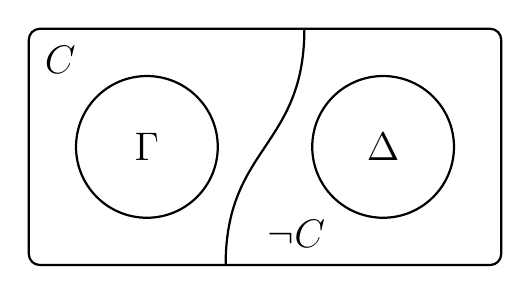
\begin{tikzpicture}[node distance=2cm, auto, thick]
    \draw [rounded corners] (0,0) -- (6,0) -- (6,3) -- (0,3) --  cycle;
    \draw (1.5,1.5) circle (0.9cm);
    \draw (4.5,1.5) circle (0.9cm);
    \path node at (1.5,1.5) {\Large $\Gamma$};
    \path node at (4.5,1.5) {\Large $\Delta$};
    \path node at (0.4,2.6) {\Large $\formula{C}$};
    \path node at (3.4,0.4) {\Large $\lnot \formula{C}$};
    \draw (2.5,0) .. controls (2.5,1.5) and (3.5,1.5) .. (3.5,3);
  \end{tikzpicture}
  \caption{$!C$, $\Gamma$ અને~$\Delta$ને પૃથક કરે છે}
  \ollabel{fig:sep}
\end{figure}


\begin{lem}\ollabel{lem:sep1}
ધારો કે $\Lang{L}_0$ એ એવી ભાષા છે જેમાં $\Gamma$ અને~$\Delta$
\emph{બંને}માં આવતા દરેક અચળ, ફલન અને વિધેય
($\doteq$ સિવાયના) છે, અને $n\ge 0$ માટે અનંત નવા અચળો
$\Obj c_n$ ઉમેરીને $\Lang{L}'_0$ મેળવાય છે. તો જો $\Gamma$ અને
$\Delta$, $\Lang{L}_0$માં અપૃથક્કરણીય હોય, તો તેઓ $\Lang{L}'_0$માં
પણ અપૃથક્કરણીય છે.
\end{lem}

\begin{proof}
આપણે પરોક્ષ રીતે આગળ વધીએ: વિરોધાભાસ માટે ધારો કે $\Gamma$ અને
$\Delta$, $\Lang{L}'_0$માં પૃથક્કરણીય છે. તો કોઈ $!C\in\Lang{L}_0$
માટે $\Gamma \Entails \Subst{!C}{c}{x}$ અને $\Delta \Entails \lnot
\Subst{!C}{c}{x}$ (અહીં $c$ નવો અચળ છે---$!C$માં આવા એકથી
વધુ નવા અચળ હોય તે કિસ્સો સમાન છે). સઘનતાથી, $\Gamma$નો
કોઈ \emph{સાન્ત} ઉપગણ~$\Gamma_0$ અને $\Delta$નો કોઈ \emph{સાન્ત}
ઉપગણ~$\Delta_0$ એવા છે કે $\Gamma_0 \Entails \Subst{!C}{c}{x}$ અને
$\Delta_0 \Entails \lnot \Subst{!C}{c}{x}$. $\Gamma_0$નાં બધાં
સૂત્રોના સંયોજનને~$!G$ અને $\Delta_0$નાં બધાં સૂત્રોના
સંયોજનને~$!H$ કહો. તો
\begin{align*}
  !G & \Entails \Subst{!C}{c}{x}, & !H  \Entails \lnot \Subst{!C}{c}{x}.
\end{align*}
પહેલામાંથી સર્વત્રીકરણ વડે $!G \Entails \lforall[x][!C]$ મળે છે;
બીજામાંથી પ્રતિપક્ષન વડે $\Subst{!C}{c}{x} \Entails \lnot !H$, અને
તેથી $\lforall[x][!C] \Entails \lnot !H$ પણ મળે છે. ફરી પ્રતિપક્ષનથી
$!H \Entails \lnot \lforall[x][!C]$. એકદિશવર્ધિતાથી,
\begin{align*}
  \Gamma &\Entails \lforall[x][!C], &
  \Delta & \Entails \lnot \lforall[x][!C],
\end{align*}
અને તેથી $\lforall[x][!C]$, $\Gamma$ અને~$\Delta$ને $\Lang{L}_0$માં
પૃથક કરે છે.
\sourcecorrection{OLINT-001}{સ્થિર અંગ્રેજી મૂળની
  \texttt{separation.tex}, પંક્તિ~75માં પૂર્વધારણા~$!H$ના સ્થાને
  અગાઉ ક્યાંય વ્યાખ્યાયિત ન થયેલું~$\delta$ આવે છે. પ્રતિપક્ષનથી
  મેળવવાના નિષ્કર્ષમાં અહીં $\lnot !H$ પુનઃસ્થાપિત કર્યું છે.}
\end{proof}

\begin{lem}\ollabel{lem:sep2}
ધારો કે $\Gamma \cup \{ \lexists[x][!S] \}$ અને~$\Delta$
અપૃથક્કરણીય છે, અને $c$ એવો નવો અચળ છે જે $\Gamma$,
$\Delta$ કે~$!S$માં આવતો નથી. તો $\Gamma \cup \{ \lexists[x][!S],
\Subst{!S}{c}{x} \}$ અને~$\Delta$ પણ અપૃથક્કરણીય છે.
\end{lem}

\begin{proof}
વિરોધાભાસ માટે ધારો કે $!C$, $\Gamma \cup \{ \lexists[x][!S],
\Subst{!S}{c}{x}\}$ અને~$\Delta$ને પૃથક કરે છે, જ્યારે $\Gamma \cup
\{\lexists[x][!S] \}$ અને~$\Delta$ અપૃથક્કરણીય છે. આપણે બે કિસ્સા
પાડીએ છીએ:
\sourcecorrection{OLINT-002}{સ્થિર અંગ્રેજી મૂળની
  \texttt{separation.tex}, પંક્તિ~95માં $\lexists$ના સૂત્ર-દલીલખંડને
  જરૂરી ચોરસ કૌંસને બદલે વાંકિયા કૌંસમાં મૂક્યો છે; તેથી તે
  ક્વાન્ટિફાયરના વ્યાપ તરીકે લેવાતો નથી. અહીં
  \texttt{\string\lexists[x][!S]} પુનઃસ્થાપિત કર્યું છે.}
\begin{enumerate}
\item $c$, $!C$માં આવતો નથી: આ કિસ્સામાં $\Gamma \cup
  \{\lexists[x][!S], \lnot!C \}$ સંતોષ્ય છે (નહિતર $!C$, $\Gamma
  \cup \{\lexists[x][!S] \}$ અને~$\Delta$ને પૃથક કરે). તેમાં
  $\Subst{!S}{c}{x}$ ઉમેર્યા પછી પણ તે સંતોષ્ય રહે છે, તેથી અંતે
  $!C$, $\Gamma \cup \{ \lexists[x][!S], \Subst{!S}{c}{x} \}$ અને
  $\Delta$ને પૃથક કરતું નથી.
\item $c$, $!C$માં આવે છે, જેથી $!C$નું સ્વરૂપ
  $\Subst{!C}{c}{x}$ છે. ત્યારે
  \[
  \Gamma \cup \{ \lexists[x][!S], \Subst{!S}{c}{x}\} \Entails \Subst{!C}{c}{x},
  \]
  અને તેથી નિગમન પ્રમેય તથા સર્વત્રીકરણ વડે
  $\Gamma, \lexists[x][!S] \Entails \lforall[x][(!S \lif !C)]$,
  અને છેવટે $\Gamma \cup \{ \lexists[x][!S] \} \Entails
  \lexists[x][!C]$. બીજી તરફ, $\Delta \Entails \lnot
  \Subst{!C}{c}{x}$ અને તેથી સર્વત્રીકરણ વડે $\Delta \Entails \lnot
  \lexists[x][!C]$. એટલે $\Gamma \cup \{\lexists[x][!S] \}$ અને
  $\Delta$ પૃથક્કરણીય છે, જે વિરોધાભાસ છે.
\end{enumerate}
\end{proof}
% END OLP-0200
\endgroup


\begingroup
\makeatletter\def\ol@sectioncs{section}\makeatother

% BEGIN OLP-0201
\olfileid{mod}{int}{prf}

\section{ક્રેગનું અંતર્વેશન પ્રમેય}
\phantomsection\label{guunit:OLP-0201}


\begin{thm}[ક્રેગનું અંતર્વેશન પ્રમેય]
\ollabel{thm:interpol}
જો $\Entails !A \lif !B$, તો એવું વાક્ય~$!C$ છે કે
$\Entails !A \lif !C$ અને $\Entails !C \lif !B$, અને $!C$માં આવતો
દરેક અચળ, ફલન અને વિધેય ($\eq$ સિવાયનો)
$!A$ અને~$!B$ બંનેમાં આવે છે. વાક્ય~$!C$ને $!A$ અને~$!B$નો
\emph{અંતર્વેશક} કહે છે.
\end{thm}

\begin{proof}
ધારો કે $\Lang{L}_1$, $!A$ની ભાષા છે અને $\Lang{L}_2$, $!B$ની ભાષા
છે. $\Lang{L}_0 = \Lang{L}_1 \cap \Lang{L}_2$ રાખો. દરેક $i \in
\{0, 1, 2 \}$ માટે, $\Lang{L}_i$માં અનંત નવા અચળો
$\Obj c_0, \Obj c_1, \Obj c_2, \dots$ ઉમેરીને $\Lang{L}'_i$ મેળવો.

જો $!A$ અસંતોષ્ય હોય, તો $\lexists[x][\eq/[x][x]]$ અંતર્વેશક છે.
જો $\lnot !B$ અસંતોષ્ય હોય (અને તેથી $!B$ પ્રામાણ્ય હોય), તો
$\lexists[x][\eq[x][x]]$ અંતર્વેશક છે. તેથી આપણે $!A$ અને
$\lnot !B$ બંને સંતોષ્ય છે એમ પણ ધારી શકીએ છીએ.

અંતર્વેશન પ્રમેયનું પ્રતિપક્ષી સ્વરૂપ સાબિત કરવા માટે ધારો કે $!A$
અને~$!B$ માટે કોઈ અંતર્વેશક નથી. બીજા શબ્દોમાં, ધારો કે $\{!A\}$ અને
$\{\lnot !B\}$, $\Lang{L}_0$માં અપૃથક્કરણીય છે.

આપણો ઉદ્દેશ જોડ $(\{ !A \}, \{\lnot!B\})$ને કોઈ મહત્તમ
અપૃથક્કરણીય જોડ $(\Gamma^*, \Delta^*)$ સુધી વિસ્તારવાનો છે.
$!A_0$, $!A_1$, $!A_2$,~\dots એ $\Lang{L}'_1$નાં વાક્યોની
ગણના અને $!B_0$, $!B_1$, $!B_2$,~\dots એ $\Lang{L}'_2$નાં
વાક્યોની ગણના હોય. નીચે પ્રમાણે $n\ge0$ માટે વાક્યોના
ગણોની બે વધતી શ્રેણીઓ $(\Gamma_n,\Delta_n)$ વ્યાખ્યાયિત કરીએ. $\Gamma_0
= \{!A\}$ અને $\Delta_0=\{\lnot !B\}$ રાખો. $(\Gamma_n,\Delta_n)$
પહેલેથી વ્યાખ્યાયિત છે એમ ધારીને, $\Gamma_{n+1}$ અને
$\Delta_{n+1}$ને આ પ્રમાણે વ્યાખ્યાયિત કરો:
\sourcecorrection{OLINT-003}{સ્થિર અંગ્રેજી મૂળની
  \texttt{interpolation-proof.tex}, પંક્તિઓ~41--43માં $!A_n$ અને
  $!B_n$ને અનુક્રમે $\Lang{L}_1$ અને $\Lang{L}_2$નાં વાક્યોની ગણના
  કહેવાય છે. પરંતુ પછીની પંક્તિઓ~107--108માં રચાયેલા ગણો
  $\Lang{L}'_1$ અને $\Lang{L}'_2$માં પૂર્ણ સુસંગત હોવાનો દાવો થાય છે,
  જેના માટે નવા અચળો ધરાવતાં વાક્યોની પણ ગણના જરૂરી છે. અહીં બંને
  વિસ્તૃત ભાષાઓ પર ગણના પુનઃસ્થાપિત કરી છે.}
\begin{enumerate}
\item જો $\Gamma_n \cup \{!A_n \}$ અને~$\Delta_n$, $\Lang{L}'_0$માં
  અપૃથક્કરણીય હોય, તો $!A_n$ને $\Gamma_{n+1}$માં મૂકો. વધુમાં, જો
  $!A_n$ કોઈ અસ્તિત્વવાચક સૂત્ર~$\lexists[x][!S]$ હોય, તો
  $\Gamma_n$, $\Delta_n$, $!A_n$ કે~$!B_n$માં ન આવતો નવો
  અચળ~$c$ પસંદ કરીને $\Subst{!S}{c}{x}$ને
  $\Gamma_{n+1}$માં મૂકો.
\item જો $\Gamma_{n+1}$ અને $\Delta_n \cup \{!B_n \}$,
  $\Lang{L}'_0$માં અપૃથક્કરણીય હોય, તો $!B_n$ને $\Delta_{n+1}$માં
  મૂકો. વધુમાં, જો $!B_n$ કોઈ અસ્તિત્વવાચક
  સૂત્ર~$\lexists[x][!S]$ હોય, તો $\Gamma_{n+1}$, $\Delta_n$,
  $!A_n$ કે~$!B_n$માં ન આવતો નવો અચળ~$c$ પસંદ કરીને
  $\Subst{!S}{c}{x}$ને $\Delta_{n+1}$માં મૂકો.
\end{enumerate}
છેવટે, આ પ્રમાણે વ્યાખ્યા કરો:
\begin{align*}
  \Gamma^* & = \bigcup_{n\ge 0} \Gamma_n, &
  \Delta^* & = \bigcup_{n\ge 0} \Delta_n.
\end{align*}
હવે $n$ પરના સમકાલીન આગમનથી આપણે નીચેના દાવા સાબિત કરી શકીએ છીએ:
\begin{enumerate}
\item\ollabel{part-a} $\Gamma_n$ અને~$\Delta_n$, $\Lang{L}'_0$માં
  અપૃથક્કરણીય છે;
\item\ollabel{part-b} $\Gamma_{n+1}$ અને~$\Delta_n$,
  $\Lang{L}'_0$માં અપૃથક્કરણીય છે.
\end{enumerate}
\olref{part-a}નો આધાર \olref[sep]{lem:sep1} આપે છે. ભાગ
\olref{part-b} માટે આપણે ત્રણ કિસ્સા પાડવા પડે છે:
\begin{enumerate}
\item જો $\Gamma_0 \cup \{!A_0 \}$ અને~$\Delta_0$ પૃથક્કરણીય હોય,
  તો $\Gamma_1=\Gamma_0$ અને \olref{part-b}, \olref{part-a} જ છે;
\item જો $\Gamma_1 = \Gamma_0 \cup\{!A_0\}$, તો રચના મુજબ
  $\Gamma_1$ અને~$\Delta_0$ અપૃથક્કરણીય છે.
\item હવે માત્ર $!A_0$ અસ્તિત્વવાચક હોય તે કિસ્સો બાકી રહે છે, જેમાં
  $\Gamma_1 = \Gamma_0 \cup \{ \lexists[x][!S], \Subst{!S}{c}{x}
  \}$. રચના મુજબ $\Gamma_0 \cup \{ \lexists[x][!S]\}$ અને
  $\Delta_0$ અપૃથક્કરણીય છે, તેથી \olref[sep]{lem:sep2} મુજબ
  $\Gamma_0 \cup \{ \lexists[x][!S], \Subst{!S}{c}{x} \}$ અને
  $\Delta_0$ પણ અપૃથક્કરણીય છે.
\end{enumerate}
આથી ઉપરના \olref{part-a} અને \olref{part-b} માટે આગમનનો આધાર પૂરો
થાય છે. હવે આગમન-પગલું લઈએ. \olref{part-a} માટે, જો $!B_n$ને
$\Delta_{n+1}$માં મૂકવામાં આવે, તો રચના મુજબ $\Gamma_{n+1}$ અને
$\Delta_n\cup\{!B_n\}$ અપૃથક્કરણીય છે; અને જો $!B_n$ અસ્તિત્વવાચક
હોય, તો સાક્ષી ઉમેર્યા પછીનો $\Delta_{n+1}$ પણ
\olref[sep]{lem:sep2} મુજબ અપૃથક્કરણીય રહે છે. જો
$\Delta_{n+1}=\Delta_n$ (કારણ કે $\Gamma_{n+1}$ અને
$\Delta_n\cup\{!B_n\}$ પૃથક્કરણીય છે), તો \olref{part-b} માટેની
આગમન-પરિકલ્પના વાપરીએ. \olref{part-b}ના આગમન-પગલા માટે, જો
$!A_{n+1}$ને $\Gamma_{n+2}$માં મૂકવામાં આવે, તો રચના મુજબ
$\Gamma_{n+1}\cup\{!A_{n+1}\}$ અને~$\Delta_{n+1}$ અપૃથક્કરણીય છે;
અને જો $!A_{n+1}$ અસ્તિત્વવાચક હોય, તો સાક્ષી ઉમેર્યા પછીનો
$\Gamma_{n+2}$ પણ \olref[sep]{lem:sep2} મુજબ અપૃથક્કરણીય રહે છે. જો
$\Gamma_{n+2}=\Gamma_{n+1}$, તો હમણાં જ સાબિત કરેલો
\olref{part-a}નો આગમન-કિસ્સો વાપરીએ. આથી \olref{part-a} અને
\olref{part-b} પરનું આગમન પૂરું થાય છે.
\sourcecorrection{OLINT-004}{સ્થિર અંગ્રેજી મૂળની
  \texttt{interpolation-proof.tex}, પંક્તિઓ~88--96માં અસ્તિત્વવાચક
  $!B_n$ કે $!A_{n+1}$ સ્વીકારાય ત્યારે સાક્ષી-સૂત્ર પણ ઉમેરવાની
  અગાઉની સૂચના હોવા છતાં અનુક્રમે
  $\Delta_{n+1}=\Delta_n\cup\{!B_n\}$ અને
  $\Gamma_{n+2}=\Gamma_{n+1}\cup\{!A_{n+1}\}$ લખાયું છે. અહીં
  સ્વીકારેલો વિધાન અને પછી ઉમેરાતો સાક્ષી અલગ કરીને, લેમા
  \olref[sep]{lem:sep2}નો ઉપયોગ બંને પૂર્ણ ગણો પર સ્પષ્ટ કર્યો છે.}

આમાંથી ફલિત થાય છે કે $\Gamma^*$ અને~$\Delta^*$ અપૃથક્કરણીય છે;
નહિતર સઘનતાથી એવું $n\ge0$ અને એવું $\Lang{L}'_0$-વિધાન મળે જે
$\Gamma_n$ અને~$\Delta_n$ને પૃથક કરે, જે \olref{part-a}ની વિરુદ્ધ
છે. ખાસ કરીને, $\Gamma^*$ અને~$\Delta^*$ સુસંગત છે: કારણ કે પહેલો
અથવા બીજો અસુસંગત હોય, તો અનુક્રમે $\lexists[x][\eq/[x][x]]$ અથવા
$\lforall[x][\eq[x][x]]$ તેમને પૃથક કરે.
\sourcecorrection{OLINT-005}{સ્થિર અંગ્રેજી મૂળની
  \texttt{interpolation-proof.tex}, પંક્તિઓ~100--102માં કોઈ
  $n\ge0$ પોતે $\Gamma_n$ અને $\Delta_n$ને પૃથક કરે છે તેમ લખાયું
  છે. પૃથક્કર્તા વિધાન હોય છે; સઘનતા માત્ર એવું એક જ~$n$ આપે છે જેમાં
  તેના માટે જરૂરી બંને સાન્ત ઉપગણો આવી જાય. અહીં એ વિધાન અને~$n$ની
  જુદી ભૂમિકાઓ સ્પષ્ટ કરી છે.}

હવે આપણે બતાવીએ કે $\Gamma^*$, $\Lang{L}'_1$માં પૂર્ણ સુસંગત છે અને
એ જ રીતે $\Delta^*$, $\Lang{L}'_2$માં પૂર્ણ સુસંગત છે. પહેલા માટે,
ધારો કે કોઈ $n\ge0$ માટે $!A_n\notin\Gamma^*$ અને $\lnot !A_n
\notin\Gamma^*$. જો $!A_n\notin\Gamma^*$, તો $\Gamma_n\cup\{!A_n\}$
$\Delta_n$થી પૃથક્કરણીય છે, તેથી એવું $!C\in\Lang{L}'_0$ છે કે આ
બંને વાતો સાચી છે:
\begin{align*}
  \Gamma^* & \Entails !A_n \lif !C, &
  \Delta^* & \Entails \lnot !C.
\end{align*}
એ જ રીતે, જો $\lnot !A_n\notin\Gamma^*$, તો એવું $!C'\in
\Lang{L}'_0$ છે કે આ બંને વાતો સાચી છે:
\begin{align*}
  \Gamma^* & \Entails \lnot !A_n \lif !C', &
  \Delta^* & \Entails \lnot !C'.
\end{align*}
વિધાનાત્મક તર્કશાસ્ત્રથી $\Gamma^*\Entails !C\lor !C'$ અને
$\Delta^*\Entails\lnot(!C\lor !C')$, તેથી $!C\lor !C'$,
$\Gamma^*$ અને~$\Delta^*$ને પૃથક કરે છે. સમાન દલીલથી $\Delta^*$ પૂર્ણ
છે.

છેવટે, આપણે બતાવીએ કે $\Gamma^*\cap\Delta^*$, $\Lang{L}'_0$માં પૂર્ણ
સુસંગત છે. તે સુસંગત ગણોનો છેદ હોવાથી દેખીતી રીતે સુસંગત છે. પૂર્ણતા
બતાવવા $!S\in\Lang{L}'_0$ લો. હવે $\Gamma^*$, $\Lang{L'_1}
\supseteq\Lang{L'_0}$માં પૂર્ણ છે અને એ જ રીતે $\Delta^*$,
$\Lang{L'_2}\supseteq\Lang{L'_0}$માં પૂર્ણ છે. તેથી કાં તો
$!S\in\Gamma^*$ અથવા $\lnot !S\in\Gamma^*$, અને કાં તો
$!S\in\Delta^*$ અથવા $\lnot !S\in\Delta^*$. જો $!S\in\Gamma^*$ અને
$\lnot !S\in\Delta^*$, તો $!S$, $\Gamma^*$ અને~$\Delta^*$ને પૃથક
કરે; અને જો $\lnot !S\in\Gamma^*$ અને $!S\in\Delta^*$, તો
$\Gamma^*$ અને~$\Delta^*$ને $\lnot !S$ પૃથક કરે. આથી, કાં તો
$!S\in\Gamma^*\cap\Delta^*$
અથવા $\lnot !S\in\Gamma^*\cap\Delta^*$, અને
$\Gamma^*\cap\Delta^*$ પૂર્ણ છે.

$\Gamma^*$ પૂર્ણ સુસંગત હોવાથી તેને એવો નિદર્શ $\Struct{M}'_1$ મળે
છે જેનું પ્રદેશ~$\Domain{M'_1}$, અચળોનાં અર્થઘટનો
$\Assign{c}{M'_1}$ એવા અને માત્ર એવા ઘટકોનું બનેલું છે---પૂર્ણતા
પ્રમેયની સાબિતીની જેમ (\olref[fol][com][cth]{thm:completeness}). એ જ
રીતે, $\Delta^*$ને એવો નિદર્શ~$\Struct{M}'_2$ મળે છે જેનું
પ્રદેશ~$\Domain{M'_2}$, અચળોનાં અર્થઘટનો
$\Assign{c}{M'_2}$થી બનેલું છે.

$\Struct{M'_1}$માંથી $\Lang{L'_1}\setminus\Lang{L'_0}$માંના
અચળો, ફલનો અને વિધેયોનાં અર્થઘટનો કાઢીને
$\Struct{M_1}$ મેળવો, અને $\Struct{M_2}$ પણ એ જ રીતે મેળવો. ત્યારે
$h(\Assign{c}{M'_1})=\Assign{c}{M'_2}$થી વ્યાખ્યાયિત કરેલો નકશો
$h\colon M_1\to M_2$, $\Lang{L}'_0$માં એકરૂપતા છે, કારણ કે બતાવ્યા
પ્રમાણે $\Gamma^*\cap\Delta^*$, $\Lang{L}'_0$માં પૂર્ણ સુસંગત છે.
આનું કારણ એ છે કે કોઈ પણ $\Lang{L}'_0$-વાક્ય કાં તો $\Gamma^*$
અને~$\Delta^*$ બંનેમાં આવે છે અથવા એકેયમાં આવતું નથી: તેથી
$\Assign{c}{M'_1}\in\Assign{P}{M'_1}$ જો અને માત્ર જો
$\Atom{P}{c}\in\Gamma^*$, જો અને માત્ર જો $\Atom{P}{c}\in\Delta^*$,
જો અને માત્ર જો $\Assign{c}{M'_2}\in\Assign{P}{M'_2}$. એકરૂપતાની
બીજી શરતો પણ એ જ રીતે સ્થાપિત કરી શકાય છે.

હવે ભાષા~$\Lang{L_1}\cup\Lang{L_2}$ માટેનો નિદર્શ
$\Struct{M}$ આ પ્રમાણે વ્યાખ્યાયિત કરીએ:
\begin{enumerate}
\item પ્રદેશ~$\Domain{M}$ એ $\Domain{M_2}$ જ છે, એટલે બધા
  ઘટકો~$\Assign{c}{M'_2}$નો ગણ;
\item જો કોઈ વિધેય~$P$, $\Lang{L_2}\setminus\Lang{L_1}$માં
  હોય, તો $\Assign{P}{M}=\Assign{P}{M'_2}$;
\item જો કોઈ વિધેય-સંકેત~$P$, $\Lang{L}_1\setminus\Lang{L}_2$માં હોય, તો
  $\Assign{P}{M}=h(\Assign{P}{M'_1})$, એટલે
  $\tuple{\Assign{c_1}{M'_2},\dots,\Assign{c_n}{M'_2}}\in
  \Assign{P}{M}$ જો અને માત્ર જો
  $\tuple{\Assign{c_1}{M'_1},\dots,\Assign{c_n}{M'_1}}\in
  \Assign{P}{M'_1}$.
\item જો કોઈ વિધેય~$P$, $\Lang{L}_0$માં હોય, તો
  $\Assign{P}{M}=\Assign{P}{M'_2}=h(\Assign{P}{M'_1})$.
\item ફલનોને, જેમાં અચળો પણ સામેલ છે,
  $\Lang{L}_1\cup\Lang{L}_2$ પર એ જ રીતે સંભાળો.
\end{enumerate}
\sourcecorrection{OLINT-006}{સ્થિર અંગ્રેજી મૂળની
  \texttt{interpolation-proof.tex}, પંક્તિ~173માં
  $P\in\Lang{L}_1\setminus\Lang{L}_2$ હોવા છતાં તેના અર્થઘટનને
  $\Struct{M'_2}$માંથી લઈ $h$ લગાડવામાં આવ્યું છે. $\Struct{M'_2}$
  પાસે $P$નું અર્થઘટન હોવું જરૂરી નથી અને $h$નું ક્ષેત્ર પણ
  $M_1$ છે. તરત પછી આપેલી ``એટલે'' શરત મુજબ અહીં
  $h(\Assign{P}{M'_1})$ પુનઃસ્થાપિત કર્યું છે.}

છેવટે, સૂત્રો પરના આગમનથી બતાવી શકાય છે કે $\Lang{L}_1$નાં
બધાં સૂત્રો માટે $\Struct{M'_1}$ના $\Lang{L}_1$-ન્યૂનરૂપમાં
સંતોષ, $h$ મારફતે $\Struct{M}$ના $\Lang{L}_1$-ન્યૂનરૂપમાં સંતોષને
બરાબર અનુરૂપ છે, અને $\Lang{L}_2$નાં બધાં સૂત્રો માટે
$\Struct{M}$ તથા $\Struct{M'_2}$નાં $\Lang{L}_2$-ન્યૂનરૂપોમાં સંતોષ
સંમત થાય છે. ખાસ કરીને,
$\Struct{M'_1}\Entails\Gamma^*$ તથા $!A\in\Gamma^*$, અને
$\Struct{M'_2}\Entails\Delta^*$ તથા $\lnot !B\in\Delta^*$ હોવાથી
$\Struct{M}\Entails !A$ અને $\Struct{M}\Entails\lnot !B$. તેથી
$\not\Entails !A\lif !B$. આથી ક્રેગના અંતર્વેશન પ્રમેયની સાબિતી
પૂરી થાય છે.
\sourcecorrection{OLINT-007}{સ્થિર અંગ્રેજી મૂળની
  \texttt{interpolation-proof.tex}, પંક્તિઓ~183--187માં
  $\Struct{M}$ને માત્ર $\Lang{L}_1\cup\Lang{L}_2$ માટે વ્યાખ્યાયિત
  કર્યા પછી તે નવા અચળો ધરાવતી વિસ્તૃત ભાષાઓ $\Lang{L}'_1$ અને
  $\Lang{L}'_2$નાં બધાં સૂત્રો પર સંમત થાય છે અને
  $\Gamma^*\cup\Delta^*$ને સંતોષે છે એવો અપરિભાષિત દાવો થાય છે.
  અહીં જરૂરી અને પર્યાપ્ત ન્યૂનરૂપ-દાવો મૂક્યો છે: $h$ પહેલા નિદર્શના
  $\Lang{L}_1$-ભાગને પરિવહિત કરે છે અને બીજાનો
  $\Lang{L}_2$-ભાગ યથાવત્ રહે છે; તેથી મૂળ વાક્યો $!A$ અને
  $\lnot !B$ સાચાં રહે છે.}
\end{proof}
% END OLP-0201
\endgroup


\begingroup
\makeatletter\def\ol@sectioncs{section}\makeatother

% BEGIN OLP-0202
\olfileid{mod}{int}{def}

\section{વ્યાખ્યેયતા પ્રમેય}
\phantomsection\label{guunit:OLP-0202}


અંતર્વેશન પ્રમેયનો એક મહત્વનો ઉપયોગ બેથનું વ્યાખ્યેયતા પ્રમેય છે.
$n$-સ્થાની સંબંધ~$R$ને વ્યાખ્યાયિત કરવા માટે આપણે $R$ ન આવતો હોય
અને $n$ મુક્ત ચલો ધરાવતો કોઈ સૂત્ર~$!C$ આપી શકીએ
છીએ. આ $!C$ દ્વારા $R$ની \emph{સ્પષ્ટ} વ્યાખ્યા થાય. પછી આપણે એમ
પણ કહી શકીએ કે $n$-સ્થાની વિધેય~$P$ ધરાવતી કોઈ ભાષામાં
સિદ્ધાંત~$\Sigma(P)$, $P$ને સ્પષ્ટ રીતે વ્યાખ્યાયિત કરે છે જો તેમાં
ઔપચારિક કરેલી સ્પષ્ટ વ્યાખ્યા હોય (અથવા ઓછામાં ઓછું તેમાંથી ફલિત થતી
હોય), એટલે કે,
\[
\Sigma(P) \Entails \lforall[x_1][\dots
  \lforall[x_n][(\Atom{P}{x_1,\dots, x_n} \liff !C(x_1, \dots,
    x_n))]].
\]
પરંતુ સંબંધને વ્યાખ્યાયિત કરવાનો---તેને સંપૂર્ણપણે નિશ્ચિત કરવાના
અર્થમાં---સ્પષ્ટ વ્યાખ્યા માત્ર એક માર્ગ છે. સિદ્ધાંત એવો પણ હોઈ શકે
કે કોઈ પણ નિદર્શમાં ભાષાના બાકીના ભાગના અર્થઘટનથી $P$નું
અર્થઘટન નિશ્ચિત થાય. વ્યાખ્યેયતા પ્રમેય કહે છે કે જ્યારે પણ સિદ્ધાંત
$P$નું અર્થઘટન આ રીતે નિશ્ચિત કરે---જ્યારે તે $P$ને \emph{ગૂઢ રીતે
વ્યાખ્યાયિત કરે}---ત્યારે તે તેને સ્પષ્ટ રીતે પણ વ્યાખ્યાયિત કરે છે.

\begin{defn}
ધારો કે $\Lang{L}$ એવી ભાષા છે જેમાં વિધેય~$P$ નથી.
$\Lang{L}\cup\{P\}$નાં વાક્યોનો ગણ~$\Sigma(P)$, $P$ને ત્યારે
અને માત્ર ત્યારે \emph{સ્પષ્ટ રીતે વ્યાખ્યાયિત કરે છે} જ્યારે
$\Lang{L}$નું એવું સૂત્ર~$!C(x_1,\dots,x_n)$ છે કે
\[
\Sigma(P) \Entails \lforall[x_1][\dots
  \lforall[x_n][(\Atom{P}{x_1,\dots, x_n} \liff !C(x_1, \dots,
    x_n))]].
\]
\end{defn}

\begin{defn}
ધારો કે $\Lang{L}$ એવી ભાષા છે જેમાં વિધેયો $P$
અને~$P'$ નથી. $\Lang{L}\cup\{P\}$નાં વાક્યોનો ગણ~$\Sigma(P)$,
$P$ને ત્યારે અને માત્ર ત્યારે \emph{ગૂઢ રીતે વ્યાખ્યાયિત કરે છે}
જ્યારે
\[
\Sigma(P) \cup \Sigma(P') \Entails \lforall[x_1][\dots
  \lforall[x_n][(\Atom{P}{x_1,\dots, x_n} \liff \Atom{P'}{x_1,\dots,
      x_n})]],
\]
જ્યાં $\Sigma(P')$ એ $\Sigma(P)$માં $P$ને સર્વત્ર $P'$થી બદલીને
મળતું પરિણામ છે.
\end{defn}

બીજા શબ્દોમાં, કોઈ પણ નિદર્શ~$\Struct{M}$ અને $R,R'\subseteq
\Domain{M}^n$ માટે, જો $\Expan{M}{R}\Entails\Sigma(P)$ અને
$\Expan{M}{R'}\Entails\Sigma(P')$ બંને, તો $R=R'$; અહીં
$\Expan{M}{R}$ એ $\Lang{L}$ના $\Lang{L}\cup\{P\}$ સુધીના વિસ્તાર
માટેની એવી સંરચના~$\Struct{M'}$ છે કે $\Assign{P}{M'}=R$, અને
$\Expan{M}{R'}$ માટે પણ એ જ રીતે.

\begin{thm}[બેથનું વ્યાખ્યેયતા પ્રમેય]
$\Lang{L}\cup\{P\}$નાં વાક્યોનો ગણ~$\Sigma(P)$, $P$ને ગૂઢ
રીતે વ્યાખ્યાયિત કરે છે જો અને માત્ર જો $\Sigma(P)$, $P$ને સ્પષ્ટ
રીતે વ્યાખ્યાયિત કરે છે.
\end{thm}
\sourcecorrection{OLINT-008}{સ્થિર અંગ્રેજી મૂળની
  \texttt{definability.tex}, પંક્તિઓ~66--68માં પ્રમેય $\Sigma(P)$ને
  સૂત્રોનો ગણ કહે છે, જ્યારે તરત અગાઉની બંને વ્યાખ્યાઓ તેને
  વાક્યોનો ગણ કહે છે અને નીચેની સાબિતી પણ સાન્ત ઉપગણનાં
  વાક્યોના સંયોજન પર ચાલે છે. અહીં વ્યાખ્યાઓ અને સાબિતી મુજબ
  વાક્યો પુનઃસ્થાપિત કર્યાં છે.}
\sourcecorrection{OLINT-009}{એ જ મૂળની પંક્તિ~67માં દ્વિમુખી શરતના
  ``if and only if''માંથી છેલ્લું ``if'' છૂટી ગયું છે. અહીં સંપૂર્ણ
  દ્વિમુખી શરત પુનઃસ્થાપિત કરી છે.}

\begin{proof}
જો $\Sigma(P)$, $P$ને સ્પષ્ટ રીતે વ્યાખ્યાયિત કરે, તો આ બંને સાચાં
છે:
\begin{align*}
  \Sigma(P) & \Entails & \lforall[x_1][\dots \lforall[x_n]
    [(\Atom{P}{x_1,\dots, x_n} \liff !C(x_1,\dots,x_n))]]\\
  \Sigma(P') & \Entails & \lforall[x_1][\dots \lforall[x_n]
    [(\Atom{P'}{x_1,\dots, x_n} \liff !C(x_1,\dots,x_n))]]
\end{align*}
અને નિષ્કર્ષ ફલિત થાય છે. વ્યસ્ત દિશા માટે ધારો કે $\Sigma(P)$,
$P$ને ગૂઢ રીતે વ્યાખ્યાયિત કરે છે. પહેલા $\Lang{L}$માં અચળો
$c_1$,~\dots,~$c_n$ ઉમેરીએ. ત્યારે
\[
\Sigma(P) \cup \Sigma(P') \Entails
\Atom{P}{c_1, \dots, c_n} \to \Atom{P'}{c_1, \dots, c_n}.
\]
સઘનતાથી એવા સાન્ત ગણો $\Delta_0\subseteq\Sigma(P)$ અને
$\Delta_1\subseteq\Sigma(P')$ છે કે
\[
\Delta_0 \cup \Delta_1 \Entails
\Atom{P}{c_1, \dots, c_n} \to \Atom{P'}{c_1, \dots, c_n}.
\]
એવા બધા વાક્યો~$!A(P)$નું સંયોજન~$!D(P)$ કહો કે કાં તો
$!A(P)\in\Delta_0$ અથવા $!A(P')\in\Delta_1$, અને એવા બધા
વાક્યો~$!A(P')$નું સંયોજન~$!D(P')$ કહો કે કાં તો
$!A(P)\in\Delta_0$ અથવા $!A(P')\in\Delta_1$. ત્યારે
$!D(P)\land !D(P')\Entails\Atom{P}{c_1,\dots,c_n}\to
\Atom{P'}{c_1,\dots,c_n}$. આને એવી રીતે ફરી ગોઠવી શકાય કે દરેક
વિધેય, $\Entails$ની એક બાજુ જ આવે:
\sourcecorrection{OLINT-010}{સ્થિર અંગ્રેજી મૂળની
  \texttt{definability.tex}, પંક્તિ~96માં જમણી બાજુનું પરમાણુક સૂત્ર
  આસપાસનાં બધાં દાખલાથી જુદું $P'c_1\dots c_n$ લખાયું છે. અહીં એ જ
  $n$-સ્થાની પરમાણુક સૂત્ર માટેનું આવૃત્તિ-સુસંગત
  \texttt{\string\Atom\{P'\}\{c\_1,\string\dots,c\_n\}} સ્વરૂપ વાપર્યું
  છે.}
\[
!D(P) \land \Atom{P}{c_1, \dots, c_n} \Entails
!D(P') \to \Atom{P'}{c_1, \dots, c_n}.
\]
ક્રેગના અંતર્વેશન પ્રમેય મુજબ $P$ કે~$P'$ ન ધરાવતું એવું
વાક્ય~$!C(c_1,\dots,c_n)$ છે કે
\begin{align*}
  !D(P) \land \Atom{P}{c_1, \dots, c_n} & \Entails !C(c_1,\dots, c_n); \\
  !C(c_1,\dots, c_n) & \Entails !D(P') \to \Atom{P'}{c_1, \dots, c_n}.
\end{align*}
આ બે ફલિતતાઓમાંથી પહેલામાંથી મળે છે: $!D(P)\Entails
\Atom{P}{c_1,\dots,c_n}\lif !C(c_1,\dots,c_n)$. અને બીજામાંથી,
કારણ કે કોઈ $\Lang{L}\cup\{P\}$-નિદર્શ $\Expan{M}{R}\Entails
!A(P)$ જો અને માત્ર જો તેને અનુરૂપ $\Lang{L}\cup\{P'\}$-નિદર્શ
$\Expan{M}{R}\models !A(P')$, આપણને
$!C(c_1,\dots,c_n)\Entails !D(P)\lif\Atom{P}{c_1,\dots,c_n}$ મળે છે,
અને તેમાંથી
\[
!D(P) \Entails !C(c_1,\dots,c_n) \to \Atom{P}{c_1,\dots, c_n}.
\]
બંનેને સાથે મૂકતાં $!D(P)\Entails\Atom{P}{c_1,\dots,c_n}\liff
!C(c_1,\dots,c_n)$ મળે છે, અને એકદિશવર્ધિતા તથા સર્વત્રીકરણથી આ પણ
મળે છે:
\[
\Sigma(P) \Entails
\lforall[x_1][\dots\lforall[x_n][(\Atom{P}{x_1,\dots, x_n} \liff
    !C(x_1,\dots, x_n))]].
\]
\end{proof}
% END OLP-0202
\endgroup


\OLEndChapterHook
% END OLP-0198
\endgroup


\begingroup
\makeatletter\def\ol@sectioncs{section}\makeatother

% BEGIN OLP-0203
\olchapter{mod}{lin}{લિન્ડસ્ટ્રોમનું પ્રમેય}
\olchapterid{mod}{lin}
\phantomsection\label{guunit:OLP-0203}


\begingroup
\makeatletter\def\ol@sectioncs{section}\makeatother

% BEGIN OLP-0204
\olfileid{mod}{lin}{int}
\section{પરિચય}
\phantomsection\label{guunit:OLP-0204}


આ પ્રકરણમાં આપણે પ્રથમ-ક્રમ તર્કશાસ્ત્રનું લિન્ડસ્ટ્રોમ-લક્ષણન સાબિત
કરવાનું લક્ષ્ય રાખીએ છીએ: અમુક વધારાની મર્યાદાઓ હેઠળ સઘનતા અને અધોગામી
લેવેનહાઇમ--સ્કોલેમ પ્રમેયો જે મહત્તમ તર્કશાસ્ત્ર માટે સત્ય છે તે
પ્રથમ-ક્રમ તર્કશાસ્ત્ર છે
(\olref[fol][com][com]{thm:compactness} અને
\olref[fol][com][dls]{thm:downward-ls}). પહેલાં આપણે આ પ્રમેય જેમને લાગુ
પડે છે તે તર્કશાસ્ત્રોના સામાન્ય વર્ગનું વધુ વ્યાપક લક્ષણન જોઈએ. આપણે
પોતાને \emph{સંબંધાત્મક} ભાષાઓ પૂરતા મર્યાદિત રાખીશું, એટલે કે એવી
ભાષાઓ જેમાં માત્ર વિધેયો અને વ્યક્તિ-અચળો હોય, પણ કોઈ
ફલનો ન હોય.
% END OLP-0204
\endgroup


\begingroup
\makeatletter\def\ol@sectioncs{section}\makeatother

% BEGIN OLP-0205
\olfileid{mod}{lin}{alg}
\olsection{અમૂર્ત તર્કશાસ્ત્રો}
\phantomsection\label{guunit:OLP-0205}


\begin{defn}
  \emph{અમૂર્ત તર્કશાસ્ત્ર} એ યુગ્મ $\tuple{L, \models_L}$ છે, જ્યાં
  $L$ એવું વિધેય છે જે દરેક ભાષા~$\Lang{L}$ને
  વાક્યોનો ગણ $L(\Lang{L})$ નિયુક્ત કરે છે, અને $\models_L$ એ
  ભાષા~$\Lang{L}$ માટેની સંરચનાઓ તથા $L(\Lang{L})$ના
  ઘટકો વચ્ચેનો સંબંધ છે. ખાસ કરીને, $\tuple{F, \models}$ એ
  સામાન્ય પ્રથમ-ક્રમ તર્કશાસ્ત્ર છે; એટલે કે, $F$ એવું વિધેય છે જે
  ભાષા~$\Lang{L}$ને $\Lang{L}$ના સંકેતોમાંથી બનેલાં પ્રથમ-ક્રમ
  વાક્યોનો ગણ નિયુક્ત કરે છે, અને $\models$ એ પ્રથમ-ક્રમ
  તર્કશાસ્ત્રનો સંતોષ-સંબંધ છે.
  \sourcecorrection{OLLIN-001}{સ્થિર અંગ્રેજી મૂળની
    \texttt{abstract-logics.tex}, પંક્તિઓ~18--20માં પ્રથમ-ક્રમનાં વાક્યો
    ભાષાના માત્ર અચળોમાંથી બને છે એમ કહેવાયું છે, જેથી વિધેય-સંકેતો
    છૂટી જાય છે. $F(\Lang L)$માં ભાષાના બધા સંકેતો વડે બનેલાં
    પ્રથમ-ક્રમ વાક્યો આવે છે; અહીં એ વ્યાપ રાખ્યો છે.}
\end{defn}

નોંધો કે આપેલી ભાષા માટે આપણે હજી પણ પ્રથમ-ક્રમ તર્કશાસ્ત્રમાં
હોય એ જ સંરચનાની વિભાવના વાપરીએ છીએ. પરંતુ આપણે એવું પૂર્વધારતા
નથી કે વાક્યો સામાન્ય રીતે $\Lang{L}$ના મૂળભૂત સંકેતોમાંથી
બનાવાય છે, કે $\models_L$ સંબંધ પણ પ્રથમ-ક્રમ તર્કશાસ્ત્રની જેમ જ
આવર્ત રીતે વ્યાખ્યાયિત થાય છે. તેથી, દાખલા તરીકે, આ તદ્દન સામાન્ય
વ્યાખ્યાનો આશય એવા કિસ્સાઓને પણ આવરી લેવાનો છે જેમાં
$\tuple{L,\models_L}$નાં વાક્યો અનંત લાંબાં સંયોજનો કે વિયોજનો,
$\lexists$ અને $\lforall$ સિવાયના પરિમાણકો (જેમ કે ``એવા અનંત ઘણા
$x$ છે કે \dots''), અથવા કદાચ અનંત લાંબા પરિમાણક-ઉપસર્ગો ધરાવે.
$L(\Lang{L})$નાં ``વાક્યો'' પ્રથમ-ક્રમ તર્કશાસ્ત્રનાં સામાન્ય
વાક્યો હોવાં જરૂરી નથી એ પર ભાર મૂકવા આ પ્રકરણમાં તેમના માટે
ચલો $!E$, $!F$,~\dots વાપરીએ છીએ અને સામાન્ય પ્રથમ-ક્રમ
સૂત્રો માટે $!A$, $!B$,~\dots અનામત રાખીએ છીએ.

\begin{defn}
  વર્ગ $\Setabs{\Struct{M}}{\Struct{M} \models_L !E}$ને
  $\Mod(L){!E}$થી દર્શાવીએ. ભાષા સ્પષ્ટ કરવી જરૂરી હોય તો
  $\Mod[L](L){!E}$ લખીએ. $\Lang{L}$ માટેની બે સંરચનાઓ
  $\Struct{M}$ અને $\Struct{N}$માં $L(\Lang{L})$નાં એ જ
  વાક્યો સાચાં હોય તો તેમને $\tuple{L, \models_L}$માં
  \emph{પ્રાથમિક રીતે સમકક્ષ} કહીએ છીએ અને $\Struct{M}
  \elemequiv[L] \Struct{N}$ લખીએ છીએ.
\end{defn}

\begin{defn}
  ભાષા~$\Lang{L}$ માટેનું અમૂર્ત તર્કશાસ્ત્ર
  $\tuple{L,\models_L}$
  નીચેના ગુણધર્મો સંતોષે તો તેને \emph{સામાન્ય} કહીએ છીએ:
\begin{enumerate}
\item (\emph{$L$-એકદિશવર્ધિતા}) ભાષાઓ $\Lang{L}$ અને
  $\Lang{L'}$ માટે જો $\Lang{L} \subseteq \Lang{L'}$, તો
  $L(\Lang{L}) \subseteq L(\Lang{L'})$.
\item (\emph{વિસ્તાર ગુણધર્મ}) દરેક $!E \in L(\Lang{L})$ માટે
  $\Lang{L}$નો એવો \emph{સાન્ત} ઉપગણ $\Lang{L'}$ છે કે
  $\Struct{M} \models_L !E$ સંબંધ $\Struct{M}$ના $\Lang{L'}$ પરના
  ન્યૂનરૂપ પર જ આધાર રાખે; એટલે કે, $\Struct{M}$ અને $\Struct{N}$નાં
  $\Lang{L'}$ પરનાં ન્યૂનરૂપો સરખાં હોય, તો $\Struct{M} \models_L !E$
  ત્યારે અને માત્ર ત્યારે જ્યારે $\Struct{N} \models_L !E$.
\item (\emph{એકરૂપતા ગુણધર્મ}) જો $\Struct{M} \models_L !E$ અને
  $\Struct{M} \simeq \Struct{N}$, તો $\Struct{N} \models_L !E$ પણ.
\item (\emph{પુનઃનામકરણ ગુણધર્મ}) $\models_L$ સંબંધ પુનઃનામકરણ હેઠળ
  જળવાય છે: જો ભાષા~$\Lang{L}'$, $\Lang{L}$ના દરેક સંકેત
  $P$ને એ જ સ્થાનકતાવાળા સંકેત $P'$થી અને દરેક અચળ $c$ને ભિન્ન અચળ
  $c'$થી બદલીને મળે, તો દરેક સંરચના~$\Struct{M}$ અને
  વાક્ય~$!E$ માટે $\Struct{M} \models_L !E$ ત્યારે અને માત્ર
  ત્યારે જ્યારે $\Struct{M}' \models_L !E'$, જ્યાં $\Struct{M}'$ એ
  $\Struct{M}$ને અનુરૂપ $\Lang{L}'$-સંરચના છે અને $!E' \in
  L(\Lang{L}')$.
  \sourcecorrection{OLLIN-002}{સ્થિર અંગ્રેજી મૂળની
    \texttt{abstract-logics.tex}, પંક્તિઓ~69--71માં
    $\Struct{M}'$ને $\Lang L$ને અનુરૂપ સંરચના કહેવામાં આવી છે. ભાષાના
    પુનઃનામકરણ હેઠળ $\Lang L'$ ભાષા $\Lang L$ને અનુરૂપ છે, જ્યારે
    $\Struct{M}'$ સંરચના $\Struct M$ને અનુરૂપ છે; અહીં બીજો, યોગ્ય
    સંદર્ભ મૂક્યો છે.}
\item (\emph{બૂલીય ગુણધર્મ}) અમૂર્ત તર્કશાસ્ત્ર
  $\tuple{L,\models_L}$ બૂલીય સંયોજકો હેઠળ એ અર્થમાં બંધ છે કે દરેક
  $!E \in L(\Lang{L})$ માટે એવું $!F \in L(\Lang{L})$ છે કે
  $\Struct{M} \models_L !F$ ત્યારે અને માત્ર ત્યારે જ્યારે
  $\Struct{M} \not\models_L !E$; અને દરેક $!E$ તથા $!F$ માટે એવું
  $!G$ છે કે $\Mod(L){!G} = \Mod(L){!E} \cap \Mod(L){!F}$. આણ્વિક
  સૂત્રો અને બીજા સંયોજકો માટે પણ એ જ રીતે.
\item (\emph{પરિમાણક ગુણધર્મ}) $\Lang{L}$ના દરેક અચળ $c$ અને
  $!E \in L(\Lang{L})$ માટે એવું $!F \in L(\Lang{L'})$ છે કે
  \[
  \Mod[L'](L){!F} = \Setabs{\Struct{M}}{\Expan{M}{a} \in
  \Mod[L](L){!E} \text{ કોઈક } a \in \Domain{M}},
  \]
  જ્યાં $\Lang{L'} = \Lang{L} \setminus \{c\}$ અને
  $\Expan{M}{a}$ એ $c$ને $a$ નિયુક્ત કરતો $\Struct{M}$નો
  $\Lang{L}$ સુધીનો વિસ્તાર છે.
  \sourcecorrection{OLLIN-003}{સ્થિર અંગ્રેજી મૂળની
    \texttt{abstract-logics.tex}, પંક્તિઓ~80--87માં $!F$ને
    $L(\Lang L)$માં મૂકવામાં આવ્યું છે, પરંતુ એની નિદર્શ-શ્રેણી
    $\Lang L'=\Lang L\setminus\{c\}$ની સંરચનાઓની છે. તેથી $!F$ એ
    $L(\Lang L')$નું વાક્ય હોવું જોઈએ; અહીં આ પ્રકાર સુધાર્યો છે.}
\item (\emph{સાપેક્ષીકરણ ગુણધર્મ}) વાક્ય $!E \in
  L(\Lang{L})$ અને $\Lang{L}$માં ન હોય એવા સંકેતો $R$, $c_1$,
  \dots, $c_n$ આપેલા હોય ત્યારે એવું વાક્ય $!F \in
  L(\Lang{L} \cup \{R,c_1,\ldots,c_n\})$ છે, જેને $!E$નું
  $\Atom{R}{x, c_1, \dots c_n}$ને \emph{સાપેક્ષીકરણ} કહીએ છીએ, કે
  દરેક સંરચના~$\Struct{M}$ માટે:
  \[
  \Expan{M}{X, b_1, \ldots, b_n} \models_L !F \text{ ત્યારે અને
    માત્ર ત્યારે જ્યારે } \Struct{N} \models_L !E,
  \]
  જ્યાં $\Struct{N}$ એ $\Struct{M}$ની એવી ઉપસંરચના છે જેનું
  પ્રદેશ
  $\Domain{N} = \Setabs{a\in \Domain{M}}{\Assign{R}{M}(a, b_1,
  \dots, b_n)}$ છે (જુઓ \olref[bas][sub]{rem:substructure}), અને
  $\Expan{M}{X, b_1, \ldots, b_n}$ એ $R$, $c_1$, \dots, $c_n$નું
  અનુક્રમે $X$, $b_1,$ \dots, $b_n$ તરીકે અર્થઘટન કરતો
  $\Struct{M}$નો વિસ્તાર છે (જ્યાં $X \subseteq M^{n+1}$).
\end{enumerate}
\end{defn}

\begin{defn}
બે અમૂર્ત તર્કશાસ્ત્રો $\tuple{L_1, \models_{L_1}}$ અને
$\tuple{L_2, \models_{L_2}}$ આપેલાં હોય ત્યારે, દરેક ભાષા
$\Lang{L}$ અને વાક્ય $!E \in L_1(\Lang{L})$ માટે એવું
વાક્ય $!F \in L_2(\Lang{L})$ હોય કે
$\Mod[L](L_1){!E} = \Mod[L](L_2){!F}$, તો બીજું તર્કશાસ્ત્ર પહેલા
જેટલું ઓછામાં ઓછું \emph{અભિવ્યક્તિશીલ} છે એમ કહીએ છીએ અને
$\tuple{L_1, \models_{L_1}} \leq \tuple{L_2, \models_{L_2}}$ લખીએ
છીએ. જો $\tuple{L_1, \models_{L_1}} \leq \tuple{L_2,
\models_{L_2}}$ અને $\tuple{L_2, \models_{L_2}} \leq \tuple{L_1,
\models_{L_1}}$, તો તર્કશાસ્ત્રો $\tuple{L_1, \models_{L_1}}$ અને
$\tuple{L_2, \models_{L_2}}$ \emph{સમકક્ષ} છે.
\end{defn}

\begin{rem}
  પ્રથમ-ક્રમ તર્કશાસ્ત્ર, એટલે કે અમૂર્ત તર્કશાસ્ત્ર
  $\tuple{F, \models}$, સામાન્ય છે. વાસ્તવમાં ઉપરના ગુણધર્મો
  પ્રથમ-ક્રમ તર્કશાસ્ત્ર માટે મોટે ભાગે સીધા છે. આપણે માત્ર એટલું
  નોંધીએ કે વિસ્તાર ગુણધર્મ પ્રસ્તુત ઘટકો દ્વારા નિર્ધારણ સુધી આવે છે,
  અને વાક્ય $!E$નું $\Atom{R}{x, c_1, \dots, c_n}$ને
  સાપેક્ષીકરણ દરેક ઉપસૂત્ર $\lforall[x][!F]$ને
  $\lforall[x][(\Atom{R}{x, c_1, \dots, c_n} \lif \ !F)]$થી બદલીને
  મળે છે. વધુમાં, જો $\tuple{L, \models_L}$ સામાન્ય હોય, તો
  $\tuple{F, \models} \leq \tuple{L, \models_{L}}$; આ પ્રથમ-ક્રમ
  સૂત્રો પરના આગમનથી બતાવી શકાય છે. તેથી કોઈ સામાન્યતા ગુમાવ્યા
  વિના આપણે માની શકીએ છીએ કે દરેક પ્રથમ-ક્રમ વાક્ય દરેક સામાન્ય
  તર્કશાસ્ત્રમાં આવે છે.
\end{rem}
% END OLP-0205
\endgroup


\begingroup
\makeatletter\def\ol@sectioncs{section}\makeatother

% BEGIN OLP-0206
\olfileid{mod}{lin}{lsp}

\olsection{સઘનતા અને લેવેનહાઇમ--સ્કોલેમ ગુણધર્મો}
\phantomsection\label{guunit:OLP-0206}


હવે આપણે સઘનતા અને લેવેનહાઇમ--સ્કોલેમને અમૂર્ત તર્કશાસ્ત્રોના કિસ્સા
સુધીના સીધા વિસ્તારો આપીએ છીએ.

\begin{defn}
અમૂર્ત તર્કશાસ્ત્ર $\tuple{L, \models_L}$ પાસે \emph{સઘનતા
  ગુણધર્મ} છે, જો $L(\Lang{L})$-વાક્યોનો દરેક ગણ $\Gamma$ તેના
દરેક સાન્ત ઉપગણ $\Gamma_0 \subseteq \Gamma$ સંતોષ્ય હોય ત્યારે સંતોષ્ય
હોય.
\end{defn}

\begin{defn}
$\tuple{L, \models_L}$ પાસે \emph{અધોગામી લેવેનહાઇમ--સ્કોલેમ
  ગુણધર્મ} છે, જો દરેક સંતોષ્ય $\Gamma$ને ગણનીય નિદર્શ હોય.
\end{defn}


\olref[bas][pis]{defn:partialisom}માંની આંશિક એકરૂપતાની વિભાવના તદ્દન
``બીજગણિતીય'' છે (એટલે કે, ભાષાનાં વાક્યોનો સંદર્ભ લીધા વિના,
માત્ર સંરચનાઓની ભાષા~$\Lang{L}$ આપતા બિનતાર્કિક સંકેતો
વડે અપાયેલી છે), તેથી એ અમૂર્ત તર્કશાસ્ત્રોના કિસ્સામાં પણ લાગુ પડે છે.
પ્રથમ-ક્રમ તર્કશાસ્ત્રના કિસ્સામાં આપણે
\olref[bas][pis]{thm:p-isom2}થી જાણીએ છીએ કે બે સંરચનાઓ આંશિક
રીતે એકરૂપ હોય, તો તેઓ પ્રાથમિક રીતે સમકક્ષ છે. એ સાબિતી અમૂર્ત
તર્કશાસ્ત્રો સુધી ચાલતી નથી, કારણ કે મનસ્વી $!E \in L(\Lang{L})$ માટે
સૂત્રો પરનું આગમન ઉપલબ્ધ હોવું જરૂરી નથી. છતાં લેવેનહાઇમ--સ્કોલેમ
ગુણધર્મ હોય તો આ પ્રમેય સત્ય છે.
\sourcecorrection{OLLIN-004}{સ્થિર અંગ્રેજી મૂળની
  \texttt{ls-property.tex}, પંક્તિઓ~29--33માં આંશિક એકરૂપતા ભાષાનાં
  માત્ર અચળો પર આધાર રાખે છે એમ કહેવાયું છે. એની વ્યાખ્યામાં અચળો ઉપરાંત
  વિધેયો અને વિધેય-સંકેતોની શરતો પણ આવે છે; અહીં ``બિનતાર્કિક સંકેતો''
  કહીને યોગ્ય વ્યાપ રાખ્યો છે.}

\begin{thm}
\ollabel{thm:abstract-p-isom}
ધારો કે $\tuple{L, \models_L}$ એ લેવેનહાઇમ--સ્કોલેમ ગુણધર્મ ધરાવતું
સામાન્ય તર્કશાસ્ત્ર છે. ત્યારે કોઈ પણ બે આંશિક રીતે એકરૂપ
સંરચનાઓ $\tuple{L, \models_L}$માં પ્રાથમિક રીતે સમકક્ષ છે.
\end{thm}

\begin{proof}
ધારો કે $\Struct{M} \simeq_p \Struct{N}$, પણ કોઈ $!E$ માટે
$\Struct{M} \models_L !E$ જ્યારે $\Struct{N} \not\models_L !E$ પણ છે.
એકરૂપતા ગુણધર્મથી આપણે માની શકીએ છીએ કે $\Domain{M}$ અને $\Domain{N}$
અસંયુક્ત છે, અને વિસ્તાર ગુણધર્મથી માની શકીએ છીએ કે કોઈ સાન્ત
ભાષા~$\Lang{L}$ માટે $!E \in L(\Lang{L})$. $\Struct{M}$ અને
$\Struct{N}$ વચ્ચેની આંશિક એકરૂપતાઓનો ગણ $\mathcal{I}$ લો; અને કોઈ
સામાન્યતા ગુમાવ્યા વિના એમ પણ ધારો કે $p \in \mathcal{I}$ અને $q
\subseteq p$ હોય, તો $q \in \mathcal{I}$ પણ.

$\Domain{M}^{<\omega}$ એ $\Domain{M}$ના ઘટકોની બધી સાન્ત
શ્રેણીઓનો ગણ છે. $S$ને $\Domain{M}^{<\omega}$ પરનો જોડાણ દર્શાવતો
ત્રિસ્થાની સંબંધ ગણો; એટલે કે, $\mathbf{a}, \mathbf{b}, \mathbf{c}
\in \Domain{M}^{<\omega}$ હોય, તો $S(\mathbf{a}, \mathbf{b},
\mathbf{c})$ ત્યારે અને માત્ર ત્યારે જ્યારે $\mathbf{c}$ એ
$\mathbf{a}$ અને $\mathbf{b}$નું જોડાણ હોય. અને $T$ એવો ત્રિસ્થાની
સંબંધ ગણો કે $b \in M$ તથા $\mathbf{a}, \mathbf{c} \in
\Domain{M}^{<\omega}$ માટે $T(\mathbf{a}, b, \mathbf{c})$ ત્યારે અને
માત્ર ત્યારે જ્યારે $\mathbf{a} = a_1, \dots a_n$ અને
$\mathbf{c} = a_1, \dots a_n, b$. નવાં ત્રિસ્થાની વિધેયો
$P$ અને $Q$ લો અને એવી સંરચના $\Struct{M}^*$ બનાવો જેનું
વ્યાપકક્ષેત્ર $\Domain{M} \cup \Domain{M}^{<\omega}$ છે, જેમાં
$\Struct{M}$ ઉપસંરચના છે અને જે $P$ તથા $Q$નું અર્થઘટન અનુક્રમે
જોડાણ-સંબંધો $S$ તથા $T$ તરીકે કરે છે (આથી $\Struct{M}^*$ ભાષા
$\Lang{L} \cup \{ P, Q\}$માં છે).

$\Domain{N}^{<\omega}$, $S'$, $T'$, $P'$, $Q'$ અને
$\Struct{N}^*$ને એ જ રીતે વ્યાખ્યાયિત કરો. પરિકલ્પનાથી $\Struct{M}
\simeq_p \Struct{N}$ હોવાથી $\Domain{M}^{<\omega}$ અને
$\Domain{N}^{<\omega}$ વચ્ચે એવો સંબંધ $I$ છે કે
$I(\mathbf{a}, \mathbf{b})$ ત્યારે અને માત્ર ત્યારે જ્યારે
$\mathbf{a}$ અને $\mathbf{b}$ એકરૂપ હોય અને
\olref[bas][pis]{defn:partialisom}નો આગળ-પાછળ ગુણધર્મ સંતોષે. હવે
$\Struct{A}$ને એવી સંરચના ગણો જેનું પ્રદેશ
$\Struct{M}^*$ અને $\Struct{N}^*$નાં પ્રદેશોનો સંઘ છે, જેમાં
$\Struct{M}^*$ અને $\Struct{N}^*$ ઉપસંરચનાઓ છે, અને જેની
ભાષામાં એક વધારાનું દ્વિસ્થાની વિધેય~$R$ છે જેનું
અર્થઘટન સંબંધ~$I$ છે તથા પ્રદેશો $\Domain{M}^*$ અને $\Domain{N}^*$ દર્શાવતાં
વિધેયો છે.
\sourcecorrection{OLLIN-005}{સ્થિર અંગ્રેજી મૂળની
  \texttt{ls-property.tex}, પંક્તિઓ~80--86માં નવી વ્યાપક સંરચનાને ફરી
  $\Struct M$ નામ અપાયું છે, જોકે એ જ અનુચ્છેદોમાં $\Struct M$ મૂળ
  આંતરિક સંરચના છે. નવી સંરચના માટે $\Struct A$ રાખીને બંને સંદર્ભો
  અલગ કર્યા છે; આ સુધારો આકૃતિ અને આગળની સાબિતીમાં પણ લાગુ પડે છે.}
\sourcecorrection{OLLIN-006}{સ્થિર અંગ્રેજી મૂળની
  \texttt{ls-property.tex}, પંક્તિ~86માં $\Domain{N}*$ લખવાથી તારક
  ઘાતમાં રહેતો નથી. અહીં સમાંતર $\Domain{M}^*$ પ્રમાણે
  $\Domain{N}^*$ લખ્યું છે.}

\begin{figure}[h]
  \centering
  \begin{tikzpicture}[node distance=2cm, auto, thick, >=stealth']
    \draw [rounded corners] (0,0) -- (8,0) -- (8,4) -- (0,4) --  cycle;
    \draw (2,2) circle (0.5cm);
    \draw (2,2) circle (1.25cm);
    \draw (6,2) circle (0.5cm);
    \draw (6,2) circle (1.25cm);
    \path node at (0.75,3.5) {\large $\Struct{A}$};
    \path node at (2,2) {\large $\Struct{M}$};
    \path node at (6,2) {\large $\Struct{N}$};
    \path node at (3.5,1) {\large $\Struct{M}^*$};
    \path node at (7.5,1) {\large $\Struct{N}^*$};
    \node (Idom) at (2.8,2) {};
    \node (Irng) at (5.2,2) {};
    \draw[<->, bend left] (Idom) to node {\large $I$} (Irng) ;
  \end{tikzpicture}
  \caption{આંતરિક આંશિક એકરૂપતા ધરાવતી સંરચના~$\Struct{A}$.}
\end{figure}

નિર્ણાયક અવલોકન એ છે કે સંરચના~$\Struct{A}$ની ભાષામાં
એવું $L$-વાક્ય $!D_1$ છે જે $\Struct{A}$માં સાચું છે અને કહે છે
કે $\Struct{M} \models_L !E$ તથા $\Struct{N} \not\models_L !E$ (આમાં
સાપેક્ષીકરણ અને બૂલીય ગુણધર્મો જરૂરી છે); અને એવું પ્રથમ-ક્રમ
વાક્ય $!D_2$ પણ છે જે $\Struct{A}$માં સાચું છે અને કહે છે કે
આંશિક એકરૂપતા~$I$ દ્વારા $\Struct{M} \simeq_p \Struct{N}$.
\sourcecorrection{OLLIN-007}{સ્થિર અંગ્રેજી મૂળની
  \texttt{ls-property.tex}, પંક્તિઓ~109--115માં $!D_1$ને પ્રથમ-ક્રમ
  વાક્ય કહેવામાં આવ્યું છે. મનસ્વી અમૂર્ત વાક્ય $!E$નો આંતરિક
  સંરચનાઓ પર સંતોષ સાપેક્ષીકરણથી $L$-વાક્ય તરીકે વ્યક્ત થાય છે;
  $!D_2$ પ્રથમ-ક્રમ વાક્ય છે અને સામાન્યતા પરથી $L$માં પણ આવે છે.
  અહીં આ પ્રકારભેદ સ્પષ્ટ કર્યો છે.}
લેવેનહાઇમ--સ્કોલેમ ગુણધર્મથી $!D_1$ અને $!D_2$ કોઈ
ગણનીય નિદર્શ $\Struct{A}_0$માં એકસાથે સાચાં છે. તેમાં એવી
આંશિક રીતે એકરૂપ ઉપસંરચનાઓ $\Struct{M}_0$ અને $\Struct{N}_0$ છે કે
$\Struct{M}_0 \models_L !E$ અને $\Struct{N}_0 \not\models_L !E$.
\sourcecorrection{OLLIN-008}{સ્થિર અંગ્રેજી મૂળની
  \texttt{ls-property.tex}, પંક્તિઓ~115--118માં ગણનીય વ્યાપક નિદર્શ અને
  એની એક આંતરિક ઉપસંરચના બંનેને $\Struct M_0$ કહેવામાં આવ્યાં છે.
  વ્યાપક નિદર્શ માટે $\Struct A_0$ અને અંદરની બે સંરચનાઓ માટે
  $\Struct M_0,\Struct N_0$ રાખ્યાં છે.}
પરંતુ ગણનીય આંશિક રીતે એકરૂપ સંરચનાઓ વાસ્તવમાં
\olref[bas][pis]{thm:p-isom1}થી એકરૂપ છે, જે સામાન્ય અમૂર્ત
તર્કશાસ્ત્રોના એકરૂપતા ગુણધર્મનો વિરોધ કરે છે.
\end{proof}
% END OLP-0206
\endgroup


\begingroup
\makeatletter\def\ol@sectioncs{section}\makeatother

% BEGIN OLP-0207
\olfileid{mod}{lin}{prf}

\olsection{લિન્ડસ્ટ્રોમનું પ્રમેય}
\phantomsection\label{guunit:OLP-0207}


\begin{lem}
\ollabel{lem:lindstrom}
ધારો કે $\Lang{L}$ સાન્ત છે, $!E \in L(\Lang{L})$, અને એવું
$n \in \Nat$ પણ છે કે કોઈ પણ બે સંરચનાઓ $\Struct{M}$ અને
$\Struct{N}$ માટે, જો $\Struct{M} \equiv_n \Struct{N}$ અને
$\Struct{M} \models_L !E$, તો $\Struct{N} \models_L !E$ પણ. ત્યારે
$!E$ કોઈ પ્રથમ-ક્રમ વાક્યને સમકક્ષ છે; એટલે કે, એવું પ્રથમ-ક્રમ
$!D$ છે કે $\Mod(L){!E} = \Mod(L){!D}$.
\end{lem}

\begin{proof}
એવું $n$ લો કે કોઈ પણ બે $n$-સમકક્ષ સંરચનાઓ $\Struct{M}$ અને
$\Struct{N}$, $!E$ને આપાતા સત્યમૂલ્ય પર સંમત હોય.
\olref[bas][pis]{prop:qr-finite} યાદ કરો: સાન્ત ભાષામાં
પરિમાણક-ક્રમ વધુમાં વધુ~$n$ હોય એવાં પ્રથમ-ક્રમ વાક્યો તાર્કિક
સમકક્ષતા સુધી માત્ર સાન્ત સંખ્યામાં છે. હવે દરેક નિશ્ચિત
સંરચના~$\Struct{M}$ માટે $!D_{\Struct{M}}$ને $\Struct{M}$માં
સાચાં અને $\QuantRank{!A} \le n$ ધરાવતાં બધાં પ્રથમ-ક્રમ
વાક્યો~$!A$નું સંયોજન ગણો (તાર્કિક સમકક્ષતા સુધી આ સંયોજન
સાન્ત છે), જેથી $\Struct{N} \models !D_{\Struct{M}}$ ત્યારે અને માત્ર
ત્યારે જ્યારે $\Struct{N} \equiv_n \Struct{M}$. પછી
$!D = \textstyle\bigvee
\Setabs{!D_{\Struct{M}}}{\Struct{M} \models_L !E}$ મૂકો; આ વિયોજન પણ
તાર્કિક સમકક્ષતા સુધી સાન્ત છે.
\sourcecorrection{OLLIN-009}{સ્થિર અંગ્રેજી મૂળની
  \texttt{lindstrom-proof.tex}, પંક્તિઓ~30--32માં નિશ્ચિત અમૂર્ત વાક્ય
  $!E$ જ ફરીથી સંયોજનમાં વ્યાપ્ત પ્રથમ-ક્રમ વાક્ય માટે વપરાય છે. અંદરના
  બંધ ચલને $!A$ કરીને નિશ્ચિત $!E$થી અલગ રાખ્યો છે.}

$\Mod(L){!E} = \Mod(L){!D}$નો નિષ્કર્ષ હવે મળે છે. ખરેખર, જો
$\Struct{N} \models_L !D$, તો કોઈ $\Struct{M} \models_L !E$ માટે
$\Struct{N} \models !D_{\Struct{M}}$; તેથી લેમાની પરિકલ્પનાથી
$\Struct{N} \models_L !E$ પણ. ઊલટું, જો $\Struct{N} \models_L !E$,
તો $!D_\Struct{N}$ એ $!D$માંનો એક વિયોજ્ય છે, અને $\Struct{N}
\models !D_\Struct{N}$ હોવાથી $\Struct{N} \models_L !D$ પણ.
\end{proof}

\begin{thm}[લિન્ડસ્ટ્રોમનું પ્રમેય]
  \ollabel{thm:lindstrom} ધારો કે $\tuple{L, \models_L}$ એ સઘનતા અને
  લેવેનહાઇમ--સ્કોલેમ ગુણધર્મો ધરાવતું સામાન્ય તર્કશાસ્ત્ર છે. ત્યારે
  $\tuple{L, \models_L} \le \tuple{F, \models}$ (આથી
  $\tuple{L, \models_L}$ પ્રથમ-ક્રમ તર્કશાસ્ત્રને સમકક્ષ છે).
  \sourcecorrection{OLLIN-010}{સ્થિર અંગ્રેજી મૂળની
    \texttt{lindstrom-proof.tex}, પંક્તિઓ~47--51ના પ્રમેયમાં
    સામાન્યતા-પરિકલ્પના છૂટી ગઈ છે, જોકે સાબિતીમાં એકરૂપતા, વિસ્તાર,
    બૂલીય અને સાપેક્ષીકરણ ગુણધર્મો વપરાય છે અને સમકક્ષતાનો ઊલટો ક્રમ
    પણ સામાન્યતા પરથી આવે છે. અહીં આવશ્યક પરિકલ્પના સ્પષ્ટ કરી છે.}
\end{thm}

\begin{proof}
\olref{lem:lindstrom} મુજબ એટલું બતાવવું પૂરતું છે કે સાન્ત
$\Lang{L}$ માટેના દરેક $!E \in L(\Lang{L})$ માટે એવું $n \in \Nat$
છે કે કોઈ પણ બે સંરચનાઓ $\Struct{M}$ અને $\Struct{N}$ માટે: જો
$\Struct{M} \equiv_n \Struct{N}$, તો $\Struct{M}$ અને $\Struct{N}$
$!E$ પર સંમત હોય. કારણ કે ત્યારે $!E$ પ્રથમ-ક્રમ વાક્યને સમકક્ષ
હશે અને તેમાંથી $\tuple{L, \models_L} \le \tuple{F, \models}$
ફલિત થાય છે. આપણે સાન્ત, શુદ્ધ સંબંધાત્મક ભાષામાં કામ કરીએ
છીએ, તેથી \olref[bas][pis]{thm:b-n-f}થી $\Struct{M} \equiv_n
\Struct{N}$ને અનુરૂપ બીજગણિતીય વિધાન $I_n(\emptyset,\emptyset)$થી
બદલી શકીએ છીએ.

$!E$ આપેલું હોય ત્યારે વિરોધાભાસ માટે ધારો કે દરેક $n$ માટે એવી
સંરચનાઓ $\Struct{M}_n$ અને $\Struct{N}_n$ છે કે
$I_n(\emptyset, \emptyset)$, પણ (ધારો કે) $\Struct{M}_n \models_L !E$
જ્યારે $\Struct{N}_n \not\models_L !E$. એકરૂપતા ગુણધર્મથી આપણે માની
શકીએ છીએ કે બધી $\Struct{M}_n$ ભાષાનાં અચળોનું સમાન પદાર્થો તરીકે
અર્થઘટન કરે છે. વધુમાં, ભાષામાં માત્ર સાન્ત સંખ્યામાં આણ્વિક
વાક્યો હોવાથી તેઓ એ જ આણ્વિક વાક્યો સંતોષે છે એમ પણ
માની શકીએ છીએ (નહિતર $\Struct{M}$ની શ્રેણીમાંથી ઉપશ્રેણી લઈ શકાય).
$\Struct{M}$ને બધી $\Struct{M}_n$નો સંઘ ગણો, એટલે કે દરેક
$\Struct{M}_n$ને ઉપસંરચના તરીકે ધરાવતી અદ્વિતીય લઘુતમ સંરચના.
\olref[lsp]{thm:abstract-p-isom}ની સાબિતીની જેમ $\Struct{M}^*$ને
$\Domain{M} \cup \Domain{M}^{<\omega}$ પ્રદેશ ધરાવતો અને જોડાણ
વિધેયો $P$ અને $Q$ ધરાવતી વિસ્તૃત ભાષામાંનો
$\Struct{M}$નો વિસ્તાર ગણો.

$\Struct{N}_n$, $\Struct{N}$ અને $\Struct{N}^*$ને એ જ રીતે વ્યાખ્યાયિત
કરો. હવે $\Struct{A}$ને એવી સંરચના ગણો જેના પ્રદેશમાં
$\Struct{M}^*$ અને $\Struct{N}^*$નાં પ્રદેશો ઉપરાંત પ્રાકૃતિક
સંખ્યાઓ~$\Nat$ તથા તેમનો સ્વાભાવિક ક્રમ~$\le$ આવે છે. એની
ભાષામાં પ્રદેશો $\Domain{M}$, $\Domain{N}$,
$\Domain{M}^{<\omega}$ અને $\Domain{N}^{<\omega}$ દર્શાવતાં વધારાનાં
વિધેયો છે, તેમજ નીચેના અર્થમાં $\Struct{M}_n$ અને
$\Struct{N}_n$નાં વ્યાપકક્ષેત્રોને સાંકેતિક રીતે રજૂ કરતાં
વિધેયો છે:
\begin{align*}
  \Domain{M_n} & = \Setabs{a \in \Domain{M}}{R(a, n)}; &
  \Domain{N_n} & = \Setabs{a \in \Domain{N}}{S(a,n)}; \\
  \Domain{M}^{<\omega}_n & = \Setabs{a \in \Domain{M}^{<\omega}}{R(a,n)}; &
  \Domain{N}^{<\omega}_n & = \Setabs{a \in \Domain{N}^{<\omega}}{S(a,n)}.
\end{align*}
સંરચના~$\Struct{A}$માં એવો ત્રિસ્થાની સંબંધ $J$ પણ છે કે
$J(n, \mathbf{a}, \mathbf{b})$ ત્યારે અને માત્ર ત્યારે જ્યારે
$I_n(\mathbf{a}, \mathbf{b})$.
\sourcecorrection{OLLIN-011}{સ્થિર અંગ્રેજી મૂળની
  \texttt{lindstrom-proof.tex}, પંક્તિઓ~74--98માં સંઘ
  $\Struct M$ને વ્યાખ્યાયિત કર્યા પછી પ્રાકૃતિક સંખ્યાઓ અને બંને તારકિત
  સંરચનાઓ ધરાવતી વધુ મોટી સંરચનાને પણ ફરી $\Struct M$ કહેવામાં આવી છે.
  વ્યાપક સંરચના માટે $\Struct A$ રાખીને બધા અનુગામી સંદર્ભો અલગ કર્યા
  છે.}

હવે $R$, $S$, $J$ વગેરે વડે વિસ્તૃત ભાષા~$\Lang{L}$માં એવું
વાક્ય~$!D$ છે જે કહે છે કે $\le$ એ પ્રથમ પરંતુ અંતિમ ઘટક વિનાનો
વિકિર્ણ સુરેખ ક્રમ છે, $\Struct{M}_n \models_L !E$ અને
$\Struct{N}_n \not\models_L !E$, અને ક્રમના દરેક $n$ માટે
$J(n, \mathbf{a}, \mathbf{b})$ ત્યારે અને માત્ર ત્યારે જ્યારે
$I_n(\mathbf{a}, \mathbf{b})$.
\sourcecorrection{OLLIN-012}{સ્થિર અંગ્રેજી મૂળની
  \texttt{lindstrom-proof.tex}, પંક્તિઓ~100--105માં અમૂર્ત વાક્ય
  $!E$ માટે $\models$ લખાયું છે. $!E\in L(\Lang L)$ હોવાથી અહીં
  સંતોષ-સંબંધ $\models_L$ અને તેનો નિષેધ જરૂરી છે; બંને મૂક્યાં છે.}

એક નવું અચળ $c$ ઉમેરો અને દરેક પ્રમાણભૂત $m\in\Nat$ માટે
$!B_m(c)$ને એવું પ્રથમ-ક્રમ વાક્ય ગણો જે કહે છે કે ક્રમમાં
$c$ પહેલાં ઓછામાં ઓછા $m$ ઘટકો છે. ગણ
\[
  \{!D\} \cup \Setabs{!B_m(c)}{m\in\Nat}
\]
નો દરેક સાન્ત ઉપગણ $\Struct{A}$માં $c$નું અર્થઘટન પૂરતી મોટી પ્રાકૃતિક
સંખ્યા તરીકે કરીને સંતોષી શકાય છે. સઘનતા ગુણધર્મથી સમગ્ર ગણને સંતોષતું
નિદર્શ $\Struct{A}^*$ મળે છે. જો $n^*=\Assign{c}{A^*}$, તો દરેક
પ્રમાણભૂત $m$ માટે $n^*$ પહેલાં ઓછામાં ઓછા $m$ ઘટકો છે; તેથી $n^*$
અપ્રમાણભૂત ઘટક છે.
\sourcecorrection{OLLIN-013}{સ્થિર અંગ્રેજી મૂળની
  \texttt{lindstrom-proof.tex}, પંક્તિઓ~107--108માં એકલા $!D$ પર
  સઘનતા લાગુ કરીને અપ્રમાણભૂત ઘટકવાળું નિદર્શ મળતું હોવાનું કહેવાયું
  છે. $!D$નું પ્રમાણભૂત પ્રાકૃતિક-ક્રમવાળું નિદર્શ પણ છે, તેથી એ
  નિષ્કર્ષ માટે નવું અચળ અને દરેક પ્રમાણભૂત સાન્ત ઊંચાઈને વટાવતાં
  વાક્યોનો પ્રકાર જરૂરી છે. દરેક સાન્ત ભાગની સંતોષ્યતા અને ત્યાર પછીની
  સઘનતા અહીં સ્પષ્ટ કરી છે; મળતા વ્યાપક નિદર્શને અગાઉના
  $\Struct M^*$થી ભિન્ન $\Struct A^*$ નામ પણ આપ્યું છે.}
ખાસ કરીને, $\Struct{A^*}$માં એવી ઉપસંરચનાઓ
$\Struct{M_{n^*}}$ અને $\Struct{N_{n^*}}$ હશે કે
$\Struct{M_{n^*}} \models_L !E$ અને $\Struct{N_{n^*}}
\not\models_L !E$. હવે $\Domain{M_{n^*}}$ અને
$\Domain{N_{n^*}}$ની $k$-યુગ્મકોનાં યુગ્મોનો ગણ $\mathcal{I}$ એ રીતે
વ્યાખ્યાયિત કરી શકીએ કે
$\tuple{\mathbf{a}, \mathbf{b}} \in \mathcal{I}$ ત્યારે અને માત્ર
ત્યારે જ્યારે $J(n^*-k, \mathbf{a}, \mathbf{b})$, જ્યાં $k$ એ
$\mathbf{a}$ અને $\mathbf{b}$ની લંબાઈ છે. $n^*$ અપ્રમાણભૂત હોવાથી
દરેક પ્રમાણભૂત $k$ માટે $n^* - k >0$, અને ગણ $\mathcal{I}$ એ હકીકતનો
સાક્ષી છે કે $\Struct{M_{n^*}} \simeq_p \Struct{N_{n^*}}$. પરંતુ
\olref[lsp]{thm:abstract-p-isom}થી $\Struct{M_{n^*}}$ અને
$\Struct{N_{n^*}}$ $L$-સમકક્ષ છે, જે વિરોધાભાસ છે.
\end{proof}
% END OLP-0207
\endgroup


\OLEndChapterHook
% END OLP-0203
\endgroup


\OLEndPartHook
% END OLP-0182
\endgroup


\begingroup
\makeatletter\def\ol@sectioncs{section}\makeatother

% BEGIN OLP-0208
\olpart{cmp}{સંગણનીયતા}
\phantomsection\label{guunit:OLP-0208}


\begin{editorial}
  આ ભાગ Jeremy Avigadની સંગણનીયતા સિદ્ધાંત વિષયક નોંધો પર આધારિત છે.
  હજી સુધી માત્ર પુનરાવર્તી વિધેયોના પ્રકરણમાં કસરતો છે. પ્રેરણા,
  ઉદાહરણો, વિગતો અને કસરતો ઉમેરીને આ સમગ્ર ભાગને વિસ્તારી શકાય તેમ છે.
\end{editorial}

\begingroup
\makeatletter\def\ol@sectioncs{section}\makeatother

% BEGIN OLP-0209
\olchapter{cmp}{rec}{પુનરાવર્તી વિધેયો}
\olchapterid{cmp}{rec}
\phantomsection\label{guunit:OLP-0209}


\begin{editorial}
  આ Jeremy Avigadની પુનરાવર્તી વિધેયો વિષયક નોંધો છે, જેને Richard Zachએ
  સુધારી અને વિસ્તારી છે. આ પ્રકરણમાં કેટલીક કસરતો છે અને વાક્યરચનાના
  અંકગણિતીકરણની ચર્ચા માટેનો આધાર આપવા તેને સ્વતંત્ર રીતે પણ સમાવી શકાય છે.
\end{editorial}

\begingroup
\makeatletter\def\ol@sectioncs{section}\makeatother

% BEGIN OLP-0210
\olfileid{cmp}{rec}{int}
\olsection{પરિચય}
\phantomsection\label{guunit:OLP-0210}


સંગણનીયતાનો ગણિતીય સિદ્ધાંત વિકસાવવા માટે સૌપ્રથમ સંગણનીયતાનું એક
\emph{નિદર્શ} ઘડવું પડે. આજે આપણે સંગણનીયતાને કમ્પ્યુટર જે કામ કરે છે
તેના પ્રકાર તરીકે સમજીએ છીએ, અને કમ્પ્યુટર પ્રતીકો સાથે કામ કરે છે. પરંતુ
સંગણનીયતાના સિદ્ધાંતોના વિકાસની શરૂઆતમાં સંગણનાનું આદર્શ ઉદાહરણ
\emph{સંખ્યાત્મક} ગણતરી હતું. ગણિતશાસ્ત્રીઓને હંમેશાં સંખ્યા-સિદ્ધાંતનાં
સંગણન કરી શકાય એવાં વિધેયોમાં, એટલે કે $f\colon \Nat^n \to \Nat$
પ્રકારનાં વિધેયોમાં, રસ રહ્યો છે. તેથી સંગણનીયતાના સિદ્ધાંતની શરૂઆતમાં
આવાં વિધેયોનો અભ્યાસ થયો તે આશ્ચર્યજનક નથી. પ્રાકૃતિક સંખ્યાઓના સરવાળા,
ગુણાકાર અને ઘાતાંક જેવા સૌથી પરિચિત સંગણનીય સંખ્યાત્મક વિધેયોમાં એક
રસપ્રદ સામ્ય છે: તેમને \emph{પુનરાવર્તી રીતે} વ્યાખ્યાયિત કરી શકાય છે.
આથી પુનરાવર્તી વ્યાખ્યાઓને આધારે \emph{સંગણનીય વિધેય}ની સામાન્ય વ્યાખ્યા
આપવાનો પ્રયાસ સ્વાભાવિક છે. સંખ્યા-સિદ્ધાંતનાં વિધેયોને પુનરાવર્તી રીતે
વ્યાખ્યાયિત કરવાની ઘણી રીતોમાંથી અહીં એક ખાસ સરળ પદ્ધતિ કેન્દ્રસ્થાને
છે: કહેવાતું \emph{આદિમ પુનરાવર્તન}.

સંગણનીય વિધેયો ઉપરાંત સંગણનીય ગણો અને સંબંધોમાં પણ આપણને રસ હોઈ શકે.
આપેલી સંખ્યા ગણનો ઘટક છે કે નહીં, તેનો જવાબ સંગણનથી મેળવી
શકાય તો તે ગણ સંગણનીય છે. તેવી જ રીતે, $\tuple{n_1, \dots, n_k}$
બહુજોડ સંબંધનો ઘટક છે કે નહીં, તે સંગણનથી નક્કી કરી શકાય તો
તે સંબંધ સંગણનીય છે. ગણ અથવા સંબંધના \emph{લક્ષણ વિધેય}ને ધ્યાનમાં
લેવાથી, સંગણનીય ગણો અને સંબંધોની ચર્ચા સંગણનીય વિધેયોની ચર્ચામાં
સમાવી શકાય છે. તેથી આદિમ પુનરાવર્તી સંબંધો પણ વ્યાખ્યાયિત કરી શકાય;
દા.ત., ``$n$ વડે $m$ શેષ વિના ભાગાય છે'' એવો સંબંધ આદિમ પુનરાવર્તી છે.

તેમ છતાં, આદિમ પુનરાવર્તી વિધેયો---માત્ર આદિમ પુનરાવર્તનથી વ્યાખ્યાયિત
થતાં વિધેયો---જ બધા સંગણનીય સંખ્યા-સિદ્ધાંતના વિધેયો નથી. આદિમ
પુનરાવર્તનના અનેક સામાન્યકરણો વિચારવામાં આવ્યા છે. પરંતુ વિધેયોનું
સંગણન કરવા માટે સૌથી શક્તિશાળી અને વ્યાપકપણે સ્વીકારાયેલી વધારાની રીત
અનિયત મર્યાદા સુધીની શોધ છે. તેનાથી \emph{આંશિક પુનરાવર્તી વિધેયો}ની
વ્યાખ્યા મળે છે અને તેની સાથે સંકળાયેલી \emph{સામાન્ય પુનરાવર્તી
વિધેયો}ની વ્યાખ્યા પણ મળે છે. સામાન્ય પુનરાવર્તી વિધેયો સંગણનીય છે
અને દરેક ઇનપુટ માટે વ્યાખ્યાયિત છે; તેમની વ્યાખ્યા એવા આંશિક
પુનરાવર્તી વિધેયોને ચોક્કસ રીતે ઓળખાવે છે જે વાસ્તવમાં દરેક ઇનપુટ માટે
વ્યાખ્યાયિત હોય. પુનરાવર્તી વિધેયો સંગણનનાં બીજા દરેક નિદર્શનું
(ટ્યુરિંગ યંત્રો, લૅમ્બડા કલન વગેરેનું) અનુકરણ કરી શકે છે. તેથી તેઓ
સંગણનનાં સ્વીકૃત અનેક નિદર્શોમાંનું એક નિદર્શ છે.
% END OLP-0210
\endgroup


\begingroup
\makeatletter\def\ol@sectioncs{section}\makeatother

% BEGIN OLP-0211
\olfileid{cmp}{rec}{pre}
\olsection{આદિમ પુનરાવર્તન}
\phantomsection\label{guunit:OLP-0211}


પ્રાકૃતિક સંખ્યાઓની એક ખાસિયત એ છે કે $0$થી શરૂ કરીને ઉત્તરગામી
ક્રિયા~$+1$ સાન્ત વખત કરતાં દરેક પ્રાકૃતિક સંખ્યા સુધી પહોંચી શકાય
છે---દરેક પ્રાકૃતિક સંખ્યા કાં તો~$0$ છે અથવા~$0$ના ઉત્તરગામીના
\dots{} ઉત્તરગામી છે. આ હકીકતના આધારે $h\colon\Nat \to \Nat$
વિધેય આપવાની એક રીત આવી છે: (a)~આર્ગ્યુમેન્ટ~$0$ માટે $h$નું મૂલ્ય
જણાવો, અને (b)~$h(x)$નું મૂલ્ય જાણ્યા પછી $h(x+1)$નું મૂલ્ય કેવી રીતે
ગણવું તે પણ જણાવો. (a) સીધું $h(0)$ આપે છે, તેથી $h$નું મૂલ્ય~$0$ માટે
નક્કી થાય છે. હવે (b)ની સૂચના $x=0$ માટે વાપરીને~$h(0)$માંથી
$h(1) = h(0+1)$ ગણી શકાય. એ જ સૂચના $x=1$ માટે વાપરીને~$h(1)$માંથી
$h(2) = h(1+1)$ ગણાય, અને આમ આગળ વધીએ. દરેક પ્રાકૃતિક સંખ્યા~$x$
માટે અંતે એવો તબક્કો આવે છે જેમાં $h(x)$માંથી $h(x+1)$ નક્કી કરીએ
છીએ. તેથી દરેક $x \in \Nat$ માટે $h(x)$ વ્યાખ્યાયિત થાય છે.

\sourcecorrection{OLCMP-001}{સ્થિર અંગ્રેજી મૂળના આ વાક્યમાં
``$h(x+1)$માંથી $h(x)$ નક્કી કરીએ'' એવી દિશા ઊલટી લખાઈ છે.
અગાઉ આપેલી (b) સૂચના મુજબ $h(x)$માંથી $h(x+1)$ નક્કી થાય છે;
ગુજરાતી વાક્યમાં આ દિશા સુધારી છે.}

દાખલા તરીકે, ધારો કે નીચેના બે સમીકરણોથી $h\colon \Nat \to \Nat$
આપ્યું છે:
\begin{align*}
h(0) & =  1\\
h(x+1) & =  2 \cdot h(x)
\end{align*}
જો ગુણાકાર કેવી રીતે કરવો તે પહેલેથી જાણતા હોઈએ, તો આ સમીકરણો ઉપરની
(a) અને~(b) માટે જરૂરી માહિતી આપે છે. બીજું સમીકરણ વારંવાર વાપરતાં
મળે છે કે
\begin{align*}
  h(1) & = 2\cdot h(0) = 2,\\
  h(2) & = 2\cdot h(1) = 2\cdot 2,\\
  h(3) & = 2 \cdot h(2) = 2\cdot 2 \cdot 2,\\
  & \vdots
\end{align*}
આથી આપણે આપેલું વિધેય~$h$ એટલે $h(x) = 2^x$ છે.

પ્રાકૃતિક સંખ્યાઓની ઉપર જણાવેલી ખાસિયત ખાતરી આપે છે કે આ બે શરતો
પૂરી કરતું $h$ વિધેય એક જ છે. આવા બે સમીકરણોની જોડીને $h$ની
\emph{આદિમ પુનરાવર્તન દ્વારા વ્યાખ્યા} કહે છે. આ રીતે $h$ને
નક્કી કરીએ છીએ. તેને ``પુનરાવર્તી''
કહેવાય છે, કારણ કે વ્યાખ્યામાં---ખાસ કરીને બીજા સમીકરણની જમણી
બાજુએ---$h$ પોતે આવે છે. તેને ``આદિમ'' કહેવાય છે, કારણ કે
$h(x+1)$ નક્કી કરતી વખતે માત્ર તરત પહેલાંનું મૂલ્ય~$h(x)$ વાપરીએ
છીએ. $\Nat$ પર વિધેયને પુનરાવર્તી રીતે વ્યાખ્યાયિત કરવાની આ સૌથી
સરળ રીત છે.

સરવાળો અને ગુણાકાર જેવા વધુ મૂળભૂત વિધેયો પણ આદિમ પુનરાવર્તનથી
વ્યાખ્યાયિત કરી શકાય છે. જોકે અહીં સંબંધિત વિધેયોને $2$ આર્ગ્યુમેન્ટ
છે. આપણે એક આર્ગ્યુમેન્ટનું સ્થાન નિશ્ચિત રાખીએ અને બીજા પર
પુનરાવર્તન કરીએ. દાખલા તરીકે, $\Add(x, y)$ વ્યાખ્યાયિત કરવા~$x$
નિશ્ચિત રાખીને પહેલાં $y=0$ માટે મૂલ્ય આપીએ અને પછી~$y$ માટેના
મૂલ્ય પરથી $y+1$ માટેનું મૂલ્ય આપીએ. $x$ નિશ્ચિત છે, તેથી તે
વ્યાખ્યાકારક સમીકરણોની ડાબી અને જમણી બંને બાજુ આવે છે.
\begin{align*}
\Add(x,0) & =  x\\
\Add(x,y+1) & =  \Add(x,y)+1
\end{align*}
આ સમીકરણો દરેક $x$ \emph{અને}~$y$ માટે $\Add$નું મૂલ્ય આપે છે.
દાખલા તરીકે $\Add(2,3)$ શોધવા $x = 2$ રાખીને પહેલાં પ્રથમ સમીકરણથી
$\Add(2,0) = 2$ મળે છે. પછી બીજા સમીકરણને ક્રમે વાપરતાં
$\Add(2,1) = 2 + 1 = 3$, $\Add(2, 2) = 3 + 1 = 4$ અને $\Add(2,
3) = 4 + 1 = 5$ મળે છે.

$\Add$ની વ્યાખ્યાના બીજા સમીકરણની જમણી બાજુએ આપણે $+$ વાપર્યું,
પણ તે માત્ર~$1$ ઉમેરવા માટે છે. બીજા શબ્દોમાં, ઉત્તરગામી વિધેય
$\Succ(z) = z+1$ને અગાઉના મૂલ્ય $\Add(x,y)$ પર લાગુ કરીને
$\Add(x,y+1)$ આપ્યું છે. તેથી આ પુનરાવર્તી વ્યાખ્યાને અગાઉના
મૂલ્ય પર લાગુ થતા એક વિધેય દ્વારા આપવામાં આવેલી માની શકાય. છતાં
એ વિધેય માત્ર અગાઉના મૂલ્ય પર જ નહીં, પણ $x$ અને~$y$ પર પણ આધાર
રાખે એવી છૂટ આપવાથી કોઈ અડચણ નથી---અને ક્યારેક એવી છૂટ જરૂરી છે.
આ જુઓ:
\begin{align*}
  \Mult(x,0) & =  0 \\
  \Mult(x,y+1) & =  \Add(\Mult(x,y),x)
\end{align*}
અહીં અગાઉના મૂલ્ય $\Mult(x,y)$ અને પ્રથમ આર્ગ્યુમેન્ટ~$x$ પર
$\Add$ લાગુ કરીને $\Mult$ની આદિમ પુનરાવર્તી વ્યાખ્યા આપી છે.
આ વ્યાખ્યા દરેક $x$ અને~$y$ માટે $\Mult(x,y)$ નક્કી કરે છે.
દાખલા તરીકે $\Mult(2,3)$, ક્રમે $\Mult(2,0)$, $\Mult(2,1)$,
$\Mult(2,2)$ અને~$\Mult(2,3)$ ગણીને મળે છે:
\begin{align*}
  \Mult(2,0) & = 0\\
  \Mult(2,1) & = \Mult(2,0+1) =
  \Add(\Mult(2,0), 2) = \Add(0, 2) = 2\\
  \Mult(2,2) & = \Mult(2,1+1) =
  \Add(\Mult(2,1), 2) = \Add(2, 2) = 4\\
  \Mult(2,3) & = \Mult(2,2+1) =
  \Add(\Mult(2,2), 2) = \Add(4, 2) = 6
\end{align*}

સામાન્ય માળખું આ પ્રમાણે છે. $h(x_0, \dots, x_{k-1}, y)$ની આદિમ
પુનરાવર્તી વ્યાખ્યા આપવા બે સમીકરણો જોઈએ. પહેલું સમીકરણ~$h$નો
ઉલ્લેખ કર્યા વિના $h(x_0, \dots, x_{k-1}, 0)$નું મૂલ્ય આપે છે.
બીજું સમીકરણ $h(x_0, \dots, x_{k-1}, y)$, અન્ય આર્ગ્યુમેન્ટ
$x_0$, \dots,~$x_{k-1}$ અને~$y$ના આધારે
$h(x_0, \dots, x_{k-1}, y+1)$નું મૂલ્ય આપે છે. બીજા સમીકરણમાં
$h$નું માત્ર તરત પહેલાંનું મૂલ્ય જ વાપરી શકાય. જો બંને સમીકરણોની
જમણી બાજુએ આવતી ક્રિયાઓને અનુક્રમે $f$ અને~$g$ વિધેયો માનીએ,
તો આદિમ પુનરાવર્તનથી નવું વિધેય~$h$ વ્યાખ્યાયિત કરવાની સામાન્ય
પદ્ધતિ આ છે:
\begin{align*}
  h(x_0, \dots, x_{k-1}, 0) & = f(x_0, \dots, x_{k-1})\\
  h(x_0, \dots, x_{k-1}, y+1) & =
  g(x_0, \dots, x_{k-1}, y, h(x_0, \dots, x_{k-1}, y))
\end{align*}
$\Add$ માટે $k=1$, $f(x_0) = x_0$ (તદેવ વિધેય) અને
$g(x_0, y, z) = z + 1$ છે (પોતાના ત્રીજા આર્ગ્યુમેન્ટનો ઉત્તરગામી
આપતું $3$ આર્ગ્યુમેન્ટવાળું વિધેય):
\begin{align*}
  \Add(x_0, 0) & = f(x_0) = x_0\\
  \Add(x_0, y+1) & = g(x_0, y, \Add(x_0, y)) =
  \Succ(\Add(x_0, y))
\end{align*}
$\Mult$ માટે $f(x_0) = 0$ (હંમેશાં~$0$ આપતું અચળ વિધેય) અને
$g(x_0, y, z) = \Add(z,x_0)$ છે (પોતાના છેલ્લા અને પ્રથમ
આર્ગ્યુમેન્ટનો સરવાળો આપતું $3$ આર્ગ્યુમેન્ટવાળું વિધેય):
\begin{align*}
  \Mult(x_0,0) & =  f(x_0) = 0 \\
  \Mult(x_0,y+1) & =  g(x_0, y, \Mult(x_0,y)) =
  \Add(\Mult(x_0,y), x_0)
\end{align*}
% END OLP-0211
\endgroup


\begingroup
\makeatletter\def\ol@sectioncs{section}\makeatother

% BEGIN OLP-0212
\olfileid{cmp}{rec}{com}
\olsection{સંયોજન}
\phantomsection\label{guunit:OLP-0212}


પ્રાકૃતિક સંખ્યાઓનાં એક-આર્ગ્યુમેન્ટવાળાં બે વિધેયો $f$ અને $g$ હોય,
તો તેમનું સંયોજન કરી શકાય: $h(x) = f(g(x))$. આમ નવું વિધેય~$h(x)$,
$f$ અને~$g$ના \emph{સંયોજન}થી વ્યાખ્યાયિત થાય છે. હવે આ રીતને
એકથી વધુ આર્ગ્યુમેન્ટ ધરાવતાં વિધેયો માટે સામાન્ય બનાવવા માગીએ છીએ.

તેની એક રીત આ છે: ધારો કે $f$ને $k$ આર્ગ્યુમેન્ટ છે અને
$g_0$, \dots, $g_{k-1}$ એવાં $k$ વિધેયો છે, જેમાંના દરેકને
$n$ આર્ગ્યુમેન્ટ છે. તો નવું $n$-આર્ગ્યુમેન્ટવાળું વિધેય $h$ આ રીતે
વ્યાખ્યાયિત કરી શકાય:
\[
h(x_0, \dots, x_{n-1}) =
f(g_0(x_0, \dots, x_{n-1}), \dots, g_{k-1}(x_0, \dots, x_{n-1}))
\]
$f$ અને દરેક $g_i$ સંગણનીય હોય તો $h$ પણ સંગણનીય છે:
$h(x_0, \dots, x_{n-1})$ ગણવા માટે પહેલાં દરેક $i = 0$,
\dots,~$k-1$ માટે $y_i = g_i(x_0, \dots, x_{n-1})$ ગણો.
પછી આ મૂલ્યો $f$માં આપીને
$h(x_0, \dots, x_{n-1}) = f(y_0, \dots, y_{k-1})$ ગણો.

\sourcecorrection{OLCMP-002}{સ્થિર અંગ્રેજી મૂળના આ વાક્યમાં
$h(x_0,\dots,x_{k-1})$ લખાયું છે. અહીં $h$ને $n$ આર્ગ્યુમેન્ટ છે;
અતઃ ડાબી બાજુનો અંતિમ સૂચક $n-1$ હોવો જોઈએ. ગુજરાતી લખાણમાં
આ જ સૂત્ર $h(x_0,\dots,x_{n-1})=f(y_0,\dots,y_{k-1})$ રાખ્યું છે.}

પહેલેથી મળેલાં વિધેયો વાપરીને નવું વિધેય ગણીએ ત્યારે શું થાય છે તેનું
આ વર્ણન કદાચ વધારે પડતું મર્યાદિત લાગે. એક કારણ એ છે કે ક્યારેક
આપણે વિધેયના બધા આર્ગ્યુમેન્ટ વાપરતા નથી: $\Add$ની આદિમ
પુનરાવર્તી વ્યાખ્યા માટે $g(x, y, z) = \Succ(z)$ આપ્યું ત્યારે પણ
એવું જ થયું હતું. ધારો કે નીચેના વિધેયો વાપરવાની છૂટ છે:
\[
\Proj{n}{i}(x_0, \dots, x_{n-1}) = x_i
\]
$\Proj{k}{i}$ને \emph{પ્રક્ષેપ} વિધેયો કહે છે:
$\Proj{n}{i}$ને $n$ આર્ગ્યુમેન્ટ છે. હવે $g$ને આ રીતે
વ્યાખ્યાયિત કરી શકાય:
\[
g(x, y, z) = \Succ(\Proj{3}{2}(x, y, z)).
\]
અહીં $f$ની ભૂમિકા $1$-આર્ગ્યુમેન્ટવાળું વિધેય $\Succ$ ભજવે છે,
તેથી $k=1$. અને $g_0$ની ભૂમિકા એક $3$-આર્ગ્યુમેન્ટવાળું વિધેય
$\Proj{3}{2}$ ભજવે છે. પરિણામે મળતું $3$-આર્ગ્યુમેન્ટવાળું વિધેય
તેના ત્રીજા આર્ગ્યુમેન્ટનો ઉત્તરગામી આપે છે.

પ્રક્ષેપ વિધેયો આર્ગ્યુમેન્ટોનો ક્રમ બદલવા અથવા બે આર્ગ્યુમેન્ટોને
એક જ આર્ગ્યુમેન્ટથી ભરવા વડે પણ નવાં વિધેયો વ્યાખ્યાયિત કરવા દે છે.
દાખલા તરીકે, $h(x) = \Add(x, x)$ને આ રીતે વ્યાખ્યાયિત કરી શકાય:
\[
h(x_0) = \Add(\Proj{1}{0}(x_0),\Proj{1}{0}(x_0)).
\]
અહીં $k=2$, $n=1$ છે. $f(y_0,y_1)$ની ભૂમિકા $\Add$ ભજવે છે;
$g_0(x_0)$ અને $g_1(x_0)$ બંનેની ભૂમિકા~$\Proj{1}{0}(x_0)$,
એટલે કે એક-આર્ગ્યુમેન્ટવાળું પ્રક્ષેપ વિધેય (તદેવ વિધેય), ભજવે છે.

જો $f(y_0, y_1)$ વિધેય પહેલેથી આપણી પાસે હોય, તો
$h(x_0, x_1) = f(x_1, x_0)$ને આ રીતે વ્યાખ્યાયિત કરી શકાય:
\[
h(x_0, x_1) = f(\Proj{2}{1}(x_0, x_1),\Proj{2}{0}(x_0, x_1)).
\]
અહીં $k=2$, $n = 2$ છે, અને $g_0$ તથા $g_1$ની ભૂમિકા અનુક્રમે
$\Proj{2}{1}$ અને~$\Proj{2}{0}$ ભજવે છે.

$g_0$, \dots,~$g_{k-1}$ બધાંને એકસરખા $n$ આર્ગ્યુમેન્ટ હોવા
જ જોઈએ, એ શરત અંગે પણ શંકા થઈ શકે. (યાદ રાખો કે વિધેયની
\emph{આર્ગ્યુમેન્ટ-સંખ્યા} એટલે તેના આર્ગ્યુમેન્ટોની સંખ્યા;
$n$-આર્ગ્યુમેન્ટવાળાં વિધેયની આ સંખ્યા~$n$ છે.) પરંતુ પ્રક્ષેપ
વિધેયો ઉમેરવાથી જરૂરી લવચીકતા મળે છે. દાખલા તરીકે, ધારો કે $f$
અને~$g$ $3$-આર્ગ્યુમેન્ટવાળાં વિધેયો છે, અને $h$ નીચે પ્રમાણે
વ્યાખ્યાયિત $2$-આર્ગ્યુમેન્ટવાળું વિધેય છે:
\[
h(x,y) = f(x,g(x,x,y),y).
\]
પ્રક્ષેપ વિધેયો વડે $h$ની વ્યાખ્યા આ રીતે ફરી લખી શકાય:
\[
h(x,y) = f(\Proj{2}{0}(x,y), g(\Proj{2}{0}(x,y), \Proj{2}{0}(x,y),
\Proj{2}{1}(x,y)), \Proj{2}{1}(x,y)).
\]
આથી $h$, $f$નું $\Proj{2}{0}$, $l$ અને $\Proj{2}{1}$ સાથેનું
સંયોજન છે, જ્યાં
\[
l(x,y) = g(\Proj{2}{0}(x,y),\Proj{2}{0}(x,y),\Proj{2}{1}(x,y)),
\]
એટલે કે $l$, $g$નું $\Proj{2}{0}$, $\Proj{2}{0}$ અને
~$\Proj{2}{1}$ સાથેનું સંયોજન છે.
% END OLP-0212
\endgroup


\begingroup
\makeatletter\def\ol@sectioncs{section}\makeatother

% BEGIN OLP-0213
\olfileid{cmp}{rec}{prf}
\olsection{આદિમ પુનરાવર્તી વિધેયો}
\phantomsection\label{guunit:OLP-0213}


આદિમ પુનરાવર્તન અને સંયોજન વડે પહેલેથી મળેલા વિધેયોમાંથી નવાં વિધેયો
કેવી રીતે વ્યાખ્યાયિત થાય છે, તે ફરી નોંધીએ.

\begin{defn}
  \ollabel{defn:primitive-recursion} ધારો કે $f$ એ $k$-આર્ગ્યુમેન્ટવાળું
  વિધેય છે ($k\ge 1$) અને $g$ એ $(k+2)$-આર્ગ્યુમેન્ટવાળું વિધેય છે.
  $f$ અને $g$માંથી \emph{આદિમ પુનરાવર્તન દ્વારા વ્યાખ્યાયિત વિધેય}
  એટલે નીચેના સમીકરણોથી વ્યાખ્યાયિત $(k+1)$-આર્ગ્યુમેન્ટવાળું
  વિધેય~$h$:
  \begin{align*}
    h(x_0,\dots,x_{k-1},0) & =  f(x_0,\dots,x_{k-1}) \\
    h(x_0,\dots,x_{k-1},y+1) & = g(x_0,\dots,x_{k-1}, y, h(x_0,\dots,x_{k-1}, y))
  \end{align*}
\end{defn}

\begin{defn}
  \ollabel{defn:composition} ધારો કે $f$ એ $k$-આર્ગ્યુમેન્ટવાળું
  વિધેય છે, અને $g_0$, \dots, $g_{k-1}$ એ બધાં
  $n$-આર્ગ્યુમેન્ટવાળાં એવાં $k$ વિધેયો છે. $f$ તથા
  $g_0$, \dots,~$g_{k-1}$માંથી \emph{સંયોજન દ્વારા વ્યાખ્યાયિત વિધેય}
  એટલે નીચેના સમીકરણથી વ્યાખ્યાયિત $n$-આર્ગ્યુમેન્ટવાળું વિધેય~$h$:
  \[
  h(x_0, \dots, x_{n-1}) =
  f(g_0(x_0, \dots, x_{n-1}), \dots, g_{k-1}(x_0, \dots, x_{n-1})).
  \]
\end{defn}

$\Succ$ અને દરેક પ્રાકૃતિક સંખ્યા $n$ તથા $i < n$ માટેનાં પ્રક્ષેપ
વિધેયો
\[
\Proj{n}{i}(x_0,\dots,x_{n-1}) = x_i,
\]
ઉપરાંત, આદિમ પુનરાવર્તી વિધેયોમાં આપણે $\Zero(x) = 0$ વિધેયનો પણ
સમાવેશ કરીશું.

\begin{defn}
  આદિમ પુનરાવર્તી વિધેયોનો ગણ એટલે $\Nat^n$માંથી $\Nat$માં જતાં
  વિધેયોનો એવો ગણ, જેને નીચેની શરતોથી આગમનાત્મક રીતે વ્યાખ્યાયિત
  કરીએ છીએ:
  \begin{enumerate}
  \item $\Zero$ આદિમ પુનરાવર્તી છે.
  \item $\Succ$ આદિમ પુનરાવર્તી છે.
  \item દરેક પ્રક્ષેપ વિધેય $\Proj{n}{i}$ આદિમ પુનરાવર્તી છે.
  \item જો $f$ એ $k$-આર્ગ્યુમેન્ટવાળું આદિમ પુનરાવર્તી વિધેય હોય અને
    $g_0$, \dots,~$g_{k-1}$ એ $n$-આર્ગ્યુમેન્ટવાળાં આદિમ
    પુનરાવર્તી વિધેયો હોય, તો $g_0$, \dots,~$g_{k-1}$ સાથે $f$નું
    સંયોજન પણ આદિમ પુનરાવર્તી છે.
  \item જો $f$ એ $k$-આર્ગ્યુમેન્ટવાળું આદિમ પુનરાવર્તી વિધેય હોય અને
    $g$ એ $k+2$-આર્ગ્યુમેન્ટવાળું આદિમ પુનરાવર્તી વિધેય હોય, તો
    $f$ અને $g$માંથી આદિમ પુનરાવર્તન દ્વારા વ્યાખ્યાયિત વિધેય પણ
    આદિમ પુનરાવર્તી છે.
\end{enumerate}
\end{defn}

\begin{explain}
વધુ ટૂંકમાં, આદિમ પુનરાવર્તી વિધેયોનો ગણ એવો સૌથી નાનો ગણ છે જેમાં
$\Zero$, $\Succ$ અને પ્રક્ષેપ વિધેયો~$\Proj{n}{j}$ છે અને જે
સંયોજન તથા આદિમ પુનરાવર્તન હેઠળ બંધ છે.

આદિમ પુનરાવર્તી વિધેયોનો ગણ ``તબક્કાઓ'' વડે પણ વર્ણવી શકાય. $S_0$
એ શરૂઆતનાં વિધેયોનો ગણ દર્શાવે: $\Zero$, $\Succ$ અને પ્રક્ષેપ
વિધેયો. આ તબક્કા~$0$નાં આદિમ પુનરાવર્તી વિધેયો છે. તબક્કો $S_i$
વ્યાખ્યાયિત થયા પછી, $S_i$માંનાં વિધેયો પર સંયોજન અથવા આદિમ
પુનરાવર્તનનો એક વાર ઉપયોગ કરીને મળતાં બધાં વિધેયોનો ગણ $S_{i+1}$
માનીએ. ત્યારે
\[
S = \bigcup_{i \in \Nat} S_i
\]
એ બધાં આદિમ પુનરાવર્તી વિધેયોનો ગણ છે.
\end{explain}

હવે તપાસીએ કે $\Add$ આદિમ પુનરાવર્તી વિધેય છે.

\begin{prop}
  સરવાળાનું વિધેય $\Add(x,y) = x+y$ આદિમ પુનરાવર્તી છે.
\end{prop}

\begin{proof}
આપણે $f$ અને~$g$ એવાં બે વિધેયોના આધારે $\Add$ની આદિમ પુનરાવર્તી
વ્યાખ્યા પહેલેથી આપી છે, જે \olref{defn:primitive-recursion}ના
માળખાને અનુસરે છે:
\begin{align*}
  \Add(x_0, 0) & = f(x_0) = x_0\\
  \Add(x_0, y+1) & = g(x_0, y, \Add(x_0, y)) =
  \Succ(\Add(x_0, y))
\end{align*}
તેથી $f$ અને $g$ પણ આદિમ પુનરાવર્તી હોય તો $\Add$ આદિમ
પુનરાવર્તી છે. $f(x_0) = x_0 = \Proj{1}{0}(x_0)$ છે અને પ્રક્ષેપ
વિધેયોને આદિમ પુનરાવર્તી ગણીએ છીએ, તેથી $f$ આદિમ પુનરાવર્તી છે.
$g$ એ $g(x_0, y, z)$ એવાં ત્રણ આર્ગ્યુમેન્ટવાળું વિધેય છે, જે આ
રીતે વ્યાખ્યાયિત છે:
\[
g(x_0, y, z) = \Succ(z).
\]
આટલાથી હજી $g$ આદિમ પુનરાવર્તી છે એવું સાબિત થતું નથી, કારણ કે
$g$ અને $\Succ$ એકસરખાં વિધેયો નથી: $\Succ$ને એક આર્ગ્યુમેન્ટ છે,
જ્યારે $g$ને ત્રણ આર્ગ્યુમેન્ટ હોવા જોઈએ. પરંતુ સંયોજન દ્વારા
$g$ને ઔપચારિક રીતે આમ વ્યાખ્યાયિત કરી શકીએ:
\[
g(x_0, y, z) = \Succ(\Proj{3}{2}(x_0, y, z))
\]
$\Succ$ અને $\Proj{3}{2}$ને આદિમ પુનરાવર્તી વિધેયો ગણીએ છીએ;
તેમના સંયોજનથી આ વિધેય વ્યાખ્યાયિત થાય છે, તેથી $g$ પણ આદિમ
પુનરાવર્તી છે.
\end{proof}

\begin{prop}
  \ollabel{prop:mult-pr}
  ગુણાકારનું વિધેય $\Mult(x,y) = x \cdot y$ આદિમ પુનરાવર્તી છે.
\end{prop}

\begin{proof}
  અભ્યાસ માટે.
\end{proof}

\begin{prob}
  $\Mult$ની આદિમ પુનરાવર્તી વ્યાખ્યા
  \olref[cmp][rec][prf]{defn:primitive-recursion}માં જરૂરી માળખામાં
મૂકી શકાય છે અને સંબંધિત વિધેયો $f$ તથા~$g$ આદિમ પુનરાવર્તી છે,
એવું બતાવીને \olref[cmp][rec][prf]{prop:mult-pr} સાબિત કરો.
\end{prob}

\begin{ex}
આદિમ પુનરાવર્તી વ્યાખ્યાનું આપણું સૌપ્રથમ ઉદાહરણ આ હતું:
\begin{align*}
h(0) & =  1 \\
h(y+1) & =  2 \cdot h(y).
\end{align*}
આ વિધેય \olref{defn:primitive-recursion}માં જરૂરી માળખામાં બંધબેસતું
નથી, કારણ કે અહીં $k=0$ છે. વ્યાખ્યામાં અચળ મૂલ્યો $1$ અને $2$ પણ
આવે છે. પહેલી મુશ્કેલી દૂર કરવા એક બિનવપરાયેલું આર્ગ્યુમેન્ટ ઉમેરીને
વિધેય~$h'$ વ્યાખ્યાયિત કરીએ:
\begin{align*}
h'(x_0, 0) & =  f(x_0) = 1 \\
h'(x_0, y+1) & =  g(x_0, y, h'(x_0, y)) = 2 \cdot h'(x_0, y).
\end{align*}
સંયોજન વડે $\Succ$ અને $\Zero$માંથી $f(x_0) = 1$ વ્યાખ્યાયિત
કરી શકાય: $f(x_0) = \Succ(\Zero(x_0))$. $g'(z) = 2 \cdot z$
અને પ્રક્ષેપ વિધેયોમાંથી સંયોજન વડે $g$ વ્યાખ્યાયિત કરી શકાય:
\begin{align*}
g(x_0, y, z) & = g'(\Proj{3}{2}(x_0, y, z))
\intertext{અને $g'$ને પણ સંયોજન વડે આમ વ્યાખ્યાયિત કરી શકાય:}
g'(z) & = \Mult(g''(z), \Proj{1}{0}(z))
\intertext{તથા}
g''(z) & = \Succ(f(z)),
\end{align*}
અહીં $f$ ઉપર મુજબ છે: $f(z) = \Succ(\Zero(z))$. હવે~$h'$
મળી ગયું છે, એટલે ફરી સંયોજન વાપરીને $h(y) =
h'(\Proj{1}{0}(y),\Proj{1}{0}(y))$ રાખી શકીએ. આથી $h$ને
મૂળભૂત વિધેયોમાંથી સંયોજનો અને આદિમ પુનરાવર્તનોની શ્રેણી વડે
વ્યાખ્યાયિત કરી શકાય છે; એટલે $h$ આદિમ પુનરાવર્તી છે.
\end{ex}
% END OLP-0213
\endgroup


\begingroup
\makeatletter\def\ol@sectioncs{section}\makeatother

% BEGIN OLP-0214
\olfileid{cmp}{rec}{not}
\olsection{આદિમ પુનરાવર્તી વિધેયોનાં સંકેતન}
\phantomsection\label{guunit:OLP-0214}


આદિમ પુનરાવર્તી વિધેયોનું ચોક્કસ આગમનાત્મક વર્ણન આપ્યું છે તેનો એક
ફાયદો એ છે કે આપણે તેમને વ્યવસ્થિત રીતે દર્શાવી શકીએ છીએ.
દાખલા તરીકે, આવા દરેક વિધેયને નીચે મુજબ એક ``સંકેતન'' આપી શકીએ.
શૂન્ય વિધેય, ઉત્તરગામી વિધેય અને પ્રક્ષેપ વિધેયો માટે અનુક્રમે
$\Zero$, $\Succ$ અને $\Proj{n}{i}$ સંકેતો વાપરીએ. હવે ધારો કે
$k$-આર્ગ્યુમેન્ટવાળું વિધેય~$f$ અને $n$-આર્ગ્યુમેન્ટવાળાં વિધેયો
$g_0$, \dots,~$g_{k-1}$ના સંયોજનથી $h$ વ્યાખ્યાયિત છે, અને આ
વિધેયોને અનુક્રમે $F$, $G_0$, \dots,~$G_{k-1}$ સંકેતનો આપ્યાં છે.
તો નવો સંકેત $\fn{Comp}_{k,n}$ વાપરીને $h$ વિધેયને
$\fn{Comp}_{k,n}[F,G_0,\dots,G_{k-1}]$ વડે દર્શાવી શકીએ.

આદિમ પુનરાવર્તનથી વ્યાખ્યાયિત વિધેયો માટે પણ આવાં જ સંકેતનો
વાપરી શકીએ. ધારો કે $(k+1)$-આર્ગ્યુમેન્ટવાળું વિધેય~$h$,
$k$-આર્ગ્યુમેન્ટવાળા વિધેય~$f$ અને $(k+2)$-આર્ગ્યુમેન્ટવાળા
વિધેય~$g$માંથી આદિમ પુનરાવર્તન દ્વારા વ્યાખ્યાયિત છે; અને $f$ તથા
$g$ને અપાયેલાં સંકેતનો અનુક્રમે $F$ અને~$G$ છે. ત્યારે~$h$ને
અપાતું સંકેતન $\fn{Rec}_k[F,G]$ છે.

યાદ કરો કે સરવાળાનું વિધેય આદિમ પુનરાવર્તનથી આમ વ્યાખ્યાયિત છે:
\begin{align*}
  \Add(x_0, 0) & = \Proj{1}{0}(x_0) = x_0\\
  \Add(x_0, y+1) & = \Succ(\Proj{3}{2}(x_0, y, \Add(x_0, y))) = \Add(x_0, y) +1
\end{align*}
અહીં $f$નું સ્થાન $\Proj{1}{0}$ લે છે અને $g$નું સ્થાન
$\Succ(\Proj{3}{2}(x_0, y, z))$ લે છે. પછીના વિધેયને
$\fn{Comp}_{1,3}[\Succ,\Proj{3}{2}]$ સંકેતન મળે છે, કારણ કે તે
$1$-આર્ગ્યુમેન્ટવાળા વિધેય~$\Succ$ અને
$3$-આર્ગ્યુમેન્ટવાળા વિધેય~$\Proj{3}{2}$ના સંયોજનથી વ્યાખ્યાયિત
થાય છે. આ રીતે સરવાળાનું વિધેય નીચેના સંકેતનથી દર્શાવી શકીએ:
\[
\fn{Rec}_1[\Proj{1}{0},\fn{Comp}_{1,3}[\Succ,\Proj{3}{2}]].
\]
આવાં સંકેતનો ક્યારેક ઉપયોગી થાય છે; દાખલા તરીકે, આદિમ પુનરાવર્તી
વિધેયોની પરિગણના કરતી વખતે.

\begin{prob}
  $\Mult$ માટે સંપૂર્ણ આદિમ પુનરાવર્તી સંકેતન આપો.
\end{prob}
% END OLP-0214
\endgroup


\begingroup
\makeatletter\def\ol@sectioncs{section}\makeatother

% BEGIN OLP-0215
\olfileid{cmp}{rec}{cmp}
\olsection{આદિમ પુનરાવર્તી વિધેયો સંગણનીય છે}
\phantomsection\label{guunit:OLP-0215}


ધારો કે વિધેય $h$ આદિમ પુનરાવર્તનથી આ રીતે વ્યાખ્યાયિત છે:
\begin{eqnarray*}
h(\vec x, 0)     & = & f(\vec x) \\
h(\vec x, y + 1) & = & g(\vec x, y, h(\vec x, y))
\end{eqnarray*}
અને ધારો કે $f$ તથા $g$ સંગણનીય વિધેયો છે. (અહીં $x_0$,
\dots, $x_{k-1}$ના સંક્ષેપ તરીકે $\vec x$ વાપરીએ છીએ.) ત્યારે
$h(\vec x, 0)$ સ્પષ્ટ રીતે ગણી શકાય છે, કારણ કે તે માત્ર
$f(\vec x)$ છે, જે સંગણનીય છે એવું ધાર્યું છે. પછી $h(\vec x, 1)$
પણ ગણી શકાય: $1 = 0 + 1$ હોવાથી $h(\vec x, 1)$ માત્ર નીચેનું મૂલ્ય છે:
\begin{align*}
 h(\vec x, 1) & = g(\vec x, 0, h(\vec x, 0)) =  g(\vec x, 0, f(\vec x)).
\intertext{આ જ રીતે આગળ વધીને આપણે ગણી શકીએ છીએ:}
h(\vec x, 2) & = g(\vec x, 1, h(\vec x, 1)) = g(\vec x, 1, g(\vec x, 0, f(\vec x)))\\
h(\vec x, 3) & = g(\vec x, 2, h(\vec x, 2)) = g(\vec x, 2, g(\vec x, 1, g(\vec x, 0, f(\vec x))))\\
h(\vec x, 4) & = g(\vec x, 3, h(\vec x, 3)) = g(\vec x, 3, g(\vec x, 2, g(\vec x, 1, g(\vec x, 0, f(\vec x)))))\\
& \vdots
\end{align*}
તેથી સામાન્ય રીતે $h(\vec x, y)$ ગણવા માટે ક્રમે
$h(\vec x, 0)$, $h(\vec x, 1)$, \dots, ગણીએ અને
$h(\vec x, y)$ સુધી પહોંચીએ.

આથી $f$ અને $g$ સંગણનીય હોય, તો આદિમ પુનરાવર્તી વ્યાખ્યા નવું
સંગણનીય વિધેય આપે છે. એ જ રીતે, $f$ અને $g_i$ સંગણનીય હોય, તો
તેમના સંયોજનથી મળતું વિધેય પણ સંગણનીય છે.

મૂળભૂત વિધેયો $\Zero$, $\Succ$ અને $\Proj{n}{i}$ સંગણનીય છે, તથા
સંગણનીય વિધેયોના સંયોજન અને આદિમ પુનરાવર્તનથી ફરી સંગણનીય વિધેયો
મળે છે. તેથી દરેક આદિમ પુનરાવર્તી વિધેય સંગણનીય છે.
% END OLP-0215
\endgroup


\begingroup
\makeatletter\def\ol@sectioncs{section}\makeatother

% BEGIN OLP-0216
\olfileid{cmp}{rec}{exa}
\olsection{આદિમ પુનરાવર્તી વિધેયોનાં ઉદાહરણો}
\phantomsection\label{guunit:OLP-0216}



આદિમ પુનરાવર્તી વિધેયોનાં કેટલાંક ઉદાહરણો આપણી પાસે છે: સરવાળા
અને ગુણાકારનાં વિધેયો~$\Add$ અને $\Mult$. તદેવ વિધેય
$\fn{id}(x) = x$ આદિમ પુનરાવર્તી છે, કારણ કે તે માત્ર
$\Proj{1}{0}$ છે. અચળ વિધેયો $\fn{const}_n(x) = n$ પણ આદિમ
પુનરાવર્તી છે, કારણ કે $\Zero$ અને $\Succ$ના ક્રમિક સંયોજનથી
તેમને વ્યાખ્યાયિત કરી શકાય છે. આદિમ પુનરાવર્તી વ્યાખ્યાઓમાં અચળ
મૂલ્યો વાપરવા હોય ત્યારે આ ઉપયોગી છે. દાખલા તરીકે,
$f(x) = 2 \cdot x$ વ્યાખ્યાયિત કરવું હોય તો $\fn{const}_n(x)$ અને
ગુણાકારના સંયોજનથી $f(x) =
\Mult(\fn{const}_2(x), \Proj{1}{0}(x))$ મળે છે. હવે પછી આ રીત
વાપરતા રહીશું.

\begin{prop}
  ઘાતાંકનું વિધેય $\fn{exp}(x, y) = x^y$ આદિમ પુનરાવર્તી છે.
\end{prop}

\begin{proof}
  $\fn{exp}$ને આદિમ પુનરાવર્તનથી આમ વ્યાખ્યાયિત કરી શકીએ:
  \begin{align*}
    \fn{exp}(x, 0) & = 1\\
    \fn{exp}(x, y+1) & = \Mult(x, \fn{exp}(x,y)).
    \intertext{ચોક્કસ કહીએ તો, આ આદિમ પુનરાવર્તી વિધેયોમાંથી
      બનેલી પુનરાવર્તી વ્યાખ્યા હજી નથી. ઔપચારિક રીતે, જોકે,
      આપણે આ રીતે લખીએ:}
    \fn{exp}(x, 0) & = f(x)\\
    \fn{exp}(x, y+1) & = g(x, y, \fn{exp}(x,y)).
    \intertext{અહીં}
    f(x) & = \Succ(\Zero(x)) = 1\\
    g(x, y, z) & = \Mult(\Proj{3}{0}(x, y, z), \Proj{3}{2}(x, y, z)) = x \cdot z
  \end{align*}
  તેથી $f$ અને $g$ આદિમ પુનરાવર્તી વિધેયોના સંયોજનથી વ્યાખ્યાયિત
  થાય છે.
\end{proof}

\begin{prop}
  નીચે મુજબ વ્યાખ્યાયિત પૂર્વગામી વિધેય $\fn{pred}(y)$ આદિમ
  પુનરાવર્તી છે:
  \[
  \fn{pred}(y) = \begin{cases}
    0 & \text{જો $y=0$ હોય}\\
    y-1 & \text{અન્યથા}
  \end{cases}
  \]
\end{prop}

\begin{proof}
 નોંધો કે
 \begin{align*}
   \fn{pred}(0) & = 0 \text{ અને}\\
   \fn{pred}(y+1) & = y.
 \end{align*}
 આ લગભગ આદિમ પુનરાવર્તી વ્યાખ્યા છે. ચોક્કસ રીતે જોઈએ તો તે આદિમ
 પુનરાવર્તનની વ્યાખ્યાના માળખામાં બંધબેસતું નથી, કારણ કે એમાં ઓછામાં
 ઓછું એક વધારાનું આર્ગ્યુમેન્ટ~$x$ જરૂરી છે. વળી,
 $\fn{pred}(y+1)$ વ્યાખ્યાયિત કરતાં ખરેખર $\fn{pred}(y)$ વપરાતું જ
 નથી. પરંતુ પહેલાં $\fn{pred}'(x, y)$ને આમ વ્યાખ્યાયિત કરી શકીએ:
 \begin{align*}
   \fn{pred}'(x, 0) & = \Zero(x) = 0,\\
   \fn{pred}'(x, y+1) & = \Proj{3}{1}(x, y, \fn{pred'}(x, y)) = y.
 \end{align*}
અને પછી સંયોજનથી $\fn{pred}$ વ્યાખ્યાયિત કરી શકીએ; દાખલા તરીકે,
$\fn{pred}(x) = \fn{pred}'(\Zero(x), \Proj{1}{0}(x))$.
\end{proof}

\begin{prop}
  ક્રમગુણિતનું વિધેય $\fn{fac}(x) = \fact{x} = 1 \cdot 2 \cdot 3
  \cdot \dots \cdot x$ આદિમ પુનરાવર્તી છે.
\end{prop}

\begin{proof}
  સ્પષ્ટ દેખાતી આદિમ પુનરાવર્તી વ્યાખ્યા આ છે:
  \begin{align*}
    \fn{fac}(0) &= 1\\
    \fn{fac}(y+1) & = \fn{fac}(y) \cdot (y+1).
    \intertext{ઔપચારિક રીતે પહેલાં બે આર્ગ્યુમેન્ટવાળું વિધેય $h$
      વ્યાખ્યાયિત કરવું પડે:}
    h(x, 0) & = \fn{const}_1(x)\\
    h(x, y+1) & = g(x, y, h(x, y))
    \intertext{અહીં $g(x, y, z) = \Mult(\Proj{3}{2}(x, y, z),
      \Succ(\Proj{3}{1}(x, y, z)))$ છે; પછી રાખીએ:}
    \fn{fac}(y) & = h(\Proj{1}{0}(y), \Proj{1}{0}(y)) = h(y,y).
  \end{align*}
  હવે પછી આપણે આ બાબતમાં થોડા ઉદાર રહીશું અને સંયોજન તથા આદિમ
  પુનરાવર્તન વડે મળતી ઔપચારિક વ્યાખ્યાઓ દરેક વખતે આપીશું નહીં.
\end{proof}

\begin{prop}
  શૂન્યે અટકતી બાદબાકી $x \tsub y$, જે આ રીતે વ્યાખ્યાયિત છે,
  આદિમ પુનરાવર્તી છે:
  \[
  x \tsub y = \begin{cases}
    0 & \text{જો $x < y$ હોય}\\
    x-y & \text{અન્યથા}
  \end{cases}
  \]
\end{prop}

\begin{proof}
  આપણી પાસે આ સમીકરણો છે:
  \begin{align*}
    x \tsub 0 & = x\\
    x \tsub (y+1) & = \fn{pred}(x \tsub y)
  \end{align*}
\end{proof}

\begin{prop}
 $x$ અને $y$ વચ્ચેનું અંતર $\left|x-y\right|$ આદિમ પુનરાવર્તી છે.
\end{prop}

\begin{proof}
  $\left| x-y \right| = (x \tsub y) + (y \tsub x)$ છે. તેથી અંતરને
  સરવાળા~$+$ અને શૂન્યે અટકતી બાદબાકી~$\tsub$ના સંયોજનથી
  વ્યાખ્યાયિત કરી શકાય છે; બંને આદિમ પુનરાવર્તી છે.
\end{proof}

\begin{prop}
  $x$ અને $y$માંથી મોટામાં મોટું મૂલ્ય $\fn{max}(x,y)$ આદિમ
  પુનરાવર્તી છે.
\end{prop}

\begin{proof}
  $+$ અને $\tsub$ના સંયોજનથી $\fn{max}(x,y)$ને આમ વ્યાખ્યાયિત
  કરી શકાય:
  \[
  \fn{max}(x,y) \defis x + (y \tsub x).
  \]
  જો $x$ મોટામાં મોટું હોય, એટલે $x \ge y$, તો $y \tsub x = 0$;
  તેથી $x + (y \tsub x) = x + 0 = x$. જો $y$ મોટામાં મોટું હોય,
  તો $y \tsub x = y - x$; તેથી $x + (y \tsub x) = x + (y - x) = y$.
\end{proof}

\begin{prop}
  \ollabel{prop:min-pr}
  $x$ અને $y$માંથી નાનામાં નાનું મૂલ્ય $\fn{min}(x,y)$ આદિમ
  પુનરાવર્તી છે.
\end{prop}

\begin{proof}
  અભ્યાસ માટે.
\end{proof}

\begin{prob}
  \olref[cmp][rec][exa]{prop:min-pr} સાબિત કરો.
\end{prob}

\begin{prob}
નીચેનું વિધેય આદિમ પુનરાવર્તી છે એવું બતાવો: \[
f(x, y) =
2^{(2^{\iddots^{2^{x}}})}\raisebox{1ex}{\bigg\rbrace}
\raisebox{1ex}{\text {$y$ વખત $2$}}\]
\end{prob}

\begin{prob}
પૂર્ણાંક ભાગાકાર $d(x, y) = \lfloor x/y \rfloor$ (એટલે કે ભાગફળના
દશાંશ બિંદુ પછીનો ભાગ અવગણીને મળતો ભાગાકાર) આદિમ પુનરાવર્તી છે
એવું બતાવો. $y = 0$ હોય ત્યારે આપણે $d(x, y) = 0$ નક્કી કરીએ છીએ.
આદિમ પુનરાવર્તન અને સંયોજન વાપરીને~$d$ની સ્પષ્ટ વ્યાખ્યા આપો.
\end{prob}

\begin{prop}
આદિમ પુનરાવર્તી વિધેયોનો ગણ નીચેની બે ક્રિયાઓ હેઠળ બંધ છે:
\begin{enumerate}
\item સાન્ત સરવાળા: જો $f(\vec x, z)$ આદિમ પુનરાવર્તી હોય, તો
આ વિધેય પણ આદિમ પુનરાવર્તી છે:
\[
g(\vec x, y) \defis \sum_{z = 0}^y f(\vec x, z).
\]
\item સાન્ત ગુણાકાર: જો $f(\vec x, z)$ આદિમ પુનરાવર્તી હોય, તો
આ વિધેય પણ આદિમ પુનરાવર્તી છે:
\[
h(\vec x, y) \defis \prod_{z = 0}^y f(\vec x, z).
\]
\end{enumerate}
\end{prop}

\begin{proof}
દાખલા તરીકે, સાન્ત સરવાળાઓને નીચેના સમીકરણોથી પુનરાવર્તી રીતે
વ્યાખ્યાયિત કરીએ છીએ:
\begin{align*}
  g(\vec x, 0) & = f(\vec x, 0)\\
  g(\vec x, y+1) & = g(\vec x, y) + f(\vec x, y+1).
\end{align*}
\end{proof}
% END OLP-0216
\endgroup


\begingroup
\makeatletter\def\ol@sectioncs{section}\makeatother

% BEGIN OLP-0217
\olfileid{cmp}{rec}{prr}
\olsection{આદિમ પુનરાવર્તી સંબંધો}
\phantomsection\label{guunit:OLP-0217}



\begin{defn}
સંબંધ $R(\vec x)$નું લક્ષણ વિધેય
\[
\Char{R}(\vec x) = \left\{
  \begin{array}{ll}
  1 & \mbox{જો $R(\vec x)$ લાગુ પડે} \\
  0 & \mbox{અન્યથા}
  \end{array}
\right.
\]
આદિમ પુનરાવર્તી હોય, તો આ સંબંધને આદિમ પુનરાવર્તી
કહેવાય છે.
\end{defn}

બીજા શબ્દોમાં, આદિમ પુનરાવર્તી સંબંધ $R(\vec x)$ કહીએ ત્યારે
$\Char{R}(\vec x) = 1$ સ્વરૂપના સંબંધની વાત કરીએ છીએ. અહીં
$\Char{R}$ એવું આદિમ પુનરાવર્તી વિધેય છે જે કોઈ પણ ઇનપુટ પર
1 અથવા 0 આપે છે. દાખલા તરીકે, $x = 0$ હોય ત્યારે અને માત્ર
ત્યારે જ લાગુ પડતો સંબંધ $\fn{IsZero}(x)$, નીચેના આદિમ
પુનરાવર્તનથી વ્યાખ્યાયિત વિધેય $\Char{\fn{IsZero}}$ને અનુરૂપ છે:
\begin{align*}
\Char{\fn{IsZero}}(0) & = 1,\\
\Char{\fn{IsZero}}(x+1) & = 0.
\end{align*}

સંબંધોનું અન્ય આદિમ પુનરાવર્તી વિધેયો સાથે સંયોજન પણ કરી શકાય છે.
તેથી નીચેના સંબંધો પણ આદિમ પુનરાવર્તી છે:
\begin{enumerate}
\item સમાનતાનો સંબંધ $x = y$, જેને $\fn{IsZero}(\left|x -
  y\right|)$થી વ્યાખ્યાયિત કરીએ છીએ.
\item નાનું અથવા સમાન હોવાનો સંબંધ $x \leq y$, જેને
  $\fn{IsZero}(x \tsub y)$થી વ્યાખ્યાયિત કરીએ છીએ.
\end{enumerate}

\sourcecorrection{OLCMP-003}{સ્થિર અંગ્રેજી મૂળમાં બીજા મુદ્દાને
``less-than relation'' કહે છે, પરંતુ આપેલું સૂત્ર $x \leq y$ અને
$\fn{IsZero}(x \tsub y)$ બન્ને ``નાનું અથવા સમાન'' દર્શાવે છે.
ગુજરાતી નામમાં સૂત્ર પ્રમાણે સમાનતાનો સમાવેશ રાખ્યો છે.}

\begin{prop}
  આદિમ પુનરાવર્તી સંબંધોનો ગણ બુલિયન ક્રિયાઓ હેઠળ બંધ છે. એટલે
  જો $P(\vec x)$ અને $Q(\vec x)$ આદિમ પુનરાવર્તી હોય, તો નીચેના
  સંબંધો પણ એવા જ છે:
  \begin{enumerate}
  \item $\lnot P(\vec x)$
  \item $P(\vec x) \land Q(\vec x)$
  \item $P(\vec x) \lor Q(\vec x)$
  \item $P(\vec x) \lif Q(\vec x)$
  \end{enumerate}
\end{prop}

\begin{proof}
  ધારો કે $P(\vec x)$ અને $Q(\vec x)$ આદિમ પુનરાવર્તી છે, એટલે
  તેમનાં લક્ષણ વિધેયો $\Char{P}$ અને $\Char{Q}$ આદિમ પુનરાવર્તી છે.
  આપણે $\lnot P(\vec x)$ વગેરેના લક્ષણ વિધેયો પણ આદિમ પુનરાવર્તી છે
  તે બતાવવાનું છે.
  \[
  \Char{\lnot P}(\vec x) = \begin{cases}
    0 & \text{જો $\Char{P}(\vec x) = 1$ હોય}\\
    1 & \text{અન્યથા}
  \end{cases}
  \]
  $\Char{\lnot P}(\vec x)$ને $1 \tsub \Char{P}(\vec x)$ તરીકે
  વ્યાખ્યાયિત કરી શકીએ.
  \[
  \Char{P \land Q}(\vec x) = \begin{cases}
    1 & \text{જો $\Char{P}(\vec x) = \Char{Q}(\vec x) = 1$ હોય}\\
    0 & \text{અન્યથા}
  \end{cases}
  \]
  $\Char{P \land Q}(\vec x)$ને $\Char{P}(\vec x) \cdot
  \Char{Q}(\vec x)$ અથવા $\fn{min}(\Char{P}(\vec x), \Char{Q}(\vec
  x))$ તરીકે વ્યાખ્યાયિત કરી શકીએ. એ જ રીતે,
  \begin{align*}
    \Char{P \lor Q}(\vec x) & = \fn{max}(\Char{P}(\vec x), \Char{Q}(\vec x)) \text{ અને}\\
    \Char{P \lif Q}(\vec x) & = \fn{max}(1 \tsub
  \Char{P}(\vec x), \Char{Q}(\vec x)).
  \end{align*}
\end{proof}

\begin{prop}
  આદિમ પુનરાવર્તી સંબંધોનો ગણ સીમિત પરિમાણીકરણ હેઠળ બંધ છે. એટલે
  જો $R(\vec x, z)$ આદિમ પુનરાવર્તી સંબંધ હોય, તો નીચેના સંબંધો
  પણ એવા જ છે:
  \begin{align*}
    & \bforall{z < y}{R(\vec x, z)} \text{ અને}\\
    & \bexists{z < y}{R(\vec x, z)}.
  \end{align*}
  $\bforall{z < y}{R(\vec x, z)}$ એ $\vec x$ અને $y$ માટે ત્યારે
  અને માત્ર ત્યારે જ લાગુ પડે જ્યારે $y$થી નાની દરેક~$z$ માટે
  $R(\vec x, z)$ લાગુ પડે; $\bexists{z < y}{R(\vec x, z)}$ માટે પણ
  અનુરૂપ અર્થ છે.
\end{prop}

\begin{proof}
  રૂઢિ પ્રમાણે $\bforall{z < 0}{R(\vec x, z)}$ને સત્ય માનીએ છીએ
  (કારણ કે $0$થી નાની કોઈ $z$ છે જ નહીં) અને
  $\bexists{z < 0}{R(\vec x, z)}$ને અસત્ય માનીએ છીએ. સીમિત
  સર્વપરિમાણક સાન્ત ગુણાકાર અથવા ક્રમિક લઘુત્તમની જેમ કામ કરે છે.
  એટલે $P(\vec x, y) \defiff \bforall{z <
  y}{R(\vec x, z)}$ હોય તો $\Char{P}(\vec x, y)$ને આમ વ્યાખ્યાયિત
  કરી શકાય:
  \begin{align*}
    \Char{P}(\vec x, 0) & = 1\\
    \Char{P}(\vec x, y+1) & =
    \fn{min}(\Char{P}(\vec x, y), \Char{R}(\vec x, y)).
  \end{align*}
  સીમિત અસ્તિત્વપરિમાણીકરણને એ જ રીતે $\fn{max}$ વડે વ્યાખ્યાયિત
  કરી શકાય. અથવા તેને
  $\bexists{z < y}{R(\vec x, z)}
  \liff \lnot \bforall{z < y}{\lnot R(\vec x, z)}$ સમકક્ષતા
  વાપરીને સીમિત સર્વપરિમાણીકરણમાંથી મેળવી શકાય. નોંધો કે,
  દાખલા તરીકે, $\bexists{x \leq y}{\dots
  x\dots}$ સ્વરૂપનો સીમિત પરિમાણક
  $\bexists{x < y+1}{\dots x \dots}$ને સમકક્ષ છે.
\end{proof}

\begin{prob}
  ત્રણ આર્ગ્યુમેન્ટવાળો સંબંધ $x \equiv y \mod n$ (મોડ્યુલો~$n$
  મુજબ સર્વાંગસમતા) આદિમ પુનરાવર્તી છે એવું બતાવો.
\end{prob}

બીજું ઉપયોગી આદિમ પુનરાવર્તી વિધેય શરતી વિધેય
$\fn{cond}(x,y,z)$ છે, જે આમ વ્યાખ્યાયિત છે:
\begin{align*}
  \fn{cond}(x,y,z) & = \begin{cases}
  y & \text{જો $x = 0$ હોય} \\
  z & \text{અન્યથા}.
\end{cases}
\intertext{આ વિધેયને પુનરાવર્તી રીતે આમ વ્યાખ્યાયિત કરીએ:}
\fn{cond}(0,y,z) & = y,\\
\fn{cond}(x+1,y,z) & = z.
\end{align*}
આનો ઉપયોગ કરીને આદિમ પુનરાવર્તી સંબંધોના આધારે કિસ્સાવાર
વ્યાખ્યાયિત વિધેયોનું સમર્થન કરી શકીએ:

\begin{prop}
જો $g_0(\vec x)$, \dots,~$g_m(\vec x)$ આદિમ પુનરાવર્તી વિધેયો
હોય અને $R_0(\vec
x)$, \dots, $R_{m-1}(\vec x)$ આદિમ પુનરાવર્તી સંબંધો હોય, તો
નીચે મુજબ વ્યાખ્યાયિત વિધેય $f$ પણ આદિમ પુનરાવર્તી છે:
\[
f(\vec x) = \begin{cases}
    g_0(\vec x) & \text{જો $R_0(\vec{x})$ લાગુ પડે} \\
    g_1(\vec x) & \text{જો $R_1(\vec{x})$ લાગુ પડે અને $R_0(\vec{x})$ ન પડે} \\
    \vdots & \\
    g_{m-1}(\vec x) & \text{જો $R_{m-1}(\vec{x})$ લાગુ પડે અને અગાઉના
      કોઈ ન પડે}
    \\
    g_m(\vec x) & \mbox{અન્યથા}
\end{cases}
\]
\end{prop}

\begin{proof}
  $m = 1$ હોય ત્યારે આ માત્ર નીચે મુજબ વ્યાખ્યાયિત વિધેય છે:
  \[
  f(\vec x) = \fn{cond}(\Char{\lnot R_0}(\vec x),g_0(\vec x),g_1(\vec
  x)).
  \]
  $m$ એ $1$થી મોટું હોય ત્યારે આ સ્વરૂપની વ્યાખ્યાઓનું સંયોજન
  કરી શકાય છે.
\end{proof}
% END OLP-0217
\endgroup


\begingroup
\makeatletter\def\ol@sectioncs{section}\makeatother

% BEGIN OLP-0218
\olfileid{cmp}{rec}{bmi}
\olsection{સીમાબદ્ધ લઘુત્તમીકરણ}
\phantomsection\label{guunit:OLP-0218}


\begin{explain}
કોઈ ગુણધર્મ અથવા સંબંધ~$P$ સંતોષતી સૌથી નાની સંખ્યા તરીકે વિધેય
વ્યાખ્યાયિત કરવું ઘણી વાર ઉપયોગી છે. $P$નો નિર્ણય કરી શકાતો હોય,
તો $0$, $1$, $2$, \dots{} બધી શક્ય સંખ્યાઓ ક્રમે અજમાવતાં~$P$
સંતોષતી સૌથી નાની સંખ્યા મળે અને આ વિધેય ગણી શકાય. આવી અનિયત
મર્યાદા સુધીની શોધ આપણને આદિમ પુનરાવર્તી વિધેયોના ક્ષેત્રની બહાર લઈ
જાય છે. પરંતુ જો આપણે \emph{સ્વતંત્ર રીતે આપેલી કોઈ સીમાથી નાની}
સૌથી નાની સંખ્યા જ શોધવી હોય, તો આદિમ પુનરાવર્તી ક્ષેત્રમાં રહીએ
છીએ. બીજા શબ્દોમાં, અને થોડું વધુ સામાન્ય રીતે, ધારો કે
સંબંધ~$R(x,z)$ આદિમ પુનરાવર્તી છે. $x$ અને~$y$ને એવા સૌથી નાના
$z < y$ પર મોકલતું વિધેય વિચારો કે જેના માટે $R(x, z)$ લાગુ પડે.
$R(x, 0)$, $R(x, 1)$, \dots, $R(x, y-1)$ની તપાસ કરીને તેને પણ
ગણી શકાય. પણ તે આદિમ પુનરાવર્તી શા માટે છે?
\end{explain}

\begin{prop}
જો $R(\vec x, z)$ આદિમ પુનરાવર્તી હોય, તો વિધેય
$m_R(\vec{x}, y)$ પણ આદિમ પુનરાવર્તી છે. $R(\vec x, z)$ લાગુ પડે
એવી કોઈ સંખ્યા $y$થી નાની હોય, તો આ વિધેય સૌથી નાનો એવો~$z$ આપે
છે; અન્યથા $y$ આપે છે. વિધેય~$m_R$ને આ રીતે લખીશું:
\[
\bmin{z < y}{R(\vec{x}, z)},
\]
\end{prop}

\begin{proof}
$z < 0$ એવી સંખ્યા જ નથી; તેથી $R(\vec{x}, z)$ લાગુ પડે
એવી~$z < 0$ પણ હોઈ શકે નહીં. એટલે $m_R(\vec x, 0) = 0$.

સીમા $y + 1$ સ્વરૂપની હોય ત્યારે ત્રણ કિસ્સા છે:
\begin{enumerate}
\item $R(\vec{x}, z)$ લાગુ પડે એવી $z < y$ છે. ત્યારે
$m_R(\vec{x}, y+1) = m_R(\vec{x}, y)$.
\item એવી કોઈ~$z<y$ નથી, પરંતુ $R(\vec{x}, y)$ લાગુ પડે છે.
ત્યારે $m_R(\vec{x}, y+1) = y$.
\item $R(\vec{x}, z)$ લાગુ પડે એવી $z < y+1$ નથી. ત્યારે
$m_R(\vec{x}, y+1) = y+1$.
\end{enumerate}
\sourcecorrection{OLCMP-004}{સ્થિર અંગ્રેજી મૂળના ત્રીજા કિસ્સામાં
ડાબી બાજુ $m_R(\vec z, y+1)$ છપાયું છે. બાકીના બે કિસ્સા, પ્રસ્તાવનું
વિધેય અને તરત નીચેનું સમીકરણ બધે $\vec x$ છે; ગુજરાતી ત્રીજા
કિસ્સામાં પણ $m_R(\vec{x}, y+1)$ રાખ્યું છે.}
આથી $m_R(\vec x, 0)$ને આદિમ પુનરાવર્તન વડે નીચે મુજબ વ્યાખ્યાયિત
કરી શકીએ:
\begin{align*}
m_R(\vec{x}, 0) & = 0\\
m_R(\vec{x}, y+1) & =
\begin{cases}
m_R(\vec{x}, y) & \text{જો $m_R(\vec x, y) \neq y$ હોય}\\
y & \text{જો $m_R(\vec x, y) = y$ હોય અને $R(\vec{x}, y)$ લાગુ પડે}\\
y+1 & \text{અન્યથા.}
\end{cases}
\end{align*}
નોંધો કે $R(\vec x, z)$ લાગુ પડે એવી $z<y$ છે ત્યારે અને માત્ર
ત્યારે જ $m_R(\vec x,
y) \neq y$ છે.
\end{proof}

\begin{prob}
ધારો કે $R(\vec x, z)$ આદિમ પુનરાવર્તી છે. વિધેય
$m'_R(\vec{x}, y)$ને $\Char{R}$માંથી આદિમ પુનરાવર્તન વડે
વ્યાખ્યાયિત કરો. $R(\vec{x}, z)$ લાગુ પડે એવી કોઈ સંખ્યા $y$થી
નાનો હોય, તો તે સૌથી નાનો એવો~$z$ આપે અને અન્યથા $0$ આપે.
\end{prob}
% END OLP-0218
\endgroup


\begingroup
\makeatletter\def\ol@sectioncs{section}\makeatother

% BEGIN OLP-0219
\olfileid{cmp}{rec}{pri}
\olsection{અવિભાજ્ય સંખ્યાઓ}
\phantomsection\label{guunit:OLP-0219}


સીમિત પરિમાણીકરણ અને સીમાબદ્ધ લઘુત્તમીકરણથી ઘણા સ્વાભાવિક વિધેયો
અને સંબંધો આદિમ પુનરાવર્તી છે તે બતાવવા માટે પૂરતાં સાધનો મળે છે.
દાખલા તરીકે, ``$x$ એ $y$નો અવયવ છે'' એવો સંબંધ વિચારો, જેને
$x \mid y$ લખીએ છીએ. $y$ને~$x$થી ભાગતાં શેષ ન રહે, એટલે $y$ એ
~$x$નો પૂર્ણાંક ગુણિત હોય, ત્યારે $x \mid y$ લાગુ પડે છે. (ભાગાકારક
શૂન્ય ન હોય અને $y$ને $x$થી ભાગતાં શેષ $> 0$ હોય, તો $x \nmid y$
લખીએ છીએ. શૂન્ય ભાગાકારક માટે નીચેનું સમીકરણ સંબંધ નક્કી કરે છે.)
બીજા શબ્દોમાં, કોઈ~$z$ માટે $x \cdot z = y$ હોય
ત્યારે અને માત્ર ત્યારે જ $x \mid y$ છે. એવો $z$ અસ્તિત્વમાં
હોય, તો કોઈ એવો $z$ $\leq y$ પસંદ કરી શકાય છે. તેથી કોઈ
$z \le y$ માટે $x \cdot z = y$ હોય ત્યારે અને માત્ર ત્યારે જ
$x \mid y$ છે. સમાનતા~$=$ અને ગુણાકારમાંથી સીમિત
અસ્તિત્વપરિમાણીકરણ વડે $x \mid y$ સંબંધને આમ વ્યાખ્યાયિત કરી
શકીએ:
\[
x \mid y \defiff \bexists{z \leq y}{(x \cdot z) = y}.
\]
આથી $x \mid y$ આદિમ પુનરાવર્તી છે એવું આપણે બતાવ્યું છે.

\sourcecorrection{OLCMP-005}{સ્થિર અંગ્રેજી મૂળના કૌંસમાં
``$x$ને $y$થી ભાગતાં'' શેષ એવું લખાયું છે. $x \mid y$ના પહેલાંના
વાક્ય અને વ્યાખ્યાકારક સમીકરણ પ્રમાણે ભાગવાનું $y$ને $x$થી છે.
શૂન્ય ભાગાકારક માટે ભાગાકારનો શેષ વ્યાખ્યાયિત નથી; ગુજરાતી કૌંસમાં
આ અપવાદ પણ સ્પષ્ટ કર્યો છે.}
\sourcecorrection{OLCMP-006}{સ્થિર અંગ્રેજી મૂળ કહે છે કે
$x \cdot z = y$ સંતોષતો ``કોઈ પણ'' $z$ જરૂર $\leq y$ છે. $x=y=0$
હોય ત્યારે મોટા $z$ પણ સમીકરણ સંતોષે છે. સીમિત પરિમાણીકરણ માટે
માત્ર એવો ઓછામાં ઓછો એક $z \leq y$ મળે એટલું જરૂરી અને સાચું છે;
ગુજરાતી વાક્યમાં આ દાવો રાખ્યો છે.}

પ્રાકૃતિક સંખ્યા~$x$ \emph{અવિભાજ્ય} કહેવાય જો તે $0$ કે $1$
ન હોય અને માત્ર $1$ તથા પોતાનાથી જ વિભાજ્ય હોય. બીજા શબ્દોમાં,
અવિભાજ્ય સંખ્યાઓ માટે $y \mid x$ હોય ત્યારે $y = 1$ અથવા~$y=x$
હોય છે. $x$ અવિભાજ્ય છે કે નહીં તે તપાસવા $y \le x$ માટે જ
$y \mid x$ તપાસવું પૂરતું છે, કારણ કે $y > x$ હોય તો આપોઆપ
$y \nmid x$. તેથી $x$ અવિભાજ્ય હોય ત્યારે અને માત્ર ત્યારે જ
લાગુ પડતો સંબંધ $\fn{Prime}(x)$ આમ વ્યાખ્યાયિત કરી શકાય:
\[
\fn{Prime}(x) \defiff x \geq 2 \land \bforall{y \leq x}{(y \mid x \lif y
  = 1 \lor y = x)}
\]
અને આથી તે આદિમ પુનરાવર્તી છે.

અવિભાજ્ય સંખ્યાઓ $2$, $3$, $5$, $7$, $11$ વગેરે છે. આ શ્રેણીમાં
$x$મી અવિભાજ્ય સંખ્યા આપતું વિધેય $p(x)$ વિચારો: $p(0) =
2$, $p(1) = 3$, $p(2) = 5$ વગેરે. (સગવડ માટે આપણે ઘણી વાર
$p(x)$ને $p_x$ પણ લખીશું: $p_0=2$, $p_1=3$ વગેરે.)

$x$થી મોટી પહેલી અવિભાજ્ય સંખ્યા આપતું વિધેય
$\fn{nextPrime(x)}$ હોય, તો $p$ને આદિમ પુનરાવર્તન વડે સરળતાથી
વ્યાખ્યાયિત કરી શકાય:
\begin{align*}
  p(0) & = 2\\
  p(x+1) & = \fn{nextPrime}(p(x))
\end{align*}
$\fn{nextPrime}(x)$ એ $y > x$ અને $y$ અવિભાજ્ય હોય એવી સૌથી
નાની $y$ છે; અનિયત મર્યાદા સુધીની શોધ વડે તેને સરળતાથી ગણી
શકાય છે. પરંતુ યુક્લિડના પરિણામને કારણે તેને સીમાબદ્ધ
લઘુત્તમીકરણ વડે પણ વ્યાખ્યાયિત કરી શકાય: $x$ અને $\fact{x}+1$
વચ્ચે હંમેશાં એક અવિભાજ્ય સંખ્યા મળે છે.
\[
  \fn{nextPrime(x)} =
  \bmin{y \leq \fact{x}+1}{(y > x \land \fn{Prime}(y))}.
\]
આથી $\fn{nextPrime}(x)$ અને પરિણામે $p(x)$ માત્ર સંગણનીય જ નહીં,
પણ આદિમ પુનરાવર્તી છે.

(જિજ્ઞાસા હોય તો યુક્લિડના પરિણામની ટૂંકી સાબિતી આ છે. ધારો કે
$p_n$ એ $\le x$ એવી સૌથી મોટી અવિભાજ્ય સંખ્યા છે; અને
$\le x$ એવી બધી અવિભાજ્ય સંખ્યાઓનો ગુણાકાર $p =
p_0\cdot p_1 \cdot \dots \cdot p_n$ વિચારો. $p+1$ પોતે અવિભાજ્ય
હોય અથવા $x$ અને~$p+1$ વચ્ચે કોઈ અવિભાજ્ય સંખ્યા હોય. શા માટે?
ધારો કે $p+1$ અવિભાજ્ય નથી. ત્યારે કોઈ અવિભાજ્ય સંખ્યા
$q \mid p+1$ છે, જ્યાં $q < p+1$. $\le x$ એવી એકેય અવિભાજ્ય
સંખ્યા $p+1$ને ભાગતી નથી. ($p$ની વ્યાખ્યા પ્રમાણે દરેક
$p_i \le x$ એ~$p$ને ભાગે છે, એટલે શેષ~$0$ છે. તેથી દરેક
$p_i \le x$ વડે $p+1$ને ભાગતાં શેષ~$1$ રહે છે; એટલે
$p_i \nmid p+1$.) આથી $q$ એ $> x$ અને $< p+1$ એવી અવિભાજ્ય
સંખ્યા છે. તથા $p \le \fact{x}$ હોવાથી $> x$ અને
$\le \fact{x}+1$ એવી અવિભાજ્ય સંખ્યા મળે છે.)

\begin{prob}
સીમાબદ્ધ લઘુત્તમીકરણ વડે પૂર્ણાંક ભાગાકાર $d(x, y)$ વ્યાખ્યાયિત
કરો.
\end{prob}
% END OLP-0219
\endgroup


\begingroup
\makeatletter\def\ol@sectioncs{section}\makeatother

% BEGIN OLP-0220
\olfileid{cmp}{rec}{seq}
\olsection{અનુક્રમો}
\phantomsection\label{guunit:OLP-0220}


આદિમ પુનરાવર્તી વિધેયોનો ગણ ખાસ્સો સમર્થ છે. પરંતુ
\emph{અનુક્રમો}ને સંભાળવાની યોગ્ય રીત વિકસાવીએ પછી આપણે વધુ કરી
શકીશું. પ્રાકૃતિક સંખ્યાઓના સાન્ત અનુક્રમોને પ્રાકૃતિક સંખ્યાઓ સાથે
આ રીતે ઓળખીશું: અનુક્રમ $\langle a_0, a_1, a_2, \dots, a_k \rangle$
નીચેની સંખ્યાને અનુરૂપ છે:
\[
p_0^{a_0+1} \cdot p_1^{a_1+1} \cdot p_2^{a_2+1} \cdot \dots \cdot
p_k^{a_k+1}.
\]
ઘાતમાં એક ઉમેરીએ છીએ, જેથી દાખલા તરીકે
$\langle 2, 7, 3\rangle$ અને $\langle 2, 7, 3, 0, 0 \rangle$ના
સંખ્યાત્મક કોડ જુદા રહે. ખાલી અનુક્રમના કોડ તરીકે $0$ અને~$1$ બંને
લઈ શકાય; ચોક્કસતા માટે $\emptyseq$ એ~$0$ દર્શાવે એમ માનીએ.

અનુક્રમોનું આ સંકેતીકરણ સફળ થાય છે તેનું કારણ અંકગણિતનું કહેવાતું
મૂળભૂત પ્રમેય છે: દરેક પ્રાકૃતિક સંખ્યા $n \ge 2$ને નીચેના
સ્વરૂપમાં એક જ રીતે લખી શકાય:
\[
n = p_0^{a_0} \cdot p_1^{a_1} \cdot \dots \cdot p_k^{a_k}
\]
અહીં $a_k \ge 1$ છે. આથી નિશ્ચિત થાય છે કે વિધેય
$\tuple{}(a_0,
\dots, a_k) = \tuple{a_0, \dots, a_k}$ એક-એક છે: જુદા
અનુક્રમો જુદી સંખ્યાઓ પર જાય છે; દરેક સંખ્યાને વધુમાં વધુ એક
અનુક્રમ અનુરૂપ છે.

હવે બતાવીશું કે અનુક્રમની લંબાઈ શોધવી, તેનો $i$મો ઘટક શોધવો,
તેમાં ઘટક અંતે ઉમેરવો અને બે અનુક્રમો જોડવા---આ બધી ક્રિયાઓ આદિમ
પુનરાવર્તી છે.

\begin{prop}
  અનુક્રમ $s$ની લંબાઈ આપતું વિધેય $\len{s}$ આદિમ પુનરાવર્તી છે.
\end{prop}

\begin{proof}
  સંબંધ $R(i, s)$ને આ રીતે વ્યાખ્યાયિત કરીએ:
  \[
  R(i, s) \text{ ત્યારે અને માત્ર ત્યારે જ જ્યારે }
  p_i \mid s \land p_{i+1} \nmid s.
  \]
  સ્પષ્ટ છે કે $R$ આદિમ પુનરાવર્તી છે. જ્યારે પણ $s$ એ બિનખાલી
  અનુક્રમનો કોડ હોય, એટલે
  \[
  s = p_0^{a_0+1} \cdot \dots \cdot p_{k}^{a_{k}+1},
  \]
  ત્યારે $p_i$ એ એવી સૌથી મોટી અવિભાજ્ય સંખ્યા હોય કે
  $p_i \mid s$, તો $R(i,s)$ લાગુ પડે છે, એટલે $i = k$.
  તેથી $p_i$ એ~$s$ને ભાગતી
  સૌથી મોટી અવિભાજ્ય સંખ્યા હોય ત્યારે અને માત્ર ત્યારે જ $s$ની
  લંબાઈ $i+1$ છે. આથી આમ રાખી શકીએ:
  \[
  \len{s} =
  \begin{cases}
    0 & \text{જો $s = 0$ અથવા $s = 1$ હોય} \\
    1 + \bmin{i < s}{R(i, s)} & \text{અન્યથા}
  \end{cases}
  \]
  અહીં સીમાબદ્ધ લઘુત્તમીકરણ વાપરી શકીએ છીએ, કારણ કે $s$ એ અનુક્રમનો
  કોડ હોય ત્યારે $R(i,s)$ સંતોષતો એક જ $i$ હોય છે; અને એવો $i$ હોય તો
  પોતે~$s$થી નાનો છે.
\end{proof}

\begin{prop}
  અનુક્રમ $s$ના અંતે $a$ ઉમેરવાથી મળતું અનુક્રમ આપતું વિધેય
  $\fn{append}(s,a)$ આદિમ પુનરાવર્તી છે.
\end{prop}

\begin{proof}
  $\fn{append}$ને આમ વ્યાખ્યાયિત કરી શકીએ:
  \[
  \fn{append}(s,a) =
  \begin{cases}
    2^{a+1} & \text{જો $s = 0$ અથવા $s = 1$ હોય} \\
    s \cdot p_{\len{s}}^{a+1} & \text{અન્યથા.}
  \end{cases}
  \]
\end{proof}

\begin{prop}
  $s$નો $i$મો ઘટક આપતું વિધેય $\fn{element}(s,i)$ આદિમ
  પુનરાવર્તી છે; અહીં શરૂઆતના ઘટકને $0$મો કહીએ છીએ. જો $i$ એ
  $s$ની લંબાઈ જેટલો અથવા તેનાથી મોટો હોય, તો વિધેય $0$ આપે છે.
\end{prop}

\begin{proof}
$a$ એ~$s$નો $i$મો ઘટક હોય ત્યારે અને માત્ર ત્યારે જ
$p_i^{a+1}$ એ~$s$ને ભાગતો $p_i$નો સૌથી મોટો ઘાત છે, એટલે
$p_i^{a+1} \mid s$ પરંતુ $p_i^{a+2} \nmid s$. તેથી:
  \[
  \fn{element}(s,i) =
  \begin{cases}
    0 & \mbox{જો $i \geq \len{s}$ હોય} \\
    \bmin{a < s}{(p_i^{a+2} \nmid s)} & \text{અન્યથા.}
  \end{cases}
  \]
\end{proof}

ઉપર વ્યાખ્યાયિત વિધેયોનાં ઔપચારિક નામોને બદલે હવે વધુ ટૂંકાં
સંકેતનો લાવીએ. $\fn{element}(s,i)$ને બદલે $(s)_i$ લખીશું, અને
નીચેના સંક્ષેપ તરીકે $\tuple{s_0, \dots, s_k}$ લખીશું:
\[
\fn{append}(\fn{append}(\dots \fn{append}(\emptyseq,s_0)
\dots),s_k).
\]
નોંધો કે $s$ની લંબાઈ~$k$ હોય, તો $s$ના ઘટકો
$(s)_0$, \dots,~$(s)_{k-1}$ છે.

\begin{prop}
બે અનુક્રમો જોડતું વિધેય $\fn{concat}(s,t)$ આદિમ પુનરાવર્તી છે.
\end{prop}

\begin{proof}
  આપણે એવું વિધેય $\fn{concat}$ જોઈએ છે કે
  \[
    \fn{concat}(\tuple{a_0, \dots, a_k}, \tuple{b_0, \dots, b_l}) =
    \tuple{a_0, \dots, a_k, b_0, \dots, b_l}.
  \]
  સહાયક વિધેય $\fn{hconcat}(s,t,n)$ વાપરીશું, જે $t$ના પહેલાં
  $n$ ઘટકોને~$s$ના અંતે જોડે છે. તેને આદિમ પુનરાવર્તન વડે આમ
  વ્યાખ્યાયિત કરી શકાય:
  \begin{align*}
    \fn{hconcat}(s,t,0) & = s\\
    \fn{hconcat}(s,t,n+1) & = \fn{append}(\fn{hconcat}(s,t,n),(t)_n)
    \intertext{પછી $\fn{concat}$ને આમ વ્યાખ્યાયિત કરીએ:}
    \fn{concat}(s,t) & = \fn{hconcat}(s,t,\len{t}).
  \end{align*}
\end{proof}

$\fn{concat}(s,t)$ને બદલે આપણે $s \concat t$ લખીશું.

અનુક્રમની લંબાઈ અને તેના સૌથી મોટા ઘટકના આધારે તેનો સંખ્યાત્મક
કોડ ઉપરથી સીમિત કરી શકીએ, એ આપણને ઉપયોગી થશે. ધારો કે $s$ એ
લંબાઈ~$k$ ધરાવતો અનુક્રમ છે અને તેનો દરેક ઘટક કોઈ સંખ્યા~$x$થી
નાનો અથવા સમાન છે. તો~$s$ના વધુમાં વધુ $k$ અવિભાજ્ય અવયવો છે,
જે દરેક વધુમાં વધુ~$p_{k-1}$ છે; અને $s$ના અવિભાજ્ય અવયવીકરણમાં
દરેકનો ઘાત વધુમાં વધુ $x+1$ છે. બીજા શબ્દોમાં, જો આપણે
\[
\fn{sequenceBound}(x,k) = p_{k-1}^{k \cdot (x+1)},
\]
વ્યાખ્યાયિત કરીએ, તો ઉપર વર્ણવેલા અનુક્રમ~$s$નો સંખ્યાત્મક કોડ
વધુમાં વધુ~$\fn{sequenceBound}(x,k)$ છે.
\sourcecorrection{OLCMP-007}{સ્થિર અંગ્રેજી મૂળના આ સૂત્રમાં ખાલી
અનુક્રમ માટે $k=0$ લેતાં $p_{k-1}$ અનિર્ધારિત છે. ખાલી અનુક્રમનો કોડ
$0$ છે; આ સીમા-વિધેયને $k=0$ માટે મૂલ્ય $1$ આપીએ, જેથી ખાલી
અનુક્રમનો કોડ તેના કરતાં નાનો રહે. પ્રદર્શિત સૂત્ર $k\geq 1$ માટે છે.}

અનુક્રમો પર આવી સીમા હોવાથી સીમિત શોધ વડે નવાં વિધેયો
વ્યાખ્યાયિત કરી શકીએ. દાખલા તરીકે, $\fn{concat}$ને સીમિત શોધ
વડે વ્યાખ્યાયિત કરી શકીએ. આપણે શોધતા હોઈએ તે પદાર્થની (જોડાયેલા
અનુક્રમની સંખ્યાની) આદિમ પુનરાવર્તી \emph{વર્ણનાત્મક શરત} અને
ક્યાં સુધી શોધવું તેની સીમા લખવી પૂરતી છે. નીચેનું ચાલે છે:
\begin{align*}
  \fn{concat}(s,t) = {} & \bmin{v < \fn{sequenceBound}(s+t,\len{s} +
    \len{t})}{} \\
  & \quad(\len{v} = \len{s} + \len{t} \land {}\\
    & \qquad \bforall{i < \len{s}}{((v)_i = (s)_i) \land {} \\
      & \qquad \bforall{j < \len{t}}{((v)_{\len{s}+j} = (t)_j)})}
\end{align*}

\begin{prob}
$\fn{sconcat}(s)$ એવું આદિમ પુનરાવર્તી વિધેય છે કે જેનું
નીચેનું ગુણધર્મ છે, તે બતાવો:
\[
\fn{sconcat}(\tuple{s_0, \dots, s_k}) = s_0 \concat \dots \concat s_k.
\]
\end{prob}

\begin{prob}
$\fn{tail}(s)$ એવું આદિમ પુનરાવર્તી વિધેય છે કે જેનું
નીચેનું ગુણધર્મ છે, તે બતાવો:
\begin{align*}
  \fn{tail}(\emptyseq) & = 0 \text{ અને}\\
  \fn{tail}(\tuple{s_0, \dots, s_{k}}) & = \tuple{s_1, \dots, s_{k}}.
\end{align*}
\end{prob}

\begin{prop}
  \ollabel{prop:subseq}
  $s$ના $i$મા ઘટકથી શરૂ થતો લંબાઈ~$n$નો ઉપઅનુક્રમ આપતું વિધેય
  $\fn{subseq}(s, i, n)$ આદિમ પુનરાવર્તી છે.
\end{prop}

\begin{proof}
  અભ્યાસ માટે.
\end{proof}

\begin{prob}
  \olref[cmp][rec][seq]{prop:subseq} સાબિત કરો.
\end{prob}
% END OLP-0220
\endgroup


\begingroup
\makeatletter\def\ol@sectioncs{section}\makeatother

% BEGIN OLP-0221
\olfileid{cmp}{rec}{tre}
\olsection{વૃક્ષો}
\phantomsection\label{guunit:OLP-0221}


ક્યારેક વૃક્ષોને પ્રાકૃતિક સંખ્યાઓ તરીકે રજૂ કરવું ઉપયોગી છે. જેમ
અનુક્રમોને સંખ્યાઓથી રજૂ કરીએ છીએ અને તેમનાં ગુણધર્મો તથા ક્રિયાઓને
તેમના કોડ પરના આદિમ પુનરાવર્તી સંબંધો અને વિધેયોથી રજૂ કરીએ છીએ,
તેમ વૃક્ષો માટે પણ કરી શકીએ. આ માટે અનુક્રમો અને તેમના કોડ
વાપરીશું. વૃક્ષમાં માત્ર એક જ ગાંઠ હોઈ શકે છે (જેને નામચિહ્ન હોય
કે ન હોય), અથવા કેટલીક ઉપવૃક્ષો સાથે જોડાયેલી ગાંઠ હોઈ શકે છે
(જેને નામચિહ્ન હોય કે ન હોય). એ ગાંઠને વૃક્ષનું \emph{મૂળ} અને
તેની સાથે જોડાયેલાં ઉપવૃક્ષોને તેનાં \emph{તત્કાલ ઉપવૃક્ષો} કહીએ.

વૃક્ષને પુનરાવર્તી રીતે અનુક્રમ $\tuple{k, d_1, \dots, d_k}$ વડે
સંકેતીકૃત કરીએ છીએ. અહીં $k$ એ તત્કાલ ઉપવૃક્ષોની સંખ્યા છે અને
$d_1$, \dots,~$d_k$ તેમના કોડ છે. ગાંઠોને નામચિહ્નો હોય, તો
તેમને તત્કાલ ઉપવૃક્ષોની પાછળ ઉમેરી શકાય. તેથી માત્ર એક ગાંઠનું,
નામચિહ્ન~$l$ ધરાવતું વૃક્ષ $\tuple{0,l}$થી સંકેતીકૃત થશે.
નામચિહ્ન~$l_1$ ધરાવતા મૂળને નામચિહ્નો $l_2$, $l_3$ ધરાવતી બે
એકગાંઠવાળી ઉપવૃક્ષો જોડાયેલી હોય, તો તેનો કોડ
$\tuple{2,
  \tuple{0, l_2}, \tuple{0, l_3}, l_1}$ થશે.

\begin{prop}
  \ollabel{prop:subtreeseq}
  વિધેય $\fn{SubtreeSeq}(t)$ આદિમ પુનરાવર્તી છે. તે એવા
  અનુક્રમનો કોડ આપે છે જેના ઘટકો કોડ~$t$ ધરાવતા વૃક્ષનાં બધાં
  ઉપવૃક્ષોના કોડ છે.
\end{prop}

\begin{proof}
  પહેલાં નોંધો કે $\fn{ISubtrees}(t) = \fn{subseq}(t, 1, (t)_0)$
  આદિમ પુનરાવર્તી છે અને વૃક્ષ~$t$નાં તત્કાલ ઉપવૃક્ષોના કોડ આપે
  છે. હવે સહાયક વિધેય $\fn{hSubtreeSeq}(t,n)$ વ્યાખ્યાયિત કરી
  શકીએ, જે મૂળથી વધુમાં વધુ $n$ કડીઓ દૂરનાં બધાં ઉપવૃક્ષોનો
  અનુક્રમ ગણે છે. મૂળથી $0$ કડી દૂરનાં~$t$નાં ઉપવૃક્ષોનો
  અનુક્રમ---અર્થાત્~$t$ના મૂળથી શરૂ થતો અનુક્રમ---માત્ર~$t$ ધરાવે છે.
  વૃક્ષ~$t$ના મૂળથી વધુમાં વધુ $n+1$ કડીઓ દૂરનાં બધાં ઉપવૃક્ષોનો
  અનુક્રમ મેળવવા, વધુમાં વધુ $n$ કડીઓ દૂરનાં ઉપવૃક્ષોના અનુક્રમ
  સાથે આ $n$ સ્તર સુધીનાં ઉપવૃક્ષોનાં બધાં તત્કાલ ઉપવૃક્ષોનો
  અનુક્રમ જોડીએ. આ બધાની યાદી બનાવવા નોંધો કે
  $f(x)$ એ અનુક્રમોના કોડ આપતું આદિમ પુનરાવર્તી વિધેય હોય, તો
  પહેલાં $k$ ઘટકો પરનું જોડાણ $g_f(s, k) = f((s)_0) \concat
  \dots \concat f((s)_{k-1})$ પણ આદિમ પુનરાવર્તી છે; શૂન્ય
  ઘટકો માટે તે ખાલી અનુક્રમ છે:
    \begin{align*}
      g_f(s, 0) & = \emptyseq\\
      g_f(s, k+1) & = g_f(s, k) \concat f((s)_k)
    \end{align*}
    \sourcecorrection{OLCMP-008}{સ્થિર અંગ્રેજી મૂળ
    $g_f(s,k)$માં $0$થી $k$ સુધી, એટલે $k+1$ ઘટકો જોડે છે અને
    સમીકરણોમાં $g$ લખે છે; પછી $h(s)$ માટે $\len{s}$ વાપરે છે.
    ગુજરાતી વ્યાખ્યામાં પહેલાં $k$ ઘટકો જોડીએ છીએ, $k=0$ માટે
    ખાલી અનુક્રમ રાખીએ છીએ, અને સમીકરણોમાં $g_f$ રાખીએ છીએ.
    તેથી પછીનો $g_{\fn{ISubtrees}}(s,\len{s})$ ખરેખર $s$ના
    બધા ઘટકો પર જ ચાલે છે.}
    દાખલા તરીકે, $s$ એ વૃક્ષોનો અનુક્રમ હોય, તો
    $h(s) = g_{\fn{ISubtrees}}(s, \len{s})$ એ~$s$ના ઘટકોનાં
    તત્કાલ ઉપવૃક્ષોનો અનુક્રમ આપે છે. આ વડે $\fn{hSubtreeSeq}$ને
    આમ વ્યાખ્યાયિત કરી શકીએ:
    \begin{align*}
      \fn{hSubtreeSeq}(t, 0) & = \tuple{t} \\
      \fn{hSubtreeSeq}(t, n+1) & = \fn{hSubtreeSeq}(t, n) \concat
      h(\fn{hSubtreeSeq}(t, n)).
    \end{align*}
    \sourcecorrection{OLCMP-009}{સ્થિર અંગ્રેજી મૂળ આ સહાયક
    વિધેયને મૂળથી બરાબર $n$ કડીઓ દૂરનાં ઉપવૃક્ષોનો અનુક્રમ કહે છે.
    પ્રદર્શિત પુનરાવર્તી સમીકરણ અગાઉની સમગ્ર યાદી સાથે નવા
    ઉપવૃક્ષો જોડે છે; તેથી તેમાં વધુમાં વધુ $n$ કડીઓ દૂરનાં
    ઉપવૃક્ષો રહે છે. ગુજરાતી વર્ણનમાં આ સંચિત અર્થ રાખ્યો છે.}
    કોડ~$t$ ધરાવતા વૃક્ષમાં ઉપવૃક્ષોનું મહત્તમ સ્તર, એટલે મૂળથી
    છેડાની ગાંઠ સુધીનું મહત્તમ અંતર, કોડ~$t$થી ઉપરથી સીમિત છે.
    તેથી કોડ~$t$ ધરાવતા વૃક્ષનાં બધાં ઉપવૃક્ષોના કોડનો અનુક્રમ
    $\fn{hSubtreeSeq}(t, t)$ આપે છે.
\end{proof}

\begin{prob}
  \olref[cmp][rec][tre]{prop:subtreeseq}ની સાબિતીમાં
  $\fn{hSubtreeSeq}$ની વ્યાખ્યા સામાન્ય રીતે પુનરાવૃત્તિઓ
  ધરાવે છે. મળતી યાદીમાં કોઈ ઉપવૃક્ષનો કોડ માત્ર એક વાર જ આવે,
  તેની ખાતરી આપતી બીજી વ્યાખ્યા આપો.
\end{prob}
% END OLP-0221
\endgroup


\begingroup
\makeatletter\def\ol@sectioncs{section}\makeatother

% BEGIN OLP-0222
\olfileid{cmp}{rec}{ore}
\olsection{પુનરાવર્તનનાં અન્ય સ્વરૂપો}
\phantomsection\label{guunit:OLP-0222}


જોડ-નિરૂપણ અને અનુક્રમ-નિરૂપણ વડે આદિમ પુનરાવર્તનનાં વધુ અસામાન્ય
(અને ઉપયોગી) સ્વરૂપોનું સમર્થન કરી શકીએ છીએ. દાખલા તરીકે, નીચેની
વ્યાખ્યામાં જેમ થાય છે તેમ, બે વિધેયો એકસાથે વ્યાખ્યાયિત કરવાં ઘણી
વાર ઉપયોગી છે:
\begin{align*}
h_0(\vec x, 0) & = f_0(\vec x) \\
h_1(\vec x, 0) & = f_1(\vec x) \\
h_0(\vec x, y+1) & = g_0(\vec x, y, h_0(\vec x, y), h_1(\vec x, y)) \\
h_1(\vec x, y+1) & = g_1(\vec x, y, h_0(\vec x, y), h_1(\vec x, y))
\end{align*}
આ \emph{એકસાથે પુનરાવર્તન}નું ઉદાહરણ છે. વિધેયો વ્યાખ્યાયિત
કરવાની બીજી ઉપયોગી રીતમાં, નીચે મુજબ $h(\vec x, y+1)$નું મૂલ્ય
અગાઉનાં \emph{બધાં} મૂલ્યો $h(\vec x, 0)$, \dots,~$h(\vec x, y)$ના
આધારે આપીએ છીએ:
\begin{align*}
h(\vec x, 0) & = f(\vec x) \\
h(\vec x, y+1) & = g(\vec x, y, \tuple{h(\vec x, 0), \dots, h(\vec x, y)}).
\end{align*}
આ વિચારને નીચેની યોજના વધુ ટૂંકમાં વ્યક્ત કરે છે:
\[
h(\vec x, y) = g(\vec x, y, \tuple{h(\vec x, 0), \dots, h(\vec x, y-1)})
\]
અહીં $y$ એ $0$ હોય ત્યારે $g$નું છેલ્લું આર્ગ્યુમેન્ટ માત્ર ખાલી
અનુક્રમ છે એમ સમજવું. બંને રજૂઆતોમાં વિચાર એ છે કે ``ઉત્તરગામી
તબક્કો'' ગણતી વખતે $h$ અત્યાર સુધી ગણાયેલા મૂલ્યોનો આખો અનુક્રમ
વાપરી શકે છે. તેને \emph{અગાઉનાં બધાં મૂલ્યો પર આધારિત પુનરાવર્તન}
કહે છે. ખાસ ઉદાહરણ તરીકે, તે નીચેના પ્રકારની વ્યાખ્યાનું સમર્થન કરે
છે:
\begin{align*}
h(\vec x, y) & = \begin{cases}
  g(\vec x, y, h(\vec x, k(\vec x, y))) & \text{જો $k(\vec x, y) < y$ હોય} \\
  f(\vec x) & \text{અન્યથા}
\end{cases}
\end{align*}
બીજા શબ્દોમાં, $y$ પર $h$નું મૂલ્ય~$k$ વડે અપાયેલા પહેલાંના
\emph{કોઈ પણ} સ્થાને $h$ના મૂલ્ય પર આધારિત ગણી શકાય છે.


\begin{prob}
  અગાઉનાં બધાં મૂલ્યો પર આધારિત પુનરાવર્તન વડે શેષ વિધેય
  $r(x,y)$ વ્યાખ્યાયિત કરો. ($x$, $y$ પ્રાકૃતિક સંખ્યાઓ અને
  $y > 0$ હોય, તો $r(x,y)$ એ~$y$થી નાની એવી સંખ્યા છે કે કોઈ~$z$
  માટે $x = z\times y + r(x,y)$ થાય છે. ચોક્કસતા માટે $y=0$ હોય
  ત્યારે $r(x,0) = 0$ માનીએ.)
\end{prob}

આ વિધેયો સામાન્ય આદિમ પુનરાવર્તનથી કેવી રીતે મેળવી શકાય તે
વિચારો. આદિમ પુનરાવર્તનનું એક છેલ્લું સ્વરૂપ વધુ લવચીક છે: તેમાં
ચાલતાં ચાલતાં \emph{પ્રાચલો} (બાજુનાં મૂલ્યો) બદલવાની છૂટ છે:
\begin{align*}
h(\vec x, 0) & = f(\vec x) \\
h(\vec x, y+1) & = g(\vec x, y, h(k(\vec x), y))
\end{align*}
તેને પણ સામાન્ય આદિમ પુનરાવર્તનથી અનુકરિત કરી શકાય છે. (આ કરવું
સરળ નથી. સંકેત તરીકે ગણતરીને હાથથી ઊલટી દિશામાં ઉકેલી જુઓ.)
% END OLP-0222
\endgroup


\begingroup
\makeatletter\def\ol@sectioncs{section}\makeatother

% BEGIN OLP-0223
\olfileid{cmp}{rec}{npr}
\olsection{આદિમ પુનરાવર્તી ન હોય તેવાં વિધેયો}
\phantomsection\label{guunit:OLP-0223}


આદિમ પુનરાવર્તી વિધેયોમાં સહજ રીતે સંગણનીય લાગતાં બધાં વિધેયો
સમાઈ જતાં નથી. સહજ રીતે સ્પષ્ટ હોવું જોઈએ કે એક આર્ગ્યુમેન્ટવાળાં
બધાં આદિમ પુનરાવર્તી વિધેયોની યાદી
$f_0$, $f_1$, $f_2$,~\dots{} બનાવી શકાય છે, એવી રીતે કે ઇનપુટ
$y$ પર $f_x$નું મૂલ્ય અસરકારક રીતે ગણી શકાય; બીજા શબ્દોમાં, નીચે
મુજબ વ્યાખ્યાયિત વિધેય $g(x,y)$ સંગણનીય છે:
\[
g(x,y) = f_x(y)
\]
પરંતુ ત્યાર પછી નીચેનું વિધેય પણ સંગણનીય છે:
\begin{eqnarray*}
h(x) & = & g(x,x) + 1 \\
& = & f_x(x) +1.
\end{eqnarray*}
દરેક આદિમ પુનરાવર્તી વિધેય $f_i$ માટે $i$ પર $h$ અને $f_i$નાં
મૂલ્યો જુદાં પડે છે. તેથી $h$ સંગણનીય છે, પરંતુ આદિમ પુનરાવર્તી
નથી; $g$ વિશે પણ એ જ કહી શકાય. આ કૅન્ટૉરની વિકર્ણ-રચનાની
``અસરકારક'' આવૃત્તિ છે.

સંગણનીય છતાં આદિમ પુનરાવર્તી ન હોય તેવાં વિધેયોનાં વધુ સ્પષ્ટ
ઉદાહરણો આપી શકાય. દાખલા તરીકે, $g^n(x)$ સંકેત $n$ વખત $g$
વપરાય એવા $g(g(\dots g(x)))$ને દર્શાવે; અને વિધેયોનો અનુક્રમ
$g_0,g_1,\dots$ આમ વ્યાખ્યાયિત કરીએ:
\begin{eqnarray*}
g_0(x) & = & x+1 \\
g_{n + 1}(x) & = & g_n^x(x)
\end{eqnarray*}
દરેક વિધેય $g_n$ આદિમ પુનરાવર્તી છે, તે ચકાસી શકાય. દરેક
આગળનું વિધેય તેના પહેલાંના કરતાં ઘણું ઝડપથી વધે છે: $g_1(x)$ એ
$2x$ છે, $g_2(x)$ એ $2^x \cdot x$ છે અને $g_3(x)$ આશરે $x$
સંખ્યામાં $2$ની ઘાત-મિનારની જેમ વધે છે. અકરમાન--પેટર વિધેય
મૂળભૂત રીતે $G(x) = g_x(x)$ વિધેય છે, અને તે કોઈ પણ આદિમ
પુનરાવર્તી વિધેય કરતાં વધુ ઝડપથી વધે છે એવું બતાવી શકાય છે.

હવે આદિમ પુનરાવર્તી વિધેયોની પરિગણનાના પ્રશ્ન તરફ પાછા ફરીએ.
યાદ કરો કે દરેક આદિમ પુનરાવર્તી વિધેયને આપણે પ્રતીકાત્મક
સંકેતન આપ્યું છે; તેથી સંકેતનોની પરિગણના કરવી પૂરતી છે. દરેક
સંકેતન $F$ને પ્રાકૃતિક સંખ્યા $\#(F)$ પુનરાવર્તી રીતે આ મુજબ
આપી શકીએ:
\begin{eqnarray*}
\#(0) & = & \langle 0 \rangle \\
\#(S) & = & \langle 1 \rangle \\
\#(\Proj{n}{i}) & = & \langle 2, n, i \rangle \\
\#(\fn{Comp}_{k,l}[H,G_0,\dots,G_{k-1}]) & = & \langle
3,k,l,\#(H),\#(G_0),\dots,\#(G_{k-1}) \rangle \\
\#(\fn{Rec}_l[G,H]) & = & \langle 4, l, \#(G), \#(H) \rangle
\end{eqnarray*}
અહીં પાછલા વિભાગના કોડ વાપરીને સંખ્યાઓના દરેક અનુક્રમને પ્રાકૃતિક
સંખ્યા તરીકે જોવાની હકીકત કામમાં લઈએ છીએ. પરિણામે દરેક કોડને
પ્રાકૃતિક સંખ્યા મળે છે. અલબત્ત, કેટલાક અનુક્રમો (અને તેથી કેટલીક
સંખ્યાઓ) કોઈ સંકેતનને અનુરૂપ નથી. પરંતુ $i$ કોઈ સંકેતનનો કોડ
હોય, તો $f_i$ એ $i$ વડે કોડ થયેલું સંકેતન ધરાવતું એક-આર્ગ્યુમેન્ટવાળું આદિમ
પુનરાવર્તી વિધેય માનીએ; અન્યથા તે હંમેશાં $0$ આપતું વિધેય માનીએ.
આ રીતે એક-આર્ગ્યુમેન્ટવાળાં આદિમ પુનરાવર્તી વિધેયોની સ્પષ્ટ
પરિગણના મળે છે.

(હકીકતમાં, અચળ શૂન્ય વિધેય જેવાં કેટલાંક વિધેયો યાદીમાં એકથી વધુ
વખત આવશે. આ માત્ર આપણા સંકેતીકરણની આડઅસર નથી; અચળ શૂન્ય
વિધેયને એક કરતાં વધુ સંકેતનો મળે છે તેનું પણ આ પરિણામ છે.
પછી આપણે જોઈશું કે આવી પુનરાવૃત્તિઓ સંગણનીય રીતે દૂર કરી શકાતી
નથી. દાખલા તરીકે, આપેલું સંકેતન અચળ શૂન્ય વિધેય દર્શાવે છે કે
નહીં તે નક્કી કરતું કોઈ સંગણનીય વિધેય નથી.)

હવે આપણે $g(x,y)$ને $f_x(y)$ વડે આપેલું માનીએ, જ્યાં $f_x$ હમણાં
વર્ણવેલી પરિગણનાનું વિધેય છે. $g(x,y)$ સંગણનીય છે તે કેવી રીતે
જાણીએ? સહજ રીતે આ સ્પષ્ટ છે: $g(x,y)$ ગણવા પહેલાં $x$નો કોડ
``ઉકેલો'' અને જુઓ કે તે એક-આર્ગ્યુમેન્ટવાળા વિધેયનું સંકેતન છે
કે નહીં. હોય તો તે વિધેયનું ઇનપુટ~$y$ પર મૂલ્ય ગણો.

\begin{digress}
તમને કદાચ ખાતરી થઈ ગઈ હશે કે (થોડી મહેનત કરીને!) આ કામ કરતો
પ્રોગ્રામ (કહો કે Java કે C++માં) લખી શકાય. પછી ચર્ચ--ટ્યુરિંગ
માન્યતાનો આધાર લઈ શકીએ: સહજ અર્થમાં જે કંઈ સંગણનીય હોય, તેને
ટ્યુરિંગ મશીનથી ગણી શકાય.

અલબત્ત $g(x,y)$ સંગણનીય છે તે બતાવવાની વધુ સીધી રીત, તેને ગણતું
ટ્યુરિંગ મશીન સ્પષ્ટ રીતે વર્ણવવાની છે. તેમાં ખાસ કરીને
ચર્ચ--ટ્યુરિંગ માન્યતા અને સહજ સમજનો આધાર લેવાની જરૂર નહીં રહે.
ટૂંક સમયમાં આપણે એટલાં સાધનો વિકસાવીશું કે ટ્યુરિંગ મશીન પર
\emph{અનુકરિત} થઈ શકે તેવા સંગણનના એક નમૂનાનો આધાર લઈને
$g(x,y)$ સંગણનીય છે એવું બતાવી શકીશું: એ નમૂનો પુનરાવર્તી
વિધેયોનો છે.
\end{digress}
% END OLP-0223
\endgroup


\begingroup
\makeatletter\def\ol@sectioncs{section}\makeatother

% BEGIN OLP-0224
\olfileid{cmp}{rec}{par}
\olsection{આંશિક પુનરાવર્તી વિધેયો}
\phantomsection\label{guunit:OLP-0224}



પુનરાવર્તી વિધેયોની વ્યાખ્યા તરફ વધતાં પહેલાં નોંધો કે આદિમ
પુનરાવર્તી ન હોય એવાં સંગણનીય વિધેયો અસ્તિત્વમાં છે એવી આપણી
સાબિતી ખરેખર ઘણું વધુ બતાવે છે. દલીલ સરળ હતી: આપણે માત્ર એ
હકીકત વાપરી કે વિધેયો $f_0,f_1,\dots$ને એવી રીતે પરિગણિત કરી
શકાય કે $x$ અને $y$ના વિધેય તરીકે $f_x(y)$ સંગણનીય હોય. તેથી
આ દલીલ \emph{આ રીતે પરિગણિત કરી શકાય એવા વિધેયોના કોઈ પણ વર્ગ}
માટે લાગુ પડે છે. હવે મુશ્કેલી એ છે કે આપણે સંગણનીય વિધેયોનું
સ્પષ્ટ વર્ણન કરવા માગીએ છીએ, પણ સંગણનીય વિધેયોના સંગ્રહનું કોઈ
પણ આવું સ્પષ્ટ વર્ણન સંપૂર્ણ હોઈ શકે નહીં!

ઉકેલ એ છે કે \emph{આંશિક} વિધેયોને પણ સામેલ કરીએ. આપણે જોઈશું કે
આંશિક સંગણનીય વિધેયોની પરિગણના \emph{શક્ય} છે.
 ખરેખર, ટ્યુરિંગ મશીનોને વ્યવસ્થિત રીતે પરિગણિત
  કરી શકાય છે, તેથી આ વાત લગભગ આપણે પહેલેથી જાણીએ છીએ.
પછી આપણે વિકર્ણ-દલીલ તરફ પાછા ફરીશું અને આંશિક વિધેયોનો
સમાવેશ કરતાં એ દલીલ કેમ ચાલતી નથી તે તપાસીશું.

હવે પ્રશ્ન એ છે કે બધા આંશિક પુનરાવર્તી વિધેયો મેળવવા માટે
આદિમ પુનરાવર્તી વિધેયોમાં શું ઉમેરવું જોઈએ? બે બાબતો કરવી પડશે:
\begin{enumerate}
\item આદિમ પુનરાવર્તી વિધેયોની વ્યાખ્યા બદલીને તેમાં આંશિક
  વિધેયોને પણ આવવા દેવા.
\item વ્યાખ્યામાં કંઈક \emph{ઉમેરવું}, જેથી નવા આંશિક વિધેયોનો
  સમાવેશ થાય.
\end{enumerate}

પહેલું સહેલું છે. પહેલાંની જેમ શૂન્ય વિધેય, ઉત્તરગામી વિધેય અને
પ્રક્ષેપોથી શરૂ કરીને સંયોજન અને આદિમ પુનરાવર્તન હેઠળ બંધ કરીશું.
ફરક માત્ર એટલો કે વ્યાખ્યામાંના કેટલાક પદોનું મૂલ્ય ન હોય એવી
શક્યતા સમાવવા સંયોજન અને આદિમ પુનરાવર્તનની વ્યાખ્યાઓ બદલવી પડશે.
$f$ અને $g$ આંશિક વિધેયો હોય, તો $f(x) \fdefined$થી જણાવીશું કે
$f$ એ $x$ પર વ્યાખ્યાયિત છે, એટલે $x$ એ $f$ના પ્રદેશમાં છે;
અને $f(x)
\fundefined$થી તેનો વિરોધી અર્થ, એટલે $f$ એ~$x$ પર
વ્યાખ્યાયિત નથી, જણાવીશું. $f(x) \simeq g(x)$થી જણાવીશું કે
$f(x)$ અને $g(x)$ બંને અવ્યાખ્યાયિત છે, અથવા બંને વ્યાખ્યાયિત
અને સમાન છે. વધુ જટિલ પદો માટે પણ આ સંકેતનો વાપરીશું. એક
રૂઢિ અપનાવીએ: $h$ અને $g_0$, \dots,~$g_k$ બધાં આંશિક
વિધેયો હોય, તો
\[
h(g_0(\vec x),\dots,g_k(\vec x))
\]
ત્યારે અને માત્ર ત્યારે જ વ્યાખ્યાયિત છે જ્યારે દરેક $g_i$ એ
$\vec x$ પર વ્યાખ્યાયિત હોય અને $h$ એ
$g_0(\vec x)$, \dots,~$g_k(\vec x)$ પર વ્યાખ્યાયિત હોય. આ
સમજ સાથે આંશિક વિધેયો માટે સંયોજન અને આદિમ પુનરાવર્તનની
વ્યાખ્યાઓ અગાઉ જેવી જ છે; માત્ર ``$=$''ની જગ્યાએ
``$\simeq$'' મૂકવું પડે છે.

આદિમ પુનરાવર્તી વિધેયોની વ્યાખ્યામાં આંશિક વિધેયો મેળવવા જે
ઉમેરીશું તે \emph{અનિયત મર્યાદા સુધીની શોધક્રિયા} છે. પ્રાકૃતિક
સંખ્યાઓ પર $f(x,\vec z)$ કોઈ પણ આંશિક વિધેય હોય, તો
$\mu x \; f(x,\vec z)$ને આ રીતે વ્યાખ્યાયિત કરીએ:
\begin{quote}
  જો એવો $x$ અસ્તિત્વમાં હોય કે $f(0,\vec z), f(1,\vec z),
  \dots, f(x,\vec
  z)$ બધાં વ્યાખ્યાયિત હોય અને $f(x,\vec z) = 0$ હોય, તો એવા
  $x$માંથી સૌથી નાનો.
\end{quote}
અન્યથા $\mu x \; f(x,\vec z)$ અવ્યાખ્યાયિત છે એમ સમજવું.
આથી $\mu x \; f(x,\vec z)$ એકમાત્ર રીતે વ્યાખ્યાયિત થાય છે.

\begin{explain}
નોંધો કે આપણી વ્યાખ્યા ટ્યુરિંગ મશીનો, અથવા
અલ્ગોરિધમો કે સંગણનના કોઈ ખાસ નમૂનાનો ઉલ્લેખ કરતી નથી. પરંતુ
સંયોજન અને આદિમ પુનરાવર્તનની જેમ અનિયત મર્યાદા સુધીની શોધ પાછળ
ક્રિયાત્મક, સંગણનાત્મક સમજ છે. આંશિક વિધેયની સંગણનીયતામાં જે
આર્ગ્યુમેન્ટો પર વિધેય અવ્યાખ્યાયિત છે તે એવા ઇનપુટને અનુરૂપ છે
જેના પર ગણતરી અટકતી નથી. $\mu x \;
f(x,\vec z)$ ગણવાની રીત આ છે: $f(0,\vec z), f(1,\vec z),
f(2,\vec z)$ વગેરેની ગણતરી 0 મૂલ્ય મળે ત્યાં સુધી કરો.
વચલી કોઈ ગણતરી ન અટકે, તો $\mu x \; f(x,\vec z)$ની ગણતરી પણ
નહીં અટકે.
\end{explain}

$R(x,\vec z)$ કોઈ પણ સંબંધ હોય, તો $\mu x \; R(x,\vec z)$ને
$\mu x \; (1 \tsub \Char{R}(x,\vec z))$ તરીકે વ્યાખ્યાયિત
કરીએ છીએ. બીજા શબ્દોમાં, $\mu x \; R(x,\vec z)$ એ $R(x,\vec z)$
લાગુ પડે એવું $x$નું સૌથી નાનું મૂલ્ય આપે છે. તેથી $f(x,\vec z)$
સંપૂર્ણ વિધેય હોય, તો $\mu x \; f(x,\vec
z)$ એ $\mu x \; (f(x,\vec z) = 0)$ જેવું જ છે. જોકે આપણી
મૂળ વ્યાખ્યા વધુ સામાન્ય છે: તેમાં $f(x,\vec z)$ દરેક જગ્યાએ
વ્યાખ્યાયિત ન હોય એવી છૂટ છે; તેની સામે સંબંધનું લક્ષણ વિધેય
હંમેશાં સંપૂર્ણ હોય છે.

\begin{defn}
\emph{આંશિક પુનરાવર્તી વિધેયો}નો ગણ એટલે પ્રાકૃતિક સંખ્યાઓમાંથી
પ્રાકૃતિક સંખ્યાઓમાં જતાં (જુદી જુદી આર્ગ્યુમેન્ટ-સંખ્યા ધરાવતાં)
આંશિક વિધેયોનો સૌથી નાનો એવો ગણ, જેમાં શૂન્ય વિધેય,
ઉત્તરગામી વિધેય અને પ્રક્ષેપો છે તથા જે સંયોજન, આદિમ પુનરાવર્તન
અને અનિયત મર્યાદા સુધીની શોધ હેઠળ બંધ છે.
\end{defn}

અલબત્ત, કેટલાંક આંશિક પુનરાવર્તી વિધેયો સંપૂર્ણ પણ નીવડે છે,
એટલે દરેક આર્ગ્યુમેન્ટ માટે વ્યાખ્યાયિત હોય છે.

\begin{defn}
\ollabel{defn:recursive-fn}
\emph{પુનરાવર્તી વિધેયો}નો ગણ એટલે સંપૂર્ણ હોય એવા આંશિક
પુનરાવર્તી વિધેયોનો ગણ.
\end{defn}

પુનરાવર્તી વિધેયને ક્યારેક ``સંપૂર્ણ પુનરાવર્તી'' પણ કહે છે,
જેથી તે દરેક જગ્યાએ વ્યાખ્યાયિત છે તે પર ભાર પડે.
% END OLP-0224
\endgroup


\begingroup
\makeatletter\def\ol@sectioncs{section}\makeatother

% BEGIN OLP-0225
\olfileid{cmp}{rec}{nft}
\olsection{સામાન્ય સ્વરૂપ પ્રમેય}
\phantomsection\label{guunit:OLP-0225}


\begin{thm}[ક્લીનીનું સામાન્ય સ્વરૂપ પ્રમેય]
\ollabel{thm:kleene-nf}
એવો આદિમ પુનરાવર્તી સંબંધ $T(e, x, s)$ અને એવું આદિમ
પુનરાવર્તી વિધેય $U(s)$ છે કે નીચેનો ગુણધર્મ મળે છે: $f$ કોઈ પણ
એક-આર્ગ્યુમેન્ટવાળું આંશિક પુનરાવર્તી વિધેય હોય, તો કોઈ~$e$ માટે
\[
f(x) \simeq U(\umin{s}{T(e, x, s)})
\]
દરેક $x$ માટે સાચું છે.
\sourcecorrection{OLCMP-010}{સ્થિર અંગ્રેજી મૂળ અહીં ``કોઈ પણ
આંશિક પુનરાવર્તી વિધેય'' કહે છે, પરંતુ પ્રદર્શિત સૂત્ર અને
$T(e,x,s)$ એક ઇનપુટ~$x$ માટે લખાયાં છે. ગુજરાતી વાક્ય આ લખેલા
સ્વરૂપને એક-આર્ગ્યુમેન્ટવાળા વિધેય માટે સ્પષ્ટ કરે છે; અનેક
આર્ગ્યુમેન્ટનું સ્વરૂપ જુદાં ટ્યુપલ-સંકેતીકરણથી મળે છે.}
\end{thm}

\begin{explain}
સામાન્ય સ્વરૂપ પ્રમેયની સાબિતી વિગતભરી છે, પરંતુ મૂળ વિચાર સરળ
છે. દરેક આંશિક પુનરાવર્તી વિધેયને એક \emph{સૂચક}~$e$ હોય છે:
સહજ રીતે, તે તેના કાર્યક્રમ અથવા વ્યાખ્યાનો કોડ કરતી સંખ્યા છે.
$f(x)
\fdefined$ હોય, તો ગણતરી વ્યવસ્થિત રીતે નોંધાઈને કોઈ સંખ્યા~$s$
વડે સંકેતીકૃત થઈ શકે. $s$ એ ઇનપુટ~$x$ પર~$f$ની ગણતરીનો કોડ
છે કે નહીં તે માત્ર $x$ અને વ્યાખ્યાના સૂચક~$e$ વડે આદિમ
પુનરાવર્તી રીતે ચકાસી શકાય છે. પરિણામે સંબંધ~$T$---``સૂચક~$e$
ધરાવતા વિધેયની ઇનપુટ~$x$ માટે ગણતરી છે અને $s$ એ ગણતરીનો
કોડ છે''---આદિમ પુનરાવર્તી છે. ગણતરીની સંપૂર્ણ નોંધ~$s$ મળી જાય
તો~$s$નું ``પરિણામ'' એટલે~$f(x)$નું મૂલ્ય, અને તેને પણ~$s$માંથી
આદિમ પુનરાવર્તી રીતે મેળવી શકાય છે.

સામાન્ય સ્વરૂપ પ્રમેય બતાવે છે કે કોઈ પણ આંશિક પુનરાવર્તી વિધેય
વ્યાખ્યાયિત કરવા અનિયત મર્યાદા સુધીની માત્ર એક શોધ જરૂરી છે.
મૂળભૂત રીતે, સૂચક~$e$ ધરાવતા વિધેયની ઇનપુટ~$x$ માટેની ગણતરીનો
કોડ મળે ત્યાં સુધી બધી સંખ્યાઓમાં શોધીએ છીએ. આંશિક પુનરાવર્તી
વિધેયોનાં ``નામો'' તરીકે સંખ્યાઓ~$e$ વાપરી શકીએ અને પ્રમેયના
સમીકરણથી વ્યાખ્યાયિત વિધેય~$f$ માટે $\cfind{e}$ લખી શકીએ.
નોંધો કે એક જ આંશિક પુનરાવર્તી વિધેયને એકથી વધુ સૂચકો હોઈ શકે
છે---હકીકતમાં, દરેકને અનંત સૂચકો હોય છે.
\end{explain}
% END OLP-0225
\endgroup


\begingroup
\makeatletter\def\ol@sectioncs{section}\makeatother

% BEGIN OLP-0226
\olfileid{cmp}{rec}{hlt}
\olsection{અટકવાની સમસ્યા}
\phantomsection\label{guunit:OLP-0226}


સામાન્ય રીતે \emph{અટકવાની સમસ્યા} એટલે સંગણનીય વિધેયનું
વર્ણન~$e$ (દાખલા તરીકે કાર્યક્રમ) અને સંખ્યા~$n$ આપેલાં હોય,
ત્યારે ઇનપુટ~$n$ પર તે વિધેયની ગણતરી અટકે છે કે નહીં, એટલે
પરિણામ આપે છે કે નહીં, તે નક્કી કરવાની સમસ્યા. એલન ટ્યુરિંગે
પ્રસિદ્ધ રીતે સાબિત કર્યું કે આ સમસ્યા પોતે સંગણનીય વિધેયથી
ઉકેલી શકાતી નથી; એટલે નીચેનું વિધેય સંગણનીય નથી:
\[
h(e, n) =
\begin{cases}
1 & \text{જો ગણતરી $e$ ઇનપુટ $n$ પર અટકે}\\
0 & \text{અન્યથા,}
\end{cases}
\]

આંશિક પુનરાવર્તી વિધેયોના સંદર્ભમાં કાર્યક્રમના વર્ણનનું કામ
ક્લીનીના સામાન્ય સ્વરૂપ પ્રમેયમાં મળતો સૂચક~$e$ કરી શકે છે.
$f$ આંશિક પુનરાવર્તી વિધેય હોય, તો સામાન્ય સ્વરૂપ પ્રમેયનું
સમીકરણ સંતોષતો કોઈ પણ $e$ એ~$f$નો સૂચક છે. સંખ્યા~$e$ આપેલી
હોય, તો સામાન્ય સ્વરૂપ પ્રમેય મુજબ
\[
\cfind{e}(x) \simeq U(\mu s \; T(e, x, s))
\]
આંશિક પુનરાવર્તી છે; અને દરેક આંશિક પુનરાવર્તી $f\colon \Nat
\to \Nat$ માટે એવો $e \in \Nat$ છે કે બધા~$x \in \Nat$ માટે
$\cfind{e}(x) \simeq
f(x)$. હકીકતમાં, આવા દરેક $f$ને એક નહીં પણ અનંત એવા~$e$
મળે છે. \emph{અટકવાનું વિધેય}~$h$ આમ વ્યાખ્યાયિત છે:
\[
h(e, x) =
\begin{cases}
1 & \text{જો $\cfind{e}(x) \fdefined$ હોય}\\
0 & \text{અન્યથા.}
\end{cases}
\]
નોંધો કે $\cfind{e}(x) \fundefined$ હોય ત્યારે $h(e, x) = 0$
છે; અને~$e$ બિલકુલ કોઈ આંશિક પુનરાવર્તી વિધેયનો સૂચક ન હોય
ત્યારે પણ એવું જ છે.

\begin{thm}
\ollabel{thm:halting-problem}
અટકવાનું વિધેય~$h$ આંશિક પુનરાવર્તી નથી.
\end{thm}

\begin{proof}
જો $h$ આંશિક પુનરાવર્તી હોત, તો નીચે મુજબ વિધેય વ્યાખ્યાયિત
કરી શકાત:
\[
d(y) =
\begin{cases}
1 & \text{જો $h(y, y) = 0$ હોય}\\
\umin{x}{x \neq x} & \text{અન્યથા.}
\end{cases}
\]
કોઈ સંખ્યા $x$ એ $x \neq x$ સંતોષતી નથી. તેથી
$\umin{x}{x \neq
x}$ અસ્તિત્વમાં નથી અને $h(y,y) \neq 0$ હોય ત્યારે અને માત્ર
ત્યારે જ $d(y) \fundefined$ છે. આ વ્યાખ્યામાંથી મળે છે:
\begin{enumerate}
\item $\cfind{y}(y) \fundefined$ હોય અથવા $y$ એ આંશિક
  પુનરાવર્તી વિધેયનો સૂચક ન હોય ત્યારે અને માત્ર ત્યારે જ
  $d(y) \fdefined$ છે.
\item $\cfind{y}(y) \fdefined$ હોય ત્યારે અને માત્ર ત્યારે જ
  $d(y) \fundefined$ છે.
\end{enumerate}
જો $h$ આંશિક પુનરાવર્તી હોત, તો $d$ પણ આંશિક પુનરાવર્તી હોત.
તેથી ક્લીનીના સામાન્ય સ્વરૂપ પ્રમેય મુજબ તેને સૂચક~$e_d$ મળે.
$h(e_d, e_d)$નું મૂલ્ય વિચારો. તેના બે શક્ય કિસ્સા છે: $0$ અને~$1$.
\begin{enumerate}
\item જો $h(e_d, e_d) = 1$ હોય, તો $\cfind{e_d}(e_d)
  \fdefined$. પરંતુ $\cfind{e_d} \simeq d$ છે; અને
  $h(e_d, e_d) = 0$ હોય ત્યારે અને માત્ર ત્યારે જ $d(e_d)$
  વ્યાખ્યાયિત છે. તેથી $h(e_d, e_d) \neq 1$.
\item જો $h(e_d, e_d) = 0$ હોય, તો કાં તો $e_d$ આંશિક પુનરાવર્તી
  વિધેયનો સૂચક નથી, અથવા છે અને $\cfind{e_d}(e_d)
  \fundefined$. પરંતુ ફરી $\cfind{e_d} \simeq d$ છે; અને
  $\cfind{e_d}(e_d) \fdefined$ હોય ત્યારે અને માત્ર ત્યારે જ
  $d(e_d)$ અવ્યાખ્યાયિત છે.
\end{enumerate}
અંતે એવું નીકળે છે કે $e_d$ આંશિક પુનરાવર્તી વિધેયનો સૂચક હોઈ
જ ન શકે. પરંતુ જો $h$ આંશિક પુનરાવર્તી હોત, તો $d$ પણ હોત;
એટલે $e_d$ને તેનો સૂચક માનતી આપણી વ્યાખ્યા માન્ય હોત. તેથી
$h$ આંશિક પુનરાવર્તી હોઈ શકે નહીં.
\end{proof}
% END OLP-0226
\endgroup


\begingroup
\makeatletter\def\ol@sectioncs{section}\makeatother

% BEGIN OLP-0227
\olfileid{cmp}{rec}{gen}
\olsection{સામાન્ય પુનરાવર્તી વિધેયો}
\phantomsection\label{guunit:OLP-0227}


સંપૂર્ણ વિધેયોનો ગણ મેળવવાની બીજી રીત પણ છે. સંપૂર્ણ વિધેય
$f(x,\vec z)$ને \emph{નિયમિત} કહીએ, જો પ્રાકૃતિક સંખ્યાઓના દરેક
અનુક્રમ $\vec z$ માટે એવો $x$ હોય કે $f(x,\vec z) = 0$ થાય.
બીજા શબ્દોમાં, નિયમિત વિધેયો ચોક્કસ એવાં વિધેયો છે જેના પર
અનિયત મર્યાદા સુધીની શોધ લાગુ કરતાં સંપૂર્ણ વિધેય મળે છે.
સાવધાનીપૂર્વક, અનિયત મર્યાદા સુધીની શોધને નિયમિત વિધેયો પૂરતી
મર્યાદિત કરી શકીએ:

\begin{defn}
\ollabel{defn:general-recursive}
\emph{સામાન્ય પુનરાવર્તી વિધેયો}નો ગણ એટલે પ્રાકૃતિક
સંખ્યાઓમાંથી પ્રાકૃતિક સંખ્યાઓમાં જતાં (જુદી જુદી
આર્ગ્યુમેન્ટ-સંખ્યા ધરાવતાં) વિધેયોનો સૌથી નાનો એવો ગણ, જેમાં
શૂન્ય વિધેય, ઉત્તરગામી વિધેય અને પ્રક્ષેપો છે તથા જે સંયોજન,
આદિમ પુનરાવર્તન અને \emph{નિયમિત} વિધેયો પર લાગુ પડતી અનિયત
મર્યાદા સુધીની શોધ હેઠળ બંધ છે.
\end{defn}

સ્પષ્ટ છે કે દરેક સામાન્ય પુનરાવર્તી વિધેય સંપૂર્ણ છે.
\olref{defn:general-recursive} અને
\olref[par]{defn:recursive-fn} વચ્ચેનો તફાવત એ છે કે પછીની
વ્યાખ્યામાં વચ્ચેના પગલાઓમાં આંશિક પુનરાવર્તી વિધેયો વાપરવાની
છૂટ છે; અંતે મળતું વિધેય સંપૂર્ણ હોય એટલી જ શરત છે. તેથી
``સામાન્ય'' શબ્દ ઐતિહાસિક અવશેષ છે અને નામ તરીકે ભ્રામક છે:
ઉપરથી જોતાં \olref{defn:general-recursive} એ
\olref[par]{defn:recursive-fn} કરતાં \emph{ઓછી} સામાન્ય લાગે છે.
પરંતુ સદનસીબે આ તફાવત માત્ર દેખીતો છે: વ્યાખ્યાઓ જુદી હોવા
છતાં સામાન્ય પુનરાવર્તી વિધેયોનો ગણ અને પુનરાવર્તી વિધેયોનો
ગણ એક જ છે.
% END OLP-0227
\endgroup


\OLEndChapterHook
% END OLP-0209
\endgroup


\begingroup
\makeatletter\def\ol@sectioncs{section}\makeatother

% BEGIN OLP-0228
\olchapter{cmp}{thy}{સંગણનીયતા સિદ્ધાંત}
\olchapterid{cmp}{thy}
\phantomsection\label{guunit:OLP-0228}


\begin{editorial}
  આ પ્રકરણની સામગ્રીની સમીક્ષા કરીને તેને વિસ્તૃત કરવાની જરૂર છે.
  ખાસ કરીને, તેમાં હજી કસરતો નથી.
\end{editorial}

\begingroup
\makeatletter\def\ol@sectioncs{section}\makeatother

% BEGIN OLP-0229
\olfileid{cmp}{thy}{int}
\olsection{પરિચય}
\phantomsection\label{guunit:OLP-0229}


તર્કશાસ્ત્રની \emph{સંગણનીયતા સિદ્ધાંત} નામની શાખા વિધેયો અને ગણોની
સંગણનીયતા અથવા સાપેક્ષ સંગણનીયતા અંગેના પ્રશ્નોનો અભ્યાસ કરે છે.
આ વિષય પર ક્લીનીનો પ્રભાવ એવો રહ્યો છે કે પહેલાં તેને \emph{પુનરાવર્તન
  સિદ્ધાંત} કહેવામાં આવતો હતો; આજે બંને નામ સામાન્ય રીતે વપરાય છે.

જો સંગણનાના કોઈ નિદર્શમાં $f\colon \Nat \pto \Nat$ પ્રકારનું વિધેય
ગણી શકાય, તો તેને \emph{આંશિક સંગણનીય} કહીએ. $f$ સંપૂર્ણ હોય તો
$f$ને માત્ર \emph{સંગણનીય} કહીએ. જે સંબંધ~$R$નું લક્ષણ વિધેય
$\Char{R}$ સંગણનીય હોય તેને પણ સંગણનીય કહીએ. $f$ અને~$g$ આંશિક
વિધેયો હોય, ત્યારે $f(x) \fdefined$નો અર્થ $x$ પર $f$ વ્યાખ્યાયિત
છે, એટલે $x$ $f$ના પ્રદેશમાં છે, એવો થશે; અને $f(x) \fundefined$નો
અર્થ $f$ $x$ પર વ્યાખ્યાયિત નથી એવો થશે. $f(x) \simeq g(x)$થી એવો અર્થ લઈશું કે
$f(x)$ અને $g(x)$ બંને અનિર્ધારિત છે, અથવા બંને વ્યાખ્યાયિત અને
સમાન છે.

સંગણનાના કોઈ એક ચોક્કસ નિદર્શનો ઉલ્લેખ કર્યા વિના પણ સંગણનીયતાનો
સિદ્ધાંત તપાસી શકાય છે. તે માટે સર્વવ્યાપી આંશિક સંગણનીય વિધેય
$\fn{Un}(k,x)$ છે એવું બતાવાય છે. તેના વડે આંશિક સંગણનીય વિધેયોની
પરિગણના કરી શકાય છે. $k$મા એક-આર્ગ્યુમેન્ટવાળા આંશિક સંગણનીય
વિધેય માટે $\cfind{k}$ સંકેત વાપરીશું, જ્યાં
$\cfind{k}(x) \simeq \fn{Un}(k,x)$ છે. (ક્લીનીએ આ માટે
$\{ k \}$ વાપર્યું હતું, પરંતુ તાજેતરમાં આ સંકેત ઓછો વપરાય છે.)
થોડું વધુ સામાન્ય રીતે, કોઈ પણ આર્ગ્યુમેન્ટ-સંખ્યાવાળાં આંશિક
સંગણનીય વિધેયોની એકસરખી રીતથી પરિગણના કરી શકાય છે. $k$મા
$n$-આર્ગ્યુમેન્ટવાળા આંશિક પુનરાવર્તી વિધેય માટે
$\cfind{k}[n]$ લખીશું.

$f(\vec x,y)$ સંપૂર્ણ અથવા આંશિક વિધેય હોય, તો
$\umin{y}{f(\vec x,y)}$ એ $\vec x$નું એવું વિધેય છે જે સૌથી નાનું
$y$ આપે છે જેના માટે $f(\vec x,y)=0$ છે, શરતે કે
$f(\vec x,0)$, \dots, $f(\vec x,y-1)$ બધાં વ્યાખ્યાયિત હોય.
આવું $y$ ન હોય તો $\umin{y}{f(\vec x,y)}$ અનિર્ધારિત છે.
$R(\vec x,y)$ સંબંધ હોય, તો $\umin{y}{R(\vec x,y)}$ એ
$R(\vec x,y)$ સાચું હોય એવું સૌથી નાનું~$y$ છે; બીજા શબ્દોમાં,
$1 \tsub \Char{R}(\vec x,y)=0$ હોય એવું સૌથી નાનું~$y$.

વિધેય સંગણનીય છે એવું બતાવવા બે રીતે આગળ વધી શકાય:
\begin{enumerate}
\item ચુસ્ત રીતે: ટ્યુરિંગ મશીન અથવા આંશિક પુનરાવર્તી વિધેય
  સ્પષ્ટ રીતે વર્ણવીને તે ઇચ્છિત વિધેય ગણે છે એવું બતાવવું;
\item અનૌપચારિક રીતે: વિધેય ગણતી કલનવિધિ વર્ણવવી અને ચર્ચની
  માન્યતાનો આધાર લેવો.
\end{enumerate}
આ બે રીતો વચ્ચે તીક્ષ્ણ સીમા નથી. કલનવિધિનું વિગતવાર વર્ણન એવું
માહિતી આપે કે સિદ્ધાંતમાં તેના માટે યોગ્ય ટ્યુરિંગ મશીન કે આંશિક
પુનરાવર્તી વ્યાખ્યાઓની શ્રેણી કેવી રીતે ઘડી શકાય તે પ્રમાણમાં સ્પષ્ટ
થવું જોઈએ. સંપૂર્ણ ઔપચારિક વ્યાખ્યાઓ ઘણી વાર સમજમાં ખાસ વધારો
કરતી નથી. તેથી બંને રીતો વચ્ચે યોગ્ય સમતુલા રાખીશું: ચોક્કસ
વ્યાખ્યાઓ મેળવી શકાય એવી ખાતરી આપતી, છતાં સહજ સમજમાં ઊતરે એવી
ચુસ્ત સાબિતીઓ શોધીશું.
% END OLP-0229
\endgroup


\begingroup
\makeatletter\def\ol@sectioncs{section}\makeatother

% BEGIN OLP-0230
\olfileid{cmp}{thy}{cod}
\olsection{સંગણનોનું સંકેતીકરણ}
\phantomsection\label{guunit:OLP-0230}


સંગણનાના દરેક નિદર્શમાં નીચેનું કરી શકાય છે:
\begin{enumerate}
\item સંગણનીય વિધેયોની \emph{વ્યાખ્યાઓ} વ્યવસ્થિત રીતે વર્ણવી શકાય.
  દાખલા તરીકે, ટ્યુરિંગ મશીનનાં વિનિર્દેશો, પુનરાવર્તી વ્યાખ્યાઓ
  અથવા કોઈ પ્રોગ્રામિંગ ભાષાના પ્રોગ્રામો આવી વ્યાખ્યાઓ આપે છે.
\item કોઈ આપેલી વ્યાખ્યા અને ઇનપુટ માટે વિધેયની સંગણનાનો પૂરો
  ઇતિહાસ વર્ણવી શકાય. દાખલા તરીકે, ટ્યુરિંગ મશીનની સંગણનાને
  તેના દરેક તબક્કાની ગોઠવણીના અનુક્રમથી વર્ણવી શકાય છે; તેમાં
  મશીનની સ્થિતિ અને ટેપ પરનું લખાણ આવે છે.
\item સંગણનાનો દેખીતી ઇતિહાસ ખરેખર આપેલી વ્યાખ્યાવાળું સંગણનીય
  વિધેય આપેલા ઇનપુટ પર કેવી રીતે ગણાય છે તેનો જ ઇતિહાસ છે કે
  નહીં તે તપાસી શકાય; અહીં એ ઇનપુટ પર વિધેય વ્યાખ્યાયિત છે,
  એટલે સંગણના અટકે છે.
\item સંગણનાના પૂરા ઇતિહાસના આવા વર્ણનમાંથી આપેલા ઇનપુટ માટે
  વિધેયનું મૂલ્ય કાઢી શકાય. દાખલા તરીકે, અટકતી ટ્યુરિંગ મશીનની
  સંગણનાના છેલ્લા તબક્કે ટેપ પરનું લખાણ એ મૂલ્ય છે.
\end{enumerate}

સંકેતીકરણથી સંગણનીય વિધેયના દરેક વર્ણનને એક સંખ્યાત્મક
\emph{સૂચક} આપી શકાય છે, એવી રીતે કે એ સૂચકમાંથી સૂચનાઓ
સંગણનીય રીતે ફરી મેળવી શકાય. એ જ રીતે સંગણનાનો પૂરો ઇતિહાસ
એક સંખ્યાથી સંકેતિત કરી શકાય. પરિણામે, ``$s$ એ ઇનપુટ~$x$
માટે સૂચક~$e$ ધરાવતા વિધેયની સંગણનાનો ઇતિહાસ સંકેતિત કરે છે''
એ અંકગણિતીય સંબંધ અને ``સંકેત~$s$ ધરાવતા સંગણના-અનુક્રમનું
પરિણામ'' એ વિધેય બંને સંગણનીય છે; ખરેખર, બંને આદિમ પુનરાવર્તી છે.

આ પાયાનો તથ્ય બહુ શક્તિશાળી છે. તે પસંદ કરેલા સંગણન-નિદર્શનથી
સ્વતંત્ર રીતે સંગણનીયતા વિશેના અનેક આશ્ચર્યકારક અને મહત્વના
પરિણામો સાબિત કરવા દે છે.
% END OLP-0230
\endgroup


\begingroup
\makeatletter\def\ol@sectioncs{section}\makeatother

% BEGIN OLP-0231
\olfileid{cmp}{thy}{nfm}
\olsection{સામાન્ય સ્વરૂપ પ્રમેય}
\phantomsection\label{guunit:OLP-0231}


ધારો કે સંગણનીય વિધેયોની વ્યાખ્યાઓ વર્ણવી શકીએ છીએ અને આપેલા
ઇનપુટ પર તે વિધેયની સંગણનાનો પૂરો ઇતિહાસ દર્શાવતું દેખીતું
વર્ણન સાચું છે કે નહીં તે તપાસી શકીએ છીએ. તો સંગણનાના નિદર્શનથી
સ્વતંત્ર રીતે, કોઈ પણ સંગણનીય વિધેય~$f$નું ઇનપુટ~$x$ પરનું
મૂલ્ય નીચેની રીતે નક્કી કરી શકીએ એવું સ્વાભાવિક લાગે છે:
\begin{enumerate}
  \item સંગણનાના ઇતિહાસનાં શક્ય બધાં વર્ણનોમાં શોધ કરવી.
  \item આપેલો ઇતિહાસ $f(x)$ની સંગણનાનો ઇતિહાસ છે કે નહીં તે તપાસવું.
  \item યોગ્ય ઇતિહાસ મળે તો તેમાંથી $f(x)$નું મૂલ્ય કાઢવું.
\end{enumerate}
ખરેખર આવું થઈ શકે છે તે ક્લીનીના સામાન્ય સ્વરૂપ પ્રમેયનો વિષય છે.

\begin{thm}[ક્લીનીનું સામાન્ય સ્વરૂપ પ્રમેય]
\ollabel{thm:normal-form}
આવો આદિમ પુનરાવર્તી સંબંધ~$T(e,x,s)$ અને આદિમ પુનરાવર્તી
વિધેય~$U(s)$ છે કે દરેક એક-આર્ગ્યુમેન્ટવાળા આંશિક સંગણનીય
વિધેય~$f$ માટે કોઈ~$e$ મળે છે અને દરેક~$x$ માટે
\[
f(x) \simeq U(\umin{s}{T(e,x,s)})
\]
થાય છે.
\sourcecorrection{OLCT-001}{સ્થિર અંગ્રેજી મૂળ ``કોઈ પણ આંશિક
સંગણનીય વિધેય'' કહે છે, પરંતુ પ્રદર્શિત $f(x)$ અને $T(e,x,s)$
એક-આર્ગ્યુમેન્ટવાળું સ્વરૂપ આપે છે. અહીં પ્રમેય એ ક્ષેત્રમાં
સ્પષ્ટ કર્યો છે; વધુ આર્ગ્યુમેન્ટો માટે ટ્યુપલ-કોડ વાપરી શકાય.}
\end{thm}

\begin{proof}[સાબિતીની રૂપરેખા]
સંગણનાના કોઈ પણ નિદર્શન માટે સંગણનીય વિધેય~$f$નું વર્ણન ચુસ્ત રીતે
વ્યાખ્યાયિત કરી શકાય અને તેને પ્રાકૃતિક સંખ્યા~$e$થી સંકેતિત કરી
શકાય. સૂચક~$e$વાળા વિધેયની ઇનપુટ~$x$ પરની સંગણનાની પ્રક્રિયા
નોંધતો ``સંગણના-અનુક્રમ'' પણ ચુસ્ત રીતે વ્યાખ્યાયિત કરી શકાય. એ
અનુક્રમને પણ એક સંખ્યા~$s$થી સંકેતિત કરી શકાય. આ બધું એવી રીતે
કરી શકાય કે
\begin{enumerate}
  \item $T(e,x,s)$ સંબંધ ત્યારે અને માત્ર ત્યારે સાચો હોય જ્યારે
  સંખ્યા~$s$ સૂચક~$e$વાળા વિધેયની ઇનપુટ~$x$ પરની સંગણનાનો
  અનુક્રમ સંકેતિત કરે; અને
  \item $U(s)$ વિધેય $s$થી સંકેતિત સંગણના-અનુક્રમને તે
  સંગણનાના અંતિમ પરિણામ સાથે જોડે.
\end{enumerate}
આ બંને સંગણનીય છે. ખરેખર, $T$ સંબંધ અને $U$ વિધેય આદિમ
પુનરાવર્તી છે.
\end{proof}

\begin{explain}
સામાન્ય સ્વરૂપ પ્રમેયની ચુસ્ત સાબિતી માટે સંગણનાનું એક નિદર્શન
નક્કી કરીને સંગણનીય વિધેયોનાં વર્ણનો તથા સંગણના-અનુક્રમોનું
સંકેતીકરણ વિગતવાર કરવું પડે અને $T$ સંબંધ તથા $U$ વિધેય
આદિમ પુનરાવર્તી છે તે તપાસવું પડે. મોટા ભાગના ઉપયોગોમાં $T$
અને~$U$ સંગણનીય છે તથા $U$ સંપૂર્ણ છે એટલું પૂરતું થાય છે.

પ્રમેયની સાબિતી સૂત્રરૂપે આમ યાદ રાખવી સારી: $\umin{s}{T(e,x,s)}$
સૂચક~$e$વાળા વિધેયની ઇનપુટ~$x$ પરની સંગણનાનો અનુક્રમ શોધે છે,
અને એવો અનુક્રમ મળે તો $U$ તેનું પરિણામ આપે છે.
\end{explain}

જો સંગણનાનું નિદર્શન આંશિક પુનરાવર્તી વિધેયોનું હોય (મૂળે
ક્લીનીએ એ જ વાપર્યું હતું), તો આ પ્રમેય બતાવે છે કે કોઈ પણ
વિધેયની વ્યાખ્યા માટે અનિયત મર્યાદા સુધીની શોધનો એક જ ઉપયોગ,
એટલે એક જ $\umin{y}{f(\vec x,y)}$ ક્રિયા, જરૂરી છે. આ અર્થમાં
દરેક આંશિક પુનરાવર્તી વિધેયને સામાન્ય સ્વરૂપ મળે છે.

$T$ અને $U$ વડે $\cfind{0}$, $\cfind{1}$, $\cfind{2}$, \dots{}ની
પરિગણના વ્યાખ્યાયિત કરી શકાય. હવેથી $T$ અને~$U$ની યોગ્ય પસંદગી
નક્કી થયેલી માનીશું અને
\[
\cfind{e}(x) \simeq U(\umin{s}{T(e,x,s)})
\]
એ સમીકરણને $\cfind{e}$ની \emph{વ્યાખ્યા} ગણીશું.

બીજું ઉપયોગી તથ્ય આ છે:

\begin{thm}
દરેક આંશિક સંગણનીય વિધેયને અનંત ઘણાં સૂચકો હોય છે.
\end{thm}

આ વાત સહજ રીતે પણ સ્પષ્ટ છે. સંગણનીય વિધેયના કોઈ વર્ણનમાંથી
એ જ વિધેય ગણતું બીજું વર્ણન બનાવી શકાય: દાખલા તરીકે, પહેલાં
સંગણનાને અસર ન કરે એવું કંઈક કરવું (જેમ કે $0=0$ છે કે નહીં
તપાસવું અથવા $5$ સુધી ગણવું). બદલાયેલા વર્ણનનો સૂચક મૂળના
સૂચકથી હંમેશાં જુદો હશે. છતાં બંને એક જ વિધેયના સૂચકો છે;
માત્ર તેની સંગણના થોડી જુદી રીતે થાય છે.
% END OLP-0231
\endgroup


\begingroup
\makeatletter\def\ol@sectioncs{section}\makeatother

% BEGIN OLP-0232
\olfileid{cmp}{thy}{smn}
\olsection{$s$-$m$-$n$ પ્રમેય}
\phantomsection\label{guunit:OLP-0232}


\begin{explain}
આગળનું પ્રમેય ``$s$-$m$-$n$ પ્રમેય'' તરીકે ઓળખાય છે; તેનું કારણ
થોડી વારમાં સ્પષ્ટ થશે. અઘરું કામ પ્રમેય ખરેખર શું કહે છે તે
સમજવાનું છે; વિધાન સમજાઈ જાય પછી તે ઘણું સ્વાભાવિક લાગશે.
\end{explain}

\begin{thm}
\ollabel{thm:s-m-n}
  પ્રાકૃતિક સંખ્યાઓની દરેક જોડી $n$ અને~$m$ માટે એવું આદિમ
  પુનરાવર્તી વિધેય~$s^m_n$ છે કે દરેક અનુક્રમ
  $e$, $a_0$, \dots, $a_{m-1}$, $y_0$, \dots, $y_{n-1}$ માટે
  \[
  \cfind{s^m_n(e, a_0, \dots, a_{m-1})}[n](y_0, \dots, y_{n-1}) \simeq
  \cfind{e}[m+n](a_0, \dots, a_{m-1}, y_0, \dots, y_{n-1}).
\]
\end{thm}

\begin{explain}
$s^m_n$ને \emph{પ્રોગ્રામો} પર કાર્ય કરતું માનવાથી મદદ મળે છે.
એટલે કે, $s^m_n$ને $(m+n)$-આર્ગ્યુમેન્ટવાળા વિધેયનો
પ્રોગ્રામ~$e$ અને નિશ્ચિત ઇનપુટ $a_0$, \dots, $a_{m-1}$ મળે;
તે બાકીના આર્ગ્યુમેન્ટોના $n$-આર્ગ્યુમેન્ટવાળા વિધેય માટે
$s^m_n(e,a_0,\dots,a_{m-1})$ પ્રોગ્રામ આપે છે.
\sourcecorrection{OLCT-002}{સ્થિર અંગ્રેજી મૂળ આ છેલ્લા
પ્રોગ્રામના સૂચકમાં અને ટ્યુરિંગ-મશીનના વર્ણનમાં $e$ને બદલે $x$
લખે છે. ઉપરના પ્રમેય અને તે જ વાક્યના પ્રોગ્રામ~$e$ મુજબ બંને
જગ્યાએ $e$ રાખ્યું છે.}
 જો $e$ને ટ્યુરિંગ મશીનનું વર્ણન માનીએ, તો
$s^m_n(e,a_0,\dots,a_{m-1})$ એ એવું ટ્યુરિંગ મશીન છે જે
$y_0$, \dots, $y_{n-1}$ ઇનપુટ પર ઇનપુટ-શબ્દમાળાની શરૂઆતમાં
$a_0$, \dots, $a_{m-1}$ જોડે છે અને પછી~$e$ ચલાવે છે.
દરેક $s^m_n$ એ યોગ્ય ટ્યુરિંગ મશીનનો કોડ શોધતું આદિમ
પુનરાવર્તી વિધેય છે.
\end{explain}
% END OLP-0232
\endgroup


\begingroup
\makeatletter\def\ol@sectioncs{section}\makeatother

% BEGIN OLP-0233
\olfileid{cmp}{thy}{uni}
\olsection{સર્વવ્યાપી આંશિક સંગણનીય વિધેય}
\phantomsection\label{guunit:OLP-0233}


\begin{thm}
\ollabel{thm:univ-comp}
સર્વવ્યાપી આંશિક સંગણનીય વિધેય~$\fn{Un}(e,x)$ છે. બીજા શબ્દોમાં,
એવું વિધેય $\fn{Un}(e,x)$ છે કે:
\begin{enumerate}
\item $\fn{Un}(e,x)$ આંશિક સંગણનીય છે.
\item $f(x)$ કોઈ પણ આંશિક સંગણનીય વિધેય હોય, તો એવી
પ્રાકૃતિક સંખ્યા $e$ છે કે દરેક~$x$ માટે $f(x) \simeq \fn{Un}(e,x)$.
\end{enumerate}
\end{thm}

\begin{proof}
$\fn{Un}(e,x) \simeq U(\umin{s}{T(e,x,s)})$ રાખો, જ્યાં $U$ અને $T$
ક્લીનીના સામાન્ય સ્વરૂપના પ્રમેય (\olref[nfm]{thm:normal-form})માં
આપેલાં છે.
\end{proof}

\begin{explain}
આ તો આંશિક સંગણનીય વિધેયોની અસરકારક પરિગણના છે એવું ચોક્કસ રીતે
કહે છે. વિચાર એવો છે કે $f_e(x) = \fn{Un}(e,x)$ વડે વ્યાખ્યાયિત
વિધેયને $f_e$ લખીએ, તો અનુક્રમ $f_0$, $f_1$, $f_2$, \dots માં બધાં
આંશિક સંગણનીય વિધેયો આવે છે. વધુમાં $f_e(x)$ની ગણતરી $e$ અને~$x$
બંનેની દૃષ્ટિએ ``એકસરખી રીતે'' થઈ શકે છે. સરળતા ખાતર અહીં એક-આર્ગ્યુમેન્ટવાળાં
વિધેયો માટે સર્વવ્યાપી દ્વિ-આર્ગ્યુમેન્ટવાળું વિધેય લીધું છે; પરંતુ
સંખ્યાઓના અનુક્રમોને કોડ કરીને આ વાત વધુ આર્ગ્યુમેન્ટો માટે સહેલાઈથી
વિસ્તારી શકાય છે. ઉદાહરણ તરીકે, $f(x,y,z)$ જો $3$-સ્થાનીય આંશિક
પુનરાવર્તી વિધેય હોય, તો $g(x) \simeq f((x)_0, (x)_1, (x)_2)$
એક-આર્ગ્યુમેન્ટવાળું પુનરાવર્તી વિધેય છે.
\end{explain}
% END OLP-0233
\endgroup


\begingroup
\makeatletter\def\ol@sectioncs{section}\makeatother

% BEGIN OLP-0234
\olfileid{cmp}{thy}{nou}
\olsection{કોઈ સર્વવ્યાપી સંપૂર્ણ સંગણનીય વિધેય નથી}
\phantomsection\label{guunit:OLP-0234}


આંશિક સંગણનીય વિધેયો માટે સર્વવ્યાપી આંશિક સંગણનીય વિધેય તો છે,
પરંતુ સંપૂર્ણ સંગણનીય વિધેયો માટે સર્વવ્યાપી હોય એવું સંપૂર્ણ
સંગણનીય વિધેય નથી.

\begin{thm}
\ollabel{thm:no-univ}
કોઈ સર્વવ્યાપી સંગણનીય વિધેય નથી. બીજા શબ્દોમાં, જો
$\fn{Un}'(k, x)$ એવું વિધેય હોય કે દરેક સંપૂર્ણ સંગણનીય વિધેય
$f(x)$ માટે એવી પ્રાકૃતિક સંખ્યા~$k$ હોય કે દરેક~$x$ માટે
$f(x) = \fn{Un}'(k,x)$, તો તે સંગણનીય નથી.
\end{thm}

\begin{proof}
આ સાદી વિકર્ણીકરણ સાબિતી છે: $\fn{Un}'(k,x)$ સંપૂર્ણ અને સંગણનીય
હોય, તો
\[
d(x) = \fn{Un}'(x, x) + 1
\]
પણ સંપૂર્ણ અને સંગણનીય થાય. પરંતુ વ્યાખ્યા મુજબ $d(k)$ અને
$\fn{Un}'(k,k)$ સમાન નથી. તેથી દરેક $k$ માટે $d(x)$ અને
$\fn{Un}'(k, x)$નાં મૂલ્યો ઓછામાં ઓછા એક~$x$ પર, એટલે $x = k$
પર, જુદાં પડે છે.
\end{proof}

\begin{explain}
ઉપરનું \olref[uni]{thm:univ-comp} બતાવે છે કે સર્વવ્યાપી વિધેયને
આંશિક રહેવા દઈએ તો આ વિકર્ણીકરણ દલીલથી બચી શકાય છે. એટલે
$\fn{Un}$ સંપૂર્ણ સંગણનીય વિધેયો માટે પણ સર્વવ્યાપી છે, પરંતુ તે
પોતે સંપૂર્ણ નથી. આંશિક સ્થિતિમાં વિકર્ણીકરણ દલીલ ચાલતી નથી.
\end{explain}

\begin{prob}
  \olref{thm:no-univ}ની સાબિતીની વિકર્ણીકરણ દલીલ આંશિક
  સ્થિતિમાં કેમ ચાલતી નથી તે સમજવા, વિધેય
  $f(x) \simeq \fn{Un}(x,x)+1$ લો. શું તે આંશિક સંગણનીય છે?
  જો હા, તો તેનો કોઈ સૂચક~$e$ હશે, એટલે $f(x) \simeq
  \fn{Un}(e,x)$. તો~$f(e)$ વિશે શું કહી શકાય?
\end{prob}
% END OLP-0234
\endgroup


\begingroup
\makeatletter\def\ol@sectioncs{section}\makeatother

% BEGIN OLP-0235
\olfileid{cmp}{thy}{hlt}
\olsection{અટકવાની સમસ્યા}
\phantomsection\label{guunit:OLP-0235}


રચના મુજબ, સર્વવ્યાપી આંશિક સંગણનીય વિધેય~$\fn{Un}(e,x)$ ત્યારે અને
માત્ર ત્યારે વ્યાખ્યાયિત છે જ્યારે~$e$ વડે કોડ કરેલા વિધેયની
સંગણના ઇનપુટ~$x$ માટે મૂલ્ય આપે. આવું થાય છે કે નહીં તે નક્કી
કરી શકીએ કે કેમ એવો પ્રશ્ન સ્વાભાવિક છે. હકીકતમાં તે શક્ય નથી.
સંગણનાના ટ્યુરિંગ મશીન નિદર્શમાં તેનો અર્થ એ થાય કે આપેલું
ટ્યુરિંગ મશીન આપેલા ઇનપુટ પર થંભશે કે નહીં તે સંગણકીય રીતે
અનિર્ણેય છે. આથી આગળનું પ્રમેય ``અટકવાની સમસ્યાની અનિર્ણેયતા''
તરીકે ઓળખાય છે. નીચે બે સાબિતીઓ આપીશું. પહેલી અગાઉની ચર્ચાને
આગળ ધપાવે છે અને બીજી વધુ સીધી છે.

\begin{thm}
\ollabel{thm:halting-problem}
માનો કે
\[
h(e, x)  =
\begin{cases}
1 & \text{જો\/ $\fn{Un}(e, x)$ વ્યાખ્યાયિત હોય} \\
0 & \text{અન્યથા.}
\end{cases}
\]
તો $h$ સંગણનીય નથી.
\end{thm}

\begin{proof}
માનો કે $h$ સંગણનીય છે. તો તેનાથી સર્વવ્યાપી સંપૂર્ણ સંગણનીય
વિધેય વ્યાખ્યાયિત કરી શકાય એવું બતાવીશું. વ્યાખ્યાયિત કરો:
\[
\fn{Un'}(e,x) =
\begin{cases}
\fn{Un}(e,x) & \text{જો $h(e,x) = 1$} \\
0 & \text{અન્યથા.}
\end{cases}
\]
હવે $\fn{Un'}(e, x)$ સંપૂર્ણ વિધેય છે અને $h$ સંગણનીય હોય તો
તે પણ સંગણનીય છે. ઉદાહરણ તરીકે, નીચે પ્રમાણે આદિમ પુનરાવર્તનથી
$g$ વ્યાખ્યાયિત કરી શકાય:
\begin{align*}
g(0, e, x) & \simeq 0 \\
g(y+1, e, x) & \simeq \fn{Un}(e,x);
\end{align*}
ત્યારે
\[
\fn{Un'}(e,x) \simeq g(h(e,x),e,x).
\]
જ્યાં $\fn{Un}(e,x)$ વ્યાખ્યાયિત છે ત્યાં $\fn{Un'}(e,x)$ તેની
સાથે મેળ ખાય છે. આથી જે આંશિક સંગણનીય વિધેયો હકીકતમાં સંપૂર્ણ
છે, તેમના માટે $\fn{Un'}$ સર્વવ્યાપી છે. પરંતુ આ
\olref[nou]{thm:no-univ} સાથે વિરોધાભાસ છે.
\end{proof}

\begin{proof}
માનો કે $h(e,x)$ સંગણનીય છે. વિધેય $g$ આ રીતે વ્યાખ્યાયિત કરો:
\[
g(x) =
\begin{cases}
  0                & \text{જો $h(x,x) = 0$} \\
  \fundefined & \text{અન્યથા.}
\end{cases}
\]
$g$ આંશિક સંગણનીય છે. દાખલા તરીકે, તેને
$\umin{y}{h(x,x) = 0}$ તરીકે વ્યાખ્યાયિત કરી શકાય. તેથી કોઈ~$e$
માટે દરેક~$x$ પર $g(x) \simeq \fn{Un}(e,x)$ છે. શું $g$, $e$ પર
વ્યાખ્યાયિત છે? જો હોય, તો $g$ની વ્યાખ્યા મુજબ $h(e,e) = 0$ છે
($h$ વ્યાખ્યાયિત હોય ત્યારે જ~$0$ મૂલ્ય લઈ શકે છે).
$h$ની વ્યાખ્યા મુજબ તેથી $\fn{Un}(e, e)$ અનિર્ધારિત છે.
દરેક~$x$ માટે $g(x) \simeq \fn{Un}(e, x)$ હોવાની આપણી ધારણા
મુજબ $g(e)$ અનિર્ધારિત થાય, જે વિરોધાભાસ છે. બીજી તરફ, જો
$g(e)$ અનિર્ધારિત હોય, તો $h(e,e) \neq 0$, એટલે
$h(e,e) = 1$. તેથી $\fn{Un}(e, e)$ વ્યાખ્યાયિત છે. પરંતુ
$g(x) \simeq \fn{Un}(e, x)$ હોવાથી $g(e)$ પણ વ્યાખ્યાયિત
હોવું જોઈએ. આ પણ વિરોધાભાસ છે.
\end{proof}

\begin{explain}
આ દલીલ ટ્યુરિંગ મશીનોની ભાષામાં પણ કહી શકાય. માનો કે એવું
ટ્યુરિંગ મશીન~$H$ છે જે ટ્યુરિંગ મશીન~$E$નું વર્ણન અને ઇનપુટ~$x$
લઈને, $E$ ઇનપુટ~$x$ પર થંભે છે કે નહીં તે નક્કી કરે છે.
તો એક ઇનપુટ~$x$ લેતું બીજું ટ્યુરિંગ મશીન~$G$ બનાવી શકાય:
તે $H$ ચલાવીને તપાસે કે સૂચક~$x$ ધરાવતું મશીન $M_x$
ઇનપુટ~$x$ પર થંભે છે કે નહીં, અને પછી વિરુદ્ધ કરે. એટલે કે,
જો $H$ કહે કે $M_x$ ઇનપુટ~$x$ પર થંભે છે, તો $G$ અનંત લૂપમાં
જાય છે; અને જો $H$ કહે કે $M_x$ ઇનપુટ~$x$ પર થંભતું નથી,
તો $G$ થંભી જાય છે. પોતાના સૂચકને ઇનપુટ તરીકે આપીએ ત્યારે
$G$ થંભે છે? ઉપરની દલીલ કહે છે કે તે ત્યારે અને માત્ર ત્યારે
થંભે છે જ્યારે તે થંભતું નથી---વિરોધાભાસ. તેથી એવું ટ્યુરિંગ
મશીન~$H$ છે એવી આપણી ધારણા ખોટી છે.
\end{explain}
% END OLP-0235
\endgroup


\begingroup
\makeatletter\def\ol@sectioncs{section}\makeatother

% BEGIN OLP-0236
\olfileid{cmp}{thy}{rus}
\olsection{રસેલના વિરોધાભાસ સાથે સરખામણી}
\phantomsection\label{guunit:OLP-0236}


આ વિભાગની દલીલોને રસેલના વિરોધાભાસ સાથે સરખાવવાથી વાત વધુ
સ્પષ્ટ થાય છે:
\begin{enumerate}
\item રસેલનો વિરોધાભાસ: $S = \Setabs{x}{x \notin x}$ રાખો. તો
  $S \in S$ ત્યારે અને માત્ર ત્યારે જ્યારે $S \notin S$,
  જે વિરોધાભાસ છે.
  \sourcecorrection{OLCT-003}{સ્થિર અંગ્રેજી મૂળ અહીં
  $X \notin S$ લખે છે; અગાઉ વ્યાખ્યાયિત કરેલો ગણ $S$ છે અને
  સ્વ-સભ્યતાના આ વિરોધાભાસમાં $S \notin S$ જ જોઈએ.}

  \emph{નિષ્કર્ષ:} આવો ગણ~$S$ નથી. ``બધા ગણોનો ગણ'' અસ્તિત્વમાં
  છે એમ માનવું ગણસિદ્ધાંતના બીજા સ્વયંસિદ્ધાંતો સાથે અસંગત છે.

\item રસેલના વિરોધાભાસનું એક રૂપાંતર: બધા વિધેયોના ગણમાંથી
  $\{ 0, 1 \}$માં જતું ``વિધેય'' $F$ નીચે પ્રમાણે વ્યાખ્યાયિત કરો:
  \[
  F(f) =
  \begin{cases}
    1 & \text{જો $f$ પોતે $f$ના પ્રદેશમાં હોય અને $f(f) = 0$} \\
    0 & \text{અન્યથા}
  \end{cases}
  \]
  સમાન દલીલ બતાવે છે કે $F(F) = 0$ ત્યારે અને માત્ર ત્યારે જ્યારે
  $F(F) = 1$, જે વિરોધાભાસ છે.

  \emph{નિષ્કર્ષ:} $F$ વિધેય નથી. ``બધા વિધેયોનો ગણ'' કોઈ વિધેયનો
  પ્રદેશ બની શકે એટલો નાનો નથી.

\item વિકર્ણીકરણ દલીલ: આંશિક સંગણનીય વિધેયોની પરિગણના
  $f_0$, $f_1$, \dots લો અને $G \colon \Nat \to
  \{ 0, 1 \}$ને નીચે પ્રમાણે વ્યાખ્યાયિત કરો:
  \[
  G(x) =
  \begin{cases}
    1 & \text{જો $f_x(x)\downarrow = 0$} \\
    0 & \text{અન્યથા}
  \end{cases}
  \]
  $G$ સંગણનીય હોય, તો કોઈ $k$ માટે તે વિધેય $f_k$ જ હશે.
  પરંતુ પછી $G(k) = 1$ ત્યારે અને માત્ર ત્યારે જ્યારે $G(k) = 0$,
  જે વિરોધાભાસ છે.

  \emph{નિષ્કર્ષ:} $G$ સંગણનીય નથી. નોંધો કે ગણસિદ્ધાંતના
  સ્વયંસિદ્ધાંતો મુજબ $G$ હજી પણ વિધેય છે; અહીં વિરોધાભાસ
  નથી, માત્ર ભેદ વધુ સ્પષ્ટ થાય છે.
\end{enumerate}

આંશિક વિધેયો, સંગણનીય વિધેયો, આંશિક સંગણનીય વિધેયો વગેરેની
ચર્ચામાં ગૂંચવણ થઈ શકે છે. $\Nat$માંથી $\Nat$માં જતાં બધાં
આંશિક વિધેયોનો ગણ ઘણાં પદાર્થો ધરાવે છે. તેમાંના કેટલાંક સંપૂર્ણ
છે, કેટલાંક સંગણનીય છે, કેટલાંક સંપૂર્ણ અને સંગણનીય બંને છે અને
કેટલાંક બેમાંથી એકેય નથી. યાદ રાખો કે માત્ર ``વિધેય'' કહીએ ત્યારે
સામાન્ય રીતે સંપૂર્ણ વિધેયનો અર્થ લઈએ છીએ. આમ, નીચેના પ્રકારો છે:
\begin{enumerate}
\item સંગણનીય વિધેયો
\item સંપૂર્ણ ન હોય એવા આંશિક સંગણનીય વિધેયો
\item સંગણનીય ન હોય એવા વિધેયો
\item સંપૂર્ણ પણ ન હોય અને સંગણનીય પણ ન હોય એવા આંશિક વિધેયો
\end{enumerate}
આ ભેદ સમજવા માટે $\Nat$માંથી $\Nat$માં જતાં બધા આંશિક વિધેયો
દર્શાવતો મોટો ચોરસ દોરો અને તેમાં અનુક્રમે સંપૂર્ણ વિધેયો તથા
સંગણનીય આંશિક વિધેયો દર્શાવતા બે આચ્છાદિત પ્રદેશો ચિહ્નિત કરો.
આ રેખાંકનમાં મળતા દરેક પ્રદેશમાં આવતો એક પદાર્થ વર્ણવી શકો કે
નહીં તે તપાસવું સારી કસરત છે.
% END OLP-0236
\endgroup


\begingroup
\makeatletter\def\ol@sectioncs{section}\makeatother

% BEGIN OLP-0237
\olfileid{cmp}{thy}{cps}
\olsection{સંગણનીય ગણો}
\phantomsection\label{guunit:OLP-0237}


સંગણનીયતાની કલ્પનાને સંગણનીય વિધેયોથી સંગણનીય ગણો સુધી
વિસ્તારી શકાય છે:

\begin{defn}
  માનો કે $S$ પ્રાકૃતિક સંખ્યાઓનો ગણ છે. તો $S$ ત્યારે અને માત્ર
  ત્યારે \emph{સંગણનીય} છે જ્યારે તેનું લક્ષણ વિધેય~$\Char{S}$
  સંગણનીય હોય. બીજા શબ્દોમાં, $S$ ત્યારે અને માત્ર ત્યારે
  સંગણનીય છે જ્યારે
\[
\Char{S}(x) =
\begin{cases}
1 & \text{જો $x \in S$} \\
0 & \text{અન્યથા}
\end{cases}
\]
વિધેય સંગણનીય હોય. એ જ રીતે, સંબંધ $R(x_0, \dots, x_{k-1})$
ત્યારે અને માત્ર ત્યારે સંગણનીય છે જ્યારે તેનું લક્ષણ વિધેય
સંગણનીય હોય.

સંગણનીય ગણો અને સંબંધોને \emph{નિર્ણેય} પણ કહે છે.
\end{defn}

\begin{explain}
હવે સંગણનીયતાની ઘણી કલ્પનાઓ છે: આંશિક વિધેયો માટે, વિધેયો
માટે અને ગણો માટે. તેમને ગૂંચવશો નહીં!{} આંશિક વિધેય
  ગણતું ટ્યુરિંગ મશીન, વિધેય જ્યાં વ્યાખ્યાયિત છે એવા ઇનપુટ માટે,
  વિધેયનું આઉટપુટ આપે છે; ગણ નક્કી કરતું ટ્યુરિંગ મશીન ઇનપુટ
  તે ગણમાં છે કે નહીં તે નક્કી કરીને $1$ અથવા~$0$ આપે છે.
\end{explain}
% END OLP-0237
\endgroup


\begingroup
\makeatletter\def\ol@sectioncs{section}\makeatother

% BEGIN OLP-0238
\olfileid{cmp}{thy}{ces}
\olsection{સંગણકીય રીતે પરિગણનીય ગણો}
\phantomsection\label{guunit:OLP-0238}


\begin{defn}
કોઈ ગણ ખાલી હોય અથવા કોઈ સંગણનીય વિધેયનો મૂલ્યગણ હોય તો તે
\emph{સંગણકીય રીતે પરિગણનીય} કહેવાય.
\end{defn}

\begin{history}
સંગણકીય રીતે પરિગણનીય ગણોને \emph{પુનરાવર્તી રીતે પરિગણનીય}
પણ કહે છે. આ મૂળ પરિભાષા છે. આજે બંને નામો તથા ``c.e.'' અને
``r.e.'' સંક્ષેપો સામાન્ય રીતે વપરાય છે.
\end{history}

\begin{explain}
આ વ્યાખ્યાનો અર્થ શું થાય છે અને આ પરિભાષા કેમ યોગ્ય છે તે
વિચારો. વિચાર એવો છે કે $S$ સંગણનીય વિધેય~$f$નો મૂલ્યગણ હોય, તો
\[
S = \{ f(0), f(1), f(2), \dots \},
\]
અને તેથી $f$, $S$ના તત્ત્વોની ``પરિગણના'' કરતું વિધેય છે.
નોંધો કે વ્યાખ્યા મુજબ $f$ વધતું વિધેય હોવું જરૂરી નથી; એટલે
પરિગણના ચડતા ક્રમમાં હોવી જરૂરી નથી. હકીકતમાં, $f$ એક-એક
હોવું પણ જરૂરી નથી; એટલે $S$ની પરિગણનામાં $f(0)$, $f(1)$,
$f(2)$, \dots{} નું પુનરાવર્તન ચાલે છે. દાખલા તરીકે,
અચળ વિધેય $f(x) = 0$, ગણ $\{ 0 \}$ની પરિગણના કરે છે.
\end{explain}

દરેક સંગણનીય ગણ સંગણકીય રીતે પરિગણનીય છે. આ જોવા માટે
માનો કે $S$ સંગણનીય છે. $S$ ખાલી હોય, તો વ્યાખ્યા મુજબ તે
સંગણકીય રીતે પરિગણનીય છે. અન્યથા $S$નું કોઈ તત્ત્વ $a$ લો.
$f$ને નીચે પ્રમાણે વ્યાખ્યાયિત કરો:
\[
f(x) =
\begin{cases}
x & \text{જો $\Char{S}(x) = 1$} \\
a & \text{અન્યથા.}
\end{cases}
\]
ત્યારે $f$ સંગણનીય વિધેય છે અને $S$ એ $f$નો મૂલ્યગણ છે.
% END OLP-0238
\endgroup


\begingroup
\makeatletter\def\ol@sectioncs{section}\makeatother

% BEGIN OLP-0239
\olfileid{cmp}{thy}{eqc}

\olsection[પરિગણનીય ગણોની વ્યાખ્યાઓ]{સંગણકીય રીતે પરિગણનીય
  ગણોની સમકક્ષ વ્યાખ્યાઓ}
\phantomsection\label{guunit:OLP-0239}



આગળની વાત સંગણકીય રીતે પરિગણનીય હોવાના અર્થનાં કેટલાંક
મહત્ત્વનાં સમકક્ષ વિધાનો આપે છે.

\begin{thm}
\ollabel{thm:ce-equiv}
માનો કે $S$ પ્રાકૃતિક સંખ્યાઓનો ગણ છે. તો નીચેના વિધાનો
સમકક્ષ છે:
\begin{enumerate}
\item\ollabel{case:ce} $S$ સંગણકીય રીતે પરિગણનીય છે.
\item\ollabel{case:ran-pc} $S$ કોઈ \emph{આંશિક} સંગણનીય વિધેયનો મૂલ્યગણ છે.
\item\ollabel{case:ran-prim} $S$ ખાલી છે અથવા આદિમ પુનરાવર્તી વિધેયનો મૂલ્યગણ છે.
\item\ollabel{case:ce-domain} $S$ કોઈ આંશિક સંગણનીય વિધેયનો \emph{પ્રદેશ} છે.
\end{enumerate}
\end{thm}

\begin{explain}
પહેલાં ત્રણ ખંડો કહે છે કે દરેક ખાલી ન હોય એવા સંગણકીય રીતે
પરિગણનીય ગણની પરિગણના સંગણનીય વિધેય, આંશિક સંગણનીય વિધેય
અથવા આદિમ પુનરાવર્તી વિધેય વડે થઈ શકે છે. ચોથો ખંડ કહે છે કે
$S$ સંગણકીય રીતે પરિગણનીય હોય, તો કોઈ સૂચક~$e$ માટે
\[
S = \Setabs{x}{\cfind{e}(x) \fdefined}.
\]
બીજા શબ્દોમાં, $S$ એ એવા ઇનપુટોનો ગણ છે જેના માટે
$\cfind{e}$ની સંગણના થંભે છે. તેથી સંગણકીય રીતે પરિગણનીય
ગણોને ક્યારેક \emph{અર્ધનિર્ણેય} પણ કહે છે: સંખ્યા ગણમાં હોય
તો છેવટે ``હા'' મળે છે, પરંતુ ન હોય તો ``ના'' કદી મળતું નથી!{}
\end{explain}

\begin{proof}
દરેક આદિમ પુનરાવર્તી વિધેય સંગણનીય છે અને દરેક સંગણનીય વિધેય
આંશિક સંગણનીય પણ છે. તેથી \olref{case:ran-prim} પરથી
\olref{case:ce} અને \olref{case:ce} પરથી
\olref{case:ran-pc} મળે છે. (જો $S$ ખાલી હોય, તો $S$ ક્યાંય
વ્યાખ્યાયિત ન હોય એવા આંશિક સંગણનીય વિધેયનો મૂલ્યગણ છે.)
\olref{case:ran-pc} પરથી \olref{case:ran-prim} બતાવીએ,
તો પહેલાં ત્રણ ખંડોની સમકક્ષતા સાબિત થશે.

હવે માનો કે $S$ આંશિક સંગણનીય વિધેય $\cfind{e}$નો મૂલ્યગણ
છે. $S$ ખાલી હોય તો કામ પૂરું. અન્યથા $S$નું કોઈ તત્ત્વ $a$
લો. ક્લીનીના સામાન્ય સ્વરૂપના પ્રમેયથી
\[
\cfind{e}(x) = U(\umin{s}{T(e, x, s)}).
\]
ખાસ કરીને, $\cfind{e}(x) \fdefined$ અને તેનું મૂલ્ય $= y$
ત્યારે અને માત્ર ત્યારે જ્યારે કોઈ $s$ માટે $T(e, x, s)$
અને $U(s) = y$ હોય. $f(z)$ને નીચે પ્રમાણે વ્યાખ્યાયિત કરો:
\[
f(z) = \begin{cases}
  U((z)_1) & \text{જો $T(e, (z)_0, (z)_1)$} \\
  a        & \text{અન્યથા.}
\end{cases}
\]
$T$ અને $U$ આદિમ પુનરાવર્તી હોવાથી $f$ પણ આદિમ પુનરાવર્તી
છે. ટ્યુરિંગ મશીનની ભાષામાં, જો $z$ એવી
  જોડી $\tuple{(z)_0, (z)_1}$નો કોડ હોય કે $(z)_1$,
  મશીન~$M_e$ની ઇનપુટ $(z)_0$ પરની થંભતી સંગણના હોય,
  તો $f$ તે સંગણનાનું આઉટપુટ આપે છે; અન્યથા~$a$ આપે છે.

હવે $S$, $f$નો મૂલ્યગણ છે તે બતાવવાનું છે: દરેક પ્રાકૃતિક
સંખ્યા~$y$ માટે $y \in S$ ત્યારે અને માત્ર ત્યારે જ્યારે
તે $f$ના મૂલ્યગણમાં હોય. એક દિશામાં, માનો કે $y \in S$.
તો $y$, $\cfind{e}$ના મૂલ્યગણમાં છે; તેથી કોઈ $x$ અને~$s$
માટે $T(e,x,s)$ અને $U(s) = y$ છે. પરંતુ પછી
$y = f(\tuple{x,s})$. ઊલટી દિશામાં, માનો કે $y$, $f$ના
મૂલ્યગણમાં છે. તો $y = a$ છે અથવા કોઈ~$z$ માટે
$T(e,(z)_0,(z)_1)$ અને $U((z)_1) = y$ છે. પછીના કિસ્સામાં
$\cfind{e}((z)_0) \fdefined = y$ હોવાથી બંને રીતે $y$,
$S$માં છે.
\sourcecorrection{OLCT-004}{સ્થિર અંગ્રેજી મૂળ છેલ્લી
અનુમાન-કડીમાં $\cfind{e}(x) \fdefined = y$ લખે છે,
પરંતુ આ દિશામાં ઉપલબ્ધ સાક્ષી $z$ છે; તેનું પ્રથમ ઘટક
$(z)_0$ ઇનપુટ છે. તેથી અહીં $\cfind{e}((z)_0)$ રાખ્યું છે.}

(સંકેત $\cfind{e}(x) \fdefined = y$નો અર્થ
``$\cfind{e}(x)$ વ્યાખ્યાયિત છે અને તેનું મૂલ્ય $y$ છે.''
અહીં $\cfind{e}(x) = y$ પણ લખી શકાય; વધારાનું તીર
આંશિક વિધેય સાથે કામ કરીએ છીએ એ યાદ અપાવે છે.)

\olref{thm:ce-equiv}ની સાબિતી પૂરી કરવા
\olref{case:ce} અને~\olref{case:ce-domain} સમકક્ષ છે એ
બતાવવું પૂરતું છે. પહેલાં \olref{case:ce} પરથી
\olref{case:ce-domain} બતાવીએ. ખાલી ગણ ક્યાંય વ્યાખ્યાયિત
ન હોય એવા આંશિક સંગણનીય વિધેયનો પ્રદેશ છે; હવે બાકીના
કિસ્સામાં માનો કે $S$ સંગણનીય વિધેય~$f$નો મૂલ્યગણ છે, એટલે
\[
S = \Setabs{y}{\text{કોઈ $x$ માટે, } f(x) = y}.
\]
\sourcecorrection{OLCT-005}{સ્થિર અંગ્રેજી સાબિતી આ
દિશામાં ખાલી ગણને અલગથી લેતી નથી, જ્યારે કુલ વ્યાખ્યા
તેનો સમાવેશ કરે છે. અહીં ખાલી ગણ માટે ક્યાંય વ્યાખ્યાયિત
ન હોય એવા આંશિક વિધેયનો પ્રદેશ સ્પષ્ટ કર્યો છે.}
માનો કે
\[
g(y) = \umin{x}{(f(x) = y)}.
\]
ત્યારે $g$ આંશિક સંગણનીય છે અને $g(y)$ ત્યારે અને માત્ર
ત્યારે વ્યાખ્યાયિત છે જ્યારે કોઈ~$x$ માટે $f(x) = y$.
બીજા શબ્દોમાં, $g$નો પ્રદેશ $f$નો મૂલ્યગણ છે.
ટ્યુરિંગ મશીનની ભાષામાં: $S$નાં તત્ત્વોની
પરિગણના કરતું ટ્યુરિંગ મશીન~$F$ હોય, તો $G$ એવું મશીન
બનાવો કે જે $F$નાં આઉટપુટોમાં આપેલું તત્ત્વ શોધીને $S$નું
અર્ધનિર્ણય કરે; તત્ત્વ મળે તો થંભે અને ન મળે તો અનંતકાળ સુધી
શોધ ચાલુ રાખે.

છેવટે \olref{case:ce-domain} પરથી~\olref{case:ce}
બતાવવા, માનો કે $S$ આંશિક સંગણનીય વિધેય~$\cfind{e}$નો
પ્રદેશ છે, એટલે
\[
S = \Setabs{x}{\cfind{e}(x) \fdefined}.
\]
$S$ ખાલી હોય તો કામ પૂરું; અન્યથા $S$નું કોઈ તત્ત્વ $a$
લો. $f$ને નીચે પ્રમાણે વ્યાખ્યાયિત કરો:
\[
f(z) = \begin{cases}
(z)_0 & \text{જો $T(e,(z)_0,(z)_1)$} \\
a & \text{અન્યથા.}
\end{cases}
\]
તો, ઉપરની જેમ, સંખ્યા $x$, $f$ના મૂલ્યગણમાં ત્યારે અને
માત્ર ત્યારે છે જ્યારે $\cfind{e}(x) \fdefined$, એટલે જ્યારે
$x \in S$. ટ્યુરિંગ મશીનની ભાષામાં:
$S$નું અર્ધનિર્ણય કરતું મશીન $M_e$ હોય, તો ટ્યુરિંગ મશીનની
બધી શક્ય સંગણનાઓ તપાસીને, થંભતી સંગણનાઓને અનુરૂપ
ઇનપુટો આપતાં જવાથી $S$નાં તત્ત્વોની પરિગણના થાય છે.
\end{proof}

\olref{thm:ce-equiv}ના ખંડ~\olref{case:ce-domain} વડે
સંગણકીય રીતે પરિગણનીય ગણોની પરિગણના કરવાની સગવડભરી રીત
મળે છે: દરેક~$e$ માટે $W_e$, $\cfind{e}$નો પ્રદેશ હોય, એટલે
\[
W_e = \Setabs{x}{\cfind{e}(x) \fdefined}.
\]
તો $A$ કોઈ પણ સંગણકીય રીતે પરિગણનીય ગણ હોય, તો કોઈ~$e$
માટે $A = W_e$.

આગળનું પ્રમેય સંગણકીય રીતે પરિગણનીય ગણોનું વધુ એક લક્ષણ આપે છે.

\begin{thm}
\ollabel{thm:exists-char}
ગણ $S$ ત્યારે અને માત્ર ત્યારે સંગણકીય રીતે પરિગણનીય છે
જ્યારે એવો સંગણનીય સંબંધ $R(x,y)$ હોય કે
\[
S = \Setabs{ x }{ \lexists[y][R(x,y)] }.
\]
\end{thm}

\begin{proof}
એક દિશામાં, માનો કે $S$ સંગણકીય રીતે પરિગણનીય છે.
તો કોઈ $e$ માટે $S = W_e$. આ~$e$ માટે $S$ને આમ લખી શકાય:
\[
S = \Setabs{ x }{ \lexists[y][T(e, x, y)] }.
\]
ઊલટી દિશામાં, માનો કે $S = \Setabs{ x }{
  \lexists[y][R(x, y)] }$. $f$ને આ રીતે વ્યાખ્યાયિત કરો:
\[
f(x) \simeq \umin{y}{R(x, y)}.
\]
તો $f$ આંશિક સંગણનીય છે અને $S$, $f$નો પ્રદેશ છે.
\end{proof}
% END OLP-0239
\endgroup


\begingroup
\makeatletter\def\ol@sectioncs{section}\makeatother

% BEGIN OLP-0240
\olfileid{cmp}{thy}{ncp}
\olsection{અસંગણનીય ગણો અસ્તિત્વમાં છે}
\phantomsection\label{guunit:OLP-0240}



ઉપર જોયું કે દરેક સંગણનીય ગણ સંગણકીય રીતે પરિગણનીય છે. શું
વિરુદ્ધ દાવો પણ સાચો છે? આગળનું પ્રમેય બતાવે છે કે સામાન્ય રીતે
તે સાચો નથી.

\begin{thm}\ollabel{thm:K-0}
$K_0$ એ ગણ $\Setabs{\tuple{e, x}}{\cfind{e}(x) \fdefined}$ હોય.
તો $K_0$ સંગણકીય રીતે પરિગણનીય છે, પરંતુ સંગણનીય નથી.
\end{thm}

\begin{proof}
$K_0$ સંગણકીય રીતે પરિગણનીય છે તે જોવા, નોંધો કે તે નીચેના
વિધેય~$f$નો પ્રદેશ છે:
\[
f(z) = \umin{y}{(\len{z} = 2 \land T((z)_0, (z)_1, y))}.
\]
કારણ કે $\cfind{e}(x)$ વ્યાખ્યાયિત હોય તો
$f(\tuple{e, x})$ થંભતી સંગણનાનો અનુક્રમ શોધે છે; જો
$\cfind{e}(x)$ અનિર્ધારિત હોય, તો $f(\tuple{e, x})$ પણ
અનિર્ધારિત છે; અને $z$ જોડીનો કોડ પણ ન હોય, તો $f(z)$ પણ
અનિર્ધારિત છે.

$K_0$ સંગણનીય નથી એ હકીકત અટકવાની સમસ્યાની અનિર્ણેયતા,
\olref[hlt]{thm:halting-problem}, જ છે.
\end{proof}

ગણ $K_0$ એ એવી જોડીઓ $\tuple{e,x}$નો ગણ છે કે
$\cfind{e}(x) \fdefined$; એટલે $\tuple{e,x} \in K_0$ ત્યારે
અને માત્ર ત્યારે જ્યારે $\cfind{e}$ ઇનપુટ~$x$ પર વ્યાખ્યાયિત
હોય, અર્થાત્ અટકે. તેથી તેને ``અટકવાનો ગણ'' પણ કહે છે.
ગણ $K = \Setabs{e}{\cfind{e}(e) \fdefined}$ એ
``સ્વ-અટકવાનો ગણ'' છે. તેને ઘણી વાર પ્રમાણભૂત અનિર્ણેય ગણ
તરીકે વાપરાય છે.

\begin{thm}\ollabel{thm:K}
સ્વ-અટકવાનો ગણ $K = \Setabs{e}{\cfind{e}(e) \fdefined}$
સંગણકીય રીતે પરિગણનીય છે, પરંતુ નિર્ણેય નથી.
\end{thm}

\begin{proof}
  માનો કે $K$ નિર્ણેય છે, એટલે તેનું લક્ષણ વિધેય
  $\Char{K}$ સંગણનીય છે. માનો કે
  \[d(e) = \begin{cases}
  1 & \text{જો\/ $\Char{K}(e) = 0$}\\
  \fundefined & \text{અન્યથા.}
  \end{cases}
  \]
  $k$, $d$નો સૂચક હોય, એટલે $d \simeq \cfind{k}$.
  તો $d(k) \simeq \cfind{k}(k)$. પરંતુ $d$ની વ્યાખ્યા મુજબ
  $d(k) \fdefined$ ત્યારે અને માત્ર ત્યારે જ્યારે
  $\cfind{k}(k) \fundefined$; આ વિરોધાભાસ છે.

  $K$, $f(x) = \umin{y}{T(x,x,y)}$નો પ્રદેશ છે અને તેથી
  સંગણકીય રીતે પરિગણનીય છે.
\end{proof}
% END OLP-0240
\endgroup


\begingroup
\makeatletter\def\ol@sectioncs{section}\makeatother

% BEGIN OLP-0241
\olfileid{cmp}{thy}{clo}

\olsection[પરિગણનીય ગણોનો યોગગણ અને છેદગણ]{સંગણકીય રીતે પરિગણનીય
  ગણો યોગગણ અને છેદગણ હેઠળ બંધ છે}
\phantomsection\label{guunit:OLP-0241}


આગળનું પ્રમેય સંગણકીય રીતે પરિગણનીય ગણોના કેટલાક બંધત્વના
ગુણધર્મો આપે છે.

\begin{thm}
માનો કે $A$ અને $B$ સંગણકીય રીતે પરિગણનીય છે. તો $A \cap B$
અને $A \cup B$ પણ એવા જ છે.
\end{thm}

\begin{proof}
\olref[eqc]{thm:ce-equiv} વડે સંગણકીય રીતે પરિગણનીય ગણોના
વિવિધ લક્ષણો વાપરી શકીએ છીએ. વાત સ્પષ્ટ કરવા કેટલીક જુદી
સાબિતીઓ આપીશું.

પહેલી સાબિતી માટે માનો કે સંગણનીય વિધેય~$f$, $A$ની અને
સંગણનીય વિધેય~$g$, $B$ની પરિગણના કરે છે. માનો કે
\begin{align*}
h(x) & = \umin{y}{(f(y) = x \lor g(y) = x)} \text{ અને}\\
j(x) & = \umin{y}{(f((y)_0) = x \land g((y)_1) = x)}.
\end{align*}
ત્યારે $A \cup B$, $h$નો પ્રદેશ છે અને $A \cap B$,
$j$નો પ્રદેશ છે.

\begin{explain}
સંગણનાની દૃષ્ટિએ અહીં આવું બને છે: $A$ અને $B$ની પરિગણના
કરતી પ્રક્રિયાઓ હોય, તો કોઈ તત્ત્વ $x$, $A \cup B$માં છે
કે નહીં તેનો અર્ધનિર્ણય બંનેમાંથી એક પરિગણનામાં $x$ને
શોધીને કરી શકાય; અને $x$, $A \cap B$માં છે કે નહીં તેનો
અર્ધનિર્ણય બંને પરિગણનાઓમાં એકસાથે $x$ને શોધીને કરી શકાય.
\end{explain}

બીજી સાબિતી માટે ફરી માનો કે $f$, $A$ની અને $g$, $B$ની
પરિગણના કરે છે. માનો કે
\[
k(x) = \begin{cases}
f(x/2) & \text{જો $x$ સમ હોય} \\
g((x-1)/2) & \text{જો $x$ વિષમ હોય.}
\end{cases}
\]
ત્યારે $k$, $A \cup B$ની પરિગણના કરે છે: $k$ વારાફરતી
$f$ અને~$g$ની પરિગણનાઓમાંથી મૂલ્યો લે છે. $A \cap B$ની
પરિગણના કરવી વધુ મુશ્કેલ છે. $A \cap B$ ખાલી હોય, તો તે
સહેલાઈથી સંગણકીય રીતે પરિગણનીય છે. અન્યથા $A \cap B$નું
કોઈ તત્ત્વ $c$ લો અને $l$ને આ રીતે વ્યાખ્યાયિત કરો:
\[
l(x) = \begin{cases}
f((x)_0) & \text{જો $f((x)_0) = g((x)_1)$} \\
c & \text{અન્યથા.}
\end{cases}
\]
સંગણનાની દૃષ્ટિએ, $l$, $f$ અને $g$ની પરિગણનાઓમાં આવતાં
તત્ત્વોની જોડીઓ તપાસે છે અને મળતો દરેક મેળ આપે છે; અન્યથા
$c$ ફરી આપવાથી પરિગણનામાં કોઈ નવું તત્ત્વ ઉમેરાતું નથી.

છેલ્લી સાબિતી માટે માનો કે $A$, આંશિક વિધેય $m(x)$નો
\emph{પ્રદેશ} છે અને $B$, આંશિક વિધેય $n(x)$નો પ્રદેશ છે.
ત્યારે $A \cap B$, આંશિક વિધેય $m(x) + n(x)$નો પ્રદેશ છે.

\begin{explain}
સંગણનાની દૃષ્ટિએ, $A$ એ એવા મૂલ્યોનો ગણ છે જેના માટે
$m$ થંભે છે અને $B$ એ એવા મૂલ્યોનો ગણ છે જેના માટે
$n$ થંભે છે; $A \cap B$ એવા મૂલ્યોનો ગણ છે જેના માટે
બંને પ્રક્રિયાઓ થંભે છે.
\end{explain}

$A \cup B$ને થંભવાના મૂલ્યોના ગણ તરીકે દર્શાવવું વધુ
મુશ્કેલ છે, કારણ કે $m$ અને $n$ને સમાંતરે અનુકરવા પડે છે.
$d$, $m$નો અને $e$, $n$નો સૂચક હોય; બીજા શબ્દોમાં,
$m = \cfind{d}$ અને $n = \cfind{e}$. ત્યારે $A \cup B$
આ વિધેયનો પ્રદેશ છે:
\[
p(x) = \umin{y}{(T(d,x,y) \lor T(e,x,y))}.
\]
\begin{explain}
સંગણનાની દૃષ્ટિએ, ઇનપુટ $x$ પર $p$, $m$ અથવા $n$ની
થંભતી સંગણના શોધે છે અને બેમાંથી કોઈ એક મળે તો થંભે છે.
\end{explain}
\end{proof}
% END OLP-0241
\endgroup


\begingroup
\makeatletter\def\ol@sectioncs{section}\makeatother

% BEGIN OLP-0242
\olfileid{cmp}{thy}{cmp}
\olsection{સંગણકીય રીતે પરિગણનીય ગણો પૂરક હેઠળ બંધ નથી}
\phantomsection\label{guunit:OLP-0242}


માનો કે $A$ સંગણકીય રીતે પરિગણનીય છે. શું $A$નો પૂરક,
$\Complement{A} = \Nat \setminus A$, હંમેશાં સંગણકીય રીતે
પરિગણનીય હોય છે? આગળનું પ્રમેય અને પરિણામ બતાવે છે કે
જવાબ ``ના'' છે.

\begin{thm}
\ollabel{thm:ce-comp}
$A$ પ્રાકૃતિક સંખ્યાઓનો કોઈ પણ ગણ હોય. ત્યારે $A$ સંગણનીય
ત્યારે અને માત્ર ત્યારે છે જ્યારે $A$ અને $\Complement{A}$
બંને સંગણકીય રીતે પરિગણનીય હોય.
\end{thm}

\begin{proof}
એક દિશા સહેલી છે: $A$ સંગણનીય હોય તો $\Complement{A}$ પણ
સંગણનીય છે ($\Char{A} = 1 \tsub
\Char{\Complement{A}}$), તેથી બંને સંગણકીય રીતે પરિગણનીય છે.

ઊલટી દિશામાં, માનો કે $A$ અને~$\Complement{A}$ બંને
સંગણકીય રીતે પરિગણનીય છે. $A$, $\cfind{d}$નો પ્રદેશ
અને $\Complement{A}$, $\cfind{e}$નો પ્રદેશ હોય. $h$ને
આ રીતે વ્યાખ્યાયિત કરો:
\[
h(x) = \umin{s}{(T(d,x,s) \lor T(e,x,s))}.
\]
બીજા શબ્દોમાં, ઇનપુટ~$x$ પર $h$, $\cfind{d}$ અથવા
$\cfind{e}$ની થંભતી સંગણના શોધે છે. હવે $x \in A$ હોય
તો પહેલી સ્થિતિમાં અને $x \in \Complement{A}$ હોય તો
બીજી સ્થિતિમાં શોધ સફળ થાય છે. તેથી $h$ સંપૂર્ણ સંગણનીય
વિધેય છે. પરંતુ હવે દરેક~$x$ માટે $x \in A$ ત્યારે અને
માત્ર ત્યારે જ્યારે $T(d, x, h(x))$, એટલે વ્યાખ્યાયિત
થનાર વિધેય $\cfind{d}$ હોય. $T(d, x, h(x))$ સંગણનીય
સંબંધ હોવાથી $A$ સંગણનીય છે.
\sourcecorrection{OLCT-006}{સ્થિર અંગ્રેજી મૂળ આ અંતિમ
પરિક્ષણમાં $T(e, x, h(x))$ અને $\cfind{e}$ લખે છે,
જ્યારે ઉપર $d$નો પ્રદેશ $A$ અને $e$નો પ્રદેશ તેનો પૂરક
રાખ્યો છે. તેથી $A$ માટે અહીં બંને જગ્યાએ $d$ જોઈએ.}
\end{proof}

\begin{explain}
અનૌપચારિક સંગણનાની ભાષામાં વાત વધુ સહેલી છે: $A$નો નિર્ણય
કરવા ઇનપુટ $x$ પર $\cfind{d}$ અને $\cfind{e}$ની થંભતી
સંગણનાઓ શોધો. બેમાંથી એક તો જરૂર થંભશે. જો તે
$\cfind{d}$ હોય, તો $x$ એ~$A$માં છે; અન્યથા
$x$, $\Complement{A}$માં છે.
\sourcecorrection{OLCT-007}{સ્થિર અંગ્રેજી મૂળ આ
સમજૂતીમાં $\cfind{e}$ અને $\cfind{f}$ લખીને પહેલા
વિધેયને $A$ માટે ગણે છે. ઉપર નિર્ધારિત સૂચકો $d$ અને
$e$ છે; $A$નો પ્રદેશ $\cfind{d}$નો છે.}
\end{explain}

\begin{cor}
\ollabel{cor:comp-k}
$\Complement{K_0}$ સંગણકીય રીતે પરિગણનીય નથી.
\end{cor}

\begin{proof}
આપણે જાણીએ છીએ કે $K_0$ સંગણકીય રીતે પરિગણનીય છે,
પરંતુ સંગણનીય નથી. જો $\Complement{K_0}$ સંગણકીય રીતે
પરિગણનીય હોત, તો \olref{thm:ce-comp} મુજબ $K_0$
સંગણનીય હોત, જે \olref[ncp]{thm:K-0} સાથે વિરોધાભાસ છે.
\end{proof}
% END OLP-0242
\endgroup


\begingroup
\makeatletter\def\ol@sectioncs{section}\makeatother

% BEGIN OLP-0243
\olfileid{cmp}{thy}{red}
\olsection{ન્યૂનીકરણક્ષમતા}
\phantomsection\label{guunit:OLP-0243}


\begin{explain}
હવે આપણે જાણીએ છીએ કે ઓછામાં ઓછો એક ગણ $K_0$ એવો છે જે
સંગણકીય રીતે પરિગણનીય છે, પરંતુ સંગણનીય નથી. બીજા ગણો પણ
એવા જ હશે તે સ્પષ્ટ છે. ન્યૂનીકરણની પદ્ધતિ વારંવાર મૂળ
સિદ્ધાંતો તરફ પાછા જવું ન પડે તેમ બીજા ગણોમાં આ ગુણધર્મો
બતાવવાની શક્તિશાળી રીત આપે છે.

સામાન્ય રીતે, ગણ $A$નું ગણ~$B$માં ``ન્યૂનીકરણ'' એટલે
ઘટકો~$B$માં છે કે નહીં તે અંગેના જવાબોમાંથી
ઘટકો~$A$માં છે કે નહીં તે અંગેના જવાબો મેળવવાની
રીત. આપણે ``બહુ-એક ન્યૂનીકરણક્ષમતા'' પર ધ્યાન આપીશું,
જોકે જુદા ગુણધર્મો ધરાવતી ન્યૂનીકરણક્ષમતાની બીજી ઘણી
કલ્પનાઓ છે. સંગણકીય જટિલતાના અભ્યાસમાં પણ ન્યૂનીકરણની
કલ્પનાઓ કેન્દ્રસ્થાને છે; ત્યાં કાર્યક્ષમતાનો વિચાર પણ
કરવો પડે છે. દાખલા તરીકે, કોઈ ગણ NPમાં હોય અને દરેક NP
સમસ્યાને તેમાં એવી રીતથી ઘટાડી શકાય કે ન્યૂનીકરણ બહુ-એક
ન્યૂનીકરણ જેવું હોય, પરંતુ બહુપદી સમયમાં ગણી શકાય તેવી
વધારાની શરત પણ પૂરી કરે, તો તેને ``NP-પૂર્ણ'' કહે છે.

ન્યૂનીકરણની કલ્પના આપણે ગર્ભિત રીતે વાપરી જ છે. ગણ~$K$
આ રીતે વ્યાખ્યાયિત કરો:
\[
K = \Setabs{x}{\cfind{x}(x) \fdefined},
\]
એટલે $K = \Setabs{x}{x \in W_x}$. અટકવાની સમસ્યા
ઉકેલી શકાતી નથી તેની આપણી સાબિતી
(\olref[hlt]{thm:halting-problem}) સૌથી સીધે બતાવે છે કે
$K$ સંગણનીય નથી. યાદ કરો કે $K_0$ આ ગણ છે:
\[
K_0 = \Setabs{\tuple{e, x}}{\cfind{e}(x) \fdefined },
\]
એટલે $K_0 = \Setabs{\tuple{e,x}}{x \in W_e}$.
\sourcecorrection{OLCT-008}{સ્થિર અંગ્રેજી મૂળ બીજી
લખાવટમાં જોડીનો ક્રમ $\tuple{x,e}$ કરે છે. ઉપરની વ્યાખ્યા
અને $x \in W_e$ની શરત મુજબ ક્રમ $\tuple{e,x}$ જ છે.}
$K$ની અસંગણનીયતાની કોઈ પણ સાબિતીને $K_0$ની
અસંગણનીયતાની સાબિતી સુધી વિસ્તારી શકાય છે: જો $K_0$
સંગણનીય હોય, તો કોઈ ઘટક~$x$, $K$માં છે કે નહીં
તે જોડી $\tuple{x, x}$, $K_0$માં છે કે નહીં એ પૂછીને નક્કી
કરી શકીએ. $x$ને $\tuple{x, x}$માં મોકલતું વિધેય~$f$,
$K$ના $K_0$માં \emph{ન્યૂનીકરણ}નું ઉદાહરણ છે.
\end{explain}

\begin{defn}
માનો કે $A$ અને $B$ પ્રાકૃતિક સંખ્યાઓના ગણો છે.
સંગણનીય વિધેય~$f\colon \Nat \to \Nat$, $A$નું~$B$માં
\emph{બહુ-એક ન્યૂનીકરણ} ત્યારે અને માત્ર ત્યારે છે જ્યારે
દરેક પ્રાકૃતિક સંખ્યા~$x$ માટે
\[
x \in A \quad \text{ત્યારે અને માત્ર ત્યારે} \quad f(x) \in B.
\]
આવું ન્યૂનીકરણ $f$ હોય, તો $A$ને~$B$માં \emph{બહુ-એક
ન્યૂનીકરણક્ષમ} કહીએ; તેને $A \leq_m B$ લખીએ. જો $A$
ના $B$માં અને વિરુદ્ધ દિશામાં પણ બહુ-એક ન્યૂનીકરણ હોય,
તો $A$ અને $B$ને \emph{બહુ-એક સમકક્ષ} કહીએ; તેને
$A \equiv_m B$ લખીએ.
\end{defn}

ઉપરની વ્યાખ્યાનું વિધેય $f$ એક-એક પણ હોય, તો $A$ને~$B$માં
\emph{એક-એક ન્યૂનીકરણક્ષમ} કહેવાય છે. નીચેના મોટા ભાગના
ન્યૂનીકરણો આ વધુ મજબૂત શરત પૂરી કરે છે, પરંતુ આ હકીકતનો
અહીં ઉપયોગ કરીશું નહીં.

\begin{digress}
એક-એક ન્યૂનીકરણક્ષમતા ખરેખર બહુ-એક ન્યૂનીકરણક્ષમતા કરતાં
વધુ મજબૂત શરત છે; આ સાચું છે, પણ બિલકુલ સ્પષ્ટ નથી.
બીજા શબ્દોમાં, એવા અનંત ગણો $A$ અને~$B$ છે કે $A$ને~$B$માં
બહુ-એક રીતે ઘટાડી શકાય છે, પરંતુ $B$માં એક-એક રીતે નહીં.
\end{digress}
% END OLP-0243
\endgroup


\begingroup
\makeatletter\def\ol@sectioncs{section}\makeatother

% BEGIN OLP-0244
\olfileid{cmp}{thy}{ppr}
\olsection{ન્યૂનીકરણક્ષમતાના ગુણધર્મો}
\phantomsection\label{guunit:OLP-0244}


$A$ને~$B$માં ઘટાડી શકાય ત્યારે $A \leq_m B$ લખીએ છીએ. આ
સંકેત સૂચવે છે કે $A \leq_m B$ હોય તો $A$ એ~$B$ કરતાં
``વધુ કઠિન નથી'' અને $B$ એ~$A$ જેટલો અથવા વધુ કઠિન છે.
સંખ્યાઓ પરના સામાન્ય $\le$ની જેમ $\le_m$ ગણો (અથવા
નિર્ણય સમસ્યાઓ)ને તેમની જટિલતા મુજબ ક્રમિત કરે છે.
આગળના બે વિધાનો આ સમજને ટેકો આપે છે. પહેલું કહે છે કે
$\le_m$ સંક્રામક છે.

\begin{prop}
\ollabel{prop:trans-red}
$A \leq_m B$ અને $B \leq_m C$ હોય, તો $A \leq_m C$.
\end{prop}

\begin{proof}
$A$નું~$B$માં ન્યૂનીકરણ અને $B$નું $C$માં ન્યૂનીકરણ
સંયોજવાથી $A$નું~$C$માં ન્યૂનીકરણ મળે છે.
\end{proof}

\begin{prob}
જો $f$ અને~$g$ અનુક્રમે $A$નું~$B$માં અને $B$નું~$C$માં
બહુ-એક ન્યૂનીકરણ હોય, તો $\comp{f}{g}$ એ $A$નું~$C$માં
બહુ-એક ન્યૂનીકરણ છે એવું બતાવી \olref{prop:trans-red}
સાબિત કરો.
\end{prob}

\begin{prop}
\ollabel{prop:reduce}
$A$ અને $B$ કોઈ પણ ગણો હોય અને $A \leq_m B$ માનો.
\begin{enumerate}
\item $B$ સંગણકીય રીતે પરિગણનીય હોય, તો $A$ પણ છે.
\item $B$ સંગણનીય હોય, તો $A$ પણ છે.
\end{enumerate}
\end{prop}

\begin{proof}
$f$, $A$નું~$B$માં બહુ-એક ન્યૂનીકરણ હોય. પહેલા દાવા
માટે તપાસો કે $B$ આંશિક વિધેય~$g$નો પ્રદેશ હોય, તો
$A$ એ~$\comp{f}{g}$નો પ્રદેશ છે:
\begin{align*}
x \in A & \text{ ત્યારે અને માત્ર ત્યારે } f(x) \in B \\
& \text{ ત્યારે અને માત્ર ત્યારે }  g(f(x)) \fdefined.
\end{align*}

બીજા દાવા માટે યાદ કરો કે $B$ સંગણનીય હોય, તો $B$
અને~$\Complement{B}$ બંને સંગણકીય રીતે પરિગણનીય છે
(\olref[cmp]{thm:ce-comp}). $f$, $\Complement{A}$નું
$\Complement{B}$માં પણ બહુ-એક ન્યૂનીકરણ છે તે તપાસવું
મુશ્કેલ નથી. તેથી સાબિતીના પહેલા ભાગથી $A$
અને~$\Complement{A}$ બંને સંગણકીય રીતે પરિગણનીય છે. આથી \olref[cmp]{thm:ce-comp} મુજબ $A$ પણ
સંગણનીય છે. (વૈકલ્પિક રીતે, $\Char{A} =
\comp{f}{\Char{B}}$ છે તે તપાસી શકાય; તેથી $\Char{B}$
સંગણનીય હોય, તો~$\Char{A}$ પણ છે.)
\end{proof}

\begin{prob}
માનો કે $f$, $A$નું~$B$માં બહુ-એક ન્યૂનીકરણ છે. બતાવો કે
$f$, $\Complement{A}$નું $\Complement{B}$માં પણ બહુ-એક
ન્યૂનીકરણ છે.
\end{prob}

\begin{prob}
$f\colon A \to B$ બહુ-એક ન્યૂનીકરણ હોય, તો
$\Char{A} = \comp{f}{\Char{B}}$ છે એવું બતાવો.
\end{prob}

\begin{digress}
\emph{ટ્યુરિંગ ન્યૂનીકરણક્ષમતા} કહેવાતી ન્યૂનીકરણક્ષમતાની
વધુ સામાન્ય કલ્પના બીજા સંદર્ભોમાં, ખાસ કરીને
અનિર્ણેયતાનાં પરિણામો સાબિત કરવા, ઉપયોગી છે. નોંધો કે
\olref[cmp]{cor:comp-k} મુજબ $K_0$નો પૂરક~$K_0$માં
ઘટાડી શકાતો નથી, કારણ કે તે સંગણકીય રીતે પરિગણનીય નથી.
પરંતુ સહજ રીતે, $K_0$ અંગેના પ્રશ્નોના જવાબો ખબર હોય, તો
તેના પૂરક અંગેના પ્રશ્નોના જવાબો પણ ખબર પડે. ગણ $A$ને~$B$માં
ટ્યુરિંગ-ન્યૂનીકરણક્ષમ ત્યારે કહીએ જ્યારે~$B$ વિશે પ્રશ્નો
પૂછી શકતી સંગણનીય પ્રક્રિયા વડે~$A$ અંગેના પ્રશ્નોના જવાબો
નક્કી કરી શકાય. આ બહુ-એક ન્યૂનીકરણક્ષમતા કરતાં ઉદાર છે:
તેમાં (1)~$B$ વિશે માત્ર એક જ પ્રશ્ન પૂછી શકાય છે અને
(2)~``હા'' જવાબનો $A$ વિશેના પ્રશ્ન માટે ``હા''માં,
અને ``ના''નો ``ના''માં અનુવાદ થવો જોઈએ. તેમ છતાં,
$A$ને~$B$માં ટ્યુરિંગ રીતે ઘટાડી શકાય અને $B$ સંગણનીય
હોય, તો $A$ પણ સંગણનીય છે; જોકે, આપણે જોયું તેમ,
સંગણકીય પરિગણનીયતા માટે સમાન વિધાન સાચું નથી.

આપણે ચર્ચેલી ન્યૂનીકરણક્ષમતાની જુદી કલ્પનાઓ અને તેમના
ભેદો વિશે વિચારો. આ પ્રકરણમાં, જોકે, માત્ર બહુ-એક
ન્યૂનીકરણક્ષમતા જ લઈશું. ઉપરના ફકરામાં ચર્ચેલા બંને પ્રકારનાં
ન્યૂનીકરણને સંગણકીય જટિલતામાં પણ અનુરૂપ પ્રકારો છે, જેમાં
ટ્યુરિંગ મશીનો બહુપદી સમયમાં ચાલે એવી વધારાની શરત છે:
બહુ-એક ન્યૂનીકરણક્ષમતાના જટિલતા-રૂપને \emph{કાર્પ
ન્યૂનીકરણક્ષમતા} અને ટ્યુરિંગ ન્યૂનીકરણક્ષમતાના રૂપને
\emph{કુક ન્યૂનીકરણક્ષમતા} કહે છે.
\end{digress}
% END OLP-0244
\endgroup


\begingroup
\makeatletter\def\ol@sectioncs{section}\makeatother

% BEGIN OLP-0245
\olfileid{cmp}{thy}{cce}
\olsection{પૂર્ણ સંગણકીય રીતે પરિગણનીય ગણો}
\phantomsection\label{guunit:OLP-0245}


\begin{defn}
ગણ $A$ને (બહુ-એક ન્યૂનીકરણક્ષમતાની દૃષ્ટિએ)
\emph{પૂર્ણ સંગણકીય રીતે પરિગણનીય ગણ} ત્યારે કહીએ જ્યારે
\begin{enumerate}
\item $A$ સંગણકીય રીતે પરિગણનીય હોય અને
\item બીજા દરેક સંગણકીય રીતે પરિગણનીય ગણ $B$ માટે $B \leq_m A$ હોય.
\end{enumerate}
\end{defn}

બીજા શબ્દોમાં, પૂર્ણ સંગણકીય રીતે પરિગણનીય ગણો શક્ય
સૌથી ``કઠિન'' એવા પરિગણનીય ગણો છે. તેઓ \emph{કોઈ પણ}
સંગણકીય રીતે પરિગણનીય ગણ વિશેના પ્રશ્નોના જવાબ મેળવવા દે છે.

\begin{thm}
$K$, $K_0$ અને આગળ વ્યાખ્યાયિત થનારો $K_1$ બધા પૂર્ણ
સંગણકીય રીતે પરિગણનીય ગણો છે.
\end{thm}

\begin{proof}
$K_0$ પૂર્ણ છે તે જોવા કોઈ પણ સંગણકીય રીતે પરિગણનીય ગણ
$B$ લો. ત્યારે કોઈ સૂચક $e$ માટે
\[
B = W_e = \Setabs{x}{\cfind{e}(x) \fdefined}.
\]
$f$ એ $f(x) = \tuple{e, x}$ વિધેય હોય. ત્યારે દરેક પ્રાકૃતિક
સંખ્યા $x$ માટે $x \in B$ ત્યારે અને માત્ર ત્યારે જ્યારે
$f(x) \in K_0$. બીજા શબ્દોમાં, $f$, $B$નું~$K_0$માં
ન્યૂનીકરણ કરે છે.

$K_1$ પૂર્ણ છે તે જોવા નોંધો કે \olref[k1]{prop:k1}ની
સાબિતીમાં આપણે $K_0$નું તેમાં ન્યૂનીકરણ કર્યું છે. તેથી
\olref[ppr]{prop:trans-red} મુજબ કોઈ પણ સંગણકીય રીતે
પરિગણનીય ગણને~$K_1$માં ઘટાડી શકાય છે.

$K_0$નું $K$માં પણ લગભગ આ જ રીતે ન્યૂનીકરણ થાય છે:
ઉપરના કાર્યક્રમ-સૂચકના બાંધકામની જેમ, ઇનપુટને અવગણીને
આપેલી સંગણના ચલાવતો સૂચક બનાવો.
\sourcecorrection{OLCT-009}{સ્થિર અંગ્રેજી મૂળ છેલ્લે
$K$નું $K_0$માં ન્યૂનીકરણ કહે છે. તે વિરુદ્ધ દિશા છે અને
$K$ પૂર્ણ છે એ દાવાને સાબિત કરતી નથી. જરૂરી દિશા
$K_0$માંથી $K$ તરફ છે.}
\end{proof}

\begin{prob}
$K$નું $K_0$માં ન્યૂનીકરણ આપો.
\end{prob}

\begin{digress}
આમ, અત્યાર સુધી આપણે જોયેલા સંગણકીય રીતે પરિગણનીય ગણોના
બધાં ઉદાહરણો કાં તો સંગણનીય છે અથવા પૂર્ણ છે. આ વિચિત્ર
લાગવું જોઈએ!{} શું એવા સંગણકીય રીતે પરિગણનીય ગણો છે જે
સંગણનીય પણ નથી અને પૂર્ણ પણ નથી? જવાબ હા છે, પરંતુ
ફ્રિડબર્ગ અને મુચનિકે સ્વતંત્ર રીતે ૧૯૫૦ના દાયકાના મધ્યમાં
આ સ્થાપ્યું ત્યાં સુધી આ જાણીતું નહોતું.
\end{digress}
% END OLP-0245
\endgroup


\begingroup
\makeatletter\def\ol@sectioncs{section}\makeatother

% BEGIN OLP-0246
\olfileid{cmp}{thy}{k1}
\olsection{ન્યૂનીકરણક્ષમતાનું એક ઉદાહરણ}
\phantomsection\label{guunit:OLP-0246}


\olref[ppr]{prop:reduce}નો એક ઉપયોગ જોઈએ.

\begin{prop}
\ollabel{prop:k1}
માનો કે
\[
K_1 = \Setabs{e}{\cfind{e}(0) \fdefined}.
\]
તો $K_1$ સંગણકીય રીતે પરિગણનીય છે, પરંતુ સંગણનીય નથી.
\end{prop}

\begin{proof}
$K_1 = \Setabs{e}{\lexists[s][T(e,0,s)]}$ હોવાથી,
\olref[eqc]{thm:exists-char} મુજબ $K_1$ સંગણકીય રીતે
પરિગણનીય છે.

$K_1$ સંગણનીય નથી તે બતાવવા, $K_0$ને તેમાં ઘટાડી શકાય
છે એવું બતાવીશું.

\begin{explain}
આ થોડું મુશ્કેલ છે, કારણ કે $K_1$ વડે આપણે ફક્ત એક
ચોક્કસ ઇનપુટ $0$થી શરૂ થતી સંગણનાઓ વિશે જ પૂછી શકીએ છીએ.
માનો કે આ પ્રકારના પ્રશ્નોના જવાબ આપી શકે એવો તમારો હોશિયાર
મિત્ર છે (આવા મિત્રોને ``ઓરેકલ'' કહે છે). પછી માનો કે
કોઈ તમને $\tuple{e, x}$ એ $K_0$માં છે કે નહીં,
એટલે મશીન $e$ ઇનપુટ $x$ પર થંભે છે કે નહીં, એવો પ્રશ્ન
પૂછે છે. તમે બીજું મશીન $e_x$ બનાવી શકો છો: તે
\emph{કોઈ પણ} ઇનપુટ લે, તેને અવગણે અને તેના બદલે
ઇનપુટ $x$ પર~$e$ ચલાવે. તેથી મશીન $e$ ઇનપુટ $x$ પર
થંભે છે કે નહીં તે પ્રશ્ન, મશીન $e_x$ ઇનપુટ $0$ પર
(અથવા બીજા કોઈ પણ ઇનપુટ પર) થંભે છે કે નહીં તે પ્રશ્નને
સમકક્ષ છે. એટલે તમે મિત્રને પૂછો કે આ નવું મશીન $e_x$
ઇનપુટ $0$ પર થંભે છે કે નહીં; સુધારેલા પ્રશ્નનો જવાબ
મૂળ પ્રશ્નનો જવાબ આપે છે. આમ $K_0$નું~$K_1$માં ઇચ્છિત
ન્યૂનીકરણ મળે છે.
\end{explain}

સર્વવ્યાપી આંશિક સંગણનીય વિધેયનો ઉપયોગ કરીને, $f$ આ રીતે
વ્યાખ્યાયિત ત્રિ-આર્ગ્યુમેન્ટવાળું વિધેય હોય:
\[
f(x,y,z) \simeq \cfind{x}(y).
\]
નોંધો કે $f$ તેના ત્રીજા ઇનપુટને સંપૂર્ણપણે અવગણે છે.
એવો સૂચક $e$ લો કે $f = \cfind{e}[3]$; એટલે
\[
\cfind{e}[3](x,y,z) \simeq \cfind{x}(y).
\]
$s$-$m$-$n$ પ્રમેય મુજબ એવું વિધેય $s(e,x,y)$ છે કે
દરેક $z$ માટે
\begin{align*}
\cfind{s(e,x,y)}(z) & \simeq \cfind{e}[3](x,y,z) \\
& \simeq \cfind{x}(y).
\end{align*}

\begin{explain}
ઉપરની અનૌપચારિક દલીલની ભાષામાં $s(e,x,y)$ એ એવા મશીનનો
સૂચક છે જે કોઈ પણ ઇનપુટ $z$ને અવગણીને $\cfind{x}(y)$
ગણે છે.
\end{explain}

ખાસ કરીને,
\[
\cfind{s(e,x,y)}(0) \fdefined \quad \text{ત્યારે અને માત્ર ત્યારે} \quad
\cfind{x}(y) \fdefined.
\]
બીજા શબ્દોમાં, $\tuple{x, y} \in K_0$ ત્યારે અને માત્ર
ત્યારે જ્યારે $s(e,x,y) \in K_1$. તેથી નીચે પ્રમાણે
વ્યાખ્યાયિત વિધેય $g$,
\[
g(w) = s(e,(w)_0,(w)_1)
\]
$K_0$નું~$K_1$માં ન્યૂનીકરણ છે.
\end{proof}
% END OLP-0246
\endgroup


\begingroup
\makeatletter\def\ol@sectioncs{section}\makeatother

% BEGIN OLP-0247
\olfileid{cmp}{thy}{tot}
\olsection{સંપૂર્ણતા અનિર્ણેય છે}
\phantomsection\label{guunit:OLP-0247}


કોઈ વસ્તુ અસંગણનીય છે તે બતાવવા $s$-$m$-$n$ પ્રમેયનો
વધુ એક ઉપયોગ જોઈએ. $\fn{Tot}$ એ સંપૂર્ણ સંગણનીય વિધેયોના
સૂચકોનો ગણ હોય, એટલે
\[
\fn{Tot} = \Setabs{x}{\text{દરેક $y$ માટે, $\cfind{x}(y)\fdefined$}}.
\]

\begin{prop}
\ollabel{prop:total}
$\fn{Tot}$ સંગણનીય નથી.
\end{prop}

\begin{proof}
$\fn{Tot}$ સંગણનીય નથી તે જોવા $K$ને તેમાં ઘટાડી
શકાય છે એવું બતાવવું પૂરતું છે. $h(x,y)$ને આમ વ્યાખ્યાયિત કરો:
\[
h(x,y) \simeq
\begin{cases}
0 & \text{જો $x \in K$} \\
\fundefined & \text{અન્યથા}
\end{cases}
\]
નોંધો કે $h(x,y)$, $y$ પર જરાય આધાર રાખતું નથી.
$h$ આંશિક સંગણનીય છે તે સમજવું મુશ્કેલ નથી: ઇનપુટ $x, y$
પર~$h$ ગણવા પહેલાં ઇનપુટ~$x$ પર વિધેય~$\cfind{x}$નું
અનુકરણ કરીએ; તે સંગણના થંભે, તો $h(x,y)$, $0$ આપે અને
થંભે. આમ $h(x,y)$ એ $\Zero(\umin{s}{T(x,x,s)})$ જ છે,
જ્યાં $\Zero$ અચળ શૂન્ય વિધેય છે.

$s$-$m$-$n$ પ્રમેયથી એવું આદિમ પુનરાવર્તી વિધેય~$k(x)$
છે કે દરેક $x$ અને~$y$ માટે
\[
\cfind{k(x)}(y) =
\begin{cases}
0 & \text{જો $x \in K$} \\
\fundefined & \text{અન્યથા}
\end{cases}
\]
તેથી $x \in K$ હોય તો $\cfind{k(x)}$ સંપૂર્ણ છે અને
અન્યથા અનિર્ધારિત છે. આમ $k$, $K$નું~$\fn{Tot}$માં
ન્યૂનીકરણ છે.
\end{proof}

\begin{digress}
હકીકતમાં $\fn{Tot}$ સંગણકીય રીતે પરિગણનીય પણ નથી---
તેની જટિલતા ``અંકગણિતીય પદાનુક્રમ''માં વધુ ઊંચે આવે છે.
પરંતુ અહીં આ વધુ મજબૂત પરિણામની ચિંતા કરીશું નહીં.
\end{digress}
% END OLP-0247
\endgroup


\begingroup
\makeatletter\def\ol@sectioncs{section}\makeatother

% BEGIN OLP-0248
\olfileid{cmp}{thy}{rce}
\olsection{રાઇસનું પ્રમેય}
\phantomsection\label{guunit:OLP-0248}


વિચારો તો દેખાશે કે \olref[tot]{prop:total}ની સાબિતીમાં
$\fn{Tot}$ની કોઈ ખાસ વિશેષતાનો ઉપયોગ થયો નથી. $x$, $K$માં
હોય ત્યારે અને માત્ર ત્યારે $h(x,y)$ અચળ વિધેય $j(y) = 0$
ની જેમ વર્તે એવું આપણે ઘડ્યું; પરંતુ એ સ્થિતિમાં તેને
બીજા કોઈ પણ આંશિક સંગણનીય વિધેયની જેમ વર્તે એવું પણ
ઘડી શકતા. આ અવલોકનથી વધુ સામાન્ય પ્રમેય મળે છે:
આશરે કહીએ તો સંગણનીય વિધેયોનો કોઈ અતુચ્છ ગુણધર્મ
નિર્ણેય નથી.

યાદ રાખો કે $\cfind{0}$, $\cfind{1}$, $\cfind{2}$,~\dots
આંશિક સંગણનીય વિધેયોની આપણી પ્રમાણભૂત પરિગણના છે.

\begin{thm}[રાઇસનું પ્રમેય]
  $C$ આંશિક સંગણનીય વિધેયોનો કોઈ પણ ગણ હોય અને
  $A = \Setabs{n}{\cfind{n} \in C}$ રાખો. જો $A$ સંગણનીય
  હોય, તો $C$ ખાલી છે અથવા $C$ બધા આંશિક સંગણનીય
  વિધેયોનો ગણ છે.
\end{thm}

\emph{સૂચક ગણ} એટલે એવો ગણ $A$ કે જો સૂચકો $n$ અને $m$
એક જ વિધેય ``ગણતા'' હોય, તો બંને $n$ અને $m$ એ $A$માં
હોય, અથવા બંને ન હોય. પ્રમેયમાં આવેલો ગણ~$A$ આ
ગુણધર્મ ધરાવે છે તે જોવું મુશ્કેલ નથી. ઊલટું, જો $A$
સૂચક ગણ હોય અને $C$ આ સૂચકો વડે ગણાતા વિધેયોનો ગણ
હોય, તો $A = \Setabs{n}{\cfind{n} \in C}$.

\begin{explain}
આ પરિભાષામાં રાઇસના પ્રમેયનો અર્થ એવો થાય કે કોઈ અતુચ્છ
સૂચક ગણ નિર્ણેય નથી. પ્રમેય સમજવા \emph{પ્રોગ્રામો}
(માનો તમારી મનપસંદ પ્રોગ્રામિંગ ભાષામાં) અને તેઓ ગણતા
વિધેયો વચ્ચેનો ભેદ ધ્યાનમાં રાખો. પ્રોગ્રામો (સૂચકો)
વાક્યરચનાત્મક પદાર્થો છે; તેમની કેટલીક બાબતો નિશ્ચિતપણે
સંગણનીય છે: આ પ્રોગ્રામમાં ૧૫૦થી વધુ પ્રતીકો છે? તેમાં
૨૨થી વધુ લીટીઓ છે? તેમાં ``while'' વિધાન છે? ``print''
વિધાનના આર્ગ્યુમેન્ટ તરીકે ``hello world'' શબ્દમાળા આવે
છે? રાઇસનું પ્રમેય કહે છે કે પ્રોગ્રામના \emph{વર્તન}
વિશેનો કોઈ અતુચ્છ પ્રશ્ન સંગણનીય નથી. જેમ કે: પ્રોગ્રામ
ઇનપુટ $0$ પર થંભે છે? તે કદી થંભે છે? તે કદી સમ સંખ્યા
આઉટપુટ આપે છે?
\end{explain}

\begin{proof}[રાઇસના પ્રમેયની સાબિતી]
માનો કે $C$ ન તો ખાલી છે, ન બધા આંશિક સંગણનીય વિધેયોનો
ગણ; અને $A$, $C$માંના વિધેયોના સૂચકોનો ગણ છે. $A$
સંગણનીય હોય તો અટકવાની સમસ્યા ઉકેલી શકાય એવું બતાવીશું;
તેથી $A$ સંગણનીય નથી.

સામાન્યતા ગુમાવ્યા વિના, ક્યાંય વ્યાખ્યાયિત ન હોય એવું
વિધેય $f$, $C$માં નથી એમ માની શકીએ (અન્યથા નીચેની
દલીલમાં $C$ અને તેનો પૂરક અદલબદલ કરો). $g$, $C$માંનું
કોઈ પણ વિધેય હોય. વિચાર એવો છે કે $A$નો નિર્ણય કરી
શકીએ, તો $f$ ગણતા સૂચકો અને $g$ ગણતા સૂચકો વચ્ચે
ભેદ કરી શકીએ; પછી આ ક્ષમતાથી અટકવાની સમસ્યા ઉકેલી શકીએ.

રીત આ છે. સર્વવ્યાપી આંશિક સંગણનીય વિધેયોની મદદથી
આવું વિધેય વ્યાખ્યાયિત કરીએ:
\[
h(x,y) \simeq
\begin{cases}
\text{અનિર્ધારિત} & \text{જો $\cfind{x}(x) \fundefined$} \\
g(y) & \text{અન્યથા.}
\end{cases}
\]
$h$ ગણવા પહેલાં $\cfind{x}(x)$ ગણવાનો પ્રયત્ન કરીએ.
તે સંગણના થંભે, તો પછી~$g(y)$ ગણીએ; અને \emph{તે}
સંગણના પણ થંભે, તો આઉટપુટ પાછું આપીએ. વધુ ઔપચારિક
રીતે આમ લખી શકાય:
\[
h(x,y) \simeq \Proj{2}{0}(g(y),\fn{Un}(x,x)).
\]
અહીં $\Proj{2}{0}(z_0, z_1) = z_0$ એ $2$-સ્થાનીય પ્રક્ષેપ
વિધેય છે, જે $0$મા આર્ગ્યુમેન્ટ આપે છે અને
સંગણનીય છે.

તેથી $h$ આંશિક સંગણનીય વિધેયોના સંયોજનથી બને છે અને
જમણી બાજુ ત્યારે અને માત્ર ત્યારે વ્યાખ્યાયિત થઈને~$g(y)$
જેટલી થાય છે જ્યારે $\fn{Un}(x,x)$ અને $g(y)$ બંને
વ્યાખ્યાયિત હોય.

નોંધો કે કોઈ નિશ્ચિત~$x$ માટે $\cfind{x}(x)$ અનિર્ધારિત
હોય, તો દરેક~$y$ માટે $h(x,y)$ અનિર્ધારિત છે; અને
$\cfind{x}(x)$ વ્યાખ્યાયિત હોય, તો $h(x,y) \simeq g(y)$.
આમ~$x$નું કોઈ પણ નિશ્ચિત મૂલ્ય લેતાં $h(x,y)$ કાં તો
$f$ની જેમ અથવા $g$ની જેમ વર્તે છે. એટલે
$\cfind{x}(x)$ વ્યાખ્યાયિત છે કે નહીં તે નક્કી કરવું
આ બે સ્થિતિમાંથી કઈ છે તે નક્કી કરવા સમાન છે. પરંતુ
તે $h_x(y) \simeq h(x,y)$ એ~$C$માં છે કે નહીં તે
નક્કી કરવા સમાન છે; $A$ સંગણનીય હોય તો તે કરી શકીએ.

વધુ ઔપચારિક રીતે, $h$ આંશિક સંગણનીય હોવાથી કોઈ
સૂચક~$e$ માટે તે વિધેય $\cfind{e}[2]$ છે.
\sourcecorrection{OLCT-010}{સ્થિર અંગ્રેજી મૂળ અહીં
દ્વિ-આર્ગ્યુમેન્ટવાળા $h(x,y)$ માટે એક-આર્ગ્યુમેન્ટવાળું
$\cfind{e}$ લખે છે. એ જ સૂચકનું દ્વિ-આર્ગ્યુમેન્ટવાળું
સ્વરૂપ $\cfind{e}[2]$ અહીં વપરાયું છે.}
$s$-$m$-$n$ પ્રમેયથી એવું આદિમ પુનરાવર્તી વિધેય~$s$
છે કે દરેક~$x$ માટે $\cfind{s(e,x)}(y) = h_x(y)$.
હવે દરેક $x$ માટે $\cfind{x}(x) \fdefined$ હોય, તો
$\cfind{s(e,x)}$ એ~$g$ જેવું જ વિધેય છે અને તેથી
$s(e,x)$ એ $A$માં છે. બીજી તરફ, $\cfind{x}(x)
\uparrow$ હોય, તો $\cfind{s(e,x)}$ એ~$f$ જેવું જ
વિધેય છે અને તેથી $s(e,x)$ એ~$A$માં નથી. બીજા
શબ્દોમાં, દરેક~$x$ માટે $x \in K$ ત્યારે અને માત્ર
ત્યારે જ્યારે $s(e,x) \in A$. $A$ સંગણનીય હોત,
તો $K$ પણ હોત; આ વિરોધાભાસ છે. તેથી $A$
સંગણનીય નથી.
\end{proof}

રાઇસનું પ્રમેય ખૂબ શક્તિશાળી છે. આગળનું તાત્કાલિક પરિણામ
તેના કેટલાક ઉપયોગો બતાવે છે.
\begin{cor}
આગળના ગણો અનિર્ણેય છે.
\begin{enumerate}
\item $\Setabs{x}{\text{$17$ એ $\cfind{x}$ના મૂલ્યગણમાં છે}}$
\item $\Setabs{x}{\text{$\cfind{x}$ અચળ છે}}$
\item $\Setabs{x}{\text{$\cfind{x}$ સંપૂર્ણ છે}}$
\item $\Setabs{x}{\text{જ્યારે $y < y'$, ત્યારે $\cfind{x}(y) \fdefined$,
    અને $\cfind{x}(y') \fdefined$ હોય તો $\cfind{x}(y) < \cfind{x}(y')$}}$
\end{enumerate}
\end{cor}

\begin{proof}
  આ બધા અતુચ્છ સૂચક ગણો છે.
\end{proof}
% END OLP-0248
\endgroup


\begingroup
\makeatletter\def\ol@sectioncs{section}\makeatother

% BEGIN OLP-0249
\olfileid{cmp}{thy}{fix}
\olsection{નિશ્ચિત-બિંદુનું પ્રમેય}
\phantomsection\label{guunit:OLP-0249}


અટકવાની સમસ્યા ફરી વિચારીએ. અસ્થાયી સંકેત તરીકે
$\tuple{x, y}$ માટે $\gn{\cfind{x}(y)}$ લખીએ; તેને
$\cfind{x}(y)$ના મૂલ્યનું ``નામ'' માનો. આ સંકેત વડે
અટકવાની સમસ્યા અનિર્ણેય છે તેની આપણી એક સાબિતી
બીજી રીતે કહી શકાય.

પ્રશ્ન: શું એવું સંગણનીય વિધેય $h$ છે કે દરેક $x$ અને
$y$ માટે
\[
h(\gn{\cfind{x}(y)}) =
\begin{cases}
1 & \text{જો $\cfind{x}(y) \fdefined$} \\
0 & \text{અન્યથા.}
\end{cases}
\]

જવાબ: ના. અન્યથા આંશિક વિધેય
\[
g(x) \simeq
\begin{cases}
0 & \text{જો $h(\gn{\cfind{x}(x)}) = 0$} \\
\text{અનિર્ધારિત} & \text{અન્યથા}
\end{cases}
\]
સંગણનીય હોત અને તેથી તેનો કોઈ સૂચક~$e$ હોત. પરંતુ પછી
\[
\cfind{e}(e) \simeq
\begin{cases}
0 & \text{જો $h(\gn{\cfind{e}(e)}) = 0$} \\
\text{અનિર્ધારિત} & \text{અન્યથા,}
\end{cases}
\]
એટલે $\cfind{e}(e)$ ત્યારે અને માત્ર ત્યારે વ્યાખ્યાયિત
થાય જ્યારે તે અનિર્ધારિત હોય; આ વિરોધાભાસ છે.

હવે $\cfind{e}$વાળું સમીકરણ જુઓ. તેમાં એક અર્થમાં
સ્વ-સંદર્ભ છે: $\cfind{e}(e)$નું મૂલ્ય એક ચોક્કસ રીતે
$\gn{\cfind{e}(e)}$ પર આધાર રાખે એવું આપણે ગોઠવ્યું છે.
નિશ્ચિત-બિંદુનું પ્રમેય કહે છે કે સામાન્ય રીતે પણ આ કરી
શકાય છે---માત્ર વિરોધાભાસ સાબિત કરવા માટે જ નહીં.

\olref{lem:fixed-equiv} નિશ્ચિત-બિંદુનું પ્રમેય બે સમકક્ષ
રીતે રજૂ કરે છે. તર્કની દૃષ્ટિએ બંને વિધાનો સાચાં હોવાથી
તેમની સમકક્ષતા મળે છે; પરંતુ ખરેખર કહેવાનો અર્થ એ છે કે
દરેક વિધાન બીજામાંથી સીધું મળે છે, તેથી તેમને એક જ પ્રમેયનાં
વૈકલ્પિક વિધાનો માની શકાય.

\begin{lem}
\ollabel{lem:fixed-equiv}
આગળનાં વિધાનો સમકક્ષ છે:
\begin{enumerate}
\item દરેક આંશિક સંગણનીય વિધેય $g(x,y)$ માટે એવો
  સૂચક~$e$ છે કે દરેક~$y$ માટે
\[
\cfind{e}(y) \simeq g(e,y).
\]
\item દરેક સંગણનીય વિધેય~$f(x)$ માટે એવો સૂચક~$e$
  છે કે દરેક~$y$ માટે
\[
\cfind{e}(y) \simeq \cfind{f(e)}(y).
\]
\end{enumerate}
\end{lem}

\begin{proof}
$(1) \Rightarrow (2)$: $f$ આપેલું હોય, તો $g$ને
$g(x,y) \simeq \fn{Un}(f(x),y)$ વડે વ્યાખ્યાયિત કરો.
(1) વડે એવો સૂચક~$e$ મેળવો કે દરેક~$y$ માટે
\begin{align*}
\cfind{e}(y) & = \fn{Un}(f(e),y) \\
& = \cfind{f(e)}(y).
\end{align*}

$(2) \Rightarrow (1)$: $g$ આપેલું હોય, તો $s$-$m$-$n$
પ્રમેયથી એવું $f$ મેળવો કે દરેક $x$ અને~$y$ માટે
$\cfind{f(x)}(y) \simeq g(x,y)$. (2) વડે એવો સૂચક~$e$
મેળવો કે
\begin{align*}
\cfind{e}(y) & = \cfind{f(e)}(y) \\
& = g(e,y).
\end{align*}
આથી સાબિતી પૂરી થાય છે.
\end{proof}

\begin{explain}
વિધાન (1) સાચું છે (અને તેથી (2) પણ) એ બતાવતાં પહેલાં
તે કેટલું નવાઈભર્યું છે તે વિચારો. $e$ને કમ્પ્યુટર પ્રોગ્રામ
માનો; વિધાન (1) કહે છે કે કોઈ પણ આંશિક સંગણનીય
$g(x,y)$ માટે $g_e(y) \simeq g(e,y)$ ગણતો કમ્પ્યુટર
પ્રોગ્રામ $e$ શોધી શકાય છે. બીજા શબ્દોમાં, પોતાને જ
સંદર્ભિત કરતું વિધેય ગણતો પ્રોગ્રામ શોધી શકાય છે.
\end{explain}

\begin{thm}
\olref{lem:fixed-equiv}નાં બંને વિધાનો સાચાં છે. ખાસ
કરીને, દરેક આંશિક સંગણનીય વિધેય $g(x,y)$ માટે એવો
સૂચક~$e$ છે કે દરેક~$y$ માટે
\[
\cfind{e}(y) \simeq g(e,y).
\]
\end{thm}

\begin{proof}
જરૂરી ઘટકો ઉપરની અટકવાની સમસ્યાની ચર્ચામાં ગર્ભિત છે.
$\fn{diag}(x)$ એવું સંગણનીય વિધેય હોય કે દરેક $x$ માટે
તે વિધેય $f_x(y) \simeq \cfind{x}[2](x,y)$નો સૂચક
પાછો આપે, એટલે
\[
\cfind{\fn{diag}(x)}(y) \simeq \cfind{x}[2](x,y).
\]
$\fn{diag}$ને એવી પ્રક્રિયા માનો કે જે દ્વિ-આર્ગ્યુમેન્ટવાળા
વિધેયના પ્રોગ્રામમાંથી એક-આર્ગ્યુમેન્ટવાળા વિધેયનો પ્રોગ્રામ
બનાવે છે, જ્યાં મૂળ પ્રોગ્રામ પોતે પ્રથમ આર્ગ્યુમેન્ટ તરીકે
નિશ્ચિત કરાયો છે. $\fn{diag}$ને ઔપચારિક રીતે આ રીતે
વ્યાખ્યાયિત કરી શકાય: પહેલાં $s$ને આમ વ્યાખ્યાયિત કરો:
\[
s(x,y) \simeq \fn{Un}^2(x,x,y),
\]
જ્યાં $\fn{Un}^2$ દ્વિ-આર્ગ્યુમેન્ટવાળાં આંશિક સંગણનીય
વિધેયો માટે સર્વવ્યાપી ત્રિ-આર્ગ્યુમેન્ટવાળું વિધેય છે.
પછી $s$-$m$-$n$ પ્રમેયથી એવું આદિમ પુનરાવર્તી વિધેય
$\fn{diag}$ મળે છે કે
\[
\cfind{\fn{diag}(x)}(y) \simeq s(x,y).
\]
\sourcecorrection{OLCT-011}{સ્થિર અંગ્રેજી મૂળ આ
બાંધકામમાં બે જગ્યાએ $\cfind{x}(x,y)$ અને નીચેની
ગણતરીમાં $\cfind{\gn{l}}(\gn{l},y)$ લખે છે. બંને
દ્વિ-આર્ગ્યુમેન્ટવાળાં વિધેયો છે; અહીં તે મુજબ
$\cfind{x}[2]$ અને $\cfind{\gn{l}}[2]$ રાખ્યાં છે.}

હવે વિધેય $l$ને આમ વ્યાખ્યાયિત કરો:
\[
l(x,y) \simeq g(\fn{diag}(x),y).
\]
અને $\gn{l}$ એ $l$નો સૂચક હોય. છેલ્લે
$e = \fn{diag}(\gn{l})$ રાખો. ત્યારે દરેક $y$ માટે
\begin{align*}
\cfind{e}(y) & \simeq \cfind{\fn{diag}(\gn{l})}(y) \\
& \simeq \cfind{\gn{l}}[2](\gn{l}, y) \\
& \simeq l(\gn{l}, y) \\
& \simeq g(\fn{diag}(\gn{l}),y) \\
& \simeq g(e, y),
\end{align*}
જે જોઈતું હતું.
\end{proof}

\begin{explain}
અહીં શું બને છે? માનો કે પોતાને જ છાપતો કમ્પ્યુટર પ્રોગ્રામ
લખવાનું કામ તમને મળ્યું છે. વધુમાં માનો કે તમે એવી
પ્રોગ્રામિંગ ભાષામાં કામ કરો છો જેમાં શબ્દમાળાઓનાં વિપુલ
અને વિચિત્ર વિધેયોનું ગ્રંથાલય છે. ખાસ કરીને, તેમાં
$\fn{diag}$ નામનું વિધેય હોય જે આ રીતે કામ કરે:
ઇનપુટ શબ્દમાળા~$s$ આપવામાં આવે, તો $\fn{diag}$ એ~$s$માં
આવતાં `x' પ્રતીકનાં દરેક સ્થાનને શોધીને તેના સ્થાને
મૂળ શબ્દમાળાનું અવતરણ-ચિહ્નવાળું
રૂપ મૂકે છે. દાખલા તરીકે, આ શબ્દમાળા આપો:
\begin{quote}
\begin{verbatim}
hello x world
\end{verbatim}
\end{quote}
તો તે પાછું આપે:
\begin{quote}
\begin{verbatim}
hello 'hello x world' world
\end{verbatim}
\end{quote}
આ સ્થિતિમાં ઇચ્છિત પ્રોગ્રામ લખવો સહેલો છે; તપાસો કે
\begin{quote}
\begin{verbatim}
print(diag('print(diag(x))'))
\end{verbatim}
\end{quote}
કામ કરે છે. C++ અને Java જેવી સામાન્ય ભાષાઓમાં પણ
આ જ વિચાર (વધુ જટિલ અમલ સાથે) કામ કરે છે.

નિશ્ચિત-બિંદુના પ્રમેયની સાબિતીથી હવે માત્ર થોડાં પગલાં
દૂર છીએ. માનો કે છાપવાના વિધેયનું એક રૂપ
$\fn{print}(x,y)$ શબ્દમાળા $x$ અને સંખ્યાત્મક આર્ગ્યુમેન્ટ
$y$ લે છે અને શબ્દમાળા $x$ને $y$ વાર છાપે છે. ત્યારે આ
``પ્રોગ્રામ''
\begin{quote}
\begin{verbatim}
getinput(y);
print(diag('getinput(y); print(diag(x), y)'), y)
\end{verbatim}
\end{quote}
ઇનપુટ $y$ પર પોતાને $y$ વાર છાપે છે.
$\fn{getinput}$---$\fn{print}$---$\fn{diag}$ના માળખાને
કોઈ પણ વિધેય $g(x,y)$ વડે બદલીને
\begin{quote}
\begin{verbatim}
g(diag('g(diag(x), y)'), y)
\end{verbatim}
\end{quote}
મળે છે; આ પ્રોગ્રામ ઇનપુટ $y$ પર, પોતે અને $y$
આર્ગ્યુમેન્ટો લઈને $g$ ચલાવે છે. ``અવતરણમાં મૂકવા''ને
``સૂચક વાપરવા'' તરીકે સમજીએ, તો ઉપરની સાબિતી મળે છે.

હમણાં માટે, આ સાબિતી ઔપચારિક યુક્તિ અથવા જાદુ જેવી
લાગે તો ચાલે. પરંતુ ઉપરની દલીલની વિગતો તમે ફરીથી
ઘડી શકો એવું હોવું જોઈએ. અપૂર્ણતાનાં પ્રમેયો (અને
સંબંધિત ``નિશ્ચિત-બિંદુનું પ્રમેય'') સાબિત કરીએ ત્યારે
આ રીત કેમ કામ કરે છે તે સમજવાની બીજી રીતો પણ જોઈશું.
\end{explain}

\begin{digress}
આ જ વિચારથી ``નિશ્ચિત-બિંદુ'' સંયોજક મેળવી શકાય છે.
માનો કે તમારી પાસે લૅમ્બ્ડા પદ $g$ છે અને એવું બીજું
પદ $k$ જોઈએ છે કે $k$, $gk$ સાથે $\beta$-સમકક્ષ હોય.
આપણી સંકેત-પદ્ધતિથી પદો વ્યાખ્યાયિત કરો:
\[
\fn{diag}(x) = xx
\]
અને
\[
l(x) = g(\fn{diag}(x))
\]
બીજા શબ્દોમાં, $l$ એ પદ $\lambd[x][g(xx)]$ છે. $k$
એ પદ $ll$ હોય. ત્યારે
\begin{align*}
k & = (\lambd[x][g(xx)])(\lambd[x][g(xx)]) \\
& \red  g((\lambd[x][g(xx)])(\lambd[x][g(xx)])) \\
& = gk.
\end{align*}
જો
\[
Y = \lambd[g][((\lambd[x][g(xx)])(\lambd[x][g(xx)]))]
\]
રાખીએ, તો $Yg$ અને $g(Yg)$ બંને એક સામાન્ય પદ સુધી
ઘટે છે; એટલે $Yg \equiv_\beta
g(Yg)$. તેને ``કરીનો સંયોજક'' કહે છે. તેના બદલે જો
\[
Y = (\lambd[xg][g(xxg)])(\lambd[xg][g(xxg)])
\]
રાખીએ, તો ખરેખર $Yg$, $g(Yg)$ સુધી ઘટે છે, જે વધુ
મજબૂત વિધાન છે. $Y$ના આ બીજા રૂપને ``ટ્યુરિંગનો
સંયોજક'' કહે છે.
\end{digress}
% END OLP-0249
\endgroup


\begingroup
\makeatletter\def\ol@sectioncs{section}\makeatother

% BEGIN OLP-0250
\olfileid{cmp}{thy}{apf}
\olsection{નિશ્ચિત-બિંદુના પ્રમેયનો ઉપયોગ}
\phantomsection\label{guunit:OLP-0250}


નિશ્ચિત-બિંદુનું પ્રમેય આંશિક સંગણનીય વિધેયોને તેમના
સૂચકોના આધારે વ્યાખ્યાયિત કરવાની છૂટ આપે છે. દાખલા
તરીકે, એવો સૂચક $e$ મળે છે કે દરેક $y$ માટે
\[
\cfind{e}(y) = e + y.
\]
બીજા ઉદાહરણ તરીકે, નિશ્ચિત-બિંદુના પ્રમેયની સાબિતીથી
પોતાને જ છાપતો Java અથવા C++ પ્રોગ્રામ ઘડી શકાય છે.

યાદ કરો કે દરેક $e$ માટે $W_e$ને $\cfind{e}$નો પ્રદેશ
રાખીએ, તો અનુક્રમ $W_0$, $W_1$, $W_2$,~\dots સંગણકીય
રીતે પરિગણનીય ગણોની પરિગણના કરે છે. આ ગણોમાંના કેટલાક
સંગણનીય છે. એવો પ્રશ્ન થાય કે શું એવી કલનવિધિ છે જે
મૂલ્ય $x$ ઇનપુટ તરીકે લે અને, જો $W_x$ સંગણનીય હોય,
તો તેના લક્ષણ વિધેયનો સૂચક પાછો આપે? જવાબ ``ના'' છે;
આવી કલનવિધિ નથી:

\begin{thm}
આગળનો ગુણધર્મ ધરાવતું કોઈ આંશિક સંગણનીય વિધેય $f$
નથી: જ્યારે $W_e$ સંગણનીય હોય, ત્યારે $f(e)$
વ્યાખ્યાયિત હોય અને $\cfind{f(e)}$ તેનું લક્ષણ વિધેય હોય.
\end{thm}

\begin{proof}
$f$ કોઈ પણ આંશિક સંગણનીય વિધેય હોય; આપણે એવો $e$
બનાવીશું કે $W_e$ સંગણનીય હોય, પરંતુ $\cfind{f(e)}$
તેનું લક્ષણ વિધેય ન હોય. નિશ્ચિત-બિંદુના પ્રમેયથી
એવો સૂચક $e$ મળે છે કે
\[
\cfind{e}(y) \simeq
\begin{cases}
0 & \text{જો $y=0$ અને $\cfind{f(e)}(0) \fdefined = 0$} \\
\text{અનિર્ધારિત} & \text{અન્યથા.}
\end{cases}
\]
એટલે $e$ નીચેના વિધેય પર નિશ્ચિત-બિંદુનું પ્રમેય
લાગુ કરીને મળે છે:
\[
g(x,y) \simeq
\begin{cases}
0 & \text{જો $y=0$ અને $\cfind{f(x)}(0) \fdefined = 0$} \\
\text{અનિર્ધારિત} & \text{અન્યથા.}
\end{cases}
\]
અનૌપચારિક રીતે $g$ આંશિક સંગણનીય છે: ઇનપુટ $x$
અને $y$ પર કલનવિધિ પહેલાં તપાસે છે કે $y$ એ~$0$
છે કે નહીં. હોય, તો તે $f(x)$ ગણે છે અને પછી
સર્વવ્યાપી મશીનથી $\cfind{f(x)}(0)$ ગણે છે. આ
છેલ્લી સંગણના થંભીને~$0$ આપે, તો કલનવિધિ~$0$ આપે;
અન્યથા તે થંભતી નથી.
\sourcecorrection{OLCT-012}{સ્થિર અંગ્રેજી મૂળ સાબિતી
શરૂ કરતાં $f$ને સંપૂર્ણ સંગણનીય માને છે, જ્યારે પ્રમેય
બધાં આંશિક સંગણનીય વિધેયોને નકારે છે. ઉપરના $g$ની
ગણતરી $f(x)$ અનિર્ધારિત રહે ત્યારે પણ આંશિક સંગણનીય
રહે છે; તેથી સાબિતી આ વ્યાપક દાવાને પણ આવરે છે.}

હવે નોંધો કે $\cfind{f(e)}(0)$ વ્યાખ્યાયિત થઈને $0$
જેટલું હોય, તો $\cfind{e}(y)$ ત્યારે અને માત્ર ત્યારે
વ્યાખ્યાયિત છે જ્યારે $y$, $0$ હોય; તેથી $W_e =
\{ 0 \}$. જો $\cfind{f(e)}(0)$ અનિર્ધારિત હોય અથવા
વ્યાખ્યાયિત હોય પરંતુ $0$ ન હોય, તો $W_e = \emptyset$.
બંને રીતે $\cfind{f(e)}$, $W_e$નું લક્ષણ વિધેય નથી:
ઇનપુટ $0$ પર તે ખોટો જવાબ આપે છે. જો સૂચક આપતું
વિધેય જ આ ઇનપુટ પર અનિર્ધારિત હોય, તો માગેલી શરત
પહેલેથી જ ભંગાય છે.
\end{proof}
% END OLP-0250
\endgroup


\begingroup
\makeatletter\def\ol@sectioncs{section}\makeatother

% BEGIN OLP-0251
\olfileid{cmp}{thy}{slf}
\olsection{સ્વ-સંદર્ભ વડે વિધેયોની વ્યાખ્યા}
\phantomsection\label{guunit:OLP-0251}


વિધેયોને તેમના પોતાના જ આધારે વ્યાખ્યાયિત કરી શકવાની
ક્ષમતા સામાન્ય રીતે ઉપયોગી છે. દાખલા તરીકે, સંગણનીય
વિધેયો $k$, $l$ અને~$m$ આપેલાં હોય, તો નિશ્ચિત-બિંદુનું
ઉપપ્રમેય કહે છે કે દરેક~$y$ માટે નીચેનું સમીકરણ સંતોષતું
આંશિક સંગણનીય વિધેય~$f$ છે:
\[
f(y) \simeq
\begin{cases}
k(y) & \text{જો $l(y) = 0$} \\
f(m(y)) & \text{અન્યથા.}
\end{cases}
\]
વધુ ચોક્કસ રીતે, $f$ મેળવવા પહેલાં
\[
g(x,y) \simeq
\begin{cases}
k(y) & \text{જો $l(y) = 0$} \\
\cfind{x}(m(y)) & \text{અન્યથા}
\end{cases}
\]
રાખીએ અને પછી નિશ્ચિત-બિંદુના ઉપપ્રમેયથી એવો સૂચક~$e$
મેળવીએ કે $\cfind{e}(y) = g(e,y)$.

ચોક્કસ ઉદાહરણ તરીકે, ``મહત્તમ સમાપવર્તક'' વિધેય
$\fn{gcd}(u,v)$ આ રીતે વ્યાખ્યાયિત કરી શકાય:
\[
\fn{gcd}(u,v) \simeq
\begin{cases}
v & \text{જો $u = 0$} \\
\fn{gcd}(\fn{mod}(v, u), u) & \text{અન્યથા}
\end{cases}
\]
અહીં $\fn{mod}(v, u)$, $v$ને~$u$ વડે ભાગતાં મળતી
શેષ સંખ્યા દર્શાવે છે. નિશ્ચિત-બિંદુના ઉપપ્રમેયથી
$\fn{gcd}$ આંશિક સંગણનીય છે. (હકીકતમાં $y$ જોડી
$\tuple{u, v}$નો કોડ હોય એમ લઈને તેને ઉપરના સ્વરૂપમાં
લાવી શકાય.) ત્યાર પછી~$u$ પર અનુમાનથી બતાવી શકાય કે
$\fn{gcd}$ ખરેખર સંપૂર્ણ છે.

અલબત્ત, હમણાં ચર્ચેલાં ઉદાહરણો કરતાં ઘણાં વધુ જટિલ
સ્વ-સંદર્ભી વ્યાખ્યાઓ આપી શકાય છે. મોટાભાગની પ્રોગ્રામિંગ
ભાષાઓ કોઈ ને કોઈ રીતે વિધેયને તેના પોતાના આધારે વ્યાખ્યાયિત
કરવાની છૂટ આપે છે. આ, વિધેયની ગણતરી કરતી કલનવિધિના
\emph{સૂચક}ના આધારે વિધેય વ્યાખ્યાયિત કરવાની ક્ષમતા કરતાં
થોડું ઓછું અદ્ભુત છે; નિશ્ચિત-બિંદુનું પ્રમેય તેની પૂર્ણ
સામાન્યતામાં પછીની ક્ષમતા આપે છે.
% END OLP-0251
\endgroup


\OLEndChapterHook
% END OLP-0228
\endgroup


\OLEndPartHook
% END OLP-0208
\endgroup


\begingroup
\makeatletter\def\ol@sectioncs{section}\makeatother

% BEGIN OLP-0252
\olpart{tur}{ટ્યુરિંગ મશીનો}
\phantomsection\label{guunit:OLP-0252}


\begingroup
\makeatletter\def\ol@sectioncs{section}\makeatother

% BEGIN OLP-0253
\olchapter{tur}{mac}{ટ્યુરિંગ મશીનની સંગણનાઓ}
\olchapterid{tur}{mac}
\phantomsection\label{guunit:OLP-0253}


\begingroup
\makeatletter\def\ol@sectioncs{section}\makeatother

% BEGIN OLP-0254
\olfileid{tur}{mac}{int}
\olsection{પરિચય}
\phantomsection\label{guunit:OLP-0254}


ઉદાહરણ તરીકે $\Nat$થી $\Nat$માં જતું કોઈ વિધેય \emph{સંગણનીય}
હોવાનો અર્થ શું? શરૂઆતના જવાબોમાંનો એક, અને સૌથી જાણીતો જવાબ,
એ છે કે કોઈ વિધેય ટ્યુરિંગ મશીન વડે ગણી શકાય તો તે સંગણનીય છે.
એલન ટ્યુરિંગે 1936માં આ કલ્પના રજૂ કરી. ટ્યુરિંગ મશીન
\emph{સંગણનના નિદર્શ}નું એક ઉદાહરણ છે---એ ``સંગણન પ્રક્રિયા''નો
વિચાર ગણિતીય રીતે ચોક્કસ વ્યાખ્યાયિત કરવાની રીત છે. આ વિચારનો
ચોક્કસ અર્થ શું છે તે ચર્ચાનો વિષય છે, પરંતુ ટ્યુરિંગ મશીનો
સંગણન પ્રક્રિયા નિર્દિષ્ટ કરવાની એક રીત છે એ બાબતે વ્યાપક સહમતિ
છે. ``ટ્યુરિંગ મશીન'' શબ્દથી ચાલતા ભાગો ધરાવતા ભૌતિક મશીનની
છબી ઊભી થાય છે, પરંતુ કડક અર્થમાં ટ્યુરિંગ મશીન શુદ્ધ ગણિતીય
રચના છે; તેથી તે સંગણન પ્રક્રિયાના વિચારનું આદર્શીકરણ કરે છે.
ઉદાહરણ તરીકે, આપણે ટ્યુરિંગ મશીનને લાગતા સમય કે સ્મૃતિની
જરૂરિયાત પર કોઈ મર્યાદા મૂકતા નથી: સંગણના માટે બ્રહ્માંડના
પરમાણુઓની સંખ્યા કરતાં વધુ સંગ્રહસ્થાન અથવા વધુ પગલાં જોઈએ
તોપણ ટ્યુરિંગ મશીન તે ગણતરી કરી શકે છે.

\begin{explain}
ટ્યુરિંગ મશીનને કોઈ વિશિષ્ટ પ્રકારના કલ્પિત ઉપકરણના પ્રોગ્રામ
તરીકે સમજવું કદાચ સૌથી યોગ્ય છે. આ ઉપકરણમાં એક \emph{ટેપ} અને
એક \emph{વાંચન-લેખન હેડ} હોય છે. ટ્યુરિંગ મશીનની આપણી આવૃત્તિમાં
ટેપ એક દિશામાં (જમણી તરફ) અનંત હોય છે અને \emph{ખાનાં}માં
વહેંચાયેલી હોય છે. દરેક ખાનામાં મર્યાદિત \emph{વર્ણમાળા}માંથી
એક પ્રતીક હોઈ શકે છે. આવી વર્ણમાળામાં સાન્ત સંખ્યાનાં ગમે તેટલાં જુદાં પ્રતીકો
હોઈ શકે, પરંતુ આપણે મુખ્યત્વે ત્રણથી કામ ચલાવીશું:
$\TMendtape$, $\TMblank$ અને $\TMstroke$. ઉપકરણ શરૂ થાય ત્યારે
ટેપ ખાલી હોય છે (એટલે દરેક ખાનામાં $\TMblank$ હોય છે), સિવાય કે
સૌથી ડાબા ખાનામાં $\TMendtape$ અને સાન્ત સંખ્યામાં અન્ય ખાનાંમાં
\emph{ઇનપુટ} હોય છે. કોઈ પણ સમયે ઉપકરણ સાન્ત સંખ્યાની
\emph{અવસ્થાઓ}માંથી એક અવસ્થામાં હોય છે. શરૂઆતમાં હેડ સૌથી
ડાબું ખાનું વાંચે છે અને ઉપકરણ નિર્દિષ્ટ \emph{પ્રારંભિક અવસ્થા}માં
હોય છે. ઉપકરણના ચાલવાના દરેક પગલે, હાલમાં હેડ જે ખાનું વાંચે
છે તેની સામગ્રી અને ઉપકરણની અવસ્થા મળીને, ટ્યુરિંગ મશીનના
પ્રોગ્રામ મુજબ આગળ શું થશે તે નક્કી કરે છે. ટ્યુરિંગ મશીનનો
પ્રોગ્રામ એક આંશિક વિધેય વડે અપાય છે: તે અવસ્થા~$q$ અને
પ્રતીક~$\sigma$ ઇનપુટ તરીકે લે છે અને ત્રિક
$\tuple{q', \sigma', D}$ આપે છે. ઉપકરણ અવસ્થા~$q$માં હોય અને
પ્રતીક~$\sigma$ વાંચે ત્યારે તે હાલના ખાનામાંનું પ્રતીક
$\sigma'$થી બદલે છે; $D$ અનુક્રમે $\TMleft$, $\TMright$ કે
$\TMstay$ હોય તે મુજબ હેડ ડાબે, જમણે કે એ જ સ્થાને જાય છે;
અને ઉપકરણ અવસ્થા~$q'$માં પ્રવેશે છે.

ઉદાહરણ તરીકે, \olref{fig:tm}માં દર્શાવેલી સ્થિતિ જુઓ.
\begin{figure}
  \olasset{\olpath/assets/diagrams/turing-machine.tikz}
  \caption{પોતાનો પ્રોગ્રામ ચલાવતું ટ્યુરિંગ મશીન.}
  \ollabel{fig:tm}
\end{figure}
ટ્યુરિંગ મશીનની ટેપનો દેખાતો ભાગ સૌથી ડાબા ખાનામાં ટેપના
છેડાનું પ્રતીક~$\TMendtape$ ધરાવે છે. ત્યાર પછી ત્રણ $1$,
એક $0$ અને બીજા ચાર $1$ છે. હેડ ડાબેથી ત્રીજું ખાનું વાંચે
છે, જેમાં $1$ છે, અને મશીન અવસ્થા~$q_1$માં છે---અપણે કહીએ
કે ``મશીન અવસ્થા~$q_1$માં $1$ વાંચે છે.'' જો ટ્યુરિંગ મશીનનો
પ્રોગ્રામ ઇનપુટ~$\tuple{q_1, 1}$ માટે ત્રિક
$\tuple{q_2, 0, \TMstay}$ આપે, તો મશીન હવે ત્રીજા ખાનાનો
$1$ બદલીને $0$ લખશે, વાંચન-લેખન હેડને એ જ સ્થાને રાખશે અને
અવસ્થા~$q_2$માં જશે. પછી જો પ્રોગ્રામ ઇનપુટ~$\tuple{q_2, 0}$
માટે $\tuple{q_3, 0, \TMright}$ આપે, તો મશીન હવે તે $0$ પર
ફરી $0$ લખશે (એટલે હેડની નીચેની ટેપની સામગ્રી હકીકતમાં
બદલાશે નહીં), એક ખાનું જમણે ખસશે અને અવસ્થા~$q_3$માં
પ્રવેશશે. આ રીતે આગળ ચાલે છે.

મશીન કોઈ અવસ્થા~$q_n$ અને પ્રતીક~$\sigma$ની એવી જોડી પાસે
પહોંચે કે જેના માટે $\tuple{q_n, \sigma}$ને અનુરૂપ કોઈ સૂચના
ન હોય---એટલે ઇનપુટ $\tuple{q_n,\sigma}$ પર સંક્રમણ વિધેય
અવ્યાખ્યાયિત હોય---
ત્યારે આપણે કહીએ છીએ કે મશીન \emph{થંભે} છે. બીજા શબ્દોમાં,
મશીન પાસે કરવા માટે કોઈ સૂચના રહેતી નથી અને તે બિંદુએ તેની
ક્રિયા બંધ થાય છે. થંભવું ક્યારેક વિશિષ્ટ થંભવાની
અવસ્થા~$h$થી દર્શાવાય છે. આ બાબત આગળ વધુ વિગતે બતાવીશું.
\end{explain}

\begin{digress}
ટ્યુરિંગના ``સંગણનીય સંખ્યાઓ અંગે'' (``On computable numbers'') લેખની
વિશેષતા એ છે કે તેમાં
માત્ર ઔપચારિક વ્યાખ્યા જ નથી, પરંતુ એ વ્યાખ્યા સંગણનીયતાની
સહજ કલ્પનાને પકડે છે એવી દલીલ પણ છે. વ્યાખ્યામાંથી એ સ્પષ્ટ
થવું જોઈએ કે ટ્યુરિંગ મશીન વડે સંગણનીય દરેક વિધેય સહજ અર્થમાં
સંગણનીય છે. ટ્યુરિંગે ઊલટી દિશા માટે---એટલે જેને આપણે
સ્વાભાવિક રીતે સંગણનીય ગણીએ એવું દરેક વિધેય આવા મશીન વડે
ગણી શકાય છે તે માટે---ત્રણ પ્રકારની દલીલો આપી. તેમના પોતાના
શબ્દોમાં તે આ પ્રમાણે છે:
\begin{enumerate}
\item સહજ સમજને સીધી અપીલ.
\item બે વ્યાખ્યાઓ સમકક્ષ છે તેની સાબિતી (નવી વ્યાખ્યા સહજ
  સમજને વધુ ગમે એવી હોય ત્યારે).
\item સંગણનીય સંખ્યાઓના મોટા વર્ગોનાં ઉદાહરણો આપવાં.
\end{enumerate}
આપણો હેતુ સંગણનીયતાને ``સૈદ્ધાંતિક રીતે'' વ્યાખ્યાયિત કરવાનો
છે, એટલે સમય અને સ્થાનની વ્યવહારુ મર્યાદાઓ ધ્યાનમાં લીધા
વિના. અલબત્ત, સંગણનીયતાની વ્યાપકતમ વ્યાખ્યા હાથવગી થયા
પછી મર્યાદિત સંસાધનો સાથેના સંગણનનો પણ અભ્યાસ કરી શકાય;
તે ``સંગણકીય જટિલતા'' તરીકે ઓળખાતા વિષયનું કેન્દ્ર છે.
\end{digress}

\begin{history}
એલન ટ્યુરિંગે 1936માં ટ્યુરિંગ મશીનોની શોધ કરી. તે સમયે તેમનો
રસ પ્રથમ ક્રમના તર્કશાસ્ત્રની નિર્ણેયતામાં હતો, છતાં તેમના
લેખને કમ્પ્યુટરની રચનાના પાયા અંગેનો નિર્ણાયક લેખ કહેવામાં
આવ્યો છે. તેમાં ટ્યુરિંગ સંગણનીય વાસ્તવિક સંખ્યાઓ પર ધ્યાન
આપે છે, એટલે એવી વાસ્તવિક સંખ્યાઓ કે જેના દશાંશ વિસ્તરણો
ગણી શકાય; પરંતુ તેઓ નોંધે છે કે પ્રાકૃતિક સંખ્યાઓ પરનાં
સંગણનીય વિધેયો વગેરે માટે પણ આ વિચારોને અનુકૂળ બનાવવાનું
અઘરું નથી. નોંધો કે પ્રથમ કાર્યરત સામાન્ય હેતુનો કમ્પ્યુટર
1941માં બનાવાયો તેના પૂરા પાંચ વર્ષ પહેલાંની આ વાત છે
(જર્મન કોનરાડ ઝૂઝેએ પોતાના માતાપિતાના ઘરના બેઠકખંડમાં તે
બનાવ્યો હતો); બ્લેચલી પાર્કમાં ટ્યુરિંગ અને તેમના સાથીઓએ
સંકેત ઉકેલતું કોલોસસ બનાવ્યું (1943) તેના સાત વર્ષ પહેલાં;
અમેરિકન ENIAC (1945)ના નવ વર્ષ પહેલાં; મૅન્ચેસ્ટરમાં પ્રથમ
બ્રિટિશ સામાન્ય હેતુનો કમ્પ્યુટર---Manchester Small-Scale
Experimental Machine---બન્યો (1948) તેના બાર વર્ષ પહેલાં;
અને અમેરિકનોએ BINAC (1949)નું પ્રથમ પરીક્ષણ કર્યું તેના તેર
વર્ષ પહેલાં. Manchester SSEM પ્રથમ સંગ્રહિત-પ્રોગ્રામવાળો
કમ્પ્યુટર હતો---અગાઉનાં મશીનોને દરેક નવા કામ માટે હાથેથી
ફરી તાર જોડવા પડતા હતા.
\end{history}
% END OLP-0254
\endgroup


\begingroup
\makeatletter\def\ol@sectioncs{section}\makeatother

% BEGIN OLP-0255
\olfileid{tur}{mac}{rep}
\olsection{ટ્યુરિંગ મશીનોનું નિરૂપણ}
\phantomsection\label{guunit:OLP-0255}


\begin{explain}
ટ્યુરિંગ મશીનોને \emph{અવસ્થા-આલેખો} વડે ચિત્રરૂપે દર્શાવી
શકાય છે. આવા આલેખોમાં તીરોથી જોડાયેલાં અવસ્થાનાં ખાનાં હોય
છે. દરેક અવસ્થાનું ખાનું મશીનની એક અવસ્થા દર્શાવે છે. દરેક
તીર તે અવસ્થામાંથી અમલમાં મૂકી શકાય એવી એક સૂચના દર્શાવે છે;
તે સૂચનાની વિગતો સંબંધિત તીરની ઉપર અથવા નીચે લખેલી હોય
છે. નીચેના મશીનમાં માત્ર બે આંતરિક અવસ્થાઓ, $q_0$ અને
$q_1$, તથા એક સૂચના છે:
\[
\begin{tikzpicture}[->,>=stealth',shorten >=1pt,auto,node distance=2.8cm,
                    semithick]
  \tikzstyle{every state}=[fill=none,draw=black,text=black]

  \node[initial,state]   (A)              {$q_0$};
  \node[state]   (B) [right of=A] {$q_1$};

  \path (A) edge  node {\TMtrans{\TMblank}{\TMstroke}{\TMright}} (B);
\end{tikzpicture}
\]
યાદ કરો કે ટ્યુરિંગ મશીન પાસે વાંચન-લેખન હેડ અને તેના પર
ઇનપુટ લખેલી ટેપ હોય છે. આ સૂચનાનો અર્થ છે: \emph{અવસ્થા
$q_0$માં $\TMblank$ વાંચતા હો, તો $\TMstroke$ લખો, જમણે ખસો
અને અવસ્થા $q_1$માં જાઓ}. આ વાત સંક્રમણ વિધેયમાં
$\tuple{q_0, \TMblank}$ને $\tuple{q_1, \TMstroke,
\TMright}$ સાથે જોડવા સમકક્ષ છે.
\end{explain}

\begin{ex}
\emph{સમ મશીન}: ટેપ પર $\TMstroke$ની સંખ્યા સમ હોય ત્યારે
અને ત્યારે જ નીચેનું ટ્યુરિંગ મશીન થંભે છે (એવી ધારણા હેઠળ કે
ટેપ પરના બધા $\TMstroke$ પ્રથમ $\TMblank$ પહેલાં આવે છે).
\[
\begin{tikzpicture}[->,>=stealth',shorten >=1pt,auto,node distance=2.8cm,
                    semithick]
  \tikzstyle{every state}=[fill=none,draw=black,text=black]

  \node[initial,state]         (A)              {$q_0$};
  \node[state]         (B) [right of=A] {$q_1$};

  \path (A) edge [bend left] node {\TMtrans{\TMstroke}{\TMstroke}{\TMright}} (B)
        (B) edge [loop above] node {\TMtrans{\TMblank}{\TMblank}{\TMright}} (B)
            edge [bend left] node {\TMtrans{\TMstroke}{\TMstroke}{\TMright}} (A);
\end{tikzpicture}
\]

આ અવસ્થા-આલેખને નીચેનું સંક્રમણ વિધેય અનુરૂપ છે:
\begin{align*}
\delta(q_0, \TMstroke) & = \tuple{q_1, \TMstroke, \TMright},\\
\delta(q_1, \TMstroke) & = \tuple{q_0, \TMstroke, \TMright},\\
\delta(q_1, \TMblank)  & = \tuple{q_1, \TMblank, \TMright}
\end{align*}
\end{ex}

\begin{explain}
ઉપરનું મશીન ઇનપુટમાં સ્ટ્રોકની સંખ્યા સમ હોય ત્યારે
જ થંભે છે. નહીંતર મશીન (સૈદ્ધાંતિક રીતે) અનંત સમય સુધી
ચાલુ રહે છે. કોઈ પણ મશીન અને ઇનપુટ માટે આઉટપુટ નક્કી
કરવા મશીનની \emph{સંરૂપણો}નો ક્રમ અનુસરવો શક્ય છે.
સંરૂપણની ઔપચારિક વ્યાખ્યા આપણે આગળ આપીશું. હાલ પૂરતું,
મશીન ચાલે ત્યારે જુદા જુદા સમયે તેની સ્થિતિ દર્શાવતા આલેખોની
શ્રેણી તરીકે સંરૂપણોને સહજ રીતે સમજી શકાય. સંરૂપણમાં ટેપની
સામગ્રી, મશીનની અવસ્થા અને વાંચન-લેખન હેડનું સ્થાન દેખાય છે.

ચાર $\TMstroke$નું ઇનપુટ આપીએ ત્યારે સમ મશીનનાં સંરૂપણો
ક્રમશઃ જોઈએ. આ કિસ્સામાં મશીન થંભશે એવી આપણી અપેક્ષા
છે. પછી તેને ત્રણ $\TMstroke$નું ઇનપુટ આપીશું; ત્યારે તે
હંમેશાં ચાલતું રહેશે.

મશીન અવસ્થા~$q_0$માં શરૂ થાય છે અને સૌથી ડાબો
$\TMstroke$ વાંચે છે. મશીનની આ પ્રારંભિક સ્થિતિ આ રીતે
દર્શાવી શકાય:
\[
\TMendtape \TMstroke_0 \TMstroke \TMstroke \TMstroke \TMblank \ldots
\]
ઉપરનું સંરૂપણ સમજવું સહેલું છે. મશીન પ્રથમ અવસ્થામાં
સૌથી ડાબો $\TMstroke$ વાંચતાં શરૂ થાય છે. પ્રથમ
$\TMstroke$ને અવસ્થાના નામનો નિમ્નસૂચક લગાવીને આ દર્શાવ્યું
છે. આ સમયે લાગુ પડતી સૂચના
$\delta(q_0, \TMstroke) = \tuple{q_1, \TMstroke, \TMright}$
છે. તેથી મશીન ટેપ પર જમણે ખસે છે અને અવસ્થા~$q_1$માં
જાય છે.
\[
\TMendtape \TMstroke \TMstroke_1 \TMstroke \TMstroke \TMblank \ldots
\]
હવે મશીન અવસ્થા~$q_1$માં $\TMstroke$ વાંચતું હોવાથી,
આપણે સૂચના $\delta(q_1, \TMstroke) = \tuple{q_0,
  \TMstroke, \TMright}$ને ``અનુસરવી'' પડશે. પરિણામે આ
સંરૂપણ મળે છે:
\[
\TMendtape \TMstroke \TMstroke \TMstroke_0 \TMstroke \TMblank \ldots
\]
મશીન આગળ ચાલે છે ત્યારે આ જ ક્રમમાં નિયમો ફરી લાગુ પડે
છે અને નીચેના બે સંરૂપણો મળે છે:
\[
\TMendtape \TMstroke \TMstroke \TMstroke \TMstroke_1 \TMblank \ldots
\]
\[
\TMendtape \TMstroke \TMstroke \TMstroke \TMstroke \TMblank_0 \ldots
\]
હવે મશીન અવસ્થા~$q_0$માં $\TMblank$ વાંચે છે. સંક્રમણ
આલેખ પરથી સહેલાઈથી દેખાય છે કે હવે અમલમાં મૂકવા માટે કોઈ
સૂચના નથી, એટલે મશીન થંભી ગયું છે. તેનો અર્થ છે કે
ઇનપુટ સ્વીકારાયું છે.

હવે ધારો કે મશીનને ત્રણ $\TMstroke$નું ઇનપુટ આપીએ.
ટેપ પરના ઇનપુટમાં નાનો તફાવત હોવા છતાં એ જ સૂચનાઓ લાગુ
પડતી હોવાથી શરૂઆતનાં કેટલાંક સંરૂપણો સરખાં હોય છે:
\[
\TMendtape \TMstroke_0 \TMstroke \TMstroke \TMblank \ldots
\]
\[
\TMendtape \TMstroke \TMstroke_1 \TMstroke \TMblank \ldots
\]
\[
\TMendtape \TMstroke \TMstroke \TMstroke_0 \TMblank \ldots
\]
\[
\TMendtape \TMstroke \TMstroke \TMstroke \TMblank_1 \ldots
\]
મશીન હવે બધા $\TMstroke$ વટાવી ચૂક્યું છે અને
અવસ્થા~$q_1$માં $\TMblank$ વાંચે છે. આલેખમાં બતાવ્યા
પ્રમાણે, અહીં $\delta(q_1, \TMblank) =\tuple{q_1,
\TMblank, \TMright}$ સ્વરૂપની સૂચના છે. ટેપ જમણી તરફ
અનંત સુધી $\TMblank$થી ભરેલી હોવાથી, મશીન
અવસ્થા~$q_1$માં રહીને વધુ ને વધુ જમણે ખસતું આ સૂચના
\emph{હંમેશાં} ચલાવશે. મશીન ક્યારેય થંભશે નહીં અને ઇનપુટ
સ્વીકારશે નહીં.
\end{explain}

\begin{explain}
દરેક મશીન થંભતું નથી, એ નોંધવું અગત્યનું છે. થંભવાનો અર્થ
અમલમાં મૂકવા માટેની સૂચનાઓ ખૂટી જવી એવો હોય, તો દરેક
અવસ્થામાં દરેક પ્રતીક માટે બહાર જતું તીર છે તેની ખાતરી
કરીને ક્યારેય ન થંભે એવું મશીન બનાવી શકાય. અવસ્થા~$q_0$માં
$\TMblank$ વાંચવા માટેની સૂચના ઉમેરીને સમ મશીનને અનંત સમય
સુધી ચાલે એવું બનાવી શકાય.
\end{explain}

\begin{ex}
\[
\begin{tikzpicture}[->,>=stealth',shorten >=1pt,auto,node distance=2.8cm,
                    semithick]
  \tikzstyle{every state}=[fill=none,draw=black,text=black]

  \node[initial,state] (A)              {$q_0$};
  \node[state]         (B) [right of=A] {$q_1$};

  \path
  (A) edge [bend left] node {\TMtrans{\TMstroke}{\TMstroke}{\TMright}} (B)
      edge [loop above] node {\TMtrans{\TMblank}{\TMblank}{\TMright}} (A)
  (B) edge [loop above] node {\TMtrans{\TMblank}{\TMblank}{\TMright}} (B)
      edge [bend left] node {\TMtrans{\TMstroke}{\TMstroke}{\TMright}} (A);
\end{tikzpicture}
\]
\end{ex}

\begin{explain}
ટ્યુરિંગ મશીનો દર્શાવવાની બીજી રીત \emph{મશીન-કોષ્ટકો}
છે. કોષ્ટકની $x$-અક્ષ પર ટેપની વર્ણમાળા અને $y$-અક્ષ પર
મશીનની અવસ્થાઓનો ગણ દર્શાવાય છે. દરેક અવસ્થા અને પ્રતીકના
છેદે સૂચનાનો બાકીનો ભાગ---નવી અવસ્થા, નવું પ્રતીક અને ખસવાની
દિશા---લખાય છે. કઈ અવસ્થામાં અને કયું પ્રતીક વાંચતાં મશીન
થંભે છે તે કોષ્ટકથી સહેલાઈથી જાણી શકાય છે. કોષ્ટકમાં કોઈ
ખાનું ખાલી હોય, તો ત્યાં મશીન થંભી શકે છે. અવસ્થા-આલેખો
અને સૂચનાના ગણમાં મશીન ક્યાં થંભે છે તે હંમેશાં તરત દેખાતું
નથી; મશીન-કોષ્ટકમાં ખાલી ખાનાં જોઈને આ બિંદુઓ તરત ઓળખી
શકાય છે.
\end{explain}

\begin{ex}
સમ મશીનનું મશીન-કોષ્ટક આ છે:
\[
\centering
\begin{tabular}{lllll}
\cline{2-4}
\multicolumn{1}{l|}{}      & \multicolumn{1}{c|}{$\TMblank$}
& \multicolumn{1}{c|}{$\TMstroke$}     & \multicolumn{1}{c|}{$\TMendtape$}   &  \\ \cline{1-4}
\multicolumn{1}{|l|}{$q_0$} & \multicolumn{1}{l|}{}
& \multicolumn{1}{l|}{\TMtrans{\TMstroke}{q_1}{\TMright}} &
\multicolumn{1}{l|}{\phantom{\TMtrans{\TMstroke}{q_1}{\TMright}}} &  \\ \cline{1-4}
\multicolumn{1}{|l|}{$q_1$} & \multicolumn{1}{l|}{\TMtrans{\TMblank}{q_1}{\TMright}}
& \multicolumn{1}{l|}{\TMtrans{\TMstroke}{q_0}{\TMright}} &
\multicolumn{1}{l|}{\phantom{\TMtrans{\TMstroke}{q_1}{\TMright}}} &  \\ \cline{1-4}
\end{tabular}
\]
જેમ જોઈ શકાય છે, મશીન અવસ્થા~$q_0$માં $\TMblank$
વાંચે ત્યારે થંભે છે.
\end{ex}

\begin{explain}
અત્યાર સુધી આપણે ઇનપુટ વાંચીને સ્વીકારતાં મશીનો જ જોયાં
છે. પરંતુ ટ્યુરિંગ મશીન વાંચી પણ શકે છે અને લખી પણ શકે
છે. આવા મશીનનું એક ઉદાહરણ (જોકે આવાં ઘણાં ઉદાહરણો છે)
\emph{બમણું કરનાર મશીન} છે. ટેપ પર $n$ $\TMstroke$નો
એક સળંગ સમૂહ આપીને શરૂ કરીએ, તો તે $2n$ $\TMstroke$નો
સમૂહ આઉટપુટ તરીકે આપે છે.
\end{explain}

\begin{ex}
  \ollabel{ex:doubler} બમણું કરનાર મશીન બનાવતાં પહેલાં સમસ્યા
  ઉકેલવાની \emph{રીત} નક્કી કરવી જરૂરી છે. મશીન (આપણે તેને
  જેમ ઘડ્યું છે તે મુજબ) કેટલા $\TMstroke$ વાંચ્યા છે તે યાદ
  રાખી શકતું નથી. તેથી ટેપ પરના બધા $\TMstroke$નો હિસાબ
  રાખવાની રીત શોધવી પડશે. એક રીત ઇનપુટને આઉટપુટથી
  એક $\TMblank$ વડે અલગ કરવાની છે. પછી મશીન ઇનપુટમાંથી
  પ્રથમ $\TMstroke$ ભૂંસી શકે, બાકીના ઇનપુટને વટાવી શકે,
  એક $\TMblank$ છોડી શકે અને બે નવા $\TMstroke$ લખી
  શકે. ત્યાર પછી મશીન પાછું જઈ ઇનપુટનો બીજો $\TMstroke$
  શોધશે અને તેને પણ બમણો કરશે. ઇનપુટના દરેક એક
  $\TMstroke$ માટે તે આઉટપુટમાં બે $\TMstroke$ લખશે.
  મશીન આગળ વધે તેમ ઇનપુટ ભૂંસવાથી કોઈ $\TMstroke$ છૂટી
  ન જાય કે બે વાર બમણો ન થાય તેની ખાતરી કરી શકાય. આખું
  ઇનપુટ ભૂંસાઈ જાય ત્યારે ટેપ પર $2n$ $\TMstroke$ બાકી
  હશે. મળેલા ટ્યુરિંગ મશીનનો અવસ્થા-આલેખ
  \olref{fig:doubler}માં દર્શાવ્યો છે.
  \begin{figure}
\[
\begin{tikzpicture}[->,>=stealth',shorten >=1pt,auto,node distance=2.8cm,
                    semithick]
  \tikzstyle{every state}=[fill=none,draw=black,text=black]

  \node[initial,state] (1)              {$q_0$};
  \node[state]         (2) [right of=1] {$q_1$};
  \node[state]         (3) [right of=2] {$q_2$};
  \node[state]         (4) [below of=3] {$q_3$};
  \node[state]         (5) [left of=4]  {$q_4$};
  \node[state]         (6) [left of=5]  {$q_5$};

  \path (1) edge node {\TMtrans{\TMstroke}{\TMblank}{\TMright}} (2)
    (2) edge [loop above] node {\TMtrans{\TMstroke}{\TMstroke}{\TMright}} (2)
      edge node {\TMtrans{\TMblank}{\TMblank}{\TMright}} (3)
    (3) edge [loop above] node {\TMtrans{\TMstroke}{\TMstroke}{\TMright}} (3)
        edge node {\TMtrans{\TMblank}{\TMstroke}{\TMright}} (4)
    (4) edge [loop below] node {\TMtrans{\TMblank}{\TMstroke}{\TMleft}} (4)
        edge node {\TMtrans{\TMstroke}{\TMstroke}{\TMleft}} (5)
    (5) edge [loop below]  node {\TMtrans{\TMstroke}{\TMstroke}{\TMleft}} (5)
        edge              node {\TMtrans{\TMblank}{\TMblank}{\TMleft}} (6)
    (6) edge [loop below] node {\TMtrans{\TMstroke}{\TMstroke}{\TMleft}} (6)
        edge              node {\TMtrans{\TMblank}{\TMblank}{\TMright}} (1);
\end{tikzpicture}
\]
\caption{બમણું કરનાર મશીન}
\ollabel{fig:doubler}
\end{figure}
\end{ex}

\begin{prob}
કોઈ પણ એક ઇનપુટ પસંદ કરો અને \olref[tur][mac][rep]{ex:doubler}માંના
બમણું કરનાર મશીનનાં સંરૂપણોનો ક્રમ અનુસરો.
\end{prob}

\begin{prob}
$\{\TMendtape,\TMblank, A, B\}$ વર્ણમાળા ધરાવતું એવું
ટ્યુરિંગ મશીન રચો કે જેમાં $A$ અને $B$ની સંખ્યા સરખી
હોય \emph{અને} બધા $A$, બધા $B$ પહેલાં આવતા હોય,
એવી $A$ અને $B$ની કોઈ પણ શબ્દમાળા તે સ્વીકારે,
એટલે તેના પર થંભે; અને $A$ની સંખ્યા $B$ની સંખ્યા
જેટલી ન હોય અથવા બધા $A$ બધા $B$ પહેલાં ન આવતા
હોય એવી શબ્દમાળા તે નકારે, એટલે તેના પર ન થંભે.
(દાખલા તરીકે, મશીને $AABB$ અને $AAABBB$ સ્વીકારવાં,
પણ $AAB$ અને $AABBAABB$ બંને નકારવાં જોઈએ.)
\end{prob}

\begin{prob}
$\{\TMendtape,\TMblank, A, B\}$ વર્ણમાળા ધરાવતું એવું
ટ્યુરિંગ મશીન રચો કે જે $A$ અને $B$ની કોઈ પણ
શબ્દમાળા~$\alpha$ ઇનપુટ તરીકે લે અને તેની નકલ કરીને
$\alpha\alpha$ સ્વરૂપનું આઉટપુટ આપે. (દાખલા તરીકે,
ઇનપુટ $ABBA$નું આઉટપુટ $ABBAABBA$ થવું જોઈએ.)
\end{prob}

\begin{prob}
\emph{વર્ણક્રમમાં?:} $\{\TMendtape,\TMblank, A, B\}$ વર્ણમાળા
ધરાવતું એવું ટ્યુરિંગ મશીન રચો કે જેને $A$ અને $B$નો
સાન્ત અનુક્રમ ઇનપુટ તરીકે આપતાં બધા $A$, બધા $B$ની
ડાબે આવે છે કે નહીં તે તપાસે. મશીને ઇનપુટ શબ્દમાળા ટેપ
પર જ રાખવી જોઈએ અને શબ્દમાળા ``વર્ણક્રમમાં'' હોય તો
થંભવું, નહીંતર હંમેશાં ચક્રમાં ચાલવું જોઈએ.
\end{prob}

\begin{prob}
\emph{વર્ણક્રમમાં ગોઠવનાર:} $\{\TMendtape,\TMblank, A, B\}$
વર્ણમાળા ધરાવતું એવું ટ્યુરિંગ મશીન રચો કે જે $A$ અને
$B$ના સાન્ત અનુક્રમને ઇનપુટ તરીકે લઈ તેમને ફરી ગોઠવે,
જેથી બધા $A$, બધા~$B$ની ડાબે હોય. (દાખલા તરીકે,
$BABAA$ અનુક્રમ $AAABB$ બનવો જોઈએ અને $ABBABB$
અનુક્રમ $AABBBB$ બનવો જોઈએ.)
\end{prob}
% END OLP-0255
\endgroup


\begingroup
\makeatletter\def\ol@sectioncs{section}\makeatother

% BEGIN OLP-0256
\olfileid{tur}{mac}{tur}
\olsection{ટ્યુરિંગ મશીનો}
\phantomsection\label{guunit:OLP-0256}


\begin{explain}
ટ્યુરિંગ મશીનની ઔપચારિક વ્યાખ્યા અમૂર્ત લાગે છે, પણ ખરેખર
સરળ છે: ટ્યુરિંગ મશીન કેવી રીતે કામ કરે છે તે નિર્દિષ્ટ કરવા
જરૂરી બધી માહિતી તે એક જ ગણિતીય રચનામાં સમાવે છે. તેમાં
(1) મશીન કઈ અવસ્થાઓમાં હોઈ શકે, (2) ટેપ પર કયાં પ્રતીકોને
મંજૂરી છે, (3) મશીન કઈ અવસ્થામાં શરૂ થવું જોઈએ અને
(4) મશીનનો સૂચનાઓનો ગણ શું છે, એ બધું આવે છે.
\end{explain}

\begin{defn}[ટ્યુરિંગ મશીન]
\emph{ટ્યુરિંગ મશીન} $M$ એ નીચેની વસ્તુઓનું બનેલું ચતુષ્ટય
$\langle Q, \Sigma, q_0, \delta\rangle$ છે:
\begin{enumerate}
\item \emph{અવસ્થાઓ}નો સાન્ત ગણ~$Q$,
\item $\TMendtape$ અને $\TMblank$ ધરાવતી સાન્ત \emph{વર્ણમાળા}
  $\Sigma$,
\item \emph{પ્રારંભિક અવસ્થા}~$q_0 \in Q$,
\item સાન્ત \emph{સૂચનાઓનો ગણ}~$\delta\colon Q \times \Sigma
  \pto Q \times \Sigma \times \{\TMleft, \TMright, \TMstay\}$.
\end{enumerate}
આંશિક વિધેય~$\delta$ને $M$નું \emph{સંક્રમણ વિધેય}
પણ કહે છે.
\end{defn}

\begin{explain}
આપણે ધારીએ છીએ કે ટેપ માત્ર એક દિશામાં અનંત છે.
તેથી ટેપના ડાબા છેડાને ચિહ્નિત કરવા માટે વિશિષ્ટ
પ્રતીક~$\TMendtape$ રાખવું ઉપયોગી છે. તેનાથી ટ્યુરિંગ
મશીનના પ્રોગ્રામને ટેપની બહાર નીકળી જવાનો ``ભય'' ક્યારે
છે તે ઓળખવાનું સરળ બને છે. આપણે એમ ધારી શકીએ કે આ
પ્રતીક ક્યારેય બદલવામાં આવતું નથી, એટલે
$\delta(q,\TMendtape)$ વ્યાખ્યાયિત હોય તો
$\delta(q,\TMendtape) = \tuple{q', \TMendtape, x}$.
કેટલાંક પાઠ્યપુસ્તકો આવી ધારણા કરે છે; આપણે કરતા નથી.
તમે તમારું ટ્યુરિંગ મશીન ઘડતી વખતે તે ક્યારેય
$\TMendtape$ને બદલે નહીં તેની કાળજી રાખી શકો છો.
ઉપરાંત, કેટલીક પરિસ્થિતિમાં આ પ્રતીક બદલવાની છૂટ
આપવાથી ઉપયોગી લવચીકતા મળે છે.
\end{explain}

\begin{ex}
\emph{સમ મશીન:} ઔપચારિક રીતે સમ મશીન એ ચતુષ્ટય
$\tuple{Q, \Sigma, q_0, \delta}$ છે, જ્યાં
\begin{align*}
Q & = \{ q_0, q_1 \} \\
\Sigma & = \{ \TMendtape, \TMblank, \TMstroke \}, \\
\delta(q_0, \TMstroke) & = \tuple{q_1, \TMstroke, \TMright},\\
\delta(q_1, \TMstroke) & = \tuple{q_0, \TMstroke, \TMright},\\
\delta(q_1, \TMblank)  & = \tuple{q_1, \TMblank, \TMright}.
\end{align*}
\end{ex}
% END OLP-0256
\endgroup


\begingroup
\makeatletter\def\ol@sectioncs{section}\makeatother

% BEGIN OLP-0257
\olfileid{cmp}{tur}{con}
\olsection{સંરૂપણો અને સંગણનાઓ}
\phantomsection\label{guunit:OLP-0257}


\begin{explain}
અગાઉ આપણે સમ મશીનનાં સંરૂપણોનો ક્રમ અનુસર્યો હતો તે યાદ
કરો. ટેપ, વાંચન-લેખન હેડ અને ટ્યુરિંગ મશીનના પ્રોગ્રામથી
બનેલું કલ્પિત ઉપકરણ ખરેખર ટ્યુરિંગ મશીનની સંગણના શું છે
તેની સહજ ચિત્રાત્મક સમજ આપવાની રીત છે. ઔપચારિક રીતે,
આપેલા ઇનપુટ પર ટ્યુરિંગ મશીનની સંગણનાને
\emph{સંરૂપણો}ના અનુક્રમ તરીકે વ્યાખ્યાયિત કરી શકાય છે.
સંરૂપણ પોતે પ્રતીકોનો અનુક્રમ (સંગણનાના કોઈ સમયે ટેપ
પર શું લખેલું છે તે દર્શાવતો), વાંચન-લેખન હેડનું સ્થાન
જણાવતી સંખ્યા અને એક અવસ્થા છે. આ બધાની મદદથી આપણે
આપેલા ઇનપુટ પર ટ્યુરિંગ મશીન~$M$ શું ગણે છે તે
વ્યાખ્યાયિત કરી શકીએ છીએ.
\end{explain}

\begin{defn}[સંરૂપણ]
ટ્યુરિંગ મશીન $M = \tuple{Q, \Sigma, q_0,
\delta}$નું \emph{સંરૂપણ} એ $\tuple{C, m, q}$ ત્રિક છે, જ્યાં
\begin{enumerate}
\item $C \in \Sigma^*$ એ $\Sigma$નાં પ્રતીકોનો સાન્ત અનુક્રમ છે,
\item $m \in \Nat$ એ $< \len{C}$ એવી સંખ્યા છે, અને
\item $q \in Q$ છે.
\end{enumerate}
સહજ રીતે, અનુક્રમ~$C$ ટેપની સામગ્રી છે (સૌથી ડાબા
ખાનાથી માંડીને છેલ્લાં ખાલી ન હોય અથવા અગાઉ મુલાકાત
લીધેલાં ખાનાં સુધીનાં પ્રતીકો); $m$ વાંચન-લેખન હેડ જે
ખાનું વાંચે છે તેનો ક્રમાંક છે (સૌથી ડાબા ખાનાનો ક્રમાંક
$0$ રાખીને), અને $q$ મશીનની વર્તમાન અવસ્થા છે.
\end{defn}

\begin{explain}
ટ્યુરિંગ મશીનનું સંભવિત ઇનપુટ પ્રતીકોનો અનુક્રમ હોય છે,
સામાન્ય રીતે કોઈ સ્વરૂપમાં એક સંખ્યાનું સંકેતીકરણ કરતો
અનુક્રમ. ટ્યુરિંગ મશીનનું પ્રારંભિક સંરૂપણ એ સંરૂપણ છે જેમાં
મશીનને તે ઇનપુટ પર કામ કરવા શરૂ કરીએ છીએ: ટેપ પર પહેલાં
ટેપના છેડાનું ચિહ્ન હોય છે અને તેની તરત જમણેનાં ખાનાંમાં
ઇનપુટ લખેલું હોય છે; વાંચન-લેખન હેડ ઇનપુટનું સૌથી ડાબું
ખાનું (એટલે છેડાના ચિહ્નની જમણેનું ખાનું) વાંચે છે; અને
ઉપકરણ નિર્દિષ્ટ પ્રારંભિક અવસ્થા~$q_0$માં હોય છે.
\end{explain}

\begin{defn}[પ્રારંભિક સંરૂપણ]
ઇનપુટ $I \in \Sigma^*$ માટે $M$નું \emph{પ્રારંભિક સંરૂપણ}
આ છે:
\[
\tuple{\TMendtape \frown I, 1, q_0}.
\]
\end{defn}

\sourcecorrection{OLTM-001}{સ્થિર અંગ્રેજી મૂળનો પરિચય
શરૂઆતમાં હેડ ટેપનું સૌથી ડાબું ખાનું વાંચે છે એમ કહે છે;
અહીંની ઔપચારિક વ્યાખ્યા અને $m=1$નું સૂત્ર હેડને
ઇનપુટના પ્રથમ ખાનામાં, છેડાના ચિહ્નની જમણે, મૂકે છે.
આ વિભાગમાં પ્રારંભિક સંરૂપણ માટે ઔપચારિક સૂત્ર અનુસર્યું છે.}

\begin{explain}
ચિહ્ન~$\frown$ \emph{અનુક્રમોનું જોડાણ} દર્શાવે છે---ઇનપુટ
શબ્દમાળા ડાબા છેડાના ચિહ્નની તરત જમણે શરૂ થાય છે.
\end{explain}

\sourcecorrection{OLTM-002}{સ્થિર અંગ્રેજી મૂળ આ વાક્યમાં
ઇનપુટ છેડાના ચિહ્નની તરત ``ડાબે'' શરૂ થાય છે એમ કહે છે.
પરંતુ બાજુનું $\TMendtape \frown I$ સૂત્ર અને અગાઉનું
ટેપનું વર્ણન ઇનપુટને તેની જમણે મૂકે છે; ગુજરાતી ગદ્યમાં
તે મુજબ દિશા સ્પષ્ટ કરી છે.}

\begin{defn}
અપણે કહીએ છીએ કે (મશીન~$M$ મુજબ) સંરૂપણ
$\tuple{C, m, q}$ \emph{એક પગલામાં સંરૂપણ
$\tuple{C', m', q'}$ આપે છે}, ત્યારે અને ત્યારે જ જ્યારે
\begin{enumerate}
\item $C$નું $m$-મું પ્રતીક $\sigma$ છે,
\item $M$નો સૂચનાઓનો ગણ $\delta(q, \sigma) =
  \tuple{q', \sigma', D}$ નિર્દિષ્ટ કરે છે,
\item $C'$નું $m$-મું પ્રતીક $\sigma'$ છે, અને
\item
\begin{enumerate}
\item $D = L$ હોય, અને એ કિસ્સામાં $m>0$ હોય તો
  $m' = m - 1$, નહીંતર $m'=0$; અથવા
\item $D = R$ હોય અને $m' = m + 1$ હોય, અથવા
\item $D = N$ હોય અને $m' = m$ હોય,
\end{enumerate}
\item $m' = \len{C}$ હોય તો $\len{C'} = \len{C} + 1$ છે
  અને $C'$નું $m'$-મું પ્રતીક~$\TMblank$ છે. નહીંતર
  $\len{C'}=\len{C}$ છે.
\item $i < \len{C}$ અને $i \neq m$ એવા દરેક $i$ માટે
  $C'(i) = C(i)$ છે,
\end{enumerate}
\end{defn}

\begin{defn}\ollabel{defn:run-output}
\emph{ઇનપુટ~$I$ પર $M$નું ચલન} એ $M$નાં સંરૂપણોનો
અનુક્રમ $C_i$ છે, જેમાં $C_0$ એ ઇનપુટ~$I$ માટે
$M$નું પ્રારંભિક સંરૂપણ છે અને દરેક $C_i$ એક પગલામાં
$C_{i+1}$ આપે છે.

જો $C_k = \tuple{C, m, q}$ હોય, $C$નું $m$-મું
પ્રતીક~$\sigma$ હોય અને $\delta(q, \sigma)$ અવ્યાખ્યાયિત
હોય, તો આપણે કહીએ છીએ કે $M$ \emph{ઇનપુટ $I$ પર
$k$ પગલાં પછી થંભે છે}. એ કિસ્સામાં, ઇનપુટ~$I$ માટે
$M$નું \emph{આઉટપુટ} $O$ છે, જ્યાં $O$ એ
$\TMblank$માં પૂરું ન થતું એવું પ્રતીકોનું શબ્દમાળા છે કે
કોઈ~$j \in \Nat$ માટે
$C = \TMendtape \concat O \concat \TMblank^j$.
($\TMblank^j$ એ $j$ $\TMblank$નો અનુક્રમ છે.)
\end{defn}

\begin{explain}
આ વ્યાખ્યા મુજબ $M$નું આઉટપુટ~$O$ હંમેશાં
$\TMblank$ સિવાયના પ્રતીકમાં પૂરું થાય છે; અથવા
સમય~$k$ પર આખી ટેપ $\TMblank$થી ભરેલી હોય
(સૌથી ડાબા $\TMendtape$ સિવાય), તો $O$ ખાલી
શબ્દમાળા છે.
\end{explain}
% END OLP-0257
\endgroup


\begingroup
\makeatletter\def\ol@sectioncs{section}\makeatother

% BEGIN OLP-0258
\olfileid{tur}{mac}{una}
\olsection{સંખ્યાઓનું એક-પ્રતીકી નિરૂપણ}
\phantomsection\label{guunit:OLP-0258}


\begin{explain}
ટ્યુરિંગ મશીનો પોતાની ટેપ પર લખાયેલા પ્રતીકોના અનુક્રમો
પર કામ કરે છે. ટ્યુરિંગ મશીન કઈ વર્ણમાળા વાપરે છે તેના
આધારે આ અનુક્રમો જુદા જુદા ઇનપુટ અને આઉટપુટ દર્શાવી
શકે છે. ખાસ રસ, અલબત્ત, \emph{અંકગણિતીય} વિધેયો,
એટલે પ્રાકૃતિક સંખ્યાઓનાં વિધેયો ગણતા ટ્યુરિંગ મશીનોમાં
છે. ધન પૂર્ણાંકો દર્શાવવાની સરળ રીત તેમને એક જ
પ્રતીક~$\TMstroke$ના અનુક્રમ તરીકે સંકેતિત કરવાની છે.
$n \in \Nat$ હોય, તો $n = 0$ માટે $\TMstroke^n$
ખાલી અનુક્રમ અને અન્યથા બરાબર $n$ $\TMstroke$ ધરાવતો
અનુક્રમ છે.
\end{explain}

\begin{defn}[સંગણના]
ટ્યુરિંગ મશીન~$M$ વિધેય $f\colon \Nat^k \to \Nat$
\emph{ગણે છે} ત્યારે અને ત્યારે જ જ્યારે $M$ ઇનપુટ
\[
\TMstroke^{n_1} \TMblank \TMstroke^{n_2} \TMblank \dots \TMblank \TMstroke^{n_k}
\]
પર થંભે અને આઉટપુટ $\TMstroke^{f(n_1, \dots, n_k)}$
આપે.
\end{defn}

\begin{prob}
  ટ્યુરિંગ મશીન~$M$ વિધેય $f\colon \Nat^k \to \Nat^m$
  ક્યારે ગણે છે તેની વ્યાખ્યા આપો.
\end{prob}

\begin{ex}\ollabel{ex:adder}
\emph{સરવાળો:}
ચાલો $f(n,m) = n + m$ વિધેય ગણતું મશીન બનાવીએ.
તે માટે ટેપ પર $n$ અને~$m$ લંબાઈના $\TMstroke$ના
બે સમૂહો લઈને શરૂ થતું અને $n+m$~$\TMstroke$ના એક
સમૂહ સાથે થંભતું મશીન જોઈએ. ઇનપુટના બે $\TMstroke$
સમૂહોને એક~$\TMblank$ અલગ કરે છે. તેથી એક રીત
$\TMblank$ ધરાવતા ખાનામાં સ્ટ્રોક લખી અને છેલ્લો
$\TMstroke$ ભૂંસી નાખવાની છે.
\begin{figure}\[
\begin{tikzpicture}[->,>=stealth',shorten >=1pt,auto,node distance=2.8cm,
                    semithick]
  \tikzstyle{every state}=[fill=none,draw=black,text=black]

  \node[initial,state]         (A)              {$q_0$};
  \node[state]         (B) [right of=A] {$q_1$};
  \node[state]         (C) [right of=B] {$q_2$};

  \path (A) edge node {\TMtrans{\TMblank}{\TMstroke}{\TMstay}} (B)
           edge [loop above] node {\TMtrans{\TMstroke}{\TMstroke}{\TMright}} (B)
        (B) edge [loop above] node {\TMtrans{\TMstroke}{\TMstroke}{\TMright}} (B)
            edge node {\TMtrans{\TMblank}{\TMblank}{\TMleft}} (C)
        (C) edge [loop above] node {\TMtrans{\TMstroke}{\TMblank}{\TMstay}} (C);
\end{tikzpicture}
\]\caption{$f(x,y) = x+y$ ગણતું મશીન}
\ollabel{fig:adder}
\end{figure}
\end{ex}

\begin{prob}
ઇનપુટ~$\tuple{3,2}$ માટે
\olref[tur][mac][una]{ex:adder}માંના મશીનનાં સંરૂપણોનો
ક્રમ અનુસરો. મશીન $0+0$ ગણે ત્યારે શું થાય છે?
\end{prob}

\begin{explain}
\olref[rep]{ex:doubler}માં આપણે એવું ટ્યુરિંગ મશીન
જોયું હતું જે ઇનપુટ તરીકે $\TMstroke$નો અનુક્રમ લે છે
અને ટેપ પર તેનાથી બમણા $\TMstroke$ના અનુક્રમ સાથે
થંભે છે---બમણું કરનાર મશીન. પરંતુ બમણા કરેલા
$\TMstroke$ના સમૂહની ડાબે આઉટપુટમાં $\TMblank$ રહે
છે. તેથી, તમે કદાચ ધાર્યું હોય તેમ, તે મશીન ખરેખર
$f(x) = 2x$ વિધેય ગણતું નથી. આ ખામી દૂર કરવાની
બે રીતો આપણે વર્ણવીશું.
\end{explain}

\begin{ex}
\olref{fig:doubler-disc}માંનું મશીન $f(x) = 2x$ વિધેય
ગણે છે. \olref[rep]{ex:doubler}માંનું મશીન ઇનપુટ
ભૂંસીને તેના દરેક $\TMstroke$ માટે છેક જમણે બે
$\TMstroke$ લખે છે; તેના બદલે આ મશીન ઇનપુટના
દરેક $\TMstroke$ માટે જમણે એક જ $\TMstroke$ ઉમેરે
છે. ઇનપુટ ક્યાં પૂરું થાય છે તેનો હિસાબ તેને રાખવો
પડે છે. તેથી તે ઇનપુટ અને ઉમેરેલા સ્ટ્રોક વચ્ચે એક
$\TMblank$ રાખે છે, જેને છેવટે $\TMstroke$થી ભરે
છે. આપણે ઇનપુટમાં ક્યાં છીએ તે પણ ``યાદ'' રાખવું
પડે છે, એટલે ઇનપુટના સમૂહમાંના એક $\TMstroke$ને
કામચલાઉ રીતે $\TMblank$થી બદલીએ છીએ.
  \begin{figure}
\[
\begin{tikzpicture}[->,>=stealth',shorten >=1pt,auto,node distance=2.8cm,
                    semithick]
  \tikzstyle{every state}=[fill=none,draw=black,text=black]

  \node[initial,state] (0)              {$q_0$};
  \node[state]         (1) [above of=0] {$q_1$};
  \node[state]         (2) [above of=1] {$q_2$};
  \node[state]         (3) [right of=2] {$q_3$};
  \node[state]         (4) [below of=3] {$q_4$};
  \node[state]         (5) [below of=4] {$q_5$};
  \node[state]         (6) [above right of=4] {$q_6$};
  \node[state]         (7) [below of=6] {$q_7$};
  \node[state]         (8) [below of=7] {$q_8$};

  \path (0) edge node {\TMtrans{\TMstroke}{\TMblank}{\TMright}} (1)
    (1) edge [loop left] node {\TMtrans{\TMstroke}{\TMstroke}{\TMright}} (1)
      edge node {\TMtrans{\TMblank}{\TMblank}{\TMright}} (2)
    (2) edge [loop above] node {\TMtrans{\TMstroke}{\TMstroke}{\TMright}} (2)
        edge node {\TMtrans{\TMblank}{\TMstroke}{\TMleft}} (3)
    (3) edge [loop above] node {\TMtrans{\TMstroke}{\TMstroke}{\TMleft}} (3)
        edge node[left] {\TMtrans{\TMblank}{\TMblank}{\TMleft}} (4)
    (4) edge        node[left] {\TMtrans{\TMstroke}{\TMstroke}{\TMleft}} (5)
    (5) edge [loop below] node {\TMtrans{\TMstroke}{\TMstroke}{\TMleft}} (5)
        edge              node {\TMtrans{\TMblank}{\TMstroke}{\TMright}} (0)
    (4) edge      node[sloped] {\TMtrans{\TMblank}{\TMstroke}{\TMright}} (6)
    (6) edge              node {\TMtrans{\TMblank}{\TMstroke}{\TMright}} (7)
    (7) edge [loop right] node {\TMtrans{\TMstroke}{\TMstroke}{\TMright}} (7)
        edge node {\TMtrans{\TMblank}{\TMblank}{\TMleft}} (8)
    (8) edge [loop right] node {\TMtrans{\TMstroke}{\TMblank}{\TMstay}} (8);
    \end{tikzpicture}
\]
\caption{$f(x) = 2x$ ગણતું મશીન}
\ollabel{fig:doubler-disc}
\end{figure}
\end{ex}

\begin{ex}\ollabel{ex:mover}
$f(x) = 2x$ ગણવાની બીજી રીત મૂળ બમણું કરનાર મશીન
રાખીને છેવટે બમણા સ્ટ્રોકના સમૂહને ટેપની છેક ડાબે
લઈ જતી અવસ્થાઓ અને સૂચનાઓ ઉમેરવાની છે.
\olref{fig:mover}માંનું મશીન આ છેલ્લો ભાગ જ કરે છે:
$\TMblank$ના સમૂહ પછી $\TMstroke$નો સમૂહ હોય
એવી ટેપ પર (અને હેડ $\TMblank$ના સમૂહમાં ગમે ત્યાં
હોય) તેને શરૂ કરીએ, તો તે એક પછી એક $\TMstroke$
ભૂંસીને ટેપની શરૂઆતમાં લખે છે. કામ પૂરું થયું છે તે
ઓળખી શકાય એ માટે તે પહેલાં $\TMstroke$ના સમૂહનો
છેડો $\TMendtape$ પ્રતીક વડે ચિહ્નિત કરે છે; છેવટે
આ પ્રતીક ભૂંસાઈ જાય છે. આપણે અવસ્થાઓને~$q_6$થી
ક્રમ આપવાનું શરૂ કર્યું છે, જેથી તેને બમણું કરનાર મશીનમાં
ઉમેરી શકાય. તમારે વધારાની સૂચના
$\delta(q_0, \TMblank) = \tuple{q_6,\TMblank,\TMstay}$,
એટલે~$q_0$થી~$q_6$ સુધીનું
$\TMtrans{\TMblank}{\TMblank}{\TMstay}$ ચિહ્નવાળું તીર,
ઉમેરવાનું છે. (એક સૂક્ષ્મ સમસ્યા છે: મળેલું મશીન
ઇનપુટ~$x=0$ માટે કામ કરતું નથી. તેને આપણે અભ્યાસપ્રશ્ન
તરીકે રાખીએ છીએ.)
\begin{figure}
  \[
  \begin{tikzpicture}[->,>=stealth',shorten >=1pt,auto,node distance=2.8cm,
                      semithick]
    \tikzstyle{every state}=[fill=none,draw=black,text=black]
    \node[initial,state] (6)              {$q_6$};
    \node[state]         (7) [right of=6] {$q_7$};
    \node[state]         (8) [right of=7] {$q_8$};
    \node[state]         (9) [below of=8] {$q_9$};
    \node[state]         (10) [left of=9] {$q_{10}$};
    \node[state]         (11) [left of=10]  {$q_{11}$};
    \node[state]         (12) [below of=11]  {$q_{12}$};
    \node[state]         (13) [right of=12] {$q_{13}$};
    \node[state]         (14) [right of=13] {$q_{14}$};
    \path
    (6)  edge node {\TMtrans{\TMblank}{\TMblank}{\TMright}} (7)
    (7)  edge [loop above] node {\TMtrans{\TMblank}{\TMblank}{\TMright}} (7)
         edge node {\TMtrans{\TMstroke}{\TMstroke}{\TMright}} (8)
    (8)  edge [loop above] node {\TMtrans{\TMstroke}{\TMstroke}{\TMright}} (8)
         edge node {\TMtrans{\TMblank}{\TMendtape}{\TMleft}} (9)
    (9)  edge [loop right] node {\TMtrans{\TMstroke}{\TMstroke}{\TMleft}} (9)
         edge node {\TMtrans{\TMblank}{\TMblank}{\TMright}} (10)
    (10) edge node[above] {\TMtrans{\TMstroke}{\TMblank}{\TMleft}} (11)
    (11) edge [loop above] node {\TMtrans{\TMblank}{\TMblank}{\TMleft}} (11)
         edge node[left] {\begin{tabular}{@{}l@{}}
          \TMtrans{\TMendtape}{\TMendtape}{\TMright}\\
          \TMtrans{\TMstroke}{\TMstroke}{\TMright}
         \end{tabular}} (12)
    (12) edge node[] {\TMtrans{\TMblank}{\TMstroke}{\TMright}} (13)
    (13) edge [loop below] node {\TMtrans{\TMblank}{\TMblank}{\TMright}} (13)
         edge node[sloped] {\TMtrans{\TMstroke}{\TMblank}{\TMleft}} (11)
    (13) edge node {\TMtrans{\TMendtape}{\TMblank}{\TMstay}} (14);
  \end{tikzpicture}
  \]
  \caption{$\TMstroke$ના સમૂહને ડાબે ખસેડવું}
  \ollabel{fig:mover}
\end{figure}
\end{ex}

\begin{prob}
\olref[tur][mac][una]{ex:mover}માં આપણે
\olref[rep]{ex:doubler}માંના બમણું કરનાર મશીન અને
\olref[tur][mac][una]{fig:mover}માંના ખસેડનાર મશીનને
જોડીને બનેલા મશીનનું વર્ણન કર્યું. આ સંયુક્ત મશીનને
ઇનપુટ~$x=0$, એટલે ખાલી ટેપ, પર શરૂ કરીએ તો શું
થાય છે? આ કિસ્સામાં મશીન આઉટપુટ~$2x=0$ સાથે
થંભે એ માટે તેને કેવી રીતે સુધારશો? (એક અવસ્થા અને
એક સંક્રમણ ઉમેરીને આ કરી શકવું જોઈએ.)
\end{prob}

\sourcecorrection{OLTM-003}{સ્થિર અંગ્રેજી મૂળના આ પ્રશ્નમાં
બમણું કરનાર મશીન માટે $f(x)=2x$ આપતી
\olref[tur][mac][una]{fig:doubler-disc} આકૃતિનો સંદર્ભ છે.
પરંતુ તરત અગાઉનું વર્ણન મૂળ
\olref[rep]{ex:doubler} મશીનને
\olref[tur][mac][una]{fig:mover} સાથે જોડે છે; પ્રશ્નમાં
તે જ મૂળ મશીનનો સંદર્ભ આપ્યો છે.}

\begin{prob}
\emph{બાદબાકી:} $n$ અને~$m$ લંબાઈની બે ખાલી ન હોય
એવી સ્ટ્રોકની શબ્દમાળાઓ ઇનપુટ તરીકે મળે, જ્યાં
$n > m$ હોય, ત્યારે $f(n,m) = n - m$ વિધેય ગણતું
ટ્યુરિંગ મશીન રચો.
\end{prob}

\begin{prob}
\emph{સમાનતા:} નીચેનું વિધેય ગણતું ટ્યુરિંગ મશીન રચો:
\[
\fn{equality}(n,m) =
\begin{cases}
  \text{1} & \text{જો~$n = m$ હોય} \\
  \text{0} & \text{જો~$n \neq m$ હોય}
\end{cases}
\]
અહીં~$n$ અને~$m \in \PosInt$ છે.
\end{prob}

\begin{prob}
$x$ અને $y$ ધન પૂર્ણાંકોને ટેપ પર $\TMblank$થી
અલગ કરેલી $\TMstroke$ની શબ્દમાળાઓ વડે દર્શાવ્યા હોય,
ત્યારે $\min(x,y)$ વિધેય ગણતું ટ્યુરિંગ મશીન રચો.
મશીનની વર્ણમાળામાં વધારાનાં પ્રતીકો વાપરી શકો છો.

વિધેય $\min$ તેના આર્ગ્યુમેન્ટોમાંથી સૌથી નાનું મૂલ્ય
પસંદ કરે છે: તેથી $\min(3,5)=3$, $\min(20,16)=16$
અને $\min(4,4)=4$ વગેરે.
\end{prob}

\begin{defn}
  ટ્યુરિંગ મશીન~$M$ આંશિક વિધેય $f\colon \Nat^k
  \pto \Nat$ ગણે છે ત્યારે અને ત્યારે જ જ્યારે
  \begin{enumerate}
    \item $f(n_1, \dots, n_k) = m$ હોય તો $M$ ઇનપુટ
    $\TMstroke^{n_1}\concat\TMblank\concat
    \dots \concat\TMblank\concat\TMstroke^{n_k}$ પર
    આઉટપુટ $\TMstroke^{m}$ સાથે થંભે છે.
    \item $f(n_1, \dots, n_k)$ અવ્યાખ્યાયિત હોય તો
    $M$ થંભતું જ નથી, અથવા $\TMstroke$ના એક જ
    સમૂહથી ન બનેલા આઉટપુટ સાથે થંભે છે.
  \end{enumerate}
\end{defn}
% END OLP-0258
\endgroup


\begingroup
\makeatletter\def\ol@sectioncs{section}\makeatother

% BEGIN OLP-0259
\olfileid{tur}{mac}{hal}
\olsection{થંભવાની અવસ્થાઓ}
\phantomsection\label{guunit:OLP-0259}


\begin{explain}
આપણે મશીનને એવી રીતે વ્યાખ્યાયિત કર્યું છે કે અમલમાં મૂકવા
કોઈ સૂચના ન હોય ત્યારે જ તે થંભે. જોકે ટ્યુરિંગ મશીનનાં
સામાન્ય નિરૂપણોમાં એક ખાસ \emph{થંભવાની અવસ્થા}~$h$
હોય છે, જેમાં $h \in Q$.

થંભવાની અવસ્થા પાછળનો વિચાર સરળ છે: મશીનનું કામ પૂરું
થાય (તે ઇનપુટ સ્વીકારવા તૈયાર થાય અથવા આઉટપુટ
લખવાનું પૂરું કરે), ત્યારે તે અવસ્થા~$h$માં જઈને થંભે.
કેટલાંક મશીનોમાં થંભવાની બે અવસ્થાઓ હોય છે: એક
ઇનપુટ સ્વીકારવા માટે અને બીજી ઇનપુટ નકારવા માટે.
\end{explain}

\begin{ex}\emph{થંભવાની અવસ્થાઓ}.
આ વિચાર સ્પષ્ટ કરવા પહેલાં સમ મશીનમાં ફેરફાર કરીએ.
ઇનપુટ સમ હોય ત્યારે મશીન અવસ્થા~$q_0$માં થંભે તે
બદલે, તેને થંભવાની અવસ્થામાં મોકલતી સૂચના ઉમેરી
શકીએ છીએ.
\[
\begin{tikzpicture}[->,>=stealth',shorten >=1pt,auto,node distance=2.8cm,
                    semithick]
  \tikzstyle{every state}=[fill=none,draw=black,text=black]

  \node[initial, state]         (A)                     {$q_0$};
  \node[state]         (B) [right of=A] {$q_1$};
  \node[state]         (C) [below of=A] {$h$};

  \path (A) edge [bend left] node {\TMtrans{\TMstroke}{\TMstroke}{R}} (B)
      edge node {\TMtrans{\TMblank}{\TMblank}{N}} (C)
        (B) edge [loop above] node {\TMtrans{\TMblank}{\TMblank}{R}} (B)
            edge [bend left] node {\TMtrans{\TMstroke}{\TMstroke}{R}} (A);
\end{tikzpicture}
\]

હવે ઉદાહરણને વધુ વિસ્તૃત કરીએ. ઇનપુટ વિષમ છે એવું
મશીન નક્કી કરે ત્યારે તે ક્યારેય થંભતું નથી. આ
ચક્રમાં ચાલવાની સૂચનાને નકારવાની અવસ્થા~$r$માં જવાની
સૂચનાથી બદલીને મશીનમાં \emph{નકારવાની} અવસ્થા
ઉમેરી શકીએ છીએ.
\[
\begin{tikzpicture}[->,>=stealth',shorten >=1pt,auto,node distance=2.8cm,
                    semithick]
  \tikzstyle{every state}=[fill=none,draw=black,text=black]

  \node[initial,state]         (A)                     {$q_0$};
  \node[state]         (B) [right of=A] {$q_1$};
  \node[state]         (C) [below of=A] {$h$};
  \node[state]         (D) [below of=B] {$r$};

  \path (A) edge [bend left] node {\TMtrans{\TMstroke}{\TMstroke}{R}} (B)
      edge node {\TMtrans{\TMblank}{\TMblank}{N}} (C)
        (B) edge node {\TMtrans{\TMblank}{\TMblank}{N}} (D)
            edge [bend left] node {\TMtrans{\TMstroke}{\TMstroke}{R}} (A);
\end{tikzpicture}
\]
\end{ex}

\begin{explain}
આવા કિસ્સામાં ખાસ થંભવાની અવસ્થા ઉમેરવી લાભકારક છે:
મશીન કયા ઇનપુટ સ્વીકારે કે નકારે છે તે સ્પષ્ટ થાય છે.
પરંતુ ખાસ થંભવાની અવસ્થા ઉમેરવાથી મશીનની સંગણનશક્તિ
વધતી નથી એ નોંધવું જરૂરી છે. એવી જ રીતે, થંભવાનો
ઓછો ઔપચારિક ખ્યાલ પણ પોતાના લાભ ધરાવે છે. આ
પ્રકરણમાં અત્યાર સુધી વપરાયેલી થંભવાની વ્યાખ્યા
\emph{અટકવાની સમસ્યા}ની સાબિતી સહજ અને રજૂ કરવામાં
સરળ બનાવે છે. તેથી આપણે આપણી મૂળ વ્યાખ્યા જ
ચાલુ રાખીએ છીએ.
\end{explain}
% END OLP-0259
\endgroup


\begingroup
\makeatletter\def\ol@sectioncs{section}\makeatother

% BEGIN OLP-0260
\olfileid{tur}{mac}{dis}
\olsection{શિસ્તબદ્ધ મશીનો}
\phantomsection\label{guunit:OLP-0260}


\begin{explain}
\olref[hal]{sec} વિભાગમાં આપણે એવી ટ્યુરિંગ મશીનો
જોઈ હતી જેમાં એક જ નિર્ધારિત થંભવાની અવસ્થા~$h$
હોય છે---આવાં મશીનો થંભે તો અવસ્થા~$h$માં જ થંભે
તેની ખાતરી હોય છે. આ રીતે, એક જ થંભવાની અવસ્થાવાળાં
મશીનો સામાન્ય ટ્યુરિંગ મશીનોને આપણે આપેલી છૂટ કરતાં
વધુ ``શિસ્તબદ્ધ'' છે. ટ્યુરિંગ મશીનોના વર્તન પર બીજી
શરતો પણ મૂકી શકીએ. દાખલા તરીકે, મશીન ખાનું~$0$માંનું
ટેપના છેડાનું ચિહ્ન ક્યારેય ભૂંસે નહીં અથવા ખાનું~$0$માંથી
ડાબે જવાનો પ્રયત્ન ન કરે એવી મનાઈ આપણે મૂકી નથી.
(આવા કિસ્સામાં હેડ ખાનું~$0$માં જ રહે છે એમ આપણી
વ્યાખ્યા કહે છે; બીજી વ્યાખ્યાઓમાં મશીન થંભે છે.)
એવી જ રીતે, ટ્યુરિંગ મશીન થંભે તો ખાનું~$1$ વાંચતાં
થંભે એવી ધારણા કરી શકાય તે ક્યારેક ઇચ્છનીય છે.
\end{explain}

\begin{defn}\ollabel{defn:disciplined}
ટ્યુરિંગ મશીન~$M$ \emph{શિસ્તબદ્ધ} છે ત્યારે અને
ત્યારે જ જ્યારે
\begin{enumerate}
    \item તેમાં એક જ નિર્ધારિત થંભવાની અવસ્થા~$h$ છે,
    \item તે થંભે તો ખાનું~$1$ વાંચતાં થંભે છે,
    \item તે ખાનું~$0$માંનું $\TMendtape$ પ્રતીક ક્યારેય
    ભૂંસતું નથી, અને
    \item તે ખાનું~$0$માંથી ડાબે જવાનો પ્રયત્ન ક્યારેય
    કરતું નથી.
\end{enumerate}
\end{defn}

\begin{explain}
આપણે અગાઉ ચર્ચ્યું છે કે કોઈ પણ ટ્યુરિંગ મશીનને એ જ
વર્તન ધરાવતું પરંતુ નિર્ધારિત થંભવાની અવસ્થાવાળું મશીન
બનાવી શકાય છે. આ માટે માત્ર નવી અવસ્થા~$h$ ઉમેરીને
મૂળ $\delta$ જે જોડી $\tuple{q,\sigma}$ પર અવ્યાખ્યાયિત
હોય તે દરેક માટે સૂચના
$\delta(q, \sigma) = \tuple{h, \sigma, N}$ ઉમેરવી પડે.
સાબિતી કંટાળાજનક હોવા છતાં એ સાચું છે કે કોઈ પણ
ટ્યુરિંગ મશીન~$M$ને એવા શિસ્તબદ્ધ ટ્યુરિંગ મશીન~$M'$
માં ફેરવી શકાય છે જે એ જ ઇનપુટ પર થંભે છે અને એ જ
આઉટપુટ આપે છે. દાખલા તરીકે, ટ્યુરિંગ મશીન થંભે અને
તે ખાનું~$1$ પર ન હોય, તો હેડ ટેપના છેડાનું ચિહ્ન
મળે ત્યાં સુધી ડાબે ખસે, પછી એક ખાનું જમણે ખસે અને
પછી થંભે એવી સૂચનાઓ ઉમેરી શકાય. બીજી શરતો કેવી
રીતે પૂરી કરી શકાય તે તમે વિચારો.
\end{explain}

\begin{ex}
    \olref{fig:adder-disc}માં આપણે
    \olref[una]{ex:adder}ના સરવાળાના મશીનને શિસ્તબદ્ધ
    મશીનમાં ફેરવીએ છીએ.
    \begin{figure}\[
\begin{tikzpicture}[->,>=stealth',shorten >=1pt,auto,node distance=2.8cm,
                    semithick]
  \tikzstyle{every state}=[fill=none,draw=black,text=black]

  \node[initial,state]         (A)              {$q_0$};
  \node[state]         (B) [right of=A] {$q_1$};
  \node[state]         (C) [below right of=B] {$q_2$};
  \node[state]         (D) [below left of=C] {$q_3$};
  \node[state]         (H) [left of=D] {$h$};

  \path (A) edge node {\TMtrans{\TMblank}{\TMstroke}{\TMstay}} (B)
           edge [loop below] node {\TMtrans{\TMstroke}{\TMstroke}{\TMright}} (B)
        (B) edge [loop below] node {\TMtrans{\TMstroke}{\TMstroke}{\TMright}} (B)
            edge node {\TMtrans{\TMblank}{\TMblank}{\TMleft}} (C)
        (C) edge node {\TMtrans{\TMstroke}{\TMblank}{\TMleft}} (D)
        (D) edge [loop above] node {\TMtrans{\TMstroke}{\TMstroke}{\TMleft}} (D)
        edge node {\TMtrans{\TMendtape}{\TMendtape}{\TMright}} (H);
\end{tikzpicture}
\]\caption{શિસ્તબદ્ધ સરવાળાનું મશીન}
\ollabel{fig:adder-disc}
\end{figure}
\end{ex}

\begin{prop}\ollabel{prop:disciplined} દરેક ટ્યુરિંગ
મશીન~$M$ માટે એવું શિસ્તબદ્ધ ટ્યુરિંગ મશીન~$M'$
છે કે $M$ આઉટપુટ~$O$ સાથે થંભે તો તે પણ
આઉટપુટ~$O$ સાથે થંભે, અને $M$ ન થંભે તો તે
પણ ન થંભે. ખાસ કરીને, ટ્યુરિંગ મશીન વડે સંગણનીય
દરેક વિધેય $f\colon\Nat^n \to \Nat$ શિસ્તબદ્ધ
ટ્યુરિંગ મશીન વડે પણ સંગણનીય છે.
\end{prop}

\begin{prob}\label{tur:mac:dis:prob:disc-succ}
$f(x) = x+1$ ગણતું શિસ્તબદ્ધ મશીન આપો.
\end{prob}


\begin{prob}\label{tur:mac:dis:prob:copier}
ઇનપુટ $\TMstroke^n$ પર શરૂ કરતાં આઉટપુટ
$\TMstroke^n \concat \TMblank \concat \TMstroke^n$
આપે એવું શિસ્તબદ્ધ મશીન શોધો.
\end{prob}
% END OLP-0260
\endgroup


\begingroup
\makeatletter\def\ol@sectioncs{section}\makeatother

% BEGIN OLP-0261
\olfileid{tur}{mac}{cmb}
\olsection{ટ્યુરિંગ મશીનોનું સંયોજન}
\phantomsection\label{guunit:OLP-0261}


\begin{explain}
અત્યાર સુધી આપણે જોયેલાં ટ્યુરિંગ મશીનો સ્વરૂપે ઘણાં
સરળ હતાં. પરંતુ હકીકતમાં, કોઈ પણ આધુનિક પ્રોગ્રામિંગ
ભાષામાં ઉકેલી શકાય તેવી સમસ્યા ટ્યુરિંગ મશીનોથી પણ
ઉકેલી શકાય છે. વધુ જટિલ ટ્યુરિંગ મશીનો બનાવવા માટે
તેમને જોડવાનું શક્ય છે તે સમજવું જરૂરી છે. એમ હોય તો
પ્રક્રિયાને સરળ ભાગોમાં વહેંચીને વધુ જટિલ સમસ્યાઓ
ઉકેલતાં મશીનો બનાવી શકીએ. જટિલ સમસ્યાને તેના
ઘટક ભાગોમાં વહેંચવાની સ્વાભાવિક રીત મળે, તો અનેક
સરળ ટ્યુરિંગ મશીનો બનાવીને તેમને એક મશીનમાં જોડતાં
સમસ્યાને કેટલાંક તબક્કામાં ઉકેલી શકીએ. આગળના વિભાગમાં
અટકવાની સમસ્યા હાથ ધરતી વખતે આ વાત ખાસ અગત્યની છે.

ટ્યુરિંગ મશીનો $M = \tuple{Q, \Sigma, q_0, \delta}$
અને~$M' = \tuple{Q', \Sigma', q_0', \delta'}$ને કેવી રીતે
જોડીએ? હવે $M$ થંભે તે પછી ટેપનું સંરૂપણ મશીન~$M'$
ના ચલનના ઇનપુટ સંરૂપણ તરીકે વાપરીએ. આ કામ કરતું
એક ટ્યુરિંગ મશીન $M \frown M'$ મેળવવા માટે આવું કરો:
\begin{enumerate}
    \item $M'$ની બધી અવસ્થાઓ~$Q'$ના ક્રમાંક (અથવા નામ)
    ફરી ગોઠવો, જેથી $M$ અને~$M'$ની કોઈ અવસ્થા
    સમાન ન હોય ($Q \cap Q' = \emptyset$).
    \item $M \frown M'$ની અવસ્થાઓ $Q \cup Q'$ છે.
    \item ટેપની વર્ણમાળા $\Sigma \cup \Sigma'$ છે.
    \item પ્રારંભિક અવસ્થા~$q_0$ છે.
    \item સંક્રમણ વિધેય નીચે આપેલું વિધેય $\delta''$ છે:
    \[\delta''(q,\sigma) =
    \begin{cases}
      \delta(q,\sigma) & \text{જો $q \in Q$ અને $\delta(q,\sigma)$ વ્યાખ્યાયિત હોય}\\
      \delta'(q,\sigma) & \text{જો $q \in Q'$ હોય}\\
      \tuple{q_0', \sigma, \TMstay} & \text{જો $q \in Q$ હોય અને
      $\delta(q,\sigma)$ અવ્યાખ્યાયિત હોય}
    \end{cases}\]
\end{enumerate}
મળેલું મશીન અવસ્થા $q \in Q$માં હોય ત્યારે~$M$ની
સૂચનાઓ અને અવસ્થા~$q \in Q'$માં હોય ત્યારે~$M'$
ની સૂચનાઓ વાપરે છે. તે અવસ્થા $q \in Q$માં હોય
અને એવું પ્રતીક~$\sigma$ વાંચે કે જેના માટે $M$માં
સંક્રમણ નથી (એટલે $M$ થંભ્યું હોત), ત્યારે તે~$M'$
ની પ્રારંભિક અવસ્થામાં જાય છે (અને ટેપની સામગ્રી તથા
હેડનું સ્થાન યથાવત્ રાખે છે).
\sourcecorrection{OLTM-004}{સ્થિર અંગ્રેજી મૂળના પ્રથમ
કિસ્સામાં માત્ર $q\in Q$ લખ્યું છે, તેથી $\delta(q,\sigma)$
અવ્યાખ્યાયિત હોય ત્યારે પણ પહેલો કિસ્સો લાગુ પડે અને
ત્રીજો કિસ્સો ઢંકાઈ જાય. ગુજરાતી સૂત્રના પહેલા કિસ્સામાં
$\delta(q,\sigma)$ વ્યાખ્યાયિત હોવાની શરત સ્પષ્ટ કરી છે;
થંભેલા $M$માંથી $M'$માં જવાનું બાજુનું વર્ણન આ અર્થ
નક્કી કરે છે.}

નોંધો કે મશીન~$M$ શિસ્તબદ્ધ ન હોય, તો $M$ થંભે
ત્યારે ટેપનો હેડ ક્યાં હશે તે આપણે જાણતા નથી; તેથી
$M$ના થંભવાના સંરૂપણમાં હેડ ખાનું~$1$ વાંચતો હોય
એવું જરૂરી નથી. મશીનો જોડતી વખતે આ વાત ધ્યાનમાં
રાખવી અગત્યની છે.
\end{explain}

\begin{ex}
\emph{મશીનોનું સંયોજન:} એવું મશીન રચીશું કે તેને ઇનપુટ
તરીકે $n$ અને~$m$ લંબાઈના $\TMstroke$ના બે સમૂહો
આપીએ, તો તે ટેપ પર $2(m+n)$ $\TMstroke$ના એક
જ સમૂહ સાથે થંભે. તેને બનાવવા આપણે પહેલેથી જાણીએ
છીએ એવાં બે મશીનો---સરવાળાનું મશીન અને બમણું કરનાર
મશીન---જોડી શકીએ. પહેલાં સરવાળાના મશીનનો અવસ્થા-આલેખ
દોરીએ.
\[
\begin{tikzpicture}[->,>=stealth',shorten >=1pt,auto,node distance=2.8cm,
                    semithick]
  \tikzstyle{every state}=[fill=none,draw=black,text=black]

  \node[initial,state] (A)              {$q_0$};
  \node[state]         (B) [right of=A] {$q_1$};
  \node[state]         (C) [right of=B] {$q_2$};

  \path (A) edge node {\TMtrans{\TMblank}{\TMstroke}{\TMstay}} (B)
            edge [loop above] node {\TMtrans{\TMstroke}{\TMstroke}{\TMright}} (B)
        (B) edge [loop above] node {\TMtrans{\TMstroke}{\TMstroke}{\TMright}} (B)
            edge node {\TMtrans{\TMblank}{\TMblank}{\TMleft}} (C)
        (C) edge [loop above] node {\TMtrans{\TMstroke}{\TMblank}{\TMstay}} (C);
\end{tikzpicture}
\]
અવસ્થા~$q_2$માં થંભવાને બદલે, આઉટપુટ બમણું કરવા
મશીન આગળ ચાલે એવું જોઈએ. યાદ કરો કે બમણું કરનાર
મશીન ઇનપુટનો પ્રથમ સ્ટ્રોક ભૂંસીને અલગ આઉટપુટમાં
બે સ્ટ્રોક લખે છે. ટેપનો હેડ સરવાળાના મશીનના
આઉટપુટનો પ્રથમ સ્ટ્રોક વાંચે તેની ખાતરી કરતી સૂચના
ઉમેરીએ.
\[
\begin{tikzpicture}[->,>=stealth',shorten >=1pt,auto,node distance=2.8cm,
                    semithick]
  \tikzstyle{every state}=[fill=none,draw=black,text=black]

  \node[initial,state] (A)              {$q_0$};
  \node[state]         (B) [right of=A] {$q_1$};
  \node[state]         (C) [right of=B] {$q_2$};
  \node[state]         (D) [below left of=C] {$q_3$};
  \node[state]         (E) [below left of=D] {$q_4$};

  \path (A) edge node {\TMtrans{\TMblank}{\TMstroke}{\TMstay}} (B)
            edge [loop above] node {\TMtrans{\TMstroke}{\TMstroke}{\TMright}} (B)
        (B) edge [loop above] node {\TMtrans{\TMstroke}{\TMstroke}{\TMright}} (B)
            edge node {\TMtrans{\TMblank}{\TMblank}{\TMleft}} (C)
        (C) edge node {\TMtrans{\TMstroke}{\TMblank}{\TMleft}} (D)
        (D) edge [loop left] node {\TMtrans{\TMstroke}{\TMstroke}{\TMleft}} (D)
            edge node[left, xshift=-2mm] {\TMtrans{\TMendtape}{\TMendtape}{\TMright}} (E);
\end{tikzpicture}
\]
હવે ઇનપુટ બમણું કરવું સહેલું છે---બમણું કરનાર મશીનને
અવસ્થા~$q_4$ સાથે જોડવાનું જ બાકી છે. એ માટે
બમણું કરનાર મશીનની અવસ્થાઓનાં નામ બદલવાં પડે,
જેથી તે~$q_0$ને બદલે~$q_4$થી શરૂ થાય---આ રીતે
બે પ્રારંભિક અવસ્થાઓ ઊભી થતી નથી. આખરી આલેખ
\olref{fig:combined} જેવો હોવો જોઈએ.
\begin{figure}
\[
\begin{tikzpicture}[->,>=stealth',shorten >=1pt,auto,node distance=2.8cm,
                    semithick]
  \tikzstyle{every state}=[fill=none,draw=black,text=black]
  \node[initial,state] (A)              {$q_0$};
  \node[state]         (B) [right of=A] {$q_1$};
  \node[state]         (C) [right of=B] {$q_2$};
  \node[state]         (D) [below left of=C] {$q_3$};
  \node[state]         (E) [below left of=D] {$q_4$};
  \node[state]         (2) [right of=E] {$q_5$};
  \node[state]         (3) [right of=2] {$q_6$};
  \node[state]         (4) [below of=3] {$q_7$};
  \node[state]         (5) [left of=4]  {$q_8$};
  \node[state]         (6) [left of=5]  {$q_9$};

  \path (A) edge node {\TMtrans{\TMblank}{\TMstroke}{\TMstay}} (B)
            edge [loop above] node {\TMtrans{\TMstroke}{\TMstroke}{\TMright}} (B)
        (B) edge [loop above] node {\TMtrans{\TMstroke}{\TMstroke}{\TMright}} (B)
            edge node {\TMtrans{\TMblank}{\TMblank}{\TMleft}} (C)
        (C) edge node {\TMtrans{\TMstroke}{\TMblank}{\TMleft}} (D)
        (D) edge [loop left] node {\TMtrans{\TMstroke}{\TMstroke}{\TMleft}} (D)
            edge node[left, xshift=-2mm] {\TMtrans{\TMendtape}{\TMendtape}{\TMright}} (E)
    (E) edge node {\TMtrans{\TMstroke}{\TMblank}{\TMright}} (2)
    (2) edge [loop above] node {\TMtrans{\TMstroke}{\TMstroke}{\TMright}} (2)
      edge node {\TMtrans{\TMblank}{\TMblank}{\TMright}} (3)
    (3) edge [loop above] node {\TMtrans{\TMstroke}{\TMstroke}{\TMright}} (3)
        edge node {\TMtrans{\TMblank}{\TMstroke}{\TMright}} (4)
    (4) edge [loop below] node {\TMtrans{\TMblank}{\TMstroke}{\TMleft}} (4)
        edge node {\TMtrans{\TMstroke}{\TMstroke}{\TMleft}} (5)
    (5) edge [loop below]  node {\TMtrans{\TMstroke}{\TMstroke}{\TMleft}} (5)
        edge              node {\TMtrans{\TMblank}{\TMblank}{\TMleft}} (6)
    (6) edge [loop below] node {\TMtrans{\TMstroke}{\TMstroke}{\TMleft}} (6)
        edge              node {\TMtrans{\TMblank}{\TMblank}{\TMright}} (E);
\end{tikzpicture}
\]
\caption{સરવાળાનું અને બમણું કરનાર મશીન જોડવાં}
\ollabel{fig:combined}
\end{figure}
\end{ex}

\begin{prop}
    $M$ અને $M'$ શિસ્તબદ્ધ હોય અને અનુક્રમે
    $f\colon \Nat^k \to \Nat$ અને
    $f'\colon \Nat \to \Nat$ વિધેયો ગણતા હોય, તો
    $M \frown M'$ પણ શિસ્તબદ્ધ છે અને
    $\comp{f}{f'}$ ગણે છે.
\end{prop}

\begin{proof}
    $M$ શિસ્તબદ્ધ હોવાથી તે
    આઉટપુટ~$f(n_1,\dots,n_k) = m$ સાથે થંભે ત્યારે
    હેડ ખાનું~$1$ વાંચે છે. હવે~$M'$ની પ્રારંભિક
    અવસ્થામાં જઈએ, તો મશીન આઉટપુટ $f'(m)$ સાથે,
    ફરી ખાનું~$1$ વાંચતાં, થંભશે.
    \olref[dis]{defn:disciplined}ની બીજી શરતો પણ
    પૂરી થાય છે.
\end{proof}

\begin{prob}
    \cref{tur:mac:dis:prob:disc-succ}નું મશીન~$M$
    લઈને અને $M \frown M$ રચીને $f(x) = x+2$
    ગણતું શિસ્તબદ્ધ ટ્યુરિંગ મશીન આપો.
\end{prob}
% END OLP-0261
\endgroup


\begingroup
\makeatletter\def\ol@sectioncs{section}\makeatother

% BEGIN OLP-0262
\olfileid{tur}{mac}{var}
\olsection{ટ્યુરિંગ મશીનોનાં વિવિધ સ્વરૂપો}
\phantomsection\label{guunit:OLP-0262}


હકીકતમાં ટ્યુરિંગ મશીનોની વ્યાખ્યા આપવાની ઘણી રીતો છે;
આપણી રીત માત્ર એક છે. કેટલીક બાબતમાં આપણી વ્યાખ્યા
બીજી વ્યાખ્યાઓ કરતાં વધુ છૂટ આપે છે. આપણે મનસ્વી
સાન્ત વર્ણમાળાઓને મંજૂરી આપીએ છીએ; વધુ મર્યાદિત
વ્યાખ્યા ટેપનાં માત્ર બે પ્રતીકો, $\TMstroke$ અને~$\TMblank$,
મંજૂર કરી શકે. આપણે મશીનને ટેપ પર પ્રતીક લખતાં જ
ખસવાની છૂટ આપીએ છીએ; બીજી વ્યાખ્યાઓમાં લખવું
અથવા ખસવું, બેમાંથી એક જ થઈ શકે. આપણે ટેપના હેડને
ખસેડ્યા વગર લખવાની શક્યતા મંજૂર કરીએ છીએ; બીજી
વ્યાખ્યાઓ $\TMstay$ ``સૂચના'' છોડે છે. બીજી બાબતમાં
આપણી વ્યાખ્યા વધુ મર્યાદિત છે. આપણે ટેપ માત્ર એક
દિશામાં અનંત છે એમ ધાર્યું છે; બીજી વ્યાખ્યાઓ તેને ડાબે
અને જમણે બંને તરફ અનંત રાખે છે. હકીકતમાં જુદી જુદી
ગમે તેટલી ટેપ, અથવા ખાનાંની અનંત જાળી પણ મંજૂર કરી
શકાય. આપણે ટ્યુરિંગ મશીનનો સૂચનાઓનો ગણ સંક્રમણ
વિધેયથી દર્શાવીએ છીએ; બીજી વ્યાખ્યાઓ સંક્રમણ સંબંધ
વાપરે છે, જેમાં કોઈ પણ આપેલી સ્થિતિમાં મશીન પાસે
એકથી વધુ શક્ય સૂચનાઓ હોય છે.

વ્યાખ્યામાં કરેલી આ છેલ્લી છૂટ ખાસ રસપ્રદ છે. આપણી
વ્યાખ્યામાં મશીન અવસ્થા~$q$માં પ્રતીક~$\sigma$ વાંચે,
ત્યારે $\delta(q, \sigma)$ નવું પ્રતીક, નવી અવસ્થા અને
ટેપના હેડનું નવું સ્થાન નક્કી કરે છે. પરંતુ સૂચનાઓનો
ગણ વર્તમાન અવસ્થા-પ્રતીક જોડીઓ $\tuple{q,
  \sigma}$ અને નવી અવસ્થા-પ્રતીક-દિશા ત્રિકો
$\tuple{q', \sigma',
  D}$ વચ્ચેનો સંબંધ હોય, તો ટ્યુરિંગ મશીનની ક્રિયા
એક જ રીતે નક્કી થાય એવું જરૂરી નથી---સૂચનાઓના
સંબંધમાં $\tuple{q,
  \sigma, q', \sigma', D}$ અને
$\tuple{q, \sigma, q'', \sigma'', D'}$ બંને હોઈ શકે.
આ કિસ્સામાં આપણી પાસે \emph{અનિર્ધારિત} ટ્યુરિંગ મશીન
છે. સંગણકીય જટિલતાના સિદ્ધાંતમાં આવાં મશીનો અગત્યની
ભૂમિકા ભજવે છે.

ટ્યુરિંગ મશીન ક્યારે થંભે તેની પણ જુદી રીતો છે: આપણે
સંક્રમણ વિધેય અવ્યાખ્યાયિત હોય ત્યારે તે થંભે એમ કહીએ
છીએ; બીજી વ્યાખ્યાઓમાં મશીન ખાસ નિર્ધારિત થંભવાની
અવસ્થામાં હોય તે જરૂરી છે. આવી અવસ્થા જરૂરી રાખવાથી
ટ્યુરિંગ મશીનો શું ગણી શકે તેમાં ફેર પડતો નથી તે આપણે
\olref[hal]{sec}માં સમજાવ્યું છે. આપણા ટ્યુરિંગ મશીનોની
ટેપ માત્ર એક દિશામાં અનંત હોવાથી ક્યારેક મશીન સૂચના
યોગ્ય રીતે ચલાવી શકતું નથી: સૌથી ડાબું ખાનું વાંચતું
હોય અને ડાબે ખસવાનું કહેવામાં આવે ત્યારે. આપણી
વ્યાખ્યા મુજબ ``નીચે પડી જવા''ને બદલે તે એ જ સ્થાને
રહે છે; પરંતુ આવું બને ત્યારે મશીન થંભે એવી વ્યાખ્યા
પણ આપી શકીએ. આ વ્યાખ્યા પણ સમકક્ષ છે: ખાનું~$0$માંથી
ડાબે ખસવાનો પ્રયત્ન કરતાં થંભતું ટ્યુરિંગ મશીનનું વર્તન
અનુકરવા, દરેક સંક્રમણ $\delta(q,\TMendtape) =
\tuple{q',\sigma,\TMleft}$ દૂર કરી શકીએ---પછી
મશીન~$\TMendtape$ પર ડાબે ખસવાનો પ્રયત્ન કરવાને
બદલે થંભે છે.\footnote{આ રીત \emph{પૂરેપૂરી} કામ
કરતી નથી, કારણ કે ખાનું~$0$ સિવાયનાં ખાનાંમાં પણ
$\TMendtape$ લખતાં અને વાંચતાં આપણને કોઈ રોકતું નથી
(જુઓ \olref[una]{ex:mover}). આવાં કામ માટે બીજું
પ્રતીક~$\TMendtape'$ ઉમેરીને આ મુશ્કેલી દૂર કરી શકીએ.}

સંખ્યાઓ દર્શાવવાની પણ જુદી રીતો છે (અને તેથી ટ્યુરિંગ
મશીન ગણતું ઇનપુટ-આઉટપુટ વિધેય પણ બદલાય છે): આપણે
એક-પ્રતીકી નિરૂપણ વાપરીએ છીએ, પરંતુ દ્વિ-આધારી
નિરૂપણ પણ વાપરી શકાય. તે માટે $\TMblank$ અને~$\TMendtape$
ઉપરાંત બે પ્રતીકો જોઈએ.

હવે એક રસપ્રદ હકીકત: કયાં વિધેયો ટ્યુરિંગ-સંગણનીય છે
તેના પર આમાંથી કોઈ ફેરફારનો પ્રભાવ પડતો નથી.
\emph{એક વ્યાખ્યા અનુસાર કોઈ વિધેય ટ્યુરિંગ-સંગણનીય
હોય, તો બધી વ્યાખ્યાઓ અનુસાર તે ટ્યુરિંગ-સંગણનીય છે.}

આ વાતની ચકાસણીની વિગતોમાં નહીં જઈએ. માત્ર એક
ઉદાહરણ જોઈએ: ટેપ બંને દિશામાં અનંત હોય અથવા
અનેક ટેપ હોય એવી છૂટ આપવાથી સંગણનશક્તિ વધતી
નથી. લગભગ આવું કારણ છે: એક જ, એક દિશામાં
અનંત ટેપવાળું ટ્યુરિંગ મશીન અનેક ટેપનું અથવા બે
દિશામાં અનંત ટેપનું અનુકરણ કરી શકે છે. દાખલા તરીકે,
વધારાની અવસ્થાઓ અને સૂચનાઓ વાપરીને અનેક ટેપવાળા
અથવા બે દિશામાં અનંત ટેપવાળા મશીનના પ્રોગ્રામને
એક જ, એક દિશામાં અનંત ટેપવાળા મશીનના પ્રોગ્રામમાં
``રૂપાંતરિત'' કરી શકીએ. રૂપાંતરિત મશીન સમ ક્રમાંકનાં
ખાનાં ટેપ~$1$નાં ખાનાં (અથવા બે દિશામાં અનંત ટેપનાં
``ધન'' ખાનાં) માટે અને વિષમ ક્રમાંકનાં ખાનાં ટેપ~$2$
નાં ખાનાં (અથવા ``ઋણ'' ખાનાં) માટે વાપરી શકે છે.
% END OLP-0262
\endgroup


\begingroup
\makeatletter\def\ol@sectioncs{section}\makeatother

% BEGIN OLP-0263
\olfileid{tur}{mac}{ctt}
\olsection{ચર્ચ--ટ્યુરિંગ માન્યતા}
\phantomsection\label{guunit:OLP-0263}


ટ્યુરિંગ મશીનો અસરકારક પ્રક્રિયાના ખ્યાલનું ચોક્કસ
ગણિતીય સ્વરૂપ આપવાનાં છે. ટ્યુરિંગના મતે, જે કોઈ
અસરકારક પ્રક્રિયા અને ટ્યુરિંગ મશીન બંનેના ખ્યાલને
સમજે તેને સહજ રીતે લાગશે કે અસરકારક પ્રક્રિયા વડે
જે કંઈ કરી શકાય તે ટ્યુરિંગ મશીન વડે પણ કરી શકાય.
આ દાવાને એ હકીકત ટેકો આપે છે કે અસરકારક પ્રક્રિયાના
ખ્યાલનાં અન્ય તમામ પ્રસ્તાવિત ચોક્કસ સ્વરૂપો ટ્યુરિંગ
મશીનના ખ્યાલ સાથે વિસ્તારની દૃષ્ટિએ સમકક્ષ નીવડે
છે---એટલે તેઓ બરાબર એ જ વિધેયોનો ગણ ગણી શકે છે.
આ દાવો \emph{ચર્ચ--ટ્યુરિંગ માન્યતા} કહેવાય છે.

\begin{defn}[ચર્ચ--ટ્યુરિંગ માન્યતા]
\emph{ચર્ચ--ટ્યુરિંગ માન્યતા} કહે છે કે અસરકારક
પ્રક્રિયા વડે સંગણનીય હોય તે બધું ટ્યુરિંગ-સંગણનીય છે.
\end{defn}

ચર્ચ--ટ્યુરિંગ માન્યતાનો બે રીતે આધાર લેવાય છે. પ્રથમ
રીત આળસને બહાનું આપે છે. ધારો કે આપણને કંઈક ગણવાની
અસરકારક પ્રક્રિયાનું વર્ણન, માનો ``આભાસી કોડ''માં,
મળ્યું છે. તો આપણે ખરેખર ટ્યુરિંગ મશીન બનાવ્યું ન
હોય તોપણ એ જ વિધેય કોઈ ટ્યુરિંગ મશીન ગણે છે એવો
દાવો યોગ્ય ઠેરવવા ચર્ચ--ટ્યુરિંગ માન્યતા લઈ શકીએ.

ચર્ચ--ટ્યુરિંગ માન્યતાનો બીજો ઉપયોગ તત્ત્વચિંતનની
દૃષ્ટિએ વધુ રસપ્રદ છે. કેટલાંક વિધેયો ટ્યુરિંગ મશીન
વડે ગણી શકાતા નથી તે બતાવી શકાય છે. તેના પરથી,
ચર્ચ--ટ્યુરિંગ માન્યતા વાપરીને, કોઈ પણ પ્રકારની પ્રક્રિયા
વડે તેમને અસરકારક રીતે ગણી શકાતા નથી એવો નિષ્કર્ષ
કાઢી શકાય છે. કારણ કે એવી પ્રક્રિયા હોય, તો
ચર્ચ--ટ્યુરિંગ માન્યતા મુજબ તેને માટે ટ્યુરિંગ મશીન
હોવું જોઈએ. તેથી જો તેને ગણતું ટ્યુરિંગ મશીન નથી
એવું સાબિત કરી શકીએ, તો અસરકારક પ્રક્રિયા પણ
હોઈ શકે નહીં. ખાસ કરીને, કહેવાતી અટકવાની સમસ્યા
ટ્યુરિંગ મશીનોથી જ નહીં પરંતુ કોઈ પણ અસરકારક રીતે
ઉકેલી શકાતી નથી એવો દાવો કરવા ચર્ચ--ટ્યુરિંગ
માન્યતા વપરાય છે.
% END OLP-0263
\endgroup


\OLEndChapterHook
% END OLP-0253
\endgroup


\begingroup
\makeatletter\def\ol@sectioncs{section}\makeatother

% BEGIN OLP-0264
\olchapter{tur}{und}{અનિર્ણેયતા}
\olchapterid{tur}{und}
\phantomsection\label{guunit:OLP-0264}


\begingroup
\makeatletter\def\ol@sectioncs{section}\makeatother

% BEGIN OLP-0265
\olfileid{tur}{und}{int}
\olsection{પરિચય}
\phantomsection\label{guunit:OLP-0265}


પ્રથમ નજરે એવું સ્પષ્ટ લાગશે કે કેટલાક વિધેયો, અંકગણિતીય
વિધેયો પણ, અસંગણનીય છે. આવાં વિધેયો એટલાં બધાં છે
અને તેમનું વર્તન એટલું
જટિલ છે. દાખલા તરીકે, કિરણોત્સર્ગી કણોના ક્ષય પરથી, અથવા
બીજા અવ્યવસ્થિત કે યાદૃચ્છિક વર્તન પરથી વ્યાખ્યાયિત વિધેયો લો.
ધારો કે આપણે કોઈ આપેલી ક્ષણથી એક-સેકંડના સમયગાળાની ગણતરી
શરૂ કરીએ અને તે પ્રારંભિક ક્ષણ પછીના $n$મા એક-સેકંડના
સમયગાળામાં બ્રહ્માંડના ક્ષય પામતા કણોની સંખ્યા $f(n)$ તરીકે
વ્યાખ્યાયિત કરીએ. આ વિધેય કદાચ એવું લાગે કે તેને કદી
ગણવાની આશા રાખી શકાય નહીં.

પરંતુ આવા વિધેયો કેવી રીતે ગણવા તેની કલ્પના ન થઈ શકે એ એક
વાત છે; તેઓ અસંગણનીય છે તે ખરેખર સાબિત કરવું બીજી વાત છે.
હકીકતમાં, અત્યંત જટિલ લાગતાં વિધેયો પણ અમૂર્ત અર્થમાં
સંગણનીય હોઈ શકે. ઉદાહરણ તરીકે, ધારો કે બ્રહ્માંડ સમયની
દૃષ્ટિએ સાન્ત છે---કેટલાક બ્રહ્માંડવિજ્ઞાનના સિદ્ધાંતોની
આગાહી મુજબ, દૂરના ભવિષ્યમાં કોઈ દિવસે તે સંકોચાઈને એક જ
બિંદુ બની જશે. તો એ પ્રારંભિક ક્ષણ પછી $f(n)$ વ્યાખ્યાયિત
હોય એવા સેકંડોની સંખ્યા સાન્ત (જોકે અતિ વિશાળ) હશે.
માત્ર સાન્ત સંખ્યામાં ઇનપુટ માટે વ્યાખ્યાયિત કોઈ પણ વિધેય
સંગણનીય છે: આપણે તેના આઉટપુટ એક મોટા કોષ્ટકમાં લખી શકીએ,
અથવા તેમને અત્યંત મોટા ટ્યુરિંગ મશીનના અવસ્થા-આલેખમાં
સંકેતિત કરી શકીએ.

ઘણી વાર આપણને એવા વિધેયોના ખાસ કિસ્સાઓમાં રસ હોય છે
જેનાં મૂલ્યો હા/ના પ્રશ્નોના જવાબ આપે છે. ઉદાહરણ તરીકે,
``$n$ અવિભાજ્ય સંખ્યા છે?'' એ પ્રશ્નની સાથે નીચેનું વિધેય જોડાય છે:
\[
\fn{isprime}(n) = \begin{cases}
  1 & \text{જો $n$ અવિભાજ્ય હોય}\\
  0 & \text{અન્યથા.}
  \end{cases}
\]
સંબંધિત $1/0$-મૂલ્યવાળું વિધેય અસરકારક રીતે સંગણનીય હોય,
તો આપણે કહીએ કે હા/ના પ્રશ્નનો \emph{અસરકારક રીતે નિર્ણય}
કરી શકાય છે.

કેટલાંક વિધેયો અસરકારક રીતે ગણી શકાતાં નથી, અથવા કેટલીક
સમસ્યાઓનો અસરકારક રીતે નિર્ણય કરી શકાતો નથી, તે ગણિતીય
રીતે સાબિત કરવા સંગણનનું કોઈ એક ચોક્કસ નિદર્શ નક્કી કરવું
અને તે કેટલાંક વિધેયો ગણી કે કેટલીક સમસ્યાઓનો નિર્ણય
કરી શકતું નથી તે બતાવવું આવશ્યક છે. દાખલા તરીકે, દરેક
વિધેય ટ્યુરિંગ મશીન વડે ગણી શકાતું નથી અને દરેક સમસ્યાનો
ટ્યુરિંગ મશીન વડે નિર્ણય કરી શકાતો નથી તે આપણે બતાવી
શકીએ. પછી ચર્ચ--ટ્યુરિંગ માન્યતાનો આધાર લઈને તારવી
શકીએ કે માત્ર ટ્યુરિંગ મશીનો જ દરેક વિધેય ગણવા માટે
અસમર્થ નથી; ટ્યુરિંગ મશીન વડે ન ગણી શકાય તેવા વિધેયો
કોઈ અસરકારક પ્રક્રિયા વડે પણ ગણી શકાતા નથી.

આવા નકારાત્મક પરિણામોની સાબિતીમાં મુખ્ય બાબત એ છે કે
ટ્યુરિંગ મશીનોને જ સંખ્યાઓ આપી શકાય છે. એ માટેનો સૌથી
સરળ રસ્તો તેમની પરિગણના કરવાનો છે: મશીનો અને તેમના
પ્રોગ્રામ લખવાની કોઈ ચોક્કસ રીત નક્કી કરી, પછી તેમને
ક્રમબદ્ધ રીતે યાદીમાં મૂકી શકાય. આમ કરી શકાય છે એ
જોયા પછી, ટ્યુરિંગ મશીન વડે અસંગણનીય વિધેયોનું અસ્તિત્વ
ગણાંકના સરળ વિચારોથી ફલિત થાય છે: $\Nat$થી~$\Nat$માં
જતાં વિધેયોનો ગણ (હકીકતમાં, $\Nat$થી~$\{0, 1\}$માં
જતાં વિધેયોનો ગણ પણ) અપરિગણનીય છે; પરંતુ બધાં
ટ્યુરિંગ મશીનોની પરિગણના કરી શકાય છે, તેથી ટ્યુરિંગ-સંગણનીય
વિધેયોનો ગણ માત્ર ગણનીય છે.

આપણે \emph{ચોક્કસ} વિધેયો અને સમસ્યાઓ પણ વ્યાખ્યાયિત
કરી શકીએ, અને અનુક્રમે તેમનું અસંગણનીય તથા અનિર્ણેય
હોવું સાબિત કરી શકીએ. આવી એક સમસ્યા કહેવાતી
\emph{અટકવાની સમસ્યા} છે. ટ્યુરિંગ મશીનની સૂચનાઓની
યાદી આપીને તેનું સાન્ત વર્ણન કરી શકાય છે. ટ્યુરિંગ
મશીનનું એવું વર્ણન, એટલે ટ્યુરિંગ મશીનનો પ્રોગ્રામ,
અલબત્ત બીજા ટ્યુરિંગ મશીનને ઇનપુટ તરીકે આપી શકાય.
તેથી આપણે એવા ટ્યુરિંગ મશીનો વિચારીએ જે બીજાં
ટ્યુરિંગ મશીનો વિશેના પ્રશ્નોનો નિર્ણય કરે. ખાસ
રસપ્રદ પ્રશ્ન આ છે: ``આપેલું ટ્યુરિંગ મશીન ઇનપુટ~$n$
પર શરૂ કરતાં છેવટે અટકશે?'' આ પ્રશ્નનો નિર્ણય
કરી શકતું ટ્યુરિંગ મશીન હોય તો સારું: તેને ગુણવત્તા
તપાસતું ટ્યુરિંગ મશીન માનો, જે બીજા મશીનો અનંત
ચક્રમાં ફસાઈ ન જાય તેની ખાતરી કરે. ટ્યુરિંગે સાબિત
કરેલી રસપ્રદ હકીકત એ છે કે આવું મશીન હોઈ શકે નહીં.
ટ્યુરિંગ મશીન~$M$ના વર્ણન અને કોઈ સંખ્યા~$n$નો
ઇનપુટ આપતાં હંમેશાં અટકે અને, $M$ ઇનપુટ~$n$ પર
અટકે કે ન અટકે તે મુજબ અનુક્રમે $1$ કે $0$ આપે,
એવું કોઈ એક ટ્યુરિંગ મશીન હોઈ શકે નહીં.

ચોક્કસ અનિર્ણેય સમસ્યાઓનાં ઉદાહરણો મળ્યા પછી બીજી
સમસ્યાઓ પણ અનિર્ણેય છે તે બતાવવા તેમનો ઉપયોગ
કરી શકીએ. દાખલા તરીકે, પ્રસિદ્ધ અનિર્ણેય પ્રશ્ન છે:
``પ્રથમ-ક્રમનું સૂત્ર~$!A$ પ્રામાણ્ય ધરાવે છે?''
ઇનપુટ તરીકે પ્રથમ-ક્રમનું સૂત્ર~$!A$ આપવામાં આવે
ત્યારે, $!A$ પ્રામાણ્ય ધરાવે છે કે નહીં તે મુજબ $1$ કે
$0$ આઉટપુટ સાથે અટકશે તેની ખાતરી હોય એવું કોઈ ટ્યુરિંગ
મશીન નથી. ઐતિહાસિક રીતે, આ સમસ્યાને અસરકારક રીતે
ઉકેલવાની પ્રક્રિયા શોધવાના પ્રશ્નને સાદી રીતે ``નિર્ણય
સમસ્યા'' કહેવાતો; તેથી આપણે કહીએ છીએ કે નિર્ણય સમસ્યા
ઉકેલી શકાતી નથી. ટ્યુરિંગ અને ચર્ચે આશરે એક જ સમયે સ્વતંત્ર
રીતે આ પરિણામ સાબિત કર્યું હતું, તેથી તેને ચર્ચ--ટ્યુરિંગ
પ્રમેય પણ કહે છે.
% END OLP-0265
\endgroup


\begingroup
\makeatletter\def\ol@sectioncs{section}\makeatother

% BEGIN OLP-0266
\olfileid{tur}{und}{enu}
\olsection{ટ્યુરિંગ મશીનોની પરિગણના}
\phantomsection\label{guunit:OLP-0266}


\begin{explain}
બધાં ટ્યુરિંગ મશીનોનો ગણ પરિગણનીય છે એ આપણે બતાવી શકીએ.
દરેક ટ્યુરિંગ મશીનનું સાન્ત વર્ણન આપી શકાય છે, તેમાંથી આ
વાત ફલિત થાય છે. અવસ્થાઓનો ગણ અને ટેપની વર્ણમાળા સાન્ત
ગણો છે. સંક્રમણ વિધેય એ $Q \times \Sigma$થી
$Q \times \Sigma \times \{\TMleft, \TMright, \TMstay\}$માં
જતું આંશિક વિધેય છે; તેથી જે સાન્ત સંખ્યામાં નિવેશ-જોડીઓ માટે તે
વ્યાખ્યાયિત છે, તેમનાં મૂલ્યોની યાદી આપીને તેને પણ
નિર્દિષ્ટ કરી શકાય છે.

અત્યાર સુધીની વાત સાચી છે, છતાં અહીં એક સૂક્ષ્મ ભેદ છે.
ટ્યુરિંગ મશીનની વ્યાખ્યાએ અવસ્થાઓના ગણ અને ટેપની
વર્ણમાળામાં કેવા ઘટકો હોઈ શકે તેના પર કોઈ
પ્રતિબંધ મૂક્યો નથી. તેથી, દાખલા તરીકે, દરેક વાસ્તવિક
સંખ્યા માટે તકનીકી અર્થમાં એવું ટ્યુરિંગ મશીન છે જે તે
સંખ્યાને અવસ્થા તરીકે વાપરે છે. જોકે મશીનનું \emph{વર્તન}
કયા પદાર્થો અવસ્થાઓ અને ચિહ્નો તરીકે કામ કરે છે તેના પર
આધારિત નથી. \olref{fig:variants}નાં બે ટ્યુરિંગ મશીનો જુઓ.
\begin{figure}
\begin{center}
\begin{tikzpicture}[->,>=stealth',shorten >=1pt,auto,node distance=2.8cm,
                    semithick]
  \tikzstyle{every state}=[fill=none,draw=black,text=black]

  \node[initial,state]         (A)              {$q_0$};
  \node[state]         (B) [right of=A] {$q_1$};

  \path (A) edge [bend left] node {\TMtrans{\TMstroke}{\TMstroke}{\TMright}} (B)
        (B) edge [loop above] node {\TMtrans{\TMblank}{\TMblank}{\TMright}} (B)
            edge [bend left] node {\TMtrans{\TMstroke}{\TMstroke}{\TMright}} (A);
\end{tikzpicture}\\
\begin{tikzpicture}[->,>=stealth',shorten >=1pt,auto,node distance=2.8cm,
  semithick]
\tikzstyle{every state}=[fill=none,draw=black,text=black]

\node[initial,state]         (A)              {$s$};
\node[state]         (B) [right of=A] {$h$};

\path (A) edge [bend left] node {\TMtrans{A}{A}{\TMright}} (B)
(B) edge [loop above] node {\TMtrans{\TMblank}{\TMblank}{\TMright}} (B)
edge [bend left] node {\TMtrans{A}{A}{\TMright}} (A);
\end{tikzpicture}
\end{center}
\caption{\emph{સમ} મશીનનાં બે રૂપ}
\ollabel{fig:variants}
\end{figure}
આ બે આલેખ બે મશીનોને અનુરૂપ છે: $M$ની ટેપ-વર્ણમાળા
$\Sigma = \{\TMendtape,\TMblank,\TMstroke\}$ અને અવસ્થાઓનો
ગણ $\{q_0,q_1\}$ છે, જ્યારે $M'$ની વર્ણમાળા $\Sigma' =
\{\TMendtape,\TMblank,A\}$ અને અવસ્થાઓનો ગણ $\{s,h\}$
છે. પરંતુ તેમની બાકીની સૂચનાઓ સમાન છે: $n$ સંખ્યાના
$\TMstroke$ના ક્રમ પર $M$ ત્યારે અને માત્ર ત્યારે અટકે છે
જ્યારે $n$ સમ હોય; અને $n$ સંખ્યાના $A$ના ક્રમ પર $M'$
પણ ત્યારે અને માત્ર ત્યારે અટકે છે જ્યારે $n$ સમ હોય.
આપણે માત્ર $\TMstroke$નું નામ~$A$, $q_0$નું નામ~$s$ અને
$q_1$નું નામ~$h$ રાખ્યાં છે. આ દાખલાને સામાન્ય બનાવી
શકાય: ચિહ્નો અને અવસ્થાઓનાં આવાં નામ બદલવાથી એકમાંથી
બીજું મળે તો ટ્યુરિંગ મશીનોને સમાન માની શકીએ. હકીકતમાં,
આપણે મશીનનાં ચિહ્નો અને અવસ્થાઓને સીધાં ધન પૂર્ણાંકો
જ માની શકીએ: $\sigma_0$ને બદલે~$1$, $\sigma_1$ને
બદલે~$2$ વગેરે; $\TMendtape$ એ~$1$, $\TMblank$ એ~$2$
વગેરે. આ રીતે \emph{સમ} મશીન \olref{fig:standard-even}માં
દર્શાવેલું મશીન બને છે.
\begin{figure}
\[\begin{tikzpicture}[->,>=stealth',shorten >=1pt,auto,node distance=2.8cm,
  semithick]
\tikzstyle{every state}=[fill=none,draw=black,text=black]

\node[initial,state]         (A)              {$1$};
\node[state]         (B) [right of=A] {$2$};

\path (A) edge [bend left] node {\TMtrans{3}{3}{\TMright}} (B)
(B) edge [loop above] node {\TMtrans{2}{2}{\TMright}} (B)
edge [bend left] node {\TMtrans{3}{3}{\TMright}} (A);
\end{tikzpicture}
\]
\caption{માનક \emph{સમ} મશીન}
\ollabel{fig:standard-even}
\end{figure}
જે ટ્યુરિંગ મશીનની અવસ્થાઓ અને ચિહ્નો ધન પૂર્ણાંકો છે
તેને \emph{માનક} મશીન કહી શકીએ અને હવે પછી માત્ર માનક
મશીનો જ વિચારીએ.\footnote{``માનક મશીન'' પરિભાષા
સ્વયં માનક નથી.}

આપણે ટ્યુરિંગ મશીનોનો ગણ પરિગણનીય છે તે બતાવવું
હતું; ઉપરની ચર્ચા મુજબ માનક ટ્યુરિંગ મશીનોનો ગણ
પરિગણનીય છે તે બતાવવું પૂરતું છે. ધારો કે માનક
ટ્યુરિંગ મશીન $M = \tuple{Q, \Sigma, q_0, \delta}$
આપેલું છે. ધન પૂર્ણાંકોની સાન્ત શ્રેણી વડે તેનું વર્ણન
કેવી રીતે કરીએ? પહેલાં અવસ્થાઓની સંખ્યા, પછી અવસ્થાઓ,
ચિહ્નોની સંખ્યા, ચિહ્નો અને પ્રારંભિક અવસ્થાની યાદી આપીએ.
($M$ માનક હોવાથી આ બધાં ધન પૂર્ણાંકો છે એ યાદ રાખો.)
હવે~$\delta$નું શું? શક્ય દલીલોનો ગણ, એટલે કે
$\tuple{q,\sigma}$ જોડો, સાન્ત છે, કારણ કે $Q$ અને
~$\Sigma$ સાન્ત છે. તેથી~$\delta$માં રહેલી માહિતી એ
એવી બધી $5$ ઘટકોવાળી ક્રમયુક્ત શ્રેણીઓ
$\tuple{q, \sigma, q', \sigma', d}$ની
સાન્ત યાદી છે, જેમના માટે
$\delta(q,\sigma) = \tuple{q', \sigma', D}$; અહીં $d$
દિશા~$D$નો સંકેત આપતો અંક છે (જેમ કે~$\TMleft$ માટે
$1$,~$\TMright$ માટે $2$ અને~$\TMstay$ માટે $3$).

આ રીતે દરેક માનક ટ્યુરિંગ મશીનને ધન પૂર્ણાંકોની સાન્ત
યાદી વડે, એટલે કે શ્રેણી $s_M \in (\PosInt)^*$ વડે,
વર્ણવી શકાય છે. દાખલા તરીકે, માનક \emph{સમ} મશીનનો
સંકેત આ શ્રેણી છે:
\[
2, \underbrace{1, 2}_Q, 3, \overbrace{1, 2, 3}^\Sigma, 1, \underbrace{1, 3, 2, 3, 2}_{\delta(1,3) = \tuple{2,3,R}},
\overbrace{2, 2, 2, 2, 2}^{\delta(2,2) = \tuple{2,2,R}},
\underbrace{2, 3, 1, 3, 2}_{\delta(2,3) = \tuple{1,3,R}}.
\]
\end{explain}

\begin{thm}
$\Nat$થી~$\Nat$માં જતાં કેટલાંક વિધેયો ટ્યુરિંગ-સંગણનીય
નથી.
\end{thm}

\begin{proof}
ધન પૂર્ણાંકોની સાન્ત શ્રેણીઓનો ગણ~$(\PosInt)^*$
પરિગણનીય છે એ આપણે જાણીએ છીએ
(\cref{sfr:siz:zigzag:prob:posint-star}). તેથી માનક
ટ્યુરિંગ મશીનોનાં વર્ણનોનો ગણ, $(\PosInt)^*$નો ઉપગણ
હોવાથી, પોતે પણ પરિગણનીય છે. $\Nat$થી~$\Nat$માં જતું
દરેક ટ્યુરિંગ-સંગણનીય વિધેય કોઈ ટ્યુરિંગ મશીન વડે
(હકીકતમાં, અનેક મશીનો વડે) ગણાય છે. તેની અવસ્થાઓ અને
ચિહ્નોનાં નામ ધન પૂર્ણાંકો વડે બદલીને (ખાસ કરીને
$\TMendtape$ને~$1$, $\TMblank$ને~$2$ અને
$\TMstroke$ને~$3$ રાખીને) જોઈ શકાય છે કે દરેક
ટ્યુરિંગ-સંગણનીય વિધેય કોઈ માનક ટ્યુરિંગ મશીન વડે
ગણાય છે. એટલે $\Nat$થી~$\Nat$માં જતાં બધાં
ટ્યુરિંગ-સંગણનીય વિધેયોનો ગણ પણ પરિગણનીય છે.

બીજી તરફ, $\Nat$થી~$\Nat$માં જતાં બધાં વિધેયોનો
ગણ પરિગણનીય નથી (\cref{sfr:siz:red:prob:nat-nat}).
જો દરેક વિધેય કોઈ ટ્યુરિંગ મશીન વડે સંગણનીય હોત,
તો તેમનું સંગણન કરતાં મશીનોનાં બધાં વર્ણનોની યાદી
આપીને બધાં વિધેયોની પરિગણના કરી શકાત. તેથી કેટલાંક
વિધેયો ટ્યુરિંગ-સંગણનીય નથી.
\end{proof}

\begin{prob}
  અવસ્થાઓ અને વર્ણમાળાનાં ચિહ્નોની સ્પષ્ટ યાદી આપવી ન
  પડે એ રીતે ટ્યુરિંગ મશીનોનું વર્ણન કેવી રીતે આપી શકાય
  તે વિચારો. ``માનક'' મશીનની તમારી પોતાની વ્યાખ્યા આપી
  શકો છો; પરંતુ તમારા નવા અર્થમાં દરેક ટ્યુરિંગ મશીન
  જે વિધેય ગણે છે તે કોઈ ``માનક'' મશીન પણ કેમ ગણી
  શકે તે વિશે કંઈક કહો.
  \sourcecorrection{OLUN-004}{સ્થિર અંગ્રેજી મૂળમાં
  મશીનની જ સંગણના કરવાની વાત છે; અહીં અર્થ તેના
  અવસ્થા અને ચિહ્નોનાં નામ બદલીને સમાન સંગણન
  કરતું માનક મશીન મેળવવાનો છે.}
\end{prob}
% END OLP-0266
\endgroup


\begingroup
\makeatletter\def\ol@sectioncs{section}\makeatother

% BEGIN OLP-0267
\olfileid{tur}{und}{uni}
\olsection{સર્વવ્યાપી ટ્યુરિંગ મશીનો}
\phantomsection\label{guunit:OLP-0267}


\olref[enu]{sec}માં આપણે ચર્ચ્યું કે દરેક ટ્યુરિંગ મશીનનું
વર્ણન પૂર્ણાંકોની સાન્ત શ્રેણી વડે કરી શકાય છે. આ શ્રેણી
મશીનની અવસ્થાઓ, વર્ણમાળા, પ્રારંભિક અવસ્થા અને સૂચનાઓને
સંકેતિત કરે છે. આ બધાં વર્ણનોનો ગણ પરિગણનીય છે એ
પણ આપણે નોંધ્યું. આવાં વર્ણનોનો ગણ ગણનીય હોવાથી
~$\Nat$થી આ વર્ણનોમાં જતું કોઈ વ્યાપ્ત વિધેય છે.
દાખલા તરીકે, કેન્ટરની આડીઅવળી રીત વડે આવું
વ્યાપ્ત વિધેય મેળવી શકાય. તે બધાં ટ્યુરિંગ
મશીનોનાં (વર્ણનોનાં) પરિગણનાનો રસ્તો આપે છે. આવી કોઈ
એક પરિગણના નક્કી કરીએ, તો હવે $1$મું, $2$જું, \dots,
$e$મું ટ્યુરિંગ મશીન કહેવાનો અર્થ બને છે. આ અંકોને
\emph{સૂચકો} કહે છે.

\begin{defn}
આપણી નક્કી કરેલી પરિગણનામાં $M$ એ $e$મું ટ્યુરિંગ
મશીન હોય, તો $e$ને~$M$નો \emph{સૂચક} કહીએ છીએ.
$e$મા ટ્યુરિંગ મશીન માટે $M_e$ લખીએ છીએ.
\end{defn}

એક મશીનને એક કરતાં વધુ સૂચકો હોઈ શકે. દાખલા તરીકે,
~$M$નાં બે વર્ણનોમાં તેની સૂચનાઓની યાદીનો ક્રમ જુદો
હોઈ શકે; આવા જુદા વર્ણનોને જુદા સૂચકો મળશે.

અગત્યની વાત એ છે કે ટ્યુરિંગ મશીનોનાં વર્ણનોની પરિગણના
એવી રીતે આપી શકાય છે કે મશીનના સૂચકમાંથી~$M$નું વર્ણન
અસરકારક રીતે ગણી શકાય, અને મશીન~$M$ના વર્ણનમાંથી
તેનો કોઈ સૂચક અસરકારક રીતે ગણી શકાય. પછી ચર્ચ--ટ્યુરિંગ
માન્યતા મુજબ એવું ટ્યુરિંગ મશીન મેળવી શકાય છે જે
સૂચક~$e$વાળા ટ્યુરિંગ મશીનનું વર્ણન પાછું મેળવે અને
તે વર્ણનને આઉટપુટ તરીકે પોતાની ટેપ પર લખે. આ વર્ણન
~$\TMstroke$ના ખંડોની શ્રેણી હશે (જે~$M_e$નું વર્ણન
કરતી શ્રેણીના ધન પૂર્ણાંકો દર્શાવે છે).

આથી હવે સ્વાભાવિક રીતે પ્રશ્ન થાય: ટ્યુરિંગ મશીનોના
સૂચકો પરનાં કયાં વિધેયો પોતે ટ્યુરિંગ મશીન વડે સંગણનીય
છે? સૂચકોનાં કયાં ગુણધર્મોનો ટ્યુરિંગ મશીન વડે નિર્ણય
કરી શકાય? દાખલો લો: સૂચક~$e$ને સૂચક~$e$વાળા ટ્યુરિંગ
મશીનની અવસ્થાઓની સંખ્યા સાથે જોડતું વિધેય ટ્યુરિંગ
મશીન વડે સંગણનીય છે. આવું મશીન શું કરશે તે જુઓ:
તેની ટેપ પર $e$ જેટલા~$\TMstroke$નો એક ખંડ હોય ત્યારે
તે પહેલાં $e$માંથી મશીનનું વર્ણન કાઢશે. હવે ટેપ પર
વર્ણન~$\TMstroke$ના ખંડોની શ્રેણી વડે દર્શાવાયેલું છે.
આ શ્રેણીનો પહેલો ઘટક અવસ્થાઓની સંખ્યા છે.
તેથી હવે પહેલા~$\TMstroke$ના ખંડ સિવાયનું બધું ભૂંસીને
મશીન અટકી જાય એટલું જ કરવાનું રહે છે.

નીચેનું પરિણામ નોંધપાત્ર છે:

\begin{thm}\ollabel{thm:universal-tm} એવું \emph{સર્વવ્યાપી
  ટ્યુરિંગ મશીન}~$U$ છે કે ઇનપુટ $\tuple{e,n}$ પર શરૂ કરતાં
  \begin{enumerate}
    \item $M_e$ ઇનપુટ~$n$ પર અટકે ત્યારે અને માત્ર ત્યારે જ તે અટકે છે, અને
    \item $M_e$ આઉટપુટ $m$ સાથે અટકે, તો~$U$ પણ તેમ જ અટકે છે.
  \end{enumerate}
  આમ, $U$ એ $f\colon \Nat \times \Nat \pto \Nat$ વિધેય
  ગણે છે: $M_e$ ઇનપુટ~$n$ પર શરૂ કરીને આઉટપુટ~$m$
  સાથે અટકે ત્યારે $f(e,n) = m$, અને અન્યથા તે અવ્યાખ્યાયિત છે.
\end{thm}

\begin{proof}
  ખરેખર~$U$નું સંપૂર્ણ બાંધકામ આપવું વ્યવહારમાં લગભગ અશક્ય
  છે, કારણ કે તે અત્યંત જટિલ મશીન છે. પરંતુ તે કેવી રીતે
  કામ કરે છે તેની રૂપરેખા આપી, પછી ચર્ચ--ટ્યુરિંગ માન્યતાનો
  આધાર લઈ શકીએ. શરૂઆતમાં~$U$ની ટેપ પર $e$ જેટલા
  $\TMstroke$નો ખંડ, ત્યાર પછી $n$ જેટલા~$\TMstroke$નો
  ખંડ હોય છે. તે પહેલાં સૂચક~$e$માંથી મશીનનું વર્ણન
  કાઢીને ઇનપુટ~$n$ની જમણી બાજુ લખે છે. આમ મશીન~$M_e$ની
  સૂચનાઓનું વર્ણન કરતી સંખ્યાઓની યાદી મળે છે (એટલે
  ~$\TMblank$થી છૂટા પડેલા~$\TMstroke$ના ખંડો).
  પછી~$U$,~$M_e$ના વર્ણનની જમણી બાજુ,~$M_e$ની પ્રારંભિક
  અવસ્થાનો અંક અને સંખ્યા~$1$ ટેપ પર લખે છે. (ફરીથી,
  આ અંકો~$\TMstroke$ના ખંડો તરીકે એકકી સ્વરૂપમાં દર્શાવાય
  છે.) ત્યાર પછી તે ઇનપુટ ($n$ જેટલા~$\TMstroke$નો ખંડ)
  જમણી બાજુ નકલ કરે છે---પરંતુ દરેક $\TMstroke$ને
  ત્રણ $\TMstroke$ના ખંડથી બદલે છે (યાદ રાખો,
  $\TMstroke$ ચિહ્નનો અંક~$3$ છે; $\TMendtape$નો અંક
  $1$ અને $\TMblank$નો અંક $2$ છે). આ ખંડોની શ્રેણીના
  ડાબા છેડે (~$U$ની ટેપ પર $\TMblank$ ચિહ્નોથી છૂટા
  પડેલા ખંડોમાં) તે એક~$\TMstroke$ લખે છે, જે
  ~$\TMendtape$નો સંકેત છે.

  હવે~$U$ની ટેપ પર આ બધું છે: સૂચક~$e$, સંખ્યા~$n$,
  પ્રારંભિક અવસ્થાનો સંકેત-અંક (``વર્તમાન અવસ્થા''),
  પ્રારંભિક હેડ-સ્થાનનો અંક~$1$ (``વર્તમાન હેડ-સ્થાન''),
  અને ``ટેપ''ની પ્રારંભિક સામગ્રી (~$\TMblank$થી છૂટા
  પડેલા~$\TMstroke$ના ખંડોની શ્રેણી, જે~$M_e$નાં
  ચિહ્નોના સંકેત-અંકો---``ચિહ્નો''---દર્શાવે છે).

  હવે નીચેના પગલાં લઈને તે ઇનપુટ~$n$ પર શરૂ કરાયેલું
  $M_e$ શું કરે તેની અનુકૃતિ કરે છે:
  \begin{enumerate}
    \item ``વર્તમાન હેડ-સ્થાન''નો અંક~$k$ શોધો
    (શરૂઆતમાં તે~$1$ છે),
    \item ``ટેપ''ના $k$મા ખંડ પાસે જઈને ત્યાં કયું
    ``ચિહ્ન'' છે તે જુઓ,
    \item\ollabel{find-inst}%
    વર્તમાન ``અવસ્થા'' અને ``ચિહ્ન''ને મળતી સૂચના શોધો,
    \item ``ટેપ''ના $k$મા ખંડ પર પાછા જઈ ત્યાંનું
    ``ચિહ્ન''~$M_e$ જે ચિહ્ન લખે તેના સંકેત-અંકથી બદલો,
    \item વર્તમાન ``અવસ્થા''ની નોંધ જ્યાં છે ત્યાં હેડ
    લઈ જઈ એ અંકને નવી અવસ્થાના અંકથી બદલો,
    \item ``ટેપ-સ્થાન''ની નોંધ પાસે જઈ એક~$\TMstroke$
    ભૂંસો અથવા એક~$\TMstroke$ ઉમેરો (સૂચના અનુક્રમે
    ડાબે કે જમણે જવાનું કહે ત્યારે).
    \item ફરી કરો.\footnote{અહીં કેટલીક સૂક્ષ્મ મુશ્કેલીઓ
    છોડીને ચાલીએ છીએ. દાખલા તરીકે, ``વર્તમાન હેડ-સ્થાન''નો
    હિસાબ રાખતું ગણક વધારતી વખતે~$U$ને વધારે જગ્યા
    જોઈતી થઈ શકે---એ કિસ્સામાં આખી ``ટેપ'' જમણી બાજુ
    ખસેડવી પડશે.}
  \end{enumerate}
  ઇનપુટ~$n$ પર શરૂ કરાયેલું $M_e$ કદી ન અટકે, તો~$U$
  પણ કદી નથી અટકતું, એટલે તેનું આઉટપુટ અવ્યાખ્યાયિત છે.

  પગલું~\olref{find-inst}માં~$M_e$ના વર્ણનમાં વર્તમાન
  ``અવસ્થા''/``ચિહ્ન'' જોડ માટે કોઈ સૂચના નથી એવું જણાય,
  તો~$M_e$ અટકતું. આ થાય તો~$U$ પોતાની ટેપનો
  ``ટેપ''ની ડાબી બાજુનો ભાગ ભૂંસે છે. તે ત્રણ
  ~$\TMstroke$ના દરેક ખંડ માટે (જે~$M_e$ની ટેપ પરના
  એક~$\TMstroke$ને દર્શાવે છે) પોતાની ટેપના ડાબા છેડે
  એક $\TMstroke$ લખે છે અને ``ટેપ''ને ક્રમે ભૂંસે છે.
  આ પૂરું થાય ત્યારે~$U$ની ટેપ પર લંબાઈ~$m$વાળો
  ~$\TMstroke$નો એક જ ખંડ હોય છે.

  ``ટેપ'' પર ત્રણ~$\TMstroke$ના ખંડ સિવાયનું કંઈ
  $U$ને મળે, તો તે તરત અટકી જાય છે. આ કિસ્સામાં
  ~$U$ની ટેપ પર~$\TMstroke$નો એક જ ખંડ ન હોવાથી
  તેનું આઉટપુટ પ્રાકૃતિક સંખ્યા નથી, એટલે આ કિસ્સામાં
  $f(e,n)$ અવ્યાખ્યાયિત છે.
\end{proof}
% END OLP-0267
\endgroup


\begingroup
\makeatletter\def\ol@sectioncs{section}\makeatother

% BEGIN OLP-0268
\olfileid{tur}{und}{hal}
\olsection{અટકવાની સમસ્યા}
\phantomsection\label{guunit:OLP-0268}


\begin{explain}
માનો કે આપણે ટ્યુરિંગ મશીનોનાં વર્ણનોની કોઈ પરિગણના
નક્કી કરી છે. તેથી દરેક ટ્યુરિંગ મશીનને એક
\emph{સૂચક} મળે છે: મશીનોનાં વર્ણનોની પરિગણના
$M_1$, $M_2$, $M_3$, \dots{}માં તેનું સ્થાન.

ટ્યુરિંગ-અસંગણનીય વિધેયો હોવાં જ જોઈએ એ આપણે
જાણીએ છીએ: ટ્યુરિંગ મશીનોનાં વર્ણનોનો ગણ---અને તેથી
ટ્યુરિંગ મશીનોનો ગણ---પરિગણનીય છે, પરંતુ
$\Nat$થી $\Nat$માં જતાં બધાં વિધેયોનો ગણ એવો નથી.
તેમ છતાં આપણે અસંગણનીય વિધેયોનાં ચોક્કસ ઉદાહરણો પણ
મેળવી શકીએ. આવું એક વિધેય અટકવાનું વિધેય છે.
\end{explain}

\begin{defn}[અટકવાનું વિધેય]
 \emph{અટકવાનું વિધેય}~$h$ આ રીતે વ્યાખ્યાયિત છે:
\[
h(e,n) =
\begin{cases}
  \text{0} & \text{જો મશીન~$M_e$ ઇનપુટ $n$ પર ન અટકે} \\
  \text{1} & \text{જો મશીન~$M_e$ ઇનપુટ $n$ પર અટકે}
\end{cases}
\]
\end{defn}

\begin{defn}[અટકવાની સમસ્યા]
\emph{અટકવાની સમસ્યા} એટલે કોઈ પણ $e$, $n$ માટે,
ટ્યુરિંગ મશીન~$M_e$~$n$ સ્ટ્રોકના
ઇનપુટથી શરૂ કરતાં અટકે છે કે નહીં તે નક્કી કરવાની
સમસ્યા.
\end{defn}

\begin{explain}
સંબંધિત વિધેય~$s$ ટ્યુરિંગ-સંગણનીય નથી એવું બતાવીને
આપણે~$h$ પણ ટ્યુરિંગ-સંગણનીય નથી એવું બતાવીએ છીએ.
આ સાબિતી એ હકીકતો પર આધાર રાખે છે કે ટ્યુરિંગ મશીન
વડે ગણી શકાય તે બધું શિસ્તબદ્ધ ટ્યુરિંગ મશીન વડે પણ
ગણી શકાય છે (\olref[mac][dis]{sec}), અને બે ટ્યુરિંગ
મશીનોને જોડીને એક મશીન બનાવી શકાય છે
(\olref[mac][cmb]{sec}).
\end{explain}

\begin{defn} વિધેય~$s$ આ રીતે વ્યાખ્યાયિત છે:
\[
s(e) =
\begin{cases}
  \text{0} & \text{જો મશીન~$M_e$ ઇનપુટ $e$ પર ન અટકે} \\
  \text{1} & \text{જો મશીન~$M_e$ ઇનપુટ $e$ પર અટકે}
\end{cases}
\]
\end{defn}

\begin{lem}
વિધેય~$s$ ટ્યુરિંગ-સંગણનીય નથી.
\end{lem}

\begin{proof}
વિરોધાભાસ માટે માનો કે વિધેય~$s$ ટ્યુરિંગ-સંગણનીય
છે. તો~$s$ ગણતું ટ્યુરિંગ મશીન~$S$ હોત. વ્યાપકતા
ગુમાવ્યા વિના ધારી શકીએ કે $S$ અટકે ત્યારે પ્રથમ
ખાનાને વાંચતું હોય (એટલે તે શિસ્તબદ્ધ હોય). આ
મશીનને બીજા મશીન~$J$ સાથે ``જોડી'' શકાય. તે ઇનપુટ
~$0$ પર શરૂ થાય તો અટકે છે (એટલે શરૂઆતની અવસ્થામાં,
ટેપના છેડાના ચિહ્નની જમણી બાજુના ખાનાને વાંચતી વખતે
$\TMblank$ વાંચે તો અટકે છે); અન્યથા તે કદી ન અટકીને
જમણી બાજુ ભટકતું રહે છે. $S$ને~$J$ સાથે જોડીને
બનેલું મશીન $S \concat J$ પણ ટ્યુરિંગ મશીન છે;
તેથી કોઈ~$e$ માટે તે $M_e$ છે (એટલે તે પરિગણનામાં
ક્યાંક આવે છે). હવે~$M_e$ને~$e$ જેટલા $\TMstroke$ના
ઇનપુટથી શરૂ કરો. બે શક્યતાઓ છે: $M_e$ અટકે છે
અથવા નથી અટકતું.
\begin{enumerate}
\item માનો કે~$M_e$,~$e$ જેટલા $\TMstroke$ના ઇનપુટ
  પર અટકે છે. તો $s(e) = 1$. તેથી~$S$ને ઇનપુટ~$e$
  પર શરૂ કરતાં તે ટેપ પર આઉટપુટ તરીકે એક જ
  $\TMstroke$ રાખીને અટકે છે. ત્યાર પછી~$J$ ટેપ પર
  $\TMstroke$ હોય ત્યારે શરૂ થાય છે. આ કિસ્સામાં~$J$
  અટકતું નથી. પરંતુ~$M_e$ એ $S \concat J$ મશીન જ
  છે, તેથી તેને $S$ અને પછી $J$ જે કરે તે જ કરવું
  પડે (એટલે આ કિસ્સામાં જમણી બાજુ ભટકીને કદી ન
  અટકવું પડે). તેથી~$e$ જેટલા $\TMstroke$ના ઇનપુટ
  પર~$M_e$ અટકી શકે નહીં.

\item હવે માનો કે~$M_e$,~$e$ જેટલા $\TMstroke$ના
  ઇનપુટ પર અટકતું નથી. તો $s(e) = 0$, અને~$S$ને
  ઇનપુટ~$e$ પર શરૂ કરતાં તે ખાલી ટેપ સાથે અટકે છે.
  ખાલી ટેપ પર શરૂ કરાયેલું~$J$ તરત અટકે છે. ફરી,
  $M_e$ એ $S$ અને પછી~$J$ જે કરે તે જ કરે છે;
  તેથી~$e$ જેટલા $\TMstroke$ના ઇનપુટ પર~$M_e$
  અટકવું જ જોઈએ.
\end{enumerate}
બંને કિસ્સામાં ધારણા સાથે વિરોધાભાસ મળે છે. તેથી
આવું ટ્યુરિંગ મશીન~$S$ હોઈ શકે નહીં: $s$ ટ્યુરિંગ-સંગણનીય
નથી.
\end{proof}

\begin{thm}[અટકવાની સમસ્યા ઉકેલી ન શકાય]
\ollabel{thm:halting-problem} અટકવાની સમસ્યા ઉકેલી
શકાતી નથી, એટલે વિધેય~$h$ ટ્યુરિંગ-સંગણનીય નથી.
\end{thm}

\begin{proof}
માનો કે~$h$ ટ્યુરિંગ-સંગણનીય છે અને તેને ટ્યુરિંગ
મશીન~$H$ ગણે છે. $H$ વડે~$s$ ગણતું ટ્યુરિંગ મશીન
બનાવી શકીએ: પહેલાં ઇનપુટની એક નકલ કરો (તેને
~$\TMblank$ ચિહ્નથી છૂટી રાખીને); પછી શરૂઆતમાં
પાછા જઈ~$H$ ચલાવો. પહેલું કામ કરતું મશીન સ્પષ્ટપણે
બનાવી શકાય છે (\cref{tur:mac:dis:prob:copier});
અને જો $H$ હોત, તો તેને આવા નકલ કરનારા મશીન સાથે
``જોડીને'' એવું નવું મશીન મેળવી શકાત જે~$M_e$
ઇનપુટ~$e$ પર અટકે છે કે નહીં તે નક્કી કરે, એટલે~$s$
ગણે. પરંતુ આવું કોઈ મશીન હોઈ શકે નહીં એ આપણે પહેલેથી
બતાવ્યું છે. તેથી~$h$ પણ ટ્યુરિંગ-સંગણનીય નથી.
\end{proof}

\begin{prob}
ત્રણ-અટક (3-Halt) સમસ્યા એટલે અન્યથા ખાલી ટેપ પર
ત્રણ $\TMstroke$ના ઇનપુટ માટે મનસ્વી પસંદ કરેલું
ટ્યુરિંગ મશીન અટકે છે કે નહીં તે નક્કી કરતી નિર્ણય-વિધિ
આપવાની સમસ્યા. ત્રણ-અટક સમસ્યા ઉકેલી શકાતી નથી
તે સાબિત કરો.
\end{prob}

\begin{prob}
બતાવો કે~$e \neq n$ હોય તેવા ટ્યુરિંગ મશીન અને ઇનપુટ
જોડ $M_e$ તથા~$n$ માટે અટકવાની સમસ્યા ઉકેલી શકાય,
તો $e = n$ હોય તેવા કિસ્સાઓ માટે પણ ઉકેલી શકાય છે.
\end{prob}

\begin{prob}
અમે સાબિત કર્યું કે ઇનપુટ તરીકે સંખ્યા~$e$ આપવામાં આવે,
જે બધાં ટ્યુરિંગ મશીનોની પરિગણનામાં મશીન~$M_e$ને
ઓળખાવે છે, ત્યારે અટકવાની સમસ્યા ઉકેલી શકાતી નથી.
જો ઇનપુટ તરીકે~\olref[tur][und][enu]{sec}માંનાં
ટ્યુરિંગ મશીનોનાં વર્ણનો સીધાં આપવાની છૂટ આપીએ તો?
શું સૂચકોને બદલે મશીનોનાં વર્ણનો ઇનપુટ તરીકે લેતું,
અટકવાની સમસ્યાનો નિર્ણય કરતું ટ્યુરિંગ મશીન હોઈ
શકે? કેમ અથવા કેમ નહીં તે સમજાવો.
\end{prob}

\begin{prob} બતાવો કે નીચે પ્રમાણે વ્યાખ્યાયિત
  \emph{આંશિક} વિધેય~$s'$ ટ્યુરિંગ-સંગણનીય \emph{છે}:
  \[
  s'(e) =
  \begin{cases}
    \text{1} & \text{જો મશીન~$M_e$ ઇનપુટ $e$ પર અટકે}\\
    \text{અવ્યાખ્યાયિત} & \text{જો મશીન~$M_e$ ઇનપુટ $e$ પર ન અટકે}
  \end{cases}
  \]
\end{prob}
% END OLP-0268
\endgroup


\begingroup
\makeatletter\def\ol@sectioncs{section}\makeatother

% BEGIN OLP-0269
\olfileid{tur}{und}{dec}
\olsection{નિર્ણય સમસ્યા}
\phantomsection\label{guunit:OLP-0269}


આપેલું વાક્ય પ્રામાણ્ય ધરાવે છે કે નહીં તે
નક્કી કરવાની અસરકારક રીત હોય ત્યારે અને માત્ર ત્યારે
જ આપણે પ્રથમ-ક્રમનું તર્કશાસ્ત્ર \emph{નિર્ણેય} છે એમ
કહીએ છીએ. હકીકતમાં, આવી કોઈ રીત નથી: પ્રથમ-ક્રમનાં
વાક્યોનું પ્રામાણ્ય નક્કી કરવાની સમસ્યા ઉકેલી શકાતી નથી.

આ મહત્ત્વનું નકારાત્મક પરિણામ સ્થાપિત કરવા આપણે
નિર્ણય સમસ્યા ટ્યુરિંગ મશીન વડે ઉકેલી શકાતી નથી તે
સાબિત કરીએ છીએ. એટલે, એવું કોઈ ટ્યુરિંગ મશીન નથી
જેની ટેપ પર પ્રથમ-ક્રમનું વાક્ય હોય ત્યારે
તે શરૂ કરીને છેવટે અટકે અને તે વાક્ય પ્રામાણ્ય ધરાવે
છે કે નહીં તે મુજબ $1$ અથવા~$0$ આઉટપુટ આપે.
ચર્ચ--ટ્યુરિંગ માન્યતા મુજબ દરેક સંગણનીય વિધેય
ટ્યુરિંગ-સંગણનીય છે. તેથી જો આ ``પ્રામાણ્ય વિધેય''
કોઈ પણ રીતે અસરકારક રીતે સંગણનીય હોત, તો તે
ટ્યુરિંગ-સંગણનીય હોત. તે ટ્યુરિંગ-સંગણનીય નથી,
તો અસરકારક રીતે પણ સંગણનીય હોઈ શકે નહીં.

નિર્ણય સમસ્યા ઉકેલી શકાતી નથી તે સાબિત કરવાની
આપણી રીત અટકવાની સમસ્યાનું તેમાં ન્યૂનીકરણ કરવાની
છે. તેનો અર્થ આ છે: ટ્યુરિંગ મશીનનો સૂચક~$e$
અને ઇનપુટ~$w$ માટે, મશીન અટકે તો $1$ અને
અન્યથા~$0$ મૂલ્ય આપતું વિધેય~$h(e,w)$ ટ્યુરિંગ-સંગણનીય
નથી એ આપણે સાબિત કર્યું છે. આપણે બતાવીશું કે
પ્રથમ-ક્રમનાં વાક્યોનું પ્રામાણ્ય નક્કી કરતું ટ્યુરિંગ
મશીન હોત, તો~$h$ ગણતું ટ્યુરિંગ મશીન પણ હોત.
પરંતુ~$h$ને ટ્યુરિંગ મશીન વડે ગણી શકાતું નથી;
તેથી પ્રામાણ્ય નક્કી કરતું મશીન પણ હોઈ શકે નહીં.

આ રીતનું પહેલું પગલું એ બતાવવાનું છે કે દરેક ઇનપુટ~$w$
અને ટ્યુરિંગ મશીન~$M$ માટે આપણે અસરકારક રીતે
વાક્ય $!T(M, w)$ આપી શકીએ, જે~$M$ની
સૂચનાઓનો ગણ અને ઇનપુટ~$w$ નિરૂપે, અને
વાક્ય~$!E(M, w)$ આપી શકીએ, જે ``$M$ છેવટે
અટકે છે'' એવું વ્યક્ત કરે, એવી રીતે કે:
\begin{quote}
  $\Entails !T(M, w) \lif !E(M,w)$ ત્યારે અને માત્ર
  ત્યારે જ, જ્યારે $M$ ઇનપુટ~$w$ પર અટકે છે.
\end{quote}
આ વાક્યો $!T(M, w)$ અને~$!E(M, w)$નું વર્ણન અને
$!T(M, w) \lif !E(M, w)$ ત્યારે અને માત્ર ત્યારે જ
પ્રામાણ્ય ધરાવે છે જ્યારે $M$ ઇનપુટ~$w$ પર અટકે
છે તેની તપાસ, આપણી સાબિતીનો મુખ્ય ભાગ હશે.
% END OLP-0269
\endgroup


\begingroup
\makeatletter\def\ol@sectioncs{section}\makeatother

% BEGIN OLP-0270
\olfileid{tur}{und}{rep}
\olsection{ટ્યુરિંગ મશીનોનું નિરૂપણ}
\phantomsection\label{guunit:OLP-0270}


\begin{explain}
ટ્યુરિંગ મશીનો અને તેમનું વર્તન પ્રથમ-ક્રમના તર્કના
વાક્ય વડે નિરૂપવા માટે યોગ્ય ભાષા વ્યાખ્યાયિત
કરવી પડશે. આ ભાષાના બે ભાગ છે: મશીનનાં સંરૂપણોનું
વર્ણન કરવા માટેનાં વિધેયો, અને સંગણનનાં પગલાં
(``ક્ષણો'') તથા ટેપ પરનાં સ્થાનોને અંક આપવા માટેની
અભિવ્યક્તિઓ.

બે જાતનાં વિધેયો લઈએ છીએ, અને બંને દ્વિસ્થાનિક
છે: દરેક અવસ્થા~$q$ માટે વિધેય~$\Obj Q_q$,
અને દરેક ટેપ-ચિહ્ન~$\sigma$ માટે
વિધેય~$\Obj S_\sigma$. પહેલાંના વિધાનો
આપણને~$M$ની અવસ્થા અને તેના ટેપ-હેડનું સ્થાન
વર્ણવવા દે છે; બીજાં વિધાનો ટેપની સામગ્રીનું વર્ણન
કરવા દે છે.

ટેપ-હેડનાં સ્થાનો અને થઈ ચૂકેલાં પગલાંની સંખ્યા
વ્યક્ત કરવા સંખ્યાઓ વ્યક્ત કરવાની રીત જોઈએ. તે માટે
અચળ~$\Obj 0$ અને $1$-સ્થાનિક અનુગામી
વિધેય~$\prime$ વાપરીએ છીએ. રૂઢિ મુજબ તેને તેના
આર્ગ્યુમેન્ટની \emph{પછી} લખીએ છીએ (અને કૌંસ
છોડી દઈએ છીએ).

દરેક સંખ્યા $n$ માટે પ્રમાણભૂત પદ~$\num{n}$ છે,
એટલે~$n$નું \emph{આંકિક પદ}, જે~$\Lang L_M$માં
તેનું નિરૂપણ કરે છે. $\num{0}$ એ $\Obj 0$,
$\num{1}$ એ $\Obj 0'$, $\num{2}$ એ $\Obj 0''$,
વગેરે છે. વધુ ઔપચારિક રીતે:
\begin{align*}
\num{0} & = \Obj 0 \\
\num{n+1} &= \num{n}'
\end{align*}
પદ $\num{0}$, એટલે $\Obj 0$, ટેપના સૌથી ડાબા
સ્થાનને તેમજ પ્રથમ પગલા પહેલાંના સમયને (પ્રારંભિક
સંરૂપણને) નામ આપે છે. પદ $\num{1}$, એટલે
$\Obj 0'$, સૌથી ડાબા ખાનાની જમણી બાજુના ખાનાને
અને પ્રથમ પગલા પછીના સમયને નામ આપે છે; આગળ
પણ એમ જ છે.

ટેપનાં સ્થાનોનો ક્રમ (અર્થ ``ની ડાબે'') તથા
સંગણનનાં પગલાંનો ક્રમ (અર્થ ``પહેલાં'') બંને વ્યક્ત
કરવા વિધેય~$<$ પણ લઈએ છીએ.

ભાષા નક્કી થયા પછી~$!T(M, w)$નાં ``સ્વયંસિદ્ધ વાક્યો''
યાદીબદ્ધ કરીએ: એટલે એવા વાક્યો, જે સાથે
મળીને ઇનપુટ~$w$ પર ચાલતાં~$M$નું વર્તન વર્ણવે.
$\Obj 0$, $\prime$ અને $<$ પર શરતો મૂકતાં વાક્યો,
પ્રારંભિક સંરૂપણ વર્ણવતાં વાક્યો અને ચોક્કસ સૂચના
ચલાવ્યા પછી~$M$નું સંરૂપણ કેવું હોય તે વર્ણવતાં
વાક્યો હશે.
\end{explain}

\begin{defn}
  \ollabel{defn:tm-descr}
ટ્યુરિંગ મશીન $M = \tuple{Q, \Sigma, q_0, \delta}$
આપેલું હોય, તો ભાષા~$\Lang L_M$માં નીચેનું આવે છે:
\begin{enumerate}
\item દરેક અવસ્થા~$q \in Q$ માટે દ્વિસ્થાનિક
  વિધેય $\Obj Q_q(x, y)$. સહજ રીતે,
  $\Obj Q_q(\num{m}, \num{n})$ વ્યક્ત કરે છે કે
  ``$n$ પગલાં પછી~$M$,~$m$મું ખાનું વાંચતાં
  અવસ્થા~$q$માં છે.''
\item દરેક ચિહ્ન~$\sigma\in \Sigma$ માટે દ્વિસ્થાનિક
  વિધેય $\Obj S_\sigma(x, y)$. સહજ રીતે,
  $\Obj S_\sigma(\num{m}, \num{n})$ વ્યક્ત કરે છે કે
  ``$n$ પગલાં પછી~$m$મા ખાનામાં ચિહ્ન~$\sigma$ છે.''
\item એક અચળ $\Obj 0$
\item એક એકસ્થાનિક ફલન $\prime$
\item એક દ્વિસ્થાનિક વિધેય $<$
\end{enumerate}
\end{defn}

ટ્યુરિંગ મશીન~$M$, ઇનપુટ
$w = \sigma_{i_1}\dots\sigma_{i_k}$ પર કેવી રીતે
કામ કરે તે વર્ણવતાં વાક્યો નીચે મુજબ છે:
\begin{enumerate}
\item સંખ્યાઓ અને~$<$નું વર્ણન કરતાં સ્વયંસિદ્ધ વાક્યો:
\begin{enumerate}
\item દરેક સંખ્યા તેના અનુગામી કરતાં નાની છે એવું
કહેતું વાક્ય:
\[
\lforall[x][x < x']
\]
\item $<$ સંક્રામક છે તેની ખાતરી આપતું વાક્ય:
\[
\lforall[x][\lforall[y][\lforall[z][
      ((x < y \land y < z) \lif x < z)]]]
\]
\end{enumerate}
\item ઇનપુટ-સંરૂપણનું વર્ણન કરતાં સ્વયંસિદ્ધ વાક્યો:
\begin{enumerate}
\item મશીન શરૂ થાય તે પહેલાં, એટલે $0$~પગલાં પછી,
  $M$ પ્રારંભિક અવસ્થા~$q_0$માં છે અને ખાનું~$1$
  વાંચે છે:
\[
\Obj Q_{q_0}(\num{1}, \num{0})
\]
\item પ્રથમ $k+1$ ખાનાંમાં ચિહ્નો $\TMendtape$,
  $\sigma_{i_1}$, \dots, $\sigma_{i_k}$ છે:
\[
\Obj S_\TMendtape(\num{0}, \num{0}) \land
\Obj S_{\sigma_{i_1}}(\num{1}, \num{0}) \land
\dots \land
\Obj S_{\sigma_{i_k}}(\num{k}, \num{0})
\]
\item બાકીની ટેપ ખાલી છે:
\[
\lforall[x][(\num{k} < x \lif \Obj S_\TMblank(x, \num{0}))]
\]
\end{enumerate}
\item એક સંરૂપણમાંથી આગળના સંરૂપણમાં થતું સંક્રમણ
  વર્ણવતાં સ્વયંસિદ્ધ વાક્યો:

આગળ માટે, $!A(x, y)$ એ નીચેના સ્વરૂપનાં બધાં
વાક્યોનું સંયોજન માનો:
\[
\lforall[z][
  (((z < x \lor x < z) \land \Obj S_\sigma(z, y))
  \lif \Obj S_\sigma(z, y'))]
\]
અહીં $\sigma \in \Sigma$. $!A(\num{m},\num{n})$
વડે આપણે કહીએ છીએ કે ``$m$મા ખાના સિવાય,
$n+1$ પગલાં પછીની ટેપ $n$ પગલાં પછી જેવી જ છે.''
\begin{enumerate}
\item \ollabel{rep-right} દરેક સૂચના
  $\delta(q_i, \sigma) =
  \tuple{q_j, \sigma', \TMright}$ માટે વાક્ય:
\begin{align*}
& \lforall[x][\lforall[y][(
   (\Obj Q_{q_i}(x, y) \land \Obj S_{\sigma}(x, y)) \lif {}]] \\
&\qquad   (\Obj Q_{q_j}(x', y') \land \Obj S_{\sigma'}(x, y') \land
!A(x, y)))
\end{align*}
એનો અર્થ એ છે કે~$y$ પગલાં પછી મશીન
અવસ્થા~$q_i$માં, ચિહ્ન~$\sigma$ ધરાવતું ખાનું~$x$
વાંચે છે, તો $y+1$ પગલાં પછી તે ખાનું~$x+1$ વાંચે છે,
અવસ્થા~$q_j$માં છે, ખાનું~$x$ હવે~$\sigma'$ ધરાવે છે,
અને~$x$ સિવાયનું દરેક ખાનું~$y$ પગલાં પછી જે ચિહ્ન
ધરાવતું હતું તે જ ધરાવે છે.

\item \ollabel{rep-left} દરેક સૂચના
  $\delta(q_i, \sigma) =
  \tuple{q_j, \sigma', \TMleft}$ માટે વાક્ય:
\begin{align*}
& \lforall[x][\lforall[y][
    ((\Obj Q_{q_i}(x', y) \land \Obj S_{\sigma}(x', y)) \lif {}]]\\
& \qquad   (\Obj Q_{q_j}(x, y') \land \Obj S_{\sigma'}(x', y') \land
!A(x', y))) \land {}\\
& \lforall[y][((\Obj Q_{q_i}(\num{0}, y) \land \Obj S_{\sigma}(\num{0},
    y)) \lif {}]\\
& \qquad (\Obj Q_{q_j}(\num{0}, y') \land \Obj S_{\sigma'}(\num{0},
  y') \land !A(\num{0}, y)))
\end{align*}
\sourcecorrection{OLUN-002}{સ્થિર અંગ્રેજી મૂળની
ડાબે-ચાલ સૂચનાની પહેલી શાખામાં લખાતું ખાનું
$x'$ છે, પરંતુ તેનું $!A(x,y)$ એ ખાનાને
યથાવત્ રહેવાની શરતમાંથી બાકાત રાખતું નથી.
અહીં લખાતા ખાનાને બાકાત રાખવા $!A(x',y)$ કર્યું છે.}
આ કેવી રીતે કામ કરે છે તે વિચારો: હવે આપણે
``ખાનું~$x$ વાંચતું હોય તો \dots''થી શરૂ કરતા નથી,
પણ ``ખાનું $x+1$ વાંચતું હોય તો \dots''થી શરૂ કરીએ
છીએ. ડાબે જવાથી આગળના પગલે મશીન ખાનું~$x$
વાંચે છે. પરંતુ લખાણ ખાનું~$x+1$ પર થાય છે.
બાદબાકી કે પૂર્વગામી વિધેય ન હોવાથી આ રીતે કરીએ
છીએ.

નોંધો કે $x+1$ સ્વરૂપની સંખ્યાઓ $1$, $2$, \dots છે;
એટલે મશીન ખાનું~$0$ વાંચતું હોય અને ડાબે જવાનું હોય
તે કિસ્સો અહીં આવતો નથી (અને તે ડાબે જઈ પણ ન શકે,
એટલે એ જ સ્થાને રહે છે). બીજું સંયોજન એ ખાસ કિસ્સો
આવરે છે: $y$ પગલાં પછી મશીન અવસ્થા~$q_i$માં
ખાનું~$0$ વાંચે અને ખાનું~$0$માં ચિહ્ન~$\sigma$
હોય, તો $y+1$ પગલાં પછી પણ તે ખાનું~$0$ વાંચે છે,
હવે અવસ્થા~$q_j$માં છે, ખાનું~$0$માં ચિહ્ન~$\sigma'$
છે, અને ખાનું~$0$ સિવાયનાં ખાનાંમાં~$y$ પગલાં
પછી હતાં તે જ ચિહ્નો રહે છે.
\item \ollabel{rep-stay} દરેક સૂચના
  $\delta(q_i, \sigma) =
  \tuple{q_j, \sigma', \TMstay}$ માટે વાક્ય:
\begin{align*}
& \lforall[x][\lforall[y][(
   (\Obj Q_{q_i}(x, y) \land \Obj S_{\sigma}(x, y)) \lif {}]] \\
&\qquad   (\Obj Q_{q_j}(x, y') \land \Obj S_{\sigma'}(x, y') \land
!A(x, y)))
\end{align*}
\end{enumerate}
\end{enumerate}
ટ્યુરિંગ મશીન~$M$ અને ઇનપુટ~$w$ માટે ઉપરનાં
બધાં વાક્યોનું સંયોજન~$!T(M, w)$ માનો.

~$M$ છેવટે અટકે છે એમ વ્યક્ત કરવા એવું વાક્ય
જોઈએ જે કહે કે ``કેટલાંક પગલાં પછી સંક્રમણ વિધેય
અવ્યાખ્યાયિત હશે.'' $X$ એ એવાં બધા
$\tuple{q, \sigma}$ જોડોનો ગણ માનો કે જેમના માટે
~$\delta(q, \sigma)$ અવ્યાખ્યાયિત છે. હવે~$!E(M, w)$
એ નીચેનું વાક્ય માનો:
\[
\lexists[x][\lexists[y][(\bigvee_{\tuple{q, \sigma} \in
      X}(\Obj Q_q(x, y) \land \Obj S_\sigma(x, y)))]]
\]

ખાસ અટકવાની અવસ્થા~$h$ ધરાવતું ટ્યુરિંગ મશીન
વાપરીએ, તો વાત વધુ સરળ બને છે: તે વખતે
વાક્ય~$!E(M, w)$
\[
\lexists[x][\lexists[y][\Obj Q_h(x, y)]]
\]
મશીન છેવટે અટકે છે એમ વ્યક્ત કરે છે.

\begin{prop}
\ollabel{prop:mlessk}
જો $m < k$, તો $!T(M, w) \Entails \num{m} < \num{k}$.
\end{prop}

\begin{proof}
કસરત.
\end{proof}

\begin{prob}
\olref[tur][und][rep]{prop:mlessk} સાબિત કરો.
(સૂચન: $k-m$ પર આગમન વાપરો.)
\end{prob}
% END OLP-0270
\endgroup


\begingroup
\makeatletter\def\ol@sectioncs{section}\makeatother

% BEGIN OLP-0271
\olfileid{tur}{und}{ver}
\olsection{નિરૂપણની ચકાસણી}
\phantomsection\label{guunit:OLP-0271}


\begin{explain}
આપણું નિરૂપણ કામ કરે છે તેની ચકાસણી માટે બે વાત
સાબિત કરવી પડશે. પ્રથમ, $M$ ઇનપુટ~$w$ પર અટકે,
તો $!T(M, w) \lif !E(M, w)$ પ્રામાણ્ય ધરાવે છે તે
બતાવવું પડશે. પછી ઊલટી દિશા: જો
$!T(M, w) \lif !E(M, w)$ પ્રામાણ્ય ધરાવે, તો
ઇનપુટ~$w$ પર ચલાવતાં $M$ ખરેખર છેવટે અટકે છે.

આ બે પરિણામો સાબિત કરવાની રીતો એકદમ જુદી છે.
પહેલા પરિણામ માટે પ્રથમ-ક્રમના તર્કનું વાક્ય
(એટલે $!T(M, w) \lif !E(M, w)$) પ્રામાણ્ય ધરાવે છે
તે બતાવવું છે. તેનો સૌથી સરળ રસ્તો નિષ્પત્તિ
આપવાનો છે. પરંતુ આપણી સાબિતી બધાં~$M$ અને~$w$
માટે કામ કરવી જોઈએ; એટલે એક જ વાક્યની
નિષ્પત્તિ આપવાની નથી, અસંખ્ય વાક્યો માટે
આપવાની છે. તેથી $M$ અને~$w$ ગમે તે હોય અને
ઇનપુટ~$w$ પર અટકતાં~$M$ને ગમે તેટલાં પગલાં લાગતાં
હોય, $!T(M, w) \lif !E(M, w)$ની નિષ્પત્તિ
મળશે એવું આગમનથી સાબિત કરી શકીએ.

સ્વાભાવિક રીતે આગમનનો આધાર~$M$ અટકવાના સંરૂપણ
સુધી પહોંચે તે પહેલાંના પગલાંની સંખ્યા હશે. આ
સાબિતીમાં આપણે સ્થાપીશું કે ઇનપુટ~$w$ પરના~$M$ના
સંગણનના દરેક પગલા~$n$ માટે
$!T(M, w) \Entails !C(M, w, n)$, જ્યાં
$!C(M, w, n)$ એ ઇનપુટ~$w$ પર ચાલતા~$M$નું
$n$ પગલાં પછીનું સંરૂપણ યોગ્ય રીતે વર્ણવે છે.
હવે માનો કે $M$ ઇનપુટ~$w$
પર~$n$ પગલાં પછી અટકે છે. ત્યારે
$!C(M, w, n)$ અટકવાનું સંરૂપણ વર્ણવશે. જ્યારે
$!C(M, w, n)$ અટકવાનું સંરૂપણ વર્ણવે, ત્યારે
$!C(M, w, n) \Entails !E(M, w)$ પણ બતાવીશું.
  એટલે $M$ ઇનપુટ~$w$ પર અટકે, તો કોઈ~$n$ માટે
$n$ પગલાં પછી~$M$ અટકવાના સંરૂપણમાં હશે. તેથી
$!T(M, w) \Entails !C(M, w, n)$, જ્યાં
$!C(M, w, n)$ એવું સંરૂપણ વર્ણવે છે; અને એ કિસ્સામાં
$!C(M, w, n) \Entails !E(M, w)$ હોવાથી
$!T(M, w) \Entails !E(M, w)$ મળે છે, એટલે
$\Entails !T(M, w) \lif !E(M, w)$.
\sourcecorrection{OLUN-006}{સ્થિર અંગ્રેજી મૂળની આ
છેલ્લી ફલિતતા-પંક્તિમાં વ્યાખ્યાયિત $!T(M,w)$ને
બદલે $T(M,w)$ છપાયું છે; અહીં વ્યાખ્યાયિત
વાક્યનું ચિહ્ન જાળવ્યું છે.}

ઊલટી દિશાની રીત તદ્દન જુદી છે. અહીં આપણે
$\Entails !T(M, w) \lif !E(M, w)$ માનીને
$M$ ઇનપુટ~$w$ પર અટકે છે તે સાબિત કરવાનું છે.
ધારણામાંથી $!T(M, w) \Entails !E(M, w)$ મળે છે:
એટલે જ્યાં $!T(M, w)$ સત્ય છે એવી દરેક
સંરચનામાં $!E(M, w)$ પણ સત્ય છે. તેથી
જેમાં $!T(M, w)$ સત્ય છે એવી
સંરચના~$\Struct{M}$ વર્ણવીશું. તેનો પ્રદેશ
$\Nat$ હશે; બધાં $\Obj Q_q$ અને $\Obj S_\sigma$
નું અર્થઘટન ઇનપુટ~$w$ પર ચાલતા~$M$નાં
સંરૂપણો પરથી નક્કી થશે. દાખલા તરીકે,
$\Sat{M}{\Obj Q_q(\num{m}, \num{n})}$ ત્યારે અને માત્ર
ત્યારે જ્યારે~$M$ ઇનપુટ~$w$ પર~$n$ પગલાં ચાલ્યા
પછી અવસ્થા~$q$માં હોય અને ખાનું~$m$ વાંચતું હોય.
\sourcecorrection{OLUN-007}{સ્થિર અંગ્રેજી મૂળના આ
દાખલામાં ચાલતા મશીનને $T$ લખ્યું છે; સંદર્ભમાં તે
$M$ છે, જ્યારે $!T(M,w)$ મશીનનું વર્ણન કરતું વાક્ય છે.}
હવે ધારણા મુજબ $!T(M, w) \Entails !E(M, w)$,
અને રચના મુજબ $\Sat{M}{!T(M, w)}$;
તેથી $\Sat{M}{!E(M, w)}$. પરંતુ
$\Sat{M}{!E(M, w)}$ ત્યારે અને માત્ર ત્યારે જ્યારે
કોઈ $n \in \Domain{M} = \Nat$ માટે ઇનપુટ~$w$
પર ચાલતું~$M$,~$n$ પગલાં પછી અટકવાના
સંરૂપણમાં હોય.
\end{explain}

\begin{defn}
$!C(M, w, n)$ એ નીચેનું વાક્ય માનો:
\[
\Obj Q_q(\num{m}, \num{n}) \land \Obj S_{\sigma_0}(\num{0}, \num{n})
\land \dots \land \Obj S_{\sigma_k}(\num{k}, \num{n}) \land
\lforall[x][(\num{k} < x \lif \Obj S_\TMblank(x, \num{n}))]
\]
અહીં~$q$, સમય~$n$ પર~$M$ની અવસ્થા છે;
સમય~$n$ પર~$M$ ખાનું~$m$ વાંચે છે;
$0 \le i \le k$ માટે ખાનું~$i$ સમય~$n$ પર
ચિહ્ન~$\sigma_i$ ધરાવે છે;
અને~$k$ એ સમય~$0$ પરની ટેપનું સૌથી જમણું ખાલી
ન હોય એવું ખાનું તથા~$n$ પગલાં પછી હેડે મુલાકાત
લીધેલું સૌથી જમણું ખાનું—આ બેમાંથી વધુ જમણાં
ખાનાનો સૂચક છે.
\end{defn}

\begin{lem}\ollabel{lem:halt-config-implies-halt}
ઇનપુટ~$w$ પર ચાલતું~$M$,~$n$ પગલાં પછી
અટકવાના સંરૂપણમાં હોય, તો
$!C(M, w, n) \Entails !E(M, w)$.
\end{lem}

\begin{proof}
માનો કે ઇનપુટ~$w$ પર~$M$,~$n$ પગલાં પછી અટકે છે.
કોઈ અવસ્થા~$q$, ખાનું~$m$ અને ચિહ્ન~$\sigma$
એવાં છે કે:
\begin{enumerate}
\item $n$ પગલાં પછી~$M$ અવસ્થા~$q$માં ખાનું~$m$
  વાંચે છે, અને તે ખાનામાં~$\sigma$ છે.
\item સંક્રમણ વિધેય~$\delta(q, \sigma)$ અવ્યાખ્યાયિત છે.
\end{enumerate}
$!C(M, w, n)$ આ સંરૂપણનું વર્ણન છે અને તેમાં
$\Obj Q_{q}(\num{m}, \num{n})$ તથા
$\Obj S_{\sigma}(\num{m}, \num{n})$ ખંડો હશે.
આ બંને ખંડો મળીને~$!E(M, w)$ ફલિત કરે છે:
\[
\lexists[x][\lexists[y][(\bigvee_{\tuple{q, \sigma} \in
      X}(\Obj Q_q(x, y) \land \Obj S_\sigma(x, y)))]]
\]
કારણ કે $\tuple{q,\sigma} \in X$ હોવાથી
$\Obj Q_q(\num{m}, \num{n}) \land
\Obj S_{\sigma}(\num{m}, \num{n}) \Entails
\bigvee_{\tuple{q, \sigma} \in X}
(\Obj Q_q(\num{m}, \num{n}) \land
\Obj S_{\sigma}(\num{m}, \num{n}))$.
\sourcecorrection{OLUN-008}{સ્થિર અંગ્રેજી મૂળની
આ ફલિતતા-પંક્તિમાં પહેલાના પસંદ કરેલા $q,\sigma$
બદલે અચાનક $q',\sigma'$ આવે છે અને એક
$S$-વિધેય આગળનો વસ્તુભાષાનો અક્ષરપ્રકાર આપતો આદેશ છૂટી ગયો છે. અહીં
અગાઉના જ $q,\sigma$ અને પૂરો વિધેય-સંકેત રાખ્યો છે.}
\end{proof}

\begin{explain}
એટલે $M$ ઇનપુટ~$w$ પર અટકે, તો કોઈ~$n$ માટે
$!C(M, w, n) \Entails !E(M,w)$. હવે આપણે
બતાવીશું કે કોઈ પણ સમય~$n$ માટે
$!T(M, w) \Entails !C(M, w, n)$.
\end{explain}

\begin{lem}
\ollabel{lem:config}
દરેક~$n$ માટે, $M$ જો~$n$ પગલાં પૂરાં થાય તે
પહેલાં અટક્યું ન હોય, તો
$!T(M, w) \Entails !C(M, w, n)$.
\sourcecorrection{OLUN-009}{સ્થિર અંગ્રેજી મૂળનું
``$n$ પગલાં પછી અટક્યું ન હોય'' વિધાન~$n$મા
પગલે જ અટકવાનું સંરૂપણ બાકાત કરે છે, છતાં નીચેનો
પ્રામાણ્યનો પુરાવો એ જ સંરૂપણ માટે આ ઉપપ્રમેય
વાપરે છે. અહીં~$n$ પગલાં પૂરાં થતાં પહેલાં ન
અટકવાની જરૂરી શરત સ્પષ્ટ કરી છે.}
\end{lem}

\begin{proof}
આગમનનો આધાર: $n = 0$ હોય, તો
$!C(M, w, 0)$ના સંયોજકો~$!T(M,w)$નાં
પ્રારંભિક સંરૂપણ અને સંખ્યાનાં સ્વયંસિદ્ધ વાક્યોમાંથી
ફલિત થાય છે. ખાલી ઇનપુટમાં શરૂઆતથી વાંચાતું
ખાનું ખાલી છે, અને તેની જમણી બાજુનાં બધાં
ખાનાં પણ ખાલી છે, તે ખાલી-ટેપની શરત અને
અનુગામીના સ્વયંસિદ્ધ વાક્યથી મળે છે.
\sourcecorrection{OLUN-024}{સ્થિર અંગ્રેજી મૂળ
આધારકિસ્સાના બધા સંયોજકો~$!T(M,w)$માં
સીધા જ છે એમ કહે છે. ખાલી ઇનપુટ હોય ત્યારે
માથું શરૂઆતમાં પહેલું ખાનું વાંચે છે, એટલે
તે ખાનું ખાલી હોવાનું અને તેની આગળની
ખાલી-ટેપ શરતનું અનુમાન પણ કરવું પડે છે.}

આગમનની ધારણા: $M$ જો~$n$મા પગલા પહેલાં
અટક્યું ન હોય, તો $!T(M,w) \Entails !C(M, w, n)$.
હવે બતાવવું છે કે, $!C(M, w, n)$ અટકવાનું સંરૂપણ
વર્ણવતું ન હોય તો,
$!T(M, w) \Entails !C(M, w, n+1)$.

માનો કે $n \ge 0$ અને ઇનપુટ~$w$ પર શરૂ થયેલું
$M$,~$n$ પગલાં પછી અવસ્થા~$q$માં ખાનું~$m$
વાંચે છે. $M$,~$n$ પગલાં પછી અટકતું ન હોવાથી
~$M$ના કાર્યક્રમમાં નીચેના ત્રણ સ્વરૂપોમાંની કોઈ એક
સૂચના હોવી જોઈએ:
\sourcecorrection{OLUN-010}{સ્થિર અંગ્રેજી મૂળ આ
આગમન-પગલામાં $n>0$ ધારે છે, જેથી આધાર પછીનું
$n=0$થી $n+1$ પગલું છૂટી જાય છે. એ જ વિચાર
$n=0$ માટે પણ લાગુ પડે છે, તેથી અહીં $n\ge0$ છે.}

\begin{enumerate}
\item \ollabel{right} $\delta(q, \sigma) = \tuple{q', \sigma', \TMright}$

\item \ollabel{left} $\delta(q, \sigma) = \tuple{q', \sigma', \TMleft}$

\item \ollabel{stay} $\delta(q, \sigma) = \tuple{q', \sigma', \TMstay}$
\end{enumerate}

આ ત્રણેય કિસ્સા અનુક્રમે જોઈએ.

\begin{enumerate}
\item માનો કે સૂચના~\olref{right}ના સ્વરૂપની છે.
  \olref[rep]{defn:tm-descr}\olref[rep]{rep-right}
  મુજબ આનો અર્થ છે કે
\begin{align*}
& \lforall[x][\lforall[y][((\Obj Q_{q}(x,
  y) \land \Obj S_\sigma(x, y)) \lif {}]]\\
& \qquad (\Obj Q_{q'}(x',
  y') \land \Obj S_{\sigma'}(x, y') \land !A(x, y)))
\intertext{એ $!T(M,w)$નો એક સંયોજક છે. તેથી
  સર્વપરિમાણકના ઉદાહરણથી (અહીં~$x$ માટે
  $\num{m}$ અને~$y$ માટે $\num{n}$ મૂકીને)
  નીચેનું વાક્ય ફલિત થાય છે:}
& (\Obj Q_{q}(\num{m}, \num{n}) \land \Obj S_{\sigma}(\num{m},
\num{n})) \lif {}\\
& \qquad (\Obj Q_{q'}(\num{m}', \num{n}') \land
\Obj S_{\sigma'}(\num{m}, \num{n}') \land !A(\num{m}, \num{n})).
\intertext{આગમનની ધારણા મુજબ $!T(M, w) \Entails !C(M, w, n)$,
  એટલે કે:}
& \Obj Q_q(\num{m}, \num{n}) \land \Obj S_{\sigma_0}(\num{0}, \num{n})
\land \dots \land \Obj S_{\sigma_k}(\num{k}, \num{n}) \land \\
& \qquad\lforall[x][(\num{k} < x \lif \Obj S_\TMblank(x, \num{n}))]\\
\intertext{$n$ પગલાં પછી ખાનું~$m$ ચિહ્ન~$\sigma$
  ધરાવે છે, તેથી અનુરૂપ સંયોજક
  $\Obj S_\sigma(\num{m}, \num{n})$ છે; એટલે
  તેમાંથી આ ફલિત થાય છે:}
& \Obj Q_{q}(\num{m}, \num{n}) \land \Obj S_{\sigma}(\num{m},
   \num{n})
\intertext{હવે આપણને મળે છે:}
& \Obj Q_{q'}(\num{m}', \num{n}') \land \Obj S_{\sigma'}(\num{m},
  \num{n}') \land {}\\
& \qquad\bigwedge_{\substack{0\le i\le k\\i\ne m}}
  \Obj S_{\sigma_i}(\num{i}, \num{n}') \land {}\\
& \qquad \lforall[x][(\num{k} < x \lif \Obj S_\TMblank(x, \num{n}'))]
\end{align*}
\sourcecorrection{OLUN-022}{સ્થિર અંગ્રેજી મૂળના
જમણી-ચાલના પરિણામમાં બદલાયેલા ખાના~$m$નું
નવું ચિહ્ન પહેલેથી અલગ આપેલું છે, છતાં પછીની
યાદી દેખીતી રીતે $0$થી~$k$ સુધીના બધા
જૂનાં ચિહ્નો ફરી જોડે છે. મૂળનું જ ગદ્ય~$m$નો
બાકાત રાખે છે; અહીં એ બાકાત સ્પષ્ટ લખ્યો છે.}
આ રીતે: પહેલી પંક્તિ અગાઉના શરતી વાક્યના
અનુગામીમાંથી સીધી, મોડસ પોનેન્સથી મળે છે.
વચ્ચેની પંક્તિનો દરેક સંયોજક—જેમાં
$S_{\sigma_m}(\num{m},\num{n}')$નો સમાવેશ નથી—
$!C(M, w, n)$ના અનુરૂપ સંયોજક તથા
$!A(\num{m}, \num{n})$માંથી ફલિત થાય છે.

$m < k$ હોય, તો $!T(M,w) \Proves \num{m} < \num {k}$
(\olref[rep]{prop:mlessk}); અને~$<$ની સંક્રામકતાથી
$\lforall[x][(\num{k} < x \lif \num{m} < x)]$
મળે છે. $m = k$ હોય, તો એ જ વાક્ય
$\lforall[x][(\num{k} < x \lif \num{m} < x)]$
માત્ર તર્કથી મળે છે. તેથી છેલ્લી પંક્તિ
$!C(M, w, n)$ના અનુરૂપ સંયોજક,
$\lforall[x][(\num{k} < x \lif \num{m} < x)]$,
અને $!A(\num{m}, \num{n})$માંથી ફલિત થાય છે.
$m<k$ હોય, તો આ જ $!C(M, w, n+1)$ છે.

હવે માનો કે $m=k$. ત્યારે $n+1$ પગલાં પછી
ટેપ-હેડે ખાનું~$k+1$ પણ મુલાકાત લીધું હશે;
તે હવે મુલાકાત લેવાયેલું સૌથી જમણું ખાનું છે.
એટલે $!C(M, w, n+1)$માં નવો સંયોજક
$\Obj S_\TMblank(\num{k}',\num{n}')$ છે, અને
છેલ્લો સંયોજક
$\lforall[x][(\num{k}' < x \lif \Obj S_\TMblank(x, \num{n}'))]$
છે. આ બે વાક્યો પણ ફલિત થાય છે તે
ચકાસવું પડશે.

આપણી પાસે પહેલેથી
$\lforall[x][(\num{k} < x \lif \Obj S_\TMblank(x,
  \num{n}'))]$ છે. ખાસ કરીને તેમાંથી
$\num{k} < \num{k}' \lif
\Obj S_\TMblank(\num{k}', \num{n}')$ મળે છે.
સ્વયંસિદ્ધ વાક્ય $\lforall[x][x < x']$માંથી
$\num{k} < \num{k}'$ મળે છે. મોડસ પોનેન્સથી
$\Obj S_\TMblank(\num{k}',\num{n}')$ ફલિત થાય છે.

વળી, $!T(M,w) \Proves \num{k} < \num{k}'$
હોવાથી~$<$ની સંક્રામકતાના સ્વયંસિદ્ધ વાક્યથી
$\lforall[x][(\num{k}' < x \lif \Obj
  S_\TMblank(x, \num{n}'))]$ મળે છે. (આ
ચકાસણી કસરત તરીકે છોડી છે.)

\item માનો કે સૂચના~\olref{left}ના સ્વરૂપની છે.
  તો \olref[rep]{defn:tm-descr}\olref[rep]{rep-left}
  મુજબ:
\sourcecorrection{OLUN-011}{સ્થિર અંગ્રેજી મૂળના
આ ડાબે-ચાલ કિસ્સામાં લખાતું ખાનું~$x'$ અને
ઉદાહરણમાં~$l+1$ છે, પરંતુ યથાવત્-ખાનાંની
શરત અનુક્રમે $!A(x,y)$ અને $!A(\num{l},\num{n})$
લખાઈ છે. ઉપરાંત શૂન્ય-ખાનાની શાખામાં અહીં
પસંદ કરેલા $q,q'$ને બદલે જૂનાં $q_i,q_j$ છે.
નીચે લખાતું ખાનું બાકાત રાખ્યું છે અને
અવસ્થા-ચિહ્નો એકરૂપ કર્યા છે.}
\begin{align*}
& \lforall[x][\lforall[y][((\Obj Q_{q}(x', y) \land \Obj
    S_{\sigma}(x', y)) \lif {}]]\\
& \qquad (\Obj Q_{q'}(x, y') \land \Obj
  S_{\sigma'}(x', y') \land !A(x', y))) \land {}\\
& \lforall[y][((\Obj Q_{q}(\num{0}, y) \land \Obj S_{\sigma}(\num{0},
    y)) \lif {}]\\
& \qquad (\Obj Q_{q'}(\num{0}, y') \land \Obj S_{\sigma'}(\num{0}, y')
  \land !A(\num{0}, y)))
\intertext{એ $!T(M,w)$નો એક સંયોજક છે. $m>0$
  હોય, તો $l = m - 1$ લો (એટલે $m = l+1$).
  ઉપરના વાક્યના પહેલા સંયોજકમાંથી
  નીચેનું ફલિત થાય છે:}
& (\Obj Q_{q}(\num{l}', \num{n}) \land \Obj S_{\sigma}(\num{l}', \num{n}))
\lif {} \\
& \qquad (\Obj Q_{q'}(\num{l}, \num{n}') \land \Obj S_{\sigma'}(\num{l}',
\num{n}') \land !A(\num{l}', \num{n}))
\intertext{અન્યથા $l = m = 0$ લો અને બીજા
  સંયોજકમાંથી ફલિત થતું નીચેનું વાક્ય
  જુઓ:}
& ((\Obj Q_{q}(\num{0}, \num{n}) \land \Obj S_{\sigma}(\num{0}, \num{n})) \lif {}\\
& \qquad   (\Obj Q_{q'}(\num{0}, \num{n}') \land \Obj S_{\sigma'}(\num{0}, \num{n}') \land
!A(\num{0}, \num{n})))
\intertext{બંનેમાંથી જે લાગુ પડે તેમાંથી
નીચેનું ફલિત થાય છે:}
&  \Obj Q_{q'}(\num{l}, \num{n}') \land \Obj S_{\sigma'}(\num{m},
  \num{n}') \land {}\\
&\qquad  \bigwedge_{\substack{0\le i\le k\\i\ne m}}
  \Obj S_{\sigma_i}(\num{i}, \num{n}') \land {} \\
&\qquad  \lforall[x][(\num{k} < x
  \lif \Obj S_\TMblank(x, \num{n}'))]
\end{align*}
\sourcecorrection{OLUN-023}{સ્થિર અંગ્રેજી મૂળના
ડાબી-ચાલના પરિણામમાં પણ લખાયેલું ખાનું~$m$
અલગ નવા ચિહ્ન સાથે આવે છે; પછીની જૂનાં
ચિહ્નોની યાદીમાં તેને ફરી સામેલ કરવાથી
સંરૂપણ ખોટું થાય. અહીં તે ખાનું સ્પષ્ટ બાકાત છે.}
અગાઉની જેમ. (પહેલા કિસ્સામાં
$\num{l}' \ident \num{l+1} \ident \num{m}$
અને બીજા કિસ્સામાં $\num{l} \ident \num{0}$
એ નોંધો.) પરંતુ આ તો $!C(M, w, n+1)$ જ છે.

\item \olref{stay} કિસ્સો કસરત તરીકે છોડી છે.
\end{enumerate}
આપણે બતાવ્યું કે આવા દરેક~$n$ માટે
$!T(M, w) \Entails !C(M, w, n)$.
\end{proof}

\begin{prob}
\olref[tur][und][ver]{lem:config}ની સાબિતીમાં
કિસ્સો~\olref[tur][und][ver]{stay} પૂર્ણ કરો.
\end{prob}

\begin{prob}
$\Obj S_{\sigma_i}(\num{i}, \num{n})$ અને
$!A(m, n)$માંથી
$\Obj S_{\sigma_i}(\num{i}, \num{n}')$ની
નિષ્પત્તિ આપો (ધારો કે $i \neq m$,
એટલે $i < m$ અથવા $m < i$).
\end{prob}

\begin{prob}
$\lforall[x][(\num{k} < x \lif \Obj
  S_\TMblank(x, \num{n}'))]$,
$\lforall[x][x < x']$ અને
$\lforall[x][\lforall[y][\lforall[z][ ((x < y \land y < z) \lif x <
      z)]]]$માંથી
$\lforall[x][(\num{k}' < x \lif \Obj
  S_\TMblank(x, \num{n}'))]$ની
નિષ્પત્તિ આપો.
\end{prob}

\begin{lem}
\ollabel{lem:valid-if-halt}
$M$ ઇનપુટ~$w$ પર અટકે, તો
$!T(M, w) \lif !E(M, w)$ પ્રામાણ્ય ધરાવે છે.
\end{lem}

\begin{proof}
\olref{lem:config}થી જાણીએ છીએ કે પ્રથમ
અટકવાના સમય સુધીનાં દરેક~$n$ માટે
સમય~$n$ પરનાં~$M$ના સંરૂપણનું
વર્ણન~$!C(M, w, n)$,
$!T(M, w)$માંથી ફલિત થાય છે.
\sourcecorrection{OLUN-012}{સ્થિર અંગ્રેજી મૂળ
અહીં ``કોઈ પણ સમય~$n$'' કહે છે, છતાં મશીન
અટક્યા પછીનું સંરૂપણ તેની વ્યાખ્યા મુજબ આપેલું
નથી. OLUN-009ના સુધારેલા ઉપપ્રમેયને પ્રથમ
અટકવાના સમય સુધી જ વાપર્યો છે.}
માનો કે $M$,~$k$ પગલાં પછી અટકે છે. તે સમયે
તે કોઈ~$m \in \Nat$ માટે ખાનું~$m$ વાંચતું હશે.
તેથી $!C(M, w, k)$ એ~$M$ના અટકવાના
સંરૂપણનું વર્ણન છે: તેમાં
$\Obj Q_q(\num{m}, \num{k})$ તથા
$\Obj S_\sigma(\num{m}, \num{k})$ બંને સંયોજકો છે,
અને $\delta(q,\sigma)$ અવ્યાખ્યાયિત છે. તેથી
\olref{lem:halt-config-implies-halt} મુજબ
$!C(M, w, k) \Entails !E(M, w)$. વળી
$!T(M, w) \Entails !C(M, w, k)$ હોવાથી
$!T(M, w) \Entails !E(M, w)$; એટલે
$!T(M, w) \lif !E(M, w)$ પ્રામાણ્ય ધરાવે છે.
\end{proof}

\begin{explain}
આપણો દાવો ચકાસવાનું પૂરું કરવા ઊલટી દિશા પણ
સ્થાપવી પડશે: $!T(M, w) \lif !E(M, w)$
પ્રામાણ્ય ધરાવે, તો ઇનપુટ~$w$ પર શરૂ કરતાં
$M$ ખરેખર અટકે છે.
\end{explain}

\begin{lem}
\ollabel{lem:halt-if-valid}
$\Entails !T(M, w) \lif !E(M, w)$ હોય, તો
$M$ ઇનપુટ~$w$ પર અટકે છે.
\end{lem}

\begin{proof}
પ્રદેશ~$\Nat$ ધરાવતું $\Lang L_M$-સંરચના
$\Struct M$ લો. તેમાં $\Obj 0$નું અર્થઘટન~$0$,
$\prime$નું અનુગામી વિધેય અને~$<$નું નાની-કરતાં
સંબંધ તરીકે કરીએ છીએ. વિધાનો $\Obj Q_q$ અને
$\Obj S_\sigma$નું અર્થઘટન આ પ્રમાણે છે:
\begin{align*}
  \Assign{\Obj Q_q}{M} & =
\Setabs{\tuple{m, n}}{\begin{array}{ll}\text{ઇનપુટ~$w$ પર શરૂ કરતાં,~$n$ પગલાં પછી,}\\ \text{$M$ અવસ્થા~$q$માં
  ખાનું~$m$ વાંચે છે}\end{array}} \\
  \Assign{\Obj S_\sigma}{M} & = \Setabs{\tuple{m, n}}{\begin{array}{ll}
\text{ઇનપુટ~$w$ પર શરૂ કરતાં,~$n$ પગલાં પછી,}\\ \text{$M$ના ખાના~$m$માં
  ચિહ્ન~$\sigma$ છે}\end{array}}
\end{align*}
બીજા શબ્દોમાં, ઇનપુટ~$w$ પર શરૂ થયેલું~$M$
હકીકતમાં પગલે પગલે શું કરે છે તેનું વર્ણન કરે
એવું સંરચના~$\Struct{M}$ રચીએ છીએ. સ્પષ્ટપણે
$\Sat{M}{!T(M, w)}$. જો
$\Entails !T(M, w) \lif !E(M, w)$, તો
$\Sat{M}{!E(M, w)}$ પણ; એટલે:
\[
\Sat{M}{\lexists[x][\lexists[y][(\bigvee_{\tuple{q, \sigma} \in
      X}(\Obj Q_q(x, y) \land \Obj S_\sigma(x, y)))]]}.
\]
$\Domain{M} = \Nat$ હોવાથી કોઈ
$m$, $n \in \Nat$ તથા એવાં~$q$ અને~$\sigma$
છે કે $\Sat{M}{\Obj Q_q(\num{m}, \num{n}) \land
\Obj S_\sigma(\num{m}, \num{n})}$ અને
$\delta(q, \sigma)$ અવ્યાખ્યાયિત છે.
$\Struct M$ની વ્યાખ્યા મુજબ તેનો અર્થ એ છે કે
ઇનપુટ~$w$ પર શરૂ થયેલું~$M$,~$n$ પગલાં પછી
અવસ્થા~$q$માં છે અને ચિહ્ન~$\sigma$ વાંચે છે;
સંક્રમણ વિધેય અવ્યાખ્યાયિત છે, એટલે~$M$ અટક્યું છે.
\end{proof}
% END OLP-0271
\endgroup


\begingroup
\makeatletter\def\ol@sectioncs{section}\makeatother

% BEGIN OLP-0272
\olfileid{tur}{und}{uns}
\olsection{નિર્ણય સમસ્યા ઉકેલી શકાતી નથી}
\phantomsection\label{guunit:OLP-0272}


\begin{thm}
\ollabel{thm:decision-prob}
નિર્ણય સમસ્યા ઉકેલી શકાતી નથી: એવું કોઈ ટ્યુરિંગ
મશીન~$D$ નથી કે જેની ટેપ પર પ્રથમ-ક્રમના તર્કનું
વાક્ય~$!B$ ઇનપુટ તરીકે હોય ત્યારે~$D$ છેવટે
અટકે અને~$!B$ પ્રામાણ્ય ધરાવે ત્યારે અને માત્ર ત્યારે
જ~$1$, અન્યથા~$0$ આઉટપુટ આપે.
\end{thm}

\begin{proof}
માનો કે નિર્ણય સમસ્યા ઉકેલી શકાતી હોય, એટલે એવું
ટ્યુરિંગ મશીન~$D$ હોય. તો અટકવાની સમસ્યા આ પ્રમાણે
ઉકેલી શકીએ. ટ્યુરિંગ મશીન~$M_e$નો સૂચક~$e$ અને
ઇનપુટ~$w$ આપતાં, તેને અનુરૂપ વાક્ય
$!T(M_e, w) \lif !E(M_e, w)$ ગણતું અને ટેપના સૌથી
ડાબા ખાનાને વાંચતું અટકતું ટ્યુરિંગ મશીન~$E$ બનાવીએ.
પછી $E \concat D$ મશીન ઇનપુટ~$e$ અને~$w$ માટે
પહેલાં $!T(M_e, w) \lif !E(M_e, w)$ ગણે અને ત્યાર પછી
તે ઇનપુટ પર નિર્ણય સમસ્યાનું મશીન~$D$ ચલાવે.
$!T(M_e, w) \lif !E(M_e, w)$ પ્રામાણ્ય ધરાવે ત્યારે
અને માત્ર ત્યારે $D$ આઉટપુટ~$1$ સાથે અટકે છે;
અન્યથા આઉટપુટ~$0$ આપે છે.
\olref[ver]{lem:halt-if-valid} અને
\olref[ver]{lem:valid-if-halt} મુજબ
$!T(M_e, w) \lif !E(M_e, w)$ પ્રામાણ્ય
ધરાવે ત્યારે અને માત્ર ત્યારે~$M_e$ ઇનપુટ~$w$ પર
અટકે છે. એટલે ઇનપુટ~$e$ અને~$w$ પર $E\concat D$
એવું મશીન બને કે~$M_e$ ઇનપુટ~$w$ પર અટકે ત્યારે
અને માત્ર ત્યારે આઉટપુટ~$1$ સાથે, અન્યથા આઉટપુટ~$0$
સાથે અટકે. બીજા શબ્દોમાં, $E \concat D$ અટકવાની
સમસ્યા ઉકેલી નાખે. પરંતુ
\olref[hal]{thm:halting-problem}થી આપણે જાણીએ છીએ
કે આવું કોઈ ટ્યુરિંગ મશીન હોઈ શકતું નથી.
\end{proof}

\begin{cor}\ollabel{cor:undecidable-sat}%
પ્રથમ-ક્રમના તર્કનું મનસ્વી વાક્ય સંતોષ્ય છે કે
નહીં તે નક્કી કરી શકાતું નથી.
\end{cor}

\begin{proof}
  માનો કે સંતોષ્યતા ટ્યુરિંગ મશીન~$S$ વડે નક્કી કરી
  શકાતી હોય. તો નિર્ણય સમસ્યા આ રીતે ઉકેલી શકીએ:
  વાક્ય~$!B$ ઇનપુટ તરીકે આપેલું હોય, તો
  ટેપ પરનું~$!B$ એક ખાનું જમણી તરફ ખસેડો.
  \sourcecorrection{OLUN-005}{સ્થિર અંગ્રેજી મૂળ આ
  વાક્યમાં ઇનપુટને $B$ કહે છે; આસપાસની સાબિતીમાં
  તે જ વાક્ય $!B$ છે, તેથી અહીં ચિહ્ન એકરૂપ કર્યું છે.}
  ખાનું~$1$ પર પાછા જઈ~$\lnot$ ચિહ્ન લખો.

  હવે ટ્યુરિંગ મશીન~$S$ ચલાવો. ટેપ પર આઉટપુટ~$1$
  (જો $\lnot !B$ સંતોષ્ય હોય) અથવા~$0$ (જો
  $\lnot !B$ અસંતોષ્ય હોય) સાથે તે છેવટે અટકે છે.
  ખાનું~$1$ પર~$\TMstroke$ હોય, તો તેને ભૂંસી નાખો;
  ખાનું~$1$ ખાલી હોય, તો ત્યાં~$\TMstroke$ લખો,
  અને પછી અટકો.

  આ ટ્યુરિંગ મશીન હંમેશાં અટકે છે અને~$\lnot !B$
  અસંતોષ્ય હોય ત્યારે અને માત્ર ત્યારે આઉટપુટ~$1$,
  અન્યથા~$0$ આપે છે. $!B$ પ્રામાણ્ય ધરાવે ત્યારે
  અને માત્ર ત્યારે~$\lnot !B$ અસંતોષ્ય છે. એટલે
  મશીન~$!B$ પ્રામાણ્ય ધરાવે ત્યારે અને માત્ર ત્યારે
  આઉટપુટ~$1$, અન્યથા~$0$ આપે છે; આમ તે નિર્ણય
  સમસ્યા ઉકેલી નાખે.
\end{proof}

\begin{explain}
એટલે ``$!B$ પ્રથમ-ક્રમના તર્કનું પ્રમાણભૂત વાક્ય
છે?'' એ પ્રશ્નનો હંમેશાં સાચો ``હા'' અથવા ``ના''
જવાબ આપતું ટ્યુરિંગ મશીન નથી. પરંતુ સાચો જવાબ
``હા'' હોય ત્યારે તે આપતું, અને જવાબ ``ના'' હોય તો
અટકતું જ ન હોય એવું ટ્યુરિંગ મશીન \emph{છે}.
આ વાત પ્રથમ-ક્રમના તર્કની યથાર્થતા અને પૂર્ણતાના
પ્રમેયોમાંથી તથા નિષ્પત્તિઓની અસરકારક પરિગણના
કરી શકાય છે એ હકીકતમાંથી ફલિત થાય છે.
\end{explain}

\begin{thm}
  \ollabel{thm:valid-ce}%
  પ્રથમ-ક્રમનાં વાક્યોનું પ્રામાણ્ય અર્ધનિર્ણેય
  છે: એવું ટ્યુરિંગ મશીન~$E$ છે કે જેની ટેપ પર
  પ્રથમ-ક્રમનું વાક્ય~$!B$ ઇનપુટ તરીકે હોય,
  તો~$!B$ પ્રામાણ્ય ધરાવે ત્યારે અને માત્ર ત્યારે
  $E$ છેવટે આઉટપુટ~$1$ સાથે અટકે છે; અન્યથા તે
  અટકતું નથી.
\end{thm}

\begin{proof}
  પ્રથમ-ક્રમના તર્કની બધી શક્ય નિષ્પત્તિઓ એક
  પછી એક અસરકારક વિધિ વડે ઉત્પન્ન કરી શકાય છે.
  મશીન~$E$ એમ કરે છે અને~$\Proves !B$ બતાવતી
  નિષ્પત્તિ મળે ત્યારે આઉટપુટ~$1$ સાથે અટકે છે.
  યથાર્થતાના પ્રમેયથી, $E$ આઉટપુટ~$1$ સાથે અટકે,
  તો~$\Entails !B$ છે. પૂર્ણતાના પ્રમેયથી,
  $\Entails !B$ હોય તો~$\Proves !B$ બતાવતી
  નિષ્પત્તિ છે. $E$ બધી શક્ય નિષ્પત્તિઓ
  પદ્ધતિસર ઉત્પન્ન કરતું હોવાથી તે
  $\Proves !B$ બતાવતી વ્યૂત્પત્તિ છેવટે
  શોધશે અને આઉટપુટ~$1$
  સાથે અટકશે.
\end{proof}
% END OLP-0272
\endgroup


\begingroup
\makeatletter\def\ol@sectioncs{section}\makeatother

% BEGIN OLP-0273
\olfileid{tur}{und}{tra}
\olsection{ટ્રાખ્ટેનબ્રોટનું પ્રમેય}
\phantomsection\label{guunit:OLP-0273}


\begin{explain}
  \olref[rep]{sec}માં આપણે ટ્યુરિંગ મશીન~$M$
  અને ઇનપુટ શબ્દમાળા~$w$ માટે વાક્યો
  $!T(M,w)$ તથા~$!E(M,w)$ વ્યાખ્યાયિત કર્યા.
  પછી \olref[ver]{lem:valid-if-halt} અને
  \olref[ver]{lem:halt-if-valid}માં બતાવ્યું કે
  $!T(M,w) \lif !E(M,w)$ ત્યારે અને માત્ર ત્યારે
  પ્રામાણ્ય ધરાવે છે જ્યારે ઇનપુટ~$w$ પર શરૂ થયેલું
  $M$ છેવટે અટકે છે. અટકવાની સમસ્યા અનિર્ણેય
  હોવાથી, આમાંથી પ્રથમ-ક્રમના તર્કનાં વાક્યોનું
  પ્રામાણ્ય અને સંતોષ્યતા અનિર્ણેય છે એ ફલિત થાય છે
  (\cref{tur:und:uns:thm:decision-prob,tur:und:uns:cor:undecidable-sat}).

  પરંતુ વાક્યનું પ્રામાણ્ય અને સંતોષ્યતા કોઈ પણ
  સંરચનાઓ માટે વ્યાખ્યાયિત છે—સાન્ત હોય કે
  અનંત. તમને એવું લાગે કે કોઈ વાક્ય
  સાન્ત સંરચનામાં સંતોષ્ય છે કે નહીં (અથવા
  બધાં સાન્ત સંરચનાઓમાં પ્રામાણ્ય ધરાવે છે કે
  નહીં) તે નક્કી કરવું સરળ હશે. નિર્ણય સમસ્યા
  ઉકેલી ન શકાય તેની સાબિતી અનુરૂપ ફેરવીને
  બતાવી શકીએ કે એવું નથી.

  પહેલાં \olref[ver]{lem:halt-if-valid}ની
  સાબિતી ફરી જુઓ: ત્યાં આપણે~$!T(M,w)$નું
  નિદર્શ~$\Struct M$ બનાવ્યું હતું, જે
  ઇનપુટ~$w$ પર શરૂ થયેલું મશીન~$M$ શું કરે
  છે તેનું ચોક્કસ વર્ણન કરે છે. એ નિદર્શનો
  પ્રદેશ~$\Nat$ હોવાથી તે અનંત હતો. પરંતુ
  $M$ ઇનપુટ~$w$ પર ખરેખર અટકતું હોય, તો
  એ જ રીતે સાન્ત નિદર્શ~$\Struct M'$ બનાવી શકીએ.
  માનો કે ઇનપુટ~$w$ પર શરૂ થયેલું~$M$,
  $k$ પગલાં પછી અટકે છે. પ્રદેશ
  $\Domain{M'}$ તરીકે $\{0, \dots, n\}$ લો,
  જ્યાં~$n$ એ~$k+1$ અને~$w$ની લંબાઈમાંથી
  મોટું છે, અને મૂકો:
  \sourcecorrection{OLUN-013}{સ્થિર અંગ્રેજી મૂળ
  $n$ માટે $k$ અને ઇનપુટની લંબાઈમાંથી મોટું
  મૂલ્ય લે છે. જો $n=k$ હોય, તો અટકવાના
  સમયનો પૂર્વગામી સંક્રમણ અથવા છેલ્લે લખાતું
  ખાનું સ્વ-લૂપના છેડે આવી શકે છે. $n>k$
  રાખવાથી વપરાતી સમય-સંખ્યા અને અટકવા પહેલાં
  લખાતાં ખાનાં એ છેડાથી નીચે રહે છે.}
  \[
    \Assign{\prime}{M'}(x) =
    \begin{cases}
      x + 1 &\text{જો $x < n$ હોય}\\
      n &\text{અન્યથા,}
    \end{cases}
  \]
  અને $\tuple{x,y} \in \Assign{<}{M'}$ ત્યારે
  અને માત્ર ત્યારે જ્યારે $x < y$ અથવા
  $x = y = n$. બાકીની રીતે $\Struct{M'}$ની
  વ્યાખ્યા~$\Struct{M}$ જેવી જ છે.
  $\Struct{M'}$ની વ્યાખ્યા મુજબ,
  \olref[ver]{lem:halt-if-valid}ની સાબિતીની
  જેમ, $\Sat{M'}{!T(M,w)}$. અને આપણે~$M$
  ઇનપુટ~$w$ પર અટકે છે એમ માન્યું હોવાથી
  $\Sat{M'}{!E(M,w)}$. તેથી
  $\Struct{M'}$ એ~$!T(M,w) \land !E(M,w)$નું
  સાન્ત નિદર્શ છે (અહીં~$\lif$ને બદલે~$\land$
  મૂક્યું છે).

  આ સાબિતીનો અડધો ભાગ થયો: $M$ ઇનપુટ~$w$
  પર અટકે, તો $!T(M,w) \land !E(M,w)$ને
  સાન્ત નિદર્શ છે. દુર્ભાગ્યે ઊલટી દિશા સાચી
  નથી: કેટલાંક ટ્યુરિંગ મશીનો ઇનપુટ~$w$ પર
  અટકતાં નથી, છતાં $!T(M,w) \land !E(M,w)$ને
  સાન્ત નિદર્શ મળે છે. દાખલા તરીકે, એક જ
  અવસ્થા~$q_0$ અને સૂચના
  $\delta(q_0,\TMblank) = \tuple{q_0,\TMblank,\TMstay}$
  ધરાવતું મશીન~$M$ લો. ખાલી ઇનપુટ
  $w = \emptyseq$ પર તે કદી અટકતું નથી:
  તે અનંત ચક્રમાં ચાલે છે, પરંતુ ટેપ બદલતું કે
  હેડ ખસેડતું નથી. બધાં સંરૂપણો સરખાં જ છે
  (એક જ અવસ્થા, હેડનું સ્થાન અને ટેપની સામગ્રી).
  આપણે $!T(M,\emptyseq) \land !E(M,\emptyseq)$
  સંતોષે એવું સાન્ત સંરચના~$\Struct{M''}$
  વ્યાખ્યાયિત કરી શકીએ (કસરત). તેમ છતાં,
  આવાં સંરચનાઓ દૂર થાય તે રીતે
  $!T(M,w)$માં યોગ્ય ફેરફાર કરી શકીએ.

  \begin{prob}
    એક જ અવસ્થા~$q_0$ અને એક જ સૂચના
    $\delta(q_0,\TMblank) = \tuple{q_0,\TMblank,\TMstay}$
    ધરાવતું ટ્યુરિંગ મશીન~$M$ લો.
    $\Domain{M''} = \{0, 1, 2\}$,
    $\Assign{\prime}{M''}(0) =
    \Assign{\prime}{M''}(1) = 1$ અને
    $\Assign{\prime}{M''}(2) = 2$, તથા
    $\Assign{<}{M''} = \{\tuple{0,1}, \tuple{1,1}, \tuple{2,2}\}$
    લો.
    \sourcecorrection{OLUN-015}{સ્થિર અંગ્રેજી
    મૂળ ``એક જ અવસ્થા'' કહેતાં છતાં સૂચનામાં
    અપરિચિત $q$ આપે છે; અનુગામીની બીજી
    કિંમતમાં $M''$ને બદલે $M'$ છે. અહીં
    બંને જગ્યાએ આ જ મશીન અને નિદર્શનાં
    યોગ્ય ચિહ્નો રાખ્યાં છે.}
    $\Assign{\Obj Q_{q_0}}{M''}$,
    $\Assign{\Obj S_{\TMblank}}{M''}$ અને
    $\Assign{\Obj S_{\TMendtape}}{M''}$
    એ રીતે વ્યાખ્યાયિત કરો કે
    $!T(M,\emptyseq)$ તથા $!E(M,\emptyseq)$
    સાચાં થાય, અને કેમ થાય છે તે સમજાવો.
    સંકેત: $\delta(q_0, \TMendtape)$
    અવ્યાખ્યાયિત છે એ નોંધો. ખાતરી કરો કે
    \begin{align*}
    & \Obj Q_{q_0}(\num{1}, \num{n}) \land \Obj S_{\TMendtape}(\num{0}, \num{n})
      \land
      \lforall[x][(\num{0} < x \lif \Obj S_\TMblank(x, \num{n}))] \text{\quad બધાં $n \in \Nat$ માટે}\\
    & \lexists[y][(\Obj Q_{q_0}(\num{0}, y) \land \Obj S_{\TMendtape}(\num{0}, y))]
    \end{align*}
    બંને~$\Struct{M''}$માં સત્ય છે.
  \end{prob}
\end{explain}

ઇનપુટ $w = \sigma_{i_1}\dots\sigma_{i_k}$ પર
ટ્યુરિંગ મશીન~$M$નું કામ વર્ણવતાં વાક્યો
વિચારો:
\begin{enumerate}
\item સંખ્યાઓ અને~$<$ વર્ણવતાં સ્વયંસિદ્ધ વાક્યો
  (\olref[rep]{sec}માં $!T(M,w)$ની વ્યાખ્યા જેવા જ).
\item પ્રારંભિક સંરૂપણ વર્ણવતાં સ્વયંસિદ્ધ વાક્યો:
  $!T(M,w)$ની વ્યાખ્યા જેવા જ.
\item એક સંરૂપણમાંથી બીજા સંરૂપણમાં થતું સંક્રમણ
  વર્ણવતાં સ્વયંસિદ્ધ વાક્યો:

આગળ માટે $!A(x, y)$ અગાઉ જેવું જ માનો અને
નીચેનું વ્યાખ્યાયિત કરો:
\[
  !B(y) \ident \lforall[x][(x < y \lif \eq/[x][y])].
\]
\begin{enumerate}
\item \ollabel{rep-right} દરેક સૂચના
  $\delta(q_i, \sigma) =
  \tuple{q_j, \sigma', \TMright}$ માટે વાક્ય:
\begin{align*}
& \lforall[x][\lforall[y][(
   (\Obj Q_{q_i}(x, y) \land \Obj S_{\sigma}(x, y)) \lif {}]] \\
&\qquad   (\Obj Q_{q_j}(x', y') \land \Obj S_{\sigma'}(x, y') \land
!A(x, y) \land !B(y')))
\end{align*}
\item \ollabel{rep-left} દરેક સૂચના
  $\delta(q_i, \sigma) =
  \tuple{q_j, \sigma', \TMleft}$ માટે વાક્ય:
\begin{align*}
& \lforall[x][\lforall[y][
    ((\Obj Q_{q_i}(x', y) \land \Obj S_{\sigma}(x', y)) \lif {}]]\\
& \qquad   (\Obj Q_{q_j}(x, y') \land \Obj S_{\sigma'}(x', y') \land
!A(x', y) \land !B(y'))) \land {}\\
& \lforall[y][((\Obj Q_{q_i}(\num{0}, y) \land \Obj S_{\sigma}(\num{0},
    y)) \lif {}]\\
& \qquad (\Obj Q_{q_j}(\num{0}, y') \land \Obj S_{\sigma'}(\num{0},
  y') \land !A(\num{0}, y) \land !B(y')))
\end{align*}
\sourcecorrection{OLUN-016}{સ્થિર અંગ્રેજી મૂળની
સામાન્ય ડાબે-ચાલ શાખામાં લખાતું ખાનું~$x'$
છતાં $!A(x,y)$ છે અને આગળના સમય માટે
$!B(y')$ નથી. અહીં લખાતું ખાનું
યથાવત્-શરતમાંથી બાકાત છે અને આ શાખામાં પણ
નવો સમય અગાઉના સમયોથી જુદો રહે છે.}
\item \ollabel{rep-stay} દરેક સૂચના
  $\delta(q_i, \sigma) =
  \tuple{q_j, \sigma', \TMstay}$ માટે વાક્ય:
\begin{align*}
& \lforall[x][\lforall[y][(
   (\Obj Q_{q_i}(x, y) \land \Obj S_{\sigma}(x, y)) \lif {}]] \\
&\qquad (\Obj Q_{q_j}(x, y') \land \Obj S_{\sigma'}(x, y') \land
!A(x, y) \land !B(y')))
\end{align*}
\end{enumerate}
જેમ જોઈ શકાય છે,~$M$નાં સંક્રમણો વર્ણવતાં
વાક્યો, અંતે $!B(y')$ ઉમેર્યું છે તે સિવાય,
$!T(M,w)$નાં અનુરૂપ વાક્ય જેવા જ છે.
$!B(y')$ ખાતરી કરે છે કે ``આગળના'' સંરૂપણનો
સૂચક~$y'$ અગાઉની બધી સંખ્યાઓ
$\Obj 0$, $\Obj 0'$, \dots{}થી જુદો છે.
\end{enumerate}
ટ્યુરિંગ મશીન~$M$ અને ઇનપુટ~$w$ માટે ઉપરનાં
બધાં વાક્યોનું સંયોજન~$!T'(M, w)$ માનો.

\begin{lem}\ollabel{lem:halts-sat}
  ઇનપુટ~$w$ પર શરૂ થયેલું~$M$ અટકે, તો
  $!T'(M,w) \land !E(M,w)$ને સાન્ત નિદર્શ છે.
\end{lem}

\begin{proof}
  $\Struct{M'}$ને
  \olref[ver]{lem:halt-if-valid}ની સાબિતી જેવું
  જ લો, પરંતુ:
  \begin{align*}
    \Domain{M'} & = \{0, \dots, n\},\\
    \Assign{\prime}{M'}(x) & =
    \begin{cases}
      x + 1 &\text{જો $x < n$ હોય}\\
      n &\text{અન્યથા,}
    \end{cases} \\
    \tuple{x,y} \in \Assign{<}{M'} &\text{ત્યારે અને માત્ર ત્યારે જ્યારે $x < y$ અથવા $x = y = n$,}
  \end{align*}
  જ્યાં $n = \max(k+1,\len{w})$ અને~$k$ એ
  એવી સૌથી નાની પગલાંની સંખ્યા છે કે
  ઇનપુટ~$w$ પર શરૂ થયેલું~$M$, $k$ પગલાં
  પછી અટક્યું હોય.
  \sourcecorrection{OLUN-014}{સ્થિર અંગ્રેજી
  મૂળ અહીં ફરી $n=\max(k,\len{w})$ લે છે.
  OLUN-013 મુજબ અટકવાના સમય અને છેલ્લા
  લખાતા ખાનાને છેડાની સ્વ-લૂપથી દૂર રાખવા
  અહીં $k+1$ લીધું છે; એટલે $!B(\num{k})$
  પણ અંતિમ સંક્રમણથી ફલિત થઈ શકે છે.}
  $\Sat{M'}{!T'(M,w) \land !E(M,w)}$
  તેની ચકાસણી કસરત તરીકે છોડી છે.
  \sourcecorrection{OLUN-017}{સ્થિર અંગ્રેજી
  મૂળના આ સંતોષ-દાવામાં $E(M,w)$ આગળનું
  મેટાસંકેત~$!$ છૂટ્યું છે; અહીં વ્યાખ્યાયિત
  વાક્ય~$!E(M,w)$ જ રાખ્યું છે.}
\end{proof}

\begin{prob}
  $\Sat{M'}{!T'(M,w) \land !E(M,w)}$
  સાબિત કરીને \olref[tur][und][tra]{lem:halts-sat}ની
  સાબિતી પૂર્ણ કરો.
  \sourcecorrection{OLUN-018}{સ્થિર અંગ્રેજી
  મૂળની આ કસરતમાં $!T'(M,w)$ને બદલે
  $!T(M,w)$ છે અને $E(M,w)$ આગળનું $!$
  છૂટે છે; ઉપપ્રમેયમાં દર્શાવેલું જ સંયોજન
  અહીં ચકાસવાનું છે.}
\end{prob}

\begin{lem}\ollabel{lem:sat-halts}
  $!T'(M,w) \land !E(M,w)$ને સાન્ત નિદર્શ
  હોય, તો ઇનપુટ~$w$ પર શરૂ થયેલું~$M$ અટકે છે.
\end{lem}

\begin{proof}
  પ્રતિનિષેધ સાબિત કરીએ. માનો કે ઇનપુટ~$w$
  પર શરૂ થયેલું~$M$ અટકતું નથી.
  $!T'(M,w) \land !E(M,w)$ને કોઈ નિદર્શ
  જ ન હોય, તો વાત પૂરી. તેથી માનો કે
  $\Struct{M}$ એ~$!T'(M,w) \land !E(M, w)$નું
  નિદર્શ છે. હવે બતાવવું છે કે તે સાન્ત હોઈ
  શકતું નથી.
  \sourcecorrection{OLUN-019}{સ્થિર અંગ્રેજી
  મૂળ અહીં જૂના~$!T(M,w)$નું નિદર્શ માને છે,
  પણ નવી~$!B$ શરત પરથી અનંતપણું બતાવવા
  $!T'(M,w)$નું નિદર્શ જરૂરી છે.}

  \olref[ver]{lem:config}ની જેમ સાબિત કરી
  શકીએ કે ઇનપુટ~$w$ પર શરૂ થયેલું~$M$ જો
  $n$ પગલાં પહેલાં અટક્યું ન હોય અને
  $n \ge 1$ હોય, તો $!T'(M,w) \Entails
  !C(M, w, n) \land !B(\num{n})$.
  $M$ ઇનપુટ~$w$ પર અટકતું નથી, તેથી
  દરેક ધન~$n \in \Nat$ માટે
  $!T'(M,w) \Entails !C(M, w, n) \land
  !B(\num{n})$. પ્રારંભિક સંરૂપણનું
  $!C(M,w,0)$ ઇનપુટનાં સ્વયંસિદ્ધ વાક્યોમાંથી
  અલગથી મળે છે.
  \sourcecorrection{OLUN-020}{સ્થિર અંગ્રેજી
  મૂળ $!B(\num{n})$ને $n=0$ માટે પણ
  ફલિત કહે છે; પ્રારંભિક સ્વયંસિદ્ધ વાક્યો
  એ દાવો આપતાં નથી. પ્રથમ સંક્રમણથી
  આગળના બધા $n\ge1$ માટે~$!B$ મળે છે,
  અને જુદા આંકિક પદો બતાવવા એટલું પૂરતું છે.}
  \olref[rep]{prop:mlessk}થી, દરેક~$k < n$
  માટે $!T'(M,w) \Entails \num{k} < \num{n}$.
  વળી $!B(\num{n}) \Entails
  \num{k} < \num{n} \lif
  \eq/[\num{k}][\num{n}]$. તેથી બધા
  $k < n$ માટે
  $\Sat{M}{\eq/[\num{k}][\num{n}]}$:
  એટલે અસંખ્ય પદો~$\num{k}$નાં મૂલ્યો
  $\Struct{M}$માં જુદાં જ હોવાં જોઈએ.
  પરંતુ તેના માટે $\Domain{M}$ અનંત હોવો
  જરૂરી છે. તેથી~$\Struct{M}$,
  $!T'(M,w) \land !E(M, w)$નું સાન્ત નિદર્શ
  હોઈ શકતું નથી.
\end{proof}

\begin{prob}
  ઇનપુટ~$w$ પર શરૂ થયેલું~$M$ જો~$n$
  પગલાં પહેલાં અટક્યું ન હોય અને~$n \ge 1$,
  તો $!T'(M,w) \Entails !B(\num{n})$
  સાબિત કરીને
  \olref[tur][und][tra]{lem:sat-halts}ની સાબિતી
  પૂર્ણ કરો.
  \sourcecorrection{OLUN-021}{સ્થિર અંગ્રેજી
  મૂળ આ કસરતમાં $n=0$ પણ આવરી લે છે.
  OLUN-020 મુજબ તે પ્રારંભિક કિસ્સામાં
  આ દાવો જરૂરી નથી કે ફલિત પણ થતો નથી.}
\end{prob}

\begin{thm}[ટ્રાખ્ટેનબ્રોટનું પ્રમેય]
  \ollabel{thm:trakhtenbrodt}
  પ્રથમ-ક્રમના તર્કનું મનસ્વી વાક્ય સાન્ત
  નિદર્શ ધરાવે છે કે નહીં (એટલે સાન્ત
  નિદર્શમાં સંતોષ્ય છે કે નહીં) તે અનિર્ણેય છે.
\end{thm}

\begin{proof}
  માનો કે સાન્ત નિદર્શમાં સંતોષ્યતા નક્કી કરતું
  ટ્યુરિંગ મશીન~$F$ હોય. તો કોઈ પણ ટ્યુરિંગ
  મશીન~$M$ અને ઇનપુટ~$w$ માટે વાક્ય
  $!T'(M,w) \land !E(M,w)$ ગણીને~$F$ વડે
  તેને સાન્ત નિદર્શ છે કે નહીં તે નક્કી કરી
  શકીએ. \cref{tur:und:tra:lem:halts-sat,tur:und:tra:lem:sat-halts}
  મુજબ એવું નિદર્શ ત્યારે અને માત્ર ત્યારે છે
  જ્યારે ઇનપુટ~$w$ પર શરૂ થયેલું~$M$ અટકે.
  એટલે~$F$ વડે અટકવાની સમસ્યા ઉકેલી શકાય;
  પરંતુ તે ઉકેલી શકાતી નથી એ જાણીએ છીએ.
\end{proof}

\begin{cor}\ollabel{cor:fproof-incomp}%
  \emph{સાન્ત} નિદર્શોમાં પ્રામાણ્ય માટે
  યથાર્થ અને પૂર્ણ એવી કોઈ નિષ્પત્તિ
  પદ્ધતિ હોઈ શકતી નથી: એટલે એવી નિષ્પત્તિ પદ્ધતિ,
  જેમાં દરેક સાન્ત સંરચના~$\Struct{M}$
  માટે $\Sat{M}{!B}$ હોય ત્યારે અને માત્ર
  ત્યારે $\Proves !B$ હોય.
\end{cor}

\begin{proof}
  કસરત.
\end{proof}

\begin{prob}
  \olref[tur][und][tra]{cor:fproof-incomp}
  સાબિત કરો. $!B$ દરેક સાન્ત સંરચનામાં
  સંતોષાય ત્યારે અને માત્ર ત્યારે~$\lnot !B$
  સાન્ત નિદર્શમાં સંતોષ્ય નથી એ નોંધો.
  \olref[tur][und][uns]{thm:valid-ce}ના અર્થમાં
  સાન્ત નિદર્શમાં સંતોષ્યતા અર્ધનિર્ણેય કેમ
  છે તે સમજાવો. આથી સાન્ત નિદર્શોમાં
  પ્રામાણ્ય માટેની નિષ્પત્તિ પદ્ધતિ હોત,
  તો સાન્ત નિદર્શમાં સંતોષ્યતા નિર્ણેય બનત
  એવું કેમ થાય તે દલીલ કરો.
\end{prob}
% END OLP-0273
\endgroup


\OLEndChapterHook
% END OLP-0264
\endgroup


\OLEndPartHook
% END OLP-0252
\endgroup


\begingroup
\makeatletter\def\ol@sectioncs{section}\makeatother

% BEGIN OLP-0274
\olpart{inc}{અપૂર્ણતા}
\phantomsection\label{guunit:OLP-0274}


\begin{editorial}
 આ ભાગમાં અપૂર્ણતાનાં પ્રમેયો આવે છે. તે પ્રથમ-ક્રમના
 તર્કશાસ્ત્રના ભાગો (ખાસ કરીને સાબિતી-તંત્ર) અને સંગણનીયતા
 ભાગમાંના પુનરાવર્તી વિધેયો અંગેની સામગ્રી પર આધાર રાખે છે.
 આ લખાણ જેરેમી એવિગાડની નોંધો પર આધારિત છે; રિચર્ડ ઝાકે
 તેમાં સુધારા કર્યા છે.
\end{editorial}

\begingroup
\makeatletter\def\ol@sectioncs{section}\makeatother

% BEGIN OLP-0275
\olchapter{inc}{int}{અપૂર્ણતાનો પરિચય}
\olchapterid{inc}{int}
\phantomsection\label{guunit:OLP-0275}


\begingroup
\makeatletter\def\ol@sectioncs{section}\makeatother

% BEGIN OLP-0276
\olfileid{inc}{int}{bgr}

\olsection{ઐતિહાસિક પૃષ્ઠભૂમિ}
\phantomsection\label{guunit:OLP-0276}


આ વિભાગમાં અપૂર્ણતાનાં પ્રમેયોને યોગ્ય સંદર્ભમાં સમજવામાં
મદદરૂપ થતી ઐતિહાસિક ઘટનાઓની ટૂંકી ચર્ચા કરીશું.
ખાસ કરીને, ગાણિતિક તર્કશાસ્ત્રના ઇતિહાસનો ખૂબ જ
સંક્ષિપ્ત આલેખ આપીશું અને પછી ગણિતના પાયા વિશેના
ઇતિહાસની થોડી વાત કરીશું.

\begin{digress}
  ``ગાણિતિક તર્કશાસ્ત્ર'' શબ્દસમૂહના બે અર્થ થઈ શકે.
  ``ગાણિતિક'' શબ્દ વિષયને વર્ણવે છે એમ લઈએ, તો
  ``ગણિતનો તર્ક''નો અર્થ થાય: ગણિતીય દલીલોના સિદ્ધાંતો.
  એ શબ્દ પદ્ધતિને વર્ણવે છે એમ લઈએ, તો ``તર્કનું ગણિત''નો
  અર્થ થાય: દલીલોના સિદ્ધાંતોનો ગાણિતિક અભ્યાસ.
  આગળનું વર્ણન ઘણી વાર એકસાથે આ બંને અર્થમાં ગાણિતિક
  તર્કશાસ્ત્ર વિશે છે.
\end{digress}

તર્કશાસ્ત્રનો અભ્યાસ મૂળે એરિસ્ટોટલથી શરૂ થયો; તે
લગભગ 384--322 \textsc{bce} દરમિયાન જીવ્યા.
તેમનાં \emph{Categories}, \emph{Prior
  analytics} અને \emph{Posterior analytics}માં
વૈજ્ઞાનિક દલીલોના સિદ્ધાંતોનો વ્યવસ્થિત અભ્યાસ છે;
તેમાં નિગમનત્રયનો પણ વિગતવાર અને વ્યવસ્થિત અભ્યાસ છે.

મધ્યયુગના પંડિતીય દર્શનમાં એરિસ્ટોટલનું તર્કશાસ્ત્ર
પ્રભુત્વ ધરાવતું હતું. અઢારમી સદી જેટલા મોડા સમયમાં પણ
કાન્ટ માનતા હતા કે એરિસ્ટોટલનું તર્કશાસ્ત્ર સંપૂર્ણ છે
અને તેમાં સુધારાની જરૂર નથી. પરંતુ નિગમનત્રયનો સિદ્ધાંત
ગણિતીય દલીલના માત્ર ઉપરછલ્લા પાસાંઓનું જ નિરૂપણ કરી
શકે છે. તેની એક સદી પહેલાં, ન્યૂટનના સમકાલીન લાઇબનિટ્ઝે
તાર્કિક દલીલ માટે સંપૂર્ણ ``કલન''ની કલ્પના કરી હતી અને
એવું કલન રચવા તરફ કેટલાક પ્રાથમિક પગલાં પણ લીધાં;
તેમણે મૂળે વિધાનાત્મક તર્કશાસ્ત્રનું એક સ્વરૂપ વર્ણવ્યું.

ઓગણીસમી સદી તર્કશાસ્ત્ર માટે નિર્ણાયક બની. 1854માં
જ્યોર્જ બૂલે \emph{The Laws of Thought} લખ્યું;
તેમાં વિધાનાત્મક તર્કશાસ્ત્રનો વિસ્તૃત બીજગણિતીય અભ્યાસ
છે, જે આજની રજૂઆતોથી બહુ દૂર નથી. 1879માં ગોટલોબ
ફ્રેગેએ \emph{Begriffsschrift} (સંકેતલેખન) પ્રકાશિત
કર્યું. તે વિધાનાત્મક તર્કશાસ્ત્રમાં પરિમાણકો અને સંબંધો
ઉમેરીને પ્રથમ-ક્રમનું તર્કશાસ્ત્ર પણ સમાવે છે. વાસ્તવમાં,
ફ્રેગેની તાર્કિક પદ્ધતિઓમાં ઉચ્ચ-ક્રમનું તર્કશાસ્ત્ર અને
તેથી વધુ પણ હતું. પોતાના \emph{Basic Laws of
  Arithmetic}માં તેમણે બતાવવાનો પ્રયત્ન કર્યો કે
અંકગણિતનું સમગ્ર જ્ઞાન કેવળ તાર્કિક પૂર્વધારણાઓમાંથી
તેમના \emph{Begriffsschrift}માં વ્યૂત્પન્ન થઈ શકે.
દુર્ભાગ્યે, 1902માં રસેલે બતાવ્યું તેમ આ પૂર્વધારણાઓ
અસુસંગત નીવડી. તે અસુસંગત સ્વયંસિદ્ધ વાક્ય બાજુએ
રાખીએ તો ફ્રેગેએ લગભગ એકલા હાથે આધુનિક તર્કશાસ્ત્ર
શોધ્યું—આ નોંધપાત્ર સિદ્ધિ છે. બૂલ પછી બીજગણિતીય
અભિગમ ધરાવતા પીયર્સ અને શ્રોડર સહિતના વિચારકોએ પણ
પરિમાણકયુક્ત તર્કશાસ્ત્ર સ્વતંત્ર રીતે વિકસાવ્યું.

હવે ગણિતના પાયા અંગેના વિકાસ તરફ વળીએ. ગણિતમાં
તર્કશાસ્ત્રની મહત્ત્વની ભૂમિકા હોવાથી ઉપર વર્ણવેલા
વિકાસો સાથે તેનો ઘણો સંબંધ છે. દાખલા તરીકે, સમગ્ર
ગણિત માત્ર પોતાની તાર્કિક ગોઠવણી પર આધારિત છે એવું
બતાવવાના સ્પષ્ટ હેતુથી ફ્રેગેએ તેમનું તર્કશાસ્ત્ર
વિકસાવ્યું. ખાસ કરીને, કાન્ટના મત મુજબનાં અનુભવથી
સ્વતંત્ર \emph{સંશ્લેષક} સત્યોને બદલે ગણિત અનુભવથી
સ્વતંત્ર \emph{વિશ્લેષક} સત્યોનું બનેલું છે એમ તેઓ બતાવવા ઇચ્છતા હતા.

ઘણા લોકો શુદ્ધ ગણિતનો જન્મ ગ્રીક લોકો પાસે થયો એમ
માને છે. લગભગ 300 B.C.માં લખાયેલું યુક્લિડનું
\emph{Elements} ચોકસાઈ અને કડક દલીલ પર ભાર મૂકતું
ગ્રીક ગણિતનું પરિપક્વ ઉદાહરણ છે. તેના વ્યાખ્યાઓ અને
સાબિતીઓ આજના માધ્યમિક શાળાના ભૂમિતિનાં પાઠ્યપુસ્તકોમાં
લગભગ મૂળ સ્વરૂપે જ છે (જ્યાં સુધી ભૂમિતિ હજી શીખવાય છે).
ગણિતમાં જ નહીં, દર્શનની શાખાઓમાં પણ આ ગાણિતિક દલીલની
રીતને કડક દલીલનું આદર્શ માનવામાં આવ્યું છે. સ્પિનોઝાએ તો
નૈતિક અને ધાર્મિક દલીલો પણ યુક્લિડની શૈલીમાં રજૂ કરી હતી—
જે જોવામાં વિચિત્ર લાગે છે!

સત્તરમી સદીમાં ન્યૂટન અને લાઇબનિટ્ઝે કલન શોધ્યું.
(સદીઓ સુધી પ્રાથમિકતાનો ઉગ્ર વિવાદ રહ્યો, પરંતુ આજે
મોટાભાગના વિદ્વાનો માને છે કે બંને વિકાસ મુખ્યત્વે
સ્વતંત્ર હતા.) કલનમાં, દાખલા તરીકે, અનંત સૂક્ષ્મ
રાશિઓના અનંત સરવાળા વિશે દલીલો આવે છે. આ લક્ષણોને
કારણે બિશપ બર્કલીએ તેની ટીકા કરી: તેમના મતે ઈશ્વરમાં
માનવું તેમના સમયના ગણિત કરતાં ઓછું તર્કસંગત નહોતું.
અઢારમી સદીમાં કલનની પદ્ધતિઓનો વ્યાપક ઉપયોગ થયો;
લિયોનાર્ડ ઓયલરે અનંત સરવાળાઓવાળી ગણતરીઓથી નોંધપાત્ર
પરિણામો મેળવ્યાં.

ઓગણીસમી સદીમાં ગણિતશાસ્ત્રીઓએ કલનને વધુ મજબૂત પાયો
આપીને બર્કલીની ટીકાનો જવાબ આપવાનો પ્રયત્ન કર્યો.
કોશી, વાયરસ્ટ્રાસ, બોલ્ઝાનો વગેરેના પ્રયાસોથી
``એપ્સિલોન અને ડેલ્ટા'' વડે લક્ષ, સાતત્ય,
અવકલન અને સંકલનની આજની વ્યાખ્યાઓ મળી; એટલે કે
તેમાં અનંતસૂક્ષ્મ રાશિઓનો કોઈ ઉલ્લેખ નથી. સદીના
પછીના ભાગમાં ગણિતશાસ્ત્રીઓ આગળ વધીને વાસ્તવિક
સંખ્યાઓ સહિત સમગ્ર કલનને પ્રાકૃતિક સંખ્યાઓની મદદથી
સમજાવવા પ્રયત્નશીલ બન્યા. (ક્રોનેકર: ``પૂર્ણ સંખ્યાઓ
ઈશ્વરે બનાવી; બાકી બધું માણસનું કામ છે.'') 1872માં
ડેડકિન્ડે ``Continuity and the irrational numbers''
લખ્યું. તેમાં તેમણે સંમેય સંખ્યાઓના ગણ તરીકે વાસ્તવિક
સંખ્યાઓ કેવી રીતે ``રચવી'' તે બતાવ્યું (અને સંમેય
સંખ્યાઓને, આપણે જાણીએ છીએ તેમ, પ્રાકૃતિક સંખ્યાઓની
જોડીઓ તરીકે જોઈ શકાય). 1888માં તેમણે ``Was sind und
was sollen die Zahlen'' (લગભગ, ``પ્રાકૃતિક સંખ્યાઓ
શું છે અને તે કેવી હોવી જોઈએ?'') લખ્યું; તેમાં
પ્રાકૃતિક સંખ્યાઓને કેવળ ``તાર્કિક'' શબ્દોમાં સમજાવવાનો
હેતુ હતો. 1887માં ક્રોનેકરે ``\"Uber den Zahlbegriff''
(``સંખ્યાની સંકલ્પના વિશે'') લખ્યું; તેમાં તેમણે તમામ
ગણિતીય પદાર્થોને પૂર્ણ સંખ્યાઓ વડે નિરૂપવાની વાત કરી.
1889માં જ્યુસેપ્પે પિયાનોને પ્રાકૃતિક સંખ્યાઓ માટે
ઔપચારિક, સાંકેતિક સ્વયંસિદ્ધ વાક્યો આપ્યાં.

ઓગણીસમી સદીના અંતે અનંત અંગે વધુ સાહસિક અભિગમ પણ
દેખાયો. તે પહેલાં, અનંત પદાર્થો અને સંરચનાઓને
(જેમ કે પ્રાકૃતિક સંખ્યાઓનો ગણ) સાવચેતીથી જોવામાં
આવતાં: ``અનંત સંખ્યામાં'' એટલે ``જેટલાં જોઈએ તેટલાં'',
અને ``લક્ષ તરફ જાય'' એટલે ``જેટલા જોઈએ તેટલા નજીક
જાય'' એવો અર્થ લેવાતો. પરંતુ જ્યોર્જ કૅન્ટૉરે બતાવ્યું
કે અનંતને ખરેખર અનંત તરીકે લઈ શકાય. કૅન્ટૉર,
ડેડકિન્ડ અને અન્યના કાર્યથી આજે વ્યાપક સ્વીકૃત
ગણસિદ્ધાંત આધારિત ગણિતની સામાન્ય સમજ વિકસી.

આથી આપણે વીસમી સદીના તર્કશાસ્ત્ર અને પાયાના વિકાસો
સુધી પહોંચીએ છીએ. 1902માં રસેલે ફ્રેગેની તાર્કિક
પદ્ધતિમાં વિરોધાભાસ શોધ્યો. 1904માં ઝર્મેલોએ
કહેવાતા ``પસંદગીના સ્વયંસિદ્ધ વાક્ય'' વડે કૅન્ટૉરનો
સુવ્યવસ્થિત-ક્રમનો સિદ્ધાંત સાબિત કર્યો; આ સ્વયંસિદ્ધ
વાક્યની માન્યતા અંગે ઘણો વિવાદ થયો. 1910થી 1913
વચ્ચે રસેલ અને વ્હાઇટહેડના \emph{Principia Mathematica}ના
ત્રણ ખંડ પ્રસિદ્ધ થયા; તેમાં ગણિતને તર્કના પાયા પર
ઊભું કરવાના ફ્રેગેના કાર્યક્રમને આગળ વધાર્યો. પરંતુ
રસેલ અને વ્હાઇટહેડે બે એવા સિદ્ધાંતો સ્વીકારવા પડ્યા
જેને કેવળ તાર્કિક ગણવાનું મુશ્કેલ લાગતું હતું:
અનંતનું સ્વયંસિદ્ધ વાક્ય અને ``ઘટાડનીયતા''નું
સ્વયંસિદ્ધ વાક્ય. 1900ના દાયકામાં પોઇનકારે ગણિતમાં
``પોતે વ્યાખ્યાયિત થનારને સમાવતી સમષ્ટિ પર આધારિત
વ્યાખ્યાઓ''ના ઉપયોગની ટીકા કરી;
1910ના દાયકામાં બ્રાઉવરે સમગ્ર ગણિતને ``સ્ફુરણાવાદી''
પાયા પર નવેસરથી સ્થાપવાનો પ્રસ્તાવ મૂક્યો; તેમાં
વર્જિત મધ્યનો નિયમ ($!A \lor \lnot !A$) વપરાતો નથી.

ખરેખર વિચિત્ર સમય!{} સમગ્ર ગણિતને તર્કમાં ઘટાડવાનો
કાર્યક્રમ હવે ``તર્કવાદ'' કહેવાય છે અને ઉપર જણાવેલી
મુશ્કેલીઓને કારણે તેને સામાન્ય રીતે નિષ્ફળ માનવામાં
આવે છે. માનસિક સ્ફુરણાત્મક રચનાઓ વડે ગણિત વિકસાવવાનો
કાર્યક્રમ ``સ્ફુરણાવાદ'' કહેવાય છે; રોજિંદા ગણિત પર
તે અતિ કડક મર્યાદાઓ મૂકે છે એવું મનાય છે. સદીના
વળાંકે ડેવિડ હિલ્બર્ટ—અત્યંત પ્રભાવશાળી ગણિતશાસ્ત્રીઓમાંના
એક—કૅન્ટૉર અને ડેડકિન્ડે રજૂ કરેલી નવી અમૂર્ત
પદ્ધતિઓના પ્રબળ સમર્થક હતા: ``કૅન્ટૉરે આપણા માટે
રચેલા સ્વર્ગમાંથી આપણને કોઈ હાંકી કાઢશે નહીં.''
તેમ છતાં તેઓ આ નવી પદ્ધતિઓની પાયા અંગેની ટીકાઓને
પણ ગંભીરતાથી લેતા (વિચિત્ર રીતે, હવે આ પદ્ધતિઓ
``શાસ્ત્રીય'' કહેવાય છે). તેમણે બંને હેતુ સાધવાનો
નીચેનો રસ્તો સૂચવ્યો:
\begin{enumerate}
\item શાસ્ત્રીય પદ્ધતિઓને ઔપચારિક સ્વયંસિદ્ધ વાક્યો અને
  નિયમો વડે નિરૂપવી; ગણિતીય પ્રશ્નોને સ્વયંસિદ્ધ-તંત્રમાં
  સૂત્રો તરીકે નિરૂપવા.
\item સલામત, ``સાન્ત-પદ્ધતિઓ'' વડે આ ઔપચારિક
  નિષ્પત્તિ-તંત્રો સુસંગત છે તે સાબિત કરવું.
\end{enumerate}

પહેલો હેતુ સિદ્ધ કરવા હિલ્બર્ટનું કાર્ય ઘણું આગળ
વધ્યું. 1899માં તેમના પ્રસિદ્ધ ગ્રંથ \emph{Foundations
of geometry}માં તેમણે ભૂમિતિ માટે આવું કર્યું હતું.
પછીનાં વર્ષોમાં તેમણે અને તેમના વિદ્યાર્થીઓ તથા
સહયોગીઓએ ગણિતની બીજી શાખાઓમાં પણ એવું કરવાનો
પ્રયત્ન કર્યો. હિલ્બર્ટે પોતે અંકગણિત અને વિશ્લેષણ
માટે સ્વયંસિદ્ધ-તંત્રો આપ્યાં. ઝર્મેલોએ ગણસિદ્ધાંતનું
સ્વયંસિદ્ધીકરણ આપ્યું; ફ્રેન્કેલ, સ્કોલેમ,
ફોન નોયમાન અને અન્યોએ તેને વિસ્તાર્યું. 1920ના
દાયકાના મધ્ય સુધી ``સમગ્ર'' ગણિતના સ્વયંસિદ્ધીકરણનો
દાવો કરતા બે અભિગમ હતા: રસેલ અને વ્હાઇટહેડનું
\emph{Principia mathematica} અને જે ઝર્મેલો--ફ્રેન્કેલ
ગણસિદ્ધાંત કહેવાયું તે.

1921માં હિલ્બર્ટે આ તંત્રોની સુસંગતતા સાબિત કરવાનો
હેતુ ધરાવતો સંશોધન-કાર્યક્રમ શરૂ કર્યો. તેમાં તેમના
કેટલાક વિદ્યાર્થીઓ, ખાસ કરીને બર્નેય્સ, એકરમાન
અને પછી જેન્ટ્ઝેને મદદ કરી. મુખ્ય વિચાર આ હતો:
ગણિતમાં અસુસંગતતાની નિષ્પત્તિ શક્ય છે કે નહીં
તે પ્રશ્નને ચિહ્નોની શક્ય શ્રેણીઓ અંગેના સંયોજનાત્મક
પ્રશ્નમાં ફેરવવો; એટલે કે અંકગણિત, વિશ્લેષણ કે
ગણસિદ્ધાંતના સ્વયંસિદ્ધ-તંત્રમાંથી, દાખલા તરીકે,
$!A \land \lnot !A$ની સાચી નિષ્પત્તિ હોવાના
માપદંડને સંતોષતી વાક્યોની શક્ય શ્રેણીઓનો પ્રશ્ન.
આવી ચિહ્ન-શ્રેણી શક્ય નથી તેની સાબિતી પોતે ગાણિતિક
સાબિતી હોવાથી આ સ્વયંસિદ્ધ-તંત્રોમાં ઔપચારિક બનાવી
શકાય. બીજા શબ્દોમાં, દાખલા તરીકે અંકગણિત સુસંગત
છે એવું કહેતો કોઈ વાક્ય~$\OCon$ હશે. વધુમાં,
ખાસ કરીને જો તેની સાબિતી માટે માત્ર ખૂબ મર્યાદિત,
``સાન્ત'' સાધનો જોઈએ, તો તે વાક્ય સંબંધિત તંત્રોમાં
સાબિત થઈ શકવું જોઈએ.

બીજો હેતુ—વિકસાવેલા સ્વયંસિદ્ધ-તંત્રો દરેક ગણિતીય
પ્રશ્ન નક્કી કરે—બે રીતે ચોક્કસ કરી શકાય. એક રીતે
આવું કહી શકાય: ગણિતના સ્વયંસિદ્ધ-તંત્રની ભાષાનાં
દરેક વાક્ય~$!A$ માટે સ્વયંસિદ્ધ વાક્યોમાંથી
કાં તો~$!A$ અથવા~$\lnot !A$ સાબિત થાય.
આ સાચું હોય તો એવું કોઈ વાક્ય નહીં હોય જેને
આ સ્વયંસિદ્ધ વાક્યોના આધારે ન સાબિત કરી શકાય
કે ન નકારી શકાય; તંત્ર કોઈ પ્રશ્ન અનિર્ણીત નહીં
રાખે. આ ગુણધર્મવાળું સ્વયંસિદ્ધ-તંત્ર
\emph{પૂર્ણ} કહેવાય છે. અલબત્ત, કોઈ ચોક્કસ
વાક્ય માટે બેમાંથી કઈ શક્યતા છે તે નક્કી કરવું
હજી મુશ્કેલ હોઈ શકે. પરંતુ સિદ્ધાંતમાં એવું
કરવાની પદ્ધતિ હોવી જોઈએ. વાસ્તવમાં, હિલ્બર્ટે
વિચારેલાં સ્વયંસિદ્ધ અને નિષ્પત્તિ તંત્રો માટે
પૂર્ણતા એવી પદ્ધતિનું અસ્તિત્વ ફલિત કરે—જોકે
હિલ્બર્ટ આ વાત જાણતા નહોતા. પ્રશ્નનો બીજો
અર્થ વધુ મજબૂત શરત છે: આપેલું વાક્ય~$!A$
સ્વયંસિદ્ધ વાક્યોમાંથી વ્યૂત્પન્ન થાય છે કે નહીં
તે નક્કી કરતી યાંત્રિક, સંગણકીય પદ્ધતિ હોય.

1931માં ગડેલે બે ``અપૂર્ણતાનાં પ્રમેયો'' સાબિત
કર્યાં, જે બતાવે છે કે આ કાર્યક્રમ સફળ થઈ
શકે નહીં. ગણિતના પૂરતા શક્તિશાળી,
સુસંગત અને સ્વયંસિદ્ધીકરણીય તંત્રો પૂર્ણ
હોઈ શકતાં નથી. વધુ શરતો હેઠળ આવું તંત્ર
પોતાની સુસંગતતા વ્યક્ત કરતું વાક્ય સાબિત
કરી શકતું નથી.
\sourcecorrection{OLINC-001}{સ્થિર અંગ્રેજી મૂળ અહીં
``ગણિત માટેનું કોઈ તંત્ર પૂર્ણ નથી'' અને સુસંગતતાનું
વાક્ય ``ન સાબિત થાય કે ન નકારી શકાય'' એમ અતિ વ્યાપક
રીતે કહે છે. આ જ ગ્રંથના અપૂર્ણતા-પરિણામોના અવલોકનમાં
પ્રથમ પ્રમેય માટે સુસંગત, સ્વયંસિદ્ધીકરણીય અને
સંગણનીય વિધેયો/નિર્ણેય સંબંધોને નિરૂપતું તંત્ર
ધાર્યું છે; બીજા પ્રમેયમાં પોતાની સુસંગતતા સાબિત ન
થવાની વાત વધુ કડક શરતો હેઠળ છે. મૂળનું નકારી ન
શકાય તેવું સામાન્ય દાવું અહીં રાખ્યું નથી.}

આ હિલ્બર્ટના મૂળ કાર્યક્રમ માટે ભારે આઘાત હતો.
તેમ છતાં, ગણિતમાં ઘણી વાર થાય છે તેમ, તેનાથી
સંશોધન માટે નવી અને રસપ્રદ દિશાઓ પણ ખુલી.
ગણિતનું એક જ સર્વસમાવેશક ઔપચારિક તંત્ર ન હોય,
તો વધુ મર્યાદિત તંત્રો વિકસાવી તેમાં શું સાબિત
કરી શકાય તે તપાસવું યોગ્ય છે. આ તંત્રોની
સુસંગતતા સ્થાપવા માટે ઓછા મર્યાદિત સાબિતી-માર્ગો
વિકસાવવાનું અને તેમની સુસંગતતા સાબિત કરવી કેટલી
મુશ્કેલ છે તે માપવાનું પણ યોગ્ય છે. ગડેલે બતાવ્યું
કે (લગભગ) દરેક ઔપચારિક તંત્રમાં તે નક્કી ન
કરી શકે એવા પ્રશ્નો છે; તેથી કોઈ ચોક્કસ તંત્ર
નક્કી ન કરી શકે એવા ``રસપ્રદ'' પ્રશ્નો શોધવા
અને તેમને નક્કી કરવા માટે તંત્ર કેટલું શક્તિશાળી
હોવું જોઈએ તે સમજવું યોગ્ય છે. આજ સુધી
તર્કશાસ્ત્રીઓ સાબિતીઓના સિદ્ધાંત નામની નવી
ગણિતીય શાખામાં આ પ્રશ્નોનો અભ્યાસ કરે છે.
% END OLP-0276
\endgroup


\begingroup
\makeatletter\def\ol@sectioncs{section}\makeatother

% BEGIN OLP-0277
\olfileid{inc}{int}{def}

\olsection{વ્યાખ્યાઓ}
\phantomsection\label{guunit:OLP-0277}


ગણિતને ઔપચારિક બનાવવાનો અને આવું ઔપચારિકીકરણ
સુસંગત તથા પૂર્ણ છે એમ બતાવવાનો હિલ્બર્ટનો
કાર્યક્રમ હાથ ધરવા પહેલાં ભાષા, તાર્કિક માળખું
અને સ્વયંસિદ્ધ વાક્યોનું તંત્ર પસંદ કરવું પડે.
અહીં આપણે ધારી લઈએ કે ગણિતને પ્રથમ-ક્રમની
ભાષામાં ઔપચારિક બનાવી શકાય: એટલે, અચળો,
ફલનો અને વિધેયોનો કોઈ ગણ એવો
હોય કે પ્રથમ-ક્રમના તર્કશાસ્ત્રના સંયોજકો અને
પરિમાણકો સાથે મળીને તે ગણિતના દાવા વ્યક્ત
કરી શકે. મોટાભાગના લોકો માને છે કે એવી ભાષા
છે: ગણસિદ્ધાંતની ભાષા, જેમાં~$\in$ એકમાત્ર
અતાર્કિક ચિહ્ન છે. આટલી સાદી ભાષા આટલું બધું
વ્યક્ત કરી શકે છે એ પહેલી નજરે અવિશ્વસનીય
લાગે છે; ગણિતનો લગભગ આખો ભાગ આટલી
મર્યાદિત શબ્દાવલિમાં વ્યક્ત થઈ શકે છે તે
સ્થાપવામાં ઘણું કામ લાગ્યું. હમણાં માટે વાત
સરળ રાખવા અંકગણિત સુધી જ ચર્ચા મર્યાદિત
કરીએ, એટલે માત્ર પ્રાકૃતિક સંખ્યાઓ~$\Nat$
સાથે સંબંધિત ગણિત. અંકગણિતના તથ્યો વ્યક્ત
કરવાની સ્વાભાવિક ભાષા~$\Lang L_A$ છે. $\Lang L_A$માં
એક દ્વિસ્થાનિક વિધેય~$<$, એક
અચળ~$\Obj 0$, એક એકસ્થાનિક
ફલન~$\prime$ અને બે દ્વિસ્થાનિક
ફલનો~$+$ તથા~$\times$ છે.

\begin{defn}
વાક્યોનો ગણ~$\Gamma$ \emph{સિદ્ધાંત} છે, જો
તે તાર્કિક ફલિતતા હેઠળ બંધ હોય; એટલે કે જો
$\Gamma = \Setabs{!A}{\Gamma \Entails
!A}$ હોય.
\end{defn}

સિદ્ધાંતો નિર્દિષ્ટ કરવાની બે સરળ રીત છે. એક
રીત કોઈ સંરચનામાં સત્ય હોય એવાં
વાક્યોનો ગણ લેવાની. દાખલા તરીકે,
$\Lang L_A$ માટે એવું સંરચના લો જેમાં
પ્રદેશ~$\Nat$ હોય અને બધાં અતાર્કિક
ચિહ્નોના અર્થઘટન અપેક્ષા મુજબ હોય.

\begin{defn}\ollabel{def:standard-model}
\emph{અંકગણિતનું પ્રમાણભૂત નિદર્શ} નીચે મુજબ
વ્યાખ્યાયિત સંરચના~$\Struct N$ છે:
\begin{enumerate}
\item $\Domain N = \Nat$
\item $\Assign{\Obj 0}{N} = 0$
\item $\Assign{\Obj \prime}{N}(n) = n + 1$, દરેક $n \in \Nat$ માટે
\item $\Assign{\Obj +}{N}(n, m) = n + m$, દરેક $n, m \in \Nat$ માટે
\item $\Assign{\Obj \times}{N}(n, m) = n\cdot m$, દરેક $n, m \in \Nat$ માટે
\item $\Assign{\Obj <}{N} = \Setabs{\tuple{n, m}}{n \in \Nat, m \in
  \Nat, n < m}$
\end{enumerate}
\end{defn}

`$\times$' અને `$\cdot$'નો ભેદ નોંધો: $\times$
અંકગણિતની ભાષાનું ચિહ્ન છે. ગુણાકાર યાદ આવે
તે માટે એ પસંદ કર્યું છે, પણ $\times$ પોતે
ગુણાકારની ક્રિયા નથી; તે દ્વિસ્થાનિક વિધેય-ચિહ્ન
છે (સત્તાવાર રીતે~$\Obj f^2_1$). તેનાથી
વિપરીત~$\cdot$ સામાન્ય ગુણાકારનું વિધેય
\emph{છે}. $n \cdot m$ દેખાય ત્યારે તેનો
અર્થ $n$ અને~$m$ સંખ્યાઓનો ગુણાકાર છે;
$x \times y$ દેખાય ત્યારે અંકગણિતની ભાષાના
પદ વિશે વાત છે. પ્રમાણભૂત નિદર્શમાં વિધેય-ચિહ્ન
$\times$નું અર્થઘટન પ્રાકૃતિક સંખ્યાઓ પરના
વિધેય~$\cdot$ તરીકે થાય છે. સરવાળા માટે
આપણે~$+$ને અંકગણિતની ભાષાના વિધેય-ચિહ્ન
અને પ્રાકૃતિક સંખ્યાઓ પરના સરવાળાના વિધેય,
બંને માટે વાપરીએ છીએ. અહીં અર્થ પ્રસંગથી
નક્કી કરવો પડે.

\begin{defn}
\emph{સાચું અંકગણિત}નો સિદ્ધાંત અંકગણિતના
પ્રમાણભૂત નિદર્શમાં સંતોષાતાં વાક્યોનો ગણ છે;
એટલે કે,
\[
\Th{TA} = \Setabs{!A}{\Sat{N}{!A}}.
\]
\end{defn}

$\Th{TA}$ સિદ્ધાંત છે: $\Th{TA} \Entails !A$
હોય ત્યારે~$!A$, $\Th{TA}$ને સંતોષતા દરેક
સંરચનામાં સંતોષાય છે. $\Sat{N}{\Th{TA}}$
હોવાથી~$\Sat{N}{!A}$ મળે, તેથી
$!A \in \Th{TA}$.

સિદ્ધાંત~$\Gamma$ નિર્દિષ્ટ કરવાની બીજી રીત
તેને વાક્યોના કોઈ ગણ~$\Gamma_0$માંથી ફલિત
થતાં બધાં વાક્યોનો ગણ માનવાની છે.
એ સ્થિતિમાં~$\Gamma$, તાર્કિક ફલિતતા હેઠળ
$\Gamma_0$નું ``બંધ'' છે. આ રીતે સિદ્ધાંત
નિર્દિષ્ટ કરવો ત્યારે જ રસપ્રદ છે જ્યારે
$\Gamma_0$ સ્પષ્ટ રીતે આપવામાં આવ્યો હોય;
દાખલા તરીકે, $\Gamma_0$ના ઘટકોની યાદી હોય.
ઓછામાં ઓછું~$\Gamma_0$ નિર્ણેય તો હોવો
જોઈએ: કોઈ વાક્ય એ~$\Gamma_0$નો
ઘટક છે કે નહીં તેની સંગણકીય તપાસ શક્ય હોવી
જોઈએ. $\Gamma_0$નાં વાક્યોને આપણે
$\Gamma$નાં \emph{સ્વયંસિદ્ધ વાક્યો} અને
$\Gamma$ને~$\Gamma_0$ દ્વારા
\emph{સ્વયંસિદ્ધીકૃત} કહીએ છીએ.

\begin{defn}
સિદ્ધાંત~$\Gamma$ એ~$\Gamma_0$ વડે
\emph{સ્વયંસિદ્ધીકૃત} છે ત્યારે અને માત્ર ત્યારે,
જ્યારે
\[
\Gamma = \Setabs{!A}{\Gamma_0 \Entails !A}
\]
હોય.
\end{defn}

\begin{defn}
નીચેના વાક્યો વડે સ્વયંસિદ્ધીકૃત સિદ્ધાંત
$\Th{Q}$ ``રોબિન્સનનું~$\Th{Q}$'' કહેવાય છે;
તે અંકગણિતનો ખૂબ સરળ સિદ્ધાંત છે.
\begin{align*}
& \lforall[x][\lforall[y][(\eq[x'][y'] \lif \eq[x][y])]] \tag{$!Q_1$}\\
& \lforall[x][\eq/[\Obj 0][x']] \tag{$!Q_2$}\\
& \lforall[x][(\eq[x][\Obj 0] \lor \lexists[y][\eq[x][y']])] \tag{$!Q_3$}\\
& \lforall[x][\eq[(x + \Obj 0)][x]] \tag{$!Q_4$}\\
& \lforall[x][\lforall[y][\eq[(x + y')][(x + y)']]] \tag{$!Q_5$}\\
& \lforall[x][\eq[(x \times \Obj 0)][\Obj 0]] \tag{$!Q_6$}\\
& \lforall[x][\lforall[y][\eq[(x \times y')][((x \times y) + x)]]] \tag{$!Q_7$}\\
& \lforall[x][\lforall[y][(x < y \liff \lexists[z][\eq[(z' + x)][y]])]] \tag{$!Q_8$}
\end{align*}
વાક્યોનો ગણ $\{!Q_1, \dots, !Q_8\}$ એ
$\Th{Q}$નાં સ્વયંસિદ્ધ વાક્યો છે; એટલે આ
વાક્યોમાંથી ફલિત થતાં બધાં વાક્યો
$\Th{Q}$માં છે:
\[
\Th{Q} = \Setabs{!A}{\{!Q_1, \dots, !Q_8\} \Entails !A}.
\]
\end{defn}

\begin{defn}
માનો કે $!A(x)$ એ~$\Lang L_A$નું એવું
સૂત્ર છે જેના મુક્ત ચલ~$x$ અને
$y_1$, \dots, $y_n$ છે. તો નીચેના સ્વરૂપનું
કોઈ પણ વાક્ય
\[
\lforall[y_1][\dots\lforall[y_n][((!A(\Obj 0) \land \lforall[x][(!A(x)
\lif !A(x'))]) \lif \lforall[x][!A(x)])]]
\]
\emph{આગમન યોજનાનું} એક ઉદાહરણ છે.

\emph{પિયાનો અંકગણિત}~$\Th{PA}$ એ
$\Th{Q}$નાં સ્વયંસિદ્ધ વાક્યો અને આગમન
યોજનાનાં બધાં ઉદાહરણોથી સ્વયંસિદ્ધીકૃત
સિદ્ધાંત છે.
\end{defn}

\begin{explain}
આગમન યોજનાનું દરેક ઉદાહરણ~$\Struct{N}$માં
સત્ય છે. સૂત્ર~$!A$માં માત્ર એક મુક્ત
ચલ~$x$ હોય ત્યારે આ સૌથી સહેલું
દેખાય છે. ત્યારે~$!A(x)$, $\Struct{N}$માં
$\Nat$નો ઉપગણ~$X_{!A}$ વ્યાખ્યાયિત કરે છે.
$X_{!A}$ એ એવાં બધાં~$n \in \Nat$નો ગણ છે
જેમના માટે $s(x)=n$ હોય ત્યારે
$\Sat{N}{!A(x)}[s]$ છે. આગમન યોજનાનું
અનુરૂપ ઉદાહરણ આ છે:
\[
((!A(\Obj 0) \land \lforall[x][(!A(x) \lif !A(x'))]) \lif 
  \lforall[x][!A(x)]).
\]
તેનું પૂર્વાંગ~$\Struct{N}$માં સત્ય હોય,
તો $0 \in X_{!A}$ અને $n \in X_{!A}$ હોય
ત્યારે $n+1$ પણ તેમાં છે. $0 \in X_{!A}$
હોવાથી~$1 \in X_{!A}$ મળે; $1 \in X_{!A}$માંથી
$2 \in X_{!A}$ મળે; અને આમ આગળ.
તેથી દરેક~$n \in \Nat$ માટે
$n \in X_{!A}$. આનો અર્થ
$\lforall[x][!A(x)]$ એ~$\Struct{N}$માં
સંતોષાય છે.
\end{explain}

$\Th{Q}$ અને~$\Th{PA}$ બંને
સ્વયંસિદ્ધીકૃત સિદ્ધાંતો છે. મહત્ત્વનો પ્રશ્ન
એ છે કે તે કેટલા શક્તિશાળી છે? દાખલા તરીકે,
$\Th{PA}$, $\Lang L_A$માં વ્યક્ત થઈ શકે
એવાં~$\Nat$ વિશેનાં બધાં સત્યો સાબિત કરી
શકે છે? ચોક્કસ રીતે કહીએ, તો
$\Th{PA}$નાં સ્વયંસિદ્ધ વાક્યો
$\Lang L_A$માં પૂછાયેલા બધા પ્રશ્નો
નક્કી કરે છે?

બીજી રીતે પૂછીએ: શું $\Th{PA} = \Th{TA}$?
$\Th{TA}$ સ્પષ્ટપણે~$\Nat$ વિશેનાં બધાં
સત્યો સાબિત કરે છે (એટલે તેમને સમાવે છે) અને
$\Lang L_A$માં વ્યક્ત થઈ શકે એવા બધા
પ્રશ્નો નક્કી કરે છે. ખરેખર, $!A$ એ
$\Lang L_A$નું વાક્ય હોય તો કાં તો
$\Sat{N}{!A}$ અથવા~$\Sat{N}{\lnot !A}$;
એટલે કાં તો $\Th{TA} \Entails !A$ અથવા
$\Th{TA} \Entails \lnot !A$. આવા સિદ્ધાંતને
\emph{પૂર્ણ} કહીએ.

\begin{defn}
સિદ્ધાંત~$\Gamma$ \emph{પૂર્ણ} છે
ત્યારે અને માત્ર ત્યારે, જ્યારે તેની ભાષાના
દરેક વાક્ય~$!A$ માટે કાં તો
$\Gamma \Entails !A$ અથવા
$\Gamma \Entails \lnot !A$ હોય.
\end{defn}

\begin{explain}
પૂર્ણતાના પ્રમેય મુજબ
$\Gamma \Entails !A$ ત્યારે અને માત્ર ત્યારે
જ્યારે $\Gamma \Proves !A$. તેથી~$\Gamma$
પૂર્ણ છે ત્યારે અને માત્ર ત્યારે, જ્યારે
તેની ભાષાના દરેક વાક્ય~$!A$ માટે
કાં તો $\Gamma \Proves !A$ અથવા
$\Gamma \Proves \lnot !A$ હોય.
\end{explain}

બીજો પ્રશ્ન પણ ઊભો થાય છે: કોઈ
વાક્ય એ~$\Th{TA}$, $\Th{PA}$
અથવા માત્ર~$\Th{Q}$માં પણ છે કે નહીં તે
તપાસવાની સંગણકીય પ્રક્રિયા છે? કોઈ ગણ
(દાખલા તરીકે, વાક્યોનો ગણ)
ક્યારે નિર્ણેય છે તેની વ્યાખ્યા
આપીને પ્રશ્ન વધુ ચોક્કસ કરી શકીએ.

\begin{defn}
ગણ~$X$ \emph{નિર્ણેય} છે ત્યારે
અને માત્ર ત્યારે, જ્યારે એવી સંગણકીય પ્રક્રિયા
હોય જે ઇનપુટ~$x$ માટે $x \in X$ હોય તો
$1$ અને અન્યથા~$0$ આપે.
\end{defn}

એટલે પ્રશ્ન આ છે: $\Th{TA}$
($\Th{PA}$, $\Th{Q}$) નિર્ણેય છે?

આ બધા પ્રશ્નોનો જવાબ ``ના'' છે. આમાંથી
કોઈ સિદ્ધાંત નિર્ણેય નથી. જોકે આ બાબત માત્ર
આ ખાસ સિદ્ધાંતો પૂરતી નથી. ખરેખર,
ચોક્કસ શરતો સંતોષતા \emph{દરેક} સિદ્ધાંતને
એવાં જ પરિણામો લાગુ પડે છે. $\Th{Q}$
અને~$\Th{PA}$ને લાગુ પડતી એવી એક શરત
એ છે કે તેઓ સ્વયંસિદ્ધ વાક્યોના
નિર્ણેય ગણથી સ્વયંસિદ્ધીકૃત છે.

\begin{defn}
સિદ્ધાંત \emph{સ્વયંસિદ્ધીકરણીય} છે, જો
તે સ્વયંસિદ્ધ વાક્યોના નિર્ણેય ગણથી
સ્વયંસિદ્ધીકૃત હોય.
\end{defn}

\begin{ex}
વાક્યોના સાન્ત ગણથી સ્વયંસિદ્ધીકૃત
દરેક સિદ્ધાંત સ્વયંસિદ્ધીકરણીય છે, કારણ કે
દરેક સાન્ત ગણ નિર્ણેય છે. તેથી,
દાખલા તરીકે, $\Th{Q}$ સ્વયંસિદ્ધીકરણીય છે.

$\Th{PA}$ જેવા યોજના વડે સ્વયંસિદ્ધીકૃત
સિદ્ધાંતો પણ સ્વયંસિદ્ધીકરણીય છે. $!B$ એ
$\Th{PA}$ના સ્વયંસિદ્ધ વાક્યોમાંનું છે કે
નહીં તે તપાસવા—એટલે કે $!B$ એ
$\Th{PA}$નું સ્વયંસિદ્ધ વાક્ય હોય તો
$\Char{X}(!B)=1$ અને અન્યથા~$=0$
આપતું વિધેય~$\Char{X}$ ગણવા—આ કરી શકાય:
પહેલાં તપાસો કે $!B$ એ~$\Th{Q}$ના
સ્વયંસિદ્ધ વાક્યોમાંનું એક છે કે નહીં.
હોય તો જવાબ ``હા'' અને
$\Char{X}(!B)=1$. ન હોય તો તે આગમન
યોજનાનું ઉદાહરણ છે કે નહીં તપાસો. આ
તપાસ પદ્ધતિસર થઈ શકે છે. અહીં તે આ રીતે
થાય છે એમ જોવું કદાચ સહેલું છે: આગમન
યોજનાનું કોઈ પણ ઉદાહરણ થોડા સર્વપરિમાણકોથી
શરૂ થાય છે અને પછી શરતી ઉપ-સૂત્ર
આવે છે. તે શરતનું ઉત્તરાંગ
$\lforall[x][!A(x, y_1, \dots, y_n)]$
છે, જ્યાં $x$ અને $y_1$, \dots, $y_n$
એ બધાં~$!A$ના મુક્ત ચલ છે; $!B$ના
પ્રારંભિક પરિમાણકો $y_1$, \dots,~$y_n$
ને બાંધે છે. આ~$!A$ કાઢીને તેના મુક્ત
ચલો પ્રારંભના સર્વપરિમાણકો અને
$\lforall[x]$થી બંધાયેલા ચલો સાથે સરખા
છે એ તપાસ્યા પછી શરતનું પૂર્વાંગ
નીચેના સૂત્ર સાથે મેળ ખાય છે કે નહીં
તે તપાસીએ:
\[
!A(\Obj 0, y_1, \dots, y_n) \land \lforall[x][(!A(x, y_1, \dots, y_n)
\lif !A(x', y_1, \dots, y_n))]
\]
મેળ ખાય તો~$!B$ આગમન યોજનાનું
ઉદાહરણ છે; ન ખાય તો~$!B$ ઉદાહરણ નથી.
\end{ex}

આ પ્રશ્નનો—અને કયા સિદ્ધાંતો પૂર્ણ અથવા
નિર્ણેય છે એના વધુ સામાન્ય પ્રશ્નનો—જવાબ
શોધવામાં નીચેની વ્યાખ્યા પણ ઉપયોગી થશે.
યાદ કરો કે ગણ~$X$ ગણનીય છે ત્યારે
અને માત્ર ત્યારે, જ્યારે તે ખાલી હોય અથવા
કોઈ વ્યાપ્ત વિધેય
$f \colon \Nat \to X$ હોય. આવું વિધેય
$X$ની પરિગણના કહેવાય છે.

\begin{defn}
ગણ~$X$ \emph{સંગણકીય રીતે પરિગણનીય}
(ટૂંકમાં~સંગણકીય રીતે પરિગણનીય) કહેવાય છે ત્યારે અને માત્ર
ત્યારે, જ્યારે તે ખાલી હોય અથવા તેની
સંગણનીય પરિગણના હોય.
\end{defn}

સ્વયંસિદ્ધીકરણીયતા ઉપરાંત અપૂર્ણતાનાં
પ્રમેયો લાગુ પડે એવા સિદ્ધાંતો માટે બીજી શરત
એ છે કે તેઓ સંગણનીય વિધેયો અને
નિર્ણેય સંબંધો વિશેનાં મૂળભૂત તથ્યો
સાબિત કરવા જેટલા શક્તિશાળી હોય. ``મૂળભૂત
તથ્યો'' એટલે વિધેયના દરેક નિવેશ માટે તેનું
મૂલ્ય વ્યક્ત કરતાં વાક્યો. અને
``પૂરતા શક્તિશાળી'' એટલે આ વાક્યો એ
સિદ્ધાંતોના પ્રમેયોમાં હોય. દાખલા તરીકે
સરવાળો એક સામાન્ય સંગણનીય વિધેય છે.
$2$ અને~$3$ નિવેશ માટે~$+$નું મૂલ્ય~$5$
છે, એટલે $2+3=5$. અંકગણિતની ભાષામાં
$2$ અને~$3$ નિવેશ માટે~$+$નું મૂલ્ય~$5$
છે તે વ્યક્ત કરતું વાક્ય છે:
$(\num{2} + \num{3}) = \num{5}$.
દાખલા તરીકે, $\Th{Q}$ આ વાક્ય સાબિત
કરે છે. વધુ સામાન્ય રીતે, દરેક સંગણનીય
વિધેય~$f(x_1, x_2)$ માટે~$\Lang{L_A}$માં
એવું સૂત્ર~$!A_f(x_1, x_2, y)$
હોવું જોઈએ કે જ્યારે $f(n_1, n_2)=m$
હોય ત્યારે $\Th{Q} \Proves
!A_f(\num{n_1}, \num{n_2}, \num{m})$.
આ રીતે $\Th{Q}$ સાબિત કરે છે કે
$n_1$, $n_2$ નિવેશ માટે~$f$નું મૂલ્ય~$m$
છે. વાસ્તવમાં, આપણે થોડું વધુ માગીએ છીએ:
$n_1$, $n_2$ નિવેશ માટે આ મૂલ્ય સિવાય
બીજી કોઈ સંખ્યા~$f$નું મૂલ્ય નથી, તે પણ
સાબિત થાય.
નિર્ણેય સંબંધો માટે પણ આવી જ શરત
છે. આગળની બે વ્યાખ્યાઓમાં આ ચોક્કસ કરીએ.

\begin{defn}
સૂત્ર~$!A(x_1, \dots, x_k, y)$ એ
વિધેય~$f\colon \Nat^k \to \Nat$ને
$\Gamma$માં \emph{નિરૂપણ કરે} છે
ત્યારે અને માત્ર ત્યારે, જ્યારે
$f(n_1, \dots, n_k)=m$ હોય ત્યારે
\begin{enumerate}
\item $\Gamma \Proves !A(\num{n_1}, \dots, \num{n_k}, \num{m})$, અને
\item $\Gamma \Proves \lforall[y](!A(\num{n_1}, \dots, \num{n_k},
y) \lif y = \num{m})$.
\end{enumerate}
\end{defn}

\begin{defn}
સૂત્ર~$!A(x_1, \dots, x_k)$ સંબંધ
$R \subseteq \Nat^k$ને એ જ સિદ્ધાંતમાં
\emph{નિરૂપણ કરે}
છે ત્યારે અને માત્ર ત્યારે,
\begin{enumerate}
\item $R(n_1, \dots, n_k)$ હોય ત્યારે
  $\Gamma \Proves !A(\num{n_1},
\dots, \num{n_k})$, અને
\item $R(n_1, \dots, n_k)$ ન હોય ત્યારે
  $\Gamma \Proves \lnot
!A(\num{n_1}, \dots, \num{n_k})$.
\end{enumerate}
\sourcecorrection{OLINC-002}{સ્થિર અંગ્રેજી મૂળમાં આ
સંબંધના નિરૂપણની વ્યાખ્યામાં સિદ્ધાંત સ્પષ્ટ કહ્યો
નથી, છતાં બંને શરતોમાં~$\Gamma$ વપરાય છે.
અહીં ``એ જ સિદ્ધાંતમાં''થી અગાઉની વ્યાખ્યાનો
સિદ્ધાંત ઉદ્દિષ્ટ કર્યો છે; સૂત્રો બદલ્યાં નથી.}
\end{defn}

સિદ્ધાંત અપૂર્ણતાનાં પ્રમેયો લાગુ પડે એટલો
``પૂરતો શક્તિશાળી'' છે, જો તે બધાં સંગણનીય
વિધેયો અને બધાં નિર્ણેય સંબંધોને
નિરૂપણ કરે. $\Th{Q}$ અને તેના
વિસ્તારો આ શરત સંતોષે છે, પરંતુ આ સ્થાપવામાં
આપણને સમય લાગશે: $\Th{Q}$ કેવાં તથ્યો
સાબિત કરી શકે તે વિશે આ અ-સરળ પરિણામ
છે, અને $\Th{Q}$નાં થોડાં જ સ્વયંસિદ્ધ વાક્યોમાંથી
બધું સાબિત કરવું પડે છે. તેમ છતાં
$\Th{Q}$ ખૂબ નબળો સિદ્ધાંત છે. એટલે
$\Th{Q}$ બધાં સંગણનીય વિધેયોનું
નિરૂપણ કરે છે તે સાબિત કરવું મુશ્કેલ
હોવા છતાં, મોટાભાગના રસપ્રદ સિદ્ધાંતો
$\Th{Q}$ કરતાં વધુ શક્તિશાળી છે, એટલે
$\Th{Q}$ કરતાં વધુ સાબિત કરે છે.
$\Th{Q}$ કંઈક સાબિત કરે તો દરેક વધુ
શક્તિશાળી સિદ્ધાંત પણ કરે. $\Th{Q}$
બધાં સંગણનીય વિધેયોનું નિરૂપણ કરે છે,
તેથી દરેક વધુ શક્તિશાળી સિદ્ધાંત પણ
કરે છે. આમ, ઘણા રસપ્રદ સિદ્ધાંતો
અપૂર્ણતાનાં પ્રમેયોની આ શરત સંતોષે છે.
એટલે આપણું મુશ્કેલ કામ ઉપયોગી નીવડશે:
તે આ પ્રમેયો ઘણા સિદ્ધાંતોને લાગુ પડે
છે તે બતાવે છે. ``સમગ્ર ગણિત''ને
ઔપચારિક બનાવવાનો હેતુ ધરાવતો કોઈ
સિદ્ધાંત $\Th{Q}$ જે સાબિત કરે છે
તે બધું તો સાબિત કરી શકે જ જોઈએ;
ઓછામાં ઓછું પ્રાથમિક સંગણનાઓના
પરિણામોને તે સમાવી શકે. તેથી
``સમગ્ર ગણિત''નો ઉમેદવાર સિદ્ધાંત
અપૂર્ણતાનાં પ્રમેયો લાગુ પડે એવો હશે.
% END OLP-0277
\endgroup


\begingroup
\makeatletter\def\ol@sectioncs{section}\makeatother

% BEGIN OLP-0278
\olfileid{inc}{int}{ovr}

\olsection{અપૂર્ણતાનાં પરિણામોનું અવલોકન}
\phantomsection\label{guunit:OLP-0278}


હિલ્બર્ટને આશા હતી કે ગણિતને એવા
સ્વયંસિદ્ધીકરણીય સિદ્ધાંતમાં ઔપચારિક બનાવી
શકાય જેને પૂર્ણ અને નિર્ણેય
છે એમ સાબિત કરી શકાય. વધુમાં, તે આ
સિદ્ધાંતની સુસંગતતા ખૂબ નબળી, ``સાન્ત''
પદ્ધતિઓથી સાબિત કરવા ઇચ્છતા હતા;
તેના દ્વારા શાસ્ત્રીય ગણિતને સ્ફુરણાવાદના
પડકારોથી બચાવી શકાય. ગડેલનાં અપૂર્ણતાનાં
પ્રમેયોએ બતાવ્યું કે આ હેતુઓ હાંસલ થઈ
શકતા નથી.

ગડેલના પ્રથમ અપૂર્ણતા-પ્રમેયે બતાવ્યું કે
રસેલ અને વ્હાઇટહેડના \emph{Principia
Mathematica}નું એક સ્વરૂપ પૂર્ણ
નથી. પરંતુ સાબિતી ઘણી સામાન્ય હતી અને
વિવિધ પ્રકારના સિદ્ધાંતોને લાગુ પડે છે. આનો
અર્થ કે \emph{Principia Mathematica}
ગણિતને સંપૂર્ણ રીતે સમાવી શક્યું નહીં એટલું
જ નહીં, પરંતુ \emph{કોઈ પણ} સ્વીકાર્ય
સિદ્ધાંત તેમ કરી શકતો નથી. અપૂર્ણતાનાં
પ્રમેયો લાગુ પડવા માટે સિદ્ધાંતનાં કયાં
લક્ષણો પૂરતાં છે તે અલગ તારવવામાં, અને
ગડેલની સાબિતીને માત્ર આ લક્ષણો પર આધારિત
કરી સામાન્ય બનાવવામાં સમય લાગ્યો.
હવે આપણે અંકગણિતની ભાષા~$\Lang L_A$માં
રચાયેલા સિદ્ધાંતો માટે પ્રથમ અપૂર્ણતા-પ્રમેયનું
ખૂબ સામાન્ય સ્વરૂપ કહી શકીએ છીએ.

\begin{thm}
જો $\Gamma$ એ~$\Lang L_A$માં સુસંગત
અને સ્વયંસિદ્ધીકરણીય સિદ્ધાંત હોય, જે બધાં
સંગણનીય વિધેયો અને નિર્ણેય સંબંધોને
નિરૂપણ કરતો હોય, તો $\Gamma$
પૂર્ણ નથી.
\end{thm}

$\Gamma$ પૂર્ણ નથી એનો અર્થ એ
કે ઓછામાં ઓછું એક વાક્ય~$!A$ એવું
છે કે $\Gamma \Proves/ !A$ અને
$\Gamma \Proves/ \lnot !A$. આવું
વાક્ય ($\Gamma)$થી \emph{સ્વતંત્ર}
કહેવાય છે. ખરેખર, સ્વતંત્ર વાક્યો અસ્તિત્વ
ધરાવે છે તે આપણે તદ્દન ઝડપથી સાબિત કરી
શકીએ. પરંતુ ગડેલની આ પ્રમેયની સાબિતીની
શક્તિ એ છે કે તે આવા સ્વતંત્ર વાક્યનું
એક \emph{ચોક્કસ ઉદાહરણ} આપે છે. આ
રસપ્રદ રચનાથી~$\Gamma$ માટેનું
વાક્ય~$!G_\Gamma$ મળે છે, જેને
\emph{ગડેલ-વાક્ય} કહે છે. તે સાબિત ન થઈ
શકે, કારણ કે~$\Gamma$માં $!G_\Gamma$
એવું કહેતા વિધાનને સમકક્ષ છે કે
$!G_\Gamma$ એ~$\Gamma$માં સાબિત
થઈ શકતું નથી. આ રચના \emph{રચનાત્મક}
રીતે થાય છે: $\Gamma$નું સ્વયંસિદ્ધીકરણ
અને નિષ્પત્તિ તંત્રનું વર્ણન આપવામાં
આવે તો સાબિતી $!G_\Gamma$ ખરેખર લખવાની
પદ્ધતિ આપે છે.

ગડેલની સાબિતીની રચનામાં~$\Lang L_A$ના
પદો અને સૂત્રોના ગુણધર્મો તથા તેમના
પરની ક્રિયાઓને $\Lang L_A$માં જ વ્યક્ત કરવાની
રીત જોઈએ. તેમાં ``$!A$ એ વાક્ય
છે'', ``$\delta$ એ~$!A$ની
નિષ્પત્તિ છે'' જેવા ગુણધર્મો અને
$\Subst{!A}{t}{x}$ જેવી ક્રિયાઓ આવે છે.
આ રીતમાં (ક) ચિહ્નો અને તેમના અનુક્રમો—જેમાંથી
પદો, સૂત્રો, નિષ્પત્તિઓ વગેરે
બને છે—તેમને પ્રાકૃતિક સંખ્યાઓમાં ``સંકેતબદ્ધ''
કરી આ ગુણધર્મો અને સંબંધો વ્યક્ત કરવા પડે;
કારણ કે~$\Lang L_A$ પ્રાકૃતિક સંખ્યાઓ
વિશે જ વાત કરી શકે છે. (ખ) સંકેતબદ્ધીકરણ
એવું હોવું જોઈએ કે~$\Gamma$ સંબંધિત તથ્યો
સાબિત કરે. તેથી બતાવવું પડે કે આ ગુણધર્મો
પ્રાકૃતિક સંખ્યાઓના નિર્ણેય ગુણધર્મો
વડે અને ક્રિયાઓ પ્રાકૃતિક સંખ્યાઓ પરના
સંગણનીય વિધેયો વડે સંકેતબદ્ધ થાય છે.
આને ``વાક્યરચનાનું અંકગણિતીકરણ'' કહે છે.

વાક્યરચનાનું અંકગણિતીકરણ કેવી રીતે થાય છે
તે તપાસતાં પહેલાં, $\Gamma$ ``પૂરતો
શક્તિશાળી'' છે—એટલે બધાં સંગણનીય વિધેયો
અને નિર્ણેય સંબંધોને નિરૂપણ
કરે છે—એ શરત જોઈએ. તે માટે
``સંગણનીય''ની ચોક્કસ વ્યાખ્યા આપવી પડશે.
આ અનેક રીતે કરી શકાય; દાખલા તરીકે,
ટ્યુરિંગ મશીનોના નિદર્શથી અથવા કોઈ
સામાન્ય ઉપયોગની પ્રોગ્રામિંગ ભાષામાંના
પ્રોગ્રામો વડે ગણાતાં વિધેયો તરીકે. પરંતુ
આ વિધેયો અને સંબંધોને ભાષા~$\Lang L_A$માં
રચાયેલા સિદ્ધાંતમાં નિરૂપણ કરવાનો
આપણો હેતુ હોવાથી, માત્ર સંખ્યાત્મક વિધેયોની
સંગણનીયતાની સરળ વ્યાખ્યા પસંદ કરવી સારી.
તે \emph{પુનરાવર્તી વિધેય}નો ખ્યાલ છે.
તેથી પહેલાં આપણે પુનરાવર્તી વિધેયોની ચર્ચા
કરીશું. ત્યાર પછી બતાવીશું કે~$\Th{Q}$
પહેલેથી જ બધાં પુનરાવર્તી વિધેયો અને
સંબંધોને નિરૂપણ કરે છે. આમ
$\Th{Q}$ અને~$\Th{PA}$ જેવા ચોક્કસ
સિદ્ધાંતોને અપૂર્ણતા-પ્રમેય લાગુ કરી શકીશું,
કારણ કે તેઓ ``પૂરતા શક્તિશાળી'' સિદ્ધાંતોનાં
ઉદાહરણો છે તે સ્થાપિત થઈ જશે.

વાક્યરચનાના અંકગણિતીકરણનું અંતિમ પરિણામ
સૂત્ર $\OProv[\Gamma](x)$ છે. તે
સૂત્રોને સંખ્યાઓથી સંકેતબદ્ધ કરીને
$\Gamma$નાં સ્વયંસિદ્ધ વાક્યોમાંથી સાબિત
થવાની શક્યતા વ્યક્ત કરે છે. ચોક્કસ રીતે,
$!A$નો સંકેત નંબર~$n$ હોય અને
$\Gamma \Proves !A$ હોય, તો
$\Gamma \Proves \Prov[\Gamma](\num{n})$.
$\Gamma$ માટેનું આ ``સાબિતીક્ષમતા-વિધેય''
આપણને ચોક્કસ અર્થમાં~$\Gamma$ની સુસંગતતા
$\Lang L_A$ના વાક્ય તરીકે વ્યક્ત
કરવા દે છે. $\Gamma$ માટેનું
``સુસંગતતા-વિધાન'' વાક્ય
$\lnot \Prov[\Gamma](\num{n})$ ગણીએ,
જ્યાં~$n$ કોઈ વિરોધાભાસનો સંકેત નંબર,
દાખલા તરીકે~$\lfalse$નો, છે. બીજો
અપૂર્ણતા-પ્રમેય કહે છે કે યોગ્ય વધુ શરતો
સંતોષતા સુસંગત સ્વયંસિદ્ધીકરણીય સિદ્ધાંતો પોતાના
સુસંગતતા-વિધાનને પણ સાબિત કરતા નથી.
આ પ્રમેય લાગુ કરવા માટે માત્ર બધાં
સંગણનીય વિધેયો અને નિર્ણેય
સંબંધોનું નિરૂપણ કરવાની શરત કરતાં
થોડી વધુ કડક શરતો જોઈએ; $\Th{PA}$
તે સંતોષે છે તે આપણે બતાવીશું.
\sourcecorrection{OLINC-003}{સ્થિર અંગ્રેજી મૂળના
પહેલા વાક્યમાં બધા સુસંગત સ્વયંસિદ્ધીકરણીય
સિદ્ધાંતો માટે પોતાની સુસંગતતા સાબિત ન થવાનો
દાવો આવે છે. એ જ ફકરો તરત વધુ કડક શરતો
જરૂરી હોવાનું કહે છે. તેથી અહીં દાવામાં
એ શરતો સ્પષ્ટ કરી છે.}
% END OLP-0278
\endgroup


\begingroup
\makeatletter\def\ol@sectioncs{section}\makeatother

% BEGIN OLP-0279
\olfileid{inc}{int}{dec}

\olsection{અનિર્ણેયતા અને અપૂર્ણતા}
\phantomsection\label{guunit:OLP-0279}


ગડેલની અપૂર્ણતાનાં પ્રમેયોની સાબિતી માટે
વાક્યરચનાનું અંકગણિતીકરણ જરૂરી છે. પરંતુ
તેના વિના પણ સિદ્ધાંત બધા નિર્ણેય
સંબંધોને નિરૂપણ કરે છે એવી ધારણાથી
કેટલાંક સરસ પરિણામો મેળવી શકાય છે. તેની
સાબિતી અટકવાની સમસ્યાની અનિર્ણેયતાની
સાબિતી જેવી વિકર્ણ દલીલ છે.

\begin{thm}
જો $\Gamma$ એવો સુસંગત સિદ્ધાંત હોય જે
દરેક નિર્ણેય સંબંધને નિરૂપણ
કરે છે, તો $\Gamma$ નિર્ણેય નથી.
\end{thm}

\begin{proof}
ધારો કે~$\Gamma$ નિર્ણેય છે. હવે
બતાવીએ કે તે દરેક નિર્ણેય સંબંધને
નિરૂપણ કરતો હોય તો~$\Gamma$ અસંગત થવો જ
પડે.

નિર્ણેય ગુણધર્મો (એકસ્થાનિક સંબંધો)
એક મુક્ત ચલવાળાં સૂત્રો વડે નિરૂપાય
છે. આવા બધાં સૂત્રોની સંગણનીય પરિગણના
$!A_0(x)$, $!A_1(x)$, \dots, લો. હવે
નીચેનો ગણ~$D \subseteq \Nat$ વિચારો:
\[
D = \Setabs{n}{\Gamma \Proves \lnot !A_n(\num{n})}
\]
$D$ નિર્ણેય છે, કારણ કે $n \in D$
છે કે નહીં તે તપાસવા પહેલાં~$!A_n(x)$
અને તેમાંથી~$\lnot !A_n(\num{n})$ ગણી
શકાય. $!A_n(x)$માં $x$ની દરેક મુક્ત
ઘટનાની જગ્યાએ પદ~$\num{n}$ મૂકવું અને
$!A(\num{n})$ પહેલાં~$\lnot$ મૂકવું સ્પષ્ટ
રીતે યાંત્રિક કામ છે. ધારણા મુજબ~$\Gamma$
નિર્ણેય હોવાથી
$\lnot !A(\num{n}) \in \Gamma$ છે કે નહીં
તપાસી શકાય. હોય તો~$n \in D$ અને
ન હોય તો~$n \notin D$. આમ~$D$
પણ નિર્ણેય છે.
\sourcecorrection{OLINC-004}{સ્થિર અંગ્રેજી મૂળમાં
આ ફકરાના પછીના બે સૂત્રોમાં~$!A$ લખ્યું છે;
પરંતુ અહીં પરિગણનામાંથી પસંદ થયેલું
$!A_n$ ઉદ્દિષ્ટ છે. મૂળનાં સૂત્રો જાળવી
આ સૂચન બાજુમાં આપ્યું છે.}

$\Gamma$ બધાં નિર્ણેય ગુણધર્મોને
નિરૂપણ કરતો હોવાથી~$D$ને પણ
નિરૂપણ કરે છે. $\Gamma$માં~$D$ને
નિરૂપણ કરનારાં સૂત્રો પણ
$!A_0(x)$, $!A_1(x)$, \dots,ની યાદીમાં
જ છે. તેથી એવો નંબર~$d$ લો કે
$!A_d(x)$, $\Gamma$માં~$D$ને
નિરૂપણ કરે. જો $d \notin D$ હોય,
તો $!A_d(x)$ એ~$D$ને નિરૂપણ
કરતું હોવાથી $\Gamma \Proves
\lnot !A_d(\num{d})$. પરંતુ તેનો અર્થ
એ કે~$d$ એ~$D$ની વ્યાખ્યાયિત શરત
સંતોષે છે, એટલે~$d \in D$. આ
$d \notin D$થી વિરોધાભાસ છે. તેથી
પરોક્ષ સાબિતીથી~$d \in D$.

$d \in D$ હોવાથી~$D$ની વ્યાખ્યા મુજબ
$\Gamma \Proves \lnot !A_d(\num{d})$.
બીજી તરફ, $!A_d(x)$ એ~$\Gamma$માં
$D$ને નિરૂપણ કરતું હોવાથી
$\Gamma \Proves !A_d(\num{d})$.
આથી~$\Gamma$ અસંગત છે.
\end{proof}

\begin{explain}
પહેલાનો પ્રમેય બતાવે છે કે બધાં
નિર્ણેય સંબંધોને નિરૂપણ
કરતો કોઈ સુસંગત સિદ્ધાંત નિર્ણેય
હોઈ શકે નહીં. આપણે બતાવીશું કે~$\Th{Q}$
ખરેખર બધા નિર્ણેય સંબંધોને
નિરૂપણ કરે છે. તેથી~$\Th{Q}$ને
સમાવતા બધા સિદ્ધાંતો, જેમ કે~$\Th{PA}$
અને~$\Th{TA}$, પણ આવું કરે છે અને તેથી
નિર્ણેય નથી. (આ બધા સિદ્ધાંતો
પ્રમાણભૂત નિદર્શમાં સત્ય હોવાથી સુસંગત છે.)

આ પરિણામથી પ્રથમ અપૂર્ણતા-પ્રમેયનું એક
નબળું સ્વરૂપ પણ મળે છે. જે સિદ્ધાંત
સ્વયંસિદ્ધીકરણીય અને પૂર્ણ બંને
હોય તે નિર્ણેય હોય છે. તેથી
સ્વયંસિદ્ધીકરણીય હોય અને બધા
નિર્ણેય ગુણધર્મોને નિરૂપણ
કરતા સુસંગત સિદ્ધાંતો પૂર્ણ
હોઈ શકતા નથી.
\end{explain}

\begin{thm}
જો $\Gamma$ સ્વયંસિદ્ધીકરણીય અને
પૂર્ણ હોય, તો તે નિર્ણેય છે.
\end{thm}

\begin{proof}
દરેક અસંગત સિદ્ધાંત નિર્ણેય છે,
કારણ કે તે બધાં વાક્યો સમાવે છે.
આથી ``શું $!A \in \Gamma$?''નો જવાબ
હંમેશાં ``હા'' હોય છે; એટલે તેને નક્કી
કરી શકાય છે.

હવે ધારો કે~$\Gamma$ સુસંગત છે અને
સ્વયંસિદ્ધીકરણીય તથા પૂર્ણ પણ છે.
સ્વયંસિદ્ધીકરણીય હોવાથી~$\Gamma$
સંગણકીય રીતે પરિગણનીય છે. ખરેખર,
$\Gamma$નાં સ્વયંસિદ્ધ વાક્યોમાંથી મળતી
બધી સાચી નિષ્પત્તિઓને સંગણનીય
વિધેયથી પરિગણી શકાય છે. સાચી
નિષ્પત્તિમાંથી તે જે વાક્ય
નિષ્પન્ન કરે છે તે ગણી શકાય છે;
એટલે આ બંનેને જોડીને~$\Gamma$ના બધા
પ્રમેયોની પરિગણના કરતું સંગણનીય વિધેય
મળે છે. $\Gamma$ સુસંગત અને પૂર્ણ
હોવાથી વાક્ય એ~$\Gamma$નો પ્રમેય છે ત્યારે અને
માત્ર ત્યારે જ્યારે તેનો નિષેધ~$\lnot !A$ પ્રમેય નથી.
આથી $!A \in \Gamma$ છે કે નહીં તે
આ રીતે નક્કી કરી શકાય: $\Gamma$ના
બધા પ્રમેયોની પરિગણના કરો. યાદીમાં~$!A$
આવે ત્યારે $\Gamma \Proves !A$ જાણીએ.
યાદીમાં~$\lnot !A$ આવે ત્યારે
$\Gamma \Proves/ !A$ જાણીએ. $\Gamma$
પૂર્ણ હોવાથી આ બેમાંથી એક ઘટના
અંતે બને જ છે, એટલે પ્રક્રિયા જવાબ આપે છે.
\end{proof}

\begin{cor}
\ollabel{cor:incompleteness}
જો $\Gamma$ સુસંગત, સ્વયંસિદ્ધીકરણીય
અને દરેક નિર્ણેય ગુણધર્મને
નિરૂપણ કરતો હોય, તો તે
પૂર્ણ નથી.
\end{cor}

\begin{proof}
$\Gamma$ પૂર્ણ હોત તો
પહેલાના પ્રમેય મુજબ તે નિર્ણેય
હોત (કારણ કે તે સ્વયંસિદ્ધીકરણીય
અને સુસંગત છે). પરંતુ~$\Gamma$
દરેક નિર્ણેય ગુણધર્મને
નિરૂપણ કરતો હોવાથી પહેલા
પ્રમેય મુજબ નિર્ણેય નથી.
\end{proof}

\begin{prob}
$\Th{TA} = \Setabs{!A}{\Sat{N}{!A}}$
સ્વયંસિદ્ધીકરણીય નથી તે બતાવો.
$\Th{TA}$ બધા નિર્ણેય ગુણધર્મોનું
નિરૂપણ કરે છે તે ધારી શકો છો.
\end{prob}

દાખલા તરીકે~$\Th{Q}$ બધા
નિર્ણેય ગુણધર્મોને નિરૂપણ
કરે છે તે સ્થાપિત કર્યા પછી, આ પરિણામથી
$\Th{Q}$ અપૂર્ણ છે એમ મળે છે. પરંતુ તેની
સાબિતી સ્વતંત્ર વાક્યનું ઉદાહરણ
આપતી નથી; ફક્ત આવું વાક્ય
અસ્તિત્વ ધરાવે છે તે બતાવે છે. ચોક્કસ
ઉદાહરણ માટે વાક્યરચનાનું અંકગણિતીકરણ
કરી ગડેલની મૂળ સાબિતીનો વિચાર અનુસરવો
પડે. અને પહેલો દાવો—$\Th{Q}$ ખરેખર
બધા નિર્ણેય ગુણધર્મોને
નિરૂપણ કરે છે—હજી બતાવવાનો છે.

દરેક \emph{રસપ્રદ} સિદ્ધાંત અપૂર્ણ કે
અનિર્ણેય હોય એવું નથી. ઘણા સિદ્ધાંતો
રસપ્રદ ગાણિતિક તથ્યો વ્યક્ત કરી શકે
એટલા શક્તિશાળી છે, છતાં ગડેલના પરિણામની
શરતો સંતોષતા નથી. દાખલા તરીકે,
$\Th{Pres} = \Setabs{!A \in \Lang{L_{A^+}}}{\Sat{N}{!A}}$,
એટલે ગુણાકાર-ચિહ્ન~$\times$ વિનાની
અંકગણિતની ભાષાના વાક્યોનો
પ્રમાણભૂત નિદર્શમાં સત્ય હોય એવો ગણ,
પૂર્ણ અને નિર્ણેય બંને છે. આ સિદ્ધાંત
\emph{પ્રેસબર્ગર અંકગણિત} કહેવાય છે અને
માત્ર~$\Obj{0}$, $\prime$ અને~$+$ વડે
વ્યક્ત થઈ શકે એવાં પ્રાકૃતિક સંખ્યાઓ
વિશેનાં બધાં સત્યો સાબિત કરે છે.
% END OLP-0279
\endgroup


\OLEndChapterHook
% END OLP-0275
\endgroup


\begingroup
\makeatletter\def\ol@sectioncs{section}\makeatother

% BEGIN OLP-0280
\olchapter{inc}{art}{વાક્યરચનાનું અંકગણિતીકરણ}
\olchapterid{inc}{art}
\phantomsection\label{guunit:OLP-0280}


\begin{editorial}
  નોંધો કે ચિહ્નિત ટેબ્લો માટેનું અંકગણિતીકરણ હજી ઉપલબ્ધ નથી.
\end{editorial}

\begingroup
\makeatletter\def\ol@sectioncs{section}\makeatother

% BEGIN OLP-0281
\olfileid{inc}{art}{int}
\olsection{પરિચય}
\phantomsection\label{guunit:OLP-0281}


સંગણનીયતા અને તર્કને જોડવા માટે તર્કના
પદાર્થો—ચિહ્નો, પદો, સૂત્રો અને
નિષ્પત્તિઓ—તેમના પરની ક્રિયાઓ તથા
તેમના ગુણધર્મો અને સંબંધો વિશે એવી રીતે
વાત કરવી જોઈએ કે તેમને સંગણકીય રીતે
સંભાળી શકાય. ચિહ્નો, ચિહ્નોના અનુક્રમો
અને તેમાંથી બનેલા બીજા પદાર્થો પરનાં
સંગણનીય વિધેયો અને સંબંધો સીધાં લઈને
આવું કરી શકાય. તાર્કિક વાક્યરચનાના
બધા પદાર્થો સાન્ત છે અને ચિહ્નોના
ગણનીય ગણમાંથી બને છે; તેથી
સંગણનાના કેટલાક નિદર્શોમાં આ શક્ય છે.
પરંતુ બીજા નિદર્શો—જેમ કે પુનરાવર્તી
વિધેયો—સંખ્યાઓ અને તેમના સંબંધો તથા
વિધેયો સુધી મર્યાદિત છે. વધુમાં, અંતે
આપણે અમુક સિદ્ધાંતોની અંદર પણ વાક્યરચના
સંભાળવી છે, ખાસ કરીને અંકગણિતની ભાષામાં
રચાયેલા સિદ્ધાંતોની અંદર. આવી સ્થિતિમાં
વાક્યરચનાને \emph{અંકગણિતીકૃત} કરવી
જરૂરી છે: એટલે વાક્યરચનાના પદાર્થો,
તેમના પરની ક્રિયાઓ અને તેમના સંબંધોને
અનુક્રમે સંખ્યાઓ, અંકગણિતીય વિધેયો અને
અંકગણિતીય સંબંધો તરીકે નિરૂપવા. આ
વિચાર લાઇબનિટ્ઝ સુધી પહોંચે છે: વાક્યરચનાના
પદાર્થોને સંખ્યાઓ આપવી.

ચિહ્નોને તેમના ``સંકેત નંબર'' તરીકે સંખ્યાઓ
આપવી પ્રમાણમાં સરળ છે. કેટલાક ચિહ્નો
થોડો પડકાર ઊભો કરે છે: દાખલા તરીકે,
અનંત ચલો છે અને દરેક
સ્થાનિકતા~$n$ માટે પણ અનંત
ફલનો છે. છતાં ચિહ્નોને પદ્ધતિસર
અલગ સંખ્યાઓ આપી શકાય; જેમ કે
$\Obj v_2$ અને~$\Obj v_3$ના સંકેત
નંબર જુદા હોય. ચિહ્નોના અનુક્રમો—પદો
અને સૂત્રો જેવા—વધુ મોટો પડકાર
છે. પરંતુ સંખ્યાઓના અનુક્રમોને શુદ્ધ
અંકગણિતીય રીતે સંભાળી શકીએ (દાખલા તરીકે,
અવિભાજ્ય સંખ્યાઓની ઘાતો વડે અનુક્રમોને
સંકેતબદ્ધ કરીને), તો એક-એક ચિહ્નના
સંકેતબદ્ધીકરણને ચિહ્નોના અનુક્રમો સુધી,
અને પછી સૂત્રોના અનુક્રમો અથવા
નિષ્પત્તિઓ જેવી બીજી ગોઠવણો સુધી
વિસ્તારી શકીએ. આ વિસ્તૃત સંકેતબદ્ધીકરણને
``ગડેલ-સંખ્યાકરણ'' કહે છે. દરેક પદ,
સૂત્ર અને નિષ્પત્તિને એક
ગડેલ-સંખ્યા અપાય છે.

ચિહ્નોના અનુક્રમોને તેમના સંકેત નંબરોના
અનુક્રમો તરીકે સંકેતબદ્ધ કરીને અને આવા
અનુક્રમોનું સંકેતબદ્ધીકરણ સંગણનીય વિધેયોથી
સંભાળી શકાય એવું પસંદ કરીને, ગડેલ-સંખ્યાઓ
પર પણ સંગણનીય વિધેયો વાપરી શકીએ છીએ.
વ્યવહારમાં જરૂરી બધા વિધેયો આદિમ
પુનરાવર્તી હશે. દાખલા તરીકે, અનુક્રમની
લંબાઈ અને તેના સંકેત નંબર પરથી તેનો
$i$મો ઘટક ગણવાના બંને વિધેયો આદિમ
પુનરાવર્તી છે. અનુક્રમનો સંકેત નંબર,
દાખલા તરીકે, સૂત્ર~$!A$ની
ગડેલ-સંખ્યા હોય, તો સૂત્રની
લંબાઈ અને તે સૂત્રમાંના $i$મા ચિહ્નનો સંકેત
નંબર પણ~$!A$ની ગડેલ-સંખ્યામાંથી
ગણી શકાય છે. યોગ્ય રીતે રચાયેલા પદની
અથવા યોગ્ય નિષ્પત્તિની ગડેલ-સંખ્યા
હોવાનો ગુણધર્મ આદિમ પુનરાવર્તી છે તે
સાબિત કરવું થોડું કઠિન છે. છતાં આવું
શક્ય છે, કારણ કે આપણે જોતા અનુક્રમો—પદો,
સૂત્રો અને નિષ્પત્તિઓ—આગમનાત્મક
રીતે વ્યાખ્યાયિત છે.

ઉદાહરણ તરીકે, પ્રતિસ્થાપનની ક્રિયા લો.
$!A$ સૂત્ર, $x$ ચલ અને $t$ પદ હોય,
તો~$\Subst{!A}{t}{x}$ એ~$!A$માં
$x$ની દરેક મુક્ત ઘટનાને~$t$થી
બદલવાનું પરિણામ છે. હવે ધારો કે~$!A$,
$x$, $t$ને અનુક્રમે ગડેલ-સંખ્યાઓ
$k$, $l$ અને~$m$ આપી છે. એ જ
યોજના~$\Subst{!A}{t}{x}$ને પણ
ગડેલ-સંખ્યા આપે છે, માનો~$n$.
$k$, $l$ અને~$m$માંથી~$n$માં
જતો આ નકશો પ્રતિસ્થાપનની ક્રિયાનો
અંકગણિતીય સમકક્ષ છે. પ્રતિસ્થાપનની
ક્રિયા $!A$, $x$, $t$ને
$\Subst{!A}{t}{x}$માં મોકલે છે;
અંકગણિતીકૃત પ્રતિસ્થાપન વિધેય
ગડેલ-સંખ્યાઓ $k$, $l$, $m$ને
ગડેલ-સંખ્યા~$n$માં મોકલે છે.
આ વિધેય આદિમ પુનરાવર્તી છે તે આપણે
જોઈશું.

વાક્યરચનાનું અંકગણિતીકરણ માત્ર અમૂર્ત
રસની વાત નથી. અલબત્ત, અંકગણિતની ભાષા
જેવી ભાષા પાસે ભાષાઓ વિશે ``વાત કરવાની''
અલગ વ્યવસ્થા ન હોવા છતાં અભિવ્યક્તિઓના
જટિલ ગુણધર્મોને ઔપચારિક બનાવી શકે છે,
એ મૂળે એક નોંધપાત્ર સમજ હતી. પછી એ
ભાષામાં રચાયેલો પિયાનો અંકગણિત જેવો
સિદ્ધાંત પોતાની ભાષા વિશે શું \emph{સાબિત}
કરી શકે—જેમ કે વાક્યો સાબિત
થઈ શકે કે સત્ય છે—એ પૂછવું સહેલું બને.
આથી ગડેલનાં (અસાબિતી વિશેનાં) અને
ટાર્સ્કીનાં (સત્યની અવ્યાખ્યેયતા વિશેનાં)
પ્રસિદ્ધ મર્યાદા-પ્રમેયો તરફ જઈએ છીએ.
પરંતુ વાક્યરચનાને અંકગણિતીકૃત કરવાની
યુક્તિ સંગણનીયતા-સિદ્ધાંતનાં મહત્વનાં
પરિણામો સાબિત કરવા માટે પણ ઉપયોગી છે;
દાખલા તરીકે, સિદ્ધાંતોની સંગણકીય શક્તિ
અથવા સંગણનીયતાનાં જુદાં નિદર્શો વચ્ચેનો
સંબંધ. વાક્યરચનાનું અંકગણિતીકરણ બીજા
પદાર્થો અને ગુણધર્મોને અંકગણિતીકૃત કરવાનો
નમૂનો આપે છે. દાખલા તરીકે, સંરૂપણો
અને સંગણનાઓ—માનો ટ્યુરિંગ મશીનની—પણ
એ રીતે અંકગણિતીકૃત કરી શકાય. તેથી
એક નિદર્શની સંગણનાને, જેમ કે ટ્યુરિંગ
મશીનની, બીજા નિદર્શમાં, જેમ કે પુનરાવર્તી
વિધેયોમાં, અનુકરી શકાય છે.
% END OLP-0281
\endgroup


\begingroup
\makeatletter\def\ol@sectioncs{section}\makeatother

% BEGIN OLP-0282
\olfileid{inc}{art}{cod}
\olsection{ચિહ્નોનું સંકેતબદ્ધીકરણ}
\phantomsection\label{guunit:OLP-0282}


પ્રથમ-ક્રમના તર્કશાસ્ત્રની મૂળભૂત ભાષા~$\Lang L$
નીચેના ચિહ્નો વાપરે છે:
\[
\lfalse \quad \lnot \quad \lor \quad \land \quad \lif \quad \lforall
\quad \lexists \quad \eq \quad ( \quad ) \quad ,
\]
આ સાથે ચલો અને અચળોના
ગણનીય ગણો તથા મનસ્વી સ્થાનિકતાવાળા
ફલનો અને વિધેયોના
ગણનીય ગણો હોય છે. આપણે દરેક
ચિહ્નને \emph{સંકેત નંબર} એવી રીતે આપી
શકીએ કે દરેક ચિહ્નને અનન્ય નંબર મળે અને
બે જુદાં ચિહ્નોને ક્યારેય એ જ નંબર ન મળે.
આ શક્ય છે કારણ કે બધા ચિહ્નોનો ગણ
ગણનીય છે અને તેથી તેની તથા
પ્રાકૃતિક સંખ્યાઓના ગણની વચ્ચે
એક-એક વ્યાપ્ત વિધેય છે. પરંતુ સંકેત નંબરમાંથી
ચિહ્ન તથા તેના વિશેની કેટલીક માહિતી
(દાખલા તરીકે, ફલનની સ્થાનિકતા)
સંગણનીય રીતે પાછી મેળવી શકાય તેની
ખાતરી પણ જોઈએ. એ કરવાની ઘણી રીત છે.
અહીં આદિમ પુનરાવર્તી વિધેયો વાપરતી
એક રીત આપી છે. (યાદ કરો કે
$\tuple{n_0, \dots, n_k}$ એ સંખ્યાઓ
$n_0$, \dots, $n_k$ના અનુક્રમનો સંકેત
નંબર છે.)

\begin{defn}
$s$ એ~$\Lang L$નું ચિહ્ન હોય તો
તેનો \emph{ચિહ્ન-સંકેત}~$\scode s$
આ પ્રમાણે વ્યાખ્યાયિત કરીએ:
\begin{enumerate}
\item $s$ તાર્કિક ચિહ્નોમાંનું હોય તો
  $\scode s$ નીચેના કોષ્ટક મુજબ છે:
\[
\begin{array}{cccccccccc}
  \lfalse & \lnot & \lor & \land & \lif & \lforall \\
\tuple{0, 0} & \tuple{0, 1} & \tuple{0, 2} & \tuple{0, 3} &
\tuple{0, 4} & \tuple{0, 5} \\
\lexists & \eq & ( & ) & ,\\
\tuple{0, 6} & \tuple{0, 7} &
\tuple{0, 8} & \tuple{0, 9} & \tuple{0, 10}
\end{array}
\]
\item $s$ એ~$i$મો ચલ~$\Obj v_i$ હોય, તો $\scode s = \tuple{1, i}$.
\item $s$ એ~$i$મો અચળ~$\Obj c_i$ હોય, તો
  $\scode s = \tuple{2, i}$.
\item $s$ એ~$i$મો $n$-સ્થાનિક ફલન~$\Obj f_i^n$ હોય, તો
  $\scode s = \tuple{3, n, i}$.
\item $s$ એ~$i$મો $n$-સ્થાનિક વિધેય~$\Obj P_i^n$ હોય, તો
  $\scode s = \tuple{4, n, i}$.
\end{enumerate}
\end{defn}

\begin{prop}
નીચેના સંબંધો આદિમ પુનરાવર્તી છે:
\begin{enumerate}
\item $\fn{Fn}(x, n)$ ત્યારે અને માત્ર ત્યારે,
  જ્યારે કોઈ~$i$ માટે~$x$ એ~$\Obj f^n_i$નો
  સંકેત નંબર હોય; એટલે~$x$ એ $n$-સ્થાનિક
  ફલનનો સંકેત નંબર હોય.
\item $\fn{Pred}(x, n)$ ત્યારે અને માત્ર ત્યારે,
  જ્યારે કોઈ~$i$ માટે~$x$ એ~$\Obj P^n_i$નો
  સંકેત નંબર હોય અથવા~$x$ એ~$\eq$નો
  સંકેત નંબર અને~$n = 2$ હોય; એટલે~$x$
  એ $n$-સ્થાનિક વિધેયનો સંકેત
  નંબર હોય.
\end{enumerate}
\end{prop}

\begin{defn}
$s_0, \dots, s_{n-1}$ ચિહ્નોનો અનુક્રમ
હોય, તો તેની \emph{ગડેલ-સંખ્યા}
$\tuple{\scode{s_0}, \dots, \scode{s_{n-1}}}$ છે.
\end{defn}

\begin{explain}
\emph{સંકેત નંબરો} અને \emph{ગડેલ-સંખ્યાઓ}
અલગ વસ્તુઓ છે. દાખલા તરીકે, ચલ~$\Obj v_5$
નો સંકેત નંબર~$\scode{\Obj
  v_5} = \tuple{1, 5} = 2^2\cdot 3^6$ છે.
પરંતુ પદ તરીકે વિચારેલું ચલ~$\Obj v_5$
લંબાઈ~$1$ ધરાવતો ચિહ્નોનો અનુક્રમ પણ
છે. \emph{પદ}~$\Obj v_5$ની
\emph{ગડેલ-સંખ્યા}~$\Gn{\Obj v_5}$ એ
$\tuple{\scode{\Obj v_5}} = 2^{\scode{\Obj
    v_5} + 1} = 2^{2^2\cdot 3^6 + 1}$ છે.
\end{explain}

\begin{ex}
યાદ કરો કે $k_0$, \dots, $k_{n-1}$
સંખ્યાઓનો અનુક્રમ હોય, તો અવિભાજ્ય
સંખ્યાઓની ઘાતો વડે થતા સંકેતબદ્ધીકરણમાં
અનુક્રમ~$\tuple{k_0, \dots, k_{n-1}}$નો
સંકેત નંબર આ છે:
\[
2^{k_0+1}\cdot3^{k_1+1}\cdot \dots \cdot p_{n-1}^{k_{n-1}+1},
\]
અહીં~$p_i$ એ~$i$મી અવિભાજ્ય સંખ્યા છે
(શરૂઆત~$p_0 = 2$થી થાય છે). તેથી,
દાખલા તરીકે, સૂત્ર~$\eq[\Obj v_0][\Obj 0]$
અથવા વધુ સ્પષ્ટ રીતે~${\eq}(\Obj v_0,\Obj c_0)$ની
ગડેલ-સંખ્યા છે:
\[
\tuple{\scode{\eq},\scode{(},\scode{\Obj v_0},\scode{,}, \scode{\Obj
    c_0},\scode{)}}.
\]
અહીં $\scode{\eq}$ એ~$\tuple{0,7} = 2^{0+1}\cdot
3^{7+1}$ અને $\scode{\Obj v_0}$ એ~$\tuple{1,0} = 2^{1+1}\cdot3^{0+1}$,
વગેરે. તેથી~$\Gn{=(\Obj v_0,\Obj c_0)}$ એ
\begin{multline*}
2^{\scode{=} + 1}\cdot 3^{\scode{(}+1}\cdot 5^{\scode{\Obj v_0}+1}
\cdot 7^{\scode{,} + 1} \cdot 11^{\scode{\Obj c_0}+1} \cdot
13^{\scode{)}+1} = \\
2^{2^1\cdot 3^8 + 1}\cdot 3^{2^1\cdot 3^9+1}\cdot 5^{2^2\cdot 3^1+1}
\cdot 7^{2^1\cdot 3^{11} + 1} \cdot 11^{2^3\cdot3^1+1} \cdot
13^{2^1\cdot3^{10}+1} = \\
2^{13\,123}\cdot 3^{39\,367}\cdot 5^{13}\cdot 7^{354\,295}\cdot11^{25}\cdot13^{118\,099}.
\end{multline*}
\end{ex}
% END OLP-0282
\endgroup


\begingroup
\makeatletter\def\ol@sectioncs{section}\makeatother

% BEGIN OLP-0283
\olfileid{inc}{art}{trm}
\olsection{પદોનું સંકેતબદ્ધીકરણ}
\phantomsection\label{guunit:OLP-0283}


\begin{explain}
પદ એ ચિહ્નોના અનુક્રમનો એક ખાસ પ્રકાર
જ છે: પદોની રચનાના નિયમો મુજબ તે
સ્થિરો અને ચલોમાંથી આગમનાત્મક રીતે
બને છે. ચિહ્નોને સંકેતબદ્ધ કરવાની યોજના
અને સંખ્યાઓના અનુક્રમોને સંકેતબદ્ધ કરવાની
રીત વડે ચિહ્નોના અનુક્રમોને સંખ્યાઓ તરીકે
સંકેતબદ્ધ કરી શકાય છે. તેથી પદોને
ગડેલ-સંખ્યાઓ આપવી મુશ્કેલ નથી.
ખરો પડકાર તો એ બતાવવાનો છે કે
યોગ્ય રીતે રચાયેલા પદની ગડેલ-સંખ્યા
હોવાનો ગુણધર્મ સંગણનીય, ખરેખર આદિમ
પુનરાવર્તી છે.
\end{explain}

ચલો અને અચળો સૌથી
સરળ પદો છે. $x$ આવા પદની ગડેલ-સંખ્યા
છે કે નહીં તે તપાસવું સહેલું છે:
કોઈ~$i$ માટે~$x$ એ~$\Gn{\Obj v_i}$
હોય ત્યારે $\fn{Var}(x)$ છે. બીજા
શબ્દોમાં, $x$ એ લંબાઈ~$1$નો અનુક્રમ છે
અને તેનો એકમાત્ર ઘટક~$(x)_0$ એ
કોઈ ચલ~$\Obj v_i$નો સંકેત
નંબર છે; એટલે કોઈ~$i$ માટે~$x$
એ~$\tuple{\tuple{1, i}}$ છે. એ જ રીતે,
કોઈ~$i$ માટે~$x$ એ~$\Gn{\Obj c_i}$
હોય ત્યારે~$\fn{Const}(x)$ છે. આ
બંને સંબંધો આદિમ પુનરાવર્તી છે, કારણ કે
આવો~$i$ હોય તો તે~$< x$ હોવો જ
જોઈએ:
\begin{align*}
  \fn{Var}(x) & \defiff \bexists{i<x}{x = \tuple{\tuple{1, i}}}\\
  \fn{Const}(x) & \defiff \bexists{i<x}{x = \tuple{\tuple{2, i}}}
\end{align*}

\begin{prop}
\ollabel{prop:term-primrec}
$x$ અનુક્રમે પદ અથવા બંધ પદની
ગડેલ-સંખ્યા હોય ત્યારે અને માત્ર ત્યારે
સત્ય થતા સંબંધો~$\fn{Term}(x)$ અને
$\fn{ClTerm}(x)$ આદિમ પુનરાવર્તી છે.
\end{prop}

\begin{proof}
ચિહ્નોનો અનુક્રમ~$s$ પદ છે ત્યારે અને
માત્ર ત્યારે, જ્યારે પદોનો એવો અનુક્રમ
$s_0$, \dots, $s_{k-1} = s$ હોય જે
પદોના રચના-નિયમો મુજબ~$s$ અચળો અને
ચલોમાંથી કેવી રીતે બન્યું તે નોંધે છે.
આવી સંભવિત રચના-શ્રેણી રચના-નિયમો
અનુસરે એ માટે દરેક~$i < k$ માટે
નીચેનામાંથી એક હોવું જોઈએ:
\begin{enumerate}
\item $s_i$ કોઈ ચલ~$\Obj v_j$ છે, અથવા
\item $s_i$ કોઈ અચળ~$\Obj c_j$ છે, અથવા
\item $s_i$ એ સ્થાન~$i$ પહેલાં આવતાં
  $n$ પદો~$t_1$, \dots, $t_n$માંથી
  $n$-સ્થાનિક ફલન~$\Obj f^n_j$
  વાપરીને બનાવેલું છે.
\end{enumerate}
ગડેલ-સંખ્યાઓ પરનો અનુરૂપ સંબંધ આદિમ
પુનરાવર્તી છે તે બતાવવા આ શરતને
આદિમ પુનરાવર્તી રીતે—એટલે આદિમ
પુનરાવર્તી વિધેયો, સંબંધો અને સીમિત
પરિમાણન વડે—વ્યક્ત કરવી પડશે.

માનો કે~$y$ એ અનુક્રમ~$s_0$, \dots,
$s_{k-1}$નો સંકેત નંબર છે; એટલે
$y = \tuple{\Gn{s_0}, \dots, \Gn{s_{k-1}}}$.
દરેક~$i < k$ માટે નીચેની શરતો
સંતોષાય ત્યારે અને માત્ર ત્યારે તે
ગડેલ-સંખ્યા~$x$ ધરાવતા પદનો
રચના-શ્રેણી સંકેતબદ્ધ કરે છે:
\begin{enumerate}
\item $\fn{Var}((y)_i)$, અથવા
\item $\fn{Const}((y)_i)$, અથવા
\item કોઈ~$n$ અને
  નંબર~$z = \tuple{z_1, \dots, z_n}$
  હોય, જ્યાં દરેક~$z_l$ કોઈ~$i' < i$
  માટે~$(y)_{i'}$ જેટલો હોય, અને
\[
(y)_i = \Gn{\Obj f^n_j(} \concat \fn{flatten}(z) \concat \Gn{)},
\]
\end{enumerate}
અને વધુમાં~$(y)_{k-1} = x$ હોય.
(વિધેય~$\fn{flatten}(z)$ અનુક્રમ
$\tuple{\Gn{t_1}, \dots, \Gn{t_n}}$ને
$\Gn{t_1, \dots,
  t_n}$માં ફેરવે છે અને આદિમ પુનરાવર્તી છે.)

કિસ્સા~(3)માં સૂચકાંકો~$j$, $n$, પદો~$t_l$ની
ગડેલ-સંખ્યાઓ~$z_l$ અને
અનુક્રમ~$\tuple{z_1, \dots, z_n}$નો
સંકેત નંબર~$z$—આ બધાં~$y$ કરતાં
નાનાં છે. ઉપરનું~$k$ આપણે~$\len{y}$થી
બદલી શકીએ. તેથી ``$y$ એ ગડેલ-સંખ્યા~$x$
ધરાવતા પદની રચના-શ્રેણીનો સંકેત
નંબર છે'' એ શરતને અનુરૂપ સંબંધ
આદિમ પુનરાવર્તી છે તે સ્પષ્ટ થાય
એવી રીતે વ્યક્ત કરી શકીએ છીએ.

હવે~$y$ માટે આદિમ પુનરાવર્તી મર્યાદા
છે એટલું બતાવવાનું રહે છે. $x$ પદની
ગડેલ-સંખ્યા હોય, તો વધુમાં વધુ~$\len{x}$
પદોની રચના-શ્રેણી મળી શકે છે
(કારણ કે~$s$ની રચના-શ્રેણીનું દરેક પદ
$s$માં કોઈ સ્થાનથી શરૂ થવું જોઈએ,
અને બે ઉપપદો એક જ સ્થાનથી શરૂ
થઈ શકતાં નથી). $s$ના દરેક ઉપપદની
ગડેલ-સંખ્યા નિશ્ચિતપણે~$\le x$ છે.
તેથી હંમેશાં એવી રચના-શ્રેણી છે જેનો
સંકેત નંબર~$\le p_{k-1}^{k(x+1)}$ છે,
જ્યાં~$k=\len{x}$.

$\fn{ClTerm}$ માટે માત્ર
ચલોવાળી શરત કાઢી નાખો.
\end{proof}

\begin{prob}
અનુક્રમ~$\tuple{\Gn{t_1}, \dots, \Gn{t_n}}$ને
$\Gn{t_1, \dots, t_n}$માં ફેરવતું
વિધેય~$\fn{flatten}(z)$ આદિમ
પુનરાવર્તી છે તે બતાવો.
\end{prob}

\begin{prop}\ollabel{prop:num-primrec}
  વિધેય~$\fn{num}(n) = \Gn{\num{n}}$ આદિમ પુનરાવર્તી છે.
\end{prop}

\begin{proof}
  $\fn{num}(n)$ને આદિમ પુનરાવર્તનથી વ્યાખ્યાયિત કરીએ:
  \begin{align*}
    \fn{num}(0) & = \Gn{\Obj 0}\\
    \fn{num}(n+1) & = \Gn{\prime(} \concat \fn{num}(n) \concat \Gn{)}.
  \end{align*}
\end{proof}
% END OLP-0283
\endgroup


\begingroup
\makeatletter\def\ol@sectioncs{section}\makeatother

% BEGIN OLP-0284
\olfileid{inc}{art}{frm}
\olsection{સૂત્રોનું સંકેતબદ્ધીકરણ}
\phantomsection\label{guunit:OLP-0284}


સંબંધ~$\fn{Term}(x)$ને આદિમ
પુનરાવર્તી રીતે વ્યાખ્યાયિત કર્યા પછી,
તેની મદદથી સૂત્રો માટેનો અનુરૂપ
સંબંધ~$\fn{Frm}(x)$ પણ આદિમ
પુનરાવર્તી રીતે વ્યાખ્યાયિત કરી શકીએ.

\begin{prop}
$x$ આણ્વિક સૂત્રની ગડેલ-સંખ્યા
હોય ત્યારે અને માત્ર ત્યારે સત્ય થતો
સંબંધ~$\fn{Atom}(x)$ આદિમ પુનરાવર્તી છે.
\end{prop}

\begin{proof}
નીચેમાંથી એક શરત હોય ત્યારે અને માત્ર
ત્યારે નંબર~$x$ આણ્વિક સૂત્રની
ગડેલ-સંખ્યા છે:
\begin{enumerate}
\item એવાં~$n$, $j < x$ અને~$z < x$
  હોય કે દરેક~$i < n$ માટે
  $\fn{Term}((z)_i)$ અને $x = $
\[
\Gn{\Obj P^n_j(} \concat \fn{flatten}(z) \concat \Gn{)}.
\]
\item એવાં~$z_1, z_2 < x$ હોય કે
  $\fn{Term}(z_1)$, $\fn{Term}(z_2)$
  અને $x = $
\[
\Gn{{\eq}(} \concat z_1 \concat \Gn{,} \concat z_2 \concat{\Gn{)}}.
\]
  \item $x = \Gn{\lfalse}$.
  \item $x = \Gn{\ltrue}$.
\end{enumerate}
\end{proof}

\begin{prop}
\ollabel{prop:frm-primrec}
$x$ કોઈ સૂત્રની ગડેલ-સંખ્યા
હોય ત્યારે અને માત્ર ત્યારે સત્ય થતો
સંબંધ~$\fn{Frm}(x)$ આદિમ પુનરાવર્તી છે.
\end{prop}

\begin{proof}
ચિહ્નોનો અનુક્રમ~$s$ સૂત્ર છે
ત્યારે અને માત્ર ત્યારે, જ્યારે
સૂત્રની એવી રચના-શ્રેણી~$s_0$,
\dots, $s_{k-1} = s$ હોય જે રચના-નિયમો
મુજબ આણ્વિક સૂત્રોમાંથી~$s$
કેવી રીતે બન્યું તે નોંધે છે. બિનજરૂરી
વચગાળાનાં સૂત્રો કાઢીને માત્ર ઉપસૂત્રોની
રચના-શ્રેણી પસંદ કરીએ, તો દરેક~$s_i$નો
સંકેત નંબર અંતિમ~$s$ના સંકેત નંબર~$x$થી
મોટો નથી. સમગ્ર રચના-શ્રેણી
$\tuple{s_0, \dots, s_{k-1}}$ના સંકેત
નંબર માટે પણ અંતિમ નંબરથી ગણાતી
આદિમ પુનરાવર્તી મર્યાદા મળે છે.
\sourcecorrection{OLINC-005}{સ્થિર અંગ્રેજી મૂળમાં
અંતિમ સભ્ય સહિત દરેક~$s_i$નો સંકેત
નંબર અને આખી રચના-શ્રેણીનો સંકેત
નંબર બંને~$x$ કરતાં નાના કહેવાયા છે.
અંતિમ સભ્યનો સંકેત પોતે જ~$x$ છે,
અને આખી શ્રેણીનો સંકેત તેનાથી મોટો
થઈ શકે છે. બિનજરૂરી વચગાળાનાં સૂત્રો
કાઢીને ઉપસૂત્રો પૂરતી રચના-શ્રેણી લેવી
પડે. પહેલાંના પદ-પ્રમાણની જેમ
અહીં જરૂરી વાત~$x$ પરથી ગણાતી આદિમ
પુનરાવર્તી મર્યાદા હોવાની છે.}
\end{proof}

\begin{prob}
પહેલી સાબિતીની રીત અનુસરીને
\olref[inc][art][frm]{prop:frm-primrec}ની
વિગતવાર સાબિતી આપો;
\olref[inc][art][trm]{prop:term-primrec}ની
પહેલી સાબિતી માર્ગદર્શક છે.
\end{prob}

\begin{prop}
\ollabel{prop:freeocc-primrec}
ગડેલ-સંખ્યા~$x$ ધરાવતા સૂત્રનું
$i$મું ચિહ્ન એ ગડેલ-સંખ્યા~$z$
ધરાવતા ચલની મુક્ત ઘટના હોય ત્યારે
અને માત્ર ત્યારે સત્ય થતો સંબંધ
$\fn{FreeOcc}(x, z, i)$ આદિમ
પુનરાવર્તી છે.
\end{prop}

\begin{proof}
અભ્યાસપ્રશ્ન.
\end{proof}

\begin{prob}
\olref[inc][art][frm]{prop:freeocc-primrec}
સાબિત કરો. સૂત્રનો કોઈ
ઉપઅનુક્રમ પણ સૂત્ર હોય, તો
તે મૂળ સૂત્રનું ઉપ-સૂત્ર હોય છે,
એ તથ્ય વાપરી શકો છો.
\end{prob}

\begin{prop}
$x$ કોઈ વાક્યની ગડેલ-સંખ્યા
હોય ત્યારે અને માત્ર ત્યારે સત્ય થતો
ગુણધર્મ~$\fn{Sent}(x)$ આદિમ
પુનરાવર્તી છે.
\end{prop}

\begin{proof}
વાક્ય એ ચલોની મુક્ત
ઘટના વિનાનું સૂત્ર છે. તેથી
$\fn{Sent}(x)$ ત્યારે અને માત્ર ત્યારે,
જ્યારે
\begin{multline*}
\bforall{i<\len{x}}{\bforall{z<x}{}}\\
(\bexists{j<z}{z=\Gn{\Obj v_j}} \lif \lnot\fn{FreeOcc}(x,z,i)).
\end{multline*}
\end{proof}
% END OLP-0284
\endgroup


\begingroup
\makeatletter\def\ol@sectioncs{section}\makeatother

% BEGIN OLP-0285
\olfileid{inc}{art}{sub}
\olsection{પ્રતિસ્થાપન}
\phantomsection\label{guunit:OLP-0285}


યાદ કરો કે પ્રતિસ્થાપન એ
સૂત્ર~$!A$માં ચલ~$u$ની
બધી મુક્ત ઘટનાઓની જગ્યાએ પદ~$t$
મૂકવાની ક્રિયા છે; તેને~$\Subst{!A}{t}{u}$
લખીએ છીએ. ચલો, સૂત્રો
અને પદોની ગડેલ-સંખ્યાઓ પર કરવામાં આવે
ત્યારે આ ક્રિયા આદિમ પુનરાવર્તી છે.

\begin{prop}\ollabel{prop:subst-primrec}
એવું આદિમ પુનરાવર્તી વિધેય
$\fn{Subst}(x, y, z)$ છે કે
\[
\fn{Subst}(\Gn{!A}, \Gn{t}, \Gn{u}) = \Gn{\Subst{!A}{t}{u}}.
\]
\end{prop}

\begin{proof}
આદિમ પુનરાવર્તન વડે વિધેય~$\fn{hSubst}$
આ પ્રમાણે વ્યાખ્યાયિત કરી શકીએ:
\begin{multline*}
\begin{aligned}
\fn{hSubst}(x, y, z, 0) & = \emptyseq \\
\fn{hSubst}(x, y, z, i+1) & =
\end{aligned}\\
\begin{cases}
\fn{hSubst}(x, y, z, i) \concat y & \text{જો $\fn{FreeOcc}(x, z, i)$ હોય} \\
\fn{append}(\fn{hSubst}(x, y, z, i), (x)_{i}) & \text{અન્યથા.}
\end{cases}
\end{multline*}
હવે~$\fn{Subst}(x, y, z)$ને
$\fn{hSubst}(x, y, z, \len{x})$ તરીકે
વ્યાખ્યાયિત કરી શકીએ.
\end{proof}

\begin{prop}
\ollabel{prop:free-for}
ગડેલ-સંખ્યા~$x$ ધરાવતા સૂત્રમાં
ગડેલ-સંખ્યા~$y$ ધરાવતું પદ,
ગડેલ-સંખ્યા~$z$ ધરાવતા ચલની જગ્યાએ
મુક્ત હોય ત્યારે અને માત્ર ત્યારે
સત્ય થતો સંબંધ~$\fn{FreeFor}(x, y, z)$
આદિમ પુનરાવર્તી છે.
\end{prop}

\begin{proof} અભ્યાસપ્રશ્ન. \end{proof}

\begin{prob}
\olref[inc][art][sub]{prop:free-for} સાબિત કરો.
\end{prob}
% END OLP-0285
\endgroup


%
  \begingroup
\makeatletter\def\ol@sectioncs{section}\makeatother

% BEGIN OLP-0286
\olfileid{inc}{art}{plk}
\olsection{$\Log{LK}$માં નિષ્પત્તિઓ}
\phantomsection\label{guunit:OLP-0286}


\begin{explain}
નિષ્પત્તિઓનું અંકગણિતીકરણ કરવા માટે
આપણે નિષ્પત્તિઓને સંખ્યાઓ વડે નિરૂપવાં પડશે.
દરેક નિષ્પત્તિ એ સિક્વન્ટોનું વૃક્ષ છે
અને તેમાં દરેક અનુમાનને એક ચિહ્નન પણ
આપેલું છે. તેથી પુનરાવર્તી નિરૂપણ
સૌથી સ્વાભાવિક છે: નિષ્પત્તિને
એવી ટપલ તરીકે નિરૂપીએ જેના ઘટકો
અંતિમ સિક્વન્ટ, ચિહ્નન અને છેલ્લા અનુમાનના
આધાર-સિક્વન્ટો સુધી પહોંચતી
ઉપ-નિષ્પત્તિઓનાં નિરૂપણ છે.
\end{explain}

\begin{defn}
$\Gamma$ એ વાક્યોની સાન્ત શ્રેણી,
$\Gamma = \tuple{!A_1, \dots, !A_n}$ હોય,
તો $\Gn{\Gamma} = \tuple{\Gn{!A_1},
  \dots, \Gn{!A_n}}$.

$\Gamma \Sequent \Delta$ સિક્વન્ટ હોય,
તો $\Gamma \Sequent \Delta$ની
ગડેલ-સંખ્યા આ છે:
\[
\Gn{\Gamma \Sequent \Delta} = \tuple{\Gn{\Gamma}, \Gn{\Delta}}
\]

$\pi$ એ $\Log{LK}$માં નિષ્પત્તિ હોય,
તો $\Gn{\pi}$ને આ પ્રમાણે વ્યાખ્યાયિત કરીએ:
\begin{enumerate}
\item $\pi$ માત્ર આરંભિક સિક્વન્ટ
  $\Gamma \Sequent \Delta$નું બનેલું હોય,
  તો $\Gn{\pi}$ આ છે:
  \[
    \tuple{0, \Gn{\Gamma \Sequent \Delta}}.
  \]
\item $\pi$નો અંત એક કે બે આધાર-સિક્વન્ટવાળા
  અનુમાનથી થતો હોય, તેનું ફલિત-સિક્વન્ટ
  $\Gamma \Sequent \Delta$ હોય અને
  $\pi_1$ તથા, લાગુ પડે ત્યારે, $\pi_2$
  છેલ્લા અનુમાનના આધાર-સિક્વન્ટોમાં
  પૂરાં થતાં સીધાં ઉપપ્રમાણો હોય,
  તો અનુક્રમે $\Gn{\pi}$ આ છે:
  \begin{align*}
    & \tuple{1, \Gn{\pi_1}, \Gn{\Gamma \Sequent \Delta}, k} \text{ અથવા}\\ 
    & \tuple{2, \Gn{\pi_1}, \Gn{\pi_2}, \Gn{\Gamma \Sequent \Delta}, k}, 
  \end{align*}
  અહીં છેલ્લા અનુમાનમાં વપરાયેલા નિયમ
  પ્રમાણે નીચેના કોષ્ટકમાંથી~$k$ મળે છે:

  \begin{tabular}{lccccccc}
    \text{નિયમ:} & \LeftR{\Weakening} & \RightR{\Weakening} &
    \LeftR{\Contraction} & \RightR{\Contraction} &
    \LeftR{\Exchange} & \RightR{\Exchange} \\
    $k$: & 1 & 2 & 3 & 4 & 5 & 6 \\[2ex]
    \text{નિયમ:} & \LeftR{\lnot} & \RightR{\lnot} &
    \LeftR{\land} & \RightR{\land} & 
    \LeftR{\lor} & \RightR{\lor} \\
    $k$: & 7 & 8 & 9 & 10 & 11 & 12 \\[2ex]
    \text{નિયમ:} & \LeftR{\lif} & \RightR{\lif} &
    \LeftR{\lforall} & \RightR{\lforall} &
    \LeftR{\lexists} & \RightR{\lexists} \\
    $k$: & 13 & 14 & 15 & 16 & 17 & 18 \\[2ex]
    \text{નિયમ:} & \Cut & = \\
    $k$: & 19 & 20
  \end{tabular}
\end{enumerate}
\end{defn}

\begin{ex}
  આ અત્યંત સરળ નિષ્પત્તિ જુઓ:
  \begin{prooftree}
    \Axiom$!A \fCenter !A$
    \RightLabel{\LeftR{\land}}
    \UnaryInf$!A \land !B \fCenter !A$
    \RightLabel{\RightR{\lif}}
    \UnaryInf$\fCenter (!A \land !B) \lif !A$
  \end{prooftree}
  આરંભિક સિક્વન્ટની ગડેલ-સંખ્યા
  $p_0 = \tuple{0,
    \Gn{!A \Sequent !A}}$ થાય.
  $\LeftR{\land}$ના ફલિત-સિક્વન્ટમાં
  પૂરી થતી નિષ્પત્તિની ગડેલ-સંખ્યા
  $p_1 =
    \tuple{1, p_0, \Gn{!A \land !B \Sequent !A}, 9}$
  થાય ($1$ એટલા માટે કે
  $\LeftR{\land}$નો એક આધાર-સિક્વન્ટ છે;
  $!A \land !B \Sequent !A$ના
  ફલિત-સિક્વન્ટની ગડેલ-સંખ્યા લેવાઈ છે;
  અને $9$ એ $\LeftR{\land}$નો સંકેત
  નંબર છે). આખી નિષ્પત્તિની
  ગડેલ-સંખ્યા તેથી
  $\tuple{1, p_1, \Gn{\Sequent (!A \land !B) \lif !A}, 14}$,
  એટલે કે
  \[
  \tuple{1, \tuple{1, \tuple{0, \Gn{!A \Sequent !A}}, \Gn{!A \land !B \Sequent !A}, 9},
    \Gn{\Sequent (!A \land !B) \lif !A}, 14}.
  \]
  \sourcecorrection{OLINC-006}{સ્થિર અંગ્રેજી મૂળમાં
  આ ઉદાહરણની ટપલમાં બે જગ્યાએ
  સિક્વન્ટની અંદર વધારાનું બંધ કૌંસ છે.
  અહીં એ વધારાનાં કૌંસ કાઢ્યાં છે;
  નિયમ-સંકેત~$14$ અને ટપલના બાકીના
  ઘટકો યથાવત્ છે.}
\end{ex}

\begin{explain}
નિષ્પત્તિઓનું નિરૂપણ નક્કી કર્યા પછી,
આવા નિષ્પત્તિઓ પર આદિમ પુનરાવર્તી રીતે ક્રિયા
કરી શકાય છે અને તેમના આવશ્યક ગુણધર્મો
તથા સંબંધો એ જ રીતે વ્યક્ત કરી શકાય છે
તે પણ બતાવવું પડશે. કેટલીક ક્રિયાઓ
સરળ છે. દાખલા તરીકે, નિષ્પત્તિની
ગડેલ-સંખ્યા~$p$ હોય, તો
$\fn{EndSequent}(p) = (p)_{(p)_0+1}$
તેના અંતિમ સિક્વન્ટની ગડેલ-સંખ્યા આપે છે.
આરંભિક સિક્વન્ટ સિવાયના કિસ્સામાં
$\fn{LastRule}(p) = (p)_{(p)_0+2}$
છેલ્લા નિયમનો સંકેત આપે છે.
આરંભિક સિક્વન્ટના કિસ્સામાં આ વિધેયને
ઇચ્છીએ તો શૂન્ય મૂલ્ય આપીને સર્વત્ર
વ્યાખ્યાયિત કરી શકીએ.
\sourcecorrection{OLINC-007}{સ્થિર અંગ્રેજી મૂળ
અહીં અંતિમ સિક્વન્ટના વિધેયને
$\fn{EndSeq}$ કહે છે, પણ આગળ
$\fn{EndSequent}$ વાપરે છે; અહીં
બીજું નામ સતત રાખ્યું છે. આરંભિક
સિક્વન્ટવાળી બે-ઘટક ટપલ માટે
છેલ્લા નિયમનો દર્શાવેલો ઘટક નથી,
એથી એ વિધેયનું દર્શાવેલું સમીકરણ
માત્ર બિનઆરંભિક કિસ્સાને લાગુ પડે છે;
આરંભિક કિસ્સામાં~$0$ મૂકવાથી
પછીનું વિધાન સર્વત્ર અર્થપૂર્ણ બને છે.}
નીચેના વિધાનથી વ્યાખ્યાયિત
$\fn{Sequent}(s)$ ગુણધર્મ જુઓ:
\[
  \len{s} = 2 \land \bforall{i<\len{(s)_0} + \len{(s)_1}}{\fn{Sent}(((s)_0 \concat (s)_1)_i)}
\]
તે $s$ માટે ત્યારે અને માત્ર ત્યારે
સત્ય છે જ્યારે $s$ એ વાક્યોના
સિક્વન્ટની ગડેલ-સંખ્યા હોય. કેટલાક
કિસ્સા ઘણાં કઠિન છે. તેમને કેવી રીતે
સંભાળવા તેનો ઓછામાં ઓછો રૂપરેખાત્મક
ખ્યાલ આપીશું. હેતુ એ બતાવવાનો છે કે
``$\pi$ એ~$\Gamma$માંથી~$!A$ની
નિષ્પત્તિ છે'' એ સંબંધ
$\pi$ અને~$!A$ની ગડેલ-સંખ્યાઓનો
આદિમ પુનરાવર્તી સંબંધ છે.
\end{explain}

\begin{prop}\ollabel{prop:followsby}
  ગડેલ-સંખ્યા~$p$ ધરાવતી
  નિષ્પત્તિ~$\pi$નું છેલ્લું અનુમાન
  યોગ્ય હોય ત્યારે અને માત્ર ત્યારે સત્ય
  થતો ગુણધર્મ~$\fn{Correct}(p)$ આદિમ
  પુનરાવર્તી છે.
\end{prop}

\begin{proof}
  $\Gamma \Sequent \Delta$ આરંભિક સિક્વન્ટ
  છે, જો કાં તો કોઈ વાક્ય~$!A$
  માટે $\Gamma \Sequent \Delta$ એ
  $!A \Sequent !A$ હોય,
  અથવા કોઈ પદ~$t$ માટે
  $\Gamma \Sequent \Delta$ એ
  $\emptyset \Sequent \eq[t][t]$ હોય.
  ગડેલ-સંખ્યાઓની ભાષામાં
  $\fn{InitSeq}(s)$ ત્યારે અને માત્ર ત્યારે
  સત્ય છે જ્યારે
  \begin{align*}
  \bexists{x < s}{} (\fn{Sent}(x) & \land
  s = \tuple{\tuple{x},\tuple{x}})
  \lor {}\\
  \bexists{t<s}{} (\fn{Term}(t) & \land
  s = \tuple{0, \tuple{\Gn{{\eq}(} \concat t \concat \Gn{,} \concat t \concat \Gn{)}}}).
  \end{align*}

  દરેક અનુમાન-નિયમ~$R$ માટે
  $\fn{FollowsBy}_R(p)$ સંબંધ આદિમ
  પુનરાવર્તી છે તે પણ બતાવવું પડે.
  આ $\fn{FollowsBy}_R(p)$ સંબંધ ત્યારે
  અને માત્ર ત્યારે સત્ય છે જ્યારે $p$ એ
  નિષ્પત્તિ~$\pi$ની ગડેલ-સંખ્યા
  હોય અને~$\pi$નું અંતિમ સિક્વન્ટ
  $\pi$ના સીધા ઉપ-નિષ્પત્તિઓમાંથી
  $R$ના યોગ્ય ઉપયોગ વડે ફલિત થતું હોય.

  એક સરળ કિસ્સો \RightR{\land} નિયમનો
  છે. $\pi$નો અંત યોગ્ય
  $\RightR{\land}$ અનુમાનથી થતો હોય,
  તો તે આ પ્રમાણે દેખાય:
  \begin{prooftree}
    \AxiomC{}
    \RightLabel{$\pi_1$}
    \Deduce$\Gamma \fCenter \Delta, !A$
    
    \AxiomC{}
    \RightLabel{$\pi_2$}
    \Deduce$\Gamma \fCenter \Delta, !B$

    \RightLabel{\RightR\land}
    \BinaryInf$\Gamma \fCenter \Delta, !A \land !B$
  \end{prooftree}
  એટલે, નિષ્પત્તિ~$\pi$નું છેલ્લું
  અનુમાન $\RightR{\land}$નો યોગ્ય ઉપયોગ
  ત્યારે અને માત્ર ત્યારે છે જ્યારે
  વાક્યોની શ્રેણીઓ $\Gamma$ અને
  $\Delta$, તેમજ બે વાક્યો
  $!A$ અને~$!B$ એવાં હોય કે
  $\pi_1$નું અંતિમ સિક્વન્ટ
  $\Gamma \Sequent \Delta, !A$,
  $\pi_2$નું અંતિમ સિક્વન્ટ
  $\Gamma \Sequent \Delta, !B$ અને
  $\pi$નું અંતિમ સિક્વન્ટ
  $\Gamma \Sequent \Delta, !A \land !B$ હોય.
  આને ગડેલ-સંખ્યાઓમાં વ્યક્ત કરીએ.
  $s = \Gn{\Gamma \Sequent \Delta}$
  હોય, તો $(s)_0 = \Gn{\Gamma}$
  અને $(s)_1 = \Gn{\Delta}$.
  તેથી $\fn{FollowsBy}_{\RightR{\land}}(p)$
  ત્યારે અને માત્ર ત્યારે સત્ય છે જ્યારે
\begin{align*}
& \bexists{g < p}{\bexists{d < p}{\bexists{a < p}{\bexists{b < p}{\quad}}}} \\
& \qquad \fn{EndSequent}(p) = 
  \tuple{g, d \concat 
    \tuple{\Gn{(} \concat a \concat \Gn{\land} \concat b \concat \Gn{)}}} \land {} \\
& \qquad \fn{EndSequent}((p)_1) = \tuple{g, d \concat \tuple{a}} \land {}\\
& \qquad \fn{EndSequent}((p)_2) = \tuple{g, d \concat \tuple{b}} \land {}\\
& \qquad (p)_0 = 2 \land \fn{LastRule}(p) = 10.
\end{align*}
અનુક્રમે આ પંક્તિઓ કહે છે કે
``ગડેલ-સંખ્યા~$g$ ધરાવતી
શ્રેણી~($\Gamma$), ગડેલ-સંખ્યા~$d$
ધરાવતી શ્રેણી~($\Delta$),
ગડેલ-સંખ્યા~$a$ ધરાવતું
સૂત્ર~($!A$) અને
ગડેલ-સંખ્યા~$b$ ધરાવતું
સૂત્ર~($!B$) અસ્તિત્વમાં છે'';
``$\pi$નું અંતિમ સિક્વન્ટ
$\Gamma \Sequent \Delta, !A \land !B$
છે''; ``$\pi_1$નું અંતિમ સિક્વન્ટ
$\Gamma \Sequent \Delta, !A$ છે'';
``$\pi_2$નું અંતિમ સિક્વન્ટ
$\Gamma \Sequent \Delta, !B$ છે'';
અને ``$\pi$નાં બે સીધાં
ઉપપ્રમાણો છે તથા છેલ્લો અનુમાન-નિયમ
$\RightR\land$ (નંબર~$10$) છે.''

$\pi$નું છેલ્લું અનુમાન
$\RightR\lexists$નો યોગ્ય ઉપયોગ હોય,
તો અને માત્ર તો જ સૂત્ર~$!A$,
ચલ~$x$, પદ~$t$ અને શ્રેણીઓ
$\Gamma$, $\Delta$ એવાં હોય કે
$\pi$નું અંતિમ સિક્વન્ટ
$\Gamma \Sequent \Delta, \lexists[x][!A]$
અને $\pi_1$નું અંતિમ સિક્વન્ટ
$\Gamma \Sequent \Delta,
\Subst{!A}{t}{x}$ હોય. તેથી
ગડેલ-સંખ્યાઓમાં
$\fn{FollowsBy}_{\RightR\lexists}(p)$
ત્યારે અને માત્ર ત્યારે સત્ય છે જ્યારે
\begin{align*}
  & \bexists{g<p}{\bexists{d<p}{\bexists{a<p}{\bexists{x<p}{\bexists{t<p}{\quad}}}}}\\
  & \qquad \fn{EndSequent}(p) = 
  \tuple{
    g,
    d \concat \tuple{\Gn{\lexists} \concat x \concat a}
  } \land {}\\
  & \qquad \fn{EndSequent}((p)_1) = 
  \tuple{
    g,
    d \concat \tuple{\fn{Subst}(a, t, x)}
  } \land {}\\
  & \qquad (p)_0 = 1 \land \fn{LastRule}(p) = 18.
\end{align*}
હવે $\fn{Correct}(p)$ને આ પ્રમાણે
વ્યાખ્યાયિત કરીએ:
\begin{multline*}
  \fn{Sequent}(\fn{EndSequent}(p)) \land {}\\ 
  [(\fn{LastRule}(p) = 1 \land 
  \fn{FollowsBy}_{\LeftR\Weakening}(p)) \lor \dots \lor {}\\
  (\fn{LastRule}(p) = 20 \land \fn{FollowsBy}_{\eq}(p)) \lor {}\\
  (p)_0 = 0 \land \fn{InitSeq}(\fn{EndSequent}(p))]
\end{multline*}
\sourcecorrection{OLINC-008}{સ્થિર અંગ્રેજી મૂળમાં
આરંભિક સિક્વન્ટના ગુણધર્મનું નામ
પહેલાં $\fn{InitSeq}$ છે, પણ આ
છેલ્લી પંક્તિમાં $\fn{InitialSeq}$ છે.
અહીં અગાઉ વ્યાખ્યાયિત નામ જ રાખ્યું છે.
આગળની સમજૂતીમાં અંતિમ સિક્વન્ટને
ભૂલથી~$d$નું કહેવામાં આવ્યું છે;
અહીં યોગ્ય ચલ~$p$ રાખ્યો છે.}
પહેલી પંક્તિથી~$p$નું અંતિમ સિક્વન્ટ
ખરેખર વાક્યોનું સિક્વન્ટ છે
તે નિશ્ચિત થાય છે. છેલ્લી પંક્તિ
$p$ માત્ર આરંભિક સિક્વન્ટ હોય તે
કિસ્સાને આવરી લે છે.
\end{proof}

\begin{prob}
  \olref[inc][art][plk]{prop:followsby}ની
  જેમ નીચેના ગુણધર્મો વ્યાખ્યાયિત કરો:
  \begin{enumerate}
  \item $\fn{FollowsBy}_{\Cut}(p)$,
  \item $\fn{FollowsBy}_{\LeftR\lif}(p)$,
  \item $\fn{FollowsBy}_{\eq}(p)$,
  \item $\fn{FollowsBy}_{\RightR{\lforall}}(p)$.
  \end{enumerate}
  છેલ્લા ગુણધર્મ માટે એ પણ બતાવવું પડશે
  કે ગડેલ-સંખ્યા~$p$ ધરાવતી
  નિષ્પત્તિનું છેલ્લું અનુમાન
  વિશિષ્ટ ચલની શરત સંતોષે છે કે નહીં
  તે આદિમ પુનરાવર્તી રીતે ચકાસી શકાય.
  એટલે $\RightR{\lforall}$નો વિશિષ્ટ
  ચલ~$a$ અંતિમ સિક્વન્ટમાં આવતો નથી.
  \end{prob}
  

\begin{prop}
  \ollabel{prop:deriv}
  યોગ્ય નિષ્પત્તિ~$\pi$ની
  ગડેલ-સંખ્યા~$p$ હોય ત્યારે સત્ય
  થતો સંબંધ~$\fn{Deriv}(p)$ આદિમ
  પુનરાવર્તી છે.
\end{prop}

\begin{proof}
  નિષ્પત્તિ~$\pi$ ત્યારે યોગ્ય
  છે જ્યારે તેનું દરેક અનુમાન કોઈ
  નિયમનો યોગ્ય ઉપયોગ હોય, એટલે કે
  દરેક ઉપ-નિષ્પત્તિનો અંત યોગ્ય
  અનુમાનથી થતો હોય. તેથી
  $\fn{Deriv}(p)$ ત્યારે અને માત્ર ત્યારે,
  જ્યારે
  \[
  \bforall{i<\len{\fn{SubtreeSeq}(p)}}{\fn{Correct}((\fn{SubtreeSeq}(p))_i)}.
  \]
  \sourcecorrection{OLINC-009}{સ્થિર અંગ્રેજી
  મૂળમાં આ અનુચ્છેદના ગદ્યમાં
  $\fn{Deriv}(d)$ લખ્યું છે, જ્યારે
  વિધાન અને સૂત્રનો ચલ~$p$ છે.
  મૂળ સૂત્રમાં $\fn{Correct}$ના ઘટકનું
  બંધ કૌંસ પણ છૂટી ગયું છે; અહીં
  બંને અસંગતતાઓ સુધારી છે.}
\end{proof}


\begin{prop}
$\Gamma$ એ વાક્યોનો આદિમ
પુનરાવર્તી ગણ હોય એમ ધારો. ત્યારે
$\Prf[\Gamma](x, y)$ સંબંધ આદિમ
પુનરાવર્તી છે. તેનો અર્થ એ છે કે
$x$ એ કોઈ સાન્ત
$\Gamma_0 \subseteq \Gamma$ માટે
$\Gamma_0 \Sequent !A$ની
નિષ્પત્તિ~$\pi$નો સંકેત છે અને
$y$ એ~$!A$ની ગડેલ-સંખ્યા છે.
\end{prop}

\begin{proof}
``$y \in \Gamma$'' આદિમ પુનરાવર્તી
વિધાન~$R_\Gamma(y)$ વડે આપવામાં
આવ્યું હોય એમ ધારો. આપણે બતાવવું છે
કે $\Prf[\Gamma](x, y)$ આદિમ
પુનરાવર્તી છે. આ સંબંધ ત્યારે અને
માત્ર ત્યારે સત્ય છે જ્યારે $y$ એ
વાક્ય~$!A$ની ગડેલ-સંખ્યા
હોય અને $x$ એ અંતિમ સિક્વન્ટ
$\Gamma_0 \Sequent !A$ ધરાવતી
$\Log{LK}$-નિષ્પત્તિનો સંકેત હોય.

અગાઉના વિધાન પ્રમાણે, $x$ એ
$\Log{LK}$માં યોગ્ય
નિષ્પત્તિ~$\pi$નો સંકેત હોય
ત્યારે સત્ય થતો
$\fn{Deriv}(x)$ ગુણધર્મ આદિમ
પુનરાવર્તી છે. $x$ એવો સંકેત હોય,
તો $\fn{EndSequent}(x)$ એ~$\pi$ના
અંતિમ સિક્વન્ટનો સંકેત છે. તેથી
$(\fn{EndSequent}(x))_0$ અંતિમ
સિક્વન્ટની ડાબી બાજુનો સંકેત છે
અને $(\fn{EndSequent}(x))_1$
જમણી બાજુનો સંકેત છે. આમ,
``$\pi$ના અંતિમ સિક્વન્ટની જમણી
બાજુ માત્ર~$!A$ છે'' તે
$\len{(\fn{EndSequent}(x))_1} = 1
\land ((\fn{EndSequent}(x))_1)_0 = y$
વડે વ્યક્ત થાય છે.
\sourcecorrection{OLINC-010}{સ્થિર અંગ્રેજી મૂળના
આ ગદ્ય-સૂત્રમાં છેલ્લે $y$ને બદલે
$x$ છે; પરંતુ તરત નીચેની
$\Prf[\Gamma](x,y)$ની વ્યાખ્યામાં
યોગ્ય રીતે $y$ છે. અહીં ગદ્ય-સૂત્રને
એ જ વ્યાખ્યા સાથે મેળમાં કર્યું છે.}
$\pi$ના અંતિમ સિક્વન્ટની ડાબી
બાજુ તો આપોઆપ સાન્ત છે; માત્ર
તેનું દરેક વાક્ય~$\Gamma$માં છે
તે વ્યક્ત કરવું પડે. આમ
$\Prf[\Gamma](x, y)$ને આ પ્રમાણે
વ્યાખ્યાયિત કરી શકીએ:
\begin{align*}
\Prf[\Gamma](x, y) \defiff {}&
\fn{Deriv}(x) \land {} \\
& \bforall{i <
  \len{(\fn{EndSequent}(x))_0}}{R_\Gamma(((\fn{EndSequent}(x))_0)_i)} \land {}\\
& \len{(\fn{EndSequent}(x))_1} = 1 \land ((\fn{EndSequent}(x))_1)_0 = y.
\end{align*}
\end{proof}
% END OLP-0286
\endgroup


%
  \begingroup
\makeatletter\def\ol@sectioncs{section}\makeatother

% BEGIN OLP-0287
\olfileid{inc}{art}{pnd}
\olsection{સ્વાભાવિક નિગમનમાં નિષ્પત્તિઓ}
\phantomsection\label{guunit:OLP-0287}


\begin{explain}
નિષ્પત્તિઓનું અંકગણિતીકરણ કરવા
આપણે નિષ્પત્તિઓને સંખ્યાઓ વડે
નિરૂપવાં પડશે. નિષ્પત્તિઓ એ
સૂત્રોનાં વૃક્ષો છે અને તેમાં
દરેક અનુમાનને એક કે બે ચિહ્નન હોય છે.
તેથી પુનરાવર્તી નિરૂપણ સ્વાભાવિક છે:
નિષ્પત્તિને એવી ટપલ તરીકે નિરૂપીએ
જેના ઘટકો છેલ્લા અનુમાનના આધારવાક્યો
તરફ જતા સીધા ઉપ-નિષ્પત્તિઓની સંખ્યા,
આ ઉપ-નિષ્પત્તિઓનાં નિરૂપણો,
અંતિમ સૂત્ર, છેલ્લા અનુમાનનું
નિવૃત્તિ-ચિહ્નન અને છેલ્લા અનુમાનનો
પ્રકાર દર્શાવતો નંબર છે.
\end{explain}

\begin{defn}
  $\delta$ એ સ્વાભાવિક નિગમનમાં
  નિષ્પત્તિ હોય, તો $\Gn{\delta}$ને
  નીચે પ્રમાણે આગમનાત્મક રીતે વ્યાખ્યાયિત કરીએ:
  \begin{enumerate}
  \item
    $\delta$ માત્ર ધારણા~$!A$નું બનેલું
    હોય, તો $\Gn{\delta}$ એ
    $\tuple{0, \Gn{!A}, n}$ છે.
    ધારણા અનિવૃત્ત હોય તો
    નંબર~$n$ એ~$0$ છે; અન્યથા તે
    ધારણાનું અંકીય ચિહ્નન છે.
  \item
    $\delta$નો અંત શૂન્ય, એક, બે કે ત્રણ
    આધારવાક્યોવાળા અનુમાનથી થતો હોય,
    તો અનુક્રમે $\Gn{\delta}$ આ છે:
    \begin{align*}
      & \tuple{0, \Gn{!A}, n, k}, \\
      & \tuple{1, \Gn{\delta_1}, \Gn{!A}, n, k}, \\
      & \tuple{2, \Gn{\delta_1}, \Gn{\delta_2}, \Gn{!A}, n, k}, \text{ અથવા}\\
      & \tuple{3, \Gn{\delta_1}, \Gn{\delta_2}, \Gn{\delta_3}, \Gn{!A}, n,
        k},
    \end{align*}
    અહીં $\delta_1$, $\delta_2$, $\delta_3$
    એ~$\delta$ના છેલ્લા અનુમાનનાં
    આધારવાક્યોમાં પૂરાં થતાં
    ઉપ-નિષ્પત્તિઓ છે;
    $!A$ એ~$\delta$ના છેલ્લા અનુમાનનું
    ફલિતવાક્ય છે; $n$ એ છેલ્લા અનુમાનનું
    નિવૃત્તિ-ચિહ્નન છે (અનુમાન કોઈ ધારણા
    નિવૃત્ત ન કરતું હોય તો~$0$); અને
    છેલ્લા અનુમાનમાં વપરાયેલા નિયમ પ્રમાણે
    નીચેના કોષ્ટકમાંથી~$k$ મળે છે.
  
    \begin{tabular}{lccccccc}
      \text{નિયમ:} & \Intro{\land} & \Elim{\land} & \Intro{\lor} & \Elim{\lor} \\
      $k$: & 1 & 2 & 3 & 4  \\[1.5ex]
      \text{નિયમ:} &  \Intro{\lif} & \Elim{\lif} & \Intro{\lnot} & \Elim{\lnot} \\
      $k$: & 5 & 6 & 7 & 8 \\[1.5ex]
      \text{નિયમ:}  &  \FalseInt & \FalseCl & \Intro{\lforall} & \Elim{\lforall} \\
      $k$: & 9 & 10 & 11 & 12 \\[1.5ex]
      \text{નિયમ:} & \Intro{\lexists} & \Elim{\lexists} & \Intro{\eq} & \Elim{\eq} \\
      $k$: & 13 & 14 & 15 & 16 
    \end{tabular}
  \end{enumerate}
\end{defn}

\begin{ex}
  આ અત્યંત સરળ નિષ્પત્તિ જુઓ:
  \begin{prooftree}
    \AxiomC{$\Discharge{!A \land !B}{1}$}
    \RightLabel{\Elim{\land}}
    \UnaryInfC{$!A$}
    \DischargeRule{\Intro{\lif}}{1}
    \UnaryInfC{$(!A \land !B) \lif !A$}
  \end{prooftree}
  ધારણાની ગડેલ-સંખ્યા
  $d_0 = \tuple{0,
    \Gn{(!A \land !B)}, 1}$ થાય.
  $\Elim{\land}$ના ફલિતવાક્યમાં
  પૂરી થતી નિષ્પત્તિની ગડેલ-સંખ્યા
  $d_1 = \tuple{1,
     d_0, \Gn{!A}, 0, 2}$ થાય
  ($1$ એટલા માટે કે $\Elim{\land}$ને
  એક આધારવાક્ય છે, ફલિતવાક્ય~$!A$ની
  ગડેલ-સંખ્યા લેવાઈ છે, $0$ એટલા માટે
  કે કોઈ ધારણા નિવૃત્ત થતી નથી અને
  $2$ એ $\Elim{\land}$નો સંકેત નંબર
  છે). આખી નિષ્પત્તિની ગડેલ-સંખ્યા
  તેથી
  $\tuple{1, d_1, \Gn{((!A \land !B) \lif
      !A)}, 1, 5}$, એટલે કે
  \[
  \tuple{1, \tuple{1, \tuple{0, \Gn{(!A \land !B)}, 1}, \Gn{!A}, 0, 2},
    \Gn{((!A \land !B) \lif !A)}, 1, 5}.
  \]
  \sourcecorrection{OLINC-011}{સ્થિર અંગ્રેજી
  મૂળમાં ધારણાના સંકેત~$d_0$માં
  $\Gn{!A \land !B}$ છે, જ્યારે
  એ જ ધારણાની વિસ્તૃત ટપલમાં
  $\Gn{(!A \land !B)}$ છે. વાક્યરચનાની
  એકરૂપ સંકેતશ્રેણી માટે અહીં બંને
  જગ્યાએ બીજા સ્વરૂપને રાખ્યું છે.}
\end{ex}

\begin{explain}
નિષ્પત્તિઓનું નિરૂપણ નક્કી કર્યા પછી
આવા નિષ્પત્તિઓની ગડેલ-સંખ્યાઓ પર
આદિમ પુનરાવર્તી રીતે ક્રિયા કરી શકાય
અને તેમના આવશ્યક ગુણધર્મો તથા સંબંધો
વ્યક્ત કરી શકાય તે પણ બતાવવું પડે.
કેટલીક ક્રિયાઓ સરળ છે: દાખલા તરીકે,
નિષ્પત્તિની ગડેલ-સંખ્યા~$d$ હોય,
તો $\fn{EndFmla}(d) = (d)_{(d)_0+1}$
તેના અંતિમ સૂત્રની ગડેલ-સંખ્યા
આપે છે; $\fn{DischargeLabel}(d) = (d)_{(d)_0 + 2}$
નિવૃત્તિ-ચિહ્નન આપે છે અને બિનધારણા
કિસ્સામાં
$\fn{LastRule}(d) = (d)_{(d)_0 + 3}$
છેલ્લા અનુમાનનો પ્રકાર દર્શાવતો નંબર
આપે છે. માત્ર ધારણા હોય ત્યારે આ
વિધેયને શૂન્ય મૂલ્ય આપીને સર્વત્ર
વ્યાખ્યાયિત કરી શકીએ.
\sourcecorrection{OLINC-012}{સ્થિર અંગ્રેજી
મૂળમાં ત્રણ-ઘટક ધારણા-ટપલ માટે
$\fn{LastRule}(d)$નું દર્શાવેલું
ઘટક અસ્તિત્વમાં નથી. આ સમીકરણ
બિનધારણા કિસ્સે લાગુ પડે છે;
ધારણાના કિસ્સામાં શૂન્ય મૂલ્ય
મૂકવાથી આગળનો ગુણધર્મ સર્વત્ર
અર્થપૂર્ણ થાય છે.}
બીજી કેટલીક ક્રિયાઓ ઘણી કઠિન છે.
તેમને કેવી રીતે સંભાળવી તેનો ઓછામાં
ઓછો રૂપરેખાત્મક ખ્યાલ આપીશું. હેતુ
એ બતાવવાનો છે કે ``$\delta$ એ
$\Gamma$માંથી~$!A$ની
નિષ્પત્તિ છે'' એ સંબંધ
$\delta$ અને~$!A$ની ગડેલ-સંખ્યાઓનો
આદિમ પુનરાવર્તી સંબંધ છે.
\end{explain}

\begin{prop}
  નીચેના સંબંધો આદિમ પુનરાવર્તી છે:
  \begin{enumerate}
  \item $!A$ એ~$\delta$માં
    ચિહ્નન~$n$વાળી ધારણા તરીકે આવે છે.
  \item $\delta$માં ચિહ્નન~$n$વાળી
    બધી ધારણાઓ $!A$ સ્વરૂપની છે
    (એટલે $\delta$માં ચિહ્નન~$n$
    વાપરીને ધારણા~$!A$ને
    નિવૃત્ત કરી શકીએ).
  \end{enumerate}
\end{prop}

\begin{proof}
  સૂત્રોની ગડેલ-સંખ્યાઓ અને
  નિષ્પત્તિઓની ગડેલ-સંખ્યાઓ વચ્ચેના
  અનુરૂપ સંબંધો આદિમ પુનરાવર્તી છે
  તે બતાવવાનું છે.
  \begin{enumerate}
  \item $\fn{Assum}(x, d, n)$ આદિમ
    પુનરાવર્તી છે તે બતાવવું છે. તે
    ત્યારે સત્ય છે જ્યારે $x$ એ
    ગડેલ-સંખ્યા~$d$ ધરાવતી
    નિષ્પત્તિમાં ચિહ્નન~$n$વાળી
    ધારણાની ગડેલ-સંખ્યા હોય.
    ગડેલ-સંખ્યા~$\tuple{0, x,
      n}$ ધરાવતી નિષ્પત્તિ એ~$d$ની
    ઉપ-નિષ્પત્તિ હોય ત્યારે આવું બને.
    નિષ્પત્તિઓનું આપેલું
    સંકેતબદ્ધીકરણ
    \olref[cmp][rec][tre]{sec}માં રજૂ થયેલા
    વૃક્ષોના સંકેતબદ્ધીકરણનો વિશિષ્ટ
    કિસ્સો છે. તેથી આદિમ પુનરાવર્તી
    વિધેય~$\fn{SubtreeSeq}(d)$ આ~$d$ની
    બધી ઉપ-નિષ્પત્તિઓની ગડેલ-સંખ્યાઓની
    શ્રેણી આપે છે (તેની લંબાઈ વધુમાં
    વધુ~$d$ છે). આમ વ્યાખ્યાયિત કરીએ:
    \[
    \fn{Assum}(x, d, n) \defiff \bexists{i<d}{(\fn{SubtreeSeq}(d))_i =
      \tuple{0, x, n}}.
    \]
  \item $\fn{Discharge}(x, d, n)$
    સંબંધ આદિમ પુનરાવર્તી છે તે બતાવવું છે.
    તે ત્યારે સત્ય છે જ્યારે ગડેલ-સંખ્યા~$d$
    ધરાવતી નિષ્પત્તિમાં ચિહ્નન~$n$
    ધરાવતી બધી ધારણાઓ ગડેલ-સંખ્યા~$x$
    ધરાવતા સૂત્ર હોય. આ સંબંધ
    ત્યારે અને માત્ર ત્યારે સત્ય છે જ્યારે
    $\bforall{y<d}{(\fn{Assum}(y, d, n) \lif y
      = x)}$.
  \end{enumerate}
\end{proof}

\begin{prop}
  \ollabel{prop:followsby}
  ગડેલ-સંખ્યા~$d$ ધરાવતી
  નિષ્પત્તિ~$\delta$નું છેલ્લું
  અનુમાન યોગ્ય હોય ત્યારે અને માત્ર
  ત્યારે સત્ય થતો ગુણધર્મ
  $\fn{Correct}(d)$ આદિમ પુનરાવર્તી છે.
\end{prop}

\begin{proof}
  દરેક અનુમાન-નિયમ~$R$ માટે
  $\fn{FollowsBy}_R(d)$ સંબંધ આદિમ
  પુનરાવર્તી છે તે બતાવવાનું છે.
  $\fn{FollowsBy}_R(d)$ ત્યારે અને માત્ર
  ત્યારે સત્ય છે જ્યારે $d$ એ
  નિષ્પત્તિ~$\delta$ની ગડેલ-સંખ્યા
  હોય અને~$\delta$નું અંતિમ સૂત્ર
  $\delta$ના સીધા ઉપ-નિષ્પત્તિઓમાંથી
  $R$ના યોગ્ય ઉપયોગ વડે ફલિત થતું હોય.

  એક સરળ કિસ્સો \Intro{\land} નિયમનો
  છે. $\delta$નો અંત યોગ્ય
  $\Intro{\land}$ અનુમાનથી થતો હોય,
  તો તે આ પ્રમાણે દેખાય:
  \begin{prooftree}
    \AxiomC{}
    \RightLabel{$\delta_1$}
    \DeduceC{$!A$}
    
    \AxiomC{}
    \RightLabel{$\delta_2$}
    \DeduceC{$!B$}

    \RightLabel{\Intro\land}
    \BinaryInfC{$!A \land !B$}
  \end{prooftree}
  ત્યારે $\delta$ની ગડેલ-સંખ્યા~$d$
  એ $\tuple{2, d_1, d_2,
    \Gn{(!A \land !B)}, 0, k}$ છે, જ્યાં
  $\fn{EndFmla}(d_1) = \Gn{!A}$,
  $\fn{EndFmla}(d_2) = \Gn{!B}$,
  $n=0$ અને $k=1$. તેથી
  $\fn{FollowsBy}_{\Intro\land}(d)$ને
  આ પ્રમાણે વ્યાખ્યાયિત કરીએ:
  \begin{multline*}
    (d)_0 = 2 \land \fn{DischargeLabel}(d) = 0 \land \fn{LastRule}(d) = 1 \land {}\\
    \fn{EndFmla}(d) = {}\\
    \Gn{(} \concat \fn{EndFmla}((d)_1) \concat \Gn{\land}
    \concat \fn{EndFmla}((d)_2) \concat \Gn{)}.
  \end{multline*}

  બીજું સરળ ઉદાહરણ $\Intro\eq$ નિયમ છે.
  તેને આધારવાક્યો નથી, એટલે ધારણાની
  જેમ $(d)_0 = 0$. તેને
  નિવૃત્તિ-ચિહ્નન પણ નથી, એટલે
  $n=0$. જોકે $!A$ કોઈ બંધ
  પદ~$t$ માટે $\eq[t][t]$ સ્વરૂપનું
  હોવું જોઈએ. અહીં આદિમ પુનરાવર્તી
  વ્યાખ્યા આ છે:
  \begin{multline*}
    (d)_0 = 0 \land \fn{DischargeLabel}(d) = 0 \land
    \fn{LastRule}(d) = 15 \land {}\\
    \bexists{t<d}{(\fn{ClTerm}(t) \land 
      \fn{EndFmla}(d) = {}\\
      \Gn{{\eq}(} \concat t \concat \Gn{,} \concat t \concat \Gn{)})}.
  \end{multline*}
  \sourcecorrection{OLINC-013}{સ્થિર અંગ્રેજી
  મૂળમાં આ નિયમના સૂત્રમાં
  છેલ્લો નિયમ~$15$ છે તે શરત
  છૂટી છે. વ્યાખ્યા જણાવેલા
  $\Intro\eq$ નિયમને જ ઓળખે
  તે માટે અહીં આ શરત ઉમેરી છે.}

  વધુ જટિલ ઉદાહરણમાં
  $\fn{FollowsBy}_{\Intro{\lif}}(d)$
  ત્યારે અને માત્ર ત્યારે સત્ય છે જ્યારે
  $\delta$નું અંતિમ સૂત્ર
  $(!A \lif !B)$ સ્વરૂપનું હોય,
  $\delta_1$નું અંતિમ સૂત્ર~$!B$
  હોય અને~$\delta$માં ચિહ્નન~$n$
  ધરાવતી દરેક ધારણા $!A$ સ્વરૂપની હોય.
  આને આદિમ પુનરાવર્તી રીતે વ્યક્ત કરીએ:
  \begin{multline*}
    (d)_0 = 1 \land \fn{LastRule}(d) = 5 \land {}\\
    \bexists{a<d}{(\fn{Discharge}(a, (d)_1, \fn{DischargeLabel}(d)) \land {}}\\
      \fn{EndFmla}(d) = (\Gn{(} \concat a \concat \Gn{\lif}
      \concat \fn{EndFmla}((d)_1) \concat \Gn{)}))
  \end{multline*}
  (અહીં $a$ને~$!A$ની ગડેલ-સંખ્યા
  તરીકે વિચારો).
  \sourcecorrection{OLINC-014}{સ્થિર અંગ્રેજી
  મૂળના આ સૂત્રમાં છેલ્લો
  નિયમ~$5$ છે તે શરત છૂટી છે;
  નિયમ ઓળખવા માટે અહીં ઉમેરી છે.}

  હવે \Intro{\lexists}નું ઉદાહરણ લો.
  અહીં~$\delta$નું છેલ્લું અનુમાન
  ત્યારે અને માત્ર ત્યારે યોગ્ય છે
  જ્યારે એવું સૂત્ર~$!A$,
  બંધ પદ~$t$ અને ચલ~$x$
  હોય કે $\Subst{!A}{t}{x}$ એ
  નિષ્પત્તિ~$\delta_1$નું અંતિમ
  સૂત્ર હોય અને
  $\lexists[x][!A]$ છેલ્લા અનુમાનનું
  ફલિતવાક્ય હોય. તેથી
  $\fn{FollowsBy}_{\Intro{\lexists}}(d)$
  ત્યારે અને માત્ર ત્યારે સત્ય છે જ્યારે
  \begin{multline*}
    (d)_0 = 1 \land \fn{DischargeLabel}(d) = 0 \land
    \fn{LastRule}(d) = 13 \land {} \\
    \bexists{a < d}{\bexists{x<d}{\bexists{t<d}{
          (\fn{ClTerm}(t) \land \fn{Var}(x)  \land {}}}}\\
    \fn{Subst}(a,t,x) = \fn{EndFmla}((d)_1) \land
    \fn{EndFmla}(d) = (\Gn{\lexists} \concat x \concat a)).
  \end{multline*}
  \sourcecorrection{OLINC-015}{સ્થિર અંગ્રેજી
  મૂળના આ સૂત્રમાં છેલ્લો
  નિયમ~$13$ છે તે શરત છૂટી છે;
  અહીં એ સ્પષ્ટ કરી છે.}

  હવે $\fn{Correct}(d)$ને આ પ્રમાણે
  વ્યાખ્યાયિત કરીએ:
  \begin{multline*}
    \fn{Sent}(\fn{EndFmla}(d)) \land \bigl[{}\\
    (\fn{LastRule}(d) = 1 \land
    \fn{FollowsBy}_{\Intro\land}(d)) \lor \dots \lor {}\\
    (\fn{LastRule}(d) = 16 \land \fn{FollowsBy}_{\Elim\eq}(d)) \lor {}\\
    \bexists{n<d}{\bexists{x<d}{(d = \tuple{0, x, n})}}\bigr].
  \end{multline*}
  \sourcecorrection{OLINC-016}{સ્થિર અંગ્રેજી
  મૂળના સૂત્રમાં છેલ્લાં વિકલ્પોની
  આસપાસ કૌંસ નથી. સામાન્ય
  સંયોજક-પ્રાથમિકતા પ્રમાણે
  $\fn{Sent}$ની શરત ફક્ત પહેલા
  નિયમને લાગુ પડે તેમ બને છે.
  અહીં આખા વિકલ્પ-સમૂહને કૌંસમાં
  રાખ્યો છે જેથી દરેક કિસ્સામાં
  અંતિમ સૂત્ર વાક્ય હોવું જરૂરી બને.}
  પહેલી પંક્તિથી~$d$નું અંતિમ
  સૂત્ર વાક્ય છે તે નિશ્ચિત
  થાય છે. છેલ્લી પંક્તિ~$d$
  માત્ર ધારણા હોય તે કિસ્સો આવરી લે છે.
\end{proof}

\begin{prob}
  \olref[inc][art][pnd]{prop:followsby}ની
  જેમ નીચેના ગુણધર્મો વ્યાખ્યાયિત કરો:
  \begin{enumerate}
  \item $\fn{FollowsBy}_{\Elim{\lif}}(d)$,
  \item $\fn{FollowsBy}_{\Elim{\eq}}(d)$,
  \item $\fn{FollowsBy}_{\Elim{\lor}}(d)$,
  \item $\fn{FollowsBy}_{\Intro{\lforall}}(d)$.
  \end{enumerate}
  છેલ્લા માટે એ પણ બતાવવું પડશે કે
  ગડેલ-સંખ્યા~$d$ ધરાવતી
  નિષ્પત્તિનું છેલ્લું અનુમાન
  વિશિષ્ટ ચલની શરત સંતોષે છે કે નહીં
  તે આદિમ પુનરાવર્તી રીતે ચકાસી શકાય.
  એટલે $\Intro{\lforall}$ અનુમાનનો
  વિશિષ્ટ ચલ~$a$ ન તો~$d$ના
  અંતિમ સૂત્રમાં આવે, ન તો~$d$ની
  ખુલ્લી ધારણામાં આવે. આ માટે
  \olref[inc][art][pnd]{prop:openassum}નો
  આદિમ પુનરાવર્તી વિધાન
  $\fn{OpenAssum}$ વાપરી શકો.
\end{prob}

\begin{prop}
  \ollabel{prop:deriv}
  યોગ્ય નિષ્પત્તિ~$\delta$ની
  ગડેલ-સંખ્યા~$d$ હોય ત્યારે સત્ય
  થતો સંબંધ~$\fn{Deriv}(d)$ આદિમ
  પુનરાવર્તી છે.
\end{prop}

\begin{proof}
  નિષ્પત્તિ~$\delta$ ત્યારે યોગ્ય
  છે જ્યારે તેનું દરેક અનુમાન કોઈ
  નિયમનો યોગ્ય ઉપયોગ હોય, એટલે કે
  તેની દરેક ઉપ-નિષ્પત્તિનો અંત
  યોગ્ય અનુમાનથી થતો હોય. તેથી
  $\fn{Deriv}(d)$ ત્યારે અને માત્ર
  ત્યારે સત્ય છે જ્યારે
  \[
  \bforall{i<\len{\fn{SubtreeSeq}(d)}}{\fn{Correct}((\fn{SubtreeSeq}(d))_i)}
  \]
\end{proof}

\begin{prop}
  \ollabel{prop:openassum}
  ગડેલ-સંખ્યા~$d$ ધરાવતી
  નિષ્પત્તિ~$\delta$ની
  અનિવૃત્ત ધારણા~$!A$ની
  ગડેલ-સંખ્યા~$z$ હોય ત્યારે સત્ય
  થતો સંબંધ~$\fn{OpenAssum}(z, d)$
  આદિમ પુનરાવર્તી છે.
\end{prop}

\begin{proof}
  ધારણાની કોઈ ઘટના~$\delta$ની એવી
  ઉપ-નિષ્પત્તિમાં ચિહ્નન~$n$
  સાથે આવે જેનો અંત નિવૃત્તિ-ચિહ્નન~$n$
  ધરાવતા નિયમથી થાય, તો તે ઘટના
  નિવૃત્ત કહેવાય. તેથી~$!A$ની
  ઓછામાં ઓછી એક ઘટના~$\delta$માં
  નિવૃત્ત ન હોય તો તે
  $\delta$ની અનિવૃત્ત ધારણા છે.
  સાવચેતી જરૂરી છે: $\delta$માં~$!A$ની
  નિવૃત્ત અને
  અનિવૃત્ત બંને પ્રકારની
  ઘટનાઓ હોઈ શકે.

  $\delta_0$, \dots, $\delta_k$ એવી
  શ્રેણી લો જેમાં $\delta_0 =
  \delta$, $\delta_k$ એ ધારણા
  $\Discharge{!A}{n}$ છે (કોઈ~$n$
  માટે) અને $\delta_{i+1}$ એ
  $\delta_i$ની સીધી ઉપ-નિષ્પત્તિ
  છે. ધારણાનું ચિહ્નન શૂન્ય હોય અથવા એવી શ્રેણી
  હોય કે તેના કોઈ $\delta_i$નો અંત
  નિવૃત્તિ-ચિહ્નન~$n$ ધરાવતા
  અનુમાનથી ન થતો હોય, તો~$!A$ એ
  $\delta$ની અનિવૃત્ત
  ધારણા છે.

  આદિમ પુનરાવર્તી
  વિધેય~$\fn{SubtreeSeq}(d)$ આપણને
  $\delta$ની બધી ઉપ-નિષ્પત્તિઓની
  ગડેલ-સંખ્યાઓની શ્રેણી આપે છે.
  $\delta$ની ઉપ-નિષ્પત્તિઓના
  સંકેતોની કોઈ માર્ગ-શ્રેણીના બધા
  ઘટકો તેમાં આવે છે. ઘટક-સમાવેશ
  આદિમ પુનરાવર્તી સંબંધ છે:
  $\fn{Subseq}(s, s')$ ત્યારે અને
  માત્ર ત્યારે સત્ય છે જ્યારે
  $\bforall{i<\len{s}}{\lexists[j<\len{s'}][(s)_i = (s')_j]}$.
  સીધી ઉપ-નિષ્પત્તિ હોવું પણ
  આદિમ પુનરાવર્તી છે:
  $\fn{Subderiv}(d, d')$ ત્યારે અને
  માત્ર ત્યારે, જ્યારે
  $\bexists{j<(d')_0}{d = (d')_{j+1}}$.
  અંતિમ વૃક્ષમાં માર્ગની લંબાઈ અને
  તેના સભ્યોના સંકેતો મૂળ કોડથી
  મર્યાદિત છે; તેથી અગાઉનું
  $\fn{sequenceBound}$ વિધેય
  વાપરીને $B(d)=\fn{sequenceBound}(d,d+1)+1$
  બધા આવા માર્ગોના સંકેતોની
  આદિમ પુનરાવર્તી મર્યાદા આપે છે.
  આમ $\fn{OpenAssum}(z, d)$ને
  આ પ્રમાણે વ્યાખ્યાયિત કરીએ:
  \begin{multline*}
    \bexists{s<B(d)}{(\fn{Subseq}(s, \fn{SubtreeSeq}(d))
      \land (s)_0 = d \land {}} \\
    \bexists{n<d}{((s)_{\len{s} \tsub 1} = \tuple{0, z, n} \land {}}\\
      \bforall{i<(\len{s} \tsub 1)}{(\fn{Subderiv}((s)_{i+1}, (s)_i) \land {}}\\
      (n=0 \lor \fn{DischargeLabel}((s)_i) \neq n)))).
  \end{multline*}
  \sourcecorrection{OLINC-017}{સ્થિર અંગ્રેજી
  મૂળના માર્ગ-પરીક્ષણમાં ચાર સમસ્યાઓ
  છે. $\fn{Subseq}$નું આપેલું સૂત્ર
  ક્રમયુક્ત ઉપશ્રેણી નહીં, માત્ર
  ઘટક-સમાવેશ તપાસે છે; માર્ગનો ક્રમ
  આગળની સીધી-ઉપપ્રમાણ શરત આપે છે.
  સીધી ઉપપ્રમાણની ટપલનું પ્રથમ સ્થાન
  ગણતરી છે, તેથી સંતાન-સૂચકમાં
  એક ઉમેરવું પડે. આખી
  $\fn{SubtreeSeq}(d)$નો સંકેત
  માર્ગના સંકેતોની મર્યાદા હોવો
  જરૂરી નથી; અહીં અગાઉ વ્યાખ્યાયિત
  $\fn{sequenceBound}$માંથી સ્પષ્ટ
  મર્યાદા લીધી છે. અને ખુલ્લી
  ધારણાનું ચિહ્નન~$0$ હોય ત્યારે
  પૂર્વજનાં શૂન્ય નિવૃત્તિ-ચિહ્નનો
  તેને નિવૃત્ત કરતો નથી; તે કિસ્સો
  અહીં અલગ રાખ્યો છે.}
\end{proof}

\begin{prop}
  \ollabel{prop:prf-prim-rec}
  $\Gamma$ એ વાક્યોનો આદિમ
  પુનરાવર્તી ગણ હોય એમ ધારો.
  ત્યારે $\Prf[\Gamma](x, y)$ આદિમ
  પુનરાવર્તી છે: તેનો અર્થ એ છે કે
  $x$ એ~$\Gamma$ની
  અનિવૃત્ત ધારણાઓમાંથી
  $!A$ની નિષ્પત્તિ~$\delta$નો
  સંકેત છે અને $y$ એ~$!A$ની
  ગડેલ-સંખ્યા છે.
\end{prop}

\begin{proof}
  ``$y \in \Gamma$'' આદિમ પુનરાવર્તી
  વિધાન~$R_\Gamma(y)$ વડે આપવામાં
  આવ્યું હોય એમ ધારો. આપણે બતાવવું છે
  કે $\Prf[\Gamma](x, y)$ આદિમ
  પુનરાવર્તી છે. આ સંબંધ ત્યારે અને
  માત્ર ત્યારે સત્ય છે જ્યારે $y$ એ
  વાક્ય~$!A$ની ગડેલ-સંખ્યા હોય અને
  $x$ એ અંતિમ સૂત્ર~$!A$
  તથા~$\Gamma$માંની બધી
  અનિવૃત્ત ધારણાઓ ધરાવતી
  સ્વાભાવિક નિગમનની
  નિષ્પત્તિનો સંકેત હોય.

  \olref{prop:deriv} પ્રમાણે, $x$ એ
  સ્વાભાવિક નિગમનની યોગ્ય
  નિષ્પત્તિ~$\delta$ની ગડેલ-સંખ્યા
  હોય ત્યારે સત્ય થતો
  $\fn{Deriv}(x)$ ગુણધર્મ આદિમ
  પુનરાવર્તી છે. તેથી
  $\Prf[\Gamma](x, y)$ને આ પ્રમાણે
  વ્યાખ્યાયિત કરી શકીએ:
  \begin{align*}
    \Prf[\Gamma](x, y) \defiff {}
    & \fn{Deriv}(x) \land \fn{EndFmla}(x) = y \land {} \\
    & \bforall{z < x}{(\fn{OpenAssum}(z, x) \lif R_\Gamma(z))}.
  \end{align*}
\end{proof}
% END OLP-0287
\endgroup


  \begingroup
\makeatletter\def\ol@sectioncs{section}\makeatother

% BEGIN OLP-0288
\olfileid{inc}{art}{pax}
\olsection{સ્વયંસિદ્ધિમૂલક નિષ્પત્તિઓ}
\phantomsection\label{guunit:OLP-0288}


\begin{explain}
સ્વયંસિદ્ધિમૂલક નિષ્પત્તિઓનું
અંકગણિતીકરણ કરવા માટે આપણે
નિષ્પત્તિઓને સંખ્યાઓ વડે નિરૂપવાં
પડશે. નિષ્પત્તિઓ તો માત્ર
સૂત્રોની શ્રેણીઓ છે. તેથી
સ્પષ્ટ રીત એ છે કે દરેક
નિષ્પત્તિને તેમાંનાં સૂત્રોના
સંકેતોની શ્રેણીના સંકેત વડે નિરૂપવું.
\end{explain}

\begin{defn}
$\delta$ એ સૂત્રો
$!A_1$, \dots,~$!A_n$થી બનેલી
સ્વયંસિદ્ધિમૂલક નિષ્પત્તિ હોય,
તો $\Gn{\delta}$ આ છે:
\[
\tuple{\Gn{!A_1}, \dots, \Gn{!A_n}}.
\]
\end{defn}

\begin{ex}
  આ અત્યંત સરળ નિષ્પત્તિ જુઓ:
  \begin{derivation}
  1. & $!B \lif (!B \lor !A)$ \\
  2. & $(!B \lif (!B \lor !A)) \lif (!A  \lif (!B \lif (!B \lor !A)))$\\
  3. & $!A  \lif (!B \lif (!B \lor !A))$
  \end{derivation}
  આ નિષ્પત્તિની ગડેલ-સંખ્યા
  નીચે પ્રમાણે થાય:
  \begin{align*}
  \openTuple\, 
    & \Gn{!B \lif (!B \lor !A)}, \\
    &\Gn{(!B \lif (!B \lor !A)) \lif (!A  \lif (!B \lif (!B \lor !A)))},\\
    & \Gn{!A  \lif (!B \lif (!B \lor !A))} \,\closeTuple.
  \end{align*}
\end{ex}

\begin{explain}
નિષ્પત્તિઓનું નિરૂપણ નક્કી કર્યા પછી
આવા નિષ્પત્તિઓ પર આદિમ
પુનરાવર્તી રીતે ક્રિયા કરી શકાય
અને તેમના આવશ્યક ગુણધર્મો તથા
સંબંધો એ જ રીતે વ્યક્ત કરી શકાય
તે પણ બતાવવું પડે. કેટલીક ક્રિયાઓ
સરળ છે: દાખલા તરીકે,
નિષ્પત્તિની ગડેલ-સંખ્યા~$d$
હોય, તો $(d)_{\len{d}-1}$ તેના અંતિમ
સૂત્રની ગડેલ-સંખ્યા આપે છે.
બીજી કેટલીક ક્રિયાઓ ઘણી કઠિન છે.
તેમને કેવી રીતે સંભાળવી તેનો ઓછામાં
ઓછો રૂપરેખાત્મક ખ્યાલ આપીશું.
હેતુ એ બતાવવાનો છે કે
``$\delta$ એ~$\Gamma$માંથી~$!A$ની
નિષ્પત્તિ છે'' એ સંબંધ
$\delta$ અને~$!A$ની ગડેલ-સંખ્યાઓનો
આદિમ પુનરાવર્તી સંબંધ છે.
\end{explain}

\begin{prop}
\ollabel{prop:followsby}
નીચેના સંબંધો આદિમ પુનરાવર્તી છે:
\begin{enumerate}
\item $!A$ સ્વયંસિદ્ધિ છે.
\item $\delta$ની $i$મી પંક્તિ
  મોડસ પોનેન્સ વડે પ્રમાણિત છે.
\item $\delta$ની $i$મી પંક્તિ
  \QR{} વડે પ્રમાણિત છે.
\item $\delta$ યોગ્ય નિષ્પત્તિ છે.
\end{enumerate}
\end{prop}

\begin{proof}
સૂત્રોની ગડેલ-સંખ્યાઓ અને
નિષ્પત્તિઓની ગડેલ-સંખ્યાઓ વચ્ચેના
અનુરૂપ સંબંધો આદિમ પુનરાવર્તી છે
તે બતાવવું છે.
\begin{enumerate}
\item સ્વયંસિદ્ધિ-યોજનાઓની સીમિત યાદી
  આપેલી છે. $!A$ કોઈ યોજના દર્શાવેલા
  સ્વરૂપનું હોય તો સ્વયંસિદ્ધિ છે.
  યોજનાઓની યાદી સીમિત હોવાથી,
  દરેક યોજના માટે $!A$ એ સ્વરૂપનું
  છે કે નહીં તે આદિમ પુનરાવર્તી રીતે
  ચકાસી શકાય તે બતાવવું પૂરતું છે.
  દાખલા તરીકે આ યોજના લો:
  \[
  !B \lif (!C \lif !B).
  \]
  એવાં સૂત્રો $!B$ અને $!C$
  હોય કે `$($' સાથે $!B$, પછી
  `$\lif$', પછી `$($', પછી $!C$,
  પછી `$\lif$', પછી $!B$ અને
  છેલ્લે~`$))$' જોડવાથી $!A$ મળે,
  તો $!A$ આ સ્વયંસિદ્ધિ-યોજનાનું
  દૃષ્ટાંત છે. $!A$ની ગડેલ-સંખ્યા
  $n$ માટે અનુરૂપ ગુણધર્મ ચકાસી
  શકીએ છીએ, કારણ કે શ્રેણીઓનું
  જોડાણ આદિમ પુનરાવર્તી છે. વધુમાં,
  સંબંધ સત્ય હોય ત્યારે $!B$ અને
  $!C$ બંને~$!A$નાં ઉપ-સૂત્રો
  છે; તેથી $!B$ અને $!C$ની ગડેલ-સંખ્યાઓ
  $!A$ની ગડેલ-સંખ્યા કરતાં નાની
  છે. આમ વ્યાખ્યાયિત કરીએ:
  \begin{multline*}
  \fn{IsAx}_{!B \lif (!C \lif !B)}(n) \defiff \bexists{b< n}{
    \bexists{c < n}{(\fn{Sent}(b) \land \fn{Sent}(c) \land {}}}\\ n =
  \Gn{(} \concat b \concat \Gn{\lif} \concat \Gn{(} \concat c \concat
  \Gn{\lif} \concat b \concat \Gn{))}).
  \end{multline*}
  દરેક સ્વયંસિદ્ધિ-યોજના માટે આવી
  વ્યાખ્યા હોય, તો તેમનો વિકલ્પયોગ
  $\fn{IsAx}(n)$ ગુણધર્મ વ્યાખ્યાયિત
  કરે છે: ``$n$ સ્વયંસિદ્ધિની
  ગડેલ-સંખ્યા છે.''
\item $\delta$ની $i$મી પંક્તિ
  મોડસ પોનેન્સથી ત્યારે અને માત્ર
  ત્યારે પ્રમાણિત છે જ્યારે એવી
  પંક્તિઓ $j$ અને $k < i$ હોય કે
  પંક્તિ~$j$ પરનું વાક્ય
  કોઈ સૂત્ર~$!A$ હોય, પંક્તિ~$k$
  પરનું વાક્ય $!A \lif !B$ હોય
  અને પંક્તિ~$i$ પરનું વાક્ય~$!B$ હોય.
  \begin{multline*}
    \fn{MP}(d, i) \defiff \bexists{j < i}{\bexists{k < i}{}}\\
    (d)_k = \Gn{(} \concat (d)_j
      \concat \Gn{\lif} \concat (d)_i \concat \Gn{)}
  \end{multline*}
  સીમિત પરિમાણન, શ્રેણીઓનું જોડાણ
  અને $=$ આદિમ પુનરાવર્તી હોવાથી
  આ સંબંધ પણ આદિમ પુનરાવર્તી છે.
\item $\delta$ની કોઈ પંક્તિ
  \QR{} વડે પ્રમાણિત છે જો તે
  $!B \lif \lforall[x][!A(x)]$
  સ્વરૂપની હોય, કોઈ અગાઉની પંક્તિ
  કોઈ અચળ~$c$ માટે
  $!B \lif !A(c)$ હોય અને $c$
  એ~$!B$માં ન આવતો હોય. આ ત્યારે
  અને માત્ર ત્યારે બને જ્યારે
  \begin{enumerate}
  \item કોઈ વાક્ય~$!B$ હોય,
  \item મુક્ત રીતે માત્ર ચલ~$x$
    ધરાવતું સૂત્ર~$!A(x)$ હોય,
  \item પંક્તિ~$i$ પર
    $!B \lif \lforall[x][!A(x)]$ હોય,
  \item કોઈ સ્થિર પદ~$c$ માટે અગાઉની
    પંક્તિ $j < i$ પર
    $!B \lif \Subst{!A}{c}{x}$ હોય,
  \item અને એ~$!B$માં ન આવતું હોય.
  \end{enumerate}
  આ બધી શરતો આદિમ પુનરાવર્તી રીતે
  ચકાસી શકાય છે: $!B$, $!A(x)$
  અને $x$ની ગડેલ-સંખ્યાઓ પંક્તિ~$i$
  પરના સૂત્રની ગડેલ-સંખ્યા કરતાં
  નાની છે, અને $c$ની સંખ્યા
  પંક્તિ~$j$ પરના સૂત્રની ગડેલ-સંખ્યા
  કરતાં નાની છે:
  \begin{multline*}
    \fn{QR}_1(d, i) \defiff \bexists{j<i}{\bexists{b < (d)_i}{\bexists{x <
        (d)_i}{\bexists{a < (d)_i}{\bexists{c < (d)_j}{(}}}}}
    \\ \fn{Var}(x) \land \fn{Const}(c) \land {} \\
    (d)_i = \Gn{(} \concat
    b \concat \Gn{\lif} \concat \Gn{\lforall} \concat x \concat a
    \concat \Gn{)} \land {}\\
    (d)_j = \Gn{(} \concat b \concat
    \Gn{\lif} \concat \fn{Subst}(a,c,x) \concat \Gn{)} \land {}\\ \fn{Sent}(b)
    \land \fn{Sent}(\fn{Subst}(a,c,x)) \land {} \bforall{k <
      \len{b}}{(b)_k \neq (c)_0})
  \end{multline*}
  \sourcecorrection{OLINC-018}{સ્થિર અંગ્રેજી
  મૂળના આ સૂત્રમાં અગાઉની પંક્તિનો
  સૂચક~$j$ તેની મર્યાદા
  $(d)_j$માં અને પછીના સમીકરણમાં
  વપરાય છે, પરંતુ તેને પરિમાણિત
  કરવામાં આવ્યો નથી. અહીં
  $j<i$ની સીમિત અસ્તિત્વ-શરત
  બહારથી ઉમેરી છે. મૂળ ગદ્યમાં
  સ્થિર પદ~$c$ને એક જગ્યાએ
  ભૂલથી~$a$ લખ્યું છે;
  અહીં~$c$ જ રાખ્યું છે.}
  અહીં $c$ અને $x$ અનુક્રમે
  સ્થિર પદ અને ચલની ગડેલ-સંખ્યાઓ છે;
  માત્ર તેમના ચિહ્ન-સંકેતો નથી.
  $!A(x)$નું એકમાત્ર મુક્ત ચલ~$x$
  છે તે ચકાસવા માટે
  $\Subst{!A(x)}{c}{x}$
  વાક્ય છે કે નહીં તે ચકાસીએ.
  $!B$નું દરેક ચિહ્ન~$c$થી જુદું છે
  એવી શરતથી $c$ એ~$!B$માં નથી
  તેની ખાતરી કરીએ.

  \QR{}નું બીજું સ્વરૂપ અભ્યાસપ્રશ્ન
  તરીકે મૂકીએ છીએ.
\item $d$ યોગ્ય નિષ્પત્તિની
  ગડેલ-સંખ્યા ત્યારે અને માત્ર ત્યારે
  છે જ્યારે તેની દરેક પંક્તિ કાં તો
  સ્વયંસિદ્ધિ હોય અથવા મોડસ પોનેન્સ
  કે~\QR{} વડે પ્રમાણિત હોય. તેથી:
  \[
  \fn{Deriv}(d) \defiff \bforall{i < \len{d}}{(\fn{IsAx}((d)_i) \lor
    \fn{MP}(d,i) \lor \fn{QR}(d, i))}
  \]
\end{enumerate}
\end{proof}

\begin{prob}
\olref[inc][art][pax]{prop:followsby}ની
જેમ નીચેના સંબંધો વ્યાખ્યાયિત કરો:
\begin{enumerate}
\item $\fn{IsAx}_{!A \lif (!B \lif (!A \land !B))}(n)$,
\item $\fn{IsAx}_{\lforall[x][!A(x)] \lif !A(t)}(n)$,
\item $\fn{QR}_{2}(d, i)$
  (\QR{}ના બીજા સ્વરૂપ માટે).
\end{enumerate}
\end{prob}

\begin{prop}
$\Gamma$ એ વાક્યોનો આદિમ
પુનરાવર્તી ગણ હોય એમ ધારો.
ત્યારે $\Prf[\Gamma](x, y)$ આદિમ
પુનરાવર્તી છે: અહીં~$x$ એ
મૂળ નિષ્કર્ષ~$!A$ માટે
$\Gamma$માંથી મળતાં સાન્ત
ધારણાવાક્યોને પૂર્વપક્ષ બનાવીને
રચાયેલા શરતી વાક્યની બંધ
નિષ્પત્તિ~$\delta$નો સંકેત છે
અને $y$ એ મૂળ નિષ્કર્ષ~$!A$ની
ગડેલ-સંખ્યા છે.
\sourcecorrection{OLINC-019}{સ્થિર અંગ્રેજી
મૂળ આ વિધાનમાં~$x$ને
$\Gamma$માંથી~$!A$ના સીધા
નિગમનનો સંકેત કહે છે,
પરંતુ તેની નીચેની વ્યાખ્યામાં~$x$
ખાલી ધારણાઓમાંથી સાન્ત
$\Gamma$-વાક્યોના શરતીકરણના
નિગમનનો સંકેત છે.
આ બે સંકેત-સંબંધો જોડીદીઠ સમાન
નથી. અહીં વિધાનને નીચે ખરેખર
વ્યાખ્યાયિત થયેલા સંબંધ સાથે
મેળમાં કર્યું છે; મૂળ નિષ્કર્ષની
સાધ્યતા સાથેનો સંબંધ નિગમન
પ્રમેય આપે છે.}
\end{prop}

\begin{proof}
``$y \in \Gamma$'' આદિમ પુનરાવર્તી
વિધાન~$R_\Gamma(y)$ વડે આપવામાં
આવ્યું હોય એમ ધારો. આપણે બતાવવું છે
કે $\Prf[\Gamma](x, y)$ સંબંધ આદિમ
પુનરાવર્તી છે. અંગ્રેજી મૂળની
શરૂઆતમાં $\Prf[\Gamma](x, y)$નો
આશય એવો આપ્યો છે કે
$y$ એ વાક્ય~$!A$ની
ગડેલ-સંખ્યા છે અને $x$ એ
$\Gamma$માંથી~$!A$ની
નિષ્પત્તિનો સંકેત છે. નીચેની
રચના જોકે પુરાવા-સંકેત માટે બંધ નિગમનનો
સંકેત લે છે; આ ભેદ ઉપર નોંધ્યો છે.

અગાઉના વિધાન પ્રમાણે,
$\fn{Deriv}(x)$ આદિમ પુનરાવર્તી છે:
તે ત્યારે અને માત્ર ત્યારે સત્ય છે
જ્યારે $x$ યોગ્ય
નિષ્પત્તિ~$\delta$નો સંકેત હોય.
જોકે તે વ્યાખ્યામાં નિષ્પત્તિની પંક્તિઓને
પ્રમાણિત કરવાની વધારાની રીત તરીકે
ધારણાગણ લેવાયો નથી. \QR{} વડે
પંક્તિ પ્રમાણિત છે કે નહીં તેની
આપણી આદિમ પુનરાવર્તી ચકાસણીમાં
સ્થિર પદ~$c$ એ~$\Gamma$માં આવવું
જોઈએ નહીં એવી શરત પણ સામેલ નથી.
વ્યાખ્યામાં સીધો~$\Gamma$ લઈએ તેવો
ફેરફાર શક્ય છે; પરંતુ
$\fn{Deriv}$ અને નિગમન પ્રમેય
વાપરવા સહેલા છે.
$\Gamma \Proves !A$ ત્યારે અને માત્ર
ત્યારે જ્યારે~$\Gamma$માંનાં
વાક્યોની કોઈ સાન્ત યાદી
$!B_1$, \dots, $!B_n \in
\Gamma$ એવી હોય કે
$\{!B_1, \dots, !B_n\} \Proves !A$.
નિગમન પ્રમેય પ્રમાણે આ ત્યારે
સત્ય છે જ્યારે
$\Proves (!B_1 \lif (!B_2 \lif
\cdots (!B_n \lif !A)\cdots))$.
ગડેલ-સંખ્યા~$z$ ધરાવતું
વાક્ય આ સ્વરૂપનું છે કે
નહીં તે આદિમ પુનરાવર્તી રીતે
ચકાસી શકાય છે. તેથી $x$ને
ગડેલ-સંખ્યા~$y$ ધરાવતા
વાક્યની \emph{$\Gamma$માંથી}
નિષ્પત્તિનો સંકેત લેવા બદલે,
આ~$x$ને ઉપરના સ્વરૂપના નેસ્ટેડ
શરતી વાક્યની~$\emptyset$માંથી
નિષ્પત્તિનો સંકેત લઈએ છીએ.

પહેલાં, વાક્યોની શ્રેણી હોય,
તો એ બધાં વાક્યો પૂર્વપક્ષમાં
અને આપેલું વાક્ય ઉત્તરપક્ષમાં
રાખીને આદિમ પુનરાવર્તી રીતે
શરતી વાક્ય બનાવી શકીએ:
\begin{align*}
  \fn{hCond}(s, y, 0) & = y \\
  \fn{hCond}(s, y, n+1) & = \Gn{(} \concat (s)_{n} \concat \Gn{\lif}
  \concat \fn{hCond}(s, y, n) \concat \Gn{)}\\
  \fn{Cond}(s, y) & = \fn{hCond}(s, y, \len{s})\\
  \intertext{તેથી $\Prf[\Gamma](x, y)$ને આ પ્રમાણે વ્યાખ્યાયિત કરી શકીએ:}
  \Prf[\Gamma](x, y) & \defiff \bexists{s < \fn{sequenceBound}(x,x)}{(} \\
  &\qquad (x)_{\len{x}-1} = \fn{Cond}(s,y) \land {} \\
  &\qquad\bforall{i<\len{s}}{R_\Gamma((s)_i)} \land {} \\
  &\qquad\fn{Deriv}(x)).
\end{align*}
\sourcecorrection{OLINC-020}{સ્થિર અંગ્રેજી
મૂળમાં $\fn{hCond}$ના પુનરાવર્તનના
પગલે ત્રણ દલીલોવાળું
$\fn{Cond}(s,y,n)$ લખ્યું છે,
જ્યારે $\fn{Cond}$ની વ્યાખ્યા
નીચે માત્ર બે દલીલો માટે છે.
અહીં પુનરાવર્તનમાં યોગ્ય
$\fn{hCond}(s,y,n)$ રાખ્યું છે.}
\sourcecorrection{OLINC-021}{સ્થિર અંગ્રેજી
મૂળના અંતિમ સૂત્રમાં
$(s)_i \in \Gamma$ અનૌપચારિક
સભ્યત્વ-લેખન છે; ઉપરથી આપેલા
આદિમ પુનરાવર્તી વિધાન
$R_\Gamma((s)_i)$ વડે જ તેની
સીમિત ચકાસણી વ્યક્ત થાય છે.
અહીં એ જ વિધાન વાપર્યું છે.}
$s$ માટેની મર્યાદા એ હકીકત પરથી
આવે છે કે દરેક $(s)_i$ એ
નિષ્પત્તિની છેલ્લી પંક્તિના
કોઈ ઉપ-સૂત્રની ગડેલ-સંખ્યા
છે; એટલે તે $(x)_{\len{x}-1}$થી
નાની છે. $!B \in \Gamma$
પૂર્વપક્ષોની સંખ્યા, એટલે~$s$ની
લંબાઈ, $x$ની છેલ્લી પંક્તિની
લંબાઈ કરતાં નાની છે.
\end{proof}
% END OLP-0288
\endgroup


\OLEndChapterHook
% END OLP-0280
\endgroup


\begingroup
\makeatletter\def\ol@sectioncs{section}\makeatother

% BEGIN OLP-0289
\olchapter{inc}{req}{$\Th{Q}$માં નિરૂપ્યતા}
\olchapterid{inc}{req}
\phantomsection\label{guunit:OLP-0289}


\begingroup
\makeatletter\def\ol@sectioncs{section}\makeatother

% BEGIN OLP-0290
\olfileid{inc}{req}{int}
\olsection{પરિચય}
\phantomsection\label{guunit:OLP-0290}


અપૂર્ણતાનાં પ્રમેયો એવા સિદ્ધાંતોને લાગુ
પડે છે જેમાં સંગણનીય વિધેયો વિશેનાં
પાયાનાં તથ્યો વ્યક્ત અને સાબિત કરી
શકાય. આવા અત્યંત ન્યૂનતમ સિદ્ધાંતનું
વર્ણન કરીશું; તેનું નામ
``$\Th{Q}$'' છે (રાફેલ રોબિન્સનના
નામ પરથી તેને ક્યારેક
``રોબિન્સનનું $Q$'' પણ કહે છે).
વિધેય $\Th{Q}$માં \emph{નિરૂપ્ય}
હોય તેનો અર્થ જણાવીશું અને પછી આ
સાબિત કરીશું:
\begin{quote}
  વિધેય $\Th{Q}$માં નિરૂપ્ય હોય
  ત્યારે અને માત્ર ત્યારે તે સંગણનીય છે.
\end{quote}
એક રીતે આ આપણને સંગણનીયતાનું બીજું
નિદર્શ આપે છે. પરંતુ અટકવાની
સમસ્યાને તેમાં રૂપાંતરિત કરીને
$\Setabs{!A}{\Th{Q} \Proves !A}$
ગણ નિર્ણેય નથી તે બતાવવા પણ તેને
વાપરીશું. અંતે આના કરતાં ઘણાં વધુ
શક્તિશાળી પરિણામો સાબિત કર્યાં હશે.

$\Th{Q}$ની ભાષા અંકગણિતની ભાષા છે.
$\Th{Q}$ નીચેના સ્વયંસિદ્ધ વાક્યોનું
બનેલું છે (તેમની સાથે
તાદાત્મ્યવાળા પ્રથમ-ક્રમના
તર્કશાસ્ત્રનાં બીજા સ્વયંસિદ્ધ વાક્યો
અને નિયમો પણ વાપરવાના છે):
\begin{align*}
& \lforall[x][\lforall[y][(\eq[x'][y'] \lif \eq[x][y])]] \tag{$!Q_1$}\\
& \lforall[x][\eq/[\Obj 0][x']] \tag{$!Q_2$}\\
& \lforall[x][(\eq[x][\Obj 0] \lor \lexists[y][\eq[x][y']])] \tag{$!Q_3$}\\
& \lforall[x][\eq[(x + \Obj 0)][x]] \tag{$!Q_4$}\\
& \lforall[x][\lforall[y][\eq[(x + y')][(x + y)']]] \tag{$!Q_5$}\\
& \lforall[x][\eq[(x \times \Obj 0)][\Obj 0]] \tag{$!Q_6$}\\
& \lforall[x][\lforall[y][\eq[(x \times y')][((x \times y) + x)]]] \tag{$!Q_7$}\\
& \lforall[x][\lforall[y][(x < y \liff \lexists[z][\eq[(z' + x)][y]])]] \tag{$!Q_8$}
\end{align*}
દરેક પ્રાકૃતિક સંખ્યા~$n$ માટે
અંકનિરૂપણ~$\num{n}$ને એવું
પદ~$\Obj{0}^{\prime\prime\ldots\prime}$
વ્યાખ્યાયિત કરીએ જેમાં કુલ~$n$
ઉપરચિહ્નો હોય. આમ $\num{0}$
માત્ર અચળ~$\Obj{0}$ છે,
$\num{1}$ એ $\Obj{0}'$ છે,
$\num{2}$ એ $\Obj{0}''$ છે, વગેરે.

અંકગણિતના સિદ્ધાંત તરીકે
$\Th{Q}$ \emph{અત્યંત} નબળો છે.
દાખલા તરીકે,
$\lforall[x][\eq/[x][x']]$ અથવા
$\lforall[x][\lforall[y][(x + y) = (y +
    x)]]$ જેવાં ઘણાં સરળ વિધાનો પણ
તેમાં સાબિત થઈ શકતાં નથી. જોકે
$\Th{Q}$ આટલો નબળો છે \emph{એટલા
માટે જ} તે રસપ્રદ છે, એવું આપણે
જોઈશું. હકીકતમાં અપૂર્ણતા પ્રમેય
લાગુ પડે એટલો તે માંડ શક્તિશાળી છે.
$\Th{Q}$ રસપ્રદ હોવાનું બીજું કારણ
તેનો સ્વયંસિદ્ધ વાક્યોનો ગણ
\emph{સાન્ત} હોવો છે.

$\Th{Q}$માં આગમનની યોજના ઉમેરીએ,
તો $\Th{Q}$ કરતાં વધુ શક્તિશાળી સિદ્ધાંત
(\emph{પિયાનો અંકગણિત}~$\Th{PA}$)
મળે છે:
\[
(!A(\Obj 0) \land \lforall[x][(!A(x) \lif !A(x'))]) \lif \lforall[x][!A(x)]
\]
અહીં $!A(x)$ કોઈપણ સૂત્ર હોઈ શકે.
$!A(x)$માં $x$ સિવાયના મુક્ત
ચલો હોય, તો એ બધાંને બાંધવા
આગળ સર્વપરિમાણકો ઉમેરીએ છીએ
(જેથી આગમન-યોજનાનું અનુરૂપ દૃષ્ટાંત
વાક્ય બને). દાખલા તરીકે,
$!A(x, y)$માં ચલ~$y$
પણ મુક્ત હોય, તો અનુરૂપ દૃષ્ટાંત આ છે:
\[
\lforall[y][((!A(\Obj 0) \land \lforall[x][(!A(x) \lif !A(x'))]) \lif
  \lforall[x][!A(x)])]
\]
આગમન-યોજનાનાં દૃષ્ટાંતો વાપરીને
$\Th{PA}$નાં સ્વયંસિદ્ધ વાક્યોમાંથી
$\Th{Q}$નાં વાક્યો કરતાં ઘણું વધુ
સાબિત કરી શકાય છે. હકીકતમાં,
પ્રાકૃતિક સંખ્યાઓ વિશેનાં એવાં
``સ્વાભાવિક'' વિધાનો શોધવા ખાસ્સી
મહેનત પડે છે જે પિયાનો અંકગણિતમાં
સાબિત ન થઈ શકે!{}

\begin{defn}
\ollabel{defn:representable-fn}
  પ્રાકૃતિક સંખ્યાઓમાંથી પ્રાકૃતિક
  સંખ્યાઓમાં જતું વિધેય
  $f(x_0,\ldots,x_k)$
  {$\Th{Q}$માં \emph{નિરૂપ્ય}}
  કહેવાય, જો એવું સૂત્ર
  $!A_f(x_0,\dots,x_k,y)$ હોય કે
  જ્યારે પણ $f(n_0,\dots,n_k) = m$
  હોય, ત્યારે $\Th{Q}$ નીચેના
  બંને વિધાનો સાબિત કરે:
\begin{enumerate}
\item\ollabel{defn:rep:a} $!A_f(\num{n_0}, \dots, \num{n_k}, \num{m})$
\item\ollabel{defn:rep:b} $\lforall[y][(!A_f(\num{n_0}, \dots,
\num{n_k}, y) \lif \num{m} = y)]$.
\end{enumerate}
\end{defn}

વ્યાખ્યા બીજી રીતે પણ કહી શકાય.
દાખલા તરીકે, સમકક્ષ રીતે એવી
શરત મૂકી શકાય કે $\Th{Q}$
$\lforall[y][(!A_f(\num{n_0}, \dots,
\num{n_k}, y) \liff \eq[y][\num{m}])]$
સાબિત કરે.

\begin{thm}
\ollabel{thm:representable-iff-comp}
વિધેય $\Th{Q}$માં નિરૂપ્ય હોય ત્યારે
અને માત્ર ત્યારે તે સંગણનીય છે.
\end{thm}

પ્રમેય સાબિત કરવાની બે દિશાઓ છે.
વાક્યરચનાનું અંકગણિતીકરણ હાથવગું
હોય, તો ડાબેથી જમણી દિશા ઘણી
સીધી છે. બીજી દિશા વધુ મહેનત માગે
છે. મૂળ વિચાર આ છે: ``સંગણનીય''નો
ચોક્કસ અર્થ આપવા ``સામાન્ય
પુનરાવર્તી'' પસંદ કરીએ અને દરેક
સામાન્ય પુનરાવર્તી વિધેય
$\Th{Q}$માં નિરૂપ્ય છે તે બતાવીએ.
યાદ કરો કે વિધેય સામાન્ય પુનરાવર્તી
છે જો તે $\Zero$, ઉત્તરગામી
વિધેય~$\Succ$ અને પ્રક્ષેપ
વિધેયો~$\Proj{n}{i}$માંથી સંયોજન,
આદિમ પુનરાવર્તન અને નિયમિત
લઘુત્તમીકરણ વાપરીને વ્યાખ્યાયિત
કરી શકાય. તેથી દરેક સામાન્ય
પુનરાવર્તી વિધેય $\Th{Q}$માં
નિરૂપ્ય છે તે બતાવવાની એક રીત
એ છે કે પાયાનાં વિધેયો નિરૂપ્ય છે
તે સાબિત કરીએ અને નિરૂપ્ય
વિધેયોમાંથી સંયોજન, આદિમ
પુનરાવર્તન તથા નિયમિત
લઘુત્તમીકરણ વડે વ્યાખ્યાયિત
થતાં વિધેયો પણ નિરૂપ્ય છે તે
સાબિત કરીએ. બીજા શબ્દોમાં,
પાયાનાં વિધેયો નિરૂપ્ય છે અને
નિરૂપ્ય વિધેયોનો વર્ગ સંયોજન,
આદિમ પુનરાવર્તન તથા નિયમિત
લઘુત્તમીકરણ હેઠળ ``બંધ'' છે
તે બતાવી શકીએ. આમ દરેક સામાન્ય
પુનરાવર્તી વિધેયની નિરૂપ્યતા મળે.

પરંતુ નિરૂપ્ય વિધેયો આદિમ
પુનરાવર્તન હેઠળ બંધ છે તે બતાવવાનું
પગલું મુશ્કેલ છે. તેને ટાળવા
પહેલાં બતાવીએ કે ખરેખર આદિમ
પુનરાવર્તન વિના પણ કામ ચાલે છે.
એટલે કે દરેક સામાન્ય પુનરાવર્તી
વિધેય પાયાનાં વિધેયોમાંથી માત્ર
સંયોજન અને નિયમિત લઘુત્તમીકરણ
વાપરીને વ્યાખ્યાયિત થઈ શકે છે.
આ માટે બતાવીએ કે આદિમ પુનરાવર્તન
કોઈ ચોક્કસ નિયમિત લઘુત્તમીકરણ
વડે કરી શકાય છે. જોકે આ રીત
કાર્ય કરે તે માટે પાયાનાં વિધેયોમાં
કેટલાક વધુ વિધેયો ઉમેરવા પડે:
સરવાળો, ગુણાકાર અને સમતા
સંબંધનું લાક્ષણિક વિધેય~$\Char{=}$.
પછી આ \emph{બધાં} પાયાનાં વિધેયો
$\Th{Q}$માં નિરૂપ્ય છે અને નિરૂપ્ય
વિધેયો સંયોજન તથા નિયમિત
લઘુત્તમીકરણ હેઠળ બંધ છે તે
બતાવીને પ્રમેય સાબિત કરી શકીએ.
% END OLP-0290
\endgroup


\begingroup
\makeatletter\def\ol@sectioncs{section}\makeatother

% BEGIN OLP-0291
\olfileid{inc}{req}{rpc}
\olsection{$\Th{Q}$માં નિરૂપ્ય વિધેયો સંગણનીય છે}
\phantomsection\label{guunit:OLP-0291}


$\Th{Q}$માં નિરૂપ્ય દરેક વિધેય
સંગણનીય છે તે સાબિત કરીશું.
પહેલાં~$\Th{Q}$માં નિરૂપ્ય વિધેયો
વિશે એક લેમ્મા સ્થાપવો પડશે.

\begin{lem}\ollabel{lem:rep-q}
  $f(x_0,
  \dots, x_k)$ વિધેય~$\Th{Q}$માં
  નિરૂપ્ય હોય, તો એવું
  સૂત્ર~$!A_f(x_0, \dots, x_k, y)$
  છે કે
  \sourcecorrection{OLINC-022}{સ્થિર અંગ્રેજી
  મૂળના આ વાક્યમાં સૂત્રનું નામ
  $!A$ લખાયું છે, પરંતુ અગાઉની
  વ્યાખ્યા અને આ લેમ્માના તરત
  પછીના વિધાનમાં તે $!A_f$ છે.
  અહીં એ જ નામ સતત રાખ્યું છે.}
  \[
  \Th{Q} \Proves !A_f(\num{n_0}, \dots, \num{n_k}, \num{m})
  \quad\text{ત્યારે અને માત્ર ત્યારે}\quad m = f(n_0, \dots, n_k).
  \]
\end{lem}

\begin{proof}
  ``જો'' દિશા
  \olref[int]{defn:representable-fn}\olref[int]{defn:rep:a}
  પરથી મળે છે. ``માત્ર જો'' દિશા
  આ પ્રમાણે મળે: માનો કે
  $\Th{Q} \Proves !A_f(\num{n_0},
  \dots, \num{n_k}, \num{m})$,
  પરંતુ $m \neq f(n_0, \dots, n_k)$.
  $l = f(n_0, \dots, n_k)$ લો.
  \olref[int]{defn:representable-fn}\olref[int]{defn:rep:a}
  પ્રમાણે $\Th{Q}
  \Proves !A_f(\num{n_0}, \dots,
  \num{n_k}, \num{l})$.
  \olref[int]{defn:representable-fn}\olref[int]{defn:rep:b}
  પ્રમાણે
  $\lforall[y][(!A_f(\num{n_0}, \dots,
  \num{n_k}, y) \lif \num{l} =
  y)]$. તર્કના નિયમો અને
  $\Th{Q} \Proves
  !A_f(\num{n_0}, \dots,
  \num{n_k}, \num{m})$ની ધારણા વડે
  $\Th{Q} \Proves
  \eq[\num{l}][\num{m}]$ મળે છે.
  બીજી તરફ,
  \olref[bre]{lem:q-proves-neq} પ્રમાણે
  $\Th{Q} \Proves
  \eq/[\num{l}][\num{m}]$.
  એટલે $\Th{Q}$ અસંગત થાય.
  પરંતુ એવું શક્ય નથી, કારણ કે
  પ્રમાણભૂત નિદર્શ $\Th{Q}$ને સંતોષે
  છે (જુઓ
  \olref[int][def]{def:standard-model}),
  $\Sat{N}{\Th{Q}}$; અને યથાર્થતા
  પ્રમેય પ્રમાણે સંતોષી શકાય એવો
  સિદ્ધાંત હંમેશાં સુસંગત હોય છે
  (\tagrefs{prfAX/{fol:axd:sou:cor:consistency-soundness},
  prfSC/{fol:seq:sou:cor:consistency-soundness},
  prfND/{fol:ntd:sou:cor:consistency-soundness},
  prfTab/{fol:tab:sou:cor:consistency-soundness}}).
\end{proof}

\begin{lem}
$\Th{Q}$માં નિરૂપ્ય દરેક વિધેય
સંગણનીય છે.
\end{lem}

\begin{proof}
આ દાવો સાચો કેમ છે તેનો પહેલાં
સહજ વિચાર જોઈએ. $f$ ગણવા માટે
આ પ્રમાણે કરીએ. અંકગણિતની
ભાષામાં શક્ય બધી
નિષ્પત્તિઓ~$\delta$ની યાદી
બનાવીએ. આ યાંત્રિક રીતે શક્ય છે.
દરેક માટે તપાસીએ કે તે
$!A_f(\num{n_0}, \dots,
\num{n_k}, \num{m})$ સ્વરૂપના
સૂત્રની નિષ્પત્તિ
છે કે નહીં ($\Th{Q}$માં~$f$નું
નિરૂપણ કરતું આ સૂત્ર
\olref{lem:rep-q}માંથી મળે છે).
એવું હોય, તો \olref{lem:rep-q}
પ્રમાણે $m = f(n_0, \dots, n_k)$
અને~$f$નું મૂલ્ય મળી ગયું.
શોધ પૂરી થાય છે, કારણ કે
$\Th{Q} \Proves
!A_f(\num{n_0}, \dots,
\num{n_k}, \num{f(n_0, \dots,
n_k)})$; તેથી આખરે યોગ્ય
$\delta$ મળી જ રહેશે.

આ દલીલ હજી સંપૂર્ણ ચોક્કસ નથી:
આપણી પ્રક્રિયા માત્ર સંખ્યાઓને
બદલે નિષ્પત્તિઓ અને
સૂત્રો પર કામ કરે છે;
વળી ``શક્ય બધી નિષ્પત્તિઓની
યાદી'' યાંત્રિક રીતે બનાવી
શકાય તે પણ હજી સમજાવ્યું નથી.
પરંતુ પદો, સૂત્રો અને
નિષ્પત્તિઓને ગડેલ-સંખ્યાઓ
આપી શકાય છે તે આપણે જોયું છે.
સંગણનાનું ચોક્કસ નિદર્શ—સામાન્ય
પુનરાવર્તી વિધેયો—પણ રજૂ કર્યું છે.
અને $\Prf[\Th{Q}](d,y)$ સંબંધ,
જે ત્યારે અને માત્ર ત્યારે સત્ય છે
જ્યારે $d$ એ~$\Th{Q}$નાં
સ્વયંસિદ્ધ વાક્યોમાંથી ગડેલ-સંખ્યા~$y$
ધરાવતા સૂત્રની
નિષ્પત્તિની ગડેલ-સંખ્યા
હોય, (આદિમ) પુનરાવર્તી છે તે પણ
જોયું છે. આગળ જરૂરી અન્ય આદિમ
પુનરાવર્તી વિધેયો $\fn{num}$
(\olref[art][trm]{prop:num-primrec})
અને $\fn{Subst}$
(\olref[art][sub]{prop:subst-primrec}) છે.
આમાંથી લઘુત્તમીકરણ વડે~$f$
વ્યાખ્યાયિત કરી શકાય; તેથી~$f$
પુનરાવર્તી છે.

પહેલાં આ વ્યાખ્યા આપો:
\begin{multline*}
  A(n_0, \dots, n_k, m) = \\
  \fn{Subst}(\fn{Subst}(\dots\fn{Subst}(\Gn{!A_f}, \fn{num}(n_0), \Gn{x_0}),\\ \dots),
  \fn{num}(n_k),  \Gn{x_k}), \fn{num}(m), \Gn{y})
\end{multline*}
આ જટિલ દેખાય છે, પરંતુ તે માત્ર
$A(n_0, \dots, n_k,
m) = \Gn{!A_f(\num{n_0}, \dots,
\num{n_k}, \num{m})}$ વિધેય છે.

હવે $R(n_0, \dots, n_k, s)$
સંબંધ લો. $(s)_0$ એ
$\Th{Q}$માંથી
$!A_f(\num{n_0}, \dots,
\num{n_k}, \num{(s)_1})$ની
નિષ્પત્તિની ગડેલ-સંખ્યા
હોય ત્યારે આ સંબંધ સત્ય છે:
\[
R(n_0, \dots, n_k, s) \quad\text{ત્યારે અને માત્ર ત્યારે}\quad \Prf[\Th{Q}]((s)_0, A(n_0,
\dots, n_k, (s)_1))
\]
$R(n_0, \dots, n_k, s)$ સત્ય થાય
એવું~$s$ શોધીએ, તો સંખ્યાઓની
જોડ~$(s)_0$ અને~$(s)_1$ મળે છે,
જેમાં $(s)_0$ એ
$A_f(\num{n_0}, \dots,
\num{n_k}, \num{(s)_1})$ની
નિષ્પત્તિની ગડેલ-સંખ્યા છે.
\sourcecorrection{OLINC-023}{સ્થિર અંગ્રેજી મૂળના
આ ગદ્યમાં છેલ્લી દલીલ
$(s)_1$ લખાઈ છે, જ્યારે તેના
પહેલાંનું વિધાન અને સંબંધ બંનેમાં
સૂત્રની અંદર અંકનિરૂપણ
$\num{(s)_1}$ જરૂરી છે.
અહીં ગદ્યને એ જ સૂત્ર સાથે
મેળમાં કર્યું છે.}
આમ~$s$ શોધવું એ અનૌપચારિક
સાબિતીમાં~$d$ અને~$m$ની જોડ
શોધવા જેવું છે. એવું~$s$
``શોધતું'' સંગણનીય વિધેય નિયમિત
લઘુત્તમીકરણ વડે વ્યાખ્યાયિત થાય.
યાદ રાખો કે $R$ નિયમિત છે:
દરેક $n_0$, \dots, $n_k$
માટે $\Th{Q} \Proves
!A_f(\num{n_0}, \dots,
\num{n_k}, \num{f(n_0, \dots,
n_k)})$નું કોઈ
નિષ્પત્તિ~$\delta$ છે;
તેથી $s = \tuple{\Gn{\delta},
f(n_0, \dots, n_k)}$ માટે
$R(n_0, \dots, n_k, s)$ સત્ય છે.
એટલે $f$ને આ પ્રમાણે લખી શકીએ:
\[
f(n_0,\dots,n_{k}) = (\umin{s}{R(n_0, \dots, n_k, s)})_1.
\]
\end{proof}
% END OLP-0291
\endgroup


\begingroup
\makeatletter\def\ol@sectioncs{section}\makeatother

% BEGIN OLP-0292
\olfileid{inc}{req}{bet}
\olsection{બીટા વિધેયનું લેમ્મા}
\phantomsection\label{guunit:OLP-0292}



સરવાળો, ગુણાકાર અને $\Char{=}$
ઉપલબ્ધ હોય ત્યારે આદિમ પુનરાવર્તન
કરી શકાય છે તે બતાવવા આપણે શ્રેણીઓ
સંભાળતાં વિધેયો વિકસાવવાં પડશે.
(ઘાતાંકન પણ ઉપલબ્ધ હોત, તો આ કામ
સરળ બનત.) આદિમ પુનરાવર્તન
ઉપલબ્ધ હતું ત્યારે ``$n$મો
અવિભાજ્ય'' જેવા વિધેયો વ્યાખ્યાયિત
કરીને પ્રમાણમાં સીધું સંકેતીકરણ
પસંદ કરી શકતા હતા. પરંતુ અહીં
આદિમ પુનરાવર્તન ઉપલબ્ધ નથી—હકીકતમાં
લઘુત્તમીકરણ વડે આદિમ પુનરાવર્તન
કરી શકાય છે તે જ બતાવવાનું છે—તેથી
વધુ ચતુર રીત જોઈએ.

\begin{lem}
\ollabel{lem:beta}
એવું વિધેય $\beta(d,i)$ છે કે
દરેક શ્રેણી $a_0$, \dots,~$a_n$
માટે એવી સંખ્યા~$d$ મળે છે કે
દરેક $i \le n$ માટે
$\beta(d,i) = a_i$. વળી, $\beta$
મૂળભૂત વિધેયોમાંથી માત્ર સંયોજન
અને નિયમિત લઘુત્તમીકરણ વડે
વ્યાખ્યાયિત કરી શકાય છે.
\end{lem}

$d$ને શ્રેણી $\tuple{a_0, \dots,
a_n}$નો સંકેત અને $\beta(d,i)$ને
તેનો $i$મો ઘટક પરત આપતું વિધેય
સમજો. (ધ્યાન રહે કે આ
``સંકેતીકરણ'' આપણે અગાઉ જાણેલા
અવિભાજ્ય સંખ્યાઓની ઘાતોવાળા સંકેતીકરણનો
ઉપયોગ \emph{કરતું નથી}!) લેમ્મા
ખૂબ મર્યાદિત દાવો કરે છે: શ્રેણીઓ
જોડી શકાય કે ઘટકો ઉમેરી શકાય
એવું તે કહેતું નથી. સંયોજન અને
નિયમિત લઘુત્તમીકરણ વડે વ્યાખ્યાયિત
વિધેયોનો ઉપયોગ કરીને $a_0$,
\dots,~$a_n$માંથી~$d$ \emph{ગણી}
શકાય એવું પણ તે કહેતું નથી.
તે માત્ર એટલું કહે છે કે એવું
``સંકેત ઉકેલતું'' વિધેય છે જેના માટે
દરેક શ્રેણી ``સંકેતિત'' થાય છે.

$\beta$ સંકેતનો ઉપયોગ ગડેલે કર્યો
હતો. ફરી કહીએ તો, લેમ્માની
સાબિતીમાં અઘરું કામ દેખીતી રીતે
મર્યાદિત સાધનો—માત્ર સંયોજન અને
લઘુત્તમીકરણ—વડે યોગ્ય~$\beta$
વ્યાખ્યાયિત કરવાનું છે. જોકે સરવાળો,
ગુણાકાર અને~$\Char{=}$ વાપરી
શકીએ છીએ. આ લેમ્માને સાબિત
કરવાની અનેક રીતો છે; તેમાંની એક
સૌથી સરળ રીત ગડેલની મૂળ રીત છે.
તેમાં સુનઝીનું પ્રમેય કહેવાતું
સંખ્યાસિદ્ધાંતનું તથ્ય વપરાય છે
(પરંપરાગત નામ ``ચીની શેષફળ પ્રમેય'').

\begin{defn}
બે પ્રાકૃતિક સંખ્યાઓ $a$ અને $b$
તેમનો મહત્તમ સામાન્ય અવયવ~$1$
હોય ત્યારે અને માત્ર ત્યારે
\emph{પરસ્પર અવિભાજ્ય} કહેવાય છે;
બીજા શબ્દોમાં, ૧ સિવાયનો
કોઈ અવયવ બંનેમાં સામાન્ય નથી.
\end{defn}

\begin{defn}
પ્રાકૃતિક સંખ્યાઓ $a$ અને $b$
\emph{મોડ્યુલો~$c$ પ્રમાણે સમશેષ}
છે, $a \equiv b \mod c$, ત્યારે
અને માત્ર ત્યારે $c \mid (a-b)$;
એટલે કે~$c$ વડે ભાગતાં
$a$ અને~$b$નું
શેષફળ સમાન મળે છે.
\end{defn}

સુનઝીનું પ્રમેય આ છે:
\begin{thm}
માનો કે $x_0$, \dots,~$x_n$
કોઈપણ બે પરસ્પર અવિભાજ્ય છે.
$y_0$, \dots,~$y_n$ કોઈપણ
સંખ્યાઓ લો. તો એવી સંખ્યા $z$
છે કે
\begin{align*}
z & \equiv y_0 \mod x_0 \\
z & \equiv y_1 \mod x_1 \\
& \vdots  \\
z & \equiv y_n \mod x_n.
\end{align*}
\end{thm}

સુનઝીના પ્રમેયનો ઉપયોગ આમ કરીશું:
જો $x_0$, \dots,~$x_n$ અનુક્રમે
$y_0$, \dots,~$y_n$ કરતાં મોટાં
હોય, તો $z$ને શ્રેણી
$\tuple{y_0, \dots,y_n}$નો
સંકેત લઈ શકાય. $y_i$ પાછું
મેળવવા $z$ને~$x_i$ વડે ભાગીને
શેષફળ લેવું પૂરતું છે. આ
સંકેતીકરણ માટે $x_0$,
\dots,~$x_n$નાં યોગ્ય મૂલ્યો
શોધવાં પડશે.

બે અવલોકનો તેમાં મદદ કરશે.
$y_0$, \dots,~$y_n$ આપેલાં હોય,
તો આ લો:
\begin{align*}
j &= \max(n, y_0 + 1, \dots, y_n + 1), \\
m &= \lcm(1,\dots,j),
\end{align*}
અને પછી આ લો:
\begin{align*}
x_0 & = 1 + m \\
x_1 & = 1 + 2 \cdot m \\
x_2 & = 1 + 3 \cdot m \\
& \vdots  \\
x_n & = 1 + (n+1) \cdot m
\end{align*}
તો બે બાબતો સાચી છે:
\begin{enumerate}
\item\ollabel{rel-prime} $x_0,\dots,x_n$માંથી કોઈપણ બે પરસ્પર અવિભાજ્ય છે.
\item\ollabel{less} દરેક $i$ માટે $y_i < x_i$.
\end{enumerate}
\olref{rel-prime} કેમ સાચું છે તે
જોવા માનો કે $i\ne k$, $p$ અવિભાજ્ય
છે અને
$p \mid x_i$ તથા $p \mid x_k$.
\sourcecorrection{OLINC-024}{સ્થિર અંગ્રેજી
મૂળની આ દલીલમાં $i$ અને~$k$
જુદા છે એમ સ્પષ્ટ કરવું જરૂરી
છે; નહીં તો $i-k=0$ પરથી
$p\mid m$ નીકળતું નથી.
પરસ્પર અવિભાજ્યતાના દાવા
મુજબ અહીં $i\ne k$ લીધું છે.}
તો $p \mid 1 + (i+1) m$ અને
$p \mid 1 + (k+1) m$; તેથી $p$
તેમના તફાવતનો પણ અવયવ છે:
\[
(1 + (i+1)m) - (1+ (k+1)m) = (i-k) m.
\]
$p$ એ $1 + (i+1)m$નો અવયવ
હોવાથી તે~$m$નો અવયવ હોઈ
શકે નહીં (નહીં તો પહેલું પદ~$p$
વડે ભાગતાં શેષ~$1$ રહે).
હવે $p$ એ $(i-k)m$નો અવયવ
છે અને ઉપર પ્રમાણે બીજા
ગુણકનો નથી, તેથી તે
$i-k$નો અવયવ છે. પરંતુ
$\left|i-k\right|$ વધુમાં વધુ~$n$
છે અને $j \geq n$ પસંદ કર્યું છે;
એટલે $p \mid m$, ફરી વિરોધાભાસ.
આથી $x_i$ અને $x_k$ બંનેનો
અવયવ હોય એવી અવિભાજ્ય સંખ્યા નથી.
\olref{less} સરળ છે:
$y_i < j \leq m < x_i$.

હવે $\beta$-વિધેયનું લેમ્મા સાબિત
કરીએ. યાદ રાખો કે $0$, ઉત્તરગામી,
સરવાળો, ગુણાકાર, $\Char{=}$,
પ્રક્ષેપણો અને આમાંથી સંયોજન તથા
નિયમિત વિધેયો પર લાગુ કરેલા
લઘુત્તમીકરણ વડે વ્યાખ્યાયિત
કોઈપણ વિધેય વાપરી શકીએ છીએ.
જે સંબંધનું લાક્ષણિક વિધેય આ
રીતે વ્યાખ્યાયિત થાય તે સંબંધ પણ
વાપરી શકીએ. અગાઉની જેમ,
આ સંબંધો બૂલિયન સંયોજનો અને
સીમિત પરિમાણન હેઠળ બંધ છે તે
બતાવી શકીએ; દાખલા તરીકે:
\begin{align*}
\fn{not}(x) & \defis \Char{=}(x,0)\\
\bmin{x \leq z}{R(x,y)} & \defis \umin{x}{(R(x,y) \lor x = z)}\\
\bexists{x \leq z}{R(x,y)} & \defiff R(\bmin{x \leq z}{R(x,y)}, y)
\end{align*}
પછી આ બધું પણ આદિમ પુનરાવર્તન
વિના વ્યાખ્યાયિત કરી શકાય છે
તે બતાવી શકીએ:
\begin{enumerate}
\item જોડ-નિરૂપણ વિધેય,
  $J(x,y) = \frac{1}{2}[(x+y)(x+y+1)] + x$;
\item પ્રક્ષેપણ વિધેયો
\begin{align*}
K(z) & = \bmin{x \leq z}{\bexists{y \leq z}{z = J(x,y)}},\\
L(z) & = \bmin{y \leq z}{\bexists{x \leq z}{z = J(x,y)}};
\end{align*}
\item ન્યૂનતા સંબંધ $x < y$;
\item વિભાજ્યતા સંબંધ $x \mid y$;
\item $y$ને~$x$ વડે ભાગતાં
  મળતું શેષફળ આપતું વિધેય
  $\fn{rem}(x,y)$.
\end{enumerate}
હવે આ વ્યાખ્યાયિત કરો:
\begin{align*}
\beta^*(d_0,d_1,i) & = \fn{rem}(1+(i+1) d_1,d_0) \text{અને}\\
\beta(d,i) & = \beta^*(K(d),L(d),i).
\end{align*}
આ જ આપણને જોઈતું વિધેય છે.
ઉપરની જેમ $a_0,\dots,a_n$
આપેલાં હોય, તો આ લો:
\[
j = \max(n,a_0+1,\dots,a_n+1),
\]
અને $d_1 = \lcm(1,\dots,j)$ લો.
ઉપરના \olref{rel-prime} પ્રમાણે
$1+d_1$, $1+2 d_1$, \dots,
$1+(n+1) d_1$ જોડી-જોડી
પરસ્પર અવિભાજ્ય છે; અને~\olref{less}
પ્રમાણે તે અનુક્રમે
$a_0,\dots,a_n$ કરતાં મોટાં છે.
સુનઝીના પ્રમેય પ્રમાણે એવું~$d_0$
છે કે દરેક~$i$ માટે
\[
d_0 \equiv a_i \mod (1+(i+1)d_1)
\]
અને તેથી ($d_1$ એ~$a_i$
કરતાં મોટું હોવાથી)
\[
a_i = \fn{rem}(1+(i+1)d_1,d_0).
\]
હવે $d = J(d_0,d_1)$ લો.
તો દરેક $i \le n$ માટે
\begin{align*}
\beta(d,i) & =  \beta^*(d_0,d_1,i) \\
& =  \fn{rem}(1+(i+1) d_1,d_0) \\
& =  a_i
\end{align*}
મળે છે, અને એ જ જરૂરી હતું.
આથી $\beta$-વિધેયના લેમ્માની
સાબિતી પૂરી થાય છે.

\begin{prob}
  સંબંધો $x < y$ અને $x \mid y$
  તથા વિધેય~$\fn{rem}(x,y)$
  આદિમ પુનરાવર્તન વિના
  વ્યાખ્યાયિત કરી શકાય છે તે
  બતાવો. તમે $0$, ઉત્તરગામી,
  સરવાળો, ગુણાકાર, $\Char{=}$,
  પ્રક્ષેપણો તથા સીમિત
  લઘુત્તમીકરણ અને પરિમાણન
  વાપરી શકો છો.
\end{prob}
% END OLP-0292
\endgroup


\begingroup
\makeatletter\def\ol@sectioncs{section}\makeatother

% BEGIN OLP-0293
\olfileid{inc}{req}{pri}
\olsection{આદિમ પુનરાવર્તનનું અનુસરણ}
\phantomsection\label{guunit:OLP-0293}


હવે બીટા વિધેય વડે આદિમ
પુનરાવર્તનથી થતી વ્યાખ્યાનું
નિયમિત લઘુત્તમીકરણથી ``અનુસરણ''
કરી શકાય છે તે બતાવી શકીએ.
માનો કે આપણી પાસે $f(\vec x)$
અને $g(\vec x, y, z)$ છે.
તો $f$ અને~$g$માંથી આદિમ
પુનરાવર્તન વડે વ્યાખ્યાયિત વિધેય
$h(\vec x,y)$ આ છે:
\sourcecorrection{OLINC-025}{સ્થિર અંગ્રેજી
મૂળના આ ગદ્યમાં $h(x,\vec z)$
લખાયું છે, જ્યારે તરત પછીનાં
બંને સમીકરણો અને બાકીની
સાબિતીમાં $h(\vec x,y)$ છે.
અહીં ચલોના એ જ ક્રમનો ઉપયોગ
કર્યો છે.}
\begin{align*}
h(\vec x, 0) & =  f(\vec x) \\
h(\vec x, y+1) & =  g(\vec x, y, h(\vec x, y)).
\end{align*}
$f$ અને~$g$માંથી માત્ર સંયોજન
અને નિયમિત લઘુત્તમીકરણ વડે~$h$
વ્યાખ્યાયિત થાય છે તે બતાવવું છે.
એ માટે મૂળભૂત વિધેયો અને
તેમનામાંથી સંયોજન તથા નિયમિત
લઘુત્તમીકરણ વડે વ્યાખ્યાયિત
વિધેયો (જેમ કે~$\beta$) વાપરીશું.

\begin{lem}
\ollabel{lem:prim-rec}
$h$ને $f$ અને $g$માંથી આદિમ
પુનરાવર્તન વડે વ્યાખ્યાયિત
કરી શકાય, તો $f$, $g$ અને
વિધેયો $\Zero$, $\Succ$,
$\Proj{n}{i}$, $\Add$, $\Mult$,
$\Char{=}$માંથી સંયોજન અને
નિયમિત લઘુત્તમીકરણ વડે પણ
વ્યાખ્યાયિત કરી શકાય છે.
\end{lem}

\begin{proof}
પહેલાં સહાયક વિધેય $\hat h(\vec x, y)$
વ્યાખ્યાયિત કરો. તે નીચેની
શરતો સંતોષતી શ્રેણીને સંકેતિત
કરતી ન્યૂનતમ સંખ્યા~$d$ આપે છે;
આ~$d$ શ્રેણીનો સંકેત છે:
\begin{enumerate}
\item $(d)_0 = f(\vec x)$, અને
\item દરેક $i < y$ માટે $(d)_{i+1} = g(\vec x, i, (d)_i)$,
\end{enumerate}
અહીં હવે $(d)_i$ એ $\beta(d,i)$નું
ટૂંકું લખાણ છે. બીજા શબ્દોમાં,
$\hat h$ એ
$\tuple{h(\vec x, 0), h(\vec x, 1),
\dots, h(\vec x, y)}$ શ્રેણીનો
સંકેત આપે છે.
\sourcecorrection{OLINC-026}{સ્થિર અંગ્રેજી
મૂળમાં $\hat h$ શ્રેણી પોતે
આપે છે એવું કહેવાયું છે;
પરંતુ અગાઉની વ્યાખ્યા મુજબ
તે શ્રેણીનો સંકેત~$d$ આપે છે.
અહીં એ ભેદ સ્પષ્ટ કર્યો છે.}
$\hat h$ને આ પ્રમાણે લખી શકીએ:
\[
\hat h(\vec x, y) = \umin{d}{(\beta(d,0) = f(\vec x) \land \bforall{i <
  y}{\beta(d,i+1) = g(\vec x, i,\beta(d,i)})}.
\]
ધ્યાન આપો કે અહીં આદિમ
પુનરાવર્તન જરૂરી નથી, માત્ર
લઘુત્તમીકરણ પૂરતું છે. બીટા
વિધેયના લેમ્મા
\olref[bet]{lem:beta}ને કારણે
લઘુત્તમીકરણ હેઠળનું વિધેય
નિયમિત છે.

હવે, આ મળે છે:
\[
h(\vec x, y) = \beta(\hat h(\vec x, y), y),
\]
આથી~$h$ને મૂળભૂત વિધેયોમાંથી
માત્ર સંયોજન અને નિયમિત
લઘુત્તમીકરણ વડે વ્યાખ્યાયિત
કરી શકાય છે.
\end{proof}
% END OLP-0293
\endgroup


\begingroup
\makeatletter\def\ol@sectioncs{section}\makeatother

% BEGIN OLP-0294
\olfileid{inc}{req}{bre}
\olsection{મૂળભૂત વિધેયો~$\Th{Q}$માં નિરૂપ્ય છે}
\phantomsection\label{guunit:OLP-0294}


પહેલાં બધા મૂળભૂત વિધેયો
$\Th{Q}$માં નિરૂપ્ય છે તે બતાવવું
પડશે. છેવટે દરેક $k$-ચલવાળા
મૂળભૂત વિધેય $f(x_0,\dots,x_{k-1})$
માટે તેનું નિરૂપણ કરતું
સૂત્ર
$!A_f(x_0,\dots,x_{k-1},y)$
કેવી રીતે આપવું તે બતાવવાનું છે.

શૂન્ય વિધેય, ઉત્તરગામી વિધેય,
સરવાળો, ગુણાકાર, સમતા માટેનું
લાક્ષણિક વિધેય અને પ્રક્ષેપણોનું
નિરૂપણ કરી શકીશું. દરેક કિસ્સામાં
યોગ્ય નિરૂપક સૂત્ર સીધું છે:
દાખલા તરીકે, શૂન્ય વિધેયને
$y = \Obj 0$ સૂત્ર, ઉત્તરગામીને
$x_0' = y$ સૂત્ર, અને
સરવાળાને $(x_0 + x_1) = y$
સૂત્ર નિરૂપે છે. કામ એ
બતાવવાનું છે કે સંબંધિત
વાક્યો~$\Th{Q}$માં
સાબિત થાય છે. દાખલા તરીકે,
ઉપરનું સૂત્ર સરવાળાને
નિરૂપે છે એમ કહેવા માટે દરેક
પ્રાકૃતિક સંખ્યાની જોડ $m$ અને
$n$ માટે $\Th{Q}$માં આ બંને
સાબિત થાય છે તે બતાવવું પડે:
\begin{align*}
& \eq[\num n + \num m][\num {n+m}] \text{અને}\\
& \lforall[y][(\eq[(\num n + \num m)][y] \lif \eq[y][\num{n+m}])].
\end{align*}

\begin{prop}
\ollabel{prop:rep-zero}
શૂન્ય વિધેય $\Zero(x) = 0$ને
$!A_{\Zero}(x,y) \ident \eq[y][\Obj 0]$
સૂત્ર~$\Th{Q}$માં નિરૂપે છે.
\end{prop}

\begin{prop}
\ollabel{prop:rep-succ}
ઉત્તરગામી વિધેય $\Succ(x) = x+1$ને
$!A_{\Succ}(x,y) \ident \eq[y][x']$
સૂત્ર~$\Th{Q}$માં નિરૂપે છે.
\end{prop}

\begin{prop}
\ollabel{prop:rep-proj}
પ્રક્ષેપણ વિધેય
$\Proj{n}{i}(x_0, \dots, x_{n-1}) = x_i$ને
$\Th{Q}$માં આ સૂત્ર નિરૂપે છે:
\[!A_{\Proj{n}{i}}(x_0, \dots, x_{n-1}, y) \ident \eq[y][x_i].\]
\end{prop}

\begin{prob}
$\eq[y][\Obj 0]$, $\eq[y][x']$
અને $\eq[y][x_i]$ અનુક્રમે
$\Zero$, $\Succ$ અને
$\Proj{n}{i}$ને નિરૂપે છે
તે સાબિત કરો.
\end{prob}

\begin{prop}
\ollabel{prop:rep-id}
સમતા~$=$નું લાક્ષણિક વિધેય
\[
\Char{=}(x_0, x_1) =
\begin{cases}
  1 & \text{જો } x_0 =x_1\\
  0 & \text{અન્યથા}
\end{cases}
\]
ને~$\Th{Q}$માં આ સૂત્ર નિરૂપે છે:
\[
  !A_{\Char{=}}(x_0, x_1, y) \ident (\eq[x_0][x_1] \land \eq[y][\num{1}]) \lor (\eq/[x_0][x_1] \land
\eq[y][\num{0}]).
\]
\end{prop}

સાબિતી માટે આ લેમ્મા જરૂરી છે.

\begin{lem}
\ollabel{lem:q-proves-neq}
પ્રાકૃતિક સંખ્યાઓ $n$ અને $m$
માટે, જો $n \neq m$ હોય, તો
$\Th{Q} \Proves \eq/[\num n][\num m]$.
\end{lem}

\begin{proof}
$n$ પર આગમન વડે સાબિત કરો કે
દરેક $m$ માટે, $n \neq m$ હોય
તો $Q \Proves \eq/[\num n][\num m]$.

પાયાના કિસ્સામાં $n = 0$.
$m$ એ $0$ની બરાબર ન હોય, તો
કોઈ પ્રાકૃતિક સંખ્યા $k$ માટે
$m = k + 1$. આપણી પાસે
$\lforall[x][\eq/[0][x']]$
કહેતું સ્વયંસિદ્ધ વાક્ય છે.
પરિમાણકના સ્વયંસિદ્ધ વાક્યથી
$x$ને $\num k$ વડે બદલીને
$\eq/[0][\num k']$ તારવી
શકીએ. પરંતુ $\num k'$ એ જ
$\num m$ છે.

આગમનના પગથિયામાં $n$ માટે
દાવો સાચો છે એમ માનીને $n+1$
વિચારીએ. $m$ કોઈપણ પ્રાકૃતિક
સંખ્યા લો. બે શક્યતાઓ છે:
$m = 0$, અથવા કોઈ $k$ માટે
$m = k+1$. પહેલો કિસ્સો ઉપર
પ્રમાણે ઉકેલાય છે. બીજા કિસ્સામાં
માનો કે $n+1 \neq k+1$.
તો $n \neq k$. $n$ માટેની
આગમન-ધારણાથી
$\Th{Q} \Proves \eq/[\num n][\num k]$.
આપણી પાસે આ સ્વયંસિદ્ધ વાક્ય છે:
$\lforall[x][\lforall[y][\eq[x'][y'] \lif \eq[x][y]]]$.
પરિમાણકના સ્વયંસિદ્ધ વાક્યથી
$\eq[\num n'][\num k'] \lif \eq[\num n][\num
  k]$ મળે છે. વિધાનાત્મક તર્કથી
$\Th{Q}$માં
$\eq/[\num n][\num k] \lif \eq/[\num n'][\num k']$
તારવી શકીએ. મોડસ પોનેન્સથી
$\eq/[\num n'][\num k']$ મળે,
અને એ જ જોઈએ છે, કારણ કે
$\num k'$ એ $\num m$ છે.
\end{proof}

\begin{explain}
લેમ્માનો દાવો બહુ મોટો નથી:
તેનો સાર એટલો છે કે જુદાં
અંકનિરૂપણો જુદા પદાર્થો દર્શાવે
છે તે $\Th{Q}$ સાબિત કરી શકે છે.
દાખલા તરીકે, $\Th{Q}$ આ સાબિત
કરે છે: $0'' \neq 0'''$.
પરંતુ આ સામાન્ય રીતે સાચું છે
તે બતાવવા થોડી કાળજી જોઈએ.
આગમન વાપરીએ છીએ, પણ એ
$\Th{Q}$ની \emph{બહાર}નું
આગમન છે, એ પણ ધ્યાન રાખો.
\end{explain}

\begin{proof}[\olref{prop:rep-id}ની સાબિતી]
$n = m$ હોય, તો $\num{n}$ અને
$\num{m}$ એક જ પદ છે અને
$\Char{=}(n, m) = 1$.
પરંતુ $\Th{Q} \Proves
(\eq[\num{n}][\num{m}] \land
\eq[\num{1}][\num{1}])$,
તેથી $!A_=(\num{n}, \num{m},
\num{1})$ પણ સાબિત થાય છે.
$n \neq m$ હોય, તો
$\Char=(n, m) = 0$.
\olref{lem:q-proves-neq} પ્રમાણે
$\Th{Q} \Proves \eq/[\num{n}][\num{m}]$;
તેથી
$(\eq/[\num{n}][\num{m}] \land \Obj 0 = \Obj 0)$
પણ સાબિત થાય છે. આમ
$\Th{Q} \Proves !A_=(\num{n},
\num{m}, \num{0})$.

બીજા ભાગમાં પણ બે કિસ્સા છે.
$n = m$ હોય, તો
$\Th{Q} \Proves \lforall[y][(!A_=(\num{n}, \num{m}, y)
  \lif \eq[y][\num{1}])]$
બતાવવાનું છે. અનૌપચારિક રીતે
દલીલ કરીએ: માનો કે
$!A_=(\num{n}, \num{m}, y)$,
એટલે કે
\[
(\eq[\num{n}][\num{n}] \land \eq[y][\num{1}]) \lor
(\eq/[\num{n}][\num{n}] \land \eq[y][\num{0}])
\]
ડાબો વિકલ્પ તર્કથી
$\eq[y][\num{1}]$ આપે છે;
જમણો વિકલ્પ તર્કથી સાબિત થતા
$\eq[\num{n}][\num{n}]$ સાથે
વિરોધાભાસમાં છે.

બીજી તરફ, માનો કે $n \neq m$.
ત્યારે $!A_=(\num{n},
\num{m}, y)$ આ છે:
\[
(\eq[\num{n}][\num{m}] \land \eq[y][\num{1}]) \lor
(\eq/[\num{n}][\num{m}] \land \eq[y][\num{0}])
\]
અહીં ડાબો વિકલ્પ
$\eq/[\num{n}][\num{m}]$ સાથે
વિરોધાભાસમાં છે; આ વિધાન
$\Th{Q}$માં
\olref{lem:q-proves-neq}થી
સાબિત થાય છે. જમણા
વિકલ્પમાંથી $\eq[y][\num{0}]$
નીકળે છે.
\end{proof}

\begin{prop}
\ollabel{prop:rep-add}
સરવાળાનું વિધેય
$\Add(x_0, x_1) = x_0+x_1$ને
$\Th{Q}$માં આ સૂત્ર નિરૂપે છે:
\[
  !A_{\Add}(x_0, x_1, y) \ident \eq[y][(x_0 + x_1)].
\]
\end{prop}

\begin{lem}
\ollabel{lem:q-proves-add}
$\Th{Q} \Proves \eq[(\num{n} + \num{m})][\num{n+m}]$
\end{lem}

\begin{proof}
આ દાવો~$m$ પર આગમનથી
સાબિત કરીએ. $m = 0$ હોય, તો
$\Th{Q} \Proves
\eq[(\num{n} + \Obj 0)][\num{n}]$
બતાવવાનું છે. તે સ્વયંસિદ્ધ
વાક્ય~$!Q_4$થી મળે છે.
હવે $m$ માટે દાવો માનીને
$m+1$ માટે, એટલે કે
$\Th{Q} \Proves \eq[(\num{n} +
  \num{m+1})][\num{n+m+1}]$,
સાબિત કરીએ. ધ્યાન આપો કે
$\num{m+1}$ એ $\num{m}'$
અને $\num{n+m+1}$ એ
$\num{n+m}'$ જ છે.
સ્વયંસિદ્ધ વાક્ય $!Q_5$થી
$\Th{Q} \Proves
\eq[(\num{n} + \num{m}')][(\num{n}+\num{m})']$.
આગમન-ધારણાથી
$\Th{Q} \Proves
\eq[(\num{n} + \num{m})][\num{n+m}]$.
તેથી $\Th{Q} \Proves
\eq[(\num{n} + \num{m}')][\num{n+m}']$.
\end{proof}

\begin{proof}[\olref{prop:rep-add}ની સાબિતી]
$\Add$નું નિરૂપણ કરતું
સૂત્ર~$!A_\Add(x_0, x_1, y)$
એ $\eq[y][(x_0 + x_1)]$ છે.
પહેલાં બતાવીએ કે
$\Add(n, m) = k$ હોય, તો
$\Th{Q} \Proves
!A_\Add(\num{n}, \num{m}, \num{k})$,
એટલે કે $\Th{Q} \Proves
\eq[\num{k}][(\num{n} + \num{m})]$.
પરંતુ $k = n + m$ હોવાથી
$\num{k}$ એ $\num{n+m}$ જ છે;
અને \olref{lem:q-proves-add}માં
$\Th{Q} \Proves \eq[(\num{n} +
  \num{m})][\num{n+m}]$
પહેલેથી બતાવ્યું છે.

$\Add(n, m) = k$ હોય, તો આ પણ
બતાવવું પડે:
\[
\Th{Q} \Proves \lforall[y][(!A_\Add(\num{n}, \num{m}, y) \lif
  \eq[y][\num{k}])].
\]
માનો કે
$\eq[(\num{n} + \num{m})][y]$ છે.
કારણ કે
\[
\Th{Q} \Proves \eq[(\num{n}+\num{m})][\num{n+m}],
\]
ડાબી બાજુને $\num{n+m}$ વડે
બદલતાં કોઈપણ~$y$ માટે
$\eq[\num{n+m}][y]$ મળે છે.
\end{proof}

\begin{prop}
\ollabel{prop:rep-mult}
ગુણાકારનું વિધેય
$\Mult(x_0, x_1) = x_0 \cdot x_1$ને
$\Th{Q}$માં આ સૂત્ર નિરૂપે છે:
\[
  !A_{\Mult}(x_0, x_1, y) \ident y = (x_0 \times x_1).
\]
\end{prop}

\begin{proof} અભ્યાસપ્રશ્ન. \end{proof}

\begin{lem}
\ollabel{lem:q-proves-mult}
$\Th{Q} \Proves \eq[(\num{n} \times \num{m})][\num{n \cdot m}]$
\end{lem}

\begin{proof} અભ્યાસપ્રશ્ન. \end{proof}

\begin{prob}
\olref[inc][req][bre]{lem:q-proves-mult}
સાબિત કરો.
\end{prob}

\begin{prob}
\olref[inc][req][bre]{lem:q-proves-mult}
વાપરીને
\olref[inc][req][bre]{prop:rep-mult}
સાબિત કરો.
\end{prob}

\begin{explain}
યાદ રાખો કે અંકગણિતની
ભાષામાં વિધેય-ચિહ્ન માટે
$\times$ અને સંખ્યાઓ પરની
સામાન્ય ગુણાકારક્રિયા માટે
$\cdot$ વાપરીએ છીએ.
તેથી સંખ્યાઓ દર્શાવતી
અભિવ્યક્તિઓની વચ્ચે
$\cdot$ આવી શકે છે (જેમ કે
$m \cdot n$માં), જ્યારે
$\times$ માત્ર અંકગણિતની
ભાષાનાં પદોની વચ્ચે આવે છે
(જેમ કે $(\num{m} \times
  \num{n})$માં). વાત વધુ
ગૂંચવાય છે, કારણ કે $+$
બંને માટે વપરાય છે:
ફલન માટે પણ અને
સરવાળાની ક્રિયા માટે પણ.
તે પદોની વચ્ચે આવે—દાખલા
તરીકે $(\num{n} + \num{m})$માં—તો
તે અંકગણિતની ભાષાનું $2$-સ્થાની
ફલન છે; અને સંખ્યાઓની
વચ્ચે આવે—દાખલા તરીકે
$n+m$માં—તો તે સરવાળાની
ક્રિયા છે. $\num{n+m}$નો
કિસ્સો પણ આમાં આવે છે:
તે સંખ્યા~$n+m$ને અનુરૂપ
પ્રમાણભૂત અંકનિરૂપણ છે.
\end{explain}
% END OLP-0294
\endgroup


\begingroup
\makeatletter\def\ol@sectioncs{section}\makeatother

% BEGIN OLP-0295
\olfileid{inc}{req}{cmp}
\olsection{સંયોજન~$\Th{Q}$માં નિરૂપ્ય છે}
\phantomsection\label{guunit:OLP-0295}


માનો કે $h$ આ પ્રમાણે
વ્યાખ્યાયિત છે:
\[
h(x_0,\dots,x_{l-1}) = f(g_0(x_0,\dots,x_{l-1}), \dots,
g_{k-1}(x_0,\dots,x_{l-1})).
\]
અહીં $f$ અને અનુક્રમે $g_0$,
\dots,~$g_{k-1}$ને નિરૂપતાં
સૂત્રો $!A_f, !A_{g_0}, \dots,
!A_{g_{k-1}}$ આપણે અગાઉથી શોધ્યાં
છે. હવે~$h$ને નિરૂપતું
સૂત્ર~$!A_h$ શોધવાનું છે.

પહેલાં બધાં વિધેયો $1$-સ્થાની
હોય એવો સરળ કિસ્સો લો, એટલે
$h(x) = f(g(x))$ વિચારો.
$!A_f(y, z)$ એ~$f$ને અને
$!A_g(x, y)$ એ~$g$ને નિરૂપે,
તો~$h$ને નિરૂપતું
સૂત્ર~$!A_h(x, z)$ જોઈએ.
ધ્યાન આપો કે $h(x) = z$
ત્યારે અને માત્ર ત્યારે જ એવું~$y$
છે કે $z = f(y)$ અને
$y = g(x)$ બંને સાચાં છે.
($h(x) = z$ હોય, તો $g(x)$
આવું~$y$ છે; અને આવું $y$
હોય, તો $y = g(x)$ તથા
$z = f(y)$ હોવાથી $z
= f(g(x))$.) તેથી
$\lexists[y][(!A_g(x, y) \land !A_f(y,
  z))]$ એ~$!A_h(x, z)$ માટે
યોગ્ય ઉમેદવાર લાગે છે.
હવે સંબંધિત સૂત્રો
$\Th{Q}$માં સાબિત થાય છે
તેની ખાતરી કરવી બાકી છે.

\begin{prop}
\ollabel{prop:rep1}
$h(n) = m$ હોય, તો
$\Th{Q} \Proves !A_h(\num{n}, \num{m})$.
\end{prop}

\begin{proof}
માનો કે $h(n) = m$, એટલે કે
$f(g(n)) = m$. $k = g(n)$ લો.
તો
\begin{align*}
  \Th{Q} & \Proves !A_g(\num{n}, \num{k})
  \intertext{કારણ કે $!A_g$ એ~$g$ને નિરૂપે છે, અને}
  \Th{Q} & \Proves !A_f(\num{k}, \num{m})
  \intertext{કારણ કે $!A_f$ એ~$f$ને નિરૂપે છે. તેથી}
  \Th{Q} & \Proves !A_g(\num{n}, \num{k}) \land !A_f(\num{k}, \num{m})
  \intertext{અને પરિણામે}
  \Th{Q} & \Proves \lexists[y][(!A_g(\num{n}, y) \land !A_f(y, \num{m}))],
\end{align*}
એટલે કે $\Th{Q} \Proves
!A_h(\num{n}, \num{m})$.
\end{proof}

\begin{prop}
\ollabel{prop:rep2}
$h(n) = m$ હોય, તો
$\Th{Q} \Proves \lforall[z][(!A_h(\num{n}, z) \lif
  z = \num{m})]$.
\end{prop}

\begin{proof}
માનો કે $h(n) = m$, એટલે કે
$f(g(n)) = m$. $k = g(n)$ લો.
તો
\begin{align*}
  \Th{Q} & \Proves \lforall[y][(!A_g(\num{n}, y) \lif \eq[y][\num{k}])]
  \intertext{કારણ કે $!A_g$ એ~$g$ને નિરૂપે છે, અને}
  \Th{Q} & \Proves \lforall[z][(!A_f(\num{k}, z) \lif \eq[z][\num{m}])]
  \intertext{કારણ કે $!A_f$ એ~$f$ને નિરૂપે છે. થોડો તર્ક વાપરીને આ પણ બતાવી શકીએ:}
  \Th{Q} & \Proves \lforall[z][(\lexists[y][(!A_g(\num{n}, y) \land
      !A_f(y, z))] \lif \eq[z][\num{m}])].
\end{align*}
એટલે કે $\Th{Q} \Proves
\lforall[y][(!A_h(\num n, y) \lif \eq[y][\num m])]$.
\end{proof}

$f$ અને~$g_i$ની સ્થાનસંખ્યા
$1$ કરતાં વધુ હોય એવા જટિલ
કિસ્સામાં પણ આ જ વિચાર કામ કરે છે.

\begin{prop}
\ollabel{prop:rep-composition}
$!A_f(y_0, \dots, y_{k-1}, z)$
એ~$f(y_0, \dots, y_{k-1})$ને
$\Th{Q}$માં નિરૂપે, અને
$!A_{g_i}(x_0, \dots, x_{l-1}, y)$
એ $g_i(x_0, \dots, x_{l-1})$ને
$\Th{Q}$માં નિરૂપે, તો આ સૂત્ર
\begin{multline*}
  \lexists[y_0]\dots\lexists[y_{k-1}]
  (!A_{g_0}(x_0,\dots,x_{l-1},y_0) \land
      \dots \land {}\\
  !A_{g_{k-1}}(x_0,\dots,x_{l-1},y_{k-1}) \land !A_f(y_0,\dots,y_{k-1},z))
\end{multline*}
\sourcecorrection{OLINC-027}{સ્થિર અંગ્રેજી
મૂળના આ પ્રદર્શિત સૂત્રમાં
પહેલો પરિમાણક $y_0\dots$ને
એક જ ચલ તરીકે લે છે અને
છેલ્લો સંયોજક અંદરના પરિમાણકની
હદ બહાર રહી જાય છે. અહીં
$y_0$થી~$y_{k-1}$ સુધીના
અસ્તિત્વ-પરિમાણકો તથા આખા
સંયોજનની હદ સ્પષ્ટ કરી છે.}
આ વિધેયને નિરૂપે છે:
\[
h(x_0, \dots, x_{l-1}) = f(g_0(x_0, \dots, x_{l-1}), \dots, g_{k-1}(x_0,
\dots, x_{l-1})).
\]
\end{prop}

\begin{proof}
અભ્યાસપ્રશ્ન.
\end{proof}

\begin{prob}
\olref[inc][req][cmp]{prop:rep1}
અને \olref[inc][req][cmp]{prop:rep2}ની
સાબિતીઓને માર્ગદર્શક બનાવી
\olref[inc][req][cmp]{prop:rep-composition}ની
સાબિતી વિગતે પૂર્ણ કરો.
\sourcecorrection{OLINC-028}{સ્થિર અંગ્રેજી
મૂળના આ અભ્યાસપ્રશ્નમાં
એક જ વિધાનનો સંદર્ભ બે વાર છે;
અગાઉની બે પૂરક સાબિતીઓમાંથી
પહેલી અને બીજી બંનેનો સંદર્ભ
અહીં આપ્યો છે.}
\end{prob}
% END OLP-0295
\endgroup


\begingroup
\makeatletter\def\ol@sectioncs{section}\makeatother

% BEGIN OLP-0296
\olfileid{inc}{req}{min}
\olsection{નિયમિત લઘુત્તમીકરણ~$\Th{Q}$માં નિરૂપ્ય છે}
\phantomsection\label{guunit:OLP-0296}


હવે અમર્યાદિત શોધનો વિચાર કરીએ.
માનો કે $g(x, z)$ નિયમિત છે અને
સૂત્ર~$!A_g(x, z, y)$ વડે
$\Th{Q}$માં નિરૂપ્ય છે.
માનો કે $f$ને
$f(z) = \umin{x}{[g(x, z) = 0]}$
દ્વારા વ્યાખ્યાયિત કરીએ.
$f$ને નિરૂપતું
સૂત્ર~$!A_f(z, y)$ શોધવું છે.
$f(z)$નું મૂલ્ય એવી સંખ્યા~$x$
છે જે (a) $g(x, z) = 0$ સંતોષે
છે અને (b) એવી સંખ્યાઓમાં સૌથી
નાની છે, એટલે દરેક $w < x$
માટે $g(w, z) \neq 0$ છે.
તેથી આ સ્વાભાવિક પસંદગી છે:
\[
!A_f(z,y) \ident !A_g(y, z, \Obj 0) \land \lforall[w][(w < y \lif \lnot
  !A_g(w, z, \Obj 0))].
\]
સામાન્ય કિસ્સામાં, અલબત્ત,
$z$ને $z_0$, \dots, $z_k$થી
બદલવું પડશે.

સાબિતીમાં ફરીથી એ બાબતનાં
કેટલાંક લેમ્મા આવશે કે
$\Th{Q}$ શું સાબિત કરવા જેટલું
સમર્થ છે.

\begin{lem}
\ollabel{lem:succ} દરેક
અચળ~$a$ અને દરેક
પ્રાકૃતિક સંખ્યા~$n$ માટે,
\[
\Th{Q} \Proves \eq[(a' + \num n)][(a + \num n)'].
\]
\end{lem}

\begin{proof}
હંમેશની જેમ, $n$ પર અનુમાન
વડે સાબિતી કરીએ. આરંભિક કિસ્સામાં
$n = 0$ છે; એટલે $\Th{Q}$માં
$\eq[(a' + \Obj 0)][(a + \Obj
0)']$ સાબિત કરવાનું છે.
આપણી પાસે આ છે:
\begin{align}
  \Th{Q} & \Proves \eq[(a' + \Obj 0)][a'] \quad \text{સ્વયંસિદ્ધિ $Q_4$ વડે}
  \ollabel{step1}\\
  \Th{Q} & \Proves  \eq[(a + \Obj 0)][a] \quad \text{સ્વયંસિદ્ધિ $Q_4$ વડે}
  \ollabel{step2} \\
  \Th{Q} & \Proves \eq[(a + \Obj 0)'][a'] \quad \text{\olref{step2} વડે}
  \ollabel{step3} \\
  \Th{Q} & \Proves \eq[(a' + \Obj 0)][(a + \Obj 0)'] \quad
  \text{\olref{step1} અને \olref{step3} વડે}\notag
\end{align}
અનુમાનના પગલામાં ધારો કે
$\Th{Q} \Proves \eq[(a' + \num n)][(a + \num n)']$
બતાવી ચૂક્યા છીએ. કારણ કે
$\num{n+1}$ એટલે $\num{n}'$,
હવે $\Th{Q}$માં
$\eq[(a' + \num{n}')][(a + \num{n}')']$
સાબિત કરવાનું છે. આપણે મેળવીએ:
\begin{align}
  \Th{Q} & \Proves \eq[(a' + \num n')][(a' + \num n)'] \quad
  \text{સ્વયંસિદ્ધિ $!Q_5$ વડે} \ollabel{step5}\\
  \Th{Q} & \Proves \eq[(a' + \num n)'][(a + \num n')'] \quad
  \text{અનુમાનની ધારણા અને સ્વયંસિદ્ધિ $!Q_5$ વડે} \ollabel{step6}\\
  \Th{Q} & \Proves \eq[(a' + \num n')][(a + \num n')'] \quad
  \text{\olref{step5} અને \olref{step6} વડે.} \notag
\end{align}
\sourcecorrection{OLINC-029}{સ્થિર અંગ્રેજી
મૂળના અનુમાન-પગલાની બીજી પંક્તિમાં
સાબિત કરવાનું અંતિમ સમીકરણ જ
અનુમાનની ધારણા તરીકે લખાયું છે;
છેલ્લી પંક્તિમાં મધ્યવર્તી સમીકરણ
આવી જાય છે. અહીં અનુમાનની
ધારણા તથા $Q_5$ વડે મળતું
મધ્યવર્તી સમીકરણ બીજી પંક્તિમાં
અને માંગેલું તારણ છેલ્લી પંક્તિમાં
આપ્યું છે.}
\end{proof}

ફરી નોંધવું જોઈએ કે આ દાવો
$\Th{Q}$ આ
$\lforall[x][\lforall[y][(x' + y) = (x + y)']]$
સાબિત કરે છે એવા દાવા કરતાં
નબળો છે. આ વાક્ય
$\Struct{N}$માં સાચું હોવા છતાં
$\Th{Q}$ તેને સાબિત કરતું નથી.

\begin{lem}
\ollabel{lem:less-zero}
$\Th{Q} \Proves \lforall[x][\lnot x < \Obj 0]$.
\end{lem}

\begin{proof}
સાબિતી અનૌપચારિક રીતે આપીએ
(એટલે ઔપચારિક નિષ્પત્તિ
કેવી રીતે રચવું તેના માત્ર સંકેતો
આપીએ).

કોઈપણ~$a$ માટે $\lnot a < \Obj 0$
સાબિત કરવાનું છે. $<$ની
વ્યાખ્યા પ્રમાણે $\Th{Q}$માં
$\lnot \lexists[y][\eq[(y'+a)][\Obj 0]]$
સાબિત કરવાનું છે. આપણે
$\lexists[y][\eq[(y'+a)][\Obj 0]]$
ધારીને વિરોધાભાસ મેળવીશું.
માનો કે $\eq[(b'+a)][\Obj 0]$.
$!Q_3$ વડે
$\eq[a][\Obj 0] \lor \lexists[y][\eq[a][y']]$
મળે છે. હવે બે કિસ્સા જોઈએ.

કિસ્સો 1: $\eq[a][\Obj 0]$.
$\eq[(b'+a)][\Obj 0]$માંથી
$\eq[(b' + \Obj 0)][\Obj 0]$
મળે છે. $\Th{Q}$ની સ્વયંસિદ્ધિ
$!Q_4$ વડે
$\eq[(b' + \Obj 0)][b']$,
એટલે $\eq[b'][\Obj 0]$ મળે છે.
પણ સ્વયંસિદ્ધિ $!Q_2$ વડે
$\eq/[b'][\Obj 0]$ પણ મળે છે;
આ વિરોધાભાસ છે.

કિસ્સો 2: કોઈ~$c$ માટે
$\eq[a][c']$. તો
$\eq[(b' + c')][\Obj 0]$ મળે છે.
સ્વયંસિદ્ધિ $!Q_5$ વડે
$\eq[(b' + c)'][\Obj 0]$ મળે,
જે ફરી સ્વયંસિદ્ધિ $Q_2$ની
વિરુદ્ધ છે.
\end{proof}

\begin{lem}
\ollabel{lem:less-nsucc}
દરેક પ્રાકૃતિક સંખ્યા~$n$ માટે,
  \[
  \Th{Q} \Proves
  \lforall[x][(x < \num {n+1} \lif (\eq[x][\Obj 0] \lor \dots \lor
    \eq[x][\num n]))].
  \]
\end{lem}

\begin{proof}
$n$ પર અનુમાન વાપરીએ.
પહેલાં $n = 0$નો આરંભિક
કિસ્સો જોઈએ. ત્યારે કોઈપણ~$a$
માટે $a < \num 1 \lif
\eq[a][\Obj 0]$ બતાવવું છે.
માનો કે $a < \num 1$. તો
$<$ની વ્યાખ્યા આપતી સ્વયંસિદ્ધિ
પ્રમાણે
$\lexists[y][\eq[(y'+a)][\Obj 0']]$
છે (કારણ કે $\num 1 \ident
\Obj 0'$).

માનો કે $b$ આ ગુણધર્મ
ધરાવે છે, એટલે
$\eq[(b'+a)][\Obj 0']$.
$\eq[a][\Obj 0]$ બતાવવાનું છે.
સ્વયંસિદ્ધિ $!Q_3$ પ્રમાણે
$\eq[a][\Obj 0]$ અથવા
કોઈ~$c$ માટે $\eq[a][c']$.
પહેલા કિસ્સામાં બતાવવાનું કંઈ
બાકી નથી. તેથી
$\eq[a][c']$ ધારો. તો
$\eq[(b' + c')][\Obj 0']$.
$\Th{Q}$ની સ્વયંસિદ્ધિ $!Q_5$
વડે $\eq[(b'+c)'][\Obj 0']$.
સ્વયંસિદ્ધિ $!Q_1$ વડે
$\eq[(b' + c)][\Obj 0]$.
પણ સ્વયંસિદ્ધિ $!Q_8$ પ્રમાણે
આનો અર્થ $c < \Obj 0$ છે,
જે \olref{lem:less-zero}થી
મળેલા પરિણામની વિરુદ્ધ છે.

હવે અનુમાનનું પગલું જોઈએ.
$n$ માટેનો કિસ્સો ધારીને
$n+1$ માટે સાબિત કરીએ.
માનો કે $a < \num {n+2}$.
ફરી $!Q_3$ વડે બે કિસ્સા:
$\eq[a][\Obj 0]$ અથવા
કોઈ~$b$ માટે $\eq[a][b']$.
પહેલા કિસ્સામાં
$\eq[a][\Obj 0] \lor \dots \lor
\eq[a][\num{n+1}]$ તરત મળે છે.
બીજા કિસ્સામાં
$b' < \num {n+2}$, એટલે
$b' < \num{n+1}'$.
સ્વયંસિદ્ધિ $!Q_8$ વડે કોઈ~$c$
માટે
$\eq[(c'+b')][\num{n+1}']$.
સ્વયંસિદ્ધિ $!Q_5$ વડે
$\eq[(c'+b)'][\num{n+1}']$.
સ્વયંસિદ્ધિ $!Q_1$ વડે
$\eq[(c'+b)][\num{n+1}]$,
અને તેથી સ્વયંસિદ્ધિ $!Q_8$
વડે $b < \num{n+1}$.
અનુમાનની ધારણા પ્રમાણે
$\eq[b][\Obj 0] \lor \dots \lor
\eq[b][\num{n}]$. તર્કથી
$\eq[b'][\Obj 0'] \lor \dots \lor
\eq[b'][\num{n}']$ મળે છે;
અને $\eq[a][b']$ હોવાથી
$\eq[a][\num{1}] \lor \dots \lor
\eq[a][\num{n+1}]$ મળે છે.
\end{proof}

\begin{lem}
  \ollabel{lem:trichotomy} દરેક પ્રાકૃતિક સંખ્યા~$m$ માટે,
  \[
  \Th{Q} \Proves
  \lforall[y][((y < \num{m} \lor \num{m} < y) \lor \eq[y][\num{m}])].
  \]
\end{lem}

\begin{proof}
$m$ પર અનુમાન કરીએ.
પહેલાં $m=0$નો કિસ્સો લો.
$!Q_3$ વડે
$\Th{Q} \Proves
\lforall[y][(\eq[y][\Obj 0] \lor \lexists[z][\eq[y][z']])]$.
કોઈપણ~$a$ લો. તો
$\eq[a][\Obj 0]$ અથવા
કોઈ~$b$ માટે $\eq[a][b']$.
પહેલા કિસ્સામાં
$(a < \Obj 0 \lor \Obj
0 < a) \lor \eq[a][\Obj 0]$
પણ મળે છે. જો $\eq[a][b']$,
તો~$\eq$ માટેના તર્ક વડે
$\eq[(b' + \Obj 0)][(a + \Obj 0)]$.
$!Q_4$ વડે
$\eq[(a + \Obj 0)][a]$;
તેથી $\eq[(b' + \Obj 0)][a]$,
અને પરિણામે
$\lexists[z][\eq[(z' + \Obj 0)][a]]$.
$!Q_8$ની $<$ની વ્યાખ્યા
પ્રમાણે $\Obj 0 < a$.
જો $\Obj 0 < a$, તો
$(\Obj 0 < a \lor a
< \Obj 0) \lor \eq[a][\Obj 0]$
પણ મળે છે.

હવે ધારો કે આ સાબિત થયું છે:
\begin{align*}
  \Th{Q} & \Proves \lforall[y][((y < \num{m} \lor \num{m} < y) \lor
    \eq[y][\num{m}])]
  \intertext{અને આપણે આ બતાવવું છે:}
  \Th{Q} & \Proves \lforall[y][((y < \num{m+1} \lor \num{m+1} < y) \lor
    \eq[y][\num{m+1}])]
\end{align*}
કોઈપણ~$a$ લો. $!Q_3$ પ્રમાણે
$\eq[a][\Obj 0]$ અથવા
કોઈ~$b$ માટે $\eq[a][b']$.
પહેલા કિસ્સામાં $!Q_4$ વડે
$\eq[\num{m}' +
a][\num{m+1}]$; એટલે $!Q_8$
વડે $a < \num{m+1}$.

હવે બીજો કિસ્સો લો:
$\eq[a][b']$. અનુમાનની
ધારણા પ્રમાણે
$(b < \num{m} \lor \num{m} < b) \lor
    \eq[b][\num{m}]$.

પહેલો વિકલ્પ $b < \num{m}$
$!Q_8$ પ્રમાણે
$\lexists[z][\eq[(z' + b)][\num{m}]]$
ની સમકક્ષ છે. માનો કે~$c$ આ
ગુણધર્મ ધરાવે છે. જો
$\eq[(c' + b)][\num{m}]$,
તો $\eq[(c' + b)'][\num{m}']$
પણ મળે છે. $!Q_5$ વડે
$\eq[(c' + b')][(c' + b)']$.
એટલે $\eq[(c' +
b')][\num{m}']$. હવે~$c$
પર અસ્તિત્વ-પરિમાણક લાવીને
અને $\num{m}' \ident
\num{m+1}$ ધ્યાનમાં રાખીને
$\lexists[u][\eq[(u' + b')][\num{m+1}]]$
મળે છે. તેથી $b < \num{m}$
હોય, તો $b' < \num{m+1}$;
અને $a < \num{m+1}$.
\sourcecorrection{OLINC-030}{સ્થિર અંગ્રેજી
મૂળ અહીં $Q_5$ વડે નિરર્થક
સ્વસમાનતા લખે છે અને પછી
$c'$ પર અસ્તિત્વ-પરિમાણક
લાવવાનું કહે છે. જરૂરી સમીકરણ
$(c'+b')=(c'+b)'$ છે;
તેમાં સાક્ષી~$c$ જ છે, જેને
પરિમાણિત કરતાં $b'<\num{m+1}$
મળે છે.}

હવે $\num{m} < b$ માનો,
એટલે
$\lexists[z][\eq[(z' +
\num{m})][b]]$. માનો કે~$c$
આવું~$z$ છે, એટલે
$\eq[(c' + \num{m})][b]$.
તર્કથી
$\eq[(c' + \num{m})'][b']$.
$!Q_5$ વડે
$\eq[(c' + \num{m}')][b']$.
$\eq[a][b']$ અને
$\num{m}' \ident \num{m+1}$
હોવાથી
$\eq[(c' + \num{m+1})][a]$.
$!Q_8$ વડે $\num{m+1} < a$.

છેવટે $\eq[b][\num{m}]$
ધારો. તો તર્કથી
$\eq[b'][\num{m}']$;
એટલે $\eq[a][\num{m+1}]$.

આથી $m$ અને~$b$ માટેના
દરેક વિકલ્પમાંથી $m+1$
અને~$a$ માટેનો અનુરૂપ
વિકલ્પ મળે છે.
\end{proof}

\begin{prop}
\ollabel{prop:rep-minimization}
$!A_g(x, z, y)$ એ~$g(x, z)$ને
$\Th{Q}$માં નિરૂપે, તો
\[
!A_f(z,y) \ident !A_g(y, z, \Obj 0) \land \lforall[w][(w < y \lif \lnot
  !A_g(w, z, \Obj 0))]
\]
એ $f(z) = \umin{x}{[g(x, z) = 0]}$ને
નિરૂપે છે.
\end{prop}

\begin{proof}
પહેલાં બતાવીએ કે $f(n) = m$
હોય, તો
$\Th{Q} \Proves !A_f(\num n, \num m)$,
એટલે કે
\begin{align}
  \Th{Q} & \Proves !A_g(\num{m}, \num{n}, \Obj 0) \land \lforall[w][(w <
    \num{m} \lif \lnot !A_g(w, \num{n}, \Obj 0))]. \notag
  \intertext{કારણ કે $!A_g(x, z, y)$ એ $g(x, z)$ને નિરૂપે છે અને $f(n) = m$ હોય તો $g(m, n) = 0$, તેથી}
\Th{Q} & \Proves !A_g(\num{m}, \num{n}, \Obj 0). \notag
\intertext{$f(n) = m$ હોય, તો દરેક $k < m$ માટે $g(k, n) \neq 0$. તેથી}
\Th{Q} & \Proves \lnot !A_g(\num{k}, \num{n}, \Obj 0). \notag
\intertext{આ પરથી મળે છે:}
\Th{Q} & \Proves \lforall[w][(w < \num{m} \lif \lnot
  !A_g(w, \num{n}, \Obj 0))]. \ollabel{rep-less}
\end{align}
$m = 0$ હોય તો
\olref{lem:less-zero} વડે અને
અન્યથા \olref{lem:less-nsucc}
વડે છેલ્લું તારણ મળે છે.

હવે $f(n) = m$ હોય, તો
$\Th{Q} \Proves
\lforall[y][(!A_f(\num{n}, y) \lif
\eq[y][\num{m}])]$
તે બતાવીએ. દલીલ ફરી
અનૌપચારિક રીતે દર્શાવીએ અને
ઔપચારિક રૂપાંતર વાચક પર છોડીએ.

માનો કે $!A_f(\num{n}, b)$.
ત્યારે (a) $!A_g(b, \num{n},
\Obj 0)$ અને (b)
$\lforall[w][(w < b \lif \lnot !A_g(w, \num{n}, \Obj
  0))]$ મળે છે.
\olref{lem:trichotomy} પ્રમાણે
$(b < \num{m} \lor \num{m} < b)
\lor \eq[b][\num{m}]$.
$b < \num{m}$ અને $\num{m}
< b$ બંને વિરોધાભાસ આપે છે
તે બતાવીએ.

જો $\num{m} < b$, તો~(b)
પરથી $\lnot !A_g(\num{m},
\num{n}, \Obj 0)$ મળે છે.
પરંતુ $m = f(n)$ હોવાથી
$g(m, n) = 0$; અને~$!A_g$
એ~$g$ને નિરૂપે છે, એટલે
$\Th{Q} \Proves !A_g(\num{m},
\num{n}, \Obj 0)$.
આ વિરોધાભાસ છે.

હવે $b < \num{m}$ માનો.
\olref{rep-less} પ્રમાણે
$\Th{Q} \Proves \lforall[w][(w <
  \num{m} \lif \lnot !A_g(w, \num{n}, \Obj 0))]$;
તેથી $\lnot !A_g(b, \num{n},
\Obj 0)$ મળે છે. આ ફરી~(a)
ની વિરુદ્ધ છે.
\end{proof}
% END OLP-0296
\endgroup


\begingroup
\makeatletter\def\ol@sectioncs{section}\makeatother

% BEGIN OLP-0297
\olfileid{inc}{req}{crq}
\olsection{સંગણનીય વિધેયો~$\Th{Q}$માં નિરૂપ્ય છે}
\phantomsection\label{guunit:OLP-0297}


\begin{thm}
દરેક સંગણનીય વિધેય
$\Th{Q}$માં નિરૂપ્ય છે.
\end{thm}

\begin{proof}
ચોક્કસતા માટે, ચર્ચ--ટ્યુરિંગ
માન્યતાનો ઉપયોગ કરીને એવું
કહીએ કે વિધેય સંગણનીય છે
ત્યારે અને માત્ર ત્યારે જ
તે સામાન્ય પુનરાવર્તી છે.
સામાન્ય પુનરાવર્તી વિધેયો
એવાં છે જે શૂન્ય વિધેય~$\Zero$,
ઉત્તરગામી વિધેય~$\Succ$ અને
પ્રક્ષેપણ વિધેય~$\Proj{n}{i}$માંથી
સંયોજન, આદિમ પુનરાવર્તન અને
નિયમિત લઘુત્તમીકરણ વડે
વ્યાખ્યાયિત થઈ શકે છે.
\olref[pri]{lem:prim-rec} પ્રમાણે,
$f$ અને~$g$માંથી વ્યાખ્યાયિત
કરી શકાય એવું કોઈપણ વિધેય~$h$,
$f$, $g$ અને $\Zero$,
$\Succ$, $\Proj{n}{i}$,
$\Add$, $\Mult$, $\Char{=}$માંથી
સંયોજન અને નિયમિત લઘુત્તમીકરણ
વડે પણ વ્યાખ્યાયિત થઈ શકે છે.
પરિણામે, વિધેય સામાન્ય પુનરાવર્તી
હોય ત્યારે અને માત્ર ત્યારે જ
તે $\Zero$, $\Succ$,
$\Proj{n}{i}$, $\Add$,
$\Mult$, $\Char{=}$માંથી
સંયોજન અને નિયમિત લઘુત્તમીકરણ
વડે વ્યાખ્યાયિત થઈ શકે છે.

વધુમાં, સંબંધિત મૂળભૂત વિધેયો
$\Th{Q}$માં નિરૂપ્ય છે તે આપણે
બતાવ્યું છે
(\cref{inc:req:bre:prop:rep-zero,inc:req:bre:prop:rep-succ,inc:req:bre:prop:rep-proj,inc:req:bre:prop:rep-id,inc:req:bre:prop:rep-add,inc:req:bre:prop:rep-mult}).
નિરૂપ્ય વિધેયોમાંથી સંયોજન
અથવા નિયમિત લઘુત્તમીકરણ
વડે વ્યાખ્યાયિત કોઈપણ વિધેય
પણ નિરૂપ્ય છે
(\olref[cmp]{prop:rep-composition},
\olref[min]{prop:rep-minimization}).
તેથી દરેક સામાન્ય પુનરાવર્તી
વિધેય~$\Th{Q}$માં નિરૂપ્ય છે.
\end{proof}

\begin{explain}
આપણે બતાવ્યું છે કે સંગણનીય
વિધેયોનો ગણ એટલે $\Th{Q}$માં
નિરૂપ્ય વિધેયોનો ગણ.
હકીકતમાં આ સાબિતી વધુ સામાન્ય
છે. નિરૂપ્યતાની વ્યાખ્યામાંથી
જોવું મુશ્કેલ નથી કે
$\Th{Q}$નું વિસ્તરણ કરતો
કોઈપણ સિદ્ધાંત (અથવા જેમાં
$\Th{Q}$નું અર્થઘટન કરી શકાય)
સંગણનીય વિધેયોને નિરૂપી શકે છે.
પણ બીજી દિશામાં, જે
નિષ્પત્તિ પદ્ધતિમાં
નિષ્પત્તિની વિભાવના સંગણનીય
છે, તેમાં દરેક નિરૂપ્ય વિધેય
સંગણનીય છે. આથી, દાખલા તરીકે,
સંગણનીય વિધેયોનો ગણ પીઆનો
અંકગણિતમાં, અથવા ઝર્મેલો--ફ્રેન્કેલ
સમૂહસિદ્ધાંતમાં પણ નિરૂપ્ય
વિધેયોના ગણ તરીકે વર્ણવી શકાય
છે. ગડેલે નોંધ્યું તેમ, આ કંઈક
આશ્ચર્યજનક છે. આગળ જોઈશું
કે સાબિતિક્ષમતાના પ્રશ્નો માટે
કયો સિદ્ધાંત લેવાય છે તે ખૂબ
મહત્ત્વનું છે: સ્થૂળ રીતે કહીએ
તો સ્વયંસિદ્ધિઓ જેટલી વધુ
શક્તિશાળી, તેટલું વધુ સાબિત
કરી શકાય. પરંતુ અનેક પ્રકારના
સ્વયંસિદ્ધિમૂલક સિદ્ધાંતોમાં
નિરૂપ્ય વિધેયો બરાબર સંગણનીય
વિધેયો જ છે; સિદ્ધાંતોને
અસરકારક રીતે સ્વયંસિદ્ધિઓથી વર્ણવી શકાય
ત્યાં સુધી વધુ શક્તિશાળી
સિદ્ધાંત વધુ વિધેયોને નિરૂપતો
નથી.
\sourcecorrection{OLINC-031}{સ્થિર અંગ્રેજી
મૂળના અંતિમ વાક્યમાં માત્ર
``સ્વયંસિદ્ધીકરણ શક્ય'' હોવાની
શરત લખાઈ છે. અગાઉની દલીલ
સાબિતીઓ તપાસી શકાય એવી
નિગમન-પદ્ધતિ પર આધાર રાખે છે;
તેથી અહીં અસરકારક સ્વયંસિદ્ધીકરણની
શરત સ્પષ્ટ કરી છે.}
\end{explain}
% END OLP-0297
\endgroup


\begingroup
\makeatletter\def\ol@sectioncs{section}\makeatother

% BEGIN OLP-0298
\olfileid{inc}{req}{rel}

\olsection{સંબંધોનું નિરૂપણ}
\phantomsection\label{guunit:OLP-0298}


\emph{સંબંધ} નિરૂપ્ય હોય તેનો
અર્થ શું છે તે કહીએ.

\begin{defn}
\ollabel{defn:representing-relations}
પ્રાકૃતિક સંખ્યાઓ પરનો સંબંધ
$R(x_0,\dots,x_k)$ {\em
$\Th{Q}$માં નિરૂપ્ય} કહેવાય,
જો એવું સૂત્ર $!A_R(x_0,\dots,x_k)$
હોય કે $R(n_0,\dots,n_k)$
સાચું હોય ત્યારે
$\Th{Q}$માં
$!A_R(\num{n_0},\dots,\num{n_k})$
સાબિત થાય, અને
$R(n_0,\dots,n_k)$ ખોટું હોય
ત્યારે $\Th{Q}$માં
$\lnot !A_R(\num{n_0},
\dots, \num{n_k})$ સાબિત થાય.
\end{defn}

\begin{thm}
\ollabel{thm:representing-rels}
સંબંધ $\Th{Q}$માં નિરૂપ્ય
હોય ત્યારે અને માત્ર ત્યારે જ
તે સંગણનીય હોય છે.
\end{thm}

\begin{proof}
પહેલી દિશા માટે માનો કે
$R(x_0,\dots,x_k)$નું નિરૂપણ
$!A_R(x_0,\dots,x_k)$ સૂત્ર
કરે છે. $R$ ગણવા માટેની
રીત આ છે: ઇનપુટ
$n_0$, \dots,~$n_k$ મળે ત્યારે
$!A_R(\num{n_0}, \dots, \num{n_k})$
ની સાબિતી અને
$\lnot !A_R(\num{n_0}, \dots, \num{n_k})$
ની સાબિતી એકસાથે શોધો.
આપણી ધારણા પ્રમાણે એ બેમાંથી
એક સાબિતી જરૂર મળશે; પહેલી
મળે તો ``હા'' કહો, અન્યથા
``ના'' કહો.

બીજી દિશામાં, માનો કે
$R(x_0, \dots, x_k)$ સંગણનીય
છે. વ્યાખ્યા પ્રમાણે આનો અર્થ
તેનું લાક્ષણિક વિધેય
$\Char{R}(x_0, \dots, x_k)$
સંગણનીય છે. \olref[int]{thm:representable-iff-comp}
પ્રમાણે, $\Char{R}$ને કોઈ
સૂત્ર, કહો કે
$!A_{\Char{R}}(x_0, \dots, x_k,
y)$, નિરૂપે છે.
$!A_R(x_0, \dots, x_k)$ તરીકે
$!A_{\Char{R}}(x_0,
\dots, x_k, \num{1})$ સૂત્ર
લો. હવે કોઈપણ $n_0$,
\dots,~$n_k$ માટે,
$R(n_0, \dots, n_k)$ સાચું
હોય તો $\Char{R}(n_0, \dots,
n_k) = 1$; આ કિસ્સામાં
$\Th{Q}$માં
$!A_{\Char{R}}(\num{n_0}, \dots, \num{n_k},
\num{1})$ સાબિત થાય છે,
એટલે $\Th{Q}$માં
$!A_R(\num{n_0}, \dots,
\num{n_k})$ સાબિત થાય છે.
બીજી તરફ, $R(n_0, \dots,
n_k)$ ખોટું હોય તો
$\Char{R}(n_0, \dots, n_k) = 0$.
આથી $\Th{Q}$માં આ સાબિત થાય છે:
\[
\lforall[y][(!A_{\Char{R}}(\num{n_0}, \dots, \num{n_k}, y) \lif y =
  \num{0})].
\]
$\Th{Q}$માં
$\eq/[\num{0}][\num{1}]$
સાબિત થાય છે, તેથી
$\Th{Q}$માં
$\lnot !A_{\Char{R}}(\num{n_0}, \dots, \num{n_k}, \num{1})$
સાબિત થાય છે; પરિણામે
$\lnot !A_R(\num{n_0}, \dots, \num{n_k})$
પણ સાબિત થાય છે.
\end{proof}

\begin{prob}
$R$ એ~$\Th{Q}$માં નિરૂપ્ય
હોય, તો~$\Char{R}$ પણ તેમાં
નિરૂપ્ય છે તે બતાવો.
\end{prob}
% END OLP-0298
\endgroup


\begingroup
\makeatletter\def\ol@sectioncs{section}\makeatother

% BEGIN OLP-0299
\olfileid{inc}{req}{und}
\olsection{અનિર્ણેયતા}
\phantomsection\label{guunit:OLP-0299}


સિદ્ધાંત~$\Th{T}$ને આપણે
\emph{અનિર્ણેય} કહીએ, જો એવી
કોઈ સંગણકીય પ્રક્રિયા ન હોય
જે $\Th{T}$ની ભાષાના કોઈપણ
વાક્ય~$!A$ માટે ``શું
$\Th{T}$માં~$!A$ સાબિત થાય
છે?'' તેનો સાચો જવાબ
અચૂક રીતે અને સાન્ત પગલાંમાં
આપે. તેથી $\Th{Q}$ નિર્ણેય
હોય ત્યારે અને માત્ર ત્યારે જ
અંકગણિતની ભાષાનું વાક્ય~$!A$
આપતાં, $\Th{Q} \Proves !A$
છે કે નહીં તે નક્કી કરતી
સંગણકીય પ્રક્રિયા હોય.
આને વધુ ચોક્કસ રીતે પૂછી
શકીએ: સંબંધ~$\Prov[\Th{Q}](y)$
$y$ માટે ત્યારે અને માત્ર ત્યારે જ
સાચો હોય કે $y$
$\Th{Q}$માં સાબિત થઈ શકે
એવા વાક્યની ગડેલ સંખ્યા
હોય, તો શું આ સંબંધ પુનરાવર્તી
છે? જવાબ છે: ના.

\begin{thm}
$\Th{Q}$ અનિર્ણેય છે, એટલે
આ સંબંધ
\[
\Prov[\Th{Q}](y) \defiff \fn{Sent}(y) \land
\lexists[x][\Prf[\Th{Q}](x, y)]
\]
પુનરાવર્તી નથી.
\end{thm}

\begin{proof}
ધારો કે તે પુનરાવર્તી હોય.
તો અટકવાની સમસ્યા આ રીતે
ઉકેલી શકીએ: $e$ અને $n$
આપેલાં હોય, તો આપણે જાણીએ
છીએ કે $\cfind{e}(n) \fdefined$
ત્યારે અને માત્ર ત્યારે જ
કોઈ~$s$ માટે $T(e, n, s)$ છે;
અહીં $T$ એ
\olref[cmp][rec][nft]{thm:kleene-nf}માંથી
ક્લીનીનું વિધેયધર્મ છે.
$T$ આદિમ પુનરાવર્તી હોવાથી
તેને સૂત્ર~$!B_T$ વડે
$\Th{Q}$માં નિરૂપી શકાય છે,
એટલે $T(e, n, s)$ હોય
ત્યારે અને માત્ર ત્યારે જ
$\Th{Q} \Proves
!B_T(\num{e}, \num{n}, \num{s})$.
જો $\Th{Q} \Proves
!B_T(\num{e}, \num{n}, \num{s})$,
તો $ \Th{Q} \Proves
\lexists[y][!B_T(\num{e}, \num{n}, y)]$
પણ છે. જો આવું કોઈ~$s$
ન હોય, તો દરેક~$s$ માટે
$\Th{Q} \Proves \lnot
!B_T(\num{e}, \num{n}, \num{s})$.
પરંતુ $\Th{Q}$
$\omega$-સુસંગત છે, એટલે
દરેક~$n \in \Nat$ માટે
$\Th{Q} \Proves \lnot
!A(\num{n})$ હોય, તો
$\Th{Q} \Proves/
\lexists[y][!A(y)]$.
આપણે આ જાણીએ છીએ, કારણ કે
$\Th{Q}$ની સ્વયંસિદ્ધિઓ
પ્રમાણભૂત નમૂના~$\Struct{N}$માં
સાચી છે. તેથી
$\Th{Q} \Proves/
\lexists[y][!B_T(\num{e}, \num{n}, y)]$.
બીજા શબ્દોમાં,
$\Th{Q} \Proves
\lexists[y][!B_T(\num{e}, \num{n}, y)]$
ત્યારે અને માત્ર ત્યારે જ
કોઈ~$s$ માટે $T(e, n, s)$,
એટલે ત્યારે અને માત્ર ત્યારે જ
$\cfind{e}(n) \fdefined$.
$e$ અને~$n$ પરથી આપણે
$\Gn{\lexists[y][!B_T(\num{e},
    \num{n}, y)]}$ ગણી શકીએ;
આ કામ કરતું આદિમ પુનરાવર્તી
વિધેય $g(e, n)$ લો. તો
\[
h(e, n) =
\begin{cases}
1 & \text{જો $\Prov[\Th{Q}](g(e, n))$}\\
0 & \text{અન્યથા}.
\end{cases}
\]
આથી $\Prov[\Th{Q}]$
પુનરાવર્તી હોય તો~$h$ પણ
પુનરાવર્તી હોવાનું નીકળે.
પરંતુ
\olref[cmp][rec][hlt]{thm:halting-problem}
પ્રમાણે~$h$ પુનરાવર્તી નથી;
તેથી $\Prov[\Th{Q}]$ પણ
પુનરાવર્તી ન હોઈ શકે.
\end{proof}

\begin{cor}
પ્રથમ-ક્રમનો તર્ક અનિર્ણેય છે.
\end{cor}

\begin{proof}
પ્રથમ-ક્રમનો તર્ક નિર્ણેય
હોય, તો $\Th{Q}$માં
સાબિતિક્ષમતા પણ નિર્ણેય
હોત, કારણ કે
$\Th{Q} \Proves !A$ ત્યારે અને
માત્ર ત્યારે જ
$\Proves !T \lif !A$;
અહીં~$!T$ એ $\Th{Q}$ની
સ્વયંસિદ્ધિઓનું સંયોજન છે.
\end{proof}
% END OLP-0299
\endgroup


\begingroup
\makeatletter\def\ol@sectioncs{section}\makeatother

% BEGIN OLP-0300
\olfileid{inc}{inp}{s1c}
\olsection{\texorpdfstring{$\Sigma_1$}{Sigma-1} પૂર્ણતા}
\phantomsection\label{guunit:OLP-0300}


$\Th{Q}$ અને તેના સુસંગત,
સ્વયંસિદ્ધિગત વિસ્તરણો અપૂર્ણ
હોવા છતાં, આપણે જોયું છે કે
$\Th{Q}$ અંકો વિશેનાં ઘણાં
મૂળભૂત તથ્યો સાબિત કરે છે.
હકીકતમાં આ વાતને ખાસ્સી
આગળ લઈ જઈ શકાય છે.
$\Th{Q}$માં શું સાબિત કરી
શકાય છે તેનો વ્યાપ સમજવા
$\Delta_0$, $\Sigma_1$ અને
$\Pi_1$ સૂત્રોની
વિભાવનાઓ રજૂ કરીએ.
સ્થૂળ રીતે કહીએ તો
$\Sigma_1$ સૂત્ર એ
$\lexists[x][!B(x)]$ આકારનું
છે, જ્યાં~$!B$ માત્ર વિધાનાત્મક
સંયોજકો અને મર્યાદિત પરિમાણકો
વડે રચાયેલું છે. આપણે બતાવીશું
કે $!A$ એ $\Struct{N}$માં
સાચું $\Sigma_1$ વાક્ય
હોય, તો $\Th{Q} \Proves !A$
(\olref{thm:sigma1-completeness}).

\begin{defn}
\ollabel{defn:bd-quant}
\emph{મર્યાદિત અસ્તિત્વવાચક
સૂત્ર} એ
$\lexists[x][(x < t \land !A(x))]$
આકારનું છે, જ્યાં~$t$ કોઈપણ
પદ છે; પરંપરાગત રીતે તેને
$\bexists{x < t}{!A(x)}$
લખીએ છીએ.
\emph{મર્યાદિત સર્વવાચક
સૂત્ર} એ
$\lforall[x][(x < t \lif !A(x))]$
આકારનું છે, જ્યાં~$t$ કોઈપણ
પદ છે; પરંપરાગત રીતે તેને
$\bforall{x < t}{!A(x)}$
લખીએ છીએ.
\end{defn}

\begin{defn}
\ollabel{defn:delta0-sigma1-pi1-frm}
સૂત્ર~$!B$ એ $\Delta_0$
ત્યારે કહેવાય જ્યારે તે
પરમાણુ સૂત્રોમાંથી
માત્ર વિધાનાત્મક સંયોજકો
અને મર્યાદિત પરિમાણીકરણ
વડે રચાયેલું હોય.
સૂત્ર~$!A$ એ $\Sigma_1$
ત્યારે કહેવાય જ્યારે
$!A \ident \lexists[x][!B(x)]$
અને~$!B$ એ $\Delta_0$ હોય.
સૂત્ર~$!A$ એ $\Pi_1$
ત્યારે કહેવાય જ્યારે
$!A \ident \lforall[x][!B(x)]$
અને~$!B$ એ $\Delta_0$ હોય.
\end{defn}

\begin{lem}
\ollabel{lem:q-proves-clterm-id}
માનો કે~$t$ બંધ પદ છે અને
$\Value{t}{N} = n$. તો
$\Th{Q} \Proves \eq[t][\num n]$.
\end{lem}

\begin{proof}
$t$ની જટિલતા પર અનુમાન
વડે આ સાબિત કરીએ.
આરંભિક કિસ્સામાં
$\Value{\Obj 0}{N} = 0$,
અને $\num 0 \ident \Obj 0$
હોવાથી
$\Th{Q} \Proves \eq[\Obj 0][\num 0]$.
અનુમાનના કિસ્સામાં માનો કે
$t_1$ અને~$t_2$ એવાં પદો છે કે
$\Value{t_1}{N} = n_1$,
$\Value{t_2}{N} = n_2$,
$\Th{Q} \Proves \eq[t_1][\num n_1]$,
અને $\Th{Q} \Proves
\eq[t_2][\num n_2]$.

તો $\Value{(t_1')}{N} = n_1 + 1$.
અનુમાનની ધારણા અને
સૂત્ર~$\eq[\num{n_1}'][\num{n_1}']$
પર સમતા માટેના પ્રથમ-ક્રમના
નિયમો લગાડવાથી
$\Th{Q} \Proves
\eq[t_1'][{\num n_1}']$.
તેથી અંકોની વ્યાખ્યા પ્રમાણે
$\Th{Q} \Proves
\eq[t_1'][\num{n_1 + 1}]$.

સરવાળા માટે
\[
      \Value{(t_1 + t_2)}{N}
    = \Value{t_1}{N} + \Value{t_2}{N}
    = n_1 + n_2.
\]
અનુમાનની ધારણા તથા
સમતાના નિયમો વડે પહેલાં
$\Th{Q} \Proves
\eq[t_1 + t_2][\num{n_1} + t_2]$
અને તે નિયમો બીજી વાર
લગાડતાં
$\Th{Q} \Proves
\eq[t_1 + t_2][\num{n_1} + \num{n_2}]$
મળે છે.
\olref[inc][req][bre]{lem:q-proves-add}
પ્રમાણે
$\Th{Q} \Proves
\eq[\num{n_1} + \num{n_2}][\num{n_1 + n_2}]$;
તેથી $\Th{Q} \Proves
\eq[t_1 + t_2][\num{n_1 + n_2}]$.

$\times$ માટે પણ
\olref[inc][req][bre]{lem:q-proves-mult}
વાપરીને આવી જ દલીલ થાય છે.
અંકગણિતનાં બધાં બંધ પદો
આ કિસ્સાઓમાં આવી જાય છે;
તેથી $\Value{t}{N} = n$
હોય એવા દરેક બંધ પદ~$t$
માટે $\Th{Q} \Proves
\eq[t][\num n]$.
\end{proof}
 
\begin{prob}
$\times$ સંબંધિત
\olref{lem:q-proves-clterm-id}ની
સાબિતી વિગતે આપો.
\end{prob}

\begin{lem}
\ollabel{lem:atomic-completeness}
માનો કે $t_1$ અને~$t_2$
બંધ પદો છે. તો
\begin{enumerate}
\item જો $\Value{t_1}{N} = \Value{t_2}{N}$,
    તો $\Th{Q} \Proves \eq[t_1][t_2]$.
\item જો $\Value{t_1}{N} \neq \Value{t_2}{N}$,
    તો $\Th{Q} \Proves \eq/[t_1][t_2]$.
\item જો $\Value{t_1}{N} < \Value{t_2}{N}$,
    તો $\Th{Q} \Proves t_1 < t_2$.
\item જો $\Value{t_2}{N} \leq \Value{t_1}{N}$,
    તો $\Th{Q} \Proves \lnot(t_1 < t_2)$.
\end{enumerate}
\end{lem}

\begin{proof}
$t_1$ અને~$t_2$ આપેલાં હોય,
તો $n = \Value{t_1}{N}$ અને
$m = \Value{t_2}{N}$ નક્કી કરીએ.

માનો કે $!A \ident t_1 = t_2$.
\olref{lem:q-proves-clterm-id}
પ્રમાણે $\Th{Q} \Proves
\eq[t_1][\num n]$ અને
$\Th{Q} \Proves \eq[t_2][\num m]$.
જો $n = m$, તો
$\Th{Q} \Proves \eq[\num n][\num m]$;
અને સમતાની સંક્રામકતા વડે
$\Th{Q} \Proves \eq[t_1][t_2]$.
જો $n \neq m$, તો
$\Th{Q} \Proves \eq/[\num n][\num m]$;
સમતાની સંક્રામકતા ફરીથી
લગાડતાં $\Th{Q} \Proves
\eq/[t_1][t_2]$.
\sourcecorrection{OLINC-032}{સ્થિર અંગ્રેજી
મૂળ અહીં $t_2$નું મૂલ્ય~$m$
વ્યાખ્યાયિત કરે છે છતાં
$t_2=\num n$ લખે છે.
આ સમીકરણ $t_2=\num m$
કર્યું છે, જેથી $n=m$ અને
$n\neq m$ બંને કિસ્સા
યોગ્ય રીતે ચાલે.}

હવે $!A \ident t_1 < t_2$
લો. બંને કિસ્સામાં સ્વયંસિદ્ધિ
$!Q_8$ વાપરીશું; તે દરેક
$x,y$ માટે
$x < y \liff
\lexists[z][\eq[z' + x][y]]$
કહે છે.

માનો કે $\Sat{N}{t_1 < t_2}$.
તો કોઈ~$k \in \Nat$ માટે
$n + k + 1 = m$.
\olref{lem:q-proves-clterm-id}
પ્રમાણે $\Th{Q} \Proves
\eq[t_1][\num n]$ અને
$\Th{Q} \Proves \eq[t_2][\num m]$.
આ લેમ્માના પહેલા ભાગથી
$\Th{Q} \Proves
\eq[{\num k}' + \num n][\num m]$.
સમતાની સંક્રામકતા વડે
$\Th{Q} \Proves
\eq[{\num k}' + t_1][t_2]$;
એટલે $\Th{Q} \Proves
\lexists[z][\eq[z' + t_1][t_2]]$.
$!Q_8$ની જમણેથી ડાબી
દિશા પ્રમાણે $\Th{Q} \Proves
t_1 < t_2$.
\sourcecorrection{OLINC-033}{સ્થિર અંગ્રેજી
મૂળ પહેલા $\num n+\num k'$
નું સમીકરણ આપે છે, પરંતુ
પછીના અસ્તિત્વવાચક સાક્ષી માટે
$\num k'+\num n$ જરૂરી છે.
$\Th{Q}$ સામાન્ય સરવાળાની
અદલાબદલી સાબિત કરતું નથી;
અહીં નિશ્ચિત અંકોનું જરૂરી
સમીકરણ લેમ્માના પહેલા
ભાગથી સીધું લીધું છે.}

તેના બદલે $\Sat/{N}{t_1 < t_2}$,
એટલે $m \leq n$, માનો.
$\Th{Q}$માં રહીને
$t_1 < t_2$ ધારો. $!Q_8$ની
ડાબેથી જમણી દિશા પ્રમાણે
કોઈ~$z$ માટે
$\eq[z' + t_1][t_2]$.
$\Th{Q} \Proves
\eq[t_1][\num n]$ અને
$\Th{Q} \Proves \eq[t_2][\num m]$
હોવાથી
$\eq[z' + \num n][\num m]$.
હવે $!Q_5$ વાપરીને~$m$
પર બાહ્ય અનુમાન કરીએ, તો
$\eq[z' + \num{n - m}][\Obj 0]$.
જો $m = n$, તો $!Q_4$
વડે $\eq[z'][\Obj 0]$ મળે,
જે $!Q_2$ને વિરુદ્ધ છે.
જો $m < n$, તો ફરી~$!Q_5$
વડે
$\eq[(z' + \num{n - m - 1})'][\Obj 0]$,
જે $!Q_2$ને વિરુદ્ધ છે.
આથી $\Th{Q} \Proves
\lnot(t_1 < t_2)$.
\sourcecorrection{OLINC-034}{સ્થિર અંગ્રેજી
મૂળ આ બંને વિરોધાભાસને
$Q_3$ સાથે જોડે છે; ઉત્તરગામી
શૂન્ય ન હોય તે સ્વયંસિદ્ધિ
$Q_2$ છે. $m=n$ના
કિસ્સામાં સરવાળામાંથી શૂન્ય
દૂર કરવા $Q_4$ પણ જરૂરી છે.}
\end{proof}

\begin{lem}
\ollabel{lem:bounded-quant-equiv}
માનો કે $!A$ એ સૂત્ર,
$t$ એ બંધ પદ અને
$k=\Value{t}{N}$. તો
\begin{enumerate}
\item $\Th{Q} \Proves \bforall{x<t}{!A(x)}$
ત્યારે અને માત્ર ત્યારે જ
$\Th{Q} \Proves
    !A(\num 0) \land \dots \land !A(\num{k-1})$.
\item $\Th{Q} \Proves \bexists{x<t}{!A(x)}$
ત્યારે અને માત્ર ત્યારે જ
$\Th{Q} \Proves
    !A(\num 0) \lor \dots \lor !A(\num{k-1})$.
\end{enumerate}
\end{lem}

\begin{proof}
    મર્યાદિત સર્વવાચક પરિમાણકનો
    કિસ્સો સાબિત કરીએ.
    $\Value{t}{N} = 0$ હોય,
    તો સમકક્ષતાની ડાબી બાજુ
    $\Th{Q}$માં સાબિત થાય છે,
    કારણ કે \olref[inc][req][min]{lem:less-zero}
    પ્રમાણે $x<\num 0$
    એવું શક્ય નથી.
    તેવી જ રીતે ખાલી સંયોજનને
    માત્ર $\ltrue$ લઈ શકીએ,
    જે પણ $\Th{Q}$માં
    સાબિત થાય છે.
    \sourcecorrection{OLINC-035}{સ્થિર અંગ્રેજી
    મૂળ આ સર્વવાચક કિસ્સામાં
    ખાલી વિયોજનને $\ltrue$
    કહે છે. અહીં સાન્ત
    સર્વવાચક દાવાને અનુરૂપ
    ખાલી સંયોજન જ $\ltrue$
    છે; ખાલી વિયોજનનો અર્થ
    જુદો થાય છે.}
    તેથી કોઈ પ્રાકૃતિક સંખ્યા~$k$
    માટે $\Value{t}{N} = k+1$
    ધારો. \olref{lem:q-proves-clterm-id}
    વડે આપણે
    $\bforall{x<\num{k+1}}{!A(x)}$
    આકારના સૂત્ર સાથે
    કામ કરીએ તેમ માની શકીએ.
    
    માનો કે $\Th{Q} \Proves
    \bforall{x<\num{k+1}}{!A(x)}$,
    અને $n \leq k$ લો.
    \olref{lem:atomic-completeness}
    પ્રમાણે $\Th{Q} \Proves
    \num n < \num{k+1}$;
    તેથી તર્કથી $\Th{Q} \Proves
    !A(\num n)$. દરેક
    $n \leq k$ માટે આ વાત
    $k+1$ વાર લગાડવાથી
    માંગ્યા પ્રમાણે
    $\Th{Q} \Proves !A(\num 0)
    \land \dots \land !A(\num k)$.
    
    બીજી દિશા માટે
    $\Th{Q} \Proves
    !A(\num 0) \land \dots \land !A(\num k)$
    ધારો. $\Th{Q}$માં
    $x < \num{k+1}$ માનો.
    \olref[inc][req][min]{lem:less-nsucc}
    વડે
    $x = \num 0 \lor \dots \lor x = \num k$;
    તેથી તર્કથી~$!A(x)$
    મળે છે અને પરિણામે
    સર્વવાચક દાવો
    $\bforall{x<\num{k+1}}{!A(x)}$
    મળે છે.
    
    મર્યાદિત અસ્તિત્વવાચક
    પરિમાણિત સૂત્રોની
    સમકક્ષતાની સાબિતી પણ આવી જ છે.
\end{proof}

\begin{prob}
\olref{lem:bounded-quant-equiv}માં
અસ્તિત્વવાચક કિસ્સાની વિગતવાર
સાબિતી આપો.
\end{prob}

\begin{lem}
\ollabel{lem:delta0-completeness}
$!A$ એ $\Struct{N}$માં સાચું
$\Delta_0$ વાક્ય હોય,
તો $\Th{Q} \Proves !A$.
\end{lem}

\begin{proof}
સૂત્રની જટિલતા પર
અનુમાન વડે સાબિત કરીએ.
આરંભિક કિસ્સો
\olref{lem:atomic-completeness}
આપે છે; તેથી અનુમાનના
પગલા તરફ જઈએ. સરળતા માટે,
નિષેધ લાગુ પડે તે
સૂત્રની રચના મુજબ
નિષેધના કિસ્સાને પેટાકિસ્સામાં
વહેંચીએ.

\begin{enumerate}
\item માનો કે $(!A \land !B)$
$\Struct{N}$માં સાચું છે;
ત્યારે $!A$ અને~$!B$ બંને
$\Struct{N}$માં સાચાં છે.
અનુમાનની ધારણા પ્રમાણે
$\Th{Q} \Proves !A$ અને
$\Th{Q} \Proves !B$;
તેથી તર્કથી
$\Th{Q} \Proves (!A \land !B)$.
\item માનો કે
$\lnot (!A \land !B)$ એ
$\Struct{N}$માં સાચું છે;
ત્યારે $\lnot !A$ અથવા
$\lnot !B$ એ $\Struct{N}$માં
સાચું છે. વ્યાપકતા ગુમાવ્યા
વિના પહેલું સાચું છે એમ
ધારો. અનુમાનની ધારણા પ્રમાણે
$\Th{Q} \Proves \lnot !A$;
તેથી તર્કથી $\Th{Q} \Proves
\lnot (!A \land !B)$.
\item માનો કે $(!A \lor !B)$
$\Struct{N}$માં સાચું છે;
ત્યારે $!A$ એ $\Struct{N}$માં
સાચું છે અથવા~$!B$ એ
$\Struct{N}$માં સાચું છે.
વ્યાપકતા ગુમાવ્યા વિના પહેલું
સાચું છે એમ ધારો.
અનુમાનની ધારણા પ્રમાણે
$\Th{Q} \Proves !A$;
તેથી તર્કથી $\Th{Q} \Proves
(!A \lor !B)$.
\item માનો કે
$\lnot(!A \lor !B)$ એ
$\Struct{N}$માં સાચું છે;
ત્યારે $\lnot !A$ અને
$\lnot !B$ બંને $\Struct{N}$માં
સાચાં છે. અનુમાનની ધારણા
પ્રમાણે $\Th{Q} \Proves
\lnot !A$ અને
$\Th{Q} \Proves \lnot !B$.
પરિણામે તર્કથી
$\Th{Q} \Proves
\lnot(!A \lor !B)$.
\item માનો કે
$\bforall{x<t}{!A(x)}$
$\Struct{N}$માં સાચું છે,
જ્યાં~$t$ બંધ પદ અને
$k=\Value{t}{N}$. અનુમાનની
ધારણા તથા તર્ક પ્રમાણે
દરેક $n < \Value{t}{N}$
માટે $!A(\num n)$ એ
$\Struct{N}$માં સાચું હોય,
તો $\Th{Q} \Proves
!A(\num 0) \land \dots \land !A(\num{k-1})$.
\olref{lem:bounded-quant-equiv}
પ્રમાણે $\Th{Q} \Proves
\bforall{x<t}{!A(x)}$.
\item મર્યાદિત અસ્તિત્વવાચક
પરિમાણકનો કિસ્સો, જેમાં
$\bexists{x < t}{!A(x)}$
આકારનું વાક્ય હોય,
તે મર્યાદિત સર્વવાચક
પરિમાણકના કિસ્સા જેવો જ છે.
\item માનો કે
$\lnot \bforall{x<t}{!A(x)}$
$\Struct{N}$માં સાચું છે,
જ્યાં~$t$ બંધ પદ છે.
આ વાક્ય એ
વાક્ય
$\bexists{x<t}{\lnot !A(x)}$
ની સમકક્ષ છે, અને સમકક્ષતા
$\Th{Q}$માં નિગમ્ય છે;
તેથી મર્યાદિત અસ્તિત્વવાચક
પરિમાણકની દલીલ વાપરી શકીએ.
\item તેવી જ રીતે માનો કે
$\lnot \bexists{x<t}{!A(x)}$
$\Struct{N}$માં સાચું છે,
જ્યાં~$t$ બંધ પદ છે.
આ વાક્ય એ
$\Th{Q}$માં
$\bforall{x<t}{\lnot!A(x)}$
ની સમકક્ષ છે; તેથી
મર્યાદિત સર્વવાચક પરિમાણકની
દલીલ વાપરી શકીએ.
\sourcecorrection{OLINC-036}{સ્થિર અંગ્રેજી
મૂળના આ કિસ્સામાં
$\bexists$ માટે બીજો
કૌંસબંધ દલીલ-ઘટક છૂટી
ગયો છે. મેક્રોની વ્યાખ્યા
પ્રમાણે અહીં $!A(x)$ને
બીજા ઘટકમાં મૂક્યું છે.}
\item છેલ્લે માનો કે
$\lnot !A$ એ $\Struct{N}$માં
સાચું છે. હવે માત્ર બે
કિસ્સા બાકી છે: $!A$
પરમાણુ છે, અથવા કોઈ
$\Delta_0$ વાક્ય~$!B$
માટે
$\lnot !A \ident \lnot\lnot !B$.
જો $!A$ પરમાણુ હોય, તો
\olref{lem:atomic-completeness}
પ્રમાણે $\Th{Q} \Proves
\lnot !A$. જો
$\lnot !A \ident \lnot\lnot !B$,
તો તર્કથી તે~$!B$ની
$\Th{Q}$માં સાબિત કરી શકાય
એવી સમકક્ષતા ધરાવે છે.
તે $\Struct{N}$માં સાચું છે,
કારણ કે $\lnot !A$ પણ
$\Struct{N}$માં સાચું છે.
તેથી અનુમાનની ધારણા પ્રમાણે
$\Th{Q} \Proves \lnot !A$.
\end{enumerate}
\end{proof}

\begin{prob}
\olref{lem:delta0-completeness}માં
અસ્તિત્વવાચક કિસ્સાની વિગતવાર
સાબિતી આપો.
\end{prob}

\begin{thm}
\ollabel{thm:sigma1-completeness}
$!A$ એ $\Struct{N}$માં સાચું
$\Sigma_1$ વાક્ય હોય,
તો $\Th{Q} \Proves !A$.
\end{thm}

\begin{proof}
$\lexists[x][!A(x)]$ એ
$\Struct{N}$માં સાચું
$\Sigma_1$ વાક્ય
હોય, તો કોઈ પ્રાકૃતિક
સંખ્યા~$n$ અને ચલ-નિયુક્તિ~$s$
એવાં છે કે $s(x) = n$ અને
$\Sat{N}{!A(x)}[s]$.
સંતોષસંબંધનાં પ્રમાણભૂત
તથ્યો વડે $\Sat{N}{!A(\num n)}$
મળે છે. પરંતુ $!A(\num n)$
$\Delta_0$ સૂત્ર છે;
તેથી \olref{lem:delta0-completeness}
પ્રમાણે $\Th{Q} \Proves
!A(\num n)$ અને પરિણામે
તર્કથી $\Th{Q} \Proves
\lexists[x][!A(x)]$ પણ છે.
\sourcecorrection{OLINC-037}{સ્થિર અંગ્રેજી
મૂળ અહીં $\lexists{x}!A(x)$
લખે છે; આ મેક્રો ચલ અને
વ્યાપ માટે ચોરસ કૌંસવાળા
વૈકલ્પિક ઘટકો લે છે.
વ્યાખ્યા અને સાબિતીના
છેલ્લા સૂત્ર પ્રમાણે
$\lexists[x][!A(x)]$
આકાર સ્પષ્ટ કર્યો છે.}
\end{proof}
% END OLP-0300
\endgroup


\OLEndChapterHook


\begin{editorial}
આગળનો સંબંધિત અંશ મૂળના સક્રિય આયાતક્રમમાં નથી. તેને અહીં સ્પષ્ટ વૈકલ્પિક સંદર્ભમાં જાળવ્યો છે.
\end{editorial}
\begingroup
\makeatletter\def\ol@sectioncs{section}\makeatother

% BEGIN OLP-0647
\olfileid{inc}{req}{cre}
\olsection{$C$નાં વિધેયોનું $\Th{Q}$માં પ્રતિનિધિત્વ કરી શકાય છે}
\phantomsection\label{guunit:OLP-0647}


$C$માંના દરેક વિધેયનું
$\Th{Q}$માં પ્રતિનિધિત્વ
કરી શકાય છે તે
બતાવવાનું છે. અંતે,
$C$માંના દરેક $k$-સ્થાની
વિધેય $f(x_0,\dots,x_{k-1})$
માટે તેનું પ્રતિનિધિત્વ
કરતું સૂત્ર
$!A_f(x_0,\dots,x_{k-1},y)$
કેવી રીતે આપવું
તે બતાવવું પડશે.

\begin{lem}
પ્રાકૃતિક સંખ્યાઓ $n$
અને $m$ માટે, જો
$n \neq m$, તો
$Q \Proves \num
n \neq \num m$.
\end{lem}

\begin{proof}
$n$ પરના આગમનથી
બતાવો કે દરેક $m$
માટે, જો $n \neq m$,
તો $Q \Proves \eq/[\num n][\num m]$.

પાયાના કિસ્સામાં
$n = 0$. જો $m$
એ $0$ નથી, તો
કોઈ પ્રાકૃતિક
સંખ્યા $k$ માટે
$m = k + 1$.
આપણી પાસે
$\lforall[x][\eq/[0][x']]$
એવું સ્વયંસિદ્ધિ છે.
પરિમાણક-સ્વયંસિદ્ધિથી
$x$ની જગ્યાએ
$\num k$ મૂકતાં
$\eq/[0][\num k']$
મળે છે. પરંતુ
$\num k'$ એ
$\num m$ જ છે.

આગમન-પગલામાં
દાવો $n$ માટે સાચો
છે એમ માની $n+1$
વિચારો. $m$ કોઈ
પણ પ્રાકૃતિક
સંખ્યા હોય. બે
શક્યતાઓ છે:
કાં તો $m = 0$,
અથવા કોઈ $k$
માટે $m = k+1$.
પહેલો કિસ્સો
ઉપર મુજબ છે.
બીજા કિસ્સામાં
$n+1 \neq k+1$
માનો; ત્યારે
$n \neq k$.
$n$ માટેની
આગમન-પરિકલ્પનાથી
$\Th{Q} \Proves \eq/[\num n][\num k]$.
આપણી પાસે
$\lforall[x][\lforall[y][\eq[x'][y'] \lif \eq[x][y]]]$
સ્વયંસિદ્ધિ છે.
પરિમાણક-સ્વયંસિદ્ધિ
વાપરી
$\eq[\num n'][\num k'] \lif \eq[\num n][\num
  k]$ મળે. વિધાનાત્મક
તર્કથી $\Th{Q}$માં
$\eq/[\num n][\num k] \lif \eq/[\num n'][\num k']$
મળે છે. મોડસ
પોનેન્સથી ઇચ્છિત
$\eq/[\num n'][\num k']$
મળે છે, કારણ કે
$\num k'$ એ
$\num m$ છે.
\end{proof}

આ લેમ્મા બહુ મોટો
દાવો કરતું નથી:
મૂળભૂત રીતે, જુદા
સંખ્યાચિહ્નો જુદી
વસ્તુઓ નિર્દેશે છે
એ $\Th{Q}$ સાબિત
કરી શકે છે. દાખલા
તરીકે, $\Th{Q}$
$0'' \neq 0'''$
સાબિત કરે છે.
પરંતુ સામાન્ય કિસ્સો
બતાવવા થોડી
કાળજી જોઈએ.
આગમન વાપરીએ
છીએ, પણ તે
$\Th{Q}$ની
\emph{બહારનું}
આગમન છે.

શૂન્ય, ઉત્તરગામી વિધેય, સરવાળો, ગુણાકાર, સમાનતા માટેનું
લાક્ષણિક વિધેય અને પ્રક્ષેપોનું પ્રતિનિધિત્વ કરી શકાશે.
દરેક કિસ્સામાં પ્રતિનિધિત્વ કરતું યોગ્ય સૂત્ર સીધું છે.
દાખલા તરીકે, શૂન્યનું પ્રતિનિધિત્વ આ સૂત્ર કરે છે:
\[
y = 0,
\]
ઉત્તરગામી વિધેયનું આ સૂત્ર કરે છે:
\[
x_0' = y,
\]
અને સરવાળાનું આ સૂત્ર કરે છે:
\[
x_0 + x_1 = y.
\]
અહીં કામ એ સાબિત કરવાનું છે કે $\Th{Q}$ સંબંધિત વિધાનો
સાબિત કરી શકે છે. દાખલા તરીકે, ઉપરનું સૂત્ર સરવાળાનું
પ્રતિનિધિત્વ કરે છે એમ કહેવા માટે દરેક પ્રાકૃતિક સંખ્યા
$m$ અને $n$ માટે $\Th{Q}$ નીચેનાં બંને સૂત્રો સાબિત કરે છે
એ બતાવવું પડે:
\[
\eq[\num n + \num m][\num {n+m}]
\]
અને
\[
\lforall[y][(\eq[(\num n + \num m)][y] \lif \eq[y][\num {n+m}])].
\]

હવે સંયોજનનું શું? ધારો કે $h$ આમ વ્યાખ્યાયિત છે:
\[
h(x_0,\dots,x_{l-1}) = f(g_0(x_0,\dots,x_{l-1}), \dots,
g_{k-1}(x_0,\dots,x_{l-1})).
\]
અહીં અનુક્રમે $f,g_0,\dots,g_{k-1}$નું પ્રતિનિધિત્વ
કરતાં સૂત્રો $!A_f, !A_{g_0}, \dots,
!A_{g_{k-1}}$ આપણે પહેલેથી મેળવ્યાં છે. ત્યારે
$h$નું પ્રતિનિધિત્વ કરતું સૂત્ર $!A_h$ મેળવવા માટે
$!A_h(x_0,\dots,x_{l-1},y)$ને આમ વ્યાખ્યાયિત કરી શકીએ:
\begin{multline*}
  \lexists[z_0][\dots \lexists[z_{k-1}][(!A_{g_0}(x_0,\dots,x_{l-1},z_0) \land
  \dots \land !A_{g_{k-1}}(x_0,\dots,x_{l-1},z_{k-1}) \land\\
  !A_f(z_0,\dots,z_{k-1},y))]].
\end{multline*}
\sourcecorrection{OLMD-181}{મૂળ સૂત્રમાં અંતિમ $!A_f$ સંયોજક
અસ્તિત્વવાચક પરિમાણકોના વ્યાપની બહાર પડી જાય છે; અહીં બધા
મધ્યવર્તી $z_i$ અને અંતિમ સંયોજકને એ જ વ્યાપમાં રાખ્યાં છે.}

છેવટે અનિયત મર્યાદા સુધીની શોધ વિચારીએ. ધારો કે
$g(x,\vec z)$ નિયમિત છે અને $\Th{Q}$માં, માનો કે
$!A_g(x,\vec z,y)$ સૂત્રથી, તેનું પ્રતિનિધિત્વ કરી
શકાય છે. $f$ને $f(\vec z) = \mu x \; g(x,\vec z)$
વડે વ્યાખ્યાયિત કરો. $f$નું પ્રતિનિધિત્વ કરતું
$!A_f(\vec z,y)$ સૂત્ર શોધવું છે. સ્વાભાવિક પસંદગી આ છે:
\[
!A_f(\vec z,y) \ident !A_g(y,\vec z,0) \land \lforall[w][(w < y
\lif \lnot !A_g(w,\vec z,0))].
\]

નીચેના જેવાં વધારાનાં લેમ્મા વાપરી આ પસંદગી કામ કરે છે
એ બતાવી શકાય:

\begin{lem}
  દરેક ચલ $x$ અને દરેક પ્રાકૃતિક સંખ્યા $n$ માટે
  $\Th{Q}$ એ $\eq[(x'
  + \num n)][(x + \num n)']$ સાબિત કરે છે.
\end{lem}

ફરી નોંધવું જોઈએ કે આ દાવો $\Th{Q}$ એ
$\lforall[x][\lforall[y][(x' + y) = (x +y)']]$
સાબિત કરે છે એવા દાવા કરતાં નબળો છે; પછીનો દાવો ખોટો છે.

\begin{proof}
રાબેતા મુજબ સાબિતી $n$ પરના આગમનથી મળે છે.
પાયાના કિસ્સામાં $n = 0$ છે અને $\Th{Q}$ એ
$\eq[(x'+0)][(x+0)']$ સાબિત કરે છે એમ બતાવવાનું છે.
પરંતુ આપણી પાસે આ છે:
\begin{eqnarray*}
& & \eq[(x' + 0)][x'] \quad \text{સ્વયંસિદ્ધિ 4થી} \\
& & \eq[(x + 0)][x] \quad \text{સ્વયંસિદ્ધિ 4થી} \\
& & \eq[(x+0)'][x'] \quad \text{બીજી પંક્તિથી} \\
& & \eq[(x' + 0)][(x + 0)'] \quad \text{પહેલી અને ત્રીજી પંક્તિથી}
\end{eqnarray*}
આગમન-પગલામાં $\Th{Q}$માં
$\eq[(x' + \num n)][(x + \num n)']$ નિષ્પન્ન થયું
છે એમ ધારીએ. $\num{n+1}$ એ $\num n'$ હોવાથી,
$\Th{Q}$ એ $\eq[(x' + \num n')][(x + \num n')']$
સાબિત કરે છે એમ બતાવવાનું છે. $\Th{Q}$માં
સમાનતાઓની નીચેની સાંકળ નિષ્પન્ન કરી શકાય છે:
\begin{eqnarray*}
(x' + \num n') & \eq & (x' + \num n)' \quad \text{સ્વયંસિદ્ધિ 5થી} \\
& \eq & (x + \num n')' \quad \text{આગમન-પરિકલ્પનાથી}
\end{eqnarray*}
\sourcecorrection{OLMD-182}{બીજી સમાનતા માટે આગમન-પરિકલ્પના
ઉપરાંત $(x+\num n')=(x+\num n)'$ આપતું સ્વયંસિદ્ધિ 5
અને સમાનતાની અવેજી પણ જોઈએ; મૂળમાં આ મધ્યવર્તી
પગલાં સ્પષ્ટ લખ્યાં નથી.}
\end{proof}

\begin{lem}
\begin{enumerate}
\item $\Th{Q}$ એ $\lnot (x < \num 0)$ સાબિત કરે છે.
\item દરેક પ્રાકૃતિક સંખ્યા $n$ માટે $\Th{Q}$ એ
નીચેનું સાબિત કરે છે:
\[
x < \num {n+1} \lif (\eq[x][\num 0] \lor \dots \lor \eq[x][\num n]).
\]
\end{enumerate}
\end{lem}

\begin{proof}
પહેલો દાવો અને બીજા દાવાનો અમુક ભાગ અનૌપચારિક રીતે
સાબિત કરીએ; એટલે ઔપચારિક નિષ્પત્તિ કેવી રીતે
બનાવવી તેના માત્ર સંકેતો આપીશું.

પહેલા દાવા માટે $<$ની વ્યાખ્યા મુજબ $\Th{Q}$માં
$\lnot \lexists[y][\eq[(y'+x)][0]]$ સાબિત કરવાનું છે.
પ્રથમ-ક્રમ તર્કના સ્વયંસિદ્ધિઓ અને નિયમો વડે આ
$\lforall[y][\eq/[(y' + x)][0]]$ની સમકક્ષ છે.
વિચાર આ છે: $\eq[(y'+x)][0]$ ધારો. જો $x$ એ
શૂન્ય હોય, તો $\eq[(y' + 0)][0]$ મળે. પરંતુ
$\Th{Q}$ની સ્વયંસિદ્ધિ 4થી $\eq[(y' + 0)][y']$
મળે છે અને સ્વયંસિદ્ધિ 2થી $\eq/[y'][0]$
મળે છે; આ વિરોધાભાસ છે. જો $x$ એ $0$
ન હોય, તો સ્વયંસિદ્ધિ 3થી કોઈ $z$ માટે
$\eq[x][z']$ મળે છે. ત્યારે
$\eq[(y' + z')][0]$ મળે. સ્વયંસિદ્ધિ~5થી
$\eq[(y' + z)'][0]$ મળે, જે ફરી
સ્વયંસિદ્ધિ~2નો વિરોધ કરે છે. બંને કિસ્સાઓ
પૂરા થતાં $\lforall[y][\eq/[(y' +x)][0]]$ મળે છે.
\sourcecorrection{OLMD-183}{મૂળ ગદ્યમાં બંને
કિસ્સાઓ પૂરા થાય તે પહેલાં જ સર્વવાચી નિષ્કર્ષ
લખાયો છે; અહીં તેને બીજા કિસ્સા પછી મૂક્યો છે.}

બીજા દાવા માટે $n$ પર આગમન વાપરો. પાયાનો
કિસ્સો $n =0$ છે. ત્યારે
$x < \num 1 \lif \eq[x][\num 0]$ બતાવવાનું છે.
$x < \num 1$ ધારો. $<$ માટેની વ્યાખ્યાત્મક
સ્વયંસિદ્ધિથી $\lexists[y][\eq[(y'+x)][0']]$
મળે છે. એવો ગુણધર્મ ધરાવતું $y$ લો;
તેથી $\eq[y'+x][0']$ મળે છે.

$\eq[x][0]$ બતાવવાનું છે. સ્વયંસિદ્ધિ 3થી,
જો $x$ એ શૂન્ય ન હોય, તો કોઈ $z$ માટે તે
$z'$ને સમાન છે. તેથી $\eq[(y' + z')][0']$
મળે છે. $\Th{Q}$ની સ્વયંસિદ્ધિ~5થી
$\eq[(y'+z)'][0']$ મળે. સ્વયંસિદ્ધિ 1થી
$\eq[(y' + z)][0]$ મળે. પરંતુ વ્યાખ્યા મુજબ
તેનો અર્થ $z < 0$ થાય છે, જે પહેલા દાવાનો
વિરોધ કરે છે.
\sourcecorrection{OLMD-184}{મૂળ પાયાના કિસ્સામાં
$x<\num 1$થી $x=0$ દિશા જ સમજાવી છે. વિપરીત
દિશા $x=0$ હોય ત્યારે $<$ની વ્યાખ્યામાં
$y=0$ સાક્ષી લઈને મળે છે; આગળનું આગમન-પગલું
પણ આ જૂના સંક્ષિપ્ત વિભાગમાં લખાયું નથી.}
\end{proof}

\begin{explain}
આપણે બતાવ્યું છે કે સંગણનીય વિધેયોનો ગણ
$\Th{Q}$માં પ્રતિનિધિત્વ કરી શકાય એવાં
વિધેયોના ગણ તરીકે ઓળખી શકાય છે. હકીકતમાં
સાબિતી વધુ સામાન્ય છે. પ્રતિનિધિત્વની
વ્યાખ્યાથી સમજાય છે કે $\Th{Q}$નું વિસ્તરણ
હોય એવી કોઈ પણ થિયરી, અથવા જેમાં $\Th{Q}$નું
અર્થઘટન કરી શકાય એવી થિયરી, સંગણનીય
વિધેયોનું પ્રતિનિધિત્વ કરી શકે છે. બીજી
બાજુ, સાબિતીની સંકલ્પના સંગણનીય હોય એવી
કોઈ પણ નિષ્પત્તિ પ્રણાલીમાં દરેક
પ્રતિનિધિત્વ કરી શકાય એવું વિધેય
સંગણનીય છે. તેથી સંગણનીય વિધેયોના
ગણને પેયાનો અંકગણિતમાં, અથવા ઝેર્મેલો--ફ્રેન્કેલ
ગણસિદ્ધાંતમાં પણ, પ્રતિનિધિત્વ થતાં
વિધેયોના ગણ તરીકે ઓળખી શકાય છે.
ગેડેલે નોંધ્યું તેમ, આ કંઈક આશ્ચર્યજનક છે.
સાબિત કરી શકાય તેવા વિધાનો વિશેના પ્રશ્નો
પસંદ કરેલી થિયરી પર ખૂબ આધાર રાખે છે
એ આપણે જોઈશું: સામાન્ય રીતે સ્વયંસિદ્ધિઓ
વધુ પ્રબળ હોય તેમ વધુ સાબિત કરી શકાય.
પરંતુ સ્વયંસિદ્ધિ-આધારિત થિયરીઓના
વિશાળ વર્ગમાં પ્રતિનિધિત્વ કરી શકાય
એવાં વિધેયો ચોક્કસ સંગણનીય વિધેયો જ છે.
\end{explain}
% END OLP-0647
\endgroup

\begin{editorial}
આગળનો સંબંધિત અંશ મૂળના સક્રિય આયાતક્રમમાં નથી. તેને અહીં સ્પષ્ટ વૈકલ્પિક સંદર્ભમાં જાળવ્યો છે.
\end{editorial}
\begingroup
\makeatletter\def\ol@sectioncs{section}\makeatother

% BEGIN OLP-0648
\olfileid{inc}{req}{cee}
\olsection{$C$નાં વિધેયો}
\phantomsection\label{guunit:OLP-0648}


$C$ એ નીચેના વિધેયો ધરાવતો સૌથી નાનો વિધેય-ગણ હોય:
\begin{enumerate}
\item $0$,
\item ઉત્તરગામી વિધેય,
\item સરવાળો,
\item ગુણાકાર,
\item પ્રક્ષેપો, અને
\item સમાનતા માટેનું લાક્ષણિક વિધેય, $\Char{=}$;
\end{enumerate}
અને જે નીચેની ક્રિયાઓ હેઠળ બંધ હોય:
\begin{enumerate}
\item સંયોજન, અને
\item નિયમિત વિધેયો પર લાગુ પડતી અનિયત મર્યાદા સુધીની શોધ.
\end{enumerate}
યાદ રાખો કે છેલ્લી મર્યાદાનો અર્થ એટલો જ છે કે
પરિણામી વિધેય સંપૂર્ણ હોય ત્યારે જ $\mu$ ક્રિયા
વાપરી શકાય. તેની સરખામણી \emph{સામાન્ય પુનરાવર્તી}
વિધેયોની વ્યાખ્યા સાથે કરો: અહીં આપણે સરવાળો, ગુણાકાર
અને $\Char{=}$ ઉમેર્યાં છે, પરંતુ આદિમ પુનરાવર્તન
દૂર કર્યું છે.

$C$માંનું દરેક વિધેય પુનરાવર્તી છે એ સ્પષ્ટ છે,
કારણ કે સરવાળો, ગુણાકાર અને $\Char{=}$ પણ
પુનરાવર્તી છે. વિપરીત દિશા પણ સાચી છે એ આપણે
બતાવીશું; એટલે $C$ની અન્ય સામગ્રી વડે આદિમ
પુનરાવર્તન કરી શકાય છે.
% END OLP-0648
\endgroup
% END OLP-0289
\endgroup


\begingroup
\makeatletter\def\ol@sectioncs{section}\makeatother

% BEGIN OLP-0301
\begin{editorial}
  આ પ્રકરણ સંગણનક્ષમતા-સિદ્ધાંતના
  પ્રકરણની સામગ્રી પર આધાર રાખે છે;
  તે સામગ્રી ભણાવવામાં ન આવી
  હોય તો આ પ્રકરણ છોડી શકાય.
  હાલમાં તે જેરેમી અવિગાડની
  નોંધોનું મૂળભૂત રૂપાંતર છે;
  તેનું પુનરીક્ષણ થયું નથી અને
  અભ્યાસપ્રશ્નો પણ ખૂટે છે.
\end{editorial}

\olchapter{inc}{tcp}{સિદ્ધાંતો અને સંગણનક્ષમતા}
\olchapterid{inc}{tcp}
\phantomsection\label{guunit:OLP-0301}


\begingroup
\makeatletter\def\ol@sectioncs{section}\makeatother

% BEGIN OLP-0302
\olfileid{inc}{tcp}{int}

\olsection{પરિચય}
\phantomsection\label{guunit:OLP-0302}


\begin{editorial}
આ વિભાગ ફરીથી લખવો જોઈએ.
\end{editorial}

આપણી પાસે નીચેની બાબતો છે:
\begin{enumerate}
\item $\Th{Q}$માં વિધેય નિરૂપ્ય
  હોવાનો અર્થ આપતી વ્યાખ્યા
  (\olref[req][int]{defn:representable-fn})
\item $\Th{Q}$માં સંબંધ નિરૂપ્ય
  હોવાનો અર્થ આપતી વ્યાખ્યા
  (\olref[req][rel]{defn:representing-relations})
\item $\Th{Q}$માં નિરૂપ્ય વિધેયો
  બરાબર સંગણનીય વિધેયો જ છે
  એવું કહેતો પ્રમેય
  (\olref[req][int]{thm:representable-iff-comp})
\item $\Th{Q}$માં નિરૂપ્ય સંબંધો
  બરાબર સંગણનીય સંબંધો જ છે
  એવું કહેતો પ્રમેય
  (\olref[req][rel]{thm:representing-rels})
  \sourcecorrection{OLINC-038}{સ્થિર અંગ્રેજી
  મૂળની આ છેલ્લી યાદી-બાબતમાં
  સંદર્ભની શરૂઆતનો ગોળ કૌંસ
  ગાયબ છે; અગાઉની ત્રણ
  બાબતોની જેમ અહીં બંને
  કૌંસ આપ્યા છે.}
\end{enumerate}

\emph{સિદ્ધાંત} એ નિગમન હેઠળ
બંધ વાક્યોનો ગણ છે; એટલે
$T$માંથી $!A$ સાબિત થાય
ત્યારે $!A$ એ~$T$માં જ
હોય છે. સિદ્ધાંતને વાક્યોનો
એવો સંગ્રહ સમજવો સારું છે,
જેમાં તે વાક્યોમાંથી નીકળતાં
બધાં તારણો પણ સમાવિષ્ટ છે.
હવેથી $\Th{Q}$ વડે
\olref[req][int]{sec}ની
આઠ સ્વયંસિદ્ધિઓમાંથી નિગમ્ય
વાક્યોના ગણરૂપ~\emph{સિદ્ધાંત}
દર્શાવીશું. યાદ રાખો કે
$\Th{Q}$ની ભાષાનાં સૂત્રોને
સંખ્યાઓ વડે સંકેતિત કરી
શકાય છે; $!A$ એવું સૂત્ર
હોય, તો $\Gn{!A}$ એ~$!A$ને
સંકેતિત કરતી સંખ્યા છે.
આ સંકેતીકરણને ધ્યાનમાં રાખીને
હવે વિવિધ સૂત્રગણો સંગણનીય
છે કે નહીં તે પૂછી શકીએ.
% END OLP-0302
\endgroup


\begingroup
\makeatletter\def\ol@sectioncs{section}\makeatother

% BEGIN OLP-0303
\olfileid{inc}{tcp}{qce}

\olsection{$\Th{Q}$ એ સંગણકીય રીતે પરિગણનીય-પૂર્ણ છે}
\phantomsection\label{guunit:OLP-0303}



\begin{thm}
$\Th{Q}$ સંગણકીય રીતે પરિગણનીય છે,
પણ નિર્ણેય નથી. હકીકતમાં તે
પૂર્ણ સંગણકીય રીતે પરિગણનીય ગણ છે.
\end{thm}

\begin{proof}
$\Th{Q}$ સંગણકીય રીતે પરિગણનીય છે
તે જોવું મુશ્કેલ નથી, કારણ કે
તે એવા વાક્યોના (સંકેતોના)
ગણ~$y$ છે કે $\Th{Q}$માં
$y$ની કોઈ સાબિતી~$x$ છે:
\[
Q = \Setabs{y}{\lexists[x][\Prf[\Th{Q}](x,y)]}.
\]
પરંતુ આપણે જાણીએ છીએ કે
$\Prf[\Th{Q}](x,y)$ સંગણનીય
છે (હકીકતમાં આદિમ પુનરાવર્તી),
અને ઉપરના આકારમાં લખી શકાય
એવો દરેક ગણ સંગણકીય રીતે
પરિગણનીય છે.

તે પૂર્ણ સંગણકીય રીતે
પરિગણનીય ગણ છે એમ કહેવું
$K \leq_m Q$ કહેવાની સમકક્ષ
છે, જ્યાં $K = \Setabs{x}{!A_x(x) \downarrow}$.
તેથી $K$નું $\Th{Q}$માં
ન્યૂનીકરણ થાય છે તે બતાવીએ.
ક્લીનીનું વિધેયધર્મ
$T(e,x,s)$ આદિમ પુનરાવર્તી
હોવાથી તે $\Th{Q}$માં,
કહો કે~$!A_T$ વડે, નિરૂપ્ય
છે. તેથી દરેક~$x$ માટે
\begin{align*}
x \in K & \lif \lexists[s][T(x,x,s)] \\
& \lif \lexists[s][(\Th{Q} \Proves !A_T(\num x,\num x, \num s))]
  \\
& \lif \Th{Q} \Proves \lexists[s][!A_T(\num x, \num x, s)].
\end{align*}
વિપરીત દિશામાં, જો
$\Th{Q} \Proves \lexists[s][!A_T(\num x, \num x, s)]$,
તો હકીકતમાં કોઈ પ્રાકૃતિક
સંખ્યા~$n$ માટે સૂત્ર
$!A_T(\num x, \num x, \num n)$
સાચું હોવું જ પડે. હવે
$T(x,x,n)$ ખોટું હોય, તો
$!A_T$ એ~$T$ને નિરૂપે છે
એટલે $\Th{Q}$માં
$\lnot !A_T(\num x, \num x, \num n)$
સાબિત થાય. પણ ત્યારે
$\Th{Q}$માં ખોટું સૂત્ર
સાબિત થતું હોત; આ
વિરોધાભાસ છે. તેથી
$T(x,x,n)$ સાચું જ હોવું
જોઈએ, અને પરિણામે
$!A_x(x) \downarrow$.

ટૂંકમાં, દરેક~$x$ માટે
$x$ એ~$K$માં છે ત્યારે અને
માત્ર ત્યારે જ $\Th{Q}$માં
$\lexists[s][!A_T(\num x,\num x,s)]$
સાબિત થાય છે. તેથી~$x$ને
વાક્ય $\lexists[s][!A_T(\num x,
  \num x, s)]$નો સંકેત આપતું
વિધેય~$f$ એ~$K$નું
$\Th{Q}$માં ન્યૂનીકરણ છે.
\sourcecorrection{OLINC-039}{સ્થિર અંગ્રેજી
મૂળ આ અંતિમ બે વાક્યોમાં
અંકગણિતની ભાષામાં વપરાતું
નિરૂપક સૂત્ર~$!A_T$ બદલે
બાહ્ય ક્લીની વિધેયધર્મ~$T$
સૂત્રની અંદર લખે છે.
ન્યૂનીકરણનું વાક્ય અગાઉની
સાબિતી પ્રમાણે $!A_T$
વડે જ રચ્યું છે.}
\end{proof}
% END OLP-0303
\endgroup


\begingroup
\makeatletter\def\ol@sectioncs{section}\makeatother

% BEGIN OLP-0304
\olfileid{inc}{tcp}{oqn}

\olsection{$\Th{Q}$નાં $\omega$-સુસંગત વિસ્તરણો અનિર્ણેય છે}
\phantomsection\label{guunit:OLP-0304}


\begin{explain}
$\Th{Q}$ સંગણકીય રીતે
પરિગણનીય ગણોમાં પૂર્ણ છે
તેની સાબિતી આ તથ્ય પર
આધાર રાખતી હતી કે
$\Th{Q}$માં સાબિત થતું
દરેક વાક્ય પ્રાકૃતિક
સંખ્યાઓ વિશે ``સાચું'' છે.
આગળની વ્યાખ્યા અને પ્રમેય
ઉપરની સાબિતી માટે જરૂરી
``સત્ય''ના ચોક્કસ પાસાઓ
ઓળખીને તે પરિણામને વધુ
મજબૂત બનાવે છે. જોકે આ
પ્રમેય પર વધારે સમય રોકાવાની
જરૂર નથી, કારણ કે ટૂંકમાં
તેને હજુ વધુ મજબૂત કરીશું.
અહીં તેને મુખ્યત્વે ઐતિહાસિક
હેતુથી સામેલ કર્યો છે:
ગડેલના મૂળ લેખમાં
$\omega$-સુસંગતતાની
વિભાવના વપરાઈ હતી, પરંતુ
થોડા સમય પછી સામાન્ય
સુસંગતતા વડે
$\omega$-સુસંગતતાને
બદલીને તેનું પરિણામ વધુ
મજબૂત બનાવાયું.
\end{explain}

\begin{defn}
\ollabel{thm:oconsis-q}
સિદ્ધાંત~$\Th{T}$ને
$\omega$-સુસંગત ત્યારે
કહીએ જ્યારે નીચેની શરત હોય:
$\lexists[x][!A(x)]$ કોઈપણ
વાક્ય હોય અને $\Th{T}$માં
$\lnot !A(\num 0)$,
$\lnot !A(\num 1)$,
$\lnot !A(\num 2)$,
\dots સાબિત થાય, તો
$\Th{T}$માં
$\lexists[x][!A(x)]$
સાબિત ન થાય.
\end{defn}

\begin{thm}
  $\Th{T}$ એ $\Th{Q}$ને
  સમાવતા કોઈપણ
  $\omega$-સુસંગત સિદ્ધાંત
  હોય. તો $\Th{T}$
  નિર્ણેય નથી.
\end{thm}

\begin{proof}
$\Th{T}$ એ $\Th{Q}$ને
સમાવતું હોય, તો
$\Th{T}$ સંગણનીય વિધેયો
અને સંબંધોને નિરૂપે છે.
અગાઉની સાબિતીમાં માત્ર
થોડો ફેરફાર કરવો પડે.
ઉપરની જેમ $x \in K$ હોય,
તો $\Th{T}$માં
$\lexists[s][!A_T(\num
  x,\num x, s)]$ સાબિત થાય.
વિપરીત રીતે માનો કે
$\Th{T}$માં
$\lexists[s][!A_T(\num x, \num x, s)]$
સાબિત થાય છે. તો $x$ એ
$K$માં હોવું જ પડે: અન્યથા
$x$ મશીનની $x$ ઇનપુટ
પર અટકતી સંગણના જ ન હોય.
$!A_T$ ક્લીનીના~$T$
સંબંધને નિરૂપે છે, એટલે
$\Th{T}$માં
$\lnot !A_T(\num x, \num x, \num 0)$,
$\lnot !A_T(\num x, \num
x, \num 1)$, \dots સાબિત
થાય. આથી $\Th{T}$
$\omega$-અસુસંગત થઈ જાય,
જે ધારણાની વિરુદ્ધ છે.
\end{proof}
% END OLP-0304
\endgroup


\begingroup
\makeatletter\def\ol@sectioncs{section}\makeatother

% BEGIN OLP-0305
\olfileid{inc}{tcp}{cqn}

\olsection{$\Th{Q}$નાં સુસંગત વિસ્તરણો અનિર્ણેય છે}
\phantomsection\label{guunit:OLP-0305}


\begin{explain}
યાદ રાખો કે સિદ્ધાંત
\emph{સુસંગત} ત્યારે કહેવાય
જ્યારે તે કોઈપણ
સૂત્ર~$!A$ માટે
$!A$ અને $\lnot !A$
બંને સાબિત ન કરે.
વિરોધાભાસમાંથી કંઈપણ તારવી
શકાય છે, એટલે અસુસંગત
સિદ્ધાંત તુચ્છ હોય છે:
દરેક વાક્ય સાબિત થાય છે.
સ્પષ્ટ છે કે સિદ્ધાંત
$\omega$-સુસંગત હોય તો
સુસંગત પણ હોય. પરંતુ
સુસંગતતા નબળી શરત છે
(એટલે સુસંગત છતાં
$\omega$-અસુસંગત સિદ્ધાંતો
હોય છે). વધુ મજબૂત પ્રમેય
મેળવવા
\olref[oqn]{thm:oconsis-q}માં
લેવાયેલી ધારણાને સામાન્ય
સુસંગતતા સુધી નબળી કરી
શકીએ.
\end{explain}

\begin{lem}
``સાર્વત્રિક સંગણનીય સંબંધ''
હોતો નથી. એટલે એવો કોઈ
દ્વિચલ સંગણનીય સંબંધ
$R(x,y)$ નથી કે જે નીચેનો
ગુણધર્મ ધરાવે: $S(y)$
કોઈપણ એકચલ સંગણનીય
સંબંધ હોય, તો એવું~$k$
હોય કે દરેક~$y$ માટે
$S(y)$ સાચું ત્યારે અને
માત્ર ત્યારે જ $R(k,y)$
સાચું હોય.
\end{lem}

\begin{proof}
માનો કે $R(x,y)$ સાર્વત્રિક
સંગણનીય સંબંધ છે.
$S(y)$ તરીકે $\lnot R(y,y)$
સંબંધ લો. $S(y)$ સંગણનીય
હોવાથી કોઈ~$k$ માટે
$S(y)$ એ $R(k,y)$ની
સમકક્ષ છે. પરંતુ ત્યારે
$S(k)$ એ $R(k,k)$ અને
$\lnot R(k,k)$ બંનેની
સમકક્ષ થાય છે; આ
વિરોધાભાસ છે.
\end{proof}


\begin{thm}
$\Th{T}$ એ $\Th{Q}$ને
સમાવતો કોઈપણ સુસંગત
સિદ્ધાંત હોય. તો $\Th{T}$
નિર્ણેય નથી.
\end{thm}


\begin{proof}
માનો કે $\Th{T}$ એ
$\Th{Q}$નું સુસંગત,
નિર્ણેય વિસ્તરણ છે.
$\Th{T}$ વડે સાર્વત્રિક
સંગણનીય સંબંધ વ્યાખ્યાયિત
કરીને વિરોધાભાસ મેળવીશું.

$R(x,y)$ નીચેની શરત હોય
ત્યારે અને માત્ર ત્યારે જ
સાચો લો:
\begin{quote}
$x$ એ સૂત્ર $!D(u)$નો
સંકેત છે અને $\Th{T}$માં
$!D(\num y)$ સાબિત થાય છે.
\end{quote}
$\Th{T}$ નિર્ણેય છે એવી
ધારણા હોવાથી $R$ સંગણનીય
છે. હવે $R$ સાર્વત્રિક છે
તે બતાવીએ. $S(y)$ કોઈપણ
સંગણનીય સંબંધ હોય, તો
તેને $\Th{Q}$માં, એટલે
$\Th{T}$માં પણ,
$!D_S(u)$ સૂત્ર નિરૂપે છે.
તેથી દરેક~$n$ માટે
\begin{eqnarray*}
S(\num n) & \lif & T \vdash !D_S(\num n) \\
& \lif & R(\Gn{!D_S(u)}, n)
\end{eqnarray*}
અને
\begin{eqnarray*}
\lnot S(\num n) & \lif & T \vdash \lnot !D_S(\num n) \\
& \lif & T \not\vdash !D_S(\num n) \quad \text{(કારણ કે $\Th{T}$ સુસંગત છે)} \\
& \lif & \lnot R(\Gn{!D_S(u)}, n).
\end{eqnarray*}
એટલે દરેક~$y$ માટે
$S(y)$ સાચું ત્યારે અને
માત્ર ત્યારે જ
$R(\Gn{!D_S(u)}, y)$
સાચું છે. તેથી $R$
સાર્વત્રિક છે, અને માંગેલો
વિરોધાભાસ મળી ગયો.
\end{proof}

``સાચું અંકગણિત'' એટલે
સિદ્ધાંત~$\Setabs{!A}{ \Sat{\Nat}{!A}}$,
અર્થાત્ પ્રમાણભૂત અર્થઘટનમાં
સાચાં અંકગણિતીય વાક્યોનો ગણ.

\begin{cor}
સાચું અંકગણિત નિર્ણેય નથી.
\end{cor}
% END OLP-0305
\endgroup


\begingroup
\makeatletter\def\ol@sectioncs{section}\makeatother

% BEGIN OLP-0306
\olfileid{inc}{tcp}{cax}

\olsection{સ્વયંસિદ્ધીકરણીય સિદ્ધાંતો}
\phantomsection\label{guunit:OLP-0306}


સિદ્ધાંત~$\Th{T}$ પાસે
સ્વયંસિદ્ધિઓનો સંગણનીય ગણ~$A$
હોય તો તેને
\emph{સ્વયંસિદ્ધીકરણીય} કહીએ.
($A$ એ~$\Th{T}$નો
સ્વયંસિદ્ધિઓનો ગણ છે એમ
કહેવાનો અર્થ
$T = \Setabs{!A}{A \Proves !A}$.)
પ્રાકૃતિક સંખ્યાઓના કોઈપણ
``વાજબી'' સ્વયંસિદ્ધીકરણમાં
આ ગુણધર્મ હશે. ખાસ કરીને
સાન્ત સંખ્યામાં સ્વયંસિદ્ધિઓ
ધરાવતો દરેક સિદ્ધાંત
સ્વયંસિદ્ધીકરણીય છે.

\begin{lem}
માનો કે $\Th{T}$
સ્વયંસિદ્ધીકરણીય છે.
તો $\Th{T}$
સંગણકીય રીતે પરિગણનીય છે.
\end{lem}

\begin{proof}
માનો કે~$A$ એ~$\Th{T}$
માટે સ્વયંસિદ્ધિઓનો
સંગણનીય ગણ છે.
$!A \in T$ હોય તેની
પુષ્ટિ માટે સ્વયંસિદ્ધિઓમાંથી
$!A$નું નિષ્પત્તિ
શોધતા રહો.
\sourcecorrection{OLINC-040}{સ્થિર અંગ્રેજી
મૂળ અહીં શોધથી $!A\in T$
છે કે નહીં ``નક્કી''
થઈ જાય એવું કહે છે.
આ શોધ સભ્યતા હોય ત્યારે
સાબિતી શોધી આપે છે, પરંતુ
સભ્યતા ન હોય ત્યારે અટકવી
જરૂરી નથી; લેમ્માનો દાવો
પરિગણનીયતાનો છે, નિર્ણેયતાનો નહીં.}

થોડું જુદી રીતે કહીએ તો
$!A$ એ $\Th{T}$માં છે
ત્યારે અને માત્ર ત્યારે જ
$A$માં $!B_1$, \dots,
$!B_k$ સ્વયંસિદ્ધિઓની
સાન્ત યાદી અને પ્રથમ-ક્રમના
તર્કમાં
$(!B_1 \land \dots \land !B_k) \lif !A$
નું નિષ્પત્તિ છે.
પરંતુ આપણે અગાઉથી જાણીએ
છીએ કે ``એવા \dots છે કે
\dots'' આકારની વ્યાખ્યા
ધરાવતો દરેક ગણ સંગણકીય રીતે પરિગણનીય
છે, જો બીજું ``\dots''
સંગણનીય હોય.
\end{proof}
% END OLP-0306
\endgroup


\begingroup
\makeatletter\def\ol@sectioncs{section}\makeatother

% BEGIN OLP-0307
\olfileid{inc}{tcp}{cdc}

\olsection{સ્વયંસિદ્ધીકરણીય પૂર્ણ સિદ્ધાંતો નિર્ણેય છે}
\phantomsection\label{guunit:OLP-0307}


સિદ્ધાંતને {\em પૂર્ણ} ત્યારે કહીએ
જ્યારે દરેક વાક્ય~$!A$ માટે
$!A$ અથવા $\lnot !A$
બેમાંથી એક સાબિત થાય.

\begin{lem}
માનો કે સિદ્ધાંત~$\Th{T}$
પૂર્ણ અને સ્વયંસિદ્ધીકરણીય છે.
તો $\Th{T}$ નિર્ણેય છે.
\end{lem}

\begin{proof}
માનો કે $\Th{T}$ પૂર્ણ છે
અને $A$ તેના સ્વયંસિદ્ધિઓનો
સંગણનીય ગણ છે.
જો $\Th{T}$ અસુસંગત હોય,
તો તે સ્પષ્ટપણે સંગણનીય છે.
(કલનવિધિ: ``હા'' કહો.)
આથી માની શકીએ કે
$\Th{T}$ સુસંગત પણ છે.

વાક્ય~$!A$ એ~$\Th{T}$માં
છે કે નહીં તે નક્કી કરવા,
$\Th{T}$માંથી~$!A$નું
નિષ્પત્તિ અને
$\lnot !A$નું નિષ્પત્તિ
બંને એકસાથે શોધો.
$\Th{T}$ પૂર્ણ હોવાથી
બેમાંથી એક મળી જ જશે;
અને $\Th{T}$ સુસંગત હોવાથી,
જો $\lnot !A$નું
નિષ્પત્તિ મળે તો
$!A$નું નિષ્પત્તિ
હોઈ શકે નહીં.

જુદી રીતે કહીએ તો
$\Th{T}$ સંગણકીય રીતે પરિગણનીય છે
તે આપણે જાણીએ છીએ;
અગાઉ સાબિત કરેલા પ્રમેય
મુજબ $\Th{T}$નો પૂરક પણ
સંગણકીય રીતે પરિગણનીય છે એટલું
બતાવવું પૂરતું છે.
પરંતુ સૂત્ર~$!A$ એ~$\Th{\bar
T}$માં ત્યારે અને માત્ર
ત્યારે જ હોય જ્યારે
$\lnot !A$ એ~$\Th{T}$માં
હોય; તેથી
$\Th{\bar T} \leq_m
\Th{T}$.
\end{proof}
% END OLP-0307
\endgroup


\begingroup
\makeatletter\def\ol@sectioncs{section}\makeatother

% BEGIN OLP-0308
\olfileid{inc}{tcp}{inc}

\olsection{$\Th{Q}$ને પૂર્ણ, સુસંગત અને સ્વયંસિદ્ધીકરણીય
  વિસ્તરણો નથી}
\phantomsection\label{guunit:OLP-0308}


\begin{thm}
\ollabel{thm:first-incompleteness}
$\Th{Q}$નું પૂર્ણ, સુસંગત અને
સ્વયંસિદ્ધીકરણીય વિસ્તરણ
હોતું નથી.
\end{thm}

\begin{proof}
$\Th{Q}$નું કોઈ સુસંગત,
નિર્ણેય વિસ્તરણ નથી
તે આપણે પહેલેથી જાણીએ છીએ.
પરંતુ $\Th{T}$ પૂર્ણ અને
સ્વયંસિદ્ધીકૃત હોય,
તો તે નિર્ણેય છે.
\end{proof}

\begin{explain}
આ પ્રમેય પ્રથમ અપૂર્ણતા
પ્રમેયની ગોડેલે ૧૯૩૧માં
આપેલી મૂળ રજૂઆતથી
ખૂબ દૂર નથી.
વધુ આધુનિક પરિભાષા સિવાય,
મુખ્ય તફાવત આ છે:
ગોડેલે ``સુસંગત''ને બદલે
``$\omega$-સુસંગત''
વાપર્યું હતું; અને સંગણનીયતાનો
ઔપચારિક ખ્યાલ ત્યારે હજી
ઉપલબ્ધ ન હોવાથી તેઓ
સંપૂર્ણ સામાન્ય અર્થમાં
``સ્વયંસિદ્ધીકરણીય'' કહી
શકતા નહોતા. (પછીના
દાયકામાં, ગોડેલ સહિતના
સંશોધકોએ સંગણનીયતાના
ઔપચારિક નમૂનાઓ વિકસાવ્યા.
તેનું મોટું કારણ ગોડેલની
અપૂર્ણતાને આધીન થતા
સિદ્ધાંતોના પ્રકારો ઓળખવાનું
પણ હતું.)

પ્રમેય કહે છે કે પૂર્ણતા,
સુસંગતતા અને
સ્વયંસિદ્ધીકરણીયતા
ત્રણેય એકસાથે મળી શકતાં
નથી. છતાં આમાંથી કોઈ
એક છોડીએ તો બાકીનાં બે
મળી શકે છે: $\Th{Q}$
સુસંગત અને સંગણનીય રીતે
સ્વયંસિદ્ધિત છે, પરંતુ
પૂર્ણ નથી; અસુસંગત
સિદ્ધાંત પૂર્ણ છે અને
સંગણનીય રીતે સ્વયંસિદ્ધિત
છે (દાખલા તરીકે
$\{ \eq/[0][0] \}$ વડે),
પરંતુ સુસંગત નથી; અને
અંકગણિતનાં સાચાં વાક્યોનો
ગણ પૂર્ણ અને સુસંગત છે,
પરંતુ સંગણનીય રીતે
સ્વયંસિદ્ધિત નથી.
\end{explain}
% END OLP-0308
\endgroup


\begingroup
\makeatletter\def\ol@sectioncs{section}\makeatother

% BEGIN OLP-0309
\olfileid{inc}{tcp}{ins}

\olsection{$\Th{Q}$માં સાબિત અને નકારી શકાય એવાં વાક્યો
  સંગણનીય રીતે અવિભાજ્ય છે}
\phantomsection\label{guunit:OLP-0309}



$\Th{\bar Q}$ એ એવાં
વાક્યોનો ગણ માનો કે જેના
{\em નિષેધો} $\Th{Q}$માં
સાબિત થાય છે; એટલે
$\Th{\bar Q} = \Setabs{!A}{\Th{Q} \Proves
  \lnot !A}$.
યાદ રાખો કે વિચ્છિન્ન
ગણો $A$ અને $B$ને
સંગણનીય રીતે અવિભાજ્ય
ત્યારે કહીએ જ્યારે એવો
સંગણનીય ગણ~$C$ ન હોય
કે $A \subseteq C$ અને
$B \subseteq \Complement{C}$.

\begin{lem}
$\Th{Q}$ અને
$\Th{\bar Q}$ સંગણનીય
રીતે અવિભાજ્ય છે.
\end{lem}

\begin{proof}
માનો કે $C$ એવો સંગણનીય
ગણ છે કે $\Th{Q} \subseteq C$
અને $\Th{\bar Q} \subseteq \Complement{C}$.
$R(x,y)$ સંબંધ નીચે મુજબ લો:
\begin{quote}
$x$ એ સૂત્ર $!D(u)$નો
સંકેત છે અને $!D(\num y)$
એ $C$માં છે.
\end{quote}
$R(x,y)$ સાર્વત્રિક
સંગણનીય સંબંધ છે એમ
બતાવીને વિરોધાભાસ
મેળવીશું.

માનો કે $S(y)$ સંગણનીય
છે અને તેને $\Th{Q}$માં
$!D_S(u)$ નિરૂપે છે.
ત્યારે
\begin{eqnarray*}
S(\num n) & \lif & \Th{Q} \Proves !D_S(\num n) \\
& \lif & !D_S(\num n) \in C
\end{eqnarray*}
અને
\begin{eqnarray*}
\lnot S(\num n) & \lif & \Th{Q} \Proves \lnot !D_S(\num n) \\
& \lif & !D_S(\num n) \in \Th{\bar Q} \\
& \lif & !D_S(\num n) \not\in C
\end{eqnarray*}
આથી $S(y)$ એ
$R(\#(!D_S(u)),y)$ની
સમકક્ષ છે.
\sourcecorrection{OLINC-041}{સ્થિર અંગ્રેજી
મૂળના અંતિમ સંકેતમાં
$!D_S(\num u)$ લખાયું છે.
અહીં $R$નો પહેલો ઘટક
મુક્ત ચલવાળા સૂત્ર
$!D_S(u)$નો સંકેત છે;
ચલને અંકરૂપ આપતું
ચિહ્ન તેથી દૂર કર્યું છે.}
\end{proof}
% END OLP-0309
\endgroup


\begingroup
\makeatletter\def\ol@sectioncs{section}\makeatother

% BEGIN OLP-0310
\olfileid{inc}{tcp}{con}

\olsection{$\Th{Q}$ સાથે સુસંગત સિદ્ધાંતો અનિર્ણેય છે}
\phantomsection\label{guunit:OLP-0310}


નીચેનું પ્રમેય કહે છે કે
$\Th{Q}$ પોતે તો અનિર્ણેય
છે જ, પરંતુ $\Th{Q}$ સાથે
વિરોધ ન ધરાવતો કોઈપણ
સિદ્ધાંત અનિર્ણેય છે.

\begin{thm}
$\Th{T}$ એ અંકગણિતની
ભાષામાં એવો કોઈપણ સિદ્ધાંત
માનો કે જે $\Th{Q}$ સાથે
સુસંગત છે (એટલે
$\Th{T} \cup \Th{Q}$
સુસંગત છે). તો
$\Th{T}$ અનિર્ણેય છે.
\end{thm}

\begin{proof}
યાદ રાખો કે $\Th{Q}$ને
સ્વયંસિદ્ધિઓનો સાન્ત ગણ
$!Q_1$, \dots,
$!Q_8$ છે. આપણે તેમને
એક જ સ્વયંસિદ્ધિ
$!E = !Q_1 \land
\dots \land !Q_8$ વડે
બદલી પણ શકીએ.

માનો કે $\Th{T}$ એ
$\Th{Q}$ સાથે સુસંગત
નિર્ણેય સિદ્ધાંત છે.
આવો ગણ લો:
\[
C = \Setabs{!A}{\Th{T} \Proves !E \lif !A}.
\]
$C$ એ $\Th{Q}$ અને
$\Th{\bar Q}$ને અલગ પાડતો
સંગણનીય ગણ છે એવું બતાવીશું,
જે વિરોધાભાસ છે. પ્રથમ,
જો $!A$ એ $\Th{Q}$માં
હોય, તો $\Th{Q}$ની
સ્વયંસિદ્ધિઓમાંથી $!A$
સાબિત થાય છે; નિગમન
પ્રમેયથી પ્રથમ-ક્રમના
તર્કમાં $!E \lif !A$નું
નિષ્પત્તિ મળે છે.
આથી $!A$ એ~$C$માં છે.

બીજી બાજુ, જો $!A$ એ
$\Th{\bar Q}$માં હોય,
તો પ્રથમ-ક્રમના તર્કમાં
$!E \lif \lnot !A$ની
સાબિતી છે. જો $\Th{T}$
$!E \lif !A$ પણ સાબિત
કરે, તો $\Th{T}$ એ
$\lnot !E$ સાબિત કરે,
અને તેથી $\Th{T}
\cup \Th{Q}$ અસુસંગત બને.
પરંતુ $\Th{T} \cup \Th{Q}$
સુસંગત છે એવી આપણી
ધારણા છે. તેથી $\Th{T}$
$!E \lif !A$ સાબિત કરતું
નથી અને $!A$ એ~$C$માં
નથી.

અમે બતાવ્યું કે $!A$ જો
$\Th{Q}$માં હોય તો $C$માં
છે, અને જો $!A$ એ
$\Th{\bar Q}$માં હોય તો
$\Complement{C}$માં છે.
આથી $C$ સંગણનીય વિભાજક
છે, અને આપણને જોઈતો
વિરોધાભાસ મળે છે.
\end{proof}

આ પ્રમેય ઘણું શક્તિશાળી છે.
દાખલા તરીકે તેનાથી આ
અનુવિધાન મળે છે:

\begin{cor}
  અંકગણિતની ભાષામાં
  પ્રથમ-ક્રમનો તર્ક (એટલે
  $\Setabs{!A}{\text{પ્રથમ-ક્રમના તર્કમાં $!A$ સાબિત થાય છે}}$)
  અનિર્ણેય છે.
\end{cor}

\begin{proof}
પ્રથમ-ક્રમનો તર્ક એ
$\emptyset$નાં નિષ્કર્ષોનો
ગણ છે, અને તે
$\Th{Q}$ સાથે સુસંગત છે.
\end{proof}
% END OLP-0310
\endgroup


\begingroup
\makeatletter\def\ol@sectioncs{section}\makeatother

% BEGIN OLP-0311
\olfileid{inc}{tcp}{itp}

\olsection{$\Th{Q}$નું અર્થઘટન થઈ શકે એવા સિદ્ધાંતો અનિર્ણેય છે}
\phantomsection\label{guunit:OLP-0311}


આ પરિણામોને વધુ મજબૂત
બનાવી શકીએ. અનૌપચારિક રીતે,
એક ભાષા~$\Lang{L_1}$નું
બીજી ભાષા~$\Lang{L_2}$માં
અર્થઘટન એટલે
$\Lang{L_1}$ના વિશ્વ,
સંબંધ-ચિહ્નો અને
વિધેય-ચિહ્નોને
$\Lang{L_2}$નાં
સૂત્ર વડે વ્યાખ્યાયિત
કરવાં. અહીં એટલો સમય
લેતા નથી, છતાં આ
વ્યાખ્યાને ચોક્કસ બનાવી
શકાય છે.

\begin{thm}
  માનો કે $\Th{T}$ એવી
  ભાષાનો સિદ્ધાંત છે જેમાં
  અંકગણિતની ભાષાનું એવું
  અર્થઘટન શક્ય છે કે
  $\Th{T}$ એ $\Th{Q}$ના
  અર્થઘટન સાથે સુસંગત છે.
  તો $\Th{T}$ અનિર્ણેય છે.
  જો $\Th{T}$ એ
  $\Th{Q}$ની સ્વયંસિદ્ધિઓના
  અર્થઘટનને સાબિત કરે,
  તો $\Th{T}$નું કોઈ
  સુસંગત વિસ્તરણ નિર્ણેય
  નથી.
\end{thm}

સાબિતી અગાઉના પ્રમેયની
સાબિતીમાં નાનો ફેરફાર
કરીને મળે છે: વિરોધી
ઉદાહરણ હોય તો તેનાથી
$\Th{Q}$ અને
$\Th{\bar Q}$ને અલગ
પાડી શકીએ. પસંદગીના
સ્વયંસિદ્ધિ સહિતનો
ઝર્મેલો--ફ્રેન્કલ ગણસિદ્ધાંત
$\Th{ZFC}$ સામાન્ય ગણિતનો
મોટો ભાગ વિકસાવી શકાય
એવો શક્તિશાળી
સ્વયંસિદ્ધીય આધાર છે.
$\Th{ZFC}$માં પ્રાકૃતિક
સંખ્યાઓ વ્યાખ્યાયિત કરી
શકાય છે, અને આ અર્થઘટન
હેઠળ $\Th{Q}$ની
સ્વયંસિદ્ધિઓ સાચી છે.
આથી આપણને મળે છે:

\begin{cor}
$\Th{ZFC}$નું કોઈ
સુસંગત વિસ્તરણ નિર્ણેય નથી.
\sourcecorrection{OLINC-042}{સ્થિર અંગ્રેજી
મૂળના અનુવિધાનમાં
``સુસંગત'' શરત છૂટી છે.
અસુસંગત વિસ્તરણ દરેક
વાક્ય સાબિત કરે છે અને
તેથી નિર્ણેય હોય છે.
ઉપરના પ્રમેય પરથી મળતા
અનુવિધાનમાં સુસંગતતા
જરૂરી છે.}
\end{cor}

\begin{cor}
$\Th{ZFC}$નું પૂર્ણ,
સુસંગત અને સંગણનીય
રીતે સ્વયંસિદ્ધીકરણીય
વિસ્તરણ હોતું નથી.
\end{cor}

$\Th{ZFC}$ની ભાષામાં
માત્ર એક દ્વિચલ સંબંધ
$\in$ છે. (હકીકતમાં
સમતા પણ જરૂરી નથી.)
આથી મળે છે:

\begin{cor}
દ્વિચલ સંબંધ-ચિહ્ન
ધરાવતી કોઈપણ ભાષાનો
પ્રથમ-ક્રમનો તર્ક
અનિર્ણેય છે.
\end{cor}

આ પરિણામ બે એકચલ
વિધેય-ચિહ્ન ધરાવતી કોઈપણ
ભાષા માટે પણ લાગુ પડે છે,
કારણ કે તેમની મદદથી
દ્વિચલ સંબંધ-ચિહ્નનું
અનુકરણ કરી શકાય છે.
હમણાં આપેલાં પરિણામો
ચોક્કસ સીમાએ છે: માત્ર
\emph{એકચલ} સંબંધ-ચિહ્નો
અને વધુમાં વધુ એક
\emph{એકચલ} વિધેય-ચિહ્ન
ધરાવતી ભાષાનો પ્રથમ-ક્રમનો
તર્ક નિર્ણેય છે.

એક વધારાની માહિતી.
પ્રમાણભૂત નમૂનામાં સાચાં
હોય એવાં, ભાષા
$\Obj 0$, $'$, $+$,
$\times$, $<$નાં વાક્યોનો
ગણ અનિર્ણેય છે તે આપણે
જાણીએ છીએ. હકીકતમાં
$<$ને બાકીનાં ચિહ્નો
વડે વ્યાખ્યાયિત કરી
શકાય છે, અને પછી
$+$ને $\times$ અને $'$
વડે વ્યાખ્યાયિત કરી
શકાય છે. તેથી ભાષા
$\Obj 0$, $'$, $\times$નાં
સાચાં વાક્યોનો ગણ
અનિર્ણેય છે. બીજી બાજુ,
પ્રેસબર્ગરે બતાવ્યું કે
અંકગણિતની ભાષામાં
સાચાં હોય એવાં, ભાષા
$\Obj 0$, $'$, $+$નાં
વાક્યોનો ગણ નિર્ણેય છે.
જોકે આ નિર્ણય-પ્રક્રિયા
ગણતરી માટે વ્યવહારુ નથી.
% END OLP-0311
\endgroup


\OLEndChapterHook
% END OLP-0301
\endgroup


\begingroup
\makeatletter\def\ol@sectioncs{section}\makeatother

% BEGIN OLP-0312
\olchapter{inc}{inp}{અપૂર્ણતા અને સાબિતિક્ષમતા}
\olchapterid{inc}{inp}
\phantomsection\label{guunit:OLP-0312}


\begingroup
\makeatletter\def\ol@sectioncs{section}\makeatother

% BEGIN OLP-0313
\olfileid{inc}{inp}{int}

\olsection{પરિચય}
\phantomsection\label{guunit:OLP-0313}


હિલ્બર્ટ માનતા હતા કે
પ્રાકૃતિક સંખ્યાઓ જેવી
ગણિતીય રચના માટેની
સ્વયંસિદ્ધિ-પદ્ધતિ તે
રચના વિશેનાં બધાં સાચાં
વિધાનો તારવી ન શકે તો
અપૂરતી છે. પછી તેમને
ઔપચારિક નિગમન-પદ્ધતિઓમાં
રસ પડ્યો, તેની સાથે આ
વિચાર જોડીએ તો એમ લાગે
છે કે પ્રાકૃતિક સંખ્યાઓ
વિશે તર્ક કરવા વપરાતી
ઔપચારિક પદ્ધતિ માત્ર
સુસંગત જ નહીં, પણ
\emph{પૂર્ણ} પણ હોવી જોઈએ
એવું તેઓ માનતા હતા:
એટલે તેની ભાષામાંનું દરેક
વિધાન અથવા તેનો નિષેધ
નિષ્પન્ન કરી શકાય એવું હોય.
ગોડેલનું પ્રથમ અપૂર્ણતા
પ્રમેય બતાવે છે કે આવી
સ્વયંસિદ્ધિ-પદ્ધતિ નથી:
અંકગણિત માટે પૂર્ણ,
સુસંગત અને
સ્વયંસિદ્ધીકરણીય
ઔપચારિક પદ્ધતિ નથી.
હકીકતમાં ``પૂરતા મજબૂત'',
સુસંગત અને
સ્વયંસિદ્ધીકરણીય
ગણિતીય સિદ્ધાંતોમાંથી
કોઈપણ પૂર્ણ નથી.

હિલ્બર્ટનું એક વધુ મહત્વનું
ધ્યેય, આધુનિક
(``શાસ્ત્રીય'') ગણિતને
વાજબી ઠેરવવાના તેમના
કાર્યક્રમનું કેન્દ્ર, શાસ્ત્રીય
તર્કને રજૂ કરતી ઔપચારિક
પદ્ધતિઓ માટે સાન્તવાદી
સુસંગતતા-સાબિતીઓ શોધવાનું
હતું. તેથી હિલ્બર્ટના
કાર્યક્રમ માટે ગોડેલનું
બીજું અપૂર્ણતા પ્રમેય
ઘણો મોટો આઘાત હતો.
બીજા અપૂર્ણતા પ્રમેયને પણ
પહેલાની જેમ અચોક્કસ
શબ્દોમાં કહી શકાય.
આશરે તે કહે છે કે
અંકગણિતનો કોઈ પૂરતો
મજબૂત સિદ્ધાંત પોતાની
સુસંગતતા સાબિત કરી
શકતો નથી. ``પૂરતો
મજબૂત''માં $\Th{Q}$થી
થોડું વધુ આવરી લેવું
પડશે.

અપૂર્ણતા પ્રમેયની ગોડેલની
મૂળ સાબિતીનો વિચાર
એપિમેનિડીસના વિરોધાભાસમાં
દેખાય છે. ક્રિટનો વતની
એપિમેનિડીસે કહ્યું કે
ક્રિટના બધા લોકો જૂઠા છે;
વિરોધાભાસનું વધુ સીધું
રૂપ ``આ વાક્ય અસત્ય છે''
એવું વિધાન છે. સત્યને
નિષ્પન્નક્ષમતાથી બદલીને
ગોડેલ એવા વાક્યને
ઔપચારિક બનાવી શક્યા જે
આડકતરી રીતે પોતે
નિષ્પન્ન કરી શકાય એવું નથી એમ
કહે છે. જો તે વાક્ય
નિષ્પન્ન કરી શકાય એવું હોય, તો
સિદ્ધાંત અસુસંગત બને.
ગોડેલે બતાવ્યું કે તેઓ
વિચારતા હતા એવી
સ્વયંસિદ્ધિ-પદ્ધતિમાંથી
તે વાક્યનો નિષેધ
પણ નિષ્પન્ન કરી શકાય એવું નથી.
(આ બીજા ભાગ માટે ગોડેલે
સિદ્ધાંત~$\Th{T}$ને
``$\omega$-સુસંગત''
હોવાની ધારણા કરવી પડી.
$\omega$-સુસંગતતા
સુસંગતતા સાથે સંબંધિત છે,
પરંતુ વધુ મજબૂત ગુણધર્મ
છે.\footnote{એટલે દરેક
$\omega$-સુસંગત સિદ્ધાંત
સુસંગત હોય છે, પરંતુ
દરેક સુસંગત સિદ્ધાંત
એવો હોય જ એવું
નથી.} ગોડેલના થોડાં વર્ષો
પછી રોસરે બતાવ્યું કે
માત્ર~$\Th{T}$ની
સુસંગતતા ધારવી પૂરતી છે.)

પહેલો પડકાર એવો
વાક્ય કેવી રીતે
રચવું તે સમજવાનો છે,
જે પોતાનો જ ઉલ્લેખ કરે.
$\Th{Q}$ની ભાષાના દરેક
સૂત્ર~$!A$ માટે
~$\gn{!A}$ એ
~$\Gn{!A}$ને અનુરૂપ
અંકપદ દર્શાવે એમ માનો.
આનો અર્થ વિચારો:
$!A$ એ~$\Th{Q}$ની
ભાષાનું સૂત્ર છે,
$\Gn{!A}$ એ પ્રાકૃતિક
સંખ્યા છે, અને
$\gn{!A}$ એ~$\Th{Q}$ની
ભાષાનું \emph{પદ} છે.
આથી $\Th{Q}$ની ભાષાના
દરેક સૂત્ર~$!A$ને
એક \emph{નામ},
~$\gn{!A}$, મળે છે,
જે $\Th{Q}$ની ભાષાનું
પદ છે. આમ એક વૈચારિક
માળખું મળે છે જેમાં
$\Th{Q}$ની ભાષાનાં
સૂત્ર બીજા
સૂત્ર વિશે કંઈક
``કહી'' શકે છે.
નીચેનું લેમ્મા નિશ્ચિત-બિંદુ
લેમ્મા કહેવાય છે.

\begin{lem}
$\Th{T}$ એ~$\Th{Q}$નું
કોઈપણ વિસ્તરણ હોય અને
$!B(x)$ એવું કોઈપણ
સૂત્ર હોય જેમાં
માત્ર ચલ~$x$ મુક્ત હોય.
તો એવું વાક્ય~$!A$
છે કે
$\Th{T} \Proves!A \liff !B(\gn{!A})$.
\end{lem}

લેમ્મા કહે છે કે કોઈપણ
ગુણધર્મ~$!B(x)$ આપેલો
હોય, તો એવું
વાક્ય~$!A$ છે
જે ``$!B(x)$ મારા માટે
સાચું છે'' એમ કહે છે,
અને $\Th{T}$ પણ આ
``જાણે'' છે.

આવું વાક્ય કેવી
રીતે રચી શકીએ?
ક્વાઇનનું નીચેનું
એપિમેનિડીસ-વિરોધાભાસનું
રૂપ વિચારો:
\begin{quote}
``પોતાનું અવતરણ પહેલાં
મૂકવાથી અસત્ય મળે છે''
પોતાનું અવતરણ પહેલાં
મૂકવાથી અસત્ય મળે છે.
\end{quote}
આ વાક્ય સીધો પોતાનો
ઉલ્લેખ કરતું નથી.
તે અવતરણચિહ્નો વચ્ચેના
વાક્યખંડ નામના વાક્યરચનાત્મક
પદાર્થ વિશે માત્ર વિધાન
કરે છે; આમ તે નીચેનાં
વાક્યોની હરોળમાં આવે છે:
\begin{enumerate}
\item ``રોબર્ટ'' સુંદર નામ છે.
\item ``હું દોડ્યો.'' ટૂંકું વાક્ય છે.
\item ``ત્રણ શબ્દો છે''માં ત્રણ શબ્દો છે.
\end{enumerate}
પરંતુ ``પોતાનું અવતરણ
પહેલાં મૂકવાથી અસત્ય મળે
છે'' વાક્યખંડની પહેલાં
એ જ વાક્યખંડને
અવતરણચિહ્નોમાં મૂકીશું
તો શું થશે? આપણને
મૂળ વાક્ય જ મળશે!{}
ટૂંકમાં, આ વાક્ય પોતે
અસત્ય છે એમ કહે છે.
% END OLP-0313
\endgroup


\begingroup
\makeatletter\def\ol@sectioncs{section}\makeatother

% BEGIN OLP-0314
\olfileid{inc}{inp}{fix}

\olsection{નિશ્ચિત-બિંદુ લેમ્મા}
\phantomsection\label{guunit:OLP-0314}


\begin{explain}
નિશ્ચિત-બિંદુ લેમ્મા કહે છે કે
કોઈપણ સૂત્ર~$!B(x)$ માટે
એવું વાક્ય~$!A$ છે કે
$\Th{T} \Proves !A \liff !B(\gn{!A})$,
જો $\Th{T}$ એ~$\Th{Q}$નું
વિસ્તરણ હોય. જૂઠા વાક્યના
કિસ્સામાં, આપણે $!A$ એ
~``$\gn{!A}$ અસત્ય છે''
એની સાથે (~$\Th{T}$માં
સાબિતિક્ષમ રીતે) સમકક્ષ
હોય એવું ઇચ્છીએ; એટલે
$\Gn{!A}$ એ અસત્ય
વાક્યની ગોડેલ સંખ્યા
છે એવું વિધાન.
સાબિતીનો વિચાર સમજવા,
$!A$ માટે ક્વાઇનનું
અનૌપચારિક રૂપ સરખાવવું
ઉપયોગી છે: ``{}`પોતાનું
અવતરણ પહેલાં મૂકવાથી
અસત્ય મળે છે' પોતાનું
અવતરણ પહેલાં મૂકવાથી
અસત્ય મળે છે.'' કોઈ
અભિવ્યક્તિની પહેલાં તેનું
પોતાનું અવતરણ મૂકીને
વાક્ય રચવાની ક્રિયાને તે
અભિવ્યક્તિનું
\emph{વિકર્ણીકરણ} કહી શકાય;
મળેલું વાક્ય તેનું
વિકર્ણિત રૂપ છે.
એટલે `પોતાનું અવતરણ
પહેલાં મૂકવાથી અસત્ય મળે
છે'નું વિકર્ણિત રૂપ
``{}`પોતાનું અવતરણ પહેલાં
મૂકવાથી અસત્ય મળે છે'
પોતાનું અવતરણ પહેલાં
મૂકવાથી અસત્ય મળે છે'' છે.
હવે નોંધો કે ક્વાઇનનું
જૂઠું વાક્ય `અસત્ય મળે છે'નું
વિકર્ણિત રૂપ નથી, પણ
`પોતાનું અવતરણ પહેલાં
મૂકવાથી અસત્ય મળે છે'નું
છે. તેથી જૂઠું વાક્ય
મેળવવા જે ગુણધર્મનું
વિકર્ણીકરણ થાય છે તેમાં
જ વિકર્ણીકરણ સમાયેલું છે!{}

અંકગણિતની ભાષામાં એક
મુક્ત ચલવાળા સૂત્રની
ગોડેલ સંખ્યા ગણીએ અને
પછી તે ચલને એ ગોડેલ
સંખ્યાના પ્રમાણભૂત અંકપદથી
બદલીએ; આમ તેના અવતરણ
રચાય છે.
~$!E(x)$નું વિકર્ણિત
રૂપ $!E(\num{n})$ છે,
જ્યાં $n = \Gn{!E(x)}$.
(હવેથી $\num{\Gn{!E(x)}}$ને
$\gn{!E(x)}$ લખીશું.)
તેથી $!B(x)$ જો
``અસત્ય છે'' હોય,
તો ``પોતાનું અવતરણ પહેલાં
મૂકતાં અસત્ય મળે છે''
એનો અર્થ ``પોતાના
વિકર્ણિત રૂપની ગોડેલ
સંખ્યા પર લાગુ કરતાં
અસત્ય મળે છે'' થાય.
ધારો કે સૂત્રની
ગોડેલ સંખ્યા~$n$ પરથી
તેના વિકર્ણિત રૂપની
ગોડેલ સંખ્યા ગણતા વિધેય
$\fn{diag}(n)$ માટે
આપણી પાસે
~$\Obj{diag}$ ચિહ્ન હોય.
તો $!E(x)$ને
$!B(\Obj{diag}(x))$
લખી શકીએ. અને ક્વાઇનના
જૂઠા વાક્યનું રૂપ તેનું
વિકર્ણીકરણ, એટલે
$!E(\gn{!E(x)})$ અથવા
$!B(\Obj{diag}(\gn{!B(\Obj{diag}(x))}))$,
થાય. અલબત્ત, હવે
$!B(x)$ બીજો કોઈપણ
ગુણધર્મ હોઈ શકે અને એ
જ રચના કામ કરશે.
અપૂર્ણતા પ્રમેય માટે
$!B(x)$ તરીકે
``$x$ એ~$\Th{T}$માં
નિષ્પન્ન કરી શકાય એવું નથી'' લઈશું.
ત્યારે $!E(x)$નો અર્થ
``પોતાના વિકર્ણિત રૂપની
ગોડેલ સંખ્યા પર લાગુ
કરતાં $\Th{T}$માં
નિષ્પન્ન કરી શકાય એવું ન હોય એવું
વાક્ય મળે છે''
થાય.

આને~$\Th{T}$માં ઔપચારિક
બનાવવા $\fn{diag}$ને
ઔપચારિક કરવાની રીત
જોઈએ. વિધેય
$\fn{diag}(n)$ સંગણનીય,
હકીકતમાં આદિમ પુનરાવર્તી
છે: $n$ જો
સૂત્ર~$!E(x)$ની ગોડેલ
સંખ્યા હોય, તો
$\fn{diag}(n)$ એ
~$!E(\gn{!E(x)})$ની
ગોડેલ સંખ્યા આપે છે.
(યાદ રાખો,
$\gn{!E(x)}$ એ
~$!E(x)$ની ગોડેલ સંખ્યાનું
પ્રમાણભૂત અંકપદ છે,
એટલે $\num{\Gn{!E(x)}}$.)
જો $\Obj{diag}$ એ
$\fn{diag}$નું નિરૂપણ
કરતું $\Th{T}$માંનું
વિધેય-ચિહ્ન હોય,
તો $!A$ તરીકે સૂત્ર
$!B(\Obj{diag}(\gn{!B(\Obj{diag}(x))}))$
લઈ શકીએ. નોંધો કે
\begin{align*}
\fn{diag}(\Gn{!B(\Obj{diag}(x))}) & =
\Gn{!B(\Obj{diag}(\gn{!B(\Obj{diag}(x))}))} \\
& = \Gn{!A}.
\end{align*}
માનો કે $\Th{T}$ નીચેનું
નિષ્પન્ન કરી શકે:
\[
\Obj{diag}(\gn{!B(\Obj{diag}(x))}) = \gn{!A},
\]
તો તે
$!B(\Obj{diag}(\gn{!B(\Obj{diag}(x))}))
\liff !B(\gn{!A})$
પણ નિષ્પન્ન કરી શકે.
પરંતુ ડાબી બાજુ
વ્યાખ્યા મુજબ~$!A$ છે.

અલબત્ત, સામાન્ય રીતે
$\Obj{diag}$ એ
$\Th{T}$નું વિધેય-ચિહ્ન
હશે નહીં; ખાસ કરીને
~$\Th{Q}$નું તો નથી જ.
પરંતુ $\fn{diag}$ સંગણનીય
હોવાથી કોઈ સૂત્ર
$!D_{\fn{diag}}(x,y)$ તેને
~$\Th{Q}$માં
\emph{નિરૂપે} છે.
તેથી $!B(\Obj{diag}(x))$
લખવાને બદલે
$\lexists[y][(!D_{\fn{diag}}(x,y) \land !B(y))]$
લખી શકીએ. બાકી ઉપર
રેખાંકિત કરેલી સાબિતી
ચાલે છે; ખરેખર, તે
~$\Th{Q}$માં જ ચાલે છે.
\end{explain}

\begin{lem}
\ollabel{lem:fixed-point}
$!B(x)$ એ માત્ર એક
મુક્ત ચલ~$x$ ધરાવતું
કોઈપણ સૂત્ર હોય.
તો એવું વાક્ય~$!A$ છે કે
$\Th{Q} \Proves
!A \liff !B(\gn{!A})$.
\end{lem}


\begin{proof}
$!B(x)$ આપેલું હોય ત્યારે
$!E(x)$ એ સૂત્ર
$\lexists[y][(!D_{\fn{diag}}(x,y) \land !B(y))]$
લો અને $!A$ એ તેનું
વિકર્ણિત રૂપ, એટલે
સૂત્ર $!E(\gn{!E(x)})$ લો.

$!D_{\fn{diag}}$ એ
$\fn{diag}$નું નિરૂપણ કરે
છે અને
$\fn{diag}(\Gn{!E(x)}) = \Gn{!A}$
હોવાથી $\Th{Q}$ નીચેનું
નિષ્પન્ન કરી શકે છે:
\begin{align}
  & !D_{\fn{diag}}(\gn{!E(x)}, \gn{!A}) \ollabel{repdiag1} \\
  & \lforall[y][(!D_{\fn{diag}}(\gn{!E(x)},y) \lif
  \eq[y][\gn{!A}])]. \ollabel{repdiag2}
\end{align}
હવે બતાવીએ કે
$\Th{Q} \Proves !A \liff !B(\gn{!A})$.
માત્ર તર્ક અને
~$\Th{Q}$માં નિષ્પન્ન કરી શકાય એવું
હકીકતો વાપરીને
અનૌપચારિક દલીલ કરીશું.

પ્રથમ $!A$, એટલે
$!E(\gn{!E(x)})$ માનો.
$!E(x)$ની વ્યાખ્યા પરથી
$!E(\gn{!E(x)})$ એટલે
\[
\lexists[y][(!D_{\fn{diag}}(\gn{!E(x)},y) \land !B(y))].
\]
આવો~$y$ લો.
$!D_{\fn{diag}}(\gn{!E(x)},y)$
હોવાથી \olref{repdiag2}
મુજબ $y = \gn{!A}$.
તેથી $!B(y)$ પરથી
~$!B(\gn{!A})$ મળે છે.

હવે $!B(\gn{!A})$ માનો.
\olref{repdiag1} મુજબ
\begin{align*}
& !D_{\fn{diag}}(\gn{!E(x)}, \gn{!A}) \land !B(\gn{!A}).
\intertext{આથી મળે છે કે}
& \lexists[y][(!D_{\fn{diag}}(\gn{!E(x)},y) \land !B(y))].
\end{align*}
પરંતુ એ જ
$!E(\gn{!E(x)})$,
એટલે~$!A$ છે.
\end{proof}

\begin{digress}
આ સાબિતીને સંગણનીયતા
સિદ્ધાંતના નિશ્ચિત-બિંદુ
લેમ્માની સાબિતી સાથે
સરખાવો. તફાવત એ છે કે
અહીં પોતાને આધારે
\emph{વિધાન} વ્યાખ્યાયિત
કરવું છે, જ્યારે ત્યાં
પોતાને આધારે
\emph{વિધેય} વ્યાખ્યાયિત
કરવું હતું. આ ભેદ સિવાય
વિચાર ખરેખર એક જ છે.
\end{digress}

\begin{prob}
  સૂત્ર~$!A(x)$ને
  \emph{સત્યની વ્યાખ્યા}
  ત્યારે કહીએ જ્યારે બધાં
  વાક્ય~$!B$ માટે
  $\Th{Q}
  \Proves !B \liff !A(\gn{!B})$
  હોય. નિશ્ચિત-બિંદુ લેમ્મા
  વાપરીને બતાવો કે કોઈ
  સૂત્ર સત્યની
  વ્યાખ્યા નથી.
\end{prob}
% END OLP-0314
\endgroup


\begingroup
\makeatletter\def\ol@sectioncs{section}\makeatother

% BEGIN OLP-0315
\olfileid{inc}{inp}{1in}

\olsection{પ્રથમ અપૂર્ણતા પ્રમેય}
\phantomsection\label{guunit:OLP-0315}


હવે પ્રથમ અપૂર્ણતા પ્રમેયની
ગોડેલની મૂળ સાબિતી
વર્ણવી શકીએ. $\Th{T}$
એ અંકગણિતની ભાષાનું
વિસ્તરણ કરતી ભાષામાંનો
કોઈપણ સંગણનીય રીતે
સ્વયંસિદ્ધિત સિદ્ધાંત હોય
અને $\Th{T}$માં
$\Th{Q}$નાં સ્વયંસિદ્ધિઓ
સમાવેલાં હોય. ખાસ કરીને
તેનો અર્થ એ છે કે
$\Th{T}$ સંગણનીય
વિધેયો અને સંબંધોનું
નિરૂપણ કરે છે.

અગાઉ દલીલ કરી છે કે
સૂત્રો અને સાબિતીઓને
સંખ્યાઓ વડે યોગ્ય રીતે
સંકેતિત કરીએ તો સંબંધ
$\Prf[\Th{T}](x,y)$
સંગણનીય છે. અહીં
$\Prf[\Th{T}](x,y)$
ત્યારે અને માત્ર ત્યારે જ
સાચો છે જ્યારે $x$ એ
$\Th{T}$માં ગોડેલ સંખ્યા
~$y$ ધરાવતા સૂત્રના
નિષ્પત્તિની ગોડેલ
સંખ્યા હોય. હકીકતમાં
ગોડેલે ધ્યાનમાં રાખેલા
ચોક્કસ સિદ્ધાંત માટે
પોતાના લેખની ૪૫ વિધેયો
અને સંબંધોની યાદીથી
તેમણે આ સંબંધ આદિમ
પુનરાવર્તી છે એવું બતાવ્યું.
૪૫મો સંબંધ, $x B y$,
તેમની $\Th{T}$ની ખાસ
પસંદગી માટેનો
$\Prf[\Th{T}](x,y)$
જ છે. યાદ રાખો કે
ગોડેલ પોતાના લેખમાં
``પુનરાવર્તી'' કહે છે
ત્યાં આજે આપણે
``આદિમ પુનરાવર્તી''
કહીશું.

$\Prf[\Th{T}](x,y)$ સંગણનીય
હોવાથી $\Th{T}$માં તેનું
નિરૂપણ થાય છે. તેને
નિરૂપતા સૂત્ર માટે
$\OPrf[\Th{T}](x,y)$
લખીશું. $\OProv[\Th{T}](y)$
એ સૂત્ર
$\lexists[x][\OPrf[\Th{T}](x,y)]$
હોય. આ ગોડેલની યાદીનો
૪૬મો સંબંધ,
$\fn{Bew}(y)$, વર્ણવે છે.
ગોડેલ નોંધે છે તેમ,
આ એકમાત્ર એવો સંબંધ
છે જે ``પુનરાવર્તી છે''
એવું કહી શકાતું નથી.
કદાચ તેમનો અર્થ આ હતો:
વ્યાખ્યા પરથી તે સંગણનીય
છે એવું સ્પષ્ટ થતું નથી;
અને પછીનો વિકાસ બતાવે
છે કે હકીકતમાં તે
સંગણનીય નથી.

$\Th{T}$ એ~$\Th{Q}$ને
સમાવતો કોઈ
સ્વયંસિદ્ધીકરણીય સિદ્ધાંત
હોય. ત્યારે
$\Prf[\Th{T}](x, y)$
નિર્ણેય છે અને તેથી
કોઈ સૂત્ર
~$\OPrf[\Th{T}](x, y)$
વડે~$\Th{Q}$માં નિરૂપાય
છે. ઉપર વર્ણવેલું
$\OProv[\Th{T}](y)$
સૂત્ર લો. નિશ્ચિત-બિંદુ
લેમ્માથી એવું સૂત્ર
$!G_\Th{T}$ છે કે
$\Th{Q}$ (અને તેથી
$\Th{T}$ પણ) નીચેનું
નિષ્પન્ન કરે છે:
\begin{equation}
\ollabel{eqn:qpf}
!G_\Th{T} \liff \lnot \OProv[\Th{T}](\gn{!G_\Th{T}}).
\end{equation}
નોંધો કે $!G_\Th{T}$નો
મૂળ અર્થ ``$!G_\Th{T}$
એ~$\Th{T}$માં
નિષ્પન્ન કરી શકાય એવું નથી'' છે.

\begin{lem}\ollabel{lem:cons-G-unprov}
જો $\Th{T}$ એ~$\Th{Q}$નું
સુસંગત,
સ્વયંસિદ્ધીકરણીય વિસ્તરણ
હોય, તો
$\Th{T} \Proves/ !G_\Th{T}$.
\end{lem}

\begin{proof}
માનો કે $\Th{T}$ એ
$!G_\Th{T}$ને નિષ્પન્ન
કરે છે. તો ખરેખર
નિષ્પત્તિ \emph{છે};
તેથી કોઈ સંખ્યા~$m$ માટે
સંબંધ $\Prf[\Th{T}](m,
\Gn{!G_\Th{T}})$ સાચો છે.
પણ તેથી $\Th{Q}$ વાક્ય
$\OPrf[\Th{T}](\num m, \gn{!G_\Th{T}})$ને
નિષ્પન્ન કરે છે.
આથી $\Th{Q}$ એ
$\lexists[x][\OPrf[\Th{T}](x,\gn{!G_\Th{T}})]$
પણ નિષ્પન્ન કરે છે,
જે વ્યાખ્યા મુજબ
$\OProv[\Th{T}](\gn{!G_\Th{T}})$
છે. \olref{eqn:qpf}
મુજબ $\Th{Q}$ એ
$\lnot !G_\Th{T}$ને
નિષ્પન્ન કરે છે;
અને $\Th{T}$ એ
$\Th{Q}$નું વિસ્તરણ
હોવાથી $\Th{T}$ પણ
એમ કરે છે. બતાવ્યું કે
જો $\Th{T}$ એ
$!G_\Th{T}$ને નિષ્પન્ન
કરે, તો $\lnot !G_\Th{T}$ને
પણ નિષ્પન્ન કરે છે;
તેથી તે અસુસંગત બને.
\end{proof}

\begin{defn}
\ollabel{thm:oconsis-q}
સિદ્ધાંત $\Th{T}$ને
\emph{$\omega$-સુસંગત}
ત્યારે કહીએ જ્યારે આ
શરત સંતોષાય: જો
$\lexists[x][!A(x)]$
કોઈપણ વાક્ય હોય અને
$\Th{T}$ એ
$\lnot
!A(\num 0)$,
$\lnot !A(\num 1)$,
$\lnot !A(\num 2)$,
\dots બધાંને
નિષ્પન્ન કરે,
તો $\Th{T}$ એ
$\lexists[x][!A(x)]$ને
સાબિત કરતું નથી.
\end{defn}

દરેક $\omega$-સુસંગત
સિદ્ધાંત સુસંગત પણ છે.
કારણ કે જો $\Th{T}$
અસુસંગત હોય, તો દરેક
~$!A$ માટે
$\Th{T} \Proves !A$.
ખાસ કરીને, જો
$\Th{T}$ અસુસંગત હોય,
તો દરેક~$n$ માટે
$\lnot !A(\num n)$ને
નિષ્પન્ન કરે છે અને
$\lexists[x][!A(x)]$ને
પણ નિષ્પન્ન કરે છે.
તેથી $\Th{T}$ અસુસંગત
હોય તો તે
$\omega$-અસુસંગત છે.
વિપરિત અનુમાનથી,
$\Th{T}$ જો
$\omega$-સુસંગત હોય
તો તે સુસંગત હોવું જ
જોઈએ.

\begin{lem}\ollabel{lem:omega-cons-G-unref}
જો $\Th{T}$ એ~$\Th{Q}$નું
$\omega$-સુસંગત,
સ્વયંસિદ્ધીકરણીય વિસ્તરણ
હોય, તો
$\Th{T} \Proves/ \lnot !G_\Th{T}$.
\end{lem}

\begin{proof}
જો $\Th{T}$ એ
$\lnot !G_\Th{T}$ને
નિષ્પન્ન કરે તો તે
$\omega$-અસુસંગત છે
એવું બતાવીએ. માનો કે
$\Th{T}$ એ
$\lnot !G_\Th{T}$ને
નિષ્પન્ન કરે છે.
જો $\Th{T}$ અસુસંગત
હોય તો તે
$\omega$-અસુસંગત છે,
એટલે કામ પૂરું.
નહીં તો $\Th{T}$
સુસંગત છે, તેથી
\olref{lem:cons-G-unprov}
મુજબ તે $!G_\Th{T}$ને
નિષ્પન્ન કરતું નથી.
$\Th{T}$માં
$!G_\Th{T}$નું
કોઈ નિષ્પત્તિ નથી;
તેથી $\Th{Q}$ નીચેનું
નિષ્પન્ન કરે છે:
\[
\lnot \OPrf[\Th{T}](\num 0, \gn{!G_\Th{T}}), \lnot \OPrf[\Th{T}](\num 1,
\gn{!G_\Th{T}}), \lnot \OPrf[\Th{T}](\num 2, \gn{!G_\Th{T}}), \dots
\]
અને $\Th{T}$ પણ એમ
કરે છે. બીજી બાજુ,
\olref{eqn:qpf} મુજબ
$\lnot
!G_\Th{T}$ એ
$\lexists[x][\OPrf[\Th{T}](x,\gn{!G_\Th{T}})]$
ની સમકક્ષ છે. તેથી
$\Th{T}$
$\omega$-અસુસંગત છે.
\end{proof}

\begin{prob}
  દરેક $\omega$-સુસંગત
  સિદ્ધાંત સુસંગત હોય છે.
  વિપરીત વિધાન ખોટું છે,
  એટલે સુસંગત છતાં
  $\omega$-અસુસંગત
  સિદ્ધાંતો છે, તે બતાવો.
  આ માટે $\Th{Q} \cup
  \{\lnot !G_\Th{Q}\}$
  સુસંગત પરંતુ
  $\omega$-અસુસંગત છે
  તે સાબિત કરો.
\end{prob}

\begin{thm}
\ollabel{thm:first-incompleteness}
$\Th{T}$ એ~$\Th{Q}$નું
કોઈપણ $\omega$-સુસંગત,
સ્વયંસિદ્ધીકરણીય વિસ્તરણ
હોય. તો $\Th{T}$ પૂર્ણ
નથી.
\end{thm}

\begin{proof}
  જો $\Th{T}$
  $\omega$-સુસંગત છે,
  તો તે સુસંગત છે; તેથી
  \olref{lem:cons-G-unprov}
  મુજબ $\Th{T}
  \Proves/ !G_\Th{T}$.
  \olref{lem:omega-cons-G-unref}
  મુજબ
  $\Th{T} \Proves/ \lnot !G_\Th{T}$.
  આથી $\Th{T}$ અપૂર્ણ
  છે: તે $!G_\Th{T}$
  કે $\lnot !G_\Th{T}$,
  બેમાંથી એકેયને
  નિષ્પન્ન કરતું નથી.
\end{proof}
% END OLP-0315
\endgroup


\begingroup
\makeatletter\def\ol@sectioncs{section}\makeatother

% BEGIN OLP-0316
\olfileid{inc}{inp}{ros}

\olsection{રોસરનું પ્રમેય}
\phantomsection\label{guunit:OLP-0316}


``$\omega$-સુસંગત''ને
બદલે માત્ર ``સુસંગત''
રાખીને વધુ મજબૂત
પરિણામ મેળવવા ગોડેલની
સાબિતી બદલી શકીએ?
રોસરે શોધેલી યુક્તિથી
જવાબ ``હા'' છે.
રોસરની યુક્તિ
$\OProv[\Th{T}](y)$ને
બદલે ``બદલાયેલું''
નિષ્પન્નક્ષમતા વિધેયધર્મ
$\ORProv_T(y)$ વાપરે છે.

\begin{thm}
\ollabel{thm:rosser}
$\Th{T}$ એ~$\Th{Q}$નું
કોઈપણ સુસંગત,
સ્વયંસિદ્ધીકરણીય વિસ્તરણ
હોય. તો $\Th{T}$
પૂર્ણ નથી.
\end{thm}

\begin{proof}
યાદ રાખો કે
$\OProv[\Th{T}](y)$ની
વ્યાખ્યા
$\lexists[x][\OPrf[\Th{T}](x,
  y)]$ છે; અહીં
$\OPrf[\Th{T}](x, y)$
એ એવો નિર્ણેય સંબંધ
નિરૂપે છે કે $x$ એ
ગોડેલ સંખ્યા~$y$
ધરાવતા વાક્યના
નિષ્પત્તિની ગોડેલ
સંખ્યા હોય ત્યારે અને
માત્ર ત્યારે જ સંબંધ
સાચો છે. $x$ અને~$y$
વચ્ચેનો એવો સંબંધ પણ
નિર્ણેય છે જેમાં $x$ એ
ગોડેલ સંખ્યા~$y$ ધરાવતા
વાક્યના \emph{ખંડન}ની
ગોડેલ સંખ્યા હોય ત્યારે
તે સાચો થાય. $\fn{not}(x)$
નીચે મુજબનું આદિમ
પુનરાવર્તી વિધેય હોય:
$x$ જો સૂત્ર~$!A$નો
સંકેત હોય, તો
$\fn{not}(x)$ એ
$\lnot
!A$નો સંકેત છે.
ત્યારે $\Refut[\Th{T}](x, y)$
ત્યારે અને માત્ર ત્યારે જ
સાચો છે જ્યારે
$\Prf[\Th{T}](x, \fn{not}(y))$
સાચો હોય. તેને
$\ORefut[\Th{T}](x, y)$
નિરૂપે એમ માનો. પછી
જો $\Th{T} \Proves \lnot !A$
અને $\delta$ એ અનુરૂપ
નિષ્પત્તિ હોય, તો
$\Th{Q} \Proves
\ORefut[\Th{T}](\gn{\delta}, \gn{!A})$.
$\ORProv[\Th{T}](y)$ની
વ્યાખ્યા આ રાખીએ:
\[
\lexists[x][(\OPrf[\Th{T}](x,y) \land \lforall[z][(z < x \lif \lnot
  \ORefut[\Th{T}](z,y))])].
\]
આશરે, $\ORProv[\Th{T}](y)$
કહે છે કે ``$\Th{T}$માં
$y$ની સાબિતી છે, અને
$y$નું તેની સાબિતીની
સંકેતસંખ્યા કરતાં નાની
સંકેતસંખ્યા ધરાવતું
ખંડન નથી.''
\sourcecorrection{OLINC-043}{સ્થિર અંગ્રેજી
મૂળમાં ``ટૂંકું ખંડન''
કહ્યું છે, પરંતુ વ્યાખ્યાનું
ક્રમ-માપ સાબિતી અને
ખંડનની સંકેતસંખ્યાઓની
સરખામણી છે. સૂત્રમાં
લખાયેલી નાની સંકેતસંખ્યા
અનુસાર અર્થ સ્પષ્ટ કર્યો છે.}
$\Th{T}$ સુસંગત
છે એમ માનીએ તો
$\ORProv[\Th{T}](y)$ અને
$\OProv[\Th{T}](y)$
એક જ સંખ્યાઓ માટે
સાચાં છે; પરંતુ
~$\Th{T}$માં
\emph{સાબિતિક્ષમતા}ની
દૃષ્ટિએ (સત્ય અને
સાબિતિક્ષમતા વચ્ચે તફાવત
છે તે હવે જાણીએ છીએ!)
બંનેના ગુણધર્મો જુદા છે.
જો $\Th{T}$
\emph{અ}સુસંગત હોય,
તો બંને એક જ સંખ્યાઓ
માટે સાચાં \emph{નથી}!{}
($\ORProv[\Th{T}](y)$ને
ઘણી વાર ``$y$ રોસર-સાબિતિક્ષમ
છે'' એમ વાંચે છે.
હમણાં ચર્ચ્યું તેમ,
રોસર-સાબિતિક્ષમતા કોઈ
ખાસ પ્રકારની સાબિતિક્ષમતા
નથી: અસુસંગત સિદ્ધાંતોમાં
કેટલાંક વાક્ય
સાબિતિક્ષમ હોય છતાં
રોસર-સાબિતિક્ષમ નથી.
એટલે આ નામ ગૂંચવી શકે.
ગૂંચવણ ટાળવા તેને
``$y$ શ્મૂવેબલ છે'' પણ
વાંચી શકો.)

નિશ્ચિત-બિંદુ લેમ્માથી એવું
સૂત્ર $!R_\Th{T}$ છે કે
\begin{equation}
  \Th{Q} \Proves !R_\Th{T} \liff \lnot \ORProv[\Th{T}](\gn{!R_\Th{T}}).
  \ollabel{RT}
\end{equation}
\olref[1in]{thm:first-incompleteness}ની
સાબિતીથી વિપરીત, અહીં
દાવો એવો છે કે
$\Th{T}$ સુસંગત હોય તો
$\Th{T}$ એ $!R_\Th{T}$ને
નિષ્પન્ન કરતું નથી,
અને $\Th{T}$ એ
$\lnot !R_\Th{T}$ને પણ
નિષ્પન્ન કરતું નથી.
(બીજા શબ્દોમાં,
$\omega$-સુસંગતતાની
ધારણા જરૂરી નથી.)

પ્રથમ બતાવીએ કે
$\Th{T} \Proves/ !R_{\Th{T}}$.
માનો કે તે સાબિત કરે;
તો~$T$માંથી
~$!R_{\Th{T}}$નું
નિષ્પત્તિ છે;
તેની ગોડેલ સંખ્યા~$n$
માનો. તેથી
$\Th{Q} \Proves \OPrf[\Th{T}](\num{n}, \gn{!R_{\Th{T}}})$,
કારણ કે $\OPrf[\Th{T}]$
એ~$\Th{Q}$માં
$\Prf[\Th{T}]$નું નિરૂપણ
કરે છે. ઉપરાંત દરેક
$k < n$ માટે $k$ એ
$\lnot !R_{\Th{T}}$ના
નિષ્પત્તિની ગોડેલ
સંખ્યા નથી, કારણ કે
$\Th{T}$ સુસંગત છે.
તેથી દરેક $k < n$ માટે
$\Th{Q} \Proves \lnot
\ORefut[\Th{T}](\num{k}, \gn{!R_{\Th{T}}})$.
\olref[req][min]{lem:less-nsucc}
મુજબ
$\Th{Q} \Proves \lforall[z][(z < \num{n} \lif \lnot \ORefut[\Th{T}](z,
  \gn{!R_{\Th{T}}}))]$.
આથી
\[
\Th{Q} \Proves \lexists[x][(\OPrf[\Th{T}](x,\gn{!R_{\Th{T}}}) \land \lforall[z][(z
    < x \lif \lnot \ORefut[\Th{T}](z,\gn{!R_{\Th{T}}}))])],
\]
પણ આ તો
$\ORProv[\Th{T}](\gn{!R_{\Th{T}}})$
જ છે. \olref{RT} મુજબ
$\Th{Q}
\Proves \lnot !R_{\Th{T}}$.
$\Th{T}$ એ $\Th{Q}$નું
વિસ્તરણ હોવાથી
$\Th{T}
\Proves \lnot !R_{\Th{T}}$
પણ. પરંતુ
$\Th{T} \Proves !R_{\Th{T}}$
એવી ધારણા કરી હતી;
તેથી $\Th{T}$ અસુસંગત
બને, જે પ્રમેયની
ધારણાથી વિરુદ્ધ છે.

હવે બતાવીએ કે
$\Th{T} \Proves/ \lnot !R_{\Th{T}}$.
ફરી માનો કે તે
સાબિત કરે અને
~$\lnot !R_{\Th{T}}$ના
નિષ્પત્તિની ગોડેલ
સંખ્યા~$n$ હોય. ત્યારે
$\Refut[\Th{T}](n, \Gn{!R_{\Th{T}}})$
સાચો છે; અને
$\ORefut[\Th{T}]$ એ
$\Th{Q}$માં
$\Refut[\Th{T}]$નું
નિરૂપણ કરે છે, તેથી
$\Th{Q} \Proves
\ORefut[\Th{T}](\num{n}, \gn{!R_{\Th{T}}})$.
અહીં પણ $\Th{T}$
અસુસંગત બનશે એવું
બતાવીશું, કારણ કે તે
~$!R_{\Th{T}}$ને પણ
નિષ્પન્ન કરશે. કારણ કે
\begin{align*}
\Th{Q} & \Proves !R_{\Th{T}} \liff \lnot \ORProv[\Th{T}](\gn{!R_{\Th{T}}}),
\intertext{અને $\Th{T}$ એ~$\Th{Q}$નું વિસ્તરણ હોવાથી, આ બતાવવું પૂરતું છે કે}
\Th{Q} & \Proves \lnot \ORProv[\Th{T}](\gn{!R_{\Th{T}}}).
\end{align*}
વાક્ય $\lnot
\ORProv[\Th{T}](\gn{!R_{\Th{T}}})$,
એટલે
\begin{align*}
  \lnot & \lexists[x][(\OPrf[\Th{T}](x,\gn{!R_{\Th{T}}}) \land
    \lforall[z][(z < x \lif \lnot \ORefut[\Th{T}](z,\gn{!R_{\Th{T}}}))])],
  \intertext{તર્કની દૃષ્ટિએ આને સમકક્ષ છે:}
  & \lforall[x][(\OPrf[\Th{T}](x,\gn{!R_{\Th{T}}}) \lif
    \lexists[z][(z < x \land \ORefut[\Th{T}](z,\gn{!R_{\Th{T}}}))])].
\end{align*}
~$\Th{Q}$ જે હકીકતો
નિષ્પન્ન કરે છે તે
વાપરીને અનૌપચારિક
તાર્કિક દલીલ કરીએ.
$x$ ગમે તે હોય અને
$\OPrf[\Th{T}](x,
\gn{!R_{\Th{T}}})$ માનો.
આપણે પહેલેથી જાણીએ
છીએ કે
$\Th{T} \Proves/ !R_{\Th{T}}$;
તેથી દરેક $k$ માટે
$\Th{Q} \Proves \lnot \OPrf[\Th{T}](\num{k}, \gn{!R_{\Th{T}}})$.
આથી દરેક $k$ માટે
$\eq/[x][\num{k}]$ મળે
છે. ખાસ કરીને
(a) $\eq/[x][\num{n}]$.
ઉપરાંત
$\lnot(\eq[x][\num{0}]
\lor \eq[x][\num{1}] \lor \dots \lor \eq[x][\num{n-1}])$
મળે છે; તેથી
\olref[req][min]{lem:less-nsucc}
મુજબ (b)
$\lnot(x < \num{n})$.
\olref[req][min]{lem:trichotomy}
મુજબ $\num{n} < x$.
અને
$\Th{Q} \Proves
\ORefut[\Th{T}](\num{n}, \gn{!R_{\Th{T}}})$
હોવાથી
$\num{n} < x \land
\ORefut[\Th{T}](\num{n}, \gn{!R_{\Th{T}}})$,
અને તેથી
$\lexists[z][(z < x
\land \ORefut[\Th{T}](z,\gn{!R_{\Th{T}}}))]$
મળે છે. $x$ ગમે તે
હોવાથી માંગેલું વિધાન
મળે છે:
\[
\lforall[x][(\OPrf[\Th{T}](x,\gn{!R_{\Th{T}}}) \lif
  \lexists[z][(z < x \land \ORefut[\Th{T}](z,\gn{!R_{\Th{T}}}))])].
\]
\end{proof}

\begin{prob}
પ્રાકૃતિક સંખ્યાઓના બે
ગણો $A$ અને $B$ને
\emph{સંગણનીય રીતે
અવિભાજ્ય} ત્યારે કહીએ
જ્યારે એવો કોઈ
નિર્ણેય ગણ~$X$
ન હોય કે
$A \subseteq X$ અને
$B \subseteq \Complement{X}$
(અહીં $\Complement{X}$
એ~$X$નો પૂરક ગણ
$\Nat \setminus X$ છે).
$\Th{T}$ એ~$\Th{Q}$નું
સુસંગત,
સ્વયંસિદ્ધીકરણીય વિસ્તરણ
હોય. માનો કે $A$ એ
~$\Th{T}$માં સાબિત
થતાં વાક્યની
ગોડેલ સંખ્યાઓનો ગણ છે,
અને $B$ એ~$\Th{T}$માં
નકારી શકાય એવાં
વાક્યોની ગોડેલ
સંખ્યાઓનો ગણ છે.
$A$ અને~$B$ સંગણનીય
રીતે અવિભાજ્ય છે એમ
સાબિત કરો.
\end{prob}
% END OLP-0316
\endgroup


\begingroup
\makeatletter\def\ol@sectioncs{section}\makeatother

% BEGIN OLP-0317
\olfileid{inc}{inp}{gop}

\olsection{ગોડેલના મૂળ લેખ સાથે સરખામણી}
\phantomsection\label{guunit:OLP-0317}


ગોડેલના ૧૯૩૧ના લેખને
થોડો સમય આપવો ઉપયોગી છે.
તેની પ્રસ્તાવનામાં હમણાં
ચર્ચેલા વિચારોનું રૂપરેખાંકન
છે. લેખ પર ઉપરછલ્લી
નજર નાખીએ તોય દરેક
તબક્કે શું થાય છે તે
સરળતાથી દેખાય છે:
પહેલાં ગોડેલ ઔપચારિક
પદ્ધતિ~$P$ વર્ણવે છે
(વાક્યરચના, સ્વયંસિદ્ધિઓ,
સાબિતીના નિયમો); પછી
આદિમ પુનરાવર્તી વિધેયો
અને સંબંધો વ્યાખ્યાયિત
કરે છે; પછી $x B y$
આદિમ પુનરાવર્તી છે એવું
બતાવે છે અને આદિમ
પુનરાવર્તી વિધેયો અને
સંબંધોનું $\Th{P}$માં
નિરૂપણ થાય છે એવી
દલીલ કરે છે. પછી ઉપર
જણાવ્યા મુજબ અપૂર્ણતા
પ્રમેય સાબિત કરે છે.
વિભાગ ૩માં તેઓ બતાવે છે
કે અસાબિતિક્ષમ વિધાનને
અંકગણિતની ભાષાનું વાક્ય
લઈ શકાય છે. અહીંથી
$\beta$-લેમ્માનો ઉદ્ભવ
થાય છે. પુનરાવર્તી
વિધેયોનું $\Th{Q}$માં
નિરૂપણ થાય છે તે
બતાવતાં અનુક્રમોને
સંભાળવા આપણે પણ આ
લેમ્મા વાપર્યું હતું.
ગોડેલ આ માટે પૂરતાં હોય
એવાં ન્યૂનતમ સ્વયંસિદ્ધિઓ
અલગ તારવતા નથી; પરંતુ
હવે જાણીએ છીએ કે
$\Th{Q}$ પૂરતું છે.
છેલ્લે, વિભાગ ૪માં
તેઓ બીજા અપૂર્ણતા
પ્રમેયની સાબિતીની
રૂપરેખા આપે છે.
% END OLP-0317
\endgroup


\begingroup
\makeatletter\def\ol@sectioncs{section}\makeatother

% BEGIN OLP-0318
\olfileid{inc}{inp}{prc}

\olsection{$\Th{PA}$ માટેની નિષ્પન્નક્ષમતા શરતો}
\phantomsection\label{guunit:OLP-0318}


પેનો અંકગણિત, એટલે
$\Th{PA}$, એ
$\Th{Q}$ને દરેક
સૂત્ર માટેની
ગાણિતિક અનુમાનની
સ્વયંસિદ્ધિઓથી વિસ્તરાવતો
સિદ્ધાંત છે. એટલે
$\Th{Q}$માં આ આકારની
સ્વયંસિદ્ધિઓ ઉમેરીએ:
\[
(!A(0) \land \lforall[x][(!A(x) \lif !A(x'))]) \lif \lforall[x][!A(x)]
\]
દરેક સૂત્ર~$!A$
માટે. નોંધો કે આ ખરેખર
એક \emph{યોજના} છે,
એટલે અનંત સ્વયંસિદ્ધિઓ
(અને $\Th{PA}$ને સાન્ત
સ્વયંસિદ્ધિ-ગણથી
વ્યાખ્યાયિત કરી શકાતું
નથી). પરંતુ ચિહ્નોની
કોઈ શ્રેણી ગાણિતિક
અનુમાનની સ્વયંસિદ્ધિનું
ઉદાહરણ છે કે નહીં તે
અસરકારક રીતે નક્કી કરી
શકાય છે; તેથી
$\Th{PA}$નો સ્વયંસિદ્ધિ-ગણ
સંગણનીય છે. $\Th{PA}$
એ~$\Th{Q}$ કરતાં ઘણો
વધુ શક્તિશાળી સિદ્ધાંત
છે. દાખલા તરીકે, સામાન્ય
રીતે ગાણિતિક અનુમાન
વાપરીને સરવાળો અને ગુણાકાર
ક્રમવિનિમયી છે એ સરળતાથી
સાબિત થાય છે. હકીકતમાં
મોટા ભાગની સાન્તવાદી
સંખ્યાસિદ્ધાંત અને
સંયોજનશાસ્ત્રની દલીલો
~$\Th{PA}$માં કરી શકાય છે.

$\Th{PA}$ સંગણનીય રીતે
સ્વયંસિદ્ધિત હોવાથી
નિષ્પન્નક્ષમતા વિધેયધર્મ
$\Prf[\Th{PA}](x,y)$
સંગણનીય છે; તેથી તેનું
~$\Th{Q}$માં (અને તેથી
~$\Th{PA}$માં પણ)
નિરૂપણ થાય છે. પહેલાંની
જેમ સંબંધને નિરૂપતા
સૂત્ર માટે
$\OPrf[\Th{PA}](x,y)$
લખીશું. $\OProv[\Th{PA}](y)$
એ સૂત્ર
$\lexists[x][\OPrf[\Th{PA}](x,y)]$
હોય. તેનો સાહજિક અર્થ
``$y$ એ $\Th{PA}$ની
સ્વયંસિદ્ધિઓમાંથી
નિષ્પન્ન કરી શકાય એવું છે'' થાય છે.
\sourcecorrection{OLINC-044}{સ્થિર અંગ્રેજી
મૂળમાં આ અસ્તિત્વવાચક
સૂત્રની અંદર બહારનો
સંબંધ મૂકાયો છે. અહીં
અગાઉ વ્યાખ્યાયિત
અંકગણિતીય નિરૂપક સૂત્ર
મૂક્યું છે જેથી આખી
અભિવ્યક્તિ સિદ્ધાંતની
ભાષાનું સૂત્ર રહે.}
$\Th{Q}$ની સ્વયંસિદ્ધિઓ
કરતાં થોડું વધારે
શા માટે જોઈએ?
કારણ કે વપરાતો સિદ્ધાંત
આ નિષ્પન્નક્ષમતા
વિધેયધર્મ વિશેની કેટલીક
મૂળભૂત હકીકતો
નિષ્પન્ન કરી શકે એટલો
મજબૂત હોવો જોઈએ.
જરૂરી હકીકતો આ છે:
\begin{enumerate}
\item[P1.] જો
  $\Th{PA} \Proves !A$,
  તો $\Th{PA} \Proves
  \OProv[\Th{PA}](\gn{!A})$.
\item[P2.] બધાં
  સૂત્ર $!A$ અને
  $!B$ માટે,
  \[
  \Th{PA} \Proves \OProv[\Th{PA}](\gn{!A \lif !B}) \lif
  (\OProv[\Th{PA}](\gn{!A}) \lif \OProv[\Th{PA}](\gn{!B})).
  \]
\item[P3.] દરેક
  સૂત્ર~$!A$ માટે,
  \[
  \Th{PA} \Proves \OProv[\Th{PA}](\gn{!A})
  \lif \OProv[\Th{PA}](\gn{\OProv[\Th{PA}](\gn{!A})}).
  \]
\end{enumerate}
આ ત્રણ ગુણધર્મો સાચા
છે તે ચકાસવા માટે
સૂત્ર
$\OProv[\Th{PA}](y)$નું
કાળજીથી વર્ણન કરવું અને
સંબંધિત ઔપચારિક
નિષ્પત્તિ વર્ણવવા
$\Th{PA}$ની
સ્વયંસિદ્ધિઓ વાપરવી
પડે. શરતો (૧) અને
~(૨) સરળ છે; ખરેખર
કામ શરત~(૩)માં છે.
(વિચારો કે તેમાં કેવું
કામ કરવું પડે \dots)
વિગતો આપવી કંટાળાજનક
અને અહીં રસપ્રદ નથી;
તેથી $\Th{PA}$ ઉપરના
ત્રણ ગુણધર્મો ધરાવે છે
એ વાત અહીં માન્ય રાખવા
કહીએ છીએ. $\OProv[\Th{PA}](y)$ની
યોગ્ય પસંદગી આ પણ
સંતોષે છે:
\begin{enumerate}
\item[P4.] જો
  $\Th{PA} \Proves \OProv[\Th{PA}](\gn{!A})$,
  તો $\Th{PA} \Proves !A$.
\end{enumerate}
પરંતુ આ હકીકતની
આપણને જરૂર પડશે નહીં.

\begin{digress}
એક વાત વધુ: ગોડેલ પણ
અત્યારે આપણે છીએ એટલા
જ વિગતોમાં આળસુ હતા.
૧૯૩૧ના લેખના અંતે તેમણે
બીજા અપૂર્ણતા પ્રમેયની
સાબિતીની રૂપરેખા આપી
અને પછીના લેખમાં વિગતો
આપવાનું વચન આપ્યું.
પરંતુ તેમણે એ વિગતો
ક્યારેય આપી નહીં;
દલીલ સમજતા સૌ માનતા
હતા કે તેને પૂરું કરી
શકાય છે (એટલે તેમને
વિગતો ભરવાની જરૂર
પડી નહીં).
\end{digress}
% END OLP-0318
\endgroup


\begingroup
\makeatletter\def\ol@sectioncs{section}\makeatother

% BEGIN OLP-0319
\olfileid{inc}{inp}{2in}

\olsection{બીજું અપૂર્ણતા પ્રમેય}
\phantomsection\label{guunit:OLP-0319}


$\Th{PA}$ પોતાની સુસંગતતા સાબિત કરતું નથી એવો દાવો કેવી રીતે વ્યક્ત કરવો? $\Th{PA}$ અસુસંગત છે એમ કહેવું એટલે $\Th{PA} \Proves \eq[0][1]$ એમ કહેવું. તેથી તેની સુસંગતતાનું વિધાન $\OCon[\Th{PA}]$ આપણે વાક્ય $\lnot\OProv[\Th{PA}](\gn{\lfalse})$ લઈ શકીએ: અહીં બંને વિરોધાભાસ સમકક્ષ છે. પછીનું પ્રમેય આપણને જોઈતું પરિણામ આપે છે.
\sourcecorrection{OLINC-045}{સ્થિર અંગ્રેજી મૂળ શરૂઆતમાં સુસંગતતાનું વિધાન $\lnot\OProv[\Th{PA}](\gn{\eq[0][1]})$ લે છે, પણ નીચેની ઔપચારિક દલીલમાં $\OCon \ident \lnot\OProv(\gn{\lfalse})$ વાપરે છે. અહીં દલીલ સાથે સુસંગત રહેવા બીજું નિરૂપણ પસંદ કર્યું છે; $\Th{PA}$માં બંને વિરોધાભાસોની સાબિતિક્ષમતા સમકક્ષ છે.}

\begin{thm}
\ollabel{thm:second-incompleteness}
જો $\Th{PA}$ સુસંગત હોય, તો $\Th{PA}$ એ $\OCon[\Th{PA}]$ને નિષ્પન્ન કરતું નથી.
\end{thm}

આ પ્રમેય $\OCon[\Th{PA}]$ના ચોક્કસ નિરૂપણ પર, એટલે $\OProv[\Th{PA}](y)$ના ચોક્કસ નિરૂપણ પર, આધાર રાખે છે એ નોંધવું જરૂરી છે. આપણે માત્ર એટલું જ વાપરીશું કે $\OProv[\Th{PA}](y)$નું નિરૂપણ ત્રણ નિષ્પન્નક્ષમતા શરતો સંતોષે છે. તેથી આ ગુણધર્મો ધરાવતા નિષ્પન્નક્ષમતા વિધેયધર્મવાળા કોઈપણ સિદ્ધાંત માટે પ્રમેય વ્યાપક થાય છે.

ગોડેલે આપેલી દલીલની રૂપરેખા વાંચવા જેવી છે: પ્રમેય દલીલના અસરકારક અંતિમ પરિણામની જેમ નીકળે છે. દલીલ આ છે. \olref[1in]{thm:first-incompleteness}ની સાબિતીમાં રચેલું ગોડેલનું વાક્ય $!G_\Th{PA}$ લો. આપણે બતાવ્યું છે: ``જો $\Th{PA}$ સુસંગત હોય, તો $\Th{PA}$ એ $!G_\Th{PA}$ને નિષ્પન્ન કરતું નથી.'' આ વાતને $\Th{PA}$ની \emph{અંદર} ઔપચારિક કરીએ તો નીચેની સાબિતી મળે છે:
\[
\OCon[\Th{PA}] \lif \lnot \OProv[\Th{PA}](\gn{!G_\Th{PA}}).
\]
હવે માનો કે $\Th{PA}$ એ $\OCon[\Th{PA}]$ને નિષ્પન્ન કરે છે. ત્યારે તે $\lnot\OProv[\Th{PA}](\gn{!G_\Th{PA}})$ને પણ નિષ્પન્ન કરે છે. પરંતુ $!G_\Th{PA}$ ગોડેલનું વાક્ય હોવાથી આ $!G_\Th{PA}$ની સમકક્ષ છે. તેથી $\Th{PA}$ એ $!G_\Th{PA}$ને નિષ્પન્ન કરે છે.
\sourcecorrection{OLINC-046}{સ્થિર અંગ્રેજી મૂળમાં અહીં બહારના $\Prov[\Th{PA}]$નો ઉપયોગ છે. અગાઉ વ્યાખ્યાયિત અને દલીલમાં જરૂરી અંકગણિતીય સૂત્ર $\OProv[\Th{PA}]$ મૂક્યું છે.}

પરંતુ આપણે જાણીએ છીએ કે $\Th{PA}$ સુસંગત હોય તો તે $!G_\Th{PA}$ને નિષ્પન્ન કરતું નથી!{} તેથી $\Th{PA}$ સુસંગત હોય તો તે $\OCon[\Th{PA}]$ને નિષ્પન્ન કરી શકતું નથી.

દલીલને વધુ ચોક્કસ બનાવવા $!G_\Th{PA}$ને $\Th{PA}$ માટેનું ગોડેલ વાક્ય લઈએ અને નિષ્પન્નક્ષમતા શરતો (P1)--(P3) વડે બતાવીએ કે $\Th{PA}$ એ $\OCon[\Th{PA}] \lif !G_\Th{PA}$ને નિષ્પન્ન કરે છે. તેથી $\Th{PA}$ એ $\OCon[\Th{PA}]$ને નિષ્પન્ન કરતું નથી એવું નીકળશે. હવે $\Th{PA}$ની \emph{અંદર} સાબિતીની રૂપરેખા જોઈએ. સરળતા માટે $\Th{PA}$ના નીચલા સૂચક છોડીએ છીએ.
\begin{align}
& !G \liff \lnot \OProv(\gn{!G}) \ollabel{G2-1}\\
& \qquad\text{$!G$ ગોડેલનું વાક્ય છે}\notag \\
& !G \lif \lnot \OProv(\gn{!G}) \ollabel{G2-2}\\
  & \qquad\text{\olref{G2-1} પરથી} \notag\\
& !G \lif
  (\OProv(\gn{!G}) \lif \lfalse) \ollabel{G2-3}\\
  & \qquad\text{\olref{G2-2} અને તર્ક પરથી}\notag\\
& \OProv(\gn{
    !G \lif
    (\OProv(\gn{!G}) \lif \lfalse)
  }) \ollabel{G2-4}\\
  & \qquad\text{\olref{G2-3} અને શરત P1 પરથી} \notag\\
& \OProv(\gn{!G}) \lif
  \OProv(\gn{
    (\OProv(\gn{!G}) \lif \lfalse)
    }) \ollabel{G2-5}\\
  & \qquad\text{\olref{G2-4} અને શરત P2 પરથી} \notag\\
& \OProv(\gn{!G}) \lif (\OProv(\gn{\OProv(\gn{!G})}) \lif \OProv(\gn{\lfalse})) \ollabel{G2-6}\\
  & \qquad\text{\olref{G2-5}, શરત P2 અને તર્ક પરથી} \notag\\
& \OProv(\gn{!G}) \lif
  \OProv(\gn{\OProv(\gn{!G})}) \ollabel{G2-7}\\
   & \qquad\text{શરત P3 પરથી} \notag\\
& \OProv(\gn{!G}) \lif \OProv(\gn{\lfalse}) \ollabel{G2-8}\\
  & \qquad \text{\olref{G2-6}, \olref{G2-7} અને તર્ક પરથી}\notag\\
& \OCon \lif \lnot \OProv(\gn{!G}) \ollabel{G2-9}\\
  & \qquad\text{\olref{G2-8}નું પ્રતિધનાત્મક રૂપ અને $\OCon \ident \lnot \OProv(\gn{\lfalse})$ પરથી}\notag \\
& \OCon \lif !G \notag\\
  & \qquad\text{\olref{G2-1}, \olref{G2-9} અને તર્ક પરથી}\notag
\end{align}
ઉપર તર્કનો ઉપયોગ માત્ર વિધાનતર્કની પ્રાથમિક હકીકતો માટે છે. દાખલા તરીકે, \olref{G2-3}માં $\Proves \lnot!A \liff (!A\lif\lfalse)$ વપરાય છે; અને \olref{G2-8}માં $!A \lif (!B \lif !C), !A \lif !B \Proves !A \lif !C$ વપરાય છે. \olref{G2-5} અને \olref{G2-6}માં શરત~P2નો ઉપયોગ તેના ઉદાહરણો $\OProv(\gn{!A \lif !B}) \lif (\OProv(\gn{!A}) \lif \OProv(\gn{!B}))$ પર આધાર રાખે છે. પહેલા ઉદાહરણમાં $!A \ident !G$ અને $!B \ident \OProv(\gn{!G}) \lif \lfalse$ છે; બીજામાં $!A \ident \OProv(\gn{!G})$ અને $!B \ident \lfalse$ છે.
\sourcecorrection{OLINC-047}{સ્થિર અંગ્રેજી મૂળની છેલ્લી સમજણમાં બીજા ઉદાહરણ માટે $\OProv(\gn{G})$ છે, જ્યારે ઉપરની દલીલ તથા પહેલા ઉદાહરણમાં વાક્ય $!G$ છે. અહીં $\OProv(\gn{!G})$ રાખ્યું છે.}

બીજા અપૂર્ણતા પ્રમેયનું વધુ અમૂર્ત સ્વરૂપ આ છે:

\begin{thm}
\ollabel{thm:second-incompleteness-gen}
$\Th{T}$ એ $\Th{Q}$નું કોઈ સુસંગત, સ્વયંસિદ્ધીકૃત વિસ્તરણ હોય અને $\OProv[\Th{T}](y)$ એ $\Th{T}$ માટે નિષ્પન્નક્ષમતા શરતો P1--P3 સંતોષતું કોઈ સૂત્ર હોય. તો $\Th{T}$ એ $\OCon[\Th{T}]$ને નિષ્પન્ન કરતું નથી.
\end{thm}
\sourcecorrection{OLINC-048}{સ્થિર અંગ્રેજી મૂળમાં છેલ્લે $\OCon[T]$ છે. આ પ્રમેય અને અગાઉની વ્યાખ્યા સાથે સુસંગત સિદ્ધાંત-ચિહ્ન $\OCon[\Th{T}]$ રાખ્યું છે.}

\begin{prob}
બતાવો કે $\Th{PA}$ એ $!G_{\Th{PA}} \lif \OCon[\Th{PA}]$ને નિષ્પન્ન કરે છે.
\end{prob}

\begin{digress}
આમાંથી બોધ એ મળે છે કે ગણિતનો કોઈપણ ``વાજબી'' સુસંગત સિદ્ધાંત પોતાની સુસંગતતાનું વિધાન નિષ્પન્ન કરી શકતો નથી. માનો કે $\Th{T}$ એ ગણિતનો એવો સિદ્ધાંત છે જેમાં $\Th{Q}$ તથા હિલ્બર્ટની ``સાન્તવાદી'' દલીલો (જેનો અર્થ જે કંઈ હોય તે) સામેલ છે. તો આખો $\Th{T}$ એ $\Th{T}$નું સુસંગતતાનું વિધાન નિષ્પન્ન કરી શકતો નથી; તેથી તેની સાન્તવાદી ભાગ-રચના પણ $\Th{T}$નું એ વિધાન નિષ્પન્ન કરી શકતી નથી. આ અર્થમાં ``આખા ગણિત'' માટે સાન્તવાદી સુસંગતતા-સાબિતી હોઈ શકતી નથી.

``સાન્તવાદી'' શબ્દનો અર્થ સમજવામાં થોડો અવકાશ છે. ગોડેલે ૧૯૩૧ના લેખમાં એવી શક્યતા સ્વીકારી હતી કે જેને આપણે ``સાન્તવાદી'' ગણીએ તે હિલ્બર્ટ ઔપચારિક કરવા માગતા હતા તે પ્રકારના ગણિતની બહાર હોઈ શકે. પરંતુ ગોડેલ અહીં ઉદાર હતા: આજે સાન્તવાદી કહેવા યોગ્ય, છતાં દાખલા તરીકે પસંદગીના સ્વયંસિદ્ધિ સાથેના ઝર્મેલો--ફ્રેન્કેલ ગણસિદ્ધાંત $\Th{ZFC}$માં ઔપચારિક ન કરી શકાય એવું કંઈ શોધવું મુશ્કેલ છે.
\end{digress}
% END OLP-0319
\endgroup


\begingroup
\makeatletter\def\ol@sectioncs{section}\makeatother

% BEGIN OLP-0320
\olfileid{inc}{inp}{lob}

\olsection{લોબનું પ્રમેય}
\phantomsection\label{guunit:OLP-0320}


સિદ્ધાંત~$\Th{T}$ માટેનું ગોડેલ વાક્ય $\lnot\OProv[\Th{T}](y)$નું નિશ્ચિત-બિંદુ છે; એટલે એવું વાક્ય~$!G$ કે
\[
\Th{T} \Proves \lnot \OProv[\Th{T}](\gn{!G}) \liff !G.
\]
સુસંગત સિદ્ધાંતમાં તે નિષ્પન્ન કરી શકાય એવું નથી. કારણ કે જો $\Th{T} \Proves !G$, તો (a) નિષ્પન્નક્ષમતા શરત~(1)થી $\Th{T} \Proves \OProv[\Th{T}](\gn{!G})$; અને (b) $\Th{T} \Proves !G$ તથા $\Th{T} \Proves \lnot \OProv[\Th{T}](\gn{!G}) \liff !G$ મળીને $\Th{T} \Proves \lnot \OProv[\Th{T}](\gn{!G})$ આપે. તેથી $\Th{T}$ અસુસંગત બને. હવે $\OProv[\Th{T}](y)$ના નિશ્ચિત-બિંદુની સ્થિતિ શું છે એ પૂછવું સ્વાભાવિક છે. એટલે એવું વાક્ય~$!H$ કે
\[
\Th{T} \Proves \OProv[\Th{T}](\gn{!H}) \liff !H.
\]
જો તે નિષ્પન્ન કરી શકાય એવું હોય, તો શરત~(1)થી $\Th{T} \Proves \OProv[\Th{T}](\gn{!H})$; પણ ઉપરની સમકક્ષતા પર મોડસ પોનેન્સ લાગુ કરતાં પણ એ જ તારણ મળે. તેથી, ઓછામાં ઓછું ગોડેલ વાક્યના કિસ્સામાં વપરાયેલી દલીલથી, $\Th{T}$ અસુસંગત છે એવું નીકળતું નથી. અલબત્ત, આથી $\Th{T}$ ખરેખર $!H$ને નિષ્પન્ન કરે છે એવું પણ સાબિત થતું નથી.
\sourcecorrection{OLINC-049}{સ્થિર અંગ્રેજી મૂળ ગોડેલ વાક્ય અસાબિત્ય છે એવું નિઃશરત કહે છે, પરંતુ પછીની દલીલ માત્ર તેની સાબિતીથી સિદ્ધાંત અસુસંગત બનશે એવું બતાવે છે. તેથી અહીં સુસંગતતાની શરત સ્પષ્ટ કરી છે; અસુસંગત સિદ્ધાંતમાં વાક્ય સાબિત થઈ શકે.}

આ પ્રશ્નને થોડો વ્યાપક કરીએ તો આગળ વધી શકીએ. નિશ્ચિત-બિંદુની સમકક્ષતામાં ડાબેથી જમણી દિશા, $\OProv[\Th{T}](\gn{!H}) \lif !H$, \emph{પ્રતિબિંબન સિદ્ધાંત} કહેવાતી સામાન્ય યોજનાનું ઉદાહરણ છે: $\OProv[\Th{T}](\gn{!A}) \lif !A$. તેને એવું નામ એટલા માટે છે કે, એક અર્થમાં, તે $\Th{T}$ને પોતે શું નિષ્પન્ન કરી શકે છે તે અંગે ``પ્રતિબિંબિત'' કરવા દે છે. મૂળભૂત રીતે તે દરેક~$!A$ માટે કહે છે: ``જો $\Th{T}$ એ $!A$ને નિષ્પન્ન કરી શકે, તો $!A$ સાચું છે.'' અલબત્ત, આ ફક્ત યથાર્થ સિદ્ધાંતો માટે સાચું છે; તેથી સામાન્ય રીતે સિદ્ધાંતો તેના દરેક ઉદાહરણને નિષ્પન્ન કરતા નથી એવું સૂચાય છે. તો પૂરતી શક્તિ અને નિષ્પન્નક્ષમતા શરતો ધરાવતો સિદ્ધાંત તેના કયા ઉદાહરણો નિષ્પન્ન કરી શકે? નિશ્ચિતપણે એવા બધાં, જ્યાં $!A$ પોતે નિષ્પન્ન કરી શકાય એવું છે. પછીના પરિણામ મુજબ, બસ એટલાં જ.

\begin{thm}\ollabel{thm:lob}
$\Th{T}$ એ $\Th{Q}$નું સ્વયંસિદ્ધીકરણીય વિસ્તરણ હોય અને $\OProv[\Th{T}](y)$ એ \olref[2in]{sec}ની શરતો P1--P3 સંતોષતું સૂત્ર હોય. જો $\Th{T}$ એ $\OProv[\Th{T}](\gn{!A}) \lif !A$ને નિષ્પન્ન કરે, તો હકીકતમાં $\Th{T}$ એ $!A$ને નિષ્પન્ન કરે છે.
\end{thm}

બીજી રીતે કહીએ તો, જો $\Th{T} \Proves/ !A$, તો $\Th{T} \Proves/ \OProv[\Th{T}](\gn{!A}) \lif !A$. આ પરિણામ લોબના પ્રમેય તરીકે ઓળખાય છે.

\begin{explain}
લોબના પ્રમેયની સાબિતી પાછળની યુક્તિ સાન્તા ક્લોઝ અસ્તિત્વમાં છે એવી ચતુર સાબિતી છે. (તમને આ તારણ ન ગમતું હોય તો ગમતું કોઈ બીજું તારણ તેની જગ્યાએ મૂકી શકો.) દલીલ આ છે:
\begin{enumerate}
\item $X$ એ આ વાક્ય હોય: ``જો $X$ સાચું હોય, તો સાન્તા ક્લોઝ અસ્તિત્વમાં છે.''
\item માનો કે $X$ સાચું છે.
\item તો તે જે કહે છે તે સાચું છે; એટલે જો $X$ સાચું હોય, તો સાન્તા ક્લોઝ અસ્તિત્વમાં છે.
\item $X$ સાચું છે એમ માન્યું હોવાથી (2) અને~(3) પરથી મોડસ પોનેન્સ વડે સાન્તા ક્લોઝ અસ્તિત્વમાં છે એવું તારવી શકીએ.
\item ધારણા~(2), ``$X$ સાચું છે,'' પરથી આપણે (4), ``સાન્તા ક્લોઝ અસ્તિત્વમાં છે,'' તારવ્યું. શરતી સાબિતી વડે બતાવ્યું: ``જો $X$ સાચું હોય, તો સાન્તા ક્લોઝ અસ્તિત્વમાં છે.''
\item પરંતુ આ તો વાક્ય~$X$ જ છે. એટલે $X$ સાચું છે એવું બતાવ્યું.
\item પછી ઉપરની (2)--(4) દલીલથી સાન્તા ક્લોઝ અસ્તિત્વમાં છે.
\end{enumerate}
આ વિચારને ઔપચારિક કરતાં ``સાચું છે''ની જગ્યાએ ``નિષ્પન્ન કરી શકાય એવું છે'' અને ``સાન્તા ક્લોઝ અસ્તિત્વમાં છે''ની જગ્યાએ~$!A$ મૂકીએ તો લોબના પ્રમેયની સાબિતી મળે છે. યુક્તિ સૂત્ર~$\OProv[\Th{T}](y) \lif !A$ પર નિશ્ચિત-બિંદુ લેમ્મા લાગુ કરવાની છે. તેનું નિશ્ચિત-બિંદુ ઉપરની રૂપરેખાના વાક્ય~$X$ને અનુરૂપ છે.
\end{explain}

\begin{proof}[\olref{thm:lob}ની સાબિતી]
માનો કે $!A$ એવું વાક્ય છે કે $\Th{T}$ એ $\OProv[\Th{T}](\gn{!A}) \lif !A$ને નિષ્પન્ન કરે છે. $!B(y)$ એ સૂત્ર~$\OProv[\Th{T}](y) \lif !A$ હોય. નિશ્ચિત-બિંદુ લેમ્માથી એવું વાક્ય~$!D$ શોધો કે $\Th{T}$ એ $!D \liff !B(\gn{!D})$ને નિષ્પન્ન કરે. હવે નીચેની દરેક અભિવ્યક્તિ $\Th{T}$માં નિષ્પન્ન કરી શકાય એવું છે:
\begin{align}
  & !D \liff (\OProv[\Th{T}](\gn{!D}) \lif !A) \ollabel{L-1}\\
  & \qquad \text{$!D$ એ~$!B(y)$નું નિશ્ચિત-બિંદુ છે}\notag \\
  & !D \lif (\OProv[\Th{T}](\gn{!D}) \lif !A) \ollabel{L-2}\\
  & \qquad\text{\olref{L-1} પરથી}\notag\\
  & \OProv[\Th{T}](\gn{!D \lif (\OProv[\Th{T}](\gn{!D}) \lif !A)}) \ollabel{L-3}\\
  & \qquad \text{\olref{L-2} અને શરત P1 પરથી}\notag \\
  & \OProv[\Th{T}](\gn{!D}) \lif \OProv[\Th{T}](\gn{\OProv[\Th{T}](\gn{!D}) \lif !A})
  \ollabel{L-4}\\
  &\qquad \text{\olref{L-3} અને શરત P2 પરથી}\notag \\
  & \OProv[\Th{T}](\gn{!D}) \lif (\OProv[\Th{T}](\gn{\OProv[\Th{T}](\gn{!D})}) \lif \OProv[\Th{T}](\gn{!A})) \ollabel{L-5}\\
  &\qquad \text{\olref{L-4} અને ફરી P2 પરથી} \notag\\
& \OProv[\Th{T}](\gn{!D}) \lif \OProv[\Th{T}](\gn{\OProv[\Th{T}](\gn{!D})}) \ollabel{L-6}\\
  & \qquad\text{નિષ્પન્નક્ષમતા શરત P3 પરથી} \notag\\
  & \OProv[\Th{T}](\gn{!D}) \lif \OProv[\Th{T}](\gn{!A}) \ollabel{L-7} \\
  &\qquad\text{\olref{L-5} અને \olref{L-6} પરથી}\notag\\
  & \OProv[\Th{T}](\gn{!A}) \lif !A \ollabel{L-8}\\
  &\qquad\text{પ્રમેયની ધારણા પરથી} \notag\\
  & \OProv[\Th{T}](\gn{!D}) \lif !A \ollabel{L-9}\\
  &\qquad\text{\olref{L-7} અને \olref{L-8} પરથી}\notag\\
  & (\OProv[\Th{T}](\gn{!D}) \lif !A) \lif !D \ollabel{L-10}\\
  & \qquad \text{\olref{L-1} પરથી}\notag \\
  & !D \ollabel{L-11}\\
  & \qquad\text{\olref{L-9} અને \olref{L-10} પરથી}\notag \\
  & \OProv[\Th{T}](\gn{!D}) \ollabel{L-12}\\
  & \qquad\text{\olref{L-11} અને શરત~P1 પરથી}\notag \\
  & !A \qquad\qquad\text{\olref{L-8} અને \olref{L-12} પરથી}\notag
\end{align}
\end{proof}

લોબનું પ્રમેય મળ્યા પછી બીજું અપૂર્ણતા પ્રમેય ટૂંકમાં સાબિત કરી શકાય છે (જ્યાં નિષ્પન્નક્ષમતા વિધેયધર્મ P1--P3 શરતો સંતોષે છે): જો $\Th{T} \Proves \OProv[\Th{T}](\gn{\lfalse}) \lif \lfalse$, તો $\Th{T} \Proves \lfalse$. જો $\Th{T}$ સુસંગત હોય, તો $\Th{T} \Proves/ \lfalse$. તેથી $\Th{T} \Proves/ \OProv[\Th{T}](\gn{\lfalse}) \lif \lfalse$, એટલે $\Th{T} \Proves/ \OCon[\Th{T}]$. આ પ્રમેયથી $\OProv[\Th{T}](x)$ના નિશ્ચિત-બિંદુ~$!H$ને પણ નિષ્પન્ન કરી શકાય એવું બતાવી શકાય છે. કારણ કે
\begin{align*}
  \Th{T} & \Proves \OProv[\Th{T}](\gn{!H}) \liff !H\\
  \intertext{ખાસ કરીને}
    \Th{T} & \Proves \OProv[\Th{T}](\gn{!H}) \lif !H
\end{align*}
અને તેથી લોબના પ્રમેયથી $\Th{T} \Proves !H$.


\begin{prob}
$\Th{T}$ એ સંગણનીય રીતે સ્વયંસિદ્ધિત સિદ્ધાંત હોય અને $\OProv[\Th{T}]$ એ $\Th{T}$ માટેનો નિષ્પન્નક્ષમતા વિધેયધર્મ હોય. નીચેના ચાર દાવા વિચારો:
\begin{enumerate}
\item જો $T \Proves !A$, તો $T \Proves \OProv[\Th{T}](\gn{!A})$.
\item $T \Proves !A \lif \OProv[\Th{T}](\gn{!A})$.
\item જો $T \Proves \OProv[\Th{T}](\gn{!A})$, તો $T \Proves !A$.
\item $T \Proves \OProv[\Th{T}](\gn{!A}) \lif !A$.
\end{enumerate}
કઈ શરતો હેઠળ આમાંથી દરેક દાવો સાચો છે?
\end{prob}
% END OLP-0320
\endgroup


\begingroup
\makeatletter\def\ol@sectioncs{section}\makeatother

% BEGIN OLP-0321
\olfileid{inc}{inp}{tar}

\olsection{સત્યની અવ્યાખ્યેયતા}
\phantomsection\label{guunit:OLP-0321}


\emph{વ્યાખ્યેયતા}નો ખ્યાલ અંકગણિતની ભાષા માટે ઔપચારિક અર્થવિજ્ઞાન હોવા પર આધાર રાખે છે. આપણે અંકગણિતની ભાષામાં સૂત્રો અને વાક્યોનો ગણ વર્ણવ્યો છે. ``અભિપ્રેત અર્થઘટન'' મુજબ એ વાક્યો કુદરતી સંખ્યાઓ વિશે દાવા કરે છે; આવા દાવા સાચા કે ખોટા હોઈ શકે. $\Struct{N}$ એ એવો સંરચના હોય જેનો પ્રદેશ $\Nat$ છે અને જેમાં અંકગણિતની ભાષાના ચિહ્નોનું પ્રમાણભૂત અર્થઘટન છે. ત્યારે $\Sat{N}{!A}$નો અર્થ ``પ્રમાણભૂત અર્થઘટનમાં $!A$ સાચું છે'' થાય છે.

\begin{defn}
કુદરતી સંખ્યાઓનો સંબંધ $R(x_1,\dots,x_k)$, $\Struct{N}$માં \emph{વ્યાખ્યેય} ત્યારે અને માત્ર ત્યારે જ છે જ્યારે અંકગણિતની ભાષામાં એવું સૂત્ર $!A(x_1,\dots,x_k)$ હોય કે બધાં $n_1,\dots,n_k$ માટે $R(n_1,\dots,n_k)$ ત્યારે અને માત્ર ત્યારે જ હોય જ્યારે $\Sat{N}{!A(\num n_1,\dots,\num n_k)}$ હોય.
\end{defn}

બીજી રીતે કહીએ તો, સંબંધ $\Struct{N}$માં વ્યાખ્યેય ત્યારે અને માત્ર ત્યારે જ છે જ્યારે તે સિદ્ધાંત $\Th{TA}$માં નિરૂપણક્ષમ હોય. અહીં $\Th{TA} = \Setabs{!A}{\Sat{N}{!A}}$ અંકગણિતનાં સાચાં વાક્યોનો ગણ છે. (આ વાત તરત સ્પષ્ટ ન લાગે તો વ્યાખ્યાઓ ફરી જોઈને પોતાને ખાતરી કરાવો.)

\begin{lem}
દરેક સંગણનીય સંબંધ $\Struct{N}$માં વ્યાખ્યેય છે.
\end{lem}

\begin{proof}
$\Th{Q}$માં કોઈ સંબંધને નિરૂપતું સૂત્ર $\Struct{N}$માં એ જ સંબંધ વ્યાખ્યાયિત કરે છે એ ચકાસવું સહેલું છે.
\end{proof}

હવે વિપરીત દિશા પણ સાચી છે કે નહીં એવું પૂછીએ: શું $\Struct{N}$માં વ્યાખ્યેય દરેક સંબંધ સંગણનીય છે? જવાબ ના છે. દાખલા તરીકે:

\begin{lem}
અટકવાનો સંબંધ $\Struct{N}$માં વ્યાખ્યેય છે.
\end{lem}

\begin{proof}
યાદ કરો કે ક્લીનીનું સામાન્ય સ્વરૂપ પ્રમેય કહે છે: દરેક આંશિક સંગણનીય વિધેય~$f$ માટે એવો સૂચક~$e$ છે કે બધાં $x \in \Nat$ માટે $f(x) = U(\umin{s}{T(e,x,s)})$; અહીં $U$ અને $T$ આદિમ પુનરાવર્તી અને તેથી સર્વત્ર વ્યાખ્યાયિત છે. આથી $f(x)$ વ્યાખ્યાયિત હોય (એટલે સંગણના અટકે) ત્યારે અને માત્ર ત્યારે જ કોઈ~$s$ માટે $T(e,x,s)$ સાચું હોય.

હવે $H$ અટકવાનો સંબંધ હોય, એટલે
\[
H = \Setabs{\tuple{e,x}}{\lexists[s][T(e, x, s)]}.
\]
$!D_T$ એ $\Struct{N}$માં $T$ને વ્યાખ્યાયિત કરતું સૂત્ર હોય. તો
\[
H = \Setabs{\tuple{e,x}}{\Sat{N}{\lexists[s][!D_T(\num e, \num x, s)]}},
\]
અને તેથી $\lexists[s][!D_T(z, x, s)]$ એ $\Struct{N}$માં $H$ને વ્યાખ્યાયિત કરે છે.
\end{proof}

\begin{prob}
બતાવો કે $Q(n) \defiff n \in \Setabs{\Gn{!A}}{\Th{Q} \Proves !A}$ અંકગણિતમાં વ્યાખ્યેય છે.
\end{prob}

પોતે $\Th{TA}$ વિશે શું? શું તે અંકગણિતમાં વ્યાખ્યેય છે? એટલે, શું ગણ $\Setabs{\Gn{!A}}{\Sat{N}{!A}}$ અંકગણિતમાં વ્યાખ્યેય છે? ટાર્સ્કીનું પ્રમેય તેનો નકારાત્મક જવાબ આપે છે.

\begin{thm}
\ollabel{thm:tarski}
અંકગણિતનાં સાચાં વાક્યનો ગણ અંકગણિતમાં વ્યાખ્યેય નથી.
\end{thm}

\begin{proof}
માનો કે $!D(x)$ તેને વ્યાખ્યાયિત કરે છે, એટલે $\Sat{N}{!A}$ ત્યારે અને માત્ર ત્યારે જ જ્યારે $\Sat{N}{!D(\gn{!A})}$. નિશ્ચિત-બિંદુ લેમ્માથી એવું સૂત્ર $!A$ છે કે $\Th{Q} \Proves !A \liff \lnot !D(\gn{!A})$ અને તેથી $\Sat{N}{!A \liff \lnot !D(\gn{!A})}$. પરંતુ ત્યાર પછી $\Sat{N}{!A}$ ત્યારે અને માત્ર ત્યારે જ જ્યારે $\Sat{N}{\lnot !D(\gn{!A})}$; આ વાત $!D(y)$ અંકગણિતનાં સાચાં વિધાનોનો ગણ વ્યાખ્યાયિત કરે છે એવી ધારણાને વિરોધે છે.
\end{proof}

ટાર્સ્કીએ આ વિશ્લેષણને સત્યના વધુ વ્યાપક દાર્શનિક ખ્યાલ પર લાગુ કર્યું. કોઈપણ ભાષા $L$ માટે તેમણે દલીલ કરી કે $L$ માટે સત્યનો યોગ્ય ખ્યાલ દરેક વાક્ય $X$ માટે આ શરત સંતોષે:
\begin{quote}
`$X$' ત્યારે અને માત્ર ત્યારે જ સાચું છે જ્યારે $X$.
\end{quote}
અંગ્રેજી માટેનું ટાર્સ્કીનું વારંવાર ઉલ્લેખાતું ઉદાહરણ ગુજરાતી અર્થમાં આ છે:
\begin{quote}
`બરફ સફેદ છે' ત્યારે અને માત્ર ત્યારે જ સાચું છે જ્યારે બરફ સફેદ છે.
\end{quote}
પરંતુ કર્ણીય વિધેયનું નિરૂપણ કરી શકે એટલી શક્તિશાળી કોઈપણ ભાષા અને કોઈપણ ભાષાકીય વિધેયધર્મ $T(x)$ માટે આપણે એવું વાક્ય $X$ રચી શકીએ જે ``$X$ ત્યારે અને માત્ર ત્યારે જ જ્યારે $T(\text{`$X$'})$ નથી'' સંતોષે. સત્યનો વિધેયધર્મ કોઈ વાક્યને એકસાથે સાચું અને ખોટું ન ઠરાવે એવી આપણી માગણી હોવાથી ટાર્સ્કીએ તારવ્યું કે ભાષાની મર્યાદાની બહાર કોઈ રીતે ગયા વિના તે ભાષાનાં બધાં વાક્યો માટે સત્યનો વિધેયધર્મ નિર્દેશી શકાતો નથી. બીજા શબ્દોમાં, ભાષા માટેનો સત્યનો વિધેયધર્મ એ ભાષામાં જ વ્યાખ્યાયિત થઈ શકતો નથી.
% END OLP-0321
\endgroup


\OLEndChapterHook
% END OLP-0312
\endgroup


\OLEndPartHook
% END OLP-0274
\endgroup


\begingroup
\makeatletter\def\ol@sectioncs{section}\makeatother

% BEGIN OLP-0322
\olpart{sol}{દ્વિતીય-ક્રમ તર્કશાસ્ત્ર}
\phantomsection\label{guunit:OLP-0322}


\begin{editorial}
આ દ્વિતીય-ક્રમ તર્કશાસ્ત્રના ભાગની શરૂઆત છે.
\end{editorial}

\begingroup
\makeatletter\def\ol@sectioncs{section}\makeatother

% BEGIN OLP-0323
\olchapter{sol}{syn}{વાક્યરચના અને અર્થવિજ્ઞાન}
\olchapterid{sol}{syn}
\phantomsection\label{guunit:OLP-0323}


\begin{editorial}
હાલમાં આ પ્રકરણમાં દ્વિતીય-ક્રમ તર્કશાસ્ત્રની મૂળભૂત વાક્યરચના અને
અર્થવિજ્ઞાન આવરી લેવાયાં છે. પ્રકરણ તરીકે તે હજી ઘણું ટૂંકું છે.
દ્વિતીય-ક્રમ તર્કશાસ્ત્રની નિષ્પત્તિ પદ્ધતિઓની ચર્ચા કરી શકાય તે
માટે દ્વિતીય-ક્રમ ચલોનું પ્રતિસ્થાપન પણ સમજાવવું પડશે; તેમાં કેટલીક
સૂક્ષ્મ મુશ્કેલીઓ છે.
\end{editorial}

\begingroup
\makeatletter\def\ol@sectioncs{section}\makeatother

% BEGIN OLP-0324
\olfileid{sol}{syn}{int}

\olsection{પ્રસ્તાવના}
\phantomsection\label{guunit:OLP-0324}


પ્રથમ-ક્રમ તર્કશાસ્ત્રમાં આપેલી ભાષાનાં અતાર્કિક સંકેતો, એટલે કે તેનાં
અચળો, ફલનો અને વિધેયો, તાર્કિક સંકેતો સાથે
જોડીને આપણે પ્રથમ-ક્રમ સંરચનાઓ વિશેનાં વિધાનો વ્યક્ત કરીએ છીએ.
આ માટે સંતોષનો ખ્યાલ વપરાય છે. તે સંરચના~$\Struct{M}$,
ચલ-નિયુક્તિ~$s$ અને સૂત્ર~$!A$ને જોડે છે: $\Sat{M}{!A}[s]$
ત્યારે અને માત્ર ત્યારે જ સાચું છે જ્યારે~$!A$નાં અચળો,
ફલનો અને વિધેયોનું~$\Struct{M}$ મુજબ અર્થઘટન તથા
તેના મુક્ત ચલોનું~$s$ મુજબ અર્થઘટન કરીએ ત્યારે તે જે કહે છે તે
સાચું હોય. તાદાત્મ્ય~$\eq$નું અર્થઘટન, તેમજ~$\lforall$ અને
$\lexists$નું અર્થઘટન, $\Sat{M}{!A}[s]$ની વ્યાખ્યામાં જ નિહિત છે.
સમાનતા હંમેશાં સંરચનાના પ્રદેશ~$\Domain{M}$ પરના અભિન્નતા
સંબંધ તરીકે અર્થઘટિત થાય છે અને પરિમાણકો હંમેશાં આખા પ્રદેશ પર
વ્યાપે છે. પરંતુ અગત્યની મર્યાદા એ છે કે પરિમાણીકરણ માત્ર
પ્રદેશના ઘટકો પર જ થઈ શકે છે; તેથી પરિમાણક પછી માત્ર વસ્તુ-ચલો
આવી શકે છે.

દ્વિતીય-ક્રમ તર્કશાસ્ત્રમાં ભાષા અને સંતોષની વ્યાખ્યા બંનેને મુક્ત અને
બદ્ધ વિધેય-ચલો તથા સંબંધ-ચલો અને તેમના પરના પરિમાણીકરણનો સમાવેશ થાય
એ રીતે વિસ્તૃત કરીએ છીએ. વસ્તુ-ચલોનો અચળો સાથે જેવો સંબંધ છે,
એવો જ આ ચલોનો ફલનો અને વિધેયો સાથે છે. દ્વિતીય-ક્રમ
પદો અને સૂત્રોની રચનામાં તેઓ એ જ પ્રકારની ભૂમિકા ભજવે છે અને
તેમના પરનું પરિમાણીકરણ પણ સમાન રીતે સંભાળવામાં આવે છે. \emph{પ્રમાણભૂત}
અર્થવિજ્ઞાનમાં દ્વિતીય-ક્રમ પરિમાણકો યોગ્ય પ્રકારની બધી શક્ય વસ્તુઓ
પર વ્યાપે છે: વિધેય-ચલો માટે $\Domain{M}$માંથી~$\Domain{M}$માં જતાં
$n$-સ્થાની વિધેયો અને વિધેયધર્મ-ચલો માટે $n$-સ્થાની સંબંધો.
દાખલા તરીકે,
$\lforall[\Obj{v_0}][(\Obj{P^1_0}(\Obj{v_0}) \lor \lnot
  \Obj{P^1_0}(\Obj{v_0}))]$ પ્રથમ-ક્રમ અને દ્વિતીય-ક્રમ બંને
તર્કશાસ્ત્રમાં સૂત્ર છે. દ્વિતીય-ક્રમ તર્કશાસ્ત્રમાં વળી
$\lforall[\Obj{V^1_0}][\lforall[\Obj{v_0}][(\Obj{V^1_0}(\Obj{v_0}) \lor
    \lnot \Obj{V^1_0}(\Obj{v_0}))]]$ અને
$\lexists[\Obj{V^1_0}][\lforall[\Obj{v_0}][(\Obj{V^1_0}(\Obj{v_0}) \lor
    \lnot \Obj{V^1_0}(\Obj{v_0}))]]$ પણ વિચારી શકાય. તેમાં કોઈ મુક્ત
ચલ નથી, તેથી તે દ્વિતીય-ક્રમ તર્કશાસ્ત્રનાં વાક્યો છે. અહીં
$\Obj{V^1_0}$ દ્વિતીય-ક્રમનો $1$-સ્થાની વિધેયધર્મ-ચલ છે. $\Obj{V^1_0}$નું
સંભવિત અર્થઘટન~$\Obj{P^1_0}$ જેવા $1$-સ્થાની વિધેયને આપી
શકાતા અર્થઘટન જેવું જ છે, એટલે~$\Domain{M}$ના ઉપગણો. તેથી આવા ચલો
પર પરિમાણીકરણનો અર્થ એ થાય છે કે
$\lforall[\Obj{v_0}][(\Obj{V^1_0}(\Obj{v_0}) \lor \lnot
  \Obj{V^1_0}(\Obj{v_0}))]$ એ~$\Obj{V^1_0}$ને~$\Domain{M}$નો કોઈપણ
ઉપગણ આપીએ ત્યારે સાચું હોય છે, અથવા ઓછામાં ઓછો એક એવો ઉપગણ આપીએ
ત્યારે સાચું હોય છે. દરેક ગણ આપેલા ઘટકને કાં તો સમાવે છે અથવા નથી
સમાવતો, તેથી બંને દ્વિતીય-ક્રમ વાક્યો કોઈપણ સંરચનામાં સાચાં છે.
\sourcecorrection{OLSOL-001}{સ્થિર અંગ્રેજી મૂળના છેલ્લા સૂત્રમાં
$\Obj v_0$ અને પછી $v_0$ લખાયું છે. ઉપરના બદ્ધ વસ્તુ-ચલ માટેના
એકસરખા $\Obj{v_0}$ સંકેતથી બંને સ્થાનો સ્પષ્ટ કર્યાં છે.}
% END OLP-0324
\endgroup


\begingroup
\makeatletter\def\ol@sectioncs{section}\makeatother

% BEGIN OLP-0325
\olfileid{sol}{syn}{frm}

\olsection{પદો અને સૂત્રો}
\phantomsection\label{guunit:OLP-0325}


પ્રથમ-ક્રમ તર્કશાસ્ત્રની જેમ જ દ્વિતીય-ક્રમ તર્કશાસ્ત્રની અભિવ્યક્તિઓ
પાયાના એવા સંકેતભંડોળમાંથી બને છે જેમાં \emph{ચલો},
\emph{અચળો}, \emph{વિધેયો} અને ક્યારેક
\emph{ફલનો} હોય છે. તેમની સાથે તાર્કિક સંયોજકો, પરિમાણકો
અને કૌંસ તથા અલ્પવિરામ જેવા વિરામસંકેતો જોડીને \emph{પદો} અને
\emph{સૂત્રો} રચાય છે. ફરક એ છે કે વસ્તુઓ માટેના ચલો ઉપરાંત
દ્વિતીય-ક્રમ તર્કશાસ્ત્રમાં સંબંધો અને વિધેયો માટેના ચલો પણ હોય છે,
અને તેમના પર પરિમાણીકરણ કરી શકાય છે. આમ, દ્વિતીય-ક્રમ તર્કશાસ્ત્રના
તાર્કિક સંકેતોમાં પ્રથમ-ક્રમ તર્કશાસ્ત્રના સંકેતો ઉપરાંત આનો સમાવેશ થાય છે:

\begin{enumerate}
\item દરેક સ્થાનસંખ્યા~$n$ માટે દ્વિતીય-ક્રમ સંબંધ-ચલોનો
  ગણનીય ગણ: $\Obj V_0^n$, $\Obj V_1^n$, $\Obj V_2^n$, \dots
\item દ્વિતીય-ક્રમ વિધેય-ચલોનો ગણનીય ગણ:
  $\Obj u_0^n$, $\Obj u_1^n$, $\Obj u_2^n$, \dots
\end{enumerate}

જેમ આપણે પ્રથમ-ક્રમ ચલો~$\Obj v_i$ માટે $x$, $y$, $z$ને પરાચલો
તરીકે વાપરીએ છીએ, તેમ~$\Obj V_i^n$ માટે $X$, $Y$, $Z$ વગેરે અને
$\Obj u_i^n$ માટે $u$, $v$ વગેરે પરાચલો તરીકે વાપરીશું.

\begin{explain}
દ્વિતીય-ક્રમ ભાષાના અતાર્કિક સંકેતો પ્રથમ-ક્રમ ભાષાની જેમ જ, તેના
અચળો, ફલનો અને વિધેયોની યાદી દ્વારા
નિર્દિષ્ટ થાય છે.

પ્રથમ-ક્રમ તર્કશાસ્ત્રમાં સામાન્ય રીતે તાદાત્મ્ય~$\eq$નો પણ સમાવેશ
કરવામાં આવે છે. પ્રથમ-ક્રમ તર્કશાસ્ત્રમાં કંઈ રસપ્રદ વ્યક્ત કરી શકાય
તે માટે ભાષા~$\Lang{L}$ના અતાર્કિક સંકેતો બહુ મહત્વના છે. અલબત્ત,
અતાર્કિક સંકેત વિના પણ કેટલાંક વાક્યો હોય છે, પરંતુ માત્ર~$\eq$
વડે કંઈ રસપ્રદ કહેવું મુશ્કેલ છે. દ્વિતીય-ક્રમ તર્કશાસ્ત્રમાં સંબંધો
અને વિધેયો માટે અનિયંત્રિત સંખ્યામાં ચલો હોવાથી, અતાર્કિક સંકેતોનો
વિશેષ ભંડાર ન હોય તો પણ પ્રથમ-ક્રમ ભાષામાં કહી શકાય એવી વાતો કહી
શકાય છે.
\end{explain}

\begin{defn}[દ્વિતીય-ક્રમ પદો]
ભાષા~$\Lang L$નાં \emph{દ્વિતીય-ક્રમ પદો}નો ગણ~$\TrmSOL[L]$
\olref[fol][syn][frm]{defn:terms}માં નીચેની કલમ ઉમેરવાથી વ્યાખ્યાયિત
થાય છે:
\begin{enumerate}
\item જો $u$ કોઈ $n$-સ્થાની વિધેય-ચલ હોય અને $t_1$, \dots, $t_n$
  પદો હોય, તો $\Atom{u}{t_1, \ldots, t_n}$ પદ છે.
\end{enumerate}
\end{defn}

\begin{explain}
આમ, દ્વિતીય-ક્રમ પદ પ્રથમ-ક્રમ પદ જેવું જ હોય છે, સિવાય કે પ્રથમ-ક્રમ
પદમાં જ્યાં ફલન~$\Obj{f^n_i}$ હોય ત્યાં દ્વિતીય-ક્રમ પદમાં
તેના સ્થાને વિધેય-ચલ~$\Obj{u^n_i}$ હોઈ શકે.
\end{explain}

\begin{defn}[દ્વિતીય-ક્રમ સૂત્ર]
ભાષા~$\Lang L$નાં \emph{દ્વિતીય-ક્રમ સૂત્રો}નો
ગણ~$\FrmSOL[L]$, \olref[fol][syn][frm]{defn:formulas}માં નીચેની કલમો
ઉમેરવાથી વ્યાખ્યાયિત થાય છે:
\begin{enumerate}
\item જો $X$ કોઈ $n$-સ્થાની વિધેયધર્મ-ચલ હોય અને $t_1$, \dots,
  $t_n$ ભાષા~$\Lang L$નાં દ્વિતીય-ક્રમ પદો હોય, તો
  $\Atom{X}{t_1,\ldots, t_n}$ આણ્વિક સૂત્ર છે.

\item જો $!A$ સૂત્ર હોય અને $u$ વિધેય-ચલ હોય,
  તો $\lforall[u][!A]$ સૂત્ર છે.

\item જો $!A$ સૂત્ર હોય અને $X$ વિધેયધર્મ-ચલ હોય,
  તો $\lforall[X][!A]$ સૂત્ર છે.

\item જો $!A$ સૂત્ર હોય અને $u$ વિધેય-ચલ હોય,
  તો $\lexists[u][!A]$ સૂત્ર છે.

\item જો $!A$ સૂત્ર હોય અને $X$ વિધેયધર્મ-ચલ હોય,
  તો $\lexists[X][!A]$ સૂત્ર છે.
\end{enumerate}
\end{defn}
% END OLP-0325
\endgroup


\begingroup
\makeatletter\def\ol@sectioncs{section}\makeatother

% BEGIN OLP-0326
\olfileid{sol}{syn}{sat}

\olsection{સંતોષ}
\phantomsection\label{guunit:OLP-0326}


\begin{explain}
દ્વિતીય-ક્રમ સૂત્રો માટે સંતોષ-સંબંધ~$\Sat{M}{!A}[s]$
વ્યાખ્યાયિત કરવા માટે આપણે દ્વિતીય-ક્રમ ચલોને પણ આવરી લે
એ રીતે અગાઉની વ્યાખ્યાઓ વિસ્તૃત કરવી પડે. સંરચનાનો ખ્યાલ
દ્વિતીય-ક્રમ અને પ્રથમ-ક્રમ તર્કશાસ્ત્રમાં એકસરખો છે. ફરક માત્ર
ચલ-નિયુક્તિઓ~$s$માં છે: હવે તેમણે પ્રથમ-ક્રમ ચલો ઉપરાંત
દ્વિતીય-ક્રમ ચલોને પણ મૂલ્યો આપવા પડે.
\end{explain}

\begin{defn}[ચલ-નિયુક્તિ]
સંરચના~$\Struct{M}$ માટેની \emph{ચલ-નિયુક્તિ}~$s$ એવું
વિધેય છે જે દરેક
\begin{enumerate}
\item વસ્તુ-ચલ~$\Obj{v_i}$ને~$\Domain M$નો ઘટક આપે છે,
  એટલે $s(\Obj{v_i}) \in \Domain{M}$;
\item $n$-સ્થાની સંબંધ-ચલ~$\Obj{V_i^n}$ને~$\Domain{M}$ પરનો
  $n$-સ્થાની સંબંધ આપે છે, એટલે
  $s(\Obj{V_i^n}) \subseteq \Domain{M}^n$;
\item $n$-સ્થાની વિધેય-ચલ~$\Obj{u_i^n}$ને $\Domain{M}$માંથી
  $\Domain{M}$માં જતું $n$-સ્થાની વિધેય આપે છે, એટલે
  $s(\Obj{u_i^n})\colon \Domain{M}^n \to \Domain{M}$.
\end{enumerate}
\end{defn}

\begin{explain}
સંરચના દરેક અચળ અને ફલનને મૂલ્ય
આપે છે; દ્વિતીય-ક્રમ ચલ-નિયુક્તિ દરેક વસ્તુ-ચલને વસ્તુ, દરેક
વિધેય-ચલને વિધેય અને દરેક સંબંધ-ચલને સંબંધ આપે છે. આ બંને સાથે
મળીને દરેક પદનું મૂલ્ય નક્કી કરી શકાય છે.
\sourcecorrection{OLSOL-002}{સ્થિર અંગ્રેજી મૂળની આ સમજણમાં
ચલ-નિયુક્તિ દ્વારા વસ્તુ-ચલો અને વિધેય-ચલોને મળતા મૂલ્યો જણાવ્યાં
છે, પરંતુ ઉપરની વ્યાખ્યામાં આવરી લીધેલા સંબંધ-ચલોને મળતા સંબંધોનો
ઉલ્લેખ રહી ગયો છે. અહીં તે ત્રીજો પ્રકાર પણ સ્પષ્ટ કર્યો છે.}
\end{explain}

\begin{defn}[પદનું મૂલ્ય]
જો~$t$ ભાષા~$\Lang L$નું પદ હોય, $\Struct M$ એ~$\Lang L$ માટેની
સંરચના હોય અને~$s$ એ~$\Struct M$ માટેની ચલ
નિયુક્તિ હોય, તો \emph{મૂલ્ય}~$\Value{t}{M}[s]$ પ્રથમ-ક્રમ
પદોની જેમ જ, નીચેની વધારાની કલમ સાથે વ્યાખ્યાયિત થાય છે:
\begin{quote}
\indcase{t}{\Atom{u}{t_1, \ldots, t_n}}{
\[
\Value{\indfrm}{M}[s] = s(u)(\Value{t_1}{M}[s], \ldots,
\Value{t_n}{M}[s]).
\]}
\end{quote}
\end{defn}

\begin{defn}[$x$-રૂપાંતર]
જો~$s$ એ સંરચના~$\Struct M$ માટેની ચલ નિયુક્તિ
હોય, તો~$\Struct M$ માટેની એવી કોઈપણ ચલ નિયુક્તિ~$s'$,
જે~$s$થી વધુમાં વધુ~$x$ને આપેલા મૂલ્યમાં જ જુદી હોય, તેને~$s$નું
\emph{$x$-રૂપાંતર} કહે છે. $s'$ એ~$s$નું $x$-રૂપાંતર હોય તો
$\varAssign{s'}{s}{x}$ લખીએ છીએ. (દ્વિતીય-ક્રમ ચલો~$X$ અથવા~$u$
માટે પણ આવું જ છે.)
\end{defn}

\begin{defn}
  જો~$s$ એ સંરચના~$\Struct M$ માટેની ચલ નિયુક્તિ
  હોય અને~$m \in \Domain{M}$ હોય, તો~$\Subst{s}{m}{x}$ નીચે મુજબ
  વ્યાખ્યાયિત ચલ નિયુક્તિ છે:
  \[\Subst{s}{m}{y} = \begin{cases}
    m & \text{જો } y \ident x\\
    s(y) & \text{અન્યથા},
  \end{cases}\]
  જો~$X$ એ $n$-સ્થાની સંબંધ-ચલ હોય અને $M \subseteq
  \Domain{M}^n$ હોય, તો~$\Subst{s}{M}{X}$ નીચે મુજબ વ્યાખ્યાયિત
  ચલ નિયુક્તિ છે:
  \[\Subst{s}{M}{y} = \begin{cases}
    M & \text{જો } y \ident X\\
    s(y) & \text{અન્યથા}.
  \end{cases}\]
  જો~$u$ એ $n$-સ્થાની વિધેય-ચલ હોય અને $f\colon \Domain{M}^n
  \to \Domain{M}$ હોય, તો~$\Subst{s}{f}{u}$ નીચે મુજબ વ્યાખ્યાયિત
  ચલ નિયુક્તિ છે:
  \[\Subst{s}{f}{y} = \begin{cases}
    f & \text{જો } y \ident u\\
    s(y) & \text{અન્યથા}.
  \end{cases}\]
  દરેક કિસ્સામાં~$y$ કોઈપણ પ્રથમ-ક્રમ અથવા દ્વિતીય-ક્રમ ચલ
  હોઈ શકે છે.
\end{defn}

\begin{defn}[સંતોષ]
દ્વિતીય-ક્રમ સૂત્રો~$!A$ માટે સંતોષની વ્યાખ્યા
\olref[fol][syn][sat]{defn:satisfaction} જેવી જ છે, પરંતુ તેમાં
નીચેની કલમો ઉમેરાય છે:
\begin{enumerate}
\item \indcase{!A}{\Atom{X^n}{t_1, \dots, t_n}}{$\Sat{M}{\indfrm}[s]$
  ત્યારે અને માત્ર ત્યારે જ જ્યારે
  $\langle \Value{t_1}{M}[s], \dots, \Value{t_n}{M}[s] \rangle \in
  s(X^n)$.}
\item %
  \indcase{!A}{\lforall[X][!B]}{$\Sat{M}{\indfrm}[s]$ ત્યારે અને
  માત્ર ત્યારે જ જ્યારે દરેક $M \subseteq \Domain{M}^n$ માટે
  $\Sat{M}{!B}[\Subst{s}{M}{X}]$.}

\item %
  \indcase{!A}{\lexists[X][!B]}{$\Sat{M}{\indfrm}[s]$ ત્યારે અને
  માત્ર ત્યારે જ જ્યારે ઓછામાં ઓછા એક $M \subseteq \Domain{M}^n$
  માટે $\Sat{M}{!B}[\Subst{s}{M}{X}]$.}

\item %
  \indcase{!A}{\lforall[u][!B]}{$\Sat{M}{\indfrm}[s]$ ત્યારે અને
  માત્ર ત્યારે જ જ્યારે દરેક
  $f\colon \Domain{M}^n \to \Domain{M}$ માટે
  $\Sat{M}{!B}[\Subst{s}{f}{u}]$.}

\item %
  \indcase{!A}{\lexists[u][!B]}{$\Sat{M}{\indfrm}[s]$ ત્યારે અને
  માત્ર ત્યારે જ જ્યારે ઓછામાં ઓછા એક
  $f\colon \Domain{M}^n \to \Domain{M}$ માટે
  $\Sat{M}{!B}[\Subst{s}{f}{u}]$.}
\end{enumerate}
\end{defn}

\begin{ex}
  સૂત્ર~$\lforall[z][(\Atom{X}{z} \liff \lnot
    \Atom{Y}{z})]$ વિચારો. તેમાં દ્વિતીય-ક્રમ પરિમાણકો નથી, પરંતુ
  દ્વિતીય-ક્રમ ચલો~$X$ અને~$Y$ છે (અહીં બંને એકસ્થાની
  સમજવાના છે). તેને અનુરૂપ પ્રથમ-ક્રમ વાક્ય
  $\lforall[z][(\Atom{P}{z} \liff \lnot \Atom{R}{z})]$ કહે છે કે
  જે કશું~$P$ના અર્થઘટનમાં આવે છે તે~$R$ના અર્થઘટનમાં આવતું નથી,
  અને ઊલટું પણ. કોઈ સંરચનામાં વિધેય~$P$નું અર્થઘટન
  $\Assign{P}{M}$ વડે મળે છે. પરંતુ~$X$ અને~$Y$ જેવા દ્વિતીય-ક્રમ
  ચલોનું અર્થઘટન સંરચના પોતે નહિ, પરંતુ
  ચલ નિયુક્તિ આપે છે. આ દ્વિતીય-ક્રમ સૂત્ર,
  વાક્ય નથી (તેમાં મુક્ત ચલો~$X$ અને~$Y$ છે), તેથી
  તેનો સંતોષ સંરચના~$\Struct{M}$ અને તેની સાથેની
  ચલ નિયુક્તિ~$s$ને સાપેક્ષ જ નક્કી થાય છે.

  વ્યાપકક્ષેત્રના બધા ઘટકોને ધ્યાનમાં લઈએ તો, $s(X)$ના ઘટકો
  ચોક્કસ એ જ છે જે $s(Y)$ના ઘટકો નથી; એટલે દરેક ઘટક માટે આ
  દ્વિમુખી શરત સાચી હોય,
  ત્યારે $\Sat{M}{\lforall[z][(\Atom{X}{z} \liff \lnot
  \Atom{Y}{z})]}[s]$ સાચું છે; એટલે તે ત્યારે અને માત્ર ત્યારે જ
  જ્યારે $s(Y) = \Domain{M} \setminus s(X)$.
  \sourcecorrection{OLSOL-003}{સ્થિર અંગ્રેજી મૂળ અહીં બંને ગણોના
  ઘટકો એકબીજામાં નથી એવું કહે છે, જે માત્ર વિચ્છેદતા બતાવે છે;
  સૂત્રની દ્વિમુખી શરત મુજબ બંને ગણ પરસ્પર પૂરક હોવા જરૂરી છે.
  અહીં દરેક ઘટક માટે તે શરત સ્પષ્ટ કરી છે.}
  દાખલા તરીકે,
  $\Domain{M} = \{1, 2, 3\}$ લો. અહીં કોઈ વિધેયો,
  ફલનો કે અચળો આવતાં નથી, એટલે
  $\Struct{M}$નું વ્યાપકક્ષેત્ર જ સંબંધિત છે. હવે
  $s_1(X) = \{1, 2\}$ અને $s_1(Y) = \{3\}$ માટે
  $\Sat{M}{\lforall[z][(\Atom{X}{z}
      \liff \lnot \Atom{Y}{z})]}[s_1]$ મળે છે.

  બીજી તરફ, જો $s_2(X) = \{1, 2\}$ અને $s_2(Y) = \{2, 3\}$ હોય,
  તો $\Sat/{M}{\lforall[z][(\Atom{X}{z} \liff \lnot
      \Atom{Y}{z})]}[s_2]$. કારણ કે
  $\Sat{M}{\Atom{X}{z}}[\Subst{s_2}{2}{z}]$ ($2 \in \Subst{s_2}{2}{z}(X)$ હોવાથી),
  પરંતુ $\Sat/{M}{\lnot \Atom{Y}{z}}[\Subst{s_2}{2}{z}]$
  (કારણ કે $2 \in \Subst{s_2}{2}{z}(Y)$ પણ છે).
\end{ex}

\begin{ex}
  કોઈ $N \subseteq \Domain{M}$ માટે
  $\Sat{M}{(\lexists[y][\Atom{Y}{y}] \land \lforall[z][(\Atom{X}{z}
  \liff \lnot \Atom{Y}{z})])}[\Subst{s}{N}{Y}]$ હોય, તો
  $\Sat{M}{\lexists[Y][(\lexists[y][\Atom{Y}{y}] \land
  \lforall[z][(\Atom{X}{z} \liff \lnot \Atom{Y}{z})])]}[s]$ હોય છે.
  આ માટે $N \neq \emptyset$ હોવું પડે (જેથી
  $\Sat{M}{\lexists[y][\Atom{Y}{y}]}[\Subst{s}{N}{Y}]$ થાય) અને
  અગાઉના ઉદાહરણની જેમ $N = \Domain{M} \setminus s(X)$ હોવું પડે.
  બીજા શબ્દોમાં,
  $\Sat{M}{\lexists[Y][(\lexists[y][\Atom{Y}{y}] \land
  \lforall[z][(\Atom{X}{z} \liff \lnot \Atom{Y}{z})])]}[s]$
  ત્યારે અને માત્ર ત્યારે જ જ્યારે $\Domain{M} \setminus s(X)$
  અરિક્ત હોય, એટલે $s(X) \neq \Domain{M}$. આમ,
  $\Domain{M} = \{1, 2, 3\}$ અને $s(X) = \{1, 2\}$ હોય તો આ
  સૂત્ર સંતોષાય છે, પરંતુ $s(X) = \{1, 2, 3\} = \Domain{M}$
  હોય તો સંતોષાતું નથી.

  $s(X) = \Domain{M}$ હોય ત્યારે આ સૂત્ર સંતોષાતું નથી, તેથી
  વાક્ય
  \[
  \lforall[X][\lexists[Y][(\lexists[y][\Atom{Y}{y}] \land
      \lforall[z][(\Atom{X}{z} \liff \lnot \Atom{Y}{z})])]]
  \]
  ક્યારેય સંતોષાતું નથી: કોઈપણ સંરચના~$\Struct{M}$ માટે
  $s(X) = \Domain{M}$ એવી નિયુક્તિ વાક્યને અસત્ય બનાવશે.
  બીજી બાજુ, વાક્ય
  \[
  \lexists[X][\lexists[Y][(\lexists[y][\Atom{Y}{y}] \land
      \lforall[z][(\Atom{X}{z} \liff \lnot \Atom{Y}{z})])]]
  \]
  કોઈપણ નિયુક્તિ~$s$ને સાપેક્ષ સંતોષાય છે, કારણ કે હંમેશાં
  $M \subseteq \Domain{M}$ અને $M \neq \Domain{M}$ એવો ઉપગણ મળી
  શકે છે (દાખલા તરીકે $M = \emptyset$).
\end{ex}

\begin{ex}
  દ્વિતીય-ક્રમ વાક્ય~$\lforall[X][\lforall[y][X(y)]]$ કહે છે
  કે દરેક $1$-સ્થાની સંબંધ, એટલે દરેક ગુણધર્મ, દરેક વસ્તુને લાગુ પડે
  છે. તે સ્પષ્ટપણે ક્યારેય સાચું નથી: દરેક~$\Struct{M}$માં
  $s(X) = \emptyset$ અને $s(y) = a \in \Domain{M}$ એવી
  ચલ-નિયુક્તિ~$s$ માટે $\Sat/{M}{X(y)}[s]$ છે. આથી દ્વિતીય-ક્રમ
  તર્કશાસ્ત્રમાં $!A \lif \lforall[X][\lforall[y][X(y)]]$ એ
  $\lnot !A$ને સમકક્ષ છે, એટલે
  $\Sat{M}{!A \lif
  \lforall[X][\lforall[y][X(y)]]}$ ત્યારે અને માત્ર ત્યારે જ
  જ્યારે $\Sat{M}{\lnot !A}$. બીજા શબ્દોમાં, દ્વિતીય-ક્રમ
  તર્કશાસ્ત્રમાં $\lforall$ અને~$\lif$ વડે $\lnot$ વ્યાખ્યાયિત
  કરી શકાય છે.
\end{ex}

\begin{prob}
  બતાવો કે દ્વિતીય-ક્રમ તર્કશાસ્ત્રમાં $\lforall$ અને~$\lif$ વડે
  બીજા સંયોજકો વ્યાખ્યાયિત કરી શકાય છે:
  \begin{enumerate}
    \item સાબિત કરો કે દ્વિતીય-ક્રમ તર્કશાસ્ત્રમાં $!A \land !B$ એ
    $\lforall[X][(!A \lif (!B \lif \lforall[x][X(x)])\lif
    \lforall[x][X(x)])]$ને સમકક્ષ છે.
    \item માત્ર $\lforall$ અને $\lif$ વાપરીને $!A \lor !B$ને
    સમકક્ષ દ્વિતીય-ક્રમ સૂત્ર શોધો.
  \end{enumerate}
\end{prob}
% END OLP-0326
\endgroup


\begingroup
\makeatletter\def\ol@sectioncs{section}\makeatother

% BEGIN OLP-0327
\olfileid{sol}{syn}{sem}
\olsection{અર્થવિચારી ખ્યાલો}
\phantomsection\label{guunit:OLP-0327}


\begin{explain}
\emph{પ્રામાણ્ય}, \emph{ફલિતતા} અને \emph{સંતોષ્યતા}ના કેન્દ્રીય
તાર્કિક ખ્યાલો દ્વિતીય-ક્રમ તર્કશાસ્ત્રમાં પ્રથમ-ક્રમ તર્કશાસ્ત્રની
જેમ જ વ્યાખ્યાયિત થાય છે; માત્ર તેમનો પાયાનો સંતોષ-સંબંધ હવે
દ્વિતીય-ક્રમ સૂત્રો માટેનો છે. અલબત્ત, દ્વિતીય-ક્રમ
વાક્ય એવું સૂત્ર છે જેમાં વિધેયધર્મ-ચલો અને
વિધેય-ચલો સહિત બધા ચલો બદ્ધ હોય છે.
\end{explain}

\begin{defn}[પ્રામાણ્ય]
વાક્ય~$!A$ \emph{પ્રમાણભૂત}, $\Entails !A$, ત્યારે અને માત્ર ત્યારે જ
જ્યારે દરેક સંરચના~$\Struct M$ માટે $\Sat{M}{!A}$.
\end{defn}

\begin{defn}[ફલિતતા]
વાક્યોનો ગણ~$\Gamma$, વાક્ય~$!A$ને \emph{ફલિત કરે} છે,
$\Gamma \Entails !A$, ત્યારે અને માત્ર ત્યારે જ જ્યારે
$\Sat{M}{\Gamma}$ હોય એવી દરેક સંરચના~$\Struct M$ માટે
$\Sat{M}{!A}$.
\end{defn}

\begin{defn}[સંતોષ્યતા]
વાક્યોનો ગણ~$\Gamma$ \emph{સંતોષ્ય} છે જો કોઈ સંરચના~$\Struct M$
માટે $\Sat{M}{\Gamma}$. જો~$\Gamma$ સંતોષ્ય ન હોય, તો તેને
\emph{અસંતોષ્ય} કહે છે.
\end{defn}
% END OLP-0327
\endgroup


\begingroup
\makeatletter\def\ol@sectioncs{section}\makeatother

% BEGIN OLP-0328
\olfileid{sol}{syn}{exp}
\olsection{અભિવ્યક્તિની શક્તિ}
\phantomsection\label{guunit:OLP-0328}


\begin{explain}
દ્વિતીય-ક્રમ ચલો પરનું પરિમાણીકરણ ભાષાની અભિવ્યક્તિની શક્તિને
પ્રથમ-ક્રમ તર્કશાસ્ત્રની સરખામણીએ ઘણું વધારે છે. દ્વિતીય-ક્રમ
અસ્તિત્વવાચી પરિમાણીકરણથી અમુક ગુણધર્મો ધરાવતાં વિધેયો કે સંબંધો
અસ્તિત્વમાં છે એવું કહી શકાય છે. પ્રથમ-ક્રમ તર્કશાસ્ત્રમાં એવું કહેવા
માટે તે હેતુનો અતાર્કિક સંકેત, એટલે ફલન અથવા વિધેય,
નિર્દિષ્ટ કરવો પડે છે. દ્વિતીય-ક્રમ સર્વવાચી પરિમાણીકરણથી વ્યાપકક્ષેત્રના
બધા ઉપગણો, તેના પરના બધા સંબંધો અથવા પ્રદેશમાંથી પ્રદેશમાં
જતાં બધાં વિધેયો અમુક ગુણધર્મ ધરાવે છે એવું કહી શકાય છે. પ્રથમ-ક્રમ
તર્કશાસ્ત્રમાં માત્ર ભાષાના કોઈ અતાર્કિક સંકેતને અપાયેલા ઉપગણો,
સંબંધો કે વિધેયો તે ગુણધર્મ ધરાવે છે એવું કહી શકાય. વળી,
અમુક ગુણધર્મવાળા ઉપગણો, સંબંધો કે વિધેયો અસ્તિત્વમાં છે અથવા તે બધા
એ ગુણધર્મ ધરાવે છે એમ કહીએ ત્યારે તે ગુણધર્મ નિર્દિષ્ટ કરવામાં પણ
દ્વિતીય-ક્રમ પરિમાણીકરણ વાપરી શકાય છે. તેથી પ્રથમ-ક્રમ તર્કશાસ્ત્રમાં
અવ્યાખ્યેય સંબંધો વ્યાખ્યાયિત કરી શકાય છે અને વ્યાપકક્ષેત્રના એવા
ગુણધર્મો વ્યક્ત કરી શકાય છે જે પ્રથમ-ક્રમ તર્કશાસ્ત્રમાં વ્યક્ત થતા
નથી.
\end{explain}

\begin{defn}
જો~$\Struct{M}$ એ ભાષા~$\Lang{L}$ માટેની સંરચના હોય, તો
સંબંધ~$R \subseteq \Domain{M}^2$ એ~$\Lang{L}$માં \emph{વ્યાખ્યેય}
છે જો એવું કોઈ સૂત્ર~$!A_R(x, y)$ હોય જેમાં માત્ર $x$ અને~$y$
મુક્ત હોય અને $s(x) = a$ તથા $s(y) = b$ માટે $R(a, b)$, એટલે
$\tuple{a,b} \in R$, ત્યારે અને માત્ર ત્યારે જ જ્યારે
$\Sat{M}{!A_R(x, y)}[s]$.
\end{defn}

\begin{ex}
પ્રથમ-ક્રમ તર્કશાસ્ત્રમાં અભિન્નતા સંબંધ~$\Id{\Domain{M}}$, એટલે
$\Setabs{\tuple{a,a}}{a \in
  \Domain{M}}$, સૂત્ર~$\eq[x][y]$ વડે વ્યાખ્યાયિત કરી શકાય છે.
દ્વિતીય-ક્રમ તર્કશાસ્ત્રમાં આ સંબંધ~\emph{$\eq$ વિના} વ્યાખ્યાયિત
કરી શકાય છે. જો~$a$ અને~$b$ એ~$\Domain{M}$નો એક જ ઘટક
હોય, તો તેઓ~$\Domain{M}$ના એ જ ઉપગણોના ઘટકો હોય છે (કારણ
કે ગણો તેમના ઘટકો વડે નક્કી થાય છે). ઊલટું, જો~$a$ અને~$b$
જુદા હોય, તો તેઓ એકસરખા ઉપગણોના ઘટકો નથી: દાખલા તરીકે,
$a \neq b$ હોય તો $a \in \{a\}$ પરંતુ $b
\notin \{a\}$. તેથી ``$\Domain{M}$ના એ જ ઉપગણોના ઘટકો
હોવું'' એવો સંબંધ~$a$ અને~$b$ માટે ત્યારે અને માત્ર ત્યારે જ સાચો
છે જ્યારે $a = b$. $\Domain{M}$ના બધા ઉપગણો પર પરિમાણીકરણ કરી
શકાતું હોવાથી આ સંબંધ દ્વિતીય-ક્રમ તર્કશાસ્ત્રમાં વ્યક્ત કરી શકાય છે.
આમ, નીચેનું
સૂત્ર~$\Id{\Domain{M}}$ને વ્યાખ્યાયિત કરે છે:
\[
\lforall[X][(X(x) \liff X(y))]
\]
\end{ex}

\begin{prob}
બતાવો કે $\lforall[X][(X(x) \lif X(y))]$ પણ~$\Id{\Domain{M}}$
વ્યાખ્યાયિત કરે છે (ધ્યાન આપો: અહીં $\lif$ છે, $\liff$ નહિ!).
\end{prob}

\begin{ex}
જો~$R$ દ્વિસ્થાની વિધેય હોય, તો~$\Assign{R}{M}$ એ
$\Domain{M}$ પરનો દ્વિસ્થાની સંબંધ છે. થોડી ગૂંચવણ થવાની શક્યતા
હોવા છતાં, આપણે~$R$નો ઉપયોગ વિધેય~$R$ના સંકેત માટે અને
સંબંધ~$\Assign{R}{M}$ પોતે દર્શાવવા માટે પણ કરીશું. $R$નું
\emph{પરંપરિત સંવરણ}~$R^*$ એવો સંબંધ છે કે~$a$ અને~$b$ વચ્ચે તે
ત્યારે અને માત્ર ત્યારે જ હોય જ્યારે અમુક $c_1$, \dots, $c_k$
માટે $R(a,c_1)$, $R(c_1, c_2)$, \dots, $R(c_k,b)$ સાચાં હોય.
તેમાં $k = 0$નો કિસ્સો પણ છે: $R(a,b)$ હોય તો $R^*(a,b)$ પણ હોય.
તેથી $R \subseteq R^*$. હકીકતમાં~$R^*$ એવો સૌથી નાનો સંબંધ છે જે
$R$ને સમાવે છે અને પરંપરિત છે. દ્વિતીય-ક્રમ તર્કશાસ્ત્રમાં~$X$ એ~$R$
સમાવતો પરંપરિત સંબંધ છે એવું કહી શકાય છે:
\begin{multline*}
  !B_R(X) \ident \lforall[x][\lforall[y][(R(x,y) \lif X(x, y))]] \land {}\\
\lforall[x][\lforall[y][\lforall[z][((X(x,y) \land X(y,z)) \lif X(x,
      z))]]].
\end{multline*}
પહેલો સંયોજક $R \subseteq X$ કહે છે અને બીજો~$X$ પરંપરિત છે એમ કહે
છે.

$X$ એવો સૌથી નાનો સંબંધ છે એમ કહેવાનો અર્થ એ છે કે~$R$ને સમાવતા
અને પરંપરિત એવા દરેક સંબંધમાં તે પોતે સમાવિષ્ટ છે. તેથી~$R$નું
પરંપરિત સંવરણ નીચેના સૂત્ર વડે વ્યાખ્યાયિત કરી શકાય છે:
\[
R^*(X) \ident !B_R(X) \land \lforall[Y][(!B_R(Y) \lif
  \lforall[x][\lforall[y][(X(x, y) \lif Y(x,y))]])].
\]
$\Sat{M}{R^*(X)}[s]$ ત્યારે અને માત્ર ત્યારે જ જ્યારે $s(X) = R^*$.
$R$નું પરંપરિત સંવરણ પ્રથમ-ક્રમ તર્કશાસ્ત્રમાં વ્યક્ત કરી શકાતું નથી.
\end{ex}
% END OLP-0328
\endgroup


\begingroup
\makeatletter\def\ol@sectioncs{section}\makeatother

% BEGIN OLP-0329
\olfileid{sol}{syn}{siz}

\olsection{અનંત અને ગણનીય
  પ્રદેશોનું વર્ણન}
\phantomsection\label{guunit:OLP-0329}


ગણ~$M$ (ડેડેકિન્ડના અર્થમાં) અનંત ત્યારે અને માત્ર ત્યારે જ હોય જ્યારે
એવું એક-એક વિધેય~$f\colon M
\to M$ હોય જે વ્યાપ્ત ન હોય, એટલે $\ran{f} \neq M$. પ્રથમ-ક્રમ
તર્કશાસ્ત્રમાં એકસ્થાની ફલન~$f$ લઈ શકાય અને
સંરચના~$\Struct{M}$માં તેને અપાયેલું વિધેય~$\Assign{f}{M}$
એક-એક છે તથા $\ran{f} \neq
\Domain{M}$ છે એમ કહી શકાય:
\[
\lforall[x][\lforall[y][(\eq[f(x)][f(y)] \to \eq[x][y])]] \land
\lexists[y][\lforall[x][\eq/[y][f(x)]]].
\]
જો~$\Struct{M}$ આ વાક્યને સંતોષે, તો
$\Assign{f}{M}:
\Domain{M} \to \Domain{M}$ એક-એક છે અને તેથી~$\Domain{M}$
અનંત હોવું જોઈએ. જો~$\Domain{M}$ અનંત હોય અને તેથી આવું વિધેય
અસ્તિત્વમાં હોય, તો~$\Assign{f}{M}$ને તે વિધેય લઈએ; ત્યારે
$\Struct{M}$ આ વાક્યને સંતોષશે. પરંતુ આ માટે આપણા હેતુનો
અતાર્કિક સંકેત~$f$ ભાષામાં હોવો જરૂરી છે. દ્વિતીય-ક્રમ તર્કશાસ્ત્રમાં
આવું વિધેય \emph{અસ્તિત્વમાં છે} એમ સીધું કહી શકાય છે. ત્યારે~$f$ની
જરૂર રહેતી નથી અને શુદ્ધ દ્વિતીય-ક્રમ તર્કશાસ્ત્રમાં આ વાક્ય
મળે છે:
\[
\fn{Inf} \ident \lexists[u][(\lforall[x][\lforall[y][(\eq[u(x)][u(y)]
      \lif \eq[x][y])]] \land \lexists[y][\lforall[x][\eq/[y][u(x)]]])].
\]
$\Sat{M}{\fn{Inf}}$ ત્યારે અને માત્ર ત્યારે જ જ્યારે~$\Domain{M}$
અનંત હોય. પછી $\fn{Fin} \ident \lnot \fn{Inf}$ વ્યાખ્યાયિત કરી
શકાય; $\Sat{M}{\fn{Fin}}$ ત્યારે અને માત્ર ત્યારે જ જ્યારે
$\Domain{M}$ સાન્ત હોય. શુદ્ધ પ્રથમ-ક્રમ તર્કશાસ્ત્રનું એક પણ એકલું
વાક્ય પ્રદેશ અનંત છે એવું વ્યક્ત કરી શકતું નથી, જોકે
આવાં વાક્યોનો અનંત ગણ તે વ્યક્ત કરી શકે છે. શુદ્ધ પ્રથમ-ક્રમ
તર્કશાસ્ત્રનાં વાક્યોનો એવો કોઈ ગણ નથી જે કોઈ
સંરચનામાં ત્યારે અને માત્ર ત્યારે જ સંતોષાય જ્યારે તેનું
વ્યાપકક્ષેત્ર સાન્ત હોય.

\begin{prop}
$\Sat{M}{\fn{Inf}}$ ત્યારે અને માત્ર ત્યારે જ જ્યારે~$\Domain{M}$
અનંત હોય.
\end{prop}

\begin{proof}
$\Sat{M}{\fn{Inf}}$ ત્યારે અને માત્ર ત્યારે જ જ્યારે અમુક~$s$
માટે
  $\Sat{M}{\lforall[x][\lforall[y][(\eq[u(x)][u(y)] \lif \eq[x][y])]]
    \land \lexists[y][\lforall[x][\eq/[y][u(x)]]]}[s]$.
  એવું હોય તો~$s(u)$ એક-એક વિધેય છે અને અમુક $y
  \in \Domain{M}$ એ~$s(u)$ના મૂલ્યસમૂહમાં નથી. ઊલટું, જો એવું
  એક-એક $f\colon \Domain{M} \to \Domain{M}$ હોય કે
  $\ran{f} \neq \Domain{M}$, તો~$s(u) = f$ એવી ચલ-નિયુક્તિ જરૂરી
  શરત પૂરી કરે છે.
\end{proof}

અહીં અરિક્ત ગણ~$M$ને ગણનીય કહીએ છીએ જો તેના ઘટકોની
આવી પરિગણના હોય:
\[
m_0, m_1, m_2, \dots
\]
તેમાં પુનરાવર્તન નથી, પરંતુ પરિગણના સાન્ત હોઈ શકે છે.
\sourcecorrection{OLSOL-004}{સ્થિર અંગ્રેજી મૂળ અહીં મનસ્વી ગણને
પરિગણનીય કહે છે, પણ તરત પછી $m_0$ અને $z\in M$ માગે છે.
રિક્ત ગણ માટે આ શક્ય નથી. સંરચનાનાં વ્યાપકક્ષેત્રો અરિક્ત હોય છે,
અને અહીં જરૂરી અરિક્તતાની શરત સ્પષ્ટ કરી છે.}
આવી પરિગણના ત્યારે અને માત્ર ત્યારે જ મળે જ્યારે ઘટક
$z \in M$ અને વિધેય $f\colon M \to M$ એવાં હોય કે $z$, $f(z)$,
$f(f(z))$, \dots, ના જુદા જુદા ઘટકો જ~$M$ના બધા ઘટકો હોય.
કારણ કે જો પરિગણના હોય, તો $z = m_0$ અને $f(m_k) = m_{k+1}$
(અથવા~$m_k$ પરિગણનાનો છેલ્લો ઘટક હોય તો
$f(m_k) = m_k$) જરૂરી ઘટક અને વિધેય આપે છે. બીજી બાજુ,
આવાં~$z$ અને~$f$ હોય તો $z$, $f(z)$, $f(f(z))$, \dots, માંથી
પુનરાવર્તિત ઘટકો કાઢતાં~$M$ની પરિગણના મળે છે અને~$M$
ગણનીય છે. આ~$z$ અને~$f$નું અસ્તિત્વ દ્વિતીય-ક્રમ
તર્કશાસ્ત્રમાં વ્યક્ત કરીને એવું વાક્ય બનાવી શકાય છે જે
સંરચનામાં ત્યારે અને માત્ર ત્યારે જ સાચું હોય જ્યારે તે
સંરચના ગણનીય હોય:
\[
\fn{Count} \ident
\lexists[z][\lexists[u][\lforall[X][((X(z) \land
      \lforall[x][(X(x) \lif X(u(x)))]) \lif \lforall[x][X(x)])]]]
\]
\sourcecorrection{OLSOL-005}{સ્થિર અંગ્રેજી મૂળમાં પરિગણના
પુનરાવર્તન વિનાની કહેવાઈ છે, પણ સાન્ત પરિગણનાના છેલ્લા ઘટક પર
વિધેય સ્થિર થાય ત્યારે તેની આગળની કક્ષા એ ઘટકને વારંવાર આપે છે.
અહીં કક્ષાના જુદા ઘટકો પરિગણના બનાવે છે એમ સ્પષ્ટ કર્યું છે;
નીચેની સાબિતીમાં પણ છેલ્લા ઘટકનું વિધેય-મૂલ્ય સ્પષ્ટ કરાયું છે.}

\begin{prop}
$\Sat{M}{\fn{Count}}$ ત્યારે અને માત્ર ત્યારે જ જ્યારે~$\Domain{M}$
ગણનીય હોય.
\end{prop}

\begin{proof}
માનો કે~$\Domain{M}$ ગણનીય છે અને $m_0$, $m_1$, \dots,
તેની પરિગણના છે. પુનરાવર્તનો દૂર કરીને કોઈ~$m_k$ બે વાર ન આવે તેની
ખાતરી કરી શકાય છે. $f(m_k) = m_{k+1}$ વ્યાખ્યાયિત કરો (સાન્ત
પરિગણનાના છેલ્લા ઘટકને પોતાને જ મોકલો) અને $s(z) = m_0$ તથા
$s(u) = f$ લો. આપણે બતાવીએ કે
\[
\Sat{M}{\lforall[X][((X(z) \land \lforall[x][(X(x) \lif X(u(x)))])
    \lif \lforall[x][X(x)])]}[s]
\]
માનો કે $M \subseteq \Domain{M}$ મનસ્વી છે. વધુમાં માનો કે
$\Sat{M}{(X(z) \land \lforall[x][(X(x) \lif
X(u(x)))])}[\Subst{s}{M}{X}]$. ત્યારે
$\Subst{s}{M}{X}(z) \in M$ અને જ્યારે પણ $x \in M$, ત્યારે
$(\Subst{s}{M}{X}(u))(x) \in M$ પણ. બીજા શબ્દોમાં,
$\varAssign{\Subst{s}{M}{X}}{s}{X}$ હોવાથી, $m_0 \in M$ અને
$x \in M$ હોય તો $f(x) \in M$. તેથી $m_0 \in M$,
$m_1 = f(m_0) \in M$, $m_2 = f(f(m_0)) \in M$ વગેરે. આમ,
$M = \Domain{M}$ અને તેથી
$\Sat{M}{\lforall[x][X(x)]}[\Subst{s}{M}{X}]$. $M \subseteq
\Domain{M}$ મનસ્વી હોવાથી સાબિતી પૂરી થાય છે:
$\Sat{M}{\fn{Count}}$.

હવે માનો કે $\Sat{M}{\fn{Count}}$, એટલે અમુક~$s$ માટે
\[
\Sat{M}{\lforall[X][((X(z) \land \lforall[x][(X(x) \lif X(u(x)))])
    \lif \lforall[x][X(x)])]}[s]
\]
$m = s(z)$ અને $f = s(u)$ લો તથા
$M = \{m,
f(m), f(f(m)), \dots\}$ વિચારો. પુનરાવર્તિત ઘટકો કાઢીએ તો
આ~$M$ ગણનીય છે. ત્યારે ધારણા પરથી
\[
\Sat{M}{(X(z) \land \lforall[x][(X(x) \lif X(u(x)))] )
    \lif \lforall[x][X(x)]}[\Subst{s}{M}{X}]
\]
મળે છે. વળી $M \ni m =
\Subst{s}{M}{X}(z)$ હોવાથી $\Sat{M}{X(z)}[\Subst{s}{M}{X}]$,
અને $x \in M$ હોય ત્યારે $f(x) \in
M$ હોવાથી $\Sat{M}{\lforall[x][(X(x) \lif
X(u(x)))]}[\Subst{s}{M}{X}]$ પણ મળે છે. આમ, પૂર્વપક્ષ અને
શરતી વિધાન બંને સંતોષાય છે, તેથી ઉત્તરપક્ષ પણ સંતોષાવો જોઈએ:
$\Sat{M}{\lforall[x][X(x)]}[\Subst{s}{M}{X}]$. પરંતુ તેનો અર્થ
$M = \Domain{M}$; અને~$M$ વ્યાખ્યા મુજબ પરિગણનીય હોવાથી
$\Domain{M}$ પણ ગણનીય છે.
\end{proof}

\begin{prob}
વાક્ય~$\fn{Inf} \land \fn{Count}$ બધા અને માત્ર
ગણનીય વ્યાપકક્ષેત્રોમાં સાચું છે. $\fn{Count}$ની વ્યાખ્યા
એવી બદલો કે નવું વાક્ય વ્યાપકક્ષેત્ર ગણનીય છે એવું
સીધું વ્યક્ત કરે, અને તે કરે છે એમ સાબિત કરો.
\end{prob}
% END OLP-0329
\endgroup


\OLEndChapterHook


\begin{editorial}
આગળનો સંબંધિત અંશ મૂળના સક્રિય આયાતક્રમમાં નથી. તેને અહીં સ્પષ્ટ વૈકલ્પિક સંદર્ભમાં જાળવ્યો છે.
\end{editorial}
\begingroup
\makeatletter\def\ol@sectioncs{section}\makeatother

% BEGIN OLP-0716
\olfileid{sol}{syn}{lan}

\olsection{દ્વિતીય-ક્રમ તર્કશાસ્ત્રની ભાષા}
\phantomsection\label{guunit:OLP-0716}


પ્રથમ-ક્રમ તર્કશાસ્ત્રની જેમ, દ્વિતીય-ક્રમ તર્કશાસ્ત્રના
વ્યંજકો મૂળભૂત શબ્દભંડોળમાંથી રચાય છે. તેમાં
\emph{ચલો}, \emph{અચળો},
\emph{વિધેયો} અને ક્યારેક \emph{ફલનો}
હોય છે. તેમનાથી, તાર્કિક સંયોજકો, પરિમાણકો અને કૌંસ તથા
અલ્પવિરામ જેવાં વિરામચિહ્નો સાથે, \emph{પદો} અને
\emph{સૂત્રો} રચાય છે.
ફરક એટલો છે કે વસ્તુઓ માટેના ચલો ઉપરાંત દ્વિતીય-ક્રમ
તર્કશાસ્ત્રમાં સંબંધો અને ફલનો માટેના ચલો પણ છે,
અને તેમના પર પરિમાણીકરણની છૂટ છે.
એટલે દ્વિતીય-ક્રમ તર્કશાસ્ત્રનાં તાર્કિક ચિહ્નો
પ્રથમ-ક્રમનાં ચિહ્નો ઉપરાંત આ છે:

\begin{enumerate}
\item દરેક અરીટી~$n$ માટે દ્વિતીય-ક્રમ સંબંધ
ચલોનો ગણનીય ગણ:
$\Obj V_0^n$, $\Obj V_1^n$, $\Obj V_2^n$, \dots
\item દ્વિતીય-ક્રમ ફલન ચલોનો ગણનીય ગણ:
$\Obj u_0^n$, $\Obj u_1^n$, $\Obj u_2^n$, \dots
\end{enumerate}

પ્રથમ-ક્રમ તર્કશાસ્ત્રમાં સામાન્ય રીતે તાદાત્મ્ય~$\eq$
સમાવાય છે. તેમાં ભાષા~$\Lang{L}$નાં અતાર્કિક ચિહ્નો
રસપ્રદ વાતો વ્યક્ત કરવા માટે અગત્યનાં છે.
અતાર્કિક ચિહ્નો વિનાનાં વાક્યો પણ છે,
પરંતુ ફક્ત $\eq$થી રસપ્રદ વાતો કહેવી મુશ્કેલ છે.
દ્વિતીય-ક્રમ તર્કશાસ્ત્રમાં સંબંધ અને ફલનના ચલોનો અમર્યાદિત
પુરવઠો હોવાથી, વિશેષ અતાર્કિક ચિહ્નોને અનુરૂપ ચલો વડે
પ્રથમ-ક્રમ ભાષાની વાતો રજૂ કરી શકીએ;
અર્થ જાળવવા આ ચલોને તે ચિહ્નોનાં અર્થઘટનનાં મૂલ્યો આપવા પડે છે.
\sourcecorrection{OLMD-346}{મૂળના છેલ્લાં વાક્યમાં અતાર્કિક ચિહ્નો વિના પ્રથમ-ક્રમ ભાષાની કોઈ પણ વાત કહી શકાય તેવો અમર્યાદિત દાવો છે. સંબંધ અને ફલનના મુક્ત ચલો તે ચિહ્નોની જગ્યાએ મૂકી, તેમના અર્થઘટનને અનુરૂપ નિયુક્તિ આપતાં સંતોષ જાળવાય છે; અચળ માટે વસ્તુ-ચલ વાપરી શકાય છે. આ ચલો પર આપમેળે પરિમાણીકરણ કરી દેવાથી મૂળનું ચોક્કસ અર્થઘટન જળવાતું નથી. તેથી મુક્ત ચલો અને નિયુક્તિની જરૂરી શરત સ્પષ્ટ કરી છે.}
% END OLP-0716
\endgroup
% END OLP-0323
\endgroup


\begingroup
\makeatletter\def\ol@sectioncs{section}\makeatother

% BEGIN OLP-0330
\olchapter{sol}{met}{દ્વિતીય-ક્રમ તર્કશાસ્ત્રનો અધિસિદ્ધાંત}
\olchapterid{sol}{met}
\phantomsection\label{guunit:OLP-0330}


\begingroup
\makeatletter\def\ol@sectioncs{section}\makeatother

% BEGIN OLP-0331
\olfileid{sol}{met}{int}

\olsection{પ્રસ્તાવના}
\phantomsection\label{guunit:OLP-0331}


પ્રથમ-ક્રમ તર્કશાસ્ત્રમાં કેટલાક સારા ગુણધર્મો છે. આપણે જાણીએ છીએ કે
તે નિર્ણેય નથી, પરંતુ ઓછામાં ઓછું સ્વયંસિદ્ધીકરણીય છે. એટલે કે
પ્રથમ-ક્રમ તર્કશાસ્ત્ર માટે યથાર્થ અને પૂર્ણ સાબિતી-તંત્રો છે: તેઓ
એવો નિષ્પન્નક્ષમતા સંબંધ~$\Proves$ આપે છે કે વાક્યોના કોઈપણ
ગણ~$\Gamma$ અને વાક્ય~$!A$ માટે $\Gamma \Entails !A$ ત્યારે અને માત્ર
ત્યારે જ જ્યારે $\Gamma \Proves !A$. ખાસ કરીને તેનો અર્થ એ થાય છે કે
પ્રથમ-ક્રમ તર્કશાસ્ત્રનાં પ્રમાણભૂત વાક્યો સંગણકીય રીતે પરિગણનીય છે. એવું સંગણનીય વિધેય~$f\colon \Nat \to
\Sent[L]$ છે કે~$f$નાં મૂલ્યો~$\Lang{L}$નાં બધાં અને માત્ર પ્રમાણભૂત
વાક્યો છે. આવું બને છે કારણ કે નિષ્પત્તિઓની પરિગણના
કરી શકાય છે અને એક વાક્ય નિષ્પન્ન કરતી નિષ્પત્તિઓને પછી
તે વાક્ય સાથે જોડી શકાય છે. દ્વિતીય-ક્રમ તર્કશાસ્ત્ર
પ્રથમ-ક્રમ તર્કશાસ્ત્ર કરતાં વધુ અભિવ્યક્તિશીલ છે; તેથી તેનાં
પ્રમાણભૂત વાક્યોનું નિરૂપણ સામાન્ય રીતે વધુ જટિલ છે. હકીકતમાં આપણે
બતાવીશું કે દ્વિતીય-ક્રમ તર્કશાસ્ત્ર માત્ર અનિર્ણેય જ નથી, પણ તેના
પ્રમાણભૂત વાક્યો સંગણકીય રીતે પરિગણનીય પણ નથી. તેથી દ્વિતીય-ક્રમ તર્કશાસ્ત્ર માટે યથાર્થ અને
પૂર્ણ સાબિતી-તંત્ર હોઈ શકે નહિ (જોકે યથાર્થ પરંતુ અપૂર્ણ સાબિતી-તંત્રો
ઉપલબ્ધ છે અને તે સંશોધનના મહત્વના વિષયો પણ છે).

પ્રથમ-ક્રમ તર્કશાસ્ત્રના બીજા બે ગુણધર્મો પણ છે: તે સઘન છે (વાક્યોના
ગણ~$\Gamma$નો દરેક સાન્ત ઉપગણ સંતોષ્ય હોય તો~$\Gamma$ પોતે સંતોષ્ય
છે) અને તેના માટે લેવેનહાઇમ--સ્કોલેમ પ્રમેય સાચું છે (જો~$\Gamma$નું
અનંત નિદર્શ હોય તો તેનું ગણનીય નિદર્શ પણ હોય છે).
દ્વિતીય-ક્રમ તર્કશાસ્ત્રમાં આ બંને પરિણામો નિષ્ફળ જાય છે. અહીં પણ
કારણ એ જ છે કે દ્વિતીય-ક્રમ તર્કશાસ્ત્ર પ્રદેશોના કદ વિશે એવી
હકીકતો વ્યક્ત કરી શકે છે જે પ્રથમ-ક્રમ તર્કશાસ્ત્ર કરી શકતું નથી.
% END OLP-0331
\endgroup


\begingroup
\makeatletter\def\ol@sectioncs{section}\makeatother

% BEGIN OLP-0332
\olfileid{sol}{met}{spa}

\olsection{દ્વિતીય-ક્રમ અંકગણિત}
\phantomsection\label{guunit:OLP-0332}


યાદ કરો કે પેયાનો અંકગણિતના સિદ્ધાંત~$\Th{PA}$માં~$\Th{Q}$નાં આઠ
સ્વયંસિદ્ધિઓ,
\begin{align*}
& \lforall[x][\eq/[x'][\Obj 0]]\\
& \lforall[x][\lforall[y][(\eq[x'][y'] \lif \eq[x][y])]]\\
& \lforall[x][(\eq[x][\Obj 0] \lor \lexists[y][\eq[x][y']])]\\
& \lforall[x][\eq[(x + \Obj 0)][x]]\\
& \lforall[x][\lforall[y][\eq[(x + y')][(x + y)']]]\\
& \lforall[x][\eq[(x \times \Obj 0)][\Obj 0]]\\
& \lforall[x][\lforall[y][\eq[(x \times y')][((x \times y) + x)]]]\\
& \lforall[x][\lforall[y][(x < y \liff \lexists[z][\eq[(z' + x)][y]])]]\\
\intertext{અને આ સ્વરૂપનાં બધાં વાક્યો સામેલ છે:}
& (!A(\Obj 0) \land \lforall[x][(!A(x) \lif !A(x'))]) \lif \lforall[x][!A(x)].
\end{align*}
છેલ્લું ``પ્રરૂપ'' છે, એટલે અંકગણિતની ભાષાના દરેક
સૂત્ર~$!A(x)$ માટે એક, એમ અનંત સંખ્યામાં વાક્યો
ઉત્પન્ન કરતું માળખું. આ પ્રરૂપને (પ્રથમ-ક્રમ) \emph{આગમનનું
સ્વયંસિદ્ધિ-પ્રરૂપ} કહીએ છીએ.
\emph{દ્વિતીય-ક્રમ} પેયાનો અંકગણિત~$\Th{PA^2}$માં આગમનને એક જ
વાક્યથી વ્યક્ત કરી શકાય છે. $\Th{PA^2}$ ઉપરની પ્રથમ આઠ સ્વયંસિદ્ધિઓ
અને (દ્વિતીય-ક્રમ) \emph{આગમનના સ્વયંસિદ્ધિ}થી બને છે:
\[
\lforall[X][((X(\Obj 0) \land \lforall[x][(X(x) \lif X(x'))]) \lif \lforall[x][X(x)])].
\]
તે કહે છે: પ્રદેશનો ઉપગણ~$X$ જો~$\Assign{\Obj{0}}{M}$ને સમાવે
અને કોઈપણ~$x \in \Domain{M}$ સાથે~$\Assign{\prime}{M}(x)$ને પણ
સમાવે (એટલે કે તે ``અનુગામી હેઠળ બંધ'' હોય), તો તે આખું
પ્રદેશ સમાવે (એટલે $X =
\Domain{M})$.

આગમનનું સ્વયંસિદ્ધિ ખાતરી આપે છે કે તેને સંતોષતી કોઈપણ સંરચનાના
$\Domain{M}$માં સ્વયંસિદ્ધિઓથી હોવા જરૂરી હોય એવા ઘટકો જ છે,
એટલે $n \in \Nat$ માટે~$\num{n}$નાં મૂલ્યો. $\Th{PA^2}$ના
નિદર્શમાં કોઈ અપ્રમાણભૂત સંખ્યાઓ નથી.

\begin{thm}
\ollabel{thm:sol-pa-standard}
જો $\Sat{M}{\Th{PA^2}}$ હોય, તો $\Domain{M} =
\Setabs{\Value{\num{n}}{M}}{n \in \Nat}$.
\end{thm}

\begin{proof}
$N = \Setabs{\Value{\num{n}}{M}}{n \in \Nat}$ લો અને
$\Sat{M}{\Th{PA^2}}$ માનો. દરેક $n \in \Nat$ માટે
$\Value{\num{n}}{M} \in \Domain{M}$ છે જ; તેથી
$N \subseteq \Domain{M}$.

હવે બીજી દિશાનો સમાવેશ બતાવીએ. $s(X) = N$ એવી ચલ-નિયુક્તિ~$s$
વિચારો. ધારણા મુજબ,
\begin{align*}
\Sat{M}{\lforall[X][((X(\Obj 0) \land \lforall[x][(X(x)
      \lif X(x'))]) \lif \lforall[x][X(x)])]}, & \text{ તેથી}\\
\Sat{M}{(X(\Obj 0) \land \lforall[x][(X(x) \lif X(x'))]) \lif
  \lforall[x][X(x)]}[s]. &
\end{align*}
આ શરતી વિધાનનો પૂર્વપક્ષ વિચારો. $\Value{\Obj{0}}{M} \in
N$ છે; તેથી $\Sat{M}{X(\Obj{0})}[s]$. બીજો સંયોજક,
$\lforall[x][(X(x) \lif X(x'))]$, પણ સંતોષાય છે. કારણ કે
$x \in N$ હોય એમ માનો. $N$ની વ્યાખ્યા મુજબ કોઈ~$n$ માટે
$x = \Value{\num{n}}{M}$. તેથી
$\Assign{\prime}{M}(x) = \Value{\num{n+1}}{M} \in N$. આમ,
$\Assign{\prime}{M}(x) \in N$.

આથી $\Sat{M}{X(\Obj 0) \land \lforall[x][(X(x) \lif X(x'))]}[s]$.
પરિણામે $\Sat{M}{\lforall[x][X(x)]}[s]$. પરંતુ તેનો અર્થ એ છે કે
દરેક $x \in \Domain{M}$ માટે $x \in s(X) = N$. તેથી
$\Domain{M} \subseteq N$.
\end{proof}

\begin{cor}
\ollabel{cor:sol-pa-categorical}
$\Th{PA^2}$નાં કોઈપણ બે નિદર્શો એકરૂપ છે.
\end{cor}

\begin{proof}
\olref{thm:sol-pa-standard} મુજબ $\Th{PA^2}$ના કોઈપણ નિદર્શનું
વ્યાપકક્ષેત્ર $\Value{\num{n}}{M}$નાં મૂલ્યોથી પૂરું થાય છે. આવું
દરેક નિદર્શ~$\Th{Q}$નું નિદર્શ પણ છે.
\olref[mod][mar][stm]{prop:thq-standard} મુજબ આવું દરેક નિદર્શ
પ્રમાણભૂત છે, એટલે~$\Struct{N}$ને એકરૂપ છે.
\end{proof}

ઉપર આપણે~$\Th{PA^2}$ને પ્રથમ આઠ અંકગણિતીય સ્વયંસિદ્ધિઓ તથા
દ્વિતીય-ક્રમ આગમનનું સ્વયંસિદ્ધિ ધરાવતા સિદ્ધાંત તરીકે વ્યાખ્યાયિત
કર્યો. હકીકતમાં દ્વિતીય-ક્રમ તર્કશાસ્ત્રની અભિવ્યક્તિની શક્તિને
કારણે દ્વિતીય-ક્રમ પેયાનો અંકગણિત માટે અંકગણિતીય સ્વયંસિદ્ધિઓમાંથી
માત્ર \emph{પ્રથમ બે} અને આગમન પૂરતાં છે.

\begin{prop}\ollabel{prop:sol-pa-definable}
$\Th{PA^{2\dagger}}$ એ પ્રથમ બે અંકગણિતીય સ્વયંસિદ્ધિઓ (અનુગામી
વિશેની સ્વયંસિદ્ધિઓ) અને દ્વિતીય-ક્રમ આગમનનું સ્વયંસિદ્ધિ ધરાવતો
દ્વિતીય-ક્રમ સિદ્ધાંત હોય. ત્યારે $\le$, $+$ અને $\times$
$\Th{PA^{2\dagger}}$ના અનુગામી-માત્ર પાયામાં વ્યાખ્યાયિત કરી શકાય છે.
\end{prop}
\sourcecorrection{OLSOL-006}{સ્થિર અંગ્રેજી મૂળમાં આ ક્રિયાઓ
``સિદ્ધાંતમાં વ્યાખ્યેય'' છે એમ કહેવાયું છે. અર્થ એવો છે કે
અનુગામી અને શૂન્ય ધરાવતા પાયામાં દ્વિતીય-ક્રમ સૂત્રો વડે પ્રમાણભૂત
ક્રમ, સરવાળો અને ગુણાકારના સંબંધો નિર્ધારિત કરી શકાય છે. પ્રથમ બે
સ્વયંસિદ્ધિઓ મનસ્વી રીતે પહેલેથી અર્થઘટિત $+$ કે $\times$ને
નિયંત્રિત કરતી નથી.}

\begin{proof}
$\le$ વ્યાખ્યાયિત છે એમ બતાવવા એવું સૂત્ર~$!A_\le(x, y)$ શોધવું
પડે કે $\Sat{N}{!A_\le(\num n, \num m)}$ ત્યારે અને માત્ર ત્યારે જ
જ્યારે $n \le m$. આ સૂત્ર વિચારો:
\[
!B(x, Y) \ident Y(x) \land \lforall[y][(Y(y) \lif Y(y'))]
\]
સ્પષ્ટ છે કે $!B(\num n, Y)$ કોઈ ગણ $Y \subseteq \Nat$થી ત્યારે
અને માત્ર ત્યારે જ સંતોષાય જ્યારે $\Setabs{m}{n \le m} \subseteq Y$.
તેથી $!A_\le(x, y) \ident
\lforall[Y][(!B(x, Y) \lif Y(y))]$ લઈ શકાય.

સરવાળો વ્યાખ્યાયિત છે એ જોવા નોંધો કે $k+l=m$ ત્યારે અને માત્ર ત્યારે
જ જ્યારે એવું વિધેય~$u$ હોય કે $u(0)=k$, બધા~$n$ માટે
$u(n')=u(n)'$ અને $m = u(l)$. આ સમકક્ષતા વાપરીને
$\Th{PA^{2\dagger}}$માં સરવાળો નીચેના સૂત્ર વડે વ્યાખ્યાયિત કરી
શકાય:
\[
!A_+(x,y,z) \ident \lexists[u][(u(\Obj 0)=x \land \lforall[w][u(w')=u
 (w)'] \land u(y)=z)]
\]
હવે $\Sat{N}{!A_+(\num k, \num l, \num m)}$ ત્યારે અને માત્ર
ત્યારે જ જ્યારે $k+l=m$ એ સ્પષ્ટ હોવું જોઈએ.
\sourcecorrection{OLSOL-007}{સ્થિર અંગ્રેજી મૂળ સરવાળાના સૂત્રમાં
$\lforall[w]$ લખે છે, પરંતુ તેની અંદર પુનરાવર્તન માટે $u(x')=u(x)'$
લખે છે. તેથી $w$ વપરાતો નથી અને જરૂરી સર્વવાચી પુનરાવર્તન મળતું
નથી. અહીં $u(w')=u(w)'$ કર્યું છે.}
\end{proof}

\begin{prob}
\olref[sol][met][spa]{prop:sol-pa-definable}ની સાબિતી પૂરી કરો.
\end{prob}
% END OLP-0332
\endgroup


\begingroup
\makeatletter\def\ol@sectioncs{section}\makeatother

% BEGIN OLP-0333
\olfileid{sol}{met}{nax}

\olsection{દ્વિતીય-ક્રમ તર્કશાસ્ત્ર સ્વયંસિદ્ધીકરણીય નથી}
\phantomsection\label{guunit:OLP-0333}



\begin{thm}
\ollabel{thm:sol-undecidable}
દ્વિતીય-ક્રમ તર્કશાસ્ત્ર અનિર્ણેય છે.
\end{thm}

\begin{proof}
પ્રથમ-ક્રમ વાક્ય પ્રથમ-ક્રમ તર્કશાસ્ત્રમાં પ્રમાણભૂત ત્યારે
અને માત્ર ત્યારે જ હોય જ્યારે તે દ્વિતીય-ક્રમ તર્કશાસ્ત્રમાં
પ્રમાણભૂત હોય; વળી પ્રથમ-ક્રમ તર્કશાસ્ત્ર અનિર્ણેય છે.
\end{proof}

\begin{thm}
\ollabel{cor:sol-not-axiomatizable}
દ્વિતીય-ક્રમ તર્કશાસ્ત્ર માટે અસરકારક રીતે આપેલું એવું કોઈ યથાર્થ અને
પૂર્ણ નિષ્પત્તિ તંત્ર નથી.
\end{thm}
\sourcecorrection{OLSOL-008}{સ્થિર અંગ્રેજી મૂળમાં અહીં કોઈપણ યથાર્થ
અને પૂર્ણ નિષ્પત્તિ-તંત્ર નથી એમ નિઃશરત કહેવાયું છે. અસરકારક રીતે
આપેલું તંત્ર હોવાની શરત જરૂરી છે: અસરકારકતાની શરત વિના બધાં પ્રમાણભૂત
વાક્યોને જ સ્વયંસિદ્ધિઓ તરીકે લઈ શકાય. નીચેની સાબિતી સંગણનીય
પરિગણનાનો વિરોધાભાસ ઉત્પન્ન કરે છે, તેથી આ શરત સ્પષ્ટ કરી છે.}

\begin{proof}
$!A$ અંકગણિતની ભાષાનું વાક્ય હોય. $\Sat{N}{!A}$ ત્યારે
અને માત્ર ત્યારે જ જ્યારે $\Th{PA^2} \Entails !A$. $!P$ એ
$\Th{PA^2}$નાં નવ સ્વયંસિદ્ધિઓનો સંયોજક હોય. $\Th{PA^2} \Entails !A$
ત્યારે અને માત્ર ત્યારે જ જ્યારે $\Entails !P \lif
!A$, એટલે દરેક સંરચના માટે
$\Sat{M}{!P \lif !A}$. 
\sourcecorrection{OLSOL-009}{સ્થિર અંગ્રેજી મૂળના આ સંતોષ-સૂત્રમાં
બીજી \texttt{\textbackslash Sat} દલીલનું બંધ કૌંસ ગણિત-મર્યાદાની
બહાર મૂકાયું છે, તેથી મૂળ TeX અસંતુલિત છે. અહીં
$\Sat{M}{!P \lif !A}$નું બંધ કૌંસ સૂત્રની અંદર મૂક્યું અને
પહેલાંના પ્રામાણ્ય-દાવાને અનુરૂપ દરેક સંરચનાનો વ્યાપ સ્પષ્ટ કર્યો છે.}
હવે~$\Obj{0}$ની જગ્યાએ~$z$, $\prime$ની જગ્યાએ એકસ્થાની
વિધેય-ચલ~$u$, $+$ અને~$\times$ની જગ્યાએ અનુક્રમે દ્વિસ્થાની
વિધેય-ચલો~$u'$ અને~$u''$, તથા $<$ની જગ્યાએ દ્વિસ્થાની સંબંધ-ચલ~$L$
મૂકીને, પછી આ બધા ચલો પર સર્વવાચી પરિમાણીકરણ કરતાં મળતું શુદ્ધ
દ્વિતીય-ક્રમ વાક્ય
$\lforall[z][\lforall[u][\lforall[u'][\lforall[u''][\lforall[L][(!P' \lif !A')]]]]]$
વિચારો. આ વાક્ય પ્રમાણભૂત ત્યારે અને માત્ર ત્યારે જ જ્યારે મૂળ વાક્ય
પ્રમાણભૂત હોય; તે ત્યારે અને માત્ર ત્યારે જ જ્યારે
$\Th{PA^2} \Entails !A$, અને તે ત્યારે અને માત્ર ત્યારે જ જ્યારે
$\Sat{N}{!A}$. તેથી દ્વિતીય-ક્રમ તર્કશાસ્ત્ર માટે યથાર્થ અને પૂર્ણ
અસરકારક સાબિતી-તંત્ર હોત, તો તેની સાબિતીઓની પરિગણનામાંથી આ ખાસ
આકારનાં વાક્યો પસંદ કરીને~$\Struct{N}$માં સાચાં વાક્યોની
સંગણનીય પરિગણના~$f\colon \Nat \to \Sent[L_A]$ મેળવી શકાત. આ
વિધેય~$\Th{Q}$માં કોઈ પ્રથમ-ક્રમ સૂત્ર~$!B_f(x, y)$ વડે નિરૂપણક્ષમ
હોત. ત્યારે સૂત્ર~$\lexists[x][!B_f(x, y)]$ એ
$\Struct{N}$માં સાચાં પ્રથમ-ક્રમ વાક્યોની ગોડેલ-સંખ્યાઓનો
ગણ વ્યાખ્યાયિત કરત, જે ટાર્સ્કીના પ્રમેયનો વિરોધ કરે છે.
\sourcecorrection{OLSOL-010}{સ્થિર અંગ્રેજી મૂળ વાક્યોની સંગણનીય
પરિગણનાથી અંકગણિતમાં વ્યાખ્યેય ગણ સુધીના પગલામાં વાક્યોની સંખ્યાકીય
સંકેતીકરણ-પ્રક્રિયા સ્પષ્ટ કરતું નથી. અહીં $y$ને સાચા વાક્યની
ગોડેલ-સંખ્યા તરીકે ઓળખાવી છે; વાક્ય પોતે અંકગણિતના ચલનું મૂલ્ય નથી.}
\end{proof}
% END OLP-0333
\endgroup


\begingroup
\makeatletter\def\ol@sectioncs{section}\makeatother

% BEGIN OLP-0334
\olfileid{sol}{met}{com}

\olsection{દ્વિતીય-ક્રમ તર્કશાસ્ત્ર સઘન નથી}
\phantomsection\label{guunit:OLP-0334}


\begin{explain}
વાક્યોનો ગણ~$\Gamma$ \emph{સાન્ત રીતે સંતોષ્ય} ત્યારે કહેવાય જ્યારે
તેનો દરેક સાન્ત ઉપગણ સંતોષ્ય હોય. પ્રથમ-ક્રમ તર્કશાસ્ત્રમાં ગુણધર્મ છે
કે વાક્યોનો ગણ~$\Gamma$ સાન્ત રીતે સંતોષ્ય હોય તો તે પોતે
સંતોષ્ય છે. આ ગુણધર્મને \emph{સઘનતા} કહે છે. ફલિતતા દ્વારા તેનું
સમકક્ષ સ્વરૂપ છે: $\Gamma \Entails !A$ હોય તો કોઈ સાન્ત ઉપગણ
$\Gamma_0 \subseteq \Gamma$ માટે પણ $\Gamma_0 \Entails
!A$. આ સ્વરૂપમાં તે પૂર્ણતા પ્રમેયનું તત્કાલ અનુસિદ્ધાંત છે: જો
$\Gamma \Entails !A$, તો પૂર્ણતા મુજબ $\Gamma \Proves !A$. પરંતુ
નિષ્પત્તિ,~$\Gamma$નાં માત્ર સાન્ત સંખ્યામાં વાક્યોનો
ઉપયોગ કરી શકે છે.

દ્વિતીય-ક્રમ તર્કશાસ્ત્રમાં સઘનતા સાચી નથી. દ્વિતીય-ક્રમ
વાક્યોના એવા ગણો છે જે સાન્ત રીતે સંતોષ્ય છે પરંતુ પોતે
સંતોષ્ય નથી; અને એવા ગણો પણ છે જે અમુક~$!A$ને ફલિત કરે છે,
પરંતુ તેમનો કોઈ સાન્ત ઉપગણ~$!A$ને ફલિત કરતો નથી.
\end{explain}


\begin{thm}
\ollabel{thm:sol-not-compact}
દ્વિતીય-ક્રમ તર્કશાસ્ત્ર સઘન નથી.
\end{thm}
\sourcecorrection{OLSOL-011}{સ્થિર અંગ્રેજી મૂળમાં આ પ્રમેયનું
\texttt{thm:sol-undecidable} લેબલ અગાઉના અનિર્ણેયતા પ્રમેયનું લેબલ
જ ફરી વાપરે છે. બે અલગ પરિણામોને એક જ લેબલ ન રહે તે માટે અહીં
\texttt{thm:sol-not-compact} આપ્યું છે.}

\begin{proof}
યાદ કરો કે
\[
\fn{Inf} \ident \lexists[u][(\lforall[x][\lforall[y][(\eq[u(x)][u(y)]
      \lif \eq[x][y])]] \land \lexists[y][\lforall[x][\eq/[y][u(x)]]])]
\]
એવું વાક્ય છે જે સંરચનામાં ત્યારે અને માત્ર ત્યારે જ
સંતોષાય જ્યારે તેનું વ્યાપકક્ષેત્ર અનંત હોય. $!A^{\ge n}$ એવું
વાક્ય હોય જે વ્યાપકક્ષેત્રમાં ઓછામાં ઓછા $n$ ઘટકો છે એમ કહે;
દાખલા તરીકે,
\[
!A^{\ge n} \ident \lexists[x_1][\dots\lexists[x_n][(\eq/[x_1][x_2]
    \land \eq/[x_1][x_3] \land \dots \land \eq/[x_{n-1}][x_n])]].
\]
આ વાક્યોનો ગણ વિચારો:
\[
\Gamma = \{\lnot \fn{Inf}, !A^{\ge 1}, !A^{\ge 2}, !A^{\ge 3}, \dots\}.
\]
તે સાન્ત રીતે સંતોષ્ય છે: મનસ્વી સાન્ત ઉપગણ~$\Gamma_0
\subseteq \Gamma$ માટે ઓછામાં ઓછો એક $k$ એવો પસંદ કરી શકાય કે
$!A^{\ge k} \in \Gamma$ અને $n>k$ માટે પસંદ કરેલા સાન્ત ઉપગણમાં
કોઈ $!A^{\ge n}
\in \Gamma_0$ ન હોય. જો $\Domain{M}$માં $k$ ઘટકો હોય,
તો $\Sat{M}{\Gamma_0}$. પરંતુ~$\Gamma$ સંતોષ્ય નથી: જો
$\Sat{M}{\lnot \fn{Inf}}$, તો~$\Domain{M}$ સાન્ત હોવું જોઈએ;
માનો તેનું કદ~$k$ છે. ત્યારે $\Sat/{M}{!A^{\ge k+1}}$.
\sourcecorrection{OLSOL-012}{સ્થિર અંગ્રેજી મૂળ સાન્ત ઉપગણની
દલીલમાં $n>k$ માટે $!A^{\ge n}$ આખા $\Gamma$માં નથી એમ કહે છે,
પરંતુ એ બધા વાક્યો $\Gamma$માં છે. અહીં તે શરત પસંદ કરેલા સાન્ત
ઉપગણ~$\Gamma_0$ માટે મૂકી છે. તેમાં કદની એક પણ શરત ન હોય તો
ઓછામાં ઓછું એક ઘટક ધરાવતું નિદર્શ લેવા $k$ને એક લઈ શકાય છે.}
\end{proof}

\begin{prob}
એવો ગણ~$\Gamma$ અને વાક્ય~$!A$નું ઉદાહરણ આપો કે
$\Gamma \Entails !A$, પરંતુ દરેક સાન્ત ઉપગણ~$\Gamma_0 \subseteq
\Gamma$ માટે $\Gamma_0 \Entails/ !A$.
\end{prob}
% END OLP-0334
\endgroup


\begingroup
\makeatletter\def\ol@sectioncs{section}\makeatother

% BEGIN OLP-0335
\olfileid{sol}{met}{lst}

\olsection{દ્વિતીય-ક્રમ તર્કશાસ્ત્રમાં લેવેનહાઇમ--સ્કોલેમ પ્રમેય નિષ્ફળ જાય છે}
\phantomsection\label{guunit:OLP-0335}


\begin{explain}
(અધોગામી) લેવેનહાઇમ--સ્કોલેમ પ્રમેય કહે છે કે વાક્યોના જે
ગણને અનંત નિદર્શ હોય, તેને ગણનીય નિદર્શ પણ હોય છે. આ
પ્રમેય પણ પૂર્ણતા પ્રમેયનું પરિણામ છે: પૂર્ણતાની સાબિતી
વાક્યોના કોઈપણ સુસંગત ગણ માટે નિદર્શ રચે છે, અને તે નિદર્શ
ગણનીય હોય છે. ઊર્ધ્વગામી લેવેનહાઇમ--સ્કોલેમ પ્રમેય પણ છે;
તે ખાતરી આપે છે કે વાક્યોના ગણને ગણનીય નિદર્શ
હોય તો તેને અગણનીય નિદર્શ પણ હોય છે. દ્વિતીય-ક્રમ
તર્કશાસ્ત્રમાં બંને પ્રમેયો નિષ્ફળ જાય છે.
\end{explain}


\begin{thm}
\ollabel{thm:sol-no-ls} દ્વિતીય-ક્રમ તર્કશાસ્ત્રમાં લેવેનહાઇમ--સ્કોલેમ
પ્રમેય નિષ્ફળ જાય છે: એવા વાક્યો છે જેમને અનંત નિદર્શો છે,
પણ કોઈ ગણનીય નિદર્શ નથી.
\end{thm}

\begin{proof}
યાદ કરો કે
\[
\fn{Count} \ident \lexists[z][\lexists[u][\lforall[X][((X(z) \land
      \lforall[x][(X(x) \lif X(u(x)))]) \lif \lforall[x][X(x)])]]]
\]
સંરચના~$\Struct{M}$માં ત્યારે અને માત્ર ત્યારે જ સાચું છે
જ્યારે~$\Domain{M}$ ગણનીય હોય. તેથી
$\lnot\fn{Count}$ એ~$\Struct{M}$માં ત્યારે અને માત્ર ત્યારે જ
સાચું છે જ્યારે~$\Domain{M}$ અગણનીય હોય. આવી
સંરચનાઓ છે: કોઈપણ અગણનીય ગણને પ્રદેશ લો,
દાખલા તરીકે $\Pow{\Nat}$ અથવા~$\Real$. આથી
$\lnot \fn{Count}$ને અનંત નિદર્શો છે, પરંતુ કોઈ
ગણનીય નિદર્શ નથી.
\end{proof}

\begin{thm}
એવા વાક્યો છે જેમને ગણનીય નિદર્શો છે,
પણ કોઈ અગણનીય નિદર્શ નથી.
\end{thm}

\begin{proof}
$\fn{Count} \land \fn{Inf}$ એ~$\Nat$માં સાચું છે, પરંતુ
જે સંરચના~$\Struct{M}$ માટે~$\Domain{M}$
અગણનીય હોય તેમાં સાચું નથી.
\end{proof}
% END OLP-0335
\endgroup


\OLEndChapterHook
% END OLP-0330
\endgroup


\begingroup
\makeatletter\def\ol@sectioncs{section}\makeatother

% BEGIN OLP-0336
\olchapter{sol}{set}{દ્વિતીય-ક્રમ તર્કશાસ્ત્ર અને ગણસિદ્ધાંત}
\olchapterid{sol}{set}
\phantomsection\label{guunit:OLP-0336}


\begin{editorial}
આ પ્રકરણ દ્વિતીય-ક્રમ તર્કશાસ્ત્રમાં શક્તિસમૂહો અને સાતત્યકનું
સંકેતીકરણ કરે છે. પરિણામો જણાવ્યાં છે, પણ તેમની સાબિતીઓ હજી
ઉમેરવાની બાકી છે. હજી અભ્યાસપ્રશ્નો પણ નથી; વ્યાખ્યાઓ અને પરિણામોમાં
પણ ભૂલો હોઈ શકે છે. સાવચેતીથી વાંચો અને કંઈ ખોટું કે અસ્પષ્ટ લાગે
તો તેની જાણ કરો.
\end{editorial}

\begingroup
\makeatletter\def\ol@sectioncs{section}\makeatother

% BEGIN OLP-0337
\olfileid{sol}{set}{int}

\olsection{પ્રસ્તાવના}
\phantomsection\label{guunit:OLP-0337}


દ્વિતીય-ક્રમ તર્કશાસ્ત્રમાં વ્યાપકક્ષેત્રના ઉપગણો અને વિધેયો પર
પરિમાણન કરી શકાતું હોવાથી, તેમાં ઓછામાં ઓછું થોડું ગણસિદ્ધાંતનું
કામ કરી શકાય એવી અપેક્ષા સ્વાભાવિક છે. ``કામ કરી શકાય'' તેનો અહીં
અર્થ એ છે કે ગણસિદ્ધાંતના ગુણધર્મો અને વિધાનો દ્વિતીય-ક્રમ
તર્કશાસ્ત્રમાં વ્યક્ત કરી શકાય છે; તે પણ ગણો માટેની કોઈ ખાસ
અતાર્કિક શબ્દાવલી વિના (દાખલા તરીકે, ગણસિદ્ધાંતના સભ્યતા
વિધેય વિના). દાખલા તરીકે, આપણે ગણોનો સંયોગ અને છેદ તથા
ઉપગણ-સંબંધ વ્યાખ્યાયિત કરી શકીએ છીએ; ગણોનાં કદની સરખામણી પણ કરી
શકીએ છીએ અને કૅન્ટૉરના પ્રમેય જેવાં પરિણામો જણાવી શકીએ છીએ.
% END OLP-0337
\endgroup


\begingroup
\makeatletter\def\ol@sectioncs{section}\makeatother

% BEGIN OLP-0338
\olfileid{sol}{set}{cmp}

\olsection{ગણોની સરખામણી}
\phantomsection\label{guunit:OLP-0338}


\begin{prop}
સૂત્ર~$\lforall[x][(X(x) \lif Y(x))]$ ઉપગણ-સંબંધ
વ્યાખ્યાયિત કરે છે: $\Sat{M}{\lforall[x][(X(x) \lif Y(x))]}[s]$
ત્યારે અને માત્ર ત્યારે જ જ્યારે $s(X) \subseteq s(Y)$.
\end{prop}

\begin{prop}
સૂત્ર~$\lforall[x][(X(x) \liff Y(x))]$ ગણો પરનો
તાદાત્મ્ય-સંબંધ વ્યાખ્યાયિત કરે છે: $\Sat{M}{\lforall[x][(X(x)
\liff Y(x))]}[s]$ ત્યારે અને માત્ર ત્યારે જ જ્યારે $s(X) = s(Y)$.
\end{prop}

\begin{prop}
સૂત્ર~$\lexists[x][X(x)]$ અરિક્ત હોવાનો ગુણધર્મ વ્યાખ્યાયિત
કરે છે: $\Sat{M}{\lexists[x][X(x)]}[s]$ ત્યારે અને માત્ર ત્યારે જ
જ્યારે $s(X) \neq \emptyset$.
\end{prop}

ગણ~$X$ એ ગણ~$Y$ કરતાં મોટો નથી, $\cardle{X}{Y}$, ત્યારે અને માત્ર
ત્યારે જ જ્યારે કોઈ એક-એક વિધેય $f\colon X \to Y$ હોય.
આપણે વિધેય એક-એક છે અને~$X$ના ઘટકો પર તેનાં મૂલ્યો~$Y$માં છે એવું
વ્યક્ત કરી શકીએ છીએ. તેથી વ્યાપકક્ષેત્રના ઉપગણો વચ્ચે ``મોટો નથી''
સંબંધ પણ વ્યાખ્યાયિત કરી શકીએ છીએ.

\begin{prop}
નીચેનું સૂત્ર
\[
\lexists[u][(\lforall[x][(X(x) \lif Y(u(x)))] \land \lforall[x][\lforall[y][((X(x) \land X(y) \land \eq[u(x)][u(y)]) \lif
      \eq[x][y])]])]
\]
``મોટો નથી'' સંબંધ વ્યાખ્યાયિત કરે છે.
\end{prop}
\sourcecorrection{OLSOL-013}{સ્થિર અંગ્રેજી મૂળ અહીં~$u$ આખા
વ્યાપકક્ષેત્ર પર એક-એક હોવાની શરત મૂકે છે, જ્યારે સરખામણી માટે તેની
$X$ પરની મર્યાદા એક-એક હોય એટલું જ જરૂરી છે. અહીં પૂર્વપક્ષમાં
$X(x)$ અને $X(y)$ ઉમેર્યાં છે, જેથી સૂત્ર સીધું~$X$માંથી~$Y$માં
એક-એક વિધેયનું અસ્તિત્વ વ્યક્ત કરે છે.}

બે ગણો સમાન કદના અથવા ``સામ્ય'' છે, $\cardeq{X}{Y}$, ત્યારે અને
માત્ર ત્યારે જ જ્યારે કોઈ એક-એક અને વ્યાપ્ત વિધેય~$f\colon X \to Y$
હોય.

\begin{prop}
નીચેનું સૂત્ર
\begin{multline*}
  \lexists[u][(\lforall[x][(X(x) \lif Y(u(x)))] \land {}\\
    \lforall[x][\lforall[y][((X(x) \land X(y) \land \eq[u(x)][u(y)]) \lif \eq[x][y])]]
  \land {} \\\lforall[y][(Y(y) \lif \lexists[x][(X(x)
      \land \eq[y][u(x)])])])]
\end{multline*}
સામ્ય-સંબંધ વ્યાખ્યાયિત કરે છે.
\end{prop}
\sourcecorrection{OLSOL-014}{સ્થિર અંગ્રેજી મૂળનું સૂત્ર~$u$ને આખા
વ્યાપકક્ષેત્ર પર એક-એક માગે છે. પરંતુ અનંત વ્યાપકક્ષેત્રમાં જો~$X$ તેનો ઉચિત
ઉપગણ અને~$Y$ આખું વ્યાપકક્ષેત્ર હોય, તો~$X$ તથા~$Y$ સામ્ય હોવા
છતાં~$X$ પરથી~$Y$ પરનું વ્યાપ્ત એક-એક વિધેય બહારના ઘટકો સુધી
આખા વ્યાપકક્ષેત્ર પર એક-એક રીતે વિસ્તારી શકાતું નથી. અહીં
એક-એકતાની શરત~$X$ પર જ મૂકી છે.}

આ સૂત્રોને અનુક્રમે $X \subseteq Y$, $X = Y$, $X \neq
\emptyset$, $\cardle{X}{Y}$ અને $\cardeq{X}{Y}$ એમ સંક્ષેપમાં
લખીશું. (આથી થોડો ગૂંચવાડો થઈ શકે છે: ગણો~$X$ અને~$Y$ વિશે
અનૌપચારિક રીતે બોલતાં પણ આ જ સંકેતો વાપરીએ છીએ. અહીં, જોકે, આ
સંકેતો એકસ્થાની સંબંધ-ચલો~$X$ અને~$Y$ ધરાવતાં દ્વિતીય-ક્રમ
સૂત્રોના સંક્ષેપો છે.)

\begin{prop}
વાક્ય~$\lforall[X][\lforall[Y][((\cardle{X}{Y} \land
    \cardle{Y}{X}) \lif \cardeq{X}{Y})]]$ પ્રમાણભૂત છે.
\end{prop}

\begin{proof}
સંરચના~$\Struct{M}$માં આ વાક્ય ત્યારે સંતોષાય જ્યારે
કોઈપણ ઉપગણો $X \subseteq \Domain{M}$ અને $Y \subseteq
\Domain{M}$ માટે $\cardle{X}{Y}$ તથા $\cardle{Y}{X}$ હોય તો
$\cardeq{X}{Y}$ હોય. પરંતુ આ વાત \emph{કોઈપણ} ગણો~$X$ અને~$Y$
માટે સાચી છે: તે શ્રેડર--બર્નસ્ટાઇન પ્રમેય છે.
\end{proof}
% END OLP-0338
\endgroup


\begingroup
\makeatletter\def\ol@sectioncs{section}\makeatother

% BEGIN OLP-0339
\olfileid{sol}{set}{crd}

\olsection{ગણોનાં કાર્ડિનલ કદ}
\phantomsection\label{guunit:OLP-0339}


\begin{explain}
વ્યાપકક્ષેત્ર સાન્ત કે અનંત, ગણનીય કે અગણનીય
છે એવું વ્યક્ત કરી શકીએ છીએ. તેવી જ રીતે~$\Domain{M}$નો કોઈ ઉપગણ
સાન્ત કે અનંત, ગણનીય કે અગણનીય છે તે ગુણધર્મ
પણ વ્યાખ્યાયિત કરી શકીએ છીએ.
\end{explain}

\begin{prop}
સૂત્ર $\fn{Inf}(X) \ident$
\begin{multline*}
\lexists[u][(\lforall[x][\lforall[y][(\eq[u(x)][u(y)] \lif
      \eq[x][y])]] \land {} \\
\lforall[x][(X(x) \lif X(u(x)))] \land {} \\
\lexists[y][(X(y) \land \lforall[x][(X(x)
      \lif \eq/[y][u(x)])])])]
\end{multline*}
ચલ-નિયુક્તિ~$s$ને અનુલક્ષીને ત્યારે અને માત્ર ત્યારે જ સંતોષાય છે
જ્યારે~$s(X)$ અનંત હોય.
\end{prop}
\sourcecorrection{OLSOL-015}{સ્થિર અંગ્રેજી મૂળના સૂત્રમાં~$u$ને
$X$માં જ મૂલ્યો લેવાની શરત નથી, અને સૂત્રનો બહારનો કૌંસ બંધ થયો
નથી. બે ઘટકોના વ્યાપકક્ષેત્રમાં એક-ઘટક
$X$ લો અને~$u$થી બંને ઘટકો અદલો: મૂળ સૂત્ર સાચું થાય છે, છતાં~$X$
સાન્ત છે. અહીં $X(x) \lif X(u(x))$ ઉમેર્યું છે. ત્યારે~$u$ની
$X$ પરની મર્યાદા એક-એક પરંતુ~$X$ પર વ્યાપ્ત નહીં હોય ત્યારે જ
સૂત્ર સંતોષાય છે; ચૂકી ગયેલો બંધ કૌંસ પણ ઉમેર્યો છે.}

\begin{prop}
સૂત્ર $\fn{Count}(X) \ident $
\begin{multline*}
\lnot \lexists[x][X(x)] \lor {} \\
\lexists[z][\lexists[u][(X(z) \land
    \lforall[x][(X(x) \lif X(u(x)))] \land {} \\ \lforall[Y][((Y(z) \land
      \lforall[x][(Y(x) \lif Y(u(x)))]) \lif X \subseteq Y)])]]
\end{multline*}
ચલ-નિયુક્તિ~$s$ને અનુલક્ષીને ત્યારે અને માત્ર ત્યારે જ સંતોષાય છે
જ્યારે~$s(X)$ ગણનીય હોય.
\end{prop}
\sourcecorrection{OLSOL-016}{સ્થિર અંગ્રેજી મૂળ દરેક~$Y$ માટે
$X=Y$ માગે છે; પરંતુ આખું વ્યાપકક્ષેત્ર પોતે~$z$ ધરાવતું અને~$u$
હેઠળ બંધ~$Y$ છે, તેથી મૂળ સૂત્ર કોઈ ઉચિત ઉપગણ~$X$ માટે સાચું થઈ
શકતું નથી. જરૂરી નિષ્કર્ષ $X\subseteq Y$ છે: $z$ની~$u$-કક્ષા
$X$ના બધા ઘટકો સુધી પહોંચે છે. ખાલી ઉપગણ પણ પરિગણનીય ગણાય તે
માટે તેની અલગ વિસંયોજિકા ઉમેરી છે.}

કૅન્ટૉરના પ્રમેયથી આપણે જાણીએ છીએ કે અગણનીય ગણો છે;
અનંત કદનાં અનંત જુદાં સ્તરો પણ છે. ગણસિદ્ધાંત ગણોનાં કદનું આખું
અંકગણિત વિકસાવે છે અને ગણોને અનંત કાર્ડિનલ સંખ્યાઓ આપે છે. પ્રાકૃતિક
સંખ્યાઓ સાન્ત ગણોનાં કદ માપતી કાર્ડિનલ સંખ્યાઓ તરીકે કામ કરે છે.
ગણનીય ગણોનું કદ પહેલું અનંત કાર્ડિનલ કદ છે, જેને~$\aleph_0$
(``આલેફ-નૉટ'' અથવા ``આલેફ-શૂન્ય'') કહે છે. પછીનું અનંત કદ~$\aleph_1$
છે: સૌથી નાનું અપરિગણનીય કાર્ડિનલ કદ. ``$X$નું કદ~$\aleph_0$ છે''
તેને $\fn{Aleph}_0(X) \liff \fn{Inf}(X) \land \fn{Count}(X)$
થી વ્યાખ્યાયિત કરી શકીએ છીએ. $X$નું કદ~$\aleph_1$ ત્યારે અને માત્ર
ત્યારે જ જ્યારે~$X$ પોતે અપરિગણનીય હોય અને તેનો દરેક અપરિગણનીય
ઉપગણ~$X$ સાથે સામ્ય હોય. તેથી આ ગુણધર્મ સૂત્ર
$\fn{Aleph}_1(X) \ident \lnot\fn{Count}(X) \land
\lforall[Y][((Y \subseteq X \land \lnot\fn{Count}(Y))
  \lif \cardeq{X}{Y})]$ દ્વારા વ્યક્ત કરી શકાય છે. $\aleph_2$નું
કદ પણ એ જ રીતે વ્યાખ્યાયિત કરી શકાય છે; વગેરે.
\sourcecorrection{OLSOL-017}{સ્થિર અંગ્રેજી મૂળ કહે છે કે
$\aleph_1$-કદના~$X$ના બધા ઉપગણો સાન્ત અથવા~$\aleph_0$-કદના છે;
પરંતુ~$X$ પોતે પોતાનો ઉપગણ હોવાથી આ અશક્ય છે. અહીં અપરિગણનીય
ઉપગણો~$X$ સાથે સામ્ય હોવાની લઘુત્તમતા-શરત મૂકી છે, અને
\texttt{\textbackslash fn\{Aleph\_1\}}ને અગાઉના
\texttt{\textbackslash fn\{Aleph\}\_0} સાથે સુસંગત
\texttt{\textbackslash fn\{Aleph\}\_1} કર્યું છે.}

એક કદ ખાસ રસનું છે: સાતત્યકનું કાર્ડિનલ કદ. તે~$\Pow{\Nat}$નું
અથવા, સમકક્ષ રીતે, $\Real$નું કદ છે. કોઈ ગણ સાતત્યકના કદનો છે
તે દ્વિતીય-ક્રમ તર્કશાસ્ત્રમાં વ્યક્ત કરી શકાય છે, જોકે તે માટે
થોડું વધુ કામ કરવું પડે છે.
% END OLP-0339
\endgroup


\begingroup
\makeatletter\def\ol@sectioncs{section}\makeatother

% BEGIN OLP-0340
\olfileid{sol}{set}{pow}

\olsection{સાતત્યકનું કદ}
\phantomsection\label{guunit:OLP-0340}


\begin{explain}
દ્વિતીય-ક્રમ તર્કશાસ્ત્રમાં પ્રદેશના ઉપગણો પર પરિમાણન કરી
શકીએ છીએ, પરંતુ પ્રદેશના ઉપગણોના ગણો પર સીધું પરિમાણન કરી
શકતા નથી. તે માટે \emph{તૃતીય-ક્રમ} તર્કશાસ્ત્ર જોઈએ. દાખલા તરીકે,
ગણના શક્તિસમૂહમાંથી તે ગણમાં કોઈ એક-એક વિધેય નથી એવો
કૅન્ટૉરનો પ્રમેય જણાવવો હોય, તો આપણે ``દરેક ગણ~$X$ અને દરેક
ગણ~$P$ માટે, જો~$P$ એ~$X$નો શક્તિસમૂહ હોય, તો
$\cardle{P}{X}$ નહીં'' એમ લખવાનો પ્રયાસ કરી શકીએ. પરંતુ~$P$
એ~$X$નો શક્તિસમૂહ છે એમ કહેવા માટે~$P$ના ઘટકો એ~$X$ના
બધા અને માત્ર ઉપગણો છે એમ ઔપચારિક રીતે વ્યક્ત કરવું પડે; દાખલા
તરીકે $\lforall[Y][(P(Y) \liff Y \subseteq X)]$ જેવું કંઈક.
અડચણ~$P(Y)$માં છે: તે દ્વિતીય-ક્રમ તર્કશાસ્ત્રનું સૂત્ર
નથી, કારણ કે~$P$ જેવા એકસ્થાની સંબંધ-ચલોના દલીલો માત્ર પદો હોઈ
શકે છે.

છતાં, વ્યાપકક્ષેત્ર પૂરતું મોટું હોય તો ગણોના ગણો પરના પરિમાણનનું
\emph{અનુકરણ} કરી શકીએ છીએ. વિચાર એ છે કે દ્વિસ્થાની સંબંધ~$R$
પ્રદેશના ઘટકોને પ્રદેશના જ ઘટકો સાથે જોડે છે.
એવો~$R$ હોય તો કોઈ~$x$ સાથે~$R$-સંબંધિત બધા ઘટકોનો ગણ લઈએ:
$\Setabs{y \in \Domain{M}}{R(x,y)}$ એ~$x$ દ્વારા
``સંકેતિત'' ગણ છે. ઊલટું, $Z \subseteq \Pow{\Domain{M}}$
એ~$\Domain{M}$ના ઉપગણોનો કોઈ ગણ હોય અને~$\Domain{M}$માં
$Z$ના ગણોની સંખ્યા જેટલા અથવા વધુ ઘટકો હોય, તો એવો
સંબંધ~$R \subseteq \Domain{M}^2$ પણ મળે છે કે દરેક $Y \in Z$
કોઈ~$x$ દ્વારા~$R$નો ઉપયોગ કરીને સંકેતિત થાય.
\end{explain}

\begin{defn}
જો $R \subseteq \Domain{M}^2$ હોય, તો \emph{$x$ એ~$R$ વડે}
$\Setabs{y \in \Domain{M}}{R(x, y)}$ને \emph{સંકેતિત કરે છે}.
\end{defn}

જો ઘટક~$x \in \Domain{M}$ એ~$R$ વડે
$Z \subseteq \Domain{M}$ ગણને સંકેતિત કરે, તો
$Y \subseteq \Domain{M}$ ગણોના ગણને, એટલે~$Y$ના ઘટકો
દ્વારા સંકેતિત ગણોને, સંકેતિત કરે છે. તેથી ગણ~$Y$ એ~$R$ વડે
$\Pow{X}$ને સંકેતિત કરી શકે છે. એવું ત્યારે અને માત્ર ત્યારે જ બને
જ્યારે દરેક $Z \subseteq X$ માટે કોઈ $x \in Y$ એ~$R$ વડે~$Z$ને
સંકેતિત કરે અને દરેક $x \in Y$ એ~$R$ વડે કોઈ $Z \subseteq X$ને
સંકેતિત કરે.

\begin{prop}
સૂત્ર
  \[
  \fn{Codes}(x, R, Z) \ident \lforall[y][(Z(y) \liff
    R(x, y))]
  \]
એ વ્યક્ત કરે છે કે $s(x)$ એ~$s(R)$ વડે~$s(Z)$ને સંકેતિત કરે છે.
નીચેનું સૂત્ર
\begin{multline*}
  \fn{Pow}(Y, R, X) \ident \\
  \lforall[Z][(Z \subseteq X \lif \lexists[x][(Y(x) \land
    \fn{Codes}(x, R, Z))])] \land {} \\ \lforall[x][(Y(x) \lif
  \lforall[Z][(\fn{Codes}(x, R, Z) \lif Z \subseteq X)])]
\end{multline*}
એ વ્યક્ત કરે છે કે $s(Y)$ એ~$s(R)$ વડે~$s(X)$ના શક્તિસમૂહને
સંકેતિત કરે છે: $s(Y)$ના ઘટકો~$s(R)$ વડે~$s(X)$ના બધા અને માત્ર
ઉપગણોને સંકેતિત કરે છે.
\end{prop}
\sourcecorrection{OLSOL-018}{સ્થિર અંગ્રેજી મૂળના~$\fn{Pow}$
સૂત્રના બીજા સંયોજકમાં~$Y(x)$થી શરૂ થતો કૌંસ બંધ થતો નથી.
અહીં અંતે એક બંધ કૌંસ ઉમેર્યો છે, જેથી બહારનું નિહિતાર્થ અને બંને
સર્વપરિમાણકો યોગ્ય રીતે બંધ થાય.}

\begin{explain}
આ રીતથી ઉપગણો પર સીધું પરિમાણન કરવાને બદલે તેમના સંકેતો પર
પરિમાણન કરીને શક્તિસમૂહ વિશેનાં વિધાનો વ્યક્ત કરી શકીએ છીએ.
દાખલા તરીકે, કૅન્ટૉરનો પ્રમેય હવે એ રીતે કહી શકાય કે~$X$ના
શક્તિસમૂહને સંકેતિત કરતા કોઈપણ સંબંધના સંકેતોના ગણમાંથી~$X$
સુધી કોઈ એક-એક વિધેય નથી.
\end{explain}

\begin{prop}
નીચેનું વાક્ય
\begin{multline*}
  \lforall[X][\lforall[Y][\lforall[R][(\fn{Pow}(Y, R, X) \lif \\
      \lnot \lexists[u][(\lforall[x][\lforall[y][(\eq[u(x)][u(y)] \lif
            \eq[x][y])]] \land {}\\
        \lforall[x][(Y(x) \lif X(u(x)))])])]]]
\end{multline*}
પ્રમાણભૂત છે.
\end{prop}

\begin{explain}
ગણનીય ગણનો શક્તિસમૂહ અગણનીય હોય છે;
તેથી તેનું કાર્ડિનલ કદ કોઈપણ ગણનીય ગણના કદ~$\aleph_0$
કરતાં મોટું છે. $\Pow{\Nat}$ના કદને ``સાતત્યકનું કદ'' કહે છે,
કારણ કે તે વાસ્તવિક સંખ્યારેખા પરનાં બિંદુઓ, એટલે~$\Real$, જેટલું
છે. જો પ્રદેશમાં ગણનીય ગણનો શક્તિસમૂહ સંકેતિત
કરવા જેટલા ઘટકો હોય, તો $\aleph_0$-કદના ગણ~$X$નો શક્તિસમૂહ
સંકેતિત કરતો કોઈપણ ગણ~$Y$ તેના જેટલા કદનો હોય એમ કહીને કોઈ ગણ
સાતત્યકના કદનો છે તે વ્યક્ત કરી શકીએ છીએ. (વ્યાપકક્ષેત્ર એટલું
મોટું ન હોય, એટલે તેમાં~$\Real$ સાથે સામ્ય કોઈ ઉપગણ ન હોય, તો
$\Pow{X}$ને સંકેતિત કરતો સંબંધ પણ હોઈ શકતો નથી.)
\end{explain}

\begin{prop}
જો $\cardle{\Real}{\Domain{M}}$ હોય, તો નીચેનું સૂત્ર
\begin{multline*}
\fn{Cont}(Y) \ident
\lexists[X][\lexists[R][((\fn{Aleph}_0(X) \land
      \fn{Pow}(Y, R, X)) \land \\ 
      \lforall[x][\lforall[y][((Y(x) \land {}
      Y(y) \land \lforall[z][R(x,z) \liff R(y,z)]) \lif \eq[x][y])]])]]
\end{multline*}
$\cardeq{s(Y)}{\Real}$ વ્યક્ત કરે છે.
\end{prop}

\begin{proof}
$\fn{Pow}(Y, R, X)$ વ્યક્ત કરે છે કે~$s(Y)$ એ~$s(R)$ વડે
$s(X)$ના શક્તિસમૂહને સંકેતિત કરે છે; અને
$\fn{Aleph}_0(X)$ કહે છે કે તે ગણનીય અનંત છે. તેથી~$s(Y)$
ઓછામાં ઓછો સાતત્યકના કદનો છે, જોકે તે મોટો પણ હોઈ શકે છે
(જો~$s(Y)$ના ઘણા ઘટકો~$X$ના એક જ ઉપગણને સંકેતિત કરે).
છેલ્લો સંયોજક એ શક્યતા દૂર કરે છે: તે~$s(Y)$ના ઘટકો અને~$s(X)$ના
ઉપગણો વચ્ચેનો~$s(R)$ દ્વારા મળતો સંબંધ એક-એક હોય એમ માગે છે.
\sourcecorrection{OLSOL-019}{સ્થિર અંગ્રેજી મૂળની સાબિતીમાં છેલ્લે
$s(Z)$ આવે છે, પરંતુ અહીં પરિમાણિત ગણ~$X$ છે; તેથી અહીં~$s(X)$
લખ્યું છે. મૂળનું ``be'' પણ વ્યાકરણભૂલ છે.}
\end{proof}

\begin{prop}
$\cardeq{\Domain{M}}{\Real}$ ત્યારે અને માત્ર ત્યારે જ જ્યારે
\begin{multline*}
  \Sat{M}{\lexists[Y][(\fn{Cont}(Y) \land \\
          \lexists[u][(\lforall[x][\lforall[y][(\eq[u(x)][u(y)] \lif \eq[x][y])]] \land {} \\
\lforall[y][(Y(y) \liff \lexists[x][\eq[y][u(x)]])])])]}.
\end{multline*}
\end{prop}
\sourcecorrection{OLSOL-020}{સ્થિર અંગ્રેજી મૂળનું અહીંનું વાક્ય
માત્ર~$Y$ શક્તિસમૂહને સંકેતિત કરે છે અને~$Y$ એ~$u$ની છબીનો
ઉપગણ છે એમ માગે છે; ઓળખ-વિધેયથી આ બીજી શરત સહેલાઈથી મળે છે,
અટલે વાક્ય મોટા વ્યાપકક્ષેત્રોમાં પણ સાચું થઈ શકે છે. વળી~$Y$
પર સંકેતીકરણ એક-એક છે તેવી શરત નથી. અહીં~$\fn{Cont}(Y)$થી
$Y$નું કદ સાતત્યક જેટલું નિશ્ચિત કર્યું છે અને~$u$નું મૂલ્યસમૂહ
બરાબર~$Y$ રાખ્યું છે, જેથી આખા વ્યાપકક્ષેત્રનું કદ પણ એટલું જ થાય.}

\begin{explain}
સાતત્યક પરિકલ્પના એવું વિધાન છે કે સાતત્યકનું કદ પહેલું
અગણનીય કાર્ડિનલ કદ છે, એટલે~$\Pow{\Nat}$નું
કદ~$\aleph_1$ છે.
\end{explain}

\begin{prop}
સાતત્યક પરિકલ્પના સાચી છે ત્યારે અને માત્ર ત્યારે જ જ્યારે
\[\fn{CH} \ident
\lforall[X][(\fn{Aleph}_1(X) \liff \fn{Cont}(X))]\]
પ્રમાણભૂત હોય.
\end{prop}

$\lnot \fn{CH}$ પ્રમાણભૂત હોય ત્યારે અને માત્ર ત્યારે જ સાતત્યક
પરિકલ્પના ખોટી છે, એવું માનવું સાચું નથી. ગણનીય
વ્યાપકક્ષેત્રમાં~$\aleph_1$-કદના ઉપગણો પણ નથી અને સાતત્યકના
કદના ઉપગણો પણ નથી; તેથી ગણનીય વ્યાપકક્ષેત્રમાં
$\fn{CH}$ હંમેશાં સાચું છે.
પરંતુ સાતત્યક પરિકલ્પના ખોટી છે ત્યારે અને માત્ર ત્યારે જ પ્રમાણભૂત
હોય એવું બીજું વાક્ય આપી શકીએ છીએ:

\begin{prop}
સાતત્યક પરિકલ્પના ખોટી છે ત્યારે અને માત્ર ત્યારે જ
\[\fn{NCH} \ident
\lforall[X][(\fn{Cont}(X) \lif \lexists[Y][(Y \subseteq X \land \lnot
    \fn{Count}(Y) \land \lnot \cardeq{X}{Y})])]\]
પ્રમાણભૂત હોય.
\end{prop}
% END OLP-0340
\endgroup


\OLEndChapterHook
% END OLP-0336
\endgroup


\OLEndPartHook
% END OLP-0322
\endgroup


\begingroup
\makeatletter\def\ol@sectioncs{section}\makeatother

% BEGIN OLP-0341
\olpart{lam}{લૅમ્બડા કલન}
\phantomsection\label{guunit:OLP-0341}


\begin{editorial}
આ ભાગ લૅમ્બડા કલન વિશે છે. પ્રસ્તાવનાનું પ્રકરણ Jeremy Avigadની
નોંધો પર આધારિત છે; તેનો કેટલોક ભાગ હવે પુનરાવર્તિત બને છે અને પછીનાં
પ્રકરણોમાં આવરી લેવાયો છે. વાક્યરચના, ચર્ચ--રોસર ગુણધર્મ અને
લૅમ્બડા-વ્યાખ્યેયતા વિશેનાં પ્રકરણો Zesen Qianએ તેમની Mitacsની
ઉનાળાની ઇન્ટર્નશિપ દરમિયાન તૈયાર કર્યાં હતાં. તેમની હજી સમીક્ષા
અને સુધારણા કરવાની બાકી છે.
\end{editorial}

\begingroup
\makeatletter\def\ol@sectioncs{section}\makeatother

% BEGIN OLP-0342
\olchapter{lam}{int}{પ્રસ્તાવના}
\olchapterid{lam}{int}
\phantomsection\label{guunit:OLP-0342}


\begin{editorial}
આ પ્રકરણમાં લૅમ્બડા કલન વિશેની Jeremyની મૂળ સંક્ષિપ્ત નોંધો છે.
વિભાગોને એકત્ર કરવાની અને લૅમ્બડા-વ્યાખ્યેયતા વિશેની સામગ્રીને
તેના અલગ, વધુ વિગતવાર પ્રકરણની સામગ્રી સાથે જોડવાની જરૂર છે.
\end{editorial}

\begingroup
\makeatletter\def\ol@sectioncs{section}\makeatother

% BEGIN OLP-0343
\olfileid{lam}{int}{ovr}
\olsection{ઝાંખી}
\phantomsection\label{guunit:OLP-0343}


Alonzo Churchએ 1930ના દાયકાની શરૂઆતમાં લૅમ્બડા કલનની રચના મૂળે
રચનાત્મક તર્કશાસ્ત્રના પાયા તરીકે કરી હતી; સંગણનીય વિધેયોના
નિદર્શન તરીકે \emph{નહીં}. પરંતુ ટૂંક સમયમાં બતાવવામાં આવ્યું કે
તે સંગણનીયતાની બીજી વ્યાખ્યાઓ, જેમ કે ટ્યુરિંગ-સંગણનીય વિધેયો
અને આંશિક પુનરાવર્તી વિધેયો, સાથે સમકક્ષ છે. શરૂઆતમાં આ વાતથી
થોડું આશ્ચર્ય થયું હતું, અને તેથી આ લાક્ષણિકીકરણ વધુ રસપ્રદ બને છે.

લૅમ્બડા સંકેતન વિધેયને નામ આપ્યા વિના, તેને વ્યાખ્યાયિત કરતી
સંકેતી અભિવ્યક્તિ દ્વારા સીધો ઉલ્લેખ કરવાની અનુકૂળ રીત છે.
``$f(x) = x + 3$થી વ્યાખ્યાયિત વિધેય~$f$ લો'' એમ કહેવાને બદલે
``$f$ એ વિધેય~$\lambd[x][(x + 3)]$ છે'' એમ કહી શકાય. બીજા શબ્દોમાં,
$\lambd[x][(x+3)]$ એ તેની દલીલમાં ત્રણ ઉમેરતા વિધેયનું માત્ર
\emph{નામ} છે. આ અભિવ્યક્તિમાં~$x$ અસ્થાયી ચલ અથવા સ્થાનધારક છે:
એ જ વિધેયને $\lambd[y][(y + 3)]$ વડે પણ દર્શાવી શકાય છે. બીજા
પ્રાચલો હોય ત્યારે પણ આ સંકેતન ચાલે છે. દાખલા તરીકે,
$g(x, y)$ બે ચલોનું વિધેય હોય અને~$k$ પ્રાકૃતિક સંખ્યા હોય,
તો~$\lambd[x][g(x,k)]$ એ દરેક~$x$ને~$g(x, k)$માં મોકલતું વિધેય છે.

સંકેતી અભિવ્યક્તિ પરથી વિધેય વ્યાખ્યાયિત કરવાની આ રીત
\emph{લૅમ્બડા અમૂર્તીકરણ} કહેવાય છે. તેનું બીજું પાસું
\emph{અનુપ્રયોગ} છે: વિધેય~$f$ (માનો કે પ્રાકૃતિક સંખ્યાઓ પર
વ્યાખ્યાયિત) હોય તો તેને 2 જેવા મૂલ્ય પર \emph{લાગુ} કરી શકાય.
પરંપરાગત સંકેતનમાં તેના પરિણામ માટે આપણે~$f(2)$ લખીએ છીએ.

લૅમ્બડા અમૂર્તીકરણ અને અનુપ્રયોગ જોડીએ તો શું થાય? અમૂર્ત કરેલા
ચલની જગ્યાએ લાગુ કરાયેલી દલીલ મૂકીને મળેલી અભિવ્યક્તિને સરળ બનાવી
શકાય. દાખલા તરીકે,
\[
(\lambd[x][(x + 3)])(2)
\]
ને~$2 + 3$ તરીકે સરળ બનાવી શકાય.

અહીં સુધી આપણે પરંપરાગત ખ્યાલો માટે નવાં સંકેતનો જ આપ્યાં છે.
પરંતુ લૅમ્બડા કલન ગણસિદ્ધાંતના દૃષ્ટિકોણથી વધુ મૂળભૂત ફેરફાર
કરે છે. આ માળખામાં:
\begin{enumerate}
\item દરેક વસ્તુ વિધેય દર્શાવે છે.
\item લૅમ્બડા અમૂર્તીકરણથી વિધેયો વ્યાખ્યાયિત કરી શકાય છે.
\item કોઈપણ વસ્તુને બીજી કોઈપણ વસ્તુ પર લાગુ કરી શકાય છે.
\end{enumerate}
દાખલા તરીકે, લૅમ્બડા કલનમાં~$F$ પદ હોય તો~$F(F)$ હંમેશાં અર્થપૂર્ણ
માનવામાં આવે છે. આ ઉદાર માળખું \emph{પ્રકારવિહીન} લૅમ્બડા કલન
કહેવાય છે. અહીં ``પ્રકારવિહીન''નો અર્થ છે કે કઈ વસ્તુને કઈ વસ્તુ
પર લાગુ કરી શકાય તેના પર કોઈ નિયંત્રણ નથી.

\begin{digress}
લૅમ્બડા કલનનું \emph{પ્રકારિત} સ્વરૂપ પણ છે; તે પ્રકારવિહીન
સ્વરૂપનો મહત્વનો પ્રકારાંતર છે. ઘણી બાબતોમાં પ્રકારિત લૅમ્બડા કલન
પ્રકારવિહીન સ્વરૂપ જેવું હોવા છતાં, તેને પરંપરાગત ગણસિદ્ધાંતના
માળખા સાથે સુસંગત કરવું ઘણું સહેલું છે અને તેના કેટલાક ગુણધર્મો
તદ્દન જુદા છે.

લૅમ્બડા કલન વિશેનું સંશોધન સૈદ્ધાંતિક કમ્પ્યુટર વિજ્ઞાન અને
પ્રોગ્રામિંગ ભાષાઓની રચનામાં કેન્દ્રસ્થાને રહ્યું છે. 1950ના
દાયકામાં John McCarthyએ રચેલી LISP એ આ વિચારોની અસર ધરાવતી
ભાષાનું પ્રારંભિક ઉદાહરણ છે.
\end{digress}
% END OLP-0343
\endgroup


\begingroup
\makeatletter\def\ol@sectioncs{section}\makeatother

% BEGIN OLP-0344
\olfileid{lam}{int}{syn}
\olsection{લૅમ્બડા કલનની વાક્યરચના}
\phantomsection\label{guunit:OLP-0344}


સૌપ્રથમ $x$, $y$, $z$,~\dots{} ચલોની શ્રેણી અને
$a$, $b$, $c$,~\dots{} જેવા કેટલાક અચલ સંકેતો લઈએ. પદોનો ગણ
નીચે પ્રમાણે આગમનથી વ્યાખ્યાયિત થાય છે:
\begin{enumerate}
\item દરેક ચલ પદ છે.
\item દરેક અચલ પદ છે.
\item $M$ અને $N$ પદો હોય તો $(MN)$ પણ પદ છે.
\item $M$ પદ અને $x$ ચલ હોય તો $(\lambd[x][M])$ પણ પદ છે.
\end{enumerate}
$(MN)$ સ્વરૂપનાં પદોને \emph{અનુપ્રયોગો} અને
$(\lambd[x][M])$ સ્વરૂપનાં પદોને \emph{અમૂર્તીકરણો} કહે છે.

કોઈપણ અચલ વિનાની પદ્ધતિને \emph{શુદ્ધ} લૅમ્બડા કલન કહે છે.
મુખ્યત્વે આપણે શુદ્ધ~$\lambd$-કલનમાં કામ કરીશું; તેથી બધાં નાના
અક્ષરો ચલો દર્શાવશે. મોટા અક્ષરો ($M$, $N$ વગેરે) $\lambd$-કલનનાં
પદો દર્શાવશે.

આપણે સંકેતન અંગેના કેટલાક નિયમો અનુસરીશું:

\begin{conv}
\begin{enumerate}
\item કૌંસ છોડી દેવાય ત્યારે અનુપ્રયોગ ડાબેથી જમણે થાય છે.
  દાખલા તરીકે, $M$, $N$, $P$ અને $Q$ પદો હોય તો~$MNPQ$ એ
  $(((MN)P)Q)$નું સંક્ષિપ્ત સ્વરૂપ છે.
\item ફરી, કૌંસ છોડી દેવાય ત્યારે લૅમ્બડા અમૂર્તીકરણનો વ્યાપ
  શક્ય તેટલો મોટો લેવાય છે. દાખલા તરીકે, $\lambd[x][MNP]$ને
  $(\lambd[x][((MN)P)])$ એમ વાંચવું.
\item એક લૅમ્બડાથી અનેક ચલોનું અમૂર્તીકરણ કરી શકાય છે.
  દાખલા તરીકે, $\lambd[xyz][M]$ એ
  $\lambd[x][\lambd[y][\lambd[z][M]]]$નું સંક્ષિપ્ત સ્વરૂપ છે.
\end{enumerate}
\end{conv}

દાખલા તરીકે,
\[
\lambd[xy][xxyx \lambd[z][xz]]
\]
એ નીચેનું સંક્ષિપ્ત સ્વરૂપ છે:
\[
\lambd[x][\lambd[y][((((xx)y)x)(\lambd[z][(xz)]))]].
\]
આ નિયમો યાદ રાખવા જોઈએ. શરૂઆતમાં એ માથું ખાઈ જશે, પરંતુ
ધીમે ધીમે ટેવ પડી જશે; પછી અનેક કૌંસોની ગૂંચવણ સંભાળવા કરતાં
આ નિયમો ઓછા કંટાળાજનક લાગશે.

માત્ર બંધ ચલોની નામાવલિમાં જુદાં પડતાં બે પદોને
$\alpha$-સામ્યવાળાં કહે છે; દાખલા તરીકે, $\lambd[x][x]$ અને
$\lambd[y][y]$. તેમને ``એક જ'' પદ માનવું અનુકૂળ રહેશે.
એટલે આપણે~$M$ અને~$N$ એક જ છે એમ કહીએ ત્યારે બંધ ચલોનું નામ
ફેરવવા સુધીની સમાનતા પણ તેમાં સામેલ છે. કોઈ~$\lambd$ના વ્યાપમાં
આવતા ચલોને ``બંધ'' અને બાકીનાને ``મુક્ત'' કહે છે. અગાઉના ઉદાહરણમાં
મુક્ત ચલો નથી; પરંતુ
\[
(\lambd[z][yz])x
\]
માં~$y$ અને~$x$ મુક્ત છે, જ્યારે~$z$ બંધ છે.
% END OLP-0344
\endgroup


\begingroup
\makeatletter\def\ol@sectioncs{section}\makeatother

% BEGIN OLP-0345
\olfileid{lam}{int}{red}
\olsection{લૅમ્બડા પદોનું લઘુકરણ}
\phantomsection\label{guunit:OLP-0345}


લૅમ્બડા પદો સાથે શું કરી શકાય? તેમને સરળ બનાવી શકાય.
$M$ અને $N$ ગમે તે લૅમ્બડા પદો તથા~$x$ ગમે તે ચલ હોય, તો~$M$માં
$x$ની જગ્યાએ~$N$ મૂકવાથી મળતું પદ~$\Subst{M}{N}{x}$ વડે
દર્શાવી શકીએ. મૂક્યા પછી~$N$ના મુક્ત ચલો સાથે અથડામણ થાય એવા
$M$ના બંધ ચલોનું નામ પહેલેથી બદલી લેવું પડે. દાખલા તરીકે,
\[
\Subst{(\lambd[w][xxw])}{yyz}{x} = \lambd[w][(yyz)(yyz)w].
\]

\begin{digress}
સ્થાનાપન્ન માટેના બીજા સંકેતો $[N/x]M$, $[x/N]M$ અને
$M[x/N]$ પણ છે. ગૂંચવાડાથી સાવધાન!
\end{digress}

સહજ અર્થમાં $(\lambd[x][M])N$ અને~$\Subst{M}{N}{x}$નો અર્થ
સમાન છે. પહેલું પદ બીજા પદથી બદલવાની ક્રિયા
\emph{$\beta$-સંકોચન} કહેવાય છે. $(\lambd[x][M])N$ને
\emph{સંકોચ્ય પદ (રેડેક્સ)} અને~$\Subst{M}{N}{x}$ને તેનું
\emph{સંકોચન-ફળ} કહે છે. સામાન્ય રીતે, પદ~$P$ના કોઈ ઉપપદનું
$\beta$-સંકોચન કરીને~$P'$ મળે તો~$P$નું~$P'$માં
\emph{એક પગલામાં $\beta$-લઘુકરણ} થાય છે એમ કહીએ અને
$P \redone P'$ લખીએ. $P$માંથી એક-પગલાના અમુક લઘુકરણો દ્વારા
(શૂન્ય પણ હોઈ શકે) $P'$ મળે તો~$P$નું~$P'$માં
\emph{$\beta$-લઘુકરણ} થાય છે; સંકેતમાં~$P \red P'$.
જે પદનું આગળ~$\beta$-લઘુકરણ થઈ ન શકે તેને
\emph{$\beta$-અલઘુકરણીય} અથવા \emph{$\beta$-સામાન્ય}
કહે છે. સંદર્ભ સ્પષ્ટ હોય ત્યારે ``$\beta$-લઘુકરણ''ને બદલે
માત્ર ``લઘુકરણ'' વગેરે કહીશું.

કેટલાંક ઉદાહરણો જોઈએ.
\begin{enumerate}
\item આપણને મળે છે:
\begin{align*}
(\lambd[x][xxy]) \lambd[z][z] & \redone (\lambd[z][z])(\lambd[z][z]) y \\
& \redone (\lambd[z][z]) y \\
& \redone y.
\end{align*}
\item પદને ``સરળ'' કરતાં તે વધુ જટિલ પણ બની શકે છે:
\begin{align*}
(\lambd[x][xxy])(\lambd[x][xxy]) & \redone (\lambd[x][xxy])(\lambd[x][xxy])y \\
& \redone (\lambd[x][xxy])(\lambd[x][xxy])yy \\
& \redone \dots
\end{align*}
\item લઘુકરણ પછી પદ યથાવત્ પણ રહી શકે છે:
\[
(\lambd[x][xx])(\lambd[x][xx]) \redone (\lambd[x][xx])(\lambd[x][xx]).
\]
\item વળી, કેટલાક પદોનું એક કરતાં વધુ રીતે લઘુકરણ થઈ શકે છે.
  દાખલા તરીકે,
\[
(\lambd[x][(\lambd[y][yx]) z)] v \redone (\lambd[y][yv]) z
\]
બહારના અનુપ્રયોગનું સંકોચન કરીને મળે છે; અને
\[
(\lambd[x][(\lambd[y][yx]) z)] v \redone (\lambd[x][zx]) v
\]
અંદરના અનુપ્રયોગનું સંકોચન કરીને મળે છે. જોકે આ કિસ્સામાં
બંને પદો આગળ જઈને એક જ પદ~$zv$માં લઘુકૃત થાય છે.
\end{enumerate}

છેલ્લા ઉદાહરણમાં મળેલું સમાન અંતિમ પરિણામ સંયોગ નથી. તે
લૅમ્બડા કલનનો ``ચર્ચ--રોસર ગુણધર્મ'' નામનો ઊંડો અને મહત્વનો
ગુણધર્મ બતાવે છે.
% END OLP-0345
\endgroup


\begingroup
\makeatletter\def\ol@sectioncs{section}\makeatother

% BEGIN OLP-0346
\olfileid{lam}{int}{cr}
\olsection{ચર્ચ--રોસર ગુણધર્મ}
\phantomsection\label{guunit:OLP-0346}


\begin{thm}
\ollabel{thm:church-rosser}
$M$, $N_1$ અને~$N_2$ એવાં પદો હોય કે $M \red N_1$ અને $M \red
N_2$. તો એવું પદ~$P$ છે કે $N_1 \red P$ અને $N_2 \red P$.
\end{thm}

\begin{cor}
માનો કે~$M$નું સામાન્ય સ્વરૂપમાં લઘુકરણ થઈ શકે છે. તો આ
સામાન્ય સ્વરૂપ અનન્ય છે.
\end{cor}

\begin{proof}
જો $M \red N_1$ અને $M \red N_2$, તો અગાઉના પ્રમેય મુજબ એવું
પદ~$P$ છે કે~$N_1$ અને~$N_2$ બંનેનું~$P$માં લઘુકરણ થાય છે.
$N_1$ અને~$N_2$ બંને સામાન્ય સ્વરૂપમાં હોય, તો આ ત્યારે જ બની
શકે જ્યારે $N_1 \ident P \ident N_2$.
\end{proof}

છેલ્લે, બે પદો~$M$ અને~$N$ કોઈ એક જ પદમાં લઘુકૃત થાય તો તેમને
\emph{$\beta$-સામ્યવાળાં}, અથવા ટૂંકમાં \emph{સામ્યવાળાં},
કહીશું. એટલે કે એવું~$P$ હોય કે $M \red P$ અને $N \red P$.
તેને $M \equal[\beta] N$ લખીએ છીએ. 
\olref{thm:church-rosser}નો ઉપયોગ કરીને ચકાસી શકાય કે
$\equal[\beta]$ સામ્ય-સંબંધ છે અને તેમાં વધારાનો ગુણધર્મ છે:
દરેક $M$ અને~$N$ માટે $M \red N$ અથવા $N \red M$ હોય તો
$M \equal[\beta] N$. (ખરેખર, આ ગુણધર્મ ધરાવતા સામ્ય-સંબંધોમાં
$\equal[\beta]$ \emph{સૌથી નાનો} છે એમ બતાવી શકાય.)
% END OLP-0346
\endgroup


\begingroup
\makeatletter\def\ol@sectioncs{section}\makeatother

% BEGIN OLP-0347
\olfileid{lam}{int}{cur}
\olsection{કરિંગ}
\phantomsection\label{guunit:OLP-0347}

\sourcecorrection{OLLAM-001}{આ વિભાગ પ્રસ્તાવના પ્રકરણમાં
આયાત થાય છે, પરંતુ સ્થિર અંગ્રેજી મૂળના ટિપ્પણી-મથાળામાં
\texttt{representability} અને ફાઇલ-ઓળખમાં~\texttt{rep} છે.
પ્રકરણની વાસ્તવિક જગ્યા પ્રમાણે અહીં~\texttt{int} મૂક્યું છે.}

$\lambd$-અમૂર્ત અભિવ્યક્તિ~$\lambd[x][M]$ એક દલીલવાળું
વિધેય દર્શાવે છે. અનેક દલીલો સ્વીકારતું વિધેય વ્યાખ્યાયિત કરવું
હોય ત્યારે આ મર્યાદા લાગે છે. એક રસ્તો એ છે કે~$\lambd$-કલન
વિસ્તારીને જોડી, ત્રિક વગેરે બનાવવાની છૂટ આપીએ; પછી, દાખલા
તરીકે, ત્રિસ્થાની વિધેય~$\lambd[x][M]$ની દલીલ ત્રિક હશે.
પરંતુ આ માટે \emph{કરિંગ} વધુ અનુકૂળ છે.

દાખલો જોઈએ. થોડા સમય માટે માની લઈએ કે~$\lambd$-કલનમાં
$+$ ક્રિયા છે. સરવાળાનું વિધેય~$2$-સ્થાની છે, એટલે બે દલીલો
સ્વીકારે છે. પરંતુ~$\lambd$-અમૂર્તીકરણ માત્ર એક દલીલવાળાં વિધેયો
આપે છે: વાક્યરચનામાં $\lambd[(x,y)][(x+y)]$ જેવી અભિવ્યક્તિ
મંજૂર નથી. તેમ છતાં, $\lambd[y][(x+y)]$ વડે અપાયેલું એકસ્થાની
વિધેય~$f_x(y)$ લઈ શકીએ; તે તેની એકમાત્ર દલીલ~$y$માં~$x$ ઉમેરે
છે. ખરેખર, આ એક વિધેય નથી; દરેક સંખ્યા~$x$ માટે ``$x$ ઉમેરો''
એવાં જુદાં વિધેયોનો પરિવાર છે. હવે~$\lambd[x][f_x]$ તરીકે બીજું
એકસ્થાની વિધેય~$g$ વ્યાખ્યાયિત કરીએ. $x$ પર લાગુ કરતાં~$g(x)$
વિધેય~$f_x$ આપે છે; એટલે એનાં મૂલ્યો પોતે વિધેયો છે. પહેલાં~$g$
ને~$x$ પર અને પછી મળેલા પરિણામને~$y$ પર લાગુ કરીએ તો
$(g(x))y = f_x(y) = x+y$ મળે છે. આ રીતે એકસ્થાની વિધેય~$g$
બે-દલીલવાળા સરવાળાના વિધેય જેવું જ કામ કરે છે. બે-સ્થાની વિધેયને
એકસ્થાની વિધેયમાં (જેના મૂલ્યો એકસ્થાની વિધેયો છે) ફેરવવાની
આ યુક્તિને જ ``કરિંગ'' કહે છે.

હવે~$\lambd$-કલનની વાક્યરચનામાં યોગ્ય એવો દાખલો જોઈએ.
વિધેય $f(x,y) = x$ કેવી રીતે દર્શાવવું? બે દલીલો સ્વીકારીને
પહેલી પરત કરતું વિધેય જોઈએ તો $\lambd[x][\lambd[y][x]]$ લખી
શકીએ. તે ખરેખર દલીલ~$x$ સ્વીકારીને વિધેય~$\lambd[y][x]$
આપતું વિધેય છે. $\lambd[y][x]$ બીજી દલીલ~$y$ સ્વીકારે છે,
પરંતુ તેને અવગણીને હંમેશાં~$x$ જ પરત કરે છે. હવે
$\lambd[x][\lambd[y][x]]$ને બે દલીલો પર લાગુ કરીએ:
\begin{align*}
  (\lambd[x][\lambd[y][x]])MN
  \bredone & (\lambd[y][M])N \\
  \bredone & M
\end{align*}

સામાન્ય રીતે, અમુક પદ~$N$ વડે વ્યાખ્યાયિત $x_1$, \dots,~$x_n$
પ્રાચલોવાળું વિધેય લખવા માટે
$\lambd[x_1][\lambd[x_2][\ldots\lambd[x_n][N]]]$ લખી શકીએ.
તેને~$n$ દલીલો પર લાગુ કરતાં મળે છે:
\begin{multline*}
  (\lambd[x_1][\lambd[x_2][\ldots\lambd[x_n][N]]]) M_1 \dots M_n \bredone\\
  \begin{aligned}
  \bredone {} & (\Subst{(\lambd[x_2][\ldots\lambd[x_n][N]])}{M_1}{x_1}) M_2
  \dots M_n\\
   \eqs {} & (\lambd[x_2][\ldots\lambd[x_n][\Subst{N}{M_1}{x_1}]]) M_2
            \dots M_n \\
  \vdots & \\
  \bredone {} &\Subst{\Subst{N}{M_1}{x_1}\ldots}{M_n}{x_n}
  \end{aligned}
\end{multline*}
છેલ્લી પંક્તિનો સીધો અર્થ છે કે વિધેયની વ્યાખ્યાના શરીરમાં
દરેક~$x_i$ની જગ્યાએ~$M_i$ મૂકવું. અનેક દલીલો વિધેયને આપીએ ત્યારે
આપણને બરાબર એ જ જોઈએ છે.
\sourcecorrection{OLLAM-002}{સ્થિર અંગ્રેજી મૂળની છેલ્લી પંક્તિમાં
\texttt{\textbackslash Subst}ની અંદર~$P$ આવે છે, પરંતુ આ સામાન્ય
વિધેયનું શરીર~$N$ છે અને~$P$ અહીં વ્યાખ્યાયિત જ નથી. તેથી
અહીં~$N$ મૂક્યું છે.}
% END OLP-0347
\endgroup


\begingroup
\makeatletter\def\ol@sectioncs{section}\makeatother

% BEGIN OLP-0348
\olfileid{lam}{int}{rep}
\olsection{લૅમ્બડા દ્વારા વ્યાખ્યાયિત અંકગણિતીય વિધેયો}
\phantomsection\label{guunit:OLP-0348}


લૅમ્બડા કલન સંગણનના નિદર્શન તરીકે કેવી રીતે કામ કરી શકે? શરૂઆતમાં
આ વિધાનનો અર્થ શું એવો પ્રશ્ન પણ થાય. પ્રાકૃતિક સંખ્યાઓ પરની
સંગણનીયતા વિશે વાત કરવા માટે આ સંખ્યાઓનું યોગ્ય નિરૂપણ શોધવું
જોઈએ. નીચેનું નિરૂપણ આશ્ચર્યજનક રીતે સારું કામ કરે છે.

\begin{defn}
દરેક પ્રાકૃતિક સંખ્યા~$n$ માટે \emph{ચર્ચ અંક}
$\num{n}$ એ લૅમ્બડા પદ $\lambd[x][\lambd[y][(x(x(x(\dots
x(y)))))]]$ હોય એમ વ્યાખ્યાયિત કરો; તેમાં કુલ~$n$ વાર~$x$ આવે છે.
\end{defn}

$\num{n}$ પદો ``પુનરાવર્તકો'' છે: દલીલ~$f$ આપીએ તો~$\num{n}$
$y$ને~$f^n(y)$માં મોકલતું વિધેય આપે છે. દરેક ચર્ચ અંક સામાન્ય
સ્વરૂપમાં છે એ ધ્યાનમાં લો. હવે પ્રાકૃતિક સંખ્યાઓ પરના વિધેયને
લૅમ્બડા પદ ``ગણે છે'' તેનો અર્થ કહી શકીએ.

\begin{defn}
$f(x_0, \dots, x_{k-1})$ એ~$\Nat^k$માંથી~$\Nat$માં જતું
$k$-સ્થાની આંશિક વિધેય હોય. $\lambd$-પદ~$F$ એ~$f$ને
\emph{લૅમ્બડા દ્વારા વ્યાખ્યાયિત} કરે છે એમ ત્યારે અને માત્ર ત્યારે જ
કહીએ જ્યારે પ્રાકૃતિક સંખ્યાઓની દરેક શ્રેણી $n_0$, \dots,~$n_{k-1}$
માટે,
\[
F\, \num{n_0}\, \num{n_1} \dots \num{n_{k-1}} \red \num{f(n_0, n_1, \dots,
  n_{k-1})}
\]
જો $f(n_0, \dots, n_{k-1})$ વ્યાખ્યાયિત હોય, અને ન હોય તો
$F\, \num{n_0}\, \num{n_1} \dots \num{n_{k-1}}$ને કોઈ સામાન્ય
સ્વરૂપ ન હોય.
\end{defn}
\sourcecorrection{OLLAM-003}{સ્થિર અંગ્રેજી મૂળ અહીં
$f(x_0,\dots,x_{k-1})$ને~$n$-સ્થાની કહે છે, પરંતુ દલીલોની
સંખ્યા~$k$ છે. આ કિસ્સામાં વિધેયનું ઇનપુટ ક્ષેત્ર~$\Nat^k$
છે. અહીં બંને બાબતો સ્પષ્ટ કરી છે.}
\sourcecorrection{OLLAM-004}{સ્થિર અંગ્રેજી મૂળમાં વિધેય
અવ્યાખ્યાયિત હોય ત્યારે~$F$ પછી અલ્પવિરામ મૂકીને દલીલોની યાદી
લખી છે. અહીં અલ્પવિરામ દૂર કરીને અગાઉની પંક્તિની જેમ જ
$F$નો ચર્ચ અંકો પરનો અનુપ્રયોગ લખ્યો છે.}

\begin{thm}
\ollabel{thm:lambda-def}
વિધેય~$f$ આંશિક સંગણનીય હોય ત્યારે અને માત્ર ત્યારે જ તે
લૅમ્બડા પદ વડે લૅમ્બડા દ્વારા વ્યાખ્યાયિત હોય.
\end{thm}

\begin{explain}
આ પ્રમેય કંઈક અંશે ચોંકાવનારું છે. સંગણનના નિદર્શન તરીકે
લૅમ્બડા કલન ઘણું સરળ કલન છે: તેમાં માત્ર લૅમ્બડા અમૂર્તીકરણ અને
અનુપ્રયોગ જ ક્રિયાઓ છે!{} છતાં આટલાં અલ્પ સાધનોથી કોઈપણ
સંગણકીય પ્રક્રિયા અમલમાં મૂકી શકાય છે.
\end{explain}
% END OLP-0348
\endgroup


\begingroup
\makeatletter\def\ol@sectioncs{section}\makeatother

% BEGIN OLP-0349
\olfileid{lam}{int}{cmp}
\olsection{લૅમ્બડા દ્વારા વ્યાખ્યાયિત વિધેયો સંગણનીય છે}
\phantomsection\label{guunit:OLP-0349}


\begin{thm}
\ollabel{thm:lambda-computable}
આંશિક વિધેય~$f$ લૅમ્બડા પદ વડે લૅમ્બડા દ્વારા વ્યાખ્યાયિત હોય, તો તે
સંગણનીય છે.
\end{thm}

\begin{proof}
માનો કે વિધેય~$f$ લૅમ્બડા પદ~$X$ વડે લૅમ્બડા દ્વારા વ્યાખ્યાયિત છે.
$f$ ગણવાની અનૌપચારિક પ્રક્રિયા વર્ણવીએ. ઇનપુટ $m_0$,
\dots,~$m_{n-1}$ માટે પદ $X \num{m_0} \ldots \num{m_{n-1}}$
લખો. ત્યાર પછી વૃક્ષ બનાવો: પહેલાં મૂળ પદનાં બધાં એક-પગલાનાં
લઘુકરણો લખો; તેમની નીચે તે પદોનાં બધાં એક-પગલાનાં લઘુકરણો
(અર્થાત્ મૂળ પદનાં બે-પગલાનાં લઘુકરણો) લખો; અને એમ આગળ વધો.
ક્યારેય ચર્ચ અંક મળે તો તેને ઉત્તર તરીકે પરત કરો; ન મળે તો
વિધેયનું મૂલ્ય અવ્યાખ્યાયિત રહે છે.
\sourcecorrection{OLLAM-005}{સ્થિર અંગ્રેજી મૂળમાં પ્રથમ
ઇનપુટ-પદમાં~\texttt{\textbackslash num m\_0} અને
\texttt{\textbackslash num m\_\{n-1\}} છે. આથી~$m_0$
અને~$m_{n-1}$ આખાં \texttt{\textbackslash num}ના દલીલરૂપે
જતા નથી. નીચેની જ પંક્તિમાં વપરાતી સાચી શૈલી મુજબ અહીં
\texttt{\textbackslash num\{m\_0\}} વગેરે લખ્યું છે.}

ચર્ચની માન્યતાનો આધાર લઈને કહી શકાય કે આ વિધેય સંગણનીય છે.
પ્રમેયની વધુ સારી સાબિતી માટે આ શોધપ્રક્રિયાનું પુનરાવર્તી વર્ણન
આપવું જોઈએ. દાખલા તરીકે,
``$\fn{IsASubterm}$'', ``$\fn{Substitute}$'',
``$\fn{ReducesToInOneStep}$'', ``$\fn{ReductionSequence}$'',
``$\fn{Numeral}$'' વગેરે આદિમ પુનરાવર્તી વિધેયો અને સંબંધોની
શ્રેણી વ્યાખ્યાયિત કરી શકાય. ત્યાર પછી $f(m_0, \dots, m_{n-1})$
ગણવાની આંશિક પુનરાવર્તી પ્રક્રિયા એ છે કે
$X \num{m_0} \dots \num{m_{n-1}}$થી શરૂ થઈ ચર્ચ અંક પર પૂરી થતી
એક-પગલાનાં લઘુકરણોની શ્રેણી શોધો, અને તે અંકને અનુરૂપ સંખ્યા
પરત કરો. વિગત લાંબી અને કંટાળાજનક છે, પરંતુ બાકી નિયમિત છે.
\end{proof}
% END OLP-0349
\endgroup


\begingroup
\makeatletter\def\ol@sectioncs{section}\makeatother

% BEGIN OLP-0350
\olfileid{lam}{int}{lrp}
\olsection{સંગણનીય વિધેયો લૅમ્બડા દ્વારા વ્યાખ્યાયિત છે}
\phantomsection\label{guunit:OLP-0350}


\begin{thm}
\ollabel{thm:computable-lambda}
દરેક સંગણનીય આંશિક વિધેય લૅમ્બડા દ્વારા વ્યાખ્યાયિત છે.
\end{thm}

\begin{proof}
દરેક આંશિક સંગણનીય વિધેય~$f$ કોઈ લૅમ્બડા પદ~$F$ વડે
લૅમ્બડા દ્વારા વ્યાખ્યાયિત છે એમ બતાવવું છે. ક્લીનીના સામાન્ય સ્વરૂપના
પ્રમેય મુજબ, દરેક આદિમ પુનરાવર્તી વિધેય કોઈ લૅમ્બડા પદ વડે
લૅમ્બડા દ્વારા વ્યાખ્યાયિત છે અને લૅમ્બડા દ્વારા વ્યાખ્યાયિત વિધેયો યોગ્ય
સંયોજનો તથા અમર્યાદિત શોધ હેઠળ બંધ છે એમ બતાવવું પૂરતું છે.
દરેક આદિમ પુનરાવર્તી વિધેય લૅમ્બડા પદ વડે લૅમ્બડા દ્વારા વ્યાખ્યાયિત
છે એમ બતાવવા માટે આરંભિક વિધેયો લૅમ્બડા દ્વારા વ્યાખ્યાયિત છે અને
લૅમ્બડા દ્વારા વ્યાખ્યાયિત આંશિક વિધેયો સંયોજન, આદિમ પુનરાવર્તન
અને અમર્યાદિત શોધ હેઠળ બંધ છે એમ બતાવવું પૂરતું છે.
\end{proof}

સાબિતીનો બાકીનો ભાગ વધુ વાંચનીય બને તે માટે આપણે વધુ પ્રચલિત
સંકેતન વાપરીશું. દાખલા તરીકે, $Mxyz$ને બદલે $M(x, y, z)$ લખીશું.
આ સંકેતન કંઈક સૂચવે છે, પરંતુ યાદ રાખવું કે પ્રકારવિહીન લૅમ્બડા
કલનના પદો સાથે નિશ્ચિત દલીલ-સંખ્યા જોડાયેલી નથી. તેથી એ જ
પદ~$M$ માટે $M(x,y)$ અને $M(x,y,z,w)$ બંને લખવું અર્થપૂર્ણ છે.
તેમ છતાં, આ સંકેતનથી આપણે~$M$ને ત્રણ ચલોનું વિધેય માનીને
વાપરીએ છીએ તે સ્પષ્ટ થાય છે અને વ્યાખ્યાઓ પાછળનો હેતુ સમજાય છે.
એ જ રીતે, ``$M = \lambd[x][\lambd[y][\lambd[z][\dots]]]$
થી~$M$ વ્યાખ્યાયિત કરો'' એમ કહેવાને બદલે ``$M(x,y,z) = \dots$
થી~$M$ વ્યાખ્યાયિત કરો'' એમ કહીશું.
% END OLP-0350
\endgroup


\begingroup
\makeatletter\def\ol@sectioncs{section}\makeatother

% BEGIN OLP-0351
\olfileid{lam}{int}{bas}
\olsection{મૂળભૂત આદિમ પુનરાવર્તી વિધેયો લૅમ્બડા દ્વારા વ્યાખ્યાયિત છે}
\phantomsection\label{guunit:OLP-0351}


\begin{lem}
વિધેયો $\Zero$, $\Succ$ અને $\Proj{n}{i}$ લૅમ્બડા દ્વારા વ્યાખ્યાયિત છે.
\end{lem}

\begin{proof}
$\Zero$ એટલે માત્ર $\lambd[x][\lambd[y][y]]$.

ઉત્તરગામી વિધેય~$\Succ$ને
$\fn{Succ}(u) = \lambd[x][\lambd[y][x(uxy)]]$ વડે વ્યાખ્યાયિત
કરીએ છીએ. આ કેવી રીતે કામ કરે છે તે વિચારો. દરેક ચર્ચ અંક~$\num{n}$ને
પુનરાવર્તક માનો અને કોઈપણ વિધેય~$f$ લો. ત્યારે
$\fn{Succ}(\num{n},f)$ એવું વિધેય છે જે ઇનપુટ~$y$ પર, $y$થી
શરૂ કરીને~$f$ને $n$ વખત લાગુ કરે છે અને પછી વધુ એક વખત લાગુ કરે છે.

પ્રક્ષેપો માટે કંઈ વિશેષ કહેવાનું નથી:
$\fn{Proj}^n_i(x_0, \dots, x_{n-1}) = x_i$. બીજા શબ્દોમાં,
આપણા સંકેતન મુજબ $\fn{Proj}^n_i$ એ લૅમ્બડા પદ
$\lambd[x_0][\dots \lambd[x_{n-1}][x_i]]$ છે.
\end{proof}
% END OLP-0351
\endgroup


\begingroup
\makeatletter\def\ol@sectioncs{section}\makeatother

% BEGIN OLP-0352
\olfileid{lam}{int}{com}
\olsection{લૅમ્બડા દ્વારા વ્યાખ્યાયિત વિધેયો સંયોજન હેઠળ બંધ છે}
\phantomsection\label{guunit:OLP-0352}


\begin{lem}
લૅમ્બડા દ્વારા વ્યાખ્યાયિત વિધેયો સંયોજન હેઠળ બંધ છે.
\end{lem}

\begin{proof}
ધારો કે $h$, $g_0,$ \dots,~$g_{k-1}$ના સંયોજનથી~$f$
વ્યાખ્યાયિત થાય છે. હવે ધારો કે $H$, $G_0$, \dots,~$G_{k-1}$ વડે
અનુક્રમે $h$, $g_0$, \dots,~$g_{k-1}$ લૅમ્બડા દ્વારા વ્યાખ્યાયિત છે. આપણે
$f$ને લૅમ્બડા દ્વારા વ્યાખ્યાયિત કરતું પદ~$F$ શોધવાનું છે. પરંતુ~$F$ને
સીધું આ રીતે વ્યાખ્યાયિત કરી શકીએ:
\[
F(x_0, \dots, x_{l-1}) = H(G_0(x_0, \dots, x_{l-1}),
\dots, G_{k-1}(x_0, \dots, x_{l-1})).
\]
બીજા શબ્દોમાં, લૅમ્બડા કલનની ભાષા સંયોજનનું નિરૂપણ કરવા માટે
અનુકૂળ છે.
\end{proof}
% END OLP-0352
\endgroup


\begingroup
\makeatletter\def\ol@sectioncs{section}\makeatother

% BEGIN OLP-0353
\olfileid{lam}{int}{pr}
\olsection{લૅમ્બડા દ્વારા વ્યાખ્યાયિત વિધેયો આદિમ પુનરાવર્તન હેઠળ બંધ છે}
\phantomsection\label{guunit:OLP-0353}


આદિમ પુનરાવર્તનની વાત આવે ત્યારે આખરે થોડું કામ કરવું પડે છે. આપણે
તબક્કાવાર આગળ વધશું. અગાઉની જેમ, ધારો કે આપણી પાસે એવા પદો~$G'$ અને
$H'$ છે જે અનુક્રમે વિધેયો~$g$ અને~$h$ને લૅમ્બડા દ્વારા વ્યાખ્યાયિત કરે છે.
આપણે નીચે પ્રમાણે વ્યાખ્યાયિત વિધેય~$f$ને લૅમ્બડા દ્વારા વ્યાખ્યાયિત કરતું
પદ~$F$ જોઈએ છે:
\begin{align*}
f(0, \vec z) & = g(\vec z) \\
f(x+1, \vec z) & = h(x, f(x,\vec z), \vec z).
\end{align*}
તેથી, સામાન્ય રીતે, આપેલાં લૅમ્બડા પદો~$G'$ અને~$H'$ માટે દરેક
પ્રાકૃતિક સંખ્યા~$n$ માટે નીચેની શરતો પૂરું કરતું પદ~$F$ શોધવું પૂરતું છે:
\begin{align*}
F(\num{0}, \vec z) & \equiv G'(\vec z) \\
F(\overline{n+1}, \vec z) & \equiv H'(\num{n}, F(\num{n}, \vec z), \vec z)
\end{align*}
કારણ કે~$G'$ અને~$H'$ અનુક્રમે~$g$ અને~$h$ને લૅમ્બડા દ્વારા વ્યાખ્યાયિત કરે
છે, $\vec z$ની જગ્યાએ અંકો~$\num{\vec m}$ મૂકતાં
$F(\num{n+1}, \num{\vec m})$ યોગ્ય ઉત્તરનાં સામાન્ય સ્વરૂપમાં
પહોંચશે.
\sourcecorrection{OLLAM-006}{સ્થિર અંગ્રેજી મૂળ શરૂઆતમાં~$G$
અને~$H$ આપે છે છતાં આગળ~$G'$ અને~$H'$ વાપરે છે, અને શોધવાનું પદ
ફરી~$H$ કહે છે. અહીં આપેલાં પદો~$G'$, $H'$ અને શોધવાનું પદ~$F$
રાખ્યાં છે; પહેલી બે પુનરાવર્તન-શરતોમાં પણ એ જ આપેલાં પદો છે.}
\sourcecorrection{OLLAM-007}{સ્થિર મૂળના પગથિયાના સમીકરણમાં
$h(z,f(x,\vec z),\vec z)$ લખાયું છે. અહીં પુનરાવર્તનનો સૂચક~$x$
છે, તેથી~$h(x,f(x,\vec z),\vec z)$ મૂક્યું છે.}

આ માટે, પરંતુ, નીચેની શરતો પૂરું કરતું પદ~$F$ શોધવું પૂરતું છે:
\begin{align*}
F(\num 0) & \equiv G \\
F(\overline {n+1}) & \equiv H(\num{n},F(\num{n}))
\intertext{દરેક પ્રાકૃતિક સંખ્યા $n$ માટે, જ્યાં}
G & = \lambd[\vec z][G'(\vec z)] \text{ અને}\\
H(u,v) & = \lambd[\vec z][H'(u,v(\vec z),\vec z)].
\end{align*}
બીજા શબ્દોમાં, લૅમ્બડા સંકેતનની યુક્તિથી વધારાના પ્રાચલો~$\vec z$
વિશે અલગથી ચિંતા કરવાની જરૂર રહેતી નથી---તે લૅમ્બડા પદમાં જ
સમાઈ જાય છે.
\sourcecorrection{OLLAM-008}{સ્થિર અંગ્રેજી મૂળમાં
$H(u,v)$ની વ્યાખ્યામાં~$v(u,\vec z)$ છે. અહીં~$v=F(\num{n})$
પહેલેથી~$n$ પર લાગુ કરેલું પદ છે અને હવે તે માત્ર~$\vec z$
સ્વીકારે છે; તેથી~$v(\vec z)$ મૂક્યું છે.}

પદ~$F$ વ્યાખ્યાયિત કરતાં પહેલાં ક્રમિત જોડીઓ સંભાળવાની એક રીત
જોઈએ. આગલું લેમ્મા તે આપે છે.

\begin{lem}
એવું લૅમ્બડા પદ~$D$ છે કે લૅમ્બડા પદોની દરેક જોડી~$M$ અને~$N$
માટે $D(M,N)(\num{0}) \red M$ અને $D(M,N)(\num{1}) \red N$.
\end{lem}

\begin{proof}
પહેલાં લૅમ્બડા પદ~$K$ને આ રીતે વ્યાખ્યાયિત કરો:
\[
K(y) = \lambd[x][y].
\]
બીજા શબ્દોમાં, $K$ એ પદ~$\lambd[y][\lambd[x][y]]$ છે. બીજી
દૃષ્ટિએ, દરેક~$M$ માટે $K(M)$ એવું અચલ વિધેય છે જે કોઈપણ ઇનપુટ
પર~$M$ પરત કરે છે.

હવે $D(x,y,z)$ને $D(x,y,z) = z (K(y))x$ વડે વ્યાખ્યાયિત કરો.
ત્યારે મળે છે:
\begin{align*}
D(M,N,\num 0) & \red \num 0 (K(N)) M \red M \text{ અને}\\
D(M,N,\num 1) & \red \num 1 (K(N)) M \red K(N) M \red N,
\end{align*}
જે જોઈએ હતું તે જ.
\end{proof}

વિચાર એ છે કે $D(M,N)$ જોડી~$\tuple{M, N}$નું નિરૂપણ કરે છે.
જો~$P$ આવી જોડીનું નિરૂપણ કરે એમ માનીએ, તો $P(\num 0)$ અને
$P(\num 1)$ અનુક્રમે ડાબા અને જમણા પ્રક્ષેપો, $(P)_0$ અને
$(P)_1$, દર્શાવે છે. આગળ આપણે આ છેલ્લાં સંકેતો વાપરીશું.

\begin{lem}
લૅમ્બડા દ્વારા વ્યાખ્યાયિત વિધેયો આદિમ પુનરાવર્તન હેઠળ બંધ છે.
\end{lem}

\begin{proof}
આપેલાં કોઈપણ પદો~$G$ અને~$H$ માટે નીચેની શરતો પૂરું કરતું
પદ~$F$ શોધી શકાય એમ બતાવવાનું છે:
\begin{align*}
F(\num{0}) & \equiv G \\
F(\num{n+1}) & \equiv H(\num{n}, F(\num{n}))
\end{align*}
દરેક પ્રાકૃતિક સંખ્યા~$n$ માટે. મૂળ વિચાર અંકોને પુનરાવર્તક તરીકે
વાપરી \emph{જોડીઓ}ની નીચેની શ્રેણી ગણવાનો છે:
\[
\tuple{\num 0, F(\num 0)}, \tuple{\num 1, F(\num 1)}, \dots,
\]
પ્રથમ જોડી માત્ર~$\tuple{\num 0, G}$ છે તે ધ્યાનમાં લો. જોડી
$\tuple{\num{n}, F(\num{n})}$ આપેલી હોય, તો આગલી જોડી
$\tuple{\num{n+1}, F(\num{n+1})}$ એ
$\tuple{\num{n+1}, H(\num{n}, F(\num{n}))}$ને સમકક્ષ હોવી
જોઈએ. આ એક પગથિયાનો ફેરફાર કરતું લૅમ્બડા પદ~$T$ રચીશું.

વિગતો આ પ્રમાણે છે. $T(u)$ને આ રીતે વ્યાખ્યાયિત કરો:
\[
T(u) = \tuple{S((u)_0), H((u)_0,(u)_1)}.
\]
અહીં પ્રથમ ઘટકમાં અગાઉ વ્યાખ્યાયિત ઉત્તરગામી લૅમ્બડા પદ વપરાય છે.
હવે ચકાસવું સરળ છે કે કોઈપણ સંખ્યા~$n$ માટે
\[
T(\tuple{\num{n}, M}) \red \tuple{\num{n+1}, H(\num{n}, M)}.
\]
ઉપર સૂચવ્યા મુજબ, $G$ અને~$H$ આપેલાં હોય ત્યારે~$F(u)$ને
આ રીતે વ્યાખ્યાયિત કરો:
\[
F(u) = (u(T,\tuple{\num 0, G}))_1.
\]
બીજા શબ્દોમાં, ઇનપુટ~$\num{n}$ પર~$F$, જોડી
$\tuple{\num 0, G}$ પરથી~$T$ને $n$ વખત લાગુ કરે છે અને પછી
બીજો ઘટક પરત કરે છે. શરૂઆતમાં મળે છે:
\begin{enumerate}
\item $\num{0} (T, \tuple{\num 0, G}) \equiv \tuple{\num{0}, G}$
\item $F(\num{0}) \equiv G$
\end{enumerate}
$n$ પર આગમનથી દરેક પ્રાકૃતિક સંખ્યા માટે નીચેની બે બાબતો
બતાવી શકીએ:
\begin{enumerate}
\item $\num{n+1}(T, \tuple{\num{0}, G}) \equiv \tuple{\num{n+1}, F(\num{n+1})}$
\item $F(\num{n+1}) \equiv H(\num{n}, F(\num{n}))$
\end{enumerate}
બીજી બાબત માટે,
\begin{align*}
F(\num{n+1}) & \red (\num{n+1}(T, \tuple{\num 0, G}))_1 \\
& \equiv (T(\num{n} (T, \tuple{\num 0, G})))_1 \\
& \equiv (T(\tuple{\num{n}, F(\num{n})}))_1 \\
& \equiv (\tuple{\num{n+1}, H(\num{n}, F(\num{n}))})_1 \\
& \equiv H(\num{n}, F(\num{n})).
\end{align*}
અહીં છેલ્લેથી બીજી પંક્તિમાં આગમનની ધારણા વાપરી છે. પહેલી
બાબત માટે,
\begin{align*}
\num{n+1} (T, \tuple{\num 0, G}) &
\equiv T(\num{n} (T, \tuple{\num 0, G})) \\
& \equiv T( \tuple{\num{n}, F(\num{n})}) \\
& \equiv \tuple{\num{n+1}, H(\num{n}, F(\num{n}))} \\
& \equiv \tuple{\num{n+1}, F(\num{n+1})}.
\end{align*}
અહીં છેલ્લી પંક્તિમાં બીજી બાબત વાપરી છે. આમ આપણે બતાવ્યું કે
$F(\num 0) \equiv G$ અને દરેક~$n$ માટે
$F(\num {n+1}) \equiv H(\num n, F(\num{n}))$; બરાબર એ જ
આપણને જોઈએ હતું.
\end{proof}
% END OLP-0353
\endgroup


\begingroup
\makeatletter\def\ol@sectioncs{section}\makeatother

% BEGIN OLP-0354
\olfileid{lam}{int}{fix}
\olsection{નિશ્ચિત-બિંદુ સંયોજકો}
\phantomsection\label{guunit:OLP-0354}


ધારો કે આપણી પાસે લૅમ્બડા પદ~$g$ છે અને એવું બીજું પદ~$k$ જોઈએ છે
કે~$k$, $gk$ સાથે $\beta$-સમકક્ષ હોય. આપણા સંકેતન પ્રમાણે પદો
વ્યાખ્યાયિત કરો:
\[
\fn{diag}(x) = xx
\]
અને
\[
l(x) = g(\fn{diag}(x))
\]
બીજા શબ્દોમાં, $l$ એ પદ~$\lambd[x][g(xx)]$ છે. $k$ એ પદ~$ll$
રાખો. ત્યારે મળે છે:
\begin{align*}
k & = (\lambd[x][g(xx)])(\lambd[x][g(xx)]) \\
& \red  g((\lambd[x][g(xx)])(\lambd[x][g(xx)])) \\
& = gk.
\end{align*}
જો
\[
Y = \lambd[g][((\lambd[x][g(xx)])(\lambd[x][g(xx)]))]
\]
રાખીએ, તો $Yg$ અને $g(Yg)$ બંને એક જ પદ સુધી લઘુકરણ પામે છે;
આથી $Yg \equiv_\beta g(Yg)$. તેને ``કરીનો સંયોજક'' કહે છે. તેના
બદલે જો
\[
Y = (\lambd[xg][g(xxg)])(\lambd[xg][g(xxg)])
\]
રાખીએ, તો ખરેખર $Yg$નું $g(Yg)$ સુધી લઘુકરણ થાય છે; આ વધુ
મજબૂત વિધાન છે. $Y$ના આ બીજા રૂપને ``ટ્યુરિંગનો સંયોજક'' કહે છે.
% END OLP-0354
\endgroup


\begingroup
\makeatletter\def\ol@sectioncs{section}\makeatother

% BEGIN OLP-0355
\olfileid{lam}{int}{min}
\olsection{લૅમ્બડા દ્વારા વ્યાખ્યાયિત વિધેયો લઘુત્તમીકરણ હેઠળ બંધ છે}
\phantomsection\label{guunit:OLP-0355}


\begin{lem}
ધારો કે $f(x,y)$ લૅમ્બડા દ્વારા વ્યાખ્યાયિત છે. વિધેય~$g$ને
આ રીતે વ્યાખ્યાયિત કરો:
\[
g(x) \simeq \umin{y}{f(x,y)}.
\]
ત્યારે~$g$ પણ લૅમ્બડા દ્વારા વ્યાખ્યાયિત છે.
\end{lem}

\begin{proof}
મુખ્ય વિચાર લગભગ આ છે. $x$ આપેલું હોય ત્યારે નિશ્ચિત-બિંદુ
લૅમ્બડા પદ~$Y$ વડે એવું વિધેય~$h_x(n)$ વ્યાખ્યાયિત કરીશું જે~$n$થી
શરૂ કરીને યોગ્ય~$y$ શોધે; પછી $g(x)$ એટલે માત્ર~$h_x(0)$.
વિધેય~$h_x$ને નિશ્ચિત-બિંદુ સમીકરણના ઉકેલ તરીકે લખી શકાય:
\[
h_x(n) \simeq
\begin{cases}
n & \text{જો $f(x,n) = 0$ હોય} \\
h_x(n+1) & \text{અન્યથા.}
\end{cases}
\]

હવે વિગતો જોઈએ. $f$ લૅમ્બડા-વ્યાખ્યેય હોવાથી કોઈ પદ~$F$
વડે તે લૅમ્બડા દ્વારા વ્યાખ્યાયિત છે. યાદ કરો કે આપણી પાસે એવું લૅમ્બડા
પદ~$D$ પણ છે કે $D(M, N, \bar{0}) \red M$ અને $D(M, N, \bar{1})
\red N$. હાલ પૂરતું~$x$ નિશ્ચિત રાખીએ. $h_x$ને
લૅમ્બડા દ્વારા વ્યાખ્યાયિત કરવા માટે~$x$ પર આધાર રાખતું એવું પદ~$H$
શોધવું છે જે નીચેની શરત પૂરી કરે:
\[
H(\num{n}) \equiv D(\num{n}, H(S(\num{n})), F(x, \num{n})).
\]
નિશ્ચિત-બિંદુ પદ~$Y$ વડે આ કરી શકાય છે. પહેલાં~$U$ને નીચેનું
પદ માનો:
\[
\lambd[h][\lambd[z][D(z,(h(Sz)),F(x,z))]],
\]
અને પછી~$H$ને પદ~$YU$ માનો. ધ્યાન આપો કે~$H$માં એકમાત્ર મુક્ત
ચલ~$x$ છે. હવે~$H$ ઉપરનું સમીકરણ પૂરે છે તે બતાવીએ.
\sourcecorrection{OLLAM-009}{લેમ્માની ધારણા માત્ર એટલી છે કે~$f$
લૅમ્બડા-વ્યાખ્યેય છે. સ્થિર અંગ્રેજી મૂળ અહીં અચાનક~$f$ને આદિમ
પુનરાવર્તી કહે છે, જે અનાવશ્યક મજબૂત ધારણા છે. આપેલી ધારણાથી
જ~$F$ મળે છે એમ ગુજરાતી પાઠમાં લખ્યું છે.}

$Y$ની વ્યાખ્યા મુજબ,
\[
H = YU \equiv U(YU) = U(H).
\]
ખાસ કરીને, દરેક પ્રાકૃતિક સંખ્યા~$n$ માટે,
\begin{align*}
H(\num{n}) & \equiv U(H, \num{n}) \\
& \red D(\num{n}, H(S(\num{n})), F(x, \num{n})),
\end{align*}
જે જોઈએ હતું તે જ. છેલ્લી પંક્તિમાં~$x$ની જગ્યાએ અંક~$\num{m}$
મૂકો. જો $F(\num{m}, \num{n})$નું લઘુકરણ~$\num{0}$ સુધી થાય,
તો આખી અભિવ્યક્તિ~$\num{n}$ સુધી ઘટે છે; અને જો
$F(\num{m}, \num{n})$નું લઘુકરણ કોઈ બીજા અંક સુધી થાય,
તો અભિવ્યક્તિ~$H(S(\num{n}))$ સુધી ઘટે છે.
આ બીજો કિસ્સો અંક એક પૂરતો મર્યાદિત નથી: જોડી-પસંદગીમાં શૂન્યથી
મોટા ચર્ચ અંક પર અચલ વિધેય વારંવાર લાગુ પડે છે અને બીજો ઘટક જ આપે છે.

સાબિતી પૂરી કરવા~$G$ને $\lambd[x][H(\num 0)]$ માનો.
ત્યારે~$G$, $g$ને લૅમ્બડા દ્વારા વ્યાખ્યાયિત કરે છે. બીજા શબ્દોમાં,
દરેક~$m$ માટે, જો~$g(m)$ વ્યાખ્યાયિત હોય તો
$G(\num m)$નું લઘુકરણ~$\overline {g(m)}$ સુધી થાય છે;
નહીં તો તેનું કોઈ સામાન્ય સ્વરૂપ હોતું નથી.
\end{proof}
% END OLP-0355
\endgroup


\OLEndChapterHook
% END OLP-0342
\endgroup


\begingroup
\makeatletter\def\ol@sectioncs{section}\makeatother

% BEGIN OLP-0356
\olchapter{lam}{syn}{વાક્યરચના}
\olchapterid{lam}{syn}
\phantomsection\label{guunit:OLP-0356}


\begingroup
\makeatletter\def\ol@sectioncs{section}\makeatother

% BEGIN OLP-0357
\olfileid{lam}{syn}{trm}
\olsection{પદો}
\phantomsection\label{guunit:OLP-0357}


લૅમ્બડા કલનનાં પદો ચલોનો અનંત પુરવઠો $\Obj{v_0}$, $\Obj{v_1}$,
\dots{}, સંકેત~``$\lambd$'' અને કૌંસોમાંથી આગમનથી બને છે. ચલો
દર્શાવવા આપણે $x$, $y$, $z$, \dots{} વાપરીશું અને પદો દર્શાવવા
$M$, $N$, $P$, \dots{} વાપરીશું.

\begin{defn}[પદો] \ollabel{defn:term}
લૅમ્બડા કલનનાં \emph{પદો}નો ગણ આગમનથી આ રીતે વ્યાખ્યાયિત થાય છે:
\begin{enumerate}
  \item \ollabel{defn:term-var} $x$ ચલ હોય તો $x$ પદ છે.
  \item \ollabel{defn:term-abs} $x$ ચલ અને $M$ પદ હોય તો
    $(\lambd[x][M])$ પદ છે.
  \item \ollabel{defn:term-app} $M$ અને $N$ બંને પદો હોય તો
    $(MN)$ પદ છે.
\end{enumerate}
\end{defn}

કોઈ પદ~$(\lambd[x][M])$ \olref{defn:term-abs} મુજબ રચાયું હોય
તો તેને \emph{અમૂર્તીકરણ}નું પરિણામ કહીએ છીએ અને તેમાં
$\lambd[x]$માંના~$x$ને \emph{પ્રાચલ} કહીએ છીએ. એ જ રીતે,
\olref{defn:term-app} મુજબ રચાયેલું પદ~$(MN)$
\emph{અનુપ્રયોગ}નું પરિણામ છે.

ઉપર વ્યાખ્યાયિત પદોમાં બધા જરૂરી કૌંસ છે. આ ક્યારેક ભારે પડે છે;
દાખલા તરીકે પદ
$(\lambd[x][((\lambd[x][x])(\lambd[x][(xx)]))])$ જુઓ. કૌંસ
છોડી શકાય તે માટે આપણે આગળ નિયમો આપીશું. જોકે, આ ઔપચારિક
વ્યાખ્યાથી \olref{defn:term} મુજબ પદ કઈ રીતે રચાયું છે તે નક્કી
કરવું સરળ બને છે. દાખલા તરીકે,
$(\lambd[x][((\lambd[x][x])(\lambd[x][(xx)]))])$ પદની રચનાનું
છેલ્લું પગલું અમૂર્તીકરણ જ હોવું જોઈએ, જેમાં પ્રાચલ~$x$ છે.
તે પદ~$((\lambd[x][x])(\lambd[x][(xx)]))$માંથી અમૂર્તીકરણ વડે
બને છે; આ બીજું પદ બે પદોનો અનુપ્રયોગ છે. તે બંને પદો પોતપોતે
અમૂર્તીકરણથી બને છે, અને આ રીતે આગળ જઈ શકાય છે.

\begin{prob}
$(\lambd[g][((\lambd[x][(g (x x))])
  (\lambd[x][(g (x x))]))])$ની રચના વર્ણવો.
\sourcecorrection{OLLAM-010}{સ્થિર અંગ્રેજી મૂળના આ અભ્યાસપ્રશ્નમાં
બે અમૂર્તીકરણોનો અનુપ્રયોગ બહારના કૌંસ વિના લખાયો છે. અહીં
વ્યાખ્યાના~$(MN)$ નિયમ અનુસાર તેમની આસપાસ કૌંસ ઉમેર્યા છે.}
\end{prob}
% END OLP-0357
\endgroup


\begingroup
\makeatletter\def\ol@sectioncs{section}\makeatother

% BEGIN OLP-0358
\olfileid{lam}{syn}{unq}
\olsection{અનન્ય વાંચનીયતા}
\phantomsection\label{guunit:OLP-0358}


દરેક પદને રચવાની રીત અનન્ય છે કે કેમ એવો પ્રશ્ન થાય; તેનો
જવાબ હા છે. દરેક લૅમ્બડા પદને રચવાની અને તેનો અર્થ સમજવાની
રીત એક જ છે. આગળની ચર્ચામાં, \emph{રચનાક્રમ} એટલે
\olref[trm]{defn:term}ના રચના-નિયમો એક કે અનેક વાર વાપરીને
પદ રચવાની પ્રક્રિયા.

\begin{lem}\ollabel{lem:term-start}
પદની શરૂઆત ચલથી અથવા કૌંસથી થાય છે.
\end{lem}

\begin{proof}
\olref[trm]{defn:term} મુજબ રચાયું હોય તો જ કંઈક પદ ગણાય.
તે \olref[trm]{defn:term-var}નું પરિણામ હોય તો ચલ જ હોવું જોઈએ.
તે \olref[trm]{defn:term-abs} અથવા
\olref[trm]{defn:term-app}નું પરિણામ હોય તો તેની શરૂઆત કૌંસથી
થાય છે.
\end{proof}

\begin{lem}\ollabel{lem:app-start}
અનુપ્રયોગના પરિણામની શરૂઆત બે ખુલતા કૌંસથી અથવા ખુલતા કૌંસ
પછી ચલથી થાય છે.
\end{lem}

\begin{proof}
$M$ અનુપ્રયોગનું પરિણામ હોય તો તે~$(PQ)$ સ્વરૂપનું છે;
તેથી તેની શરૂઆત કૌંસથી થાય છે. $P$ પદ હોવાથી,
\olref{lem:term-start} મુજબ તેની શરૂઆત કૌંસથી અથવા ચલથી
થાય છે.
\end{proof}

\begin{lem}\ollabel{lem:initial}
પદનો કોઈ યોગ્ય આરંભિક ખંડ પોતે પદ નથી.
\end{lem}

\begin{prob}
પદોની લંબાઈ પર આગમનથી
\olref[lam][syn][unq]{lem:initial} સાબિત કરો.
\end{prob}

\begin{prop}[અનન્ય વાંચનીયતા] \ollabel{prop:unq}
દરેક પદનો રચનાક્રમ અનન્ય છે. બીજા શબ્દોમાં, કોઈ રચનાક્રમથી
પદ~$M$ રચાયું હોય તો એ પદ રચી શકે એવો બીજો રચનાક્રમ નથી.
\end{prop}

\begin{proof}
  પદોના રચનાક્રમ પર આગમનથી આ સાબિત કરીએ.
  \begin{enumerate}
    \item $M$ એ~$x$ સ્વરૂપનું છે, જ્યાં~$x$ કોઈ ચલ છે.
      અમૂર્તીકરણ અને અનુપ્રયોગના પરિણામો હંમેશા કૌંસથી શરૂ
      થાય છે; તેથી~$M$ રચવામાં તે વપરાયા હોઈ શકે નહીં.
      આમ~$M$નો રચનાક્રમ
      \olref[trm]{defn:term}\olref[trm]{defn:term-var}નું
      એક જ પગલું હોવો જોઈએ.
    \item $M$ એ~$(\lambd[x][N])$ સ્વરૂપનું છે, જ્યાં~$x$
      કોઈ ચલ અને~$N$ પદ છે. તે એકલો ચલ નથી; તેથી
      \olref[trm]{defn:term}\olref[trm]{defn:term-var}
      મુજબ રચાયું હોઈ શકે નહીં. \olref{lem:app-start} મુજબ
      તે અનુપ્રયોગનું પરિણામ પણ નથી. આમ~$M$ માત્ર~$N$ના
      અમૂર્તીકરણથી જ રચાઈ શકે છે. આગમનની ધારણાથી~$N$નો
      રચનાક્રમ પોતે અનન્ય છે.
    \item $M$ એ~$(PQ)$ સ્વરૂપનું છે, જ્યાં~$P$ અને~$Q$
      પદો છે. તેની શરૂઆત કૌંસથી થાય છે; તેથી તે
      \olref[trm]{defn:term}\olref[trm]{defn:term-var}
      મુજબ પણ રચાઈ શકે નહીં. \olref{lem:term-start} મુજબ
      $P$ની શરૂઆત~$\lambd$થી થઈ શકતી નથી; તેથી~$(PQ)$
      અમૂર્તીકરણનું પરિણામ પણ હોઈ શકે નહીં. હવે ધારો કે
      $M$ને અનુપ્રયોગથી રચવાની બીજી રીત હોય, એટલે કે તે
      $(P'Q')$ સ્વરૂપનું પણ હોય. તો~$P$ એ~$P'$નો યોગ્ય
      આરંભિક ખંડ હશે (અથવા તેનો ઊલટો); પરંતુ
      \olref{lem:initial} મુજબ આ અશક્ય છે. તેથી~$P$ અને
      $Q$ અનન્ય રીતે નક્કી થાય છે, અને આગમનની ધારણાથી
      $P$ અને~$Q$ બંનેના રચનાક્રમ પણ અનન્ય છે.
  \end{enumerate}
\end{proof}

ઉપરના પ્રસ્તાવને વધુ સહેલાઈથી વાંચી શકાય એમ આ રીતે કહી શકાય:
\begin{prop}
  પદ~$M$ નીચેના સ્વરૂપોમાંથી માત્ર એકનું હોઈ શકે છે:
  \begin{enumerate}
    \item $x$, જ્યાં~$x$ એ~$M$થી અનન્ય રીતે નક્કી થતો ચલ છે.
    \item $(\lambd[x][N])$, જ્યાં~$x$ ચલ અને~$N$ બીજું
      પદ છે; બંને~$M$થી અનન્ય રીતે નક્કી થાય છે.
    \item $(PQ)$, જ્યાં~$P$ અને~$Q$ એ~$M$થી અનન્ય રીતે
      નક્કી થતાં બે પદો છે.
  \end{enumerate}
\end{prop}
% END OLP-0358
\endgroup


\begingroup
\makeatletter\def\ol@sectioncs{section}\makeatother

% BEGIN OLP-0359
\olfileid{lam}{syn}{abb}
\olsection{સંક્ષિપ્ત વાક્યરચના}
\phantomsection\label{guunit:OLP-0359}


\olref[trm]{defn:term} મુજબ વ્યાખ્યાયિત પદો લખવામાં ક્યારેક
ભારે પડે છે; તેથી વધુ સંક્ષિપ્ત વાક્યરચના ઉપયોગી છે. આ
સંક્ષિપ્ત સંકેતનમાં પણ પદોને અનન્ય રીતે વાંચી શકાય તેની
કાળજી લેવી જોઈએ. વ્યાપકપણે વપરાતું એક સ્વરૂપ
\emph{સંક્ષિપ્ત પદો} કહેવાય છે અને તે આ પ્રમાણે છે.

\begin{enumerate}
\item કૌંસ છોડવામાં આવે ત્યારે અનુપ્રયોગ ડાબેથી જમણે થાય છે.
  દાખલા તરીકે, $M$, $N$, $P$ અને~$Q$ પદો હોય તો
  $MNPQ$ એ~$(((MN)P)Q)$નું સંક્ષિપ્ત સ્વરૂપ છે.
\item ફરી, કૌંસ છોડવામાં આવે ત્યારે લૅમ્બડા અમૂર્તીકરણનો
  વ્યાપ શક્ય તેટલો મોટો લેવાય છે. દાખલા તરીકે,
  $\lambd[x][MNP]$ને~$(\lambd[x][MNP])$ એમ વાંચવું.
\item એક લૅમ્બડાથી અનેક ચલોનું અમૂર્તીકરણ કરી શકાય છે.
  દાખલા તરીકે, $\lambd[xyz][M]$ એ
  $\lambd[x][\lambd[y][\lambd[z][M]]]$નું સંક્ષિપ્ત સ્વરૂપ છે.
\end{enumerate}

દાખલા તરીકે,
\[
\lambd[xy][xxyx \lambd[z][xz]]
\]
એ નીચેનું સંક્ષિપ્ત સ્વરૂપ છે:
\[
(\lambd[x][(\lambd[y][((((xx)y)x)(\lambd[z][(xz)]))])]).
\]

\begin{prob}
સંક્ષિપ્ત પદ~$\lambd[g][(\lambd[x][g (x x)])
  \lambd[x][g (x x)]]$ને પૂર્ણ સ્વરૂપે લખો.
\end{prob}
% END OLP-0359
\endgroup


\begingroup
\makeatletter\def\ol@sectioncs{section}\makeatother

% BEGIN OLP-0360
\olfileid{lam}{syn}{fv}
\olsection{મુક્ત ચલો}
\phantomsection\label{guunit:OLP-0360}


લૅમ્બડા કલન વિધેયો વિશે છે, અને લૅમ્બડા અમૂર્તીકરણથી વિધેયો
મળે છે. સાહજિક રીતે, $\lambd[x][M]$ એવું વિધેય છે જેમાં વિધેયનો
આર્ગ્યુમેન્ટ~$x$ને સોંપીએ ત્યારે મૂલ્યો~$M$ નક્કી કરે છે. પરંતુ
$M$માં~$x$ની દરેક ઘટના અહીં સંબંધિત નથી: જો~$M$માં બીજું
અમૂર્તીકરણ~$\lambd[x][N]$ હોય તો~$N$માંની~$x$ની ઘટનાઓ
$\lambd[x][N]$ માટે સંબંધિત છે, $\lambd[x][M]$ માટે નહીં. તેથી
$\lambd[x][M]$ની અંદરનું લૅમ્બડા અમૂર્તીકરણ~$\lambd[x]$, $M$માંની
$x$ની જે ઘટનાઓ બીજા કોઈ લૅમ્બડા અમૂર્તીકરણથી અગાઉથી બદ્ધ નથી
તેને \emph{બાંધે} છે---એ~$M$માંની~$x$ની \emph{મુક્ત} ઘટનાઓ છે.

\begin{defn}[વ્યાપ]
પદ~$N$ની અંદર~$\lambd[x][M]$ની ઘટના હોય તો તેમાંની~$M$ની
તેને અનુરૂપ ઘટનાને~$\lambd[x]$નો \emph{વ્યાપ} કહેવાય છે.
\sourcecorrection{OLLAM-011}{સ્થિર અંગ્રેજી મૂળમાં વ્યાપ તરીકે
પદ~$N$ની અનુરૂપ ઘટના લખાઈ છે; વ્યાપ તો અંદરના પદ~$M$ની
અનુરૂપ ઘટના છે. અહીં~$M$ મૂક્યું છે.}
\end{defn}

\begin{defn}[મુક્ત અને બદ્ધ ઘટના]
  પદ~$M$માં ચલ~$x$ની કોઈ ઘટના $\lambd[x]$ના વ્યાપમાં ન હોય તો
  તે \emph{મુક્ત} છે, અને હોય તો \emph{બદ્ધ} છે.
  $\lambd[x][M]$માં ચલ~$x$ની કોઈ ઘટના આરંભના~$\lambd[x]$થી
  ત્યારે અને માત્ર ત્યારે જ બદ્ધ થાય છે જ્યારે~$M$માંની~$x$ની
  તે ઘટના મુક્ત હોય.
\end{defn}

\begin{ex}
  $\lambd[x][x y]$માં $x$ અને~$y$ બંને~$\lambd[x]$ના વ્યાપમાં
  છે; તેથી~$x$ એ~$\lambd[x]$થી બદ્ધ છે. $y$ કોઈ
  $\lambd[y]$ના વ્યાપમાં નથી, તેથી તે મુક્ત છે.
  $\lambd[x][x x]$માં~$x$ની બંને ઘટનાઓ~$\lambd[x]$થી બદ્ધ છે,
  કારણ કે~$xx$માં બંને મુક્ત છે.
  $((\lambd[x][xx])x)$માં~$x$ની છેલ્લી ઘટના મુક્ત છે, કારણ કે
  તે કોઈ~$\lambd[x]$ના વ્યાપમાં નથી.
  $\lambd[x][(\lambd[x][x])x]$માં પહેલા~$\lambd[x]$નો વ્યાપ
  $(\lambd[x][x])x$ છે અને બીજા~$\lambd[x]$નો વ્યાપ
  $x$ની છેલ્લેથી બીજી ઘટના છે. $(\lambd[x][x])x$માં
  $x$ની છેલ્લી ઘટના મુક્ત અને છેલ્લેથી બીજી બદ્ધ છે.
  આમ, $\lambd[x][(\lambd[x][x])x]$માં~$x$ની છેલ્લેથી બીજી
  ઘટના બીજા~$\lambd[x]$થી અને છેલ્લી ઘટના પહેલા
  $\lambd[x]$થી બદ્ધ છે.
\end{ex}

પદ~$P$માં ચલોની બધી ઘટનાઓ તપાસીને તેના મુક્ત ચલોનો ગણ
મેળવી શકાય છે. આ ગણ~$\FV{P}$થી દર્શાવીએ છીએ; તેની સાહજિક
વ્યાખ્યા આ છે:

\begin{defn}[પદના મુક્ત ચલો] \ollabel{def:fv}
  પદના \emph{મુક્ત ચલો}નો ગણ આગમનથી આ રીતે વ્યાખ્યાયિત થાય છે:
  \begin{enumerate}
    \item $\FV{x} = \{x\}$ \ollabel{def:fv1}
    \item $\FV{\lambd[x][N]} = \FV{N} \setminus \{x\}$    \ollabel{def:fv2}
    \item $\FV{PQ} = \FV{P} \cup \FV{Q}$ \ollabel{def:fv3}
  \end{enumerate}
\end{defn}

\begin{prob}
  \begin{enumerate}
  \item આ પદમાં~$\lambd[g]$ અને બે~$\lambd[x]$ના વ્યાપ શોધો:
    $\lambd[g][(\lambd[x][g (x x)]) \lambd[x][g (x x)]]$.
  \item $\lambd[g][(\lambd[x][g (x x)]) \lambd[x][g (x x)]]$માં
    ચલોની બધી ઘટનાઓ બદ્ધ છે? તે અનુક્રમે કયા અમૂર્તીકરણોથી
    બદ્ધ થાય છે?
    \item $\FV{\lambd[x][(\lambd[y][(\lambd[z][x y]) z]) y]}$
    શોધો.
  \end{enumerate}
\end{prob}

\begin{explain}
મુક્ત ચલ બહારના જગત (અર્થાત્~\emph{પરિવેશ}) તરફના નિર્દેશ જેવો
છે. તેથી મુક્ત ચલો ધરાવતું પદ આંશિક રીતે નિર્ધારિત પદ તરીકે
જોઈ શકાય: તેનું વર્તન આપણે પરિવેશ કેવી રીતે ગોઠવીએ તેના પર
આધારિત છે. દાખલા તરીકે, પદ~$\lambd[x][f x]$ આર્ગ્યુમેન્ટ~$x$
સ્વીકારે છે અને તેના પર~$f$ લાગુ કરીને મળતું મૂલ્ય આપે છે.
અહીં ચલ~$f$ મુક્ત છે. પદનું મૂલ્ય તે જે પરિવેશમાં છે તેના પર,
ખાસ કરીને તે પરિવેશમાં~$f$ના મૂલ્ય પર, આધારિત છે.

આ પદ પર અમૂર્તીકરણ લાગુ કરીએ તો
$\lambd[f][\lambd[x][f
    x]]$ મળે છે. હવે આ પદ પરિવેશના ચલ~$f$ પર આધારિત નથી,
કારણ કે તે બે આર્ગ્યુમેન્ટ સ્વીકારીને પહેલાને બીજા પર લાગુ
કરવાનું પરિણામ આપતું વિધેય દર્શાવે છે. પરિવેશમાં~$f$ બદલીશું
તો પણ આ પદના વર્તન પર અસર નહીં થાય: પદ માત્ર આર્ગ્યુમેન્ટ
તરીકે આપેલું મૂલ્ય વાપરશે, પરિવેશમાંના~$f$નું મૂલ્ય નહીં.
\end{explain}

\begin{defn}[બંધ પદ, સંયોજક]
  મુક્ત ચલો વિનાના પદને \emph{બંધ પદ} અથવા
  \emph{સંયોજક} કહે છે.
\end{defn}

\begin{lem}\ollabel{lem:fv}
  \begin{enumerate}
    \item \ollabel{lem:fv-abs} $y \neq x$ હોય તો
      $y \in \FV{\lambd[x][N]}$ ત્યારે અને માત્ર ત્યારે જ
      જ્યારે~$y \in \FV{N}$.
    \item \ollabel{lem:fv-app} $y \in \FV{PQ}$ ત્યારે અને માત્ર
      ત્યારે જ જ્યારે~$y \in \FV{P}$ અથવા~$y
      \in \FV{Q}$.
    \end{enumerate}
\end{lem}

\begin{proof}
  અભ્યાસપ્રશ્ન.
\end{proof}

\begin{prob}
  \olref[lam][syn][fv]{lem:fv} સાબિત કરો.
\end{prob}
% END OLP-0360
\endgroup


\begingroup
\makeatletter\def\ol@sectioncs{section}\makeatother

% BEGIN OLP-0361
\olfileid{lam}{syn}{sub}
\olsection{સ્થાનાપન્ન}
\phantomsection\label{guunit:OLP-0361}


\begin{explain}
મુક્ત ચલો પરિવેશના ચલો તરફ નિર્દેશ કરે છે; તેથી મુક્ત ચલની
જગ્યાએ કોઈ નિશ્ચિત મૂલ્ય વાપરવું અર્થપૂર્ણ છે. દાખલા તરીકે,
$\lambd[x][f x]$માંના~$f$ની જગ્યાએ નિશ્ચિત પદ, જેમ કે
ઓળખ-વિધેય~$\lambd[y][y]$, મૂકવું હોય. પરિણામે
$\lambd[x][(\lambd[y][y]) x]$ મળે છે. મુક્ત ચલોની જગ્યાએ
લૅમ્બડા પદો મૂકવાની પ્રક્રિયા \emph{સ્થાનાપન્ન} કહેવાય છે.
\end{explain}

\begin{defn}[સ્થાનાપન્ન] \ollabel{defn:substitution}
  પદ~$M$માં ચલ~$x$ની જગ્યાએ પદ~$N$નું \emph{સ્થાનાપન્ન},
  $\Subst{M}{N}{x}$, આગમનથી આ રીતે વ્યાખ્યાયિત થાય છે:
  \begin{enumerate}
    \item $\Subst{x}{N}{x} = N$. \ollabel{defn:substitution-1}
    \item $\Subst{y}{N}{x}  = y$ જો $x \neq y$ હોય.
      \ollabel{defn:substitution-2}
    \item $\Subst{PQ}{N}{x}  = (\Subst{P}{N}{x}) (\Subst{Q}{N}{x})$.
      \ollabel{def:substitution-3}
    \item $\Subst{(\lambd[y][P])}{N}{x} = \lambd[y][\Subst{P}{N}{x}]$,
      જો $x \neq y$ અને $y \notin \FV{N}$ હોય તથા અંદરનું
      સ્થાનાપન્ન વ્યાખ્યાયિત હોય. જો $x=y$ હોય અથવા
      $x\notin\FV{P}$ હોય તો આખું અમૂર્તીકરણ યથાવત રહે છે;
      બાકીના કિસ્સામાં સ્થાનાપન્ન અવ્યાખ્યાયિત છે.
      \ollabel{defn:substitution-4}
  \end{enumerate}
\sourcecorrection{OLLAM-012}{સ્થિર અંગ્રેજી મૂળનો ચોથો નિયમ
બાકીના બધા કિસ્સાઓને અવ્યાખ્યાયિત કહે છે, જ્યારે તરત પછીનું
ઉદાહરણ બદ્ધ ચલને બદલી ન નાખતાં અમૂર્તીકરણ યથાવત રાખવાનું કહે
છે. અહીં બાંધનાર ચલ જ બદલવાનું હોય, અથવા બદલવાના ચલની
મુક્ત ઘટના અંદરના પદમાં ન હોય, તો અમૂર્તીકરણ યથાવત રાખ્યું
છે; આથી નિષ્પ્રયોજન સ્થાનાપન્નમાં પણ ખોટો બંધન-અવરોધ ઊભો
થતો નથી.}
\end{defn}

\begin{explain}
\olref{defn:substitution}\olref{defn:substitution-4}માં
$x \neq y$ની શરત એટલા માટે છે કે~$M$માં ચલ~$x$ની
\emph{બદ્ધ} ઘટનાઓને~$N$થી બદલવી નથી. દાખલા તરીકે,
$\Subst{\lambd[x][x]}{y}{x}$ ગણીએ તો પરિણામ
$\lambd[x][y]$ નહીં પરંતુ~$\lambd[x][x]$ જ હોવું જોઈએ.

$\lambd[y][P]$માં~$x$ની જગ્યાએ~$N$ મૂકતાં આપણે
$y \notin \FV{N}$ પણ માગીએ છીએ. દાખલા તરીકે,
$\lambd[y][x]$માં~$x$ની જગ્યાએ~$y$ મૂકી શકાતું નથી;
અર્થાત્~$\Subst{\lambd[y][x]}{y}{x}$ અવ્યાખ્યાયિત છે.
એમ કરવાથી~$\lambd[y][y]$ મળશે, જે આર્ગ્યુમેન્ટ સ્વીકારીને
તે જ પાછું આપતું વિધેય છે. પરંતુ~$\lambd[y][x]$ હંમેશા
પદ~$x$ (અથવા~$x$ જેનો નિર્દેશ કરે તે) પાછું આપતું વિધેય છે.
આથી આપણને ખરેખર એવું વિધેય જોઈએ જે આર્ગ્યુમેન્ટ સ્વીકારે,
તેને અવગણે અને પરિવેશના ચલ~$y$ને પાછું આપે. તે યોગ્ય રીતે
કરવા પહેલાં બદ્ધ ચલ~$y$નું ``નામ બદલવું'' પડે.
\end{explain}

\begin{prob}
  નીચેના સ્થાનાપન્નોનાં પરિણામો શું છે?
  \begin{enumerate}
  \item $\Subst{\lambd[y][x(\lambd[w][vwx])]}{(uv)}{x}$
  \item $\Subst{\lambd[y][x(\lambd[x][x])]}{(\lambd[y][xy])}{x}$
  \item $\Subst{y(\lambd[v][xv])}{(\lambd[y][vy])}{x}$
  \end{enumerate}
\end{prob}

\begin{thm} \ollabel{thm:notinfv}
  $x \notin \FV{M}$ હોય અને સ્થાનાપન્ન વ્યાખ્યાયિત હોય તો
  $\FV{\Subst{M}{N}{x}} = \FV{M}$.
\end{thm}

\begin{proof}
  $M$ના રચનાક્રમ પર આગમનથી.
  \begin{enumerate}
  \item $M$ ચલ હોય: અભ્યાસપ્રશ્ન.
  \item $M$ એ~$(PQ)$ સ્વરૂપનું હોય: અભ્યાસપ્રશ્ન.
  \item $M$ એ~$\lambd[y][P]$ સ્વરૂપનું હોય. જો બદલવાનો ચલ
    બાંધનાર ચલ જ હોય તો નિયમ અનુસાર પદ યથાવત રહે છે અને
    દાવો તરત મળે છે. અન્યથા,
    $\Subst{\lambd[y][P]}{N}{x}$ વ્યાખ્યાયિત હોવાથી તે
    $\lambd[y][\Subst{P}{N}{x}]$ છે. તેથી
    $\Subst{P}{N}{x}$ વ્યાખ્યાયિત છે; વળી $x \neq y$
    અને~$x \notin \FV{P}$. પછી:
    \begin{multline*}
      \FV{\Subst{\lambd[y][P]}{N}{x}} \\
    \begin{aligned}
      & = \FV{\lambd[y][\Subst{P}{N}{x}]} &&
      \text{\olref{defn:substitution-4} મુજબ}\\
      & = \FV{\Subst{P}{N}{x}} \setminus \{y\} &&
      \text{\olref[fv]{def:fv}\olref[fv]{def:fv2} મુજબ}\\
      & = \FV{P} \setminus \{y\} && \text{આગમનની ધારણાથી} \\
      & = \FV{\lambd[y][P]} && \text{\olref[fv]{def:fv}\olref[fv]{def:fv2} મુજબ}
    \end{aligned}
    \end{multline*}
  \end{enumerate}
\sourcecorrection{OLLAM-013}{સ્થિર અંગ્રેજી મૂળની આ સાબિતીમાં
$x\notin\FV{Q}$ લખાયું છે, પરંતુ આ કિસ્સામાં~$M$ એ
$\lambd[y][P]$ છે; જરૂરી ધારણા~$x\notin\FV{P}$ છે.
બાંધનાર ચલ જ બદલવાનું હોય તે યથાવત રહેતો કિસ્સો પણ
અલગ બતાવ્યો છે અને સમીકરણ-શ્રેણીમાંનું બેવડું સમાનચિહ્ન દૂર
કર્યું છે.}
\end{proof}

\begin{prob}
  \olref[lam][syn][sub]{thm:notinfv}ની સાબિતી પૂર્ણ કરો.
\end{prob}

\begin{thm} \ollabel{thm:infv}
  $x \in \FV{M}$ હોય અને સ્થાનાપન્ન વ્યાખ્યાયિત હોય તો
  $\FV{\Subst{M}{N}{x}} = (\FV{M} \setminus
  \{x\}) \cup \FV{N}$.
\sourcecorrection{OLLAM-014}{સ્થિર અંગ્રેજી મૂળની ધારણામાં
$x\in\FV{M})$ લખાયેલો વધારાનો બંધ કૌંસ દૂર કર્યો છે.}
\end{thm}

\begin{proof}
  $M$ના રચનાક્રમ પર આગમનથી.
  \begin{enumerate}
  \item $M$ ચલ હોય: અભ્યાસપ્રશ્ન.
  \item $M$ એ~$PQ$ સ્વરૂપનું હોય: $\Subst{(PQ)}{N}{x}$
    વ્યાખ્યાયિત હોવાથી તે
    $(\Subst{P}{N}{x})(\Subst{Q}{N}{x})$ છે, જ્યાં બંને
    સ્થાનાપન્ન વ્યાખ્યાયિત છે. વળી~$x \in \FV{PQ}$
    હોવાથી~$x \in \FV{P}$ અથવા~$x \in \FV{Q}$ અથવા
    બંને સાચાં છે. બાકીનો ભાગ અભ્યાસપ્રશ્ન છે.
    \sourcecorrection{OLLAM-015}{સ્થિર અંગ્રેજી મૂળમાં
    અનુપ્રયોગના આ કિસ્સામાં~$\Subst{(PQ)}{N}{y}$ છે,
    જ્યારે આખા પ્રમેયમાં બદલવાનો ચલ~$x$ છે. અહીં~$x$
    મૂક્યું છે.}
  \item $M$ એ~$\lambd[y][P]$ સ્વરૂપનું હોય.
    $\Subst{\lambd[y][P]}{N}{x}$ વ્યાખ્યાયિત હોવાથી તે
    $\lambd[y][\Subst{P}{N}{x}]$ છે; અહીં
    $\Subst{P}{N}{x}$ વ્યાખ્યાયિત છે, $x \neq y$ અને
    $y \notin \FV{N}$. વળી, $x \in
    \FV{\lambd[y][P]}$ હોવાથી~$x \in \FV{P}$ પણ છે.
    હવે:
    \sourcecorrection{OLLAM-016}{સ્થિર અંગ્રેજી મૂળમાં અહીં
    $y\in\FV{\lambd[x][P]}$ પરથી~$y\in\FV{P}$ કહે છે;
    આ કિસ્સાનું પદ તો~$\lambd[y][P]$ છે અને જરૂરી
    ધારણા~$x\in\FV{\lambd[y][P]}$, તેથી~$x\in\FV{P}$ છે.}
    \begin{multline*}
      \FV{\Subst{(\lambd[y][P])}{N}{x}} \\
      \begin{aligned}
      & = \FV{\lambd[y][\Subst{P}{N}{x}]} \\
      & = \FV{\Subst{P}{N}{x}} \setminus \{y\} \\
      & = ((\FV{P} \setminus \{x\}) \cup \FV{N}) \setminus \{y\}
       && \text{આગમનની ધારણાથી} \\
      & = (\FV{P} \setminus \{x, y\}) \cup \FV{N}
       && y \notin \FV{N} \\
      & = (\FV{\lambd[y][P]} \setminus \{x\}) \cup \FV{N}
      \end{aligned}
      \end{multline*}
    \sourcecorrection{OLLAM-017}{સ્થિર અંગ્રેજી મૂળની
    આગમન-શ્રેણીમાં~$\FV{P}\setminus\{y\}$ અને
    $\FV{N}\setminus\{x\}$ ખોટી જગ્યાએ છે તથા કૌંસ
    અધૂરા છે. અહીં પહેલા~$x$ દૂર કર્યા પછી સંઘમાંથી~$y$
    દૂર કર્યો છે; છેલ્લું સરળીકરણ~$y\notin\FV{N}$થી
    મળે છે, મૂળમાં લખેલા~$x\notin\FV{N}$થી નહીં.
    સમીકરણ-શ્રેણીનું બેવડું સમાનચિહ્ન પણ દૂર કર્યું છે.}
  \end{enumerate}
\end{proof}

\begin{prob}
  \olref[lam][syn][sub]{thm:infv}ની સાબિતી પૂર્ણ કરો.
\end{prob}

\begin{thm}\ollabel{thm:clr}
  સ્થાનાપન્ન વ્યાખ્યાયિત હોય અને~$x \notin \FV{N}$ હોય તો
  $x \notin \FV{\Subst{M}{N}{x}}$.
\end{thm}

\begin{proof}
  અભ્યાસપ્રશ્ન.
\end{proof}

\begin{prob}
  \olref[lam][syn][sub]{thm:clr} સાબિત કરો.
\end{prob}

\begin{thm}\ollabel{thm:inv}
  $\Subst{M}{y}{x}$ વ્યાખ્યાયિત હોય અને
  $y \notin \FV{M}$ હોય તો
  $\Subst{\Subst{M}{y}{x}}{x}{y} = M$.
\end{thm}

\begin{proof}
  $M$ના રચનાક્રમ પર આગમનથી.
  \begin{enumerate}
  \item $M$ ચલ~$z$ હોય: અભ્યાસપ્રશ્ન.
  \item $M$ એ~$(PQ)$ સ્વરૂપનું હોય. પછી:
    \begin{align*}
      \Subst{\Subst{(PQ)}{y}{x}}{x}{y}
      &=\Subst{((\Subst{P}{y}{x})(\Subst{Q}{y}{x}))}{x}{y} \\
      &= (\Subst{\Subst{P}{y}{x}}{x}{y})(\Subst{\Subst{Q}{y}{x}}{x}{y}) \\
      &= (PQ) \text{આગમનની ધારણાથી}
    \end{align*}
  \item $M$ એ~$\lambd[z][N]$ સ્વરૂપનું હોય. બદલવાના ચલની
    મુક્ત ઘટના જ ન હોય તો બંને સ્થાનાપન્ન પદને યથાવત રાખે છે.
    બાકીના કિસ્સામાં~$\Subst{\lambd[z][N]}{y}{x}$
    વ્યાખ્યાયિત હોવાથી~$z \neq y$ અને~$z\neq x$ છે.
    તેથી:
    \begin{align*}
      \Subst{\Subst{(\lambd[z][N])}{y}{x}}{x}{y}\\
      & = \Subst{(\lambd[z][\Subst{N}{y}{x}])}{x}{y} \\
      & = \lambd[z][\Subst{\Subst{N}{y}{x}}{x}{y}] \\
      &= \lambd[z][N] \text{આગમનની ધારણાથી}
    \end{align*}
    \sourcecorrection{OLLAM-018}{સ્થિર અંગ્રેજી મૂળ પહેલું
    સ્થાનાપન્ન વ્યાખ્યાયિત હોવાથી સીધું~$z\neq y$
    માને છે; બદલવાના ચલની મુક્ત ઘટના ન હોય તો આ જરૂરી
    નથી. તે યથાવત રહેતો કિસ્સો અલગ લીધો છે. બાકીનું
    પ્રદર્શન બંને બંધન-અથડામણો ટળે એવા~$z\neq x,y$
    કિસ્સામાં છે.}
  \end{enumerate}
\end{proof}

\begin{prob}
  \olref[lam][syn][sub]{thm:inv}ની સાબિતી પૂર્ણ કરો.
\end{prob}
% END OLP-0361
\endgroup


\begingroup
\makeatletter\def\ol@sectioncs{section}\makeatother

% BEGIN OLP-0362
\olfileid{lam}{syn}{alp}
\olsection{$\alpha$-રૂપાંતરણ}
\phantomsection\label{guunit:OLP-0362}


$\lambd[x][x]$ અને~$\lambd[y][y]$ વચ્ચે શું સંબંધ છે?
બંને ઓળખ-વિધેય દર્શાવે છે. અલબત્ત, વાક્યરચનાની દૃષ્ટિએ તે
જુદાં પદો છે. ફરક માત્ર બદ્ધ ચલના નામમાં છે; એકમાંના બદ્ધ
ચલનું ``નામ બદલીને'' બીજું મળે છે. તેને
\emph{$\alpha$-રૂપાંતરણ} કહે છે.

\begin{defn}[બદ્ધ ચલનું નામ બદલવું, $\aconvone$]
  પદ~$M$માં~$\lambd[x][N]$ની કોઈ ઘટના હોય, $x\neq y$,
  $y \notin
  \FV{N}$ હોય અને~$\Subst{N}{y}{x}$ વ્યાખ્યાયિત હોય તો
  તે ઘટનાને
  \begin{equation*}
    \lambd[y][\Subst{N}{y}{x}]
  \end{equation*}
  વડે બદલીને~$M'$ મળે તેને \emph{બદ્ધ ચલનું નામ બદલવું}
  કહીએ છીએ અને~$M \redone[\alpha] M'$ લખીએ છીએ.
\sourcecorrection{OLLAM-019}{સ્થિર અંગ્રેજી મૂળની પહેલી
વ્યાખ્યામાં~$x\neq y$ની શરત નથી, પરંતુ આગળની બંને સમકક્ષ
વ્યાખ્યાઓમાં તે છે. અહીં નામ ખરેખર બદલાય તે માટે એ શરત
સ્પષ્ટ મૂકી છે.}
\end{defn}

\begin{defn}[સંબંધની રચના-સુસંગતતા]
  પદો પરનો સંબંધ~$R$ નીચેની શરતો સંતોષે તો તેને
  \emph{રચના-સુસંગત} કહીએ છીએ:
  \begin{enumerate}
  \item જો $R N N'$ હોય તો $R \lambd[x][N] \lambd[x][N']$.
  \item જો $R P P'$ હોય તો $R (PQ) (P'Q)$.
  \item જો $R Q Q'$ હોય તો $R (PQ) (PQ')$.
  \end{enumerate}
\end{defn}

આથી વ્યાખ્યા ફરી આ રીતે કહી શકાય:
\begin{defn}[બદ્ધ ચલનું નામ બદલવું, $\aconvone$]
  \emph{બદ્ધ ચલનું નામ બદલવાનો} સંબંધ~($\redone[\alpha]$)
  પદો પરનો સૌથી નાનો રચના-સુસંગત સંબંધ છે જે નીચેની
  શરત સંતોષે છે:
  \begin{align*}
    &\lambd[x][N] \redone[\alpha] \lambd[y][\Subst{N}{y}{x}] && \text{જો
      $x \neq y$, $y \notin \FV{N}$ હોય} \\
    & &&\text{અને $\Subst{N}{y}{x}$ વ્યાખ્યાયિત હોય}
  \end{align*}
\end{defn}

અહીં ``સૌથી નાનો'' એટલે સંબંધમાં રચના-સુસંગતતા અને વધારાની
શરતથી જરૂરી બનેલી જોડીઓ જ હોય, બીજી કોઈ નહીં. તેથી સંબંધને
આગમનથી પણ વ્યાખ્યાયિત કરી શકાય:

\begin{defn}[બદ્ધ ચલનું નામ બદલવું, $\aconvone$] \ollabel{defn:aconvone}
  \emph{બદ્ધ ચલનું નામ બદલવાનો} સંબંધ~($\aconvone$)
  આગમનથી આ રીતે વ્યાખ્યાયિત થાય છે:
  \begin{enumerate}
  \item જો $N \aconvone N'$ હોય તો $\lambd[x][N] \aconvone
    \lambd[x][N']$. \ollabel{defn:aconvone1}
  \item જો $P \aconvone P'$ હોય તો $(PQ) \aconvone (P'Q)$.
    \ollabel{defn:aconvone2}
  \item જો $Q \aconvone Q'$ હોય તો $(PQ) \aconvone (PQ')$.
    \ollabel{defn:aconvone3}
  \item જો $x \neq y$, $y \notin \FV{N}$ અને~$\Subst{N}{y}{x}$
    વ્યાખ્યાયિત હોય તો
    $\lambd[x][N] \redone[\alpha] \lambd[y][\Subst{N}{y}{x}]$.
    \ollabel{defn:aconvone4}
  \end{enumerate}
\end{defn}

આ વ્યાખ્યાઓ સમકક્ષ છે, પરંતુ તેની સાબિતી અભ્યાસપ્રશ્ન તરીકે
છોડીએ છીએ. હવે પછી આગમનાત્મક વ્યાખ્યા વાપરીશું.

\begin{defn}[$\alpha$-રૂપાંતરણ, $\aconv$]
  \emph{$\alpha$-રૂપાંતરણ}~($\aconv$) એ પદો પરનો
  $\aconvone$ને સમાવતા સ્વવાચક અને પરંપરિત સંબંધોમાં
  સૌથી નાનો સંબંધ છે.
\end{defn}

અગાઉની જેમ, ``સૌથી નાનો'' એટલે સંબંધમાં સ્વવાચકતા,
પરંપરિતતા અને~$\aconvone$ને કારણે જરૂરી બનેલી જોડીઓ જ હોય.
તેમાંથી નીચેની સમકક્ષ વ્યાખ્યા મળે છે:
\sourcecorrection{OLLAM-020}{સ્થિર અંગ્રેજી મૂળની આ
સમજૂતીમાં ``સૌથી નાના'' સંબંધ માટે પરંપરિતતા અને
$\aconvone$નું નામ છે, પરંતુ વ્યાખ્યામાં જરૂરી સ્વવાચકતાનો
ઉલ્લેખ છૂટી ગયો છે. અહીં તે ઉમેર્યો છે.}

\begin{defn}[$\alpha$-રૂપાંતરણ, $\aconv$] \ollabel{defn:aconv}
  \emph{$\alpha$-રૂપાંતરણ}~($\aconv$) આગમનથી આ રીતે
  વ્યાખ્યાયિત થાય છે:
  \begin{enumerate}
  \item જો $P \aconv Q$ અને~$Q \aconv R$ હોય તો
    $P \aconv R$. \ollabel{defn:aconv1}
  \item જો $P \aconvone Q$ હોય તો $P \aconv Q$.
    \ollabel{defn:aconv2}
  \item $P \aconv P$. \ollabel{defn:aconv3}
  \end{enumerate}
\end{defn}

\begin{ex}
  $\lambd[x][f x]$નું~$\lambd[y][f
  y]$માં $\alpha$-રૂપાંતરણ થાય છે, અને ઊલટું પણ.
  અનૌપચારિક રીતે કહીએ તો બંને આર્ગ્યુમેન્ટ સ્વીકારીને તેના
  પર~$f$ લાગુ કરવાનું પરિણામ આપે છે; અહીં~$f$ પરિવેશનો
  ચલ છે.

  $\lambd[x][f x]$નું~$\lambd[x][g
    x]$માં $\alpha$-રૂપાંતરણ થતું નથી. પહેલું અને બીજું પદ
  અનુક્રમે પરિવેશના ચલો~$f$ અને~$g$ તરફ નિર્દેશ કરે છે.
  તેથી એ જુદાં વિધેયો છે: જ્યાં~$f$ અને~$g$ જુદાં હોય એવા
  પરિવેશોમાં તેમનું વર્તન જુદું હોય છે.
\end{ex}

\begin{prob}
  નીચેની પદ-જોડીઓ $\alpha$-રૂપાંતરણથી એકબીજામાં બદલી શકાય છે?
  \begin{enumerate}
  \item $\lambd[x][\lambd[y][x]]$ અને $\lambd[y][\lambd[x][y]]$
  \item $\lambd[x][\lambd[y][x]]$ અને $\lambd[c][\lambd[b][a]]$
  \item $\lambd[x][\lambd[y][x]]$ અને $\lambd[c][\lambd[b][a]]$
  \end{enumerate}
\sourcecorrection{OLLAM-021}{સ્થિર અંગ્રેજી મૂળમાં આ
અભ્યાસપ્રશ્નની બીજી અને ત્રીજી જોડી એકસરખી છે. અનુમાનથી
કોઈ નવી જોડી ન ઘડતાં બંને મૂળ મુજબ જાળવી છે.}
\end{prob}

\begin{lem}\ollabel{lem:fv-one}
  $P \aconvone Q$ હોય તો $\FV{P} = \FV{Q}$.
\end{lem}

\begin{proof}
  $P \aconvone Q$ની નિષ્પત્તિ પર આગમનથી.
  \begin{enumerate}
  \item છેલ્લો નિયમ~\olref{defn:aconvone4} હોય તો~$P$
    એ~$\lambd[x][N]$ અને~$Q$ એ
    $\lambd[y][\Subst{N}{y}{x}]$ સ્વરૂપના છે; અહીં
    $x \neq y$, $y \notin \FV{N}$ અને~$\Subst{N}{y}{x}$
    વ્યાખ્યાયિત છે. હવે~$x \in \FV{N}$ છે કે નહીં તે
    મુજબ કિસ્સા કરીએ:
    \begin{enumerate}
    \item $x \in \FV{N}$ હોય તો:
      \begin{align*}
        \FV{\lambd[y][\Subst{N}{y}{x}]} &=
        \FV{\Subst{N}{y}{x}} \setminus \{y\} \\
        & = ((\FV{N} \setminus \{x\}) \cup \{y\}) \setminus \{y\}
         && \text{\olref[sub]{thm:infv} મુજબ} \\
        & = \FV{N} \setminus \{x\} \\
        & = \FV{\lambd[x][N]}
      \end{align*}
    \item $x \notin \FV{N}$ હોય તો:
      \begin{align*}
        \FV{\lambd[y][\Subst{N}{y}{x}]}
        & = \FV{\Subst{N}{y}{x}} \setminus \{y\} \\
        & = \FV{N} \setminus \{x\}
         && \text{\olref[sub]{thm:notinfv} મુજબ} \\
        & = \FV{\lambd[x][N]}.
      \end{align*}
    \end{enumerate}
  \item બીજા ત્રણ કિસ્સા અભ્યાસપ્રશ્ન તરીકે છોડીએ છીએ.
  \end{enumerate}
\sourcecorrection{OLLAM-022}{સ્થિર અંગ્રેજી મૂળની આ
સાબિતીમાં~$x\in FV(N)$, $x\notin FV(N)$ અને
$FV\{\Subst{N}{y}{x}\}$ એમ ત્રણ જગ્યાએ મુક્ત-ચલ
સંકેતનું~$\backslash$ છૂટી ગયું છે. અહીં બધે~$\FV{}$
સંકેત વાપર્યો છે.}
\end{proof}

\begin{prob}
  \olref[lam][syn][alp]{lem:fv-one}ની સાબિતી પૂર્ણ કરો.
\end{prob}

\begin{lem}\ollabel{lem:inv}
  $P \aconvone Q$ હોય તો $Q \aconvone P$.
\end{lem}

\begin{proof}
  $P \aconvone Q$ની નિષ્પત્તિ પર આગમનથી.
  \begin{enumerate}
  \item છેલ્લો નિયમ~\olref{defn:aconvone4} હોય તો~$P$
    એ~$\lambd[x][N]$ અને~$Q$ એ
    $\lambd[y][\Subst{N}{y}{x}]$ સ્વરૂપનાં છે; અહીં
    $x \neq y$, $y \notin \FV{N}$ અને~$\Subst{N}{y}{x}$
    વ્યાખ્યાયિત છે. પ્રથમ, \olref[sub]{thm:clr} મુજબ
    $x \notin
    \FV{\Subst{N}{y}{x}}$. \olref[sub]{thm:inv} મુજબ
    $\Subst{\Subst{N}{y}{x}}{x}{y}$ વ્યાખ્યાયિત પણ છે અને
    $N$ બરાબર પણ છે. તેથી~\olref{defn:aconvone4} મુજબ
    $\lambd[y][\Subst{N}{y}{x}]
    \aconvone \lambd[x][\Subst{\Subst{N}{y}{x}}{x}{y}] =
    \lambd[x][N]$.
    \sourcecorrection{OLLAM-023}{સ્થિર અંગ્રેજી મૂળ અહીં
    સ્થાનાપન્ન પછી~$y$ મુક્ત નથી એમ કહે છે; દાખલા તરીકે
    $N=x$ હોય તો પરિણામ~$y$ જ છે. વિપરીત નામ-બદલી માટે
    જરૂરી શરત~$x\notin\FV{\Subst{N}{y}{x}}$ છે, જે
    અગાઉના પ્રમેયથી મળે છે.}
  \end{enumerate}
\end{proof}

\begin{prob}
  \olref[lam][syn][alp]{lem:inv}ની સાબિતી પૂર્ણ કરો.
\end{prob}

\begin{thm}
  $\alpha$-રૂપાંતરણ પદો પરનો સામ્ય સંબંધ છે; એટલે તે
  સ્વવાચક, સંમિત અને પરંપરિત છે.
\end{thm}

\begin{proof}
  \begin{enumerate}
  \item દરેક પદ~$M$ માટે બદ્ધ ચલોનું નામ \emph{શૂન્ય} વાર
    બદલીને~$M$માંથી~$M$ મળે છે.
  \item બદ્ધ ચલોનું નામ બદલવાની કોઈ શ્રેણીથી~$P$નું
    $Q$માં $\alpha$-રૂપાંતરણ થાય તો~$Q$માંથી એ ફેરફારો
    ઊલટા ક્રમે ઉલટાવીને (\olref{lem:inv} મુજબ)~$P$ મળે છે.
  \item એક શ્રેણીથી~$P$નું~$Q$માં અને બીજીથી~$Q$નું~$R$માં
    $\alpha$-રૂપાંતરણ થાય તો પહેલી પછી બીજી શ્રેણી
    લાગુ કરીને~$P$માંથી~$R$ મળે છે.
  \end{enumerate}
\end{proof}

હવે પછી~$M$ અને~$N$ને \emph{$\alpha$-સામ્યવાળાં},
$M
\aeq N$, ત્યારે અને માત્ર ત્યારે જ કહીએ છીએ જ્યારે~$M$નું
$N$માં $\alpha$-રૂપાંતરણ થાય. હમણાં સાબિત કર્યું તેમ,
આ ત્યારે અને માત્ર ત્યારે જ બને છે જ્યારે~$N$નું પણ
$M$માં $\alpha$-રૂપાંતરણ થાય.

\begin{thm}\ollabel{thm:fv}
  $M \aeq N$ હોય તો $\FV{M} = \FV{N}$.
\end{thm}

\begin{proof}
  \olref{lem:fv-one}માંથી સીધું મળે છે.
\end{proof}

\begin{lem}\ollabel{lem:sub:R}
  $R \aeq R'$ હોય અને~$\Subst{M}{R}{y}$ વ્યાખ્યાયિત હોય
  તો~$\Subst{M}{R'}{y}$ પણ વ્યાખ્યાયિત છે અને
  $\Subst{M}{R}{y}$ સાથે $\alpha$-સામ્યવાળું છે.
\end{lem}

\begin{proof}
  અભ્યાસપ્રશ્ન.
\end{proof}

\begin{prob}
  \olref[lam][syn][alp]{lem:sub:R} સાબિત કરો.
\end{prob}

યાદ કરો કે~\olref[sub]{sec}માં કેટલાક કિસ્સામાં સ્થાનાપન્ન
અવ્યાખ્યાયિત છે. પરંતુ પદોના બદ્ધ ચલોનું નામ
$\alpha$-રૂપાંતરણથી બદલીને સ્થાનાપન્ન વ્યાખ્યાયિત બનાવી
શકાય છે. નીચેના પ્રમેય મુજબ પરિણામમાં $\alpha$-સામ્ય
જળવાય છે:

\begin{thm}\ollabel{thm:sub}
  કોઈપણ~$M$, $R$ અને~$y$ માટે એવું~$M'$ મળે છે કે
  $M \aeq M'$ અને~$\Subst{M'}{R}{y}$ વ્યાખ્યાયિત છે.
  વધુમાં, બીજી જોડી~$M'' \aeq M$ અને~$R''$ હોય, જેમાં
  $\Subst{M''}{R''}{y}$ વ્યાખ્યાયિત તથા~$R'' \aeq R$
  હોય તો
  $\Subst{M'}{R}{y} \aeq \Subst{M''}{R''}{y}$.
\end{thm}

\begin{proof}
  $M$ના રચનાક્રમ પર આગમનથી:
  \begin{enumerate}
  \item $M$ ચલ~$z$ હોય: અભ્યાસપ્રશ્ન.
  \item $M$ એ~$\lambd[x][N]$ સ્વરૂપનું હોય. $x$ અને~$y$થી
    જુદો, $z \notin \FV{N}$ અને~$z
    \notin \FV{R}$ હોય એવો ચલ~$z$ પસંદ કરો. આગમનની
    ધારણાથી એવું~$N'$ મળે છે કે~$N' \aeq N$ અને
    $\Subst{N'}{z}{x}$ વ્યાખ્યાયિત છે. ત્યારબાદ
    \olref{defn:aconvone}\olref{defn:aconvone1} મુજબ
    $\lambd[x][N] \aeq \lambd[x][N']$ પણ છે. હવે
    \olref{defn:aconvone}\olref{defn:aconvone4} મુજબ
    $\lambd[x][N']
    \aeq \lambd[z][\Subst{N'}{z}{x}]$ છે. આ પગલું
    લઈ શકાય છે કારણ કે~$z \ne x$,
    $z \notin \FV{N'}$ અને~$\Subst{N'}{z}{x}$
    વ્યાખ્યાયિત છે. પરંતુ માત્ર~$z \neq y$ અને
    $z \notin \FV{R}$થી
    $\Subst{\lambd[z][\Subst{N'}{z}{x}]}{R}{y}$
    વ્યાખ્યાયિત છે એવું ફલિત થતું નથી: અંદરના બંધનોની
    શરતો પણ તપાસવી પડે.
    \sourcecorrection{OLLAM-024}{સ્થિર અંગ્રેજી મૂળ અહીં
    ફક્ત બહારના બાંધનાર~$z$ની અથડામણ ન હોવાથી આખું
    સ્થાનાપન્ન વ્યાખ્યાયિત છે એમ કહે છે. પરંતુ
    $N=\lambd[w][y]$, $R=w$ અને~$x,y,z,w$ જુદા હોય
    ત્યારે~$\Subst{N}{z}{x}=N$ વ્યાખ્યાયિત છે, છતાં
    $\Subst{\lambd[z][N]}{w}{y}$ અંદરના~$w$થી થતી
    અથડામણને કારણે અવ્યાખ્યાયિત છે. અગાઉથી બધાં
    જરૂરી અંદરનાં બંધનોનાં નામ તાજાં કરવાની વધારાની
    દલીલ જોઈએ; સ્થિર મૂળની આ સાબિતી અહીં અધૂરી છે.
    મૂળમાંની બે~$FV$ અભિવ્યક્તિઓને પણ~$\FV{}$ કર્યું છે.}

    વધુમાં, એ જ શરતો સંતોષતાં બીજાં~$N''$ અને~$R''$
    હોય તો સ્ત્રોત નીચેની સાંકળ આપે છે; મધ્યનાં બે
    પગલાં માત્ર આલ્ફા-સામ્ય સુધી જ માન્ય છે:
    \begin{multline*}
      \Subst{(\lambd[z][\Subst{N''}{z}{x}])}{R''}{y} \\
    \begin{aligned}
      &= \lambd[z][\Subst{\Subst{N''}{z}{x}}{R''}{y}] \\
      &\aeq \lambd[z][\Subst{\Subst{N''}{z}{x}}{R}{y}] && \text{
        \olref{lem:sub:R} મુજબ}\\
      &\aeq\lambd[z][\Subst{\Subst{N'}{z}{x}}{R}{y}]
      && \text{આગમનની ધારણાથી}\\
      &=\Subst{(\lambd[z][\Subst{N'}{z}{x}])}{R}{y}
    \end{aligned}
    \end{multline*}
    \sourcecorrection{OLLAM-025}{સ્થિર અંગ્રેજી મૂળની
    સમીકરણ-સાંકળમાં~\olref{lem:sub:R} અને આગમનનો ઉપયોગ
    કરતી જગ્યાએ સાદી સમાનતા લખી છે. સંબંધિત પદો
    સામાન્ય રીતે નામમાં જુદાં હોવાથી ત્યાં માત્ર
    $\alpha$-સામ્ય મળે છે. ઉપરનો અધૂરો વ્યાખ્યાયિતતા-
    તર્ક પૂરો કર્યા વિના આ સાંકળને સંપૂર્ણ સાબિતી
    ગણવી નહીં.}
    \item $M$ એ~$(PQ)$ સ્વરૂપનું હોય: અભ્યાસપ્રશ્ન.
  \end{enumerate}
\end{proof}

\begin{prob}
  \olref[lam][syn][alp]{thm:sub}ની સાબિતી પૂર્ણ કરો.
\end{prob}

\begin{cor}\ollabel{cor:sub}
  કોઈપણ~$M$, $R$ અને~$y$ માટે એવી જોડી~$M'$ અને~$R'$
  મળે છે કે~$M' \aeq M$, $R \aeq R'$ અને
  $\Subst{M'}{R'}{y}$ વ્યાખ્યાયિત છે. વધુમાં, બીજી
  જોડી~$M'' \aeq M$ અને~$R'' \aeq R$ હોય તથા
  $\Subst{M''}{R''}{y}$ વ્યાખ્યાયિત હોય તો
  $\Subst{M'}{R'}{y} \aeq
  \Subst{M''}{R''}{y}$.
  \sourcecorrection{OLLAM-026}{સ્થિર અંગ્રેજી મૂળના
  ઉપસિદ્ધાંતમાં બીજી જોડી માટે~$R''\aeq R$ની શરત
  ગાયબ છે અને તેની જગ્યાએ પહેલી જોડીનું સ્થાનાપન્ન
  ફરી વ્યાખ્યાયિત હોવાનું લખાયું છે. અહીં બીજા
  સ્થાનાપન્નની વ્યાખ્યાયિતતા તથા બંને પ્રતિસ્થાપકોનું
  $\alpha$-સામ્ય સ્પષ્ટ કર્યું છે.}
\end{cor}

\begin{proof}
  \olref{thm:sub}માંથી સીધું મળે છે.
\end{proof}
% END OLP-0362
\endgroup


\begingroup
\makeatletter\def\ol@sectioncs{section}\makeatother

% BEGIN OLP-0363
\olfileid{lam}{syn}{deb}

\olsection{દે બ્રુઇન સૂચકાંક}
\phantomsection\label{guunit:OLP-0363}


$\alpha$-સામ્ય ખૂબ સાહજિક છે, કારણ કે $\alpha$-સામ્યવાળાં
પદોનો ``અર્થ એક જ'' હોય છે. હકીકતમાં, લૅમ્બડા પદો માટે એવી
વાક્યરચના આપી શકાય જેમાં $\alpha$-રૂપાંતરણથી એકબીજામાં
બદલી શકાય તેવાં પદો વચ્ચે ભેદ ન રહે. એમાં સૌથી જાણીતી
રીત ચલોની જગ્યાએ તેમના \emph{દે બ્રુઇન સૂચકાંક} વાપરે છે.

$\lambd[x][M]$ લખીએ ત્યારે વિધેયનો પ્રાચલ~$x$ છે એમ
સ્પષ્ટ કહીએ છીએ, જેથી~$M$માં~$x$ વડે તે પ્રાચલનો નિર્દેશ
કરી શકીએ. પરંતુ દે બ્રુઇન સૂચકાંક પદ્ધતિમાં પ્રાચલોનાં નામ
નથી. વિધેયના મુખ્ય ભાગમાં તેમનો નિર્દેશ, પ્રાચલની ઘટના અને
તેને બાંધતા અમૂર્તીકરણ વચ્ચે અમૂર્તીકરણનાં કેટલાં સ્તર છે
તે દર્શાવતી સંખ્યા વડે થાય છે. દાખલા તરીકે,
$\lambd[x][\lambd[y][y x]]$ જુઓ: બહારનું અમૂર્તીકરણ
ચલ~$x$ને બાંધે છે; અંદરનું અમૂર્તીકરણ ચલ~$y$ને બાંધે છે.
ઉપપદ~$y x$ અંદરના અમૂર્તીકરણના વ્યાપમાં છે. $y$ અને
તેને બાંધતા~$\lambd[y]$ વચ્ચે કોઈ અમૂર્તીકરણ નથી, પરંતુ
$x$ અને તેને બાંધતા~$\lambd[x]$ વચ્ચે એક અમૂર્તીકરણ છે.
આથી~$y x$ માટે~$0\, 1$ અને આખા પદ માટે
$\lambd[][\lambd[][01]]$ લખીએ છીએ.

\begin{defn}
  દે બ્રુઇન પદો આગમનથી આ રીતે વ્યાખ્યાયિત થાય છે:
  \begin{enumerate}
  \item $n$, જ્યાં~$n$ કોઈપણ પ્રાકૃતિક સંખ્યા છે.
  \item $PQ$, જ્યાં~$P$ અને~$Q$ બંને દે બ્રુઇન પદો છે.
  \item $\lambd[][N]$, જ્યાં~$N$ દે બ્રુઇન પદ છે.
  \end{enumerate}
\end{defn}

સામાન્ય લૅમ્બડા પદોમાંથી દે બ્રુઇન સૂચકાંકવાળાં પદોમાં
ઔપચારિક રૂપાંતરણ આ પ્રમાણે છે:
\begin{defn}
  \begin{align*}
    F_\Gamma(x) &= \Gamma(x) \\
    F_\Gamma(PQ) &= F_\Gamma(P)F_\Gamma(Q) \\
    F_\Gamma(\lambd[x][N]) &= \lambd[][F_{x,\Gamma}(N)]
  \end{align*}
  અહીં~$\Gamma$ એ શૂન્યથી સૂચકાંકિત કરેલી ચલોની યાદી છે,
  અને~$\Gamma(x)$ એ~$\Gamma$માં ચલ~$x$નું સ્થાન દર્શાવે છે.
  દાખલા તરીકે, $\Gamma$ એ~$x,y,z$ હોય તો~$\Gamma(x)$ એ
  $0$ અને~$\Gamma(z)$ એ~$2$ છે.

  $x,\Gamma$ એટલે~$\Gamma$ની શરૂઆતમાં~$x$ ઉમેરીને મળતી
  યાદી. અગાઉના ઉદાહરણમાં~$\Gamma$ માટે
  $w,\Gamma$ એ~$w,x,y,z$ છે.
\end{defn}

દે બ્રુઇન પદમાંથી સામાન્ય લૅમ્બડા પદ આ રીતે ફરી મેળવી શકાય:

\begin{defn}
  \begin{align*}
    G_\Gamma(n) &= \Gamma[n] \\
    G_\Gamma(PQ) &= G_\Gamma(P) G_\Gamma(Q) \\
    G_\Gamma(\lambd[][N]) &= \lambd[x][G_{x,\Gamma}(N)]
  \end{align*}
  અહીં પણ~$\Gamma$ એ શૂન્યથી સૂચકાંકિત ચલોની યાદી છે,
  અને~$\Gamma[n]$ એ~$n$મા સ્થાને રહેલો ચલ દર્શાવે છે.
  દાખલા તરીકે, $\Gamma$ એ~$x,y,z$ હોય તો~$\Gamma[1]$
  એ~$y$ છે.

  છેલ્લા સમીકરણમાં ચલ~$x$ એવો કોઈપણ ચલ પસંદ કરાય છે જે
  $\Gamma$માં નથી.
\end{defn}

હવે સાબિતી આપ્યા વિના કેટલાંક પરિણામો નોંધીએ:

\begin{prop}
  $M \aconvone M'$ હોય અને~$\Gamma$ એ~$\FV{M}$ને સમાવી
  લેતી કોઈપણ યાદી હોય તો
  $F_\Gamma(M) \eqs F_\Gamma(M')$.
\end{prop}
% END OLP-0363
\endgroup


\begingroup
\makeatletter\def\ol@sectioncs{section}\makeatother

% BEGIN OLP-0364
\olfileid{lam}{syn}{tr}
\olsection{$\alpha$-સામ્ય વર્ગો તરીકે પદો}
\phantomsection\label{guunit:OLP-0364}


હવે પછી આપણે પદોને $\alpha$-સામ્ય સુધી લઈશું. એટલે કોઈ પદ
લખીએ ત્યારે તેનો $\alpha$-સામ્ય વર્ગ અભિપ્રેત હશે. દાખલા તરીકે,
$\lambd[a][\lambd[b][a c]]$ લખીએ ત્યારે આ પદ સાથે
$\alpha$-સામ્યવાળાં તમામ પદોનો ગણ સમજવાનો છે; તેમાં
$\lambd[a][\lambd[b][a c]]$ અને
$\lambd[b][\lambd[a][b c]]$ વગેરેનો સમાવેશ થાય છે.

અગાઉના વિભાગોમાં $N, Q$ વગેરે અક્ષરો પદ દર્શાવતા હતા;
હવે પછી તેઓ પદોના વર્ગો દર્શાવશે. આગળના અભ્યાસનો વિષય
પદોને બદલે આ વર્ગો હશે. $x, y$ વગેરે અક્ષરો હજી પણ
ચલો જ દર્શાવે છે.

વર્ગ~$M$ના કોઈપણ ઘટક માટે $\rep{M}$ સંકેત વાપરીશું.
એક કરતાં વધુ અવયવ જોઈતા હોય તો $\rep{M}[0], \rep{M}[1]$
વગેરે લખીશું.

વર્ણન સરળ બનાવવા પદો માટેના સંકેતો અહીં ફરી વાપરીશું.
વર્ગો પર નીચેની વ્યાખ્યા કરીએ:
\begin{defn}
  \begin{enumerate}
  \item $\lambd[x][N]$ એટલે $\lambd[x][\rep{N}]$ને
    સમાવતો વર્ગ.
  \item $PQ$ એટલે $\rep{P}\rep{Q}$ને સમાવતો વર્ગ.
  \end{enumerate}
\end{defn}

આ વ્યાખ્યાઓ સુવ્યાખ્યાયિત છે, કારણ કે $\alpha$-રૂપાંતરણ
રચના સાથે સુસંગત છે.

\begin{defn} \ollabel{def:fv}
  $\alpha$-સામ્ય વર્ગ~$M$ના \emph{મુક્ત ચલો}, એટલે
  $FV(M)$, એ $FV(\rep{M})$ તરીકે વ્યાખ્યાયિત થાય છે.
\end{defn}

આ વ્યાખ્યા સુવ્યાખ્યાયિત છે: \olref[alp]{thm:fv} મુજબ
$FV(\rep{M}[0]) = FV(\rep{M}[1])$.

વર્ગોમાં સ્થાનાપન્ન માટે પણ એ જ સંકેત વાપરીએ:
\begin{defn} \ollabel{def:sub}
  $M$માં $y$ની જગ્યાએ $R$નું \emph{સ્થાનાપન્ન}, એટલે
  $\Subst{M}{R}{y}$, એ એવા કોઈપણ $\rep{M}$ અને
  $\rep{R}$ માટે $\Subst{\rep{M}}{\rep{R}}{y}$ને
  સમાવતો $\alpha$-સામ્ય વર્ગ છે, જેના માટે અંદરનું
  સ્થાનાપન્ન વ્યાખ્યાયિત હોય.
  \sourcecorrection{OLLAM-027}{સ્થિર અંગ્રેજી મૂળ
  વર્ગો પરના સ્થાનાપન્નનું પરિણામ સીધું
  $\Subst{\rep{M}}{\rep{R}}{y}$ લખે છે, જે પદ છે,
  વર્ગ નથી. પરિણામ એ પદનો $\alpha$-સામ્ય વર્ગ છે
  એમ અહીં સ્પષ્ટ કર્યું છે.}
\end{defn}

આ પણ \olref[alp]{cor:sub}ના દાવા અનુસાર સુવ્યાખ્યાયિત
છે. જોકે એ ઉપસિદ્ધાંત માટેની અગાઉની સાબિતીમાં
\olref[alp]{thm:sub} અંગે નોંધાયેલો ગાળો હજી ખુલ્લો છે.

આ વ્યાખ્યાથી આપણી દલીલો ઘણી સરળ બને છે. દાખલા તરીકે:
\begin{align}
  \Subst{\lambd[x][x]}{y}{x} & \ollabel{eq:1}\\
  &= \Subst{\lambd[z][z]}{y}{x} \ollabel{eq:2}\\
  &= \lambd[z][\Subst{z}{y}{x}] \\
  &= \lambd[z][z]
\end{align}

આ સમીકરણો $\alpha$-સામ્ય વર્ગો વિશે છે: $\lambd[x][x]$
અને $\lambd[z][z]$ એક જ વર્ગમાં હોવાથી
\olref{eq:1}માંથી \olref{eq:2}માં જઈ શકાય છે. અગાઉ
સુધારેલી પદ-સ્તરની સ્થાનાપન્ન-વ્યાખ્યા મુજબ
$\Subst{\lambd[x][x]}{y}{x}$ વ્યાખ્યાયિત છે અને
તેનું મૂલ્ય $\lambd[x][x]$ છે; વર્ગ-સ્તરે તે
$\lambd[z][z]$ના વર્ગ બરાબર છે.
\sourcecorrection{OLLAM-028}{સ્થિર અંગ્રેજી મૂળ
\olref{eq:1}ના પદ-સ્તરના સ્થાનાપન્નને અવ્યાખ્યાયિત
કહે છે, પરંતુ અગાઉ સુધારેલા બદ્ધ-ચલ નિયમ પ્રમાણે તે
વ્યાખ્યાયિત અને યથાવત છે. અહીં પદની શાબ્દિક સમાનતા
અને વર્ગની સમાનતા વચ્ચેનો ભેદ બતાવ્યો છે. મૂળ
પ્રદર્શનની પહેલી પંક્તિમાં અંતે લટકતું વધારાનું
સમાનચિહ્ન પણ દૂર કર્યું છે.}

આ જ કારણથી આગળ સ્થાનાપન્ન માટે જરૂરી શરતો
સંતોષતા પ્રતિનિધિઓ પસંદ કર્યાં છે એમ માનીશું. દાખલા તરીકે,
$\Subst{\lambd[x][N]}{R}{y}$ દેખાય ત્યારે
$\lambd[x][N]$ એવો પ્રતિનિધિ પસંદ કરાયો છે કે
$x \neq y$ અને $x \notin FV(R)$.

$\lambd[x][x]$ને ``વર્ગ'' કહેવું થોડું વિચિત્ર લાગે છે.
અગાઉનાં $\lambda$-પદોથી ભેદ રાખવા આ વર્ગોને હવે પછી
$\Lambda$-પદો કહીશું; ભાગના બાકીના વિભાગોમાં ટૂંકમાં
``પદો'' પણ કહીશું.

\begin{editorial}
  પદોને આપણે હજી વિદાય આપી શકતા નથી: $\Lambda$-પદોની
  આખી વ્યાખ્યા $\lambda$-પદો પર આધારિત છે. વધુમાં,
  $\Lambda$-પદો પર વિધેયો વ્યાખ્યાયિત કરવાની સ્વતંત્ર
  રીત હજી આપી નથી. તેથી એવા વિધેયો પહેલાં
  $\lambda$-પદો પર વ્યાખ્યાયિત કરીને પછી, સ્થાનાપન્નની
  જેમ, $\Lambda$-પદો પર ``પ્રક્ષેપિત'' કરવા પડે.
  જોકે વાચક આવાં $\Lambda$-પદો પરના વિધેયો કેવી રીતે વ્યાખ્યાયિત થાય તે
  સાહજિક રીતે સમજી શકશે એમ માનીએ છીએ.
\end{editorial}
% END OLP-0364
\endgroup


\begingroup
\makeatletter\def\ol@sectioncs{section}\makeatother

% BEGIN OLP-0365
\olfileid{lam}{syn}{bet}
\olsection{$\beta$-લઘુકરણ}
\phantomsection\label{guunit:OLP-0365}

\sourcecorrection{OLLAM-029}{સ્થિર અંગ્રેજી મૂળનો
અધ્યાય-ટિપ્પણી અને \texttt{\string\olfileid} આ
વિભાગને ભૂલથી પરિચય અધ્યાયમાં મૂકે છે. તે વાક્યરચના
અધ્યાયમાંથી આયાત થાય છે; તેથી અહીં અધ્યાય-ઓળખ
\texttt{syn} કરી છે.}

$(\lambd[m][(\lambd[y][y]) m])$ જોઈએ ત્યારે તેનો
$\lambd[m][m]$ સાથે સંબંધ હોવો જોઈએ એવું સહજ લાગે છે:
બીજું પદ પહેલાને ``સરળ'' કરવાથી મળતું હોય એમ જણાય છે.
\emph{$\beta$-લઘુકરણ} આ વિચારને ઔપચારિક સ્વરૂપ આપે છે.

\begin{defn}[$\beta$-સંકોચન, $\bredone$] \ollabel{defn:betacontr}
  \emph{$\beta$-સંકોચન} ($\bredone$) પદો પરનો સૌથી
  નાનો રચના-સુસંગત સંબંધ છે જે નીચેની શરત સંતોષે છે:
  \[
    (\lambd[x][N])Q \bredone \Subst{N}{Q}{x} 
  \]
  $P \bredone Q$ હોય તો $P$નું $Q$માં
  \emph{$\beta$-સંકોચન} થાય છે એમ કહીએ. $(\lambd[x][N])Q$
  સ્વરૂપનું પદ \emph{સંકોચ્ય પદ (રેડેક્સ)} કહેવાય છે.
\end{defn}

\begin{prob} \ollabel{prob:def}
  \olref[lam][syn][alp]{defn:aconvone}માં બદ્ધ ચલનું નામ
  બદલવા માટે આપી હતી તેવી $\beta$-સંકોચનની સમકક્ષ
  આગમનાત્મક વ્યાખ્યાઓ વિગતે લખો.
\end{prob}
  
\begin{defn}[$\beta$-લઘુકરણ, $\bred$] \ollabel{defn:betared}
  \emph{$\beta$-લઘુકરણ} ($\bred$) પદો પરનો
  $\bredone$ને સમાવતો સૌથી નાનો સ્વવાચક અને
  પરંપરિત સંબંધ છે. $P \bred Q$ હોય તો $P$નું
  $Q$માં $\beta$-લઘુકરણ થાય છે એમ કહીએ.
\end{defn}

સંદર્ભ સ્પષ્ટ હોય ત્યારે $\bredone$ને બદલે $\redone$
અને $\bred$ને બદલે $\red$ લખીશું.

અનૌપચારિક રીતે, $M \bred N$ ત્યારે અને માત્ર ત્યારે જ
જ્યારે $\beta$-સંકોચનનાં શૂન્ય અથવા વધુ પગલાંથી
$M$ને $N$માં બદલી શકાય.

\begin{defn}[$\beta$-સામાન્ય]
જે પદનું આગળ $\beta$-સંકોચન થઈ ન શકે તેને
\emph{$\beta$-સામાન્ય} કહે છે.
\end{defn}

$M \bred N$ અને $N$ $\beta$-સામાન્ય હોય તો $N$ને
$M$નું \emph{સામાન્ય સ્વરૂપ} કહીએ. કોઈ પદનું સામાન્ય
સ્વરૂપ અનન્ય છે કે નહીં એવો પ્રશ્ન થાય; જવાબ હા છે,
જેમ આગળ જોઈશું.

કેટલાંક ઉદાહરણો જોઈએ.
\begin{enumerate}
\item આપણને મળે છે:
\begin{align*}
(\lambd[x][xxy]) \lambd[z][z] & \redone (\lambd[z][z])(\lambd[z][z]) y \\
& \redone (\lambd[z][z]) y \\
& \redone y
\end{align*}
\item પદને ``સરળ'' કરવાથી તે વધુ જટિલ પણ બની શકે છે:
\begin{align*}
(\lambd[x][xxy])(\lambd[x][xxy]) & \redone (\lambd[x][xxy])(\lambd[x][xxy])y \\
& \redone (\lambd[x][xxy])(\lambd[x][xxy])yy \\
& \redone \dots
\end{align*}
\item સંકોચન પછી પદ યથાવત પણ રહી શકે છે:
\[
(\lambd[x][xx])(\lambd[x][xx]) \redone (\lambd[x][xx])(\lambd[x][xx])
\]
\item વળી, કેટલાંક પદોનું એક કરતાં વધુ રીતે લઘુકરણ
  થઈ શકે છે. દાખલા તરીકે,
\[
(\lambd[x][(\lambd[y][yx]) z]) v \redone (\lambd[y][yv]) z
\]
બહારના અનુપ્રયોગનું સંકોચન કરીને મળે છે; અને
\[
(\lambd[x][(\lambd[y][yx]) z]) v \redone (\lambd[x][zx]) v
\]
અંદરના અનુપ્રયોગનું સંકોચન કરીને મળે છે. જોકે આ
કિસ્સામાં બંને પદો આગળ જઈને એ જ પદ $zv$માં લઘુકૃત
થાય છે.
\end{enumerate}

છેલ્લા ઉદાહરણમાં મળેલું સમાન અંતિમ પરિણામ સંયોગ નથી;
તે ``ચર્ચ--રોસર ગુણધર્મ'' નામનો લૅમ્બડા કલનનો ઊંડો
અને મહત્વનો ગુણધર્મ દર્શાવે છે.

\begin{digress}
  સામાન્ય રીતે પદનું $\beta$-લઘુકરણ કરવાની એક કરતાં
  વધુ રીતો હોય છે. તેથી લઘુકરણની ઘણી વ્યૂહરચનાઓ
  ઘડાઈ છે; તેમાં સૌથી સામાન્ય \emph{સહજ વ્યૂહરચના} છે.
  આ વ્યૂહરચના હંમેશા સૌથી ડાબા સંકોચ્ય પદનું સંકોચન કરે
  છે; અહીં સંકોચ્ય પદનું સ્થાન આખા પદમાં તેની શરૂઆતથી
  નક્કી થાય છે. આ વ્યૂહરચનાનો ઉપયોગી ગુણધર્મ એ છે કે
  કોઈ વ્યૂહરચનાથી પદનું સામાન્ય સ્વરૂપ મળી શકે ત્યારે
  અને માત્ર ત્યારે જ સહજ વ્યૂહરચનાથી પણ મળી શકે.
  આગળ જુદું ન કહીએ ત્યાં સુધી સહજ વ્યૂહરચના વાપરીશું.
\end{digress}

\begin{defn}[$\beta$-સામ્ય, $\equal$]
  \emph{$\beta$-સામ્ય} ($\equal$) નીચેના નિયમો વડે
  આગમનથી વ્યાખ્યાયિત સંબંધ છે:
  \begin{enumerate}
  \item $M \equal M$.
  \item જો $M \equal N$, તો $N \equal M$.
  \item જો $M \equal N$, $N \equal O$, તો $M \equal O$.
  \item જો $M \equal N$, તો $PM \equal PN$.
  \item જો $M \equal N$, તો $MQ \equal NQ$.
  \item જો $M \equal N$, તો $\lambd[x][M] \equal \lambd[x][N]$.
  \item $(\lambd[x][N])Q \equal \Subst{N}{Q}{x}$.
  \end{enumerate}
\end{defn}

પહેલા ત્રણ નિયમો આ સંબંધને સામ્ય સંબંધ બનાવે છે;
પછીના ત્રણ તેને રચના-સુસંગત બનાવે છે; અને છેલ્લો નિયમ
તેમાં $\beta$-સંકોચનનો સમાવેશ કરે છે.

અનૌપચારિક રીતે, બે પદો $\beta$-સામ્યવાળાં ત્યારે અને
માત્ર ત્યારે જ કહેવાય જ્યારે એકને $\beta$-સંકોચનનાં
અથવા $\beta$-સંકોચનના ``વિપરીત'' પગલાંનાં શૂન્ય કે
વધુ પગલાંથી બીજામાં બદલી શકાય. વિપરીત $\beta$-સંકોચન
એ રીતે વ્યાખ્યાયિત છે કે $M$નું વિપરીત $\beta$-સંકોચન કરીને
$N$ મળે ત્યારે અને માત્ર ત્યારે જ $N$નું $\beta$-સંકોચન
કરીને $M$ મળે.

ઉપરના નિયમો ઉપરાંત આપણે આ સંબંધમાં વધુ નિયમો ઉમેરીશું.
વિસ્તારેલા સામ્ય સંબંધને $\equal[X]$થી દર્શાવીશું,
જ્યાં $X$ ઉમેરેલો નિયમ છે.
% END OLP-0365
\endgroup


\begingroup
\makeatletter\def\ol@sectioncs{section}\makeatother

% BEGIN OLP-0366
\olfileid{lam}{syn}{eta}
\olsection{$\eta$-રૂપાંતરણ}
\phantomsection\label{guunit:OLP-0366}


$\lambda$-પદો પર બીજો પણ એક સંબંધ છે. \olref[fv]{sec}માં
આપણે $\lambd[x][(fx)]$નું ઉદાહરણ જોયું હતું: તે આર્ગ્યુમેન્ટ
સ્વીકારીને તેના પર~$f$ લાગુ કરે છે. બીજા શબ્દોમાં, તે~$f$
જેવું જ વિધેય છે: $\lambd[x][(fx)]N$ અને~$fN$ બંનેનું
લઘુકરણ~$fN$માં થાય છે. આ વિચાર વ્યક્ત કરવા
$\eta$-લઘુકરણ (અને $\eta$-વિસ્તરણ) વાપરીએ છીએ.

\begin{defn}[$\eta$-સંકોચન, $\eredone$]
  \ollabel{defn:beredone}
  \emph{$\eta$-સંકોચન} ($\eredone$) પદો પરનો સૌથી નાનો
  રચના-સુસંગત સંબંધ છે જે નીચેની શરત સંતોષે છે:
  \[
    \lambd[x][M x] \eredone M \text{ જો } x \notin FV(M)
  \]
\end{defn}

\begin{defn}[$\beta\eta$-લઘુકરણ, $\bered$] \ollabel{defn:bered}
  \emph{$\beta\eta$-લઘુકરણ} ($\bered$) પદો પરનો
  $\bredone$ અને $\eredone$ને સમાવતો સૌથી નાનો
  સ્વવાચક અને પરંપરિત સંબંધ છે. એટલે સ્વવાચકતા અને
  પરંપરિતતાના નિયમો ઉપરાંત નીચેના બે નિયમો છે:
  \begin{enumerate}
  \item જો $M \bredone N$, તો $M \bered N$. \ollabel{defn:bered3}
  \item જો $M \eredone N$, તો $M \bered N$. \ollabel{defn:bered4}
  \end{enumerate}
    
\end{defn}

\begin{defn}
  સામ્ય સંબંધ~$\equal$માં $\eta$-રૂપાંતરણનો નિયમ ઉમેરીએ:
  \[
  \lambd[x][f x] \equal f
  \]
  આ રીતે વિસ્તરેલા સંબંધને $\equal[\eta]$થી દર્શાવીએ.
\end{defn}

$\eta$-સામ્ય મહત્વનું છે, કારણ કે તે લૅમ્બડા પદોની
વિસ્તારાત્મકતા સાથે સંબંધિત છે:

\begin{defn}[વિસ્તારાત્મકતા]
  સામ્ય સંબંધ~$\equal$માં (\ext) નિયમ ઉમેરીએ:
  \begin{center}
  જો $Mx \equal Nx$, તો $M \equal N$; શરત છે કે $x \notin FV(MN)$.
  \end{center}
  આ રીતે વિસ્તરેલા સંબંધને $\equal[\ext]$થી દર્શાવીએ.
\end{defn}

આ નિયમનો સાર એ છે કે પદોને વિધેયો માનીએ ત્યારે એક જ
મનસ્વી આર્ગ્યુમેન્ટ પર તેમનું વર્તન સમાન હોય તો તેમને
સમાન ગણવાં.

હવે સાબિત કરીએ કે $\eta$-નિયમથી બરાબર વિસ્તારાત્મકતા
મળે છે, તેનાથી વધુ કંઈ નહીં.

\begin{thm}
  $M \equal[\ext] N$ ત્યારે અને માત્ર ત્યારે જ જ્યારે
  $M \equal[\eta] N$.
\end{thm}

\begin{proof}
  પ્રદર્શિત $\eta$-નિયમમાં $f$ ચલ છે. પરંતુ
  $x \notin FV(M)$ હોય અને~$f$ને $M$ તથા~$x$થી
  તાજો લઈએ તો રચના-સુસંગતતાથી
  $\lambd[f][\lambd[x][f x]] \equal[\eta]
  \lambd[f][f]$. બંને બાજુ~$M$ લાગુ કરી
  $\beta$-સામ્ય વાપરતાં $\lambd[x][Mx]
  \equal[\eta] M$ મળે છે. આથી આગળ સામાન્ય પદો માટે
  $\eta$-નિયમ વાપરી શકીએ.
  \sourcecorrection{OLLAM-030}{સ્થિર અંગ્રેજી મૂળના
  પ્રદર્શિત $\eta$-નિયમમાં $f$ ચલ છે, પરંતુ સાબિતી
  ગમે તે પદ~$M$ માટે એ નિયમ વાપરે છે. અહીં તાજો
  $f$, રચના-સુસંગતતા અને $\beta$-સામ્યથી સામાન્ય
  નિયમ મેળવવાનું ગાયબ પગલું ઉમેર્યું છે.}
  પહેલાં બતાવીએ કે $\equal[\eta]$ વિસ્તારાત્મકતાના
  નિયમ હેઠળ બંધ છે. તેથી~\ext{} નિયમ
  $\equal[\eta]$માં નવી જોડી ઉમેરતો નથી: નિયમ-ઉપજ
  પર આગમનથી $\equal[\ext]$નો દરેક સંબંધ
  $\equal[\eta]$માં આવે છે. તેથી
  $M \equal[\ext] N$ હોય તો $M \equal[\eta] N$.

  \ext{} નિયમ હેઠળની બંધતા માટે, એ નિયમ લાગુ કરતાં
  $Mx \equal[\ext] Nx$ એ પૂર્વધારણા હોય છે અને
  $x \notin FV(MN)$ હોય છે. આગમનની ધારણાથી
  $Mx \equal[\eta] Nx$. રચના-સુસંગતતાથી
  $\lambd[x][Mx] \equal[\eta] \lambd[x][Nx]$.
  $x$ બંને પદોમાં મુક્ત ન હોવાથી, બંને બાજુ
  $\eta$-નિયમ લગાડી પરંપરિતતાથી
  $M \equal[\eta] N$ મળે છે.
  \sourcecorrection{OLLAM-031}{સ્થિર અંગ્રેજી મૂળ
  \ext{}-નિયમની પૂર્વધારણાને તરત
  $Mx \equal[\eta] Nx$ કહે છે, જ્યારે તે શરૂઆતમાં
  $Mx \equal[\ext] Nx$ છે; પહેલાંના નિષ્કર્ષ પર
  આગમનની ધારણા લગાવવી પડે. અહીં એ પગલું અને
  $x \notin FV(MN)$ની શરત સ્પષ્ટ કર્યાં છે.
  મૂળના બીજા દિશાના તર્કમાં $\equal[ext]$ લખાયું
  છે; વ્યાખ્યાયિત સંકેત $\equal[\ext]$ છે.}

  ઊલટું, $\eta$-નિયમ $\equal[\ext]$માં સમાયેલો છે.
  જો $x \notin FV(M)$ હોય તો $\beta$-નિયમથી
  $(\lambd[x][Mx])x \equal[\ext] Mx$. વળી,
  $x \notin FV((\lambd[x][Mx])M)$; તેથી
  \ext{} નિયમથી $\lambd[x][Mx] \equal[\ext] M$.
  આ રીતે
  $\equal[\eta]$ના નિયમો પણ $\equal[\ext]$માં
  સમાયેલા છે; એટલે બંને સંબંધો સમાન છે.
\end{proof}
% END OLP-0366
\endgroup


\OLEndChapterHook


\begin{editorial}
આગળનો સંબંધિત અંશ મૂળના સક્રિય આયાતક્રમમાં નથી. તેને અહીં સ્પષ્ટ વૈકલ્પિક સંદર્ભમાં જાળવ્યો છે.
\end{editorial}
\begingroup
\makeatletter\def\ol@sectioncs{section}\makeatother

% BEGIN OLP-0651
\olfileid{lam}{int}{con}
\olsection{રૂપાંતરણ અને લઘુકરણ}
\phantomsection\label{guunit:OLP-0651}


લૅમ્બડા કલનમાં રૂપાંતરણ કે લઘુકરણના ત્રણ
પ્રકાર છે. આગળ જોઈશું તેમ, રૂપાંતરણ અને
લઘુકરણ વચ્ચેનો તફાવત એ છે કે
``બદલાવ'' એકદિશ છે કે દ્વિદિશ.

$\alpha$-રૂપાંતરણ ચલનું નામ બદલવા વિશે છે.
$\lambda x. x$ અને $\lambda y.y$ એ એક
જ વિધેય, એટલે ઓળખ-વિધેય, દર્શાવે છે એમ
માનવું સ્વાભાવિક છે. આ વિચારને નીચે મુજબ
ઔપચારિક સ્વરૂપ આપવાનું છે:
\sourcecorrection{OLMD-188}{સ્થિર મૂળ આ
દ્વિબિંદુ પછી તરત સમાપ્ત થાય છે; જણાવેલી
ઔપચારિક વ્યાખ્યા આ વિભાગમાં આપેલી નથી.
અલગ $\alpha$-રૂપાંતરણ વિભાગમાં વિગત છે,
પણ તેને અહીં લખાયેલું ગણ્યું નથી.}
% END OLP-0651
\endgroup
% END OLP-0356
\endgroup


\begingroup
\makeatletter\def\ol@sectioncs{section}\makeatother

% BEGIN OLP-0367
\olchapter{lam}{cr}{ચર્ચ--રોસર ગુણધર્મ}
\olchapterid{lam}{cr}
\phantomsection\label{guunit:OLP-0367}


\begingroup
\makeatletter\def\ol@sectioncs{section}\makeatother

% BEGIN OLP-0368
\olfileid{lam}{cr}{dap}

\olsection{વ્યાખ્યા અને ગુણધર્મો}
\phantomsection\label{guunit:OLP-0368}


આ અધ્યાયમાં ચર્ચ--રોસર ગુણધર્મનો ખ્યાલ અને તેના
કેટલાક સામાન્ય ગુણધર્મો રજૂ કરીએ છીએ.

\begin{defn}[ચર્ચ--રોસર ગુણધર્મ, CR]
  પદો પરનો સંબંધ~$\xredone$ \emph{ચર્ચ--રોસર ગુણધર્મ}
  ધરાવે છે ત્યારે અને માત્ર ત્યારે જ જ્યારે
  $M \xredone P$ અને $M \xredone Q$ હોય ત્યારે
  એવું~$N$ મળે કે $P \xredone N$ અને
  $Q \xredone N$.
\end{defn}

લૅમ્બડા કલનને સંગણનાના નમૂના તરીકે જોઈ શકાય: તેમાં
સામાન્ય સ્વરૂપનાં પદો ``મૂલ્યો'' છે અને પદો પરનો
લઘુકરણ-સંબંધ ``ગણતરીના નિયમો'' આપે છે. ચર્ચ--રોસર
ગુણધર્મ કહે છે કે ગણતરીમાં આગળ વધવાની એક કરતાં વધુ
રીતો હોય તોપણ અભિવ્યક્તિનું અંતિમ મૂલ્ય એક જ રહે છે.

પ્રાથમિક બીજગણિતનું ઉદાહરણ લઈએ. $4 \times (1+2) + 3$
ગણવાની એકથી વધુ રીતો છે. પહેલા $1+2$ને~$3$ કરીએ તો
$4 \times 3+3$ મળે; અથવા વિતરણ-નિયમથી પહેલા
$4 \times (1+2)$ને વિસ્તારી $4 \times 1+4
\times 2+3$ મળે. જોકે બંનેને આગળ ગણતાં $12+3$ જ
મળે છે.

$\xredone$ને $\beta$-લઘુકરણ માનીએ તો ચર્ચ--રોસર
ગુણધર્મનું પરિણામ છે કે પદને સામાન્ય સ્વરૂપ મળે તો તે
અનન્ય છે. માનો કે~$M$નું $P$ અને $Q$ બંનેમાં લઘુકરણ
થાય છે અને બંને સામાન્ય સ્વરૂપો છે. ચર્ચ--રોસર
ગુણધર્મથી એવું~$N$ મળે કે $P$ અને $Q$ બંનેનું
તેમાં લઘુકરણ થાય. $P$ અને $Q$ સામાન્ય સ્વરૂપમાં
હોવાથી $P$ અને $Q$નું $N$માં લઘુકરણ ફક્ત તુચ્છ,
એટલે શૂન્ય-પગલાનું જ
હોઈ શકે; તેથી $P$, $Q$ અને $N$ એક જ પદ છે. આથી
કોઈ પદના \emph{તે} સામાન્ય સ્વરૂપની વાત કરવી યોગ્ય છે.

લૅમ્બડા કલનને સંગણનાના નમૂના તરીકે જોતાં પદનું સામાન્ય
સ્વરૂપ તે પદથી શરૂ થતી ગણતરીનું ``અંતિમ પરિણામ''
ગણી શકાય. ઉપરના ઉપસિદ્ધાંત મુજબ આવું અંતિમ પરિણામ
હોય તો માત્ર એક જ હોય છે, જેમ કે $4 \times (1+2)+3$
ગણતાં અંતે માત્ર~$15$ મળે છે.

\begin{thm} \ollabel{thm:str}
  સંબંધ~$\xredone$ ચર્ચ--રોસર ગુણધર્મ ધરાવતો હોય
  અને $\xred$ એ $\xredone$ને સમાવતો સૌથી નાનો
  પરંપરિત સંબંધ હોય, તો $\xred$ પણ ચર્ચ--રોસર
  ગુણધર્મ ધરાવે છે.
\end{thm}

\begin{proof}
  માનો કે
  \begin{align*}
    M & \xredone P_1 \xredone \dots \xredone P_m \text{ અને}\\
    M & \xredone Q_1 \xredone \dots \xredone Q_n.
  \end{align*}
  ઊંચાઈ~$m + 1$ અને પહોળાઈ~$n + 1$ ધરાવતું
  પદોનું જાળક~$N$ રચીને પ્રમેય સાબિત કરીશું.
  $N_{i,j}$ એ $i$મી પંક્તિ અને $j$મા સ્તંભનું પદ છે.
  
  જાળક~$N$ એવું રચીએ કે $N_{i,j} \xredone N_{i+1,j}$
  અને $N_{i,j} \xredone N_{i,j+1}$. તેની વ્યાખ્યા:
  \begin{align*}
    N_{0,0} &= M \\
    N_{i,0} &= P_i && \text{જો } 1 \le i \le m \\
    N_{0,j} &= Q_j && \text{જો } 1 \le j \le n \\
  \intertext{અને બાકી કિસ્સામાં:}
    N_{i,j} &= R
  \end{align*}
  અહીં~$R$ એવું પદ છે કે $N_{i-1,j} \xredone R$ અને
  $N_{i,j-1} \xredone R$. $\xredone$ના ચર્ચ--રોસર
  ગુણધર્મથી આવું પદ હંમેશા મળે છે.

  હવે $N_{m,0} \xredone \dots \xredone N_{m,n}$
  અને $N_{0,n} \xredone \dots \xredone N_{m,n}$.
  અહીં $N_{m,0}$ એ $P_m$ અને $N_{0,n}$ એ $Q_n$ છે.
  $\xred$ની વ્યાખ્યાથી દાવો મળે છે.
  \sourcecorrection{OLLAM-032}{સ્થિર અંગ્રેજી મૂળમાં
  સાબિતીના અંતે $N_{m,0}$ને $P$ અને $N_{0,n}$ને
  $Q$ કહે છે, પરંતુ આ સાબિતીમાં ફક્ત~$P_i$ અને
  $Q_j$ વ્યાખ્યાયિત છે. અહીં ચોક્કસ અંતિમ પદો
  $P_m$ અને $Q_n$ લખ્યાં છે.}
\end{proof}
% END OLP-0368
\endgroup

\begingroup
\makeatletter\def\ol@sectioncs{section}\makeatother

% BEGIN OLP-0369
\olfileid{lam}{cr}{pb}

\olsection{સમાંતર $\beta$-લઘુકરણ}
\phantomsection\label{guunit:OLP-0369}


અહીં \emph{સમાંતર $\beta$-લઘુકરણ}નો ખ્યાલ રજૂ કરીને
તે ચર્ચ--રોસર ગુણધર્મ ધરાવે છે એમ સાબિત કરીશું.

\begin{defn}[સમાંતર $\beta$-લઘુકરણ, $\bredpar$] \ollabel{defn:bredpar}
  પદોનું સમાંતર લઘુકરણ ($\bredpar$) આગમનથી આ રીતે
  વ્યાખ્યાયિત થાય છે:
  \begin{enumerate}
    \item \ollabel{defn:bredpar1} $x \bredpar x$.
    \item \ollabel{defn:bredpar2} જો $N \bredpar N'$, તો
      $\lambd[x][N] \bredpar \lambd[x][N']$.
      \sourcecorrection{OLLAM-033}{સ્થિર અંગ્રેજી મૂળના
      બીજા નિયમની પૂર્વધારણા $N \xrightarrow{\beta} N'$
      છે, જ્યારે પછીની સ્વવાચકતા અને આગમનાત્મક
      સાબિતીઓ આ જ સંબંધની પૂર્વધારણા
      $N \bredpar N'$ વાપરે છે. અહીં તે સુધાર્યું છે.}
    \item \ollabel{defn:bredpar3} જો $P \bredpar P'$ અને
      $Q \bredpar Q'$, તો $PQ \bredpar P'Q'$.
    \item \ollabel{defn:bredpar4} જો $N \bredpar N'$ અને
      $Q \bredpar Q'$, તો
      $(\lambd[x][N])Q \bredpar \Subst{N'}{Q'}{x}$.
  \end{enumerate}
\end{defn}

સમાંતર $\beta$-લઘુકરણથી પદમાંનાં ગમે તેટલાં
સંકોચ્ય પદો એક જ પગલામાં સંકોચી શકાય છે. તે સામાન્ય
$\beta$-લઘુકરણથી જુદું છે: અહીં
મૂળ પદમાં પહેલેથી હાજર સંકોચ્ય પદો જ સંકોચી શકાય;
સમાંતર $\beta$-લઘુકરણથી નવાં ઊભાં થતાં સંકોચ્ય પદો એ જ
પગલામાં સંકોચી શકાતાં નથી. દાખલા તરીકે,
$(\lambd[f][fx])(\lambd[y][y])$નું એક પગલામાં
સમાંતર $\beta$-લઘુકરણ તેના પોતાના પદમાં અથવા
$(\lambd[y][y])x$માં થઈ શકે છે, પણ સીધું~$x$માં
નહીં. જોકે સામાન્ય $\beta$-લઘુકરણથી તે~$x$માં
જાય છે. નવું સંકોચ્ય પદ પહેલા સમાંતર $\beta$-લઘુકરણના
પગલા પછી જ ઊભું થાય છે; બીજા સમાંતર $\beta$-લઘુકરણના
પગલાથી~$x$ મળે છે.

\begin{thm}\ollabel{thm:refl}
  $M \bredpar M$.
\end{thm}

\begin{proof}
  અભ્યાસપ્રશ્ન.
\end{proof}

\begin{prob}
  \olref[lam][cr][pb]{thm:refl} સાબિત કરો.
\end{prob}

\begin{defn}[$\beta$-પૂર્ણ વિકાસ]\ollabel{defn:bcd}
  $M$નો \emph{$\beta$-પૂર્ણ વિકાસ}~$\bcd{M}$ આ રીતે
  આગમનથી વ્યાખ્યાયિત થાય છે:
  \begin{align}
    \bcd{x} &= x \ollabel{defn:bcd1} \\
    \bcd{(\lambd[x][N])} &= \lambd[x][\bcd{N}] \ollabel{defn:bcd2}\\
    \bcd{(PQ)} &= \bcd{P}\bcd{Q} && \text{જો $P$ એ $\lambd$-અમૂર્તીકરણ ન હોય}
    \ollabel{defn:bcd3} \\
    \bcd{((\lambd[x][N])Q)} &= \Subst{\bcd{N}}{\bcd{Q}}{x} \ollabel{defn:bcd4}
  \end{align}
\end{defn}

પદનો $\beta$-પૂર્ણ વિકાસ નામ મુજબ ``પૂર્ણ સમાંતર
લઘુકરણ'' છે. સામાન્ય સમાંતર $\beta$-લઘુકરણમાં કોઈ
સંકોચ્ય પદ ન સંકોચવાનું પસંદ કરી શકાય છે; પૂર્ણ વિકાસમાં
બધાંનું સંકોચન કરવું જ પડે. તેથી
$(\lambd[f][fx])(\lambd[y][y])$નો પૂર્ણ વિકાસ
$(\lambd[y][y])x$ છે, મૂળ પદ પોતે નહીં.

\begin{editorial}
  આ વ્યાખ્યામાં એક અડચણ છે: આપણે હજી
  ($\lambd$-)પદો પર વિધેયોનું પુનરાવર્તી વ્યાખ્યાયન
  કેવી રીતે કરવું તે રજૂ કર્યું નથી. આગળ સુધારીશું.
\end{editorial}

\begin{lem}\ollabel{lem:comp}
  $M \bredpar M'$ અને $R \bredpar R'$ હોય તો
  $\Subst{M}{R}{y} \bredpar
  \Subst{M'}{R'}{y}$.
\end{lem}

\begin{proof}
  $M \bredpar M'$ની નિષ્પત્તિ પર આગમનથી.
  \begin{enumerate}
    \item છેલ્લો નિયમ \olref{defn:bredpar1} હોય: અભ્યાસપ્રશ્ન.
    \item છેલ્લો નિયમ \olref{defn:bredpar2} હોય:
      $M$ એ $\lambd[x][N]$ અને $M'$ એ $\lambd[x][N']$,
      જ્યાં $N \bredpar N'$. બતાવવું છે કે
      $\Subst{(\lambd[x][N])}{R}{y} \bredpar
      \Subst{(\lambd[x][N'])}{R'}{y}$; એટલે કે,
      યોગ્ય તાજા બાંધનાર~$x$ પસંદ કર્યા પછી
      $\lambd[x][\Subst{N}{R}{y}] \bredpar
      \lambd[x][\Subst{N'}{R'}{y}]$.
      આગમનની ધારણા અને \olref{defn:bredpar2}થી આ મળે છે.
      \sourcecorrection{OLLAM-034}{સ્થિર અંગ્રેજી મૂળ
      આ કિસ્સાના બીજા અમૂર્તીકરણમાં
      $\Subst{N'}{R}{y}$ લખે છે, જોકે દાવામાં બીજો
      પ્રતિસ્થાપક~$R'$ છે. અહીં~$R'$ કર્યું છે;
      બાંધનાર તાજો પસંદ કરવાની જરૂર પણ સ્પષ્ટ કરી છે.}
    \item છેલ્લો નિયમ \olref{defn:bredpar3} હોય: અભ્યાસપ્રશ્ન.
    \item છેલ્લો નિયમ \olref{defn:bredpar4} હોય:
      $M$ એ $(\lambd[x][N])Q$ અને
      $M'$ એ $\Subst{N'}{Q'}{x}$. બતાવવું છે કે
      $\Subst{((\lambd[x][N])Q)}{R}{y} \bredpar
      \Subst{\Subst{N'}{Q'}{x}}{R'}{y}$.
      બાંધનાર~$x$ને $y$, $R$ અને~$R'$થી તાજો
      પસંદ કર્યા પછી દાવાને નીચેના સ્વરૂપમાં લાવવાનો રહે છે:
      $(\lambd[x][\Subst{N}{R}{y}])\Subst{Q}{R}{y} \bredpar
      \Subst{\Subst{N'}{R'}{y}}{\Subst{Q'}{R'}{y}}{x}$.
      અહીં જમણી બાજુ માટે સ્થાનાપન્ન-સંયોજનનો
      અલગ લેમ્મો જોઈએ. તે સાબિત થાય તો, આગમનની ધારણા અને
      \olref{defn:bredpar4}થી દાવો મળે છે.
      \sourcecorrection{OLLAM-035}{સ્થિર અંગ્રેજી મૂળ
      જમણી બાજુનાં બે ક્રમિક સ્થાનાપન્નોનો ક્રમ
      કોઈ દલીલ વિના ફેરવે છે. આ માટે~$x\neq y$
      અને~$x$ પ્રતિસ્થાપકમાં મુક્ત ન હોય તેવી
      તાજગી-શરતો સાથે સ્થાનાપન્ન-સંયોજનનો લેમ્મો
      સાબિત કરવો પડે. અહીં તે અનુપસ્થિત સહાયક
      લેમ્મો સ્પષ્ટ કર્યો છે; તેથી સ્થિર મૂળની આ
      સાબિતી આ બિંદુએ અધૂરી છે.}
  \end{enumerate}
\end{proof}

\begin{prob}
  \olref[lam][cr][pb]{lem:comp}ની સાબિતી પૂર્ણ કરો.
\end{prob}

\begin{lem}\ollabel{lem:cont}
  $M \bredpar M'$ હોય તો $M' \bredpar \bcd{M}$.
\end{lem}
\begin{proof}
  $M \bredpar M'$ની નિષ્પત્તિ પર આગમનથી.
  \begin{enumerate}
    \item છેલ્લો નિયમ \olref{defn:bredpar1} હોય: અભ્યાસપ્રશ્ન.
    \item છેલ્લો નિયમ \olref{defn:bredpar2} હોય:
      $M$ એ $\lambd[x][N]$ અને $M'$ એ $\lambd[x][N']$,
      જ્યાં $N \bredpar N'$. બતાવવું છે કે
      $\lambd[x][N'] \bredpar
      \bcd{(\lambd[x][N])}$, એટલે
      \olref{defn:bcd2} મુજબ
      $\lambd[x][N'] \bredpar \lambd[x][\bcd{N}]$.
      આગમનની ધારણા અને \olref{defn:bredpar2}થી આ મળે છે.
    \item છેલ્લો નિયમ \olref{defn:bredpar3} હોય:
      $M$ એ $PQ$ અને $M'$ એ $P'Q'$,
      એવા કોઈક $P$, $Q$, $P'$ અને $Q'$ માટે, જ્યાં
      $P \bredpar P'$ તથા $Q \bredpar Q'$.
      આગમનની ધારણાથી $P' \bredpar \bcd{P}$
      અને $Q' \bredpar \bcd{Q}$ છે.
      \begin{enumerate}
        \item $P$ એ $\lambd[x][N]$ હોય તો,
          એવા કોઈક $x$ અને $N$ માટે,
          $P'$ એ $\lambd[x][N']$ એવા કોઈ~$N'$ માટે,
          જ્યાં $N \bredpar N'$. આગમનની ધારણાથી
          $N' \bredpar \bcd{N}$ અને
          $Q' \bredpar \bcd{Q}$. તેથી
          \olref{defn:bredpar4} મુજબ
          $(\lambd[x][N'])Q' \bredpar
          \Subst{\bcd{N}}{\bcd{Q}}{x}$.
        \item $P$ કોઈ $\lambd$-અમૂર્તીકરણ ન હોય તો
          \olref{defn:bredpar3} મુજબ
          $P'Q' \bredpar \bcd{P}\bcd{Q}$;
          \olref{defn:bcd3} મુજબ જમણી બાજુ
          $\bcd{PQ}$ છે.
      \end{enumerate}
    \item છેલ્લો નિયમ \olref{defn:bredpar4} હોય:
      $M$ એ $(\lambd[x][N])Q$ અને
      $M'$ એ $\Subst{N'}{Q'}{x}$,
      એવા કોઈક $x$, $N$, $Q$, $N'$ અને~$Q'$ માટે, જ્યાં
      $N \bredpar N'$ અને $Q \bredpar Q'$.
      આગમનની ધારણાથી $N' \bredpar \bcd{N}$
      અને $Q' \bredpar \bcd{Q}$. તેથી
      \olref{lem:comp} મુજબ
      $\Subst{N'}{Q'}{x} \bredpar
      \Subst{\bcd{N}}{\bcd{Q}}{x}$;
      જમણી બાજુ બરાબર
      $\bcd{((\lambd[x][N])Q)}$ છે. અહીં
      \olref{lem:comp}ની અગાઉ નોંધેલી સાબિતી-ખામીનો
      આધાર હજી ખુલ્લો છે.
  \end{enumerate}
\end{proof}

\begin{prob}
  \olref[lam][cr][pb]{lem:cont}ની સાબિતી પૂર્ણ કરો.
\end{prob}

\begin{thm}\ollabel{thm:cr}
  $\bredpar$ ચર્ચ--રોસર ગુણધર્મ ધરાવે છે.
\end{thm}

\begin{proof}
  \olref{lem:cont}માંથી તરત મળે છે; એ લેમ્માની
  ઉપર નોંધેલી સાબિતી-ખામી અહીં પણ લાગુ પડે છે.
\end{proof}
% END OLP-0369
\endgroup

\begingroup
\makeatletter\def\ol@sectioncs{section}\makeatother

% BEGIN OLP-0370
\olfileid{lam}{cr}{b}

\olsection{$\beta$-લઘુકરણ}
\phantomsection\label{guunit:OLP-0370}


\begin{lem}\ollabel{lem:one-par}
  $M \bredone M'$ હોય તો $M \bredpar M'$.
\end{lem}
\begin{proof}
  $M \bredone M'$ની રચના પર આગમનથી. મૂળ સંકોચનનો
  કિસ્સામાં $M$ એ $(\lambd[x][N])Q$ અને
  $M'$ એ $\Subst{N}{Q}{x}$ છે, કોઈક
  $x$, $N$ અને~$Q$ માટે. \olref[pb]{thm:refl}
  મુજબ $N \bredpar N$ અને $Q \bredpar Q$;
  તેથી \olref[pb]{defn:bredpar}\olref[pb]{defn:bredpar4}
  મુજબ $(\lambd[x][N])Q \bredpar
  \Subst{N}{Q}{x}$. જો સંકોચન અમૂર્તીકરણની અંદર
  થયું હોય તો આગમનની ધારણા અને
  \olref[pb]{defn:bredpar2} વાપરીએ. અનુપ્રયોગની
  ડાબી અથવા જમણી બાજુ થયું હોય તો બદલાતી બાજુ
  માટે આગમનની ધારણા, બીજી માટે
  \olref[pb]{thm:refl} અને પછી
  \olref[pb]{defn:bredpar3} વાપરીએ.
  \sourcecorrection{OLLAM-036}{સ્થિર અંગ્રેજી મૂળની
  આ સાબિતી ફક્ત આખા પદના મૂળ સંકોચનનો કિસ્સો
  લે છે, જ્યારે $\bredone$ સૌથી નાનો
  રચના-સુસંગત સંબંધ છે અને સંકોચન અંદર પણ થઈ શકે.
  અહીં અમૂર્તીકરણ અને અનુપ્રયોગ હેઠળના બાકીના
  આગમનાત્મક કિસ્સા ઉમેર્યા છે.}
\end{proof}

\begin{lem}\ollabel{lem:par-red}
  $M \bredpar M'$ હોય તો $M \bred M'$.
\end{lem}

\begin{proof}
  $M \bredpar M'$ની નિષ્પત્તિ પર આગમનથી.
  \begin{enumerate}
  \item છેલ્લો નિયમ \olref[pb]{defn:bredpar1} હોય:
    $M$ અને $M'$ બંને ચલ~$x$ છે, તેથી $x \bred x$.
  \item છેલ્લો નિયમ \olref[pb]{defn:bredpar2} હોય:
    $M$ એ $\lambd[x][N]$ અને $M'$ એ
    $\lambd[x][N']$, કોઈક $x$, $N$, $N'$ માટે,
    જ્યાં $N \bredpar N'$. આગમનની ધારણાથી
    $N \bred N'$. $N \bred N'$ની જ $\bredone$-સંકોચન શ્રેણી
    અમૂર્તીકરણની અંદર
    લાગુ કરતાં $\lambd[x][N] \bred
    \lambd[x][N']$ મળે છે.
  \item છેલ્લો નિયમ \olref[pb]{defn:bredpar3} હોય:
    $M$ એ $PQ$ અને $M'$ એ $P'Q'$ છે,
    કોઈક $P$, $Q$, $P'$, $Q'$ માટે, જ્યાં
    $P \bredpar P'$ અને $Q \bredpar Q'$.
    આગમનની ધારણાથી $P \bred P'$ અને
    $Q \bred Q'$. પહેલાં $P \bred P'$,
    પછી $Q \bred Q'$ મુજબ લઘુકરણ કરીએ તો
    $PQ \bred P'Q'$ મળે છે.
  \item છેલ્લો નિયમ \olref[pb]{defn:bredpar4} હોય:
    $M$ એ $(\lambd[x][N])Q$ અને
    $M'$ એ $\Subst{N'}{Q'}{x}$, કોઈક
    $x$, $N$, $N'$, $Q$, $Q'$ માટે; અહીં
    $N \bredpar N'$ તથા $Q \bredpar Q'$.
    આગમનની ધારણાથી $Q \bred Q'$ અને
    $N \bred N'$. પહેલાં $N \bred N'$, પછી
    $Q \bred Q'$ મુજબ લઘુકરણ કરીને છેલ્લે
    $(\lambd[x][N'])Q'$નું
    $\Subst{N'}{Q'}{x}$માં સંકોચન કરીએ તો
    $(\lambd[x][N])Q \bred
    \Subst{N'}{Q'}{x}$ મળે છે.
    \sourcecorrection{OLLAM-037}{સ્થિર અંગ્રેજી મૂળ
    આ છેલ્લી કિસ્સાની પદ-યાદીમાં $N'$ની જગ્યાએ
    ફરી~$M'$ લખે છે. અહીં નિયમની પૂર્વધારણા પ્રમાણે
    $N'$ પુનઃસ્થાપિત કર્યું છે.}
  \end{enumerate}
\end{proof}

\begin{lem}\ollabel{lem:str}
  $\bred$ એ $\bredpar$ને સમાવતો સૌથી નાનો
  પરંપરિત સંબંધ છે.
\end{lem}

\begin{proof}
  $\xred$ એ $\bredpar$ને સમાવતો સૌથી નાનો
  પરંપરિત સંબંધ માનો.

  $\bred \subseteq \xred$: માનો કે $M \bred M'$.
  શૂન્ય પગલાંના કિસ્સામાં $M=M'$ છે, અને
  \olref[pb]{thm:refl}થી $M \bredpar M$, તેથી
  $M \xred M'$. બાકી $M \ident M_1
  \bredone \dots \bredone M_k \ident M'$.
  \olref{lem:one-par}થી $M \ident M_1
  \bredpar \dots \bredpar M_k \ident M'$.
  $\xred$ એ $\bredpar$ને સમાવતો પરંપરિત
  સંબંધ હોવાથી $M \xred M'$.
  \sourcecorrection{OLLAM-038}{સ્થિર અંગ્રેજી મૂળ
  $\bred$ના શૂન્ય-પગલાના સ્વવાચક કિસ્સાને
  એક-અથવા-વધુ પગલાંની શ્રેણીથી આવરી લેવાનો
  પ્રયાસ કરે છે. અહીં પહેલાં $\bredpar$ની
  સ્વવાચકતાથી તે કિસ્સો અલગ સાબિત કર્યો છે.}

  $\xred \subseteq \bred$: માનો કે $M \xred M'$,
  એટલે $M \ident M_1 \bredpar \dots
  \bredpar M_k \ident M'$. \olref{lem:par-red}થી
  $M \ident M_1 \bred \dots \bred
  M_k \ident M'$. $\bred$ પરંપરિત હોવાથી
  $M \bred M'$.
\end{proof}

\begin{thm}\ollabel{thm:cr}
  $\bred$ ચર્ચ--રોસર ગુણધર્મ ધરાવે છે.
\end{thm}

\begin{proof}
  \olref[dap]{thm:str}, \olref[pb]{thm:cr} અને
  \olref{lem:str}માંથી તરત મળે છે. જોકે
  \olref[pb]{thm:cr}ની અગાઉ નોંધેલી સાબિતી-ખામી
  હજી ખુલ્લી છે.
\end{proof}
% END OLP-0370
\endgroup

\begingroup
\makeatletter\def\ol@sectioncs{section}\makeatother

% BEGIN OLP-0371
\olfileid{lam}{cr}{pbe}

\olsection{સમાંતર $\beta\eta$-લઘુકરણ}
\phantomsection\label{guunit:OLP-0371}


આ વિભાગમાં $\beta\eta$-લઘુકરણને અનુરૂપ સમાંતર
$\beta\eta$-લઘુકરણ માટે ચર્ચ--રોસર ગુણધર્મ
સાબિત કરવાનો હેતુ છે.

\begin{defn}[સમાંતર $\beta\eta$-લઘુકરણ, $\beredpar$] \ollabel{defn:beredpar}
  પદો પરનું \emph{સમાંતર $\beta\eta$-લઘુકરણ}
  ($\beredpar$) આગમનથી આ રીતે વ્યાખ્યાયિત થાય છે:
  \begin{enumerate}
    \item \ollabel{defn:beredpar1} $x \beredpar x$.
    \item \ollabel{defn:beredpar2} જો $N \beredpar N'$,
      તો $\lambd[x][N] \beredpar \lambd[x][N']$.
      \sourcecorrection{OLLAM-039}{સ્થિર અંગ્રેજી મૂળ
      આ અમૂર્તીકરણ-નિયમમાં $N \xrightarrow{\beta} N'$
      લખે છે; પછીની સ્વવાચકતા અને આગમનાત્મક
      સાબિતીઓ માટે $N \beredpar N'$ જરૂરી છે.
      અગાઉના સમાંતર $\beta$-નિયમની જેમ અહીં સંબંધ
      સુધાર્યો છે.}
    \item \ollabel{defn:beredpar3} જો $P \beredpar P'$ અને
      $Q \beredpar Q'$, તો $PQ \beredpar P'Q'$.
    \item \ollabel{defn:beredpar4} જો $N \beredpar N'$ અને
      $Q \beredpar Q'$, તો
      $(\lambd[x][N])Q \beredpar \Subst{N'}{Q'}{x}$.
    \item \ollabel{defn:beredpar5} જો $N \beredpar N'$,
      તો $\lambd[x][Nx] \beredpar N'$, જો
      $x \notin FV(N)$.
  \end{enumerate}
\end{defn}

\begin{thm}\ollabel{thm:refl}
  $M \beredpar M$.
\end{thm}

\begin{proof}
  અભ્યાસપ્રશ્ન.
\end{proof}

\begin{prob}
  \olref[lam][cr][pbe]{thm:refl} સાબિત કરો.
\end{prob}

\begin{defn}[$\beta\eta$-પૂર્ણ વિકાસ]\ollabel{defn:becd}
  $M$નો \emph{$\beta\eta$-પૂર્ણ વિકાસ}~$\becd{M}$
  નીચે મુજબ વ્યાખ્યાયિત થાય છે:
  \begin{align}
    \becd{x} &= x \ollabel{defn:becd1} \\
    \becd{(\lambd[x][N])} &= \lambd[x][\becd{N}] \ollabel{defn:becd2}\\
    \becd{(PQ)} &= \becd{P}\becd{Q} && \text{જો $P$ એ $\lambd$-અમૂર્તીકરણ ન હોય}
    \ollabel{defn:becd3} \\
    \becd{((\lambd[x][N])Q)} &= \Subst{\becd{N}}{\becd{Q}}{x}
                             \ollabel{defn:becd4} \\
    \becd{(\lambd[x][Nx])} &= \becd{N} \ollabel{defn:becd5} & \text{જો $x
                                                      \notin FV(N)$}
  \end{align}
  પાંચમી કલમ લાગુ પડતી હોય ત્યારે તેને બીજી કલમથી
  પહેલાં લાગુ કરવાની છે; બીજી કલમ બાકી અમૂર્તીકરણો
  માટે છે. નહિ તો એક જ $\eta$-સંકોચ્ય પદને બંને
  કલમો જુદાં મૂલ્યો આપે.
  \sourcecorrection{OLLAM-040}{સ્થિર અંગ્રેજી મૂળની
  બીજી કલમ દરેક અમૂર્તીકરણ માટે છે, જ્યારે પાંચમી
  કલમ કેટલાક અમૂર્તીકરણો માટે જુદું પરિણામ આપે છે.
  આથી વ્યાખ્યા પરસ્પર આવરી લેતી અને અસંગત બને છે.
  અહીં પાંચમી કલમને પ્રાથમિકતા આપી બીજી કલમને
  બાકી કિસ્સાઓ સુધી મર્યાદિત કરી છે; આ પસંદગીની
  અનુરૂપ સાબિતી આગળ હજી જરૂરી છે.}
\end{defn}

\begin{lem}\ollabel{lem:comp}
  $M \beredpar M'$ અને $R \beredpar R'$ હોય તો
  $\Subst{M}{R}{y} \beredpar
  \Subst{M'}{R'}{y}$.
\end{lem}

\begin{proof}
  $M \beredpar M'$ની નિષ્પત્તિ પર આગમનથી.

  પહેલા ચાર કિસ્સા \olref[pb]{lem:comp} જેવા છે;
  ત્યાં નોંધાયેલો સ્થાનાપન્ન-સંયોજનનો સાબિતી-ગાળો
  અહીં પણ રહે છે. છેલ્લો નિયમ
  \olref{defn:beredpar5} હોય તો
  $M$ એ $\lambd[x][Nx]$ અને $M'$ એ $N'$, કોઈક
  $x$ અને~$N'$ માટે, જ્યાં $x \notin FV(N)$ અને
  $N \beredpar N'$. બતાવવું છે કે
  $\Subst{(\lambd[x][Nx])}{R}{y} \beredpar
  \Subst{N'}{R'}{y}$. $x$ને $y$, $R$ અને~$R'$થી
  તાજો પસંદ કરીએ તો જરૂરી દાવો
  $\lambd[x][\Subst{N}{R}{y} x] \beredpar
  \Subst{N'}{R'}{y}$ બને છે. અહીં
  $x \notin FV(\Subst{N}{R}{y})$ પણ છે.
  તેથી આગમનની ધારણા અને
  \olref{defn:beredpar}\olref{defn:beredpar5}
  લાગુ પડે છે.
  \sourcecorrection{OLLAM-041}{સ્થિર અંગ્રેજી મૂળ
  $\eta$-કિસ્સામાં સ્થાનાપન્ન પછીનો બાંધનાર~$x$
  તાજો રહે છે એમ કોઈ શરત વિના માને છે. વર્ગના
  પ્રતિનિધિમાં~$x$ને $y$, $R$ અને~$R'$થી તાજો
  પસંદ કરીને જ પાંચમો નિયમ લગાડી શકાય. પહેલા
  ચાર કિસ્સા પણ \olref[pb]{lem:comp}ના અગાઉના
  ખુલ્લા સંયોજન-ગાળાને વારસામાં લે છે.}
\end{proof}

\begin{lem}\ollabel{lem:cont}
  $M \beredpar M'$ હોય તો
  $M' \beredpar \becd{M}$.
\end{lem}

\begin{proof}
  $M \beredpar M'$ની નિષ્પત્તિ પર આગમનથી.

  સ્થિર મૂળ પહેલા ચાર કિસ્સા
  \olref[pb]{lem:cont} જેવા કહે છે. પરંતુ
  $M$ એ $\eta$-સંકોચ્ય અમૂર્તીકરણ હોય ત્યારે
  ઉપર પ્રાથમિકતા આપેલી પાંચમી કલમથી
  $\becd{M}$ નક્કી થાય છે; સામાન્ય
  અમૂર્તીકરણ-કિસ્સાની જૂની દલીલ એ પરિણામ સુધી
  પહોંચે છે એવું અહીં સાબિત થયું નથી.
  \sourcecorrection{OLLAM-042}{સ્થિર અંગ્રેજી મૂળની
  પૂર્ણ-વિકાસ વ્યાખ્યાના બીજા અને પાંચમા નિયમો
  અથડાય છે. પાંચમાને પ્રાથમિકતા આપ્યા પછી
  અમૂર્તીકરણ હેઠળના સમાંતર પગલાં માટે સંપૂર્ણ
  વિકાસ સુધીનું એક વધુ પગલું મળે છે તે અલગ
  સાબિત કરવું પડે; ``પહેલા ચાર કિસ્સા અગાઉ જેવા''
  કહેવું પૂરતું નથી. આ સાબિતી-ગાળો ખુલ્લો છે.}
  છેલ્લો નિયમ \olref{defn:beredpar5} હોય તો
  $M$ એ $\lambd[x][Nx]$ અને $M'$ એ $N'$, કોઈક
  $x$, $N$, $N'$ માટે, જ્યાં $x \notin FV(N)$ અને
  $N \beredpar N'$. બતાવવું છે કે
  $N' \beredpar \becd{(\lambd[x][Nx])}$,
  એટલે પાંચમી કલમ પ્રમાણે
  $N' \beredpar \becd{N}$. આ આગમનની ધારણાથી
  તરત મળે છે, પરંતુ ઉપરનો અમૂર્તીકરણ-કિસ્સો
  હજી ખુલ્લો રહે છે.
\end{proof}

\begin{thm}\ollabel{thm:cr}
  $\beredpar$ ચર્ચ--રોસર ગુણધર્મ ધરાવે છે.
\end{thm}

\begin{proof}
  \olref{lem:cont}માંથી આ પરિણામ મળે, જો તેની
  ઉપર નોંધેલી સાબિતી-ખામી પૂરી કરવામાં આવે.
\end{proof}
% END OLP-0371
\endgroup

\begingroup
\makeatletter\def\ol@sectioncs{section}\makeatother

% BEGIN OLP-0372
\olfileid{lam}{cr}{be}

\olsection{$\beta\eta$-લઘુકરણ}
\phantomsection\label{guunit:OLP-0372}


$\beta\eta$-લઘુકરણ ($\bered$) માટે ચર્ચ--રોસર
ગુણધર્મ લાગુ પડે છે. અહીં $\beredone$નો અર્થ
$\bredone$ અથવા $\eredone$માંથી કોઈ એકનું
એક-પગલાનું સંકોચન છે.
\sourcecorrection{OLLAM-043}{સ્થિર અંગ્રેજી મૂળ
$\beredone$ સંકેત વાપરે છે, પરંતુ આ પ્રકરણમાં
તેના સંબંધની સ્પષ્ટ વ્યાખ્યા આપતું નથી. અગાઉ
$\bered$ બંને પ્રકારના સંકોચનનું સ્વવાચક-પરંપરિત
સંવરણ છે; તેથી અહીં એક-પગલાના સંબંધને
$\bredone$ અને $\eredone$ના સંઘ તરીકે સ્પષ્ટ
કર્યો છે.}

\begin{lem}\ollabel{lem:one-par}
  $M \beredone M'$ હોય તો $M \beredpar M'$.
\end{lem}

\begin{proof}
  $M \beredone M'$ની નિષ્પત્તિ પર આગમનથી.
  મૂળ $\beta$-સંકોચન હોય તો
  \olref[pbe]{thm:refl} અને
  \olref[pbe]{defn:beredpar4} વાપરીએ; મૂળ
  $\eta$-સંકોચન, એટલે $M \eredone M'$, હોય તો
  \olref[syn][eta]{defn:beredone}ની તાજગી-શરત,
  \olref[pbe]{thm:refl} અને
  \olref[pbe]{defn:beredpar5} વાપરીએ.
  અમૂર્તીકરણ અથવા અનુપ્રયોગની અંદર સંકોચન
  થાય ત્યારે \olref[b]{lem:one-par}ની જેમ
  આગમનની ધારણા અને અનુક્રમે
  \olref[pbe]{defn:beredpar2} અથવા
  \olref[pbe]{defn:beredpar3} વાપરીએ.
  આથી દરેક એક-પગલાનું $\beta\eta$-સંકોચન
  સમાંતર પગલું છે.
  \sourcecorrection{OLLAM-044}{સ્થિર અંગ્રેજી મૂળ
  ``$M \bredone M'$ એ $\eta$-રૂપાંતરણથી'' એમ
  કહે છે; $\bredone$ તો ફક્ત $\beta$-સંકોચન
  દર્શાવે છે. અહીં $\eta$ માટે $\eredone$
  લીધો છે. મૂળની ટૂંકી દલીલમાં રચના-સુસંગત
  સંબંધના અંદરના કિસ્સા પણ ગાયબ હતા; તે
  આગમનથી ઉમેર્યા છે.}
\end{proof}

\begin{lem}\ollabel{lem:par-red}
  $M \beredpar M'$ હોય તો $M \bered M'$.
\end{lem}

\begin{proof}
  $M \beredpar M'$ની નિષ્પત્તિ પર આગમનથી.
  પહેલા ચાર નિયમો માટે
  \olref[b]{lem:par-red} જેવી દલીલ છે.

  છેલ્લો નિયમ \olref[pbe]{defn:beredpar5} હોય તો
  $M$ એ $\lambd[x][Nx]$ અને $M'$ એ $N'$, કોઈક
  $x$, $N$, $N'$ માટે, જ્યાં
  $x \notin FV(N)$ અને $N \beredpar N'$.
  પહેલાં $\eta$-રૂપાંતરણથી
  $\lambd[x][Nx]$નું $N$માં લઘુકરણ થાય.
  પછી આગમનની ધારણાથી $N \bered N'$ માટેની
  $\beredone$-પગલાંની શ્રેણી લાગુ કરીએ;
  તેથી $\lambd[x][Nx] \bered N'$.
\end{proof}

\begin{lem}\ollabel{lem:str}
  $\bered$ એ $\beredpar$ને સમાવતો સૌથી નાનો
  પરંપરિત સંબંધ છે.
\end{lem}

\begin{proof}
  \olref[b]{lem:str}ની દલીલ જેવી જ; શૂન્ય પગલાં
  માટે \olref[pbe]{thm:refl} વપરાય છે.
\end{proof}

\begin{thm}\ollabel{thm:cr}
  $\bered$ ચર્ચ--રોસર ગુણધર્મ ધરાવે છે.
\end{thm}

\begin{proof}
  \olref[dap]{thm:str}, \olref[pbe]{thm:cr} અને
  \olref{lem:str}થી દાવો મળે છે, જો
  \olref[pbe]{thm:cr}ની અગાઉ નોંધેલી સાબિતી-ખામી
  પૂરી કરવામાં આવે.
\end{proof}
% END OLP-0372
\endgroup


\OLEndChapterHook
% END OLP-0367
\endgroup


\begingroup
\makeatletter\def\ol@sectioncs{section}\makeatother

% BEGIN OLP-0373
\olchapter{lam}{ldf}{લૅમ્બડા દ્વારા વ્યાખ્યાયિતતા}
\olchapterid{lam}{ldf}
\phantomsection\label{guunit:OLP-0373}

\sourcecorrection{OLLAM-045}{સ્થિર અંગ્રેજી મૂળના
અધ્યાય-ચાલકમાં ઓળખ~\texttt{rep} છે, પરંતુ આ
અધ્યાયના મોટા ભાગના વિભાગોની ઓળખ~\texttt{ldf}
છે. આંતરિક સંદર્ભો એકરૂપ રહે તે માટે અહીં
અધ્યાયની ઓળખ~\texttt{ldf} લીધી છે; જુદી
ઓળખવાળા વિભાગો તેમના અનુવાદ સમયે અલગ
સુધારવાના છે.}

\begin{editorial}
  આ અધ્યાય પ્રાયોગિક છે. તેમાં વધુ સમજૂતી અને
  ઉદાહરણો જોઈએ. સામગ્રીને વ્યાખ્યાઓ અને
  સાબિતીવાળાં પ્રસ્તાવોમાં વધુ સારી રીતે ગોઠવવી
  જોઈએ.
\end{editorial}

\begingroup
\makeatletter\def\ol@sectioncs{section}\makeatother

% BEGIN OLP-0374
\olfileid{lam}{ldf}{int}
\olsection{પરિચય}
\phantomsection\label{guunit:OLP-0374}


પ્રથમ નજરે લૅમ્બડા કલન માત્ર વિધેયો અને તેમનો બીજા
પદો પર અનુપ્રયોગ દર્શાવતી અભિવ્યક્તિઓનું ખૂબ અમૂર્ત
કલન લાગે છે. તેની વાક્યરચનામાં આ વિધેયો કયા પ્રકારની
વસ્તુઓ પરનાં છે તેનો કોઈ નિર્દેશ નથી; ખાસ કરીને
પ્રાકૃતિક સંખ્યાઓનો ઉલ્લેખ નથી. તેની મૂળ ક્રિયાઓ—
અનુપ્રયોગ અને લૅમ્બડા અમૂર્તીકરણ—ફક્ત પ્રાકૃતિક
સંખ્યાઓ પરનાં નહીં, કોઈપણ વિધેયને લાગુ પડે છે.

તેમ છતાં થોડી સૂઝ વાપરીને લૅમ્બડા કલનમાં
અંકગણિતીય વિધેયો, એટલે પ્રાકૃતિક સંખ્યાઓ પરનાં
વિધેયો, વ્યાખ્યાયિત કરી શકાય છે. તે માટે દરેક
પ્રાકૃતિક સંખ્યા~$n \in \Nat$ને ખાસ
$\lambd$-પદ~$\num n$ આપીએ છીએ; તેને~$n$નો
\emph{ચર્ચ અંક} કહે છે. ચર્ચ અંકોનું નામ એલોન્ઝો
ચર્ચ પરથી પડ્યું છે.

\begin{defn}
  $n \in \Nat$ હોય તો તેને અનુરૂપ \emph{ચર્ચ અંક}
  $\num{n}$ એ~$n$નું નિરૂપણ છે:
  \[
    \num{n} \ident \lambd[fx][f^n(x)]
  \]
  અહીં $f^n(x)$ એટલે~$f$ને~$x$ પર $n$ વાર
  લાગુ કરવાનું પરિણામ. દાખલા તરીકે,
  $\num{0}$ એ $\lambd[fx][x]$ છે અને
  $\num{3}$ એ $\lambd[fx][f(f(f\,x))]$ છે.
\end{defn}
  
ચર્ચ અંક~$\num n$ એ લૅમ્બડા પદ તરીકે સંકેતિત
છે. તે બે આર્ગ્યુમેન્ટ~$f$ અને~$x$ સ્વીકારી
$f^n(x)$ પાછું આપતું વિધેય દર્શાવે છે. ચર્ચ
અંકો સ્પષ્ટપણે સામાન્ય સ્વરૂપમાં છે.

લૅમ્બડા કલનમાં પ્રાકૃતિક સંખ્યાઓનું નિરૂપણ ત્યારે જ
ઉપયોગી બને જો તેમની સાથે ગણતરી કરી શકીએ. ચર્ચ અંક
સાથે ગણતરી એટલે $\lambd$-પદ~$F$ને એ અંક પર
લાગુ કરીને સંયુક્ત પદ~$F\, \num n$નું સામાન્ય
સ્વરૂપમાં લઘુકરણ કરવું. આ હંમેશા સામાન્ય સ્વરૂપમાં
લઘુકૃત થાય અને તે સ્વરૂપ હંમેશા ચર્ચ અંક~$\num m$
હોય તો ગણતરીનું પરિણામ સંખ્યા~$m$ ગણી શકાય.
પછી~$F$ વિધેય $f\colon \Nat \to \Nat$ને
વ્યાખ્યાયિત કરે છે એમ કહી શકીએ; ચોક્કસ રીતે,
$f(n) = m$ ત્યારે અને માત્ર ત્યારે જ જ્યારે
$F\, \num n \red \num m$. ચર્ચ--રોસર ગુણધર્મને
કારણે સામાન્ય સ્વરૂપ અસ્તિત્વમાં હોય તો અનન્ય છે.
તેથી $F\, \num n \red \num m$ હોય તો
$F \, \num n$નું લઘુકરણ બીજા કોઈ સામાન્ય
સ્વરૂપમાં, ખાસ કરીને બીજા ચર્ચ અંકમાં, થઈ શકે નહીં.

ઊલટું, વિધેય $f\colon \Nat \to \Nat$ આપેલું હોય
તો આ રીતે વિધેય~$f$ને વ્યાખ્યાયિત કરતું પદ~$F$ છે કે
નહીં તે પૂછી શકાય. હોય તો~$F$ વિધેય~$f$ને
\emph{લૅમ્બડા દ્વારા વ્યાખ્યાયિત} કરે છે અને~$f$
લૅમ્બડા દ્વારા વ્યાખ્યાયિત છે એમ કહીએ. આ વિચારને
અનેક-સ્થાનીય અને આંશિક વિધેયો સુધી વિસ્તારી શકાય.

\begin{defn}
માનો કે $f\colon \Nat^k \pto \Nat$. લૅમ્બડા
પદ~$F$ એ~$f$ને \emph{લૅમ્બડા દ્વારા વ્યાખ્યાયિત}
કરે છે એમ કહીએ, જો બધા
$n_0$, \dots,~$n_{k-1}$ માટે,
\[
F \, \num{n_0} \, \num{n_1} \dots \num{n_{k-1}} \red \num{f(n_0, n_1, \dots,
  n_{k-1})}
\]
જ્યારે $f(n_0, \dots, n_{k-1})$ વ્યાખ્યાયિત
હોય; અને બાકી કિસ્સામાં
$F \, \num{n_0} \, \num{n_1} \dots \num{n_{k-1}}$
ને કોઈ સામાન્ય સ્વરૂપ ન હોય.
\sourcecorrection{OLLAM-046}{સ્થિર અંગ્રેજી મૂળમાં
અહીં $f\colon \Nat^k \to \Nat$ લખાયું છે,
પરંતુ તરત જ $f$ અવ્યાખ્યાયિત હોય તેવો કિસ્સો
આપ્યો છે. આંશિક વિધેય માટે યોગ્ય સંકેત
$f\colon \Nat^k \pto \Nat$ અહીં વાપર્યો છે.}
\end{defn}

અચલ વિધેયો સરળ ઉદાહરણ છે. પદ
$C_k \ident \lambd[x][\num{k}]$ એ
$c_k\colon \Nat \to \Nat$ને લૅમ્બડા દ્વારા વ્યાખ્યાયિત
કરે છે, જ્યાં $c_k(n) = k$. ખરેખર, દરેક~$n$
માટે $C_k \, \num n \ident
(\lambd[x][\num{k}])\num n \redone \num{k}$.
ઓળખ-વિધેય $\lambd[x][x]$ વડે
લૅમ્બડા દ્વારા વ્યાખ્યાયિત છે. વધુ જટિલ વિધેયો વ્યાખ્યાયિત
કરવા માટે ઘણી વાર વધુ સૂઝ જોઈએ. તેથી દરેક
સંગણનીય વિધેય લૅમ્બડા દ્વારા વ્યાખ્યાયિત છે એ કદાચ
આશ્ચર્યજનક લાગે. ઊલટું પણ સાચું છે: વિધેય
લૅમ્બડા દ્વારા વ્યાખ્યાયિત હોય તો તે સંગણનીય છે.
\sourcecorrection{OLLAM-047}{સ્થિર અંગ્રેજી મૂળમાં
અચલ વિધેયને~$c_k$ નામ આપ્યા પછી શરત
$c(n)=k$ લખે છે. અહીં એ જ વિધેયનું નામ
$c_k(n)=k$ રાખ્યું છે.}
% END OLP-0374
\endgroup

\begingroup
\makeatletter\def\ol@sectioncs{section}\makeatother

% BEGIN OLP-0375
\olfileid{lam}{ldf}{arf}
\olsection{લૅમ્બડા દ્વારા વ્યાખ્યાયિત અંકગણિતીય વિધેયો}
\phantomsection\label{guunit:OLP-0375}

\sourcecorrection{OLLAM-048}{સ્થિર અંગ્રેજી મૂળમાં આ વિભાગની
અધ્યાય-ઓળખ~\texttt{rep} છે, જ્યારે અધ્યાયની સુધારેલી
ઓળખ~\texttt{ldf} છે. અધ્યાયની અંદરના સંદર્ભો
એકરૂપ રહે તે માટે અહીં~\texttt{ldf} વાપર્યું છે.}

\begin{prop}
  \ollabel{prop:succ-ld}
  અનુગામી વિધેય~$\Succ$ લૅમ્બડા દ્વારા વ્યાખ્યાયિત છે.
\end{prop}

\begin{proof}
અનુગામી વિધેયને લૅમ્બડા દ્વારા વ્યાખ્યાયિત કરતું એક પદ આ છે:
\begin{align*}
  \fn{Succ} & \ident \lambd[a][\lambd[fx][f ({a} f x)]].
  \intertext{આપણી રૂઢિ અનુસાર આ નીચેના પદનું ટૂંકું સ્વરૂપ છે:}
  \fn{Succ} & \ident \lambd[a][\lambd[f][\lambd[x][(f (({a} f) x))]]].
  \intertext{$\fn{Succ}$ આર્ગ્યુમેન્ટ તરીકે સંખ્યા~$a$ લેતું વિધેય છે
    અને તેનું મૂલ્ય બીજું વિધેય $\lambd[fx][f ({a}
      f x)]$ છે. એ વિધેય પોતે ચર્ચ અંક નથી. જોકે,
    આર્ગ્યુમેન્ટ~$a$ ચર્ચ અંક હોય તો પરિણામ ચર્ચ અંકમાં
    લઘુકૃત થાય છે. જુઓ:}
   (\lambd[a][\lambd[fx][f ({a} f x)]])\,\num{n} & \redone
   \lambd[fx][f ({\num{n}} f x)].
   \intertext{અંદરનું પદ $\num{n}fx$ લઘુકરણીય છે, કારણ કે
     $\num{n}$ એ $\lambd[fx][f^nx]$ છે. તેથી
     $\num{n}fx \red f^nx$ અને આખા પદ માટે મળે છે:}
   \fn{Succ}\, \num n & \red \lambd[fx][f(f^n(x))],
\end{align*}
એટલે કે, $\num{n+1}$.
\sourcecorrection{OLLAM-049}{સ્થિર અંગ્રેજી મૂળ
$\num{n}fx$થી~$f^nx$ સુધી એક જ $\redone$
પગલું બતાવે છે. ચર્ચ અંકના $f$ અને~$x$ બંને
આર્ગ્યુમેન્ટ લાગુ કરવા બે બીટા-પગલાં જોઈએ;
અહીં બહુ-પગલાનું~$\red$ લખ્યું છે.}
\end{proof}

\begin{ex}
  $\fn{Succ}$ને~$\num{0}$, એટલે કે
  $\lambd[fx][x]$, પર લાગુ કરીએ તો શું થાય તે જોઈએ.
  પદોને પૂરેપૂરાં લખીએ:
  \begin{align*}
    \fn{Succ}\, \num{0} & \ident (\lambd[a][\lambd[f][\lambd[x][(f (({a} f) x))]]])(\lambd[f][\lambd[x][x]])\\
    & \redone \lambd[f][\lambd[x][(f (({(\lambd[f][\lambd[x][x]])} f) x))]] \\
    & \redone \lambd[f][\lambd[x][(f ({(\lambd[x][x])} x))]] \\
    & \redone \lambd[f][\lambd[x][(f x)]] \ident \num{1}\\
  \end{align*}
\end{ex}

\begin{prob}
  પદ
  \begin{align*}
    \fn{Succ}' & \ident \lambd[{n}][\lambd[fx][{n} f (f x)]]
  \end{align*}
  અનુગામી વિધેયને લૅમ્બડા દ્વારા વ્યાખ્યાયિત કરે છે. કેમ, તે સમજાવો.
\end{prob}

\begin{prop}
  \ollabel{prop:add-ld}
  સરવાળાનું વિધેય~$\Add$ લૅમ્બડા દ્વારા વ્યાખ્યાયિત છે.
\end{prop}

\begin{proof}
નીચેનાં પદો સરવાળાને લૅમ્બડા દ્વારા વ્યાખ્યાયિત કરે છે:
\begin{align*}
  \fn{Add} & \ident \lambd[{a}{b}][\lambd[fx][{a} f ({b} f x)]]
\intertext{અથવા વૈકલ્પિક રીતે,}
  \fn{Add}' & \ident \lambd[{a}{b}][{a}\, \fn{Succ} \, {b}].
\intertext{પહેલું પદ આ રીતે કામ કરે છે: $\fn{Add}$ પહેલાં
  બે સંખ્યાઓ ${a}$ અને ${b}$ લે છે. પરિણામે મળતું
  વિધેય $f$ અને~$x$ લે છે તથા $af(bfx)$ આપે છે.
  $a$ અને~$b$ ચર્ચ અંકો $\num{n}$ અને~$\num{m}$
  હોય તો આ $f^{n+m}(x)$માં લઘુકૃત થાય છે;
  એ $f^{n}(f^{m}(x))$ જેટલું જ છે. પગલે પગલે:}
  (\lambd[{a}{b}][\lambd[fx][{a} f ({b} f x)]])\num n\,\num m & \red
  \lambd[fx][\num{n}\, f (\num {m}\, f x)] \\
  & \red \lambd[fx][\num{n}\, f (f^m x)] \\
  & \red \lambd[fx][f^n (f^m x)] \ident \num {n+m}.
\intertext{સરવાળાનું બીજું નિરૂપણ $\fn{Add'}$ જુદી રીતે
  કામ કરે છે. બે ચર્ચ અંકો $\num{n}$ અને
  $\num{m}$ પર લાગુ કરીએ તો}
\fn{Add}' \num n \,\num m
& \red \num{n}\, \fn{Succ}\, \num{m}.
\intertext{પરંતુ $\num{n} f x$ હંમેશા $f^n(x)$માં
  લઘુકૃત થાય છે. તેથી}
  \num{n}\,  \fn{Succ}\, \num{m} & \red \fn{Succ}^n(\num{m}).
\end{align*}
અને $\fn{Succ}$ અનુગામી વિધેયને લૅમ્બડા દ્વારા વ્યાખ્યાયિત
કરે છે તથા~$m$ પર તેને~$n$ વાર લાગુ કરીએ તો
$n+m$ મળે છે; તેથી આખું પદ~$\num{n+m}$માં
લઘુકૃત થાય છે.
\sourcecorrection{OLLAM-050}{સ્થિર અંગ્રેજી મૂળમાં
સરવાળાના પ્રદર્શનનાં અનેક $\redone$ ચિહ્નો એક-પગલાનું
લઘુકરણ બતાવે છે, જોકે બે આર્ગ્યુમેન્ટ લગાડવા
અને ચર્ચ અંકનું લઘુકરણ કરવા અનેક બીટા-પગલાં
જોઈએ. અહીં એ સ્થળોએ બહુ-પગલાનું~$\red$ વાપર્યું છે.}
\end{proof}

\begin{prop}
  \ollabel{prop:mult-ld}
  ગુણાકાર આ પદ વડે લૅમ્બડા દ્વારા વ્યાખ્યાયિત છે:
  \[
  \fn{Mult} \ident \lambd[ab][\lambd[fx][a (b f) x]]
  \]
\end{prop}

\begin{proof}
આ પદ કેવી રીતે કામ કરે છે તે જોવા $\fn{Mult}$ને ચર્ચ
અંકો $\num{n}$ અને $\num{m}$ પર લાગુ કરીએ:
$\fn{Mult} \, \num{n} \, \num{m}$નું લઘુકરણ
$\lambd[fx][\num{n}(\num{m}\, f)x]$માં થાય છે.
$\num{m} f$ એવું વિધેય દર્શાવે છે જે પોતાના
આર્ગ્યુમેન્ટ પર~$f$ને $m$ વાર લાગુ કરે છે. તેથી
$\num{n} (\num{m} f) x$ એ ``$f$ને $m$
વાર લાગુ કરો'' એવા વિધેયને જ~$x$ પર $n$ વાર
લાગુ કરે છે. બીજા શબ્દોમાં, $f$ને~$x$ પર
$n\cdot m$ વાર લાગુ કરીએ છીએ. પરિણામે મળતું
સામાન્ય સ્વરૂપ ચર્ચ અંક~$\num{nm}$ જ છે.
\end{proof}

\begin{editorial}
$\eta$-લઘુકરણ વડે આ પદને હજી વધુ સરળ કરી શકાય:
\[
  \fn{Mult} \ident \lambd[ab][\lambd[f][a (b f)]].
\]

પણ એ પહેલાં $\eta$-લઘુકરણ સમજાવવું પડે.
\end{editorial}

\begin{prob}
ગુણાકાર આ પદ વડે લૅમ્બડા દ્વારા વ્યાખ્યાયિત કરી શકાય છે:
\[
  \fn{Mult}' \ident \lambd[ab][b (\fn{Add}\, a) \num{0}].
\]
તે કેમ કામ કરે છે તે સમજાવો.
\sourcecorrection{OLLAM-051}{સ્થિર અંગ્રેજી મૂળમાં
$\fn{Mult}'$ના મુખ્ય ભાગમાં
$a(\fn{Add}\,a)\num{0}$ છે. એ~$a$ને
$a$ વાર ઉમેરે છે અને બીજો આર્ગ્યુમેન્ટ~$b$
વાપરતું નથી; એટલે સામાન્ય રીતે $ab$ને બદલે
$a^2$ આપે છે. અહીં~$b(\fn{Add}\,a)\num{0}$
રાખ્યું છે, જેથી~$a$ને $b$ વાર ઉમેરીને~$ab$ મળે.}
\end{prob}

ઘાતાંકને $\lambd$-પદ તરીકે વ્યાખ્યાયિત કરવો
આશ્ચર્યજનક રીતે સરળ છે:
\[
  \fn{Exp} \ident \lambd[be][e b].
\]
પહેલો આર્ગ્યુમેન્ટ~$b$ આધાર છે અને બીજો~$e$
ઘાતાંક છે. સંખ્યાઓના આપણા સંકેતન પ્રમાણે
$e f$ એ $f^e$ છે એમ સહજ રીતે સમજાય છે.
આ સમજવું મુશ્કેલ લાગે તો પુનરાવર્તિત ગુણાકાર
વડે પણ ઘાતાંક વ્યાખ્યાયિત કરી શકાય:
\[
  \fn{Exp}' \ident \lambd[be][e (\fn{Mult}\, b) \num{1}].
\]

ચર્ચ અંક પર પૂર્વગામી અને બાદબાકી વ્યાખ્યાયિત
કરવાનું આપણી ધારણા કરતાં ઓછું સરળ છે:
તે માટે જોડીઓનું સંકેતન જોઈએ.
% END OLP-0375
\endgroup

\begingroup
\makeatletter\def\ol@sectioncs{section}\makeatother

% BEGIN OLP-0376
\olfileid{lam}{ldf}{pai}
\olsection{જોડીઓ અને પૂર્વગામી}
\phantomsection\label{guunit:OLP-0376}


\begin{defn}
$M$ અને~$N$ની જોડી ($\tuple{M,N}$ તરીકે લખાતી)
આ રીતે વ્યાખ્યાયિત થાય છે:
\[
\tuple{M,N} \ident \lambd[f][fMN].
\]
\end{defn}
  
સહજ રીતે, આ એવું વિધેય છે જે બીજું વિધેય
સ્વીકારે છે અને તેને જોડીના બંને ઘટકો પર લાગુ
કરે છે. આ વિચાર પરથી બે પદો લઈને તેમની
જોડી આપતું રચનાપદ મળે છે:
\[
  \fn{Pair} \ident \lambd[mn][\lambd[f][fmn]]
\]
જોડી આપેલી હોય ત્યારે તેના ઘટકો પાછા પણ
મેળવવા છે. તેના માટે બે પ્રવેશ-વિધેયો જોઈએ;
તે જોડી આર્ગ્યુમેન્ટ તરીકે લે છે અને અનુક્રમે
પહેલો કે બીજો ઘટક આપે છે:
\begin{align*}
  \fn{Fst} & \ident \lambd[p][p(\lambd[mn][m])]\\
  \fn{Snd} & \ident \lambd[p][p(\lambd[mn][n])]
\end{align*}

\begin{prob}
  પ્રવેશ-વિધેયો $\fn{Fst}$ અને $\fn{Snd}$
  કેમ કામ કરે છે તે સમજાવો.
\end{prob}

હવે જોડીઓ વડે પૂર્વગામી વિધેયને લૅમ્બડા દ્વારા વ્યાખ્યાયિત
કરી શકીએ:
\[
  \fn{Pred} \ident \lambd[n][\fn{Fst}(n (\lambd[p][\tuple{\fn{Snd}\, {p}, \fn{Succ}(\fn{Snd}\, {p})}]) \tuple{\num 0, \num 0})]
\]
યાદ રાખો કે $\num n\, f x$નું લઘુકરણ
$f^{n}(x)$માં થાય છે. અહીં~$f$ જોડી~$p$
સ્વીકારી જોડી~$p$નો બીજો ઘટક તથા એ બીજા ઘટકનો
અનુગામી ધરાવતી નવી જોડી આપતું વિધેય છે;
$x$ એ જોડી $\tuple{\num 0,\num 0}$ છે.
તેથી $n=0$ માટે પરિણામ $\tuple{\num 0,\num 0}$
અને અન્ય કિસ્સામાં $\tuple{\num{n-1}, \num n}$
મળે છે. પછી~$\fn{Pred}$ એ પરિણામનો
પહેલો ઘટક આપે છે.
\sourcecorrection{OLLAM-052}{સ્થિર અંગ્રેજી મૂળ
ગદ્યમાં શરૂઆતની અને શૂન્ય માટેની જોડીને
$\tuple{0,0}$ લખે છે, જ્યારે પદની વ્યાખ્યામાં
ચર્ચ અંકોની જોડી~$\tuple{\num 0,\num 0}$
છે. અહીં પદ-સ્તરે ચર્ચ અંક જ લખ્યા છે.}

બાદબાકી~$a$ પર $\fn{Pred}$ને $b$ વાર
લાગુ કરીને વ્યાખ્યાયિત કરી શકાય:
\[
\fn{Sub} \ident \lambd[ab][b \fn{Pred}\, a].
\]
% END OLP-0376
\endgroup

\begingroup
\makeatletter\def\ol@sectioncs{section}\makeatother

% BEGIN OLP-0377
\olfileid{lam}{ldf}{tvr}
\olsection{સત્યમૂલ્યો અને સંબંધો}
\phantomsection\label{guunit:OLP-0377}


શુદ્ધ લૅમ્બડા કલનમાં સત્યમૂલ્યો આ રીતે
સંકેતિત કરી શકાય:
\begin{align*}
  \fn{true} & \ident \lambd[x][\lambd[y][x]]\\
  \fn{false} & \ident \lambd[x][\lambd[y][y]]
\end{align*}

સત્યમૂલ્યોનું નિરૂપણ \emph{પસંદગી-વિધેયો} તરીકે
થાય છે, એટલે બે આર્ગ્યુમેન્ટ લઈને તેમાંથી એક
પાછું આપતાં વિધેયો તરીકે. સત્યમૂલ્ય
$\fn{true}$ પહેલો આર્ગ્યુમેન્ટ પસંદ કરે છે અને
$\fn{false}$ બીજો. દાખલા તરીકે,
$\fn{true}\, M N$ હંમેશા~$M$માં લઘુકૃત થાય છે,
જ્યારે $\fn{false}\, M N$ હંમેશા~$N$માં થાય છે.

\begin{defn}
સંબંધ $R \subseteq \Nat^k$ને લૅમ્બડા દ્વારા વ્યાખ્યાયિત
કહીએ, જો એવું પદ~$R$ હોય કે
\begin{align*}
  R\, \num{n_1} \dots \num{n_k} & \bred \fn{true}
  \intertext{જ્યારે $R(n_1, \dots, n_k)$ સાચો હોય, અને}
  R\, \num{n_1} \dots \num{n_k} & \bred \fn{false}
\end{align*}
બાકી કિસ્સામાં.
\sourcecorrection{OLLAM-053}{સ્થિર અંગ્રેજી મૂળમાં
સંબંધનું ક્ષેત્ર~$\Nat^n$ છે, પરંતુ તેની દલીલો
$n_1,\dots,n_k$ અને અનુપ્રયોગમાં પણ~$k$
ચર્ચ અંકો છે. અરીટી એકરૂપ રાખવા અહીં
$R\subseteq\Nat^k$ લખ્યું છે.}
\end{defn}

દાખલા તરીકે, જે~$0$ માટે અને ફક્ત~$0$ માટે જ સાચો છે તે સંબંધ
$\fn{IsZero} = \{0\}$ આ પદ વડે
લૅમ્બડા દ્વારા વ્યાખ્યાયિત છે:
\[
  \fn{IsZero} \ident \lambd[n][n (\lambd[x][\fn{false}])\, \fn{true}].
\]
તે કેવી રીતે કામ કરે છે? ચર્ચ અંકો પુનરાવર્તકો
તરીકે વ્યાખ્યાયિત છે: બીજો આર્ગ્યુમેન્ટ લઈને
તેના પર પહેલા આર્ગ્યુમેન્ટને~$n$ વાર લાગુ કરે છે.
અહીં શરૂઆતનું મૂલ્ય~$\fn{true}$ છે, અને
પુનરાવર્તનના દરેક પગલે અગાઉના પગલાનું પરિણામ
ગમે તે હોય, $\fn{false}$ મળે છે. આ પગલું
શરૂઆતના મૂલ્ય પર $n$ વાર લાગુ થાય છે. એટલે
પગલું એકેય વાર ન લાગ્યું હોય, એટલે કે $n = 0$
હોય, ત્યારે અને માત્ર ત્યારે જ પરિણામ
$\fn{true}$ મળે છે.

સત્યમૂલ્યોના આ નિરૂપણ પરથી બીજા સત્ય-વિધેયો
પણ વ્યાખ્યાયિત કરી શકાય. અહીં નિષેધ અને
સંયોજનનાં બે નિરૂપણ છે:
\begin{align*}
  \fn{Not} & \ident \lambd[x][x\, \fn{false}\, \fn{true}]\\
  \fn{And} & \ident \lambd[x][\lambd[y][xy \,\fn{false}]]
\end{align*}
$\fn{Not}$ એક આર્ગ્યુમેન્ટ લે છે અને તે
$\fn{false}$ હોય તો $\fn{true}$, તથા
$\fn{true}$ હોય તો $\fn{false}$ આપે છે.
$\fn{And}$ બે સત્યમૂલ્યો લે છે અને બંને
$\fn{true}$ હોય ત્યારે અને માત્ર ત્યારે જ
$\fn{true}$ આપવું જોઈએ. ઉપર જણાવ્યા પ્રમાણે
સત્યમૂલ્યો પસંદગી-વિધેયો છે: $x$ સત્યમૂલ્ય હોય
અને તેને બે આર્ગ્યુમેન્ટ લાગુ કરીએ તો~$x$
$\fn{true}$ હોય ત્યારે પહેલો, અન્યથા બીજો
આર્ગ્યુમેન્ટ મળે. હવે $\fn{And}$ પોતાના
આર્ગ્યુમેન્ટો $x$ અને~$y$ લઈને પહેલા
આર્ગ્યુમેન્ટ~$x$ને $y$ અને $\fn{false}$
સોંપે છે. $x$ સત્યમૂલ્ય હોય એમ માનીએ તો
$x$ એ $\fn{true}$ હોય ત્યારે પરિણામ~$y$,
અને $x$ એ $\fn{false}$ હોય ત્યારે પરિણામ
$\fn{false}$ મળે છે. આ જ જોઈએ છે.

અહીં આપણે માની લીધું છે કે $\fn{And}$ને
આર્ગ્યુમેન્ટ તરીકે માત્ર સત્યમૂલ્યો જ અપાય છે.
તેને બીજાં પદો આપીએ તો પરિણામ, એટલે સામાન્ય
સ્વરૂપ અસ્તિત્વમાં હોય તો તે, સત્યમૂલ્ય ન પણ હોય.

\begin{prob}
  સત્યમૂલ્યોના $\lambd$-પદ તરીકેના આ સંકેતન
  વડે સમાવેશી તથા અપવર્જી વિયોજનના સત્ય-વિધેયો
  દર્શાવતાં $\fn{Or}$ અને $\fn{Xor}$ વ્યાખ્યાયિત કરો.
\end{prob}
% END OLP-0377
\endgroup

\begingroup
\makeatletter\def\ol@sectioncs{section}\makeatother

% BEGIN OLP-0378
\olfileid{lam}{ldf}{prf}
\olsection{આદિમ પુનરાવર્તી વિધેયો લૅમ્બડા દ્વારા વ્યાખ્યાયિત છે}
\phantomsection\label{guunit:OLP-0378}


યાદ કરો કે આદિમ પુનરાવર્તી વિધેયો એ છે, જે મૂળભૂત
વિધેયો $\Zero$, $\Succ$ અને $\Proj{n}{i}$માંથી
સંયોજન તથા આદિમ પુનરાવર્તન દ્વારા વ્યાખ્યાયિત કરી શકાય.

\begin{lem}
  \ollabel{lem:basic}
  મૂળભૂત આદિમ પુનરાવર્તી વિધેયો $\Zero$, $\Succ$ અને
  પ્રક્ષેપો~$\Proj{n}{i}$ લૅમ્બડા દ્વારા વ્યાખ્યાયિત છે.
\end{lem}

\begin{proof}
નીચેનાં પદો તેમને લૅમ્બડા દ્વારા વ્યાખ્યાયિત કરે છે:
\begin{align*}
  \fn{Zero} & \ident \lambd[a][\lambd[fx][x]]\\
  \fn{Succ} & \ident \lambd[a][\lambd[fx][f (a f x)]] \\
  \fn{Proj}^n_i & \ident \lambd[x_0\dots x_{n-1}][x_i]
\end{align*}
\end{proof}

\begin{lem}
  \ollabel{lem:comp} ધારો કે $k$-સ્થાનીય વિધેય $f$ અને
  $n$-સ્થાનીય વિધેયો $g_0, \dots, g_{k-1}$ અનુક્રમે
  $F$, $G_0$, \dots, $G_{k-1}$ પદો દ્વારા
  લૅમ્બડા દ્વારા વ્યાખ્યાયિત છે, અને $h$ તેમની
  સંયોજનથી વ્યાખ્યાયિત થાય છે. તો $h$ પણ
  લૅમ્બડા દ્વારા વ્યાખ્યાયિત છે.
  \sourcecorrection{OLLAM-054}{સ્થિર અંગ્રેજી મૂળમાં
  $k$ વિધેયો $g_0,\dots,g_{k-1}$ હોવા છતાં
  તેમને દર્શાવતાં પદોનો ક્રમ $G_k$ સુધી જાય છે;
  અહીં છેલ્લું પદ $G_{k-1}$ કર્યું છે. મૂળના
  નિષ્કર્ષમાં ``$H$ is lambda definable'' છે,
  પરંતુ $H$ નિરૂપણ પદ છે; વ્યાખ્યાયિત થતું
  વિધેય $h$ છે.}
\end{lem}

\begin{proof}
  વિધેય~$h$ને આ પદ લૅમ્બડા દ્વારા વ્યાખ્યાયિત કરે છે:
  \[
  H \ident \lambd[x_0 \dots x_{n-1}][F\, (G_0 x_0 \dots
    x_{n-1}) \dots (G_{k-1} x_0 \dots x_{n-1})]
  \]
  આ હકીકતની ચકાસણી કસરત તરીકે છોડી છે.
\end{proof}

\begin{prob}
  $H\num{n_0}\dots\num{n_{n-1}} \red \num{h(n_0, \dots,
    n_{n-1})}$ બતાવીને
  \olref[lam][ldf][prf]{lem:comp}નો પુરાવો પૂર્ણ કરો.
\end{prob}

નોંધો કે \olref{lem:comp}માં $f$ અને $g_0$,
\dots,~$g_{k-1}$ આદિમ પુનરાવર્તી હોવાં જરૂરી
નથી; તેઓ સર્વત્ર વ્યાખ્યાયિત અને લૅમ્બડા દ્વારા વ્યાખ્યાયિત
હોય એટલું જ જરૂરી છે.

\begin{lem}\ollabel{lem:prim}
  ધારો કે $f$ એ $n$-સ્થાનીય વિધેય અને~$g$ એ
  $n+2$-સ્થાનીય વિધેય છે; તેઓ અનુક્રમે
  $F$ અને~$G$ પદો દ્વારા લૅમ્બડા દ્વારા વ્યાખ્યાયિત છે,
  અને $h$ એ $f$ તથા $g$માંથી આદિમ
  પુનરાવર્તન દ્વારા વ્યાખ્યાયિત છે. તો $h$ પણ
  લૅમ્બડા દ્વારા વ્યાખ્યાયિત છે.
\end{lem}

\begin{proof}
  યાદ કરો કે $h$ની વ્યાખ્યા આ છે:
  \begin{align*}
    h(x_1, \dots, x_n, 0) &= f(x_1, \dots, x_n)\\
    h(x_1, \dots, x_n, y+1) & = g(x_1, \dots, x_n, y, h(x_1, \dots, x_n, y)).
  \end{align*}
  \sourcecorrection{OLLAM-055}{સ્થિર અંગ્રેજી મૂળના
  બીજા પુનરાવર્તન સમીકરણમાં જમણી બાજુનું બહારનું
  વિધેય ભૂલથી $h$ છે. પગલું-વિધેય $g$ હોવું
  જોઈએ; પછીના પુરાવામાં પણ $g$ જ વપરાય છે.}
  અનૌપચારિક રીતે, આદિમ પુનરાવર્તનની વ્યાખ્યા
  $f(x_1,\dots,x_n)$થી શરૂ કરીને પગલું-વિધેય~$g$
  $y$ વાર લાગુ કરે છે. આ ચર્ચ અંકોની પુનરાવર્તક
  તરીકેની વ્યાખ્યાની યાદ અપાવે છે.

  સરળતા માટે, એક જ વધારાની દલીલ~$x$ હોય તે
  કિસ્સાની વ્યાખ્યા અને સાબિતી આપીએ છીએ.
  વિધેય~$h$ને આ પદ લૅમ્બડા દ્વારા વ્યાખ્યાયિત કરે છે:
  \begin{align*}
    H \ident & \lambd[x][\lambd[y][\fn{Snd} (y
        D \tuple{\num{0}, F x})]]
    \intertext{જ્યાં }
    D \ident & \lambd[p][\tuple{\fn{Succ} (\fn{Fst}\, p), (G x
          (\fn{Fst}\, p) (\fn{Snd}\, p))}]
  \end{align*}
  \sourcecorrection{OLLAM-056}{અહીં $D$માં $x$
  મુક્ત રહે છે; $H$ના બહારના $\lambd[x]$ની અંદર
  તેનો અર્થ દરેક નક્કી કરેલા $x$ માટેનું પગલું-પદ
  છે. પછીના પુરાવાનું $D_n$ એ $x$ના સ્થાને
  $\num n$ મૂકેલું આ જ પદ છે. આ અવલંબન
  મૂળના સંકેતનમાં સ્પષ્ટ નહોતું.}
  આપણે રાખેલી પુનરાવર્તનની સ્થિતિ એક જોડી છે:
  તેનો પહેલો ઘટક હાલનું~$y$ છે અને બીજો~$h$નું
  અનુરૂપ મૂલ્ય છે. દરેક પગલે $y$ અને~$h$નાં
  નવા મૂલ્યોની જોડી બનાવીએ છીએ; પુનરાવર્તન પૂરું
  થયા પછી તેનો બીજો ઘટક પાછો આપીએ છીએ;
  તે જ $h$નું અંતિમ મૂલ્ય છે.
  હવે આ ખરેખર આદિમ પુનરાવર્તનનું નિરૂપણ છે
  તે સાબિત કરીએ.

  આપણે દરેક $n$ અને $m$ માટે
  $H\,\num{n}\,\num{m} \red \num{h(n,m)}$
  સાબિત કરવું છે. પહેલાં, $D_n \ident
  \Subst{D}{\num{n}}{x}$ હોય તો
  $D_n^m \tuple{\num{0}, F\, \num{n}} \red
  \tuple{\num{m}, \num{h(n, m)}}$ છે એમ
  $m$ પર ગાણિતિક અનુમાનથી બતાવીએ.

  $m=0$ હોય તો
  $D_n^0 \tuple{\num{0}, F\, \num{n}} \red
  \tuple{\num{0}, \num{h(n, 0)}}$ બતાવવું છે.
  પરંતુ $D_n^0 \tuple{\num{0}, F\, \num{n}}$
  એટલે $\tuple{\num{0}, F\, \num{n}}$ જ.
  $F$ એ~$f$ને લૅમ્બડા દ્વારા વ્યાખ્યાયિત કરતું હોવાથી
  આ $\tuple{\num{0}, \num{f(n)}}$માં
  લઘુકૃત થાય છે; અને $f(n)=h(n,0)$ હોવાથી
  તે $\tuple{\num{0}, \num{h(n,0)}}$ છે.

  હવે ધારો કે
  $D_n^m \tuple{\num{0}, F\, \num{n}} \red
  \tuple{\num{m}, \num{h(n, m)}}$.
  આપણે $D_n^{m+1} \tuple{\num{0}, F\, \num{n}} \red
  \tuple{\num{m+1}, \num{h(n, m+1)}}$
  બતાવવું છે.
  \begin{align*}
    D_n^{m+1} \tuple{\num{0}, F\, \num{n}}
    & \ident D_n(D_n^{m} \tuple{\num{0}, F\, \num{n}})\\
    & \red D_n\,\tuple{\num{m}, \num{h(n, m)}} \text{\qquad (અનુમાનથી)}\\
    & \ident (\lambd[p][
      \tuple{
        \fn{Succ} (\fn{Fst}\, p), (G \, \num{n} (\fn{Fst}\, p) (\fn{Snd}\, p))
    }]) \tuple{\num{m}, \num{h(n,m)}}\\
    & \redone
    \tuple{\fn{Succ} (\fn{Fst}\, \tuple{\num{m}, \num{h(n,m)}}),\\
      & \qquad (G \, \num{n} (\fn{Fst}\, \tuple{\num{m}, \num{h(n,m)}}) (\fn{Snd}\, \tuple{\num{m}, \num{h(n,m)}}))}\\
    & \red
    \tuple{\fn{Succ}\, \num{m}, (G \, \num{n} \,\num{m} \, \num{h(n,m)})}\\
    & \red \tuple{\num{m+1}, \num{g(n, m, h(n, m))}}
  \end{align*}
  $g(n,m,h(n,m))=h(n,m+1)$ હોવાથી ઇચ્છિત
  પરિણામ મળે છે.

  અંતે, આ ગણતરી જુઓ:
  \begin{align*}
    H\,\num n\,\num m &\ident \lambd[x][\lambd[y][\fn{Snd} (y
        (\lambd[p].\tuple{\fn{Succ} (\fn{Fst}\, p), (G\, x\,
          (\fn{Fst}\, p)\, (\fn{Snd}\, p))}) \tuple{\num{0}, F x})]]\\
    & \qquad\,\num n\, \num m\\
    & \red \fn{Snd} (\num m \,
    \underbrace{(\lambd[p].\tuple{\fn{Succ} (\fn{Fst}\, p), (G \,\num n\,
      (\fn{Fst}\, p) (\fn{Snd}\, p))})}_{D_n} \tuple{\num{0}, F \num n})\\
    & \ident \fn{Snd} (\num m \, D_n\, \tuple{\num{0}, F \num n})\\
    & \red \fn{Snd} \, (D_n^m \tuple{\num{0}, F \num n})\\
    & \red \fn{Snd} \,\tuple{\num{m}, \num{h(n, m)}} \\
    & \red \num{h(n,m)}.
  \end{align*}
\end{proof}

\begin{prop}
  દરેક આદિમ પુનરાવર્તી વિધેય લૅમ્બડા દ્વારા વ્યાખ્યાયિત છે.
\end{prop}

\begin{proof}
  \olref{lem:basic} મુજબ બધાં મૂળભૂત વિધેયો
  લૅમ્બડા દ્વારા વ્યાખ્યાયિત છે. \olref{lem:comp}
  અને \olref{lem:prim} મુજબ
  લૅમ્બડા દ્વારા વ્યાખ્યાયિત વિધેયો સંયોજન તથા
  આદિમ પુનરાવર્તન હેઠળ બંધ છે.
\end{proof}
% END OLP-0378
\endgroup

\begingroup
\makeatletter\def\ol@sectioncs{section}\makeatother

% BEGIN OLP-0379
\olfileid{lam}{ldf}{fp}

\olsection{સ્થિરબિંદુઓ}
\phantomsection\label{guunit:OLP-0379}


ધારો કે આપણે ક્રમગુણિત વિધેયને પુનરાવર્તન દ્વારા એવા
પદ~$\fn{Fac}$ તરીકે વ્યાખ્યાયિત કરવા માગીએ છીએ, જેમાં નીચેનો ગુણધર્મ હોય:
\[
\fn{Fac} \ident \lambd[n][\fn{IsZero}\, n\, \num 1 (\fn{Mult}\, n (\fn{Fac}(\fn{Pred} \, n)))]
\]
એટલે $n=0$ હોય ત્યારે $n$નું ક્રમગુણિત~$1$ છે અને
અન્યથા તે $n$ ગુણ્યા $n-1$નું ક્રમગુણિત છે. અલબત્ત, આ રીતે
$\fn{Fac}$ પદ વ્યાખ્યાયિત કરી શકાતું નથી, કારણ કે જમણી બાજુએ
$\fn{Fac}$ પોતે જ આવે છે. પોતાનો જ સંદર્ભ લેતી આવી
પુનરાવર્તી વ્યાખ્યાઓ લૅમ્બડા કલનનો ભાગ નથી. દાખલા તરીકે,
\[
\fn{Mult} \ident \lambd[ab][a (\fn{Add}\, a) 0]
\]
વડે પદ વ્યાખ્યાયિત કરીએ ત્યારે જમણી બાજુએ $\fn{Add}$ જેવાં
પહેલેથી વ્યાખ્યાયિત પદો જ આવે છે. $\fn{Add}$ને તેનું વ્યાખ્યાયક
પદ મૂકીને હંમેશા દૂર કરી શકીએ છીએ. આમ $\fn{Mult}$નું
શુદ્ધ લૅમ્બડા પદ મળે; જો $\fn{Add}$ પોતે વ્યાખ્યાયિત પદો
ધરાવતું હોય (જેમ કે $\fn{Add}'$ ધરાવે છે), તો આ પ્રક્રિયા
ચાલુ રાખીને છેવટે શુદ્ધ લૅમ્બડા પદ સુધી પહોંચી શકીએ.

પરંતુ ઉપરની $\fn{Fac}$ જેવી પુનરાવર્તી વ્યાખ્યામાં એવું થતું
નથી. જમણી બાજુએ આવતા $\fn{Fac}$ના સ્થાને
$\fn{Fac}$ની પોતાની વ્યાખ્યા મૂકીએ તો મળે છે:
\begin{align*}
  \fn{Fac} & \ident \lambd[n][\fn{IsZero}\, n\, \num{1}\,
    (\fn{Mult}\, n
  ((\lambd[n][\fn{IsZero} \, n \, \num 1\, (\fn{Mult}\, n\, (\fn{Fac}
    (\fn{Pred}\, n)))]) (\fn{Pred}\, n)))]
\end{align*}
\sourcecorrection{OLLAM-057}{સ્થિર અંગ્રેજી મૂળના આ
અવેજીકરણમાં $\fn{IsZero}$ના ત્રીજા આર્ગ્યુમેન્ટ પહેલાં
લૅમ્બડા પદ બંધ થઈ જાય છે અને $\fn{Mult}$ બહાર રહી જાય છે.
અહીં એ શાખાને પદની અંદર જ રાખી છે, જેથી ઉપરની
પુનરાવર્તી સમીકરણમાં કરેલો અવેજ સાચો રહે.}
જમણી બાજુમાંથી $\fn{Fac}$ હજુ દૂર થયું નથી. આ પ્રક્રિયા
પુનરાવર્તિત કરીએ તો વ્યાખ્યા લાંબી થતી જાય છે, પરંતુ
શુદ્ધ લૅમ્બડા પદ કદી મળતું નથી. તેથી ક્રમગુણિતને
(અથવા સામાન્ય રીતે પુનરાવર્તી વિધેયોને) આ રીતે વ્યાખ્યાયિત
કરવું શક્ય નથી.

તેમ છતાં પુનરાવર્તી વ્યાખ્યા આપણને કંઈક કહે છે: જો
$f$ ક્રમગુણિત વિધેયનું નિરૂપણ કરતું પદ હોય, તો
\[
\fn{Fac}' \ident \lambd[g][\lambd[n][\fn{IsZero} \, n \, \num 1\, (\fn{Mult} \, n\, (g (\fn{Pred} n)))]]
\]
પદને $f$ પર લાગુ કરતાં મળતું $\fn{Fac}'\,f$ પણ ક્રમગુણિત
વિધેયનું નિરૂપણ કરે છે. એટલે $\fn{Fac}'$ને વિધેય સ્વીકારીને
વિધેય પરત કરતું વિધેય ગણીએ તો, $f$ ક્રમગુણિત વિધેયનું
નિરૂપણ કરતું હોય ત્યારે $\fn{Fac'}\, f$ એ જ વિધેયનું
નિરૂપણ કરે છે. જે પદ~$f$ માટે વધુમાં $\fn{Fac}' \, f
\equal[\beta] f$ હોય, તેને $\fn{Fac}'$નું
\emph{સ્થિરબિંદુ} કહે છે. વિધેયોના સ્તરે ક્રમગુણિત
$\fn{Fac}'$ હેઠળ અચળ રહે છે; આવું બીટા-સ્થિરબિંદુ
આપતું ચોક્કસ પદ~$f$ નીચે બનાવશું.
\sourcecorrection{OLLAM-059}{સ્થિર અંગ્રેજી મૂળમાં
બંને પદો એક જ ક્રમગુણિત વિધેયનું નિરૂપણ કરે છે
એ હકીકતથી પદોની $\beta$-સમતા તરફ સીધી છલાંગ છે.
સમાન વિધેયનું નિરૂપણ માત્ર $\beta$-સમતા આપતું નથી.
અહીં વિધેયનું અચળપણું અને પદની વધારાની
$\beta$-સ્થિરબિંદુ શરત અલગ દર્શાવી છે.}

લૅમ્બડા કલનમાં આપેલા પદનાં સ્થિરબિંદુઓ ગણતાં પદો છે;
તેમનો ઉપયોગ કરીને $\fn{Fac}'$ જેવા પદમાંથી ક્રમગુણિતની
વ્યાખ્યા મેળવી શકાય છે.

\begin{defn}
  \ollabel{defn:Turing-Y}
  \emph{Y-સંયોજક} આ પદ છે:
  \[
  Y \ident (\lambd[ux][x(uux)])(\lambd[ux][x(uux)]).
  \]
\end{defn}

\begin{thm}
  $Y$નો એવો ગુણધર્મ છે કે કોઈ પણ પદ~$g$ માટે
  $Yg \red g(Yg)$ છે. તેથી
  $Yg$ હંમેશા $g$નું સ્થિરબિંદુ છે.
\end{thm}

\begin{proof}
  $(\lambd[ux][x(uux)])$ને સંક્ષેપમાં $U$ કહીએ; ત્યારે
  $Y \ident UU$. હવે
  \begin{align*}
    Y g &\ident (\lambd[ux][x(uux)])U\,g \\
    &\red (\lambd[x][x(UUx)])g\\
    & \red g(UUg) \ident g(Yg).
  \end{align*}
  $g(Yg)$ અને $Yg$ બંને $g(Yg)$માં લઘુકૃત થાય છે,
  તેથી $g(Yg) \equal[\beta] Yg$; આમ $Yg$ એ $g$નું
  સ્થિરબિંદુ છે.
\end{proof}

અલબત્ત, $Yg$ લઘુકરણીય પદ હોવાથી લઘુકરણ અનંત સુધી
ચાલુ રહી શકે છે:
\begin{align*}
  Y g &\red g (Y g) \\
    &\red g (g (Y g)) \\
    &\red g(g (g (Y g)))\\
    &\ldots
\end{align*}
તેથી $Yg$ને જાણે $g$ને પોતે જ અનંત વખત લાગુ કરવાથી
મળતું પદ ગણી શકીએ. તેના પર $g$ એક વધુ વખત લાગુ
કરીએ તો, કહીએ તો, કંઈ વધારાનું થતું નથી: $Yg$ પર
અનંત વખત લાગુ થયેલા $g$ પર ફરી $g$ લાગુ કરીએ તોય
અનંત વખતનો જ અનુપ્રયોગ રહે છે. એટલે $Yg$ પર
$g$નો અનંત અનુપ્રયોગ જ મળે છે.

ધ્યાન આપો કે $Yg$થી શરૂ થતો ઉપરનો $\beta$-લઘુકરણક્રમ
અનંત છે. તેથી $Yg$ને કોઈ પદ પર લાગુ કરીને $(Yg)N$
વિચારીએ તો આ પદ પણ અનંત જુદાં પદોમાં લઘુકૃત થઈ શકે:
$(g(Yg))N$, $(g(g(Yg)))N$, \dots. તેમ છતાં લઘુકરણનો
કોઈ \emph{બીજો} ક્રમ સામાન્ય સ્વરૂપે સમાપ્ત થાય એવું શક્ય છે.

દાખલા તરીકે ક્રમગુણિત લો. $\fn{Fac}$ને $Y\,\fn{Fac}'$
તરીકે, એટલે $\fn{Fac'}$ના સ્થિરબિંદુ તરીકે, વ્યાખ્યાયિત
કરો. ત્યારે:
\begin{align*}
  \fn{Fac}\,\num 3
  &\red Y\, \fn{Fac}' \, \num 3 \\
  &\red \fn{Fac}' (Y \,\fn{Fac}') \, \num 3 \\
  &\ident (\lambd[x][\lambd[n][\fn{IsZero} \, n\, \num 1\,
      (\fn{Mult}\, n\, (x (\fn{Pred}\, n)))]]) \, \fn{Fac} \, \num 3\\
  & \red \fn{IsZero} \, \num 3\, \num 1\,
      (\fn{Mult}\, \num 3\, (\fn{Fac} (\fn{Pred}\, \num 3))) \\
  &\red  \fn{Mult}\, \num 3 \, (\fn{Fac} \, \num 2).
  \intertext{તે જ રીતે,}
  \fn{Fac}\,\num 2
  &\red  \fn{Mult}\, \num 2 \, (\fn{Fac} \, \num 1) \\
  \fn{Fac}\,\num 1
  &\red  \fn{Mult}\, \num 1 \, (\fn{Fac} \, \num 0)
  \intertext{પણ}
  \fn{Fac}\,\num 0
  &\red \fn{Fac}' (Y \,\fn{Fac}') \, \num 0 \\
  &\ident (\lambd[x][\lambd[n][\fn{IsZero} \, n\, \num 1\,
      (\fn{Mult}\, n\, (x (\fn{Pred}\, n)))]]) \, \fn{Fac} \, \num 0\\
  & \red \fn{IsZero} \, \num 0\, \num 1\,
      (\fn{Mult}\, \num 0\, (\fn{Fac} (\fn{Pred}\, \num 0))).\\
  &\red \num 1.
  \intertext{આથી એકંદરે}
  \fn{Fac}\,\num 3
  &\red  \fn{Mult}\, \num 3 \,
  (\fn{Mult} \, \num 2\, (\fn{Mult} \, \num 1\, \num 1)).
\end{align*}

$\fn{Fac'}$ માટે જે થયું તે કોઈ પણ પુનરાવર્તી વ્યાખ્યા
માટે થાય છે. ધારો કે આપણી પાસે નીચેનું પુનરાવર્તી
સમીકરણ છે:
\begin{align*}
g\,x_1\dots x_n & \equal[\beta] N
\intertext{અહીં $N$માં $g$ અને $x_1$, \dots,~$x_n$ આવી શકે છે. ત્યારે
હંમેશા એવું પદ $G \ident (Y \lambd[g][\lambd[x_1\dots x_n][N]])$
હોય છે કે}
G\,x_1 \dots x_n & \equal[\beta] \Subst{N}{G}{g}.
\intertext{કારણ કે સ્થિરબિંદુ પ્રમેયથી,}
G \ident (Y \lambd[g][\lambd[x_1\dots x_n][N]]) & \red \lambd[g][\lambd[x_1\dots x_n][N]](Y \lambd[g][\lambd[x_1\dots x_n][N]])\\
& \ident (\lambd[g][\lambd[x_1\dots x_n][N]])\,G
\intertext{અને તેથી}
G\,x_1 \dots x_n
& \red (\lambd[g][\lambd[x_1\dots x_n][N]])\,G\,x_1\dots x_n\\
& \red (\lambd[x_1\dots x_n][\Subst{N}{G}{g}])\,x_1\dots x_n\\
  & \red \Subst{N}{G}{g}.
\end{align*}

\olref{defn:Turing-Y}નો $Y$-સંયોજક એલન ટ્યુરિંગે આપ્યો હતો.
અલોન્ઝો ચર્ચે બીજો પ્રકાર સૂચવ્યો હતો, જેને આપણે~$Y_C$
કહીશું:
\[
Y_C \ident \lambd[g][(\lambd[x][g(xx)])(\lambd[x][g(xx)])].
\]
ચર્ચનો સંયોજક ટ્યુરિંગના સંયોજક કરતાં આ અર્થમાં થોડો
નબળો છે: $Y_Cg \equal[\beta] g(Y_Cg)$ છે, પરંતુ
$Y_Cg \bred g(Y_Cg)$ નથી.
\sourcecorrection{OLLAM-058}{સ્થિર અંગ્રેજી મૂળમાં
ચર્ચના સંયોજકના આ સરખામણીવાક્યમાં ભૂલથી
$Yg$ લખાયું છે. તે તો અગાઉના પ્રમેય મુજબ
$g(Yg)$માં લઘુકૃત થાય છે. અહીં ઉદ્દેશિત
$Y_Cg$ મૂક્યું છે.}
$V$ને $\lambd[x][g(xx)]$ પદ ગણો; ત્યારે
$Y_C \ident \lambd[g][VV]$. હવે
\begin{align*}
  VV & \ident (\lambd[x][g(xx)])V \red g(VV)
  \text{ અને તેથી}\\
  Y_C g & \ident (\lambd[g][VV])g \red VV \red g(VV), \text{ પરંતુ}\\
  g(Y_C g) & \ident g((\lambd[g][VV])g) \red g(VV).
\end{align*}
અન્ય શબ્દોમાં, $Y_Cg$ અને $g(Y_Cg)$ બંને એક જ પદ
$g(VV)$માં લઘુકૃત થાય છે; એટલે $Y_Cg \equal[\beta]
g(Y_Cg)$. ઉપયોગોમાં ઘણી વાર આટલું પૂરતું છે.
% END OLP-0379
\endgroup

\begingroup
\makeatletter\def\ol@sectioncs{section}\makeatother

% BEGIN OLP-0380
\olfileid{lam}{ldf}{min}
\olsection{લઘુત્તમીકરણ}
\phantomsection\label{guunit:OLP-0380}


સામાન્ય પુનરાવર્તી વિધેયો એવાં વિધેયો છે, જે મૂળભૂત
વિધેયો $\Zero$, $\Succ$, $\Proj{n}{i}$માંથી સંયોજન,
આદિમ પુનરાવર્તન અને નિયમિત લઘુત્તમીકરણ વડે મેળવી
શકાય છે. બધા સામાન્ય પુનરાવર્તી વિધેયો
લૅમ્બડા દ્વારા વ્યાખ્યાયિત છે એવું બતાવવા, લૅમ્બડા દ્વારા વ્યાખ્યાયિત વિધેય પર નિયમિત લઘુત્તમીકરણ લાગુ કરતાં
મળતું કોઈ પણ વિધેય પોતે લૅમ્બડા દ્વારા વ્યાખ્યાયિત છે,
એ બતાવવું પડશે.

\begin{lem}
  \ollabel{lem:min} જો $f(x_1, \dots, x_k, y)$
  નિયમિત અને લૅમ્બડા દ્વારા વ્યાખ્યાયિત હોય, તો
  \[
  g(x_1, \dots, x_k) = \umin{y}{f(x_1,\dots,x_k, y) = 0}
  \]
  વડે વ્યાખ્યાયિત $g$ પણ લૅમ્બડા દ્વારા વ્યાખ્યાયિત છે.
\end{lem}

\begin{proof}
  ધારો કે લૅમ્બડા પદ~$F$ નિયમિત વિધેય
  $f(\vec x, y)$ને $\lambda$-વ્યાખ્યાયિત કરે છે.
  $g$ને લૅમ્બડા દ્વારા વ્યાખ્યાયિત કરવા આપણે શોધ-વિધેય
  અને સ્થિરબિંદુ સંયોજક વાપરીશું:
  \begin{align*}
    \fn{Search} & \ident \lambd[g][\lambd[f\,\vec{x}\,y][
        \fn{IsZero} (f\, \vec{x}\, y)\, y\, (g\, \vec{x} (\fn{Succ}\, y))]]\\
    H & \ident \lambd[\vec x][(Y \, \fn{Search}) F\, \vec{x}\, \num{0}],
  \end{align*}
  જ્યાં $Y$ કોઈ પણ સ્થિરબિંદુ સંયોજક છે.
  \sourcecorrection{OLLAM-060}{સ્થિર અંગ્રેજી મૂળની
  લઘુત્તમીકરણ-પ્રમેયમાં મેળવવાનું વિધેય~$g$ છે,
  પરંતુ પુરાવાની શરૂઆત અને અંતે ભૂલથી~$h$ આવે છે.
  અહીં વિધેય માટે~$g$ રાખ્યું છે; તેનું નિરૂપણ કરતું
  લૅમ્બડા પદ~$H$ મૂળ મુજબ જ રાખ્યું છે.}
  \sourcecorrection{OLLAM-061}{સ્થિર અંગ્રેજી મૂળમાં
  $\fn{Search}$ના પદમાં $(g\,\vec{x}(\fn{Succ}\,y))$
  આહ્વાનનું અંતિમ કૌંસ ગાયબ છે. અહીં તે ઉમેર્યું છે,
  જેથી $\fn{IsZero}$ની ત્રીજી શાખા યોગ્ય રીતે બંધ થાય.}
  અનૌપચારિક રીતે, $\fn{Search}$ પોતાનો સંદર્ભ લેતું
  વિધેય છે: $y$થી શરૂ કરીને $f\,\vec x\,y$
  શૂન્ય છે કે નહીં તે તપાસે છે; હોય તો $y$ પરત કરે
  છે, નહીંતર પોતાને $\fn{Succ}\,y$ સાથે ફરી
  બોલાવે છે. તેથી $(Y \, \fn{Search}) F
  \num{n_1}\dots\num{n_k}\,\num{0}$ એવું નાનામાં
  નાનું~$m$ પરત કરે છે કે જેના માટે $f(n_1,
  \dots, n_k, m) = 0$.

  ખાસ કરીને ધ્યાન આપો:
  \begin{align*}
    (Y \, \fn{Search}) F \num{n_1}
    \dots\num{n_k}\, \num{m} & \red \num{m}
    \intertext{જો $f(n_1, \dots,
      n_k, m) = 0$ હોય; અથવા}
    & \red (Y \, \fn{Search}) F\, \num{n_1} \dots\num{n_k}\, \num{m+1}
    \intertext{અન્યથા. $f$ નિયમિત હોવાથી કોઈક $y$ માટે
      $f(n_1, \dots, n_k, y) = 0$ થાય છે, તેથી}
    (Y \, \fn{Search}) F \num{n_1} \dots\num{n_k}\,\num{0}
    & \red \num{g(n_1, \dots, n_k)}.
    \end{align*}
\end{proof}


\begin{prop}
  દરેક સામાન્ય પુનરાવર્તી વિધેય લૅમ્બડા દ્વારા વ્યાખ્યાયિત છે.
\end{prop}

\begin{proof}
 \olref[prf]{lem:basic} મુજબ બધા મૂળભૂત વિધેયો
 લૅમ્બડા દ્વારા વ્યાખ્યાયિત છે; અને \olref[prf]{lem:comp},
 \olref[prf]{lem:prim} તથા \olref{lem:min} મુજબ
 લૅમ્બડા દ્વારા વ્યાખ્યાયિત વિધેયોનો ગણ સંયોજન,
 આદિમ પુનરાવર્તન અને નિયમિત લઘુત્તમીકરણ હેઠળ
 બંધ છે.
\end{proof}
% END OLP-0380
\endgroup

\begingroup
\makeatletter\def\ol@sectioncs{section}\makeatother

% BEGIN OLP-0381
\olfileid{lam}{ldf}{par}
\olsection{આંશિક પુનરાવર્તી વિધેયો લૅમ્બડા દ્વારા વ્યાખ્યાયિત છે}
\phantomsection\label{guunit:OLP-0381}


આંશિક પુનરાવર્તી વિધેયો મૂળભૂત વિધેયોમાંથી
સંયોજન, આદિમ પુનરાવર્તન અને અનિયત મર્યાદા
સુધીની શોધક્રિયા દ્વારા મળે છે. સામાન્ય પુનરાવર્તી
વિધેયોથી તેમનો તફાવત એ છે કે અનિયત મર્યાદા સુધીની
શોધમાં વપરાતાં વિધેયો નિયમિત હોવાં જરૂરી નથી.
નિયમિતતાની શરત ન હોવાથી લઘુત્તમીકરણ દ્વારા
વ્યાખ્યાયિત વિધેય ક્યારેક અવ્યાખ્યાયિત રહી શકે છે.

પ્રથમ નજરે એવું લાગી શકે કે (સંપૂર્ણ) સામાન્ય પુનરાવર્તી
વિધેયો બધા લૅમ્બડા દ્વારા વ્યાખ્યાયિત છે એવું બતાવતી એ જ
રીતથી બધા આંશિક પુનરાવર્તી વિધેયો પણ
લૅમ્બડા દ્વારા વ્યાખ્યાયિત છે એવું સાબિત થઈ જશે.
દાખલા તરીકે, $f$ અને $g$ને અનુક્રમે $F$ અને~$G$
પદો લૅમ્બડા દ્વારા વ્યાખ્યાયિત કરતાં હોય, તો $f$નું $g$ સાથેનું
સંયોજન $\lambd[x][F (G x)]$ વડે લૅમ્બડા દ્વારા વ્યાખ્યાયિત
થાય છે. પરંતુ વિધેયો આંશિક હોય ત્યારે આમાં
મુશ્કેલી આવે છે. $g(x)$ અવ્યાખ્યાયિત હોય ત્યારે
$G x$નું સામાન્ય સ્વરૂપ હોતું નથી. મોટાભાગના
કિસ્સામાં $F (G x)$નું પણ સામાન્ય સ્વરૂપ હોતું
નથી, અને આપણને એવું જ જોઈએ છે. પરંતુ
$F$ એ $\lambd[x][\lambd[y][y]]$ હોય તે કિસ્સો
વિચારો: ત્યારે $F (G x)$નું સામાન્ય સ્વરૂપ
$\lambd[y][y]$ છે.

આ મુશ્કેલી દૂર કરી શકાય છે. બધા આંશિક પુનરાવર્તી
વિધેયોને એ રીતે લૅમ્બડા દ્વારા વ્યાખ્યાયિત કરી શકાય છે કે
અવ્યાખ્યાયિત મૂલ્યોનું નિરૂપણ સામાન્ય સ્વરૂપ
વિનાનાં પદો કરે. જોકે, આવી રીતો સામાન્ય પુનરાવર્તી
વિધેયો માટે આપણે લીધેલી રીત કરતાં થોડી વધુ
જટિલ અને ઓછી સહજ છે. અહીં પ્રમેય પુરાવા વિના
નોંધીએ છીએ:

\begin{thm}
  બધા આંશિક પુનરાવર્તી વિધેયો લૅમ્બડા દ્વારા વ્યાખ્યાયિત છે.
\end{thm}
% END OLP-0381
\endgroup

\begingroup
\makeatletter\def\ol@sectioncs{section}\makeatother

% BEGIN OLP-0382
\olfileid{lam}{ldf}{ldr}
\olsection{લૅમ્બડા દ્વારા વ્યાખ્યાયિત વિધેયો પુનરાવર્તી છે}
\phantomsection\label{guunit:OLP-0382}

\sourcecorrection{OLLAM-062}{સ્થિર અંગ્રેજી મૂળમાં આ
વિભાગની અધ્યાય-ઓળખ~\texttt{dfl} છે, જ્યારે
અધ્યાયની ઓળખ~\texttt{ldf} અને અન્ય વિભાગોની
ઓળખ પણ~\texttt{ldf} છે. આંતરિક સંદર્ભો માટે
અહીં~\texttt{ldf} કર્યું છે.}

બધા આંશિક પુનરાવર્તી વિધેયો લૅમ્બડા દ્વારા વ્યાખ્યાયિત
છે એટલું જ નહીં, તેનો વિપરીત દાવો પણ સાચો છે.
એટલે બધા લૅમ્બડા દ્વારા વ્યાખ્યાયિત વિધેયો આંશિક
પુનરાવર્તી છે.

\begin{thm}
  \ollabel{thm:lambda-computable} આંશિક વિધેય~$f$
  લૅમ્બડા દ્વારા વ્યાખ્યાયિત હોય તો તે આંશિક પુનરાવર્તી છે.
\end{thm}

\begin{proof}
  પુરાવાની માત્ર રૂપરેખા આપીશું. પહેલા આપણે
  $\lambd$-પદોનું અંકગણિતીકરણ કરીએ છીએ: અનુક્રમોને
  અભાજ્ય સંખ્યાઓની ઘાતોના ગુણાકાર તરીકે સંકેતિત કરવાની પ્રચલિત રીતથી
  $\lambd$-પદોને વ્યવસ્થિત રીતે ગોડેલ સંખ્યાઓ આપીએ
  છીએ. પછી આંશિક પુનરાવર્તી વિધેય
  $\fn{normalize}(t)$ વ્યાખ્યાયિત કરીએ છીએ. તે
  લૅમ્બડા પદની ગોડેલ સંખ્યા~$t$ને આર્ગ્યુમેન્ટ
  તરીકે લે છે; પદનું સામાન્ય સ્વરૂપ હોય તો તેની
  ગોડેલ સંખ્યા પરત કરે છે અને ન હોય તો
  અવ્યાખ્યાયિત રહે છે. ત્યાર પછી $\fn{toChurch}$
  અને $\fn{fromChurch}$ એવાં બે આંશિક પુનરાવર્તી
  વિધેયો વ્યાખ્યાયિત કરીએ છીએ, જે પ્રાકૃતિક સંખ્યાઓને
  અનુરૂપ ચર્ચ અંકોની ગોડેલ સંખ્યાઓમાં અને તેમાંથી
  પાછી ફેરવે છે.

  આ પુનરાવર્તી વિધેયો વડે $f$ને આંશિક પુનરાવર્તી
  વિધેય તરીકે વ્યાખ્યાયિત કરી શકીએ છીએ. કોઈ
  $\lambd$-પદ~$F$ વિધેય~$f$ને લૅમ્બડા દ્વારા વ્યાખ્યાયિત
  કરે છે. $f(n_1, \dots, n_k)$ ગણવા પહેલા
  $\fn{toChurch}(n_i)$ વડે અનુરૂપ ચર્ચ અંકોની
  ગોડેલ સંખ્યાઓ મેળવો. તેમને $\Gn{F}$ સાથે જોડીને
  $F \num{n_1}\dots\num{n_k}$ પદની ગોડેલ સંખ્યા
  બનાવો. હવે આ ગોડેલ સંખ્યા પર $\fn{normalize}$
  લાગુ કરો. $f(n_1, \dots, n_k)$ વ્યાખ્યાયિત હોય
  તો $F \num{n_1}\dots\num{n_k}$નું સામાન્ય સ્વરૂપ
  હોય છે (અને તે ચર્ચ અંક જ હોવો જોઈએ); અન્યથા
  તેનું સામાન્ય સ્વરૂપ હોતું નથી (એટલે
  \[\fn{normalize}(\Gn{F\num{n_1}\dots\num{n_k}})\]
  અવ્યાખ્યાયિત છે). છેવટે સામાન્ય સ્વરૂપે આવેલા
  પદની ગોડેલ સંખ્યા પર $\fn{fromChurch}$ લાગુ કરો.
\end{proof}
% END OLP-0382
\endgroup


\OLEndChapterHook


\begin{editorial}
આગળનો સંબંધિત અંશ મૂળના સક્રિય આયાતક્રમમાં નથી. તેને અહીં સ્પષ્ટ વૈકલ્પિક સંદર્ભમાં જાળવ્યો છે.
\end{editorial}
\begingroup
\makeatletter\def\ol@sectioncs{section}\makeatother

% BEGIN OLP-0650
\olfileid{lam}{ldf}{lst}
\olsection{યાદીઓ}
\phantomsection\label{guunit:OLP-0650}


યાદી $[M_1, M_2, \ldots, M_n]$ આ પ્રમાણે
વ્યાખ્યાયિત કરી શકાય છે:
\[
  [M_1, M_2, \ldots, M_n] \ident \lambd[sz][s M_1 (s M_2 (\ldots (s M_n z)))]
\]
અનૌપચારિક રીતે, યાદીનું નિરૂપણ કરતું પદ
તે યાદીનું ``સંચયક'' વિધેય છે. તે બે પદો
લે છે. પહેલું પદ નવો ઘટક અને અત્યાર સુધીનું
સંચિત મૂલ્ય લઈને નવું સંચિત મૂલ્ય આપતું
વિધેય છે; બીજું પદ શરૂઆતનું સંચિત મૂલ્ય છે.
આ રીતે તે એક પછી એક ઘટક સંચિત કરીને અંતે
પરિણામ આપે છે.
\sourcecorrection{OLMD-187}{મૂળ ગદ્યમાં
પહેલા વિધેયને સંચિત મૂલ્ય અને નવો ઘટક
એવા ક્રમમાં આર્ગ્યુમેન્ટ મળતાં કહે છે.
પ્રદર્શિત પદ $s\,M_i\,a$માં નવો ઘટક
પહેલો અને સંચિત મૂલ્ય બીજું છે; અહીં
ગદ્યનો ક્રમ પદ મુજબ રાખ્યો છે.}

\begin{digress}
  વિધેયાત્મક પ્રોગ્રામિંગથી પરિચિત હો
  તો આ વ્યાખ્યા \emph{જમણી ફોલ્ડ} જેવી
  લાગશે: યાદી તેના ઘટકોના જમણી ફોલ્ડ
  વિધેય તરીકે વ્યાખ્યાયિત થાય છે.
\end{digress}

આ સંકેતનના આધારે કેટલાંક ઉપયોગી વિધેયો
સરળતાથી વ્યાખ્યાયિત કરી શકાય છે:
\begin{align*}
  \fn{Sum} & \ident
  \lambd[l][l \, (\lambd[xa][\fn{Add} \, x \, a])\,  \num{0}]\\
  \fn{Len} & \ident
  \lambd[l][l \, (\lambd[xa][\fn{Add} \, a \, \num{1}]) \num{0}]
\end{align*}

$\fn{Sum}$ ચર્ચ અંકોની યાદીનો સરવાળો
કાઢે છે. યાદી પર સંચયન કરતાં તેનું
શરૂઆતનું મૂલ્ય $\num{0}$ છે અને દરેક
ઘટક માટે નવું મૂલ્ય $\fn{Add} \, x\, a$
છે; અહીં $x$ હાલનો ઘટક અને $a$ સંચિત
મૂલ્ય છે. આખરે બધા ઘટકોનો સરવાળો મળે છે.

\begin{prob}
  $\fn{Len}$ શું કરે છે? સમજાવો.
\end{prob}

\begin{prob}
  યાદીનો ક્રમ ઊલટાવતું વિધેય વ્યાખ્યાયિત કરો.
\end{prob}
% END OLP-0650
\endgroup
% END OLP-0373
\endgroup


\OLEndPartHook
% END OLP-0341
\endgroup

\begin{editorial}
અહીં મૂળના સામાન્ય આયાતક્રમમાં ન આવતો સાબિતી-સિદ્ધાંતનો સંપૂર્ણ ભાગ સમાવ્યો છે. આ આવૃત્તિમાં તે પણ સંપૂર્ણ સ્રોત-આવરણનો ભાગ છે.
\end{editorial}
\begingroup
\makeatletter\def\ol@sectioncs{section}\makeatother

% BEGIN OLP-0685
\olpart{pt}{સાબિતી-સિદ્ધાંત}
\phantomsection\label{guunit:OLP-0685}


\begin{editorial}
  સાબિતી-સિદ્ધાંતની સામગ્રી અધૂરી અને પ્રાયોગિક છે,
  અને હજી મુખ્ય PDF સંસ્કરણમાં સમાવાઈ નથી.
\end{editorial}

\begingroup
\makeatletter\def\ol@sectioncs{section}\makeatother

% BEGIN OLP-0712
\olchapter{pt}{seq}{સિક્વન્ટ કલન}
\olchapterid{pt}{seq}
\phantomsection\label{guunit:OLP-0712}


\begingroup
\makeatletter\def\ol@sectioncs{section}\makeatother

% BEGIN OLP-0700
\olfileid{pt}{seq}{int}

\olsection{પરિચય}
\phantomsection\label{guunit:OLP-0700}


સિક્વન્ટ કલનો સાબિતી તંત્રો છે,
જેને ગેરહાર્ડ ગેન્ટ્ઝેને ૧૯૩૦ના દાયકામાં રજૂ કર્યાં.
તેમનો હેતુ વસ્તુઓને સાબિત કરવાની વ્યવહારુ રીત આપવાનો ઓછો હતો.
ગેન્ટ્ઝેને તેમનો ઉપયોગ સાબિતીઓની શક્ય સંરચના
અને ગુણધર્મો વિશે અમુક પરિણામો સાબિત કરી શકવા માટે કર્યો.
સાબિતી-સિદ્ધાંત બરાબર આવા પ્રશ્નોનો વિચાર કરે છે.

નામ સૂચવે છે તેમ સિક્વન્ટ કલનો \emph{સિક્વન્ટો} પર કામ કરે છે,
સૂત્રો પર નહીં.
સિક્વન્ટ એ સૂત્રોના બે ક્રમો કે બહુગણોની જોડી છે.
ગેન્ટ્ઝેનનાં મૂળ તંત્રો (\Log{LK} અને \Log{LJ})માં ક્રમો હતા;
હવે સાબિતી-સિદ્ધાંતના અભ્યાસીઓ બહુગણો પસંદ કરે છે.
બહુગણ સમૂહ જેવો છે, પરંતુ તેમાં ઘટક
એક કરતાં વધુ વાર આવી શકે છે.
સમૂહની જેમ તેમાં પણ ઘટકોનો ક્રમ મહત્ત્વનો નથી.
એટલે $\{!A, !A, !B\}$ અને $\{!A, !B, !A\}$
એ જ બહુગણ દર્શાવે છે,
પરંતુ તે બહુગણ $\{!A, !B\}$થી અને $\{!A, !A, !B, !B\}$થી જુદો છે,
કારણ કે છેલ્લાં બેમાં $!A$ અને $!B$ની સંખ્યા પહેલા બહુગણથી જુદી છે.

સાબિતી-સિદ્ધાંતમાં પરંપરાગત રીતે સૂત્રોના બહુગણો
મોટા ગ્રીક અક્ષરોથી લખાય છે.
એટલે $\Gamma$, $\Delta$, $\Pi$, $\Lambda$ કે $\Theta$ લખીએ,
તો આપણે જે તર્કનો વિચાર કરતાં હોઈએ તેનાં સૂત્રોના બહુગણો સમજીએ.
બીજી પરંપરા મુજબ $\tuple{\Gamma, \Delta}$ લખવાને બદલે
સાબિતી-સિદ્ધાંતના અભ્યાસીઓ બંને ઘટકોને સિક્વન્ટ-ચિહ્નથી જુદા પાડે છે;
અહીં~$\Sequent$ વાપરીએ છીએ.

\begin{defn}[સિક્વન્ટ]
\emph{સિક્વન્ટ} આ સ્વરૂપનો વ્યંજક છે:
\[
\Gamma \Sequent \Delta
\]
અહીં $\Gamma$ અને $\Delta$ એ સૂત્રોના સીમિત
(સંભવતઃ ખાલી) બહુગણો છે.
$\Gamma$ને \emph{પૂર્વાંગ} અને $\Delta$ને \emph{ઉત્તરાંગ} કહે છે.
\end{defn}

$\Gamma$નાં સૂત્રોનું સંયોજન $!G$~લઈએ
(ખાલી સંયોજન~$\ltrue$ ગણીએ)
અને $\Delta$નાં સૂત્રોનો વિકલ્પ $!D$~લઈએ
(ખાલી વિકલ્પ~$\lfalse$ ગણીએ).
ત્યારે સિક્વન્ટ $\Gamma \Sequent \Delta$
કોઈ સંરચના~$\Struct{M}$માં સત્ય છે
જો અને ફક્ત જો $!G \lif !D$ સત્ય હોય.
શાસ્ત્રીય તર્કમાં આ એ જ છે કે
કાં તો $\Gamma$નાં સૂત્રોમાંથી કોઈ અસત્ય હોય
અથવા $\Delta$નાં સૂત્રોમાંથી કોઈ સત્ય હોય.

$\Gamma$ એ સૂત્રોનો બહુગણ હોય,
તો $\Gamma$માં $!A$ ઉમેરવાનું પરિણામ
$\Gamma, !A$ (અથવા $!A, \Gamma$)થી લખીએ.
$\Delta$ પણ સૂત્રોનો બહુગણ હોય,
તો $\Gamma, \Delta$ બંને બહુગણોનો બહુગણ-સંઘ છે:
$\Gamma$માં $!A$ની \emph{આવૃત્તિઓની સંખ્યા}~n હોય
(એટલે તેમાં~$!A$ની $n$ નકલ હોય)
અને $\Delta$માં આવૃત્તિઓની સંખ્યા~$m$ હોય,
તો $\Gamma, \Delta$માં $!A$ની આવૃત્તિઓની સંખ્યા~$n+m$ છે.
સિક્વન્ટની એક બાજુનો બહુગણ ખાલી હોય,
તો સામાન્ય રીતે જગ્યા ખાલી રાખીએ.
દાખલા તરીકે $\Sequent !A$ એ ખાલી પૂર્વાંગવાળો સિક્વન્ટ છે,
જેના ઉત્તરાંગમાં $!A$ની આવૃત્તિઓની સંખ્યા~$1$ છે.
\sourcecorrection{OLMD-307}{મૂળ અહીં બે ક્રમોના બહુગણ-સંઘ કહે છે. આ પરિચ્છેદમાં બંને વસ્તુઓ બહુગણો છે અને આવૃત્તિઓની સંખ્યા ઉમેરાય છે; તેથી બંને બહુગણોનો સંઘ કહ્યું છે.}

સિક્વન્ટ કલનમાં સાબિતી એ સિક્વન્ટોનું વૃક્ષ છે.
સૌથી ઉપરના (અથવા આરંભિક) સિક્વન્ટો
વિચારેલા તંત્રના સ્વયંસિદ્ધો છે.
કોઈ સિક્વન્ટ બીજા એક કે બે સિક્વન્ટોની નીચે હોય,
તો તંત્રના કોઈ અનુમાન-નિયમથી તેમનામાંથી યોગ્ય રીતે અનુસરવો જોઈએ.
પહેલા શાસ્ત્રીય તર્ક માટેનાં બે જુદાં સિક્વન્ટ તંત્રો,
$\Log{G1c}$ અને~$\Log{G3c}$, વિચારીએ.
તેમના સ્વયંસિદ્ધો અને નિયમો
\cref{pt:seq:int:tab:G1c,pt:seq:int:tab:G3c}માં છે.
 (ગેન્ટ્ઝેનનું મૂળ તંત્ર \Log{LK}
\olref[fol][seq][]{chap}માં વર્ણવ્યું છે.)

\begingroup
\makeatletter\def\ol@sectioncs{section}\makeatother

% BEGIN OLP-0704
\phantomsection\label{guunit:OLP-0704}


\begin{table}
\begin{tabular}{@{}c@{}c@{}}
\multicolumn{2}{@{}c@{}}{સ્વયંસિદ્ધો}\\[2ex]
$!A \Sequent !A$ & $\lfalse \Sequent \quad$
\\[2ex]
\multicolumn{2}{@{}c@{}}{બંધારણીય નિયમો}\\[2ex]
\Axiom$ \Gamma \fCenter \Delta $
\RightLabel{\LeftR{\Weakening}}
\UnaryInf$ !A, \Gamma \fCenter \Delta$
\DisplayProof
&
\Axiom$ \Gamma \fCenter \Delta$
\RightLabel{\RightR{\Weakening}}
\UnaryInf$ \Gamma \fCenter \Delta, !A$
\DisplayProof
\\[4ex]
\Axiom$ !A, !A, \Gamma \fCenter \Delta $
\RightLabel{\LeftR{\Contraction}}
\UnaryInf$ !A, \Gamma \fCenter \Delta$
\DisplayProof
&
\Axiom$ \Gamma \fCenter \Delta, !A, !A$
\RightLabel{\RightR{\Contraction}}
\UnaryInf$ \Gamma \fCenter \Delta, !A$
\DisplayProof
\\[4ex]
\multicolumn{2}{@{}c@{}}{તાર્કિક નિયમો}\\[2ex]
\Axiom$ \Gamma \fCenter \Delta, !A $
\RightLabel{\LeftR{\lnot}}
\UnaryInf$ \lnot !A, \Gamma \fCenter \Delta$
\DisplayProof
&
\Axiom$!A, \Gamma \fCenter \Delta$
\RightLabel{\RightR{\lnot}}
\UnaryInf$ \Gamma \fCenter \Delta, \lnot !A $
\DisplayProof
\\[4ex]\begin{tabular}[t]{@{}l@{}}
\Axiom$ !A, \Gamma \fCenter \Delta$
\RightLabel{\LeftR{\land}}
\UnaryInf$ !A \land !B, \Gamma \fCenter \Delta$
\DisplayProof
\\[3ex]
\Axiom$!B, \Gamma \fCenter \Delta$
\RightLabel{\LeftR{\land}}
\UnaryInf$!A \land !B, \Gamma \fCenter \Delta$
\DisplayProof\\[3ex]
\end{tabular}
&
\Axiom$\Gamma \fCenter \Delta, !A$
\Axiom$ \Gamma \fCenter \Delta, !B$
\RightLabel{\RightR{\land}}
\BinaryInf$ \Gamma \fCenter \Delta, !A \land !B $
\DisplayProof
\\[4ex]\Axiom$!A, \Gamma \fCenter \Delta$
\Axiom$!B, \Gamma \fCenter \Delta$
\RightLabel{\LeftR{\lor}}
\BinaryInf$!A \lor !B, \Gamma \fCenter \Delta$
\DisplayProof
&
\begin{tabular}[t]{@{}r@{}}
\Axiom$\Gamma \fCenter \Delta, !A$
\RightLabel{\RightR{\lor}}
\UnaryInf$ \Gamma \fCenter \Delta, !A \lor !B$
\DisplayProof
\\[3ex]
\Axiom$ \Gamma \fCenter \Delta, !B$
\RightLabel{\RightR{\lor}}
\UnaryInf$ \Gamma \fCenter \Delta, !A \lor !B$
\DisplayProof\\[3ex]
\end{tabular}
\\[4ex]
\Axiom$ \Gamma \fCenter \Delta, !A$
\Axiom$ !B, \Gamma \fCenter \Delta$
\RightLabel{\LeftR{\lif}}
\BinaryInf$ !A \lif !B, \Gamma \fCenter \Delta$
\DisplayProof
&
\Axiom$ !A, \Gamma \fCenter \Delta, !B$
\RightLabel{\RightR{\lif}}
\UnaryInf$ \Gamma \fCenter \Delta, !A \lif !B $
\DisplayProof
\\[4ex]
\Axiom$ !A(t), \Gamma \fCenter \Delta$
\RightLabel{\LeftR{\lforall}}
\UnaryInf$ \lforall[x][!A(x)],\Gamma \fCenter \Delta$
\DisplayProof
&
\Axiom$ \Gamma \fCenter \Delta, !A(a) $
\RightLabel{\RightR{\lforall}}
\UnaryInf$ \Gamma \fCenter \Delta, \lforall[x][!A(x)]$
\DisplayProof
\\[4ex]
\Axiom$ !A(a), \Gamma \fCenter \Delta $
\RightLabel{\LeftR{\lexists}}
\UnaryInf$ \lexists[x][!A(x)], \Gamma \fCenter \Delta$
\DisplayProof
&
\Axiom$ \Gamma \fCenter \Delta, !A(t) $
\RightLabel{\RightR{\lexists}}
\UnaryInf$ \Gamma \fCenter \Delta, \lexists[x][!A(x)]$
\DisplayProof
\end{tabular}
\caption{\Log{G1c}ના નિયમો. $\RightR{\forall}$ અને
$\LeftR{\exists}$માં અચળ~$a$ ફલિત-સિક્વન્ટમાં આવવો નહીં.
$\Gamma$ અને $\Delta$ એ સૂત્રના બહુગણ છે.}
\ollabel{tab:G1c}
\end{table}
% END OLP-0704
\endgroup

\begingroup
\makeatletter\def\ol@sectioncs{section}\makeatother

% BEGIN OLP-0707
\phantomsection\label{guunit:OLP-0707}


\begin{table}
\begin{tabular}{@{}c@{}c@{}}
\multicolumn{2}{@{}c@{}}{સ્વયંસિદ્ધો}\\[2ex]
$!C, \Gamma \Sequent \Delta, !C$ & $\lfalse, \Gamma \Sequent \Delta$
\\[2ex]
\multicolumn{2}{@{}c@{}}{તાર્કિક નિયમો}\\[2ex]
\Axiom$ \Gamma \fCenter \Delta, !A $
\RightLabel{\LeftR{\lnot}}
\UnaryInf$ \lnot !A, \Gamma \fCenter \Delta$
\DisplayProof
&
\Axiom$!A, \Gamma \fCenter \Delta$
\RightLabel{\RightR{\lnot}}
\UnaryInf$ \Gamma \fCenter \Delta, \lnot !A $
\DisplayProof
\\[4ex]
\Axiom$ !A, !B, \Gamma \fCenter \Delta$
\RightLabel{\LeftR{\land}}
\UnaryInf$ !A \land !B, \Gamma \fCenter \Delta$
\DisplayProof
&
\Axiom$\Gamma \fCenter \Delta, !A$
\Axiom$ \Gamma \fCenter \Delta, !B$
\RightLabel{\RightR{\land}}
\BinaryInf$ \Gamma \fCenter \Delta, !A \land !B $
\DisplayProof
\\[4ex]\Axiom$!A, \Gamma \fCenter \Delta$
\Axiom$!B, \Gamma \fCenter \Delta$
\RightLabel{\LeftR{\lor}}
\BinaryInf$!A \lor !B, \Gamma \fCenter \Delta$
\DisplayProof
&
\Axiom$\Gamma \fCenter \Delta, !A, !B$
\RightLabel{\RightR{\lor}}
\UnaryInf$ \Gamma \fCenter \Delta, !A \lor !B$
\DisplayProof
\\[4ex]
\Axiom$ \Gamma \fCenter \Delta, !A$
\Axiom$ !B, \Gamma \fCenter \Delta$
\RightLabel{\LeftR{\lif}}
\BinaryInf$ !A \lif !B, \Gamma \fCenter \Delta$
\DisplayProof
&
\Axiom$ !A, \Gamma \fCenter \Delta, !B$
\RightLabel{\RightR{\lif}}
\UnaryInf$ \Gamma \fCenter \Delta, !A \lif !B $
\DisplayProof
\\[4ex]
\Axiom$ !A(t), \lforall[x][!A(x)], \Gamma \fCenter \Delta$
\RightLabel{\LeftR{\lforall}}
\UnaryInf$ \lforall[x][!A(x)],\Gamma \fCenter \Delta$
\DisplayProof
&
\Axiom$ \Gamma \fCenter \Delta, !A(a) $
\RightLabel{\RightR{\lforall}}
\UnaryInf$ \Gamma \fCenter \Delta, \lforall[x][!A(x)]$
\DisplayProof
\\[4ex]
\Axiom$ !A(a), \Gamma \fCenter \Delta $
\RightLabel{\LeftR{\lexists}}
\UnaryInf$ \lexists[x][!A(x)], \Gamma \fCenter \Delta$
\DisplayProof
&
\Axiom$ \Gamma \fCenter \Delta, \lexists[x][!A(x)], !A(t) $
\RightLabel{\RightR{\lexists}}
\UnaryInf$ \Gamma \fCenter \Delta, \lexists[x][!A(x)]$
\DisplayProof
\end{tabular}
\caption{\Log{G3c}ના નિયમો. $\RightR{\forall}$ અને
$\LeftR{\exists}$માં અચળ~$a$ ફલિત-સિક્વન્ટમાં આવવો નહીં.
$\Gamma$ અને $\Delta$ એ સૂત્રના બહુગણ છે.
સ્વયંસિદ્ધોમાં સૂત્ર~$!C$ પરમાણ્વીય હોવું જોઈએ.}
\ollabel{tab:G3c}
\end{table}
\sourcecorrection{OLMD-333}{મૂળ સર્વપરિમાણકના ડાબા નિયમના આધારમાં જાળવેલા મુખ્ય સૂત્ર અને સંદર્ભ વચ્ચે અલ્પવિરામ નથી. બંને પૂર્વાંગની અલગ નોંધો હોવાથી તે અલ્પવિરામ ઉમેર્યો છે.}
% END OLP-0707
\endgroup


તંત્રોમાં સૂક્ષ્મ તફાવતો છે, અને તેથી તેમના
સાબિતી-સૈદ્ધાંતિક ગુણધર્મો જુદા છે.
\Log{G1c}માં $!A \Sequent !A$ સ્વયંસિદ્ધો છે;
બીજાં સૂત્રો આવવા દેવાતાં નથી.
\Log{G3c}માં $!C, \Gamma \Sequent \Delta, !C$
સ્વરૂપનાં સ્વયંસિદ્ધો છે, જેમાં $\Gamma$ અને~$\Delta$માં
મનસ્વી ``બાજુનાં'' સૂત્રો હોય,
પરંતુ બંને બાજુ આવતું સૂત્ર~$!C$ \emph{આણ્વિક} હોવું જોઈએ.
\Log{G1c}માં $\LeftR{\land}$ તથા $\RightR{\lor}$ના
બબ્બે સ્વરૂપ છે, જ્યારે \Log{G3c}માં એકેક છે.
વળી \Log{G1c}માં વધારાના ``બંધારણીય નિયમો'' છે,
જેને ``સંકોચન'' (\LeftR{\Contraction}, \RightR{\Contraction})
અને ``શિથિલીકરણ'' (\LeftR{\Weakening}, \RightR{\Weakening}) કહે છે.

\Log{G1c} અને \Log{G3c} તંત્રો શાસ્ત્રીય તર્ક માટે યથાર્થ અને પૂર્ણ છે.
બીજા શબ્દોમાં, આ તંત્રોમાં સાબિતીક્ષમ દરેક સિક્વન્ટ
દરેક સંરચનામાં સત્ય છે,
અને દરેક સંરચનામાં સત્ય હોય તે દરેક સિક્વન્ટની સાબિતી છે.
એટલે કોઈ સિક્વન્ટની સાબિતી છે \emph{કે નહીં} તે પ્રશ્નનો
જવાબ તર્કની બીજી રીતોથી પણ આપી શકાય
(દાખલા તરીકે નિદર્શ-સિદ્ધાંતની રીતોથી).
બંને તંત્રો દરેક સંરચનામાં સત્ય હોય
બરાબર તે જ સિક્વન્ટોને સાબિત કરે છે;
તેથી ખાસ કરીને તેઓ એ જ સિક્વન્ટોને સાબિત કરે છે.

પરંતુ સાબિતી-સિદ્ધાંત ફક્ત કંઈક સાબિત થઈ શકે છે
\emph{કે નહીં} તેનો જ નહીં, \emph{કેવી રીતે} તેનો પણ વિચાર કરે છે.
તેના અભ્યાસીઓ આવા પ્રશ્નો વિચારે છે:
``કોઈ ચોક્કસ નિયમ હંમેશાં ટાળી શકાય?'',
``તંત્રમાં આ નિયમ ઉમેરવાથી નવા સિક્વન્ટો સાબિત થઈ ન જાય તે શક્ય છે?'',
અથવા ``એક તંત્રની સાબિતીઓને બીજાની સાબિતીઓમાં ફેરવી શકાય?''
જવાબ ``હા'' હોય, તો એ હકીકતની સાબિતી
ઘણી વાર સાબિતીઓની જટિલતા પર આગમનથી થાય,
અથવા સમકક્ષ રીતે સાબિતીઓની સંરચના પર આગમનથી થાય.
આથી ફક્ત હકીકતની સાબિતી જ નહીં
(દાખલા તરીકે \Log{G1c} સિક્વન્ટ સાબિત કરે તો \Log{G3c} પણ એ જ સાબિત કરે),
પણ પ્રક્રિયા પણ મળે
(દાખલા તરીકે~\Log{G1c}ની સાબિતીઓને~\Log{G3c}ની સાબિતીઓમાં ફેરવવાની).

સાબિતી-સિદ્ધાંતનું કેન્દ્રીય પરિણામ \emph{કટ-લોપનું પ્રમેય} છે.
તે બતાવે છે કે સિક્વન્ટ તંત્રોમાં કટ-નિયમ
\[
\Axiom$\Gamma \fCenter \Delta, !A$
\Axiom$!A, \Pi \fCenter \Lambda$
\RightLabel{\Cut}
\BinaryInf$\Gamma, \Pi \fCenter \Delta, \Lambda$
\DisplayProof
\]
ઉમેરી શકાય અને કયા સિક્વન્ટો સાબિતીક્ષમ છે તે બદલાતું નથી.
વળી તેની સાબિતી એવી રીત આપે છે
જે \Log{G1c} (અથવા \Log{G3c})ના નિયમો સાથે
\Cut{} વાપરતી કોઈ પણ સાબિતીને,
ફક્ત \Log{G1c} (અથવા \Log{G3c})ના નિયમો વાપરતી સાબિતીમાં ફેરવે છે.
બીજા શબ્દોમાં આ પ્રક્રિયા \Cut{} વાપરતી સાબિતીઓમાંથી
એ નિયમનો ``લોપ'' કરે છે; તેથી આ નામ છે.
% END OLP-0700
\endgroup

\begingroup
\makeatletter\def\ol@sectioncs{section}\makeatother

% BEGIN OLP-0711
\olfileid{pt}{seq}{rp}

\olsection{નિયમો અને સાબિતીઓ}
\phantomsection\label{guunit:OLP-0711}


શરૂઆતમાં કેટલીક વ્યાખ્યાઓ અને પરિભાષાઓ નક્કી કરીએ.

દાખલા તરીકે, \Log{G3c}ના એવા બે નિયમો લો જે
$!A$ અને $!B$ ધરાવતા સિક્વન્ટોમાંથી $!A \land !B$
ધરાવતા સિક્વન્ટ સાબિત કરવાની છૂટ આપે છે:
\[
\Axiom$ !A, !B, \Gamma \fCenter \Delta$
\RightLabel{\LeftR{\land}}
\UnaryInf$ !A \land !B, \Gamma \fCenter \Delta$
\DisplayProof
\qquad
\Axiom$\Gamma \fCenter \Delta, !A$
\Axiom$ \Gamma \fCenter \Delta, !B$
\RightLabel{\RightR{\land}}
\BinaryInf$ \Gamma \fCenter \Delta, !A \land !B $
\DisplayProof
\]
રેખાની ઉપરના સિક્વન્ટોને \emph{આધાર-સિક્વન્ટો} અને
રેખાની નીચેના સિક્વન્ટને \emph{ફલિત-સિક્વન્ટ} કહે છે.
દરેક નિયમમાં $\Gamma$ અને $\Delta$નાં સૂત્રને
\emph{સંદર્ભ} અથવા \emph{ગૌણ સૂત્ર} કહે છે.
ફલિતમાં સંદર્ભનો ભાગ ન હોય તે સૂત્રને
\emph{મુખ્ય} સૂત્ર કહે છે, અને આધારોમાં સંદર્ભનો ભાગ
ન હોય તે સૂત્રને \emph{સક્રિય} (અથવા \emph{સહાયક})
સૂત્ર કહે છે.

પરિમાણકના નિયમો થોડા વધુ જટિલ છે. દાખલા તરીકે,
\Log{G1c}માં $\lforall$ માટેના નિયમો આ છે:
\[\Axiom$ !A(t), \Gamma \fCenter \Delta$
\RightLabel{\LeftR{\lforall}}
\UnaryInf$ \lforall[x][!A(x)],\Gamma \fCenter \Delta$
\DisplayProof
\qquad
\Axiom$ \Gamma \fCenter \Delta, !A(a) $
\RightLabel{\RightR{\lforall}}
\UnaryInf$ \Gamma \fCenter \Delta, \lforall[x][!A(x)]$
\DisplayProof
\]
\LeftR{\lforall}ના નિયમમાં સક્રિય સૂત્ર એ $!A(t)$ છે,
જ્યાં $t$ બંધ પદ છે, એટલે કે ચલ વિનાનું પદ.
આવું અનુમાન યોગ્ય છે, એટલે કે \LeftR{\lforall}ના ઢાંચારૂપ
નિયમ સાથે મેળ ખાય છે, જો કોઈ સૂત્ર~$!A$, કોઈ ચલ~$x$
અને કોઈ બંધ પદ~$t$ એવાં હોય કે ફલિતમાં મુખ્ય
સૂત્ર એ $\lforall[x][!A]$ હોય અને આધારમાં સક્રિય
સૂત્ર એ $\Subst{!A}{t}{x}$ હોય. \RightR{\lforall}નો
નિયમ એ જ રીતે કામ કરે છે, પરંતુ કોઈ પણ પદ~$t$ને બદલે
આધારમાં સક્રિય સૂત્ર એ $\Subst{!A}{a}{x}$ હોવું જોઈએ,
જ્યાં $a$ એ અચળ છે. આ અચળને
\RightR{\lforall}ના અનુમાનનો \emph{આઇગનચલ} કહે છે.
અનુમાન ત્યારે જ યોગ્ય છે જ્યારે નીચેના સિક્વન્ટમાં $a$
ન હોય, એટલે કે $a$ એ $\Gamma$, $\Delta$ કે $!A$માં ન આવે.
આને \emph{આઇગનચલ-શરત} કહે છે.

\Log{G1c} અને \Log{G3c} જેવાં સિક્વન્ટ-તંત્રોમાં
આ રીતે ઢાંચારૂપે આપેલા નિયમોનો સમૂહ તથા સ્વયંસિદ્ધ ગણાતા
કેટલાક સિક્વન્ટો હોય છે; તેઓ પણ ઢાંચારૂપે અપાય છે.
આવા તંત્રની સાબિતી એ સ્વયંસિદ્ધોમાંથી અનુમાનના નિયમો
વડે આગમનથી ઉત્પન્ન કરેલાં સિક્વન્ટોનાં સાંત વૃક્ષો છે.
દરેક પર્ણ સ્વયંસિદ્ધ છે, અને બીજા દરેક સિક્વન્ટને તેની તરત
ઉપરના સિક્વન્ટોમાંથી તંત્રના કોઈ અનુમાન-નિયમ વડે મેળવાય છે.

\begin{defn}\ollabel{defn:proof}
સિક્વન્ટ-તંત્રની \emph{સાબિતી} એ નીચે પ્રમાણે
આગમનથી રચાતાં સિક્વન્ટોનાં સાંત વૃક્ષો છે:
\begin{enumerate}
  \item\ollabel{defn:prf:axiom} દરેક સ્વયંસિદ્ધ સાબિતી છે.
  \item\ollabel{defn:prf:one-prem} જો $\pi_1$ એ
  સિક્વન્ટ~$S_1$માં અંત પામતી સાબિતી હોય, અને $S$ એ
  એક આધારવાળા નિયમ~$R$ વડે $S_1$માંથી મળતો સિક્વન્ટ હોય, તો
  \[
  \AxiomC{}
  \RightLabel{$\pi_1$}
  \DeduceC{$S_1$}
  \RightLabel{$R$}
  \UnaryInfC{$S$}
  \DisplayProof
  \]
  એ સાબિતી છે.
  \item\ollabel{defn:prf:two-prem} જો $\pi_1$ અને $\pi_2$
  અનુક્રમે સિક્વન્ટ~$S_1$ અને $S_2$માં અંત પામતી સાબિતી
  હોય, અને $S$ એ બે આધારવાળા નિયમ~$R$ વડે $S_1$ અને $S_2$માંથી
  મળતો સિક્વન્ટ હોય, તો
  \[
  \AxiomC{}
  \RightLabel{$\pi_1$}
  \DeduceC{$S_1$}
  \AxiomC{}
  \RightLabel{$\pi_2$}
  \DeduceC{$S_2$}
  \RightLabel{$R$}
  \BinaryInfC{$S$}
  \DisplayProof
  \]
  એ સાબિતી છે.
\end{enumerate}
\end{defn}

\Olref{defn:proof}માં સાબિતીને સિક્વન્ટોનાં વૃક્ષો
તરીકે વ્યાખ્યાયિત કરી છે. આ વૃક્ષો ``ઉપર તરફ''
વધે છે તેમ વિચારીએ. વૃક્ષની સૌથી ઉપરની પર્ણ-ગાંઠો
સ્વયંસિદ્ધો છે અને તેમને \emph{આરંભિક સિક્વન્ટો} કહે છે.
સૌથી નીચેના સિક્વન્ટને \emph{અંતિમ સિક્વન્ટ} કહે છે.
જો $\pi$ એ અંતિમ સિક્વન્ટ~$S$ ધરાવતી સાબિતી હોય તો
$\pi \Proves S$ પણ લખીએ. સિક્વન્ટ~$S$ની સાબિતી
હોય તો $\Proves S$ લખીએ; જરૂર પડે તો $\Proves$ ચિહ્નની
ડાબે તે સાબિતીનું તંત્ર બતાવીએ, દાખલા તરીકે
$\Log{G1c} \Proves !A, !B \Sequent !A \land
!B$. સાબિતીમાં આરંભિક સિક્વન્ટો સિવાયનો દરેક સિક્વન્ટ
કોઈ નિયમ~$R$ના અનુમાનનું \emph{ફલિત} છે.
સાબિતીમાં સિક્વન્ટની તરત ઉપર આવેલા એક કે બે સિક્વન્ટોને,
એટલે કે તેની ગાંઠની પિતૃ-ગાંઠોને, અનુમાનના \emph{આધારો} કહે છે.

સાબિતીની આગમનથી થતી રચનામાં વપરાતી
સાબિતીને તેની \emph{ઉપ-સાબિતી} કહે છે.
અનુમાનના આધારોમાં અંત પામતી ઉપ-સાબિતીને
તે અનુમાનની \emph{તાત્કાલિક ઉપ-સાબિતી} કહે છે.

સાબિતીની જટિલતા પ્રાકૃતિક સંખ્યા વડે માપવી ઘણી વાર
જરૂરી બને છે. સાબિતીમાં સિક્વન્ટોની કુલ સંખ્યા ગણી શકાય,
પણ ઘણી વાર વધુ ઉપયોગી માપ સાબિતીની ઊંચાઈ છે:
અંતિમ સિક્વન્ટથી આરંભિક સિક્વન્ટ સુધીની શાખામાં અનુમાન-પગલાંની
મહત્તમ સંખ્યા. તેની આગમનથી થતી વ્યાખ્યા પણ આપી શકીએ.

\begin{defn}
સાબિતી~$\pi$ની \emph{ઊંચાઈ}~$\pheight{\pi}$
નીચે પ્રમાણે આગમનથી વ્યાખ્યાયિત છે.
\begin{enumerate}
  \item જો $\pi$ ફક્ત એક સ્વયંસિદ્ધની બનેલી હોય, તો
  $\pheight{\pi} = 0$.
  \item જો $\pi$નો અંત એક આધારવાળા અનુમાનમાં થતો હોય અને તેની
  તાત્કાલિક ઉપ-સાબિતી એ $\pi_1$ હોય, તો
  $\pheight{\pi} = \pheight{\pi_1} + 1$.
  \item જો $\pi$નો અંત બે આધારવાળા અનુમાનમાં થતો હોય અને તેની
  તાત્કાલિક ઉપ-સાબિતી એ $\pi_1$ અને $\pi_2$ હોય, તો
  $\pheight{\pi} =
  \max(\pheight{\pi_1}, \pheight{\pi_2}) + 1$.
\end{enumerate}
જો સિક્વન્ટ~$S$ને ઊંચાઈ $\le n$ની સાબિતી
હોય, તો $\Proves[n] S$ લખીએ.
\end{defn}

\begin{ex}
\Log{G3c}માં $!C, \Gamma \Sequent \Delta, !C$ સ્વરૂપનો
દરેક સિક્વન્ટ સ્વયંસિદ્ધ છે, જ્યાં $!C$ પરમાણ્વીય હોવું જોઈએ.
ધારો કે $!D$ અને $!E$ પરમાણ્વીય વાક્યો છે.
તો $!D, !E \Sequent !D$ અને $!D, !E \Sequent !E$ એ
સ્વયંસિદ્ધ $!C, \Gamma \Sequent \Delta, !C$ના દાખલા છે.
દાખલા તરીકે, $!C, \Gamma \Sequent \Delta, !C$માં
$!C \ident !E$, $\Gamma = \{!D\}$ અને
$\Delta = \emptyset$ લઈએ તો બરાબર
$!D, !E \Sequent !E$ સિક્વન્ટ મળે છે.
(યાદ રાખો કે અહીં બહુ\emph{ગણ} છે, એટલે
$!D, !E \Sequent !E$ અને $!E, !D \Sequent !E$ એક જ સિક્વન્ટ છે.)
\sourcecorrection{OLMD-339}{મૂળના છેલ્લા તુલનાત્મક સિક્વન્ટના ઉત્તરાંગમાં પહેલાથી જુદું સૂત્ર હતું. બહુગણનો ક્રમ બદલવાથી પૂર્વાંગમાં ફેર નથી પડતો, પરંતુ ઉત્તરાંગનું સૂત્ર બદલવું તે સમાન સિક્વન્ટ આપતું નથી. તેથી બંને ઉત્તરાંગમાં એક જ સૂત્ર રાખ્યું છે.}

$!D, !E \Sequent !D$ એ \Log{G3c}ના સ્વયંસિદ્ધનો દાખલો
હોવાથી તે એકલો પણ \Log{G3c}માં સાબિતી ગણાય છે;
$!D, !E \Sequent !E$ માટે પણ
\olref{defn:proof}\olref{defn:prf:axiom} પ્રમાણે એમ જ છે.
તેમને $\pi_1$ અને $\pi_2$ કહીએ.
\olref{defn:prf:two-prem} પ્રમાણે આ બે સાબિતી લઈને
બે આધારવાળા નિયમ~$\RightR{\land}$ વડે નવી
સાબિતી~$\pi_3$ ઉત્પન્ન કરી શકીએ:
\[
\Axiom$!D, !E \fCenter !D$
\Axiom$!D, !E \fCenter !E$
\RightLabel{\RightR{\land}}
\BinaryInf$!D, !E  \fCenter !D \land !E $
\DisplayProof
\]
પછી $\pi_3$માંથી સાબિતી~$\pi_4$ મળે છે:
\[
\Axiom$!D, !E \fCenter !D$
\Axiom$!D, !E \fCenter !E$
\RightLabel{\RightR{\land}}
\insertBetweenHyps{\hspace{5ex}}
\BinaryInf$!D, !E  \fCenter !D \land !E $
\LeftSubproofLabel{$\pi_3$}
\RightLabel{\LeftR{\land}}
\UnaryInf$!D \land !E  \fCenter !D \land !E$
\RightSubproofLabel{$\pi_4$}
\DisplayProof
\]
અહીં એક આધારવાળો નિયમ~$\LeftR{\land}$ વાપર્યો છે
(\olref{defn:proof}\olref{defn:prf:one-prem} પ્રમાણે).
$\pi_4$ના છેલ્લા અનુમાનની તાત્કાલિક ઉપ-સાબિતી એ $\pi_3$ છે.
$\RightR{\land}$ના અનુમાનની તાત્કાલિક ઉપ-સાબિતી એ
$\pi_1$ અને $\pi_2$ છે. $\pi_4$ની ઉપ-સાબિતીમાં
$\pi_1$, $\pi_2$, $\pi_3$ અને $\pi_4$ પોતે આવે છે.
અહીં $\pheight{\pi_1} =
\pheight{\pi_2} = 0$, $\pheight{\pi_3} = 1$ અને
$\pheight{\pi_4} = 2$ છે. કોઈ પણ પરમાણ્વીય $!D$ અને
$!E$ માટે $\Log{G3c} \Proves[4] !D \land !E \fCenter !D
\land !E$ બતાવ્યું છે.
\end{ex}
% END OLP-0711
\endgroup

\begingroup
\makeatletter\def\ol@sectioncs{section}\makeatother

% BEGIN OLP-0702
\olfileid{pt}{seq}{ex}

\olsection{સાબિતીઓનાં ઉદાહરણો}
\phantomsection\label{guunit:OLP-0702}


સિક્વન્ટોની સાબિતીઓ આપવા
સામાન્ય રીતે અંતિમ સિક્વન્ટથી ઉપર તરફ કામ કરવું અનુકૂળ છે:
તેમાંના સૂત્રને મુખ્ય સૂત્ર તરીકે પસંદ કરી,
અનુરૂપ નિયમના આધારો સિક્વન્ટની ઉપર લખીએ;
પછી સ્વયંસિદ્ધો સુધી પહોંચીએ ત્યાં સુધી પ્રક્રિયા દોહરાવીએ.
\sourcecorrection{OLMD-315}{મૂળ પાછી તરફ સાબિતી-શોધમાં નિષ્કર્ષમાંથી પસંદ કરેલા સૂત્રને સક્રિય કહે છે. નિયમની વ્યાખ્યા મુજબ નિષ્કર્ષનું પસંદ કરેલું સૂત્ર મુખ્ય છે; આધારોમાં તેનાથી મળતાં સૂત્રો સક્રિય છે. અહીં શરૂઆત અને બીજા અનુસરણના પગલામાં મુખ્ય સૂત્ર કહ્યું છે.}
દાખલા તરીકે આ સિક્વન્ટ સાબિત કરવો છે એમ ધારો:
\[(!C \land !D) \lif !E \Sequent !C \lif (!D \lif !E)\]
$!C \lif (!D \lif !E)$ વિચારીએ:
તે $!A \lif !B$ સ્વરૂપનું છે
અને સિક્વન્ટની જમણી બાજુ છે.
આખા સિક્વન્ટને \Log{G1c}ના $\RightR{\lif}$ નિયમ સાથે સરખાવીએ,
\[\Axiom$ !A, \Gamma \fCenter \Delta, !B$
\RightLabel{\RightR{\lif}}
\UnaryInf$ \Gamma \fCenter \Delta, !A \lif !B $
\DisplayProof\]
તો $\Gamma = \{(!C \land !D) \lif !E\}$,
$\Delta = \emptyset$, $!A \ident !C$
અને $!B \ident !D \lif !E$ લેવા જોઈએ તે સૂચવે છે.
\sourcecorrection{OLMD-316}{મૂળ આ પગલામાં સંદર્ભને નિષ્કર્ષના જમણા સૂત્રથી ભરે છે. દર્શાવેલા સિક્વન્ટનો પૂર્વાંગ તો સંયોજનમાંથી અનુસરણ છે; Gammaમાં એ જ પૂર્વાંગ રાખ્યો છે, જેમ તરત પછીનું વૃક્ષ કરે છે.}
એટલે સાબિતીનું છેલ્લું અનુમાન આ હોઈ શકે:
\[\Axiom$ !C, (!C \land !D) \lif !E \fCenter !D \lif !E$
\RightLabel{\RightR{\lif}}
\UnaryInf$(!C \land !D) \lif !E \fCenter !C \lif (!D \lif !E)$
\DisplayProof\]
$!D \lif !E$ને મુખ્ય સૂત્ર ગણીને વિચાર દોહરાવીએ,
તો આ મળે:
\[\Axiom$ !D, !C, (!C \land !D) \lif !E \fCenter !E$
\RightLabel{\RightR{\lif}}
\UnaryInf$!C, (!C \land !D) \lif !E \fCenter !D \lif !E$
\RightLabel{\RightR{\lif}}
\UnaryInf$(!C \land !D) \lif !E \fCenter !C \lif (!D \lif !E)$
\DisplayProof\]
હવે $(!C \land !D) \lif !E$ પર ધ્યાન આપવું
અને \Log{G1c}નો $\LeftR{\lif}$ નિયમ વાપરવો જોઈએ:
\[\Axiom$ \Gamma \fCenter \Delta, !A$
\Axiom$ !B, \Gamma \fCenter \Delta$
\RightLabel{\LeftR{\lif}}
\BinaryInf$ !A \lif !B, \Gamma \fCenter \Delta$
\DisplayProof\]
તેથી આ મળે:
\[\Axiom$!D, !C \fCenter !E, !C \land !D$
\Axiom$!D, !C, !E \fCenter !E$
\RightLabel{\LeftR{\lif}}
\BinaryInf$ !D, !C, (!C \land !D) \lif !E \fCenter !E$
\RightLabel{\RightR{\lif}}
\UnaryInf$!C, (!C \land !D) \lif !E \fCenter !D \lif !E$
\RightLabel{\RightR{\lif}}
\UnaryInf$(!C \land !D) \lif !E \fCenter !C \lif (!D \lif !E)$
\DisplayProof\]
સૌથી ઉપરના ડાબા સિક્વન્ટમાં સૂત્ર $!C \land !D$ને
મુખ્ય ગણી $\RightR{\land}$ લગાવીએ, તો આ મળે:
\[
\Axiom$!D, !C \fCenter !E, !C$
\Axiom$!D, !C \fCenter !E, !D$
\RightLabel{\RightR{\land}}
\BinaryInf$!D, !C \fCenter !E, !C \land !D$
\Axiom$!D, !C, !E \fCenter !E$
\RightLabel{\LeftR{\lif}}
\BinaryInf$ !D, !C, (!C \land !D) \lif !E \fCenter !E$
\RightLabel{\RightR{\lif}}
\UnaryInf$!C, (!C \land !D) \lif !E \fCenter !D \lif !E$
\RightLabel{\RightR{\lif}}
\UnaryInf$(!C \land !D) \lif !E \fCenter !C \lif (!D \lif !E)$
\DisplayProof
\]
\sourcecorrection{OLMD-317}{મૂળના આ વૃક્ષમાં બે આધારવાળા અનુસરણ-ડાબા પગલાનું લેબલ અનુસરણ-જમણું છે. બંને આધાર અને મુખ્ય પૂર્વાંગ પ્રમાણે તેને ડાબું કર્યું છે.}
અત્યાર સુધી બધું યોગ્ય છે.
અત્યાર સુધી વાપરેલા નિયમો \Log{G1c} અને~\Log{G3c}માં સમાન હોવાથી
આ બધું \Log{G3c}માં પણ ચાલે છે.
આપણે સાબિતીના એવા અંશ સુધી પહોંચ્યા છીએ
જેના દરેક સૌથી ઉપરના સિક્વન્ટમાં ડાબે અને જમણે એ જ સૂત્ર છે.
પરંતુ તેઓ હજી સ્વયંસિદ્ધો નથી.

\Log{G1c}માં $!A \Sequent !A$ સ્વરૂપના સ્વયંસિદ્ધોમાંથી
સૌથી ઉપરના સિક્વન્ટોની સાબિતીઓ આપવી પડે.
શિથિલીકરણના નિયમોથી આ સરળતાથી થઈ શકે.
દાખલા તરીકે ડાબે સૌથી ઉપરનો સિક્વન્ટ
$!D, !C \Sequent !E, !C$ આ રીતે સાબિત થઈ શકે:
\[
\Axiom$!C \fCenter !C$
\RightLabel{\LeftR{\Weakening}}
\UnaryInf$!D, !C \fCenter !C$
\RightLabel{\RightR{\Weakening}}
\UnaryInf$!D, !C \fCenter !E, !C$
\DisplayProof
\]
\sourcecorrection{OLMD-318}{મૂળ આ નાનાં શિથિલીકરણ-વૃક્ષ પછી તેને દર્શાવતો DisplayProof આદેશ છોડે છે. માત્ર તે આદેશ ઉમેર્યો છે; વૃક્ષનાં સૂત્રો અને નિયમો અચળ છે.}
આખરે \Log{G1c}માં આ સ્વરૂપની સાબિતી મળે:
\[
\Axiom$!C \fCenter !C$
\RightLabel{\LeftR{\Weakening}}
\UnaryInf$!D, !C \fCenter !C$
\RightLabel{\RightR{\Weakening}}
\UnaryInf$!D, !C \fCenter !E, !C$
\Axiom$!D \fCenter !D$
\RightLabel{\LeftR{\Weakening}}
\UnaryInf$!D, !C \fCenter !D$
\RightLabel{\RightR{\Weakening}}
\UnaryInf$!D, !C \fCenter !E, !D$
\RightLabel{\RightR{\land}}
\BinaryInf$!D, !C \fCenter !E, !C \land !D$
\Axiom$!E \fCenter !E$
\RightLabel{\LeftR{\Weakening}}
\UnaryInf$!C, !E \fCenter !E$
\RightLabel{\LeftR{\Weakening}}
\UnaryInf$!D, !C, !E \fCenter !E$
\RightLabel{\LeftR{\lif}}
\BinaryInf$ !D, !C, (!C \land !D) \lif !E \fCenter !E$
\RightLabel{\RightR{\lif}}
\UnaryInf$!C, (!C \land !D) \lif !E \fCenter !D \lif !E$
\RightLabel{\RightR{\lif}}
\UnaryInf$(!C \land !D) \lif !E \fCenter !C \lif (!D \lif !E)$
\DisplayProof
\]
\sourcecorrection{OLMD-319}{મૂળના જમણા સ્વયંસિદ્ધમાંથી પહેલા શિથિલીકરણના પગલામાં ઉત્તરાંગ બદલીને બીજું સૂત્ર કરે છે. અહીં ઉત્તરાંગનું એ જ $!E$ રાખ્યું છે; શિથિલીકરણ ફક્ત ડાબે $!C$ ઉમેરે છે.}
આ સાબિતીની સંરચના (ખાસ કરીને ઊંચાઈ)
સૂત્રો $!C$, $!D$ અને~$!E$ કયા છે તેનાથી સ્વતંત્ર છે.
ઉપરની સાબિતીમાં આ ચિહ્નોની જગ્યાએ
કોઈ પણ સૂત્રો મૂકી શકાય,
અને પરિણામ હજી~\Log{G1c}ની સાબિતી હોય.
\Log{G1c}ની સાબિતી \emph{ઢાંચારૂપ} છે.

\Log{G3c}માં સ્વયંસિદ્ધો
$!A, \Gamma \Sequent \Delta, !A$ સ્વરૂપના સિક્વન્ટો છે,
જ્યાં $!A$ આણ્વિક હોવું જોઈએ.
એટલે $!D, !C \Sequent !E, !C$ એ \Log{G3c}ના
સ્વયંસિદ્ધ જેવો લાગે છે
($\Gamma = \{!D\}$; $\Delta = \{!E\}$),
પરંતુ $!C$ ખરેખર આણ્વિક હોય ત્યારે
તે આ મેળ ખાતી આવૃત્તિઓથી \emph{ખરેખર} સ્વયંસિદ્ધ છે.
$!C$, $!D$ અને $!E$ આણ્વિક સૂત્રો હોય,
તો આપણો સાબિતી-અંશ \Log{G3c}માં સંપૂર્ણ સાબિતી છે.
\sourcecorrection{OLMD-320}{મૂળ આણ્વિકતાને આ સિક્વન્ટો સ્વયંસિદ્ધ હોવાની આવશ્યક શરત કહે છે. અહીં બતાવેલી મેળ ખાતી આવૃત્તિઓ આણ્વિક હોય તે પૂરતી શરત છે; બીજા આણ્વિક સૂત્રનો બંને બાજુ મેળ અથવા ડાબે અસત્ય હોવાથી પણ સિક્વન્ટ સ્વયંસિદ્ધ હોઈ શકે. તેથી પૂરતી શરત તરીકે કહ્યું છે.}

સખત રીતે જોતાં આપણે
\[\Log{G3c} \Proves (!C \land !D) \lif !E \fCenter !C \lif (!D \lif
!E),\]
બતાવ્યું નથી, છતાં વ્યવહારમાં આપણે આટલું જ કરવાની
જરૂર છે (અને આટલું જ કરી શકીએ).
કારણ કે $!A$ પોતે આણ્વિક ન હોય તો પણ
$!A, \Gamma \Sequent \Delta, !A$ સ્વરૂપનો દરેક સિક્વન્ટ
\Log{G3c}માં સાબિત થઈ શકે છે.
$!A$ની ઊંડાઈ~$\depth{!A}$ પર આગમનથી આ બતાવી શકીએ.
\sourcecorrection{OLMD-321}{મૂળ આ વાક્યના પ્રદર્શનને G1c કહે છે, પરંતુ એ તંત્રની સંપૂર્ણ ઢાંચારૂપ સાબિતી ઉપર આપી ચૂક્યું છે. અહીં હજી પૂર્ણ ન થયેલી વાત G3cમાં અણઆણ્વિક સ્વયંસિદ્ધોના સ્થાને સાબિતીઓ આપવાની છે; તેથી તંત્રનું નામ G3c કર્યું છે.}

\begin{defn}\ollabel{defn:depth}
સૂત્રની \emph{ઊંડાઈ}~$\depth{!A}$ આ રીતે વ્યાખ્યાયિત છે:
\begin{enumerate}
  \item $!A$ આણ્વિક હોય, તો $\depth{!A} = 0$.
  \item $!A \ident \lnot !B$, $!A \ident \lforall[x][!B]$
  અથવા $!A \ident \lexists[x][!B]$ હોય,
  તો $\depth{!A} = \depth{!B} + 1$.
  \item $!A \ident (!B \land !C)$, $(!B \lor !C)$
  અથવા $(!B \lif !C)$ હોય,
  તો $\depth{!A} = \max(\depth{!B},\depth{!C}) + 1$.
\end{enumerate}
\sourcecorrection{OLMD-322}{મૂળ પરિમાણકનાં બંને કિસ્સામાં અંદરનું સૂત્ર $A$ લખે છે, પરંતુ ઊંડાઈની જમણી બાજુ અસંબંધિત $!B$ છે. બંને અંદરના સૂત્રોને એ જ $!B$ કર્યા છે, જેમ નિષેધના કિસ્સામાં છે.}
\end{defn}

કોઈ પણ પદ~$t$ માટે $\depth{A(x)} = \depth{A(t)}$
સાબિત કરવું મુશ્કેલ નથી.
આપણા માટે મહત્ત્વની વાત એ છે કે વિઘટનના તાર્કિક નિયમોમાં
મુખ્ય સૂત્રની ઊંડાઈ તેમાંથી મળતાં સક્રિય
ઉપ-સૂત્રોની ઊંડાઈ કરતાં મોટી છે.
\sourcecorrection{OLMD-323}{મૂળ આ ઊંડાઈની કડક અસમાનતા દરેક નિયમ માટે કહે છે. સંકોચન જેવા બંધારણીય નિયમમાં એક જ સૂત્રની ઊંડાઈ બદલાતી નથી; મુખ્ય સૂત્રની નકલ જાળવતા પરિમાણક-નિયમમાં પણ એ નકલની ઊંડાઈ સમાન છે. અહીં ઊંડાઈ ઘટતી હોય તે સાચા વિઘટિત ઉપસૂત્રોની વાત સ્પષ્ટ કરી છે.}
દાખલા તરીકે:
\begin{align*}
\depth{P(x)} = \depth{P(a)} & = 0,\\
\depth{\lforall[x][P(x)]} & = 1,\\
\depth{(\lforall[x][P(x)] \lif P(a))} & = \max(1,0) + 1 = 2.
\end{align*}
આથી~$\depth{!A}$ પર આગમનથી પરિણામો સાબિત કરી શકીએ,
જેમ કે આ પરિણામ.

\begin{prop}\ollabel{prop:G1c-axioms}
કોઈ પણ~$!A$ માટે $!A \Sequent !A$ની $ \Log{G1c}$માં
એવી સાબિતી છે જેના બધા સ્વયંસિદ્ધો આણ્વિક છે.
\end{prop}

\begin{proof}
  $\depth{!A}$ પર આગમનથી સાબિતી કરીએ.
  $\depth{!A} = 0$ હોય, તો $!A$ આણ્વિક છે
  અને $!A \Sequent !A$ પોતે~\Log{G1c}ની
  જરૂરી સ્વરૂપની સાબિતી છે.
  $\depth{!A} > 0$ હોય, તો $!A$ ઓછી ઊંડાઈનાં
  સૂત્રોમાંથી બનેલું છે,
  દાખલા તરીકે $!A \ident \lnot !B$,
  $!A \ident (!B \land !C)$
  અથવા $!A \ident \lforall[x][A(x)]$.
  આગમન-ધારણા એ છે કે
  $\depth{!D} < \depth{!A}$ હોય તે બધાં $!D$ માટે
  આણ્વિક સ્વયંસિદ્ધોમાંથી $\Log{G1c} \Proves !D \Sequent !D$ છે.

  $!A \ident \lnot !B$ હોય, તો $\depth{!B} < \depth{!A}$ છે.
  આગમન-ધારણાથી \Log{G1c}માં આણ્વિક સ્વયંસિદ્ધોમાંથી
  $!B \Sequent !B$ની સાબિતી~$\pi_1$ છે.
  તેને આ રીતે $ \lnot !B \Sequent \lnot !B$ની સાબિતીમાં વિસ્તારી શકીએ:
\[
  \AxiomC{}
  \RightLabel{$\pi_1$}
  \Deduce$!B \fCenter !B$
  \RightLabel{\LeftR{\lnot}}
  \UnaryInf$\lnot !B, !B \fCenter $
  \RightLabel{\RightR{\lnot}}
  \UnaryInf$\lnot !B \fCenter \lnot !B$
  \DisplayProof
\]

  $!A \ident (!B \land !C)$ હોય,
  તો $\depth{!B} < \depth{!A}$ અને $\depth{!C} < \depth{!A}$ છે.
  આગમન-ધારણાથી \Log{G1c}માં આણ્વિક સ્વયંસિદ્ધોમાંથી
  $!B \Sequent !B$ અને $!C \Sequent !C$ની
  સાબિતીઓ~$\pi_1$ અને~$\pi_2$ છે.
  તેમને $!B \land !C \Sequent !B \land !C$ની
  સાબિતીમાં આ રીતે વિસ્તારી શકીએ:
\[
  \AxiomC{}
  \RightLabel{$\pi_1$}
  \Deduce$!B, \fCenter !B$
  \RightLabel{\LeftR{\Weakening}}
  \UnaryInf$!B, !C, \fCenter !B$
  \RightLabel{\LeftR{\land}}
  \UnaryInf$!B \land !C, !C\fCenter !B$
  \RightLabel{\LeftR{\land}}
  \UnaryInf$!B \land !C, !B \land !C \fCenter !B$
  \AxiomC{}
  \RightLabel{$\pi_2$}
  \Deduce$!C, \fCenter !C$
  \RightLabel{\LeftR{\Weakening}}
  \UnaryInf$!B, !C, \fCenter !C$
  \RightLabel{\LeftR{\land}}
  \UnaryInf$!B \land !C, !C \fCenter !C$
  \RightLabel{\LeftR{\land}}
  \UnaryInf$!B \land !C, !B \land !C \fCenter !C$
  \RightLabel{\RightR{\land}}
  \BinaryInf$!B \land !C, !B \land !C \fCenter !B \land !C$
  \RightLabel{\LeftR{\Contraction}}
  \UnaryInf$!B \land !C \fCenter !B \land !C$
  \DisplayProof
  \]
  \sourcecorrection{OLMD-324}{મૂળના છેલ્લાં બે પગલામાં સંયોજન-જમણાનો નિષ્કર્ષ એક ડાબી આવૃત્તિ ખોટી રીતે ગુમાવે છે અને પછી ડાબું સંકોચન જમણું સંયોજન બદલી નાખે છે. પહેલા પગલામાં ડાબે બે સંયોજન રાખ્યાં છે; સંકોચન પછી ડાબે એક સંયોજન અને જમણે એ જ સંયોજન રહે છે.}

  હવે $!A \ident \lforall[x][!B(x)]$ છે એમ ધારો.
  $\lforall[x][!B(x)]$માં ન આવતો અચળ~$c$ લો.
  ત્યારે $\depth{!B(c)} = \depth{!B(x)} < \depth{!A}$ છે.
  આગમન-ધારણાથી \Log{G1c}માં આણ્વિક સ્વયંસિદ્ધોમાંથી
  $!B(c) \Sequent !B(c)$ની સાબિતી~$\pi_1$ છે.
  તેને $\lforall[x][!B(x)] \Sequent \lforall[x][!B(x)]$ની
  સાબિતીમાં આ રીતે વિસ્તારી શકીએ:
\[
  \AxiomC{}
  \RightLabel{$\pi_1$}
  \Deduce$!B(c) \fCenter !B(c)$
  \RightLabel{\LeftR{\lforall}}
  \UnaryInf$\lforall[x][!B(x)] \fCenter !B(c)$
  \RightLabel{\RightR{\lforall}}
  \UnaryInf$\lforall[x][!B(x)] \fCenter \lforall[x][!B(x)]$
  \DisplayProof
\]
  \sourcecorrection{OLMD-325}{મૂળ આ પરિચ્છેદના કેટલાક સૂત્રોમાં સામાન્ય $B$ અને કેટલાકમાં સૂત્ર-સ્થાનધારક $!B$ વાપરે છે; વૃક્ષમાં $!B$ છે. ગદ્યની સર્વપરિમાણક-ઓળખ અને દાખલની ઊંડાઈ પણ એ જ $!B$ સાથે સુસંગત કરી છે.}

  બાકીના કિસ્સા સ્વાધ્યાય તરીકે છોડ્યા છે.
\end{proof}

\begin{prob}
  $!A \ident (!B \lor !C)$, $!A \ident (!B \lif !C)$
  અને $!A \ident \lexists[x][B(x)]$ હોય તે કિસ્સા કરીને
  \olref{prop:G1c-axioms}ની સાબિતી પૂર્ણ કરો.
\end{prob}

આપણા હેતુ માટે $!A \ident \lnot !B$ના કિસ્સામાં
આ સાબિતી પણ વાપરી શક્યા હોત:
\[
\AxiomC{}
\RightLabel{$\pi_1$}
\Deduce$!B \fCenter !B$
\RightLabel{\RightR{\lnot}}
\UnaryInf$\fCenter !B, \lnot !B$
\RightLabel{\LeftR{\lnot}}
\UnaryInf$\lnot !B \fCenter \lnot !B$
\DisplayProof
\]
પરંતુ કેટલાંક સિક્વન્ટ તંત્રોમાં આ ન ચાલ્યું હોત.
અંતઃપ્રજ્ઞાવાદી સિક્વન્ટ કલન \Log{G1i} એ \Log{G1c}ને અનુરૂપ છે;
તેમાં દરેક સિક્વન્ટની જમણી બાજુ વધુમાં વધુ એક સૂત્રની મર્યાદા છે.
$\Delta = \emptyset$ હોય, તો પહેલી સાબિતી
\Log{G1i}માં પણ સાબિતી હોય,
પરંતુ બીજી ન હોય, કારણ કે એક સિક્વન્ટની જમણી બાજુ
બંને $!B$ અને~$\lnot !B$ છે.
\sourcecorrection{OLMD-326}{મૂળ અહીં ફરી G1iનો તફાવત માત્ર જમણી બાજુની સંખ્યાની મર્યાદા તરીકે કહે છે. અગાઉના અર્થઘટન-વિભાગમાં નોંધ્યું છે તેમ કેટલાક નિયમોના આધારનું સ્વરૂપ પણ બદલાય છે. અહીં આ મર્યાદા બંને નિષેધ-વૃક્ષો વચ્ચેનો બતાવેલો તફાવત સમજાવે છે.}

\Log{G1c}માં પણ $!A \ident \lforall[x][!B(x)]$
હોય ત્યારે નિયમોનો બીજો ક્રમ વાપરી ન શક્યા હોત તે નોંધો.
આ સાબિતી \emph{નથી}:
\[
  \AxiomC{}
  \RightLabel{$\pi_1$}
  \Deduce$!B(c) \fCenter !B(c)$
  \RightLabel{\RightR{\lforall}}
  \UnaryInf$!B(c) \fCenter \lforall[x][!B(x)]$
  \RightLabel{\LeftR{\lforall}}
  \UnaryInf$\lforall[x][!B(x)] \fCenter \lforall[x][!B(x)]$
  \DisplayProof
\]
કારણ કે~$\RightR{\lforall}$ની આઇગનચલ-શરત તૂટે છે.

\begin{prop}\ollabel{prop:G3c-axioms}
$!A, \Gamma \Sequent \Delta, !A$ સ્વરૂપનો દરેક સિક્વન્ટ
($!A$ આણ્વિક હોવું \emph{જરૂરી નથી})
\Log{G3c}માં સાબિત થઈ શકે છે.
\end{prop}

\begin{proof}
સાબિતી \olref{prop:G1c-axioms}ની સાબિતી જેવી છે,
પરંતુ આગમન-ધારણા વિશે સાવચેતી લેવી જોઈએ.
$n = \depth{!A} = 0$નો કિસ્સો ફરી સરળ છે.
$n=0$ હોય, તો $!A$ આણ્વિક છે,
અને $!A, \Gamma \Sequent \Delta, !A$ એ~\Log{G3c}નું સ્વયંસિદ્ધ છે.

હવે $n>0$ ધારો. ફરી કિસ્સા જુદા પાડીએ.
આગમન-ધારણા આ છે:
$\depth{!D} < n$ હોય તે બધાં $!D$ માટે,
અને બધા $\Pi$ તથા $\Lambda$ માટે,
$\Log{G3c} \Proves !D, \Pi \Sequent \Lambda, !D$ છે.
\sourcecorrection{OLMD-327}{મૂળ આ સ્થાનધારકને $D!$ લખે છે; બાકીના સૂત્રો પ્રમાણે તેને $!D$ કર્યો છે.}
$!A \ident (!B \land !C)$નો કિસ્સો લઈએ.
આગમન-ધારણા બે વાર વાપરીએ:
એક વાર $!D = !B$, $\Pi = !C, \Gamma$
અને $\Lambda = \Delta$ લઈને
$!B, !C, \Gamma \Sequent \Delta, !B$ની સાબિતી~$\pi_1$ મેળવીએ;
બીજી વાર $!D = !C$, $\Pi = !B, \Gamma$
અને $\Lambda = \Delta$ લઈને
$!B, !C, \Gamma \Sequent \Delta, !C$ની સાબિતી~$\pi_2$ મેળવીએ.
\sourcecorrection{OLMD-328}{મૂળ બીજી આગમન-અરજીમાં ડાબા સંદર્ભ માટે જમણા સંદર્ભનું ચિહ્ન Lambda લખે છે. દર્શાવેલા આધાર અને વૃક્ષ મુજબ અહીં એ જ ડાબો Gamma સંદર્ભ રાખ્યો છે.}
$!B \land !C, \Gamma \Sequent \Delta, !B \land !C$ની
સાબિતી આ છે:
\[
\AxiomC{}
\RightLabel{$\pi_1$}
\Deduce$!B, !C, \Gamma \fCenter \Delta, !B$
\RightLabel{\LeftR{\land}}
\UnaryInf$!B \land !C, \Gamma \fCenter \Delta, !B$
\AxiomC{}
\RightLabel{$\pi_2$}
\Deduce$!B, !C, \Gamma \fCenter \Delta, !C$
\RightLabel{\LeftR{\land}}
\UnaryInf$!B \land !C, \Gamma \fCenter \Delta, !C$
\RightLabel{\RightR{\land}}
\BinaryInf$!B \land !C, \Gamma \fCenter \Delta, !B \land !C$
\DisplayProof
\]

$!A \ident \lforall[x][!B(x)]$ માટે
$\lforall[x][!B(x)]$, $\Gamma$ કે~$\Delta$માં
ન આવતો અચળ પસંદ કરો.
$!D = !B(c)$, $\Pi = \lforall[x][!B(x)], \Gamma$
અને $\Lambda = \Delta$ માટે આગમન-ધારણા લગાવો.
તેથી $!B(c), \lforall[x][!B(x)], \Gamma \Sequent \Delta, !B(c)$ની
સાબિતી~$\pi_1$ મળે છે, જેમાંથી આ મેળવીએ:
\[
\AxiomC{}
\RightLabel{$\pi_1$}
\Deduce$!B(c), \lforall[x][!B(x)], \Gamma \fCenter \Delta, !B(c)$
\RightLabel{\LeftR{\lforall}}
\UnaryInf$\lforall[x][!B(x)], \Gamma \fCenter \Delta, !B(c)$
\RightLabel{\RightR{\lforall}}
\UnaryInf$\lforall[x][!B(x)], \Gamma \fCenter \Delta, \lforall[x][!B(x)]$
\DisplayProof
\]
$c$ની પસંદગીથી $\RightR{\lforall}$ની આઇગનચલ-શરત સંતોષાય છે.
\end{proof}

\begin{prob}
  $!A \ident (!B \lif !C)$ અને $!A \ident \lexists[x][B(x)]$
  હોય તે કિસ્સા કરીને \olref{prop:G3c-axioms}ની સાબિતી આગળ વધારો.
\end{prob}
% END OLP-0702
\endgroup

\begingroup
\makeatletter\def\ol@sectioncs{section}\makeatother

% BEGIN OLP-0699
\olfileid{pt}{seq}{irl}

\olsection{નિયમોનું અર્થઘટન}
\phantomsection\label{guunit:OLP-0699}


સિક્વન્ટનું અર્થઘટન યાદ કરો:
$\Gamma \Sequent \Delta$ કોઈ સંરચના~$\Struct{M}$માં સત્ય છે,
જો ઓછામાં ઓછું એક $!A \in \Gamma$ અસત્ય હોય
અથવા ઓછામાં ઓછું એક~$!A \in \Delta$ સત્ય હોય.
\Log{G3c}ના તાર્કિક નિયમોને તેમના મુખ્ય સૂત્રોની
સત્યતાની શરતો રજૂ કરતા નિયમો તરીકે વાંચી શકીએ.
\RightR{\lif} વિચારીએ. તેનું મુખ્ય સૂત્ર $!A \lif !B$ છે.
$!A$ અસત્ય હોય અથવા~$!B$ સત્ય હોય, તો તે સત્ય છે.
એટલે $\ \Sequent !A \lif !B$ સત્ય છે
જો અને ફક્ત જો $!A \Sequent !B$ સત્ય હોય.
આ સિક્વન્ટોના પૂર્વાંગ અને ઉત્તરાંગમાં સંદર્ભનાં
સૂત્રો $\Gamma$, $\Delta$ ઉમેરીએ,
તો બરાબર \RightR{\lif} નિયમનો નિષ્કર્ષ અને આધાર મળે છે.
\LeftR{\lif} માટે પણ સ્થિતિ સમાન છે.
$!A$~સત્ય અને $!B$~અસત્ય હોય, તો $!A \lif !B$ અસત્ય છે.
એટલે $!A \lif !B \Sequent \ $ સત્ય છે
જો અને ફક્ત જો બંને $\ \Sequent !A$ અને $!B \Sequent \ $ સત્ય હોય.
\LeftR{\lif}નો નિષ્કર્ષ તેના આધારોના સંયોજનને સમકક્ષ છે.
આ સ્વરૂપ~\Log{G3c}ના નિયમોની યથાર્થતા સુનિશ્ચિત કરે છે
(બધા આધાર સત્ય હોય, તો નિષ્કર્ષ સત્ય છે).
તે પૂર્ણતા પણ સુનિશ્ચિત કરે છે.

કોઈ પણ સત્ય-વિધેયાત્મક સંયોજકની સત્યતાની શરતો
આ રીતે સિક્વન્ટોના સમૂહથી વર્ણવી શકાય.
આ એ હકીકતમાંથી અનુસરે છે કે શાસ્ત્રીય તર્કમાં
દરેક સત્ય-વિધેયને સંયોજક સામાન્ય સ્વરૂપના સૂત્રથી વર્ણવી શકાય:
આણ્વિક અને નિષેધિત આણ્વિક સૂત્રોના વિકલ્પોનું સંયોજન.
દાખલા તરીકે $!A \oplus !B$ને સત્ય ગણીએ
જો અને ફક્ત જો $!A$ અને $!B$માંથી બરાબર એક સત્ય હોય,
એટલે ``અપવર્જક વિકલ્પ.''
ત્યારે $!A \oplus !B$ સત્ય છે જો અને ફક્ત જો
$(!A \lor !B) \land (\lnot !A \lor \lnot !B)$ સત્ય હોય,
અને $(\lnot !A \lor !B) \land (!A \lor \lnot !B)$ સત્ય હોય
તો તે અસત્ય છે. એટલે $\oplus$ માટે
સિક્વન્ટ કલનના નિયમો આ રીતે રજૂ કરી શકીએ:
\begin{align*}
&
\Axiom$\Gamma \fCenter \Delta, !A, !B$
\Axiom$!A, !B, \Gamma \fCenter \Delta$
\RightLabel{\RightR{\oplus}}
\BinaryInf$\Gamma \fCenter \Delta, !A \oplus !B$
\DisplayProof
\\
& \Axiom$!A, \Gamma \fCenter \Delta, !B$
\Axiom$!B, \Gamma \fCenter \Delta, !A$
\RightLabel{\LeftR{\oplus}}
\BinaryInf$!A \oplus !B, \Gamma \fCenter \Delta$
\DisplayProof
\end{align*}
આ નિયમો પણ યથાર્થ અને પૂર્ણ હોય.
તેમનાં નિષ્કર્ષ સત્ય છે જો અને ફક્ત જો બધા આધાર સત્ય હોય.
\sourcecorrection{OLMD-304}{મૂળના બીજા અપવર્જક-વિકલ્પ નિયમમાં મુખ્ય સૂત્ર ડાબે છે પરંતુ નિયમ-લેબલ જમણો કહે છે. તેને ડાબો નિયમ કર્યો છે; આધાર અને નિષ્કર્ષ અચળ છે.}

\begin{prob}
$!A \downarrow !B$ સત્ય છે જો અને ફક્ત જો
$!A$ કે~$!B$માંથી કોઈ સત્ય ન હોય (``NOR'') એમ ધારો.
તેના \Log{G3c} નિયમો કયા હોય?
(એવા બે સિક્વન્ટો શોધો જે એકસાથે સત્ય હોય
જો અને ફક્ત જો $!A \downarrow !B$ સત્ય હોય.
તેથી \RightR{\downarrow} નિયમ મળે.
પછી એવો એક સિક્વન્ટ શોધો જે સત્ય હોય
જો અને ફક્ત જો $!A \downarrow !B$ અસત્ય હોય.
તેથી \LeftR{\downarrow} નિયમ મળે.)
\end{prob}

\Log{G3c}માં દરેક સંયોજક અને પરિમાણકના બરાબર બે નિયમ છે:
એક ડાબો અને એક જમણો.
પરંતુ \Log{G1c}માં બે \LeftR{\land} અને બે \RightR{\lor} નિયમ છે.
કારણ એ છે કે \Log{G1c} જેનું અનુસરણ કરે છે તે
ગેન્ટ્ઝેનના મૂળ તંત્ર~\Log{LK}નું,
મહત્ત્વના અશાસ્ત્રીય તર્ક એટલે અંતઃપ્રજ્ઞાવાદી તર્ક માટે,
\Log{LJ} નામનું સ્વરૂપ હતું.
અંતઃપ્રજ્ઞાવાદી તર્ક માટે યથાર્થ અને પૂર્ણ તંત્ર મેળવવા
\Log{LJ}ના દરેક સિક્વન્ટના ઉત્તરાંગમાં
વધુમાં વધુ એક સૂત્ર રાખવાની મર્યાદા છે.
એટલે~\Log{G3c}નો \RightR{\lor} નિયમ વાપરી ન શકાય,
કારણ કે તેના આધારના ઉત્તરાંગમાં બંને $!A$ અને~$!B$ છે.
તેથી ગેન્ટ્ઝેને \Log{LJ} માટે \RightR{\lor}ના
બે નિયમો વાપર્યા અને \Log{LK} માટે પણ એ જ વાપર્યા.
અંતઃપ્રજ્ઞાવાદી સ્વરૂપ~\Log{G1i} એ~\Log{G1c}ને અનુરૂપ છે,
અને તેમાં બધા ઉત્તરાંગો વધુમાં વધુ એક સૂત્ર ધરાવે છે.
\sourcecorrection{OLMD-305}{મૂળ G1iને ફક્ત ઉત્તરાંગની મર્યાદા ધરાવતું G1c કહે છે. પરંતુ સ્થિર G1i કોષ્ટકના અનુસરણ-ડાબા નિયમના પહેલા આધારમાં મુખ્ય પૂર્વાંગ સિવાયનો ઉત્તરાંગ નથી; બીજો આધાર પોતાની મર્યાદિત ઉત્તરાંગ-સામગ્રી રાખે છે. એટલે ફક્ત દરેક સિક્વન્ટને મર્યાદિત કરવાથી બધા અંતઃપ્રજ્ઞાવાદી નિયમો આપમેળે મળતા નથી; સંબંધિત નિયમનું સ્વરૂપ પણ બદલાય છે.}
(\Log{G3c}નું પણ અંતઃપ્રજ્ઞાવાદી સ્વરૂપ છે,
પરંતુ તેના કેટલાક નિયમો~\Log{G3c}ના અનુરૂપ નિયમોથી જુદા છે.
દાખલા તરીકે તેમાં પણ \RightR{\lor}ના બે નિયમો છે.)

\Log{G1c}ના બંધારણીય નિયમો યથાર્થ છે તે સરળતાથી દેખાય છે.
દાખલા તરીકે $\Gamma \Sequent \Delta$માં
જમણે સત્ય સૂત્ર અથવા ડાબે અસત્ય સૂત્ર હોય,
તો $\Gamma \Sequent \Delta, !A$માં પણ એ જ સૂત્ર છે;
$!A$ સત્ય છે કે અસત્ય તે અપ્રસ્તુત છે.
એટલે~\RightR{\Weakening}નો આધાર સત્ય હોય, તો નિષ્કર્ષ પણ સત્ય છે.
અહીં ઊલટું સાચું નથી તે નોંધો.
$!A$ સત્ય હોવાથી નિષ્કર્ષ સત્ય હોઈ શકે;
ત્યારે આધાર સત્ય હોવાની ખાતરી નથી.
\sourcecorrection{OLMD-306}{મૂળ આ વાક્યમાં જમણે અસત્ય અને ડાબે સત્ય સૂત્ર કહે છે. તે સિક્વન્ટની સત્યતાની શરતથી ઊલટું છે. જમણે સત્ય અથવા ડાબે અસત્ય કર્યું છે, જેમ વિભાગની શરૂઆતની વ્યાખ્યામાં છે.}

બંધારણીય નિયમો શા માટે જોઈએ?
દાખલા તરીકે $\ \Sequent !A \lor \lnot !A$ને
સાબિત કરવા સંકોચન (\RightR{\Contraction}, \LeftR{\Contraction}) જોઈએ.
$!A \Sequent !A$થી શરૂ કરીએ,
તો~\RightR{\lnot}થી પહેલા $\Sequent !A, \lnot !A$ મળે.
પછી \RightR{\lor}નાં બંને સ્વરૂપ એક પછી એક વાપરી શકીએ:
એક વાર $\lnot !A$માંથી $!A \lor \lnot !A$ મેળવવા
અને એક વાર~$!A$માંથી $!A \lor \lnot !A$ મેળવવા.
$\ \Sequent !A \lor \lnot !A, !A \lor \lnot !A$ મળે છે.
એટલે~\Log{G1c}માં $\Sequent !A \lor \lnot !A$ મેળવવા
સાબિતીમાં એ જ સૂત્રની બે આવૃત્તિનું
``સંકોચન'' કરી શકવું જોઈએ:
\[
\Axiom$!A \fCenter !A$
\RightLabel{\RightR{\lnot}}
\UnaryInf$\fCenter !A, \lnot !A$
\RightLabel{\RightR{\lor}}
\UnaryInf$\fCenter !A, !A \lor \lnot !A$
\RightLabel{\RightR{\lor}}
\UnaryInf$\fCenter !A \lor \lnot !A, !A \lor \lnot !A$
\RightLabel{\RightR{\Contraction}}
\UnaryInf$\fCenter !A \lor \lnot !A$
\DisplayProof
\]
ખરેખર કેટલાક માન્ય સિક્વન્ટો~\Log{G1c}માં
શિથિલીકરણ કે સંકોચન વિના સાબિત કરી ન શકાય.
દાખલા તરીકે~\Log{G1c}માં $!A \Sequent !B \lif !A$
સિક્વન્ટની સાબિતીનો અંત \RightR{\lif}થી જ થાય
(કારણ કે ફક્ત $!B \lif !A$ મુખ્ય સૂત્ર હોઈ શકે).
તે માટે આધાર તરીકે $!B, !A \Sequent !A$ જોઈએ.
તેને સ્વયંસિદ્ધ $!A \Sequent !A$માંથી મેળવવા
\LeftR{\Weakening} જોઈએ:
\[
\Axiom$!A \fCenter !A$
\RightLabel{\LeftR{\Weakening}}
\UnaryInf$!B, !A \fCenter !A$
\RightLabel{\RightR{\lif}}
\UnaryInf$!A \fCenter !B \lif !A$
\DisplayProof
\]

\Log{G3c}માં સંકોચન અને શિથિલીકરણના નિયમો જરાય જરૂરી નથી.
શિથિલીકરણ સ્વયંસિદ્ધોમાં જ સમાયેલું છે.
બે આધાર ધરાવતા નિયમોમાં સંદર્ભ $\Gamma$, $\Delta$ની
બે નકલને એકમાં ભેળવીને મોટેભાગે સંકોચન ટાળી શકાય.
\Log{G1c} અને \Log{G3c} બંનેમાં આવા
``સંદર્ભ વહેંચતા'' નિયમો છે.
એક આધારવાળા નિયમોમાં ફક્ત \RightR{\lor}, \LeftR{\land},
\RightR{\lexists} અને~\LeftR{\lforall} માટે સંકોચન જોઈએ.
\Log{G3c}માં આ નિયમોનાં સ્વરૂપ સંકોચનને સંપૂર્ણપણે બિનજરૂરી બનાવે છે.
એક \Log{G2c} તંત્ર પણ છે (\olref{tab:G2c} જુઓ),
જેમાં બે આધારવાળા નિયમોના સંદર્ભો સ્વતંત્ર હોય છે.
\Log{G2c}માં સંકોચન~\Log{G1c} કરતાં પણ વધુ મહત્ત્વનું છે.

\begingroup
\makeatletter\def\ol@sectioncs{section}\makeatother

% BEGIN OLP-0706
\phantomsection\label{guunit:OLP-0706}


\begin{table}
\begin{tabular}{@{}c@{\hskip-5ex}c@{}}
\multicolumn{2}{@{}c@{}}{સ્વયંસિદ્ધો}\\[2ex]
$!A \Sequent !A$ & $\lfalse \Sequent \quad$
\\[2ex]
\multicolumn{2}{@{}c@{}}{બંધારણીય નિયમો}\\[2ex]
\Axiom$ \Gamma \fCenter \Delta $
\RightLabel{\LeftR{\Weakening}}
\UnaryInf$ !A, \Gamma \fCenter \Delta$
\DisplayProof
&
\Axiom$ \Gamma \fCenter \Delta$
\RightLabel{\RightR{\Weakening}}
\UnaryInf$ \Gamma \fCenter \Delta, !A$
\DisplayProof
\\[4ex]
\Axiom$ !A, !A, \Gamma \fCenter \Delta $
\RightLabel{\LeftR{\Contraction}}
\UnaryInf$ !A, \Gamma \fCenter \Delta$
\DisplayProof
&
\Axiom$ \Gamma \fCenter \Delta, !A, !A$
\RightLabel{\RightR{\Contraction}}
\UnaryInf$ \Gamma \fCenter \Delta, !A$
\DisplayProof
\\[4ex]
\multicolumn{2}{@{}c@{}}{તાર્કિક નિયમો}\\[2ex]
\Axiom$ \Gamma \fCenter \Delta, !A $
\RightLabel{\LeftR{\lnot}}
\UnaryInf$ \lnot !A, \Gamma \fCenter \Delta$
\DisplayProof
&
\Axiom$!A, \Gamma \fCenter \Delta$
\RightLabel{\RightR{\lnot}}
\UnaryInf$ \Gamma \fCenter \Delta, \lnot !A $
\DisplayProof
\\[4ex]\begin{tabular}[t]{@{}l@{}}
\Axiom$ !A, \Gamma \fCenter \Delta$
\RightLabel{\LeftR{\land}}
\UnaryInf$ !A \land !B, \Gamma \fCenter \Delta$
\DisplayProof
\\[3ex]
\Axiom$!B, \Gamma \fCenter \Delta$
\RightLabel{\LeftR{\land}}
\UnaryInf$!A \land !B, \Gamma \fCenter \Delta$
\DisplayProof\\[3ex]
\end{tabular}
&
\Axiom$\Gamma_1 \fCenter \Delta_1, !A$
\Axiom$ \Gamma_2 \fCenter \Delta_2, !B$
\RightLabel{\RightR{\land}}
\BinaryInf$ \Gamma_1, \Gamma_2 \fCenter \Delta_1, \Delta_2, !A \land !B $
\DisplayProof
\\[4ex]\Axiom$!A, \Gamma_1 \fCenter \Delta_1$
\Axiom$!B, \Gamma_2 \fCenter \Delta_2$
\RightLabel{\LeftR{\lor}}
\BinaryInf$!A \lor !B, \Gamma_1, \Gamma_2 \fCenter \Delta_1, \Delta_2$
\DisplayProof
&
\begin{tabular}[t]{@{}r@{}}
\Axiom$\Gamma \fCenter \Delta, !A$
\RightLabel{\RightR{\lor}}
\UnaryInf$ \Gamma \fCenter \Delta, !A \lor !B$
\DisplayProof
\\[3ex]
\Axiom$ \Gamma \fCenter \Delta, !B$
\RightLabel{\RightR{\lor}}
\UnaryInf$ \Gamma \fCenter \Delta, !A \lor !B$
\DisplayProof\\[3ex]
\end{tabular}
\\[4ex]
\Axiom$ \Gamma_1 \fCenter \Delta_1, !A$
\Axiom$ !B, \Gamma_2 \fCenter \Delta_2$
\RightLabel{\LeftR{\lif}}
\BinaryInf$ !A \lif !B, \Gamma_1, \Gamma_2 \fCenter \Delta_1, \Delta_2$
\DisplayProof
&
\Axiom$ !A, \Gamma \fCenter \Delta, !B$
\RightLabel{\RightR{\lif}}
\UnaryInf$ \Gamma \fCenter \Delta, !A \lif !B $
\DisplayProof
\\[4ex]
\Axiom$ !A(t), \Gamma \fCenter \Delta$
\RightLabel{\LeftR{\lforall}}
\UnaryInf$ \lforall[x][!A(x)],\Gamma \fCenter \Delta$
\DisplayProof
&
\Axiom$ \Gamma \fCenter \Delta, !A(a) $
\RightLabel{\RightR{\lforall}}
\UnaryInf$ \Gamma \fCenter \Delta, \lforall[x][!A(x)]$
\DisplayProof
\\[4ex]
\Axiom$ !A(a), \Gamma \fCenter \Delta $
\RightLabel{\LeftR{\lexists}}
\UnaryInf$ \lexists[x][!A(x)], \Gamma \fCenter \Delta$
\DisplayProof
&
\Axiom$ \Gamma \fCenter \Delta, !A(t) $
\RightLabel{\RightR{\lexists}}
\UnaryInf$ \Gamma \fCenter \Delta, \lexists[x][!A(x)]$
\DisplayProof
\end{tabular}
\caption{\Log{G2c}ના નિયમો. $\RightR{\forall}$ અને
$\LeftR{\exists}$માં અચળ~$a$ ફલિત-સિક્વન્ટમાં આવવો નહીં.
$\Gamma$ અને $\Delta$ એ સૂત્રના બહુગણ છે.}
\ollabel{tab:G2c}
\end{table}
% END OLP-0706
\endgroup
% END OLP-0699
\endgroup

\begingroup
\makeatletter\def\ol@sectioncs{section}\makeatother

% BEGIN OLP-0703
\olfileid{pt}{seq}{qua}

\olsection{નિયમિત સાબિતીઓ અને પ્રતિસ્થાપન}
\phantomsection\label{guunit:OLP-0703}


પરિમાણકના નિયમોમાં કેટલીક જટિલતાઓ ઊભી થાય છે,
કારણ કે \LeftR{\lexists} અને~\RightR{\lforall} પર
``આઇગનચલ-શરતો'' લાગુ પડે છે.
આવા અનુમાનોમાં અચળ~$a$નો ક્યારેય પુનઃઉપયોગ ન થાય
તે સુનિશ્ચિત કરીને મોટાભાગની જટિલતાઓ ઉકેલી શકાય.
આ વ્યાખ્યા રજૂ કરીએ.

\begin{defn}
\Log{G1c} કે \Log{G3c}માં સાબિતી~$\pi$ \emph{નિયમિત} છે, જો
\begin{enumerate}
  \item કોઈ આઇગનચલ~$a$ એક કરતાં વધુ
  \LeftR{\lexists} કે~\RightR{\lforall} અનુમાનનું આઇગનચલ ન હોય, અને
  \item $a$ એ \LeftR{\lexists} કે~\RightR{\lforall}નું આઇગનચલ હોય,
  તો તે $\pi$માં ફક્ત એ અનુમાનની ઉપર જ આવે.
\end{enumerate}
\end{defn}

\begin{lem}\ollabel{lem:subst-regular}
$\pi$ નિયમિત હોય અને તેનો અંત $\Gamma \Sequent \Delta$ હોય,
$c$ એ~$\pi$માં આઇગનચલ તરીકે ન વપરાતો અચળ હોય,
અને $t$~એ~$\pi$નું કોઈ આઇગનચલ ન ધરાવતું બંધ પદ હોય,
તો~$\pi$માં $c$ની દરેક આવૃત્તિને બદલે~$t$ મૂકવાથી મળતું
$\Subst{\pi}{t}{c}$ નિયમિત સાબિતી છે.
$\Subst{\pi}{t}{c}$નો અંતિમ સિક્વન્ટ
$\Subst{\Gamma}{t}{c} \Sequent \Subst{\Delta}{t}{c}$ છે,
જ્યાં $\Subst{\Gamma}{t}{c} =
\Setabs{!A(t)}{!A(c) \in \Gamma}$.
સંદર્ભો બહુગણો હોવાથી આ રૂપાંતરમાં દરેક આવૃત્તિ જળવાય છે.
\sourcecorrection{OLMD-329}{મૂળ પ્રતિસ્થાપિત પદ માટે ફક્ત આઇગનચલો ન ધરાવવાની શરત આપે છે. આ અધ્યાયના નિયમ-વિભાગમાં પરિમાણકનો દાખલ બંધ પદ હોવાનો છે; ખુલ્લું પદ મૂકવાથી એ શરત અથવા પરિમાણકની અંદર ચલ-બંધન બદલાઈ શકે. તેથી અહીં બંધ પદની શરત સ્પષ્ટ કરી છે.}
\end{lem}

\begin{proof}
  $\pheight{\pi}$ પર આગમનથી સાબિતી કરીએ.
  $\pheight{\pi} = 0$ હોય, તો ફક્ત સ્વયંસિદ્ધ છે.
  ત્યારે $\Subst{\pi}{t}{c}$ પણ સ્વયંસિદ્ધ છે,
  કારણ કે તેનું કોઈ સૂત્ર~$!A(c)$ એ $!A(t)$ બને છે.

  $\pheight{\pi} > 0$ હોય,
  તો~$\pi$ના છેલ્લા અનુમાન પ્રમાણે કિસ્સા જુદા પાડીએ.
  બંધારણીય નિયમોના (\Log{G1c}માં) અને વિધાનતર્કીય સંયોજકોના
  તાર્કિક નિયમોના કિસ્સા સરળ છે અને સ્વાધ્યાય તરીકે છોડીએ.
  $\pi$નો અંત પરિમાણકના અનુમાનથી થાય તે કિસ્સા વિચારીએ.
  \begin{enumerate}
    \item છેલ્લું અનુમાન $\RightR{\lforall}$ હોય,
    તો $\pi$નું સ્વરૂપ આ છે:
\[
    \AxiomC{}
    \RightLabel{$\pi'$}
    \Deduce$\Gamma(c) \fCenter \Delta'(c), !A(a,c)$
    \RightLabel{\RightR{\lforall}}
    \UnaryInf$\Gamma(c) \fCenter \Delta'(c), \lforall[x][!A(x,c)]$
    \DisplayProof
    \]
    આગમન-ધારણાથી $\Subst{\pi'}{t}{c}$ એ
    $\Gamma(t) \fCenter \Delta'(t), !A(a,t)$ની
    નિયમિત સાબિતી છે.
    $a$ એ~$\pi$નું આઇગનચલ હોવાથી $a$~એ~$t$માં આવતું નથી.
    એટલે $\Subst{\pi}{t}{c}$નું છેલ્લું અનુમાન,
\[
    \AxiomC{}
    \RightLabel{$\Subst{\pi'}{t}{c}$}
    \Deduce$\Gamma(t) \fCenter \Delta'(t), !A(a,t)$
    \RightLabel{\RightR{\lforall}}
    \UnaryInf$\Gamma(t) \fCenter \Delta'(t), \lforall[x][!A(x,t)]$
    \DisplayProof
    \]
    યોગ્ય છે: નિષ્કર્ષમાં~$a$ આવતું નથી.
    \item \Log{G3c}માં છેલ્લું અનુમાન $\LeftR{\lforall}$ હોય,
    તો $\pi$નું સ્વરૂપ આ છે:
\[
    \AxiomC{}
    \RightLabel{$\pi'$}
    \Deduce$!A(s(c),c), \lforall[x][!A(x,c)], \Gamma(c) \fCenter \Delta'(c)$
    \RightLabel{\LeftR{\lforall}}
    \UnaryInf$\lforall[x][!A(x,c)], \Gamma(c) \fCenter \Delta'(c)$
    \DisplayProof
    \]
    આગમન-ધારણાથી $\Subst{\pi'}{t}{c}$ એ
    $!A(s(t),t), \lforall[x][!A(x,t)], \Gamma(t) \fCenter \Delta'(t)$ની
    નિયમિત સાબિતી છે.
    $\Subst{\pi}{t}{c}$નું છેલ્લું અનુમાન,
\[
    \AxiomC{}
    \RightLabel{$\Subst{\pi'}{t}{c}$}
    \Deduce$!A(s(t),t), \lforall[x][!A(x,t)], \Gamma(t) \fCenter \Delta'(t)$
    \RightLabel{\LeftR{\lforall}}
    \UnaryInf$\lforall[x][!A(x,t)], \Gamma(t) \fCenter \Delta'(t)$
    \DisplayProof
    \]
    યોગ્ય છે. \Log{G1c}માં~\LeftR{\lforall}નો કિસ્સો સમાન,
    પરંતુ થોડો સરળ છે.
    \sourcecorrection{OLMD-330}{મૂળના આ સર્વપરિમાણક-ડાબા કિસ્સાનાં બંને વૃક્ષોમાં જમણા નિયમનું લેબલ છે. મુખ્ય સૂત્ર તથા આધારમાં જાળવેલી તેની આવૃત્તિ મુજબ બંને લેબલ ડાબા કર્યા છે.}
    \item છેલ્લું અનુમાન \RightR{\lexists} કે \LeftR{\lexists} હોય: સ્વાધ્યાય.
  \end{enumerate}
  દરેક કિસ્સામાં નિયમિત સાબિતીના અંતે સિક્વન્ટ ઉમેર્યો છે
  (બે આધારવાળા નિયમોમાં બે નિયમિત સાબિતીઓના અંતે).
  નવું સિક્વન્ટ $\pi$ના અંતિમ સિક્વન્ટથી ફક્ત એટલું જુદું છે
  કે $c$ને બદલે પદ~$t$ મૂક્યું છે.
  વળી $\pi$ અને $\Subst{\pi}{t}{c}$ના આઇગનચલો એ જ છે.
  $t$માં~$\pi$નું કોઈ આઇગનચલ નથી એમ ધાર્યું હોવાથી,
  નવા અંતિમ સિક્વન્ટમાં $\Subst{\pi}{t}{c}$નું કોઈ આઇગનચલ નથી.
  એટલે $\Subst{\pi}{t}{c}$ નિયમિત છે.
\end{proof}

\begin{prop}
$\pi$ એ \Log{G1c} કે \Log{G3c}ની સાબિતી હોય,
તો એ જ સંરચના (ખાસ કરીને એ જ ઊંચાઈ) ધરાવતી
નિયમિત સાબિતી~$\pi'$ છે,
જે $\pi$થી ફક્ત આઇગનચલોનાં પ્રતિસ્થાપનથી જુદી પડે છે.
\end{prop}

\begin{proof}
ફક્ત આ સાબિતી પૂરતું, $\pi$ના આઇગનચલ-અનુમાનને \emph{સ્વચ્છ} કહીએ,
જો તેનું આઇગનચલ બીજા અનુમાનનું આઇગનચલ ન હોય
અને~$\pi$માં તે અનુમાનની તરત પહેલાંની ઉપ-સાબિતી
સિવાય ક્યાંય ન આવે; નહીં તો \emph{અસ્વચ્છ} કહીએ.
$\pi$માં અસ્વચ્છ આઇગનચલ-અનુમાનોની સંખ્યા $n$ લો.
$n$ પર આગમનથી બતાવીએ કે $\pi$~ને
જરૂરી નિયમિત સાબિતી~$\pi'$માં ફેરવી શકાય.
$n=0$ હોય, તો~$\pi$નાં બધાં આઇગનચલ-અનુમાન સ્વચ્છ છે;
એટલે $\pi$ નિયમિત છે અને કશું સાબિત કરવાનું નથી.
નહિતર સૌથી ઉપરનું અસ્વચ્છ આઇગનચલ-અનુમાન પસંદ કરો,
દાખલા તરીકે \RightR{\lforall}.
તે અનુમાનથી પૂરી થતી $\pi$ની ઉપ-સાબિતી~$\pi_1$નું સ્વરૂપ આ છે:
\[
    \AxiomC{}
    \RightLabel{$\pi_2$}
    \Deduce$\Gamma \fCenter \Delta, !A(c)$
    \RightLabel{\RightR{\lforall}}
    \UnaryInf$\Gamma \fCenter \Delta, \lforall[x][!A(x)]$
    \DisplayProof
    \]
$c$ આઇગનચલ હોવાથી~$\Gamma$, $\Delta$
કે $\lforall[x][!A(x)]$માં આવતું નથી તે નોંધો.
સાબિતી $\pi_2$ નિયમિત છે:
પસંદ કરેલા અસ્વચ્છ અનુમાનની ઉપરના આઇગનચલ-અનુમાન સ્વચ્છ છે.
પસંદ કરેલું આઇગનચલ તેમાં બીજા અનુમાનનું આઇગનચલ નથી.
\sourcecorrection{OLMD-331}{મૂળ સૌથી ઉપરનું આઇગનચલ-અનુમાન પસંદ કરે છે, પરંતુ તે સ્વચ્છ પણ હોઈ શકે, એટલે અસ્વચ્છ અનુમાનોની સંખ્યા ઘટવાની ખાતરી નથી. સૌથી ઉપરનું અસ્વચ્છ અનુમાન પસંદ કર્યું છે. તેની ઉપર સ્વચ્છ અનુમાન હોઈ શકે; તેથી ઉપસાબિતી નિયમિત છે તે કહ્યું છે, એકેય આઇગનચલ-અનુમાન નથી એવો મૂળનો દાવો કર્યો નથી.}
$\pi$માં ન આવતો અચળ $a$ લો.
\olref{lem:subst-regular} મુજબ $\Subst{\pi_2}{a}{c}$
એ $\Gamma \fCenter \Delta, !A(a)$ની નિયમિત સાબિતી છે;
તેના પર~$\RightR{\lforall}$ લગાવી શકીએ.
$\pi$માં $\pi_1$ને બદલે સાબિતી $\pi_1'$,
\[
    \AxiomC{}
    \RightLabel{$\Subst{\pi_2}{a}{c}$}
    \Deduce$\Gamma \fCenter \Delta, !A(a)$
    \RightLabel{\RightR{\lforall}}
    \UnaryInf$\Gamma \fCenter \Delta, \lforall[x][!A(x)]$
    \DisplayProof
    \]
મૂકીએ, તો અસ્વચ્છ આઇગનચલ-અનુમાનને બદલે સ્વચ્છ અનુમાન મૂક્યું છે;
ફક્ત પસંદ કરેલા આઇગનચલ $c$ને બદલે~$a$ મૂકવાનો તફાવત છે.
મળેલી સાબિતીમાં વધુમાં વધુ $n-1$ અસ્વચ્છ આઇગનચલ-અનુમાનો છે,
અને પરિણામ આગમન-ધારણાથી અનુસરે છે.
\sourcecorrection{OLMD-332}{મૂળ નવી સંખ્યા બરાબર એકથી ઘટે છે કહે છે. બીજા અનુમાનોની એક જ આઇગનચલના પુનઃઉપયોગની ખામી પણ આ બદલાવથી દૂર થઈ શકે; તેથી ઓછામાં ઓછા એક અસ્વચ્છ અનુમાનનો ઘટાડો, એટલે વધુમાં વધુ જૂની સંખ્યાથી એક ઓછાં, એવો પૂરતો દાવો કર્યો છે.}
\end{proof}

હમણાં સાબિત કરેલા પ્રતિજ્ઞાપનને આગળ સ્પષ્ટ રીતે ટાંકશું નહીં,
પરંતુ વિચારેલી બધી સાબિતીઓ નિયમિત છે એમ માનીશું:
તે ન હોય, તો આઇગનચલો બદલીને હંમેશાં નિયમિત બનાવી શકીએ.
% END OLP-0703
\endgroup

\begingroup
\makeatletter\def\ol@sectioncs{section}\makeatother

% BEGIN OLP-0698
\olfileid{pt}{seq}{adm}

\olsection{સ્વીકાર્ય અને નિષ્પન્નક્ષમ નિયમો}
\phantomsection\label{guunit:OLP-0698}


સાબિતી-સિદ્ધાંતનાં ઘણાં પરિણામો આ પ્રશ્નને લગતાં
પરિણામો વિશે છે અથવા તેમનો ઉપયોગ કરે છે:
કોઈ ચોક્કસ નિયમથી જે બધું સાબિત થઈ શકે
તે એ નિયમ વિના પણ સાબિત થઈ શકે?
કટ-લોપનું પ્રમેય આનું સૌથી જાણીતું ઉદાહરણ છે.
તે બતાવે છે કે~\Cut{} સાથેના સિક્વન્ટ તંત્રના નિયમોથી
જે સિક્વન્ટ સાબિત થઈ શકે તે~\Cut વિના પણ
સાબિત થઈ શકે છે. આ પ્રકારનો ગુણધર્મ
મહત્ત્વનો હોવાથી તેને નામ આપ્યું છે.

\begin{defn}
સિક્વન્ટ તંત્રમાં નિયમ~$R$ \emph{સ્વીકાર્ય} છે,
જો તંત્ર સાથે નિયમ~$R$ વાપરીને સાબિત થઈ શકે તે દરેક
સિક્વન્ટ~$R$ વિના પણ સાબિત થઈ શકે.
\end{defn}

\begin{ex}\ollabel{ex:land-deriv}
\Log{G1c} અને \Log{G3c}માં $\LeftR{\land}$ નિયમનાં
સ્વરૂપ જુદાં છે. \Log{G1c}માં નિયમનાં બે સ્વરૂપ છે:
એકમાં મુખ્ય સૂત્ર~$!A \land !B$નું
ડાબું સંયોજ્ય $!A$ આધારમાં છે અને
બીજામાં જમણું સંયોજ્ય~$!B$ છે:
\[
\Axiom$ !A, \Gamma \fCenter \Delta$
\RightLabel{$\LeftR{\land}_1$}
\UnaryInf$ !A \land !B, \Gamma \fCenter \Delta$
\DisplayProof
\qquad
\Axiom$!B, \Gamma \fCenter \Delta$
\RightLabel{$\LeftR{\land}_2$}
\UnaryInf$!A \land !B, \Gamma \fCenter \Delta$
\DisplayProof
\]
\Log{G3c}માં ફક્ત એક નિયમ છે:
\[
\Axiom$ !A, !B, \Gamma \fCenter \Delta$
\RightLabel{$\LeftR{\land}_3$}
\UnaryInf$ !A \land !B, \Gamma \fCenter \Delta$
\DisplayProof
\]
હવે પૂછી શકીએ: ``\Log{G3c}નો $\LeftR{\land}_3$ નિયમ
\Log{G1c}માં સ્વીકાર્ય છે?'' હા છે:
$\LeftR{\land}_3$થી થતાં દરેક અનુમાનનું
ફક્ત~\Log{G1c}ના નિયમોથી સીધું અનુકરણ કરી શકીએ.
$\LeftR{\land}_1$ અને $\LeftR{\land}_2$ ઉપરાંત
બંધારણીય નિયમ~$\LeftR{\Contraction}$ પણ જોઈએ:
\[
\Axiom$!A, !B, \Gamma \fCenter \Delta$
\RightLabel{$\LeftR{\land}_1$}
\UnaryInf$!A \land !B, !B, \Gamma \fCenter \Delta$
\RightLabel{$\LeftR{\land}_2$}
\UnaryInf$!A \land !B, !A \land !B, \Gamma \fCenter \Delta$
\RightLabel{\LeftR{\Contraction}}
\UnaryInf$!A \land !B, \Gamma \fCenter \Delta$
\DisplayProof
\]
\sourcecorrection{OLMD-300}{મૂળના અંતિમ સંકોચન-પગલામાં મુખ્ય સંયોજન અને બાજુના સંદર્ભ વચ્ચેનો અલ્પવિરામ ખૂટે છે; ઉમેર્યો છે.}
\end{ex}

એક નિયમથી થતા અનુમાનનું બીજા નિયમોથી અનુકરણ કરવું
એ નિયમ સ્વીકાર્ય છે તે બતાવવાની એક રીત છે.
પરંતુ એ એકમાત્ર રીત નથી; કેટલાક નિયમો સ્વીકાર્ય હોય
પરંતુ આ રીતે તેમનું અનુકરણ ન થઈ શકે.
જેમનું થઈ શકે તેમને \emph{નિષ્પન્નક્ષમ} કહે છે.

\begin{defn}
નિયમ~$R$,
\[
\AxiomC{$S_1$}
\AxiomC{$\dots$}
\AxiomC{$S_n$}
\RightLabel{$R$}
\TrinaryInfC{$S$}
\DisplayProof
\]
તંત્રમાં \emph{નિષ્પન્નક્ષમ} કહેવાય, જો તંત્રના નિયમો
અને સ્વયંસિદ્ધો સાથે~$S_1$, \dots,~$S_n$નાં સ્વરૂપના
વધારાના આરંભિક સિક્વન્ટો વાપરીને
સિક્વન્ટ~$S$ની ઢાંચારૂપ સાબિતી મળે.
\end{defn}

\olref{ex:land-deriv}માં આપેલી સાબિતી બતાવે છે
કે $\LeftR{\land}_3$ એ~\Log{G1c}માં નિષ્પન્નક્ષમ નિયમ છે:
તે સાબિતી, $\LeftR{\land}_3$ના આધારને
આરંભિક સિક્વન્ટો તરીકે લઈ, ફક્ત \Log{G1c}ના નિયમોથી
$\LeftR{\land}_3$ના નિષ્કર્ષની ઢાંચારૂપ સાબિતી આપે છે.
(તેમાં \Log{G1c}ના કોઈ સ્વયંસિદ્ધ વપરાયા નથી.)

\begin{prop}\ollabel{prop:lor-G3-adm}
\Log{G3c}ના $\LeftR{\land}$ અને $\RightR{\lor}$
નિયમો~\Log{G1c}માં નિષ્પન્નક્ષમ છે.
\end{prop}

\begin{proof}
  $\LeftR{\land}$ માટેની સાબિતી \olref{ex:land-deriv}માં આપી છે.
  $\RightR{\lor}$ માટેની સાબિતી સ્વાધ્યાય તરીકે છોડી છે.
\end{proof}

\begin{prob}
\Log{G3c}નો $\RightR{\lor}$ નિયમ~\Log{G1c}માં
નિષ્પન્નક્ષમ છે તે બતાવો.
\end{prob}

\begin{prob}
$\liff$ વ્યાખ્યાયિત કારક છે એમ ધારો:
$!A \liff !B$ એ $(!A \lif !B) \land (!B \lif !A)$નું
ટૂંકું રૂપ છે. બતાવો કે આ નિયમો
\begin{enumerate}
\item \Axiom$\Gamma, !A, !B \fCenter \Delta$
\Axiom$\Gamma \fCenter \Delta, !A, !B$
\RightLabel{\LeftR{\liff}}
\BinaryInf$!A \liff !B, \Gamma \fCenter \Delta$
\DisplayProof
\item
\Axiom$!A, \Gamma \fCenter \Delta, !B$
\Axiom$!B, \Gamma \fCenter \Delta, !A$
\RightLabel{\RightR{\liff}}
\BinaryInf$\Gamma \fCenter \Delta, !A \liff !B$
\DisplayProof
\end{enumerate}
(a)~\Log{G1c}માં અને (b)~\Log{G3c}માં નિષ્પન્નક્ષમ છે.
\sourcecorrection{OLMD-301}{મૂળમાં ડાબા દ્વિઅનુસરણ-નિયમનું મુખ્ય સૂત્ર પણ જમણી બાજુ છે. તેને નિષ્કર્ષની ડાબી બાજુ મૂક્યું છે: બંને આધાર અનુક્રમે બંને સૂત્રો સત્ય હોય અને બંને અસત્ય હોય તે કિસ્સા આવરે છે.}
\end{prob}


\begin{ex}\ollabel{ex:weak-adm}
\Log{G1c}નો $\RightR{\Weakening}$ નિયમ,
\[
\Axiom$ \Gamma \fCenter \Delta$
\RightLabel{\RightR{\Weakening}}
\UnaryInf$ \Gamma \fCenter \Delta, !A$
\DisplayProof
\]
\Log{G3c}માં સ્વીકાર્ય છે.
સાબિતીનો વિચાર સરળ છે:~\Log{G3c}માં
આધાર $\Gamma \Sequent \Delta$ની સાબિતી~$\pi$ છે એમ ધારો.
$\pi$ના દરેક સિક્વન્ટના ઉત્તરાંગમાં સૂત્ર~$!A$ ઉમેરો.
સ્વયંસિદ્ધો સ્વયંસિદ્ધ જ રહે છે;
યોગ્ય અનુમાનો પણ યોગ્ય અનુમાન જ રહે છે.
નવી સાબિતીનો અંતિમ સિક્વન્ટ $\Gamma \Sequent
\Delta, !A$ છે.
\sourcecorrection{OLMD-302}{મૂળ નવી સાબિતીના આ અંતને સૂત્ર કહે છે, પરંતુ દર્શાવેલું પદ આખું સિક્વન્ટ છે. તે પ્રમાણે અહીં અંતિમ સિક્વન્ટ કહ્યું છે.}

પરંતુ $\RightR{\Weakening}$ નિયમ~\Log{G3c}માં નિષ્પન્નક્ષમ નથી.
તે હોય એમ ધારો: ફક્ત~\Log{G3c}ના સ્વયંસિદ્ધો અને નિયમો,
તથા જરૂર હોય તો વધારાનો આરંભિક સિક્વન્ટ~$\Gamma \Sequent \Delta$,
વાપરીને $\Gamma \Sequent \Delta, !A$ની સાબિતી મળે એમ ધારો.
$\RightR{\Weakening}$ નિષ્પન્નક્ષમ હોવા માટે જરૂરી છે તેમ
આ સાબિતી સંપૂર્ણ ઢાંચારૂપ હોય,
તો $\Gamma$ અને~$\Delta$ કાઢીને તેને~$\Sequent !A$ની
સાબિતીમાં ફેરવી શકીએ.
એથી વધારાના આરંભિક સિક્વન્ટો~$\Gamma \Sequent \Delta$
ખાલી સિક્વન્ટ~$\quad \Sequent \quad$ બની જાય.
ખાલી સિક્વન્ટમાં કોઈ સૂત્રો નથી,
પરંતુ~\Log{G3c}ના દરેક નિયમના આધારમાં ઓછામાં ઓછું
એક સક્રિય સૂત્ર જરૂરી છે.
એટલે ખાલી સિક્વન્ટ આ ઢાંચારૂપ સાબિતીના
કોઈ અનુમાનનો આધાર ન બની શકે.
તેથી સાબિતી ઢાંચારૂપ ત્યારે જ હોઈ શકે
જ્યારે વધારાનો સિક્વન્ટ $\Gamma \Sequent \Delta$
તેમાં ખરેખર આરંભિક સિક્વન્ટ તરીકે વપરાયો ન હોય.
બીજા શબ્દોમાં, તે ફક્ત~\Log{G3c}ના સ્વયંસિદ્ધો અને નિયમોથી
$\Gamma \Sequent \Delta, !A$ની ઢાંચારૂપ નિષ્પત્તિ હોય,
અને આ સ્વરૂપના દરેક સિક્વન્ટની~\Log{G3c}માં
સાબિતી છે તે બતાવ્યું હોય.
પરંતુ આ અશક્ય છે, કારણ કે \Log{G3c} યથાર્થ છે;
એટલે દરેક સંરચનામાં સત્ય હોય તેવા સિક્વન્ટો જ
સાબિત કરી શકે. $\Gamma = \Delta = \emptyset$
અને $!A \ident \lfalse$ લઈએ, તો \Log{G3c}એ
દાખલા તરીકે $\quad \Sequent \lfalse$ સિક્વન્ટ સાબિત
કરવો પડે, જે તે કરી શકતું નથી.
\end{ex}

હવે શિથિલીકરણ~\Log{G3c}માં સ્વીકાર્ય નિયમ છે
તે પરિણામની આગમનથી સાબિતી આપીએ.
ખરેખર સહજ દલીલ બતાવે છે તેમ થોડું વધુ સબળ પરિણામ સાચું છે:
$\pi$ના દરેક સિક્વન્ટની જમણી બાજુ $!A$ ઉમેરવાથી
સાબિતીની સંરચના બદલાતી નથી;
ખાસ કરીને ઊંચાઈ વધતી નથી.
આ મહત્ત્વના ગુણધર્મની અલગ વ્યાખ્યા આપીએ.

\begin{defn}
નિયમ~$R$,
\[
\AxiomC{$S_1$}
\AxiomC{$\dots$}
\AxiomC{$S_n$}
\RightLabel{$R$}
\TrinaryInfC{$S$}
\DisplayProof
\]
તંત્રમાં \emph{ઊંચાઈ-સંરક્ષક સ્વીકાર્ય}
(અથવા \emph{ઊંચાઈ-સંરક્ષક-સ્વીકાર્ય}) છે, જો
$\Proves[h_i] S_i$ એ $i = 1$, \dots,~$n$ માટે હોય,
ત્યારે $\Proves_m S$ હોય, જ્યાં $m = \max(h_1, \dots,
h_n)$.
\end{defn}

નિયમ ઊંચાઈ-સંરક્ષક સ્વીકાર્ય થવા માટે આ પૂરતું છે:
આધારો~$S_i$ની સાબિતીઓ~$\pi_i$ને
ઊંચાઈ~$h_i = \pheight{\pi_i}$ હોય,
ત્યારે નિષ્કર્ષની એવી સાબિતી~$\pi$ મળે
જેની ઊંચાઈ~$\pheight{\pi}$ એ~$h_i$ના મહત્તમ કરતાં મોટી ન હોય.
ખાસ કરીને એક જ આધાર~$S_1$ હોય,
તો $\pheight{\pi} \le \pheight{\pi_1}$ પૂરતું છે.
$\RightR{\Weakening}$ અને $\LeftR{\Weakening}$ના કિસ્સામાં
ખરેખર $\pheight{\pi} = \pheight{\pi_1}$ છે,
પરંતુ સમાનતા જરૂરી નથી.

\begin{prop}\ollabel{prop:weak-G3c-adm}
\Log{G1c}ના $\RightR{\Weakening}$ અને $\LeftR{\Weakening}$
નિયમો~\Log{G3c}માં ઊંચાઈ-સંરક્ષક સ્વીકાર્ય છે.
\end{prop}

\begin{proof}
  બતાવવાનું છે કે $\Log{G3c} \Proves \Gamma \Sequent \Delta$
  માટે ઊંચાઈ~$\pheight{\pi} = n$ની સાબિતી~$\pi$ હોય,
  તો $\pheight{\pi'} = n$ સાથે
  $\Gamma \Sequent \Delta, !A$ની \Log{G3c}-સાબિતી $\pi'$ મળે.
  $n$ પર આગમનથી સાબિતી કરીએ.
  $n=0$ હોય, તો $\pi$ ફક્ત સ્વયંસિદ્ધ $\Gamma \Sequent \Delta$ છે
  (સામાન્ય ઓળખ-સ્વયંસિદ્ધના કિસ્સામાં કોઈ આણ્વિક $!C$
  બંને $\Gamma$ અને~$\Delta$માં આવે છે);
  $\Gamma \Sequent \Delta, !A$ પણ સ્વયંસિદ્ધ છે.
  \sourcecorrection{OLMD-303}{મૂળના આધાર-કિસ્સાના કૌંસમાં ફક્ત આણ્વિક ઓળખ-સ્વયંસિદ્ધનો ઉલ્લેખ છે. G3cના કોષ્ટકમાં અસત્ય ડાબે હોય તે સ્વયંસિદ્ધ પણ છે; તેની જમણી બાજુ સૂત્ર ઉમેરવાથી તે પણ સ્વયંસિદ્ધ રહે છે. આ બીજો આધાર-કિસ્સો અહીં સ્પષ્ટ નોંધ્યો છે.}
  $n = \pheight{\pi} >0$ હોય,
  તો સાબિતી~$\pi$નું છેલ્લું અનુમાન હોય.
  વપરાયેલા નિયમ પ્રમાણે કિસ્સા જુદા પાડીએ.
  ફક્ત એક ઉદાહરણ આપીએ:
  છેલ્લું અનુમાન $\RightR{\land}$ છે એમ ધારો.
  ત્યારે $\Delta = \Delta', !B \land !C$ છે
  અને છેલ્લાં અનુમાનની તરત પહેલાંની ઉપ-સાબિતીઓ
  $\pi_1$ અને~$\pi_2$નાં અંતિમ સિક્વન્ટો અનુક્રમે
  $\Gamma \Sequent \Delta', !B$ અને
  $\Gamma \Sequent \Delta', !C$ છે.
  બીજા શબ્દોમાં $\pi$નું સ્વરૂપ આ છે:
  \[
  \AxiomC{}
  \RightLabel{$\pi_1$}
  \Deduce$\Gamma \fCenter \Delta', !B$
  \AxiomC{}
  \RightLabel{$\pi_2$}
  \Deduce$\Gamma \fCenter \Delta', !C$
  \RightLabel{\RightR{\land}}
  \BinaryInf$\Gamma \fCenter \Delta', !B \land !C$
  \DisplayProof
  \]
  વળી $n = \max(\pheight{\pi_1}, \pheight{\pi_2}) + 1$ છે.
  એટલે $\pheight{\pi_1} < n$ અને $\pheight{\pi_2} < n$ છે,
  તેથી આગમન-ધારણા લાગુ પડે છે:
  $\Gamma \Sequent \Delta', !B, !A$ તથા
  $\Gamma \Sequent \Delta', !C, !A$ની
  સાબિતીઓ $\pi_1'$ અને~$\pi_2'$ મળે છે.
  $\RightR{\land}$ નિયમથી
  $\Gamma \Sequent \Delta', !B \land !C, !A$ની
  સાબિતી~$\pi'$ મળે છે:
  \[
  \AxiomC{}
  \RightLabel{$\pi_1'$}
  \Deduce$\Gamma \fCenter \Delta', !B, !A$
  \AxiomC{}
  \RightLabel{$\pi_2'$}
  \Deduce$\Gamma \fCenter \Delta', !C, !A$
  \RightLabel{\RightR{\land}}
  \BinaryInf$\Gamma \fCenter \Delta', !B \land !C, !A$
  \DisplayProof
  \]
  અહીં $\pheight{\pi'} =
  \max(\pheight{\pi_1'}, \pheight{\pi_2'}) + 1 = \max(\pheight{\pi_1},
  \pheight{\pi_2}) + 1 = \pheight{\pi}$ છે.
\end{proof}

\olref{prop:weak-G3c-adm} ઘણું ઉપયોગી છે.
તેને વારંવાર લગાવવાની નોંધ આપીએ:
$\pi$ એ~$\Gamma \Sequent \Delta$ની સાબિતી હોય,
તો $\pi[\Pi \Sequent \Lambda]$ એ
$\Pi$નાં બધાં સૂત્રો માટે ડાબે શિથિલીકરણની સ્વીકાર્યતા
અને~$\Lambda$નાં બધાં સૂત્રો માટે
જમણે શિથિલીકરણની સ્વીકાર્યતા લગાવવાનું પરિણામ છે.
તે $\Gamma, \Pi \Sequent \Delta, \Lambda$ની સાબિતી છે.
% END OLP-0698
\endgroup

\begingroup
\makeatletter\def\ol@sectioncs{section}\makeatother

% BEGIN OLP-0701
\olfileid{pt}{seq}{inv}

\olsection{નિયમોની પ્રતિલોમક્ષમતા}
\phantomsection\label{guunit:OLP-0701}


\begin{defn}
નિયમ~$R$,
\[
\AxiomC{$S_1$}
\AxiomC{$\dots$}
\AxiomC{$S_k$}
\RightLabel{$R$}
\TrinaryInfC{$S$}
\DisplayProof
\]
તંત્રમાં \emph{પ્રતિલોમક્ષમ} છે,
જો $\Proves S$ હોય ત્યારે
$i = 1$, \dots,~$k$ માટે $\Proves S_i$ હોય.
તે તંત્રમાં \emph{ઊંચાઈ-સંરક્ષક પ્રતિલોમક્ષમ}
(અથવા \emph{ઊંચાઈ-સંરક્ષક-પ્રતિલોમક્ષમ}) છે,
જો $\Proves[n] S$ હોય ત્યારે $i = 1$, \dots,~$k$ માટે
$\Proves[n] S_i$ હોય.
\sourcecorrection{OLMD-308}{મૂળ એક જ $n$ને આધારોની સંખ્યા અને ઊંચાઈની સીમા બંને માટે વાપરે છે; આધારોની સંખ્યા $k$ કરી છે. સામાન્ય પ્રતિલોમક્ષમતામાં અનિર્ધારિત ઊંચાઈ-સૂચક $h_i$ દૂર કર્યો છે અને ઊંચાઈની નોંધ બાકીના અધ્યાય પ્રમાણે ચોરસ કૌંસમાં કરી છે. અર્થ એ છે કે નિષ્કર્ષની સાબિતીથી દરેક આધારની સાબિતી મળે, અને ઊંચાઈ-સંરક્ષક કિસ્સામાં તેની ઊંચાઈ ન વધે.}
\end{defn}

\begin{lem}\ollabel{lem:G3c-invert}
\Log{G3c}ના $\lnot$, $\land$, $\lor$ અને $\lif$ માટેના નિયમો
ઊંચાઈ-સંરક્ષક પ્રતિલોમક્ષમ છે, એટલે:
\begin{enumerate}
  \item \RightR{\lnot}: જો $\Log{G3c} \Proves[n] \Gamma \Sequent
  \Delta, \lnot !A$, તો $\Log{G3c} \Proves[n] !A, \Gamma \Sequent
  \Delta$.
  \item \LeftR{\lnot}: જો $\Log{G3c} \Proves[n] \Gamma, \lnot !A
  \Sequent \Delta$, તો $\Log{G3c} \Proves[n] \Gamma \Sequent \Delta,
  !A$.
  \item \RightR{\land}: જો $\Log{G3c} \Proves[n] \Gamma \Sequent
  \Delta, !A \land !B$, તો $\Log{G3c} \Proves[n] \Gamma \Sequent
  \Delta, !A$ અને $\Log{G3c} \Proves[n] \Gamma \Sequent
  \Delta, !B$.
  \item \LeftR{\land}: જો $\Log{G3c} \Proves[n] \Gamma, !A \land !B
  \Sequent \Delta$, તો $\Log{G3c} \Proves[n] !A, !B, \Gamma \Sequent
  \Delta$.
  \item \RightR{\lor}: જો $\Log{G3c} \Proves[n] \Gamma \Sequent
  \Delta, !A \lor !B$, તો $\Log{G3c} \Proves[n] \Gamma \Sequent
  \Delta, !A, !B$.
  \item \LeftR{\lor}: જો $\Log{G3c} \Proves[n] !A \lor !B, \Gamma \Sequent
  \Delta$, તો $\Log{G3c} \Proves[n] !A, \Gamma \Sequent
  \Delta$ અને $\Log{G3c} \Proves[n] !B, \Gamma \Sequent
  \Delta$.
  \item \RightR{\lif}: જો $\Log{G3c} \Proves[n] \Gamma \Sequent
  \Delta, !A \lif !B$, તો $\Log{G3c} \Proves[n] !A, \Gamma \Sequent
  \Delta, !B$.
  \item \LeftR{\lif}: જો $\Log{G3c} \Proves[n] !A \lif !B, \Gamma
  \Sequent \Delta$, તો $\Log{G3c} \Proves[n] \Gamma \Sequent \Delta,
  !A$ અને $\Log{G3c} \Proves[n] !B, \Gamma \Sequent \Delta$.
\end{enumerate}
\end{lem}

\begin{proof}
બતાવવાનું છે કે~\Log{G3c}ના કોઈ નિયમ~$R$ માટે,
$R$ના નિષ્કર્ષ~$S$ની સાબિતી~$\pi$ હોય,
તો~$R$ના આધારો $S_i$ની સાબિતીઓ~$\pi_i$ પણ હોય,
અને $\pheight{\pi_i} \le \pheight{\pi}$ હોય.
\LeftR{\land} નિયમ વિચારીએ:
$!A \land !B, \Gamma \Sequent \Delta$ સ્વરૂપના
અંતિમ સિક્વન્ટની સાબિતી~$\pi$ છે એમ ધારો.
બતાવવાનું છે કે $!A, !B, \Gamma \Sequent \Delta$ની
સાબિતી $\pi'$ મળે અને
$\pheight{\pi'} \le \pheight{\pi}$ હોય.
આ $n = \pheight{\pi}$ પર આગમનથી કરીએ.

$n = 0$ હોય, તો $\pi$માં ફક્ત સ્વયંસિદ્ધ
$!A \land !B, \Gamma \Sequent \Delta$ છે.
\Log{G3c}ના ઓળખ-સ્વયંસિદ્ધોનું સ્વરૂપ
$!C, \Gamma \Sequent \Delta, !C$ છે, જ્યાં $!C$ આણ્વિક છે.
એટલે $!C$ એ $!A \land !B$ ન હોઈ શકે.
$!A \land !B, \Gamma \Sequent \Delta$ ઓળખ-સ્વયંસિદ્ધ હોય,
તો કોઈ આણ્વિક $!C$ બંને $\Gamma$ અને~$\Delta$નું ઘટક છે.
ત્યારે $!A, !B, \Gamma \Sequent \Delta$ પણ સ્વયંસિદ્ધ છે,
અને આપણી સાબિતી~$\pi'$ મળી ગઈ
(તેની પણ ઊંચાઈ~$0$ છે).
\sourcecorrection{OLMD-309}{મૂળ આ આધાર-કિસ્સામાં G3cના સ્વયંસિદ્ધોને ફક્ત આણ્વિક ઓળખ-સ્વયંસિદ્ધ ગણે છે. કોષ્ટકમાં અસત્ય ડાબે હોય તે સ્વયંસિદ્ધ પણ છે. અહીં મુખ્ય સંયોજનને બે સંયોજ્યોથી બદલતાં સંદર્ભનું અસત્ય સૂત્ર રહે છે; તેથી એ કિસ્સામાં પણ પરિણામ શૂન્ય ઊંચાઈનું સ્વયંસિદ્ધ છે.}

$n>0$ હોય, તો છેલ્લે અનુમાન આવે છે.
$n$ માટે દાવો સાબિત કરવો છે, પરંતુ
ઊંચાઈ~$<n$ની કોઈ પણ સાબિતી માટે તે સાચો છે એમ માની શકીએ,
સંદર્ભ જુદો હોય તો પણ.
એટલે કોઈ પણ $k<n$ અને $\Pi$, $\Lambda$ માટે,
$!A \land !B, \Pi \Sequent \Lambda$ની
ઊંચાઈ~$k$ની સાબિતી હોય,
તો $!A, !B, \Pi \Sequent \Lambda$ની
ઊંચાઈ~$\le k$ની સાબિતી મળે.

બે કિસ્સા છે: ડાબેનું $!A \land !B$ મુખ્ય સૂત્ર છે અથવા નથી.
મુખ્ય હોય, તો છેલ્લું અનુમાન \LeftR{\land} છે
અને તેની તરત પહેલાંની ઉપ-સાબિતી~$\pi_1$નો અંત
$!A, !B, \Gamma \Sequent \Delta$ છે.
$\pheight{\pi_1} < \pheight{\pi}$ હોવાથી પરિણામ આ કિસ્સામાં સાચું છે.

$!A \land !B$ મુખ્ય ન હોય,
તો બીજું કોઈ સૂત્ર મુખ્ય છે અને $!A \land !B$
છેલ્લાં અનુમાનના સંદર્ભમાં છે.
ત્યારે છેલ્લા નિયમ~$R$ની તરત પહેલાંની ઉપ-સાબિતીઓ પર
આગમન-ધારણા લાગુ પડે છે.
તેમાંથી એક સાબિતી~$\pi_1'$ અથવા બે
સાબિતીઓ~$\pi_1'$ અને~$\pi_2'$ મળે છે,
જેમની ઊંચાઈ~$\pi$ની તરત પહેલાંની ઉપ-સાબિતીઓની
ઊંચાઈ કરતાં મોટી નથી.
$\pi_1'$ અને $\pi_2'$ના અંતિમ સિક્વન્ટોના ડાબા સંદર્ભમાં
$!A \land !B$ને બદલે $!A, !B$ હોય છે.
$R$ લગાવતાં સાબિતી~$\pi'$ મળે.
દાખલા તરીકે $\pi$નો અંત~\LeftR{\lif}થી થાય એમ ધારો:
\[
\AxiomC{}
\RightLabel{$\pi_1$}
\Deduce$!A \land !B, \Gamma' \fCenter \Delta, !C$
\AxiomC{}
\RightLabel{$\pi_2$}
\Deduce$!A \land !B, \Gamma', !D \fCenter \Delta$
\RightLabel{\LeftR{\lif}}
\BinaryInf$!A \land !B, \Gamma', !C \lif !D \fCenter \Delta$
\DisplayProof
\]
અહીં ડાબેનું $!C \lif !D$ મુખ્ય છે
અને ડાબો સંદર્ભ $!A \land !B, \Gamma'$ છે
(એટલે $\Gamma = \Gamma', !C \lif !D$).
આગમન-ધારણાથી અનુક્રમે
$!A, !B, \Gamma' \Sequent \Delta, !C$
અને $!A, !B, \Gamma', !D \Sequent \Delta$ની
સાબિતીઓ $\pi_1'$ અને $\pi_2'$ મળે છે.
આ બે સિક્વન્ટોને ફરી \LeftR{\lif}ના આધાર તરીકે
લઈને~$\pi'$ મળે:
\[
\AxiomC{}
\RightLabel{$\pi_1'$}
\Deduce$!A, !B, \Gamma' \fCenter \Delta, !C$
\AxiomC{}
\RightLabel{$\pi_2'$}
\Deduce$!A, !B, \Gamma', !D \fCenter \Delta$
\RightLabel{\LeftR{\lif}}
\BinaryInf$!A, !B, \Gamma', !C \lif !D \fCenter \Delta$
\DisplayProof
\]
\sourcecorrection{OLMD-310}{મૂળ આ આગમન-પગલાના ગદ્યમાં મળેલા બંને આધારોમાં હજી $!A \land !B$ લખે છે, જ્યારે તરત પછીનું વૃક્ષ યોગ્ય રીતે $!A, !B$ ધરાવે છે. ગદ્યના બંને આધાર એ જ વિસ્તૃત સંયોજન પ્રમાણે કર્યા છે.}
આપણી પાસે
\begin{align*}
\pheight{\pi} & = \max(\pheight{\pi_1}, \pheight{\pi_2}) + 1\\
\pheight{\pi'} & = \max(\pheight{\pi_1'}, \pheight{\pi_2'}) + 1
\intertext{વ્યાખ્યા મુજબ, અને}
\pheight{\pi_1'} & \le \pheight{\pi_1}\\
\pheight{\pi_2'} & \le \pheight{\pi_2}
\intertext{આગમન-ધારણા મુજબ. એટલે,}
\pheight{\pi'} & \le \pheight{\pi}.
\end{align*}
\end{proof}

\begin{prob}
\RightR{\lif} માટે \olref{lem:G3c-invert}ની સાબિતી આપો.
\end{prob}

\begin{lem}\ollabel{lem:invert-quant}
\RightR{\lforall} અને \LeftR{\lexists} નિયમો
આ અર્થમાં ઊંચાઈ-સંરક્ષક પ્રતિલોમક્ષમ છે:
\begin{enumerate}
  \item $\Log{G3c} \Proves[n] \Gamma \Sequent \Delta,
  \lforall[x][!A(x)]$ હોય, તો
  $\Log{G3c} \Proves[n] \Gamma \Sequent \Delta, !A(c)$ છે, અને
  \item $\Log{G3c} \Proves[n] \lexists[x][!A(x)], \Gamma \Sequent
  \Delta$ હોય, તો
  $\Log{G3c} \Proves[n] !A(c), \Gamma \Sequent \Delta$ છે.
\end{enumerate}
આ કોઈ પણ એવા $c$ માટે છે
જે $\Gamma$, $\Delta$ અને અનુક્રમે
$\lforall[x][!A(x)]$ અથવા $\lexists[x][!A(x)]$માં ન આવે.
\end{lem}

\begin{proof}
  (1) બતાવીએ અને (2) સ્વાધ્યાય તરીકે છોડીએ.
  દલીલ \olref{lem:G3c-invert}ની સાબિતી જેવી છે.
  આગમનના પગલામાં ફરી બે કિસ્સા છે.
  $\lforall[x][!A(x)]$ મુખ્ય હોય તે કિસ્સો સરળ છે:
  છેલ્લા $\RightR{\lforall}$ અનુમાનનો આધાર
  જરૂરી સ્વરૂપ $\Gamma \Sequent \Delta, !A(a)$નો છે,
  અને તેનાથી પૂરી થતી તરત પહેલાંની ઉપ-સાબિતી~$\pi_1$ માટે
  $\pheight{\pi_1} < \pheight{\pi}$ છે.
  વળી આઇગનચલ-શરતથી $a$ એ $\Gamma$, $\Delta$
  કે $\lforall[x][!A(x)]$માં આવતું નથી.
  $\pi_1$ નિયમિત છે એમ માની શકીએ,
  તેથી \olref[qua]{lem:subst-regular} મુજબ
  $\Subst{\pi_1}{c}{a}$ એ
  $\Gamma \Sequent \Delta, !A(c)$ની
  એ જ ઊંચાઈની સાબિતી છે.

બીજા કિસ્સામાં $\lforall[x][!A(x)]$
છેલ્લાં અનુમાનમાં મુખ્ય નથી; બીજું સૂત્ર મુખ્ય છે.
ફરી એક કિસ્સાનું ઉદાહરણ લઈએ:
છેલ્લું અનુમાન~\RightR{\land} છે એમ ધારો.
$\Delta$નું કોઈ સૂત્ર~$!B \land !C$ સ્વરૂપનું અને મુખ્ય છે.
સાબિતી~$\pi$નો અંત આ છે:
\[
\AxiomC{}
\RightLabel{$\pi_1$}
\Deduce$\Gamma \fCenter \Delta', \lforall[x][!A(x)], !B$
\AxiomC{}
\RightLabel{$\pi_2$}
\Deduce$\Gamma \fCenter \Delta', \lforall[x][!A(x)], !C$
\RightLabel{\RightR{\land}}
\BinaryInf$\Gamma \fCenter \Delta', \lforall[x][!A(x)], !B \land !C$
\DisplayProof
\]
અહીં $\Delta = \Delta', !B \land !C$ છે.
ઉપપાદની બધી તાજગી-શરતો સંતોષતો
અચળ $c$ લઈએ, જે $\Delta$માં ન આવે.
ત્યારે તે $\Delta', !B$ કે $\Delta', !C$માં પણ આવતો નથી.
\sourcecorrection{OLMD-311}{મૂળ ઉદાહરણમાં ફક્ત ઉત્તરાંગમાં ન આવતો અચળ પસંદ કરવાનું કહે છે. ઉપરના ઉપપાદની શરત મુજબ તે પૂર્વાંગ અને સંબંધિત પરિમાણિત સૂત્રમાં પણ ન આવવો જોઈએ; તે બધી શરતો જાળવી છે.}
એટલે આગમન-ધારણા $\pi_1$ અને~$\pi_2$ પર લાગુ પડે:
સાબિતીઓ~$\pi_1'$ અને $\pi_2'$ મળે છે,
જ્યાં $\pheight{\pi_1'} \le \pheight{\pi_1}$
અને $\pheight{\pi_2'} \le \pheight{\pi_2}$ છે.
$\Gamma \Sequent \Delta, !A(c)$ની
જરૂરી સાબિતી~$\pi'$ આ છે:
\[
\AxiomC{}
\RightLabel{$\pi_1'$}
\Deduce$\Gamma \fCenter \Delta', !A(c), !B$
\AxiomC{}
\RightLabel{$\pi_2'$}
\Deduce$\Gamma \fCenter \Delta', !A(c), !C$
\RightLabel{\RightR{\land}}
\BinaryInf$\Gamma \fCenter \Delta', !A(c), !B \land !C$
\DisplayProof
\]
અહીં $\pheight{\pi'} = \max(\pheight{\pi_1'}, \pheight{\pi_2'})+1 \le \pheight{\pi}$ છે.
\end{proof}

\Olref{lem:G3c-invert} કટ-લોપના પ્રમેયની સાબિતીમાં
મહત્ત્વનું છે. તેનો ઉપયોગ આ પરિણામ બતાવવા પણ કરી શકાય:

\begin{prop}\ollabel{prop:G3c-cont-adm}
\Log{G1c}ના સંકોચન-નિયમો \LeftR{\Contraction} અને \RightR{\Contraction}
\Log{G3c}માં ઊંચાઈ-સંરક્ષક સ્વીકાર્ય છે.
\end{prop}

\begin{proof}
\RightR{\Contraction} અને \LeftR{\Contraction} માટે એકસાથે દલીલ આપીએ.
\Log{G3c}માં $\Gamma \Sequent \Delta, !A, !A$
અથવા $!A, !A, \Gamma \Sequent \Delta$ની સાબિતી $\pi$ છે એમ ધારો.
બતાવવાનું છે કે અનુક્રમે $\Gamma \Sequent \Delta, !A$
અથવા $!A, \Gamma \Sequent \Delta$ની
\Log{G3c}-સાબિતી~$\pi'$ મળે,
અને $\pheight{\pi'} \le \pheight{\pi}$ હોય.
આ $n = \pheight{\pi}$ પર આગમનથી કરીએ.

$n=0$ હોય, તો $\pi$ ફક્ત સ્વયંસિદ્ધ છે.
$\Gamma \Sequent \Delta, !A, !A$ એ~\Log{G3c}નું
ઓળખ-સ્વયંસિદ્ધ હોય, તો $\Gamma \Sequent \Delta, !A$ પણ એવું છે:
કાં તો કોઈ આણ્વિક~$!C$ બંને $\Gamma$ અને~$\Delta$નું ઘટક છે,
અથવા $!A$ આણ્વિક છે અને~$\Gamma$નું ઘટક છે.
અંતિમ સિક્વન્ટ $!A, !A, \Gamma \Sequent \Delta$ હોય,
તો પણ એ જ દલીલ લાગુ પડે.
\sourcecorrection{OLMD-312}{મૂળ આ આધાર-કિસ્સામાં ફક્ત ઓળખ-સ્વયંસિદ્ધની શક્યતાઓ આપે છે. અસત્ય ડાબે હોય તે સ્વયંસિદ્ધ માટે પણ સંકોચન પછી અસત્યની ઓછામાં ઓછી એક આવૃત્તિ રહે છે; તેથી આ બીજા સ્વયંસિદ્ધનો કિસ્સો પણ શૂન્ય ઊંચાઈએ સાચો છે.}

$n>0$ હોય, તો $\pi$નો અંત કોઈ નિયમ~$R$થી થાય.
આ છેલ્લા અનુમાનમાં $!A$ મુખ્ય ન હોય,
તો \olref{lem:G3c-invert}ની સાબિતીની જેમ
$\pi$ની તરત પહેલાંની ઉપ-સાબિતીઓ પર આગમન-ધારણા લગાવીએ
અને મળેલી સાબિતીઓ પર એ જ નિયમ~$R$ લગાવીને
સાબિતી~$\pi'$ મેળવી શકીએ.
આગમન-ધારણા આ છે:
$\Pi \Sequent \Lambda, !D, !D$
અથવા $!D, !D, \Pi \Sequent \Lambda$ની
ઊંચાઈ~$k<n$ની સાબિતી હોય,
તો અનુક્રમે $\Pi \Sequent \Lambda, !D$
અથવા $!D, \Pi \Sequent \Lambda$ની
ઊંચાઈ~$\le k$ની સાબિતી મળે.
(સંદર્ભો કે સંકોચાતું સૂત્ર એ $\Gamma$, $\Delta$
કે~$!A$થી જુદાં હોય, તો પણ આગમન-ધારણા લાગુ પડે છે!)

દાખલા તરીકે $R$ એ $\RightR{\land}$ છે
અને $\pi$~નો અંત આ છે એમ ધારો:
\[
\AxiomC{}
\RightLabel{$\pi_1$}
\Deduce$\Gamma \fCenter \Delta', !B, !A, !A$
\AxiomC{}
\RightLabel{$\pi_2$}
\Deduce$\Gamma \fCenter \Delta', !C, !A, !A$
\RightLabel{\RightR{\land}}
\BinaryInf$\Gamma \fCenter \Delta', !B \land !C, !A, !A$
\DisplayProof
\]
અહીં $\Delta = \Delta', !B \land !C$ છે.
આગમન-ધારણાથી અનુક્રમે
$\Gamma \fCenter \Delta', !B, !A$
અને $\Gamma \fCenter \Delta', !C, !A$ની
સાબિતીઓ $\pi_1'$ અને $\pi_2'$ મળે છે,
જ્યાં $\pheight{\pi_1'} \le \pheight{\pi_1}$
અને $\pheight{\pi_2'} \le \pheight{\pi_2}$ છે.
સાબિતી~$\pi'$ આ છે:
\[
\AxiomC{}
\RightLabel{$\pi_1'$}
\Deduce$\Gamma \fCenter \Delta', !B, !A$
\AxiomC{}
\RightLabel{$\pi_2'$}
\Deduce$\Gamma \fCenter \Delta', !C, !A$
\RightLabel{\RightR{\land}}
\BinaryInf$\Gamma \fCenter \Delta', !B \land !C, !A$
\DisplayProof
\]

છેલ્લાં અનુમાનમાં $!A$ મુખ્ય હોય,
તો $\pi$ની તરત પહેલાંની ઉપ-સાબિતીઓ પર
પ્રતિલોમન-ઉપપાદ (\olref{lem:G3c-invert}) લગાવીએ,
પછી આગમન-ધારણા અને પછી ફરી નિયમ~$R$ લગાવીએ.
દાખલા તરીકે $\pi$ એ $\Gamma \Sequent \Delta, !A, !A$
સાબિત કરે છે, $!A \ident (!B \land !C)$ છે
અને છેલ્લા અનુમાનમાં મુખ્ય છે એમ ધારો.
ત્યારે $\pi$નું સ્વરૂપ આ છે:
\[
\AxiomC{}
\RightLabel{$\pi_1$}
\Deduce$\Gamma \fCenter \Delta, !B \land !C, !B$
\AxiomC{}
\RightLabel{$\pi_2$}
\Deduce$\Gamma \fCenter \Delta, !B \land !C, !C$
\RightLabel{\RightR{\land}}
\BinaryInf$\Gamma \fCenter \Delta, !B \land !C, !B \land !C$
\DisplayProof
\]
$\pi_1$ પર \olref{lem:G3c-invert} લગાવીને
$\Gamma \Sequent \Delta, !B, !B$ની સાબિતી~$\pi_1'$ મળે.
(તે $\Gamma \Sequent \Delta, !C, !B$ની
સાબિતી પણ આપે છે, પરંતુ તેની જરૂર નથી.)
એ જ રીતે~$\pi_2$ પર \olref{lem:G3c-invert} લગાવીને
$\Gamma \Sequent \Delta, !C, !C$ની સાબિતી~$\pi_2'$ મળે.
\RightR{\land}નું પ્રતિલોમન ઊંચાઈ-સંરક્ષક હોવાથી
$\pheight{\pi_1'} \le \pheight{\pi_1} < \pheight{\pi}$
અને $\pheight{\pi_2'} \le \pheight{\pi_2} < \pheight{\pi}$ છે.
એટલે આગમન-ધારણા $\pi_1'$ અને $\pi_2'$ પર લાગુ પડે:
અનુક્રમે $\Gamma \Sequent \Delta, !B$
અને $\Gamma \Sequent \Delta, !C$ની
સાબિતીઓ~$\pi_1''$ અને $\pi_2''$ મળે,
જ્યાં $\pheight{\pi_1''} \le \pheight{\pi_1'} \le \pheight{\pi_1}$
અને $\pheight{\pi_2''} \le \pheight{\pi_2'} \le \pheight{\pi_2}$ છે.
પછી સાબિતી~$\pi'$ આ છે:
\[
\AxiomC{}
\RightLabel{$\pi_1''$}
\Deduce$\Gamma \fCenter \Delta, !B$
\AxiomC{}
\RightLabel{$\pi_2''$}
\Deduce$\Gamma \fCenter \Delta, !C$
\RightLabel{\RightR{\land}}
\BinaryInf$\Gamma \fCenter \Delta, !B \land !C$
\DisplayProof
\]
અને $\pheight{\pi'} \le \pheight{\pi}$ છે.

પરિમાણક-નિયમોમાં સૂત્ર મુખ્ય હોય
તે કિસ્સામાં ખાસ સાવચેતી લેવી જોઈએ.

$!A \ident \lforall[x][!B(x)]$ જમણે મુખ્ય છે એમ ધારો.
ત્યારે $\pi$નો અંત આ છે:
\[
\AxiomC{}
\RightLabel{$\pi_1$}
\Deduce$\Gamma \fCenter \Delta, \lforall[x][!B(x)], !B(a)$
\RightLabel{\RightR{\lforall}}
\UnaryInf$\Gamma \fCenter \Delta, \lforall[x][!B(x)], \lforall[x][!B(x)]$
\DisplayProof
\]
\sourcecorrection{OLMD-313}{મૂળ આ સર્વપરિમાણકના વૃક્ષમાં અસ્તિત્વપરિમાણકના જમણા નિયમનું લેબલ આપે છે. આધાર અને નિષ્કર્ષ બંને મુજબ તેને સર્વપરિમાણકનો જમણો નિયમ કર્યો છે.}
\olref{lem:invert-quant} મુજબ કોઈ પણ એવા~$c$ માટે
જે $\Gamma \fCenter \Delta, \lforall[x][!B(x)], !B(a)$માં ન આવે,
$\Gamma \fCenter \Delta, !B(c), !B(a)$ની
ઊંચાઈ $\le \pheight{\pi_1}$ની સાબિતી~$\pi_1'$ છે.
$\pi_1'$ નિયમિત છે એમ માની શકીએ;
એટલે \olref[qua]{lem:subst-regular} મુજબ
સાબિતી $\Subst{\pi_1'}{a}{c}$ એ
$\Gamma \fCenter \Delta, !B(a), !B(a)$ની
ઊંચાઈ $\le \pheight{\pi_1}$ની સાબિતી છે.
હવે આગમન-ધારણા લાગુ પડે છે અને
$\Gamma \fCenter \Delta, !B(a)$ની સાબિતી~$\pi_1''$ આપે છે.
\RightR{\lforall} લગાવીને~$\pi'$ મેળવો:
\[
\AxiomC{}
\RightLabel{$\pi_1''$}
\Deduce$\Gamma \fCenter \Delta, !B(a)$
\RightLabel{\RightR{\lforall}}
\UnaryInf$\Gamma \fCenter \Delta, \lforall[x][!B(x)]$
\DisplayProof
\]
અહીં $\pheight{\pi'} \le \pheight{\pi}$ છે.

હવે $!A \ident \lexists[x][!B(x)]$ છે
અને જમણે મુખ્ય છે એમ ધારો. ત્યારે $\pi$નું સ્વરૂપ આ છે:
\[
\AxiomC{}
\RightLabel{$\pi_1$}
\Deduce$\Gamma \fCenter \Delta, \lexists[x][!B(x)], \lexists[x][!B(x)], !B(t)$
\RightLabel{\RightR{\lexists}}
\UnaryInf$\Gamma \fCenter \Delta, \lexists[x][!B(x)], \lexists[x][!B(x)]$
\DisplayProof
\]
આગમન-ધારણા~$\pi_1$ પર લાગુ પડે છે
અને $\Gamma \Sequent \Delta, \lexists[x][!B(x)], !B(t)$ની
સાબિતી~$\pi_1'$ મળે છે.
(અહીં પ્રતિલોમન-ઉપપાદની જરૂર નથી તે નોંધો!)
પછી સાબિતી~$\pi'$ આ છે:
\[
\AxiomC{}
\RightLabel{$\pi_1'$}
\Deduce$\Gamma \fCenter \Delta,  \lexists[x][!B(x)], !B(t)$
\RightLabel{\RightR{\lexists}}
\UnaryInf$\Gamma \fCenter \Delta, \lexists[x][!B(x)]$
\DisplayProof
\]
અહીં $\pheight{\pi'} \le \pheight{\pi}$ છે.
\sourcecorrection{OLMD-314}{મૂળ આગમનથી મળેલા આધારના ગદ્ય અને વૃક્ષમાં પરિમાણકનું દાખલ-સૂત્ર ફક્ત $!B$ લખે છે. બંને સ્થાનોમાં મૂળ પહેલાના આધારનું એ જ દાખલ $!B(t)$ રાખ્યું છે. એક મળેલી સાબિતી માટે મૂળનું ભૂલથી આવેલું બહુવચન પણ એકવચન કર્યું છે.}
\end{proof}

\begin{prob}
\LeftR{\Contraction} માટે \olref{prop:G3c-cont-adm}ની
સાબિતીની રૂપરેખા આપો.
$!A \ident (!B \land !C)$ અને $!A \ident (!B \lif !C)$
હોય તે કિસ્સા વર્ણવો.
\end{prob}

\begin{prob}
\LeftR{\Contraction} માટે \olref{prop:G3c-cont-adm}ની
સાબિતીના બાકી પરિમાણક-કિસ્સાની રૂપરેખા આપો:
$!A \ident \lforall[x][!B(x)]$
અને $!A \ident \lexists[x][!B(x)]$ હોય તે કિસ્સા.
\end{prob}
% END OLP-0701
\endgroup

\begingroup
\makeatletter\def\ol@sectioncs{section}\makeatother

% BEGIN OLP-0713
\olfileid{pt}{seq}{tr}

\olsection{\Log{G1c} અને \Log{G3c} વચ્ચેનું રૂપાંતરણ}
\phantomsection\label{guunit:OLP-0713}


અગાઉ કહ્યું હતું કે \Log{G1c} અને \Log{G3c} બંને
શાસ્ત્રીય તર્ક માટે યથાર્થ અને પૂર્ણ છે: દરેક સંરચનામાં
સાચા હોય તે અને ફક્ત તે જ સિક્વન્ટો બંને તંત્રમાં સાબિત થાય છે.
ખાસ કરીને બંને એક જ સિક્વન્ટો સાબિત કરે છે. હવે આ હકીકતને
યથાર્થતા અને પૂર્ણતાનાં પ્રમેયોમાંથી પસાર થયા વિના,
ફક્ત સાબિતી-સિદ્ધાંત વડે સાબિત કરી શકીએ.
આવી સાબિતી \Log{G1c}ની સાબિતીને \Log{G3c}ની
સાબિતીમાં અને ઊલટી દિશામાં \emph{રૂપાંતરણો} આપે છે.

\begin{prop}
જો $\Log{G1c} \Proves S$ હોય, તો $\Log{G3c} \Proves S$.
\end{prop}

\begin{proof}
  બતાવીએ કે જો $\pi$ એ \Log{G1c}માં સાબિતી હોય, તો
  \Log{G3c}માં $S$ની સાબિતી~$\pi'$ છે.
  આ માટે $n = \pheight{\pi}$ પર આગમન વાપરીએ.

  જો $n = 0$ હોય, તો $\pi$ સ્વયંસિદ્ધ છે.
  સ્વયંસિદ્ધ $\lfalse \Sequent
  \quad$ એ \Log{G3c}નું પણ સ્વયંસિદ્ધ છે:
  સંદર્ભ $\Gamma,
  \Delta$ ખાલી લો. \Log{G1c}માં કોઈ પણ $!A$ માટે,
  ફક્ત પરમાણ્વીય માટે નહીં, $!A \Sequent !A$ સ્વયંસિદ્ધ માન્ય છે.
  પરંતુ \olref[ex]{prop:G3c-axioms}માં સાબિત કર્યું છે કે
  આવા બધા સિક્વન્ટો \Log{G3c}માં સાબિતીક્ષમ છે.
  \sourcecorrection{OLMD-340}{મૂળ અહીં કોઈ પણ સૂત્રના ઓળખ-સિક્વન્ટને સ્વયંસિદ્ધ તરીકે મંજૂરી આપતું તંત્ર G3c કહે છે. આ G1cની શરત છે; G3cમાં પરમાણ્વીય ઓળખ-સિક્વન્ટો જ સ્વયંસિદ્ધ છે, જ્યારે સામાન્ય ઓળખ-સિક્વન્ટો નિષ્પન્ન થાય છે. તંત્રનું નામ તે મુજબ સુધાર્યું છે.}

  જો $n>0$ હોય, તો $\pi$નો અંત નિયમ~$R$માં થાય છે.
  આગમનની ધારણાથી તે નિયમના આધારોની સાબિતી
  \Log{G3c}માં મળે છે, એટલે કે તાત્કાલિક ઉપ-સાબિતીનાં
  \Log{G3c}માં રૂપાંતરણો મળે છે.
  જો નિયમ~$R$ એ \Log{G3c}નો પણ નિયમ હોય તો
  આધારોની રૂપાંતરિત સાબિતી પર તે નિયમ લાગુ પાડીએ.
  જે નિયમો \Log{G3c}માં એ જ સ્વરૂપે નથી, તેમને
  સ્વીકાર્ય નિયમો અને વધારાનાં શિથિલીકરણથી અનુકરિત કરીએ.
  જો નિયમ~$R$ એ $\LeftR{\land}$ અથવા $\RightR{\lor}$
  હોય, તો \olref[adm]{prop:weak-G3c-adm} મુજબ
  ચૂકી ગયેલું સક્રિય સૂત્ર ઉમેર્યા પછી સંબંધિત તાર્કિક નિયમ વાપરીએ.
  શિથિલીકરણના નિયમ માટે \olref[adm]{prop:weak-G3c-adm}
  અને સંકોચનના નિયમ માટે \olref[inv]{prop:G3c-cont-adm} વાપરીએ.
  \sourcecorrection{OLMD-341}{મૂળનો સંદર્ભ વિરુદ્ધ દિશાના નિયમ-નિષ્પન્નન અંગે છે. યોગ્ય દિશામાં, સંયોજનના ડાબા નિયમ માટે આધારના પૂર્વાંગમાં ચૂકી ગયેલું બીજું જોડક-સૂત્ર ઉમેરો અને પછી G3cનો સંયોજન-ડાબો નિયમ વાપરો. વિકલ્પના જમણા નિયમ માટે ઉત્તરાંગમાં ચૂકી ગયેલું બીજું વિકલ્પક ઉમેરો અને પછી G3cનો વિકલ્પ-જમણો નિયમ વાપરો. તેથી અહીં સ્વીકાર્ય શિથિલીકરણના પરિણામનો સંદર્ભ આપ્યો છે.}
  \sourcecorrection{OLMD-342}{મૂળ બંને દિશાની ચર્ચામાં બે પરિમાણક-નિયમોના તફાવતને ચૂકી જાય છે. G1cથી G3cમાં સર્વપરિમાણક-ડાબા આધારના પૂર્વાંગમાં મુખ્ય સર્વપરિમાણિત સૂત્ર શિથિલીકરણથી ઉમેરો; અસ્તિત્વપરિમાણક-જમણા આધારના ઉત્તરાંગમાં મુખ્ય અસ્તિત્વપરિમાણિત સૂત્ર ઉમેરો. પછી સંબંધિત G3c નિયમ લાગુ પડે છે. ઊલટી દિશામાં, G3cના આધારમાં મુખ્ય સૂત્ર પહેલેથી જ હોવાથી G1cનો સંબંધિત પરિમાણક-નિયમ લાગુ કરતાં મુખ્ય સૂત્રની બે આવૃત્તિ મળે છે; સર્વપરિમાણક માટે ડાબું અને અસ્તિત્વપરિમાણક માટે જમણું સંકોચન વાપરો. બાકીના સામાન્ય નિયમો સીધા લાગુ પડે છે. આ પગલાં બંને આગમનોના ચૂકી ગયેલા કિસ્સાઓ પૂર્ણ કરે છે.}
\end{proof}

\begin{prop}
જો $\Log{G3c} \Proves S$ હોય, તો $\Log{G1c} \Proves S$.
\end{prop}

\begin{proof}
  ફરી $S$ની સાબિતી~$\pi$ની ઊંચાઈ પર આગમન વાપરીએ.
  \Log{G3c}નું દરેક સ્વયંસિદ્ધ \Log{G1c}માં કોઈ સ્વયંસિદ્ધ
  તથા \LeftR{\Weakening} અને \RightR{\Weakening}ના
  વારંવાર ઉપયોગથી સાબિત કરી શકાય:
  \[
  \Axiom$!C \fCenter !C$
  \RightLabel{\LeftR{\Weakening}}
  \Deduce$!C, \Gamma \fCenter !C$
  \RightLabel{\RightR{\Weakening}}
  \Deduce$!C, \Gamma \fCenter \Delta, !C$
  \DisplayProof
\qquad
  \Axiom$\lfalse \fCenter$
  \RightLabel{\LeftR{\Weakening}}
  \Deduce$\lfalse, \Gamma \fCenter$
  \RightLabel{\RightR{\Weakening}}
  \Deduce$\lfalse, \Gamma \fCenter \Delta$
  \DisplayProof
  \]
  જો $\pi$નો અંત નિયમ~$R$માં થાય, તો આગમનની ધારણાથી
  આધારોની સાબિતી \Log{G1c}માં મળે છે.
  બંને તંત્રમાં એકસરખો હોય તે નિયમ~$R$ આ સાબિતી પર સીધો લાગુ પડે છે.
  \LeftR{\land} અને \RightR{\lor}ના સ્વરૂપો
  \Log{G1c} અને \Log{G3c}માં જુદાં છે;
  પરિમાણકના બે વધારાના કિસ્સા ઉપરની નોંધમાં સમજાવ્યા છે.
  \Log{G3c}ના આ બે જોડક-નિયમો \Log{G1c}માં નીચે પ્રમાણે નિષ્પન્ન થાય છે:
  \[
  \Axiom$!A, !B, \Gamma \fCenter \Delta$
  \RightLabel{\LeftR{\land}}
  \UnaryInf$!A \land !B, !B, \Gamma \fCenter \Delta$
  \RightLabel{\LeftR{\land}}
  \UnaryInf$!A \land !B, !A \land !B, \Gamma \fCenter \Delta$
  \RightLabel{\LeftR{\Contraction}}
  \UnaryInf$!A \land !B, \Gamma \fCenter \Delta$
    \DisplayProof
\qquad
  \Axiom$\Gamma \fCenter \Delta, !A, !B$
  \RightLabel{\RightR{\lor}}
  \UnaryInf$\Gamma \fCenter \Delta, !A \lor !B, !B$
  \RightLabel{\RightR{\lor}}
  \UnaryInf$\Gamma \fCenter \Delta, !A \lor !B, !A \lor !B$
  \RightLabel{\RightR{\Contraction}}
  \UnaryInf$\Gamma \fCenter \Delta, !A \lor !B$
    \DisplayProof
  \]
  \sourcecorrection{OLMD-343}{મૂળના વિકલ્પ-જમણા વૃક્ષની વચલી પંક્તિમાં બે લગોલગ અલ્પવિરામ છે. સંદર્ભ અને બે મુખ્ય સૂત્ર-આવૃત્તિઓ વચ્ચે ફક્ત જરૂરી અલ્પવિરામ જાળવ્યો છે.}
\end{proof}
% END OLP-0713
\endgroup


\OLEndChapterHook


\begin{editorial}
આગળનો સંબંધિત અંશ મૂળના સક્રિય આયાતક્રમમાં નથી. તેને અહીં સ્પષ્ટ વૈકલ્પિક સંદર્ભમાં જાળવ્યો છે.
\end{editorial}
\begingroup
\makeatletter\def\ol@sectioncs{section}\makeatother

% BEGIN OLP-0705
\phantomsection\label{guunit:OLP-0705}
\olfileid{pt}{seq}{alt0705}


\begin{table}
\begin{tabular}{@{}c@{}c@{}}
\multicolumn{2}{@{}c@{}}{સ્વયંસિદ્ધો}\\[2ex]
$!A \Sequent !A$ & $\lfalse \Sequent \quad$
\\[2ex]
\multicolumn{2}{@{}c@{}}{બંધારણીય નિયમો}\\[2ex]
\Axiom$ \Gamma \fCenter \Delta $
\RightLabel{\LeftR{\Weakening}}
\UnaryInf$ !A, \Gamma \fCenter \Delta$
\DisplayProof
&
\Axiom$ \Gamma \fCenter $
\RightLabel{\RightR{\Weakening}}
\UnaryInf$ \Gamma \fCenter !A$
\DisplayProof
\\[4ex]
\Axiom$ !A, !A, \Gamma \fCenter \Delta $
\RightLabel{\LeftR{\Contraction}}
\UnaryInf$ !A, \Gamma \fCenter \Delta$
\DisplayProof
&
\\[4ex]
\multicolumn{2}{@{}c@{}}{તાર્કિક નિયમો}\\[2ex]
\Axiom$ \Gamma \fCenter !A $
\RightLabel{\LeftR{\lnot}}
\UnaryInf$ \lnot !A, \Gamma \fCenter $
\DisplayProof
&
\Axiom$!A, \Gamma \fCenter $
\RightLabel{\RightR{\lnot}}
\UnaryInf$ \Gamma \fCenter \lnot !A $
\DisplayProof
\\[4ex]\begin{tabular}[t]{@{}l@{}}
\Axiom$ !A, \Gamma \fCenter \Delta$
\RightLabel{\LeftR{\land}}
\UnaryInf$ !A \land !B, \Gamma \fCenter \Delta$
\DisplayProof
\\[3ex]
\Axiom$!B, \Gamma \fCenter \Delta$
\RightLabel{\LeftR{\land}}
\UnaryInf$!A \land !B, \Gamma \fCenter \Delta$
\DisplayProof\\[3ex]
\end{tabular}
&
\Axiom$\Gamma \fCenter !A$
\Axiom$ \Gamma \fCenter !B$
\RightLabel{\RightR{\land}}
\BinaryInf$ \Gamma \fCenter !A \land !B $
\DisplayProof
\\[4ex]\Axiom$!A, \Gamma \fCenter \Delta$
\Axiom$!B, \Gamma \fCenter \Delta$
\RightLabel{\LeftR{\lor}}
\BinaryInf$!A \lor !B, \Gamma \fCenter \Delta$
\DisplayProof
&
\begin{tabular}[t]{@{}r@{}}
\Axiom$\Gamma \fCenter !A$
\RightLabel{\RightR{\lor}}
\UnaryInf$ \Gamma \fCenter !A \lor !B$
\DisplayProof
\\[3ex]
\Axiom$ \Gamma \fCenter !B$
\RightLabel{\RightR{\lor}}
\UnaryInf$ \Gamma \fCenter !A \lor !B$
\DisplayProof\\[3ex]
\end{tabular}
\\[4ex]
\Axiom$ \Gamma \fCenter !A$
\Axiom$ !B, \Gamma \fCenter \Delta$
\RightLabel{\LeftR{\lif}}
\BinaryInf$ !A \lif !B, \Gamma \fCenter \Delta$
\DisplayProof
&
\Axiom$ !A, \Gamma \fCenter !B$
\RightLabel{\RightR{\lif}}
\UnaryInf$ \Gamma \fCenter !A \lif !B $
\DisplayProof
\\[4ex]
\Axiom$ !A(t), \Gamma \fCenter \Delta$
\RightLabel{\LeftR{\lforall}}
\UnaryInf$ \lforall[x][!A(x)],\Gamma \fCenter \Delta$
\DisplayProof
&
\Axiom$ \Gamma \fCenter !A(a) $
\RightLabel{\RightR{\lforall}}
\UnaryInf$ \Gamma \fCenter \lforall[x][!A(x)]$
\DisplayProof
\\[4ex]
\Axiom$ !A(a), \Gamma \fCenter \Delta $
\RightLabel{\LeftR{\lexists}}
\UnaryInf$ \lexists[x][!A(x)], \Gamma \fCenter \Delta$
\DisplayProof
&
\Axiom$ \Gamma \fCenter !A(t) $
\RightLabel{\RightR{\lexists}}
\UnaryInf$ \Gamma \fCenter \lexists[x][!A(x)]$
\DisplayProof
\end{tabular}
\caption{અંતઃપ્રજ્ઞાવાદી તર્ક માટે \Log{G1i}ના નિયમો.
$\RightR{\forall}$ અને $\LeftR{\exists}$માં અચળ~$a$
ફલિત-સિક્વન્ટમાં આવવો નહીં. $\Gamma$ એ સૂત્રનો બહુગણ છે,
અને $\Delta$ ખાલી હોઈ શકે અથવા એક જ સૂત્ર ધરાવી શકે.
\RightR{\Contraction}નો નિયમ નથી. \Log{G1m} એ
\RightR{\Weakening} અને $\lfalse,
\Gamma \Sequent \Delta$ સ્વરૂપનાં સ્વયંસિદ્ધો વિનાનું \Log{G1i} છે.}
\ollabel{tab:G1c}
\end{table}
% END OLP-0705
\endgroup

\begin{editorial}
આગળનો સંબંધિત અંશ મૂળના સક્રિય આયાતક્રમમાં નથી. તેને અહીં સ્પષ્ટ વૈકલ્પિક સંદર્ભમાં જાળવ્યો છે.
\end{editorial}
\begingroup
\makeatletter\def\ol@sectioncs{section}\makeatother

% BEGIN OLP-0708
\phantomsection\label{guunit:OLP-0708}
\olfileid{pt}{seq}{alt0708}


\begin{table}
\begin{tabular}{@{}c@{}c@{}}
\multicolumn{2}{@{}c@{}}{સ્વયંસિદ્ધો}\\[2ex]
$!C, \Gamma \Sequent !C$ & $\lfalse, \Gamma \Sequent \Delta$
\\[2ex]
\multicolumn{2}{@{}c@{}}{તાર્કિક નિયમો}\\[2ex]
\Axiom$\lnot !A, \Gamma \fCenter !A $
\RightLabel{\LeftR{\lnot}}
\UnaryInf$\lnot !A, \Gamma \fCenter \Delta$
\DisplayProof
&
\Axiom$!A, \Gamma \fCenter$
\RightLabel{\RightR{\lnot}}
\UnaryInf$ \Gamma \fCenter \lnot !A $
\DisplayProof
\\[4ex]
\Axiom$ !A, !B, \Gamma \fCenter \Delta$
\RightLabel{\LeftR{\land}}
\UnaryInf$ !A \land !B, \Gamma \fCenter \Delta$
\DisplayProof
&
\Axiom$\Gamma \fCenter !A$
\Axiom$ \Gamma \fCenter !B$
\RightLabel{\RightR{\land}}
\BinaryInf$ \Gamma \fCenter !A \land !B $
\DisplayProof
\\[4ex]\Axiom$!A, \Gamma \fCenter \Delta$
\Axiom$!B, \Gamma \fCenter \Delta$
\RightLabel{\LeftR{\lor}}
\BinaryInf$!A \lor !B, \Gamma \fCenter \Delta$
\DisplayProof
&
\begin{tabular}[t]{@{}r@{}}
\Axiom$\Gamma \fCenter !A$
\RightLabel{\RightR{\lor}}
\UnaryInf$ \Gamma \fCenter !A \lor !B$
\DisplayProof
\\[3ex]
\Axiom$\Gamma \fCenter !B$
\RightLabel{\RightR{\lor}}
\UnaryInf$ \Gamma \fCenter !A \lor !B$
\DisplayProof\\[3ex]
\end{tabular}
\\[4ex]
\Axiom$!A \lif !B, \Gamma \fCenter !A$
\Axiom$!B, \Gamma \fCenter \Delta$
\RightLabel{\LeftR{\lif}}
\BinaryInf$!A \lif !B, \Gamma \fCenter \Delta$
\DisplayProof
&
\Axiom$!A, \Gamma \fCenter !B$
\RightLabel{\RightR{\lif}}
\UnaryInf$ \Gamma \fCenter !A \lif !B $
\DisplayProof
\\[4ex]
\Axiom$ !A(t), \lforall[x][!A(x)], \Gamma \fCenter \Delta$
\RightLabel{\LeftR{\lforall}}
\UnaryInf$ \lforall[x][!A(x)],\Gamma \fCenter \Delta$
\DisplayProof
&
\Axiom$ \Gamma \fCenter !A(a) $
\RightLabel{\RightR{\lforall}}
\UnaryInf$ \Gamma \fCenter \lforall[x][!A(x)]$
\DisplayProof
\\[4ex]
\Axiom$ !A(a), \Gamma \fCenter \Delta $
\RightLabel{\LeftR{\lexists}}
\UnaryInf$ \lexists[x][!A(x)], \Gamma \fCenter \Delta$
\DisplayProof
&
\Axiom$ \Gamma \fCenter !A(t) $
\RightLabel{\RightR{\lexists}}
\UnaryInf$ \Gamma \fCenter \lexists[x][!A(x)]$
\DisplayProof
\end{tabular}
\caption{અંતઃપ્રજ્ઞાવાદી તર્ક માટે \Log{G3i}ના નિયમો.
$\RightR{\forall}$ અને $\LeftR{\exists}$માં અચળ~$a$
ફલિત-સિક્વન્ટમાં આવવો નહીં. $\Gamma$ એ સૂત્રનો બહુગણ છે,
અને $\Delta$ ખાલી હોઈ શકે અથવા એક જ સૂત્ર ધરાવી શકે.
સ્વયંસિદ્ધોમાં સૂત્ર~$!C$ પરમાણ્વીય હોવું જોઈએ.
અલગ તંત્ર અંગે નોંધ: \Log{G1m} એ જમણા શિથિલીકરણ અને
$\lfalse, \Gamma \Sequent
\Delta$ સ્વરૂપનાં સ્વયંસિદ્ધો વિનાનું \Log{G1i} છે.}
\ollabel{tab:G3c}
\end{table}
\sourcecorrection{OLMD-334}{મૂળ સર્વપરિમાણકના ડાબા નિયમના આધારમાં મુખ્ય સૂત્ર અને સંદર્ભ વચ્ચેનો અલ્પવિરામ ઉમેર્યો છે.}
\sourcecorrection{OLMD-335}{મૂળ વિકલ્પના જમણા નિયમના આધારમાં બે સૂત્રો છે, જ્યારે આ જ કોષ્ટકની શરત ઉત્તરાંગમાં વધુમાં વધુ એક સૂત્રની છૂટ આપે છે. તેથી એક સૂત્રવાળા બે જુદા દાખલ-નિયમ દર્શાવ્યા છે: એકમાં પહેલું વિકલ્પક અને બીજામાં બીજું વિકલ્પક આધાર છે. આ સ્વરૂપ G1iના કોષ્ટક અને નિયમોના અર્થઘટન સાથે મેળ ખાય છે.}
\sourcecorrection{OLMD-336}{મૂળની છેલ્લી કૅપ્શન-નોંધ G1નાં તંત્રો અંગે છે; તેને આ G3i કોષ્ટકની વ્યાખ્યા ગણવી નહીં. G1iના અલગ કોષ્ટક અનુસાર G1mમાં જમણું શિથિલીકરણ પણ દૂર કરવું પડે છે. અહીં એ ચૂકી ગયેલી શરત ઉમેરેલી છે; ફક્ત અસત્યનાં સ્વયંસિદ્ધો દૂર કરવાથી મૂળ નકાર-નિયમો સાથે ઇચ્છિત ન્યૂનતમ તર્ક મળતું નથી.}
% END OLP-0708
\endgroup

\begin{editorial}
આગળનો સંબંધિત અંશ મૂળના સક્રિય આયાતક્રમમાં નથી. તેને અહીં સ્પષ્ટ વૈકલ્પિક સંદર્ભમાં જાળવ્યો છે.
\end{editorial}
\begingroup
\makeatletter\def\ol@sectioncs{section}\makeatother

% BEGIN OLP-0709
\phantomsection\label{guunit:OLP-0709}
\olfileid{pt}{seq}{alt0709}


\begin{table}
\begin{tabular}{@{}c@{}c@{}}
\multicolumn{2}{@{}c@{}}{સ્વયંસિદ્ધો}\\[2ex]
$!A \Sequent !A$ & $\lfalse \Sequent \quad$
\\[2ex]
\multicolumn{2}{@{}c@{}}{બંધારણીય નિયમો}\\[2ex]
\Axiom$ \Gamma \fCenter \Delta $
\RightLabel{\LeftR{\Weakening}}
\UnaryInf$ !A, \Gamma \fCenter \Delta$
\DisplayProof
&
\Axiom$ \Gamma \fCenter \Delta$
\RightLabel{\RightR{\Weakening}}
\UnaryInf$ \Gamma \fCenter \Delta, !A$
\DisplayProof
\\[4ex]
\Axiom$ !A, !A, \Gamma \fCenter \Delta $
\RightLabel{\LeftR{\Contraction}}
\UnaryInf$ !A, \Gamma \fCenter \Delta$
\DisplayProof
&
\Axiom$ \Gamma \fCenter \Delta, !A, !A$
\RightLabel{\RightR{\Contraction}}
\UnaryInf$ \Gamma \fCenter \Delta, !A$
\DisplayProof
\\[4ex]
\Axiom$ \Gamma, !A, !B, \Pi \fCenter \Delta $
\RightLabel{\LeftR{\Exchange}}
\UnaryInf$\Gamma, !B, !A, \Pi \fCenter \Delta$
\DisplayProof
&
\Axiom$ \Gamma \fCenter \Delta, !A, !B, \Lambda$
\RightLabel{\RightR{\Exchange}}
\UnaryInf$ \Gamma \fCenter \Delta, !B, !A, \Lambda$
\DisplayProof
\\[4ex]
\multicolumn{2}{@{}c@{}}{તાર્કિક નિયમો}\\[2ex]
\Axiom$ \Gamma \fCenter \Delta, !A $
\RightLabel{\LeftR{\lnot}}
\UnaryInf$ \lnot !A, \Gamma \fCenter \Delta$
\DisplayProof
&
\Axiom$!A, \Gamma \fCenter \Delta$
\RightLabel{\RightR{\lnot}}
\UnaryInf$ \Gamma \fCenter \Delta, \lnot !A $
\DisplayProof
\\[4ex]\begin{tabular}[t]{@{}l@{}}
\Axiom$ !A, \Gamma \fCenter \Delta$
\RightLabel{\LeftR{\land}}
\UnaryInf$ !A \land !B, \Gamma \fCenter \Delta$
\DisplayProof
\\[3ex]
\Axiom$!B, \Gamma \fCenter \Delta$
\RightLabel{\LeftR{\land}}
\UnaryInf$!A \land !B, \Gamma \fCenter \Delta$
\DisplayProof\\[3ex]
\end{tabular}
&
\Axiom$\Gamma \fCenter \Delta, !A$
\Axiom$ \Gamma \fCenter \Delta, !B$
\RightLabel{\RightR{\land}}
\BinaryInf$ \Gamma \fCenter \Delta, !A \land !B $
\DisplayProof
\\[4ex]\Axiom$!A, \Gamma \fCenter \Delta$
\Axiom$!B, \Gamma \fCenter \Delta$
\RightLabel{\LeftR{\lor}}
\BinaryInf$!A \lor !B, \Gamma \fCenter \Delta$
\DisplayProof
&
\begin{tabular}[t]{@{}r@{}}
\Axiom$\Gamma \fCenter \Delta, !A$
\RightLabel{\RightR{\lor}}
\UnaryInf$ \Gamma \fCenter \Delta, !A \lor !B$
\DisplayProof
\\[3ex]
\Axiom$ \Gamma \fCenter \Delta, !B$
\RightLabel{\RightR{\lor}}
\UnaryInf$ \Gamma \fCenter \Delta, !A \lor !B$
\DisplayProof\\[3ex]
\end{tabular}
\\[4ex]
\Axiom$ \Gamma \fCenter \Delta, !A$
\Axiom$ !B, \Gamma \fCenter \Delta$
\RightLabel{\LeftR{\lif}}
\BinaryInf$ !A \lif !B, \Gamma \fCenter \Delta$
\DisplayProof
&
\Axiom$ !A, \Gamma \fCenter \Delta, !B$
\RightLabel{\RightR{\lif}}
\UnaryInf$ \Gamma \fCenter \Delta, !A \lif !B $
\DisplayProof
\\[4ex]
\Axiom$ !A(t), \Gamma \fCenter \Delta$
\RightLabel{\LeftR{\lforall}}
\UnaryInf$ \lforall[x][!A(x)],\Gamma \fCenter \Delta$
\DisplayProof
&
\Axiom$ \Gamma \fCenter \Delta, !A(a) $
\RightLabel{\RightR{\lforall}}
\UnaryInf$ \Gamma \fCenter \Delta, \lforall[x][!A(x)]$
\DisplayProof
\\[4ex]
\Axiom$ !A(a), \Gamma \fCenter \Delta $
\RightLabel{\LeftR{\lexists}}
\UnaryInf$ \lexists[x][!A(x)], \Gamma \fCenter \Delta$
\DisplayProof
&
\Axiom$ \Gamma \fCenter \Delta, !A(t) $
\RightLabel{\RightR{\lexists}}
\UnaryInf$ \Gamma \fCenter \Delta, \lexists[x][!A(x)]$
\DisplayProof
\end{tabular}
\caption{\Log{LK}ના નિયમો. $\RightR{\forall}$ અને
$\LeftR{\exists}$માં અચળ~$a$ ફલિત-સિક્વન્ટમાં આવવો નહીં.
$\Gamma$, $\Delta$ અને $\Pi$ એ સૂત્રના ક્રમો છે.}
\ollabel{tab:G1c}
\end{table}
% END OLP-0709
\endgroup

\begin{editorial}
આગળનો સંબંધિત અંશ મૂળના સક્રિય આયાતક્રમમાં નથી. તેને અહીં સ્પષ્ટ વૈકલ્પિક સંદર્ભમાં જાળવ્યો છે.
\end{editorial}
\begingroup
\makeatletter\def\ol@sectioncs{section}\makeatother

% BEGIN OLP-0710
\phantomsection\label{guunit:OLP-0710}
\olfileid{pt}{seq}{alt0710}


\begin{table}
\begin{tabular}{@{}c@{}c@{}}
\multicolumn{2}{@{}c@{}}{સ્વયંસિદ્ધો}\\[2ex]
$!C, \Gamma \Sequent \Delta, !C$ & $\lfalse, \Gamma \Sequent \Delta$
\\[2ex]
\multicolumn{2}{@{}c@{}}{તાર્કિક નિયમો}\\[2ex]
\Axiom$\lnot !A, \Gamma \fCenter \Delta, !A $
\RightLabel{\LeftR{\lnot}}
\UnaryInf$\lnot !A, \Gamma \fCenter \Delta$
\DisplayProof
&
\Axiom$!A, \Gamma \fCenter$
\RightLabel{\RightR{\lnot}}
\UnaryInf$ \Gamma \fCenter \Delta, \lnot !A $
\DisplayProof
\\[4ex]
\Axiom$ !A, !B, \Gamma \fCenter \Delta$
\RightLabel{\LeftR{\land}}
\UnaryInf$ !A \land !B, \Gamma \fCenter \Delta$
\DisplayProof
&
\Axiom$\Gamma \fCenter \Delta, !A$
\Axiom$ \Gamma \fCenter \Delta, !B$
\RightLabel{\RightR{\land}}
\BinaryInf$ \Gamma \fCenter \Delta, !A \land !B $
\DisplayProof
\\[4ex]\Axiom$!A, \Gamma \fCenter \Delta$
\Axiom$!B, \Gamma \fCenter \Delta$
\RightLabel{\LeftR{\lor}}
\BinaryInf$!A \lor !B, \Gamma \fCenter \Delta$
\DisplayProof
&
\Axiom$\Gamma \fCenter \Delta, !A, !B$
\RightLabel{\RightR{\lor}}
\UnaryInf$ \Gamma \fCenter \Delta, !A \lor !B$
\DisplayProof
\\[4ex]
\Axiom$!A \lif !B, \Gamma \fCenter \Delta, !A$
\Axiom$ !B, \Gamma \fCenter \Delta$
\RightLabel{\LeftR{\lif}}
\BinaryInf$!A \lif !B, \Gamma \fCenter \Delta$
\DisplayProof
&
\Axiom$ !A, \Gamma \fCenter !B$
\RightLabel{\RightR{\lif}}
\UnaryInf$ \Gamma \fCenter \Delta, !A \lif !B $
\DisplayProof
\\[4ex]
\Axiom$ !A(t), \lforall[x][!A(x)], \Gamma \fCenter \Delta$
\RightLabel{\LeftR{\lforall}}
\UnaryInf$ \lforall[x][!A(x)],\Gamma \fCenter \Delta$
\DisplayProof
&
\Axiom$ \Gamma \fCenter !A(a) $
\RightLabel{\RightR{\lforall}}
\UnaryInf$ \Gamma \fCenter \lforall[x][!A(x)]$
\DisplayProof
\\[4ex]
\Axiom$ !A(a), \Gamma \fCenter \Delta $
\RightLabel{\LeftR{\lexists}}
\UnaryInf$ \lexists[x][!A(x)], \Gamma \fCenter \Delta$
\DisplayProof
&
\Axiom$ \Gamma \fCenter \Delta, \lexists[x][!A(x)], !A(t) $
\RightLabel{\RightR{\lexists}}
\UnaryInf$ \Gamma \fCenter \Delta, \lexists[x][!A(x)]$
\DisplayProof
\end{tabular}
\caption{અંતઃપ્રજ્ઞાવાદી તર્ક માટે અનેક ફલિત ધરાવતા \Log{mG3i}ના નિયમો.
$\RightR{\forall}$ અને $\LeftR{\exists}$માં અચળ~$a$
ફલિત-સિક્વન્ટમાં આવવો નહીં. $\Gamma$ અને $\Delta$ એ
સૂત્રના બહુગણ છે. સ્વયંસિદ્ધોમાં સૂત્ર~$!C$
પરમાણ્વીય હોવું જોઈએ. મૂળ કૅપ્શન \Log{mG1m}ને
$\lfalse,
\Gamma \Sequent \Delta$ સ્વરૂપનાં સ્વયંસિદ્ધો વિનાના \Log{mG1i}
તરીકે પણ વર્ણવે છે.}
\ollabel{tab:G3c}
\end{table}
\sourcecorrection{OLMD-337}{મૂળ સર્વપરિમાણકના ડાબા નિયમના આધારમાં મુખ્ય સૂત્ર અને સંદર્ભ વચ્ચેનો અલ્પવિરામ ઉમેર્યો છે.}
\sourcecorrection{OLMD-338}{મૂળ કૅપ્શનના અંતે mG1i અને mG1m આવે છે, પરંતુ આ અધ્યાય તેમના નિયમો આપતો નથી. તેથી આ વાક્યને મૂળનો ઉલ્લેખ માની જાળવ્યું છે. તેને mG3iમાંથી ન્યૂનતમ તંત્ર બનાવવાની વ્યાખ્યા ગણવી નહીં; એવા તંત્રના નિયમો માટે જરૂરી માહિતી અહીં મળતી નથી.}
% END OLP-0710
\endgroup
% END OLP-0712
\endgroup

\begingroup
\makeatletter\def\ol@sectioncs{section}\makeatother

% BEGIN OLP-0657
\olchapter{pt}{cut}{કટ-નિરાકરણ}
\olchapterid{pt}{cut}
\phantomsection\label{guunit:OLP-0657}


\begingroup
\makeatletter\def\ol@sectioncs{section}\makeatother

% BEGIN OLP-0659
\olfileid{pt}{cut}{int}

\olsection{પરિચય}
\phantomsection\label{guunit:OLP-0659}


\Cut{} નિયમ આ છે:
\[
\Axiom$\Gamma \fCenter \Delta, !A$
\Axiom$!A, \Pi \fCenter \Lambda$
\RightLabel{\Cut}
\BinaryInf$\Gamma, \Pi \fCenter \Delta, \Lambda$
\DisplayProof
\]
(સૂત્ર~$!A$ને
\emph{કટ-સૂત્ર} કહે છે.)

\Cut{} એ ગેન્ઝેનના મૂળ
સિક્વન્ટ કલન~\Log{LK}માં હતું.
ગેન્ઝેનનું \emph{Hauptsatz}
(``મુખ્ય પ્રમેય'') કહે છે કે
~\Log{LK}માં સાબિતીક્ષમ
દરેક સિક્વન્ટ \Cut{} નિયમ વિના
પણ સાબિતીક્ષમ છે;
એટલે~\Log{LK}-સાબિતીઓમાંથી
\Cut{} ``દૂર'' કરી શકાય.
આપણી પ્રણાલીઓ~\Log{G1c}
અને~\Log{G3c}માં \Cut{} નથી,
પણ તેમના માટે પણ પ્રશ્ન ઊભો થાય:
\Log{G1c}ના (અથવા~\Log{G3c}ના)
બીજા નિયમો સાથે~\Cut{} વાપરતી
સાબિતીઓમાંથી \Cut{} દૂર કરી શકાય?
પહેલેથી નક્કી કરેલી પરિભાષામાં
એ જ પ્રશ્ન છે: શું~\Cut{}
એ~\Log{G1c}નો
(અથવા~\Log{G3c}નો)
સ્વીકાર્ય નિયમ છે?

કટ-નિરાકરણ પ્રમેય સાબિતી સિદ્ધાંતનું
સંભવતઃ સૌથી મહત્ત્વનું અને જાણીતું
પરિણામ છે. પહેલાં તો તે બતાવે છે કે
~\Log{G1c} અને~\Log{G3c}ને
પ્રથમ નજરે અનિવાર્ય લાગે એવો નિયમ
જરૂરી નથી. વાસ્તવિક સાબિતીઓનું
ઔપચારિકીકરણ કરો ત્યારે ઉપપ્રમેયો
વાપરવાની રીત જોઈએ જ.
ગણિતજ્ઞો એક પરિણામ સાબિત કરે
અને પછી બીજી સાબિતીઓમાં તેનો
આધાર લે છે. તેથી પ્રથમ પરિણામ~$L$
(ઉપપ્રમેય)ને
$\Sequent L$ સિક્વન્ટની
સાબિતી તરીકે ઔપચારિક કરી શકાય.
પછી~$L$ વાપરતા બીજા
પરિણામ~$R$ની સાબિતીને
$L \Sequent R$ સિક્વન્ટની
સાબિતી તરીકે લખો.
માત્ર~$R$ની સાબિતી,
એટલે $\Sequent R$ની
સાબિતી, છે તે કેવી રીતે જાણવું?
બે સાબિતીઓ જોડવાની રીત
જોઈએ; \Cut{} નિયમ એ કરવા દે છે.

આપણે કહ્યું હતું કે~\Log{G1c}
અને~\Log{G3c} પૂર્ણ છે;
એટલે સાબિત થવા જોઈએ એવા
બધા પ્રામાણ્ય ધરાવતા સિક્વન્ટ
તેઓ સાબિત કરે છે. આ સીધું
પણ સાબિત કરી શકાય.
પરંતુ ગેન્ઝેન લખતા હતા ત્યારે
માત્ર સ્વયંસિદ્ધિમૂલક નિષ્પત્તિ
પ્રણાલીઓની પૂર્ણતા જાણીતી હતી.
~\Log{LK}ની પૂર્ણતા બતાવવા
તેમણે સ્વયંસિદ્ધિમૂલક પ્રણાલીની
નિષ્પત્તિઓને
\Log{LK}-સાબિતીઓમાં રૂપાંતરિત
કરવાની રીત આપી. તેમાં~\Cut{}
અનિવાર્ય રીતે વપરાતો હતો.
કટ-નિરાકરણ માત્ર શાસ્ત્રીય તર્ક
માટે મહત્ત્વનું નથી: બીજા અનેક
તર્કો માટે પણ સિક્વન્ટ કલન છે.
કેટલાક તર્કોના સિક્વન્ટ કલનની
પૂર્ણતા સીધી સાબિત કરવી મુશ્કેલ
અથવા અશક્ય હોય છે; તેથી
બીજી પ્રણાલીઓમાંથી~\Cut{}
વાપરતા રૂપાંતરો જ પૂર્ણતા
બતાવવાનો માર્ગ હોય છે.
પછી~\Cut{} બિનજરૂરી છે અને
તે વિનાની પ્રણાલી પૂર્ણ છે
એ સ્થાપવા સાબિતી-સૈદ્ધાંતિક
રીતે કટ-નિરાકરણ સાબિત કરવું પડે.

કટ-નિરાકરણ વડે સ્વતંત્ર રસનાં
બીજાં પરિણામો પણ મેળવી શકાય
એથી પણ તે મહત્ત્વનું છે.
આપણે ક્રેગના અંતર્વેશન ઉપપ્રમેય
અને હર્બ્રાન્ડના પ્રમેયને જોઈશું.

કટ-નિરાકરણની સાબિતીમાં સામાન્ય રીતે
~\Cut{} વાપરતી સાબિતીને
તે વિનાની સાબિતીમાં કેવી રીતે
ફેરવવી તે બતાવાય છે.
આ રૂપાંતરો મોટા ભાગે
``સ્થાનિક'' હોય છે:
સાબિતીનો એક ભાગ
(સામાન્ય રીતે~\Cut{} અનુમાનમાં
પૂરી થતી ઉપ-સાબિતી) લઈને
તેને એ જ સિક્વન્ટની બીજી
ઉપ-સાબિતીથી બદલીયે,
જેમાં~\Cut{} અનુમાન દૂર થયું
હોય અથવા બીજા અનુમાનોથી
બદલાયું હોય.
\sourcecorrection{OLMD-213}{મૂળમાં glossary ચિહ્ન સાબિતી બે પંક્તિ વચ્ચે તૂટેલું છે; અહીં અખંડ ચિહ્ન પુનઃસ્થાપિત કર્યું છે.}
આવી દલીલો
\Cut{} ધરાવતી સાબિતીઓને
તે વિનાની સાબિતીઓમાં ફેરવવાના
પગલું-દર-પગલું કલનવિધિ આપે છે.
ઉપયોગોમાં કટ-નિરાકરણ પ્રક્રિયાઓ
લઈએ ત્યારે આ વધુ માહિતી આપે છે.
દાખલા તરીકે, અંતર્વેશન ઉપપ્રમેયની
નિદર્શ-સૈદ્ધાંતિક સાબિતી કહી શકે
કે જો~$!A \lif !B$ પ્રામાણ્ય ધરાવે
તો અંતર્વેશક છે
(હમણાં અંતર્વેશક શું છે તે છોડીએ).
કટ-નિરાકરણ વાપરતી
સાબિતી-સૈદ્ધાંતિક દલીલ
$!A \lif !B$ની સાબિતી
લઈ અંતર્વેશક આપતો કલનવિધિ આપે છે.
નિદર્શ-સૈદ્ધાંતિક દલીલની તુલનામાં
આ દલીલ \emph{રચનાત્મક} છે.

કટ-નિરાકરણ પ્રમેય સાબિત કરવાની
બે પ્રચલિત રીતો છે.
પહેલી (ગેન્ઝેનથી શરૂ થયેલી)
સાબિતીમાં સૌથી ઉપરના કટ દૂર કરી
શકાય છે એ બતાવે છે, અને
પછી એક પછી એક એવા કટ
દૂર કરે છે. બીજી
(મૂળે શ્યુટે અને ટાઇટની)
સાબિતીમાં સૌથી જટિલ કટ
પર ધ્યાન આપે છે અને એવા
મહત્તમ કટ ક્રમશઃ દૂર કરે છે
જેનાથી વધુ ઊંડાઈનું કટ
સૂત્ર બીજા કટમાં ન હોય.
દરેક રીતના લાભ અને મર્યાદાઓ છે.
કેટલીક પ્રણાલીઓમાં એક રીત ચાલે,
જ્યારે બીજી અમલમાં મૂકવી
મુશ્કેલ કે અશક્ય હોય.
તેથી બંને રીતો વર્ણવીશું.
કટ-નિરાકરણ~\Log{G3c} માટે
સાબિત કરીશું. વાસ્તવમાં
~\Cut{}ને નહીં, પણ
\emph{સંદર્ભ-સહભાગી કટ}
~\CutCS{}ને દૂર કરી શકાય
એ બતાવીશું:
\[
\Axiom$\Gamma \fCenter \Delta, !A$
\Axiom$!A, \Gamma \fCenter \Delta$
\RightLabel{\CutCS}
\BinaryInf$\Gamma \fCenter \Delta$
\DisplayProof
\]
\sourcecorrection{OLMD-214}{મૂળ બીજા વૃક્ષનું વર્ણન $\CutCS$નું છે, પણ વૃક્ષનું નિયમ-લેબલ $\Cut$ છે; સમાન સંદર્ભવાળા કટનું યોગ્ય લેબલ અહીં પુનઃસ્થાપિત કર્યું છે.}
જો સિક્વન્ટ કલન શિથિલીકરણ અને
સંકોચનને મંજૂરી આપે
(~\Log{G1c}ની જેમ સ્પષ્ટ
નિયમો તરીકે કે~\Log{G3c}ની
જેમ સ્વીકાર્ય નિયમો તરીકે),
તો~\Cut{} વડે~\CutCS{}નું
અને તેનાથી વિરુદ્ધ પણ
અનુકરણ કરી શકાય.
અમે~\Cut{}ને બદલે~\CutCS{}
પસંદ કરીએ છીએ, કારણ કે પહેલી
કટ-નિરાકરણ રીત~\CutCS{} માટે
વર્ણવવી સહેલી છે અને બીજી
રીત માત્ર~\CutCS{} માટે ચાલે છે.
% END OLP-0659
\endgroup

\begingroup
\makeatletter\def\ol@sectioncs{section}\makeatother

% BEGIN OLP-0656
\olfileid{pt}{cut}{top}

\olsection{સૌથી ઉપરના કટ દૂર કરવાં}
\phantomsection\label{guunit:OLP-0656}


\begin{defn}
\CutCS{} નિયમથી પૂરી થતી સાબિતી~$\pi$ લો,
\[
\AxiomC{}
\RightLabel{$\pi_1$}
\Deduce$\Gamma \fCenter \Delta, !A$
\AxiomC{}
\RightLabel{$\pi_2$}
\Deduce$!A, \Gamma \fCenter \Delta$
\RightLabel{\CutCS}
\BinaryInf$\Gamma \fCenter \Delta$
\DisplayProof
\]
અને તેમાં બીજું કોઈ \CutCS{} અનુમાન ન હોય.
~$\pi$ની \emph{કટ-ઊંચાઈ}
$\cheight{\pi} = \pheight{\pi_1} + \pheight{\pi_2}$ છે.
~$\pi$નો \emph{કટ-ક્રમ}
$\cutrank{\pi} = \depth{!A}$ છે.
\end{defn}

\begin{lem}\ollabel{lem:cut-adm-G3c}
\CutCS{} નિયમ~\Log{G3c}માં સ્વીકાર્ય છે.
એટલે, જો~$\pi$ એ માત્ર એક~\CutCS{}થી
પૂરી થતી અને અન્યથા માત્ર~$\Log{G3c}$ના નિયમો
વાપરતી સાબિતી હોય, તો એ જ અંતિમ સિક્વન્ટની
સાબિતી~$\pi'$ એ~\Log{G3c}માં છે.
\end{lem}

\begin{proof}
સાબિતી કટની ઊંચાઈ અને ક્રમ પર
દ્વિ-આગમનથી છે. સાબિતી~$\pi$નો અંત આ રીતે થાય છે:
\[
\AxiomC{}
\RightLabel{$\pi_1$}
\Deduce$\Gamma \fCenter \Delta, !A$
\AxiomC{}
\RightLabel{$\pi_2$}
\Deduce$!A, \Gamma \fCenter \Delta$
\RightLabel{\CutCS}
\BinaryInf$\Gamma \fCenter \Delta$
\DisplayProof
\]

આગમનનો આધાર: $\cheight{\pi} = 0$ અને
$\cutrank{\pi} = 0$. કારણ કે
$\cheight{\pi} = \pheight{\pi_1} + \pheight{\pi_2} = 0$,
$\Gamma \Sequent \Delta, !A$ અને
$!A, \Gamma \Sequent \Delta$ બંને સ્વયંસિદ્ધ છે.
બે કિસ્સા છે: (a)~તેમાંથી કોઈ એકમાં~$!A$
મુખ્ય નથી, અથવા (b)~બંનેમાં~$!A$ મુખ્ય છે.
નીચે બંને કિસ્સામાં
$\Gamma \Sequent \Delta$ સ્વયંસિદ્ધ છે
એ બતાવીશું (અને તે માટે આગમન-પૂર્વધારણા
જરૂરી નથી).

હવે~$\pi_1$ અને $\pi_2$ સ્વયંસિદ્ધ છે કે
અનુમાનથી પૂરી થાય છે, અને એ અનુમાનમાં
$!A$ મુખ્ય છે કે નહીં, તેના આધારે
કિસ્સા જુદા પાડીએ. કિસ્સા~A અને~B
આગમનનો આધાર આવરી લે છે.
આગમન-પગલામાં
$\cheight{\pi} > 0$ અથવા
$\cutrank{\pi} > 0$ (અથવા બંને)
ધારીએ છીએ. આગમન-પૂર્વધારણા મુજબ,
માત્ર એક છેલ્લા~\CutCS{}થી પૂરી થતી
એવી કોઈ પણ સાબિતીમાંથી કટ દૂર કરી શકાય,
જેનો કટ-ક્રમ $= \cutrank{\pi}$ અને
કટ-ઊંચાઈ $< \cheight{\pi}$ હોય,
અથવા કટ-ક્રમ~$< \cutrank{\pi}$ હોય.
જ્યારે $\cheight{\pi} = 0$ હોય
(બંને આધારવિધાન સ્વયંસિદ્ધ હોય), ત્યારે
કિસ્સા~A અને~B લાગુ પડે છે.
$\cheight{\pi} > 0$ના કિસ્સા C--Dમાં આવે છે.

\paragraph{કિસ્સો A:}
કોઈ~$!B$ એ~$\Gamma$ અને~$\Delta$ બંનેમાં છે.
તો~$\Gamma \Sequent \Delta$ સ્વયંસિદ્ધ છે
(જો~$!B$ પરમાણ્વીય હોય), અથવા
\olref[seq][ex]{prop:G3c-axioms} મુજબ
\Log{G3c}માં તેની \CutCS{} વિનાની
સાબિતી~$\pi'$ છે. આ આગમનના આધારનો
કિસ્સો~(a) આવરી લે છે: જો
$\Gamma \Sequent \Delta, !A$ કે
$!A, \Gamma \Sequent \Delta$ સ્વયંસિદ્ધ હોય,
પણ તેમાં~$!A$ મુખ્ય ન હોય,
તો કોઈ બીજું પરમાણ્વીય~$!B$
એ~$\Gamma$ અને~$\Delta$ બંનેમાં હોવું જોઈએ.
જો કોઈ એક આધારવિધાન એવું સ્વયંસિદ્ધ હોય
જેમાં~$!A$ મુખ્ય નથી,
તો બીજું આધારવિધાન નિયમનો નિષ્કર્ષ હોય
ત્યારે પણ આ આગમન-પગલું આવરી લે છે.

\paragraph{કિસ્સો B:}
બંને આધારવિધાન સ્વયંસિદ્ધ છે અને
$!A$ મુખ્ય છે, તેથી પરમાણ્વીય છે.
ડાબું આધારવિધાન
$\Gamma \Sequent \Delta, !A$ લો.
$!A$ મુખ્ય હોવાથી તે~$\Gamma$માં હોવું જોઈએ
(નહીં તો~$\Gamma \Sequent \Delta, !A$
સ્વયંસિદ્ધ ન હોત). એ જ રીતે
$!A$ એ~$\Delta$માં હોવું જોઈએ,
નહીં તો~$!A, \Gamma \Sequent \Delta$
સ્વયંસિદ્ધ ન હોત. તેથી પરમાણ્વીય~$!A$
એ~$\Gamma$ અને~$\Delta$ બંનેમાં છે,
એટલે~$\Gamma \Sequent \Delta$
સ્વયંસિદ્ધ છે. આ આગમનના આધારનો
કિસ્સો~(b) આવરી લે છે.

\begin{center}
કિસ્સા A અને Bની વૈકલ્પિક રજૂઆત
\end{center}

\paragraph{કિસ્સો A:}
કટનાં બે આધારવિધાનમાંથી એક,
પરમાણ્વીય~$!C$ સાથે
$!C, \Gamma' \Sequent \Delta', !C$
સ્વરૂપનું સ્વયંસિદ્ધ છે.
જો~$!C$ એ કટ સૂત્ર~$!A$ ન હોય,
તો~$!C$ એ~$\Gamma$ અને~$\Delta$ બંનેમાં
હોવું જોઈએ. ત્યારે
$\Gamma \Sequent \Delta$ સ્વયંસિદ્ધ છે
અને તેને~$\pi'$ લઈ શકાય.
જો~$!C \ident !A$ એ કટ સૂત્ર હોય,
તો બે શક્યતાઓ છે: ડાબું આધારવિધાન સ્વયંસિદ્ધ
હોય તો $!A \in \Gamma$ અને
$\Gamma = \Gamma', !A$;
જમણું સ્વયંસિદ્ધ હોય તો
$!A \in \Delta$ અને
$\Delta = \Delta', !A$.
પહેલા કિસ્સામાં~$\pi_2$ એ
$!A, !A, \Gamma' \Sequent \Delta$ની
સાબિતી છે; \LeftR{\Contraction}ની
સ્વીકાર્યતા
(\olref[seq][inv]{prop:G3c-cont-adm}) વડે
$\Gamma \Sequent \Delta$ની સાબિતી મળે છે.
બીજા કિસ્સામાં~$\pi_1$ એ
$\Gamma \Sequent \Delta', !A, !A$ની
સાબિતી છે; \RightR{\Contraction}ની
સ્વીકાર્યતા વડે
$\Gamma \Sequent \Delta$ની સાબિતી મળે છે.
\sourcecorrection{OLMD-200}{મૂળમાં બીજા કિસ્સામાં $\pi_2$ લખ્યું છે; બેવડા ઉત્તરાંગવાળી સાબિતી ડાબા આધારવિધાનની $\pi_1$ છે.}

\paragraph{કિસ્સો B:}
આધારવિધાનોમાંથી એક
$\lfalse, \Gamma' \Sequent \Delta'$
સ્વરૂપનું સ્વયંસિદ્ધ છે.
જો ડાબું આધારવિધાન આવું હોય,
તો $\lfalse \in \Gamma$ અને
$\Gamma \Sequent \Delta$ પણ સ્વયંસિદ્ધ છે.
જો જમણું આવું હોય, તો
$\lfalse \in \Gamma$ હોઈ શકે
(ત્યારે પણ $\Gamma \Sequent \Delta$
સ્વયંસિદ્ધ છે), અથવા
$!A \ident \lfalse$ હોઈ શકે.
પછીના કિસ્સામાં~$\pi_1$ એ
$\Gamma \Sequent \Delta, \lfalse$ની
સાબિતી છે. ~$\pi_1$ના દરેક
સિક્વન્ટના ઉત્તરાંગમાંથી~$\lfalse$ની
એક નકલ કાઢી તેને
~$\Gamma \Sequent \Delta$ની
સાબિતીમાં ફેરવી શકાય.
(કસરત: $\pheight{\pi_1}$ પર
આગમનથી આ ચકાસો.)

હવે માનો કે કિસ્સો~A કે~B લાગુ પડતો નથી.
બાકી રહેલા કિસ્સાઓમાં
$\cheight{\pi} > 0$ છે, એટલે
ઓછામાં ઓછું એક આધારવિધાન
કોઈ અનુમાનનો નિષ્કર્ષ છે.

\paragraph{કિસ્સા C અને D: કટનું સ્થાનાંતર.}
કિસ્સા~C અને~Dની બધી શક્યતાઓમાં
એક સામાન્ય ઢબ છે. શરૂઆતમાં
~\CutCS{}થી પૂરી થતી સાબિતી લઈએ.
તેનું એક આધારવિધાન નિયમ~$R$થી મળે છે,
જેમાં કટ સૂત્ર~$!A$ મુખ્ય નથી
(બીજું કોઈ સૂત્ર~$!D$ મુખ્ય છે).
આ સાબિતીમાં \CutCS{} એ નિયમ~$R$
પછી આવે છે; યોજનાત્મક રીતે આ પ્રમાણે:
\[
\AxiomC{}
\RightLabel{$\pi_1$}
\Deduce$\Gamma \fCenter \Delta', !D, !A$
\AxiomC{}
\RightLabel{$\pi_3$}
\Deduce$!A, \Gamma, \Pi \fCenter \Delta', \Lambda$
\RightLabel{$R$}
\UnaryInf$!A, \Gamma \fCenter \Delta', !D$
\RightSubproofLabel{$\pi_2$}
\RightLabel{\CutCS}
\BinaryInf$\Gamma \fCenter \Delta', !D$
\DisplayProof
\]
આ માત્ર ત્યારેનું ચિત્ર છે જ્યારે~$R$
એક આધારવિધાનવાળો જમણો નિયમ હોય,
$A$ એ~$R$નું મુખ્ય સૂત્ર ન હોય,
અને જે સૂત્ર~$!D$ \emph{મુખ્ય}
છે તે~\CutCS{}ના જમણા આધારવિધાનના
ઉત્તરાંગમાં હોય. જો~$!D$ પૂર્વાંગમાં
હોય (એટલે~$R$ ડાબો નિયમ હોય)
અથવા~\CutCS{}ના ડાબા આધારવિધાનમાં
હોય, તો ચિત્ર અલગ હશે.
$\Pi$ અને~$\Lambda$નાં સૂત્રો
નિયમ~$R$નાં સક્રિય સૂત્રો દર્શાવે છે.

આ ક્રમ ઉલટાવી એવી સાબિતી લઈએ
જેમાં~$R$ એ~\CutCS{} પછી આવે છે:
\[
\AxiomC{}
\RightLabel{$\pi_1'$}
\Deduce$\Gamma, \Pi \fCenter \Delta', !D, \Lambda, !A$
\AxiomC{}
\RightLabel{$\pi_3'$}
\Deduce$!A, \Gamma, \Pi \fCenter \Delta', !D, \Lambda$
\RightLabel{\CutCS}
\BinaryInf$\Gamma, \Pi \fCenter \Delta', !D, \Lambda$
\RightLabel{$R$}
\UnaryInf$\Gamma \fCenter \Delta', !D, !D$
\DisplayProof
\]
\sourcecorrection{OLMD-201}{મૂળ યોજનાત્મક વૃક્ષના અંતિમ સિક્વન્ટમાં $\Gamma$ પછી વધારાનો અલ્પવિરામ છે; પૂર્વાંગ માત્ર $\Gamma$ છે.}
ઊંચાઈ જાળવતા શિથિલીકરણથી
અનુક્રમે $\pi_1$ અને $\pi_3$માંથી
$\pi_1'$ અને $\pi_3'$ મેળવીએ છીએ.

\CutCS{} અને~$R$નો ક્રમ બદલી દીધો હોવાથી
તેને ``કટને~$R$ની ઉપર ખસેડવો'' કહે છે.
એથી~\CutCS{}ના જમણા આધારવિધાનમાં
પૂરી થતી સાબિતીની ઊંચાઈ,
અને તેથી કટની ઊંચાઈ, ઘટે છે.
એટલે નવા~\CutCS{}માં પૂરી થતી
ઉપ-સાબિતીઓની ઊંચાઈ અનુક્રમે
$\pi_1$ અને $\pi_3$થી વધારે નથી;
જમણી બાજુનું એક અનુમાન કાઢ્યું હોવાથી
કટની ઊંચાઈ ઘટે છે.
હવે આગમન-પૂર્વધારણા લાગુ પડે છે
અને~\CutCS{} અનુમાન દૂર થાય છે.
છેલ્લે~$\RightR{\Contraction}$ની
સ્વીકાર્યતા વડે~$!D$ની વધારાની નકલ
દૂર કરીએ છીએ.

\paragraph{કિસ્સો C:}
$\pi_1$ અને $\pi_2$માંથી ઓછામાં ઓછી એક
એવા એક-આધારવિધાનવાળા નિયમ~$R$થી પૂરી થાય છે
જેમાં~$!A$ મુખ્ય નથી.
કુલ 18 કિસ્સા છે: \CutCS{}ના ડાબા
કે જમણા આધારવિધાનમાં~$!A$ મુખ્ય નથી
અને નવ એક-આધારવિધાનવાળા નિયમોમાંથી
(\LeftR{\lnot}, \RightR{\lnot},
\RightR{\lor}, \LeftR{\land},
\RightR{\lif} તથા ચાર પરિમાણક નિયમો)
કયો~$R$ છે, તેના પરથી.
માત્ર બે ઉદાહરણ જોઈએ:
~$\pi_2$ના છેલ્લા અનુમાનમાં
$!A$ મુખ્ય નથી અને તેનો અંત
$\RightR{\lif}$ કે
\LeftR{\lexists}થી થાય છે.
બીજા કિસ્સા સમાન છે અને
કસરત તરીકે છોડીએ છીએ.

માનો કે~$\pi$નો અંત આ રીતે થાય છે:
\[
\AxiomC{}
\RightLabel{$\pi_1$}
\Deduce$\Gamma \fCenter \Delta', !B \lif !C, !A$
\AxiomC{}
\RightLabel{$\pi_3$}
\Deduce$!A, !B, \Gamma \fCenter \Delta', !C$
\RightLabel{$\RightR{\lif}$}
\UnaryInf$!A, \Gamma \fCenter \Delta', !B \lif !C$
\RightSubproofLabel{$\pi_2$}
\RightLabel{\CutCS}
\BinaryInf$\Gamma \fCenter \Delta', !B \lif !C$
\DisplayProof
\]
અહીં $\Delta = \Delta', !B \lif !C$.
~$\pi_1$ પર ઊંચાઈ જાળવતું
શિથિલીકરણ
(\olref[seq][adm]{prop:weak-G3c-adm}) લગાવી
$!B, \Gamma \fCenter \Delta', !B \lif !C, !C, !A$ની
સાબિતી~$\pi_1'$ મેળવીએ
(ડાબે~$!B$ અને જમણે~$!C$ ઉમેરીએ).
એ જ રીતે~$\pi_3$ પર
\olref[seq][adm]{prop:weak-G3c-adm} લગાવી
$!A, !B, \Gamma \fCenter \Delta', !B \lif !C, !C$ની
સાબિતી~$\pi_3'$ મેળવીએ
(જમણે~$!B \lif !C$ ઉમેરીને).
આગમન-પૂર્વધારણા નીચેની સાબિતી પર લાગુ પડે છે:
\[
\AxiomC{}
\RightLabel{$\pi_1'$}
\Deduce$!B, \Gamma \fCenter \Delta', !B \lif !C, !C, !A$
\AxiomC{}
\RightLabel{$\pi_3'$}
\Deduce$!A, !B, \Gamma \fCenter \Delta', !B \lif !C, !C$
\RightLabel{\CutCS}
\BinaryInf$!B, \Gamma \fCenter \Delta', !B \lif !C, !C$
\DisplayProof
\]
કટ સૂત્ર~$!A$ છે. આ સાબિતીનો
કટ-ક્રમ~$\pi$ જેટલો જ છે,
પણ કટની ઊંચાઈ ઓછી છે.
આથી \Log{G3c}માં \CutCS{} વિના
$!B, \Gamma \fCenter \Delta', !B \lif !C, !C$ની
સાબિતી~$\pi_4$ મળે છે.
તેના પર~$\RightR{\lif}$ લગાવતાં
$\Gamma \fCenter \Delta', !B \lif !C, !B \lif !C$ની
સાબિતી મળે છે:
\[
\AxiomC{}
\RightLabel{$\pi_4$}
\Deduce$!B, \Gamma \fCenter \Delta', !B \lif !C, !C$
\RightLabel{$\RightR{\lif}$}
\UnaryInf$\Gamma \fCenter \Delta', !B \lif !C, !B \lif !C$
\DisplayProof
\]
$\Gamma \Sequent \Delta$,
એટલે~$\Gamma \fCenter \Delta', !B \lif !C$ની
સાબિતી~$\pi'$ મેળવવા
\olref[seq][inv]{prop:G3c-cont-adm}
(સંકોચનની સ્વીકાર્યતા) લગાવો.

હવે માનો કે~$\pi$નો અંત આ રીતે થાય છે:
\[
\AxiomC{}
\RightLabel{$\pi_1$}
\Deduce$\lexists[x][!B(x)], \Gamma' \fCenter \Delta, !A$
\AxiomC{}
\RightLabel{$\pi_3$}
\Deduce$!A, !B(c), \Gamma' \fCenter \Delta$
\RightLabel{$\LeftR{\lexists}$}
\UnaryInf$!A, \lexists[x][!B(x)], \Gamma' \fCenter \Delta$
\RightSubproofLabel{$\pi_2$}
\RightLabel{\CutCS}
\BinaryInf$\Gamma' \fCenter \Delta$
\DisplayProof
\]
ફરી આગમન-પૂર્વધારણા આના પર લગાવીએ:
\[
\AxiomC{}
\RightLabel{$\pi_1[!B(c) \Sequent {}]$}
\Deduce$\lexists[x][!B(x)], !B(c), \Gamma' \fCenter \Delta, !A$
\AxiomC{}
\LeftLabel{$\pi_3[\lexists[x][!B(x)] \Sequent {}]$}
\Deduce$!A, \lexists[x][!B(x)], !B(c), \Gamma' \fCenter \Delta$
\RightLabel{\CutCS}
\BinaryInf$\lexists[x][!B(x)], !B(c), \Gamma' \fCenter \Delta$
\RightLabel{\LeftR{\lexists}}
\UnaryInf$\lexists[x][!B(x)], \lexists[x][!B(x)], \Gamma' \fCenter \Delta$
\DisplayProof
\]
ધ્યાન આપો કે સ્વચલની શરત પૂરી થાય છે:
~$\pi_2$માં \LeftR{\lexists}ની સ્વચલ-શરત
ખાતરી આપે છે કે~$c$ એ
$\lexists[x][!B(x)]$, $\Gamma'$
કે~$\Delta$માં આવતો નથી.
અંતે \olref[seq][inv]{prop:G3c-cont-adm} લગાવો.


\paragraph{કિસ્સો D:}
$\pi_1$ અને $\pi_2$માંથી ઓછામાં ઓછી એક
એવા બે-આધારવિધાનવાળા નિયમ~$R$થી પૂરી થાય છે
જેમાં~$!A$ મુખ્ય નથી.
છ કિસ્સા છે. અહીં~$\pi_2$નું છેલ્લું
અનુમાન~$\RightR{\land}$ હોય
અને તેમાં~$!A$ મુખ્ય ન હોય તે કિસ્સો
જોઈએ; બીજા સમાન છે.

માનો કે~$\pi$નો અંત આ રીતે થાય છે:
\[
\AxiomC{}
\RightLabel{$\pi_1$}
\Deduce$\Gamma \fCenter \Delta', !B \land !C, !A$
\AxiomC{}
\RightLabel{$\pi_3$}
\Deduce$!A, \Gamma \fCenter \Delta', !B$
\AxiomC{}
\RightLabel{$\pi_4$}
\Deduce$!A, \Gamma \fCenter \Delta', !C$
\RightLabel{$\RightR{\land}$}
\BinaryInf$!A, \Gamma \fCenter \Delta', !B \land !C$
\RightSubproofLabel{$\pi_2$}
\RightLabel{\CutCS}
\BinaryInf$\Gamma \fCenter \Delta$
\DisplayProof
\]
આગમન-પૂર્વધારણા નીચેની સાબિતીઓ
પર લાગુ પડે છે:
\[
\AxiomC{}
\RightLabel{$\pi_1'$}
\Deduce$\Gamma \fCenter \Delta', !B \land !C, !B, !A$
\AxiomC{}
\RightLabel{$\pi_3'$}
\Deduce$!A, \Gamma \fCenter \Delta', !B \land !C, !B$
\RightLabel{\CutCS}
\BinaryInf$\Gamma \fCenter \Delta', !B \land !C, !B$
\DisplayProof
\]
અને આના પર પણ:
\[
\AxiomC{}
\RightLabel{$\pi_1''$}
\Deduce$\Gamma \fCenter \Delta', !B \land !C, !C, !A$
\AxiomC{}
\RightLabel{$\pi_4'$}
\Deduce$!A, \Gamma \fCenter \Delta', !B \land !C, !C$
\RightLabel{\CutCS}
\BinaryInf$\Gamma \fCenter \Delta', !B \land !C, !C$
\DisplayProof
\]
\sourcecorrection{OLMD-202}{મૂળ બીજા કટ-વૃક્ષમાં $\Delta$ પછી ફરી $!B\land !C$ ઉમેરે છે, જોકે $\Delta=\Delta',!B\land !C$; અહીં $\Delta'$ રાખવાથી બંને આધારવિધાન અને નિષ્કર્ષ મેળ ખાય છે.}
અહીં \Log{G3c}ની સાબિતીઓ
$\pi_1'$ અને $\pi_1''$ એ~$\pi_1$માંથી
ઊંચાઈ જાળવતા શિથિલીકરણથી
(\olref[seq][adm]{prop:weak-G3c-adm}) મળે છે
(એક વાર જમણે~$!B$ અને બીજી વાર~$!C$
ઉમેરીને). સાબિતીઓ
$\pi_3'$ અને~$\pi_4'$ પણ અનુક્રમે
$\pi_3$ અને~$\pi_4$માંથી
ઊંચાઈ જાળવતા શિથિલીકરણથી મળે છે
(જમણે~$!B \land !C$ ઉમેરીને).
આમ~$\pi_3$ અને~$\pi_4$ પર પણ
શિથિલીકરણ લાગુ પડે છે.

આગમન-પૂર્વધારણાથી \Log{G3c}માં
$\Gamma \fCenter \Delta', !B \land !C, !B$
અને $\Gamma \fCenter \Delta', !B \land !C, !C$ની
સાબિતીઓ~$\pi_5$ અને~$\pi_6$ મળે છે.
નિયમ~$\RightR{\land}$ વડે તેમને
$\Gamma \Sequent \Delta', !B \land !C, !B \land !C$ની
સાબિતીમાં જોડીએ:
\[
\AxiomC{}
\RightLabel{$\pi_5$}
\Deduce$\Gamma \fCenter \Delta', !B \land !C, !B$
\AxiomC{}
\RightLabel{$\pi_6$}
\Deduce$\Gamma \fCenter \Delta', !B \land !C, !C$
\RightLabel{\RightR{\land}}
\BinaryInf$\Gamma \fCenter \Delta', !B \land !C, !B \land !C$
\DisplayProof
\]
\sourcecorrection{OLMD-203}{મૂળ સંયુક્ત વૃક્ષના અંતિમ સિક્વન્ટમાં $\Delta$ પછી $!B\land !C$ની બે નકલો વધુ છે; $\Delta'$ સાથે બે નકલો મળે છે અને સંકોચનથી ઇચ્છિત $\Delta$ મળે છે.}
$\Gamma \Sequent \Delta$,
એટલે~$\Gamma \fCenter \Delta', !B \land !C$ની
સાબિતી માટે
\olref[seq][inv]{prop:G3c-cont-adm}
(સંકોચનની સ્વીકાર્યતા) લગાવો.

\paragraph{કિસ્સો E: કટ ઘટાડવા.}
છેલ્લો કિસ્સો ત્યારે છે જ્યારે
$\pi_1$ અને $\pi_2$ બંને એવા
અનુમાનોથી પૂરી થાય છે જેમાં~$!A$
મુખ્ય છે. ~ $!A$ના દરેક શક્ય
મુખ્ય કારક માટે એક,
એમ છ કિસ્સા છે.

દરેક કિસ્સામાં કટ સૂત્ર~$!A$
ધરાવતા \CutCS{}ને~$!A$ના
ઉપ-સૂત્રો પરના એક અથવા વધુ કટમાં
ફેરવીએ છીએ. આ એ અનુમાનોના સક્રિય
સૂત્રો છે જેમાં~$!A$ મુખ્ય
સૂત્ર છે. તેથી આ કિસ્સાઓને
કટ અનુમાનનું ``ઘટાડવું'' અથવા
``રૂપાંતર'' પણ કહેવાય છે.

\begin{enumerate}
\item જો $!A \ident \lnot !B$ હોય,
તો~$\pi$નો અંત આ રીતે થાય છે:
\[
\AxiomC{}
\RightLabel{$\pi_1'$}
\Deduce$!B, \Gamma \fCenter \Delta$
\RightLabel{\RightR{\lnot}}
\UnaryInf$\Gamma \fCenter \Delta, \lnot !B$
\LeftSubproofLabel{$\pi_1$}
\AxiomC{}
\RightLabel{$\pi_2'$}
\Deduce$\Gamma \fCenter \Delta, !B$
\RightLabel{\LeftR{\lnot}}
\UnaryInf$\lnot !B, \Gamma \fCenter \Delta$
\RightSubproofLabel{$\pi_2$}
\RightLabel{\CutCS}
\BinaryInf$\Gamma \fCenter \Delta$
\DisplayProof
\]
આગમન-પૂર્વધારણા વડે આમાંથી
\CutCS{} દૂર કરી શકાય છે:
\[
\AxiomC{}
\RightLabel{$\pi_2'$}
\Deduce$\Gamma \fCenter \Delta, !B$
\AxiomC{}
\RightLabel{$\pi_1'$}
\Deduce$!B, \Gamma \fCenter \Delta$
\RightLabel{\CutCS}
\BinaryInf$\Gamma \fCenter \Delta$
\DisplayProof
\]

\item
જો $!A \ident (!B \lor !C)$ હોય,
તો~$\pi$નો અંત આ રીતે થાય છે:
\[
\AxiomC{}
\RightLabel{$\pi_1'$}
\Deduce$\Gamma \fCenter \Delta, !B, !C$
\RightLabel{\RightR{\lor}}
\UnaryInf$\Gamma \fCenter \Delta, !B \lor !C$
\LeftSubproofLabel{$\pi_1$}
\AxiomC{}
\RightLabel{$\pi_2'$}
\Deduce$!B, \Gamma \fCenter \Delta$
\AxiomC{}
\RightLabel{$\pi_2''$}
\Deduce$!C, \Gamma \fCenter \Delta$
\RightLabel{\LeftR{\lor}}
\BinaryInf$!B \lor !C, \Gamma \fCenter \Delta$
\RightSubproofLabel{$\pi_2$}
\RightLabel{\CutCS}
\BinaryInf$\Gamma \fCenter \Delta$
\DisplayProof
\]
\CutCS{}થી પૂરી થતી આ સાબિતી લો:
\[
\AxiomC{}
\RightLabel{$\pi_1'$}
\Deduce$\Gamma \fCenter \Delta, !B, !C$
\AxiomC{}
\RightLabel{$\pi_2'''$}
\Deduce$!C, \Gamma \fCenter \Delta, !B$
\RightLabel{\CutCS}
\BinaryInf$\Gamma \fCenter \Delta, !B$
\DisplayProof
\]
અહીં~$\pi_2'''$ એ~$\pi_2''$માંથી
ઊંચાઈ જાળવતા શિથિલીકરણથી મળે છે.
તેનો કટ-ક્રમ $< \cutrank{\pi}$ છે,
કારણ કે $\depth{!C} < \depth{!B \lor !C}$.
\sourcecorrection{OLMD-204}{મૂળમાં અપરિભાષિત $\cutr{\pi}$ છે; આ વિભાગની વ્યાખ્યા પ્રમાણે યોગ્ય સંજ્ઞા $\cutrank{\pi}$ છે.}
તેથી આગમન-પૂર્વધારણાથી
\Log{G3c}માં
$\Gamma \fCenter \Delta, !B$ની
સાબિતી~$\pi_1''$ મળે છે.
હવે \CutCS{}થી પૂરી થતી આ સાબિતી લો:
\[
\AxiomC{}
\RightLabel{$\pi_1''$}
\Deduce$\Gamma \fCenter \Delta, !B$
\AxiomC{}
\RightLabel{$\pi_2'$}
\Deduce$!B, \Gamma \fCenter \Delta$
\RightLabel{\CutCS}
\BinaryInf$\Gamma \fCenter \Delta$
\DisplayProof
\]
તેનો કટ-ક્રમ
$= \depth{!B} < \depth{!B \lor !C}$ છે.
આથી આગમન-પૂર્વધારણા ફરી લાગુ પડે છે
અને $\Gamma \fCenter \Delta$ની
સાબિતી~$\pi'$ મળે છે.

\item $!A \ident (!B \land !C)$. કસરત.

\item જો $!A \ident (!B \lif !C)$ હોય,
તો~$\pi$નો અંત આ રીતે થાય છે:
\[
\AxiomC{}
\RightLabel{$\pi_1'$}
\Deduce$!B, \Gamma \fCenter \Delta, !C$
\RightLabel{\RightR{\lif}}
\UnaryInf$\Gamma \fCenter \Delta, !B \lif !C$
\LeftSubproofLabel{$\pi_1$}
\AxiomC{}
\RightLabel{$\pi_2'$}
\Deduce$\Gamma \fCenter \Delta, !B$
\AxiomC{}
\RightLabel{$\pi_2''$}
\Deduce$!C, \Gamma \fCenter \Delta$
\RightLabel{\LeftR{\lif}}
\BinaryInf$!B \lif !C, \Gamma \fCenter \Delta$
\RightSubproofLabel{$\pi_2$}
\RightLabel{\CutCS}
\BinaryInf$\Gamma \fCenter \Delta$
\DisplayProof
\]
\CutCS{}થી પૂરી થતી આ સાબિતી લો:
\[
\AxiomC{}
\RightLabel{$\pi_1'$}
\Deduce$!B, \Gamma \fCenter \Delta, !C$
\AxiomC{}
\RightLabel{$\pi_2''$}
\Deduce$!C, \Gamma \fCenter \Delta$
\RightLabel{\CutCS}
\BinaryInf$!B, \Gamma \fCenter \Delta$
\DisplayProof
\]
તેનો કટ-ક્રમ~$\pi$ કરતાં ઓછો છે.
આગમન-પૂર્વધારણા
$!B, \Gamma \fCenter \Delta$ની
સાબિતી~$\pi_1''$ આપે છે.
હવે \CutCS{}થી પૂરી થતી આ સાબિતી લો:
\[
\AxiomC{}
\RightLabel{$\pi_2'$}
\Deduce$\Gamma \fCenter \Delta, !B$
\AxiomC{}
\RightLabel{$\pi_1''$}
\Deduce$!B, \Gamma \fCenter \Delta$
\RightLabel{\CutCS}
\BinaryInf$\Gamma \fCenter \Delta$
\DisplayProof
\]
તેનો કટ-ક્રમ પણ~$\pi$ના કટ-ક્રમ કરતાં
ઓછો છે. તેથી આગમન-પૂર્વધારણા
$\Gamma \fCenter \Delta$ની
\Log{G3c}-સાબિતી~$\pi'$ આપે છે.
\item જો $!A \ident \lforall[x][!B(x)]$ હોય,
તો~$\pi$નો અંત આ રીતે થાય છે:
\[
\AxiomC{}
\RightLabel{$\pi_1'$}
\Deduce$\Gamma \fCenter \Delta, !B(c)$
\RightLabel{\RightR{\lforall}}
\UnaryInf$\Gamma \fCenter \Delta, \lforall[x][!B(x)]$
\LeftSubproofLabel{$\pi_1$}
\AxiomC{}
\RightLabel{$\pi_2'$}
\Deduce$!B(t), \lforall[x][!B(x)], \Gamma \fCenter \Delta$
\RightLabel{\LeftR{\lforall}}
\UnaryInf$\lforall[x][!B(x)], \Gamma \fCenter \Delta$
\RightSubproofLabel{$\pi_2$}
\RightLabel{\CutCS}
\BinaryInf$\Gamma \fCenter \Delta$
\DisplayProof
\]
આગમન-પૂર્વધારણા વડે આમાંથી
\CutCS{} દૂર કરી શકાય છે:
\[
\AxiomC{}
\RightLabel{$\pi_1''$}
\Deduce$!B(t), \Gamma \fCenter \Delta, \lforall[x][!B(x)]$
\AxiomC{}
\RightLabel{$\pi_2'$}
\Deduce$!B(t), \lforall[x][!B(x)], \Gamma \fCenter \Delta$
\RightLabel{\CutCS}
\BinaryInf$!B(t), \Gamma \fCenter \Delta$
\DisplayProof
\]
અહીં~$\pi_1''$ એ~$\pi_1$માંથી
(~$\pi_1'$માંથી નહીં!)
ઊંચાઈ જાળવતા શિથિલીકરણથી મળે છે.
(આ સાબિતીનો કટ-ક્રમ સમાન છે,
પણ કટની ઊંચાઈ ઓછી છે.)
તેથી $!B(t), \Gamma \fCenter \Delta$ની
સાબિતી~$\pi_2''$ મળે છે.

સાબિતી~$\pi_1'$નો અંતિમ સિક્વન્ટ
$\Gamma \Sequent \Delta, !B(c)$ છે,
જ્યાં~$c$ એ~$\RightR{\lforall}$
અનુમાનનો સ્વચલ છે.
તેથી~$c$ એ~$!B(x)$, $\Gamma$
કે~$\Delta$માં આવતો નથી.
સાબિતી~$\pi$ નિયમિત છે એમ ધારીએ,
એટલે~$c$ માત્ર ત્યાર પછી આવતા
$\RightR{\lforall}$ અનુમાનનો જ સ્વચલ છે
અને તેની ઉપર જ આવે છે;
અર્થાત્, તે માત્ર~$\pi_1'$માં આવે છે
અને~$\pi_1'$ની અંદરના કોઈ અનુમાનનો
સ્વચલ નથી. કારણ કે~$c$ એ~$\pi_2$માં
આવતો નથી, તે~$t$માં પણ આવતો નથી.
\olref[seq][qua]{lem:subst-regular} મુજબ
સાબિતી~$\Subst{\pi_1'}{t}{c}$ એ
$\Gamma \Sequent \Delta, !B(t)$ની
સાબિતી છે. હવે નીચેની
સાબિતી પર આગમન-પૂર્વધારણા લગાવીએ:
\[
\AxiomC{}
\RightLabel{$\Subst{\pi_1'}{t}{c}$}
\Deduce$\Gamma \fCenter \Delta, !B(t)$
\AxiomC{}
\RightLabel{$\pi_2''$}
\Deduce$!B(t), \Gamma \fCenter \Delta$
\RightLabel{\CutCS}
\BinaryInf$\Gamma \fCenter \Delta$
\DisplayProof
\]
(આગમન-પૂર્વધારણા લાગુ પડે છે,
કારણ કે કટ સૂત્ર~$!B(t)$ છે;
એટલે આ સાબિતીનો કટ-ક્રમ~$\pi$
કરતાં ઓછો છે.)
\item $!A \ident \lexists[x][!B(x)]$નો
કિસ્સો કસરત તરીકે છોડીએ છીએ.
\end{enumerate}
\end{proof}

\begin{prob}
\olref{lem:cut-adm-G3c}ની સાબિતીના કિસ્સા~Dનો
એ ઉપકિસ્સો ચકાસો જેમાં~$!A$ એ~$\pi_1$ના
છેલ્લા અનુમાનમાં મુખ્ય નથી અને તે અનુમાનનો
અંત~$\LeftR{\lif}$થી થાય છે.
(ધ્યાન આપો: આ કસરતનો એક ભાગ એ પણ છે કે
શું સાબિત કરવાનું છે તે સ્પષ્ટ કહો,
એટલે આ કિસ્સામાં~$\pi$નું સ્વરૂપ જણાવો.)
\end{prob}

\begin{prob}
\olref{lem:cut-adm-G3c}ની સાબિતીના કિસ્સા~Dનો
એ ઉપકિસ્સો ચકાસો જેમાં~$!A$ એ~$\pi_1$ના
છેલ્લા અનુમાનમાં મુખ્ય નથી અને તે અનુમાનનો
અંત~$\LeftR{\lforall}$થી થાય છે.
\end{prob}

\begin{prob}
\olref{lem:cut-adm-G3c}ની સાબિતીના કિસ્સા~Eનો
એ ઉપકિસ્સો ચકાસો જેમાં~$!A$ એ
$\pi_1$ અને $\pi_2$ બંનેના
છેલ્લા અનુમાનમાં મુખ્ય છે અને
$!A \ident (!B \land !C)$ છે.
\end{prob}

\begin{prob}
\olref{lem:cut-adm-G3c}ની સાબિતીના કિસ્સા~Eનો
એ ઉપકિસ્સો ચકાસો જેમાં~$!A$ એ
$\pi_1$ અને $\pi_2$ બંનેના
છેલ્લા અનુમાનમાં મુખ્ય છે અને
$!A \ident \lexists[x][!B(x)]$ છે.
\end{prob}

ધ્યાન આપો કે કિસ્સા~Eમાં આગમન-પૂર્વધારણા
જે~\CutCS{}થી પૂરી થતી સાબિતી પર
લગાડીએ તેની કટની ઊંચાઈ મૂળ
સાબિતીની કટની ઊંચાઈ કરતાં વધારે
હોઈ શકે. દાખલા તરીકે,
$!A \ident (!B \lif !C)$ હોય ત્યારે
~$\pi$ને બે \CutCS{} અનુમાનો ધરાવતી
સાબિતીમાં ફેરવ્યું:
\[
\AxiomC{}
\RightLabel{$\pi_2'$}
\Deduce$\Gamma \fCenter \Delta, !B$
\AxiomC{}
\RightLabel{$\pi_1'$}
\Deduce$!B, \Gamma \fCenter \Delta, !C$
\AxiomC{}
\RightLabel{$\pi_2''$}
\Deduce$!C, \Gamma \fCenter \Delta$
\RightLabel{\CutCS}
\BinaryInf$!B, \Gamma \fCenter \Delta$
\RightSubproofLabel{$\pi_1''$}
\RightLabel{\CutCS}
\BinaryInf$\Gamma \fCenter \Delta$
\DisplayProof
\]
\sourcecorrection{OLMD-205}{મૂળ અંતિમ વૃક્ષમાં બીજા કટ પછી પણ પૂર્વાંગમાં $!B$ રહી જાય છે; $!B$ પર કટ કરતાં અંતિમ સિક્વન્ટ $\Gamma\Sequent\Delta$ છે.}
ઉપરનો \CutCS{} એ~$\pi_1'$ અને $\pi_2''$
વચ્ચે છે; તેનો કટ-ક્રમ અને કટની
ઊંચાઈ બંને~$\pi$ કરતાં ઓછાં છે.
પણ આગમન-પૂર્વધારણાથી મળેલી
સાબિતી~$\pi_1''$ની કટ-ઊંચાઈ
હવે~$\pi$ કરતાં ઓછી હોવી જરૂરી નથી.
તેમ છતાં, નીચેના \CutCS{}નું
કટ સૂત્ર~$!B$ હોવાથી તેનો
કટ \emph{ક્રમ}~$\pi$ના કટ-ક્રમ કરતાં
ઓછો છે.

\olref{lem:cut-adm-G3c} બતાવે છે કે
સાબિતીમાંથી સૌથી ઉપરનું એક
\CutCS{} અનુમાન દૂર કરી શકાય.
સૌથી ઉપરના~\CutCS{}માં પૂરી થતી
ઉપ-સાબિતીઓ પર તેને વારંવાર
લગાવી કોઈ પણ સાબિતીમાંથી
ગમે તેટલાં \CutCS{} અનુમાનો
દૂર કરી શકાય તે બતાવીશું.

\begin{thm}\ollabel{thm:cut-elim-G3c-topmost}
$\Log{G3c} + \CutCS$ની કોઈ પણ
સાબિતી~$\pi$ને~\Log{G3c}ની
સાબિતીમાં ફેરવી શકાય છે.
\end{thm}

\begin{proof}
  ~$\pi$માંનાં \CutCS{} અનુમાનોની
  સંખ્યા~$n$ પર આગમન કરીએ.
  જો $n=0$, તો કશું કરવાનું નથી:
  $\pi$ પહેલેથી~\Log{G3c}ની
  સાબિતી છે. અન્યથા, સૌથી ઉપરના
  \CutCS{} અનુમાનમાં પૂરી થતી
  ઉપ-સાબિતી~$\pi'$ લો.
  તેમાં એક જ \CutCS{} નિયમ છે,
  અને તે છેલ્લું અનુમાન છે.
  \olref{lem:cut-adm-G3c} લગાવી
  તેને \CutCS{} વિનાની
  સાબિતી~$\pi''$માં ફેરવો,
  અને~$\pi'$ ઉપ-સાબિતીને
  $\pi''$થી બદલો.
  મળેલી સાબિતીમાં
  $n-1$ \CutCS{} અનુમાનો રહે છે,
  તેથી આગમન-પૂર્વધારણા લાગુ પડે છે.
\end{proof}
% END OLP-0656
\endgroup

\begingroup
\makeatletter\def\ol@sectioncs{section}\makeatother

% BEGIN OLP-0655
\olfileid{pt}{cut}{inv}

\olsection{સર્વોચ્ચ ક્રમના કટ દૂર કરવાં}
\phantomsection\label{guunit:OLP-0655}


\olref[seq][inv]{lem:G3c-invert}ની સાબિતી બતાવે છે કે જો
\Log{G3c} કોઈ તાર્કિક નિયમના નિષ્કર્ષને સાબિત કરે છે
(\RightR{\lexists} અને \LeftR{\lforall} સિવાય), તો તે
સાબિતીની ઊંચાઈ વધાર્યા વિના તે નિયમનાં દરેક આધારવિધાનને
પણ સાબિત કરે છે. આથી વધુ બતાવી શકાય છે: આ વાત
$\Log{G3c} + \CutCS$ માટે પણ સાચી છે.

અગાઉની જેમ, \CutCS{} અનુમાનનો \emph{કટ-ક્રમ} તેના
કટ સૂત્રની ઊંડાઈ ગણીએ છીએ.

\begin{lem}\ollabel{lem:inv-G3c-cut}
જો $R$ એ \RightR{\lexists} કે \LeftR{\lforall}
સિવાયનો તાર્કિક નિયમ હોય અને
$\Log{G3c} + \CutCS$ સાબિતી~$\pi$ વડે તેના
નિષ્કર્ષને સાબિત કરે છે, તો તે તેના દરેક આધારવિધાનને પણ
સાબિતી~$\pi'$ વડે સાબિત કરે છે (નિયમને બે
આધારવિધાનો હોય તો સાબિતીઓ~$\pi'$ અને~$\pi''$ વડે).
વધુમાં, (a)~$\pheight{\pi'}\le\pheight{\pi}$
(અને $\pheight{\pi''}\le\pheight{\pi}$) તથા
(b)~$\pi'$માં (અને $\pi''$માં) \CutCS{} અનુમાનોની
સંખ્યા તેમજ તેમના ક્રમો~$\pi$માં જેટલાં જ હોય છે.
\end{lem}

\begin{proof}
\cref{pt:seq:inv:lem:G3c-invert,pt:seq:inv:lem:invert-quant}ની
સાબિતીઓ તપાસવાથી આ મળે છે. ત્યાં
સાબિતી~$\pheight{\pi}$ પર આગમનથી હતી. આધારકિસ્સામાં
એક સ્વયંસિદ્ધને બીજા સ્વયંસિદ્ધથી બદલ્યું હતું.
આથી (a) અને~(b) સ્પષ્ટ રીતે સાચાં છે.
જો~$\pi$નો છેલ્લો નિયમ~$R$ હોય, તો તેની તત્કાળ
ઉપ-સાબિતીઓ જ જોઈતી સાબિતીઓ~$\pi_i$ છે,
અને (a) તથા~(b) બંને સાચાં છે. બીજા બધા
કિસ્સાઓમાં~$\pi$ની તત્કાળ ઉપ-સાબિતીઓ,
એટલે છેલ્લા અનુમાન~$R$નાં આધારવિધાનો તરફ દોરી જતી
ઉપસાબિતીઓ, પર આગમન-પૂર્વધારણા લગાવી
અને પરિણામો પર એ જ નિયમ~$R$ ફરી લગાવ્યો.
નવી સાબિતીની તત્કાળ ઉપ-સાબિતીઓ માટે (a) અને~(b)
સાચાં છે, તેથી સમગ્ર સાબિતી માટે પણ સાચાં છે.
છેલ્લું અનુમાન~\CutCS{} હોય તે કિસ્સો ચકાસવાનો રહે છે.
અહીં ફરી માત્ર એક ઉદાહરણ લઈએ: માનો કે
$\pi$ એ \LeftR{\land}ના નિષ્કર્ષ
$!B \land !C, \Gamma \Sequent \Delta$ની
સાબિતી છે અને તેનો અંત~\CutCS{}થી થાય છે:
\[
\AxiomC{}
\RightLabel{$\pi_1$}
\Deduce$!B \land !C, \Gamma \fCenter \Delta, !A$
\AxiomC{}
\RightLabel{$\pi_2$}
\Deduce$!A, !B \land !C, \Gamma \fCenter \Delta$
\RightLabel{\CutCS}
\BinaryInf$!B \land !C, \Gamma \fCenter \Delta$
\DisplayProof
\]
આગમન-પૂર્વધારણા $\pi_1$ અને~$\pi_2$ પર લાગુ પડે છે
(તેઓ પણ $\LeftR{\land}$ના નિષ્કર્ષનાં દૃષ્ટાંતોની
સાબિતીઓ છે). તે અનુક્રમે
$!B, !C, \Gamma \fCenter \Delta, !A$ અને
$!A, !B, !C, \Gamma \fCenter \Delta$ની
સાબિતીઓ~$\pi_1'$ અને~$\pi_2'$ આપે છે.
તેમને \CutCS{} વડે જોડતાં~$\pi'$ મળે છે:
\[
\AxiomC{}
\RightLabel{$\pi_1'$}
\Deduce$!B, !C, \Gamma \fCenter \Delta, !A$
\AxiomC{}
\RightLabel{$\pi_2'$}
\Deduce$!A, !B, !C, \Gamma \fCenter \Delta$
\RightLabel{\CutCS}
\BinaryInf$!B, !C, \Gamma \fCenter \Delta$
\DisplayProof
\]
અહીં (a) અને~(b) સ્પષ્ટ રીતે સચવાય છે.
\end{proof}

ધ્યાન આપો કે \CutCS{}ને બદલે \Cut{} વાપર્યું હોત
તો આ રીત ચાલત નહીં. ત્યારે છેલ્લી સાબિતીના
નિષ્કર્ષના પૂર્વાંગમાં $!B, !C, \Gamma$ની બે નકલો
અને ઉત્તરાંગમાં $\Delta$ની બે નકલો હોત.
સંકોચનની સ્વીકાર્યતા લેવી પડત, પરંતુ
\olref[seq][inv]{prop:G3c-cont-adm}ની સાબિતી
ઉલટાવી શકવાની ઉપપ્રમેયનો ઉપયોગ કરે છે.
એટલે દલીલ ચક્રીય બની જાય.

\cref{pt:cut:inv:lem:inv-G3c-cut} વડે કટ-નિરાકરણની
વૈકલ્પિક સાબિતી આપી શકાય. તેમાં \CutCS{}
અનુમાનોના સૌથી ઉપરના દૃષ્ટાંતોને એક પછી એક
દૂર કરવાને બદલે, સર્વોચ્ચ ક્રમનાં \CutCS{}
અનુમાનોને દૂર કરીએ છીએ. એટલે,
$\Log{G3c} + \CutCS$માં સાબિતી~$\pi$ લઈને
તેમાં ક્યાંય પણ રહેલો કટ દૂર કરીએ
(કદાચ તેના સ્થાને નીચા ક્રમના કટ આવે)
અને કટ ન રહે ત્યાં સુધી આ પ્રક્રિયા ચાલુ રાખીએ.
માત્ર એટલી શરત છે કે જે કટને લઈએ તેની ઉપર
સમાન કે વધુ ક્રમનો કોઈ કટ ન હોય.

\begin{lem}\ollabel{lem:max-cut-red-G3c}
જો $\pi$ એ $n$ ક્રમના~\CutCS{} અનુમાનથી પૂરી થતી
$\Log{G3c}+\CutCS$ની સાબિતી હોય, અને તે ઉપરાંત
માત્ર~$\Log{G3c}$ના નિયમો તથા $<n$ ક્રમનાં
\CutCS{} અનુમાનો વાપરતી હોય, તો એ જ અંતિમ
સિક્વન્ટની એવી સાબિતી~$\pi'$ પણ
$\Log{G3c} + \CutCS$માં છે જેમાં દરેક
\CutCS{} અનુમાનનો ક્રમ~$<n$ છે.
\end{lem}

\begin{proof}
સાબિતી~$\pi$નો અંત આ રીતે થાય છે:
\[
\AxiomC{}
\RightLabel{$\pi_1$}
\Deduce$\Gamma \fCenter \Delta, !A$
\AxiomC{}
\RightLabel{$\pi_2$}
\Deduce$!A, \Gamma \fCenter \Delta$
\RightLabel{\CutCS}
\BinaryInf$\Gamma \fCenter \Delta$
\DisplayProof
\]
હવે~$!A$ના સ્વરૂપ પ્રમાણે કિસ્સા જુદા પાડીએ.

માનો કે~$!A$ પરમાણ્વીય છે. શરત મુજબ
~$\pi_1$ અને $\pi_2$માંનાં બધાં \CutCS{} અનુમાનોના
ક્રમ $<\depth{!A} = 0$ હોવા જોઈએ;
આથી~$\pi_1$ કે~$\pi_2$માં \CutCS{} અનુમાન હોઈ જ શકે નહીં.
$\pheight{\pi_2}$ પર આગમનથી બતાવીએ કે
$\Gamma \Sequent \Delta$ની કટ-મુક્ત સાબિતી છે.
જો $\pheight{\pi_2} = 0$, તો
$!A,\Gamma \Sequent \Delta$ સ્વયંસિદ્ધ છે.
જો~$!A$ મુખ્ય ન હોય, તો કોઈ પરમાણ્વીય
$!C$ એ~$\Gamma$ તથા $\Delta$ બંનેનું
ઘટક છે, એટલે
$\Gamma \Sequent \Delta$ પોતે સ્વયંસિદ્ધ છે.
જો~$!A$ મુખ્ય હોય, તો
$\Delta = \Delta', !A$.
\sourcecorrection{OLMD-196}{મૂળમાં $\Delta = \Delta, !A$ છે; અહીં બાકીના ઉત્તરાંગ માટે $\Delta'$ જરૂરી છે.}
આ કિસ્સામાં~$\pi_1$નો અંત
$\Gamma \Sequent \Delta', !A, !A$થી થાય છે.
\olref[seq][inv]{prop:G3c-cont-adm}
(સંકોચનની સ્વીકાર્યતા) લગાવીને
$\Gamma \Sequent \Delta', !A$ની
કટ-મુક્ત સાબિતી મળે છે.
જો $\pheight{\pi_2} > 0$, તો તેનો અંત
કોઈ નિયમ~$R$થી થાય છે. તે નિયમનું એક
આધારવિધાન લો: તેનું સ્વરૂપ
$!A, \Gamma',\Pi \Sequent \Delta',\Lambda$
છે, જ્યાં $\Pi$ અને $\Lambda$ એ~$R$નાં
સક્રિય સૂત્રો છે.
\olref[seq][adm]{prop:weak-G3c-adm}ને
~$\pi_1$ અને~$\pi_2$નાં યોગ્ય તત્કાળ
ઉપ-સાબિતીઓ પર લગાવતાં
$\Gamma,\Gamma',\Pi \Sequent
\Delta,\Delta',\Lambda,!A$ અને
$!A,\Gamma,\Gamma',\Pi \Sequent
\Delta,\Delta',\Lambda$ની સાબિતીઓ મળે છે.
\sourcecorrection{OLMD-197}{મૂળ લખાણ $\pi_2$ પર સીધું શિથિલીકરણ કહે છે; નિયમના આધારવિધાન સુધી પહોંચવા તેની યોગ્ય તત્કાળ ઉપ-સાબિતી જોઈએ.}
તેના પર આગમન-પૂર્વધારણા લાગુ કરતાં
~$R$ના દરેક આધારવિધાન માટે
$\Gamma,\Gamma',\Pi \Sequent
\Delta,\Delta',\Lambda$ની સાબિતી મળે છે.
પછી~$R$ લગાવતાં
$\Gamma,\Gamma \Sequent \Delta,\Delta$ મળે છે;
\olref[seq][inv]{prop:G3c-cont-adm} વડે
$\Gamma \Sequent \Delta$ની કટ-મુક્ત
સાબિતી મળે છે.

જો~$!A$ પરમાણ્વીય ન હોય, તો તેના
મુખ્ય કારક પ્રમાણે~$!A$ના કિસ્સા જુદા પાડીએ.
દરેક કિસ્સામાં \olref{lem:inv-G3c-cut}
લગાવીને, $!A$ મુખ્ય સૂત્ર હોય તેવા
ડાબા અને જમણા નિયમોના આધારવિધાનોની
સાબિતીઓ મેળવીએ. પછી
\olref[top]{lem:cut-adm-G3c}ની સાબિતીના
કિસ્સા~E મુજબ આગળ વધીએ.
\begin{enumerate}
  \item $!A \ident \lnot !B$. સાબિતીઓ $\pi_1$ અને $\pi_2$નો
  અંત $\Gamma \Sequent \Delta, \lnot !B$ અને
  $\lnot !B, \Gamma \Sequent \Delta$થી થાય છે.
  \olref{lem:inv-G3c-cut} મુજબ
  $!B, \Gamma \Sequent \Delta$ અને
  $\Gamma \Sequent \Delta, !B$ની
  સાબિતીઓ $\pi_1'$ અને $\pi_2'$ છે.
  સાબિતી~$\pi'$ આ છે:
  \[
  \AxiomC{}
  \RightLabel{$\pi_2'$}
  \Deduce$\Gamma \fCenter \Delta, !B$
  \AxiomC{}
  \RightLabel{$\pi_1'$}
  \Deduce$!B, \Gamma \fCenter \Delta$
  \RightLabel{\CutCS}
  \BinaryInf$\Gamma \fCenter \Delta$
  \DisplayProof
  \]
  \item $!A \ident (!B \lor !C)$. સાબિતીઓ $\pi_1$ અને $\pi_2$નો
  અંત $\Gamma \Sequent \Delta, !B \lor !C$ અને
  $!B \lor !C, \Gamma \Sequent \Delta$થી થાય છે.
  \olref{lem:inv-G3c-cut} વડે
  ~$\pi_1$ પર \RightR{\lor}નું ઉલટાવવું
  લગાવતાં $\Gamma \Sequent \Delta, !B, !C$ની
  સાબિતી~$\pi_1'$ મળે છે.
  \olref{lem:inv-G3c-cut} વડે~$\pi_2$ પર
  \LeftR{\lor}નું ઉલટાવવું લગાવતાં
  $!B, \Gamma \Sequent \Delta$ની
  સાબિતી~$\pi_2'$ અને
  $!C, \Gamma \Sequent \Delta$ની
  સાબિતી~$\pi_2''$ મળે છે.
  $\pi_2''$ પર
  \olref[seq][adm]{prop:weak-G3c-adm}
  લગાવતાં $!C, \Gamma \Sequent \Delta, !B$ની
  સાબિતી~$\pi_2'''$ પણ મળે છે.
  સાબિતી~$\pi'$ આ છે:
  \[
  \AxiomC{}
  \RightLabel{$\pi_1'$}
  \Deduce$\Gamma \fCenter \Delta, !B, !C$
  \AxiomC{}
  \RightLabel{$\pi_2'''$}
  \Deduce$!C, \Gamma \fCenter \Delta, !B$
  \RightLabel{\CutCS}
  \BinaryInf$\Gamma \fCenter \Delta, !B$
  \AxiomC{}
  \RightLabel{$\pi_2'$}
  \Deduce$!B, \Gamma \fCenter \Delta$
  \RightLabel{\CutCS}
  \BinaryInf$\Gamma \fCenter \Delta$
  \DisplayProof
  \]
  \item $!A \ident (!B \land !C)$. કસરત.
  \item $!A \ident (!B \lif !C)$. સાબિતીઓ $\pi_1$ અને $\pi_2$નો
  અંત $\Gamma \Sequent \Delta, !B \lif !C$ અને
  $!B \lif !C, \Gamma \Sequent \Delta$થી થાય છે.
  \olref{lem:inv-G3c-cut} વડે
  ~$\pi_1$ પર \RightR{\lif}નું ઉલટાવવું
  લગાવતાં $!B, \Gamma \Sequent \Delta, !C$ની
  સાબિતી~$\pi_1'$ મળે છે.
  \olref{lem:inv-G3c-cut} વડે~$\pi_2$ પર
  \LeftR{\lif}નું ઉલટાવવું લગાવતાં
  $\Gamma \Sequent \Delta, !B$ની
  સાબિતી~$\pi_2'$ અને
  $!C, \Gamma \Sequent \Delta$ની
  સાબિતી~$\pi_2''$ મળે છે.
  $\pi_2''$ પર
  \olref[seq][adm]{prop:weak-G3c-adm}
  લગાવતાં $!C, !B, \Gamma \Sequent \Delta$ની
  સાબિતી~$\pi_2'''$ પણ મળે છે.
  સાબિતી~$\pi'$ આ છે:
  \[
  \AxiomC{}
  \RightLabel{$\pi_2'$}
  \Deduce$\Gamma \fCenter \Delta, !B$
  \AxiomC{}
  \RightLabel{$\pi_1'$}
  \Deduce$!B, \Gamma \fCenter \Delta, !C$
  \AxiomC{}
  \RightLabel{$\pi_2'''$}
  \Deduce$!C, !B, \Gamma \fCenter \Delta$
  \RightLabel{\CutCS}
  \BinaryInf$!B, \Gamma \fCenter \Delta$
  \RightLabel{\CutCS}
  \BinaryInf$\Gamma \fCenter \Delta$
  \DisplayProof
  \]
  \item $!A \ident \lforall[x][!B(x)]$. સાબિતીઓ $\pi_1$ અને
  $\pi_2$નો અંત $\Gamma \Sequent \Delta, \lforall[x][!B(x)]$
  અને $\lforall[x][!B(x)], \Gamma \Sequent \Delta$થી થાય છે.
  \olref{lem:inv-G3c-cut} મુજબ
  $\Gamma \Sequent \Delta, !B(c)$ની
  સાબિતી~$\pi_1'$ છે.

  હવે સાબિતી~$\pi_2$ લો. તેનો અંત
  $\lforall[x][!B(x)], \Gamma \Sequent \Delta$થી
  થાય છે. $\pi_2$ના અંતિમ સિક્વન્ટથી ઉપરની તરફ
  જતાં, સિક્વન્ટની ડાબી બાજુ રહેલા
  $\lforall[x][!B(x)]$ના એવા દરેક દૃષ્ટાંતને
  ચિહ્નિત કરો જે $\pi_2$ના અંતિમ સિક્વન્ટમાં
  એ જ $\lforall[x][!B(x)]$ના દૃષ્ટાંત સુધી પહોંચે છે. એટલે:
  (a)~$\pi_2$ના અંતિમ સિક્વન્ટમાં
  $\lforall[x][!B(x)]$ ચિહ્નિત કરો.
  (b)~નિયમના નિષ્કર્ષના સંદર્ભમાં
  $\lforall[x][!B(x)]$
  ચિહ્નિત હોય તો તેના આધારવિધાનમાં અનુરૂપ
  દૃષ્ટાંત ચિહ્નિત કરો. (c)~\LeftR{\lforall}
  નિયમના નિષ્કર્ષમાં $\lforall[x][!B(x)]$
  મુખ્ય અને ચિહ્નિત હોય, તો આધારવિધાનમાં
  $\lforall[x][!B(x)]$ તથા $!B(t)$ના
  અનુરૂપ સક્રિય દૃષ્ટાંતો ચિહ્નિત કરો.
  
  હવે $\lforall[x][!B(x)]$ના આ બધા
  ચિહ્નિત દૃષ્ટાંતો લો. \LeftR{\lforall}
  સિવાયના કોઈ નિયમમાં તેઓ સક્રિય નથી
  (ચિહ્નિત થનારા સક્રિય સૂત્રો
  માત્ર \LeftR{\lforall}નાં છે).
  $\pi_2$માંથી $\lforall[x][!B(x)]$ના
  બધા ચિહ્નિત દૃષ્ટાંતો કાઢી નાખો.
  જો મળેલું લખાણ સાચી સાબિતી હોય,
  તો $\lforall[x][!B(x)]$ના ચિહ્નિત
  દૃષ્ટાંતો કદી સક્રિય નહોતા;
  તેઓ બધા સીધા સ્વયંસિદ્ધોમાંથી આવ્યા હતા.
  સાબિતીનો અંત~$\Gamma \Sequent \Delta$થી
  થાય છે, તેથી~$\pi$ને તેનાથી બદલી શકાય.
  આમ સર્વોચ્ચ ક્રમનો એક કટ દૂર થયો.

  અન્યથા, મળેલું લખાણ સાચી સાબિતી નથી,
  કારણ કે કેટલીક \LeftR{\lforall} નિષ્પત્તિઓમાં
  સક્રિય રહેલાં $\lforall[x][!B(x)]$
  સૂત્રો કાઢી નાખ્યાં છે.
  તેથી તે નિષ્પત્તિઓ આ સ્વરૂપની
  ``નિષ્પત્તિઓ'' બની છે:
  \[
  \AxiomC{}
  \RightLabel{$\pi_t$}
  \Deduce$!B(t), \Pi \fCenter \Lambda$
  \RightLabel{\LeftR{\lforall}}
  \UnaryInf$\Pi \fCenter \Lambda$
  \DisplayProof
  \]
  આવા સૌથી ઉપરના દરેક ``અનુમાન''ને
  આથી બદલો:
  \[
  \AxiomC{}
  \RightLabel{$\Subst{\pi_1'}{t}{c}[\Pi \Sequent \Lambda]$}
  \Deduce$\Gamma, \Pi \fCenter \Delta, \Lambda, !B(t)$
  \AxiomC{}
  \RightLabel{$\pi_t[\Gamma \Sequent \Delta]$}
  \Deduce$!B(t), \Gamma, \Pi \fCenter \Delta, \Lambda$
  \RightLabel{\CutCS}
  \BinaryInf$\Gamma, \Pi \fCenter \Delta, \Lambda$
  \DisplayProof
  \]
  અને તેની નીચેના દરેક સિક્વન્ટની ડાબે
  $\Gamma$ તથા જમણે $\Delta$ ઉમેરો.
  આધારવિધાનમાં ચિહ્નિત $!B(t)$ ધરાવતાં
  બધા \LeftR{\lforall} ``અનુમાનો''ને
  કોઈ~$!B(t)$ પરના \CutCS{} અનુમાનથી
  બદલી ન દેવાય ત્યાં સુધી આ દોહરાવો.
  મળેલી સાબિતીનો અંતિમ સિક્વન્ટ
  (અને હવે તે સાચી સાબિતી છે)
  $\Gamma, \dots, \Gamma \Sequent
  \Delta, \dots, \Delta$ સ્વરૂપનો છે.
  સંકોચનની સ્વીકાર્યતા લગાવી તેને
  $\Gamma \Sequent \Delta$ની સાબિતીમાં
  ફેરવો અને~$\pi$ને તેનાથી બદલો.
  $\lforall[x][!B(x)]$ પરના એક કટને
  $!B(t)$ પરના (કદાચ ઘણા) કટથી બદલ્યો છે,
  પણ તે બધા નીચા ક્રમના છે.
  $\pi_1$ કે $\pi_2$માં પહેલેથી રહેલા
  બધા કટ પણ રહે છે, અને તે પણ
  નીચા ક્રમના જ છે.
\end{enumerate}
\end{proof}

\begin{prob}
\olref{lem:max-cut-red-G3c}ની સાબિતીમાં
$!A \ident (!B \land !C)$નો કિસ્સો ચકાસો.
\sourcecorrection{OLMD-198}{મૂળ કસરત ઉલટાવવાના ઉપપ્રમેયનો સંદર્ભ આપે છે; અહીં ચર્ચાતો કિસ્સો મહત્તમ-ક્રમના કટ ઘટાડવાના ઉપપ્રમેયનો છે.}
અર્થાત્, જો અંતમાં
\[
\AxiomC{}
\RightLabel{$\pi_1$}
\Deduce$\Gamma \fCenter \Delta, !B \land !C$
\AxiomC{}
\RightLabel{$\pi_2$}
\Deduce$!B \land !C, \Gamma \fCenter \Delta$
\RightLabel{\CutCS}
\BinaryInf$\Gamma \fCenter \Delta$
\DisplayProof
\]
ધરાવતી સાબિતી~$\pi$ હોય અને
$\pi_1$ તથા $\pi_2$માં
$<\depth{!B \land !C}$ ક્રમના કટ જ હોય,
તો $\Gamma \Sequent \Delta$ની એવી
સાબિતી~$\pi'$ છે જેમાં પણ
$<\depth{!B \land !C}$ ક્રમના કટ જ છે,
એ બતાવો.
\end{prob}



\olref{lem:max-cut-red-G3c} બતાવે છે કે
સાબિતીમાં સર્વોચ્ચ ક્રમના \CutCS{}
અનુમાનને નીચા ક્રમનાં \CutCS{} અનુમાનોથી
બદલી શકાય.
\sourcecorrection{OLMD-199}{મૂળ અનુચ્છેદ અગાઉના બીજા ઉપપ્રમેય તરફ નિર્દેશ કરે છે; અહીં જરૂરી પરિણામ આ વિભાગનું મહત્તમ-ક્રમના કટ ઘટાડવાનું ઉપપ્રમેય છે.}
આ ઉપપ્રમેય ફરી લગાવી,
સર્વોચ્ચ ક્રમના~\CutCS{} પર સમાપ્ત
થતી સૌથી ઉપરની ઉપ-સાબિતીઓ પર
ક્રમશઃ પ્રક્રિયા કરીને, કોઈ પણ
સાબિતીમાંથી ગમે તેટલા \CutCS{}
અનુમાનો દૂર કરી શકાય છે.

\begin{thm}\ollabel{thm:cut-elim-G3c-largest}
$\Log{G3c} + \CutCS$ની કોઈ પણ
સાબિતી~$\pi$ને~\Log{G3c}ની
સાબિતીમાં ફેરવી શકાય છે.
\end{thm}

\begin{proof}
  પહેલાં બતાવીએ કે~$\pi$માંના સર્વોચ્ચ
  ક્રમના બધા કટ દૂર કરી શકાય છે.
  માનો કે~$d$ એ~$\pi$માંના કટનો
  મહત્તમ ક્રમ છે અને~$n$ એ~$d$
  ક્રમના કટની સંખ્યા છે. સાબિતી
  ~$n$ પર આગમનથી છે.
  જો $n=0$, તો કશું કરવાનું નથી.
  જો $n>0$, તો~$d$ ક્રમનો
  સૌથી ઉપરનો કટ પસંદ કરો અને
  તેમાં પૂરી થતી ઉપ-સાબિતીને
  $\pi_1$ કહો.
  \olref{lem:max-cut-red-G3c} મુજબ
  એ જ અંતિમ સિક્વન્ટની એવી
  સાબિતી~$\pi_1'$ છે જેમાં
  બધા કટનો ક્રમ $<d$ છે.
  $\pi$માં $\pi_1$ને $\pi_1'$થી
  બદલો. મળેલી સાબિતીમાં
  $d$ ક્રમના $n-1$ કટ રહે છે,
  તેથી આગમન-પૂર્વધારણા લાગુ પડે છે.

  હવે~$d$ પર આગમનથી પરિણામ મળે છે.
  જો $d=0$, તો બધા કટ પરમાણ્વીય છે
  અને અગાઉના પરિણામથી તે બધા
  દૂર કરી શકાય છે. જો $d>0$,
  તો અગાઉનું પરિણામ એવી સાબિતી આપે
  છે જેમાં $d$ ક્રમના બધા કટ
  $<d$ ક્રમના કટથી બદલાયા છે.
  કારણ કે~$d$ એ~$\pi$માંના કટનો
  મહત્તમ ક્રમ હતો, મળેલી સાબિતીમાં
  કટનો મહત્તમ ક્રમ $<d$ છે,
  અને આગમન-પૂર્વધારણા લાગુ પડે છે.
\end{proof}
% END OLP-0655
\endgroup

\begingroup
\makeatletter\def\ol@sectioncs{section}\makeatother

% BEGIN OLP-0661
\olfileid{pt}{cut}{mid}

\olsection{મધ્ય-સિક્વન્ટ પ્રમેય અને હર્બ્રાન્ડનું પ્રમેય}
\phantomsection\label{guunit:OLP-0661}


કટ-નિરાકરણ પ્રમેયનું મહત્ત્વનું
પરિણામ મધ્ય-સિક્વન્ટ પ્રમેય છે.
તે કહે છે કે જો
$\Gamma \Sequent \Delta$ની
એવી સાબિતી~$\pi$ હોય
જેમાં દરેક સૂત્ર પરિમાણક-અગ્ર
સ્વરૂપનું હોય, તો એવી
સાબિતી~$\pi'$ છે જેમાં
$S \ident \Pi \Sequent \Lambda$
સિક્વન્ટ (\emph{મધ્ય-સિક્વન્ટ})
હોય અને~$\pi'$માં~$S$ની
ઉપરનાં બધાં અનુમાનો વિધાનાત્મક,
જ્યારે~$S$ની નીચેના બધાં અનુમાનો
પરિમાણકનાં હોય.
(સૂત્ર~$!A$ ત્યારે
\emph{પરિમાણક-અગ્ર સ્વરૂપનું}
હોય જ્યારે તેનું સ્વરૂપ
\[\mathsf{Q}_1x_1\dots\mathsf{Q}_nx_n\,!B(x_1,\dots,x_n)\]
હોય, જ્યાં દરેક
$\mathsf{Q}_i$ એ~$\lforall$
અથવા~$\lexists$ છે.)
મધ્ય-સિક્વન્ટ પ્રમેયનું બીજું
મહત્ત્વનું પરિણામ હર્બ્રાન્ડનું
પ્રમેય છે. તેનો સામાન્ય કિસ્સો
વર્ણવવો થોડો મુશ્કેલ છે,
પણ વ્યાપક રીતે તે કહે છે કે
પ્રથમ-ક્રમ તર્કના દરેક
સાબિતીક્ષમ વાક્ય~$!A$
માટે એવી વિધાનાત્મક
પુનરુક્તિ~$!A'$ છે જેમાંથી
$!A$ સાબિત કરી શકાય.
અહીં~$!B$ પરિમાણક-રહિત હોય ત્યારે
$\lexists[x][!B(x)]$ સ્વરૂપનાં
વાક્યો માટેનું રૂપ આપીએ:

\begin{thm}[હર્બ્રાન્ડનું પ્રમેય]
માનો કે~$!B(x)$ પરિમાણક-રહિત છે
અને $\Proves
\lexists[x][!B(x)]$.
તો એવાં પદો~$t_1$, \dots, $t_n$
છે કે
$\Proves !B(t_1) \lor \dots \lor !B(t_n)$.
\end{thm}

સૂત્ર
$!B(t_1) \lor \dots \lor !B(t_n)$ને
$\lexists[x][!B(x)]$નો
\emph{હર્બ્રાન્ડ વિકલ્પ} કહે છે.
કારણ કે~$!B$ પરિમાણક-રહિત છે,
આ વિકલ્પ પણ પરિમાણક-રહિત છે.
આથી તે સાબિતીક્ષમ હોય તો
કટ-મુક્ત સાબિતીથી સાબિતીક્ષમ છે,
અને તેથી માત્ર વિધાનાત્મક
અનુમાનો વાપરતી સાબિતી
પણ છે. એટલે તે પુનરુક્તિ છે.

હર્બ્રાન્ડના પ્રમેયનો મુશ્કેલ ભાગ
એ છે કે દરેક સાબિતીક્ષમ
સૂત્ર~$\lexists[x][!B(x)]$
માટે હર્બ્રાન્ડ વિકલ્પ છે
તે બતાવવું. વ્યસ્ત દિશા,
એટલે~$\lexists[x][!B(x)]$નો
હર્બ્રાન્ડ વિકલ્પ હોય તો
તે સાબિત થઈ શકે, સહેલી છે.
ખરેખર હર્બ્રાન્ડ વિકલ્પમાંથી
$\lexists[x][!B(x)]$ ફલિત થાય છે.
દાખલા તરીકે~$n=2$ માટે
~$\Log{G3c}$માં આ
સાબિતી છે:
\[
\Axiom$!B(t_1) \fCenter \lexists[x][!B(x)], !B(t_1), !B(t_2)$
\Axiom$!B(t_2) \fCenter \lexists[x][!B(x)], !B(t_1), !B(t_2)$
\RightLabel{\LeftR{\lor}}
\BinaryInf$!B(t_1) \lor !B(t_2) \fCenter \lexists[x][!B(x)], !B(t_1), !B(t_2)$
\RightLabel{\RightR{\lexists}}
\UnaryInf$!B(t_1) \lor !B(t_2) \fCenter \lexists[x][!B(x)], !B(t_2)$
\RightLabel{\RightR{\lexists}}
\UnaryInf$!B(t_1) \lor !B(t_2) \fCenter \lexists[x][!B(x)]$
\DisplayProof
\]

$\Sequent \lexists[x][!B(x)]$ની
સાબિતી~$\pi$માંથી
હર્બ્રાન્ડ વિકલ્પ કાઢવા,
પહેલાં એવો કિસ્સો લો જેમાં
કટ-મુક્ત સાબિતી~$\pi$નાં
બધાં $\RightR{\lexists}$
અનુમાનો અંતે આવે છે:
\[
\AxiomC{}
\RightLabel{$\pi_1$}
\Deduce$ \fCenter \lexists[x][!B(x)], !B(t_1), \dots, !B(t_n)$
\RightLabel{\RightR{\lexists}}
\UnaryInf$ \fCenter \lexists[x][!B(x)], !B(t_2), \dots, !B(t_n)$
\RightLabel{$(n-1) \times \RightR{\lexists}$}
\Deduce$ \fCenter \lexists[x][!B(x)]$
\DisplayProof
\]
જો~$\pi$માં
$\lexists[x][!B(x)]$
સક્રિય હોય એવાં
$\RightR{\lexists}$
અનુમાનો આ બધાં જ હોય,
તો~$\pi_1$માં બીજું કોઈ
પરિમાણક-અનુમાન નથી.
\sourcecorrection{OLMD-221}{મૂળમાં અહીં અપરિભાષિત $\pi_1'$ લખાયું છે; ઉપરના વૃક્ષની ઉપરની ઉપસાબિતી $\pi_1$ છે.}
કારણ કે~$!B(x)$માં બીજાં
પરિમાણકો નથી અને અંતિમ
સિક્વન્ટના પૂર્વાંગમાં
કોઈ સૂત્રો નથી.
અર્થાત્,
$ \fCenter \lexists[x][!B(x)],\allowbreak
!B(t_1),\allowbreak \dots,\allowbreak !B(t_n)$
એ~$\pi$નો મધ્ય-સિક્વન્ટ છે.
વધુમાં, તેની ઉપર પરિમાણક-અનુમાનો
ન હોવાથી ઉપરના બધા સિક્વન્ટમાં
$\lexists[x][!B(x)]$ હોય છે,
પણ તે સક્રિય કે મુખ્ય નથી.
તેથી તેને~$\pi_1$ સાબિતીમાંથી
કાઢી શકાય છે અને
$\fCenter !B(t_1), \dots, !B(t_n)$ની
સાબિતી મળે છે.
પછી~$\RightR{\lor}$ના
$n-1$ ઉપયોગોથી
હર્બ્રાન્ડ વિકલ્પ
$\Sequent !B(t_1) \lor \dots \lor !B(t_n)$ની
સાબિતી મળે છે.

મુશ્કેલી એ છે કે
$\Sequent \lexists[x][!B(x)]$ની
કટ-મુક્ત સાબિતીમાં પણ
બધાં~\RightR{\lexists}
અનુમાનો એક જ અંતિમ જૂથમાં
હોય એમ ધારવું ચાલે નહીં.
તેમની વચ્ચે એવા અનુમાનો
હોઈ શકે જેમાં કોઈ~$!B(t_i)$
મુખ્ય હોય. તેથી મધ્ય-સિક્વન્ટ
પ્રમેય જોઈએ.

\begin{thm}[મધ્ય-સિક્વન્ટ પ્રમેય]\ollabel{thm:midsequent}
જો $\Gamma \Sequent \Delta$ની
\Log{G3c}-સાબિતી~$\pi$ હોય
અને~$\Gamma$ તથા~$\Delta$નાં
બધાં સૂત્રો પરિમાણક-અગ્ર
સ્વરૂપનાં હોય, તો એવી
સાબિતી~$\pi'$ છે જેમાં
$\Pi \Sequent \Lambda$
સિક્વન્ટ છે અને તેની નીચેના
બધાં અનુમાનો પરિમાણકનાં,
ઉપરનાં બધાં વિધાનાત્મક છે.
\end{thm}

\begin{proof}
  ~$\pi$માંના પરિમાણક-અનુમાનનો
  \emph{ક્રમ} એટલે તેની નીચેના
  વિધાનાત્મક અનુમાનોની સંખ્યા,
  અને~$\pi$નો ક્રમ~$o(\pi)$ એટલે
  તેનાં બધાં પરિમાણક-અનુમાનોના
  ક્રમોનો સરવાળો, એમ વ્યાખ્યાયિત કરો.
  જો $o(\pi) = 0$, તો કોઈ
  પરિમાણક-અનુમાનની નીચે
  વિધાનાત્મક અનુમાન નથી,
  અને કામ પૂરું છે:
  પરિમાણક-અનુમાનો હોય તો
  બધાં એક-આધારવિધાનવાળાં હોવાથી
  સૌથી ઉપરનું એક પરિમાણક-અનુમાન
  છે; તેનું આધારવિધાન
  મધ્ય-સિક્વન્ટ છે.
  પરિમાણક-અનુમાન જ ન હોય તો
  અંતિમ સિક્વન્ટ મધ્ય-સિક્વન્ટ લઈએ.
  \sourcecorrection{OLMD-222}{મૂળ આધારકિસ્સો પરિમાણક-અનુમાન હોય ત્યારે જ સૌથી ઉપરના અનુમાનનું આધારવિધાન બતાવે છે; એકેય પરિમાણક-અનુમાન ન હોય તે કિસ્સામાં અંતિમ સિક્વન્ટ પૂરતું છે.}

  જો $o(\pi) > 0$, તો
  $>0$ ક્રમનું સૌથી નીચેનું
  પરિમાણક-અનુમાન પસંદ કરો.
  તેનો ક્રમ $>0$ હોવાથી
  તેની નીચે વિધાનાત્મક
  અનુમાન હોવું જોઈએ.
  તે સૌથી નીચેનું હોવાથી
  તેનો નિષ્કર્ષ બીજા
  પરિમાણક-અનુમાનનું આધારવિધાન
  હોઈ શકે નહીં; એવું હોય
  તો એ નીચેના પરિમાણક-અનુમાનની
  નીચે પણ વિધાનાત્મક અનુમાન
  હશે. કયું પરિમાણક-અનુમાન
  અને તેની નીચે કયું વિધાનાત્મક
  અનુમાન છે તેના (ઘણા)
  કિસ્સા જુદા પાડીએ.
  અંતિમ સિક્વન્ટમાં માત્ર
  પરિમાણક-અગ્ર સૂત્રો હોવાથી
  પરિમાણક-અનુમાનનું મુખ્ય
  સૂત્ર પછીના વિધાનાત્મક
  અનુમાનમાં સક્રિય હોઈ
  શકે નહીં. નહીં તો
  તે વિધાનાત્મક અનુમાનના
  મુખ્ય સૂત્રમાં વિધાનાત્મક
  સંયોજકના વ્યાપમાં
  પરિમાણક આવશે.
  ઉપ-સૂત્ર ગુણધર્મથી
  તે અંતિમ સિક્વન્ટના કોઈ
  સૂત્રનું
  ઉપ-સૂત્ર હોવું પડશે.
  તેથી પરિમાણક-અનુમાનનું
  મુખ્ય સૂત્ર નીચેના
  વિધાનાત્મક અનુમાનના સંદર્ભનું
  ઘટક છે.

  બે ઉદાહરણો જોઈએ:

પહેલાં માનો કે $\RightR{\lforall}$નું
નિષ્કર્ષ $\LeftR{\lif}$ના જમણા
આધારવિધાનમાં આવે છે. ત્યારે~$\pi$ની
સંબંધિત ઉપ-સાબિતીનો અંત
ઉપ-સાબિતી~$\pi_1$માં થાય છે.
\[
\AxiomC{}
\RightLabel{$\pi_2$}
\Deduce$\Gamma' \fCenter \Delta', \lforall[x][!A(x)], !B$
\AxiomC{}
\RightLabel{$\pi_3$}
\Deduce$!C, \Gamma' \fCenter \Delta', !A(c)$
\RightLabel{\RightR{\lforall}}
\UnaryInf$!C, \Gamma' \fCenter \Delta', \lforall[x][!A(x)]$
\RightLabel{\LeftR{\lif}}
\BinaryInf$!B \lif !C, \Gamma' \fCenter \Delta', \lforall[x][!A(x)]$
\DisplayProof
\]
આપણે ધારીએ કે~$\pi$ નિયમિત છે;
આથી સ્વનિર્ધારક ચલ~$c$,
$\pi_3$ની બહાર આવતો નથી.
ખાસ કરીને તે $!B
\lif !C$માં કે~$\pi_2$માં
આવતો નથી. હવે સાબિતી~$\pi_1'$
જુઓ:
\[
\AxiomC{}
\RightLabel{$\pi_2'$}
\Deduce$\Gamma' \fCenter \Delta', \lforall[x][!A(x)], !A(c), !B$
\AxiomC{}
\RightLabel{$\pi_3$}
\Deduce$!C, \Gamma' \fCenter \Delta', \lforall[x][!A(x)], !A(c)$
\RightLabel{\LeftR{\lif}}
\BinaryInf$!B \lif !C, \Gamma' \fCenter \Delta', \lforall[x][!A(x)], !A(c)$
\RightLabel{\RightR{\lforall}}
\UnaryInf$!B \lif !C, \Gamma' \fCenter \Delta', \lforall[x][!A(x)], \lforall[x][!A(x)]$
\DisplayProof
\]
અહીં~$\pi_2$ના જમણા ભાગમાં
$!A(c)$ ઉમેરી શિથિલીકરણ
કરવાથી~$\pi_2'$ મળે છે.
(આથી કોઈ અનુમાન, ખાસ કરીને
ક્રમને અસર કરે એવું પરિમાણક-અનુમાન,
ઉમેરાતું નથી. વળી~$\pi_2$ની
સ્વનિર્ધારક ચલની કોઈ શરત પણ
ભંગ થતી નથી, કારણ કે~$!A(c)$માં
આવતો કોઈ અચળ~$\pi_2$માં
સ્વનિર્ધારક ચલ તરીકે વપરાતો નથી.)
$c$ એ~$!B \lif !C$માં
આવતો ન હોવાથી
\RightR{\lforall}ની
સ્વનિર્ધારક ચલની શરત
હજી પણ પૂરી થાય છે.

હવે સંકોચનના સ્વીકાર્યપણાથી
$!B \lif !C, \Gamma' \fCenter \Delta',
\lforall[x][!A(x)]$ની
સાબિતી~$\pi_1''$ મળે છે.
$\lforall[x][!A(x)]$ માટે
$\RightR{\Contraction}$નું
સ્વીકાર્યપણું સાબિત કરતી
સાબિતી અને તેમાં વપરાયેલી
$\RightR{\lforall}$ની
ઉલટાવી શકાય તેવી હોવાની
સાબિતી કોઈ અનુમાનનો ક્રમ
બદલતી નથી: વધુમાં વધુ
અનુમાનો દૂર કરે છે.
આથી~$\pi_1''$માં
$\pi_1$ કરતાં વધુ
પરિમાણક-અનુમાનો નથી.
વળી~$\pi_1''$માં દરેક
પરિમાણક-અનુમાનની નીચે
તેનાં~$\pi_1$માંનાં
અનુરૂપ અનુમાન જેટલાં જ
વિધાનાત્મક અનુમાનો છે,
એક અપવાદ સિવાય:
છેલ્લા \RightR{\lforall}ની
નીચે~$\pi$માં \LeftR{\lif} હતું;
તેને~$\pi_1''$માં
ઉપર ખસેડ્યું છે.
હવે~$\pi$માં
$\pi_1$ને બદલે~$\pi_1''$
મૂકો. મળેલી સાબિતીનો
ક્રમ ઓછો છે, કારણ કે
ઓછામાં ઓછો
$\RightR{\lforall}$ અનુમાનનો
ક્રમ (ઓછામાં ઓછો)~$1$ ઘટ્યો છે.
હવે અનુગામી ધારણા લાગુ પડે છે.

પરિમાણક-અનુમાન
\RightR{\lexists} હોય તે
કિસ્સા વધુ સહેલા છે, કારણ કે
સંકોચન જરૂરી નથી અને
સ્વનિર્ધારક ચલની શરતની
ચિંતા પણ નથી. દાખલા તરીકે,
માનો કે~$\RightR{\lexists}$
પછી~$\RightR{\land}$ આવે છે
(આ વખતે તેના ડાબા
આધારવિધાન તરીકે).
સંબંધિત ઉપ-સાબિતી
$\pi_1$ આ છે:
\[
\AxiomC{}
\RightLabel{$\pi_2$}
\Deduce$\Gamma' \fCenter \Delta', \lexists[x][!A(x)], !A(t), !B$
\RightLabel{\RightR{\lexists}}
\UnaryInf$\Gamma' \fCenter \Delta', \lexists[x][!A(x)], !B$
\AxiomC{}
\RightLabel{$\pi_3$}
\Deduce$\Gamma' \fCenter \Delta', \lexists[x][!A(x)], !C$
\RightLabel{\RightR{\land}}
\BinaryInf$\Gamma' \fCenter \Delta', \lexists[x][!A(x)], !B \land !C$
\DisplayProof
\]
\sourcecorrection{OLMD-223}{મૂળ વૃક્ષમાં આ સિક્વન્ટના \(\Gamma'\) પહેલાં વધારાનું ઉદ્ગારચિહ્ન હતું; અનુમાનના આધારવિધાન અને નિષ્કર્ષ સાથે સુસંગત કરવા તે કાઢ્યું છે.}
હવે~$\pi$માં $\pi_1$ને
બદલે~$\pi_1'$ મૂકો:
\[
\AxiomC{}
\RightLabel{$\pi_2$}
\Deduce$\Gamma' \fCenter \Delta', \lexists[x][!A(x)], !A(t), !B$
\AxiomC{}
\RightLabel{$\pi_3'$}
\Deduce$\Gamma' \fCenter \Delta', \lexists[x][!A(x)], !A(t), !C$
\RightLabel{\RightR{\land}}
\BinaryInf$\Gamma' \fCenter \Delta', \lexists[x][!A(x)], !A(t), !B \land !C$
\RightLabel{\RightR{\lexists}}
\UnaryInf$\Gamma' \fCenter \Delta', \lexists[x][!A(x)], !B \land !C$
\DisplayProof
\]
અહીં~$\pi_3$ના જમણા ભાગમાં
$!A(t)$ ઉમેરી શિથિલીકરણ
કરવાથી~$\pi_3'$ મળે છે.
આ શિથિલીકરણમાં~$\pi_3$ના
દરેક સિક્વન્ટની જમણી બાજુ
માત્ર~$!A(t)$ ઉમેરાય છે,
તેથી કોઈ પરિમાણક-અનુમાનનો
ક્રમ બદલાતો નથી.
$\pi'$માં પરિમાણક-અનુમાનોના
ક્રમો~$\pi$ જેવા જ છે;
માત્ર~\RightR{\land} સાથે
અદલબદલ કરેલા
\RightR{\lexists} અનુમાનનો
ક્રમ~$1$ ઘટ્યો છે.
હવે અનુગામી ધારણા લાગુ પડે છે.
\end{proof}

\begin{prob}
\olref{thm:midsequent}ની
સાબિતીમાં એ કિસ્સા વર્ણવો
જ્યાં~\LeftR{\lexists}નું
નિષ્કર્ષ~\RightR{\lif}ના
આધારવિધાનમાં આવે છે,
અને જ્યાં~\LeftR{\lforall}નું
નિષ્કર્ષ~\LeftR{\lor}ના
ડાબા આધારવિધાનમાં આવે છે.
\end{prob}

\begin{proof}[હર્બ્રાન્ડના પ્રમેયની સાબિતી]
માનો કે~$\pi$નો અંત
$\Sequent \lexists[x][!A(x)]$માં
થાય છે.
\olref{thm:midsequent}થી
આપણે~$\pi$ને મધ્ય-સિક્વન્ટ~$S$
ધરાવતી સાબિતી~$\pi'$માં
ફેરવી શકીએ છીએ. આ
મધ્ય-સિક્વન્ટનું સ્વરૂપ
\[\Sequent
\lexists[x][!A(x)], !A(t_1), \dots, !A(t_n).\]
હોવું જોઈએ.
$S$ની ઉપરનાં બધાં
અનુમાનો વિધાનાત્મક હોવાથી
$\lexists[x][!A(x)]$
$S$ની ઉપરના કોઈ અનુમાનમાં
મુખ્ય હોઈ શકે નહીં.
તે પરમાણ્વીય નથી, તેથી
સ્વયંસિદ્ધમાં પણ મુખ્ય
હોઈ શકે નહીં.
વળી~$\lexists[x][!A(x)]$,
$!A(t_1)$નું યોગ્ય
ઉપસૂત્ર હોઈ શકે નહીં
(યાદ રાખો કે~$!A(x)$
પરિમાણક-રહિત છે), એટલે
$S$ની ઉપર સક્રિય પણ
હોઈ શકે નહીં.
તેથી~$S$માં પૂરી થતી
ઉપ-સાબિતીમાંથી
$\lexists[x][!A(x)]$
દૂર કરતાં
$\Sequent !A(t_1), \dots, !A(t_n)$ની
સાચી સાબિતી મળે છે.
તેમાંથી~$n-1$ વાર
$\RightR{\lor}$ લાગુ કરી
$\Sequent !A(t_1) \lor \dots \lor !A(t_n)$ની
સાબિતી મેળવી શકાય છે.
\end{proof}
% END OLP-0661
\endgroup

\begingroup
\makeatletter\def\ol@sectioncs{section}\makeatother

% BEGIN OLP-0658
\olfileid{pt}{cut}{itp}

\olsection{માએહારાનું ઉપપ્રમેય અને ક્રેગનું અંતર્વેશન પ્રમેય}
\phantomsection\label{guunit:OLP-0658}


વિલિયમ ક્રેગનું અંતર્વેશન પ્રમેય કહે છે:
જો $!A \Entails !B$, તો એવું
વાક્ય~$!C$ (\emph{અંતર્વેશક}) છે કે
$!A \Entails !C$ અને $!C \Entails !B$.
મહત્ત્વની વાત એ છે કે અંતર્વેશક~$!C$
એવો પસંદ કરી શકાય કે આ~$!C$માં આવતાં
બધાં અચળો અને વિધેયો
~$!A$ તથા~$!B$ બંનેમાં આવે.
(અહીં કોઈ ફલનો સામેલ નથી એમ ધારીએ છીએ.)
આ મર્યાદા ન હોય તો~$!A$ અને~$!B$
પોતે જ સરળતાથી અંતર્વેશક બની જાય.

અંતર્વેશન પ્રમેય શાસ્ત્રીય પ્રથમ-ક્રમ
તર્ક માટે સાચું છે. તેને શોધાયેલો
પ્રથમ-ક્રમ તર્કનો ``છેલ્લો મહત્ત્વનો ગુણધર્મ''
પણ કહેવામાં આવ્યો છે.
નિદર્શ સિદ્ધાંત અને સ્વયંસંચાલિત
તર્કવિચારમાં તેના મહત્ત્વના ઉપયોગો છે.
તેની મૂળ પ્રેરણા અને ઉપયોગ વિજ્ઞાનના
તત્ત્વજ્ઞાનમાં હતાં: કોઈ સિદ્ધાંતને
કયા મૂળભૂત ખ્યાલોથી સ્વયંસિદ્ધ કરી શકાય
કે ન શકાય, તે તપાસવામાં તે મદદ કરે છે.
તેમાંથી બેથનું વ્યાખ્યેયતા પ્રમેય પણ
ફલિત થાય છે: સિદ્ધાંત કોઈ ખ્યાલને
ગૂઢ રીતે વ્યાખ્યાયિત કરી શકે,
તો સ્પષ્ટ રીતે પણ કરી શકે છે.

ગણિતીય તર્કનાં અનેક પરિણામોની જેમ
અંતર્વેશન પ્રમેયને નિદર્શ સિદ્ધાંતની
અને સાબિતી સિદ્ધાંતની, બંને પદ્ધતિથી
સાબિત કરી શકાય છે.
સાબિતી-સૈદ્ધાંતિક પદ્ધતિનો લાભ એ છે કે
તે અંતર્વેશકનું અસ્તિત્વ જ નહીં,
પરંતુ $!A \Entails !B$ની
સાબિતીમાંથી તેને ગણતો કલનવિધિ
પણ આપે છે; દાખલા તરીકે,
~\Log{G3c}માં
$!A \Sequent !B$ની સાબિતીમાંથી.

$\Lang L(!A)$ એ~$!A$માંનાં
અચળો અને વિધેયોનો ગણ
અને
$\Lang L(\Gamma) = \bigcup \Setabs{\Lang L(!A)}{!A \in
\Gamma}$ માનો. આ સમગ્ર વિભાગમાં
ફલનો વિનાનાં સૂત્રો
લેવાં છે.

\begin{thm}[ક્રેગનું અંતર્વેશન પ્રમેય]\ollabel{thm:interpolation}
~$!A$ની ભાષાને~$\Lang L(!A)$
અને~$!B$ની ભાષાને~$\Lang L(!B)$ કહો.
જો $\Log{G3c} \Proves !A \Sequent !B$,
તો એવી સૂત્ર~$!C$ છે
જેની ભાષા માટે
$\Lang L(!C) \subseteq \Lang
L(!A) \cap \Lang L(!B)$ અને
$\Log{G3c} \Proves !A \Sequent !C$
તેમજ
$\Log{G3c} \Proves !C \Sequent !B$.
\end{thm}

~\Log{G3c}ની સાબિતીઓની રચનાનો
ઉપયોગ કરવા અંતર્વેશન પ્રમેયનું
સામાન્યીકરણ સાબિત કરીએ છીએ.
તે માટે સિક્વન્ટના પૂર્વાંગ અને
ઉત્તરાંગને બે બે ભાગમાં વહેંચેલા
વિચારો. $\maeh{\Gamma_1}{\Gamma_2} \Sequent
\maeh{\Delta_1}{\Delta_2}$ લખીએ ત્યારે
$\Gamma_1$ અને $\Delta_1$ પહેલા ભાગમાં,
અને $\Gamma_2$ અને $\Delta_2$
બીજા ભાગમાં છે. પછી નીચેના ઉપપ્રમેયથી
અંતર્વેશન પ્રમેય તરત ફલિત થાય છે.

\begin{lem}[માએહારાનું ઉપપ્રમેય]\ollabel{lem:maehara}
જો $\Log{G3c}
\Proves \maeh{\Gamma_1}{\Gamma_2} \Sequent \maeh{\Delta_1}{\Delta_2}$,
તો એવી સૂત્ર~$!C$ છે
જેની ભાષા માટે
$\Lang L(!C)
\subseteq \Lang L(\Gamma_1,
\Delta_1) \cap \Lang L(\Gamma_2, \Delta_2)$
અને
$\Log{G3c} \Proves \Gamma_1 \Sequent \Delta_1, !C$
તથા
$\Log{G3c} \Proves !C,
\Gamma_2 \Sequent \Delta_2$.
\end{lem}

\begin{proof}
  માનો કે $\pi \Proves \maeh{\Gamma_1}{\Gamma_2} \Sequent
  \maeh{\Delta_1}{\Delta_2}$.
  $n=\pheight{\pi}$ પર આગમનથી
  દાવો સાબિત કરીએ છીએ.

  જો $n=0$, તો
  $\maeh{\Gamma_1}{\Gamma_2} \Sequent
  \maeh{\Delta_1}{\Delta_2}$
  સ્વયંસિદ્ધ છે અને કોઈ પરમાણ્વીય
  સૂત્ર~$!A$ એ
  $\Gamma_1, \Gamma_2$ તથા
  $\Delta_1, \Delta_2$ બંનેમાં આવે છે.
  ડાબે~$!A$ પહેલા કે બીજા ભાગમાં,
  અને જમણે પહેલા કે બીજા ભાગમાં છે,
  તેના ચાર કિસ્સા છે.
  \begin{enumerate}
    \item $!A \in \Gamma_1$ અને $!A \in \Delta_1$.
    એવું~$!C$ જોઈએ કે
    $\Gamma_1 \Sequent \Delta_1, !C$ અને
    $!C, \Gamma_2 \Sequent \Delta_2$
    બંને સાબિતીક્ષમ હોય.
    પહેલું તો~$!C$ ગમે તે લઈએ
    તોય સ્વયંસિદ્ધ છે, કારણ કે~$!A$
    ડાબે અને જમણે બંને છે.
    $!C, \Gamma_2 \Sequent \Delta_2$
    સાબિતીક્ષમ રહે તેની ખાતરી માટે
    $!C \ident \lfalse$ લેવું પડે.
    \item $!A \in \Gamma_1$ અને
    $!A \in \Delta_2$. ત્યારે
    $\Gamma_1 \Sequent \Delta_1, !A$
    અને $!A, \Gamma_2 \Sequent \Delta_2$
    બંને સ્વયંસિદ્ધ છે; તેથી
    $!C \ident !A$ લઈ શકાય.
    \item $!A \in \Gamma_2$ અને
    $!A \in \Delta_1$. ત્યારે
    $!A, \Gamma_1 \Sequent \Delta_1$
    અને $\Gamma_2 \Sequent \Delta_2, !A$
    સ્વયંસિદ્ધ હોય, પરંતુ તેમાં~$!A$
    ખોટી બાજુએ છે. આથી~$!A$
    અંતર્વેશક નથી. તેમ છતાં
    $\RightR{\lnot}$ અને
    $\LeftR{\lnot}$ વડે
    $\Gamma_1 \Sequent \Delta_1, \lnot!A$
    અને $\lnot !A, \Gamma_2 \Sequent \Delta_2$
    સાબિત કરી શકાય.
    \item $!A \in \Gamma_2$ અને
    $!A \in \Delta_2$. કસરત.
  \end{enumerate}
  જો $\lfalse \in \Gamma_1$
  અથવા $\lfalse \in \Gamma_2$
  હોવાને કારણે
  $\maeh{\Gamma_1}{\Gamma_2} \Sequent
  \maeh{\Delta_1}{\Delta_2}$
  સ્વયંસિદ્ધ હોય, તો એ કિસ્સાઓ
  પણ કસરત તરીકે છોડીએ છીએ.

  જો $n>0$, તો~$\pi$નો અંત
  તાર્કિક અનુમાનથી થાય છે.
  કયો નિયમ વપરાયો અને મુખ્ય સૂત્ર
  કયા ભાગમાં છે, તેના કિસ્સા
  જુદા પાડવા પડે.
  દરેક કિસ્સામાં આગમન-પૂર્વધારણા
  વાપરી શકીએ: $\pheight{\pi_1} < n$
  ધરાવતી દરેક સાબિતી~$\pi_1$
  માટે, ~$\pi_1$ના અંતિમ સિક્વન્ટના
  બે ભાગ ગમે તે રીતે કર્યા હોય,
  ઉપપ્રમેય સાચું છે.
  હવે કેટલાક ચોક્કસ કિસ્સા જોઈએ.
  \begin{enumerate}
    \item $\pi$નો અંત~$\RightR{\lnot}$થી
    થાય છે અને મુખ્ય સૂત્ર~$\lnot !A$ છે.
    $\lnot !A$ પહેલા કે બીજા ભાગમાં છે
    તે પ્રમાણે~$\pi$નો અંત બેમાંથી
    એક રીતે થાય છે:
    \[
    \AxiomC{}
    \RightLabel{$\pi_1$}
    \Deduce$\maeh{!A, \Gamma_1}{\Gamma_2} \fCenter
      \maeh{\Delta_1}{\Delta_2}$
    \RightLabel{\RightR{\lnot}}
    \UnaryInf$\maeh{\Gamma_1}{\Gamma_2} \fCenter
      \maeh{\Delta_1, \lnot !A}{\Delta_2}$
    \DisplayProof
    \]
    અથવા
    \[
    \AxiomC{}
    \RightLabel{$\pi_1$}
    \Deduce$\maeh{\Gamma_1}{!A, \Gamma_2} \fCenter
      \maeh{\Delta_1}{\Delta_2}$
    \RightLabel{\RightR{\lnot}}
    \UnaryInf$\maeh{\Gamma_1}{\Gamma_2} \fCenter
      \maeh{\Delta_1}{\Delta_2, \lnot !A}$
    \DisplayProof
    \]
    ધ્યાન આપો: જો મુખ્ય સૂત્ર
    ~$\lnot !A$ પહેલા ભાગમાં હોય,
    તો આધારવિધાનમાં સક્રિય
    સૂત્ર~$!A$ પણ પહેલા
    ભાગમાં મૂક્યું છે. આ પસંદગી
    આપણી છે. સક્રિય સૂત્ર બીજા
    ભાગમાં મૂક્યું હોય તોય
    આગમન-પૂર્વધારણા લાગુ પડે,
    પરંતુ પછી અંતર્વેશક મળી
    શકતો નથી (કસરત: અજમાવી જુઓ).

    પહેલાં~$\lnot !A$ પહેલા ભાગમાં
    હોય તે સ્થિતિ લો.
    આગમન-પૂર્વધારણાથી~$\pi_1$ના અંતિમ
    સિક્વન્ટનો અંતર્વેશક, એટલે
    સૂત્ર~$!C_1$, એવો છે કે નીચેના
    બંને સિક્વન્ટ
    \begin{align*}
    !A, \Gamma_1 & \Sequent \Delta_1, !C_1 &&\text{અને} &
    !C_1, \Gamma_2 & \Sequent \Delta_2
    \intertext{સાબિત થઈ શકે છે. આપણને એવી સૂત્ર~$!C$ જોઈએ કે નીચેના બંને સિક્વન્ટ સાબિતીક્ષમ હોય:}
    \Gamma_1 & \Sequent \Delta_1, \lnot !A, !C &&\text{અને} &
    !C, \Gamma_2 & \Sequent \Delta_2
    \end{align*}
    સ્પષ્ટ રીતે~$!C \ident !C_1$ લઈ શકાય:
    જમણો સિક્વન્ટ સાબિતીક્ષમ છે
    એ આગમન-પૂર્વધારણાથી મળે છે,
    અને ડાબો સિક્વન્ટ
    આગમન-પૂર્વધારણાથી મળેલા સિક્વન્ટ
    પર~$\RightR{\lnot}$ લગાવતાં મળે છે.
    આગમન-પૂર્વધારણા એમ પણ કહે છે કે
    $\Lang L(!C_1) \subseteq \Lang L(!A, \Gamma_1,
    \Delta_1) \cap \Lang L(\Gamma_2, \Delta_2)$.
    કારણ કે $\Lang L(\lnot !A) = \Lang L(!A)$
    અને $\Lang L(!C) = \Lang L(!C_1)$,
    આપણને
    $\Lang L(!C_1) \subseteq
    \Lang L(\Gamma_1, \Delta_1, \lnot !A) \cap
    \Lang L(\Gamma_2, \Delta_2)$ મળે છે.

    બીજા કિસ્સામાં~$\lnot !A$ બીજા
    ભાગમાં હોવાથી સ્થિતિ થોડી જુદી છે.
    આધારવિધાનનું સક્રિય સૂત્ર
    પણ બીજા ભાગમાં મૂકીને
    આગમન-પૂર્વધારણા આના પર લગાવીએ:
    \begin{align*}
    \Gamma_1 & \Sequent \Delta_1, !C_1 &&\text{અને} &
    !C_1, !A, \Gamma_2 & \Sequent \Delta_2
    \intertext{આ બંને સાબિત થઈ શકે છે. બીજાં સિક્વન્ટ પર ફરી \RightR{\lnot} લગાવતાં આની સાબિતીઓ મળે છે:}
    \Gamma_1 & \Sequent \Delta_1, !C_1 &&\text{અને} &
    !C_1, \Gamma_2 & \Sequent \Delta_2, \lnot !A
    \end{align*}
    $!C_1$ અંતર્વેશક હોય ત્યારે
    આપણને સાબિતીક્ષમ જોઈએ એવા
    બરાબર આ જ સિક્વન્ટ છે;
    ફરી~$!C \ident !C_1$ લઈએ.
    અગાઉની જેમ
    $\Lang L(!C_1) \subseteq
    \Lang L(\Gamma_1, \Delta_1) \cap
    \Lang L(\Gamma_2, \Delta_2, \lnot !A)$.
    \item $\pi$નો અંત~$\RightR{\lif}$થી
    થાય છે અને મુખ્ય
    સૂત્ર~$!A \lif !B$ છે.
    $!A \lif !B$ પહેલા કે બીજા
    ભાગમાં છે તે પ્રમાણે બે કિસ્સા છે.
    સાબિતી~$\pi$નો અંત આ રીતે થાય છે:
    \[
    \AxiomC{}
    \RightLabel{$\pi_1$}
    \Deduce$\maeh{!A, \Gamma_1}{\Gamma_2} \fCenter
      \maeh{\Delta_1, !B}{\Delta_2}$
    \RightLabel{\RightR{\lif}}
    \UnaryInf$\maeh{\Gamma_1}{\Gamma_2} \fCenter
      \maeh{\Delta_1, !A \lif !B}{\Delta_2}$
    \DisplayProof
    \]
    અથવા
    \[
    \AxiomC{}
    \RightLabel{$\pi_1$}
    \Deduce$\maeh{\Gamma_1}{!A, \Gamma_2} \fCenter
      \maeh{\Delta_1}{\Delta_2, !B}$
    \RightLabel{\RightR{\lif}}
    \UnaryInf$\maeh{\Gamma_1}{\Gamma_2} \fCenter
      \maeh{\Delta_1}{\Delta_2, !A \lif !B}$
    \DisplayProof
    \]
    ફરી, આધારવિધાનનાં સક્રિય
    સૂત્રોને નિષ્કર્ષના મુખ્ય
    સૂત્રના જ ભાગમાં મૂક્યાં છે.
    પહેલા કિસ્સામાં આગમન-પૂર્વધારણાથી
    આની સાબિતીઓ મળે છે:
    \begin{align*}
    !A, \Gamma_1 & \Sequent \Delta_1, !B, !C_1 &&\text{અને} & !C_1, \Gamma_2 & \Sequent \Delta_2
    \intertext{ડાબો સિક્વન્ટ \RightR{\lif}નું યોગ્ય આધારવિધાન છે. તેથી નીચેના સિક્વન્ટ સાબિતીક્ષમ છે:}
    \Gamma_1 & \Sequent \Delta_1, !A \lif !B, !C_1 &&\text{અને} & !C_1, \Gamma_2 & \Sequent \Delta_2
    \end{align*}
    આથી~$!C_1$ એ~$\pi$ના અંતિમ
    સિક્વન્ટનો પણ અંતર્વેશક છે;
    ફરી~$!C \ident !C_1$ લઈ શકાય.
    
    બીજો કિસ્સો એ જ રીતે થાય છે.
    \item $\pi$નો અંત~$\LeftR{\lif}$થી
    થાય છે અને મુખ્ય સૂત્ર
    ~$!A \lif !B$ છે.
    જો $!A \lif !B$ પહેલા ભાગમાં હોય,
    તો સાબિતી~$\pi$નો અંત આ રીતે થાય છે:
    \[
    \AxiomC{}
    \RightLabel{$\pi_1$}
    \Deduce$\maeh{\Gamma_1}{\Gamma_2} \fCenter
      \maeh{\Delta_1, !A}{\Delta_2}$
    \AxiomC{}
    \RightLabel{$\pi_2$}
    \Deduce$\maeh{!B, \Gamma_1}{\Gamma_2} \fCenter
      \maeh{\Delta_1}{\Delta_2}$
    \BinaryInf$\maeh{!A \lif !B, \Gamma_1}{\Gamma_2} \fCenter
      \maeh{\Delta_1}{\Delta_2}$
    \DisplayProof
    \]
    આગમન-પૂર્વધારણા ચાર
    સાબિતીક્ષમ સિક્વન્ટ આપે છે:
    ડાબા આધારવિધાનના અંતર્વેશક~$!C_1$
    માટે બે અને બીજા આધારવિધાનના
    અંતર્વેશક~$!C_2$ માટે બે:
    \begin{align*}
    \Gamma_1 & \Sequent \Delta_1, !A, !C_1 &&\text{(1)} &
    !C_1, \Gamma_2 & \Sequent \Delta_2 && \text{(2)}\\
    !B, \Gamma_1 & \Sequent \Delta_1, !C_2 &&\text{(3)} &
    !C_2, \Gamma_2 & \Sequent \Delta_2 && \text{(4)}
    \end{align*}
    શિથિલીકરણ વડે (1)ના જમણે~$!C_2$
    અને (3)ના જમણે~$!C_1$ ઉમેરીએ,
    તો સિક્વન્ટ (1) અને (3)
    ~\LeftR{\lif}નાં આધારવિધાન બને:
    \[
    \AxiomC{}
    \Deduce$\Gamma_1 \fCenter \Delta_1, !A, !C_1, !C_2$
    \AxiomC{}
    \Deduce$!B, \Gamma_1 \fCenter \Delta_1, !C_1, !C_2$
    \RightLabel{\LeftR{\lif}}
    \BinaryInf$!A \lif !B, \Gamma_1 \fCenter \Delta_1, !C_1, !C_2$
    \DisplayProof
    \]
    ~$\RightR{\lor}$ લગાવતાં સિક્વન્ટ મળે:
    \[
    !A \lif !B, \Gamma_1 \fCenter \Delta_1, !C_1 \lor !C_2
    \]
    આથી આ કિસ્સામાં
    $!C_1 \lor !C_2$ અંતર્વેશક હોઈ શકે.
    ખરેખર, બાકી સિક્વન્ટ (2) અને~(4)
    વડે બીજું જરૂરી સિક્વન્ટ
    સાબિત કરી શકાય:
    \[
    \AxiomC{}
    \Deduce$!C_1, \Gamma_2 \fCenter \Delta_2$
    \AxiomC{}
    \Deduce$!C_2, \Gamma_2 \fCenter \Delta_2$
    \RightLabel{\LeftR{\lor}}
    \BinaryInf$!C_1 \lor !C_2, \Gamma_2 \fCenter \Delta_2$
    \DisplayProof
    \]
    $!C_1 \lor !C_2$ યોગ્ય ભાષામાં છે
    તે ચકાસવાનું રહે છે.
    આગમન-પૂર્વધારણાથી મળે છે કે
    \begin{align*}
    \Lang L(!C_1) & \subseteq
    \Lang L(\Gamma_1, \Delta_1, !A) \cap \Lang L(\Gamma_2, \Delta_2) &\text{અને}\\
    \Lang L(!C_2) & \subseteq
    \Lang L(!B, \Gamma_1, \Delta_1) \cap \Lang L(\Gamma_2, \Delta_2)
    \intertext{કારણ કે}
    \Lang L(!A) & \subseteq \Lang L(!A \lif !B) &\text{અને}\\
    \Lang L(!B) & \subseteq \Lang L(!A \lif !B)
    \intertext{તેથી બંને માટે}
    \Lang L(!C_1) & \subseteq
    \Lang L(\Gamma_1, \Delta_1, !A \lif !B) \cap \Lang L(\Gamma_2, \Delta_2) &\text{અને}\\
    \Lang L(!C_2) & \subseteq
    \Lang L(\Gamma_1, \Delta_1, !A \lif !B) \cap \Lang L(\Gamma_2, \Delta_2)
    \intertext{અને તેથી $\Lang L (!C_1 \lor !C_2) = {}$}
    \Lang L(!C_1) \cup \Lang L(!C_2) & \subseteq
    \Lang L(\Gamma_1, \Delta_1, !A \lif !B) \cap \Lang L(\Gamma_2, \Delta_2),
    \end{align*}
    જે જરૂરી હતું તે જ છે.

    જો~$!A \lif !B$ બીજા ભાગમાં હોય,
    તો સ્થિતિ જુદી છે, પણ દલીલ સમાન છે.
    આગમન-પૂર્વધારણા ફરી ચાર
    સાબિતીક્ષમ સિક્વન્ટ આપે છે:
    \begin{align*}
    \Gamma_1 & \Sequent \Delta_1, !C_1 &&\text{(1)} &
    !C_1, \Gamma_2 & \Sequent \Delta_2, !A && \text{(2)}\\
    \Gamma_1 & \Sequent \Delta_1, !C_2 &&\text{(3)} &
    !C_2, !B, \Gamma_2 & \Sequent \Delta_2 && \text{(4)}
    \end{align*}
    હવે સિક્વન્ટ (2) અને (4),
    શિથિલીકરણથી ઉમેરેલાં કેટલાંક
    સૂત્રો સાથે,
    ~\LeftR{\lif}નાં આધારવિધાન બને:
    \[
    \AxiomC{}
    \Deduce$!C_1, !C_2, \Gamma_2 \fCenter \Delta_2, !A$
    \AxiomC{}
    \Deduce$!B, !C_1, !C_2, \Gamma_2 \fCenter \Delta_2$
    \RightLabel{\LeftR{\lif}}
    \BinaryInf$!A \lif !B, !C_1, !C_2, \Gamma_2 \fCenter \Delta_2$
    \DisplayProof
    \]
    આ વખતે પણ~$!C_1$ અને~$!C_2$માંથી
    બનેલું એક જ સૂત્ર ધરાવતો
    સિક્વન્ટ જોઈએ, પણ તે પૂર્વાંગમાં
    જોઈએ (કારણ કે હવે બીજો ભાગ છે).
    ~$\LeftR{\land}$ લગાવતાં કામ થાય છે;
    $!C \ident (!C_1 \land !C_2)$
    અંતર્વેશક લેવો જોઈએ.
    બાકી સિક્વન્ટ (1) અને (3)
    વડે બીજા ભાગને અનુરૂપ સિક્વન્ટ
    સાબિત કરી શકાય:
    \[
    \AxiomC{}
    \Deduce$\Gamma_1 \fCenter \Delta_1, !C_1$
    \AxiomC{}
    \Deduce$\Gamma_1 \fCenter \Delta_1, !C_2$
    \RightLabel{\RightR{\land}}
    \BinaryInf$\Gamma_1 \fCenter \Delta_1, !C_1 \land !C_2$
    \DisplayProof
    \]
    અગાઉની જેમ
    $\Lang L(!C_1 \land !C_2) \subseteq \Lang
    L(\Gamma_1, \Delta_1) \cap
    \Lang L(\Gamma_2, \Delta_2, !A \lif !B)$.

    \item $\pi$નો અંત~$\RightR{\lforall}$થી
    થાય છે અને મુખ્ય સૂત્ર
    ~$\lforall[x][!A(x)]$ છે:
    \[
    \AxiomC{}
    \RightLabel{$\pi_1$}
    \Deduce$\maeh{\Gamma_1}{\Gamma_2} \fCenter
    \maeh{\Delta_1, !A(c)}{\Delta_2}$
    \RightLabel{\RightR{\lforall}}
    \UnaryInf$\maeh{\Gamma_1}{\Gamma_2} \fCenter
      \maeh{\Delta_1, \lforall[x][!A(x)]}{\Delta_2}$
    \DisplayProof
    \]
    અથવા
    \[
    \AxiomC{}
    \RightLabel{$\pi_1$}
    \Deduce$\maeh{\Gamma_1}{\Gamma_2} \fCenter
      \maeh{\Delta_1}{\Delta_2, !A(c)}$
    \RightLabel{\RightR{\lforall}}
    \UnaryInf$\maeh{\Gamma_1}{\Gamma_2} \fCenter
      \maeh{\Delta_1}{\Delta_2, \lforall[x][!A(x)]}$
    \DisplayProof
    \]
    પહેલા કિસ્સામાં આગમન-પૂર્વધારણાથી
    $\Gamma_1 \Sequent \Delta_1, !A(c), !C_1$
    અને $!C_1, \Gamma_2 \Sequent \Delta_2$ની
    સાબિતીઓ મળે છે. પહેલા સિક્વન્ટ પર
    $\RightR{\lforall}$ લગાવતાં
    $\Gamma_1 \Sequent \Delta_1,
    \lforall[x][!A(x)], !C_1$ મળે છે.
    (સ્વચલ-શરત પૂરી છે, કારણ કે~$\pi$ના
    અંતિમ \RightR{\lforall}માં તે
    પહેલેથી પૂરી હતી.)
    તેથી
    $\Lang L(!C_1) \subseteq
    \Lang L(\Gamma_1, \Delta_1, \lforall[x][!A(x)])
    \cap \Lang L(\Gamma_2, \Delta_2)$
    હોય તો~$!C_1$ અંતર્વેશક છે.
    આગમન-પૂર્વધારણા
    $\Lang L(!C_1) \subseteq
    \Lang L(\Gamma_1, \Delta_1, !A(c))
    \cap \Lang L(\Gamma_2, \Delta_2)$ આપે છે.
    એટલે~$c$ અંગે ચિંતા છે:
    શું~$c$ એ~$!C_1$માં આવી શકે?
    ના. જો~$c$ એ~$!C_1$માં આવે,
    તો $c \in \Lang L(\Gamma_1, \Delta_1, !A(c))$
    (જે સાચું છે) અને
    $c \in \Lang L(\Gamma_2, \Delta_2)$
    બંને થશે. પરંતુ ત્યારે~$c$
    એ~$\pi$ના $\RightR{\lforall}$
    અનુમાનના નિષ્કર્ષમાં આવશે,
    જે સ્વચલ-શરતનો ભંગ કરે છે.
    
    બીજો કિસ્સો સમાન છે.

    \item $\pi$નો અંત~$\RightR{\lexists}$થી
    થાય છે અને મુખ્ય
    સૂત્ર~$\lexists[x][!A(x)]$ છે.
    ફરી બે કિસ્સા છે.
    $\lexists[x][!A(x)]$ પહેલા ભાગમાં
    હોય તે કિસ્સો જોઈએ;
    બીજો કસરત તરીકે છોડીએ છીએ.

    પહેલા કિસ્સામાં~$\pi$નો અંત
    આ રીતે થાય છે:
    \[
    \AxiomC{}
    \RightLabel{$\pi_1$}
    \Deduce$\maeh{\Gamma_1}{\Gamma_2} \fCenter
      \maeh{\Delta_1, \lexists[x][!A(x)], !A(t)}{\Delta_2}$
    \RightLabel{\RightR{\lexists}}
    \UnaryInf$\maeh{\Gamma_1}{\Gamma_2} \fCenter
      \maeh{\Delta_1, \lexists[x][!A(x)]}{\Delta_2}$
    \DisplayProof
    \]
    આગમન-પૂર્વધારણાથી
    $\Gamma_1 \Sequent
    \Delta_1, \lexists[x][!A(x)], !A(t), !C_1$
    અને $!C_1, \Gamma_2 \Sequent \Delta_2$ની
    સાબિતીઓ મળે છે.
    પહેલા સિક્વન્ટ પર
    $\RightR{\lexists}$ લગાવતાં
    $\Gamma_1 \Sequent \Delta_1,
    \lexists[x][!A(x)], !C_1$ મળે છે.
    તેથી
    $\Lang L(!C_1) \subseteq
    \Lang L(\Gamma_1, \Delta_1,
    \lexists[x][!A(x)])
    \cap \Lang L(\Gamma_2, \Delta_2)$
    હોય તો~$!C_1$ ફરી અંતર્વેશક છે.
    અહીં આગમન-પૂર્વધારણાથી
    $\Lang L(!C_1) \subseteq
    \Lang L(\Gamma_1, \Delta_1,
    \lexists[x][!A(x)], !A(t))
    \cap \Lang L(\Gamma_2, \Delta_2)$ મળે છે.
    યાદ કરો કે ફલનો નથી.
    પદ~$t$ ચલ હોઈ શકે; એ
    ભાષામાં નવું અતાર્કિક ચિહ્ન ઉમેરતું નથી,
    એટલે એ કિસ્સામાં અંતર્વેશક સીધો ચાલે.
    અચલના કિસ્સામાં તે
    અચળ છે, એટલે
    $t \ident b$.
    \sourcecorrection{OLMD-206}{મૂળ લખાણમાં ફલનો ન હોવાથી $t$ માત્ર અચલ છે એવો દાવો છે; ચલ પણ પદ છે, પરંતુ તે અંતર્વેશકની અતાર્કિક શબ્દાવલી વધારતું નથી. નીચેની અચલ-વિભાગની દલીલ યથાવત્ છે.}
    જો $b \notin \Lang L(!C_1)$
    અથવા
    $b \in \Lang L(\Gamma_1, \Delta_1,
    \lexists[x][!A(x)]) \cap
    \Lang L(\Gamma_2, \Delta_2)$,
    તો ચિંતા નથી:~$!C_1$ને
    અંતર્વેશક લઈ શકાય.
    પરંતુ જો
    $b \in \Lang L(!C_1)$ અને
    $b \notin \Lang
    L(\Gamma_1, \Delta_1,
    \lexists[x][!A(x)])
    \cap \Lang L(\Gamma_2, \Delta_2)$ હોય તો?
    પહેલાં~$!C_1$માં~$b$ના
    દરેક દૃષ્ટાંતને ચલ~$y$થી
    બદલી
    $!C_1 \ident \Subst{!C_1'}{b}{y}$
    લખી શકાય, જ્યાં~$!C_1'$માં~$b$
    આવતો નથી. વધુમાં, કાં તો
    $b \notin
    \Lang L(\Gamma_1, \Delta_1,
    \lexists[x][!A(x)])$
    અથવા
    $b \notin \Lang L(\Gamma_2, \Delta_2)$.
    અનુક્રમે
    $!C \ident \lforall[y][!C_1'(y)]$
    અથવા
    $!C \ident \lexists[y][!C_1'(y)]$
    લઈ શકાય. પહેલા કિસ્સામાં:
    \[
    \AxiomC{}
    \Deduce$\Gamma_1 \fCenter
      \Delta_1, \lexists[x][!A(x)], !A(b), !C_1'(b)$
    \RightLabel{\RightR{\lexists}}
    \UnaryInf$\Gamma_1 \fCenter \Delta_1, \lexists[x][!A(x)], !C_1'(b)$
    \RightLabel{\RightR{\lforall}}
    \UnaryInf$\Gamma_1 \fCenter
      \Delta_1, \lexists[x][!A(x)], \lforall[y][!C_1'(y)]$
    \DisplayProof
    \]
    અને
    \[
    \AxiomC{}
    \Deduce$!C_1'(b), \lforall[y][!C_1'(y)], \Gamma_2 \fCenter \Delta_2$
    \RightLabel{\LeftR{\lforall}}
    \UnaryInf$\lforall[y][!C_1'(y)], \Gamma_2 \fCenter \Delta_2$
    \DisplayProof
    \]
    ઉપરના સિક્વન્ટની સાબિતીઓ
    આગમન-પૂર્વધારણાથી મળે છે
    (બીજામાં પૂર્વાંગમાં
    $\lforall[y][!C_1'(y)]$
    ઉમેરવા શિથિલીકરણની સ્વીકાર્યતા
    વાપરીએ છીએ).
    પહેલી સાબિતીમાં
    \RightR{\lforall}ની સ્વચલ-શરત
    પૂરી થાય છે: કારણ કે
    $b \notin \Lang L(\Gamma_1, \Delta_1,
    \lexists[x][!A(x)])$ અને
    $!C_1'$ની વ્યાખ્યા એવી છે કે
    તેમાં~$b$ નથી.
    
    બીજા કિસ્સામાં આગમન-પૂર્વધારણા
    અને~$\lexists[y][!C_1'(y)]$
    ઉમેરતા શિથિલીકરણની સ્વીકાર્યતા વડે:
    \[
    \AxiomC{}
    \Deduce$\Gamma_1 \fCenter
      \Delta_1, \lexists[x][!A(x)], !A(b), \lexists[y][!C_1'(y)], !C_1'(b)$
    \RightLabel{\RightR{\lexists}}
    \UnaryInf$\Gamma_1 \fCenter
      \Delta_1, \lexists[x][!A(x)], \lexists[y][!C_1'(y)], !C_1'(b)$
    \RightLabel{\RightR{\lexists}}
    \UnaryInf$\Gamma_1 \fCenter
      \Delta_1, \lexists[x][!A(x)], \lexists[y][!C_1'(y)]$
    \DisplayProof
    \]
    અને
    \[
    \AxiomC{}
    \Deduce$!C_1'(b), \Gamma_2 \fCenter \Delta_2$
    \RightLabel{\LeftR{\lexists}}
    \UnaryInf$\lexists[y][!C_1'(y)], \Gamma_2 \fCenter \Delta_2$
    \DisplayProof
    \]
    બીજી સાબિતીમાં
    \LeftR{\lexists}ની સ્વચલ-શરત
    પૂરી થાય છે, કારણ કે
    $b \notin \Lang L(\Gamma_2, \Delta_2)$
    અને~$!C_1'$ની વ્યાખ્યા એવી છે
    કે તેમાં~$b$ નથી.
  \end{enumerate}
  બીજા કિસ્સા સમાન છે;
  તેમને કસરત તરીકે છોડીએ છીએ.
\end{proof}

\begin{prob}
માનો કે~$\lnand$ સંયોજક માટે
આ નિયમો હોય:
\[
\Axiom$\Gamma \fCenter \Delta, !A$
\Axiom$\Gamma \fCenter \Delta, !B$
\RightLabel{\LeftR{\lnand}}
\BinaryInf$!A \lnand !B, \Gamma \fCenter \Delta$
\DisplayProof
\quad
\Axiom$!A, !B, \Gamma \fCenter \Delta$
\RightLabel{\RightR{\lnand}}
\UnaryInf$\Gamma \fCenter \Delta, !A \lnand !B$
\DisplayProof
\]
\olref{lem:maehara}ની સાબિતીમાં
જ્યાં~$\pi$નો અંત આમાંથી કોઈ
નિયમથી થાય છે તે કિસ્સા કરીને
માએહારાનું ઉપપ્રમેય હજી સાચું છે
એ બતાવો.
\end{prob}

માએહારાનું ઉપપ્રમેય મળ્યું છે;
હવે તે વડે ક્રેગનું અંતર્વેશન
પ્રમેય સાબિત કરીએ.

\begin{proof}[\olref{thm:interpolation}ની સાબિતી]
  માનો કે $!A \Sequent !B$
  સાબિતીક્ષમ છે.
  $\maeh{!A}{\ } \Sequent \maeh{\ }{!B}$
  પર \olref{lem:maehara} લગાવતાં
  અંતર્વેશક~$!C$ મળે છે.
  આપણને
  $\Proves !A \Sequent !C$ અને
  $\Proves !C \Sequent !B$ મળે છે.
\end{proof}

માનો કે~$\Gamma$ એ~$n$-સ્થાની
વિધેય~$R$ ધરાવતી
ભાષા~$\Lang L$નો
સિદ્ધાંત (વાક્યોનો ગણ) છે.
~$\Gamma$ એ~$R$ને
\emph{ગૂઢ રીતે વ્યાખ્યાયિત કરે છે}
ત્યારે અને માત્ર ત્યારે જ જ્યારે
\begin{align*}
\Gamma, \Gamma'
& \Entails \lforall[x_1][\dots\lforall[x_n][(R(x_1,\dots,x_n) \liff
R'(x_1, \dots, x_n))]],
\intertext{અહીં $\Gamma'$ એ $\Gamma$માં $R$ના બધા દૃષ્ટાંતોને $R' \notin \Lang L$થી બદલીને મળ્યું છે. $\Gamma$ એ $R$ને \emph{સ્પષ્ટ રીતે વ્યાખ્યાયિત કરે છે} ત્યારે અને માત્ર ત્યારે જ જ્યારે $R$ ન ધરાવતું એવું $!A(x_1, \dots, x_n)$ છે કે}
\Gamma &\Entails
\lforall[x_1][\dots\lforall[x_n][(R(x_1,\dots,x_n) \liff !A(x_1,
\dots, x_n))]].
\end{align*}
સ્પષ્ટ છે કે જો~$\Gamma$ એ~$R$ને
સ્પષ્ટ રીતે વ્યાખ્યાયિત કરે,
તો ગૂઢ રીતે પણ કરે છે.
~$R$ માટે વ્યસ્ત દિશા તરત સ્પષ્ટ નથી,
પણ તે પણ સાચી છે:

\begin{lem}[બેથનું વ્યાખ્યેયતા પ્રમેય]
  જો~$\Gamma$ એ~$R$ને ગૂઢ રીતે
  વ્યાખ્યાયિત કરે, તો સ્પષ્ટ
  રીતે પણ વ્યાખ્યાયિત કરે છે.
\end{lem}

\begin{proof}
  માનો કે~$\Gamma$ એ~$R$ને ગૂઢ રીતે
  વ્યાખ્યાયિત કરે છે.
  ઉપર મુજબ~$R'$ અને~$\Gamma'$
  લો તથા
  $\Lang L' = \Lang L(\Gamma') =
  \Lang L \setminus \{R\}
  \cup \{R'\}$.
  પૂર્વધારણાથી મળે છે:
  \begin{align*}
    \Gamma, \Gamma' & 
    \Sequent \lforall[x_1][\dots\lforall[x_n][(R(x_1,\dots,x_n) 
    \liff R'(x_1, \dots, x_n))]]
  \intertext{$c_1$, \dots,~$c_n$ એ $\Gamma$માં ન આવતાં અચળો હો. ઉલટાવી શકવાના ઉપપ્રમેયથી મળે છે:}
    \Gamma, \Gamma', R(c_1,\dots,c_n) & \Sequent  R'(c_1, \dots, c_n)
  \intertext{માએહારાનું ઉપપ્રમેય આના પર લગાવો:}
    \maeh{\Gamma, R(c_1,\dots,c_n)}{\Gamma'} & \Sequent
      \maeh{\ }{R'(c_1, \dots, c_n)}
  \intertext{ત્યારે એવું $!A \ident !A(x_1, \dots, x_n)$ મળે છે કે}
    \Gamma, R(c_1,\dots,c_n) & \Sequent !A(c_1, \dots, c_n) \\
    !A(c_1, \dots, c_n), \Gamma' & \Sequent R'(c_1, \dots, c_n)
  \intertext{આ બંનેની સાબિતીઓ છે. માએહારાના ઉપપ્રમેય મુજબ $\Lang L(!A) \subseteq \Lang L(\Gamma) \setminus \{R\}$; એટલે $!A$માં $R$ નથી. બીજા સિક્વન્ટની સાબિતીમાં $R'$ને સર્વત્ર $R$થી બદલો; ત્યારે આની સાબિતી મળે છે:}
    !A(c_1, \dots, c_n), \Gamma & \Sequent R(c_1, \dots, c_n)
  \end{align*}
  \sourcecorrection{OLMD-207}{મૂળમાં અંતર્વેશકની ભાષા સામાન્ય ભાષાના બરાબર છે અને અપરિભાષિત $L_1,L_2$ વાપરે છે; ઉપપ્રમેય માત્ર સમાવેશ આપે છે, જે અહીં પૂરતો છે.}
  બંને દિશાના અનુસરણો માટે
  \RightR{\lif}, પછી દ્વિમુખી
  સંબંધની રજૂઆત અને
  \RightR{\lforall} લગાવી
  આની સાબિતી મેળવો:
  \sourcecorrection{OLMD-208}{મૂળમાં માત્ર અનુસરણ-જમણો અને સર્વમાન્યક-જમણો નિયમ લખેલા છે; બે દિશા ભેગી કરીને દ્વિમુખી સંબંધ બનાવવાનું મધ્યવર્તી પગલું પણ જરૂરી છે.}
  \[
    \Gamma \Sequent \lforall[x_1][\dots\lforall[x_n][(R(x_1,\dots,x_n) \liff !A(x_1, \dots, x_n))]].
  \]
  આ બતાવે છે કે
  $!A(x_1, \dots, x_n)$
  એ~$\Gamma$માં~$R$ને
  સ્પષ્ટ રીતે વ્યાખ્યાયિત કરે છે.
  \sourcecorrection{OLMD-209}{મૂળ અંતિમ વાક્યમાં $!R$ લખાયું છે, જ્યારે $R$ અહીં વ્યાખ્યાયિત થતું વિધેયચિહ્ન છે.}
\end{proof}

અંતર્વેશનને સમકક્ષ ત્રીજું પરિણામ
(જેને પણ માએહારાના ઉપપ્રમેયથી
સાબિત કરી શકાય) આ છે:
જો બે સુસંગત સિદ્ધાંતો~$\Gamma_1$
અને~$\Gamma_2$માં તેમના સામાન્ય
ભાષાનો પૂર્ણ સિદ્ધાંત~$\Gamma$
સમાયેલો હોય, એટલે
$\Lang L(\Gamma) =
\Lang L(\Gamma_1) \cap \Lang L(\Gamma_2)$,
તો $\Gamma_1 \cup \Gamma_2$
સુસંગત છે.
\sourcecorrection{OLMD-210}{મૂળમાં $\Lang L(\Gamma)$ને માત્ર સામાન્ય ભાષાનો ઉપગણ કહે છે; આગળની પૂર્ણતાની દલીલ દરેક સામાન્ય-ભાષાના વાક્ય પર ચાલે છે, તેથી અહીં ભાષાઓની સમાનતા જરૂરી છે.}

યાદ કરો: પૂર્ણ સિદ્ધાંત એવો છે કે તેની
ભાષાના દરેક વાક્ય~$!A$ માટે
કાં તો $\Gamma \Proves !A$ અથવા
$\Gamma \Proves \lnot !A$.
કારણ કે~$\Gamma_1$ અને~$\Gamma_2$
એ~$\Gamma$ના સુસંગત વિસ્તારો છે,
$\Gamma$ પણ સુસંગત છે.
એથી જો~$!A$ એ
$\Lang L(\Gamma_1) \cap
\Lang L(\Gamma_2)$ની
વાક્ય હોય, તો
$\Gamma_1 \Entails !A$ અને
$\Gamma_2 \Entails \lnot !A$
બંને હોઈ શકે નહીં.
વિરોધ માટે માનો કે એવું~$!A$ છે.
$\Gamma_1 \Entails !A$ છે;
આથી પૂર્ણતા મુજબ
$\Gamma \Entails !A$ જ હોવું જોઈએ.
\sourcecorrection{OLMD-211}{મૂળમાં $\Gamma_1\Entails !A$ પરથી સીધું $\Gamma\Entails !A$ કાઢ્યું છે; નાનું સિદ્ધાંત મોટાના બધા પરિણામો આપતું નથી. પૂર્ણતા અને $\Gamma_1$ની સુસંગતતા વડે જ આ નિષ્કર્ષ મળે છે.}
નહીં તો~$\Gamma$ની પૂર્ણતાથી
$\Gamma \Entails \lnot !A$,
અને $\Gamma \subseteq \Gamma_1$
હોવાથી
$\Gamma_1 \Entails \lnot !A$ પણ,
જે~$\Gamma_1$ને અસુસંગત બનાવે.
તેથી $\Gamma \Entails !A$;
અને $\Gamma \subseteq \Gamma_2$
હોવાથી
$\Gamma_2 \Entails !A$.
પણ પૂર્વધારણા મુજબ
$\Gamma_2 \Entails \lnot !A$ પણ છે,
જે~$\Gamma_2$ની સુસંગતતા સામે છે.
\sourcecorrection{OLMD-212}{મૂળ અંતિમ સૂત્રમાં $\Gamma\Entails/\lnot !A$ લખ્યું છે; વિરોધ ખરેખર $\Gamma_2$માં $!A$ અને $\lnot !A$ બંને ફલિત થવાથી મળે છે.}

સાબિતી માટે એટલું જ જરૂરી છે કે
સામાન્ય
ભાષા~$\Lang L(\Gamma_1)
\cap \Lang L(\Gamma_2)$માં
એવું કોઈ વાક્ય~$!A$ ન હોય
જેના માટે
$\Gamma_1 \Entails !A$ અને
$\Gamma_2 \Entails \lnot !A$.
હવે માએહારાના ઉપપ્રમેય વડે
સાબિતી-સૈદ્ધાંતિક સાબિતી આપીએ.

\begin{thm}[રૉબિન્સનનું સંયુક્ત સુસંગતતા પ્રમેય]
માનો કે~$\Gamma_1$ અને~$\Gamma_2$
સુસંગત સિદ્ધાંતો છે, અને
ભાષા
$\Lang L(\Gamma_1) \cap
\Lang L(\Gamma_2)$માં એવું
કોઈ~$!A$ નથી કે
$\Gamma_1 \Entails !A$ અને
$\Gamma_2 \Entails \lnot !A$.
તો~$\Gamma_1 \cup \Gamma_2$
સુસંગત છે.
\end{thm}

\begin{proof}
  વિરોધ માટે માનો કે
  $\Gamma_1 \cup \Gamma_2$
  અસુસંગત છે. ત્યારે
  $\Gamma_1, \Gamma_2 \Sequent \ $
  સિક્વન્ટની સાબિતી છે.
  $\maeh{\Gamma_1}{\Gamma_2}
  \Sequent \maeh{\ }{\ }$
  પર માએહારાનું ઉપપ્રમેય
  લગાવતાં
  ભાષા~$\Lang L(\Gamma_1)
  \cap \Lang L(\Gamma_2)$માં
  એવી વાક્ય~$!A$ મળે છે કે
  $\Proves \Gamma_1 \Sequent !A$
  અને
  $\Proves !A, \Gamma_2 \Sequent \quad$.
  બીજા સિક્વન્ટથી
  $\Proves \Gamma_2 \Sequent \lnot !A$
  મળે છે. પરંતુ એવું કોઈ
  વાક્ય નથી એમ ધારેલું છે.
\end{proof}

ઉપર સિદ્ધાંતો~$\Gamma$,
$\Gamma_1$ અને~$\Gamma_2$
સાન્ત છે એવું ગર્ભિત રીતે
ધાર્યું છે. સઘનતાથી પરિણામો
અનંત સિદ્ધાંતો માટે પણ સાચાં છે.
% END OLP-0658
\endgroup


\OLEndChapterHook


\begin{editorial}
આગળનો સંબંધિત અંશ મૂળના સક્રિય આયાતક્રમમાં નથી. તેને અહીં સ્પષ્ટ વૈકલ્પિક સંદર્ભમાં જાળવ્યો છે.
\end{editorial}
\begingroup
\makeatletter\def\ol@sectioncs{section}\makeatother

% BEGIN OLP-0660
\phantomsection\label{guunit:OLP-0660}
\olfileid{pt}{cut}{alt0660}
જો $!A \ident (!B \lif !C)$ હોય,
તો~$\pi$નો અંત આ રીતે થાય છે:
\[
\AxiomC{}
\RightLabel{$\pi_1'$}
\Deduce$!B, \Gamma \fCenter \Delta, !C$
\RightLabel{\RightR{\lif}}
\UnaryInf$\Gamma \fCenter \Delta, !B \lif !C$
\LeftSubproofLabel{$\pi_1$}
\AxiomC{}
\RightLabel{$\pi_2'$}
\Deduce$!B \lif !C, \Pi \fCenter \Lambda, !B$
\AxiomC{}
\RightLabel{$\pi_2''$}
\Deduce$!C, \Pi \fCenter \Lambda$
\RightLabel{\LeftR{\lif}}
\BinaryInf$!B \lif !C, \Pi \fCenter \Lambda$
\RightSubproofLabel{$\pi_2$}
\RightLabel{\Cut}
\BinaryInf$\Gamma, \Pi \fCenter \Delta, \Lambda$
\DisplayProof
\]
\Cut{}માં પૂરી થતી આ સાબિતી લો:
\[
\AxiomC{}
\RightLabel{$\pi_1'$}
\Deduce$!B, \Gamma \fCenter \Delta, !C$
\RightLabel{\RightR{\lif}}
\UnaryInf$\Gamma \fCenter \Delta, !B \lif !C$
\LeftSubproofLabel{$\pi_1$}
\AxiomC{}
\RightLabel{$\pi_2'$}
\Deduce$!B \lif !C, \Pi \fCenter \Lambda, !B$
\RightLabel{\Cut}
\BinaryInf$\Gamma, \Pi \fCenter \Delta, \Lambda, !B$
\DisplayProof
\]
તેની કટ-ઊંચાઈ~$\pi$ કરતાં
ઓછી છે. આગમન-પૂર્વધારણા
$\Gamma, \Pi \fCenter \Delta, \Lambda, !B$ની
સાબિતી~$\pi_1''$ આપે છે.
હવે \Cut{}માં પૂરી થતી આ સાબિતી લો:
\[
\AxiomC{}
\RightLabel{$\pi_1'$}
\Deduce$!B, \Gamma \fCenter \Delta, !C$
\AxiomC{}
\RightLabel{$\pi_2''$}
\Deduce$!C, \Pi \fCenter \Lambda$
\RightLabel{\Cut}
\BinaryInf$!B, \Gamma, \Pi \fCenter \Delta, \Lambda$
\DisplayProof
\]
\sourcecorrection{OLMD-215}{મૂળ ત્રીજા વૃક્ષમાં સૂત્ર $B!$ લખાયું છે; સમગ્ર કિસ્સામાં તે $!B$ છે.}
તેનો કટ-ક્રમ અને કટની ઊંચાઈ
બંને~$\pi$ના કટ-ક્રમ અને
કટની ઊંચાઈ કરતાં
ઓછાં છે. તેથી આગમન-પૂર્વધારણાથી
$!B, \Gamma, \Pi \fCenter \Delta, \Lambda$ની
\Log{G3c}-સાબિતી~$\pi_2'''$ મળે છે.
\sourcecorrection{OLMD-216}{મૂળ આગમન-નિષ્કર્ષમાં $\Pi$ અને $\Lambda$ની વધારાની નકલો લખાઈ છે; ત્રીજા વૃક્ષનો નિષ્કર્ષ એક-એક નકલવાળો છે.}
હવે \Cut{}માં પૂરી થતી આ સાબિતી
પર આગમન-પૂર્વધારણા લગાવો:
\[
\AxiomC{}
\RightLabel{$\pi_1''$}
\Deduce$\Gamma, \Pi \fCenter \Delta, \Lambda, !B$
\AxiomC{}
\RightLabel{$\pi_2'''$}
\Deduce$!B, \Gamma, \Pi \fCenter \Delta, \Lambda$
\RightLabel{\Cut}
\BinaryInf$\Gamma, \Gamma, \Pi, \Pi \fCenter \Delta, \Delta, \Lambda, \Lambda$
\DisplayProof
\]
\sourcecorrection{OLMD-217}{મૂળ અંતિમ વૃક્ષનું જમણું આધારવિધાન અગાઉના આગમન-નિષ્કર્ષથી જુદું હતું; અહીં $\pi_2'''$નું એ જ સિક્વન્ટ મૂક્યું છે.}
\sourcecorrection{OLMD-218}{મૂળ અંતિમ વૃક્ષનો નિષ્કર્ષ કટ-નિયમના સંદર્ભ-સંયોજન સાથે બંધબેસતો નથી; બંને બાજુની સંદર્ભ-નકલો સ્પષ્ટ કરી છે.}
(તેનો કટ-ક્રમ $< \cutrank{\pi}$ છે.)
\sourcecorrection{OLMD-219}{મૂળમાં અપરિભાષિત $\cutr{\pi}$ છે; અગાઉના વિભાગની વ્યાખ્યા પ્રમાણે $\cutrank{\pi}$ છે.}
તેથી
$\Gamma, \Gamma, \Pi, \Pi
\fCenter \Delta, \Delta, \Lambda, \Lambda$ની
સાબિતી મળે છે.
\sourcecorrection{OLMD-220}{મૂળ વર્ણનમાં ત્રણ $\Pi$, ત્રણ $\Lambda$ અને એક $\Delta$ હતાં; સુધારેલા કટ-વૃક્ષના નિષ્કર્ષમાં દરેક સંદર્ભની બે નકલો છે.}
\olref[seq][inv]{prop:G3c-cont-adm}
લગાવતાં
$\Gamma, \Pi \fCenter \Delta, \Lambda$ની
સાબિતી~$\pi'$ મળે છે.
% END OLP-0660
\endgroup
% END OLP-0657
\endgroup

\begingroup
\makeatletter\def\ol@sectioncs{section}\makeatother

% BEGIN OLP-0664
\olchapter{pt}{nat}{સ્વાભાવિક નિગમન}
\olchapterid{pt}{nat}
\phantomsection\label{guunit:OLP-0664}


\begingroup
\makeatletter\def\ol@sectioncs{section}\makeatother

% BEGIN OLP-0663
\olfileid{pt}{nat}{int}

\olsection{પરિચય}
\phantomsection\label{guunit:OLP-0663}


સ્વાભાવિક નિગમન એવાં સાબિતી
તંત્રોનો પરિવાર છે જેમાં દરેક
તાર્કિક સંયોજક અથવા પરિમાણક
માટે અનુમાનોની એક જોડ હોય છે:
એક અનુમાન એ સંક્રિયકનો
``પરિચય'' કરાવે છે
(દાખલ નિયમ)
અને બીજું તેનો
``નિવારણ'' કરે છે
(લોપ નિયમ).
દાખલા તરીકે, \Intro{\lif}માં
$!A \lif !B$ સ્વરૂપનાં
સૂત્રો નિષ્કર્ષરૂપે હોય છે,
જ્યારે~\Elim{\lif}માં
$!A \lif !B$ સ્વરૂપનાં
સૂત્રો
આધારવિધાનરૂપે હોય છે.

સ્વાભાવિક નિગમનનાં પ્રથમ બે
રૂપો ૧૯૩૦ના દાયકામાં ગેરહાર્ડ
ગેન્ટ્ઝન અને સ્તાનિસ્વાવ
યાશ્કોવ્સ્કીએ રજૂ કર્યાં હતાં.
સાબિતી-સિદ્ધાંતમાં ગેન્ટ્ઝનનું
તંત્ર વધુ ચર્ચાય છે, જ્યારે
શિક્ષણમાં સૌથી વધુ વપરાતાં
તંત્રો યાશ્કોવ્સ્કીની રીતમાંથી
વિકસ્યાં છે. બંનેમાં
\emph{ધારણાઓ}થી શરૂઆત
કરી શકાય છે: એવાં
સૂત્રો જેમને
સાબિત કરવાં જરૂરી
નથી, પણ જે બીજા
સૂત્રોને સાબિત
કરવા વાપરી શકાય છે.
આખી સાબિતી આવી
ધારણાઓ પર આધારિત હોઈ
શકે છે. તે ધારણાઓ
અસાબિત હોવાથી સાબિતી
પોતાના નિષ્કર્ષને
(પોતાના \emph{અંતિમ-સૂત્ર}ને)
સ્થાપિત કરતી નથી;
માત્ર એટલું સ્થાપિત
કરે છે કે નિષ્કર્ષ
ધારણાઓમાંથી ફલિત થાય છે.

કેટલાક અનુમાન-નિયમોના
નિષ્કર્ષો પછી કેટલીક ધારણાઓ
પર આધારિત રહેતા નથી:
નિયમો એ ધારણાઓને
``મુક્ત'' કરે છે.
દાખલા તરીકે,
\Intro{\lif} નિયમ
ધારણા~$!A$માંથી
નિષ્કર્ષ~$!B$ની
સાબિતી લે છે અને
$!A \lif !B$ નિષ્કર્ષ આપે છે.
$!A \lif !B$માં પૂરી થતી
સાબિતી હવે~$!A$ પર
આધારિત નથી; ધારણા~$!A$
મુક્ત થાય છે.
ગેન્ટ્ઝનના તંત્રોમાં
સાબિતીઓ એ
સૂત્રોનાં વૃક્ષો છે;
ધારણાઓ સૌથી ઉપરનાં
સૂત્રો છે;
અને~\Intro{\lif} જેવા
નિયમો પરનાં ચિહ્નો કઈ
ધારણાઓ મુક્ત થાય છે
તે બતાવે છે.
યાશ્કોવ્સ્કીના તંત્રોમાં
ધારણા પર આધારિત
સાબિતીનો ભાગ અલગ
દેખાડાય છે, દાખલા તરીકે,
ઊભી રેખાની પાછળ
ગોઠવીને અથવા ચોકઠામાં
મૂકીને. એ ચોકઠાની
પહેલી પંક્તિમાં મુક્ત
થતી ધારણા~$!A$ અને
છેલ્લી પંક્તિમાં
અનુસરણનું પરિણામ~$!B$
હોય છે; \Intro{\lif}નો
નિષ્કર્ષ~$!A \lif !B$
ચોકઠાની બહાર હોય છે.

આ તંત્રો ``સ્વાભાવિક''
છે, કારણ કે તેમનાં
અનુમાન-નિયમો આપણે
(ઓછામાં ઓછા ગણિતશાસ્ત્રીઓ)
સ્વાભાવિક રીતે કેવી રીતે
તર્ક કરીએ છીએ તે દર્શાવે છે.
શરતી પરિણામ સ્થાપવા માટે
આપણે તેનું પૂર્વપદ
ધારીને પરિણામપદ સાબિત
કરીએ છીએ: એ~\Intro{\lif}.
$!A \lif !B$ અને તેનું
પૂર્વપદ~$!A$ જાણીએ
ત્યારે~$!B$ તારવીએ છીએ:
એ~\Elim{\lif}.
વિકલ્પ~$!A \lor !B$
ધારતાં કોઈ નિષ્કર્ષ
મળે છે તે કિસ્સાવાર
સાબિતીથી બતાવીએ છીએ:
એ~\Elim{\lor}.
સામાન્ય દાવો
$\lforall[x][!A(x)]$
સાબિત કરવા કોઈ મનસ્વી~$c$
માટે~$!A(c)$ બતાવીએ છીએ:
એ~\Intro{\lforall}.
અને આવી રીતે આગળ.

દાખલા તરીકે, ગેન્ટ્ઝનની
શૈલીના સ્વાભાવિક નિગમનમાં
$!A \lif (!A \lor !B)$ની
આ સરળ સાબિતી જુઓ:
\[
\AxiomC{$\Discharge{!A}{x}$}
\RightLabel{\Intro{\lor}}
\UnaryInfC{$!A \lor !B$}
\DischargeRule{\Intro{\lif}}{x}
\UnaryInfC{$!A \lif (!A \lor !B)$}
\DisplayProof
\]
તે ધારણા~$!A$થી શરૂ થાય છે,
\Intro{\lor}થી~$!A
\lor !B$ તારવે છે,
અને પછી~\Intro{\lif}થી
$!A \lif (!A \lor !B)$
તારવે છે. \Intro{\lif}
અનુમાન ધારણા~$!A$ને
મુક્ત કરે છે; ચિહ્ન~$x$
એ દર્શાવે છે.

સાબિતી-સિદ્ધાંતકારો
સૂત્રોનાં વૃક્ષો
વાપરતાં ગેન્ટ્ઝનનાં મૂળ
તંત્રોને પસંદ કરે છે,
છતાં એક અન્ય રૂપ પણ
સાબિતી-સિદ્ધાંતમાં
મહત્ત્વનું છે.
ધારણાઓ~$\Gamma$માંથી
$!A$ની સાબિતી
બતાવે છે કે~$!A$ એ
$\Gamma$માંથી ફલિત થાય છે,
અર્થાત્~$\Gamma \Entails !A$.
સ્વાભાવિક નિગમનના
અનુમાન-નિયમોને આ પ્રકારની
ફલિતતાઓ વિશેના નિયમો
તરીકે પણ વાંચી શકાય છે.
દાખલા તરીકે,
\Intro{\lif} કહે છે કે
જો $\Gamma + !A
\Entails !B$, તો
$\Gamma \Entails !A \lif !B$.
\sourcecorrection{OLMD-227}{મૂળમાં અનુસરણ-પરિચયનું નિષ્કર્ષ $\Gamma \Entails !B$ લખાયું છે; ધારણા $!A$ મુક્ત કર્યા પછી યોગ્ય નિષ્કર્ષ $\Gamma \Entails !A \lif !B$ છે.}
આથી નિયમોને સીધા
એ રીતે ઘડવું સ્વાભાવિક છે
કે તેઓ આધારવિધાન અને
નિષ્કર્ષ બંનેમાં
ધારણાઓ તથા તેમનામાંથી
મળતા પરિણામ પર કામ કરે;
અર્થાત્ તેઓ
$\Gamma \Sequent !A$
સિક્વન્ટો પર કામ કરે.
ઉપરની સરળ સાબિતી
આવા તંત્રમાં આ રીતે
દેખાય:
\[
\Axiom$x:!A \fCenter !A$
\RightLabel{\Intro{\lor}}
\UnaryInf$x:!A \fCenter !A \lor !B$
\DischargeRule{\Intro{\lif}}{x}
\UnaryInf$\fCenter !A \lif (!A \lor !B)$
\DisplayProof
\]
અહીં નિયમો એ જ છે:
તેઓ~$\Sequent$ની જમણી
બાજુના સૂત્ર પર કામ કરે છે;
ડાબી બાજુનાં સૂત્રો
દરેક પગલે આધારરૂપ
ધારણાઓની યાદી આપે છે.

દાખલ/લોપ
નિયમોની બધી જોડો
એકલી મળીને શાસ્ત્રીય
તર્ક માટે પૂર્ણ નથી.
$\lfalse$ને લગતા
બે વધારાના નિયમો
ઉમેરવા પડે છે.
પહેલો ``અંતઃપ્રજ્ઞાવાદી
અસંગતિ-નિયમ''~\FalseInt,
અથવા ``વિસ્ફોટ'' છે:
$\lfalse$માંથી
કંઈ પણ તારી શકાય.
બીજો પરોક્ષ સાબિતીનો
શાસ્ત્રીય સિદ્ધાંત~\FalseCl{}
(અથવા ``શાસ્ત્રીય
અસંગતિ-નિયમ'') છે:
જો~$\lnot !A$માંથી
$\lfalse$ સાબિત
કરી શકાય, તો~$!A$
સાબિત થયું છે.
જો~\FalseCl કાઢી નાખીએ,
તો અંતઃપ્રજ્ઞાવાદી
તર્ક માટે યોગ્ય તંત્ર મળે છે.
બંને કાઢી નાખીએ,
તો ``લઘુતમ તર્ક''
નામે ઓળખાતું તંત્ર મળે છે.

હવે શાસ્ત્રીય અને
અંતઃપ્રજ્ઞાવાદી તર્ક માટે
ગેન્ટ્ઝનની શૈલીનું
સ્વાભાવિક નિગમન જોઈશું.
આ તંત્રો~\Log{N1c}
અને~\Log{N1i} છે.
એકલાં સૂત્રો~$!A$
ને બદલે સિક્વન્ટો
$\Gamma \Sequent !A$
પર કામ કરતાં અનુરૂપ
તંત્રો~\Log{N2c}
અને~\Log{N2i} છે.
% END OLP-0663
\endgroup

\begingroup
\makeatletter\def\ol@sectioncs{section}\makeatother

% BEGIN OLP-0668
\olfileid{pt}{nat}{rp}

\olsection{નિયમો અને સાબિતીઓ}
\phantomsection\label{guunit:OLP-0668}


પહેલાં કેટલીક વ્યાખ્યાઓ
અને પરિભાષા નક્કી કરીએ.

\Log{N1c} અને~\Log{N1i}માંના
$!A \lif !B$ ધરાવતા
બે નિયમો જુઓ.
\[
\bottomAlignProof
\AxiomC{$\Discharge{!A}{x}$}
\shortDeduce
\DeduceC{$!B$}
\DischargeRule{\Intro{\lif}}{x}
\UnaryInfC{$!A \lif !B$}
\DisplayProof
\qquad
\bottomAlignProof
\AxiomC{$!A \lif !B$}
\AxiomC{$!A$}
\RightLabel{\Elim{\lif}}
\BinaryInfC{$!B$}
\DisplayProof
\]
\Elim{\lif} નિયમ સમજવો
સહેલો છે. રેખાની
ઉપરનાં સૂત્રો
\emph{આધારવાક્યો} છે.
ડાબી બાજુનું સૂત્ર
એ \emph{મુખ્ય}
સૂત્ર~$!A \lif !B$
છે. દરેક
લોપ નિયમમાં
આવું એક આધારવાક્ય હોય છે,
હંમેશાં સૌથી ડાબે.
તેને અનુમાનનું
\emph{મુખ્ય} આધારવાક્ય
કહે છે. આ કિસ્સાની
જેમ બીજાં આધારવાક્યો
હોય, તો તેમને
\emph{ગૌણ} આધારવાક્યો
કહે છે.
દાખલ નિયમોનાં
આધારવાક્યો પણ મુખ્ય
આધારવાક્યો કહેવાય છે.
રેખાની નીચેનું
સૂત્ર એ
\emph{ફલિતવાક્ય} છે.

\Intro{\lif} નિયમને
માત્ર એક આધારવાક્ય છે,
અને અહીં ફલિતવાક્ય
એ મુખ્ય સૂત્ર~$!A \lif !B$
છે. બધાં
દાખલ નિયમો
આવા છે: ફલિતવાક્ય
મુખ્ય સૂત્ર હોય છે
અને તેનો મુખ્ય સંક્રિયક
``દાખલ'' થાય છે.

સંજ્ઞા~$\Discharge{!A}{x}$નો
અર્થ આ છે. કોઈ
સાબિતીમાં
\Intro{\lif} અનુમાન
આધારવાક્યરૂપે
સૂત્ર~$!B$ને
લાગુ પડે છે.
$!B$માં પૂરી થતી
ઉપ-સાબિતીમાં
શરૂઆતનાં કેટલાંક
સૂત્રો હોય છે;
તેમને \emph{ધારણાઓ}
કહે છે.
$!A$ સ્વરૂપની એક
કે વધુ ધારણાઓમાંથી
$!B$ની સાબિતી
એ~$!A$માંથી~$!B$
ફલિત થાય છે તેની
સાબિતી છે.
\Intro{\lif} નિયમ
લગાવીએ ત્યારે
$!A \lif !B$
તારવીએ છીએ,
અને ફલિતવાક્ય
હવે ધારણા~$!A$
પર આધારિત રહેતું નથી.
તે બતાવવા~\Intro{\lif}
અનુમાન ધરાવતી
સાબિતીમાંનાં
$!A$ સ્વરૂપનાં
ધારણાઓને \emph{મુક્ત}
અથવા \emph{બંધ}
કહીએ છીએ.
કઈ ધારણાઓ મુક્ત થઈ
શકે તે નિયમ જણાવે છે.
નિષ્કર્ષ~$!A \lif !B$
ધરાવતા~\Intro{\lif}
માટે એ~$!A$ સ્વરૂપની,
એટલે અનુસરણના પૂર્વપદ
સાથે મળતી, ધારણાઓ છે.
કઈ ધારણા કયા નિયમથી
મુક્ત થાય છે તે
બતાવવું ક્યારેક જરૂરી
હોય છે; તે માટે
મુક્તિ-ચિહ્ન~$x$
વાપરીએ છીએ.
પરંતુ ધારણા મુક્ત
કરતો નિયમ જરૂરી
સ્વરૂપની \emph{બધી}
ધારણાઓ, કે એકેય
ધારણા, મુક્ત કરે
તે \emph{જરૂરી નથી}.
દાખલા તરીકે,
પહેલું~\Intro{\lif}
કોઈ ધારણા મુક્ત ન
કરે તોપણ નીચેની
સાબિતી યોગ્ય છે:
\[
\AxiomC{$\Discharge{!A}{y}$}
\RightLabel{\Intro{\lif}}
\UnaryInfC{$!B \lif !A$}
\DischargeRule{\Intro{\lif}}{y}
\UnaryInfC{$!A \lif (!B \lif !A)$}
\DisplayProof
\]
\sourcecorrection{OLMD-231}{મૂળ વૃક્ષના પ્રથમ અનુસરણ-પરિચય પર $x$ મુક્તિ-ચિહ્ન મૂકાયું છે, જ્યારે તે કોઈ ધારણા મુક્ત કરતું નથી અને તરતનું ગદ્ય ચિહ્ન છોડવાનું કહે છે; અહીં તે લેબલ કાઢ્યું છે.}
કોઈ નિયમ એકેય ધારણા
મુક્ત ન કરે ત્યારે
મુક્તિ-ચિહ્ન છોડીએ છીએ
(જેમ અહીં કર્યું છે).

આ સાબિતીમાં
\[
\AxiomC{$\Discharge{!A}{x}$}
\AxiomC{$\Discharge{!A}{y}$}
\RightLabel{\Intro{\land}}
\BinaryInfC{$!A \land !A$}
\RightLabel{\Elim{\land}}
\UnaryInfC{$!A$}
\DischargeRule{\Intro{\lif}}{x}
\UnaryInfC{$!A \lif !A$}
\DischargeRule{\Intro{\lif}}{y}
\UnaryInfC{$!A \lif (!A \lif !A)$}
\DisplayProof
\]
પહેલું~\Intro{\lif}
અનુમાન ડાબી
ધારણા~$!A^x$ને,
અને બીજું જમણી
ધારણા~$!A^y$ને
મુક્ત કરે છે.
એટલે~$x$ ચિહ્નવાળી
બધી ધારણાઓને
$x$ ચિહ્નવાળું
\Intro{\lif} મુક્ત કરે છે,
અને~$y$ ચિહ્નવાળીઓને
$y$ ચિહ્નવાળું અનુમાન.
આ રીતે કામ કરવા
એક જ ચિહ્નવાળી
બધી ધારણાઓનું
સૂત્ર પણ એક
જ હોવું જરૂરી છે.

પરિમાણકોના નિયમો
થોડા વધુ જટિલ છે.
દાખલા તરીકે,
\Log{N1i}માં
$\lexists$ના નિયમો આ છે:
\[
\bottomAlignProof
\AxiomC{$!A(t)$}
\RightLabel{\Intro{\lexists}}
\UnaryInfC{$\lexists[x][!A(x)]$}
\DisplayProof
\qquad
\bottomAlignProof
\AxiomC{$\lexists[x][!A(x)]$} 
\AxiomC{$\Discharge{!A(c)}{x}$}
\shortDeduce
\DeduceC{$!B$}
\DischargeRule{\Elim{\lexists}}{x}
\BinaryInfC{$!B$} \DisplayProof 
\bottomAlignProof
\]
\Intro{\lexists} નિયમમાં
આધારવાક્ય~$!A(t)$ છે,
જ્યાં~$t$ બંધ પદ છે,
અર્થાત્ ચલ વિનાનું પદ.
આવું અનુમાન ત્યારે યોગ્ય
છે, એટલે કે
\Intro{\lexists}ના
યોજનાત્મક નિયમને
ત્યારે અનુરૂપ છે,
જ્યારે કોઈ
સૂત્ર~$!A$,
કોઈ ચલ~$x$
અને કોઈ બંધ પદ~$t$
માટે નિષ્કર્ષ
$\lexists[x][!A]$
અને આધારવાક્ય
$\Subst{!A}{t}{x}$
હોય.
\Elim{\lexists}થી
$!A(c)$ સ્વરૂપની
ધારણાઓ મુક્ત કરી
શકાય છે:
દરેક અનુમાન માટે
કોઈ અચળ~$c$
હોય છે અને
$\Subst{!A}{c}{x}$
સ્વરૂપની ધારણાઓ
મુક્ત કરી શકાય છે.
એક અનુમાનમાં
મુક્ત થતી બધી
ધારણાઓમાં એ જ~$c$
વપરાવો જોઈએ.
આ અચળને
\Elim{\lexists}
અનુમાનનો
\emph{સ્વનિર્ધારક ચલ}
કહે છે.
આ અનુમાન માત્ર ત્યારે
યોગ્ય છે જ્યારે~$c$
મુક્ત થતી~$!A(c)$
સિવાયની કોઈ ખુલ્લી
ધારણામાં, $!B$માં
કે~$!A$માં ન આવતો હોય.
આને \emph{સ્વનિર્ધારક
ચલની શરત} કહે છે.

\Log{N1c} અને~\Log{N1i}માંની
સાબિતીઓ એ
સૂત્રોનાં સાન્ત વૃક્ષો છે, જે
સ્વયંસિદ્ધો અને
અનુમાન-નિયમોથી
આગમનાત્મક રીતે બને છે.
\sourcecorrection{OLMD-232}{મૂળના આ વાક્યમાં N1-સાબિતીઓને સિક્વન્ટોનાં વૃક્ષો કહેવાય છે, પણ આગળની વ્યાખ્યા અને N1 નિયમ-તકતી પ્રમાણે તે સૂત્રોનાં વૃક્ષો છે; સિક્વન્ટો N2 તંત્રમાં આવે છે.}
દરેક અંતિમ ડાળી
ધારણા છે; તેને
મુક્તિ-ચિહ્ન
લાગેલું હોઈ શકે.
બીજું દરેક
સૂત્ર
તેની તરત ઉપરનાં
સૂત્રોમાંથી
તંત્રના કોઈ
અનુમાન-નિયમથી
મળે છે.
વૃક્ષમાં કોઈ
અનુમાનની ઉપર
ધારણા તરીકે આવતા
સૂત્રને
તેની ઉપરના અનુમાનથી
મુક્ત ન કરાયું હોય,
તો તે અનુમાન સાપેક્ષે
\emph{ખુલ્લું} કહેવાય છે.

\begin{defn}\ollabel{defn:proof}
\Log{N1c} અને~\Log{N1i}માં
\emph{સાબિતીઓ} એ
સૂત્રોનાં
સાન્ત વૃક્ષો છે,
જે આગમનાત્મક રીતે
આ પ્રમાણે બને છે:
\begin{enumerate}
  \item\ollabel{defn:prf:assumption}
  $x$ અથવા~$y$ જેવા
  મુક્તિ-ચિહ્નથી ચિહ્નિત
  દરેક સૂત્ર પોતે
  સાબિતી છે.
  માત્ર એક સૂત્ર
  ધરાવતી સાબિતીમાં
  એ સૂત્ર ખુલ્લી
  ધારણા ગણાય છે.
  \item\ollabel{defn:prf:one-prem}
  જો~$R$ એ એક, બે
  અથવા ત્રણ આધારવાક્યો
  $!A_1$, $!A_2$, $!A_3$
  અને ફલિતવાક્ય~$!A$
  ધરાવતો નિયમ હોય,
  અને~$\delta_1$,
  $\delta_2$, $\delta_3$
  અનુક્રમે~$!A_1$,
  $!A_2$, $!A_3$માં
  પૂરી થતી સાબિતીઓ
  હોય, તો અનુક્રમે
  નીચેનાં વૃક્ષો
  \[
  \AxiomC{}
  \RightLabel{$\delta_1$}
  \DeduceC{$!A_1$}
  \RightLabel{$R$}
  \UnaryInfC{$!A$}
  \DisplayProof
\qquad
  \AxiomC{}
  \RightLabel{$\delta_1$}
  \DeduceC{$!A_1$}
  \AxiomC{}
  \RightLabel{$\delta_2$}
  \DeduceC{$!A_2$}
  \RightLabel{$R$}
  \BinaryInfC{$!A$}
  \DisplayProof
\qquad
  \AxiomC{}
  \RightLabel{$\delta_1$}
  \DeduceC{$!A_1$}
  \AxiomC{}
  \RightLabel{$\delta_2$}
  \DeduceC{$!A_2$}
  \AxiomC{}
  \RightLabel{$\delta_3$}
  \DeduceC{$!A_3$}
  \RightLabel{$R$}
  \TrinaryInfC{$!A$}
  \DisplayProof
  \]
  સાબિતી છે, જો
  તેમને રચતી સાબિતીઓની
  ધારણાઓનાં
  ચિહ્નો સુસંગત હોય
  (બે જુદાં સૂત્રોને
  એક જ મુક્તિ-ચિહ્ન
  ન અપાયું હોય)
  અને અનુમાનો~$R$નો
  યોગ્ય ઉપયોગ હોય.
  \sourcecorrection{OLMD-233}{મૂળના ત્રણ આધારવાક્યવાળા વૃક્ષમાં $\delta_3$નું નિષ્કર્ષ $!A_2$ લખાયું છે; ઉપર આપેલી અનુક્રમણીકા પ્રમાણે તે $!A_3$ છે.}
  \item નવી સાબિતીમાં
  સૌથી ઉપર આવતાં
  સૂત્રનાં સ્થાનો
  $\delta_1$, $\delta_2$
  અથવા~$\delta_3$માં
  ખુલ્લી ધારણા હોય તો
  નવી સાબિતીની
  \emph{ખુલ્લી ધારણાઓ}
  ગણાય છે, પરંતુ
  નિયમથી મુક્ત થયેલાં
  સ્થાનોને છોડીને.
  જો નિયમ પર~$x$
  (અથવા~$x\, y$)
  ચિહ્ન હોય,
  તો~\Intro{\lif}
  અને~\Intro{\lnot} માટે
  $\delta_1$માંનાં
  $x$ ચિહ્નવાળાં બધાં
  ખુલ્લાં ધારણાસ્થાનો
  મુક્ત થાય છે;
  \Elim{\lexists} માટે
  $\delta_2$માંનાં
  $x$ ચિહ્નવાળાં બધાં,
  અને~\Elim{\lor} માટે
  $\delta_2$માંનાં
  $x$ ચિહ્નવાળાં તથા
  $\delta_3$માંનાં
  $y$ ચિહ્નવાળાં બધાં
  ખુલ્લાં ધારણાસ્થાનો
  મુક્ત થાય છે.
\end{enumerate}
\end{defn}

સાબિતીની
આગમનાત્મક રચનામાં
વપરાતી સાબિતીઓને
તેની \emph{ઉપ-સાબિતીઓ}
કહે છે.
અનુમાનનાં આધારવાક્યોમાં
પૂરી થતી
ઉપ-સાબિતીઓને
તે અનુમાનની
\emph{તાત્કાલિક
ઉપ-સાબિતીઓ}
કહે છે.
\Log{N1c} અને~\Log{N1i}
ના નિયમો
\olref{tab:N1}માં છે.
\sourcecorrection{OLMD-234}{મૂળમાં N2c/N2iના નિયમો tab:N1માં છે એમ કહેવાયું છે; નીચે આયાત થતી N1 નિયમ-તકતી અને અહીંની N1 વ્યાખ્યા પ્રમાણે તંત્રોનાં નામ N1c/N1i છે.}

\begingroup
\makeatletter\def\ol@sectioncs{section}\makeatother

% BEGIN OLP-0666
\phantomsection\label{guunit:OLP-0666}


\begin{table}
\begin{center}
\begin{tabular}[t]{@{}cc@{}}
\bottomAlignProof
\AxiomC{$\Discharge{!A}{x}$}
\shortDeduce
\DeduceC{$!B$}
\DischargeRule{\Intro{\lif}}{x}
\UnaryInfC{$!A \lif !B$}
\DisplayProof
&
\bottomAlignProof
\AxiomC{$!A \lif !B$}
\AxiomC{$!A$}
\RightLabel{\Elim{\lif}}
\BinaryInfC{$!B$}
\DisplayProof
\\[4ex]
\bottomAlignProof
\AxiomC{$!A$}
\AxiomC{$!B$}
\RightLabel{\Intro{\land}}
\BinaryInfC{$!A \land !B$}
\DisplayProof
&
\begin{tabular}[b]{@{}l@{}}
\AxiomC{$!A \land !B$}
\RightLabel{\Elim{\land}[1]}
\UnaryInfC{$!A$}
\DisplayProof
\\[3ex]
\bottomAlignProof
\AxiomC{$!A \land !B$}
\RightLabel{\Elim{\land}[2]}
\UnaryInfC{$!B$}
\DisplayProof
\end{tabular}
\\[4ex]
\begin{tabular}{@{}l@{}}
\AxiomC{$!A$}
\RightLabel{\Intro{\lor}[1]}
\UnaryInfC{$!A \lor !B$}
\DisplayProof
\\[3ex]
\AxiomC{$!B$}
\RightLabel{\Intro{\lor}[2]}
\UnaryInfC{$!A \lor !B$}
\DisplayProof
\end{tabular}
&
\AxiomC{$!A \lor !B$}
\AxiomC{$\Discharge{!A}{x}$}
\shortDeduce
\DeduceC{$!C$}
\AxiomC{$\Discharge{!B}{y}$}
\shortDeduce
\DeduceC{$!C$}
\DischargeRule{\Elim{\lor}}{x\,y}
\TrinaryInfC{$!C$}
\DisplayProof
\bottomAlignProof
\\[6ex]
\bottomAlignProof
\AxiomC{$\Discharge{!A}{x}$}
\shortDeduce
\DeduceC{$\lfalse$}
\DischargeRule{\Intro{\lnot}}{x}
\UnaryInfC{$\lnot !A$}
\DisplayProof
&
\bottomAlignProof
\AxiomC{$\lnot !A$}
\AxiomC{$!A$}
\RightLabel{\Elim{\lnot}}
\BinaryInfC{$\lfalse$}
\DisplayProof
\\[4ex]
\bottomAlignProof
\AxiomC{$!A(a)$}
\RightLabel{\Intro{\lforall}}
\UnaryInfC{$\lforall[x][!A(x)]$}
\DisplayProof
&
\bottomAlignProof
\AxiomC{$\lforall[x][!A(x)]$}
\RightLabel{\Elim{\lforall}}
\UnaryInfC{$!A(t)$}
\DisplayProof
\\[4ex]
\bottomAlignProof
\AxiomC{$!A(t)$}
\RightLabel{\Intro{\lexists}}
\UnaryInfC{$\lexists[x][!A(x)]$}
\DisplayProof
&
\bottomAlignProof
\AxiomC{$\lexists[x][!A(x)]$}
\AxiomC{$\Discharge{!A(a)}{x}$}
\shortDeduce
\DeduceC{$!C$}
\DischargeRule{\Elim{\lexists}}{x}
\BinaryInfC{$!C$}
\DisplayProof
\\[4ex]
\bottomAlignProof
\AxiomC{$\lfalse$}
\RightLabel{\FalseInt}
\UnaryInfC{$!A$}
\DisplayProof
&
\bottomAlignProof
\AxiomC{$\Discharge{\lnot!A}{x}$}
\shortDeduce
\DeduceC{$\lfalse$}
\DischargeRule{\FalseCl}{x}
\UnaryInfC{$!A$}
\DisplayProof
\end{tabular}
\end{center}
\caption{\Log{N1i} અને~\Log{N1c}ના નિયમો.
$\Intro{\lforall}$માં
અચળ~$a$ નિષ્કર્ષમાં
અથવા કોઈ ખુલ્લી ધારણામાં
આવવો ન જોઈએ.
$\Elim{\lexists}$માં~$a$
આધારવિધાનોમાં અથવા કોઈ
ખુલ્લી ધારણામાં આવવો
ન જોઈએ. \Log{N1i}માં
\FalseCl સામેલ નથી.}
\ollabel{tab:N1}
\end{table}
% END OLP-0666
\endgroup


\begin{defn}
સાબિતી~$\delta$ની
\emph{ઊંચાઈ}~$\pheight{\delta}$
આગમનાત્મક રીતે આ
પ્રમાણે વ્યાખ્યાયિત થાય છે.
\begin{enumerate}
  \item જો~$\delta$માં માત્ર
  એક ધારણા હોય, તો
  $\pheight{\delta} = 0$.
  \item જો~$\delta$નો અંત
  એક આધારવાક્યવાળા અનુમાનમાં
  થાય અને તેની તાત્કાલિક
  ઉપ-સાબિતી~$\delta_1$ હોય,
  તો $\pheight{\delta} = \pheight{\delta_1} + 1$.
  \item જો~$\delta$નો અંત
  બે આધારવાક્યવાળા અનુમાનમાં
  થાય અને તેની તાત્કાલિક
  ઉપ-સાબિતીઓ~$\delta_1$
  અને~$\delta_2$ હોય, તો
  $\pheight{\delta} =
  \max(\pheight{\delta_1}, \pheight{\delta_2}) + 1$.
  \item જો~$\delta$નો અંત
  \Elim{\lor}માં થાય
  અને તેની તાત્કાલિક
  ઉપ-સાબિતીઓ~$\delta_1$,
  $\delta_2$ અને~$\delta_3$
  હોય, તો
  $\pheight{\delta} =
  \max(\pheight{\delta_1}, \pheight{\delta_2}, \pheight{\delta_3}) + 1$.
\end{enumerate}
જો સિક્વન્ટ~$S$ની
ઊંચાઈ~$\le n$ ધરાવતી
સાબિતી હોય, તો
$\Proves[n] S$ લખીએ છીએ.
\end{defn}

\begin{ex}
\Log{N1i}માં
કોઈ પણ સૂત્ર
પોતે ખુલ્લી ધારણા
હોઈ પોતાની
સાબિતી ગણાય છે.
એટલે
\[
\Discharge{!A \land !B}{x}
\]
એ~સાબિતી~$\delta_1$
છે. તેની ઊંચાઈ~$0$ છે.
$\delta_1$માંથી
\Elim{\land}નાં બે
રૂપોમાંથી એકેક લગાવી
બે સાબિતીઓ~$\delta_2$
અને~$\delta_3$ મળે છે:
\[
\AxiomC{$\Discharge{!A \land !B}{x}$}
\RightLabel{\Elim{\land}[2]}
\UnaryInfC{$!B$}
\DisplayProof
\qquad
\AxiomC{$\Discharge{!A \land !B}{x}$}
\RightLabel{\Elim{\land}[1]}
\UnaryInfC{$!A$}
\DisplayProof
\]
\sourcecorrection{OLMD-235}{મૂળના આરંભિક અને અનુગામી વૃક્ષોમાં $!A \land !B^x$ લખવાથી $x$ માત્ર $!B$ સાથે જોડાય છે; અહીં ધારણા આખા $!A \land !B$ સૂત્રની હોવાથી તેને એક જ મુક્તિ-ચિહ્નથી દર્શાવ્યું છે.}
$\delta_2$ અને~$\delta_3$ના
છેલ્લા અનુમાનની તાત્કાલિક
ઉપ-સાબિતીઓ સમાન છે:
$!A \land !B$.
બંને સાબિતીઓમાં
$!A\land !B$નું
સ્થાન ખુલ્લી ધારણા છે.
આપણે
$\pheight{\delta_2} = \pheight{\delta_3} = 1$
મેળવીએ છીએ.
\sourcecorrection{OLMD-236}{મૂળમાં $\delta_1$ની ઊંચાઈ એક જ વાક્યમાં $0$ અને પછી $1$ કહેવાઈ છે; અહીં એક પગલું ધરાવતી $\delta_2$ તથા $\delta_3$ની ઊંચાઈ $1$ બતાવી છે.}

\Intro{\land} નિયમથી
$!B \land !A$ સ્વરૂપનું
ફલિતવાક્ય મેળવવા
$!B$ અને~$!A$
સ્વરૂપનાં બે આધારવાક્યો
જોઈએ. તેથી નીચેનું
સાબિતી~$\delta_4$ છે:
\[
\AxiomC{$\Discharge{!A \land !B}{x}$}
\RightLabel{\Elim{\land}[2]}
\UnaryInfC{$!B$}
\LeftSubproofLabel{$\delta_2$}
\AxiomC{$\Discharge{!A \land !B}{x}$}
\RightLabel{\Elim{\land}[1]}
\UnaryInfC{$!A$}
\RightSubproofLabel{$\delta_3$}
\RightLabel{\Intro{\land}}
\BinaryInfC{$!B \land !A$}
\DisplayProof
\]
તેની ઊંચાઈ
$\pheight{\delta_4} = \max(\pheight{\delta_2},
\pheight{\delta_3})+1 = \max(1,1) + 1 = 2$ છે.
તેમાં~$!A \land !B$
ધારણા તરીકે બે વાર
આવે છે અને બંને
સ્થાનો ખુલ્લાં છે.

છેલ્લે~\Intro{\lif}
લગાવી~$\delta_5$
મેળવી શકાય છે:
\[
\AxiomC{$\Discharge{!A \land !B}{x}$}
\RightLabel{\Elim{\land}[2]}
\UnaryInfC{$!B$}
\LeftSubproofLabel{$\delta_2$}
\AxiomC{$\Discharge{!A \land !B}{x}$}
\RightLabel{\Elim{\land}[1]}
\UnaryInfC{$!A$}
\RightSubproofLabel{$\delta_3$}
\RightLabel{\Intro{\land}}
\BinaryInfC{$!B \land !A$}
\DischargeRule{\Intro{\lif}}{x}
\UnaryInfC{$(!A \land !B) \lif (!B \land !A)$}
\DisplayProof
\]
તેની ઊંચાઈ
$\pheight{\delta_4} + 1 = 3$ છે.
\Intro{\lif} અનુમાન
$x$ ચિહ્નવાળી
$!A \land !B$
સ્વરૂપની ધારણાઓનાં
બધાં સ્થાનો મુક્ત કરે છે;
અર્થાત્ તાત્કાલિક
ઉપસાબિતીમાં પહેલાં
ખુલ્લાં રહેલાં બંને
સ્થાનો મુક્ત થાય છે.
$\delta_5$ની એ જ
ધારણાઓ હોવાથી તેમાં
હવે કોઈ ખુલ્લી
ધારણા નથી.
આથી તે પોતાના
અંતિમ-સૂત્ર
$(!A \land !B) \lif (!B \land !A)$ની
સાબિતી છે.
\end{ex}
% END OLP-0668
\endgroup

\begingroup
\makeatletter\def\ol@sectioncs{section}\makeatother

% BEGIN OLP-0669
\olfileid{pt}{nat}{seq}

\olsection{સિક્વન્ટો સાથેનું સ્વાભાવિક નિગમન: \Log{N2c} અને~\Log{N2i}}
\phantomsection\label{guunit:OLP-0669}


\Log{N1c} અથવા~\Log{N1i}માંની
સાબિતી~$\delta$
બતાવે છે કે તેનું
અંતિમ-સૂત્ર~$!A$
તેની ખુલ્લી ધારણાઓમાંથી
ફલિત થાય છે.
\sourcecorrection{OLMD-237}{મૂળમાં અહીં G1c/G1i લખાયું છે, પણ ખુલ્લી ધારણાવાળી સૂત્ર-સાબિતીઓની ચર્ચા N1c/N1i અંગે છે; G1 તંત્ર સિક્વન્ટ-કલનનાં છે.}
જો~$\Gamma$ એવા
સૂત્રો~$!B$નો
ગણ હોય કે~$!B^x$
એ~$\delta$માં
ખુલ્લી ધારણા હોય,
તો આને
$\delta \Proves \Gamma
\Sequent !A$ એમ
લખી શકાય.
આથી સિક્વન્ટો માટે
પણ સ્વાભાવિક નિગમનનું
તંત્ર ઘડી શકાય એવું
સૂઝે છે.
આવા તંત્રમાં દરેક
સિક્વન્ટ જણાવે છે કે
જમણી બાજુનું સૂત્ર
કઈ ખુલ્લી ધારણાઓ
પર આધારિત છે,
એટલે એ સિક્વન્ટમાં
પૂરી થતી ઉપ-સાબિતીમાં
કઈ ધારણાઓ ખુલ્લી છે.
આ સિક્વન્ટો સાથેનું,
અથવા ``સિક્વન્ટ-શૈલીનું'',
સ્વાભાવિક નિગમન છે;
મળતાં તંત્રોને
\Log{N2c} અને~\Log{N2i}
કહીએ છીએ.

\Log{N1} અને~\Log{N2}
વચ્ચેનો અનુરૂપ સંબંધ
વધુ સીધો બનાવવા
ડાબી બાજુના ગણો~$\Gamma$
ચિહ્નિત
સૂત્રો~$x:!B$
ધરાવે એમ લઈએ.
\Log{N1}ના નિયમો
આધારવાક્યોનાં
સૂત્રો પર,
એટલે તાત્કાલિક
ઉપ-સાબિતીઓના
અંતિમ-સૂત્રો પર,
જ કામ કરે છે;
તેથી~\Log{N2}ના
નિયમો સિક્વન્ટના
ઉત્તરાંગ પર જ
કામ કરે છે.
આથી સિક્વન્ટની
ડાબી બાજુનાં
ચિહ્નિત સૂત્રોને
ફક્ત \emph{સંદર્ભ}
કહી શકાય.

\Log{N2}ની સાબિતીઓમાં
ધારણાઓને બદલે
સૌથી ઉપર
આ સ્વરૂપનાં
સ્વયંસિદ્ધ સિક્વન્ટો છે:
\[x:!A \Sequent !A.\]
આ નિયમો~\Log{N1}ના
નિયમોને ચોક્કસ અનુરૂપ
છે અને
\olref{tab:N2}માં
આપેલા છે.

\begingroup
\makeatletter\def\ol@sectioncs{section}\makeatother

% BEGIN OLP-0667
\phantomsection\label{guunit:OLP-0667}


\begin{table}
\begin{tabular}{@{}c@{}c@{}}
\Axiom$x: !A, \Gamma \fCenter !B$
\RightLabel{\Intro{\lif}}
\UnaryInf$\Gamma \fCenter !A \lif !B $
\DisplayProof
&
\Axiom$\Gamma_1 \fCenter !A \lif !B$
\Axiom$\Gamma_2 \fCenter !A$
\RightLabel{\Elim{\lif}}
\BinaryInf$\Gamma_1, \Gamma_2 \fCenter !B$
\DisplayProof
\\[4ex]
\Axiom$\Gamma_1 \fCenter !A$
\Axiom$\Gamma_2 \fCenter !B$
\RightLabel{\Intro{\land}}
\BinaryInf$\Gamma_1, \Gamma_2 \fCenter !A \land !B $
\DisplayProof
&
\begin{tabular}[b]{@{}l@{}}
\Axiom$\Gamma \fCenter !A \land !B$
\RightLabel{\Elim{\land}[1]}
\UnaryInf$\Gamma \fCenter !A$
\DisplayProof
\\[3ex]
\Axiom$\Gamma \fCenter !A \land !B$
\RightLabel{\Elim{\land}[2]}
\UnaryInf$\Gamma \fCenter !B$
\DisplayProof\\[3ex]
\end{tabular}
\\[4ex]
\Axiom$\Gamma \fCenter !A$
\RightLabel{\Intro{\lor}[1]}
\UnaryInf$\Gamma \fCenter !A \lor !B$
\DisplayProof
&
\Axiom$ \Gamma \fCenter !B$
\RightLabel{\Intro{\lor}[2]}
\UnaryInf$\Gamma \fCenter !A \lor !B$
\DisplayProof\\[3ex]
\multicolumn{2}{c}{
\begin{tabular}[b]{@{}l@{}}
\Axiom$\Gamma_1 \fCenter !A \lor !B$
\Axiom$x:!A, \Gamma_2 \fCenter !C$
\Axiom$y:!B, \Gamma_3 \fCenter !C$
\RightLabel{\Elim{\lor}}
\TrinaryInf$\Gamma_1, \Gamma_2, \Gamma_3 \fCenter !C$
\DisplayProof
\end{tabular}
}
\\[4ex]
\Axiom$x:!A, \Gamma \fCenter \lfalse$
\RightLabel{\Intro{\lnot}}
\UnaryInf$ \Gamma \fCenter \lnot !A $
\DisplayProof
&
\Axiom$\Gamma_1 \fCenter \lnot !A $
\Axiom$\Gamma_2 \fCenter !A $
\RightLabel{\Elim{\lnot}}
\BinaryInf$\Gamma_1, \Gamma_2 \fCenter \lfalse$
\DisplayProof
\\[4ex]
\Axiom$\Gamma \fCenter !A(a) $
\RightLabel{\Intro{\lforall}}
\UnaryInf$\Gamma \fCenter \lforall[x][!A(x)]$
\DisplayProof
&
\Axiom$\Gamma \fCenter \lforall[x][!A(x)]$
\RightLabel{\Elim{\lforall}}
\UnaryInf$\Gamma \fCenter !A(t)$
\DisplayProof
\\[4ex]
\Axiom$\Gamma \fCenter !A(t) $
\RightLabel{\Intro{\lexists}}
\UnaryInf$\Gamma \fCenter \lexists[x][!A(x)]$
\DisplayProof
&
\Axiom$\Gamma_1 \fCenter  \lexists[x][!A(x)]$
\Axiom$x: !A(a), \Gamma_2 \fCenter !C$
\RightLabel{\Elim{\lexists}}
\BinaryInf$\Gamma_1, \Gamma_2 \fCenter !C$
\DisplayProof
\\[4ex]
\Axiom$\Gamma \fCenter \lfalse$
\RightLabel{\FalseInt}
\UnaryInf$\Gamma \fCenter !A$
\DisplayProof
&
\Axiom$x: \lnot !A, \Gamma \fCenter \lfalse$
\RightLabel{\FalseCl}
\UnaryInf$\Gamma \fCenter !A$
\DisplayProof
\end{tabular}
\caption{\Log{N2c} અને~\Log{N2i}ના નિયમો.
$\Intro{\forall}$ અને
$\Elim{\exists}$માં
અચળ~$a$
નિષ્કર્ષ-સિક્વન્ટમાં
આવવો ન જોઈએ.
$\Gamma_i$ એ ચિહ્નિત
સૂત્રો~$x :
!A$ના ગણો છે.
\Intro{\lforall} અને
\Elim{\lexists} નિયમોએ
સ્વનિર્ધારક ચલની શરત
પૂરી કરવી જોઈએ:
$a$ નિષ્કર્ષ-સિક્વન્ટમાં
આવવો ન જોઈએ.
\Log{N2i}માં \FalseCl
સામેલ નથી.}
\ollabel{tab:N2}
\end{table}
% END OLP-0667
\endgroup


\Log{N1c} અને~\Log{N1i}ની
જેમ અહીં પણ
\Intro{\lif}, \Intro{\lnot},
\Elim{\lor} અને
\Elim{\lexists} નિયમો
ધારણાઓ મુક્ત કરી
શકે, પણ એમ કરવું
જરૂરી ન હોય,
એવી છૂટ જોઈએ.
તેથી~\Log{N2c}
અને~\Log{N2i}માં
સંબંધિત આધારવાક્યના
સંદર્ભમાં અનુરૂપ
સૂત્રો~$!A$,
$!B$ અને~$!A(a)$
હાજર ન હોય તોપણ
એ નિયમો યોગ્ય રીતે
લાગુ પાડી શકાય છે.

\begin{prop}
જો~$\delta$ એ~$!A$ની
\Log{N1c} અથવા~\Log{N1i}માંની
સાબિતી હોય,
તો~\Log{N2c}
(\Log{N2i})માં
$\Gamma \Sequent !A$ની
સાબિતી~$\delta'$
છે. અહીં~$\Gamma$
એ એવા બધા~$x:!B$નો
ગણ છે કે~$!B^x$
એ~$\delta$ની
ખુલ્લી ધારણા છે.
\end{prop}

\begin{proof}
  $n=\pheight{\delta}$
  પર આગમન કરીએ.
  જો~$n=0$, તો~$\delta$
  એક જ ખુલ્લી
  ધારણા~$!A^x$ છે.
  ત્યારે~$\Gamma = \{x:!A\}$
  અને~$\Gamma
  \Sequent !A$ એ
  \Log{N2c} અથવા~\Log{N2i}
  નું સ્વયંસિદ્ધ છે.

  જો~$n>0$, તો~$\delta$ના
  છેલ્લા અનુમાન પ્રમાણે
  કિસ્સા જુદા પાડીએ.
  અહીં માત્ર એક
  કિસ્સો જોઈએ;
  બાકીના કસરત
  તરીકે રાખીએ છીએ.

  માનો કે છેલ્લું
  અનુમાન~$\Intro{\lif}$
  છે. ત્યારે~$\delta$નો
  અંત આ રીતે થાય છે:
  \[
  \AxiomC{$\Discharge{!B}{x}$}
  \RightLabel{$\delta_1$}
  \DeduceC{$!C$}
  \DischargeRule{\Intro{\lif}}{x}
  \UnaryInfC{$!B \lif !C$}
  \DisplayProof
  \]
  આગમન-પરિકલ્પનાથી
  \Log{N2c} (\Log{N2i})માં
  $\Gamma' \Sequent !C$ની
  સાબિતી~$\delta_1'$
  છે, જ્યાં~$\Gamma'$
  એ~$\delta_1$માં
  ખુલ્લી ચિહ્નિત
  ધારણાઓનો ગણ છે.
  જો~$!B^x$,
  $\delta_1$ની ખુલ્લી
  ધારણા હોય, તો
  \Intro{\lif} અનુમાન
  તેને મુક્ત કરે છે,
  અને~$\delta$ની
  ખુલ્લી ધારણાઓ
  $\Gamma =
  \Gamma' \setminus \{x:!B\}$
  છે. એટલે~$\delta_1'$
  એ~$x:!B, \Gamma \Sequent !C$ની
  સાબિતી છે,
  અને~$\delta'$ને
  આ રીતે લઈ શકાય:
  \[
  \AxiomC{}
  \RightLabel{$\delta_1'$}
  \Deduce$x:!B, \Gamma \fCenter !C$
  \RightLabel{\Intro{\lif}}
  \UnaryInf$\Gamma \fCenter !B \lif !C$
  \DisplayProof
  \]
  \sourcecorrection{OLMD-238}{મૂળના આ N2 વૃક્ષમાં પૂર્વાંગમાં $x:B$ લખાયું છે; તરતની દલીલ અને ચિહ્નિત સૂત્રની વ્યાખ્યા પ્રમાણે $x:!B$ જોઈએ.}
  જો~$!B^x$,
  $\delta_1$ની ખુલ્લી
  ધારણા ન હોય,
  તો~\Intro{\lif}
  કોઈ ધારણા મુક્ત
  કરતું નથી, અને
  $\delta$ તથા~$\delta_1$ની
  ખુલ્લી ધારણાઓ સમાન છે.
  \Log{N2c} તથા~\Log{N2i}માં
  \Intro{\lif}ના
  આધારવાક્યના સંદર્ભમાં
  $x:!B$ હાજર હોવું
  જરૂરી ન હોવાથી,
  $\delta'$ આ રીતે
  લઈ શકાય:
  \[
  \AxiomC{}
  \RightLabel{$\delta_1'$}
  \Deduce$\Gamma \fCenter !C$
  \RightLabel{\Intro{\lif}}
  \UnaryInf$\Gamma \fCenter !B \lif !C$
  \DisplayProof
  \]

  $\delta$નો અંત બીજા
  કોઈ નિયમમાં થાય
  તે કિસ્સા સમાન છે.
\end{proof}

\begin{prop}
જો~$\delta$ એ
\Log{N2c} અથવા~\Log{N2i}માં
$\Gamma \Sequent !A$ની
સાબિતી હોય,
તો~\Log{N1c} (\Log{N1i})
માં એવી
સાબિતી~$\delta'$
છે જેનું
અંતિમ-સૂત્ર~$!A$
છે અને
દરેક
$x:!B \in \Gamma$
માટે~$!B^x$ તેની
ખુલ્લી ધારણા છે.
\end{prop}

\begin{proof}
  ફરી~$\delta$ની
  ઊંચાઈ~$n$ પર
  આગમન કરીએ.
  જો~$n=0$,
  તો~$\delta$ એ
  સ્વયંસિદ્ધ
  $x:!A \Sequent !A$ છે.
  સાબિતી~$\delta'$
  એ ધારણા~$!A^x$ છે.

  જો~$n>0$, તો~$\delta$ના
  છેલ્લા અનુમાન પ્રમાણે
  કિસ્સા જુદા પાડીએ.
  દાખલા તરીકે, અનુમાન
  $\Intro{\lif}$ હોય,
  તો~$\delta$નો અંત
  આ બેમાંથી એક રીતે થાય છે:
  \[
  \bottomAlignProof
  \AxiomC{}
  \RightLabel{$\delta_1$}
  \Deduce$x:!B, \Gamma \fCenter !C$
  \RightLabel{\Intro{\lif}}
  \UnaryInf$\Gamma \fCenter !B \lif !C$
  \DisplayProof
  \quad\text{ અથવા }\quad
  \bottomAlignProof
  \AxiomC{}
  \RightLabel{$\delta_1$}
  \Deduce$\Gamma \fCenter !C$
  \RightLabel{\Intro{\lif}}
  \UnaryInf$\Gamma \fCenter !B \lif !C$
  \DisplayProof
  \]
  આગમન-પરિકલ્પનાથી
  \Log{N1c} (\Log{N1i})
  માં~$!C$ની
  સાબિતી~$\delta_1'$
  છે. પહેલા કિસ્સામાં
  $!B^x$ એ તેની
  ખુલ્લી ધારણા છે;
  બીજામાં નથી.
  સાબિતી~$\delta'$ને
  આ રીતે લઈ શકાય:
  \[
  \bottomAlignProof
  \AxiomC{$\Discharge{!B}{x}$}
  \RightLabel{$\delta_1'$}
  \DeduceC{$!C$}
  \DischargeRule{\Intro{\lif}}{x}
  \UnaryInfC{$!B \lif !C$}
  \DisplayProof
  \quad\text{ અથવા }\quad
  \bottomAlignProof
  \AxiomC{}
  \RightLabel{$\delta_1'$}
  \DeduceC{$!C$}
  \RightLabel{\Intro{\lif}}
  \UnaryInfC{$!B \lif !C$}
  \DisplayProof
  \]
  અનુક્રમે.
  \sourcecorrection{OLMD-239}{મૂળના અંતિમ બે N1 વૃક્ષોમાં $\delta_1$ લખાયું છે, જે N2 ઉપસાબિતી છે; આગમનથી મળતી N1 સાબિતી $\delta_1'$ છે. પહેલીમાં $!B^x$ ખુલ્લું છે તે પણ એ જ ઉપસાબિતી માટે કહેવાય છે.}
\end{proof}
% END OLP-0669
\endgroup

\begingroup
\makeatletter\def\ol@sectioncs{section}\makeatother

% BEGIN OLP-0665
\olfileid{pt}{nat}{qua}

\olsection{નિયમિત સાબિતીઓ અને પ્રતિસ્થાપન}
\phantomsection\label{guunit:OLP-0665}


પરિમાણકોના નિયમોમાં
\Elim{\lexists} અને
\Intro{\lforall}ને લાગતી
``સ્વનિર્ધારક ચલની શરતો''
ને કારણે કેટલીક મુશ્કેલીઓ
ઊભી થાય છે. આ અનુમાનોમાં
આવતો અચળ~$c$
ફરી કદી ન વપરાય એ
સુનિશ્ચિત કરીએ તો
મોટાભાગની મુશ્કેલીઓ
ઉકેલી શકાય છે.
આ માટે નીચેની વ્યાખ્યા લો.

\begin{defn}
સ્વાભાવિક નિગમનની
સાબિતી~$\delta$
\emph{નિયમિત} છે, જો
\begin{enumerate}
  \item કોઈ સ્વનિર્ધારક ચલ~$a$
  એકથી વધુ \Elim{\lexists}
  અથવા~\Intro{\lforall}
  અનુમાનમાં સ્વનિર્ધારક ચલ
  તરીકે ન વપરાતો હોય, અને
  \item જો~$a$ કોઈ
  \Elim{\lexists} અથવા
  \Intro{\lforall} અનુમાનનો
  સ્વનિર્ધારક ચલ હોય,
  તો તે અનુક્રમે ગૌણ
  આધારવિધાન અથવા આધારવિધાન
  સુધી પહોંચતી તાત્કાલિક
  ઉપ-સાબિતીમાં જ આવતો હોય.
\end{enumerate}
\end{defn}

\begin{lem}\ollabel{lem:subst-regular}
જો~$\delta$ નિયમિત હોય,
તેનો અંત~$!C$માં થતો હોય,
$c$ એવો અચળ હોય
જે~$\delta$માં સ્વનિર્ધારક
ચલ તરીકે વપરાયો ન હોય,
અને~$t$ એવું પદ હોય
જેમાં~$\delta$નો કોઈ
સ્વનિર્ધારક ચલ ન હોય,
તો~$\delta$માં~$c$ના
દરેક સ્થાનને~$t$થી
બદલવાથી મળતી
$\Subst{\delta}{t}{c}$
નિયમિત સાબિતી છે.
$\Subst{\delta}{t}{c}$નું
અંતિમ-સૂત્ર
$\Subst{!C}{t}{c}$ છે.
જો~$!A^x$ એ~$\delta$ની
ખુલ્લી ધારણા હોય, તો
$\Subst{!A}{t}{c}^x$ એ
$\Subst{\delta}{t}{c}$ની
ખુલ્લી ધારણા છે.
\end{lem}

\begin{proof}
  $\pheight{\delta}$ પર
  આગમન કરીએ.
  જો~$\pheight{\delta} = 0$,
  તો તેમાં માત્ર
  ધારણા~$!A^x$ છે.
  ત્યારે~$\Subst{\delta}{t}{c}$
  એ~$\Subst{!A}{t}{c}^x$ છે.

જો~$\pheight{\delta} > 0$,
  તો~$\delta$ના છેલ્લા
  અનુમાન પ્રમાણે કિસ્સા
  જુદા પાડીએ.
  વિધાનાત્મક સંયોજકોના
  નિયમોના કિસ્સા સહેલા છે
  અને કસરત તરીકે રાખ્યા છે.
  અહીં~$\delta$નો અંત
  પરિમાણક-અનુમાનમાં થાય
  તે કિસ્સા જોઈએ.
  \begin{enumerate}
    \item છેલ્લું અનુમાન
    $\Intro{\lforall}$ હોય,
    તો~$\delta$નું સ્વરૂપ
    \[
    \AxiomC{}
    \RightLabel{$\delta'$}
    \DeduceC{$!A(a,c)$}
    \RightLabel{\Intro{\lforall}}
    \UnaryInfC{$\lforall[x][!A(x,c)]$}
    \DisplayProof
    \]
    આગમન-પરિકલ્પનાથી
    $\Subst{\delta'}{t}{c}$
    એ~$!A(a,t)$ની નિયમિત
    સાબિતી છે.
    $a$ એ~$\delta$નો
    સ્વનિર્ધારક ચલ હોવાથી
    $t$માં~$a$ આવતો નથી.
    તેથી~$\Subst{\delta}{t}{c}$નું
    છેલ્લું અનુમાન,
    \[
    \AxiomC{}
    \RightLabel{$\Subst{\delta'}{t}{c}$}
    \DeduceC{$!A(a,t)$}
    \RightLabel{\Intro{\lforall}}
    \UnaryInfC{$\lforall[x][!A(x,t)]$}
    \DisplayProof
    \]
    યોગ્ય છે: $t$માં~$a$
    ન હોવાથી નિષ્કર્ષમાં
    કે કોઈ ખુલ્લી ધારણામાં
    $a$ આવતો નથી.
    \item છેલ્લું અનુમાન
    $\Elim{\lforall}$ હોય,
    તો~$\delta$નું સ્વરૂપ
    \[
    \AxiomC{}
    \RightLabel{$\delta'$}
    \DeduceC{$\lforall[x][!A(x,c)]$}
    \RightLabel{\Elim{\lforall}}
    \UnaryInfC{$!A(s(c),c)$}
    \DisplayProof
    \]
    આગમન-પરિકલ્પનાથી
    $\Subst{\delta'}{t}{c}$
    એ~$\lforall[x][!A(x,t)]$ની
    નિયમિત સાબિતી છે.
    (નિષ્કર્ષમાંનું
    પદ~$s(c)$, $c$ ધરાવતું
    હોય પણ શકે અને ન પણ હોય.)
    $\Subst{\delta}{t}{c}$નું
    છેલ્લું અનુમાન,
    \[
    \AxiomC{}
    \RightLabel{$\Subst{\delta'}{t}{c}$}
    \DeduceC{$\lforall[x][!A(x,t)]$}
    \RightLabel{\Elim{\lforall}}
    \UnaryInfC{$!A(s(t),t)$}
    \DisplayProof
    \]
    યોગ્ય છે, અને
    $!A(s(t),t) \ident \Subst{!A(s(c),c)}{t}{c}$.
    \Intro{\lexists}નો
    કિસ્સો આને સમાન છે.
  \item છેલ્લું અનુમાન
    $\Elim{\lexists}$ હોય,
    તો~$\delta$નું સ્વરૂપ
    \[
    \AxiomC{}
    \RightLabel{$\delta_1'$}
    \DeduceC{$\lexists[x][!A(x,c)]$}
    \AxiomC{$\Discharge{!A(a,c)}{x}$}
    \RightLabel{$\delta_2'$}
    \DeduceC{$!C$}
    \DischargeRule{\Elim{\lexists}}{x}
    \BinaryInfC{$!C$}
    \DisplayProof
    \]
    આગમન-પરિકલ્પનાથી
    $\Subst{\delta_1'}{t}{c}$
    અને~$\Subst{\delta_2'}{t}{c}$
    અનુક્રમે
    $\lexists[x][!A(x,t)]$ની
    અને ખુલ્લી ધારણા
    $!A(a,t)$માંથી
    $\Subst{!C}{t}{c}$ની
    નિયમિત સાબિતીઓ છે.
    $a$ એ~$\delta$નો
    સ્વનિર્ધારક ચલ હોવાથી
    $t$માં~$a$ આવતો નથી.
    આથી~$\Subst{\delta}{t}{c}$નું
    છેલ્લું અનુમાન,
    \[
    \AxiomC{}
    \RightLabel{$\Subst{\delta_1'}{t}{c}$}
    \DeduceC{$\lexists[x][!A(x,t)]$}
    \AxiomC{$\Discharge{!A(a,t)}{x}$}
    \RightLabel{$\Subst{\delta_2'}{t}{c}$}
    \DeduceC{$\Subst{!C}{t}{c}$}
    \DischargeRule{\Elim{\lexists}}{x}
    \BinaryInfC{$\Subst{!C}{t}{c}$}
    \DisplayProof
    \]
    યોગ્ય છે:
    $\Subst{!A(x,t)}{a}{x} \ident \Subst{!A(a,c)}{t}{c}$,
    અને નિષ્કર્ષ
    $\Subst{!C}{t}{c}$માં
    કે કોઈ ખુલ્લી ધારણામાં
    $a$ આવતો નથી.
    \sourcecorrection{OLMD-228}{મૂળના અસ્તિત્વ-નિવારણ કિસ્સામાં પ્રતિસ્થાપિત પહેલા નિષ્કર્ષમાં $c$ જ રહી ગયું છે, બીજા નિષ્કર્ષમાં $C$નું પ્રતિસ્થાપન છૂટ્યું છે અને અંતિમ વૃક્ષ ભૂલથી સર્વમાન્યક-પરિચયનું છે; અહીં બંને પ્રતિસ્થાપિત ઉપસાબિતીથી અસ્તિત્વ-નિવારણનું યોગ્ય વૃક્ષ મૂક્યું છે.}
  \end{enumerate}
\end{proof}

\begin{prop}\ollabel{prop:regular}
જો~$\delta$ એ~\Log{N1c}
અથવા~\Log{N1i}માંની
સાબિતી હોય,
તો એ જેવી જ
રચના ધરાવતી
(ખાસ કરીને સરખી
ઊંચાઈ ધરાવતી)
નિયમિત સાબિતી~$\delta'$
છે, જે~$\delta$થી
માત્ર સ્વનિર્ધારક ચલો
બદલવામાં જુદી પડે છે.
\end{prop}

\begin{proof}
આ સાબિતી માટે~$\delta$માંના
સ્વનિર્ધારક ચલ ધરાવતા
અનુમાનને \emph{સ્વચ્છ}
કહીએ, જો તેનો સ્વનિર્ધારક
ચલ બીજા કોઈ અનુમાનનો
સ્વનિર્ધારક ચલ ન હોય
અને તે આ અનુમાનની
તાત્કાલિક ઉપ-સાબિતી
સિવાય~$\delta$માં ક્યાંય
ન આવતો હોય; નહિતર તેને
\emph{અસ્વચ્છ} કહીએ.
$n$ એ~$\delta$માંનાં
અસ્વચ્છ અનુમાનોની સંખ્યા
હોય. $n$ પર આગમનથી
બતાવીશું કે~$\delta$ને
જરૂરી નિયમિત
સાબિતી~$\delta'$માં
ફેરવી શકાય છે.
જો~$n=0$, તો~$\delta$નાં બધાં
સ્વનિર્ધારક ચલવાળાં અનુમાનો
સ્વચ્છ છે, એટલે~$\delta$
નિયમિત છે અને કંઈ સાબિત
કરવાનું રહેતું નથી.
નહિતર સૌથી ઉપરનું
અસ્વચ્છ સ્વનિર્ધારક ચલવાળું
અનુમાન પસંદ કરો;
માનો કે તે~\Intro{\lforall}
છે. તેનામાં પૂરી થતી
$\delta$ની
ઉપ-સાબિતી~$\delta_1$
આ સ્વરૂપની છે:
    \[
    \AxiomC{}
    \RightLabel{$\delta_2$}
    \DeduceC{$!A(c)$}
    \RightLabel{\Intro{\lforall}}
    \UnaryInfC{$\lforall[x][!A(x)]$}
    \DisplayProof
    \]
$c$ સ્વનિર્ધારક ચલ હોવાથી
તે~$\lforall[x][!A(x)]$માં
કે કોઈ ખુલ્લી ધારણામાં
આવતો નથી.
તેમાં અસ્વચ્છ
સ્વનિર્ધારક ચલવાળું અનુમાન
નથી, તેથી~$\delta_2$
નિયમિત છે. વળી પસંદ કરેલો
ચલ તેના કોઈ અનુમાનનો
સ્વનિર્ધારક ચલ નથી;
હોય તો તે અનુમાન પણ
અસ્વચ્છ બનત.
\sourcecorrection{OLMD-229}{મૂળમાં સૌથી ઉપરનું કોઈ પણ સ્વનિર્ધારક-ચલવાળું અનુમાન પસંદ થાય છે અને ઉપરની ઉપસાબિતીમાં આવાં અનુમાનો જ નથી એમ કહેવાયું છે; આગમન માટે સૌથી ઉપરનું \emph{અસ્વચ્છ} અનુમાન જોઈએ, જેથી તેની ઉપર સ્વચ્છ અનુમાનો રહી શકે પણ ઉપસાબિતી નિયમિત રહે.}
$\delta$માં ન આવતો
અચળ~$a$ લો.
\olref{lem:subst-regular}થી
$\Subst{\delta_2}{a}{c}$
એ~$!A(a)$ની નિયમિત
સાબિતી છે.
સ્વનિર્ધારક ચલની શરતથી
$\delta_2$ની કોઈ ખુલ્લી
ધારણામાં~$c$ નથી,
તેથી~$\Subst{\delta_2}{a}{c}$ની
કોઈ ખુલ્લી ધારણામાં~$a$
નથી. આથી~$\Intro{\lforall}$
લાગુ કરી શકાય છે.
જો~$\delta$માં
$\delta_1$ને બદલે
સાબિતી~$\delta_1'$ મૂકીએ,
    \[
    \AxiomC{}
    \RightLabel{$\Subst{\delta_2}{a}{c}$}
    \DeduceC{$!A(a)$}
    \RightLabel{\Intro{\lforall}}
    \UnaryInfC{$\lforall[x][!A(x)]$}
    \DisplayProof
    \]
તો અસ્વચ્છ સ્વનિર્ધારક
ચલવાળું અનુમાન સ્વચ્છ
અનુમાનથી બદલાયું છે,
અને ફરક માત્ર
સ્વનિર્ધારક ચલ~$c$ની
જગ્યાએ~$a$ મૂકવાનો છે.
મળેલી સાબિતીમાં
વધુમાં વધુ~$n-1$
અસ્વચ્છ સ્વનિર્ધારક
ચલવાળાં અનુમાનો છે;
આગમન-પરિકલ્પનાથી
પરિણામ મળે છે.
\sourcecorrection{OLMD-230}{મૂળમાં અસ્વચ્છ અનુમાનોની સંખ્યા ચોક્કસ $n-1$ થાય છે એમ કહેવાયું છે; તાજા ચલથી બીજાં અનુમાનો પણ સ્વચ્છ થઈ શકે, તેથી આગમન માટે જરૂરી વધુમાં વધુ $n-1$ દાવો લખ્યો છે.}
\end{proof}

\begin{prob}
\olref{prop:regular}ની
સાબિતીમાં સૌથી ઉપરનું
અસ્વચ્છ સ્વનિર્ધારક
ચલવાળું અનુમાન~\Elim{\lexists}
હોય તે કિસ્સો વર્ણવો.
\end{prob}

હમણાં સાબિત કરેલી
પ્રતિજ્ઞાપનનો સ્પષ્ટ
ઉલ્લેખ હવે નહીં કરીએ;
પણ ચર્ચામાં આવતી
બધી સાબિતીઓ નિયમિત
છે એમ માનીશું.
નિયમિત ન હોય તો
સ્વનિર્ધારક ચલો બદલીને
તેમને નિયમિત બનાવી
શકાય છે.

\Olref{lem:subst-regular}
અને~\olref{prop:regular}
\Log{N2c} તથા~\Log{N2i}
માટે પણ સાચાં છે.
તેમની સાબિતીઓ કસરત
તરીકે રાખીએ છીએ.
% END OLP-0665
\endgroup

\begingroup
\makeatletter\def\ol@sectioncs{section}\makeatother

% BEGIN OLP-0662
\olfileid{pt}{nat}{gra}

\olsection{સાબિતીઓનું કલમ-જોડાણ}
\phantomsection\label{guunit:OLP-0662}


\Log{N1c} અને~\Log{N1i}માંની
સાબિતીઓ એ ધારણાઓ~$!B$માંથી
સૂત્રો~$!A$ની સાબિતીઓ છે.
માનો કે~$!B$ની પણ સાબિતી છે.
તો~$!B$ની સાબિતી અને
$!B$માંથી~$!A$ની સાબિતી
જોડીને~$!A$ની એવી
સાબિતી કેવી રીતે
મેળવવી જેમાં~$!B$ની ધારણાનો
ઉપયોગ ન થતો હોય?

એક વિકલ્પ એ છે કે~\Intro{\lif}
લગાવી~$!A$ની સાબિતીમાંથી
ધારણા~$!B$ દૂર કરીએ.
પછી મળેલી~$!B \lif !A$ની
સાબિતીને~$!B$ની સાબિતી
સાથે જોડીને આ મળે:
\[
\AxiomC{$\Discharge{!B}{x}$}
\DeduceC{$!A$}
\DischargeRule{\Intro{\lif}}{x}
\UnaryInfC{$!B \lif !A$}
\AxiomC{}
\DeduceC{$!B$}
\RightLabel{\Elim{\lif}}
\BinaryInfC{$!A$}
\DisplayProof
\]
\sourcecorrection{OLMD-224}{મૂળ વૃક્ષમાં અનુસરણ-પ્રવેશનું નિષ્કર્ષ $!B \lif !C$ લખાયું છે; ઉપરની ઉપસાબિતીનું નિષ્કર્ષ $!A$ હોવાથી અહીં $!B \lif !A$ જોઈએ.}
આ રીત સીધી છે, પણ થોડી
અકુદરતી લાગે છે: તરત જ
દૂર કરવાના~$\lif$ને શા માટે
પહેલાં દાખલ કરવું?
$!B \lif !A$માંથી પસાર
થતો આવો ``ચકરાવો''
ટાળી શકાય એવો હોવો જોઈએ.
(આવા ચકરાવા હંમેશાં ટાળી
શકાય છે એ જ સામાન્યીકરણ
પ્રમેયનો આશય છે.)

\Log{N1c} અને~\Log{N1i}માં
આ કિસ્સામાં ચકરાવો સહેલાઈથી
ટાળી શકાય છે: ધારણાઓ~$!B^x$
જ્યાં આવે ત્યાં~$!B$ની
આખી સાબિતી મૂકી દઈએ.
બીજી સાબિતીની ધારણાઓ પર
સાબિતીઓનું આવું
``કલમ-જોડાણ'' ઉપયોગી છે,
એટલે તેને વ્યાખ્યા તરીકે
નોંધીએ છીએ.

\begin{defn}
જો~$\delta_1$ એ ખુલ્લી
ધારણા~$!B^x$માંથી~$!A$ની
\Log{N1c}-સાબિતી
(અથવા~\Log{N1i}-સાબિતી)
હોય, અને~$\delta_2$ એ~$!B$ની
\Log{N1c}-સાબિતી
(\Log{N1i}-સાબિતી) હોય,
તો~$\delta_1$માંનાં
મુક્ત ન કરાયેલાં~$!B^x$નાં
દરેક સ્થાનને~$\delta_2$થી
બદલવાથી મળતું પરિણામ
$\Subst{\delta_1}{\delta_2}{!B^x}$
છે.
\end{defn}

જો~$\delta_1$ અને~$\delta_2$માં
જુદાં ધારણા-સૂત્રોને
એક જ ચિહ્ન ન આપેલું હોય,
અને~$\delta_2$ની કોઈ ખુલ્લી
ધારણામાં~$\delta_1$નો
સ્વનિર્ધારક ચલ ન આવતો હોય,
તો મળેલી
$\Subst{\delta_1}{\delta_2}{!B^x}$
યોગ્ય સાબિતી છે.
તેની ખુલ્લી ધારણાઓ
$\delta_1$ તથા~$\delta_2$ની
ખુલ્લી ધારણાઓ છે.
સાબિતીઓનું કલમ-જોડાણ
કરતી વખતે આ શરતો સામાન્ય રીતે
પૂરી થાય છે. $\delta_1$ અને
$\delta_2$ કોઈ મોટી
સાબિતીની ઉપસાબિતીઓ હોય
તો પહેલી શરત પૂરી થાય છે.
બીજી શરત પૂરી ન થતી હોય
તો~$\delta_1$ના સ્વનિર્ધારક
ચલોનાં નામ બદલીને તેને
પૂરી કરી શકાય છે.

\Log{N2c} અને~\Log{N2i}
માટે પણ અનુરૂપ વ્યાખ્યા છે.

\begin{defn}
જો~$\delta_1$ એ
$x:!B, \Gamma_1 \Sequent !A$ની
\Log{N2c}-સાબિતી
(અથવા~\Log{N2i}-સાબિતી)
હોય, અને~$\delta_2$ એ
$\Gamma_2 \Sequent !B$ની
\Log{N2c}-સાબિતી
(\Log{N2i}-સાબિતી) હોય,
તો~$\delta_1$માંનાં
દરેક સ્વયંસિદ્ધ
$x:!B \Sequent !B$ને
$\delta_2$થી બદલીને,
અને એવાં સ્વયંસિદ્ધોની
નીચે આવતા દરેક સિક્વન્ટના
સંદર્ભમાં~$\Gamma_2$ ઉમેરવાથી
મળતું પરિણામ
$\Subst{\delta_1}{\delta_2}{x:!B}$
છે.
\sourcecorrection{OLMD-225}{મૂળની આ N2 વ્યાખ્યામાં $\delta_2$ને ભૂલથી N1c/N1i-સાબિતી કહેવાયું છે; સિક્વન્ટવાળી આધારસાબિતી માટે અનુરૂપ N2c/N2i જોઈએ.}
\end{defn}

\begin{prop}
જો $\delta_1 \Proves x:!B, \Gamma_1 \Sequent
!A$ અને $\delta_2 \Proves \Gamma_2 \Sequent !B$,
તો, જો~$\delta_1$નો કોઈ
સ્વનિર્ધારક ચલ~$\Gamma_2$માં
ન આવતો હોય,
$\Subst{\delta_1}{\delta_2}{x:!B} \Proves \Gamma_1, \Gamma_2 \Sequent
!A$.
\end{prop}


\begin{proof}
  $\pheight{\delta_1}$ પર આગમનથી.
  \sourcecorrection{OLMD-226}{મૂળની એક-વાક્યીય સાબિતીમાં અપરિભાષિત $\delta$ની ઊંચાઈ લખાઈ છે; પ્રતિજ્ઞાપનમાં આવેલી બદલાતી સાબિતી $\delta_1$ પર આગમનનો આશય છે.}
\end{proof}
% END OLP-0662
\endgroup

\begingroup
\makeatletter\def\ol@sectioncs{section}\makeatother

% BEGIN OLP-0670
\olfileid{pt}{nat}{tgi}

\olsection{\Log{G2i}માંથી \Log{N2i}માં રૂપાંતર}
\phantomsection\label{guunit:OLP-0670}


\Log{G2i}ના સિક્વન્ટોના
પૂર્વાંગો સૂત્રોનાં
બહુગણો~$\Gamma$ છે,
જ્યારે~\Log{N2i}ના
સિક્વન્ટોના પૂર્વાંગો
એવાં ચિહ્નિત સૂત્રોના
ગણો~$\Gamma'$ છે
જેમાં દરેક ચિહ્ન માત્ર
એક વાર આવે છે.
ચિહ્નિત સૂત્રોનો
ગણ~$\Gamma'$,
બહુગણ~$\Gamma$ને
\emph{અનુરૂપ} છે એમ
ત્યારે કહીએ જ્યારે
દરેક સૂત્ર~$!A$
માટે~$\Gamma'$માંના
$x : !A$ સ્વરૂપનાં
ઘટકોની સંખ્યા,
$\Gamma$માં~$!A$ની
બહુલતા (એટલે~$!A$ની
નકલોની સંખ્યા)
કરતાં વધુ ન હોય.

\begin{prop}\ollabel{prop:G2i-to-N2i}
જો $\Log{G2i} + \Cut \Proves \Gamma \Sequent \Delta$,
તો~$\Log{N2i}
\Proves \Gamma' \Sequent !C$,
જ્યાં~$\Delta$ ખાલી
હોય ત્યારે
$!C \ident \lfalse$
અને નહિતર
$\Delta = \{!A\}$ હોય,
તથા~$\Gamma'$ એ~$\Gamma$ને
અનુરૂપ હોય.
\end{prop}

\begin{proof}
  બતાવીએ કે જો~$\pi$
  એ~\Log{G2i}+\Cut{}માં
  $\Gamma \Sequent \Delta$ની
  સાબિતી હોય,
  તો~$\Gamma$ને અનુરૂપ
  એવો~$\Gamma'$ અને
  \Log{N2i}માં
  $\Gamma' \Sequent !C$ની
  સાબિતી~$\delta$
  છે.
  \sourcecorrection{OLMD-240}{મૂળ સાબિતીના આરંભમાં અપરિભાષિત G2ci તંત્ર લખાયું છે; પ્રતિજ્ઞાપનનું તંત્ર G2i સાથે Cut છે.}
  આ માટે
  $n = \pheight{\pi}$
  પર આગમન કરીએ.

  જો~$n = 0$, તો~$\pi$
  સ્વયંસિદ્ધ છે.
  તે~$\lfalse \Sequent
  \quad$ સ્વયંસિદ્ધ હોય,
  તો~$\delta$ એ
  $x:\lfalse \Sequent \lfalse$
  સ્વયંસિદ્ધ છે,
  અર્થાત્
  $\Gamma' = \{x:\lfalse\}$
  અને~$!C \ident \lfalse$.
  જો~$\pi$ એ
  $!A \Sequent !A$
  સ્વરૂપનું સ્વયંસિદ્ધ
  હોય, તો~$\delta$
  એ~$x: !A \Sequent !A$ છે.
  
  જો~$n>0$, તો~$\pi$નો
  અંત નિયમ~$R$માં થાય છે.
  આગમન-પરિકલ્પનાથી
  \Log{N2i}માં એ
  નિયમનાં આધારવિધાનોને
  અનુરૂપ સિક્વન્ટોની
  સાબિતીઓ મળે છે.
  \sourcecorrection{OLMD-241}{મૂળના આગમન-વાક્યમાં N2c લખાયું છે; આ દાવો અને આખી સાબિતી N2i માટે છે.}
  જરૂરી હોય તો ફરી
  ચિહ્નિત કરીને ધારી
  શકીએ કે એ સાબિતીઓનાં
  બધાં મુક્તિ-ચિહ્નો
  જુદાં છે, અને
  કોઈ ચિહ્ન~$x$
  મુક્ત થતું હોય
  તો તેને મુક્ત કરતા
  અનુમાનની ઉપર જ
  આવે છે.
  હવે એ સાબિતીઓને
  જોડીને યોગ્ય
  $\Gamma' \Sequent !C$ની
  સાબિતી કેવી રીતે
  મળે તે બતાવીએ.
  $R$ પ્રમાણે કિસ્સા
  જુદા પાડીએ.

  \begin{enumerate}
    \item જો~$R$ એ
    \RightR{\Weakening}
    હોય, તો~$\pi$નો
    અંત આ રીતે થાય છે:
    \[
    \AxiomC{}
    \RightLabel{$\pi_1$}
    \Deduce$\Gamma \fCenter$
    \RightLabel{\RightR{\Weakening}}
    \UnaryInf$\Gamma \fCenter !A$
    \DisplayProof
    \]
    $\pi_1$ પર
    આગમન-પરિકલ્પના
    લાગુ કરતાં
    $\Gamma' \Sequent \lfalse$ની
    સાબિતી મળે છે.
    $\FalseInt$ લાગુ કરી
    $\Gamma' \Sequent !A$ની
    સાબિતી મળે છે.
    \item જો~$R$ એ
    \LeftR{\Weakening}
    હોય, તો~$\pi$નો
    અંત આ રીતે થાય છે:
    \[
    \AxiomC{}
    \RightLabel{$\pi_1$}
    \Deduce$\Gamma \fCenter \Delta$
    \RightLabel{\LeftR{\Weakening}}
    \UnaryInf$!A, \Gamma \fCenter \Delta$
    \DisplayProof
    \]
    \sourcecorrection{OLMD-242}{મૂળના ડાબા શિથિલીકરણના વૃક્ષમાં નિયમ-લેબલ ભૂલથી જમણું શિથિલીકરણ છે; પૂર્વાંગમાં સૂત્ર ઉમેરાતું હોવાથી ડાબું શિથિલીકરણ લખ્યું છે.}
    $\pi_1$ પર
    આગમન-પરિકલ્પના
    લગાવતાં
    $\Gamma' \Sequent !C$ની
    સાબિતી મળે છે;
    તેને~$\delta$ લઈએ.
    નોંધો કે~$\Gamma'$
    એ~$\Gamma$ને અનુરૂપ
    હોય તો~$!A,
    \Gamma$ને પણ
    અનુરૂપ છે.
    કારણ કે~$\Gamma'$માં
    $x : !A$ની સંખ્યા
    $\Gamma$માં~$!A$ની
    નકલોની સંખ્યાથી
    વધુ નથી, તેથી
    $\Gamma \cup \{!A\}$માં
    $!A$ની નકલોની
    સંખ્યાથી પણ વધુ નથી.
    \item જો~$R$ એ
    \LeftR{\Contraction}
    હોય, તો~$\pi$નો
    અંત આ રીતે થાય છે:
    \[
    \AxiomC{}
    \RightLabel{$\pi_1$}
    \Deduce$!A, !A, \Gamma \fCenter \Delta$
    \RightLabel{\LeftR{\Contraction}}
    \UnaryInf$!A, \Gamma \fCenter \Delta$
    \DisplayProof
    \]
    $\pi_1$ પર
    આગમન-પરિકલ્પના
    લગાવતાં
    $\Pi, \Gamma' \Sequent !C$ની
    સાબિતી મળે છે,
    જ્યાં~$\Pi \subseteq \{x : !A,
    y:!A\}$.
    જો~$\Pi = \{x : !A, y:!A\}$,
    તો મળેલી~$\delta$માંના
    ચિહ્નિત
    સૂત્રો~$y:!A$
    ને~$x:!A$થી બદલો.
    $\delta$ના અંતિમ સિક્વન્ટના
    સંદર્ભમાં~$x$
    આવતો હોવાથી
    $\delta$માં કોઈ
    અનુમાન~$x:!B$
    સ્વરૂપનું
    સૂત્ર મુક્ત
    કરતું નથી એમ
    ધારી શકીએ;
    એટલે~$\delta$ના
    કોઈ સિક્વન્ટના
    ડાબે આવેલું~$x:!B$
    સક્રિય નથી.
    \sourcecorrection{OLMD-243}{મૂળમાં ચિહ્નિત N2 સૂત્રોનું નામબદલણ G2i ઉપસાબિતી $\pi_1$માં કરવાનું કહેવાયું છે; આગમનથી મળેલી N2 સાબિતી $\delta$માં તે કરવું જોઈએ.}
    તેથી પરિણામ
    \Log{N2i}માં
    હજી પણ સાબિતી છે.
    \item જો~$R$ એ
    $\RightR{\lif}$ હોય,
    તો~$\pi$નો અંત
    આ રીતે થાય છે:
    \[
    \AxiomC{}
    \RightLabel{$\pi_1$}
    \Deduce$!A, \Gamma \fCenter !B$
    \RightLabel{\RightR{\lif}}
    \UnaryInf$\Gamma \fCenter !A \lif !B$
    \DisplayProof
    \]
    આગમન-પરિકલ્પનાથી
    $x:
    !A, \Gamma' \Sequent !B$
    અથવા~$\Gamma' \Sequent !B$ની
    સાબિતી~$\delta_1$
    છે, જ્યાં~$\Gamma'$
    એ~$\Gamma$ને
    અનુરૂપ છે.
    $\delta_1$ પછી
    \Intro{\lif}
    લગાવી મળતી
    સાબિતીને~$\delta$
    લઈ શકાય.
    \sourcecorrection{OLMD-244}{મૂળમાં $\delta_1$ એ $\delta$ પછી અનુસરણ-પરિચય લગાવી મળે છે એમ ઉલટું લખાયું છે; આગમનથી $\delta_1$ મળે છે અને તેની નીચે નિયમ લગાવી $\delta$ બને છે.}
    \item જો~$R$ એ
    \LeftR{\lif} હોય,
    તો~$\pi$નો
    અંત આ રીતે થાય છે:
    \[
    \AxiomC{}
    \RightLabel{$\pi_1$}
    \Deduce$\Gamma_1 \fCenter !A$
    \AxiomC{}
    \RightLabel{$\pi_2$}
    \Deduce$!B, \Gamma_2 \fCenter \Delta$
    \RightLabel{\LeftR{\lif}}
    \BinaryInf$!A \lif !B, \Gamma_1, \Gamma_2 \fCenter \Delta$
    \DisplayProof
    \]
    આગમન-પરિકલ્પનાથી
    $\Gamma_1' \Sequent !A$ની
    સાબિતી~$\delta_1$
    અને~$x: !B, \Gamma_2' \Sequent !C$
    અથવા~$\Gamma_2' \Sequent !C$ની
    સાબિતી~$\delta_2$
    મળે છે.
    $\delta_2$ બીજા
    સ્વરૂપની હોય,
    તો~$\delta_2$ને જ~$\delta$
    લઈ શકાય.
    નહિતર~$\delta_1$માંનાં
    બધા સૂત્રો તથા
    મુક્તિ-ચિહ્નો ફરી
    ચિહ્નિત કરીને
    $\delta_1$ અને~$\delta_2$
    વચ્ચે કોઈ ચિહ્ન
    સામાન્ય ન રહે
    તે સુનિશ્ચિત કરીએ.
    \sourcecorrection{OLMD-245}{મૂળમાં આ N2 ચિહ્નબદલી G2i ઉપસાબિતી $\pi_1$માં કરવાનું કહેવાયું છે; ચિહ્નિત સૂત્રો અને મુક્તિ-ચિહ્નો ધરાવતી અનુવાદિત સાબિતી $\delta_1$ છે.}
    ત્યારે~$\Gamma_1' \cup
    \Gamma_2'$ એ
    $\Gamma_1 \cup \Gamma_2$
    ને અનુરૂપ છે.
    $x:!B$ એ~$\delta_2$ના
    અંતિમ સિક્વન્ટમાં
    હોવાથી~$\delta_2$માં
    $x$ મુક્તિ-ચિહ્નવાળા
    કોઈ અનુમાનમાં
    $x:!B$ સક્રિય
    હોઈ શકે નહીં.
    $\delta_2$માંનું
    દરેક સ્વયંસિદ્ધ
    $x:!B \Sequent !B$
    નીચેની
    સાબિતી~$\delta_3$થી
    બદલો:
    \[
    \Axiom$x: !A \lif !B \fCenter !A \lif !B$
    \AxiomC{}
    \RightLabel{$\delta_1$}
    \Deduce$\Gamma_1' \fCenter !A$
    \RightLabel{\Elim{\lif}}
    \BinaryInf$x: !A \lif !B, \Gamma_1' \fCenter !B$
    \DisplayProof
    \]
    \sourcecorrection{OLMD-246}{મૂળના $\delta_3$ અનુસરણ-નિવારણ વૃક્ષના નિષ્કર્ષમાં $\Gamma_1'$ છૂટે છે; બીજું આધારવિધાન એ સંદર્ભ ધરાવે છે અને નિયમ તેને નિષ્કર્ષમાં રાખે છે.}
    અને~$\delta_2$માં
    $x:!B$ના દરેક
    સ્થાનને
    $x:!A \lif !B$થી
    બદલો.
    પરિણામ
    $\Subst{\delta_2}{\delta_3}{x:!B}$
    એ
    $x:!A \lif !B, \Gamma_1', \Gamma_2' \Sequent !C$ની
    સાબિતી છે.
    \item જો~$R$ એ
    \RightR{\land} હોય,
    તો~$\pi$નો
    અંત આ રીતે થાય છે:
    \[
    \AxiomC{}
    \RightLabel{$\pi_1$}
    \Deduce$\Gamma_1 \fCenter !A$
    \AxiomC{}
    \RightLabel{$\pi_2$}
    \Deduce$\Gamma_2 \fCenter !B$
    \RightLabel{\RightR{\land}}
    \BinaryInf$\Gamma_1, \Gamma_2 \fCenter !A \land !B$
    \DisplayProof
    \]
    આગમન-પરિકલ્પનાથી
    $\Gamma_1' \Sequent !A$ની
    સાબિતી~$\delta_1$
    અને~$\Gamma_2' \Sequent !B$ની
    સાબિતી~$\delta_2$
    મળે છે.
    $\delta_2$માંનાં
    બધા સૂત્રો તથા
    મુક્તિ-ચિહ્નો ફરી
    ચિહ્નિત કરીને
    $\delta_1$ અને~$\delta_2$
    વચ્ચે કોઈ ચિહ્ન
    સામાન્ય ન રહે
    તે સુનિશ્ચિત કરીએ.
    \sourcecorrection{OLMD-247}{મૂળમાં બીજા આગમન-નિષ્કર્ષનું સૂત્ર $!A$ લખાયું છે, પણ બીજા આધારવિધાનમાં $!B$ છે; વળી N2 ચિહ્નબદલી $\pi_2$ને બદલે $\delta_2$માં થવી જોઈએ.}
    ત્યારે~$\Gamma_1' \cup \Gamma_2'$
    એ~$\Gamma_1 \cup
    \Gamma_2$ને અનુરૂપ છે.
    $\delta_1$ તથા~$\delta_2$ના
    અંતિમ સિક્વન્ટો પર
    $\Intro{\land}$
    લગાવી
    સાબિતી~$\delta$
    મળે છે.
    \item જો~$R$ એ
    $\LeftR{\land}$ હોય,
    તો, દાખલા તરીકે,
    $\pi$નો અંત આ રીતે થાય છે:
    \[
    \AxiomC{}
    \RightLabel{$\pi_1$}
    \Deduce$!A, \Gamma \fCenter \Delta$
    \RightLabel{\LeftR{\land}}
    \UnaryInf$!A \land !B, \Gamma \fCenter \Delta$
    \DisplayProof
    \]
    આગમન-પરિકલ્પનાથી
    $x:
    !A, \Gamma' \Sequent !C$
    અથવા~$\Gamma' \Sequent !C$ની
    સાબિતી~$\delta_1$
    છે, જ્યાં~$\Gamma'$
    એ~$\Gamma$ને
    અનુરૂપ છે.
    બીજા કિસ્સામાં
    $\delta$ને~$\delta_1$
    લઈ શકાય.
    \sourcecorrection{OLMD-248}{મૂળના બીજા કિસ્સામાં $\delta_1$ને $\delta$ કહેવાનું વાક્ય દિશા ઉલટી બતાવે છે; આગમનથી મળેલી $\delta_1$ જ માંગેલી $\delta$ તરીકે લેવાય છે.}
    પહેલા કિસ્સામાં
    $x:!A$ અંતિમ
    સિક્વન્ટમાં હોવાથી
    $\delta_1$માં~$x$
    મુક્તિ-ચિહ્નવાળા
    કોઈ અનુમાનમાં
    $x:!A$ સક્રિય
    નથી. દરેક
    સ્વયંસિદ્ધ
    $x:!A
    \Sequent !A$ને
    આ~સાબિતી~$\delta_2$થી
    બદલો:
    \[
    \Axiom$x: !A \land !B \fCenter !A \land !B$
    \RightLabel{\Elim{\land}}
    \UnaryInf$x: !A \land !B \fCenter !A$
    \DisplayProof
    \]
    અને~$x:!A$ના
    દરેક સ્થાનને
    $x:!A \land !B$થી
    બદલો; એટલે
    $\Subst{\delta_1}{\delta_2}{x:!A}$
    લો. આ
    $x:!A
    \land !B, \Gamma' \Sequent !C$ની
    સાબિતી છે.
    \item જો~$R$ એ
    \Cut હોય, તો~$\pi$નો
    અંત આ રીતે થાય છે:
    \[
    \AxiomC{}
    \RightLabel{$\pi_1$}
    \Deduce$\Gamma_1 \fCenter !A$
    \AxiomC{}
    \RightLabel{$\pi_2$}
    \Deduce$!A, \Gamma_2 \fCenter \Delta$
    \RightLabel{\Cut}
    \BinaryInf$\Gamma_1, \Gamma_2 \fCenter \Delta$
    \DisplayProof
    \]
    આગમન-પરિકલ્પનાથી
    $\Gamma_1' \Sequent !A$ની
    સાબિતી~$\delta_1$
    અને
    $x:!A, \Gamma_2' \Sequent !C$
    અથવા~$\Gamma_2' \Sequent !C$ની
    સાબિતી~$\delta_2$
    મળે છે.
    બીજા કિસ્સામાં
    $\delta$ને~$\delta_2$
    લો. નહિતર
    $\delta_2$માંનાં
    દરેક સ્વયંસિદ્ધ
    $x:!A \Sequent !A$
    ને~$\delta_1$થી
    બદલો. આમ
    $\Gamma_1',
    \Gamma_2' \Sequent !C$ની
    સાબિતી
    $\Subst{\delta_2}{\delta_1}{x:!A}$
    એ~$\delta$ બને છે.
  \end{enumerate}
\end{proof}
% END OLP-0670
\endgroup

\begingroup
\makeatletter\def\ol@sectioncs{section}\makeatother

% BEGIN OLP-0671
\olfileid{pt}{nat}{tni}

\olsection{\Log{N2}માંથી \Log{G2}માં રૂપાંતર}
\phantomsection\label{guunit:OLP-0671}


\begin{prop}\ollabel{prop:N2-to-G2}
જો $\Log{N2c}\ (\Log{N2i}) \Proves
\Gamma \Sequent !A$,
તો~$\Log{G2c}\ (\Log{G2i}) + \Cut \Proves \Gamma'
\Sequent \Delta$,
જ્યાં~$\Gamma$માંથી
ચિહ્નો દૂર કરતાં
મળતો સૂત્રોનો
બહુગણ~$\Gamma'$ છે,
અને~$!A$ એ~$\lfalse$
ન હોય તો~$\Delta = \{!A\}$,
જ્યારે હોય તો
$\Delta = \emptyset$.
\sourcecorrection{OLMD-249}{મૂળના પરિણામમાં G2c પછી કૌંસમાં N2i લખાયું છે; અનુરૂપ અંતઃપ્રજ્ઞાવાદી સિક્વન્ટ-કલન G2i છે.}
\end{prop}

\begin{proof}
ફરી~$\Gamma \Sequent !A$ની
સાબિતી~$\delta$ની
ઊંચાઈ પર આગમન કરીએ.
જો~$\delta$ એ
$x:!A \Sequent !A$
સ્વયંસિદ્ધ હોય,
તો~$\pi$ એ અનુરૂપ
$!A \Sequent !A$
સ્વયંસિદ્ધ છે;
$!A \ident \lfalse$
હોય ત્યારે
$\lfalse \Sequent \ $
લેવું.

જો~$\delta$નો અંત
અનુમાન-નિયમમાં થાય,
તો કિસ્સા જુદા પાડીએ:
\begin{enumerate}
  \item જો~$R$ એ
  મુખ્ય સૂત્ર~$!B \lif !C$
  ધરાવતું~\Intro{\lif}
  હોય અને~$x:!B$
  આધારવિધાનના સંદર્ભમાં
  હોય પણ નિષ્કર્ષના
  સંદર્ભમાં ન હોય,
  તો~$\delta$નો અંત
  આ રીતે થાય છે:
  \[
  \AxiomC{}
  \RightLabel{$\delta_1$}
  \Deduce$x:!B, \Gamma \fCenter !C$
  \RightLabel{\Intro{\lif}}
  \UnaryInf$\Gamma \fCenter !B \lif !C$
  \DisplayProof
  \]
  આગમન-પરિકલ્પનાથી
  $!B, \Gamma' \Sequent !C$ની
  (અથવા~$!C \ident \lfalse$
  હોય તો~$!B, \Gamma'
  \Sequent \ $ની)
  સાબિતી~$\pi_1$
  મળે છે. પછી
  \RightR{\lif} લગાવી
  $\pi$ મળે છે
  ($!C \ident \lfalse$
  હોય તો પહેલાં
  \RightR{\Weakening}
  લગાવીએ).
  \item જો~$R$ એ
  \Intro{\lif} હોય,
  પણ~$x:!B$
  આધારવિધાનના સંદર્ભમાં
  ન હોય, તો~$\delta$નો
  અંત આ રીતે થાય છે:
  \[
  \AxiomC{}
  \RightLabel{$\delta_1$}
  \Deduce$\Gamma \fCenter !C$
  \RightLabel{\Intro{\lif}}
  \UnaryInf$\Gamma \fCenter !B \lif !C$
  \DisplayProof
  \]
  આગમન-પરિકલ્પનાથી
  $\Gamma' \Sequent !C$ની
  સાબિતી~$\pi_1$
  મળે છે. તેમાં
  પહેલાં~$!B$ સાથે
  \LeftR{\Weakening}
  અને પછી~\RightR{\lif}
  લગાવી~$\pi$
  મેળવીએ છીએ.
  \item જો~$R$ એ
  \Elim{\lif} હોય,
  તો~$\delta$નો
  અંત આ રીતે થાય છે:
  \[
  \AxiomC{}
  \RightLabel{$\delta_1$}
  \Deduce$\Gamma_1 \fCenter !B \lif !A$
  \AxiomC{}
  \RightLabel{$\delta_2$}
  \Deduce$\Gamma_2 \fCenter !B$
  \RightLabel{\Elim{\lif}}
  \BinaryInf$\Gamma_1, \Gamma_2 \fCenter !A$
  \DisplayProof
  \]
  અહીં~$\Gamma = \Gamma_1 \cup \Gamma_2$.
  આગમન-પરિકલ્પનાથી
  $\Gamma_1' \Sequent !B \lif !A$ની
  સાબિતી~$\pi_1$
  અને~$\Gamma_2' \Sequent !B$ની
  સાબિતી~$\pi_2$
  મળે છે.
  સાબિતી~$\pi$
  આ રીતે મળે છે:
  \[
  \AxiomC{}
  \RightLabel{$\pi_1$}
  \Deduce$\Gamma_1' \fCenter !B \lif !A$
  \AxiomC{}
  \RightLabel{$\pi_2$}
  \Deduce$\Gamma_2' \fCenter !B$
  \Axiom$!A \fCenter !A$
  \RightLabel{\LeftR{\lif}}
  \BinaryInf$!B \lif !A, \Gamma_2' \fCenter !A$
  \RightLabel{\Cut}
  \BinaryInf$\Gamma_1', \Gamma_2' \fCenter !A$
  \DisplayProof
  \]
  બહુગણ~$\Gamma_1' \cup \Gamma_2'$
  કદાચ~$\Gamma' =
  (\Gamma_1 \cup \Gamma_2)'$
  જેટલો ન હોય:
  દાખલા તરીકે,
  $\Gamma_1$ અને~$\Gamma_2$
  બંનેમાં~$x:!C$ હોય,
  તો~$\Gamma_1' \cup \Gamma_2'$
  માં~$!C$ની બે નકલો
  છે, જ્યારે
  $(\Gamma_1 \cup \Gamma_2)'$
  માં એક જ છે.
  યોગ્ય
  \LeftR{\Contraction}
  અનુમાનો ઉમેરી
  આ ભેદ દૂર કરી શકાય.

  જો~$!A \ident \lfalse$
  હોય, તો~$\delta_2$ પર
  આગમન-પરિકલ્પના
  લગાવતાં
  $\Gamma_2' \Sequent !B$ની
  સાબિતી મળે છે.
  તેને પહેલા આધારવિધાનની
  સાબિતી અને અસત્યના
  ખાલી-ઉત્તરાંગ સ્વયંસિદ્ધ
  સાથે~\LeftR{\lif}
  અને પછી~\Cut વડે
  જોડીને
  સાબિતી~$\pi$
  મળે છે; અહીં~$!A$
  માટે ઉત્તરાંગ ખાલી છે.
  \sourcecorrection{OLMD-250}{મૂળમાં અસત્ય-નિષ્કર્ષના કિસ્સામાં $\delta_2$નું અનુવાદિત ઉત્તરાંગ ખાલી કહેવાયું છે; તે હજી $!B$ સાબિત કરે છે. ખાલી ઉત્તરાંગ અસત્ય-ડાબા સ્વયંસિદ્ધમાંથી આવે છે, જેને અનુસરણ-ડાબા નિયમ અને કટથી જોડવું પડે.}
\item જો~$R$ એ
\FalseCl હોય,
તો~$\delta$નો
અંત આ રીતે થાય છે:
  \[
  \AxiomC{}
  \RightLabel{$\delta_1$}
  \Deduce$x: \lnot !A, \Gamma \fCenter \lfalse$
  \RightLabel{\FalseCl}
  \UnaryInf$\Gamma \fCenter !A$
  \DisplayProof
  \]
  આગમન-પરિકલ્પનાથી
  $\lnot !A,
  \Gamma' \Sequent \ $ની
  સાબિતી~$\pi_1$
  છે. સાબિતી~$\pi$
  આ રીતે લઈએ:
  \[
  \Axiom$!A \fCenter !A$
  \RightLabel{\RightR{\lnot}}
  \UnaryInf$\fCenter !A, \lnot !A$
  \AxiomC{}
  \RightLabel{$\pi_1$}
  \Deduce$\lnot !A, \Gamma' \fCenter $
  \RightLabel{\Cut}
  \BinaryInf$\Gamma' \fCenter !A$
  \DisplayProof
  \]
  \sourcecorrection{OLMD-251}{મૂળના અંતિમ G2 વૃક્ષમાં $\pi_1$ના સિક્વન્ટમાં N2નું $x:$ ચિહ્ન રહી ગયું છે; G2 પૂર્વાંગ ચિહ્નવિહોણા સૂત્રોનું બહુગણ છે.}
\end{enumerate}
નોંધો કે ફક્ત
\FalseCl{}ના રૂપાંતરમાં
જમણી બાજુ એકથી વધુ
સૂત્ર ધરાવતી
સાબિતી~$\pi$
મળે છે. એટલે
\Log{N2i}ની
સાબિતીનું રૂપાંતર
\Log{G2i}-સાબિતી
છે.
\end{proof}
% END OLP-0671
\endgroup


\OLEndChapterHook
% END OLP-0664
\endgroup

\begingroup
\makeatletter\def\ol@sectioncs{section}\makeatother

% BEGIN OLP-0674
\olchapter{pt}{nor}{સામાન્યીકરણ}
\olchapterid{pt}{nor}
\phantomsection\label{guunit:OLP-0674}


\begingroup
\makeatletter\def\ol@sectioncs{section}\makeatother

% BEGIN OLP-0672
\olfileid{pt}{nor}{int}

\olsection{પરિચય}
\phantomsection\label{guunit:OLP-0672}


જો તમે અનુસરણ~$!A \lif !B$ને
સાબિત કર્યું હોય, તો
\Elim{\lif} વાપરીને
તેને~$!B$ની સાબિતીમાં
કામે લગાડી શકો.
અલબત્ત, આ માટે~$!A$ની
સાબિતી~$\delta_1$ પણ
જોઈએ. અનુસરણ~$!A \lif !B$ની
તમારી સાબિતી~$\delta$
મોટે ભાગે~\Intro{\lif}થી
પૂરી થતી હશે:
તે નિયમ ખુલ્લી
ધારણા~$!A$ હેઠળની
$!B$ની સાબિતી~$\delta_2$ને
$!A \lif !B$ની સાબિતીમાં
ફેરવે છે. એમ હોય તો
અંતિમ સાબિતીનું
સ્વરૂપ આ છે:
\[
\AxiomC{$\Discharge{!A}{x}$}
\RightLabel{$\delta_2$}
\DeduceC{$!B$}
\DischargeRule{\Intro{\lif}}{x}
\UnaryInfC{$!A \lif !B$}
\AxiomC{}
\RightLabel{$\delta_1$}
\DeduceC{$!A$}
\RightLabel{\Elim{\lif}}
\BinaryInfC{$!B$}
\DisplayProof
\]
\sourcecorrection{OLMD-252}{મૂળ ગદ્યમાં $\delta_1$ને પહેલે $!A$ની અને પછી $!A \lif !B$ની સાબિતી કહેવામાં આવી છે; વૃક્ષના બીજા આધાર ઉપર પણ $\delta_2$ ખોટી રીતે પુનરાવર્તિત છે. અહીં અનુસરણની સાબિતી $\delta$ અને $!A$નો આધાર $\delta_1$ છે.}
પહેલેથી મળેલી
$!A \lif !B$ની સાબિતી
ફરી વાપરવાથી તમારી
રીત કાર્યક્ષમ છે,
પરંતુ તેની સાબિતી
કાર્યક્ષમ નથી.
$!A \lif !B$ને રજૂ
કરીને તરત જ તેનો
લોપ કરવો ચકરાવો લાગે
છે. $!B$ને સાબિત
કરવાની વધુ સીધી
રીત હોવી જોઈએ.

ખરેખર, એવી રીત હંમેશાં
હોય છે. ઉપરના જેવા
``ચકરાવા''—દાખલ
નિયમ પછી તરત
લોપ નિયમ—સ્વાભાવિક
નિગમનની સાબિતીઓમાંથી
હંમેશાં દૂર કરી શકાય.
તેને \emph{સામાન્યીકરણ}
કહે છે અને મળતી
સાબિતીને \emph{સામાન્ય}
સાબિતી (અથવા
\emph{સામાન્ય સ્વરૂપમાં}
હોય એવી સાબિતી)
કહે છે.

આ પરિણામની સાબિતી,
સિક્વન્ટ-કલનના કટ-નિવારણ
પ્રમેયની જેમ, થોડી
જટિલ છે અને તેમાં
ઘણા કિસ્સા જોવા પડે છે.
અંતઃપ્રજ્ઞાવાદી~\Log{N1i}
કરતાં શાસ્ત્રીય~\Log{N1c}
માટે તે સાબિત કરવું
વધુ મુશ્કેલ છે.
સિક્વન્ટ-કલનમાં \Cut{}
નિયમ વાપરીને તેની
વિના કરતાં વધુ
પરિણામો સાબિત
કરી શકાતાં નથી એવું
કટ-નિવારણ બતાવે છે;
તેવી જ રીતે,
ચકરાવા વાપરીને તેમને
ટાળવા કરતાં વધુ
પરિણામો સાબિત કરી
શકાતાં નથી એવું
સામાન્યીકરણ બતાવે છે.
બીજી સામ્યતાઓ પણ છે:
એક જ પરિણામની ચકરાવાવાળી
સૌથી ટૂંકી સાબિતી
કરતાં સામાન્ય
સાબિતી ઘણી લાંબી
હોઈ શકે છે; તેવી જ
રીતે, સિક્વન્ટ-કલનમાં
કટવાળી સાબિતીઓ
સૌથી ટૂંકી કટ-રહિત
સાબિતી કરતાં ઘણી
ટૂંકી હોઈ શકે છે.
ઉપ-સૂત્ર
ગુણધર્મ કહે છે કે
પરિણામના ઉપ-સૂત્રો
વાપરીને જ તે પરિણામ
સાબિત કરતી
સાબિતી હંમેશાં
મેળવી શકાય છે.
સિક્વન્ટ-કલનમાં આ
ગુણધર્મ કટ-નિવારણમાંથી
અને સ્વાભાવિક નિગમનમાં
સામાન્યીકરણમાંથી ફલિત
થાય છે.
% END OLP-0672
\endgroup

\begingroup
\makeatletter\def\ol@sectioncs{section}\makeatother

% BEGIN OLP-0677
\olfileid{pt}{nor}{seg}

\olsection{ખંડો અને કટ}
\phantomsection\label{guunit:OLP-0677}


દાખલ નિયમ
પછી લોપ
નિયમ આવે તે
સાબિતીમાં ચકરાવો
છે; સાબિતીનું
સામાન્યીકરણ એટલે
એવા ચકરાવા
દૂર કરવા.
જોકે~\Elim{\lor}
અને~\Elim{\lexists}
હોવાને કારણે
``દૂર કરવાનો
ચકરાવો'' શું છે
તેની વ્યાખ્યા
પણ થોડી જટિલ
બને છે. સમસ્યા
એ છે કે
આ નિયમોને લીધે
ચકરાવામાં
લોપ
નિયમ દાખલ
નિયમની \emph{તરત}
પછી આવે જ
તે જરૂરી નથી.
વચ્ચે~\Elim{\lor}
કે~\Elim{\lexists}
આવી શકે છે,
જેમ કે:
\[
\AxiomC{}
\DeduceC{$\lexists[x][!C(x)]$}
\AxiomC{$\Discharge{!A}{x}$}
\DeduceC{$!B$}
\DischargeRule{\Intro{\lif}}{x}
\UnaryInfC{$!A \lif !B$}
\DischargeRule{\Elim{\lexists}}{y}
\BinaryInfC{$!A \lif !B$}
\AxiomC{}
\DeduceC{$!A$}
\RightLabel{\Elim{\lif}}
\BinaryInfC{$!B$}
\DisplayProof
\]
ખરેખર, ગમે તેટલા
\Elim{\lor} અથવા
\Elim{\lexists}
નિયમો~\Intro{\lif}
અને~\Elim{\lif}
વચ્ચે આવી શકે
છે, જેમ કે:
\[
\AxiomC{}
\DeduceC{$\lexists[x][!C(x)]$}
\AxiomC{}
\DeduceC{$!D \lor !E$}
\AxiomC{$\Discharge{!A}{x}$}
\DeduceC{$!B$}
\DischargeRule{\Intro{\lif}}{x}
\UnaryInfC{$!A \lif !B$}
\AxiomC{$\Discharge{!A}{x}$}
\DeduceC{$!B$}
\DischargeRule{\Intro{\lif}}{x}
\UnaryInfC{$!A \lif !B$}
\RightLabel{\Elim{\lor}}
\TrinaryInfC{$!A \lif !B$}
\DischargeRule{\Elim{\lexists}}{y}
\BinaryInfC{$!A \lif !B$}
\AxiomC{}
\DeduceC{$!A$}
\RightLabel{\Elim{\lif}}
\BinaryInfC{$!B$}
\DisplayProof
\]
આ દાખલો બતાવે
છે કે એક જ
\Elim{\lif} અનેક
ચકરાવામાં સામેલ
હોઈ શકે છે,
કારણ કે તેના
પહેલાં એકથી વધુ
\Intro{\lif} આવે
છે. આ બધી
શક્યતાઓ સમાવવા
\Log{N1i}-સાબિતીમાં
સૂત્ર આવૃત્તિઓના
અમુક પ્રકારના
ક્રમ, જેને
\emph{ખંડો} કહીએ,
તે વડે ચકરાવા
વ્યાખ્યાયિત કરીએ.
આપણા દાખલામાં
તે~$!A \lif !B$ની
આવૃત્તિઓનો એવો
ક્રમ છે જેમાં
$\Elim{\lor}$ કે
$\Elim{\lexists}$ના
ગૌણ આધારવિધાન
પછી એ નિયમનું
નિષ્કર્ષ આવે
છે. અહીં આવા
બે ખંડ છે,
અને દરેકમાં~$!A \lif !B$ની
ત્રણ આવૃત્તિઓ
છે. હવે ઔપચારિક
વ્યાખ્યા આપીએ.

\begin{defn}
\Log{N1i}ની સાબિતી~$\delta$માં
એક જ સૂત્ર~$!A$ની
આવૃત્તિઓનો ક્રમ
$!A_1$, \dots, $!A_n$
એ જ~$\delta$માં
નીચેની શરતો પૂરી
કરે તો તે
\emph{ખંડ} છે:
\begin{enumerate}
  \item $!A_1$ એ
  \Elim{\lor} કે
  \Elim{\lexists}નું
  નિષ્કર્ષ ન હોય;
  \item $!A_n$ એ
  \Elim{\lor} કે
  \Elim{\lexists}નું
  ગૌણ આધારવિધાન
  ન હોય;
  \item $i = 1$,
  \dots,~$n-1$
  માટે~$!A_i$ એ
  \Elim{\lor}
  અથવા~\Elim{\lexists}નું
  ગૌણ આધારવિધાન
  હોય અને
  $!A_{i+1}$
  તે જ અનુમાનનું
  નિષ્કર્ષ હોય.
\end{enumerate}
\sourcecorrection{OLMD-259}{મૂળની ત્રીજી શરતમાં પહેલાની આવૃત્તિ $!A_i$ પછીની આવૃત્તિ $A_{i+1}$ લખાઈ છે; બંને એક જ $!A$ સૂત્રની આવૃત્તિઓ હોવાથી બીજામાં પણ $!$ જરૂરી છે.}
તે ખંડની
\emph{લંબાઈ}~$n$ છે.
\end{defn}

દરેક ખંડ દૂર
કરવા યોગ્ય
ચકરાવો નથી.
જે એવા છે
તેમને \emph{કટ}
કહીએ છીએ.

\begin{defn}
\emph{કટ} એવો
ખંડ છે જેમાં
$!A_n$ એ
લોપ
અનુમાનનું મુખ્ય
આધારવિધાન હોય
અને કાં તો
$n=1$ હોય તથા
$!A_1 = !A_n$
એ દાખલ
અનુમાનનું અથવા
\FalseInt{}નું
નિષ્કર્ષ હોય,
અથવા~$n>1$
હોય.
\end{defn}

નોંધો કે કટ-ખંડની
શરૂઆત દાખલ
નિયમના નિષ્કર્ષથી
થવી જરૂરી નથી.
તેનો અંત
લોપ
નિયમના મુખ્ય
આધારવિધાનમાં
થવો પૂરતો છે.
જોકે લંબાઈ~$1$નો
ખંડ કટ ગણાય
તે માટે તે
દાખલ
નિયમનું અથવા
\FalseInt{}નું
નિષ્કર્ષ હોવું
જોઈએ.
\sourcecorrection{OLMD-260}{મૂળનો સારાંશ લંબાઈ એકના કિસ્સામાં ફક્ત પરિચય-નિયમ કહે છે, જ્યારે તરત પહેલાંની કટની વ્યાખ્યામાં \FalseInt{} પણ સ્પષ્ટ સામેલ છે.}

\begin{defn}
કટની \emph{કક્ષા}~$\depth{!A}$
છે. સાબિતી~$\delta$ની
\emph{કટ-કક્ષા}~$\cutrank{\delta}$
એ~$\delta$માંના
કટોની મહત્તમ
કક્ષા છે.
કટની કક્ષા
$\cutrank{\delta}$
હોય, એટલે
મહત્તમ કક્ષા
હોય, તો તે
$\delta$માં
\emph{મહત્તમ}
કટ છે.
$\delta$ની
\emph{કટ-લંબાઈ}
એ તેના બધા
મહત્તમ કટોની
લંબાઈનો સરવાળો
છે.
\end{defn}
% END OLP-0677
\endgroup

\begingroup
\makeatletter\def\ol@sectioncs{section}\makeatother

% BEGIN OLP-0675
\olfileid{pt}{nor}{per}

\olsection{ક્રમપરિવર્તન-રૂપાંતરો}
\phantomsection\label{guunit:OLP-0675}


\Log{N1i}માં કટ
એવા ખંડો છે
જેમનો અંત
લોપ નિયમના
મુખ્ય આધારવિધાનમાં
થાય છે. સામાન્યીકરણની
સાબિતીમાં એક કિસ્સો
મહત્તમ કટની લંબાઈ
અને તેની સાથે
આખી સાબિતીની
કટ-લંબાઈ ઘટાડવાનો છે.
$>1$ લંબાઈનો કટ
ઘણી રીતે પૂરો
થઈ શકે છે: કટમાં
$!A$ની છેલ્લી
સૂત્ર આવૃત્તિ
(\Elim{\lor} કે
\Elim{\lexists})નું
નિષ્કર્ષ છે કે નહીં,
અને તે કયા
લોપ અનુમાનનું
મુખ્ય આધારવિધાન
છે, તેના પર
તે આધાર રાખે છે.

દાખલા તરીકે, સંબંધિત
અનુમાનો~\Elim{\lor}
અને~\Elim{\land}
હોય, $!A \ident !B \land !C$
હોય, અને
ઉપ-સાબિતી~$\delta_1$નો
અંત આ રીતે
થતો હોય:
\sourcecorrection{OLMD-253}{મૂળ ગદ્યમાં $!A$ને $!B \lor !C$ કહે છે, પરંતુ નીચેના વૃક્ષમાં કટનું છેલ્લું મુખ્ય સૂત્ર $!B \land !C$ છે; દાખલાના અનુરૂપ અહીં સંયોજન રાખ્યું છે.}
\[
\AxiomC{}
\RightLabel{$\delta_2$}
\DeduceC{$!D \lor !E$}
\AxiomC{$\Discharge{!D}{x}$}
\RightLabel{$\delta_3$}
\DeduceC{$!B \land !C$}
\AxiomC{$\Discharge{!E}{y}$}
\RightLabel{$\delta_4$}
\DeduceC{$!B \land !C$}
\DischargeRule{\Elim{\lor}}{x\,y}
\TrinaryInfC{$!B \land !C$}
\RightLabel{\Elim{\land}[1]}
\UnaryInfC{$!B$}
\DisplayProof
\]
કટમાં છેલ્લી
સૂત્ર આવૃત્તિ~$!A_n$
એ~\Elim{\lor}નું નિષ્કર્ષ,
નીચેનું $!B \land !C$,
છે. છેલ્લાથી
આગળની
સૂત્ર આવૃત્તિ~$!A_{n-1}$
એ~\Elim{\lor}ના
ગૌણ આધારવિધાનોમાંથી
એક છે.

આ કટની લંબાઈ
ઘટાડવા~\Elim{\lor}
અને~\Elim{\land}
અનુમાનોનો ક્રમ
બદલી (``ક્રમપરિવર્તન''
કરી) શકાય છે.
એટલે~$\delta$માંની
ઉપસાબિતી~$\delta_1$ના
સ્થાને આ મૂકીએ:
\[
\AxiomC{}
\RightLabel{$\delta_2$}
\DeduceC{$!D \lor !E$}
\AxiomC{$\Discharge{!D}{x}$}
\RightLabel{$\delta_3$}
\DeduceC{$!B \land !C$}
\RightLabel{\Elim{\land}[1]}
\UnaryInfC{$!B$}
\AxiomC{$\Discharge{!E}{y}$}
\RightLabel{$\delta_4$}
\DeduceC{$!B \land !C$}
\RightLabel{\Elim{\land}[1]}
\UnaryInfC{$!B$}
\DischargeRule{\Elim{\lor}}{x\,y}
\TrinaryInfC{$!B$}
\DisplayProof
\]
અગાઉ~\Elim{\lor}ની
નીચેના~\Elim{\land}ના
આધારવિધાનમાં પૂરા
થતા કટો હવે
\Elim{\lor}ના ગૌણ
આધારવિધાનોની ઉપરના
\Elim{\land} અનુમાનોમાંથી
એકના આધારવિધાનમાં
પૂરા થાય છે.
એટલે દરેકની
લંબાઈ~$1$ ઘટે છે.

વળી, સંપૂર્ણપણે
$\delta_2$, $\delta_3$
અથવા~$\delta_4$ની
અંદરનો કટ, કે
$\delta$માં~$\delta_1$ની
સંપૂર્ણપણે બહારનો
કટ, યથાવત્ રહે
છે: તે જ
સૂત્રો અને
તે જ અનુમાનોમાંથી
પસાર થાય છે.
તેથી ખાસ કરીને,
$\delta$માંના અનુરૂપ
કટ જેટલી જ તેની
કક્ષા અને લંબાઈ
રહે છે. આમ નવી
સાબિતીની કટ-કક્ષા
વધતી નથી અને
નવી સાબિતીની
કટ-લંબાઈ
જૂની સાબિતીની
કટ-લંબાઈ કરતાં
ઓછી છે.

\begin{prob}
ક્રમપરિવર્તન-રૂપાંતર પછી
ઓછામાં ઓછા એક
કટની લંબાઈ~$1$
ઘટે છે.
\Elim{\land}ને~\Elim{\lor}
ની આરપાર ખસેડીએ
ત્યારે હકીકતમાં
બે કટ-ખંડોની
લંબાઈ ઘટે છે;
એથી આ કિસ્સામાં
સાબિતીની કટ-લંબાઈ
ઓછામાં ઓછી~$2$
ઘટે છે. એક જ
આવા ક્રમપરિવર્તનથી
સાબિતીની કટ-લંબાઈ
$2$થી વધુ ઘટી
શકે? કટની
\emph{કક્ષા} ઘટી શકે?
\end{prob}

લોપ નિયમને
\Elim{\lor} કે
\Elim{\lexists} નિયમની
ઉપર ખસેડવાની
પ્રક્રિયાને
\emph{ક્રમપરિવર્તન-રૂપાંતર}
કહે છે. કેટલાક
નિયમ-યુગ્મો માટેનાં
નમૂના
\olref{tab:permutation-conversions}માં
આપ્યાં છે.
(બાકીનાં કસરત
તરીકે મૂક્યાં છે.)


{\small
\begin{longtable}{@{}l@{}}
\AxiomC{$!D \lor !E$}
\AxiomC{$\Discharge{!D}{x}$}
\shortDeduce
\DeduceC{$!B \land !C$}
\AxiomC{$\Discharge{!E}{y}$}
\shortDeduce
\DeduceC{$!B \land !C$}
\DischargeRule{\Elim{\lor}}{x\,y}
\TrinaryInfC{$!B \land !C$}
\RightLabel{\Elim{\land}[1]}
\UnaryInfC{$!B$}
\DisplayProof
$\longrightarrow$\\[6ex]
\quad\AxiomC{$!D \lor !E$}
\AxiomC{$\Discharge{!D}{x}$}
\shortDeduce
\DeduceC{$!B \land !C$}
\RightLabel{\Elim{\land}[1]}
\UnaryInfC{$!B$}
\AxiomC{$\Discharge{!E}{y}$}
\shortDeduce
\DeduceC{$!B \land !C$}
\RightLabel{\Elim{\land}[1]}
\UnaryInfC{$!B$}
\DischargeRule{\Elim{\lor}}{x\,y}
\TrinaryInfC{$!B$}
\DisplayProof
\\[10ex]
\AxiomC{$!D \lor !E$}
\AxiomC{$\Discharge{!D}{x}$}
\shortDeduce
\DeduceC{$!B \lif !C$}
\AxiomC{$\Discharge{!E}{y}$}
\shortDeduce
\DeduceC{$!B \lif !C$}
\DischargeRule{\Elim{\lor}}{x\,y}
\TrinaryInfC{$!B \lif !C$}
\AxiomC{$!B$}
\RightLabel{\Elim{\lif}}
\BinaryInfC{$!C$}
\DisplayProof
$\longrightarrow$\\[6ex]
\AxiomC{$!D \lor !E$}
\AxiomC{$\Discharge{!D}{x}$}
\shortDeduce
\DeduceC{$!B \lif !C$}
\AxiomC{$!B$}
\RightLabel{\Elim{\lif}}
\BinaryInfC{$!C$}
\AxiomC{$\Discharge{!E}{y}$}
\shortDeduce
\DeduceC{$!B \lif !C$}
\AxiomC{$!B$}
\RightLabel{\Elim{\lif}}
\BinaryInfC{$!C$}
\DischargeRule{\Elim{\lor}}{x\,y}
\TrinaryInfC{$!C$}
\DisplayProof
\\[10ex]
\AxiomC{$!D \lor !E$}
\AxiomC{$\Discharge{!D}{x}$}
\shortDeduce
\DeduceC{$!B \lif !C$}
\AxiomC{$\Discharge{!E}{y}$}
\shortDeduce
\DeduceC{$!B \lif !C$}
\DischargeRule{\Elim{\lor}}{x\,y}
\TrinaryInfC{$!B \lif !C$}
\AxiomC{$!B$}
\RightLabel{\Elim{\lif}}
\BinaryInfC{$!C$}
\DisplayProof
$\longrightarrow$\\[6ex]
\AxiomC{$!D \lor !E$}
\AxiomC{$\Discharge{!D}{x}$}
\shortDeduce
\DeduceC{$!B \lif !C$}
\AxiomC{$!B$}
\RightLabel{\Elim{\lif}}
\BinaryInfC{$!C$}
\AxiomC{$\Discharge{!E}{y}$}
\shortDeduce
\DeduceC{$!B \lif !C$}
\AxiomC{$!B$}
\RightLabel{\Elim{\lif}}
\BinaryInfC{$!C$}
\DischargeRule{\Elim{\lor}}{x\,y}
\TrinaryInfC{$!C$}
\DisplayProof
\\[10ex]
\AxiomC{$!D \lor !E$}
\AxiomC{$\Discharge{!D}{x}$}
\shortDeduce
\DeduceC{$\lforall[x][!B(x)]$}
\AxiomC{$\Discharge{!E}{y}$}
\shortDeduce
\DeduceC{$\lforall[x][!B(x)]$}
\DischargeRule{\Elim{\lor}}{x\,y}
\TrinaryInfC{$\lforall[x][!B(x)]$}
\RightLabel{\Elim{\lforall}}
\UnaryInfC{$!B(t)$}
\DisplayProof
\quad$\longrightarrow$\\[8ex]
\quad\AxiomC{$!D \lor !E$}
\AxiomC{$\Discharge{!D}{x}$}
\shortDeduce
\DeduceC{$\lforall[x][!B(x)]$}
\RightLabel{\Elim{\lforall}}
\UnaryInfC{$!B(t)$}
\AxiomC{$\Discharge{!E}{y}$}
\shortDeduce
\DeduceC{$\lforall[x][!B(x)]$}
\RightLabel{\Elim{\lforall}}
\UnaryInfC{$!B(t)$}
\DischargeRule{\Elim{\lor}}{x\,y}
\TrinaryInfC{$!B(t)$}
\DisplayProof
\\
\caption{\Log{N1i} માટેનાં કેટલાંક ક્રમપરિવર્તન-રૂપાંતરો.}
\ollabel{tab:permutation-conversions}
\end{longtable}
}
\sourcecorrection{OLMD-254}{મૂળ કોષ્ટકમાં અનુસરણ-લોપના બે મધ્યવર્તી રૂપાંતર-નમૂના એકસરખા પુનરાવર્તિત થાય છે. મૂળના વૃક્ષો યથાવત્ રાખ્યાં છે; કોઈ ગાયબ નમૂનો અનુમાનથી ઉમેર્યો નથી.}

\begin{prob}
\Elim{\lor} પછી
\Elim{\lor} અથવા
\Elim{\lnot} આવે
ત્યારેનાં
ક્રમપરિવર્તન-રૂપાંતરો
આપો.
\end{prob}

\begin{prob}
\Elim{\lexists} પછી
\Elim{\exists} આવે
ત્યારેનાં
ક્રમપરિવર્તન-રૂપાંતરો
આપો. છેલ્લા
કિસ્સામાં કોઈ
સ્વનિર્ધારક ચલની
શરત કેમ ભંગાતી
નથી તે સમજાવો.
\end{prob}

ક્રમપરિવર્તન-રૂપાંતર
લગાવતાં કોઈ
સ્વનિર્ધારક ચલની
શરત ભંગાતી નથી,
તેની ખાતરી કરીએ.
આ જુઓ:
\[
\AxiomC{}
\RightLabel{$\delta_2$}
\DeduceC{$!D \lor !E$}
\AxiomC{$\Discharge{!D}{x}$}
\RightLabel{$\delta_3$}
\DeduceC{$\lexists[x][!B(x)]$}
\AxiomC{$\Discharge{!E}{y}$}
\RightLabel{$\delta_4$}
\DeduceC{$\lexists[x][!B(x)]$}
\DischargeRule{\Elim{\lor}}{x\,y}
\TrinaryInfC{$\lexists[x][!B(x)]$}
\AxiomC{$\Discharge{!B(c)}{z}$}
\RightLabel{$\delta_5$}
\DeduceC{$!C$}
\DischargeRule{\Elim{\lexists}}{z}
\BinaryInfC{$!C$}
\DisplayProof
\]
તેના સ્થાને
આ મૂકીએ:
\[
\AxiomC{}
\RightLabel{$\delta_2$}
\DeduceC{$!D \lor !E$}
\AxiomC{$\Discharge{!D}{x}$}
\RightLabel{$\delta_3$}
\DeduceC{$\lexists[x][!B(x)]$}
\AxiomC{$\Discharge{!B(c)}{z}$}
\RightLabel{$\delta_5$}
\DeduceC{$!C$}
\DischargeRule{\Elim{\lexists}}{z}
\BinaryInfC{$!C$}
\AxiomC{$\Discharge{!E}{y}$}
\RightLabel{$\delta_4$}
\DeduceC{$\lexists[x][!B(x)]$}
\AxiomC{$\Discharge{!B(c)}{z}$}
\RightLabel{$\delta_5$}
\DeduceC{$!C$}
\DischargeRule{\Elim{\lexists}}{z}
\BinaryInfC{$!C$}
\DischargeRule{\Elim{\lor}}{x\,y}
\TrinaryInfC{$!C$}
\DisplayProof
\]
તો કદાચ
સ્વનિર્ધારક ચલ~$c$
દાખલા તરીકે~$!D$માં
આવતું હોય એવી
ચિંતા થાય. મૂળ
વૃક્ષમાં ધારણા~$!D$
મૂળના~$\Elim{\lexists}$ની
ઉપર મુક્ત થાય છે.
તેથી મૂળ સાબિતીમાં
તે~\Elim{\exists}
અનુમાનના મુખ્ય
આધારવિધાનની ઉપર
ખુલ્લી રહેલી
ધારણામાં આવતું
નથી; ત્યાં
સ્વનિર્ધારક ચલની
શરત સંતોષાય છે.
પણ નવી સાબિતીમાં
$!D$~\Elim{\lexists}
અનુમાનો પછી જ
મુક્ત થાય છે,
એટલે શરત ભંગાતી
હોય એમ લાગે.
જોકે યાદ રાખો
કે આપણે
સાબિતીઓ નિયમિત
છે એમ માનીએ છીએ:
દરેક સ્વનિર્ધારક
ચલ માત્ર એક
અનુમાનનું સ્વનિર્ધારક
ચલ છે અને આખી
સાબિતીમાં તે
માત્ર~\Elim{\lexists}ના
ગૌણ આધારવિધાનની
ઉપર જ આવે છે.
ખાસ કરીને,
$c$~$\delta_3$માં
કે~$\delta_4$માં
આવી શકતું નથી.

આ દાખલો બીજી
એક વાત પણ
બતાવે છે: નવી
સાબિતીમાં~$\delta_5$ની
બે નકલો છે.
જો~$\delta_5$માં
મહત્તમ કટ હોય,
તો આપણે કટ-લંબાઈ
\emph{ઘટાડી નથી}!
તેથી~$\delta_5$માં
મહત્તમ કટ નથી
તેની ખાતરી હોય
ત્યારે જ
ક્રમપરિવર્તન-રૂપાંતર
લગાવવું જોઈએ.
આ માટે હંમેશાં
\emph{સૌથી ઉપરનો}
મહત્તમ કટ પસંદ
કરીશું: એટલે
એવો મહત્તમ કટ
જેની ઉપ-સાબિતી
(અહીં~$\delta_1$)માં
તે ઉપ-સાબિતીના
છેલ્લા અનુમાનની
ઉપર પૂરો થતો
બીજો કોઈ મહત્તમ
કટ ન હોય.
એથી~$\delta_5$માં
(અને ખરેખર
$\delta_2$, $\delta_3$
કે~$\delta_4$માં પણ)
બીજા મહત્તમ
કટ હોવાની શક્યતા
દૂર થાય છે.
% END OLP-0675
\endgroup

\begingroup
\makeatletter\def\ol@sectioncs{section}\makeatother

% BEGIN OLP-0676
\olfileid{pt}{nor}{red}

\olsection{ઘટાડા-રૂપાંતરો}
\phantomsection\label{guunit:OLP-0676}


\Log{N1i}ની
સાબિતીમાં કટની
લંબાઈ~$1$ હોય,
તો તેનો ખંડ
માત્ર એક
સૂત્ર આવૃત્તિનો
બને છે. એ
સૂત્ર એક
દાખલ
અનુમાનનું નિષ્કર્ષ
અને લોપ
અનુમાનનું મુખ્ય
આધારવિધાન બંને
છે. સામાન્યીકરણની
સાબિતીમાં, આવા
દાખલ/લોપ
યુગ્મમાં પૂરી થતી
ઉપ-સાબિતીના સ્થાને,
તે યુગ્મ કાઢી
નાખેલી નવી
સાબિતી મૂકીને
કટ ``ઘટાડીએ'' છીએ.
આ બદલાવથી નવા
કટ ઊભા થઈ
શકે છે. જોકે
નવા કટની કક્ષા
ઘટાડાતા કટની
કક્ષા કરતાં ઓછી
હોય છે. તેથી
નવી સાબિતીની
કટ-લંબાઈ ઓછી
હોય છે (કારણ
કે લંબાઈ~$1$નો
મહત્તમ કટ દૂર
થયો), અથવા
સાબિતીની કટ-કક્ષા
ઘટે છે (જો એ
જ એકમાત્ર
મહત્તમ કટ હોય).

દાખલા તરીકે,
સંબંધિત અનુમાનો
\Intro{\lif} અને
\Elim{\lif} હોય,
$!A \ident !B \lif !C$
હોય અને
ઉપ-સાબિતી~$\delta_1$નો
અંત આ રીતે
થાય:
\[
\AxiomC{$\Discharge{!B}{x}$}
\RightLabel{$\delta_2$}
\DeduceC{$!C$}
\DischargeRule{\Intro{\lif}}{x}
\UnaryInfC{$!B \lif !C$}
\AxiomC{}
\RightLabel{$\delta_3$}
\DeduceC{$!B$}
\RightLabel{\Elim{\lif}}
\BinaryInfC{$!C$}
\DisplayProof
\]
આ કટ દૂર કરવા
$\delta$માંની
ઉપસાબિતી~$\delta_1$ના
સ્થાને આ મૂકીએ:
\[
\AxiomC{}
\RightLabel{$\delta_3$}
\DeduceC{$!B$}
\RightLabel{$\Subst{\delta_2}{\delta_3}{!B^x}$}
\DeduceC{$!C$}
\DisplayProof
\]
$\Subst{\delta_2}{\delta_3}{!B^x}$
એટલે~$\delta_2$માં
$x$ ચિહ્નવાળી
દરેક ધારણા~$!B$ને
આખી સાબિતી~$\delta_3$થી
બદલતાં મળતી
સાબિતી. આ
સાબિતીમાં
$x$ ચિહ્નવાળી
$!B$ સ્વરૂપની
ખુલ્લી ધારણા
રહેતી નથી.
તેમાં~$x$
ચિહ્નવાળી બીજી
કોઈ ધારણા પણ
નથી, કારણ કે
હંમેશની જેમ
અલગ સૂત્રો
એક જ ચિહ્ન
સાથે ધારણા
તરીકે આવતાં
નથી એમ માનીએ
છીએ. તેથી નવી
સાબિતીની ખુલ્લી
ધારણાઓ~$\delta_1$ની
જેટલી જ છે.
$\delta_2$માં ધારણાઓ
મુક્ત કરતું
દરેક અનુમાન
$\Subst{\delta_2}{\delta_3}{!B^x}$
માં પણ એ જ
ધારણાઓ મુક્ત
કરે છે; અને
$\delta_3$માં ધારણાઓ
મુક્ત કરતું
દરેક અનુમાન
શક્ય હોય એવી
અનેક નકલોમાં
આવે છે, જે
$\Subst{\delta_2}{\delta_3}{!B^x}$
માં અનુરૂપ
ધારણાઓ મુક્ત
કરે છે.

સંપૂર્ણપણે
$\delta_2$ અથવા
$\delta_3$ની અંદરનો
કટ, કે
$\delta$માં~$\delta_1$ની
સંપૂર્ણપણે બહારનો
કટ, યથાવત્
રહે છે: તે
જ સૂત્રો
અને એ જ
અનુમાનોમાંથી
પસાર થાય છે.
તેથી ખાસ કરીને,
$\delta$ના અનુરૂપ
કટ જેટલી જ
તેની કક્ષા અને
લંબાઈ છે.
આપણે લંબાઈ~$1$નો
મહત્તમ કટ
દૂર કર્યો છે;
એટલે કટ-લંબાઈ
અથવા કટ-કક્ષા
ઘટાડી છે (જો
$\delta$ની કટ-લંબાઈ~$1$
હતી અને આ
એકમાત્ર મહત્તમ
કટ હતો).
\sourcecorrection{OLMD-255}{મૂળ ફકરો $\delta_4$ની અંદરના કટનો ઉલ્લેખ કરે છે, પરંતુ આ અનુસરણ-પરિચય/લોપના ઉદાહરણમાં ફક્ત $\delta_2$ અને $\delta_3$ ઉપસાબિતીઓ છે.}

જોકે બે બાબતો
બની શકે છે:
\begin{enumerate}
  \item બધી
  ધારણાઓ~$!B^x$ને
  $\delta_3$થી બદલતાં
  $\delta_3$ના બધા
  કટની નકલો વધી
  જાય છે. એમાંથી
  કેટલાક મહત્તમ
  કટ હોય તો
  નવી સાબિતીની
  કટ-લંબાઈ જૂની
  સાબિતીની કટ-લંબાઈ
  કરતાં વધુ થઈ
  શકે. આવું
  ન થાય તેની
  ખાતરી જોઈએ.
  તેથી ઘટાડા-રૂપાંતર
  ફક્ત \emph{સૌથી
  જમણા} મહત્તમ
  કટ પર લગાવીએ:
  એટલે~$\delta$ની
  શાખાઓમાં ઘટાડાતા
  કટની જમણી બાજુ
  બીજો કોઈ
  મહત્તમ કટ ન
  હોય. $\delta_3$માં
  કટ હોય તો
  તે અહીં ઘટાડાતા
  કટની જમણી
  બાજુએ હશે;
  તેથી પસંદ કરેલો
  કટ સૌથી જમણો
  ન ગણાય. હંમેશાં
  સૌથી જમણો
  કટ પસંદ કરતાં
  સાબિતીની
  કટ-લંબાઈ અથવા
  કટ-કક્ષા ઘટે
  છે તેની ખાતરી
  મળે છે.
  \item જો
  $\delta_2$માંની
  ધારણા~$!B^x$
  લોપ
  અનુમાનનું મુખ્ય
  આધારવિધાન હોય,
  અને~$\delta_3$નું
  છેલ્લું અનુમાન
  \Elim{\lor},
  \Elim{\lexists}
  અથવા દાખલ
  હોય, તો આ
  $\delta_2$માંની આ
  ધારણાની જગ્યાએ
  $\delta_3$નું
  કલમ-જોડાણ
  કરવાથી નવો
  કટ ઊભો થાય
  છે. $\delta_2$માં
  જે માત્ર ધારણા
  હતી તે હવે
  લંબાઈ~$1$નો
  કટ (એક
  દાખલ
  અનુમાનનું નિષ્કર્ષ
  અને લોપ
  અનુમાનનું મુખ્ય
  આધારવિધાન) અથવા
  કટ-ખંડની
  છેલ્લી સૂત્ર
  આવૃત્તિ
  (લોપ
  અનુમાનનું
  મુખ્ય આધારવિધાન
  અને~\Elim{\lor}
  કે~\Elim{\lexists}નું
  નિષ્કર્ષ) બને
  છે. જો~$!B^x$
  એ~\Elim{\lor}
  અથવા~\Elim{\lexists}નું
  ગૌણ આધારવિધાન
  હતું, તો તે
  પહેલેથી કોઈ
  ખંડની, અને
  કદાચ કટ-ખંડની,
  પ્રથમ સૂત્ર
  આવૃત્તિ હતું.
  નવી સાબિતીમાં
  એ ખંડ હવે
  લાંબો થઈ શકે.
  પણ નોંધો કે
  આ નવા કટ
  અથવા જૂના
  કટ-ખંડનું
  સૂત્ર~$!B$
  છે અને
  $\depth{!B} < \depth{!B \lif !C}$.
  તેથી કટ ઉમેરાયા
  હોય અથવા તેમની
  લંબાઈ વધી હોય
  તો પણ તેઓ
  મહત્તમ કટ નથી.
  આમ કટ-કક્ષા
  ઘટે છે; અથવા
  સમાન કક્ષાના
  કટ બાકી હોય
  તો કટ-લંબાઈ
  ઘટે છે.
  \sourcecorrection{OLMD-256}{મૂળમાં આ જ ચિહ્નિત ધારણા પહેલા $!B^x$ અને પછી $B^x$ લખાઈ છે; આખા ઉદાહરણમાં સૂત્રનું ચિહ્ન $!B^x$ જ છે.}
\end{enumerate}

લંબાઈ~$1$નો
કટ ઘટાડવાની
પ્રક્રિયાને
\emph{ઘટાડા-રૂપાંતર}
(અથવા
\emph{ચકરાવા-રૂપાંતર})
કહે છે.
કેટલાક નિયમ-યુગ્મો
માટેના નમૂના
\olref{tab:reduction-conversions}માં
આપ્યાં છે.
(બાકીનાં કસરત
તરીકે મૂક્યાં છે.)

\begin{table}
\begin{multline*}
\bottomAlignProof
\AxiomC{$\Discharge{!B}{x}$}
\RightLabel{$\delta_2$}
\shortDeduce
\DeduceC{$!C$}
\DischargeRule{\Intro{\lif}}{x}
\UnaryInfC{$!B \lif !C$}
\AxiomC{}
\RightLabel{$\delta_3$}
\shortDeduce
\DeduceC{$!B$}
\RightLabel{\Elim{\lif}}
\BinaryInfC{$!C$}
\DisplayProof
\quad \longrightarrow\quad
\shoveright{\bottomAlignProof
\AxiomC{}
\RightLabel{$\delta_3$}
\shortDeduce
\DeduceC{$!B$}
\RightLabel{$\Subst{\delta_2}{\delta_3}{!B^x}$}
\shortDeduce
\DeduceC{$!C$}
\DisplayProof}
\\[4ex]
\shoveleft{\bottomAlignProof
\AxiomC{}
\RightLabel{$\delta_2$}
\shortDeduce
\DeduceC{$!B$}
\AxiomC{}
\RightLabel{$\delta_3$}
\shortDeduce
\DeduceC{$!C$}
\RightLabel{\Intro{\land}}
\BinaryInfC{$!B \land !C$}
\RightLabel{\Elim{\land}[1]}
\UnaryInfC{$!B$}
\DisplayProof
\quad \longrightarrow\quad
\bottomAlignProof
\AxiomC{}
\RightLabel{$\delta_2$}
\shortDeduce
\DeduceC{$!B$}
\DisplayProof}\qquad
\shoveright{\bottomAlignProof
\AxiomC{}
\RightLabel{$\delta_2$}
\shortDeduce
\DeduceC{$!B$}
\AxiomC{}
\RightLabel{$\delta_3$}
\shortDeduce
\DeduceC{$!C$}
\RightLabel{\Intro{\land}}
\BinaryInfC{$!B \land !C$}
\RightLabel{\Elim{\land}[2]}
\UnaryInfC{$!C$}
\DisplayProof
\quad \longrightarrow\quad
\bottomAlignProof
\AxiomC{}
\RightLabel{$\delta_3$}
\shortDeduce
\DeduceC{$!C$}
\DisplayProof}
\\[4ex]
\bottomAlignProof
\AxiomC{}
\RightLabel{$\delta_2$}
\shortDeduce
\DeduceC{$!B$}
\RightLabel{\Intro{\lor}[1]}
\UnaryInfC{$!B \lor !C$}
\AxiomC{$\Discharge{!B}{x}$}
\RightLabel{$\delta_3$}
\shortDeduce
\DeduceC{$!D$}
\AxiomC{$\Discharge{!C}{y}$}
\RightLabel{$\delta_4$}
\shortDeduce
\DeduceC{$!D$}
\DischargeRule{\Elim{\lor}}{x\,y}
\TrinaryInfC{$!D$}
\DisplayProof
\quad \longrightarrow\quad
\shoveright{\bottomAlignProof
\AxiomC{}
\RightLabel{$\delta_2$}
\shortDeduce
\DeduceC{$!B$}
\RightLabel{$\Subst{\delta_3}{\delta_2}{!B^x}$}
\shortDeduce
\DeduceC{$!D$}
\DisplayProof}
\\[2ex]
\shoveleft{\bottomAlignProof
\AxiomC{}
\RightLabel{$\delta_2$}
\shortDeduce
\DeduceC{$!B(c)$}
\RightLabel{\Intro{\lforall}}
\UnaryInfC{$\lforall[x][!B(x)]$}
\RightLabel{\Elim{\lforall}}
\UnaryInfC{$!B(t)$}
\DisplayProof
\quad \longrightarrow\quad
\bottomAlignProof
\AxiomC{}
\RightLabel{$\Subst{\delta_2}{t}{c}$}
\shortDeduce
\DeduceC{$!B(t)$}
\DisplayProof}
\\[4ex]
\shoveright{\bottomAlignProof
\AxiomC{}
\RightLabel{$\delta_2$}
\shortDeduce
\DeduceC{$!B(t)$}
\RightLabel{\Intro{\lexists}}
\UnaryInfC{$\lexists[x][!B(x)]$}
\AxiomC{$\Discharge{!B(c)}{x}$}
\RightLabel{$\delta_3$}
\shortDeduce
\DeduceC{$!D$}
\DischargeRule{\Elim{\lexists}}{x}
\BinaryInfC{$!D$}
\DisplayProof
\quad \longrightarrow\quad
\bottomAlignProof
\AxiomC{}
\RightLabel{$\delta_2$}
\shortDeduce
\DeduceC{$!B(t)$}
\RightLabel{$\Subst{\Subst{\delta_3}{t}{c}}{\delta_2}{!B(t)^x}$}
\shortDeduce
\DeduceC{$!D$}
\DisplayProof}
\end{multline*}
\caption{\Log{N1i} માટેનાં કેટલાંક ઘટાડા-રૂપાંતરો.}
\ollabel{tab:reduction-conversions}
\end{table}

\begin{prob}
\Intro{\lnot} પછી
\Elim{\lnot} આવે
ત્યારેનું
ઘટાડા-રૂપાંતર
આપો.
\end{prob}

હજી એક કિસ્સો
જોવાનો બાકી છે.
કટની વ્યાખ્યામાં
લંબાઈ~$1$ હોય
અને~$!A$ એ
\FalseInt{}નું
નિષ્કર્ષ તથા
લોપ
અનુમાનનું મુખ્ય
આધારવિધાન હોય,
તે કિસ્સો પણ
આવે છે. $!A$
એ દાખલ
નિયમનું નિષ્કર્ષ
હોય તે કિસ્સાની
જેમ આને પણ
સંભાળીએ. દાખલા
તરીકે, આને
\[
\bottomAlignProof
\AxiomC{}
\RightLabel{$\delta_2$}
\DeduceC{$\lfalse$}
\RightLabel{\FalseInt}
\UnaryInfC{$!B \lif !C$}
\AxiomC{}
\RightLabel{$\delta_3$}
\DeduceC{$!B$}
\RightLabel{\Elim{\lif}}
\BinaryInfC{$!C$}
\DisplayProof
\quad\text{ના સ્થાને}\quad
\bottomAlignProof
\AxiomC{}
\RightLabel{$\delta_2$}
\DeduceC{$\lfalse$}
\RightLabel{\FalseInt}
\UnaryInfC{$!C$}
\DisplayProof
\]
\sourcecorrection{OLMD-257}{મૂળના પ્રથમ અસત્ય-પ્રવેશ રૂપાંતરના બે વૃક્ષોમાં અસત્યમાંથી નવું સૂત્ર કાઢતી એકપદી કડીઓ પર નિયમનું લેબલ છૂટ્યું છે; નીચેના સમાન દાખલાની જેમ \FalseInt{} દેખાડ્યું છે.}
$!A \ident (!B \lor
!C)$ અથવા
$!A \ident \lexists[x][!B(x)]$
હોય ત્યારે થોડી
સાવચેતી જોઈએ.
દાખલા તરીકે,
જો આને
\[
\bottomAlignProof
\AxiomC{}
\RightLabel{$\delta_2$}
\DeduceC{$\lfalse$}
\RightLabel{\FalseInt}
\UnaryInfC{$!B \lor !C$}
\AxiomC{$\Discharge{!B}{x}$}
\RightLabel{$\delta_3$}
\DeduceC{$!D$}
\AxiomC{$\Discharge{!C}{y}$}
\RightLabel{$\delta_4$}
\DeduceC{$!D$}
\DischargeRule{\Elim{\lor}}{x\,y}
\TrinaryInfC{$!D$}
\DisplayProof
\quad\text{ના સ્થાને}\quad
\bottomAlignProof
\AxiomC{}
\RightLabel{$\delta_2$}
\DeduceC{$\lfalse$}
\RightLabel{\FalseInt}
\UnaryInfC{$!D$}
\DisplayProof
\]
\sourcecorrection{OLMD-258}{મૂળના વિકલ્પ-લોપ વૃક્ષમાં $!B$ અને $!C$ની જુદી ધારણાઓ બંનેને $x$ ચિહ્ન આપ્યું છે અને લોપ-નિયમ પર મુક્તિ-ચિહ્નો નથી. અગાઉના N1 નિયમવૃક્ષ પ્રમાણે બીજી ધારણા $y$ અને નિયમ $x,y$ બંનેને મુક્ત કરે છે.}
તો કટનું
સૂત્ર~$!D$
ધરાવતો નવો
કટ ઊભો થઈ
શકે છે. પરંતુ
$\depth{!D} < \depth{!B \lor !C}$
હોવાની કોઈ
ખાતરી નથી!{}
તેથી અહીં પણ
\Intro{\lor}/\Elim{\lor}
ઘટાડા-રૂપાંતરની
જેમ આગળ વધવું
અને તેના
સ્થાને આ મૂકવું:
\[
\bottomAlignProof
\AxiomC{}
\RightLabel{$\delta_2$}
\DeduceC{$\lfalse$}
\RightLabel{\FalseInt}
\UnaryInfC{$!B$}
\RightLabel{$\delta_3$}
\DeduceC{$!D$}
\DisplayProof
\quad\text{અથવા}\quad
\bottomAlignProof
\AxiomC{}
\RightLabel{$\delta_2$}
\DeduceC{$\lfalse$}
\RightLabel{\FalseInt}
\UnaryInfC{$!C$}
\RightLabel{$\delta_4$}
\DeduceC{$!D$}
\DisplayProof
\]
% END OLP-0676
\endgroup

\begingroup
\makeatletter\def\ol@sectioncs{section}\makeatother

% BEGIN OLP-0673
\olfileid{pt}{nor}{thm}

\olsection{સામાન્યીકરણ પ્રમેય}
\phantomsection\label{guunit:OLP-0673}


સાબિતીમાં કટ-ખંડ
ન હોય તો તે
\emph{સામાન્ય} સ્વરૂપમાં
છે. સ્પષ્ટ છે કે
આ ત્યારે અને ત્યારે
જ બને જ્યારે તેના
પર ક્રમપરિવર્તન-રૂપાંતર
કે ઘટાડા-રૂપાંતર,
બેમાંથી એકેય લગાડી
ન શકાય.
સાબિતીનું
\emph{સામાન્યીકરણ} કરવું
એટલે કટ ન રહે
ત્યાં સુધી આ બંને
પ્રકારનાં રૂપાંતર
લગાવી તેને સામાન્ય
સ્વરૂપની સાબિતીમાં
ફેરવવી. આવું હંમેશાં
કરી શકાય છે, એ
\emph{સામાન્યીકરણ પ્રમેય}
છે.

\begin{thm}\ollabel{thm:normalization}
દરેક \Log{N1i}-સાબિતી
$\delta$નું સામાન્યીકરણ
થાય છે; એટલે તેને
કટ વિનાની
સાબિતી~$\delta'$માં
ફેરવી શકાય છે.
\end{thm}

\begin{proof}
  $\delta$ની કટ-કક્ષા
  અને કટ-લંબાઈ પર
  આગમન કરીએ.
  આગમન-પરિકલ્પના એવી
  છે કે ઓછી કટ-કક્ષા
  ધરાવતી, અથવા એ
  જ કટ-કક્ષા સાથે
  ઓછી કટ-લંબાઈ ધરાવતી,
  દરેક સાબિતીનું
  સામાન્યીકરણ થાય છે.

  કટ-લંબાઈ~$0$
  હોય તો કટ જ
  નથી અને~$\delta$
  પહેલેથી સામાન્ય
  સ્વરૂપમાં છે.
  એટલે માનો કે
  $\delta$ની કટ-કક્ષા
  અને કટ-લંબાઈ
  બંને~$> 0$ છે.
  સૌથી ઉપરનો અને
  સૌથી જમણો મહત્તમ
  કટ-ખંડ પસંદ કરો.
  તેની લંબાઈ~$>1$
  હોય તો
  ક્રમપરિવર્તન-રૂપાંતર
  લગાવો. લંબાઈ~$1$
  હોય તો અનુરૂપ
  ઘટાડા-રૂપાંતર
  લગાવો. આમ મળતી
  નવી સાબિતીની
  કટ-કક્ષા સમાન
  અને કટ-લંબાઈ ઓછી
  હોય છે, અથવા
  કટ-કક્ષા જ ઓછી
  હોય છે; તેથી
  આગમન-પરિકલ્પના
  લાગુ પડે છે.
\end{proof}

ઉપરની સાબિતીની રીતમાં
હંમેશાં સૌથી ઉપરના,
સૌથી જમણા મહત્તમ
કટને પહેલાં હાથ
ધરીએ છીએ. તેથી
સાબિતી પર રૂપાંતરો
ચોક્કસ ક્રમે જ
લગાવવાં પડે એવું
લાગે, જેથી સામાન્ય
સાબિતી મળે.
આશ્ચર્યની વાત એ
છે કે ક્રમ ખરેખર
મહત્ત્વનો નથી.
ક્રમપરિવર્તન અને
ઘટાડા-રૂપાંતરો કોઈપણ
ક્રમે લગાવતાં છેવટે
સામાન્ય સ્વરૂપની
સાબિતી મળે છે.

ખંડ અને કટની
વ્યાખ્યાઓ~\Log{N2i}
માટે સહેલાઈથી આપી
શકાય છે; અને
\Log{N1i} માટેનાં
ક્રમપરિવર્તન અને
ઘટાડા-રૂપાંતરો સીધાં
\Log{N2i}માં રૂપાંતરિત
થાય છે. તેથી
સામાન્યીકરણ પ્રમેય
\Log{N2i} માટે પણ
લાગુ પડે છે.

\begin{thm}\ollabel{thm:normalization-N2i}
દરેક \Log{N2i}-સાબિતી
$\delta$નું સામાન્યીકરણ
થાય છે; એટલે તેને
કટ વિનાની
સાબિતી~$\delta'$માં
ફેરવી શકાય છે.
\end{thm}
% END OLP-0673
\endgroup

\begingroup
\makeatletter\def\ol@sectioncs{section}\makeatother

% BEGIN OLP-0678
\olfileid{pt}{nor}{tr}

\olsection{સામાન્ય \Log{N2i}-સાબિતીઓ અને \Log{G2i} વચ્ચેનું રૂપાંતર}
\phantomsection\label{guunit:OLP-0678}


સાબિતીઓને
\Log{N2i}માંથી
\Log{G2i}ની
સાબિતીઓમાં
રૂપાંતરિત કરી
શકાય છે અને
ઊલટું પણ.
પહેલાં, કટ-રહિત
\Log{G2i}ની
સાબિતીઓનું
રૂપાંતર સામાન્ય
\Log{N2i}-સાબિતીઓ
આપે છે.
\sourcecorrection{OLMD-261}{મૂળમાં કટ-રહિત સાબિતીના તંત્રનું નામ \Log{2i} છે, જે અપરિભાષિત છે; અહીં સંદર્ભ અને પૂર્વવર્તી રૂપાંતર મુજબ \Log{G2i} છે.}

પરિણામ કહેવા
\Log{N2i} અને
\Log{G2i}ના
સિક્વન્ટોના
પૂર્વાંગો વચ્ચેનો
સંબંધ સરળતાથી
દર્શાવતું થોડું
પરિભાષિક ગદ્ય
જોઈએ: ચિહ્નિત
સૂત્રોનો
ગણ~$\Gamma'$
ચિહ્નવિહોણાં
સૂત્રોના
બહુગણ~$\Gamma$ને
\emph{અનુરૂપ છે},
જો દરેક
સૂત્ર~$!A$
માટે~$\Gamma'$માં
$x : !A$
સ્વરૂપના
ઘટકોની
સંખ્યા~$\Gamma$માં
$!A$ની બહુલતા
કરતાં ઓછી કે
સમાન હોય.

\begin{cor}
જો
$\Log{G2i} \Proves \Gamma \Sequent \Delta$
હોય, તો
$\Gamma' \Sequent !C$ની
સામાન્ય
\Log{N2i}-સાબિતી~$\delta$
હોય છે. પહેલાના
સિક્વન્ટના જમણા
ભાગમાં સૂત્ર
હોય તો તે
જ પરિણામનું
સૂત્ર છે; જમણો
ભાગ ખાલી હોય
તો પરિણામ
અસત્ય છે.
અહીં
ચિહ્નિત
સૂત્રોનો
ગણ~$\Gamma'$
બહુગણ~$\Gamma$ને
અનુરૂપ છે:
એટલે દરેક
સૂત્ર~$!A$
માટે~$\Gamma'$માં
$x : !A$
સ્વરૂપના
ઘટકોની
સંખ્યા~$\Gamma$માં
$!A$ની બહુલતા
(એટલે~$!A$ની
નકલોની સંખ્યા)
કરતાં ઓછી કે
સમાન છે.
\sourcecorrection{OLMD-262}{મૂળ ઉપપત્તિ કટ-રહિત G2iમાંથી N2cની સામાન્ય સાબિતી કહે છે; અગાઉના રૂપાંતર મુજબ લક્ષ્ય \Log{N2i} છે. મૂળમાં જમણો ભાગ ખાલી હોય ત્યારે પરિણામ અસત્ય લેવાય અને એક સૂત્ર હોય ત્યારે તે જ લેવાય તે શરત પણ છૂટી છે.}
\end{cor}

\begin{proof}
\olref[nat][tgi]{prop:G2i-to-N2i}ની
સાબિતી તપાસો:
દાખલ નિયમો
સાબિતીઓના
અંતે ઉમેરાય છે,
અને લોપ
નિયમો ફક્ત
સાબિતીઓની
ટોચે ઉમેરાય
છે. તેથી
લોપ
નિયમની ઉપર
દાખલ
નિયમ કદી
આવતો નથી.
\end{proof}

જોકે
\olref[nat][tgi]{prop:G2i-to-N2i}માં
આપેલું~\Cut{}
નિયમનું રૂપાંતર
\Log{N2i}-સાબિતી~$\delta$માં
કટ ઊભા કરી
શકે છે.
\Log{G2i}ની
સાબિતીનો
અંત~\Cut{}માં
થતો હોય અને
તેની તત્કાલીન
ઉપ-સાબિતીઓ
$\pi_1$ અને
$\pi_2$ અનુક્રમે
$\Gamma_1
\Sequent !A$
અને
$!A, \Gamma_2 \Sequent \Delta_2$
ની હોય, તો
$\pi_1$નું
રૂપાંતર~$\delta_1$,
$\pi_2$ના
રૂપાંતર~$\delta_2$માં
આવતા
$x:!A
\Sequent !A$
સ્વયંસિદ્ધો પર
કલમ-જોડીએ છીએ.
$\delta_1$નો
અંત મુખ્ય
સૂત્ર~$!A$
ધરાવતા
દાખલ
નિયમમાં થાય
અને~$\delta_2$માંનો
$x:!A \Sequent !A$
સ્વયંસિદ્ધ
લોપ
નિયમનું મુખ્ય
આધારવિધાન હોય,
તો~$\delta$માં
કટ ઊભો થાય.

\Log{N2i}ની
સાબિતીઓને
\Log{G2i}ની
સાબિતીઓમાં
પણ રૂપાંતરિત
કરી શકાય છે.
\olref[nat][tni]{prop:N2-to-G2}ની
સાબિતીમાં
\Elim{\land},
\Elim{\lif},
\Elim{\lnot} અને
\Elim{\lforall}નું
રૂપાંતર પરિણામની
\Log{G2i}
સાબિતીમાં
\Cut{} અનુમાનો
આપે છે.
જોકે શરૂઆતની
\Log{N2i}-સાબિતી
સામાન્ય સ્વરૂપમાં
હોય, તો આ
ટાળી શકાય છે.
\sourcecorrection{OLMD-263}{મૂળનું છેલ્લું વાક્ય ``If the N2i-proof we start from, ...'' અધૂરું છે; આગળનું પ્રતિજ્ઞાપન સ્પષ્ટ કરે છે કે કટ ટાળવા શરૂઆતની સાબિતી સામાન્ય સ્વરૂપમાં હોવી જોઈએ.}

સિક્વન્ટોની
આવૃત્તિઓની
યાદી
$S_1$, \dots,~$S_n$
ને~\Log{N2i}-સાબિતી~$\delta$માં
\emph{શાખા} કહીએ,
જો~$S_1$
સ્વયંસિદ્ધ હોય
અને~$S_i$
કોઈ અનુમાનનું
મુખ્ય આધારવિધાન
હોય ત્યારે
$S_{i+1}$
તેનું નિષ્કર્ષ
હોય. બીજા
શબ્દોમાં, શાખા
સ્વયંસિદ્ધોથી
નીચે તરફ
$\delta$માં
સિક્વન્ટો અનુસરે
છે, પણ
લોપ
નિયમના ગૌણ
આધારવિધાન પર
અટકે છે.
$S_n$ અંતિમ
સિક્વન્ટ હોય
એવી~$\delta$ની
શાખાને
\emph{મુખ્ય શાખા}
કહીએ. દરેક
સાબિતી~$\delta$માં
ઓછામાં ઓછી
એક મુખ્ય શાખા
હોય છે, કારણ
કે દરેક નિયમને
ઓછામાં ઓછું
એક મુખ્ય
આધારવિધાન છે
(ફક્ત~\Intro{\land}ને
બે છે).


\begin{prop}\ollabel{prop:normal-N2i-to-G2i}
જો~$\delta$ એ
$\Gamma \Sequent !A$ની
સામાન્ય
$\Log{N2c}$ અથવા
$\Log{N2i}$-સાબિતી
હોય, તો
$\Gamma' \Sequent \Delta$ની
(કટ-રહિત)
$\Log{G2c}$-સાબિતી
(અથવા
$\Log{G2i}$-સાબિતી)~$\pi$
હોય છે. અહીં
$\Gamma$માંથી
ચિહ્નો દૂર કરતાં
મળતો સૂત્રોનો
બહુગણ~$\Gamma'$
છે; અને~$!A$
એ~$\lfalse$
ન હોય તો
$\Delta = \{!A\}$,
જ્યારે હોય તો
$\Delta = \emptyset$.
\end{prop}

\begin{proof}
આ વખતે
$\Gamma \Sequent !A$ની
સાબિતી~$\delta$માં
અનુમાનોની સંખ્યા
પર આગમન કરીએ.
$\delta$માં
એકેય અનુમાન
ન હોય, તો
તે સ્વયંસિદ્ધ
$x:!A \Sequent !A$
છે અને~$\pi$
અનુરૂપ સ્વયંસિદ્ધ
$!A \Sequent !A$
છે; અથવા
$!A
\ident \lfalse$
હોય તો
$\lfalse \Sequent \ $
છે.

જો~$\delta$નો
અંત અનુમાન-નિયમમાં
થાય, તો કિસ્સા
જુદા પાડીએ:
\begin{enumerate}
  \item $R$ એ
  દાખલ
  નિયમ અથવા~\FalseInt
  હોય, તો
  રૂપાંતર
  \olref[nat][tni]{prop:N2-to-G2}ની
  સાબિતીની જેમ
  જ થાય છે
  અને~\Cut
  જરૂરી નથી.

  $\delta$નો
  છેલ્લો નિયમ~$R$
  લોપ
  નિયમ હોય,
  તો નીચેની
  વાતો નોંધો:
  \begin{enumerate}
    \item $\delta$ની
    મુખ્ય શાખા
    કોઈ દાખલ
    નિયમમાંથી
    પસાર થતી
    નથી. નહિતર
    એ શાખા પર
    દાખલ
    નિયમ અથવા
    \FalseInt{}
    પછી
    લોપ
    નિયમ આવત
    અને~$\delta$
    સામાન્ય ન
    રહેત.
    \item $\delta$ની
    મુખ્ય શાખાઓ
    પર દાખલ
    નિયમો નથી,
    તેથી મુખ્ય
    શાખા એક
    જ છે.
    (માત્ર
    \Intro{\land}ને
    બે મુખ્ય
    આધારવિધાન છે;
    એટલે એકથી
    વધુ મુખ્ય
    શાખાઓ હોય
    તો તે
    \Intro{\land}ના
    આધારવિધાનોમાંથી
    પસાર થવી
    પડે.)
    \item મુખ્ય
    શાખામાં
    \Elim{\lor}
    અથવા
    \Elim{\lexists}નું
    મુખ્ય આધારવિધાન
    આવે, તો
    એવો ફક્ત
    એક જ
    નિયમ હોય
    અને તે
    છેલ્લો
    નિયમ~$R$
    હોય.
    (નહિતર
    મુખ્ય શાખામાં
    \Elim{\lor}
    કે
    \Elim{\lexists}
    એવો હોય
    કે તેનું
    નિષ્કર્ષ
    લોપ
    નિયમનું મુખ્ય
    આધારવિધાન
    બને; પછી
    ક્રમપરિવર્તન-રૂપાંતર
    લગાડી શકાય,
    એટલે સાબિતી
    સામાન્ય ન
    હોય.)
  \item \Elim{\lor}
  અને
  \Elim{\lexists}
  સિવાયના
  લોપ
  નિયમો ધારણાઓ
  મુક્ત કરતા
  નથી, એટલે
  સિક્વન્ટના
  ડાબા સંદર્ભને
  બદલતા નથી.
  આ બંને નિયમો
  ફક્ત ગૌણ
  આધારવિધાનની
  ઉપરની ધારણાઓ
  મુક્ત કરે
  છે; એટલે
  ફક્ત પોતાના
  ગૌણ આધારવિધાનોનો
  ડાબો સંદર્ભ
  બદલે છે.
  બીજા શબ્દોમાં,
  $\delta$ની
  મુખ્ય શાખા
  પરના
  સિક્વન્ટ~$S_i$નો
  સંદર્ભ~$\Gamma_1$
  હોય, તો
  $S_i$ જે
  અનુમાનનું
  મુખ્ય આધારવિધાન
  છે તેના
  નિષ્કર્ષ
  $S_{i+1}$નો
  સંદર્ભ
  $\Gamma_1' \supseteq \Gamma_1$
  હોય છે.
  \item તેથી
  મુખ્ય શાખાનો
  સૌથી ઉપરનો
  સિક્વન્ટ~$S_1$
  જો
  $x: !C \Sequent !C$
  હોય, તો
  $x:!C \in \Gamma$.
  \end{enumerate}
  હવે~$!C$ના
  સ્વરૂપ પ્રમાણે
  કિસ્સા જુદા
  પાડીએ. મુખ્ય
  શાખાનું અંતિમ
  સિક્વન્ટ સિવાયનું
  દરેક~$S_i$
  લોપ
  નિયમનું મુખ્ય
  આધારવિધાન છે;
  તેથી આ વાત
  $x:!C \Sequent !C$
  માટે પણ
  સાચી છે.
  \sourcecorrection{OLMD-264}{મૂળ કહે છે કે મુખ્ય શાખાનો દરેક $S_i$ લોપ-નિયમનું મુખ્ય આધારવિધાન છે; અંતિમ સિક્વન્ટ પછી કોઈ અનુમાન જ નથી. દાવો અંતિમ સિવાયના $S_i$ માટે છે.}

  \item $!C \ident !D \land !E$
  હોય. ત્યારે~$\delta$નું
  સ્વરૂપ આ છે:
  \[
  \Axiom$x:!D \land !E \fCenter !D \land !E$
  \RightLabel{\Elim{\land}[1]}
  \UnaryInf$x:!D \land !E \fCenter !D$
  \Deduce$x:!D \land !E, \Gamma_1 \fCenter !A$
  \DisplayProof
  \]
  મુખ્ય શાખામાં
  $x:!D \land !E \Sequent !D$
  આવે છે. તેમાં
  \Intro{\lif}
  કે~\Intro{\lnot}નું
  મુખ્ય આધારવિધાન
  નથી, તેમજ
  \Elim{\lor}
  કે~\Elim{\lexists}નું
  ગૌણ આધારવિધાન
  પણ નથી; તેથી
  $x:!D
  \land !E$માંનાં
  સંદર્ભ-સૂત્રો
  આખી મુખ્ય
  શાખામાં યથાવત્
  રહે છે. તેથી
  અંતિમ સિક્વન્ટના
  સંદર્ભમાં
  $x:!D \land !E$
  હોવું જ પડે.
  વળી,
  સાબિતી~$\delta$માં
  \Elim{\land}માં
  પૂરી થતી
  ઉપ-સાબિતીના
  સ્થાને
  $x:!D \Sequent !D$
  મૂકીને અને
  મુખ્ય શાખાના
  દરેક સિક્વન્ટના
  સંદર્ભમાં
  $x:!D \land !E$ના
  સ્થાને
  $x:!D$
  મૂકીને
  સાબિતી~$\delta_1$
  મેળવીએ; એટલે
  આને
  \[
  \bottomAlignProof
  \Axiom$x:!D \land !E \fCenter !D \land !E$
  \RightLabel{\Elim{\land}[1]}
  \UnaryInf$x:!D \land !E \fCenter !D$
  \Deduce$x:!D \land !E, \Gamma_1 \fCenter !A$
  \DisplayProof
  \quad\text{માં ફેરવો}\quad
  \bottomAlignProof
  \Axiom$x:!D \fCenter !D$
  \Deduce$x:!D, \Gamma_1 \fCenter !A$
  \DisplayProof
  \]
  આગમન-પરિકલ્પના
  $\delta_1$ને
  લાગુ પડે છે,
  કારણ કે~$\delta$માં
  અનુમાનોની સંખ્યા
  $\delta_1$માંની
  સંખ્યા કરતાં~$1$
  વધુ છે.
  \sourcecorrection{OLMD-265}{મૂળમાં આગમનથી બનેલી સાબિતીને $\delta_1$ કહીને પછી અનુમાનોની ગણતરીમાં અપરિભાષિત $\delta'$ વપરાયું છે; અહીં તે જ $\delta_1$ છે.}

  આગમન-પરિકલ્પનાથી
  $!D, \Gamma_1' \Sequent !A$ની
  \Log{G2i}-સાબિતી~$\pi_1$
  મળે છે.
  \LeftR{\land} લગાવી
  સાબિતી~$\pi$
  મેળવીએ:
  \sourcecorrection{OLMD-266}{મૂળ અહીં G2iની ઉપસાબિતીનું પૂર્વાંગ $x:!D, \Gamma_1$ લખે છે; G2iમાં $x:$ ચિહ્ન નથી અને સંદર્ભ $\Gamma_1'$ છે, જેમ નીચેના વૃક્ષમાં છે.}
  \[
  \AxiomC{}
  \RightLabel{$\pi_1$}
  \Deduce$!D, \Gamma_1' \fCenter !A$
  \RightLabel{\LeftR{\land}}
  \UnaryInf$!D \land !E, \Gamma_1' \fCenter !A$
  \DisplayProof
  \]
  $!A \ident \lfalse$
  હોય તો
  \RightR{\Weakening}
  ઉમેરીએ, જેમ કે:
  \[
  \AxiomC{}
  \RightLabel{$\pi_1$}
  \Deduce$!D, \Gamma_1' \fCenter $
  \RightLabel{\LeftR{\land}}
  \UnaryInf$!D \land !E, \Gamma_1' \fCenter $
  \RightLabel{\RightR{\Weakening}}
  \UnaryInf$!D \land !E, \Gamma_1' \fCenter !A$
  \DisplayProof
  \]
  \item જો
  $!C \ident !D \lor !E$
  હોય, તો તે
  \Elim{\lor}નું
  મુખ્ય આધારવિધાન
  હોવું જોઈએ
  અને આ અનુમાન
  મુખ્ય શાખાનું
  છેલ્લું અનુમાન~$R$
  હોવું જોઈએ.
  એટલે~$\delta$નું
  સ્વરૂપ આ છે:
  \[
  \Axiom$x:!D \lor !E \fCenter !D \lor !E$
  \AxiomC{}
  \RightLabel{$\delta_1$}
  \Deduce$y:!D, \Gamma_1 \fCenter!A$
  \AxiomC{}
  \RightLabel{$\delta_2$}
  \Deduce$z:!E, \Gamma_2 \fCenter !A$
  \RightLabel{\Elim{\lor}}
  \TrinaryInf$x:!D \lor !E, \Gamma_1, \Gamma_2 \fCenter !A$
  \DisplayProof
  \]
  આગમન-પરિકલ્પના
  સાબિતીઓ~$\delta_1$
  અને~$\delta_2$ને
  લાગુ પડે છે;
  તેથી
  $!D, \Gamma_1' \Sequent !A$
  અને
  $!E, \Gamma_2' \Sequent !A$ની
  \Log{G2i}-સાબિતીઓ
  $\pi_1$ અને
  $\pi_2$ મળે છે.
  $\LeftR{\lor}$
  લગાવી~$\pi$
  મેળવીએ:
  \[
  \AxiomC{}
  \RightLabel{$\pi_1$}
  \Deduce$!D, \Gamma_1' \fCenter !A$
  \AxiomC{}
  \RightLabel{$\pi_2$}
  \Deduce$!E, \Gamma_2' \fCenter !A$
  \RightLabel{\LeftR{\lor}}
  \BinaryInf$!D \lor !E, \Gamma_1', \Gamma_2' \fCenter !A$
  \DisplayProof
  \]
  $\Elim{\lor}$
  $y: !D$ અથવા
  $z: !E$ને
  મુક્ત ન કરતું
  હોય (એટલે
  તે ગૌણ
  આધારવિધાનોના
  સંદર્ભમાં
  ન હોય), અથવા
  $!A$ એ
  $\lfalse$
  હોય, તો
  કેટલાક
  \LeftR{\Weakening}
  અને
  \RightR{\Weakening}
  ઉમેરવા પડે.
  દાખલા તરીકે:
  \[
  \AxiomC{}
  \RightLabel{$\pi_1$}
  \Deduce$\Gamma_1' \fCenter $
  \RightLabel{\LeftR{\Weakening}}
  \UnaryInf$!D, \Gamma_1' \fCenter $
  \AxiomC{}
  \RightLabel{$\pi_2$}
  \Deduce$\Gamma_2' \fCenter $
  \RightLabel{\LeftR{\Weakening}}
  \UnaryInf$!E, \Gamma_2' \fCenter $
  \RightLabel{\LeftR{\lor}}
  \BinaryInf$!D \lor !E, \Gamma_1', \Gamma_2' \fCenter $
  \RightLabel{\RightR{\Weakening}}
  \UnaryInf$!D \lor !E, \Gamma_1', \Gamma_2' \fCenter !A$
  \DisplayProof
  \]
  
  \item $!C \ident !D \lif !E$
  હોય. ત્યારે~$\delta$નું
  સ્વરૂપ આ છે:
  \[
  \Axiom$x:!D \lif !E \fCenter !D \lif !E$
  \AxiomC{}
  \RightLabel{$\delta_1$}
  \Deduce$\Gamma_1 \fCenter!D$
  \RightLabel{\Elim{\lif}}
  \BinaryInf$x:!D \lif !E, \Gamma_1 \fCenter !E$
  \RightLabel{$\delta_2$}
  \Deduce$x:!D \lif !E, \Gamma_1, \Gamma_2 \fCenter !A$
  \DisplayProof
  \]
  અહીં નોંધો કે
  $x:!D \lif !E,
  \Gamma_1 \Sequent !E$
  ધરાવતી મુખ્ય
  શાખામાં
  \Intro{\lif}
  કે~\Intro{\lnot}નું
  મુખ્ય આધારવિધાન
  નથી, તેમજ
  \Elim{\lor}
  કે~\Elim{\lexists}નું
  ગૌણ આધારવિધાન
  પણ નથી.
  તેથી
  $x:!D \lif !E, \Gamma_1$ના
  સંદર્ભ-સૂત્રો
  મુખ્ય શાખામાં
  યથાવત્ રહે
  છે. આથી
  અંતિમ સિક્વન્ટના
  સંદર્ભમાં
  $x:!D \lif !E, \Gamma_1$
  આવવું જ જોઈએ.
  વળી,
  સાબિતી-ખંડ~$\delta_2$માં
  \Elim{\lif}માં
  પૂરી થતી
  ઉપ-સાબિતીના
  સ્થાને
  $x:!E \Sequent !E$
  મૂકીએ અને
  મુખ્ય શાખાના
  દરેક સિક્વન્ટના
  સંદર્ભમાં
  $x:!D \lif !E,
  \Gamma_1$ના
  સ્થાને~$x:!E$
  મૂકીએ, તો
  યોગ્ય
  સાબિતી~$\delta_2'$
  મળે છે;
  એટલે આને
  \[
  \bottomAlignProof
  \Axiom$x:!D \lif !E, \Gamma_1 \fCenter !E$
  \RightLabel{$\delta_2$}
  \Deduce$x:!D \lif !E, \Gamma_1, \Gamma_2 \fCenter !A$
  \DisplayProof
  \quad\text{માં ફેરવો}\quad
  \bottomAlignProof
  \Axiom$x:!E \fCenter !E$
  \RightLabel{$\delta_2'$}
  \Deduce$x:!E, \Gamma_2 \fCenter !A$
  \DisplayProof
  \]
  આગમન-પરિકલ્પના
  $\delta_1$ અને
  $\delta_2'$ને
  લાગુ પડે છે,
  કારણ કે~$\delta$માં
  અનુમાનોની સંખ્યા
  $\delta_1$ અને
  $\delta_2$માંની
  અનુમાનોની
  સંખ્યાના સરવાળાથી~$1$
  વધુ છે; આ
  એક અનુમાન
  મુખ્ય શાખાની
  શરૂઆતનું
  \Elim{\lif}
  છે. (જો
  આ જ
  $\delta$નું
  છેલ્લું
  અનુમાન~$R$
  હોય, તો
  $\delta_1$માં
  $0$ અનુમાનો
  છે.)

  આગમન-પરિકલ્પનાથી
  $\Gamma_1' \Sequent !D$ની
  \Log{G2i}-સાબિતી~$\pi_1$
  અને
  $!E, \Gamma_2' \Sequent !A$ની
  સાબિતી~$\pi_2$
  મળે છે.
  \LeftR{\lif} લગાવી
  સાબિતી~$\pi$
  મેળવીએ:
  \sourcecorrection{OLMD-267}{મૂળના આગમન-પરિણામમાં $\pi_1$ માટે $\Gamma_1$નું ચિહ્નવિહોણું સ્વરૂપ દર્શાવતું પ્રાઇમ નથી અને $\pi_2$ માટે $\Gamma_2'$ને બદલે $\Gamma_1'$ લખાયું છે; નીચેનું ડાબા અનુસરણનું વૃક્ષ યોગ્ય સંદર્ભો બતાવે છે.}
  \[
  \AxiomC{}
  \RightLabel{$\pi_1$}
  \Deduce$\Gamma_1' \fCenter !D$
  \AxiomC{}
  \RightLabel{$\pi_2$}
  \Deduce$!E, \Gamma_2' \fCenter !A$
  \RightLabel{\LeftR{\lif}}
  \BinaryInf$!D \lif !E, \Gamma_1', \Gamma_2' \fCenter !A$
  \DisplayProof
  \]
  $!D \ident \lfalse$
  અને/અથવા
  $!A \ident \lfalse$
  હોય, તો
  એક કે બે
  \RightR{\Weakening}
  ઉમેરીએ,
  જેમ કે:
  \sourcecorrection{OLMD-268}{મૂળમાં શરતનો પહેલો ભાગ માત્ર $!D$ લખાયો છે; ખાલી ઉત્તરાંગનો કિસ્સો $!D \ident \lfalse$ છે, જેમ તરત નીચેની જમણી શિથિલીકરણની કડી બતાવે છે.}
  \[
  \AxiomC{}
  \RightLabel{$\pi_1$}
  \Deduce$\Gamma_1' \fCenter $
  \RightLabel{\RightR{\Weakening}}
  \UnaryInf$\Gamma_1' \fCenter !D$
  \AxiomC{}
  \RightLabel{$\pi_2$}
  \Deduce$!E, \Gamma_2' \fCenter $
  \RightLabel{\RightR{\Weakening}}
  \UnaryInf$!E, \Gamma_2' \fCenter !A$
  \RightLabel{\LeftR{\lif}}
  \BinaryInf$!D \lif !E, \Gamma_1', \Gamma_2' \fCenter !A$
  \DisplayProof
  \]

\end{enumerate}
બાકીના કિસ્સા
આવી જ રીતે
સંભાળી શકાય
છે અને તેમને
કસરત તરીકે
મૂક્યા છે.
\end{proof}

\begin{cor}
સામાન્ય
\Log{N1i} અથવા
\Log{N2i}-સાબિતીમાં
આવતું દરેક
સૂત્ર
અંતિમ
સૂત્ર અથવા
અંતિમ સિક્વન્ટનું
ઉપ-સૂત્ર
છે.
\end{cor}

\begin{proof}
  \olref{prop:normal-N2i-to-G2i}
  પ્રમાણે દરેક
  સામાન્ય
  \Log{N2i}-સાબિતીને
  \Log{G2i}-સાબિતીમાં
  રૂપાંતરિત કરી
  શકાય છે.
  સાબિતી જોવાથી
  દેખાય છે કે
  \Log{N2i}-સાબિતીમાં
  આવતું દરેક
  સૂત્ર
  \Log{G2i}-સાબિતીમાં
  પણ આવે છે.
  \Log{G2i}માં
  \Cut{} નિયમ
  નથી, તેથી
  તેમાં
  ઉપ-સૂત્ર
  ગુણધર્મ છે.
\end{proof}
% END OLP-0678
\endgroup


\OLEndChapterHook
% END OLP-0674
\endgroup

\begingroup
\makeatletter\def\ol@sectioncs{section}\makeatother

% BEGIN OLP-0690
\olchapter{int}{pty}{પ્રકારો તરીકે પ્રતિજ્ઞાપનો}
\olchapterid{int}{pty}
\phantomsection\label{guunit:OLP-0690}


\begin{editorial}
  કરી--હાવર્ડ અનુરૂપતા અંગેના અધ્યાયનો આ
  \emph{અત્યંત પ્રાયોગિક} મુસદ્દો છે.
  વધુ ખુલાસા અને પ્રેરણા જોઈએ, અને તેમાં
  સંભવતઃ ભૂલો તથા ખૂટતી વિગતો છે.
  સામાન્યીકરણની સાબિતીની સમીક્ષા કરીને
  તેને વિસ્તૃત કરવી જોઈએ. ગુણાકાર-પ્રકારનાં
  ઉદાહરણો નથી. ક્રમચય અને સરળીકરણનાં
  રૂપાંતરો આવરી લીધાં નથી. (પ્રકારિત)
  લૅમ્બડા-કલન વિશેની સામગ્રી પણ મળે
  ત્યારે આ વધુ સમજાશે, કારણ કે અહીં
  મૂળભૂત રીતે તે જાણીતું માની લીધું છે.
  અત્યંત સાવચેતીથી વાપરો.
  \sourcecorrection{OLMD-290}{આ મૂળની સંપાદકીય નોંધ યથાવત્ અનુવાદી છે. જોકે સાબિતીથી પદોમાં રૂપાંતરના વિભાગમાં (\olref[pt]{sec}) ગુણાકાર-પ્રકારની અદલાબદલીનું એક ઉદાહરણ છે અને ઘટાડાના વિભાગમાં (\olref[red]{sec}) ક્રમચય-રૂપાંતરનું એક ઉદાહરણ છે. એટલે આ વિષયોનું સંપૂર્ણ આવરણ નથી, પરંતુ એકેય ઉદાહરણ નથી એવો મૂળનો દાવો હાલની અધ્યાય-સામગ્રી સાથે મેળ ખાતો નથી.}
\end{editorial}

\begingroup
\makeatletter\def\ol@sectioncs{section}\makeatother

% BEGIN OLP-0686
\olfileid{int}{pty}{int}

\olsection{પરિચય}
\phantomsection\label{guunit:OLP-0686}


લૅમ્બડા-કલન ગણતરીનું એક સરળ નિદર્શ છે. તે
ચલોથી બનેલાં પદો પર કામ કરે છે. $N$ અને $M$
પદો હોય, તો $(NM)$ પણ એક પદ છે
(``$N$ને~$M$ પર લાગુ કર્યું''). $N$ પદ
હોય, તો $\lambd[x][N]$ પણ પદ છે. $N$માં
ચલ~$x$ આવતો હોય, તો $\lambd[x][N]$માં
$x$ની સંબંધિત આવૃત્તિઓ $\lambd[x]$ ક્રિયાકારકથી
બદ્ધ થાય છે અને હવે મુક્ત રહેતી નથી.
$(\lambd[x][N]M)$ સ્વરૂપનું પદ
$\Subst{N}{M}{x}$માં $\beta$-સંકોચાય છે
(એટલે~$N$માં $x$ની દરેક મુક્ત આવૃત્તિને
$M$થી બદલી તેનું પરિણામ મળે છે).
$N$ના ઉપપદને $\beta$-સંકોચવાથી $N'$
મળે, તો $N$ એ~$N'$માં $\beta$-રૂપાંતરિત
થાય છે; તેને $N \redone N'$ લખીએ.
$\lambd$-કલનમાં ગણતરી એ
$N \redone N_1 \redone N_2 \redone \dots$
અનુક્રમ છે. કોઈ ઉપપદ $\beta$-સંકોચી ન
શકાય એવા પદ~$N_k$ પર આ અનુક્રમ સમાપ્ત
થાય, તો તે પદ \emph{સામાન્ય} કહેવાય,
અથવા~$N$નું સામાન્ય સ્વરૂપ કહેવાય. $\lambd$-કલનની
ગણતરીને આવા અનુક્રમ તરીકે વિચારો. સામાન્ય
સ્વરૂપ મળે તો ગણતરી થોભે છે અને એ સ્વરૂપ
ગણતરીનું પરિણામ છે. ગણતરીનું આ સરળ
નિદર્શ ટ્યુરિંગ-પૂર્ણ છે: દરેક આંશિક પુનરાવર્તી
વિધેય $\lambd$-કલનના કોઈ પદથી ગણી શકાય છે.

હાસ્કેલ કરી અને વિલિયમ હાવર્ડે સ્વતંત્ર રીતે
સ્વાભાવિક નિગમન અને $\lambd$-કલન વચ્ચેનું
નજીકનું સામ્ય શોધ્યું. સહજ રીતે,
$\lambd[x][N]$ પદ એક વિધેય છે: $x$ તેનો
આર્ગ્યુમેન્ટ છે અને~$x$ આપવામાં આવે ત્યારે
મૂલ્ય કેવી રીતે ગણવું તે~$N$ કહે છે.
$(\lambd[x][N]M)$ પદ એટલે
$\lambd[x][N]$ વિધેયને આર્ગ્યુમેન્ટ~$M$
પર લાગુ કરવું; તેનું મૂલ્યાંકન કેવી રીતે કરવું
તે $\beta$-સંકોચન કહે છે: $N$માં $x$ને~$M$થી
બદલો (અને મળેલા પદનું મૂલ્યાંકન ચાલુ રાખો).
હવે આ વિધેયોનો પ્રદિશ અને મૂલ્ય-પ્રદેશ
નિશ્ચિત છે એમ વિચારો. $\lambd[x][N]$નો
પ્રદિશ~$A$ અને મૂલ્ય-પ્રદેશ~$B$ હોય, તો
ચલ~$x$ ફક્ત~$A$માંથી આર્ગ્યુમેન્ટ લે છે
અને~$N$ ફક્ત~$B$માંથી મૂલ્યો આપે છે.
એટલે $(\lambd[x][N]M)$ને અર્થ ત્યારે જ
છે જ્યારે $\lambd[x][N]$ એ $A \to B$
વિધેય હોય અને $M \in A$ હોય. આ માહિતી
$\lambd$-કલનમાં ઉમેરીએ, તો
\emph{પ્રકારિત} $\lambd$-કલન મળે છે.
પ્રકારિત $\lambd$-કલનમાં દરેક
$(\lambd[x][N]M)$ અભિવ્યક્તિ માન્ય નથી;
ફક્ત $\lambd[x][N]$ અને $M$ના
``પ્રકારો'' પરસ્પર બંધબેસે ત્યારે, એટલે
$\lambd[x][N]$નો પ્રકાર $A \lif B$
અને $M$નો પ્રકાર~$A$ હોય ત્યારે, માન્ય છે.
$x$નો પ્રકાર~$A$ અને $N$નો પ્રકાર~$B$
હોય તો જ $\lambd[x][N]$નો પ્રકાર
$A \to B$ છે. સામાન્ય રીતે દરેક
$(M_1M_2)$ અભિવ્યક્તિ માન્ય નથી.
$M_1$નો પ્રકાર $A \to B$ અને
$M_2$નો પ્રકાર~$A$ હોય એવા
$(M_1M_2)$ પદો જ માન્ય છે;
એમ હોય તો $(M_1M_2)$નો પ્રકાર~$B$ છે.

આ પ્રકાર-નિયમો સ્વાભાવિક નિગમનની
નિષ્પત્તિઓને સ્પષ્ટ રીતે અનુરૂપ છે:
પ્રકારોને સૂત્રો દર્શાવે છે અને
નિષ્પત્તિઓ પોતે $\lambd$-પદોને
અનુરૂપ છે. દાખલા તરીકે,
$!A \lif !B$ની નિષ્પત્તિ
$\lambd[\typeof{x}{!A}][N]$ પદને
અનુરૂપ છે; આ પદનો વિધેય-પ્રકાર
$!A \lif !B$ છે. સ્વાભાવિક નિગમનના
અનુમાન-નિયમો પ્રકારિત લૅમ્બડા-કલનના
પ્રકાર-નિયમોને અનુરૂપ છે. દાખલા તરીકે,
\begin{prooftree}
  \AxiomC{$\Discharge{!A}{x}$}
  \DeduceC{$!B$}
  \DischargeRule{\Intro\lif}{x}
  \UnaryInfC{$!A \lif !B$}
  \DisplayProof\bottomAlignProof
  \quad\text{ને અનુરૂપ}\quad
  \Axiom$x: !A \fCenter N: !B$
  \UnaryInf$ \fCenter \lambd[\typeof{x}{!A}][N] : !A \lif !B$
\end{prooftree}
અહીં જમણી બાજુનો નિયમ કહે છે કે $x$નો
પ્રકાર~$!A$ અને $N$નો પ્રકાર~$!B$
હોય, તો $\lambd[\typeof{x}{!A}][N]$નો
પ્રકાર~$!A \lif !B$ છે.

$\Elim\lif$ નિયમ સંયુક્ત પદો માટેના
પ્રકાર-નિયમને અનુરૂપ છે, એટલે
\[
  \AxiomC{$!A \lif !B$}
  \AxiomC{$!A$}
  \RightLabel{\Elim\lif}
  \BinaryInfC{$!B$}
  \DisplayProof
  \quad\text{ને અનુરૂપ}\quad
  \Axiom$\fCenter M_1: !A \lif !B$
  \Axiom$\fCenter M_2: !A$
  \BinaryInf$ \fCenter (M_1M_2) : !B$
  \DisplayProof
\]
\Intro\lif{} નિયમ પછી તરત \Elim\lif{}
નિયમ આવે, તો નિષ્પત્તિને સરળ બનાવી શકાય:
\begin{gather*}
  \AxiomC{$\Discharge{!A}{x}$}
  \DeduceC{$!B$}
  \DischargeRule{\Intro\lif}{x}
  \UnaryInfC{$!A \lif !B$}
  \AxiomC{}
  \DeduceC{$!A$}
  \RightLabel{\Elim\lif}
  \BinaryInfC{$!B$}
  \DisplayProof
  \quad\redone\quad
  \AxiomC{}
  \DeduceC{$!A$}
  \DeduceC{$!B$}
  \DisplayProof
\end{gather*}
આ લૅમ્બડા પદોના $\beta$-સંકોચનને અનુરૂપ છે:
\[
(\lambd[\typeof{x}{!A}][N]M) \quad\redone\quad
\Subst{N}{M}{x}.
\]

આવું જ અનુરૂપતા $\land$ના નિયમો અને
``ગુણાકાર'' પ્રકારો વચ્ચે, તથા
$\lor$ના નિયમો અને ``સરવાળા''
પ્રકારો વચ્ચે છે.

સરળ પ્રકારિત લૅમ્બડા-કલનના પદો અને
સ્વાભાવિક નિગમનની નિષ્પત્તિઓ વચ્ચેની
આ અનુરૂપતાને ``કરી--હાવર્ડ'',
``પ્રોગ્રામ તરીકે સાબિતીઓ'' અથવા
``પ્રકારો તરીકે પ્રતિજ્ઞાપનો''ની
અનુરૂપતા કહે છે. સૂત્રો, એટલે
પ્રતિજ્ઞાપનો, પ્રકારોને અને સાબિતીઓ
પદોને અનુરૂપ છે; બાકીની અનુરૂપતાઓનો
સાર આ છે:
\begin{center}
  \begin{tabular}{c c c}
    તર્ક & પ્રોગ્રામ \\
    \hline
    પ્રતિજ્ઞાપન/સૂત્ર & પ્રકાર \\
    સાબિતી & પદ \\
    ધારણા & ચલ \\
    મુક્ત કરેલી ધારણા & બદ્ધ ચલ \\
    મુક્ત ન કરેલી ધારણા & મુક્ત ચલ \\
    $!A \lif !B$ & વિધેય-પ્રકાર \\
    $!A \land !B$ & ગુણાકાર-પ્રકાર \\
    $!A \lor !B$ & સરવાળો-પ્રકાર \\
    $\lfalse$ & ખાલી પ્રકાર \\
    \hline
  \end{tabular}
\end{center}

કરી--હાવર્ડ અનુરૂપતા સ્વચાલિત સાબિતી-સહાયકો
અને પ્રોગ્રામના પ્રકાર-ચકાસકોનો એક આધારસ્તંભ
છે. કારણ કે, પ્રતિજ્ઞાપનની સાબિતી તપાસવી
(જેમ ઉપર કર્યું) એ પ્રોગ્રામ, એટલે પદ,
જાહેર કરેલા પ્રકારનો છે કે નહીં તે તપાસવા
બરાબર છે.
% END OLP-0686
\endgroup

\begingroup
\makeatletter\def\ol@sectioncs{section}\makeatother

% BEGIN OLP-0688
\olfileid{int}{pty}{ter}

\olsection{સાબિતી-પદો}
\phantomsection\label{guunit:OLP-0688}


\Log{N1i}માં ધારણાઓને મુક્તિનાં ચિહ્ન તરીકે
ચલો આપીએ છીએ (દાખલા તરીકે $!A^x$).
\Log{N2i}માં દરેક સિક્વન્ટ $\Gamma \Sequent !A$ની
ડાબી બાજુના સંદર્ભ~$\Gamma$માં ચલ--સૂત્ર
જોડીઓની યાદી છે. તેથી \Log{N2i}માં
સાબિતીનો દરેક સિક્વન્ટ એટલું જ નથી
જણાવતો કે અત્યાર સુધીની સાબિતીએ શું
સાબિત કર્યું છે (એટલે $!A$), પણ દરેક
સ્થાને કઈ ધારણાઓ ખુલ્લી છે (એટલે $\Gamma$)
તે પણ જણાવે છે. દરેક સિક્વન્ટમાં~$!A$
\emph{કેવી રીતે} સાબિત થયું છે તે
માહિતી પણ ઉમેરીએ તો? આ માટે
\emph{પદથી ચિહ્નિત} તંત્ર \Log{tN2i}
વ્યાખ્યાયિત કરી શકીએ છીએ, જેમાં સિક્વન્ટનું
સ્વરૂપ $\Gamma \Sequent N : !A$ છે.
$\Gamma$ અને $!A$ પહેલાં જેવા જ છે:
$x: !B$ સ્વરૂપની જોડીઓનો ગણ અને
સિક્વન્ટ પર પૂરી થતી ઉપ-સાબિતીએ
સંદર્ભ~$\Gamma$ની ધારણાઓમાંથી અનુસરતું
બતાવેલું સૂત્ર. $N$ એ આ સિક્વન્ટ
પર પૂરી થતી સાબિતીને સંકેતરૂપે
રજૂ કરતું ચોક્કસ પદ હશે.

દરેક સિક્વન્ટને સોંપેલા પદો $x$, $y$,
\dots, ચલોથી બને છે. તેમાં અત્યાર સુધીનાં
અનુમાનો સંકેતરૂપે રજૂ કરતાં વિધેય-ચિહ્નો
વાપરીએ છીએ. દરેક અનુમાન-નિયમ માટે અલગ
વિધેય-ચિહ્ન જોઈએ. દાખલ
નિયમોને અનુરૂપ ચિહ્નો ``રચકો'' અને
લોપ નિયમોને અનુરૂપ ચિહ્નો
``વિઘટકો'' કહેવાય છે. નિયમનાં જેટલાં
આધારવિધાનો હોય, દરેક ચિહ્ન એટલાં
આર્ગ્યુમેન્ટ લે છે. દાખલા તરીકે,
\Intro{\land} અને \Elim{\land}[1]નાં
ચિહ્નો $c^\land$ (બે-સ્થાની) અને
$d^\land_1$ (એક-સ્થાની) હોઈ શકે.
\Log{tN2i}માં આ નિયમો આમ થાય છે:
\[
\Axiom$\Gamma_1 \fCenter N: !A$
\Axiom$\Gamma_2 \fCenter M: !B$
\RightLabel{\Intro{\land}}
\BinaryInf$\Gamma_1, \Gamma_2 \fCenter c^\land(N, M) : !A \land !B $
\DisplayProof
\quad
\Axiom$\Gamma \fCenter N: !A \land !B$
\RightLabel{\Elim{\land}[1]}
\UnaryInf$\Gamma \fCenter d^\land_1(N) : !A$
\DisplayProof
\]
\sourcecorrection{OLMD-287}{મૂળ સંયોજનના રચકમાં નાનું $m$ છે; બીજા આધારવિધાનનું પદ $M$ હોવાથી અહીં મોટું $M$ કર્યું છે.}
અનુમાન-નિયમ ધારણા મુક્ત કરે, એટલે તેના
આધારવિધાનમાં ચિહ્નિત સૂત્ર~$x:!A$
હોય પણ નિષ્કર્ષના સંદર્ભમાં ન હોય, તો
સાબિતી-પદમાં પણ આ બતાવવું જોઈએ.
આવા નિયમોનાં વિધેય-ચિહ્નો સંબંધિત
ચલોને \emph{બદ્ધ કરે} છે. દાખલા તરીકે,
\Intro{\lif} નિયમ આધારવિધાન
$x:!A, \Gamma \Sequent !B$માંથી
$\Gamma \Sequent !A \lif !B$ આપે છે.
રચક $c^{\lif}$ એક આર્ગ્યુમેન્ટ લે છે,
પણ ચલ~$x$ બદ્ધ થાય છે તે પણ
બતાવવું પડે. સાબિતી-પદ આ રીતે
ચિહ્ન~$x$વાળી ધારણા મુક્ત થઈ છે
તે વ્યક્ત કરે છે. દાખલા તરીકે,
આધારવિધાનનું સાબિતી-પદ~$N$ હોય,
તો નિષ્કર્ષનું પદ $c^{\lif}([x]N)$
અને નિયમ આમ લખી શકીએ:
\[
\Axiom$x:!A, \Gamma \fCenter N: !B$
\RightLabel{\Intro{\lif}}
\UnaryInf$\Gamma \fCenter c^{\lif}([x]N) : !A \lif !B$
\DisplayProof
\]

સાબિતીને સંપૂર્ણ રીતે ફરી રચવા માટે
વધારાની માહિતી જોઈએ. નિયમના આધારવિધાનનાં
સૂત્રોથી નિષ્કર્ષનું સૂત્ર
સંપૂર્ણ નક્કી ન થતું હોય, તો તે માહિતી
પદમાં ઉમેરવી પડે. \Intro{\lif}માં આવું
થાય છે, એટલે $c^{\lif}([x:!A]N)$
લખીશું. \Intro{\lor} અને~\FalseInt{}માં
પણ આવું થાય છે, એટલે એ માહિતી ધરાવતાં
વિધેય-ચિહ્નો વાપરીએ છીએ. દાખલા તરીકે,
\[
\Axiom$\Gamma \fCenter N:!A$
\RightLabel{\Intro{\lor}[1]}
\UnaryInf$\Gamma \fCenter c^{\lor{!B}}_1(N):!A \lor !B$
\DisplayProof
\quad
\Axiom$\Gamma \fCenter N:\lfalse$
\RightLabel{\FalseInt}
\UnaryInf$\Gamma \fCenter d^\lfalse_{!A}(N):!A$
\DisplayProof
\]
\sourcecorrection{OLMD-288}{મૂળ વિકલ્પ-પરિચયના નિષ્કર્ષમાં રચકનો આર્ગ્યુમેન્ટ છૂટી ગયો છે; આધારવિધાનનું પદ $N$ હોવાથી તેને ઉમેર્યું છે.}

આ વિચારો પરથી સિક્વન્ટ-શૈલીનું સ્વાભાવિક
નિગમન તંત્ર રચી શકાય છે, જેમાં દરેક
સિક્વન્ટનું સ્વરૂપ $\Gamma \Sequent N : !A$
છે અને~$N$ એક \emph{સાબિતી-પદ} છે.

આવાં સાબિતી-પદો અને \emph{પ્રકારિત લૅમ્બડા-કલન}નાં
પદો વચ્ચે નજીકનો સંબંધ છે. આ સંબંધને
અનુસરવા ઉપરનાં સામાન્ય રચક અને વિઘટકનાં
ચિહ્નોની જગ્યાએ લૅમ્બડા-કલનના સાહિત્યમાં
વપરાતાં ચિહ્નો લઈશું. દાખલા તરીકે,
$c^{\lif}([x:!A]N)$ની જગ્યાએ
$\lambd[\typeof{x}{!A}][N]$,
$d^{\lif}(N,M)$ની જગ્યાએ $(NM)$,
$c^\land(N,M)$ની જગ્યાએ $\pair{N}{M}$,
અને~$d^\land_i(N)$ની જગ્યાએ $\proj{i}{N}$
લખીએ.

\begin{defn}
  સાબિતી-પદો આ નિયમો વડે આગમનાત્મક રીતે બને છે:
  \begin{enumerate}
  \item દરેક ચલ~$x$ સાબિતી-પદ છે (સ્વયંસિદ્ધો).
  \item $x$ ચલ હોય, $!A$ સૂત્ર હોય અને
    $N$ સાબિતી-પદ હોય, તો $\lambd[\typeof{x}{!A}][N]$
    પણ સાબિતી-પદ છે~(\Intro\lif).
  \item $N$ અને $M$ સાબિતી-પદો હોય, તો
    $(NM)$ પણ સાબિતી-પદ છે~(\Elim\lif).
  \item $N$ અને $M$ સાબિતી-પદો હોય, તો
    $\pair{N}{M}$ સાબિતી-પદ છે~(\Intro\land).
  \item $N$ સાબિતી-પદ હોય, તો $\proj{i}{N}$
    પણ સાબિતી-પદ છે; અહીં $i$ એ $1$ અથવા~$2$
    છે~(\Elim\land[i]).
  \item $N$ સાબિતી-પદ હોય અને $!A$ સૂત્ર હોય,
    તો $\inj[!A]{i}{N}$ સાબિતી-પદ છે;
    અહીં $i$ એ $1$ અથવા~$2$ છે~(\Intro\lor[i]).
    \sourcecorrection{OLMD-289}{મૂળ આ કિસ્સામાં સાબિતી-પદ $N$થી શરૂ કરે છે, પણ નિષ્કર્ષમાં અસંબંધિત $!M$ આવે છે. અહીં નિષ્કર્ષનું પદ $N$ કર્યું છે.}
  \item $M$, $N_1$, $N_2$ સાબિતી-પદો હોય
    અને $x_1$, $x_2$ ચલો હોય, તો
    $\dcase{M}{x_1}{N_1}{x_2}{N_2}$
    સાબિતી-પદ છે~(\Elim\lor).
  \item $N$ સાબિતી-પદ હોય અને $!A$
    સૂત્ર હોય, તો $\abort{!A}{N}$
    સાબિતી-પદ છે~(\FalseInt).
  \end{enumerate}
\end{defn}

દરેક સાબિતી-પદ કોઈ સાબિતીનું
સાબિતી-પદ હોતું નથી. દાખલા તરીકે,
$\pair{N}{M}$ પદ \Intro{\land}
અનુમાનથી પૂરી થતી સાબિતીને સંકેતરૂપે
રજૂ કરે છે, એટલે તેનું અંતિમ સૂત્ર
સંયોજન~$!A \land !B$ છે. તે
\Elim{\lif} નિયમનું મુખ્ય આધારવિધાન
ન હોઈ શકે, એટલે $(\pair{N}{M}P)$
યોગ્ય સાબિતીનું પદ ન હોઈ શકે.
\Log{tN2ip}ના નિયમો અનુસરતાં
સાબિતી-પદો જ \emph{યોગ્ય} છે.
આ નિયમો \olref{tab:tN2ip}માં આપ્યા છે.

\begingroup
\makeatletter\def\ol@sectioncs{section}\makeatother

% BEGIN OLP-0692
\phantomsection\label{guunit:OLP-0692}


\begin{table}
\begin{tabular}{@{}c@{}c@{}}
\multicolumn{2}{l}{\textbf{સ્વયંસિદ્ધો:}}\\
\multicolumn{2}{c}{$x:!A \Sequent x:!A$}\\[3ex]
\multicolumn{2}{l}{\textbf{અનુમાન-નિયમો:}}\\[3ex]
\multicolumn{2}{c}{\Axiom$x: !A, \Gamma \fCenter N:!B$
\RightLabel{\Intro{\lif}}
\UnaryInf$\Gamma \fCenter \lambd[\typeof{x}{!A}][N] : !A \lif !B $
\DisplayProof}
\\[4ex]
\multicolumn{2}{c}{\Axiom$\Gamma_1 \fCenter N:!A \lif !B$
\Axiom$\Gamma_2 \fCenter M:!A$
\RightLabel{\Elim{\lif}}
\BinaryInf$\Gamma_1, \Gamma_2 \fCenter (NM) : !B$
\DisplayProof}
\\[4ex]
\multicolumn{2}{c}{\Axiom$\Gamma_1 \fCenter N_1 : !A$
\Axiom$\Gamma_2 \fCenter N_2 : !B$
\RightLabel{\Intro{\land}}
\BinaryInf$\Gamma_1, \Gamma_2 \fCenter \pair{N_1}{N_2} : !A \land !B $
\DisplayProof}
\\[4ex]
\Axiom$\Gamma \fCenter N: !A \land !B$
\RightLabel{\Elim{\land}[1]}
\UnaryInf$\Gamma \fCenter \proj{1}{N} : !A$
\DisplayProof
&
\Axiom$\Gamma \fCenter N:!A \land !B$
\RightLabel{\Elim{\land}[2]}
\UnaryInf$\Gamma \fCenter \proj{2}{N} : !B$
\DisplayProof\\[3ex]
\\[4ex]
\Axiom$\Gamma \fCenter N: !A$
\RightLabel{\Intro{\lor}[1]}
\UnaryInf$\Gamma \fCenter \inj[!B]{1}{N} : !A \lor !B$
\DisplayProof
&
\Axiom$ \Gamma \fCenter N : !B$
\RightLabel{\Intro{\lor}[2]}
\UnaryInf$\Gamma \fCenter \inj[!A]{2}{N} : !A \lor !B$
\DisplayProof\\[3ex]
\multicolumn{2}{c}{
\begin{tabular}[b]{@{}l@{}}
\Axiom$\Gamma_1 \fCenter M : !A \lor !B$
\Axiom$x:!A, \Gamma_2 \fCenter N_1 : !C$
\Axiom$y:!B, \Gamma_3 \fCenter N_2: !C$
\RightLabel{\Elim{\lor}}
\TrinaryInf$\Gamma_1, \Gamma_2, \Gamma_3 \fCenter
\dcase{M}{x}{N_1}{y}{N_2} : !C$
\DisplayProof
\end{tabular}
}
\\[4ex]
\multicolumn{2}{c}{\Axiom$\Gamma \fCenter N: \lfalse$
\RightLabel{\FalseInt}
\UnaryInf$\Gamma \fCenter \abort{!A}{N} : !A$
\DisplayProof}
\end{tabular}
\caption{પદથી ચિહ્નિત અંતઃપ્રજ્ઞાવાદી વિધાનતર્કીય
સ્વાભાવિક નિગમન તંત્ર \Log{tN2ip}ના નિયમો.}
\ollabel{tab:tN2ip}
\end{table}
% END OLP-0692
\endgroup
% END OLP-0688
\endgroup

\begingroup
\makeatletter\def\ol@sectioncs{section}\makeatother

% BEGIN OLP-0689
\olfileid{int}{pty}{pt}

\olsection{નિષ્પત્તિઓને સાબિતી-પદોમાં રૂપાંતરિત કરવી}
\phantomsection\label{guunit:OLP-0689}


સ્વાભાવિક નિગમનની સાબિતીઓને સાબિતી-પદોમાં
રૂપાંતરિત કરવી, એટલે~\Log{N2i}ની સાબિતીઓને
\Log{tN2i}ની સાબિતીઓમાં ફેરવવી, ખૂબ
સરળ છે. નિષ્પત્તિના દરેક સિક્વન્ટની
જમણી બાજુના સૂત્રની પહેલાં
સાબિતી-પદ લખવાનું જ છે; આમ
$\Gamma \Sequent M : !A$ સ્વરૂપના
સિક્વન્ટો મળે છે. પછી કહીએ કે
સંદર્ભ~$\Gamma$માં $M$ એ~$!A$નું
\emph{સાક્ષ્ય આપે છે}. કયું સાબિતી-પદ
લખવું તે \Log{tN2i}ના નિયમોથી
સંપૂર્ણ નક્કી થાય છે.

\begin{prop}
\Log{N2i}માં $\Gamma \Sequent !A$ની
દરેક સાબિતી~$\delta$ને અનુરૂપ
\Log{tN2i}માં $\Gamma \Sequent N : !A$ની
સાબિતી~$\delta'$ છે. સાબિતી-પદ~$N$
એ~$\delta$થી અનન્ય રીતે નક્કી થાય છે.
\end{prop}

\begin{proof}
$\delta$ની ઊંચાઈ પર આગમન કરીએ.
$\delta$ એ $x:!A \Sequent !A$ સ્વયંસિદ્ધ હોય,
તો $\delta'$ એ~$x:!A \Sequent x:!A$
સ્વયંસિદ્ધ છે. $\delta$ અનુમાન-નિયમથી
પૂરી થતી હોય, તો આગમન-ધારણા દરેક
આધારવિધાનનું સાબિતી-પદ અને તેને ધરાવતા
અનુરૂપ સિક્વન્ટની \Log{tN2i}-સાબિતીઓ
આપે છે. અનુરૂપ \Log{tN2i} નિયમ
લાગુ કરીએ; આ \Log{tN2i} અનુમાન-નિયમ સંબંધિત
સાબિતી-પદ નક્કી કરે છે.
\end{proof}

\begin{ex}
  \Log{N1i}માં $(!A \land !B) \lif (!B \land !A)$ની
  આ ખૂબ સરળ સાબિતી લો:
  \[
  \AxiomC{$\Discharge{!A\land !B}{x}$}
  \RightLabel{\Elim\land[2]}
  \UnaryInfC{$!B$}
  \AxiomC{$\Discharge{!A\land !B}{x}$}
  \RightLabel{\Elim\land[1]}
  \UnaryInfC{$!A$}
  \RightLabel{\Intro\land}
  \BinaryInfC{$!B \land !A$}
  \DischargeRule{\Intro\lif}{x}
  \UnaryInfC{$(!A \land !B) \lif (!B \land !A)$}
  \DisplayProof
  \]
  \Log{N2i}માં તે આવી છે:
  \[
  \Axiom$x : !A\land !B \fCenter !A\land !B$
  \RightLabel{\Elim\land[2]}
  \UnaryInf$x : !A\land !B \fCenter !B$
  \Axiom$x : !A\land !B \fCenter !A\land !B$
  \RightLabel{\Elim\land[1]}
  \UnaryInf$x : !A\land !B \fCenter !A$
  \RightLabel{\Intro\land}
  \BinaryInf$x : !A\land !B \fCenter !B \land !A$
  \RightLabel{\Intro\lif}
  \UnaryInf$\fCenter (!A \land !B) \lif (!B \land !A)$
  \DisplayProof
  \]
  ઉપરથી નીચે સાબિતી-પદો સોંપીએ.
  સ્વયંસિદ્ધોનાં પદો સંદર્ભના ચલ~$x$
  જ છે. પછી $\Elim\land[i]$ને અનુરૂપ
  પદો $\proj{2}{x}$ અને~$\proj{1}{x}$
  તરીકે નક્કી થાય છે. \Intro{\land}
  લાગુ કરીએ ત્યારે આ બંને પદો જોડીએ:
  $\pair{\proj{2}{x}}{\proj{1}{x}}$.
  છેલ્લે \Intro{\lif} નિયમ
  $\lambd$-અમૂર્તીકરણ લાગુ કરે છે:
  તે~$x$ને બદ્ધ કરે છે અને~$x$ એ
  ધારણા~$!A \land !B$નું ચિહ્ન હતું
  તે નોંધે છે:
  $\lambd[\typeof{x}{!A \land
  !B}][\pair{\proj{2}{x}}{\proj{1}{x}}]$.
  આમ \Log{tN2i}ની સાબિતી છે:
  \[
  \Axiom$x : !A\land !B \fCenter x: !A\land !B$
  \RightLabel{\Elim\land[2]}
  \UnaryInf$x : !A\land !B \fCenter \proj{2}{x} : !B$
  \Axiom$x : !A\land !B \fCenter x: !A\land !B$
  \RightLabel{\Elim\land[1]}
  \UnaryInf$x : !A\land !B \fCenter \proj{1}{x} : !A$
  \RightLabel{\Intro\land}
  \BinaryInf$x : !A\land !B \fCenter \pair{\proj{2}{x}}{\proj{1}{x}} : 
    !B \land !A$
  \RightLabel{\Intro\lif}
  \UnaryInf$\fCenter \lambd[\typeof{x}{!A \land
  !B}][\pair{\proj{2}{x}}{\proj{1}{x}}] : (!A \land !B) \lif (!B \land !A)$
  \DisplayProof
  \]
\end{ex}
% END OLP-0689
\endgroup

\begingroup
\makeatletter\def\ol@sectioncs{section}\makeatother

% BEGIN OLP-0695
\olfileid{int}{pty}{tp}

\olsection{સાબિતી-પદોમાંથી નિષ્પત્તિઓ પુનઃપ્રાપ્ત કરવી}
\phantomsection\label{guunit:OLP-0695}


હવે બીજી દિશા વિચારીએ: સાબિતી-પદ~$N$માંથી
\Log{N2i}ની સાબિતી પાછી મેળવવી.
સામાન્ય રીતે આ ફક્ત એવા સંદર્ભની સાપેક્ષે શક્ય છે,
જેમાં આપેલા સાબિતી-પદમાં મુક્ત રીતે આવતાં દરેક ચલ~$x$
માટે $x : !A$ની જોડી હોય.
પરંતુ મુક્ત ચલ વિનાના ઉદાહરણથી શરૂ કરીએ, એટલે આ પદથી:
\[
\lambd[\typeof{x}{!A \land
  !B}][\pair{\proj{2}{x}}{\proj{1}{x}}]
\]
તેનું સ્વરૂપ $\lambd[\typeof{x}{!A \land !B}][N_1]$ છે.
\Log{tN2i}માં આ સ્વરૂપનું પદ આપતો એકમાત્ર નિયમ
\Intro{\lif} છે; એટલે $N$માં સંકેતિત સાબિતીનો
અંત~\Intro{\lif}થી જ થાય છે, એટલે તે આમ પૂરો થાય છે:
  \[
  \Axiom$x : !A\land !B \fCenter \pair{\proj{2}{x}}{\proj{1}{x}} : 
    !C$
  \RightLabel{\Intro\lif}
  \UnaryInf$\fCenter \lambd[\typeof{x}{!A \land
  !B}][\pair{\proj{2}{x}}{\proj{1}{x}}] : (!A \land !B) \lif !C$
  \DisplayProof
  \]
હજુ $!C$ શું છે તે જાણતા નથી, પરંતુ પૂર્વાંગ
$!A \land !B$ છે અને આધારના સંદર્ભમાં
$x:!A \land !B$ આવવું જ જોઈએ તે જાણીએ છીએ.

હવે આધાર સાથે સંકળાયેલું સાબિતી-પદ નક્કી થઈ ચૂક્યું છે:
$\pair{\proj{2}{x}}{\proj{1}{x}}$.
\emph{તેમાં} સંકેતિત સાબિતીનો અંત \Intro{\land}થી જ થાય.
હજુ $!C$ શું છે તે જાણતા નથી, પરંતુ
તે~\Intro{\land}નું નિષ્કર્ષ હોવાથી સંયોજન જ હોય,
એટલે $!C \ident (!C_1 \land !C_2)$.
પુનઃરચના આગળ વધારીએ:
  \[
  \Axiom$x : !A\land !B \fCenter \proj{2}{x} : !C_1$
  \Axiom$x : !A\land !B \fCenter \proj{1}{x} : !C_2$
  \RightLabel{\Intro\land}
  \BinaryInf$x : !A\land !B \fCenter \pair{\proj{2}{x}}{\proj{1}{x}} : 
    !C_1 \land !C_2$
  \RightLabel{\Intro\lif}
  \UnaryInf$\fCenter \lambd[\typeof{x}{!A \land
  !B}][\pair{\proj{2}{x}}{\proj{1}{x}}] : (!A \land !B) \lif (!C_1 \land !C_2)$
  \DisplayProof
  \]
સાબિતી-પદ $\pi_2(x)$ સૂચવે છે કે ડાબી તરફનો સૌથી ઉપરનો
સિક્વન્ટ \Elim{\land}[2]થી મળ્યો હતો, એટલે આધારનું
સ્વરૂપ $!D \land !C_1$ છે.
જમણી તરફ $!C_2$ આપતું અનુમાન \Elim{\land}[1] જ હોય
અને આધારનું સ્વરૂપ $!C_2 \land !E$ હોય તે નક્કી કરી શકીએ.
  \[
  \Axiom$x : !A\land !B \fCenter x: !D\land !C_1$
  \RightLabel{\Elim\land[2]}
  \UnaryInf$x : !A\land !B \fCenter \proj{2}{x} : !C_1$
  \Axiom$x : !A\land !B \fCenter x: !C_2\land !E$
  \RightLabel{\Elim\land[1]}
  \UnaryInf$x : !A\land !B \fCenter \proj{1}{x} : !C_2$
  \RightLabel{\Intro\land}
  \BinaryInf$x : !A\land !B \fCenter \pair{\proj{2}{x}}{\proj{1}{x}} : 
    !C_1 \land !C_2$
  \RightLabel{\Intro\lif}
  \UnaryInf$\fCenter \lambd[\typeof{x}{!A \land
  !B}][\pair{\proj{2}{x}}{\proj{1}{x}}] : (!A \land !B) \lif (!C_1 \land !C_2)$
  \DisplayProof
  \]
સૌથી ઉપરના સિક્વન્ટોનાં સાબિતી-પદો હવે ચલ છે,
એટલે તેઓ સ્વયંસિદ્ધો જ હોવા જોઈએ.
આથી $!C_1$, $!C_2$, $!D$ અને $!E$ નક્કી થાય છે:
$!D \ident !A$ અને $!C_1 \ident !B$, નહીં તો
ડાબો સિક્વન્ટ સ્વયંસિદ્ધ નથી;
અને $!C_2 \ident !A$ તથા $!E \ident !B$,
નહીં તો જમણો સિક્વન્ટ સ્વયંસિદ્ધ નથી.
આપણે સાબિતી સંપૂર્ણપણે પુનઃપ્રાપ્ત કરી છે:
  \[
  \Axiom$x : !A\land !B \fCenter x: !A\land !B$
  \RightLabel{\Elim\land[2]}
  \UnaryInf$x : !A\land !B \fCenter \proj{2}{x} : !B$
  \Axiom$x : !A\land !B \fCenter x: !A\land !B$
  \RightLabel{\Elim\land[1]}
  \UnaryInf$x : !A\land !B \fCenter \proj{1}{x} : !A$
  \RightLabel{\Intro\land}
  \BinaryInf$x : !A\land !B \fCenter \pair{\proj{2}{x}}{\proj{1}{x}} : 
    !B \land !A$
  \RightLabel{\Intro\lif}
  \UnaryInf$\fCenter \lambd[\typeof{x}{!A \land
  !B}][\pair{\proj{2}{x}}{\proj{1}{x}}] : (!A \land !B) \lif (!B \land !A)$
  \DisplayProof
  \]
% END OLP-0695
\endgroup

\begingroup
\makeatletter\def\ol@sectioncs{section}\makeatother

% BEGIN OLP-0697
\olfileid{int}{pty}{typ}

\olsection{પ્રકારો}
\phantomsection\label{guunit:OLP-0697}


$(MN)$ જેવા સાબિતી-પદથી એકલેથી તે જે સાબિતીનું પદ છે
તે સાબિતી અનન્ય રીતે નક્કી થતી નથી.
કારણ કે મુક્ત ચલો, એટલે સ્વયંસિદ્ધોનાં સાબિતી-પદો,
અનુરૂપ સ્વયંસિદ્ધોમાંનાં સૂત્રો જણાવતા નથી.
પરંતુ તેમને સંદર્ભ~$\Gamma$માં જણાવીએ અને પદ યોગ્ય રીતે
પ્રકારિત હોય, તો સાબિતી અનન્ય રીતે નક્કી થાય છે.

\begin{defn}
સાબિતી-પદ~$N$ માટેનો \emph{સંદર્ભ} એવો સમૂહ $\Gamma$ છે
કે~$N$ના દરેક મુક્ત ચલ માટે
$\Gamma$માં બરાબર એક જ $x : !A$ની જોડી હોય.
\end{defn}

નોંધો કે વ્યાખ્યા મુજબ $\Gamma$માં
$x:!A$ની જોડી \emph{ફક્ત}~$N$ના મુક્ત ચલો માટે જ
હોવી જરૂરી નથી.
દાખલા તરીકે $\Gamma = \{x:!A, y:!B, z:!C\}$
એ $\pair{x}{y}$ માટેનો સંદર્ભ છે.

\begin{defn}\ollabel{defn:type}
  $\Gamma$ એ~$N$ માટેનો સંદર્ભ છે એમ ધારો.
  $N$નો \emph{પ્રકાર} ($\Gamma$ની સાપેક્ષે)
  આ રીતે આગમનથી વ્યાખ્યાયિત થાય છે:
  \begin{enumerate}
  \item $x$નો પ્રકાર $!A$ છે જો અને ફક્ત જો $x:!A \in \Gamma$.
  \item $N$નો પ્રકાર $x:!A, \Gamma$ની સાપેક્ષે~$!B$ હોય,
    તો $\lambd[\typeof{x}{!A}][N]$નો પ્રકાર $!A \lif !B$ છે.
  \item $N$નો પ્રકાર $!A \lif !B$ અને $M$નો પ્રકાર~$!A$ હોય,
    તો $(NM)$નો પ્રકાર~$!B$ છે.
  \item $N$નો પ્રકાર $!A$ અને $M$નો પ્રકાર~$!B$ હોય,
    તો $\pair{N}{M}$નો પ્રકાર $!A \land !B$ છે.
  \item $N$નો પ્રકાર~$!A_1 \land !A_2$ હોય,
    તો $\proj{i}{N}$નો પ્રકાર~$!A_i$ છે.
  \item $N$નો પ્રકાર $!A$ હોય, તો
    $\inj[!B]{i}{N}$નો પ્રકાર $i=1$ હોય ત્યારે $!A \lor !B$
    અને $i=2$ હોય ત્યારે $!B \lor !A$ છે.
    \sourcecorrection{OLMD-297}{મૂળમાં આ નિયમના આધારનું પદ $N$ છે પરંતુ વિકલ્પ-દાખલમાં $!M$ લખ્યું છે. દાખલનું પદ એ જ $N$ કર્યું છે, જેમ બંને અનુરૂપ અનુમાન-નિયમોમાં છે.}
  \item $M$નો પ્રકાર $!A \lor !B$ હોય,
    $N_1$નો પ્રકાર $x:!A, \Gamma$ની સાપેક્ષે $!C$
    અને $N_2$નો પ્રકાર $y:!B, \Gamma$ની સાપેક્ષે~$!C$ હોય,
    તો $\dcase{M}{x}{N_1}{y}{N_2}$નો પ્રકાર~$!C$ છે.
    \sourcecorrection{OLMD-298}{મૂળમાં શાખાઓના સંદર્ભમાં $x$ અને $y$ છે પરંતુ કેસ-પદમાં $x_1$ અને $x_2$ છે. કેસ-પદમાં શાખાઓનાં એ જ $x$ અને $y$ બદ્ધ ચલ રાખ્યાં છે.}
  \item $N$નો પ્રકાર~$\lfalse$ હોય,
    તો $\abort{!A}{N}$નો પ્રકાર~$!A$ છે.
  \end{enumerate}
\end{defn}

\begin{prop}
દરેક યોગ્ય રીતે પ્રકારિત સાબિતી-પદ~$N$ને
$N$ માટેના સંદર્ભ~$\Gamma$ની સાપેક્ષે બરાબર એક પ્રકાર હોય છે.
\sourcecorrection{OLMD-299}{મૂળ દરેક સાબિતી-પદ માટે પ્રકારનું અસ્તિત્વ તથા અનન્યતા કહે છે. પરંતુ આ જ વિભાગનું સ્વ-પ્રયોજનનું ઉદાહરણ બતાવે છે કે પદને પ્રકાર મળી ન શકે. તેથી અહીં યોગ્ય રીતે પ્રકારિત પદની શરત સ્પષ્ટ કરી છે; આગમન પ્રકારની અનન્યતા આપે છે, મનસ્વી પદ માટે પ્રકારનું અસ્તિત્વ નહીં. શરૂઆતના સાબિતીની અનન્યતા અંગેના વાક્યમાં પણ આ શરત સ્પષ્ટ કરી છે.}
\end{prop}

\begin{proof}
  $N$ પર આગમનથી.
\end{proof}

$N$નો પ્રકાર $\Gamma$ની સાપેક્ષે~$!A$ હોય,
તો $\Gamma \Sequent N : !A$ લખીએ.
\olref{defn:type}ની કલમો પરિચિત લાગવી જોઈએ:
તેઓ એક નાના તફાવત સાથે બરાબર \Log{tN2i}ના નિયમો જ છે;
સંદર્ભ~$\Gamma$ બધે એ જ છે.
આ વ્યાખ્યાને \olref{tab:tN2ip}માં આપેલા નિયમો ધરાવતા
\Log{tN3i} કલન તરીકે રજૂ કરી શકીએ.

\begingroup
\makeatletter\def\ol@sectioncs{section}\makeatother

% BEGIN OLP-0693
\phantomsection\label{guunit:OLP-0693}


\begin{table}
\begin{tabular}{@{}c@{}c@{}}
\multicolumn{2}{l}{\textbf{સ્વયંસિદ્ધો:}}\\
\multicolumn{2}{c}{$x:!A \in \Gamma$ હોય તો $\Gamma \Sequent x:!A$}\\[3ex]
\multicolumn{2}{l}{\textbf{અનુમાન-નિયમો:}}\\[3ex]
\multicolumn{2}{c}{\Axiom$x: !A, \Gamma \fCenter N:!B$
\RightLabel{\Intro{\lif}}
\UnaryInf$\Gamma \fCenter \lambd[\typeof{x}{!A}][N] : !A \lif !B $
\DisplayProof}
\\[4ex]
\multicolumn{2}{c}{\Axiom$\Gamma \fCenter N:!A \lif !B$
\Axiom$\Gamma \fCenter M:!A$
\RightLabel{\Elim{\lif}}
\BinaryInf$\Gamma \fCenter (NM) : !B$
\DisplayProof}
\\[4ex]
\multicolumn{2}{c}{\Axiom$\Gamma \fCenter N_1 : !A$
\Axiom$\Gamma \fCenter N_2 : !B$
\RightLabel{\Intro{\land}}
\BinaryInf$\Gamma \fCenter \pair{N_1}{N_2} : !A \land !B $
\DisplayProof}
\\[4ex]
\Axiom$\Gamma \fCenter N: !A \land !B$
\RightLabel{\Elim{\land}[1]}
\UnaryInf$\Gamma \fCenter \proj{1}{N} : !A$
\DisplayProof
&
\Axiom$\Gamma \fCenter N:!A \land !B$
\RightLabel{\Elim{\land}[2]}
\UnaryInf$\Gamma \fCenter \proj{2}{N} : !B$
\DisplayProof\\[3ex]
\\[4ex]
\Axiom$\Gamma \fCenter N: !A$
\RightLabel{\Intro{\lor}[1]}
\UnaryInf$\Gamma \fCenter \inj[!B]{1}{N} : !A \lor !B$
\DisplayProof
&
\Axiom$ \Gamma \fCenter N : !A$
\RightLabel{\Intro{\lor}[2]}
\UnaryInf$\Gamma \fCenter \inj[!B]{2}{N} : !B \lor !A$
\DisplayProof\\[3ex]
\multicolumn{2}{c}{
\begin{tabular}[b]{@{}l@{}}
\Axiom$\Gamma \fCenter M : !A \lor !B$
\Axiom$x:!A, \Gamma \fCenter N_1 : !C$
\Axiom$y:!B, \Gamma \fCenter N_2: !C$
\RightLabel{\Elim{\lor}}
\TrinaryInf$\Gamma \fCenter
\dcase{M}{x}{N_1}{y}{N_2} : !C$
\DisplayProof
\end{tabular}
}
\\[4ex]
\multicolumn{2}{c}{\Axiom$\Gamma \fCenter N: \lfalse$
\RightLabel{\FalseInt}
\UnaryInf$\Gamma \fCenter \abort{!A}{N} : !A$
\DisplayProof}
\end{tabular}
\caption{પ્રકાર-સોંપણી તંત્ર તરીકે કામ કરતા પદથી ચિહ્નિત
અંતઃપ્રજ્ઞાવાદી વિધાનતર્કીય સ્વાભાવિક નિગમન તંત્ર
\Log{tN3ip}ના નિયમો.}
\ollabel{tab:tN2ip}
\end{table}
% END OLP-0693
\endgroup


સાબિતી-પદો $\lambd$-કલનના એક સ્વરૂપનાં પદો છે,
જેને \emph{ગુણાકારો, સરવાળાઓ અને ખાલી પ્રકાર ધરાવતું
પ્રકારિત $\lambd$-કલન} કહે છે.
શાસ્ત્રીય $\lambd$-કલનમાં ફક્ત ચલોથી,
\emph{$\lambd$-અમૂર્ત પદો}~$\lambd[x][N]$થી
અને પ્રયોજન $(MN)$થી બનેલાં પદો હોય છે.
તેમાં પ્રકારિત $\lambd$-અમૂર્ત પદ
$\lambd[\typeof{x}{!A}][N]$ની~$!A$ની નોંધ હોતી નથી.
$\lambd$-કલન સંગણનાનું એવું નિદર્શ છે જે ટ્યુરિંગ-સંપૂર્ણ છે
(એટલે દરેક આંશિક સંગણનીય ફલનને તેમાં કોઈ પદથી રજૂ કરી શકાય).
સાબિતી-પદો અને પ્રકાર-નિયમોથી આપેલું $\lambd$-કલનનું સ્વરૂપ
સંગણનાનું મર્યાદિત નિદર્શ છે, પરંતુ મૂળભૂત વિચારો એ જ છે.
પ્રકાર-સોંપણી તેને મર્યાદિત કરે છે:
ફક્ત \emph{યોગ્ય રીતે પ્રકારિત} પદો,
એટલે સંદર્ભ~$\Gamma$ની સાપેક્ષે પ્રકાર ધરાવતાં સાબિતી-પદો,
માન્ય પદો છે.
દાખલા તરીકે શાસ્ત્રીય અપ્રકારિત $\lambd$-કલનમાં
$\lambd[x][(xx)]$ માન્ય પદ છે, પરંતુ
કોઈ પણ $!A$ માટે $\lambd[\typeof{x}{!A}][(xx)]$
યોગ્ય રીતે પ્રકારિત નથી.
કારણ કે $(xx)$ને પ્રકાર મળવા માટે પ્રકાર-નિયમો મુજબ
પહેલા~$x$નો પ્રકાર $!A \lif !B$
અને બીજા $x$નો પ્રકાર~$!A$ હોવો જોઈએ.
આ અશક્ય છે, કારણ કે $!A$ એ~$!A \lif !B$નું
યથાર્થ ઉપ-સૂત્ર છે.

સહજ રીતે પ્રકારને તે પ્રકારના પદથી નામિત થતી વસ્તુનો
પ્રકાર ગણી શકીએ.
એટલે પ્રકાર $!A \land !B$નું પદ એવી જોડી પસંદ કરે છે
જેનો પહેલો ઘટક પ્રકાર~$!A$નો અને બીજો ઘટક પ્રકાર~$!B$નો હોય,
એટલે ગુણાકાર~$!A \times !B$નું ઘટક.
પ્રકાર $!A \lif !B$નું પદ પ્રકાર $!A$ની વસ્તુઓમાંથી
પ્રકાર~$!B$ની વસ્તુઓમાં જતું ફલન છે.
પ્રકાર $!A \lor !B$નું પદ પ્રકાર $!A$ની કે
પ્રકાર~$!B$ની વસ્તુ છે, સાથે તે બેમાંથી કઈ છે તેની માહિતી હોય છે.
આ બે સમૂહો $!A$ અને $!B$ના વિયુક્ત સંઘ જેવું છે,
જેને $\{ \tuple{i,x}
: i = 1 \text{ અથવા } 2, x \in !A \text{ જો } i = 1, x \in !B \text{ જો
} i=2\}$ તરીકે વ્યાખ્યાયિત કરીએ.
પ્રકાર $\lfalse$ ખાલી સમૂહ છે, એટલે પદનો એ પ્રકાર હોય,
તો તે કોઈ વસ્તુને નામિત કરી શકતું નથી.
સ્વાભાવિક નિગમન (\Log{tN3i} સહિત) સુસંગત હોવાથી,
ખુલ્લી ધારણાઓ ન હોય ત્યાં સુધી~$\lfalse$ની સાબિતી નથી.
એટલે પ્રકાર~$\lfalse$નું કોઈ બંધ સાબિતી-પદ
(મુક્ત ચલ વિનાનું પદ) નથી.

પ્રકારિત $\lambd$-કલનના સંકારકો સહજ રીતે
યોગ્ય પ્રકારની વસ્તુને નામિત કરતાં પદો આપે છે,
જો તેમના પર લાગુ પાડવામાં આવતાં પદો અમુક વસ્તુઓને નામિત કરતાં હોય.
દાખલા તરીકે ``$N_1 : !A$ અને $N_2 : !B$ હોય,
તો $\pair{N_1}{N_2} : !A \land !B$'' એવું કહે છે
કે $N_1$ પ્રકાર~$!A$ની વસ્તુને અને
$N_2$ પ્રકાર~$!B$ની વસ્તુને નામિત કરે,
તો $\pair{N_1}{N_2}$ પ્રકાર $!A \land !B$ની
વસ્તુને નામિત કરે છે.
% END OLP-0697
\endgroup

\begingroup
\makeatletter\def\ol@sectioncs{section}\makeatother

% BEGIN OLP-0691
\olfileid{int}{pty}{red}

\olsection{ઘટાડો}
\phantomsection\label{guunit:OLP-0691}


સ્વાભાવિક નિગમનની નિષ્પત્તિઓમાં
દાખલ નિયમ પછી
લોપ નિયમ આવે, તો તે
આડમાર્ગ છે જેને ``ઘટાડી'' શકાય છે.
દાખલા તરીકે, $\Intro{\land}$ પછી
$\Elim{\land}$ આવે ત્યારે તે
``એકબીજાને રદ કરે છે'': \Intro{\land}થી
બનતા સંયોજનના બે સંયોજ્યો પૈકી
એક $\Elim{\land}$નો નિષ્કર્ષ હોય છે,
અને $\Intro{\land}$નાં આધારવિધાનો એ
બંને સંયોજ્યો છે. તેથી કોઈ પણ
સંયોજ્યની નિષ્પત્તિ જોઈએ, તો
સંયોજન દાખલ કરીને પછી તેને દૂર
કરવાને બદલે સીધી એ જ નિષ્પત્તિ
વાપરી શકીએ. આમ:
\begin{gather*}
  \bottomAlignProof
  \AxiomC{}
  \RightLabel{$\delta_1$}
  \DeduceC{$!A_1$}
  \AxiomC{}
  \RightLabel{$\delta_2$}
  \DeduceC{$!A_2$}
  \RightLabel{$\Intro{\land}$}
  \BinaryInfC{$!A_1 \land !A_2$}
  \RightLabel{$\Elim{\land}_i$}
  \UnaryInfC{$!A_i$}
  \DisplayProof\bottomAlignProof
  \quad
  \redone
  \quad
  \AxiomC{}
  \RightLabel{$\delta_i$}
  \DeduceC{$!A_i$}
  \DisplayProof
\end{gather*}

આ સરળીકરણ પરથી સંબંધિત સાબિતી-પદો પર
ઘટાડાનો સમાન સંબંધ લઈ શકીએ.
$\delta_1$નું સાબિતી-પદ~$N_1$ અને
$\delta_2$નું પદ~$N_2$ હોય, તો
ડાબી સાબિતીનું પદ એક પગલામાં
જમણી સાબિતીના પદમાં ઘટે છે:
\[
  \proj{i}{\pair{N_1}{N_2}} \redone N_i
\]
પ્રકારિત લૅમ્બડા-કલનમાં આ
ગુણાકાર-પ્રકારનો \emph{બીટા-ઘટાડાનો}
નિયમ છે.
\sourcecorrection{OLMD-291}{મૂળ જોડીના બંને પદ એક જ આર્ગ્યુમેન્ટમાં લખે છે. સાબિતી-પદની વ્યાખ્યા અને નિયમ-કોષ્ટક મુજબ જોડીના બંને આર્ગ્યુમેન્ટ અલગ કર્યા છે.}

સ્વાભાવિક નિગમનમાં \Intro{\land} પછી
\Elim{\land} જેવા બે અનુમાનો, એટલે
ઘટાડી શકાય એવાં અનુમાનોની જોડી,
\emph{કટ} કહેવાય છે. પ્રકારિત
લૅમ્બડા-કલનમાં $\redone$ની ડાબી
બાજુનું પદ \emph{સંકોચ્ય પદ} અને
જમણી બાજુનું પદ \emph{સંકોચનનું પરિણામ}
કહેવાય છે. અપ્રકારિત લૅમ્બડા-કલનમાં
ફક્ત $(\lambd[x][N])Q$ સંકોચ્ય પદ
ગણાય છે; પ્રકારિત લૅમ્બડા-કલનમાં
વાક્યરચનામાં $\pair{N}{M}$,
$\proj{i}{N}$, $\inj[!A]{i}{N}$,
$\dcase{N}{x_1}{M_1}{x_2}{M_2}$ અને
$\abort{!A}{N}$ ધરાવતાં પદો પણ
ઉમેરાય છે, જેમનાં અનુરૂપ સંકોચ્ય પદો છે.
\sourcecorrection{OLMD-292}{મૂળ વિકલ્પ-દાખલના ચિહ્ન માટે ત્રણ ફરજિયાત આર્ગ્યુમેન્ટ લખે છે; વ્યાખ્યા અને નિયમ-કોષ્ટક મુજબ પ્રકારની નોંધ વૈકલ્પિક આર્ગ્યુમેન્ટમાં મૂકી છે.}

એ જ રીતે વિકલ્પ માટે ઘટાડો છે:
\begin{gather*}
  \bottomAlignProof
  \AxiomC{}
  \RightLabel{$\delta$}
  \DeduceC{$!A_i$}
  \RightLabel{$\Intro{\lor}$}
  \UnaryInfC{$!A_1 \lor !A_2$}
  \AxiomC{$\Discharge{!A_1}{x_1}$}
  \RightLabel{$\delta_1$}
  \DeduceC{$!C$}
  \AxiomC{$\Discharge{!A_2}{x_2}$}
  \RightLabel{$\delta_2$}
  \DeduceC{$!C$}
  \DischargeRule{$\Elim{\lor}$}{x_1,x_2}
  \TrinaryInfC{$!C$}
  \DisplayProof\bottomAlignProof
  \quad
  \redone
  \quad
  \AxiomC{}
  \RightLabel{$\delta$}
  \DeduceC{$!A_i$}
  \RightLabel{$\delta_i$}
  \DeduceC{$!C$}
  \DisplayProof
\end{gather*}
તે સાબિતી-પદો પરના આ ઘટાડાને અનુરૂપ છે:
\begin{gather*}
  \dcase{\inj[!A_{3-i}]{i}{M}}{x_1}{N_1}{x_2}{N_2} \redone \Subst{N_i}{M}{x_i}
\end{gather*}
અહીં $M$ એ~$\delta$નું સાબિતી-પદ અને
$N_i$ એ~$\delta_i$નું પદ છે.
આ સરવાળા-પ્રકારનો બીટા-ઘટાડાનો નિયમ છે.
અહીં $\Subst{M}{N_i}{x}$ એટલે~$M$માં
ચલ~$x$ની દરેક મુક્ત આવૃત્તિને~$N_i$થી
બદલવી.
\sourcecorrection{OLMD-293}{મૂળ વિકલ્પ-દાખલની વૈકલ્પિક નોંધમાં દાખલ થતા પદનો પોતાનો પ્રકાર આપે છે. નિયમ-કોષ્ટક પ્રમાણે આ નોંધ બીજો, હજી નિર્દિષ્ટ ન થયેલો વિકલ્પ આપે છે; તેથી અહીં $!A_{3-i}$ કર્યું છે.}

વિધેય-પ્રકારનો ઘટાડો $\Intro\lif$
પછી $\Elim\lif$ના આડમાર્ગને
દૂર કરવાને અનુરૂપ છે.
\begin{gather*}
  \bottomAlignProof
  \AxiomC{$\Discharge{!A}{x}$}
  \RightLabel{$\delta$}
  \DeduceC{$!B$}
  \DischargeRule{$\Intro{\lif}$}{x}
  \UnaryInfC{$!A \lif !B$}
  \AxiomC{}
  \RightLabel{$\delta'$}
  \DeduceC{$!A$}
  \RightLabel{$\Elim{\lif}$}
  \BinaryInfC{$!B$}
  \DisplayProof\bottomAlignProof
  \quad
  \redone
  \quad
  \AxiomC{}
  \RightLabel{$\delta'$}
  \DeduceC{$!A$}
  \RightLabel{$\delta$}
  \DeduceC{$!B$}
  \DisplayProof
\end{gather*}
સાબિતી-પદો માટે આ સામાન્ય બીટા-ઘટાડો છે:
\begin{gather*}
  (\lambd[\typeof{x}{!A}][N]M)
  \redone \Subst{N}{M}{x}
\end{gather*}

સાબિતીઓનાં ઘટાડા-રૂપાંતરો ઉપરાંત
ક્રમચય-રૂપાંતરો પણ લઈ શકીએ.
તે એવી (ઉપ-)સાબિતીઓ પર લાગુ
થાય છે જેના અંતે \Elim{\lor}
પછી બીજો લોપ નિયમ
આવે છે. દાખલા તરીકે:
\begin{multline*}
  \bottomAlignProof
  \AxiomC{}
  \RightLabel{$\delta$}
  \DeduceC{$!A_i$}
  \RightLabel{$\Intro{\lor}$}
  \UnaryInfC{$!A_1 \lor !A_2$}
  \AxiomC{$\Discharge{!A_1}{x_1}$}
  \RightLabel{$\delta_1$}
  \DeduceC{$!C_1 \land !C_2$}
  \AxiomC{$\Discharge{!A_2}{x_2}$}
  \RightLabel{$\delta_2$}
  \DeduceC{$!C_1 \land !C_2$}
  \DischargeRule{$\Elim{\lor}$}{x_1,x_2}
  \TrinaryInfC{$!C_1 \land !C_2$}
  \RightLabel{\Elim{\land}[i]}
  \UnaryInfC{$!C_i$}
  \DisplayProof\bottomAlignProof
  \quad
  \redone
  \\
  \AxiomC{}
  \RightLabel{$\delta$}
  \DeduceC{$!A_i$}
  \RightLabel{$\Intro{\lor}$}
  \UnaryInfC{$!A_1 \lor !A_2$}
  \AxiomC{$\Discharge{!A_1}{x_1}$}
  \RightLabel{$\delta_1$}
  \DeduceC{$!C_1 \land !C_2$}
  \RightLabel{\Elim{\land}[i]}
  \UnaryInfC{$!C_i$}
  \AxiomC{$\Discharge{!A_2}{x_2}$}
  \RightLabel{$\delta_2$}
  \DeduceC{$!C_1 \land !C_2$}
  \RightLabel{\Elim{\land}[i]}
  \UnaryInfC{$!C_i$}
  \DischargeRule{$\Elim{\lor}$}{x_1,x_2}
  \TrinaryInfC{$!C_i$}
  \DisplayProof
\end{multline*}
$\delta$, $\delta_1$ અને $\delta_2$નાં
સાબિતી-પદો અનુક્રમે $M$, $N_1$ અને
$N_2$ હોય, તો સાબિતી-પદો, એટલે
$\lambd$-પદો, માટેનો અનુરૂપ
ઘટાડા-નિયમ છે:
\[
  \proj{i}{\dcase{M}{x_1}{N_1}{x_2}{N_2}} \redone 
\dcase{M}{x_1}{\proj{i}{N_1}}{x_2}{\proj{i}{N_2}}
\]

આડમાર્ગો ફક્ત સાબિતીઓના અંતે જ
નહીં, પણ સાબિતીઓની અંદર પણ
દૂર કરી શકીએ: આડમાર્ગથી પૂરી થતી
ઉપ-સાબિતી પર ઘટાડા-રૂપાંતર લગાવો.
એ જ રીતે $\beta$-ઘટાડો
$\lambd$-પદોના ઉપપદો પર લાગુ
થાય છે. $N$ એ~$M$નું ઉપપદ હોય
અને $N \redone N'$ થાય, તો
$M$માંનું ઉપપદ~$N$ એ~$N'$થી
બદલી $M'$ મેળવી શકીએ.
ત્યારે પણ $M \redone M'$ લખીએ.
$M = M_1 \redone M_2 \redone M_3 \redone \dots \redone M_k = M'$
અનુક્રમ હોય ($k=1$, એટલે $M = M'$
હોય તે કિસ્સો સહિત), તો
$M \red M'$ લખીએ.
\sourcecorrection{OLMD-294}{મૂળ અનુક્રમમાં બીજું પદ બે વખત લખાયું છે; ક્રમશઃ ત્રીજું પદ મૂક્યું છે.}

જેના કોઈ પણ ઉપ-સાબિતી પર રૂપાંતર
લાગુ ન થઈ શકે તેવી સાબિતી
\emph{સામાન્ય} કહેવાય છે.
એ જ રીતે જેના કોઈ પણ ઉપપદ પર
રૂપાંતર લાગુ ન થઈ શકે એવું
$\lambd$-પદ \emph{સામાન્ય} કહેવાય છે.
સામાન્ય $\lambd$-પદને
\emph{સામાન્ય સ્વરૂપ} પણ કહે છે.
% END OLP-0691
\endgroup

\begingroup
\makeatletter\def\ol@sectioncs{section}\makeatother

% BEGIN OLP-0696
\olfileid{int}{pty}{tpr}

\olsection{પ્રકારનું સંરક્ષણ}
\phantomsection\label{guunit:OLP-0696}


વિચારેલા ઘટાડા અને ક્રમચય-રૂપાંતરો
\Log{tN2i} તથા \Log{tN3i} તંત્રો માટે સીધા પણ વ્યાખ્યાયિત કરી શકાય.
\Log{tN3i} તંત્ર સંદર્ભ~$\Gamma$ની સાપેક્ષે
$\lambd$-પદ~$N$નો પ્રકાર એવું સૂત્ર~$!A$ ગણે છે,
જે માટે $\Gamma \Sequent N : !A$ની
સાબિતી \Log{tN3i}માં હોય.
$\lambd$-પદોના $\beta$-ઘટાડાના નિયમો
સાબિતીઓના ઘટાડા અને ક્રમચય-રૂપાંતરોને બરાબર અનુરૂપ છે.
આ હકીકતનું એક મહત્ત્વનું પરિણામ છે:
સંદર્ભ~$\Gamma$ની સાપેક્ષે $\lambd$-પદનો પ્રકાર
$\beta$-રૂપાંતર પછી એ જ રહે છે.
આ ગુણધર્મને \emph{પ્રકારનું સંરક્ષણ} કહે છે.

\begin{prop}
$N$નો પ્રકાર $\Gamma$ની સાપેક્ષે~$!A$ હોય
અને $N \redone N'$ હોય,
તો $N'$નો પ્રકાર~$\Gamma$ની સાપેક્ષે~$!A$ છે.
\end{prop}

\begin{proof}
  $N$ અને $\Gamma \Sequent N : !A$ની
  સાબિતીઓ~$\delta$ની ઊંચાઈ પર આગમનથી
  આ સરળતાથી સ્થાપી શકાય:
  $M$ એ~$N$નું ઉપપદ હોય, તો $\delta$માં
  $\Gamma' \Sequent M : !B$થી પૂરી થતી
  ઉપ-સાબિતી~$\delta_1$ છે.
  $M$ સંકોચ્ય પદ હોય, તો~$\delta_1$ પર રૂપાંતર લાગુ પડે છે.
  $\delta_1$ પર ઘટાડો લગાવીને
  $\Gamma' \Sequent M' : !B$ની સાબિતી~$\delta_1'$ મળે છે.
  \Log{tN3i}નાં રૂપાંતરો તપાસવાથી
  $M'$ એ~$M$ના સંકોચનનું પરિણામ છે તે દેખાય છે.
  $\delta$માં $\delta_1$ને બદલે $\delta_1'$ મૂકવાથી
  $\Gamma \Sequent N' : !A$ની સાબિતી~$\delta'$ મળે છે;
  અહીં $N$માં ઉપપદ~$M$ને બદલે~$M'$ મૂકતાં $N'$ મળે છે.

  દાખલા તરીકે~\Intro{\land} પછી
  \Elim{\land} આવે તે માટેનું ઘટાડા-રૂપાંતર વિચારીએ:
  \[
  \bottomAlignProof
  \AxiomC{}
  \Deduce$\Gamma \fCenter N_1 : !B_1$
  \AxiomC{}
  \Deduce$\Gamma \fCenter N_2 : !B_2$
  \RightLabel{\Intro{\land}}
  \BinaryInf$\Gamma \fCenter \pair{N_1}{N_2} : !B_1 \land !B_2$
  \RightLabel{\Elim{\land}[i]}
  \UnaryInf$\Gamma \fCenter \proj{i}{\pair{N_1}{N_2}} : !B_i$
  \DisplayProof
  \quad\redone\quad
  \bottomAlignProof
  \AxiomC{}
  \Deduce$\Gamma \fCenter N_i : !B_i$
  \DisplayProof
  \]
  જમણી તરફની સાબિતી, એટલે $\delta_1'$નું સાબિતી-પદ
  $N_i$ છે તે દેખાય છે.
  તે બરાબર ડાબી તરફની સાબિતી~($\delta_1$)ના
  સાબિતી-પદ $\proj{i}{\pair{N_1}{N_2}}$ પર
  $\beta$-રૂપાંતર લગાવવાનું પરિણામ છે.

  અથવા \Intro{\lif} પછી \Elim{\lif} અનુમાન આવે
  અને તેના પર ઘટાડા-રૂપાંતર લગાવીએ તે વિચારીએ:
  \begin{multline*}
  \bottomAlignProof
  \AxiomC{$\delta_2$}
  \Deduce$x: !B_1, \Gamma \fCenter N : !B_2$
  \RightLabel{\Intro{\lif}}
  \UnaryInf$\Gamma \fCenter \lambd[\typeof{x}{!B_1}][N] : !B_1 \lif !B_2$
  \AxiomC{}
  \RightLabel{$\delta_3$}
  \Deduce$\Gamma \fCenter M : !B_1$
  \RightLabel{\Elim{\lif}}
  \BinaryInf$\Gamma \fCenter (\lambd[\typeof{x}{!B_1}][N] M) : !B_2$
  \DisplayProof
  \quad\redone\\
  \bottomAlignProof
  \AxiomC{}
  \RightLabel{$\delta_3$}
  \Deduce$\Gamma \fCenter M : !B_1$
  \RightLabel{$\Subst{\delta_2}{\delta_3}{x:!B_1}$}
  \Deduce$\Gamma \fCenter \Subst{N}{M}{x} : !B_2$
  \DisplayProof
  \end{multline*}
  અહીં પણ જમણી તરફની સાબિતીનું સાબિતી-પદ
  બરાબર ડાબી તરફની સાબિતીના સાબિતી-પદ પર
  $\beta$-ઘટાડો લગાવવાનું પરિણામ છે.
  અલબત્ત,~$\delta_2$ની ઊંચાઈ પર આગમનથી
  સાવધાનીપૂર્વક આ તપાસવું પડે:
  $\delta_2$માં $\Gamma' \Sequent x:!B_1$ સ્વરૂપના બધા
  સ્વયંસિદ્ધોને બદલે $\Gamma \Sequent M:!B_1$ની
  સાબિતી~$\delta_3$ મૂકતાં ખરેખર
  $\Gamma \Sequent \Subst{N}{M}{x} : !B_2$ની
  સાબિતી $\Subst{\delta_2}{\delta_3}{x:!B_1}$ મળે છે.
\end{proof}

સાબિતીઓ અને $\lambd$-પદો વચ્ચેની નિકટ અનુરૂપતાનું
બીજું પણ પરિણામ છે.
$N$ સંદર્ભ~$\Gamma$ની સાપેક્ષે પ્રકાર $!A$નું
$\lambd$-પદ હોય અને તેમાં સંકોચ્ય પદ~$M$ હોય
(એટલે તે સામાન્ય સ્વરૂપ ન હોય), તો તેને અનુરૂપ
$\Gamma \Sequent N : !A$ની \Log{tN3i} સાબિતી~$\delta$માં
$\Gamma' \Sequent M: !B$થી પૂરી થતી એવી
ઉપ-સાબિતી હોય છે જેના પર રૂપાંતર લગાવી શકાય.
$M$ને બદલે તેના સંકોચનનું પરિણામ મૂકવાથી
$N \redone N'$ હોય, તો~$\delta$ પર
અનુરૂપ ઘટાડો લગાવવાનું પરિણામ
$\Gamma \Sequent N' : !A$ની સાબિતી છે.
એટલે સામાન્ય સ્વરૂપમાં ન હોય એવું દરેક $\lambd$-પદ
$\beta$-ઘટાડાથી બીજા પદમાં જાય છે.
આ ગુણધર્મને \emph{પ્રગતિ} કહે છે.

પ્રગતિ અને પ્રકારનું સંરક્ષણ મળીને ખાતરી આપે છે
કે $\lambd$-પદોનો $\beta$-ઘટાડો ક્યારેય ``અટકી જતો'' નથી:
પદ યોગ્ય રીતે પ્રકારિત હોય અને સામાન્ય સ્વરૂપમાં ન હોય,
તો તે બીજા યોગ્ય રીતે પ્રકારિત પદમાં ઘટે છે
(અને એ પદનો પ્રકાર એ જ હોય છે).
% END OLP-0696
\endgroup

\begingroup
\makeatletter\def\ol@sectioncs{section}\makeatother

% BEGIN OLP-0687
\olfileid{int}{pty}{nor}

\olsection{સામાન્યીકરણ}
\phantomsection\label{guunit:OLP-0687}


આ વિભાગમાં આપણે સાબિત કરીશું કે ઘટાડાના
કોઈ ક્રમથી દરેક નિગમનને સામાન્ય નિગમનમાં
ઘટાડી શકાય છે. તેને \emph{સામાન્યીકરણનો ગુણધર્મ}
કહે છે. આપણે પ્રતિજ્ઞાપનો અને પ્રકારો વચ્ચેની
અનુરૂપતાનો ઉપયોગ કરીશું: દરેક સાબિતી-પદને
સામાન્ય સ્વરૂપમાં ઘટાડી શકાય છે તે બતાવીશું;
પછી સ્વાભાવિક નિગમનની નિષ્પત્તિઓનું
સામાન્યીકરણ અનુસરે છે.

પહેલા પદોની જટિલતા માપતાં કેટલાંક વિધેયો
વ્યાખ્યાયિત કરીએ. સૂત્રની
\emph{લંબાઈ}~$\len{!A}$ આ પ્રમાણે છે:
\begin{align*}
  \len{p} &= 0\\
  \len{!A \land !B} &= \len{!A} + \len{!B} + 1\\
  \len{!A \lor !B} &= \len{!A} + \len{!B} + 1 \\
  \len{!A \lif !B} &= \len{!A} + \len{!B} + 1.
\end{align*}
સંકોચ્ય પદ~$M$ની જટિલતા તેના
\emph{કટ-ક્રમ}~$\cutrank{M}$થી માપીએ:
\begin{align*}
  \cutrank{(\lambd[\typeof{x}{!A}][\typeof{N}{!B}])Q} &=
  \len{!A} + \len{!B} + 1 \\
  \cutrank{\ande{i}{\andi{\typeof{M}{!A}}{\typeof{N}{!B}}}} &=
  \len{!A} + \len{!B} + 1 \\
  \cutrank{\ore{\ori{i}{!A_{i}}{\typeof{M}{!A_i}}}
    {\typeof{x_1}{!A_1}}{\typeof{N_1}{!C}}
    {\typeof{x_2}{!A_2}}{\typeof{N_2}{!C}}} &=
  \len{!A_1} + \len{!A_2} + 1
\end{align*}
\sourcecorrection{OLMD-280}{મૂળની સરવાળા-પ્રકારની છેલ્લી વ્યાખ્યામાં અસંબંધિત $!A$ અને $!B$ આવે છે; ઉપરના પદના પ્રકારો મુજબ $!A_1$ અને $!A_2$ કર્યા છે.}
સાબિતી-પદની જટિલતા તેમાંના સૌથી જટિલ
સંકોચ્ય ઉપપદથી માપીએ; પદ સામાન્ય હોય,
તો માપ~$0$ છે:
\[
  \maxrank{M} = \max \bigl(\{0\} \cup \{\cutrank{N} | N \text{ એ } M \text{
    નું સંકોચ્ય ઉપપદ છે}\}\bigr)
\]
\sourcecorrection{OLMD-286}{મૂળ ગદ્ય સામાન્ય પદનો મહત્તમ કટ-ક્રમ શૂન્ય કહે છે, પરંતુ દર્શાવેલું સૂત્ર ખાલી ગણનું મહત્તમ લે છે. ગદ્યના આ કિસ્સાને સૂત્રમાં પણ આવરી લેવા શૂન્ય ઉમેર્યું છે.}

\begin{lem}\ollabel{lem:subst}
  $\Subst{M}{\typeof{N}{!A}}{\typeof{x}{!A}}$ સંકોચ્ય પદ
  હોય અને $M \not\ident x$ હોય, તો આ પૈકીનો
  એક કિસ્સો બને:
  \begin{enumerate}
  \item $M$ પોતે સંકોચ્ય પદ છે, અથવા
  \item $M$નું સ્વરૂપ $\ande{i}{x}$ છે અને
    $N$નું સ્વરૂપ $\andi{P_1}{P_2}$ છે;
  \item $M$નું સ્વરૂપ $\ore{x}{x_1}{P_1}{x_2}{P_2}$ છે અને
    $N$નું સ્વરૂપ $\ori{i}{}{Q}$ છે;
    \sourcecorrection{OLMD-281}{મૂળમાં વિકલ્પ-લોપનો પ્રથમ આર્ગ્યુમેન્ટ $i$ છે; અહીં જે ચલનું પ્રતિસ્થાપન થાય છે તે $x$ હોવો જોઈએ.}
  \item $M$નું સ્વરૂપ $x Q$ છે અને
    $N$નું સ્વરૂપ $\lambd[x][P]$ છે.
  \end{enumerate}
  પહેલા કિસ્સામાં $\cutrank{\Subst{M}{N}{x}} = \cutrank{M}$;
  બીજા કિસ્સાઓમાં $\cutrank{\Subst{M}{N}{x}} = \len{!A}$ છે.
  \sourcecorrection{OLMD-282}{મૂળની છેલ્લી સમતામાં વધારાનો બંધ કૌંસ કાઢ્યો છે.}
\end{lem}
\begin{proof}
  $M$ પર આગમનથી સાબિતી કરીએ.
  \begin{enumerate}
  \item $M$ એક જ ચલ $y$ હોય અને $y \not\ident x$ હોય,
    તો $\Subst{y}{N}{x}$ એ $y$ જ છે, એટલે સંકોચ્ય નથી.
  \item $M$નું સ્વરૂપ $\andi{N_1}{N_2}$, $\lambd[x][N]$,
    અથવા $\ori{i}{!A}{N}$ હોય, તો
    $\Subst{M}{\typeof{N}{!A}}{\typeof{x}{!A}}$નું પણ
    એ જ સ્વરૂપ છે, એટલે તે સંકોચ્ય નથી.
  \item $M$નું સ્વરૂપ $\ande{i}{P}$ હોય, તો બે કિસ્સા લઈએ:
    \begin{enumerate}
      \item $P$નું સ્વરૂપ $\andi{P_1}{P_2}$ હોય, તો
        $M \ident \ande{i}{\andi{P_1}{P_2}}$ સંકોચ્ય પદ છે;
        સ્પષ્ટ રીતે
        \[
        \Subst{M}{N}{x} \ident
        \ande{i}{\andi{\Subst{P_1}{N}{x}}{\Subst{P_2}{N}{x}}}
        \]
        પણ સંકોચ્ય પદ છે. બંનેના કટ-ક્રમ સમાન છે.
      \item $P$ એક જ ચલ હોય, તો પ્રતિસ્થાપનથી સંકોચ્ય
        પદ બનાવવા તે $x$ જ હોવો જોઈએ, અને $N$નું
        સ્વરૂપ $\andi{P_1}{P_2}$ હોવું જોઈએ. હવે
        \[
        \Subst{M}{N}{x} \ident \Subst{\ande{i}{x}}{\andi{P_1}{P_2}}{x},
        \]
        લો; આ $\ande{i}{\andi{P_1}{P_2}}$ છે.
        તેનો કટ-ક્રમ પ્રકારની લંબાઈ $\len{!A}$ છે.
        \sourcecorrection{OLMD-283}{મૂળ અહીં ચલ $x$નો કટ-ક્રમ લે છે, પરંતુ કટ-ક્રમ ફક્ત સંકોચ્ય પદ માટે વ્યાખ્યાયિત છે. પ્રતિસ્થાપનથી બનેલા કટનો ક્રમ $x$ના પ્રકારની લંબાઈ છે.}
    \end{enumerate}
  \end{enumerate}
  $\ore{N}{x_1}{N_1}{x_2}{N_2}$ અને $P Q$ના કિસ્સા સમાન છે.
  \sourcecorrection{OLPG-0687-SUBST}{મૂળ સાબિતી કેટલાક કિસ્સા સમાન કહીને છોડે છે અને અધ્યાયમાં રજૂ થયેલ અસત્ય-લોપ તથા ક્રમચય-રૂપાંતરો માટે આ કટ-ક્રમની દલીલ આપતી નથી. અનુવાદ એ ખાલી જગ્યા છુપાવતો નથી; અહીંના પૂર્ણ સામાન્યીકરણ-દાવાની સ્રોત-સાબિતી અધૂરી છે.}
\end{proof}

\begin{lem}
  $M$ સંકોચાઈને $M'$ થાય અને $M$ના દરેક પોતાના કરતાં
  નાના સંકોચ્ય ઉપપદ~$N$ માટે $\cutrank{M} > \cutrank{N}$
  હોય, તો $\cutrank{M} > \maxrank{M'}$ છે.
\end{lem}

\begin{proof}
  કિસ્સાવાર સાબિતી કરીએ.
  \begin{enumerate}
  \item $M$નું સ્વરૂપ $\ande{i}{\andi{M_1}{M_2}}$ હોય,
    તો $M'$ એ $M_i$ છે. $M_i$નું દરેક ઉપપદ
    $M$નું પણ પોતાના કરતાં નાનું ઉપપદ છે,
    એટલે દાવો સાચો છે.
  \item $M$નું સ્વરૂપ
    $(\lambd[\typeof{x}{!A}][N])\typeof{Q}{!A}$ હોય, તો
    $M'$ એ $\Subst{N}{\typeof{Q}{!A}}{\typeof{x}{!A}}$ છે.
    $M'$માંનું એક સંકોચ્ય પદ લો. કાં તો~$N$માં
    તેને અનુરૂપ સંકોચ્ય પદનો કટ-ક્રમ સમાન છે,
    જે ધારણા મુજબ $\cutrank{M}$ કરતાં નાનો છે;
    અથવા તેનો કટ-ક્રમ $\len{!A}$ છે, જે વ્યાખ્યા મુજબ
    $\cutrank{(\lambd[x^{!A}][N])Q}$ કરતાં નાનો છે.
  \item $M$નું સ્વરૂપ
    \[
    \ore{\ori{i}{}{\typeof{N}{!A_i}}}
        {\typeof{x_1}{!A_1}}{\typeof{N_1}{!C}}
        {\typeof{x_2}{!A_2}}{\typeof{N_2}{!C}},
    \]
    હોય, તો $M' \ident \Subst{N_i}{N}{\typeof{x_i}{!A_i}}$ છે.
    $M'$માંનું એક સંકોચ્ય પદ લો. કાં તો~$N_i$માં
    તેને અનુરૂપ સંકોચ્ય પદનો કટ-ક્રમ સમાન છે,
    જે ધારણા મુજબ $\cutrank{M}$ કરતાં નાનો છે;
    અથવા તેનો કટ-ક્રમ $\len{!A_i}$ છે, જે વ્યાખ્યા મુજબ
    $\cutrank{\ore{\ori{i}{}{\typeof{N}{!A_i}}}
      {\typeof{x_1}{!A_1}}{\typeof{N_1}{!C}}
      {\typeof{x_2}{!A_2}}{\typeof{N_2}{!C}}}$ કરતાં નાનો છે.
  \end{enumerate}
  \sourcecorrection{OLPG-0687-COPIED}{મૂળના બીજા અને ત્રીજા કિસ્સાની સંકોચ્ય પદોની યાદીમાં પ્રતિસ્થાપિત પદમાંથી નકલ થતા આંતરિક સંકોચ્ય ઉપપદોનો કિસ્સો સ્પષ્ટ કરેલો નથી. દાવો ચકાસવા આ વધારાનો કિસ્સો પણ જરૂરી છે; સ્રોતમાં તે અધૂરો છે.}
\end{proof}

\begin{thm}
  બધાં સાબિતી-પદો સામાન્ય સ્વરૂપમાં ઘટે છે;
  બધી નિષ્પત્તિઓ સામાન્ય નિષ્પત્તિઓમાં ઘટે છે.
\end{thm}

\begin{proof}
  બીજો દાવો પહેલામાંથી અનુસરે છે. પહેલા દાવા માટે
  $m=\maxrank{M}$ પર પૂર્ણ આગમન કરીએ; અહીં $M$
  સાબિતી-પદ છે.
  \begin{enumerate}

  \item $m=0$ હોય, તો $M$ પહેલેથી સામાન્ય છે.
  \item
    નહિતર~$n$ પર આગમન કરીએ; તે~$M$માં
    કટ-ક્રમ~$m$ હોય એવાં સંકોચ્ય પદોની સંખ્યા છે.
    \begin{enumerate}
    \item $n=1$ હોય, તો એવું સંકોચ્ય પદ~$N$ પસંદ કરો
      કે સંકોચ્ય હોય એવા તેના દરેક પોતાના કરતાં
      નાના ઉપપદ~$P$ માટે $m = \cutrank{N} > \cutrank{P}$
      હોય. દરેક પદનાં ફક્ત સીમિત ઉપપદો હોય છે,
      એટલે આવું સંકોચ્ય પદ હોવું જ જોઈએ.

      $N$ના સંકોચનનું પરિણામ~$N'$ હોય.
      ઉપપાદ્યથી $\maxrank{N'} < \maxrank{N}$ છે.
      તેથી $\cutrank=m$ હોય એવાં સંકોચ્ય પદોની
      સંખ્યા~$n$ ઘટે છે. એટલે $m$ પણ ઘટે છે
      ($1$ કે વધુ જેટલું), અને~$m$ માટેની
      આગમન-ધારણા લાગુ કરી શકાય છે.
    \item આગમનના પગલા માટે $n>1$ ધારો.
      પ્રક્રિયા સમાન છે; ફક્ત~$n$ ઘટીને પણ ધન
      રહે છે, એટલે~$m$ બદલાતો નથી.
      હવે~$n$ માટેની આગમન-ધારણા લાગુ કરીએ.
    \end{enumerate}
\end{enumerate}
\sourcecorrection{OLPG-0687-CONTEXT}{મૂળની આ આગમન-દલીલ ફક્ત ઘટાડેલા ઉપપદની અંદરનો કટ-ક્રમ નિયંત્રિત કરે છે. તે ઉપપદને તેના સંકોચનના પરિણામથી બદલતાં બહારના આવરણમાં નવો સંકોચ્ય પદ ખુલ્લો પડી શકે છે, ખાસ કરીને વિકલ્પ-લોપનું પરિણામ વિધેય હોય ત્યારે. આવા નવા કટના ક્રમ અને મહત્તમ-ક્રમવાળા કટની કુલ સંખ્યા માટે મૂળ દલીલ આપતું નથી.}
\end{proof}

પ્રકારિત $\lambd$-પદોનું સામાન્યીકરણ થાય છે તેનો
અર્થ એ કે દરેક આવા પદનું \emph{સામાન્ય સ્વરૂપ છે}.
$\lambd$-પદને $\beta$-ઘટાડાથી સામાન્ય સ્વરૂપમાં
લાવવું ગણતરી કરવી છે, અને સામાન્ય સ્વરૂપ
ગણતરીનું મૂલ્ય છે એમ માનીએ, તો તેનો અર્થ
એ થાય કે પ્રકારિત $\lambd$-કલનની દરેક ગણતરી
આખરે થોભે છે અને મૂલ્ય આપે છે. વળી,
પ્રકારનું સંરક્ષણ એ મૂલ્યનો પ્રકાર યોગ્ય
હોવાની ખાતરી આપે છે. દાખલા તરીકે, $N$નો
પ્રકાર $!A \lif !B$ હોય (એટલે તે~$!A$
પ્રકારના આર્ગ્યુમેન્ટ પર કામ કરતું અને~$!B$
પ્રકારનાં મૂલ્યો આપતું વિધેય હોય) અને તેને~$!A$
પ્રકારના પદ~$M$ (ઇનપુટ) પર લાગુ કરીએ,
તો $(NM)$ પદ~$N'$ (આઉટપુટ)માં ઘટે છે,
અને તે આઉટપુટનો પ્રકાર~$!B$ હોવાની ખાતરી છે.
\sourcecorrection{OLPG-0687-STRONG}{આગળનો સબળ સામાન્યીકરણનો દાવો દરેક ઘટાડાક્રમ માટે છે, પરંતુ ઉપરની સાબિતી ફક્ત એક નિર્ધારિત પસંદગીથી સામાન્ય સ્વરૂપ મળે તે બતાવવાનો પ્રયાસ કરે છે. સબળ સામાન્યીકરણની અલગ સાબિતી મૂળમાં નથી; તેથી દરેક ગણતરી થોભવાના દાવાને ઉપરના પ્રમેયથી સાબિત ગણ્યો નથી.}

હકીકતમાં પ્રકારિત $\lambd$-કલનનાં પદો માટે
ઉપપદો પર $\beta$-ઘટાડા લગાવવાની કોઈ એક
રીતથી જ સામાન્ય સ્વરૂપ મળતું નથી; ઉપપદો
પર $\beta$-ઘટાડા લગાવવાની \emph{દરેક}
રીત આખરે સામાન્ય સ્વરૂપમાં સમાપ્ત થાય છે.
આ ગુણધર્મ \emph{સબળ સામાન્યીકરણ} કહેવાય.
તેનો અર્થ એ કે ગણતરી આખરે થોભીને મૂલ્ય
આપે તેની ખાતરી આપતી કોઈ એક રીત જ નથી,
પણ ગણતરી કરવાની \emph{દરેક} રીત
આખરે મૂલ્ય આપે છે.

ગણતરી કરવાની જુદી રીતો \emph{એક જ} મૂલ્ય
આપે છે તે કેવી રીતે જાણીએ? અત્યાર સુધી
પ્રકારના સંરક્ષણથી ફક્ત એટલું જાણીએ છીએ
કે મળતાં બધાં મૂલ્યોનો પ્રકાર સમાન છે.
પ્રકારિત $\lambd$-કલનનો બીજો અગત્યનો
ગુણધર્મ છે: તે \emph{સંગમક્ષમ}, એટલે
\emph{ચર્ચ--રોસર}, છે.
$N \red N_1$ અને $N \red N_2$ હોય,
તો એવું પદ~$N'$ છે કે $N_1 \red N'$
અને $N_2 \red N'$ થાય. યાદ કરો કે
$N \red N'$ એટલે શૂન્ય કે વધુ
$\redone$-ઘટાડા પછી $N'$ મળે છે.
$N_1$ સામાન્ય સ્વરૂપમાં હોય, તો
$N_1 \red N'$ થાય એવું એકમાત્ર પદ~$N'$
એ~$N_1$ પોતે જ છે (શૂન્ય
$\redone$-ઘટાડા વડે). તેથી $N_1$ અને
$N_2$ બંને સામાન્ય સ્વરૂપમાં હોય, તો
$N_1 = N' = N_2$ છે. એટલે~$\red$
સબળ સામાન્યીકરણ ધરાવતો હોવાથી પદને
ઘટાડવાની દરેક રીત આખરે સામાન્ય સ્વરૂપ આપે છે.
વળી~$\red$ ચર્ચ--રોસર હોવાથી કોઈ પણ
બે સામાન્ય સ્વરૂપ સમાન છે. આમ, પ્રકારિત
$\lambd$-કલનમાં ગણતરી હંમેશાં થોભે છે
અને તે કેવી રીતે આગળ વધી હોય તોપણ
મૂલ્ય, એટલે સામાન્ય સ્વરૂપ, એક જ હોય છે.

સંબંધ સંગમક્ષમ છે તે સાબિત કરવું સામાન્ય રીતે
અઘરું છે. જોકે આ નબળી શરત સહેલાઈથી
સ્થાપી શકીએ:

\begin{prop}[નબળો ચર્ચ--રોસર ગુણધર્મ]
$N \redone N_1$ અને $N \redone N_2$ હોય,
તો એવું પદ~$N'$ છે કે $N_1 \red N'$
અને $N_2 \red N'$ થાય.
\end{prop}

\begin{proof}
  $N$માં સંકોચ્ય પદ~$M_1$ અથવા~$M_2$ને
  તેના સંકોચનના પરિણામથી બદલી અનુક્રમે
  $N_1$ અને $N_2$ મળે છે. સંકોચ્ય પદો
  $M_1$ અને $M_2$ એ~$N$નાં ઉપપદો છે,
  એટલે તેઓ આંશિક રીતે પરસ્પર આવરી લેતાં નથી.
  કાં તો એક બીજાનું ઉપપદ હોય છે, અથવા
  તેઓ~$N$માં જુદાં, એકબીજાને ન આવરી લેતાં
  સ્થાનો પર આવે છે. બીજો કિસ્સો લો:
  $N$નું સ્વરૂપ $N(M_1,M_2)$ છે.
  $M_1$ને તેના સંકોચનના પરિણામ~$M_1'$થી
  બદલો, તો $N_1$ એટલે $N(M_1',M_2)$
  મળે; અને $M_2$ને તેના પરિણામ~$M_2'$થી
  બદલો, તો $N_2$ એટલે $N(M_1,M_2')$
  મળે. બંને $N(M_1',M_2')$માં ઘટે છે.
  પહેલા કિસ્સા માટે $M_2$ એ~$M_1$નું
  ઉપપદ છે એમ ધારો (બીજો કિસ્સો સમમિત છે),
  અને $M_1$ કયા પ્રકારનું સંકોચ્ય પદ છે
  તે મુજબ કિસ્સા પાડો. દાખલા તરીકે,
  $M_1 \ident \proj{1}{\pair{O_1}{O_2}}$
  હોય, તો તે $O_1$માં ઘટે છે. $M_2$
  એ~$O_1$નું ઉપપદ હોય, તો $M_2$ને
  રૂપાંતરિત કરવાથી $O_1'$ મળે છે.
  એટલે પહેલા $M_1$ અને પછી $M_2$ને
  રૂપાંતરિત કરતાં $O_1'$ મળે છે.
  પણ પહેલા $M_2$ને રૂપાંતરિત કરતાં
  $\proj{1}{\pair{O_1'}{O_2}}$ મળે છે,
  જે પણ~$O_1'$માં ઘટે છે.
  \sourcecorrection{OLMD-284}{મૂળ છેલ્લે $O_2$ કહે છે, પરંતુ પ્રથમ પ્રક્ષેપનું પરિણામ $O_1'$ જ છે, જે બીજી ઘટાડા-દિશામાં પણ મળ્યું છે.}
  \sourcecorrection{OLPG-0687-LOCAL}{મૂળની આ સાબિતી આંતરિક સંકોચન માટે ફક્ત પ્રથમ પ્રક્ષેપના રાખેલા ઘટકનો કિસ્સો આપે છે. કાઢી નાખાતા ઘટક, વિધેય-અરજી અને વિકલ્પ-લોપના અંદર-બહારના ઘટાડા તથા આગળના વિભાગના ક્રમચય-રૂપાંતરોના કિસ્સા અહીં સાબિત નથી.}
\end{proof}

\begin{lem}[ન્યૂમનનું ઉપપાદ્ય]
$\red$ સબળ સામાન્યીકરણ ધરાવતો હોય અને નબળો
ચર્ચ--રોસર ગુણધર્મ ધરાવતો હોય, તો તે સંગમક્ષમ છે.
\end{lem}

\begin{proof}
  $\red$ સબળ સામાન્યીકરણ ધરાવે છે, એટલે
  દરેક ઘટાડા-અનુક્રમ સામાન્ય સ્વરૂપ આપે છે.
  સામાન્ય સ્વરૂપ અનન્ય છે જો અને તો જ~$\red$
  સંગમક્ષમ છે. તેથી ધારો કે કોઈ પદ~$N$ને
  બે જુદાં સામાન્ય સ્વરૂપો $N'$ અને $N''$
  છે, જે આ ઘટાડા-અનુક્રમોથી મળે છે:
  \begin{align*}
  N & = N_0' \redone N_1' \redone \dots \redone N_k' = N' \text{ અને}\\
  N & = N_0'' \redone N_1'' \redone \dots \redone N_l'' = N''
  \end{align*}
  (ઘટાડા-અનુક્રમની લંબાઈ $>0$ હોવી જ જોઈએ;
  નહિતર $N$ પહેલેથી સામાન્ય સ્વરૂપમાં હોત.)
  \sourcecorrection{OLMD-285}{મૂળ બંને અનુક્રમમાં શરૂઆતને અનુક્રમણિકાંક 1 આપે છે, પરંતુ આગળની દલીલ 1વાળાં પદોને પ્રથમ ઘટાડા પછીનાં પદો માને છે. શરૂઆતને 0 અને પ્રથમ ઉત્તરગામીને 1 આપ્યાં છે.}

  $N_1' = N_1''$ હોય, તો તેને બે જુદાં
  સામાન્ય સ્વરૂપો ($N'$ અને $N''$) છે.
  $N_1' \neq N_1''$ હોય, તો નબળા
  ચર્ચ--રોસર ગુણધર્મથી એવું $N'''$ મળે છે
  કે $N_1' \red N'''$ અને $N_1'' \red N'''$
  થાય. $N' \neq N''$ હોવાથી,
  કાં તો $N''' \neq N'$ અથવા
  $N''' \neq N''$ છે. પરિણામે,
  $N_1'$ અથવા $N_1''$ને બે જુદાં
  સામાન્ય સ્વરૂપો છે. આપણે બતાવ્યું કે
  $N$ને બે જુદાં સામાન્ય સ્વરૂપો હોય,
  તો એવું $N_1$ છે કે $N \redone N_1$
  થાય અને $N_1$ને પણ બે જુદાં સામાન્ય
  સ્વરૂપો હોય. આ રીતે આગળ વધીને
  $N \redone N_1 \redone N_2 \redone \dots$
  મેળવી શકાય. પરંતુ~$\redone$ સબળ
  સામાન્યીકરણ ધરાવે છે, એટલે આ અશક્ય છે.
  \sourcecorrection{OLPG-0687-NEWMAN}{મૂળની આ દલીલમાં સામાન્ય સંયુક્ત ઉત્તરગામી $N'''$ પોતે સામાન્ય સ્વરૂપ હોવાની ખાતરી નથી. બે જુદાં સામાન્ય સ્વરૂપોનો દાવો આગળ વધારવા તેના સામાન્ય સ્વરૂપ સુધી ઘટાડાનો પગલો જરૂરી છે; મૂળ તે પગલો આપતું નથી.}
\end{proof}
% END OLP-0687
\endgroup


\OLEndChapterHook


\begin{editorial}
આગળનો સંબંધિત અંશ મૂળના સક્રિય આયાતક્રમમાં નથી. તેને અહીં સ્પષ્ટ વૈકલ્પિક સંદર્ભમાં જાળવ્યો છે.
\end{editorial}
\begingroup
\makeatletter\def\ol@sectioncs{section}\makeatother

% BEGIN OLP-0694
\olfileid{int}{pty}{snd}

\olsection{સિક્વન્ટ-શૈલીનું સ્વાભાવિક નિગમન}
\phantomsection\label{guunit:OLP-0694}


સ્વાભાવિક નિગમનની એવી નિષ્પત્તિ હોય
કે તેની અનિવૃત્ત ધારણાઓ~$\Gamma$
અને નિષ્કર્ષ~$!A$ હોય, તો
$\Gamma \Sequent !A$ લખીએ;
$\Gamma$ ખાલી હોય, તો $\Sequent !A$ લખીએ.

$\Gamma \cup \{!A_1, \dots, !A_n\}$ માટે
$\Gamma, !A_1, \dots, !A_n$ અને
$\Gamma \cup \Delta$ માટે $\Gamma, \Delta$ લખીએ.

નોંધો કે $\Gamma \Sequent !A \land !B$ હોય,
એટલે અનિવૃત્ત ધારણાઓ~$\Gamma$ અને
અંતિમ સૂત્ર~$!A \land !B$ ધરાવતી
નિષ્પત્તિ હોય, તો સૌથી નીચે
$\Elim{\land}$ લાગુ કરીને એ જ
અનિવૃત્ત ધારણાઓ અને નિષ્કર્ષ~$!A$
ધરાવતી નિષ્પત્તિ મળે છે.
એટલે $\Gamma \Sequent !A \land !B$
હોય, તો $\Gamma \Sequent !A$ છે.
\sourcecorrection{OLMD-295}{મૂળ આ ખુલાસાની શરૂઆતમાં બંને સંયોજ્યો $!A$ લખે છે, પરંતુ સારવાક્ય અને નિયમવૃક્ષમાં $!A$ તથા $!B$ છે. ખુલાસાના બંને સ્થાનોને એ જ સામાન્ય સંયોજન સાથે સુસંગત કર્યા છે.}
\begin{prooftree}
  \Axiom$\Gamma \fCenter !A \land !B$
  \RightLabel{$\Elim{\land}$}
  \UnaryInf$\Gamma \fCenter !A$
  \DisplayProof\qquad\bottomAlignProof
  \Axiom$\Gamma \fCenter !A \land !B$
  \RightLabel{$\Elim{\land}$}
  \UnaryInf$\Gamma \fCenter !B$
\end{prooftree}
$\Elim{\land}$ ચિહ્ન સ્વાભાવિક નિગમનના
એ જ નામના નિયમ સાથેનો સંબંધ સૂચવે છે.

એ જ રીતે $\Gamma, !A \Sequent !B$ હોય,
એટલે અનિવૃત્ત ધારણાઓ $\Gamma, !A$
અને અંતિમ સૂત્ર~$!B$ ધરાવતી
નિષ્પત્તિ હોય એમ ધારો.
$\Intro{\lif}$ નિયમ લગાવીએ, તો
અનિવૃત્ત ધારણાઓ~$\Gamma$
અને અંતિમ સૂત્ર~$!A \lif !B$
ધરાવતી નિષ્પત્તિ મળે છે,
એટલે $\Gamma \Sequent !A \lif !B$.
આ રીતે ધારણાઓની નિવૃત્તિ
વધુ સ્પષ્ટ થાય છે તે નોંધો.
\begin{prooftree}
  \Axiom $\Gamma, !A \fCenter !B$
  \RightLabel{$\Intro{\lif}$}
  \UnaryInf $\Gamma \fCenter !A \lif !B$
\end{prooftree}

બીજા નિયમોમાંથી પણ આ રીતે નિષ્કર્ષો
મેળવી શકીએ. તે આમ સ્પષ્ટ થાય છે:
\begin{gather*}
  \Axiom $\Gamma \fCenter !A$
  \Axiom $\Delta \fCenter !B$
  \RightLabel{$\Intro{\land}$}
  \BinaryInf $\Gamma,\Delta \fCenter !A \land !B$
  \DisplayProof\\
  \Axiom $\Gamma \fCenter !A \land !B$
  \RightLabel{$\Elim{\land}_1$}
  \UnaryInf $\Gamma \fCenter !A$
  \DisplayProof
  \qquad
  \Axiom $\Gamma \fCenter !A \land !B$
  \RightLabel{$\Elim{\land}_2$}
  \UnaryInf $\Gamma \fCenter !B$
  \DisplayProof
  \\
  \Axiom $\Gamma \fCenter !A$
  \RightLabel{$\Intro{\lor}_1$}
  \UnaryInf $\Gamma \fCenter !A \lor !B$
  \DisplayProof\qquad
  \Axiom $\Gamma \fCenter !B$
  \RightLabel{$\Intro{\lor}_2$}
  \UnaryInf $\Gamma \fCenter !A \lor !B$
  \DisplayProof\\
  \Axiom $\Gamma \fCenter !A \lor !B$
  \Axiom $\Delta, !A \fCenter !C$
  \Axiom $\Delta', !B \fCenter !C$
  \RightLabel{$\Elim{\lor}$}
  \TrinaryInf $\Gamma, \Delta, \Delta' \fCenter !C$
  \DisplayProof
  \\
  \Axiom $\Gamma, !A \fCenter !B$
  \RightLabel{$\Intro{\lif}$}
  \UnaryInf $\Gamma \fCenter !A \lif !B$
  \DisplayProof
  \qquad
  \Axiom $\Delta \fCenter !A \lif !B$
  \Axiom $\Gamma \fCenter !A$
  \RightLabel{$\Elim{\lif}$}
  \BinaryInf $\Gamma, \Delta \fCenter !B$
  \DisplayProof
  \\
  \Axiom $\Gamma \fCenter \lfalse$
  \RightLabel{$\FalseInt$}
  \UnaryInf $\Gamma \fCenter !A$
  \DisplayProof
\end{gather*}

કોઈ પણ ધારણા પોતે~$!A$માંથી $!A$ની
નિષ્પત્તિ છે; એટલે હંમેશાં
$!A \Sequent !A$ છે.

\begin{prooftree}
  \AxiomC{$ $}
  \UnaryInfC{$!A \fCenter !A$}
\end{prooftree}

આ બધા નિયમોને સ્વાભાવિક નિગમનની કઈ
નિષ્પત્તિઓ અસ્તિત્વ ધરાવે છે તે
વિશેનું કલન ગણી શકાય. તેને સ્વાભાવિક
નિગમનની નોંધની વૈકલ્પિક રીત પણ
ગણી શકાય, જેમાં દરેક પગલે ફક્ત
નિષ્પન્ન થયેલું સૂત્ર જ
નહીં, પણ જે અનિવૃત્ત ધારણાઓમાંથી
તે નિષ્પન્ન થયું હોય તે પણ નોંધાય છે.

\begin{prooftree}
  \Axiom$!A \fCenter !A$
  \UnaryInf $!A \fCenter !A \lor (!A \lif \lfalse)$
  \Axiom $!B \fCenter !B$
  \BinaryInf$!A, !B \fCenter \lfalse$
  \UnaryInf$!B \fCenter !A \lif \lfalse$
  \UnaryInf$!B \fCenter !A \lor (!A \lif \lfalse)$
  \Axiom$!B \fCenter !B$
  \BinaryInf$!B \fCenter \lfalse$
  \UnaryInf$\fCenter !B \lif \lfalse$
\end{prooftree}
અહીં $!B$ એ
$(!A \lor (!A \lif \lfalse))\lif \lfalse$નું
ટૂંકું રૂપ છે.
\sourcecorrection{OLMD-296}{મૂળના અંતિમ વૃક્ષમાં પૂર્વાંગના સૂત્ર $!B$ પછી એક વધારાનો અનુસરણ-સંયોજક તથા ચાર વધારાના ખુલ્લા કૌંસ છે. તેમને કાઢ્યાં છે; તેથી દરેક પગલાનો સંદર્ભ આપેલી $!B$ ધારણા છે અને અંતિમ નિષ્કર્ષ એ ધારણાથી અસત્ય મળે છે તે જ કહે છે.}
% END OLP-0694
\endgroup
% END OLP-0690
\endgroup


\OLEndPartHook


\begin{editorial}
આગળનું સંબંધિત પ્રકરણ મૂળ ભાગના સક્રિય આયાતક્રમમાં નથી. સંપૂર્ણ સ્રોત-આવરણ માટે તેને તેના વિષયના ભાગમાં જાળવ્યું છે.
\end{editorial}
\begingroup
\makeatletter\def\ol@sectioncs{section}\makeatother

% BEGIN OLP-0681
\olchapter{pt}{ps}{સાબિતી-શોધ}
\olchapterid{pt}{ps}
\phantomsection\label{guunit:OLP-0681}


\begingroup
\makeatletter\def\ol@sectioncs{section}\makeatother

% BEGIN OLP-0680
\olfileid{pt}{ps}{int}

\olsection{પરિચય}
\phantomsection\label{guunit:OLP-0680}


\Log{G3c} અથવા
\Log{N1i} જેવા
સાબિતી-તંત્રોના
સ્વયંસિદ્ધો અને
અનુમાન-નિયમો
નક્કી કરે છે
કે સિક્વન્ટો
અથવા સૂત્રોનાં
કયાં વૃક્ષો
યોગ્ય સાબિતીઓ
ગણાય. આવું
સિક્વન્ટો અથવા
સૂત્રોનું
વૃક્ષ અપાયું
હોય (દરેક
પગલે કયો નિયમ
લાગ્યો છે
અથવા ધારણાઓ
અને તેમને
મુક્ત કરતા
નિયમોનાં
ચિહ્નો જેવી
વધારાની માહિતી
સાથે પણ),
તો સ્વયંસિદ્ધો
અને નિયમોની
વ્યાખ્યાઓથી
તે યોગ્ય
સાબિતી છે
કે નહીં તે
તપાસી શકીએ.
પણ અપાયેલા
સિક્વન્ટની
અથવા અપાયેલી
ધારણાઓમાંથી
અપાયેલા
સૂત્રની
સાબિતી
\emph{શોધવી}
અલગ અને
સામાન્ય રીતે
વધુ મુશ્કેલ
સમસ્યા છે.
આ \emph{સાબિતી-શોધ}
ની સમસ્યા છે.

સાબિતી-શોધ માટે
ખૂબ સાદી
રીત છે.
સૂત્રોને
સીમિત વર્ણમાળાના
ચિહ્નોના ક્રમ
તરીકે વિચારી
શકાય. સિક્વન્ટો
અને સિક્વન્ટો
અથવા
સૂત્રોનાં
વૃક્ષોને પણ
સૂત્રોના
ક્રમ તરીકે
વિચારી શકાય
(વૃક્ષની શાખાઓ
બતાવવા ખાસ
કૌંસ વાપરીને).
સ્વયંસિદ્ધો
અને નિયમો
વડે ચિહ્નોનો
ક્રમ યોગ્ય
સાબિતી
દર્શાવે છે
કે નહીં તે
યાંત્રિક રીતે
તપાસી શકાય.
તેથી \emph{બધી
શક્ય} યોગ્ય
સાબિતીઓ
યાંત્રિક રીતે
બનાવી શકાય:
પ્રથમ સાબિતીઓ
દર્શાવતી
વર્ણમાળાના
ચિહ્નોના બધા
ક્રમ બનાવીએ
અને દરેક
ઉમેદવાર યોગ્ય
સાબિતી છે
કે નહીં તપાસીએ.
આ સાદી
સાબિતી-શોધ
એવી છે કે
અપાયેલા સિક્વન્ટની
સાબિતી મળે
ત્યાં સુધી
બધી યોગ્ય
સાબિતીઓ
બનાવતાં રહીએ
(અથવા અપાયેલી
ધારણાઓમાંથી
ખુલ્લી રહે
તેવી ધારણાઓ
સાથે અપાયેલા
સૂત્રની
સાબિતી મળે
ત્યાં સુધી).

વધુ સારી
રીત એ છે
કે હાથથી
સાબિતી
શોધવા વપરાતી
સહજ રીત
અપનાવીએ:
અંતિમ સિક્વન્ટથી
શરૂ કરી
સૂત્ર
પસંદ કરીએ
અને અનુમાન-નિયમ
``ઊલટી દિશામાં''
લગાવી એક
અથવા વધુ
આધારવિધાન
બનાવીએ; તેમની
સાબિતીઓ
હોય, તો
છેલ્લા અનુમાન
સાથે જોડીને
અપાયેલા સિક્વન્ટની
સાબિતી
મળે. સ્વાભાવિક
નિગમન-તંત્રમાં
સાબિતી
શોધવા આવી
જ, જોકે
વધુ જટિલ,
રીત વપરાય.

પણ આ રીત
અચૂક નથી:
ખોટો નિયમ
અથવા
સૂત્રોનો
ખોટો ક્રમ
પસંદ કરો,
તો આગળ
માર્ગ ન
રહે. તે
સંપૂર્ણ નિર્દિષ્ટ
પણ નથી:
દરેક તબક્કે
પસંદ કરવા
એકથી વધુ
સૂત્ર
અથવા ઊલટી
દિશામાં
લગાવવા એકથી
વધુ નિયમ
હોઈ શકે.
\emph{સાબિતી-શોધ
અલ્ગોરિધમ}
એવી સંપૂર્ણ
નિર્દિષ્ટ
પ્રક્રિયા છે
જે સાબિતી
હોય તો
તે શોધે,
એટલે અચૂક
હોય.

કેટલાંક
સાબિતી-તંત્રોમાં
સાબિતી-શોધના
અલ્ગોરિધમ
બીજાં કરતાં
સરળ બને છે.
સિક્વન્ટ-તંત્રોમાં
સૂત્રનો
મુખ્ય કારક
અને તે ડાબે
છે કે જમણે
એ ઊલટી
દિશામાં લગાવવાનો
નિયમ નક્કી
કરે છે.
દાખલા તરીકે,
$!A \land
!B$ જમણી
બાજુ હોય એવા
$\Gamma \Sequent \Delta, !A \land !B$ની
સાબિતી
શોધવી હોય,
તો
\RightR{\land}
ઊલટી દિશામાં
લગાવી
$\Gamma \Sequent \Delta, !A$
અને
$\Gamma \Sequent \Delta, !B$
એ બે અનુરૂપ
આધારવિધાન
મેળવવાં.
પણ તંત્ર
\Log{G1c}
હોય તો
સંકોચનને લીધે
વિકલ્પો વધે
છે: તમે
\RightR{\Contraction}
ઊલટી દિશામાં
લગાવી તેના
સ્થાને
$\Gamma \Sequent \Delta, !A \land
!B, !A \land !B$
આધારવિધાન
પણ બનાવી
શકો. પછી
$\Gamma \Sequent
\Delta, !A \land !B, !A \land !B, !A \land !B$
અને એમ
આગળ.
\Log{G2c}માં
તો વધુ
મુશ્કેલ છે.
\RightR{\land}
ઊલટી દિશામાં
લગાવવા
$\Gamma_1$,
$\Gamma_2$
એવા અનુમાનવા
પડે કે
$\Gamma
= \Gamma_1 \cup \Gamma_2$;
એ જ રીતે
$\Delta_1$,
$\Delta_2$
એવા કે
$\Delta
= \Delta_1 \cup \Delta_2$.
પછી
$\Gamma_1 \Sequent \Delta_1, !A$
અને
$\Gamma_2 \Sequent \Delta_2, !B$
આધારવિધાનો
અજમાવવાં
પડે. ખોટું
અનુમાન પાછળથી
બંધ માર્ગે
લઈ જાય,
તો શરૂઆતમાં
પાછા ફરી
અલગ
$\Gamma_1$,
$\Gamma_2$,
$\Delta_1$,
$\Delta_2$
પસંદ કરવા
પડે.
સૂત્ર
$!A \lor !B$
હોય તો
\RightR{\lor}
માટેના બે
વિકલ્પોમાંથી
એક પસંદ
કરી
$\Gamma \Sequent \Delta,
!A$
અથવા
$\Gamma \Sequent \Delta, !B$
આધારવિધાન
બનાવવું પડે.
ખોટી પસંદગી
ફરી પાછળ
ફરવા મજબૂર
કરે છે.

\Log{G3c}માં
આ સમસ્યાઓ
નથી. તેમાં
બંધારણીય
નિયમો નથી,
અને મુખ્ય કારક
તથા સૂત્ર
કઈ બાજુ છે
તે પરથી
અનુમાન-નિયમ
નક્કી થાય
છે. તેથી
\Log{G1c} કે
\Log{G2c} કરતાં
\Log{G3c}
સાબિતી-શોધ
માટે વધુ
અનુકૂળ છે.
સફળ શોધ
\Log{G3c}માં
સાબિતી
આપે છે,
અને પછી
તે સાબિતીને
\Log{G1c}
અથવા
\Log{G2c}
(અથવા
\Log{N1c})
માં રૂપાંતરિત
કરી શકાય.
આમ \Log{G3c}
માટે સાબિતી-શોધ
અલ્ગોરિધમ
અને
\Log{G3c}ની
સાબિતીઓને
બીજાં તંત્રોની
સાબિતીઓમાં
રૂપાંતરિત
કરતા અલ્ગોરિધમ
હોય, તો
તે તંત્રો
માટે પણ
સાબિતી-શોધ
ઉકેલાય છે.

સાબિતી-શોધ
અલ્ગોરિધમ
અચૂક છે
તે કેવી
રીતે જાણીએ?
જો અલ્ગોરિધમ
સાબિતી
શોધવામાં
નિષ્ફળ જાય,
તો કોઈ
સાબિતી
હોઈ જ
ન શકે
તે બતાવવું
પડે. ખરાબ
અલ્ગોરિધમ
પસંદ કરીએ
તો સાબિતી
હોવા છતાં
તે શોધવામાં
નિષ્ફળ જઈ
શકે. સાદા
અલ્ગોરિધમને
આ મુશ્કેલી
નથી, કારણ
કે તે
બધી શક્ય
સાબિતીઓ
ચકાસે છે.
પણ સાબિતી-શોધ
અલ્ગોરિધમ
કાર્યક્ષમ
અને ઓછામાં
ઓછો પ્રયત્ન
કરતો હોવો
જોઈએ.

સાબિતી-શોધ
અલ્ગોરિધમ
અચૂક છે
તે બતાવવાનો
મુખ્ય વિચાર
આ છે: અલ્ગોરિધમ
નિષ્ફળ જાય,
તો તેની
નિષ્ફળતાની
રીત પરથી
સિક્વન્ટની
સાબિતી
શક્ય નથી
તે બતાવીએ.
તે માટે
સિક્વન્ટ
પ્રામાણ્ય નથી
એવું બતાવીએ.
શાસ્ત્રીય
પ્રથમ-ક્રમ
તર્કમાં
$\Gamma \Sequent \Delta$
પ્રામાણ્ય ત્યારે
છે જ્યારે
દરેક
સંરચના
$\Gamma$ના
ઓછામાં ઓછા
એક સૂત્રને
અસત્ય અથવા
$\Delta$ના
ઓછામાં ઓછા
એક સૂત્રને
સત્ય બનાવે.
\Log{G3c}
\emph{યથાર્થ}
છે: તે ફક્ત
પ્રામાણ્ય
સિક્વન્ટો
સાબિત
કરે છે.
આ સાબિતીઓ
પર આગમનથી
સ્થાપિત થાય
છે: સ્વયંસિદ્ધો
સ્પષ્ટ રીતે
પ્રામાણ્ય છે,
અને નિયમનાં
આધારવિધાનો
પ્રામાણ્ય હોય
તો તેનું
નિષ્કર્ષ પણ
પ્રામાણ્ય છે.
સાબિતી-શોધ
અલ્ગોરિધમ
અચૂક છે
તે માટે
બતાવીએ કે
$\Gamma \Sequent \Delta$ની
સાબિતી
શોધ નિષ્ફળ
જાય, તો
સંરચના
એવી વ્યાખ્યાયિત
કરી શકાય
જેમાં
$\Gamma$નાં
બધાં
સૂત્રો
સત્ય અને
$\Delta$નાં
બધાં
સૂત્રો
અસત્ય હોય.
આથી
\Log{G3c}
\emph{પૂર્ણ}
પણ છે:
$\Gamma \Sequent \Delta$
પ્રામાણ્ય
હોય, તો
તેની
\Log{G3c}-સાબિતી
હોય છે.
દરેક નિષ્ફળ
શોધ
$\Gamma \Sequent \Delta$
અપ્રામાણ્ય
છે તે બતાવે
છે, એટલે
પ્રામાણ્ય
સિક્વન્ટની
દરેક શોધ
સફળ થાય.
% END OLP-0680
\endgroup

\begingroup
\makeatletter\def\ol@sectioncs{section}\makeatother

% BEGIN OLP-0683
\olfileid{pt}{ps}{sal}

\olsection{\Log{G3c} માટે સાબિતી-શોધ અલ્ગોરિધમ}
\phantomsection\label{guunit:OLP-0683}


\Log{G3c} માટે
સાબિતી-શોધ
અલ્ગોરિધમ વર્ણવીએ.
શક્ય એવો
આ એકમાત્ર
અલ્ગોરિધમ નથી,
અને સૌથી
કાર્યક્ષમ પણ
નથી. પણ તે
સાચો છે:
સિક્વન્ટ
$\Gamma \Sequent \Delta$ની
સાબિતી
હોય, તો
તે આખરે
થોભીને
સાબિતી
શોધશે. તે
અચૂક પણ
છે: સાબિતી
મળ્યા વિના
થોભે અથવા
કદી થોભે
જ નહીં,
તો
$\Gamma
\Sequent \Delta$
શરૂઆતથી જ
અપ્રામાણ્ય
છે.

અલ્ગોરિધમનું
આવશ્યક લક્ષણ
એ છે કે
$\Gamma \Sequent \Delta$
અથવા શોધ
દરમિયાન મળતા
સિક્વન્ટનું
દરેક
સૂત્ર
જરૂર પડે
તેટલી વાર
``ઘટાડાય'':
એટલે તેને
ઊલટી દિશામાં
લાગુ કરેલા
અનુમાન-નિયમનું
મુખ્ય સૂત્ર
ગણાય. આ
લક્ષણને
\emph{ન્યાયીપણું}
કહીએ છીએ.

અલ્ગોરિધમ
તબક્કાવાર
કામ કરે છે.
દરેક તબક્કાનું
પરિણામ
સિક્વન્ટોનું
વૃક્ષ છે;
આગલા તબક્કામાં
પહેલેથી સ્વયંસિદ્ધ
ન હોય એવા
દરેક સૌથી
ઉપરના સિક્વન્ટમાં
સૂત્ર
ઘટાડીને
નવું વૃક્ષ
બનાવાય છે.

તબક્કા~$0$માં
$\Gamma \Sequent \Delta$થી
શરૂ કરીએ.
ન્યાયીપણું
સુનિશ્ચિત કરવા
$\Gamma$
અને~$\Delta$નાં
સૂત્રોને
અનુક્રમણિકાંક
તરીકે સંખ્યાઓ
આપીએ, જેથી
અલગ
સૂત્રોને
અલગ સંખ્યા
મળે. દાખલા
તરીકે ડાબેથી
જમણે
સૂત્રોની
ગણતરી કરો.
સંખ્યાઓ
ઉપરિચિહ્ન
તરીકે
લખીએ.
$!A, !B \Sequent !C$ની
સાબિતી
શોધતા હોઈએ,
તો તબક્કા~$0$નું
પરિણામ
$!A^1, !B^2 \Sequent !C^3$
છે. આવા
અનુક્રમણિકાંકવાળા
સિક્વન્ટમાં
ઉપરિચિહ્ન
તરીકે આવતો
સૌથી મોટો~$n$
તેનો
\emph{મહત્તમ
અનુક્રમણિકાંક}
છે (દાખલામાં~$3$).

સિક્વન્ટમાં
પરિમાણકાર
હોય, તો જમણે
$\lexists[x][!A(x)]$
અથવા ડાબે
$\lforall[x][!A(x)]$
ઘટાડતાં કયાં
પદો વાપરવાં
તે પણ જાણવું
પડે. માટે
ફક્ત
અચળો
$\Obj c_0$,
$\Obj c_1$,
$\Obj c_2$,
\dots, અને
$\Gamma$
તથા~$\Delta$માં
આવતાં ફલન-ચિહ્નો
વડે બનેલાં
પદો જરૂરી
છે. આ
બધાં પદો
કોઈ સ્થિર
ક્રમમાં ગોઠવેલાં
છે એમ
માનીએ, જેથી
દાખલા તરીકે
``$\Gamma \Sequent \Delta$માં
ન આવતો
પ્રથમ
અચળ''
કહી શકાય.
અલ્ગોરિધમના
વૃક્ષમાં દરેક
અનુક્રમણિકાંકવાળા
સિક્વન્ટ સાથે
અચળોનો
ગણ સંકળાયેલો
છે. તબક્કા~$0$ના
સિક્વન્ટને
તેમાં આવતા
બધા
અચળોનો
ગણ આપીએ
(એવા અચળો
હોય તો);
એકેય અચળ
ન
હોય તો
$\{\Obj c_0\}$
આપીએ.

માનો કે
તબક્કા~$n$એ
અલ્ગોરિધમને
અનુક્રમણિકાંકવાળા
સિક્વન્ટોનું
વૃક્ષ અને
તેમની સાથે
અચળોના
ગણો મળ્યા
છે. તબક્કા~$n+1$એ
દરેક સૌથી
ઉપરના સિક્વન્ટ
માટે આ
કરીએ:

સૂત્ર~$!A$
સિક્વન્ટની
ડાબી અને
જમણી બંને
બાજુ હોય,
અથવા ડાબે
$\lfalse$
હોય, તો
કંઈ કરતા
નથી: આવા
સિક્વન્ટોની
\Log{G3c}માં
સાબિતીઓ
છે, એટલે
આ સૌથી
ઉપરના સિક્વન્ટ
માટે કામ
પૂરું થયું.

સિક્વન્ટમાં
બિનઆણ્વિક
સૂત્ર
ન હોય,
તો અલ્ગોરિધમ
અટકાવો.
$\Gamma \Sequent \Delta$ની
સાબિતી નથી.

નહિતર સૌથી
નાના
અનુક્રમણિકાંક~$i$
વાળું
બિનઆણ્વિક
સૂત્ર~$!A$
પસંદ કરો.
ત્યારે સંબંધિત
સૌથી ઉપરનો
સિક્વન્ટ
$!A^i, \Pi
\Sequent \Lambda$
અથવા
$\Pi \Sequent \Lambda, !A^i$
છે.
$k$ એ
આ સિક્વન્ટના
મહત્તમ
અનુક્રમણિકાંક
કરતાં એક
વધુ, એટલે
આગલો ન
વપરાયેલો
અનુક્રમણિકાંક,
અને~$C$
તેને સોંપેલો
અચળોનો
ગણ હોય.
\sourcecorrection{OLMD-275}{મૂળ $k$ને હાલનો મહત્તમ અનુક્રમણિકાંક કહે છે, પરંતુ નીચેના નિયમો નવા સૂત્રોને $k$ અને $k+1$ આપે છે. તેમની તાજગી તથા ન્યાયી પસંદગી માટે $k$ હાલના મહત્તમથી એક વધુ હોવો જોઈએ.}

$!A^i$ને
``ઘટાડીએ'':
એટલે~$!A$ના
મુખ્ય કારક
અને~$!A^i$
ડાબે છે
કે જમણે
તે મુજબ
નક્કી થતા
અનુમાન-નિયમથી
નવા સૌથી
ઉપરના સિક્વન્ટો
બનાવીએ.

\begin{enumerate}
  \item $!A \ident !B \land !C$ હોય અને ડાબે આવતું હોય:
  $(!B \land !C)^i, \Pi \Sequent \Lambda$ની ઉપર એક નવો
  સૌથી ઉપરનો સિક્વન્ટ ઉમેરો:
  \[
  \Axiom$!B^k, !C^{k+1}, \Pi \fCenter \Lambda$
  \RightLabel{\LeftR{\land}}
  \UnaryInf$(!B \land !C)^i, \Pi \fCenter \Lambda$
  \DisplayProof
  \]
  નવા સિક્વન્ટને સોંપેલો અચળોનો ગણ~$C$ છે.
  \item $!A \ident !B \land !C$ હોય અને જમણે આવતું હોય:
  $\Pi \Sequent \Lambda, (!B \land !C)^i$ની ઉપર બે નવા
  સૌથી ઉપરના સિક્વન્ટો ઉમેરો:
  \[
  \Axiom$\Pi \fCenter \Lambda, !B^k$
  \Axiom$\Pi \fCenter \Lambda, !C^k$
  \RightLabel{\RightR{\land}}
  \BinaryInf$\Pi \fCenter \Lambda, (!B \land !C)^i$
  \DisplayProof
  \]
  નવા સિક્વન્ટોને સોંપેલો અચળોનો ગણ~$C$ છે.

  \item $!A \ident \lnot !B$, $!A \ident !B \lor !C$,
  અને $!A \ident !B \lif !C$ના કિસ્સા સમાન છે અને
  અભ્યાસ માટે છોડ્યા છે.

  \item $!A \ident \lexists[x][!B(x)]$ હોય અને ડાબે આવતું હોય:
  $\lexists[x][!B(x)]^i, \Pi \Sequent \Lambda$ની ઉપર એક નવો
  સૌથી ઉપરનો સિક્વન્ટ ઉમેરો:
  \[
  \Axiom$!B(c)^k, \Pi \fCenter \Lambda$
  \RightLabel{\LeftR{\lexists}}
  \UnaryInf$\lexists[x][!B(x)]^i, \Pi \fCenter \Lambda$
  \DisplayProof
  \]
  અહીં $c$ એ~$C$માં ન હોય એવો પ્રથમ અચળ છે.
  નવા સિક્વન્ટને સોંપેલો અચળોનો ગણ $C \cup \{c\}$ છે.
  \item $!A \ident \lexists[x][!B(x)]$ હોય અને જમણે આવતું હોય:
  $\Pi \Sequent \Lambda, \lexists[x][!B(x)]^i$ની ઉપર એક નવો
  સૌથી ઉપરનો સિક્વન્ટ ઉમેરો:
  \sourcecorrection{OLMD-277}{મૂળ ગદ્યમાં આ નિષ્કર્ષના અસ્તિત્વ-સૂત્રનો અનુક્રમણિકાંક છૂટી ગયો છે; નીચેના નિયમવૃક્ષ મુજબ અહીં $i$ ઉમેર્યો છે.}
  \[
  \Axiom$\Pi \fCenter \Lambda, \lexists[x][!B(x)]^k, !B(t)^{k+1}$
  \RightLabel{\RightR{\lexists}}
  \UnaryInf$\Pi \fCenter \Lambda, \lexists[x][!B(x)]^i$
  \DisplayProof
  \]
  અહીં $t$ એ ફક્ત~$C$માંના અચળો ધરાવતું એવું
  પ્રથમ પદ છે જે આ સિક્વન્ટની નીચે જમણી બાજુના
  $\lexists[x][!B(x)]$ના ઘટાડામાં અગાઉ વપરાયું નથી
  (અથવા આવાં બધાં પદો વપરાઈ ગયાં હોય તો $\Obj c_0$).
  નવા સિક્વન્ટને સોંપેલો અચળોનો ગણ $C$ છે.
  \sourcecorrection{OLMD-276}{મૂળ નિયમવૃક્ષમાં જમણી બાજુના અસ્તિત્વ-સૂત્ર માટે ભૂલથી ડાબો નિયમ \LeftR{\lexists} લખાયો છે; તેને યોગ્ય \RightR{\lexists} કર્યો છે.}
  \item $!A \ident \lforall[x][!B(x)]$ના કિસ્સા સમાન છે અને
  અભ્યાસ માટે છોડ્યા છે.
\end{enumerate}

તબક્કા~$n+1$એ કોઈ પણ સૌથી ઉપરના સિક્વન્ટમાં નવો
સિક્વન્ટ ઉમેરાયો ન હોય, તો અલ્ગોરિધમ સફળતાપૂર્વક
થોભે છે. આ કિસ્સામાં તબક્કા~$n+1$ના વૃક્ષમાંથી
બધા અનુક્રમણિકાંક ભૂંસીને $\Gamma \Sequent \Delta$ની
સાબિતી મળે છે. સૌથી ઉપરના બધા સિક્વન્ટો
$!A, \Pi \Sequent \Lambda, !A$ અથવા
$\lfalse, \Pi \Sequent \Lambda$ સ્વરૂપના છે.
બધાં અનુમાનો \Log{G3c}નાં યોગ્ય અનુમાનો છે.
વિધાનતર્કીય અનુમાનો માટે આ સ્પષ્ટ છે.
નોંધો કે દરેક પગલે સિક્વન્ટને સોંપેલા
અચળોના ગણ~$C$માં તે સિક્વન્ટમાં આવતા
બધા અચળો હોય છે. તેથી
\LeftR{\lexists} અને \RightR{\lforall} વાપરીને
કરેલા ઘટાડામાં સ્વનિર્ધારક ચલની શરત પૂરી થાય છે:
સ્વનિર્ધારક ચલ~$c$ નિષ્કર્ષને સોંપેલા ગણ~$C$માં
ન હોય એવો અચળ હતો, એટલે નિષ્કર્ષમાં
એટલે $c$ નિષ્કર્ષમાં
પણ આવતો નહોતો. આમ:

\begin{prop}
\Log{G3c} માટેનો સાબિતી-શોધ અલ્ગોરિધમ સાચો છે:
તે સફળતાપૂર્વક થોભે, તો શરૂઆતના
સિક્વન્ટ~$\Gamma \Sequent \Delta$ની સાબિતી છે.
\end{prop}
% END OLP-0683
\endgroup

\begingroup
\makeatletter\def\ol@sectioncs{section}\makeatother

% BEGIN OLP-0679
\olfileid{pt}{ps}{cpl}

\olsection{પૂર્ણતા}
\phantomsection\label{guunit:OLP-0679}


હવે સાબિતી-શોધ
અલ્ગોરિધમ અચૂક
છે તે બતાવીએ:
જો તે અધવચ્ચે
અટકી જાય અથવા
કદી પૂર્ણ ન
થાય, તો શરૂઆતના
સિક્વન્ટ
$\Gamma \Sequent \Delta$ની
કોઈ સાબિતી
નથી. તે માટે
સંરચના~$\Struct M$
એવી બનાવીએ કે
દરેક~$!A \in \Gamma$
માટે~$\Sat{M}{!A}$
અને દરેક
$!A \in \Delta$
માટે~$\Sat/{M}{!A}$.
બીજા શબ્દોમાં,
$\Gamma$નાં બધાં
સૂત્રો
અને~$\Delta$નાં
બધાં સૂત્રો
અનુક્રમે
$\Struct M$માં
સત્ય અને અસત્ય
છે. એટલે
$\Gamma \Sequent \Delta$
પ્રામાણ્ય નથી.
\Log{G3c} યથાર્થ
હોવાથી
$\Gamma \Sequent \Delta$ની
સાબિતી નથી.
\sourcecorrection{OLMD-269}{મૂળમાં $\Delta$ના દરેક સભ્ય માટેની શરતમાં $! \in \Delta$ લખાયું છે; અહીં સૂત્રચલ $!A \in \Delta$ હોવો જોઈએ.}

$\Struct{M}$ને
સૂત્રોની
જોડી~$\Theta, \Xi$
અને
અચળોના
ગણ~$C$માંથી
વ્યાખ્યાયિત કરીએ.
આ~$\Theta, \Xi$
અને~$C$
સાબિતી-શોધનો
અસફળ (અટકેલી
અથવા અપૂર્ણ
રહેલી) દોડની
\emph{નિષ્ફળતા-શાખા}
માંથી મળે છે.
નિષ્ફળતા-શાખા
સિક્વન્ટોનો
ક્રમ~$\Pi_n \Sequent
\Lambda_n$
અને અનુરૂપ
અચળોના
ગણ~$C_n$નો
બને છે, જ્યાં
$\Pi_0 \Sequent \Lambda_0$
એ અંતિમ
સિક્વન્ટ
$\Gamma \Sequent
\Delta$ છે,
અને
$\Pi_{n+1} \Sequent \Lambda_{n+1}$
એ~$\Pi_n
\Sequent \Lambda_n$નું
તબક્કા~$n+1$એ
બનેલું એવું
આધારવિધાન છે
જેની સાબિતી
અલ્ગોરિધમ શોધતું
નથી. શાખા
ચાલુ હોય તેવા
દરેક~$n$
માટે આવું
આધારવિધાન હોય
જ છે, નહીં તો
અલ્ગોરિધમને
સાબિતી
મળી ગઈ હોત.
$C_n$ એ
$\Pi_n
\Sequent \Lambda_n$
સાથે સંકળાયેલો
અચળોનો
ગણ છે.
\sourcecorrection{OLMD-270}{મૂળનું છેલ્લું સિક્વન્ટ $\Pi_n \Sequent \Delta_n$ લખાયું છે; નિષ્ફળતા-શાખાનો જમણો ભાગ સમગ્ર વ્યાખ્યામાં $\Lambda_n$ છે.}
\sourcecorrection{OLMD-271}{મૂળ કહે છે કે દરેક $n$ માટે આગળનું આધારવિધાન હોવું જ જોઈએ; સીમિત નિષ્ફળતા-શાખા આણ્વિક સિક્વન્ટે પૂરી થાય છે. આગળનું આધારવિધાન ફક્ત શાખા ચાલુ હોય એવા તબક્કે જરૂરી છે.}

અલ્ગોરિધમ માત્ર
આણ્વિક
સૂત્રોવાળા
સૌથી ઉપરના
સિક્વન્ટ પર
અટકી જાય,
તો ત્યાં પૂરી
થતી શાખા
નિષ્ફળતા-શાખા
છે. જો
અલ્ગોરિધમ
કદી પૂર્ણ ન
થાય, તો તે
વધુ ને વધુ
મોટાં વૃક્ષો
બનાવતું રહે.
આને અનંત
વૃક્ષ વધતું
હોય તેમ
વિચારી શકાય
(અલ્ગોરિધમનાં
અનંત તબક્કા
પછીનું વૃક્ષ).
આ અનંત વૃક્ષ
સીમિત શાખાવાળું
છે: દરેક ગાંઠને
માત્ર એક કે
બે સંતાન
સિક્વન્ટ છે,
જે તેની તરત
ઉપર છે.
K\H{o}nigના
ઉપપાદ્ય પ્રમાણે
દરેક અનંત,
સીમિત શાખાવાળા
વૃક્ષમાં અનંત
શાખા હોય છે.
શોધ અલ્ગોરિધમ
કાયમ ચાલે
ત્યારે આવી
અનંત શાખા
નિષ્ફળતા-શાખા
છે.

$\Pi_n \Sequent \Lambda_n$
અને~$C_n$નો
ક્રમ નિષ્ફળતા-શાખા
હોય, તો
$\Theta = \bigcup_n \Pi_n$
અને
$\Xi = \bigcup_n \Lambda_n$
લઈએ
(સૂત્રોના
અનુક્રમણિકા અને
પુનરાવર્તિત
આવૃત્તિઓ દૂર
કરીને), અને
$C =
\bigcup_n C_n$
લઈએ.

હવે~$\Struct{M}$
વ્યાખ્યાયિત કરીએ.
\begin{enumerate}
\item પ્રદિશ
$\Domain{M}$ એ
$C$ અને
$\Gamma \Sequent \Delta$માં
આવતાં
ફલનો
હોય તો તેમની
મદદથી, પણ
ચલો વિના,
બનતા પદોનો
ગણ છે.
\item $c \in \Domain{M}$
હોય તો
$\Assign{c}{M} = c$.
\item $f$ એ
$\Gamma \Sequent \Delta$માંનું
$m$-સ્થાની
ફલન
હોય, અને
$t_1$,
\dots,
$t_m \in \Domain{M}$
હોય, તો
$\Assign{f}{M}(t_1, \dots, t_m) =
f(t_1, \dots, t_m)$.
\sourcecorrection{OLMD-272}{મૂળમાં $m$-સ્થાની વિધેયના મૂલ્ય માટે છેલ્લે $f(t_1,\dots,t_n)$ લખાયું છે; ઇનપુટ અને વિધેયની સ્થાનસંખ્યા મુજબ અંતિમ પદ $t_m$ છે.}
\item $R$ એ
$\Gamma \Sequent
\Delta$માંનું
$m$-સ્થાની
વિધેય
હોય, તો
$\Assign{R}{M} = \Setabs{\tuple{t_1, \dots, t_m} \in
\Domain{M}^m}{R(t_1, \dots, t_m) \in \Theta}$.
\sourcecorrection{OLMD-273}{મૂળમાં $m$-સ્થાની સંબંધ માટે પ્રદિશની ઘાત અને $R$ના અંતિમ પદમાં $n$ છે; બંને જગ્યાએ સ્થાનસંખ્યા $m$ જ હોવી જોઈએ.}
\end{enumerate}
$\Struct{M}$ એક
\emph{પદ-નિદર્શ}
છે: તેનો પ્રદિશ
પદોનો ગણ છે,
અને
અચળો તથા
ફલનોનું
અર્થઘટન એવી
રીતે થાય છે
કે
$\Value{t}{M} = t$.
$\Theta$નાં
આણ્વિક
સૂત્રો
વડે
$\Assign{R}{M}$
એવી રીતે
વ્યાખ્યાયિત
થાય છે કે
$\Sat{M}{R(t_1, \dots, t_n)}$
ત્યારે અને
ત્યારે જ,
જ્યારે
$R(t_1, \dots, t_n)
\in \Theta$.

\begin{lem}\ollabel{lem:truth}
દરેક
$!A \in \Theta \cup \Xi$
માટે:
\begin{enumerate}
  \item $!A \in \Theta$
  હોય તો
  $\Sat{M}{!A}$.
  \item $!A \in \Xi$
  હોય તો
  $\Sat/{M}{!A}$.
\end{enumerate}
\end{lem}

\begin{proof}
  $\depth{!A}$
  પર આગમન
  કરીએ.

પહેલાં માનો કે
$!A$ આણ્વિક છે,
એટલે કાં તો
$!A \ident \lfalse$
અથવા
$!A
\ident R(t_1, \dots, t_m)$.

$\Pi_n \Sequent \Lambda_n$
નિષ્ફળતા-શાખા
હોવાથી કોઈ
$\Pi_n$માં
$\lfalse$ નથી
(નહિતર
$\Pi_n \Sequent \Lambda_n$
સ્વયંસિદ્ધ
થાય).
$\Struct{M}$ની
વ્યાખ્યા પ્રમાણે
$\Sat{M}{R(t_1, \dots, t_m)}$
ત્યારે અને
ત્યારે જ,
જ્યારે
$R(t_1, \dots, t_m) \in
\Theta$.
બંને વાતો
મળીને આપે છે:
$!A \in
\Theta$ હોય,
તો
$\Sat{M}{!A}$.

$!A$ આણ્વિક
હોય અને
$!A \in \Pi_n$
હોય, તો
$!A \in \Pi_{n+1}$;
તેવી જ રીતે
$!A \in \Lambda_n$
હોય તો
$!A \in \Lambda_{n+1}$.
(સાબિતી-શોધ
અલ્ગોરિધમ
ઉત્તરાધિકારી
સિક્વન્ટો જે
રીતે બનાવે
છે તેમાંથી
આ ફલિત થાય
છે.) તેથી
$!A \in \Theta \cap \Xi$
હોય, તો કોઈ
$n$ માટે
$!A \in \Pi_n \cap
\Lambda_n$.
એટલે
$\Pi_n \Sequent \Lambda_n$
સ્વયંસિદ્ધ
થાય, પરંતુ
નિષ્ફળતા-શાખામાં
સ્વયંસિદ્ધ ન
હોઈ શકે.
આથી આણ્વિક
$!A$ માટે
$!A \notin \Theta
\cap \Xi$,
અને પરિણામે
$!A \in \Xi$
હોય તો
$!A \notin \Theta$.
$\Struct{M}$ની
વ્યાખ્યાથી
આનો અર્થ
એ કે
$!A \in \Xi$
હોય, તો
$\Sat/{M}{!A}$.

આગમન-પગલામાં
માનો કે~$!A$
કરતાં ઓછી
ઊંડાઈ ધરાવતા
બધા સૂત્રો
માટે (1)
અને (2)
સાચાં છે.
$!A$ માટે
(1) અને
(2) કિસ્સા
જુદા પાડીને
સાબિત કરીએ.

પહેલાં નોંધો કે
$!A^i$
સિક્વન્ટ
$\Pi_n \Sequent \Lambda_n$માં
હોય, તો~$i$
તે જ
સિક્વન્ટ~$\Pi_n \Sequent \Lambda_n$નો
સૌથી
નાનો અનુક્રમણિકાંક
ન હોય ત્યાં
સુધી~$!A^i$
પછીના
$\Pi_{n+1} \Sequent \Lambda_{n+1}$
માં પણ રહે
છે. દરેક તબક્કે
ઉમેરાતા સૌથી
ઉપરના સિક્વન્ટોમાં
સૌથી નાનો
અનુક્રમણિકાંક
વધે છે.
તેથી આખરે
એવું
$\Pi_n \Sequent \Lambda_n$
આવે છે જેમાં
$!A^i$ હોય
અને~$i$
સૌથી નાનો
હોય. તબક્કા
$n+1$એ
અલ્ગોરિધમ~$!A^i$ને
ઘટાડે છે.
એટલે
$!A \in \Theta$
હોય, તો કોઈ
$n$ માટે
$\Pi_n = \Pi_n',
!A^i$
અને~$i$
સૌથી નાનો
અનુક્રમણિકાંક
હોય. તેવી જ
રીતે
$!A \in \Xi$
હોય, તો કોઈ
$n$ માટે
$\Lambda_n = \Lambda_n', !A^i$
અને~$i$
સૌથી નાનો
અનુક્રમણિકાંક
હોય.

\begin{enumerate}
  \item $!A \in \Theta$
  અને
  $!A \ident !B \land !C$
  હોય. ત્યારે
  કોઈ~$n$ માટે
  $\Pi_n = \Pi_n', (!B \land !C)^i$.
  $\Pi_{n+1} \Sequent
  \Lambda_{n+1}$
  એ~\LeftR{\land}નું
  અનુરૂપ
  આધારવિધાન
  છે, એટલે
  $\Pi_{n+1} = \Pi_n', !B^k, !C^{k+1}$.
  તેથી
  $!B, !C \in
  \Theta$.
  આગમન-પરિકલ્પનાથી
  $\Sat{M}{!B}$
  અને
  $\Sat{M}{!C}$.
  $\Sat{M}{}$ની
  વ્યાખ્યા પ્રમાણે
  $\Sat{M}{!B \land !C}$.

  \item $!A \in \Xi$
  અને
  $!A \ident !B \land !C$
  હોય. ત્યારે
  કોઈ~$n$ માટે
  $\Lambda_n = \Lambda_n', (!B \land !C)^i$.
  $\Pi_{n+1} \Sequent
  \Lambda_{n+1}$
  એ નિષ્કર્ષ
  $\Pi_n \Sequent \Lambda'_n, (!B \land !C)^i$
  ધરાવતા
  \RightR{\land}ના
  બે આધારવિધાનોમાંથી
  એક છે, એટલે
  $\Lambda_{n+1} = \Lambda_n', !B^k$
  અથવા
  $\Lambda_{n+1} = \Lambda_n',
  !C^k$.
  તેથી
  $!B \in \Xi$
  અથવા
  $!C \in \Xi$.
  આગમન-પરિકલ્પનાથી
  $\Sat/{M}{!B}$
  અથવા
  $\Sat/{M}{!C}$.
  $\Sat{M}{}$ની
  વ્યાખ્યાથી
  $\Sat/{M}{!B \land !C}$.
  \sourcecorrection{OLMD-274}{મૂળના જમણા સંયોજન-કિસ્સામાં ઘટાડાતા મુખ્ય સૂત્રના બે ઉલ્લેખમાં અનુક્રમણિકાંક $i$ છૂટ્યો છે; અલ્ગોરિધમ અનુક્રમણિકાંકવાળા સિક્વન્ટો પર ચાલે છે.}
  
  \item
  $!A \ident \lnot !B$,
  $!A \ident !B \lor !C$
  અને
  $!A \ident !B \lif !C$
  કિસ્સા સમાન
  છે અને
  કસરત તરીકે
  મૂક્યાં છે.

  \item $!A \in \Theta$
  અને
  $!A \ident \lexists[x][!B(x)]$
  હોય. ત્યારે
  કોઈ~$n$ માટે
  $\Pi_n = \Pi_n', \lexists[x][!B(x)]^i$.
  $\Pi_{n+1}
  \Sequent \Lambda_{n+1}$
  એ~\LeftR{\lexists}નું
  અનુરૂપ
  આધારવિધાન
  છે, એટલે
  કોઈ~$c$ માટે
  $\Pi_{n+1} = \Pi_n', !B(c)^k$.
  તેથી
  $!B(c) \in \Theta$
  અને
  $c \in C$.
  આગમન-પરિકલ્પનાથી
  $\Sat{M}{!B(c)}$.
  $\Sat{M}{}$ની
  વ્યાખ્યાથી
  $\Sat{M}{\lexists[x][!B(x)]}$.

  \item $!A \in \Xi$
  અને
  $!A \ident \lexists[x][!B(x)]$
  હોય. ત્યારે
  કોઈ~$n$ માટે
  $\Lambda_n = \Lambda_n', \lexists[x][!B(x)]^i$.
  જ્યારે જ્યારે
  $\lexists[x][!B(x)]$
  ઘટાડાય છે,
  ત્યારે
  $\lexists[x][!B(x)]$
  નવા અનુક્રમણિકાંક
  સાથે આધાર
  સિક્વન્ટની
  જમણી બાજુએ
  રહે છે.
  તેથી નિષ્ફળતા-શાખામાં
  તે જમણી બાજુ
  આવે તો
  $\lexists[x][!B(x)]$
  અનંત વાર
  ઘટાડાય છે.
  દરેક
  $t \in
  \Domain{M}$
  ક્યારેક
  નિષ્ફળતા-શાખામાં
  ``ફક્ત~$C_n$નાં
  અચળો ધરાવતું,
  જમણી બાજુના
  $\lexists[x][!B(x)]$ના
  ઘટાડામાં હજી
  ન વપરાયેલું
  પ્રથમ પદ''
  બને છે.
  તેથી દરેક
  $t \in \Domain{M}$
  માટે કોઈ~$n$
  પર
  $!B(t) \in \Lambda_n$,
  અને પરિણામે
  $!B(t) \in \Xi$.
  આગમન-પરિકલ્પનાથી
  દરેક
  $t \in
  \Domain{M}$
  માટે
  $\Sat/{M}{!B(t)}$.
  $\Sat{M}{}$ની
  વ્યાખ્યાથી
  $\Sat/{M}{\lexists[x][!B(x)]}$.

  \item
  $!A \ident \lforall[x][!B(x)]$
  કિસ્સા સમાન
  છે અને
  કસરત તરીકે
  મૂક્યાં છે.
\end{enumerate}
\end{proof}

\begin{cor}\ollabel{cor:complete}
\Log{G3c}નો
સાબિતી-શોધ
અલ્ગોરિધમ પૂર્ણ
છે: તે અધવચ્ચે
અટકે અથવા
કદી પૂર્ણ ન
થાય, તો શરૂઆતનો
સિક્વન્ટ
$\Gamma \Sequent \Delta$
પ્રામાણ્ય નથી
અને તેથી
તેની સાબિતી
નથી.
\end{cor}

\begin{proof}
  અલ્ગોરિધમ
  અટકે અથવા
  કદી પૂર્ણ ન
  થાય, તો
  નિષ્ફળતા-શાખા
  મળે છે;
  તેમાંથી
  $\Struct{M}$
  વ્યાખ્યાયિત
  કરી શકાય.
  \olref{lem:truth}
  મુજબ દરેક
  $!A \in \Gamma$
  માટે
  $\Sat{M}{!A}$
  અને દરેક
  $!A \in \Delta$
  માટે
  $\Sat/{M}{!A}$.
  (યાદ રાખો:
  $\Pi_0 = \Gamma$
  અને
  $\Lambda_0 =
  \Delta$,
  તેથી
  $\Gamma \subseteq \Theta$
  અને
  $\Delta \subseteq \Xi$.)
  એટલે
  $\Gamma \Sequent \Delta$
  પ્રામાણ્ય નથી.
  \Log{G3c}ની
  યથાર્થતા મુજબ
  $\Gamma \Sequent \Delta$ની
  સાબિતી
  નથી.
\end{proof}

\begin{cor}
\Log{G3c}
પૂર્ણ છે: જો
$\Gamma \Sequent \Delta$
પ્રામાણ્ય હોય, તો
$\Log{G3c} \Proves \Gamma \Sequent \Delta$.
\end{cor}

\begin{proof}
  પ્રતિવિધાન
  સાબિત કરીએ.
  માનો કે
  $\Log{G3c} \Proves/ \Gamma
  \Sequent \Delta$.
  શોધવાની
  સાબિતી
  નથી, તેથી
  સાબિતી-શોધ
  અલ્ગોરિધમ
  અટકે અથવા
  કદી પૂર્ણ ન
  થાય. પછી
  \olref{cor:complete}
  મુજબ
  $\Gamma \Sequent \Delta$
  પ્રામાણ્ય નથી.
\end{proof}
% END OLP-0679
\endgroup

\begingroup
\makeatletter\def\ol@sectioncs{section}\makeatother

% BEGIN OLP-0684
\olfileid{pt}{ps}{tab}

\olsection{કોષ્ટક-વૃક્ષો}
\phantomsection\label{guunit:OLP-0684}


કોષ્ટક-વૃક્ષ તંત્રો સિક્વન્ટ-કલન સાથે નજીકનો સંબંધ ધરાવતાં
સાબિતી તંત્રો છે. હાથથી અને સૉફ્ટવેરમાં બંને રીતે
સાબિતી-શોધ માટે તે ખાસ અનુકૂળ છે. કોષ્ટક-વૃક્ષમાં
સિક્વન્ટોનું વૃક્ષ બનાવવાને બદલે સાબિતી એ
સૂત્રોનું વૃક્ષ છે. જોકે સ્વાભાવિક નિગમનથી
વિપરીત, તેના નિયમો સિક્વન્ટ-કલનના નિયમોને અનુસરે છે.
કોષ્ટક-વૃક્ષની સાબિતી હકીકતમાં નિદર્શની સ્પષ્ટ શોધ
છે. તેથી તેને ક્યારેક \emph{અર્થલક્ષી} કોષ્ટક-વૃક્ષ
અથવા \emph{સત્ય-વૃક્ષ} પણ કહે છે.

\emph{ચિહ્નિત} કોષ્ટક-વૃક્ષ ચિહ્નિત સૂત્રોનું
વૃક્ષ છે; તે $\sFmla{\True}{!A}$ અથવા
$\sFmla{\False}{!A}$ સ્વરૂપનાં હોઈ શકે.
વૃક્ષો નીચેની દિશામાં વધે છે. શરૂઆતમાં જે
સૂત્રો હોય છે તે આપણે શું સાબિત કરવું છે
તે નક્કી કરે છે. દાખલા તરીકે,
$!A, !B \Sequent !C, !D$ સિક્વન્ટને સાબિત
કરવા માટે તે
$\sFmla{\True}{!A}, \sFmla{\True}{!B},
\sFmla{\False}{!C}, \sFmla{\False}{!D}$થી
શરૂ થાય.
\sourcecorrection{OLMD-278}{મૂળ ઉદાહરણમાં $!D$ને ભૂલથી સત્ય-ચિહ્ન અપાયું છે; તરત પછીનું ગદ્ય $!C$ અને $!D$ બંને અસત્ય રાખે છે, તેથી અહીં અસત્ય-ચિહ્ન કર્યું છે.}
$!A$ અને $!B$ને સત્ય તથા $!C$ અને $!D$ને
અસત્ય કરતી સંરચના એ
$!A, !B \Sequent !C, !D$ અપ્રામાણ્ય છે તે
દર્શાવતી સંરચના છે.

કોષ્ટક-વૃક્ષના પાન, એટલે સૌથી નીચેના શિરોબિંદુ,
શાખા-વિસ્તારના નિયમોથી આગળ વધારી શકાય છે. આ
નિયમો એ જ શાખામાં નવા શિરોબિંદુઓ ઉમેરે છે અથવા
નીચે બે સમકક્ષ શિરોબિંદુઓ ઉમેરી શાખાને બે ભાગે
વહેંચે છે. એક જ શાખામાં પાનની ઉપરના કોઈ પણ
ચિહ્નિત સૂત્ર પર નિયમ લાગુ થઈ શકે છે.
શાસ્ત્રીય કોષ્ટક-વૃક્ષ તંત્ર \Log{Tc}ના
શાખા-વિસ્તારના નિયમો \olref{tab:Tc}માં આપ્યા છે.

\begingroup
\makeatletter\def\ol@sectioncs{section}\makeatother

% BEGIN OLP-0682
\phantomsection\label{guunit:OLP-0682}


\begin{table}
\begin{center}
\begin{tabular}{@{}cc@{}}
\AxiomC{\sFmla{\True}{\lnot !A}}
\RightLabel{\TRule{\True}{\lnot}}
\UnaryInfC{\sFmla{\False}{!A}}
\DisplayProof
&
\AxiomC{\sFmla{\False}{\lnot !A}}
\RightLabel{\TRule{\False}{\lnot}}
\UnaryInfC{\sFmla{\True}{!A}}
\DisplayProof
\\[6ex]
\AxiomC{\sFmla{\True}{!A \land !B}}
\RightLabel{\TRule{\True}{\land}}
\UnaryInfC{\sFmla{\True}{!A}}
\noLine
\UnaryInfC{\sFmla{\True}{!B}}
\DisplayProof
&
\AxiomC{\sFmla{\False}{!A \land !B}}
\RightLabel{\TRule{\False}{\land}}
\UnaryInfC{$\sFmla{\False}{!A} \quad \mid \quad \sFmla{\False}{!B}$}
\DisplayProof
\\[6ex]
\AxiomC{\sFmla{\True}{!A \lor !B}}
\RightLabel{\TRule{\True}{\lor}}
\UnaryInfC{$\sFmla{\True}{!A} \quad \mid \quad \sFmla{\True}{!B}$}
\DisplayProof
&
\AxiomC{\sFmla{\False}{!A \lor !B}}
\RightLabel{\TRule{\False}{\lor}}
\UnaryInfC{\sFmla{\False}{!A}}
\noLine
\UnaryInfC{\sFmla{\False}{!B}}
\DisplayProof
\\[6ex]
\AxiomC{\sFmla{\True}{!A \lif !B}}
\RightLabel{\TRule{\True}{\lif}}
\UnaryInfC{$\sFmla{\False}{!A} \quad \mid \quad \sFmla{\True}{!B}$}
\DisplayProof
&
\AxiomC{\sFmla{\False}{!A \lif !B}}
\RightLabel{\TRule{\False}{\lif}}
\UnaryInfC{\sFmla{\True}{!A}}
\noLine
\UnaryInfC{\sFmla{\False}{!B}}
\DisplayProof
\\[6ex]
\AxiomC{\sFmla{\True}{\lforall[x][!A(x)]}}
\RightLabel{\TRule{\True}{\forall}}
\UnaryInfC{\sFmla{\True}{!A(t)}}
\DisplayProof
&
\AxiomC{\sFmla{\False}{\lforall[x][!A(x)]}}
\RightLabel{\TRule{\False}{\lforall}}
\UnaryInfC{\sFmla{\False}{!A(a)}}
\DisplayProof
\\[6ex]
\AxiomC{\sFmla{\True}{\lexists[x][!A(x)]}}
\RightLabel{\TRule{\True}{\lexists}}
\UnaryInfC{\sFmla{\True}{!A(a)}}
\DisplayProof
&
\AxiomC{\sFmla{\False}{\lexists[x][!A(x)]}}
\RightLabel{\TRule{\False}{\lexists}}
\UnaryInfC{\sFmla{\False}{!A(t)}}
\DisplayProof
\end{tabular}
\end{center}
\caption{\Log{Tc}ના નિયમો. $\TRule{\False}{\lforall}$ અને
$\TRule{\True}{\lexists}$માં અચળ~$a$ ઉપરની
શાખામાં આવતો ન હોવો જોઈએ; એટલે તે શાખા માટે નવો હોવો જોઈએ.}
\ollabel{tab:Tc}
\end{table}
% END OLP-0682
\endgroup


જોઈ શકાય છે કે આ નિયમો \Log{G3c}ના નિયમો ઊલટા
મૂકેલા છે. $\True$ અને $\False$ ચિહ્નો સૂચવે છે કે
સૂત્ર સિક્વન્ટની અનુક્રમે ડાબી અને જમણી
બાજુએ મુખ્ય સૂત્ર છે.

કોષ્ટક-વૃક્ષની શાખામાં
$\sFmla{\True}{!A}$ અને $\sFmla{\False}{!A}$
બંને હોય, તો તે \emph{બંધ} છે. દરેક શાખા બંધ
હોય, તો આખું કોષ્ટક-વૃક્ષ બંધ કહેવાય.
દાખલા તરીકે,
$!A \lor (!B \land !C) \Sequent (!A \lor !B) \land
(!A \lor !C)$ માટેનું આ બંધ કોષ્ટક-વૃક્ષ છે;
તે $\sFmla{\True}{!A \lor (!B \land !C)}$
અને $\sFmla{\False}{(!A \lor !B) \land (!A \lor !C)}$થી
શરૂ થાય છે:
\sourcecorrection{OLMD-279}{મૂળમાં clause tableau લખાયું છે, પરંતુ દર્શાવેલા વૃક્ષની બધી શાખાઓ બંધ છે; અહીં બંધ કોષ્ટક-વૃક્ષ કર્યું છે.}
\begin{oltableau}
  [\sFmla{\True}{\formula{A} \lor (\formula{B} \land \formula{C})},
    just=\TAss, checked
    [\sFmla{\False}{(\formula{A} \lor \formula{B}) \land
        (\formula{A} \lor \formula{C})}, just=\TAss, checked
      [\sFmla{\True}{\formula{A}}, just={\TRule{\True}{\lor}[1]}
        [\sFmla{\False}{\formula{A} \lor \formula{B}},
          just={\TRule{\False}{\land}[2]}, checked
          [\sFmla{\False}{\formula{A}},
            just={\TRule{\False}{\lor}[4]}
            [\sFmla{\False}{\formula{B}},
              just={\TRule{\False}{\lor}[4]}, close]
          ]
        ]
        [\sFmla{\False}{\formula{A} \lor \formula{C}},
          just={\TRule{\False}{\land}[2]}, checked
          [\sFmla{\False}{\formula{A}},
            just={\TRule{\False}{\lor}[4]}
            [\sFmla{\False}{\formula{C}},
              just={\TRule{\False}{\lor}[4]}, close]
          ]
        ]
      ]
      [\sFmla{\True}{\formula{B} \land \formula{C}},
        just={\TRule{\True}{\lor}[1]}, checked
        [\sFmla{\False}{\formula{A} \lor \formula{B}},
          just={\TRule{\False}{\land}[2]}, checked
          [\sFmla{\True}{\formula{B}},
            just={\TRule{\True}{\land}[3]}, move by=2
            [\sFmla{\True}{\formula{C}},
              just={\TRule{\True}{\land}[3]}
              [\sFmla{\False}{\formula{A}},
                just={\TRule{\False}{\lor}[4]}
                [\sFmla{\False}{\formula{B}},
                  just={\TRule{\False}{\lor}[4]},close
                ]
              ]
            ]
          ]
        ]
        [\sFmla{\False}{\formula{A} \lor \formula{C}},
          just={\TRule{\False}{\land}[2]}, checked
          [\sFmla{\True}{\formula{B}},
            just={\TRule{\True}{\land}[3]}, move by=2
              [\sFmla{\True}{\formula{C}},
                just={\TRule{\True}{\land}[3]}
                [\sFmla{\False}{\formula{A}},
                  just={\TRule{\False}{\lor}[4]}
                  [\sFmla{\False}{\formula{C}},
                  just={\TRule{\False}{\lor}[4]},close
                ]
              ]
            ]
          ]
        ]
      ]
    ]
  ]
\end{oltableau}

ખરાની નિશાનીઓ સૂચવે છે કે તેમની નીચેની બધી
શાખાઓમાં સંબંધિત સૂત્ર પર નિયમ લાગુ
કરી દેવાયો છે. $\otimes$ ચિહ્ન બંધ શાખા સૂચવે છે.
નિયમોની પાછળની પંક્તિ-સંખ્યાઓ કયા ચિહ્નિત
સૂત્રો પર નિયમ લાગુ કર્યો છે તે બતાવે છે,
અર્થાત્ એ જ શાખામાં દર્શાવેલી પંક્તિ પરના
સૂત્ર પર.

કોષ્ટક-વૃક્ષમાં સાબિતી-શોધ સરળ છે. કોષ્ટક-વૃક્ષ
તબક્કાવાર બનાવીએ. તબક્કા~$0$એ શરૂઆતનાં
સૂત્રો સૌથી ઉપર લખો. તબક્કા~$n+1$એ
દરેક પાન માટે આ કરો: જે ચિહ્નિત સૂત્ર પર
હજી ખરાની નિશાની નથી તેમાંથી સૌથી ઉપરનું
પ્રથમ સૂત્ર શોધો. તેના પર શાખા-વિસ્તારનો નિયમ
લાગુ કરો. એ ચિહ્નિત સૂત્ર ધરાવતી દરેક
શાખામાં નિયમ લાગુ થઈ જાય, પછી તેના પર ખરાની
નિશાની કરો. (ઉપરનું ઉદાહરણ આ અલ્ગોરિધમથી
બનાવ્યું છે.)

$\sFmla{\True}{\lforall}$ અને
$\sFmla{\False}{\lexists}$ સ્વરૂપનાં ચિહ્નિત
સૂત્રો પર કદી ખરાની નિશાની થતી નથી,
એટલે તેમની વિશેષ સંભાળ લેવી પડે. તે હાજર હોય,
તો $\TRule{\True}{\forall}$ અને
$\TRule{\False}{\lexists}$ નિયમો દરેક લાગુ પડતા
પદ માટે આખરે લાગુ થાય તેની ખાતરી કરવી પડે.
દાખલા તરીકે, દરેક તબક્કે દરેક શાખાના આવાં બધાં
સૂત્રો પર આ નિયમો લાગુ કરી શકાય છે
(આ સ્વરૂપનું ન હોય એવા સૌથી ઉપરના ચિહ્નિત
સૂત્ર પર કામ કર્યા પછી). વાપરવાનું પદ
$t$ એ શાખામાં પહેલેથી આવતાં અચળો
(અથવા કોઈ અચળ ન આવતો હોય તો
$\Obj c_0$) અને શરૂઆતનાં સૂત્રોમાં
આવતાં ફલનો વડે બની શકે એવું પ્રથમ
પદ~$t$ છે, જેના માટે સંબંધિત ચિહ્નિત
સૂત્ર $\sFmla{\True}{!B(t)}$ અથવા
$\sFmla{\False}{!B(t)}$ શાખામાં અગાઉ આવતું નથી.

આ સાબિતી-શોધથી બંધ કોષ્ટક-વૃક્ષ ન બને, તો
કાં તો તેમાં એવી સીમિત ખુલ્લી શાખા હોય છે
જેના બધા બિનઆણ્વિક સૂત્રો પર ખરાની
નિશાની છે, અથવા શોધ અનંત પણ સીમિત-શાખાવાળું
વૃક્ષ બનાવે છે, જેમાં અનંત શાખા હોવી જ પડે.
\olref[cpl]{sec}ની જેમ, આપણે એવી
સંરચના~$\Struct{M}$ વ્યાખ્યાયિત કરી
શકીએ કે શાખામાં $\sFmla{\True}{!A}$ આવે તો
$\Sat{M}{!A}$, અને $\sFmla{\False}{!A}$
આવે તો $\Sat/{M}{!A}$.
($\Theta =
\Setabs{!A}{\sFmla{\True}{!A} \text{ શાખા પર}}$
અને $\Xi =
\Setabs{!A}{\sFmla{\False}{!A} \text{ શાખા પર}}$ લો.)

આ રીતે શોધીને બનાવેલાં કોષ્ટક-વૃક્ષના દરેક
શિરોબિંદુને સિક્વન્ટ સોંપવાથી તેને સરળતાથી
\Log{G3c}ની સાબિતીમાં રૂપાંતરિત કરી શકાય છે.
શરૂઆતનાં સૂત્રો $\Gamma \Sequent \Delta$
સિક્વન્ટને અનુરૂપ હોય, તો દરેક શરૂઆતના
સૂત્રને $\Gamma \Sequent \Delta$ ચિહ્ન આપો.
$\sFmla{\True}{!A}$ ચિહ્નિત સૂત્ર
પર શાખા-વિસ્તારનો નિયમ લાગુ કરવાથી શાખા
વધે, તો પાનને $!A, \Pi \Sequent \Lambda$
ચિહ્ન આપો; ચિહ્નિત સૂત્ર
$\sFmla{\False}{!A}$ પર તે
લાગુ થાય, તો પાનને $\Pi \Sequent \Lambda, !A$
ચિહ્ન આપો. કોષ્ટક-વૃક્ષમાં
\TRule{\True}{\star} નિયમ લાગુ થાય, ત્યાં
સિક્વન્ટ પર \LeftR{\star} નિયમ લગાવો
($!A$ને મુખ્ય સૂત્ર રાખીને); અને
\TRule{\False}{\star} લાગુ થાય, ત્યાં
\RightR{\star} નિયમ લગાવો. નિયમના
આધારવિધાનો કોષ્ટક-વૃક્ષમાં ઉમેરાયેલા
સંબંધિત શિરોબિંદુઓને ચિહ્નિત કરતા સિક્વન્ટો
છે. $\sFmla{\True}{!A}$ અને
$\sFmla{\False}{!A}$ વડે કોષ્ટક-વૃક્ષ બંધ
થાય, ત્યારે અંતિમ પાનનું ચિહ્ન
$!A, \Pi \Sequent \Lambda, !A$ સ્વરૂપનો
સિક્વન્ટ હશે. કોષ્ટક-વૃક્ષમાં ક્રમશઃ આવતા
કેટલાંક શિરોબિંદુઓને એક જ સિક્વન્ટ સોંપાશે;
પુનરાવર્તિત નકલો કાઢી નાખો. દાખલા તરીકે,
ઉપરનું કોષ્ટક-વૃક્ષ આ સાબિતીમાં રૂપાંતરિત થાય છે:
\[\small
\Axiom$!A \fCenter !A, !B$
\RightLabel{\RightR{\lor}}
\UnaryInf$!A \fCenter !A \lor !B$
\Axiom$!A \fCenter !A, !C$
\RightLabel{\RightR{\lor}}
\UnaryInf$!A \fCenter !A \lor !C$
\RightLabel{\RightR{\land}}
\BinaryInf$!A \fCenter (!A \lor !B) \land (!A \lor !C)$
\Axiom$!B, !C \fCenter !A, !B$
\RightLabel{\RightR{\lor}}
\UnaryInf$!B, !C \fCenter !A \lor !B$
\RightLabel{\LeftR{\land}}
\UnaryInf$!B \land !C \fCenter !A \lor !B$
\Axiom$!B, !C \fCenter !A, !C$
\RightLabel{\RightR{\lor}}
\UnaryInf$!B, !C \fCenter !A \lor !C$
\RightLabel{\LeftR{\land}}
\UnaryInf$!B \land !C \fCenter !A \lor !C$
\RightLabel{\RightR{\land}}
\BinaryInf$!B \land !C \fCenter (!A \lor !B) \land
(!A \lor !C)$
\RightLabel{\LeftR{\lor}}
\BinaryInf$!A \lor (!B \land !C) \fCenter (!A \lor !B) \land
(!A \lor !C)$
\DisplayProof
\]
% END OLP-0684
\endgroup


\OLEndChapterHook
% END OLP-0681
\endgroup
% END OLP-0685
\endgroup


\begingroup
\makeatletter\def\ol@sectioncs{section}\makeatother

% BEGIN OLP-0383
\olpart{mvl}{બહુમૂલ્ય તર્કશાસ્ત્ર}
\phantomsection\label{guunit:OLP-0383}


\begin{editorial}
  આ ભાગમાં વિધાનાત્મક બહુમૂલ્ય તર્કશાસ્ત્ર વિશેની
  પ્રારૂપ સામગ્રી છે.
\end{editorial}

\begingroup
\makeatletter\def\ol@sectioncs{section}\makeatother

% BEGIN OLP-0384
\olchapter{mvl}{syn}{વાક્યરચના અને અર્થવિજ્ઞાન}
\olchapterid{mvl}{syn}
\phantomsection\label{guunit:OLP-0384}


\begingroup
\makeatletter\def\ol@sectioncs{section}\makeatother

% BEGIN OLP-0385
\olfileid{mvl}{syn}{int}

\olsection{પરિચય}
\phantomsection\label{guunit:OLP-0385}


શાસ્ત્રીય તર્કશાસ્ત્રમાં આપણે $\lnot$, $\land$, $\lor$,
$\lif$ અને $\liff$ એ વિધાનાત્મક સંયોજકો વડે
પ્રતિજ્ઞાપન ચલોમાંથી બનેલાં સૂત્રોનો
અભ્યાસ કરીએ છીએ. શાસ્ત્રીય તર્કશાસ્ત્રનું અર્થવિજ્ઞાન
વ્યાખ્યાયિત કરતી વખતે $\True$ અને $\False$ એ બે
સત્યમૂલ્યો વાપરીએ છીએ. સત્યમૂલ્ય-નિયુક્તિ~$\pAssign{v}$માં
પ્રતિજ્ઞાપન ચલોને અર્થ આપીએ છીએ; તે
પ્રતિજ્ઞાપન ચલોને $\True$, $\False$ એ
સત્યમૂલ્યો નિયુક્ત કરે છે. દરેક સત્યમૂલ્ય-નિયુક્તિ પછી
કોઈ પણ સૂત્ર~$!A$ માટે સત્યમૂલ્ય
$\pValue{v}(!A)$ નક્કી કરે છે. જ્યારે
$\pValue{v}(!A) = \True$ હોય ત્યારે અને માત્ર
ત્યારે સૂત્ર, સત્યમૂલ્ય-નિયુક્તિ~$\pAssign{v}$માં
સંતોષાય છે; તેને $\pSat{v}{!A}$ લખીએ છીએ.

બહુમૂલ્ય તર્કશાસ્ત્રો $\True$ અને $\False$ ઉપરાંત
વધુ સત્યમૂલ્યો માન્ય રાખીને શાસ્ત્રીય દ્વિમૂલ્ય
તર્કશાસ્ત્રનું સામાન્યકરણ કરે છે. તેથી બહુમૂલ્ય
તર્કશાસ્ત્રમાં સત્યમૂલ્ય-નિયુક્તિ~$\pAssign{v}$ એ
દરેક પ્રતિજ્ઞાપન ચલ~$p$ને શક્ય
સત્યમૂલ્યોમાંથી એક નિયુક્ત કરતું વિધેય છે. માન્ય
સત્યમૂલ્યોના ગણને સામાન્ય રીતે~$V$ કહીશું.
શાસ્ત્રીય તર્કશાસ્ત્ર પણ $V = \{\True, \False\}$
વાળું બહુમૂલ્ય તર્કશાસ્ત્ર છે; તેમાં સંયોજકો માટેની
પરિચિત સત્યતાસારણીઓ વડે સત્યમૂલ્ય
$\pValue{v}(!A)$ ગણાય છે.

વધારાનાં સત્યમૂલ્યો ઉમેરીએ પછી ``અને'', ``અથવા'',
``નહિ'' અને ``જો---તો'' તરીકે વાંચાતા સંયોજકો માટે
$\pValue{v}(!A)$ કેવી રીતે ગણવું તેની એકથી વધુ
સ્વાભાવિક પસંદગીઓ મળે છે. તેથી બહુમૂલ્ય તર્કશાસ્ત્ર
માત્ર સત્યમૂલ્યોના ગણથી જ નહીં, પરંતુ દરેક
સંયોજક માટે પસંદ કરેલાં \emph{સત્યવિધેયો}થી પણ
નક્કી થાય છે. પરંતુ બહુમૂલ્ય તર્કશાસ્ત્ર~$\Log L$
માટે આ પસંદગી થઈ જાય પછી, શાસ્ત્રીય તર્કશાસ્ત્રની
જેમ જ, મૂલ્યાંકન સત્યમૂલ્ય
$\pValue{v}(!A)[\Log L]$ને એકમાત્ર રીતે નક્કી કરે
છે. શાસ્ત્રીય તર્કશાસ્ત્રની જેમ બહુમૂલ્ય તર્કશાસ્ત્રો
પણ \emph{સત્યતાફલનલક્ષી} છે.

અર્થવિજ્ઞાનના આ મૂળ ઘટકો મળ્યા પછી પુનરુક્તિ,
ફલિતતા અને સંતોષ્યતા જેવા અર્થવિજ્ઞાનના ખ્યાલોનો
અનુરૂપ અર્થ વ્યાખ્યાયિત કરી શકીએ. શાસ્ત્રીય
તર્કશાસ્ત્રમાં કોઈ પણ~$\pAssign{v}$ માટે સત્યમૂલ્ય
$\pValue{v}(!A) = \True$ હોય તો સૂત્ર
પુનરુક્તિ છે. બહુમૂલ્ય તર્કશાસ્ત્રમાં આને પણ થોડું
સામાન્ય બનાવવું પડે છે. સૌપ્રથમ, સત્યમૂલ્યોના
ગણ~$V$માં $\True$ હોવું જરૂરી નથી. દાખલા તરીકે,
કેટલાક બહુમૂલ્ય તર્કશાસ્ત્રો સત્યમૂલ્યોના ગણ તરીકે
$0$ અને~$1$ વચ્ચેની બધી પરિમેય સંખ્યાઓ જેવી
સંખ્યાઓ વાપરે છે. એવા કિસ્સામાં $1$ સામાન્ય રીતે
$\True$ની ભૂમિકા ભજવે છે. અન્ય તર્કશાસ્ત્રોમાં
માત્ર એક નહીં, અનેક સત્યમૂલ્યો એવી ભૂમિકા
ભજવે છે. તેથી દરેક બહુમૂલ્ય તર્કશાસ્ત્રમાં
\emph{નિર્દિષ્ટ મૂલ્યો}નો ગણ~$V^+$ હોય એવી શરત
રાખીએ છીએ. પછી $\pValue{v}(!A)[\Log L] \in V^+$
હોય ત્યારે અને માત્ર ત્યારે સૂત્ર,
સત્યમૂલ્ય-નિયુક્તિ~$\pAssign{v}$માં સંતોષાય છે;
તેને $\pSat{v}{!A}[\Log L]$ લખીએ છીએ.
દરેક~$\pAssign{v}$ માટે $\pValue{v}(!A) \in
V^+$ હોય તો અને તો જ સૂત્ર~$!A$ એ
તર્કશાસ્ત્રની પુનરુક્તિ છે, જેને $\Entails[\Log L]
!A$ લખીએ છીએ. અંતે, સૂત્રોના ગણ~$\Gamma$માંથી
$!A$ ફલિત થાય છે એમ કહીએ અને $\Gamma
\Entails[\Log L] !A$ લખીએ છીએ, જો
તે ગણનાં બધાં સૂત્રોને સંતોષતું દરેક
સત્યમૂલ્ય-નિયુક્તિ~$!A$ને પણ સંતોષે.
% END OLP-0385
\endgroup


\begingroup
\makeatletter\def\ol@sectioncs{section}\makeatother

% BEGIN OLP-0386
\olfileid{mvl}{syn}{con}

\olsection{ભાષાઓ અને સંયોજકો}
\phantomsection\label{guunit:OLP-0386}


શાસ્ત્રીય વિધાનાત્મક તર્કશાસ્ત્ર અને અન્ય ઘણાં
તર્કશાસ્ત્રો \emph{વિધાનાત્મક અચલો} તથા
\emph{સંયોજકો}નો ગણ વાપરે છે. દાખલા તરીકે,
નીચેનાંને આપણે મૂળભૂત માનીએ છીએ:
\begin{enumerate}
\item અસત્ય માટેનો વિધાનાત્મક અચલ~$\lfalse$.
\item સત્ય માટેનો વિધાનાત્મક અચલ~$\ltrue$.
\item તાર્કિક સંયોજકો:
  \startycommalist
  \ycomma $\lnot$ (નિષેધ)%
  \ycomma $\land$ (સંયોજન)%
  \ycomma $\lor$ (વિયોજન)%
  \ycomma $\lif$ (પ્રેરણ)%
  \ycomma $\liff$ (દ્વિમુખી પ્રેરણ)%
\end{enumerate}


બહુમૂલ્ય તર્કશાસ્ત્રોમાં પણ આ જ સંયોજકો વપરાય છે.
જોકે, એક જ તર્કશાસ્ત્રમાં, માનો કે સંયોજનનાં જુદાં
સ્વરૂપો સમાવવાં ઘણી વાર ઉપયોગી છે; તેમને અલગ
ઓળખાવવા જુદા સંકેતો જોઈએ. કેટલાક બહુમૂલ્ય
તર્કશાસ્ત્રોમાં શાસ્ત્રીય તર્કશાસ્ત્રમાં સમકક્ષ ન હોય
એવા સંયોજકો પણ છે. તેથી આપણે સામાન્ય કરતાં
થોડી વધુ વ્યાપક રીત લઈશું.

\begin{defn}
  \emph{વિધાનાત્મક ભાષા} એટલે સંયોજકોનો ગણ~$\Lang L$.
  દરેક સંયોજક~$\star$ની \emph{આર્ગ્યુમેન્ટ-સંખ્યા}
  હોય છે; આર્ગ્યુમેન્ટ-સંખ્યા~$n$ ધરાવતો સંયોજક
  \emph{$n$-સ્થાનીય} કહેવાય છે. આર્ગ્યુમેન્ટ-સંખ્યા~$0$
  ધરાવતા સંયોજકો \emph{અચલો} પણ કહેવાય છે;
  આર્ગ્યુમેન્ટ-સંખ્યા~$1$ ધરાવતાં સંયોજકોને
  \emph{એકસ્થાનીય} અને આર્ગ્યુમેન્ટ-સંખ્યા~$2$
  ધરાવતાંને \emph{દ્વિસ્થાનીય} કહે છે.
\end{defn}

\begin{ex}
  વિધાનાત્મક તર્કશાસ્ત્રની પ્રમાણભૂત ભાષા~$\Lang L_0$માં
  નીચેના સંયોજકો છે (કૌંસમાં તેમની આર્ગ્યુમેન્ટ-સંખ્યા છે):
  $\lfalse$~($0$),
  $\lnot$~($1$),
  $\land$~($2$),
  $\lor$~($2$),
  $\lif$~($2$). આપણે વિચારવાના મોટાભાગના
  તર્કશાસ્ત્રો આ ભાષા વાપરશે. કેટલાક તર્કશાસ્ત્રો
  રૂઢિ અનુસાર અમુક સંયોજકો માટે જુદા સંકેતો
  વાપરે છે. દાખલા તરીકે, ગુણન તર્કશાસ્ત્રમાં
  સંયોજનનો સંકેત ઘણી વાર $\land$ને બદલે~$\odot$
  હોય છે. ક્યારેક નવો કારક ઉમેરવો અનુકૂળ હોય છે;
  દાખલા તરીકે, નિર્ધારિતતા કારક~$\triangle$
  ($1$-સ્થાનીય).
\end{ex}
% END OLP-0386
\endgroup


\begingroup
\makeatletter\def\ol@sectioncs{section}\makeatother

% BEGIN OLP-0387
\olfileid{mvl}{syn}{fml}

\olsection{સૂત્રો}
\phantomsection\label{guunit:OLP-0387}


\begin{defn}[સૂત્ર]
\ollabel{defn:formulas}
વિધાનાત્મક ભાષા~$\Lang L$નાં \emph{સૂત્રો}નો
ગણ~$\Frm[L]$ નીચે મુજબ અનુમાનાત્મક રીતે વ્યાખ્યાયિત થાય છે:
\begin{enumerate}
\item દરેક પ્રતિજ્ઞાપન ચલ~$\Obj p_i$ આણ્વિક
  સૂત્ર છે.
\item $\Lang L$નો દરેક $0$-સ્થાનીય સંયોજક
  (વિધાનાત્મક અચલ) આણ્વિક સૂત્ર છે.
\item $\star$ એ $\Lang L$નો $n$-સ્થાનીય સંયોજક
  હોય અને $!A_1$, \dots, $!A_n$ સૂત્રો હોય,
  તો $\star(!A_1, \dots, !A_n)$ પણ સૂત્ર છે.
\item આ સિવાય બીજું કંઈ સૂત્ર નથી.
\end{enumerate}
$\star$ $1$-સ્થાનીય હોય તો $\star(!A_1)$ને ઘણી વાર
માત્ર $\star !A_1$ લખીશું. $\star$ $2$-સ્થાનીય હોય તો
$\star(!A_1,!A_2)$ને ઘણી વાર $(!A_1 \star !A_2)$
લખીશું.
\end{defn}

હંમેશની જેમ, ઘણી વાર સૌથી બહારનાં કૌંસ ચૂપચાપ
છોડી દઈશું.

\begin{ex}
  પ્રમાણભૂત ભાષા~$\Lang{L_0}$માં $\Obj p_1 \lif (\Obj p_1
  \land \lnot \Obj p_2)$ એક સૂત્ર છે. ગુણન
  તર્કશાસ્ત્રની ભાષામાં તેને $\Obj p_1 \lif (\Obj p_1 \odot
  \lnot \Obj p_2)$ તરીકે લખાશે. ભાષામાં $1$-સ્થાનીય
  $\triangle$ ઉમેરીએ તો $\triangle (\Obj p_1
  \land \Obj p_2) \lif (\triangle \Obj p_1 \land \triangle \Obj p_2)$
  જેવાં સૂત્રો પણ મળશે.
\end{ex}
% END OLP-0387
\endgroup


\begingroup
\makeatletter\def\ol@sectioncs{section}\makeatother

% BEGIN OLP-0388
\olfileid{mvl}{syn}{mat}

\olsection{શ્રેણિકો}
\phantomsection\label{guunit:OLP-0388}


બહુમૂલ્ય તર્કશાસ્ત્ર તેની ભાષા, સત્યમૂલ્યોના ગણ~$V$,
નિર્દિષ્ટ સત્યમૂલ્યોના ઉપગણ અને તેના સંયોજકોનાં
સત્યવિધેયો વડે વ્યાખ્યાયિત થાય છે. આ ઘટકોને
એકસાથે \emph{શ્રેણિક} કહે છે.

\begin{defn}[શ્રેણિક]
\ollabel{defn:matrix}
તર્કશાસ્ત્ર~$\Log L$ માટેની \emph{શ્રેણિક}માં આ હોય છે:
\begin{enumerate}
\item ભાષા~$\Lang L$ બનાવતો સંયોજકોનો ગણ;
\item સત્યમૂલ્યોનો અરિક્ત ગણ~$V \neq \emptyset$;
\item નિર્દિષ્ટ સત્યમૂલ્યોનો ગણ~$V^+ \subseteq V$;
\item $\Lang L$ના દરેક $n$-સ્થાનીય સંયોજક~$\star$
માટે સત્યવિધેય~$\tf{\star} : V^n \to V$. જો
$n = 0$ હોય, તો $\tf{\star}$ એ $V$નો માત્ર એક ઘટક છે.
\end{enumerate}
\end{defn}

\begin{ex}
શાસ્ત્રીય તર્કશાસ્ત્ર~\LogCL{} માટેની શ્રેણિકમાં આ હોય છે:
\begin{enumerate}
  \item $\lfalse$, $\lnot$, $\land$, $\lor$ અને $\lif$
  ધરાવતી પ્રમાણભૂત વિધાનાત્મક ભાષા~$\Lang L_0$.
  \item સત્યમૂલ્યોનો ગણ~$V = \{\True, \False\}$.
  \item એકમાત્ર નિર્દિષ્ટ મૂલ્ય~$\True$ છે, એટલે
  $V^+ = \{\True\}$.
  \item $\lfalse$ માટે $\tf{\lfalse} = \False$ છે.
  અન્ય સત્યવિધેયો સામાન્ય સત્યતાસારણીઓ વડે
  અપાય છે (જુઓ \olref{fig:tf-CL}).
\end{enumerate}
\begin{figure}
  \begin{center}
      \begin{tabular}{c|c}
        $\tf{\lnot}$ & \\
        \hline
        $\True$ & $\False$ \\
        $\False$ & $\True$
      \end{tabular}
      \quad
      \begin{tabular}{c|cc}
        $\tf{\land}$ & $\True$ & $\False$ \\
        \hline
        $\True$ & $\True$ & $\False$ \\
        $\False$ & $\False$ & $\False$
      \end{tabular}
      \quad
      \begin{tabular}{c|cc}
        $\tf{\lor}$ & $\True$ & $\False$ \\
        \hline
        $\True$ & $\True$ & $\True$ \\
        $\False$ & $\True$ & $\False$
      \end{tabular}
      \quad
      \begin{tabular}{c|cc}
        $\tf{\lif}$ & $\True$ & $\False$ \\
        \hline
        $\True$ & $\True$ & $\False$ \\
        $\False$ & $\True$ & $\True$
      \end{tabular}
    \end{center}
    \caption{શાસ્ત્રીય તર્કશાસ્ત્ર~$\LogCL$ માટેનાં સત્યવિધેયો.}
    \ollabel{fig:tf-CL}
  \end{figure}
  \end{ex}
% END OLP-0388
\endgroup


\begingroup
\makeatletter\def\ol@sectioncs{section}\makeatother

% BEGIN OLP-0389
\olfileid{mvl}{syn}{val}

\olsection{સત્યમૂલ્ય-નિયુક્તિઓ અને સંતોષ}
\phantomsection\label{guunit:OLP-0389}


\begin{defn}[સત્યમૂલ્ય-નિયુક્તિઓ]
$V$ સત્યમૂલ્યોનો ગણ હોય. $\Lang{L}$ માટે $V$માં મૂલ્યો ધરાવતું
\emph{સત્યમૂલ્ય-નિયુક્તિ} એ ભાષાના પ્રતિજ્ઞાપન ચલોને $V$નો
ઘટક નિયુક્ત કરતું વિધેય~$\pAssign{v}$ છે; એટલે કે,
$\pAssign{v} \colon \PVar \to V$.
\end{defn}

\begin{defn}\ollabel{defn:pValue}
બહુમૂલ્ય તર્કશાસ્ત્ર~$\Log L$ના સત્યમૂલ્યોના ગણ~$V$માં મૂલ્યો
ધરાવતું સત્યમૂલ્ય-નિયુક્તિ~$\pAssign{v}$ આપેલું હોય, ત્યારે મૂલ્યાંકન
વિધેય $\pValue{v} \colon \Frm[L] \to V$ને નીચે પ્રમાણે અનુમાનાત્મક
રીતે વ્યાખ્યાયિત કરો:
  \begin{enumerate}
    \item $\pValue{v}(\Obj p_n) = \pAssign{v}(\Obj p_n)$;
    \item જો $\star$ એ $0$-સ્થાનીય સંયોજક હોય, તો $\pValue{v}(\star)  = \tf{\star}[\Log L]$;
    \item જો $\star$ એ $n$-સ્થાનીય સંયોજક હોય, તો
    \[
      \pValue{v}(\star(!A_1, \dots, !A_n)) = \tf{\star}[\Log L]
      (\pValue{v}(!A_1), \dots, \pValue{v}(!A_n)).
    \]
  \end{enumerate}
\end{defn}

\begin{defn}[સંતોષ]
\ollabel{defn:satisfaction} સૂત્ર~$!A$નો સત્યમૂલ્ય-નિયુક્તિ~$\pAssign{v}$
વડે \emph{સંતોષ} થાય છે, $\pSat{v}{!A}[\Log L]$, ત્યારે જ જ્યારે
$\pValue{v}(!A)[\Log L] \in V^+$ હોય; અહીં $V^+$ એ~$\Log L$ના
નિર્દિષ્ટ સત્યમૂલ્યોનો ગણ છે.

``$\pSat{v}{!A}[\Log L]$ નથી'' એવો અર્થ દર્શાવવા આપણે
$\pSat/{v}{!A}[\Log L]$ લખીએ છીએ. જો $\Gamma$ સૂત્રોનો ગણ હોય, તો
દરેક~$!A \in \Gamma$ માટે $\pSat{v}{!A}[\Log L]$ હોય ત્યારે જ
$\pSat{v}{\Gamma}[\Log L]$.
\end{defn}
% END OLP-0389
\endgroup


\begingroup
\makeatletter\def\ol@sectioncs{section}\makeatother

% BEGIN OLP-0390
\olfileid{mvl}{syn}{sem}

\olsection{અર્થવિચારી ખ્યાલો}
\phantomsection\label{guunit:OLP-0390}


ધારો કે બહુમૂલ્ય તર્કશાસ્ત્ર~$\Log L$ શ્રેણિક વડે આપેલું છે. ત્યારે
આપણે~$\Log L$ માટેના સામાન્ય અર્થવિચારી ખ્યાલો વ્યાખ્યાયિત કરી શકીએ.

\begin{defn}
\begin{enumerate}
\item કોઈ~$\pAssign{v}$ માટે $\pSat{v}{!A}$ હોય, તો
  સૂત્ર~$!A$ \emph{સંતોષ્ય} છે; કોઈ પણ $\pAssign{v}$ માટે
  $\pSat{v}{!A}$ ન હોય, તો તે \emph{અસંતોષ્ય} છે;
\item બધાં સત્યમૂલ્ય-નિયુક્તિઓ~$v$ માટે $\pSat{v}{!A}$ હોય, તો
  સૂત્ર~$!A$ \emph{પુનરુક્તિ} છે;
\item જો $\Gamma$ એ સૂત્રોનો ગણ હોય, તો $\Gamma \Entails !A$
  (``$\Gamma$, $!A$ને ફલિત કરે છે'') ત્યારે અને માત્ર ત્યારે, જ્યારે
  $\pSat{v}{\Gamma}$ હોય એવા દરેક સત્યમૂલ્ય-નિયુક્તિ~$\pAssign{v}$ માટે
  $\pSat{v}{!A}$ હોય.
\item જો $\Gamma$ એ સૂત્રોનો ગણ હોય, તો એવા કોઈ
  સત્યમૂલ્ય-નિયુક્તિ~$\pAssign{v}$ માટે $\pSat{v}{\Gamma}$ હોય ત્યારે
  $\Gamma$ \emph{સંતોષ્ય} છે; અન્યથા $\Gamma$ \emph{અસંતોષ્ય} છે.
\end{enumerate}
\end{defn}

આ ખ્યાલો માટે શાસ્ત્રીય તર્કશાસ્ત્રના કિસ્સા જેવી કેટલીક હકીકતો મળે છે:

\begin{prop}
\ollabel{prop:semanticalfacts}
\begin{enumerate}
\item $!A$ પુનરુક્તિ હોય ત્યારે અને માત્ર ત્યારે
  $\emptyset \Entails !A$;
\item જો $\Gamma$ સંતોષ્ય હોય, તો $\Gamma$નો દરેક સાન્ત ઉપગણ પણ
  સંતોષ્ય છે;
\item\ollabel{def:monotonicity}%
એકદિશવર્ધિતા: જો $\Gamma \subseteq \Delta$
  અને $\Gamma \Entails !A$, તો $\Delta \Entails !A$ પણ;
\item\ollabel{def:Cut}%
પરંપરિતતા: જો $\Gamma \Entails !A$ અને
  $\Delta \cup \{ !A\} \Entails !B$, તો $\Gamma \cup \Delta \Entails
  !B$;
\end{enumerate}
\end{prop}

\begin{proof}
અભ્યાસપ્રશ્ન.
\end{proof}

\begin{prob}
\olref[mvl][syn][sem]{prop:semanticalfacts} સાબિત કરો.
\end{prob}

શાસ્ત્રીય તર્કશાસ્ત્રમાં ફલિતતા અને પ્રેરણ સંયોજક વચ્ચે સંબંધ સ્થાપી શકાય છે.
દાખલા તરીકે, \emph{મોદુસ પોનેન્સ}નું પ્રામાણ્ય મળે છે: જો $\Gamma
\Entails !A$ અને $\Gamma \Entails !A \lif !B$, તો $\Gamma \Entails
!B$. શાસ્ત્રીય તર્કશાસ્ત્રમાં $\Entails$ અને $\lif$ વચ્ચેનો બીજો
મહત્ત્વનો સંબંધ અર્થાનુસારી નિગમન પ્રમેય છે: $\Gamma \Entails !A
\lif !B$ ત્યારે અને માત્ર ત્યારે, જ્યારે $\Gamma \cup \{!A\} \Entails
!B$. આ પરિણામો બહુમૂલ્ય તર્કશાસ્ત્રોમાં \emph{હંમેશાં લાગુ પડતાં નથી}.
તેઓ લાગુ પડે છે કે કેમ તે સત્યવિધેય~$\tf{\lif}$ પર આધાર રાખે છે.
% END OLP-0390
\endgroup


\begingroup
\makeatletter\def\ol@sectioncs{section}\makeatother

% BEGIN OLP-0391
\olfileid{mvl}{syn}{sub}

\olsection{શાસ્ત્રીય તર્કશાસ્ત્ર~$\LogCL$ના ઉપતર્કશાસ્ત્રો તરીકે બહુમૂલ્ય તર્કશાસ્ત્રો}
\phantomsection\label{guunit:OLP-0391}


સામાન્ય બહુમૂલ્ય તર્કશાસ્ત્રોની વ્યાખ્યા એવી શ્રેણિકો વડે થાય છે જેમાં
$\{\True, \False\}$માંથી લેવાયેલા આર્ગ્યુમેન્ટ માટે સત્યવિધેયનું
મૂલ્ય શાસ્ત્રીય સત્યવિધેયના મૂલ્ય સાથે મળે છે. ચોક્કસ કહીએ તો, આ
તર્કશાસ્ત્રોમાં $x \in \{\True, \False\}$ હોય ત્યારે
$\tf{\lnot}[\Log L](x) = \tf{\lnot}[\LogCL](x)$; અને $\star$ એ
$\land$, $\lor$, $\lif$માંથી કોઈ પણ એક હોય અને
$x, y \in \{\True, \False\}$ હોય ત્યારે
$\tf{\star}[\Log L](x,y) = \tf{\star}[\LogCL](x,y)$.
બીજા શબ્દોમાં, $\lnot$, $\land$, $\lor$, $\lif$ માટેનાં સત્યવિધેયો
$\{\True,\False\}$ પર મર્યાદિત કરીએ તો તે ચોક્કસ શાસ્ત્રીય
સત્યવિધેયો છે.

\begin{prop}\ollabel{prop:mvl-cl}
  ધારો કે બહુમૂલ્ય તર્કશાસ્ત્ર~$\Log L$ની ભાષામાં $\lnot$, $\land$,
  $\lor$, $\lif$ સંયોજકો છે, $\True, \False \in V$ છે, અને તેનાં
  સત્યવિધેયો નીચેની શરતો સંતોષે છે:
  \begin{enumerate}
    \item\ollabel{prop:not} $\tf{\lnot}[\Log L](x) = \tf{\lnot}[\LogCL](x)$ જો $x =
    \True$ અથવા $x = \False$;
    \item\ollabel{prop:land} $\tf{\land}[\Log L](x,y) = \tf{\land}[\LogCL](x,y)$,
    \item\ollabel{prop:lor} $\tf{\lor}[\Log L](x,y) = \tf{\lor}[\LogCL](x,y)$,
    \item\ollabel{prop:lif} $\tf{\lif}[\Log L](x,y) = \tf{\lif}[\LogCL](x,y)$,
    જો $x, y \in \{\True, \False\}$ હોય.
  \end{enumerate}
  ત્યારે ઉપરના ચાર સંયોજકો અને વિધાનચલોથી બનેલા કોઈ પણ સૂત્ર માટે,
  તે સૂત્રના દરેક વિધાનચલને શાસ્ત્રીય મૂલ્ય આપતું~$V$માંનું
  કોઈ પણ મૂલ્યાંકન $\pAssign v$, જેના માટે
  $\pAssign v(p) \in \{\True,\False\}$ હોય, તે હેઠળ
  $\pValue v[\Log L](!A) = \pValue v[\LogCL](!A)$.
\end{prop}
\sourcecorrection{OLMV-001}{સ્થિર અંગ્રેજી મૂળ આ સમતા
બહુમૂલ્ય ભાષાના દરેક સૂત્ર માટે કહે છે, છતાં વધારાના
સંયોજકોનાં સત્યવિધેયો પર કોઈ શરત મૂકતું નથી. તે
મૂલ્યાંકનની દ્વિમૂલ્ય શરત પણ એક મુક્ત વિધાનચલ માટે
જ લખે છે. અહીં વિધાનને દર્શાવેલા ચાર સંયોજકોના
સામાન્ય ખંડ અને સૂત્રના દરેક વિધાનચલ સુધી મર્યાદિત
કર્યું છે; શૂન્યસ્થાનીય સંયોજકનો સમાવેશ કરવા તેના
મૂલ્યની અલગ સમાનતા-શરત જોઈએ. દાખલા તરીકે, બીજા
તર્કમાં અસત્ય-અચલને સત્ય મૂલ્ય આપીએ તો ચાર
સંયોજકોની શરતો છતાં આ સમતા તૂટે છે.}

\begin{proof}
  $!A$ પર અનુમાનથી.
  \begin{enumerate}
  \item જો આણ્વિક સૂત્ર $!A \ident p$ હોય, તો
  $\pValue v[\Log L](!A) = \pAssign v(p) = \pValue
  v[\LogCL](!A)$.
  \item જો $!A \ident \lnot B$ હોય, તો
  \begin{align*}
    \pValue v[\Log L](!A) & = \tf{\lnot}[\Log L](\pValue v[\Log L](!B)) & &\text{\olref[val]{defn:pValue} અનુસાર}\\
    & = \tf{\lnot}[\Log L](\pValue v[\LogCL](!B)) && \text{અનુમાનની પૂર્વધારણાથી}\\
    & = \tf{\lnot}[\LogCL](\pValue v[\LogCL](!B))
&&\text{ધારણા \olref{prop:not} અનુસાર,}\\
&&&\text{કારણ કે $\pValue v[\LogCL](!B) \in \{\True, \False\}$,}\\
& = \pValue v[\LogCL](!A) &&\text{\olref[val]{defn:pValue} અનુસાર}.
\end{align*}
\item જો $!A \ident (!B \land !C)$ હોય, તો
\begin{align*}
  \pValue v[\Log L](!A) & = \tf{\land}[\Log L](\pValue v[\Log L](!B), \pValue v[\Log L](!C)) & &\text{\olref[val]{defn:pValue} અનુસાર}\\
  & = \tf{\land}[\Log L](\pValue v[\LogCL](!B),\pValue v[\LogCL](!C)) && \text{અનુમાનની પૂર્વધારણાથી}\\
  & = \tf{\land}[\LogCL](\pValue v[\LogCL](!B),\pValue v[\LogCL](!C))
&&\text{ધારણા \olref{prop:land} અનુસાર,}\\
&&&\text{કારણ કે $\pValue v[\LogCL](!B),\pValue v[\LogCL](!C) \in \{\True, \False\}$,}\\
& = \pValue v[\LogCL](!A) &&\text{\olref[val]{defn:pValue} અનુસાર}.
\end{align*}
\end{enumerate}
$!A \ident (!B \lor !C)$ અને $!A \ident (!B \lif !C)$ના
કિસ્સા સમાન રીતે સાબિત થાય છે.
\end{proof}

\begin{cor}
  જો બહુમૂલ્ય તર્કશાસ્ત્ર \olref{prop:mvl-cl}ની શરતો સંતોષે,
  $\True \in V^+$ અને $\False \notin V^+$ હોય, તો ઉપરના
  સામાન્ય સૂત્ર-ખંડ પર ${\Entails[\Log L]} \subseteq {\Entails[\LogCL]}$;
  એટલે કે, જો $\Gamma \Entails[\Log L] !B$ હોય, તો
  $\Gamma \Entails[\LogCL] !B$ પણ. ખાસ કરીને,
  $\Log L$ની આ ખંડમાં આવેલી દરેક પુનરુક્તિ શાસ્ત્રીય પુનરુક્તિ પણ છે.
\end{cor}
\sourcecorrection{OLMV-002}{સ્થિર અંગ્રેજી મૂળનો
ફલિતતા-સમાવેશ ભાષાના બધા સૂત્રો માટે જણાવાયો છે.
અગાઉના વિધાનથી તેનો પુરાવો માત્ર બંને ભાષાના
સામાન્ય ચાર-સંયોજક ખંડમાં જ મળે છે; અહીં
નિષ્કર્ષનો વ્યાપ એ પ્રમાણે સ્પષ્ટ કર્યો છે.}

\begin{proof}
  આપણે વિરુદ્ધવિધાન સાબિત કરીએ. ધારો કે $\Gamma \Entails/[\LogCL] !B$.
  ત્યારે એવું કોઈ સત્યમૂલ્ય-નિયુક્તિ~$\pAssign v\colon \PVar \to
  \{\True, \False\}$ છે કે દરેક $!A \in \Gamma$ માટે
  $\pValue v[\LogCL](!A) = \True$ અને
  $\pValue v[\LogCL](!B) = \False$. કારણ કે $\True,
  \False \in V$, એ સત્યમૂલ્ય-નિયુક્તિ~$\pAssign v$ એ~$\Log L$ માટેનું
  સત્યમૂલ્ય-નિયુક્તિ પણ છે. \olref{prop:mvl-cl} અનુસાર, દરેક
  $!A \in \Gamma$ માટે $\pValue v[\Log L](!A) =
  \True$ અને $\pValue v[\Log L](!B) = \False$.
  $\True \in V^+$ અને $\False \notin V^+$ હોવાથી
  $\pAssign v \Entails[\Log L] \Gamma$ અને
  $\pAssign v \Entails/[\Log L] !B$; એટલે કે,
  $\Gamma \Entails/[\Log L] !B$.
\end{proof}
% END OLP-0391
\endgroup


\OLEndChapterHook
% END OLP-0384
\endgroup


\begingroup
\makeatletter\def\ol@sectioncs{section}\makeatother

% BEGIN OLP-0392
\olchapter{mvl}{thr}{ત્રિમૂલ્ય તર્કશાસ્ત્રો}
\olchapterid{mvl}{thr}
\phantomsection\label{guunit:OLP-0392}


\begingroup
\makeatletter\def\ol@sectioncs{section}\makeatother

% BEGIN OLP-0393
\olfileid{mvl}{thr}{int}

\olsection{પરિચય}
\phantomsection\label{guunit:OLP-0393}


$\True$ અને $\False$માં માત્ર એક વધુ મૂલ્ય~$\Undef$ ઉમેરીએ,
તો ત્રિમૂલ્ય તર્કશાસ્ત્ર મળે છે. એક જ વધારાનું સત્યમૂલ્ય
હોવા છતાં $\lnot$, $\land$, $\lor$ અને $\lif$ માટે
સત્યવિધેયો વ્યાખ્યાયિત કરવાની ઘણી રીતો છે. પછી કોઈ
તર્કશાસ્ત્ર આ સત્યવિધેયોના કોઈ પણ સંયોજનનો ઉપયોગ કરી શકે છે;
ઉપરાંત માત્ર $\True$ને નિર્દિષ્ટ ગણવું કે $\True$ અને~$\Undef$
બંનેને નિર્દિષ્ટ ગણવાં, એ પસંદગી પણ છે.

અહીં આપણે સૌથી જાણીતા ત્રિમૂલ્ય તર્કશાસ્ત્રોમાંથી કેટલાક,
તેમની પાછળની પ્રેરણા અને તેમના કેટલાક ગુણધર્મો રજૂ કરીએ છીએ.
% END OLP-0393
\endgroup


\begingroup
\makeatletter\def\ol@sectioncs{section}\makeatother

% BEGIN OLP-0394
\olfileid{mvl}{thr}{luk}

\olsection{લુકાશેવિચનું તર્કશાસ્ત્ર}
\phantomsection\label{guunit:OLP-0394}


બહુમૂલ્ય તર્કશાસ્ત્રની પ્રકાશિત અને વિગતે વિકસાવેલી શરૂઆતની
દરખાસ્તોમાંની એક પોલૅન્ડના તત્ત્વચિંતક યાન~\L ukasiewiczએ
1921માં આપી હતી. લુકાશેવિચને પ્રેરણા એરિસ્ટોટલની દરિયાઈ યુદ્ધની
સમસ્યામાંથી મળી હતી: \emph{આજે} ``આવતી કાલે દરિયાઈ યુદ્ધ થશે'' એ
વિધાન ન તો સાચું લાગે છે, ન તો ખોટું; તેનું સત્યમૂલ્ય હજી નક્કી થયું
નથી. લુકાશેવિચે આવાં ``ભાવિ અનિશ્ચિત'' વિધાનો માટે ત્રીજું સત્યમૂલ્ય
રજૂ કરવાની દરખાસ્ત કરી.
\begin{quote}
આવતા વર્ષે કોઈ નિશ્ચિત ક્ષણે, દાખલા તરીકે 21 ડિસેમ્બરે બપોરે,
હું વૉર્સોમાં હાજર હોઈશ કે નહિ, તે અત્યારે હકારાત્મક કે નકારાત્મક
રીતે નક્કી નથી—આ હું વિરોધાભાસ વિના માની શકું છું. તેથી તે
સમયે હું વૉર્સોમાં હોઉં એ શક્ય છે, પણ આવશ્યક નથી. આ ધારણા હેઠળ
``આવતા વર્ષે 21 ડિસેમ્બરે બપોરે હું વૉર્સોમાં હોઈશ'' એ વિધાન અત્યારે
સાચું પણ નથી અને ખોટું પણ નથી. જો તે અત્યારે સાચું હોય, તો મારી
ભાવિ હાજરી આવશ્યક બને, જે ધારણાથી વિરુદ્ધ છે. બીજી બાજુ, જો તે
અત્યારે ખોટું હોય, તો મારી ભાવિ હાજરી અશક્ય બને, જે પણ ધારણાથી
વિરુદ્ધ છે. તેથી વિચારાધીન વિધાન અત્યારે સાચું કે ખોટું નથી; તેને
``0'' અથવા અસત્ય અને ``1'' અથવા સત્યથી જુદું ત્રીજું મૂલ્ય હોવું
જોઈએ. આ મૂલ્યને આપણે ``$\frac{1}{2}$'' વડે દર્શાવી શકીએ. તે
``શક્ય''ને દર્શાવે છે અને ``સાચું'' તથા ``ખોટું'' સાથે ત્રીજા મૂલ્ય
તરીકે જોડાય છે.
\end{quote}
લુકાશેવિચના ત્રીજા સત્યમૂલ્ય માટે આપણે $\Undef$ વાપરીશું.\footnote{લુકાશેવિચ
અહીં ``શક્ય''નો આજકાલ ઓછો પ્રચલિત અર્થ લે છે: શક્ય, પણ આવશ્યક નહિ.}

$\lnot$, $\land$ અને $\lor$ સંયોજકોનાં સત્યવિધેયો આ અર્થઘટન હેઠળ
નક્કી કરવાં સહેલાં છે: ભાવિ અનિશ્ચિત વિધાનનો નિષેધ પણ ભાવિ અનિશ્ચિત
વિધાન છે, તેથી $\tf{\lnot}(\Undef) = \Undef$. સંયોજનનો એક ઘટક
અનિર્ધારિત અને બીજો સાચો હોય, તો આખું સંયોજન પણ અનિર્ધારિત છે—કારણ
કે ભાવિ અનિશ્ચિત ઘટક છેવટે કેવો નીકળે તેના આધારે સંયોજન સાચું પણ
નીકળી શકે અને ખોટું પણ. તેથી \[
    \tf{\land}(\True, \Undef) =
\tf{\land}(\Undef, \True) =
\Undef.
\]
પરંતુ બીજો ઘટક ખોટો હોય તો સંયોજન સાચું નીકળી શકે નહિ, તેથી
\[\tf{\land}(\False, \Undef) =
\tf{\land}(\Undef, \False) = \False.\]
\sourcecorrection{OLMV-003}{સ્થિર અંગ્રેજી મૂળના આ
સમીકરણમાં બંને ડાબી બાજુએ એક જ ક્રમમાં અસત્ય અને
અનિર્ધારિત મૂલ્ય લખાયું છે. નીચેની સંયોજન-સારણી
અનુસાર બીજો ક્રમ ઉલટો છે; અહીં બંને ક્રમ દર્શાવ્યા છે.}
બાકીનાં મૂલ્યો માટે, જ્યારે આર્ગ્યુમેન્ટનાં સત્યમૂલ્યો $\True$
અથવા $\False$ તરીકે નક્કી હોય, ત્યારે શાસ્ત્રીય તર્કશાસ્ત્રના
જ મૂલ્યો મળે છે.

પ્રેરણ સંયોજકનો કિસ્સો થોડો વધુ મુશ્કેલ છે. ધારો કે $q$ ભાવિ
અનિશ્ચિત વિધાન છે. જો $p$ ખોટું હોય, તો $q$ છેવટે ગમે તે નીકળે,
$p \lif q$ સાચું રહેશે; તેથી $\tf{\lif}(\False, \Undef) = \True$
રાખવું જોઈએ. અને જો $p$ સાચું હોય, તો $q$ ગમે તે નીકળે,
$q \lif p$ સાચું રહેશે; તેથી $\tf{\lif}(\Undef, \True) = \True$.
જો $p$ સાચું હોય, તો $p \lif q$ છેવટે સાચું કે ખોટું નીકળી શકે;
તેથી $\tf{\lif}(\True, \Undef) = \Undef$. એ જ રીતે, જો $p$
ખોટું હોય, તો $q \lif p$ છેવટે સાચું કે ખોટું નીકળી શકે; તેથી
$\tf{\lif}(\Undef, \False) = \Undef$. હવે $p$ અને $q$ બંને
ભાવિ અનિશ્ચિત હોય એવો કિસ્સો બાકી રહે છે. પ્રેરણાના આધાર પરથી
આ કિસ્સામાં ખરેખર $\Undef$ આપવું જોઈએ. પરંતુ એમ કરવાથી
$!A \lif !A$ \emph{પુનરુક્તિ નહિ રહે}. લુકાશેવિચને
$!A \lor \lnot !A$ અને $\lnot(!A \land \lnot !A)$ છોડવામાં
અડચણ નહોતી, પણ $!A \lif !A$ છોડવામાં વાંધો હતો. તેથી તેણે
$\tf{\lif}(\Undef, \Undef) = \True$ નક્કી કર્યું.

\begin{defn}\ollabel{def:lukasiewicz}
ત્રિમૂલ્ય લુકાશેવિચ તર્કશાસ્ત્ર નીચેની શ્રેણિક વડે વ્યાખ્યાયિત થાય છે:
\begin{enumerate}
  \item $\lnot$, $\land$, $\lor$, $\lif$ ધરાવતી પ્રમાણભૂત
  વિધાનાત્મક ભાષા~$\Lang L_0$.
  \item સત્યમૂલ્યોનો ગણ $V = \{\True, \Undef, \False\}$.
  \item એકમાત્ર નિર્દિષ્ટ મૂલ્ય $\True$ છે; એટલે $V^+ = \{\True\}$.
  \item અસત્ય-અચલનું મૂલ્ય અસત્ય છે. અન્ય સત્યવિધેયો નીચેની
  સારણીઓ વડે અપાય છે:
  \begin{center}
    \begin{tabular}{c|c}
      $\tf{\lnot}$ & \\
      \hline
      $\True$ & $\False$ \\
      $\Undef$ & $\Undef$ \\
      $\False$ & $\True$
    \end{tabular}
    \quad
    \begin{tabular}{c|ccc}
      $\tf{\land}[\LogLuk[3]]$ & $\True$ & $\Undef$ & $\False$ \\
      \hline
      $\True$ & $\True$ & $\Undef$ & $\False$ \\
      $\Undef$ & $\Undef$ & $\Undef$ & $\False$\\
      $\False$ & $\False$ & $\False$ & $\False$
    \end{tabular}
    \\[2ex]
    \begin{tabular}{c|ccc}
      $\tf{\lor}[\LogLuk[3]]$ & $\True$ & $\Undef$ & $\False$ \\
      \hline
      $\True$ & $\True$ & $\True$ & $\True$ \\
      $\Undef$ & $\True$ & $\Undef$ & $\Undef$ \\
      $\False$ & $\True$ & $\Undef$ & $\False$
    \end{tabular}
    \quad
    \begin{tabular}{c|ccc}
      $\tf{\lif}[\LogLuk[3]]$ & $\True$ & $\Undef$ & $\False$ \\
      \hline
      $\True$ & $\True$ & $\Undef$ & $\False$ \\
      $\Undef$ & $\True$ & $\True$ & $\Undef$ \\
      $\False$ & $\True$ & $\True$ & $\True$
    \end{tabular}
  \end{center}
\end{enumerate}
\end{defn}
\sourcecorrection{OLMV-004}{પહેલાં $\Lang L_0$માં
અસત્ય-અચલ શૂન્યસ્થાનીય સંયોજક તરીકે વ્યાખ્યાયિત છે,
પણ સ્થિર અંગ્રેજી મૂળની આ શ્રેણિક તેનો સત્યવિધેય
આપતી નથી. શાસ્ત્રીય અર્થ જાળવવા અહીં તેનું
મૂલ્ય અસત્ય હોવાનું સ્પષ્ટ કર્યું છે.}

સરળતાથી જોઈ શકાય છે કે માત્ર $\lnot$, $\land$ અને $\lor$
ધરાવતું કોઈ પણ સૂત્ર~$!A$, જો તેનાં બધાં
પ્રતિજ્ઞાપન ચલોને $\Undef$ આપવામાં આવે, તો તેનું
સત્યમૂલ્ય~$\Undef$ થશે. તેથી, દાખલા તરીકે, શાસ્ત્રીય પુનરુક્તિઓ
$p \lor \lnot p$ અને $\lnot(p \land \lnot p)$ એ
$\LogLuk[3]$માં પુનરુક્તિ નથી, કારણ કે $\pAssign v(p) = \Undef$
હોય ત્યારે $\pValue{v}(!A) = \Undef$.

જ્યાં $\pAssign v(p) = \True$ અથવા $\False$ હોય એવા
સત્યમૂલ્ય-નિયુક્તિઓ પર $\pValue v(!A)$ તેનું શાસ્ત્રીય સત્યમૂલ્ય જ આપશે.

\begin{prop}
  $!A$માં આવતા દરેક $p$ માટે જો $\pAssign v(p) \in \{\True, \False\}$,
  તો $\pValue v(!A)[\LogLuk[3]] = \pValue v(!A)[\LogCL]$.
\end{prop}

\begin{prob}\label{mvl:thr:luk:prob:luk-iff} ધારો કે~$\LogLuk[3]$માં
  $\pValue v(!A \liff !B) = \pValue v((!A \lif !B) \land (!B \lif
  !A))$ એમ વ્યાખ્યાયિત કરીએ. ત્યારે $\liff$ની સત્યતાસારણી કેવી હશે?
\end{prob}

ઘણી શાસ્ત્રીય પુનરુક્તિઓ \LogLuk[3]માં પણ પુનરુક્તિ \emph{છે};
દાખલા તરીકે $\lnot p \lif (p \lif q)$. શાસ્ત્રીય તર્કશાસ્ત્રની
જેમ સત્યતાસારણીથી આ તપાસી શકીએ છીએ:
\begin{center}
\begin{tabular}{cc|cccccc}
  $p$ & $q$ & $\lnot$ & $p$ & $\lif$ & $\smash{(}p$ & $\lif$ & $q\smash{)}$ \\ \hline
  \True & \True & \False & \True & \True & \True & \True & \True \\
  \True & \Undef & \False & \True & \True & \True & \Undef & \Undef \\
  \True & \False & \False & \True & \True & \True & \False & \False \\
  \Undef & \True & \Undef & \Undef & \True & \Undef & \True & \True \\
  \Undef & \Undef & \Undef & \Undef & \True & \Undef & \True & \Undef \\
  \Undef & \False & \Undef & \Undef & \True & \Undef & \Undef & \False \\
  \False & \True & \True & \False & \True & \False & \True & \True \\
  \False & \Undef & \True & \False & \True & \False & \True & \Undef \\
  \False & \False & \True & \False & \True & \False & \True & \False \\
\end{tabular}
\end{center}

\begin{prob}
  નીચેનાં સૂત્રો \LogLuk[3]માં પુનરુક્તિ છે તે બતાવો:
  \begin{enumerate}
    \item $p \lif (q \lif p)$
    \item\label{mvl:thr:luk:prob:luk-taut-2} $\lnot(p \land q) \liff (\lnot p \lor \lnot q)$
    \item\label{mvl:thr:luk:prob:luk-taut-3} $\lnot(p \lor q) \liff (\lnot p \land \lnot q)$
  \end{enumerate}
  (\olref[mvl][thr][luk]{prob:luk-taut-2} અને
  \olref[mvl][thr][luk]{prob:luk-taut-3}માં $!A \liff !B$ને
  $(!A \lif !B) \land (!B \lif !A)$નું સંક્ષિપ્ત લેખન માનો,
  અથવા \olref[mvl][thr][luk]{prob:luk-iff}ના તમારા ઉકેલનો ઉપયોગ કરો.)
\end{prob}

\begin{prob}
  નીચેનાં શાસ્ત્રીય પુનરુક્તિઓ \LogLuk[3]માં પુનરુક્તિ નથી તે બતાવો:
  \begin{enumerate}
    \item $(\lnot p \land p) \lif q$
    \item $((p \lif q) \lif p) \lif p$
    \item $(p \lif (p \lif q)) \lif (p \lif q)$
  \end{enumerate}
\end{prob}
\sourcecorrection{OLMV-005}{સ્થિર અંગ્રેજી મૂળના
પહેલા અભ્યાસપ્રશ્નમાં અંતે વધારાનો જમણો કૌંસ છે.
અહીં વધારાનો કૌંસ દૂર કર્યો છે; સૂત્રનો અર્થ અને
શાસ્ત્રીય પુનરુક્તિરૂપ જળવાય છે.}

આથી કદાચ એમ લાગી શકે કે બધી શાસ્ત્રીય પુનરુક્તિઓ
$\LogLuk[3]$માં પુનરુક્તિ ન હોય તોપણ દરેક
સત્યમૂલ્ય-નિયુક્તિ હેઠળ તેમનું મૂલ્ય ઓછામાં ઓછું $\True$ અથવા
$\Undef$ હશે. પરંતુ એવું નથી. નીચેનું પ્રતિઉદાહરણ જુઓ:
\[
  \lnot(p \lif \lnot p) \lor \lnot(\lnot p \lif p)
\]
જો $p$નું મૂલ્ય~$\Undef$ હોય, તો આ સૂત્રનું મૂલ્ય $\False$ છે.

\begin{prob}
  લુકાશેવિચ તર્કશાસ્ત્રમાં નીચેનામાંથી કયા ફલિતતા-સંબંધો સાચા છે?
  દરેક માટે સત્યતાસારણી આપો.
  \begin{enumerate}
    \item $p, p \lif q \Entails q$
    \item $\lnot\lnot p \Entails p$
    \item $p \land q \Entails p$
    \item $p \Entails p \land p$
    \item $p \Entails p \lor q$
  \end{enumerate}
\end{prob}

લુકાશેવિચે પોતાના ત્રિમૂલ્ય તર્કશાસ્ત્રના આધારે સંભાવનાનું
તર્કશાસ્ત્ર બનાવવાની આશા રાખી હતી. તેણે એકસ્થાનીય
સંયોજક $\Diamond !A$ (``$!A$ શક્ય છે'' માટે) અને તેને અનુરૂપ
$\Box !A$ (``$!A$ આવશ્યક છે'' માટે) રજૂ કર્યા:
\begin{center}
  \begin{tabular}{c|c}
    $\tf{\Diamond}$ & \\
    \hline
    $\True$ & $\True$ \\
    $\Undef$ & $\True$ \\
    $\False$ & $\False$
  \end{tabular}
  \quad
  \begin{tabular}{c|c}
    $\tf{\Box}$ & \\
    \hline
    $\True$ & $\True$ \\
    $\Undef$ & $\False$ \\
    $\False$ & $\False$
  \end{tabular}
\end{center}
બીજા શબ્દોમાં, $p$ શક્ય ત્યારે અને માત્ર ત્યારે છે જ્યારે
તે પહેલેથી ખોટું હોવાનું નક્કી નથી; અને $p$ આવશ્યક ત્યારે
અને માત્ર ત્યારે છે જ્યારે તે પહેલેથી સાચું હોવાનું નક્કી છે.

\begin{prob}
  $\Box p \liff \lnot\Diamond \lnot p$ અને $\Diamond p \liff
  \lnot \Box \lnot p$ એ $\Box$ અને~$\Diamond$ની ઉપરની
  સત્યતાસારણીઓથી વિસ્તૃત \LogLuk[3]માં પુનરુક્તિ છે તે બતાવો.
\end{prob}

પરંતુ સૂચિત આ વિધાત્મક તર્કશાસ્ત્રની મર્યાદા ટૂંક સમયમાં
સ્પષ્ટ થઈ: ભવિષ્યમાં ગમે તે થાય, $p \land \lnot p$ કદી સાચું
નીકળી શકે નહિ. તેથી અત્યારે તેનું મૂલ્ય અનિર્ધારિત હોય તોપણ તેને
અશક્ય ગણવું જોઈએ; એટલે $\lnot \Diamond(p \land \lnot p)$ પુનરુક્તિ
હોવું જોઈએ. પરંતુ જો $\pAssign v(p) = \Undef$, તો
$\pValue v(\lnot \Diamond(p \land \lnot p)) = \False$.
\sourcecorrection{OLMV-006}{સ્થિર અંગ્રેજી મૂળ અહીં
અંતિમ મૂલ્ય અનિર્ધારિત કહે છે. ઉપરની સારણીઓ મુજબ
અનિર્ધારિત વિધાન અને તેનો નિષેધ ભેગાં કરીએ તો
અનિર્ધારિત મળે છે, તેનું સંભાવના-મૂલ્ય સત્ય અને
તેનો નિષેધ અસત્ય મળે છે. તેથી અહીં અસત્ય લખ્યું છે;
પ્રતિઉદાહરણનો હેતુ યથાવત્ રહે છે.}
લુકાશેવિચે શક્યતા અને આવશ્યકતા જેવા વિધાત્મક ભેદો માટે
બે સત્યમૂલ્યો પૂરતાં નથી એમ સાચું કહ્યું હતું, પરંતુ
ત્રીજું સત્યમૂલ્ય ઉમેરવું પણ પૂરતું નથી.
% END OLP-0394
\endgroup


\begingroup
\makeatletter\def\ol@sectioncs{section}\makeatother

% BEGIN OLP-0395
\olfileid{mvl}{thr}{skl}

\olsection{ક્લીની તર્કશાસ્ત્રો}
\phantomsection\label{guunit:OLP-0395}


સ્ટીફન ક્લીનીએ બે ત્રિમૂલ્ય તર્કશાસ્ત્રો રજૂ કર્યાં. તેમની પ્રેરણા
એવા તર્કશાસ્ત્રમાંથી આવી જેમાં સત્યમૂલ્યોને સંગણનાત્મક પ્રક્રિયાઓના
પરિણામો માનવામાં આવે છે: કોઈ પ્રક્રિયા $\True$ અથવા $\False$ આપી
શકે, પણ તે અટકે જ નહિ એવું પણ બને. ત્યારે તેને અનુરૂપ સત્યમૂલ્ય
અવ્યાખ્યાયિત હોય છે અને તેને~$\Undef$ વડે દર્શાવીએ છીએ.

વિધાન~$!A$નો નિષેધ ગણવા માટે પહેલાં~$!A$નું મૂલ્ય ગણવું પડે અને
પછી તેનું વિપરીત મૂલ્ય આપવું પડે. જો $!A$ની ગણતરી અટકે નહિ, તો
આખી પ્રક્રિયા પણ અટકતી નથી; તેથી $\Undef$નો નિષેધ $\Undef$ છે.

સંયોજન $!A \land !B$ ગણવાની બે રીતો છે. પહેલાં~$!A$ અને પછી
$!B$ ગણીએ, તો બંનેનાં પરિણામ~$\True$ હોય ત્યારે જવાબ $\True$,
અન્યથા $\False$ મળે. બેમાંથી એક પણ ગણતરી અટકે નહિ, તો આખી
પ્રક્રિયા પણ અટકતી નથી. તેથી આ પદ્ધતિમાં એક ઘટક અવ્યાખ્યાયિત
હોય, તો સંયોજન પણ અવ્યાખ્યાયિત છે. વિયોજન માટે પણ એવું જ છે.

પરંતુ $!A$ અને $!B$ને સમાંતરે ગણાવી શકીએ તો વધુ સારું થાય.
બેમાંથી એક પ્રક્રિયા અટકી $\False$ આપે, તો આપણે અટકી શકીએ,
કારણ કે જવાબ ખોટો જ હશે. એટલે આ કિસ્સામાં એક ઘટક ખોટો હોય
તો બીજો અવ્યાખ્યાયિત હોવા છતાં સંયોજન ખોટું છે. એવી જ રીતે,
વિયોજન સમાંતરે ગણતાં કોઈ એક ઘટક સાચો નીકળે એટલે અટકી શકાય:
વિયોજન સાચું જ હશે. આમ એક ઘટક અવ્યાખ્યાયિત હોય તોપણ સંયુક્ત
વિધાનનું પરિણામ જાણી શકાય છે. આ અર્થઘટનમાં $\Undef$ને
``અવ્યાખ્યાયિત'' કરતાં ``અજ્ઞાત'' તરીકે વાંચી શકીએ.

આ બે અર્થઘટનોમાંથી ક્લીનીનાં પ્રબળ અને દુર્બળ તર્કશાસ્ત્રો મળે છે.
પ્રેરણ સંયોજકને $\lnot !A \lor !B$ની સમકક્ષ તરીકે વ્યાખ્યાયિત કરીએ છીએ.

\begin{defn}
\emph{પ્રબળ ક્લીની તર્કશાસ્ત્ર}~$\LogKs$ નીચેની શ્રેણિક વડે વ્યાખ્યાયિત થાય છે:
\begin{enumerate}
  \item $\lnot$, $\land$, $\lor$, $\lif$ ધરાવતી અને
  અસત્ય-અચલ વિનાની પ્રમાણભૂત વિધાનાત્મક ભાષા~$\Lang L_0$ની ઉપભાષા.
  \item સત્યમૂલ્યોનો ગણ $V = \{\True, \Undef, \False\}$.
  \item એકમાત્ર નિર્દિષ્ટ મૂલ્ય $\True$ છે; એટલે $V^+ = \{\True\}$.
  \item સત્યવિધેયો નીચેની સારણીઓ વડે અપાય છે:
  \begin{center}
    \begin{tabular}{c|c}
      $\tf{\lnot}$ & \\
      \hline
      $\True$ & $\False$ \\
      $\Undef$ & $\Undef$ \\
      $\False$ & $\True$
    \end{tabular}
    \quad
    \begin{tabular}{c|ccc}
      $\tf{\land}[\LogKs]$ & $\True$ & $\Undef$ & $\False$ \\
      \hline
      $\True$ & $\True$ & $\Undef$ & $\False$ \\
      $\Undef$ & $\Undef$ & $\Undef$ & $\False$\\
      $\False$ & $\False$ & $\False$ & $\False$
    \end{tabular}
    \\[2ex]
    \begin{tabular}{c|ccc}
      $\tf{\lor}[\LogKs]$ & $\True$ & $\Undef$ & $\False$ \\
      \hline
      $\True$ & $\True$ & $\True$ & $\True$ \\
      $\Undef$ & $\True$ & $\Undef$ & $\Undef$ \\
      $\False$ & $\True$ & $\Undef$ & $\False$
    \end{tabular}
    \quad
    \begin{tabular}{c|ccc}
      $\tf{\lif}[\LogKs]$ & $\True$ & $\Undef$ & $\False$ \\
      \hline
      $\True$ & $\True$ & $\Undef$ & $\False$ \\
      $\Undef$ & $\True$ & $\Undef$ & $\Undef$ \\
      $\False$ & $\True$ & $\True$ & $\True$
    \end{tabular}
  \end{center}
\end{enumerate}
\end{defn}

\begin{defn}
\emph{દુર્બળ ક્લીની તર્કશાસ્ત્ર}~$\LogKw$ નીચેની શ્રેણિક વડે વ્યાખ્યાયિત થાય છે:
\begin{enumerate}
  \item $\lnot$, $\land$, $\lor$, $\lif$ ધરાવતી અને
  અસત્ય-અચલ વિનાની પ્રમાણભૂત વિધાનાત્મક ભાષા~$\Lang L_0$ની ઉપભાષા.
  \item સત્યમૂલ્યોનો ગણ $V = \{\True, \Undef, \False\}$.
  \item એકમાત્ર નિર્દિષ્ટ મૂલ્ય $\True$ છે; એટલે $V^+ = \{\True\}$.
  \item સત્યવિધેયો નીચેની સારણીઓ વડે અપાય છે:
  \begin{center}
    \begin{tabular}{c|c}
      $\tf{\lnot}$ & \\
      \hline
      $\True$ & $\False$ \\
      $\Undef$ & $\Undef$ \\
      $\False$ & $\True$
    \end{tabular}
    \quad
    \begin{tabular}{c|ccc}
      $\tf{\land}[\LogKw]$ & $\True$ & $\Undef$ & $\False$ \\
      \hline
      $\True$ & $\True$ & $\Undef$ & $\False$ \\
      $\Undef$ & $\Undef$ & $\Undef$ & $\Undef$\\
      $\False$ & $\False$ & $\Undef$ & $\False$
    \end{tabular}
    \\[2ex]
    \begin{tabular}{c|ccc}
      $\tf{\lor}[\LogKw]$ & $\True$ & $\Undef$ & $\False$ \\
      \hline
      $\True$ & $\True$ & $\Undef$ & $\True$ \\
      $\Undef$ & $\Undef$ & $\Undef$ & $\Undef$ \\
      $\False$ & $\True$ & $\Undef$ & $\False$
    \end{tabular}
    \quad
    \begin{tabular}{c|ccc}
      $\tf{\lif}[\LogKw]$ & $\True$ & $\Undef$ & $\False$ \\
      \hline
      $\True$ & $\True$ & $\Undef$ & $\False$ \\
      $\Undef$ & $\Undef$ & $\Undef$ & $\Undef$ \\
      $\False$ & $\True$ & $\Undef$ & $\True$
    \end{tabular}
  \end{center}
\end{enumerate}
\end{defn}
\sourcecorrection{OLMV-007}{સ્થિર અંગ્રેજી મૂળ બંને
શ્રેણિકોમાં આખી પ્રમાણભૂત ભાષા~$\Lang L_0$ કહે છે;
પરંતુ અગાઉ તેની અંદર અસત્ય-અચલ પણ છે, જ્યારે અહીં
તેનું સત્યવિધેય અપાયું નથી. તેને અસત્ય મૂલ્ય આપીએ
તોપણ તેના નિષેધથી પુનરુક્તિ મળે છે અને નીચેનું
પ્રમેય ખોટું પડે છે. તેથી બંને શ્રેણિકોને અહીં
ચોક્કસ ચાર-સંયોજક, અચલ વિનાની ઉપભાષા સુધી
મર્યાદિત કરી છે.}

\begin{prop}
  $\LogKs$ અને $\LogKw$માં કોઈ પુનરુક્તિ નથી.
\end{prop}

\begin{proof}
  બધાં પ્રતિજ્ઞાપન ચલો~$p$ માટે જો
  $\pAssign v(p) = \Undef$, તો કોઈ પણ સૂત્ર~$!A$નું સત્યમૂલ્ય
  $\pValue v(!A) = \Undef$ હશે, કારણ કે બંને તર્કશાસ્ત્રોમાં
  \[
    \tf{\lnot}(\Undef) = \tf{\lor}(\Undef, \Undef) = \tf{\land}(\Undef,
  \Undef) = \tf{\lif}(\Undef, \Undef) = \Undef
  \]
  અને $\LogKs$ કે $\LogKw$માંથી કોઈ પણ તર્કશાસ્ત્રમાં
  $\Undef \notin V^+$.
  તેથી આ સત્યમૂલ્ય-નિયુક્તિ હેઠળ $!A$ નિર્દિષ્ટ નથી.
\end{proof}

પ્રબળ અને દુર્બળ ક્લીની તર્કશાસ્ત્રોમાં પુનરુક્તિ ન હોવા છતાં
તેમના ફલિતતા-સંબંધો ગૌણ નથી.

\begin{prob}
  નીચેનામાંથી કયા સંબંધો (a)~પ્રબળ અને (b)~દુર્બળ ક્લીની
  તર્કશાસ્ત્રમાં સાચા છે? દરેક માટે સત્યતાસારણી આપો.
  \begin{enumerate}
    \item $p, p \lif q \Entails q$
    \item $p \lor q, \lnot p \Entails q$
    \item $p \land q \Entails p$
    \item $p \Entails p \land p$
    \item $p \Entails p \lor q$
  \end{enumerate}
\end{prob}

દિમિત્રી બોચ્વારે $\Undef$નો અર્થ ``નિરર્થક'' લીધો અને
જૂઠ્ઠાણાના વિરોધાભાસ જેવા વિરોધાભાસો ઉકેલવા માટે વિરોધાભાસી
વિધાનોને~$\Undef$ મૂલ્ય આપવાની દરખાસ્ત કરી. તેણે એવો તર્કશાસ્ત્ર
રજૂ કર્યો જે મૂળભૂત રીતે વધારાના સંયોજકો સાથેનું દુર્બળ ક્લીની
તર્કશાસ્ત્ર છે. એમાંથી બે ``બાહ્ય નિષેધ'' અને ``અવ્યાખ્યાયિત છે''
કારક છે:
\begin{center}
  \begin{tabular}{c|c}
    $\tf{\sim}$ & \\
    \hline
    $\True$ & $\False$ \\
    $\Undef$ & $\True$ \\
    $\False$ & $\True$
  \end{tabular}
\quad
  \begin{tabular}{c|c}
    $\tf{+}$ & \\
    \hline
    $\True$ & $\False$ \\
    $\Undef$ & $\True$ \\
    $\False$ & $\False$
  \end{tabular}
\end{center}

\begin{prob}
  બોચ્વારના તર્કશાસ્ત્રમાં $\lnot$ અને~$+$ વડે $\sim$ વ્યાખ્યાયિત
  કરી શકાય છે? એટલે માત્ર પ્રતિજ્ઞાપન ચલ~$p$ ધરાવતું અને $\sim$ વિનાનું એવું સૂત્ર
  શોધો જેનું સત્યમૂલ્ય હંમેશાં~$\mathord{\sim}p$ જેટલું જ હોય.
  તમારો જવાબ સાચો છે તે દર્શાવવા સત્યતાસારણી આપો.
\end{prob}
% END OLP-0395
\endgroup


\begingroup
\makeatletter\def\ol@sectioncs{section}\makeatother

% BEGIN OLP-0396
\olfileid{mvl}{thr}{god}

\olsection{ગોડેલ તર્કશાસ્ત્રો}
\phantomsection\label{guunit:OLP-0396}


કુર્ત ગોડેલે $n$-મૂલ્ય તર્કશાસ્ત્રોની એવી શ્રેણી રજૂ કરી કે
તેમાંના દરેકમાં સ્ફુરણાવાદી તર્કશાસ્ત્રમાં પ્રામાણ્ય ધરાવતાં બધાં
સૂત્રો સામેલ છે, અને તે દરેક તર્કશાસ્ત્ર શાસ્ત્રીય
તર્કશાસ્ત્રમાં સમાયેલું છે.
તેમાંનું પહેલું રસપ્રદ તર્કશાસ્ત્ર આ છે:

\begin{defn}\ollabel{defn:goedel}
\emph{$3$-મૂલ્ય ગોડેલ તર્કશાસ્ત્ર}~$\LogGod$ નીચેની શ્રેણિક વડે
વ્યાખ્યાયિત થાય છે:
\begin{enumerate}
  \item $\lfalse$, $\lnot$, $\land$, $\lor$, $\lif$
  ધરાવતી પ્રમાણભૂત વિધાનાત્મક ભાષા~$\Lang L_0$.
  \item સત્યમૂલ્યોનો ગણ $V = \{\True, \Undef, \False\}$.
  \item એકમાત્ર નિર્દિષ્ટ મૂલ્ય $\True$ છે; એટલે $V^+ = \{\True\}$.
  \item $\lfalse$ માટે $\tf{\lfalse} = \False$ છે. અન્ય
  સંયોજકોનાં સત્યવિધેયો નીચેની સારણીઓ વડે અપાય છે:
  \begin{center}
    \begin{tabular}{c|c}
      $\tf{\lnot}[\LogGod]$ & \\
      \hline
      $\True$ & $\False$ \\
      $\Undef$ & $\False$ \\
      $\False$ & $\True$
    \end{tabular}
    \quad
    \begin{tabular}{c|ccc}
      $\tf{\land}[\LogGod]$ & $\True$ & $\Undef$ & $\False$ \\
      \hline
      $\True$ & $\True$ & $\Undef$ & $\False$ \\
      $\Undef$ & $\Undef$ & $\Undef$ & $\False$\\
      $\False$ & $\False$ & $\False$ & $\False$
    \end{tabular}
    \\[2ex]
    \begin{tabular}{c|ccc}
      $\tf{\lor}[\LogGod]$ & $\True$ & $\Undef$ & $\False$ \\
      \hline
      $\True$ & $\True$ & $\True$ & $\True$ \\
      $\Undef$ & $\True$ & $\Undef$ & $\Undef$ \\
      $\False$ & $\True$ & $\Undef$ & $\False$
    \end{tabular}
    \quad
    \begin{tabular}{c|ccc}
      $\tf{\lif}[\LogGod]$ & $\True$ & $\Undef$ & $\False$ \\
      \hline
      $\True$ & $\True$ & $\Undef$ & $\False$ \\
      $\Undef$ & $\True$ & $\True$ & $\False$ \\
      $\False$ & $\True$ & $\True$ & $\True$
    \end{tabular}
  \end{center}
\end{enumerate}
\end{defn}

અહીં $\land$ અને~$\lor$ની સત્યતાસારણીઓ લુકાશેવિચ અને પ્રબળ
ક્લીની તર્કશાસ્ત્ર જેવી જ છે, પણ $\lnot$ અને~$\lif$ની
સત્યતાસારણીઓ દરેકમાં જુદી છે. ગોડેલ તર્કશાસ્ત્રમાં
$\tf{\lnot}(\Undef) = \False$. લુકાશેવિચ અને ક્લીની
તર્કશાસ્ત્રોથી વિપરીત, $\tf{\lif}(\Undef, \False) = \False$;
અને ક્લીની તર્કશાસ્ત્રથી વિપરીત, પરંતુ લુકાશેવિચ તર્કશાસ્ત્રની જેમ,
$\tf{\lif}(\Undef, \Undef) = \True$.

ઉપર સૂચવેલા સ્ફુરણાવાદી તર્કશાસ્ત્ર સાથેના સંબંધ પરથી સમજાય છે કે
$\LogGod[3]$ તેની નજીક છે. બધી સ્ફુરણાવાદી સત્યતાઓ
$\LogGod[3]$માં પુનરુક્તિ છે; જ્યારે સ્ફુરણાવાદી અર્થમાં પ્રામાણ્ય
ન ધરાવતી ઘણી શાસ્ત્રીય પુનરુક્તિઓ $\LogGod[3]$માં પણ પુનરુક્તિ નથી.
દાખલા તરીકે, આ પુનરુક્તિઓ નથી:
\begin{align*}
  & p \lor \lnot p && (p \lif q) \lif (\lnot p \lor q) \\
  & \lnot\lnot p \lif p && \lnot(\lnot p \land \lnot q) \lif (p \lor q) \\
  & ((p \lif q) \lif p) \lif p && \lnot(p \lif q) \lif (p \land \lnot q)
\end{align*}
પરંતુ $\LogGod[3]$ની દરેક પુનરુક્તિ સ્ફુરણાવાદી અર્થમાં પણ
પ્રામાણ્ય ધરાવે એવું નથી; દાખલા તરીકે $\lnot\lnot p \lor \lnot p$
અથવા $(p \lif q) \lor (q \lif p)$.

\begin{prob}
  નીચેનાં સૂત્રો~$\LogGod[3]$માં પુનરુક્તિ છે તે બતાવવા
  સત્યતાસારણીઓ આપો:
  \begin{align*}
    & \lnot\lnot p \lor \lnot p\\
    & (p \lif q) \lor (q \lif p) \\
    & \lnot(p \land q) \lif (\lnot p \lor \lnot q) \\
    & (p \lif q) \lor (q \lif r) \lor (r \lif s)
  \end{align*}
\end{prob}

\begin{prob}
  નીચેનાં સૂત્રો~$\LogGod[3]$માં પુનરુક્તિ નથી તે બતાવવા
  સત્યતાસારણીઓ આપો:
  \begin{align*}
    & (p \lif q) \lif (\lnot p \lor q) \\
    & \lnot(\lnot p \land \lnot q) \lif (p \lor q) \\
    & ((p \lif q) \lif p) \lif p \\
    & \lnot(p \lif q) \lif (p \land \lnot q)
  \end{align*}
\end{prob}

\begin{prob}
  ગોડેલ તર્કશાસ્ત્રમાં નીચેનામાંથી કયા ફલિતતા-સંબંધો સાચા છે?
  દરેક માટે સત્યતાસારણી આપો.
  \begin{enumerate}
    \item $p, p \lif q \Entails q$
    \item $p \lor q, \lnot p \Entails q$
    \item $p \land q \Entails p$
    \item $p \Entails p \land p$
    \item $p \Entails p \lor q$
  \end{enumerate}
\end{prob}
% END OLP-0396
\endgroup


\begingroup
\makeatletter\def\ol@sectioncs{section}\makeatother

% BEGIN OLP-0397
\olfileid{mvl}{thr}{mul}

\olsection{માત્ર $\True$ જ નિર્દિષ્ટ નહિ}
\phantomsection\label{guunit:OLP-0397}


અત્યાર સુધી જોયેલા બધાં તર્કશાસ્ત્રોમાં નિર્દિષ્ટ સત્યમૂલ્યોનો ગણ
$V^+ = \{\True\}$ હતો; એટલે કોઈ વસ્તુનું સત્યમૂલ્ય~$\True$
હોય ત્યારે અને માત્ર ત્યારે જ તેને સાચી ગણાતી. પરંતુ કોઈ વસ્તુ
માત્ર~$\False$ ન હોય તોપણ તેને સાચી ગણી શકાય. દાખલા તરીકે,
શ્રેણિકમાં $V^+ = \{\True, \Undef\}$ નક્કી કરવાથી આવું
તર્કશાસ્ત્ર મળશે.

\begin{defn}
\emph{વિરોધાભાસનું તર્કશાસ્ત્ર}~$\LogLP$ નીચેની શ્રેણિક વડે વ્યાખ્યાયિત થાય છે:
\begin{enumerate}
  \item $\lnot$, $\land$, $\lor$, $\lif$ ધરાવતી અને
  અસત્ય-અચલ વિનાની પ્રમાણભૂત વિધાનાત્મક ભાષા~$\Lang L_0$ની ઉપભાષા.
  \item સત્યમૂલ્યોનો ગણ $V = \{\True, \Undef, \False\}$.
  \item $\True$ અને $\Undef$ નિર્દિષ્ટ છે; એટલે $V^+ = \{\True, \Undef\}$.
  \item સત્યવિધેયો પ્રબળ ક્લીની તર્કશાસ્ત્ર જેવા જ છે.
\end{enumerate}
\end{defn}

\begin{defn}
હાલ્ડેનનું \emph{નિરર્થકતાનું તર્કશાસ્ત્ર}~$\LogHal$ નીચેની શ્રેણિક વડે
વ્યાખ્યાયિત થાય છે:
\begin{enumerate}
  \item $\lnot$, $\land$, $\lor$, $\lif$ અને $1$-સ્થાનીય
  સંયોજક~$+$ ધરાવતી, અસત્ય-અચલ વિનાની પ્રમાણભૂત
  વિધાનાત્મક ભાષા~$\Lang L_0$ની વિસ્તૃત ઉપભાષા.
  \item સત્યમૂલ્યોનો ગણ $V = \{\True, \Undef, \False\}$.
  \item $\True$ અને $\Undef$ નિર્દિષ્ટ છે; એટલે $V^+ = \{\True, \Undef\}$.
  \item સત્યવિધેયો દુર્બળ ક્લીની તર્કશાસ્ત્ર જેવા છે, અને ઉપરાંત
  ``નિરર્થક છે'' કારક આ પ્રમાણે છે:
  \begin{center}
    \begin{tabular}{c|c}
    $\tf{+}$ & \\
    \hline
    $\True$ & $\False$ \\
    $\Undef$ & $\True$ \\
    $\False$ & $\False$
    \end{tabular}
  \end{center}
\end{enumerate}
\end{defn}
\sourcecorrection{OLMV-008}{સ્થિર અંગ્રેજી મૂળ બંને
શ્રેણિકોમાં આખી ભાષા~$\Lang L_0$ કહે છે, પરંતુ
તેમાં અગાઉથી અસત્ય-અચલ છે અને અહીં તેનું સત્યવિધેય
આપેલું નથી. અગાઉના ક્લીની વિભાગની જેમ અહીં
બંને શ્રેણિકોને અચલ વિનાની સામાન્ય ઉપભાષા પર
વ્યાખ્યાયિત કરી છે. વધારાનો કારક ધરાવતા હાલ્ડેન
તર્કશાસ્ત્રની પુનરુક્તિઓની શાસ્ત્રીય સાથેની સરખામણી
પણ સામાન્ય ચાર-સંયોજક ખંડ પૂરતી છે.}

સમાન સત્યતાસારણીઓ ધરાવતા ક્લીની તર્કશાસ્ત્રોથી વિપરીત,
આ બંનેમાં પુનરુક્તિઓ \emph{છે}.

\begin{prop}\ollabel{prop:LP-taut-CL} સામાન્ય ચાર-સંયોજક ખંડમાં
  $\LogLP$ની પુનરુક્તિઓ શાસ્ત્રીય વિધાનાત્મક તર્કશાસ્ત્રની
  પુનરુક્તિઓ જેવી જ છે.
\end{prop}

\begin{proof}
  \olref[syn][sub]{prop:mvl-cl} અનુસાર, જો $\Entails[\LogLP] !A$
  હોય, તો $\Entails[\LogCL] !A$. વિપરીત દિશા માટે બતાવીએ કે
  જો એવું કોઈ સત્યમૂલ્ય-નિયુક્તિ~$\pAssign v\colon \PVar \to \{\False, \True,
  \Undef\}$ હોય કે $\pValue v(!A)[\LogKs] = \False$, તો એવું
  સત્યમૂલ્ય-નિયુક્તિ~$\pAssign {v'}\colon \PVar \to \{\False, \True\}$
  હોય કે $\pValue {v'}(!A)[\LogCL] = \False$. આથી $\LogLP$ માટે
  પરિણામ મળે છે, કારણ કે $\LogKs$ અને $\LogLP$નાં લાક્ષણિક
  સત્યવિધેયો સરખાં છે અને $\LogLP$નું એકમાત્ર અનિર્દિષ્ટ
  સત્યમૂલ્ય $\False$ છે (આ જ $\LogLP$ અને~$\LogKs$ વચ્ચેનો ભેદ છે).
  તેથી જો $\Entails/[\LogLP] !A$, તો કોઈ સત્યમૂલ્ય-નિયુક્તિ~$\pAssign v$
  માટે $\pValue v(!A)[\LogLP] = \pValue
  v[\LogKs](!A) = \False$. આપણે જે દાવો સાબિત કરીએ છીએ તે મુજબ
  $\pValue{v'}[\LogCL](!A) = \False$; એટલે
  $\Entails/[\LogCL] !A$.

  દાવો સાબિત કરવા પહેલાં $\pAssign {v'}$ને આ રીતે વ્યાખ્યાયિત કરીએ:
  \[
    \pAssign {v'}(p) =
    \begin{cases}
    \True & \text{જો } \pAssign {v}(p) \in \{\True, \Undef\}\\
    \False & \text{અન્યથા}
  \end{cases}
  \]
  હવે $!A$ પર અનુમાનથી બતાવીએ કે (a)~જો $\pValue v(!A)[\LogKs]
  = \False$, તો $\pValue {v'}(!A)[\LogCL] = \False$; અને (b)~જો
  $\pValue v(!A)[\LogKs] = \True$, તો $\pValue {v'}(!A)[\LogCL] =
  \True$.
  \begin{enumerate}
    \item અનુમાનનો આધાર: $!A \ident p$. 
    \olref[syn][val]{defn:pValue} અનુસાર,
    $\pValue v(!A)[\LogKs] = \pAssign v(p)$.
    જો આ મૂલ્ય $\False$ અથવા $\True$ હોય, તો ઉપરની
    $\pAssign {v'}$ની વ્યાખ્યા મુજબ $\pValue {v'}(!A)[\LogCL]$
    પણ એ જ મૂલ્ય છે; એટલે (a) અને~(b) બંને મળે છે.
    જો મૂલ્ય $\Undef$ હોય, તો બંને પૂર્વપક્ષ ખોટા છે.
    \sourcecorrection{OLMV-009}{સ્થિર અંગ્રેજી મૂળ
    બધા મૂલ્યાંકનો માટે $\pAssign v(p)=\pValue{v'}(!A)$
    કહે છે; પરંતુ $\pAssign v(p)=\Undef$ હોય ત્યારે
    $\pAssign{v'}(p)=\True$ છે. અહીં માત્ર (a) અને
    (b) માટે જરૂરી બે શરતી દાવા સાબિત કર્યા છે.}

    અનુમાનના પગલા માટે નીચેના કિસ્સા લો:
    \item $!A \ident \lnot !B$.
    \begin{enumerate}
      \item ધારો કે $\pValue v(\lnot!B)[\LogKs] = \False$.
      $\tf{\lnot}[\LogKs]$ની વ્યાખ્યા મુજબ
      $\pValue v(!B)[\LogKs] = \True$. અનુમાનની પૂર્વધારણાના
      કિસ્સા~(b)થી $\pValue {v'}(!B)[\LogCL] = \True$ મળે છે;
      તેથી $\pValue {v'}(\lnot !B)[\LogCL] = \False$.
      \item ધારો કે $\pValue v(\lnot!B)[\LogKs] = \True$.
      $\tf{\lnot}[\LogKs]$ની વ્યાખ્યા મુજબ
      $\pValue v(!B)[\LogKs] = \False$. અનુમાનની પૂર્વધારણાના
      કિસ્સા~(a)થી $\pValue {v'}(!B)[\LogCL] = \False$ મળે છે;
      તેથી $\pValue {v'}(\lnot !B)[\LogCL] = \True$.
    \end{enumerate}

    \item $!A \ident (!B \land !C)$.
    \begin{enumerate}
      \item ધારો કે $\pValue v(!B \land !C)[\LogKs] = \False$.
      $\tf{\land}[\LogKs]$ની વ્યાખ્યા મુજબ
      $\pValue v(!B)[\LogKs] = \False$ અથવા
      $\pValue v(!C)[\LogKs] = \False$. અનુમાનની પૂર્વધારણાના
      કિસ્સા~(a)થી $\pValue {v'}(!B)[\LogCL] = \False$
      અથવા $\pValue {v'}(!C)[\LogCL] = \False$ મળે છે; તેથી
      $\pValue {v'}(!B \land !C)[\LogCL] = \False$.
      \item ધારો કે $\pValue v(!B \land !C)[\LogKs] = \True$.
      $\tf{\land}[\LogKs]$ની વ્યાખ્યા મુજબ
      $\pValue v(!B)[\LogKs] = \True$ અને
      $\pValue v(!C)[\LogKs] = \True$. અનુમાનની પૂર્વધારણાના
      કિસ્સા~(b)થી $\pValue {v'}(!B)[\LogCL] = \True$
      અને $\pValue {v'}(!C)[\LogCL] = \True$ મળે છે; તેથી
      $\pValue {v'}(!B \land !C)[\LogCL] = \True$.
    \end{enumerate}
    \sourcecorrection{OLMV-010}{સ્થિર અંગ્રેજી મૂળ
    સંયોજન ખોટું અને સાચું હોય તે બંને કિસ્સામાં
    બે વાર~$!B$નું મૂલ્ય લખે છે, જોકે આગળનો
    નિષ્કર્ષ $!B$ અને~$!C$ પર આધારિત છે. અહીં
    બીજા ઘટકનું મૂલ્ય $!C$ તરીકે સુધાર્યું છે.}
  \end{enumerate}

  બીજા બે કિસ્સા સમાન રીતે સાબિત થાય છે; તેમને અભ્યાસપ્રશ્ન તરીકે
  રાખ્યા છે. વિકલ્પે, ઉપરનો પુરાવો માત્ર $\lnot$ અને~$\land$
  ધરાવતા બધાં સૂત્રો માટે પરિણામ સ્થાપિત કરે છે. હવે
  $\LogKs$ અને $\LogCL$ બંનેમાં કોઈ પણ $\pAssign v$ માટે
  $\pValue v(!B \lor
  !C) = \pValue v(\lnot(\lnot!B \land \lnot !C))$ અને
  $\pValue v(!B \lif
  !C) = \pValue v(\lnot(!B \land \lnot !C))$ એ હકીકતોનો
  ઉપયોગ કરી શકાય છે.
\end{proof}

\begin{prob}
  \olref[mvl][thr][mul]{prop:LP-taut-CL}નો પુરાવો પૂર્ણ કરો; એટલે
  $!A \ident (!B \lor !C)$ અને $!A \ident (!B \lif !C)$ના
  કિસ્સાઓમાં (a) અને~(b) સ્થાપિત કરો.
\end{prob}

\begin{prob}
દરેક શાસ્ત્રીય પુનરુક્તિ~$\LogHal$માં પુનરુક્તિ છે તે સાબિત કરો.
\end{prob}

સામાન્ય ચાર-સંયોજક ખંડમાં તેમની પુનરુક્તિઓ શાસ્ત્રીય તર્કશાસ્ત્ર
જેવી હોવા છતાં તેમના ફલિતતા-સંબંધો જુદા છે. દાખલા તરીકે,
$\LogLP$ \emph{વિરોધાભાસ-સહનશીલ} છે: $\lnot p, p \Entails/ q$.
તેથી વિસ્ફોટનો સિદ્ધાંત $\lnot !A, !A \Entails !B$ સામાન્ય રીતે
લાગુ પડતો નથી. (કેટલાક $!A$ અને $!B$ના કિસ્સામાં તે લાગુ પડે છે;
દાખલા તરીકે, $!B$~પુનરુક્તિ હોય ત્યારે.)

\begin{prob}
  નીચેનામાંથી કયા સંબંધો (a)~$\LogLP$માં અને (b)~$\LogHal$માં
  સાચા છે? દરેક માટે સત્યતાસારણી આપો.
  \begin{enumerate}
    \item $p, p \lif q \Entails q$
    \item $\lnot q, p \lif q \Entails \lnot p$
    \item $p \lor q, \lnot p \Entails q$
    \item $\lnot p, p \Entails q$
    \item $p \Entails p \lor q$
    \item $p \lif q, q\lif r \Entails p \lif r$
  \end{enumerate}
\end{prob}

$\LogLuk[3]$માં $\Undef$ને નિર્દિષ્ટ ગણીએ તો શું થાય?

\begin{defn}
\emph{ત્રિમૂલ્ય આર-મિંગલ}~$\LogRM[3]$ નીચેની શ્રેણિક વડે વ્યાખ્યાયિત થાય છે:
  \begin{enumerate}
    \item $\lfalse$, $\lnot$, $\land$, $\lor$, $\lif$
    ધરાવતી પ્રમાણભૂત વિધાનાત્મક ભાષા~$\Lang L_0$.
    \item સત્યમૂલ્યોનો ગણ $V = \{\True, \Undef, \False\}$.
    \item $\True$ અને $\Undef$ નિર્દિષ્ટ છે; એટલે $V^+ = \{\True, \Undef\}$.
    \item સત્યવિધેયો લુકાશેવિચ તર્કશાસ્ત્ર~$\LogLuk[3]$ જેવા જ છે.
  \end{enumerate}
\end{defn}

\begin{prob}
  $\LogRM[3]$માં નીચેનામાંથી કયા સંબંધો સાચા છે?
  \begin{enumerate}
    \item $p, p \lif q \Entails q$
    \item $p \lor q, \lnot p \Entails q$
    \item $\lnot p, p \Entails q$
    \item $p \Entails p \lor q$
  \end{enumerate}
\end{prob}

નિર્દિષ્ટ મૂલ્યો બદલવાથી જુદી સત્યતાસારણીઓ ક્યારેક સમાન
તર્કશાસ્ત્ર, એટલે સમાન ફલિતતા-સંબંધ, આપી શકે છે. દાખલા તરીકે,
ગોડેલ તર્કશાસ્ત્રમાં $\{\True\}$ને બદલે
$V^+ = \{\True, \Undef\}$ લઈએ ત્યારે એવું થાય છે.

\begin{prop}\ollabel{prop:gl-udes}
  $V = \{\False, \Undef,\True\}$, $V^+=\{\True,
  \Undef\}$ અને $3$-મૂલ્ય ગોડેલ તર્કશાસ્ત્રનાં સત્યવિધેયો ધરાવતી
  શ્રેણિક શાસ્ત્રીય તર્કશાસ્ત્ર વ્યાખ્યાયિત કરે છે.
\end{prop}

\begin{proof}
  અભ્યાસપ્રશ્ન.
\end{proof}

\begin{prob}
  ગોડેલ તર્કશાસ્ત્રની જેમ વ્યાખ્યાયિત પરંતુ
  $V^+=\{\True,\Undef\}$ ધરાવતા તર્કશાસ્ત્ર~$\Log L$ માટે,
  જો $\Gamma \Entails/[\Log L] !B$ તો
  $\Gamma \Entails/[\LogCL] !B$ છે તે બતાવી
  \olref[mvl][thr][mul]{prop:gl-udes} સાબિત કરો.
  \olref[mvl][thr][mul]{prop:LP-taut-CL}ના વિચારોનો ઉપયોગ કરો;
  પરંતુ (a) અને~(b) સાબિત કરવાને બદલે
  $\pValue v(!A)[\LogGod] = \False$ ત્યારે અને માત્ર ત્યારે જ્યારે
  $\pValue {v'}(!A)[\LogCL] = \False$ છે તે બતાવો
  (અને તેથી $\pValue v(!A)[\LogGod] \in \{\True,\Undef\}$ ત્યારે
  અને માત્ર ત્યારે જ્યારે $\pValue {v'}(!A)[\LogCL] = \True$).
  આથી વિધાન કેવી રીતે સ્થાપિત થાય છે તે સમજાવો.
\end{prob}
% END OLP-0397
\endgroup


\OLEndChapterHook
% END OLP-0392
\endgroup


\begingroup
\makeatletter\def\ol@sectioncs{section}\makeatother

% BEGIN OLP-0398
\olchapter{mvl}{inf}{અનંતમૂલ્ય તર્કશાસ્ત્રો}
\olchapterid{mvl}{inf}
\phantomsection\label{guunit:OLP-0398}


\begingroup
\makeatletter\def\ol@sectioncs{section}\makeatother

% BEGIN OLP-0399
\olfileid{mvl}{inf}{int}

\olsection{પરિચય}
\phantomsection\label{guunit:OLP-0399}


શ્રેણિકમાં સત્યમૂલ્યોની સંખ્યા સાન્ત હોવી જરૂરી નથી. અનંત સત્યમૂલ્યોના
ગણ માટે સહજ પસંદગી $0$ અને~$1$ વચ્ચેની સંમેય સંખ્યાઓનો ગણ
$V_\infty = [0,1] \cap \Rat$ છે; એટલે કે,
\begin{align*}
    V_\infty & = \Setabs{\frac{n}{m}}{n,m \in \Nat \text{ અને } m>0 \text{ તથા } n\le m}.
\intertext{આ અનંત સત્યમૂલ્ય-ગણને ધ્યાનમાં લેતાં, તેના નીચેના ઉપગણો
પણ ધ્યાનમાં લેવા ઘણી વાર ઉપયોગી છે; અહીં $m\ge 2$ છે:}
V_m & = \Setabs{\frac{n}{m-1}}{n \in \Nat \text{ અને } n<m}
\intertext{દાખલા તરીકે, $V_5$ એ સમાન અંતરે આવેલાં $5$ સત્યમૂલ્યોનો ગણ છે,}
V_5 & = \{0, \frac{1}{4}, \frac{1}{2}, \frac{3}{4}, 1\}.
\end{align*}
\sourcecorrection{OLMV-011}{સ્થિર અંગ્રેજી મૂળના
અનંત સંમેય ગણમાં ભાગાકારના છેદ માટે શૂન્યને
બાકાત રાખતું નથી. શૂન્યનો ભાગાકાર અવ્યાખ્યાયિત
હોવાથી અહીં છેદ ધન હોય તે શરત સ્પષ્ટ કરી છે.}
\sourcecorrection{OLMV-012}{સ્થિર અંગ્રેજી મૂળના
સૂત્રમાં $V_m$ માટે અંશને $m$ સુધી મંજૂર કરે છે,
જેથી દર્શાવેલા $V_5$માં પાંચને બદલે છ મૂલ્યો અને
એક કરતાં મોટું મૂલ્ય મળે. અહીં અંશ $m$ કરતાં
નાનો રાખ્યો છે તથા છેદ શૂન્ય ન થાય તે માટે
$m\ge 2$ સ્પષ્ટ કર્યું છે.}
આ સત્યમૂલ્ય-ગણો પર આધારિત તર્કશાસ્ત્રોમાં સામાન્ય રીતે માત્ર
$1$ નિર્દિષ્ટ હોય છે; એટલે $V^+ = \{1\}$. બીજા શબ્દોમાં,
$1$ને (સંપૂર્ણ) સત્ય અને $0$ને સંપૂર્ણ અસત્યની ભૂમિકા આપીએ છીએ,
પરંતુ સૂત્રોનું મૂલ્ય~$V$માંનું કોઈ પણ મધ્યવર્તી મૂલ્ય હોઈ શકે.

આ ઉપરાંત $0$ અને~$1$ વચ્ચેની બધી \emph{વાસ્તવિક} સંખ્યાઓનો ગણ
$V_{[0,1]} = [0,1]$ અથવા $[0,1]$ના બીજા અનંત ઉપગણો પણ વિચારી શકાય.
આ સત્યમૂલ્ય-ગણ ધરાવતા તર્કશાસ્ત્રોને ઘણી વાર \emph{અસ્પષ્ટ}
તર્કશાસ્ત્રો કહે છે.
% END OLP-0399
\endgroup


\begingroup
\makeatletter\def\ol@sectioncs{section}\makeatother

% BEGIN OLP-0400
\olfileid{mvl}{inf}{luk}

\olsection{લુકાશેવિચનું તર્કશાસ્ત્ર}
\phantomsection\label{guunit:OLP-0400}


\begin{editorial}
  અનંતમૂલ્ય લુકાશેવિચ તર્કશાસ્ત્ર અંગેનો આ વિભાગ ટૂંકું
  ``પ્રારૂપ'' માત્ર છે.
\end{editorial}

\begin{defn}\ollabel{def:lukasiewicz} અનંતમૂલ્ય લુકાશેવિચ
તર્કશાસ્ત્ર~$\LogLuk[\infty]$ નીચેની શ્રેણિક વડે વ્યાખ્યાયિત થાય છે:
\begin{enumerate}
  \item $\lnot$, $\land$, $\lor$, $\lif$ ધરાવતી
  પ્રમાણભૂત વિધાનાત્મક ભાષા~$\Lang L_0$.
  \item સત્યમૂલ્યોનો ગણ $V_\infty$.
  \item એકમાત્ર નિર્દિષ્ટ મૂલ્ય $1$ છે; એટલે $V^+ = \{1\}$.
  \item અસત્ય-અચલનું મૂલ્ય શૂન્ય છે. અન્ય સત્યવિધેયો
  નીચેના વિધેયો વડે અપાય છે:
  \begin{align*}
    \tf{\lnot}[\LogLuk](x) & = 1 - x\\
    \tf{\land}[\LogLuk](x,y) & = \min(x,y)\\
    \tf{\lor}[\LogLuk](x,y) & = \max(x,y)\\
    \tf{\lif}[\LogLuk](x,y) & = \min(1,1-(x-y)) = \begin{cases}
      1 & \text{જો } x \le y\\
      1-(x-y) & \text{અન્યથા.}
    \end{cases}
    \end{align*}
\end{enumerate}
$m$-મૂલ્ય લુકાશેવિચ તર્કશાસ્ત્રની વ્યાખ્યા પણ આવી જ છે;
માત્ર $V = V_m$ છે.
\end{defn}
\sourcecorrection{OLMV-013}{સ્થિર અંગ્રેજી મૂળ
અહીં પ્રમાણભૂત ભાષા~$\Lang L_0$ લે છે, જેમાં
અગાઉથી અસત્ય-અચલ સામેલ છે, પરંતુ તેનું સત્યવિધેય
આપતું નથી. અગાઉની ત્રિમૂલ્ય લુકાશેવિચ શ્રેણિક
સાથે એકરૂપતા રાખવા અહીં તેનું મૂલ્ય શૂન્ય
સ્પષ્ટ કર્યું છે.}

\begin{prop}
  \olref[thr][luk]{def:lukasiewicz} વડે વ્યાખ્યાયિત
  $\LogLuk[3]$ એ \olref{def:lukasiewicz} વડે વ્યાખ્યાયિત
  $\LogLuk[3]$ જેવું જ છે.
\end{prop}

\begin{proof}
  \olref[thr][luk]{def:lukasiewicz}માં આપેલી સંયોજકોની
  સત્યતાસારણીઓની સરખામણી \olref{def:lukasiewicz}નાં
  સમીકરણોથી મળતી નીચેની સત્યતાસારણીઓ સાથે કરીને આ જોઈ શકાય છે:
  \begin{center}
    \begin{tabular}{c|c}
      $\tf{\lnot}$ & \\
      \hline
      $1$ & $0$ \\
      $1/2$ & $1/2$ \\
      $0$ & $1$
    \end{tabular}
    \quad
    \begin{tabular}{c|ccc}
      $\tf{\land}[\LogLuk[3]]$ & $1$ & $1/2$ & $0$ \\
      \hline
      $1$ & $1$ & $1/2$ & $0$ \\
      $1/2$ & $1/2$ & $1/2$ & $0$\\
      $0$ & $0$ & $0$ & $0$
    \end{tabular}
    \\[2ex]
    \begin{tabular}{c|ccc}
      $\tf{\lor}[\LogLuk[3]]$ & $1$ & $1/2$ & $0$ \\
      \hline
      $1$ & $1$ & $1$ & $1$ \\
      $1/2$ & $1$ & $1/2$ & $1/2$ \\
      $0$ & $1$ & $1/2$ & $0$
    \end{tabular}
    \quad
    \begin{tabular}{c|ccc}
      $\tf{\lif}[\LogLuk[3]]$ & $1$ & $1/2$ & $0$ \\
      \hline
      $1$ & $1$ & $1/2$ & $0$ \\
      $1/2$ & $1$ & $1$ & $1/2$ \\
      $0$ & $1$ & $1$ & $1$
    \end{tabular}
  \end{center}
\end{proof}

\begin{prop}\ollabel{prop:luk-infty-m}
  જો $\Gamma \Entails[\LogLuk[\infty]] !B$, તો બધાં~$m \ge 2$
  માટે $\Gamma \Entails[\LogLuk[m]] !B$.
\end{prop}

\begin{proof}
  અભ્યાસપ્રશ્ન.
\end{proof}

\begin{prob}
  \olref[mvl][inf][luk]{prop:luk-infty-m} સાબિત કરો.
\end{prob}

હકીકતમાં, સાન્ત આધારગણ માટે વિપરીત દિશા પણ સાચી છે.
\sourcecorrection{OLMV-014}{સ્થિર અંગ્રેજી મૂળ
વિપરીત દિશા કોઈ મર્યાદા વિના કહે છે. સાન્ત
આધારગણ માટે વિરોધી મૂલ્યાંકનમાં આવતા માત્ર
સાન્ત ઘણા સંમેય મૂલ્યોને એક જ સાન્ત જાળીમાં
સમાવી શકાય છે. પરંતુ અનંત આધારગણ જુદા જુદા
છેદવાળાં અસંખ્ય ચલોનાં મૂલ્યો નિર્ધારિત કરી શકે;
બધી સાન્ત જાળીઓમાં તેના આધાર અસંતોષ્ય છતાં
અનંત સંમેય જાળીમાં સંતોષ્ય હોઈ શકે. તેથી અહીં
દાવો સાન્ત આધારગણ સુધી મર્યાદિત કર્યો છે.}

અનંતમૂલ્ય લુકાશેવિચ તર્કશાસ્ત્ર સૌથી પ્રચલિત અસ્પષ્ટ
તર્કશાસ્ત્ર છે. અસ્પષ્ટ તર્કશાસ્ત્રના સાહિત્યમાં પ્રેરણ સંયોજકને
ઘણી વાર $\lnot !A \lor !B$ તરીકે વ્યાખ્યાયિત કરે છે. ત્યારે
અનંતમૂલ્ય પ્રબળ ક્લીની તર્કશાસ્ત્ર મળશે.

\begin{prob}
  $(p \lif q) \lor (q \lif p)$ એ~$\LogLuk[\infty]$ની
  પુનરુક્તિ છે તે બતાવો.
\end{prob}
% END OLP-0400
\endgroup


\begingroup
\makeatletter\def\ol@sectioncs{section}\makeatother

% BEGIN OLP-0401
\olfileid{mvl}{inf}{god}

\olsection{ગોડેલનાં તર્કશાસ્ત્રો}
\phantomsection\label{guunit:OLP-0401}


\begin{editorial}
  અનંતમૂલ્ય ગોડેલ તર્કશાસ્ત્ર અંગેનો આ વિભાગ ટૂંકું
  ``પ્રારૂપ'' માત્ર છે.
\end{editorial}

\begin{defn}\ollabel{def:goedel} અનંતમૂલ્ય ગોડેલ
તર્કશાસ્ત્ર~$\LogGod[\infty]$ નીચેની શ્રેણિક વડે વ્યાખ્યાયિત થાય છે:
\begin{enumerate}
  \item $\lfalse$, $\lnot$, $\land$, $\lor$, $\lif$ ધરાવતી
  પ્રમાણભૂત વિધાનાત્મક ભાષા~$\Lang L_0$.
  \item સત્યમૂલ્યોનો ગણ $V_\infty$.
  \item એકમાત્ર નિર્દિષ્ટ મૂલ્ય $1$ છે; એટલે $V^+ = \{1\}$.
  \item સત્યવિધેયો નીચેના વિધેયો વડે અપાય છે:
  \begin{align*}
    \tf{\lfalse} & = 0\\
    \tf{\lnot}[\LogGod](x) & = \begin{cases}
      1 & \text{જો } x =0\\
      0 & \text{અન્યથા}
    \end{cases}\\
    \tf{\land}[\LogGod](x,y) & = \min(x,y)\\
    \tf{\lor}[\LogGod](x,y) & = \max(x,y)\\
    \tf{\lif}[\LogGod](x,y) & = \begin{cases}
      1 & \text{જો } x \le y\\
      y & \text{અન્યથા.}
    \end{cases}
    \end{align*}
\end{enumerate}
$m$-મૂલ્ય ગોડેલ તર્કશાસ્ત્રની વ્યાખ્યા પણ આવી જ છે;
માત્ર $V = V_m$ છે.
\end{defn}
\sourcecorrection{OLMV-015}{સ્થિર અંગ્રેજી મૂળના
નિષેધ-વિધેયની \texttt{cases} રચના પહેલેથી ગણિતીય
વાતાવરણમાં હોવા છતાં પરિણામો આસપાસ ફરી
\texttt{\$} ચિહ્ન મૂકે છે. તે અયોગ્ય ગણિતીય
વાતાવરણ દૂર કરીને $1$ અને $0$નાં મૂલ્યો
યથાવત રાખ્યાં છે.}

\begin{prop}
  \olref[thr][god]{defn:goedel} વડે વ્યાખ્યાયિત
  $\LogGod[3]$ એ \olref{def:goedel} વડે વ્યાખ્યાયિત
  $\LogGod[3]$ જેવું જ છે.
\end{prop}

\begin{proof}
  \olref[thr][god]{defn:goedel}માં આપેલી સંયોજકોની
  સત્યતાસારણીઓની સરખામણી \olref{def:goedel}નાં
  સમીકરણોથી મળતી સત્યતાસારણીઓ સાથે કરીને આ જોઈ શકાય છે:
  \begin{center}
    \begin{tabular}{c|c} 
      $\tf{\lnot}[\LogGod[3]]$ & \\ 
      \hline  
      $1$ & $0$ \\ 
      $1/2$ & $0$ \\
      $0$ & $1$ 
    \end{tabular}
    \quad
    \begin{tabular}{c|ccc} 
      $\tf{\land}[\LogGod]$ & $1$ & $1/2$ & $0$ \\ 
      \hline 
      $1$ & $1$ & $1/2$ & $0$ \\ 
      $1/2$ & $1/2$ & $1/2$ & $0$\\ 
      $0$ & $0$ & $0$ & $0$ 
    \end{tabular}
    \\[2ex]
    \begin{tabular}{c|ccc} 
      $\tf{\lor}[\LogGod]$ & $1$ & $1/2$ & $0$ \\ 
      \hline 
      $1$ & $1$ & $1$ & $1$ \\ 
      $1/2$ & $1$ & $1/2$ & $1/2$ \\
      $0$ & $1$ & $1/2$ & $0$ 
    \end{tabular}
    \quad
    \begin{tabular}{c|ccc} 
      $\tf{\lif}[\LogGod]$ & $1$ & $1/2$ & $0$ \\ 
      \hline 
      $1$ & $1$ & $1/2$ & $0$ \\ 
      $1/2$ & $1$ & $1$ & $0$  \\ 
      $0$ & $1$ & $1$ & $1$ 
    \end{tabular}
  \end{center} 
\end{proof}

\begin{prop}\ollabel{prop:god-infty-m}
  જો $\Gamma \Entails[\LogGod[\infty]] !B$, તો બધાં~$m \ge 2$
  માટે $\Gamma \Entails[\LogGod[m]] !B$.
\end{prop}

\begin{proof}
  અભ્યાસપ્રશ્ન.
\end{proof}

\begin{prob}
  \olref[mvl][inf][god]{prop:god-infty-m} સાબિત કરો.
\end{prob}

હકીકતમાં, સાન્ત આધારગણ માટે વિપરીત દિશા પણ સાચી છે.
\sourcecorrection{OLMV-016}{સ્થિર અંગ્રેજી મૂળ
વિપરીત દિશા કોઈ મર્યાદા વિના કહે છે. સાન્ત
આધારગણ માટે સંમેય વિરોધી મૂલ્યાંકનમાં આવતા
મર્યાદિત સત્યમૂલ્યો એક જ સાન્ત જાળીમાં સમાય છે.
પરંતુ અનંત આધારગણ ગોડેલના પ્રેરણ વડે અસીમ
ઉતરતા મૂલ્યો ફરજિયાત કરી શકે; તે દરેક સાન્ત
જાળીમાં નિષ્કર્ષને નિર્દિષ્ટ કરે છતાં અનંત
સંમેય જાળીમાં વિરોધી મૂલ્યાંકન આપે છે.
તેથી અહીં દાવો સાન્ત આધારગણ સુધી મર્યાદિત કર્યો છે.}

$\LogGod[3]$ની જેમ $\LogGod[\infty]$માં બધી સ્ફુરણાવાદી રીતે
પ્રામાણ્ય સૂત્રો પુનરુક્તિઓ છે, અને નીચે દર્શાવેલી
બિનપુનરુક્તિઓ~$\LogGod[\infty]$માં પણ બિનપુનરુક્તિઓ છે:
\begin{align*}
  & p \lor \lnot p && (p \lif q) \lif (\lnot p \lor q) \\
  & \lnot\lnot p \lif p && \lnot(\lnot p \land \lnot q) \lif (p \lor q) \\
  & ((p \lif q) \lif p) \lif p && \lnot(p \lif q) \lif (p \land \lnot q)
\end{align*}
સ્ફુરણાવાદી રીતે અપ્રામાણ્ય સૂત્ર હોવા છતાં $\LogGod[3]$ની પુનરુક્તિ
હોવાનું ઉદાહરણ $(p \lif q) \lor (q \lif p)$ એ
$\LogGod[\infty]$માં પણ પુનરુક્તિ છે. હકીકતમાં,
$\LogGod[\infty]$ને $(!A \lif !B) \lor (!B \lif !A)$ની
યોજના ઉમેરેલા સ્ફુરણાવાદી તર્કશાસ્ત્ર તરીકે લક્ષણિત
કરી શકાય છે. આ માઇકલ ડમેટે બતાવ્યું હતું, અને તેથી
$\LogGod[\infty]$ને ગોડેલ--ડમેટ તર્કશાસ્ત્ર~$\Log{LC}$ પણ કહે છે.

\begin{prob}
  $(p \lif q) \lor (q \lif p)$ એ~$\LogGod[\infty]$ની
  પુનરુક્તિ છે તે બતાવો.
\end{prob}

\begin{prob}
  $(p \lif q) \lor (q \lif r) \lor (r \lif s)$ એ
  $\LogGod[3]$ની પુનરુક્તિ છે, પરંતુ~$\LogGod[\infty]$ની
  પુનરુક્તિ નથી, તે બતાવો.
\end{prob}
% END OLP-0401
\endgroup


\OLEndChapterHook
% END OLP-0398
\endgroup


\begingroup
\makeatletter\def\ol@sectioncs{section}\makeatother

% BEGIN OLP-0402
\olchapter{mvl}{seq}{સિક્વન્ટ કલન}
\olchapterid{mvl}{seq}
\phantomsection\label{guunit:OLP-0402}


\begingroup
\makeatletter\def\ol@sectioncs{section}\makeatother

% BEGIN OLP-0403
\olfileid{mvl}{seq}{int}

\olsection{પરિચય}
\phantomsection\label{guunit:OLP-0403}


શાસ્ત્રીય તર્કશાસ્ત્રનું સિક્વન્ટ કલન કાર્યક્ષમ અને સરળ
નિષ્પત્તિ તંત્ર છે. જો કોઈ બહુમૂલ્ય તર્કશાસ્ત્ર સાન્ત
સત્યમૂલ્યો ધરાવતી શ્રેણિક વડે વ્યાખ્યાયિત થાય, એટલે કે $V$
સાન્ત હોય, તો તેના માટે સિક્વન્ટ કલન આપી શકાય છે.
તે કેવી રીતે કરવું તેનો વિચાર શાસ્ત્રીય કિસ્સામાં સિક્વન્ટોના
અર્થ અને અનુમાનના નિયમોના સ્વરૂપ પરથી આવે છે.

હવે યાદ કરો કે સિક્વન્ટ
\begin{align*}
    !A_1, \dots, !A_m & \Sequent !B_1, \dots, !B_n
\intertext{નું અર્થઘટન નીચેના સૂત્ર તરીકે થઈ શકે છે:}
    (!A_1 \land \cdots \land !A_m) & \lif (!B_1 \lor \cdots \lor
!B_n)
\end{align*}
\sourcecorrection{OLMV-017}{સ્થિર અંગ્રેજી મૂળ
સિક્વન્ટની ડાબી બાજુનો છેલ્લો ક્રમસૂચક $n$ લખે છે,
પણ તરત નીચેના અર્થઘટનમાં ડાબી બાજુ માટે $m$ વાપરે છે.
બંને બાજુની લંબાઈ સ્વતંત્ર રહે તે માટે અહીં ડાબે
$!A_1,\dots,!A_m$ અને જમણે $!B_1,\dots,!B_n$ રાખ્યા છે.}
બીજા શબ્દોમાં, સત્યમૂલ્ય-નિયુક્તિ~$\pAssign{v}$ સિક્વન્ટ
$\Gamma \Sequent \Delta$ને \emph{સંતોષે છે} જો અને માત્ર જો
કોઈ $!A \in \Gamma$ માટે $\pValue{v}(!A) = \False$ હોય
અથવા કોઈ $!A \in \Delta$ માટે $\pValue{v}(!A) = \True$ હોય.
આ અર્થઘટન મુજબ આરંભિક સિક્વન્ટો $!A \Sequent !A$
હંમેશા સંતોષાય છે, કારણ કે $\pValue v(!A) = \True$ અથવા
$\pValue{v}(!A) = \False$ હોય છે.
\sourcecorrection{OLMV-018}{સ્થિર અંગ્રેજી મૂળ
આરંભિક સિક્વન્ટ અંગેના અસત્ય-કિસ્સામાં
\texttt{\textbackslash pValue}નું મૂલ્યાંકન-ચલ $v$
છોડી દે છે. બંને વિકલ્પોમાં એ જ $v$ રાખ્યું છે.}

અહીં બાજુનાં સૂત્રો $\Gamma$ અને $\Delta$ છોડી દઈને
$\Log{LK}$માં પ્રેરણ સંયોજકના અનુમાન-નિયમો આપ્યાં છે:

\begin{defish}
    \Axiom$ \fCenter !A$
    \Axiom$ !B \fCenter $
    \RightLabel{\LeftR{\lif}}
    \BinaryInf$ !A \lif !B \fCenter $
    \DisplayProof
    \hfill
    \Axiom$ !A \fCenter !B$
    \RightLabel{\RightR{\lif}}
    \UnaryInf$ \fCenter !A \lif !B $
    \DisplayProof
\end{defish}

ઉપર આપેલા સિક્વન્ટના અર્થઘટનને લાગુ કરીએ તો
$\LeftR{\lif}$ નિયમ કહે છે કે જો $\pValue v(!A) = \True$
અને $\pValue v(!B) = \False$ હોય, તો
$\pValue v(!A \lif !B) = \False$ હોય છે. તેવી જ રીતે,
$\RightR{\lif}$ નિયમ કહે છે કે જો $\pValue v(!A) = \False$
અથવા $\pValue v(!B) = \True$ હોય, તો
$\pValue v(!A \lif !B) = \True$ હોય છે. હકીકતમાં,
આ બંને શરતી વિધાનો દ્વિશરતી છે. $\LeftR{\land}$ અને
$\RightR{\lor}$ નિયમોના પ્રમાણભૂત સ્વરૂપમાં તેમના
અનુરૂપ શરતી વિધાનો દ્વિશરતી નહીં હોય. પરંતુ આ
નિયમોનાં વૈકલ્પિક સ્વરૂપો છે જેમાં તે દ્વિશરતી બને છે:

\begin{defish}
    \Axiom$!A, !B, \Gamma \fCenter \Delta$
    \RightLabel{\LeftR{\land}}
    \UnaryInf$!A \land !B, \Gamma \fCenter \Delta$
    \DisplayProof
    \hfill
    \Axiom$ \Gamma \fCenter \Delta, !A, !B$
    \RightLabel{\RightR{\lor}}
    \UnaryInf$ \Gamma \fCenter \Delta, !A \lor !B$
    \DisplayProof
\end{defish}

આ મૂળભૂત વિચાર $n$-મૂલ્ય તર્કશાસ્ત્ર પર લાગુ કરતાં
બેને બદલે $n$ સ્થાનોવાળું સિક્વન્ટ કલન મળે છે, જેમાં
દરેક સત્યમૂલ્ય માટે એક સ્થાન હોય છે. $V = \{\False, \Undef, \True\}$
ધરાવતા ત્રિમૂલ્ય તર્કશાસ્ત્ર માટે સિક્વન્ટ
$\Gamma \mid \Pi \mid \Delta$ સ્વરૂપનું પદ છે. તે
સત્યમૂલ્ય-નિયુક્તિ~$\pAssign v$માં સંતોષાય છે જો અને માત્ર જો
કોઈ $!A \in \Gamma$ માટે $\pValue{v}(!A) = \False$
અથવા કોઈ $!A \in \Delta$ માટે $\pValue{v}(!A) = \True$
અથવા કોઈ $!A \in \Pi$ માટે $\pValue{v}(!A) = \Undef$
હોય. તેથી આરંભિક સિક્વન્ટો $!A \mid !A \mid !A$
હંમેશા સંતોષાય છે.
% END OLP-0403
\endgroup


\begingroup
\makeatletter\def\ol@sectioncs{section}\makeatother

% BEGIN OLP-0404
\olfileid{mvl}{seq}{rul}

\olsection{નિયમો અને નિષ્પત્તિઓ}
\phantomsection\label{guunit:OLP-0404}


નીચેના માટે, $\Gamma, \Delta, \Pi, \Lambda$ એ વાક્યોની
સાન્ત શ્રેણીઓ દર્શાવે તેમ માનો.

\begin{defn}[સિક્વન્ટ]
\emph{$n$-બાજુવાળો સિક્વન્ટ} નીચેના સ્વરૂપનું પદ છે:
\[
\Gamma_1 \nSequent \dots \nSequent \Gamma_n
\]
અહીં દરેક $\Gamma_i$ એ ભાષા~$\Lang L$નાં વાક્યોની
સાન્ત (સંભવતઃ ખાલી) શ્રેણી છે.
\end{defn}
\sourcecorrection{OLMV-019}{સ્થિર અંગ્રેજી મૂળ
સિક્વન્ટનાં $n$ સ્થાનો દર્શાવ્યા પછી દરેક સ્થાનને
$\Gamma_1$ કહે છે. સામાન્ય સ્થાન માટે $\Gamma_i$
વાપરીને તેની વ્યાખ્યા અને ગણિતીય સૂચકાંક એકરૂપ કર્યા છે.}

\begin{defn}[આરંભિક સિક્વન્ટ]
\emph{$n$-બાજુવાળો આરંભિક સિક્વન્ટ} ભાષાના કોઈપણ
વાક્ય $!A$ માટે $!A \nSequent \dots \nSequent !A$
સ્વરૂપનો $n$-બાજુવાળો સિક્વન્ટ છે.

જો ભાષામાં $0$-સ્થાનવાળો સંયોજક~$\star$ હોય, એટલે
કે વિધાનાત્મક અચલ હોય, તો $\dots \nSequent
\star \nSequent \dots$ સિક્વન્ટ પણ આરંભિક ગણીએ છીએ.
તેમાં $\star$ તેના $\tf{\star} \in V$ સાથે સંકળાયેલા
સત્યમૂલ્યના સ્થાનમાં આવે છે અને અન્ય સ્થાનો ખાલી રહે છે.
\end{defn}

$n$-મૂલ્ય તર્કશાસ્ત્ર~$\Log{L}$ના દરેક સંયોજક માટે,
તે સંયોજક~$\Log{L}$માં લઈ શકે એવા દરેક સત્યમૂલ્યને
અનુરૂપ એક તાર્કિક નિયમ હોય છે. $\Log{L}$ના $n$-બાજુવાળા
સિક્વન્ટ કલનમાં નિષ્પત્તિઓ એ સિક્વન્ટોનાં વૃક્ષો છે:
સૌથી ઉપરના સિક્વન્ટો આરંભિક સિક્વન્ટો હોય છે, અને
જો કોઈ સિક્વન્ટ બીજા એક કે વધુ સિક્વન્ટોની નીચે હોય,
તો તે $\Log{L}$ના સંયોજકોના અનુમાન-નિયમ વડે તેમાંથી
યોગ્ય રીતે મળવું જોઈએ.

\begin{defn}[પ્રમેયો]
વાક્ય~$!A$ એ $n$-મૂલ્ય તર્કશાસ્ત્ર~$\Log{L}$નું
\emph{પ્રમેય} છે જો $\Log{L}$ના નિર્દિષ્ટ સત્યમૂલ્યને
અનુરૂપ દરેક સ્થાનમાં $!A$ ધરાવતા $n$-સિક્વન્ટની
નિષ્પત્તિ હોય. જો $!A$ પ્રમેય હોય તો
$\Proves[\Log{L}] !A$ લખીએ છીએ, અને ન હોય તો
$\Proves/[\Log{L}] !A$ લખીએ છીએ.
\end{defn}

\begin{defn}[નિષ્પન્નક્ષમતા]
વાક્ય~$!A$ એ વાક્યોના ગણ~$\Gamma$માંથી
$n$-મૂલ્ય તર્કશાસ્ત્ર~$\Log{L}$માં \emph{નિષ્પન્ન કરી શકાય એવું}
છે, $\Gamma \Proves[\Log{L}] !A$, જો અને માત્ર જો
કોઈ સાન્ત ઉપગણ~$\Gamma_0 \subseteq \Gamma$
અને $\Gamma_0$નાં વાક્યોની કોઈ શ્રેણી $\Gamma_0'$
હોય જેથી નીચેના સિક્વન્ટની નિષ્પત્તિ હોય:
\[ \Lambda_1 \nSequent \dots \nSequent \Lambda_n \]
અહીં જો સ્થાન $i$ કોઈ નિર્દિષ્ટ સત્યમૂલ્યને અનુરૂપ હોય
તો $\Lambda_i$ એ $!A$ છે, અને અન્યથા $\Gamma_0'$ છે.
જો $!A$ એ~$\Gamma$માંથી નિષ્પન્ન કરી શકાય એવું ન હોય તો
$\Gamma \Proves/ !A$ લખીએ છીએ.
\end{defn}

દાખલા તરીકે, $3$-મૂલ્ય લુકાશેવિચ તર્કશાસ્ત્રમાં
$3$-બાજુવાળું સિક્વન્ટ કલન છે. $3$-બાજુવાળા સિક્વન્ટ
$\Gamma \nSequent \Pi \nSequent \Delta$માં $\Gamma$
એ~$\False$ને, $\Delta$ એ~$\True$ને, અને $\Pi$
એ~$\Undef$ને અનુરૂપ છે. સ્વયંસિદ્ધિઓ
$!A \nSequent !A \nSequent !A$ છે. માત્ર $\True$
નિર્દિષ્ટ હોવાથી, $\Gamma \Proves[\LogLuk[3]] !A$
ત્યારે અને માત્ર ત્યારે જ જ્યારે
$\Gamma \nSequent \Gamma \nSequent !A$ સિક્વન્ટની
નિષ્પત્તિ હોય. (જો $\Undef$ પણ નિર્દિષ્ટ હોત,
તો $\Gamma \nSequent !A \nSequent !A$ની
નિષ્પત્તિ જોઈતી હોત.)
% END OLP-0404
\endgroup


\begingroup
\makeatletter\def\ol@sectioncs{section}\makeatother

% BEGIN OLP-0405
\olfileid{mvl}{seq}{str}

\olsection{સંરચનાત્મક નિયમો}
\phantomsection\label{guunit:OLP-0405}


$n$-બાજુવાળા સિક્વન્ટ કલનના સંરચનાત્મક નિયમો
શાસ્ત્રીય કિસ્સાની જેમ જ કાર્ય કરે છે, પરંતુ દરેક
સ્થાન~$i$ માટે અલગ હોય છે.

\begin{defish}
\begin{center}
\AxiomC{$ \Gamma_1 \nSequent \dots \nSequent \phantom{!A,}\Gamma_i \nSequent \dots \nSequent \Gamma_n $}
\RightLabel{$\iR{\Weakening}{i}$}
\UnaryInfC{$\Gamma_1 \nSequent \dots \nSequent !A, \Gamma_i \nSequent \dots \nSequent \Gamma_n$}
\DisplayProof
\\[2ex]
\AxiomC{$ \Gamma_1 \nSequent \dots \nSequent !A, !A, \Gamma_i \nSequent \dots \nSequent \Gamma_n $}
\RightLabel{$\iR{\Contraction}{i}$}
\UnaryInfC{$\Gamma_1 \nSequent \dots \nSequent \phantom{!A,}!A, \Gamma_i \nSequent
\dots \nSequent \Gamma_n$}
\DisplayProof
\\[2ex]
\AxiomC{$ \Gamma_1 \nSequent \dots \nSequent \Gamma_i, !A, !B, \Gamma_i' \nSequent \dots \nSequent \Gamma_n $}
\RightLabel{$\iR{\Exchange}{i}$}
\UnaryInfC{$\Gamma_1 \nSequent \dots \nSequent \Gamma_i, !B, !A, \Gamma_i' \nSequent \dots
\nSequent \Gamma_n$}
\DisplayProof
\end{center}
\end{defish}

શિથિલીકરણ, સંકોચન અને અદલાબદલીનાં અનુમાનોની શ્રેણી
ઘણી વાર બેવડી અનુમાન-રેખાઓથી દર્શાવવામાં આવશે.

\Cut{} નિયમનાં અનેક સ્વરૂપો છે: સિક્વન્ટમાંનાં ભિન્ન
સ્થાનોના દરેક સંયોજન $i \neq j$ માટે એક સ્વરૂપ.
\begin{defish}
\[
\AxiomC{$ \Gamma_1 \nSequent \dots \nSequent !A, \Gamma_i \nSequent \dots \nSequent \Gamma_n $}
\AxiomC{$ \Delta_1 \nSequent \dots \nSequent !A, \Delta_j \nSequent \dots \nSequent \Delta_n $}
\RightLabel{$\iR{\Cut}{i,j}$}
\BinaryInfC{$\Gamma_1,\Delta_1 \nSequent \dots \nSequent \Gamma_n, \Delta_n$}
\DisplayProof
\]
\end{defish}
% END OLP-0405
\endgroup


\begingroup
\makeatletter\def\ol@sectioncs{section}\makeatother

% BEGIN OLP-0406
\olfileid{mvl}{seq}{prl}

\olsection{પસંદ કરેલાં તર્કશાસ્ત્રો માટે વિધાનાત્મક નિયમો}
\phantomsection\label{guunit:OLP-0406}


$n$-બાજુવાળા સિક્વન્ટ કલનમાં કોઈ સંયોજકના અનુમાન-નિયમો
માત્ર તે સંયોજકના લાક્ષણિક સત્યવિધેય પર આધાર રાખે છે.
તેથી જુદા તર્કશાસ્ત્રોમાં કોઈ સંયોજક એ જ સત્યવિધેય વડે
વ્યાખ્યાયિત હોય, તો તે સંયોજકના $n$-બાજુવાળા સિક્વન્ટ
નિયમો પણ તે તર્કશાસ્ત્રોમાં સમાન હોય છે.

\subsection{$\lnot$ માટેના નિયમો}

નીચેના $\lnot$ માટેના નિયમો લુકાશેવિચ અને ક્લીનીનાં
તર્કશાસ્ત્રો તથા તેમનાં ભેદોને લાગુ પડે છે.

\begin{defish}
  \begin{center}
\AxiomC{$ \Gamma \nSequent \Pi \nSequent \Delta, !A $}
\RightLabel{\iR{\lnot}{\False}}
\UnaryInfC{$ \lnot !A, \Gamma \nSequent \Pi \nSequent \Delta$}
\DisplayProof
\\[2ex]
\AxiomC{$ \Gamma \nSequent !A, \Pi \nSequent \Delta $}
\RightLabel{\iR{\lnot}{\Undef}}
\UnaryInfC{$\Gamma \nSequent \lnot !A, \Pi \nSequent \Delta$}
\DisplayProof
\\[2ex]
\AxiomC{$!A, \Gamma \nSequent \Pi \nSequent \Delta$}
\RightLabel{\iR{\lnot}{\True}}
\UnaryInfC{$\Gamma \nSequent \Pi \nSequent \Delta,  \lnot !A$}
\DisplayProof
  \end{center}
\end{defish}

નીચેના $\lnot$ માટેના નિયમો ગોડેલ તર્કશાસ્ત્રને લાગુ પડે છે.

\begin{defish}
\AxiomC{$ \Gamma \nSequent !A, \Pi \nSequent \Delta, !A $}
\RightLabel{\iR{\lnot}{\False}[\LogGod]}
\UnaryInfC{$ \lnot !A, \Gamma \nSequent \Pi \nSequent \Delta$}
\DisplayProof
\hfill
\AxiomC{$!A, \Gamma \nSequent \Pi \nSequent \Delta$}
\RightLabel{\iR{\lnot}{\True}[\LogGod]}
\UnaryInfC{$\Gamma \nSequent \Pi \nSequent \Delta,  \lnot !A$}
\DisplayProof
\hfill
\end{defish}

(ગોડેલ તર્કશાસ્ત્રમાં $\lnot !A$નું મૂલ્ય ક્યારેય~$\Undef$
હોઈ શકતું નથી; તેથી મધ્યના સ્થાન માટે નિયમ નથી.)

\subsection{$\land$ માટેના નિયમો}

આ $\land$ માટેના નિયમો લુકાશેવિચ, પ્રબળ ક્લીની અને
ગોડેલ તર્કશાસ્ત્રમાં લાગુ પડે છે.

\begin{defish}
\begin{center}
  \AxiomC{$!A, !B, \Gamma \nSequent \Pi \nSequent \Delta$}
  \RightLabel{$\iR{\land}{\False}$}
  \UnaryInfC{$!A \land !B, \Gamma \nSequent \Pi \nSequent \Delta$}
  \DisplayProof
\\[2ex]
  \AxiomC{$\Gamma \nSequent !A, \Pi \nSequent !A, \Delta$}
  \AxiomC{$\Gamma \nSequent !B, \Pi \nSequent !B, \Delta$}
  \AxiomC{$\Gamma \nSequent !A, !B, \Pi \nSequent \Delta$}
  \RightLabel{$\iR\land\Undef$}
  \TrinaryInfC{$\Gamma \nSequent !A \land !B, \Pi \nSequent \Delta$}
  \DisplayProof
  \\[2ex]  
  \AxiomC{$\Gamma \nSequent \Pi \nSequent \Delta, !A$}
  \AxiomC{$\Gamma \nSequent \Pi \nSequent \Delta, !B$}
  \RightLabel{$\iR\land\True$}
  \BinaryInfC{$\Gamma \nSequent \Pi \nSequent \Delta, !A \land !B$}
  \DisplayProof
\end{center}
\end{defish}

\subsection{$\lor$ માટેના નિયમો}

આ $\lor$ માટેના નિયમો લુકાશેવિચ, પ્રબળ ક્લીની અને
ગોડેલ તર્કશાસ્ત્રમાં લાગુ પડે છે.

\begin{defish}
\begin{center}
 \AxiomC{$!A, \Gamma \nSequent \Pi \nSequent \Delta$}
  \AxiomC{$!B, \Gamma \nSequent \Pi \nSequent \Delta$}
  \RightLabel{$\iR\lor\False$}
  \BinaryInfC{$!A \lor !B, \Gamma \nSequent \Pi \nSequent \Delta$}
  \DisplayProof
\\[2ex]
  \AxiomC{$!A, \Gamma \nSequent !A, \Pi \nSequent \Delta$}
  \AxiomC{$!B, \Gamma \nSequent !B, \Pi \nSequent \Delta$}
  \AxiomC{$\Gamma \nSequent !A, !B, \Pi \nSequent \Delta$}
  \RightLabel{$\iR\lor\Undef$}
  \TrinaryInfC{$\Gamma \nSequent !A \lor !B, \Pi \nSequent \Delta$}
  \DisplayProof
  \\[2ex]  
  \AxiomC{$\Gamma \nSequent \Pi \nSequent \Delta, !A, !B$}
  \RightLabel{$\iR\lor\True$}
  \UnaryInfC{$\Gamma \nSequent \Pi \nSequent \Delta, !A \lor !B$}
  \DisplayProof
\end{center}
\end{defish}

\subsection{$\lif$ માટેના નિયમો}

આ $\lif$ માટેના નિયમો લુકાશેવિચ તર્કશાસ્ત્રમાં લાગુ પડે છે.

\begin{defish}
\begin{center}
  \AxiomC{$\Gamma \nSequent \Pi \nSequent \Delta, !A$}
  \AxiomC{$!B, \Gamma \nSequent \Pi \nSequent \Delta$}
  \RightLabel{$\iR\lif\False[\LogLuk[3]]$}
  \BinaryInfC{$!A \lif !B, \Gamma \nSequent \Pi \nSequent \Delta$}
  \DisplayProof
  \\[2ex]
  \AxiomC{$\Gamma \nSequent !A, !B, \Pi \nSequent \Delta$}
  \AxiomC{$!B, \Gamma \nSequent \Pi \nSequent \Delta, !A$}
  \RightLabel{$\iR\lif\Undef[\LogLuk[3]]$}
  \BinaryInfC{$\Gamma \nSequent !A \lif !B, \Pi \nSequent \Delta$}
  \DisplayProof
\\[2ex]
  \AxiomC{$!A, \Gamma \nSequent !B, \Pi \nSequent \Delta, !B$}
  \AxiomC{$!A, \Gamma \nSequent !A, \Pi \nSequent \Delta, !B$}
  \RightLabel{$\iR{\lif}{\True}[\LogLuk[3]]$}
  \BinaryInfC{$\Gamma \nSequent \Pi \nSequent \Delta, !A \lif !B$}
  \DisplayProof
\end{center}
\end{defish}

આ $\lif$ માટેના નિયમો પ્રબળ ક્લીની તર્કશાસ્ત્રમાં લાગુ પડે છે.

\begin{defish}
\begin{center}
  \AxiomC{$\Gamma \nSequent \Pi \nSequent \Delta, !A$}
  \AxiomC{$!B, \Gamma \nSequent \Pi \nSequent \Delta$}
  \RightLabel{$\iR\lif\False[\LogKs]$}
  \BinaryInfC{$!A \lif !B, \Gamma \nSequent \Pi \nSequent \Delta$}
  \DisplayProof
  \\[2ex]
  \AxiomC{$!B, \Gamma \nSequent !B, \Pi \nSequent \Delta$}
  \AxiomC{$\Gamma \nSequent !A, !B, \Pi \nSequent \Delta$}
  \AxiomC{$\Gamma \nSequent !A, \Pi \nSequent \Delta, !A$}
  \RightLabel{$\iR\lif\Undef[\LogKs]$}
  \TrinaryInfC{$\Gamma \nSequent !A \lif !B, \Pi \nSequent \Delta$}
  \DisplayProof
\\[2ex]
  \AxiomC{$!A, \Gamma \nSequent \Pi \nSequent \Delta, !B$}
  \RightLabel{$\iR{\lif}{\True}[\LogKs]$}
  \UnaryInfC{$\Gamma \nSequent \Pi \nSequent \Delta, !A \lif !B$}
  \DisplayProof
\end{center}
\end{defish}

આ $\lif$ માટેના નિયમો ગોડેલ તર્કશાસ્ત્રમાં લાગુ પડે છે.

\begin{defish}
\begin{center}
  \AxiomC{$\Gamma \nSequent !A, \Pi \nSequent \Delta, !A$}
  \AxiomC{$!B, \Gamma \nSequent \Pi \nSequent \Delta$}
  \RightLabel{$\iR\lif\False[\LogGod[3]]$}
  \BinaryInfC{$!A \lif !B, \Gamma \nSequent \Pi \nSequent \Delta$}
  \DisplayProof
  \\[2ex]
  \AxiomC{$\Gamma \nSequent !B, \Pi \nSequent \Delta$}
  \AxiomC{$\Gamma \nSequent \Pi \nSequent \Delta, !A$}
  \RightLabel{$\iR\lif\Undef[\LogGod[3]]$}
  \BinaryInfC{$\Gamma \nSequent !A \lif !B, \Pi \nSequent \Delta$}
  \DisplayProof
\\[2ex]
  \AxiomC{$!A, \Gamma \nSequent !B, \Pi \nSequent \Delta, !B$}
  \AxiomC{$!A, \Gamma \nSequent !A, \Pi \nSequent \Delta, !B$}
  \RightLabel{$\iR{\lif}{\True}[\LogGod[3]]$}
  \BinaryInfC{$\Gamma \nSequent \Pi \nSequent \Delta, !A \lif !B$}
  \DisplayProof
\end{center}
\end{defish}


\begin{sidewaysfigure}
  \begin{center}  
  \AxiomC{$A \nSequent A \nSequent A$}
  \RightLabel{\iR \Weakening \True}
  \UnaryInfC{$A \nSequent A \nSequent B, A$}
  \RightLabel{\iR \Weakening \Undef}
  \UnaryInfC{$A \nSequent B, A \nSequent B, A$}
  \RightLabel{\iR \Weakening \Undef}
  \UnaryInfC{$A \nSequent A, B, A \nSequent B, A$}
  \AxiomC{$A \nSequent A \nSequent A$}
  \RightLabel{\iR \Weakening \True}
  \UnaryInfC{$A \nSequent A \nSequent A, A$}
  \RightLabel{\iR \Weakening \True}
  \UnaryInfC{$A \nSequent A \nSequent B, A, A$}
  \RightLabel{\iR \Weakening \False}
  \UnaryInfC{$B, A \nSequent A \nSequent B, A, A$}
  \RightLabel{$\iR\lif\Undef$}
  \BinaryInfC{$A \nSequent A \lif B, A \nSequent B, A$}
  \AxiomC{$B \nSequent B \nSequent B$}
  \RightLabel{\iR \Weakening \Undef}
  \UnaryInfC{$B \nSequent A, B \nSequent B$}
  \RightLabel{\iR \Exchange \Undef}
  \UnaryInfC{$B \nSequent B, A \nSequent B$}
  \RightLabel{\iR \Weakening \Undef}
  \UnaryInfC{$B \nSequent A, B, A \nSequent B$}
  \RightLabel{\iR \Weakening \False}
  \UnaryInfC{$A, B \nSequent A, B, A \nSequent B$}
  \RightLabel{\iR \Exchange \False}
  \UnaryInfC{$B, A \nSequent A, B, A \nSequent B$}
  \AxiomC{$A \nSequent A \nSequent A$}
  \RightLabel{\iR \Weakening \True}
  \UnaryInfC{$A \nSequent A \nSequent B, A$}
  \RightLabel{\iR \Weakening \False}
  \UnaryInfC{$B, A \nSequent A \nSequent B, A$}
  \RightLabel{\iR \Weakening \False}
  \UnaryInfC{$B, B, A \nSequent A \nSequent B, A$}
  \RightLabel{$\iR\lif\Undef$}
  \BinaryInfC{$B, A \nSequent A \lif B, A \nSequent B$}
  \RightLabel{$\iR\lif\False$}
  \BinaryInfC{$A \lif B, A \nSequent A \lif B, A \nSequent B$}
  \DisplayProof
  \end{center}
  \caption{$\LogLuk[3]$માં નિષ્પત્તિનું ઉદાહરણ}
\end{sidewaysfigure}
% END OLP-0406
\endgroup


\OLEndChapterHook


\begin{editorial}
આગળનો સંબંધિત અંશ મૂળના સક્રિય આયાતક્રમમાં નથી. તેને અહીં સ્પષ્ટ વૈકલ્પિક સંદર્ભમાં જાળવ્યો છે.
\end{editorial}
\begingroup
\makeatletter\def\ol@sectioncs{section}\makeatother

% BEGIN OLP-0652
\olfileid{mvl}{seq}{prf}

\olsection{સાબિતી-સૈદ્ધાંતિક ખ્યાલો}
\phantomsection\label{guunit:OLP-0652}


\begin{explain}
આપણે અનેક મહત્વના અર્થાનુસારી ખ્યાલો
(પ્રામાણ્ય, ફલિતતા અને સંતોષ્યતા) વ્યાખ્યાયિત
કર્યા છે; એ જ રીતે હવે તેમને અનુરૂપ
\emph{સાબિતી-સૈદ્ધાંતિક ખ્યાલો}
વ્યાખ્યાયિત કરીએ છીએ. આ ખ્યાલો
સંરચનાઓમાં વાક્યોના
સંતોષનો આશરો લઈને નહીં, પરંતુ અમુક
સિક્વન્ટોની નિષ્પન્નક્ષમતા અથવા
અનિષ્પન્નક્ષમતાનો આશરો લઈને
વ્યાખ્યાયિત થાય છે. આ બંને પ્રકારના
ખ્યાલો એકરૂપ થાય છે એ એક મહત્વની
શોધ હતી. તેઓ એકરૂપ થાય છે તે જ
\emph{યથાર્થતા} અને \emph{પૂર્ણતાના પ્રમેય}
દર્શાવે છે.
\end{explain}

\begin{defn}[પ્રમેયો]
જો સિક્વન્ટ $\quad \Sequent !A$ની
$\Log{LK}$માં કોઈ નિષ્પત્તિ હોય,
તો વાક્ય~$!A$ \emph{પ્રમેય}
છે. $!A$ પ્રમેય હોય તો $\Proves
!A$ અને ન હોય તો $\Proves/ !A$
લખીએ છીએ.
\end{defn}

\begin{defn}[નિષ્પન્નક્ષમતા]
વાક્ય~$!A$ એ
વાક્યોના ગણ~$\Gamma$માંથી
\emph{નિષ્પન્ન કરી શકાય એવું} છે, એટલે
$\Gamma \Proves !A$, જો અને માત્ર જો
એવો સાન્ત ઉપગણ~$\Gamma_0 \subseteq \Gamma$
અને $\Gamma_0$માંનાં વાક્યોની
એવી શ્રેણી $\Gamma_0'$ હોય કે
$\Log{LK}$ એ $\Gamma_0' \Sequent !A$ને
નિષ્પન્ન કરે. $!A$ એ $\Gamma$માંથી
નિષ્પન્ન કરી શકાય એવું ન હોય તો
$\Gamma \Proves/ !A$ લખીએ છીએ.
\end{defn}

સંકોચન, શિથિલીકરણ અને અદલાબદલીના
નિયમોને કારણે $\Gamma_0'$માંનાં
વાક્યોનો ક્રમ અને તેમની સંખ્યા
મહત્ત્વ ધરાવતાં નથી: જો
$\Gamma_0' \Sequent !A$ નિષ્પન્ન કરી શકાય એવું
હોય, તો $\Gamma_0'$માં હોય એ જ
વાક્યો ધરાવતી કોઈપણ
$\Gamma_0''$ માટે
$\Gamma_0'' \Sequent !A$ પણ
નિષ્પન્ન થઈ શકે છે. દાખલા તરીકે,
જો $\Gamma_0 = \{!B, !C\}$ હોય,
તો $\Gamma_0' = \tuple{!B, !B, !C}$
અને $\Gamma_0'' =
\tuple{!C, !C, !B}$ બંને
એવી શ્રેણીઓ છે જેમાં માત્ર
$\Gamma_0$નાં વાક્યો જ છે.
તેમાંથી એક ધરાવતું સિક્વન્ટ
નિષ્પન્ન કરી શકાય એવું હોય, તો બીજું
ધરાવતું સિક્વન્ટ પણ નિષ્પન્ન
થઈ શકે છે; દાખલા તરીકે:
\begin{prooftree}
  \AxiomC{}
  \Deduce$!B, !B, !C \fCenter !A$
  \RightLabel{\LeftR{\Contraction}}
  \UnaryInf$!B, !C \fCenter !A$
  \RightLabel{\LeftR{\Exchange}}
  \UnaryInf$!C, !B \fCenter !A$
  \RightLabel{\LeftR{\Weakening}}
  \UnaryInf$!C, !C, !B \fCenter !A$
\end{prooftree}
હવેથી, $\Gamma_0$ એ વાક્યોનો
સાન્ત ગણ હોય ત્યારે
$\Gamma_0 \Sequent !A$ એ એવું
કોઈપણ સિક્વન્ટ છે જેનું પૂર્વાંગ
$\Gamma_0$માંનાં વાક્યોની
શ્રેણી છે, એમ કહીશું; અને જરૂર
પડે ત્યાં સંકોચન, અદલાબદલી
અને શિથિલીકરણોને ગર્ભિત રીતે
સમાવિષ્ટ માનીશું.

\begin{defn}[સુસંગતતા]
વાક્યોનો ગણ~$\Gamma$ \emph{અસુસંગત}
છે જો અને માત્ર જો એવો સાન્ત
ઉપગણ~$\Gamma_0 \subseteq \Gamma$
હોય કે $\Log{LK}$ એ
$\Gamma_0 \Sequent \quad$ને
નિષ્પન્ન કરે. $\Gamma$
અસુસંગત ન હોય, એટલે કે
દરેક સાન્ત $\Gamma_0 \subseteq \Gamma$
માટે $\Log{LK}$ એ
$\Gamma_0 \Sequent \quad$ને
નિષ્પન્ન ન કરે, તો તેને
\emph{સુસંગત} કહીએ છીએ.
\end{defn}

\begin{prop}[સ્વવાચકતા]
\ollabel{prop:reflexivity}
જો $!A \in \Gamma$ હોય, તો
$\Gamma \Proves !A$.
\end{prop}

\begin{proof}
આરંભિક સિક્વન્ટ $!A \Sequent !A$
નિષ્પન્ન કરી શકાય એવું છે અને
$\{!A\} \subseteq \Gamma$ છે.
\end{proof}

\begin{prop}[એકદિશવર્ધિતા]
\ollabel{prop:monotonicity}
જો $\Gamma \subseteq \Delta$ અને
$\Gamma \Proves !A$ હોય, તો
$\Delta \Proves !A$.
\end{prop}

\begin{proof}
માનો કે $\Gamma \Proves !A$,
એટલે એવો સાન્ત $\Gamma_0
\subseteq \Gamma$ છે કે
$\Gamma_0 \Sequent !A$
નિષ્પન્ન કરી શકાય એવું છે.
$\Gamma \subseteq \Delta$
હોવાથી $\Gamma_0$ એ
$\Delta$નો પણ સાન્ત ઉપગણ છે.
તેથી $\Gamma_0 \Sequent !A$ની
નિષ્પત્તિ એ
$\Delta \Proves !A$ પણ બતાવે છે.
\end{proof}

\begin{prop}[પરંપરિતતા]
\ollabel{prop:transitivity}
જો $\Gamma \Proves !A$ અને
$\{!A\} \cup \Delta \Proves
!B$ હોય, તો $\Gamma \cup \Delta
\Proves !B$.
\end{prop}

\begin{proof}
જો $\Gamma \Proves !A$ હોય,
તો કોઈ સાન્ત $\Gamma_0 \subseteq \Gamma$
અને $\Gamma_0 \Sequent !A$ની
નિષ્પત્તિ~$\pi_0$ હોય છે.
જો $\{!A\} \cup \Delta \Proves !B$
હોય, તો કોઈ સાન્ત ઉપગણ
$\Delta_0 \subseteq \Delta$
માટે $!A, \Delta_0 \Sequent !B$ની
નિષ્પત્તિ~$\pi_1$ હોય છે.
નીચેની નિષ્પત્તિ જુઓ:
\begin{prooftree}
  \AxiomC{}
  \RightLabel{$\pi_0$}
  \Deduce$\Gamma_0 \fCenter !A$
  \AxiomC{}
  \RightLabel{$\pi_1$}
  \Deduce$!A, \Delta_0 \fCenter !B$
  \RightLabel{\Cut}
  \BinaryInf$\Gamma_0, \Delta_0 \fCenter !B$
\end{prooftree}
$\Gamma_0 \cup \Delta_0 \subseteq
\Gamma \cup \Delta$ હોવાથી આ
$\Gamma \cup \Delta \Proves !B$
બતાવે છે.
\end{proof}

નોંધો કે ખાસ કરીને તેનો અર્થ એવો
થાય છે કે જો $\Gamma \Proves !A$
અને $!A \Proves !B$ હોય, તો
$\Gamma \Proves !B$. વળી, જો
$!A_1, \dots, !A_n \Proves !B$
અને દરેક~$i$ માટે
$\Gamma \Proves !A_i$ હોય,
તો $\Gamma \Proves !B$
એવું પણ ફલિત થાય છે.

\begin{prop}
\ollabel{prop:incons}
$\Gamma$ અસુસંગત હોય જો અને
માત્ર જો દરેક વાક્ય~$!A$ માટે
$\Gamma \Proves {!A}$.
\end{prop}

\begin{proof}
સ્વાધ્યાય.
\end{proof}

\begin{prob}
\olref[mvl][seq][prf]{prop:incons} સાબિત કરો.
\sourcecorrection{OLMD-189}{મૂળ કસરત
આ વિભાગના \texttt{mvl/seq/prf}
પ્રતિજ્ઞાપનને બદલે
\texttt{fol/seq/ptn}ના સમાન
પ્રતિજ્ઞાપન તરફ નિર્દેશ કરે છે;
કસરતનું સ્થાનિક લક્ષ્ય અહીં રાખ્યું છે.}
\end{prob}

\begin{prop}[સઘનતા]
  \ollabel{prop:proves-compact}
  \begin{enumerate}
  \item જો $\Gamma \Proves !A$ હોય, તો
    એવો સાન્ત ઉપગણ $\Gamma_0
    \subseteq \Gamma$ છે કે
    $\Gamma_0 \Proves !A$.
  \item જો $\Gamma$નો દરેક
    સાન્ત ઉપગણ સુસંગત હોય,
    તો $\Gamma$ સુસંગત છે.
  \end{enumerate}
\end{prop}

\begin{proof}
  \begin{enumerate}
    \item જો $\Gamma \Proves !A$ હોય,
      તો એવો સાન્ત ઉપગણ
      $\Gamma_0 \subseteq \Gamma$ છે કે
      સિક્વન્ટ $\Gamma_0
      \Sequent !A$ને
      નિષ્પત્તિ હોય. તેથી
      $\Gamma_0 \Proves !A$.
    \item જો $\Gamma$ અસુસંગત હોય,
      તો એવો સાન્ત ઉપગણ
      $\Gamma_0 \subseteq \Gamma$ છે કે
      $\Log{LK}$ એ $\Gamma_0
      \Sequent \quad$ને
      નિષ્પન્ન કરે. પરંતુ
      ત્યારે $\Gamma_0$ એ
      $\Gamma$નો અસુસંગત
      સાન્ત ઉપગણ છે.
  \end{enumerate}
\end{proof}
% END OLP-0652
\endgroup
% END OLP-0402
\endgroup


\OLEndPartHook
% END OLP-0383
\endgroup


\begingroup
\makeatletter\def\ol@sectioncs{section}\makeatother

% BEGIN OLP-0407
\olpart{nml}{સામાન્ય મોડલ તર્કશાસ્ત્રો}
\phantomsection\label{guunit:OLP-0407}


\begin{editorial}
  આ ભાગ સામાન્ય મોડલ તર્કશાસ્ત્રોના અધિસિદ્ધાંતને આવરી લે છે.
  હાલમાં તેમાં મૂળભૂત મોડલ તર્કશાસ્ત્ર માટેના શાસ્ત્રીય
  અનુરૂપતા સિદ્ધાંત અંગે આલ્ડો એન્ટોનેલીની નોંધો છે.
\end{editorial}

\begingroup
\makeatletter\def\ol@sectioncs{section}\makeatother

% BEGIN OLP-0408
\olchapter{nml}{syn}{વાક્યરચના અને અર્થવિજ્ઞાન}
\olchapterid{nml}{syn}
\phantomsection\label{guunit:OLP-0408}


\begingroup
\makeatletter\def\ol@sectioncs{section}\makeatother

% BEGIN OLP-0409
\olfileid{nml}{syn}{int}

\olsection{પરિચય}
\phantomsection\label{guunit:OLP-0409}


મોડલ તર્કશાસ્ત્ર \emph{મોડલ વિધાનો} અને તેમની વચ્ચેના ફલિતતા
સંબંધોનો અભ્યાસ કરે છે. મોડલ વિધાનોના દાખલા આ છે:
\begin{enumerate}
\item $2+2=4$ હોવું અનિવાર્ય છે.
\item આવતી કાલે વરસાદ પડવો શક્ય છે તે અનિવાર્ય છે.
\item જો~$!A$ શક્ય હોવું અનિવાર્ય હોય, તો~$!A$
  શક્ય છે.
\end{enumerate}
શક્યતા અને અનિવાર્યતા જ એકમાત્ર મોડલતાઓ નથી:
બીજા એકસ્થાની સંયોજકોને પણ મોડલતાઓ ગણવામાં આવે છે.
દાખલા તરીકે, ``$!A$ હોવું જોઈએ,'' ``$!A$ થશે,''
``ડાના જાણે છે કે~$!A$,'' અથવા ``ડાના માને છે કે~$!A$.''

મોડલ તર્કશાસ્ત્ર સૌપ્રથમ એરિસ્ટોટલના \emph{De
  Interpretatione}માં દેખાય છે. અનિવાર્યતામાંથી શક્યતા
ફલિત થાય છે, પરંતુ ઊલટું નહીં; શક્યતા અને અનિવાર્યતા
એકબીજાની મદદથી વ્યાખ્યાયિત થઈ શકે છે; જો $!A \land !B$
શક્યપણે સત્ય હોય તો $!A$ અને $!B$ બંને શક્યપણે સત્ય છે,
પરંતુ ઊલટું નહીં; અને જો $!A \to !B$ અનિવાર્ય હોય,
તો $!A$ અનિવાર્ય હોવાથી~$!B$ પણ અનિવાર્ય છે---આ બાબતો
સૌપ્રથમ તેમણે નોંધેલી.

મોડલ તર્કશાસ્ત્ર પ્રત્યેનો પ્રથમ આધુનિક અભિગમ સી.~આઇ.~લુઇસના
કાર્યમાં જોવા મળે છે; તેનો પરિપાક લુઇસ અને લેંગફોર્ડના
\emph{Symbolic Logic} (1932)માં થયો. લુઇસ અને લેંગફોર્ડને
વસ્તુગત શરતી વડે પ્રેરણનું નિરૂપણ સંતોષકારક લાગતું ન હતું:
``$!A$માંથી $!B$ ફલિત થાય છે'' તેના માટે $!A \lif !B$
યોગ્ય વિકલ્પ નથી. તેથી તેમણે પ્રેરણને ``અનિવાર્યપણે,
જો $!A$ તો $!B$'' તરીકે લક્ષણિત કરવાનો પ્રસ્તાવ કર્યો,
જે $!A \strictif !B$ વડે દર્શાવાય છે. જુદા ગુણધર્મોને
વ્યવસ્થિત કરતાં લુઇસે પાંચ જુદી મોડલ પ્રણાલીઓ ઓળખી:
\Log{S1}, \ldots, \Log{S4}, \Log{S5}; છેલ્લી બેનો આજે પણ
ઉપયોગ થાય છે.

લુઇસ અને લેંગફોર્ડનો અભિગમ સંપૂર્ણપણે \emph{વાક્યરચનાત્મક}
હતો: તેમણે યોગ્ય સ્વયંસિદ્ધિઓ અને નિયમો ઓળખ્યાં અને
તેમના વડે શું સાબિત થઈ શકે તેની તપાસ કરી. અર્થવિજ્ઞાનલક્ષી
અભિગમ લાંબા સમય સુધી હાથ ન લાગ્યો. રુડોલ્ફ કાર્નાપે
\emph{Meaning and Necessity} (1947)માં \emph{અવસ્થા-વર્ણન}
વાપરી પ્રથમ પ્રયત્ન કર્યો; એટલે પરમાણુ વાક્યોનો એવો સંગ્રહ,
જે તે અવસ્થા-વર્ણનમાં ``સત્ય'' હોય. સત્યની વ્યાખ્યા કોઈપણ
વાક્ય~$!A$ સુધી વિસ્તારીને કાર્નાપે $!A$ને \emph{અનિવાર્યપણે
સત્ય} ત્યારે કહ્યું જ્યારે તે બધાં અવસ્થા-વર્ણનોમાં સત્ય હોય.
કાર્નાપનો અભિગમ \emph{પુનરાવર્તિત} મોડલતાઓને સંભાળી શકતો
ન હતો: ``શક્યપણે અનિવાર્યપણે \ldots શક્યપણે $!A$''
સ્વરૂપનાં વાક્યો હંમેશા સૌથી અંદરની મોડલતામાં સંકોચાઈ જાય છે.

મોડલ અર્થવિજ્ઞાનમાં મોટો સીમાચિહ્ન સૉલ ક્રિપ્કેનો લેખ
``A Completeness Theorem in Modal Logic'' (JSL 1959) હતો.
ક્રિપ્કેએ લાઇબ્નિત્સના એ વિચારને આધાર બનાવ્યો કે કોઈ વિધાન
``બધાં શક્ય જગતોમાં'' સત્ય હોય તો તે અનિવાર્યપણે સત્ય છે.
પરંતુ આ વિચારને પણ કાર્નાપના અભિગમ જેવી જ મર્યાદા છે:
કોઈ જગત~$w$ (અથવા અવસ્થા-વર્ણન~$s$)માં વિધાનનું સત્ય
$w$ પર જરાય આધાર રાખતું નથી. તેથી ક્રિપ્કેએ માન્યું કે
જગતો વચ્ચે \emph{સુલભતા સંબંધ} $R$ છે, અને
``અનિવાર્યપણે $!A$'' સ્વરૂપનું વિધાન જગત~$w$માં ત્યારે અને
માત્ર ત્યારે જ સત્ય છે જ્યારે $w$માંથી \emph{સુલભ}
બધાં જગતો~$w'$માં $!A$ સત્ય હોય. આ અભિગમનું કોઈ સ્વરૂપ
આપતા અર્થવિજ્ઞાનને ક્રિપ્કે અર્થવિજ્ઞાન કહે છે. તેનાથી
મોડલ તર્કશાસ્ત્રોના ઝડપી વિકાસને વેગ મળ્યો.

ક્રિપ્કે અર્થવિજ્ઞાન મુજબ અર્થઘટન કરતાં મોડલ તર્કશાસ્ત્ર
\emph{સંબંધાત્મક સંરચનાઓ} ``અંદરથી'' કેવી દેખાય છે તે બતાવે છે.
સંબંધાત્મક સંરચના એટલે દ્વિસ્થાની સંબંધ ધરાવતો ગણ
(દાખલા તરીકે, વર્ગના વિદ્યાર્થીઓનો ગણ, જેને તેમના
સામાજિક સુરક્ષા ક્રમાંક મુજબ ક્રમબદ્ધ કર્યો હોય).
પરંતુ સંબંધાત્મક સંરચનાઓ અનેક ક્ષેત્રોમાં મળે છે:
જગતની અવસ્થાઓની સાપેક્ષ શક્યતા ઉપરાંત, કોઈ વ્યક્તિની
જ્ઞાનાત્મક અવસ્થાઓ જ્ઞાનાત્મક શક્યતા વડે જોડાયેલી હોય
અથવા કોઈ ગતિશીલ તંત્રની અવસ્થાઓ અવસ્થા-સંક્રમણ વડે
જોડાયેલી હોય, વગેરે. આ બધાંનું નિદર્શન મોડલ તર્કશાસ્ત્રથી
થઈ શકે છે: પ્રથમથી સામાન્ય સત્યલક્ષી મોડલ તર્કશાસ્ત્ર,
અને બીજાંથી જ્ઞાનમીમાંસક તર્કશાસ્ત્ર, ગતિશીલ તર્કશાસ્ત્ર
વગેરે મળે છે.

અહીં અમે એક વિશિષ્ટ દૃષ્ટિકોણ પર ધ્યાન આપીએ છીએ, જેને
મોડલ તર્કશાસ્ત્રીઓ ``અનુરૂપતા સિદ્ધાંત'' કહે છે. ક્રિપ્કેની
આરંભની મહત્વની શોધોમાંની એક એ છે કે સુલભતા સંબંધ~$R$ના
ઘણા ગુણધર્મો (જેમ કે પરંપરિતતા, સમમિતિ વગેરે) યોગ્ય
``મોડલ યોજનાઓ'' વડે \emph{મોડલ ભાષામાં જ} લક્ષણિત કરી
શકાય છે. દાખલા તરીકે, મોડલ તર્કશાસ્ત્રીઓ કહે છે કે
$R$ની સ્વવાચકતા ``જો અનિવાર્યપણે~$!A$, તો~$!A$''
યોજનાને ``અનુરૂપ'' છે. અમે મુખ્યત્વે \Ax{D}, \Ax{T},
\Ax{B}, \Ax{4} અને~\Ax{5} યોજનાઓના સંયોજનથી મળતી
મોડલ તર્કશાસ્ત્રની કેટલીક શાસ્ત્રીય પ્રણાલીઓ (જેમ કે
\Log{S4} અને \Log{S5})ના અનુરૂપતા સિદ્ધાંતની તપાસ કરીએ છીએ.
% END OLP-0409
\endgroup

\begingroup
\makeatletter\def\ol@sectioncs{section}\makeatother

% BEGIN OLP-0410
\olfileid{nml}{syn}{lan}

\olsection{મૂળભૂત મોડલ તર્કશાસ્ત્રની ભાષા}
\phantomsection\label{guunit:OLP-0410}


\begin{defn}
મોડલ તર્કશાસ્ત્રની મૂળભૂત ભાષામાં નીચેની વસ્તુઓ હોય છે:
\begin{enumerate}
  \item અસત્ય માટેનો વિધાનાત્મક અચલ~$\lfalse$.
  \item સત્ય માટેનો વિધાનાત્મક અચલ~$\ltrue$.
  \item પ્રતિજ્ઞાપન ચલોનો ગણનીય ગણ: $\Obj
    p_0$, $\Obj p_1$, $\Obj p_2$, \dots
  \item વિધાનાત્મક સંયોજકો: \startycommalist
  \ycomma $\lnot$ (નિષેધ)%
  \ycomma $\land$ (સંયોજન)%
  \ycomma $\lor$ (વિયોજન)%
  \ycomma $\lif$ (પ્રેરણ)%
  \ycomma $\liff$ (દ્વિમુખી પ્રેરણ).
  \item મોડલ કારક $\Box$.
  \item મોડલ કારક $\Diamond$.
\end{enumerate}
\end{defn}

\begin{defn}
મૂળભૂત મોડલ ભાષાનાં \emph{સૂત્રો} નીચે પ્રમાણે
આગમનાત્મક રીતે વ્યાખ્યાયિત થાય છે:
\begin{enumerate}
\item $\lfalse$ એ પરમાણુ સૂત્ર છે.

\item $\ltrue$ એ પરમાણુ સૂત્ર છે.

\item દરેક પ્રતિજ્ઞાપન ચલ $\Obj p_i$ એ (પરમાણુ) સૂત્ર છે.

\item જો $!A$ એ સૂત્ર હોય, તો $\lnot !A$ પણ
  સૂત્ર છે.

\item જો $!A$ અને $!B$ એ સૂત્રો હોય, તો $(!A \land
  !B)$ એ સૂત્ર છે.

\item જો $!A$ અને $!B$ એ સૂત્રો હોય, તો $(!A \lor !B)$
  એ સૂત્ર છે.

\item જો $!A$ અને $!B$ એ સૂત્રો હોય, તો $(!A \lif !B)$
  એ સૂત્ર છે.

\item જો $!A$ અને $!B$ એ સૂત્રો હોય, તો $(!A \liff !B)$
  એ સૂત્ર છે.

\item જો $!A$ એ સૂત્ર હોય, તો $\Box !A$ પણ
  સૂત્ર છે.

\item જો $!A$ એ સૂત્ર હોય, તો $\Diamond !A$ પણ
  સૂત્ર છે.

\item બીજું કંઈ સૂત્ર નથી.
\end{enumerate}
\end{defn}


\sourcecorrection{OLMD-001}{સ્થિર અંગ્રેજી મૂળમાં
\texttt{defIf}ની પ્રથમ શાખામાં $\lnot !A \lor !B)$
લખતાં બંધ કૌંસ માટે ખુલતું કૌંસ નથી. અહીં વધારાનું
બંધ કૌંસ દૂર કરીને $\lnot !A \lor !B$ રાખ્યું છે.}

જો સૂત્ર~$!A$માં $\Box$ કે $\Diamond$ ન હોય,
તો તેને \emph{મોડલ-મુક્ત} કહીએ છીએ.
% END OLP-0410
\endgroup

\begingroup
\makeatletter\def\ol@sectioncs{section}\makeatother

% BEGIN OLP-0411
\olfileid{nml}{syn}{sub}

\olsection{એકસાથે પ્રતિસ્થાપન}
\phantomsection\label{guunit:OLP-0411}


સૂત્ર~$!A$માં પ્રતિજ્ઞાપન ચલનાં બધાં આવર્તનોને
કોઈ બીજા સૂત્રથી બદલીને મળતું પરિણામ એ~$!A$નો
\emph{દૃષ્ટાંત} છે. પ્રામાણ્ય અને નિષ્પન્નક્ષમતા બંનેની ચર્ચામાં
સૂત્રોના આવા દૃષ્ટાંતોનો વારંવાર ઉલ્લેખ આવશે. તેથી આ ખ્યાલની
ચોક્કસ વ્યાખ્યા આપવી ઉપયોગી છે.

\begin{defn}\ollabel{def:subst-inst}
  ધારો કે $!A$ એ મોડલ સૂત્ર છે જેમાંનાં બધાં પ્રતિજ્ઞાપન ચલો $p_1$, \dots, $p_n$ પૈકીનાં છે, અને $!D_1$, \dots,
  $!D_n$ પણ મોડલ સૂત્રો છે. ત્યારે
  $\SSubst{!A}{\subst{!D_1}{p_1}, \dots, \subst{!D_n}{p_n}}$ને
  $!A$માં દરેક $p_i$ માટે એકસાથે $!D_i$નું પ્રતિસ્થાપન
  કરવાથી મળતું પરિણામ વ્યાખ્યાયિત કરીએ છીએ. ચોક્કસ રીતે,
  આ વ્યાખ્યા~$!A$ પર અનુમાન વડે અપાય છે:
  \begin{enumerate}
    \item \indcase{!A}{\lfalse}{%
        $\SSubst{\indfrm}{\subst{!D_1}{p_1}, \dots,
          \subst{!D_n}{p_n}}$ એ $\lfalse$ છે.}
    \item \indcase{!A}{\ltrue}{%
        $\SSubst{\indfrm}{\subst{!D_1}{p_1}, \dots,
          \subst{!D_n}{p_n}}$ એ $\ltrue$ છે.}
    \item \indcase{!A}{q}{$\SSubst{\indfrm}{\subst{!D_1}{p_1}, \dots,
        \subst{!D_n}{p_n}}$ એ $q$ છે, જો $i
      = 1$, \dots,~$n$ માટે $q \not\ident p_i$ હોય.}
    \item \indcase{!A}{p_i}{$\SSubst{\indfrm}{\subst{!D_1}{p_1},
        \dots, \subst{!D_n}{p_n}}$ એ $!D_i$ છે.}
    \item \indcase{!A}{\lnot !B}{%
        $\SSubst{\indfrm}{\subst{!D_1}{p_1}, \dots, \subst{!D_n}{p_n}}$ એ
        $\lnot \SSubst{!B}{\subst{!D_1}{p_1}, \dots, \subst{!D_n}{p_n}}$ છે.}
    \item \indcase{!A}{(!B \land
        !C)}{$\SSubst{\indfrm}{\subst{!D_1}{p_1}, \dots,
          \subst{!D_n}{p_n}}$ એ
        \[(\SSubst{!B}{\subst{!D_1}{p_1}, \dots, \subst{!D_n}{p_n}} \land
          \SSubst{!C}{\subst{!D_1}{p_1}, \dots, \subst{!D_n}{p_n}}).\] છે.}
    \item \indcase{!A}{(!B \lor
          !C)}{$\SSubst{\indfrm}{\subst{!D_1}{p_1}, \dots,
          \subst{!D_n}{p_n}}$ એ
        \[(\SSubst{!B}{\subst{!D_1}{p_1}, \dots, \subst{!D_n}{p_n}} \lor
          \SSubst{!C}{\subst{!D_1}{p_1}, \dots, \subst{!D_n}{p_n}}).\] છે.}
    \item \indcase{!A}{(!B \lif
          !C)}{$\SSubst{\indfrm}{\subst{!D_1}{p_1}, \dots,
          \subst{!D_n}{p_n}}$ એ
        \[(\SSubst{!B}{\subst{!D_1}{p_1}, \dots, \subst{!D_n}{p_n}} \lif
          \SSubst{!C}{\subst{!D_1}{p_1}, \dots, \subst{!D_n}{p_n}}).\] છે.}
    \item \indcase{!A}{(!B \liff
          !C)}{$\SSubst{\indfrm}{\subst{!D_1}{p_1}, \dots,
          \subst{!D_n}{p_n}}$ એ
        \[(\SSubst{!B}{\subst{!D_1}{p_1}, \dots, \subst{!D_n}{p_n}} \liff
          \SSubst{!C}{\subst{!D_1}{p_1}, \dots, \subst{!D_n}{p_n}}).\] છે.}
    \item \indcase{!A}{\Box !B}{%
        $\SSubst{\indfrm}{\subst{!D_1}{p_1}, \dots, \subst{!D_n}{p_n}}$ એ
        $\Box
        \SSubst{!B}{\subst{!D_1}{p_1}, \dots, \subst{!D_n}{p_n}}.$ છે}
    \item \indcase{!A}{\Diamond !B}{%
        $\SSubst{\indfrm}{\subst{!D_1}{p_1}, \dots, \subst{!D_n}{p_n}}$ એ
        $\Diamond
        \SSubst{!B}{\subst{!D_1}{p_1}, \dots, \subst{!D_n}{p_n}}.$ છે}
  \end{enumerate}
  સૂત્ર $\SSubst{!A}{\subst{!D_1}{p_1}, \dots,
    \subst{!D_n}{p_n}}$ને $!A$નો \emph{પ્રતિસ્થાપન દૃષ્ટાંત}
  કહે છે.
\end{defn}
\sourcecorrection{OLMD-002}{સ્થિર અંગ્રેજી મૂળ
દ્વિમુખી પ્રેરણના આગમન-કિસ્સાને ભૂલથી
\texttt{prvIf} ટૅગ આપે છે, જ્યારે તેની સૂત્રરચના
$!B \liff !C$ છે. મૂળ ભાષાની રચના-વ્યાખ્યા
સાથે સુસંગત \texttt{prvIff} ટૅગ અહીં રાખ્યો છે.}
\sourcecorrection{OLMD-003}{સ્થિર અંગ્રેજી મૂળ
$\Box !B$ના આગમન-કિસ્સાને અશરતી \texttt{item}
રૂપે રાખે છે, જ્યારે મૂળ ભાષામાં $\Box$નો પ્રાથમિક
કારક \texttt{prvBox} ટૅગથી પસંદ થાય છે. તેની સાથે
સુસંગત રીતે આ કિસ્સો \texttt{prvBox}થી શરતિત કર્યો છે.}

\begin{ex}
  માનો કે $!A$ એ $p_1 \lif \Box(p_1 \land p_2)$ છે,
  $!D_1$ એ $\Diamond(p_2 \lif p_3)$ છે અને $!D_2$
  એ $\lnot\Box p_1$ છે. ત્યારે
  $\SSubst{!A}{\subst{!D_1}{p_1}, \subst{!D_2}{p_2}}$ આ છે:
  \begin{align*}
    \Diamond(p_2 \lif p_3) &
    \lif \Box(\Diamond(p_2 \lif p_3) \land \lnot\Box p_1)
    \intertext{જ્યારે $\SSubst{!A}{\subst{!D_2}{p_1}, \subst{!D_1}{p_2}}$ આ છે:}
    \lnot\Box p_1 &
    \lif \Box(\lnot\Box p_1 \land \Diamond(p_2 \lif p_3))
    \intertext{નોંધો કે એકસાથે પ્રતિસ્થાપન સામાન્ય રીતે
      ક્રમિક પ્રતિસ્થાપન જેવું નથી. દાખલા તરીકે, ઉપરના
      $\SSubst{!A}{\subst{!D_1}{p_1}, \subst{!D_2}{p_2}}$ને
      $\Subst{(\Subst{!A}{!D_1}{p_1})}{!D_2}{p_2}$ સાથે સરખાવો; તે આ છે:}
    \Diamond(p_2 \lif p_3) & \Subst{\lif \Box(\Diamond(p_2 \lif p_3) \land p_2)}{\lnot\Box p_1}{p_2}, \text{ અર્થાત્,}\\
    \Diamond(\lnot\Box p_1 \lif p_3) &
    \lif \Box(\Diamond(\lnot\Box p_1
    \lif p_3) \land \lnot\Box p_1)\\
    \intertext{અને $\Subst{(\Subst{!A}{!D_2}{p_2})}{!D_1}{p_1}$ સાથે પણ સરખાવો:}
    p_1 & \lif \Subst{\Box(p_1 \land \lnot\Box p_1)}{\Diamond(p_2 \lif p_3)}{p_1}, \text{ અર્થાત્,}\\
    \Diamond(p_2 \lif p_3) &
    \lif \Box(\Diamond(p_2
    \lif p_3) \land \lnot\Box\Diamond(p_2 \lif p_3)).
  \end{align*}
\end{ex}
% END OLP-0411
\endgroup

\begingroup
\makeatletter\def\ol@sectioncs{section}\makeatother

% BEGIN OLP-0412
\olfileid{nml}{syn}{rel}

\olsection{સંબંધાત્મક નિદર્શનો}
\phantomsection\label{guunit:OLP-0412}


સામાન્ય મોડલ તર્કશાસ્ત્રોના અર્થવિજ્ઞાનનો મૂળભૂત ખ્યાલ
\emph{સંબંધાત્મક નિદર્શન} છે. તેમાં જગતોનો એક ગણ હોય છે,
જેનાં જગતો દ્વિસ્થાની ``સુલભતા સંબંધ'' વડે જોડાયેલાં હોય છે;
સાથે એવી નિમણૂક હોય છે જે કયા જગતમાં કયા
પ્રતિજ્ઞાપન ચલોને ``સત્ય'' ગણવા તે નક્કી કરે છે.

\begin{defn}
  મૂળભૂત મોડલ ભાષાનું \emph{નિદર્શન} એ ત્રિક
  $\mModel{M} = \tuple{W, R, V}$ છે, જ્યાં
  \begin{enumerate}
  \item $W$ એ ``જગતો''નો અખાલી ગણ છે,
  \item $R$ એ~$W$ પરનો દ્વિસ્થાની સુલભતા સંબંધ છે, અને
  \item $V$ એવું વિધેય છે જે દરેક પ્રતિજ્ઞાપન ચલ~$p$ને શક્ય જગતોનો ગણ $V(p)$ આપે છે.
  \end{enumerate}
  $Rww'$ હોય ત્યારે કહીએ કે $w'$ એ~$w$માંથી \emph{સુલભ}
  છે. $w \in V(p)$ હોય ત્યારે કહીએ કે $p$ એ~$w$માં
  \emph{સત્ય} છે.
\end{defn}

સંબંધાત્મક અર્થવિજ્ઞાનનો મોટો લાભ એ છે કે નિદર્શનોને
\olref{fig:simple} જેવી સરળ આકૃતિઓથી દર્શાવી શકાય છે.
જગતો ગાંઠો વડે દર્શાવાય છે; જગત~$w'$ એ~$w$માંથી
ત્યારે અને માત્ર ત્યારે જ સુલભ છે જ્યારે~$w$થી~$w'$
સુધી તીર હોય. વધુમાં, $w \in V(p)$ હોય ત્યારે ગાંઠને
(જગતને)~$\mTrue{p}$થી અને અન્યથા~\mFalse{p}થી
ચિહ્નિત કરીએ છીએ. \olref{fig:simple}માં
$W = \{w_1, w_2, w_3\}$, $R = \{\tuple{w_1, w_2},\tuple{w_1,
  w_3}\}$, $V(p) = \{w_1, w_2\}$ અને $V(q) = \{w_2\}$
ધરાવતું નિદર્શન દર્શાવ્યું છે.

\begin{figure}
  \begin{center}
    \begin{tikzpicture}[modal]
      \node[world] (w1) [label={[align=right]right:\mTrue{p}\\ \mFalse{q}}]{$w_1$}; 
      \node[world] (w2) [label={[align=right]right:\mTrue{p}\\ \mTrue{q}},
        above right=of w1]{$w_2$}; 
      \node[world] (w3) [label={[align=right]right:\mFalse{p}\\ \mFalse{q}},
        below right=of w1] {$w_3$};
      \draw[->] (w1) to (w2);
      \draw[->] (w1) to (w3);
    \end{tikzpicture}
  \end{center}
  \caption{સરળ નિદર્શન.}
  \ollabel{fig:simple}
\end{figure}
% END OLP-0412
\endgroup

\begingroup
\makeatletter\def\ol@sectioncs{section}\makeatother

% BEGIN OLP-0413
\olfileid{nml}{syn}{trw}

\olsection{જગતમાં સત્યતા}
\phantomsection\label{guunit:OLP-0413}


દરેક મોડલ નિદર્શન તેમાં કયા જગતમાં કયાં મોડલ સૂત્રો
સત્ય ગણાય છે તે નક્કી કરે છે. ``નિદર્શન $\mModel{M}$
સૂત્ર~$!A$ને જગત~$w$માં સત્ય બનાવે છે'' એ સંબંધ
સંબંધાત્મક અર્થવિજ્ઞાનનો મૂળભૂત ખ્યાલ છે. આ સંબંધ
આગમનાત્મક રીતે વ્યાખ્યાયિત થાય છે અને બિનમોડલ
કારકો માટે સત્યતાસારણીઓથી મળતી સામાન્ય વ્યાખ્યા
સાથે મેળ ખાય છે.

\begin{defn}\ollabel{defn:mmodels}
  નિદર્શન~$\mModel M$માં \emph{સૂત્ર~$!A$ની $w$માં સત્યતા},
  સંકેતમાં $\mSat{M}{!A}[w]$, નીચે પ્રમાણે આગમનાત્મક રીતે
  વ્યાખ્યાયિત થાય છે:
  \begin{enumerate}
  \item \indcase{!A}{\lfalse}{$\mSat{M}{\lfalse}[w]$ ક્યારેય નહીં.}
  \item \indcase{!A}{\ltrue}{$\mSat{M}{\ltrue}[w]$ હંમેશા.}
  \item $\mSat{M}{p}[w]$ ત્યારે અને માત્ર ત્યારે જ જ્યારે $w \in V(p)$.
  \item \indcase{!A}{\lnot !B}{$\mSat{M}{\indfrm}[w]$ ત્યારે અને માત્ર ત્યારે જ જ્યારે
    $\mSat/{M}{!B}[w]$}.
  \item \indcase{!A}{(!B \land !C)}{$\mSat{M}{\indfrm}[w]$ ત્યારે અને માત્ર ત્યારે જ જ્યારે
    $\mSat{M}{!B}[w]$ અને $\mSat{M}{!C}[w]$}.
  \item \indcase{!A}{(!B \lor !C)}{$\mSat{M}{\indfrm}[w]$ ત્યારે અને માત્ર ત્યારે જ જ્યારે
    $\mSat{M}{!B}[w]$ અથવા $\mSat{M}{!C}[w]$} (અથવા બંને).
  \item \indcase{!A}{(!B \lif !C)}{$\mSat{M}{\indfrm}[w]$ ત્યારે અને માત્ર ત્યારે જ જ્યારે
    $\mSat/{M}{!B}[w]$ અથવા $\mSat{M}{!C}[w]$}.
  \item \indcase{!A}{(!B \liff !C)}{$\mSat{M}{\indfrm}[w]$ ત્યારે અને માત્ર ત્યારે જ જ્યારે
    $\mSat{M}{!B}[w]$ અને $\mSat{M}{!C}[w]$ બંને હોય અથવા
    $\mSat{M}{!B}[w]$ અને $\mSat{M}{!C}[w]$ બેમાંથી એકેય ન હોય}.
  \item \ollabel{defn:sub:mmodels-box}
    \indcase{!A}{\Box !B}{$\mSat{M}{\indfrm}[w]$ ત્યારે અને માત્ર ત્યારે જ જ્યારે
    $Rww'$ ધરાવતા બધા $w' \in W$ માટે $\mSat{M}{!B}[w']$ હોય.}
  \item \ollabel{defn:sub:mmodels-diamond}
    \indcase{!A}{\Diamond !B}{$\mSat{M}{\indfrm}[w]$ ત્યારે અને માત્ર ત્યારે જ જ્યારે
    $Rww'$ ધરાવતા ઓછામાં ઓછા એક $w' \in W$ માટે $\mSat{M}{!B}[w']$ હોય.}
  \end{enumerate}
\end{defn}
\sourcecorrection{OLMD-004}{સ્થિર અંગ્રેજી મૂળમાં
$\Box$નો સત્યતા-કિસ્સો અશરતી \texttt{item} છે,
જ્યારે ભાષામાં આ પ્રાથમિક કારક \texttt{prvBox}
ટૅગથી પસંદ થાય છે. તે કિસ્સાને એ જ ટૅગથી
શરતિત કર્યો છે; તેના સત્ય-સૂત્રમાં ફેરફાર નથી.}
\sourcecorrection{OLMD-005}{સ્થિર અંગ્રેજી મૂળમાં
$\Diamond$નો સત્યતા-કિસ્સો પણ અશરતી
\texttt{item} છે, જ્યારે ભાષામાં તે \texttt{prvDiamond}
ટૅગથી પસંદ થાય છે. અહીં સત્ય-સૂત્ર જાળવી
તે કિસ્સાને સંબંધિત ટૅગથી શરતિત કર્યો છે.}

\olref{defn:sub:mmodels-box} ખંડ મુજબ, $Rww'$ ધરાવતું
કોઈ~$w'$ ન હોય ત્યારે સૂત્ર~$\Box
!B$ એ~$w$માં સત્ય છે. આ કિસ્સામાં $\Box !B$
એ~$w$માં \emph{તુચ્છ રીતે} સત્ય છે. વળી,
$!B$ સત્ય ન હોય છતાં $\Box !B$ એ~$w$માં સંતોષાઈ શકે છે.
$!B$ એ~$w$માં સત્ય હોય તેથી $\Diamond !B$ પણ~$w$માં
સત્ય હશે એવું જરૂરી નથી. જોકે $Rww$ હોય, જેમ કે
$R$ સ્વવાચક હોય, ત્યારે એ ફલિત થાય છે. જો $Rww'$
ધરાવતું કોઈ $w'$ ન હોય, તો કોઈપણ~$!A$ માટે
$\mSat/{M}{\Diamond !A}[w]$ હોય છે.

\begin{prob}
  \olref[nml][syn][rel]{fig:simple}ના નિદર્શનને વિચારો.
  નીચેનામાંથી કયાં સાચાં છે?
    \begin{enumerate}
    \item $\mSat{M}{q}[w_1]$;
    \item $\mSat{M}{\lnot q}[w_3]$;
    \item $\mSat{M}{p \lor q}[w_1]$;
    \item $\mSat{M}{\Box (p \lor q)}[w_1]$;
    \item $\mSat{M}{\Box q}[w_3]$;
    \item $\mSat{M}{\Box \bot}[w_3]$;
    \item $\mSat{M}{\Diamond q}[w_1]$;
    \item $\mSat{M}{\Box q}[w_1]$;
    \item $\mSat{M}{\lnot \Box\Box \lnot q}[w_1]$.
    \end{enumerate}
\end{prob}

\begin{prop}\ollabel{prop:dual}
  \begin{enumerate}
  \item $\mSat{M}{\Box !A}[w]$ ત્યારે અને માત્ર ત્યારે જ જ્યારે $\mSat{M}{\lnot\Diamond\lnot !A}[w]$.
  \item $\mSat{M}{\Diamond !A}[w]$ ત્યારે અને માત્ર ત્યારે જ જ્યારે $\mSat{M}{\lnot\Box\lnot !A}[w]$.
  \end{enumerate}
\end{prop}

\begin{proof}
  \begin{enumerate}
    \item $\mSat{M}{\lnot\Diamond\lnot !A}[w]$ ત્યારે અને માત્ર ત્યારે જ જ્યારે $\mSat/{M}{\Diamond\lnot
      !A}[w]$; આ $\mSat{M}{}[w]$ની વ્યાખ્યા મુજબ છે. $\mSat{M}{\Diamond\lnot
      !A}[w]$ ત્યારે અને માત્ર ત્યારે જ જ્યારે $Rww'$ ધરાવતા કોઈ $w'$ માટે
      $\mSat{M}{\lnot !A}[w']$ હોય. તેથી $\mSat/{M}{\Diamond\lnot !A}[w]$
      ત્યારે અને માત્ર ત્યારે જ જ્યારે $Rww'$ ધરાવતા બધા $w'$ માટે
      $\mSat/{M}{\lnot !A}[w']$ હોય. વળી, $\mSat/{M}{\lnot !A}[w']$
      ત્યારે અને માત્ર ત્યારે જ જ્યારે $\mSat{M}{!A}[w']$ હોય. આ બધું
      સાથે લેતાં, $\mSat{M}{\lnot\Diamond\lnot !A}[w]$ ત્યારે અને માત્ર
      ત્યારે જ જ્યારે $Rww'$ ધરાવતા બધા $w'$ માટે $\mSat{M}{!A}[w']$ હોય.
      ફરી $\mSat{M}{}[w]$ની વ્યાખ્યા મુજબ, આ ત્યારે અને માત્ર ત્યારે જ
      જ્યારે $\mSat{M}{\Box !A}[w]$ હોય.
    \item $\mSat{M}{\lnot\Box\lnot !A}[w]$
      ત્યારે અને માત્ર ત્યારે જ જ્યારે $\mSat/{M}{\Box\lnot !A}[w]$.
      $\mSat{M}{\Box\lnot !A}[w]$ ત્યારે અને માત્ર ત્યારે જ જ્યારે
      $Rww'$ ધરાવતા બધા $w'$ માટે $\mSat{M}{\lnot !A}[w']$ હોય. તેથી
      $\mSat/{M}{\Box\lnot !A}[w]$ ત્યારે અને માત્ર ત્યારે જ જ્યારે
      $Rww'$ ધરાવતા કોઈ $w'$ માટે $\mSat/{M}{\lnot !A}[w']$ હોય.
      વળી, $\mSat/{M}{\lnot !A}[w']$ ત્યારે અને માત્ર ત્યારે જ જ્યારે
      $\mSat{M}{!A}[w']$ હોય. તેથી $\mSat{M}{\lnot\Box\lnot !A}[w]$
      ત્યારે અને માત્ર ત્યારે જ જ્યારે $Rww'$ ધરાવતા કોઈ~$w'$ માટે
      $\mSat{M}{!A}[w']$ હોય. ફરી $\mSat{M}{}[w]$ની વ્યાખ્યા મુજબ,
      આ ત્યારે અને માત્ર ત્યારે જ જ્યારે $\mSat{M}{\Diamond
        !A}[w]$ હોય.
  \end{enumerate}
\end{proof}
\sourcecorrection{OLMD-006}{સ્થિર અંગ્રેજી મૂળ
દ્વિતીય દ્વૈતતાના પ્રમાણમાં
$\mSat/{M}{\Box\lnot !A}$ પાસે જગત-દલીલ $[w]$
છોડી દે છે. આસપાસનાં બધા સત્યતા-સંબંધો અને
વ્યાખ્યાની જેમ એ જ $[w]$ અહીં પૂરું કર્યું છે.}

\begin{probtag}{probDiamond}
  \olref[nml][syn][trw]{prop:dual}નું પ્રમાણ પૂર્ણ કરો.
\end{probtag}

\begin{prob}
  માનો કે $\mModel{M} = \tuple{W, R, V}$ નિદર્શન છે
  અને $w_1, w_2 \in W$ માટે નીચેની શરતો છે:
  \begin{enumerate}
  \item $w_1 \in V(p)$ જો અને માત્ર જો $w_2 \in V(p)$
    (દરેક પ્રતિજ્ઞાપન ચલ $p$ માટે); અને
  \item બધા $w \in W$ માટે: $Rw_1w$ જો અને માત્ર જો $Rw_2w$.
  \end{enumerate}
  સૂત્રો પર અનુમાન વડે બતાવો કે બધા સૂત્રો $!A$ માટે:
  $\mSat{M}{!A}[w_1]$ જો અને માત્ર જો $\mSat{M}{!A}[w_2]$.
\end{prob}

\begin{probtag}{prvDiamond}
  માનો કે $\mModel{M} = \tuple{W, R, V}$. બતાવો કે
  $\mSat{M}{\lnot\Diamond !A}[w]$ જો અને માત્ર જો
  $\mSat{M}{\Box\lnot!A}[w]$.
\end{probtag}
% END OLP-0413
\endgroup

\begingroup
\makeatletter\def\ol@sectioncs{section}\makeatother

% BEGIN OLP-0414
\olfileid{nml}{syn}{tru}

\olsection{નિદર્શનમાં સત્યતા}
\phantomsection\label{guunit:OLP-0414}


ક્યારેક કોઈ નિદર્શનના દરેક જગતમાં કયાં સૂત્રો સત્ય છે
તે જાણવામાં આપણને રસ હોય છે. તે માટે સંકેત રજૂ કરીએ.

\begin{defn}
  સૂત્ર~$!A$ એ નિદર્શન $M = \tuple{W, R,
    V}$માં \emph{સત્ય} છે, જે $\mSat{M}{!A}$થી દર્શાવાય છે,
  ત્યારે અને માત્ર ત્યારે જ જ્યારે દરેક $w \in W$ માટે
  $\mSat{M}{!A}[w]$ હોય.
\end{defn}

\begin{prop}\ollabel{prop:truthfacts}
  \begin{enumerate}
  \item જો $\mSat{M}{!A}$ હોય તો $\mSat/{M}{\lnot !A}$ હોય,
    પણ તેનું વિપરીત વિધાન \emph{સાચું નથી}.
  \item જો $\mSat{M}{!A \lif !B}$ હોય તો $\mSat{M}{!A}$ હોય
    ત્યારે $\mSat{M}{!B}$ પણ હોય; પરંતુ તેનું વિપરીત વિધાન
    \emph{સાચું નથી}.
  \end{enumerate}
\end{prop}

\begin{proof}
  \begin{enumerate}
  \item જો $\mSat{M}{!A}$ હોય તો $!A$ એ $W$ના બધા જગતોમાં
    સત્ય છે. $W \neq \emptyset$ હોવાથી $\mSat{M}{\lnot!A}$
    શક્ય નથી; નહીંતર કોઈ એક જગતમાં $!A$ સત્ય પણ અને અસત્ય પણ
    હોવું પડે.

    બીજી બાજુ, જો $\mSat/{M}{\lnot !A}$ હોય તો $!A$ એ કોઈ
    $w \in W$માં સત્ય છે. તે પરથી \emph{દરેક}~$w \in W$ માટે
    $\mSat{M}{!A}[w]$ ફલિત થતું નથી. ઉદાહરણ તરીકે,
    \olref[rel]{fig:simple}ના નિદર્શનમાં $\mSat/{M}{\lnot p}$
    અને $\mSat/{M}{p}$ બંને છે.
  \item $\mSat{M}{!A \lif !B}$ અને $\mSat{M}{!A}$ માનો.
    $\mSat{M}{!B}$ બતાવવા માટે $w \in W$ કોઈપણ જગત લો.
    ત્યારે $\mSat{M}{!A \lif !B}[w]$ અને $\mSat{M}{!A}[w]$
    હોવાથી $\mSat{M}{!B}[w]$ છે. $w$ ગમે તે હતું, તેથી
    $\mSat{M}{!B}$.

    વિપરીત વિધાન ખોટું છે તે બતાવવા એવું નિદર્શન
    $\mModel{M}$ જોઈએ જેમાં $\mSat{M}{!A}$ હોય તો
    $\mSat{M}{!B}$ હોય, છતાં $\mSat/{M}{!A \lif !B}$ હોય.
    ફરી \olref[rel]{fig:simple}નું નિદર્શન લો:
    $\mSat/{M}{p}$ હોવાથી (પૂર્વપક્ષ ખોટો હોવાથી)
    $\mSat{M}{p}$ હોય તો $\mSat{M}{q}$ હોય એવું વિધાન સાચું છે.
    તેમ છતાં $\mSat/{M}{p \lif
      q}$ છે, કેમ કે~$w_1$માં $p$ સત્ય છે અને $q$ અસત્ય છે.
  \end{enumerate}
\end{proof}

\begin{prob}
  માત્ર $p_1$, $p_2$, $p_3$ને પ્રતિજ્ઞાપન ચલો તરીકે
  ધરાવતી ભાષા માટે નીચેનું નિદર્શન $\mModel{M}$ વિચારો:
  \begin{center}
    \begin{tikzpicture}[modal]
      \node[world] (w1) [label={[align=right]left:\mTrue{p_1}\\\mFalse{p_2}\\\mFalse{p_3}}]
            {$w_1$} ; 
      \node[world] (w2) [label={[align=right]right:\mTrue{p_1}\\\mTrue{p_2}\\\mFalse{p_3}},
        below right=of w1]  {$w_2$}; 
      \node[world] (w3) [label={[align=right]right:\mTrue{p_1}\\\mTrue{p_2}\\\mTrue{p_3}},
        above right=of w2] {$w_3$};
      \draw[reflexive above] (w3) to (w3); 
      \draw[->] (w1) to (w2);
      \draw[->] (w2) to (w3);
      \draw[->] (w1) to (w3); 
    \end{tikzpicture}
  \end{center}
  નીચેના સૂત્રો અને સૂત્ર-ઢાંચા નિદર્શન
  $\mModel{M}$માં, એટલે કે $\mModel{M}$ના દરેક જગતમાં, સત્ય છે?
  સમજાવો.
  \begin{enumerate}
  \item $p\lif \Diamond p$ ($p$ પરમાણુ હોય ત્યારે);
  \item $!A\lif \Diamond !A$ ($!A$ કોઈપણ સૂત્ર હોય ત્યારે);
  \item $\Box p \lif p$ ($p$ પરમાણુ હોય ત્યારે);
  \item $\lnot p \lif \Diamond \Box p$ ($p$ પરમાણુ હોય ત્યારે);
  \item $\Diamond \Box !A$ ($!A$ કોઈપણ સૂત્ર હોય ત્યારે);
  \item $\Box \Diamond p$ ($p$ પરમાણુ હોય ત્યારે).
  \end{enumerate}
\end{prob}
% END OLP-0414
\endgroup

\begingroup
\makeatletter\def\ol@sectioncs{section}\makeatother

% BEGIN OLP-0415
\olfileid{nml}{syn}{val}

\olsection{માન્યતા}
\phantomsection\label{guunit:OLP-0415}


\begin{explain}
  બધાં નિદર્શનોમાં, એટલે કે દરેક નિદર્શનના દરેક જગતમાં,
  સત્ય હોય તેવાં સૂત્રો ખાસ રસપ્રદ છે. શક્ય જગતો
  પરના કોઈ સુલભતા સંબંધથી ઉદ્ભવતા અર્થમાં અર્થઘટન
  ``સામાન્ય'' હોય ત્યાં સુધી $\Box$ અને $\Diamond$નું
  અર્થઘટન ગમે તેમ કરવામાં આવે, આ મોડલ વિધાનો
  સત્ય રહે છે. આવાં સૂત્રોને આપણે \emph{માન્ય} કહીએ.
  ઉદાહરણ તરીકે, $\Box(p \land q) \lif \Box p$ માન્ય છે.
  પરંતુ $\Box$ના સત્યલક્ષી અર્થઘટનને આધારે માન્ય હોવાની
  અપેક્ષા રાખી શકાય એવાં કેટલાંક સૂત્રો, જેમ કે
  $\Box p \lif p$, માન્ય નથી. સંબંધાત્મક નિદર્શનો
  રસપ્રદ હોવાનું એક કારણ એ છે કે વિવિધ પ્રકારના
  સુલભતા સંબંધો વડે $\Box$ અને $\Diamond$નાં વિવિધ
  અર્થઘટનો વ્યક્ત કરી શકાય છે. તેથી માન્યતાની વ્યાખ્યા
  માત્ર \emph{બધાં} નિદર્શનો સાપેક્ષે જ નહીં, પરંતુ
  \emph{ચોક્કસ પ્રકારનાં} બધાં નિદર્શનો સાપેક્ષે પણ
  આપવી જોઈએ. દાખલા તરીકે, જે નિદર્શનોમાં દરેક
  જગત પોતામાંથી સુલભ છે, એટલે કે $R$ સ્વવાચક છે,
  તેમાં $\Box p \lif p$ સત્ય છે. નિદર્શનોના વર્ગ
  સાપેક્ષે માન્યતા વ્યાખ્યાયિત કરવાથી આ વાત ટૂંકમાં
  કહી શકાય: $\Box p \lif p$ સ્વવાચક નિદર્શનોના
  વર્ગમાં માન્ય છે.
\end{explain}

\begin{defn}
  સૂત્ર~$!A$ નિદર્શનોના વર્ગ $\mClass{C}$માં
  \emph{માન્ય} છે, જો તે $\mClass{C}$ના દરેક નિદર્શનમાં
  સત્ય હોય (એટલે કે $\mClass{C}$ના દરેક નિદર્શનના
  દરેક જગતમાં સત્ય હોય). જો $!A$ એ~$\mClass{C}$માં
  માન્ય હોય, તો $\mClass{C} \Entails !A$ લખીએ;
  અને $!A$ \emph{બધાં} નિદર્શનોના વર્ગમાં માન્ય હોય,
  તો $\Entails !A$ લખીએ.
\end{defn}

\begin{prop}\ollabel{prop:subset-class}
  જો $!A$ વર્ગ $\mClass{C}$માં માન્ય હોય, તો તે દરેક
  ઉપવર્ગ $\mClass{C}' \subseteq \mClass{C}$માં પણ માન્ય છે.
\end{prop}

\begin{prop}\ollabel{prop:Nec-rule}
  જો $!A$ માન્ય હોય, તો $\Box!A$ પણ માન્ય છે.
\end{prop}

\begin{proof}
  $\Entails !A$ માનો. $\Entails \Box!A$ બતાવવા માટે
  કોઈપણ નિદર્શન $\mModel{M} =
  \tuple{W, R, V}$ અને $w \in W$ લો. જો $Rww'$ હોય,
  તો $!A$ માન્ય હોવાથી $\mSat{M}{!A}[w']$ છે;
  તેથી $\mSat{M}{\Box!A}[w]$ પણ છે. નિદર્શન
  $\mModel{M}$ અને જગત $w$ ગમે તે હતાં, તેથી
  $\Entails \Box!A$.
\end{proof}

\begin{prob}
  નીચેના સૂત્રો માન્ય છે તે બતાવો:
  \begin{enumerate}
  \item $\Box p \lif \Box (q \lif p)$;
  \item $\Box \lnot \lfalse$;
  \item $\Box p \lif (\Box q \lif \Box p)$.
  \end{enumerate}
\end{prob}

\begin{prob}
  $W = \{w\}$ ધરાવતા નિદર્શનો $\mModel{M} =
  \tuple{W, R, V}$ના વર્ગ $\mClass{C}$માં
  $!A \lif \Box!A$ માન્ય છે તે બતાવો. એ જ રીતે,
  $R = \emptyset$ ધરાવતા નિદર્શનો $\mModel{M} =
  \tuple{W, R, V}$ના વર્ગમાં $!B \lif \Box !A$
  અને $\Diamond !A \lif !B$ માન્ય છે તે બતાવો.
\end{prob}
% END OLP-0415
\endgroup

\begingroup
\makeatletter\def\ol@sectioncs{section}\makeatother

% BEGIN OLP-0416
\olfileid{nml}{syn}{tau}

\olsection{પુનરુક્તિના પ્રતિસ્થાપન દૃષ્ટાંતો}
\phantomsection\label{guunit:OLP-0416}


\begin{explain}
મોડલ-મુક્ત સૂત્ર દરેક સત્યમૂલ્ય-નિમણૂક હેઠળ સત્ય હોય
તો તે પુનરુક્તિ છે. સ્પષ્ટ છે કે દરેક પુનરુક્તિ દરેક
નિદર્શનના દરેક જગતમાં સત્ય છે. પરંતુ $\Box$
અને~$\Diamond$ ધરાવતા સૂત્રો માટે પુનરુક્તિનો
ખ્યાલ વ્યાખ્યાયિત નથી. તો શું, દાખલા તરીકે,
$\Box p \lor \lnot \Box p$---મધ્યના નિષેધના સિદ્ધાંતનો
એક દૃષ્ટાંત---માન્ય છે? \emph{પુનરુક્તિનો પ્રતિસ્થાપન દૃષ્ટાંત}
એ ખ્યાલ ઉપયોગી છે: તે (બિનમોડલ) પુનરુક્તિનો
પ્રતિસ્થાપન દૃષ્ટાંત હોય એવું સૂત્ર. દરેક
આવો દૃષ્ટાંત માન્ય છે તે નવાઈની વાત નથી, છતાં
તેનું પ્રમાણ જરૂરી છે.
\end{explain}

\begin{defn}
  મોડલ સૂત્ર~$!B$ \emph{પુનરુક્તિનો પ્રતિસ્થાપન દૃષ્ટાંત}
  ત્યારે અને માત્ર ત્યારે જ છે જ્યારે પ્રતિજ્ઞાપન ચલો $p_1$, \dots,~$p_n$ ધરાવતી મોડલ-મુક્ત
  પુનરુક્તિ~$!A$ અને સૂત્રો $!D_1$,
  \dots,~$!D_n$ એવાં હોય કે $!B \ident \SSubst{!A}{\subst{!D_1}{p_1},
    \dots, \subst{!D_n}{p_n}}$.
\end{defn}

\begin{lem}\ollabel{lem:valid-taut}
  માનો કે $!A$ એ મોડલ-મુક્ત સૂત્ર છે જેનાં પ્રતિજ્ઞાપન ચલો $p_1$, \dots, $p_n$ છે, અને $!D_1$, \dots,
  $!D_n$ મોડલ સૂત્રો છે. તો કોઈપણ નિમણૂક $\pAssign{v}$,
  કોઈપણ નિદર્શન $\mModel{M} = \tuple{W, R, V}$ અને એવા કોઈપણ
  $w \in W$ માટે કે જ્યાં $\pAssign{v}(p_i) = \True$ ત્યારે અને માત્ર
  ત્યારે જ જ્યારે $\mSat{M}{!D_i}[w]$ હોય, નીચેનું સાચું છે:
  $\pSat{v}{!A}$ ત્યારે અને માત્ર ત્યારે જ જ્યારે
  $\mSat{M}{\SSubst{!A}{\subst{!D_1}{p_1}, \dots,
      \subst{!D_n}{p_n}}}[w]$.
\end{lem}

\begin{proof}
  $!A$ પર આગમનથી.
  \begin{enumerate}
  \item \indcase{!A}{\lfalse}{$\pSat/{v}{\lfalse}$
      અને $\mSat/{M}{\lfalse}[w]$ બંને ખોટાં છે.}
  \item \indcase{!A}{\ltrue}{$\pSat{v}{\ltrue}$
      અને $\mSat{M}{\ltrue}[w]$ બંને સાચાં છે.}
  \item \indcase{!A}{p_i}{%
    \begin{align*}
      \pSat{v}{p_i} \Leftrightarrow {} & \pAssign{v}(p_i) = \True \\
      & \qquad \text{$\pSat{v}{p_i}$ની વ્યાખ્યા મુજબ}\\
      \Leftrightarrow {} & \mSat{M}{!D_i}[w] \\
      &\qquad \text{ધારણા મુજબ}\\
      \Leftrightarrow {} & \mSat{M}{\SSubst{p_i}{\subst{!D_1}{p_1}, \dots,
          \subst{!D_n}{p_n}}}[w]\\
      &\qquad \text{કેમ કે $\SSubst{p_i}{\subst{!D_1}{p_1}, \dots,
          \subst{!D_n}{p_n}} \ident !D_i$}.
      \end{align*}}
  \item \indcase{!A}{\lnot !B}{%
      \begin{align*}
        \pSat{v}{\lnot !B} \Leftrightarrow {} & \pSat/{v}{!B}\\
        &\qquad \text{$\pSat{v}{}$ની વ્યાખ્યા મુજબ};\\
        \Leftrightarrow {} & \mSat/{M}{\SSubst{!B}{\subst{!D_1}{p_1}, \dots,
          \subst{!D_n}{p_n}}}[w]\\
        &\qquad \text{આગમન-ધારણા મુજબ}\\
        \Leftrightarrow {} &
        \mSat{M}{\SSubst{\lnot !B}{\subst{!D_1}{p_1}, \dots,
          \subst{!D_n}{p_n}}}[w]\\
        &\qquad \text{$\mSat{M}{}[w]$ની વ્યાખ્યા મુજબ}.
      \end{align*}}
  \item \indcase{!A}{(!B \land !C)}{%
      \begin{align*}
        \pSat{v}{!B \land !C} \Leftrightarrow {} &
        \pSat{v}{!B} \text{ અને } \pSat{v}{!C}\\
        &\qquad \text{$\pSat{v}{}$ની વ્યાખ્યા મુજબ}\\
        \Leftrightarrow {} &
        \mSat{M}{\SSubst{!B}{\subst{!D_1}{p_1}, \dots,
            \subst{!D_n}{p_n}}}[w] \text{ અને } \\
        & \mSat{M}{\SSubst{!C}{\subst{!D_1}{p_1}, \dots,
          \subst{!D_n}{p_n}}}[w]\\
        &\qquad \text{આગમન-ધારણા મુજબ}\\
        \Leftrightarrow{} &
        \mSat{M}{\SSubst{(!B \land !C)}{\subst{!D_1}{p_1}, \dots,
          \subst{!D_n}{p_n}}}[w]\\
        &\qquad \text{$\mSat{M}{}[w]$ની વ્યાખ્યા મુજબ}.
      \end{align*}}
  \item \indcase{!A}{(!B \lor !C)}{%
      \begin{align*}
        \pSat{v}{!B \lor !C} \Leftrightarrow{} &
        \pSat{v}{!B} \text{ અથવા } \pSat{v}{!C}\\
        &\qquad \text{$\pSat{v}{}$ની વ્યાખ્યા મુજબ};\\
        \Leftrightarrow{} & \mSat{M}{\SSubst{!B}{\subst{!D_1}{p_1}, \dots,
            \subst{!D_n}{p_n}}}[w] \text{ અથવા }\\
        & \mSat{M}{\SSubst{!C}{\subst{!D_1}{p_1}, \dots,
          \subst{!D_n}{p_n}}}[w]\\
        &\qquad \text{આગમન-ધારણા મુજબ}\\
        \Leftrightarrow{} &
        \mSat{M}{\SSubst{(!B \lor !C)}{\subst{!D_1}{p_1}, \dots,
          \subst{!D_n}{p_n}}}[w]\\
        &\qquad \text{$\mSat{M}{}[w]$ની વ્યાખ્યા મુજબ}.
      \end{align*}}
  \item \indcase{!A}{(!B \lif !C)}{%
      \begin{align*}
        \pSat{v}{!B \lif !C} \Leftrightarrow{} &
        \pSat/{v}{!B} \text{ અથવા } \pSat{v}{!C}\\
        &\qquad \text{$\pSat{v}{}$ની વ્યાખ્યા મુજબ}\\
        \Leftrightarrow{} &
        \mSat/{M}{\SSubst{!B}{\subst{!D_1}{p_1}, \dots,
            \subst{!D_n}{p_n}}}[w] \text{ અથવા }\\
        & \mSat{M}{\SSubst{!C}{\subst{!D_1}{p_1}, \dots,
          \subst{!D_n}{p_n}}}[w]\\
        &\qquad \text{આગમન-ધારણા મુજબ}\\
        \Leftrightarrow{} &
        \mSat{M}{\SSubst{(!B \lif !C)}{\subst{!D_1}{p_1}, \dots,
          \subst{!D_n}{p_n}}}[w]\\
        &\qquad \text{$\mSat{M}{}[w]$ની વ્યાખ્યા મુજબ}.
      \end{align*}}
  \item \indcase{!A}{(!B \liff !C)}{%
      \begin{align*}
        \pSat{v}{!B \liff !C} \Leftrightarrow {} &
        \text{ક્યાં તો } \pSat{v}{!B} \text{ અને } \pSat{v}{!C}\\
        & \text{અથવા } \pSat/{v}{!B} \text{ અને } \pSat/{v}{!C}\\
        &\qquad \text{$\pSat{v}{}$ની વ્યાખ્યા મુજબ}\\
        \Leftrightarrow {} &
        \text{ક્યાં તો } \mSat{M}{\SSubst{!B}{\subst{!D_1}{p_1}, \dots,
            \subst{!D_n}{p_n}}}[w] \text{ અને }\\
        & \qquad \mSat{M}{\SSubst{!C}{\subst{!D_1}{p_1}, \dots,
          \subst{!D_n}{p_n}}}[w]\\ 
        &  \text{ અથવા } \mSat/{M}{\SSubst{!B}{\subst{!D_1}{p_1}, \dots,
            \subst{!D_n}{p_n}}}[w] \text{ અને }\\
        & \qquad \mSat/{M}{\SSubst{!C}{\subst{!D_1}{p_1}, \dots,
          \subst{!D_n}{p_n}}}[w]\\
        &\qquad\text{આગમન-ધારણા મુજબ}\\
        \Leftrightarrow {} &
        \mSat{M}{\SSubst{(!B \liff !C)}{\subst{!D_1}{p_1}, \dots,
          \subst{!D_n}{p_n}}}[w]\\
        &\qquad \text{$\mSat{M}{}[w]$ની વ્યાખ્યા મુજબ}.
      \end{align*}}
  \end{enumerate}
  \end{proof}
\sourcecorrection{OLMD-007}{સ્થિર અંગ્રેજી મૂળમાં
નકારનો આગમન-કિસ્સો \texttt{prvFalse} હેઠળ મૂકાયો છે;
અહીં એ જ પ્રમાણ \texttt{prvNot} હેઠળ મૂક્યું છે.}
\sourcecorrection{OLMD-008}{દ્વિપક્ષીયના આગમન-કિસ્સાની
પ્રથમ સમતામાં મૂળે \texttt{lif} લખાયેલું છે; કિસ્સાના
સૂત્ર અને અંતિમ સમતા પ્રમાણે તેને \texttt{liff} કર્યું છે.}
\sourcecorrection{OLMD-009}{નકારના કિસ્સાની અંતિમ
સમતાનું કારણ મૂળે \texttt{pSat}ની વ્યાખ્યા કહે છે;
તે ખરેખર નિદર્શનની \texttt{mSat} સત્યતા-વ્યાખ્યા છે.}

\begin{prop}\ollabel{prop:valid-taut}
  પુનરુક્તિના બધા પ્રતિસ્થાપન દૃષ્ટાંતો માન્ય છે.
\end{prop}

\begin{proof}
  પ્રતિધનાત્મક રીતે, માનો કે કોઈ નિદર્શન $\mModel{M}$ અને
  જગત~$w$ માટે એવું $!A$ છે કે
  $\mSat/{M}{\SSubst{!A}{\subst{!D_1}{p_1}, \dots,
  \subst{!D_n}{p_n}}}[w]$.
  એવી નિમણૂક $\pAssign{v}$ વ્યાખ્યાયિત કરો કે $\pAssign{v}(p_i) =
  \True$ ત્યારે અને માત્ર ત્યારે જ જ્યારે $\mSat{M}{!D_i}[w]$
  હોય (અને $q \notin \{p_1, \dots, p_n \}$ માટે $\pAssign{v}$
  ગમે તે સત્યમૂલ્યો આપે). તો \olref{lem:valid-taut} મુજબ
  $\pSat/{v}{!A}$, તેથી $!A$ પુનરુક્તિ નથી.
\end{proof}
% END OLP-0416
\endgroup

\begingroup
\makeatletter\def\ol@sectioncs{section}\makeatother

% BEGIN OLP-0417
\olfileid{nml}{syn}{sch}

\olsection{સૂત્ર-ઢાંચા અને માન્યતા}
\phantomsection\label{guunit:OLP-0417}


\begin{defn}
  \emph{સૂત્ર-ઢાંચો} એ સૂત્રોનો એવો ગણ છે જેમાં
  કોઈ મોડલ સૂત્ર~$!C$ના બધા અને માત્ર બધા
  પ્રતિસ્થાપન દૃષ્ટાંતો હોય; એટલે કે,
  \[
  \Setabs{!B}{\lexists[!D_1], \dots, \lexists[!D_n] \left(!B =
  \SSubst{!C}{\subst{!D_1}{p_1}, \dots, \subst{!D_n}{p_n}} \right) }.
  \]
  સૂત્ર~$!C$ને આ સૂત્ર-ઢાંચાનું \emph{લક્ષણરૂપ}
  સૂત્ર કહે છે; પ્રતિજ્ઞાપન ચલોનાં નામ બદલવા સિવાય તે અનન્ય છે.
  સૂત્ર~$!A$ આ ગણનું સભ્ય હોય તો તેને
  સૂત્ર-ઢાંચાનો \emph{દૃષ્ટાંત} કહે છે.
\end{defn}

અણુ-ઘટકોને બદલે `$!A$', `$!B$',~\dots{} મૂકી
$!C$માંથી મળતી અધિભાષાકીય અભિવ્યક્તિ વડે
સૂત્ર-ઢાંચો દર્શાવવો અનુકૂળ છે. તેથી, દાખલા તરીકે,
`$!A$', `$!A \lif \Box!A$', `$!A \lif (!B \lif !A)$'
નીચેના સૂત્ર-ઢાંચા દર્શાવે છે. તેમનાં લક્ષણરૂપ
સૂત્રો અનુક્રમે $p$, $p \lif \Box p$, $p \lif (q
\lif p)$ છે. `$!A$' સૂત્ર-ઢાંચો \emph{બધાં}
સૂત્રોનો ગણ દર્શાવે છે.

\begin{defn}
  સૂત્ર-ઢાંચો તેના બધા દૃષ્ટાંતો નિદર્શનમાં સત્ય હોય
  ત્યારે અને માત્ર ત્યારે જ તે નિદર્શનમાં \emph{સત્ય} છે;
  અને તે દરેક નિદર્શનમાં સત્ય હોય ત્યારે અને માત્ર
  ત્યારે જ \emph{માન્ય} છે.
\end{defn}

\begin{prop}\ollabel{prop:Kvalid}
  નીચેનો સૂત્ર-ઢાંચો \Ax{K} માન્ય છે:
  \begin{equation*}
  \Box(!A \lif !B) \lif (\Box !A \lif \Box !B). \tag{\Ax{K}}
  \end{equation*}
\end{prop}

\begin{proof}
  સૂત્ર-ઢાંચાના બધા દૃષ્ટાંતો દરેક નિદર્શનના દરેક
  જગતમાં સત્ય છે તે બતાવવું છે. તેથી કોઈપણ
  $\mModel{M} = \tuple{W,R,V}$ અને $w \in
  W$ લો. શરતી વિધાન જગતમાં સત્ય છે તે બતાવવા,
  તેનો પૂર્વપક્ષ સત્ય માની તેનો ઉત્તરપક્ષ પણ સત્ય
  છે તે બતાવીએ. અહીં $\mSat{M}{\Box(!A \lif !B)}[w]$
  અને $\mSat{M}{\Box !A}[w]$ માનો. હવે
  $\mSat{M}{\Box !B}[w]$ બતાવવું છે. તો $Rww'$
  ધરાવતું કોઈપણ $w'$ લો. પ્રથમ ધારણા મુજબ
  $\mSat{M}{!A \lif !B}[w']$ અને બીજી મુજબ
  $\mSat{M}{!A}[w']$. તેથી $\mSat{M}{!B}[w']$.
  $w'$ ગમે તે હતું, તેથી $\mSat{M}{\Box !B}[w]$.
\end{proof}

\begin{prop}\ollabel{prop:Dual-valid}
  નીચેનો સૂત્ર-ઢાંચો \Dual{} માન્ય છે:
  \begin{equation*}
  \Diamond !A \liff \lnot\Box\lnot !A. \tag{\Dual}
  \end{equation*}
\end{prop}

\begin{proof}
  અભ્યાસપ્રશ્ન.
\end{proof}

\begin{prob}
  \olref[nml][syn][sch]{prop:Dual-valid} સાબિત કરો.
\end{prob}

\begin{prop}\ollabel{prop:soundMP}
  કોઈ નિદર્શનના એક જગતમાં $!A$ અને $!A \lif !B$
  સત્ય હોય તો $!B$ પણ ત્યાં સત્ય છે. તેથી માન્ય
  સૂત્રો મોડસ પોનેન્સ હેઠળ બંધ છે.
\end{prop}

\begin{prop}\ollabel{prop:valid-instances}
  સૂત્ર~$!A$ ત્યારે અને માત્ર ત્યારે જ માન્ય છે
  જ્યારે તેના બધા પ્રતિસ્થાપન દૃષ્ટાંતો માન્ય હોય.
  બીજા શબ્દોમાં, સૂત્ર-ઢાંચો ત્યારે અને માત્ર ત્યારે જ
  માન્ય છે જ્યારે તેનું લક્ષણરૂપ સૂત્ર માન્ય હોય.
\end{prop}

\begin{proof}
  ``જો'' દિશા સ્પષ્ટ છે, કારણ કે $!A$ પોતાનો જ
  પ્રતિસ્થાપન દૃષ્ટાંત છે.

  ``માત્ર જો'' દિશા સાબિત કરવા નીચેનું બતાવીએ. માનો કે
  $\mModel{M} = \tuple{W, R, V}$ મોડલ નિદર્શન છે,
  અને $!B \ident
  \SSubst{!A}{\subst{!D_1}{p_1},\dots,\subst{!D_n}{p_n}}$
  એ~$!A$નો પ્રતિસ્થાપન દૃષ્ટાંત છે. $V'(p_i) =
  \Setabs{w}{\mSat{M}{!D_i}[w]}$ મૂકી $\mModel{M'} = \tuple{W, R,
    V'}$ વ્યાખ્યાયિત કરો. ત્યારે કોઈપણ~$w \in W$ માટે
  $\mSat{M}{!B}[w]$ જો અને માત્ર જો $\mSat{M'}{!A}[w]$.
  (આ દાવાનું પ્રમાણ અભ્યાસપ્રશ્ન તરીકે છોડીએ છીએ.)
  હવે માનો કે $!A$ માન્ય છે, પણ તેનો કોઈ પ્રતિસ્થાપન
  દૃષ્ટાંત $!B$ એ~$!A$નો હોવા છતાં માન્ય નથી. તો કોઈ $\mModel{M} =
  \tuple{W, R, V}$ અને કોઈ $w \in W$ માટે
  $\mSat/{M}{!B}[w]$. પરંતુ દાવા મુજબ ત્યારે
  $\mSat/{M'}{!A}[w]$, એટલે $!A$ માન્ય નથી;
  આ વિરોધાભાસ છે.
\end{proof}

\begin{prob}
  \olref[nml][syn][sch]{prop:valid-instances}ના પ્રમાણની
  ``માત્ર જો'' દિશામાંનો દાવો સાબિત કરો. (સૂચન:
  $!A$ પર આગમન વાપરો.)
\end{prob}

જોકે, સૂત્ર-ઢાંચો કોઈ નિદર્શનમાં સત્ય હોય ત્યારે
અને માત્ર ત્યારે જ તેનું લક્ષણરૂપ સૂત્ર ત્યાં સત્ય
હોય એવું સાચું નથી. ``માત્ર જો'' દિશા અલબત્ત સાચી છે:
જો $!A$નો દરેક દૃષ્ટાંત~$\mModel{M}$માં સત્ય હોય,
તો $!A$~પોતે પણ~$\mModel{M}$માં સત્ય છે. પરંતુ
$!A$ એ~$\mModel{M}$માં સત્ય હોય છતાં $!A$નો કોઈ દૃષ્ટાંત
$\mModel{M}$ના કોઈ જગતમાં અસત્ય હોઈ શકે છે. સરળ
વિરોધી દૃષ્ટાંત માટે~$p$ લો અને માત્ર એક જગત~$w$ અને
$V(p) = \{w\}$ ધરાવતું નિદર્શન લો; તેમાં $p$
એ~$w$માં સત્ય છે. પરંતુ $\lfalse$ એ~$p$નો
દૃષ્ટાંત છે અને~$w$માં સત્ય નથી.

\begin{prob}
  નીચેના સૂત્રોમાંથી એકેય માન્ય નથી તે બતાવો:
  \begin{enumerate}
    \item[\Ax{D}:] \quad $\Box p \lif \Diamond p$;
    \item[\Ax{T}:] \quad $\Box p \lif p$;
    \item[\Ax{B}:] \quad $p \lif \Box\Diamond p$;
    \item[\Ax{4}:] \quad $\Box p \lif \Box \Box p$;
    \item[\Ax{5}:] \quad $\Diamond p \lif \Box \Diamond
      p$.
  \end{enumerate}
\end{prob}

\begin{table}[t]
    \centering
    \begin{tabular}{| l || l |}
      \hline
      {\emph{માન્ય સૂત્ર-ઢાંચા}} & {\emph{અમાન્ય સૂત્ર-ઢાંચા}} \\
      \hline\hline
      $\Box(!A \lif !B) \lif (\Diamond !A \lif \Diamond !B)$
      & $\Box (!A \lor !B) \lif (\Box !A \lor \Box !B)$ \\
      $\Diamond (!A \lif !B) \lif (\Box !A \lif \Diamond
      !B)$
      & $(\Diamond !A \land \Diamond !B) \lif \Diamond (!A
      \land !B)$\\
      $\Box (!A \land !B) \liff (\Box !A \land \Box !B)$
      & $!A \lif \Box !A$ \\
      $\Box !A \lif \Box (!B \lif !A)$
      & $\Box \Diamond !A \lif !B$ \\
      $\lnot \Diamond !A \lif \Box (!A \lif !B)$
      & $\Box \Box !A \lif \Box !A$ \\
      $\Diamond (!A \lor !B) \liff (\Diamond !A \lor
      \Diamond !B)$
      & $\Box \Diamond !A \lif \Diamond \Box !A$. \\
      \hline
    \end{tabular}
    \caption{માન્ય અને અમાન્ય સૂત્ર-ઢાંચા.}
    \ollabel{tab:valid-invalidSchemas}
\end{table}
\sourcecorrection{OLMD-010}{સ્થિર અંગ્રેજી મૂળના કોષ્ટક-શીર્ષકમાં
``and (or?) invalid'' એવો અનિર્ણીત સંપાદકીય કૌંસ છે.
બંને સ્તંભની માન્યતા અને અમાન્યતા સાન્ત વિરોધી
નિદર્શનો સામે તપાસીને ગુજરાતી શીર્ષકમાં તે કૌંસ દૂર કર્યો છે.}

\begin{prob}%\ollabel{ex:in/validSchemas}
  \olref[nml][syn][sch]{tab:valid-invalidSchemas}ના
  પ્રથમ સ્તંભના સૂત્ર-ઢાંચા માન્ય છે અને બીજા સ્તંભના
  સૂત્ર-ઢાંચા માન્ય નથી તે સાબિત કરો.
\end{prob}

\begin{prob}
  નીચેના સૂત્ર-ઢાંચા માન્ય છે કે અમાન્ય, તે નક્કી કરો:
  \begin{enumerate}
  \item $(\Diamond !A \lif \Box !B) \lif (\Box !A \lif \Box
    !B)$;
  \item $\Diamond(!A \lif !B) \lor \Box(!B \lif !A)$.
  \end{enumerate}
\end{prob}

\begin{prob}
  નીચેના દરેક સૂત્ર-ઢાંચા માટે એવું નિદર્શન $\mModel{M}$
  શોધો કે $\mModel{M}$માં તે સૂત્રનો દરેક દૃષ્ટાંત સત્ય હોય:
  \begin{enumerate}
  \item $p \lif \Diamond\Diamond p$;
  \item $\Diamond p \lif \Box p$.
  \end{enumerate}
\end{prob}
% END OLP-0417
\endgroup

\begingroup
\makeatletter\def\ol@sectioncs{section}\makeatother

% BEGIN OLP-0418
\olfileid{nml}{syn}{ent}

\olsection{ફલિતતા}
\phantomsection\label{guunit:OLP-0418}


\begin{explain}
  જગતમાં સત્યતાની વ્યાખ્યાના આધારે આપણે
  સૂત્રો વચ્ચે ફલિતતાનો સંબંધ વ્યાખ્યાયિત કરી
  શકીએ. સૂત્ર~$!B$માંથી~$!A$ ત્યારે અને માત્ર
  ત્યારે જ ફલિત થાય છે જ્યારે $!B$ સત્ય હોય તે દરેક
  સંજોગમાં $!A$ પણ સત્ય હોય. અહીં ``દરેક સંજોગમાં''નો
  અર્થ ``આપણે ગમે તે નિદર્શન લઈએ'' અને ``તે
  નિદર્શનનું ગમે તે જગત લઈએ'' બંને છે.
\end{explain}

\begin{defn}
  જો $\Gamma$ એ સૂત્રોનો ગણ હોય અને $!A$
  સૂત્ર હોય, તો $\Gamma$માંથી~$!A$
  \emph{ફલિત થાય છે}, સંકેતમાં $\Gamma \Entails !A$,
  ત્યારે અને માત્ર ત્યારે જ જ્યારે દરેક નિદર્શન
  $\mModel{M} = \tuple{W, R, V}$ અને જગત $w \in W$
  માટે, દરેક $!B \in \Gamma$ માટે $\mSat{M}{!B}[w]$
  હોય તો $\mSat{M}{!A}[w]$ હોય. જો $\Gamma$માં એક જ
  સૂત્ર~$!B$ હોય, તો $!B \Entails !A$ લખીએ.
\end{defn}

\begin{ex}
  એક સૂત્રમાંથી બીજું ફલિત થાય છે તે બતાવવા
  $\mSat{M}{}[w]$ની વ્યાખ્યા વાપરી બધાં નિદર્શનો
  વિશે વિચારવું પડે. દાખલા તરીકે,
  $p \lif \Diamond p \Entails \Box\lnot p \lif \lnot p$
  બતાવવા આ રીતે દલીલ કરી શકાય: નિદર્શન
  $\mModel{M} = \tuple{W, R,
    V}$ અને $w \in W$ લો, અને $\mSat{M}{p \lif \Diamond
    p}[w]$ માનો. $\mSat{M}{\Box\lnot p \lif \lnot
    p}[w]$ બતાવવું છે. તે ખોટું છે એમ માનો. તો
  $\mSat{M}{\Box\lnot p}[w]$ અને
  $\mSat/{M}{\lnot p}[w]$. $\mSat/{M}{\lnot p}[w]$
  હોવાથી $\mSat{M}{p}[w]$. ધારણા મુજબ
  $\mSat{M}{p \lif \Diamond p}[w]$ હોવાથી
  $\mSat{M}{\Diamond p}[w]$. $\mSat{M}{\Diamond
    p}[w]$ની વ્યાખ્યા મુજબ $Rww'$ ધરાવતું એવું કોઈ
  $w'$ છે કે $\mSat{M}{p}[w']$. પરંતુ
  $\mSat{M}{\Box \lnot p}[w]$ પણ હોવાથી
  $\mSat{M}{\lnot p}[w']$; આ વિરોધાભાસ છે.

  કોઈ સૂત્ર~$!B$માંથી બીજું~$!A$ ફલિત થતું
  નથી તે બતાવવા વિરોધી દૃષ્ટાંત આપવો પડે: એવું
  નિદર્શન $\mModel{M} = \tuple{W, R,
    V}$, જેમાં કોઈ જગત~$w \in W$ પર $\mSat{M}{!B}[w]$
  હોય પણ $\mSat/{M}{!A}[w]$ હોય. હવે બતાવીએ કે
  $p \lif \Diamond p \Entails/
  \Box p \lif p$. \olref{fig:counterex}નું નિદર્શન લો.
  તેમાં $\mSat{M}{\Diamond p}[w_1]$ અને તેથી
  $\mSat{M}{p \lif
    \Diamond p}[w_1]$. પરંતુ $\mSat{M}{\Box p}[w_1]$
  હોવા છતાં $\mSat/{M}{p}[w_1]$, તેથી
  $\mSat/{M}{\Box p \lif p}[w_1]$.
  \begin{figure}
  \begin{center}
    \begin{tikzpicture}[modal]
      \node[world] (w1) [label=right:\mFalse{p}]{$w_1$}; 
      \node[world] (w2) [label=right:\mTrue{p}, above left=of w1]{$w_2$}; 
      \node[world] (w3) [label=right:\mTrue{p}, above right=of w1] {$w_3$};
      \draw[->] (w1) to (w2);
      \draw[->] (w1) to (w3);
    \end{tikzpicture}
  \end{center}
  \caption{$p \lif \Diamond p \Entails \Box p \lif p$નો વિરોધી દૃષ્ટાંત.}
  \ollabel{fig:counterex}
  \end{figure}

  ઘણીવાર બહુ સરળ વિરોધી દૃષ્ટાંત પૂરતો હોય છે.
  $W' = \{w\}$, $R' = \emptyset$ અને $V'(p) =
  \emptyset$ ધરાવતું નિદર્શન $\mModel{M'} =
  \tuple{W', R', V'}$ પણ વિરોધી દૃષ્ટાંત છે:
  $\mSat/{M'}{p}[w]$ હોવાથી
  $\mSat{M'}{p \lif \Diamond p}[w]$. જગત~$w$માંથી
  કોઈ જગત સુલભ નથી, તેથી $\mSat{M'}{\Box p}[w]$;
  અને આમ $\mSat/{M'}{\Box p
    \lif p}[w]$.
\end{ex}
\sourcecorrection{OLMD-011}{સ્થિર અંગ્રેજી મૂળમાં
એક-જગત નિદર્શનને ત્રિકને બદલે ગણ-કૌંસમાં
લખાયું છે; નિદર્શનની વ્યાખ્યા પ્રમાણે ક્રમિત
ત્રિકનો સંકેત મૂક્યો છે.}
\sourcecorrection{OLMD-012}{અગાઉ મૂળ શીર્ષકમાં
ફલિતતાનું નિષેધ-ચિહ્ન ખૂટે છે એવું ખોટું માન્યું હતું.
મૂળનું ``ફલિતતાનો વિરોધી દૃષ્ટાંત'' શીર્ષક સાચું છે;
અહીં મૂળનું નિષેધ-ચિહ્ન વિનાનું સૂત્ર ફરી મૂક્યું છે.
આ મૂળની ભૂલ નહિ, અગાઉની સંપાદકીય ભૂલની પાછી ખેંચણી છે.}

\begin{prob}
  $\Box (!A \land !B) \Entails \Box !A$ બતાવો.
\end{prob}

\begin{prob}
  $\Box (p \lif q) \Entails/ p \lif \Box q$ અને $p \lif \Box
  q \Entails/\Box (p \lif q)$ બતાવો.
\end{prob}
% END OLP-0418
\endgroup


\OLEndChapterHook


\begin{editorial}
આગળનો સંબંધિત અંશ મૂળના સક્રિય આયાતક્રમમાં નથી. તેને અહીં સ્પષ્ટ વૈકલ્પિક સંદર્ભમાં જાળવ્યો છે.
\end{editorial}
\begingroup
\makeatletter\def\ol@sectioncs{section}\makeatother

% BEGIN OLP-0654
\olfileid{nml}{syn}{nor}

\olsection{સામાન્ય મોડલ તર્કો}
\phantomsection\label{guunit:OLP-0654}


મોડલ તર્કને યોગ્ય રીતે સુવ્યવસ્થિત
સૂત્રોનો ગણ માની શકાય.
કેટલાક મોડલ તર્કો ખાસ રસના
છે: તેમને રસપ્રદ અર્થઘટનો અને
ઉપયોગો છે, પરંતુ મુખ્યત્વે તેઓ
સૈદ્ધાંતિક રીતે સારી રીતે
સમજાયેલા છે. તેમને કહેવાતા
સામાન્ય મોડલ તર્કો કહે છે.

\begin{defn}\ollabel{defn:modal-logic}
\emph{મોડલ તર્ક}~$\Log L$
એ મૂળભૂત મોડલ ભાષાનાં
સૂત્રોનો એવો ગણ છે જે
\begin{enumerate}
\item બધી વિધાનાત્મક પુનરુક્તિઓ
  ધરાવે છે,
\item એકરૂપ પ્રતિસ્થાપન હેઠળ
  બંધ છે, અને
\item મોડસ પોનેન્સ હેઠળ બંધ છે:
  જો $!A$ અને $(!A \lif
  !B) \in \Log L$ હોય,
  તો $!B \in \Log L$ પણ.
\end{enumerate}
\end{defn}

\begin{ex}
ખૂબ રસપ્રદ ન હોવા છતાં
આ વ્યાખ્યા સંતોષતા,
અને તેથી મોડલ તર્કો
ગણાતા, સૂત્રોના
કેટલાક ગણ આ છે:
\begin{enumerate}
\item બધી પુનરુક્તિઓનો ગણ;
\item બધા સૂત્રોનો ગણ
  (અસુસંગત મોડલ તર્ક).
\end{enumerate}
\end{ex}

\begin{defn}\label{defn:normal-modal-logic}
મોડલ તર્ક~$\Log L$
\emph{સામાન્ય} ત્યારે અને
માત્ર ત્યારે જ જ્યારે
\begin{enumerate}
\item તે નીચેનાં બંને
  સૂત્રો ધરાવે:
\begin{align}
\tag{K} \Box(p \lif q) & \lif (\Box p \lif \Box q) \\
\tag{Dual} \Diamond p & \liff \lnot \Box \lnot p
\end{align}
\item અને તે આવશ્યકીકરણ
  હેઠળ બંધ હોય: જો
  $!A \in
  \Log L$ હોય,
  તો $\Box !A \in \Log L$
  પણ હોય.
\end{enumerate}
\end{defn}

મોડલ તર્કો વ્યાખ્યાયિત કરવાની
બે મુખ્ય રીતો આપણે જોઈશું.
એક રીત સાબિતી-સૈદ્ધાંતિક
છે: અમુક નિષ્પત્તિ
પ્રણાલીઓમાં નિષ્પન્ન થઈ
શકતાં સૂત્રોનો ગણ
લેવો. બીજી રીત
નિદર્શ-સૈદ્ધાંતિક છે:
નિદર્શોના અમુક વર્ગોમાં
પ્રામાણ્ય ધરાવતાં
સૂત્રોના ગણ લેવા.
આ સામાન્ય વિધાનાત્મક
તર્કની, અને તે બાબતે
પ્રથમ-ક્રમ તર્કની પણ,
પરિસ્થિતિને મળતું આવે
છે. ત્યાં પણ
સૂત્રોનો ગણ
બે રીતે અલગ તારવી
શકીએ: બધી સત્યમૂલ્ય
નિયુક્તિઓમાં સાચી
પુનરુક્તિઓના ગણ તરીકે,
અથવા કોઈ નિષ્પત્તિ
પ્રણાલીમાં બધાં
નિષ્પન્ન કરી શકાય એવું
સૂત્રોના ગણ
તરીકે. સામાન્ય
મોડલ તર્કો માટે
આ બે રીતો
સંબંધાત્મક નિદર્શો
અને સ્વયંસિદ્ધિમૂલક
(હિલ્બર્ટ-પ્રકારની)
સાબિતી પ્રણાલીઓ
વડે શક્ય બને છે.
% END OLP-0654
\endgroup
% END OLP-0408
\endgroup


\begingroup
\makeatletter\def\ol@sectioncs{section}\makeatother

% BEGIN OLP-0419
\olchapter{nml}{frd}{ફ્રેમ-વ્યાખ્યાયિતતા}
\olchapterid{nml}{frd}
\phantomsection\label{guunit:OLP-0419}


\begingroup
\makeatletter\def\ol@sectioncs{section}\makeatother

% BEGIN OLP-0420
\olfileid{nml}{frd}{int}

\olsection{પરિચય}
\phantomsection\label{guunit:OLP-0420}


મોડલ તર્કશાસ્ત્રીઓને રસ પડે એવો એક પ્રશ્ન સુલભતા
સંબંધ અને તે સંબંધ ધરાવતા નિદર્શનોમાં ચોક્કસ
સૂત્રોની સત્યતા વચ્ચેના સંબંધનો છે. ઉદાહરણ
તરીકે, માનો કે સુલભતા સંબંધ સ્વવાચક છે, એટલે કે
દરેક $w
\in W$ માટે $Rww$. બીજા શબ્દોમાં, દરેક જગત
પોતામાંથી સુલભ છે. તેનો અર્થ એ કે કોઈ જગત~$w$માં
$\Box !A$ સત્ય હોય ત્યારે $w$ પોતે પણ એવા સુલભ
જગતોમાંનું એક છે જ્યાં~$!A$ સત્ય હોવું પડે. તેથી
$\mModel{M}$નો સુલભતા સંબંધ~$R$ સ્વવાચક હોય, તો
કોઈપણ જગત $w$ અને સૂત્ર $!A$ લઈએ, ત્યાં $\Box !A
\lif !A$ સત્ય છે (બીજા શબ્દોમાં, સૂત્ર-ઢાંચો $\Box p \lif
p$ અને તેના બધા પ્રતિસ્થાપન દૃષ્ટાંતો~$\mModel{M}$માં
સત્ય છે).

પરંતુ વિપરીત વિધાન ખોટું છે. દાખલા તરીકે,
$\Box p \lif p$ એ~$\mModel{M}$માં સત્ય હોય તો $R$
સ્વવાચક છે એવું નથી. એક જ જગત~$w$ ધરાવતું એવું
અસ્વવાચક નિદર્શન~$\mModel{M}$ સરળતાથી મળે જેમાં
$\Box p \lif
p$ દરેક જગતમાં સત્ય છે: તે પોતામાંથી સુલભ
ન હોય, પણ $w \in V(p)$ હોય એવું નિદર્શન લો.
$p$નું સત્યમૂલ્ય યોગ્ય રીતે પસંદ કરીને અસ્વવાચક
નિદર્શનમાં $\Box !A \lif !A$ સત્ય બનાવી શકીએ છીએ.

ઉપાય એ છે કે સમીકરણમાંથી ચલ-નિમણૂક~$V$ને દૂર કરીએ.
જો~$\mModel{M}$ના બધા જગતોમાં $\Box p \lif p$ સત્ય
હોવાની માગણી~$V(p)$માં કયાં જગતો છે તેનાથી સ્વતંત્ર
રીતે કરીએ, તો $R$ સ્વવાચક હોવું જરૂરી છે. કેમ કે
કોઈપણ અસ્વવાચક નિદર્શનમાં ઓછામાં ઓછું એક જગત~$w$
એવું હશે કે $Rww$ ન હોય. જો $V(p) =
W \setminus \{w\}$ મૂકીએ, તો $p$ એ~$w$ સિવાયનાં
બધાં જગતોમાં, તેથી~$w$માંથી સુલભ બધા જગતોમાં,
સત્ય હશે ($w$ એ~$w$માંથી સુલભ નથી અને $p$ માત્ર
$w$માં જ અસત્ય છે). બીજી બાજુ, $p$ એ $w$માં
અસત્ય છે, તેથી $\Box
p \lif p$ એ~$w$માં અસત્ય છે.

આથી નિમણૂક વિનાની નિદર્શન-સંરચનાઓ માટે સંકેત
રજૂ કરવો યોગ્ય લાગે છે: તેમને \emph{ફ્રેમ} કહીએ.
ફ્રેમ $\mModel{F}$ એ માત્ર જગતોના ગણ અને તેમના
સુલભતા સંબંધની જોડ $\tuple{W, R}$ છે. ત્યારે
દરેક નિદર્શન $\tuple{W, R, V}$ આ ફ્રેમ
$\tuple{W, R}$ \emph{પર આધારિત} છે એમ કહીએ.
વિપરીત રીતે, ફ્રેમ તેના પર આધારિત નિદર્શનોનો
વર્ગ નક્કી કરે છે; અને ફ્રેમોના વર્ગથી તે વર્ગની
કોઈપણ ફ્રેમ પર આધારિત નિદર્શનોનો વર્ગ નક્કી થાય છે.
વળી, ફ્રેમમાં સૂત્રની \emph{માન્યતા} માટે
$\mModel{F} \Entails !A$ની વ્યાખ્યા આપી શકીએ: આનો
અર્થ~$\mModel{F}$ પર આધારિત દરેક $\mModel{M}$ માટે
$\mSat{M}{!A}$ છે.

આ સંકેતથી સૂત્રો અને ફ્રેમોના વર્ગો વચ્ચે
અનુરૂપતા સંબંધો સ્થાપી શકીએ: દાખલા તરીકે,
$\mModel{F} \Entails \Box p \lif p$ ત્યારે અને માત્ર
ત્યારે જ જ્યારે $\mModel{F}$ સ્વવાચક હોય.
% END OLP-0420
\endgroup

\begingroup
\makeatletter\def\ol@sectioncs{section}\makeatother

% BEGIN OLP-0421
\olfileid{nml}{frd}{acc}

\olsection{સુલભતા સંબંધોના ગુણધર્મો}
\phantomsection\label{guunit:OLP-0421}


ઘણાં મોડલ સૂત્રો સુલભતા સંબંધના સરળ, અને
પરિચિત પણ, ગુણધર્મોને લક્ષણરૂપ નીવડે છે. એક
દિશામાં તેનો અર્થ એ છે કે જે નિદર્શનનો સંબંધ
આપેલો ગુણધર્મ ધરાવે છે તેમાં અનુરૂપ સૂત્ર
(અને તેના બધા પ્રતિસ્થાપન દૃષ્ટાંતો) સત્ય હોય છે.
આપણે સુલભતા સંબંધોના પાંચ શાસ્ત્રીય પ્રકારો
અને તેઓ જે સૂત્રોની સત્યતા સુનિશ્ચિત કરે છે
તેનાથી શરૂઆત કરીએ.

\begin{thm}\ollabel{thm:soundschemas}
  $\mModel{M} = \tuple{W, R, V}$ નિદર્શન લો.
  જો $R$ એ \olref{tab:five}ની ડાબી બાજુનો ગુણધર્મ
  ધરાવે, તો જમણી બાજુના સૂત્રનો દરેક
  દૃષ્ટાંત~$\mModel{M}$માં સત્ય છે.
\end{thm}

\begin{table}[t]
    \begin{tabular}{| l || l |}
      \hline
      {\emph{જો $R$ \dots હોય}} & {\emph{તો \dots એ~$\mModel{M}$માં સત્ય છે:}} \\
      \hline \hline
      \emph{સિરિયલ}: $\forall u \exists v Ruv$ & \hbox to.43\textwidth
           {$\Box p \lif \Diamond p$ \hfill (\Ax{D})} \\
      \hline
      \emph{સ્વવાચક}: $\forall w Rww$  
      & \hbox to.43\textwidth
          {$\Box p \lif p$ \hfill (\Ax{T})} \\
      \hline
      \emph{સંમિત}: &  \hbox to .43\textwidth
           {$p \lif \Box\Diamond p$ \hfill (\Ax{B})} \\
           $\forall u\forall v(Ruv \lif Rvu)$ & \\
      \hline
      \emph{પરંપરિત}: & \hbox to.43\textwidth
           {$\Box p \lif \Box \Box p$ \hfill (\Ax{4})} \\
      $\forall u \forall v \forall w ((Ruv \land Rvw) \lif Ruw)$ & \\
      \hline 
      \emph{યુક્લિડિયન}: & \hbox to .43\textwidth
        {$\Diamond p \lif \Box\Diamond p$ \hfill (\Ax{5})} \\
      $\forall w \forall u \forall v ((Rwu \land Rwv) \lif Ruv)$ &\\
      \hline
    \end{tabular}
    \caption{અનુરૂપતાનાં પાંચ તથ્યો.}
    \ollabel{tab:five}
  \end{table} 


\begin{proof}
  અહીં \Ax{B}નો કિસ્સો જોઈએ: સૂત્ર-ઢાંચો નિદર્શનમાં
  સત્ય છે તે બતાવવા તેના બધા દૃષ્ટાંતો નિદર્શનના બધા
  જગતોમાં સત્ય છે તે બતાવવું પડે. તેથી \Ax{B}નો
  કોઈ દૃષ્ટાંત $!A \lif \Box\Diamond !A$ લો અને
  $w \in W$ કોઈપણ જગત લો. $\Box \Diamond
  !A$ એ $w$માં સત્ય છે તે બતાવવા $!A$ પૂર્વપક્ષ
  $w$માં સત્ય છે એમ માનો. એટલે $w$માંથી સુલભ
  દરેક $w'$માં $\Diamond !A$ સત્ય છે તે બતાવવું છે.
  હવે $Rww'$ ધરાવતા કોઈપણ $w'$ માટે સંમિતતાની
  ધારણાથી $Rw'w$ પણ છે (જુઓ \olref{fig:Bsymm}).
  $\mSat{M}{!A}[w]$ હોવાથી
  $\mSat{M}{\Diamond !A}[w']$ છે. $Rww'$ ધરાવતું
  $w'$ ગમે તે હતું, તેથી
  $\mSat{M}{\Box\Diamond!A}[w]$.

  બાકીના કિસ્સા અભ્યાસપ્રશ્ન તરીકે છોડીએ છીએ.
\end{proof}

\begin{prob}
  \olref[nml][frd][acc]{thm:soundschemas}નું પ્રમાણ
  પૂરું કરો.
\end{prob}

\begin{figure}
  \begin{center}
    \begin{tikzpicture}[modal]
      \node[world] (w1) [label={below:$\mSat{{}}{\formula{A}}$\\
          $\mSat{{}}{\Box\Diamond \formula{A}}$}] {$w$}; 
      \node[world] (w2) [label=below:{$\mSat{{}}{\Diamond \formula{A}}$},
        right=of w1] {$w'$}; 
      \draw[->, bend left] (w1) to (w2); 
      \draw[->, bend left] (w2) to (w1); 
    \end{tikzpicture}
  \end{center}
\caption{સંમિતતાથી થતી દલીલ.}
\ollabel{fig:Bsymm}
\end{figure}

ધ્યાન આપો કે \olref{thm:soundschemas}નાં વિપરીત
વિધાનો સાચાં નથી: કોઈ નિદર્શનમાં સૂત્ર-ઢાંચો
સત્ય હોય તો તે નિદર્શનનો સુલભતા સંબંધ અનુરૂપ
ગુણધર્મ ધરાવે જ એવું નથી. \Ax{T} અને સ્વવાચક
નિદર્શનોના કિસ્સામાં \Ax{T} પોતે નિદર્શનમાં ખોટું
પડે એવો દાખલો સરળતાથી મળે: $W = \{w\}$ અને
$V(p) = \emptyset$ લો, તથા સુલભતા સંબંધ ખાલી લો.
ત્યારે $R$ સ્વવાચક નથી, પણ
$\mSat{M}{\Box
  p}[w]$ અને $\mSat/{M}{p}[w]$. જોકે અહીં
\Ax{T}નો માત્ર એક દૃષ્ટાંત~$\mModel{M}$માં
ખોટો છે; $\Box \lnot p \lif \lnot p$ જેવા
બીજા દૃષ્ટાંતો સાચા છે. \Ax{T}નો
\emph{દરેક પ્રતિસ્થાપન દૃષ્ટાંત}~$\mModel{M}$માં
સત્ય હોય અને $\mModel{M}$ સ્વવાચક ન હોય એવાં
નિદર્શનો આપવાં વધુ મુશ્કેલ છે. પરંતુ એવાં
નિદર્શનો પણ છે:
\sourcecorrection{OLMD-013}{સ્થિર અંગ્રેજી મૂળના
એક-જગત વિરોધી નિદર્શનમાં સુલભતા સંબંધનો
ઉલ્લેખ કર્યા વિના તે અસ્વવાચક હોવાનું કહે છે.
અહીં ખાલી સંબંધ સ્પષ્ટ કર્યો છે; નહિતર દાવો
આપેલી માહિતીમાંથી ફલિત થતો નથી.}

\begin{prop}\ollabel{prop:reflexive}
  $\mModel{M} = \tuple{W, R, V}$ એવું નિદર્શન
  લો કે $W = \{u, v
  \}$ અને જગતો $u$ તથા $v$ સંબંધ $R$થી
  જોડાયેલાં છે: એટલે કે $Ruv$ અને $Rvu$ બંને છે;
  આ બે સિવાય સંબંધમાં બીજી કોઈ જોડી નથી.
  વળી, બધા $p$ માટે $u \in V(p) \Leftrightarrow v
  \in V(p)$ માનો. ત્યારે:
  \begin{enumerate}
  \item બધા $!A$ માટે: $\mSat{M}{!A}[u]$ ત્યારે અને માત્ર ત્યારે
    જ જ્યારે $\mSat{M}{!A}[v]$ (અહીં $!A$ પર આગમન વાપરો).
  \item \Ax{T}નો દરેક દૃષ્ટાંત $\mModel{M}$માં સત્ય છે.
  \end{enumerate}
  $\mModel{M}$ સ્વવાચક નથી (હકીકતમાં તે
  \emph{અસ્વવાચક} છે), તેથી \Ax{T}ના કિસ્સામાં
  \olref{thm:soundschemas}નું વિપરીત વિધાન ખોટું છે
  (\olref{thm:soundschemas}માં જણાવેલા અન્ય કેટલાંક---જોકે બધાં નહીં---
  સૂત્ર-ઢાંચાઓ માટે પણ આવી જ દલીલો આપી શકાય).
\end{prop}
\sourcecorrection{OLMD-014}{સ્થિર અંગ્રેજી મૂળમાં
માત્ર બંને આડાં તીરોની ધારણા છે, છતાં અંતે
નિદર્શનને અસ્વવાચક કહે છે. સ્વ-તીરોને બહાર રાખતી
શરત સ્પષ્ટ કરી છે; તે વિના અંતિમ નિષ્કર્ષ આવતો નથી.}

\begin{prob}
  \olref[nml][frd][acc]{prop:reflexive}ના દાવા સાબિત કરો.
\end{prob}

આપણે પાંચ શાસ્ત્રીય સૂત્રો \Ax{D},
\Ax{T}, \Ax{B}, \Ax{4} અને \Ax{5} પર ધ્યાન કેન્દ્રિત
કરીશું; છતાં \olref{tab:anotherfive}માં સુલભતા
સંબંધોના થોડા વધુ ગુણધર્મો નોંધીએ. સુલભતા
સંબંધ~$R$ \emph{આંશિક વિધેયાત્મક} છે જો દરેક
જગતમાંથી વધુમાં વધુ એક જગત સુલભ હોય. દરેક
જગતમાંથી બરાબર એક જગત સુલભ હોય તો તેને
\emph{વિધેયાત્મક} કહીએ. (આમ, વિધેયાત્મક સંબંધો
બરાબર સિરિયલ અને આંશિક વિધેયાત્મક બંને હોય
તેવા સંબંધો છે.) તેમને ``વિધેયાત્મક'' કહે છે કારણ કે
સુલભતા સંબંધ (આંશિક) વિધેયની જેમ વર્તે છે.
સંબંધ \emph{નબળે સઘન} છે જો $Ruv$ હોય ત્યારે
$u$ અને~$v$ની ``વચ્ચે'' કોઈ~$w$ હોય. તેથી
નબળે સઘન સંબંધો એક અર્થમાં પરંપરિત સંબંધોથી
વિપરીત છે: પરંપરિત સંબંધમાં~$u$માંથી~$w$ થઈને
$v$ સુધી પહોંચી શકાય તો~$u$માંથી સીધા~$v$
સુધી પણ પહોંચી શકાય; નબળે સઘન સંબંધમાં
~$u$માંથી સીધા~$v$ સુધી પહોંચી શકાય તો
કોઈ~$w$ થઈને પણ ત્યાં પહોંચી શકાય.
સંબંધ \emph{નબળે દિશિત} છે જો કોઈ જગત~$w$માંથી
$u$ અને~$v$ બંને સુધી પહોંચી શકાય ત્યારે~$u$
અને~$v$ બંનેમાંથી એક જ જગત~$t$ સુધી પહોંચી
શકાય---આને ક્યારેક ``હીરા ગુણધર્મ'' અથવા
``અભિસરણ'' કહે છે.

\begin{table}[t]
    \begin{tabular}{| p{.50\textwidth} || p{.43\textwidth} |}
      \hline
      {\emph{જો $R$ \dots હોય}} & {\emph{તો \dots એ~$\mModel{M}$માં સત્ય છે:}} \\
      \hline \hline
      \emph{આંશિક વિધેયાત્મક}: & 
      \multirow{2}{*}{$\Diamond p \lif \Box p$} \\
      $ \forall w \forall u \forall v ((Rwu \land Rwv) \lif u =v )$ & \\
      \hline
      \multirow{2}{*}{\emph{વિધેયાત્મક}: $\forall w \exists v \forall u(Rwu \liff \eq[u][v]) $} 
      & \multirow{2}{*}{$\Diamond p \liff \Box p$} \\
      & \\
      \hline
      \emph{નબળે સઘન}: &  \multirow{2}{*}{$\Box \Box p \lif
        \Box p$} \\
      $\forall u\forall v(Ruv \lif \exists w(Ruw \land Rwv))$ & \\
      \hline
      \emph{નબળે જોડાયેલો}: &
      \multirow{3}{*}{\hbox to.43\textwidth{$
        \begin{array}{@{}l@{}}
          \Box ((p \land \Box p) \lif q) \lor {} \\
          \qquad \Box ((q \land \Box q) \lif p)
        \end{array}$ \hfill (\Ax{L})}
      } \\
      $\forall w \forall u \forall v ((Rwu \land Rwv) \lif {}$ &\\
      \qquad $(Ruv \lor u=v \lor Rvu))$ & \\
      \hline 
      \emph{નબળે દિશિત}: & \multirow{3}{*}{\hbox to .43\textwidth
        {$\Diamond\Box p \lif \Box\Diamond p$\hfill (\Ax{G})}} \\
      $\forall w \forall u \forall v ((Rwu \land Rwv) \lif {}$ & \\
      \qquad $\exists t (Rut \land Rvt))$ & \\
      \hline
    \end{tabular}
    \caption{અનુરૂપતાનાં વધુ પાંચ તથ્યો.}
    \ollabel{tab:anotherfive}
  \end{table} 

\begin{prob}
  $\mModel{M} = \tuple{W, R, V}$ નિદર્શન લો.
  જો $R$ એ \olref[nml][frd][acc]{tab:anotherfive}ની
  ડાબી બાજુના ગુણધર્મો ધરાવતું હોય, તો અનુરૂપ
  જમણી બાજુના સૂત્રનો દરેક દૃષ્ટાંત~$\mModel{M}$માં
  સત્ય છે તે બતાવો.
\end{prob}
% END OLP-0421
\endgroup

\begingroup
\makeatletter\def\ol@sectioncs{section}\makeatother

% BEGIN OLP-0422
\olfileid{nml}{frd}{fra}

\olsection{ફ્રેમો}
\phantomsection\label{guunit:OLP-0422}


\begin{defn}
  \emph{ફ્રેમ} એ જોડ $\mModel{F} = \tuple{W,R}$ છે, જ્યાં
  $W$ જગતોનો અખાલી ગણ અને $R$ એ~$W$ પરનો
  દ્વિસ્થાની સંબંધ છે. નિદર્શન $\mModel{M}$ ફ્રેમ
  $\mModel{F} = \tuple{W,R}$ \emph{પર આધારિત} છે
  ત્યારે અને માત્ર ત્યારે જ જ્યારે કોઈ નિમણૂક $V$
  માટે $\mModel{M} = \tuple{W, R, V}$ હોય.
\end{defn}

\begin{defn}
  $\mModel{F}$ ફ્રેમ હોય, તો $!A$ એ
  \emph{$\mModel{F}$માં માન્ય છે}, સંકેતમાં
  $\mModel{F} \Entails !A$, એમ કહીએ જો
  ફ્રેમ~$\mModel{F}$ પર આધારિત દરેક નિદર્શન~$\mModel{M}$
  માટે $\mSat{M}{!A}$ હોય.
  
  $\mClass{F}$ ફ્રેમોનો વર્ગ હોય, તો $!A$ એ
  \emph{$\mClass{F}$માં માન્ય છે}, સંકેતમાં
  $\mClass{F} \Entails !A$, ત્યારે અને માત્ર ત્યારે જ
  જ્યારે દરેક ફ્રેમ~$\mModel{F} \in \mClass{F}$ માટે
  $\mModel{F} \Entails !A$ હોય.
\end{defn}

ફ્રેમો રસપ્રદ હોવાનું કારણ એ છે કે સૂત્ર-ઢાંચા અને
સુલભતા સંબંધ~$R$ના ગુણધર્મો વચ્ચેની અનુરૂપતા
ફ્રેમોના સ્તરે છે, \emph{નિદર્શનોના સ્તરે નથી}.
ઉદાહરણ તરીકે, \Ax{T} બધાં સ્વવાચક નિદર્શનોમાં
સત્ય હોવા છતાં જેમાં \Ax{T} સત્ય હોય તે દરેક
નિદર્શન સ્વવાચક નથી. પરંતુ \Ax{T} બધાં સ્વવાચક
\emph{ફ્રેમો}માં \emph{માન્ય} છે અને, વધુમાં, જેમાં
\Ax{T} માન્ય હોય તે દરેક ફ્રેમ સ્વવાચક છે.

\begin{rem}
ફ્રેમોના વર્ગમાં માન્યતા એ નિદર્શનોના વર્ગમાં
માન્યતાનો વિશેષ કિસ્સો છે: $\mClass{F} \Entails !A$
ત્યારે અને માત્ર ત્યારે જ જ્યારે
$\mClass{C} \Entails !A$, જ્યાં $\mClass{C}$
એ~$\mClass{F}$ની કોઈ ફ્રેમ પર આધારિત બધા
નિદર્શનોનો વર્ગ છે.

સ્પષ્ટ છે કે કોઈ સૂત્ર અથવા સૂત્ર-ઢાંચો
માન્ય હોય, એટલે કે \emph{બધાં} નિદર્શનોના વર્ગ
સાપેક્ષે માન્ય હોય, તો તે ફ્રેમોના કોઈપણ
વર્ગ~$\mClass{F}$ સાપેક્ષે પણ માન્ય છે.
\end{rem}
% END OLP-0422
\endgroup

\begingroup
\makeatletter\def\ol@sectioncs{section}\makeatother

% BEGIN OLP-0423
\olfileid{nml}{frd}{def}

\olsection{ફ્રેમ-વ્યાખ્યાયિતતા}
\phantomsection\label{guunit:OLP-0423}


\olref[acc]{thm:soundschemas}નાં વિપરીત વિધાનો
નિદર્શનો માટે સાચાં નથી, છતાં ``નિદર્શન''ને બદલે
``ફ્રેમ'' મૂકીએ તો તે સાચાં છે: \olref[acc]{thm:soundschemas}માં
વિચારેલા ગુણધર્મો માટે સૂત્ર કોઈ \emph{ફ્રેમ}માં
માન્ય હોય તો તે ફ્રેમનો સુલભતા સંબંધ અનુરૂપ
ગુણધર્મ ધરાવે છે. તેથી વિચારેલાં સૂત્રો તે
ગુણધર્મ ધરાવતી ફ્રેમોના વર્ગોને \emph{વ્યાખ્યાયિત}
કરે છે.

\begin{defn}
  $\mClass{F}$ ફ્રેમોનો વર્ગ હોય, તો $!A$ એ
  $\mClass{F}$ને \emph{વ્યાખ્યાયિત કરે છે} એમ કહીએ
  ત્યારે અને માત્ર ત્યારે જ જ્યારે બધી અને માત્ર
  બધી ફ્રેમો~$\mModel{F} \in \mClass{F}$ માટે
  $\mModel{F} \Entails !A$ હોય.
\end{defn}

હવે ફ્રેમો માટે વ્યાખ્યાયિતતાના પૂર્ણ પરિણામો
સ્થાપીએ.

\begin{thm}\ollabel{thm:fullCorrespondence}
\olref[acc]{tab:five}ની જમણી બાજુનું સૂત્ર
ફ્રેમ~$\mModel{F}$માં માન્ય હોય, તો $\mModel{F}$
ડાબી બાજુનો ગુણધર્મ ધરાવે છે.
\end{thm}

\begin{proof}
  \begin{enumerate}
  \item માનો કે \Ax{D} એ $\mModel{F} = \tuple{W, R}$માં
    માન્ય છે, એટલે કે
    $\mModel{F} \Entails \Box p \lif \Diamond p$.
    ફ્રેમ~$\mModel{F}$ પર આધારિત નિદર્શન $\mModel{M} =
    \tuple{W, R, V}$ અને $w \in
    W$ લો. એવું કોઈ $v$ છે કે~$Rwv$ તે બતાવવું છે.
    નથી એમ માનો: તો કોઈપણ~$!A$ માટે
    $\mSat{M}{\Box !A}[w]$ અને
    $\mSat/{M}{\Diamond !A}[w]$ બંને છે, ખાસ કરીને~$p$
    માટે. પરંતુ ત્યારે $\mSat/{M}{\Box p \lif
      \Diamond p}[w]$, જે $\mModel{F}
    \Entails \Box p \lif \Diamond p$ની ધારણાથી વિરોધાભાસ છે.
  \item માનો કે \Ax{T} એ $\mModel{F}$માં માન્ય છે,
    એટલે કે $\mModel{F} \Entails \Box
    p \lif p$. $w \in W$ કોઈપણ જગત લો;
    $Rww$ બતાવવું છે. $u \in V(p)$ ત્યારે અને માત્ર
    ત્યારે જ મૂકો જ્યારે $Rwu$ હોય ($q$ એ $p$ સિવાય
    બીજું ચલ હોય ત્યારે $V(q)$ ગમે તેમ લો, જેમ કે
    $V(q) = \emptyset$). હવે
    $\mModel{M} = \tuple{W, R, V}$ લો. રચના મુજબ
    $Rwu$ ધરાવતા બધા $u$ માટે $\mSat{M}{p}[u]$,
    તેથી $\mSat{M}{\Box p}[w]$. પરંતુ ધારણા મુજબ
    $\Box p \lif p$ એ~$w$માં સત્ય છે, તેથી
    $\mSat{M}{p}[w]$; અને $V$ની વ્યાખ્યા મુજબ આ
    માત્ર~$Rww$ હોય તો જ શક્ય છે.
  \item પ્રતિધનાત્મક રીતે સાબિત કરીએ: માનો કે
    $\mModel{F}$ સંમિત નથી; તો \Ax{B}, એટલે કે
    $p \lif \Box\Diamond p$, એ $\mModel{F}= \tuple{W, R}$માં
    માન્ય નથી તે બતાવીએ. $\mModel{F}$ સંમિત ન હોય,
    તો એવાં $u$, $v \in W$ છે કે $Ruv$ છે પણ
    $Rvu$ નથી. $V$ એવું વ્યાખ્યાયિત કરો કે
    $w \in V(p)$ ત્યારે અને માત્ર ત્યારે જ જ્યારે
    $Rvw$ ન હોય (બાકીનાં માટે $V$ ગમે તેમ હોય).
    $\mModel{M} =\tuple{W, R,
      V}$ લો. હવે $V$ની વ્યાખ્યા મુજબ $Rvw$ ન હોય
    એવા બધા $w$ માટે $\mSat{M}{p}[w]$; ખાસ કરીને,
    $Rvu$ ન હોવાથી $\mSat{M}{p}[u]$. વળી,
    $Rvw$ ત્યારે અને માત્ર ત્યારે જ જ્યારે
    $w \notin V(p)$, તેથી $Rvw$ અને
    $\mSat{M}{p}[w]$ બંને હોય એવું કોઈ~$w$ નથી;
    પરિણામે $\mSat/{M}{\Diamond p}[v]$. $Ruv$
    પણ હોવાથી $\mSat/{M}{\Box\Diamond p}[u]$.
    તેથી $\mSat/{M}{p \lif
      \Box\Diamond p}[u]$, અને આમ $\Ax{B}$
    ફ્રેમ~$\mModel{F}$માં માન્ય નથી.
  \item માનો કે \Ax{4} એ $\mModel{F} = \tuple{W,R}$માં
    માન્ય છે, એટલે કે
    $\mModel{F} \Entails \Box p \lif \Box\Box p$;
    અને $u$, $v$, $w \in W$ એવાં કોઈપણ જગતો લો
    કે $Ruv$ અને $Rvw$. $Ruw$ બતાવવું છે.
    $V$ એવું વ્યાખ્યાયિત કરો કે $z \in V(p)$ ત્યારે
    અને માત્ર ત્યારે જ જ્યારે $Ruz$ હોય (બાકીનાં
    માટે $V$ ગમે તેમ હોય). હવે
    $\mModel{M} =\tuple{W, R, V}$ લો. $V$ની વ્યાખ્યા
    મુજબ $Ruz$ ધરાવતા બધા $z$ માટે
    $\mSat{M}{p}[z]$, તેથી $\mSat{M}{\Box p}[u]$.
    પરંતુ ધારણા મુજબ \Ax{4}, એટલે કે $\Box p
    \lif \Box \Box p$, એ $u$માં સત્ય છે, તેથી
    $\mSat{M}{\Box \Box
      p}[u]$. $Ruv$ અને $Rvw$ હોવાથી
    $\mSat{M}{p}[w]$; $V$ની વ્યાખ્યા પ્રમાણે આ
    માત્ર $Ruw$ હોય તો જ શક્ય છે, જેમ જોઈએ તેમ.
  \item પ્રતિધનાત્મક રીતે આગળ વધીએ: ફ્રેમ
    $\mModel{F} = \tuple{W, R}$ યુક્લિડિયન નથી એમ
    માની તે \Ax{5}ને ખોટું પાડે છે, એટલે કે
    $\mModel{F} \Entails/ \Diamond p \lif
      \Box\Diamond p$, તે બતાવીએ. એવાં જગતો
    $u$, $v$, $w \in W$ માનો કે $Rwu$ અને $Rwv$
    છે, પણ $Ruv$ નથી. $V$ એવું વ્યાખ્યાયિત કરો
    કે બધાં જગતો $z$ માટે $z \in V(p)$ ત્યારે અને
    માત્ર ત્યારે જ જ્યારે~$Ruz$ \emph{ન હોય}.
    $\mModel{M} =\tuple{W, R, V}$ લો. ત્યારે ધારણા
    મુજબ $\mSat{M}{p}[v]$ અને $Rwv$ હોવાથી
    $\mSat{M}{\Diamond p}[w]$ પણ છે. જોકે
    $Ruy$ અને $\mSat{M}{p}[y]$ બંને હોય એવું કોઈ
    જગત $y$ નથી, તેથી
    $\mSat/{M}{\Diamond
      p}[u]$. $Rwu$ હોવાથી પછી
    $\mSat/{M}{\Box\Diamond
      p}[w]$, એટલે \Ax{5}, $\Diamond p \lif \Box\Diamond p$,
    એ~$w$માં ખોટું પડે છે.
  \end{enumerate}
\end{proof}
\sourcecorrection{OLMD-015}{સ્થિર અંગ્રેજી મૂળમાં
\Ax{D}ના પ્રમાણની એક સંતોષ-અભિવ્યક્તિમાં
જગતનો નિર્દેશ છૂટી ગયો છે; અન્ય જગત-સાપેક્ષ
અભિવ્યક્તિઓની જેમ ત્યાં પણ નિર્દેશ પૂર્યો છે.}
\sourcecorrection{OLMD-016}{\Ax{T}ના પ્રમાણમાં
સ્થિર અંગ્રેજી મૂળે $V(q)$ના ઉદાહરણનું બંધ
કૌંસ ગણિત-અભિવ્યક્તિની અંદર મૂકે છે;
તેને ગણિત-અભિવ્યક્તિની બહાર મૂક્યું છે.}

\Ax{D}ના પ્રમાણ અને અન્ય કિસ્સાઓ વચ્ચેનો એક
ભેદ ધ્યાનમાં આવશે: નિમણૂક~$V$નો તેમાં કોઈ
ઉલ્લેખ થયો નથી. હકીકતમાં, આપણે સાબિત કર્યું
કે $\mSat{M}{\Ax{D}}$ હોય તો $\mModel{M}$ સિરિયલ
છે. તેથી \Ax{D} માત્ર ફ્રેમોનો નહીં, પરંતુ સિરિયલ
\emph{નિદર્શનોનો} વર્ગ વ્યાખ્યાયિત કરે છે.

\begin{cor}\ollabel{prop:D-serial}
  જે નિદર્શનમાં \Ax{D} સત્ય હોય તે સિરિયલ છે.
\end{cor}

\begin{cor}
\olref[acc]{tab:five}ની જમણી બાજુનું દરેક
સૂત્ર ડાબી બાજુનો ગુણધર્મ ધરાવતી
ફ્રેમોનો વર્ગ વ્યાખ્યાયિત કરે છે.
\end{cor}

\begin{proof}
  \olref[acc]{thm:soundschemas}માં આપણે સાબિત કર્યું
  કે નિદર્શન ડાબી બાજુનો ગુણધર્મ ધરાવે તો જમણી
  બાજુનું સૂત્ર તેમાં સત્ય છે. તેથી ફ્રેમ~$\mModel{F}$
ડાબી બાજુનો ગુણધર્મ ધરાવે તો જમણી બાજુનું
  સૂત્ર એ~$\mModel{F}$માં માન્ય છે.
  \olref{thm:fullCorrespondence}માં આપણે વિપરીત
  વિધાનો સાબિત કર્યાં: જમણી બાજુનું સૂત્ર
  એ~$\mModel{F}$માં માન્ય હોય તો $\mModel{F}$ ડાબી
  બાજુનો ગુણધર્મ ધરાવે છે.
\end{proof}

\begin{prob}
જો \olref[nml][frd][acc]{tab:anotherfive}ની જમણી
બાજુનું સૂત્ર ફ્રેમ~$\mModel{F}$માં માન્ય હોય,
તો $\mModel{F}$ ડાબી બાજુનો ગુણધર્મ ધરાવે છે તે
બતાવો. તે માટે ડાબી બાજુનો ગુણધર્મ \emph{ન} ધરાવતી
ફ્રેમ લો અને યોગ્ય~$V$ વ્યાખ્યાયિત કરો જેથી
જમણી બાજુનું સૂત્ર કોઈ જગતમાં અસત્ય થાય.
\end{prob}

\olref{thm:fullCorrespondence} એ પણ બતાવે છે કે
ગુણધર્મો ભેગા કરી શકાય: દાખલા તરીકે, \Ax{B}
અને \Ax{4} બંને~$\mModel{F}$માં માન્ય હોય તો ફ્રેમ
સંમિત અને પરંપરિત બંને છે, વગેરે. કેટલાંક
ફ્રેમ-ગુણધર્મો ભેગાં ધરાવતી બધી ફ્રેમોમાં માન્ય
સૂત્રોના ગણ તરીકે ઘણાં મહત્ત્વનાં મોડલ
તર્કશાસ્ત્રો લક્ષણિત થાય છે; તેથી અનુરૂપ વ્યાખ્યાયિત
કરતાં સૂત્રો માન્ય હોય તેવી બધી ફ્રેમોમાં
માન્ય સૂત્રોના ગણ તરીકે પણ તેમને લક્ષણિત
કરી શકીએ. દાખલા તરીકે, શાસ્ત્રીય પ્રણાલી
\Log{S4} એ બધી સ્વવાચક અને પરંપરિત ફ્રેમોમાં
માન્ય સૂત્રોનો ગણ છે, એટલે કે \Ax{T}
અને~\Ax{4} બંને માન્ય હોય એવી બધી ફ્રેમોમાં
માન્ય સૂત્રોનો ગણ. \Log{S5} એ બધી સ્વવાચક,
સંમિત અને યુક્લિડિયન ફ્રેમોમાં માન્ય સૂત્રોનો ગણ છે,
એટલે કે \Ax{T}, \Ax{B} અને \Ax{5} ત્રણેય
માન્ય હોય એવી બધી ફ્રેમોમાં માન્ય સૂત્રોનો ગણ.

$R$ના ગુણધર્મો વચ્ચેના તાર્કિક સંબંધો સામાન્ય રીતે
તેમને વ્યાખ્યાયિત કરતાં સૂત્રો વચ્ચેના સંબંધોને
અનુરૂપ હોય છે. દાખલા તરીકે, દરેક સ્વવાચક સંબંધ
સિરિયલ છે; તેથી ફ્રેમમાં \Ax{T} માન્ય હોય તો~\Ax{D}
પણ માન્ય છે. (ધ્યાન આપો કે આ સંબંધ
\emph{ફલિતતાનો નથી}. $\mSat{M}{\Ax{T}}[w]$ હોય
ત્યારે હંમેશાં $\mSat{M}{\Ax{D}}[w]$ હોય એવું નથી.)
આવા કેટલાક સંબંધો નોંધીએ.

\begin{prop}\ollabel{prop:relation-facts}
  $R$ એ ગણ $W$ પરનો દ્વિસ્થાની સંબંધ હોય; તો:
  \begin{enumerate}
  \item $R$ સ્વવાચક હોય તો તે સિરિયલ છે.
  \item $R$ સંમિત હોય, તો તે પરંપરિત ત્યારે અને માત્ર
    ત્યારે જ છે જ્યારે તે યુક્લિડિયન હોય.
  \item $R$ સંમિત અથવા યુક્લિડિયન હોય તો તે
    નબળે દિશિત છે (તેમાં ``હીરા ગુણધર્મ'' છે).
  \item $R$ યુક્લિડિયન હોય તો તે નબળે જોડાયેલો છે.
  \item $R$ વિધેયાત્મક હોય તો તે સિરિયલ છે.
  \end{enumerate}
\end{prop}

\begin{prob}
  \olref[nml][frd][def]{prop:relation-facts} સાબિત કરો.
\end{prob}
% END OLP-0423
\endgroup

\begingroup
\makeatletter\def\ol@sectioncs{section}\makeatother

% BEGIN OLP-0424
\olfileid{nml}{frd}{fol}

\olsection{પ્રથમ-ક્રમ વ્યાખ્યાયિતતા}
\phantomsection\label{guunit:OLP-0424}


આપણે જોયું છે કે ફ્રેમોના સુલભતા સંબંધના કેટલાંક
ગુણધર્મો મોડલ સૂત્રોથી વ્યાખ્યાયિત કરી શકાય છે.
દાખલા તરીકે, ફ્રેમોની સંમિતતા સૂત્ર~\Ax{B},
$p \lif \Box\Diamond
p$થી વ્યાખ્યાયિત થાય છે. અત્યાર સુધી મળેલી બધી
શરતો એક દ્વિસ્થાની વિધેય ધરાવતી
પ્રથમ-ક્રમની ભાષામાંનાં સૂત્રોથી
વ્યક્ત કરી શકાય છે. દાખલા તરીકે, સંમિતતા
$\lforall[x][\lforall[y][(\Atom{Q}{x,y} \lif \Atom{Q}{y, x})]]$થી
એ અર્થમાં વ્યાખ્યાયિત થાય છે કે $\Domain{M} =
W$ અને $\Assign{Q}{M} = R$ ધરાવતી પ્રથમ-ક્રમની
સંરચના~$\Struct{M}$ એ ઉપરનું સૂત્ર ત્યારે અને
માત્ર ત્યારે જ સંતોષે છે જ્યારે $R$ સંમિત હોય.
આથી નીચેની વ્યાખ્યા સૂચાય છે:

\begin{defn}
  ફ્રેમોનો વર્ગ~$\mClass{F}$ \emph{પ્રથમ-ક્રમમાં વ્યાખ્યાયિત}
  છે, જો એક દ્વિસ્થાની વિધેય~$Q$ ધરાવતી
  પ્રથમ-ક્રમની ભાષામાં એવું વાક્ય~$!A$
  હોય કે $\mModel{F} =
  \tuple{W, R} \in \mClass{F}$ ત્યારે અને માત્ર ત્યારે જ
  જ્યારે $\Domain{M} = W$ અને $\Assign{Q}{M}
  = R$ ધરાવતી પ્રથમ-ક્રમની સંરચના~$\Struct{M}$માં
  $\Sat{M}{!A}$ હોય.
\end{defn}

અત્યાર સુધી વિચારેલા ગુણધર્મો અને તેમને વ્યાખ્યાયિત
કરતાં મોડલ સૂત્રો અપવાદરૂપ છે. દરેક
સૂત્ર ફ્રેમોના પ્રથમ-ક્રમમાં વ્યાખ્યાયિત વર્ગને
વ્યાખ્યાયિત કરતું નથી; અને ફ્રેમોના દરેક પ્રથમ-ક્રમમાં
વ્યાખ્યાયિત વર્ગને કોઈ મોડલ સૂત્રથી વ્યાખ્યાયિત
કરી શકાતો નથી.

પહેલા દાવાનું વિરોધી દૃષ્ટાંત લોબનું સૂત્ર છે:
\begin{equation}
\Box(\Box p \lif p) \lif \Box p. \tag{\Ax{W}}
\end{equation}
\Ax{W} એ પરંપરિત અને પ્રતિલોમ-સુસ્થાપિત ફ્રેમોનો
વર્ગ વ્યાખ્યાયિત કરે છે. સંબંધ સુસ્થાપિત હોય છે જો
$Rw_2w_1$, $Rw_3w_2$, \dots{} ધરાવતી અનંત શ્રેણી
$w_1$, $w_2$, \dots{} ન હોય. દાખલા તરીકે,
~$\Nat$ પરનો $<$ સંબંધ સુસ્થાપિત છે, જ્યારે
~$\Int$ પરનો $<$ સંબંધ એવો નથી. સંબંધ
પ્રતિલોમ-સુસ્થાપિત ત્યારે અને માત્ર ત્યારે જ છે
જ્યારે તેનો પ્રતિલોમ સુસ્થાપિત હોય. તેથી
પ્રતિલોમ-સુસ્થાપિત સંબંધોમાં $Rw_1w_2$,
$Rw_2w_3$, \dots{} ધરાવતી અનંત શ્રેણી
$w_1$, $w_2$, \dots{} હોતી નથી.

પરંતુ પરંપરિત પ્રતિલોમ-સુસ્થાપિત સંબંધોને
વ્યાખ્યાયિત કરતું કોઈ પ્રથમ-ક્રમનું સૂત્ર
નથી. કેમ કે માનો કે~$\Sat{M}{!F}$ ત્યારે અને માત્ર
ત્યારે જ જ્યારે $R =
\Assign{Q}{M}$ પરંપરિત અને પ્રતિલોમ-સુસ્થાપિત હોય.
સઘનતાની દલીલ માટે ભાષામાં નવા અચલ સંકેતો
$a_1$, $a_2$, \dots{} ઉમેરો. હવે $!A_n$ નીચેનું
સૂત્ર હોય, જ્યાં સૂચક ઓછામાં ઓછો બે છે:
\[
(\Atom{Q}{a_1,a_2} \land \dots \land
    \Atom{Q}{a_{n-1},a_{n}})
\]
હવે સૂત્રોનો ગણ લો:
\[
\Gamma = \{!F, !A_2, !A_3, \dots\}.
\]
$\Gamma$નો દરેક સાન્ત ઉપગણ સંતોષ્ય છે: ઉપગણમાં
કોઈ $!A_k$ હોય તો તેમાંનું સૌથી મોટું સૂચક $k$
લો; એવું એકેય ન હોય તો બે લો. પછી
$\Domain{M_k} = \{1, \dots, k\}$,
$\Assign{a_i}{M_k} = i$ અને $\Assign{Q}{M_k} = <$ મૂકો.
$\{1,
\dots, k\}$ પરનો $<$ સંબંધ પરંપરિત અને
પ્રતિલોમ-સુસ્થાપિત હોવાથી $\Sat{M_k}{!F}$.
રચના મુજબ બે કે વધુ હોય એવા બધા $i \le k$ માટે
$\Sat{M_k}{!A_i}$ પણ છે.
પ્રથમ-ક્રમ તર્કશાસ્ત્રના સઘનતા પ્રમેયથી $\Gamma$
કોઈ સંરચના~$\Struct{M}$માં સંતોષ્ય છે.
ધારણા મુજબ $\Sat{M}{!F}$ હોવાથી
$\Assign{Q}{M}$ પ્રતિલોમ-સુસ્થાપિત છે. પરંતુ
$\Assign{a_1}{M}$, $\Assign{a_2}{M}$,
\dots{} સ્પષ્ટ રીતે એવી અનંત શ્રેણી બનાવે છે
જે પ્રતિલોમ-સુસ્થાપિતતા પ્રતિબંધિત કરે છે.
\sourcecorrection{OLMD-017}{સ્થિર અંગ્રેજી મૂળમાં
શ્રેણી-સૂત્રનું $!A_1$ સૂચક અનિર્ધારિત છે: તેનું
પ્રથમ પગલું બીજા અચલથી શરૂ થાય છે. ગણને
બીજા સૂચકથી શરૂ કર્યો અને કોઈ શ્રેણી-સૂત્ર
વિના સાન્ત ઉપગણનો કિસ્સો પણ સ્પષ્ટ કર્યો છે.}
\sourcecorrection{OLMD-018}{સ્થિર અંગ્રેજી મૂળની
વ્યાખ્યામાં માત્ર દ્વિસ્થાની વિધેયચિહ્નવાળી ભાષા છે,
પરંતુ સઘનતાના પ્રમાણમાં નવા અચલ સંકેતો વપરાય છે.
પ્રમાણમાં ભાષાનો આ અચલ-વિસ્તાર સ્પષ્ટ કર્યો છે.}

બીજા દાવાનું વિરોધી દૃષ્ટાંત સાર્વત્રિકતાનો ગુણધર્મ
છે: દરેક $u$ અને $v$ માટે $Ruv$. સાર્વત્રિક
ફ્રેમો પ્રથમ-ક્રમના સૂત્ર
$\lforall[x][\lforall[y][\Atom{Q}{x,y}]]$થી
વ્યાખ્યાયિત થાય છે. પરંતુ એવો કોઈ મોડલ સૂત્ર
નથી જે બધી અને માત્ર સાર્વત્રિક ફ્રેમોમાં માન્ય હોય.
આ સ્વતંત્ર રીતે રસપ્રદ પરિણામનું ફળ છે: સાર્વત્રિક
ફ્રેમોમાં માન્ય સૂત્રો બરાબર સ્વવાચક, સંમિત અને
પરંપરિત ફ્રેમોમાં માન્ય સૂત્રો જ છે. સ્વવાચક,
સંમિત અને પરંપરિત છતાં અસાર્વત્રિક ફ્રેમો છે;
તેથી બધી સાર્વત્રિક ફ્રેમોમાં માન્ય દરેક સૂત્ર
કેટલીક અસાર્વત્રિક ફ્રેમોમાં પણ માન્ય હોય છે.
% END OLP-0424
\endgroup

\begingroup
\makeatletter\def\ol@sectioncs{section}\makeatother

% BEGIN OLP-0425
\olfileid{nml}{frd}{es5}

\olsection{સામ્ય સંબંધો અને \Log{S5}}
\phantomsection\label{guunit:OLP-0425}


મોડલ તર્કશાસ્ત્ર \Log{S5} એ બધી સાર્વત્રિક ફ્રેમોમાં
માન્ય સૂત્રોના ગણ તરીકે લક્ષણિત થાય છે;
એટલે કે દરેક જગત પોતાને સહિત દરેક જગતમાંથી
સુલભ છે. આવી સ્થિતિમાં $\Box$ અનિવાર્યતાને
અને $\Diamond$ શક્યતાને અનુરૂપ છે: $!A$ \emph{દરેક}
જગતમાં સત્ય હોય તો $\Box !A$ સત્ય છે, અને $!A$
\emph{કોઈક} જગતમાં સત્ય હોય તો $\Diamond !A$
સત્ય છે. \Log{S5}ને બધી સ્વવાચક, સંમિત અને
પરંપરિત ફ્રેમોમાં, એટલે કે બધા \emph{સામ્ય સંબંધો}
પર, માન્ય સૂત્રો તરીકે પણ લક્ષણિત કરી શકાય છે.

\begin{defn}
  $W$ પરનો દ્વિસ્થાની સંબંધ $R$ \emph{સામ્ય સંબંધ}
  ત્યારે અને માત્ર ત્યારે જ છે જ્યારે તે સ્વવાચક,
  સંમિત અને પરંપરિત હોય. $W$ પરનો સંબંધ $R$
  \emph{સાર્વત્રિક} ત્યારે અને માત્ર ત્યારે જ છે જ્યારે
  બધા $u,v \in
  W$ માટે $Ruv$ હોય.
\end{defn}

\Ax{T}, \Ax{B} અને \Ax{4} અનુક્રમે સ્વવાચક,
સંમિત અને પરંપરિત ફ્રેમોને લક્ષણિત કરતાં હોવાથી,
સુલભતા સંબંધ સામ્ય સંબંધ હોય તેવી ફ્રેમો બરાબર
એ છે જેમાં આ ત્રણેય સૂત્રો માન્ય છે.
સામ્ય સંબંધોને સૂત્રોનાં અન્ય સંયોજનો વડે
પણ લક્ષણિત કરી શકાય છે, કેમ કે તેમની વ્યાખ્યામાં
વાપરેલી શરતો $R$ પરની અન્ય પરિચિત શરતોનાં
સંયોજનોને સમકક્ષ છે.

\begin{prop}\ollabel{prop:equivalences}
  નીચેની શરતો સમકક્ષ છે:
  \begin{enumerate}
  \item $R$ સામ્ય સંબંધ છે;
  \item $R$ સ્વવાચક અને યુક્લિડિયન છે;
  \item $R$ સિરિયલ, સંમિત અને યુક્લિડિયન છે;
  \item $R$ સિરિયલ, સંમિત અને પરંપરિત છે.
  \end{enumerate}
\end{prop}

\begin{proof}
  અભ્યાસપ્રશ્ન.
\end{proof}

\begin{prob}
  નીચેનું બતાવી \olref[nml][frd][es5]{prop:equivalences}
  સાબિત કરો:
  \begin{enumerate}
  \item $R$ સંમિત અને પરંપરિત હોય તો યુક્લિડિયન છે.
  \item $R$ સ્વવાચક હોય તો સિરિયલ છે.
  \item $R$ સ્વવાચક અને યુક્લિડિયન હોય તો સંમિત છે.
  \item $R$ સંમિત અને યુક્લિડિયન હોય તો પરંપરિત છે.
  \item $R$ સિરિયલ, સંમિત અને પરંપરિત હોય તો સ્વવાચક છે.
  \end{enumerate}
  આ શરતો સમકક્ષ છે તે સાબિત કરવા આ કેમ પૂરતું છે
  તે સમજાવો.
\end{prob}

\olref{prop:equivalences} એ \olref[prf][prs]{prop:S5}નો
અર્થવિજ્ઞાનલક્ષી સમકક્ષ છે: તે એવી ફ્રેમોના મોડલ
તર્કશાસ્ત્રનું સમકક્ષ લક્ષણન આપે છે જેમનો $R$
સામ્ય સંબંધ છે (જેને પરંપરાગત રીતે \Log{S5} કહે છે).

સાર્વત્રિક અને સામ્ય સંબંધો વચ્ચે શું સંબંધ છે?
દરેક સાર્વત્રિક સંબંધ સામ્ય સંબંધ છે, છતાં દરેક
સામ્ય સંબંધ સાર્વત્રિક નથી. પરંતુ બધી સાર્વત્રિક
ફ્રેમોમાં માન્ય સૂત્રો બરાબર બધી સામ્ય-સંબંધવાળી
ફ્રેમોમાં માન્ય સૂત્રો જ છે.

\begin{prop}
  $R$ સામ્ય સંબંધ માનો, અને દરેક $w \in W$ માટે
  $w$નો \emph{સામ્ય વર્ગ} એ ગણ $[w] = \{w'\in W :
  Rww'\}$ વ્યાખ્યાયિત કરો. ત્યારે:
  \begin{enumerate}
  \item $w \in [w]$;
  \item દરેક સામ્ય વર્ગ $[w]$ પર $R$ સાર્વત્રિક છે;
  \item સામ્ય વર્ગોનો સંગ્રહ $W$ને પરસ્પર વિયુક્ત
    અને મળીને સંપૂર્ણ એવા ઉપગણોમાં વિભાજિત કરે છે.
  \end{enumerate}
\end{prop}

\begin{prop}\ollabel{prop:S5=univ}
  સૂત્ર~$!A$ એ એવી બધી ફ્રેમો
  $\mModel{F} =\tuple{W,R}$માં માન્ય છે જ્યાં $R$
  સામ્ય સંબંધ છે, ત્યારે અને માત્ર ત્યારે જ જ્યારે
  તે એવી બધી ફ્રેમો $\mModel{F} =\tuple{W,R}$માં
  માન્ય છે જ્યાં $R$ સાર્વત્રિક છે. તેથી સાર્વત્રિક
  ફ્રેમોનું તર્કશાસ્ત્ર બરાબર \Log{S5} છે.
\end{prop}

\begin{proof}
  $W$ પરનો સાર્વત્રિક સંબંધ~$R$ સામ્ય સંબંધ છે
  તે તરત ચકાસી શકાય છે. તેથી $!A$ એ $R$ સામ્ય
  સંબંધ હોય એવી બધી ફ્રેમોમાં માન્ય હોય, તો તે
  બધી સાર્વત્રિક ફ્રેમોમાં પણ માન્ય છે. બીજી
  દિશા માટે પ્રતિધનાત્મક દલીલ કરીએ: માનો કે
  સૂત્ર~$!B$ એ જગત $w$માં અસત્ય છે,
  જ્યાં નિદર્શન $\mModel{M} = \tuple{W, R, V}$
  એવી ફ્રેમ $\tuple{W,R}$ પર આધારિત છે જેમાં $R$
  એ $W$ પરનો સામ્ય સંબંધ છે. એટલે
  $\mSat/{M}{!B}[w]$. હવે નિદર્શન
  $\mModel{M}' = \tuple{W',
    R', V'}$ આ રીતે વ્યાખ્યાયિત કરો:
  \begin{enumerate}
  \item $W' = [w]$;
  \item $R'$ એ $W'$ પર સાર્વત્રિક છે;
  \item $V'(p) = V(p) \cap W'$.
  \end{enumerate}
  (અર્થાત્ \olref{fig:partition}ના ઘેરા વિસ્તારમાં
  નિદર્શન $\mModel{M}'$ના જગતોનો ગણ $W'$
  દર્શાવ્યો છે.) $W'$ પર $R$ અને $R'$ એકસરખા
  છે તે સરળતાથી જોઈ શકાય છે. પછી સૂત્રો
  પર આગમનથી બતાવી શકાય કે બધા $w' \in W'$ માટે:
  દરેક $!A$ માટે $\mSat{M'}{!A}[w']$ ત્યારે અને
  માત્ર ત્યારે જ જ્યારે $\mSat{M}{!A}[w']$ હોય
  ($W'
  \subseteq W$ હોવાથી આ વિધાન અર્થપૂર્ણ છે).
  ખાસ કરીને $\mSat/{M'}{!B}[w]$, એટલે $!B$
  સાર્વત્રિક ફ્રેમ પર આધારિત નિદર્શનમાં અસત્ય છે.
\end{proof}

\begin{figure}[t]
  \centering
  \begin{tikzpicture}[node distance=2cm, auto, thick]
    \clip [rounded corners] (0,0) -- (6,0) -- (6,4) -- (0,4) --  cycle;
    \begin{scope}
      \clip (0,0) -- (2,0)  .. controls (1.5,1.5) and (4.5,1.5)
      .. (4,4) -- (0,4) -- (0,0) -- cycle;
      \filldraw[fill=gray!40] (0,4) -- (0,2) .. controls (1.5,1.5)
      and (4.5,1.5) .. (4.5,0) -- (6,0) -- (6,4) -- (0,4) --  cycle;
    \end{scope}
    \draw [name path=line1] (2,0) .. controls (1.5,1.5) and (4.5,1.5) .. (4,4);
    \draw [name path=line2] (0,2)  .. controls (1.5,1.5) and (4.5,1.5) .. (4.5,0);
    \path [name intersections={of=line1 and line2}];
    \draw [rounded corners, use as bounding box, very thick] (0,0)
    -- (6,0) -- (6,4) -- (0,4) --  cycle; 
    \node at (2,3) {$[w]$} ;
    \node at (1,1) {$[u]$} ;
    \node at (3,0.75) {$[v]$} ;
    \node at (4.75,2) {$[z]$} ;
  \end{tikzpicture}
  \caption{સામ્ય વર્ગોમાં $W$નું વિભાજન.}
  \ollabel{fig:partition}
\end{figure}
% END OLP-0425
\endgroup

\begingroup
\makeatletter\def\ol@sectioncs{section}\makeatother

% BEGIN OLP-0426
\olfileid{nml}{frd}{st}

\olsection{દ્વિતીય-ક્રમ વ્યાખ્યાયિતતા}
\phantomsection\label{guunit:OLP-0426}


મોડલ સૂત્રોથી વ્યાખ્યાયિત કરી શકાય એવો દરેક
ફ્રેમ-ગુણધર્મ પ્રથમ-ક્રમમાં વ્યાખ્યાયિત થઈ શકતો
નથી. પરંતુ એકસ્થાની વિધેયધર્મો પર પરિમાણીકરણ
(એટલે કે એકસ્થાની દ્વિતીય-ક્રમ પરિમાણીકરણ)
મંજૂર કરીએ, તો બધા મોડલ રીતે વ્યાખ્યાયિત
ફ્રેમ-ગુણધર્મો વ્યાખ્યાયિત કરી શકાય છે. યુક્તિ
એ છે કે કોઈ મોડલ સૂત્ર જગતમાં કઈ શરતો હેઠળ
સત્ય છે અને પ્રથમ-ક્રમનાં સૂત્રો વચ્ચેના
ક્રમબદ્ધ સંબંધનો ઉપયોગ કરવો. આ મોડલ સૂત્રોનો
કહેવાતો \emph{પ્રમાણભૂત અનુવાદ} છે: તે માત્ર
સુલભતા સંબંધ માટેનું દ્વિસ્થાની વિધેય~$Q$
જ નહીં, પરંતુ~$!A$માં આવતાં દરેક
પ્રતિજ્ઞાપન ચલો~$\Obj p_i$ માટે
એકસ્થાની વિધેય~$P_i$ પણ ધરાવતી
પ્રથમ-ક્રમની ભાષામાં સૂત્રો આપે છે.

\begin{defn}
  \emph{પ્રમાણભૂત અનુવાદ}~$\ST_x(!A)$ નીચે પ્રમાણે
  આગમનાત્મક રીતે વ્યાખ્યાયિત થાય છે:
  \begin{enumerate}
  \item \indcase{!A}{\lfalse}{$\ST_x(\indfrm) = \lfalse$.}
  \item \indcase{!A}{\ltrue}{$\ST_x(\indfrm) = \ltrue$.}
  \item \indcase{!A}{\Obj p_i}{$\ST_x(\indfrm) = \Atom{P_i}{x}$.}
  \item \indcase{!A}{\lnot !B}{$\ST_x(\indfrm) = \lnot \ST_x(!B)$.}
  \item \indcase{!A}{(!B \land !C)}{$\ST_x(\indfrm) = (\ST_x(!B)
      \land \ST_x(!C))$.}
  \item \indcase{!A}{(!B \lor !C)}{$\ST_x(\indfrm) = (\ST_x(!B)
      \lor \ST_x(!C))$.}
  \item \indcase{!A}{(!B \lif !C)}{$\ST_x(\indfrm) = (\ST_x(!B)
      \lif \ST_x(!C))$.}
  \item \indcase{!A}{(!B \liff !C)}{$\ST_x(\indfrm) = (\ST_x(!B)
      \liff \ST_x(!C))}$.
  \item \indcase{!A}{\Box !B}{$\ST_x(\indfrm) =
      \lforall[y][(\Atom{Q}{x,y} \lif \ST_y(!B))]$.}
  \item \indcase{!A}{\Diamond !B}{$\ST_x(\indfrm) =
      \lexists[y][(\Atom{Q}{x,y} \land \ST_y(!B))]$.}
  \end{enumerate}
\end{defn}
\sourcecorrection{OLMD-019}{સ્થિર અંગ્રેજી મૂળના
\texttt{prvTrue} કિસ્સામાં આગમનનું સૂત્ર ભૂલથી
અસત્ય સ્થિરાંક છે, જ્યારે અનુવાદનું પરિણામ સત્ય
સ્થિરાંક છે. કિસ્સાનું સૂત્ર પરિણામ સાથે સુસંગત કર્યું છે.}

દાખલા તરીકે, $\ST_x(\Box p \lif p)$ એ
$\lforall[y][(\Atom{Q}{x,y}
  \lif \Atom{P}{y})] \lif \Atom{P}{x}$ છે.
~$\ST_x(!A)$ની ભાષાનું કોઈપણ સંરચના
માટે પ્રદેશ,~$Q$ને આપેલો દ્વિસ્થાની સંબંધ અને
એકસ્થાની વિધેયો~$P_i$ને આપેલા પ્રદેશના
ઉપગણો જોઈએ. બીજા શબ્દોમાં, આવા સંરચનાના
ઘટકો બરાબર~$!A$ના નિદર્શનના ઘટકો જ છે:
પ્રદેશ જગતોનો ગણ છે,~$Q$ને આપેલો દ્વિસ્થાની
સંબંધ સુલભતા સંબંધ છે, અને~$P_i$ને આપેલા
ઉપગણો બરાબર નિમણૂકો~$V(\Obj p_i)$ છે.
મોડલ નિદર્શનમાં $!A$નો સંતોષ અને અનુરૂપ
સંરચનામાં $\ST_x(!A)$નો સંતોષ મેળ ખાતા
હોય તે આશ્ચર્યની વાત નથી:

\begin{prop}\ollabel{prop:st}
  $\mModel{M} = \tuple{W, R, V}$ લો. $\Struct{M'}$ એવું
  પ્રથમ-ક્રમનું સંરચના હોય કે
  $\Domain{M'} = W$, $\Assign{Q}{M'} = R$ અને
  $\Assign{P_i}{M'} = V(\Obj p_i)$; તથા $s(x) = w$.
  ત્યારે
  \[
  \mSat{M}{!A}[w] \text{ ત્યારે અને માત્ર ત્યારે જ જ્યારે } \Sat{M'}{\ST_x(!A)}[s]
  \]
\end{prop}

\begin{proof}
  $!A$ પર આગમનથી.
\end{proof}

\begin{prop}
  માનો કે $!A$ મોડલ સૂત્ર છે અને
  $\mModel{F} = \tuple{W, R}$ ફ્રેમ છે.
  $\Struct{F'}$ એવું પ્રથમ-ક્રમનું સંરચના લો કે
  $\Domain{F'} = W$ અને $\Assign{Q}{F'} = R$;
  અને $!A'$ નીચેનું દ્વિતીય-ક્રમ સૂત્ર હોય:
  \[
  \lforall[X_1][\dots\lforall[X_n][\lforall[x][
        \SSubst{\ST_x(!A)}{\subst{X_1}{P_1}, \dots,
          \subst{X_n}{P_n}}]]],
  \]
  જ્યાં $P_1$, \dots, $P_n$ એ~$\ST_x(!A)$માંનાં
  બધાં એકસ્થાની વિધેયો છે. ત્યારે
  \[
  \mModel{F} \Entails !A \text{ ત્યારે અને માત્ર ત્યારે જ જ્યારે } \Sat{F'}{!A'}
  \]
\end{prop}

\begin{proof}
  $\Sat{F'}{!A'}$ ત્યારે અને માત્ર ત્યારે જ જ્યારે
  $\Domain{M'}=W$ અને $\Assign{Q}{M'}=R$ ધરાવતાં
  દરેક સંરચના~$\mModel{M'}$માં
  $i = 1$, \dots,~$n$ માટે
  $\Assign{P_i}{M'} \subseteq W$ હોય, અને
  $s(x) \in W$ ધરાવતી દરેક $s$ માટે
  $\Sat{M'}{\ST_x(!A)}[s]$ હોય. \olref{prop:st}
  મુજબ આ ત્યારે અને માત્ર ત્યારે જ છે જ્યારે
  ફ્રેમ~$\mModel{F}$ પર આધારિત બધા નિદર્શનો~$\mModel{M}$
  અને દરેક જગત~$w \in W$ માટે $\mSat{M}{!A}[w]$
  હોય, એટલે કે $\mModel{F} \Entails !A$.
\end{proof}
\sourcecorrection{OLMD-020}{સ્થિર અંગ્રેજી મૂળના
બીજા પ્રસ્તાવના પ્રમાણમાં રચના માટે નિર્ધારિત
પ્રદેશ અને દ્વિસ્થાની સંબંધને મધ્યવર્તી નિદર્શનમાં
સ્પષ્ટ રાખવામાં આવ્યા નથી. તે $W$ અને $R$
શરતો લખી છે; નહીં તો ફ્રેમ પર આધારિત
નિદર્શનો સાથે સમકક્ષતા ફલિત થતી નથી.}

\begin{defn}
  ફ્રેમોનો વર્ગ~$\mClass{F}$ \emph{દ્વિતીય-ક્રમમાં
  વ્યાખ્યાયિત} છે જો એક દ્વિસ્થાની વિધેય~$P$
  અને માત્ર એકસ્થાની ગણ-ચલો પરના પરિમાણકો
  ધરાવતી દ્વિતીય-ક્રમ ભાષામાં એવું વાક્ય~$!A$
  હોય કે $\mModel{F} = \tuple{W, R} \in \mClass{F}$
  ત્યારે અને માત્ર ત્યારે જ જ્યારે $\Domain{M} = W$
  અને $\Assign{P}{M} = R$ ધરાવતી
  સંરચના~$\Struct{M}$માં $\Sat{M}{!A}$ હોય.
\end{defn}

\begin{cor}
  ફ્રેમોનો વર્ગ કોઈ સૂત્ર~$!A$થી
  વ્યાખ્યાયિત થતો હોય, તો અનુરૂપ સુલભતા
  સંબંધોનો વર્ગ એકસ્થાની દ્વિતીય-ક્રમ વાક્યથી
  વ્યાખ્યાયિત થાય છે.
\end{cor}

\begin{proof}
  અગાઉના પ્રમાણનું એકસ્થાની દ્વિતીય-ક્રમ
  વાક્ય~$!A'$ જરૂરી ગુણધર્મ ધરાવે છે.
\end{proof}

ઉદાહરણ તરીકે ફરી સૂત્ર~$\Box p \lif p$ લો.
તે સ્વવાચકતા વ્યાખ્યાયિત કરે છે. સ્વવાચકતા
અલબત્ત પ્રથમ-ક્રમના વાક્ય~$\lforall[x][\Atom{Q}{x,x}]$થી
વ્યાખ્યાયિત થાય છે. પરંતુ એકસ્થાની દ્વિતીય-ક્રમના
વાક્યથી પણ તે વ્યાખ્યાયિત થાય છે:
\[
\lforall[X][\lforall[x][(\lforall[y][(\Atom{Q}{x,y} \lif \Atom{X}{y})]
    \lif \Atom{X}{x})]].
\]
એટલે આ બંને વાક્યો સમકક્ષ છે. આ વાત સીધી
કેવી રીતે સમજાય તે જોઈએ. પહેલાં માનો કે
દ્વિતીય-ક્રમ વાક્ય સંરચના~$\Struct{M}$માં
સત્ય છે. $x$ અને $X$ બંને પર સર્વપરિમાણક
હોવાથી બાકીનું કોઈપણ $x \in W$ અને
ગણ~$X \subseteq W$ માટે સાચું હોવું જોઈએ;
દાખલા તરીકે, $R =
\Assign{Q}{M}$ હોય ત્યારે ગણ
$\Setabs{z}{Rxz}$ લો. તો $s(x) \in W$ અને
$s(X) =
\Setabs{z}{Rxz}$ ધરાવતી કોઈપણ~$s$ માટે
$\Sat{M}{\lforall[y][(\Atom{Q}{x,y} \lif
    \Atom{X}{y})] \lif \Atom{X}{x}}[s]$ હોય.
પરંતુ $s(X)$ની પસંદગીથી આનો અર્થ
$\Sat{M}{\lforall[y][(\Atom{Q}{x,y} \lif
    \Atom{Q}{x,y})] \lif \Atom{Q}{x,x}}[s]$ હોય,
જેનો પૂર્વપક્ષ માન્ય હોવાથી તે
$\Atom{Q}{x,x}$ને સમકક્ષ છે. $s(x)$ ગમે તે
હોવાથી $\Sat{M}{\lforall[x][\Atom{Q}{x,x}]}$ મળે.
\sourcecorrection{OLMD-021}{સ્થિર અંગ્રેજી મૂળની
સીધી દલીલમાં મુક્ત ચલ ધરાવતી એક સંતોષ-અભિવ્યક્તિ
સાથે નિમણૂક દર્શાવાઈ નથી. આસપાસની દલીલ મુજબ
તેમાં નિમણૂકનો નિર્દેશ પૂર્યો છે.}

હવે $\Sat{M}{\lforall[x][\Atom{Q}{x,x}]}$ માનો
અને $\Sat{M}{\lforall[X][\lforall[x][(\lforall[y][(\Atom{Q}{x,y} \lif
        \Atom{X}{y})] \lif \Atom{X}{x})]]}$ બતાવો.
કોઈપણ નિમણૂક~$s$ લો અને
$\Sat{M}{\lforall[y][(\Atom{Q}{x,y} \lif
    \Atom{X}{y})]}[s]$ માનો. $s'$ એ~$s$નું એવું
$y$-રૂપાંતર હોય કે $s'(y)
= s(x)$; તો $\Sat{M}{\Atom{Q}{x,y} \lif \Atom{X}{y}}[s']$,
એટલે કે $\Sat{M}{\Atom{Q}{x,x} \lif \Atom{X}{x}}[s]$.
$\Sat{M}{\lforall[x][\Atom{Q}{x,x}]}$ હોવાથી
પૂર્વપક્ષ સત્ય છે અને $\Sat{M}{\Atom{X}{x}}[s]$
મળે છે; આ જ બતાવવાનું હતું.

ફ્રેમોના કેટલાક વ્યાખ્યાયિત વર્ગો પ્રથમ-ક્રમમાં
વ્યાખ્યાયિત થતા નથી; તેથી~$!A'$ સ્વરૂપના દરેક
એકસ્થાની દ્વિતીય-ક્રમ વાક્યને પ્રથમ-ક્રમના
વાક્યને સમકક્ષ બનાવી શકાય એવું નથી.
કયાં બનાવી શકાય તે નક્કી કરવાની કોઈ અસરકારક
પદ્ધતિ નથી.
% END OLP-0426
\endgroup


\OLEndChapterHook
% END OLP-0419
\endgroup


\begingroup
\makeatletter\def\ol@sectioncs{section}\makeatother

% BEGIN OLP-0427
\olchapter{nml}{prf}{સ્વયંસિદ્ધિમૂલક નિષ્પત્તિઓ}
\olchapterid{nml}{prf}
\phantomsection\label{guunit:OLP-0427}


\begingroup
\makeatletter\def\ol@sectioncs{section}\makeatother

% BEGIN OLP-0428
\olfileid{nml}{prf}{int}\sourcecorrection{OLMD-022}{મૂળમાં આ પરિચયનું પ્રકરણ-ઓળખચિહ્ન axs છે, જ્યારે તેને આયાત કરતું પ્રકરણ prf ઓળખચિહ્ન વાપરે છે; અહીં બંને એકસરખાં કર્યાં છે.}

\olsection{પરિચય}
\phantomsection\label{guunit:OLP-0428}


આપણી પાસે મૂળભૂત મોડલ ભાષા માટે મોડલ નિદર્શનો પર આધારિત અર્થવિજ્ઞાન છે.
સૂત્રની પ્રામાણ્યતા એટલે બધા નિદર્શનોનાં બધાં જગતોમાં તેની સત્યતા;
નિદર્શનોના કોઈ વર્ગ કે ફ્રેમને અનુલક્ષીને પ્રામાણ્યતા એટલે તે વર્ગનાં બધાં
નિદર્શનોનાં, અથવા તે ફ્રેમ પર આધારિત બધાં નિદર્શનોનાં, બધાં જગતોમાં તેની
સત્યતા. તર્કશાસ્ત્ર સામાન્ય રીતે પ્રામાણ્યતાનાં આવાં અર્થાનુસારી વર્ણનોને
નિષ્પન્નક્ષમતાના પ્રમાણસિદ્ધાંતલક્ષી ખ્યાલ સાથે જોડે છે. આપણો હેતુ
કોઈ તંત્રમાં નિષ્પન્નક્ષમતા એવી રીતે વ્યાખ્યાયિત કરવાનો છે કે સૂત્ર
પ્રામાણ્ય હોય તો અને માત્ર તો જ તે નિષ્પન્ન કરી શકાય એવું હોય.

સૌથી સરળ અને ઐતિહાસિક રીતે સૌથી જૂનાં નિષ્પત્તિ તંત્રો હિલ્બર્ટ-પ્રકારનાં,
અથવા સ્વયંસિદ્ધિમૂલક, નિષ્પત્તિ તંત્રો છે. અનેક મોડલ તર્કો માટે આવાં
નિષ્પત્તિ તંત્રો રચવાં પ્રમાણમાં સહેલાં છે; અધિસૈદ્ધાંતિક અભ્યાસમાં પણ તે સરળ છે
(દાખલા તરીકે, યથાર્થતા અને પૂર્ણતા સાબિત કરવા). જોકે, કુદરતી નિષ્કર્ષણનાં
તંત્રોની સરખામણીમાં તેમાં સૂત્રો સાબિત કરવાં ઘણાં અઘરાં છે.

હિલ્બર્ટ-પ્રકારનાં નિષ્પત્તિ તંત્રોમાં સૂત્રની નિષ્પત્તિ
એ ચોક્કસ સ્વયંસિદ્ધિઓથી શરૂ થઈને થોડા અનુમાન-નિયમો વડે સંબંધિત સૂત્ર
સુધી પહોંચતી સૂત્રોની શ્રેણી છે. નિષ્પત્તિ તંત્ર અર્થવિજ્ઞાન સાથે
મેળ ખાય તે માટે આપણે ખાતરી કરવી પડે કે નિષ્પન્ન કરી શકાય એવું સૂત્રો બધાં
નિદર્શનોમાં સત્ય છે (અથવા બધાં સ્વયંસિદ્ધિઓ સત્ય હોય એવાં બધાં
નિદર્શનોમાં સત્ય છે). પહેલાં આપણે આ માટે જરૂરી મોડલ તર્કોના કેટલાક
ગુણધર્મો અલગ તારવીશું: આ ``સામાન્ય'' મોડલ તર્કો છે. સામાન્ય મોડલ તર્કો
માટે અનુમાનના માત્ર બે નિયમો ધારવા પડે છે: મોડસ પોનેન્સ અને આવશ્યકીકરણ.
સ્વયંસિદ્ધિઓ તરીકે આપણે પુનરુક્તિઓના બધા પ્રતિસ્થાપન દૃષ્ટાંતો અને,
જે મોડલ તર્કની ચર્ચા કરીએ તેના આધારે, કેટલીક મોડલ સ્વયંસિદ્ધિઓ લઈએ
છીએ. જો આપણને બધાં નિદર્શનોના વર્ગમાં જ રસ હોય, તોપણ~$\Ax{K}$ અને~$\Ax{Dual}$ના
બધા પ્રતિસ્થાપન દૃષ્ટાંતોને સ્વયંસિદ્ધિઓ ગણવાં પડે છે. માત્ર આટલું
ન્યૂનતમ સામાન્ય મોડલ તર્ક~$\Log K$ પેદા કરે છે.

\begin{defn}
\emph{મોડસ પોનેન્સ}નો નિયમ આ અનુમાન-ઢાંચો છે:
\begin{prooftree}
\AxiomC{$!A$}
\AxiomC{$!A \lif !B$}
\RightLabel{\MP}
\BinaryInfC{$!B$}
\end{prooftree}
જો $!C \ident !A \lif !B$ હોય, તો આપણે કહીએ છીએ કે સૂત્રો $!A$, $!C$
માંથી મોડસ પોનેન્સ વડે સૂત્ર~$!B$ \emph{ફલિત થાય છે}.
\end{defn}

\begin{defn}
\emph{આવશ્યકીકરણ}નો નિયમ આ અનુમાન-ઢાંચો છે:
\begin{prooftree}
\AxiomC{$!A$}
\RightLabel{\Nec}
\UnaryInfC{$\Box !A$}
\end{prooftree}
જો $!B \ident \Box !A$ હોય, તો આપણે કહીએ છીએ કે સૂત્ર~$!A$માંથી
આવશ્યકીકરણ વડે સૂત્ર~$!B$ ફલિત થાય છે.
\end{defn}

\begin{defn}
સ્વયંસિદ્ધિઓના ગણ~$\Sigma$માંથી \emph{નિષ્પત્તિ} એ સૂત્રો
$!B_1$, $!B_2$, \dots, $!B_n$ની એવી શ્રેણી છે કે દરેક $!B_i$ આમાંથી
એક હોય:
\begin{enumerate}
\item પુનરુક્તિનો પ્રતિસ્થાપન દૃષ્ટાંત, અથવા
\item $\Sigma$માંના સૂત્રનો પ્રતિસ્થાપન દૃષ્ટાંત, અથવા
\item $j$, $k < i$ હોય એવાં બે સૂત્રો $!B_j$, $!B_k$માંથી
  મોડસ પોનેન્સ વડે ફલિત થતું સૂત્ર, અથવા
\item $j < i$ હોય એવા સૂત્ર~$!B_j$માંથી આવશ્યકીકરણ વડે
  ફલિત થતું સૂત્ર.
\end{enumerate}
જો $!B_n \ident !A$ હોય એવી નિષ્પત્તિ હોય, તો આપણે કહીએ છીએ કે
$!A$ એ~$\Sigma$માંથી \emph{નિષ્પન્ન કરી શકાય એવું} છે; સંકેતમાં $\Sigma \Proves !A$.
\end{defn}

આ વ્યાખ્યા અનુસાર નિષ્પન્ન કરી શકાય એવું સૂત્રોનો ગણ સામાન્ય મોડલ તર્ક બને છે,
અને દરેક નિષ્પન્ન કરી શકાય એવું સૂત્ર એવા દરેક નિદર્શનમાં સત્ય છે જેમાં
દરેક સ્વયંસિદ્ધિ સત્ય છે. નિષ્પત્તિઓના આ ગુણધર્મને \emph{યથાર્થતા}
કહે છે. તેના વિપરીત ગુણધર્મ, \emph{પૂર્ણતા}, સાબિત કરવો વધુ અઘરો છે.
% END OLP-0428
\endgroup

\begingroup
\makeatletter\def\ol@sectioncs{section}\makeatother

% BEGIN OLP-0429
\olfileid{nml}{prf}{nor}

\olsection{સામાન્ય મોડલ તર્કશાસ્ત્રો}
\phantomsection\label{guunit:OLP-0429}


મોડલ સૂત્રોના દરેક ગણને સ્વયંસિદ્ધિઓના કોઈ ગણમાંથી નિષ્પન્ન થતા
સૂત્રોના ગણ તરીકે સહેલાઈથી લક્ષણિત કરી શકાતો નથી. આપણે મોડલ તર્કો
સુવ્યવસ્થિત હોય એવું ઇચ્છીએ છીએ. સૌપ્રથમ, પરંપરાગત વિધાનાત્મક તર્કમાં
જે કંઈ આપણે નિષ્પન્ન કરી શકીએ તે હજી પણ નિષ્પન્ન કરી શકાય એવું હોવું જોઈએ;
અલબત્ત, સૂત્રોમાં હવે $\Box$
    અને~$\Diamond$ પણ હોઈ શકે છે. આ માટે
અમે માગીએ છીએ કે મોડલ તર્કમાં પુનરુક્તિઓના બધા દૃષ્ટાંતો હોય અને તે
મોડસ પોનેન્સ હેઠળ બંધ હોય.

\begin{defn}
  \emph{મોડલ તર્કશાસ્ત્ર} એ મોડલ સૂત્રોનો એવો ગણ~$\Sigma$ છે જે
  \begin{enumerate}
  \item બધી પુનરુક્તિઓ ધરાવે છે, અને
  \item પ્રતિસ્થાપન હેઠળ બંધ છે, એટલે કે જો $!A \in \Sigma$ હોય અને
    $!D_1$, \dots, $!D_n$ સૂત્રો હોય, તો
    \[
    \SSubst{!A}{\subst{!D_1}{p_1}, \dots, \subst{!D_n}{p_n}} \in \Sigma,
    \]
    \item \emph{મોડસ પોનેન્સ} હેઠળ બંધ છે, એટલે કે જો $!A$ અને $!A
      \lif !B \in \Sigma$ હોય, તો $!B \in \Sigma$ હોય છે.
  \end{enumerate}
\end{defn}

મોડલ તર્કો માટે સંબંધાત્મક અર્થવિજ્ઞાન વાપરવું હોય, તો બધાં મોડલ
નિદર્શનોમાં પ્રામાણ્ય હોય એવાં બધાં સૂત્રો પણ તેમાં સામેલ હોય તેવી
માગ રાખવી પડે. \Ax{K} અને~\Dual{}ના બધા દૃષ્ટાંતો
નિષ્પન્ન કરી શકાય એવું હોય, અને સૂત્ર~$!A$ નિષ્પન્ન કરી શકાય એવું હોય ત્યારે
$\Box !A$ પણ નિષ્પન્ન હોય, તો આ માગ પૂરી થાય છે. આ શરતો પૂરી કરતો
મોડલ તર્ક \emph{સામાન્ય} કહેવાય છે. (નિશ્ચિતપણે, અસામાન્ય મોડલ તર્કો પણ
છે, પરંતુ સામાન્ય સંબંધાત્મક નિદર્શનો તેમને માટે પર્યાપ્ત નથી.)

\begin{defn}
  મોડલ તર્ક $\Sigma$ \emph{સામાન્ય} છે, જો તે આ સૂત્રો ધરાવે:
  \begin{align*}
    \tag{\Ax{K}} & \Box(p \lif q) \lif (\Box p \lif \Box q),
    \\
      \tag{\Dual} & \Diamond p \liff \lnot\Box\lnot p
  \end{align*}
  અને તે \emph{આવશ્યકીકરણ} હેઠળ બંધ હોય, એટલે કે $!A \in
  \Sigma$ હોય, તો $\Box !A \in \Sigma$ પણ હોય.
\end{defn}

નોંધો કે પુનરુક્તિમૂલક પ્રેરણ ``સૂક્ષ્મ'' અર્થમાં કોઈ \emph{જગતમાં
સત્યતા} જાળવવા જેટલું પૂરતું છે, જ્યારે નિયમ \Nec{} માત્ર \emph{નિદર્શનમાં
સત્યતા} જાળવે છે (અને તેથી ફ્રેમમાં કે ફ્રેમોના વર્ગમાં પ્રામાણ્યતા પણ
જાળવે છે).

\begin{prop}\ollabel{prop:rk}
  દરેક સામાન્ય મોડલ તર્કશાસ્ત્ર નિયમ \RK હેઠળ બંધ છે:
  \begin{prooftree}
    \AxiomC{$!A_1 \lif (!A_2 \lif \cdots (!A_{n-1} \lif !A_n)\cdots)$}
    \RightLabel{\RK}
    \UnaryInfC{$\Box!A_1 \lif (\Box!A_2 \lif \cdots (\Box!A_{n-1}
      \lif \Box!A_n)\cdots).$}
  \end{prooftree}
\end{prop}

\begin{proof}
  $n$ પર આગમનથી: $n = 1$ હોય, તો આ નિયમ માત્ર \Nec છે, અને દરેક
  સામાન્ય મોડલ તર્ક \Nec હેઠળ બંધ છે.

  હવે માનો કે પરિણામ $n-1$ માટે સાચું છે; આપણે તે~$n$ માટે બતાવીએ.

  માનો કે
  \begin{align*}
  & !A_1 \lif (!A_2 \lif \cdots (!A_{n-1} \lif !A_n)\cdots) \in \Sigma
  \intertext{આગમન-પરિકલ્પના મુજબ આપણને મળે છે}
  & \Box!A_1 \lif (\Box!A_2 \lif \cdots \Box(!A_{n-1} \lif !A_n)\cdots)
  \in \Sigma
  \intertext{$\Sigma$ સામાન્ય મોડલ તર્ક હોવાથી તે~$\Ax{K}$ના બધા દૃષ્ટાંતો,
    ખાસ કરીને આ દૃષ્ટાંત, ધરાવે છે}
  & \Box(!A_{n-1} \lif !A_n) \lif (\Box!A_{n-1} \lif \Box!A_n) \in \Sigma
  \intertext{મોડસ પોનેન્સ અને પુનરુક્તિઓના યોગ્ય દૃષ્ટાંતો વાપરવાથી મળે છે}
  & \Box!A_1 \lif (\Box!A_2 \lif \cdots (\Box!A_{n-1}
  \lif \Box!A_n)\cdots) \in \Sigma. 
  \end{align*}
\end{proof}

\begin{prop}\ollabel{prop:notDiamondBot}
  દરેક સામાન્ય મોડલ તર્ક $\Sigma$માં~$\lnot\Diamond\lfalse$ હોય છે.
\end{prop}

\begin{prob}
  \olref[nml][prf][nor]{prop:notDiamondBot} સાબિત કરો.
\end{prob}

\begin{prop}
  માનો કે $!A_1$, \dots, $!A_n$ સૂત્રો છે. ત્યારે $!A_1$,
  \dots, $!A_n$ના બધા દૃષ્ટાંતો ધરાવતો સૌથી નાનો સામાન્ય મોડલ તર્ક
  $\Sigma$ છે.
\end{prop}\sourcecorrection{OLMD-023}{મૂળ પ્રસ્તાવમાં માત્ર ``મોડલ તર્ક'' લખાયું છે, પરંતુ તેની સાબિતી સામાન્ય મોડલ તર્કોના છેદથી સૌથી નાનો સામાન્ય મોડલ તર્ક રચે છે; આ વિશેષણ અહીં સ્પષ્ટ કર્યું છે.}

\begin{proof}
  $!A_1$, \dots, $!A_n$ આપેલાં હોય ત્યારે $\Sigma$ને એવાં બધાં સામાન્ય
  મોડલ તર્કોના છેદ તરીકે વ્યાખ્યાયિત કરો જે $!A_1$, \dots, $!A_n$ના
  બધા દૃષ્ટાંતો ધરાવે છે. આવો છેદ ખાલી નથી, કારણ કે બધાં સૂત્રોનો
  ગણ~$\Frm[L]$ પોતે એવો મોડલ તર્ક છે.
\end{proof}

\begin{defn}
$!A_1$, \dots, $!A_n$ ધરાવતો સૌથી નાનો સામાન્ય મોડલ તર્ક
\emph{મોડલ તંત્ર} કહેવાય છે અને તેને $\Log{K} !A_1 \dots
!A_n$ વડે દર્શાવાય છે. સૌથી નાનો સામાન્ય મોડલ તર્ક~\Log{K} વડે
દર્શાવાય છે.
\end{defn}
% END OLP-0429
\endgroup

\begingroup
\makeatletter\def\ol@sectioncs{section}\makeatother

% BEGIN OLP-0430
\olfileid{nml}{prf}{prf}

\olsection{નિષ્પત્તિઓ અને મોડલ તંત્રો}
\phantomsection\label{guunit:OLP-0430}


પહેલાં આપણે સામાન્ય મોડલ તર્કો માટે નિષ્પત્તિ શું છે તે
વ્યાખ્યાયિત કરીએ. અંદાજે, નિષ્પત્તિ એ સૂત્રોની એવી શ્રેણી છે
જેમાં દરેક ઘટક કાં તો કેટલાંક \emph{સ્વયંસિદ્ધિઓ}માંનું એક
(અથવા તેનો પ્રતિસ્થાપન દૃષ્ટાંત) હોય છે, અથવા અગાઉનાં ઘટકોમાંથી
થોડા અનુમાન-નિયમોમાંના કોઈ નિયમ વડે ફલિત થાય છે. સામાન્ય મોડલ તર્કો
માટે પુનરુક્તિઓના બધા દૃષ્ટાંતો, \Ax{K} અને~\Dual{}
સ્વયંસિદ્ધિઓ ગણાય છે. તેનાથી સૌથી નાનો સામાન્ય મોડલ તર્ક, મોડલ
તંત્ર~$\Log{K}$, મળે છે. બીજા તંત્રો મેળવવા આપણે વધારાનાં
સ્વયંસિદ્ધિઓ ઉમેરી શકીએ. નિયમો હંમેશા મોડસ પોનેન્સ~\MP{} અને
આવશ્યકીકરણ~\Nec છે.

\begin{defn}
  મોડલ તંત્ર $\Log{K} !A_1 \dots !A_n$ અને સૂત્ર~$!B$ આપેલાં
  હોય, ત્યારે $!B$ એ $\Log{K} !A_1 \dots
  !A_n$માં \emph{નિષ્પન્ન કરી શકાય એવું} છે, જે
  $\Log{K} !A_1 \dots !A_n \Proves !B$ લખાય છે, જો અને માત્ર જો
  એવાં સૂત્રો $!C_1$, \dots, $!C_k$ હોય કે $!C_k = !B$ અને દરેક
  $!C_i$ કાં તો પુનરુક્તિનો દૃષ્ટાંત હોય, અથવા
  $\Ax{K}$, $\Dual$, $!A_1$,
  \dots, $!A_n$ પૈકી કોઈ એકનો દૃષ્ટાંત હોય, અથવા અગાઉનાં
  સૂત્રોમાંથી \MP{} કે~\Nec નિયમ વડે ફલિત થાય.
\end{defn}

નીચેનો પ્રસ્તાવ~$!B$ની $\Sigma$-નિષ્પત્તિ દર્શાવીને
$!B \in \Sigma$ સાબિત કરવા દે છે.

\begin{prop}
  $\Log{K} !A_1 \dots !A_n = \Setabs{!B}{\Log{K} !A_1 \dots !A_n \Proves !B}$.
\end{prop}

\begin{proof}
  નિષ્પત્તિઓની લંબાઈ પર આગમન વાપરીને આપણે બતાવીએ છીએ કે
  $\Setabs{!B}{\Log{K} !A_1 \dots !A_n \Proves !B} \subseteq
  \Log{K} !A_1 \dots !A_n$.

  જો~$!B$ની નિષ્પત્તિની લંબાઈ~$1$ હોય, તો તેમાં એક જ સૂત્ર
  છે. તે સૂત્ર અગાઉનાં સૂત્રોમાંથી \MP{} કે \Nec વડે ફલિત થઈ
  શકે નહિ; એટલે તે પુનરુક્તિનો દૃષ્ટાંત, \Ax{K}નો દૃષ્ટાંત,
  $\Dual$નો દૃષ્ટાંત, અથવા $!A_1$, \dots,~$!A_n$ પૈકી કોઈ એકનો
  દૃષ્ટાંત હોવું જોઈએ. પણ $\Log{K}!A_1\dots!A_n$માં આ બધાં હોય છે;
  તેથી $!B \in \Log{K}!A_1 \dots !A_n$.

  જો $!B$ની નિષ્પત્તિની લંબાઈ~$> 1$ હોય, તો $!B$ એ નિષ્પત્તિની
  છેલ્લી પંક્તિમાં ન આવતાં અગાઉનાં સૂત્રોમાંથી \MP{} કે \Nec{}
  વડે પણ મેળવાયેલું હોઈ શકે છે. જો $!B$ એ $!C$ અને $!C \lif !B$માંથી
  (\MP વડે) ફલિત થતું હોય, તો આગમન-પરિકલ્પના અનુસાર $!C$ અને $!C \lif !B \in
  \Log{K}!A_1 \dots !A_n$. પણ દરેક મોડલ તર્ક મોડસ પોનેન્સ હેઠળ બંધ
  છે; તેથી $!B \in \Log{K}!A_1 \dots
  !A_n$. જો $!B \equiv \Box !C$ એ $!C$માંથી \Nec વડે ફલિત થતું હોય,
  તો આગમન-પરિકલ્પના અનુસાર $!C
  \in \Log{K}!A_1 \dots !A_n$. પણ દરેક સામાન્ય મોડલ તર્ક $\Nec$
  હેઠળ બંધ છે; તેથી $!B \in
  \Log{K}!A_1\dots!A_n$.

  વિપરીત સમાવેશ સાબિત કરવા આપણે બતાવીએ છીએ કે
  $\Sigma = \Setabs{!B}{\Log{K} !A_1 \dots !A_n \Proves !B }$ એ
  $!A_1$, \dots, $!A_n$ના બધા દૃષ્ટાંતો ધરાવતો સામાન્ય મોડલ તર્ક છે.
  પછી વ્યાખ્યા મુજબ $\Log{K} !A_1 \dots !A_n$ સૌથી નાનો એવો તર્ક
  છે, એ અવલોકન વાપરીએ છીએ.
  \begin{enumerate}
    \item દરેક પુનરુક્તિ~$!B$ પુનરુક્તિનો દૃષ્ટાંત હોવાથી
      $\Log{K}!A_1\dots!A_n \Proves !B$; તેથી $\Sigma$ બધી
      પુનરુક્તિઓ ધરાવે છે.
    \item જો $\Log{K}!A_1\dots!A_n \Proves !C$ અને
      $\Log{K}!A_1\dots!A_n \Proves !C \lif !B$ હોય, તો
      $\Log{K}!A_1\dots!A_n \Proves !B$: $!C$ની નિષ્પત્તિને
      $!C \lif !B$ની નિષ્પત્તિ સાથે જોડો અને અંતે~$!B$ની પંક્તિ
      ઉમેરો. છેલ્લી પંક્તિ \MP{}થી સમર્થિત છે. તેથી $\Sigma$ મોડસ
      પોનેન્સ હેઠળ બંધ છે.
    \item જો $!B$ની નિષ્પત્તિ હોય, તો $!B$ના દરેક પ્રતિસ્થાપન
      દૃષ્ટાંતની પણ નિષ્પત્તિ હોય છે: નિષ્પત્તિમાંના દરેક
      સૂત્ર પર એ પ્રતિસ્થાપન લાગુ કરો. (અભ્યાસપ્રશ્ન: નિષ્પત્તિઓની
      લંબાઈ પર આગમનથી સાબિત કરો કે પરિણામ પણ યોગ્ય નિષ્પત્તિ છે.)
      તેથી $\Sigma$ એકસાથે પ્રતિસ્થાપન હેઠળ બંધ છે. (હવે આપણે
      સ્થાપ્યું છે કે $\Sigma$ મોડલ તર્કની બધી શરતો પૂરી કરે છે.)
    \item આપણી પાસે $\Log{K}!A_1\dots!A_n \Proves \Ax{K}$ છે;
      તેથી $\Ax{K} \in \Sigma$.\sourcecorrection{OLMD-024}{મૂળ નિષ્કર્ષમાં $K \in \Sigma$ છે, પરંતુ અહીં \Sigma સૂત્રોનો ગણ છે અને પૂર્વપક્ષમાં \Ax{K} છે; નિષ્કર્ષમાં પણ એ જ સૂત્રચિહ્ન મૂક્યું છે.}
    \item આપણી પાસે
      $\Log{K}!A_1\dots!A_n \Proves \Dual$ છે; તેથી $\Dual \in \Sigma$.
    \item જો $\Log{K}!A_1\dots!A_n \Proves !C$ હોય, તો વધારાની
      પંક્તિ~$\Box !C$ને~\Nec વડે સમર્થન મળે છે. તેથી $\Sigma$
      એ~\Nec હેઠળ બંધ છે; એટલે $\Sigma$ સામાન્ય છે.
  \end{enumerate}
\end{proof}
% END OLP-0430
\endgroup

\begingroup
\makeatletter\def\ol@sectioncs{section}\makeatother

% BEGIN OLP-0431
\olfileid{nml}{prf}{prk}

\olsection{\Log{K}માં પ્રમાણો}
\phantomsection\label{guunit:OLP-0431}


સૌથી નાના મોડલ તંત્રમાં પ્રમાણોનો અભ્યાસ કરવા માટે આપણે બતાવીએ છીએ કે
\olref[syn][sch]{tab:valid-invalidSchemas}ની ડાબી બાજુનાં પ્રામાણ્ય
સૂત્રો માટે \Log{K}-પ્રમાણો આપી શકાય છે.

\begin{prop}
  $\Log{K} \Proves \Box!A \lif \Box (!B\lif !A)$
\end{prop}

\begin{proof}
  \begin{derivation}
    1. & $!A \lif (!B \lif !A)$ & \Taut \\
    2. & $\Box(!A \lif (!B \lif !A))$ & \Nec, 1 \\
    3. & $\Box(!A \lif (!B \lif !A)) \lif
    (\Box!A \lif \Box(!B \lif !A))$ & \Ax{K}\\
    4. & $\Box!A \lif \Box (!B\lif !A)$ & \MP, 2, 3
  \end{derivation}
\end{proof}

\begin{prop}
  $\Log{K} \Proves \Box(!A \land !B) \lif (\Box !A \land \Box!B)$
\end{prop}

\begin{proof}
\begin{derivation}
  1. & $(!A \land !B) \lif !A$ & \Taut \\
  2. & $\Box((!A \land !B) \lif !A)$ & \Nec \\
  3. & $\Box((!A \land !B) \lif !A) \lif (\Box(!A \land !B) \lif \Box!A)$
  & \Ax{K} \\
  4. & $\Box(!A \land !B) \lif \Box!A$ & \MP, 2, 3 \\
  5. & $(!A \land !B) \lif !B$ & \Taut \\
  6. & $\Box((!A \land !B) \lif !B)$ & \Nec \\
  7. & $\Box((!A \land !B) \lif !B) \lif (\Box(!A \land !B) \lif \Box!B)$
  & \Ax{K} \\
  8. & $\Box(!A \land !B) \lif \Box!B$ & \MP, 6, 7 \\
  9. & $(\Box(!A \land !B) \lif \Box!A) \lif{}$ \\
  & \qquad $((\Box(!A \land !B) \lif \Box!B) \lif{}$ \\
  & \qquad $(\Box(!A \land !B) \lif (\Box !A \land \Box!B)))$ & \Taut\\
  10. &  $(\Box(!A \land !B) \lif \Box!B) \lif{}$ \\
  & \qquad $(\Box(!A \land !B) \lif (\Box !A \land \Box!B))$ & \MP, 4, 9\\
  11. & $\Box(!A \land !B) \lif (\Box !A \land \Box!B)$ & \MP, 8, 10.
\end{derivation}
નોંધો કે પંક્તિ~$9$ પરનું સૂત્ર આ પુનરુક્તિનો દૃષ્ટાંત છે:
\[
(p \lif q) \lif ((p \lif r) \lif (p \lif (q \land r))).
\]
\end{proof}

\begin{prop}
  $\Log{K}\Proves (\Box!A \land \Box!B) \lif \Box (!A \land !B)$
\end{prop}

\begin{proof}
  \begin{derivation}
    1. & $!A \lif (!B \lif (!A \land !B))$ & \Taut \\
    2. & $\Box(!A \lif (!B \lif (!A \land !B)))$ & \Nec, 1 \\
    3. & $\Box(!A \lif (!B \lif (!A \land !B))) \lif (\Box!A \lif \Box(!B \lif (!A \land !B)))$ & \Ax{K}\\
    4. & $\Box!A \lif \Box(!B \lif (!A \land !B))$ & \MP, 2, 3\\
    5. & $\Box(!B \lif (!A \land !B)) \lif (\Box!B \lif \Box(!A \land !B))$ & \Ax{K} \\
    6. & $(\Box!A \lif \Box(!B \lif (!A \land !B))) \lif {}$ \\
    & \qquad $(\Box(!B \lif (!A \land !B)) \lif (\Box!B \lif \Box(!A \land !B))) \lif {}$\\
    & \qquad $(\Box!A \lif (\Box !B \lif \Box(!A \land !B))))$ & \Taut\\
    7. & $(\Box(!B \lif (!A \land !B)) \lif (\Box!B \lif \Box(!A \land !B))) \lif {}$\\
    & \qquad $(\Box!A \lif (\Box !B \lif \Box(!A \land !B)))$ & \MP, 4, 6\\
    8. & $\Box!A \lif (\Box !B \lif \Box(!A \land !B)))$ & \MP, 5, 7\\
    9. & $(\Box!A \lif (\Box !B \lif \Box(!A \land !B)))) \lif {}$\\
    & \qquad $((\Box!A \land \Box!B) \lif \Box(!A \land !B))$ & \Taut\\
    10. & $(\Box!A \land \Box!B) \lif \Box(!A \land !B)$ & \MP, 8, 9
  \end{derivation}
  પંક્તિઓ $6$ અને $9$ પરનાં સૂત્રો અનુક્રમે આ પુનરુક્તિઓના દૃષ્ટાંતો છે:
  \begin{align*}
    (p \lif q) & \lif ((q \lif r) \lif (p \lif r)) \\
    (p \lif (q \lif r)) & \lif ((p \land q) \lif r)
  \end{align*}
\end{proof}

\begin{prop}
  $\Log{K} \Proves \lnot\Box p \lif \Diamond \lnot
    p$
\end{prop}

\begin{proof}
  % Box અને Diamond મૂળભૂત છે
  \begin{derivation}
    1. & $\Diamond \lnot p \liff \lnot\Box\lnot\lnot p$ & \Dual\\
    2. & $(\Diamond \lnot p \liff \lnot\Box\lnot\lnot p) \lif {}$ \\
    & \qquad $(\lnot \Box \lnot\lnot p \lif \Diamond \lnot p)$& \Taut\\
    3. & $\lnot \Box \lnot\lnot p \lif \Diamond \lnot p$ & \MP, 1, 2\\
    4. & $\lnot\lnot p \lif p$ & \Taut\\
    5. & $\Box(\lnot\lnot p \lif p)$ & \Nec, 4\\
    6. & $\Box(\lnot\lnot p \lif p) \lif (\Box \lnot\lnot p \lif \Box p)$ & \Ax{K}\\
    7. & $(\Box \lnot\lnot p \lif \Box p)$ & \MP, 5, 6\\
    8. & $(\Box \lnot\lnot p \lif \Box p) \lif (\lnot \Box p \lif \lnot\Box\lnot\lnot p)$ & \Taut\\
    9. & $\lnot \Box p \lif \lnot\Box\lnot\lnot p$ & \MP, 7, 8\\
    10. & $(\lnot \Box p \lif \lnot\Box\lnot\lnot p) \lif {}$ \\
    & \qquad $((\lnot \Box \lnot\lnot p \lif \Diamond \lnot p) \lif (\lnot \Box p \lif \Diamond\lnot p))$ & \Taut\\
    11. & $(\lnot \Box \lnot\lnot p \lif \Diamond \lnot p) \lif (\lnot \Box p \lif \Diamond\lnot p)$ & \MP, 9, 10\\
    12. & $\lnot\Box p \lif \Diamond \lnot p$ & \MP, 3, 11\\
  \end{derivation}
  પંક્તિઓ $8$ અને $10$ પરનાં સૂત્રો આ પુનરુક્તિઓના દૃષ્ટાંતો છે:
  \begin{align*}
    & (p \lif q) \lif (\lnot q \lif \lnot p) \\
    & (p \lif q) \lif ((q \lif r) \lif (p \lif r)).
  \end{align*}
\end{proof}

\begin{prob}
  નીચેના સૂત્રો માટે~$\Log{K}$માં નિષ્પત્તિઓ શોધો:
  \begin{enumerate}
    \item $\Box \lnot p \lif \Box(p \lif q)$
    \item $(\Box p \lor \Box q) \lif \Box(p \lor q)$
    \item $\Diamond p \lif \Diamond(p \lor q)$
  \end{enumerate}
\end{prob}
% END OLP-0431
\endgroup

\begingroup
\makeatletter\def\ol@sectioncs{section}\makeatother

% BEGIN OLP-0432
\olfileid{nml}{prf}{der}

\olsection{નિષ્પન્ન નિયમો}
\phantomsection\label{guunit:OLP-0432}


નિષ્પત્તિઓ શોધવી અને લખવી સ્પષ્ટપણે મુશ્કેલ, કંટાળાજનક અને
પુનરાવર્તિત કામ છે. દાખલા તરીકે, ઘણી વાર આપણે $!A \lif !B$માંથી
$\Box !A \lif \Box !B$ મેળવવું હોય છે, એટલે કે નિયમ~\RK વાપરવો હોય
છે. તે માટે પહેલાં \Nec વાપરવું, પછી~\Ax{K}નો યોગ્ય દૃષ્ટાંત લખવો
અને છેલ્લે~\MP વાપરવું પડે. $!A \lif
!B$ અને $!B \lif !C$માંથી $!A \lif !C$ મેળવવા માટે આ લાંબો
પુનરુક્તિ-દૃષ્ટાંત લખવો પડે:
\[
(!A \lif !B) \lif ((!B \lif !C) \lif (!A \lif !C))
\]
અને \MP{} બે વાર વાપરવું પડે. ઘણી વાર કોઈ ઉપ-સૂત્રને તેની સાથે
સમકક્ષ હોવાનું આપણને જાણીતું હોય એવા સૂત્રથી બદલવું હોય છે; દાખલા
તરીકે, $\Diamond
  !A$ને $\lnot\Box\lnot !A$થી, અથવા
$\lnot\lnot !A$ને $!A$થી. તેથી આખી નિષ્પત્તિ લખવાને બદલે
વચ્ચેનાં પગલાં નિષ્પન્ન કરી શકાય એવું કેમ છે એટલું નોંધવું વધુ અનુકૂળ છે. આ માટે
નિષ્પન્નક્ષમતા વિશે કેટલીક હકીકતો એકત્ર કરીએ.

\begin{prop}
  જો $\Log{K} \Proves !A_1$, \dots, $\Log{K} \Proves !A_n$ હોય અને
  $!A_1$, \dots, $!A_n$માંથી વિધાનાત્મક તર્ક અનુસાર $!B$ ફલિત થતું હોય,
  તો $\Log{K} \Proves !B$.
\end{prop}

\begin{proof}
  જો $!A_1$, \dots,~$!A_n$માંથી વિધાનાત્મક તર્ક અનુસાર $!B$ ફલિત થતું હોય, તો
  \[
  !A_1 \lif (!A_2 \lif \cdots (!A_n \lif !B)\dots)
  \]
  પુનરુક્તિનો દૃષ્ટાંત છે. \MP{}ને $n$ વાર વાપરવાથી~$!B$ની
  નિષ્પત્તિ મળે છે.
\end{proof}

આ પ્રસ્તાવના ઉપયોગને આપણે~\PL વડે દર્શાવીશું.

\begin{prop}
  જો $\Log{K} \Proves !A_1 \lif (!A_2 \lif \cdots (!A_{n-1} \lif
  !A_n)\dots)$, તો $\Log{K} \Proves \Box !A_1 \lif (\Box !A_2 \lif
  \cdots (\Box !A_{n-1} \lif \Box !A_n)\dots)$.
\end{prop}

\begin{proof}
  \olref[nor]{prop:rk}ની સાબિતીની જેમ $n$ પર આગમનથી.
\end{proof}

આ પ્રસ્તાવના ઉપયોગને આપણે~\RK વડે દર્શાવીશું. આ પરિણામો વડે
નિષ્પન્નક્ષમતા વિશેના દાવા કેવી રીતે સહેલાઈથી સ્થાપી શકાય તે જોઈએ.

\begin{prop}
  $\Log{K} \Proves (\Box!A \land \Box!B) \lif \Box (!A \land !B)$
\end{prop}

\begin{proof}
  \begin{derivation}
    1. & $\Log{K} \Proves !A \lif (!B \lif (!A \land !B))$ & \Taut \\
    2. & $\Log{K} \Proves \Box!A \lif (\Box !B \lif \Box(!A \land !B)))$ & \RK, 1\\
    3. & $\Log{K} \Proves (\Box!A \land \Box!B) \lif \Box(!A \land !B)$ & \PL, 2
  \end{derivation}
\end{proof}

\begin{prop}\ollabel{prop:rewriting}
  જો $\Log{K} \Proves !A \liff !B$ અને $\Log{K} \Proves
  \Subst{!C}{!A}{q}$ હોય, તો $\Log{K} \Proves \Subst{!C}{!B}{q}$.
\end{prop}\sourcecorrection{OLMD-025}{મૂળ પ્રસ્તાવના અંતિમ પ્રતિસ્થાપનમાં B પહેલાં સૂત્રચિહ્ન ! છૂટી ગયું છે; પૂર્વપક્ષ અને પછીના પ્રશ્નની જેમ અહીં !B મૂક્યું છે.}

\begin{proof}
  અભ્યાસપ્રશ્ન.
\end{proof}

\begin{prob}
  $!C$ની જટિલતા પર આગમન વડે, જો $\Log{K} \Proves !A \liff !B$ હોય,
  તો $\Log{K} \Proves \Subst{!C}{!A}{q} \liff \Subst{!C}{!B}{q}$
  સાબિત કરો અને તેના વડે \olref[nml][prf][der]{prop:rewriting} સાબિત કરો.
\end{prob}

આ પ્રસ્તાવ ખાસ કરીને $\Diamond$ને $\Box$માં (અથવા વિપરીત રીતે)
ફેરવવો હોય, કે સૂત્રની અંદર બેવડો નિષેધ દૂર કરવો હોય, ત્યારે
ઉપયોગી છે. આગળ જ્યારે~$!C(!A)$ને સૂત્ર~$!C(!B)$ તરીકે ફરી
લખીશું, ત્યારે \olref{prop:rewriting}ના ઉપયોગને ``$!A$ના સ્થાને $!B$''
વડે દર્શાવીશું. બીજા શબ્દોમાં, ``$!A$ના સ્થાને $!B$'' આનું સંક્ષેપ છે:\sourcecorrection{OLMD-026}{મૂળ સામાન્ય સંક્ષેપમાં ``A for B'' છે, છતાં તેની નીચેની ત્રણ પંક્તિમાં C(A)માંથી C(B) મળે છે અને પછીના ઉદાહરણમાં p જૂના બેવડા નિષેધને બદલે છે; બદલીની દિશા અહીં સ્પષ્ટ કરી છે.}
  \begin{derivation}
    & $\Proves !C(!A)$ \\
    & $\Proves !A \liff !B$\\
    & $\Proves !C(!B)$ & \olref{prop:rewriting} વડે
  \end{derivation}
દાખલા તરીકે:

\begin{prop}
  $\Log{K} \Proves \lnot\Box p \lif \Diamond \lnot p$
\end{prop}

\begin{proof}
  % Diamond મૂળભૂત છે
  \begin{derivation}
    1. & $\Log{K} \Proves \Diamond \lnot p \liff \lnot\Box\lnot\lnot p$ &
    \Dual\\
    2. & $\Log{K} \Proves \lnot \Box \lnot\lnot p \lif \Diamond \lnot p$ & \PL, 1\\
    3. & $\Log{K} \Proves \lnot\Box p \lif \Diamond \lnot p$ & $\lnot\lnot p$ના સ્થાને $p$\\
  \end{derivation}
\end{proof}

ઉપરની નિષ્પત્તિમાં છેલ્લું પગલું ``$\lnot\lnot p$ના સ્થાને $p$''
આનો સંક્ષેપ છે:
  \begin{derivation}
    & $\Log{K} \Proves \lnot \Box \lnot\lnot p \lif \Diamond \lnot
    p$\\
    & $\Log{K} \Proves \lnot\lnot p \liff p$ & \Taut\\
    & $\Log{K} \Proves \lnot\Box p \lif \Diamond \lnot p$ & \olref{prop:rewriting} વડે
  \end{derivation}
અહીં \olref{prop:rewriting}ના $!C(q)$, $!A$ અને $!B$ની ભૂમિકામાં અનુક્રમે
$\lnot \Box q \lif \Diamond \lnot p$,
$\lnot\lnot p$ અને~$p$ આવે છે.

જ્યારે સૂત્રમાં ઉપ-સૂત્ર $\lnot\Diamond !A$ હોય, ત્યારે
\olref{prop:rewriting} વડે તેની જગ્યાએ $\Box\lnot !A$ મૂકી શકીએ,
કારણ કે $\Log{K} \Proves \lnot\Diamond !A \liff \Box\lnot !A$.
આવા અને સમાન પ્રતિસ્થાપનોને આપણે માત્ર ``$\lnot\Diamond$ના સ્થાને
$\Box\lnot$'' વડે દર્શાવીશું.

નીચેનો પ્રસ્તાવ નિષ્પન્નક્ષમતા વિશેનાં પરિણામો ઢાંચારૂપે સ્થાપવાનું
સમર્થન આપે છે. દાખલા તરીકે, અગાઉનો પ્રસ્તાવ માત્ર
$\Log{K} \Proves \lnot\Box p \lif
\Diamond \lnot p$ જ નહિ, પરંતુ મનસ્વી~$!A$ માટે
$\Log{K} \Proves \lnot\Box !A \lif \Diamond
\lnot !A$ પણ સ્થાપે છે.

\begin{prop}
  જો $!A$ એ $!B$નો પ્રતિસ્થાપન દૃષ્ટાંત હોય અને $\Log{K} \Proves !B$,
  તો $\Log{K} \Proves !A$.
\end{prop}

\begin{proof}
  આખી નિષ્પત્તિમાં પ્રતિસ્થાપન કરતાં પણ યોગ્ય નિષ્પત્તિ
  મળે છે તે ચકાસવું લાંબું, પરંતુ નિયમિત કામ છે ($!B$ની
  નિષ્પત્તિની લંબાઈ પર આગમન કરો). ખાસ કરીને, પુનરુક્તિના
  દૃષ્ટાંતોના પ્રતિસ્થાપન દૃષ્ટાંતો પોતે પુનરુક્તિના દૃષ્ટાંતો છે;
  \Dual{} અને~\Ax{K}ના દૃષ્ટાંતોના પ્રતિસ્થાપન
  દૃષ્ટાંતો પોતે~\Dual{}
    અને~\Ax{K}ના દૃષ્ટાંતો છે; અને પૂર્વપક્ષ(ઓ) તથા નિષ્કર્ષમાં
  પ્રતિજ્ઞાપન ચલોના સ્થાને સૂત્રો મૂકતાં \MP{} અને~\Nec{}
  નો ઉપયોગ યોગ્ય જ રહે છે.
\end{proof}
% END OLP-0432
\endgroup

\begingroup
\makeatletter\def\ol@sectioncs{section}\makeatother

% BEGIN OLP-0433
\olfileid{nml}{prf}{mpr}

\olsection{\Log{K}માં વધુ પ્રમાણો}
\phantomsection\label{guunit:OLP-0433}


હવે \olref[der]{sec}માં રજૂ કરેલી સરળ પદ્ધતિ વાપરીને~\Log{K}માં
નિષ્પન્નક્ષમતાનાં થોડાં વધુ ઉદાહરણો જોઈએ.

\begin{prop}
  $\Log{K} \Proves \Box (!A \lif !B) \lif (\Diamond !A \lif \Diamond
  !B)$
\end{prop}

\begin{proof}
\begin{derivation}
1. & $\Log{K} \Proves (!A \lif !B) \lif (\lnot !B \lif \lnot !A)$ & \PL \\
2. &  $\Log{K} \Proves \Box(!A \lif !B) \lif (\Box\lnot!B \lif \Box\lnot!A)$ & \RK, 1 \\
3. & $\Log{K} \Proves (\Box\lnot!B \lif \Box\lnot!A) \lif (\lnot
\Box\lnot!A \lif \lnot\Box\lnot!B)$ & \Taut\\
4. & $\Log{K} \Proves \Box(!A \lif !B) \lif (\lnot
\Box\lnot!A \lif \lnot\Box\lnot!B)$ & \PL, 2, 3 \\
5. &  $\Log{K} \Proves \Box(!A \lif !B) \lif (\Diamond!A \lif \Diamond!B)$ & $\lnot\Box\lnot$ના સ્થાને $\Diamond$.
\end{derivation}
\end{proof}
  
\begin{prop}
$\Log{K}\Proves \Box!A \lif (\Diamond(!A \lif !B) \lif
  \Diamond !B)$
\end{prop}

\begin{proof}
  \begin{derivation}
  1. & $\Log{K} \Proves !A \lif (\lnot!B \lif \lnot (!A \lif !B))$ & \Taut \\
  2. & $\Log{K} \Proves \Box!A \lif  (\Box\lnot!B \lif \Box\lnot (!A\lif !B))$ &
  \RK, 1 \\
  3. &  $\Log{K} \Proves \Box!A \lif (\lnot \Box\lnot (!A\lif !B) \lif \lnot
  \Box\lnot!B)$ & \PL, 2 \\
  4. & $\Log{K} \Proves \Box!A \lif (\Diamond(!A \lif !B) \lif
  \Diamond !B)$ & $\lnot\Box\lnot$ના સ્થાને $\Diamond$.
  \end{derivation}
\end{proof}

\begin{prop}
  $\Log{K} \Proves (\Diamond!A \lor \Diamond!B) \lif \Diamond(!A \lor !B)$
\end{prop}

\begin{proof}
  \begin{derivation}
    1. & $\Log{K} \Proves \lnot(!A \lor !B) \lif \lnot!A$ & \Taut \\
    2. & $\Log{K} \Proves \Box\lnot(!A \lor !B) \lif \Box\lnot!A$ & \RK, 1 \\
    3. & $\Log{K} \Proves \lnot\Box\lnot !A \lif \lnot\Box\lnot(!A \lor!B)$ &
    \PL, 2\\
    4. & $\Log{K} \Proves \Diamond!A \lif \Diamond(!A \lor !B)$ &
    $\lnot\Box\lnot$ના સ્થાને $\Diamond$\\
    5. & $\Log{K} \Proves \Diamond!B \lif \Diamond(!A \lor !B)$ & એ જ રીતે\\
    6. & $\Log{K} \Proves (\Diamond!A \lor\Diamond!B) \lif \Diamond(!A \lor !B)$
    & \PL, 4, 5.
  \end{derivation}
\end{proof}

\begin{prop}
  $\Log{K} \Proves \Diamond(!A \lor!B) \lif (\Diamond!A \lor \Diamond!B)$
\end{prop}

\begin{proof}
  \begin{derivation}
    1. & $\Log{K} \Proves \lnot !A \lif (\lnot !B \lif \lnot (!A \lor !B))$ & \Taut \\
    2. & $\Log{K} \Proves \Box\lnot !A \lif
    (\Box\lnot!B \lif \Box \lnot (!A \lor !B))$ & \RK\\
    3. & $\Log{K} \Proves \Box\lnot !A \lif (\lnot \Box \lnot (!A \lor!B)
    \lif \lnot\Box\lnot !B)$ & \PL, 2\\
    4. & $\Log{K} \Proves \lnot \Box \lnot(!A \lor !B) \lif (\Box \lnot !A \lif 
    \lnot\Box\lnot !B)$ & \PL, 3\\
    5. & $\Log{K} \Proves \lnot \Box \lnot(!A\lor!B) \lif (\lnot
    \lnot\Box\lnot!B \lif \lnot\Box\lnot!A)$ & \PL, 4\\
    6. & $\Log{K} \Proves \Diamond(!A \lor !B) \lif (\lnot
    \Diamond!B \lif \Diamond!A)$ & $\lnot\Box\lnot$ના સ્થાને $\Diamond$\\
    7. & $\Log{K} \Proves \Diamond(!A\lor!B) \lif (\Diamond!B \lor \Diamond!A)$ & \PL, 6. \\
  \end{derivation}
\end{proof}

\begin{prob}
  નીચેના નિષ્પન્નક્ષમતાના દાવા સાચા છે તે બતાવો:
  \begin{enumerate}
  \item $\Log{K} \Proves \Diamond \lnot \lfalse \lif (\Box !A \lif
    \Diamond !A)$;
  \item $\Log{K} \Proves \Box(!A \lor !B) \lif (\Diamond !A \lor \Box
    !B)$;
  \item $\Log{K} \Proves (\Diamond !A \lif \Box !B) \lif \Box(!A \lif
    !B)$.
  \end{enumerate}
\end{prob}
% END OLP-0433
\endgroup

\begingroup
\makeatletter\def\ol@sectioncs{section}\makeatother

% BEGIN OLP-0434
\olfileid{nml}{prf}{dua}

\olsection{દ્વૈત સૂત્રો}
\phantomsection\label{guunit:OLP-0434}


\begin{defn}\ollabel{def:duals}
  સૂત્રો \Ax{T}, \Ax{B}, \Ax{4} અને \Ax{5} દરેકનું
  \emph{દ્વૈત} છે; તેને નીચેની જેમ અધોલિખિત હીરાથી દર્શાવીએ છીએ:
  \begin{align}
    \tag{\Ax{T_\Diamond}} p & \lif \Diamond p\\
    \tag{\Ax{B_\Diamond}} \Diamond\Box p & \lif p\\
    \tag{\Ax{4_\Diamond}} \Diamond\Diamond p & \lif \Diamond p\\
    \tag{\Ax{5_\Diamond}} \Diamond\Box p & \lif \Box p
    \end{align}
\end{defn}

ઉપરના દરેક દ્વૈત સૂત્રને અનુરૂપ સૂત્રમાંથી મેળવવા પહેલાં
$p$ના સ્થાને $\lnot p$ મૂકો, પછી પ્રતિપક્ષી વિધાન લો, પછી
$\lnot\Box\lnot$ના સ્થાને $\Diamond$ અને $\lnot\Diamond\lnot$ના
સ્થાને~$\Box$ મૂકો. આ અર્થમાં \Ax{D}, એટલે કે
$\Box!A \lif \Diamond!A$, પોતાનું જ દ્વૈત છે.

\begin{prop}\ollabel{prop:dualsys}
  \olref[nml][prf][dua]{def:duals}માંના દરેક સૂત્ર~$!A$ માટે:
  $\Log{K}!A = \Log{K}!A_{\Diamond}$.
\end{prop}
\begin{proof}
  અભ્યાસપ્રશ્ન.
\end{proof}
\begin{prob}
  \olref[nml][prf][dua]{prop:dualsys} સાબિત કરો.
\end{prob}
% END OLP-0434
\endgroup

\begingroup
\makeatletter\def\ol@sectioncs{section}\makeatother

% BEGIN OLP-0435
\olfileid{nml}{prf}{prs}

\olsection{મોડલ તંત્રોમાં પ્રમાણો}
\phantomsection\label{guunit:OLP-0435}


હવે આપણે~\Log{K} સિવાયનાં મોડલ તર્કનાં તંત્રોમાં પ્રમાણો જોઈએ.

\begin{prop}\ollabel{prop:S5facts}
નીચેના નિષ્પન્નતાના પરિણામો સાચાં છે:
  \begin{enumerate}
  \item $\Log{KT5} \Proves \Ax{B}$;
  \item $\Log{KT5} \Proves \Ax{4}$;
  \item $\Log{KDB4} \Proves \Ax{T}$;
  \item $\Log{KB4} \Proves \Ax{5}$;
  \item $\Log{KB5} \Proves \Ax{4}$;
  \item \ollabel{prop:S5facts-KT-D}$\Log{KT} \Proves \Ax{D}$.
  \end{enumerate}
\end{prop}

\begin{proof}
  આપણે દરેક માટે પ્રમાણ આપીએ છીએ.
  \begin{enumerate}
    \item $\Log{KT5} \Proves \Ax{B}$:
      \begin{derivation}
        1. & $\Log{KT5} \Proves \Diamond!A \lif \Box\Diamond!A$ & \Ax{5}\\
        2. & $\Log{KT5} \Proves !A \lif \Diamond!A$ & $\Ax{T_\Diamond}$\\
        3. & $\Log{KT5} \Proves !A \lif \Box\Diamond!A$ & \PL, 2, 1.
      \end{derivation}
    \item $\Log{KT5} \Proves \Ax{4}$:
      \begin{derivation}
        1. &$\Log{KT5} \Proves \Diamond\Box!A \lif \Box\Diamond\Box!A$ & \Ax{5}
        જેમાં $p$ના સ્થાને $\Box!A$ મૂક્યું છે\\
        2. & $\Log{KT5} \Proves \Box!A \lif \Diamond\Box!A$ & $\Ax{T_\Diamond}$
        જેમાં $p$ના સ્થાને $\Box!A$ મૂક્યું છે\\
        3. & $\Log{KT5} \Proves \Box!A \lif \Box\Diamond\Box!A$ & \PL, 2, 1\\
        4. & $\Log{KT5} \Proves \Diamond\Box!A \lif \Box!A$ & $\Ax{5_\Diamond}$\\
        5. & $\Log{KT5} \Proves \Box\Diamond\Box!A \lif \Box\Box!A$ & \RK{}, 4 \\
        6. & $\Log{KT5} \Proves \Box!A \lif \Box\Box!A$ & \PL, 3, 5. \\
      \end{derivation}
    \item $\Log{KDB4} \Proves \Ax{T}$:
      \begin{derivation}
        1. & $\Log{KDB4} \Proves \Diamond\Box!A \lif !A $ & $\Ax{B_\Diamond}$ \\
        2. & $\Log{KDB4} \Proves \Box\Box!A \lif \Diamond\Box!A$ & $\Ax{D}$
        જેમાં $p$ના સ્થાને $\Box!A$ મૂક્યું છે\\
        3. & $\Log{KDB4} \Proves \Box\Box!A \lif !A$ & \PL, 1, 2\\
        4. & $\Log{KDB4} \Proves \Box!A \lif \Box\Box!A$ & \Ax{4} \\
        5. & $\Log{KDB4} \Proves \Box!A \lif !A$ & \PL, 4, 3. \\
      \end{derivation}
    \item $\Log{KB4} \Proves \Ax{5}$:
      \begin{derivation}
        1. & $\Log{KB4} \Proves \Diamond!A \lif \Box \Diamond\Diamond!A$ & \Ax{B}
        જેમાં $p$ના સ્થાને $\Diamond!A$ મૂક્યું છે\\
        2. & $\Log{KB4} \Proves \Diamond\Diamond !A \lif \Diamond !A$ &
        $\Ax{4_\Diamond}$ \\
        3. & $\Log{KB4} \Proves \Box\Diamond\Diamond !A \lif \Box \Diamond!A$ &
        \RK{}, 2 \\
        4. & $\Log{KB4} \Proves \Diamond!A \lif \Box\Diamond!A$ & \PL, 1, 3.
      \end{derivation}
    \item $\Log{KB5} \Proves \Ax{4}$:
      \begin{derivation}
        1. & $\Log{KB5} \Proves \Box!A \lif \Box\Diamond\Box !A$ & \Ax{B};
        $p$ના સ્થાને $\Box!A$ મૂક્યું છે \\
        2. & $\Log{KB5} \Proves  \Diamond\Box!A \lif \Box !A$ &
        $\Ax{5_\Diamond}$\\
        3. & $\Log{KB5} \Proves  \Box\Diamond\Box!A \lif \Box\Box !A$ & \RK{}, 2 \\
        4. & $\Log{KB5} \Proves  \Box!A \lif \Box\Box!A$ & \PL, 1, 3.
      \end{derivation}
    \item $\Log{KT} \Proves \Ax{D}$:
      \begin{derivation}
        1. & $\Log{KT} \Proves \Box !A \lif !A$ & \Ax{T} \\
        2. & $\Log{KT} \Proves !A \lif \Diamond!A$ & $\Ax{T_\Diamond}$ \\
        3. & $\Log{KT} \Proves \Box !A \lif \Diamond !A$ &  \PL, 1, 2
      \end{derivation}
  \end{enumerate}
\end{proof}

\begin{defn}
  પ્રચલિત પરંપરા અનુસાર આપણે \Log{S4}ને તંત્ર
  \Log{KT4} અને \Log{S5}ને તંત્ર \Log{KTB4} તરીકે વ્યાખ્યાયિત કરીએ છીએ.
\end{defn}

નીચેનો પ્રસ્તાવ બતાવે છે કે પરંપરાગત તંત્ર \Log{S5} માટે અનેક સમકક્ષ
સ્વયંસિદ્ધિકરણો છે. તેમાં આશ્ચર્ય નથી, કારણ કે સ્વયંસિદ્ધિઓનાં આ વિવિધ
સંયોજનો બધાં સામ્ય સંબંધોને લક્ષણિત કરે છે
(જુઓ \olref[frd][es5]{prop:equivalences}).

\begin{prop}\ollabel{prop:S5}
  $\Log{KTB4} = \Log{KT5} = \Log{KDB4} = \Log{KDB5}$.
\end{prop}

\begin{proof}
  અભ્યાસપ્રશ્ન.
\end{proof}

\begin{prob}
  \olref[nml][prf][prs]{prop:S5} સાબિત કરો.
\end{prob}
% END OLP-0435
\endgroup

\begingroup
\makeatletter\def\ol@sectioncs{section}\makeatother

% BEGIN OLP-0436
\olfileid{nml}{prf}{snd}

\olsection{યથાર્થતા}
\phantomsection\label{guunit:OLP-0436}


જો નિષ્પત્તિ તંત્રમાં જે કંઈ નિષ્પન્ન કરી શકાય તે બધું
પ્રામાણ્ય હોય, તો તે તંત્ર યથાર્થ કહેવાય છે. મોડલ તંત્રોમાં, એટલે કે
નિષ્પત્તિઓમાં જ્યાં \Ax{K} ઉપરાંત કેટલાંક સૂત્રો $!A_1$,
\dots,~$!A_n$ના દૃષ્ટાંતો વાપરી શકાય છે, આપણે ઇચ્છીએ છીએ કે દરેક
નિષ્પન્ન કરી શકાય એવું સૂત્ર એવા દરેક નિદર્શનમાં સત્ય હોય જેમાં $!A_1$,
\dots, $!A_n$ સત્ય હોય.

\begin{thm}[યથાર્થતાનું પ્રમેય]\ollabel{thm:soundness}
  જો $!A_1$, \dots, $!A_n$ના દરેક દૃષ્ટાંત અનુક્રમે નિદર્શનોના
  વર્ગો $\mClass{C}_1$, \dots, $\mClass{C}_n$માં પ્રામાણ્ય હોય,
  તો $\Log{K}!A_1\dots !A_n
  \Proves !B$ હોય ત્યારે $!B$ નિદર્શનોના વર્ગ
  $\mClass{C}_1 \cap \dots \cap \mClass{C}_n$માં પ્રામાણ્ય છે.
\end{thm}

\begin{proof}
  પ્રમાણોની લંબાઈ પર આગમનથી. સંક્ષેપમાં $\mClass{C} =
  \mClass{C}_1 \cap \dots \cap \mClass{C}_n$ મૂકો.
  \begin{enumerate}
  \item આગમનનો આધાર: જો $!B$નું પ્રમાણ લંબાઈ~$1$નું હોય, તો તે
    કાં તો પુનરુક્તિનો દૃષ્ટાંત, કાં~\Ax{K}નો દૃષ્ટાંત,
    કાં~\Dual{}નો દૃષ્ટાંત, અથવા $!A_1$, \dots,~$!A_n$ પૈકી કોઈ
    એકનો દૃષ્ટાંત છે. પ્રથમ કિસ્સામાં $!B$ એ $\mClass{C}$માં
    પ્રામાણ્ય છે, કારણ કે \olref[syn][tau]{prop:valid-taut} મુજબ
    પુનરુક્તિના દૃષ્ટાંતો નિદર્શનોના \emph{કોઈપણ} વર્ગમાં પ્રામાણ્ય છે.
    એ જ રીતે બીજા કિસ્સામાં
    \olref[syn][sch]{prop:Kvalid} અને
      \olref[syn][sch]{prop:Dual-valid} મુજબ પ્રામાણ્યતા મળે છે.
    અંતે ત્રીજા કિસ્સામાં, $!B$ એ $\mClass{C}_i$માં પ્રામાણ્ય છે અને
    $\mClass{C} \subseteq \mClass{C}_i$, તેથી
    \olref[syn][val]{prop:subset-class} મુજબ $!B$ એ $\mClass{C}$માં
    પણ પ્રામાણ્ય છે.
  \item આગમનનું પગલું: માનો કે $!B$નું પ્રમાણ લંબાઈ $k>1$નું છે. જો
    $!B$ પુનરુક્તિનો દૃષ્ટાંત, $!A_1$, \dots, $!A_n$ પૈકી કોઈનો
    દૃષ્ટાંત, અથવા ઉપર ગણાવેલી બીજી સ્વયંસિદ્ધિઓમાંથી કોઈનો દૃષ્ટાંત
    હોય, તો અગાઉના પગલાની જેમ જ ચાલીએ.\sourcecorrection{OLMD-027}{મૂળના આ આગમન-પગલામાં માત્ર પુનરુક્તિ અને વધારાના $!A_i$ દૃષ્ટાંતો ફરી ગણાવ્યા છે; K તથા શરતી Dualના દૃષ્ટાંતો પણ આધારકિસ્સાની જ રીતથી આવરે છે, તેથી બધા સ્વયંસિદ્ધિ-કિસ્સા સ્પષ્ટ કર્યા છે.}
    હવે માનો કે $!B$ અગાઉનાં સૂત્રો $!C \lif !B$ અને $!C$માંથી
    \MP{} વડે મળ્યું છે. ત્યારે $!C \lif !B$ અને $!C$નાં પ્રમાણોની
    લંબાઈ $<k$ છે અને આગમન-પરિકલ્પના મુજબ તે~$\mClass{C}$માં પ્રામાણ્ય
    છે. \olref[syn][sch]{prop:soundMP} મુજબ $!B$ પણ
    $\mClass{C}$માં પ્રામાણ્ય છે. અંતે માનો કે $!B$ એ $!C$માંથી
    \Nec{} વડે મળ્યું છે (એટલે $!B = \Box!C$). આગમન-પરિકલ્પના મુજબ
    $!C$ એ $\mClass{C}$માં પ્રામાણ્ય છે અને
    \olref[syn][val]{prop:Nec-rule} મુજબ~$!B$ પણ પ્રામાણ્ય છે.
  \end{enumerate}
\end{proof}
% END OLP-0436
\endgroup

\begingroup
\makeatletter\def\ol@sectioncs{section}\makeatother

% BEGIN OLP-0437
\olfileid{nml}{prf}{dis}

\olsection{તંત્રો ભિન્ન છે તે બતાવવું}
\phantomsection\label{guunit:OLP-0437}


\olref[prs]{sec}માં આપણે બે મોડલ તર્ક-તંત્રો હકીકતમાં એક જ તંત્ર છે તે
કેવી રીતે સાબિત કરવું જોયું. \olref[snd]{thm:soundness} વડે બે મોડલ
તંત્રો $\Sigma$ અને $\Sigma'$ ભિન્ન છે તે બતાવી શકાય: એવું
સૂત્ર~$!A$ શોધો કે $\Sigma' \Proves !A$, પરંતુ તે~$\Sigma$ના
કોઈ નિદર્શનમાં અસત્ય હોય.

\begin{prop}
  $\Log{KD} \subsetneq \Log{KT}$
\end{prop}

\begin{proof} આ બધા સ્વવાચક સંબંધો સિરિયલ હોય છે એ અર્થાનુસારી હકીકતનો
  વાક્યરચનાલક્ષી સમકક્ષ છે. $\Log{KD} \subseteq
  \Log{KT}$ બતાવવા $\Log{KD} \Proves !B$ હોય તો
  $\Log{KT} \Proves !B$ થાય છે તે જોવું પડે. તે $\Log{KT} \Proves
  \Ax{D}$ પરથી મળે છે, જેમ
  \olref[prs]{prop:S5facts}\olref[prs]{prop:S5facts-KT-D}માં બતાવ્યું છે.\sourcecorrection{OLMD-028}{મૂળમાં અહીં KTમાંથી 'Log D' નિષ્પન્ન થાય એમ છે; નિષ્પન્ન થતું તંત્ર નહિ પરંતુ Dનું સ્વયંસિદ્ધિ-સૂત્ર છે, તેથી Ax D મૂક્યું છે.}
  સમાવેશ ચુસ્ત છે તે બતાવવા યથાર્થતા
  (\olref[snd]{thm:soundness}) મુજબ \Log{KD}નું એવું નિદર્શન આપવું પૂરતું
  છે જેમાં \Ax{T}, એટલે કે $\Box p \lif p$, અસત્ય હોય (આ સરળ કામ
  અભ્યાસપ્રશ્ન તરીકે છોડ્યું છે). ત્યારે યથાર્થતા મુજબ $\Log{KD}
  \Proves/ \Box p \lif p$.
\end{proof}

\begin{prop}
  $\Log{KB} \neq \Log{K4}$. 
\end{prop}

\begin{proof}
  આપણે એવું સંમિત નિદર્શન રચીએ છીએ જેમાં \Ax{4}નો કોઈ દૃષ્ટાંત અસત્ય
  હોય. તે દૃષ્ટાંત \Log{K4}માં સ્પષ્ટપણે નિષ્પન્ન કરી શકાય એવું છે, પરંતુ
  \Log{KB}માં નથી; તેથી $\Log{K4} \nsubseteq \Log{KB}$ ફલિત થશે.
  \olref{fig:Bnot4}નું સંમિત નિદર્શન~$\mModel{M}$ લો. નિદર્શન સંમિત
  હોવાથી~$\mModel{M}$માં \Ax{K} અને~\Ax{B} સત્ય છે
  (અનુક્રમે \olref[syn][sch]{prop:Kvalid} અને
  \olref[frd][acc]{thm:soundschemas} મુજબ). પરંતુ
  $\mSat/{M}{\Box p \lif \Box\Box p}[w_1]$.
\end{proof}

\begin{figure}[htpb]
  \centering
  \begin{tikzpicture}[modal]
    \node[world] (w1) [label=above:\mFalse{p},
    label={below:$\mSat{{}}{\Box p}$\\ $\mSat/{{}}{\Box\Box p}$}] {$w_1$}; 
    \node[world] (w2) [label=above:\mTrue{p},
      label=below:$\mSat/{{}}{\Box p}$, right=of w1]{$w_2$}; 
    \draw[->, bend left] (w1) to (w2); 
    \draw[->, bend left] (w2) to (w1); 
  \end{tikzpicture}
  \caption{\Ax{4}ના દૃષ્ટાંતને અસત્ય બનાવતું સંમિત નિદર્શન.}
  \ollabel{fig:Bnot4}
\end{figure}
 
\begin{thm}\ollabel{thm:KTBnot45}
  $\Log{KTB} \Proves/ \Ax{4}$ અને $\Log{KTB} \Proves/ \Ax{5}$.
\end{thm}\sourcecorrection{OLMD-029}{મૂળ પ્રમેયમાં KTBમાંથી 'Log 4' અને 'Log 5' નિષ્પન્ન નથી એમ લખાયું છે; નિષ્પન્નતાના જમણે તંત્રના નામને બદલે અનુક્રમે 4 અને 5નાં સ્વયંસિદ્ધિ-સૂત્રો મૂક્યાં છે.}

\begin{proof}
  \olref[frd][acc]{thm:soundschemas} મુજબ \Ax{T} અને \Ax{B}ના બધા
  દૃષ્ટાંતો અનુક્રમે દરેક સ્વવાચક અને સંમિત નિદર્શનમાં સત્ય છે. તેથી
  યથાર્થતા મુજબ એવું સ્વવાચક-સંમિત નિદર્શન શોધવું પૂરતું છે જેના કોઈ
  જગતમાં~\Ax{4}નો દૃષ્ટાંત અસત્ય હોય, અને~\Ax{5} માટે પણ એમ જ. બંને
  દાવા માટે આપણે એક જ નિદર્શન વાપરીએ છીએ.
  \olref{fig:KTBnot45}નું સંમિત, સ્વવાચક નિદર્શન લો. ત્યારે
  $\mSat/{M}{\Box p \to \Box \Box
    p}[w_1]$, તેથી \Ax{4} એ $w_1$માં અસત્ય છે. એ જ રીતે,
  $\mSat/{M}{\Diamond
    \lnot p \lif \Box \Diamond \lnot p}[w_2]$, તેથી $!A = \lnot p$
  મૂકેલો~\Ax{5}નો દૃષ્ટાંત~$w_2$માં અસત્ય છે.
\end{proof}

\begin{figure}[htpb]
  \centering
  \begin{tikzpicture}[modal]
    \node[world] (w1) [label={right:\mTrue{p}},
      label={below: $\mSat{{}}{\Box p}$\\
        $\mSat/{{}}{\Box\Box p}$\\
        $\mSat/{{}}{\Diamond\lnot p}$}] {$w_1$};
    \draw[reflexive above] (w1) to (w1);
    \node[world] (w2) [label={right:\mTrue{p}}, label={below:
        $\mSat{{}}{\Diamond\lnot p}$\\
        $\mSat/{{}}{\Box\Diamond\lnot p}$}, right=of w1] {$w_2$} ;
    \draw[reflexive above] (w2) to (w2);
    \node[world] (w3) [label={right:\mFalse{p}},right=of w2] {$w_3$};
    \draw[reflexive above] (w3) to (w3);
    \draw[->, bend left] (w1) to (w2);  
    \draw[->, bend left] (w2) to (w3);  
    \draw[->, bend left] (w3) to (w2);  
    \draw[->, bend left] (w2) to (w1);  
  \end{tikzpicture}
  \caption{\olref{thm:KTBnot45} માટેનું નિદર્શન.}
  \ollabel{fig:KTBnot45}
\end{figure}

\begin{thm}\ollabel{thm:KD5not4}
  $\Log{KD5} \neq \Log{KT4} = \Log{S4}$.
\end{thm}

\begin{proof}
  \olref[frd][acc]{thm:soundschemas} મુજબ \Ax{D} અને~\Ax{5}ના બધા
  દૃષ્ટાંતો દરેક સિરિયલ યુક્લિડિયન નિદર્શનમાં સત્ય છે. તેથી એવું
  સિરિયલ યુક્લિડિયન નિદર્શન શોધવું પૂરતું છે જેના કોઈ જગતમાં~\Ax{4}નો
  દૃષ્ટાંત અસત્ય હોય. \olref{fig:KD5not4}નું નિદર્શન લો અને નોંધો કે
  $\mSat/{M}{\Box p
  \lif \Box\Box p}[w_1]$.
\end{proof}

\begin{figure}[t]
  \centering
  \begin{tikzpicture}[modal]
    \node[world] (w2) [label=north west:\mTrue{p}]{$w_2$} ;
    \draw[reflexive left] (w2) to (w2);
    \node[world] (w1) [label=right:\mFalse{p},
      label=below:{$\mSat{{}}{\Box p}, \mSat/{{}}{\Box\Box p}$},
      below right=of w2]{$w_1$};
    \node[world] (w3) [label=north east:\mTrue{p}, above right=of w1]{$w_3$} ;
    \draw[reflexive right] (w3) to (w3);
    \node[world] (w4) [label=right:\mFalse{p},above right=of w2]{$w_4$};
    \draw[reflexive above] (w4) to (w4);
    \draw[->] (w1) to (w2);  
    \draw[->] (w1) to (w3);  
    \draw[->, bend left=15] (w2) to (w3);
    \draw[->, bend left=15] (w3) to (w2);  
    \draw[->, bend left=15] (w2) to (w4);
    \draw[->, bend left=15] (w4) to (w2);  
    \draw[->, bend left=15] (w3) to (w4);
    \draw[->, bend left=15] (w4) to (w3);  
  \end{tikzpicture}
  \caption{\olref{thm:KD5not4} માટેનું નિદર્શન.}
  \ollabel{fig:KD5not4}
\end{figure}

\begin{prob}
  $3$ જગતોવાળું નિદર્શન વાપરીને \olref[nml][prf][dis]{thm:KD5not4}નું
  વૈકલ્પિક પ્રમાણ આપો.
\end{prob}

\begin{prob}
  $\Log{KT4} \Proves/ \Ax{B}$ અને $\Log{KT4} \Proves/ \Ax{5}$ બંને
  બતાવતું એક જ સ્વવાચક પરંપરિત નિદર્શન આપો.
\end{prob}
% END OLP-0437
\endgroup

\begingroup
\makeatletter\def\ol@sectioncs{section}\makeatother

% BEGIN OLP-0438
\olfileid{nml}{prf}{prg}

\olsection{સૂત્રોના ગણમાંથી નિષ્પન્નક્ષમતા}
\phantomsection\label{guunit:OLP-0438}


\olref[prf][prf]{sec}માં આપણે તંત્ર~$\Sigma$માં સૂત્રની
નિષ્પન્નતાનો ખ્યાલ વ્યાખ્યાયિત કર્યો હતો. હવે આ ખ્યાલને ગણ~$\Gamma$
માંનાં સૂત્રોમાંથી $\Sigma$માં નિષ્પન્નતા સુધી વિસ્તારીશું.\sourcecorrection{OLMD-030}{મૂળ સંદર્ભ prf/prs વિભાગ બતાવે છે, પરંતુ તંત્રમાં નિષ્પન્નતાની વ્યાખ્યા prf/prf વિભાગમાં છે; સંદર્ભને તે વિભાગ તરફ સુધાર્યો છે.}

\begin{defn}\ollabel{defn:Gammaproves}
  સૂત્ર~$!A$ એ ગણ~$\Gamma$માંના સૂત્રોમાંથી
  તંત્ર~$\Sigma$માં નિષ્પન્ન કરી શકાય એવું છે, જે $\Gamma \Proves[\Sigma] !A$
  લખાય છે, જો અને માત્ર જો $!B_1$, \dots, $!B_n \in \Gamma$ એવાં હોય કે
  $\Sigma \Proves !B_1 \lif (!B_2 \lif \cdots (!B_n \lif !A)
  \cdots)$.
\end{defn}
% END OLP-0438
\endgroup

\begingroup
\makeatletter\def\ol@sectioncs{section}\makeatother

% BEGIN OLP-0439
\olfileid{nml}{prf}{prp}

\olsection{નિષ્પન્નક્ષમતાના ગુણધર્મો}
\phantomsection\label{guunit:OLP-0439}


\begin{prop}\ollabel{prop:derivabilityfacts}
  માનો કે $\Sigma$ મોડલ તંત્ર અને $\Gamma$ મોડલ સૂત્રોનો ગણ છે.
  નીચેના ગુણધર્મો સાચા છે:
  \begin{enumerate}
  \item\ollabel{prop:derivabilityfacts-monotonicity} \emph{એકદિશવર્ધિતા}: જો
    $\Gamma \Proves[\Sigma] !A$ અને $\Gamma \subseteq \Delta$ હોય, તો
    $\Delta \Proves[\Sigma] !A$;
  \item\ollabel{prop:derivabilityfacts-reflexivity}
    \emph{સ્વવાચકતા}: જો $!A \in \Gamma$ હોય, તો $\Gamma
    \Proves[\Sigma] !A$;
  \item\ollabel{prop:derivabilityfacts-cut} \emph{કટ}: જો $\Gamma
    \Proves[\Sigma] !A$ અને $\Delta \cup \{!A\} \Proves[\Sigma] !B$
    હોય, તો $\Gamma \cup \Delta \Proves[\Sigma] !B$;
  \item\ollabel{prop:derivabilityfacts-deduction} \emph{નિષ્પત્તિ પ્રમેય}:
    $\Gamma \cup \{!B\}
    \Proves[\Sigma] !A$ જો અને માત્ર જો $\Gamma \Proves[\Sigma] !B \lif
      !A$;
  \item \ollabel{prop:derivabilityfacts-ruleT}\emph{નિયમ T}: જો
    $\Gamma \Proves[\Sigma] !A_1$ અને \dots અને $\Gamma
    \Proves[\Sigma] !A_n$ હોય અને $!A_1 \to (!A_2 \lif \cdots (!A_n \lif
    !B)\cdots)$ પુનરુક્તિનો દૃષ્ટાંત હોય, તો $\Gamma
    \Proves[\Sigma] !B$.\sourcecorrection{OLMD-031}{મૂળની છેલ્લી યાદી-પંક્તિમાં 'Rule T: If' ટિપ્પણીમાં હોવાથી છપાતું નથી; નિયમનું નામ અને 'જો'ની શરત દેખાય એમ પુનઃસ્થાપિત કર્યાં છે.}
  \end{enumerate}
\end{prop}

સાબિતી સરળ અભ્યાસપ્રશ્ન છે. \olref{prop:derivabilityfacts}ના
\olref{prop:derivabilityfacts-ruleT} ભાગથી, દાખલા તરીકે, જો
$\Gamma \Proves[\Sigma] !A \lor !B$ અને
$\Gamma \Proves[\Sigma] \lnot !A$ હોય, તો $\Gamma \Proves[\Sigma]
!B$ મળે છે. આગળ આપણે $\Gamma \cup \{ !A\} \Proves[\Sigma] !B$ના
સ્થાને $\Gamma, !A \Proves[\Sigma] !B$ લખીશું.

\begin{defn}
  ગણ $\Gamma$ એ તંત્ર~$\Sigma$ને અનુલક્ષીને \emph{નિષ્પત્તિ હેઠળ બંધ}
  છે જો અને માત્ર જો $\Gamma \Proves[\Sigma] !A$ હોય ત્યારે
  $!A \in \Gamma$ હોય.
\end{defn}
% END OLP-0439
\endgroup

\begingroup
\makeatletter\def\ol@sectioncs{section}\makeatother

% BEGIN OLP-0440
\olfileid{nml}{prf}{con}

\olsection{સુસંગતતા}
\phantomsection\label{guunit:OLP-0440}


સુસંગતતા એ સૂત્રોના ગણનો અગત્યનો ગુણધર્મ છે. જો સૂત્રોના કોઈ ગણમાંથી
વિસંવાદ, જેમ કે~$\lfalse$, નિષ્પન્ન કરી શકાય એવું હોય, તો તે ગણ અસુસંગત છે;
નહિ તો સુસંગત છે. ગણ અસુસંગત હોય, તો તેનાં બધાં સૂત્રો કોઈ
નિદર્શનના એક જગતમાં એકસાથે સત્ય હોઈ શકતાં નથી. પૂર્ણતાના પ્રમેય માટે
અમે વિપરીત વિધાન સાબિત કરીએ છીએ: દરેક સુસંગત ગણ કોઈ નિદર્શનના એક
જગતમાં સત્ય છે, ખાસ કરીને ``કૅનોનિકલ નિદર્શન''માં.

\begin{defn}
  ગણ $\Gamma$ એ તંત્ર~$\Sigma$ને અનુલક્ષીને \emph{સુસંગત} છે, અથવા
  આપણે કહીએ તેમ, $\Sigma$-સુસંગત છે, જો અને માત્ર જો $\Gamma
  \Proves/[\Sigma] \lfalse$.
\end{defn}

દાખલા તરીકે, ગણ $\{ \Box(p \lif q), \Box p, \lnot\Box q \}$
વિધાનાત્મક તર્કને અનુલક્ષીને સુસંગત છે, પરંતુ \Log{K}-સુસંગત નથી.
એ જ રીતે, ગણ $\{ \Diamond p, \Box\Diamond
p \lif q, \lnot q \}$ એ \Log{K5}-સુસંગત નથી.

\begin{prop}\ollabel{prop:consistencyfacts}
  માનો કે $\Gamma$ એ સૂત્રોનો ગણ છે. ત્યારે:
  \begin{enumerate}
  \item $\Gamma$ એ $\Sigma$-સુસંગત છે જો અને માત્ર જો એવું કોઈ
    સૂત્ર~$!A$ હોય કે $\Gamma \Proves/[\Sigma]
    !A$.
  \item \ollabel{prop:consistencyfacts-b}%
    $\Gamma \Proves[\Sigma] !A$ જો અને માત્ર જો $\Gamma \cup \{
    \lnot!A \}$ એ $\Sigma$-સુસંગત ન હોય.
  \item \ollabel{prop:consistencyfacts-c}%
    જો $\Gamma$ એ $\Sigma$-સુસંગત હોય, તો કોઈપણ સૂત્ર
    $!A$ માટે કાં $\Gamma \cup \{ !A \}$ એ $\Sigma$-સુસંગત છે,
    કાં $\Gamma \cup \{ \lnot!A \}$ એ $\Sigma$-સુસંગત છે.
  \end{enumerate}
\end{prop}

\begin{proof}
  આ હકીકતો પરંપરાગત વિધાનાત્મક તર્કથી સહેલાઈથી ફલિત થાય છે. આપણે
  \olref{prop:consistencyfacts-c}ની દલીલ આપીએ. પ્રતિપક્ષી વિધાનથી
  આગળ વધો અને માનો કે $\Gamma \cup \{ !A \}$ તથા
  $\Gamma \cup \{ \lnot!A \}$માંથી એકેય $\Sigma$-સુસંગત નથી.
  ત્યારે \olref{prop:consistencyfacts-b} મુજબ $\Gamma, !A \Proves[\Sigma]
  \lfalse$ અને $\Gamma, \lnot !A \Proves[\Sigma] \lfalse$ બંને.
  નિષ્પત્તિ પ્રમેયથી $\Gamma \Proves[\Sigma] !A \to \lfalse$ અને
  $\Gamma \Proves[\Sigma] \lnot!A \lif \lfalse$. પરંતુ $(!A \lif
  \lfalse) \lif ((\lnot!A \lif \lfalse) \lif \lfalse)$ પુનરુક્તિનો
  દૃષ્ટાંત છે; તેથી
  \olref[prp]{prop:derivabilityfacts}\olref[prp]{prop:derivabilityfacts-ruleT} મુજબ
  $\Gamma \Proves[\Sigma] \lfalse$.
\end{proof}
% END OLP-0440
\endgroup


\OLEndChapterHook
% END OLP-0427
\endgroup


\begingroup
\makeatletter\def\ol@sectioncs{section}\makeatother

% BEGIN OLP-0441
\olchapter{nml}{com}{પૂર્ણતા અને કૅનોનિકલ નિદર્શનો}
\olchapterid{nml}{com}
\phantomsection\label{guunit:OLP-0441}


\begingroup
\makeatletter\def\ol@sectioncs{section}\makeatother

% BEGIN OLP-0442
\olfileid{nml}{com}{int}

\olsection{પરિચય}
\phantomsection\label{guunit:OLP-0442}


જો $\Sigma$ મોડલ તંત્ર હોય, તો યથાર્થતાનો પ્રમેય સ્થાપિત કરે છે કે
$\Sigma \Proves !A$ હોય તો $\Sigma$નાં બધાં સૂત્રોના બધા
દૃષ્ટાંતો માન્ય હોય તેવા નિદર્શનોના કોઈપણ વર્ગ~$\mClass{C}$માં
$!A$ માન્ય છે. ખાસ કરીને, $\Log{K} \Proves !A$ હોય તો $!A$ બધાં
નિદર્શનોમાં સત્ય છે; $\Log{KT} \Proves !A$ હોય તો $!A$ બધાં
સ્વપ્રતિબિંબિત નિદર્શનોમાં સત્ય છે; $\Log{KD} \Proves !A$ હોય તો
$!A$ બધાં સિરિયલ નિદર્શનોમાં સત્ય છે, વગેરે.

પૂર્ણતા એ યથાર્થતાનું વિપરીત વિધાન છે: \Log{K} પૂર્ણ છે એટલે, દાખલા
તરીકે, સૂત્ર~$!A$ માન્ય હોય તો $\Proves !A$. પૂર્ણતા
સાબિત કરવી યથાર્થતા સાબિત કરવા કરતાં ઘણી વધુ અઘરી છે. પહેલાં તેનું
પ્રતિપક્ષી વિધાન ધ્યાનમાં લેવું ઉપયોગી છે: \Log{K} પૂર્ણ છે જો અને
માત્ર જો $\Proves/ !A$ હોય ત્યારે વિરોધી નિદર્શન, એટલે કે એવું
નિદર્શન~$\mModel{M}$ હોય કે $\mSat/{M}{!A}$. સમકક્ષ રીતે ($!A$નું
નિષેધન કરીને), $\Proves/ \lnot !A$ હોય ત્યારે $!A$નું નિદર્શન
હોય છે એવું આપણે સાબિત કરી શકીએ. આવું નિદર્શન રચતી વખતે આપણે
$!A$માં રહેલી માહિતી વાપરી શકીએ છીએ. ચોક્કસ સૂત્રો માટે
નિદર્શન શોધતી વખતે પણ આપણે ઘણી વાર એવું જ કરીએ છીએ: દાખલા તરીકે,
$p \lif \Box q$નું વિરોધી નિદર્શન શોધવું હોય તો તેમાં એવું જગત
હોવું જોઈએ જ્યાં $p$ સત્ય હોય અને $\Box q$ અસત્ય હોય. વળી જ્યાં
$\Box q$ અસત્ય હોય ત્યાંથી પ્રાપ્ય એવું જગત હોવું જોઈએ જ્યાં $q$
અસત્ય હોય. આપણને એટલું જ જાણવું જરૂરી છે: કયા જગતોમાં કયા
પ્રતિજ્ઞાપન ચલો સત્ય છે અને કયા જગતોમાંથી કયા જગતો
પ્રાપ્ય છે.

જોકે પૂર્ણતા સાબિત કરતી વખતે નિદર્શન રચવા માટે આપણી પાસે કોઈ
ચોક્કસ સૂત્ર~$!A$ નથી. આપણે સ્થાપિત કરવું છે કે
$\Proves/[\Sigma] \lnot !A$ હોય તેવા દરેક $!A$નું નિદર્શન હોય.
આ લઘુતમ આવશ્યકતા છે, કારણ કે \emph{જો} $\Proves[\Sigma] \lnot !A$
હોય, તો યથાર્થતા મુજબ $!A$નું ($\Sigma$ સત્ય હોય તેવું) કોઈ
નિદર્શન નથી. હવે નોંધો કે $\Proves/[\Sigma] \lnot !A$ જો અને માત્ર
જો $!A$ એ $\Sigma$-સુસંગત હોય. (યાદ કરો કે $\Sigma
\Proves/[\Sigma] \lnot !A$ અને $!A \Proves/[\Sigma] \lfalse$
સમકક્ષ છે.) તેથી આપણું કાર્ય દરેક $\Sigma$-સુસંગત સૂત્ર
માટે નિદર્શન રચવાનું છે.

આપણે એ યુક્તિ વાપરીશું કે $!A$ ધરાવતો એવો $\Sigma$-સુસંગત
સૂત્રોનો ગણ શોધવો જેમાં $!A$ને સત્ય બનાવતું જગત કેવું હોવું
જોઈએ તે જણાવતાં અન્ય સૂત્રો પણ હોય. આવા ગણો \emph{પૂર્ણ}
$\Sigma$-સુસંગત ગણો છે. $!A$ને સત્ય બનાવવા એક જ જગતવાળું નિદર્શન
રચવું પૂરતું નથી; તેમાં અનેક જગતો અને પ્રાપ્યતાનો સંબંધ હોવો પડશે.
$!A$ ધરાવતા પૂર્ણ $\Sigma$-સુસંગત ગણમાં $\Box !B$ અને
$\Diamond !C$ સ્વરૂપનાં અન્ય સૂત્રો પણ હશે. બધાં પ્રાપ્ય
જગતોમાં $!B$ સત્ય હોવું જોઈએ અને ઓછામાં ઓછા એકમાં $!C$ સત્ય
હોવું જોઈએ. આ માટે આપણે જગતોના ગણના આધાર તરીકે \emph{બધા}
શક્ય પૂર્ણ $\Sigma$-સુસંગત ગણો લઈશું. કઠિન ભાગ એ નક્કી કરવાનો
છે કે આપણા નિદર્શનમાં એક પૂર્ણ $\Sigma$-સુસંગત ગણ બીજામાંથી
ક્યારે પ્રાપ્ય ગણવો.

આ રીતે વ્યાખ્યાયિત નિદર્શનમાં $!A$ એક જગત પર સત્ય છે જો અને માત્ર
જો $!A$ તે ગણનો ઘટક છે—એ જગત પોતે પણ એક પૂર્ણ
$\Sigma$-સુસંગત ગણ છે—એવું આપણે બતાવીશું. $!A$ એ
$\Sigma$-સુસંગત હોય તો તે ઓછામાં ઓછા એક પૂર્ણ $\Sigma$-સુસંગત
ગણનો ઘટક હશે (આ હકીકત આપણે સાબિત કરીશું); તેથી એવું
જગત હશે જ્યાં $!A$ સત્ય છે. આમ આપણને એવું એક જ નિદર્શન મળશે જેમાં
દરેક $\Sigma$-સુસંગત સૂત્ર~$!A$ કોઈક જગત પર સત્ય છે.
આ એક જ નિદર્શન $\Sigma$ માટેનું \emph{કૅનોનિકલ} નિદર્શન છે.
% END OLP-0442
\endgroup

\begingroup
\makeatletter\def\ol@sectioncs{section}\makeatother

% BEGIN OLP-0443
\olfileid{nml}{com}{ccs}

\olsection{પૂર્ણ $\Sigma$-સુસંગત ગણો}
\phantomsection\label{guunit:OLP-0443}


ધારો કે $\Sigma$ મોડલ સૂત્રોનો ગણ છે—તેને સામાન્ય મોડલ
તર્કની સ્વયંસિદ્ધિઓ અથવા તેને વ્યાખ્યાયિત કરતા સિદ્ધાંતો માનો. ગણ
$\Gamma$ એ $\Sigma$-સુસંગત છે જો અને માત્ર જો $\Gamma
\Proves/[\Sigma] \lfalse$, એટલે કે $\Sigma$માંથી
$!A_1 \lif (!A_2 \lif \cdots (!A_n \lif \lfalse)\dots)$ની કોઈ
નિષ્પત્તિ નથી, જ્યાં દરેક $!A_i \in \Gamma$. આપણે એવું
``કૅનોનિકલ'' નિદર્શન રચીશું જેમાં દરેક જગત વિશિષ્ટ પ્રકારનો
$\Sigma$-સુસંગત ગણ હોય: જે માત્ર $\Sigma$-સુસંગત જ નહિ, પણ એ અર્થમાં
મહત્તમ હોય કે દરેક મોડલ સૂત્રનું સત્યમૂલ્ય નક્કી કરે—દરેક $!A$
માટે કાં તો $!A \in \Gamma$ અથવા $\lnot !A \in \Gamma$:

\begin{defn}
  ગણ $\Gamma$ \emph{પૂર્ણ $\Sigma$-સુસંગત} છે જો અને માત્ર જો તે
  $\Sigma$-સુસંગત છે અને દરેક~$!A$ માટે કાં $!A \in \Gamma$ અથવા
  $\lnot !A \in \Gamma$.
\end{defn}

પૂર્ણ $\Sigma$-સુસંગત ગણો $\Gamma$ના અનેક ઉપયોગી ગુણધર્મો છે.
ખાસ કરીને તેઓ નિષ્પત્તિ હેઠળ બંધ છે, એટલે કે $\Gamma
\Proves[\Sigma] !A$ હોય તો $!A \in \Gamma$. તેથી
સૂત્ર~$!A \in \Sigma$નો દરેક દૃષ્ટાંત પણ
$\in \Gamma$ છે. વધુમાં, $\Gamma$માં સભ્યતા વિધાનાત્મક સંયોજકોની
સત્યતાની શરતોને પ્રતિબિંબિત કરે છે. ``કૅનોનિકલ નિદર્શન'' વ્યાખ્યાયિત
કરીશું ત્યારે આ અગત્યનું બનશે.

\begin{prop}\ollabel{prop:ccs-properties}
  ધારો કે $\Gamma$ પૂર્ણ $\Sigma$-સુસંગત છે. ત્યારે:
  \begin{enumerate}
  \item \ollabel{prop:ccs-closed}%
    $\Gamma$ એ~$\Sigma$માં નિષ્પત્તિ હેઠળ બંધ છે.
  \item \ollabel{prop:ccs-sigma}%
    $\Sigma \subseteq \Gamma$.
  \item \ollabel{prop:ccs-lfalse}%
    $\lfalse \notin \Gamma$
  \item \ollabel{prop:ccs-ltrue}%
    $\ltrue \in \Gamma$
  \item \ollabel{prop:ccs-lnot}%
    $\lnot!A \in \Gamma$ જો અને માત્ર જો $!A \notin
    \Gamma$.
  \item \ollabel{prop:ccs-land}%
    $!A \land !B \in \Gamma$ જો અને માત્ર જો $!A \in \Gamma$ અને
    $!B \in \Gamma$
  \item \ollabel{prop:ccs-lor}%
    $!A \lor !B \in \Gamma$ જો અને માત્ર જો $!A \in \Gamma$ અથવા
    $!B \in \Gamma$
  \item \ollabel{prop:ccs-lif}%
    $!A \lif !B \in \Gamma$ જો અને માત્ર જો $!A \notin \Gamma$
    અથવા $!B \in \Gamma$
  \item \ollabel{prop:ccs-liff}%
    $!A \liff !B \in \Gamma$ જો અને માત્ર જો કાં તો $!A \in \Gamma$
    અને $!B \in \Gamma$ બંને, અથવા $!A \notin \Gamma$ અને
    $!B \notin \Gamma$ બંને
  \end{enumerate}
\end{prop}

\begin{proof}
  \begin{enumerate}
  \item ધારો કે $\Gamma \Proves[\Sigma] !A$, પણ $!A \notin
    \Gamma$. ત્યારે $\Gamma$ પૂર્ણ $\Sigma$-સુસંગત હોવાથી
    $\lnot!A \in \Gamma$. આથી $\Gamma$ અસુસંગત થઈ જાય, કારણ કે
    $!A, \lnot !A \Proves[\Sigma] \lfalse$.

  \item જો $!A \in \Sigma$ હોય તો $\Gamma \Proves[\Sigma] !A$,
    અને નિષ્પત્તિ હેઠળની બંધતાથી $!A \in \Gamma$, એટલે કે
    મુદ્દા~\olref{prop:ccs-closed} મુજબ.

  \item જો $\lfalse \in \Gamma$ હોય તો $\Gamma
    \Proves[\Sigma] \lfalse$; તેથી $\Gamma$ એ
    $\Sigma$-અસુસંગત બને.

  \item $\Gamma \Proves[\Sigma] \ltrue$, તેથી
    નિષ્પત્તિ હેઠળની બંધતા, એટલે કે મુદ્દા~\olref{prop:ccs-closed}
    મુજબ $\ltrue \in \Gamma$.

  \item જો $\lnot!A \in \Gamma$ હોય તો સુસંગતતાથી $!A \notin
    \Gamma$; અને જો $!A \notin \Gamma$ હોય તો $\Gamma$ પૂર્ણ
    $\Sigma$-સુસંગત હોવાથી $\lnot !A \in \Gamma$.
    \sourcecorrection{OLMD-032}{મૂળના આ બીજા ખંડમાં નિષેધચિહ્ન
    છૂટી ગયું છે; પૂર્ણતાની વ્યાખ્યા મુજબ અહીં નિષેધિત સૂત્ર ગણમાં
    આવવું જોઈએ.}

  \item ધારો કે $!A \land !B \in
      \Gamma$. $(!A \land !B) \lif !A$ પુનરુક્તિનો દૃષ્ટાંત હોવાથી
      નિષ્પત્તિ હેઠળની બંધતા, એટલે કે મુદ્દા~\olref{prop:ccs-closed}
      મુજબ $!A \in \Gamma$. $!B \in \Gamma$ માટે પણ તેવી જ દલીલ છે.
      ઊલટી દિશામાં, ધારો કે $!A \in \Gamma$ અને $!B \in
      \Gamma$ બંને. ત્યારે નિષ્પત્તિ હેઠળની બંધતાથી $(!A \land !B) \in
      \Gamma$, કારણ કે $!A \lif (!B \lif (!A \land !B))$
      પુનરુક્તિનો દૃષ્ટાંત છે.

  \item ધારો કે $!A \lor !B \in
      \Gamma$, પણ $!A \notin \Gamma$ અને $!B \notin \Gamma$.
      $\Gamma$ પૂર્ણ $\Sigma$-સુસંગત હોવાથી $\lnot!A \in \Gamma$
      અને $\lnot !B \in \Gamma$. ત્યારે $\lnot(!A \lor !B) \in
      \Gamma$, કારણ કે $\lnot !A \lif (\lnot !B \lif \lnot (!A \lor !B))$
      પુનરુક્તિનો દૃષ્ટાંત છે. આથી $\Gamma$ એ $\Sigma$-અસુસંગત
      બને, જે વિરોધાભાસ છે. ઊલટી દિશામાં, કોઈ એક વિયોજક ગણમાં હોય તો
      તેને વિયોજનમાં લઈ જતી વિધાનાત્મક પુનરુક્તિ અને નિષ્પત્તિ હેઠળની
      બંધતાથી વિયોજન પણ ગણમાં આવે છે.
      \sourcecorrection{OLMD-033}{મૂળની આ સાબિતીમાં વિયોજનના દ્વિમુખી
      વિધાનની માત્ર એક દિશા આપવામાં આવી છે; અહીં બીજી દિશાની દલીલ
      સ્પષ્ટ કરી છે.}

  \item ધારો કે $!A \lif !B \in
      \Gamma$ અને $!A \in \Gamma$; ત્યારે $\Gamma \Proves[\Sigma] !B$,
      અને નિષ્પત્તિ હેઠળની બંધતાથી $!B \in \Gamma$. ઊલટું, જો $!A
      \lif !B \notin \Gamma$ હોય તો $\Gamma$ પૂર્ણ
      $\Sigma$-સુસંગત હોવાથી $\lnot (!A \lif !B) \in \Gamma$.
      $\lnot(!A \lif !B) \lif !A$ પુનરુક્તિનો દૃષ્ટાંત હોવાથી
      નિષ્પત્તિ હેઠળની બંધતાથી $!A \in \Gamma$. એ જ રીતે
      $\lnot(!A \lif !B) \lif \lnot !B$ પુનરુક્તિનો દૃષ્ટાંત હોવાથી
      $\lnot !B \in \Gamma$. તેથી $\Gamma$ એ $\Sigma$-સુસંગત
      હોવાથી $!B \notin \Gamma$.

  \item ધારો કે $!A \liff !B \in
      \Gamma$. જો $!A \in \Gamma$ હોય તો $!B \in \Gamma$, કારણ કે
      $(!A \liff !B) \lif (!A \lif !B)$ પુનરુક્તિનો દૃષ્ટાંત છે.
      એ જ રીતે, $!B \in \Gamma$ હોય તો $!A \in \Gamma$. તેથી કાં
      તો $!A \in \Gamma$ અને $!B \in \Gamma$ બંને, અથવા
      $!A \in \Gamma$ પણ નહિ અને $!B \in \Gamma$ પણ નહિ.

      ઊલટું, ધારો કે $!A \liff !B \notin \Gamma$. $\Gamma$ પૂર્ણ
      $\Sigma$-સુસંગત હોવાથી $\lnot (!A \liff !B) \in \Gamma$.
      \sourcecorrection{OLMD-034}{મૂળની આ ઊલટી દિશાના આરંભમાં
      દ્વિમુખી પ્રેરણની જગ્યાએ એકમુખી પ્રેરણ લખાઈ છે; આગળનું નિષેધિત
      સૂત્ર દ્વિમુખી પ્રેરણનું જ છે.}
      $\lnot(!A \liff !B) \lif (!A \lif \lnot !B)$ પુનરુક્તિનો
      દૃષ્ટાંત હોવાથી $!A \in \Gamma$ હોય તો $\lnot !B \in
      \Gamma$; અને $\Gamma$ એ $\Sigma$-સુસંગત હોવાથી $!B \notin
      \Gamma$. એ જ રીતે, $!B \in \Gamma$ હોય તો $!A \notin \Gamma$.
      તેથી $!A \in \Gamma$ અને $!B \in \Gamma$ બંને નથી, તેમજ
      $!A \notin \Gamma$ અને $!B \notin \Gamma$ બંને પણ નથી.
  \end{enumerate}
\end{proof}

\begin{probtag}{probAnd,probOr,probIf,probIff}
  \olref[nml][com][ccs]{prop:ccs-properties}ની સાબિતી પૂરી કરો.
\end{probtag}
% END OLP-0443
\endgroup

\begingroup
\makeatletter\def\ol@sectioncs{section}\makeatother

% BEGIN OLP-0444
\olfileid{nml}{com}{lin}

\olsection{લિન્ડનબાઉમનું સહાયક પ્રમેય}
\phantomsection\label{guunit:OLP-0444}


લિન્ડનબાઉમનું સહાયક પ્રમેય સ્થાપિત કરે છે કે સૂત્રોનો દરેક
$\Sigma$-સુસંગત ગણ ઓછામાં ઓછા એક \emph{પૂર્ણ} $\Sigma$-સુસંગત ગણમાં
સમાયેલો છે. કૅનોનિકલ નિદર્શનની આપણી રચના બતાવશે કે દરેક પૂર્ણ
$\Sigma$-સુસંગત ગણ~$\Delta$ માટે કૅનોનિકલ નિદર્શનમાં એવું જગત છે
જ્યાં $\Delta$માંનાં બધાં અને માત્ર એ જ સૂત્રો સત્ય છે. તેથી
લિન્ડનબાઉમનું સહાયક પ્રમેય ખાતરી આપે છે કે દરેક $\Sigma$-સુસંગત ગણ
કૅનોનિકલ નિદર્શનના કોઈ જગત પર સત્ય છે.

\begin{thm}[લિન્ડનબાઉમનું સહાયક પ્રમેય]\ollabel{thm:lindenbaum}
  જો $\Gamma$ એ $\Sigma$-સુસંગત હોય, તો $\Gamma$ને વિસ્તારે એવો
  પૂર્ણ $\Sigma$-સુસંગત ગણ $\Delta$ છે.
\end{thm}

\begin{proof}
ભાષાનાં બધાં સૂત્રોની સંપૂર્ણ યાદી $!A_0$, $!A_1$, \dots{} લો
(પુનરાવર્તન માન્ય છે). દાખલા તરીકે, પહેલાં $\Obj p_0$ને યાદીમાં
મૂકો અને દરેક તબક્કે $n \ge 1$ માટે માત્ર $\Obj p_0$,
\dots,~$\Obj p_n$માંથી ચલ વાપરીને બનતાં લંબાઈ~$n$નાં સાન્ત
સંખ્યામાં સૂત્રોને યાદીમાં મૂકો. આપણે~$n$ પર અનુમાનથી સૂત્રોના
ગણો $\Delta_n$ વ્યાખ્યાયિત કરીએ છીએ અને પછી $\Delta = \bigcup_n
\Delta_n$ મૂકીએ છીએ. પહેલાં $\Delta_0 = \Gamma$ મૂકો. $\Delta_n$
વ્યાખ્યાયિત છે એમ ધારીને $\Delta_{n+1}$ આ રીતે વ્યાખ્યાયિત કરો:
\[
\Delta_{n+1} =
\begin{cases}
  \Delta_n \cup \{!A_n\}, & \text{જો $\Delta_n \cup \{ !A_n\}$
    એ $\Sigma$-સુસંગત હોય;} \\
  \Delta_n \cup \{ \lnot !A_n\}, & \text{અન્યથા.}
\end{cases}
\]
હવે $\Delta = \bigcup_{n=0}^\infty \Delta_n$ લો.

આ વ્યાખ્યાથી ખરેખર જરૂરી ગુણધર્મો ધરાવતો ગણ $\Delta$ મળે છે એવું
બતાવવું પડશે, એટલે કે $\Gamma \subseteq \Delta$ અને $\Delta$ એ
પૂર્ણ $\Sigma$-સુસંગત છે.

$\Gamma \subseteq \Delta$ સ્પષ્ટ છે, કારણ કે રચના મુજબ $\Delta_0
\subseteq \Delta$ અને $\Delta_0 = \Gamma$. હકીકતમાં, દરેક~$n$ માટે
$\Delta_n \subseteq \Delta$, કેમ કે $\Delta$ બધાં~$\Delta_n$નો સંઘ
છે. (રચનાના દરેક પગલે આપણે અગાઉના ગણમાં સૂત્ર ઉમેરીએ છીએ,
તેથી $\Delta_n \subseteq \Delta_{n+1}$; અને $\subseteq$ પરંપરિત
હોવાથી $n \le m$ હોય ત્યારે $\Delta_n \subseteq \Delta_{m}$.)
રચનાના દરેક તબક્કે આપણે કાં તો $!A_n$ અથવા $\lnot !A_n$ ઉમેરીએ
છીએ, અને દરેક સૂત્ર બધાં~$!A_n$ની યાદીમાં (ઓછામાં ઓછું એક વાર)
આવે છે. તેથી દરેક $!A$ માટે કાં તો $!A \in \Delta$ અથવા
$\lnot !A \in \Delta$; એટલે વ્યાખ્યા મુજબ $\Delta$ પૂર્ણ છે.

છેલ્લે, $\Delta$ એ $\Sigma$-સુસંગત છે તે બતાવવું પડશે. આ માટે
બતાવીએ છીએ કે (a) જો $\Delta$ એ $\Sigma$-અસુસંગત હોય, તો કોઈ
$\Delta_n$ એ $\Sigma$-અસુસંગત હશે; અને (b) બધાં $\Delta_n$ એ
$\Sigma$-સુસંગત છે.

ધારો કે $\Delta$ એ $\Sigma$-અસુસંગત છે. ત્યારે $\Delta
\Proves[\Sigma] \lfalse$, એટલે કે એવાં $!A_1$, \dots,~$!A_k \in
\Delta$ છે કે $\Sigma \Proves !A_1 \lif (!A_2 \lif \cdots (!A_k
\lif \lfalse)\dots)$. $\Delta = \bigcup_{n=0}^\infty \Delta_n$
હોવાથી દરેક $!A_i \in \Delta_{n_i}$ કોઈક~$n_i$ માટે સાચું છે.
આ સૂચકોમાં સૌથી મોટો $n$ લો. $n_i \le n$ હોવાથી $\Delta_{n_i}
\subseteq \Delta_n$. આમ, બધાં $!A_i$ કોઈ એક~$\Delta_n$માં છે.
આનો અર્થ $\Delta_n \Proves[\Sigma] \lfalse$, એટલે કે $\Delta_n$
એ $\Sigma$-અસુસંગત છે.

દરેક $\Delta_n$ એ $\Sigma$-સુસંગત છે તે બતાવવા~$n$ પર સરળ અનુમાન
વાપરીએ. $\Delta_0 = \Gamma$, અને આપણે $\Gamma$ એ
$\Sigma$-સુસંગત છે એમ ધાર્યું હતું. એટલે $n = 0$ માટે દાવો સાચો
છે. હવે $n$ માટે દાવો સાચો છે, એટલે કે $\Delta_n$ એ
$\Sigma$-સુસંગત છે, એમ ધારો. જો $\Delta_n \cup \{!A_n\}$ એ
$\Sigma$-સુસંગત હોય, તો $\Delta_{n+1}$ એ તે ગણ છે; નહિ તો તે
$\Delta_n \cup \{\lnot!A_n\}$ છે. પહેલા કિસ્સામાં
$\Delta_{n+1}$ એ સ્પષ્ટ રીતે $\Sigma$-સુસંગત છે. પરંતુ
\olref[prf][con]{prop:consistencyfacts}\olref[prf][con]{prop:consistencyfacts-c}
મુજબ $\Delta_n \cup \{!A_n\}$ અથવા $\Delta_n \cup \{\lnot!A_n\}$
બેમાંથી ઓછામાં ઓછો એક સુસંગત છે; તેથી બીજા કિસ્સામાં પણ
$\Delta_{n+1}$ સુસંગત છે.
\end{proof}

\begin{cor}\ollabel{cor:provability-characterization}
  $\Gamma \Proves[\Sigma] !A$ જો અને માત્ર જો $\Gamma$ને વિસ્તારે
  એવા દરેક પૂર્ણ $\Sigma$-સુસંગત ગણ $\Delta$માં $!A \in \Delta$
  હોય ($\Gamma = \emptyset$ હોય ત્યારે પણ; એ કિસ્સામાં મોડલ તંત્ર
  $\Sigma$નું બીજું લક્ષણચિત્રણ મળે છે).
\end{cor}

\begin{proof}
  ધારો કે $\Gamma \Proves[\Sigma] !A$, અને $\Gamma$ને વિસ્તારે
  એવો કોઈપણ પૂર્ણ $\Sigma$-સુસંગત ગણ $\Delta$ લો. જો $!A
  \notin \Delta$ હોય, તો મહત્તમતાથી $\lnot!A \in \Delta$;
  તેથી એકદિશવર્ધિતાથી $\Delta \Proves[\Sigma] !A$ અને સ્વવાચકતાથી
  $\Delta \Proves[\Sigma] \lnot!A$, એટલે $\Delta$ અસુસંગત છે.
  ઊલટું, જો $\Gamma \Proves/[\Sigma] !A$ હોય, તો $\Gamma \cup \{
  \lnot!A\}$ એ $\Sigma$-સુસંગત છે; લિન્ડનબાઉમના સહાયક પ્રમેયથી
  $\Gamma \cup \{ \lnot!A \}$ને વિસ્તારે એવો પૂર્ણ સુસંગત ગણ
  $\Delta$ છે. સુસંગતતાથી $!A \notin \Delta$.
\end{proof}
% END OLP-0444
\endgroup

\begingroup
\makeatletter\def\ol@sectioncs{section}\makeatother

% BEGIN OLP-0445
\olfileid{nml}{com}{mod}

\olsection{મોડલ સંચાલકો અને પૂર્ણ સુસંગત ગણો}
\phantomsection\label{guunit:OLP-0445}


\begin{explain}
જ્યારે આપણે કોઈ સામાન્ય મોડલ તર્ક~$\Sigma$ના પૂર્ણ
$\Sigma$-સુસંગત ગણો~$\Delta$ને જગતો તરીકે લઈને
નિદર્શન~$\mModel{M^\Sigma}$ રચીશું, ત્યારે આ ``જગતો'' વચ્ચે
પ્રાપ્યતા સંબંધ~$R^\Sigma$ પણ વ્યાખ્યાયિત કરવો પડશે. આપણે ઇચ્છીએ
છીએ કે પ્રાપ્યતા સંબંધ (અને નિયુક્તિ~$V^\Sigma$) એવી રીતે
વ્યાખ્યાયિત થાય કે $\mSat{M^\Sigma}{!A}[\Delta]$ જો અને માત્ર જો
$!A \in \Delta$. તે કેવી રીતે કરવું?
\sourcecorrection{OLMD-035}{મૂળમાં નિયુક્તિના ચિહ્નની પાછળનું બંધ
કૌંસ ગણિત-ચિહ્નની અંદર છે; અહીં કૌંસને ગણિત-ચિહ્નની બહાર રાખ્યું છે.}

પ્રાપ્યતા સંબંધ વ્યાખ્યાયિત કર્યા પછી જગત પર સત્યની વ્યાખ્યાથી
$\mSat{M^\Sigma}{\Box!A}[\Delta]$ જો અને માત્ર જો
  $R^\Sigma\Delta\Delta'$ હોય તેવા બધાં $\Delta'$ માટે
  $\mSat{M^\Sigma}{!A}[\Delta']$.
$\mSat{M^\Sigma}{!A}[\Delta]$ જો અને માત્ર જો $!A \in \Delta$
એ સાબિત કરવા ખાસ કરીને મોડલ સંચાલકથી શરૂ થતા સૂત્રો માટે પણ
આ સાચું હોવું જરૂરી છે, એટલે કે
$\mSat{M^\Sigma}{\Box!A}[\Delta]$ જો અને માત્ર જો
  $\Box !A \in \Delta$. આ આવશ્યકતાને
$\Box !A$ માટે જગત પર સત્યની
વ્યાખ્યા સાથે જોડવાથી મળે છે:
\[
%
  \Box!A \in \Delta \text{ જો અને માત્ર જો } !A \in \Delta' \text{
    એવા બધા $\Delta'$ માટે કે } R^\Sigma\Delta\Delta'
\]
ડાબેથી જમણી દિશા જુઓ: તે કહે છે કે જો
  $\Box !A \in \Delta$ હોય, તો કોઈપણ $!A$ અને
  $R^\Sigma\Delta\Delta'$ હોય તેવા કોઈપણ $\Delta'$ માટે
  $!A \in \Delta'$. જો આપણે $R^\Sigma\Delta\Delta'$ જો અને માત્ર
  જો $\Box!A \in \Delta$ હોય તેવા બધા સૂત્રો માટે $!A \in \Delta'$
  એવું નક્કી કરીએ, તો આ વિધાન સાચું રહેશે. ``જો અને માત્ર જો''ની
  જમણી બાજુની શરત વધુ સંક્ષેપમાં આમ લખી શકાય:
  $\Setabs{!A}{\Box!A \in \Delta} \subseteq \Delta'$.

તો પ્રશ્ન એ છે: $R^\Sigma$ની આ વ્યાખ્યા ખરેખર ખાતરી આપે છે કે
$\Box !A \in \Delta$ જો અને માત્ર જો
  $\mSat{M^\Sigma}{\Box !A}[\Delta]$?
  શું તે એ પણ ખાતરી આપે છે કે %
$\Diamond !A \in \Delta$ જો અને માત્ર જો
  $\mSat{M^\Sigma}{\Diamond !A}[\Delta]$?
આગળનાં થોડાં પરિણામો આ સ્થાપિત કરશે.
\end{explain}

\begin{defn}
  જો $\Gamma$ એ સૂત્રોનો ગણ હોય, તો મૂકો
  \begin{align*}
    \Box\Gamma & = \Setabs{\Box !B}{!B \in \Gamma}\\
    \Diamond\Gamma & = \Setabs{\Diamond !B}{!B \in \Gamma}\\
    \intertext{અને}
    \Box^{-1}\Gamma & = \Setabs{!B}{\Box !B \in \Gamma}\\
    \Diamond^{-1}\Gamma & = \Setabs{!B}{\Diamond !B \in \Gamma}\\
  \end{align*}
\end{defn}

બીજા શબ્દોમાં, $\Box\Gamma$ એટલે~$\Gamma$નો એવો ગણ જેમાં
દરેક સૂત્ર~$\Gamma$માંથી લઈને તેની આગળ $\Box$ મૂકેલો હોય;
અને $\Box^{-1}\Gamma$ એટલે~$\Gamma$ના
$\Box$થી શરૂ થતા બધાં સૂત્રોમાંથી શરૂઆતના $\Box$ દૂર કરીને
મળેલો ગણ. આ વ્યાખ્યા પોતે બહુ મહત્વની નથી, પરંતુ સંકેતન ઘણું સરળ
બનાવશે.

નોંધો કે $\Box\Box^{-1}\Gamma \subseteq \Gamma$:
\[
\Box\Box^{-1}\Gamma = \Setabs{\Box!B}{\Box!B \in \Gamma}
\]
એટલે કે આ~$\Gamma$નાં $\Box$થી શરૂ થતા બધાં સૂત્રોનો જ ગણ છે.

\begin{lem}\ollabel{lem:box1}
  જો $\Gamma \Proves[\Sigma] !A$ હોય, તો $\Box\Gamma
  \Proves[\Sigma] \Box !A$.
\end{lem}

\begin{proof}
  જો $\Gamma \Proves[\Sigma] !A$ હોય, તો એવાં $!B_1$, \dots,
  $!B_k \in \Gamma$ છે કે $\Sigma \Proves !B_1 \lif (!B_2 \lif
  \cdots (!B_k \lif !A)\cdots)$. $\Sigma$ સામાન્ય હોવાથી
  નિયમ~\RK{} મુજબ $\Sigma \Proves \Box!B_1 \lif (\Box!B_2 \lif
  \cdots (\Box!B_k \lif \Box!A)\cdots)$, જ્યાં સ્પષ્ટ રીતે
  $\Box!B_1$, \dots, $\Box!B_k \in \Box\Gamma$. તેથી વ્યાખ્યા મુજબ
  $\Box\Gamma \Proves[\Sigma] \Box !A$.
  \sourcecorrection{OLMD-036}{મૂળની બંને શૃંખલાના છેલ્લા પદમાં
  સૂચક બદલાઈ જાય છે; ગણમાં પસંદ કરાયેલા સૂત્રોની સંખ્યા સાથે મેળ
  રાખવા અહીં એ જ અંતિમ સૂચક વાપર્યો છે.}
\end{proof}

\begin{lem}\ollabel{lem:box2}
  જો $\Box^{-1} \Gamma \Proves[\Sigma] !A$ હોય, તો $\Gamma
  \Proves[\Sigma] \Box!A$.
\end{lem}

\begin{proof}
  ધારો કે $\Box^{-1}\Gamma \Proves[\Sigma] !A$; ત્યારે
  \olref{lem:box1} મુજબ $\Box\Box^{-1}\Gamma \Proves \Box!A$.
  પરંતુ $\Box\Box^{-1}\Gamma \subseteq \Gamma$ હોવાથી
  એકદિશવર્ધિતાથી $\Gamma \Proves[\Sigma] \Box!A$ પણ મળે છે.
\end{proof}

%

\begin{prop}\ollabel{prop:box}
  જો $\Gamma$ પૂર્ણ $\Sigma$-સુસંગત હોય, તો $\Box !A \in
  \Gamma$ જો અને માત્ર જો $\Box^{-1} \Gamma \subseteq \Delta$
  હોય તેવા દરેક પૂર્ણ $\Sigma$-સુસંગત ગણ $\Delta$ માટે
  $!A \in \Delta$.
\end{prop}

\begin{proof}
  ધારો કે $\Gamma$ પૂર્ણ $\Sigma$-સુસંગત છે. ``માત્ર જો'' દિશા
  સરળ છે: ધારો કે $\Box !A \in \Gamma$ અને $\Box^{-1}\Gamma
  \subseteq \Delta$. $\Box!A \in \Gamma$ હોવાથી
  $!A \in \Box^{-1}\Gamma \subseteq \Delta$; તેથી
  $!A \in \Delta$.

  ``જો'' દિશા માટે પ્રતિપક્ષી વિધાન સાબિત કરીએ: ધારો કે
  $\Box!A \notin \Gamma$. $\Gamma$ પૂર્ણ $\Sigma$-સુસંગત હોવાથી
  તે નિષ્પત્તિ હેઠળ બંધ છે; તેથી $\Gamma \Proves/[\Sigma] \Box !A$.
  \olref{lem:box2} મુજબ $\Box^{-1}\Gamma \Proves/[\Sigma] !A$.
  \olref[prf][con]{prop:consistencyfacts}\olref[prf][con]{prop:consistencyfacts-b}
  મુજબ $\Box^{-1}\Gamma \cup \{ \lnot!A \}$ એ
  $\Sigma$-સુસંગત છે. લિન્ડનબાઉમના સહાયક પ્રમેયથી એવો પૂર્ણ
  $\Sigma$-સુસંગત ગણ~$\Delta$ છે કે $\Box^{-1}\Gamma \cup
  \{ \lnot!A \} \subseteq \Delta$. સુસંગતતાથી $!A \notin \Delta$.
\end{proof}

\begin{lem}\ollabel{lem:box-iff-diamond}
  ધારો કે $\Gamma$ અને $\Delta$ પૂર્ણ $\Sigma$-સુસંગત છે.
  ત્યારે $\Box^{-1}\Gamma \subseteq \Delta$ જો અને માત્ર જો
  $\Diamond\Delta \subseteq \Gamma$.
\end{lem}

\begin{proof}
  ``માત્ર જો'' દિશા: $\Box^{-1}\Gamma \subseteq \Delta$ ધારો અને
  $\Diamond!A \in \Diamond\Delta$ (એટલે કે $!A \in \Delta$)
  માનો. $\Diamond!A \in \Gamma$ બતાવવા $\Box\lnot!A \notin
  \Gamma$ બતાવવું પૂરતું છે, કારણ કે ત્યારે મહત્તમતાથી
  $\lnot\Box\lnot !A \in \Gamma$. હવે જો $\Box\lnot!A \in
  \Gamma$ હોય, તો પૂર્વધારણાથી $\lnot!A \in \Delta$, જે
  $\Delta$ની સુસંગતતા વિરુદ્ધ છે (કારણ કે $!A \in \Delta$).
  તેથી જરૂરી મુજબ $\Box\lnot!A \notin \Gamma$.

  ``જો'' દિશા: $\Diamond\Delta \subseteq \Gamma$ ધારો.
  પ્રતિપક્ષી દલીલ કરીએ: $!A \notin \Delta$ માનીને
  $\Box!A \notin \Gamma$ બતાવીએ. જો $!A \notin \Delta$ હોય,
  તો મહત્તમતાથી $\lnot!A \in \Delta$ અને તેથી પૂર્વધારણાથી
  $\Diamond\lnot!A \in \Gamma$. પરંતુ સામાન્ય મોડલ તર્કમાં
  $\Diamond\lnot!A$ એ $\lnot\Box !A$ને સમકક્ષ છે; અને છેલ્લું
  સૂત્ર $\Gamma$માં હોય તો સુસંગતતાથી $\Box!A \notin\Gamma$,
  જેમ જોઈતું હતું.
\end{proof}

%
  %

\begin{prop}\ollabel{prop:diamond}
  જો $\Gamma$ પૂર્ણ $\Sigma$-સુસંગત હોય, તો $\Diamond !A \in
  \Gamma$ જો અને માત્ર જો એવો કોઈ પૂર્ણ $\Sigma$-સુસંગત ગણ
  $\Delta$ હોય કે $\Diamond\Delta \subseteq \Gamma$ અને
  $!A \in \Delta$.
\end{prop}

\begin{proof}
ધારો કે $\Gamma$ પૂર્ણ $\Sigma$-સુસંગત છે. \Dual{} અને નિષ્પત્તિ
હેઠળની બંધતા મુજબ $\Diamond!A \in \Gamma$ જો અને માત્ર જો
$\lnot\Box\lnot !A \in \Gamma$. $\Gamma$ પૂર્ણ
$\Sigma$-સુસંગત હોવાથી
\olref[ccs]{prop:ccs-properties}\olref[ccs]{prop:ccs-lnot} મુજબ
$\lnot\Box\lnot !A \in \Gamma$ જો અને માત્ર જો
$\Box\lnot !A \notin \Gamma$. \olref{prop:box} મુજબ
$\Box\lnot !A \notin \Gamma$ જો અને માત્ર જો એવો કોઈ પૂર્ણ
$\Sigma$-સુસંગત ગણ $\Delta$ હોય કે $\Box^{-1}\Gamma
\subseteq \Delta$ અને $\lnot!A \notin \Delta$. હવે આવો
કોઈપણ~$\Delta$ લો. \olref{lem:box-iff-diamond} મુજબ
$\Box^{-1}\Gamma \subseteq \Delta$ જો અને માત્ર જો
$\Diamond\Delta \subseteq \Gamma$. વધુમાં,
\olref[ccs]{prop:ccs-properties}\olref[ccs]{prop:ccs-lnot} મુજબ
$\lnot !A \notin \Delta$ જો અને માત્ર જો $!A \in \Delta$.
તેથી $\Diamond!A \in \Gamma$ જો અને માત્ર જો એવો કોઈ પૂર્ણ
$\Sigma$-સુસંગત ગણ $\Delta$ હોય કે $\Diamond\Delta
\subseteq \Gamma$ અને $!A \in \Delta$.
\end{proof}


\begin{prob}
  બતાવો કે જો $\Gamma$ પૂર્ણ $\Sigma$-સુસંગત હોય, તો
  $\Diamond !A \in \Gamma$ જો અને માત્ર જો એવો પૂર્ણ
    $\Sigma$-સુસંગત ગણ $\Delta$ છે કે $\Box^{-1}\Gamma
    \subseteq \Delta$ અને $!A \in \Delta$. આ સાબિતી
  \olref[nml][com][mod]{lem:box-iff-diamond} વાપર્યા \emph{વિના} કરો.
\end{prob}
% END OLP-0445
\endgroup

\begingroup
\makeatletter\def\ol@sectioncs{section}\makeatother

% BEGIN OLP-0446
\olfileid{nml}{com}{cmd}

\olsection{કૅનોનિકલ નિદર્શનો}
\phantomsection\label{guunit:OLP-0446}


મોડલ તંત્ર~$\Sigma$ માટેનું \emph{કૅનોનિકલ નિદર્શન} એ એવું ચોક્કસ
નિદર્શન~$\mModel{M^\Sigma}$ છે જેમાં જગતો બધા પૂર્ણ
$\Sigma$-સુસંગત ગણો છે. તેનો પ્રાપ્યતા સંબંધ~$R^\Sigma$ અને
સત્યમૂલ્ય-નિયુક્તિ $V^\Sigma$ એવી રીતે વ્યાખ્યાયિત થાય છે કે
જગત~$\Delta$ પર સત્ય સૂત્રો ચોક્કસપણે~$\Delta$માંનાં
સૂત્રો જ હોય.

\begin{defn}
  ધારો કે $\Sigma$ સામાન્ય મોડલ તર્ક છે. $\Sigma$ માટેનું
  \emph{કૅનોનિકલ નિદર્શન} $\mModel{M}^\Sigma =
  \tuple{W^\Sigma, R^\Sigma, V^\Sigma}$ છે, જ્યાં:
  \begin{enumerate}
  \item $W^\Sigma = \Setabs{ \Delta }{\Delta \text{
      એ પૂર્ણ $\Sigma$-સુસંગત છે} }$.
  \item $R^\Sigma \Delta\Delta'$ જો અને માત્ર જો
    $\Box^{-1}\Delta \subseteq
      \Delta'$.
  \item $V^\Sigma(p) = \Setabs{\Delta}{p \in \Delta}$.
  \end{enumerate}
\end{defn}
% END OLP-0446
\endgroup

\begingroup
\makeatletter\def\ol@sectioncs{section}\makeatother

% BEGIN OLP-0447
\olfileid{nml}{com}{tru}

\olsection{સત્યતા સહાયક પ્રમેય}
\phantomsection\label{guunit:OLP-0447}


કૅનોનિકલ નિદર્શન~$\mModel{M^\Sigma}$ એવી રીતે વ્યાખ્યાયિત છે કે
$\mSat{M^\Sigma}{!A}[\Delta]$ જો અને માત્ર જો $!A \in \Delta$.
પ્રતિજ્ઞાપન ચલો માટે $V^\Sigma$ની વ્યાખ્યાથી આ સીધું
મળે છે. જોકે બધાં સૂત્રો માટે આ સમકક્ષતા સાચી છે તે ચકાસવું
પડશે. તે આપણે અનુમાનથી કરીએ છીએ. અનુમાનના પગલામાં વિધાનાત્મક
સંચાલકો ધરાવતા સૂત્રો માટે (જ્યાં
\olref[ccs]{prop:ccs-properties} વાપરવું પડે) અને મોડલ સંચાલકો
ધરાવતા સૂત્રો માટે (જ્યાં \olref[mod]{sec}નાં પરિણામો વાપરીએ)
સમકક્ષતા સાબિત કરવી પડે છે.

\begin{prop}[સત્યતા સહાયક પ્રમેય]
  \ollabel{prop:truthlemma}
  દરેક સૂત્ર~$!A$ માટે $\mSat{M^\Sigma}{!A}[\Delta]$ જો અને
  માત્ર જો $!A \in \Delta$.
\end{prop}

\begin{proof}
  $!A$ પર અનુમાનથી.
  \begin{enumerate}
    \item \indcase{!A}{\lfalse}{$\mSat/{M^\Sigma}{\lfalse}[\Delta]$
        \olref[syn][trw]{defn:mmodels} મુજબ, અને $\lfalse \notin \Delta$
        \olref[ccs]{prop:ccs-properties}\olref[ccs]{prop:ccs-lfalse}
        મુજબ.}

    \item \indcase{!A}{\ltrue}{$\mSat{M^\Sigma}{\ltrue}[\Delta]$
        \olref[syn][trw]{defn:mmodels} મુજબ, અને $\ltrue \in \Delta$
        \olref[ccs]{prop:ccs-properties}\olref[ccs]{prop:ccs-ltrue}
        મુજબ.}

    \item \indcase{!A}{p}{$\mSat{M^\Sigma}{p}[\Delta]$ જો અને માત્ર જો
      $\Delta \in V^\Sigma(p)$, \olref[syn][trw]{defn:mmodels} મુજબ.
      વધુમાં, $V^\Sigma$ની વ્યાખ્યાથી $\Delta \in V^\Sigma(p)$ જો અને
      માત્ર જો $p \in \Delta$.}

    \item \indcase{!A}{\lnot !B}{%
        $\mSat{M^\Sigma}{\lnot !B}[\Delta]$
          જો અને માત્ર જો $\mSat/{M^\Sigma}{!B}[\Delta]$
          (\olref[syn][trw]{defn:mmodels}), જો અને માત્ર જો
          $!B \notin \Delta$ (અનુમાનની પૂર્વધારણાથી), જો અને માત્ર જો
          $\lnot !B \in \Delta$
          (\olref[ccs]{prop:ccs-properties}\olref[ccs]{prop:ccs-lnot}
          મુજબ).}

    \item \indcase{!A}{!B \land !C}{%
        $\mSat{M^\Sigma}{!B \land
            !C}[\Delta]$ જો અને માત્ર જો
          $\mSat{M^\Sigma}{!B}[\Delta]$ અને
          $\mSat{M^\Sigma}{!C}[\Delta]$ બંને
          (\olref[syn][trw]{defn:mmodels} મુજબ), જો અને માત્ર જો
          $!B \in \Delta$ અને $!C \in \Delta$ બંને (અનુમાનની
          પૂર્વધારણાથી), જો અને માત્ર જો $!B \land !C \in
          \Delta$ (\olref[ccs]{prop:ccs-properties}%
          \olref[ccs]{prop:ccs-land} મુજબ).}

    \item \indcase{!A}{!B \lor !C}{%
        $\mSat{M^\Sigma}{!B \lor
            !C}[\Delta]$ જો અને માત્ર જો
          $\mSat{M^\Sigma}{!B}[\Delta]$ અથવા
          $\mSat{M^\Sigma}{!C}[\Delta]$
          (\olref[syn][trw]{defn:mmodels} મુજબ), જો અને માત્ર જો
          $!B \in \Delta$ અથવા $!C \in \Delta$ (અનુમાનની
          પૂર્વધારણાથી), જો અને માત્ર જો $!B \lor !C \in
          \Delta$ (\olref[ccs]{prop:ccs-properties}%
          \olref[ccs]{prop:ccs-lor} મુજબ).}

    \item \indcase{!A}{!B \lif !C}{%
        $\mSat{M^\Sigma}{!B \lif
            !C}[\Delta]$ જો અને માત્ર જો
          $\mSat/{M^\Sigma}{!B}[\Delta]$ અથવા
          $\mSat{M^\Sigma}{!C}[\Delta]$
          (\olref[syn][trw]{defn:mmodels} મુજબ), જો અને માત્ર જો
          $!B \notin \Delta$ અથવા $!C \in \Delta$ (અનુમાનની
          પૂર્વધારણાથી), જો અને માત્ર જો $!B \lif !C \in
          \Delta$ (\olref[ccs]{prop:ccs-properties}%
          \olref[ccs]{prop:ccs-lif} મુજબ).}

    \item \indcase{!A}{!B \liff !C}{%
        $\mSat{M^\Sigma}{!B \liff
            !C}[\Delta]$ જો અને માત્ર જો કાં તો
          $\mSat{M^\Sigma}{!B}[\Delta]$ અને
          $\mSat{M^\Sigma}{!C}[\Delta]$ બંને, અથવા
          $\mSat/{M^\Sigma}{!B}[\Delta]$ અને
          $\mSat/{M^\Sigma}{!C}[\Delta]$ બંને
          (\olref[syn][trw]{defn:mmodels} મુજબ), જો અને માત્ર જો
          કાં તો $!B \in \Delta$ અને $!C \in \Delta$ બંને, અથવા
          $!B \notin \Delta$ અને $!C \notin \Delta$ બંને (અનુમાનની
          પૂર્વધારણાથી), જો અને માત્ર જો $!B \liff !C \in
          \Delta$ (\olref[ccs]{prop:ccs-properties}%
          \olref[ccs]{prop:ccs-liff} મુજબ).}

    \item \indcase{!A}{\Box !B}{%
        પહેલાં ધારો કે
          $\mSat{M^\Sigma}{\Box !B}[\Delta]$.
          \olref[syn][trw]{defn:mmodels} મુજબ $R^\Sigma
          \Delta\Delta'$ હોય તેવા દરેક $\Delta'$ માટે
          $\mSat{M^\Sigma}{!B}[\Delta']$. અનુમાનની પૂર્વધારણાથી
          $R^\Sigma \Delta\Delta'$ હોય તેવા દરેક $\Delta'$ માટે
          $!B \in \Delta'$. $R^\Sigma$ની વ્યાખ્યાથી
          $\Box^{-1} \Delta \subseteq \Delta'$ હોય તેવા દરેક
          $\Delta'$ માટે $!B \in \Delta'$.
          \olref[mod]{prop:box} મુજબ $\Box !B \in \Delta$.

          હવે $\Box !B \in \Delta$ ધારો. એવો $\Delta' \in
          W^\Sigma$ લો કે $R^\Sigma \Delta\Delta'$, એટલે કે
          $\Box^{-1}\Delta \subseteq \Delta'$. $\Box !B \in
          \Delta$ હોવાથી $!B \in \Box^{-1} \Delta$. તેથી
          $!B \in \Delta'$. અનુમાનની પૂર્વધારણાથી
          $\mSat{M^\Sigma}{!B}[\Delta']$. $R^\Sigma
          \Delta\Delta'$ હોય તેવો $\Delta'$ મનસ્વી હોવાથી,
          $R^\Sigma \Delta\Delta'$ હોય તેવા બધા $\Delta' \in
          W^\Sigma$ માટે $\mSat{M^\Sigma}{!B}[\Delta']$.
          \olref[syn][trw]{defn:mmodels} મુજબ
          $\mSat{M^\Sigma}{\Box !B}[\Delta]$.}

    \item \indcase{!A}{\Diamond !B}{%
        પહેલાં ધારો કે
          $\mSat{M^\Sigma}{\Diamond !B}[\Delta]$.
          \olref[syn][trw]{defn:mmodels} મુજબ એવો કોઈ $\Delta'$ છે કે
          $R^\Sigma \Delta\Delta'$ અને
          $\mSat{M^\Sigma}{!B}[\Delta']$. અનુમાનની પૂર્વધારણાથી
          એવો કોઈ $\Delta'$ છે કે $R^\Sigma \Delta\Delta'$ અને
          $!B \in \Delta'$. $R^\Sigma$ની વ્યાખ્યાથી,%
           એવો કોઈ $\Delta'$ છે કે
            $\Box^{-1} \Delta \subseteq \Delta'$ અને
            $!B \in \Delta'$. \olref[mod]{lem:box-iff-diamond}
            મુજબ, એવો કોઈ $\Delta'$ છે કે
          $\Diamond \Delta' \subseteq \Delta$ અને
          $!B \in \Delta'$.
          \sourcecorrection{OLMD-037}{મૂળમાં બૉક્સ-શાખામાં આ
          સમાવેશને ડાયમંડના ગુણધર્મથી મેળવ્યો છે; અહીં જરૂરી બે
          પ્રાપ્યતા-શરતોની સમકક્ષતાના સહાયક પ્રમેયનો સંદર્ભ આપ્યો છે.}
          $!B \in \Delta'$ હોવાથી $\Diamond !B \in \Diamond
          \Delta'$; તેથી $\Diamond !B \in \Delta$.

          હવે $\Diamond !B \in \Delta$ ધારો.
          \olref[mod]{prop:diamond} મુજબ એવો પૂર્ણ
          $\Sigma$-સુસંગત $\Delta' \in W^\Sigma$ છે કે
          $\Diamond \Delta' \subseteq \Delta$ અને $!B \in
          \Delta'$. \olref[mod]{lem:box-iff-diamond}
            મુજબ એવો $\Delta' \in W^\Sigma$ છે કે $\Box^{-1}
            \Delta \subseteq \Delta'$ અને $!B \in \Delta'$.
          $R^\Sigma$ની વ્યાખ્યાથી $R^\Sigma \Delta\Delta'$; એટલે
          એવો $\Delta' \in W^\Sigma$ છે કે $R^\Sigma
          \Delta\Delta'$ અને $!B \in \Delta'$. અનુમાનની
          પૂર્વધારણાથી તે સૂત્ર ત્યાં સત્ય છે.
          \sourcecorrection{OLMD-038}{મૂળની આ દિશામાં સભ્યતામાંથી
          જગત પર સત્યતા મેળવવા જરૂરી અનુમાનનો પગલો છોડાયો છે;
          તે અહીં સ્પષ્ટ કર્યો છે.}
          \olref[syn][trw]{defn:mmodels} મુજબ
          $\mSat{M^\Sigma}{\Diamond !B}[\Delta]$.}
  \end{enumerate}
\end{proof}

\begin{probtag}{probFalse,probTrue,probNot,probAnd,probOr,probIf,probIff,probBox,probDiamond}
  \sourcecorrection{OLMD-039}{મૂળની પ્રશ્ન-ટૅગ યાદીમાં સંયોજનના
  ટૅગનું એક અક્ષર નાનું છે, જ્યારે અનુમાન-કિસ્સામાં તેનું પહેલું
  અક્ષર મોટું છે; બંનેને મેળ ખાતાં કર્યા છે.}
  \olref[nml][com][tru]{prop:truthlemma}ની સાબિતી પૂરી કરો.
\end{probtag}
% END OLP-0447
\endgroup

\begingroup
\makeatletter\def\ol@sectioncs{section}\makeatother

% BEGIN OLP-0448
\olfileid{nml}{com}{cmk}

\olsection{\Log{K} માટે નિર્ધારણ અને પૂર્ણતા}
\phantomsection\label{guunit:OLP-0448}


હવે આપણે કૅનોનિકલ નિદર્શન વડે પૂર્ણતા સ્થાપિત કરવા તૈયાર છીએ.
પૂર્ણતા એ હકીકતમાંથી ફલિત થાય છે કે~$\Sigma$ના કૅનોનિકલ નિદર્શનમાં
સત્ય સૂત્રો ચોક્કસપણે $\Sigma$માંથી નિષ્પન્ન કરી શકાય એવું સૂત્રો જ છે.
આ ગુણધર્મવાળા નિદર્શનો $\Sigma$નું \emph{નિર્ધારણ કરે છે} એમ કહેવાય છે.

\begin{defn}
  નિદર્શન $\mModel{M}$ કોઈ સામાન્ય મોડલ તર્ક~$\Sigma$નું
  \emph{નિર્ધારણ કરે છે} જો અને માત્ર જો બધાં સૂત્રો~$!A$
  માટે $\mSat{M}{!A}$ જો અને માત્ર જો $\Sigma \Proves !A$.
\end{defn}

\begin{thm}[નિર્ધારણ]\ollabel{thm:determination}
   $\mSat{M^\Sigma}{!A}$ જો અને માત્ર જો $\Sigma \Proves !A$.
\end{thm}

\begin{proof}
  જો $\mSat{M^\Sigma}{!A}$ હોય, તો દરેક પૂર્ણ
  $\Sigma$-સુસંગત $\Delta$ માટે $\mSat{M^\Sigma}{!A}[\Delta]$.
  તેથી સત્યતા સહાયક પ્રમેય મુજબ દરેક પૂર્ણ $\Sigma$-સુસંગત
  $\Delta$માં $!A \in \Delta$; એટલે
  \olref[lin]{cor:provability-characterization} મુજબ ($\Gamma =
  \emptyset$ લઈને) $\Sigma \Proves !A$.

  ઊલટું, જો $\Sigma \Proves !A$ હોય, તો
  \olref[ccs]{prop:ccs-properties}\olref[ccs]{prop:ccs-closed}
  મુજબ દરેક પૂર્ણ $\Sigma$-સુસંગત $\Delta$માં~$!A$ છે; તેથી
  સત્યતા સહાયક પ્રમેય મુજબ દરેક~$\Delta \in W^\Sigma$ માટે
  $\mSat{M^\Sigma}{!A}[\Delta]$, એટલે કે
  $\mSat{M^\Sigma}{!A}$.
\end{proof}

\Log{K}નું કૅનોનિકલ નિદર્શન~\Log{K}નું નિર્ધારણ કરતું હોવાથી
પરિણામ તરીકે~\Log{K}ની પૂર્ણતા તરત મળે છે:

\begin{cor}\ollabel{cor:Kcomplete}
  પાયાનો મોડલ તર્ક \Log{K} બધાં નિદર્શનોના વર્ગને અનુલક્ષીને પૂર્ણ
  છે, એટલે કે $\Entails !A$ હોય તો $\Log{K} \Proves !A$.
\end{cor}

\begin{proof}
  પ્રતિપક્ષી રીતે, જો $\Log{K} \Proves/ !A$ હોય, તો નિર્ધારણ મુજબ
  $\mSat/{M^{\Log{K}}}{!A}$; તેથી $!A$ માન્ય નથી.
\end{proof}

નિદર્શનોના કોઈ વર્ગને અનુલક્ષીને તંત્ર $\Sigma$ની પૂર્ણતાનો સામાન્ય
કિસ્સો લો, જેમ કે સ્વપ્રતિબિંબિત, સંમિત અને પરંપરિત નિદર્શનોના વર્ગને
અનુલક્ષીને \Log{KTB4}ની પૂર્ણતા. અહીં માત્ર નિર્ધારણ પૂરતું નથી.
તંત્ર $\Sigma$નું કૅનોનિકલ નિદર્શન તે વર્ગનું સભ્ય છે એ પણ બતાવવું
પડશે. કૅનોનિકલ નિદર્શનની રચનામાંથી આ સ્પષ્ટ રીતે ફલિત થતું નથી—અને
તે હંમેશાં સાચું પણ નથી!
% END OLP-0448
\endgroup

\begingroup
\makeatletter\def\ol@sectioncs{section}\makeatother

% BEGIN OLP-0449
\olfileid{nml}{com}{fra}

\olsection{ફ્રેમ-પૂર્ણતા}
\phantomsection\label{guunit:OLP-0449}


જ્યારે આપણે બતાવીએ કે આપેલા તર્કનું કૅનોનિકલ નિદર્શન અનુરૂપ ફ્રેમ
ગુણધર્મ ધરાવે છે, ત્યારે \Log{K}નો પૂર્ણતા પ્રમેય બીજા મોડલ તંત્રો
સુધી વિસ્તારી શકાય છે.

\begin{thm}\ollabel{thm:completeframeprops}
  જો સામાન્ય મોડલ તર્ક $\Sigma$માં \olref{tab:correspondencetable}ની
  ડાબી બાજુનાં સૂત્રો પૈકી કોઈ એક હોય, તો~$\Sigma$નું કૅનોનિકલ
  નિદર્શન જમણી બાજુનો અનુરૂપ ગુણધર્મ ધરાવે છે.
\end{thm}

\begin{table}[htp]
  \centering
    \begin{tabular}{| l || l |}
      \hline
      \emph{જો $\Sigma$માં \dots{} હોય} & \emph{તો $\Sigma$નું કૅનોનિકલ
        નિદર્શન આ પ્રકારનું છે:} \\
      \hline \hline
      \Ax{D}:\;\; $\Box!A \lif \Diamond !A$ & \quad સિરિયલ; \\
      \hline
      \Ax{T}:\;\; $\Box!A \lif !A$ &\quad સ્વપ્રતિબિંબિત;\\
      \hline
      \Ax{B}: \;\;$!A \lif \Box\Diamond!A$ &\quad સંમિત; \\
      \hline
      \Ax{4}: \;\; $\Box!A \lif \Box\Box!A$ & \quad પરંપરિત; \\
      \hline
      \Ax{5}: \;\; $\Diamond !A \lif \Box\Diamond!A$& \quad યુક્લિડિયન.\\
      \hline
    \end{tabular}
    \caption{મૂળભૂત અનુરૂપતાની હકીકતો.}
    \ollabel{tab:correspondencetable}
\end{table}

\begin{proof}
  આ દરેક કિસ્સો ક્રમે લઈએ.

  ધારો કે $\Sigma$માં \Ax{D} છે, અને $\Delta \in W^\Sigma$ લો.
  એવું $\Delta'$ છે કે $R^\Sigma \Delta\Delta'$ તે બતાવવું છે.
  $\Box^{-1}\Delta$ એ $\Sigma$-સુસંગત છે તે બતાવવું પૂરતું છે:
  ત્યાર પછી લિન્ડનબાઉમના સહાયક પ્રમેયથી એવો પૂર્ણ
  $\Sigma$-સુસંગત ગણ $\Delta' \supseteq \Box^{-1}\Delta$ મળે છે,
  અને $R^\Sigma$ની વ્યાખ્યા
  મુજબ
  $R^\Sigma \Delta\Delta'$. હવે વિરોધ માટે ધારો કે
  $\Box^{-1}\Delta$ એ $\Sigma$-સુસંગત \emph{નથી}, એટલે કે
  $\Box^{-1}\Delta \Proves[\Sigma] \lfalse$.
  \olref[mod]{lem:box2} મુજબ $\Delta \Proves[\Sigma]
  \Box\lfalse$; અને $\Sigma$માં \Ax{D} હોવાથી
  $\Delta \Proves[\Sigma] \Diamond\lfalse$ પણ મળે છે.
  પરંતુ $\Sigma$ સામાન્ય હોવાથી $\Sigma \Proves
  \lnot\Diamond \lfalse$ (\olref[prf][nor]{prop:notDiamondBot});
  તેથી $\Delta \Proves[\Sigma] \lnot\Diamond \lfalse$ પણ,
  જે~$\Delta$ની સુસંગતતાનો વિરોધ કરે છે.

  હવે ધારો કે $\Sigma$માં \Ax{T} છે, અને $\Delta \in W^\Sigma$
  લો. $R^\Sigma \Delta\Delta$, એટલે કે
  %
  $\Box^{-1}\Delta \subseteq \Delta$, બતાવવું છે. પરંતુ
  $\Box!A \in \Delta$ હોય તો \Ax{T}થી $!A \in \Delta$ પણ,
  જેમ જોઈતું હતું.

  હવે ધારો કે $\Sigma$માં \Ax{B} છે, અને $\Delta$,
  $\Delta' \in W^\Sigma$ માટે $R^\Sigma \Delta\Delta'$.
  $R^\Sigma \Delta'\Delta$ બતાવવું છે, એટલે કે
  $\Box^{-1}\Delta' \subseteq \Delta$.
    \olref[mod]{lem:box-iff-diamond} મુજબ આ સમકક્ષ છે
  $\Diamond\Delta \subseteq \Delta'$. તેથી $!A \in \Delta$
  ધારો. \Ax{B}થી $\Box\Diamond!A \in \Delta$ પણ.
  $R^\Sigma \Delta\Delta'$ની પૂર્વધારણા
   મુજબ
  $\Box^{-1}\Delta \subseteq \Delta'$; તેથી જરૂરી મુજબ
  $\Diamond!A \in \Delta'$.

  હવે ધારો કે $\Sigma$માં \Ax{4} છે, અને $R^\Sigma
  \Delta_1\Delta_2$ તથા $R^\Sigma \Delta_2\Delta_3$.
  $R^\Sigma \Delta_1\Delta_3$ બતાવવું છે. પૂર્વધારણા
   મુજબ
  $\Box^{-1}\Delta_1 \subseteq \Delta_2$ અને
  $\Box^{-1}\Delta_2 \subseteq \Delta_3$ બંને મળે છે.
  $R^\Sigma \Delta_1\Delta_3$ માટે
  $\Box^{-1}\Delta_1 \subseteq \Delta_3$ બતાવવું પૂરતું છે.
  તેથી $!B \in \Box^{-1}\Delta_1$, એટલે કે
  $\Box!B \in \Delta_1$, લો. \Ax{4}થી
  $\Box\Box!B \in \Delta_1$ પણ; પછી પૂર્વધારણાથી પહેલાં
  $\Box!B \in \Delta_2$ અને ત્યાર બાદ $!B \in \Delta_3$,
  જેમ જોઈતું હતું.

  હવે ધારો કે $\Sigma$માં \Ax{5} છે, અને $R^\Sigma
  \Delta_1\Delta_2$ તથા $R^\Sigma \Delta_1\Delta_3$.
  $R^\Sigma \Delta_2\Delta_3$ બતાવવું છે. પહેલી પૂર્વધારણાથી
  $\Box^{-1}\Delta_1 \subseteq \Delta_2$
   મળે છે;
  બીજી પૂર્વધારણા $\Diamond\Delta_3 \subseteq \Delta_1$ને
  સમકક્ષ છે,
    \olref[mod]{lem:box-iff-diamond} મુજબ.
  $R^\Sigma \Delta_2\Delta_3$ બતાવવા
  \olref[mod]{lem:box-iff-diamond} મુજબ
    એટલું પૂરતું છે કે%
  $\Diamond\Delta_3 \subseteq \Delta_2$.
  તેથી $\Diamond!A \in \Diamond\Delta_3$, એટલે કે
  $!A \in \Delta_3$, લો. બીજી પૂર્વધારણાથી
  $\Diamond!A \in \Delta_1$ અને \Ax{5}થી
  $\Box\Diamond!A \in \Delta_1$ પણ. હવે પહેલી પૂર્વધારણાથી
  $\Diamond!A \in \Delta_2$, જેમ જોઈતું હતું.
  \end{proof}

પરિણામ તરીકે અનેક તંત્રોના પૂર્ણતા-પરિણામો મળે છે. દાખલા તરીકે,
$\Log{S5} = \Log{KT5} = \Log{KTB4}$ એ બધાં સ્વપ્રતિબિંબિત અને
યુક્લિડિયન નિદર્શનોના વર્ગને અનુલક્ષીને પૂર્ણ છે; આ વર્ગ બધાં
સ્વપ્રતિબિંબિત, સંમિત અને પરંપરિત નિદર્શનોના વર્ગ સમાન છે.

\begin{thm}\ollabel{thm:generaldet}
  $\mClass{C}_\Ax{D}$, $\mClass{C}_\Ax{T}$,
  $\mClass{C}_\Ax{B}$, $\mClass{C}_\Ax{4}$ અને
  $\mClass{C}_\Ax{5}$ અનુક્રમે બધાં સિરિયલ, સ્વપ્રતિબિંબિત,
  સંમિત, પરંપરિત અને યુક્લિડિયન નિદર્શનોના વર્ગો હોય. ત્યારે
  \Ax{D}, \Ax{T}, \Ax{B}, \Ax{4} અને \Ax{5}માંથી કોઈપણ
  સ્કીમા $!A_1$, \dots, $!A_n$ માટે તંત્ર
  $\Log{K}!A_1 \dots !A_n$ નિદર્શનોના વર્ગ
  $\mClass{C} = \mClass{C}_{!A_1} \cap \dots
  \cap \mClass{C}_{!A_n}$ વડે નિર્ધારિત થાય છે.
\end{thm}

\begin{prop}
  ધારો કે $\Sigma$ સામાન્ય મોડલ તર્ક છે. ત્યારે:
  \begin{enumerate}
  \item\ollabel{prop:anotherfive-a}%
    જો $\Sigma$માં સ્કીમા $\Diamond!A \lif \Box
    !A$ હોય, તો $\Sigma$નું કૅનોનિકલ નિદર્શન આંશિક વિધેયાત્મક છે.
  \item જો $\Sigma$માં સ્કીમા $\Diamond!A \liff \Box
    !A$ હોય, તો $\Sigma$નું કૅનોનિકલ નિદર્શન વિધેયાત્મક છે.
  \item જો $\Sigma$માં સ્કીમા $\Box\Box!A \lif \Box
    !A$ હોય, તો $\Sigma$નું કૅનોનિકલ નિદર્શન નબળે સઘન છે.
  \end{enumerate}
(આ ફ્રેમ ગુણધર્મોની વ્યાખ્યાઓ માટે \olref[frd][acc]{tab:anotherfive}
  જુઓ).
\end{prop}

\begin{proof}
  \begin{enumerate}
  \item ધારો કે $\Sigma$માં સ્કીમા $\Diamond !A \lif
    \Box !A$ છે. $R^\Sigma$ આંશિક વિધેયાત્મક છે તે બતાવવા
    કોઈપણ $\Delta_1$, $\Delta_2$, $\Delta_3 \in W^\Sigma$
    માટે $R^\Sigma \Delta_1\Delta_2$ અને $R^\Sigma
    \Delta_1\Delta_3$ હોય તો $\Delta_2=\Delta_3$ તે સાબિત કરવું
    પડશે. $R^\Sigma \Delta_1\Delta_2$ હોવાથી
    $\Box^{-1}\Delta_1 \subseteq \Delta_2$, અને
    $R^\Sigma \Delta_1\Delta_3$ હોવાથી
    $\Box^{-1}\Delta_1 \subseteq \Delta_3$ પણ
    .
    $\Delta_2=\Delta_3$ માટે બે સમાવેશ
    $\Delta_2 \subseteq \Delta_3$ અને $\Delta_3 \subseteq
    \Delta_2$ સ્થાપિત કરવાનું પૂરતું છે. પહેલા સમાવેશ માટે
    $!A \in \Delta_2$ લો; ત્યારે $\Diamond!A \in \Delta_1$,
    અને સ્કીમા તથા $\Delta_1$ની નિષ્પત્તિ હેઠળની બંધતાથી
    $\Box!A \in \Delta_1$ પણ. તેથી $R^\Sigma
    \Delta_1\Delta_3$ની પૂર્વધારણાથી $!A \in \Delta_3$.
    બીજો સમાવેશ એ જ રીતે મળે છે.

  \item આ મુદ્દા~\olref{prop:anotherfive-a} અને
    \olref{thm:completeframeprops}માં સિરિયલતાના પ્રમાણમાંથી
    તરત ફલિત થાય છે.

  \item ધારો કે $\Sigma$માં સ્કીમા $\Box\Box!A \lif \Box!A$
    છે. $R^\Sigma$ નબળે સઘન છે તે બતાવવા $R^\Sigma
    \Delta_1\Delta_2$ લો. એવું પૂર્ણ $\Sigma$-સુસંગત
    ગણ $\Delta_3$ છે કે $R^\Sigma \Delta_1\Delta_3$ અને
    $R^\Sigma \Delta_3\Delta_2$ તે બતાવવું છે. મૂકો:
    \[
    \Gamma = \Box^{-1}\Delta_1 \cup \Diamond\Delta_2.
    \]
    $\Gamma$ એ $\Sigma$-સુસંગત છે તે બતાવવું પૂરતું છે;
    ત્યારે લિન્ડનબાઉમના સહાયક પ્રમેયથી તેને એવા પૂર્ણ
    $\Sigma$-સુસંગત ગણ~$\Delta_3$ સુધી વિસ્તારી શકાય કે
    $\Box^{-1}\Delta_1 \subseteq \Delta_3$ અને
    $\Diamond\Delta_2 \subseteq \Delta_3$, એટલે કે
    $R^\Sigma \Delta_1\Delta_3$ અને $R^\Sigma
    \Delta_3\Delta_2$ (
      \olref[mod]{lem:box-iff-diamond} મુજબ).

    વિરોધ માટે ધારો કે $\Gamma$ સુસંગત નથી. ત્યારે એવાં
    સૂત્રો $\Box!A_1$, \dots, $\Box!A_n \in \Delta_1$
    અને $!B_1$, \dots,~$!B_m \in \Delta_2$ છે કે
    \[!A_1, \dots,
    !A_n, \Diamond!B_1, \dots, \Diamond!B_m \Proves[\Sigma]
    \lfalse.\]
    $\Diamond (!B_1 \land \dots \land !B_m) \to
    (\Diamond!B_1 \land \dots \land \Diamond!B_m)$ દરેક સામાન્ય
    મોડલ તર્કમાં નિષ્પન્ન કરી શકાય એવું હોવાથી આપણે નીચે મુજબ દલીલ કરીને
    $\Delta_2$ની સુસંગતતાનો વિરોધ મેળવીએ છીએ:
    \begin{align*}
      !A_1, \dots, !A_n, & \Diamond!B_1, \dots,
      \Diamond!B_m \Proves[\Sigma] \lfalse \\
      !A_1, \dots,!A_n & \Proves[\Sigma] (\Diamond!B_1 \land
      \dots \land \Diamond!B_m) \lif \lfalse\\
      & \qquad\text{નિષ્પત્તિ પ્રમેયથી}\\
      & \qquad\text{\olref[prf][prp]{prop:derivabilityfacts}\olref[prf][prp]{prop:derivabilityfacts-deduction}, અને \Taut} \\
      !A_1, \dots,!A_n & \Proves[\Sigma]
      \Diamond(!B_1 \land
      \dots \land !B_m) \lif \lfalse\\
      & \qquad \text{કારણ કે $\Sigma$ સામાન્ય છે} \\
      !A_1, \dots,!A_n & \Proves[\Sigma]
      \lnot\Diamond (!B_1 \land \dots \land !B_m)\\
      & \qquad\text{\PL\ મુજબ} \\
      !A_1, \dots,!A_n & \Proves[\Sigma]
      \Box\lnot (!B_1 \land \dots \land !B_m)\\
      & \qquad\text{$\lnot\Diamond$ને બદલે $\Box\lnot$} \\
      \Box!A_1, \dots,\Box!A_n
      & \Proves[\Sigma] \Box\Box \lnot (!B_1 \land \dots \land !B_m)\\
      & \qquad\text{\olref[mod]{lem:box1} મુજબ} \\
      \Box!A_1, \dots,\Box!A_n
      & \Proves[\Sigma]
      \Box\lnot (!B_1 \land \dots \land !B_m)\\
      &\qquad\text{સ્કીમા $\Box\Box!A \lif \Box!A$થી} \\
      \Delta_1 & \Proves[\Sigma]
      \Box\lnot (!B_1 \land \dots \land !B_m)\\
      &\qquad\text{એકદિશવર્ધિતાથી, \olref[prf][prp]{prop:derivabilityfacts}\olref[prf][prp]{prop:derivabilityfacts-monotonicity}} \\
      & \Box\lnot (!B_1 \land \dots \land !B_m) \in \Delta_1\\
      &\qquad\text{નિષ્પત્તિ હેઠળની બંધતાથી}; \\
      & \lnot (!B_1 \land \dots \land !B_m) \in \Delta_2\\
      &\qquad \text{કારણ કે }
      R^\Sigma \Delta_1\Delta_2.
    \end{align*}
    પરંતુ પસંદ કરેલાં બધાં સૂત્રો બીજા ગણમાં પણ છે, જેથી તેની
    સુસંગતતાનો વિરોધ મળે છે.
  \end{enumerate}
\end{proof}

આ ઉદાહરણોથી એવું લાગી શકે કે મોડલ તર્કનું દરેક તંત્ર~$\Sigma$
એ અર્થમાં \emph{પૂર્ણ} છે કે $\Sigma$ના દરેક પ્રમેય માન્ય હોય તેવી
દરેક ફ્રેમમાં માન્ય હોય તેવું દરેક સૂત્ર તે સાબિત કરે છે.
દુર્ભાગ્યે, આ અર્થમાં પૂર્ણ ન હોય એવાં ઘણાં તંત્રો છે.
% END OLP-0449
\endgroup


\OLEndChapterHook
% END OLP-0441
\endgroup


\begingroup
\makeatletter\def\ol@sectioncs{section}\makeatother

% BEGIN OLP-0450
\olchapter{nml}{fil}{ફિલ્ટ્રેશનો અને નિર્ણેયતા}
\olchapterid{nml}{fil}
\phantomsection\label{guunit:OLP-0450}


\begingroup
\makeatletter\def\ol@sectioncs{section}\makeatother

% BEGIN OLP-0451
\olfileid{nml}{fil}{int}

\olsection{પરિચય}
\phantomsection\label{guunit:OLP-0451}


કોઈ તર્ક વિશેનો એક અગત્યનો પ્રશ્ન હંમેશાં એ છે કે તે નિર્ણેય છે કે
નહિ, એટલે કે ``આ સૂત્ર માન્ય છે?'' એ પ્રશ્નનો ઉત્તર આપતી
કોઈ અસરકારક પ્રક્રિયા છે કે નહિ. વિધાનાત્મક તર્ક નિર્ણેય છે:
સત્યાર્થતા સારણી રચીને સૂત્ર પુનરુક્તિ છે કે નહિ તે
અસરકારક રીતે ચકાસી શકાય છે, અને આપેલા સૂત્ર માટે સારણી
સાન્ત છે. પરંતુ મોડલ સૂત્ર બધાં નિદર્શનોમાં સત્ય છે કે નહિ તે સીધું
ચકાસી શકાતું નથી, કારણ કે નિદર્શનો અનંત સંખ્યામાં છે. આપેલા સૂત્રને
સંબંધિત બધાં સાન્ત નિદર્શનોની યાદી બનાવી શકાય છે, કારણ કે માત્ર
સૂત્રમાં ખરેખર આવતાં પ્રતિજ્ઞાપન ચલોને જગતોના
ઉપગણો નિયુક્ત કરવાથી ફરક પડે છે. પ્રાપ્યતા સંબંધ નિશ્ચિત હોય, તો
$V(p)$ની જુદી જુદી શક્ય નિયુક્તિઓ એ~$W$ના બધા ઉપગણો જ છે;
$\card{W} = n$ હોય તો એવા $2^n$ ઉપગણો છે. આપણા
સૂત્ર~$!A$માં $m$ પ્રતિજ્ઞાપન ચલો હોય તો~$n$ જગતવાળાં $2^{nm}$ જુદાં નિદર્શનો મળે છે.
દરેક નિદર્શન માટે દરેક જગતમાં~$!A$નું સત્યમૂલ્ય ગણીને સૂત્ર~$!A$
બધાં જગતોમાં સત્ય છે કે નહિ તે ચકાસી શકાય છે. અલબત્ત, બધા શક્ય
પ્રાપ્યતા સંબંધો પણ ચકાસવા પડે; પરંતુ~$n$ જગતો પરના સંબંધો પણ
સાન્ત સંખ્યામાં જ છે (ચોક્કસપણે, $W \times W$ના ઉપગણોની સંખ્યા,
એટલે કે $2^{n^2}$).
\sourcecorrection{OLMD-040}{મૂળના આ ગણતરી-વાક્યમાં ખુલ્લા કૌંસનું
બંધ કૌંસ છૂટી ગયું છે; અહીં તે પુનઃસ્થાપિત કર્યું છે.}

જો આપણને તર્ક~\Log{K} નહિ, પરંતુ નિદર્શનોના કોઈ વર્ગથી
વ્યાખ્યાયિત તર્કમાં રસ હોય (દાખલા તરીકે, સ્વપ્રતિબિંબિત પરંપરિત
નિદર્શનોમાં), તો પ્રાપ્યતા સંબંધ યોગ્ય પ્રકારનો છે કે નહિ તે પણ
ચકાસી શકવું જોઈએ. આપણને રસ ધરાવતી ફ્રેમો મોડલ સૂત્રો વડે
વ્યાખ્યાયિત થઈ શકે ત્યારે એ કરી શકીએ છીએ (દાખલા તરીકે,
\Ax{T} અને \Ax{4} ફ્રેમમાં માન્ય છે કે નહિ તે ચકાસીને). તેથી વિચાર
એવો છે કે બધી સાન્ત ફ્રેમો ક્રમસર લઈએ, દરેક ફ્રેમ આપણને રસ ધરાવતા
વર્ગમાં છે કે નહિ તે ચકાસીએ, પછી તે ફ્રેમ પરનાં બધાં શક્ય
નિદર્શનોની યાદી બનાવી દરેકમાં $!A$ સત્ય છે કે નહિ તે તપાસીએ.
કોઈમાં સત્ય ન હોય તો અટકીએ: $!A$ રસના નિદર્શનોના વર્ગમાં માન્ય
નથી.

આ વિચારમાં સમસ્યા છે: શોધ ક્યારે, કે કદી, બંધ કરવી તે આપણે જાણતા
નથી. જો સૂત્રનું સાન્ત વિરોધી નિદર્શન હોય, તો આપણી પ્રક્રિયા
તે શોધી કાઢશે. પરંતુ સાન્ત વિરોધી નિદર્શન ન હોય તો ઉત્તર નહિ મળે.
સૂત્ર માન્ય હોઈ શકે (એકેય વિરોધી નિદર્શન ન હોય), અથવા તેનું
માત્ર અનંત વિરોધી નિદર્શન હોઈ શકે, જે આપણે કદી તપાસવાના નથી.
જો આપણે બતાવી શકીએ કે વિરોધી નિદર્શન ધરાવતું દરેક સૂત્ર
સાન્ત વિરોધી નિદર્શન પણ ધરાવે છે, તો આ સમસ્યા દૂર થાય. આવી
પરિસ્થિતિમાં તર્કમાં \emph{સાન્ત નિદર્શન ગુણધર્મ} છે એમ કહીએ છીએ.

પણ તર્કમાં સાન્ત નિદર્શન ગુણધર્મ છે તે કેવી રીતે બતાવવું? એક રસ્તો
એ છે કે~$!A$નું અનંત (વિરોધી) નિદર્શન સાન્ત નિદર્શનમાં ફેરવવાની
રીત શોધવી. એવું કરી શકાય તો જ્યાં $!A$ સત્ય ન હોય એવા કોઈ
નિદર્શનમાંથી મળેલું સાન્ત નિદર્શન પણ $!A$ને અસત્ય જ બનાવશે.
એ સાન્ત નિદર્શન બધાં સાન્ત નિદર્શનોની આપણી યાદીમાં આવશે, અને
આખરે દરેક અમાન્ય સૂત્ર માટે તેની અમાન્યતા નક્કી કરી શકીશું.
જો સૂત્ર માન્ય હોય, તો આ પ્રક્રિયા અટકશે નહિ. જો વધારામાં બતાવી
શકીએ કે પ્રક્રિયાથી મળતા સાન્ત નિદર્શનના કદની કોઈ મહત્તમ મર્યાદા
છે અને તે મર્યાદા માત્ર સૂત્ર~$!A$ પર આધારિત છે, તો
વિરોધી નિદર્શન શોધતી વખતે સાન્ત નિદર્શનો કયા કદ સુધી ચકાસવાં
તે જાણીશું. ત્યાં સુધીમાં વિરોધી નિદર્શન ન મળે તો એવું કોઈ
નથી. આમ આપણી પ્રક્રિયા દરેક સૂત્ર~$!A$ માટે ``$!A$ માન્ય
છે?'' એ પ્રશ્નનો ખરેખર નિર્ણય કરશે.

અનંત રચનાઓને સાન્ત રચનાઓમાં ફેરવવાની એક ઘણી વાર સફળ થતી
યુક્તિ એ છે કે સંબંધિત બાબતોમાં એકસરખું વર્તન કરતા રચનાના
ઘટકોને એક તરીકે ``ઓળખી'' લઈએ. જો~$\mModel{M}$માં
સંબંધિત બાબતોમાં એકસરખું વર્તન કરતાં અનંત જગતો હોય, તો કદાચ
\emph{બધાં} જગતોને એવા જગતોના સાન્ત સંખ્યામાં (સંભવતઃ અનંત)
``વર્ગો''માં મૂકી શકીએ. બીજા શબ્દોમાં, જગતોના ગણનું યોગ્ય
વિભાજન કરવું જોઈએ: દરેક વર્ગમાં સાન્ત અથવા અનંત જગતો હોઈ શકે,
પણ વર્ગોની સંખ્યા સાન્ત જ હોય.
\sourcecorrection{OLMD-041}{મૂળમાં દરેક વિભાજન-વર્ગમાં અનંત
જગતો હોવા જોઈએ એવું લખાયું છે; સાન્ત વર્ગો પણ માન્ય છે અને અહીં
માત્ર વર્ગોની સંખ્યા સાન્ત હોવી જરૂરી છે.}
પછી નવું નિદર્શન~$\mModel{M^*}$ વ્યાખ્યાયિત કરીએ જેમાં જગતો
આ વર્ગો હોય. જૂના નિદર્શનના સાન્ત સંખ્યામાં વર્ગો નવા નિદર્શનમાં
સાન્ત સંખ્યામાં જગતો આપે છે, એટલે સાન્ત નિદર્શન મળે છે.
જગત~$w$ જે વર્ગમાં હોય તેને $[w]$ કહીએ. આપણે ઇચ્છીએ છીએ કે
$\mSat{M}{!A}[w]$ જો અને માત્ર જો $\mSat{M^*}{!A}[{[w]}]$,
કારણ કે જૂનું નિદર્શન~$!A$નું વિરોધી નિદર્શન હોય તો નવું પણ
એવું જ જોઈએ. આ માટે વિભાજન તથા~$\mModel{M^*}$નો પ્રાપ્યતા
સંબંધ યોગ્ય રીતે વ્યાખ્યાયિત કરવો પડશે.

આ રીત કેવી રીતે ચાલે તે જોવા પહેલાં કલ્પો કે પ્રાપ્યતા સંબંધ
સર્વત્ર છે. $\mSat{M}{\Box !B}[w]$ જો અને માત્ર જો કોઈ
$v \in W$ માટે $\mSat{M}{\Box !B}[v]$;~$\mModel{M^*}$ માટે પણ
એ જ વાત, માત્ર $[w]$ અને $[v]$ સાથે.
\sourcecorrection{OLMD-042}{મૂળમાં અહીં પ્રાપ્યતા સંબંધ જ ન હોય
એમ કહે છે, પરંતુ આગળ બૉક્સના કિસ્સામાં દરેક જગતના સૂત્ર-સત્યની
શરત વાપરે છે. તે શરત માટે અહીં સર્વત્ર પ્રાપ્યતાનો કિસ્સો
સ્પષ્ટ કર્યો છે.}
પ્રથમ વિચાર તરીકે, બે જગતો $u$ અને $v$ને સમકક્ષ (એ જ વર્ગનાં)
કહીએ જો તેઓ~$\mModel{M}$નાં બધાં પ્રતિજ્ઞાપન ચલો
પર સહમત હોય, એટલે કે $\mSat{M}{p}[u]$ જો અને માત્ર જો
$\mSat{M}{p}[v]$. $V^*(p) = \Setabs{[w]}{\mSat{M}{p}[w]}$ લો.
આપણું લક્ષ્ય $\mSat{M}{!A}[w]$ જો અને માત્ર જો
$\mSat{M^*}{!A}[{[w]}]$ બતાવવાનું છે. સ્પષ્ટ છે કે આ અનુમાનથી
સાબિત કરીશું: આધાર-કિસ્સો $!A \equiv p$ હશે. પહેલાં ધારો કે
$\mSat{M}{p}[w]$. ત્યારે વ્યાખ્યા મુજબ $[w] \in V^*(p)$,
તેથી $\mSat{M^*}{p}[{[w]}]$.
\sourcecorrection{OLMD-043}{મૂળના આ આધાર-કિસ્સામાં નિયુક્તિના
ચિહ્ન પછી વિધાનચલનો આર્ગ્યુમેન્ટ છૂટી ગયો છે; અગાઉની વ્યાખ્યા
સાથે તેને મેળ ખાતો કર્યો છે.}
હવે ધારો કે $\mSat{M^*}{p}[{[w]}]$. તેનો અર્થ
$[w] \in V^*(p)$, એટલે કે~$w$ને સમકક્ષ કોઈ $v$ માટે
$\mSat{M}{p}[v]$. પરંતુ ``$w$ એ $v$ને સમકક્ષ છે'' એટલે
``$w$ અને $v$ એ બધા સરખા પ્રતિજ્ઞાપન ચલોને સત્ય
બનાવે છે''; તેથી $\mSat{M}{p}[w]$. હવે અનુમાનનું પગલું લો,
દાખલા તરીકે $!A \ident \lnot !B$. ત્યારે
$\mSat{M}{\lnot !B}[w]$ જો અને માત્ર જો $\mSat/{M}{!B}[w]$,
જો અને માત્ર જો $\mSat/{M^*}{!B}[{[w]}]$ (અનુમાનની
પૂર્વધારણાથી), જો અને માત્ર જો
$\mSat{M^*}{\lnot !B}[{[w]}]$. બીજા બિનમોડલ સંચાલકો માટે પણ
એ જ રીતે. $\Box$ માટે પણ ચાલે છે: ધારો કે
$\mSat{M^*}{\Box !B}[{[w]}]$. તેનો અર્થ કે દરેક $[u]$ માટે
$\mSat{M^*}{!B}[{[u]}]$. અનુમાનની પૂર્વધારણાથી દરેક $u$ માટે
$\mSat{M}{!B}[u]$. તેથી $\mSat{M}{\Box !B}[w]$.

સામાન્ય કિસ્સામાં~$\mModel{M^*}$નો પ્રાપ્યતા સંબંધ પણ વ્યાખ્યાયિત
કરવો પડે છે અને વાત વધુ જટિલ બને છે. ઉપરનું અનુમાન-પ્રમાણ ચાલે
તે માટે જરૂરી શરતો તેનો પ્રાપ્યતા સંબંધ~$R^*$ પૂરી કરતો હોય,
તો નિદર્શન~$\mModel{M^*}$ને \emph{ફિલ્ટ્રેશન} કહીશું.
ત્યારે કોઈપણ ફિલ્ટ્રેશન~$\mModel{M^*}$માં $[w]$ પર $!A$
સત્ય છે જો અને માત્ર જો~$\mModel{M}$માં~$w$ પર $!A$ સત્ય છે.
પરંતુ હવે ફિલ્ટ્રેશનો \emph{હોય છે} એ પણ બતાવવું પડે, એટલે કે
જરૂરી શરતો પૂરી કરે તેવો~$R^*$ વ્યાખ્યાયિત કરી શકાય છે.
આ શક્ય બને તે માટે જગતો $u$, $v$ બધાં પ્રતિજ્ઞાપન ચલો
પર જ નહિ, પણ~$!A$નાં બધાં ઉપ-સૂત્રો પર સહમત હોય ત્યારે જ
સમકક્ષ ગણવા જોઈએ. $!A$નાં ઉપ-સૂત્રો સાન્ત સંખ્યામાં હોવાથી
ફિલ્ટ્રેશન સાન્ત છે તેની ખાતરી હજી મળે છે. ફિલ્ટ્રેશનને વ્યાખ્યાયિત
કરવાનો એક જ રસ્તો નથી; અને ફિલ્ટ્રેશનનો પ્રાપ્યતા સંબંધ જરૂરી
ગુણધર્મો (જેમ કે સ્વપ્રતિબિંબિત, પરંપરિત વગેરે) ધરાવે તે માટે
~$R^*$ની વ્યાખ્યામાં સર્જનાત્મકતા વાપરવી પડે છે.
% END OLP-0451
\endgroup

\begingroup
\makeatletter\def\ol@sectioncs{section}\makeatother

% BEGIN OLP-0452
\olfileid{nml}{fil}{pre}

\olsection{પ્રારંભિક બાબતો}
\phantomsection\label{guunit:OLP-0452}


ફિલ્ટ્રેશનો બતાવે છે કે આપણાં મોડલ તર્કનાં તંત્રોમાં \emph{સાન્ત
નિદર્શન ગુણધર્મ} છે, અને એ વડે તેમની નિર્ણેયતા સ્થાપિત કરી શકાય
છે. તેનો અર્થ એ કે કોઈ નિદર્શનમાં સત્ય (અસત્ય) હોય તેવું કોઈપણ
સૂત્ર સાન્ત નિદર્શનમાં પણ સત્ય (અસત્ય) હોય છે.
ફિલ્ટ્રેશનો સૂત્રોના એવા ગણોને અનુલક્ષીને વ્યાખ્યાયિત થાય છે
જે ઉપસૂત્રો હેઠળ બંધ હોય.

\begin{defn}\ollabel{defn:modallyclosed}
  સૂત્રોનો ગણ $\Gamma$ \emph{ઉપસૂત્રો હેઠળ બંધ} છે જો તે
  $\Gamma$માંના દરેક સૂત્રનાં બધાં ઉપસૂત્રો ધરાવે.
  વધુમાં, $\Gamma$ \emph{મોડલ રીતે બંધ} છે જો તે ઉપસૂત્રો હેઠળ
  બંધ હોય અને $!A \in \Gamma$ હોય ત્યારે $\Box!A,
  \Diamond!A \in \Gamma$ પણ હોય.
\end{defn}

દાખલા તરીકે, આપેલું સૂત્ર~$!A$ હોય ત્યારે તેનાં બધાં
ઉપ-સૂત્રોનો ગણ ઉપ-સૂત્રો હેઠળ બંધ છે. $!A$નાં આ
ઉપ-સૂત્રોના ગણ દ્વારા કોઈ નિદર્શનનું ફિલ્ટ્રેશન વ્યાખ્યાયિત કરીએ ત્યારે
આપણને જોઈતો ગુણધર્મ તેને હશે: મૂળ નિદર્શન $!A$ને સત્ય (અસત્ય)
બનાવે જો અને માત્ર જો તે પણ એવું કરે.

~$\Gamma$ દ્વારા~$\mModel{M}$ના ફિલ્ટ્રેશનનાં જગતોનો ગણ નીચેના
સમકક્ષતા સંબંધના બધા સમકક્ષતા-વર્ગો તરીકે વ્યાખ્યાયિત થાય છે.

\begin{defn}
ધારો કે $\mModel{M} =\tuple{W, R, V}$ અને $\Gamma$ ઉપ-સૂત્રો
હેઠળ બંધ છે. $W$ પર એવો સંબંધ $\equiv$ વ્યાખ્યાયિત કરો કે
$\Gamma$માંથી સરખાં સૂત્રોને સત્ય બનાવતાં કોઈપણ બે જગતો
તેમાં સંબંધિત હોય, એટલે કે:
\[
u \equiv v \quad \text{જો અને માત્ર જો } \quad
\forall !A \in \Gamma : \mSat{M}{!A}[u] \Leftrightarrow \mSat{M}{!A}[v].
\]
જગત~$w$નો સમકક્ષતા-વર્ગ~$[w]_\equiv$, અથવા સંક્ષેપમાં $[w]$,
એ~$w$ને $\equiv$-સમકક્ષ બધાં જગતોનો ગણ છે:
\[
[w] = \Setabs{v}{v \equiv w}.
\]
\end{defn}

\begin{prop}
  $\mModel{M}$ અને $\Gamma$ આપેલાં હોય, તો ઉપર વ્યાખ્યાયિત
  $\equiv$ સમકક્ષતા સંબંધ છે, એટલે કે તે સ્વપ્રતિબિંબિત, સંમિત
  અને પરંપરિત છે.
\end{prop}

\begin{proof}
  સંબંધ $\equiv$ સ્વપ્રતિબિંબિત છે, કારણ કે $w$ પોતે જે
  સૂત્રોને~$\Gamma$માંથી સત્ય બનાવે છે, એ જ પોતે બનાવે છે.
  તે સંમિત છે: $u$ અને $v$~$\Gamma$માંથી સરખાં સૂત્રોને
  સત્ય બનાવે, તો $v$ અને~$u$ માટે પણ એ જ સાચું છે.
  તે પરંપરિત પણ છે: $u$ અને~$v$ તથા $v$ અને~$w$ જો~$\Gamma$માંથી
  સરખાં સૂત્રોને સત્ય બનાવે, તો $u$ અને~$w$ પણ~$\Gamma$માંથી
  સરખાં સૂત્રોને સત્ય બનાવે.
\end{proof}

દરેક સમકક્ષતા સંબંધની જેમ $\equiv$ પણ~$W$ને \emph{વિભાજન-વર્ગો}માં
વહેંચે છે: એ~$W$ના એવા ઉપગણો છે જે જોડીજોડીમાં અસંયુક્ત છે અને
સાથે મળીને આખા~$W$ને આવરે છે. દરેક $w \in W$ આ વર્ગોમાંના
એકનો ઘટક છે, એટલે કે~$[w]$નો, કારણ કે $w \equiv w$.
આમ વર્ગો $[w]$ આખા~$W$ને આવરે છે. તેઓ જોડીજોડીમાં અસંયુક્ત છે:
જો $u \in [w]$ અને $u \in [v]$ હોય, તો $u \equiv w$ અને
$u \equiv v$; તેથી સંમિતિ અને પરંપરિતતાથી $w \equiv v$,
એટલે $[w] = [v]$.
% END OLP-0452
\endgroup

\begingroup
\makeatletter\def\ol@sectioncs{section}\makeatother

% BEGIN OLP-0453
\olfileid{nml}{fil}{fil}

\olsection{ફિલ્ટ્રેશનો}
\phantomsection\label{guunit:OLP-0453}


$\Gamma$ દ્વારા~$\mModel{M}$નું ``તે'' ફિલ્ટ્રેશન વ્યાખ્યાયિત
કરવાને બદલે, નિદર્શન~$\mModel{M^*}$ ક્યારે~$\mModel{M}$નું
ફિલ્ટ્રેશન ગણાય તે વ્યાખ્યાયિત કરીએ છીએ. બધાં ફિલ્ટ્રેશનોમાં
જગતોનો ગણ~$W^*$ અને નિયુક્તિ~$V^*$ સરખાં હોય છે. પરંતુ જુદાં
ફિલ્ટ્રેશનોના પ્રાપ્યતા સંબંધો~$R^*$ જુદા હોઈ શકે. ફિલ્ટ્રેશન
ગણાવા માટે $R^*$એ કેટલીક શરતો પૂરી કરવી જ પડે. આ શરતો મુખ્ય
પરિણામ સાબિત કરવા બરાબર જરૂરી છે: $!A \in \Gamma$ હોય ત્યારે
$\mSat{M}{!A}[w]$ જો અને માત્ર જો
$\mSat{M^*}{!A}[{[w]}]$.

\begin{defn}\ollabel{defn:filtration}
  ધારો કે $\Gamma$ ઉપસૂત્રો હેઠળ બંધ છે અને
  $\mModel{M} = \tuple{W, R, V}$. $\Gamma$ દ્વારા
  $\mModel{M}$નું \emph{ફિલ્ટ્રેશન} એવું કોઈપણ નિદર્શન
  $\mModel{M^*} = \tuple{W^*,R^*,V^*}$ છે, જ્યાં:
  \begin{enumerate}
  \item $W^* = \Setabs{[w]}{w \in W}$;
  \item \ollabel{defn:filtration-R}%
    કોઈપણ $u,v \in W$ માટે:
    \begin{enumerate}
    \item \ollabel{defn:filtration-R1}%
      જો $Ruv$ હોય તો $R^*[u][v]$;
    \item \ollabel{defn:filtration-R2}%
      જો $R^*[u][v]$ હોય, તો કોઈપણ $\Box !A \in \Gamma$ માટે,
      $\mSat{M}{\Box!A}[u]$ હોય ત્યારે $\mSat{M}{!A}[v]$;
    \item \ollabel{defn:filtration-R3}%
      જો $R^*[u][v]$ હોય, તો કોઈપણ $\Diamond !A \in \Gamma$
      માટે, $\mSat{M}{!A}[v]$ હોય ત્યારે
      $\mSat{M}{\Diamond!A}[u]$.
    \end{enumerate}
  \item $V^*(p) = \Setabs{[u]}{u \in V(p)}$.
  \end{enumerate}
\end{defn}

$V^*(p)$ શું છે તે વિચારવા જેવું છે:~$\mModel{M}$માં જ્યાં $p$
સત્ય હોય એવા બધાં જગતો~$w$ના સમકક્ષતા-વર્ગો~$[w]$નો ગણ.
એક તરફ, જો $w \in V(p)$ હોય, તો એ વ્યાખ્યાથી $[w] \in
V^*(p)$. જોકે $[w] \in V^*(p)$ હોય તો $w \in V(p)$ પણ હોય જ એવું
જરૂરી નથી. $[w] \in V^*(p)$ પરથી માત્ર \emph{કોઈ}~$u \in V(p)$
માટે $[w] = [u]$ મળે છે. અલબત્ત, $[w] = [u]$ એટલે
$w \equiv u$. તેથી $[w] \in V^*(p)$ હોય ત્યારે આપણે
માત્ર એટલું તારવી શકીએ કે કોઈ $u \in V(p)$ માટે $w \equiv u$.

\begin{thm}\ollabel{thm:filtrations}
  જો $\mModel{M^*}$ એ $\Gamma$ દ્વારા $\mModel{M}$નું ફિલ્ટ્રેશન
  હોય, તો દરેક $!A \in \Gamma$ અને $w \in W$ માટે
  $\mSat{M}{!A}[w]$ જો અને માત્ર જો
  $\mSat{M^*}{!A}[{[w]}]$.
\end{thm}

\begin{proof}
  $!A$ પર અનુમાનથી; $\Gamma$ ઉપસૂત્રો હેઠળ બંધ છે એ વાપરીશું.
  $!A \in \Gamma$ અને $\Gamma$ ઉપ-સૂત્રો હેઠળ બંધ હોવાથી
  $!A$નાં બધાં ઉપ-સૂત્રો પણ $\in \Gamma$ છે. તેથી
  અનુમાનના દરેક પગલામાં~$!A$નાં ઉપ-સૂત્રો માટે અનુમાનની
  પૂર્વધારણા વાપરી શકાય છે.
  \begin{enumerate}
    \item \indcase{!A}{\lfalse}{ન તો
        $\mSat{M}{\indfrm}[w]$ અને ન તો
        $\mSat{M^*}{\indfrm}[{[w]}]$.}
    \item \indcase{!A}{\ltrue}{બંને
        $\mSat{M}{\indfrm}[w]$ અને
        $\mSat{M^*}{\indfrm}[{[w]}]$.}
    \item \indcase{!A}{p}{ડાબેથી જમણી દિશા સીધી છે:
      $\mSat{M}{\indfrm}[w]$ હોય તો જ $w \in V(p)$, જેથી
      $[w] \in V^*(p)$, એટલે કે
      $\mSat{M^*}{\indfrm}[{[w]}]$. ઊલટું, ધારો કે
      $\mSat{M^*}{\indfrm}[{[w]}]$, એટલે કે $[w] \in
      V^*(p)$. ત્યારે કોઈ $v \in V(p)$ માટે $w \equiv v$.
      તેથી $\mSat{M}{p}[v]$ પણ. $w \equiv v$ હોવાથી $w$ અને
      $v$ એ~$\Gamma$માંથી સરખાં સૂત્રોને સત્ય બનાવે છે.
      પૂર્વધારણા મુજબ $p \in \Gamma$ અને $\mSat{M}{p}[v]$
      હોવાથી $\mSat{M}{\indfrm}[w]$.}

    \item \indcase{!A}{\lnot
          !B}{$\mSat{M}{\indfrm}[w]$ જો અને માત્ર જો
          $\mSat/{M}{!B}[w]$. અનુમાનની પૂર્વધારણાથી
          $\mSat/{M}{!B}[w]$ જો અને માત્ર જો
          $\mSat/{M^*}{!B}[{[w]}]$. છેલ્લે,
          $\mSat/{M^*}{!B}[{[w]}]$ જો અને માત્ર જો
          $\mSat{M^*}{\indfrm}[{[w]}]$.}

    \item \indcase{!A}{(!B \land
          !C)}{$\mSat{M}{\indfrm}[w]$ જો અને માત્ર જો
          $\mSat{M}{!B}[w]$ અને $\mSat{M}{!C}[w]$ બંને.
          અનુમાનની પૂર્વધારણાથી $\mSat{M}{!B}[w]$ જો અને માત્ર જો
          $\mSat{M^*}{!B}[{[w]}]$, અને $\mSat{M}{!C}[w]$ જો અને
          માત્ર જો $\mSat{M^*}{!C}[{[w]}]$. વળી,
          $\mSat{M^*}{\indfrm}[{[w]}]$ જો અને માત્ર જો
          $\mSat{M^*}{!B}[{[w]}]$ અને
          $\mSat{M^*}{!C}[{[w]}]$ બંને.}

    \item \indcase{!A}{(!B \lor
          !C)}{$\mSat{M}{\indfrm}[w]$ જો અને માત્ર જો
          $\mSat{M}{!B}[w]$ અથવા $\mSat{M}{!C}[w]$.
          અનુમાનની પૂર્વધારણાથી $\mSat{M}{!B}[w]$ જો અને માત્ર જો
          $\mSat{M^*}{!B}[{[w]}]$, અને $\mSat{M}{!C}[w]$ જો અને
          માત્ર જો $\mSat{M^*}{!C}[{[w]}]$. વળી,
          $\mSat{M^*}{\indfrm}[{[w]}]$ જો અને માત્ર જો
          $\mSat{M^*}{!B}[{[w]}]$ અથવા
          $\mSat{M^*}{!C}[{[w]}]$.}

    \item \indcase{!A}{(!B \lif
          !C)}{$\mSat{M}{\indfrm}[w]$ જો અને માત્ર જો
          $\mSat/{M}{!B}[w]$ અથવા $\mSat{M}{!C}[w]$.
          અનુમાનની પૂર્વધારણાથી $\mSat{M}{!B}[w]$ જો અને માત્ર જો
          $\mSat{M^*}{!B}[{[w]}]$, અને $\mSat{M}{!C}[w]$ જો અને
          માત્ર જો $\mSat{M^*}{!C}[{[w]}]$. વળી,
          $\mSat{M^*}{\indfrm}[{[w]}]$ જો અને માત્ર જો
          $\mSat/{M^*}{!B}[{[w]}]$ અથવા
          $\mSat{M^*}{!C}[{[w]}]$.}

    \item \indcase{!A}{(!B \liff
          !C)}{$\mSat{M}{\indfrm}[w]$ જો અને માત્ર જો
          $\mSat{M}{!B}[w]$ અને $\mSat{M}{!C}[w]$ બંને, અથવા
          $\mSat/{M}{!B}[w]$ અને $\mSat/{M}{!C}[w]$ બંને.
          અનુમાનની પૂર્વધારણાથી $\mSat{M}{!B}[w]$ જો અને માત્ર જો
          $\mSat{M^*}{!B}[{[w]}]$, અને $\mSat{M}{!C}[w]$ જો અને
          માત્ર જો $\mSat{M^*}{!C}[{[w]}]$. વળી,
          $\mSat{M^*}{\indfrm}[{[w]}]$ જો અને માત્ર જો
          $\mSat{M^*}{!B}[{[w]}]$ અને
          $\mSat{M^*}{!C}[{[w]}]$ બંને, અથવા
          $\mSat/{M^*}{!B}[{[w]}]$ અને
          $\mSat/{M^*}{!C}[{[w]}]$ બંને.}

    \item \indcase{!A}{\Box
          !B}{ધારો કે $\mSat{M}{\indfrm}[w]$.
          $\mSat{M^*}{\indfrm}[{[w]}]$ બતાવવા એવો $v$ લો કે
          $R^*[w][v]$. \olref{defn:filtration}%
          \olref{defn:filtration-R2} મુજબ $\mSat{M}{!B}[v]$;
          અનુમાનની પૂર્વધારણાથી
          $\mSat{M^*}{!B}[{[v]}]$. $v$ મનસ્વી હોવાથી
          $\mSat{M^*}{\indfrm}[{[w]}]$ ફલિત થાય છે.

          ઊલટું, ધારો કે $\mSat{M^*}{\indfrm}[{[w]}]$ અને
          $Rwv$ હોય એવો મનસ્વી $v$ લો. \olref{defn:filtration}%
          \olref{defn:filtration-R1} મુજબ $R^*[w][v]$,
          તેથી $\mSat{M^*}{!B}[{[v]}]$; અનુમાનની પૂર્વધારણાથી
          $\mSat{M}{!B}[v]$. $v$ મનસ્વી હોવાથી
          $\mSat{M}{\indfrm}[w]$.}

    \item \indcase{!A}{\Diamond
          !B}{ધારો કે $\mSat{M}{\indfrm}[w]$.
          ત્યારે કોઈ $v \in W$ માટે $Rwv$ અને
          $\mSat{M}{!B}[v]$. અનુમાનની પૂર્વધારણાથી
          $\mSat{M^*}{!B}[{[v]}]$; અને
          \olref{defn:filtration}\olref{defn:filtration-R1} મુજબ
          $R^*[w][v]$. તેથી
          $\mSat{M^*}{\indfrm}[{[w]}]$.

          હવે ધારો કે $\mSat{M^*}{\indfrm}[{[w]}]$.
          ત્યારે એવો કોઈ $[v] \in W^*$ છે કે $R^*[w][v]$ અને
          $\mSat{M^*}{!B}[{[v]}]$. અનુમાનની પૂર્વધારણાથી
          $\mSat{M}{!B}[v]$.
          \olref{defn:filtration}\olref{defn:filtration-R3} મુજબ
          $\mSat{M}{\indfrm}[w]$.}
  \end{enumerate}
\end{proof}

\begin{prob}
  \olref[nml][fil][fil]{thm:filtrations}ની સાબિતી પૂરી કરો.
\end{prob}

નિદર્શનના જગતો પરની સત્યતા માટે જે સાચું છે તે નિદર્શનમાં સત્યતા
અને નિદર્શનોના વર્ગમાં માન્યતા માટે પણ સાચું છે.

\begin{cor}
  ધારો કે $\Gamma$ ઉપસૂત્રો હેઠળ બંધ છે. ત્યારે:
  \begin{enumerate}
  \item જો $\mModel{M^*}$ એ $\Gamma$ દ્વારા $\mModel{M}$નું
    ફિલ્ટ્રેશન હોય, તો કોઈપણ $!A \in \Gamma$ માટે:
    $\mSat{M}{!A}$ જો અને માત્ર જો $\mSat{M^*}{!A}$.
  \item જો $\mClass{C}$ નિદર્શનોનો વર્ગ હોય અને
    $\Gamma(\mClass{C})$ એ $\mClass{C}$માંનાં નિદર્શનોના
    $\Gamma$-ફિલ્ટ્રેશનોનો વર્ગ હોય, તો કોઈપણ
    સૂત્ર~$!A \in \Gamma$ એ $\mClass{C}$માં માન્ય છે
    જો અને માત્ર જો તે $\Gamma(\mClass{C})$માં માન્ય છે.
  \end{enumerate}
\end{cor}
% END OLP-0453
\endgroup

\begingroup
\makeatletter\def\ol@sectioncs{section}\makeatother

% BEGIN OLP-0454
\olfileid{nml}{fil}{exf}

\olsection{ફિલ્ટ્રેશનનાં ઉદાહરણો}
\phantomsection\label{guunit:OLP-0454}


ફિલ્ટ્રેશનો અસ્તિત્વમાં છે એવું હજી આપણે બતાવ્યું નથી. પરંતુ હકીકતમાં
દરેક નિદર્શન $\mModel{M}$ માટે $\Gamma$ દ્વારા~$\mModel{M}$નાં
ઘણાં ફિલ્ટ્રેશનો છે. તેમાંનાં બે ખાસ ઓળખીએ: સૌથી સૂક્ષ્મ અને સૌથી
સ્થૂલ ફિલ્ટ્રેશન. એ જ નિદર્શનનાં ફિલ્ટ્રેશનોનો પ્રાપ્યતા સંબંધ જુદો
હોય છે (કારણ કે \olref[fil]{defn:filtration} સીધું જ $W^*$ અને
~$V^*$ નક્કી કરે છે). સૌથી સૂક્ષ્મ ફિલ્ટ્રેશનમાં શક્ય તેટલાં ઓછાં
જગતો સંબંધિત હશે; સૌથી સ્થૂલમાં શક્ય તેટલાં વધુ.

\begin{defn}
  $\Gamma$ ઉપસૂત્રો હેઠળ બંધ હોય ત્યારે નિદર્શન $\mModel{M}$નું
  \emph{સૌથી સૂક્ષ્મ} ફિલ્ટ્રેશન $\mModel{M^*}$ આ રીતે વ્યાખ્યાયિત
  થાય છે:
  \[
  R^*[u][v] \quad \text{જો અને માત્ર જો} \quad \exists u'\in [u] \;
  \exists v' \in [v] : Ru'v'.
  \]
\end{defn}

\begin{prop}\ollabel{prop:finest}
  સૌથી સૂક્ષ્મ ફિલ્ટ્રેશન $\mModel{M^*}$ ખરેખર ફિલ્ટ્રેશન છે.
\end{prop}

\begin{proof}
  આ રીતે વ્યાખ્યાયિત $R^*$ એ
  \olref[fil]{defn:filtration}\olref[fil]{defn:filtration-R}ની
  શરતો પૂરી કરે છે તે ચકાસવું પડશે. ત્રણ શરતો ક્રમસર ચકાસીએ.

  જો $Ruv$ હોય તો $u \in [u]$ અને $v \in [v]$ હોવાથી
  $R^*[u][v]$ પણ; એટલે \olref[fil]{defn:filtration-R1} પૂરી થાય છે.

  %
      \olref[fil]{defn:filtration-R2} માટે $\Box!A \in \Gamma$,
      $R^*[u][v]$ અને $\mSat{M}{\Box!A}[u]$ ધારો.
      $R^*$ની વ્યાખ્યાથી એવાં $u' \equiv u$ અને
      $v' \equiv v$ છે કે $Ru'v'$. $u$ અને $u'$ એ $\Gamma$ પર
      સહમત હોવાથી $\mSat{M}{\Box!A}[u']$ પણ; તેથી
      $\mSat{M}{!A}[v']$. $\Gamma$ ઉપ-સૂત્રો હેઠળ બંધ હોવાથી
      $v$ અને $v'$ એ $!A$ પર સહમત છે; એટલે જરૂરી મુજબ
      $\mSat{M}{!A}[v]$.

  %
      \olref[fil]{defn:filtration-R3} ચકાસવા $\Diamond!A \in
      \Gamma$, $R^*[u][v]$ અને $\mSat{M}{!A}[v]$ ધારો.
      $R^*$ની વ્યાખ્યાથી એવાં $u' \equiv u$ અને
      $v' \equiv v$ છે કે $Ru'v'$. $v$ અને $v'$ એ~$\Gamma$ પર
      સહમત છે, અને $\Gamma$ ઉપ-સૂત્રો હેઠળ બંધ છે;
      તેથી $\mSat{M}{!A}[v']$ પણ અને પછી
      $\mSat{M}{\Diamond !A}[u']$. $u$ અને $u'$ પણ $\Gamma$ પર
      સહમત હોવાથી $\mSat{M}{\Diamond !A}[u]$.
\end{proof}


\begin{probtag}{probBox,probDiamond}
  \olref[nml][fil][exf]{prop:finest}ની સાબિતી પૂરી કરો.
\end{probtag}

\begin{defn}
  $\Gamma$ ઉપસૂત્રો હેઠળ બંધ હોય ત્યારે નિદર્શન~$\mModel{M}$નું
  \emph{સૌથી સ્થૂલ} ફિલ્ટ્રેશન~$\mModel{M^*}$માં
  $R^*[u][v]$ જો અને માત્ર જો
  નીચેની
    \emph{બંને} શરતો પૂરી થાય:
  \begin{enumerate}
  \item \ollabel{defn:coarsest-Box}જો $\Box!A \in \Gamma$
    અને $\mSat{M}{\Box!A}[u]$ હોય, તો
    $\mSat{M}{!A}[v]$;
  \item \ollabel{defn:coarsest-Diamond}જો $\Diamond!A
    \in \Gamma$ અને $\mSat{M}{!A}[v]$ હોય, તો
    $\mSat{M}{\Diamond!A}[u]$.
  \end{enumerate}
\end{defn}

\begin{prop}
  સૌથી સ્થૂલ ફિલ્ટ્રેશન $\mModel{M^*}$ ખરેખર ફિલ્ટ્રેશન છે.
\end{prop}

\begin{proof}
  $R^*$ની વ્યાખ્યા મુજબ માત્ર $Ruv$માંથી $R^*[u][v]$ મેળવવાની
  શરત ચકાસવાની બાકી છે. તેથી $Ruv$ ધારો.
  ધારો કે $\Box!A \in \Gamma$ અને
    $\mSat{M}{\Box!A}[u]$; ત્યારે સ્પષ્ટ રીતે
    $\mSat{M}{!A}[v]$, અને
      \olref{defn:coarsest-Box} પૂરી થાય છે. %
  ધારો કે $\Diamond!A \in
    \Gamma$ અને $\mSat{M}{!A}[v]$. $Ruv$ હોવાથી
    $\mSat{M}{\Diamond!A}[u]$, અને
      \olref{defn:coarsest-Diamond} પૂરી થાય છે.
\end{proof}

\begin{ex}
  ધારો કે $W = \PosInt$, $Rnm$ જો અને માત્ર જો $m = n + 1$,
  અને $V(p) = \Setabs{2n}{n \in \PosInt}$.
  \sourcecorrection{OLMD-044}{મૂળમાં $n\in\Nat$ હોવાથી મૂલ્યાંકનમાં
  $0$ પણ આવે છે, જ્યારે જગત-ગણ ધન પૂર્ણાંકોનો છે; $n\in\PosInt$
  રાખીને મૂલ્યાંકનને યોગ્ય જગતો સુધી મર્યાદિત કર્યું છે.}
  નિદર્શન $\mModel{M} = \tuple{W, R, V}$
  \olref{fig:ex-filtration}માં દર્શાવ્યું છે. જગતો $1$, $2$,
  વગેરે છે; દરેક જગતમાંથી બરાબર એક અન્ય જગત—તેનો અનુગામી—પ્રાપ્ય
  છે; અને $p$ બધાં અને માત્ર સમ સંખ્યાઓ પર સત્ય છે.

  \begin{figure}
    \centering
    \begin{tikzpicture}[modal]
      \node[world] (1) [label=below:\mFalse{p}] {$1$};
      \node[world] (2) [label=below:\mTrue{p}, right=of 1] {$2$};
      \node[world] (3) [label=below:\mFalse{p}, right=of 2] {$3$};
      \node[world] (4) [label=below:\mTrue{p}, right=of 3] {$4$};
      \node[phantom] (5) [right=of 4] {};
      \draw[->] (1) to (2);
      \draw[->] (2) to (3);
      \draw[->] (3) to (4);
      \draw[dotted] (4) to (5);
    \end{tikzpicture}

    \begin{tikzpicture}[modal]
      \node[world] (1) [label=below:\mFalse{p}] {$[1]$};
      \node[world] (2) [label=below:\mTrue{p}, right=of 1] {$[2]$};
      \draw[->,bend left] (1) to (2);
      \draw[->,bend left] (2) to (1);
      
      \node[world] (3) [label=below:\mFalse{p},right=of 2] {$[1]$};
      \node[world] (4) [label=below:\mTrue{p}, right=of 3] {$[2]$};
      \draw[->,bend left] (3) to (4);
      \draw[->,bend left] (4) to (3);
      \draw[->,reflexive above] (4) to (4);
    \end{tikzpicture}
    \caption{અનંત નિદર્શન અને તેનાં ફિલ્ટ્રેશનો.}
    \ollabel{fig:ex-filtration}
  \end{figure}
  
  હવે $\Gamma$ એ~$\Box p \lif p$નાં ઉપ-સૂત્રોનો ગણ,
  એટલે કે $\{p, \Box p, \Box p \lif p\}$, માનો. $p$ બધાં અને
  માત્ર સમ સંખ્યાઓ પર સત્ય છે; $\Box p$ બધાં અને માત્ર વિષમ
  સંખ્યાઓ પર સત્ય છે; તેથી $\Box p \lif p$ બધાં અને માત્ર સમ
  સંખ્યાઓ પર સત્ય છે. બીજા શબ્દોમાં, દરેક વિષમ સંખ્યા $\Box p$ને
  સત્ય, પરંતુ $p$ અને $\Box p \lif p$ને અસત્ય બનાવે છે; દરેક સમ
  સંખ્યા $p$ અને $\Box p \lif p$ને સત્ય, પરંતુ $\Box p$ને
  અસત્ય બનાવે છે. આમ $W^* = \{ [1], [2] \}$, જ્યાં
  $[1] = \{1, 3, 5, \dots\}$ અને
  $[2] = \{2, 4, 6, \dots\}$. $2 \in V(p)$ હોવાથી
  $[2] \in V^*(p)$; $1 \notin V(p)$ હોવાથી
  $[1] \notin V^*(p)$. તેથી $V^*(p) = \{[2]\}$.

  $W^*$ પર આધારિત કોઈપણ ફિલ્ટ્રેશનના પ્રાપ્યતા સંબંધમાં
  $\tuple{[1], [2]}, \tuple{[2],[1]}$ હોવાં જોઈએ: $R12$
  હોવાથી \olref[fil]{defn:filtration}%
  \olref[fil]{defn:filtration-R1} મુજબ $R^*[1][2]$ હોવું જોઈએ;
  અને $R23$ હોવાથી $R^*[2][3]$ હોવું જોઈએ, જ્યારે $[3]=[1]$.
  તેમાં $\tuple{[1],[1]}$ હોઈ શકે નહિ: એવું હોય તો
  $R^*[1][1]$, $\mSat{M}{\Box p}[1]$ પરંતુ
  $\mSat/{M}{p}[1]$ મળે, જે
  \olref[fil]{defn:filtration-R2}નો વિરોધ કરે છે.
  $R^*[2][2]$ હોવું જરૂરી પણ નથી અને પ્રતિબંધિત પણ નથી.
  તેથી~$\mModel{M}$નાં બે શક્ય ફિલ્ટ્રેશનો છે, જે નીચેના બે
  પ્રાપ્યતા સંબંધોને અનુરૂપ છે:
  \[
  \{\tuple{[1],[2]}, \tuple{[2],[1]}\} \text{ અને }
  \{\tuple{[1],[2]}, \tuple{[2],[1]}, \tuple{[2],[2]}\}.
  \]
  બંને કિસ્સામાં~$[1]$ પર $p$ અને $\Box p \lif p$ અસત્ય, જ્યારે
  $\Box p$ સત્ય છે;~$[2]$ પર $p$ અને $\Box p \lif p$ સત્ય,
  જ્યારે $\Box p$ અસત્ય છે.
\end{ex}

\begin{prob}
  નીચેનું નિદર્શન $\mModel{M} = \tuple{W, R, V}$ ધ્યાનમાં લો. અહીં
  $W = \Setabs{0\sigma}{\sigma \in \Bin^*}$, એટલે $0$થી શરૂ થતી
  $0$ અને~$1$ની શ્રેણીઓનો ગણ; $R\sigma\sigma'$ જો અને માત્ર જો
  $\sigma' = \sigma 0$ અથવા $\sigma' = \sigma 1$; અને
  $V(p) = \Setabs{\sigma 0}{\sigma \in \Bin^*}\cap W$ તથા
  $V(q) = \Setabs{\sigma 1}{\sigma \in
    \Bin^* \setminus \{1\}}\cap W$.
  મૂળમાં આપેલા મૂલ્યાંકન-ગણોને જગત-ગણ સાથે છેદવાથી તેઓ નિદર્શનના
  જગતોના ઉપગણ બને છે.\sourcecorrection{OLMD-045}{મૂળમાં $V(p)$ અને
  $V(q)$ને $W$ની બહારની શ્રેણીઓ પણ સમાવી શકે એવા ગણો તરીકે લખ્યાં છે;
  મૂલ્યાંકનને $W$ના ઉપગણો સુધી મર્યાદિત કરવા બંનેમાં $\cap W$ ઉમેર્યું છે.}
  તેનું ચિત્ર આ રહ્યું:
  \begin{center}
    \begin{tikzpicture}[modal,
        node distance=2cm
      ]

      \node[world] (0) [label={below:\mTrue{p}\\\mFalse{q}},font=\tiny] {$0$};
      \node[world] (00) [label={below:\mTrue{p}\\\mFalse{q}},
        above right=of 0,font=\tiny] {$00$};
      \node[world] (000) [label={below:\mTrue{p}\\\mFalse{q}},
        right=of 00, yshift=.8cm, font=\tiny] {$000$};
      \node[phantom] (0000) [right=of 000, yshift=.5cm] {};
      \node[phantom] (0001) [right=of 000, yshift=-.5cm] {};
      \node[world] (001) [label={below:\mFalse{p}\\\mTrue{q}},
        right=of 00, yshift=-.8cm, font=\tiny] {$001$};
      \node[phantom](0010) [right=of 001, yshift=.5cm] {};
      \node[phantom](0011) [right=of 001, yshift=-.5cm] {};
      \node[world] (01) [label={below:\mFalse{p}\\\mTrue{q}},
        below right=of 0,font=\tiny] {$01$};
      \node[world] (010) [label={below:\mTrue{p}\\\mFalse{q}},
        right=of 01, yshift=.8cm,font=\tiny] {$010$};
      \node[phantom] (0100) [right=of 010, yshift=.5cm] {};
      \node[phantom] (0101) [right=of 010, yshift=-.5cm] {};
      \node[world] (011) [label={below:\mFalse{p}\\\mTrue{q}},
        right=of 01, yshift=-.8cm,font=\tiny] {$011$};
      \node[phantom] (0110) [right=of 011, yshift=.5cm] {};
      \node[phantom] (0111) [right=of 011, yshift=-.5cm] {};

      \draw[->] (0) to (00);
      \draw[->] (0) to (01);
      \draw[->] (00) to (000);
      \draw[dotted] (000) to (0000);
      \draw[dotted] (000) to (0001);
      \draw[->] (00) to (001);
      \draw[dotted] (001) to (0010);
      \draw[dotted] (001) to (0011);
      \draw[->] (01) to (010);
      \draw[dotted] (010) to (0100);
      \draw[dotted] (010) to (0101);
      \draw[->] (01) to (011);
      \draw[dotted] (011) to (0110);
      \draw[dotted] (011) to (0111);
    \end{tikzpicture}
  \end{center}
  દરેક~$w$ માટે $\mSat/{M}{\Box(p \lor q) \lif (\Box p \lor \Box q)}[w]$
  છે.

  $\Gamma$ને~$\Box(p \lor q) \lif (\Box p \lor \Box q)$નાં
  ઉપ-સૂત્રોનો ગણ માનો. $W^*$ અને~$V^*$ શું છે?
  $\mModel{M}$ના સૌથી સૂક્ષ્મ ફિલ્ટ્રેશનનો પ્રાપ્યતા સંબંધ કયો છે?
  સૌથી સ્થૂલ ફિલ્ટ્રેશનનો કયો છે?
\end{prob}
% END OLP-0454
\endgroup

\begingroup
\makeatletter\def\ol@sectioncs{section}\makeatother

% BEGIN OLP-0455
\olfileid{nml}{fil}{fin}

\olsection{ફિલ્ટ્રેશનો સાંત છે}
\phantomsection\label{guunit:OLP-0455}


ઉપ-સૂત્રો હેઠળ બંધ એવા કોઈપણ ગણ~$\Gamma$ માટે ફિલ્ટ્રેશન
વ્યાખ્યાયિત કર્યું છે. વ્યાખ્યા પોતે ફિલ્ટ્રેશન સાંત હશે એની ખાતરી
આપતી નથી. ખરેખર, $\Gamma$ અનંત હોય (દાખલા તરીકે, બધાં
સૂત્રોનો ગણ હોય), તો ફિલ્ટ્રેશન પણ અનંત હોઈ શકે. પરંતુ
$\Gamma$ સાંત હોય (દાખલા તરીકે, આપેલા સૂત્ર~$!A$નાં
ઉપ-સૂત્રોનો ગણ હોય), તો~$\Gamma$ દ્વારા કોઈપણ ફિલ્ટ્રેશન
પણ સાંત હોય છે.

\begin{prop}\ollabel{prop:filt-are-finite}
  જો $\Gamma$ સાંત હોય, તો નિદર્શન $\mModel{M}$નું $\Gamma$ દ્વારા
  કોઈપણ ફિલ્ટ્રેશન $\mModel{M^*}$ પણ સાંત છે.
\end{prop}

\begin{proof}
  $W^*$નું કદ એ સમકક્ષતા સંબંધ~$\equiv$ હેઠળના જુદા વર્ગો~$[w]$ની
  સંખ્યા છે. આવા વર્ગનાં કોઈપણ બે જગત $u$, $v$—એટલે કે એવાં
  $u$ અને $v$ કે~$u \equiv v$—$\Gamma$નાં બધાં
  સૂત્રો~$!A$ પર સહમત હોય છે: $!A \in \Gamma$ હોય તો $!A$
  બંને $u$ અને $v$ પર $!A$ સત્ય હોય અથવા બંને પર અસત્ય હોય. તેથી દરેક
  વર્ગ~$[w]$ને~$\Gamma$નો એક ઉપગણ અનુરૂપ છે:~$[w]$નાં જગતો પર
  સત્ય હોય એવાં બધાં $!A \in \Gamma$નો ગણ. બે જુદા વર્ગ
  $[u]$ અને $[v]$ એ~$\Gamma$ના એ જ ઉપગણને અનુરૂપ હોઈ શકે નહિ. કારણ કે જો
  $u$ પર સત્ય સૂત્રોનો ગણ અને $v$ પર સત્ય સૂત્રોનો
  ગણ એક જ હોય, તો $u$ અને $v$ એ~$\Gamma$નાં બધાં સૂત્રો પર
  સહમત હોય, એટલે $u \equiv v$. પરંતુ ત્યારે $[u] = [v]$.
  આમ $W^*$માંથી $\Pow{\Gamma}$માં એક એક-એક વિધેય છે અને
  તેથી $\card{W^*} \le \card{\Pow{\Gamma}}$. જો $\Gamma$માં $n$
  વાક્યો હોય, તો $W^*$નું કદ વધુમાં વધુ~$2^n$ છે.
\end{proof}
% END OLP-0455
\endgroup

\begingroup
\makeatletter\def\ol@sectioncs{section}\makeatother

% BEGIN OLP-0456
\olfileid{nml}{fil}{fmp}

\olsection{\Log{K} અને \Log{S5}ને સાંત નિદર્શન ગુણધર્મ છે}
\phantomsection\label{guunit:OLP-0456}


\begin{defn}
  જો~$\Sigma$ના કોઈ નિદર્શનનાં એક જગત પર કોઈપણ સૂત્ર~$!A$ સત્ય હોય
  ત્યારે~$\Sigma$ના કોઈ \emph{સાંત} નિદર્શનનાં એક જગત પર પણ $!A$
  સત્ય હોય, તો નિદર્શ્ય તર્કની પદ્ધતિ~$\Sigma$ને \emph{સાંત
    નિદર્શન ગુણધર્મ} છે એમ કહેવાય.
\end{defn}

\begin{prop}\ollabel{prop:K-fmp}
  \Log{K}ને સાંત નિદર્શન ગુણધર્મ છે.
\end{prop}

\begin{proof}
  \Log{K} એ માન્ય સૂત્રોનો ગણ છે, એટલે દરેક નિદર્શન
  એ~\Log{K}નું નિદર્શન છે. \olref[fil]{thm:filtrations} મુજબ,
  જો $\mSat{M}{!A}[w]$ હોય, તો~$!A$નાં ઉપ-સૂત્રોના ગણ
  $\Gamma$ દ્વારા~$\mModel{M}$ના કોઈપણ ફિલ્ટ્રેશન માટે
  $\mSat{M^*}{!A}[{[w]}]$ હોય છે.\sourcecorrection{OLMD-046}{મૂળમાં
  ફિલ્ટ્રેશનની સત્યતા મૂળ જગત $w$ પર લખી છે; ફિલ્ટ્રેશનનું જગત
  તેનો સમકક્ષતા-વર્ગ $[w]$ હોવાથી અનુરૂપ સૂચક બદલ્યો છે.}
  કોઈપણ સૂત્રનાં સાંત સંખ્યામાં જ ઉપ-સૂત્રો હોય છે;
  તેથી $\Gamma$ સાંત છે. \olref[fin]{prop:filt-are-finite} મુજબ
  $\card{W^*} \le 2^n$, જ્યાં $n$ એ~$\Gamma$નાં
  સૂત્રોની સંખ્યા છે. અને \Log{K} નિદર્શનો પર કોઈ નિયંત્રણ
  મૂકતું ન હોવાથી $\mModel{M^*}$ પણ \Log{K}-નિદર્શન છે.
\end{proof}

ફિલ્ટ્રેશન દ્વારા તર્કશાસ્ત્ર~\Log{L}ને સાંત નિદર્શન ગુણધર્મ છે એવું
બતાવવા, \Log{L}-નિદર્શનનું ફિલ્ટ્રેશન પોતે પણ \Log{L}-નિદર્શન
હોવું આવશ્યક છે. ઘણી વાર આ માટે નોંધપાત્ર કાર્ય કરવું પડે છે, અને
દરેક ફિલ્ટ્રેશન \Log{L}-નિદર્શન આપતું નથી. જોકે સાર્વત્રિક
નિદર્શનો માટે આ ગુણધર્મ જળવાય છે.

\begin{prop}\ollabel{prop:univ-fin}
  $\mClass{U}$ને સાર્વત્રિક નિદર્શનોનો વર્ગ માનો
  (જુઓ \olref[frd][es5]{prop:S5=univ}) અને
  $\mClass{U}_\mathrm{Fin}$ને બધાં સાંત સાર્વત્રિક નિદર્શનોનો વર્ગ
  માનો. ત્યારે કોઈપણ સૂત્ર~$!A$ એ $\mClass{U}$માં માન્ય છે
  જો અને માત્ર જો તે $\mClass{U}_\mathrm{Fin}$માં માન્ય છે.
\end{prop}

\begin{proof}
  સાંત સાર્વત્રિક નિદર્શનો પણ સાર્વત્રિક નિદર્શનો છે; તેથી
  ડાબેથી જમણી દિશા સ્પષ્ટ છે. જમણેથી ડાબી દિશા માટે ધારો કે કોઈ
  સાર્વત્રિક નિદર્શન $\mModel{M}$ના જગત $w$ પર~$!A$ અસત્ય છે.
  $\Gamma$માં $!A$ તથા તેનાં બધાં ઉપસૂત્રો લો; સ્પષ્ટ છે કે
  $\Gamma$ સાંત છે. $\mModel{M}$નું એક ફિલ્ટ્રેશન
  $\mModel{M^*}$ લો. \olref[fin]{prop:filt-are-finite} મુજબ તે
  $\mModel{M^*}$ સાંત છે અને \olref[fil]{thm:filtrations} મુજબ~$\mModel{M^*}$માં
  $[w]$ પર $!A$ અસત્ય છે. હવે $\mModel{M^*}$ પણ સાર્વત્રિક છે
  તે જોવાનું રહે છે: કોઈપણ $u$ અને $v$ માટે પૂર્વધારણાથી $Ruv$,
  અને \olref[fil]{defn:filtration}%
  \olref[fil]{defn:filtration-R} મુજબ $R^*[u][v]$ પણ.
\end{proof}

\begin{cor}\ollabel{cor:S5fmp}
  \Log{S5}ને સાંત નિદર્શન ગુણધર્મ છે.
\end{cor}

\begin{proof}
  \olref[frd][es5]{prop:S5=univ} મુજબ, જો $!A$ કોઈ સ્વવાચક
  અને યુક્લિડિયન નિદર્શનનાં એક જગત પર સત્ય હોય, તો તે કોઈ
  સાર્વત્રિક નિદર્શનનાં એક જગત પર સત્ય છે.
  \olref{prop:univ-fin} મુજબ તે કોઈ સાંત સાર્વત્રિક નિદર્શનનાં એક
  જગત પર સત્ય છે (એટલે કે~$!A$નાં ઉપ-સૂત્રોના ગણ દ્વારા
  તે નિદર્શનના ફિલ્ટ્રેશનમાં). દરેક સાર્વત્રિક નિદર્શન
  સ્વવાચક અને યુક્લિડિયન પણ છે; તેથી $!A$ સાંત,
  સ્વવાચક તથા યુક્લિડિયન નિદર્શનનાં એક જગત પર સત્ય છે.
\end{proof}

\begin{prob}
  ક્રમશઃ સિરિયલ અથવા સ્વવાચક નિદર્શનનું કોઈપણ
  ફિલ્ટ્રેશન પણ સિરિયલ અથવા સ્વવાચક હોય છે તે બતાવો.
\end{prob}

\begin{prob}
  સંમિત (અથવા પરંપરિત, અથવા યુક્લિડિયન) નિદર્શનનું એવું
  ફિલ્ટ્રેશન શોધો જે સંમિત નથી (અથવા પરંપરિત નથી, અથવા
  યુક્લિડિયન નથી).
\end{prob}
% END OLP-0456
\endgroup

\begingroup
\makeatletter\def\ol@sectioncs{section}\makeatother

% BEGIN OLP-0457
\olfileid{nml}{fil}{dec}

\olsection{\Log{S5} નિર્ણેય છે}
\phantomsection\label{guunit:OLP-0457}

સાંત નિદર્શન ગુણધર્મથી સૂત્ર-ઢાંચાઓ દ્વારા અપાયેલી નિદર્શ્ય-તર્ક
પદ્ધતિઓ \emph{નિર્ણેય} છે તે બતાવવાનો સરળ માર્ગ મળે છે (એટલે કે
કોઈ સૂત્ર પદ્ધતિમાં નિષ્પન્ન કરી શકાય એવું છે કે નહિ તે નક્કી કરવાની
ગણનક્ષમ પદ્ધતિ છે).

\begin{thm}
  \Log{S5} નિર્ણેય છે.
\end{thm}

\begin{proof}
  $!A$ આપેલું હોય અને $!A$માં આવતાં પ્રતિજ્ઞાપન ચલો
  $p_1$, \dots, $p_k$માંનાં હોય એમ ધારો. દરેક $n$ માટે $n$ જગતવાળાં
  અને $p_1$, \dots, $p_k$ને સત્યમૂલ્ય આપતાં સાંત સંખ્યામાં જ નિદર્શનો
  હોવાથી આપણે બે પ્રક્રિયાઓ \emph{સમાંતરે} ચલાવી શકીએ: કોઈ વ્યવસ્થિત
  રીતે પ્રમાણો રચીને \Log{S5}નાં બધાં પ્રમેયોની ગણના કરવી; અને
  $1$, $2$, \dots જગતવાળાં બધાં સાર્વત્રિક નિદર્શનોની ગણના કરીને
  તેમાંનાં કોઈ જગત પર $!A$ અસત્ય છે કે નહિ તે ચકાસવું.
  \sourcecorrection{OLMD-047}{મૂળમાં બીજી પ્રક્રિયા માટે બધાં સાંત
  નિદર્શનોની ગણના લખી છે; તે S5નું નિર્ણેયન આપતું નથી, કારણ કે
  અસર્વત્રિક નિદર્શન S5-પ્રમેયને પણ ખોટું પાડી શકે. S5ના
  સાર્વત્રિક નિદર્શનો સુધી ગણના મર્યાદિત કરી છે.}
  અંતે બેમાંથી એક પ્રક્રિયા ઉત્તર આપશે: કારણ કે
  \olref[com][fra]{thm:generaldet} અને \olref[fmp]{cor:S5fmp} મુજબ,
  કાં તો $!A$ નિષ્પન્ન કરી શકાય એવું છે, અથવા તે કોઈ સાંત સાર્વત્રિક
  નિદર્શનમાં અસત્ય છે.
\end{proof}

ઉપરની સાબિતી \Log{S5} માટે કામ કરે છે કારણ કે સાર્વત્રિક
નિદર્શનોનાં ફિલ્ટ્રેશનો આપમેળે સાર્વત્રિક હોય છે. સ્વવાચકતા અને
સિરિયલતા માટે પણ એવું જ છે, પરંતુ અન્ય ગુણધર્મો માટે વધુ કામ
જરૂરી છે.
% END OLP-0457
\endgroup

\begingroup
\makeatletter\def\ol@sectioncs{section}\makeatother

% BEGIN OLP-0458
\olfileid{nml}{fil}{acc}

\olsection{ફિલ્ટ્રેશનો અને પ્રાપ્યતાના ગુણધર્મો}
\phantomsection\label{guunit:OLP-0458}


જણાવ્યા મુજબ, સાર્વત્રિક, સિરિયલ અને સ્વવાચક નિદર્શનોનાં
ફિલ્ટ્રેશનો પણ હંમેશા અનુક્રમે સાર્વત્રિક, સિરિયલ અથવા સ્વવાચક
હોય છે. પરંતુ સંમિત અથવા પરંપરિત નિદર્શનનું દરેક ફિલ્ટ્રેશન
અનુક્રમે સંમિત અથવા પરંપરિત હોતું નથી. છતાં, કેટલાક કિસ્સામાં
આ ગુણધર્મ જળવાય તે રીતે ફિલ્ટ્રેશન વ્યાખ્યાયિત કરી શકાય છે.
એ માટે આપણે સૌથી સ્થૂલ ફિલ્ટ્રેશનની વ્યાખ્યા જેવી રીત લઈએ છીએ,
પણ~$R^*$ની વ્યાખ્યામાં વધારાની શરતો ઉમેરીએ છીએ. $\Gamma$
ઉપ-સૂત્રો હેઠળ બંધ માનો. નિદર્શન
$\mModel{M} =\tuple{W, R, V}$નાં જગતો $u$, $v$ વચ્ચેના
\olref{tab:Cn-filtrations}માંના સંબંધો~$C_i(u,v)$ જુઓ.
આ શરતોના સંયોજનો પરથી $R^*[u][v]$ વ્યાખ્યાયિત કરી શકાય છે.
દાખલા તરીકે, $R^*[u][v]$ જો અને માત્ર જો $C_1(u,v)$ હોય એવી
શરત રાખીએ, તો બરાબર સૌથી સ્થૂલ ફિલ્ટ્રેશન મળે છે. જો
$R^*[u][v]$ જો અને માત્ર જો $C_1(u,v)$ અને $C_2(u, v)$ બંને
હોય એમ રાખીએ, તો જુદું ફિલ્ટ્રેશન મળે છે. તે સૌથી સ્થૂલ
ફિલ્ટ્રેશન કરતાં ``વધુ સૂક્ષ્મ'' છે, કારણ કે એકલા $C_1(u,v)$
કરતાં $C_1(u,v)$ અને $C_2(u,v)$ બંનેને ઓછાં જગત-યુગ્મો
સંતોષે છે.

\begin{table}[ht]
  \centering
  \begin{tabular}{|ll|}
    \hline
    \multirow{2}{*}{$C_1(u,v)$:}
    &
      જો $\Box!A \in \Gamma$ અને $\mSat{M}{\Box!A}[u]$ હોય,
      તો $\mSat{M}{!A}[v]$; અને\\
    &
      જો $\Diamond!A \in \Gamma$ અને $\mSat{M}{!A}[v]$ હોય,
      તો $\mSat{M}{\Diamond!A}[u]$; \\
    \hline
    \multirow{2}{*}{$C_2(u,v)$:}
    &
      જો $\Box!A \in \Gamma$ અને $\mSat{M}{\Box!A}[v]$ હોય,
      તો $\mSat{M}{!A}[u]$; અને\\
    &
      જો $\Diamond!A \in \Gamma$ અને $\mSat{M}{!A}[u]$ હોય,
      તો $\mSat{M}{\Diamond!A}[v]$; \\
    \hline
    \multirow{2}{*}{$C_3(u,v)$:}
    &
      જો $\Box!A \in \Gamma$ અને $\mSat{M}{\Box!A}[u]$ હોય,
      તો $\mSat{M}{\Box!A}[v]$; અને\\
    &
      જો $\Diamond!A \in \Gamma$ અને $\mSat{M}{\Diamond!A}[v]$ હોય,
      તો $\mSat{M}{\Diamond!A}[u]$; \\
    \hline
    \multirow{2}{*}{$C_4(u,v)$:}
    &
      જો $\Box!A \in \Gamma$ અને $\mSat{M}{\Box!A}[v]$ હોય,
      તો $\mSat{M}{\Box!A}[u]$; અને\\
    &
      જો $\Diamond!A \in \Gamma$ અને $\mSat{M}{\Diamond!A}[u]$ હોય,
      તો $\mSat{M}{\Diamond!A}[v]$; \\
    \hline
    \end{tabular}
  \caption{ફિલ્ટ્રેશનો વ્યાખ્યાયિત કરવા માટે જગતો પરની શરતો.}
  \ollabel{tab:Cn-filtrations}
\end{table}

\begin{thm}\ollabel{thm:more-filtrations}
  $\mModel{M} =\tuple{W,R,V}$ નિદર્શન હોય, $\Gamma$ ઉપ-સૂત્રો
  હેઠળ બંધ હોય અને $W^*$ તથા $V^*$ની વ્યાખ્યા
  \olref[fil]{defn:filtration} મુજબ હોય. ત્યારે:
  \begin{enumerate}
  \item ધારો કે $R^*[u][v]$ જો અને માત્ર જો $C_1(u, v) \land
    C_2(u,v)$. ત્યારે $R^*$ સંમિત છે; અને $\mModel{M}$ સંમિત હોય
    તો $\mModel{M^*} = \tuple{W^*,R^*,V^*}$ ફિલ્ટ્રેશન છે.
  \item ધારો કે $R^*[u][v]$ જો અને માત્ર જો $C_1(u, v)
    \land C_3(u,v)$. ત્યારે $R^*$ પરંપરિત છે; અને
    $\mModel{M}$ પરંપરિત હોય તો
    $\mModel{M^*}=\tuple{W^*,R^*,V^*}$ ફિલ્ટ્રેશન છે.
  \item ધારો કે $R^*[u][v]$ જો અને માત્ર જો $C_1(u, v) \land C_2(u,v)
    \land C_3(u,v) \land C_4(u,v)$. ત્યારે $R^*$ સંમિત અને
    પરંપરિત છે; અને $\mModel{M}$ સંમિત તથા પરંપરિત હોય તો
    $\mModel{M^*}=\tuple{W^*,R^*,V^*}$ ફિલ્ટ્રેશન છે.
  \item ધારો કે $R^*$ એ રીતે વ્યાખ્યાયિત છે કે $R^*[u][v]$ જો
    અને માત્ર જો $C_1(u,
    v) \land C_3(u,v) \land C_4(u,v)$. ત્યારે $R^*$ પરંપરિત
    અને યુક્લિડિયન છે; અને $\mModel{M}$ પરંપરિત તથા યુક્લિડિયન
    હોય તો $\mModel{M^*}=\tuple{W^*,R^*,V^*}$ ફિલ્ટ્રેશન છે.
  \end{enumerate}
\end{thm}

\begin{proof}
  \begin{enumerate}
    \item $R^*$ સંમિત છે તે તરત જ દેખાય છે, કારણ કે $C_1(u,v)
      \Leftrightarrow C_2(v,u)$ અને $C_2(u,v) \Leftrightarrow
      C_1(v,u)$. તેથી $\mModel{M}$ સંમિત હોય તો
      $\mModel{M^*}$ એ~$\Gamma$ દ્વારા ફિલ્ટ્રેશન છે તે
      બતાવવાનું રહે છે. $C_1(u,v)$ શરતથી
      %
        %
          \olref[fil]{defn:filtration-R2} અને
          \olref[fil]{defn:filtration-R3}, એટલે
          \olref[fil]{defn:filtration}ની શરતો
      પૂરી થાય છે. આમ માત્ર
      \olref[fil]{defn:filtration}%
      \olref[fil]{defn:filtration-R1} ચકાસવી રહે છે, એટલે કે
      $Ruv$ હોય તો $R^*[u][v]$.

      $Ruv$ ધારો. $R^*[u][v]$ બતાવવા $C_1(u,v)$ અને
      $C_2(u,v)$ સ્થાપિત કરવાં પડે. $C_1$ માટે:
      જો $\Box!A
        \in\Gamma$ અને $\mSat{M}{\Box!A}[u]$ હોય, તો
        $\mSat{M}{!A}[v]$ પણ (કારણ કે $Ruv$).
        તેવી જ રીતે, %
      જો $\Diamond!A \in \Gamma$ અને
        $\mSat{M}{!A}[v]$ હોય, તો $Ruv$ હોવાથી
        $\mSat{M}{\Diamond!A}[u]$.
      $C_2$ માટે:
      જો $\Box!A \in \Gamma$ અને
        $\mSat{M}{\Box!A}[v]$ હોય, તો સંમિતતાથી $Ruv$માંથી
        $Rvu$ મળે છે; એટલે $\mSat{M}{!A}[u]$.
        તેવી જ રીતે, %
      જો $\Diamond!A \in\Gamma$ અને
        $\mSat{M}{!A}[u]$ હોય, તો $\mSat{M}{\Diamond!A}[v]$
        (કારણ કે સંમિતતાથી $Rvu$).
    \item અભ્યાસ માટે છોડ્યું છે.
    \item અભ્યાસ માટે છોડ્યું છે.
    \item અભ્યાસ માટે છોડ્યું છે.
  \end{enumerate}
\end{proof}

\begin{prob}
  \olref[nml][fil][acc]{thm:more-filtrations}ની સાબિતી પૂરી કરો.
\end{prob}
% END OLP-0458
\endgroup

\begingroup
\makeatletter\def\ol@sectioncs{section}\makeatother

% BEGIN OLP-0459
\olfileid{nml}{fil}{euc}

\olsection{યુક્લિડિયન નિદર્શનોનાં ફિલ્ટ્રેશનો}
\phantomsection\label{guunit:OLP-0459}


\olref[acc]{sec}ની રીત યુક્લિડિયન અથવા સિરિયલ અને યુક્લિડિયન
નિદર્શનોના કિસ્સામાં કામ કરતી નથી. \olref{fig:ser-eucl}ની ઉપરની
આકૃતિનું નિદર્શન જુઓ, જે યુક્લિડિયન અને સિરિયલ બંને છે. ધારો કે
$\Gamma = \{p, \Box p \}$. $\Gamma$ દ્વારા ફિલ્ટ્રેશન લેતાં
$[w_1] = [w_3]$ થાય છે, કારણ કે $w_1$ અને $w_3$ જ
એવાં જગતો છે જે~$\Gamma$ પર સહમત છે. દરેક ફિલ્ટ્રેશનમાં
$\mModel{M}$માંથી મળતી કિનારીઓ પણ રહેશે, જેમ
\olref{fig:ser-eucl2}માં દર્શાવ્યું છે. તે નિદર્શન યુક્લિડિયન નથી.
વળી તેને યુક્લિડિયન બનાવવા કિનારીઓ ઉમેરી પણ શકાતી નથી:
$[w_2]$ અને $[w_4]$ વચ્ચે બંને દિશામાં, અને પછી $[w_2]$
અને~$[w_5]$ વચ્ચે પણ બંને દિશામાં કિનારીઓ ઉમેરવી પડે.
\sourcecorrection{OLMD-050}{મૂળમાં બીજા કિનારી-યુગ્મ માટે
મૂળ જગતો $w_2,w_5$ લખ્યાં છે; અહીં ચર્ચા ફિલ્ટ્રેશનની હોવાથી
સમકક્ષતા-વર્ગો $[w_2],[w_5]$ લખ્યા છે.}
પરંતુ
~$w_2$ પર $\Box p$ સત્ય હોવું જોઈએ, જ્યારે~$w_5$ પર $p$
અસત્ય છે.

\begin{figure}[htpb]
  \centering
  \begin{tikzpicture}[modal]
    \node[world] (w1)
          [label={left: \mFalse{p}},
            label={below: $\mSat{{}}{\Box p}$}] {$w_1$};
    \node[world] (w2)
          [label={right: \mTrue{p}},
            label = {below: $\mSat{{}}{\Box p}$},
            right=of w1] {$w_2$};
    \draw[->] (w1) to (w2);
    \draw[reflexive above] (w2) to (w2);
    \node[world] (w3)
          [label={left: \mFalse{p}},
            label={below: $\mSat{{}}{\Box p}$},
            below=of w1] {$w_3$};
    \node[world] (w4)
          [label={right:\mTrue{p}},
            label={below: $\mSat/{{}}{\Box p}$},
            right=of w3] {$w_4$};
    \draw[->] (w3) to (w4);
    \draw[reflexive above] (w4) to (w4);
    \node[world] (w5)
          [label={right: \mFalse{p}},
            label=below:$\mSat/{{}}{\Box p}$,
            right=of w4] {$w_5$};
    \draw[->, bend left] (w4) to (w5);
    \draw[->, bend left] (w5) to (w4);
    \draw[reflexive above] (w5) to (w5);
  \end{tikzpicture}
  \caption{સિરિયલ અને યુક્લિડિયન નિદર્શન.}
  \ollabel{fig:ser-eucl}
\end{figure}
\sourcecorrection{OLMD-048}{મૂળની બંને આકૃતિમાં બીજા જગતનું
સ્વ-લૂપ છૂટી ગયું છે. તે વિના ઉપરનું નિદર્શન સિરિયલ પણ નથી અને
યુક્લિડિયન પણ નથી; મૂળ દાવાને સાચો બનાવવા બંને આકૃતિમાં તે
લૂપ ઉમેર્યો છે.}

\begin{figure}[ht]
  \centering
  \begin{tikzpicture}[modal,every text node part/.style={align=center}]
    \node[world] (w1)
          [label={left: \mFalse{p}},
            label={right:$[w_1]=[w_3]$},
            label={below: $\mSat{{}}{\Box p}$}] {$[w_1]$};
    \node[world] (w2)
         [label={right: \mTrue{p}},
           label = {below: $\mSat{{}}{\Box p}$},
           right=of w1, yshift=1.5cm] {$[w_2]$};
    \draw[->] (w1) to (w2);
    \draw[reflexive above] (w2) to (w2);
    \node[world] (w4)
         [label={right:\mTrue{p}},
           label={below: $\mSat/{{}}{\Box p}$},
           right=of w1,yshift=-1.5cm] {$[w_4]$};
    \draw[->] (w1) to (w4);
    \draw[reflexive above] (w4) to (w4);
    \node[world] (w5)
         [label={right: \mFalse{p}},
             label=below:$\mSat/{{}}{\Box p}$,
             right=of w4] {$[w_5]$};
    \draw[->, bend left] (w4) to (w5);
    \draw[->, bend left] (w5) to (w4);
    \draw[reflexive above] (w5) to (w5);
  \end{tikzpicture}
  \caption{\olref{fig:ser-eucl}ના નિદર્શનનું ફિલ્ટ્રેશન.}
  \ollabel{fig:ser-eucl2}
\end{figure}

ખાસ કરીને યુક્લિડિયન ફિલ્ટ્રેશન મેળવવા માત્ર મનસ્વી
ઉપ-સૂત્રો-બંધ ગણો $\Gamma$ દ્વારા ફિલ્ટ્રેશન લેવું પૂરતું
નથી. તેના બદલે \emph{મોડલ રીતે બંધ} ગણો $\Gamma$
લેવા પડે છે (જુઓ \olref[pre]{defn:modallyclosed}). વાક્યોના
આવા ગણો અનંત હોય છે; તેથી તેઓ તાત્કાલિક સાંત નિદર્શન ગુણધર્મ
અથવા અનુરૂપ પદ્ધતિની નિર્ણેયતા આપતા નથી.

\begin{thm}\ollabel{thm:modal-closed-filt}
  $\Gamma$ મોડલ રીતે બંધ હોય,
  $\mModel{M}=\tuple{W,R,V}$ હોય, અને
  $\mModel{M^*} = \tuple{W^*,R^*,V^*}$ એ
  $\mModel{M}$નું સૌથી સ્થૂલ ફિલ્ટ્રેશન હોય.
  \begin{enumerate}
  \item જો $\mModel{M}$ સંમિત હોય, તો $\mModel{M^*}$ પણ સંમિત છે.
  \item જો $\mModel{M}$ પરંપરિત હોય, તો $\mModel{M^*}$ પણ પરંપરિત છે.
  \item જો $\mModel{M}$ યુક્લિડિયન હોય, તો $\mModel{M^*}$ પણ યુક્લિડિયન છે.
  \end{enumerate}
\end{thm}

\begin{proof}
\sourcecorrection{OLMD-049}{મૂળના પ્રમાણમાં પ્રથમ કિસ્સો
પરંપરિતતા માટે છે, જ્યારે પ્રમેયમાં પહેલું વિધાન સંમિતતાનું છે;
બાકીના બે પ્રશ્નો પણ સરકેલા છે. પ્રમાણના ત્રણ કિસ્સાઓ પ્રમેયના
ક્રમ સાથે ગોઠવ્યા છે.}
\begin{enumerate}
  \item અભ્યાસ માટે છોડ્યું છે. બધાં સંમિત નિદર્શનોમાં
    \Ax{B} અને $\Ax{B_\Diamond}$ માન્ય છે તેનો ઉપયોગ કરો.
  \item જો $\mModel{M^*}$ સૌથી સ્થૂલ ફિલ્ટ્રેશન હોય, તો વ્યાખ્યા
    મુજબ $R^*[u][v]$ જો અને માત્ર જો $C_1(u,v)$. પરંપરિતતા
    માટે $C_1(u,v)$ અને $C_1(v,w)$ ધારો; $C_1(u,w)$ બતાવવાનું છે.
    ધારો કે $\mSat{M}{\Box !A}[u]$; ત્યારે
      બધાં પરંપરિત નિદર્શનોમાં \Ax{4} માન્ય હોવાથી
      $\mSat{M}{\Box\Box!A}[u]$. મોડલ બંધતાથી
      $\Box\Box!A \in \Gamma$ હોવાથી $C_1(u,v)$ દ્વારા
      $\mSat{M}{\Box!A}[v]$ અને $C_1(v,w)$ દ્વારા
      $\mSat{M}{!A}[w]$. %
    ધારો કે $\mSat{M}{!A}[w]$; મોડલ
      બંધતાથી $\Diamond !A \in \Gamma$ હોવાથી $C_1(v,w)$
      દ્વારા $\mSat{M}{\Diamond !A}[v]$. મોડલ બંધતાથી
      $\Diamond\Diamond!A \in \Gamma$ હોવાથી $C_1(u,v)$
      દ્વારા $\mSat{M}{\Diamond\Diamond !A}[u]$. બધાં
      પરંપરિત નિદર્શનોમાં $\Ax{4}_\Diamond$ માન્ય હોવાથી
      $\mSat{M}{\Diamond!A}[u]$.
  \item અભ્યાસ માટે છોડ્યું છે. બધાં યુક્લિડિયન નિદર્શનોમાં
    \Ax{5} અને $\Ax{5_\Diamond}$ માન્ય છે તેનો ઉપયોગ કરો.
\end{enumerate}
\end{proof}

\begin{prob}
  \olref[nml][fil][euc]{thm:modal-closed-filt}ની સાબિતી પૂરી કરો.
\end{prob}
% END OLP-0459
\endgroup


\OLEndChapterHook
% END OLP-0450
\endgroup


\begingroup
\makeatletter\def\ol@sectioncs{section}\makeatother

% BEGIN OLP-0460
\olchapter{nml}{tab}{મોડલ ટેબ્લો}
\olchapterid{nml}{tab}
\phantomsection\label{guunit:OLP-0460}


\begin{editorial}
  નિદર્શ્ય તર્કશાસ્ત્ર માટે ઉપસર્ગવાળા ટેબ્લો પરનું આ પ્રારૂપ અધ્યાય છે.
  તેમાં વધુ ઉદાહરણો, પૂર્ણતાનાં પ્રમાણો અને બંધ ટેબ્લોની નિષ્ફળ
  શોધમાંથી પ્રતિનિદર્શનો કેવી રીતે મેળવવાં તેની ચર્ચા જરૂરી છે.
\end{editorial}

\begingroup
\makeatletter\def\ol@sectioncs{section}\makeatother

% BEGIN OLP-0461
\olfileid{nml}{tab}{int}

\olsection{પરિચય}
\phantomsection\label{guunit:OLP-0461}


ટેબ્લો એ ચિહ્નિત સૂત્રોનાં ચોક્કસ પ્રકારનાં (નીચે તરફ શાખા પાડતાં) વૃક્ષો છે.
ચિહ્નિત સૂત્ર એટલે સત્યમૂલ્ય-ચિહ્ન ($\True$ અથવા
$\False$) અને વાક્યની જોડી:
\[
\sFmla{\True}{!A} \text{ અથવા } \sFmla{\False}{!A}.
\]
ટેબ્લો કેટલીક \emph{ધારણાઓ}થી શરૂ થાય છે. પછીનું દરેક
ચિહ્નિત સૂત્ર અનુમાનનો કોઈ નિયમ લાગુ કરીને મળે છે.
કેટલાક નિયમો વૃક્ષની શાખાના છેડે એક અથવા વધુ
ચિહ્નિત સૂત્રો ઉમેરે છે; બીજા નિયમો બે નવા છેડા ઉમેરી
બે શાખાઓ બનાવે છે. કોઈ નિયમથી મળતા ચિહ્નિત સૂત્રોમાંનું
સૂત્ર જે ચિહ્નિત સૂત્ર પર નિયમ લાગુ થયો તેના
સૂત્ર કરતાં ઓછું સંકુલ હોય છે. કોઈ શાખામાં
$\sFmla{\True}{!A}$ અને $\sFmla{\False}{!A}$ બંને હોય,
તો તે શાખાને \emph{બંધ} કહીએ છીએ. ટેબ્લોની દરેક શાખા
બંધ હોય તો આખું ટેબ્લો બંધ છે. બંધ ટેબ્લો એક
નિષ્પત્તિ છે, જે બતાવે છે કે ટેબ્લોની શરૂઆતમાં લીધેલા
ચિહ્નિત સૂત્રોનો ગણ અસંતોષ્ય છે. એના આધારે
$\Proves$ સંબંધ વ્યાખ્યાયિત કરી શકાય:
$\Gamma \Proves !A$ જો અને માત્ર જો એવો કોઈ સાંત ગણ
~$\Gamma_0 = \{!B_1,
\dots, !B_n\} \subseteq \Gamma$ હોય કે નીચેની ધારણાઓ માટે
બંધ ટેબ્લો મળે:
\[
\{\sFmla{\False}{!A}, \sFmla{\True}{!B_1}, \dots, \sFmla{\True}{!B_n}\}.
\]

નિદર્શ્ય તર્કશાસ્ત્રો માટે ચિહ્નિત સૂત્રની સંકલ્પના વિસ્તૃત કરવી પડે છે અને
~$\Box$ અને
    $\Diamond$ને આવરી લેતા નિયમો ઉમેરવા પડે છે.
\sourcecorrection{OLMD-051}{મૂળમાં અંદરના
\texttt{\string\iftag\{prvDiamond\}} માટે જરૂરી ત્રીજું, ખાલી
શાખા-આર્ગ્યુમેન્ટ ખૂટે છે; પસંદગી-મેક્રો યોગ્ય રીતે ચાલે તે માટે
તે ઉમેર્યું છે.}
ચિહ્ન ($\True$ અથવા $\False$) ઉપરાંત, મોડલ ટેબ્લોનાં
સૂત્રોને \emph{ઉપસર્ગો}~$\sigma$ પણ હોય છે. ઉપસર્ગો ધન
પૂર્ણાંકોની ખાલી ન હોય તેવી શ્રેણીઓ છે, એટલે
$\sigma \in (\PosInt)^* \setminus
\{\emptyseq\}$. આવા ઉપસર્ગો લખતી વખતે આપણે આસપાસના
$\tuple{\ }$ છોડીએ છીએ અને જુદા ઘટકો વચ્ચે
$,$ને બદલે~$.$ મૂકીએ છીએ. જો $\sigma$ ઉપસર્ગ હોય, તો
$\sigma.n$ એ $\sigma
\concat \tuple{n}$ છે; દાખલા તરીકે, $\sigma = 1.2.1$ હોય
તો $\sigma.3$ એ $1.2.1.3$ છે. આમ, દાખલા તરીકે,
\[
\sFmla{\True}{\Box !A \lif !A}[1.2]
\]
એ \emph{ઉપસર્ગવાળું ચિહ્નિત સૂત્ર} છે (અથવા ટૂંકમાં
\emph{ઉપસર્ગવાળું સૂત્ર}).

સહજ રીતે, ઉપસર્ગ એ નિદર્શનમાં એવા જગતનું નામ આપે છે જે
ટેબ્લોની શાખા પરનાં સૂત્રોને સંતોષી શકે; અને જો
$\sigma$ કોઈ જગતનું નામ હોય, તો $\sigma.n$ એ~$\sigma$ નામના
જગતમાંથી પ્રાપ્ય જગતનું નામ આપે છે.
% END OLP-0461
\endgroup

\begingroup
\makeatletter\def\ol@sectioncs{section}\makeatother

% BEGIN OLP-0462
\olfileid{nml}{tab}{rul}

\olsection{\Ax{K} માટેના નિયમો}
\phantomsection\label{guunit:OLP-0462}


સામાન્ય વિધાનસંબંધી જોડાણીઓ માટેના નિયમો સામાન્ય વિધાનસંબંધી
ચિહ્નિત ટેબ્લો જેવા જ છે; ફક્ત ઉપસર્ગો ઉમેરાય છે.
દરેક કિસ્સામાં, ચિહ્નિત સૂત્ર
$\sFmla{S}{!A}[\sigma]$ પર લાગુ થયેલો નિયમ નવાં સૂત્રો
આપે છે, જેમને પણ~$\sigma$ ઉપસર્ગ હોય છે. આ સહજ છે: દાખલા તરીકે,
જો $!A \land !B$ એ~$\sigma$ નામના જગત પર સત્ય હોય, તો
$!A$ અને $!B$ પણ~$\sigma$ પર જ સત્ય છે (અન્ય જગત પર જરૂરી
નથી). વિધાનસંબંધી નિયમો \olref{tab:prop-rules}માં એકત્ર કર્યા છે.

\begin{table}
  \[\def\arraystretch{3}\begin{array}{|c|c|}
    \hline
    \AxiomC{\sFmla{\True}{\lnot !A}[\sigma]}
    \RightLabel{\TRule{\True}{\lnot}}
    \UnaryInfC{\sFmla{\False}{!A}[\sigma]}
    \DisplayProof
    &
    \AxiomC{\sFmla{\False}{\lnot !A}[\sigma]}
    \RightLabel{\TRule{\False}{\lnot}}
    \UnaryInfC{\sFmla{\True}{!A}[\sigma]}
    \DisplayProof
    \\[1ex]
    \hline
    \AxiomC{\sFmla{\True}{!A \land !B}[\sigma]}
    \RightLabel{\TRule{\True}{\land}}
    \UnaryInfC{\sFmla{\True}{!A}[\sigma]}
    \noLine
    \UnaryInfC{\sFmla{\True}{!B}[\sigma]}
    \DisplayProof
    &
    \AxiomC{\sFmla{\False}{!A \land !B}[\sigma]}
    \RightLabel{\TRule{\False}{\land}}
    \UnaryInfC{$\sFmla{\False}{!A}[\sigma] \quad \mid \quad
      \sFmla{\False}{!B}[\sigma]$}
    \DisplayProof
    \\[2ex]
    \hline
    \AxiomC{\sFmla{\True}{!A \lor !B}[\sigma]}
    \RightLabel{\TRule{\True}{\lor}}
    \UnaryInfC{$\sFmla{\True}{!A}[\sigma] \quad \mid \quad
      \sFmla{\True}{!B}[\sigma]$}
    \DisplayProof
    &
    \AxiomC{\sFmla{\False}{!A \lor !B}[\sigma]}
    \RightLabel{\TRule{\False}{\lor}}
    \UnaryInfC{\sFmla{\False}{!A}[\sigma]}
    \noLine
    \UnaryInfC{\sFmla{\False}{!B}[\sigma]}
    \DisplayProof
    \\[2ex]
    \hline
    \AxiomC{\sFmla{\True}{!A \lif !B}[\sigma]}
    \RightLabel{\TRule{\True}{\lif}}
    \UnaryInfC{$\sFmla{\False}{!A}[\sigma] \quad \mid
      \quad \sFmla{\True}{!B}[\sigma]$}
    \DisplayProof
    &
    \AxiomC{\sFmla{\False}{!A \lif !B}[\sigma]}
    \RightLabel{\TRule{\False}{\lif}}
    \UnaryInfC{\sFmla{\True}{!A}[\sigma]}
    \noLine
    \UnaryInfC{\sFmla{\False}{!B}[\sigma]}
    \DisplayProof
    \\[2ex]
    \hline
  \end{array}\]
  \caption{વિધાનસંબંધી જોડાણીઓ માટે ઉપસર્ગવાળા ટેબ્લો નિયમો}
  \ollabel{tab:prop-rules}
\end{table}

બંધતાની શરત સામાન્ય ટેબ્લો જેવી જ છે, પરંતુ અહીં માત્ર
સૂત્રો જ નહિ, ઉપસર્ગો પણ સરખા હોવા જોઈએ. તેથી કોઈ શાખામાં
નીચેના બંને હોય તો તે બંધ છે:
\[
\sFmla{\True}{!A}[\sigma] \quad\text{અને}\quad \sFmla{\False}{!A}[\sigma]
\]
કોઈ ઉપસર્ગ $\sigma$ અને સૂત્ર~$!A$ માટે.

ધારણાઓ ગોઠવવાના નિયમો પણ સામાન્ય ટેબ્લો જેવા જ છે;
ફક્ત ધારણાઓ માટે આપણે હંમેશા ઉપસર્ગ~$1$ લઈએ છીએ.
(કયો ઉપસર્ગ લઈએ તે મહત્ત્વનું નથી, જો બધી ધારણાઓ માટે તે એક જ હોય.)
દાખલા તરીકે, આપણે કહીએ છીએ કે
\[
!B_1, \dots, !B_n \Proves !A
\]
જો અને માત્ર જો નીચેની ધારણાઓ માટે બંધ ટેબ્લો હોય:
\[
\sFmla{\True}{!B_1}[1], \dots, \sFmla{\True}{!B_n}[1],
\sFmla{\False}{!A}[1].
\]

$\Box$ અને %
$\Diamond$ જેવા મોડલ સંક્રિયકો માટે,
ઉપસર્ગ~$\sigma$વાળા સૂત્ર પર લાગુ થયેલા નિયમના
નિષ્કર્ષનો ઉપસર્ગ $\sigma.n$ હોય છે. જોકે કયું $n$ લઈ શકાય
તે ચિહ્ન~$\True$ છે કે~$\False$ તેના પર આધાર રાખે છે.

$\TRule{\True}{\Box}$ નિયમ
  $\sFmla{\True}{\Box !A}[\sigma]$ ધરાવતી શાખાને
  $\sFmla{\True}{!A}[\sigma.n]$થી વિસ્તારે છે.
  તેવી જ રીતે, %
$\TRule{\False}{\Diamond}$ નિયમ
  $\sFmla{\False}{\Diamond !A}[\sigma]$ ધરાવતી શાખાને
  $\sFmla{\False}{!A}[\sigma.n]$થી વિસ્તારે છે.
આ નિયમો ફક્ત એવા
ઉપસર્ગ~$\sigma.n$ માટે લાગુ કરી શકાય છે જે સંબંધિત શાખા પર
\emph{પહેલેથી} આવે છે. આવા ઉપસર્ગને તે શાખા પર ``વપરાયેલો'' કહીએ.

$\TRule{\False}{\Box}$ નિયમ
  $\sFmla{\False}{\Box !A}[\sigma]$ ધરાવતી શાખાને
  $\sFmla{\False}{!A}[\sigma.n]$થી વિસ્તારે છે.
  તેવી જ રીતે, %
$\TRule{\True}{\Diamond}$ નિયમ
  $\sFmla{\True}{\Diamond !A}[\sigma]$ ધરાવતી શાખાને
  $\sFmla{\True}{!A}[\sigma.n]$થી વિસ્તારે છે.
જોકે આ નિયમો ફક્ત એવા
ઉપસર્ગ~$\sigma.n$ માટે લાગુ કરી શકાય છે જે સંબંધિત શાખા પર
\emph{પહેલેથી આવતો નથી}. આવા ઉપસર્ગોને તે શાખા માટે ``નવા'' કહીએ.

નિયમો \olref{tab:rules-K}માં આપ્યા છે.

\begin{table}
  \begin{center}
    \def\arraystretch{3}\def\fCenter{}
    \begin{tabular}{|c|c|}
    \hline
          \AxiomC{\sFmla{\True}{\Box !A}[\sigma]}
      \RightLabel{\TRule{\True}{\Box}}
      \UnaryInfC{\sFmla{\True}{!A}[\sigma.n]}
      \DisplayProof
      &
      \AxiomC{\sFmla{\False}{\Box !A}[\sigma]}
      \RightLabel{\TRule{\False}{\Box}}
      \UnaryInfC{\sFmla{\False}{!A}[\sigma.n]}
      \DisplayProof\\
      $\sigma.n$ વપરાયેલો છે & $\sigma.n$ નવો છે
      \\[1ex]
      \hline
          \AxiomC{\sFmla{\True}{\Diamond !A}[\sigma]}
      \RightLabel{\TRule{\True}{\Diamond}}
      \UnaryInfC{\sFmla{\True}{!A}[\sigma.n]}
      \DisplayProof
      &
      \AxiomC{\sFmla{\False}{\Diamond !A}[\sigma]}
      \RightLabel{\TRule{\False}{\Diamond}}
      \UnaryInfC{\sFmla{\False}{!A}[\sigma.n]}
      \DisplayProof\\
      $\sigma.n$ નવો છે & $\sigma.n$ વપરાયેલો છે
      \\[1ex]
      \hline
    \end{tabular}
  \end{center}
  \caption{\Ax{K} માટેના મોડલ નિયમો.}
  \ollabel{tab:rules-K}
\end{table}

\TRule{\True}{\Box}
માટેનો ઉપસર્ગ વપરાયેલો હોવો જોઈએ એવી મર્યાદા જરૂરી છે;
નહિ તો નીચેનું પણ બંધ ટેબ્લો ગણવું પડે:
  \begin{oltableau}
    [\pFmla{\True}{\Box \formula{A}}{1}, just = \TAss
      [\pFmla{\False}{\Diamond \formula{A}}{1}, just = \TAss
        [\pFmla{\True}{\formula{A}}{1.1}, just = {\TRule{\True}{\Box}[1]}
          [\pFmla{\False}{\formula{A}}{1.1},
            just = {\TRule{\False}{\Diamond}[2]}, close]
        ]
      ]
    ]
\end{oltableau}

પરંતુ $\Box \formula{A} \Entails/ \Diamond \formula{A}$,
તેથી આપણી પ્રમાણપદ્ધતિ અવિશ્વસનીય બની જાય. તેવી જ રીતે,
$\Diamond \formula{A} \Entails/
\Box \formula{A}$ પણ નથી; છતાં
\TRule{\False}{\Box}
માટેનો ઉપસર્ગ નવો હોવાની મર્યાદા ન હોય, તો નીચેનું બંધ ટેબ્લો થાય:
  \begin{oltableau}
    [\pFmla{\True}{\Diamond \formula{A}}{1}, just = \TAss,name=one
      [\pFmla{\False}{\Box \formula{A}}{1}, just = \TAss, name=two
        [\pFmla{\True}{\formula{A}}{1.1}, just = {\TRule{\True}{\Diamond}[1]}
          [\pFmla{\False}{\formula{A}}{1.1},
            just = {\TRule{\False}{\Box}[2]}, close]
        ]
      ]
    ]
  \end{oltableau}
% END OLP-0462
\endgroup

\begingroup
\makeatletter\def\ol@sectioncs{section}\makeatother

% BEGIN OLP-0463
\olfileid{nml}{tab}{prk}

\olsection{\Log{K} માટેના ટેબ્લો}
\phantomsection\label{guunit:OLP-0463}



\begin{ex}
  $\Proves (\Box!A \land \Box!B)
  \lif \Box (!A \land !B)$ દર્શાવતું બંધ ટેબ્લો આપીએ છીએ.
  \begin{oltableau}
    [\pFmla{\False}{(\Box\formula{A} \land \Box\formula{B}) \lif
        \Box (\formula{A} \land \formula{B})}{1},
      just =\TAss
      [\pFmla{\True}{\Box\formula{A} \land \Box\formula{B}}{1},
        just = {\TRule{\False}{\lif}[1]}
        [\pFmla{\False}{\Box(\formula{A} \land \formula{B})}{1},
          just = {\TRule{\False}{\lif}[1]}
          [\pFmla{\True}{\Box\formula{A}}{1},
            just = {\TRule{\True}{\land}[2]}
            [\pFmla{\True}{\Box\formula{B}}{1},
              just = {\TRule{\True}{\land}[2]}
              [\pFmla{\False}{\formula{A} \land \formula{B}}{1.1},
                just = {\TRule{\False}{\Box}[3]}
                [\pFmla{\False}{\formula{A}}{1.1},
                  just = {\TRule{\False}{\land}[6]}
                  [\pFmla{\True}{\formula{A}}{1.1},
                    just= {\TRule{\True}{\Box}[4]}, close]]
                [\pFmla{\False}{\formula{B}}{1.1},
                  just = {\TRule{\False}{\land}[6]}
                  [\pFmla{\True}{\formula{B}}{1.1},
                    just= {\TRule{\True}{\Box}[5]}, close]]
              ]
            ]
          ]
        ]
      ]
    ]
  \end{oltableau}
\end{ex}

\begin{ex}
  $\Proves \Diamond(!A \lor !B)
  \lif (\Diamond !A \lor \Diamond !B)$ દર્શાવતું બંધ ટેબ્લો આપીએ છીએ:
  \begin{oltableau}
    [\pFmla{\False}{\Diamond(\formula{A} \lor \formula{B}) \lif
        (\Diamond \formula{A} \lor \Diamond \formula{B})}{1},
      just =\TAss
      [\pFmla{\True}{\Diamond(\formula{A} \lor \formula{B})}{1},
        just = {\TRule{\False}{\lif}[1]}
        [\pFmla{\False}{\Diamond\formula{A} \lor \Diamond\formula{B}}{1},
          just = {\TRule{\False}{\lif}[1]}
          [\pFmla{\False}{\Diamond\formula{A}}{1},
            just = {\TRule{\False}{\lor}[3]}
            [\pFmla{\False}{\Diamond\formula{B}}{1},
              just = {\TRule{\False}{\lor}[3]}
              [\pFmla{\True}{\formula{A} \lor \formula{B}}{1.1},
                just = {\TRule{\True}{\Diamond}[2]},
                [\pFmla{\True}{\formula{A}}{1.1},
                  just = {\TRule{\True}{\lor}[6]}
                  [\pFmla{\False}{\formula{A}}{1.1},
                    just= {\TRule{\False}{\Diamond}[4]}, close]]
                [\pFmla{\True}{\formula{B}}{1.1},
                  just = {\TRule{\True}{\lor}[6]}
                  [\pFmla{\False}{\formula{B}}{1.1},
                    just= {\TRule{\False}{\Diamond}[5]}, close]]
              ]
            ]
          ]
        ]
      ]
    ]
  \end{oltableau}
\end{ex}


\begin{prob}
  નીચેના સૂત્રો માટે~$\Log{K}$માં બંધ ટેબ્લો શોધો:
  \begin{enumerate}
    \item $\Box \lnot p \lif \Box(p \lif q)$
    \item $(\Box p \lor \Box q) \lif \Box(p \lor q)$
    \item $\Diamond p \lif \Diamond(p \lor q)$
    \item $\Box(p \land q) \lif \Box p$
  \end{enumerate}
\end{prob}
% END OLP-0463
\endgroup

\begingroup
\makeatletter\def\ol@sectioncs{section}\makeatother

% BEGIN OLP-0464
\olfileid{nml}{tab}{sou}

\olsection{\Log{K} માટેની યથાર્થતા}
\phantomsection\label{guunit:OLP-0464}


\begin{editorial}
  યથાર્થતાનું આ પ્રમાણ શાસ્ત્રીય વિધાનતર્કનું યથાર્થતા-પ્રમાણ ફરી
  વાપરે છે: એટલે તે બધું શરૂઆતથી સાબિત કરે છે. સ્વતંત્ર રીતે
  વાંચી શકાય એવું યથાર્થતા-પ્રમાણ જોઈએ તો આ યોગ્ય છે. સામાન્ય
  ટેબ્લો માટેની યથાર્થતા પહેલાં જોઈ હોય તો આ પુનરાવર્તન લાગશે.
  આગળ જતાં સ્વતંત્ર આવૃત્તિ અને અમોડલ કિસ્સા પર આધારિત આવૃત્તિ
  વચ્ચે પસંદગી શક્ય બનાવવાની યોજના છે.
\end{editorial}

\begin{explain}
  ઉપસર્ગવાળા ટેબ્લો યથાર્થ છે તે બતાવવા આપણે સાબિત કરવું પડે કે
  \[
  \sFmla{\True}{!B_1}[1], \dots, \sFmla{\True}{!B_n}[1], \sFmla{\False}{!A}[1]
  \]
  માટે બંધ ટેબ્લો હોય, તો $!B_1, \dots, !B_n \Entails !A$.
  પ્રતિવિધાન સાબિત કરવું વધુ સરળ છે: કોઈ $\mModel{M}$ અને
  જગત~$w$ માટે બધા $i=1$, \dots,~$n$ પર
  $\mSat{M}{!B_i}[w]$ હોય, પરંતુ
  $\mSat/{M}{!A}[w]$ હોય, તો કોઈ ટેબ્લો બંધ થઈ શકે નહિ.
  \sourcecorrection{OLMD-052}{મૂળમાં પ્રતિનિદર્શનમાં $!A$ પણ સત્ય
  લખાયું છે; પ્રતિવિધાન અને આગળની દલીલ માટે તે અસત્ય હોવું જરૂરી
  છે, તેથી અસંતોષનું ચિહ્ન પુનઃસ્થાપિત કર્યું છે.}
  આવું પ્રતિનિદર્શન બતાવે છે કે ટેબ્લોની પ્રારંભિક ધારણાઓ
  સંતોષ્ય છે. પ્રમાણની રીત એ બતાવવાની છે કે ટેબ્લોની કોઈ
  શાખા પરનાં બધાં ઉપસર્ગવાળાં સૂત્રો સંતોષ્ય હોય ત્યારે
  કોઈપણ નિયમ લાગુ કરવાથી ઓછામાં ઓછી એક વિસ્તૃત શાખા પણ
  સંતોષ્ય રહે છે. બંધ શાખાઓ અસંતોષ્ય હોવાથી, ઉપસર્ગવાળાં
  સૂત્રોના સંતોષ્ય ગણ માટેના દરેક ટેબ્લોમાં
  ઓછામાં ઓછી એક ખુલ્લી શાખા હશે.

  આ રીત મોડલ કિસ્સામાં લાગુ કરવા, ``સંતોષ્ય''ની વ્યાખ્યા
  મોડલ નિદર્શનો અને ઉપસર્ગો સુધી વિસ્તૃત કરવી પડે. તે થઈ જાય
  પછી પ્રમાણ સીધું છે.
\end{explain}

\begin{defn}
  $P$ ઉપસર્ગોનો ગણ હોય, એટલે $P \subseteq (\PosInt)^*
  \setminus \{\emptyseq\}$, અને $\mModel{M}$ નિદર્શન હોય.
  વિધેય~$f\colon P \to W$ એ~$\mModel{M}$માં~$P$નું
  \emph{અર્થઘટન} ત્યારે કહેવાય જ્યારે $\sigma$ અને $\sigma.n$
  બંને~$P$માં હોય ત્યારે $Rf(\sigma)f(\sigma.n)$ હોય.

  ઉપસર્ગો~$P$ના અર્થઘટનને અનુલક્ષીને વ્યાખ્યાયિત કરીએ છીએ:
  \begin{enumerate}
  \item $\mModel{M}$ એ $\sFmla{\True}{!A}[\sigma]$ને સંતોષે છે
    જો અને માત્ર જો
    $\mSat{M}{!A}[f(\sigma)]$.
  \item $\mModel{M}$ એ $\sFmla{\False}{!A}[\sigma]$ને સંતોષે છે
    જો અને માત્ર જો
    $\mSat/{M}{!A}[f(\sigma)]$.
  \end{enumerate}
\end{defn}

\begin{defn}
  $\Gamma$ ઉપસર્ગવાળાં સૂત્રોનો ગણ અને $P(\Gamma)$ તેમાં
  આવતા ઉપસર્ગોનો ગણ હોય. $f$ એ~$\mModel{M}$માં
  $P(\Gamma)$નું અર્થઘટન હોય, તો $\mModel{M}$ એ~$f$ને અનુલક્ષીને
  $\Gamma$ને સંતોષે છે, $\mSat{M}{\Gamma}[f]$, એમ ત્યારે કહીએ
  જ્યારે $\mModel{M}$ એ~$\Gamma$ના દરેક ઉપસર્ગવાળા
  સૂત્રને~$f$ને અનુલક્ષીને સંતોષે. $\Gamma$
  \emph{સંતોષ્ય} છે જો અને માત્ર જો એવું નિદર્શન~$\mModel{M}$
  અને $P(\Gamma)$નું અર્થઘટન~$f$ હોય કે
  $\mSat{M}{\Gamma}[f]$.
\end{defn}

\begin{prop}
  જો $\Gamma$માં $\sFmla{\True}{!A}[\sigma]$ અને
  $\sFmla{\False}{!A}[\sigma]$ બંને હોય, કોઈ સૂત્ર~$!A$
  અને ઉપસર્ગ~$\sigma$ માટે, તો $\Gamma$ અસંતોષ્ય છે.
\end{prop}

\begin{proof}
  એવું નિદર્શન~$\mModel{M}$ અને $P(\Gamma)$નું અર્થઘટન~$f$
  હોઈ શકે નહિ કે $\mSat{M}{!A}[f(\sigma)]$ અને
  $\mSat/{M}{!A}[f(\sigma)]$ બંને હોય.
\end{proof}

\begin{thm}[યથાર્થતા]
  \ollabel{thm:tableau-soundness}
  જો $\Gamma$ માટે બંધ ટેબ્લો હોય, તો $\Gamma$ અસંતોષ્ય છે.
\end{thm}

\begin{proof}
ટેબ્લોની શાખા પરનાં ચિહ્નિત સૂત્રોનો ગણ સંતોષ્ય હોય
તો અને માત્ર તો શાખાને સંતોષ્ય કહીએ; અને ઓછામાં ઓછી એક સંતોષ્ય
શાખા ધરાવતું ટેબ્લો સંતોષ્ય કહેવાય.

નીચેનું બતાવીએ છીએ: સંતોષ્ય ટેબ્લોને અનુમાનના કોઈ એક નિયમથી
વિસ્તારતાં હંમેશા સંતોષ્ય ટેબ્લો મળે છે. તેનાથી પ્રમેય
સાબિત થશે: કોઈપણ બંધ ટેબ્લો, માત્ર~$\Gamma$માંથી લીધેલી
ધારણાઓવાળા ટેબ્લોને અનુમાનના નિયમો લાગુ કરવાથી મળે છે.
તેથી $\Gamma$ સંતોષ્ય હોય, તો તેના માટેનું દરેક ટેબ્લો
સંતોષ્ય હશે. પરંતુ બંધ ટેબ્લો દેખીતી રીતે સંતોષ્ય નથી:
તેની બધી શાખાઓ બંધ છે અને બંધ શાખાઓ અસંતોષ્ય છે.

ધારો કે આપણી પાસે સંતોષ્ય ટેબ્લો છે, એટલે ઓછામાં ઓછી એક
સંતોષ્ય શાખાવાળું ટેબ્લો. અનુમાનનો નિયમ લાગુ કરવાથી
શાખામાં ચિહ્નિત સૂત્રો ઉમેરાય છે અથવા શાખા બે ભાગમાં
વહેંચાય છે. જો ટેબ્લોમાં એવી સંતોષ્ય શાખા હોય જેને સંબંધિત
નિયમથી વિસ્તારી ન હોય, તો વિસ્તૃત ટેબ્લોમાં પણ તે
સંતોષ્ય જ રહે છે; તેથી વિસ્તૃત ટેબ્લો સંતોષ્ય છે. આમ માત્ર એવો
કિસ્સો ધ્યાનમાં લેવો પડે જેમાં નિયમ સંતોષ્ય શાખાને લાગુ થાય.

તે શાખા પરનાં ચિહ્નિત સૂત્રોનો ગણ $\Gamma$ લો, અને નિયમ
જેને લાગુ પડે તે ચિહ્નિત સૂત્ર
$\sFmla{S}{!A}[\sigma] \in \Gamma$ લો. જો નિયમથી શાખા
વહેંચાતી ન હોય, તો વિસ્તૃત શાખા, એટલે નિયમના નિષ્કર્ષો સાથેનો
$\Gamma$, હજી સંતોષ્ય છે તે બતાવવું પડે. જો શાખા વહેંચાતી
હોય, તો મળતી બે શાખામાંથી ઓછામાં ઓછી એક સંતોષ્ય છે તે બતાવવું
પડે.
\sourcecorrection{OLMD-053}{મૂળમાં અહીં
\texttt{\string\tagfalse\{prvDiamond\}} લખીને ડાયમંડ-શાખાઓ
બંધ કરી દેવાય છે, જ્યારે આગળની સાબિતીમાં એ જ શાખાઓ જરૂરી છે.
આ અણધાર્યો ટૅગ-ફેરફાર દૂર કર્યો છે.}
પહેલાં શાખા ન વહેંચતા સંભવિત અનુમાનો ધ્યાનમાં લઈએ.
\begin{enumerate}
\item $\sFmla{\True}{\lnot !B}[\sigma] \in \Gamma$ને
  $\TRule{\True}{\lnot}$ લાગુ કરીને શાખા વિસ્તારીએ. ત્યારે
  વિસ્તૃત શાખામાં ચિહ્નિત સૂત્રોનો ગણ $\Gamma \cup
  \{\sFmla{\False}{!B}[\sigma]\}$ છે. ધારો કે
  $\mSat{M}{\Gamma}[f]$. ખાસ કરીને,
  $\mSat{M}{\lnot !B}[f(\sigma)]$. તેથી
  $\mSat/{M}{!B}[f(\sigma)]$, એટલે~$\mModel{M}$ એ
  $\sFmla{\False}{!B}[\sigma]$ને~$f$ને અનુલક્ષીને સંતોષે છે.
\item $\sFmla{\False}{\lnot !B}[\sigma] \in \Gamma$ને
  $\TRule{\False}{\lnot}$ લાગુ કરીને શાખા વિસ્તારીએ:
  અભ્યાસપ્રશ્ન.
\item $\sFmla{\True}{!B \land !C}[\sigma] \in \Gamma$ને
  $\TRule{\True}{\land}$ લાગુ કરીને શાખા વિસ્તારીએ. તેનાથી
  શાખા પર બે નવાં ચિહ્નિત સૂત્રો મળે છે:
  $\sFmla{\True}{!B}[\sigma]$ અને $\sFmla{\True}{!C}[\sigma]$.
  ધારો કે $\mSat{M}{\Gamma}[f]$, ખાસ કરીને
  $\mSat{M}{!B \land !C}[f(\sigma)]$. ત્યારે
  $\mSat{M}{!B}[f(\sigma)]$ અને $\mSat{M}{!C}[f(\sigma)]$.
  એટલે $\mModel{M}$ એ $\sFmla{\True}{!B}[\sigma]$ અને
  $\sFmla{\True}{!C}[\sigma]$ બંનેને~$f$ને અનુલક્ષીને સંતોષે છે.
\item $\sFmla{\False}{!B \lor !C}[\sigma] \in \Gamma$ને
  $\TRule{\False}{\lor}$ લાગુ કરીને શાખા વિસ્તારીએ:
  અભ્યાસપ્રશ્ન.\sourcecorrection{OLMD-054}{મૂળમાં આ ચિહ્નિત
  સૂત્રનો ઉપસર્ગ છૂટી ગયો છે; શાખાના અન્ય નિયમો સાથે સુસંગત
  રહે તે માટે $[\sigma]$ ઉમેર્યું છે.}
\item $\sFmla{\False}{!B \lif !C}[\sigma] \in \Gamma$ને
  $\TRule{\False}{\lif}$ લાગુ કરીને શાખા વિસ્તારીએ. તેનાથી
  શાખા પર બે નવાં ચિહ્નિત સૂત્રો મળે છે:
  $\sFmla{\True}{!B}[\sigma]$ અને
  $\sFmla{\False}{!C}[\sigma]$. ધારો કે
  $\mSat{M}{\Gamma}[f]$, ખાસ કરીને
  $\mSat/{M}{!B \lif !C}[f(\sigma)]$. ત્યારે
  $\mSat{M}{!B}[f(\sigma)]$ અને
  $\mSat/{M}{!C}[f(\sigma)]$. એટલે
  $\mModel{M}, f$ એ $\sFmla{\True}{!B}[\sigma]$ અને
  $\sFmla{\False}{!C}[\sigma]$ બંનેને સંતોષે છે.

%
\item $\sFmla{\True}{\Box !B}[\sigma] \in \Gamma$ને
  $\TRule{\True}{\Box}$ લાગુ કરીને શાખા વિસ્તારીએ:
  તેનાથી કોઈ
    $\sigma.n \in P(\Gamma)$ માટે નવું ચિહ્નિત સૂત્ર~$\sFmla{\True}{!B}[\sigma.n]$ શાખા પર મળે છે
    (કારણ કે $\sigma.n$ વપરાયેલો હોવો જોઈએ). ધારો કે
    $\mSat{M}{\Gamma}[f]$, ખાસ કરીને
    $\mSat{M}{\Box !B}[f(\sigma)]$. $f$ ઉપસર્ગોનું અર્થઘટન છે
    અને $\sigma$, $\sigma.n \in P(\Gamma)$ બંને હોવાથી
    $Rf(\sigma)f(\sigma.n)$ છે. તેથી
    $\mSat{M}{!B}[f(\sigma.n)]$; એટલે $\mModel{M}, f$ એ
    $\sFmla{\True}{!B}[\sigma.n]$ને સંતોષે છે.

\item $\sFmla{\False}{\Box !B}[\sigma] \in \Gamma$ને
  $\TRule{\False}{\Box}$ લાગુ કરીને શાખા વિસ્તારીએ:
  તેનાથી નવું ચિહ્નિત સૂત્ર~$\sFmla{\False}{!B}[\sigma.n]$ મળે છે, જ્યાં
    $\sigma.n$ શાખા પર નવો ઉપસર્ગ છે, એટલે
    $\sigma.n \notin P(\Gamma)$.
    \sourcecorrection{OLMD-055}{મૂળમાં આ નિયમનું નવું સૂત્ર $!A$
    સાથે લખાયું છે; પૂર્વપક્ષ $\Box !B$ અને આગળની સાબિતી મુજબ
    અહીં $!B$ હોવું જોઈએ.}
    $\Gamma$ સંતોષ્ય હોવાથી એવી $\Struct{M}$ અને
    $P(\Gamma)$નું અર્થઘટન~$f$ છે કે
    $\mSat{M}{\Gamma}[f]$, ખાસ કરીને
    $\mSat/{M}{\Box !B}[f(\sigma)]$.
    $\Gamma \cup \{\sFmla{\False}{!B}[\sigma.n]\}$ સંતોષ્ય છે
    તે બતાવવાનું છે. તે માટે $P(\Gamma)
    \cup \{\sigma.n\}$નું અર્થઘટન નીચે મુજબ વ્યાખ્યાયિત કરીએ:

  $\mSat/{M}{\Box !B}[f(\sigma)]$ હોવાથી એવું $w \in W$ છે કે
  $Rf(\sigma)w$ અને $\mSat/{M}{!B}[w]$. $f'$ એ $f$ જેવું જ
  રાખો, માત્ર $f'(\sigma.n) = w$. $f'(\sigma) = f(\sigma)$
  અને $Rf(\sigma)w$ હોવાથી $Rf'(\sigma)f'(\sigma.n)$;
  તેથી $f'$ એ $P(\Gamma) \cup \{\sigma.n\}$નું અર્થઘટન છે.
  સ્પષ્ટ છે કે $\mSat/{M}{!B}[f'(\sigma.n)]$.
  બધા ઉપસર્ગ $\sigma' \in P(\Gamma)$ માટે
  $f(\sigma') = f'(\sigma')$ હોવાથી $\mSat{M}{\Gamma}[f']$.
  આમ $\mModel{M}, f'$ એ $\Gamma \cup
  \{\sFmla{\False}{!B}[\sigma.n]\}$ને સંતોષે છે.

%
\item $\sFmla{\True}{\Diamond !B}[\sigma] \in \Gamma$ને
  $\TRule{\True}{\Diamond}$ લાગુ કરીને શાખા વિસ્તારીએ:
  તેનાથી નવું ચિહ્નિત સૂત્ર~$\sFmla{\True}{!B}[\sigma.n]$ મળે છે, જ્યાં
    $\sigma.n$ શાખા પર નવો ઉપસર્ગ છે, એટલે
    $\sigma.n \notin P(\Gamma)$.
    \sourcecorrection{OLMD-056}{મૂળમાં આ નિયમનું નવું સૂત્ર $!A$
    સાથે લખાયું છે; પૂર્વપક્ષ $\Diamond !B$ અને આગળની સાબિતી
    મુજબ અહીં $!B$ હોવું જોઈએ.}
    $\Gamma$ સંતોષ્ય હોવાથી એવી $\Struct{M}$ અને
    $P(\Gamma)$નું અર્થઘટન~$f$ છે કે
    $\mSat{M}{\Gamma}[f]$, ખાસ કરીને
    $\mSat{M}{\Diamond !B}[f(\sigma)]$.
    $\Gamma \cup \{\sFmla{\True}{!B}[\sigma.n]\}$ સંતોષ્ય છે
    તે બતાવવાનું છે. તે માટે $P(\Gamma)
    \cup \{\sigma.n\}$નું અર્થઘટન નીચે મુજબ વ્યાખ્યાયિત કરીએ:

  $\mSat{M}{\Diamond !B}[f(\sigma)]$ હોવાથી એવું $w \in W$
  છે કે $Rf(\sigma)w$ અને $\mSat{M}{!B}[w]$. $f'$ એ $f$
  જેવું જ રાખો, માત્ર $f'(\sigma.n) = w$.
  $f'(\sigma) = f(\sigma)$ અને $Rf(\sigma)w$ હોવાથી
  $Rf'(\sigma)f'(\sigma.n)$; તેથી $f'$ એ
  $P(\Gamma) \cup \{\sigma.n\}$નું અર્થઘટન છે. સ્પષ્ટ છે કે
  $\mSat{M}{!B}[f'(\sigma.n)]$. બધા ઉપસર્ગ
  $\sigma' \in P(\Gamma)$ માટે $f(\sigma') = f'(\sigma')$
  હોવાથી $\mSat{M}{\Gamma}[f']$. આમ $\mModel{M}, f'$ એ
  $\Gamma \cup \{\sFmla{\True}{!B}[\sigma.n]\}$ને સંતોષે છે.
\item $\sFmla{\False}{\Diamond !B}[\sigma] \in \Gamma$ને
  $\TRule{\False}{\Diamond}$ લાગુ કરીને શાખા વિસ્તારીએ:
  તેનાથી કોઈ
    $\sigma.n \in P(\Gamma)$ માટે નવું ચિહ્નિત સૂત્ર~$\sFmla{\False}{!B}[\sigma.n]$ શાખા પર મળે છે
    (કારણ કે $\sigma.n$ વપરાયેલો હોવો જોઈએ). ધારો કે
    $\mSat{M}{\Gamma}[f]$, ખાસ કરીને
    $\mSat/{M}{\Diamond !B}[f(\sigma)]$. $f$ ઉપસર્ગોનું
    અર્થઘટન છે અને $\sigma$, $\sigma.n \in P(\Gamma)$ બંને
    હોવાથી $Rf(\sigma)f(\sigma.n)$ છે. તેથી
    $\mSat/{M}{!B}[f(\sigma.n)]$; એટલે $\mModel{M}, f$ એ
    $\sFmla{\False}{!B}[\sigma.n]$ને સંતોષે છે.
\end{enumerate}
\sourcecorrection{OLMD-057}{મૂળમાં બૉક્સ અને ડાયમંડના
નવા-ઉપસર્ગ કિસ્સાઓમાં $\Sat{M}{\Gamma}[f]$ વપરાયું છે;
અહીં વ્યાખ્યાયિત મોડલ-સંતોષ $\mSat{M}{\Gamma}[f]$ રાખ્યું છે.}
હવે બે શાખા આપતા સંભવિત અનુમાનો ધ્યાનમાં લઈએ.
\sourcecorrection{OLMD-058}{મૂળમાં આ નિયમોને ``બે પૂર્વપક્ષવાળા''
કહ્યા છે; દરેક નિયમને એક પૂર્વપક્ષ છે અને તે શાખાને બે ભાગમાં
વહેંચે છે, તેથી શાખાઓની સંખ્યા સ્પષ્ટ કરી છે.}
\begin{enumerate}
\item $\sFmla{\False}{!B \land !C}[\sigma] \in \Gamma$ને
  $\TRule{\False}{\land}$ લાગુ કરીને શાખા વિસ્તારીએ. તેનાથી
  બે શાખા મળે છે: ડાબી શાખા $\sFmla{\False}{!B}[\sigma]$માંથી
  અને જમણી શાખા $\sFmla{\False}{!C}[\sigma]$માંથી આગળ વધે છે.
  ધારો કે $\mSat{M}{\Gamma}[f]$, ખાસ કરીને
  $\mSat/{M}{!B \land !C}[f(\sigma)]$. ત્યારે
  $\mSat/{M}{!B}[f(\sigma)]$ અથવા
  $\mSat/{M}{!C}[f(\sigma)]$. પહેલા કિસ્સામાં
  $\mModel{M}, f$ એ $\sFmla{\False}{!B}[\sigma]$ને સંતોષે છે;
  એટલે ડાબી શાખા સંતોષ્ય છે. બીજા કિસ્સામાં
  $\mModel{M}, f$ એ $\sFmla{\False}{!C}[\sigma]$ને સંતોષે છે;
  એટલે જમણી શાખા સંતોષ્ય છે.
\item $\sFmla{\True}{!B \lor !C}[\sigma] \in \Gamma$ને
    $\TRule{\True}{\lor}$ લાગુ કરીને શાખા વિસ્તારીએ:
    અભ્યાસપ્રશ્ન.
\item $\sFmla{\True}{!B \lif !C}[\sigma] \in \Gamma$ને
    $\TRule{\True}{\lif}$ લાગુ કરીને શાખા વિસ્તારીએ:
    અભ્યાસપ્રશ્ન.
\end{enumerate}
\end{proof}

\begin{prob}
\olref[nml][tab][sou]{thm:tableau-soundness}ની સાબિતી પૂરી કરો.
\end{prob}

\begin{cor}
\ollabel{cor:entailment-soundness}
જો $\Gamma \Proves !A$ હોય, તો $\Gamma \Entails !A$.
\end{cor}

\begin{proof}
  જો $\Gamma \Proves !A$ હોય, તો કેટલાંક $!B_1$, \dots,
  $!B_n \in \Gamma$ માટે
  $\Delta = \{\sFmla{\False}{!A}[1], \sFmla{\True}{!B_1}[1],
  \dots, \sFmla{\True}{!B_n}[1]\}$નું બંધ ટેબ્લો છે.
  બતાવવું છે કે $\Gamma \Entails !A$. એવું ન હોય તો કોઈ
  $\mModel{M}$ અને $w$ માટે બધા $i=1$, \dots,~$n$ પર
  $\mSat{M}{!B_i}[w]$ હોય, પરંતુ
  $\mSat/{M}{!A}[w]$. $f(1) = w$ રાખો. ત્યારે $f$ એ
  $P(\Delta)$નું~$\mModel{M}$માં અર્થઘટન છે અને
  $\mModel{M}$ એ~$f$ને અનુલક્ષીને~$\Delta$ને સંતોષે છે.
  પરંતુ \olref{thm:tableau-soundness} મુજબ બંધ ટેબ્લો
  હોવાથી $\Delta$ અસંતોષ્ય છે—વિરોધાભાસ. તેથી
  $\Gamma \Entails !A$.
  \sourcecorrection{OLMD-059}{મૂળની છેલ્લી પંક્તિમાં ફરી
  $\Gamma \Proves !A$ નિષ્કર્ષ લખ્યો છે; આ ઉપપ્રમેય માટે જરૂરી
  નિષ્કર્ષ $\Gamma \Entails !A$ પુનઃસ્થાપિત કર્યો છે.}
\end{proof}

\begin{cor}
\ollabel{cor:weak-soundness}
જો $\Proves !A$ હોય, તો $!A$ બધાં નિદર્શનોમાં સત્ય છે.
\end{cor}
% END OLP-0464
\endgroup

\begingroup
\makeatletter\def\ol@sectioncs{section}\makeatother

% BEGIN OLP-0465
\olfileid{nml}{tab}{mru}

\olsection{અન્ય સુલભતા-સંબંધો માટેના નિયમો}
\phantomsection\label{guunit:OLP-0465}


વિશિષ્ટ સુલભતા-સંબંધોથી નિર્ધારિત તર્કપદ્ધતિઓ માટે
\olref{tab:more-rules}ના વધારાના નિયમો લઈએ છીએ.

\begin{table}
  \begin{center}
    \def\arraystretch{3}\def\fCenter{}
    \begin{tabular}{|c|c|}
    \hline
          \AxiomC{\sFmla{\True}{\Box !A}[\sigma]}
      \RightLabel{T$\Box$}
      \UnaryInfC{\sFmla{\True}{!A}[\sigma]}
      \DisplayProof
    &
          \AxiomC{\sFmla{\False}{\Diamond !A}[\sigma]}
      \RightLabel{T$\Diamond$}
      \UnaryInfC{\sFmla{\False}{!A}[\sigma]}
      \DisplayProof
    \\[1ex]
    \hline
          \AxiomC{\sFmla{\True}{\Box !A}[\sigma]}
      \RightLabel{D$\Box$}
      \UnaryInfC{\sFmla{\True}{\Diamond!A}[\sigma]}
      \DisplayProof
    &
          \AxiomC{\sFmla{\False}{\Diamond !A}[\sigma]}
      \RightLabel{D$\Diamond$}
      \UnaryInfC{\sFmla{\False}{\Box!A}[\sigma]}
      \DisplayProof
    \\[1ex]
    \hline
          \AxiomC{\sFmla{\True}{\Box !A}[\sigma.n]}
      \RightLabel{B$\Box$}
      \UnaryInfC{\sFmla{\True}{!A}[\sigma]}
      \DisplayProof
    &
          \AxiomC{\sFmla{\False}{\Diamond !A}[\sigma.n]}
      \RightLabel{B$\Diamond$}
      \UnaryInfC{\sFmla{\False}{!A}[\sigma]}
      \DisplayProof
    \\[1ex]
    \hline
          \AxiomC{\sFmla{\True}{\Box !A}[\sigma]}
      \RightLabel{4$\Box$}
      \UnaryInfC{\sFmla{\True}{\Box!A}[\sigma.n]}
      \DisplayProof
    &
          \AxiomC{\sFmla{\False}{\Diamond !A}[\sigma]}
      \RightLabel{4$\Diamond$}
      \UnaryInfC{\sFmla{\False}{\Diamond!A}[\sigma.n]}
      \DisplayProof
    \\
    $\sigma.n$ વપરાયેલો છે & $\sigma.n$ વપરાયેલો છે
    \\[1ex]
    \hline
          \AxiomC{\sFmla{\True}{\Box !A}[\sigma.n]}
      \RightLabel{4r$\Box$}
      \UnaryInfC{\sFmla{\True}{\Box!A}[\sigma]}
      \DisplayProof
    &
          \AxiomC{\sFmla{\False}{\Diamond !A}[\sigma.n]}
      \RightLabel{4r$\Diamond$}
      \UnaryInfC{\sFmla{\False}{\Diamond!A}[\sigma]}
      \DisplayProof
    \\[1ex]
    \hline
    \end{tabular}
  \end{center}
  \caption{વધારાના મોડલ નિયમો.}
  \ollabel{tab:more-rules}
\end{table}

આ નિયમો ઉમેરવાથી \olref{tab:logics-rules}માં આપેલી
તર્કપદ્ધતિઓ માટે યથાર્થ અને પૂર્ણ એવી પ્રણાલીઓ મળે છે.

\begin{table}
  \begin{center}
    \begin{tabular}{lll}
      \hline
      તર્કપદ્ધતિ & $R$નો ગુણધર્મ & નિયમો\\
      \hline
      $\Log{T} = \Log{KT}$ & સ્વવાચક &
      T$\Box$%
      , %
      T$\Diamond$
      \\ \hline
      $\Log{D} = \Log{KD}$ & સિરિયલ &
      D$\Box$%
      , %
      D$\Diamond$
      \\ \hline
      $\Log{K4}$ & પરંપરિત &
      4$\Box$%
      , %
      4$\Diamond$
      \\ \hline
      $\Log{B} = \Log{KTB}$ & સ્વવાચક, &
      T$\Box$%
      , %
      T$\Diamond$\\
      & સંમિત &
      B$\Box$%
      , %
      B$\Diamond$
      \\ \hline
      $\Log{S4} = \Log{KT4}$ & સ્વવાચક, &
      T$\Box$%
      , %
      T$\Diamond$,\\
      & પરંપરિત &
      4$\Box$%
      , %
      4$\Diamond$
      \\ \hline
      $\Log{S5} = \Log{KT4B}$ & સ્વવાચક, &
      T$\Box$%
      , %
      T$\Diamond$,\\
      & પરંપરિત, &
      4$\Box$%
      , %
      4$\Diamond$,\\
      &  યુક્લિડિયન &
      4r$\Box$%
      , %
      4r$\Diamond$
      \\ \hline
    \end{tabular}
  \end{center}
  \caption{વિવિધ મોડલ તર્કપદ્ધતિઓ માટેના ટેબ્લો નિયમો.}
  \ollabel{tab:logics-rules}
\end{table}


\begin{ex}
  $\Log{S5} \Proves \Ax{5}$નો દાવો સાચો છે; નીચેનું બંધ ટેબ્લો
  $\Box!A \lif \Box\Diamond!A$ બતાવે છે.
  \sourcecorrection{OLMD-060}{મૂળમાં બીજા સૂત્રને જ \Ax{5} તરીકે
  ઓળખાવ્યું છે. પરંતુ \Ax{5}નું સૂત્ર
  $\Diamond!A \lif \Box\Diamond!A$ છે; પ્રદર્શિત વૃક્ષ
  $\Box!A \lif \Box\Diamond!A$ સાબિત કરે છે. તેથી બંને દાવા
  અલગ કરીને વૃક્ષનો ખરેખર નિષ્કર્ષ સ્પષ્ટ કર્યો છે.}
  \begin{oltableau}
    [\pFmla{\False}{\Box\formula{A} \lif \Box\Diamond \formula{A}}{1},
      just = \TAss
      [\pFmla{\True}{\Box \formula{A}}{1}, just = {\TRule{\False}{\lif}[1]}
        [\pFmla{\False}{\Box\Diamond \formula{A}}{1},
          just = {\TRule{\False}{\lif}[1]}
          [\pFmla{\False}{\Diamond \formula{A}}{1.1},
            just = {\TRule{\False}{\Box}[3]}
            [\pFmla{\False}{\Diamond \formula{A}}{1},
              just = {4r$\Diamond$ 4}
              [\pFmla{\False}{\formula{A}}{1.1},
                just = {\TRule{\False}{\Diamond}[5]}
                [\pFmla{\True}{\formula{A}}{1.1},
                  just = {\TRule{\True}{\Box}[2]}, close]
              ]
            ]
          ]
        ]
      ]
    ]
  \end{oltableau}
\end{ex}

\begin{prob}
નીચેના દાવા બતાવતાં બંધ ટેબ્લો આપો:
  \begin{enumerate}
  \item $\Log{KT5} \Proves \Ax{B}$;
  \item $\Log{KT5} \Proves \Ax{4}$;
  \item $\Log{KDB4} \Proves \Ax{T}$;
  \item $\Log{KB4} \Proves \Ax{5}$;
  \item $\Log{KB5} \Proves \Ax{4}$;
  \item $\Log{KT} \Proves \Ax{D}$.
  \end{enumerate}
\end{prob}
% END OLP-0465
\endgroup

\begingroup
\makeatletter\def\ol@sectioncs{section}\makeatother

% BEGIN OLP-0466
\olfileid{nml}{tab}{msn}
      
\olsection{વધારાના નિયમોની યથાર્થતા}
\phantomsection\label{guunit:OLP-0466}


નિયમને નિદર્શનોના કોઈ વર્ગ માટે યથાર્થ ત્યારે કહીએ જ્યારે
ટેબ્લોની કોઈ શાખા તે વર્ગના નિદર્શનમાં સંતોષ્ય હોય ત્યારે
નિયમ લાગુ કરવાથી મળતી શાખા પણ તે વર્ગના નિદર્શનમાં સંતોષ્ય હોય.

\begin{prop}
  \ollabel{prop:soundness-T} 
  \Ax{T}$\Box$%
   અને %
  \Ax{T}$\Diamond$
  નિયમો
  સ્વવાચક નિદર્શનો માટે યથાર્થ છે.
\end{prop}

\begin{proof}
\begin{enumerate}
\item $\sFmla{\True}{\Box !B}[\sigma] \in \Gamma$ને
  T$\Box$ લાગુ કરીને શાખા વિસ્તારીએ:
  તેનાથી શાખા પર નવું ચિહ્નિત સૂત્ર~$\sFmla{\True}{!B}[\sigma]$ મળે છે. ધારો કે
    $\mSat{M}{\Gamma}[f]$, ખાસ કરીને $\mSat{M}{\Box
      !B}[f(\sigma)]$. $R$ સ્વવાચક હોવાથી
    $Rf(\sigma)f(\sigma)$. તેથી $\mSat{M}{!B}[f(\sigma)]$;
    એટલે $\mModel{M}, f$ એ $\sFmla{\True}{!B}[\sigma]$ને
    સંતોષે છે.
\item $\sFmla{\False}{\Diamond !B}[\sigma]
  \in \Gamma$ને T$\Diamond$ લાગુ કરીને શાખા વિસ્તારીએ:
  તેનાથી શાખા પર નવું ચિહ્નિત સૂત્ર~$\sFmla{\False}{!B}[\sigma]$ મળે છે. ધારો કે
    $\mSat{M}{\Gamma}[f]$, ખાસ કરીને $\mSat/{M}{\Diamond
      !B}[f(\sigma)]$. $R$ સ્વવાચક હોવાથી
    $Rf(\sigma)f(\sigma)$. તેથી $\mSat/{M}{!B}[f(\sigma)]$;
    એટલે $\mModel{M}, f$ એ $\sFmla{\False}{!B}[\sigma]$ને
    સંતોષે છે.
\end{enumerate}
\end{proof}



\begin{prop}
  \ollabel{prop:soundness-D} 
  \Ax{D}$\Box$%
   અને %
  \Ax{D}$\Diamond$
  નિયમો
  સિરિયલ નિદર્શનો માટે યથાર્થ છે.
\end{prop}

\begin{proof}
\begin{enumerate}
\item D$\Box$ને
  $\sFmla{\True}{\Box !B}[\sigma] \in \Gamma$ પર લાગુ કરીને
  શાખા વિસ્તારીએ:
  તેનાથી શાખા પર નવું ચિહ્નિત સૂત્ર~$\sFmla{\True}{\Diamond !B}[\sigma]$ મળે છે.
    ધારો કે $\mSat{M}{\Gamma}[f]$, ખાસ કરીને
    $\mSat{M}{\Box !B}[f(\sigma)]$. $R$ સિરિયલ હોવાથી એવું
    $w \in W$ છે કે $Rf(\sigma)w$. ત્યારે $\mSat{M}{!B}[w]$;
    તેથી $\mSat{M}{\Diamond !B}[f(\sigma)]$.
    આમ $\mModel{M}, f$ એ
    $\sFmla{\True}{\Diamond!B}[\sigma]$ને સંતોષે છે.
\item D$\Diamond$ને
  $\sFmla{\False}{\Diamond !B}[\sigma] \in \Gamma$ પર લાગુ
  કરીને શાખા વિસ્તારીએ:
  તેનાથી શાખા પર નવું ચિહ્નિત સૂત્ર~$\sFmla{\False}{\Box !B}[\sigma]$ મળે છે.
    ધારો કે $\mSat{M}{\Gamma}[f]$, ખાસ કરીને
    $\mSat/{M}{\Diamond !B}[f(\sigma)]$. $R$ સિરિયલ હોવાથી
    એવું $w \in W$ છે કે $Rf(\sigma)w$. ત્યારે
    $\mSat/{M}{!B}[w]$; તેથી
    $\mSat/{M}{\Box !B}[f(\sigma)]$. આમ $\mModel{M}, f$ એ
    $\sFmla{\False}{\Box!B}[\sigma]$ને સંતોષે છે.
\end{enumerate}
\end{proof}



\begin{prop}
  \ollabel{prop:soundness-B} 
  \Ax{B}$\Box$%
   અને %
  \Ax{B}$\Diamond$
  નિયમો
  સંમિત નિદર્શનો માટે યથાર્થ છે.
\end{prop}

\begin{proof}
\begin{enumerate}
\item B$\Box$ને
  $\sFmla{\True}{\Box !B}[\sigma.n] \in \Gamma$ પર લાગુ કરીને
  શાખા વિસ્તારીએ:
  તેનાથી શાખા પર નવું ચિહ્નિત સૂત્ર~$\sFmla{\True}{!B}[\sigma]$ મળે છે. ધારો કે
    $\mSat{M}{\Gamma}[f]$, ખાસ કરીને $\mSat{M}{\Box
      !B}[f(\sigma.n)]$. $f$ એ શાખાના ઉપસર્ગોનું
    $\mModel{M}$માં અર્થઘટન હોવાથી $Rf(\sigma)f(\sigma.n)$.
    $R$ સંમિત હોવાથી $Rf(\sigma.n)f(\sigma)$ પણ છે.
    $\mSat{M}{\Box !B}[f(\sigma.n)]$ હોવાથી
    $\mSat{M}{!B}[f(\sigma)]$. તેથી $\mModel{M}, f$ એ
    $\sFmla{\True}{!B}[\sigma]$ને સંતોષે છે.
\item B$\Diamond$ને
  $\sFmla{\False}{\Diamond !B}[\sigma.n] \in \Gamma$ પર લાગુ
  કરીને શાખા વિસ્તારીએ:
  તેનાથી શાખા પર નવું ચિહ્નિત સૂત્ર~$\sFmla{\False}{!B}[\sigma]$ મળે છે. ધારો કે
    $\mSat{M}{\Gamma}[f]$, ખાસ કરીને $\mSat/{M}{\Diamond
      !B}[f(\sigma.n)]$. $f$ એ શાખાના ઉપસર્ગોનું
    $\mModel{M}$માં અર્થઘટન હોવાથી $Rf(\sigma)f(\sigma.n)$.
    $R$ સંમિત હોવાથી $Rf(\sigma.n)f(\sigma)$ પણ છે.
    $\mSat/{M}{\Diamond !B}[f(\sigma.n)]$ હોવાથી
    $\mSat/{M}{!B}[f(\sigma)]$. તેથી $\mModel{M}, f$ એ
    $\sFmla{\False}{!B}[\sigma]$ને સંતોષે છે.
\end{enumerate}
\end{proof}



\begin{prop}
  \ollabel{prop:soundness-4} 
  \Ax{4}$\Box$%
   અને %
  \Ax{4}$\Diamond$
  નિયમો
  પરંપરિત નિદર્શનો માટે યથાર્થ છે.
\end{prop}

\begin{proof}
\begin{enumerate}
\item 4$\Box$ને
  $\sFmla{\True}{\Box !B}[\sigma] \in \Gamma$ પર લાગુ કરીને
  શાખા વિસ્તારીએ:
  તેનાથી શાખા પર નવું ચિહ્નિત સૂત્ર~$\sFmla{\True}{\Box!B}[\sigma.n]$ મળે છે.
    ધારો કે $\mSat{M}{\Gamma}[f]$, ખાસ કરીને
    $\mSat{M}{\Box !B}[f(\sigma)]$. $f$ એ શાખાના
    ઉપસર્ગોનું~$\mModel{M}$માં અર્થઘટન છે અને $\sigma.n$
    વપરાયેલો હોવો જોઈએ, તેથી $Rf(\sigma)f(\sigma.n)$.
    હવે $Rf(\sigma.n)w$ હોય એવું કોઈપણ જગત~$w$ લો.
    $R$ પરંપરિત હોવાથી $Rf(\sigma)w$.
    $\mSat{M}{\Box !B}[f(\sigma)]$ હોવાથી
    $\mSat{M}{!B}[w]$. તેથી
    $\mSat{M}{\Box !B}[f(\sigma.n)]$ અને $\mModel{M}, f$ એ
    $\sFmla{\True}{\Box !B}[\sigma.n]$ને સંતોષે છે.
\item 4$\Diamond$ને
  $\sFmla{\False}{\Diamond !B}[\sigma] \in \Gamma$ પર લાગુ
  કરીને શાખા વિસ્તારીએ:
  તેનાથી શાખા પર નવું ચિહ્નિત સૂત્ર~$\sFmla{\False}{\Diamond!B}[\sigma.n]$ મળે છે.
    ધારો કે $\mSat{M}{\Gamma}[f]$, ખાસ કરીને
    $\mSat/{M}{\Diamond !B}[f(\sigma)]$. $f$ એ શાખાના
    ઉપસર્ગોનું~$\mModel{M}$માં અર્થઘટન છે અને $\sigma.n$
    વપરાયેલો હોવો જોઈએ, તેથી $Rf(\sigma)f(\sigma.n)$.
    હવે $Rf(\sigma.n)w$ હોય એવું કોઈપણ જગત~$w$ લો.
    $R$ પરંપરિત હોવાથી $Rf(\sigma)w$.
    $\mSat/{M}{\Diamond !B}[f(\sigma)]$ હોવાથી
    $\mSat/{M}{!B}[w]$. તેથી
    $\mSat/{M}{\Diamond !B}[f(\sigma.n)]$ અને $\mModel{M}, f$ એ
    $\sFmla{\False}{\Diamond !B}[\sigma.n]$ને સંતોષે છે.
\end{enumerate}
\end{proof}



\begin{prop}
  \ollabel{prop:soundness-4r} 
  \Ax{4r}$\Box$%
   અને %
  \Ax{4r}$\Diamond$
  નિયમો
  યુક્લિડિયન નિદર્શનો માટે યથાર્થ છે.
\end{prop}

\begin{proof}
\sourcecorrection{OLMD-061}{મૂળમાં બંને યુક્લિડિયન કિસ્સામાં
$f(\sigma).n$ લખાયું છે, જે વિધેયના મૂલ્યને ઉપસર્ગ જેવું ગણે છે;
પૂર્વપક્ષ મુજબ અહીં $f(\sigma.n)$ જરૂરી છે.}
\begin{enumerate}
\item 4r$\Box$ને
  $\sFmla{\True}{\Box !B}[\sigma.n] \in \Gamma$ પર લાગુ કરીને
  શાખા વિસ્તારીએ:
  તેનાથી શાખા પર નવું ચિહ્નિત સૂત્ર~$\sFmla{\True}{\Box!B}[\sigma]$ મળે છે. ધારો કે
    $\mSat{M}{\Gamma}[f]$, ખાસ કરીને $\mSat{M}{\Box
      !B}[f(\sigma.n)]$. $f$ એ શાખાના ઉપસર્ગોનું
    $\mModel{M}$માં અર્થઘટન હોવાથી $Rf(\sigma)f(\sigma.n)$.
    હવે $Rf(\sigma)w$ હોય એવું કોઈપણ જગત~$w$ લો.
    $R$ યુક્લિડિયન હોવાથી $Rf(\sigma.n)w$.
    $\mSat{M}{\Box !B}[f(\sigma.n)]$ હોવાથી
    $\mSat{M}{!B}[w]$. તેથી $\mSat{M}{\Box !B}[f(\sigma)]$;
    એટલે $\mModel{M}, f$ એ
    $\sFmla{\True}{\Box !B}[\sigma]$ને સંતોષે છે.
\item 4r$\Diamond$ને
  $\sFmla{\False}{\Diamond !B}[\sigma.n] \in \Gamma$ પર લાગુ
  કરીને શાખા વિસ્તારીએ:
  તેનાથી શાખા પર નવું ચિહ્નિત સૂત્ર~$\sFmla{\False}{\Diamond!B}[\sigma]$ મળે છે.
    \sourcecorrection{OLMD-062}{મૂળમાં ડાયમંડ-નિયમનો નિષ્કર્ષ
    $\sFmla{\True}{\Box!B}[\sigma]$ લખાયો છે; નિયમ-કોષ્ટક અને
    આ જ પ્રમાણના અંતિમ વાક્ય મુજબ તે
    $\sFmla{\False}{\Diamond!B}[\sigma]$ હોવો જોઈએ.}
    ધારો કે $\mSat{M}{\Gamma}[f]$, ખાસ કરીને
    $\mSat/{M}{\Diamond !B}[f(\sigma.n)]$.
    $f$ એ શાખાના ઉપસર્ગોનું $\mModel{M}$માં અર્થઘટન હોવાથી
    $Rf(\sigma)f(\sigma.n)$. હવે $Rf(\sigma)w$ હોય એવું
    કોઈપણ જગત~$w$ લો. $R$ યુક્લિડિયન હોવાથી
    $Rf(\sigma.n)w$. $\mSat/{M}{\Diamond !B}[f(\sigma.n)]$
    હોવાથી $\mSat/{M}{!B}[w]$. તેથી
    $\mSat/{M}{\Diamond !B}[f(\sigma)]$; એટલે
    $\mModel{M}, f$ એ
    $\sFmla{\False}{\Diamond !B}[\sigma]$ને સંતોષે છે.
\end{enumerate}
\end{proof}



\begin{cor}
\ollabel{cor:soundness-logics} \olref[mru]{tab:logics-rules}માં
આપેલી ટેબ્લો પ્રણાલીઓ નિદર્શનોના અનુરૂપ વર્ગો માટે
યથાર્થ છે.
\end{cor}
% END OLP-0466
\endgroup

\begingroup
\makeatletter\def\ol@sectioncs{section}\makeatother

% BEGIN OLP-0467
\olfileid{nml}{tab}{s5}

\olsection{\Log{S5} માટે સરળ ટેબ્લો}
\phantomsection\label{guunit:OLP-0467}


\Log{S5} સાર્વત્રિક નિદર્શનોના વર્ગને અનુલક્ષીને યથાર્થ અને પૂર્ણ
છે, એટલે એવા નિદર્શનો જેમાં દરેક જગત દરેક જગતમાંથી સુલભ
હોય છે. સાર્વત્રિક નિદર્શનમાં સુલભતા-સંબંધથી કોઈ વધારાનો
ભેદ પડતો નથી: ``એવું જગત~$w$ છે જ્યાં
$\mSat{M}{!A}[w]$'' ત્યારે અને માત્ર ત્યારે સાચું છે જ્યારે
એવું જગત~$w$~$u$થી સુલભ હોય. તેથી \Log{S5}માં નિદર્શનને
જગતોના ગણ અને નિમણૂક~$V$ વડે જ વ્યાખ્યાયિત કરી શકીએ.
આથી ટેબ્લોના નિયમો પણ સરળ કરી શકાય એવું સૂચન મળે છે.
સામાન્ય કિસ્સામાં ઉપસર્ગ તરીકે ધન પૂર્ણાંકોની શ્રેણીઓ લઈએ
છીએ, જેથી કયા ઉપસર્ગ બીજા કયા ઉપસર્ગથી સુલભ જગતોને નામ આપે
છે તેનો હિસાબ રાખી શકાય: $\sigma.n$ એ~$\sigma$થી સુલભ
જગતનું નામ આપે છે. પરંતુ \Log{S5}માં દરેક જગત બીજા દરેક
જગતથી સુલભ છે, તેથી આવો હિસાબ રાખવો જરૂરી નથી. તેના
બદલે ધન પૂર્ણાંકોને જ ઉપસર્ગ તરીકે વાપરી શકીએ. સરળ બનાવેલા
નિયમો \olref{tab:rules-S5}માં આપ્યા છે.

\begin{table}
  \begin{center}
    \def\arraystretch{3}\def\fCenter{}
    \begin{tabular}{|c|c|}
    \hline
          \AxiomC{\sFmla{\True}{\Box !A}[n]}
      \RightLabel{\TRule{\True}{\Box}}
      \UnaryInfC{\sFmla{\True}{!A}[m]}
      \DisplayProof
      &
      \AxiomC{\sFmla{\False}{\Box !A}[n]}
      \RightLabel{\TRule{\False}{\Box}}
      \UnaryInfC{\sFmla{\False}{!A}[m]}
      \DisplayProof\\
      $m$ વપરાયેલો છે & $m$ નવો છે
      \\[1ex]
      \hline
          \AxiomC{\sFmla{\True}{\Diamond !A}[n]}
      \RightLabel{\TRule{\True}{\Diamond}}
      \UnaryInfC{\sFmla{\True}{!A}[m]}
      \DisplayProof
      &
      \AxiomC{\sFmla{\False}{\Diamond !A}[n]}
      \RightLabel{\TRule{\False}{\Diamond}}
      \UnaryInfC{\sFmla{\False}{!A}[m]}
      \DisplayProof\\
      $m$ નવો છે & $m$ વપરાયેલો છે
      \\[1ex]
      \hline
    \end{tabular}
  \end{center}
  \caption{\Log{S5} માટેના સરળ બનાવેલા નિયમો.}
  \ollabel{tab:rules-S5}
\end{table}

\begin{ex}
  $\Log{S5} \Proves \Ax{5}$, એટલે કે,
  $\Diamond!A \lif \Box\Diamond!A$ બતાવતું સરળ બનાવેલું બંધ
  ટેબ્લો આપીએ છીએ.
  \begin{oltableau}
    [\pFmla{\False}{\Diamond\formula{A} \lif \Box\Diamond \formula{A}}{1},
      just = \TAss
      [\pFmla{\True}{\Diamond \formula{A}}{1}, just = {\TRule{\False}{\lif}[1]}
        [\pFmla{\False}{\Box\Diamond \formula{A}}{1},
          just = {\TRule{\False}{\lif}[1]}
          [\pFmla{\False}{\Diamond \formula{A}}{2},
            just = {\TRule{\False}{\Box}[3]}
            [\pFmla{\True}{\formula{A}}{3},
              just = {\TRule{\True}{\Diamond}[2]}
                [\pFmla{\False}{\formula{A}}{3},
                  just = {\TRule{\False}{\Diamond}[4]}, close]
            ]
          ]
        ]
      ]
    ]
  \end{oltableau}
\end{ex}
% END OLP-0467
\endgroup

\begingroup
\makeatletter\def\ol@sectioncs{section}\makeatother

% BEGIN OLP-0468
\olfileid{nml}{tab}{cpl}

\olsection{\Log{K} માટેની પૂર્ણતા}
\phantomsection\label{guunit:OLP-0468}


\begin{explain}
  ટેબ્લોની રીત પૂર્ણ છે તે બતાવવા સાબિત કરવું પડે કે
  $\Gamma \Proves !A$ બતાવતું કોઈ બંધ ટેબ્લો ન હોય ત્યારે
  $\Gamma \Entails/ !A$, એટલે પ્રતિવિધાન હોય. પરંતુ ``બંધ
  ટેબ્લો નથી''નો અર્થ એવો છે કે તેને બનાવવાના દરેક પ્રયાસમાં
  શાખા બંધ થવામાં નિષ્ફળતા મળે. યુક્તિ એ છે કે બધા પ્રયાસ નિષ્ફળ
  જાય તો એક નિશ્ચિત \emph{પદ્ધતિસર અને સર્વગ્રાહી} પ્રયાસ પણ
  નિષ્ફળ જાય; અને બંધ ટેબ્લો અસ્તિત્વમાં હોય તો આ
  પદ્ધતિસરનો પ્રયાસ શાખાઓ બંધ કરી દે. આ એક ટેબ્લોની ખુલ્લી
  શાખાઓમાં પ્રતિવિધાન વ્યાખ્યાયિત કરવા જરૂરી બધી માહિતી હશે.
  તેની કોઈ ખુલ્લી શાખાથી મળતા પ્રતિવિધાનનાં જગતો તે શાખા પર
  વપરાયેલા બધા ઉપસર્ગો હશે; અને પ્રતિજ્ઞાપન ચલ~$p$ એ~$\sigma$ પર ત્યારે અને માત્ર ત્યારે સત્ય હશે
  જ્યારે $\sFmla{\True}{p}[\sigma]$ એ શાખા પર આવે.
\end{explain}

\begin{defn}
  ટેબ્લોની શાખાને \emph{પૂર્ણ} ત્યારે કહીએ જ્યારે તેમાં
  નિયમ લાગુ કરી શકાય એવું ઉપસર્ગવાળું સૂત્ર
  $\sFmla{S}{!A}[\sigma]$ હોય ત્યારે તેમાં આગળનું પણ હોય:
  \begin{enumerate}
    \item વિધાનસંબંધી એક-શાખી નિયમોમાં તેના અનુરૂપ નિષ્કર્ષરૂપ
      ઉપસર્ગવાળાં સૂત્રો;
    \item વિધાનસંબંધી શાખા-વિભાજક નિયમોમાં અનુરૂપ નિષ્કર્ષના
      સૂત્રોમાંથી ઓછામાં ઓછું એક;
    \item નવો ઉપસર્ગ માગતા મોડલ નિયમોમાં શક્ય નિષ્કર્ષોમાંથી
      ઓછામાં ઓછું એક;
    \item વપરાયેલો ઉપસર્ગ માગતા મોડલ નિયમોમાં શાખા પર આવતા
      દરેક અનુરૂપ ઉપસર્ગ માટેનો નિષ્કર્ષ.
  \end{enumerate}
\end{defn}

\begin{explain}
દાખલા તરીકે, પૂર્ણ શાખામાં $\sFmla{\True}{!B \land !C}[\sigma]$
હોય ત્યારે તેમાં $\sFmla{\True}{!B}[\sigma]$ અને
$\sFmla{\True}{!C}[\sigma]$ બંને હોય. તેમાં
$\sFmla{\True}{!B \lor !C}[\sigma]$ હોય તો
$\sFmla{\True}{!B}[\sigma]$ અને
$\sFmla{\True}{!C}[\sigma]$માંથી ઓછામાં ઓછું એક હોય.
\sourcecorrection{OLMD-063}{મૂળના આ બે વિધાનસંબંધી ઉદાહરણમાં
પ્રથમ સૂત્રનો ઉપસર્ગ છૂટી ગયો છે અને વિયોજનના પહેલા
નિષ્કર્ષને અસત્ય ચિહ્ન અપાયું છે; નિયમો મુજબ ઉપસર્ગ અને સત્ય
ચિહ્ન પુનઃસ્થાપિત કર્યાં છે.}
તેમાં $\sFmla{\False}{\Box !B}[\sigma]$ હોય તો કોઈ એક~$n$
માટે તેમાં $\sFmla{\False}{!B}[\sigma.n]$ પણ હોય. અને તેમાં
$\sFmla{\True}{\Box !B}[\sigma]$ હોય ત્યારે,
$\sigma.n$ શાખા પર વપરાયેલો હોય એવા દરેક~$n$ માટે તેમાં
$\sFmla{\True}{!B}[\sigma.n]$ પણ હોય.
\sourcecorrection{OLMD-064}{મૂળના ચાર મોડલ ઉદાહરણમાં
$\Box/\Diamond$નો સૂત્ર-આર્ગ્યુમેન્ટ ખૂટે છે; અનુગામી ઉપસર્ગે
નિયમનો નિષ્કર્ષ મૂળના મોડલ સૂત્રને બદલે $!B$ માટે હોવો જોઈએ.
અહીં પૂર્વપક્ષમાં $!B$ અને અનુગામી નિષ્કર્ષમાં ચિહ્નિત $!B$
રાખ્યાં છે.}
\end{explain}

\begin{prop}\ollabel{prop:complete-tableau}
  દરેક સાંત $\Gamma$ માટે એવું ટેબ્લો છે કે તેની દરેક
  ખુલ્લી શાખા પૂર્ણ છે.
\end{prop}

\begin{proof}
  $\Gamma$ માટેના ટેબ્લોમાં કોઈ ખુલ્લી શાખા લો. તેના
  દરેક સાંત તબક્કે નિયમ લાગુ કરી શકાય એવાં ઉપસર્ગવાળાં
  સૂત્રો સાંત જ હોય છે. નિશ્ચિત ક્રમમાં (જેમ કે ઉપરથી
  નીચે), જેના માટે (1)--(4)ની શરતો હજી પૂરી ન થતી હોય એવા
  દરેક ઉપસર્ગવાળા સૂત્ર પર લાગુ પડતા નિયમો ચલાવી
  શાખા વિસ્તારો. ક્યારેક શાખા વહેંચાશે; ત્યારે બાકીનાં
  ઉપસર્ગવાળાં સૂત્રો માટે મળતી દરેક શાખાના છેડે
  નિયમો ચલાવો. સૂત્રો અને વપરાયેલા ઉપસર્ગો બંને સાંત હોવાથી
  આ ફેરી અંતે મૂળ શાખાને વિસ્તરતી સાંત સંખ્યામાં શાખાઓ
  મળે છે. દરેક ખુલ્લી શાખા પર પ્રક્રિયા ફરી કરો અને ફેરીઓ
  ચાલુ રાખો. આ તબક્કાઓના સંઘરૂપ સીમા-ટેબ્લોમાં દરેક
  ખુલ્લી શાખા પૂર્ણ છે: શાખા પર આવેલું દરેક સૂત્ર અને દરેક
  વપરાયેલો અનુગામી ઉપસર્ગ કોઈ સાંત તબક્કે હાજર હોય છે,
  તેથી પછીની ફેરીમાં તેની બાકી શરત પૂરી થાય છે.
  \sourcecorrection{OLMD-065}{મૂળની પ્રતિજ્ઞા બધી શાખાઓને
  પૂર્ણ કહે છે, પરંતુ આપેલું નિર્માણ માત્ર ખુલ્લી શાખાઓ
  વિસ્તારે છે; અંતે ``દરેક શાખા બંધ છે'' પણ લખાયું છે,
  જે પૂર્ણતાના હેતુથી વિરુદ્ધ છે. દાવો ખુલ્લી શાખાઓ માટે
  સ્પષ્ટ કર્યો અને ન્યાયી પુનરાવર્તનનું સીમા-વૃક્ષ ઉમેર્યું છે.}
\end{proof}

\begin{thm}[પૂર્ણતા]
  \ollabel{thm:tableau-completeness}
  $\Gamma$ માટે કોઈ બંધ ટેબ્લો ન હોય, તો $\Gamma$ સંતોષ્ય છે.
\end{thm}

\begin{proof}
ઉપરની પ્રતિજ્ઞા સાંત ધારણાઓ માટે છે. અહીં ધારણાઓનો ગણ
અનંત પણ હોઈ શકે. એવો ટેબ્લો મેળવવા, ભાષા ગણનીય
હોવાથી ધારણાઓને ક્રમમાં
ગોઠવો. દરેક સાંત તબક્કે આગળની ધારણા દરેક ખુલ્લી શાખામાં
ઉમેરો અને ત્યાં સુધી ઊભી થયેલી નિયમ-શરતોને ન્યાયી ક્રમમાં
પૂરી કરો. બંધ ટેબ્લો અસ્તિત્વમાં ન હોવાથી કોઈ સાંત
તબક્કે બધી શાખાઓ બંધ થઈ શકતી નથી. દરેક તબક્કે શાખાઓની
સંખ્યા સાંત હોવાથી, સતત ખુલ્લા વિસ્તરણો ધરાવતી શાખા
પસંદ કરતાં એક ખુલ્લી પૂર્ણ શાખા મળે છે.
\sourcecorrection{OLMD-066}{મૂળની પ્રતિજ્ઞા માત્ર સાંત
ધારણાઓ માટે છે, પરંતુ પ્રમેયના પ્રમાણમાં તેને મનસ્વી
ધારણાગણ પર સીધી લાગુ કરી છે. ગણનીય ભાષામાં ધારણાઓનું
ન્યાયી ક્રમમાં ઉમેરણ અને સાંત-શાખાવાળા તબક્કાઓમાંથી
અનંત ખુલ્લી શાખાની પસંદગી સ્પષ્ટ કરી છે.}
ધારણાઓનો ગણ ખાલી હોય તો એક-જગતનું કોઈપણ નિદર્શન તેને
સંતોષે છે; તેથી આગળ અખાલી કિસ્સો લો.
\sourcecorrection{OLMD-067}{મૂળના નિદર્શન-નિર્માણમાં
જગતોનો ગણ ઉપસર્ગોનો ગણ છે; ખાલી ધારણાગણ માટે તે ખાલી
પડી શકે, જ્યારે નિદર્શનનો જગત-ગણ અખાલી હોવો જોઈએ.
ખાલી કિસ્સો અલગથી નિકાલ કર્યો છે.}
આ રીતે $\Gamma$ માટે એવું ટેબ્લો મળે છે જેમાં
ઓછામાં ઓછી એક શાખા ખુલ્લી અને પૂર્ણ છે. તે શાખા પરનાં
ઉપસર્ગવાળાં સૂત્રોનો ગણ $\Delta$ લો, અને તેમાં
આવતા ઉપસર્ગોનો ગણ $P(\Delta)$ લો.

નિદર્શન~$\mModel{M(\Delta)} = \tuple{P(\Delta), R, V}$
વ્યાખ્યાયિત કરીએ છીએ. તેમાં~$\Delta$માં આવતા ઉપસર્ગો
જગતો છે અને સુલભતા-સંબંધ આ રીતે અપાય છે:
\[
R\sigma\sigma' \quad \text{જો અને માત્ર જો} \quad
\sigma'=\sigma.n \quad \text{કોઈ~$n$ માટે}
\]
અને
\[
V(p) = \Setabs{\sigma}{\sFmla{\True}{p}[\sigma] \in \Delta}.
\]
હવે~$!A$ પર આગમનથી બતાવીએ છીએ કે
$\sFmla{\True}{!A}[\sigma] \in \Delta$ હોય તો
$\mSat{M(\Delta)}{!A}[\sigma]$, અને
$\sFmla{\False}{!A}[\sigma] \in \Delta$ હોય તો
$\mSat/{M(\Delta)}{!A}[\sigma]$.

\begin{enumerate}
  \item \indcase{!A}{p}{$\sFmla{\True}{\indfrm}[\sigma] \in \Delta$
    હોય તો~$V$ની વ્યાખ્યા મુજબ $\sigma \in V(p)$, તેથી
    $\mSat{M(\Delta)}{\indfrm}[\sigma]$.

    $\sFmla{\False}{\indfrm}[\sigma] \in \Delta$ હોય તો
    $\sFmla{\True}{\indfrm}[\sigma] \notin \Delta$, કારણ કે
    અન્યથા શાખા બંધ હોત. તેથી $\sigma \notin V(p)$ અને
    $\mSat/{M(\Delta)}{\indfrm}[\sigma]$.}
  \item \indcase{!A}{\lnot !B}{
      $\sFmla{\True}{\indfrm}[\sigma] \in \Delta$ હોય તો
      શાખા પૂર્ણ હોવાથી $\sFmla{\False}{!B}[\sigma] \in \Delta$.
      આગમન-ધારણા મુજબ
      $\mSat/{M(\Delta)}{!B}[\sigma]$, તેથી
      $\mSat{M(\Delta)}{\indfrm}[\sigma]$.

      $\sFmla{\False}{\indfrm}[\sigma] \in \Delta$ હોય તો
      શાખા પૂર્ણ હોવાથી $\sFmla{\True}{!B}[\sigma] \in \Delta$.
      આગમન-ધારણા મુજબ
      $\mSat{M(\Delta)}{!B}[\sigma]$, તેથી
      $\mSat/{M(\Delta)}{\indfrm}[\sigma]$.}
  \item \indcase{!A}{!B \land !C}{
      $\sFmla{\True}{\indfrm}[\sigma] \in \Delta$ હોય તો
      શાખા પૂર્ણ હોવાથી $\sFmla{\True}{!B}[\sigma] \in \Delta$
      અને $\sFmla{\True}{!C}[\sigma] \in \Delta$ બંને હોય.
      આગમન-ધારણા મુજબ $\mSat{M(\Delta)}{!B}[\sigma]$ અને
      $\mSat{M(\Delta)}{!C}[\sigma]$; તેથી
      $\mSat{M(\Delta)}{\indfrm}[\sigma]$.

      $\sFmla{\False}{\indfrm}[\sigma] \in \Delta$ હોય તો
      શાખા પૂર્ણ હોવાથી $\sFmla{\False}{!B}[\sigma] \in \Delta$
      અથવા $\sFmla{\False}{!C}[\sigma] \in \Delta$ હોય.
      આગમન-ધારણા મુજબ
      $\mSat/{M(\Delta)}{!B}[\sigma]$ અથવા
      $\mSat/{M(\Delta)}{!C}[\sigma]$; તેથી
      $\mSat/{M(\Delta)}{\indfrm}[\sigma]$.}
  \sourcecorrection{OLMD-068}{મૂળમાં અસત્ય સંયોજનના
    આગમન-નિષ્કર્ષમાં બીજો ભાગ ફરી $!B$ લખાયો છે;
    પૂર્વપક્ષ અને શાખા-નિયમ મુજબ ત્યાં $!C$ રાખ્યું છે.}
  \item \indcase{!A}{!B \lor !C}{
      $\sFmla{\True}{\indfrm}[\sigma] \in \Delta$ હોય તો
      શાખા પૂર્ણ હોવાથી $\sFmla{\True}{!B}[\sigma] \in \Delta$
      અથવા $\sFmla{\True}{!C}[\sigma] \in \Delta$ હોય.
      આગમન-ધારણા મુજબ
      $\mSat{M(\Delta)}{!B}[\sigma]$ અથવા
      $\mSat{M(\Delta)}{!C}[\sigma]$; તેથી
      $\mSat{M(\Delta)}{\indfrm}[\sigma]$.

      $\sFmla{\False}{\indfrm}[\sigma] \in \Delta$ હોય તો
      શાખા પૂર્ણ હોવાથી $\sFmla{\False}{!B}[\sigma] \in \Delta$
      અને $\sFmla{\False}{!C}[\sigma] \in \Delta$ બંને હોય.
      આગમન-ધારણા મુજબ
      $\mSat/{M(\Delta)}{!B}[\sigma]$ અને
      $\mSat/{M(\Delta)}{!C}[\sigma]$; તેથી
      $\mSat/{M(\Delta)}{\indfrm}[\sigma]$.}
  \sourcecorrection{OLMD-069}{મૂળમાં અસત્ય વિયોજનના
    આગમન-નિષ્કર્ષમાં બીજો ભાગ ફરી $!B$ લખાયો છે;
    બંને અસત્ય શાખા-સૂત્રો મુજબ ત્યાં $!C$ રાખ્યું છે.}
  \item \indcase{!A}{!B \lif !C}{
      $\sFmla{\True}{\indfrm}[\sigma] \in \Delta$ હોય તો
      શાખા પૂર્ણ હોવાથી $\sFmla{\False}{!B}[\sigma] \in \Delta$
      અથવા $\sFmla{\True}{!C}[\sigma] \in \Delta$ હોય.
      આગમન-ધારણા મુજબ
      $\mSat/{M(\Delta)}{!B}[\sigma]$ અથવા
      $\mSat{M(\Delta)}{!C}[\sigma]$; તેથી
      $\mSat{M(\Delta)}{\indfrm}[\sigma]$.

      $\sFmla{\False}{\indfrm}[\sigma] \in \Delta$ હોય તો
      શાખા પૂર્ણ હોવાથી $\sFmla{\True}{!B}[\sigma] \in \Delta$
      અને $\sFmla{\False}{!C}[\sigma] \in \Delta$ બંને હોય.
      આગમન-ધારણા મુજબ
      $\mSat{M(\Delta)}{!B}[\sigma]$ અને
      $\mSat/{M(\Delta)}{!C}[\sigma]$; તેથી
      $\mSat/{M(\Delta)}{\indfrm}[\sigma]$.}
  \sourcecorrection{OLMD-070}{મૂળમાં અસત્ય અનુબંધના
    આગમન-નિષ્કર્ષમાં બીજો ભાગ ફરી $!B$ લખાયો છે;
    અનુબંધનો ઉત્તરપક્ષ અસત્ય હોવાથી ત્યાં $!C$ રાખ્યું છે.}
  \item \indcase{!A}{\Box !B}{
      $\sFmla{\True}{\indfrm}[\sigma] \in \Delta$ હોય તો
      શાખા પૂર્ણ હોવાથી તેમાં વપરાયેલા દરેક $\sigma.n$ માટે
      $\sFmla{\True}{!B}[\sigma.n] \in \Delta$; એટલે
      $R\sigma\sigma'$ ધરાવતા દરેક $\sigma' \in P(\Delta)$
      માટે આ વાત સાચી છે. આગમન-ધારણા મુજબ
      $R\sigma\sigma'$ ધરાવતા એવા દરેક $\sigma'$ માટે
      $\mSat{M(\Delta)}{!B}[\sigma']$.
      તેથી $\mSat{M(\Delta)}{\indfrm}[\sigma]$.

      $\sFmla{\False}{\indfrm}[\sigma] \in \Delta$ હોય તો
      શાખા પૂર્ણ હોવાથી કોઈ $\sigma.n$ માટે
      $\sFmla{\False}{!B}[\sigma.n] \in \Delta$.
      આગમન-ધારણા મુજબ $\mSat/{M(\Delta)}{!B}[\sigma.n]$.
      $R\sigma(\sigma.n)$ હોવાથી એવું~$\sigma'$ છે કે
      $\mSat/{M(\Delta)}{!B}[\sigma']$. આમ
      $\mSat/{M(\Delta)}{\indfrm}[\sigma]$.}
  \item \indcase{!A}{\Diamond !B}{
      $\sFmla{\True}{\indfrm}[\sigma] \in \Delta$ હોય તો
      શાખા પૂર્ણ હોવાથી કોઈ $\sigma.n$ માટે
      $\sFmla{\True}{!B}[\sigma.n] \in \Delta$.
      આગમન-ધારણા મુજબ $\mSat{M(\Delta)}{!B}[\sigma.n]$.
      $R\sigma(\sigma.n)$ હોવાથી એવું~$\sigma'$ છે કે
      $\mSat{M(\Delta)}{!B}[\sigma']$. આમ
      $\mSat{M(\Delta)}{\indfrm}[\sigma]$.

      $\sFmla{\False}{\indfrm}[\sigma] \in \Delta$ હોય તો
      શાખા પૂર્ણ હોવાથી તેમાં વપરાયેલા દરેક $\sigma.n$ માટે
      $\sFmla{\False}{!B}[\sigma.n] \in \Delta$; એટલે
      $R\sigma\sigma'$ ધરાવતા દરેક
      $\sigma' \in P(\Delta)$ માટે આ વાત સાચી છે.
      આગમન-ધારણા મુજબ $R\sigma\sigma'$ ધરાવતા એવા દરેક
      $\sigma'$ માટે $\mSat/{M(\Delta)}{!B}[\sigma']$.
      તેથી $\mSat/{M(\Delta)}{\indfrm}[\sigma]$.}
\end{enumerate}
$\Gamma \subseteq \Delta$ હોવાથી $\mSat{M(\Delta)}{\Gamma}$.
\end{proof}

\begin{prob}
\olref[nml][tab][cpl]{thm:tableau-completeness}નું પ્રમાણ પૂર્ણ કરો.
\end{prob}

\begin{cor}
\ollabel{cor:entailment-completeness}
$\Gamma \Entails !A$ હોય તો $\Gamma \Proves !A$.
\end{cor}

\begin{cor}
\ollabel{cor:weak-completeness}
બધાં નિદર્શનોમાં $!A$ સત્ય હોય તો $\Proves !A$.
\end{cor}
% END OLP-0468
\endgroup

\begingroup
\makeatletter\def\ol@sectioncs{section}\makeatother

% BEGIN OLP-0469
\olfileid{nml}{tab}{cou}
      
\olsection{ટેબ્લોમાંથી પ્રતિવિધાનો}
\phantomsection\label{guunit:OLP-0469}


\begin{explain}
  પૂર્ણતા પ્રમેયનું પ્રમાણ $\Entails !A$ હોય તો $\Proves !A$
  એટલું જ નથી બતાવતું; $\Entails/ !A$ હોય ત્યારે~$!A$નું
  પ્રતિવિધાન બનાવવાની રીત પણ આપે છે.
  \sourcecorrection{OLMD-071}{મૂળમાં આ પ્રતિવિધાનની શરત
  $\Entails/ A$ લખાઈ છે; બાકીના પરિચ્છેદ અને પૂર્ણતા-દાવા
  મુજબ $!A$નું અનુસરણ ન થવું જોઈએ, તેથી $!A$ રાખ્યું છે.}
  $\Log{K}$ના કિસ્સામાં આ રીત \emph{નિર્ણય-પ્રક્રિયા} છે.
  ધારો કે $\Entails/ !A$. ત્યારે
  \olref[cpl]{prop:complete-tableau}નું પ્રમાણ પૂર્ણ
  ટેબ્લો બનાવવાની રીત આપે છે. આ એક-સૂત્રના કિસ્સામાં
  રીત હંમેશા સમાપ્ત થાય છે. $\Log{K}$ના વિધાનસંબંધી નિયમો
  ઓછી જટિલતાવાળાં ઉપસર્ગવાળાં સૂત્રો જ ઉમેરે છે;
  એટલે દરેક ચિહ્નિત સૂત્ર $\sFmla{S}{!A}[\sigma]$ પર
  શાખામાં કોઈ વિધાનસંબંધી નિયમ એક વાર લાગુ કરવો પૂરતો છે.
  નવા ઉપસર્ગો માત્ર
  $\TRule{\False}{\Box}$
    અને $\TRule{\True}{\Diamond}$
  નિયમોથી બને છે; તેમને
  પણ એક જ વાર લાગુ કરવાના હોય છે (અને એક જ નવો ઉપસર્ગ મળે છે).
  $\TRule{\True}{\Box}$
    અને $\TRule{\False}{\Diamond}$
  નિયમો કદાચ અનેક વાર
  લાગુ કરવા પડે, પરંતુ દરેક ઉપસર્ગ માટે એક જ વાર; અને નવા
  ઉપસર્ગો સાંત સંખ્યામાં જ બને છે. તેથી સાંત તબક્કાઓ પછી
  રચનામાં બંધ અથવા પૂર્ણ શાખા મળે છે.

  ખુલ્લી પૂર્ણ શાખાવાળું ટેબ્લો બની જાય પછી
  \olref[cpl]{thm:tableau-completeness}નું પ્રમાણ મૂળના
  ઉપસર્ગવાળાં સૂત્રોના ગણને સંતોષતું સ્પષ્ટ નિદર્શન
  આપે છે. આમ $\Gamma \Entails !A$ હોય તો બંધ ટેબ્લો
  મળે છે અને $\Gamma \Proves !A$ થાય છે એટલું જ નહિ;
  બંધ ટેબ્લોને યોગ્ય રીતે શોધતાં જો ``પૂર્ણ''
  ટેબ્લો મળે, તો $\Gamma \Entails/ !A$ છે તે જાણીએ
  છીએ અને પ્રતિવિધાન પણ બનાવી શકીએ છીએ.
\end{explain}

\begin{ex}
  આપણે જાણીએ છીએ કે
  $\Proves/ \Box(p \lor q) \lif (\Box p \lor \Box q)$.
  ટેબ્લોનું નિર્માણ આ રીતે શરૂ થાય છે:
  \begin{oltableau}
    [\pFmla{\False}{\Box(p \lor q) \lif (\Box p \lor \Box q)}{1},
      just = \TAss, checked
      [\pFmla{\True}{\Box(p \lor q)}{1},
        just = {\TRule{\False}{\lif}[1]}, 
        [\pFmla{\False}{\Box p \lor \Box q}{1},
          just = {\TRule{\False}{\lif}[1]}, checked
          [\pFmla{\False}{\Box p}{1},
            just = {\TRule{\False}{\lor}[3]}, checked
            [\pFmla{\False}{\Box q}{1},
              just = {\TRule{\False}{\lor}[3]}, checked
              [\pFmla{\False}{p}{1.1}, 
                just = {\TRule{\False}{\Box}[4]}, checked
                [\pFmla{\False}{q}{1.2}, 
                  just = {\TRule{\False}{\Box}[5]}, checked
                ]
              ]
            ]
          ]
        ]
      ]
    ]
  \end{oltableau}
  આ ટેબ્લો હજી પૂરું થયું નથી. આગળ ટીકચિહ્ન વિનાની
  એકમાત્ર પંક્તિ જોઈએ: પંક્તિ~$2$ પરનું ઉપસર્ગવાળું
  સૂત્ર $\sFmla{\True}{\Box(p \lor q)}[1]$.
  પદ્ધતિસર રચનામાં $\TRule{\True}{\Box}$ નિયમ શાખા પર
  વપરાયેલા દરેક ઉપસર્ગ, એટલે $1.1$ અને $1.2$ બંને માટે
  લાગુ કરવો પડે છે:
  \begin{oltableau}
    [\pFmla{\False}{\Box(p \lor q) \lif (\Box p \lor \Box q)}{1},
      just = \TAss, checked
      [\pFmla{\True}{\Box(p \lor q)}{1},
        just = {\TRule{\False}{\lif}[1]}, 
        [\pFmla{\False}{\Box p \lor \Box q}{1},
          just = {\TRule{\False}{\lif}[1]}, checked
          [\pFmla{\False}{\Box p}{1},
            just = {\TRule{\False}{\lor}[3]}, checked
            [\pFmla{\False}{\Box q}{1},
              just = {\TRule{\False}{\lor}[3]}, checked
              [\pFmla{\False}{p}{1.1}, 
                just = {\TRule{\False}{\Box}[4]}, checked
                [\pFmla{\False}{q}{1.2}, 
                  just = {\TRule{\False}{\Box}[5]}, checked
                  [\pFmla{\True}{p \lor q}{1.1}, 
                    just = {\TRule{\True}{\Box}[2]}
                    [\pFmla{\True}{p \lor q}{1.2}, 
                      just = {\TRule{\True}{\Box}[2]}
                    ]
                  ]
                ]
              ]
            ]
          ]
        ]
      ]
    ]
  \end{oltableau}
  હવે પંક્તિઓ 2, 8 અને 9 પર ટીકચિહ્ન નથી. પરંતુ નવો
  ઉપસર્ગ ઉમેરાયો નથી; તેથી મળતી બધી શાખાઓ પર, તે બંધ ન
  થાય ત્યાં સુધી, પંક્તિઓ~8 અને~9ને
  $\TRule{\True}{\lor}$ લાગુ કરીએ છીએ:
  \begin{oltableau}
    [\pFmla{\False}{\Box(p \lor q) \lif (\Box p \lor \Box q)}{1},
      just = \TAss, checked
      [\pFmla{\True}{\Box(p \lor q)}{1},
        just = {\TRule{\False}{\lif}[1]}, checked
        [\pFmla{\False}{\Box p \lor \Box q}{1},
          just = {\TRule{\False}{\lif}[1]}, checked
          [\pFmla{\False}{\Box p}{1},
            just = {\TRule{\False}{\lor}[3]}, checked
            [\pFmla{\False}{\Box q}{1},
              just = {\TRule{\False}{\lor}[3]}, checked
              [\pFmla{\False}{p}{1.1}, 
                just = {\TRule{\False}{\Box}[4]}, checked
                [\pFmla{\False}{q}{1.2}, 
                  just = {\TRule{\False}{\Box}[5]}, checked
                  [\pFmla{\True}{p \lor q}{1.1}, 
                    just = {\TRule{\True}{\Box}[2]}, checked
                    [\pFmla{\True}{p \lor q}{1.2}, 
                      just = {\TRule{\True}{\Box}[2]}, checked
                      [\pFmla{\True}{p}{1.1},
                        just = {\TRule{\True}{\lor}[8]}, checked, close
                      ]
                      [\pFmla{\True}{q}{1.1},
                        just = {\TRule{\True}{\lor}[8]}, checked
                        [\pFmla{\True}{p}{1.2},
                          just = {\TRule{\True}{\lor}[9]}, checked]
                        [\pFmla{\True}{q}{1.2},
                          just = {\TRule{\True}{\lor}[9]}, checked, close]
                      ]
                    ]
                  ]
                ]
              ]
            ]
          ]
        ]
      ]
    ]
  \end{oltableau}
  એક ખુલ્લી શાખા બાકી રહે છે અને તે પૂર્ણ છે. તેમાંથી
  જગતો $W = \{1, 1.1, 1.2\}$ (ખુલ્લી શાખા પરના ઉપસર્ગો),
  સુલભતા-સંબંધ $R = \{\tuple{1, 1.1}, \tuple{1, 1.2}\}$,
  અને નિમણૂક $V(p) = \{1.2\}$ (કારણ કે પંક્તિ~11 પર
  $\sFmla{\True}{p}[1.2]$ છે) તથા $V(q) = \{1.1\}$
  (કારણ કે પંક્તિ~10 પર $\sFmla{\True}{q}[1.1]$ છે)
  ધરાવતું નિદર્શન વ્યાખ્યાયિત કરીએ છીએ. તે
  \olref{fig:counter-Box}માં દર્શાવ્યું છે; તે
  $\Box(p \lor q) \lif (\Box p \lor \Box q)$નું પ્રતિવિધાન
  છે તે ચકાસી શકો છો.
  \begin{figure}
  \begin{center}
    \begin{tikzpicture}[modal]
      \node[world] (w1) [label={[align=right]right:\mFalse{p}\\ \mFalse{q}}]{$1$}; 
      \node[world] (w2) [label={[align=right]right:\mFalse{p}\\ \mTrue{q}},
        above left=of w1]{$1.1$}; 
      \node[world] (w3) [label={[align=right]right:\mTrue{p}\\ \mFalse{q}},
        above right=of w1] {$1.2$};
      \draw[->] (w1) to (w2);
      \draw[->] (w1) to (w3);
    \end{tikzpicture}
  \end{center}
  \caption{$\Box(p \lor q) \lif (\Box p \lor \Box q)$નું પ્રતિવિધાન.}
  \ollabel{fig:counter-Box}
\end{figure}
\end{ex}          
% END OLP-0469
\endgroup


\OLEndChapterHook
% END OLP-0460
\endgroup


\begingroup
\makeatletter\def\ol@sectioncs{section}\makeatother

% BEGIN OLP-0470
\olchapter{nml}{seq}{મોડલ સિક્વન્ટ કલન}
\olchapterid{nml}{seq}
\phantomsection\label{guunit:OLP-0470}

\begin{editorial}
  મોડલ તર્ક માટેનાં સિક્વન્ટ કલનોનું આ મુસદ્દા-પ્રકરણ છે.
  તેમાં વધુ ઉદાહરણો તથા યથાર્થતા અને પૂર્ણતાનાં પ્રમાણો
  જરૂરી છે.
\end{editorial}

\begingroup
\makeatletter\def\ol@sectioncs{section}\makeatother

% BEGIN OLP-0471
\olfileid{nml}{seq}{int}

\olsection{પરિચય}
\phantomsection\label{guunit:OLP-0471}


વિધાનતર્કના સિક્વન્ટ કલનમાં
$\Box$ અને~%
$\Diamond$ માટેના વધારાના નિયમો
ઉમેરી શકાય છે. દાખલા તરીકે,~$\Log{K}$ માટે
\Log{LK} ઉપરાંત આ નિયમો છે:
\[
  % <> and [] primitive
    \Axiom$\Gamma \fCenter \Delta, !A$
    \RightLabel{$\Box$}
    \UnaryInf$\Box\Gamma \fCenter \Diamond\Delta, \Box!A$
    \DisplayProof  
    \qquad
    \Axiom$!A, \Gamma \fCenter \Delta$
    \RightLabel{$\Diamond$}
    \UnaryInf$\Diamond!A, \Box\Gamma \fCenter \Diamond\Delta$
    \DisplayProof
\]
$\Log{K}$ના વિસ્તરણો માટે બીજા નિયમો પણ ઉમેરવા પડે છે.

દરેક મોડલ તર્ક માટે આવું સિક્વન્ટ કલન જાણીતું નથી.
$\Log{S5}$ અર્થવિજ્ઞાનની દૃષ્ટિએ સરળ છે (તેને સુલભતા
સંબંધ વાપર્યા વિના પણ વ્યાખ્યાયિત કરી શકાય છે), છતાં
$\Log{LK}$માંથી મળતું અને~\Cut નિયમ વિના પૂર્ણ હોય એવું
સિક્વન્ટ કલન તેના માટે જાણીતું નથી. જોકે તેના માટે કટ વિના
પૂર્ણ \emph{હાઇપર-સિક્વન્ટ} કલન છે.
% END OLP-0471
\endgroup

\begingroup
\makeatletter\def\ol@sectioncs{section}\makeatother

% BEGIN OLP-0472
\olfileid{nml}{seq}{rul}

\olsection{\Log{K} માટેના નિયમો}
\phantomsection\label{guunit:OLP-0472}


સામાન્ય વિધાનસંબંધી સંયોજકો માટેના નિયમો સામાન્ય સિક્વન્ટ
કલન~$\Log{LK}$ના નિયમો જેવા જ છે. સ્વયંસિદ્ધિઓ પણ એ જ છે:
$!A \Sequent !A$ સ્વરૂપનું કોઈપણ સિક્વન્ટ સ્વયંસિદ્ધિ ગણાય છે.

મોડલ સંક્રિયકો~$\Box$
અને~$\Diamond$ માટે નીચેના
વધારાના નિયમો છે:
\[
  % <> and [] primitive
    \Axiom$\Gamma \fCenter \Delta, !A$
    \RightLabel{$\Box$}
    \UnaryInf$\Box\Gamma \fCenter \Diamond\Delta, \Box!A$
    \DisplayProof  
    \qquad
    \Axiom$!A, \Gamma \fCenter \Delta$
    \RightLabel{$\Diamond$}
    \UnaryInf$\Diamond!A, \Box\Gamma \fCenter \Diamond\Delta$
    \DisplayProof
\]
અહીં $\Box\Gamma$ એટલે~$\Gamma$ના દરેક
સૂત્ર પહેલાં $\Box$ મૂકવાથી~$\Gamma$માંથી મળતી
સૂત્રોની
શ્રેણી અને
$\Diamond\Delta$ એટલે~$\Delta$ના દરેક
સૂત્ર પહેલાં $\Diamond$ મૂકવાથી~$\Delta$માંથી મળતી
સૂત્રોની
શ્રેણી. %
%
$\Gamma$~અને~$\Delta$
ખાલી હોઈ શકે; ત્યારે નિષ્કર્ષ સિક્વન્ટનો અનુરૂપ ભાગ
$\Box\Gamma$~અને~$\Diamond\Delta$
પણ ખાલી હોય છે.

જમણી બાજુ $\Box$ અને
ડાબી બાજુ $\Diamond$ માત્ર એક જ
સૂત્ર~$!A$ પર મૂકવાની મર્યાદા જરૂરી છે. જો
જમણી બાજુ ગમે તેટલાં સૂત્રો પર $\Box$
મૂકવાની અથવા ડાબી
બાજુ ગમે તેટલાં સૂત્રો પર $\Diamond$ મૂકવાની
છૂટ આપીએ, તો નીચેનું નિષ્પન્ન કરી શકીએ:
  \[
          \Axiom$!A \fCenter !A$
      \RightLabel{\RightR{\lnot}}
      \UnaryInf$\fCenter !A, \lnot !A$
      \RightLabel{$\Box*$}
      \UnaryInf$\fCenter \Box!A, \Box\lnot !A$
      \doubleLine
      \RightLabel{\RightR{\lor}}
      \UnaryInf$\fCenter \Box!A \lor \Box \lnot !A$
      \DisplayProof
    \qquad
          \Axiom$!A \fCenter !A$
      \RightLabel{\LeftR{\lnot}}
      \UnaryInf$\lnot !A, !A \fCenter$
      \RightLabel{$\Diamond*$}
      \UnaryInf$\Diamond\lnot !A,\Diamond!A \fCenter $
      \RightLabel{\RightR{\lnot}}
      \UnaryInf$\Diamond!A \fCenter \lnot\Diamond\lnot !A$
      \RightLabel{\RightR{\lif}}
      \UnaryInf$ \fCenter \Diamond!A \lif \lnot\Diamond\lnot !A$
      \DisplayProof
  \]
પરંતુ $\Box!A \lor \Box \lnot !A$ અને
$\Diamond!A \lif \lnot\Diamond\lnot !A$ બંને~$\Log{K}$માં માન્ય નથી.

જો પૂર્વપક્ષમાં~$!A$ ઉપરાંત બાજુનાં સૂત્રો રાખીએ અને
$\Box$ નિયમને જમણી બાજુ માત્ર~$!A$ પર
$\Box$ મૂકવા દઈએ અથવા $\Diamond$
નિયમને ડાબી બાજુ માત્ર~$!A$ પર $\Diamond$ મૂકવા દઈએ
(પણ બાજુનાં સૂત્રોને યથાવત્ રાખીએ), તો નીચેનું
નિષ્પન્ન કરી શકીએ:
\[
      \Axiom$!A \fCenter !A$
    \RightLabel{\RightR{\lnot}}
    \UnaryInf$\fCenter !A, \lnot !A$
    \RightLabel{\RightR{\Exchange}}
    \UnaryInf$\fCenter \lnot !A, !A$
    \RightLabel{$\Box*$}
    \UnaryInf$\fCenter \lnot!A, \Box !A$
    \doubleLine
    \RightLabel{\RightR{\lor}}
    \UnaryInf$\fCenter \lnot!A \lor \Box !A$
    \DisplayProof
  \qquad
      \Axiom$!A \fCenter !A$
    \RightLabel{\LeftR{\lnot}}
    \UnaryInf$\lnot !A, !A \fCenter$
    \RightLabel{$\Diamond*$}
    \UnaryInf$\Diamond\lnot !A, !A \fCenter $
    \RightLabel{\RightR{\lnot}}
    \UnaryInf$!A \fCenter \lnot\Diamond\lnot !A$
    \RightLabel{\RightR{\lif}}
    \UnaryInf$ \fCenter !A \lif \lnot\Diamond\lnot !A$
    \DisplayProof
\]
પરંતુ $\lnot!A \lor \Box !A$ (જે $!A
\lif \Box!A$ને સમકક્ષ છે) અને
$!A \lif \lnot\Diamond\lnot !A$ બંને~$\Log{K}$માં માન્ય નથી.
% END OLP-0472
\endgroup

\begingroup
\makeatletter\def\ol@sectioncs{section}\makeatother

% BEGIN OLP-0473
\olfileid{nml}{seq}{prk}

\olsection{\Log{K} માટે સિક્વન્ટ નિષ્પત્તિઓ}
\phantomsection\label{guunit:OLP-0473}



\begin{ex}
  $\Proves (\Box!A \land \Box!B) \lif \Box (!A \land !B)$
  બતાવતું સિક્વન્ટ કલનનું નિષ્પત્તિ આપીએ છીએ.
  \begin{prooftree}
    \Axiom$!A \fCenter !A$
    \doubleLine
    \UnaryInf$!B, !A \fCenter !A$   
    \Axiom$!B \fCenter !B$
    \doubleLine
    \UnaryInf$!B, !A \fCenter !B$   
    \RightLabel{\RightR{\land}}
    \BinaryInf$!B, !A \fCenter !A \land !B$    
    \RightLabel{$\Box$}
    \UnaryInf$\Box!B, \Box!A \fCenter \Box
    (!A \land !B)$
    \RightLabel{\LeftR{\land}}
    \UnaryInf$\Box!A \land \Box!B, \Box!A \fCenter \Box
    (!A \land !B)$
    \RightLabel{\LeftR{\Exchange}}
    \UnaryInf$\Box!A, \Box!A \land \Box!B \fCenter \Box
    (!A \land !B)$
    \RightLabel{\LeftR{\land}}
    \UnaryInf$\Box!A \land \Box!B, \Box!A \land \Box!B \fCenter \Box (!A \land !B)$
    \RightLabel{\LeftR{\Contraction}}
    \UnaryInf$\Box!A \land \Box!B \fCenter \Box (!A \land !B)$
    \RightLabel{\RightR{\lif}}
    \UnaryInf$\fCenter (\Box!A \land \Box!B)
    \lif \Box (!A \land !B)$
  \end{prooftree}
\end{ex}

  \begin{ex}
    $\Proves \Diamond(!A \lor !B) \lif
    (\Diamond !A \lor \Diamond!B)$ બતાવતું સિક્વન્ટ કલનનું
    નિષ્પત્તિ આપીએ છીએ.
    \begin{prooftree}
      \Axiom$!A \fCenter !A$
      \doubleLine
      \UnaryInf$!A \fCenter !A, !B$   
      \Axiom$!B \fCenter !B$
      \doubleLine
      \UnaryInf$!B \fCenter !A, !B$   
      \RightLabel{\LeftR{\lor}}
      \BinaryInf$!A \lor !B \fCenter !A, !B$    
      \RightLabel{$\Diamond$}
      \UnaryInf$\Diamond(!A \lor !B) \fCenter 
      \Diamond !A, \Diamond!B$
      \RightLabel{\RightR{\lor}}
      \UnaryInf$\Diamond(!A \lor !B) \fCenter 
      \Diamond !A, \Diamond !A \lor \Diamond!B$
      \RightLabel{\RightR{\Exchange}}
      \UnaryInf$\Diamond(!A \lor !B) \fCenter \Diamond !A \lor \Diamond!B, \Diamond !A$
      \RightLabel{\RightR{\lor}}
      \UnaryInf$\Diamond(!A \lor !B) \fCenter 
      \Diamond !A \lor \Diamond!B, \Diamond !A \lor \Diamond!B$
      \RightLabel{\RightR{\Contraction}}
      \UnaryInf$\Diamond(!A
      \lor !B) \fCenter \Diamond !A \lor \Diamond!B$
      \RightLabel{\RightR{\lif}}
      \UnaryInf$\fCenter \Diamond(!A
      \lor !B) \lif (\Diamond !A \lor \Diamond!B)$
    \end{prooftree}
  \end{ex}

  અહીં~\Dual નું નિષ્પત્તિ છે.
  \sourcecorrection{OLMD-075}{નીચેના વૃક્ષની પ્રથમ
  $!A \fCenter !A$ પંક્તિમાંથી $\lnot !A,!A \fCenter$
  મેળવવા ડાબી નિષેધનો નિયમ જોઈએ; મૂળમાં તેને જમણી
  નિષેધનો નિયમ કહ્યો છે. નિયમનું લેબલ સુધાર્યું છે.}
  \begin{prooftree}
    \Axiom$!A \fCenter !A$
    \RightLabel{\LeftR{\lnot}}
    \UnaryInf$\lnot !A, !A \fCenter $
    \RightLabel{$\Diamond$}
    \UnaryInf$\Diamond\lnot !A, \Box !A \fCenter $
    \RightLabel{\RightR{\lnot}}
    \UnaryInf$\Box !A \fCenter \lnot\Diamond\lnot !A$
    \RightLabel{\RightR{\lif}}
    \UnaryInf$\fCenter \Box !A \lif \lnot\Diamond\lnot !A$
    \Axiom$!A \fCenter !A$
    \RightLabel{\RightR{\lnot}}
    \UnaryInf$\fCenter !A, \lnot !A $
    \RightLabel{\RightR{\Exchange}}
    \UnaryInf$\fCenter \lnot !A, !A $
    \RightLabel{$\Box$}
    \UnaryInf$\fCenter \Diamond\lnot !A, \Box !A$
    \RightLabel{\RightR{\Exchange}}
    \UnaryInf$\fCenter \Box !A, \Diamond\lnot !A$
    \RightLabel{\RightR{\lnot}}
    \UnaryInf$\lnot\Diamond\lnot !A \fCenter \Box !A$
    \RightLabel{\RightR{\lif}}
    \UnaryInf$\fCenter \lnot \Diamond \lnot !A \lif \Box !A$
    \RightLabel{\RightR{\land}}
    \BinaryInf$\fCenter \Box !A \liff \lnot\Diamond\lnot !A$ 
  \end{prooftree} 


\begin{prob}
  $\Log{K}$માં નીચેના સૂત્રો માટે સિક્વન્ટ કલનનાં
  પ્રમાણો શોધો:
  \begin{enumerate}
    \item $\Box \lnot p \lif \Box(p \lif q)$
    \item $(\Box p \lor \Box q) \lif \Box(p \lor q)$
    \item $\Diamond p \lif \Diamond(p \lor q)$
    \item $\Box(p \land q) \lif \Box p$
  \end{enumerate}
\end{prob}
% END OLP-0473
\endgroup

\begingroup
\makeatletter\def\ol@sectioncs{section}\makeatother

% BEGIN OLP-0474
\olfileid{nml}{seq}{mru}

\olsection{અન્ય સુલભતા-સંબંધો માટેના નિયમો}
\phantomsection\label{guunit:OLP-0474}


વિશિષ્ટ સુલભતા-સંબંધોથી નિર્ધારિત તર્કપદ્ધતિઓ માટે
\olref{tab:more-rules}ના વધારાના નિયમો લઈએ છીએ.

% [] and <> primitive
\begin{table}
  \begin{center}
    \def\arraystretch{3}
    \begin{tabular}{cc}
    \hline
      \Axiom$!A, \Gamma \fCenter \Delta$
      \RightLabel{T$\Box$}
      \UnaryInf$\Box!A, \Gamma \fCenter \Delta$
      \DisplayProof
    &
      \Axiom$\Gamma \fCenter \Delta, !A$
      \RightLabel{T$\Diamond$}
      \UnaryInf$\Gamma \fCenter \Delta, \Diamond!A$
      \DisplayProof
    \\[1ex]
    \multicolumn{2}{c}{
      \Axiom$\Gamma \fCenter \Delta$
      \RightLabel{D}
      \UnaryInf$\Box\Gamma \fCenter \Diamond\Delta$
      \DisplayProof}
    \\[1ex]
      \Axiom$\Gamma, \Diamond\Pi \fCenter \Box\Delta, \Lambda, !A$
      \RightLabel{B$\Box$}
      \UnaryInf$\Box\Gamma, \Pi \fCenter \Delta, \Diamond\Lambda, \Box!A$
      \DisplayProof
      &
      \Axiom$!A, \Diamond\Gamma, \Pi \fCenter \Box\Lambda, \Delta$
      \RightLabel{B$\Diamond$}
      \UnaryInf$\Diamond!A, \Gamma, \Box\Pi \fCenter \Lambda, \Diamond\Delta$
      \DisplayProof
    \\[1ex]
      \Axiom$\Box\Gamma \fCenter \Diamond\Delta, !A$
      \RightLabel{4$\Box$}
      \UnaryInf$\Box\Gamma \fCenter \Diamond\Delta, \Box!A$
      \DisplayProof
      &
      \Axiom$!A, \Box\Gamma \fCenter \Diamond\Delta$
      \RightLabel{4$\Diamond$}
      \UnaryInf$\Diamond!A, \Box\Gamma \fCenter \Diamond\Delta$
      \DisplayProof
    \\[1ex]
      \Axiom$\Box\Gamma, \Diamond\Pi \fCenter \Box\Delta,
      \Diamond\Lambda, !A$
      \RightLabel{5$\Box$}
      \UnaryInf$\Box\Gamma, \Diamond\Pi \fCenter \Box\Delta,
      \Diamond\Lambda, \Box!A$
      \DisplayProof
&
      \Axiom$!A, \Diamond\Gamma, \Box\Pi \fCenter \Diamond\Delta, \Box\Lambda$
      \RightLabel{5$\Diamond$}
      \UnaryInf$\Diamond!A,\Diamond\Gamma,\Box\Pi \fCenter \Diamond\Delta,\Box\Lambda$
      \DisplayProof
    \\[1ex]
    \hline
    \end{tabular}
  \end{center}
  \caption{વધારાના મોડલ નિયમો.}
  \ollabel{tab:more-rules}
\end{table}

આ નિયમો ઉમેરવાથી \olref{tab:logics-rules}માં આપેલી
તર્કપદ્ધતિઓ માટે યથાર્થ અને પૂર્ણ એવી પ્રણાલીઓ મળે છે.

\begin{table}
  \begin{center}
    \begin{tabular}{lll}
      \hline
      તર્કપદ્ધતિ & $R$નો ગુણધર્મ & નિયમો\\
      \hline
      $\Log{T} = \Log{KT}$ & સ્વવાચક & $\Box$,
      T$\Box$%
      , %
      T$\Diamond$
      \\ \hline
      $\Log{D} = \Log{KD}$ & સિરિયલ & $\Box$,
      %
        D
      \\ \hline
      $\Log{K4}$ & પરંપરિત & $\Box$,
      4$\Box$% 
      , %
      4$\Diamond$
      \\ \hline
      $\Log{B} = \Log{KTB}$ & સ્વવાચક, & $\Box$,
      T$\Box$%
      , %
      T$\Diamond$\\
      & સંમિત &
      B$\Box$%
      , %
      B$\Diamond$
      \\ \hline
      $\Log{S4} = \Log{KT4}$ & સ્વવાચક, & $\Box$,
      T$\Box$%
      , %
      T$\Diamond$\\
      & પરંપરિત &
      4$\Box$%
      , %
      4$\Diamond$
      \\ \hline
      $\Log{S5} = \Log{KT5}$ & સ્વવાચક, & $\Box$,
      T$\Box$%
      , %
      T$\Diamond$\\
      & પરંપરિત, &
      5$\Box$%
      , %
      5$\Diamond$\\
      &  યુક્લિડિયન &
      \\ \hline
    \end{tabular}
  \end{center}
  \caption{વિવિધ મોડલ તર્કપદ્ધતિઓ માટેના સિક્વન્ટ નિયમો.}
  \ollabel{tab:logics-rules}
\end{table}

\begin{ex}
  $\Log{K4} \Proves \Ax{4}$, એટલે કે,
  $\Box!A \lif \Box\Box!A$ બતાવતું સિક્વન્ટ
  નિષ્પત્તિ આપીએ છીએ.
  \begin{prooftree}
    \Axiom$\Box!A \fCenter \Box!A$
    \RightLabel{4$\Box$}
    \UnaryInf$\Box!A \fCenter \Box\Box!A$
    \RightLabel{\RightR{\lif}}
    \UnaryInf$\fCenter \Box!A \lif \Box\Box!A$
  \end{prooftree}
\end{ex}

% <> and [] primitive
\begin{ex}
  $\Log{S5} \Proves \Ax{5}$, એટલે કે,
  $\Diamond!A \lif \Box\Diamond!A$ બતાવતું સિક્વન્ટ
  નિષ્પત્તિ આપીએ છીએ.
  \begin{prooftree}
    \Axiom$\Diamond!A \fCenter \Diamond!A$
    \RightLabel{5$\Box$}
    \UnaryInf$\Diamond!A \fCenter \Box\Diamond!A$
    \RightLabel{\RightR{\lif}}
    \UnaryInf$\fCenter \Diamond!A \lif \Box\Diamond!A$
  \end{prooftree}
\end{ex}
\begin{ex}
\Log{S5} માટેનું સિક્વન્ટ કલન \Cut{} નિયમ વિના પૂર્ણ નથી;
દાખલા તરીકે, $\Diamond\Box !A \lif !A$ એ~$\Log{S5}$માં માન્ય છે, પણ તેનું
\Cut વિના પ્રમાણ નથી. અહીં~\Cut વાપરતું નિષ્પત્તિ છે:
\begin{prooftree}
% both [] and <> primitive
\Axiom$\Box !A \fCenter \Box!A$
\RightLabel{5$\Diamond$}
\UnaryInf$\Diamond\Box!A \fCenter \Box!A$

\Axiom$!A \fCenter !A$
\RightLabel{T$\Box$}
\UnaryInf$\Box!A \fCenter !A$
\RightLabel{\Cut}
\BinaryInf$\Diamond\Box!A \fCenter !A$
\RightLabel{\RightR{\lif}}
\UnaryInf$\fCenter \Diamond\Box!A \lif !A$
\end{prooftree}
\end{ex}

\begin{prob}
નીચેના દાવા બતાવતાં સિક્વન્ટ નિષ્પત્તિઓ આપો:
  \begin{enumerate}
  \item $\Log{KT5} \Proves \Ax{B}$;
  \item $\Log{KT5} \Proves \Ax{4}$;
  \item $\Log{KDB4} \Proves \Ax{T}$;
  \item $\Log{KB4} \Proves \Ax{5}$;
  \item $\Log{KB5} \Proves \Ax{4}$;
  \item $\Log{KT} \Proves \Ax{D}$.
  \end{enumerate}
\end{prob}
% END OLP-0474
\endgroup


\OLEndChapterHook
% END OLP-0470
\endgroup


\OLEndPartHook
% END OLP-0407
\endgroup


\begingroup
\makeatletter\def\ol@sectioncs{section}\makeatother

% BEGIN OLP-0475
\olpart{aml}{પ્રયુક્ત મોડલ તર્ક}
\phantomsection\label{guunit:OLP-0475}


\begin{editorial}
આ ભાગમાં મોડલ તર્કના કેટલાક ઉપયોગો, જેમ કે સમયસંબંધી અને
જ્ઞાનસંબંધી તર્ક, વિશેની પ્રયોગાત્મક મુસદ્દા-સામગ્રી છે.
\end{editorial}

\begingroup
\makeatletter\def\ol@sectioncs{section}\makeatother

% BEGIN OLP-0476
\olchapter{aml}{tl}{સમયસંબંધી તર્કપદ્ધતિઓ}
\olchapterid{aml}{tl}
\phantomsection\label{guunit:OLP-0476}


\begin{editorial}
  આ પ્રકરણ સમયસંબંધી તર્કપદ્ધતિઓ વિશે છે.
\end{editorial}

\begingroup
\makeatletter\def\ol@sectioncs{section}\makeatother

% BEGIN OLP-0477
\olfileid{aml}{tl}{int}

\olsection{પરિચય}
\phantomsection\label{guunit:OLP-0477}


સમયસંબંધી તર્કપદ્ધતિઓ એવી બાબતો વિશેના દાવાઓનું અધ્યયન કરે છે જે
આગળ સાચી થશે અથવા અગાઉ સાચી હતી. સમયસંબંધી તર્કના પ્રણેતા તરીકે
આર્થર પ્રાયરને શ્રેય આપવામાં આવે છે; તેમણે તેને \emph{કાળ-તર્ક}
કહ્યો હતો. અહીં અમે સમયસંબંધી તર્કનો અભ્યાસ મોટાભાગે પ્રાયરના મૂળ
મોડલ અભિગમ મુજબ કરીશું: તેમાં વિધાનતર્કના મૂળભૂત માળખામાં
સમયસંબંધી સંક્રિયકો ઉમેરાય છે, જ્યારે વિધાનતર્ક સામાન્ય રીતે
વિધાનોને કાળ-નિર્દેશ વિનાનાં ગણે છે.

દાખલા તરીકે, વિધાનતર્કમાં હું બીઝી નામના કૂતરા વિશે વાત કરી શકું:
કૂતરાંઓની ટેવ મુજબ તે ક્યારેક બેસે છે અને ક્યારેક બેસતો નથી.
શાસ્ત્રીય તર્કમાં બીઝી બેસે છે અને બીઝી બેસતો નથી, એવા બંને દાવા
એકસાથે કરવા વિરોધાભાસી ગણાય. પરંતુ બંને દાવા સાચા હોઈ શકે છે,
માત્ર એક જ સમયે નહીં; ભાષામાં સમયસંબંધી સંક્રિયકો ઉમેરવાથી આ વાત
સરળતાથી વ્યક્ત કરી શકાય છે. આ સંક્રિયકો ઉમેરવાથી ``બીઝીને આગળ
ખાવાનું ઇનામ અથવા દડો મળશે'' પરથી ``બીઝીને આગળ ખાવાનું ઇનામ
મળશે અથવા બીઝીને આગળ દડો મળશે'' જેવા અનુમાનોની માન્યતા પણ
સમજાવી શકાય છે.

જોકે સમયસંબંધી તર્કમાં ઘણા દાર્શનિક પ્રશ્નો ઊભા થાય છે, જેને કારણે
આપણે તેની એક રૂપરેખા બીજી કરતાં પસંદ કરી શકીએ. દાખલા તરીકે,
ભવિષ્યસંબંધી આકસ્મિક વિધાન ભવિષ્ય વિશેનું એવું વિધાન છે જે ન તો
અનિવાર્ય છે ન તો અશક્ય. જો આપણે કહીએ કે ``રિચાર્ડ આવતી કાલે
કરિયાણાની દુકાને જશે'', તો આપણે હજી ન બનેલી બાબત વિશે દાવો કરીએ
છીએ, જેનું સત્યમૂલ્ય વિવાદાસ્પદ છે. હકીકતમાં, એ દાવાને મૂળે
સત્યમૂલ્ય \emph{આપી} પણ શકાય છે કે કેમ એ વિવાદાસ્પદ છે. જો આપણે
કડક નિયતિવાદી હોઈએ, તો સંબંધિત ઘટના બનવાની હોય તે પહેલાં પણ આ
વાક્ય હકીકતમાં સાચું કે ખોટું છે, એવું માનવામાં કદાચ આપણને વાંધો
ન હોય---માત્ર તેનું સત્યમૂલ્ય હજી આપણે જાણતા ન હોઈએ. તેનાથી
ઊલટું, આપણે એવું માની શકીએ કે ભવિષ્ય ખરેખર ખુલ્લું છે અને
ભવિષ્યસંબંધી આકસ્મિક વિધાનોના સત્યમૂલ્યો અનિર્ધારિત છે.

સમયની રચના અને સ્વરૂપ અંગેની આવી ઘણી માન્યતાઓ સમયસંબંધી
તર્કપદ્ધતિઓનાં નિદર્શનો અને રૂપરેખાઓની આપણી પસંદગીમાં વણાયેલી હોય છે.
દાખલા તરીકે, આપણે પૂછવું પડે કે સમય રેખીય, શાખાવાળો કે ચક્રીય
હોય એવા નિદર્શનો રચવા જોઈએ? આપણાં સમયસંબંધી નિદર્શનોમાં આરંભબિંદુ અને
અંતબિંદુ હોવા જોઈએ કે નહીં, અને સમયને વિવિક્ત ક્ષણો દ્વારા
દર્શાવવો કે સાતત્ય તરીકે, એ પણ નક્કી કરવું પડે.
% END OLP-0477
\endgroup

\begingroup
\makeatletter\def\ol@sectioncs{section}\makeatother

% BEGIN OLP-0478
\olfileid{aml}{tl}{sem}

\olsection{સમયસંબંધી તર્કનું અર્થવિજ્ઞાન}
\phantomsection\label{guunit:OLP-0478}


\begin{defn}
સમયસંબંધી તર્કની મૂળભૂત ભાષામાં નીચેની બાબતો હોય છે:
\begin{enumerate}
  \item અસત્ય માટેનો વિધાનાત્મક અચલાંક~$\lfalse$.
  \item સત્ય માટેનો વિધાનાત્મક અચલાંક~$\ltrue$.
  \item પ્રતિજ્ઞાપન ચલોનો ગણનીય ગણ: $\Obj
    p_0$, $\Obj p_1$, $\Obj p_2$, \dots
  \item વિધાનાત્મક સંયોજકો: \startycommalist
  \ycomma $\lnot$ (નિષેધ)%
  \ycomma $\land$ (સંયોજન)%
  \ycomma $\lor$ (વિયોજન)%
  \ycomma $\lif$ (પ્રેરણ)%
  \ycomma $\liff$ (દ્વિમુખી પ્રેરણ).
  \item ભૂતકાળના સંક્રિયકો $\Ptemp$ અને $\Htemp$.
  \item ભવિષ્યના સંક્રિયકો $\Ftemp$ અને $\Gtemp$.
\end{enumerate}
\end{defn}

આગળ જઈને બીજા પ્રકારના મોડલ સંક્રિયકો ઉમેરવાની શક્યતા વિશે ચર્ચા કરીશું.

\begin{defn}
સમયસંબંધી ભાષાનાં \emph{સૂત્રો} નીચે મુજબ આગમનાત્મક રીતે
  વ્યાખ્યાયિત થાય છે:
\begin{enumerate}
\item $\lfalse$ પરમાણુક સૂત્ર છે.

\item $\ltrue$ પરમાણુક સૂત્ર છે.

\item દરેક વિધાનાત્મક ચલ $\Obj p_i$ (પરમાણુક) સૂત્ર છે.

\item જો $!A$ એ સૂત્ર હોય, તો $\lnot !A$ પણ
  સૂત્ર છે.

\item જો $!A$ અને $!B$ એ સૂત્રો હોય, તો $(!A \land
  !B)$ પણ સૂત્ર છે.

\item જો $!A$ અને $!B$ એ સૂત્રો હોય, તો $(!A \lor !B)$
  પણ સૂત્ર છે.

\item જો $!A$ અને $!B$ એ સૂત્રો હોય, તો $(!A \lif !B)$
  પણ સૂત્ર છે.

\item જો $!A$ અને $!B$ એ સૂત્રો હોય, તો $(!A \liff !B)$
  પણ સૂત્ર છે.

\sourcecorrection{OLMD-076}{મૂળમાં આ યાદીના ભવિષ્ય-સંક્રિયકને
  $F$ લખ્યો છે; ભાષાની અગાઉની યાદી અને આગળની અર્થવ્યાખ્યા મુજબ
  તેને $\Ftemp$ કર્યો છે.}
\item જો $!A$ એ સૂત્ર હોય, તો $\Ptemp  !A$, $\Htemp  !A$, $\Ftemp !A$, $\Gtemp  !A$
  એ બધાં સૂત્રો છે.

\item આ સિવાય બીજું કશું સૂત્ર નથી.
\end{enumerate}
\end{defn}

બીજી ઇન્ટેન્શનલ તર્કપદ્ધતિઓની જેમ સમયસંબંધી તર્કપદ્ધતિઓનું
અર્થવિજ્ઞાન પણ સંબંધાત્મક નિદર્શનો વડે આપવામાં આવે છે.

\begin{defn}
  સમયસંબંધી ભાષાનું \emph{નિદર્શ} એ ત્રિક
  $\mModel{M} = \tuple{T, \prec, V}$ છે, જ્યાં
  \begin{enumerate}
  \item $T$ સમયબિંદુઓ તરીકે અર્થઘટિત થતો અખાલી ગણ છે.
  \item $\prec$ એ~$T$ પરનો દ્વિસ્થાની સંબંધ છે.
  \item $V$ એવું વિધેય છે જે દરેક પ્રતિજ્ઞાપન ચલ~$p$ને સમયબિંદુઓનો ગણ $V(p)$ આપે છે.
  \end{enumerate}
  $t \prec t'$ હોય ત્યારે કહીએ કે $t$ એ~$t'$ની \emph{પહેલાં આવે છે}.
  $t \in V(p)$ હોય ત્યારે કહીએ કે $p$ એ~$t$એ \emph{સત્ય છે}.
\end{defn}

હમણાં આપણે પૂર્વવર્તિતાના સંબંધ~$\prec$ પર કોઈ શરત મૂકતા નથી.
એટલે હાલ આપણાં સમયસંબંધી નિદર્શનોની રચના પર કોઈ નિયંત્રણ નથી:
સમય રેખીય, શાખાવાળો, ચક્રીય કે અન્ય કોઈ પણ રચનાવાળો હોય એવા
નિદર્શનો હોઈ શકે છે.

સામાન્ય મોડલ તર્કની જેમ દરેક સમયસંબંધી નિદર્શ એ નક્કી કરે છે કે
તેના કયા બિંદુએ કયાં સૂત્રો સત્ય ગણાય. સંબંધાત્મક
અર્થવિજ્ઞાનના મૂળ ખ્યાલ માટે આપણે એ જ સંજ્ઞા વાપરીએ છીએ:
``નિદર્શ~$\mModel{M}$માં સૂત્ર~$!A$ બિંદુ~$t$એ સત્ય છે.''
આ સંબંધ આગમનાત્મક રીતે વ્યાખ્યાયિત થાય છે અને બધા બિનમોડલ
સંક્રિયકો માટે સામાન્ય મોડલ તર્કના કિસ્સા જેવો જ છે.

\begin{defn}\ollabel{defn:tmodels}
  નિદર્શ~$\mModel M$માં \emph{સૂત્ર~$!A$નું~$t$એ સત્ય હોવું},
  સંજ્ઞામાં $\mSat{M}{!A}[t]$, નીચે મુજબ આગમનાત્મક રીતે
  વ્યાખ્યાયિત થાય છે:
  \begin{enumerate}
  \item \indcase{!A}{\lfalse}{$\mSat{M}{\lfalse}[t]$ ક્યારેય નહીં}.
  \item \indcase{!A}{\ltrue}{$\mSat{M}{\ltrue}[t]$ હંમેશા}.
  \item $\mSat{M}{p}[t]$ ત્યારે અને માત્ર ત્યારે જ જ્યારે $t \in V(p)$
  \item \indcase{!A}{\lnot !B}{$\mSat{M}{\indfrm}[t]$ ત્યારે અને માત્ર ત્યારે જ જ્યારે
    $\mSat/{M}{!B}[t]$}.
  \item \indcase{!A}{(!B \land !C)}{$\mSat{M}{\indfrm}[t]$ ત્યારે અને માત્ર ત્યારે જ જ્યારે
    $\mSat{M}{!B}[t]$ અને $\mSat{M}{!C}[t]$}.
  \item \indcase{!A}{(!B \lor !C)}{$\mSat{M}{\indfrm}[t]$ ત્યારે અને માત્ર ત્યારે જ જ્યારે
    $\mSat{M}{!B}[t]$ અથવા $\mSat{M}{!C}[t]$} (અથવા બંને).
  \item \indcase{!A}{(!B \lif !C)}{$\mSat{M}{\indfrm}[t]$ ત્યારે અને માત્ર ત્યારે જ જ્યારે
    $\mSat/{M}{!B}[t]$ અથવા $\mSat{M}{!C}[t]$}.
  \item \indcase{!A}{(!B \liff !C)}{$\mSat{M}{\indfrm}[t]$ ત્યારે અને માત્ર ત્યારે જ જ્યારે
    $\mSat{M}{!B}[t]$ અને $\mSat{M}{!C}[t]$ બંને હોય, અથવા
    $\mSat{M}{!B}[t]$ તથા $\mSat{M}{!C}[t]$ બેમાંથી એકેય ન હોય}.
  \item\ollabel{defn:sub:mmodels-p}
    \indcase{!A}{\Ptemp  !B}{$\mSat{M}{\indfrm}[t]$ ત્યારે અને માત્ર ત્યારે જ જ્યારે
    $t' \prec t$ ધરાવતા કોઈ $t' \in T$ માટે $\mSat{M}{!B}[t']$}
\item\ollabel{defn:sub:mmodels-h}
    \indcase{!A}{\Htemp  !B}{$\mSat{M}{\indfrm}[t]$ ત્યારે અને માત્ર ત્યારે જ જ્યારે
    $t' \prec t$ ધરાવતા દરેક $t' \in T$ માટે $\mSat{M}{!B}[t']$}
   \item\ollabel{defn:sub:mmodels-f}
    \indcase{!A}{\Ftemp  !B}{$\mSat{M}{\indfrm}[t]$ ત્યારે અને માત્ર ત્યારે જ જ્યારે
    $t \prec t'$ ધરાવતા કોઈ $t' \in T$ માટે $\mSat{M}{!B}[t']$}
\item\ollabel{defn:sub:mmodels-g}
    \indcase{!A}{\Gtemp  !B}{$\mSat{M}{\indfrm}[t]$ ત્યારે અને માત્ર ત્યારે જ જ્યારે
    $t \prec t'$ ધરાવતા દરેક $t' \in T$ માટે $\mSat{M}{!B}[t']$}
  \end{enumerate} 
\end{defn}

આ અર્થવિજ્ઞાન પરથી જોઈ શકાય છે કે સંક્રિયકો~$\Ptemp$ અને~$\Htemp$
પરસ્પર દ્વૈત છે, અને સંક્રિયકો~$\Ftemp$ તથા~$\Gtemp$ પણ એમ જ છે.
એટલે $\Htemp  !A$ને $\lnot \Ptemp \lnot !A$ તરીકે વ્યાખ્યાયિત
કરી શકીએ છીએ; $\Gtemp$ અને~$\Ftemp$ માટે પણ આવું જ થાય છે.
% END OLP-0478
\endgroup

\begingroup
\makeatletter\def\ol@sectioncs{section}\makeatother

% BEGIN OLP-0479
\olfileid{aml}{tl}{acc}

\olsection{સમયસંબંધી ફ્રેમોના ગુણધર્મો}
\phantomsection\label{guunit:OLP-0479}


આપણાં સમયસંબંધી નિદર્શનોમાં સંબંધ~$\prec$ પર કોઈ શરત નથી,
એટલે આપણા પરિચિત સ્વયંસિદ્ધાંતોમાંથી બધાં નિદર્શનોમાં માન્ય
રહેતો એકમાત્ર સ્વયંસિદ્ધાંત~$K$, અથવા તેના અનુરૂપ
$K_{\Gtemp}$ અને~$K_{\Htemp}$ છે:
\begin{align*}
\tag{$K_{\Gtemp}$}  \Gtemp (p \to q) & \to (\Gtemp p \to \Gtemp q)\\
\tag{$K_{\Htemp}$}  \Htemp (p \to q) & \to (\Htemp p \to \Htemp q)
\end{align*}

પરંતુ સમયને કેવી રીતે દર્શાવવો તે અંગે નિદર્શનો પર વધુ કડક
શરતો મૂકીએ, દાખલા તરીકે~$\prec$ રેખીય ક્રમ હોય તે સુનિશ્ચિત
કરીએ, તો નિદર્શનોમાં બીજા દાવાઓ પણ માન્ય થશે.

\begin{table}[t]
  \begin{tabular}{| p{.47\linewidth} || p{.47\linewidth} |}
    \hline
    {\emph{જો $\prec$ \dots હોય}} & {\emph{તો~$\mModel{M}$માં \dots સત્ય છે:}} \\
    \hline \hline
    \emph{પરંપરિત}: \newline
    $\forall u \forall v \forall w ((u \prec v \land v \prec w) \lif u \prec w)$ & 
    $\Ftemp \Ftemp p \lif \Ftemp p$  \\
    \hline 
    \emph{રેખીય}: \newline
    $\forall w \forall v (w \prec v \lor w = v \lor v \prec w)$ &  
    $(\Ftemp \Ptemp  p \lor \Ptemp \Ftemp p) \lif (\Ptemp p \lor p \lor \Ftemp p)$\\
    \hline
    \emph{સઘન}: \newline
    $\forall w \forall v (w \prec v \to \exists u(w \prec u \land u \prec v))$ &  
    $\Ftemp p \lif \Ftemp \Ftemp p$ \\
    \hline
    \emph{ભૂતકાળ તરફ અસીમ}: \newline
    $\forall w \exists v( v \prec w)$ &  
    $\Htemp p \to \Ptemp p$ \\
    \hline
    \emph{ભવિષ્ય તરફ અસીમ}: \newline
    $\forall w \exists v( w \prec v)$ &  
    $\Gtemp p \to \Ftemp p$ \\
    \hline
  \end{tabular}
  \caption{સમયસંબંધી ફ્રેમોના કેટલાક અનુરૂપતા-ગુણધર્મો.}
  \ollabel{tab:correspondence}
\end{table} 

\olref{tab:correspondence}ના કેટલાક ગુણધર્મો સમય દર્શાવવા માટેના
નિદર્શનમાં ઇચ્છનીય લાગે. જોકે સંબંધ~$\prec$ પર આપણે ગમે તેવી
શરતો મૂકી શકીએ, તેમ છતાં બધી શરતોને સમયસંબંધી તર્કની ભાષામાં
વ્યક્ત થઈ શકતાં સૂત્રો અનુરૂપ હોતાં નથી. દાખલા તરીકે,
અસ્વવાચકતા, એટલે કે $\forall w \lnot (w \prec w)$ હોવાનો
ગુણધર્મ, સમયસંબંધી તર્કમાં કોઈ અનુરૂપ સૂત્ર ધરાવતો નથી.
% END OLP-0479
\endgroup

\begingroup
\makeatletter\def\ol@sectioncs{section}\makeatother

% BEGIN OLP-0480
\olfileid{aml}{tl}{ext}

\olsection{સમયસંબંધી તર્ક માટે વધારાના સંક્રિયકો}
\phantomsection\label{guunit:OLP-0480}


ભૂતકાળ અને ભવિષ્ય માટેના એકસ્થાની સંક્રિયકો ઉપરાંત સમયસંબંધી
તર્કપદ્ધતિઓમાં ક્યારેક ``ત્યારથી'' અને ``ત્યાં સુધી'' દર્શાવતા
દ્વિસ્થાની સંક્રિયકો~$\Since $ અને~$\Until$ પણ હોય છે. એટલે
સમયસંબંધી તર્કની ભાષામાં $\Since $ અને~$\Until$ ઉમેરીએ છીએ અને
સમયસંબંધી સૂત્રની વ્યાખ્યામાં નીચેની શરત ઉમેરીએ છીએ:

\begin{itemize}
\item[] જો $!A$ અને $!B$ એ સૂત્રો હોય, તો $(\Since  !A !B)$ અને
  $(\Until !A !B)$ બંને સૂત્રો છે.
\end{itemize}

પછી આ સંક્રિયકોનું અર્થવિજ્ઞાન નીચે મુજબ છે:

\begin{defn}\ollabel{defn:since-until}
  નિદર્શ~$\mModel M$માં \emph{સૂત્ર~$!A$નું~$t$એ સત્ય હોવું}:
  \begin{enumerate}
  \item\ollabel{defn:sub:mmodels-since} \indcase{!A}{\Since  !B
    !C}{$\mSat{M}{\indfrm}[t]$ ત્યારે અને માત્ર ત્યારે જ જ્યારે
    $t' \prec t$ ધરાવતા કોઈ $t' \in T$ માટે $\mSat{M}{!B}[t']$ હોય,
    અને $t' \prec s \prec t$ ધરાવતા દરેક $s$ માટે
    $\mSat{M}{!C}[s]$ હોય}
   \item\ollabel{defn:sub:mmodels-until} \indcase{!A}{\Until !B
    !C}{$\mSat{M}{\indfrm}[t]$ ત્યારે અને માત્ર ત્યારે જ જ્યારે
    $t \prec t'$ ધરાવતા કોઈ $t' \in T$ માટે $\mSat{M}{!B}[t']$ હોય,
    અને $t \prec s \prec t'$ ધરાવતા દરેક $s$ માટે
    $\mSat{M}{!C}[s]$ હોય}
  \end{enumerate} 
\end{defn}

$\Since  !B !C$નો સહજ અર્થ છે: ``$!B$ સાચું હતું ત્યારથી
$!C$~સાચું રહ્યું છે.'' અને $\Until !B !C$નો સહજ અર્થ છે:
``$!B$ સાચું થશે ત્યાં સુધી $!C$~સાચું રહેશે.''
% END OLP-0480
\endgroup

\begingroup
\makeatletter\def\ol@sectioncs{section}\makeatother

% BEGIN OLP-0481
\olfileid{aml}{tl}{poss}

\olsection{સંભવિત ઇતિહાસો}
\phantomsection\label{guunit:OLP-0481}


અત્યાર સુધી વાપરેલાં સમયસંબંધી તર્કનાં સંબંધાત્મક નિદર્શનો ઘણાં
લવચીક છે, કારણ કે સુલભતા સંબંધ પર કોઈ નિયંત્રણ મૂકવું પડતું નથી.
એટલે સમયસંબંધી નિદર્શનોમાં ભૂતકાળ અને ભવિષ્ય બંને તરફ શાખાઓ પડી
શકે છે. પરંતુ આપણે શાખાઓનો વધુ ``મોડલ'' ખ્યાલ લઈ શકીએ, જેમાં
ઘટનાઓની શ્રેણીઓને સંભવિત ઇતિહાસો ગણીએ. આ માટે ભાષા બદલવી જરૂરી
નથી; જોકે આપણે આપણા ``સામાન્ય'' મોડલ સંક્રિયકો~$\Box$ અને~$\Diamond$
પણ ઉમેરી શકીએ, તથા સમય સાથે કર્તાઓના જ્ઞાનમાં થતા ફેરફારો દર્શાવવા
જ્ઞાનસંબંધી સુલભતા સંબંધો ઉમેરવાનું પણ વિચારી શકીએ.

\begin{defn}
  સમયસંબંધી ભાષાનું \emph{સંભવિત ઇતિહાસોનું નિદર્શ} એ ત્રિક
  $\mModel{M} = \tuple{T, C, V}$ છે, જ્યાં
  \begin{enumerate}
    \item $T$ સમયની સ્થિતિઓ તરીકે અર્થઘટિત થતો અખાલી ગણ છે.
    \item $C$ એ તંત્રના સંગણનાત્મક પથોનો, એટલે કે \emph{સંભવિત
      ઇતિહાસો}નો ગણ છે. બીજા શબ્દોમાં, $C$ એ સ્થિતિઓ
      $s_1$, $s_2$,~$s_3$, \dots ની શ્રેણીઓ~$\sigma$નો ગણ છે,
      જ્યાં દરેક $s_i \in T$ છે.
    \item $V$ એવું વિધેય છે જે દરેક પ્રતિજ્ઞાપન ચલ~$p$ને સમયબિંદુઓનો ગણ~$V(p)$ આપે છે.
  \end{enumerate}
  સરળતા માટે સામાન્ય રીતે એવું પણ માનીએ છીએ કે કોઈ ઇતિહાસ~$C$માં
  હોય, તો તેની બધી અંતિમ ઉપશ્રેણીઓ પણ તેમાં હોય. દાખલા તરીકે,
  $s_1$, $s_2$,~$s_3$ શ્રેણી~$C$માં હોય, તો $s_2$, $s_3$ અને~$s_3$
  પણ તેમાં હોય. વધુમાં, બે સ્થિતિઓ $s_i$ અને~$s_j$ શ્રેણી~$\sigma$માં
  આવે ત્યારે, $i < j$ હોય તો $s_i \prec_\sigma s_j$ કહીએ છીએ.
  $t \in V(p)$ હોય ત્યારે કહીએ કે $p$ એ~$t$એ \emph{સત્ય છે}.
\end{defn}

અહીં સંબંધિત એક ફેરફાર એ છે કે નિદર્શ~$\mModel M$માં
સમયબિંદુ~$t$એ સૂત્રનું સત્ય ચકાસીએ ત્યારે તેને એવા
ઇતિહાસ~$\sigma$ને અનુલક્ષીને ચકાસીએ છીએ જેમાં~$t$ એક સ્થિતિ તરીકે
આવે છે. જોકે પ્રતિજ્ઞાપન ચલો અથવા સત્યવિધેયી
સંયોજકોનું અર્થવિજ્ઞાન બદલવાની જરૂર નથી. તેઓ~$\sigma$નો ઉલ્લેખ
કરતા નથી, એટલે તેમના નિયમો \olref[sem]{defn:tmodels} જેવા જ છે.
પરંતુ હવે આ ઇતિહાસોને અનુલક્ષીને ભવિષ્ય-સંક્રિયક~$\Ftemp$ને ફરી
વ્યાખ્યાયિત કરીએ છીએ અને સંક્રિયક~$\Diamond$ ઉમેરીએ છીએ.

\begin{defn}\ollabel{defn:phmodels}
  નિદર્શ~$\mModel M$માં \emph{સૂત્ર~$!A$નું~$t, \sigma$એ સત્ય હોવું},
  સંજ્ઞામાં $\mSat{M}{!A}[t, \sigma]$:
  \begin{enumerate}
  \item\ollabel{defn:sub:phmodels-f} \indcase{!A}{\Ftemp
    !B}{$\mSat{M}{\indfrm}[t, \sigma]$ ત્યારે અને માત્ર ત્યારે જ જ્યારે
    $t \prec_\sigma t'$ ધરાવતા કોઈ $t' \in T$ માટે
    $\mSat{M}{!B}[t', \sigma]$.}
  \item\ollabel{defn:sub:phmodels-diamond} \indcase{!A}{\Diamond
    !B}{$\mSat{M}{\indfrm}[t, \sigma]$ ત્યારે અને માત્ર ત્યારે જ જ્યારે
    $t$ આવતું હોય એવા કોઈ $\sigma' \in C$ માટે
    $\mSat{M}{!B}[t, \sigma']$.}
  \end{enumerate} 
\end{defn}

બીજા સમયસંબંધી અને મોડલ સંક્રિયકો પણ એ જ રીતે વ્યાખ્યાયિત કરી
શકાય. પરંતુ હવે કાળ અને શક્યતાને જોડતા દાવાઓ વ્યક્ત કરી શકીએ છીએ.
દાખલા તરીકે, ``$p$~બનશે નહીં, પણ તે બની શક્યું હોત'' એ વાત
$\lnot \Ftemp p \land \Diamond \Ftemp p$ સૂત્રથી દર્શાવી શકીએ.
આ સૂત્ર એવા બિંદુ અને ઇતિહાસમાં સત્ય હશે જ્યાં પછીની કોઈ પણ સ્થિતિએ
$p$ સત્ય થતું નથી, પરંતુ કોઈ વૈકલ્પિક ઇતિહાસમાં $p$ આગળ સત્ય થશે.
% END OLP-0481
\endgroup


\OLEndPartHook
% END OLP-0476
\endgroup


\begingroup
\makeatletter\def\ol@sectioncs{section}\makeatother

% BEGIN OLP-0482
\olchapter{aml}{el}{જ્ઞાનસંબંધી તર્કપદ્ધતિઓ}
\olchapterid{aml}{el}
\phantomsection\label{guunit:OLP-0482}


\begin{editorial}
  આ પ્રકરણ જ્ઞાનસંબંધી તર્કપદ્ધતિઓના અધિસિદ્ધાંત વિશે છે. તેની
  રચના મૂળભૂત શાસ્ત્રીય મોડલ તર્ક અંગેની આલ્ડો એન્ટોનેલીની નોંધો
  જેવી છે, પરંતુ બિસિમ્યુલેશન અને ગતિશીલ જ્ઞાનસંબંધી તર્કપદ્ધતિઓ
  અંગે સામગ્રી ઉમેરવા ઓડ્રી યેપે તેને ફરી લખ્યું છે.
\end{editorial}

\begingroup
\makeatletter\def\ol@sectioncs{section}\makeatother

% BEGIN OLP-0483
\olfileid{aml}{el}{int}

\olsection{પરિચય}
\phantomsection\label{guunit:OLP-0483}


મોડલ તર્ક \emph{મોડલ વિધાનો} અને તેમની વચ્ચેના તાર્કિક પરિણામોના
સંબંધોનો અભ્યાસ કરે છે; તે જ રીતે જ્ઞાનસંબંધી તર્ક
\emph{જ્ઞાનસંબંધી વિધાનો} અને તેમની વચ્ચેના તાર્કિક પરિણામોના
સંબંધોનો અભ્યાસ કરે છે. મોડલ સંક્રિયકોને શક્યતા અને અનિવાર્યતા
દર્શાવતા ગણવાને બદલે, અહીં એકસ્થાની સંયોજકોનું અર્થઘટન જ્ઞાન અને
માન્યતાના નિદર્શન માટે જ્ઞાનસંબંધી અથવા માન્યતાસંબંધી રીતે થાય છે.
દાખલા તરીકે, આપણે નીચેના જેવા દાવા વ્યક્ત કરવા માગી શકીએ:

\begin{enumerate}
\item રિચાર્ડ જાણે છે કે કૅલ્ગરી આલ્બર્ટામાં છે.
\item ઓડ્રીને લાગે છે કે સોફા પર કૂતરો હોઈ શકે છે.
\item રિચાર્ડ જાણે છે કે ઓડ્રી જાણે છે કે તેનો વર્ગ મંગળવારે હોય છે.
\item દરેક જણ જાણે છે કે વર્ષમાં બાર મહિના હોય છે.
\end{enumerate}
\sourcecorrection{OLMD-077}{મૂળમાં લેખકનું નામ ``Jaako Hintikka''
લખ્યું છે; ગ્રંથસૂચિ-વિવરણ મુજબ ``Jaakko Hintikka'' છે. અહીં નામ
સુધાર્યું છે.}
આધુનિક જ્ઞાનસંબંધી તર્કની શરૂઆત ઘણી વાર યાક્કો હિન્તિક્કાના
૧૯૬૨ના પુસ્તક~\emph{Knowledge and Belief}માં શોધાય છે. એ પુસ્તક
લખાયું ત્યારે તર્કમાં શક્ય જગતોનું અર્થવિજ્ઞાન વધુને વધુ વપરાવા
લાગ્યું હતું. હકીકતમાં, જ્ઞાનસંબંધી તર્કપદ્ધતિઓ બીજી મોડલ
તર્કપદ્ધતિઓનાં મોટા ભાગનાં એ જ અર્થવિજ્ઞાનલક્ષી સાધનો વાપરે છે,
પરંતુ તેમનું અર્થઘટન જુદી રીતે કરે છે. મુખ્ય ફેરફાર એ છે કે
\emph{સુલભતા સંબંધ} શું દર્શાવે છે એવું આપણે માનીએ છીએ.
જ્ઞાનસંબંધી તર્કમાં તે કોઈ પ્રકારની \emph{જ્ઞાનસંબંધી શક્યતા}
દર્શાવે છે. આપણે જોઈશું કે જે જ્ઞાનસંબંધી ખ્યાલનું નિદર્શન કરીએ
તેના પર સુલભતા સંબંધને મૂકવાની શરતો આધારિત હોય છે. અનુરૂપતા
સિદ્ધાંતને જ્ઞાનસંબંધી અર્થઘટન આપીએ ત્યારે શું થાય છે તે પણ
જોઈશું. ઉપરનાં ઉદાહરણોમાં બે કર્તાઓ, રિચાર્ડ અને ઓડ્રી, તથા
દરેક શું જાણે છે તેનો પરસ્પર સંબંધ આવે છે. આપણે વિચારીશું તે
જ્ઞાનસંબંધી તર્કપદ્ધતિઓ બહુ-કર્તા તર્કપદ્ધતિઓ છે, જેમાં આવી બાબતો
વ્યક્ત થઈ શકે છે. તેની સામે, એક-કર્તા જ્ઞાનસંબંધી તર્કપદ્ધતિ
માત્ર એક વ્યક્તિ શું જાણે છે કે માને છે તે વિશે વાત કરે છે.
% END OLP-0483
\endgroup

\begingroup
\makeatletter\def\ol@sectioncs{section}\makeatother

% BEGIN OLP-0484
\olfileid{aml}{el}{lan}

\olsection{જ્ઞાનસંબંધી તર્કની ભાષા}
\phantomsection\label{guunit:OLP-0484}


\begin{defn}
$G$ એ કર્તા-સંકેતોનો ગણ હોય. બહુ-કર્તા જ્ઞાનસંબંધી તર્કની
મૂળભૂત ભાષામાં નીચેની બાબતો હોય છે:
\begin{enumerate}
  \item અસત્ય માટેનો વિધાનાત્મક અચલાંક~$\lfalse$.
  \item સત્ય માટેનો વિધાનાત્મક અચલાંક~$\ltrue$.
  \item પ્રતિજ્ઞાપન ચલોનો ગણનીય ગણ: $\Obj
    p_0$, $\Obj p_1$, $\Obj p_2$, \dots
  \item વિધાનાત્મક સંયોજકો: \startycommalist
  \ycomma $\lnot$ (નિષેધ)%
  \ycomma $\land$ (સંયોજન)%
  \ycomma $\lor$ (વિયોજન)%
  \ycomma $\lif$ (પ્રેરણ)%
  \ycomma $\liff$ (દ્વિમુખી પ્રેરણ).
  \item $a \in G$ હોય ત્યારે જ્ઞાન-સંક્રિયક $\Knows_a$.
\end{enumerate}
\end{defn}

જો આપણાં તંત્રમાં માત્ર એક જ કર્તાના જ્ઞાનનો વિચાર કરીએ, તો
ગણ~$G$ અને જુદા જુદા કર્તાઓનો ઉલ્લેખ છોડી શકીએ. એ કિસ્સામાં
માત્ર મૂળભૂત સંક્રિયક~$\Knows$ રહે છે.

\begin{defn}
જ્ઞાનસંબંધી ભાષાનાં \emph{સૂત્રો} નીચે મુજબ આગમનાત્મક રીતે
  વ્યાખ્યાયિત થાય છે:
\begin{enumerate}
\item $\lfalse$ પરમાણુક સૂત્ર છે.

\item $\ltrue$ પરમાણુક સૂત્ર છે.

\item દરેક વિધાનાત્મક ચલ $\Obj p_i$ (પરમાણુક) સૂત્ર છે.

\item જો $!A$ એ સૂત્ર હોય, તો $\lnot !A$ પણ
  સૂત્ર છે.

\item જો $!A$ અને $!B$ એ સૂત્રો હોય, તો $(!A \land
  !B)$ પણ સૂત્ર છે.

\item જો $!A$ અને $!B$ એ સૂત્રો હોય, તો $(!A \lor !B)$
  પણ સૂત્ર છે.

\item જો $!A$ અને $!B$ એ સૂત્રો હોય, તો $(!A \lif !B)$
  પણ સૂત્ર છે.

\item જો $!A$ અને $!B$ એ સૂત્રો હોય, તો $(!A \liff !B)$
  પણ સૂત્ર છે.

\item જો $!A$ એ સૂત્ર હોય અને $a \in G$ હોય, તો $\Knows_a !A$
  પણ સૂત્ર છે.

\item આ સિવાય બીજું કશું સૂત્ર નથી.
\end{enumerate}
\end{defn}

જો સૂત્ર~$!A$માં $\Knows_a$ ન હોય, તો તેને
\emph{મોડલ-મુક્ત} કહીએ છીએ.

\begin{defn}
  સંક્રિયક~$\Knows$ વ્યક્તિગત જ્ઞાન દર્શાવવા માટે છે, જ્યારે
  $\EKnows$, જેને ઘણી વાર ``દરેક જણ જાણે છે'' એમ વાંચીએ છીએ,
  સમૂહ-જ્ઞાન દર્શાવે છે. $G' \subseteq G$ હોય ત્યારે
  $\EKnows_{G'} !A$ને \[\bigwedge_{b \in G'} \Knows_b !A.\]
  માટેના સંક્ષેપ તરીકે વ્યાખ્યાયિત કરીએ છીએ.
\end{defn}

જ્ઞાનનો એથી પણ વધુ પ્રબળ ખ્યાલ, એટલે કે કર્તાઓના ગણ~$G$માં
\emph{સામાન્ય જ્ઞાન}, પણ વ્યાખ્યાયિત કરી શકીએ છીએ. કોઈ માહિતી
કર્તાઓના સમૂહમાં સામાન્ય જ્ઞાન હોય, તો તેનો અર્થ એ છે કે એ સમૂહના
કર્તાઓના દરેક સંયોજન માટે સૌ જાણે છે કે બીજાં જાણે છે કે બીજાં
જાણે છે \dots એમ અનંત સુધી. આ સમૂહ-જ્ઞાન કરતાં ઘણું વધુ પ્રબળ
છે; એવા સંબંધાત્મક નિદર્શનો સરળતાથી રચી શકાય છે જેમાં
સૂત્ર સમૂહ-જ્ઞાન હોય પરંતુ સામાન્ય જ્ઞાન ન હોય.
``$G$માં~$!A$ સામાન્ય જ્ઞાન છે'' એ દર્શાવવા
$\CKnows_G !A$ વાપરીશું.
% END OLP-0484
\endgroup

\begingroup
\makeatletter\def\ol@sectioncs{section}\makeatother

% BEGIN OLP-0485
\olfileid{aml}{el}{rel}

\olsection{સંબંધાત્મક નિદર્શનો}
\phantomsection\label{guunit:OLP-0485}


જ્ઞાનસંબંધી તર્કપદ્ધતિઓનો મૂળભૂત અર્થવિજ્ઞાનલક્ષી ખ્યાલ સામાન્ય
મોડલ તર્કપદ્ધતિઓ જેવો જ છે. સંબંધાત્મક નિદર્શમાં હજી પણ જગતોનો
ગણ અને કયા જગતમાં કયાં પ્રતિજ્ઞાપન ચલોને ``સત્ય'' ગણવા તે નક્કી કરતી નિમણૂક હોય છે. એક જ
કર્તાનો વિચાર કરતા હોઈએ, તો હંમેશની જેમ એક જ સુલભતા સંબંધ
હોય છે. પરંતુ બહુ-કર્તા જ્ઞાનસંબંધી તર્કમાં એ સંબંધની જગ્યાએ
સુલભતા સંબંધોનો ગણ આવે છે: કર્તા-સંકેતોના ગણ~$G$માંના દરેક~$a$
માટે એક સંબંધ.

\emph{સંબંધાત્મક નિદર્શ}માં જગતોનો ગણ હોય છે, જે દરેક કર્તા
માટેના એક દ્વિસ્થાની સુલભતા સંબંધ વડે જોડાયેલા હોય છે; સાથે
કયા જગતમાં કયાં પ્રતિજ્ઞાપન ચલો સત્ય છે તે નક્કી
કરતી નિમણૂક હોય છે.

\begin{defn}
  બહુ-કર્તા જ્ઞાનસંબંધી ભાષાનું \emph{નિદર્શ} એ ત્રિક
  $\mModel{M} = \tuple{W, R, V}$ છે, જ્યાં
  \begin{enumerate}
  \item $W$ એ ``જગતો''નો અખાલી ગણ છે,
  \item દરેક $a \in G$ માટે ${R}_a$ એ~$W$ પરનો દ્વિસ્થાની
  સુલભતા સંબંધ છે, અને
  \item $V$ એવું વિધેય છે જે દરેક પ્રતિજ્ઞાપન ચલ~$p$ને શક્ય જગતોનો ગણ $V(p)$ આપે છે.
  \end{enumerate}
  $R_a ww'$ હોય ત્યારે કહીએ કે $w'$ એ~$w$માંથી
  \emph{કર્તા aને સુલભ} છે. $w \in V(p)$ હોય ત્યારે કહીએ કે
  $p$ એ~$w$માં \emph{સત્ય} છે.
\end{defn}

અહીં કાર્યરીતિ સામાન્ય મોડલ તર્ક જેવી જ છે; ફક્ત વધુ સુલભતા
સંબંધો ઉમેરાયા છે. આપેલા કર્તાના સુલભતા સંબંધને સામાન્ય રીતે
તેની માહિતી-સ્થિતિ વિશે કંઈક દર્શાવતો માનીએ છીએ. દાખલા તરીકે,
$R_a ww'$નો અર્થ ઘણી વાર એવો લઈએ છીએ કે $w'$ એ~$w$માં~$a$ને
મળેલી માહિતી સાથે સુસંગત છે. બીજા શબ્દોમાં, $w$માં તે
જગત~$w$ અને જગત~$w'$ વચ્ચે ભેદ કરી શકતો નથી.
% END OLP-0485
\endgroup

\begingroup
\makeatletter\def\ol@sectioncs{section}\makeatother

% BEGIN OLP-0486
\olfileid{aml}{el}{trw}

\olsection{જગતમાં સત્ય}
\phantomsection\label{guunit:OLP-0486}


સામાન્ય મોડલ તર્કની જેમ દરેક જ્ઞાનસંબંધી નિદર્શ એ નક્કી કરે છે કે
તેના કયા જગતમાં કયાં સૂત્રો સત્ય ગણાય. સંબંધાત્મક
અર્થવિજ્ઞાનના મૂળ ખ્યાલ માટે આપણે એ જ સંજ્ઞા વાપરીએ છીએ:
``નિદર્શ~$\mModel{M}$માં સૂત્ર~$!A$ જગત~$w$માં સત્ય છે.''
આ સંબંધ આગમનાત્મક રીતે વ્યાખ્યાયિત થાય છે અને બધા બિનમોડલ
સંક્રિયકો માટે સામાન્ય મોડલ તર્કના કિસ્સા જેવો જ છે.

\begin{defn}\ollabel{defn:mmodels}
  નિદર્શ~$\mModel M$માં \emph{સૂત્ર~$!A$નું~$w$માં સત્ય હોવું},
  સંજ્ઞામાં $\mSat{M}{!A}[w]$, નીચે મુજબ આગમનાત્મક રીતે
  વ્યાખ્યાયિત થાય છે:
  \begin{enumerate}
  \item \indcase{!A}{\lfalse}{$\mSat{M}{\lfalse}[w]$ ક્યારેય નહીં}.
  \item \indcase{!A}{\ltrue}{$\mSat{M}{\ltrue}[w]$ હંમેશા}.
  \item $\mSat{M}{p}[w]$ ત્યારે અને માત્ર ત્યારે જ જ્યારે $w \in V(p)$
  \item \indcase{!A}{\lnot !B}{$\mSat{M}{\indfrm}[w]$ ત્યારે અને માત્ર ત્યારે જ જ્યારે
    $\mSat/{M}{!B}[w]$}.
  \item \indcase{!A}{(!B \land !C)}{$\mSat{M}{\indfrm}[w]$ ત્યારે અને માત્ર ત્યારે જ જ્યારે
    $\mSat{M}{!B}[w]$ અને $\mSat{M}{!C}[w]$}.
  \item \indcase{!A}{(!B \lor !C)}{$\mSat{M}{\indfrm}[w]$ ત્યારે અને માત્ર ત્યારે જ જ્યારે
    $\mSat{M}{!B}[w]$ અથવા $\mSat{M}{!C}[w]$} (અથવા બંને).
  \item \indcase{!A}{(!B \lif !C)}{$\mSat{M}{\indfrm}[w]$ ત્યારે અને માત્ર ત્યારે જ જ્યારે
    $\mSat/{M}{!B}[w]$ અથવા $\mSat{M}{!C}[w]$}.
  \item \indcase{!A}{(!B \liff !C)}{$\mSat{M}{\indfrm}[w]$ ત્યારે અને માત્ર ત્યારે જ જ્યારે
    $\mSat{M}{!B}[w]$ અને $\mSat{M}{!C}[w]$ બંને હોય, અથવા
    $\mSat{M}{!B}[w]$ તથા $\mSat{M}{!C}[w]$ બેમાંથી એકેય ન હોય}.
  \item\ollabel{defn:sub:mmodels-box}
    \indcase{!A}{\Knows_a !B}{$\mSat{M}{\indfrm}[w]$ ત્યારે અને માત્ર ત્યારે જ જ્યારે
    $R_a ww'$ ધરાવતા દરેક $w' \in W$ માટે $\mSat{M}{!B}[w']$}
  \end{enumerate} 
\end{defn}

પરંતુ અહીં આપણા સુલભતા સંબંધો પરનાં નિયંત્રણો વિશે વિચારવું પડે.
કારણ કે \olref{defn:sub:mmodels-box}ની શરત મુજબ, $R_a ww'$
ધરાવતું કોઈ~$w'$ ન હોય ત્યારે~$\Knows_a !B$ એ સૂત્ર
જગત~$w$માં સત્ય છે. આ સામાન્ય મોડલ તર્કની જ શરત છે: કોઈ
જગતનાં અનુગામી જગતો ન હોય, તો ત્યાં બધાં $\Box$-સૂત્રો
રિક્તપણે સત્ય હોય છે. પરંતુ $\Knows$ને \emph{જ્ઞાન} દર્શાવતો
માનીએ, તો આ ઘણું વિસંગત લાગે છે. સામાન્ય રીતે આપણે માનીએ છીએ
કે એવો \emph{કોઈ} સંજોગ નથી જેમાં કર્તા એક જ સમયે $!A$ અને
$\lnot !A$ બંને જાણતો હોય.

એક ઉપાય એ છે કે જ્ઞાનસંબંધી તર્કમાં સુલભતા સંબંધ હંમેશા
\emph{સ્વવાચક} હોય તે સુનિશ્ચિત કરીએ. આ લગભગ એ વિચારને અનુરૂપ
છે કે વાસ્તવિક જગત કર્તાની માહિતી સાથે સુસંગત છે. હકીકતમાં,
જ્ઞાનસંબંધી તર્કપદ્ધતિઓ સામાન્ય રીતે S5 વાપરે છે, પરંતુ
$\Knows_a$ સંબંધ વડે ચોક્કસ શું દર્શાવવું છે તેના આધારે
કેટલીક પદ્ધતિઓ નબળાં તંત્રો વાપરી શકે છે.

\begin{figure}
  \begin{center}
    \begin{tikzpicture}[modal]
      \node[world] (w1) [label={[align=right]right:\mTrue{p}\\ \mFalse{q}}]{$w_1$}; 
      \node[world] (w2) [label={[align=right]right:\mTrue{p}\\ \mTrue{q}},
        above right=of w1]{$w_2$}; 
      \node[world] (w3) [label={[align=right]right:\mFalse{p}\\ \mFalse{q}},
        below right=of w1] {$w_3$};
      \draw[<->] (w1) to node {$a$} (w2);
      \draw[->,loop left] (w1) to node {$a,b$} (w1);
      \draw[<->] (w1) to [swap] node {$b$} (w3);
      \draw[->,loop above] (w2) to node {$a,b$} (w2) ;
      \draw[->,loop below] (w3) to node {$a,b$} (w3) ;
    \end{tikzpicture}
  \end{center}
  \caption{એક સરળ જ્ઞાનસંબંધી નિદર્શ.}
  \ollabel{fig:simple}
\end{figure}

\begin{prob}
  નીચેનામાંથી કયા દાવા
  \olref[aml][el][trw]{fig:simple}માં સત્ય છે તે વિચારો:
  \begin{enumerate}
    \item $\mSat{M}{\lnot q}[w_1]$;
    \item $\mSat{M}{\Knows_a \lnot q}[w_1]$;
    \item $\mSat{M}{\Knows_b \lnot q}[w_1]$;
    \item $\mSat{M}{\Knows_b q \lor \Knows_b \lnot q}[w_2]$;
    \item $\mSat{M}{\Knows_a( \Knows_b q \lor \Knows_b \lnot q)}[w_2]$;
    \item $\mSat{M}{\EKnows_{\{a,b\}} \lnot q}[w_3]$;
    \end{enumerate}
\end{prob}

હવે જગતમાં સત્યની મૂળભૂત વ્યાખ્યા આપી છે, એટલે સામાન્ય મોડલ
તર્કના મોડલ પ્રામાણ્યતા અને તાર્કિક પરિણામ જેવા બીજા
અર્થવિજ્ઞાનલક્ષી ખ્યાલો અહીં પણ સીધા લાગુ પડે છે; ફક્ત મોડલ
સંક્રિયકોનું અર્થઘટન કરવાની આ નવી રીત તેમને લાગુ પડે છે.

હવે સામાન્ય જ્ઞાનના સંક્રિયક~$\CKnows_G$ માટે સત્ય-શરતો પણ આપી
શકીએ છીએ. \olref[sfr][rel][ops]{sec}માંથી યાદ કરો કે સંબંધ~$R$નું
\emph{પરંપરિત સંવરણ}~$R^+$ નીચે મુજબ વ્યાખ્યાયિત થાય છે:
\begin{align*}
  R^+ &= \bigcup_{ n \in \mathbb{N}} R^n, 
\intertext{જ્યાં}
  R^0 & = R \text{ અને}\\ 
  R^{n+1} & = \Setabs{\tuple{x, z}}{\exists y (R^n xy \land Ryz)}.
\end{align*}
પછી $G$ કર્તાઓનો સમૂહ હોય ત્યારે, $R_G = ( \bigcup_{b
\in G} R_b )^+$ને બધા કર્તાઓના સુલભતા સંબંધોના સંઘનું
પરંપરિત સંવરણ તરીકે વ્યાખ્યાયિત કરીએ છીએ.

\begin{defn}
જો $G' \subseteq G$ હોય, તો $\mSat{M}{\CKnows_{G'} !A}[ w]$
ત્યારે અને માત્ર ત્યારે જ જ્યારે $R_{G'} w w'$ ધરાવતા દરેક
$w'$ માટે $\mSat{M}{!A}[w']$.
\end{defn}
% END OLP-0486
\endgroup

\begingroup
\makeatletter\def\ol@sectioncs{section}\makeatother

% BEGIN OLP-0487
\olfileid{aml}{el}{acc}

\olsection{સુલભતા સંબંધો અને જ્ઞાનસંબંધી સિદ્ધાંતો}
\phantomsection\label{guunit:OLP-0487}


સામાન્ય મોડલ તર્કપદ્ધતિઓમાં ફ્રેમ-અનુરૂપતા વિશે આપણે જે જાણીએ
છીએ તેને આધારે, જ્ઞાનસંબંધી અર્થઘટન આપતાં લાક્ષણિક
સૂત્રો કેવાં બને છે તે જોવું યોગ્ય છે. જ્ઞાનસંબંધી
તર્કપદ્ધતિઓનું અર્થઘટન સામાન્ય રીતે S5માં થાય છે એમ આપણે કહી
ચૂક્યા છીએ. હવે જુદા જ્ઞાનસંબંધી સિદ્ધાંતો કેવી રીતે દર્શાવાય
છે અને તેઓ જુદી ફ્રેમ-શરતોને કેવી રીતે અનુરૂપ છે તે જોઈએ.

સામાન્ય મોડલ તર્કમાંથી યાદ કરો કે જુદાં મોડલ સૂત્રો
સુલભતા સંબંધોના જુદા ગુણધર્મોને લક્ષણિત કરતાં હતાં. નીચેના
કોષ્ટકમાં ચોક્કસ જ્ઞાનસંબંધી સિદ્ધાંતોને અનુરૂપ એવા થોડા
ગુણધર્મો પસંદ કર્યા છે.

\begin{table}[t]
    \begin{tabular}{| p{.47\linewidth} || p{.47\linewidth} |}
      \hline
      {\emph{જો $R$ \dots હોય}} & {\emph{તો~$\mModel{M}$માં \dots સત્ય છે:}} \\
      \hline \hline
        
      & $\Knows (p \lif q) \lif (\Knows p \lif \Knows q)$ 
      \hfill \newline{(સંવરણ)} \\
      \hline
      \emph{સ્વવાચક}: $\forall w Rww$  
      & $\Knows p \lif p$ \hfill \newline{(સત્યાનુરૂપતા)} \\
      \hline
      \emph{પરંપરિત}: \newline
      $\forall u \forall v \forall w ((Ruv \land Rvw) \lif Ruw)$ & 
      $\Knows p \lif \Knows \Knows p$ \hfill 
           \newline{(હકારાત્મક આત્મનિરીક્ષણ)} \\
      \hline 
      \emph{યુક્લિડિયન}: \newline
      $\forall w \forall u \forall v ((Rwu \land Rwv) \lif Ruv)$ &  
      $\lnot \Knows p \lif \Knows \neg \Knows p$ \hfill 
        \newline{(નકારાત્મક આત્મનિરીક્ષણ)} \\
      \hline
    \end{tabular}
    \caption{ચાર જ્ઞાનસંબંધી સિદ્ધાંતો.}
    \ollabel{tab:four}
  \end{table} 

$T$ સ્વયંસિદ્ધાંતને અનુરૂપ સત્યાનુરૂપતાને આ સિદ્ધાંતોમાં ઘણી વાર
સૌથી ઓછો વિવાદાસ્પદ ગણવામાં આવે છે, કારણ કે તે કહે છે કે
સૂત્ર જાણીતું હોય તો તે સાચું હોવું જ જોઈએ. સંવરણ તથા
હકારાત્મક અને નકારાત્મક આત્મનિરીક્ષણ ઘણાં વધુ વિવાદાસ્પદ છે.

$K$ સ્વયંસિદ્ધાંતને અનુરૂપ સંવરણનો અર્થ એ છે કે કર્તાનું જ્ઞાન
પ્રેરણ હેઠળ બંધ છે. અમુક કિસ્સાઓમાં આ વિશ્વસનીય લાગે. દાખલા
તરીકે, મને ખબર હોઈ શકે કે હું વિક્ટોરિયામાં હોઉં, તો વૅન્કુવર
ટાપુ પર હોઉં. વિચિત્ર સંશયવાદી પરિસ્થિતિઓને બાજુએ રાખીએ, તો
મને ખબર છે કે હું વિક્ટોરિયામાં છું; તેથી મને વૅન્કુવર ટાપુ
પર હોવાની પણ ખબર છે એવું સૂચવાય છે. આ કિસ્સામાં મારા જ્ઞાનનું
તાર્કિક સંવરણ સહજ લાગે. બીજી તરફ, આપણે આપણા જ્ઞાનમાંથી નીકળતાં
બધાં પરિણામો વિશે હંમેશા વિચારતા નથી; તેથી બીજા કિસ્સાઓમાં
આ સિદ્ધાંત ઓછો સહજ લાગી શકે છે.

હકારાત્મક આત્મનિરીક્ષણને ક્યારેક KK-સિદ્ધાંત કહે છે: હું કંઈક
જાણતો હોઉં, તો મને ખબર હોય કે હું તે જાણું છું. આ 4
સ્વયંસિદ્ધાંતનો જ્ઞાનસંબંધી સમકક્ષ છે. એ જ રીતે નકારાત્મક
આત્મનિરીક્ષણ કહે છે કે હું કંઈક \emph{જાણતો ન હોઉં}, તો મને
ખબર હોય કે હું તે જાણતો નથી; આ 5 સ્વયંસિદ્ધાંતનો સમકક્ષ છે.
\sourcecorrection{OLMD-078}{મૂળમાં બંને સિદ્ધાંતોના વિરોધી
દૃષ્ટાંત માટે વ્યક્તિને હકીકતમાં માહિતી ખબર હોય એવું કહે છે.
નકારાત્મક આત્મનિરીક્ષણને ખંડિત કરવા માહિતી ખરેખર અજાણી હોવી
જરૂરી છે; તેથી નીચે બંને સ્થિતિઓ અલગ કરી છે.}
બંને માટે સામાન્ય વિરોધી દૃષ્ટાંતો મળી શકે: મને કોઈ બાબત ખબર
છે કે નહીં તેની ખાતરી ન હોય. મને તે ખરેખર ખબર હોય તો હકારાત્મક
આત્મનિરીક્ષણ નિષ્ફળ થઈ શકે; અને ખરેખર ખબર ન હોય તો નકારાત્મક
આત્મનિરીક્ષણ નિષ્ફળ થઈ શકે.
% END OLP-0487
\endgroup

\begingroup
\makeatletter\def\ol@sectioncs{section}\makeatother

% BEGIN OLP-0488
\olfileid{aml}{el}{bsd}

\olsection{દ્વિઅનુકરણો}
\phantomsection\label{guunit:OLP-0488}


આપણી જ્ઞાનસંબંધી ભાષાની અભિવ્યક્તિ-શક્તિ વિશેનો એક બાકી પ્રશ્ન
નિદર્શો અને તેમાં સત્ય હોય એવાં સૂત્રો વચ્ચેના સંબંધને લગે છે.
ફ્રેમ-અનુરૂપતાનાં પરિણામોમાં આપણે જોયું છે કે અમુક સૂત્રો
ફ્રેમમાં પ્રામાણ્ય હોય, તો એ ફ્રેમ અમુક ગુણધર્મો ધરાવે છે.
પણ શું આપણી મોડલ ભાષા, દાખલા તરીકે, પોતાને જ જતું સ્વવાચક તીર
ધરાવતા જગત અને એક પછી બીજા જગતમાં જતી અનંત શૃંખલા વચ્ચે ભેદ
કરી શકે? એટલે કે, આ બેમાંથી માત્ર એક જ જગતમાં સત્ય હોય એવું
કોઈ સૂત્ર~$A$ છે?

\emph{દ્વિઅનુકરણ} (બાઇસિમ્યુલેશન) એવો સંબંધ છે જે બે
સંબંધાત્મક નિદર્શો વચ્ચે વ્યાખ્યાયિત કરી શકાય છે અને દર્શાવે
છે કે એમની રચના અસરકારક રીતે સમાન છે. આપણે જોઈશું કે તે
આપણી જ્ઞાનસંબંધી ભાષા વડે ઓળખી શકાય એવી નિદર્શોની એક પ્રકારની
સમતુલ્યતા પકડે છે.

\begin{defn}[દ્વિઅનુકરણ]
$M_1 = \tuple{W_1, R_1, V_1}$ અને $M_2 = \tuple{W_2, R_2, V_2}$
એ બે સંબંધાત્મક નિદર્શો હોય. વળી $\mathcal{R} \subseteq W_1 \times W_2$
દ્વિસ્થાની સંબંધ હોય. દરેક $\tuple{w_1, w_2} \in \mathcal{R}$
માટે નીચેની શરતો પૂરી થાય ત્યારે $\mathcal{R}$ને
\emph{દ્વિઅનુકરણ} કહીએ છીએ:
\sourcecorrection{OLMD-079}{મૂળની બીજી અને ત્રીજી શરતમાં
કર્તાઓનો ગણ $A$ લખાયો છે; આ પ્રકરણમાં તે ગણ $G$ તરીકે
વ્યાખ્યાયિત થયો છે. બંને શરતમાં $G$ મૂક્યો છે.}

\begin{enumerate}
  \item બધા પ્રતિજ્ઞાપન ચલો~$p$ માટે
  $w_1 \in V_1(p)$ ત્યારે અને માત્ર ત્યારે જ જ્યારે $w_2 \in V_2(p)$.
  \item બધા કર્તાઓ $a \in G$ અને જગતો $v_1 \in W_1$ માટે,
  $R_{1_a} w_1 v_1$ હોય તો કોઈ $v_2 \in W_2$ એવું હોય કે
  $R_{2_a} w_2 v_2$ અને $\tuple{v_1, v_2} \in
  \mathcal{R}$.
  \item બધા કર્તાઓ $a \in G$ અને જગતો $v_2 \in W_2$ માટે,
  $R_{2_a} w_2 v_2$ હોય તો કોઈ $v_1 \in W_1$ એવું હોય કે
  $R_{1_a} w_1 v_1$ અને $\tuple{v_1, v_2} \in
  \mathcal{R}$.
\end{enumerate}

$M_1$ અને $M_2$ વચ્ચેના દ્વિઅનુકરણમાં જગતો $w_1$ અને $w_2$
જોડાયેલા હોય, તો $\tuple{M_1, w_1} \leftrightarroweq
\tuple{M_2, w_2}$ પણ લખી શકીએ છીએ અને $\tuple{M_1, w_1}$ તથા
$\tuple{M_2, w_2}$ને \emph{દ્વિઅનુકરણ-સમાન} કહીએ છીએ.
\end{defn}

દ્વિઅનુકરણની જુદી શરતો જુદી બાબતો સુનિશ્ચિત કરે છે.
પહેલી શરત બધા પ્રતિજ્ઞાપન ચલો વિશે સહમતિ
સુનિશ્ચિત કરે છે; તેથી દ્વિઅનુકરણ-સમાન જગતોમાં સમાન
મોડલ-મુક્ત સૂત્રો સત્ય હશે. બીજી અને ત્રીજી શરતોને અનુક્રમે
``આગળ'' અને ``પાછળ''ની શરત કહેવાય છે; તે સુલભતા સંબંધોની
રચના સમાન હોવાની ખાતરી આપે છે.

\begin{thm}
જો $\tuple{M_1, w_1} \leftrightarroweq \tuple{M_2, w_2}$, તો દરેક
સૂત્ર~$!A$ માટે $\mSat{M_1}{!A}[w_1]$ ત્યારે અને માત્ર
ત્યારે જ જ્યારે $\mSat{M_2}{!A}[w_2]$.
\end{thm}

\begin{figure}
  \begin{center}
    \begin{tikzpicture}[modal]
      \node[world] (w1) {$w_1$}; 
      \node[world] (w2) [above left=of w1]{$w_2$}; 
      \node[world] (w3) [above right=of w1] {$w_3$};
      \draw[<->] (w1) to node {$a$} (w2);
      \draw[->,loop below] (w1) to node {$a$} (w1);
      \draw[<->] (w1) to [swap] node {$a$} (w3);
      \draw[->,loop above] (w2) to node {$a$} (w2) ;
      \draw[->,loop above] (w3) to node {$a$} (w3) ;
      
      \node[world](v1)[right of=w1, xshift=1.5in]{$v_1$};
      \node[world](v2)[above of=v1]{$v_2$};
      \draw[<->] (v1) to node {$a$} (v2);
      \draw[->,loop below] (v1) to node {$a$} (v1);
      \draw[->,loop above] (v2) to node {$a$} (v2) ;

      \draw[-,dotted] (w1) to (v1) ;
      \draw[-,dotted,bend left=45] (w2) to (v2) ;
      \draw[-,dotted,bend left=30] (w3) to (v2) ;
    \end{tikzpicture}
  \end{center}
  \caption{બે દ્વિઅનુકરણ-સમાન નિદર્શો.}
  \ollabel{fig:bisimilar}
\end{figure}

\olref{fig:bisimilar}માં દર્શાવેલા બે નિદર્શો એકસરખા નથી,
છતાં જગતો $w_1$ અને~$v_1$ને જોડતું દ્વિઅનુકરણ છે. આ
દ્વિઅનુકરણ $w_2$ અને $w_3$ બંનેને~$v_2$ સાથે પણ જોડે છે:
આપણી મોડલ ભાષામાં વ્યક્ત થઈ શકે એવી કોઈ બાબત ખરેખર એમની
વચ્ચે ભેદ કરી શકતી નથી. જોકે $w_2$ અને~$w_3$માં જુદાં
પ્રતિજ્ઞાપન ચલો સત્ય હોત, તો સ્થિતિ જુદી હોત.
% END OLP-0488
\endgroup

\begingroup
\makeatletter\def\ol@sectioncs{section}\makeatother

% BEGIN OLP-0489
\olfileid{aml}{el}{pal}

\olsection{જાહેર જાહેરાતનો તર્ક}
\phantomsection\label{guunit:OLP-0489}


ગતિશીલ જ્ઞાનસંબંધી તર્કપદ્ધતિઓ સમય જતાં અથવા નવી માહિતી મળતાં
કર્તાઓનું જ્ઞાન કેવી રીતે બદલાય છે તે દર્શાવી શકે છે. તેમાંની
ઘણી પદ્ધતિઓ જ્ઞાનમાં થતા ફેરફારોને માહિતીલક્ષી \emph{ઘટનાઓ}
અથવા \emph{અપડેટો} વડે દર્શાવે છે. સૌથી મૂળભૂત અપડેટ
\emph{જાહેર જાહેરાત} છે: કોઈ સૂત્ર સત્યપૂર્વક જાહેર થાય છે
અને બધા કર્તાઓ એકસાથે એ ઘટનાના સાક્ષી બને છે. આ દર્શાવવા
માટે ભાષા નીચે મુજબ વિસ્તરીએ છીએ.

\begin{defn}
$G$ એ કર્તા-સંકેતોનો ગણ હોય. જાહેર જાહેરાતો ધરાવતી બહુ-કર્તા
જ્ઞાનસંબંધી તર્કની મૂળભૂત ભાષામાં નીચેની બાબતો હોય છે:
\begin{enumerate}
  \item અસત્ય માટેનો વિધાનાત્મક અચલાંક~$\lfalse$.
  \item સત્ય માટેનો વિધાનાત્મક અચલાંક~$\ltrue$.
  \item પ્રતિજ્ઞાપન ચલોનો ગણનીય ગણ: $\Obj
    p_0$, $\Obj p_1$, $\Obj p_2$, \dots
  \item વિધાનાત્મક સંયોજકો: \startycommalist
  \ycomma $\lnot$ (નિષેધ)%
  \ycomma $\land$ (સંયોજન)%
  \ycomma $\lor$ (વિયોજન)%
  \ycomma $\lif$ (પ્રેરણ)%
  \sourcecorrection{OLMD-080}{મૂળના સંયોજકોના કોષ્ટકમાં
  દ્વિશરતી $\liff$ રહી ગયું છે, જ્યારે નીચેની આગમનાત્મક
  વ્યાખ્યામાં તે હાજર છે. અહીં તેને ઉમેર્યું છે.}
  \ycomma $\liff$ (દ્વિમુખી પ્રેરણ).
  \item $a \in G$ હોય ત્યારે જ્ઞાન-સંક્રિયક $\Knows_a$.
  \item $!B$ એ સૂત્ર હોય ત્યારે જાહેર-જાહેરાત
  સંક્રિયક $[!B]$.
\end{enumerate}
\end{defn}

જાહેર-જાહેરાત સંક્રિયક બૉક્સ સંક્રિયકની જેમ કાર્ય કરે છે;
તેથી ભાષાની આગમનાત્મક વ્યાખ્યા નીચે મુજબ છે:

\begin{defn}
  જ્ઞાનસંબંધી ભાષાનાં \emph{સૂત્રો} નીચે મુજબ આગમનાત્મક રીતે
  વ્યાખ્યાયિત થાય છે:
  \begin{enumerate}
  \item $\lfalse$ પરમાણુક સૂત્ર છે.

  \item $\ltrue$ પરમાણુક સૂત્ર છે.

  \item દરેક વિધાનાત્મક ચલ $\Obj p_i$ (પરમાણુક) સૂત્ર છે.

  \item જો $!A$ એ સૂત્ર હોય, તો $\lnot !A$ પણ
  સૂત્ર છે.

  \item જો $!A$ અને $!B$ એ સૂત્રો હોય, તો $(!A \land
  !B)$ પણ સૂત્ર છે.

  \item જો $!A$ અને $!B$ એ સૂત્રો હોય, તો $(!A \lor !B)$
  પણ સૂત્ર છે.

  \item જો $!A$ અને $!B$ એ સૂત્રો હોય, તો $(!A \lif !B)$
  પણ સૂત્ર છે.

  \item જો $!A$ અને $!B$ એ સૂત્રો હોય, તો $(!A \liff !B)$
  પણ સૂત્ર છે.

  \item જો $!A$ એ સૂત્ર હોય અને $a \in G$ હોય, તો $\Knows_a !A$
  પણ સૂત્ર છે.
  
  \item જો $!A$ અને $!B$ એ સૂત્રો હોય, તો $[!A] !B$ પણ
  સૂત્ર છે.

  \item આ સિવાય બીજું કશું સૂત્ર નથી.
\end{enumerate}
\end{defn}

સૂત્ર~$[!A] !B$ને ``$!A$ની સત્ય જાહેરાત થયા પછી $!B$
સત્ય છે'' એમ વાંચવાનું છે. જાહેર જાહેરાતોના સંદર્ભમાં ક્યારેક
સામાન્ય જ્ઞાન વિશે પણ વાત કરવી ઉપયોગી થશે; તેથી ભાષામાં
સામાન્ય જ્ઞાનનો સંક્રિયક~$\CKnows_G !A$ પણ હોઈ શકે છે.
% END OLP-0489
\endgroup

\begingroup
\makeatletter\def\ol@sectioncs{section}\makeatother

% BEGIN OLP-0490
\olfileid{aml}{el}{psm}

\olsection{જાહેર જાહેરાતના તર્કનું અર્થવિજ્ઞાન}
\phantomsection\label{guunit:OLP-0490}


જાહેર જાહેરાતના તર્ક માટેનાં સંબંધાત્મક નિદર્શો જ્ઞાનસંબંધી
તર્કનાં નિદર્શો જેવાં જ છે. પરંતુ જાહેર-જાહેરાત સંક્રિયકનું
અર્થવિજ્ઞાન નવું છે.

\begin{defn}\ollabel{defn:mmodels} નિદર્શ~$\mModel M = \tuple{W, R, V}$માં
  \emph{સૂત્ર~$!A$નું~$w$માં સત્ય હોવું}, સંજ્ઞામાં
  $\mSat{M}{!A}[w]$, નીચે મુજબ આગમનાત્મક રીતે વ્યાખ્યાયિત થાય છે:
  \begin{enumerate}
  \item \indcase{!A}{\lfalse}{$\mSat{M}{\lfalse}[w]$ ક્યારેય નહીં}.
  \item \indcase{!A}{\ltrue}{$\mSat{M}{\ltrue}[w]$ હંમેશા}.
  \item $\mSat{M}{p}[w]$ ત્યારે અને માત્ર ત્યારે જ જ્યારે $w \in V(p)$
  \item \indcase{!A}{\lnot !B}{$\mSat{M}{\indfrm}[w]$ ત્યારે અને માત્ર ત્યારે જ જ્યારે
    $\mSat/{M}{!B}[w]$}.
  \item \indcase{!A}{(!B \land !C)}{$\mSat{M}{\indfrm}[w]$ ત્યારે અને માત્ર ત્યારે જ જ્યારે
    $\mSat{M}{!B}[w]$ અને $\mSat{M}{!C}[w]$}.
  \item \indcase{!A}{(!B \lor !C)}{$\mSat{M}{\indfrm}[w]$ ત્યારે અને માત્ર ત્યારે જ જ્યારે
    $\mSat{M}{!B}[w]$ અથવા $\mSat{M}{!C}[w]$} (અથવા બંને).
  \item \indcase{!A}{(!B \lif !C)}{$\mSat{M}{\indfrm}[w]$ ત્યારે અને માત્ર ત્યારે જ જ્યારે
    $\mSat/{M}{!B}[w]$ અથવા $\mSat{M}{!C}[w]$}.
  \item \indcase{!A}{(!B \liff !C)}{$\mSat{M}{\indfrm}[w]$ ત્યારે અને માત્ર ત્યારે જ જ્યારે
    $\mSat{M}{!B}[w]$ અને $\mSat{M}{!C}[w]$ બંને હોય, અથવા
    $\mSat{M}{!B}[w]$ તથા $\mSat{M}{!C}[w]$ બેમાંથી એકેય ન હોય}.
  \item\ollabel{defn:sub:mmodels-box}
    \indcase{!A}{\Knows_a !B}{$\mSat{M}{\indfrm}[w]$ ત્યારે અને માત્ર ત્યારે જ જ્યારે
    $R_a ww'$ ધરાવતા દરેક $w' \in W$ માટે $\mSat{M}{!B}[w']$}
  \item\ollabel{defn:sub:mmodels-pal}
    \indcase{!A}{[!B] !C}{$\mSat{M}{\indfrm}[w]$ ત્યારે અને માત્ર ત્યારે જ જ્યારે
    $\mSat{M}{!B}[w]$ હોય તો $\mSat{M \mid !B}{!C}[w]$}

  
  અહીં $\mModel M \mid !B = \tuple{W', R', V'}$ નીચે મુજબ
  વ્યાખ્યાયિત થાય છે:
  \begin{enumerate}
    \item $W' = \Setabs{ u \in W}{\mSat{M}{!B}[u]}$. એટલે
      $\mModel M \mid !B$નાં જગતો, $\mModel M$માં $!B$ સત્ય હોય
      તે જ જગતો છે.
    \item $R'_a = R_a \cap (W' \times W')$. દરેક કર્તાનો સુલભતા
      સંબંધ ફક્ત~$W'$માં બચેલાં જગતો સુધી મર્યાદિત થાય છે.
    \item $V'(p) = \Setabs{ u \in W'}{u \in V(p) }$. એવી જ રીતે,
      જગતોમાં વિધાનાત્મક ચલની સત્ય-નિમણૂક એ જ રહે છે: માહિતીલક્ષી
      ઘટનાઓ વિધાનાત્મક ચલોનાં સત્યમૂલ્યો બદલતી નથી.
  \end{enumerate}
  
  \end{enumerate} 
\end{defn}

જાહેર જાહેરાતના તર્કની વિશિષ્ટતા એ છે કે નિદર્શ~$\mModel M$માં
સૂત્રનું સત્ય હોવું ક્યારેક $\mModel M$ સિવાયના બીજા
નિદર્શને જોઈને જ નક્કી કરી શકાય છે.

આપણું અર્થવિજ્ઞાન જાહેરાતના સંક્રિયકને $\Box$~સંક્રિયક ગણે છે.
તેથી કોઈ જગતમાં સૂત્ર~$!A$ સત્યપૂર્વક જાહેર કરી ન શકાય,
તો ત્યાં $[!A]!B$ રિક્તપણે સત્ય હશે; જેમ અંતિમ જગતોમાં બધાં
$\Box$ સૂત્રો સત્ય હોય છે.
\sourcecorrection{OLMD-081}{મૂળમાં અહીં $[!A]B$ છે, જ્યારે
ભાષાની વ્યાખ્યામાં પરિણામનું સૂત્ર $!B$ છે. એ સંજ્ઞા
જાળવવા $[!A]!B$ મૂક્યું છે.}

\begin{figure}
  \begin{center}
    \begin{tikzpicture}[modal]
      \node[world] (w1) [label={below left:$p, \lnot q$}]{$w_1$}; 
      \node[world] (w2) [left=of w1, label={left:$\lnot p, \lnot q$}]{$w_2$}; 
      \node[world] (w3) [above=of w1, label={right:$p, q$}] {$w_3$};
      \draw[<->] (w1) to [swap] node {$b$} (w2);
      \draw[->,loop below] (w1) to node {$a, b$} (w1);
      \draw[<->] (w1) to [swap] node {$a$} (w3);
      \draw[->,loop above] (w2) to node {$a, b$} (w2) ;
      \draw[->,loop above] (w3) to node {$a, b$} (w3) ;
      
      \node[world](v1)[right of=w1, xshift=1.25in, label={right:$p, \lnot q$}]{$w'_1$};
      \node[world](v3)[above of=v1,label={right:$p,q$}]{$w'_3$};
      \draw[<->] (v1) to node {$a$} (v3);
      \draw[->,loop below] (v1) to node {$a,b$} (v1);
      \draw[->,loop above] (v3) to node {$a,b$} (v3) ;
      
      \node(m)[below=of w1]{$\mModel M$};
      \node(m')[below=of v1]{$\mModel M \mid p$}; 

      \draw[-,dotted] (w1) to node {\footnotesize $p$ની જાહેરાત}(v1) ;
     
    \end{tikzpicture}
  \end{center}
  \caption{$p$ની જાહેર જાહેરાત પહેલાં અને પછી.}
  \ollabel{fig:announcement-example}
\end{figure}

સૂત્રની જાહેર જાહેરાતને નિદર્શનું સંકોચન, એટલે કે
સૂત્ર સત્ય હોય તે જ જગતો સુધી તેને મર્યાદિત કરવું,
એમ સમજી શકીએ છીએ. \olref{fig:announcement-example}માં~$p$ની
જાહેર જાહેરાતની અસરનું ઉદાહરણ છે. તેમાં નોંધવા જેવી વાત એ છે
કે જાહેરાતના પરિણામે કર્તા~$b$ને~$p$ની ખબર પડે છે, જ્યારે
કર્તા~$a$ને નવી ખબર પડતી નથી (કારણ કે $a$ને~$p$ સત્ય હોવાની
પહેલેથી જ ખબર હતી).

વધુ ઔપચારિક રીતે, $\mSat{M}{\lnot \Knows_b p}[w_1]$ છે,
પરંતુ $\mSat{M \mid p}{\Knows_b p}[w'_1]$ છે. તેથી
$\mSat{M}{[p] \Knows_b p}[w_1]$. જાહેરાતના પરિણામ વિશે
એથી પણ પ્રબળ દાવો કરી શકાય છે. હકીકતમાં,
$\mSat{M}{[p]\CKnows_{\{a,b\}} p}[w_1]$ પણ છે. બીજા શબ્દોમાં,
$p$ જાહેર થયા પછી તે \emph{સામાન્ય જ્ઞાન} બને છે.

પણ શું સામાન્ય રીતે પણ એમ જ થાય? શું~$!A$ની સત્ય જાહેરાત
\emph{હંમેશા} $!A$ને સામાન્ય જ્ઞાન બનાવે છે? કદાચ આશ્ચર્યની વાત
છે કે જવાબ ના છે. હકીકતમાં, અમુક સૂત્રો સત્યપૂર્વક
જાહેર કરી શકાય, પરંતુ જાહેરાત પછી તે સત્ય રહેતાં નથી. દાખલા
તરીકે, \olref{fig:announcement-example}માં~$w_1$ ખાતે
$p \land \lnot \Knows_b p$ની જાહેરાતની અસર વિચારો.
\sourcecorrection{OLMD-082}{મૂળમાં $\mModel M \mid p$ અને
$\mModel M \mid (p \land \lnot \Knows_b p)$ એક જ નિદર્શ
હોવાનું કહે છે; આ આકૃતિમાં પહેલામાં બે જગતો અને બીજામાં
એક જ જગત બચે છે. છતાં બંનેમાં મૂળ પ્રથમ જગતમાં જાહેરાત
પછી $b$ને $p$ ખબર પડે છે, તેથી મુખ્ય નિષ્કર્ષ જળવાય છે.}
હકીકતમાં, $\mModel M \mid p$ અને
$\mModel M \mid (p \land \lnot \Knows_b p)$ એક જ નિદર્શ
નથી: બીજામાં ફક્ત પ્રથમ જગત બચે છે, જ્યારે પહેલામાં પ્રથમ
અને ત્રીજું બંને બચે છે. જોકે આપણે અગાઉ નોંધ્યું છે તેમ,
$\mSat{M \mid p}{\Knows_b p}[w'_1]$. તેથી
$\mSat{M \mid (p \land \lnot \Knows_b p)}{\lnot
(p \land \lnot \Knows_b p)}[w'_1]$. આમ આ સૂત્ર
જાહેર થયા પછી અસત્ય બને છે.
% END OLP-0490
\endgroup



\OLEndPartHook
% END OLP-0482
\endgroup


\OLEndPartHook
% END OLP-0475
\endgroup


\begingroup
\makeatletter\def\ol@sectioncs{section}\makeatother

% BEGIN OLP-0491
\olpart{int}{સ્ફુરણાવાદી તર્કશાસ્ત્ર}
\phantomsection\label{guunit:OLP-0491}


\begingroup
\makeatletter\def\ol@sectioncs{section}\makeatother

% BEGIN OLP-0492
\olchapter{int}{int}{પરિચય}
\olchapterid{int}{int}
\phantomsection\label{guunit:OLP-0492}


\begingroup
\makeatletter\def\ol@sectioncs{section}\makeatother

% BEGIN OLP-0493
\olfileid{int}{int}{cr}

\section{રચનાત્મક તર્કવિચાર}
\phantomsection\label{guunit:OLP-0493}


મોડલ સંક્રિયકો કે દ્વિતીય-ક્રમ પરિમાણકો ઉમેરીને પ્રશિષ્ટ તર્કનો
વિસ્તાર કરવાથી ઊલટું, સ્ફુરણાવાદી તર્ક પ્રશિષ્ટ તર્કને મર્યાદિત
કરે છે; એ અર્થમાં તે ``અપ્રશિષ્ટ'' છે. પ્રશિષ્ટ તર્ક અનેક રીતે
\emph{અરચનાત્મક} છે. સ્ફુરણાવાદી તર્કનો આશય રચનાત્મક ગણિતમાં
જોવા મળતા વધુ ``રચનાત્મક'' પ્રકારના તર્કવિચારનું નિદર્શન કરવાનો
છે. નીચેના દાખલા તેની કેટલીક પાયાની પ્રેરણાઓ સ્પષ્ટ કરે છે.

ધારો કે કોઈ દાવો કરે કે તેણે એવી પ્રાકૃતિક સંખ્યા~$n$ નક્કી
કરી છે કે જો $n$ સમ હોય તો રીમાન પરિકલ્પના સત્ય છે, અને જો
$n$ વિષમ હોય તો રીમાન પરિકલ્પના અસત્ય છે. બહુ સારા સમાચાર!{}
રીમાન પરિકલ્પના સત્ય છે કે નહીં એ ગણિતના મોટા વણઉકેલ્યા
પ્રશ્નોમાંનો એક છે; અહીં તો જાણે સમસ્યા ગણતરીના પ્રશ્નમાં,
એટલે કોઈ ચોક્કસ સંખ્યા સમ છે કે નહીં તે નક્કી કરવામાં, ઘટી
ગઈ છે.

તો~$n$નું એ જાદુઈ મૂલ્ય શું છે? તેઓ તેનું વર્ણન આ રીતે કરે છે:
રીમાન પરિકલ્પના સત્ય હોય તો $n$ બરાબર $2$ અને નહીં તો $3$
થાય એવી પ્રાકૃતિક સંખ્યા.

ગુસ્સામાં તમે તમારા પૈસા પાછા માગો છો. પ્રશિષ્ટ દૃષ્ટિએ ઉપરનું
વર્ણન ખરેખર $n$નું એકમાત્ર મૂલ્ય નક્કી કરે છે; પરંતુ તમને
ખરેખર તો \emph{સ્પષ્ટ રીતે} આપેલું $n$નું મૂલ્ય જોઈએ છે.

બીજો, કદાચ થોડો ઓછો કૃત્રિમ, દાખલો જોઈએ. આપણને ખબર છે કે
અસંમેય સંખ્યાને સંમેય ઘાતે ચઢાવવાથી સંમેય પરિણામ મળી શકે છે.
દાખલા તરીકે, $\sqrt{2}^2 = 2$. અસંમેય સંખ્યાને
\emph{અસંમેય} ઘાતે ચઢાવીને સંમેય પરિણામ મેળવી શકાય છે કે
નહીં તે ઓછું સ્પષ્ટ છે. નીચેનો પ્રમેય તેનો હકારાત્મક જવાબ
આપે છે:

\begin{thm}
એવી અસંમેય સંખ્યાઓ $a$ અને $b$ છે કે $a^b$ સંમેય છે.
\end{thm}

\begin{proof}
$\sqrt{2}^{\sqrt{2}}$ને વિચારો. તે સંમેય હોય, તો આપણું કામ
થઈ ગયું: $a = b = \sqrt{2}$ લઈ શકીએ. નહીં તો તે અસંમેય છે.
પછી
\[
(\sqrt{2}^{\sqrt{2}})^{\sqrt{2}} = \sqrt{2}^{\sqrt{2} \cdot
  \sqrt{2}} = \sqrt{2}^2 = 2,
\]
જે સંમેય છે. તેથી આ કિસ્સામાં $a$ને
$\sqrt{2}^{\sqrt{2}}$ અને $b$ને~$\sqrt 2$ લો.
\end{proof}

શું આ પ્રામાણ્ય સાબિતી છે? મોટા ભાગના ગણિતજ્ઞોને એમ લાગે છે.
પણ અહીં ફરી કંઈક થોડું અસંતોષકારક છે: ચોક્કસ ગુણધર્મ ધરાવતા
વાસ્તવિક સંખ્યાઓના જોડાનું અસ્તિત્વ આપણે સાબિત કર્યું છે,
પરંતુ તે સંખ્યાઓનો \emph{કયો} જોડો છે તે કહી શકતા નથી. એ જ
પરિણામ એવી રીતે પણ સાબિત કરી શકાય છે કે જોડો $a$, $b$
સાબિતીમાં જ \emph{આપેલો} હોય: $a = \sqrt{3}$ અને
$b = \log_3 4$ લો. પછી
\[
a^b = \sqrt{3}^{\log_3 4} = 3^{1/2 \cdot \log_3 4} = (3^{\log_3
  4})^{1/2} = 4^{1/2}= 2,
\]
કારણ કે $3^{\log_3 x} = x$.

સ્ફુરણાવાદી તર્કમાં પહેલા પુરાવા જેવી ચાલ માન્ય ન હોય એવા
તર્કવિચારનું નિદર્શન કરવાનો આશય છે. $!A(x)$ સંતોષતા કોઈ~$x$નું
અસ્તિત્વ સાબિત કરવાનો અર્થ, બીજા પુરાવાની જેમ, ચોક્કસ~$x$
અને તે~$!A$ સંતોષે છે તેની સાબિતી આપવાનો છે. $!A$ અથવા
$!B$ સત્ય છે તે સાબિત કરવા માટે બંનેમાંથી એકને સાબિત કરી
શકવું જરૂરી છે.

વિધિવત્ રીતે કહીએ તો, પ્રશિષ્ટ તર્કના નિષ્પત્તિ તંત્રને
ચોક્કસ રીતે મર્યાદિત કરવાથી સ્ફુરણાવાદી તર્ક મળે છે. ગાણિતિક
દૃષ્ટિએ આ માત્ર વિધિવત્ નિષ્પત્તિ-તંત્રો છે; પરંતુ અગાઉ
નોંધ્યું તેમ, તેમનો આશય એક પ્રકારના ગાણિતિક તર્કવિચારનું
નિદર્શન કરવાનો છે. આને ગણિત વિશેના ચોક્કસ તત્ત્વચિંતનાત્મક
દૃષ્ટિકોણથી ન્યાયસંગત તર્કવિચાર (જેમ કે બ્રાઉરનો સ્ફુરણાવાદ),
અથવા વધુ ``મૂર્ત'' અને સંતોષકારક ગાણિતિક તર્કવિચાર (બિશપના
રચનાવાદની દિશામાં) માની શકાય. આ વિધિવત્ વર્ણન અનૌપચારિક
પ્રેરણાને પકડે છે કે નહીં તે અંગે પણ દલીલ થઈ શકે. પરંતુ
આપણું તત્ત્વચિંતનાત્મક વલણ જે હોય તે, સ્ફુરણાવાદી તર્કનો
વિધિવત્ રીતે રજૂ થયેલા તર્ક તરીકે અભ્યાસ કરી શકીએ છીએ;
અને કારણ ગમે તે હોય, ઘણા ગાણિતિક તર્કશાસ્ત્રીઓને તેનો
અભ્યાસ રસપ્રદ લાગે છે.
% END OLP-0493
\endgroup


\begingroup
\makeatletter\def\ol@sectioncs{section}\makeatother

% BEGIN OLP-0494
\olfileid{int}{int}{syn}

\olsection{સ્ફુરણાવાદી તર્કની વાક્યરચના}
\phantomsection\label{guunit:OLP-0494}


સ્ફુરણાવાદી તર્કની વાક્યરચના વિધાનાત્મક તર્ક જેવી જ છે.
પ્રશિષ્ટ વિધાનાત્મક તર્કમાં કેટલાક સંયોજકોને બીજાં સંયોજકો
વડે વ્યાખ્યાયિત કરી શકાય છે. દાખલા તરીકે, $!A \lif !B$ને
$\lnot !A \lor !B$ વડે, અથવા $!A \lor !B$ને
$\lnot(\lnot !A \land \lnot !B)$ વડે વ્યાખ્યાયિત કરી શકીએ.
તેથી પ્રશિષ્ટ તર્કની રજૂઆતોમાં કેટલાક સંયોજકો આવી વ્યાખ્યાઓના
સંક્ષેપ તરીકે રજૂ થાય છે. સ્ફુરણાવાદી તર્કમાં એવું નથી, બે
અપવાદો સિવાય: $\lnot !A$ને $!A \lif \lfalse$ના સંક્ષેપ
તરીકે વ્યાખ્યાયિત કરી શકાય છે---અને ઘણી વાર કરાય છે. તો,
અલબત્ત, $\lfalse$ પોતે વ્યાખ્યાયિત સંક્ષેપ ન હોવું જોઈએ!{}
વળી, પ્રશિષ્ટ તર્કની જેમ $!A \liff !B$ને
$(!A \lif !B) \land (!B \lif !A)$ તરીકે વ્યાખ્યાયિત કરી
શકાય છે.

વિધાનાત્મક સ્ફુરણાવાદી તર્કનાં સૂત્રો
\emph{પ્રતિજ્ઞાપન ચલો} અને વિધાનાત્મક
અચલાંક~$\lfalse$માંથી \emph{તાર્કિક સંયોજકો} વડે રચાય છે.
આપણી પાસે છે:

\begin{enumerate}
\item પ્રતિજ્ઞાપન ચલોનો ગણનીય ગણ~$\PVar$:
  $\Obj p_0$,
  $\Obj p_1$, \dots
  \item અસત્ય માટેનો વિધાનાત્મક અચલાંક~$\lfalse$.
\item તાર્કિક સંયોજકો: $\land$ (સંયોજન), $\lor$ (વિયોજન),
  $\lif$ (શરતી સંયોજક).
\item વિરામચિહ્નો: (, ), અને અલ્પવિરામ.
\end{enumerate}

\begin{defn}[સૂત્ર]
\ollabel{defn:formulas} વિધાનાત્મક સ્ફુરણાવાદી તર્કનાં
\emph{સૂત્રો}નો ગણ~$\Frm[L_0]$ નીચે મુજબ આગમનાત્મક
રીતે વ્યાખ્યાયિત થાય છે:
\begin{enumerate}
\item $\lfalse$ પરમાણુક સૂત્ર છે.

\item દરેક પ્રતિજ્ઞાપન ચલ~$\Obj p_i$ પરમાણુક
  સૂત્ર છે.

\item જો $!A$ અને $!B$ એ સૂત્રો હોય, તો $(!A \land
  !B)$ પણ સૂત્ર છે.

\item જો $!A$ અને $!B$ એ સૂત્રો હોય, તો $(!A \lor !B)$
  પણ સૂત્ર છે.

\item જો $!A$ અને $!B$ એ સૂત્રો હોય, તો $(!A \lif !B)$
  પણ સૂત્ર છે.

\item આ સિવાય બીજું કશું સૂત્ર નથી.
\end{enumerate}
\end{defn}

ઉપર જણાવેલા મૂળભૂત સંયોજકો ઉપરાંત, નીચેના \emph{વ્યાખ્યાયિત}
સંકેતો પણ વાપરીએ છીએ: $\lnot$ (નિષેધ) અને $\liff$
(દ્વિમુખી પ્રેરણ). આ વ્યાખ્યાયિત સંક્રિયકો વડે બનેલાં
સૂત્રોને નીચે મુજબ સમજવાનાં છે:
\begin{enumerate}
\item $\lnot !A$ એ $!A \lif \lfalse$નો સંક્ષેપ છે.

\item $!A \liff !B$ એ $(!A \lif !B) \land (!B
  \lif !A)$નો સંક્ષેપ છે.
\end{enumerate}

જોકે $\lnot$ને ઔપચારિક રીતે સંક્ષેપ ગણીએ છીએ, કેટલીક વાર
તે મૂળભૂત હોય તેમ $\lnot$ માટે સ્પષ્ટ નિયમો અને વ્યાખ્યાની
શરતો આપીશું. મુખ્યત્વે અભ્યાસ-પ્રશ્નો રજૂ કરી શકાય તે માટે
આવું કરીશું.
% END OLP-0494
\endgroup


\begingroup
\makeatletter\def\ol@sectioncs{section}\makeatother

% BEGIN OLP-0495
\olfileid{int}{int}{bhk}

\olsection{બ્રાઉર--હાઇટિંગ--કોલ્મોગોરોવ અર્થઘટન}
\phantomsection\label{guunit:OLP-0495}


\begin{editorial}
  BHK અર્થઘટન વડે સ્ફુરણાવાદી વિધાનોની પ્રામાણ્યતાની
  સાબિતીઓ ગૂંચવણભરી છે; તેમને વધુ સારી રીતે સમજાવવી જોઈએ.
\end{editorial}

સ્ફુરણાવાદી સંયોજકોનું એક અનૌપચારિક રચનાત્મક અર્થઘટન છે, જે
સામાન્ય રીતે બ્રાઉર--હાઇટિંગ--કોલ્મોગોરોવ (BHK) અર્થઘટન તરીકે
ઓળખાય છે. તેમાં ``રચના''નો ખ્યાલ વપરાય છે; તેને રચનાત્મક
સાબિતી સમજી શકાય. (વિધિવત્ નિષ્પત્તિ તંત્રની
નિષ્પત્તિ સાથે ગૂંચવણ ન થાય તે માટે BHK અર્થઘટનમાં
``સાબિતી'' શબ્દ વાપરતા નથી.) આ સહજ ખ્યાલને આધારે BHK
અર્થઘટન સ્ફુરણાવાદી સંયોજકોનો અર્થ સમજાવે છે.

\begin{enumerate}
\item પરમાણુક વિધાનની રચના શેને કહેવાય તે આપણે જાણીએ છીએ એવું
  ધારી લઈએ છીએ.
\item $!A_1 \land !A_2$ની રચના એ જોડું $\tuple{M_1, M_2}$ છે,
  જેમાં $M_1$ એ~$!A_1$ની અને $M_2$ એ~$!A_2$ની રચના છે.
\item $!A_1 \lor !A_2$ની રચના એ જોડું $\tuple{s, M}$ છે:
  ક્યાં તો $s$ એ~$1$ છે અને $M$ એ~$!A_1$ની રચના છે, અથવા
  $s$ એ~$2$ છે અને $M$ એ~$!A_2$ની રચના છે.
\item $!A \lif !B$ની રચના એવું વિધેય છે જે~$!A$ની રચનાને
  $!B$ની રચનામાં ફેરવે છે.
\item $\lfalse$ (અસંગતિ)ની કોઈ રચના નથી.
\item $\lnot !A$ને $!A \lif \lfalse$ના સમાનાર્થી તરીકે
  વ્યાખ્યાયિત કરીએ છીએ. એટલે $\lnot !A$ની રચના એવું વિધેય છે
  જે~$!A$ની રચનાને~$\lfalse$ની રચનામાં ફેરવે છે.
\end{enumerate}

\begin{ex}
દાખલા તરીકે $\lnot \lfalse$ લો. તેની રચના એવું વિધેય છે જે
$\lfalse$ની કોઈ પણ રચનાને ઇનપુટ તરીકે લઈને આઉટપુટમાં
ફરી~$\lfalse$ની રચના આપે. સ્પષ્ટપણે, તાદાત્મ્ય
વિધેય~$\Id{}$ આવી રચના છે: $\lfalse$ની રચના~$M$ આપીએ,
તો $\Id{}(M) = M$ ફરી~$\lfalse$ની રચના આપે છે.
\end{ex}

સામાન્ય રીતે, $\lnot !A$નો અર્થ ``$!A$ની રચના અશક્ય છે'' એવો થાય છે.

\begin{ex}
કોઈ પણ વિધાન~$!A$ માટે $!A \lif \lnot \lnot !A$ સાબિત કરીએ;
એ $!A \lif ((!A \lif \lfalse) \lif \lfalse)$ છે. જોઈએ
એવી રચના વિધેય~$f$ છે, જે $!A$ની રચના~$M$ મળતાં
$(!A \lif \lfalse) \lif \lfalse$ની રચના~$f(M)$ આપે.
હવે $f$ એ $(!A \lif \lfalse) \lif \lfalse$ની રચના કેવી
રીતે બનાવે? આપણે એવું વિધેય $g$ વ્યાખ્યાયિત કરવું જોઈએ,
જે $!A \lif \lfalse$ની રચના~$h$ ઇનપુટ તરીકે લે અને
આઉટપુટમાં~$\lfalse$ની રચના આપે. $g$ને આ રીતે વ્યાખ્યાયિત
કરીએ: પહેલાં મળેલી $!A$ની રચના~$M$ પર ઇનપુટ~$h$ લાગુ કરો.
$h$નું આઉટપુટ~$h(M)$ એ $\lfalse$ની રચના છે; તેથી $M$
એ~$!A$ની રચના હોય તો $f(M)(h) = h(M)$ એ~$\lfalse$ની
રચના છે.
\end{ex}

\begin{ex}
$\lnot(!A \land \lnot !A)$, એટલે કે $(!A
\land (!A \lif \lfalse)) \lif \lfalse$, માટે રચના આપીએ.
આ એવું વિધેય~$f$ છે જે $!A \land (!A \lif \lfalse)$ની
રચના~$M$ ઇનપુટ તરીકે લઈને~$\lfalse$ની રચના આપે છે.
સંયોજન $!B_1 \land !B_2$ની રચના એ જોડું $\tuple{N_1, N_2}$
છે, જેમાં $N_1$ એ~$!B_1$ની અને $N_2$ એ~$!B_2$ની રચના છે.
$!B_1 \land !B_2$ની રચનામાંથી અનુક્રમે $!B_1$ અને $!B_2$ની
રચનાઓ પાછી મેળવતાં વિધેયો $p_1$ અને $p_2$ આ રીતે વ્યાખ્યાયિત
કરી શકીએ:
\begin{align*}
  p_1(\tuple{N_1, N_2}) &= N_1\\
  p_2(\tuple{N_1, N_2}) &= N_2
\end{align*}
$f$ આમ કાર્ય કરે છે: પહેલાં તે પોતાના ઇનપુટ~$M$ પર $p_1$
લાગુ કરે છે અને~$!A$ની રચના મેળવે છે. પછી $M$ પર $p_2$
લાગુ કરીને~$!A \lif \lfalse$ની રચના મેળવે છે. આ રચના
પોતે જ વિધેય~$p_2(M)$ છે, જે~$!A$ની રચનાને ઇનપુટ તરીકે
લે તો~$\lfalse$ની રચના આપે છે. બીજા શબ્દોમાં, $p_2(M)$ને
$p_1(M)$ પર લાગુ કરતાં~$\lfalse$ની રચના મળે છે. તેથી
$f(M) = p_2(M)(p_1(M))$ એમ વ્યાખ્યાયિત કરી શકીએ.
\end{ex}

\begin{ex}
$((!A \land !B) \lif !C) \lif (!A \lif (!B \lif !C))$ની
રચના આપીએ. એટલે, $(!A \land !B) \lif !C$ની રચના~$g$ને
$(!A \lif (!B \lif !C))$ની રચનામાં ફેરવતું વિધેય~$f$
આપીએ. રચના~$g$ પોતે $!A \land !B$ની રચનાઓમાંથી~$!C$ની
રચનાઓ આપતું વિધેય છે. \sourcecorrection{OLMD-083}{મૂળમાં
અહીં આઉટપુટ ``$C$ની રચનાઓ'' લખ્યું છે; આસપાસનાં બધાં
સૂત્રોમાં મેટાચલ $!C$ છે, તેથી તે જ રાખ્યું છે.}
$f(g)$નું આઉટપુટ~$h_g$ એવું વિધેય છે જે $!A$ની રચનાઓમાંથી
$!B$ની રચનાઓને~$!C$ની રચનાઓમાં ફેરવતાં વિધેયો આપે છે.

હા, આ ગૂંચવણભર્યું છે. આપણે વિધેય~$h_g$ બનાવવું છે, જે
ઇનપુટ~$g$ માટે $f$નું આઉટપુટ હશે. $h_g$નું ઇનપુટ એ~$!A$ની
રચના~$M$ છે. $h_g(M)$નું આઉટપુટ એવું વિધેય~$k_M$ હોવું જોઈએ
જે~$!B$ની રચના~$N$ને~$!C$ની રચનામાં ફેરવે. હવે
$k_{g,M}(N) = g(\tuple{M, N})$ રાખો. યાદ રાખો કે
$\tuple{M, N}$ એ~$!A \land !B$ની રચના છે. તેથી
$k_{g,M}$ એ $!B \lif !C$ની રચના છે: તે~$!B$ની
રચનાઓ~$N$ને~$!C$ની રચનાઓમાં ફેરવે છે. હવે
$h_g(M) = k_{g,M}$ રાખો. આ વિધેય~$!A$ની રચનાઓ~$M$ને
$!B \lif !C$ની રચનાઓ~$k_{g,M}$માં ફેરવે છે. અંતે
$f(g) = h_g$ રાખો. આ વિધેય $(!A \land !B) \lif !C$ની
રચનાઓ~$g$ને $!A \lif (!B \lif !C)$ની રચનાઓમાં ફેરવે
છે. હાશ!{}
\end{ex}

$!A \lor \lnot !A$ વિધાનને વર્જિત મધ્યનો નિયમ કહે છે.
ચોક્કસ~$!A$ માટે તેને સાબિત કરી શકાય છે (દાખલા તરીકે,
$\lfalse \lor \lnot \lfalse$), પરંતુ સામાન્ય રીતે નહીં.
કારણ કે સ્ફુરણાવાદી વિયોજન માટે બંનેમાંથી કોઈ એક વિયોજ્યની
રચના જરૂરી છે, જ્યારે કેટલાંક વિધાનો હાલ સાબિત પણ કરી શકાતાં
નથી અને ખંડિત પણ કરી શકાતાં નથી (જેમ કે ગોલ્ડબાખની પરિકલ્પના).
તેમ છતાં વર્જિત મધ્યના નિયમને ખંડિત પણ કરી શકાતો નથી:
એટલે $\lnot \lnot (!A \lor \lnot !A)$ સત્ય છે.

\begin{ex}
$\lnot \lnot (!A \lor \lnot !A)$ સાબિત કરવા એવું વિધેય~$f$
જોઈએ જે $\lnot(!A \lor \lnot !A)$ની, એટલે
$(!A \lor (!A \lif \lfalse)) \lif \lfalse$ની રચનાને
~$\lfalse$ની રચનામાં ફેરવે. બીજા શબ્દોમાં, એવું વિધેય~$f$
જોઈએ કે $g$ એ $\lnot(!A \lor \lnot !A)$ની રચના હોય તો
$f(g)$ એ~$\lfalse$ની રચના હોય.

ધારો કે $g$ એ $\lnot(!A \lor \lnot !A)$ની રચના છે; એટલે
એવું વિધેય છે જે $!A \lor \lnot !A$ની રચનાને~$\lfalse$ની
રચનામાં ફેરવે છે. $!A \lor \lnot !A$ની રચના એ જોડું
$\tuple{s, M}$ છે, જેમાં ક્યાં તો $s = 1$ અને $M$
એ~$!A$ની રચના છે, અથવા $s = 2$ અને $M$ એ $\lnot !A$ની
રચના છે. હવે $h_1$ એવું વિધેય હોય જે $!A$ની રચના~$M_1$ને
$!A \lor \lnot !A$ની રચનામાં ફેરવે: તે $M_1$ને
$\tuple{1, M_1}$માં મોકલે છે.
\sourcecorrection{OLMD-084}{મૂળમાં $h_1$નું ઇનપુટ $M_1$
હોવા છતાં આઉટપુટ $\tuple{1, M_2}$ લખાયું છે. વિયોજનની
પ્રથમ શાખાની રચના માટે $\tuple{1, M_1}$ મૂક્યું છે.}
એ જ રીતે $h_2$ એ $\lnot !A$ની રચના~$M_2$ને
$!A \lor \lnot !A$ની રચનામાં ફેરવતું વિધેય હોય: તે
$M_2$ને $\tuple{2, M_2}$માં મોકલે છે.

હવે $k$ને $\comp{h_1}{g}$ માનો: આ વિધેય~$!A$ની રચના
મળે તો~$\lfalse$ની રચના આપે છે; એટલે તે $!A \lif \lfalse$
અથવા $\lnot !A$ની રચના છે. હવે $l$ને $\comp{h_2}{g}$
માનો. આ વિધેયને $\lnot !A$ની રચના આપીએ તો તે~$\lfalse$ની
રચના આપે છે. $k$ એ $\lnot !A$ની રચના હોવાથી, $l(k)$
એ~$\lfalse$ની રચના છે.

આ રીતે $\lnot(!A \lor \lnot !A)$ની રચના~$g$માંથી
~$\lfalse$ની રચના કેવી રીતે મેળવવી તે બતાવ્યું છે.
એટલે $\lnot(!A \lor \lnot !A)$ની રચના~$g$ને
~$\lfalse$ની રચના~$l(k)$માં ફેરવતું વિધેય~$f$ એ
$\lnot\lnot(!A \lor \lnot !A)$ની રચના છે.
\end{ex}

જોઈ શકાય છે કે સૂત્રોની સ્ફુરણાવાદી પ્રામાણ્યતા
બતાવવા BHK અર્થઘટન વાપરવું ઝડપથી ભારરૂપ અને ગૂંચવણભર્યું
બની જાય છે. સદભાગ્યે સ્ફુરણાવાદી તર્ક માટે વધુ સારી
નિષ્પત્તિ તંત્રો અને વધુ ચોક્કસ અર્થવિજ્ઞાનલક્ષી
અર્થઘટનો ઉપલબ્ધ છે.
% END OLP-0495
\endgroup


\begingroup
\makeatletter\def\ol@sectioncs{section}\makeatother

% BEGIN OLP-0496
\olfileid{int}{int}{ntd}

\olsection{સ્વાભાવિક નિગમન}
\phantomsection\label{guunit:OLP-0496}


$\FalseCl$ નિયમો વિનાનું સ્વાભાવિક નિગમન સ્ફુરણાવાદી તર્ક
માટેનું પ્રમાણભૂત નિષ્પત્તિ તંત્ર છે. અહીં નિયમો ફરી
આપીએ છીએ અને BHK અર્થઘટન વડે તેમની પ્રેરણા સમજાવીએ છીએ.
દરેક કિસ્સામાં નિયમ એવો છે કે આધારવાક્યોની રચનાઓ હોય, તો
નિષ્કર્ષની પણ રચના હોય એવું કહી શકાય.

સ્વાભાવિક નિગમનની નિષ્પત્તિઓમાં નિવૃત્ત ન કરેલી ધારણાઓ
હોતી હોવાથી, એવી નિષ્પત્તિને---દાખલા તરીકે
અનિવૃત્ત ધારણાઓ~$\Gamma$માંથી $!A$ની નિષ્પત્તિને---
એવા વિધેય તરીકે જોવી જોઈએ જે દરેક $!B \in \Gamma$ની
રચનાઓને~$!A$ની રચનામાં ફેરવે છે. અનિવૃત્ત ધારણાઓ
વિના~$!A$ની નિષ્પત્તિ હોય, તો BHK અર્થઘટનના અર્થમાં
~$!A$ની રચના હોય છે. જોકે ચર્ચામાં જરૂર ન હોય ત્યારે
~$\Gamma$નો ઉલ્લેખ છોડીશું.

ધારણા~$!A$ પોતે જ અનિવૃત્ત ધારણા~$!A$માંથી~$!A$ની
નિષ્પત્તિ છે. આ BHK અર્થઘટનને અનુરૂપ છે: રચનાઓ પરનું
તાદાત્મ્ય વિધેય~$!A$ની કોઈ પણ રચનાને~$!A$ની રચનામાં
ફેરવે છે.

\subsection{સંયોજન}

\begin{defish}
\AxiomC{$!A$}
\AxiomC{$!B$}
\RightLabel{\Intro{\land}}
\BinaryInfC{$!A \land !B$}
\DisplayProof
\hfill
\begin{tabular}{l}
\AxiomC{$!A \land !B$}
\RightLabel{\Elim{\land}}
\UnaryInfC{$!A$}
\DisplayProof
\\[3ex]
\AxiomC{$!A \land !B$}
\RightLabel{\Elim{\land}}
\UnaryInfC{$!B$}
\DisplayProof
\end{tabular}
\end{defish}

ધારો કે $!A_1$ અને $!A_2$ની રચનાઓ અનુક્રમે $N_1$, $N_2$
છે. તો $!A_1 \land !A_2$ની રચના, એટલે જોડું
$\tuple{N_1, N_2}$, પણ આપણી પાસે છે.

BHK અર્થઘટન મુજબ $!A_1 \land !A_2$ની રચના એ જોડું
$\tuple{N_1, N_2}$ છે. \sourcecorrection{OLMD-085}{મૂળમાં
અહીં $!A_1 \land !A_1$ છે, જ્યારે આગળ $N_1$ અને $N_2$
અનુક્રમે $!A_1$ તથા $!A_2$ની રચનાઓ છે. આ સંયોજન
$!A_1 \land !A_2$ કર્યું છે.} આવું જોડું હોય, તો દરેક
સંયોજ્યની રચના પણ હોય છે: $N_1$ એ~$!A_1$ની અને $N_2$
એ $!A_2$ની રચના છે.

\subsection{શરતી સંયોજક}

\begin{defish}
  \AxiomC{$\Discharge{!A}{u}$}
  \DeduceC{$!B$}
  \DischargeRule{$\Intro{\lif}$}{u}
  \UnaryInfC{$!A \lif !B$}
  \DisplayProof
\hfill
  \AxiomC{$!A \lif !B$}
  \AxiomC{$!A$}
  \RightLabel{$\Elim{\lif}$}
  \BinaryInfC{$!B$}
  \DisplayProof
\end{defish}

અનિવૃત્ત ધારણા~$!A$માંથી~$!B$ની નિષ્પત્તિ
હોય, તો એવું વિધેય~$f$ હોય છે જે~$!A$ની રચનાઓને~$!B$ની
રચનાઓમાં ફેરવે છે. આ જ વિધેય $!A \lif !B$ની રચના છે.
તેથી $\Intro\lif$ના આધારવાક્યની રચના~$!A$ની રચના પર
આધારિત હોય, તો નિષ્કર્ષ $!A \lif !B$ની રચના હોય છે.

બીજી તરફ, ધારો કે $!A$ની રચના~$N$ અને $!A \lif !B$ની
રચના~$f$ હોય. $!A \lif !B$ની રચના એવું વિધેય છે જે
$!A$ની રચનાઓને~$!B$ની રચનાઓમાં ફેરવે છે. તેથી $f(N)$
એ~$!B$ની રચના છે; એટલે $\Elim\lif$ના નિષ્કર્ષની રચના છે.

\subsection{વિયોજન}

\begin{defish}
\begin{tabular}{l}
\AxiomC{$!A$}
\RightLabel{\Intro{\lor}}
\UnaryInfC{$!A \lor !B$}
\DisplayProof
\\[3ex]
\AxiomC{$!B$}
\RightLabel{\Intro{\lor}}
\UnaryInfC{$!A \lor !B$}
\DisplayProof
\end{tabular}
\hfill
\AxiomC{$!A \lor !B$}
\AxiomC{$\Discharge{!A}{n}$}
\DeduceC{$!C$}
\AxiomC{$\Discharge{!B}{n}$}
\DeduceC{$!C$}
\DischargeRule{\Elim{\lor}}{n}
\TrinaryInfC{$!C$}
\DisplayProof
\end{defish}

~$!A_i$ની રચના~$N_i$ હોય, તો તેમાંથી~$!A_1 \lor !A_2$ની
રચના~$\tuple{i, N_i}$ બનાવી શકીએ. બીજી તરફ, ધારો કે
~$!A_1 \lor !A_2$ની રચના છે, એટલે જોડું $\tuple{i, N_i}$
છે જેમાં $N_i$ એ~$!A_i$ની રચના છે. વળી વિધેયો $f_1$,
$f_2$ અનુક્રમે $!A_1$, $!A_2$ની રચનાઓને~$!C$ની
રચનાઓમાં ફેરવે છે. તો $f_i(N_i)$ એ~$!C$ની રચના છે,
જે~$\Elim\lor$નો નિષ્કર્ષ છે.

\subsection{અસંગતિ}

\begin{defish}
  \AxiomC{$\lfalse$}
  \RightLabel{\FalseInt}
  \UnaryInfC{$!A$}
  \DisplayProof
\end{defish}

અનિવૃત્ત ધારણાઓ~$!B_1$, \dots, $!B_n$માંથી
~$\lfalse$ની નિષ્પત્તિ હોય, તો વિધેય~$f(M_1,
\dots, M_n)$ એ $!B_1$, \dots, $!B_n$ની રચનાઓને
~$\lfalse$ની રચનામાં ફેરવે છે. $\lfalse$ની કોઈ રચના
ન હોવાથી, $!B_1$, \dots, $!B_n$ બધાની રચનાઓ પણ એકસાથે
હોઈ શકતી નથી. તેથી $f$માં એ ગુણધર્મ પણ છે કે \emph{જો}
$M_1$, \dots, $M_n$ અનુક્રમે $!B_1$, \dots, $!B_n$ની
રચનાઓ હોય, \emph{તો} $f(M_1, \dots, M_n)$ એ~$!A$ની
રચના છે.

\subsection{$\lnot$ માટેના નિયમો}

$\lnot !A$ને $!A \lif \lfalse$ તરીકે વ્યાખ્યાયિત કર્યું
હોવાથી કડક અર્થમાં~$\lnot$ માટે અલગ નિયમો જરૂરી નથી.
તેમ છતાં આપીએ તો તે નીચે જેવા હશે:

\begin{defish}
\AxiomC{$\Discharge{!A}{n}$}
\noLine
\DeduceC{$\lfalse$}
\DischargeRule{\Intro{\lnot}}{n}
\UnaryInfC{$\lnot !A$}
\DisplayProof
\hfill
\AxiomC{$\lnot !A$}
\AxiomC{$!A$}
\RightLabel{\Elim{\lnot}}
\BinaryInfC{$\lfalse$}
\DisplayProof
\end{defish}


\subsection{નિષ્પત્તિઓનાં ઉદાહરણો}

\begin{enumerate}
\item $\Proves !A \lif (\lnot !A \lif \lfalse)$, એટલે કે $\Proves !A
  \lif ((!A \lif \lfalse) \lif \lfalse)$
  \begin{prooftree}
    \AxiomC{$\Discharge{!A}{2}$}
    \AxiomC{$\Discharge{!A \lif \lfalse}{1}$}
    \RightLabel{\Elim\lif}
    \BinaryInfC{$\lfalse$}
    \DischargeRule{\Intro\lif}{1}
    \UnaryInfC{$(!A \lif \lfalse)\lif \lfalse$}
    \DischargeRule{\Intro\lif}{2}
    \UnaryInfC{$!A \lif (!A \lif \lfalse) \lif \lfalse$}
  \end{prooftree}

\item $\Proves ((!A \land !B) \lif !C) \lif (!A \lif (!B \lif !C))$
  \begin{prooftree}
    \AxiomC{$\Discharge{(!A \land !B) \lif !C}{3}$}
    \AxiomC{$\Discharge{!A}{2}$}
    \AxiomC{$\Discharge{!B}{1}$}
    \RightLabel{\Intro\land}
    \BinaryInfC{$!A \land !B$}
    \RightLabel{\Elim\lif}
    \BinaryInfC{$!C$}
    \DischargeRule{\Intro\lif}{1}
    \UnaryInfC{$!B \lif !C$}
    \DischargeRule{\Intro\lif}{2}
    \UnaryInfC{$!A \lif (!B \lif !C)$}
    \DischargeRule{\Intro\lif}{3}
    \UnaryInfC{$((!A \land !B) \lif !C) \lif (!A \lif (!B \lif !C))$}
  \end{prooftree}

\item $\Proves \lnot(!A \land \lnot !A)$, એટલે કે $\Proves (!A \land (!A
  \lif \lfalse))\lif \lfalse$
  \begin{prooftree}
    \AxiomC{$\Discharge{!A \land (!A \lif \lfalse)}{1}$}
    \RightLabel{\Elim\land}
    \UnaryInfC{$!A \lif \lfalse$}
    \AxiomC{$\Discharge{!A \land (!A \lif \lfalse)}{1}$}
    \RightLabel{\Elim\land}
    \UnaryInfC{$!A$}
    \RightLabel{\Elim\lif}
    \BinaryInfC{$\lfalse$}
    \DischargeRule{\Intro\lif}{1}
    \UnaryInfC{$(!A \land (!A \lif \lfalse))\lif \lfalse$}
  \end{prooftree}

\item $\Proves \lnot\lnot(!A \lor \lnot !A)$, એટલે કે $\Proves ((!A \lor
  (!A \lif \lfalse))\lif \lfalse)\lif \lfalse$
  \begin{prooftree}\hskip-3em
    \AxiomC{$\Discharge{(!A \lor (!A \lif \lfalse))\lif \lfalse}{2}$}
    \AxiomC{$\Discharge{(!A \lor (!A \lif \lfalse))\lif \lfalse}{2}$}
    \AxiomC{$\Discharge{!A}{1}$}
    \RightLabel{\Intro\lor}
    \UnaryInfC{$!A \lor (!A \lif \lfalse)$}
    \RightLabel{\Elim\lif}
    \BinaryInfC{$\lfalse$}
    \DischargeRule{\Intro\lif}{1}
    \UnaryInfC{$!A \lif \lfalse$}
    \RightLabel{\Intro\lor}
    \UnaryInfC{$!A \lor (!A \lif \lfalse)$}
    \RightLabel{\Elim\lif}
    \insertBetweenHyps{\hskip -4em}
    \BinaryInfC{$\lfalse$}
    \DischargeRule{\Intro\lif}{2}
    \UnaryInfC{$((!A \lor (!A \lif \lfalse))\lif \lfalse)\lif \lfalse$}
  \end{prooftree}
\end{enumerate}

\begin{prop}
  સ્ફુરણાવાદી તર્કના સ્વાભાવિક નિગમનમાં $\Gamma \Proves !A$
  હોય, તો પ્રશિષ્ટ તર્કમાં પણ $\Gamma \Proves !A$. ખાસ કરીને,
  $!A$ સ્ફુરણાવાદી પ્રમેય હોય તો પ્રશિષ્ટ પ્રમેય પણ છે.
\end{prop}

\begin{proof}
  સ્વાભાવિક નિગમનનો દરેક નિયમ પ્રશિષ્ટ સ્વાભાવિક નિગમનમાં
  પણ નિયમ છે. તેથી સ્ફુરણાવાદી તર્કની દરેક નિષ્પત્તિ
  પ્રશિષ્ટ તર્કમાં પણ નિષ્પત્તિ છે.
\end{proof}

\begin{prob}
  નીચેનાં સૂત્રોની સ્ફુરણાવાદી તર્કમાં
  નિષ્પત્તિઓ આપો:
  \begin{enumerate}
    \item $(\lnot !A \lor !B) \lif (!A \lif !B)$
    \item $\lnot\lnot\lnot !A \lif \lnot !A$
    \item $\lnot\lnot (!A \land !B) \liff (\lnot\lnot !A\land \lnot \lnot !B)$
    \item $\lnot (!A \lor !B) \liff (\lnot !A \land \lnot !B)$
    \item $(\lnot !A \lor \lnot !B) \lif \lnot (!A \land !B)$
    \item $\lnot\lnot ( !A \land !B) \lif  (\lnot\lnot !A \lor
    \lnot\lnot !B)$
  \end{enumerate}
\end{prob}
% END OLP-0496
\endgroup


\begingroup
\makeatletter\def\ol@sectioncs{section}\makeatother

% BEGIN OLP-0497
\olfileid{int}{int}{axd}

\olsection{સ્વયંસિદ્ધિમૂલક નિષ્પત્તિઓ}
\phantomsection\label{guunit:OLP-0497}


સ્ફુરણાવાદી વિધાનાત્મક તર્ક માટેની સ્વયંસિદ્ધિમૂલક
નિષ્પત્તિઓ ખ્યાલની દૃષ્ટિએ સૌથી સરળ અને ઇતિહાસમાં
સૌથી પહેલાં આવેલાં નિષ્પત્તિ તંત્રો છે. તેઓ પ્રશિષ્ટ
વિધાનાત્મક તર્કની જેમ જ કાર્ય કરે છે.

\begin{defn}[નિષ્પન્નક્ષમતા]
જો $\Gamma$ એ $\Lang L$નાં સૂત્રોનો ગણ હોય, તો
$\Gamma$માંથી \emph{નિષ્પત્તિ} એ સૂત્રોનો
સાંત ક્રમ $!A_1$, \dots,~$!A_n$ છે, જેમાં દરેક $i \le n$
માટે નીચેનામાંથી કોઈ એક શરત પૂરી થાય છે:
\begin{enumerate}
\item $!A_i \in \Gamma$; અથવા
\item $!A_i$ સ્વયંસિદ્ધિ છે; અથવા
\item $j < i$ અને $k < i$ ધરાવતા કોઈ $!A_j$ અને $!A_k$
  પરથી મોડસ પોનેન્સ વડે $!A_i$ મળે છે, એટલે કે
  $!A_k \ident !A_j \lif !A_i$.
\end{enumerate}
\end{defn}

\begin{defn}[સ્વયંસિદ્ધિઓ]
સ્ફુરણાવાદી વિધાનાત્મક તર્ક માટેની \emph{સ્વયંસિદ્ધિઓ}નો ગણ
$\PAx$ નીચેના સ્વરૂપોનાં બધાં સૂત્રોનો બનેલો છે:
\begin{align}
  & (!A \land !B) \lif !A \ollabel{ax:land1}\\
  & (!A \land !B) \lif !B \ollabel{ax:land2}\\
  & !A \lif (!B \lif (!A \land !B)) \ollabel{ax:land3}\\
  & !A \lif (!A \lor !B) \ollabel{ax:lor1}\\
  & !A \lif (!B \lor !A) \ollabel{ax:lor2}\\
  & (!A \lif !C) \lif ((!B \lif !C) \lif ((!A \lor !B) \lif !C)) \ollabel{ax:lor3}\\
  & !A \lif (!B \lif !A) \ollabel{ax:lif1}\\
  & (!A \lif (!B \lif !C)) \lif ((!A \lif !B) \lif (!A \lif !C)) \ollabel{ax:lif2}\\
  & \lfalse \lif !A \ollabel{ax:lfalse1}
\end{align}
\end{defn}

\begin{defn}[નિષ્પન્નક્ષમતા]
જો $\Gamma$માંથી અંતે $!A$ આવતું નિષ્પત્તિ હોય, તો
સૂત્ર~$!A$ એ $\Gamma$માંથી \emph{નિષ્પન્ન કરી શકાય એવું}
છે; તેને $\Gamma \Proves !A$ લખીએ છીએ.
\end{defn}

\begin{defn}[પ્રમેયો]
જો ખાલી ગણમાંથી~$!A$નું નિષ્પત્તિ હોય, તો
સૂત્ર~$!A$ એ \emph{પ્રમેય} છે. $!A$ પ્રમેય
હોય તો $\Proves !A$ અને ન હોય તો $\Proves/ !A$ લખીએ છીએ.
\end{defn}

\begin{prop}
  સ્ફુરણાવાદી તર્કના સ્વયંસિદ્ધિમૂલક નિષ્પત્તિ તંત્રમાં
  $\Gamma \Proves !A$ હોય, તો પ્રશિષ્ટ તર્કમાં પણ
  $\Gamma \Proves !A$. ખાસ કરીને, $!A$ સ્ફુરણાવાદી
  પ્રમેય હોય તો પ્રશિષ્ટ પ્રમેય પણ છે.
\end{prop}

\begin{proof}
  દરેક સ્ફુરણાવાદી સ્વયંસિદ્ધિ પ્રશિષ્ટ સ્વયંસિદ્ધિ પણ છે;
  તેથી સ્ફુરણાવાદી તર્કની દરેક નિષ્પત્તિ પ્રશિષ્ટ
  તર્કમાં પણ નિષ્પત્તિ છે.
\end{proof}
% END OLP-0497
\endgroup


\OLEndChapterHook
% END OLP-0492
\endgroup


\begingroup
\makeatletter\def\ol@sectioncs{section}\makeatother

% BEGIN OLP-0498
\olchapter{int}{sem}{અર્થવિજ્ઞાન}
\olchapterid{int}{sem}
\phantomsection\label{guunit:OLP-0498}


\begin{editorial}
  આ પ્રકરણ સ્ફુરણાવાદી તર્કના અર્થવિજ્ઞાન માટેની વ્યાખ્યાઓ
  એકત્ર કરે છે. અત્યારે તેમાં માત્ર ક્રિપ્કે અને સ્થલરચનાત્મક
  અર્થવિજ્ઞાન આવરી લેવાયાં છે. નિદર્શો સૂત્રોને કેવી રીતે સત્ય
  બનાવે છે અથવા સૂત્રોની પ્રામાણ્યતા કેવી રીતે સાબિત થાય છે
  તેનાં ઉદાહરણો હજી નથી.
\end{editorial}

\begingroup
\makeatletter\def\ol@sectioncs{section}\makeatother

% BEGIN OLP-0499
\olfileid{int}{sem}{int}

\olsection{પરિચય}
\phantomsection\label{guunit:OLP-0499}


અર્થવિજ્ઞાન વિના કોઈ તર્કપદ્ધતિનું સંતોષકારક વર્ણન થતું નથી;
સ્ફુરણાવાદી તર્ક પણ તેનો અપવાદ નથી. પ્રશિષ્ટ તર્ક માટે
સત્યમૂલ્ય-નિયુક્તિઓ પર આધારિત અર્થવિજ્ઞાન પ્રમાણભૂત છે, પરંતુ
સ્ફુરણાવાદી તર્ક માટે એકથી વધુ સ્પર્ધી અર્થવિજ્ઞાનો છે.
તેમાંનું કોઈ પણ સંયોજકોના અર્થનું સ્ફુરણાવાદી દૃષ્ટિએ
સંપૂર્ણપણે સ્વીકાર્ય વર્ણન આપે એ અર્થમાં પૂરતું સંતોષકારક નથી.

મોડલ તર્કના અર્થવિજ્ઞાન જેવું, સંબંધી નિદર્શો પર
આધારિત અર્થવિજ્ઞાન કદાચ સૌથી વધુ પ્રચલિત છે. તેમાં
પ્રતિજ્ઞાપન ચલો જગતોને સોંપવામાં આવે છે અને
આ જગતોને સુલભતા સંબંધ જોડે છે. આ સંબંધ હંમેશા આંશિક
ક્રમ હોય છે, એટલે સ્વવાચક, વિસંમિત અને પરંપરિત હોય છે.

સહજ રીતે આ જગતોને જ્ઞાનની અવસ્થાઓ અથવા ``પુરાવાની
પરિસ્થિતિઓ'' માની શકાય. અવસ્થા~$w'$ એ~$w$માંથી ત્યારે અને
માત્ર ત્યારે જ સુલભ છે જ્યારે આપણને જાણીતું છે તે મુજબ
$w'$ એ જ્ઞાનની શક્ય (ભાવિ) અવસ્થા હોય, એટલે~$w$માં
જે જાણીતું છે તેની સાથે સુસંગત હોય. એક વાર કોઈ વિધાનની
ખબર પડે, તો તે અજાણ્યું બની શકતું નથી: $!A$ એ~$w$માં
જાણીતું હોય અને~$Rww'$ હોય, તો $!A$ એ~$w'$માં પણ
જાણીતું હોય. તેથી સુલભતા સંબંધની દૃષ્ટિએ ``જ્ઞાન''
એકદિશવર્ધી છે.

જ્ઞાનસંબંધી તર્કની જેમ ``$!A$ જાણીતું છે''નો અર્થ
``બધા જ્ઞાનસંબંધી વિકલ્પોમાં સત્ય છે'' એવો લઈએ, તો
બધા વિકલ્પોમાં $!A$ અને~$!B$ બંને જાણીતાં હોય ત્યારે
$!A \land !B$ એ~$w$માં જાણીતું છે. પરંતુ જ્ઞાન
એકદિશવર્ધી છે અને $R$ સ્વવાચક છે; તેથી $!A \land !B$
એ~$w$માં ત્યારે અને માત્ર ત્યારે જ જાણીતું હોય છે જ્યારે
$!A$ અને $!B$ બંને $w$માં જાણીતાં હોય. એ જ કારણસર
$!A \lor !B$ એ~$w$માં ત્યારે અને માત્ર ત્યારે જ
જાણીતું હોય છે જ્યારે બેમાંથી ઓછામાં ઓછું એક જાણીતું હોય.
તેથી $\land$ અને $\lor$ માટે સંયોજકોની સત્ય-શરતો
પ્રશિષ્ટ તર્ક જેવી જ છે.

પરંતુ શરતી સંયોજકની સત્ય-શરતો પ્રશિષ્ટ તર્કથી જુદી છે.
$!A \lif !B$ એ~$w$માં ત્યારે અને માત્ર ત્યારે જ જાણીતું
હોય છે જ્યારે $Rww'$ ધરાવતી કોઈ પણ અવસ્થા~$w'$માં $!A$
જાણીતું હોય અને સાથે $!B$ જાણીતું ન હોય એવું ન બને.
આ શરત~$w$માં $!A$ અજાણ્યું હોય અથવા $!B$ જાણીતું
હોય તે શરત જેવી નથી. કારણ કે~$w$માં $!A$ કે $!B$
બેમાંથી કોઈ જાણીતું ન હોય, છતાં $Rww'$ ધરાવતી ભાવિ
જ્ઞાનસંબંધી અવસ્થા~$w'$ હોઈ શકે; એ $w'$માં $!A$
જાણીતું થાય અને $!B$ જાણીતું ન થાય એવું બની શકે છે.

$\lnot !A$ની ખબર આપણને ત્યારે જ હોય જ્યારે કોઈ શક્ય
ભાવિ જ્ઞાનસંબંધી અવસ્થામાં~$!A$ની ખબર પડી શકે તેમ ન હોય.
વિચાર એ છે કે $!A$ જાણવું શક્ય હોય, તો કોઈ શક્ય ભાવિ
અવસ્થામાં~$!A$ જાણીતું બને. $\lfalse$ની ખબર પડી શકતી
નથી, એટલે એવી ભાવિ અવસ્થામાં~$!A$ની ખબર હોય પણ
~$\lfalse$ની ન હોય.

આ અર્થઘટનમાં વર્જિત મધ્યનો નિયમ નિષ્ફળ જાય છે. કેટલાંક
$!A$ અત્યારે આપણને જાણીતાં નથી, પરંતુ આગળ જતાં જાણી
શકીએ. એવા સૂત્ર~$!A$ માટે $!A$ અને
~$\lnot !A$ બંને અજાણ્યાં છે, તેથી $!A \lor \lnot !A$
પણ જાણીતું નથી. પરંતુ, દાખલા તરીકે, $\lnot(!A \land
\lnot !A)$ જાણીતું છે: $!A$ અને~$\lnot !A$ બંનેની
ખબર હોય એવી કોઈ ભાવિ અવસ્થા શક્ય નથી. આપણને હાલ $!A$
કે $\lnot !A$ની ખબર છે કે નહીં તેનાથી સ્વતંત્ર રીતે આ
વાત જાણીએ છીએ.

સંબંધી નિદર્શો જ સ્ફુરણાવાદી તર્ક માટે ઉપલબ્ધ
એકમાત્ર અર્થવિજ્ઞાન નથી. સ્થલરચનાત્મક અર્થવિજ્ઞાન બીજું
છે: તેમાં વિધાનોને સ્થલરચનાત્મક અવકાશમાં ખુલ્લા ગણો
તરીકે અર્થઘટિત કરીએ છીએ, અને સંયોજકોને આ ગણો પરની
સંક્રિયાઓ તરીકે (દાખલા તરીકે, $\land$ને છેદને અનુરૂપ)
અર્થઘટિત કરીએ છીએ.
% END OLP-0499
\endgroup

\begingroup
\makeatletter\def\ol@sectioncs{section}\makeatother

% BEGIN OLP-0500
\olfileid{int}{sem}{rel}

\olsection{સંબંધી નિદર્શો}
\phantomsection\label{guunit:OLP-0500}


સ્ફુરણાવાદી વિધાનાત્મક તર્કનું ચોક્કસ અર્થવિજ્ઞાન આપવા,
જેના સંદર્ભમાં સૂત્રોનું મૂલ્યાંકન કરી શકીએ એવા
નિદર્શની વ્યાખ્યા આપવી પડે. એવી વ્યાખ્યાને આધારે પછી
પ્રામાણ્યતા અને અનુસરણ જેવા અર્થવિજ્ઞાનલક્ષી ખ્યાલો પણ
વ્યાખ્યાયિત કરી શકાય છે. આવું એક અર્થવિજ્ઞાન
સંબંધી નિદર્શો વડે મળે છે.

\begin{defn}
  સ્ફુરણાવાદી વિધાનાત્મક તર્કનું સંબંધી નિદર્શ
  એ ત્રિક $\mModel{M} = \tuple{W, R, V}$ છે, જ્યાં
  \begin{enumerate}
  \item $W$ એ અખાલી ગણ છે,
  \item $R$ એ~$W$ પરનો આંશિક ક્રમ (એટલે સ્વવાચક, વિસંમિત
    અને પરંપરિત દ્વિસ્થાની સંબંધ) છે, અને
  \item $V$ એવું વિધેય છે જે દરેક પ્રતિજ્ઞાપન ચલ~$p$ને~$W$નો ઉપગણ આપે છે, જેથી
  \item $V$ એ $R$ની દૃષ્ટિએ એકદિશવર્ધી છે: જો $w
    \in V(p)$ અને $Rww'$ હોય, તો $w' \in V(p)$.
  \end{enumerate}
\end{defn}

\begin{defn}\ollabel{defn:true-at-w}
  નિદર્શ~$\mModel{M}$માં $!A$નું \emph{$w$ ખાતે સત્ય
    હોવું}, સંજ્ઞામાં $\mSat{M}{!A}[w]$, નીચે મુજબ
  આગમનાત્મક રીતે વ્યાખ્યાયિત કરીએ છીએ:
  \begin{enumerate}
  \item \indcase{!A}{p}{$\mSat{M}{\indfrm}[w]$ ત્યારે અને માત્ર ત્યારે જ જ્યારે $w \in V(p)$.}
  \item \indcase{!A}{\lfalse}{$\mSat{M}{\indfrm}[w]$ નહીં}.
  \item \indcase{!A}{\lnot !B}{$\mSat{M}{\indfrm}[w]$ ત્યારે અને માત્ર ત્યારે જ જ્યારે
    $Rww'$ ધરાવતું એવું કોઈ $w'$ નથી કે $\mSat{M}{!B}[w']$}.
  \item \indcase{!A}{!B \land !C}{$\mSat{M}{\indfrm}[w]$ ત્યારે અને માત્ર ત્યારે જ જ્યારે
    $\mSat{M}{!B}[w]$ અને $\mSat{M}{!C}[w]$}.
  \item \indcase{!A}{!B \lor !C}{$\mSat{M}{\indfrm}[w]$ ત્યારે અને માત્ર ત્યારે જ જ્યારે
    $\mSat{M}{!B}[w]$ અથવા $\mSat{M}{!C}[w]$ (અથવા બંને)}.
  \item \indcase{!A}{!B \lif !C}{$\mSat{M}{\indfrm}[w]$ ત્યારે અને માત્ર ત્યારે જ જ્યારે
    $Rww'$ ધરાવતા દરેક $w'$ માટે $\mSat{M}{!B}[w']$ નહીં
    અથવા $\mSat{M}{!C}[w']$} (અથવા બંને).
  \end{enumerate}
  $\mSat{M}{!A}[w]$ ન હોય તો $\mSat/{M}{!A}[w]$ લખીએ છીએ.
  $\Gamma$ એ સૂત્રોનો ગણ હોય, તો
  $\mSat{M}{\Gamma}[w]$નો અર્થ બધા $!B \in \Gamma$
  માટે $\mSat{M}{!B}[w]$ એવો થાય છે.
\end{defn}

\begin{prob}
  \olref[int][sem][rel]{defn:true-at-w} મુજબ
  $\mSat{M}{\lnot !A}[w]$ ત્યારે અને માત્ર ત્યારે જ જ્યારે
  $\mSat{M}{!A \lif \lfalse}[w]$ થાય છે તે બતાવો.
\end{prob}

\begin{prop}\ollabel{prop:true-monotonic}
  જગતોમાં સત્યતા~$R$ની દૃષ્ટિએ એકદિશવર્ધી છે: જો
  $\mSat{M}{!A}[w]$ અને $Rww'$ હોય, તો
  $\mSat{M}{!A}[w']$.
\end{prop}

\begin{proof}
  સ્વાધ્યાય.
\end{proof}

\begin{prob}
  \olref[int][sem][rel]{prop:true-monotonic} સાબિત કરો.
\end{prob}
% END OLP-0500
\endgroup

\begingroup
\makeatletter\def\ol@sectioncs{section}\makeatother

% BEGIN OLP-0501
\olfileid{int}{sem}{sem}

\olsection{અર્થવિજ્ઞાનલક્ષી ખ્યાલો}
\phantomsection\label{guunit:OLP-0501}


\begin{defn}
  બધા $w \in W$ માટે $\mSat{M}{!A}[w]$ હોય ત્યારે અને માત્ર
  ત્યારે જ $!A$ એ \emph{નિદર્શ $\mModel{M} = \tuple{W,R,V}$માં
  સત્ય છે}, એટલે $\mSat{M}{!A}$, એમ કહીએ છીએ.
  બધા નિદર્શોમાં સત્ય હોય ત્યારે અને માત્ર ત્યારે જ $!A$
  \emph{પ્રામાણ્ય} ધરાવે છે, એટલે $\Entails !A$.
  સૂત્રોનો ગણ~$\Gamma$ એ~$!A$ને \emph{ફલિત કરે છે},
  એટલે $\Gamma \Entails !A$, એમ ત્યારે અને માત્ર ત્યારે જ
  કહીએ છીએ જ્યારે દરેક નિદર્શ~$\mModel{M}$ અને દરેક~$w$
  માટે $\mSat{M}{\Gamma}[w]$ હોય તો $\mSat{M}{!A}[w]$ હોય.
\end{defn}

\begin{prop}\ollabel{prop:sat-entails}
  \begin{enumerate}
  \item\ollabel{prop:sat-entails1} જો $\mSat{M}{\Gamma}[w]$ અને
    $\Gamma \Entails !A$ હોય, તો $\mSat{M}{!A}[w]$.
  \item\ollabel{prop:sat-entails2} જો $\mSat{M}{\Gamma}$ અને $\Gamma
    \Entails !A$ હોય, તો $\mSat{M}{!A}$.
  \end{enumerate}
\end{prop}

\begin{proof}
  \sourcecorrection{OLMD-086}{મૂળમાં પહેલી પંક્તિની સાબિતી
  બીજી પંક્તિની સર્વજગત શરત માનીને આપે છે, અને પછી બીજી
  પંક્તિને પહેલીમાંથી અનુસરતી કહે છે. પહેલી પંક્તિ વ્યાખ્યાથી
  સીધી મળે છે; મૂળનો સર્વજગત તર્ક બીજી પંક્તિમાં મૂક્યો છે.}
\begin{enumerate}

  \item પહેલું વિધાન અનુસરણની વ્યાખ્યાથી સીધું મળે છે.
  \item ધારો કે $\mSat{M}{\Gamma}$. $\Gamma \Entails !A$
    હોવાથી $\mSat{M}{\Gamma}[w]$ હોય તો
    $\mSat{M}{!A}[w]$ થાય છે. દરેક $u \in W$ માટે
    $\mSat{M}{\Gamma}[u]$ હોવાથી
    $\mSat{M}{\Gamma}[w]$ પણ છે. તેથી
    $\mSat{M}{!A}[w]$. દરેક જગત માટે આ સાચું છે;
    આ \olref{prop:sat-entails1}ને દરેક જગતમાં લાગુ કરીને
    પણ તરત મળે છે.
  \end{enumerate}
\end{proof}


\begin{defn}\ollabel{defn:restrict}
  ધારો કે $\mModel{M}$ એ સંબંધાત્મક નિદર્શ છે અને $w \in W$.
  $\mModel{M}$નું~$w$ સુધીનું \emph{મર્યાદન}
  $\mModel{M}_w=\tuple{W_w, R_w, V_w}$ આ પ્રમાણે છે:
  \begin{align*}
    W_w & = \Setabs{u \in W}{Rwu},\\
    R_w  & = R \cap (W_w)^2, \text{ અને}\\
    V_w(p) & = V(p) \cap W_w.
  \end{align*}
\end{defn}

\begin{prop}\ollabel{prop:restrict}
  $\mSat{M}{!A}[w]$ ત્યારે અને માત્ર ત્યારે જ જ્યારે
  $\mSat{M_w}{!A}$.
\end{prop}

\begin{prob}
  \olref[int][sem][sem]{prop:restrict} સાબિત કરો.
\end{prob}

\begin{prop}
  ધારો કે $\mSat{M}{\Gamma}$ ધરાવતા દરેક નિદર્શ~$\mModel{M}$
  માટે $\mSat{M}{!A}$. તો $\Gamma \Entails !A$.
\end{prop}

\begin{proof}
  ધારો કે $\mSat{M}{\Gamma}[w]$. દરેક~$!B \in \Gamma$
  પર \olref{prop:restrict} લાગુ કરતાં $\mSat{M_w}{\Gamma}$
  મળે છે. ધારણા મુજબ $\mSat{M_w}{!A}$. ફરી
  \olref{prop:restrict} વડે $\mSat{M}{!A}[w]$ મળે છે.
\end{proof}
% END OLP-0501
\endgroup

\begingroup
\makeatletter\def\ol@sectioncs{section}\makeatother

% BEGIN OLP-0502
\olfileid{int}{sem}{top}

\olsection{સ્થલરચનાત્મક અર્થવિજ્ઞાન}
\phantomsection\label{guunit:OLP-0502}


સ્ફુરણાવાદી તર્ક માટે અર્થવિજ્ઞાન આપવાની બીજી રીત
સ્થલરચનાના ગાણિતિક ખ્યાલનો ઉપયોગ કરવાની છે.

\begin{defn}
  ધારો કે $X$ એક ગણ છે. $X$ પરની \emph{સ્થલરચના} એ
  $\Top{O} \subseteq \Pow{X}$ એવો ગણ છે જે નીચેના ગુણધર્મો
  સંતોષે છે. $\Top{O}$ના ઘટકોને સ્થલરચનાના
  \emph{ખુલ્લા ગણો} કહે છે. $X$ અને $\Top{O}$ને સાથે મળીને
  \emph{સ્થલરચનાત્મક અવકાશ} કહે છે.
  \begin{enumerate}
  \item ખાલી ગણ અને આખો અવકાશ ખુલ્લા છે: $\emptyset$, $X \in
    \Top{O}$.
  \item ખુલ્લા ગણો સાન્ત છેદ હેઠળ બંધ છે: જો $U$, $V \in
    \Top{O}$ હોય, તો $U \cap V \in \Top{O}$.
  \item ખુલ્લા ગણો મનસ્વી યોગગણ હેઠળ બંધ છે: જો બધા $i \in I$
    માટે $U_i \in \Top{O}$ હોય, તો $\bigcup \Setabs{U_i}{i \in
      I} \in \Top{O}$.
  \end{enumerate}
\end{defn}

ખુલ્લા ગણોનો સંગ્રહ સંદર્ભમાંથી જાણી શકાય ત્યારે આપણે
સ્થલરચનાત્મક અવકાશ માટે માત્ર $X$ લખી શકીએ છીએ. જોકે,
$X$ પર ખુલ્લા ગણો નક્કી કર્યા પછી જ તેને સ્થલરચનાત્મક
અવકાશ કહી શકાય.
\sourcecorrection{OLMD-087}{મૂળ આ વાક્યમાં $X$ને
``સ્થલરચના'' કહે છે; ઉપરની વ્યાખ્યા મુજબ સ્થલરચના
$\Top{O}$ છે, જ્યારે $X$ અને $\Top{O}$ સાથે મળીને
સ્થલરચનાત્મક અવકાશ બને છે.}

\begin{defn}
  સ્ફુરણાવાદી વિધાનાત્મક તર્કનું \emph{સ્થલરચનાત્મક નિદર્શ}
  એ ત્રિક $\mModel{X} = \tuple{X, \Top{O}, V}$ છે, જ્યાં
  $\Top{O}$ એ~$X$ પરની સ્થલરચના છે અને $V$ એ એવું વિધેય
  છે જે દરેક વિધાનાત્મક ચલને $\Top{O}$નો એક ખુલ્લો ગણ આપે છે.

  આપેલું સ્થલરચનાત્મક નિદર્શ~$\mModel{X}$ હોય, તો
  $\Prop{X}{!A}$ને નીચે મુજબ આગમનાત્મક રીતે વ્યાખ્યાયિત કરીએ છીએ:
  \begin{enumerate}
  \item $\Prop{X}{\lfalse} = \emptyset$
  \item $\Prop{X}{p} = V(p)$
  \item $\Prop{X}{!A \land !B} = \Prop{X}{!A} \cap \Prop{X}{!B}$
  \item $\Prop{X}{!A \lor !B} = \Prop{X}{!A} \cup \Prop{X}{!B}$
  \item $\Prop{X}{!A \lif !B} = \Interior{(X \setminus \Prop{X}{!A}) \cup
    \Prop{X}{!B}}$
  \end{enumerate}
  અહીં $\Interior{V}$ એ $V \subseteq X$ ગણને તેના
  \emph{અંતર્ભાગ} પર લઈ જતું વિધેય છે; એટલે, તેમાં સમાયેલા
  બધા ખુલ્લા ગણોનો યોગગણ. બીજા શબ્દોમાં,
  \[
  \Interior{V} = \bigcup \Setabs{U}{U \subseteq V \text{ અને } U \in \Top{O}}.
  \]
\end{defn}

નોંધો કે કોઈ પણ ગણનો અંતર્ભાગ હંમેશા ખુલ્લો છે, કારણ કે
તે ખુલ્લા ગણોનો યોગગણ છે. તેથી $\Prop{X}{!A}$ હંમેશા
ખુલ્લો ગણ છે.

સ્થલરચનાત્મક અર્થવિજ્ઞાન ખૂબ અમૂર્ત છે, છતાં તેને સમજવાની
કેટલીક રીતો તેની પાછળનો વિચાર સ્પષ્ટ કરી શકે છે. ધારો કે
$X$ના ઘટકો, અથવા ``બિંદુઓ'', એવા બિંદુઓ છે જ્યાં
વિધાનોનું મૂલ્યાંકન કરી શકાય છે. $!A$ જ્યાં સાચું હોય એવા
બધા બિંદુઓનો ગણ એ~$!A$ દ્વારા વ્યક્ત થયેલું વિધાન છે.
બિંદુઓનો દરેક ગણ શક્ય વિધાન નથી; ફક્ત $\Top{O}$ના
ઘટકો જ શક્ય વિધાનો છે. દરેક~$X$ માટે $!A \Entails !B$
ત્યારે અને માત્ર ત્યારે જ જ્યારે $!A$ જ્યાં સાચું હોય તે
દરેક બિંદુએ $!B$ પણ સાચું હોય, એટલે $\Prop{X}{!A}
\subseteq \Prop{X}{!B}$. અસંગત વિધાન~$\lfalse$ ક્યારેય
સાચું નથી, તેથી $\Prop{X}{\lfalse} = \emptyset$.

$!B \land !C$, $!B \lor !C$ અને $!B \lif !C$ દ્વારા
વ્યક્ત થયેલાં વિધાનોનો, $!B$ અને~$!C$ દ્વારા વ્યક્ત થયેલાં
વિધાનો સાથે કયો સંબંધ હોવો જોઈએ જેથી સ્ફુરણાવાદી રીતે
પ્રામાણ્ય નિયમો જળવાય, એટલે $!A \Proves !B$ ત્યારે અને માત્ર
ત્યારે જ જ્યારે $\Prop{X}{!A} \subseteq \Prop{X}{!B}$?
\sourcecorrection{OLMD-088}{મૂળમાં આ સમકક્ષતા અને અંતિમ
ફકરાની શરતમાં $\subset$ છે; સમાન ગણો માટે પણ અનુસરણ
શક્ય હોવાથી બંને જગ્યાએ $\subseteq$ કર્યું છે.}
કોઈ પણ $!A$ માટે $\lfalse \Proves !A$ જોઈએ, અને બધા
$U$ માટે $\emptyset \subseteq U$ હોવાથી આ શરત સંતોષાય
છે. $!B \land !C \Proves !B$ હોવાથી
$\Prop{X}{!B \land !C} \subseteq \Prop{X}{!B}$ જોઈએ;
એ જ રીતે $\Prop{X}{!B \land !C} \subseteq \Prop{X}{!C}$
જોઈએ. $W \subseteq U$ અને $W \subseteq V$ સંતોષતો સૌથી
મોટો ગણ $U \cap V$ છે. ઊલટું, $!B \Proves !B \lor !C$
અને $!C \Proves !B \lor !C$ હોવાથી
$\Prop{X}{!B} \subseteq \Prop{X}{!B \lor !C}$ અને
$\Prop{X}{!C} \subseteq \Prop{X}{!B \lor !C}$ જોઈએ.
$U \subseteq W$ અને $V \subseteq W$ સંતોષતો સૌથી નાનો
ગણ~$W$ એ $U \cup V$ છે.

$\lif$ માટેની વ્યાખ્યા થોડી મુશ્કેલ છે: $!A \lif !B$ એ
એવું સૌથી નબળું વિધાન વ્યક્ત કરે છે જે $!A$ સાથે મળીને
$!B$ને ફલિત કરે. $!A \lif !B$ અને $!A$ સાથે મળીને~$!B$
ફલિત થાય છે તે $(!A \lif !B) \land !A \Proves !B $
પરથી સ્પષ્ટ છે. તેથી $\Prop{X}{!A \lif !B}$ એવો સૌથી મોટો
ખુલ્લો ગણ હોવો જોઈએ કે $\Prop{X}{!A \lif !B} \cap \Prop{X}{!A}
\subseteq \Prop{X}{!B}$; આથી આપણી વ્યાખ્યા મળે છે.
% END OLP-0502
\endgroup


\OLEndChapterHook


\begin{editorial}
આગળનો સંબંધિત અંશ મૂળના સક્રિય આયાતક્રમમાં નથી. તેને અહીં સ્પષ્ટ વૈકલ્પિક સંદર્ભમાં જાળવ્યો છે.
\end{editorial}
\begingroup
\makeatletter\def\ol@sectioncs{section}\makeatother

% BEGIN OLP-0649
\olfileid{int}{sem}{pro}

\olsection{વિધાનો}
\phantomsection\label{guunit:OLP-0649}


ક્યારેક સંબંધી નિદર્શ~$\mModel{M}$માં
સૂત્ર~$!A$ જ્યાં સાચું હોય તે જગતોના
ગણને નામ આપવું ઉપયોગી છે. તેને $!A$ દ્વારા
વ્યાખ્યાયિત \emph{વિધાન} કહીએ છીએ અને
$\Prop{M}{!A}$ લખીએ છીએ.

\begin{defn}
  $V$ વિધેયને આગમનાત્મક રીતે
  $\Prop{M}{\cdot} \colon \Frm
  \to \Pow{W}$ વિધેય સુધી આ પ્રમાણે વિસ્તરીએ:
  \begin{enumerate}
  \item $\Prop{M}{\lfalse} = \emptyset$
  \item $\Prop{M}{p} = V(p)$
  \item $\Prop{M}{\lnot !B} = {}$
    \[
      \Setabs{w \in W}{\text{દરેક $w'$ માટે જે $Rww'$ સંતોષે છે, $w'
          \notin \Prop{M}{!B}$}}.
    \]
  \item $\Prop{M}{!B \land !C} = \Prop{M}{!B} \cap \Prop{M}{!C}$.
  \item $\Prop{M}{!B \lor !C} = \Prop{M}{!B} \cup \Prop{M}{!C}$.
  \item $\Prop{M}{!B \lif !C} = {}$
    \[
      \Setabs{w \in W}{\text{દરેક $w'$ માટે જે $Rww'$ સંતોષે છે, જો $w'
          \in \Prop{M}{!B}$ હોય તો $w' \in \Prop{M}{!C}$}}.
    \]
  \end{enumerate}
  \sourcecorrection{OLMD-185}{મૂળમાં આખા વિધેયની
  પ્રકાર-ઘોષણામાં $\Prop{M}{!A}$ લખ્યું છે, જોકે
  $!A$ અહીં વિધેયનું આર્ગ્યુમેન્ટ છે; તેથી
  $\Prop{M}{\cdot}$ રાખ્યું છે.}
\end{defn}

\begin{prop}
  \ollabel{prop:propositions-true}
  $\mSat{M}{!A}[w]$ ત્યારે અને માત્ર ત્યારે જ જ્યારે
  $w \in \Prop{M}{!A}$.
  \sourcecorrection{OLMD-186}{મૂળ વિધાનમાં
  $\mModel{M}{!A}[w]$ છે; અગાઉ વ્યાખ્યાયિત
  જગત-ખાતે સત્યતાની સંજ્ઞા $\mSat{M}{!A}[w]$
  અહીં જરૂરી છે.}
\end{prop}

\begin{proof}
  સ્વાધ્યાય.
\end{proof}

\begin{prob}
  \olref[int][sem][pro]{prop:propositions-true} સાબિત કરો.
\end{prob}
% END OLP-0649
\endgroup
% END OLP-0498
\endgroup


\begingroup
\makeatletter\def\ol@sectioncs{section}\makeatother

% BEGIN OLP-0503
\olchapter{int}{sc}{યથાર્થતા અને પૂર્ણતા}
\olchapterid{int}{sc}
\phantomsection\label{guunit:OLP-0503}


\begin{editorial}
  આ પ્રકરણ વિધાનાત્મક સ્ફુરણાવાદી તર્ક માટેના યથાર્થતા
  અને પૂર્ણતાના પરિણામો એકત્ર કરે છે. તેમાં પરિચય ઉમેરવાની
  જરૂર છે. પૂર્ણતાની સાબિતીમાં સાબિત કરી શકાય તેવા હોવા
  વિશેનાં કેટલાંક તથ્યો વપરાય છે; તેમને ક્યાંક સ્પષ્ટ રીતે
  જણાવીને સાબિત કરવાં જોઈએ.
\end{editorial}

\begingroup
\makeatletter\def\ol@sectioncs{section}\makeatother

% BEGIN OLP-0504
\olfileid{int}{sc}{sax}

\olsection{સ્વયંસિદ્ધિમૂલક નિષ્પત્તિઓની યથાર્થતા}
\phantomsection\label{guunit:OLP-0504}


\begin{editorial}
  યથાર્થતાની સાબિતી દરેક સ્વયંસિદ્ધિ સ્ફુરણાવાદી રીતે
  પ્રામાણ્ય ધરાવે છે એ હકીકત પર આધાર રાખે છે; આ હજી
  સાબિત કરવાનું બાકી છે, દાખલા તરીકે અર્થવિજ્ઞાનના પ્રકરણમાં.
\end{editorial}

\begin{thm}[યથાર્થતા]
  \ollabel{thm:soundness}
  જો $\Gamma \Proves !A$ હોય, તો $ \Gamma \Entails !A$.
\end{thm}

\begin{proof}
  જો $\Gamma \Proves !A$ હોય, તો $\Gamma \Entails !A$
  તે સાબિત કરીએ છીએ. $\Gamma$માંથી~$!A$ના નિષ્પત્તિમાં
  આવતા સૂત્રોની સંખ્યા~$n$ પર આગમન કરીએ છીએ.
  $!A_1$, \dots, $!A_n = !A$ એ~$\Gamma$માંથી
  નિષ્પત્તિ હોય, તો $\Gamma \Entails !A_n$ છે તે બતાવીએ.
  નોંધો કે $!A_1$, \dots, $!A_n$ એ નિષ્પત્તિ હોય,
  તો કોઈ પણ $k<n$ માટે $!A_1$, \dots, $!A_k$ પણ
  નિગમન છે.

  લંબાઈ~$0$નું કોઈ નિષ્પત્તિ નથી, તેથી $n=0$ માટે
  દાવો નિર્વિકલ્પે સાચો છે. હવે લંબાઈ~$<n$નાં બધાં
  નિષ્પત્તિઓ માટે દાવો સાચો માની લઈએ. $!A_n$નું
  સમર્થન કેવી રીતે મળે છે તે મુજબ કિસ્સા અલગ પાડીએ છીએ.

  \begin{enumerate}
  \item $!A_n$ એક સ્વયંસિદ્ધિ છે. બધી સ્વયંસિદ્ધિઓ
    પ્રામાણ્ય ધરાવે છે, તેથી કોઈ પણ~$\Gamma$ માટે
    $\Gamma \Entails !A_n$.
  \item $!A_n \in \Gamma$. ત્યારે કોઈ પણ $\mModel{M}$
    અને $w$ માટે, જો $\mSat{M}{\Gamma}[w]$ હોય, તો
    સ્પષ્ટ છે કે $\mSat{M}{!A_n}[w]$; એટલે
    $\Gamma \Entails !A$.
    \sourcecorrection{OLMD-089}{મૂળમાં અહીં
    $\mSat{M}{\Gamma}{!A_n}[w]$ એમ ત્રણ દલીલવાળી
    ખામીયુક્ત સંજ્ઞા છે; જરૂરી નિષ્કર્ષ
    $\mSat{M}{!A_n}[w]$ છે.}
  \item $!A_i$ અને $!A_j \ident !A_i \lif !A_n$ પરથી
    \MP{} વડે $!A_n$ મળે છે. $!A_1$, \dots, $!A_i$
    અને $!A_1$, \dots, $!A_j$ એ~$\Gamma$માંથી
    નિષ્પત્તિઓ છે, તેથી આગમનની ધારણાથી
    $\Gamma \Entails !A_i$ અને
    $\Gamma \Entails !A_i \lif !A_n$.

    ધારો કે $\mSat{M}{\Gamma}[w]$. $\mSat{M}{\Gamma}[w]$
    અને
    $\Gamma \Entails !A_i \lif !A_n$ પરથી
    $\mSat{M}{!A_i \lif !A_n}[w]$ મળે છે. વ્યાખ્યા મુજબ,
    $Rww'$ હોય એવા દરેક $w'$ માટે, જો
    $\mSat{M}{!A_i}[w']$ હોય, તો
    $\mSat{M}{!A_n}[w']$ થાય છે. $R$ સ્વવાચક હોવાથી
    $Rww'$ ધરાવતા $w'$માં $w$ પોતે પણ આવે છે;
    એટલે જો $\mSat{M}{!A_i}[w]$ હોય, તો
    $\mSat{M}{!A_n}[w]$. હવે $\Gamma \Entails !A_i$
    હોવાથી $\mSat{M}{!A_i}[w]$ છે. તેથી ઇચ્છિત
    $\mSat{M}{!A_n}[w]$ મળે છે.
  \end{enumerate}
\end{proof}
% END OLP-0504
\endgroup

\begingroup
\makeatletter\def\ol@sectioncs{section}\makeatother

% BEGIN OLP-0505
\olfileid{int}{sc}{snd}

\olsection{સ્વાભાવિક નિગમનની યથાર્થતા}
\phantomsection\label{guunit:OLP-0505}


હવે આપણે સંબંધાત્મક અર્થવિજ્ઞાનની દૃષ્ટિએ સ્વાભાવિક નિગમનની
યથાર્થતા સાબિત કરીશું. એટલે કે, ધારણાઓના ગણમાંથી
સૂત્ર નિષ્પન્ન કરી શકાય એવું હોય, તો તે ધારણાઓનો ગણ તે
સૂત્રને ફલિત કરે છે એમ બતાવીશું.

\begin{thm}[યથાર્થતા]
  \ollabel{thm:soundness}
  જો $\Gamma \Proves !A$ હોય, તો $ \Gamma \Entails !A$.
\end{thm}

\begin{proof}
  જો $\Gamma \Proves !A$ હોય, તો $\Gamma \Entails !A$
  તે સાબિત કરીએ છીએ. $\Gamma$માંથી~$!A$ના
  નિષ્પત્તિ પર આગમન કરીએ છીએ.

  \begin{enumerate}
  \item જો નિષ્પત્તિમાં માત્ર ધારણા~$!A$ જ હોય,
    તો $!A \Proves !A$ છે અને $!A \Entails !A$
    બતાવવાનું છે. ધારો કે $\mSat{M}{!A}[w]$.
    તો સ્પષ્ટ છે કે $\mSat{M}{!A}[w]$.

  \item નિષ્પત્તિનો છેલ્લો નિયમ $\Intro{\land}$ છે:
    અનિવૃત્ત ધારણાઓ~$\Gamma$માંથી
      $!B$ની અને અનિવૃત્ત ધારણાઓ~$\Delta$માંથી~$!C$ની
      પૂર્વધારણાઓના નિષ્પત્તિઓ,
      $\Gamma \Proves !B$ અને $\Delta \Proves !C$ બતાવે છે.
      આગમનની ધારણાથી $\Gamma \Entails !B$ અને
      $\Delta \Entails !C$ છે. આખા નિષ્પત્તિની
      અનિવૃત્ત ધારણાઓ $\Gamma$ અને $\Delta$ બંને
      છે, તેથી $\Gamma \cup \Delta \Entails !B \land !C$
      બતાવવાનું છે.
      \sourcecorrection{OLMD-090}{મૂળમાં અહીં નિષ્કર્ષ
      $!A \land !B$ લખાયો છે, જ્યારે પૂર્વધારણાઓ
      $!B$ અને $!C$ છે અને અંતે $!B \land !C$ મળે છે.}
      ધારો કે $\mSat{M}{\Gamma \cup \Delta}[w]$.
      ત્યારે $\mSat{M}{\Gamma}[w]$ પણ છે.
      $\Gamma \Entails !B$ હોવાથી $\mSat{M}{!B}[w]$.
      એ જ રીતે $\mSat{M}{!C}[w]$. તેથી
      $\mSat{M}{!B \land !C}[w]$.

  \item નિષ્પત્તિનો છેલ્લો નિયમ $\Elim{\land}$ છે:
    પૂર્વધારણા
      $!B \land !C$નું નિષ્પત્તિ, જેમાં $\Gamma$ની
      ધારણાઓ અનિવૃત્ત છે, $\Gamma \Proves !B \land !C$
      બતાવે છે. આગમનની ધારણાથી $\Gamma \Entails !B \land !C$.
      $\Gamma \Entails !B$ બતાવવાનું છે. તેથી ધારો કે
      $\mSat{M}{\Gamma}[w]$. $\Gamma \Entails !B \land !C$
      હોવાથી $\mSat{M}{!B \land !C}[w]$; તેથી
      $\mSat{M}{!B}[w]$ પણ છે. એ જ રીતે જો $\Elim\land$નો
      નિષ્કર્ષ~$!C$ હોય, તો $\Gamma \Entails !C$.

  \item નિષ્પત્તિનો છેલ્લો નિયમ $\Intro{\lor}$ છે:
    ધારો કે પૂર્વધારણા $!B$
      છે અને $!B$ પર પૂરાં થતા નિષ્પત્તિની
      અનિવૃત્ત ધારણાઓ $\Gamma$ છે. ત્યારે
      $\Gamma \Proves !B$ અને આગમનની ધારણાથી
      $\Gamma \Entails !B$. $\Gamma \Entails !B \lor !C$
      બતાવવાનું છે. ધારો કે $\mSat{M}{\Gamma}[w]$.
      $\Gamma \Entails !B$ હોવાથી $\mSat{M}{!B}[w]$;
      તેથી $\mSat{M}{!B \lor !C}[w]$ પણ છે. એ જ રીતે
      પૂર્વધારણા~$!C$ હોય, તો $\Gamma \Entails !C$.

  \item નિષ્પત્તિનો છેલ્લો નિયમ~$\Elim{\lor}$ છે:
    પૂર્વધારણાઓ પર પૂરાં થતાં
      નિષ્પત્તિઓ અનુક્રમે અનિવૃત્ત ધારણાઓ~$\Gamma$
      પરથી $!B \lor !C$નાં, અનિવૃત્ત ધારણાઓ
      $\Delta_1 \cup \{!B\}$ પરથી $!D$નાં અને
      અનિવૃત્ત ધારણાઓ~$\Delta_2 \cup \{!C\}$
      પરથી $!D$નાં છે. તેથી $\Gamma \Proves !B \lor !C$,
      $\Delta_1 \cup \{!B\} \Proves !D$, અને
      $\Delta_2 \cup \{!C\} \Proves !D$.
      આગમનની ધારણાથી $\Gamma \Entails !B \lor !C$,
      $\Delta_1 \cup \{!B\} \Entails !D$, અને
      $\Delta_2 \cup \{!C\} \Entails !D$.
      $\Gamma \cup \Delta_1 \cup \Delta_2 \Entails !D$
      સાબિત કરવાનું છે.

    ધારો કે $\mSat{M}{\Gamma \cup \Delta_1 \cup \Delta_2}[w]$.
    ત્યારે $\mSat{M}{\Gamma}[w]$ છે અને
    $\Gamma \Entails !B \lor !C$ હોવાથી
    $\mSat{M}{!B \lor !C}[w]$. $\mSat{M}{}$ની
    વ્યાખ્યા મુજબ $\mSat{M}{!B}[w]$ અથવા
    $\mSat{M}{!C}[w]$. તેથી બે કિસ્સા છે:
    (a)~$\mSat{M}{!B}[w]$. ત્યારે
    $\mSat{M}{\Delta_1 \cup \{!B\}}[w]$.
    \sourcecorrection{OLMD-091}{મૂળમાં (a)માં
    $\mSat{M}{!B}$ પછીનું $[w]$ ગણિત-મર્યાદાની
    બહાર છે; તેને એ જ સત્ય-સંજ્ઞામાં મૂક્યું છે.}
    $\Delta_1 \cup \{!B\} \Entails !D$ હોવાથી
    $\mSat{M}{!D}[w]$. (b)~$\mSat{M}{!C}[w]$.
    ત્યારે $\mSat{M}{\Delta_2 \cup \{!C\}}[w]$.
    $\Delta_2 \cup \{!C\} \Entails !D$ હોવાથી
    $\mSat{M}{!D}[w]$. આથી બંને કિસ્સામાં ઇચ્છિત
    $\mSat{M}{!D}[w]$ મળે છે.
    \sourcecorrection{OLMD-092}{મૂળના બે અનુસરણ-દાવામાં
    $!B$ અને $!C$ પહેલાં $\cup$ આવે છે, પરંતુ
    એકલ સૂત્રો ગણો નથી; અગાઉની પૂર્વધારણાઓ પ્રમાણે
    તેમને $\{!B\}$ અને $\{!C\}$ એકક ગણો કર્યા છે.}

  \item નિષ્પત્તિનો છેલ્લો નિયમ $\Intro{\lif}$ છે અને
    નિષ્કર્ષ~$!B\lif !C$ છે. ત્યારે પૂર્વધારણા~$!C$
    છે અને તેના પર પૂરાં થતા નિષ્પત્તિની
    અનિવૃત્ત ધારણાઓ~$\Gamma \cup \{!B\}$ છે.
    તેથી $\Gamma \cup \{!B\} \Proves !C$ અને આગમનની
    ધારણાથી $\Gamma \cup \{!B\} \Entails !C$.
    $\Gamma \Entails !B \lif !C$ બતાવવાનું છે.

    ધારો કે $\mSat{M}{\Gamma}[w]$. દરેક એવા $w'$ માટે
    કે $Rww'$, જો $\mSat{M}{!B}[w']$ હોય, તો
    $\mSat{M}{!C}[w']$ છે તે બતાવવું છે. તેથી
    $Rww'$ અને $\mSat{M}{!B}[w']$ ધારો.
    \olref[sem][rel]{prop:true-monotonic} મુજબ
    $\mSat{M}{\Gamma}[w']$. હવે
    $\Gamma \cup \{!B\} \Entails !C$ હોવાથી
    $\mSat{M}{!C}[w']$ મળે છે, જે બતાવવાનું હતું.

  \item નિષ્પત્તિનો છેલ્લો નિયમ $\Elim{\lif}$ છે અને
    નિષ્કર્ષ~$!C$ છે. પૂર્વધારણાઓ $!B \lif !C$ અને
    $!B$ છે, જેમના નિષ્પત્તિઓ અનુક્રમે
    અનિવૃત્ત ધારણાઓ $\Gamma$ અને $\Delta$
    પરથી છે. તેથી $\Gamma \Proves !B \lif !C$ અને
    $\Delta \Proves !B$. આગમનની ધારણાથી
    $\Gamma \Entails !B \lif !C$ અને
    $\Delta \Entails !B$. $\Gamma \cup \Delta
    \Entails !C$ બતાવવાનું છે.

    ધારો કે $\mSat{M}{\Gamma \cup \Delta}[w]$.
    $\mSat{M}{\Gamma}[w]$ અને
    $\Gamma \Entails !B \lif !C$ હોવાથી
    $\mSat{M}{!B \lif !C}[w]$. વ્યાખ્યા મુજબ,
    $Rww'$ ધરાવતા દરેક $w'$ માટે જો
    $\mSat{M}{!B}[w']$ હોય, તો
    $\mSat{M}{!C}[w']$. $R$ સ્વવાચક હોવાથી
    $Rww'$ ધરાવતા $w'$માં $w$ પોતે પણ આવે છે;
    એટલે જો $\mSat{M}{!B}[w]$ હોય, તો
    $\mSat{M}{!C}[w]$. હવે $\mSat{M}{\Delta}[w]$
    અને $\Delta \Entails !B$ હોવાથી
    $\mSat{M}{!B}[w]$. તેથી ઇચ્છિત
    $\mSat{M}{!C}[w]$ મળે છે.

  \item નિષ્પત્તિનો છેલ્લો નિયમ $\FalseInt$ છે અને
    નિષ્કર્ષ~$!A$ છે. પૂર્વધારણા $\lfalse$ છે અને તેના
    નિષ્પત્તિની અનિવૃત્ત ધારણાઓ~$\Gamma$ છે.
    ત્યારે $\Gamma \Proves \lfalse$. આગમનની ધારણાથી
    $\Gamma \Entails \lfalse$. હવે $\Gamma \Entails !A$
    બતાવવાનું છે.

    પરોક્ષ રીતે આગળ વધીએ. જો $\Gamma \Entails/ !A$
    હોય, તો એવું નિદર્શ~$\mModel{M}$ અને જગત~$w$
    છે કે $\mSat{M}{\Gamma}[w]$ અને
    $\mSat/{M}{!A}[w]$. $\Gamma \Entails \lfalse$
    હોવાથી $\mSat{M}{\lfalse}[w]$. પરંતુ આ અશક્ય
    છે, કારણ કે વ્યાખ્યા મુજબ $\mSat/{M}{\lfalse}[w]$.
    તેથી $\Gamma \Entails !A$.
  \item નિષ્પત્તિનો છેલ્લો નિયમ $\Intro\lnot$ છે: સ્વાધ્યાય.
  \item નિષ્પત્તિનો છેલ્લો નિયમ $\Elim\lnot$ છે: સ્વાધ્યાય.
  \end{enumerate}
\end{proof}

\begin{prob}
  \olref[int][sc][snd]{thm:soundness}ની સાબિતી પૂરી કરો.
  $\Intro\lnot$ અને $\Elim\lnot$ના કિસ્સાઓમાં
  \olref[int][sem][rel]{defn:true-at-w}માં આપેલી
  $\mSat{M}{\lnot !A}[w]$ની વ્યાખ્યા વાપરો;
  એટલે $\lnot !A$ને $!A \lif \lfalse$ વડે
  વ્યાખ્યાયિત થયેલું માનીને કામ ન કરો.
\end{prob}

\begin{prob}
  નીચેના સૂત્રો સ્ફુરણાવાદી તર્કમાં નિષ્પન્ન કરી શકાય એવું
  નથી તે બતાવો:
  \begin{enumerate}
    \item $(!A \lif !B) \lor (!B \lif !A)$
    \item $(\lnot\lnot !A \lif !A) \lif (!A \lor \lnot !A)$
    \item $(!A \lif !B \lor !C) \lif \bigl((!A \lif !B)\lor(!A \lif !C)\bigr)$
  \end{enumerate}
\end{prob}
% END OLP-0505
\endgroup

\begingroup
\makeatletter\def\ol@sectioncs{section}\makeatother

% BEGIN OLP-0506
\olfileid{int}{sc}{lin}

\olsection{લિન્ડનબાઉમનું સહાયક પ્રમેય}
\phantomsection\label{guunit:OLP-0506}


સ્ફુરણાવાદી તર્ક માટેનો પૂર્ણતા પ્રમેય $\Gamma \Proves/ !A$
માનીને $\mSat{M}{\Gamma}$ અને~$\mSat/{M}{!A}$ ધરાવતું
નિદર્શ રચીને સાબિત થાય છે.

પ્રશિષ્ટ તર્કમાં નિષ્પન્નક્ષમતાના સંબંધને સુસંગતતાના
ખ્યાલમાં ઉતારી શકાય છે: સૂત્ર~$!A$ એ
સૂત્રોના ગણમાંથી ત્યારે અને માત્ર ત્યારે જ
નિષ્પન્ન કરી શકાય એવું હોય છે જ્યારે તે ગણ અને~$!A$નો નિષેધ
મળીને અસુસંગત થાય. સ્ફુરણાવાદી તર્કમાં આવું શક્ય નથી.
ત્યાં જો $\lnot!A$ અસુસંગત હોય, તો માત્ર
$\Proves \lnot\lnot !A$ મળે છે. સામાન્ય રીતે
$\lnot\lnot!A \lif !A$ સ્ફુરણાવાદી રીતે માન્ય નથી,
તેથી $\Proves !A$ તારવી શકાતું નથી.

આથી નિદર્શ~$\mModel{M}$ રચતી વખતે સૂત્ર~$!A$નું
નિષ્પન્નક્ષમતા ન હોવું ધ્યાનમાં રાખવું પડે છે. તેથી નિદર્શ
$\mModel{M}$ રચવા માટે પૂર્ણ ગણ $\Gamma^* \supseteq \Gamma$
વાપરી શકાતો નથી, કારણ કે દરેક પૂર્ણ ગણ~$\Gamma^*$માં
$\Gamma^* \Proves !A \lor \lnot !A$ હોય છે.

પૂર્ણ ગણ~$\Gamma^*$ને બદલે આપણે સૂત્રોના અભાજ્ય ગણનો
ખ્યાલ વાપરીશું:

\begin{defn}\ollabel{defn:prime}
  સૂત્રોનો ગણ~$\Gamma$ ત્યારે અને માત્ર ત્યારે જ
  \emph{અભાજ્ય} કહેવાય જ્યારે
  \begin{enumerate}
  \item\ollabel{defn:prime1} $\Gamma$ સુસંગત હોય, એટલે
    $\Gamma \Proves/ \lfalse$;
  \item\ollabel{defn:prime2} જો $\Gamma \Proves !A$ હોય,
    તો $!A \in \Gamma$; અને
  \item\ollabel{defn:prime3} જો $!A \lor !B \in \Gamma$
    હોય, તો $!A \in \Gamma$ અથવા $!B \in \Gamma$.
  \end{enumerate}
\end{defn}

\begin{lem}[લિન્ડનબાઉમનું સહાયક પ્રમેય]
  \ollabel{lem:lindenbaum} જો $\Gamma \Proves/ !A$ હોય,
  તો એવો $\Gamma^* \supseteq \Gamma$ છે કે $\Gamma^*$
  અભાજ્ય છે અને $\Gamma^* \Proves/ !A$.
\end{lem}

\begin{proof}
  $!B_1 \lor !C_1$, $!B_2 \lor !C_2$, \dots, એ
  $!B \lor !C$ સ્વરૂપના બધા સૂત્રોની પરિગણના હોય.
  સૂત્રોના ગણોની વધતી શ્રેણી~$\Gamma_n$ વ્યાખ્યાયિત
  કરીએ છીએ, જેમાં દરેક $\Gamma_{n+1}$ એ $\Gamma_n$માં
  એક નવું સૂત્ર ઉમેરીને બને છે. બધા~$\Gamma_n$નો
  યોગગણ $\Gamma^*$ હશે. નવા સૂત્રો એવી રીતે પસંદ
  કરીએ છીએ કે $\Gamma^*$ અભાજ્ય રહે અને છતાં
  $\Gamma^* \Proves/ !A$ હોય. એટલે દરેક તબક્કે
  નીચેની શરતો સંતોષતું પહેલું વિયોજન~$!B_i \lor !C_i$
  શોધવું પડશે:
  \begin{enumerate}
  \item\ollabel{gamma-1} $\Gamma_n \Proves !B_i \lor !C_i$
  \item\ollabel{gamma-2} $!B_i \notin \Gamma_n$ અને
    $!C_i \notin \Gamma_n$
  \end{enumerate}
  જો $\Gamma_n \cup \{!B_i\} \Proves/ !A$ હોય, તો
  $\Gamma_n$માં $!B_i$ ઉમેરીએ; નહિ તો $!C_i$ ઉમેરીએ.
  આ રીત કામ કરે છે તે બતાવવું પડશે. હાલ માટે
  \olref{gamma-1} અને~\olref{gamma-2} સંતોષતા સૌથી
  નાના $i$ને $i(n)$ કહીએ.

  $\Gamma_0 = \Gamma$ મૂકો અને
  \[
  \Gamma_{n+1} = \begin{cases}
    \Gamma_n \cup \{!B_{i(n)}\} &
    \text{જો $\Gamma_n \cup \{!B_{i(n)}\} \Proves/ !A$ હોય} \\
    \Gamma_n \cup \{!C_{i(n)}\} & \text{અન્યથા}
    \end{cases}
  \]
  જો $i(n)$ વ્યાખ્યાયિત ન હોય, એટલે $\Gamma_n \Proves !B \lor !C$
  થાય ત્યારે હંમેશાં $!B \in \Gamma_n$ અથવા $!C \in \Gamma_n$
  હોય, તો $\Gamma_{n+1} = \Gamma_n$ મૂકો.
  હવે $\Gamma^* = \bigcup_{n=0}^\infty \Gamma_n$ મૂકો.

  પહેલાં દરેક $n$ માટે $\Gamma_n \Proves/ !A$ બતાવીએ.
  $n$ પર આગમન કરીએ. $n = 0$ માટે સહાયક પ્રમેયની ધારણા,
  એટલે $\Gamma \Proves/ !A$, પરથી દાવો મળે છે.
  આગમનના પગલામાં કોઈ પણ $n\ge 0$ માટે
  $\Gamma_n \Proves/ !A$ પરથી
  $\Gamma_{n+1} \Proves/ !A$ બતાવવું છે. $i(n)$
  વ્યાખ્યાયિત ન હોય, તો $\Gamma_{n+1} = \Gamma_n$
  હોવાથી કશું સાબિત કરવાનું નથી. તેથી $i(n)$
  વ્યાખ્યાયિત છે એમ ધારો. સરળતા માટે $i = i(n)$ મૂકો.
  \sourcecorrection{OLMD-093}{મૂળમાં આધાર $n=0$ પછી
  આગમનનું પગલું $n>0$થી શરૂ થાય છે, જેથી
  $\Gamma_0$થી $\Gamma_1$નો કિસ્સો છૂટી જાય છે.
  પગલું બધા $n\ge 0$ માટે જણાવ્યું છે.}

  દાવાનું પ્રતિપક્ષી વિધાન સાબિત કરીએ. ધારો કે
  $\Gamma_{n+1} \Proves !A$. રચના મુજબ જો
  $\Gamma_n \cup \{!B_i\} \Proves/ !A$ હોય, તો
  $\Gamma_{n+1} = \Gamma_n \cup \{!B_i\}$; નહિ તો
  $\Gamma_{n+1} = \Gamma_n \cup \{!C_i\}$.
  પહેલો કિસ્સો બની શકે નહીં, કારણ કે ત્યારે
  $\Gamma_{n+1} \Proves/ !A$ થાય. તેથી
  $\Gamma_n \cup \{!B_i\} \Proves !A$ અને
  $\Gamma_{n+1} = \Gamma_n \cup \{!C_i\}$.
  $i(n)$ની વ્યાખ્યાથી $\Gamma _n \Proves !B_i \lor !C_i$.
  વળી $\Gamma_n \cup \{!B_i\} \Proves !A$ અને
  $\Gamma_{n+1} = \Gamma_n \cup \{!C_i\} \Proves !A$.
  આથી ઇચ્છિત $\Gamma_n \Proves !A$ મળે છે.

  જો $\Gamma^* \Proves !A$ હોય, તો એવો સાન્ત ઉપગણ
  $\Gamma' \subseteq \Gamma^*$ હોય
  કે $\Gamma' \Proves !A$. તેનું દરેક
  $!D \in \Gamma'$ કોઈક~$i$ માટે $\Gamma_i$માં હશે.
  આ સૂચકોમાં સૌથી મોટો $n$ લો. $i \le n$ હોય ત્યારે
  $\Gamma_i \subseteq \Gamma_n$ હોવાથી
  $\Gamma' \subseteq \Gamma_n$. તેથી
  $\Gamma_n \Proves !A$, જે ઉપર સાબિત કરેલા
  $\Gamma_n \Proves/ !A$થી વિરુદ્ધ છે.

  છેલ્લે $\Gamma^*$ અભાજ્ય છે, એટલે કે
  \olref{defn:prime}ની \olref{defn:prime1},
  \olref{defn:prime2} અને~\olref{defn:prime3}
  શરતો સંતોષે છે તે બતાવીએ.

  સૌપ્રથમ $\Gamma^* \Proves/ !A$ છે, તેથી
  $\Gamma^*$ સુસંગત છે અને \olref{defn:prime1} મળે છે.

  હવે જો $\Gamma^* \Proves !B \lor !C$ હોય, તો
  $!B \in \Gamma^*$ અથવા $!C \in \Gamma^*$ છે તે
  બતાવીએ. આનાથી \olref{defn:prime3} મળે છે, કારણ કે
  $!B \lor !C \in \Gamma^*$ હોય, તો
  $\Gamma^* \Proves !B \lor !C$ પણ હોય. તેથી
  $\Gamma^* \Proves !B \lor !C$, પરંતુ
  $!B \notin \Gamma^*$ અને $!C \notin \Gamma^*$,
  એમ ધારો. $\Gamma^* \Proves !B \lor !C$
  હોવાથી કોઈક~$n$ માટે $\Gamma_n \Proves !B \lor !C$.
  બધા વિયોજનોની પરિગણનામાં $!B \lor !C$ કોઈક
  $!B_j \lor !C_j$ તરીકે આવે છે. $!B_j \lor !C_j$
  એ $i(n)$ની વ્યાખ્યાની શરતો સંતોષે છે: એટલે
  $\Gamma_n \Proves !B_j \lor !C_j$, જ્યારે
  $!B_j \notin \Gamma_n$ અને $!C_j \notin \Gamma_n$.
  દરેક તબક્કે પસંદ કરેલું વિયોજન~$!B_i \lor !C_i$
  પછીની યાદીમાં ફરી શરતો સંતોષતું નથી, કારણ કે
  તેમાં $!B_i$ અથવા $!C_i$ ઉમેરાય છે. આ સૂચક
  પહેલાં સાન્ત સૂચકો જ છે; તેથી આ વિયોજન શરતો સંતોષતું
  રહે ત્યાં સુધી તેનાથી નાના બાકી સૂચકો એક પછી એક
  દૂર થશે અને કોઈક તબક્કે~$m$ માટે $j = i(m)$ મળશે.
  \sourcecorrection{OLMD-094}{મૂળ કહે છે કે દરેક તબક્કે
  શરતો સંતોષતા વિયોજનોની કુલ સંખ્યા ઓછામાં ઓછી એકથી
  ઘટે છે; નવા વિયોજનો નિગમ્ય બની શકે હોવાથી આ દાવો
  જરૂરી નથી. નક્કી કરેલા $j$થી નાના સાન્ત સૂચકો
  ફરી પસંદ ન થાય એ તર્ક વાપર્યો છે.}
  પરંતુ પછી $!B \in \Gamma_{m+1}$ અથવા
  $!C \in \Gamma_{m+1}$, જે $!B \notin \Gamma^*$
  અને $!C \notin \Gamma^*$ની ધારણાથી વિરુદ્ધ છે.

  હવે ધારો કે $\Gamma^* \Proves !B$. તો
  $\Gamma^* \Proves !B \lor !B$. હમણાં સાબિત કર્યું
  છે કે $\Gamma^* \Proves !B \lor !B$ હોય, તો
  $!B \in \Gamma^*$. તેથી $\Gamma^*$ એ
  \olref{defn:prime}ની \olref{defn:prime2} સંતોષે છે.
\end{proof}

\begin{prob}
જો $\Gamma \Proves/ \bot$ હોય, તો પ્રશિષ્ટ તર્કમાં
$\Gamma$ સુસંગત છે, એટલે~$\Gamma$નાં બધાં સૂત્રોને
સાચાં બનાવતું મૂલ્યાંકન છે, તે બતાવો.
\end{prob}
% END OLP-0506
\endgroup

\begingroup
\makeatletter\def\ol@sectioncs{section}\makeatother

% BEGIN OLP-0507
\olfileid{int}{sc}{mod}

\olsection{કૅનોનિકલ નિદર્શ}
\phantomsection\label{guunit:OLP-0507}


આપણા નિદર્શનાં જગતો પ્રાકૃતિક સંખ્યાઓની સાન્ત
શ્રેણીઓ~$\sigma$ હશે, એટલે $\sigma \in \Nat^*$.
નોંધો કે $\Nat^*$ને આગમનાત્મક રીતે આ પ્રમાણે વ્યાખ્યાયિત
કરીએ છીએ:
\begin{enumerate}
\item $\emptyseq \in \Nat^*$.
\item જો $\sigma \in \Nat^*$ અને $n \in \Nat$ હોય,
  તો $\sigma.n \in \Nat^*$ (અહીં $\sigma.n$ એ
  $\sigma \concat \tuple{n}$ છે અને $\sigma \concat \sigma'$
  એ $\sigma$ તથા $\sigma'$નું જોડાણ છે).
\item $\Nat^*$માં બીજું કશું નથી.
\end{enumerate}
તેથી આગમનાત્મક વ્યાખ્યાઓ આપવા $\Nat^*$ વાપરી શકીએ છીએ.

$\tuple{!B_1, !C_1}$, $\tuple{!B_2, !C_2}$, \dots,
એ સૂત્રોની બધી જોડીઓની પરિગણના હોય.
સૂત્રોનો ગણ~$\Delta$ આપેલો હોય, તો
$\Delta(\sigma)$ને નીચે મુજબ આગમનાત્મક રીતે
વ્યાખ્યાયિત કરીએ છીએ:
\begin{enumerate}
\item $\Delta(\emptyseq) = \Delta$
\item $\Delta(\sigma.n) = {}$
  \[
  \begin{cases}
    (\Delta(\sigma) \cup \{!B_n\})^* &
    \text{જો $\Delta(\sigma) \cup \{!B_n\} \Proves/ !C_n$ હોય} \\
    \Delta(\sigma) & \text{અન્યથા}
  \end{cases}
  \]
\end{enumerate}
અહીં $(\Delta(\sigma) \cup \{!B_n\})^*$નો અર્થ
સૂત્રોનો એવો અભાજ્ય ગણ છે, જે
$\Delta(\sigma) \cup \{!B_n\}$ અને સૂત્ર~$!C_n$
પર \olref[lin]{lem:lindenbaum} લાગુ કરતાં મળે છે.
આ વ્યાખ્યા મુજબ જો $\Delta(\sigma) \cup \{!B_n\}
\Proves/ !C_n$ હોય, તો $\Delta(\sigma.n)
\Proves !B_n$ અને $\Delta(\sigma.n) \Proves/ !C_n$.
એ પણ નોંધો કે કોઈ પણ~$n$ માટે
$\Delta(\sigma) \subseteq \Delta(\sigma.n)$.
જો $\Delta$ અભાજ્ય હોય, તો દરેક~$\sigma$ માટે
$\Delta(\sigma)$ અભાજ્ય હોય છે.

\begin{defn}\ollabel{defn:canonical-model}
  ધારો કે $\Delta$ અભાજ્ય છે. ત્યારે $\Delta$ માટેનું
  \emph{કૅનોનિકલ નિદર્શ} $\mModel{M(\Delta)}$ આ પ્રમાણે
  વ્યાખ્યાયિત થાય છે:
  \begin{enumerate}
  \item $W = \Nat^*$, એટલે પ્રાકૃતિક સંખ્યાઓની સાન્ત
    શ્રેણીઓનો ગણ.
  \item $R$ એવો આંશિક ક્રમ છે કે $R\sigma\sigma'$
    ત્યારે અને માત્ર ત્યારે જ જ્યારે $\sigma$ એ~$\sigma'$નો
    પ્રારંભિક ખંડ હોય (એટલે કોઈ શ્રેણી~$\sigma''$ માટે
    $\sigma' = \sigma \concat \sigma''$ હોય).
  \item $V(p) = \Setabs{\sigma}{p \in \Delta(\sigma)}$.
  \end{enumerate}
\end{defn}

$R$ ખરેખર આંશિક ક્રમ છે તે સહેલાઈથી ચકાસી શકાય છે.
$V$ માટેની એકદિશવર્ધિતાની શરત પણ સંતોષાય છે.
$\Delta(\sigma) \subseteq \Delta(\sigma.n)$ હોવાથી
$R\sigma\sigma'$ હોય ત્યારે $\sigma$ પછી જોડાતા ભાગની
લંબાઈ પર આગમન કરીને
$\Delta(\sigma) \subseteq \Delta(\sigma')$ મળે છે.
\sourcecorrection{OLMD-095}{મૂળ આ છેલ્લું આગમન
$\sigma$ પર કહે છે; $\sigma$ સ્થિર રાખીને તેના પછી
જોડાતી સાન્ત શ્રેણીની લંબાઈ પર આગમન જોઈએ.}
% END OLP-0507
\endgroup

\begingroup
\makeatletter\def\ol@sectioncs{section}\makeatother

% BEGIN OLP-0508
\olfileid{int}{sc}{tru}

\olsection{સત્યતા સહાયક પ્રમેય}
\phantomsection\label{guunit:OLP-0508}


નીચેનું સહાયક પ્રમેય કૅનોનિકલ નિદર્શમાં સત્ય હોવાને
કયા સૂત્રો અભાજ્ય ગણ~$\Delta$ના ઘટકો
છે તેની સાથે જોડે છે.

\begin{lem}\ollabel{lem:truth}
  જો $\Delta$ અભાજ્ય હોય, તો $\mSat{M(\Delta)}{!A}[\sigma]$
  ત્યારે અને માત્ર ત્યારે જ જ્યારે
  $\Delta(\sigma) \Proves !A$.
\end{lem}

\begin{proof}
  $!A$ પર આગમન કરીએ.
  \begin{enumerate}
    \item \indcase{!A}{\lfalse}{$\Delta(\sigma)$ અભાજ્ય છે,
      તેથી સુસંગત છે અને $\Delta(\sigma) \Proves/ \indfrm$.
      વ્યાખ્યા મુજબ $\mSat/{M(\Delta)}{\indfrm}[\sigma]$.}
      \item \indcase{!A}{p}{$\mSat{{}}{}$ની વ્યાખ્યા મુજબ
        $\mSat{M(\Delta)}{\indfrm}[\sigma]$ ત્યારે અને માત્ર
        ત્યારે જ જ્યારે $\sigma \in V(p)$, એટલે
        $\Delta(\sigma) \Proves \indfrm$.}
      \item \indcase!{!A}{\lnot !B}{}
      \item \indcase{!A}{!B \land
        !C}{$\mSat{M(\Delta)}{\indfrm}[\sigma]$ ત્યારે અને
        માત્ર ત્યારે જ જ્યારે
        $\mSat{M(\Delta)}{!B}[\sigma]$ અને
        $\mSat{M(\Delta)}{!C}[\sigma]$. આગમનની ધારણાથી
        $\mSat{M(\Delta)}{!B}[\sigma]$ ત્યારે અને માત્ર
        ત્યારે જ જ્યારે $\Delta(\sigma) \Proves
        !B$; $!C$ માટે પણ એ જ રીતે. હવે
        $\Delta(\sigma) \Proves !B$ અને
        $\Delta(\sigma) \Proves !C$ ત્યારે અને માત્ર ત્યારે
        જ જ્યારે $\Delta(\sigma)
        \Proves \indfrm$.}
      \item \indcase{!A}{!B \lor
        !C}{$\mSat{M(\Delta)}{\indfrm}[\sigma]$ ત્યારે અને
        માત્ર ત્યારે જ જ્યારે
        $\mSat{M(\Delta)}{!B}[\sigma]$ અથવા
        $\mSat{M(\Delta)}{!C}[\sigma]$. આગમનની ધારણાથી
        આ ત્યારે અને માત્ર ત્યારે જ જ્યારે
        $\Delta(\sigma) \Proves !B$ અથવા
        $\Delta(\sigma) \Proves !C$. હવે આ શરત
        $\Delta(\sigma) \Proves \indfrm$ સાથે સમકક્ષ
        છે તે બતાવવું છે. ડાબેથી જમણી દિશા સ્પષ્ટ છે.
        જમણેથી ડાબી દિશા $\Delta(\sigma)$ અભાજ્ય
        હોવાથી મળે છે.}
      \item \indcase{!A}{!B \lif !C}{પહેલાં ડાબેથી જમણી
        દિશાનું પ્રતિપક્ષી વિધાન. ધારો કે
        $\Delta(\sigma) \Proves/ !B
        \lif !C$. તો $\Delta(\sigma) \cup \{!B\} \Proves/
        !C$ પણ છે. કોઈક~$n$ માટે $\tuple{!B, !C}$ એ
        $\tuple{!B_n, !C_n}$ હોવાથી
        $\Delta(\sigma.n) = (\Delta(\sigma) \cup
        \{!B\})^*$, અને $\Delta(\sigma.n) \Proves !B$
        પરંતુ $\Delta(\sigma.n) \Proves/ !C$. આગમનની
        ધારણાથી $\mSat{M(\Delta)}{!B}[\sigma.n]$
        અને $\mSat/{M(\Delta)}{!C}[\sigma.n]$.
        $R\sigma(\sigma.n)$ હોવાથી આનો અર્થ
        $\mSat/{M(\Delta)}{\indfrm}[\sigma]$ થાય છે.

        હવે ધારો કે $\Delta(\sigma) \Proves !B \lif !C$
        અને $R\sigma\sigma'$. $\Delta(\sigma) \subseteq
        \Delta(\sigma')$ હોવાથી, જો
        $\Delta(\sigma') \Proves !B$ હોય, તો
        $\Delta(\sigma') \Proves !C$. બીજા શબ્દોમાં,
        $R\sigma\sigma'$ ધરાવતા દરેક $\sigma'$ માટે
        $\Delta(\sigma') \Proves/ !B$ અથવા
        $\Delta(\sigma') \Proves !C$. આગમનની ધારણાથી
        $R\sigma\sigma'$ હોય ત્યારે
        $\mSat/{M(\Delta)}{!B}[\sigma']$ અથવા
        $\mSat{M(\Delta)}{!C}[\sigma']$;
        એટલે $\mSat{M(\Delta)}{\indfrm}[\sigma]$.}
  \end{enumerate}
\end{proof}
% END OLP-0508
\endgroup

\begingroup
\makeatletter\def\ol@sectioncs{section}\makeatother

% BEGIN OLP-0509
\olfileid{int}{sc}{cpl}

\olsection{પૂર્ણતા પ્રમેય}
\phantomsection\label{guunit:OLP-0509}


\begin{thm}\ollabel{thm:completeness}
  જો $\Gamma \Entails !A$ હોય, તો $\Gamma \Proves !A$.
\end{thm}

\begin{proof}
  પ્રતિપક્ષી વિધાન સાબિત કરીએ: ધારો કે $\Gamma \Proves/ !A$.
  ત્યારે \olref[lin]{lem:lindenbaum} મુજબ એવો અભાજ્ય ગણ
  $\Gamma^* \supseteq \Gamma$ છે કે $\Gamma^* \Proves/ !A$.
  \olref[mod]{defn:canonical-model}માં વ્યાખ્યાયિત
  $\Gamma^*$ માટેનું કૅનોનિકલ નિદર્શ~$\mModel{M(\Gamma^*)}$
  લો. દરેક $!B \in \Gamma$ માટે $\Gamma^* \Proves !B$.
  નોંધો કે $\Gamma^*(\emptyseq) = \Gamma^*$.
  સત્યતા સહાયક પ્રમેય (\olref[tru]{lem:truth}) મુજબ
  બધા $!B \in \Gamma$ માટે
  $\mSat{M(\Gamma^*)}{!B}[\emptyseq]$ અને
  $\mSat/{M(\Gamma^*)}{!A}[\emptyseq]$ મળે છે.
  આથી $\Gamma \Entails/ !A$.
\end{proof}

\begin{prob}
  જો $!A$માં ફક્ત પ્રતિજ્ઞાપન ચલો, $\lor$
  અને~$\land$ હોય, તો $\Entails/ !A$ છે તે બતાવો.
  આ પરથી સ્ફુરણાવાદી તર્કમાં $\lor$ અને~$\land$
  વડે $\lif$ વ્યાખ્યાયિત થઈ શકતું નથી તે તારવો.
\end{prob}

\begin{prob}
  પૂર્ણતા પ્રમેય વાપરીને સાબિત કરો કે જો
  $\Proves !A \lor !B$ હોય, તો $\Proves !A$ અથવા
  $\Proves !B$. (સંકેત: $\mSat/{M_1}{!A}$ અને
  $\mSat/{M_2}{!B}$ ધારો અને એવું નવું નિદર્શ
  $\mModel{M}$ રચો કે $\mSat/{M}{!A \lor !B}$.)
\end{prob}

\begin{prob}
  જો $\mModel{M}$ રેખીય ક્રમ વાપરતું સંબંધાત્મક
  નિદર્શ હોય, તો
  $\mSat{M}{(!A \lif !B)\lor(!B \lif !A)}$
  છે તે બતાવો.
\end{prob}
% END OLP-0509
\endgroup

\begingroup
\makeatletter\def\ol@sectioncs{section}\makeatother

% BEGIN OLP-0510
\olfileid{int}{sc}{dec}

\olsection{નિર્ણેયતા}
\phantomsection\label{guunit:OLP-0510}

નોંધો કે પૂર્ણતા પ્રમેયની સાબિતી દરેક
$\Gamma \Proves/ !A$ માટે અનંત સંખ્યામાં જગતો ધરાવતું
એવું નિદર્શ આપે છે જે $\Gamma \Entails/ !A$ની સાક્ષી
પૂરે છે. નીચેનું વિધાન બતાવે છે કે $\Entails !A$
સાબિત કરવા બધા સાન્ત નિદર્શો માટે
$\mSat{M}{!A}$ સાબિત કરવું પૂરતું છે (એટલે, સાન્ત
જગતગણ ધરાવતા નિદર્શો માટે).

\begin{thm}\ollabel{thm:decidability}
  જો $\Entails/ !A$ હોય, તો એવું સાન્ત નિદર્શ છે કે
  $\mSat/{M'}{!A}$.
\end{thm}

\begin{proof}
  ધારો કે $\mModel{M}=\tuple{W, R, V}$ એવું છે કે
  $\mSat/{M}{!A}$ અને $P$ એ~$!A$માં આવતા
  પ્રતિજ્ઞાપન ચલોનો ગણ છે.
  $W' = \Setabs{[w]}{w \in W}$ લઈને, જ્યાં
  $[w] = \Setabs{p \in P}{w \in V(p)}$, $R'$ને
  ઉપગણ-સંબંધ અને
  $V'(p)=\Setabs{[w]}{p \in [w]}$ રાખીને
  $\mModel{M'}=\tuple{W', R', V'}$ વ્યાખ્યાયિત કરો.
  $W'$ સાન્ત ગણ છે અને $\mModel{M'}$ એ
  સંબંધી નિદર્શ છે તે સ્પષ્ટ છે.

  $!A$ પર આગમન કરીને બતાવી શકાય છે કે
  \[
    \mSat{M}{!A}[w] \text{ ત્યારે અને માત્ર ત્યારે જ જ્યારે } \mSat{M'}{!A}[{[w]}]
  \]
  આ $P$માંથી જ પ્રતિજ્ઞાપન ચલો ધરાવતા
  બધા સૂત્રો~$!A$ માટે સાચું છે. તેની સાબિતી
  વાચક માટે સ્વાધ્યાય તરીકે છોડી છે.
  \sourcecorrection{OLMD-096}{મૂળમાં આપેલી આ રચના
  નિષેધ માટે સત્યતા જાળવતી નથી. દાખલા તરીકે,
  $W=\{u,v\}$, $R$ ઓળખસંબંધ અને $V(p)=\{v\}$
  હોય, તો $u$ ખાતે $\lnot p$ સાચું છે. પરંતુ નવા
  નિદર્શમાં $[u]=\emptyset \subseteq \{p\}=[v]$,
  એટલે $[u]$થી $p$ સાચું હોય એવા જગત સુધી પહોંચી
  શકાય છે અને ત્યાં $\lnot p$ ખોટું છે. સાન્ત-નિદર્શ
  પ્રમેયની બીજી સાબિતી જરૂરી છે; આ દાવાની ખામી
  નોંધ્યા વિના તેને ચકાસેલી સાબિતી માનવી નહીં.}
\end{proof}

\begin{prob}
\olref[int][sc][dec]{thm:decidability}ની સાબિતી પૂરી
કરો: ફક્ત~$P$માંથી વિધાનાત્મક ચલો ધરાવતા બધા
સૂત્રો~$!A$ માટે $\mSat{M,w}{!A}$ ત્યારે
અને માત્ર ત્યારે જ જ્યારે $\mSat{M',[w]}{!A}$
તે બતાવો.
\end{prob}

\olref{thm:decidability} પરથી $\Entails !A$ છે કે નહીં
તે નક્કી કરવાની કલનવિધિ મળે છે.
% END OLP-0510
\endgroup


\OLEndChapterHook
% END OLP-0503
\endgroup


\begingroup
\makeatletter\def\ol@sectioncs{section}\makeatother

% BEGIN OLP-0511
\olchapter{int}{tab}{સ્ફુરણાવાદી ટેબ્લો}
\olchapterid{int}{tab}
\phantomsection\label{guunit:OLP-0511}


\begin{editorial}
  સ્ફુરણાવાદી તર્ક માટે ઉપસર્ગવાળા ટેબ્લો પરનું આ પ્રારૂપ
  પ્રકરણ છે. તેમાં વધુ ઉદાહરણો, પૂર્ણતાની સાબિતીઓ અને
  બંધ ટેબ્લોની નિષ્ફળ શોધમાંથી પ્રતિનિદર્શનો કેવી રીતે
  મેળવી શકાય તેની ચર્ચા ઉમેરવાની જરૂર છે.
\end{editorial}

\begingroup
\makeatletter\def\ol@sectioncs{section}\makeatother

% BEGIN OLP-0512
\olfileid{int}{tab}{int}

\olsection{પરિચય}
\phantomsection\label{guunit:OLP-0512}


ટેબ્લો એ ચિહ્નિત સૂત્રોનાં ચોક્કસ પ્રકારનાં (નીચે તરફ શાખા પાડતાં)
વૃક્ષો છે. ચિહ્નિત સૂત્ર એટલે સત્યમૂલ્ય-ચિહ્ન
($\True$ અથવા $\False$) અને વાક્યની જોડી:
\[
\sFmla{\True}{!A} \text{ અથવા } \sFmla{\False}{!A}.
\]
ટેબ્લો કેટલીક \emph{ધારણાઓ}થી શરૂ થાય છે.
પછીનું દરેક ચિહ્નિત સૂત્ર અનુમાનનો કોઈ નિયમ
લાગુ કરીને મળે છે. કેટલાક નિયમો વૃક્ષની શાખાના છેડે
એક અથવા વધુ ચિહ્નિત સૂત્રો ઉમેરે છે; બીજા
નિયમો બે નવા છેડા ઉમેરીને બે શાખાઓ બનાવે છે.
કોઈ નિયમથી મળતા ચિહ્નિત સૂત્રોમાંનું
સૂત્ર જે ચિહ્નિત સૂત્ર પર નિયમ લાગુ થયો
તેના સૂત્ર કરતાં ઓછું સંકુલ હોય છે. કોઈ શાખામાં
$\sFmla{\True}{!A}$ અને $\sFmla{\False}{!A}$
બંને હોય, તો તેને \emph{બંધ} કહીએ છીએ.
ટેબ્લોની દરેક શાખા બંધ હોય, તો આખું
ટેબ્લો બંધ છે. બંધ ટેબ્લો એવું
નિષ્પત્તિ છે જે બતાવે છે કે ટેબ્લોની
શરૂઆતમાં લેવાયેલા
ચિહ્નિત સૂત્રોનો ગણ અસંતોષ્ય છે. આથી
$\Proves$ સંબંધ વ્યાખ્યાયિત કરી શકાય:
$\Gamma \Proves !A$ ત્યારે અને માત્ર ત્યારે જ જ્યારે
એવો કોઈ સાન્ત ગણ~$\Gamma_0 = \{!B_1,
\dots, !B_n\} \subseteq \Gamma$ હોય કે નીચેની
ધારણાઓ માટે બંધ ટેબ્લો મળે:
\[
\{\sFmla{\False}{!A}, \sFmla{\True}{!B_1}, \dots, \sFmla{\True}{!B_n}\}.
\]

સ્ફુરણાવાદી તર્ક માટે ચિહ્નિત સૂત્રની સંકલ્પના
વિસ્તૃત કરવી અને સંયોજકોના નિયમો બદલવા પડે છે.
ચિહ્ન ($\True$ અથવા $\False$) ઉપરાંત,
સ્ફુરણાવાદી ટેબ્લોનાં સૂત્રોને
\emph{ઉપસર્ગો}~$\sigma$ પણ હોય છે.
\sourcecorrection{OLMD-097}{મૂળના આ વાક્યમાં
``મોડલ ટેબ્લો'' છે, પરંતુ અહીંનું પ્રકરણ અને તેના
નિયમો સ્ફુરણાવાદી ટેબ્લો વિશે છે; વિષયનું નામ
સુસંગત કર્યું છે.}
ઉપસર્ગો ધન પૂર્ણાંકોની ખાલી ન હોય તેવી શ્રેણીઓ છે,
એટલે $\sigma \in (\PosInt)^* \setminus \{\emptyseq\}$.
આવા ઉપસર્ગો લખતી વખતે આપણે આસપાસના
$\tuple{\ }$ છોડીએ છીએ અને જુદા ઘટકો
વચ્ચે $,$ને બદલે~$.$ મૂકીએ છીએ. જો $\sigma$
ઉપસર્ગ હોય, તો $\sigma.n$ એ $\sigma \concat \tuple{n}$
છે; દાખલા તરીકે, $\sigma = 1.2.1$ હોય, તો
$\sigma.3$ એ $1.2.1.3$ છે. આમ, દાખલા તરીકે,
\[
\sFmla{\True}{!A \lif (!B \lif !C)}[1.2]
\]
એ \emph{ઉપસર્ગવાળું ચિહ્નિત સૂત્ર} છે
(અથવા ટૂંકમાં \emph{ઉપસર્ગવાળું સૂત્ર}).

સહજ રીતે, ઉપસર્ગ નિદર્શમાં એવું જગત સૂચવે છે જે
ટેબ્લોની કોઈ શાખા પરનાં સૂત્રોને
સંતોષી શકે; અને $\sigma$ કોઈ જગતનું નામ હોય, તો
$\sigma.n$ એ~$\sigma$ નામના જગતમાંથી સુલભ જગતનું
નામ આપે છે.

સ્ફુરણાવાદી નિદર્શોમાં સુલભતા સંબંધ સ્વવાચક અને
પરંપરિત હોય છે. ઉપસર્ગોની દૃષ્ટિએ તેનો અર્થ એ કે
$\sigma$ પોતે~$\sigma$માંથી સુલભ છે, અને
$\sigma$ને વિસ્તારીને મળતો કોઈ પણ ઉપસર્ગ,
એટલે $\sigma.n_1.\cdots.n_k$ સ્વરૂપનો ઉપસર્ગ,
પણ સુલભ છે. $\sigma$ પોતે અને તેનો કોઈ પણ
વિસ્તાર દર્શાવવા $\sigma.*$ સંજ્ઞા લઈએ.
બીજા શબ્દોમાં, $\sigma.*$માં બરાબર એ બધા
ઉપસર્ગો છે જે~$\sigma$માંથી સુલભ છે.
% END OLP-0512
\endgroup

\begingroup
\makeatletter\def\ol@sectioncs{section}\makeatother

% BEGIN OLP-0513
\olfileid{int}{tab}{rul}

\olsection{સ્ફુરણાવાદી તર્ક માટેના નિયમો}
\phantomsection\label{guunit:OLP-0513}


$\land$ અને $\lor$ માટેના નિયમો સામાન્ય વિધાનસંબંધી
ચિહ્નિત ટેબ્લો જેવા જ છે; ફક્ત ઉપસર્ગો ઉમેરાય છે.
દરેક કિસ્સામાં ચિહ્નિત સૂત્ર
$\sFmla{S}{!A}[\sigma]$ પર લાગુ થયેલો નિયમ નવાં
સૂત્રો આપે છે, જેમને પણ~$\sigma$ ઉપસર્ગ હોય છે.
આ સહજ છે: દાખલા તરીકે, $!A \land !B$ એ~$\sigma$
નામના જગતમાં સત્ય હોય, તો $!A$ અને $!B$ પણ
~$\sigma$માં સત્ય છે. આ નિયમના નિષ્કર્ષ પર અન્ય
જગતનો ઉપસર્ગ મૂકાતો નથી.
\sourcecorrection{OLMD-098}{મૂળનું કૌંસ કહે છે કે
$!A$ અને $!B$ બીજા કોઈ જગતમાં સત્ય નથી;
સ્ફુરણાવાદી એકદિશવર્ધિતાથી તેઓ સુલભ જગતોમાં પણ
સત્ય હોય છે. નિયમ માત્ર એ જ ઉપસર્ગ પર નિષ્કર્ષ
લખે છે એમ સ્પષ્ટ કર્યું છે.}
$\land$ અને $\lor$ના નિયમો \olref{tab:prop-rules}માં
એકત્ર કર્યા છે.

\begin{table}
  \[\def\arraystretch{3}\begin{array}{|c|c|}
    \hline
    \AxiomC{\sFmla{\True}{!A \land !B}[\sigma]}
    \RightLabel{\TRule{\True}{\land}}
    \UnaryInfC{\sFmla{\True}{!A}[\sigma]}
    \noLine
    \UnaryInfC{\sFmla{\True}{!B}[\sigma]}
    \DisplayProof
    &
    \AxiomC{\sFmla{\False}{!A \land !B}[\sigma]}
    \RightLabel{\TRule{\False}{\land}}
    \UnaryInfC{$\sFmla{\False}{!A}[\sigma] \quad \mid \quad
      \sFmla{\False}{!B}[\sigma]$}
    \DisplayProof
    \\[2ex]
    \hline
    \AxiomC{\sFmla{\True}{!A \lor !B}[\sigma]}
    \RightLabel{\TRule{\True}{\lor}}
    \UnaryInfC{$\sFmla{\True}{!A}[\sigma] \quad \mid \quad
      \sFmla{\True}{!B}[\sigma]$}
    \DisplayProof
    &
    \AxiomC{\sFmla{\False}{!A \lor !B}[\sigma]}
    \RightLabel{\TRule{\False}{\lor}}
    \UnaryInfC{\sFmla{\False}{!A}[\sigma]}
    \noLine
    \UnaryInfC{\sFmla{\False}{!B}[\sigma]}
    \DisplayProof
    \\[2ex]
    \hline
  \end{array}\]
  \caption{$\land$ અને $\lor$ માટે ઉપસર્ગવાળા ટેબ્લો નિયમો}
  \ollabel{tab:prop-rules}
\end{table}

બંધતાની શરત સામાન્ય ટેબ્લો જેવી છે, પરંતુ
સૂત્રો સાથે ઉપસર્ગો પણ સુસંગત હોવા જોઈએ. વધુમાં,
અહીં થોડી વ્યાપક શરત લઈ શકીએ: સ્ફુરણાવાદી
નિદર્શોમાં સૂત્રો એક વાર સત્ય બને, પછી
સત્ય રહે છે. તેથી $!A$ એ~$\sigma$માં સત્ય હોય
અને સુલભ ઉપસર્ગ~$\sigma.{*}$ પર ખોટું હોય
એવું શક્ય નથી. આથી કોઈ શાખામાં નીચેના બંને હોય,
તો તે બંધ છે:
\[
\sFmla{\True}{!A}[\sigma] \quad\text{અને}\quad \sFmla{\False}{!A}[\sigma.{*}]
\]
કોઈ ઉપસર્ગ $\sigma$ અને સૂત્ર~$!A$ માટે.
નોંધો કે ચિહ્નો ઊલટાં હોય, એટલે શાખામાં
\[
\sFmla{\False}{!A}[\sigma] \quad\text{અને}\quad \sFmla{\True}{!A}[\sigma.{*}]
\]
હોય, તો $*$ ખાલી શ્રેણી હોય ત્યારે જ શાખા બંધ છે.

આ ઉપરાંત, શાખામાં~$\sFmla{\True}{\bot}[\sigma]$
હોય, તો તે બંધ છે.

ધારણાઓ ગોઠવવાના નિયમો પણ સામાન્ય ટેબ્લો
જેવા જ છે, પરંતુ ધારણાઓ માટે આપણે હંમેશા
ઉપસર્ગ~$1$ લઈએ છીએ. (કયો ઉપસર્ગ લઈએ તે
મહત્ત્વનું નથી, જો બધી ધારણાઓ માટે તે એક જ હોય.)
દાખલા તરીકે, આપણે કહીએ છીએ કે
\[
!B_1, \dots, !B_n \Proves !A
\]
ત્યારે અને માત્ર ત્યારે જ જ્યારે નીચેની ધારણાઓ
માટે બંધ ટેબ્લો હોય:
\[
\sFmla{\True}{!B_1}[1], \dots, \sFmla{\True}{!B_n}[1],
\sFmla{\False}{!A}[1].
\]

શરતી~$\lif$ માટેના નિયમો પ્રશિષ્ટ અને મોડલ
કિસ્સાઓથી જુદા છે. $\TRule{\True}{\lif}$ નિયમ
$\sFmla{\True}{!A \lif !B}[\sigma]$ ધરાવતી શાખાને
જુદી બે શાખાઓ પર અનુક્રમે
$\sFmla{\False}{!A}[\sigma.{*}]$ અને
$\sFmla{\True}{!B}[\sigma.{*}]$ ઉમેરીને વિસ્તારે છે.
\sourcecorrection{OLMD-099}{મૂળ ગદ્યમાં આ નિયમનાં
બંને નિષ્કર્ષોના સત્યચિહ્ન ઊલટાં છે: ત્યાં
$\sFmla{\True}{!A}[\sigma.{*}]$ અને
$\sFmla{\False}{!B}[\sigma.{*}]$ છે, જ્યારે
નીચેની નિયામક કોષ્ટકમાં સાચાં
$\sFmla{\False}{!A}[\sigma.{*}]$ અને
$\sFmla{\True}{!B}[\sigma.{*}]$ છે. મૂળના
બંને \texttt{\string\TRule} ગદ્ય-લેબલોમાં દલીલોનો ક્રમ પણ
કોષ્ટકથી ઊલટો છે; અહીં કોષ્ટકનો ક્રમ લીધો છે.}
આ નિયમ ફક્ત એવા ઉપસર્ગ~$\sigma.{*}$ માટે
લાગુ કરી શકાય જે સંબંધિત શાખા પર \emph{પહેલેથી}
આવે છે. આવા ઉપસર્ગને તે શાખા પર ``વપરાયેલો''
કહીએ. ($\sigma.{*}$માં $\sigma$ પોતે પણ આવે છે,
તેથી જુદી શાખાઓ પર અનુક્રમે
$\sFmla{\False}{!A}[\sigma]$ અને
$\sFmla{\True}{!B}[\sigma]$ ઉમેરીને આ નિયમ
હંમેશા લાગુ કરી શકાય છે.)

$\TRule{\False}{\lif}$ નિયમ
$\sFmla{\False}{!A \lif !B}[\sigma]$ ધરાવતી શાખાને
એ જ શાખા પર $\sFmla{\True}{!A}[\sigma.n]$
અને $\sFmla{\False}{!B}[\sigma.n]$ બંને ઉમેરીને
વિસ્તારે છે; અહીં $\sigma.n$ એ શાખા પર નવો
ઉપસર્ગ છે.

$\lnot$ માટેના નિયમો સમાન રીતે વ્યાખ્યાયિત થાય છે
($\lnot !A$ને $!A \lif \lfalse$ તરીકે વ્યાખ્યાયિત
કર્યા પ્રમાણે).

નિયમો \olref{tab:rules-lif-lnot}માં આપ્યા છે.

\begin{table}
  \[\def\arraystretch{3}\begin{array}{|c|c|}
    \hline
    \AxiomC{\sFmla{\True}{\lnot !A}[\sigma]}
    \RightLabel{\TRule{\True}{\lnot}}
    \UnaryInfC{$\sFmla{\False}{!A}[\sigma.{*}]$}
    \DisplayProof
    &
    \AxiomC{\sFmla{\False}{\lnot !A}[\sigma]}
    \RightLabel{\TRule{\False}{\lnot}}
    \UnaryInfC{\sFmla{\True}{!A}[\sigma.n]}
    \DisplayProof
    \\[1ex]
    \text{$\sigma.{*}$ વપરાયેલો છે} & \text{$\sigma.n$ નવો છે}\\
    \hline
    \AxiomC{\sFmla{\True}{!A \lif !B}[\sigma]}
    \RightLabel{\TRule{\True}{\lif}}
    \UnaryInfC{$\sFmla{\False}{!A}[\sigma.{*}] \quad \mid \quad
      \sFmla{\True}{!B}[\sigma.{*}]$}
    \DisplayProof
    &
    \AxiomC{\sFmla{\False}{!A \lif !B}[\sigma]}
    \RightLabel{\TRule{\False}{\lif}}
    \UnaryInfC{\sFmla{\True}{!A}[\sigma.n]}
    \noLine
    \UnaryInfC{\sFmla{\False}{!B}[\sigma.n]}
    \DisplayProof
    \\[1ex]
    \text{$\sigma.{*}$ વપરાયેલો છે} & \text{$\sigma.n$ નવો છે}\\
    \hline
  \end{array}\]
  \caption{$\lnot$ અને $\lif$ માટે ઉપસર્ગવાળા ટેબ્લો નિયમો}
  \ollabel{tab:rules-lif-lnot}
\end{table}
% END OLP-0513
\endgroup

\begingroup
\makeatletter\def\ol@sectioncs{section}\makeatother

% BEGIN OLP-0514
\olfileid{int}{tab}{prf}

\olsection{સ્ફુરણાવાદી તર્ક માટેનું ટેબ્લો}
\phantomsection\label{guunit:OLP-0514}


\begin{ex}
  $(!A \land !B) \lif !C \Proves
  !A \lif (!B \lif !C)$ બતાવતું બંધ ટેબ્લો આપીએ છીએ.
  \begin{oltableau}
    [\pFmla{\True}{(\formula{A} \land \formula{B}) \lif \formula{C}}{1},
      just =\TAss
      [\pFmla{\False}{\formula{A} \lif (\formula{B} \lif \formula{C})}{1},
        just =\TAss
        [\pFmla{\True}{\formula{A}}{1.1},
          just = {\TRule{\False}{\lif}[2]}
          [\pFmla{\False}{\formula{B} \lif \formula{C}}{1.1},
            just = {\TRule{\False}{\lif}[2]}
            [\pFmla{\True}{\formula{B}}{1.1.1},
              just = {\TRule{\False}{\lif}[4]}
              [\pFmla{\False}{\formula{C}}{1.1.1},
                just = {\TRule{\False}{\lif}[4]}
                [\pFmla{\False}{\formula{A} \land \formula{B}}{1.1.1},
                  just = {\TRule{\True}{\lif}[1]}
                  [\pFmla{\False}{\formula{A}}{1.1.1},
                    just= {\TRule{\False}{\land}[7]}, close]
                  [\pFmla{\False}{\formula{B}}{1.1.1},
                    just= {\TRule{\False}{\land}[7]}, close]]
                [\pFmla{\True}{\formula{C}}{1.1.1},
                  just = {\TRule{\True}{\lif}[1]}, close]]
            ]
          ]
        ]
      ]
    ]
  \end{oltableau}
  \sourcecorrection{OLMD-100}{મૂળના બંધ ટેબ્લોમાં
  $\False$-સંયોજનના બે તારણો માટે આધાર-પંક્તિ [4]
  બતાવેલી છે, પરંતુ [4] એ $\False$-શરતી છે.
  બંને તારણો [7]માં આવેલા $\False$-સંયોજનમાંથી
  મળે છે; બે આધાર-સંદર્ભ [7] કર્યા છે.}
\end{ex}

\begin{prob}
  નીચેના વિધાનો બતાવવા બંધ સ્ફુરણાવાદી ટેબ્લો
  શોધો:
  \begin{enumerate}
    \item $\Proves !A \lif (!B \lif !A)$
    \item $\Proves \lnot(!A \land \lnot !A)$
    \item $!A \lif (!B \lif !C) \Proves (!A \land !B) \lif !C$
    \item $\lnot !A \lor \lnot !B \Proves \lnot(!A \land !B)$
  \end{enumerate}
\end{prob}
% END OLP-0514
\endgroup

\begingroup
\makeatletter\def\ol@sectioncs{section}\makeatother

% BEGIN OLP-0515
\olfileid{int}{tab}{sou}

\olsection{સ્ફુરણાવાદી ટેબ્લોની યથાર્થતા}
\phantomsection\label{guunit:OLP-0515}


\begin{explain}
  સ્ફુરણાવાદી ટેબ્લો યથાર્થ છે તે બતાવવા,
  જો
  \[
  \sFmla{\True}{!B_1}[1], \dots, \sFmla{\True}{!B_n}[1], \sFmla{\False}{!A}[1]
  \]
  માટે બંધ ટેબ્લો હોય, તો
  $!B_1, \dots, !B_n \Entails !A$ છે તે બતાવવું પડે.
  પ્રતિપક્ષી વિધાન સાબિત કરવું સરળ છે: જો કોઈ
  $\mModel{M}$ અને જગત~$w$ માટે બધા $i=1$,
  \dots,~$n$ માટે $\mSat{M}{!B_i}[w]$ હોય,
  પરંતુ $\mSat/{M}{!A}[w]$ હોય, તો કોઈ
  ટેબ્લો બંધ થઈ શકે નહીં.
  \sourcecorrection{OLMD-101}{મૂળમાં અહીં
  પ્રતિનિદર્શમાં $!A$ પણ સત્ય છે એમ લખાયું છે;
  $!A$ ખોટું હોવું જોઈએ, તેથી સત્ય-સંજ્ઞામાં
  નિષેધચિહ્ન ઉમેર્યું છે.}
  આવું પ્રતિનિદર્શ બતાવે છે કે ટેબ્લોની
  શરૂઆતની ધારણાઓ સંતોષ્ય છે. સાબિતીની રીત એ
  બતાવવાની છે કે ટેબ્લોની શાખા પરનાં બધાં
  ઉપસર્ગવાળા સૂત્રો સંતોષ્ય હોય, તો કોઈ પણ
  નિયમ લાગુ કરતાં ઓછામાં ઓછી એક વિસ્તરેલી શાખા
  સંતોષ્ય રહે છે. બંધ શાખાઓ અસંતોષ્ય હોવાથી,
  સંતોષ્ય ઉપસર્ગવાળા સૂત્રોના ગણનું કોઈ પણ
  ટેબ્લો ઓછામાં ઓછી એક ખુલ્લી શાખા ધરાવે છે.

  સ્ફુરણાવાદી કિસ્સામાં આ રીત લાગુ કરવા
  ``સંતોષ્ય''ની વ્યાખ્યાને સંબંધાત્મક નિદર્શો અને
  ઉપસર્ગો સુધી વિસ્તૃત કરવી પડે છે. પછી સાબિતી
  સીધી છે.
  \sourcecorrection{OLMD-102}{મૂળમાં અહીં
  ``મોડલ કિસ્સો'' લખાયો છે; આ પ્રકરણ
  સ્ફુરણાવાદી ટેબ્લોનું છે, તેથી વિષયનું નામ
  સુસંગત કર્યું છે.}
\end{explain}

\begin{defn}
  ધારો કે $P$ ઉપસર્ગોનો ગણ છે, એટલે
  $P \subseteq (\PosInt)^* \setminus \{\emptyseq\}$,
  અને $\mModel{M}$ નિદર્શ છે.
  વિધેય~$f\colon P \to W$ એ~$\mModel{M}$માં
  $P$નું \emph{અર્થઘટન} ત્યારે કહેવાય જ્યારે
  $\sigma$ અને $\sigma.n$ બંને~$P$માં હોય ત્યારે
  $Rf(\sigma)f(\sigma.n)$ હોય.

  ઉપસર્ગો~$P$ના અર્થઘટનની દૃષ્ટિએ નીચેની
  વ્યાખ્યાઓ આપી શકીએ:
  \begin{enumerate}
  \item $\mModel{M}$ એ $\sFmla{\True}{!A}[\sigma]$ને
    ત્યારે અને માત્ર ત્યારે જ સંતોષે જ્યારે
    $\mSat{M}{!A}[f(\sigma)]$.
  \item $\mModel{M}$ એ $\sFmla{\False}{!A}[\sigma]$ને
    ત્યારે અને માત્ર ત્યારે જ સંતોષે જ્યારે
    $\mSat/{M}{!A}[f(\sigma)]$.
  \end{enumerate}
\end{defn}

$R$ સ્વવાચક અને પરંપરિત હોવાથી, અને $\sigma.{*}$
એ $\sigma$, $\sigma.n_1$, $\sigma.n_1.n_2$,
\dots, દર્શાવતું હોવાથી, $Rf(\sigma)f(\sigma.{*})$
પણ છે.

\begin{defn}
  ધારો કે $\Gamma$ ઉપસર્ગવાળા સૂત્રોનો ગણ છે,
  અને $P(\Gamma)$ તેમાં આવતા ઉપસર્ગોનો ગણ છે.
  જો $f$ એ $\mModel{M}$માં $P(\Gamma)$નું અર્થઘટન
  હોય, તો $\mModel{M}$ એ~$f$ની દૃષ્ટિએ $\Gamma$ને
  સંતોષે છે, સંજ્ઞામાં $\mSat{M}{\Gamma}[f]$,
  એમ ત્યારે કહીએ જ્યારે $\mModel{M}$ એ~$f$ની
  દૃષ્ટિએ $\Gamma$નું દરેક ઉપસર્ગવાળું સૂત્ર
  સંતોષે. $\Gamma$ \emph{સંતોષ્ય} ત્યારે અને માત્ર
  ત્યારે જ જ્યારે એવું નિદર્શ~$\mModel{M}$ અને
  $P(\Gamma)$નું અર્થઘટન~$f$ હોય કે
  $\mSat{M}{\Gamma}[f]$.
\end{defn}

\begin{prop}
  જો $\Gamma$માં કોઈ સૂત્ર~$!A$ અને
  ઉપસર્ગ~$\sigma$ માટે
  $\sFmla{\True}{!A}[\sigma]$ તથા
  $\sFmla{\False}{!A}[\sigma.{*}]$ બંને હોય,
  અથવા તેમાં $\sFmla{\True}{\lfalse}[\sigma]$
  હોય, તો $\Gamma$ અસંતોષ્ય છે.
\end{prop}

\begin{proof}
  હંમેશા $\mSat/{M}{\lfalse}[f(\sigma)]$ હોવાથી,
  $\sFmla{\True}{\lfalse}[\sigma]$ ધરાવતો
  $\Gamma$ અસંતોષ્ય છે.

  વળી, બંને વિરોધી ચિહ્નિત સૂત્રોને સંતોષતું
  નિદર્શ~$\mModel{M}$ અને $P(\Gamma)$નું અર્થઘટન~$f$
  હોઈ શકે નહીં. જો $\mSat{M}{!A}[f(\sigma)]$
  હોય, તો $Rf(\sigma)f(\sigma.{*})$ અને
  \olref[sem][rel]{prop:true-monotonic} મુજબ
  $\mSat{M}{!A}[f(\sigma.{*})]$ પણ હોય.
  તેથી $\mSat{M}{!A}[f(\sigma)]$ અને
  $\mSat/{M}{!A}[f(\sigma.{*})]$ બંને સાથે
  હોઈ શકે નહીં.
  \sourcecorrection{OLMD-103}{મૂળના આ વાક્યમાં
  વાક્યરચના અધૂરી છે, $R$ની બીજી દલીલમાં
  $f$ ખૂટે છે અને એકદિશવર્ધિતાથી મળતું સત્ય
  ફરી મૂળ જગતમાં મૂકાયું છે. અહીં તે સુલભ
  જગત~$f(\sigma.{*})$માં મૂક્યું છે; અસત્યના
  ચિહ્નિત સૂત્રને પણ~$\sigma$ ઉપસર્ગ આપ્યો છે.}
\end{proof}

\begin{thm}[યથાર્થતા]
  \ollabel{thm:tableau-soundness}
  જો $\Gamma$ માટે બંધ ટેબ્લો હોય,
  તો $\Gamma$ અસંતોષ્ય છે.
\end{thm}

\begin{proof}
ટેબ્લોની શાખાને ત્યારે સંતોષ્ય કહીએ જ્યારે
તેના પરના ચિહ્નિત સૂત્રોનો ગણ સંતોષ્ય હોય;
અને ટેબ્લોને ત્યારે સંતોષ્ય કહીએ જ્યારે
તેની ઓછામાં ઓછી એક શાખા સંતોષ્ય હોય.

આ બતાવીએ: સંતોષ્ય ટેબ્લોને અનુમાનનો કોઈ પણ
નિયમ વાપરીને વિસ્તારો, તો મળતું ટેબ્લો પણ
સંતોષ્ય રહે છે. આનાથી પ્રમેય મળશે: કોઈ પણ બંધ
ટેબ્લો એ~$\Gamma$ની ધારણાઓથી જ શરૂ થતા
ટેબ્લો પર અનુમાનના નિયમો લગાવવાથી મળે છે.
જો $\Gamma$ સંતોષ્ય હોય, તો તેના માટેનું દરેક
ટેબ્લો સંતોષ્ય રહે. પરંતુ બંધ ટેબ્લો
સંતોષ્ય નથી, કારણ કે તેની બધી શાખાઓ બંધ છે
અને બંધ શાખાઓ અસંતોષ્ય છે.

ધારો કે આપણી પાસે સંતોષ્ય ટેબ્લો છે,
એટલે ઓછામાં ઓછી એક સંતોષ્ય શાખાવાળું
ટેબ્લો. નિયમ લાગુ કરતાં કોઈ શાખા પર
ચિહ્નિત સૂત્રો ઉમેરાય છે અથવા શાખા
બે ભાગમાં ફાટે છે. જો ટેબ્લોમાં નિયમથી ન વિસ્તરતી
બીજી કોઈ સંતોષ્ય શાખા હોય, તો તે વિસ્તરેલા
ટેબ્લોમાં પણ સંતોષ્ય રહે છે; તેથી આખું
વિસ્તરેલું ટેબ્લો સંતોષ્ય છે. હવે ફક્ત એવો
કિસ્સો જોવો છે જેમાં નિયમ સંતોષ્ય શાખા પર
લાગુ થાય છે.

તે શાખા પરનાં ચિહ્નિત સૂત્રોનો ગણ
$\Gamma$ હોય અને નિયમ જેના પર લાગુ થાય છે તે
ચિહ્નિત સૂત્ર $\sFmla{S}{!A}[\sigma] \in \Gamma$
હોય. નિયમથી શાખા ન ફાટે, તો વિસ્તરેલી શાખા,
એટલે નિયમના નિષ્કર્ષો સાથેનો $\Gamma$,
હજી સંતોષ્ય છે તે બતાવવું પડે. શાખા ફાટે,
તો બેમાંથી ઓછામાં ઓછી એક નવી શાખા સંતોષ્ય
છે તે બતાવવું પડે.
\begin{enumerate}
\item $\sFmla{\True}{\lnot !B}[\sigma] \in \Gamma$
  પર $\TRule{\True}{\lnot}$ લગાવવાથી શાખા
  વિસ્તરે છે. વિસ્તરેલી શાખામાં
  ચિહ્નિત સૂત્રોનો ગણ $\Gamma \cup
  \{\sFmla{\False}{!B}[\sigma.{*}]\}$ હોય છે.
  ધારો કે $\mSat{M}{\Gamma}[f]$. ખાસ કરીને
  $\mSat{M}{\lnot !B}[f(\sigma)]$. તેથી
  $Rf(\sigma)w$ ધરાવતા કોઈ પણ $w$ માટે
  $\mSat/{M}{!B}[w]$; તેમાં $f(\sigma.{*})$
  પણ આવે છે. આથી $\mModel{M}$ એ~$f$ની
  દૃષ્ટિએ $\sFmla{\False}{!B}[\sigma.{*}]$
  સંતોષે છે.
\item $\sFmla{\False}{\lnot !B}[\sigma] \in \Gamma$
  પર $\TRule{\False}{\lnot}$ લગાવવાથી શાખા
  વિસ્તરે છે: સ્વાધ્યાય.
\item $\sFmla{\True}{!B \land !C}[\sigma] \in \Gamma$
  પર $\TRule{\True}{\land}$ લગાવવાથી શાખા
  વિસ્તરે છે અને તે જ શાખા પર બે નવાં
  ચિહ્નિત સૂત્રો, $\sFmla{\True}{!B}[\sigma]$
  અને $\sFmla{\True}{!C}[\sigma]$, મળે છે.
  ધારો કે $\mSat{M}{\Gamma}[f]$; ખાસ કરીને
  $\mSat{M}{!B \land !C}[f(\sigma)]$.
  ત્યારે $\mSat{M}{!B}[f(\sigma)]$ અને
  $\mSat{M}{!C}[f(\sigma)]$. એટલે
  $\mModel{M}$ એ~$f$ની દૃષ્ટિએ
  $\sFmla{\True}{!B}[\sigma]$ અને
  $\sFmla{\True}{!C}[\sigma]$ બંને સંતોષે છે.
\item $\sFmla{\False}{!B \lor !C}[\sigma] \in \Gamma$
  પર $\TRule{\False}{\lor}$ લગાવવાથી શાખા
  વિસ્તરે છે: સ્વાધ્યાય.
  \sourcecorrection{OLMD-104}{મૂળની આ
  સ્વાધ્યાય-પંક્તિમાં ચિહ્નિત વિયોજન પછી
  ઉપસર્ગ~$\sigma$ ખૂટે છે; નિયમનો વિષય
  નિશ્ચિત કરવા તે ઉમેર્યો છે.}
\item $\sFmla{\False}{!B \lif !C}[\sigma] \in \Gamma$
  પર $\TRule{\False}{\lif}$ લગાવવાથી શાખા
  વિસ્તરે છે. એ જ શાખા પર બે નવાં
  ચિહ્નિત સૂત્રો મળે છે:
  $\sFmla{\True}{!B}[\sigma.n]$ અને
  $\sFmla{\False}{!C}[\sigma.n]$; અહીં
  $\sigma.n$ શાખા પર નવો ઉપસર્ગ છે, એટલે
  $\sigma.n \notin P(\Gamma)$.

  $\Gamma$ સંતોષ્ય હોવાથી એવું
  $\mModel{M}$ અને $P(\Gamma)$નું અર્થઘટન~$f$
  છે કે $\mSat{M}{\Gamma}[f]$; ખાસ કરીને
  $\mSat/{M}{!B \lif !C}[f(\sigma)]$.
  $\Gamma \cup \{\sFmla{\True}{!B}[\sigma.n],
  \sFmla{\False}{!C}[\sigma.n]\}$ સંતોષ્ય છે
  તે બતાવવાનું છે. તે માટે $P(\Gamma)
  \cup \{\sigma.n\}$નું અર્થઘટન નીચે મુજબ
  વ્યાખ્યાયિત કરીએ છીએ:
  \sourcecorrection{OLMD-105}{મૂળ આ લક્ષ્યમાં
  બે નવા ચિહ્નિત સૂત્રોને બદલે
  $\sFmla{\False}{!B \lif !C}[\sigma.n]$
  લખે છે; એ શાખામાં લાગુ પડેલા નિયમનું
  નિષ્કર્ષ નથી. બંને જરૂરી સૂત્રો મૂક્યા છે.}

  $\mSat/{M}{!B \lif !C}[f(\sigma)]$
  હોવાથી એવું $w \in W$ છે કે $Rf(\sigma)w$
  અને $\mSat{M}{!B}[w]$ તથા
  $\mSat/{M}{!C}[w]$. $f'$ એ $f$ જેવું જ હોય,
  ફક્ત $f'(\sigma.n) = w$ મૂકો.
  $f'(\sigma) = f(\sigma)$ અને $Rf(\sigma)w$
  હોવાથી $Rf'(\sigma)f'(\sigma.n)$; તેથી
  $f'$ એ $P(\Gamma) \cup \{\sigma.n\}$નું
  અર્થઘટન છે. સ્પષ્ટ છે કે
  $\mSat{M}{!B}[f'(\sigma.n)]$ અને
  $\mSat/{M}{!C}[f'(\sigma.n)]$.
  $\sigma' \in P(\Gamma)$ એવા દરેક ઉપસર્ગ માટે
  $f(\sigma') = f'(\sigma')$ હોવાથી
  $\mSat{M}{\Gamma}[f']$. તેથી $\mModel{M}, f'$
  એ $\Gamma \cup \{\sFmla{\True}{!B}[\sigma.n],
  \sFmla{\False}{!C}[\sigma.n]\}$ સંતોષે છે.
\end{enumerate}
હવે બે નવી શાખાઓ આપતા નિયમો જોઈએ.
\begin{enumerate}
\item $\sFmla{\False}{!B \land !C}[\sigma] \in \Gamma$
  પર $\TRule{\False}{\land}$ લગાવવાથી
  શાખા બેમાં ફાટે છે: ડાબી શાખા
  $\sFmla{\False}{!B}[\sigma]$થી આગળ વધે છે
  અને જમણી $\sFmla{\False}{!C}[\sigma]$થી.
  ધારો કે $\mSat{M}{\Gamma}[f]$; ખાસ કરીને
  $\mSat/{M}{!B \land !C}[f(\sigma)]$.
  ત્યારે $\mSat/{M}{!B}[f(\sigma)]$ અથવા
  $\mSat/{M}{!C}[f(\sigma)]$. પહેલા કિસ્સામાં
  $\mModel{M}, f$ એ $\sFmla{\False}{!B}[\sigma]$
  સંતોષે છે, એટલે ડાબી શાખા સંતોષ્ય છે.
  બીજા કિસ્સામાં $\mModel{M}, f$ એ
  $\sFmla{\False}{!C}[\sigma]$ સંતોષે છે,
  એટલે જમણી શાખા સંતોષ્ય છે.
\item $\sFmla{\True}{!B \lor !C}[\sigma] \in \Gamma$
  પર $\TRule{\True}{\lor}$ લગાવવાથી શાખા
  વિસ્તરે છે: સ્વાધ્યાય.
\item $\sFmla{\True}{!B \lif !C}[\sigma] \in \Gamma$
  પર $\TRule{\True}{\lif}$ લગાવવાથી શાખા
  વિસ્તરે છે: સ્વાધ્યાય.
\end{enumerate}
\end{proof}

\begin{prob}
\olref[int][tab][sou]{thm:tableau-soundness}ની
સાબિતી પૂરી કરો.
\end{prob}

\begin{cor}
\ollabel{cor:entailment-soundness}
જો $\Gamma \Proves !A$ હોય, તો
$\Gamma \Entails !A$.
\end{cor}

\begin{proof}
  જો $\Gamma \Proves !A$ હોય, તો કોઈ
  $!B_1$, \dots, $!B_n \in \Gamma$ માટે
  $\Delta = \{\sFmla{\False}{!A}[1],
  \sFmla{\True}{!B_1}[1], \dots,
  \sFmla{\True}{!B_n}[1]\}$નું બંધ
  ટેબ્લો છે. $\Gamma \Entails !A$
  બતાવવું છે. ઊલટું ધારો: કોઈ
  $\mModel{M}$ અને $w$ માટે $i=1$,
  \dots,~$n$ માટે $\mSat{M}{!B_i}[w]$
  હોય, પણ $\mSat/{M}{!A}[w]$.
  $f(1) = w$ મૂકો; ત્યારે $f$ એ
  $P(\Delta)$નું~$\mModel{M}$માં અર્થઘટન
  છે અને $\mModel{M}$ એ~$f$ની દૃષ્ટિએ
  $\Delta$ને સંતોષે છે. પરંતુ
  \olref{thm:tableau-soundness} મુજબ બંધ
  ટેબ્લો ધરાવતો $\Delta$ અસંતોષ્ય છે;
  આ વિરોધાભાસ છે. તેથી
  $\Gamma \Entails !A$ હોવું જ જોઈએ.
  \sourcecorrection{OLMD-106}{મૂળની અંતિમ
  પંક્તિમાં ફરી $\Gamma \Proves !A$ લખાયું છે,
  જે પહેલેથી ધારેલું હતું. વિરોધાભાસથી
  અહીં જોઈતું $\Gamma \Entails !A$ મળે છે.}
\end{proof}

\begin{cor}
\ollabel{cor:weak-soundness}
જો $\Proves !A$ હોય, તો બધા નિદર્શોમાં
$!A$ સત્ય છે.
\end{cor}
% END OLP-0515
\endgroup


\OLEndChapterHook
% END OLP-0511
\endgroup


\OLEndPartHook
% END OLP-0491
\endgroup


\begingroup
\makeatletter\def\ol@sectioncs{section}\makeatother

% BEGIN OLP-0516
\olpart{cnt}{પ્રતિતથ્યાત્મક શરતી વિધાનો}
\phantomsection\label{guunit:OLP-0516}


\begingroup
\makeatletter\def\ol@sectioncs{section}\makeatother

% BEGIN OLP-0517
\olchapter{cnt}{int}{પરિચય}
\olchapterid{cnt}{int}
\phantomsection\label{guunit:OLP-0517}


\begingroup
\makeatletter\def\ol@sectioncs{section}\makeatother

% BEGIN OLP-0518
\olfileid{cnt}{int}{mat}

\olsection{ભૌતિક શરતી વિધાન}
\phantomsection\label{guunit:OLP-0518}


અંગ્રેજીમાં શરતી વાક્યનું સૌથી સરળ સ્વરૂપ ``જો \dots તો \dots''
હોય છે. અહીં \dots{}ની જગ્યાએ પોતે વાક્યો આવે છે; દાખલા તરીકે,
``જો બટલરે તે કર્યું હોય, તો માળી નિર્દોષ છે.'' પ્રારંભિક તર્કશાસ્ત્રના
અભ્યાસક્રમોમાં આપણે $\lif$ સંયોજક વડે શરતી વાક્યોનું પ્રતીકીકરણ
શીખીએ છીએ: \dots{}થી દર્શાવેલા ભાગોને, દાખલા તરીકે, સૂત્રો
$!A$ અને~$!B$ વડે પ્રતીકિત કરીએ છીએ; આખું શરતી વાક્ય
$!A \lif !B$ વડે દર્શાવીએ છીએ.

$\lif$ સંયોજક \emph{સત્યતાફલનલક્ષી} છે: $!A \lif !B$નું સત્યમૂલ્ય
---$\True$ કે $\False$---$!A$ અને~$!B$નાં સત્યમૂલ્યો પરથી નક્કી
થાય છે. $!A$ અસત્ય હોય અથવા $!B$ સત્ય હોય તો અને તો જ
$!A \lif !B$ સત્ય છે; અન્યથા તે અસત્ય છે. સત્યમૂલ્ય-નિયોજન
$\pAssign v$ના સંદર્ભમાં, $\pSat/{v}{!A}$ અથવા $\pSat{v}{!B}$ હોય
તો અને તો જ $\pSat{v}{!A \lif !B}$ એમ વ્યાખ્યાયિત કરીએ છીએ. આ
અર્થવિચાર ધરાવતા $\lif$ સંયોજકને \emph{ભૌતિક શરતી વિધાન} કહીએ છીએ.

આ વ્યાખ્યામાંથી કેટલાક પ્રાથમિક તાર્કિક તથ્યો મળે છે. સૌપ્રથમ,
ભૌતિક શરતી વિધાન માટે નિગમન પ્રમેય લાગુ પડે છે:
\begin{align}
  \text{જો } \Gamma, !A \Entails !B \text{ તો } \Gamma \Entails !A \lif !B
\end{align}
તે સત્યતાફલનલક્ષી છે: $!A \lif !B$ અને $\lnot !A \lor !B$ સમતુલ્ય છે:
\begin{align}
  !A \lif !B & \Entails \lnot !A \lor !B\\
  \lnot !A \lor !B & \Entails !A \lif !B
  \intertext{ભૌતિક શરતી વિધાન તેના પરિણામથી તથા તેના પૂર્વપક્ષના નિષેધથી ફલિત થાય છે:}
  !B & \Entails !A \lif !B\\
  \lnot !A & \Entails !A \lif !B
  \intertext{અસત્ય ભૌતિક શરતી વિધાન તેના પૂર્વપક્ષ અને પરિણામના નિષેધના સંયોજનને સમતુલ્ય છે:
    જો $!A \lif !B$ અસત્ય હોય, તો $!A \land \lnot !B$ સત્ય છે અને ઊલટું પણ ખરું:}
  \lnot(!A \lif !B) & \Entails !A \land \lnot !B\\
  !A \land \lnot !B & \Entails \lnot(!A \lif !B)
  \intertext{ભૌતિક શરતી વિધાન પર મોડસ પોનેન્સનો નિયમ લાગુ પડે છે:}
  !A, !A \lif !B & \Entails !B
  \intertext{ભૌતિક શરતી વિધાન પરિણામોને એકત્ર કરે છે:}
  !A \lif !B,  !A \lif !C & \Entails !A \lif (!B \land !C)
  \intertext{પૂર્વપક્ષને હંમેશાં વધુ મજબૂત કરી શકાય છે, એટલે કે આ શરતી વિધાન \emph{એકદિશવર્ધી} છે:}
  !A \lif !B & \Entails (!A \land !C) \lif !B
  \intertext{ભૌતિક શરતી વિધાન સંક્રામક છે, એટલે કે શૃંખલા-નિયમ માન્ય છે:}
  !A \lif !B, !B \lif !C & \Entails !A \lif !C
  \intertext{ભૌતિક શરતી વિધાન તેના પ્રતિપક્ષી સ્વરૂપ સાથે સમતુલ્ય છે:}
  !A \lif !B & \Entails \lnot !B \lif \lnot !A\\
  \lnot !B \lif \lnot !A & \Entails !A \lif !B
\end{align}

ગાણિતિક તર્કવિચારમાં આ બધાં ઉપયોગી અને નિર્વિવાદ અનુમાનો છે. પરંતુ
તત્ત્વચિંતન અને ભાષાવિજ્ઞાનના સાહિત્યમાં, બિનગાણિતિક સંદર્ભોમાં તેમને
અનુરૂપ અનુમાનો સામે મૂકાયેલા પ્રત્યુદાહરણો ઘણાં જોવા મળે છે. તે સૂચવે
છે કે અંગ્રેજીના ``જો \dots તો \dots'' વાક્યોનું પ્રતીકીકરણ કરતી વખતે
ભૌતિક શરતી વિધાન~$\lif$ યોગ્ય સંયોજક નથી---અથવા ઓછામાં ઓછું હંમેશાં
યોગ્ય નથી.
% END OLP-0518
\endgroup


\begingroup
\makeatletter\def\ol@sectioncs{section}\makeatother

% BEGIN OLP-0519
\olfileid{cnt}{int}{par}

\olsection{ભૌતિક શરતી વિધાનના વિરોધાભાસો}
\phantomsection\label{guunit:OLP-0519}


અંગ્રેજીના ``જો \dots તો \dots'' વાક્યોનું પ્રતીકીકરણ કરવા
$!A \lif !B$ વાપરવાની ટીકા સૌપ્રથમ કરનારાઓમાં સી.~આઈ. લૂઈસ હતા.
તેઓ વ્હાઇટહેડ અને રસેલના \emph{પ્રિન્સિપિયા મેથેમેટિકા}માં ભૌતિક
શરતી વિધાનના ઉપયોગની ટીકા કરતા હતા; ત્યાં $\lif$ને ``ફલિત કરે છે''
એમ વાંચવામાં આવતું હતું. લૂઈસે યોગ્ય રીતે વાંધો ઉઠાવ્યો કે જો
$\lif$નો અર્થ ``ફલિત કરે છે'' હોય, તો કોઈ પણ અસત્ય વિધાન~$p$,
$p$માંથી~$q$ ફલિત થાય છે એવું ફલિત કરે છે, કેમ કે $p$ અસત્ય હોય
ત્યારે $p \lif (p \lif q)$ સત્ય છે. એ જ રીતે કોઈ પણ સત્ય વિધાન~$q$,
$p$માંથી~$q$ ફલિત થાય છે એવું ફલિત કરે છે, કેમ કે $q$ સત્ય હોય
ત્યારે $q \lif (p \lif q)$ સત્ય છે.

તર્કશાસ્ત્રીઓ જાણે છે કે \emph{ફલિતતા}, એટલે કે તાર્કિક ફલિતતા,
સંયોજક નથી; તે સૂત્રો અથવા વિધાનો વચ્ચેનો સંબંધ છે. તેથી
ગૂંચવણ ટાળવા $\lif$ને ``ફલિત કરે છે'' એમ વાંચવું ન જોઈએ.\footnote{$\lif$ને
  ``ફલિત કરે છે'' એમ વાંચવાનો પ્રયોગ ગણિતશાસ્ત્રીઓ અને કમ્પ્યુટર
  વૈજ્ઞાનિકોમાં હજુ વ્યાપક છે; જોકે લૂઈસે દર્શાવેલી ગૂંચવણો ટાળવા
  તત્ત્વચિંતકો તેને ``માત્ર ત્યારે જ'' એમ વાંચે છે.} આ ભેદ રાખીએ
તો લૂઈસની ખાસ ચિંતા ઊભી થતી નથી: $p$ને અસત્ય અંગ્રેજી વાક્યનું
પ્રતીક માનીએ તોપણ $p$, $q$ને ``ફલિત'' કરતું નથી. $p \Entails q$
છે કે નહિ તે નક્કી કરવા \emph{બધાં} સત્યમૂલ્ય-નિયુક્તિઓ ધ્યાનમાં લેવાં પડે
છે; $p$ વડે હકીકતમાં અસત્ય હોય એવું વાક્ય પ્રતીકિત કરીએ તોપણ
$p \Entails/ q$ છે.

છતાં લૂઈસના નીચેના વાક્ય જેવાં ``જો \dots તો\dots'' વાક્યોમાં
કંઈક વિચિત્ર લાગે છે:
\begin{quote}
જો ચંદ્ર લીલા પનીરનો બનેલો હોય, તો $2+2=4$.
\end{quote}
તેમજ નીચેના અનુમાનોમાં પણ:
\begin{quote}
  ચંદ્ર લીલા પનીરનો બનેલો નથી. તેથી, જો ચંદ્ર લીલા પનીરનો બનેલો
  હોય, તો $2+2=4$.

  $2+2 = 4$. તેથી, જો ચંદ્ર લીલા
  પનીરનો બનેલો હોય, તો $2+2=4$.
\end{quote}
પરંતુ ``જો \dots તો \dots''નો અર્થ માત્ર $\lif$ જ હોય, તો આ વાક્ય
કોઈ મુશ્કેલી વિના સત્ય અને આ અનુમાનો કોઈ મુશ્કેલી વિના માન્ય ગણાય.

બીજી ચિંતા પુનરુક્તિ $(!A \lif !B) \lor (!B \lif
!A)$માંથી ઊભી થાય છે. તે એવું સૂચવે છે કે અખબારમાંથી કોઈ પણ બે
નિવેદક વાક્યો~$S$ અને $T$ યાદૃચ્છિક રીતે લઈએ, તો ``જો $S$ તો
$T$, અથવા જો $T$ તો~$S$'' વાક્ય સત્ય હોવું જોઈએ.
% END OLP-0519
\endgroup


\begingroup
\makeatletter\def\ol@sectioncs{section}\makeatother

% BEGIN OLP-0520
\olfileid{cnt}{int}{str}

\olsection{કડક શરતી વિધાન}
\phantomsection\label{guunit:OLP-0520}


લૂઈસે \emph{કડક શરતી વિધાન}~$\strictif$ રજૂ કર્યું અને દલીલ કરી કે
ભૌતિક શરતી વિધાનને બદલે આ વિધાન ફલિતતાને અનુરૂપ છે. સત્યલક્ષી મોડલ
તર્કશાસ્ત્રમાં $!A \strictif !B$ને $\Box(!A \lif
!B)$ તરીકે વ્યાખ્યાયિત કરી શકાય છે. એટલે અનુરૂપ ભૌતિક શરતી
વિધાન અનિવાર્ય હોય ત્યારે અને માત્ર ત્યારે કડક શરતી વિધાન (કોઈ
જગતમાં) સત્ય હોય છે.

ભૌતિક શરતી વિધાનના વિરોધાભાસોની સામે કડક શરતી વિધાન કેટલું સફળ થાય
છે? અસત્ય પૂર્વપક્ષ ધરાવતું કડક શરતી વિધાન હોય કે સત્ય પરિણામ
ધરાવતું હોય, તે સત્ય પણ હોઈ શકે અને અસત્ય પણ. વધુમાં,
$(!A \strictif !B) \lor (!B \strictif !A)$ માન્ય નથી. કડક શરતી
વિધાન $!A \strictif !B$, $\lnot !A \lor !B$ને સમતુલ્ય પણ નથી;
એટલે તે સત્યતાફલનલક્ષી નથી.

અહીં \Log{S5}ના પરિપ્રેક્ષ્યમાં નીચેના સંબંધો મળે છે:
\sourcecorrection{OLMD-107}{આ ફલિતતા-સંબંધો તથા નીચેની અનિવાર્યતા-દલીલો દરેક મોડલ તંત્રમાં માન્ય નથી; અહીં S5નો પરિપ્રેક્ષ્ય સ્પષ્ટ કર્યો છે.}
\begin{align}
  !A \strictif !B & \Entails \lnot !A \lor !B
  \text{ પરંતુ:}\\
  \lnot !A \lor !B & \Entails/ !A \strictif !B\\
  !B & \Entails/ !A \strictif !B\\
  \lnot !A & \Entails/ !A \strictif !B\\
  \lnot(!A \strictif !B) & \Entails/ !A \land \lnot !B
  \text{ પરંતુ:}\\
  !A \land \lnot !B & \Entails \lnot(!A \strictif !B)
  \intertext{તેમ છતાં કડક શરતી વિધાન પર મોડસ પોનેન્સનો નિયમ લાગુ પડે છે:}
  !A, !A \strictif !B & \Entails !B
  \intertext{કડક શરતી વિધાન પરિણામોને એકત્ર કરે છે:}
  !A \strictif !B,  !A \strictif !C & \Entails !A \strictif (!B \land !C)
  \intertext{કડક શરતી વિધાનમાં પૂર્વપક્ષને મજબૂત કરી શકાય છે:}
  !A \strictif !B & \Entails (!A \land !C) \strictif !B
  \intertext{કડક શરતી વિધાન સંક્રામક પણ છે:}
  !A \strictif !B, !B \strictif !C & \Entails !A \strictif !C
  \intertext{છેવટે કડક શરતી વિધાન તેના પ્રતિપક્ષી સ્વરૂપ સાથે સમતુલ્ય છે:}
  !A \strictif !B & \Entails \lnot !B \strictif \lnot !A\\
  \lnot !B \strictif \lnot !A & \Entails !A \strictif !B
\end{align}
\sourcecorrection{OLMD-108}{મૂળમાં પાંચમી ફલિતતા-પંક્તિએ ભૌતિક સંયોજક મૂક્યો છે; તે રૂપ માટે દર્શાવેલી અ-ફલિતતા ખોટી છે, તેથી અહીં કડક સંયોજક મૂક્યો છે.}

\begin{prob}
  કડક શરતી વિધાન માટે માન્ય ન હોય એવા ફલિતતા-સંબંધોના
  \Log{S5}-પ્રત્યુદાહરણો આપો, એટલે કે નીચેનાં માટે:
  \begin{enumerate}
  \item $\lnot p \Entails/ \Box(p \lif q)$
  \item $q \Entails/ \Box(p \lif q)$
  \item $\lnot\Box(p \lif q) \Entails/ p \land \lnot q$
  \item $\Entails/ \Box(p \lif q) \lor \Box(q \lif p)$
  \end{enumerate}
\end{prob}

\begin{prob}
  માન્ય ફલિતતા-સંબંધો કડક શરતી વિધાન માટે સાચા છે તે નીચેના
  \Log{S5}-પ્રમાણો આપીને બતાવો:
  \begin{enumerate}
  \item  $\Box(!A \lif !B) \Entails \lnot !A \lor !B$
  \item $!A \land \lnot !B \Entails \lnot\Box(!A \lif !B)$
  \item $!A, \Box(!A \lif !B) \Entails !B$
  \item $\Box(!A \lif !B), \Box(!A \lif !C) \Entails \Box(!A \lif (!B
    \land !C))$
  \item $\Box(!A \lif !B) \Entails \Box((!A \land !C) \lif !B)$
  \item $\Box(!A \lif !B), \Box(!B \lif !C) \Entails \Box(!A
    \lif !C)$
  \item $\Box(!A \lif !B) \Entails \Box(\lnot !B \lif \lnot !A)$
  \item $\Box(\lnot !B \lif \lnot !A) \Entails \Box(!A \lif !B)$
  \end{enumerate}
  \end{prob}

તેમ છતાં કડક શરતી વિધાનના પોતાના ``વિરોધાભાસો'' છે. અસત્ય પૂર્વપક્ષ
અથવા સત્ય પરિણામ ધરાવતું ભૌતિક શરતી વિધાન સત્ય હોય છે; તેવી જ રીતે
\emph{અનિવાર્યપણે} અસત્ય પૂર્વપક્ષ અથવા અનિવાર્યપણે સત્ય પરિણામ ધરાવતું
કડક શરતી વિધાન સત્ય હોય છે. વધુમાં, \Log{S5}માં દરેક સત્ય કડક શરતી
વિધાન અનિવાર્યપણે સત્ય છે અને દરેક અસત્ય કડક શરતી વિધાન અનિવાર્યપણે
અસત્ય છે. બીજા શબ્દોમાં,
\begin{align}
  \Box \lnot !A & \Entails !A \strictif !B\\
  \Box !B & \Entails !A \strictif !B\\
  !A \strictif !B& \Entails \Box(!A \strictif !B)\\
  \lnot(!A \strictif !B) & \Entails \Box\lnot(!A \strictif !B)
\end{align}
$\strictif$ને ``ફલિત કરે છે'' એમ સમજીએ તો આ કોઈ સમસ્યા નથી.
આખરે તાર્કિક ફલિતતા-સંબંધો ગાણિતિક તથ્યો છે; તેથી તે સંજોગાધીન
હોઈ શકતા નથી. પરંતુ $\strictif$ને ``જો \dots તો \dots''નો અર્થ
પકડતો તાર્કિક સંયોજક માનવો હોય, તો ખાસ કરીને છેલ્લા બે સંબંધો
સમસ્યા ઊભી કરે છે. ``જો \dots તો \dots'' એવાં કેટલાંક વાક્યો
સંજોગાધીન રીતે સત્ય અથવા સંજોગાધીન રીતે અસત્ય હોય છે જ---હકીકતમાં,
સામાન્ય રીતે તે ન તો અનિવાર્ય હોય છે, ન તો અશક્ય.

\begin{prob}
  નીચેના \Log{S5}-પ્રમાણો આપો:
  \begin{enumerate}
    \item  $\Box \lnot !A \Entails !A \strictif !B$
    \item $!A \strictif !B \Entails \Box(!A \strictif !B)$
    \item $\lnot(!A \strictif !B)  \Entails \Box\lnot(!A \strictif !B)$
  \end{enumerate}
  તેના માટે $\strictif$ની વ્યાખ્યા વાપરો.
\end{prob}
% END OLP-0520
\endgroup


\begingroup
\makeatletter\def\ol@sectioncs{section}\makeatother

% BEGIN OLP-0521
\olfileid{cnt}{int}{cnt}

\olsection{પ્રતિતથ્યાત્મક શરતી વિધાનો}
\phantomsection\label{guunit:OLP-0521}


અંગ્રેજીમાં ``જો \dots તો \dots'' પ્રકારની વાક્યરચનાનું એક અત્યંત
સામાન્ય અને મહત્વનું સ્વરૂપ \emph{to be} ક્રિયાપદના ભૂતકાલીન
સંભાવનાર્થી રૂપથી બને છે: ``જો \dots એવું થયું હોત, તો \dots એવું
થયું હોત.'' સામાન્ય રીતે આવા શરતી વિધાનનો પૂર્વપક્ષ અસત્ય, એટલે
હકીકતથી વિપરીત, હોય છે; તેથી તેમને \emph{પ્રતિતથ્યાત્મક શરતી
  વિધાનો} કહે છે. \emph{to be}ના સંભાવનાર્થી રૂપને કારણે તેમને
\emph{સંભાવનાર્થી શરતી વિધાનો} પણ કહે છે. તે \emph{નિવેદક} શરતી
વિધાનોથી જુદાં છે, જેમનું સ્વરૂપ ``જો \dots એવું છે, તો \dots એવું
છે'' હોય છે. પ્રતિતથ્યાત્મક અને નિવેદક શરતી વિધાનોની સત્ય થવાની
શરતો જુદી છે. એડમ્સનું જાણીતું ઉદાહરણ જુઓ:
\begin{quote}
  જો ઓસ્વાલ્ડે કેનેડીની હત્યા કરી ન હતી, તો બીજા કોઈએ કરી હતી.
  
  જો ઓસ્વાલ્ડે કેનેડીની હત્યા કરી ન હોત, તો બીજા કોઈએ કરી હોત.
\end{quote}
પહેલું વિધાન નિવેદક છે અને બીજું પ્રતિતથ્યાત્મક. પહેલું સ્પષ્ટપણે
સત્ય છે: આપણે જાણીએ છીએ કે પ્રમુખ જૉન એફ. કેનેડીની હત્યા
\emph{કોઈએ} કરી હતી; અને જો એ વ્યક્તિ લી હાર્વી ઓસ્વાલ્ડ ન હતી
(વૉરેન અહેવાલથી વિપરીત), તો કેનેડીની હત્યા બીજા કોઈએ કરી હતી. બીજું
વિધાન કંઈક જુદું કહે છે. તે દાવો કરે છે કે જો ઓસ્વાલ્ડે કેનેડીની હત્યા
ન કરી હોત---એટલે ડૅલસમાં ગોળીબાર ટળી ગયો હોત અથવા નિષ્ફળ ગયો
હોત---તો ત્યાર પછી ઇતિહાસ એવી રીતે આગળ વધ્યો હોત કે બીજી કોઈ
હત્યાનો પ્રયાસ સફળ થયો હોત. તે સત્ય હોય, તો કેનેડીનું મૃત્યુ
સુનિશ્ચિત કરવા શક્તિશાળી પરિબળોએ કાવતરું રચ્યું હોવું જોઈએ (જેમ
કેનેડીની હત્યા અંગે કાવતરું થયું હતું એવો સિદ્ધાંત માનનારાઓમાંના
અનેક લોકો માને છે).

\emph{નિવેદક} શરતી વિધાનને ભૌતિક શરતી વિધાન યોગ્ય રીતે રજૂ કરે છે
કે નહિ, તે હજુ ચર્ચાનો વિષય છે. ખાસ કરીને, અંગ્રેજીનાં નિવેદક શરતી
વિધાનોની સત્ય થવાની શરતો ભૌતિક શરતી વિધાન આપે છે એ વિચાર સાથે
સુસંગત રીતે તેના વિરોધાભાસોને ``સમજાવી'' શકાય કે નહિ, તે પ્રશ્ન છે.
તેનાથી વિપરીત, પ્રતિતથ્યાત્મક શરતી વિધાનોનું ભૌતિક શરતી વિધાન વડે
યોગ્ય પ્રતીકીકરણ થઈ શકતું નથી, એ નિર્વિવાદ છે. આ સ્પષ્ટ છે, કારણ કે
પ્રતિતથ્યાત્મક વિધાનના પૂર્વપક્ષો સામાન્ય રીતે અસત્ય હોવા છતાં,
અસત્ય પૂર્વપક્ષ ધરાવતાં બધાં પ્રતિતથ્યાત્મક વિધાનો સત્ય હોતાં નથી.
દાખલા તરીકે, તમે વૉરેન અહેવાલ માનતા હો અને કેનેડીની હત્યા માટે કોઈ
કાવતરું ન રચાયું હોય, તો એડમ્સનું પ્રતિતથ્યાત્મક
વિધાન આવું ઉદાહરણ છે.

કારણસંબંધી તર્કવિચારમાં પ્રતિતથ્યાત્મક શરતી વિધાનો મહત્વની ભૂમિકા
ભજવે છે: કારણસંબંધ વ્યક્ત કરવો એ તેમનો મુખ્ય ઉપયોગ છે. દાખલા તરીકે,
દીવાસળી ઘસવાથી તે સળગે છે; તેને ``જો આ દીવાસળી ઘસાત, તો તે સળગી
ઊઠત'' એમ કહી શકાય. ભૌતિક શરતી વિધાનો, અને સામાન્ય રીતે નિવેદક
શરતી વિધાનો, આ સંબંધ વ્યક્ત કરી શકતા નથી: ``દીવાસળી ઘસવામાં આવે છે
$\lif$ દીવાસળી સળગે છે'' એ વિધાન દીવાસળી ક્યારેય ઘસવામાં ન આવે
તો સત્ય છે, ભલે ઘસવામાં આવે ત્યારે શું થાય તે ગમે તે હોય. એથી પણ
વધુ વિચિત્ર વાત એ છે કે ``દીવાસળી ઘસવામાં આવે છે $\lif$ દીવાસળી
ફૂલોનો ગુચ્છો બની જાય છે'' એ વિધાન પણ દીવાસળી ક્યારેય ઘસવામાં ન
આવે તો સત્ય છે; પરંતુ ઘસવામાં આવે તો તે ચોક્કસ ફૂલોનો ગુચ્છો નહિ
બને.

પ્રતિતથ્યાત્મક શરતી વિધાનોનું યોગ્ય તર્કશાસ્ત્ર ચોક્કસ શું છે, તેની
હજુ ચર્ચા થાય છે. સ્ટાલનેકર અને લૂઈસે તેમનું પ્રભાવશાળી વિશ્લેષણ
આપ્યું. તેમના મતે ``જો~$S$ એવું થયું હોત, તો~$T$ એવું થયું હોત''
પ્રતિતથ્યાત્મક વિધાન ત્યારે અને માત્ર ત્યારે સત્ય છે જ્યારે વાસ્તવિક
જગતની સ્થિતિને સૌથી વધુ મળતી આવતી અને જ્યાં~$S$ સત્ય છે એવી
પ્રતિતથ્યાત્મક સ્થિતિમાં (``શક્ય જગતમાં'') $T$ સત્ય હોય. આને
``સત્તાલક્ષી'' વિશ્લેષણ કહે છે, કારણ કે તે શક્ય જગતોની
અસ્તિત્વમીમાંસાનો આધાર લે છે. બીજાં વિશ્લેષણો શરતી સંભાવનાઓ અથવા
માન્યતાઓના પુનરીક્ષણના સિદ્ધાંતો વાપરે છે. પ્રતિતથ્યાત્મક વિધાનોના
જુદાં જુદાં સૂચિત તર્કશાસ્ત્રોની સંખ્યા ઘણી છે. લૂઈસ--સ્ટાલનેકરનું
પણ એકમાત્ર તર્કશાસ્ત્ર નથી: સ્ટાલનેકર અને લૂઈસે સૌથી નજીકનાં શક્ય
જગતોના આધારે મળતાં આવતાં વર્ણનો આપ્યાં હોવા છતાં, તેમની અલગ
પૂર્વધારણાઓમાંથી જુદાં માન્ય અનુમાનો ફલિત થાય છે.
% END OLP-0521
\endgroup


\OLEndChapterHook
% END OLP-0517
\endgroup


\begingroup
\makeatletter\def\ol@sectioncs{section}\makeatother

% BEGIN OLP-0522
\olchapter{cnt}{min}{ન્યૂનતમ ફેરફારનો અર્થવિચાર}
\olchapterid{cnt}{min}
\phantomsection\label{guunit:OLP-0522}


\begingroup
\makeatletter\def\ol@sectioncs{section}\makeatother

% BEGIN OLP-0523
\olfileid{cnt}{min}{int}

\olsection{પરિચય}
\phantomsection\label{guunit:OLP-0523}


સ્ટાલનેકર અને લૂઈસે ``જો દીવાસળી ઘસાત, તો તે સળગી ઊઠત'' જેવા
પ્રતિતથ્યાત્મક શરતી વિધાનોનું વિશ્લેષણ સૂચવ્યું. તેમનાં વિશ્લેષણો
આવાં વાક્યોની સત્ય થવાની શરતો યોગ્ય રીતે કેવી સમજવી તેની દરખાસ્તો
હતી. બંનેની પાછળનો વિચાર આ છે: પ્રતિતથ્યાત્મક શરતી વિધાન સત્ય છે
કે નહિ તે તપાસવા એવા શક્ય જગતો ધ્યાનમાં લેવાં પડે જે પૂર્વપક્ષને
સત્ય કરવા માટે વાસ્તવિક જગતથી ન્યૂનતમ પ્રમાણમાં જુદાં હોય. આ શક્ય
જગતોમાં પરિણામ સત્ય હોય, તો પ્રતિતથ્યાત્મક વિધાન સત્ય છે. દાખલા
તરીકે, ધારો કે મારા હાથમાં એક દીવાસળી અને દીવાસળીઓનું કાગળનું પૅકેટ
છે. વાસ્તવિક જગતમાં હું માત્ર તેમને જોઉં છું અને દીવાસળી ઘસું તો
શું થાય એ વિચારું છું. હું દીવાસળી ઘસું એવી, વાસ્તવિક જગતથી
ન્યૂનતમ ફેરફારવાળી સ્થિતિ એ છે જેમાં હું પગલું ભરવાનું નક્કી કરું
અને દીવાસળી ઘસું. આ ફેરફાર ન્યૂનતમ છે, કારણ કે બીજું કંઈ બદલાતું
નથી: હું સાથે હવામાં કૂદતો નથી; દીવાસળી ઘસતાં મારા વાળમાં પણ આગ
લાગતી નથી; મારી આંગળીઓની બધી તાકાત અચાનક જતી રહેતી નથી; અને
સુપર સોકર પાણીની પિસ્તોલના ઓચિંતા હુમલાથી હું એ જ સમયે ભીંજાઈ
જતો નથી, વગેરે. એ વૈકલ્પિક શક્યતામાં દીવાસળી સળગે છે. તેથી
``જો હું દીવાસળી ઘસત, તો તે સળગી ઊઠત'' એ સત્ય છે.

આ સહજ વિશ્લેષણને પ્રતિતથ્યાત્મક વિધાનોના તર્કશાસ્ત્ર માટેના ઔપચારિક
અર્થવિચાર સાથે જોડી શકાય છે. લૂઈસે પ્રતિતથ્યાત્મક સંયોજક માટે
``$\boxright$'' સંકેત રજૂ કર્યો અને સ્ટાલનેકરે~``$>$'' સંકેત વાપર્યો.
આપણે~$\cif$ વાપરીશું અને તેને વિધાનાત્મક તર્કશાસ્ત્રમાં દ્વિસ્થાની
સંયોજક તરીકે ઉમેરીશું. એટલે $!A \lif
!B$ સ્વરૂપનાં સૂત્રો ઉપરાંત~$!A \cif !B$ સ્વરૂપનાં
સૂત્રો પણ મળે છે. મોડલ તર્કશાસ્ત્રના સંબંધાત્મક અર્થવિચારની
જેમ, આ ઔપચારિક અર્થવિચાર એવા નિદર્શો પર આધારિત છે જેમાં
સૂત્રોનું મૂલ્યાંકન જગતો પર થાય છે. $\mSat{M}{!A \cif !B}[w]$
વ્યાખ્યાયિત કરતી સંતોષ-શરત કેટલાક (અન્ય) જગતો~$w'$ માટેના
$\mSat{M}{!A}[w']$ અને $\mSat{M}{!B}[w']$ વડે અપાય છે. કયા~$w'$?
સહજ રીતે કહીએ તો, $\mSat{M}{!A}[w']$ હોય એવાં~$w$ને સૌથી નજીકનાં
જગતો. આ માટે નિદર્શમાં ``નિકટતા''નો સંબંધ પણ સામેલ કરવો પડે છે.

લૂઈસે પ્રતિતથ્યાત્મક પરિસ્થિતિઓને આલેખમાં રજૂ કરવાની એક સમજણભરી
રીત રજૂ કરી. દરેક શક્ય જગત તેના આસપાસનાં અન્ય જગતોને સમાવતા
એકબીજાની અંદર આવેલા ગોળાઓના સમૂહના કેન્દ્રમાં હોય છે---આ ગોળાઓને
આપણે સમકેન્દ્રી વર્તુળો તરીકે દોરીએ છીએ. બે ગોળાઓ વચ્ચેના જગતો
કેન્દ્રના જગતથી એકસરખા નજીક હોય છે; અંદરના ગોળામાં આવેલાં જગતો
વધુ નજીક અને બહારના ગોળામાં આવેલાં જગતો વધુ દૂર હોય છે.
\begin{center}
\begin{tikzpicture}[scale=.7]\small
  \spheresystem{5}
  \draw (0,0) node {$w$};
  \propositionintersect{0}{4}{40}{3.5}
  {\tikzset{proposition/.append={smooth,tension=1.4}}
  \proposition[shift={(1.6,-1)}]{90}{1}{30}{4}}
  \path (1.5,3) node[below] {$\formula{B}$};
  \path (3,0) node {$\formula{A}$};
\end{tikzpicture}
\end{center}
સૌથી નજીકનાં $!A$-જગતો એવાં જગતો~$w'$ છે જ્યાં~$!A$ સંતોષાય છે
અને જે કેન્દ્રના જગત~$w$ની આસપાસના સૌથી નાના ગોળામાં (ભૂખરા
વિસ્તારમાં) આવેલાં છે. સહજ રીતે, સૌથી નજીકનાં બધાં $!A$-જગતોમાં
$!B$ સત્ય હોય, તો~$w$ પર $!A \cif !B$ સંતોષાય છે.
% END OLP-0523
\endgroup


\begingroup
\makeatletter\def\ol@sectioncs{section}\makeatother

% BEGIN OLP-0524
\olfileid{con}{min}{sph}

\olsection{ગોળા-નિદર્શો}
\phantomsection\label{guunit:OLP-0524}


પ્રતિતથ્યાત્મક વિધાનો માટે ઔપચારિક અર્થવિચાર આપવાનો એક રસ્તો લૂઈસના
અનૌપચારિક વિશ્લેષણને ગાણિતિક સંરચનામાં ફેરવવાનો છે. ત્યારે
જગત~$w$ની આસપાસના ગોળા જગતોના ગણો બને છે. ગોળા એકબીજાની અંદર
હોવાથી~$w$ની આસપાસના જગતોના આ ગણો ઉપગણ-સંબંધ મુજબ રેખીય ક્રમમાં
હોવા જોઈએ.

\begin{defn}
  \emph{ગોળા-નિદર્શ} એ ત્રિક~$\mModel{M} = \tuple{W, O, V}$ છે,
  જેમાં $W$ જગતોનો અખાલી ગણ છે, $V\colon \PVar \to \Pow{W}$
  મૂલ્યાંકન છે, અને $O\colon W \to \Pow{\Pow{W}}$ દરેક જગત~$w$ને
  \emph{ગોળાઓનું તંત્ર}~$O_w$ આપે છે. દરેક $w$ માટે $O_w$ જગતોના
  ગણોનો ગણ છે અને તેણે નીચેની શરતો સંતોષવી જોઈએ:
  \begin{enumerate}
  \item $O_w$નું \emph{કેન્દ્ર}~$w$ છે: $\{w\} \in O_w$.
  \item $O_w$ \emph{અંતર્વિષ્ટ} છે: જ્યારે પણ $S_1$, $S_2 \in O_w$
    હોય, ત્યારે $S_1 \subseteq S_2$ અથવા $S_2 \subseteq S_1$;
    એટલે $O_w$નો ક્રમ~$\subseteq$ મુજબ રેખીય છે.
  \item $O_w$ તેના ગોળાઓના અખાલી સંગ્રહોના યોગગણ હેઠળ બંધ છે.
  \item $O_w$ તેના ગોળાઓના અખાલી સંગ્રહોના છેદગણ હેઠળ બંધ છે.
  \end{enumerate}
\end{defn}

$O_w$ પાછળનો સહજ વિચાર એવો છે કે~$w$ની ``આસપાસનાં'' જગતો
~$w$થી કેટલાં દૂર છે તે મુજબ સ્તરોમાં ગોઠવાય છે. સૌથી અંદરનો
ગોળો એકલું~$w$ છે, એટલે ગણ~$\{w\}$: બીજા કોઈ પણ ગોળામાંનાં
જગતો કરતાં~$w$ પોતે~$w$ની વધુ નજીક છે. જો $S \subsetneq S'$, તો
$S' \setminus S$માંનાં જગતો~$S$માંનાં જગતો કરતાં~$w$થી વધુ દૂર
છે: $S' \setminus S$ એ~$S$ અને~$S'$ની બહારનાં જગતો વચ્ચેનો
``સ્તર'' છે. ખાસ કરીને, ગોળાની બાહ્ય સપાટીની અંદરનાં બધાં જગતો
તેમાં આવે છે એવું સમજવું જોઈએ; ગોળા માત્ર અલગ અલગ સ્તરો નથી.

\begin{figure}
\begin{center}
\begin{tikzpicture}[layerwidth=1.5,scale=.6]\tiny
  \spheresystem{3}
  \propositionintersect{0}{3}{60}{6}
  \path (0,0) node[world] {$w$};
  \spherepos{-30}{2}{node[world] {$w_2$}}
  \spherepos{220}{2}{node[world] {$w_3$}}
  \spherepos{90}{2}{node[world] {$w_1$}}
  \spherepos[shift={(.1,0)}]{10}{3}{node[world] {$w_5$}}
  \spherepos[shift={(.1,0)}]{-10}{3}{node[world] {$w_6$}}
  \spherepos{225}{3}{node[world] {$w_4$}}
  \spherepos{20}{4}{node[world] {$w_7$}}
  \path (5,0) node[left] {$p$};
\end{tikzpicture}
\caption{ગોળા-નિદર્શનો આલેખ}
\ollabel{fig:sphere-model}
\end{center}
\end{figure}

\olref{fig:sphere-model}નો આલેખ એવા ગોળા-નિદર્શને અનુરૂપ છે જેમાં
$W = \{w, w_1, \dots, w_7\}$ અને $V(p) = \{w_5, w_6,
w_7\}$. સૌથી અંદરનો ગોળો $S_1 = \{w\}$ છે. $w$થી સૌથી નજીકનાં
જગતો $w_1, w_2, w_3$ છે, તેથી તેનાથી મોટો આગળનો ગોળો
$S_2 = \{w, w_1, w_2, w_3\}$ છે. વધુ દૂરનાં જગતો $w_4$, $w_5$,
$w_6$ છે, તેથી સૌથી બહારનો ગોળો
$S_3 = \{w, w_1, \dots, w_6\}$ છે. $w$ની આસપાસના ગોળાઓનું તંત્ર
$O_w = \{S_1, S_2, S_3\}$ છે. જગત~$w_7$,~$w$ની આસપાસના કોઈ
પણ ગોળામાં નથી. જ્યાં $p$ સત્ય છે એવાં સૌથી નજીકનાં જગતો $w_5$
અને~$w_6$ છે; તેથી $p$ને સ્વીકારતો સૌથી નાનો ગોળો~$S_3$ છે.

ગોળા-નિદર્શ~$\mModel M$માં જગત~$w$ પર સૂત્ર~$!A$ના સંતોષને,
$\mSat{M}{!A}[w]$, વ્યાખ્યાયિત કરવા મોડલ સૂત્રો માટેની
વ્યાખ્યામાં $!B \cif !C$ની શરત ઉમેરીએ છીએ:

\begin{defn}
  $\mSat{M}{!B \cif !C}[w]$ ત્યારે અને માત્ર ત્યારે જ્યારે નીચેની
  બેમાંથી કોઈ એક શરત સંતોષાય:
  \begin{enumerate}
  \item\ollabel{sphere-vac} દરેક $u \in \bigcup O_w$ માટે $\mSat/{M}{!B}[u]$, અથવા
  \item\ollabel{sphere-nonvac} કોઈ $S \in O_w$ માટે,
    \begin{enumerate}
      \item કોઈ $u \in
        S$ માટે $\mSat{M}{!B}[u]$, અને
      \item દરેક $v \in S$ માટે કાં તો
        $\mSat/{M}{!B}[v]$ અથવા $\mSat{M}{!C}[v]$.
    \end{enumerate}
  \end{enumerate}
\end{defn}

આ વ્યાખ્યા મુજબ $\mSat{M}{!B \cif !C}[w]$ ત્યારે અને માત્ર ત્યારે
જ્યારે પૂર્વપક્ષ~$!B$,~$w$ની આસપાસના બધા ગોળાઓમાં બધે અસત્ય હોય,
અથવા કોઈ ગોળા~$S$માં $!B$ સત્ય હોય અને એ ``$!B$-સ્વીકારતા''
ગોળાનાં બધાં જગતોમાં ભૌતિક શરતી વિધાન $!B \lif !C$ સત્ય હોય.
ધ્યાન આપો કે સહજ સમજૂતી પરથી અપેક્ષા રાખી શકાય તેમ વ્યાખ્યામાં
$S$ સૌથી અંદરનો $!B$-સ્વીકારતો ગોળો હોવો જોઈએ એવી શરત મૂકી
નથી. પરંતુ~\olref{sphere-nonvac}ની શરત કોઈ ગોળા~$S$ માટે સાચી
હોય, તો~$S$માં સમાયેલો અને પૂર્વપક્ષને સ્વીકારતો દરેક ગોળો પણ એ
શરત સંતોષે છે; તેથી સૌથી અંદરનો એવો ગોળો અસ્તિત્વમાં
હોય તો તે પણ સંતોષે છે.
\sourcecorrection{OLMD-109}{મૂળમાં Sમાં સમાયેલા દરેક ગોળા માટે શરત સાચી કહેવાઈ છે; નાનામાં B-સાક્ષી ન પણ હોય. અહીં ફક્ત B-સ્વીકારતા નાના ગોળા માટેનો સાચો દાવો રાખ્યો છે.}

એ પણ ધ્યાન આપો કે ગોળા-નિદર્શની વ્યાખ્યા મુજબ સૌથી અંદરનો
$!B$-સ્વીકારતો ગોળો \emph{હોવો જ જોઈએ} એવું નથી: $!B$ને સ્વીકારતા
ગોળાઓની અનંત શ્રેણી $S_1 \supsetneq S_2 \supsetneq \dots \supsetneq
\{w\}$ હોઈ શકે, અને તેથી સૌથી અંદરનો $!B$-સ્વીકારતો ગોળો ન હોય.
એવા કિસ્સામાં કોઈ~$i$ માટે $S_i$, $S_{i+1}$, \dots{} એ બધાં ગોળાઓમાં
$!B \lif !C$ સત્ય હોય ત્યારે અને માત્ર ત્યારે
$\mSat{M}{!B \cif !C}[w]$ છે.
% END OLP-0524
\endgroup


\begingroup
\makeatletter\def\ol@sectioncs{section}\makeatother

% BEGIN OLP-0525
\olfileid{con}{min}{tf}

\olsection{પ્રતિતથ્યાત્મક વિધાનોની સત્યતા અને અસત્યતા}
\phantomsection\label{guunit:OLP-0525}


સૌથી નજીકનાં બધાં $!A$-જગતો $!B$-જગતો હોય, તો
$!A \cif !B$ પ્રતિતથ્યાત્મક વિધાન રિક્તતા વગર સત્ય હોય છે;
તે~\olref{fig:true}માં દર્શાવ્યું છે.
\begin{figure}
\begin{center}
\begin{tikzpicture}[scale=.7]\small
  \spheresystem{5}
  \draw (0,0) node {$w$};
  \propositionintersect{0}{4}{40}{3.5}
  {\tikzset{proposition/.append={smooth,tension=1.4}}
  \proposition[shift={(1.6,-1)}]{90}{1}{30}{4}}
  \path (1.5,3) node[below] {$\formula{B}$};
  \path (3,0) node {$\formula{A}$};
\end{tikzpicture}
\caption{રિક્તતા વગર સત્ય પ્રતિતથ્યાત્મક વિધાન}
\ollabel{fig:true}
\end{center}
\end{figure}
$w$ની આસપાસના ગોળાઓના તંત્રમાં $!A$ને સ્વીકારતો એક પણ ગોળો ન
હોય તોપણ પ્રતિતથ્યાત્મક વિધાન~$w$ પર સત્ય છે. એવા કિસ્સામાં તે
\emph{રિક્તતાને કારણે} સત્ય છે (જુઓ~\olref{fig:vacuous}).
\begin{figure}
\begin{center}
\begin{tikzpicture}[scale=.7]\small
  \spheresystem{5}
  \draw (0,0) node {$w$};
  \proposition{0}{6.5}{40}{3.5}
  {\tikzset{proposition/.append={smooth,tension=1.4}}
  \proposition[shift={(1.2,-1)}]{90}{1}{30}{4}}
  \path (1.5,3) node[below] {$\formula{B}$};
  \spherepos{0}{7}{node {$\formula{A}$}}
\end{tikzpicture}
\caption{રિક્તતાને કારણે સત્ય પ્રતિતથ્યાત્મક વિધાન}
\ollabel{fig:vacuous}
\end{center}
\end{figure}

તે બે રીતે અસત્ય હોઈ શકે છે. પહેલી રીતે, સૌથી નજીકનાં $!A$-જગતોમાં
કેટલાક $!B$-જગતો હોય પરંતુ બધાં ન હોય. આ કિસ્સામાં
$!A \cif \lnot !B$ પણ અસત્ય છે (જુઓ~\olref{fig:false}).
\begin{figure}
\begin{center}
\begin{tikzpicture}[scale=.7]\small
  \spheresystem{5}
  \draw (0,0) node {$w$};
  \propositionintersect{0}{4}{40}{3.5}
  {\tikzset{proposition/.append={smooth,tension=1.4}}
  \proposition[shift={(1.6,0)}]{90}{1}{30}{3}}
  \path (1.5,3) node[below] {$\formula{B}$};
  \path (3,0) node {$\formula{A}$};
\end{tikzpicture}
\caption{અસત્ય પ્રતિતથ્યાત્મક વિધાન; વિરુદ્ધ પરિણામવાળું પણ અસત્ય}
\ollabel{fig:false}
\end{center}
\end{figure}
સૌથી નજીકનાં $!A$-જગતો અને $!B$-જગતો એકબીજાને જરા પણ ન મળે,
તો $!A \cif !B$ અસત્ય છે. પરંતુ આ કિસ્સામાં સૌથી નજીકનાં બધાં
$!A$-જગતો $\lnot !B$-જગતો છે; તેથી $!A \cif \lnot !B$ સત્ય છે
(જુઓ~\olref{fig:false-opposite}).
\begin{figure}
\begin{center}
\begin{tikzpicture}[scale=.7]\small
  \spheresystem{5}
  \draw (0,0) node {$w$};
  \propositionintersect{0}{4}{40}{3.5}
  {\tikzset{proposition/.append={smooth,tension=1.4}}
  \proposition[shift={(-1,0)}]{90}{1}{30}{3}}
  \path (-1,3) node[below] {$\formula{B}$};
  \path (3,0) node {$\formula{A}$};
\end{tikzpicture}
\caption{અસત્ય પ્રતિતથ્યાત્મક વિધાન; વિરુદ્ધ પરિણામવાળું સત્ય}
\ollabel{fig:false-opposite}
\end{center}
\end{figure}

કડક શરતી વિધાનથી વિપરીત, પ્રતિતથ્યાત્મક વિધાનો સંજોગાધીન હોઈ શકે
છે. \olref{fig:contingent}માંનો ગોળા-નિદર્શ જુઓ. $u$થી સૌથી નજીકનાં
$!A$-જગતો બધાં $!B$-જગતો છે, તેથી $\mSat{M}{!A \cif
  !B}[u]$. પરંતુ~$v$થી સૌથી નજીકનાં કેટલાક $!A$-જગતો $!B$-જગતો
નથી, તેથી $\mSat/{M}{!A \cif !B}[v]$.
\begin{figure}
\begin{center}
\begin{tikzpicture}[scale=.6]\small
  \spheresystem{7}
  \spheresystem[shift={(0:3.1)},dashed]{4}
  \propositionintersect{45}{4}{40}{4.5}
  \begin{scope}
    \clip \propositionplot{45}{4}{40}{4.5} ;
    \spherelayer[shift={(0:3.1)}]{3}
  \end{scope}
  \proposition[shift={(1.4,-.5)}]{90}{1}{35}{5}
  \path (0,0) node {$u$};
  \path (0:3.1) node {$v$};
  \spherepos{35}{9}{node {$\formula{A}$}}
  \spherepos{80}{9}{node {$\formula{B}$}}
\end{tikzpicture}
\end{center}
\caption{સંજોગાધીન પ્રતિતથ્યાત્મક વિધાન}
\ollabel{fig:contingent}
\end{figure}
% END OLP-0525
\endgroup


\begingroup
\makeatletter\def\ol@sectioncs{section}\makeatother

% BEGIN OLP-0526
\olfileid{cnt}{min}{agg}

\olsection{પૂર્વપક્ષને મજબૂત કરવો}
\phantomsection\label{guunit:OLP-0526}


``પૂર્વપક્ષને મજબૂત કરવો'' એટલે
$!A \lif !C \Entails (!A \land !B) \lif !C$ એ અનુમાન.
ભૌતિક શરતી વિધાન માટે તે માન્ય છે, પરંતુ પ્રતિતથ્યાત્મક વિધાન માટે
અમાન્ય છે. ધારો કે આ દીવાસળી ઘસું તો તે સળગી ઊઠે, એ સાચું છે.
(એટલે દીવાસળી કે દીવાસળીઓના પૅકેટની ઘસવાની સપાટીમાં કોઈ ખામી નથી;
હું દીવાસળી તોડી નાખવાનો નથી, વગેરે.) પરંતુ આ દીવાસળી અવકાશમાં
ઘસું તો તે સળગી ઊઠે, એ સાચું નથી. તેથી નીચેનું અનુમાન અમાન્ય છે:
\begin{quote}
  જો દીવાસળી ઘસાત, તો તે સળગી ઊઠત.

  તેથી, જો દીવાસળી અવકાશમાં ઘસાત, તો તે સળગી ઊઠત.
\end{quote}

લૂઈસ--સ્ટાલનેકરનું શરતી વિધાનોનું વિશ્લેષણ આ સમજાવે છે: હું
અવકાશમાં દીવાસળી ઘસું એવું સૌથી નજીકનું જગત, હું દીવાસળી ઘસું
એવા સૌથી નજીકના જગત કરતાં વાસ્તવિક જગતથી ઘણું વધુ દૂર છે. તેથી
પછીના જગતમાં દીવાસળી સળગે છે, પરંતુ પહેલાંના જગતમાં નહિ. એવું જ
થવું જોઈએ.

\begin{ex}
  ગોળા-અર્થવિચાર આ અનુમાનને અમાન્ય ઠરાવે છે; એટલે $p
  \cif r \Entails/ (p \land q) \cif r$. નિદર્શ $\mModel{M}
  = \tuple{W, O, V}$ લો જેમાં $W = \{w, w_1, w_2\}$,
  $O_w = \{\{w\}, \{w, w_1\}, \{w, w_1, w_2\}\}$,
  $V(p) = \{w_1, w_2\}$, $V(q) = \{w_2\}$ અને
  $V(r) = \{w_1\}$. $p$ને સ્વીકારતો ગોળો $S = \{w,
  w_1\}$ છે અને તેના બધાં જગતોમાં $p \lif r$ સત્ય છે; તેથી
  $\mSat{M}{p \cif r}[w]$. વળી $(p \land q)$ને સ્વીકારતો ગોળો
  $S' = \{w, w_1, w_2\}$ છે, પરંતુ
  $\mSat/{M}{(p \land q) \lif r}[w_2]$; તેથી
  $\mSat/{M}{(p \land q) \cif r}[w]$ (જુઓ~\olref{fig:antecedent-strengthening}).

\begin{figure}
\begin{center}
\begin{tikzpicture}[layerwidth=1.5,scale=.6]\tiny
  \spheresystem{3}
  \propositionintersect{-10}{3}{30}{5}
  \begin{scope}
    \clip plot[smooth,tension=1] coordinates
          {(0,4.5) (30:.95) (4.5,-3.5)} -- (4.5,4.5) ;
    \spherefill{2}
  \end{scope}
  \draw[proposition] plot[dashed,smooth,tension=1] coordinates
          {(0,4.5) (30:.95) (4.5,-3.5)} ;
  \proposition{30}{2}{30}{5}
  \path (0,0) node[world] {$w$};
  \spherepos{30}{2}{node[world] {$w_1$}}
  \spherepos{-10}{3}{node[world] {$w_2$}}
  \spherepos{-10}{4}{node {$q$}}
  \spherepos{30}{4}{node {$r$}}
  \draw (1,4.5) node[below] {$p$};
\end{tikzpicture}
\caption{પૂર્વપક્ષને મજબૂત કરવાના નિયમનું પ્રત્યુદાહરણ}
\ollabel{fig:antecedent-strengthening}
\end{center}
\end{figure}
\end{ex}
% END OLP-0526
\endgroup


\begingroup
\makeatletter\def\ol@sectioncs{section}\makeatother

% BEGIN OLP-0527
\olfileid{cnt}{min}{tra}

\olsection{સંક્રામકતા}
\phantomsection\label{guunit:OLP-0527}


ભૌતિક શરતી વિધાન માટે શૃંખલા-નિયમ માન્ય છે: $!A \lif !B, !B
\lif !C \Entails !A \lif !C$. બીજા શબ્દોમાં, ભૌતિક શરતી વિધાન
સંક્રામક છે. શું પ્રતિતથ્યાત્મક વિધાનો માટે પણ એવું જ છે? સ્ટાલનેકરે
આપેલું નીચેનું ઉદાહરણ જુઓ.
\begin{quote}
  જો જે.~એડગર હૂવર રશિયન તરીકે જન્મ્યા હોત, તો તેઓ કોમ્યુનિસ્ટ બન્યા હોત.

  જો જે.~એડગર હૂવર કોમ્યુનિસ્ટ હોત, તો તેઓ દેશદ્રોહી હોત.

  તેથી, જો જે.~એડગર હૂવર રશિયન તરીકે જન્મ્યા હોત, તો તેઓ દેશદ્રોહી હોત.
\end{quote}
હૂવર વાસ્તવમાં જે સમયે જન્મ્યા એ જ સમયે અમેરિકાને બદલે રશિયામાં
જન્મ્યા હોત, તો તેઓ સોવિયેત સંઘમાં ઊછરીને કોમ્યુનિસ્ટ બન્યા હોત
(એવું ધારી લઈએ). તેથી પહેલો પૂર્વાધાર સત્ય છે. એ જ રીતે, બીજા
પૂર્વાધારને અલગથી લઈએ તો તે પણ સત્ય છે. પરંતુ તારણ અસત્ય છે:
હૂવર સોવિયેત સંઘમાં જન્મ્યા હોત, તો સંભવતઃ તેઓ કટ્ટર કોમ્યુનિસ્ટ
બન્યા હોત અને (પોતાના દેશના) દેશદ્રોહી ન બન્યા હોત. સત્યમૂલ્યોનું
આ સહજ નિયોજન સ્ટાલનેકર--લૂઈસના વિશ્લેષણથી પણ સમર્થિત થાય છે.
હૂવરનું જન્મસ્થળ બદલાય એટલો જ ફેરફાર ધરાવતું આપણા જગતથી સૌથી
નજીકનું શક્ય જગત એ છે જેમાં હૂવર સોવિયેત સંઘના સારા નાગરિક તરીકે
ઊછરે છે. પહેલો પૂર્વાધાર અને તારણ, બંનેનો પૂર્વપક્ષ એ જગતમાં સત્ય
છે; અને ત્યાં હૂવર કોમ્યુનિસ્ટ પક્ષના વફાદાર સભ્ય છે, તેથી દેશદ્રોહી
નથી. પરંતુ બીજો પૂર્વાધાર મૂલવવા જુદું જગત જોવું પડે: હૂવર
કોમ્યુનિસ્ટ હોય એવું સૌથી નજીકનું જગત. એમાં તેઓ અમેરિકામાં જન્મ્યા,
પછી કોમ્યુનિસ્ટ બન્યા અને તેથી દેશદ્રોહી બન્યા.\footnote{અલબત્ત, આ
  ઉદાહરણનું બળ સમજવા કેટલીક અધિભૌતિક અને રાજકીય ધારણાઓ સ્વીકારવી
  પડે; દાખલા તરીકે, હૂવર રશિયન માતાપિતાને જન્મ્યા હોત એ શક્યતા,
  અથવા 1950ના દાયકામાં અમેરિકાના કોમ્યુનિસ્ટો પોતાના દેશના
  દેશદ્રોહી હતા એ ધારણા.}

\begin{prob}
  પ્રતિતથ્યાત્મક વિધાનોની સંક્રામકતા નિષ્ફળ જાય તેનું વિશ્વસનીય,
  સહજ ઉદાહરણ શોધો.
\end{prob}

\begin{ex}\ollabel{ex:trans-counterex}
  ગોળા-અર્થવિચાર આ અનુમાનને અમાન્ય ઠરાવે છે; એટલે $p
  \cif q, q \cif r \Entails/ p \cif r$. નિદર્શ $\mModel{M}
  = \tuple{W, O, V}$ લો જેમાં $W = \{w, w_1, w_2\}$,
  $O_w = \{\{w\}, \{w, w_1\}, \{w, w_1, w_2\}\}$,
  $V(p) = \{w_2\}$, $V(q) = \{w_1, w_2\}$ અને
  $V(r) = \{w_1\}$. $p$ને સ્વીકારતો ગોળો $S = \{w, w_1,
  w_2\}$ છે અને તેમાંનાં બધાં જગતોમાં $p \lif q$ સત્ય છે; તેથી
  $\mSat{M}{p \cif q}[w]$. વળી $q$ને સ્વીકારતો ગોળો
  $S' = \{w, w_1\}$ છે અને તેમાંનાં બધાં જગતોમાં
  $q \lif r$ સત્ય છે; તેથી
  $\mSat{M}{q \cif r}[w]$. પરંતુ $p$ને સ્વીકારતા ગોળા
  $\{w, w_1, w_2\}$માં જગત~$w_2$ છે, જ્યાં
  $\mSat/{M}{p \lif r}[w_2]$.
  \sourcecorrection{OLMD-110}{મૂળમાં $q\lif r$ બધા જગતોમાં સત્ય કહેતાં ખોટું અસંતોષ-સૂત્ર મૂકાયું છે; અહીં તે જ ભૌતિક શરતી વિધાન બધા જગતોમાં સત્ય હોવાનું સ્પષ્ટ લખ્યું છે.}
\end{ex}

\begin{prob}
\olref[cnt][min][tra]{ex:trans-counterex}ના પ્રત્યુદાહરણને અનુરૂપ
ગોળાઓનો આલેખ દોરો.
\end{prob}

\begin{prob}
  \olref[cnt][min][tra]{ex:trans-counterex}માં જગત $w_2$ પર હૂવર
  રશિયામાં જન્મ્યા છે, કોમ્યુનિસ્ટ છે અને દેશદ્રોહી નથી; જગત $w_1$
  પર તેઓ અમેરિકામાં જન્મ્યા છે, કોમ્યુનિસ્ટ છે અને દેશદ્રોહી છે.
  આ નિદર્શમાં $w_1$,~$w$ની $w_2$ કરતાં વધુ નજીક છે. શું આ જરૂરી
  છે? રશિયામાં જન્મવું, હૂવર કોમ્યુનિસ્ટ બને તેની તુલનામાં વધુ દૂરની
  શક્યતા છે એવી ધારણા વગરનું પ્રત્યુદાહરણ આપી શકો છો?
\end{prob}
% END OLP-0527
\endgroup


\begingroup
\makeatletter\def\ol@sectioncs{section}\makeatother

% BEGIN OLP-0528
\olfileid{cnt}{min}{cpo}

\olsection{પ્રતિપક્ષી રૂપાંતર}
\phantomsection\label{guunit:OLP-0528}


ભૌતિક અને કડક શરતી વિધાનો પોતાનાં પ્રતિપક્ષી સ્વરૂપો સાથે સમતુલ્ય
છે. પ્રતિતથ્યાત્મક વિધાનો એવાં નથી. ક્રાત્ઝરે આપેલું ઉદાહરણ જુઓ:
\begin{quote}
  જો ગોથે 1832માં મૃત્યુ પામ્યા ન હોત, તો તેઓ અત્યારે પણ મૃત્યુ પામેલા હોત.

  જો ગોથે અત્યારે મૃત્યુ પામેલા ન હોત, તો તેઓ 1832માં મૃત્યુ પામ્યા હોત.
\end{quote}
પહેલું વાક્ય સત્ય છે: મનુષ્યો સેંકડો વર્ષ જીવતા નથી. બીજું વાક્ય
સ્પષ્ટપણે અસત્ય છે: ગોથે અત્યારે મૃત્યુ પામેલા ન હોત, તો હજુ જીવતા
હોત અને તેથી 1832માં મૃત્યુ પામ્યા ન હોઈ શકે.

\begin{ex}\ollabel{ex:contraposition-counterex}
  ગોળા-અર્થવિચાર પ્રતિપક્ષી રૂપાંતરને અમાન્ય ઠરાવે છે; એટલે $p
  \cif q \Entails/ \lnot q \cif \lnot p$. $p$ને ``ગોથે 1832માં
  મૃત્યુ પામ્યા ન હતા'' અને $q$ને ``ગોથે અત્યારે મૃત્યુ પામેલા છે''
  તરીકે સમજો. તેને નિદર્શ $\mModel{M_1} = \tuple{W, O, V}$માં
  રજૂ કરી શકાય છે, જ્યાં $W = \{w, w_1, w_2\}$,
  $O_w = \{\{w\}, \{w, w_1\}, \{w, w_1, w_2\}\}$,
  $V(p) = \{w_1, w_2\}$ અને $V(q) = \{w, w_1\}$. એટલે $w$
  વાસ્તવિક જગત છે જેમાં ગોથે 1832માં મૃત્યુ પામ્યા અને હજુ મૃત્યુ
  પામેલા છે; $w_1$ નજીકનું જગત છે જેમાં તેઓ, માનો કે, 1833માં
  મૃત્યુ પામ્યા અને હજુ મૃત્યુ પામેલા છે; $w_2$ દૂરનું જગત છે જેમાં
  તેઓ હજુ જીવતા છે.
\begin{figure}
\begin{center}
\begin{tikzpicture}[scale=.6,layerwidth=1.5]\tiny
  \spheresystem{3}
  \begin{scope}
    \clip \propositionplot{0}{.8}{50}{4.5} -- (4.5,-4.5) -- (-4.5,-4.5) -- (-4.5,4.5) -- (4.5,4.5);
    \spherelayer{3}
  \end{scope}
  \propositionintersect{0}{2}{110}{5.5}
  \proposition{0}{.8}{50}{4.5}
  \path (0,0) node[world] {$w$};
  \spherepos{0}{2}{node[world] {$w_1$}}
  \spherepos{-50}{3}{node[world] {$w_2$}}
  \spherepos{28}{3}{node {$q$}}
  \spherepos{42}{3}{node {$\lnot q$}}
  \spherepos{-55}{4}{node {$p$}}
  \spherepos{-67}{4}{node {$\lnot p$}}
\end{tikzpicture}
\caption{પ્રતિપક્ષી રૂપાંતરનું પ્રત્યુદાહરણ}
\ollabel{fig:contraposition}
\end{center}
\end{figure}
$p$ને સ્વીકારતો ગોળો $S = \{w, w_1\}$ છે અને તેમાંનાં બધાં
જગતોમાં $p \lif q$ સત્ય છે; તેથી $\mSat{M_1}{p \cif q}[w]$.
પરંતુ $\lnot q$ને સ્વીકારતા ગોળા $\{w, w_1, w_2\}$માં જગત~$w_2$
છે, જ્યાં $q$ અસત્ય અને $p$ સત્ય છે; તેથી
$\mSat/{M_1}{\lnot q \lif \lnot p}[w_2]$.
\sourcecorrection{OLMD-111}{મૂળમાં જગતનું ગોળા-તંત્ર $O$ને બદલે $O_w$ હોવું જોઈએ અને નિદર્શનું નામ $M_1$ આપ્યા પછી સંતોષ-સૂત્રોમાં M છે; અહીં બંને સંજ્ઞાઓ સુસંગત કરી છે.}
\end{ex}
% END OLP-0528
\endgroup


\OLEndChapterHook
% END OLP-0522
\endgroup


\OLEndPartHook
% END OLP-0516
\endgroup


\begingroup
\makeatletter\def\ol@sectioncs{section}\makeatother

% BEGIN OLP-0529
\olpart{sth}{ગણસિદ્ધાંત}
\phantomsection\label{guunit:OLP-0529}


\begingroup
\makeatletter\def\ol@sectioncs{section}\makeatother

% BEGIN OLP-0530
\olchapter{sth}{story}{પુનરાવર્તી ગણ-કલ્પના}
\olchapterid{sth}{story}
\phantomsection\label{guunit:OLP-0530}


\begingroup
\makeatletter\def\ol@sectioncs{section}\makeatother

% BEGIN OLP-0531
\olfileid{sth}{story}{extensionality}
\olsection{ઘટકો દ્વારા નિર્ધારિત સમાનતા}
\phantomsection\label{guunit:OLP-0531}


સૌપ્રથમ કહેવાની વાત એ છે કે ગણોની ઓળખ તેમના ઘટકો પરથી
નક્કી થાય છે. વધુ ચોક્કસ રીતે:

\begin{axiom}[ઘટકો દ્વારા નિર્ધારિત સમાનતા]
જો ગણો $A$ અને $B$ના ઘટકો એકના એક જ હોય, તો $A$ અને $B$
એક જ ગણ છે.
\[
  \lforall[A][\lforall[B][(\lforall[x][(x \in A \liff x \in B)] \lif
  \eq[A][B])]]
\]
\end{axiom}

\olref[sfr][][]{part}માં આપણે આ વાત સતત માની હતી. છતાં તેને ફરી
કહેવી યોગ્ય છે. ઘટકો દ્વારા નિર્ધારિત સમાનતાની સ્વયંસિદ્ધિ એ
મૂળભૂત વિચાર વ્યક્ત કરે છે કે ગણ તેના ઘટકો દ્વારા નક્કી
થાય છે. (આ રીતે ગણોને \emph{સંકલ્પનાઓ}થી જુદા પાડી શકાય: એકની એક
વસ્તુઓ ઘણી જુદી સંકલ્પનાઓ હેઠળ આવી શકે છે.)

આ સિદ્ધાંત શા માટે સ્વીકારવો? ઘટકો દ્વારા નિર્ધારિત સમાનતાનો કોઈ પણ
ઇનકાર, જેને \emph{ગણસિદ્ધાંત} કહી શકાય તેવું બધું જ છોડી દેવાનો
નિર્ણય છે, એમ કહેવું વાજબી લાગે છે. ગણસિદ્ધાંત એટલે ઘટકો દ્વારા
નિર્ધારિત સંગ્રહોનો જ સિદ્ધાંત.

પરંતુ \olref[sth][][]{part}માં ખરેખરો પડકાર એવા સિદ્ધાંતો નક્કી
કરવાનો છે જે આપણને કહે કે \emph{કયા ગણો અસ્તિત્વ ધરાવે છે}. અને
આ પ્રશ્નનો એકમાત્ર ખરેખર ``સ્વાભાવિક'' લાગતો જવાબ ખોટો છે, એ
સાબિત કરી શકાય છે.
% END OLP-0531
\endgroup

\begingroup
\makeatletter\def\ol@sectioncs{section}\makeatother

% BEGIN OLP-0532
\olfileid{sth}{story}{rus}
\olsection{રસેલનો વિરોધાભાસ (ફરી)}
\phantomsection\label{guunit:OLP-0532}


\olref[sfr][][]{part}માં આપણે સહજ ગણસિદ્ધાંત સાથે કામ કર્યું હતું.
પરંતુ \emph{અત્યંત} સહજ ખ્યાલ મુજબ ગણો માત્ર વિધેયધર્મોના વ્યાપો છે.
આ સહજ વિચાર નીચેનો સિદ્ધાંત ફરજિયાત બનાવે:

\begin{defish}
  \emph{સહજ ગણરચના.} કોઈ પણ સૂત્ર $\phi$ માટે $\Setabs{x}{\phi(x)}$ અસ્તિત્વ ધરાવે છે.
\end{defish}

આ સિદ્ધાંત આકર્ષક હોવા છતાં અસુસંગત છે, એ સાબિત કરી શકાય છે.
\olref[sfr][set][rus]{sec}માં આપણે આ જોયું હતું, પરંતુ આ પરિણામ
એટલું અગત્યનું અને એટલું સીધું છે કે તેને ફરી કહેવું યોગ્ય છે.
શબ્દશઃ.

\begin{thm}[રસેલનો વિરોધાભાસ]
$R = \Setabs{x}{x \notin x}$ એવો કોઈ ગણ નથી.
\end{thm}

\begin{proof}
જો $R = \Setabs{x}{x \notin x}$ અસ્તિત્વ ધરાવતો હોય, તો
$R \in R$ ત્યારે અને માત્ર ત્યારે જ્યારે $R \notin R$, જે પરસ્પરવિરોધ છે.
\end{proof}

રસેલે જૂન~1901માં આ પરિણામ શોધ્યું હતું. (જોકે તેમણે વિરોધાભાસને
અહીં રજૂ કરેલા સ્વરૂપમાં જ મૂક્યો નહોતો, કારણ કે તેઓ ફ્રેગેના
\emph{Grundgesetze}માં રૂપરેખા આપેલા ગણસિદ્ધાંતનો વિચાર કરતા હતા.
\olref[blv]{sec}માં આપણે આ પર પાછા આવીશું.) રસેલે 16~જૂન~1902ના
રોજ ફ્રેગેને પત્ર લખીને તેમની પદ્ધતિની અસુસંગતતા સમજાવી હતી.
આ પત્રવ્યવહાર અને થોડી પૃષ્ઠભૂમિ માટે
\citet[pp.~124--8]{Heijenoort1967} જુઓ.

આ બે પંક્તિની સાબિતી \emph{શુદ્ધ તર્કશાસ્ત્ર}નું પરિણામ છે એ પર
ભાર મૂકવો યોગ્ય છે. ખરું છે કે $\Setabs{x}{x \notin x}$ સંજ્ઞામાં
આપણે અપ્રત્યક્ષ રીતે ઘટકો દ્વારા નિર્ધારિત સમાનતાની (બિનતાર્કિક?)\
સ્વયંસિદ્ધિ વાપરી છે; કારણ કે $\Setabs{x}{\phi(x)}$ એ $\phi$
ધરાવતી વસ્તુઓનો \emph{અનન્ય} ગણ છે (આ સમાનતાના સિદ્ધાંતને કારણે),
જો એવો ગણ અસ્તિત્વ ધરાવતો હોય. પરંતુ પરિણામને નીચે પ્રમાણે કહીને
આ સિદ્ધાંતનો સંકેત પણ ટાળી શકીએ:
\emph{એવો કોઈ ગણ નથી જેના સભ્યો બરાબર સ્વસભ્ય ન હોય એવા ગણો જ હોય}.
અને આ વાતનો ગણો સાથે ખાસ સંબંધ નથી. રસેલે પોતે નોંધ્યું હતું તેમ,
બરાબર આ પ્રકારનું તર્ક આપણને નીચેના નિષ્કર્ષ પર લઈ જાય:
\emph{કોઈ પુરુષ બરાબર એવા પુરુષોની જ હજામત કરતો નથી જેઓ પોતાની
હજામત કરતા નથી}. અથવા: \emph{પગ જાતિનો કોઈ કૂતરો બરાબર એ જ જાતિના
એવા કૂતરાઓને જ સૂંઘતો નથી જેઓ પોતાને સૂંઘતા નથી}. અને એમ આગળ.
પ્રરૂપરૂપે પરિણામનું સ્વરૂપ માત્ર આ છે:
\[
\lnot \exists x \forall z(Rzx \liff \lnot R zz).
\]
અને આ તો પ્રથમ-ક્રમ તર્કશાસ્ત્રનું પ્રમેય (પ્રરૂપ) જ છે. તેથી
ગણસિદ્ધાંતમાં થોડોઘણો ફેરફાર કરીને રસેલનો વિરોધાભાસ ટાળી શકતા નથી;
આપણે ગણસિદ્ધાંત સુધી \emph{પહોંચીએ} તે પહેલાં જ તે ઊભો થાય છે.
જો આપણે (શાસ્ત્રીય) પ્રથમ-ક્રમ તર્કશાસ્ત્ર વાપરવાના હોઈએ, તો
$R = \Setabs{x}{x\notin x}$ એવો કોઈ ગણ નથી તે \emph{સ્વીકારવું}
જ પડે.

પરિણામ આ છે. જો અસુસંગતતા \emph{ટાળીને} સહજ ગણરચના સ્વીકારવી
હોય, તો માત્ર \emph{ગણસિદ્ધાંત}માં થોડોઘણો ફેરફાર કરવાથી કામ
ચાલશે નહીં. તેના બદલે \emph{તર્કશાસ્ત્ર}માં મૂળભૂત ફેરફાર કરવા પડે.

અલબત્ત, અશાસ્ત્રીય તર્કશાસ્ત્રો ધરાવતા ગણસિદ્ધાંતો રજૂ થયા છે.
પરંતુ ઓછામાં ઓછું એટલું તો કહી શકાય કે તેઓ માનક નથી. રસેલના
વિરોધાભાસ પ્રત્યેનો માનક અભિગમ તેને સીધી અનસ્તિત્વની સાબિતી તરીકે
લેવાનો અને પછી તેની સાથે કેવી રીતે કામ ચલાવવું તે શીખવાનો છે.
આપણે આ જ અભિગમ અપનાવીશું.
% END OLP-0532
\endgroup

\begingroup
\makeatletter\def\ol@sectioncs{section}\makeatother

% BEGIN OLP-0533
\olfileid{sth}{story}{predicative}

\olsection{વિધેયક અને અવિધેયક}
\phantomsection\label{guunit:OLP-0533}


રસેલનો ગણ $R$, $\Setabs{x}{x \notin
x}$ દ્વારા વ્યાખ્યાયિત થયો હતો. વધુ સ્પષ્ટ રીતે કહીએ તો $R$
બરાબર સ્વસભ્ય ન હોય એવા બધા ગણોને સમાવતો ગણ હોત. તેથી $R$ની
વ્યાખ્યા આપતી વખતે આપણે એવા ક્ષેત્ર પર પરિમાણન કરીએ છીએ જેમાં
$R$ પણ હોત (જો તે અસ્તિત્વ ધરાવતો હોત).
\sourcecorrection{OLMD-112}{મૂળમાં સ્વસભ્ય ન હોય એવા ગણોને બદલે
``સ્વસભ્ય ન હોય એવા નથી'' એવા ગણો લખાયા છે. આ વધારાનો નિષેધ
વ્યાખ્યાને ઊલટાવે છે. અહીં આપેલી $x \notin x$ વ્યાખ્યા મુજબ
સ્વસભ્ય ન હોય એવા ગણો લખ્યા છે.}

આ \emph{અવિધેયક} વ્યાખ્યા છે. વધુ સામાન્ય રીતે, કોઈ વ્યાખ્યા
અવિધેયક છે ત્યારે અને માત્ર ત્યારે જ્યારે તે વ્યાખ્યાયિત થતી
વસ્તુને સમાવતા ક્ષેત્ર પર પરિમાણન કરે, એમ કહી શકીએ.

વિરોધાભાસો પછી વ્હાઇટહેડે, રસેલે, પ્વાંકારેએ અને વેઇલે આવી
અવિધેયક વ્યાખ્યાઓને ``દુષ્ચક્રવાળી'' ગણીને નકારી હતી:
\begin{quote}
ટાળવાના વિરોધાભાસોનું વિશ્લેષણ દર્શાવે છે કે તેઓ બધા એક પ્રકારના
દુષ્ચક્રમાંથી પરિણમે છે. આવા દુષ્ચક્રો એ માન્યતામાંથી ઊભા થાય છે
કે વસ્તુઓનો સંગ્રહ એવા સભ્યો ધરાવી શકે જેમની વ્યાખ્યા માત્ર આખા
સંગ્રહ દ્વારા જ આપી શકાય[\ldots. \textparagraph]

અયોગ્ય સમગ્રતાઓ ટાળવા માટેનો સિદ્ધાંત આ રીતે કહી શકાય:
`જેમાં કોઈ સંગ્રહની \emph{બધી} વસ્તુઓ સામેલ હોય તે પોતે તે
સંગ્રહની વસ્તુ ન હોવી જોઈએ'; અથવા ઊલટી રીતે:
`જો કોઈ સંગ્રહનું સમગ્ર અસ્તિત્વ ધરાવતું હોય તો તેના કેટલાક
સભ્યોની વ્યાખ્યા માત્ર તે સમગ્ર દ્વારા જ આપી શકાય, તો તે
સંગ્રહનું કોઈ સમગ્ર અસ્તિત્વ ધરાવતું નથી.' આપણે આને
`દુષ્ચક્ર સિદ્ધાંત' કહીશું, કારણ કે તે અયોગ્ય સમગ્રતાઓની
ધારણામાં રહેલાં દુષ્ચક્રો ટાળવા દે છે.
\citep[p.~37]{WhiteheadRussell1910}
\end{quote}
અવિધેયક વ્યાખ્યાઓ નકારવામાં તેમનું અનુસરણ કરીને
\emph{દુષ્ચક્ર સિદ્ધાંત} સ્વીકારીએ, તો
(\olref[sth][story][rus]{sec}ના) વિનાશક સહજ ગણરચના-પ્રરૂપને
નીચેના જેવા પ્રરૂપથી બદલવાનો પ્રયાસ કરી શકીએ:
\sourcecorrection{OLMD-113}{મૂળમાં દુષ્ચક્ર સિદ્ધાંતને નકારવાની
વાત છે. પરંતુ પહેલાંના અવતરણમાં આ સિદ્ધાંત અવિધેયક વ્યાખ્યાઓ
નકારવાનો આધાર છે, અને પછીની વિધેયક ગણરચના તે આધારને અનુસરે છે.
તેથી અહીં સિદ્ધાંતને સ્વીકારવાની વાત કરી છે.}

\begin{defish}
\emph{વિધેયક ગણરચના.} માત્ર ગણો પર જ પરિમાણન કરતા દરેક સૂત્ર $\phi$ માટે: ગણ$^\prime$ $\Setabs{x}{\phi(x)}$ અસ્તિત્વ ધરાવે છે.
\end{defish}

જ્યાં સુધી ગણો$^{\prime}$ ગણો નથી, ત્યાં સુધી પરસ્પરવિરોધ ઊભો નહીં થાય.

દુર્ભાગ્યે વિધેયક ગણરચના બહુ \emph{વ્યાપક} નથી. છેવટે તે આપણને
નવી સત્તાઓ, ગણો$^\prime$, આપે છે. તેથી ગણો$^\prime$ પર પરિમાણન
કરતાં સૂત્રોનો વિચાર કરવો પડશે. જો તેઓ હંમેશાં ગણ$^\prime$ આપે,
તો માત્ર સ્વસભ્ય ન હોય એવા બધા ગણો$^\prime$ના ગણ$^\prime$નો
વિચાર કરવાથી રસેલનો વિરોધાભાસ ફરી ઊભો થશે. તેથી એ જ વિચાર
આગળ વધારતાં કહેવું પડે કે ગણો$^\prime$ પર પરિમાણન કરતું સૂત્ર
તેને અનુરૂપ ગણ$^{\prime\prime}$ આપે છે. પછી
ગણો$^{\prime\prime\prime}$,
ગણો$^{\prime\prime\prime\prime}$ વગેરે જોઈએ.
પ્રાઇમ-સંકેતોનો ભરાવો ટાળવા માટે તેમને ગણો$_0$, ગણો$_1$, ગણો$_2$,
ગણો$_3$, ગણો$_4$,\ldots તરીકે વિચારવું સરળ રહેશે. અને આ આપણને
પ્રકારોના (સરળ) સિદ્ધાંત તરફ દોરી જશે.

આવા સિદ્ધાંત સામે થોડા સ્પષ્ટ વાંધા છે (જોકે તેઓ
\emph{નિર્ણાયક} વાંધા છે તે સ્પષ્ટ નથી). ટૂંકમાં: મળતો સિદ્ધાંત
વાપરવામાં બોજારૂપ છે; તે જુદા પ્રકારની વસ્તુઓનું અતિશય અસ્તિત્વ
માને છે; અને છેવટે અવિધેયક વ્યાખ્યાઓ ખરેખર \emph{એટલી ખરાબ}
છે કે નહીં તે પણ સ્પષ્ટ નથી.

છેલ્લો મુદ્દો સ્પષ્ટ કરવા માટે \citeauthor{Ramsey1925}ની આ
ટિપ્પણીનો વિચાર કરો:
\begin{quote}
આપણે કોઈ પુરુષને સમૂહનો સૌથી ઊંચો પુરુષ કહી શકીએ છીએ. આમ તેને
એવી સમગ્રતા દ્વારા ઓળખીએ છીએ જેનો તે પોતે સભ્ય છે, છતાં તેમાં
કોઈ દુષ્ચક્ર નથી. \citep{Ramsey1925}
\end{quote}
રામ્સીનો મુદ્દો એ છે કે ``સમૂહનો સૌથી ઊંચો પુરુષ'' \emph{અવિધેયક}
વ્યાખ્યા છે; છતાં તે સ્પષ્ટ રીતે સંપૂર્ણપણે સ્વીકાર્ય છે.

કોઈ એવો જવાબ આપી શકે કે આ કિસ્સામાં સૌથી ઊંચી વ્યક્તિને
\emph{વિધેયક} રીતથી પણ ઓળખી શકીએ. દાખલા તરીકે, કદાચ તે પુરુષ
તરફ માત્ર આંગળી ચીંધી શકીએ. તેથી અવિધેયક વ્યાખ્યાઓ સામેનો વાંધો
સ્પષ્ટ રીતે એવી સત્તાઓ પૂરતો મર્યાદિત કરવો પડે જેમને
\emph{માત્ર} અવિધેયક રીતે જ ઓળખી શકાય. પરંતુ પછી પણ આવી
``અનિવાર્ય અવિધેયકતા'' શા માટે એટલી ખરાબ હોય, તે વિશે વધુ
સમજૂતી જોઈએ.\footnote{વધુ માટે \citet{Linnebo2010} જુઓ.}

ખરું છે કે જો વ્યાખ્યાઓ આપણને કોઈ વસ્તુની \emph{રચના કરવાની}
રીત આપે એવું ઇચ્છતા હોઈએ, તો અવિધેયક વ્યાખ્યાઓ ભારે મુશ્કેલી
ઊભી કરે છે. કારણ કે અવિધેયક વ્યાખ્યા મળતાં ખરેખર દુષ્ચક્રમાં
ફસાઈએ: અવિધેયક રીતે નિર્દિષ્ટ વસ્તુ રચવા માટે \emph{પહેલાં}
બધી વસ્તુઓ (અવિધેયક રીતે નિર્દિષ્ટ વસ્તુ સહિત) રચવી પડે, કારણ
કે તે વસ્તુ બધી વસ્તુઓના પદોમાં નિર્દિષ્ટ થાય છે. તેથી તે વસ્તુ
રચી હોય તે પહેલાં જ તેને રચવી પડે. પરંતુ ફરીથી, જો ગણોને આપણે
\emph{રચીએ} તેવી વસ્તુઓ તરીકે વિચારીએ તો જ આ ``અનિવાર્ય રીતે
અવિધેયક'' નિર્દિષ્ટ ગણો સામે ગંભીર વાંધો બને છે. અને આપણે
(કદાચ) એમ વિચારતા નથી.

આથી, સારું હોય કે ખરાબ, જે અભિગમ સામાન્ય બન્યો તે વિધેયકતા કે
અવિધેયકતા અંગે કડક વલણ લેતો નથી. તેના બદલે તે હવે સંચયી-પુનરાવર્તી
અભિગમ તરીકે ઓળખાતા અભિગમને અનુસરે છે. છેવટે આ ગણોને
``તબક્કાઓ''માં ગોઠવવા દેશે---વિધેયક અભિગમ સત્તાઓને ગણો$_0$,
ગણો$_1$, ગણો$_2$, \ldots{}માં ગોઠવે છે તેના જેવું \emph{થોડુંક}---
પરંતુ તેમની વચ્ચે પ્રકારનો કોઈ ભેદ માનીશું નહીં.
% END OLP-0533
\endgroup

\begingroup
\makeatletter\def\ol@sectioncs{section}\makeatother

% BEGIN OLP-0534
\olfileid{sth}{story}{approach}
\olsection{સંચયી-પુનરાવર્તી અભિગમ}
\phantomsection\label{guunit:OLP-0534}


ગણોને તબક્કાઓમાં કેવી રીતે ગોઠવીશું તેનું થોડું વધુ પૂર્ણ વર્ણન
આ છે:
\begin{quote}
ગણો \emph{તબક્કાઓ}માં રચાય છે. દરેક તબક્કા $S$ માટે કેટલાક
તબક્કાઓ $S$ની \emph{પહેલાં} હોય છે. તબક્કા $S$ પર, $S$ પહેલાંના
તબક્કાઓમાં રચાયેલા ગણોથી બનેલો દરેક સંગ્રહ ગણ તરીકે રચાય છે.
તબક્કાઓમાં રચાતા ગણો સિવાય બીજા કોઈ ગણો નથી.
\citep[p.~323]{Shoenfield:AST}
\end{quote}
આ \emph{ગણની સંચયી-પુનરાવર્તી કલ્પના}ની રૂપરેખા છે.
\olref[sth][][]{part}માં રજૂ કરવાના ઔપચારિક ગણસિદ્ધાંતનો તે
આધાર બનશે.

આને થોડું વધુ વિગતે તપાસીએ. શોએનફેલ્ડ પ્રક્રિયાનું વર્ણન કરે છે
તે મુજબ દરેક તબક્કે પહેલાંના તબક્કાઓમાંથી ઉપલબ્ધ થયેલા ગણો
વડે નવા ગણો રચીએ છીએ. તેથી શોએનફેલ્ડના વર્ણન મુજબ પ્રારંભિક
તબક્કા, તબક્કા $0$,ની \emph{પહેલાં} કોઈ તબક્કા નથી, અને
\emph{તો ખાસ કરીને} પહેલાંના તબક્કાઓમાંથી કોઈ ગણો ઉપલબ્ધ
નથી.\footnote{\emph{પ્રથમ} તબક્કો છે એવું શા માટે માનવું?
\olref[z][story]{sec}માં \stagesord{}ની ફૂટનોટ જુઓ.}
તેથી માત્ર એક ગણ રચીએ છીએ: કોઈ ઘટકો વિનાનો ગણ
$\emptyset$. તબક્કા $1$ પર પહેલાંના તબક્કાઓમાંથી બરાબર એક ગણ
ઉપલબ્ધ છે, તેથી માત્ર એક નવો ગણ $\{\emptyset\}$ રચાય છે.
તબક્કા $2$ પર પહેલાંના તબક્કાઓમાંથી બે ગણો ઉપલબ્ધ છે, અને
બે નવા ગણો $\{\{\emptyset\}\}$ અને
$\{\emptyset, \{\emptyset\}\}$ રચીએ છીએ. તબક્કા $3$ પર
પહેલાંના તબક્કાઓમાંથી ચાર ગણો ઉપલબ્ધ છે, તેથી બાર નવા ગણો
રચીએ છીએ\ldots. આમ ગણોનું સંચયી-પુનરાવર્તી ચિત્ર કંઈક નીચે
જેવું હશે (અંકો તબક્કાઓ દર્શાવે છે):
\begin{center}
\begin{tikzpicture}[scale=0.6]
	\tikzset{cut_here/.style={densely dotted}}
	\draw (-4,6) -- (-1, 0)-- (2,6); 
	\draw[cut_here] (-5,8)--(-4,6);
	\draw[cut_here] (2,6)--(3,8);
	\draw(-1.5, 1)--(-0.5, 1);
	\draw(-2, 2)--(0, 2);
	\draw(-2.5, 3)--(0.5,3);
	\draw(-3, 4)--(1, 4);
	\draw(-3.5, 5)--(1.5, 5);
	\draw(-4, 6)--(2, 6);
	\node[label] at (0, 0) {\small 0};
	\node[label] at (0.5, 1) {\small 1};
	\node[label] at (1, 2) {\small 2};
	\node[label] at (1.5, 3) {\small 3};
	\node[label] at (2, 4) {\small 4};
	\node[label] at (2.5, 5) {\small 5};
	\node[label] at (3, 6) {\small 6};
	\end{tikzpicture}
\end{center}
તો આ વર્ણન શા માટે સ્વીકારવું?

એક કારણ એ છે કે તે સરસ અને સહેલાઈથી કામમાં લઈ શકાય એવું વર્ણન
છે. સૌથી સ્વાભાવિક લાગતા વર્ણન, એટલે સહજ ગણરચના,નું પતન થયા
પછી આપણને કોઈ સરસ વર્ણનની જરૂર છે.

પરંતુ આ વર્ણન \emph{માત્ર} સરસ નથી. તેના પર આધારિત કોઈ પણ
ગણસિદ્ધાંત \emph{સુસંગત} હશે એમ માનવા માટે આપણી પાસે સારું
કારણ છે. તેનું કારણ આ છે.

ગણની સંચયી-પુનરાવર્તી કલ્પના મુજબ આપણે ગણો તબક્કાઓમાં રચીએ
છીએ; અને તેમના ઘટકો \emph{પહેલેથી} ઉપલબ્ધ વસ્તુઓ
હોવા જોઈએ. તેથી કોઈ પણ તબક્કા~$S$ માટે આ ગણ રચી શકીએ:
\[
R_S = \Setabs{x}{x \notin x \text{ અને $x$ તબક્કા $S$ પહેલાં ઉપલબ્ધ હતો}}
\]
રસેલનો વિરોધાભાસ સાબિત કરવામાં વપરાયેલું તર્ક હવે સ્થાપિત
કરશે કે $R_S$ પોતે તબક્કા $S$ પહેલાં ઉપલબ્ધ નથી. અને તે
પરસ્પરવિરોધ નથી. વધુમાં, ગણની સંચયી-પુનરાવર્તી કલ્પના
સ્વીકારીએ તો રસેલનો ગણ પોતે રચી શકવાની \emph{અપેક્ષા} પણ
ન રાખવી જોઈએ. કારણ કે તે ``ક્યારેય પણ ઉપલબ્ધ થવાના'' બધા
સ્વસભ્ય ન હોય એવા ગણોનો ગણ હોત. ટૂંકમાં, રસેલનો ગણ આપણે
(સાબિતી મુજબ) રચી શકતા નથી તે સંચયી-પુનરાવર્તી વર્ણન મુજબ
\emph{આશ્ચર્યજનક} નથી; એ તો આપણે કરેલી \emph{આગાહી} જ છે.
% END OLP-0534
\endgroup

\begingroup
\makeatletter\def\ol@sectioncs{section}\makeatother

% BEGIN OLP-0535
\olfileid{sth}{story}{urelements}
\olsection{મૂળઘટકો સ્વીકારવા કે નહીં?}
\phantomsection\label{guunit:OLP-0535}


આગળનાં થોડાં પ્રકરણોમાં આપણે ગણની સંચયી-પુનરાવર્તી કલ્પનામાંથી
સ્વયંસિદ્ધિઓ મેળવવાનો પ્રયાસ કરીશું. પરંતુ આગળ વધતાં પહેલાં
\emph{મૂળઘટકો} વિશે થોડું વધુ કહેવું જરૂરી છે.

\olref[approach]{sec}ના ચિત્રમાં જૂના \emph{ગણો}માંથી જ નવા ગણો
રચી શકતા હતા. પરંતુ કદાચ આપણે અમુક \emph{ગણ ન હોય તેવી વસ્તુઓ}---
ગાયો, ડુક્કરો, રેતીના કણો કે બીજું કંઈ---ગણોના ઘટકો
હોઈ શકે એવું સ્વીકારવા ઇચ્છીએ. તે કિસ્સામાં અમુક પાયાના ઘટકો,
\emph{મૂળઘટકો},થી શરૂ કરીએ અને પછી કહીએ કે દરેક તબક્કા $S$ પર
મૂળઘટકો અથવા $S$ પહેલાંના તબક્કાઓમાં રચાયેલા ગણોથી બનેલા
``બધા શક્ય'' ગણો (કોઈ પણ મિશ્રણમાં) રચીએ છીએ.
મળતું ચિત્ર નીચેના જેવું વધુ લાગે:
\begin{center}
\begin{tikzpicture}[scale=0.6]
	\tikzset{cut_here/.style={densely dotted}}
	\draw (-4,6) -- (-1, 0) -- (1,0) -- (4,6); 
	\draw[cut_here] (-5,8)--(-4,6);
	\draw[cut_here] (5,8)--(4,6);
	\draw(-1.5, 1)--(1.5, 1);
	\draw(-2, 2)--(2, 2);
	\draw(-2.5, 3)--(2.5,3);
	\draw(-3, 4)--(3, 4);
	\draw(-3.5, 5)--(3.5, 5);
	\draw(-4, 6)--(4, 6);
	\node[label] at (2, 0) {\small 0};
	\node[label] at (2.5, 1) {\small 1};
	\node[label] at (3, 2) {\small 2};
	\node[label] at (3.5, 3) {\small 3};
	\node[label] at (4, 4) {\small 4};
	\node[label] at (4.5, 5) {\small 5};
	\node[label] at (5, 6) {\small 6};
	\end{tikzpicture}
\end{center}
તેથી હવે નિર્ણય લેવાનો છે: \emph{શું મૂળઘટકો સ્વીકારવા જોઈએ?}

દાર્શનિક રીતે આપણા સિદ્ધાંતમાં મૂળઘટકો સામેલ કરવા અર્થપૂર્ણ છે.
મુખ્ય કારણ ગણસિદ્ધાંતને \emph{લાગુ કરી શકાય એવો} બનાવવાનું છે.
મુદ્દો સમજવા માટે \olref[sfr][siz][]{chap}માંથી યાદ કરો કે બે ગણો
$A$ અને~$B$નું કદ સમાન છે, એટલે કે $\cardeq{A}{B}$, એમ ત્યારે
અને માત્ર ત્યારે કહીએ છીએ જ્યારે તેમની વચ્ચે દ્વિએક વિધેય હોય.
હવે જો ખેતરની ગાયો અને વાડાના ડુક્કરો બંને ગણો બનાવતા હોય, તો
``ગાયો જેટલાં જ ડુક્કરો છે'' એવા દાવાનું ગણસિદ્ધાંત મુજબ વિશ્લેષણ
કરી શકીએ. પરંતુ જો મૂળઘટકોને પ્રતિબંધિત કરીએ અને તેથી ગાયો તથા
ડુક્કરો ગણો બનાવતાં \emph{નથી}, તો આવું વિશ્લેષણ ઉપલબ્ધ નહીં હોય.
ખરેખર, ગણો પોતે સિવાયની કોઈ પણ વસ્તુને ગણસિદ્ધાંત લાગુ કરવાની
સીધી રીત આપણી પાસે નહીં હોય. (મૂળઘટકો સામેલ કરવાનાં વધુ કારણો
માટે \citealt[pp.~vi, 24, 50--1]{Potter2004} જુઓ.)

જોકે ગણિતમાં મૂળઘટકો સ્વીકારવાનું બહુ ઓછું જોવા મળે છે. તેનું
એક કારણ એ છે કે મૂળઘટકો વિના ગણસિદ્ધાંત ઘડવો \emph{ખૂબ જ થોડુંક}
સરળ છે. પરંતુ ક્યારેક તેમને ગણસિદ્ધાંતમાંથી બાકાત રાખવા માટે
વધુ રસપ્રદ કારણો મળે છે:
\begin{quote}
ગણસિદ્ધાંત ગણિતનો પાયો છે એવી માન્યતા મુજબ માત્ર ગણો વિશે વાત
કરીને આખું ગણિત વ્યક્ત કરી શકવું જોઈએ. તેથી આપણા ચલોએ ગાયો
અને ડુક્કરો જેવી વસ્તુઓ પર ચલવું ન જોઈએ.
\citep[p.~8]{Kunen1980}
\end{quote}
આમ લાગુ કરી શકવાની ક્ષમતા પર ભાર મૂકવાથી મૂળઘટકોને
\emph{સામેલ કરવા} સૂચવાય; ગણિતને શુદ્ધ ગણસિદ્ધાંત સુધી ઘટાડવાના
પાયાલક્ષી હેતુ પર ભાર મૂકવાથી તેમને \emph{બાકાત રાખવા} સૂચવાય.
થોડી આળસ પણ મૂળઘટકો બાકાત રાખવાની દિશા તરફ દોરી જાય છે.

આપણે સૌથી આળસુ માર્ગ લઈશું. જોકે તેની પાછળ થોડું શિક્ષણલક્ષી
કારણ પણ છે. આપણો હેતુ ગણસિદ્ધાંતના દર્શનશાસ્ત્રનો અભ્યાસ શરૂ
કરવા માટે જરૂરી ગણસિદ્ધાંતની પાયાની બાબતોનો પરિચય આપવાનો છે.
અને તે દાર્શનિક સાહિત્યનો મોટા ભાગનો હિસ્સો મૂળઘટકો
\emph{વિના} ઘડાયેલા ગણસિદ્ધાંતોની ચર્ચા કરે છે. તેથી આ પુસ્તક
તે સાહિત્યને નજીકથી અનુસરે તો કદાચ વધુ ઉપયોગી બને.
% END OLP-0535
\endgroup

\begingroup
\makeatletter\def\ol@sectioncs{section}\makeatother

% BEGIN OLP-0536
\olfileid{sth}{story}{blv}

\olsection{પરિશિષ્ટ: ફ્રેગેનો મૂળભૂત નિયમ V}
\phantomsection\label{guunit:OLP-0536}


\olref[rus]{sec}માં આપણે સમજાવ્યું હતું કે રસેલે પોતાનો
વિરોધાભાસ ફ્રેગેના \emph{Grundgesetze}માં રૂપરેખા આપેલી પદ્ધતિ
માટેની સમસ્યા તરીકે રજૂ કર્યો હતો. ફ્રેગેની પદ્ધતિમાં સહજ ગણરચનાનું
સીધું પ્રરૂપ નહોતું. તેથી આ પરિશિષ્ટમાં તેમની પદ્ધતિમાં
\emph{શું હતું}, તેનો સહજ ગણરચના સાથે શું સંબંધ છે અને રસેલના
વિરોધાભાસ સાથે શું સંબંધ છે તે બહુ ટૂંકમાં સમજાવીશું.

ફ્રેગેની પદ્ધતિ \emph{દ્વિતીય-ક્રમની} છે અને તે
\emph{સંકલ્પનાના વ્યાપ}ના ખ્યાલને વ્યક્ત કરવા માટે રચાઈ હતી.
\footnote{ચોક્કસ રીતે કહીએ તો ફ્રેગે વધુ સામાન્ય ખ્યાલને
ઔપચારિક બનાવવાનો પ્રયાસ કરે છે: વિધેયનો ``મૂલ્યવ્યાપ''.
સંકલ્પનાઓના વ્યાપો આ વધુ સામાન્ય ખ્યાલના વિશેષ કિસ્સા છે.
વિગતો માટે \citet[pp.\ 8--9]{Heck2012} જુઓ.}
ફ્રેગેથી પ્રેરિત સંજ્ઞા વાપરીને
\emph{સંકલ્પના~$F$ના વ્યાપ} માટે $\fregeext{x}{F(x)}$ લખીશું.
આ એવી રીત છે જે \emph{વિધેયધર્મ} ``$F$''ને લે છે અને તેને
(પ્રથમ-ક્રમના) \emph{પદ} ``$\fregeext{x}{F(x)}$''માં ફેરવે છે.
આ રીત વાપરીને ફ્રેગેએ સભ્યતાની નીચેની \emph{વ્યાખ્યા} આપી:
\[
a \in b =_\text{df} \exists G(b = \fregeext{x}{G(x)} \land Ga)
\]
સ્થૂળ રીતે: $a \in b$ ત્યારે અને માત્ર ત્યારે જ્યારે $a$ એવી
સંકલ્પના હેઠળ આવે જેનો વ્યાપ $b$ છે. (નોંધો કે પરિમાણક
``$\exists G$'' દ્વિતીય-ક્રમનો છે.) ફ્રેગેએ
\emph{મૂળભૂત નિયમ V} તરીકે ઓળખાતો નીચેનો સિદ્ધાંત પણ સ્વીકાર્યો:
$$\fregeext{x}{F(x)} = \fregeext{x}{G(x)} \liff \forall x (Fx \liff Gx)$$
સ્થૂળ રીતે: સંકલ્પનાઓના વ્યાપો અભિન્ન હોય છે ત્યારે અને માત્ર
ત્યારે જ્યારે તે સંકલ્પનાઓ સમાન વ્યાપવાળી હોય. (ફરીથી, ``$F$''
અને ``$G$'' બંને વિધેયધર્મના સ્થાને છે.) હવે એક સરળ સિદ્ધાંત
સભ્યતાને ગુણધર્મ સંતોષવા સાથે જોડે છે:

\begin{lem}[\emph{Grundgesetze}માં]\ollabel{lem:Fregeextensions}
$\forall F \forall a(a \in \fregeext{x}{F(x)} \liff Fa)$
\end{lem}

\begin{proof}
$F$ અને $a$ નક્કી કરો. હવે $a \in \fregeext{x}{F(x)}$ ત્યારે અને
માત્ર ત્યારે જ્યારે $\exists G(\fregeext{x}{F(x)}
= \fregeext{x}{G(x)} \land Ga)$ (સભ્યતાની વ્યાખ્યાથી), ત્યારે અને
માત્ર ત્યારે જ્યારે $\exists G(\forall x(Fx \liff Gx) \land Ga)$
(મૂળભૂત નિયમ Vથી), ત્યારે અને માત્ર ત્યારે જ્યારે $Fa$
(પ્રાથમિક દ્વિતીય-ક્રમ તર્કશાસ્ત્રથી).
\end{proof}

અને આમાંથી લગભગ તરત જ સહજ ગણરચના મળે છે:

\begin{lem}[\emph{Grundgesetze}માં.]
$\forall F \exists s \forall a (a \in s \liff Fa)$
\end{lem}

\begin{proof}
$F$ નક્કી કરો; હવે \olref{lem:Fregeextensions} પરથી
$\forall a (a \in
\fregeext{x}{F(x)} \liff Fa)$ મળે છે; તેથી અસ્તિત્વવાચક
સામાન્યીકરણ વડે $\exists s\forall a(a \in s \liff Fa)$ મળે છે.
$F$ મનસ્વી હોવાથી પરિણામ અનુસરે છે.
\end{proof}

$F$ને $\forall x(Fx \liff x \notin x)$ પ્રમાણે લઈએ તો રસેલનો
વિરોધાભાસ મળે છે.
% END OLP-0536
\endgroup


\OLEndChapterHook
% END OLP-0530
\endgroup

\begingroup
\makeatletter\def\ol@sectioncs{section}\makeatother

% BEGIN OLP-0537
\olchapter{sth}{z}{$\Z$ તરફનાં પગલાં}
\olchapterid{sth}{z}
\phantomsection\label{guunit:OLP-0537}


\begingroup
\makeatletter\def\ol@sectioncs{section}\makeatother

% BEGIN OLP-0538
\olfileid{sth}{z}{story}
\olsection{વધુ વિગતવાર વર્ણન}
\phantomsection\label{guunit:OLP-0538}


\olref[story][approach]{sec}માં આપણે ગણરચનાની પ્રક્રિયા અંગેનું
શોએનફેલ્ડનું વર્ણન અવતરિત કર્યું હતું. હવે આ વર્ણનને થોડું વધુ
ચોક્કસ બનાવવા માટે થોડા વધુ સિદ્ધાંતો લખવા ઇચ્છીએ છીએ. તે આ છે:
\begin{enumerate}
\item[] \stageshier. દરેક ગણ કોઈક તબક્કે રચાય છે.
\item[] \stagesord. તબક્કાઓ ક્રમબદ્ધ છે: કેટલાક બીજા તબક્કાઓની
\emph{પહેલાં} આવે છે.\footnote{ખરેખર આપણે અપ્રત્યક્ષ રીતે
માનીશું કે તબક્કાઓ \emph{સુક્રમિત} છે. તેનો અર્થ શું થાય તે
\olref[ordinals][]{chap}માં સમજાવ્યું છે. આ એક મહત્ત્વની ધારણા છે.
હકીકતમાં \citet{Scott1974}ની ખૂબ ચતુર પદ્ધતિ વાપરીને આ ધારણાને
\emph{ટાળી} શકાય અને પછી તેને \emph{તારવી} શકાય. (આ પ્રથમ તબક્કો
હોવો જોઈએ એમ શા માટે માનવું તે પણ સમજાવશે.) અહીં તેની વિગતમાં
જઈ શકતા નથી; વધુ માટે \citet{ButtonLT1} જુઓ.}
\item[] \stagesacc. કોઈ પણ તબક્કા $S$ માટે, અને તબક્કા~$S$ની
\emph{પહેલાં} રચાયેલા કોઈ પણ ગણો માટે: તબક્કા~$S$ પર એવો ગણ
રચાય છે જેના સભ્યો બરાબર તે ગણો જ હોય. તબક્કા~$S$ પર બીજું
કંઈ રચાતું નથી.
\end{enumerate}
આ અનૌપચારિક સિદ્ધાંતો છે, પરંતુ તેમની મદદથી ઝર્મેલોના
ગણસિદ્ધાંતની કેટલીક સ્વયંસિદ્ધિઓને યોગ્ય ઠરાવી શકીશું.

(એક સાવચેતી જણાવવી જોઈએ. આપણે સંપૂર્ણપણે માનક નામોવાળી
સંપૂર્ણપણે માનક સ્વયંસિદ્ધિઓ રજૂ કરીશું, પરંતુ હમણાં રજૂ કરેલા
ત્રાંસા અક્ષરોવાળા સિદ્ધાંતો માટે સાહિત્યમાં કોઈ ખાસ નામો નથી.
આપણે માત્ર એવા નામો આપ્યાં છે જે મદદરૂપ થશે એવી આશા છે.)
% END OLP-0538
\endgroup

\begingroup
\makeatletter\def\ol@sectioncs{section}\makeatother

% BEGIN OLP-0539
\olfileid{sth}{z}{sep}
\olsection{પૃથક્કરણ}
\phantomsection\label{guunit:OLP-0539}


સહજ ગણરચનાને બદલવા માટેના સિદ્ધાંતથી શરૂઆત કરીએ:

\begin{axiom}[પૃથક્કરણનું પ્રરૂપ]
દરેક સૂત્ર $\phi(x)$ માટે આ એક સ્વયંસિદ્ધિ છે: કોઈ પણ $A$ માટે
ગણ $\Setabs{x \in A}{\phi(x)}$ અસ્તિત્વ ધરાવે છે.
\end{axiom}

નોંધો કે આ એક સ્વયંસિદ્ધિ નથી. તે સ્વયંસિદ્ધિઓનું \emph{પ્રરૂપ}
છે. પૃથક્કરણની \emph{અનંત સંખ્યામાં} સ્વયંસિદ્ધિઓ છે: દરેક સૂત્ર
$\phi(x)$ માટે એક. આ પ્રરૂપને નીચે પ્રમાણે પણ લખી શકાય
(અને સામાન્ય રીતે એમ જ લખાય છે):

\begin{defish}
જેમાં ``$S$'' ન આવે એવા કોઈ પણ સૂત્ર $\phi(x)$ માટે આ એક
સ્વયંસિદ્ધિ છે:
\[
\forall A \exists S \forall x(x \in S \liff (\phi(x) \land x \in A)).
\]
\end{defish}

\olref[sth][][]{part}ની શરૂઆતમાં જણાવેલી રીત મુજબ પૃથક્કરણની
સ્વયંસિદ્ધિઓનાં સૂત્રો~$\phi$ પ્રાચલો ધરાવી શકે છે.
\footnote{આનો અર્થ સમજવા માટે
\olref[sfr][infinite][induction]{natinductionschema} પછીની તરતની
ચર્ચા જુઓ.}

ગણોની જે સંચયી-પુનરાવર્તી કલ્પનાનું વર્ણન કર્યું છે તે તરત જ
પૃથક્કરણને યોગ્ય ઠરાવે છે. તેનું કારણ જોવા માટે $A$ને ગણ લો.
તેથી $A$ કોઈ તબક્કા~$S$ પર રચાય છે (\stageshier પ્રમાણે).
$A$ તબક્કા~$S$ પર રચાયો હોવાથી $A$ના બધા સભ્યો તબક્કા $S$
પહેલાં રચાયા હતા (\stagesacc પ્રમાણે). હવે ખાસ કરીને એવા બધા
ગણોનો વિચાર કરો જે $A$ના સભ્યો છે અને $\phi$ને પણ સંતોષે છે;
સ્પષ્ટ છે કે આ બધા ગણો પણ તબક્કા~$S$ પહેલાં રચાયા હતા.
તેથી તબક્કા~$S$ પર તેઓનો ગણ $\Setabs{x \in A}{\phi(x)}$
પણ રચાય છે (\stagesacc પ્રમાણે).

સહજ ગણરચનાથી વિપરીત, આ રસેલનો વિરોધાભાસ ટાળે છે. કારણ કે
ગણ $\Setabs{x}{x \notin
x}$ના અસ્તિત્વનો સીધો દાવો કરી શકતા નથી. તેના બદલે કોઈ
ગણ~$A$ \emph{આપેલો હોય}, તો ગણ
$R_A = \Setabs{x \in A}{x \notin x}$ના અસ્તિત્વનો દાવો કરી
શકીએ. પરંતુ આમાંથી માત્ર $R_A \notin R_A$ અને $R_A \notin A$
જ સાબિત થાય છે, અને તેમાંથી કોઈ વાત ખાસ ચિંતાજનક નથી.

જોકે પૃથક્કરણનું એક તરત મળતું અને નોંધપાત્ર પરિણામ છે:

\begin{thm}\ollabel{thm:NoUniversalSet}
કોઈ \emph{સાર્વત્રિક} ગણ નથી; એટલે કે $\Setabs{x}{x = x}$
અસ્તિત્વ ધરાવતો નથી.
\end{thm}

\begin{proof}
પરસ્પરવિરોધ મેળવવા માટે ધારો કે $V$ સાર્વત્રિક ગણ છે. તો
પૃથક્કરણથી $R =
\Setabs{x \in V}{x \notin x} = \Setabs{x}{x \notin x}$ અસ્તિત્વ
ધરાવે છે, જે રસેલના વિરોધાભાસની વિરુદ્ધ છે.
\end{proof}

સાર્વત્રિક ગણ ન હોવો---ખરેખર, ગણોના તબક્કાવાર સ્તરક્રમને કોઈ
અંતિમ સીમા ન હોવી---સંચયી-પુનરાવર્તી કલ્પનાના સૌથી મૂળભૂત
વિચારોમાંનો એક છે. તેથી સહજ રીતે જુદા માર્ગે પણ ત્યાં પહોંચી
શકીએ છીએ તે જોવું યોગ્ય છે. સાર્વત્રિક ગણ પોતાનો જ
ઘટક હોવો જોઈએ. પરંતુ આપણી સંચયી-પુનરાવર્તી કલ્પના મુજબ
દરેક ગણ તેના બધા ઘટકો પછીના સૌપ્રથમ તબક્કે સ્તરક્રમમાં
(પ્રથમ વાર) દેખાય છે. આથી \emph{કોઈ} ગણ સ્વસભ્ય નથી એ ફલિત થાય
છે. કારણ કે કોઈ સ્વસભ્ય ગણ પહેલી વાર દેખાયો હોય તે તબક્કા
પછીના સૌપ્રથમ તબક્કે જ તેને પહેલી વાર દેખાવું પડે, જે અસંગત છે.
(\olref[sth][spine][rank]{defnsetrank}માં ગણના ``સ્તરાંક''ના
ખ્યાલ વડે આ સમજૂતીને વધુ ચોક્કસ કેવી રીતે બનાવવી તે જોઈશું.
પરંતુ તે માટે પહેલાં થોડી વધુ સ્વયંસિદ્ધિઓ જોઈએ.)

પૃથક્કરણ અને ઘટકો દ્વારા નિર્ધારિત સમાનતાનાં થોડાં વધુ પરિણામો
આ છે.

\begin{prop}\ollabel{prop:emptyexists}
જો કોઈ ગણ અસ્તિત્વ ધરાવતો હોય, તો $\emptyset$ અસ્તિત્વ ધરાવે છે.
\end{prop}

\begin{proof}
જો $A$ ગણ હોય, તો પૃથક્કરણથી
$\emptyset = \Setabs{x \in A}{x \neq x}$ અસ્તિત્વ ધરાવે છે.
\end{proof}

\begin{prop}
કોઈ પણ ગણો $A$ અને $B$ માટે $A \setminus B$ અસ્તિત્વ ધરાવે છે.
\end{prop}

\begin{proof}
પૃથક્કરણથી $A \setminus B = \Setabs{x \in A}{x \notin B}$
અસ્તિત્વ ધરાવે છે.
\end{proof}

(લગભગ) મનસ્વી છેદગણો પણ અસ્તિત્વ ધરાવે છે:

\begin{prop}\ollabel{prop:intersectionsexist}
જો $A \neq \emptyset$, તો
$\bigcap A = \Setabs{x}{(\forall y \in A)x \in y}$ અસ્તિત્વ ધરાવે છે.
\end{prop}

\begin{proof}
$A \neq \emptyset$ લો; તેથી કોઈ $c \in A$ છે. તો
$\bigcap A =
\Setabs{x}{(\forall y \in A)x \in y} = \Setabs{x \in c}{(\forall y \in
A)x \in y}$, જે પૃથક્કરણથી અસ્તિત્વ ધરાવે છે.
\end{proof}

જોકે $A \neq \emptyset$ હોવાની શરત ધ્યાનમાં રાખો; કારણ કે
$\bigcap
\emptyset$ રિક્તતાને કારણે સાર્વત્રિક ગણ હોત, જે
\olref{thm:NoUniversalSet}ની વિરુદ્ધ છે.
% END OLP-0539
\endgroup

\begingroup
\makeatletter\def\ol@sectioncs{section}\makeatother

% BEGIN OLP-0540
\olfileid{sth}{z}{union}
\olsection{યોગગણ}
\phantomsection\label{guunit:OLP-0540}


\olref[sth][z][sep]{prop:intersectionsexist}માંથી આપણને છેદગણો
મળ્યા. પરંતુ મનસ્વી યોગગણો અસ્તિત્વ ધરાવે એવું ઇચ્છીએ, તો
બીજી સ્વયંસિદ્ધિ આપવી પડે:

\begin{axiom}[યોગગણ]
કોઈ પણ ગણ $A$ માટે ગણ $\bigcup A =
\Setabs{x}{(\exists b \in A) x \in b}$ અસ્તિત્વ ધરાવે છે.
\[
\forall A \exists U \forall x(x \in U \liff (\exists b \in A)x \in b)
\]
\end{axiom}

આ સ્વયંસિદ્ધિ પણ સંચયી-પુનરાવર્તી કલ્પનાથી યોગ્ય ઠરે છે.
$A$ને ગણ લો; તેથી $A$ કોઈ તબક્કા $S$ પર રચાય છે
(\stageshier પ્રમાણે). $A$નો દરેક સભ્ય $S$ની \emph{પહેલાં}
રચાયો હતો (\stagesacc પ્રમાણે); તેથી એ જ રીતે વિચારતાં
$A$ના દરેક સભ્યનો દરેક સભ્ય $S$ પહેલાં રચાયો હતો.
આથી \emph{તે બધા} ગણો $S$ પહેલાં ઉપલબ્ધ છે, જેથી
$S$ પર તેમનો ગણ રચી શકાય. અને તે ગણ બરાબર $\bigcup A$ છે.
% END OLP-0540
\endgroup

\begingroup
\makeatletter\def\ol@sectioncs{section}\makeatother

% BEGIN OLP-0541
\olfileid{sth}{z}{pairs}
\olsection{અક્રમયુક્ત જોડ}
\phantomsection\label{guunit:OLP-0541}


આગળ વિચારવાની સ્વયંસિદ્ધિ આ છે:

\begin{axiom}[અક્રમયુક્ત જોડ]
કોઈ પણ ગણો $a, b$ માટે ગણ $\{a, b\}$ અસ્તિત્વ ધરાવે છે.
\[
\forall a \forall b \exists P \forall x (x \in P \liff (x = a \lor x = b))
\]
\end{axiom}

પુનરાવર્તી કલ્પના વડે આ સ્વયંસિદ્ધિને આ રીતે યોગ્ય ઠરાવી શકીએ.
ધારો કે $a$ તબક્કા $S$ પર અને $b$ તબક્કા $T$ પર ઉપલબ્ધ છે.
તબક્કાઓ $S$ અને $T$માંથી જે પાછળ આવે તેને $M$ લો. તો $a$ અને
$b$ બંને તબક્કા $M$ પર ઉપલબ્ધ હોવાથી $\{a,b\}$ એવો સંગ્રહ
$M$ પછીના કોઈ પણ તબક્કે રચી શકાય (આ બે તબક્કાઓમાંથી જે પાછળ હોય
તે લીધેલો છે).

પરંતુ થોભો!{} $M$ પછી કોઈ તબક્કાઓ \emph{છે} એવું શા માટે માનવું?
જો કોઈ ન હોય, તો આપણું ઔચિત્ય નિષ્ફળ જશે. તેથી અક્રમયુક્ત જોડની
સ્વયંસિદ્ધિને યોગ્ય ઠરાવવા માટે \olref[sth][z][story]{sec}માં
આપેલા વર્ણનમાં વધુ એક સિદ્ધાંત ઉમેરવો પડે:
\begin{enumerate}
\item[] \stagessucc. કોઈ અંતિમ તબક્કો નથી.
\end{enumerate}
શું આ સિદ્ધાંત યોગ્ય છે? શોએનફેલ્ડના વર્ણનમાં કોઈ અંતિમ તબક્કો
નથી એવું \emph{સ્પષ્ટ રીતે} ક્યાંય કહ્યું નહોતું. છતાં,
ચોક્કસ રીતે કહીએ તો આ આપણા વર્ણનમાં વધારાનો ઉમેરો હોય, તો પણ
ગણો તબક્કાઓમાં રચાય છે તે મૂળભૂત વિચાર સાથે તે સારી રીતે બંધબેસે
છે. આગળ આપણે તેને સ્વીકારી લઈશું. તેથી અક્રમયુક્ત જોડની
સ્વયંસિદ્ધિ પણ સ્વીકારીશું.

આ નવી સ્વયંસિદ્ધિ મળતાં બીજા ઘણા ગણોનું અસ્તિત્વ સાબિત કરી
શકીએ છીએ. દાખલા તરીકે:

\begin{prop}\ollabel{prop:pairsconsequences}
કોઈ પણ ગણો $a$ અને $b$ માટે નીચેના ગણો અસ્તિત્વ ધરાવે છે:
\begin{enumerate}
\item\ollabel{singleton} $\{a\}$
\item\ollabel{binunion} $a \cup b$
\item\ollabel{tuples} $\tuple{a, b}$
\end{enumerate}
\end{prop}

\begin{proof}
\olref{singleton}. અક્રમયુક્ત જોડની સ્વયંસિદ્ધિથી $\{a, a\}$
અસ્તિત્વ ધરાવે છે, જે ઘટકો દ્વારા નિર્ધારિત સમાનતાને કારણે
$\{a\}$ જ છે.

\olref{binunion}. અક્રમયુક્ત જોડની સ્વયંસિદ્ધિથી $\{a, b\}$
અસ્તિત્વ ધરાવે છે. હવે યોગગણની સ્વયંસિદ્ધિથી
$a \cup b = \bigcup
\{a, b\}$ અસ્તિત્વ ધરાવે છે.

\olref{tuples}. \olref{singleton}થી $\{a\}$ અસ્તિત્વ ધરાવે છે.
અક્રમયુક્ત જોડની સ્વયંસિદ્ધિથી $\{a,
b\}$ અસ્તિત્વ ધરાવે છે. હવે ફરીથી એ જ સ્વયંસિદ્ધિથી
$\{\{a\}, \{a, b\}\} = \tuple{a, b}$ અસ્તિત્વ ધરાવે છે.
\end{proof}

\begin{prob}
કોઈ પણ ગણો $a, b, c$ માટે ગણ $\{a, b, c\}$ અસ્તિત્વ ધરાવે છે
એ બતાવો.
\end{prob}

\begin{prob}
કોઈ પણ ગણો $a_1, \ldots, a_n$ માટે ગણ $\{a_1, \ldots,
a_n\}$ અસ્તિત્વ ધરાવે છે એ બતાવો.
\end{prob}
% END OLP-0541
\endgroup

\begingroup
\makeatletter\def\ol@sectioncs{section}\makeatother

% BEGIN OLP-0542
\olfileid{sth}{z}{power}
\olsection{ઘાતગણો}
\phantomsection\label{guunit:OLP-0542}


બીજી સ્વયંસિદ્ધિ સાથે આગળ વધીએ:

\begin{axiom}[ઘાતગણો]
કોઈ પણ ગણ $A$ માટે ગણ $\Pow{A} = \Setabs{x}{x \subseteq A}$
અસ્તિત્વ ધરાવે છે.
\[
\forall A \exists P \forall x(x \in P \liff (\forall z \in x)z \in A)
\]
\end{axiom}

આનું ઔચિત્ય બહુ સીધું છે. ધારો કે $A$ તબક્કા $S$ પર રચાય છે.
તો $A$ના બધા સભ્યો $S$ પહેલાં ઉપલબ્ધ હતા (\stagesacc પ્રમાણે).
તેથી પૃથક્કરણના ઔચિત્યમાં જે રીતે વિચાર્યું હતું એ જ રીતે
$A$નો દરેક ઉપગણ તબક્કા $S$ સુધીમાં રચાય છે. આમ તેઓ બધા
$S$ પછીના કોઈ પણ તબક્કે એક ગણ તરીકે રચાવા માટે ઉપલબ્ધ છે.
અને એવો કોઈ તબક્કો છે એ જાણીએ છીએ, કારણ કે $S$ અંતિમ તબક્કો
નથી (\stagessucc પ્રમાણે). તેથી $\Pow{A}$ અસ્તિત્વ ધરાવે છે.

ઘાતગણોની સ્વયંસિદ્ધિનું એક સરસ પરિણામ આ છે:

\begin{prop}\label{thm:Products}
કોઈ પણ ગણો $A, B$ આપેલા હોય, તો તેમનો કાર્તેઝીય ગુણાકાર
$A \times B$ અસ્તિત્વ ધરાવે છે.
\end{prop}

\begin{proof}
ઘાતગણોની સ્વયંસિદ્ધિ અને
\olref[sth][z][pairs]{prop:pairsconsequences}થી ગણ
$\Pow{\Pow{A \cup B}}$ અસ્તિત્વ ધરાવે છે. તેથી પૃથક્કરણથી
આ ગણ અસ્તિત્વ ધરાવે છે:
\[
C = \Setabs{z \in \Pow{\Pow{A \cup B}}}{(\exists x \in A)(\exists y \in B) z = \tuple{x, y}}.
\]
હવે કોઈ પણ $x \in A$ અને $y \in B$ માટે
\olref[sth][z][pairs]{prop:pairsconsequences}થી ગણ
$\tuple{x, y}$ અસ્તિત્વ ધરાવે છે. વધુમાં $x, y
\in A \cup B$ હોવાથી $\{x\}, \{x, y\} \in \Pow{A \cup B}$
અને $\tuple{x,y} \in \Pow{\Pow{A \cup B}}$ મળે છે.
તેથી $A \times B = C$.
\end{proof}

આ સાબિતીમાં ઘાતગણ અને પૃથક્કરણ સાથે કામ કરે છે. અને તેમાં
આશ્ચર્ય નથી. પૃથક્કરણ વિના ઘાતગણોનો સિદ્ધાંત બહુ
\emph{શક્તિશાળી} ન હોત. છેવટે પૃથક્કરણ કહે છે કે ગણના કયા
ઉપગણો અસ્તિત્વ ધરાવે છે, અને તેથી દરેક ઘાતગણ કેટલો ``ભરેલો''
છે તે નક્કી કરે છે.

\begin{prob}
કોઈ પણ ગણો $A, B$ માટે બતાવો કે (i) પ્રદેશ $A$ અને વિસ્તાર
$B$ ધરાવતા બધા સંબંધોનો ગણ અસ્તિત્વ ધરાવે છે; અને
(ii) $A$થી $B$માં જતા બધા વિધેયોનો ગણ અસ્તિત્વ ધરાવે છે.
\end{prob}

\begin{prob}
$A$ને ગણ લો અને $\sim$ને $A$ પરનો સામ્ય સંબંધ લો.
$A$ પર $\sim$ મુજબના સામ્ય વર્ગોનો ગણ, એટલે કે
$\equivclass{A}{\sim}$, અસ્તિત્વ ધરાવે છે એ સાબિત કરો.
\end{prob}
% END OLP-0542
\endgroup

\begingroup
\makeatletter\def\ol@sectioncs{section}\makeatother

% BEGIN OLP-0543
\olfileid{sth}{z}{infinity-again}
\olsection{અનંતતા}
\phantomsection\label{guunit:OLP-0543}


અનંત સંખ્યામાં ગણો હોય (જો કોઈ ગણ હોય તો) તેની ખાતરી કરવા માટેની
પૂરતી સ્વયંસિદ્ધિઓ આપણી પાસે પહેલેથી છે. ધારો કે કોઈ ગણ અસ્તિત્વ
ધરાવે છે; ત્યારે $\emptyset$ પણ અસ્તિત્વ ધરાવે છે
(\olref[sth][z][sep]{prop:emptyexists} મુજબ). હવે દરેક ગણ~$x$ માટે
$x \cup \{x\}$ ગણ \olref[sth][z][pairs]{prop:pairsconsequences} મુજબ
અસ્તિત્વ ધરાવે છે. તેથી આ ક્રિયા થોડાં વખત કરવાથી આપણને નીચેના ગણો
મળશે:
\begin{enumerate}
	\item[0.] $\emptyset$ %& $0$ & stage $0$\\
	\item[1.] $ \{\emptyset\}$ %& $1$ & stage $1$\\
	\item[2.] $\{\emptyset, \{\emptyset\}\}$ %& $2$ & stage $2$\\
	\item[3.] $\{\emptyset, \{\emptyset\}, \{\emptyset, \{\emptyset\}\}\}$ %&$3$ & stage $3$\\
	\item[4.] $\{\emptyset, \{\emptyset\}, \{\emptyset, \{\emptyset\}\}, \{\emptyset, \{\emptyset\}, \{\emptyset, \{\emptyset\}\}\}\}$% & $4$ & stage $4$ 
\end{enumerate}
આ બધા ગણો એકબીજાથી જુદા છે તે આપણે તપાસી શકીએ છીએ.

આપણે અમુક કારણોસર ગણતરી $0$થી શરૂ કરી છે. તેમાંનું એક કારણ આ છે.
જે ગણને આપણે “$n$” સંજ્ઞા આપી છે તેના બરાબર $n$ સભ્યો હોય છે,
અને (સહજ વિચાર મુજબ) તે $n$મા તબક્કે રચાય છે, તે તપાસવું બહુ અઘરું
નથી.

પણ અહીં એક ભેદ છે. આનાથી \emph{અનંત સંખ્યામાં} ગણો મળે છે; પરંતુ
કોઈ \emph{અનંત ગણ}, એટલે કે અનંત સંખ્યામાં સભ્યો ધરાવતો ગણ, હોય
તેની ખાતરી થતી નથી. અને આ ભેદ ખૂબ મહત્ત્વનો છે: કોઈ
(ડેડેકિન્ડ) અનંત ગણ ન મળે ત્યાં સુધી આપણે ડેડેકિન્ડ બીજગણિત રચી
શકતા નથી. પણ આપણે ડેડેકિન્ડ બીજગણિત જોઈએ છે, જેથી તેને પ્રાકૃતિક
સંખ્યાઓનો ગણ ગણી શકીએ.
(\olref[sfr][infinite][dedekindsproof]{sec} સાથે સરખાવો.)

અત્યાર સુધી આપેલી સ્વયંસિદ્ધિઓ કોઈ અનંત ગણના અસ્તિત્વની ખાતરી
\emph{આપતી નથી}. તેથી આપણે નવી સ્વયંસિદ્ધિ આપવી પડશે:

\begin{axiom}[અનંતતા]
એવો ગણ $I$ છે કે $\emptyset \in I$, અને જ્યારે પણ $x \in I$ હોય
ત્યારે $x \cup \{x\} \in I$ હોય.
\begin{align*}
	\exists I( & (\exists o \in I)\forall x\ x \notin o \land {}\\
	& (\forall x \in I)(\exists s \in I)\forall z(z \in s \liff (z \in x \lor z = x)))
\end{align*}
\end{axiom}

અનંતતાની સ્વયંસિદ્ધિથી મળતો ગણ $I$ ડેડેકિન્ડ-અનંત છે તે જોઈ શકાય
છે. તેનો વિશિષ્ટ ઘટક $\emptyset$ છે, અને $I$ પરની અનુગામી ક્રિયા
$s(x) = x\cup
\{x\}$ દ્વારા અપાય છે. હવે
\olref[sfr][infinite][dedekind]{thm:DedekindInfiniteAlgebra}માં
ડેડેકિન્ડ-અનંત ગણમાંથી ડેડેકિન્ડ બીજગણિત કેવી રીતે મેળવવું તે
બતાવ્યું હતું; અને તેને આપણે પ્રાકૃતિક સંખ્યાઓનો ગણ ગણીશું.
વધુ ચોક્કસ રીતે:
\begin{defn}\ollabel{defnomega}
અનંતતાની સ્વયંસિદ્ધિથી મળતો કોઈ પણ ગણ $I$ લો. $s$ એ
$s(x) = x \cup \{x\}$ વિધેય છે એમ લો. $\omega =
\closureofunder{s}{\emptyset}$ લો. $\omega$ના સભ્યોને આપણે
\emph{પ્રાકૃતિક સંખ્યાઓ} કહીએ છીએ, અને $n$ એ $\emptyset$ પર
$s$ને $n$ વખત લગાડવાનું પરિણામ છે એમ કહીએ છીએ.
\end{defn}
\sourcecorrection{OLMD-114}{મૂળમાં દરેક આવા $I$ પર $s$ને એક-એક
વિધેય ગણ્યો છે. સભ્યતાનાં ચક્રોને બાકાત રાખતી સ્વયંસિદ્ધિ હજી
અપાઈ નથી, તેથી આ સામાન્ય દાવો અહીં ઉપલબ્ધ સ્વયંસિદ્ધિઓથી મળતો
નથી. અહીં જરૂરી એક-એક વિધેય એ $s$નું $\omega$ પરનું મર્યાદિત
વિધેય છે; $\omega$ સૌથી નાનો અનુગામી-સંવૃત ગણ હોવાથી તેના પર
ગાણિતિક અનુમાનથી અનુગામીઓ ભિન્ન હોવાનું અને $\emptyset$ કોઈનો
અનુગામી ન હોવાનું સ્થાપિત થાય છે. $I$ના બાકીના સભ્યોને તેમના
પોતાના પર મોકલીને આ વિધેયને $I$ પર વિસ્તારી શકાય છે; વિસ્તૃત
વિધેય એક-એક છે અને તેના વિસ્તારમાં $\emptyset$ નથી. તેથી $I$
ડેડેકિન્ડ-અનંત હોવાનો દાવો અને આગળની વ્યાખ્યા યથાવત્ રહે છે.}

હવે થોડાં ફકરા પહેલાં “$n$” સંજ્ઞા આપેલા ગણ તરફ પાછા જોઈને
તપાસી શકો છો કે તેને સંખ્યા $n$ \emph{તરીકે} જ ગણવામાં આવશે.

આ ઠરાવનું મહત્ત્વ \olref[sth][z][nat]{sec}માં ચર્ચીશું.
અત્યારે તે આપણને એક સહજ પરિણામ સાબિત કરવાની છૂટ આપે છે:

\begin{prop}\ollabel{naturalnumbersarentinfinite}
કોઈ પ્રાકૃતિક સંખ્યા ડેડેકિન્ડ-અનંત નથી.
\end{prop}

\begin{proof}
સાબિતી ગાણિતિક અનુમાનથી છે, એટલે કે
\olref[sfr][infinite][induction]{thm:dedinfiniteinduction}થી.
સ્પષ્ટ છે કે $0
= \emptyset$ ડેડેકિન્ડ-અનંત નથી. અનુમાનના પગલા માટે આપણે
પ્રતિવિધાન સ્થાપિત કરીશું: જો (અસંભવપણે) $s(n)$ ડેડેકિન્ડ-અનંત
હોય, તો $n$ ડેડેકિન્ડ-અનંત હોય.

તેથી ધારો કે $s(n)$ ડેડેકિન્ડ-અનંત છે, એટલે કે એવું એક-એક વિધેય
$f$ છે કે $\ran{f}\subsetneq \dom{f} = s(n) = n \cup
\{n\}$. બે કિસ્સા વિચારવાના છે.

\emph{કિસ્સો 1: $n \notin \ran{f}$.} તેથી $\ran{f} \subseteq n$,
અને $f(n) \in n$. $g = \funrestrictionto{f}{n}$ લો; હવે $\ran{g} =
\ran{f} \setminus \{f(n)\} \subsetneq n = \dom{g}$.
તેથી $n$ ડેડેકિન્ડ-અનંત છે.

\emph{કિસ્સો 2: $n \in \ran{f}$.} કોઈ નિશ્ચિત
$m \in \dom{f} \setminus \ran{f}$ લો, અને
$s(n) = n \cup \{n\}$ પ્રદેશ ધરાવતો વિધેય $h$ વ્યાખ્યાયિત કરો:
\[
h(x) =
	\begin{cases}
		f(x) & \text{જો }f(x) \neq n\\
		m & \text{જો }f(x)=n
	\end{cases}
\]
આમ $h(f^{-1}(n)) = m
\neq n = f(f^{-1}(n))$ સિવાય $h$ અને $f$ બધે એકસરખાં મૂલ્યો
આપે છે. $f$ એ એક-એક વિધેય હોવાથી $n \notin
\ran{h}$; અને $\ran{h} \subsetneq \dom{h} = s(n)$.
હવે કિસ્સા 1ની દલીલથી $n$ ડેડેકિન્ડ-અનંત છે.
\end{proof}

જોકે અનંતતાની સ્વયંસિદ્ધિનું \emph{સમર્થન} કેવી રીતે કરવું તે
પ્રશ્ન બાકી રહે છે. ટૂંકો જવાબ એ છે કે આપણે જે વર્ણન આપતા આવ્યા
છીએ તેમાં બીજો સિદ્ધાંત ઉમેરવો પડશે. તે સિદ્ધાંત આ છે:
\begin{enumerate}
	\item[] \stagesinf. કોઈ અનંત તબક્કો છે. એટલે કે એવો તબક્કો છે
જે (ક) પહેલો તબક્કો નથી, અને જેની (ખ) પહેલાં અમુક તબક્કાઓ છે,
પણ જેને (ગ) તત્કાલ પૂર્વવર્તી તબક્કો નથી.
\end{enumerate}
આ સિદ્ધાંતથી અનંતતાની સ્વયંસિદ્ધિ સીધી મળે છે. આપણે જાણીએ છીએ
કે પ્રાકૃતિક સંખ્યા $n$ એ $n$મા તબક્કે રચાય છે. તેથી ગણ
$\omega$ પહેલા અનંત તબક્કે રચાય છે. અને $\omega$ પોતે
અનંતતાની સ્વયંસિદ્ધિનો સાક્ષી છે.

જોકે આનાથી આપણે ફરી \stagesinf{}નું સમર્થન કેવી રીતે કરવું તે
પ્રશ્ન પર પહોંચીએ છીએ. \stagessucc{}ની જેમ, આ સિદ્ધાંત પણ
સંચયી-પુનરાવર્તી પદાનુક્રમના આપેલા વર્ણનનો સ્પષ્ટ ભાગ નહોતો.
પણ વાત એટલી જ નથી: ગણો તબક્કાવાર રચાય એવા પુનરાવર્તી
પદાનુક્રમનો ખ્યાલ જ પ્રક્રિયામાં \emph{અનંત} તબક્કો સામેલ હોય
એવું માનવા આપણને ફરજ પાડતો નથી. તબક્કાઓનો ક્રમ પ્રાકૃતિક
સંખ્યાઓ જેવો હોય એમ માનવું પૂરેપૂરું સુસંગત લાગે છે.

જોકે આનાથી એક સ્પષ્ટ પ્રશ્ન ઊભો થાય છે.
\olref[sfr][infinite][dedekindsproof]{sec}માં આપણે
ડેડેકિન્ડ-અનંત (વિચારોનો) ગણ હોય એવી ડેડેકિન્ડની “સાબિતી”
વિચારી હતી. તમને તે બહુ સંતોષકારક ન લાગી હોય. પણ
\stagesinf{}ને પુનરાવર્તી ગણ-કલ્પના (અથવા “વિચારના નિયમો”)
આપણા પર “લાદતી” ન હોય, તો ડેડેકિન્ડ-અનંત ગણ હોય તે દાવાના
આંતરિક સમર્થન વિના આપણે હજી રહીએ છીએ.

અલબત્ત, અહીં ઘણું વધુ કહી શકાય. પણ હવે સ્વયંસિદ્ધિનું
(અથવા સિદ્ધાંતનું) સમર્થન કરવા \emph{શું જોઈએ} તે વિશે
વિચારવાનું શરૂ કરી શકો એવી સ્થિતિએ તમે પહોંચ્યા હશો.
આગળ આપણે \stagesinf{}ને સ્વીકૃત માનીશું.
% END OLP-0543
\endgroup

\begingroup
\makeatletter\def\ol@sectioncs{section}\makeatother

% BEGIN OLP-0544
\olfileid{sth}{z}{milestone}
\olsection{$\Z^-$: એક મહત્ત્વનો પડાવ}
\phantomsection\label{guunit:OLP-0544}


આગળના વિભાગમાં \stagesinf{} તરફ ફરી વળીશું. જોકે અનંતતાની
સ્વયંસિદ્ધિ સાથે આપણે એક મહત્ત્વનો પડાવ પાર કર્યો છે. હવે સિદ્ધાંત
$\Zminus$ માટે જરૂરી બધી સ્વયંસિદ્ધિઓ આપણી પાસે છે. વિગતવાર:

\begin{defn}
સિદ્ધાંત $\Zminus$ની સ્વયંસિદ્ધિઓ આ છે: ઘટકો દ્વારા નિર્ધારિત
સમાનતા, યોગગણ, જોડ, ઘાતગણો, અનંતતા અને પૃથક્કરણના પ્રરૂપના
બધા કિસ્સાઓ.
\end{defn}

આ નામ \emph{ઝર્મેલો} ગણસિદ્ધાંત (કશુંક \emph{બાદ કરેલો};
તેની વાત આગળ આવશે) માટે છે. ઝર્મેલોને આ માન મળવું યોગ્ય છે,
કારણ કે તેમણે પોતાની \citeyear{Zermelo1908Untersuchungen}ની
કૃતિમાં મૂળભૂત રીતે આ સિદ્ધાંત ઘડ્યો હતો.\footnote{ઇતિહાસ અને
તકનીકી વિગતો વિશે રસપ્રદ ચર્ચા માટે \citet[Appendix
A]{Potter2004} જુઓ.}

આ સિદ્ધાંત ઘણું મોટું ગણિત વિકસાવવા પૂરતો શક્તિશાળી છે.
ખાસ કરીને, તમારે \olref[sfr][][]{part} તરફ પાછા જોઈને આપણે
સહજ રીતે કરેલું બધું કામ વધુ ઔપચારિક રીતે~$\Zminus$ની અંદર
કરી શકાય તેની ખાતરી \emph{કરવી જોઈએ}. (થોડું આવું કામ કર્યા
પછી કદાચ આગળ જઈને \olref[sth][z][arbintersections]{sec} વાંચવાનું
મન થાય.) તેથી હવેથી, વધુ ઉલ્લેખ કર્યા વિના, આપણે (ઓછામાં ઓછું)
$\Zminus$માં કામ કરીએ છીએ એમ માનીશું.
% END OLP-0544
\endgroup

\begingroup
\makeatletter\def\ol@sectioncs{section}\makeatother

% BEGIN OLP-0545
\olfileid{sth}{z}{nat}
\olsection{આપણી પ્રાકૃતિક સંખ્યાઓની પસંદગી}
\phantomsection\label{guunit:OLP-0545}



\olref[infinity-again]{defnomega}માં આપણે “પ્રાકૃતિક સંખ્યાઓ”
શબ્દપ્રયોગની સ્પષ્ટ વ્યાખ્યા આપી. આ ઠરાવ કેવી રીતે સમજવો?
તે કોઈ તત્ત્વમીમાંસક દાવો નથી, પણ અમુક ગણોને પ્રાકૃતિક સંખ્યાઓ
\emph{તરીકે લેવાનો} નિર્ણય જ છે. આવું માનવાનાં કારણોનો થોડો
ઉલ્લેખ \olref[sfr][rel][ref]{sec}, \olref[sfr][arith][ref]{sec}
અને \olref[sfr][infinite][dedekindsproof]{sec}માં કર્યો હતો.
પણ આ કારણોને વધુ સ્પષ્ટ રીતે રજૂ કરી શકાય.

આપણી અનંતતાની સ્વયંસિદ્ધિ \citet{VonNeumann1925}ને અનુસરે છે.
પણ તેના બદલે સ્વીકારી શક્યા હોત એવી બીજી સ્વયંસિદ્ધિ આ છે:

\begin{defish}
\emph{ઝર્મેલોની \citeyear{Zermelo1908Untersuchungen}ની અનંતતાની
સ્વયંસિદ્ધિ.} એવો ગણ $A$ છે કે $\emptyset \in A$ અને
$(\forall x \in A)\{x\} \in A$.
\end{defish}

આપણી (વૉન નોયમનથી પ્રેરિત) અનંતતાની સ્વયંસિદ્ધિને બદલે
ઝર્મેલોની સ્વયંસિદ્ધિ લીધી હોત, તો પણ એટલી જ સારી રીતે
ડેડેકિન્ડ-અનંત ગણ અને તેથી ડેડેકિન્ડ બીજગણિત મળ્યાં હોત.
ઝર્મેલોના અભિગમમાં આપણા બીજગણિતનો વિશિષ્ટ ઘટક ફરી
$\emptyset$ (સંખ્યા $0$નું આપણું અવેજ) જ હોત; પરંતુ એક-એક
વિધેય $x \mapsto x \cup \{x\}$ને બદલે
$x \mapsto \{x\}$ નકશા દ્વારા અપાત. આનો સૌથી સરળ
ફલિતાર્થ એ છે કે ઝર્મેલો $2$ને $\{\{\emptyset\}\}$ ગણે છે,
જ્યારે આપણે (વૉન નોયમન સાથે) $2$ને
$\{\emptyset, \{\emptyset\}\}$ ગણીએ છીએ.

અનંતતાની એક સ્વયંસિદ્ધિ બીજી કરતાં શા માટે પસંદ કરવી?
મુખ્ય વ્યવહારુ કારણ એ છે કે વૉન નોયમનનો અભિગમ મોટા પાયે
વિસ્તારીને અનંતાતીત સંખ્યાઓને સારી રીતે સંભાળી શકે છે.
\olref[ordinals][]{chap}થી આગળ આનો અભ્યાસ કરીશું.
જોકે માત્ર \emph{અંકગણિત કરવાની} દૃષ્ટિએ બંને અભિગમો
એટલી જ સારી રીતે કામ કરે. તેથી કોઈ કહે કે પ્રાકૃતિક
સંખ્યાઓ ગણો \emph{છે}, તો સ્વાભાવિક પ્રશ્ન છે:
\emph{તે કયા ગણો છે?}

બરાબર આ પ્રશ્નને \citet{Benacerraf1965}એ પ્રસિદ્ધ કર્યો.
પણ તે આપણે અગાઉ ઘણી વાર જોયેલી ઘટનાનું સૌથી પ્રસિદ્ધ
ઉદાહરણ જ છે તે પર ભાર મૂકવો જોઈએ. મૂળ મુદ્દો આ છે.
ગણસિદ્ધાંત આપણને અનેક “સહજ” પ્રકારની વસ્તુઓનું
\emph{અનુકરણ} કરવાની રીત આપે છે: વાસ્તવિક સંખ્યાઓ,
સંમેય સંખ્યાઓ, પૂર્ણાંકો અને પ્રાકૃતિક સંખ્યાઓ તો ખરાં
જ; પણ ક્રમયુક્ત જોડ, વિધેયો અને સંબંધો પણ.
જોકે ગણસિદ્ધાંત અનુકરણની \emph{અનન્ય} પસંદગી ક્યારેય
આપતો નથી. આપણા હેતુ માટે સીધી રીતે એટલું જ સારું
કામ કર્યું હોત એવા વિકલ્પો \emph{હંમેશાં} હોય છે.
% END OLP-0545
\endgroup

\begingroup
\makeatletter\def\ol@sectioncs{section}\makeatother

% BEGIN OLP-0546
\olfileid{sth}{z}{arbintersections}
\olsection{પરિશિષ્ટ: સંવરણ, ગણરચના અને છેદ}
\phantomsection\label{guunit:OLP-0546}


\olref[sth][z][milestone]{sec}માં આપણે
\olref[sfr][][]{part}ના સહજ રીતે કરેલા કામ તરફ પાછા જોઈને
તે~$\Zminus$માં કરી શકાય છે તે તપાસવાનું સૂચવ્યું હતું.
તે સલાહ અનુસરી હોય, તો કદાચ \emph{એક} મુદ્દે તમે અટક્યા
હશો: ડેડેકિન્ડની \emph{સંવરણો}ની ચર્ચામાં \emph{છેદ}નો ઉપયોગ.

\olref[sfr][infinite][dedekind]{Closure} પરથી યાદ કરો કે
\begin{align*}
  \closureofunder{f}{o} & = \bigcap\Setabs{X}{o \in X \text{ અને $X$ એ
$f$-સંવૃત છે}}.
\intertext{આનો સામાન્ય આકાર નીચેના સ્વરૂપની વ્યાખ્યા છે:}
  C & = \bigcap\Setabs{X}{\phi(X)}.
\end{align*}
પણ અહીં ચેતવું જોઈએ: સહજ ગણરચના નિષ્ફળ જાય છે, તેથી
$\Setabs{X}{\phi(X)}$ અસ્તિત્વ ધરાવે તેની ખાતરી નથી.
આવી વ્યાખ્યાઓ આમ જોખમી રીતે \emph{છેતરપિંડી} જેવી લાગે છે.

સદભાગ્યે તે છેતરપિંડી નથી; અથવા, જે સ્વરૂપે તે છે તેમાં
છેતરપિંડી \emph{હોય}, તો તેને યોગ્ય બનાવવા થોડું પ્રામાણિક
કામ કરી શકાય છે. આ પ્રામાણિક કામની પૂર્વઝાંખી
\olref[sth][z][sep]{prop:intersectionsexist}માં આપી હતી,
જ્યારે દરેક $A \neq \emptyset$ માટે $\bigcap A$ શા માટે
અસ્તિત્વ ધરાવે છે તે સમજાવ્યું હતું. પણ હવે તેને સ્પષ્ટ
રીતે રજૂ કરીશું.

ઘટકો દ્વારા નિર્ધારિત સમાનતા અપાયેલી હોય ત્યારે $C$ને
$\bigcap\Setabs{X}{\phi(X)}$ તરીકે વ્યાખ્યાયિત કરવાનો પ્રયાસ
કરીએ, તો હકીકતમાં આપણે નીચેની શરત પાળતી વસ્તુ $C$
જ માગીએ છીએ:
\begin{equation}\ollabel{bicondelimarbintersection}
	\forall x(x \in C \liff \forall X(\phi(X) \lif x \in X))\tag{*}
\end{equation}
હવે ધારો કે એવો \emph{કોઈ} ગણ $S$ છે કે $\phi(S)$.
ત્યારે \olref{bicondelimarbintersection} મેળવવા માટે
\emph{પૃથક્કરણ}થી $C$ને સીધો નીચે પ્રમાણે વ્યાખ્યાયિત
કરી શકીએ છીએ:
\[
	C = \Setabs{x \in S}{\forall X(\phi(X) \lif x \in X)}.
\]
આ વ્યાખ્યાથી ઇચ્છિત \olref{bicondelimarbintersection}
મળે છે તે તપાસવાનું સ્વાધ્યાય તરીકે છોડીએ છીએ.
આ સામાન્ય રીતથી છેદોની વ્યાખ્યામાં દેખાતા સહજ ગણરચનાના
કોઈ પણ ઉપયોગને ટાળી શકાય છે. આ વિચારણા શરૂ કરાવનાર
ખાસ કિસ્સામાં, એટલે કે $\closureofunder{f}{o}$ માટે,
આ રીત કેવી રીતે કામ કરે તે જોઈએ. આપણે
\olref[sfr][infinite][dedekind]{closureproperties}ની
સાબિતી $o \in \ran{f}\cup\{o\}$ અને
$\ran{f} \cup \{o\}$ એ $f$-સંવૃત છે તે નોંધીને શરૂ
કરી હતી. તેથી ઇચ્છિત વસ્તુ આ રીતે વ્યાખ્યાયિત કરી શકીએ:
\[
	\closureofunder{f}{o} = \Setabs{x \in \ran{f} \cup \{o\}}{(\forall X \ni o)(X \text{ એ $f$-સંવૃત છે} \lif x \in X)}.
\]
% END OLP-0546
\endgroup


\OLEndChapterHook
% END OLP-0537
\endgroup

\begingroup
\makeatletter\def\ol@sectioncs{section}\makeatother

% BEGIN OLP-0547
\olchapter{sth}{ordinals}{ક્રમવાચક સંખ્યાઓ}
\olchapterid{sth}{ordinals}
\phantomsection\label{guunit:OLP-0547}


\begingroup
\makeatletter\def\ol@sectioncs{section}\makeatother

% BEGIN OLP-0548
\olfileid{sth}{ordinals}{intro}

\olsection{પરિચય}
\phantomsection\label{guunit:OLP-0548}


\olref[z][]{chap}માં આપણે \stagesinf{}ના સ્વરૂપે પદાનુક્રમનો
પહેલો અનંત તબક્કો હોય એમ સ્વીકાર્યું હતું (અનંતતાની સ્વયંસિદ્ધિ
પણ જુઓ). જોકે \stagessucc{} અપાયેલું હોય ત્યારે આપણે અનંત
તબક્કે અટકી શકતા નથી; આગળ વધતા રહેવું પડે. તેથી પહેલા
અનંત તબક્કા પછીના તબક્કે, પહેલા અનંત તબક્કે ઉપલબ્ધ થયેલા
ગણોના બધા સંભવિત સંગ્રહો રચીએ છીએ; અને ફરી એ જ કરીએ;
અને ફરી; અને ફરી; \dots

અહીં પરોક્ષ રીતે એવું થયું છે કે આપણે સંખ્યાનો એક
“સહજ” ખ્યાલ વાપરવાનું શરૂ કર્યું છે, જેમાં બધી પ્રાકૃતિક
સંખ્યાઓ \emph{પછી} પણ સંખ્યાઓ હોઈ શકે છે. ખાસ કરીને,
આ ખ્યાલ \emph{અનંતાતીત ક્રમવાચક સંખ્યાનો} છે.
આ વિચારને વધુ ચોક્કસ બનાવવો એ આ પ્રકરણનો હેતુ છે.
આપણે ક્રમવાચક સંખ્યાનો સામાન્ય ખ્યાલ તપાસીશું, અને પછી
અમુક ગણોને આપણી ક્રમવાચક સંખ્યાઓ તરીકે સ્પષ્ટ રીતે
વ્યાખ્યાયિત કરીશું.
% END OLP-0548
\endgroup

\begingroup
\makeatletter\def\ol@sectioncs{section}\makeatother

% BEGIN OLP-0549
\olfileid{sth}{ordinals}{idea}
\olsection{ક્રમવાચક સંખ્યાનો સામાન્ય ખ્યાલ}
\phantomsection\label{guunit:OLP-0549}


પ્રાકૃતિક સંખ્યાઓને તેમના સામાન્ય ક્રમમાં વિચારો:
\begin{center}
\begin{tikzpicture}
	\foreach \x/\xtext in {0, 1, 2, 3, 4, 5}
	{
		\node (\x a) at (\x, 1) {\small{$\x$}};
		\node (\x a) at (\x.5, 1) {\small{$<$}};
	}
	\node (ldots) at (6, 1) {\small{$\ldots$}};
	\end{tikzpicture}
\end{center}
પરિભાષામાં આપણે આને $\omega$-અનુક્રમ કહીએ છીએ.
ખરેખર, ગણોના પદાનુક્રમના તબક્કાઓની આપણી શરૂઆતની
રચનામાં પણ આ સામાન્ય ક્રમ પ્રતિબિંબિત થાય છે.
પણ હવે ધારો કે $0$ને આ અનુક્રમના અંતે મૂકીએ,
એટલે તે બીજી બધી સંખ્યાઓ પછી આવે:
\begin{center}
\begin{tikzpicture}
	\foreach \x/\xtext in {1, 2, 3, 4, 5}
	{
		\node (\x a) at (\x, 1) {\small{$\x$}};
		\node (\x a) at (\x.5, 1) {\small{$<$}};
	}
	\node (ldots) at (6, 1) {\small{$\ldots$}};
	\node (bea) at (6.5, 1) {\small{$<$}};
	\node (noa) at (7, 1) {\small{$0$}};
	\end{tikzpicture}
\end{center}
અહીં વસ્તુઓ એ જ છે, પણ તેમનો ક્રમ મૂળભૂત રીતે જુદો
છે: પહેલા ક્રમમાં અંતિમ ઘટક નહોતો; નવા ક્રમમાં છે.
ખરેખર, નવા ક્રમમાં વસ્તુઓનો $\omega$-અનુક્રમ
($1, 2, 3, 4, 5, \ldots$) આવે છે અને પછી બીજી
એક વસ્તુ આવે છે. આ $\omega+1$-અનુક્રમ થશે.

માત્ર આ જ વસ્તુઓથી ક્રમના વધુ પ્રકારો બનાવી શકીએ.
ઉદાહરણ તરીકે, બધી બેકી સંખ્યાઓ (તેમના સ્વાભાવિક
ક્રમમાં), અને પછી બધી એકી સંખ્યાઓ (તેમના સ્વાભાવિક
ક્રમમાં) વિચારો:
\begin{center}
\begin{tikzpicture}
	\node(a1) at (1,1) {\small{$0$}};
	\node(a2) at (1.5,1) {\small{$<$}};
	\node(a3) at (2,1) {\small{$2$}};
	\node(a4) at (2.5,1) {\small{$<$}};
	\node(a5) at (3,1) {\small{$4$}};
	\node(a6) at (3.5,1) {\small{$<$}};
	\node(dots) at (4,1) {\small{$\ldots$}};
	\node(aaoe) at (4.5,1) {\small{$<$}};
	\node(b1) at (5,1) {\small{$1$}};
	\node(b2) at (5.5,1) {\small{$<$}};
	\node(b3) at (6,1) {\small{$3$}};
	\node(b4) at (6.5,1) {\small{$<$}};
	\node(b5) at (7,1) {\small{$\ldots$}};
	\end{tikzpicture}
\end{center}
આ એક $\omega$-અનુક્રમ પછી બીજો $\omega$-અનુક્રમ
છે; એટલે $\omega+\omega$-અનુક્રમ.

આમ આપણે આગળ વધતા રહી શકીએ. પણ \emph{ક્રમો}
વિશેની આ વાતને સમજવાની એક સામાન્ય રીત જોઈએ છે.
% END OLP-0549
\endgroup

\begingroup
\makeatletter\def\ol@sectioncs{section}\makeatother

% BEGIN OLP-0550
\olfileid{sth}{ordinals}{wo}
\olsection{સુક્રમો}
\phantomsection\label{guunit:OLP-0550}


મૂળભૂત ખ્યાલ આ છે:

\begin{defn}
સંબંધ $<$ એ $A$ને \emph{સુક્રમિત} કરે જો અને ફક્ત જો નીચેની
બે શરતો પૂરી થાય:
\begin{enumerate}
	\item $<$ તુલનાયુક્ત છે, એટલે કે બધા $a, b \in A$ માટે
	કાં $a < b$ અથવા $a = b$ અથવા $b < a$;
	\item $A$ના દરેક અરિક્ત ઉપગણને $<$ મુજબ ન્યૂનતમ ઘટક
	હોય, એટલે કે જો $\emptyset \neq X \subseteq A$ તો
	$(\exists m \in
	X)(\forall z \in X)z \nless m$
\end{enumerate}
\end{defn}

હમણાં વિચારેલા ત્રણેય દાખલા ખરેખર સુક્રમિત કરનારા સંબંધો છે
તે સહેલાઈથી જોઈ શકાય છે.

\begin{prob}
\Olref[sth][ordinals][idea]{sec}માં પ્રાકૃતિક સંખ્યાઓ પરના
ત્રણ ક્રમોના દાખલા આપ્યા હતા. દરેક સુક્રમ છે તે તપાસો.
\end{prob}

સુક્રમ વિશેનાં કેટલાંક પ્રાથમિક પણ અત્યંત મહત્ત્વનાં અવલોકનો આ છે.

\begin{prop}\ollabel{wo:strictorder}
જો $<$ એ $A$ને સુક્રમિત કરતો હોય, તો $A$ના દરેક અરિક્ત
ઉપગણને અનન્ય $<$ મુજબ લઘુતમ સભ્ય હોય, અને $<$ અસ્વવાચક,
અસંમિત તથા પરંપરિત હોય.
\end{prop}

\begin{proof}
જો $X$ એ $A$નો અરિક્ત ઉપગણ હોય, તો તેને $<$ મુજબ
ન્યૂનતમ ઘટક $m$ હોય, એટલે કે
$(\forall z \in X)z \nless m$.
$<$ તુલનાયુક્ત હોવાથી $(\forall z \in X)m \leq z$.
તેથી $m$ એ $X$નો $<$ મુજબ લઘુતમ ઘટક છે.

અસ્વવાચકતા માટે કોઈ $a \in A$ લો; $\{a\}$નો $<$ મુજબ
લઘુતમ ઘટક $a$ છે, તેથી $a \nless a$.
પરંપરિતતા માટે, જો $a < b < c$, તો
$\{a, b, c\}$ને $<$ મુજબ લઘુતમ ઘટક હોવાથી
$a < c$. અસંમિતતા અસ્વવાચકતા અને પરંપરિતતાથી
મળે છે.
\end{proof}

\begin{prop}\ollabel{propwoinduction}
જો $<$ એ $A$ને સુક્રમિત કરતો હોય, તો કોઈ પણ સૂત્ર
$\phi(x)$ માટે:
\[
	\text{જો }(\forall a \in A)((\forall b < a)\phi(b) \lif
		\phi(a))\text{, તો }(\forall a \in A)\phi(a).
\]
\end{prop}

\begin{proof}
આપણે પ્રતિવિધાન સાબિત કરીશું. ધારો કે $\lnot(\forall a \in
A)\phi(a)$, એટલે કે $X = \Setabs{x \in A}{\lnot\phi(x)} \neq
\emptyset$. ત્યારે $X$ને $<$ મુજબ ન્યૂનતમ ઘટક $a$
હોય. તેથી $(\forall
b < a)\phi(b)$, પરંતુ $\lnot \phi(a)$.
\end{proof}\noindent આ છેલ્લા ગુણધર્મથી પ્રાકૃતિક સંખ્યાઓ પરના
પ્રબળ ગાણિતિક અનુમાનનો સિદ્ધાંત યાદ આવવો જોઈએ, એટલે કે:
જો $(\forall n \in \omega)((\forall m < n)\phi(m)
\lif \phi(n))$ હોય, તો $(\forall n \in \omega)\phi(n)$.
આ ગુણધર્મ સુક્રમને ખૂબ \emph{મજબૂત} ખ્યાલ બનાવે છે.\footnote{
યાદ રાખો: સ્પષ્ટપણે વિરુદ્ધ ન કહ્યું હોય તો બધા સૂત્રોમાં
પ્રાચલો હોઈ શકે છે.}
% END OLP-0550
\endgroup

\begingroup
\makeatletter\def\ol@sectioncs{section}\makeatother

% BEGIN OLP-0551
\olfileid{sth}{ordinals}{iso}
\olsection{ક્રમ-એકરૂપતાઓ}
\phantomsection\label{guunit:OLP-0551}


સુક્રમ \emph{કઈ રીતે} મજબૂત ખ્યાલ છે તે સમજાવવા માટે
સુક્રમોની સરખામણી કરવાની એક રીત રજૂ કરીને શરૂ કરીએ.

\begin{defn}
\emph{સુક્રમ} એવો જોડ $\tuple{A, <}$ છે કે $<$ એ $A$ને
સુક્રમિત કરે. સુક્રમો $\tuple{A, <}$ અને $\tuple{B,
\lessdot}$ \emph{ક્રમ-એકરૂપ} હોય જો અને ફક્ત જો એવું
એક-એક વ્યાપ્ત વિધેય $f \colon A \to B$ હોય કે:
$x < y$ તો અને ફક્ત તો $f(x) \lessdot  f(y)$.
આ કિસ્સામાં આપણે
$\ordeq{\tuple{A, <}}{\tuple{B, \lessdot}}$ લખીએ છીએ,
અને $f$ને \emph{ક્રમ-એકરૂપતા} કહીએ છીએ.
\end{defn}
\noindent
આગળ સંક્ષેપમાં આપણે “ક્રમ-એકરૂપતાઓ”ને બદલે “એકરૂપતાઓ”
કહીશું. સહજ રીતે, એકરૂપતાઓ એ સંરચના જાળવનારાં
એક-એક વ્યાપ્ત વિધેયો છે. એકરૂપતાઓ વિશેની કેટલીક સરળ હકીકતો આ છે.

\begin{lem}\ollabel{isoscompose}
એકરૂપતાઓનાં સંયોજનો એકરૂપતાઓ છે; એટલે કે:
જો $f \colon A
\to B$ અને $g \colon B \to C$ એકરૂપતાઓ હોય,
તો $(g \circ f)
\colon A \to C$ પણ એકરૂપતા છે.
\end{lem}
\begin{prob}
	\olref[sth][ordinals][iso]{isoscompose} સાબિત કરો.
\end{prob}
\begin{proof}
સ્વાધ્યાય તરીકે છોડ્યું છે.
\end{proof}
\begin{cor}\ollabel{ordisoisequiv}
	$\ordeq{X}{Y}$ એ સામ્ય સંબંધ છે.
\end{cor}
\begin{prop}\ollabel{ordisounique}
જો $\tuple{A, <}$ અને $\tuple{B, \lessdot}$ એકરૂપ સુક્રમો હોય,
તો તેમની વચ્ચેની એકરૂપતા અનન્ય છે.
\end{prop}

\begin{proof}
$f$ અને $g$ એ $A \to B$ એકરૂપતાઓ છે એમ લો.
પરિણામ \olref[wo]{propwoinduction} વાપરીને અનુમાનથી
સાબિત કરીશું.
કોઈ $a\in A$ લો, અને (અનુમાન માટે)
$(\forall b < a)f(b) = g(b)$ ધારો. કોઈ $x \in B$ લો.

જો $x \lessdot f(a)$ હોય, તો $f^{-1}(x) < a$,
તેથી $f$ અને $g$ એકરૂપતાઓ છે એથી
$g(f^{-1}(x)) \lessdot
g(a)$. પણ $f^{-1}(x) < a$ હોવાથી, આપણી ધારણા મુજબ
$x =f(f^{-1}(x)) = g(f^{-1}(x))$.
આમ $x \lessdot g(a)$. એ જ રીતે, જો
$x \lessdot g(a)$ હોય, તો $x \lessdot f(a)$.

સામાન્ય રીતે,
$(\forall x \in B)(x \lessdot f(a) \liff x \lessdot
g(a))$. તેથી
\olref[sfr][rel][ord]{prop:extensionality-strictlinearorders}
મુજબ $f(a) = g(a)$. આમ
\olref[wo]{propwoinduction}થી
$(\forall
a \in A)f(a) = g(a)$.
\end{proof}\noindent
આથી સુક્રમો મજબૂત ખ્યાલ કેમ છે તેનો થોડો ખ્યાલ મળે છે.
પણ આ વાત આગળ સમજાવવા માટે થોડા વધુ સંકેતો ઉપયોગી થશે.

\begin{defn}
જ્યારે $\tuple{A, <}$ સુક્રમ હોય અને $a \in A$ હોય, ત્યારે
$A_a = \Setabs{x \in A}{x
< a}$ લો. $A_a$ને $A$નો ઉચિત \emph{આરંભિક ખંડ} કહીએ
છીએ (અને $A$ પોતે પણ $A$નો અનુચિત આરંભિક ખંડ છે એમ માનીએ છીએ).
$<_a$ એ આરંભિક ખંડ પર $<$નું મર્યાદન છે, એટલે કે
$\funrestrictionto{\mathord{<}}{A_a^2}$.
\end{defn}
\noindent
આ સંકેતો વડે કહી અને સાબિત કરી શકીએ છીએ કે કોઈ સુક્રમ
પોતાના કોઈ ઉચિત આરંભિક ખંડ સાથે એકરૂપ નથી.

\begin{lem}\ollabel{wellordnotinitial}
જો $\tuple{A, <}$ સુક્રમ હોય અને $a \in A$ હોય, તો
$\ordneq{\tuple{A, <}}{\tuple{A_a, <_a}}$
\end{lem}

\begin{proof}
વિરોધાભાસ માટે ધારો કે $f \colon A \to A_a$ એકરૂપતા
છે. $f$ એ દ્વિએક વિધેય છે અને $A_a \subsetneq A$,
તેથી \olref[wo]{wo:strictorder} વાપરીને
$A$માં એવો $<$ મુજબ લઘુતમ ઘટક $b \in A$ લો
કે $b \neq f(b)$. આપણે
$(\forall x \in A)(x<b \liff x < f(b))$ બતાવીશું;
પછી
\olref[sfr][rel][ord]{prop:extensionality-strictlinearorders}
મુજબ $b =
f(b)$ મળશે અને વિરોધાભાસ પૂર્ણ થશે.

ધારો કે $x < b$. $b$ની પસંદગી મુજબ $x = f(x)$.
વળી $f$ એકરૂપતા હોવાથી $f(x) <
f(b)$. તેથી $x < f(b)$.

ધારો કે $x < f(b)$. $f$ એકરૂપતા હોવાથી
$f^{-1}(x) < b$, અને તેથી $b$ની પસંદગી મુજબ
$f^{-1}(x) = x$. આમ $x < b$.
\end{proof}

આગળનું પરિણામ લગભગ એમ કહે છે કે એકરૂપતાનો
“આરંભિક ખંડ” પણ એકરૂપતા છે:

\begin{lem}\ollabel{wellordinitialsegment}
$\tuple{A, <}$ અને $\tuple{B, \lessdot}$ સુક્રમો હોય.
જો $f
\colon A \to B$ એકરૂપતા હોય અને $a \in A$ હોય,
તો $\funrestrictionto{f}{A_{a}} : A_a \to B_{f(a)}$
એકરૂપતા છે.
\end{lem}

\begin{proof}
$f$ એકરૂપતા હોવાથી:
\begin{align*}
	\funimage{f}{A_a} &= \funimage{f}{\Setabs{x \in A}{x < a}}\\
	&= \funimage{f}{\Setabs{f^{-1}(y) \in A}{f^{-1}(y) < a}} \\
	&= \Setabs{y \in B}{y \lessdot f(a)} \\
	&=B_{f(a)} 
\end{align*}
અને $\funrestrictionto{f}{A_a}$ ક્રમ જાળવે છે,
કારણ કે $f$ ક્રમ જાળવે છે.
\end{proof}

આગળનાં બે પરિણામો બતાવે છે કે સુક્રમોની હંમેશાં
સરખામણી થઈ શકે છે:

\begin{lem}\ollabel{lemordsegments}
$\tuple{A, <}$ અને $\tuple{B, \lessdot}$ સુક્રમો હોય.
જો
$\ordeq{\tuple{A_{a_1}, <_{a_1}}}{\tuple{B_{b_1}, \lessdot_{b_1}}}$
અને
$\ordeq{\tuple{A_{{a_2}}, <_{a_2}}}{\tuple{B_{{b_2}},
\lessdot_{b_2}}}$ હોય, તો
$ {a_1}  < {a_2} \text{ તો અને ફક્ત તો }{b_1} \lessdot
{b_2}$.
\end{lem}

\begin{proof}
આપણે \emph{ડાબેથી જમણી તરફ} સાબિત કરીશું;
બીજી દિશાની દલીલ એવી જ છે.
ધારો કે
$\ordeq{\tuple{A_{a_1}, <_{a_1}}}{\tuple{B_{b_1},
\lessdot_{b_1}}}$ અને
$\ordeq{\tuple{A_{{a_2}},
<_{a_2}}}{\tuple{B_{{b_2}}, \lessdot_{b_2}}}$ બંને છે,
અને $f \colon
A_{{a_2}} \to B_{{b_2}}$ આપણી એકરૂપતા છે.
$ {a_1} < {a_2}$ લો; ત્યારે
\olref{wellordinitialsegment}થી
$\ordeq{\tuple{A_{a_1}, <_{a_1}}}{\tuple{B_{f({a_1})},
\lessdot_{f({a_1})}}}$.
તેથી
$\ordeq{\tuple{B_{b_1}, \lessdot_{b_1}}}{\tuple{B_{f({a_1})},
\lessdot_{f({a_1})}}}$, અને આમ
\olref{wellordnotinitial}થી
$ {b_1} = f({a_1})$.
હવે $f$નો સહપ્રદેશ $B_{{b_2}}$ હોવાથી
$ {b_1} \lessdot {b_2}$.
\sourcecorrection{OLMD-115}{મૂળના આ પગલામાં $f$નો
“પ્રદેશ” $B_{{b_2}}$ કહેવાયો છે; પરંતુ ઉપર
$f\colon A_{{a_2}}\to B_{{b_2}}$ છે. અહીં
$B_{{b_2}}$ એ $f$નો સહપ્રદેશ (અને એકરૂપતા હોવાથી
વિસ્તાર) છે. આ પ્રકારે જ $b_1$ એ $b_2$થી
નાનો હોવાનું ફલિત થાય છે.}
\end{proof}

\begin{thm}\ollabel{thm:woalwayscomparable}
કોઈ પણ બે સુક્રમો આપેલા હોય, તો એક સુક્રમ બીજાના
કોઈ આરંભિક ખંડ (ઉચિત હોવો જરૂરી નથી) સાથે એકરૂપ હોય છે.
\end{thm}

\begin{proof}
$\tuple{A, <}$ અને $\tuple{B, \lessdot}$ સુક્રમો
હોય. પૃથક્કરણ વાપરીને લો
\[
	f = \Setabs{\tuple{a, b} \in A \times B}{
		\ordeq{\tuple{A_a, <_a}}{\tuple{B_b, \lessdot_b}}}.
\]
\olref{lemordsegments} મુજબ બધા
$\tuple{a_1, b_1}, \tuple{a_2, b_2} \in f$ માટે
$a_1 < a_2$ તો અને ફક્ત તો
$b_1 \lessdot b_2$. તેથી
$f \colon \dom{f} \to
\ran{f}$ એકરૂપતા છે.

જો $a_2 \in \dom{f}$ અને $a_1 < a_2$ હોય, તો
\olref{wellordinitialsegment}થી
$a_1 \in \dom{f}$; એટલે $\dom{f}$ એ $A$નો
આરંભિક ખંડ છે. એ જ રીતે, $\ran{f}$ એ $B$નો
આરંભિક ખંડ છે. વિરોધાભાસ માટે ધારો કે બંને
\emph{ઉચિત} આરંભિક ખંડ છે. ત્યારે $a$ એ
$A \setminus \dom{f}$નો $<$ મુજબ લઘુતમ
ઘટક હોય એવું લો, જેથી $\dom{f} =
A_a$; અને $b$ એ
$B \setminus
\ran{f}$નો $\lessdot$ મુજબ લઘુતમ
ઘટક હોય એવું લો, જેથી
$\ran{f} = B_b$. આમ
$f \colon A_a \to B_b$ એકરૂપતા છે અને તેથી
$\tuple{a, b} \in f$, જે વિરોધાભાસ છે.
\end{proof}
% END OLP-0551
\endgroup

\begingroup
\makeatletter\def\ol@sectioncs{section}\makeatother

% BEGIN OLP-0552
\olfileid{sth}{ordinals}{vn}
\olsection[વૉન નોયમનની રચના]{વૉન નોયમનની ક્રમવાચક સંખ્યાઓની રચના}
\phantomsection\label{guunit:OLP-0552}


\olref[sth][ordinals][iso]{thm:woalwayscomparable}થી એક વિચાર
સૂઝે છે. સુક્રમોના અવેજ તરીકે કામ કરવા માટે
\emph{ક્રમપ્રકારો} કહેવાતી અમુક વસ્તુઓ રજૂ કરી શકીએ.
સુક્રમ $\tuple{A, <}$ના ક્રમપ્રકાર માટે
$\ordtype{A, <}$ લખીએ, તો નીચેના બે સિદ્ધાંતો મળે
એવી આશા રાખીએ:
\begin{align*}
	\ordtype{A, <} = \ordtype{B, \lessdot} &
	\text{ તો અને ફક્ત તો } \ordeq{\tuple{A, <}}{\tuple{B, \lessdot}}\\
	\ordtype{A, <} < \ordtype{B, \lessdot}&
	\text{ તો અને ફક્ત તો }\ordeq{\tuple{A, <}}{\tuple{B_b, \lessdot_b}}\text{ જ્યાં કોઈ }b \in B
\end{align*}
વધુમાં, જેમ પ્રાકૃતિક સંખ્યાઓને અમુક ગણો તરીકે રજૂ
કરી શકીએ છીએ, તેમ ક્રમપ્રકારોને પણ \emph{અમુક ગણો
તરીકે} રજૂ કરી શકીએ એવી આશા રાખીએ.

આવું કરવાની સૌથી સામાન્ય રીત---અને આપણે અનુસરવાની
રીત---એ આ ક્રમપ્રકારોને અમુક \emph{પ્રમાણભૂત} સુક્રમિત
ગણો દ્વારા વ્યાખ્યાયિત કરવાની છે. આ પ્રમાણભૂત ગણો
સૌપ્રથમ વૉન નોયમને રજૂ કર્યા:

\begin{defn}
ગણ $A$ \emph{પરંપરિત} હોય જો અને ફક્ત જો
$(\forall x \in A)x \subseteq
A$. પછી $A$ એ \emph{ક્રમવાચક સંખ્યા} હોય જો અને ફક્ત
જો $A$ પરંપરિત હોય અને $\in$ વડે સુક્રમિત હોય.
\end{defn}
\noindent
આગળ ક્રમવાચક સંખ્યાઓ માટે ગ્રીક અક્ષરો વાપરીશું.
વ્યાખ્યાથી સીધું મળે છે કે જો $\alpha$ ક્રમવાચક
સંખ્યા હોય, તો $\tuple{\alpha, \in_\alpha}$
સુક્રમ છે, જ્યાં $\in_\alpha =
\Setabs{\tuple{x, y} \in \alpha^2}{x \in y}$.
તેથી સંકેતનો થોડો છૂટો ઉપયોગ કરીને આપણે કહી
શકીએ કે $\alpha$ \emph{પોતે} સુક્રમ છે.

આપણી શરૂઆતની કેટલીક ક્રમવાચક સંખ્યાઓ આ છે:
\[
	\emptyset, \{\emptyset\},
	\{\emptyset, \{\emptyset\}\},
	\{\emptyset, \{\emptyset\}, \{\emptyset, \{\emptyset\}\}\}, \ldots
\]
તમે નોંધશો કે આ જ કેટલીક શરૂઆતની ક્રમવાચક
સંખ્યાઓ અનંતતાની સ્વયંસિદ્ધિમાં, એટલે કે વૉન
નોયમનની $\omega$ની વ્યાખ્યામાં, મળી હતી
(\olref[sth][z][infinity-again]{sec} જુઓ).
આ કોઈ યોગાનુયોગ નથી. વૉન નોયમનની ક્રમવાચક
સંખ્યાઓની વ્યાખ્યા પ્રાકૃતિક સંખ્યાઓને ક્રમવાચક
સંખ્યાઓ તરીકે લે છે, પણ અનંતાતીત ક્રમવાચક
સંખ્યાઓને પણ સ્થાન આપે છે.

હંમેશની જેમ હવે પૂછી શકીએ: શું આ જ ક્રમવાચક
સંખ્યાઓ \emph{છે}? કે વૉન નોયમને ફક્ત એવા
કેટલાક ગણો આપ્યા છે જેને આપણે ક્રમવાચક
સંખ્યાઓ \emph{તરીકે લઈ} શકીએ?
આ પ્રશ્ન અંગેની ચર્ચા
\olref[sfr][rel][ref]{sec},
\olref[sfr][arith][ref]{sec},
\olref[sfr][infinite][dedekindsproof]{sec} અને
\olref[sth][z][nat]{sec}માં થયેલી ચર્ચાઓ જેવી
જ હશે; તેથી ફરી વિસ્તાર નહીં કરીએ.
આગળ “ક્રમવાચક સંખ્યાઓ”નો અર્થ માત્ર “વૉન
નોયમનની ક્રમવાચક સંખ્યાઓ” જ લઈશું.
% END OLP-0552
\endgroup

\begingroup
\makeatletter\def\ol@sectioncs{section}\makeatother

% BEGIN OLP-0553
\olfileid{sth}{ordinals}{basic}
\olsection{ક્રમવાચક સંખ્યાઓના મૂળભૂત ગુણધર્મો}
\phantomsection\label{guunit:OLP-0553}


આપણે જોયું કે શરૂઆતની કેટલીક ક્રમવાચક સંખ્યાઓ
પ્રાકૃતિક સંખ્યાઓ જ છે. ક્રમવાચક સંખ્યાઓનો સિદ્ધાંત
વિકસાવવાનું મુખ્ય કારણ પ્રાકૃતિક સંખ્યાઓ પર સાચા
અનુમાનના સિદ્ધાંતને આગળ વિસ્તારવાનું છે. પ્રાથમિક
પરિણામોની શ્રેણીથી આપણે ત્યાં સુધી પહોંચીશું.

\begin{lem}\ollabel{ordmemberord}
ક્રમવાચક સંખ્યાનો દરેક ઘટક પણ ક્રમવાચક
સંખ્યા છે.
\end{lem}

\begin{proof}
$\alpha$ ક્રમવાચક સંખ્યા હોય અને $b \in \alpha$ હોય.
$\alpha$ પરંપરિત હોવાથી $b \subseteq \alpha$.
તેથી $\in$ એ $b$ને સુક્રમિત કરે છે, કારણ કે
$\in$ એ $\alpha$ને સુક્રમિત કરે છે.

$b$ પરંપરિત છે તે જોવા માટે ધારો કે $x \in c \in b$.
$b
\subseteq \alpha$ હોવાથી $c \in \alpha$.
ફરી $\alpha$ પરંપરિત હોવાથી $c \subseteq
\alpha$, એટલે $x \in \alpha$.
આમ $x, c, b \in \alpha$.
પણ $\in$ એ $\alpha$ને સુક્રમિત કરે છે, તેથી
\olref[sth][ordinals][wo]{wo:strictorder} મુજબ
$\alpha$ પરનો $\in$ સંબંધ પરંપરિત છે.
એટલે $x
\in c \in b$ હોવાથી $x \in b$.
સામાન્ય રીતે, $c \subseteq b$.
\end{proof}

\begin{cor}\ollabel{ordissetofsmallerord}
કોઈ પણ ક્રમવાચક સંખ્યા~$\alpha$ માટે
$\alpha = \Setabs{\beta \in \alpha}{\beta \text{ ક્રમવાચક સંખ્યા છે}}$.
\end{cor}

\begin{proof}
\olref{ordmemberord}થી સીધું મળે છે.
\end{proof}

આગળનાં બે મુખ્ય પરિણામો,
\olref{ordinductionschema} અને
\olref{ordtrichotomy}, આશરે એ કહે છે કે
ક્રમવાચક સંખ્યાઓ પોતે સભ્યતા-સંબંધથી સુક્રમિત છે:

\begin{thm}[અનંતાતીત અનુમાન]\ollabel{ordinductionschema}
કોઈ પણ સૂત્ર $\phi(x)$ માટે:
\[
	\text{જો }\exists \alpha \phi(\alpha)\text{, તો }\exists \alpha(\phi(\alpha)
	\land  (\forall \beta \in \alpha) \lnot \phi(\beta))
\]
અહીં દર્શાવેલા પરિમાણકો પરોક્ષ રીતે ક્રમવાચક
સંખ્યાઓ સુધી મર્યાદિત છે.
\end{thm}

\begin{proof}
ધારો કે કોઈ ક્રમવાચક સંખ્યા $\alpha$ માટે
$\phi(\alpha)$ છે. જો
$ (\forall \beta
\in \alpha) \lnot \phi(\beta)$ હોય, તો કામ પૂરું.
નહિતર $\alpha$ના એવા સભ્યોમાંથી, જેમના માટે
$\phi$ સાચું છે, $\in$ મુજબ લઘુતમ ઘટક
પસંદ કરો. આપેલો ગણ ક્રમવાચક સંખ્યા હોવાથી
આવો સભ્ય છે અને તે \olref{ordmemberord}
મુજબ ક્રમવાચક સંખ્યા પણ છે.
\sourcecorrection{OLMD-116}{મૂળમાં માત્ર $\alpha$ને
કોઈ $\in$-લઘુતમ સભ્ય છે “જે $\phi$ છે”
એમ કહેવાયું છે. જરૂરી પસંદગી આખા $\alpha$માંથી
નહીં, પણ $\phi$ સંતોષતા તેના સભ્યોના અરિક્ત
ઉપગણમાંથી કરવી પડે: પહેલેથી $\phi(\alpha)$
હોય અને તે ઉપગણ ખાલી હોય તો $\alpha$ સાક્ષી છે;
નહિતર ઉપગણનો લઘુતમ સભ્ય સાક્ષી છે.}
\end{proof}
\noindent
નોંધો કે \olref{ordinductionschema}ને સમકક્ષ રીતે
આ પ્રરૂપ તરીકે પણ વ્યક્ત કરી શકાય:
\[
\text{જો }\forall \alpha((\forall \beta \in \alpha)\phi(\beta) \lif
\phi(\alpha))\text{, તો }\forall \alpha\phi(\alpha)
\]
\olref{ordinductionschema}માં
$\lnot\phi(\alpha)$ મૂકીને અને પછી પ્રાથમિક
તાર્કિક ફેરફારો કરીને આ મળે છે.

\begin{thm}[ત્રિવિકલ્પતા]\ollabel{ordtrichotomy}
કોઈ પણ ક્રમવાચક સંખ્યાઓ $\alpha$ અને $\beta$ માટે
$\alpha \in \beta \lor \alpha = \beta \lor \beta \in \alpha$.
\end{thm}

\begin{proof}
સાબિતી બે વાર અનુમાનથી છે, એટલે કે
\olref{ordinductionschema} બે વાર વાપરીશું.
$x$ એ $y$ સાથે \emph{તુલનીય} છે એમ કહીએ
જો અને ફક્ત જો
$x \in y \lor x = y \lor y \in x$.

અનુમાન માટે ધારો કે~$\alpha$માંની દરેક
ક્રમવાચક સંખ્યા \emph{દરેક} ક્રમવાચક
સંખ્યા સાથે તુલનીય છે.
બીજા અનુમાન માટે ધારો કે
$\alpha$ એ~$\beta$માંની દરેક ક્રમવાચક
સંખ્યા સાથે તુલનીય છે.
આપણે $\alpha$ અને~$\beta$ તુલનીય છે તે
બતાવીશું. પછી~$\beta$ પરના અનુમાનથી
$\alpha$ દરેક ક્રમવાચક સંખ્યા સાથે
તુલનીય છે; અને ત્યાર બાદ~$\alpha$ પરના
અનુમાનથી \emph{દરેક} ક્રમવાચક સંખ્યા
\emph{દરેક} ક્રમવાચક સંખ્યા સાથે તુલનીય
છે, જેમ જોઈએ છે.
$\alpha \notin \beta$ અને
$\beta \notin
\alpha$ ધારીને $\alpha = \beta$ બતાવવું પૂરતું છે.

$\alpha \subseteq \beta$ બતાવવા કોઈ
$\gamma \in \alpha$ લો; \olref{ordmemberord}
મુજબ તે ક્રમવાચક સંખ્યા છે.
તેથી પહેલી અનુમાન-ધારણા મુજબ
$\gamma$ એ $\beta$ સાથે તુલનીય છે.
પણ જો $\gamma
= \beta$ અથવા $\beta \in \gamma$ હોય,
તો (જરૂર પડે ત્યાં $\alpha$ પરંપરિત છે તે
વાપરીને) $\beta \in \alpha$ થશે, જે
આપણી ધારણાની વિરુદ્ધ છે; તેથી
$\gamma \in \beta$. સામાન્ય રીતે,
$\alpha \subseteq
\beta$.

એ જ પ્રકારની દલીલ બીજી અનુમાન-ધારણા
વાપરીને $\beta \subseteq \alpha$ બતાવે છે.
તેથી $\alpha = \beta$.
\end{proof}\noindent તેથી આપણે ક્યારેક
$\alpha \in \beta$ને બદલે $\alpha <\beta$
લખીશું, કારણ કે $\in$ અહીં ક્રમસંબંધ
જેવો વ્યવહાર કરે છે. પરિચિતપણું અને
$\alpha \in
\beta \lor \alpha = \beta$ કરતાં
$\alpha \leq \beta$ લખવું સરળ હોવું
એ સિવાય આ માટે કોઈ ગહન કારણ નથી.\footnote{
આપણે $\alpha
\mathrel{\underline{\in}} \beta$ લખી શકીએ,
પણ તે તદ્દન અપ્રચલિત સંકેત થશે.}

આ છેલ્લાં પરિણામોનાં બે ટૂંકાં ફલિતાર્થો
આ છે; પહેલું આપણા નવા સંકેતનો ઉપયોગ કરે છે:

\begin{cor}\ollabel{ordordered}
જો $\exists \alpha\phi(\alpha)$ હોય, તો
$\exists \alpha(\phi(\alpha)
\land \forall \beta(\phi(\beta) \lif \alpha \leq \beta))$.
વધુમાં, કોઈ પણ ક્રમવાચક સંખ્યાઓ
$\alpha, \beta, \gamma$ માટે
$\alpha
\notin \alpha$ અને
$\alpha \in \beta \in \gamma \lif \alpha \in
\gamma$ બંને સાચાં છે.
\end{cor}

\begin{proof}
\olref[wo]{wo:strictorder} જેવી જ દલીલ.
\end{proof}

\begin{prob}
\olref[sth][ordinals][basic]{ordtrichotomy}ની
સાબિતીમાં “એ જ પ્રકારની દલીલ” પૂરી કરો.
\end{prob}

\begin{cor}\ollabel{corordtransitiveord}
$A$ ક્રમવાચક સંખ્યા હોય જો અને ફક્ત જો
$A$ એ ક્રમવાચક સંખ્યાઓનો પરંપરિત ગણ હોય.
\end{cor}

\begin{proof}
\emph{ડાબેથી જમણે.} \olref{ordmemberord} મુજબ.
\emph{જમણેથી ડાબે.}
જો $A$ ક્રમવાચક સંખ્યાઓનો પરંપરિત
ગણ હોય, તો
\olref{ordinductionschema} અને
\olref{ordtrichotomy} મુજબ
$\in$ એ $A$ને સુક્રમિત કરે છે.
\end{proof}

હમણાં આપણે \olref{ordinductionschema}
અને \olref{ordtrichotomy}નો સાર એ રીતે
કહ્યો કે $\in$ ક્રમવાચક સંખ્યાઓને
સુક્રમિત કરે છે. જોકે આગળના પરિણામને
લીધે આવા દાવા અંગે આપણે \emph{ખૂબ સાવચેત}
રહેવું જોઈએ:

\begin{thm}[બુરાલી–ફૉર્ટીનો વિરોધાભાસ]\ollabel{buraliforti}
બધી ક્રમવાચક સંખ્યાઓનો ગણ નથી.
\end{thm}

\begin{proof}
વિરોધાભાસ માટે ધારો કે $O$ બધી
ક્રમવાચક સંખ્યાઓનો ગણ છે.
જો $\alpha \in
\beta \in O$ હોય, તો
\olref{ordmemberord} મુજબ $\alpha$
ક્રમવાચક સંખ્યા છે, તેથી
$\alpha \in O$.
આમ $O$ પરંપરિત છે અને તેથી
\olref{corordtransitiveord} મુજબ
$O$ ક્રમવાચક સંખ્યા છે.
એટલે $O \in O$, જે
\olref{ordordered} સાથે વિરોધાભાસ કરે છે.
\end{proof}
\noindent
આ પરિણામનું નામ \citeauthor{Burali-Forti1897}
પરથી પડ્યું છે. પરંતુ 1899માં ડેડેકિન્ડને
લખેલા પત્રમાં કૅન્ટૉરે બધી ક્રમવાચક
સંખ્યાઓનો ગણ માનતાં ઊભો થતો
\emph{વિરોધાભાસ} પહેલી વાર સ્પષ્ટ રીતે
જોયો હતો. વાન હેયેનૉર્ટ સમજાવે છે તેમ:
\begin{quote}
  બુરાલી–ફૉર્ટીએ પોતે વિરોધાભાસને
  \emph{વિરોધાભાસ વડે સાબિતી}થી
  એવું પરિણામ મળ્યું હોવાનું માન્યું કે
  ક્રમવાચક સંખ્યાઓનો સ્વાભાવિક ક્રમ
  માત્ર આંશિક ક્રમ છે.
  \citep[p.~105]{Heijenoort1967}
\end{quote}
બુરાલી–ફૉર્ટીની ભૂલને બાજુએ રાખીને
અત્યાર સુધીની વાત આ રીતે કહી શકીએ:
ક્રમવાચક સંખ્યાઓ એવા ગણો છે જે
અલગ અલગ રીતે સભ્યતા-સંબંધથી
સુક્રમિત છે, અને સામૂહિક રીતે પણ
સભ્યતા-સંબંધથી સુક્રમિત છે
(પણ એ બધી મળીને ગણ બનતી નથી).

છેલ્લે, ક્રમવાચક સંખ્યાઓના
\olref{ordinductionschema} અને
\olref{ordtrichotomy}માંથી મળતાં
કેટલાક વધુ મૂળભૂત ગુણધર્મો આ છે.

\begin{prop}
ક્રમવાચક સંખ્યાઓનો કોઈ પણ કડક
ઊતરતો અનુક્રમ સાન્ત હોય છે.
\end{prop}

\begin{proof}
ક્રમવાચક સંખ્યાઓના કોઈ અનંત કડક
ઊતરતા અનુક્રમ
$\alpha_0 > \alpha_1 > \alpha_2 > \ldots$માં
$<$ મુજબ ન્યૂનતમ સભ્ય નથી;
આ \olref{ordinductionschema}ની
વિરુદ્ધ છે.
\end{proof}

\begin{prop}\ollabel{ordinalsaresubsets}
કોઈ પણ ક્રમવાચક સંખ્યાઓ
$\alpha, \beta$ માટે
$\alpha \subseteq \beta \lor \beta \subseteq \alpha$.
\end{prop}

\begin{proof}
જો $\alpha \in \beta$, તો $\beta$
પરંપરિત હોવાથી $\alpha \subseteq \beta$.
એ જ રીતે, જો $\beta \in \alpha$,
તો $\beta \subseteq
\alpha$. અને જો $\alpha = \beta$,
તો $\alpha \subseteq \beta$ અને
$\beta \subseteq \alpha$.
તેથી \olref{ordtrichotomy} મુજબ
દલીલ પૂરી થાય છે.
\end{proof}

\begin{prop}\ollabel{ordisoidentity}
કોઈ પણ ક્રમવાચક સંખ્યાઓ
$\alpha, \beta$ માટે
$\alpha = \beta$ તો અને ફક્ત તો
$\ordeq{\alpha}{\beta}$.
\end{prop}

\begin{proof}
ક્રમવાચક સંખ્યાઓ સુક્રમો છે;
તેથી ત્રિવિકલ્પતા
(\olref[basic]{ordtrichotomy}) અને
\olref[iso]{wellordnotinitial}થી
આ સીધું મળે છે.
\end{proof}

\begin{prob}\ollabel{probunionordinalsordinal}
જો $X$નો દરેક સભ્ય ક્રમવાચક
સંખ્યા હોય, તો $\bigcup X$
ક્રમવાચક સંખ્યા છે તે સાબિત કરો.
\end{prob}
% END OLP-0553
\endgroup

\begingroup
\makeatletter\def\ol@sectioncs{section}\makeatother

% BEGIN OLP-0554
\olfileid{sth}{ordinals}{replacement}
\olsection{પ્રતિસ્થાપન}
\phantomsection\label{guunit:OLP-0554}


\olref[sth][ordinals][vn]{sec}માં આપણે ક્રમવાચક સંખ્યાઓ રજૂ કરવા માટે
એવો વિચાર કર્યો હતો કે તેમને ક્રમપ્રકારો, એટલે કે સુક્રમોના પ્રમાણભૂત
અવેજો, તરીકે લઈ શકાય. આ વિચાર સફળ થવા માટે આપણે સાબિત કરવું પડે કે
\emph{દરેક સુક્રમ કોઈ ક્રમવાચક સંખ્યા સાથે ક્રમ-એકરૂપ છે}.
પછી $\tuple{A, <} \isomorphic \alpha$ થાય એવી ક્રમવાચક
સંખ્યા $\alpha$ તરીકે $\ordtype{A, <}$ વ્યાખ્યાયિત કરી શકીએ.

દુર્ભાગ્યે, અત્યાર સુધી રજૂ કરેલાં સ્વયંસિદ્ધિઓથી જ આપણે આ ઇચ્છિત
પરિણામ \emph{સાબિત કરી શકતા નથી}. તેનું કારણ
\olref[replacement][strength]{sec}માં જોઈશું; હાલ એટલું જાણવું
પૂરતું છે કે આ પરિણામ મળતું નથી. તેથી એક નવો વિચાર જોઈએ:

\begin{axiom}[પ્રતિસ્થાપનનું પ્રરૂપ]
કોઈ પણ સૂત્ર $\phi(x, y)$ માટે નીચેનું એક સ્વયંસિદ્ધિ છે:
\begin{quote}
	કોઈ પણ $A$ માટે, જો $(\forall x \in A)\lexists![y][\phi(x,y)]$ હોય, તો
	$\Setabs{y}{(\exists x \in A)\phi(x,y)}$ અસ્તિત્વમાં છે.
\end{quote}
\end{axiom}
\noindent
પૃથક્કરણની જેમ આ પણ પ્રરૂપ છે: જુદાં જુદાં અસંખ્ય $\phi$ સૂત્રોમાંથી
દરેક માટે તે એક સ્વયંસિદ્ધિ આપે છે. તેને સમકક્ષ રીતે, અને સામાન્ય રીતે,
આ પ્રમાણે પણ લખાય છે:

\begin{defish}
``$B$'' ન આવતું હોય એવા કોઈ પણ સૂત્ર $\phi(x,y)$ માટે નીચેનું એક સ્વયંસિદ્ધિ છે:
\[
\forall A[(\forall x \in A)\lexists![y][\phi(x,y)] \lif \exists B\forall y (y \in B \liff (\exists x \in A)\phi(x,y))]
\]
\end{defish}

જોકે, પહેલી વાર જોતાં આ સૂત્ર ગૂંચવણભર્યું લાગે છે. પ્રતિસ્થાપનનું
આગળનું તાત્કાલિક પરિણામ આપણે સમજવા માગીએ છીએ તે વિચારને કદાચ વધુ
\emph{સ્પષ્ટ રીતે} વ્યક્ત કરે છે:\footnote{પદ એવી અભિવ્યક્તિ છે
જે તેના મુક્ત ચલોને મૂલ્યો આપીએ ત્યારે બરાબર એક જ વસ્તુ નિર્દેશે છે.
દાખલા તરીકે, ``$\emptyset$'' ખાલી ગણને નિર્દેશતું પદ છે;
``$\{x\}$'' એ $x$ના એકઘટકી ગણને નિર્દેશતું પદ છે, ભલે $x$ ગમે તે હોય;
અને ``$x \cup y$'' એ $x$ અને $y$ના યોગગણને નિર્દેશતું પદ છે,
ભલે તેઓ ગમે તે હોય.}

\begin{cor}
કોઈ પણ પદ $\tau(x)$ અને કોઈ પણ ગણ $A$ માટે નીચેનો ગણ અસ્તિત્વમાં છે:
\[
	\Setabs{\tau(x)}{x \in A} = \Setabs{y}{(\exists x \in A)y = \tau(x)}.
\]
\end{cor}

\begin{proof}
$\tau$ \emph{પદ} હોવાથી $\forall x \lexists![y][\tau(x) = y]$.
તેથી ખાસ કરીને $(\forall x \in A)\lexists![y][\tau(x) = y]$.
આથી પ્રતિસ્થાપન મુજબ
$\Setabs{y}{(\exists x \in A)\tau(x) = y}$ અસ્તિત્વમાં છે.
\end{proof}
\noindent
આ પરથી ``પ્રતિસ્થાપન'' નામ યોગ્ય લાગે છે: આપેલા ગણ $A$ના દરેક સભ્યને
$\tau$ હેઠળ તેના પ્રતિબિંબથી બદલીને નવો ગણ
$\Setabs{\tau(x)}{x \in A}$ બનાવી શકાય છે. ખરેખર, કોઈ વિધેય
હેઠળ $A$ના પ્રતિબિંબ માટેના સંકેત મુજબ, $\Setabs{\tau(x)}{x \in A}$ને
$\funimage{\tau}{A}$ પણ લખી શકીએ.

પરંતુ અહીં મહત્ત્વનું એ છે કે $\tau$ એક \emph{પદ} છે. તે
\olref[sfr][fun][rel]{sec}ના અર્થમાં, એટલે કે ક્રમિત જોડીઓના
કોઈ ચોક્કસ ગણ તરીકે, \emph{વિધેય} હોવું જરૂરી નથી, અને તેનું નામ
હોવું પણ જરૂરી નથી. જો $f$ એ અર્થમાં વિધેય હોય, તો
$\funimage{f}{A} = \Setabs{f(x)}{x \in
A}$ એ માત્ર $\ran{f}$નો એક ઉપગણ છે. આ ઉપગણનું અસ્તિત્વ
તો $\Zminus$નાં સ્વયંસિદ્ધિઓથી જ મળે છે.\footnote{માત્ર
$\Setabs{y \in \bigcup \bigcup f}{(\exists x \in A)y =
f(x)}$ લો.} તેના મુકાબલે, પ્રતિસ્થાપન આપણા સ્વયંસિદ્ધિઓમાં
\emph{શક્તિશાળી} ઉમેરો છે, જે
\olref[sth][replacement][]{chap}માં જોઈશું.
% END OLP-0554
\endgroup

\begingroup
\makeatletter\def\ol@sectioncs{section}\makeatother

% BEGIN OLP-0555
\olfileid{sth}{ordinals}{zfm}	
\olsection{$\ZFminus$: એક મહત્ત્વનો પડાવ}
\phantomsection\label{guunit:OLP-0555}


પ્રતિસ્થાપનને કેવી રીતે વાજબી ઠેરવવું, અને ઠેરવી શકાય પણ ખરું કે
નહીં, તે પ્રશ્ન સરળ નથી. તેથી તેની ચર્ચા
\olref[replacement][]{chap} માટે રાખીશું. જોકે પ્રતિસ્થાપન
ઉમેરવાથી આપણે બીજો એક મહત્ત્વનો પડાવ પાર કર્યો છે. હવે સિદ્ધાંત
$\ZFminus$ માટે જરૂરી બધી સ્વયંસિદ્ધિઓ આપણી પાસે છે. વિગતવાર:

\begin{defn}
સિદ્ધાંત $\ZFminus$ની સ્વયંસિદ્ધિઓ આ છે: ઘટકો દ્વારા નિર્ધારિત
સમાનતા, યોગગણ, જોડ, ઘાતગણો, અનંતતા અને પૃથક્કરણ તથા
પ્રતિસ્થાપનના પ્રરૂપોના બધા કિસ્સાઓ. બીજા શબ્દોમાં, $\ZFminus$
એ $\Zminus$માં પ્રતિસ્થાપન ઉમેરે છે.
\end{defn}
\noindent
આ નામ \emph{ઝર્મેલો--ફ્રેન્કેલ} ગણસિદ્ધાંત (કશુંક \emph{બાદ કરેલો};
તેની વાત આગળ આવશે) માટે છે. ફ્રેન્કેલને આ માન મળે છે, કારણ કે
પ્રતિસ્થાપનની રજૂઆત માટે તેમને \citeyear{Fraenkel1922}માં શ્રેય
આપવામાં આવે છે, જોકે તેનું પહેલું ચોક્કસ સ્વરૂપ
\citet{Skolem1922}એ આપ્યું હતું.
% END OLP-0555
\endgroup

\begingroup
\makeatletter\def\ol@sectioncs{section}\makeatother

% BEGIN OLP-0556
\olfileid{sth}{ordinals}{ordtype}
\olsection{ક્રમપ્રકારો તરીકે ક્રમવાચક સંખ્યાઓ}
\phantomsection\label{guunit:OLP-0556}


હવે આપણી પાસે પ્રતિસ્થાપન છે અને આપણે $\ZFminus$માં કામ કરીએ છીએ.
તેથી અંતે આપણે ઇચ્છેલું પરિણામ સાબિત કરી શકીએ:

\begin{thm}\ollabel{thmOrdinalRepresentation}
દરેક સુક્રમ એક અને માત્ર એક ક્રમવાચક સંખ્યા સાથે ક્રમ-એકરૂપ છે.
\end{thm}

\begin{proof}
ધારો કે $\tuple{A, <}$ સુક્રમ છે.
\olref[basic]{ordisoidentity} મુજબ તે વધુમાં વધુ એક ક્રમવાચક
સંખ્યા સાથે ક્રમ-એકરૂપ છે. તેથી વિરોધાભાસ માટે ધારો કે
$\tuple{A, <}$ \emph{કોઈ પણ} ક્રમવાચક સંખ્યા સાથે
ક્રમ-એકરૂપ નથી. પહેલાં આપણે ``$\tuple{A, <}$ને બને તેટલું નાનું
બનાવીશું''. વિગતવાર: કોઈ ઉચિત આરંભિક ખંડ $\tuple{A_a,
<_a}$ કોઈ ક્રમવાચક સંખ્યા સાથે ક્રમ-એકરૂપ ન હોય, તો આ ગુણધર્મ
ધરાવતું લઘુતમ $a \in A$ મળે; પછી $B = A_a$ અને $\mathord{\lessdot} =
\mathord{<_a}$ લો. અન્યથા $B = A$ અને $\mathord{\lessdot} =
\mathord{<}$ લો.

રચના મુજબ $B$નો દરેક ઉચિત આરંભિક ખંડ કોઈ ક્રમવાચક સંખ્યા સાથે
ક્રમ-એકરૂપ છે, અને ઉપર મુજબ એ સંખ્યા અનન્ય છે. તેથી
પ્રતિસ્થાપનથી નીચેનો ગણ અસ્તિત્વમાં છે અને તે વિધેય છે:
\[
	f = \Setabs{\tuple{\beta, b}}{b \in B\text{ અને }\ordeq{\beta}{\tuple{B_b, \lessdot_b}}}
\]
વિરોધાભાસ પૂર્ણ કરવા આપણે બતાવીશું કે કોઈ ક્રમવાચક સંખ્યા
$\alpha$ માટે $f$ એ $\alpha \to B$ એકરૂપતા છે.

સ્પષ્ટ છે કે $\ran{f}
= B$. વળી \olref[iso]{lemordsegments} મુજબ $f$ ક્રમ જાળવે છે,
એટલે કે $\gamma \in \beta$ જો અને માત્ર જો
$f(\gamma) \lessdot f(\beta)$. હવે $\dom{f}$ ક્રમવાચક
સંખ્યા છે તે બતાવવા \olref[basic]{corordtransitiveord}
મુજબ $\dom{f}$ પરંપરિત છે એટલું બતાવવું પૂરતું છે. તેથી
$\beta \in \dom{f}$ લો, એટલે કે કોઈ $b$ માટે
$\ordeq{\beta}{\tuple{B_b, \lessdot_b}}$. જો $\gamma \in
\beta$ હોય, તો \olref[iso]{wellordinitialsegment} મુજબ
$\gamma \in \dom{f}$. સામાન્યકરણ કરતાં $\beta \subseteq
\dom{f}$.
\end{proof}

આ પરિણામથી આપણે \olref[vn]{sec}થી ઇચ્છતા હતા તે વ્યાખ્યા આપી
શકીએ છીએ:

\begin{defn}
જો $\tuple{A, <}$ સુક્રમ હોય, તો તેનો ક્રમપ્રકાર
$\ordtype{A, <}$ એવી અનન્ય ક્રમવાચક સંખ્યા $\alpha$ છે કે
$\ordeq{\tuple{A, < }}{\alpha}$.
\end{defn}

વળી, આ વ્યાખ્યાથી બે સરસ સિદ્ધાંતો મળે છે:

\begin{cor}\ollabel{ordtypesworklikeyouwant}
$\tuple{A, <}$ અને $\tuple{B, \lessdot}$ સુક્રમો હોય ત્યારે:
\begin{align*}
	\ordtype{A, <} = \ordtype{B, \lessdot}&\text{ જો અને માત્ર જો }\ordeq{\tuple{A, <}}{\tuple{B, \lessdot}}\\
	\ordtype{A, <} \in \ordtype{B, \lessdot}&\text{ જો અને માત્ર જો }\ordeq{\tuple{A, <}}{\tuple{B_b, \lessdot_b}}\text{ કોઈ }b \in B\text{ માટે}
\end{align*}
\end{cor}

\begin{proof}
સમાનતાનું નિવેદન \olref[basic]{ordisoidentity}થી મળે છે. બીજું
નિવેદન સાબિત કરવા $\ordtype{A, <} = \alpha$ અને $\ordtype{B,
\lessdot} = \beta$ લો, અને $f \colon \beta \to \tuple {B, \lessdot}$
આપણી એકરૂપતા હોય. તો:
\begin{align*}
	\alpha \in \beta&\text{ જો અને માત્ર જો }\funrestrictionto{f}{\alpha} \colon \alpha \to B_{f(\alpha)}\text{ એકરૂપતા છે}\\
	&\text{ જો અને માત્ર જો }\ordeq{\tuple{A, <}}{\tuple{B_{f(\alpha)}, \lessdot_{f(\alpha)}}}\\
	&\text{ જો અને માત્ર જો }\ordeq{\tuple{A, <}}{\tuple{B_b, \lessdot_b}}\text{ કોઈ $b \in B$ માટે}
\end{align*}
\sourcecorrection{OLMD-117}{મૂળના પ્રદર્શનની પહેલી હરોળમાં
$f(\alpha)$ ફક્ત $\alpha \in \beta$ હોય ત્યારે જ
વ્યાખ્યાયિત છે. તેથી તેની જમણી બાજુને આ શરત સાથે વાંચવી;
નહિતર એ સમકક્ષતાનું જમણું વિધાન વ્યાખ્યાયિત જ નથી.
તે જ રીતે $f \colon \beta \to \tuple {B, \lessdot}$માં
વિધેયનું લક્ષ્ય-ગણ $B$ છે અને $\tuple{B, \lessdot}$ એ
લક્ષ્યની ક્રમરચના દર્શાવે છે.}
\olref[iso]{ordisounique},
\olref[iso]{wellordinitialsegment}, અને
\olref[basic]{ordissetofsmallerord} મુજબ.
\end{proof}
% END OLP-0556
\endgroup

\begingroup
\makeatletter\def\ol@sectioncs{section}\makeatother

% BEGIN OLP-0557
\olfileid{sth}{ordinals}{opps}
\olsection{અનુગામી અને સીમા ક્રમવાચક સંખ્યાઓ}
\phantomsection\label{guunit:OLP-0557}


આગળનાં થોડાં અધ્યાયોમાં આપણે ક્રમવાચક સંખ્યાઓનો ઘણો ઉપયોગ
કરીશું. તેથી કેટલાક સરળ ખ્યાલો રજૂ કરી લઈએ.

\begin{defn}
કોઈ પણ ક્રમવાચક સંખ્યા $\alpha$નો \emph{અનુગામી}
$\ordsucc{\alpha}
=\alpha \cup \{\alpha\}$ છે. કોઈ ક્રમવાચક સંખ્યા~$\beta$ માટે
$\ordsucc{\beta} = \alpha$ હોય, તો $\alpha$ને
\emph{અનુગામી} ક્રમવાચક સંખ્યા કહીએ. $\alpha$ ખાલી ન હોય અને
$\alpha$ અનુગામી ક્રમવાચક સંખ્યા પણ ન હોય, તો અને માત્ર તો તેને
\emph{સીમા} ક્રમવાચક સંખ્યા કહીએ.
\end{defn}
\noindent
આગળનું પરિણામ બતાવે છે કે \emph{અનુગામી}નો આ યોગ્ય ખ્યાલ છે:

\begin{prop}
કોઈ પણ ક્રમવાચક સંખ્યા $\alpha$ માટે:
\begin{enumerate}
	\item $\alpha \in \ordsucc{\alpha}$;
	\item $\ordsucc{\alpha}$ ક્રમવાચક સંખ્યા છે;
	\item $\alpha \in \beta \in
	\ordsucc{\alpha}$ થાય એવી કોઈ ક્રમવાચક સંખ્યા $\beta$ નથી.
	\end{enumerate}
\end{prop}

\begin{proof}
સ્પષ્ટ છે કે $\alpha \in \alpha \cup \{\alpha\} = \ordsucc{\alpha}$.
તે જ રીતે $\ordsucc{\alpha}$ ક્રમવાચક સંખ્યાઓનો પરંપરિત ગણ છે,
તેથી \olref[basic]{corordtransitiveord} મુજબ ક્રમવાચક સંખ્યા છે.
વળી $\alpha \in \beta \in \ordsucc{\alpha}$ અશક્ય છે,
કારણ કે ત્યારે $\beta \in \alpha$ અથવા $\beta = \alpha$,
જે \olref[basic]{ordordered}નો વિરોધ કરે છે.
\end{proof}
\noindent
આથી અનંતાતીત અનુમાન વડે સાબિતીની એક બીજી રીત પણ મળે છે:

\begin{thm}[સરળ અનંતાતીત અનુમાન]\ollabel{simpletransrecursion}
ધારો કે $\phi(x)$ એવું સૂત્ર છે કે:
\begin{enumerate}
	\item $\phi(\emptyset)$; અને
	\item કોઈ પણ ક્રમવાચક સંખ્યા $\alpha$ માટે, જો $\phi(\alpha)$ હોય, તો
	$\phi(\ordsucc{\alpha})$; અને
	\item જો $\alpha$ સીમા ક્રમવાચક સંખ્યા હોય અને $(\forall \beta \in
	\alpha)\phi(\beta)$ હોય, તો $\phi(\alpha)$.
\end{enumerate}
તો $\forall \alpha \phi(\alpha)$.
\end{thm}

\begin{proof}
આપણે પ્રતિવિધાન સાબિત કરીએ. ધારો કે એવી કોઈ ક્રમવાચક સંખ્યા છે
જેના માટે $\lnot\phi$; આવી લઘુતમ ક્રમવાચક સંખ્યા $\gamma$ લો.
ત્યારે કાં તો $\gamma = \emptyset$, અથવા કોઈ એવી $\alpha$ માટે
$\gamma = \ordsucc{\alpha}$ છે જેના માટે $\phi(\alpha)$;
અથવા $\gamma$ સીમા ક્રમવાચક સંખ્યા છે અને $(\forall
\beta \in \gamma)\phi(\beta)$. દરેક કિસ્સો સંબંધિત ધારણાથી
વિરોધાભાસ આપે છે.
\end{proof}
\noindent
આગળ એક અંતિમ સંકેત ઉપયોગી થશે:

\begin{defn}\ollabel{defsupstrict}
જો $X$ ક્રમવાચક સંખ્યાઓનો ગણ હોય, તો $\supstrict(X) = \bigcup_{\alpha
\in X} \ordsucc{\alpha}$.
\end{defn}
\noindent
અહીં ``lsub''નો અર્થ ``ન્યૂનતમ કડક ઉચ્ચસીમા'' છે.\footnote{કેટલાંક
પુસ્તકો તેના માટે ``$\text{sup}(X)$'' લખે છે. પરંતુ બીજા પુસ્તકો
``$\text{sup}(X)$''નો અર્થ ન્યૂનતમ \emph{અકડક} ઉચ્ચસીમા,
એટલે કે માત્ર $\bigcup X$, એવો કરે છે. જો $X$માં મહત્તમ સભ્ય
$\alpha$ હોય, તો આ બે ખ્યાલ જુદા પડે: ન્યૂનતમ \emph{કડક}
ઉચ્ચસીમા $\ordsucc{\alpha}$ છે, જ્યારે ન્યૂનતમ \emph{અકડક}
ઉચ્ચસીમા માત્ર $\alpha$ છે.} આગળનું પરિણામ તેનો ખુલાસો કરે છે:

\begin{prop}
જો $X$ ક્રમવાચક સંખ્યાઓનો ગણ હોય, તો $\supstrict(X)$ એ $X$ની
દરેક ક્રમવાચક સંખ્યા કરતાં મોટી હોય એવી ન્યૂનતમ ક્રમવાચક સંખ્યા છે.
\end{prop}

\begin{proof}
$Y = \Setabs{\ordsucc{\alpha}}{\alpha \in X}$ લો, જેથી
$\supstrict(X) = \bigcup Y$. ક્રમવાચક સંખ્યાઓ પરંપરિત હોવાથી અને
ક્રમવાચક સંખ્યાનો દરેક સભ્ય પણ ક્રમવાચક હોવાથી $\supstrict(X)$
એ ક્રમવાચક સંખ્યાઓનો પરંપરિત ગણ છે; તેથી
\olref[basic]{corordtransitiveord} મુજબ તે ક્રમવાચક સંખ્યા છે.

જો $\alpha \in X$ હોય, તો $\ordsucc{\alpha} \in Y$, તેથી $\ordsucc{\alpha}
\subseteq \bigcup Y = \supstrict(X)$, અને તેથી $\alpha \in
\supstrict(X)$. આમ $\supstrict(X)$ એ $X$ની દરેક ક્રમવાચક
સંખ્યા કરતાં કડક રીતે મોટો છે.

ઊલટું, જો $\alpha \in \supstrict(X)$ હોય, તો કોઈ $\beta \in X$
માટે $\alpha \in
\ordsucc{\beta} \in Y$, તેથી $\alpha \leq
\beta \in X$. એટલે $\supstrict(X)$ એ $X$ની \emph{ન્યૂનતમ}
કડક ઉચ્ચસીમા છે. ખરેખર, આપેલા ગણની બધી ક્રમવાચક સંખ્યાઓથી
મોટી કોઈ પણ ક્રમવાચક સંખ્યા આ બધાં સભ્યોને સમાવે છે.
\end{proof}
% END OLP-0557
\endgroup


\OLEndChapterHook
% END OLP-0547
\endgroup

\begingroup
\makeatletter\def\ol@sectioncs{section}\makeatother

% BEGIN OLP-0558
\olchapter{sth}{spine}{તબક્કાઓ અને સ્તરાંકો}
\olchapterid{sth}{spine}
\phantomsection\label{guunit:OLP-0558}


\begingroup
\makeatletter\def\ol@sectioncs{section}\makeatother

% BEGIN OLP-0559
\olfileid{sth}{spine}{valpha}

\olsection{તબક્કાઓની $V_\alpha$ તરીકે વ્યાખ્યા}
\phantomsection\label{guunit:OLP-0559}


\olref[sth][ordinals][]{chap}માં આપણે સુક્રમો અને (વૉન નોયમનની)
ક્રમવાચક સંખ્યાઓ વ્યાખ્યાયિત કરી. આ પ્રકરણમાં તેનો ઉપયોગ કરીને
ગણોના પદાનુક્રમનું \emph{પોતાનું} સ્વરૂપ સમજશું. તે માટે યાદ કરો કે
\olref[sth][ordinals][opps]{sec}માં આપણે અનુગામી અને સીમા
ક્રમવાચક સંખ્યાઓ વ્યાખ્યાયિત કરી હતી. આ ખ્યાલો આગળની
વ્યાખ્યામાં વાપરીશું:

\begin{defn}\ollabel{defValphas}
	\begin{align*}
	V_\emptyset &\defis \emptyset\\
	V_{\ordsucc{\alpha}} &\defis \Pow{V_\alpha} & & 
	\text{દરેક ક્રમવાચક સંખ્યા }\alpha\text{ માટે}\\
	V_{\alpha} &\defis \bigcup_{\gamma < \alpha} V_\gamma & & 
	\text{જો }\alpha\text{ સીમા ક્રમવાચક સંખ્યા હોય}
\end{align*}
\end{defn}
\noindent
આ ક્રમવાચક સંખ્યાઓ પર \emph{અનંતાતીત પુનરાવર્તન} વડે કરેલી
વ્યાખ્યા થશે. તેની સરખામણી પ્રાકૃતિક સંખ્યાઓ પરના વિધેયોની
પુનરાવર્તી વ્યાખ્યાઓ સાથે કરવી જોઈએ.\footnote{સરખાવો:
\olref[sfr][infinite][dedekind]{sec}માં સરવાળા, ગુણાકાર અને ઘાતાંકની
વ્યાખ્યાઓ.} પ્રાકૃતિક સંખ્યાઓમાં જેમ, અહીં પણ પાયાનો કિસ્સો અને
અનુગામી કિસ્સાઓ વ્યાખ્યાયિત થાય છે; પરંતુ ક્રમવાચક સંખ્યાઓ માટે
\emph{સીમા} કિસ્સાઓમાં શું થાય છે તે પણ કહેવું પડે છે.

$V_\alpha$ની આ વ્યાખ્યા એક મહત્ત્વનો પડાવ બનશે. આપણે અનૌપચારિક
રીતે ગણોના પદાનુક્રમને \emph{તબક્કાઓ}માં ગણો રચાય છે એમ
સમજાવ્યો હતો. $V_\alpha$ અસરકારક રીતે એ જ તબક્કાઓ છે. જોકે
મહત્ત્વનું એ છે કે આ તબક્કાઓનું \emph{સિદ્ધાંતની અંદરનું}
સ્વરૂપનિરૂપણ છે. સિદ્ધાંતનું સંભવિત \emph{પ્રતિરૂપ} સૂચવવાને
બદલે આપણે આપણા ગણસિદ્ધાંતની \emph{અંદર} જ તબક્કાઓ
વ્યાખ્યાયિત કર્યા હશે.
% END OLP-0559
\endgroup

\begingroup
\makeatletter\def\ol@sectioncs{section}\makeatother

% BEGIN OLP-0560
\olfileid{sth}{spine}{recursion}
\olsection{અનંતાતીત પુનરાવર્તનનાં પ્રમેયો}
\phantomsection\label{guunit:OLP-0560}


જોકે સૌથી પહેલાં આપણે ખાતરી કરવી પડશે કે
\olref[valpha]{defValphas} સફળ વ્યાખ્યા છે. વધુ સામાન્ય રીતે,
અનંતાતીત પુનરાવર્તનથી વ્યાખ્યા આપવાનો દરેક પ્રયત્ન સફળ થશે તે
સાબિત કરવું પડશે. આ વિભાગનો એ જ હેતુ છે.

\emph{સાવધાન: અહીંનો વિષય અટપટો છે}. છતાં મુખ્ય સાર બહુ સરળ છે:
અનંતાતીત અનુમાન અને પ્રતિસ્થાપન મળીને અનંતાતીત પુનરાવર્તનનાં
ઘણાં સ્વરૂપોને વાજબી ઠેરવે છે.\footnote{યાદ રાખો: જુદું સ્પષ્ટ ન
કર્યું હોય તો બધાં સૂત્રો અને પદોમાં પરિમાણો હોઈ શકે છે.}

\begin{defn}
	ધારો કે $\tau(x)$ પદ, $f$ વિધેય અને $\alpha$ ક્રમવાચક સંખ્યા છે.
	જો $\dom{f} = \alpha$ અને $(\forall \beta \in \alpha)f(\beta) = \tau(\funrestrictionto{f}{\beta})$ બંને હોય,
	તો અને માત્ર તો $f$ને $\tau$ માટેનું \emph{$\alpha$-સન્નિકટન} કહીએ.
\end{defn}

\begin{lem}[મર્યાદિત પુનરાવર્તન]\ollabel{transrecursionfun}
કોઈ પણ પદ $\tau(x)$ અને ક્રમવાચક સંખ્યા $\alpha$ માટે,
$\tau$નું એક અનન્ય $\alpha$-સન્નિકટન છે.
\end{lem}
\begin{proof}
અમે બતાવીશું કે કોઈ પણ $\gamma \leq \alpha$ માટે અનન્ય
$\gamma$-સન્નિકટન છે.

પહેલાં અનન્યતા સ્થાપીએ. ધારો કે $g$ અને $h$ અનુક્રમે
$\gamma$- અને $\delta$-સન્નિકટનો છે. તેમની દલીલો પર
અનંતાતીત અનુમાનથી બતાવી શકાય કે કોઈ પણ
$\beta \in \dom{g} \cap \dom{h} =
\gamma \cap \delta = \min(\gamma, \delta)$ માટે
$g(\beta) = h(\beta)$. તેથી સન્નિકટનો અસ્તિત્વમાં હોય તો
અનન્ય છે અને સમાન દલીલો પર તેમનાં મૂલ્યો સરખાં છે.

અસ્તિત્વ સ્થાપવા માટે હવે $\delta \leq \alpha$ ક્રમવાચક
સંખ્યાઓ પર સરળ અનંતાતીત અનુમાન
(\olref[ordinals][opps]{simpletransrecursion}) વાપરીએ.

ખાલી વિધેય સ્પષ્ટપણે $\emptyset$-સન્નિકટન છે.

જો $g$ એ $\gamma$-સન્નિકટન હોય, તો $g \cup
\{\tuple{\gamma, \tau(g)}\}$ એ $\ordsucc{\gamma}$-સન્નિકટન છે.

જો $\gamma$ સીમા ક્રમવાચક સંખ્યા હોય અને દરેક $\delta < \gamma$
માટે $g_\delta$ એ $\delta$-સન્નિકટન હોય, તો
$g = \bigcup_{\delta \in \gamma} g_\delta$ લો. જુદાં જુદાં
$g_\delta$ના મૂલ્યો જ્યાં મળે ત્યાં સરખાં હોવાથી આ વિધેય છે.
વળી $\delta \in \gamma$ હોય, તો
$g(\delta) = g_{\ordsucc{\delta}}(\delta) =
\tau(\funrestrictionto{g_{\ordsucc{\delta}}}{\delta}) =
\tau(\funrestrictionto{g}{\delta})$.

આથી અનંતાતીત અનુમાન વડે સાબિતી પૂરી થાય છે.
\end{proof}

જો વિધેયને બદલે \emph{પદ} વ્યાખ્યાયિત કરવાની છૂટ લઈએ, તો અગાઉના
પરિણામમાંથી મર્યાદા $\alpha$ દૂર કરી શકીએ. આગળના પરિણામના નિવેદન
અને પુરાવામાં $\sigma$ પદ હોય ત્યારે
$\funrestrictionto{\sigma}{\alpha} = \Setabs{\tuple{\beta,
\sigma(\beta)}}{\beta \in \alpha}$ લઈશું.

\begin{thm}[સામાન્ય પુનરાવર્તન]\ollabel{transrecursionschema}
કોઈ પણ પદ $\tau(x)$ માટે આપણે સ્પષ્ટ રીતે એવું પદ
$\sigma(x)$ વ્યાખ્યાયિત કરી શકીએ કે કોઈ પણ ક્રમવાચક
સંખ્યા~$\alpha$ માટે
$\sigma(\alpha) = \tau(\funrestrictionto{\sigma}{\alpha})$.
\end{thm}

\begin{proof}
દરેક $\alpha$ માટે \olref{transrecursionfun} મુજબ $\tau$નું
અનન્ય $\alpha$-સન્નિકટન $f_\alpha$ છે.
$\sigma(\alpha)$ને $f_{\ordsucc{\alpha}}(\alpha)$ તરીકે વ્યાખ્યાયિત
કરો. હવે:
	\begin{align*}
		\sigma(\alpha) &= 
		f_{\ordsucc{\alpha}}(\alpha) \\&= 
		\tau(\funrestrictionto{f_{\ordsucc{\alpha}}}{\alpha}) \\&= 
		\tau(\Setabs{\tuple{\beta, f_{\ordsucc{\alpha}}(\beta)}}{\beta \in \alpha}) \\&= 
		\tau(\Setabs{\tuple{\beta, f_{\ordsucc{\beta}}(\beta)}}{\beta \in \alpha})\\&=
		\tau(\funrestrictionto{\sigma}{\alpha})
	\end{align*}
અહીં \olref{transrecursionfun} મુજબ બધા $\beta < \alpha$ માટે
$f_{\ordsucc{\beta}}(\beta) = f_{\ordsucc{\alpha}}(\beta)$ છે.
\end{proof}
\noindent 
ધ્યાન આપો કે \olref{transrecursionschema} એક \emph{પ્રરૂપ} છે.
ખાસ કરીને, $\sigma$ વિધેય, એટલે કે ચોક્કસ પ્રકારનો \emph{ગણ},
વ્યાખ્યાયિત કરે એવી અપેક્ષા ન રાખી શકાય. એમ હોય તો
$\dom{\sigma}$ બધી ક્રમવાચક સંખ્યાઓનો ગણ થાય, જે
બુરાલી–ફૉર્ટીના વિરોધાભાસ
(\olref[ordinals][basic]{buraliforti})ની વિરુદ્ધ છે.

છતાં \olref{transrecursionschema}થી $V_\alpha$ની આપણી વ્યાખ્યા
વાજબી ઠરે છે તે બતાવવાનું બાકી છે. તે તરત સ્પષ્ટ નહીં થાય;
પરંતુ અનંતાતીત પુનરાવર્તનના એક અંતિમ સરળ સ્વરૂપથી સમજાશે.

\begin{thm}[સરળ પુનરાવર્તન]\ollabel{simplerecursionschema} 
કોઈ પણ પદો $\tau(x)$ અને $\theta(x)$ તથા કોઈ પણ ગણ $A$ માટે
આપણે સ્પષ્ટ રીતે એવું પદ $\sigma(x)$ વ્યાખ્યાયિત કરી શકીએ કે:
\begin{align*}
	\sigma(\emptyset) &= A\\
	\sigma(\ordsucc{\alpha}) &= \tau(\sigma(\alpha)) &&
		\text{દરેક ક્રમવાચક સંખ્યા }\alpha\text{ માટે}\\
	\sigma(\alpha) &= \theta(\ran{\funrestrictionto{\sigma}{\alpha}})&&
	\text{જો }\alpha\text{ સીમા ક્રમવાચક સંખ્યા હોય}
\end{align*}
\end{thm}

\begin{proof}
પહેલાં $\xi(x)$ પદને આ રીતે વ્યાખ્યાયિત કરીએ:
\[
	\xi(x) = 
	\begin{cases}
			A &\text{જો $x$ એવું વિધેય ન હોય}\\
			&\hspace{1em}\text{જેનો પ્રદેશ ક્રમવાચક સંખ્યા છે; અન્યથા:}\\
			\tau(x(\alpha)) & \text{જો $\dom{x} = \ordsucc{\alpha}$ હોય}\\
			\theta(\ran{x}) & \text{જો $\dom{x}$ સીમા ક્રમવાચક સંખ્યા હોય}
	\end{cases}
\]
\sourcecorrection{OLMD-118}{મૂળની ખંડવાર વ્યાખ્યામાં ખાલી વિધેય
છૂટી જાય છે: તે વિધેય છે અને તેનો પ્રદેશ ખાલી ક્રમવાચક સંખ્યા છે,
એટલે તે પહેલી શરત સંતોષતો નથી; તેનો પ્રદેશ અનુગામી કે સીમા
ક્રમવાચક પણ નથી. પહેલી શરતમાં ખાલી વિધેયને પણ સમાવીને
તેના માટે $A$ મૂલ્ય લેવું જરૂરી છે. તેથી જ આગળ
$\xi(\emptyset) = A$ વાપરી શકાય છે.}
\olref{transrecursionschema} મુજબ એવું પદ $\sigma(x)$ છે કે
દરેક ક્રમવાચક સંખ્યા $\alpha$ માટે
$\sigma(\alpha) = \xi(\funrestrictionto{\sigma}{\alpha})$;
વળી $\funrestrictionto{\sigma}{\alpha}$ એ પ્રદેશ $\alpha$
ધરાવતું વિધેય છે. સરળ અનંતાતીત અનુમાનથી
(\olref[ordinals][opps]{simpletransrecursion}) બતાવીશું કે
$\sigma$માં જરૂરી ગુણધર્મો છે.

પહેલાં, $\sigma(\emptyset) = \xi(\emptyset) = A$.

પછી, $\sigma(\ordsucc{\alpha}) = \xi(\funrestrictionto{\sigma}{\ordsucc{\alpha}}) = \tau(\funrestrictionto{\sigma}{\ordsucc{\alpha}}(\alpha)) = \tau(\sigma(\alpha))$.

છેલ્લે, $\alpha$ સીમા ક્રમવાચક સંખ્યા હોય ત્યારે
$\sigma(\alpha) = \xi(\funrestrictionto{\sigma}{\alpha}) = \theta(\ran{\funrestrictionto{\sigma}{\alpha}})$.
\end{proof}
\noindent
હવે \olref[valpha]{defValphas}ને વાજબી ઠેરવવા માત્ર $A
= \emptyset$, $\tau(x) = \Pow{x}$ અને $\theta(x) = \bigcup x$
લો. આથી છેવટે $V_\alpha$ની વ્યાખ્યા વાજબી ઠરે છે!{}
% END OLP-0560
\endgroup

\begingroup
\makeatletter\def\ol@sectioncs{section}\makeatother

% BEGIN OLP-0561
\olfileid{sth}{spine}{Valphabasic}
\olsection{તબક્કાઓના મૂળભૂત ગુણધર્મો}
\phantomsection\label{guunit:OLP-0561}


ગણસિદ્ધાંતના પાયા માટે $V_\alpha$ની વ્યાખ્યાનું મહત્ત્વ
સ્પષ્ટ કરવા તેના કેટલાક મૂળભૂત પરિણામો આપીશું. શરૂઆત એક
વ્યાખ્યાથી કરીએ:\footnote{આ ગુણધર્મ માટે કોઈ પ્રમાણભૂત નામ નથી;
અહીંનું નામ \citet{ButtonLT1}ના નામનો અર્થ સ્પષ્ટ કરે છે.}
\begin{defn}
	ગણ $A$ \emph{ઉપગણ-સંવૃત} છે જો અને માત્ર જો
	$\forall x((\exists y \in A)x \subseteq y \lif x \in A)$.
\end{defn}
\begin{lem}\ollabel{Valphabasicprops}
દરેક ક્રમવાચક સંખ્યા $\alpha$ માટે:
\begin{enumerate}
	\item\ollabel{Valphatrans} દરેક $V_\alpha$ પરંપરિત છે.
	\item\ollabel{Valphapotent} દરેક $V_\alpha$ ઉપગણ-સંવૃત છે.
	\item\ollabel{Valphacum} જો $\gamma \in \alpha$, તો $V_\gamma
	\in V_\alpha$ (અને તેથી \olref{Valphatrans} મુજબ
	$V_\gamma \subseteq V_\alpha$ પણ).
\end{enumerate}
\end{lem}

\begin{proof}
આ પરિણામો (એકસાથે) અનંતાતીત અનુમાનથી સાબિત કરીએ. અનુમાન માટે
ધારો કે દરેક ક્રમવાચક સંખ્યા $\beta < \alpha$ માટે
\olref{Valphatrans}--\olref{Valphacum} સાચાં છે.

$\alpha = \emptyset$નો કિસ્સો સીધો છે.

ધારો કે $\alpha = \ordsucc{\beta}$. \olref{Valphacum} માટે,
જો $\gamma \in \alpha$ હોય, તો અનુમાનની ધારણા મુજબ
$V_\gamma \subseteq V_\beta$, તેથી
$V_\gamma \in \Pow{V_\beta} = V_\alpha$. \olref{Valphapotent}
માટે ધારો કે $A \subseteq B \in V_\alpha$, એટલે કે $A
\subseteq B \subseteq V_\beta$; ત્યારે $A \subseteq V_\beta$,
તેથી $A \in
V_\alpha$. \olref{Valphatrans} માટે ધ્યાન આપો કે $x \in A \in
V_\alpha$ હોય તો $A \subseteq V_\beta$, એટલે $x \in V_\beta$.
અનુમાનની ધારણા મુજબ $V_\beta$ પરંપરિત હોવાથી $x
\subseteq V_\beta$, અને તેથી $x
\in V_\alpha$.

ધારો કે $\alpha$ સીમા ક્રમવાચક સંખ્યા છે. \olref{Valphacum}
માટે જો $\gamma \in \alpha$ હોય, તો
$\gamma \in \ordsucc{\gamma} \in \alpha$; તેથી અનુમાનની ધારણા
મુજબ $V_\gamma \in V_{\ordsucc{\gamma}}$, અને તેથી
$V_\gamma \in \bigcup_{\beta \in \alpha} V_\beta = V_\alpha$.
\olref{Valphatrans} અને \olref{Valphapotent} માટે માત્ર
એટલું ધ્યાનમાં લો કે પરંપરિત ગણોનો યોગ પરંપરિત છે અને
ઉપગણ-સંવૃત ગણોનો યોગ ઉપગણ-સંવૃત છે.
\end{proof}

\begin{lem}\ollabel{Valphanotref}
દરેક ક્રમવાચક સંખ્યા $\alpha$ માટે $V_\alpha \notin V_\alpha$.
\end{lem}

\begin{proof}
અનંતાતીત અનુમાનથી સાબિત કરીએ. સ્પષ્ટ છે કે
$V_\emptyset \notin V_\emptyset$.

જો $V_{\ordsucc{\alpha}} \in V_{\ordsucc{\alpha}} = \Pow{V_\alpha}$,
તો $V_{\ordsucc{\alpha}} \subseteq V_\alpha$; અને
\olref{Valphabasicprops} મુજબ $V_\alpha
\in V_{\ordsucc{\alpha}}$ હોવાથી
$V_\alpha \in V_\alpha$. આમ તેનું પ્રતિવિધાન મળે છે: જો
$V_\alpha \notin V_\alpha$ હોય, તો
$V_{\ordsucc{\alpha}} \notin V_{\ordsucc{\alpha}}$.

જો $\alpha$ સીમા ક્રમવાચક સંખ્યા હોય અને
$V_\alpha \in V_\alpha = \bigcup_{\beta \in
\alpha}V_\beta$, તો કોઈ $\beta \in
\alpha$ માટે $V_\alpha \in V_\beta$; પણ ત્યારે
$V_\beta \in V_\alpha$ પણ છે, જેથી
\olref{Valphabasicprops}નો બે વાર ઉપયોગ કરતાં $V_\beta \in
V_\beta$ મળે છે. આમ પ્રતિવિધાન પ્રમાણે, જો બધા $\beta \in \alpha$
માટે $V_\beta
\notin V_\beta$ હોય, તો $V_\alpha \notin
V_\alpha$.
\end{proof}

\begin{cor}
કોઈ પણ ક્રમવાચક સંખ્યાઓ $\alpha, \beta$ માટે:
$\alpha \in \beta$ જો અને માત્ર જો $V_\alpha \in V_\beta$.
\end{cor}

\begin{proof}
\Olref{Valphabasicprops}થી એક દિશા મળે છે. ઊલટું, ધારો કે
$V_\alpha \in V_\beta$. તો \olref{Valphanotref} મુજબ
$\alpha \neq \beta$; અને $\beta \notin \alpha$, કારણ કે
નહિતર $V_\beta \in V_\alpha$ થાય અને તેથી
\olref{Valphabasicprops}ને બે વાર વાપરતાં
$V_\beta \in V_\beta$ મળે, જે \olref{Valphanotref}નો
વિરોધ કરે છે. તેથી ત્રિવિકલ્પતા મુજબ $\alpha \in \beta$.
\end{proof}
\noindent
આ બધાથી દરેક $V_\alpha$ને પદાનુક્રમનો $\alpha$મો તબક્કો
ગણી શકીએ. કારણ આ છે.

આપણા $V_\alpha$ \emph{પુનરાવર્તી} પ્રક્રિયામાં રચાતા હોવાનું
વિચારી શકાય છે, કારણ કે ક્રમવાચક સંખ્યાઓનો આપણો ઉપયોગ
પુનરાવર્તનનો ખ્યાલ દર્શાવે છે. વધુમાં, એક તબક્કો બીજા પહેલાં
રચાતો હોય, એટલે કે $V_\beta \in V_\alpha$, એટલે કે
$\beta \in \alpha$, તો રચનાની પ્રક્રિયા \emph{સંચયી} છે,
કારણ કે $V_\beta \subseteq V_\alpha$. છેલ્લે, કોઈ પણ અગાઉના
તબક્કે ઉપલબ્ધ ગણોના \emph{બધા} સંભવિત સંગ્રહો ખરેખર રચીએ
છીએ, કારણ કે દરેક અનુગામી તબક્કો $V_{\ordsucc{\alpha}}$
એ તેના પુરોગામી $V_\alpha$નો ઘાતગણ છે.

$\ZFminus$માં ગણોના સંચયી-પુનરાવર્તી પદાનુક્રમની આપણી
કલ્પનાને સ્પષ્ટ કરવામાં આપણે \emph{લગભગ} સફળ થયા છીએ.
(જોકે પ્રતિસ્થાપનને વાજબી ઠેરવવાનું હજી બાકી છે.)
% END OLP-0561
\endgroup

\begingroup
\makeatletter\def\ol@sectioncs{section}\makeatother

% BEGIN OLP-0562
\olfileid{sth}{spine}{foundation}

\olsection{આધાર}
\phantomsection\label{guunit:OLP-0562}


આપણે માત્ર \emph{લગભગ} પૂર્ણ થયા છીએ, \emph{સંપૂર્ણપણે}
નહીં: $\ZFminus$માં એવું કશું નથી જે ખાતરી આપે કે
\emph{દરેક} ગણ કોઈ $V_\alpha$માં છે, એટલે કે દરેક ગણ કોઈક
તબક્કે રચાય છે.

ગણિતની દૃષ્ટિએ પદાનુક્રમની બહાર ગણો હોય કે નહીં તેની આપણે
\emph{ચિંતા કરવાની જરૂર નથી} એમ કહી શકાય. (હોય તો તેમને
અવગણી શકીએ.) પરંતુ દરેક ગણ કોઈક તબક્કે રચાય છે એવા વિચારથી
આપણે ગણની \emph{સંકલ્પના}ને પ્રેરિત કરી છે
(\olref[z][story]{sec}માં \stageshier{} જુઓ). તેથી
પદાનુક્રમની બહાર ગણો હોવાની શક્યતા દૂર કરવી છે. એ માટે
દરેક ગણ પદાનુક્રમમાં ક્યાંક આવે તેની ખાતરી આપતું નવું
સ્વયંસિદ્ધિ ઉમેરવું પડશે.

$V_\alpha$ આપણા તબક્કાઓ હોવાથી નીચેનું સીધું જ સ્વયંસિદ્ધિ
તરીકે ઉમેરી શકાય એમ વિચારીએ:

\begin{defish}
\emph{નિયમિતતા.} $\forall A \exists \alpha\, A \subseteq V_\alpha$
\end{defish}

આ રીત સંપૂર્ણપણે વાજબી હોત. પરંતુ આગળના વિભાગમાં સમજાવાનાં
કારણોસર આપણે તેને બદલે બીજું સ્વયંસિદ્ધિ લઈશું:

\begin{axiom}[આધાર]
$(\forall A \neq \emptyset)(\exists B \in A)A \cap B = \emptyset$.
\end{axiom}

થોડો પ્રયત્ન કરીને $\ZFminus$માં બતાવી શકાય કે આધારથી
નિયમિતતા મળે છે:
\begin{defn}
દરેક ગણ $A$ માટે લો:
\begin{align*}
	\text{cl}_0(A) &= A,\\
	\text{cl}_{n+1}(A) &= \bigcup \text{cl}_n(A),\\
	\text{trcl}(A) &= \bigcup_{n < \omega} \text{cl}_{n}(A).
\end{align*}
$\text{trcl}(A)$ને $A$નું \emph{પરંપરિત સંવરણ} કહીએ.
\end{defn}
\noindent
``પરંપરિત સંવરણ'' નામ યોગ્ય છે:
\begin{prop}\ollabel{subsetoftrcl}
$A \subseteq \trcl{A}$ અને $\trcl{A}$ પરંપરિત ગણ છે.
\end{prop}

\begin{proof}
સ્પષ્ટ છે કે $A = \text{cl}_0(A) \subseteq \text{trcl}(A)$.
વળી $x
\in b \in \trcl{A}$ હોય, તો કોઈ $n$ માટે
$b \in \text{cl}_n(A)$, તેથી $x
\in \text{cl}_{n+1}(A) \subseteq \text{trcl}(A)$.
\end{proof}

\begin{lem}\ollabel{lem:TransitiveWellFounded}
જો $A$ પરંપરિત ગણ હોય, તો કોઈ $\alpha$ માટે $A
\subseteq V_\alpha$.
\end{lem}

\begin{proof}
\olref[ordinals][opps]{defsupstrict}માંની
``$\supstrict(X)$''ની વ્યાખ્યા યાદ કરીને બે ગણો વ્યાખ્યાયિત કરો:
\begin{align*}
	D  &= \Setabs{x \in A}{\forall \delta\ x \nsubseteq V_\delta}\\
	\alpha &= \supstrict\Setabs{\delta}{(\exists x \in A)
	(x \subseteq V_\delta \land (\forall \gamma \in \delta)x \nsubseteq V_\gamma)}
\end{align*}
ધારો કે $D = \emptyset$. તેથી $x \in A$ હોય, તો એવું કોઈ
$\delta$ છે કે $x \subseteq V_\delta$ અને ક્રમવાચક સંખ્યાઓના
સુક્રમથી $(\forall \gamma \in \delta)x \nsubseteq V_\gamma$;
આથી $\delta \in \alpha$, અને
\olref[spine][Valphabasic]{Valphabasicprops} મુજબ
$x \in V_\alpha$. તેથી જોઈતું $A \subseteq
V_{\alpha}$ મળે છે.

તેથી $D = \emptyset$ બતાવવું પૂરતું છે. વિરોધાભાસ માટે ધારો કે
એવું નથી. આધાર મુજબ એવું $B \in D \subseteq A$ છે કે $D \cap B
= \emptyset$. જો $x \in B$ હોય, તો $A$ પરંપરિત હોવાથી
$x \in A$; અને $x \notin D$ હોવાથી
$\exists \delta\ x \subseteq
V_\delta$. તેથી હવે લો:
\[
	\beta = \supstrict\Setabs{\delta}{(\exists x \in B)(x \subseteq V_\delta \land (\forall \gamma < \delta)x \nsubseteq V_\gamma)}.
\]
\sourcecorrection{OLMD-119}{મૂળના આ સૂત્રમાં $b$ લખાયું છે,
પણ અહીં એવો કોઈ ચલ પસંદ કરાયો નથી; અગાઉ પસંદ કરેલો ગણ $B$
છે. તેથી મર્યાદિત અસ્તિત્વ-પરિમાણકમાં $b$ના સ્થાને $B$
મૂક્યું છે.}
અગાઉની જેમ $B \subseteq V_\beta$ મળે છે, જે $B \in
D$ સાથે વિરોધાભાસ છે.
\end{proof}

\begin{thm}\ollabel{zfentailsregularity}
નિયમિતતા સાચી છે.
\end{thm}

\begin{proof}
$A$ નિશ્ચિત લો. \olref{subsetoftrcl} મુજબ
$A \subseteq \trcl{A}$ અને આ સંવરણ પરંપરિત છે. તેથી
\olref{lem:TransitiveWellFounded} મુજબ કોઈ $\alpha$ માટે
$A \subseteq \trcl{A} \subseteq V_\alpha$.
\end{proof}

આ પરિણામો બતાવે છે કે $\ZFminus$માં શરતી વિધાન
$\emph{Foundation}\Rightarrow\emph{Regularity}$ સાબિત થાય છે.
\olref[spine][rank]{zfminusregularityfoundation}માં બતાવીશું કે
$\ZFminus$માં $\emph{Regularity}\Rightarrow\emph{Foundation}$
પણ સાબિત થાય છે. તેથી $\ZFminus$ના સંદર્ભમાં આધાર અને
નિયમિતતા \emph{સમકક્ષ} છે. એટલે $\ZFminus$ સ્વીકાર્યા પછી,
આધારનું ઔચિત્ય નિયમિતતા સાથેની સમકક્ષતાથી મળે છે; અને
નિયમિતતાનું ઔચિત્ય \stageshier{} પરથી સીધું મળે છે.
% END OLP-0562
\endgroup

\begingroup
\makeatletter\def\ol@sectioncs{section}\makeatother

% BEGIN OLP-0563
\olfileid{sth}{spine}{zf}
\olsection{$\Z$ અને $\ZF$: એક મહત્ત્વનો પડાવ}
\phantomsection\label{guunit:OLP-0563}


આધારથી આપણે બીજો એક મહત્ત્વનો પડાવ પાર કરીએ છીએ. અગાઉ
$\Zminus$ અને $\ZFminus$ વિશે કહ્યું હતું કે તે
અમુક બાબત ``બાદ કરેલા'' સિદ્ધાંતો છે. એ બાબત આધાર છે. તેથી:

\begin{defn}
સિદ્ધાંત $\Z$ એ $\Zminus$માં આધાર ઉમેરે છે. તેથી તેની
સ્વયંસિદ્ધિઓ આ છે: ઘટકો દ્વારા નિર્ધારિત સમાનતા, યોગગણ, જોડ,
ઘાતગણો, અનંતતા, આધાર અને પૃથક્કરણના પ્રરૂપના બધા કિસ્સાઓ.

સિદ્ધાંત $\ZF$ એ $\ZFminus$માં આધાર ઉમેરે છે. બીજા શબ્દોમાં,
$\ZF$ એ~$\Z$માં પ્રતિસ્થાપનના બધા કિસ્સાઓ ઉમેરે છે.
\end{defn}

તોપણ એક પ્રશ્ન થઈ શકે. $\ZFminus$ના સંદર્ભમાં નિયમિતતા
આધારને સમકક્ષ છે અને નિયમિતતાનું ઔચિત્ય સ્પષ્ટ છે, તો સીધી
નિયમિતતાને બદલે આધારને જ મૂળ સ્વયંસિદ્ધિ શા માટે લઈએ?

ઐતિહાસિક કારણો (કોણે શું અને ક્યારે ઘડ્યું) બાજુએ રાખીએ તો
મુખ્ય કારણ એ છે કે આધારને~$V_\alpha$ની વ્યાખ્યા વાપર્યા વિના
રજૂ કરી શકાય છે. એ વ્યાખ્યા
\olref[recursion]{sec}ના બધા કામ પર આધારિત હતી: તેને
વાજબી ઠેરવવા અનંતાતીત પુનરાવર્તન સાબિત કરવું પડ્યું.
પરંતુ આપણી અનંતાતીત પુનરાવર્તનની સાબિતીમાં
\emph{પ્રતિસ્થાપન} વપરાયું. તેથી આધાર અને નિયમિતતા
$\ZFminus$ના સંદર્ભમાં સમકક્ષ હોવા છતાં $\Zminus$ના
સંદર્ભમાં સમકક્ષ નથી.

વાસ્તવમાં બાબત આ ટૂંકી નોંધ કરતાં પણ વધુ ગંભીર છે.
આ પુસ્તકની મર્યાદાની બહારની વાત છે, પણ $\Zminus$ અને
$\Z$ બંને $V_\alpha$ વ્યાખ્યાયિત કરવા માટે પૂરતા શક્તિશાળી
નથી. તેથી માત્ર $\Z$માં કામ કરતાં હોય, તો આપણે જે રીતે
નિયમિતતા રજૂ કરી છે તે વિધાનનો \emph{અર્થ પણ નક્કી થઈ શકતો નથી}.
આ કારણે આપણી સત્તાવાર સ્વયંસિદ્ધિ નિયમિતતાને બદલે આધાર છે.

હવેથી જુદું ન કહીએ ત્યાં સુધી, વધુ ઉલ્લેખ કર્યા વિના,
આપણે $\ZF$માં કામ કરીશું.
% END OLP-0563
\endgroup

\begingroup
\makeatletter\def\ol@sectioncs{section}\makeatother

% BEGIN OLP-0564
\olfileid{sth}{spine}{rank}
\olsection{સ્તરાંક}
\phantomsection\label{guunit:OLP-0564}


હવે આપણે તબક્કાઓને $V_\alpha$ તરીકે વ્યાખ્યાયિત કર્યા છે અને
દરેક ગણ કોઈક તબક્કાનો ઉપગણ છે તે જાણીએ છીએ. તેથી ગણનો
\emph{સ્તરાંક} વ્યાખ્યાયિત કરી શકીએ. સહજ રીતે કહીએ તો
$A$નો સ્તરાંક એ $A$ રચાય તેની પ્રથમ ક્ષણ છે. વધુ ચોક્કસ રીતે:

\begin{defn}\ollabel{defnsetrank}
દરેક ગણ $A$ માટે, $\setrank{A}$ એ એવી લઘુતમ ક્રમવાચક સંખ્યા
$\alpha$ છે કે $A
\subseteq V_\alpha$.
\end{defn}
\begin{prop}\ollabel{ranksexist}
	દરેક $A$ માટે $\setrank{A}$ અસ્તિત્વમાં છે.
\end{prop}
\begin{proof}
	સાબિતી સ્વાધ્યાય તરીકે છોડી છે.
\end{proof}
\begin{prob}
	\olref[sth][spine][rank]{ranksexist} સાબિત કરો.
\end{prob}
\noindent 
સ્તરાંકોના સુક્રમથી કેટલાંક મહત્ત્વનાં પરિણામો સાબિત કરી શકીએ:
\begin{prop}\ollabel{valphalowerrank}
કોઈ પણ ક્રમવાચક સંખ્યા $\alpha$ માટે,
$V_\alpha = \Setabs{x}{\setrank{x} \in \alpha}$.
\end{prop}

\begin{proof}
જો $\setrank{x} \in \alpha$ હોય, તો $x \subseteq V_{\setrank{x}} \in
V_\alpha$; અને $V_\alpha$ ઉપગણ-સંવૃત હોવાથી
(\olref[Valphabasic]{Valphabasicprops}નો વારંવાર ઉપયોગ કરીને)
$x \in V_\alpha$. ઊલટું, જો $x \in V_\alpha$ હોય, તો
$x \subseteq V_\alpha$, તેથી $\setrank{x} \leq \alpha$;
હવે સરળ અનંતાતીત અનુમાનથી $\setrank{x} \in \alpha$ મળે છે.
\sourcecorrection{OLMD-120}{મૂળની આ છેલ્લી પંક્તિમાં
``$x \notin V_\alpha$'' લખાયું છે, જે શરૂઆતની
``$x \in V_\alpha$'' ધારણાની વિરુદ્ધ જાય છે.
જોઈતો નિષ્કર્ષ $\setrank{x} \in \alpha$ છે: ખાલી
તબક્કે સાબિત કરવાનું કશું નથી; અનુગામી તબક્કે $x$
અગાઉના તબક્કાનો ઉપગણ હોવાથી તેનો સ્તરાંક અગાઉના
સૂચકાંકથી મોટો નથી; સીમા તબક્કે $x$ કોઈ પહેલાંના
તબક્કામાં આવે છે અને અનુમાનની ધારણા લાગુ પડે છે.}
\end{proof}
\begin{prob}
	\olref[sth][spine][rank]{valphalowerrank}માં ઉલ્લેખેલું
	સરળ અનંતાતીત અનુમાન પૂર્ણ કરો.
\end{prob}

\begin{prop}\ollabel{rankmemberslower}
જો $B \in A$ હોય, તો $\setrank{B} \in \setrank{A}$.
\end{prop}

\begin{proof}
\olref{valphalowerrank} મુજબ
$A \subseteq V_{\setrank{A}} = \Setabs{x}{\setrank{x} \in
\setrank{A}}$.
\end{proof}
\noindent
આ હકીકતથી એવું પરિણામ સ્થાપી શકીએ છીએ જેનાથી અનુમાનની
એક રીત દ્વારા \emph{બધા ગણો} વિશે વિધાનો સાબિત થાય છે:

\begin{thm}[$\in$-અનુમાનનું પ્રરૂપ] 
કોઈ પણ સૂત્ર $\phi$ માટે:
\[
	\forall A((\forall x \in A)\phi(x) \lif \phi(A)) \lif \forall A \phi(A).
\]
\end{thm}

\begin{proof}
આપણે પ્રતિવિધાન સાબિત કરીએ. ધારો કે $\lnot \forall A
\phi(A)$. અનંતાતીત અનુમાન
(\olref[ordinals][basic]{ordinductionschema}) મુજબ
લઘુતમ શક્ય સ્તરાંક ધરાવતું કોઈ બિન-$\phi$ મળે છે;
એટલે કે એવું $A$ છે કે $\lnot \phi(A)$ અને
$\forall x(\setrank{x} \in \setrank{A}
\lif \phi(x))$. હવે $x \in A$ હોય, તો
\olref{rankmemberslower} મુજબ $\setrank{x} \in
\setrank{A}$, તેથી $\phi(x)$; એટલે કે $(\forall x \in
A)\phi(x) \land \lnot \phi(A)$.
\end{proof}\noindent આ શક્તિશાળી પરિણામનો અનૌપચારિક અર્થ આ છે.
ગણનો દરેક ઘટક $\phi$ હોય ત્યારે ગણ પોતે પણ
$\phi$ હોય, તો અને માત્ર તો $\phi$ને \emph{વારસાગત}
કહીએ. ત્યારે $\in$-અનુમાન કહે છે: જો $\phi$ વારસાગત હોય,
તો દરેક ગણ $\phi$ છે.

સ્તરાંકોની ચર્ચા (હાલ માટે) પૂરી કરતાં પહેલાં, અગાઉ
કેટલીક વાર સૂચવેલાં થોડાં પરિણામો સાબિત કરીએ.

\begin{prop}\ollabel{ranksupstrict}
$\setrank{A} = \supstrict_{x \in A}\setrank{x}$.
\end{prop}

\begin{proof}
$\alpha = \supstrict_{x \in A}\setrank{x}$ લો.
\olref{rankmemberslower} મુજબ $\alpha \leq \setrank{A}$.
પરંતુ $x \in A$ હોય, તો $\setrank{x} \in \alpha$;
તેથી \olref{valphalowerrank} મુજબ $x \in V_\alpha$ અને આમ $A
\subseteq V_\alpha$, એટલે $\setrank{A} \leq \alpha$.
તેથી $\setrank{A} = \alpha$.
\end{proof}

\begin{cor}\ollabel{ordsetrankalpha}
કોઈ પણ ક્રમવાચક સંખ્યા $\alpha$ માટે $\setrank{\alpha} = \alpha$.
\end{cor}

\begin{proof}
અનંતાતીત અનુમાન માટે ધારો કે બધા $\beta \in \alpha$ માટે
$\setrank{\beta} = \beta$. હવે \olref{ranksupstrict} મુજબ
$\setrank{\alpha} = \supstrict_{\beta \in
\alpha}\setrank{\beta} = \supstrict_{\beta \in \alpha}\beta = \alpha$.
\end{proof}

છેલ્લે, \olref[foundation]{sec}ના અંતે આપેલું વચન પૂર્ણ કરતી
ટૂંકી સાબિતી આપીએ: $\ZFminus$માં શરતી વિધાન
$\emph{Regularity} \Rightarrow \emph{Foundation}$ સાબિત થાય છે.
(ધ્યાન આપો કે આ સાબિતીમાં ``સ્તરાંક''નો ખ્યાલ અને
\olref{rankmemberslower} વાપરી શકીએ છીએ, કારણ કે આ વિભાગના
આરંભમાં કહ્યું તેમ તેમને $\ZFminus + \text{નિયમિતતા}$માં
રજૂ કરી શકાય છે.)

\begin{prop}[$\ZFminus + \text{નિયમિતતા}$માં કામ કરતાં]\ollabel{zfminusregularityfoundation} આધાર સાચો છે.
\end{prop}

\begin{proof}
$A \neq \emptyset$ લો અને લઘુતમ શક્ય સ્તરાંક ધરાવતું
કોઈ $B \in A$ પસંદ કરો. જો $c \in B$ હોય, તો
\olref{rankmemberslower} મુજબ $\setrank{c} \in \setrank{B}$;
તેથી $B$ની પસંદગી પ્રમાણે $c \notin A$.
\end{proof}
% END OLP-0564
\endgroup


\OLEndChapterHook
% END OLP-0558
\endgroup

\begingroup
\makeatletter\def\ol@sectioncs{section}\makeatother

% BEGIN OLP-0565
\olchapter{sth}{replacement}{પ્રતિસ્થાપન}
\olchapterid{sth}{replacement}
\phantomsection\label{guunit:OLP-0565}


\begingroup
\makeatletter\def\ol@sectioncs{section}\makeatother

% BEGIN OLP-0566
\olfileid{sth}{replacement}{intro}
\olsection{પરિચય}
\phantomsection\label{guunit:OLP-0566}


પ્રતિસ્થાપન એ સ્વયંસિદ્ધિઓનું પ્રરૂપ છે જે $\ZF$
અને~$\Z$ વચ્ચેનો ભેદ ઊભો કરે છે. આપણે
\crefrange{sth:ordinals::chap}{sth:spine::chap} દરમિયાન તેનો
ઉપયોગ કરી લીધો હતો. આ પ્રકરણમાં છેવટે પ્રશ્ન વિચારશું:
પ્રતિસ્થાપન વાજબી છે ખરું?

પ્રશ્નને વધુ ચોક્કસ બનાવવા નોંધવું જોઈએ કે પ્રતિસ્થાપન ખરેખર
ઘણું \emph{શક્તિશાળી} છે. આ પ્રકરણમાં (અને ફરી
\olref[sth][card-arithmetic][fix]{sec}માં) તે કેટલું શક્તિશાળી
છે તેનો ખ્યાલ આવશે. તેનાથી તેના ઔચિત્યની જરૂર પણ સ્પષ્ટ થશે.

આપણે બે પ્રકારનું ઔચિત્ય ચર્ચીશું. અંદાજે, \emph{બાહ્ય}
ઔચિત્યમાં સ્વયંસિદ્ધિથી મળતાં પરિણામો વડે તેને વાજબી
ઠેરવવાનો પ્રયાસ થાય છે; \emph{આંતરિક} ઔચિત્યમાં વિષયના
ગાણિતિક ખ્યાલો પોતે સ્વયંસિદ્ધિને સમર્થન આપે છે એમ બતાવવાનો
પ્રયાસ થાય છે. આનો અર્થ આ પ્રકરણમાં વધુ સ્પષ્ટ થશે, પણ આ તો
મોટા વિષયનો માત્ર આરંભ છે. વધુ માટે ખાસ કરીને
\citeauthor{Maddy1988a} (\citeyear{Maddy1988a} અને
\citeyear{Maddy1988b}) જુઓ.
% END OLP-0566
\endgroup

\begingroup
\makeatletter\def\ol@sectioncs{section}\makeatother

% BEGIN OLP-0567
\olfileid{sth}{replacement}{strength}
\olsection{પ્રતિસ્થાપનની શક્તિ}
\phantomsection\label{guunit:OLP-0567}


પ્રતિસ્થાપનની શક્તિ વિશેની એક સરળ નોંધથી શરૂઆત કરીએ:
$\Z$થી આગળ ન જઈએ, તો $\omega + \omega$ કરતાં મોટી કે
તેના જેટલી કોઈ પણ વૉન નોયમન ક્રમવાચક સંખ્યાનું અસ્તિત્વ
સાબિત કરી શકતા નથી.

તેનું કારણ રૂપરેખામાં જોઈએ. ~$\ZF$માં કામ કરીને
$V_{\omega+\omega}$ ગણ લો. આ ગણ~$\Z$ના એક \emph{નિદર્શ}
માટે પ્રદેશનું કામ કરે છે. આ સમજવા સૂત્રના
\emph{સાપેક્ષીકરણ}નો સંકેત રજૂ કરીએ:
\begin{defn}\ollabel{formularelativization}
	કોઈ પણ ગણ $M$ અને સૂત્ર $\phi$ માટે, $\phi$ના બધા
	પરિમાણકોને $M$ સુધી મર્યાદિત કરતાં મળતા સૂત્રને $\phi^M$
	કહીએ. એટલે ``$\lexists[x]$''ને ``$(\lexists[x \in M])$''થી
	અને ``$\lforall[x]$''ને ``$(\lforall[x \in M])$''થી બદલો.
\end{defn}\noindent
બતાવી શકાય છે કે~$\Z$ના દરેક સ્વયંસિદ્ધિ $\phi$ માટે
$\ZF \vdash
\phi^{V_{\omega+\omega}}$. પરંતુ
\olref[spine][rank]{ordsetrankalpha} મુજબ $\omega+\omega$
એ $V_{\omega+\omega}$માં \emph{સભ્ય નથી}. તેથી
$\omega+\omega$નું અસ્તિત્વ ન હોવું $\Z$ સાથે સુસંગત છે.

આથી જ \olref[ordinals][replacement]{sec}માં કહ્યું હતું કે
\olref[ordinals][ordtype]{thmOrdinalRepresentation}
પ્રતિસ્થાપન વિના સાબિત કરી શકાતું નથી. કારણ કે~$\Z$માં
સહજ રીતે ક્રમપ્રકાર $\omega+\omega$ \emph{હોવો જોઈએ} એવો
સ્પષ્ટ સુક્રમ વ્યાખ્યાયિત કરવો સરળ છે. ખરેખર,
\olref[ordinals][idea]{sec}માં પ્રાકૃતિક સંખ્યાઓ પરનો આ
ક્રમ આપીને તેનું અનૌપચારિક ઉદાહરણ આપ્યું હતું:
\begin{align*}
	n \lessdot m \text{ જો અને માત્ર જો }&\text{કાં તો }n < m\text{ અને }m-n\text{ યુગ્મ હોય,}\\
	& \text{અથવા $n$ યુગ્મ હોય અને $m$ અયુગ્મ હોય.}
\end{align*}
પરંતુ $\omega+\omega$ અસ્તિત્વમાં ન હોય, તો આ સુક્રમ કોઈ
પણ ક્રમવાચક સંખ્યા સાથે ક્રમ-એકરૂપ નથી. તેથી $\Z$માં
\olref[ordinals][ordtype]{thmOrdinalRepresentation}
\emph{સાબિત થતું નથી}.

ઊલટેથી જોઈએ: પ્રતિસ્થાપનથી $\omega+\omega$નું અસ્તિત્વ
સાબિત થાય છે, અને તેથી $V_{\omega+\omega}$નું અસ્તિત્વ પણ
સાબિત થવું જોઈએ. એટલું જ નહીં. આપણે વ્યાખ્યાયિત કરી શકીએ
તેવા \emph{કોઈ પણ} સુક્રમ માટે
\olref[ordinals][ordtype]{thmOrdinalRepresentation} કહે છે કે
તેની સાથે ક્રમ-એકરૂપ કોઈ $\alpha$ છે, અને તેથી $V_\alpha$
અસ્તિત્વમાં છે. આમ સીધી રીતે, પ્રતિસ્થાપન ખાતરી આપે છે કે
ગણોનો પદાનુક્રમ \emph{ઘણો ઊંચો} હોવો જોઈએ.

આગળના થોડા વિભાગોમાં અને પછી ફરી
\olref[card-arithmetic][fix]{sec}માં પ્રતિસ્થાપન પદાનુક્રમને
\emph{કેટલો} ઊંચો બનાવે છે તે વધુ સમજાશે. હાલનો સરળ મુદ્દો
એ છે કે પ્રતિસ્થાપન માટે ઔચિત્ય \emph{ખરેખર} જોઈએ છે!
% END OLP-0567
\endgroup

\begingroup
\makeatletter\def\ol@sectioncs{section}\makeatother

% BEGIN OLP-0568
\olfileid{sth}{replacement}{extrinsic}
\olsection[બાહ્ય વિચારણાઓ]{પ્રતિસ્થાપન અંગે બાહ્ય વિચારણાઓ}
\phantomsection\label{guunit:OLP-0568}


શરૂઆતમાં પ્રતિસ્થાપનને વાજબી ઠરાવવાનો \emph{બાહ્ય} પ્રયાસ
વિચારીએ. બૂલોઝ આવો એક પ્રયાસ સૂચવે છે:
\begin{quote}
  [\ldots] પ્રતિસ્થાપનનાં સ્વયંસિદ્ધિઓ સ્વીકારવાનું કારણ એકદમ
  સરળ છે: તેમનાં ઘણાં ઇચ્છનીય પરિણામો છે અને (દેખીતી રીતે)
  કોઈ અનિચ્છનીય પરિણામો નથી. પુનરાવર્તી કલ્પના અંગેના
  પ્રમેયો ઉપરાંત, પરિણામોમાં અનંત સંખ્યાઓનો સંતોષકારક,
  ભલે આદર્શ ન હોય એવો સિદ્ધાંત, તથા સુઆધારિત સંબંધો પર
  અનુમાનાત્મક વ્યાખ્યાઓને વાજબી ઠરાવતું અત્યંત ઇચ્છનીય
  પરિણામ સામેલ છે.
  \citep[229]{Boolos1971}
\end{quote}
બૂલોઝના વિચારનો સાર એ છે કે પ્રતિસ્થાપનને તેનાં ફળોને લીધે
વાજબી ઠરાવવું. તેમણે જણાવેલાં ચોક્કસ ફળો છેલ્લાં થોડાં
પ્રકરણોમાં આપણે ચર્ચેલાં પરિણામો છે. પ્રતિસ્થાપનથી આપણે
સાબિત કરી શક્યા કે વૉન નોયમન ક્રમવાચક સંખ્યાઓ સુક્રમના
ક્રમપ્રકારના ખ્યાલના ઉત્તમ અવેજો છે (આ ``અનંત સંખ્યાઓનો
સંતોષકારક, ભલે આદર્શ ન હોય એવો સિદ્ધાંત'' છે).
પ્રતિસ્થાપનથી આપણે $V_\alpha$ની વ્યાખ્યા આપી, સ્તરાંકનો
ખ્યાલ સ્થાપ્યો અને $\in$-અનુમાન સાબિત કર્યું (આ
``પુનરાવર્તી કલ્પના અંગેના પ્રમેયો'' છે). છેવટે,
પ્રતિસ્થાપનથી અનંતાતીત પુનરાવર્તનનું પ્રમેય સાબિત થાય છે
(આ ``સુઆધારિત સંબંધો પર અનુમાનાત્મક વ્યાખ્યાઓ'' છે).

આ પરિણામો ખરેખર ઇચ્છનીય છે. પરંતુ શું એ પરિણામો
પ્રતિસ્થાપનને \emph{વાજબી ઠરાવવા} પૂરતાં છે? \emph{ના}.
અથવા ઓછામાં ઓછું, સીધી રીતે તો નહીં.

એક સરળ સમસ્યા આ છે. પ્રતિસ્થાપનનાં કેટલાંક ઇચ્છનીય
પરિણામો બતાવ્યાં છે, પરંતુ તેમાંથી ઘણાં આપણે બીજી રીતોથી
પણ મેળવી શક્યા હોત. આ વાત જેટલી જાણીતી હોવી જોઈએ
તેટલી નથી; તેથી થોભીને પરિસ્થિતિ સમજીએ.

ગણોનો એક સરળ સિદ્ધાંત છે, સ્તર સિદ્ધાંત, ટૂંકમાં
$\LT$.\footnote{$\LT$નાં પહેલાનાં સ્વરૂપો \citet{Montague1965}
અને \citet{Scott1974}એ રજૂ કર્યાં; \citet{Potter2004}એ તેને
સરળ બનાવીને પુસ્તક જેટલું વિસ્તૃત નિરૂપણ આપ્યું; અને
તાજેતરમાં \citet{ButtonLT1}એ $\LT$ને વધુ સરળ બનાવ્યો.}
$\LT$નાં સ્વયંસિદ્ધિઓ માત્ર ઘટકો દ્વારા નિર્ધારિત સમાનતા,
પૃથક્કરણ અને
દરેક ગણ કોઈ \emph{સ્તર}નો ઉપગણ છે એવો દાવો છે. અહીં
``સ્તર''ની વ્યાખ્યા કુશળતાથી એવી અપાઈ છે કે સ્તરો
આપણા પરિચિત $V_\alpha$ની જેમ વર્તે. તેથી $\ZF$માંથી
$\LT$ સાબિત થાય છે; પરંતુ $\LT$ એ $\ZF$ કરતાં
\emph{ઘણો} નબળો છે. ખરેખર, $\LT$માંથી જોડ, ઘાતગણો,
અનંતતા કે પ્રતિસ્થાપન મળતાં નથી. $\LT$માં અનંતતા અને
ઘાતગણો ઉમેરીને મળતા સિદ્ધાંતને $\Zr$ કહીએ; તેમાંથી
જોડ પણ મળે છે, એટલે $\Zr$ ઓછામાં ઓછો $\Z$ જેટલો
શક્તિશાળી છે. પરંતુ હકીકતમાં $\Zr$ એ $\Z$ કરતાં
કડક રીતે વધુ શક્તિશાળી છે, કારણ કે તેમાં દરેક ગણને સ્તરાંક
હોય છે એવો દાવો ઉમેરાય છે (એટલે તેને $\Zr$ કહેવાનું
મારું સૂચન). ખરેખર, $\Zr$માંથી ક્રમવાચક સંખ્યાઓનો
પૂરેપૂરો સંતોષકારક સિદ્ધાંત, પદાનુક્રમને સુક્રમિત તબક્કાઓમાં
વહેંચતાં પરિણામો, $\in$-અનુમાનની સાબિતી અને અનંતાતીત
પુનરાવર્તનનું એક \emph{સ્વરૂપ} મળે છે.

ટૂંકમાં, બૂલોઝને આ ખબર ન હોવા છતાં, તેમણે જણાવેલાં
બધાં ઇચ્છનીય પરિણામો પ્રતિસ્થાપન \emph{વિના} મેળવી
શકાયાં હોત; તેમણે $\Z$ને બદલે $\Zr$ વાપરવો પડ્યો હોત.

(આ બધું હોય, તો આપણે $\LT$ અને $\Zr$ને બદલે
$\ZF$ શીખવવાનો રૂઢ માર્ગ શા માટે અપનાવ્યો? બે કારણો છે.
પહેલું, માત્ર ઐતિહાસિક કારણોથી $\LT$થી શરૂઆત કરવી
બહુ પ્રચલિત નથી; અમે તમને ગણસિદ્ધાંતની વધુ પ્રમાણભૂત
ચર્ચાઓ વાંચવા સજ્જ કરવા માગતા હતા. બીજું, તમે $\LT$
અને $\Zr$ સમજવા તૈયાર થશો ત્યારે સીધાં \citealt{Potter2004}
અને \citealt{ButtonLT1} વાંચી શકો છો.)

અલબત્ત, $\Zr$ એ $\ZF$ કરતાં કડક રીતે નબળો હોવાથી,
$\ZF$ સાબિત કરે પણ $\Zr$ ખુલ્લાં રાખે એવાં પરિણામો છે.
આવાં પરિણામોમાંથી કોઈ એક બતાવીને બાહ્ય આધારે
પ્રતિસ્થાપનને વાજબી ઠરાવવાનો પ્રયાસ કરી શકાય. પરંતુ
$\Zr$નો ઉપયોગ શીખ્યા પછી એવી બાબતોનાં વધુ ઉદાહરણો
શોધવાં મુશ્કેલ પડે છે જે (ક) પ્રતિસ્થાપનથી, પણ બીજી
રીતે નહીં, નક્કી થાય અને (ખ) સહજ રીતે સાચી લાગે.
(આ અંગે વધુ માટે \citealt[\S13.2]{Potter2004} જુઓ.)

મુદ્દો આ છે: પ્રતિસ્થાપનનું ખાતરીકારક બાહ્ય ઔચિત્ય
આપવા માટે એવું પરિણામ શોધવું પડે જે પ્રતિસ્થાપન વિના
\emph{મેળવી જ ન શકાય}. એ સહેલું કામ નથી.

હવે પ્રતિસ્થાપન માટેના કોઈ પણ સંપૂર્ણ બાહ્ય ઔચિત્ય-પ્રયાસની
બીજી સમસ્યા જોઈએ. (આ સમસ્યા કદાચ પહેલી કરતાં વધુ પાયાની
છે.) બૂલોઝ એટલું જ કહેતા નથી કે પ્રતિસ્થાપનનાં ઘણાં
ઇચ્છનીય પરિણામો છે. તેઓ એમ પણ કહે છે કે તેનાં
``(દેખીતી રીતે) કોઈ અનિચ્છનીય'' પરિણામો નથી. પરંતુ
કૌંસમાં મુકાયેલી ``દેખીતી રીતે'' એ સાવધાની નિશ્ચિતપણે
અત્યંત મહત્ત્વની છે.

અહીં સુધી આપણે કેવી રીતે પહોંચ્યા તે યાદ કરો: સહજ
ગણરચનાથી અસુસંગતતા ઊભી થઈ, અને તેના જવાબમાં આપણે
ગણની સંચયી-પુનરાવર્તી કલ્પના સ્વીકારી. આ કલ્પના સાથે
એવી એક વાત મળે છે જે, આશા છે કે, તેની સુસંગતતા વિશે
આપણને ખાતરી આપે છે. પરંતુ એ વાતની અંદરથી પ્રતિસ્થાપનને
વાજબી ન ઠરાવી શકીએ, તો $\ZF$ સુસંગત છે એમ માનવાનું
આપણને (હજી સુધી) કોઈ કારણ નથી. વધુ ચોક્કસ રીતે,
હજી સુધી કોઈએ વિરોધાભાસ \emph{શોધ્યો નથી} એ
(કદાચ માત્ર આકસ્મિક) હકીકત સિવાય $\ZF$ સુસંગત છે
એવું માનવાનું કોઈ
કારણ નથી. એ જ અર્થમાં બૂલોઝની ટિપ્પણીનો સાર જાણે
``(દેખીતી રીતે) $\ZF$ સુસંગત છે'' એટલો જ થાય છે.
સુસંગતતા અંગે આપણે આનાથી વધુ ખાતરી માગવી જોઈએ.

પ્રતિસ્થાપનને \emph{સંપૂર્ણપણે} બાહ્ય રીતે વાજબી
ઠરાવવાના, એટલે કે માત્ર $\ZF$નાં (જાણીતાં) પરિણામોના
આધારે અપાતા, કોઈ પણ પ્રયાસને આ સમસ્યા લાગુ પડે છે.
તેથી આપણે પ્રતિસ્થાપનનું \emph{આંતરિક} ઔચિત્ય શોધવા
માગીશું: ગણો વિશે આપણે આપેલી વાત જાણે ``પહેલેથી જ''
પ્રતિસ્થાપન સ્વીકારવા બાંધે છે એવું દર્શાવતું ઔચિત્ય.
% END OLP-0568
\endgroup

\begingroup
\makeatletter\def\ol@sectioncs{section}\makeatother

% BEGIN OLP-0569
\olfileid{sth}{replacement}{limofsize}
\olsection{કદની મર્યાદા}
\phantomsection\label{guunit:OLP-0569}


પ્રતિસ્થાપનને ``આંતરિક'' રીતે વાજબી ઠરાવવાનો કદાચ સૌથી
પ્રચલિત પ્રયાસ નીચેના ખ્યાલથી શરૂ થાય છે:
\begin{enumerate}
	\item[] \limofsize. કોઈ પણ વસ્તુઓનો ગણ બને છે,
	જો તેમની સંખ્યા અતિશય મોટી ન હોય.
\end{enumerate}
આ સિદ્ધાંતથી પ્રતિસ્થાપન તરત જ યોગ્ય ઠરશે. છેવટે,
પ્રતિસ્થાપનથી બનતો ગણ, જે ગણમાંથી બન્યો હોય તેના કરતાં
વધુ મોટો હોઈ ન શકે. ચોક્કસ રીતે: ધારો કે પ્રતિસ્થાપનથી
$\funimage{\tau}{A} = \Setabs{\tau(x)}{x \in A}$ ગણ
બનાવો; તો $\cardle{\funimage{\tau}{A}}{A}$; તેથી $A$ના
ઘટકો ગણ રચવા માટે અતિશય વધુ ન હોય તો તેમની
પ્રતિમાઓની સંખ્યા પણ $\funimage{\tau}{A}$ ગણ રચવા
માટે અતિશય વધુ નહીં હોય.

પ્રતિસ્થાપનને વાજબી ઠરાવવા \limofsize{}નો આધાર
લેવામાં સ્પષ્ટ મુશ્કેલી એ છે કે આપણે હજી સુધી
\limofsize{} જેવો કોઈ સિદ્ધાંત \emph{જણાવ્યો નથી}.
વધુમાં, \crefrange{sth:story::chap}{sth:z::chap}માં
ગણની સંચયી-પુનરાવર્તી કલ્પના વિશે વાત કરી ત્યારે
\limofsize{} તરફનો કોઈ \emph{સંકેત પણ} મળ્યો નહોતો.
ખરેખર, આ જ કારણથી બૂલોઝે એક વાર લખ્યું હતું:
``કદાચ તારણ કાઢી શકાય કે ગણસિદ્ધાંતની `પાછળ' ઓછામાં
ઓછા બે વિચારો છે'' \citeyearpar[p.~19]{Boolos1989}.
એક તરફ, ગણની સંચયી-પુનરાવર્તી કલ્પનાની આસપાસના
વિચારો $\Z$ને વાજબી ઠરાવવા માટે છે. બીજી તરફ,
\limofsize{} પ્રતિસ્થાપનને વાજબી ઠરાવવા માટે છે.

પરંતુ પ્રશ્ન માત્ર એટલો નથી કે આપણે અત્યાર સુધી
\limofsize{} વિશે \emph{કંઈ કહ્યું નથી}. પ્રશ્ન તો
એ છે કે \limofsize{} (અહીં રજૂ કર્યું છે એ સ્વરૂપે)
ગણની સંચયી-પુનરાવર્તી કલ્પના સાથે બહુ ખરાબ રીતે
બંધબેસે છે. છેવટે, તેમાં ગણો \emph{તબક્કાઓમાં}
રચાય છે એ વિચારનો કોઈ ઉલ્લેખ નથી.

આ ``બે વિચારો''નો, એટલે ગણની સંચયી-પુનરાવર્તી
કલ્પના અને \limofsize{}નો, ઇતિહાસ જોતાં આમાં
બહુ આશ્ચર્ય નથી. અંતે આ ``બે વિચારો'' ગણસિદ્ધાંતના
વિરોધાભાસો રોકવાના બે સાવ જુદા પ્રયાસો છે.
ગણની સંચયી-પુનરાવર્તી કલ્પના રસેલનો વિરોધાભાસ
આશરે આ રીતે રોકે છે: \emph{રસેલનો ગણ અસ્તિત્વમાં હશે
એવી અપેક્ષા રાખવી જ ન જોઈએ, કારણ કે તે કોઈ પણ
તબક્કે ``રચાતો'' નથી}. બીજી તરફ, \limofsize{}
રસેલના ગણને આશરે આ રીતે નકારી કાઢે છે:
\emph{રસેલનો ગણ અસ્તિત્વમાં હશે એવી અપેક્ષા રાખવી જ
ન જોઈએ, કારણ કે તે અતિશય મોટો હશે}.

આ રીતે મૂકીએ તો સ્પષ્ટ કહીએ: વિરોધાભાસોના જવાબ તરીકે
\limofsize{}ને \emph{ઘણું} વધુ ઔચિત્ય જોઈએ. ઉદાહરણ
તરીકે, રસેલના વિરોધાભાસનું આ સ્વરૂપ વિચારો:
\emph{એવો કોઈ પગ જાતિનો કૂતરો નથી જે પોતાને ન સૂંઘતા
હોય એવા અને માત્ર એવા પગ જાતિના કૂતરાઓને સૂંઘે}
(જુઓ \olref[sth][story][rus]{sec}). જો તમે પૂછો કે
``એવો કૂતરો શા માટે નથી?'', તો એવો જવાબ સારો નહીં ગણાય
કે તેને અતિશય વધુ કૂતરાઓને સૂંઘવા પડે. તો રસેલનો
ગણ અસ્તિત્વમાં ન હોવાનું સહજ ખુલાસો એવો કેમ ગણાય કે
તે અસ્તિત્વમાં રહી શકે એટલા કરતાં ``અતિશય મોટો'' હશે?

ટૂંકમાં, \limofsize{}ની ``સહજ'' પ્રેરણા અંગે તમને
થોડી મૂંઝવણ થાય, તો તે સમજી શકાય તેવી છે.
% END OLP-0569
\endgroup

\begingroup
\makeatletter\def\ol@sectioncs{section}\makeatother

% BEGIN OLP-0570
\olfileid{sth}{replacement}{absinf}
\olsection{પ્રતિસ્થાપન અને ``નિરપેક્ષ અનંતતા''}
\phantomsection\label{guunit:OLP-0570}


હવે \limofsize{}ને બાજુએ મૂકીને પ્રતિસ્થાપનને વાજબી
ઠરાવવાના બીજા પ્રકારના (આંતરિક) પ્રયાસો જોઈશું. તેમાં
ગણો તબક્કાઓમાં રચાય છે એ વિચારને ગંભીરતાથી લેવાય છે.

પહેલી વાર પુનરાવર્તી પ્રક્રિયાની રૂપરેખા આપતાં, દરેક
તબક્કે શું થાય છે તે સમજાવતા કેટલાક સિદ્ધાંતો આપ્યા
હતા: \stageshier, \stagesord અને \stagesacc. પછી
તબક્કાઓની સંખ્યા વિશે કંઈક જણાવતા સિદ્ધાંતો ઉમેર્યા:
\stagessucc{} કહે છે કે ગણરચનાની પ્રક્રિયા કદી પૂરી
થતી નથી; અને \stagesinf{} કહે છે કે પ્રક્રિયા એક
અનંત ક્રમાંકના તબક્કે પહોંચે છે.

આ છેલ્લાં બે સિદ્ધાંતો નીચેના જેવા કોઈ વધુ વ્યાપક
સિદ્ધાંતમાંથી નીકળે એવું સૂચવવું વાજબી છે:
\begin{enumerate}
	\item[] \stagesinex. તબક્કાઓની સંખ્યા નિરપેક્ષ રીતે
	અનંત છે; પદાનુક્રમ શક્ય હોય એટલો ઊંચો છે.
\end{enumerate}
દેખીતી રીતે, આ અનૌપચારિક સિદ્ધાંત છે. પરંતુ ગણની
સંચયી-પુનરાવર્તી કલ્પનામાંથી તે તરત જ \emph{અનિવાર્યપણે
નીકળતો} ન હોય તો પણ તેની સાથે \emph{સુસંગત} જરૂર
લાગે છે. ઓછામાં ઓછું, \limofsize{}થી વિપરીત, તે
ગણો તબક્કે તબક્કે રચાય છે એ વિચાર જાળવે છે.

હવે આશા એ છે કે \stagesinex{}ના આધારે પ્રતિસ્થાપનને
વાજબી ઠરાવી શકાય. તે કેવી રીતે શક્ય હોય તે જોઈએ.

\olref[ordinals][idea]{sec}માં જોયું કે (સહજ અર્થમાં)
$\omega+\omega$ સાથે ક્રમ-એકરૂપ હોવો જોઈએ એવો સુક્રમ
રચવો સરળ છે. બીજી રીતે કહીએ તો, જેનો ક્રમપ્રકાર
(સહજ અર્થમાં) $\omega+\omega$ હોય એવી તબક્કાવાર
પુનરાવર્તી પ્રક્રિયા સહેલાઈથી કલ્પી શકાય છે. તેથી
\stagesinex{} સ્વીકાર્યું હોય, તો પદાનુક્રમમાં ઓછામાં
ઓછો $\omega+\omega$મો તબક્કો, એટલે
$V_{\omega+\omega}$, છે એવું પણ નિશ્ચિતપણે સ્વીકારવું
જોઈએ; પદાનુક્રમ એટલા સુધી \emph{ચાલી શકે} જ છે.

આ વિચારને સામાન્ય બનાવીએ: કોઈ પણ સુક્રમ માટે
પુનરાવર્તી પદાનુક્રમ રચવાની પ્રક્રિયા ઓછામાં ઓછી તે
સુક્રમ જેટલી આગળ જવી જોઈએ. અને આની ખાતરી માટે
\olref[ordinals][ordtype]{thmOrdinalRepresentation}ને
\emph{સ્વયંસિદ્ધિ} તરીકે લેવું જ પૂરતું છે. તે જણાવશે
કે દરેક સુક્રમ કોઈ વૉન નોયમન ક્રમવાચક સંખ્યા સાથે
ક્રમ-એકરૂપ છે. દરેક વૉન નોયમન ક્રમવાચક સંખ્યા તેના
પોતાના સ્તરાંક જેટલી હોવાથી,
\olref[ordinals][ordtype]{thmOrdinalRepresentation}
પછી બતાવશે કે ગણસિદ્ધાંતમાં જ્યારે પણ કોઈ સુક્રમનું
વર્ણન કરી શકીએ, ત્યારે ગણરચનાની પુનરાવર્તી પ્રક્રિયા
તે સુક્રમથી આગળ જવી પડે છે.

આ વિચાર ચોક્કસપણે \stagesinex{}ના ફલિતાર્થ જેવો લાગે
છે. દુર્ભાગ્યે, આ વિચારમાંથી પ્રતિસ્થાપન મેળવવાનો હેતુ
હોય, તો એક સરળ તકનિકી અવરોધ છે: પ્રતિસ્થાપન
\olref[ordinals][ordtype]{thmOrdinalRepresentation}
કરતાં કડક રીતે વધુ શક્તિશાળી છે. (આ વાત
\citet[\S13.2]{Potter2004}એ નોંધેલી છે; આપણે તેને
\olref[sth][replacement][finiteaxiomatizability]{sec}માં
સાબિત કરીશું.)

આથી \stagesinex{}ને પ્રતિસ્થાપન આપે એવા અર્થમાં
સમજવું હોય, તો તે \emph{માત્ર} દરેક સુક્રમથી
પદાનુક્રમ આગળ જાય છે એટલું કહી શકે નહીં. તેનાથી
વધુ શક્તિશાળી દાવો જોઈએ. આ માટે \cite{Shoenfield:AST}એ
વિચારનું બહુ સ્વાભાવિક મજબૂત સ્વરૂપ સૂચવ્યું: પદાનુક્રમ
કોઈ પણ ગણ સાથે \emph{સહઅંતિમ} નથી.\footnote{ગોડેલે
પણ કદાચ આવો જ વિચાર સૂચવ્યો હતો; જુઓ
\citet[p.~223]{Potter2004}. ગોડેલ અને
\citeauthor{Shoenfield:AST}ની ચર્ચા માટે
\citet[90--5]{Incurvati2020} જુઓ.} થોડું વિગતે:
જો $\tau$ ગણોને પદાનુક્રમના તબક્કાઓમાં મોકલતું
પ્રતિચિત્રણ હોય, તો કોઈ પણ ગણ $A$ની $\tau$ હેઠળની
પ્રતિમા આખા પદાનુક્રમને પૂરી કરતી નથી. બીજી રીતે
કહીએ તો (પ્રરૂપાત્મક રીતે):
\begin{enumerate}
	\item[] \stagescofin. જો $A$ ગણ હોય અને દરેક
	$x \in A$ માટે $\tau(x)$ તબક્કો હોય, તો દરેક
	$\tau(x)$ પછી આવતો એક તબક્કો છે, જ્યાં $x \in A$.
\end{enumerate}
યોગ્ય રીતે ઔપચારિક બનાવેલું \stagescofin{}નું સ્વરૂપ
$\ZF$ સાબિત કરે છે તે સ્પષ્ટ છે. ઊલટી તરફ,
\stagescofin{} પ્રતિસ્થાપનને વાજબી ઠરાવે છે એવી
અનૌપચારિક દલીલ આપી શકાય.\footnote{\stagescofin{}ના
કોઈ ઔપચારિક સ્વરૂપથી પ્રતિસ્થાપન સાબિત કરવું વધુ મુશ્કેલ
થશે, કારણ કે એકલું $\Z$ તબક્કાઓ વ્યાખ્યાયિત કરવા
પૂરતું શક્તિશાળી નથી. તેથી \stagescofin{}નું
ઔપચારિક સ્વરૂપ કેવી રીતે આપવું તે સ્પષ્ટ નથી. તેમ છતાં,
\olref[sth][replacement][extrinsic]{sec}માં ચર્ચ્યા મુજબ
$\LT$ના કોઈ વિસ્તરણમાં કામ કરવું એક વિકલ્પ છે.}
ખરેખર, ધારો કે $(\forall x \in A)\lexists![y][\phi(x,y)]$.
પછી દરેક $x \in A$ માટે $\sigma(x)$ એ
$\phi(x,y)$ને સંતોષતું $y$ લો, અને $\tau(x)$ એ
$\sigma(x)$ પહેલી વાર રચાય તે તબક્કો લો.
\stagescofin{} મુજબ એવો તબક્કો $V$ છે કે
$(\forall x \in A)\tau(x)\in V$. હવે દરેક
$\tau(x) \in V$ અને $\sigma(x) \subseteq \tau(x)$
હોવાથી, પૃથક્કરણ વડે
$\Setabs{y
\in V}{(\exists x \in A)\sigma(x) = y} = \Setabs{y}{(\exists x \in
A)\phi(x,y)}$ મેળવી શકાય છે.

\begin{prob}
	$\ZF$ની અંદર \stagescofin{}ને ઔપચારિક સ્વરૂપ આપો.
\end{prob}

આમ \stagescofin{} પ્રતિસ્થાપનને વાજબી ઠરાવે છે.
અને \stagesinex{}થી \stagescofin{} વાજબી ઠરે તે
ઓછામાં ઓછું સંભવિત લાગે છે. કારણ કે ધારો કે
\stagescofin{} નિષ્ફળ જાય. ત્યારે પદાનુક્રમ કોઈ ગણ~$A$
સાથે સહઅંતિમ છે: એટલે કે એવું પ્રતિચિત્રણ $\tau$ છે
કે કોઈ પણ તબક્કા~$S$ માટે કોઈ $x \in A$ એવો મળે
કે $S \in \tau(x)$. આ સ્થિતિમાં પદાનુક્રમની કથિત
``નિરપેક્ષ અનંતતા''ને પકડી લેવાની એક રીત મળે છે:
તે $A$ પર લાગુ કરેલા $\tau$ની વ્યાપ્તિથી
\emph{પૂરી થાય છે}. અને તેથી પદાનુક્રમ ``નિરપેક્ષ
રીતે અનંત'' છે એ વિચાર નબળો પડે છે. તેનો પ્રતિપક્ષ
લઈએ તો: \stagesinex{}માંથી \stagescofin{} નીકળે,
અને તે પછી પ્રતિસ્થાપનને વાજબી ઠરાવે છે.

આ પ્રતિસ્થાપન માટે આંતરિક ઔચિત્ય આપવાનો ખરેખર
આશાસ્પદ પ્રયાસ છે. પરંતુ છેવટે તે સફળ થાય છે કે
નહીં, એ નક્કી કરવાનું તમારા પર છોડીશું.
% END OLP-0570
\endgroup

\begingroup
\makeatletter\def\ol@sectioncs{section}\makeatother

% BEGIN OLP-0571
\olfileid{sth}{replacement}{ref}
\olsection{પ્રતિસ્થાપન અને પ્રતિબિંબન}
\phantomsection\label{guunit:OLP-0571}


\stagesinex{}ના આધારે પ્રતિસ્થાપનને વાજબી ઠરાવવાનો
આપણો છેલ્લો પ્રયાસ એક ગહન અને સુંદર પરિણામથી
શરૂ થાય છે:\footnote{યાદ રાખો: જુદું સ્પષ્ટ ન કહ્યું હોય
તો બધાં સૂત્રોમાં પરિમાણો હોઈ શકે છે.}
\begin{thm}[પ્રતિબિંબનનું પ્રરૂપ]\ollabel{reflectionschema}
કોઈ પણ સૂત્ર $\phi$ માટે:
\[
\forall \alpha \exists \beta > \alpha (\forall x_1 \ldots, x_n \in
V_\beta)(\phi(x_1, \ldots, x_n) \liff \phi^{V_\beta}(x_1, \ldots, x_n))
\]
\end{thm}
\noindent
\olref[sth][replacement][strength]{formularelativization}ની જેમ,
$\phi^{V_\beta}$ એ $\phi$ના દરેક પરિમાણકને
$V_\beta$ ગણ સુધી મર્યાદિત કરવાથી મળતું સૂત્ર છે.
તેથી સહજ રીતે, પ્રતિબિંબન કહે છે: જો $\phi$ આખા
પદાનુક્રમમાં સાચું હોય, તો $\phi$ પદાનુક્રમના ગમે તેટલા
ઊંચા \emph{આરંભિક ખંડો}માં પણ સાચું હોય છે.

\citet{Montague1961} અને \citet{Levy1960}એ બતાવ્યું
કે પ્રતિસ્થાપન અને પ્રતિબિંબનનાં (યોગ્ય રીતે ઘડેલાં)
સ્વરૂપો $\Z$ને આધાર માનીને સમકક્ષ છે. એટલે તેમાંથી
કોઈ એક ઉમેરીએ તો $\ZF$ મળે છે. (આ પરિણામો
\olref[sth][replacement][refproofs]{sec}માં સાબિત કરીશું.)
આ સમકક્ષતા હોય, તો \stagesinex{} દ્વારા પ્રતિબિંબન અને
પ્રતિસ્થાપનને આ રીતે વાજબી ઠરાવવાની આશા રાખી શકાય:
\stagesinex{} સ્વીકાર્યું હોય, તો પદાનુક્રમ ઘણો, ઘણો
ઊંચો હોવો જોઈએ; એટલો ઊંચો કે તેના વિશે આપણે કહી
શકીએ એવી કોઈ વાત તેની ઊંચાઈ મર્યાદિત કરવા પૂરતી ન હોય.
આને એવો વિચાર માની શકાય કે કોઈ પણ વિધાન~$\phi$
આખા પદાનુક્રમમાં સાચું હોય, તો તે પદાનુક્રમના ગમે
તેટલા ઊંચા આરંભિક ખંડોમાં સાચું હોય છે. અને આ જ
પ્રતિબિંબન છે.

આ ફરીથી પ્રતિસ્થાપન માટે આંતરિક ઔચિત્ય આપવાનો
ખરેખર આશાસ્પદ પ્રયાસ લાગે છે. પરંતુ તેના વિશે અહીં
કહેવાનું ઘણું બધું છે. તે સફળ થાય છે કે નહીં એ હવે
તમારે પોતે નક્કી કરવું પડશે.\footnote{જોકે આગળ
\citet[95--100]{Incurvati2020} વાંચવા જેવું લાગશે.}
% END OLP-0571
\endgroup

\begingroup
\makeatletter\def\ol@sectioncs{section}\makeatother

% BEGIN OLP-0572
\olfileid{sth}{replacement}{refproofs}
\olsection{પરિશિષ્ટ: પ્રતિસ્થાપન અંગેના પરિણામો}
\phantomsection\label{guunit:OLP-0572}


આ વિભાગમાં $\ZF$માં પ્રતિબિંબન સાબિત કરીશું. પ્રતિબિંબન
કયા અર્થમાં પ્રતિસ્થાપનને સમકક્ષ છે તે પણ સાબિત કરીશું.
અને આ બધાંમાંથી પ્રતિબિંબન/પ્રતિસ્થાપનની શક્તિ વિશેનું
એક રસપ્રદ પરિણામ પણ સાબિત કરીશું. \emph{સાવધાન:
આ પાઠ્યપુસ્તકમાં આ સહેલાઈથી સૌથી અઘરું ગણિત છે.}

શરૂઆતમાં એક લેમા જોઈએ. ટૂંકાણ માટે તેમાં ચલો અથવા
વસ્તુઓના અનુક્રમ દર્શાવવા \emph{ઉપરરેખા}ના સંકેતનો
ઉપયોગ થાય છે. એટલે, ``$\overline{a}_k$'' એ
``$a_{k_1}$, \dots, $a_{k_n}$''નું ટૂંકું લખાણ છે,
જ્યાં $n$ સંદર્ભથી નક્કી થાય છે.

\begin{lem}\ollabel{lemreflection}
દરેક $1 \leq i \leq k$ માટે
$\phi_i(\overline{v}_i, x)$ સૂત્ર હોય. ત્યારે દરેક
$\alpha$ માટે એવો $\beta > \alpha$ છે કે કોઈ પણ
$\overline{a}_1, \ldots, \overline{a}_k \in V_\beta$
અને દરેક $1 \leq i \leq k$ માટે:
\[
	\exists x\phi_i(\overline{a}_i, x) \rightarrow (\exists x \in V_\beta) \phi_i(\overline{a}_i, x)
\]
\end{lem}

\begin{proof}
નીચે પ્રમાણે પદ $\mu$ વ્યાખ્યાયિત કરીએ:
$\mu(\overline{a}_1, \ldots,
\overline{a}_k)$ એ લઘુતમ તબક્કો $V$ છે જે દરેક
$1 \leq i \leq k$ માટે નીચેની શરત સંતોષે છે:
\[
\exists x\phi_i(\overline{a}_i, x) \rightarrow (\exists x \in V) \phi_i(\overline{a}_i, x)
\]
\sourcecorrection{OLMD-121}{મૂળ પ્રદર્શિત શરતમાં
છેલ્લે એક વધારાનો બંધ કૌંસ છે. અહીં અનુગામી
સૂત્રના પહેલેથી બંધ થયેલા કૌંસ પછીનું વધારાનું
ચિહ્ન દૂર કર્યું છે.}
બધાં $\overline{a}_1, \ldots, \overline{a}_k$
માટે $\mu(\overline{a}_1, \ldots, \overline{a}_k)$
અસ્તિત્વમાં છે તે સહેલાઈથી ચકાસી શકાય છે. હવે
પ્રતિસ્થાપન અને આપણા પુનરાવર્તન પ્રમેય વડે વ્યાખ્યા આપીએ:
\begin{align*}
	S_0 & = V_{\alpha+1}\\
	S_{n+1} & = S_n \cup \bigcup
	\Setabs{\mu(\overline{a}_1, \ldots, \overline{a}_k)}
	{\overline{a}_1, \ldots, \overline{a}_k \in S_n} \\
	S &= \bigcup_{m < \omega} S_m.
\end{align*}
\sourcecorrection{OLMD-122}{મૂળની છેલ્લી પંક્તિમાં
યોગગણની સીમા $m$ હોવા છતાં પદ $S_n$ હતું; ત્યાં
$n$ મુક્ત રહી જતો હતો. અહીં તે $S_m$ કર્યું છે.}
દરેક $S_n$, અને તેથી $S$ પોતે પણ, $V_\alpha$
પછીનો તબક્કો છે. હવે $\overline{a}_1$,
\dots,~$\overline{a}_k \in S$ નક્કી કરો; તેથી કોઈ
$n < \omega$ એવો છે કે $\overline{a}_1$,
\dots, $\overline{a}_k \in S_n$. કોઈ
$1 \leq i \leq k$ નક્કી કરો અને ધારો કે
$\exists x \phi_i(\overline{a}_i,x)$. રચના મુજબ
$(\exists x \in \mu(\overline{a}_1,
\ldots, \overline{a}_k))\phi_i(\overline{a}_i, x)$,
તેથી $(\exists x \in S_{n+1})\phi_i(\overline{a}_i, x)$,
અને તેથી $(\exists x \in S)\phi_i(\overline{a}_i, x)$.
આમ $S$ એ જોઈતું $V_\beta$ છે.
\end{proof}
\noindent
હવે \olref[sth][replacement][ref]{reflectionschema} સરળતાથી
સાબિત કરી શકીએ:

\begin{proof}[સાબિતી]
$\alpha$ નક્કી કરો. સામાન્યતા ગુમાવ્યા વિના આપણે
ધારી શકીએ કે $\phi$માં માત્ર $\exists$, $\lnot$
અને $\land$ તર્કસંયોજકો છે (કારણ કે આ અભિવ્યક્તિ
માટે પૂરતા છે). $\phi$ના બધા ઉપસૂત્રો જટિલતાના
ક્રમમાં $\psi_1, \ldots, \psi_k$ તરીકે ગણીએ,
જેથી $\psi_k = \phi$. \olref{lemreflection} મુજબ
એવો $\beta > \alpha$ છે કે કોઈ પણ
$\overline{a}_i \in V_\beta$ અને દરેક
$1 \leq i \leq k$ માટે:
\begin{align}\label{reflectionnicelybehaved}
	\exists x\psi_i(\overline{a}_i, x) \rightarrow
	(\exists x \in V_\beta) \psi_i(\overline{a}_i, x)\tag{*}
\end{align}
$\psi_i$ની જટિલતા પરના અનુમાનથી બતાવીશું કે કોઈ પણ
$\overline{a}_i \in V_\beta$ માટે
$\psi_i(\overline{a}_i) \leftrightarrow
\psi_i^{V_\beta}(\overline{a}_i)$. જો $\psi_i$
આણ્વિક હોય, તો આ સ્પષ્ટ છે. આ દ્વિદિશ શરતથી એ પણ
મળે છે કે જો $\psi_i$ આ ગુણ ધરાવતા ઉપસૂત્રોનો
નિષેધ કે સંયોજન હોય, તો $\psi_i$ને પણ આ ગુણ છે. તેથી
એકમાત્ર રસપ્રદ કિસ્સો પરિમાણીકરણનો છે. હવે
$\overline{a}_i \in V_\beta$ નક્કી કરો; ત્યારે:
\begin{align*}
	(\exists x \psi_i(\overline{a}_i, x))^{V_\beta}
	&\text{ જો અને માત્ર જો }
	(\exists x \in V_\beta)\psi_i^{V_\beta}(\overline{a}_i, x)
	&&\text{વ્યાખ્યા મુજબ}\\
	&\text{ જો અને માત્ર જો }
	(\exists x \in V_\beta)\psi_i(\overline{a}_i,  x)
	&&\text{અનુમાનની ધારણા મુજબ}\\
	&\text{ જો અને માત્ર જો }
	\exists x \psi_i(\overline{a}_i, x)
	&&\text{\eqref{reflectionnicelybehaved} મુજબ}
\end{align*}
આથી અનુમાન પૂરું થાય છે; $\psi_k = \phi$ હોવાથી
જોઈતું પરિણામ મળે છે.
\end{proof}

$\ZF$માં પ્રતિબિંબન સાબિત થયું. અમારી સાબિતી મુખ્યત્વે
\citet{Montague1961}ને અનુસરે છે. હવે $\Z$માં
પ્રતિબિંબનથી પ્રતિસ્થાપન નીકળે છે તે સાબિત કરવું છે.
સાબિતી સરળ ફેરફાર સાથે \citet{Levy1960}ને અનુસરે છે.

અહીં $\Z$માં કામ કરીએ છીએ, તેથી પ્રતિબિંબનને ઉપર
આપેલા બરાબર સ્વરૂપમાં રજૂ કરી શકતા નથી. કારણ કે
તે સ્વરૂપમાં ``$V_\alpha$''નો સંકેત વપરાયો છે, અને
$\Z$માં તેની વ્યાખ્યા આપી શકાતી નથી (જુઓ
\olref[sth][spine][zf]{sec}). તેથી તેના બદલે
પ્રતિબિંબનનું દેખીતી રીતે નબળું સ્વરૂપ નીચે મુજબ આપીએ:
\sourcecorrection{OLMD-123}{મૂળ અહીં પ્રતિસ્થાપનનું
નબળું સ્વરૂપ કહે છે, પરંતુ તરત આવતી વ્યાખ્યા નબળા
પ્રતિબિંબનની છે. અહીં તે વિષય-સૂચક શબ્દ સુધાર્યો છે.}

\begin{defish}
\emph{નબળું પ્રતિબિંબન.} કોઈ પણ સૂત્ર $\phi$ માટે
એવો પરંપરિત ગણ $S$ છે કે $0$, $1$ અને $\phi$ના
બધા પરિમાણો $S$ના ઘટકો છે, અને
$(\forall \overline{x} \in S)(\phi \liff
\phi^S)$.
\end{defish}

આમાંથી પ્રતિસ્થાપન સાબિત કરવા પહેલાં,
\citet[first
part of Theorem 2]{Levy1960}ને અનુસરીને બતાવીશું
કે બે સૂત્રોને એકસાથે ``પ્રતિબિંબિત'' કરી શકીએ છીએ:

\begin{lem}[$\Z + \text{નબળું પ્રતિબિંબન}$માં.]\ollabel{lem:reflect}
કોઈ પણ સૂત્રો $\psi, \chi$ માટે એવો પરંપરિત
ગણ $S$ છે કે $0$ અને $1$ (અને સૂત્રોના કોઈ પણ
પરિમાણો) $S$ના ઘટકો છે, અને
$(\forall \overline{x} \in S)((\psi \liff \psi^S) \land (\chi
\liff \chi^S))$.
\end{lem}

\begin{proof}
$\phi$ને $(z = 0 \land \psi) \lor (z = 1 \land \chi)$
સૂત્ર તરીકે લો.

અહીં ટૂંકું લખાણ વાપર્યું છે; ``$z = 0$''ને
``$\forall t\, t \notin z$'' અને ``$z =1$''ને
``$\forall s(s \in z
\liff \forall t\, t \notin s)$'' તરીકે પૂરું લખવું
જોઈએ. પરંતુ $0, 1 \in S$ અને $S$ પરંપરિત હોવાથી,
આ સૂત્રો $S$ માટે \emph{નિરપેક્ષ} છે; એટલે કે
તેમના પરિમાણકો $S$ સુધી મર્યાદિત કરીએ કે નહીં,
તે જ વસ્તુ માટે તે સાચાં રહેશે.\footnote{વધુ ઔપચારિક
રીતે, આ બેમાંથી કોઈ પણ સૂત્ર $\xi$ હોય, તો
$\xi(z) \liff \xi^S(z)$.}

નબળા પ્રતિબિંબન મુજબ યોગ્ય $S$ એવો મળે છે કે:
\begin{align*}
	(\forall z, \overline{x} \in S)(&\phi \liff \phi^S)\\
	\text{એટલે કે }(\forall z, \overline{x} \in S)(&((z = 0 \land \psi) \lor (z = 1 \land \chi)) \liff {}\\
	&\phantom{(}((z = 0 \land \psi) \lor (z = 1 \land \chi))^S)\\
	\text{એટલે કે }(\forall z, \overline{x} \in S)(&((z = 0 \land \psi) \lor (z = 1 \land \chi))\liff {}\\
	&\phantom{(}((z = 0 \land \psi^S) \lor (z = 1 \land \chi^S)))\\
	\text{એટલે કે }(\forall \overline{x} \in S)(&(\psi \liff \psi^S) \land (\chi \liff \chi^S))
\end{align*}
બીજું વિધાન ત્રીજું વિધાન આપે છે, કારણ કે ``$z = 0$''
અને ``$z=1$'' $S$ માટે નિરપેક્ષ છે; ચોથું વિધાન
$0 \neq 1$ હોવાથી મળે છે.
\end{proof}\noindent હવે \citet[Theorem 6]{Levy1960}ની
સાબિતી અનુસરીને તેને સરળ બનાવતાં પ્રતિસ્થાપન મેળવી શકીએ:

\begin{thm}[$\Z$ અને નબળા પ્રતિબિંબન પર]\label{thm:replacement}
કોઈ પણ સૂત્ર $\phi(v,w)$ અને કોઈ પણ $A$ માટે,
જો $(\forall x \in A)\lexists![y][\phi(x,y)]$ હોય,
તો $\Setabs{y}{(\exists x \in A)\phi(x,y)}$ અસ્તિત્વમાં છે.
\sourcecorrection{OLMD-124}{મૂળના ગણ-નિર્માણ
સૂત્રમાં $\phi(x,y)$નું અંતિમ બંધ કૌંસ છૂટી ગયું છે;
અહીં તે ઉમેરી સૂત્ર પૂર્ણ કર્યું છે.}
\end{thm}

\begin{proof}
$(\forall x \in A)\lexists![y][\phi(x,y)]$ થાય એવો
$A$ નક્કી કરો અને નીચેના સૂત્રો વ્યાખ્યાયિત કરો:
\begin{align*}
	\psi &\text{ એ } (\phi(x, z) \land A = A)\\
	\chi &\text{ એ } \lexists[y][\phi(x, y)]
\end{align*}
\olref{lem:reflect} વાપરીએ. $A$ એ $\psi$નો
પરિમાણ હોવાથી, એવો પરંપરિત~$S$ મળે છે કે
$0, 1, A \in S$ (બીજા કોઈ પણ પરિમાણો સાથે), અને:
\[
	(\forall x,z \in S)((\psi \liff \psi^S) \land (\chi \liff \chi^S))
\]
ખાસ કરીને:
\begin{align*}
	(\forall  x, z \in S)(&\phi(x, z) \liff \phi^S(x, z))\\
	(\forall x \in S)(&\exists y\phi(x, y) \liff (\exists y \in S)\phi^S(x, y))
\end{align*}
આ બંનેને જોડીએ અને $A \in S$ તથા $S$ પરંપરિત
હોવાથી $A \subseteq S$ એ ધ્યાનમાં લઈએ:
\begin{align*}
	(\forall x \in A)(&\exists y\phi(x, y) \liff (\exists y \in S)\phi(x, y))
\end{align*}
હવે $(\forall x \in A)(\lexists![y \in S])\phi(x, y)$,
કારણ કે $(\forall x \in A)\lexists![y][\phi(x, y)]$.
પૃથક્કરણથી
$\Setabs{y \in S}{(\exists x \in A) \phi(x, y)} = \Setabs{y}{(\exists
x \in A) \phi(x, y)}$ મળે છે.
\end{proof}
% END OLP-0572
\endgroup

\begingroup
\makeatletter\def\ol@sectioncs{section}\makeatother

% BEGIN OLP-0573
\olfileid{sth}{replacement}{finiteaxiomatizability}
\olsection{પરિશિષ્ટ: સીમિત સ્વયંસિદ્ધીકરણ}
\phantomsection\label{guunit:OLP-0573}

પ્રતિસ્થાપનમાંથી કેટલાંક પરિણામો મેળવી આ પ્રકરણ પૂરું
કરીએ. પહેલું પરિણામ \citet{Montague1961}નું છે; ધ્યાન
આપો કે આ $\ZF$ની \emph{અંદર} અપાતી સાબિતી નહીં,
પણ $\ZF$ \emph{વિશે}ની સાબિતી છે:
\begin{thm}\ollabel{zfnotfinitely}
	$\ZF$નું સીમિત સ્વયંસિદ્ધીકરણ શક્ય નથી. વધુ સામાન્ય રીતે:
	જો $\Th{T}$ સીમિત હોય અને $\Th{T} \Proves \ZF$ હોય,
	તો $\Th{T}$ અસુસંગત છે.
	
	(અહીં આપણે અપ્રગટ રીતે માત્ર એવાં પ્રથમ-ક્રમનાં
	વિધાનો લઈએ છીએ જેમની એકમાત્ર અતાર્કિક મૂળભૂત
	સંજ્ઞા $\in$ છે; અને $\Th{T} \Proves \ZF$નો
	અર્થ દરેક $\phi \in \ZF$ માટે
	$\Th{T} \Proves \phi$ એવો કરીએ છીએ.)
\end{thm}
\begin{proof}
	$\Th{T} \Proves \ZF$ થાય એવો સીમિત $\Th{T}$
	નક્કી કરો. તેથી $\Th{T}$ પ્રતિબિંબન, એટલે કે
	\olref[sth][replacement][ref]{reflectionschema}, સાબિત
	કરે છે. $\Th{T}$ સીમિત હોવાથી તેને એક જ સંયોજન
	$\theta$ તરીકે ફરી લખી શકીએ. આ સૂત્રને પ્રતિબિંબિત
	કરીને $\Th{T} \Proves \exists \beta(\theta \liff \theta^{V_\beta})$
	મળે છે. સ્પષ્ટપણે $\Th{T} \Proves \theta$ હોવાથી,
	$\Th{T} \Proves \exists \beta\ \theta^{V_\beta}$ મળે છે.
	
	હવે $\psi(X)$ નીચેનું ટૂંકું લખાણ હોય:
	\[
		\theta^X \land X\text{ પરંપરિત છે} \land (\forall Y \in X)(Y\text{ પરંપરિત છે}\lif \lnot \theta^{Y})
	\]
	આશરે તેનો અર્થ એ છે કે $X$ એ $\theta$નો પરંપરિત
	નિદર્શ છે અને આ બાબતમાં $\in$-લઘુતમ છે. હવે
	$\Th{T} \Proves \exists \beta\ \theta^{V_\beta}$
	યાદ રાખીને, $\ZF$માં અને તેથી $\Th{T}$માં
	સ્તરાંકો વિશેનાં મૂળભૂત તથ્યો વડે મળે છે:
	\begin{equation}
		\Th{T} \Proves \exists M \psi(M). \tag{*}\label{Mpsi}
	\end{equation}
	$\psi(X)$ના પહેલા સંયોજકનો ઉપયોગ કરીએ તો,
	જ્યારે પણ $\Th{T} \Proves \sigma$ હોય, ત્યારે
	$\Th{T} \Proves \forall X(\psi(X) \lif \sigma^X)$
	થાય છે. તેથી \eqref{Mpsi} મુજબ:
	\begin{align*}
		\Th{T} &\Proves \forall X(\psi(X) \lif (\exists N \psi(N))^X)\\
	\intertext{આ અને ફરીથી \eqref{Mpsi} વાપરતાં:}
		\Th{T} &\Proves \exists M(\psi(M) \land (\exists N \psi(N))^M)
	\intertext{ખાસ કરીને, તેથી:}
		\Th{T} &\Proves \exists M(\psi(M) \land (\exists N \in M)((N\text{ પરંપરિત છે})^M \land (\theta^N)^M))
	\intertext{તેથી, પરંપરિતતા અંગેના મૂળભૂત તર્કથી:}
		\Th{T} &\Proves \exists M(\psi(M) \land (\exists N \in M)(N\text{ પરંપરિત છે} \land \theta^N))
	\end{align*}
	\sourcecorrection{OLMD-125}{મૂળની ત્રીજી પંક્તિમાં
	$N$ની પરંપરિતતા પરનું સાપેક્ષીકરણ ભૂલથી $N$ સુધી
	કરાયું છે. અહીં બહારના પ્રતિબિંબિત નિદર્શ $M$
	સુધી કર્યું છે. $M$ પરંપરિત અને $N\in M$ હોવાથી
	પછીની પંક્તિમાં નિરપેક્ષતા વાપરી શકાય છે.}
	આથી $\Th{T}$ અસુસંગત છે.\footnote{આ ``મૂળભૂત
	દલીલ''માં પરંપરિત ગણો માટે નિરપેક્ષતાનાં અમુક
	તથ્યો સાબિત કરવાનાં આવે છે.}
\end{proof}

આવું જ એક પરિણામ \citet[223]{Potter2004}એ નોંધ્યું છે:

\begin{prop}\ollabel{finiteextensionofZ}
	ધારો કે $\Th{T}$ એ $\Z$માં સીમિત સંખ્યાનાં નવાં
	સ્વયંસિદ્ધિઓ ઉમેરીને મળતો સિદ્ધાંત છે. જો
	$\Th{T} \Proves \ZF$ હોય, તો $\Th{T}$ અસુસંગત
	છે. (અહીં \olref{zfnotfinitely} જેવી જ અપ્રગટ
	મર્યાદાઓ લાગુ પડે છે.)
\end{prop}
\begin{proof}
	પૃથક્કરણના (અસંખ્ય) કિસ્સાઓ સિવાય $\Th{T}$ની બધી
	સ્વયંસિદ્ધિઓનું સંયોજન $\theta$ લો. \olref{zfnotfinitely}ની
	જેમ $\theta$માંથી $\psi$ વ્યાખ્યાયિત કરીને
	$\Th{T} \Proves \exists M \psi(M)$ બતાવી શકીએ છીએ.
	
	\olref{zfnotfinitely}ની જેમ એવો પ્રરૂપ સ્થાપી
	શકીએ કે જ્યારે પણ $\Th{T} \Proves \sigma$ હોય,
	ત્યારે $\Th{T} \Proves \forall X(\psi(X) \lif \sigma^X)$.
	પછી બરાબર \olref{zfnotfinitely}ની જેમ સાબિતી પૂરી થાય છે.
	
	પરંતુ આ પ્રરૂપ સ્થાપવામાં \olref{zfnotfinitely} કરતાં
	થોડું વધુ કામ છે. પૃથક્કરણના કિસ્સાઓ $\Th{T}$માં
	છે, પણ $\theta$ના સંયોજકો નથી. જોકે મૂળ અહીં
	દાવો કરે છે કે દરેક પૃથક્કરણ-કિસ્સા $\sigma$ માટે
	$\Th{T} \Proves \forall X(X\text{ પરંપરિત છે} \lif \sigma^X)$
	સાબિત કરીને આ અવરોધ દૂર કરી શકીએ. આ વાચક માટે
	છોડેલું છે.
	\sourcecorrection{OLMD-126}{આ દાવો જણાવેલા સ્વરૂપમાં
	ખોટો છે. દાખલા તરીકે પરંપરિત ગણ $X=\omega$ લો.
	$A=3$ માટે ``$x=0$ અથવા $x=2$'' સૂત્રથી
	મળતો ઉપગણ $\{0,2\}$ એ $X$નો સભ્ય નથી; તેથી
	પૃથક્કરણનો એ કિસ્સો $X$માં નિષ્ફળ જાય છે. માત્ર
	પરંપરિતતા પરથી દરેક પૃથક્કરણ-કિસ્સાનું
	સાપેક્ષીકરણ મળતું નથી. નીચેનો સ્વાધ્યાય અને આ
	આધારવાળી બીજી સાબિતી મૂળમાં અપૂર્ણ રહે છે; અહીં
	તેને સ્થાપિત પરિણામ ગણ્યું નથી.}
\end{proof}
\begin{prob}
	બતાવો કે દરેક પૃથક્કરણ-કિસ્સા $\sigma$ માટે
	$\Z \Proves \forall X(X\text{ પરંપરિત છે} \lif \sigma^X)$.
	(આ પ્રરૂપ \olref[sth][replacement][finiteaxiomatizability]{finiteextensionofZ}માં
	વાપર્યું હતું.)
\end{prob}
\begin{prob}
	બતાવો કે દરેક $\phi \in \Z$ માટે
	$\ZF \Proves \phi^{V_{\omega+\omega}}$.
\end{prob}
\begin{prob}
	\olref[sth][replacement][finiteaxiomatizability]{zfnotfinitely}
	અને \olref[sth][replacement][finiteaxiomatizability]{finiteextensionofZ}ની
	સાબિતીઓમાં વપરાયેલાં બાકીનાં પ્રરૂપાત્મક પરિણામો ચકાસો.
\end{prob}

\olref[sth][replacement][absinf]{sec}માં જણાવ્યા મુજબ,
આ બતાવે છે કે પ્રતિસ્થાપન
\olref[ordinals][ordtype]{thmOrdinalRepresentation} કરતાં
કડક રીતે વધુ શક્તિશાળી છે. અથવા, થોડું વધુ ચોક્કસ રીતે:
જો $\Z$ + ``દરેક સુક્રમ અનન્ય ક્રમવાચક સંખ્યા સાથે
ક્રમ-એકરૂપ છે'' સુસંગત હોય, તો તે પ્રતિસ્થાપનનો
કોઈક કિસ્સો સાબિત કરી શકતું નથી.
\sourcecorrection{OLMD-127}{મૂળનો આ કડક-શક્તિનો
નિષ્કર્ષ અગાઉના સીમિત-$\Z$-વિસ્તરણના પરિણામ પર
આધારિત છે. OLMD-126માં નોંધેલી ખામી દૂર કર્યા વિના
આ વિભાગની આપેલી સાબિતીથી તે નિષ્કર્ષ સ્થાપિત
થતો નથી; દાવાની સ્વતંત્ર સાચાઈ અહીં નક્કી કરાતી નથી.}
% END OLP-0573
\endgroup


\OLEndChapterHook
% END OLP-0565
\endgroup

\begingroup
\makeatletter\def\ol@sectioncs{section}\makeatother

% BEGIN OLP-0574
\olchapter{sth}{ord-arithmetic}{ક્રમવાચક સંખ્યાઓનું અંકગણિત}
\olchapterid{sth}{ord-arithmetic}
\phantomsection\label{guunit:OLP-0574}


\begingroup
\makeatletter\def\ol@sectioncs{section}\makeatother

% BEGIN OLP-0575
\olfileid{sth}{ord-arithmetic}{intro}

\olsection{પરિચય}
\phantomsection\label{guunit:OLP-0575}


\olref[ordinals][]{chap}માં આપણે ક્રમવાચક સંખ્યાઓનો
સિદ્ધાંત વિકસાવ્યો. \olref[spine][]{chap}માં જોયું કે
ક્રમવાચક સંખ્યાઓને એવી ધરી માની શકીએ જેની આસપાસ
પદાનુક્રમનો બાકીનો ભાગ રચાય છે. પરંતુ તેમનું કામ માત્ર
એટલું જ નથી. ક્રમવાચક સંખ્યાઓનું અંકગણિત પણ કરવાનું છે.

\olref[ordinals][idea]{sec}માં $\omega$,
$\omega+1$ અને $\omega+\omega$ની વાત કરતાં આપણે
તેનો સંકેત આપી દીધો હતો. ત્યારે વાત અનૌપચારિક હતી;
હવે તેને ચોક્કસ રીતે સમજાવવાનો સમય છે. જોકે ઉલ્લેખ
કરવો જોઈએ કે આ પ્રકરણમાં તત્ત્વચિંતન બહુ ઓછું છે:
તકનિકી વિકાસ છે અને સાથે એક (થોડું) રસપ્રદ અવલોકન
છે કે એ જ કામ બે જુદી રીતે કરી શકીએ છીએ.
% END OLP-0575
\endgroup

\begingroup
\makeatletter\def\ol@sectioncs{section}\makeatother

% BEGIN OLP-0576
\olfileid{sth}{ord-arithmetic}{add}
\olsection{ક્રમવાચક સંખ્યાઓનો સરવાળો}
\phantomsection\label{guunit:OLP-0576}


ધારો કે આપણે $\alpha$ અને $\beta$ ઉમેરવા માગીએ છીએ.
$\alpha$ની એક નકલ પછી તરત $\beta$ની એક નકલ
મૂકી શકીએ. (\emph{નકલો} લેવી પડે, કારણ કે
\olref[ordinals][basic]{ordinalsaresubsets} મુજબ કાં તો
$\alpha
\subseteq \beta$ અથવા $\beta \subseteq \alpha$.)
તેનો સહજ અર્થ એ છે કે પહેલાં $\alpha$-અનુક્રમના
પગલાંમાંથી પસાર થઈએ, અને \emph{ત્યાર પછી}
$\beta$-અનુક્રમમાંથી. મળતો અનુક્રમ સુક્રમિત હશે; તેથી
\olref[ordinals][ordtype]{thmOrdinalRepresentation}
મુજબ તે એક (અનન્ય) ક્રમવાચક સંખ્યા સાથે ક્રમ-એકરૂપ
છે. એ સંખ્યાને $\alpha$ અને $\beta$નો \emph{સરવાળો}
ગણી શકાય.

ક્રમવાચક સરવાળા પાછળનો સહજ વિચાર આ છે. તેની કડક
વ્યાખ્યા આપવા પહેલાં ગણોની \emph{નકલો} લેવાનો વિચાર
જોઈએ. કઈ વસ્તુ ક્યાંથી આવી તેનો હિસાબ રાખવા માટે
$0$ અને $1$ જેવા મનસ્વી ચિહ્નો વાપરીએ છીએ:

\begin{defn}\ollabel{defdissum}
$A$ અને $B$નો \emph{વિચ્છિન્ન સરવાળો} એ
$A \disjointsum B = (A\times
\{0\}) \cup (B \times \{1\})$ છે.
\end{defn}

હવે ક્રમવાચક સંખ્યાઓની જોડીઓ પર એક ક્રમ વ્યાખ્યાયિત
કરીએ:

\begin{defn}
કોઈ પણ ક્રમવાચક સંખ્યાઓ
$\alpha_1, \alpha_2, \beta_1, \beta_2$ માટે કહીએ કે:
\begin{align*}
	\tuple{\alpha_1, \alpha_2} \rlexless \tuple{\beta_1, \beta_2}\text{ જો અને માત્ર જો }&
	\text{કાં તો $\alpha_2 \in \beta_2$}\\
	& \text{અથવા $\alpha_2 = \beta_2$ અને $\alpha_1 \in \beta_1$ બંને હોય}
\end{align*}
\end{defn}

આ \emph{ઊલટો શબ્દકોશક્રમ} છે, કારણ કે પહેલાં બીજા
ઘટકથી અને પછી પહેલા ઘટકથી ક્રમ નક્કી થાય છે. હવે
યાદ કરો કે આપણે $\alpha \ordplus \beta$ને $\alpha$ની
નકલ પછી $\beta$ની નકલ મૂકવાથી મળતો ક્રમપ્રકાર
ગણવા માગતા હતા. એ માટે કહીએ:

\begin{defn}\ollabel{defordplus}
કોઈ પણ ક્રમવાચક સંખ્યાઓ $\alpha$, $\beta$ માટે
તેમનો સરવાળો $\alpha \ordplus
\beta = \ordtype{\alpha \disjointsum \beta, \rlexless}$ છે.
\end{defn}
\noindent
ધ્યાન આપો કે અહીં સંકેતનો થોડો ઢીલો ઉપયોગ કર્યો છે;
કડક રીતે ``$\rlexless$''ને બદલે
``$\Setabs{\tuple{x,y}\in \alpha\disjointsum\beta}{x \rlexless y}$''
લખવું જોઈએ. જોકે ટૂંકાણ માટે આગળ પણ આ રીતે જ
સંકેત વાપરીશું.

નીચેનું પરિણામ અને
\olref[ordinals][ordtype]{thmOrdinalRepresentation}
મળીને ખાતરી આપે છે કે આપણી વ્યાખ્યા સુગઠિત છે:

\begin{lem}\ollabel{ordsumlessiswo}
કોઈ પણ ક્રમવાચક સંખ્યાઓ $\alpha$ અને $\beta$ માટે
$\tuple{\alpha \disjointsum \beta, \rlexless}$ સુક્રમ છે.
\end{lem}

\begin{proof}
$\alpha \disjointsum \beta$ પર $\rlexless$ સંલગ્ન
છે તે સ્પષ્ટ છે. તે સુઆધારિત છે એમ બતાવવા અરિક્ત
$X \subseteq \alpha
\disjointsum \beta$ નક્કી કરો. $X$માંથી બીજા
સ્થાનનો ઘટક શક્ય એટલો નાનો હોય એવી જોડીઓનો ઉપગણ
$Y$ લો; એટલે કે
$Y = \Setabs{\tuple{\gamma, i} \in X}{(\forall \tuple{\delta, j} \in X)i \leq j}$.
હવે $Y$માંથી પહેલા સ્થાનનો ઘટક સૌથી નાનો હોય એવી
જોડી પસંદ કરો.
\end{proof}
\noindent
આમ ક્રમવાચક સરવાળાની સરસ સ્પષ્ટ વ્યાખ્યા મળી.
હવે એક અપેક્ષિત તથ્ય (\olref[z][infinity-again]{defnomega}
મુજબ $1 = \{0\}$ યાદ કરો):
\begin{prop}
કોઈ પણ ક્રમવાચક સંખ્યા $\alpha$ માટે
$\alpha \ordplus  1 = \ordsucc{\alpha}$.
\end{prop}

\begin{proof}
$\ordsucc{\alpha} = \alpha \cup
\{\alpha\}$થી $\alpha\disjointsum1 = (\alpha \times \{0\})
\cup (\{0\} \times \{1\})$ સુધીની ક્રમ-એકરૂપતા
$f$ લો, જ્યાં $\gamma \in \alpha$ માટે $f(\gamma) =
\tuple{\gamma, 0}$ અને $f(\alpha) = \tuple{0,
1}$.
\sourcecorrection{OLMD-128}{મૂળની આ પંક્તિમાં
પહેલેથી ચિહ્નિત થયેલા બે ગણો વચ્ચે ફરી
``$\disjointsum$'' લખાયું છે; તેથી તે મૂળ
$\alpha\disjointsum1$ સમાન નથી. અહીં વ્યાખ્યા
મુજબ બંને ચિહ્નિત ભાગોનો યોગગણ ``$\cup$''
લખ્યો છે.}
\end{proof}
\noindent
વધુમાં, સરવાળો કેટલીક પુનરાવર્તી શરતો સંતોષે છે તે
બતાવવું સરળ છે:

\begin{lem}\ollabel{ordadditionrecursion}
કોઈ પણ ક્રમવાચક સંખ્યાઓ $\alpha, \beta$ માટે:
\begin{align*}
	\alpha\ordplus 0 &= \alpha\\
	\alpha \ordplus  (\beta\ordplus 1) &= (\alpha \ordplus  \beta) \ordplus  1\\
	\alpha  \ordplus  \beta &= \supstrict_{\delta < \beta}(\alpha \ordplus  \delta) && \text{જો $\beta $ સીમા ક્રમવાચક સંખ્યા હોય}
\end{align*}
\end{lem}

\begin{proof}
એક પછી એક કિસ્સો તપાસીએ; પહેલાં:
\begin{align*}
	\alpha \ordplus  0
	& = \ordtype{(\alpha \times \{0\}) \cup (0 \times \{1\}), \rlexless} \\
	&= \ordtype{(\alpha \times \{0\}) \cup \emptyset, \rlexless}\\
	&= \alpha\\
	\alpha \ordplus (\beta \ordplus  1)
	&= \ordtype{(\alpha\times \{0\}) \cup (\ordsucc{\beta}\times \{1\}), \rlexless} \\
	&= \ordtype{(\alpha\times \{0\}) \cup (\beta \times \{1\}), \rlexless} \ordplus 1\\
	&= (\alpha \ordplus  \beta) \ordplus  1
\end{align*}
\sourcecorrection{OLMD-129}{મૂળમાં $0\times\{1\}$
ખાલી ગણ હોવા છતાં આગળની પંક્તિમાં તે
``$\{0\}$'' બની જાય છે. અહીં તેને
``$\emptyset$'' રાખ્યું છે.}
હવે $\beta \neq \emptyset$ સીમા ક્રમવાચક સંખ્યા
હોય. $\delta < \beta$ હોય તો
$\delta\ordplus 1 < \beta$ પણ છે; તેથી
$\alpha \ordplus  \delta$ એ
$\alpha \ordplus  \beta$નો યોગ્ય આરંભિક ખંડ છે.
આથી $\alpha
\ordplus  \beta$ એ
$X = \Setabs{\alpha
\ordplus  \delta}{\delta < \beta}$ની કડક ઉચ્ચસીમા
છે. વળી, $\alpha \leq \gamma <
\alpha \ordplus  \beta$ હોય, તો સ્પષ્ટપણે કોઈ
$\delta < \beta$ માટે $\gamma = \alpha \ordplus
\delta$. તેથી $\alpha \ordplus  \beta =
\supstrict_{\delta< \beta}(\alpha\ordplus \delta)$.
\end{proof}

અહીં એક નોંધપાત્ર વાત છે. ક્રમવાચક સરવાળો
વ્યાખ્યાયિત કરવા આપણે \emph{તેના બદલે} સીધો
અનંતાતીત પુનરાવર્તનનો પ્રમેય વાપરી શક્યા હોત,
અને \olref{ordadditionrecursion}માં આપેલી પુનરાવર્તી
સમીકરણો જ લઈ શક્યા હોત (જોકે
``$\beta \ordplus 1$''ને બદલે
``$\ordsucc{\beta}$'' વાપરીને).

આમ ક્રમવાચક સંખ્યાઓ પર ક્રિયાઓની વ્યાખ્યા આપવાની
બે જુદી રીતો છે. સ્પષ્ટ સુક્રમિત ગણ રચે અને તેનો
ક્રમપ્રકાર વિચારે, એ રીતે \emph{રચના કરીને} વ્યાખ્યા
આપી શકાય. અથવા માત્ર પુનરાવર્તી સમીકરણો આપીને
\emph{પુનરાવર્તનથી} વ્યાખ્યા આપી શકાય. જોકે યોગ્ય
રીતે કરીએ, તો બંનેના પરિણામ સમાન છે. કારણ કે
\olref[ordinals][ordtype]{thmOrdinalRepresentation}
આ પુનરાવર્તી સમીકરણો \emph{અનન્ય} ક્રમવાચક સંખ્યાઓ
નક્કી કરે છે તેની ખાતરી આપે છે.
\sourcecorrection{OLMD-130}{મૂળમાં પુનરાવર્તી
સમીકરણોની અનન્યતા માટે ક્રમવાચક-રજૂઆત પ્રમેયનો
સંદર્ભ છે. એ પ્રમેય સુક્રમને અનન્ય ક્રમવાચક
ક્રમપ્રકાર આપે છે; પુનરાવર્તી સમીકરણો માટેનું
અસ્તિત્વ અને અનન્યતા અનંતાતીત પુનરાવર્તનના
પ્રમેયથી મળે છે. અહીં મૂળનો સંદર્ભ રાખીને
આ તર્કભેદ નોંધ્યો છે.}

ઘણી રીતે ક્રમવાચક અંકગણિત પ્રાકૃતિક સંખ્યાઓના
સરવાળાની જેમ વર્તે છે. દાખલા તરીકે, નીચેનું સાબિત
કરી શકીએ છીએ:

\begin{lem}\ollabel{ordinaladditionisnice}
$\alpha, \beta, \gamma$ ક્રમવાચક સંખ્યાઓ હોય, તો:
\begin{enumerate}
	\item\ollabel{ordaddition1} જો $\beta < \gamma$ હોય, તો $\alpha
	\ordplus  \beta < \alpha \ordplus  \gamma$
	\item\ollabel{ordaddition2} જો $\alpha \ordplus  \beta =
	\alpha\ordplus \gamma$ હોય, તો $\beta = \gamma$
	\item\ollabel{ordaddition3} $\alpha \ordplus  (\beta \ordplus
	\gamma) = (\alpha \ordplus  \beta) \ordplus  \gamma$;
	એટલે સરવાળો સહયોગી છે
	\item\ollabel{ordaddition4} જો $\alpha \leq \beta$ હોય, તો $\alpha
	\ordplus  \gamma \leq \beta \ordplus \gamma$
\end{enumerate}
\end{lem}

\begin{proof}
અહીં \olref{ordaddition3} સાબિત કરીએ છીએ; બાકીનાં
સ્વાધ્યાય તરીકે છોડીએ છીએ. $\gamma$ પર સરળ
અનંતાતીત અનુમાનથી સાબિતી કરીએ, અને
\olref{ordadditionrecursion} વાપરીએ. $\gamma = 0$
હોય ત્યારે:
\[
(\alpha \ordplus  \beta) \ordplus  0 = \alpha \ordplus  \beta  = \alpha \ordplus  (\beta \ordplus  0)
\]
$\gamma = \delta\ordplus 1$ હોય, ત્યારે અનુમાનની
ધારણા તરીકે $(\alpha
\ordplus  \beta) \ordplus  \delta = \alpha \ordplus  (\beta \ordplus
\delta)$ લો; હવે \olref{ordadditionrecursion} ત્રણ વાર વાપરીએ:
\begin{align*}
	(\alpha \ordplus  \beta) \ordplus  (\delta \ordplus  1) & = ((\alpha \ordplus  \beta) \ordplus  \delta)\ordplus 1\\
	& = (\alpha \ordplus  (\beta \ordplus  \delta)) \ordplus  1\\
	& = \alpha \ordplus  ((\beta \ordplus  \delta)\ordplus 1)\\
	& = \alpha \ordplus  (\beta \ordplus  (\delta\ordplus 1))
\end{align*}
$\gamma$ સીમા ક્રમવાચક સંખ્યા હોય, ત્યારે
$\delta \in \gamma$ હોય તો $(\alpha \ordplus  \beta) \ordplus  \delta =
\alpha \ordplus  (\beta \ordplus  \delta)$ એવી
અનુમાનની ધારણા લો; હવે:
\begin{align*}
	(\alpha \ordplus  \beta) \ordplus  \gamma & = \supstrict_{\delta < \gamma}((\alpha \ordplus  \beta) \ordplus  \delta) \\
	&= \supstrict_{\delta < \gamma}(\alpha \ordplus  (\beta \ordplus  \delta))\\
	&= \alpha \ordplus  \supstrict_{\delta < \gamma}(\beta \ordplus  \delta)\\
	& = \alpha \ordplus  (\beta \ordplus  \gamma)
\end{align*}
\end{proof}

\begin{prob}
\olref[sth][ord-arithmetic][add]{ordinaladditionisnice}નાં
બાકીનાં પરિણામો સાબિત કરો.
\end{prob}

આ રીતે ક્રમવાચક સરવાળો બહુ પરિચિત લાગવો જોઈએ.
પરંતુ એક મહત્ત્વની બાબતમાં તે પ્રાકૃતિક સંખ્યાઓના
સરવાળા જેવો \emph{નથી}.

\begin{prop}\ollabel{ordsumnotcommute}
ક્રમવાચક સરવાળો {અદલબદલીય નથી};
$1 \ordplus  \omega = \omega <
\omega \ordplus  1$.
\end{prop}

\begin{proof}
ધ્યાન આપો કે $1 \ordplus  \omega = \supstrict_{n < \omega} (1 \ordplus n)
= \omega \in \omega \cup \{\omega\} = \ordsucc{\omega} = \omega
\ordplus  1$.
\end{proof}
\noindent
પહેલી વાર આ વાત આશ્ચર્યજનક લાગી શકે, પરંતુ
\emph{એવું લાગવું ન જોઈએ}. એક તરફ,
$1 \ordplus  \omega$ વિચારીએ ત્યારે બધી પ્રાકૃતિક
સંખ્યાઓની \emph{પહેલાં} એક વધારાનું ઘટક મૂકવાથી
મળતો ક્રમપ્રકાર વિચારીએ છીએ.
\olref[sfr][infinite][hilbert]{sec}માં હિલ્બર્ટની હોટેલ
વિશે કરેલી દલીલ મુજબ, સહજ રીતે આ વધારાનું પહેલું
ઘટક આખા ક્રમપ્રકારને બદલવું ન જોઈએ. બીજી તરફ,
$\omega \ordplus  1$ વિચારીએ ત્યારે બધી પ્રાકૃતિક
સંખ્યાઓની \emph{પછી} એક વધારાનું ઘટક મૂકવાથી
મળતો ક્રમપ્રકાર વિચારીએ છીએ. અને તે તો ધરમૂળથી
જુદી બાબત છે!
% END OLP-0576
\endgroup

\begingroup
\makeatletter\def\ol@sectioncs{section}\makeatother

% BEGIN OLP-0577
\olfileid{sth}{ord-arithmetic}{using-addition}
\olsection{ક્રમવાચક સરવાળાનો ઉપયોગ}
\phantomsection\label{guunit:OLP-0577}


ક્રમવાચક સંખ્યાઓના સરવાળાથી
\olref[spine][rank]{defnsetrank}ના અર્થમાં જુદા જુદા
ગણોના સ્તરાંક સ્પષ્ટ રીતે ગણી શકીએ:

\begin{lem}\ollabel{rankcomputation}
જો $\setrank{A} = \alpha$ અને $\setrank{B} = \beta$ હોય, તો:
\begin{enumerate}
	\item\ollabel{exrankpow} $\setrank{\Pow{A}} = \alpha\ordplus 1$
	\item\ollabel{exrankpair} $\setrank{\{A, B\}} = \max(\alpha,
	\beta) \ordplus 1$
	\item\ollabel{exrankcup} $\setrank{A \cup B} = \max(\alpha,
	\beta)$
	\item\ollabel{exranktuple} $\setrank{\tuple{A,B}} = \max(\alpha,
	\beta) \ordplus  2$
	\item\ollabel{exranktimes} $\setrank{A \times B} \leq \max(\alpha,
	\beta) \ordplus  2$
	\item\ollabel{exrankunion} $\alpha$ ખાલી અથવા સીમા
	હોય ત્યારે $\setrank{\bigcup A} = \alpha$;
	$\alpha = \gamma\ordplus 1$ હોય ત્યારે
	$\setrank{\bigcup A} = \gamma$
\end{enumerate}
\end{lem}

\begin{proof}
આખી સાબિતીમાં \olref[spine][rank]{ranksupstrict}નો
વારંવાર ઉપયોગ કરીએ છીએ.

\emph{\olref{exrankpow}.} જો $x \subseteq A$ હોય, તો
$\setrank{x} \leq
\setrank{A}$. તેથી $\setrank{\Pow{A}} \leq \alpha \ordplus  1$.
ખાસ કરીને $A
\in \Pow{A}$ હોવાથી $\setrank{\Pow{A}} = \alpha \ordplus  1$.

\emph{\olref{exrankpair}.} \olref[spine][rank]{ranksupstrict} મુજબ.

\emph{\olref{exrankcup}.} \olref[spine][rank]{ranksupstrict} મુજબ.

\emph{\olref{exranktuple}.} \olref{exrankpair} બે વાર વાપરો.

\emph{\olref{exranktimes}.} નોંધો કે
$A \times B \subseteq
\Pow{\Pow{A \cup B}}$; પછી \olref{exranktuple} વાપરો.

\emph{\olref{exrankunion}.} જો $\alpha = \gamma\ordplus 1$
હોય, તો કોઈ $c \in A$ માટે $\setrank{c} = \gamma$
અને $A$ના કોઈ ઘટકનો સ્તરાંક તેનાથી મોટો નથી;
તેથી $\setrank{\bigcup A} = \gamma$. જો $\alpha$
સીમા ક્રમવાચક સંખ્યા હોય, તો $A$માં $\alpha$ની
ગમે તેટલી નજીક, પણ તેનાથી કડક રીતે નાના, સ્તરાંક
ધરાવતા ઘટકો છે. તેથી $\bigcup A$માં પણ
$\alpha$ની ગમે તેટલી નજીક, પણ તેનાથી કડક રીતે
નાના, સ્તરાંક ધરાવતા ઘટકો છે; આથી
$\setrank{\bigcup A} = \alpha$.
\end{proof}
\noindent
\olref{exranktimes}માં સમાનતાને બદલે \emph{અસમાનતા}
શા માટે છે તે સ્વાધ્યાય તરીકે છોડીએ છીએ.

\begin{prob}
$\setrank{A \times B}=
\max(\setrank{A}, \setrank{B})$ થાય એવા ગણો
$A$ અને $B$ શોધો. પછી
$\setrank{A \times B}=\max(\setrank{A}, \setrank{B}) \ordplus  2$
થાય એવા ગણો $A$ અને $B$ શોધો. શું બીજા કોઈ
સ્તરાંકો શક્ય છે?
\sourcecorrection{OLMD-131}{મૂળના બીજા પ્રશ્નમાં
$\setrank{A\times B}$ અને $\max(\setrank{A},\setrank{B})\ordplus2$
વચ્ચે સંબંધનું ચિહ્ન છૂટી ગયું છે. પહેલો પ્રશ્ન અને
ઉપરની ઉચ્ચસીમા-અસમાનતા પ્રમાણે અહીં ``$=$''
ઉમેર્યું છે.}
\end{prob}

હવે ક્રમવાચક સંખ્યાને ``સીમિત'' કે ``અનંત'' કહેવાનો
શું અર્થ થાય તેના ઘણા વાજબી ખ્યાલો સમકક્ષ છે તે
બતાવી શકીએ:

\begin{lem}\ollabel{ordinfinitycharacter}
કોઈ પણ ક્રમવાચક સંખ્યા $\alpha$ માટે નીચેની શરતો
સમકક્ષ છે:
\begin{enumerate}
	\item\ollabel{ord:notinomega} $\alpha\notin \omega$;
	એટલે $\alpha$ પ્રાકૃતિક સંખ્યા નથી
	\item\ollabel{ord:omegaplus} $\omega \leq \alpha$
	\item\ollabel{ord:oneplus} $1 \ordplus  \alpha = \alpha$
	\item\ollabel{ord:plusone} $\alpha \approx \alpha\ordplus 1$;
	એટલે $\alpha$ અને $\alpha\ordplus 1$માં
	સમાન સંખ્યાના ઘટકો છે
	\item\ollabel{ord:infinite} $\alpha$ ડેડેકિન્ડ-અનંત છે
	\end{enumerate}
\end{lem}
\noindent
આમ ક્રમવાચક સંખ્યા (અ)સીમિત હોવાનો અર્થ સમજવાની
પાંચ સાબિત કરી શકાય એવી સમકક્ષ રીતો મળી.

\begin{proof}
\emph{\olref{ord:notinomega} $\Rightarrow$ \olref{ord:omegaplus}.}
ત્રિવિકલ્પિતાથી.

\emph{\olref{ord:omegaplus} $\Rightarrow$ \olref{ord:oneplus}.}
$\alpha \geq \omega$ નક્કી કરો. અનંતાતીત અનુમાનથી
એવી લઘુતમ ક્રમવાચક સંખ્યા $\gamma$ મળે છે
(શક્ય છે $0$) કે કોઈ સીમા ક્રમવાચક સંખ્યા $\beta$
માટે $\alpha = \beta \ordplus \gamma$. હવે:
\[
	1 \ordplus \alpha =
	1 \ordplus (\beta \ordplus \gamma) =
	(1 \ordplus \beta) \ordplus \gamma =
	\supstrict_{\delta < \beta} (1 \ordplus  \delta) \ordplus  \gamma =
	\beta \ordplus  \gamma =
	\alpha.
\]
\emph{\olref{ord:oneplus} $\Rightarrow$ \olref{ord:plusone}.}
સ્પષ્ટપણે એવું એક-એક વ્યાપ્ત વિધેય
$f \colon (\alpha \disjointsum 1) \to (1
\disjointsum \alpha)$ છે. જો $1 \ordplus \alpha = \alpha$
હોય, તો એવી ક્રમ-એકરૂપતા
$g \colon (1 \disjointsum \alpha) \to \alpha$
છે. હવે $\comp{f}{g}$ વિચારો.

\emph{\olref{ord:plusone} $\Rightarrow$ \olref{ord:infinite}.}
જો $\alpha \approx \alpha \ordplus 1$ હોય, તો એવું
એક-એક વ્યાપ્ત વિધેય $f \colon
(\alpha \disjointsum 1) \to \alpha$ છે. દરેક
$\gamma < \alpha$ માટે $g(\gamma) = f(\gamma, 0)$
વ્યાખ્યાયિત કરો; આ એક-એક વિધેય બતાવે છે કે
$\alpha$ ડેડેકિન્ડ-અનંત છે, કારણ કે
$f(0,1) \in \alpha \setminus \ran{g}$.

\emph{\olref{ord:infinite} $\Rightarrow$ \olref{ord:notinomega}.}
આ \olref[z][infinity-again]{naturalnumbersarentinfinite} છે.
\end{proof}
% END OLP-0577
\endgroup

\begingroup
\makeatletter\def\ol@sectioncs{section}\makeatother

% BEGIN OLP-0578
\olfileid{sth}{ord-arithmetic}{mult}

\olsection{ક્રમવાચક સંખ્યાઓનો ગુણાકાર}
\phantomsection\label{guunit:OLP-0578}


હવે ક્રમવાચક સંખ્યાઓના ગુણાકાર તરફ વળીએ. તેને પણ
સરવાળાની જેમ સમજીએ. ધારો કે $\alpha$ને~$\beta$થી
ગુણવું છે. પહોળાઈ $\alpha$ અને ઊંચાઈ $\beta$
હોય એવી લંબચોરસ જાળી કલ્પો: દરેક પંક્તિમાં આગળ
વધીએ, પછી બીજી પંક્તિમાં જઈએ\ldots એમ આખી
જાળીમાંથી પસાર થઈએ ત્યારે મળતો ક્રમપ્રકાર
$\alpha$ અને $\beta$નો ગુણાકાર છે. બીજી રીતે કહીએ
તો $\beta$ના \emph{દરેક} ઘટકની જગ્યાએ $\alpha$ની
એક નકલ મૂકવાથી $\alpha$ અને $\beta$નો ગુણાકાર
મળે છે.

તેને ઔપચારિક બનાવવા $\alpha$ અને $\beta$ના
કાર્ટેસિયન ગુણાકાર પર ઊલટો શબ્દકોશક્રમ વાપરીએ:

\begin{defn}
કોઈ પણ ક્રમવાચક સંખ્યાઓ $\alpha, \beta$ માટે
તેમનો ગુણાકાર $\alpha \ordtimes \beta = \ordtype{\alpha \times \beta, \rlexless}$ છે.
\end{defn}
\noindent
ફરી ખાતરી કરવી પડે કે આ વ્યાખ્યા સુગઠિત છે:

\begin{lem}\ollabel{ordtimeslessiswo}
કોઈ પણ ક્રમવાચક સંખ્યાઓ $\alpha$ અને $\beta$ માટે
$\tuple{\alpha \times \beta, \rlexless}$ સુક્રમ છે.
\end{lem}

\begin{proof}
બરાબર \olref[add]{ordsumlessiswo}ની જેમ.
\end{proof}
\noindent
ગુણાકાર નીચે પ્રમાણે વર્તે છે તે પણ સાબિત કરવું
અઘરું નથી:

\begin{lem}\ollabel{ordtimesrecursion}
કોઈ પણ ક્રમવાચક સંખ્યાઓ $\alpha, \beta$ માટે:
\begin{align*}
	\alpha \ordtimes 0 &= 0\\
	\alpha \ordtimes (\beta \ordplus 1) &=
		(\alpha \ordtimes \beta) \ordplus \alpha\\
	\alpha  \ordtimes \beta &=
		\supstrict_{\delta < \beta}(\alpha \ordtimes \delta) &&
		\text{જો $\beta$ સીમા ક્રમવાચક સંખ્યા હોય}.
\end{align*}
\end{lem}

\begin{proof}
સાબિતી સ્વાધ્યાય તરીકે છોડી છે.
\end{proof}

ખરેખર, સરવાળાની જેમ, સીધી વ્યાખ્યા આપવાને બદલે
આ પુનરાવર્તી સમીકરણોથી પણ ક્રમવાચક ગુણાકાર
વ્યાખ્યાયિત કરી શક્યા હોત. અને સરવાળાની જેમ
તેના કેટલાક ગુણધર્મો પણ પરિચિત છે:

\begin{lem}\ollabel{ordinalmultiplicationisnice}
$\alpha, \beta, \gamma$ ક્રમવાચક સંખ્યાઓ હોય, તો:
\begin{enumerate}
	\item\ollabel{ordtimes1} જો $\alpha \neq 0$ અને $\beta < \gamma$
	હોય, તો $\alpha \ordtimes \beta < \alpha \ordtimes \gamma$;
	\item\ollabel{ordtimes2} જો $\alpha \neq 0$ અને $\alpha \ordtimes
	\beta = \alpha\ordtimes\gamma$ હોય, તો $\beta = \gamma$;
	\item\ollabel{ordtimes3} $\alpha \ordtimes (\beta \ordtimes
	\gamma) = (\alpha \ordtimes \beta) \ordtimes \gamma$;
	\item\ollabel{ordtimes4} જો $\alpha \leq \beta$ હોય, તો $\alpha
	\ordtimes \gamma \leq \beta \ordtimes \gamma$;
	\item\ollabel{ordtimes5} $\alpha \ordtimes (\beta \ordplus
	\gamma) = (\alpha \ordtimes \beta )\ordplus (\alpha\ordtimes
	\gamma)$.
\end{enumerate}
\end{lem}

\begin{proof}
સાબિતી સ્વાધ્યાય તરીકે છોડી છે.
\end{proof}

ઇચ્છા મુજબ બીજા પરિણામો પણ સાબિત કરી શકો (અથવા
શોધીને વાંચી શકો). પરંતુ
\olref[ord-arithmetic][add]{ordsumnotcommute}ને
જોતાં નીચેનું આશ્ચર્યજનક ન લાગવું જોઈએ:

\begin{prop}
ક્રમવાચક ગુણાકાર અદલબદલીય નથી:
$2 \ordtimes \omega  =
\omega < \omega \ordtimes 2$
\end{prop}

\begin{proof}
$2 \ordtimes \omega = \supstrict_{n < \omega}(2\ordtimes  n) = \omega \in \supstrict_{n < \omega}(\omega \ordplus n) = \omega \ordplus \omega = \omega \ordtimes 2$.
\end{proof}
\noindent
ફરી, તેની સહજ સમજ સીધી છે. $2
\ordtimes \omega$ ગણવા દરેક પ્રાકૃતિક સંખ્યાની
જગ્યાએ બે ઘટકો મૂકો. એ જ ક્રમપ્રકાર પ્રાકૃતિક
સંખ્યાઓ વચ્ચે બધી ``અડધી'' સંખ્યાઓ ઉમેરીને,
એટલે $\Setabs{\nicefrac{n}{2}}{n \in \omega}$
પરનો સ્વાભાવિક ક્રમ વિચારીને, પણ મળે છે. આમ
જોતાં તેનો ક્રમપ્રકાર $\omega$ જેવો જ છે તે સ્પષ્ટ
થાય છે. પરંતુ $\omega \ordtimes 2$ ગણવા
$\omega$ની બે નકલો એક પછી એક મૂકો.

\begin{prob}
\olref[sth][ord-arithmetic][mult]{ordtimeslessiswo},
\olref[sth][ord-arithmetic][mult]{ordtimesrecursion}
અને
\olref[sth][ord-arithmetic][mult]{ordinalmultiplicationisnice}
સાબિત કરો.
\end{prob}
% END OLP-0578
\endgroup

\begingroup
\makeatletter\def\ol@sectioncs{section}\makeatother

% BEGIN OLP-0579
\olfileid{sth}{ord-arithmetic}{expo}
\olsection{ક્રમવાચક સંખ્યાઓની ઘાતક્રિયા}
\phantomsection\label{guunit:OLP-0579}


હવે ક્રમવાચક સંખ્યાઓની ઘાતક્રિયા જોઈએ. દુર્ભાગ્યે,
તે માટે કોઈ \emph{સરસ} રચનાત્મક વ્યાખ્યા નથી.

અલબત્ત, સ્પષ્ટ રચનાત્મક વ્યાખ્યાઓ \emph{છે}.
એક આ છે. $\text{finfun}(\alpha,\beta)$ એ બધાં
એવાં વિધેયો $f
\colon \alpha \to \beta$નો ગણ હોય કે
$\Setabs{\gamma \in
\alpha}{f(\gamma) \neq 0}$ કોઈ પ્રાકૃતિક સંખ્યા
જેટલા ઘટકો ધરાવે. $\text{finfun}(\alpha,\beta)$
પર $f
\sqsubset g$ ત્યારે અને માત્ર ત્યારે એવો સુક્રમ
વ્યાખ્યાયિત કરો કે $f \neq g$ હોય અને
$f(\gamma_0) < g(\gamma_0)$, જ્યાં
$\gamma_0 = \text{max}\Setabs{\gamma \in \alpha}{f(\gamma) \neq
g(\gamma)}$. પછી $\ordexpo{\alpha}{\beta}$ને
$\ordtype{\text{finfun}(\beta, \alpha), \sqsubset}$
તરીકે વ્યાખ્યાયિત કરી શકીએ. પોટર આ સ્પષ્ટ વ્યાખ્યા
વાપરે છે અને તરત જ સમજાવે છે:
\sourcecorrection{OLMD-132}{મૂળમાં
$\text{finfun}(\alpha,\beta)$ એ $\alpha$થી
$\beta$ સુધીનાં મર્યાદિત આધારવાળાં વિધેયો છે,
પરંતુ તેનો ક્રમપ્રકાર $\ordexpo{\alpha}{\beta}$
લખાયો છે. આ વિધેયોનો ઊલટો-શબ્દકોશક્રમ
$\ordexpo{\beta}{\alpha}$ આપે છે. તેથી અહીં
$\ordexpo{\alpha}{\beta}$ માટે
$\text{finfun}(\beta,\alpha)$ લીધો છે; છેલ્લાં
સ્વાધ્યાયમાં પણ એ જ સુધારો છે.}
\begin{quote}
	આ ક્રમની પસંદગી માત્ર યોગ્ય પુનરાવર્તી શરત
	સંતોષતી ક્રમવાચક ઘાતક્રિયાની વ્યાખ્યા મેળવવાની
	આપણી ઇચ્છાથી નક્કી થાય છે\ldots; અને ક્રમિત
	સરવાળા કે ક્રમિત ગુણાકાર કરતાં તેનું ચિત્ર મનમાં
	ઊભું કરવું ઘણું અઘરું છે.
	\citep[p.~199]{Potter2004}
\end{quote}
બરાબર. સરવાળાને ``$\alpha$ની નકલ પછી
$\beta$ની નકલ'' તરીકે અને ગુણાકારને
``$\alpha$ની નકલોનો $\beta$-અનુક્રમ'' તરીકે
સમજાવ્યા હતા. પરંતુ $\text{finfun}(\alpha, \gamma)$
વિશે એવું કોઈ ટૂંકું સહજ વર્ણન નથી. તેથી ક્રમવાચક
ઘાતક્રિયાની વ્યાખ્યા \emph{સીધી} અનંતાતીત
પુનરાવર્તનથી આપીએ છીએ, એટલે કે:

\begin{defn}\ollabel{ordexporecursion}
\begin{align*}
	\ordexpo{\alpha}{0} &= 1\\
	\ordexpo{\alpha}{\beta\ordplus 1} &=\ordexpo{\alpha}{\beta} \ordtimes \alpha\\
	\ordexpo{\alpha}{\beta} &= \bigcup_{\delta < \beta}\ordexpo{\alpha}{\delta}& & \text{જો $\beta$ સીમા ક્રમવાચક સંખ્યા હોય}
\end{align*}
\sourcecorrection{OLMD-133}{મૂળનું સીમા-સમીકરણ
આધાર $\alpha=0$ માટે ઉપરની રચનાત્મક વ્યાખ્યાથી
મેળ ખાતું નથી. $\ordexpo{0}{0}=1$ અને
પછીના અનુગામી ઘાત $0$ હોવાથી પ્રદર્શિત સીમા-યોગગણ
$\ordexpo{0}{\omega}=1$ આપે છે; પરંતુ
$\text{finfun}(\omega,0)$ ખાલી હોવાથી તેનો
ક્રમપ્રકાર $0$ છે. શૂન્ય આધાર માટે અલગ શરત વિના
આ પ્રદર્શનને બંને વ્યાખ્યાઓની સમકક્ષતા ગણવી નહીં.}
\end{defn}

આપણે \emph{ગણસિદ્ધાંતીઓ તરીકે} કામ કરતા હોત,
તો ક્રમવાચક ઘાતક્રિયાના કેટલાક ગુણધર્મો વધુ
તપાસતા. પરંતુ તે અદલબદલીય નથી એ અપેક્ષિત
તથ્ય સિવાય અહીં વધુ ઉમેરવાનું નથી. ખરેખર
$\ordexpo{2}{\omega} =
\bigcup_{\delta < \omega}\ordexpo{2}{\delta} = \omega$,
જ્યારે $\ordexpo{\omega}{2} = \omega \ordtimes \omega$.
પણ ઘાતક્રિયા અદલબદલીય હશે એવી \emph{અપેક્ષા}
રાખવી જ ન જોઈએ, કારણ કે પ્રાકૃતિક સંખ્યાઓમાં પણ
એવું નથી: $\ordexpo{2}{3} = 8 < 9 = \ordexpo{3}{2}$.

\begin{prob}
અનંતાતીત અનુમાનથી સાબિત કરો કે જો
$\ordexpo{\alpha}{\beta} = \ordtype{\text{finfun}(\beta, \alpha),
\sqsubset}$ વ્યાખ્યાયિત કરીએ, તો
\olref[sth][ord-arithmetic][expo]{ordexporecursion}નાં
પુનરાવર્તી સમીકરણો મળે છે.
\sourcecorrection{OLMD-134}{મૂળના આ સ્વાધ્યાયમાં
પણ OLMD-132 મુજબ વિધેયોના દલીલોનું સ્થાન
સુધાર્યું છે. તેમ છતાં OLMD-133 મુજબ $\alpha=0$
અને સીમા $\beta$ માટે પ્રદર્શિત સમીકરણ ખોટું પડે છે;
તેથી એ શરત સુધાર્યા વિના આ સ્વાધ્યાય બધા
ક્રમવાચક આધાર માટે સાબિત કરી શકાતો નથી.}
\end{prob}
% END OLP-0579
\endgroup


\OLEndChapterHook
% END OLP-0574
\endgroup

\begingroup
\makeatletter\def\ol@sectioncs{section}\makeatother

% BEGIN OLP-0580
\olchapter{sth}{cardinals}{ગણાંકો}
\olchapterid{sth}{cardinals}
\phantomsection\label{guunit:OLP-0580}


\begingroup
\makeatletter\def\ol@sectioncs{section}\makeatother

% BEGIN OLP-0581
\olfileid{sth}{cardinals}{cp}
\olsection{કૅન્ટરનો સિદ્ધાંત}
\phantomsection\label{guunit:OLP-0581}


\olref[ordinals][vn]{sec} યાદ કરો. ત્યાં આપણે સુક્રમિત
ગણોની ચર્ચા કરી અને સુક્રમોના અવેજ તરીકે કામ કરે એવી
વસ્તુઓ હોય તો સારું એમ સૂચવ્યું હતું. આ વિચારથી
આપણે ક્રમવાચક સંખ્યાઓ રજૂ કરી; પછી
\olref[ordinals][ordtype]{ordtypesworklikeyouwant}માં
બતાવ્યું કે તેઓ અપેક્ષા પ્રમાણે વર્તે છે, એટલે કે:
\[
	\ordtype{A, <} = \ordtype{B, \lessdot} 
	\text{ જો અને માત્ર જો } \tuple{A, <} \isomorphic \tuple{B, \lessdot}.
\]
હવે તેનાથી પણ પહેલાંના \olref[sfr][siz][equ]{sec}ને યાદ કરો.
ત્યાં આપણે અનૌપચારિક રીતે કામ કરતાં ગણના ``કદ''નો
ખ્યાલ રજૂ કર્યો હતો. ખાસ કરીને, બે ગણો સામ્ય છે,
એટલે $\cardeq{A}{B}$, જો અને માત્ર જો કોઈ
એક-એક વ્યાપ્ત વિધેય $f \colon A \to B$ હોય, એમ કહ્યું હતું.
આ ખ્યાલ સુક્રમ કરતાં મૂળભૂત રીતે {સરળ} છે:
આપણને ફક્ત એક-એક વ્યાપ્ત વિધેયોમાં રસ છે; ક્રમ-એકરૂપતાઓની
જેમ એ એક-એક વ્યાપ્ત વિધેયો કોઈ રચના ``જાળવે'' છે કે નહીં તેમાં નહીં.

આ બધી વાતમાંથી એક સ્વાભાવિક વિચાર મળે છે.
જેમ સુક્રમોનું માપ દર્શાવવા માટે આપણે કેટલીક વસ્તુઓ,
એટલે \emph{ક્રમવાચક સંખ્યાઓ}, રજૂ કરી, તેમ કદનું માપ
દર્શાવવા માટે કેટલીક વસ્તુઓ, એટલે \emph{ગણાંકો},
રજૂ કરી શકીએ. આ પ્રકરણનો હેતુ એ જ છે.

આ ગણાંકો શું હશે તે કહીએ તે પહેલાં તેમણે સંતોષવો
જોઈએ એવો સિદ્ધાંત નક્કી કરીએ. ગણ $X$નો ગણાંક
દર્શાવવા $\card{X}$ લખીએ, તો આપણે ઇચ્છીએ કે:
\[
	\card{A} = \card{B} \text{ જો અને માત્ર જો } \cardeq{A}{B}.
\]
આને \emph{કૅન્ટરનો} સિદ્ધાંત કહીશું, કારણ કે કદાચ
કૅન્ટરે જ સૌપ્રથમ આ વિચાર સ્પષ્ટ રીતે મનમાં રાખ્યો હતો.
(\olref[hp]{sec}માં \emph{હ્યુમના} સિદ્ધાંત સાથેનો તેનો
સંબંધ વધુ જોઈશું.) તેથી અમારો હેતુ દરેક $X$ માટે
$\card{X}$ એવી રીતે વ્યાખ્યાયિત કરવાનો છે કે કૅન્ટરનો
સિદ્ધાંત મળે.
% END OLP-0581
\endgroup

\begingroup
\makeatletter\def\ol@sectioncs{section}\makeatother

% BEGIN OLP-0582
\olfileid{sth}{cardinals}{cardsasords}
\olsection{ક્રમવાચક સંખ્યાઓ તરીકે ગણાંકો}
\phantomsection\label{guunit:OLP-0582}


હકીકતમાં આપણો ગણાંકોનો સિદ્ધાંત ક્રમવાચક સંખ્યાઓના
સિદ્ધાંતનો જ (નિઃસંકોચ) ઉપયોગ કરશે. એટલે કે ગણાંકોને
કેટલીક ચોક્કસ ક્રમવાચક સંખ્યાઓ તરીકે જ વ્યાખ્યાયિત કરીશું.
ખાસ કરીને નીચેની વ્યાખ્યા આપીશું:

\begin{defn}\ollabel{defcardinalasordinal}
જો $A$ને સુક્રમિત કરી શકાય, તો $\card{A}$ એવી લઘુતમ
ક્રમવાચક સંખ્યા $\gamma$ છે કે $\cardeq{A}{\gamma}$.
કોઈ પણ ક્રમવાચક સંખ્યા $\gamma$ માટે કહીએ કે $\gamma$
એ \emph{ગણાંક} છે, જો અને માત્ર જો
$\gamma = \card{\gamma}$.
\end{defn}

હમણાં આપણે ``$A$ને સુક્રમિત કરી શકાય'' એવો શબ્દપ્રયોગ
કર્યો. ગણિતમાં લગભગ હંમેશની જેમ અહીં ``શકાય'' કહેવું
એ અસ્તિત્વના વિધાનને ઢીલી રીતે કહેવા બરાબર છે:
``$A$ને સુક્રમિત કરી શકાય'' એટલે ``$A$ને સુક્રમિત
કરે એવો કોઈ સંબંધ છે''.

પરંતુ \olref{defcardinalasordinal}માં એક મુશ્કેલી છે.
દરેક ગણનું કદ હોય, એટલે દરેક~$A$ માટે $\card{A}$
અસ્તિત્વમાં હોય, એમ આપણે ઇચ્છીએ છીએ. જોકે હમણાંની
વ્યાખ્યા એક શરતથી શરૂ થાય છે: ``\emph{જો} $A$ને
સુક્રમિત કરી શકાય\ldots''. કોઈ એવો ગણ $A$ હોય
જેને સુક્રમિત ન કરી શકાય, તો આપણી વ્યાખ્યા
$\card{A}$ નામની કોઈ વસ્તુ નક્કી જ નહીં કરે.

તેથી \olref{defcardinalasordinal} વાપરવા માટે
દરેક ગણને સુક્રમિત કરી શકાય તેની ખાતરી જોઈએ.
પરંતુ આ ખાતરી~$\ZF$માં મળતી નથી. તેથી
\olref{defcardinalasordinal}
વાપરવી હોય, તો નીચેની જેમ નવું સ્વયંસિદ્ધિ ઉમેર્યા
વિના રસ્તો નથી:
\begin{axiom}[સુક્રમિતતા]
દરેક ગણને સુક્રમિત કરી શકાય.
\end{axiom}
સુક્રમિતતાનું સ્વયંસિદ્ધિ સ્વીકાર્ય છે કે નહીં તેની
ચર્ચા \olref[choice][]{chap}માં કરીશું. હમણાંથી તો
તેનો ઉપયોગ કરીશું. તેનો ઉપયોગ કરતાં
\olref{defcardinalasordinal} મુજબ વ્યાખ્યાયિત
ગણાંકો અસ્તિત્વમાં છે અને ઇચ્છિત રીતે વર્તે છે તે
સાબિત કરવું સહેલું છે:

\begin{lem}\ollabel{lem:CardinalsExist}
દરેક ગણ $A$ માટે:
\begin{enumerate}
	\item\ollabel{cardaexists} $\card{A}$ અસ્તિત્વમાં છે અને અનન્ય છે;
	\item\ollabel{cardaapprox}  $\cardeq{\card{A}}{A}$;
	\item\ollabel{cardaidem}  $\card{A}$ ગણાંક છે, એટલે કે
	$\card{A} = \card{\card{A}}$;
\end{enumerate}
\end{lem}

\begin{proof}
$A$ નક્કી કરો. સુક્રમિતતાથી $\tuple{A, R}$ એવો
સુક્રમ મળે છે. \olref[ordinals][ordtype]{thmOrdinalRepresentation}
મુજબ $\tuple{A, R}$ અનન્ય ક્રમવાચક સંખ્યા $\beta$
સાથે ક્રમ-એકરૂપ છે. તેથી $\cardeq{A}{\beta}$.
અનંતાતીત અનુમાનથી એવી અનન્ય લઘુતમ ક્રમવાચક સંખ્યા
$\gamma$ મળે છે કે $\cardeq{A}{\gamma}$.
આથી $\card{A} = \gamma$, જેનાથી \olref{cardaexists}
અને \olref{cardaapprox} સાબિત થાય છે.
\olref{cardaidem} માટે નોંધો કે $\delta \in \gamma$
હોય, તો $\gamma$ની પસંદગીથી $\cardless{\delta}{A}$;
અને ગણસામ્ય સામ્ય સંબંધ હોવાથી
(\olref[sfr][siz][equ]{equinumerosityisequi})
$\cardless{\delta}{\gamma}$ પણ મળે છે.
તેથી $\gamma = \card{\gamma}$.
\end{proof}

આગળનું પરિણામ કૅન્ટરનો સિદ્ધાંત અને તે ઉપરાંત
બીજી બાબતોની પણ ખાતરી આપે છે. (નોંધો કે ગણાંકોનો
ક્રમ તેમને ક્રમવાચક સંખ્યાઓમાંથી મળે છે, એટલે કે
$\cardfont{a} < \cardfont{b}$ જો અને માત્ર જો
$\cardfont{a} \in \cardfont{b}$. અહીં જે વસ્તુઓ
ગણાંક છે તે આપણે જાણીએ છીએ તેમના માટે ફ્રેક્ટુર
અક્ષરો વાપરીશું. આ પ્રયોગ પ્રચલિત છે. બીજી સામાન્ય
રીત ગ્રીક અક્ષરો લેવાની છે, કારણ કે ગણાંકો ક્રમવાચક
સંખ્યાઓ છે; પરંતુ એવા અક્ષરો મૂળાક્ષરના મધ્યમાંથી
પસંદ કરે છે, જેમ કે $\kappa, \lambda$.):
\begin{lem}\ollabel{lem:CardinalsBehaveRight}
કોઈ પણ ગણો $A$ અને $B$ માટે:
\begin{align*}
	\cardeq{A}{B} &\text{ જો અને માત્ર જો } \card{A} = \card{B}\\
	\cardle{A}{B} &\text{ જો અને માત્ર જો } \card{A} \leq \card{B}\\
	\cardless{A}{B}&\text{ જો અને માત્ર જો } \card{A} < \card{B}
\end{align*}
\end{lem}

\begin{proof}
બીજા વિધાનની ડાબેથી જમણી દિશા સાબિત કરીશું
(બીજા કિસ્સા સમાન છે અને સ્વાધ્યાય માટે છોડીએ છીએ).
આ આકૃતિ જુઓ:
\begin{center}
	\begin{tikzpicture}
	\node (nodea) {$A$};
	\node[right = 6em of nodea] (nodeb) {$B$};
	\node[below = 2em of nodea] (nodecarda) {$\card{A}$};
	\node[below = 2em of nodeb] (nodecardb) {$\card{B}$};
	\draw[->] (nodea)--(nodeb);
	\draw[<->] (nodea)--(nodecarda);
	\draw[<->] (nodeb)--(nodecardb);
	\draw[->, dashed] (nodecarda)--(nodecardb);
\end{tikzpicture}
\end{center}
બંને બાજુ તીરવાળાં રેખાખંડો એક-એક વ્યાપ્ત વિધેયો દર્શાવે છે;
એનું અસ્તિત્વ \olref{lem:CardinalsExist}થી મળે છે.
$\cardle{A}{B}$ ધારીએ, તો $A\to B$ એવું
એક-એક વિધેય મળે છે. હવે તીરોને $\card{A}$થી
$A$, ત્યાંથી $B$ અને પછી $\card{B}$ સુધી અનુસરતાં
$\card{A} \to \card{B}$ એવું એક-એક વિધેય મળે
છે (તૂટક તીર).
\end{proof}\noindent \olref{lem:CardinalsBehaveRight} વાપરીને
શ્રેડર--બર્નસ્ટાઇન પ્રમેય ફરી સાબિત કરી શકીએ.
તેનું વિધાન છે કે $\cardle{A}{B}$ અને
$\cardle{B}{A}$ હોય, તો $\cardeq{A}{B}$.
આપણે તેને \olref[sfr][siz][sb]{thm:schroder-bernstein}
તરીકે કહ્યું હતું, પરંતુ સૌપ્રથમ વધુ મહેનતથી
\olref[sfr][infinite][card-sb]{sec}માં સાબિત કર્યું હતું.
હવે જુઓ:

\begin{proof}[શ્રેડર--બર્નસ્ટાઇનની ફરી સાબિતી]
$\cardle{A}{B}$ અને $\cardle{B}{A}$ હોય, તો
\olref{lem:CardinalsBehaveRight} મુજબ
$\card{A} \leq \card{B}$ અને
$\card{B} \leq \card{A}$. તેથી ત્રિવિભાજન અને
\olref{lem:CardinalsBehaveRight}થી
$\card{A} = \card{B}$ તથા $\cardeq{A}{B}$.
\end{proof}
\noindent
આ સાબિતી બહુ સરળ છે, પરંતુ ગૂઢ રીતે તે
પ્રતિસ્થાપન પર
(\olref[ordinals][ordtype]{thmOrdinalRepresentation}
માટે) અને સુક્રમિતતા પર
(\olref{lem:CardinalsBehaveRight} માટે)
આધાર રાખે છે. તેની સામે,
\olref[sfr][infinite][card-sb]{sec}ની સાબિતી
ઘણી વધુ સ્વતંત્ર હતી (ખરેખર તે~$\Zminus$માં પણ
કરી શકાય છે).
% END OLP-0582
\endgroup

\begingroup
\makeatletter\def\ol@sectioncs{section}\makeatother

% BEGIN OLP-0583
\olfileid{sth}{cardinals}{zfc}	
\olsection{$\ZFC$: એક સીમાચિહ્ન}
\phantomsection\label{guunit:OLP-0583}


સુક્રમિતતા ઉમેરતાં આપણે છેલ્લાં સૈદ્ધાંતિક
સીમાચિહ્ને પહોંચી ગયા છીએ. હવે આપણી પાસે~$\ZFC$
માટે જરૂરી બધી સ્વયંસિદ્ધિઓ છે. વિગતે:

\begin{defn}
$\ZFC$ સિદ્ધાંતમાં આ સ્વયંસિદ્ધિઓ છે: ઘટકો દ્વારા
નિર્ધારિત સમાનતા, યોગગણ, જોડ, ઘાતગણો, અનંતતા,
આધાર, સુક્રમિતતા તથા પૃથક્કરણ અને પ્રતિસ્થાપનનાં
પ્રરૂપોના બધા કિસ્સાઓ.
બીજી રીતે કહીએ, તો $\ZFC$ એ~$\ZF$માં સુક્રમિતતા
ઉમેરે છે.
\end{defn}

$\ZFC$નો અર્થ \emph{પસંદગી} સાથેનો
\emph{ઝર્મેલો--ફ્રેન્કેલ} ગણસિદ્ધાંત છે.
આ થોડું વિચિત્ર લાગે, કારણ કે આપણે ઉમેરેલી
સ્વયંસિદ્ધિનું નામ ``સુક્રમિતતા'' હતું, ``પસંદગી''
નહીં. પરંતુ આગળ {પસંદગી} ઘડીશું ત્યારે ખબર પડશે કે
સુક્રમિતતા અને પસંદગી ($\ZF$ને આધારે) સમકક્ષ છે
(\olref[choice][woproblem]{thmwochoice} જુઓ).
તેથી બંનેમાંથી કોને ``મૂળભૂત'' સ્વયંસિદ્ધિ લઈએ
તેનો ફરક પડતો નથી. વળી ``$\ZFC$'' નામ
સાહિત્યમાં સર્વત્ર પ્રચલિત છે.
% END OLP-0583
\endgroup

\begingroup
\makeatletter\def\ol@sectioncs{section}\makeatother

% BEGIN OLP-0584
\olfileid{sth}{cardinals}{classing}
\olsection{સાન્ત, ગણનીય, અગણનીય}
\phantomsection\label{guunit:OLP-0584}


ગણાંકોનો પરિચય થયા પછી તેમના જુદા પ્રકારો વિશે થોડું
વિચારવું યોગ્ય છે; ખાસ કરીને સાન્ત, ગણનીય
અને અગણનીય ગણાંકો વિશે.

આપણા પહેલા બે પરિણામોથી સાન્ત ગણાંકો બરાબર સાન્ત
ક્રમવાચક સંખ્યાઓ જ હશે. તેમને આપણે અગાઉ
\olref[z][infinity-again]{defnomega}માં આપણી
\emph{પ્રાકૃતિક સંખ્યાઓ} તરીકે વ્યાખ્યાયિત કરી હતી:

\begin{prop}\ollabel{finitecardisoequal}
ધારો કે $n, m \in \omega$. ત્યારે $n = m$ જો અને માત્ર જો
$\cardeq{n}{m}$.
\end{prop}

\begin{proof}
\emph{ડાબેથી જમણે} સ્પષ્ટ છે. \emph{જમણેથી ડાબે}
માટે ધારો કે $\cardeq{n}{m}$ છતાં $n \neq m$.
ત્રિવિભાજનથી કાં તો $n \in m$ અથવા $m \in n$;
સામાન્યતા ગુમાવ્યા વિના $n \in m$ ધારો.
ત્યારે $n \subsetneq m$ અને
એક-એક વ્યાપ્ત વિધેય $f \colon m \to n$ છે, તેથી $m$
ડેડેકિન્ડ-અનંત છે. આ
\olref[z][infinity-again]{naturalnumbersarentinfinite}
સાથે વિરોધાભાસ છે.
\end{proof}

\begin{cor}\ollabel{naturalsarecardinals}
જો $n \in \omega$, તો $n$ ગણાંક છે.
\end{cor}

\begin{proof}
તરત જ મળે છે.
\end{proof}
\noindent
આમાંથી એ પણ મળે છે કે ગણાંકને ``સાન્ત'' અથવા
``અનંત'' કહેવાના ઘણા યોગ્ય લાગે એવા ખ્યાલો એકસરખા છે:
\begin{thm}\ollabel{generalinfinitycharacter}કોઈ પણ ગણ $A$ માટે નીચેની શરતો સમકક્ષ છે:
\begin{enumerate}
	\item\ollabel{card:notinomega} $\card{A} \notin \omega$, એટલે કે
	$\card{A}$ પ્રાકૃતિક સંખ્યા નથી;
	\sourcecorrection{OLMD-135}{મૂળમાં અહીં ``$A$ પ્રાકૃતિક સંખ્યા નથી'' લખાયું છે, પરંતુ
	$A$ મનસ્વી ગણ છે અને સાન્ત હોવા છતાં પ્રાકૃતિક સંખ્યા ન હોઈ શકે.
	શરત $\card{A} \notin \omega$ને સમકક્ષ અર્થમાં
	``$\card{A}$ પ્રાકૃતિક સંખ્યા નથી'' વાંચવું જોઈએ.}
	\item\ollabel{card:omegaplus} $\omega \leq \card{A}$;
	\item\ollabel{card:infinite} $A$ ડેડેકિન્ડ-અનંત છે.
\end{enumerate}
\end{thm}

\begin{proof}
\olref[ord-arithmetic][using-addition]{ordinfinitycharacter},
\olref[cardinals][cardsasords]{lem:CardinalsBehaveRight},
અને \olref{naturalsarecardinals}થી મળે છે.
\end{proof}

આથી \olref[sfr][][]{part}માં થોડા અનૌપચારિક રીતે
વાપરેલા કેટલાક ખ્યાલોની નીચેની \emph{વ્યાખ્યા} આપી શકીએ:

\begin{defn}\ollabel{defnfinite}
$A$ને \emph{સાન્ત} કહીએ જો અને માત્ર જો
$\card{A}$ પ્રાકૃતિક સંખ્યા હોય, એટલે કે
$\card{A} \in \omega$. અન્યથા $A$ને
\emph{અનંત} કહીએ.
\end{defn}
\noindent
પરંતુ નોંધો કે આ વ્યાખ્યા $\ZFC$ની પૃષ્ઠભૂમિમાં
આપેલી છે. છેવટે દરેક ગણનો ગણાંક હોય તેની ખાતરી
માટે આપણને સુક્રમિતતા જરૂરી હતી. ખરેખર સુક્રમિતતા
વિના એવો ગણ હોઈ શકે જે ન તો સાન્ત હોય, ન તો
ડેડેકિન્ડ-અનંત. આ પ્રકારના પ્રશ્ન પર
\olref[choice][]{chap}માં ફરી આવીશું. હમણાં
સુક્રમિતતા વાપરવાનું ચાલુ રાખીએ.

હવે સાન્ત ગણાંકોથી અનંત ગણાંકો તરફ વળીએ.
પહેલી બે સાદી બાબતો આ છે:

\begin{cor}\ollabel{omegaisacardinal}
$\omega$ લઘુતમ અનંત ગણાંક છે.
\end{cor}

\begin{proof}
$\omega$ ગણાંક છે, કારણ કે $\omega$ ડેડેકિન્ડ-અનંત
છે અને કોઈ $n \in \omega$ માટે
$\cardeq{\omega}{n}$ હોય, તો $n$ પણ ડેડેકિન્ડ-અનંત
થાય; આ \olref[z][infinity-again]{naturalnumbersarentinfinite}
સાથે વિરોધાભાસ છે. હવે વ્યાખ્યાથી $\omega$
લઘુતમ અનંત ગણાંક છે.
\end{proof}

\begin{cor}
દરેક અનંત ગણાંક સીમા ક્રમવાચક સંખ્યા છે.
\end{cor}

\begin{proof}
ધારો કે $\alpha$ અનંત અનુગામી ક્રમવાચક સંખ્યા છે,
એટલે કોઈ $\beta$ માટે $\alpha = \beta
\ordplus 1$. $\beta$ પણ અનંત છે: મૂળમાં અહીં
\olref{finitecardisoequal}નો ઉલ્લેખ છે, પરંતુ
પૂર્વવર્તી ક્રમવાચક સંખ્યા સાન્ત હોય, તો તેનો
અનુગામી પણ સાન્ત થાય. તેથી
\olref[ord-arithmetic][using-addition]{ordinfinitycharacter}
મુજબ $\cardeq{\beta}{\beta \ordplus 1}$.
હવે \olref[cardinals][cardsasords]{lem:CardinalsBehaveRight}
મુજબ $\card{\beta} = \card{\beta\ordplus 1} =
\card{\alpha}$, તેથી $\alpha \neq \card{\alpha}$.
\sourcecorrection{OLMD-136}{મૂળે $\beta$ અનંત છે તે માટે
\olref{finitecardisoequal}નો સંદર્ભ આપ્યો છે; તે
પરિણામ ફક્ત બે સાન્ત ક્રમવાચક સંખ્યાઓની સમકદતાની
ચર્ચા કરે છે. અહીં જરૂરી કારણ એ છે કે સાન્ત
$\beta$નો અનુગામી પણ સાન્ત થાય, જે અનંત
$\alpha$ને વિરોધે છે.}
\end{proof}

અગાઉ \olref[sfr][siz][enm-alt]{defn:enumerable}થી જ
આપણે ગણનીય અને અગણનીય અનંત
ગણોમાં ભેદ પાડ્યો હતો. એ વ્યાખ્યાથી સ્વાભાવિક રીતે
આ મળે છે:

\begin{prop}
$A$ એ ગણનીય હોય જો અને માત્ર જો
$\card{A} \leq \omega$, અને $A$ એ
અગણનીય હોય જો અને માત્ર જો
$\omega < \card{A}$.
\end{prop}

\begin{proof}
ત્રિવિભાજનથી બંને દાવા સમકક્ષ છે; તેથી
$A$ એ ગણનીય હોય જો અને માત્ર જો
$\card{A} \leq \omega$ તે સાબિત કરવું પૂરતું છે.
\emph{જમણેથી ડાબે}: $\card{A} \leq \omega$ હોય, તો
\olref[cardinals][cardsasords]{lem:CardinalsBehaveRight}
અને \olref{omegaisacardinal} મુજબ
$\cardle{A}{\omega}$.
\emph{ડાબેથી જમણે}: ધારો કે $A$ એ
ગણનીય છે; તો
\olref[sfr][siz][enm-alt]{defn:enumerable} મુજબ
ત્રણ સંભવિત કિસ્સા છે:
\begin{enumerate}
	\item જો $A = \emptyset$, તો
	\olref{naturalsarecardinals} અને
	\olref[cardinals][cardsasords]{lem:CardinalsBehaveRight}
	મુજબ $\card{A} = 0 \in \omega$.
	\item જો $\cardeq{n}{A}$, તો
	\olref{naturalsarecardinals} અને
	\olref[cardinals][cardsasords]{lem:CardinalsBehaveRight}
	મુજબ $\card{A} = n \in \omega$.
	\item જો $\cardeq{\omega}{A}$, તો
	\olref{omegaisacardinal} મુજબ $\card{A} = \omega$.
\end{enumerate}
તેથી બધા કિસ્સામાં $\card{A} \leq \omega$.
\end{proof}
\noindent
ખરેખર $\omega$ને ખાસ સ્થાન છે. ગણનીય ક્રમવાચક
સંખ્યાઓ ઘણી હોવા છતાં:

\begin{cor}
$\omega$ એકમાત્ર ગણનીય અનંત ગણાંક છે.
\end{cor}

\begin{proof}
ધારો કે $\cardfont{a}$ એ ગણનીય અનંત ગણાંક
છે. $\cardfont{a}$ અનંત હોવાથી
$\omega \leq \cardfont{a}$. $\cardfont{a}$ એ
ગણનીય ગણાંક હોવાથી
$\cardfont{a} = \card{\cardfont{a}} \leq \omega$.
તેથી ત્રિવિભાજનથી $\cardfont{a} = \omega$.
\end{proof}

અલબત્ત, અનંત ઘણા ગણાંકો છે. તેથી પૂછી શકાય:
\emph{ગણાંકો કેટલા છે?} આગળનાં પરિણામો બતાવે છે
કે કદાચ આ પ્રશ્ન ફરી વિચારવો જોઈએ.

\begin{prop}\ollabel{unioncardinalscardinal}
જો $X$નો દરેક ઘટક ગણાંક હોય, તો $\bigcup X$
પણ ગણાંક છે.
\end{prop}

\begin{proof}
$\bigcup X$ ક્રમવાચક સંખ્યા છે તે તપાસવું સરળ છે.
ધારો કે $\alpha \in \bigcup X$ ક્રમવાચક સંખ્યા છે;
તો કોઈ ગણાંક $\cardfont{b}$ માટે
$\alpha \in \cardfont{b} \in X$. $\cardfont{b}$
ગણાંક હોવાથી $\cardless{\alpha}{\cardfont{b}}$.
$\cardfont{b} \subseteq \bigcup X$ હોવાથી
$\cardle{\cardfont{b}}{\bigcup X}$, તેથી
$\cardneq{\alpha}{\bigcup X}$. સામાન્યકરણથી
$\bigcup X$ ગણાંક છે.
\end{proof}

\begin{thm}\ollabel{lem:NoLargestCardinal}
સૌથી મોટો ગણાંક નથી.
\end{thm}

\begin{proof}
કોઈ પણ ગણાંક $\cardfont{a}$ માટે કૅન્ટરનું પ્રમેય
(\olref[sfr][siz][car]{thm:cantor}) અને
\olref[cardinals][cardsasords]{lem:CardinalsExist}
મુજબ $\cardfont{a} < \card{\Pow{\cardfont{a}}}$.
\end{proof}

\begin{thm}
બધા ગણાંકોનો ગણ અસ્તિત્વમાં નથી.
\end{thm}

\begin{proof}
વિરોધાભાસ માટે ધારો કે $C = \Setabs{\cardfont{a}}{\cardfont{a} \text{
ગણાંક છે}}$. હવે \olref{unioncardinalscardinal}
મુજબ $\bigcup C$ ગણાંક છે; તેથી
\olref{lem:NoLargestCardinal} મુજબ કોઈ ગણાંક
$\cardfont{b} > \bigcup C$ છે. વ્યાખ્યાથી
$\cardfont{b} \in C$, એટલે
$\cardfont{b} \subseteq \bigcup{C}$, તેથી
$\cardfont{b} \leq \bigcup C$; આ વિરોધાભાસ છે.
\end{proof}

આ પરિણામને રસેલના વિરોધાભાસ અને બુરાલી-ફોર્ટીના
વિરોધાભાસ બંને સાથે સરખાવો.
% END OLP-0584
\endgroup

\begingroup
\makeatletter\def\ol@sectioncs{section}\makeatother

% BEGIN OLP-0585
\olfileid{sth}{cardinals}{hp}
\olsection{પરિશિષ્ટ: હ્યુમનો સિદ્ધાંત}
\phantomsection\label{guunit:OLP-0585}


\olref[cp]{sec}માં આપણે કૅન્ટરનો સિદ્ધાંત વર્ણવ્યો હતો.
તે આ હતો:
\begin{align*}
	\card{A} = \card{B} & \text{ જો અને માત્ર જો } A \approx B.
\intertext{આ આજકાલ \emph{હ્યુમનો સિદ્ધાંત} કહેવાય છે
તેના જેવો છે; તે કહે છે:}
	\fregenum{x} {F(x)} = \fregenum{x}{G(x)} & \text{ જો અને માત્ર જો } F \sim G
\end{align*}
અહીં `$F \sim G$' એટલે $F$ હોય એવી વસ્તુઓ
$G$ હોય એવી વસ્તુઓ જેટલી જ છે; એટલે $F$ હોય
એવી વસ્તુઓ અને $G$ હોય એવી વસ્તુઓ વચ્ચે એક-એક
અને વ્યાપ્ત વિધેય મૂકી શકાય છે; ઔપચારિક રીતે:
\begin{align*}
	\exists R(&\forall v\forall y(Rvy \lif (Fv \land Gy)) \land {}\\
		&\forall v(Fv \lif \lexists![y][Rvy]) \land {}\\
		&\forall y(Gy \lif \lexists![v][Rvy]))
\end{align*}
પણ હ્યુમના સિદ્ધાંત અને કૅન્ટરના સિદ્ધાંત વચ્ચે
પ્રકારનો ભેદ છે. કૅન્ટરના સિદ્ધાંતના વિધાનમાં
``$A$'' અને ``$B$'' પ્રથમ-ક્રમના પદો છે અને
\emph{ગણો} દર્શાવે છે. હ્યુમના સિદ્ધાંતના વિધાનમાં
``$F$'', ``$G$'' અને ``$R$'' \emph{પ્રથમ-ક્રમના પદો
નથી}; તેઓ \emph{વિધેયકના સ્થાને} છે. (કદાચ તેઓ
\emph{ગુણધર્મો} દર્શાવે છે.) તેથી હ્યુમના સિદ્ધાંતનો
અર્થ આમ કહી શકાય: $F$ હોય એવી વસ્તુઓની સંખ્યા
$G$ હોય એવી વસ્તુઓની સંખ્યા જેટલી જ હોય જો અને
માત્ર જો $F$ હોય એવી વસ્તુઓને $G$ હોય એવી
વસ્તુઓ સાથે એક-એક રીતે જોડી શકાય. તેને
\emph{હ્યુમનો સિદ્ધાંત} કહે છે, કારણ કે હ્યુમે
એક વાર આ લખ્યું હતું:
\begin{quote}
  બે સંખ્યાઓને એવી રીતે જોડવામાં આવે કે એકની દરેક
  એકમને બીજીની એક એકમ અનુરૂપ હોય, તો આપણે તેમને
  સમાન કહીએ છીએ.
  \citep[Pt.III Bk.1 \S1]{Hume1740}
\end{quote}
આ અવતરણ ટાંકીને પછી (અર્થની દૃષ્ટિએ) હ્યુમના
સિદ્ધાંતની રૂપરેખા આપનાર \citet[\S63]{Frege1884}એ
તેને આધુનિક ગણિતીય-તાર્કિક ચર્ચામાં અગત્યનું સ્થાન
આપ્યું હતું.

હ્યુમના સિદ્ધાંત અને મૂળભૂત નિયમ~Vની રચનાત્મક
સમાનતા નોંધો. તેને આપણે \olref[story][blv]{sec}માં
આમ રજૂ કર્યો હતો:
\[
	\fregeext{x}{F(x)} = \fregeext{x}{G(x)} \text{જો અને માત્ર જો } \lforall[x][(F(x) \liff G(x))].
\]
અહીં થોડી ટિપ્પણી અને સરખામણી ઉપયોગી થશે.

હ્યુમના સિદ્ધાંત કે મૂળભૂત નિયમ~V જેવા સિદ્ધાંતને
લેવાની બે રીતો છે: \emph{વિધેયક} અથવા
\emph{અવિધેયક} (\olref[story][predicative]{sec}
યાદ કરો). મૂળભૂત નિયમ~Vને અવિધેયક રીતે લઈએ,
તો દરેક~$F$ માટે $\fregeext{x}{F(x)}$ વસ્તુ
એ જ પરિમાણન-ક્ષેત્રમાં આવે છે જેનો નિયમ~V
ઘડવા વાપર્યો હતો. એ જ રીતે હ્યુમના સિદ્ધાંતને
અવિધેયક રીતે લઈએ, તો દરેક~$F$ માટે
$\fregenum{x}{F(x)}$ વસ્તુ એ જ પરિમાણન-ક્ષેત્રમાં
આવે છે જેનો હ્યુમનો સિદ્ધાંત ઘડવા વાપર્યો હતો.
તેનાથી વિપરીત, \emph{વિધેયક} અર્થમાં
$\fregeext{x}{F(x)}$ અને~$\fregenum{x}{F(x)}$
વસ્તુઓ કોઈ \emph{જુદા} ક્ષેત્રની હશે.

હવે મૂળભૂત નિયમ~Vને અવિધેયક રીતે વાંચીએ, તો
સહજ ગણરચના દ્વારા અસુસંગતતા મળે છે
(વિગતો માટે \olref[story][blv]{sec} જુઓ).
સહજ ગણરચનાની જેમ તેને \emph{વિધેયક} રીતે
વાંચવાથી સુસંગત બનાવી શકાય છે. પરંતુ ત્યારે તે
કદાચ આપણે ઇચ્છેલી બધી બાબતો પૂરી નહીં પાડે.

હ્યુમનો સિદ્ધાંત, જોકે, સુસંગત રીતે
\emph{અવિધેયક} વાંચી શકાય છે. એમ વાંચતાં તે
ઘણો શક્તિશાળી બને છે.

દાખલા તરીકે ``$x \neq x$'' વિધેયક લો, જેને
દેખીતી રીતે કોઈ વસ્તુ સંતોષતી નથી. હ્યુમના
સિદ્ધાંતથી હવે $\# x( x\neq x)$ વસ્તુ મળે છે.
તેને સંખ્યા~$0$ લઈ શકીએ. હવે \emph{અવિધેયક}
અર્થમાં---અને \emph{ફક્ત} એ અર્થમાં---આ વસ્તુ
$0$ મૂળ પરિમાણન-ક્ષેત્રમાં આવે છે. તેથી
``$x = 0$'' વિધેયક સાથે હ્યુમનો સિદ્ધાંત લગાડી
$\#x (x = 0)$ વસ્તુ મેળવી શકીએ. તેને સંખ્યા~$1$
લઈ શકીએ. વળી હ્યુમના સિદ્ધાંતથી $0 \neq 1$
મળે છે, કારણ કે પોતાનાથી અસમાન વસ્તુઓ અને $0$
સાથે સમાન વસ્તુઓ વચ્ચે એક-એક અને વ્યાપ્ત વિધેય
હોઈ શકે નહીં (પહેલા પ્રકારની કોઈ વસ્તુ નથી, પણ
બીજા પ્રકારની એક છે). ફરી અવિધેયક રીતે કામ કરતાં
$1$ પણ મૂળ પરિમાણન-ક્ષેત્રમાં આવે છે. તેથી
``$(x = 0 \lor x = 1)$'' વિધેયક સાથે હ્યુમનો
સિદ્ધાંત લગાડી $\#x(x = 0 \lor x = 1)$ વસ્તુ
મેળવી શકીએ. તેને સંખ્યા~$2$ લઈ શકીએ અને
$0\neq 2$ તથા $1 \neq 2$ વગેરે બતાવી શકીએ.

આમ, અવિધેયક રીતે લેવાયેલ હ્યુમના સિદ્ધાંતથી
\emph{અનંત ઘણી વસ્તુઓ} અસ્તિત્વમાં છે તે મળે છે.
આ કારણે \emph{નવા ફ્રેગેવાદી તર્કવાદીઓ}એ
હ્યુમના સિદ્ધાંતને અંકગણિતનો પાયો લેવાનું પસંદ કર્યું છે.

જોકે ફ્રેગેએ \emph{પોતે} હ્યુમના સિદ્ધાંતને
અંકગણિતનો પાયો લીધો નહોતો. તેના બદલે ફ્રેગેએ
એક સ્પષ્ટ વ્યાખ્યામાંથી હ્યુમનો સિદ્ધાંત સાબિત
કર્યો: $\fregenum{x}{F(x)}$ને $F \sim \Phi$
ખ્યાલના વિસ્તાર તરીકે વ્યાખ્યાયિત કર્યો.
આધુનિક સંકેતમાં તેને
$\fregenum{x}{F(x)} = \Setabs{G}{F \sim G}$
રૂપે દર્શાવવાનો પ્રયાસ કરી શકીએ; પરંતુ એ આપણને
ફરી સહજ ગણરચનાની મુશ્કેલીઓમાં લઈ જશે.
% END OLP-0585
\endgroup


\OLEndChapterHook
% END OLP-0580
\endgroup

\begingroup
\makeatletter\def\ol@sectioncs{section}\makeatother

% BEGIN OLP-0586
\olchapter{sth}{card-arithmetic}{ગણાંકોનું અંકગણિત}
\olchapterid{sth}{card-arithmetic}
\phantomsection\label{guunit:OLP-0586}


\begingroup
\makeatletter\def\ol@sectioncs{section}\makeatother

% BEGIN OLP-0587
\olfileid{sth}{card-arithmetic}{opps}
\olsection{મૂળભૂત ક્રિયાઓની વ્યાખ્યા}
\phantomsection\label{guunit:OLP-0587}


આપણને ક્રમની નોંધ રાખવાની જરૂર નથી, તેથી
ગણાંકોનું અંકગણિત ક્રમવાચક અંકગણિત કરતાં વ્યાખ્યાયિત
કરવામાં સહેલું છે. સરવાળો, ગુણાકાર અને ઘાતક્રિયા
ત્રણેયને સાથે વ્યાખ્યાયિત કરીશું.

\begin{defn}
$\cardfont{a}$ અને $\cardfont{b}$ ગણાંકો હોય ત્યારે:
\begin{align*}
	\cardfont{a} \cardplus \cardfont{b} &\defis 
	\card{\cardfont{a} \disjointsum \cardfont{b}}\\
	\cardfont{a} \cardtimes \cardfont{b} &\defis 
	\card{\cardfont{a} \times \cardfont{b}}\\
	\cardexpo{\cardfont{a}}{\cardfont{b}} &\defis 
	\card{\funfromto{\cardfont{b}}{\cardfont{a}}}
\end{align*}
અહીં $\funfromto{X}{Y} = \Setabs{f}{f \text{ એ વિધેય છે } X \to Y}$.
(કોઈ પણ ગણો $X$ અને $Y$ માટે
$\funfromto{X}{Y}$ અસ્તિત્વમાં છે તે બતાવવું સહેલું
છે; તેને સ્વાધ્યાય તરીકે છોડીએ છીએ.)
\end{defn}

\begin{prob}
કોઈ પણ ગણો $X$ અને~$Y$ માટે
$\funfromto{X}{Y}$ અસ્તિત્વમાં છે તે $\Zminus$માં
સાબિત કરો. $\ZF$માં કામ કરતાં, $\setrank{X}$ અને
$\setrank{Y}$ પરથી $\setrank{\funfromto{X}{Y}}$
ગણો; \olref[sth][ord-arithmetic][using-addition]{rankcomputation}
જેવી રીતે.
\end{prob}

આ વ્યાખ્યા થોડી સમજાવીએ. સરવાળા માટે તે
\olref[ord-arithmetic][add]{defdissum}માં
વ્યાખ્યાયિત વિચ્છિન્ન સરવાળો $\disjointsum$ વાપરે
છે; સાન્ત કિસ્સામાં તે યોગ્ય પરિણામ આપે છે તે
સરળતાથી દેખાય છે. ગુણાકાર માટે
\olref[sfr][set][pai]{cardnmprod} કહે છે કે $A$માં
$n$ ઘટકો અને $B$માં $m$ ઘટકો હોય, તો
$A \times B$માં $n \cdot m$ ઘટકો હોય. તેથી
આપણી વ્યાખ્યા એ જ વિચારને અનંતાતીત ગુણાકાર સુધી
સામાન્ય બનાવે છે. ઘાતક્રિયા માટે પણ એવું જ છે:
સાન્ત કિસ્સાનો વિચાર અનંતાતીત કિસ્સા સુધી લઈ જઈએ
છીએ. ખરેખર કેટલીક રીતે અનંતાતીત ગણાંક-અંકગણિત
અનંતાતીત ક્રમવાચક અંકગણિત કરતાં ``સામાન્ય''
અંકગણિત જેવું વધુ લાગે છે:

\begin{prop}\ollabel{cardplustimescommute}
$\cardplus$ અને $\cardtimes$ અદલબદલીય અને સહયોગી છે.
\end{prop}

\begin{proof}
અદલબદલી માટે
\olref[cardinals][cardsasords]{lem:CardinalsBehaveRight}
મુજબ $\cardeq{(\cardfont{a} \disjointsum
\cardfont{b})}{(\cardfont{b} \disjointsum \cardfont{a})}$
અને $\cardeq{(\cardfont{a} \times
\cardfont{b})}{(\cardfont{b} \times \cardfont{a})}$
નોંધવું પૂરતું છે. સહયોગિતાનો પુરાવો સ્વાધ્યાય
માટે છોડીએ છીએ.
\end{proof}

\begin{prob}
$\cardplus$ અને $\cardtimes$ સહયોગી છે તે સાબિત કરો.
\end{prob}

\begin{prop}
$A$ અનંત હોય જો અને માત્ર જો
$\card{A} \cardplus 1 = 1 \cardplus \card{A} = \card{A}$.
\end{prop}

\begin{proof}
\olref[cardinals][classing]{generalinfinitycharacter}ની
જેમ, \olref[ord-arithmetic][using-addition]{ordinfinitycharacter}
અને \olref[cardinals][cardsasords]{lem:CardinalsBehaveRight}
પરથી મળે છે.
\end{proof}

આથી સમજાય છે કે ક્રમવાચક સરવાળા-ગુણાકાર અને
ગણાંક સરવાળા-ગુણાકાર માટે જુદાં સંકેતો શા માટે
જોઈએ: એ ખરેખર \emph{જુદી} ક્રિયાઓ છે. આગળનાં
બે પરિણામો બતાવે છે કે ક્રમવાચક અને ગણાંક ઘાતક્રિયા
પણ જુદી છે. (યાદ કરો કે
\olref[z][infinity-again]{defnomega}થી $2 = \{0,
1\}$ મળે છે):

\begin{lem}\ollabel{lem:SizePowerset2Exp}
કોઈ પણ $A$ માટે $\card{\Pow{A}} =
\cardexpo{2}{\card{A}}$.
\end{lem}

\begin{proof}
દરેક ઉપગણ $B \subseteq A$ માટે
$\chi_B \in \funfromto{A}{2}$ આ રીતે લો:
\begin{align*}
	\chi_{B}(x) &\defis
	\begin{cases}
		1 & \text{જો }x\in B\\
		0 & \text{અન્યથા.}
	\end{cases}
\end{align*}
હવે $f(B) = \chi_B$ લો; આથી
એક-એક વ્યાપ્ત વિધેય $f \colon \Pow{A} \to
\funfromto{A}{2}$ વ્યાખ્યાયિત થાય છે.
તેથી $\cardeq{\Pow{A}}{\funfromto{A}{2}}$.
આથી $\cardeq{\Pow{A}}{\funfromto{\card{A}}{2}}$,
અને તેથી $\card{\Pow{A}} =
\card{\funfromto{\card{A}}{2}} = 2^{\card{A}}$.
\end{proof}

આ ટૂંકો પુરાવો એક રીતે
\olref[sfr][siz][red-alt]{sec}ની ચર્ચાને પણ સમાવે છે.
ત્યાં આપણે $\Pow{\omega}$ની અગણનીયતાને અનંત દ્વિઆધારી
અનુક્રમોના ગણ $\Bin^\omega$ની અગણનીયતામાં કેવી રીતે
``ઘટાડી'' શકાય તે બતાવ્યું હતું. હકીકતમાં
$\Bin^{\omega}$ એટલે $\funfromto{\omega}{2}$ જ;
અને ઉપરનો પુરાવો બતાવે છે કે
\olref[sfr][siz][red-alt]{sec}ની દલીલમાં~$\omega$
ને બદલે કોઈ પણ ગણ~$A$ લઈ શકીએ. પરિણામમાંથી
ગણાંક ઘાતક્રિયા અંગે એક ટૂંકું તથ્ય પણ મળે છે:

\begin{cor}\ollabel{cantorcor}
કોઈ પણ ગણાંક~$\cardfont{a}$ માટે
$\cardfont{a} < \cardexpo{2}{\cardfont{a}}$.
\end{cor}

\begin{proof}
કૅન્ટરના પ્રમેય
(\olref[sfr][siz][car]{thm:cantor}) અને
\olref{lem:SizePowerset2Exp} પરથી.
\end{proof}
\noindent
તેથી $\omega < \cardexpo{2}{\omega}$.
પરંતુ ધ્યાન રાખો: આ પરિણામ \emph{ગણાંક}
ઘાતક્રિયા વિશે છે. તેની સરખામણી \emph{ક્રમવાચક}
ઘાતક્રિયા સાથે કરવી જોઈએ, કારણ કે ત્યાં
$\omega = \ordexpo{2}{\omega}$ છે
(\olref[ord-arithmetic][expo]{sec} જુઓ).

ગણાંક ઘાતક્રિયાની વાત ચાલે છે ત્યારે
$\Real$ કઈ ``રીતે'' અગણનીય છે તે
વધુ ચોક્કસ કહી શકીએ.

\begin{thm}\ollabel{continuumis2aleph0}
$\card{\Real} = \cardexpo{2}{\omega}$
\end{thm}

\begin{proof}[પુરાવાની રૂપરેખા]
આ સાબિત કરવાની ઘણી રીતો છે. સૌથી સીધી રીત એ
છે કે $\cardle{\Pow{\omega}}{\Real}$ અને
$\cardle{\Real}{\Pow{\omega}}$ બતાવીએ; પછી
શ્રેડર--બર્નસ્ટાઇનથી $\cardeq{\Real}{\Pow{\omega}}$
મળે અને \olref[card-arithmetic][opps]{lem:SizePowerset2Exp}
થી $\card{\Real} = \cardexpo{2}{\omega}$ મળે.
અંતઃક્ષેપો $f \colon \Pow{\omega} \to \Real$
અને $g \colon \Real \to \Pow{\omega}$ વ્યાખ્યાયિત
કરવાનું (ઉપયોગી) સ્વાધ્યાય માટે છોડીએ છીએ.
\end{proof}

\begin{prob}
$\cardle{\Pow{\omega}}{\Real}$ અને
$\cardle{\Real}{\Pow{\omega}}$ બતાવીને
\olref[sth][card-arithmetic][opps]{continuumis2aleph0}નો
પુરાવો પૂર્ણ કરો.
\end{prob}
% END OLP-0587
\endgroup

\begingroup
\makeatletter\def\ol@sectioncs{section}\makeatother

% BEGIN OLP-0588
\olfileid{sth}{card-arithmetic}{simp}

\olsection{સરવાળો અને ગુણાકારનું સરળીકરણ}
\phantomsection\label{guunit:OLP-0588}


અનંતાતીત ગણાંક-સરવાળો અને ગણાંક-ગુણાકાર
\emph{અત્યંત} સહેલા નીવડે છે. કારણ કે ગણાંકો
ચોક્કસ ક્રમવાચક સંખ્યાઓ છે; તેથી તેઓ સુક્રમિત
છે અને એક ચોક્કસ રીતે તેમનો ઉપયોગ કરી શકાય છે.
જોકે આ બતાવવું \emph{એટલું} સહેલું નથી. શરૂઆતમાં
થોડી ચતુર વ્યાખ્યા જોઈએ:

\begin{defn}
ક્રમવાચક સંખ્યાઓની જોડીઓ પર \emph{પ્રમાણભૂત ક્રમ}
$\canonord$ આમ વ્યાખ્યાયિત કરીએ:
$\tuple{\alpha_1, \alpha_2} \canonord
\tuple{\beta_1, \beta_2}$ જો અને માત્ર જો નીચેનામાંથી
કોઈ એક શરત સાચી હોય:
\begin{enumerate}
	\item $\max(\alpha_1, \alpha_2) < \max(\beta_1, \beta_2)$; અથવા
	\item $\max(\alpha_1, \alpha_2) = \max(\beta_1, \beta_2)$ અને
	$\alpha_1 < \beta_1$; અથવા
	\item $\max(\alpha_1, \alpha_2) = \max(\beta_1, \beta_2)$ અને
	$\alpha_1 = \beta_1$ અને $\alpha_2 < \beta_2$
\end{enumerate}
\end{defn}

\begin{lem}
કોઈ પણ ક્રમવાચક સંખ્યા $\alpha$ માટે
$\tuple{\alpha \times \alpha, \canonord}$ સુક્રમ છે.
\end{lem}

\begin{proof}
$\alpha \times \alpha$ પર $\canonord$ પૂર્ણ તુલનાત્મક છે
તે સ્પષ્ટ છે. કારણ કે ધારો કે
$\tuple{\alpha_1, \alpha_2}$ અને
$\tuple{\beta_1, \beta_2}$ પૈકી કોઈ પણ બીજી કરતાં
$\canonord$ મુજબ નાની નથી. તો
$\max(\alpha_1, \alpha_2) = \max(\beta_1, \beta_2)$
અને $\alpha_1 = \beta_1$ તથા $\alpha_2 = \beta_2$;
તેથી $\tuple{\alpha_1, \alpha_2} =
\tuple{\beta_1,  \beta_2}$.

સુક્રમિતતા બતાવવા અરિક્ત
$X \subseteq \alpha\times\alpha$ લો. $\alpha$
ક્રમવાચક સંખ્યા હોવાથી
$\Setabs{\max(\gamma_1, \gamma_2)}{\tuple{\gamma_1,
\gamma_2} \in X}$માં કોઈ લઘુતમ ઘટક $\delta$ છે.
હવે $\Setabs{\tuple{\gamma_1,\gamma_2} \in X}{\max(\gamma_1, \gamma_2) =
\delta}$માંથી લઘુતમ પ્રથમ ઘટક ન ધરાવતી બધી જોડીઓ
દૂર કરો. બાકીની જોડીઓમાં લઘુતમ બીજો ઘટક ધરાવતી
જોડી $X$ની $\canonord$ મુજબ લઘુતમ જોડી છે.
\end{proof}
\noindent
હવે એક નાનું, સરળ અવલોકન:

\begin{prop}\ollabel{simplecardproduct}
જો $\cardeq{\alpha}{\beta}$ હોય, તો
$\cardeq{\alpha \times \alpha}{\beta \times \beta}$.
\end{prop}

\begin{proof}
$f \colon \alpha \to \beta$ પરથી
$\tuple{\gamma_1, \gamma_2} \mapsto
\tuple{f(\gamma_1), f(\gamma_2)}$ લો.
\end{proof}
\noindent
હવે આ બધું એક નિર્ણાયક લેમાના પુરાવામાં વાપરીશું:
\begin{lem}\ollabel{alphatimesalpha}
કોઈ પણ અનંત ક્રમવાચક સંખ્યા $\alpha$ માટે
$\cardeq{\alpha}{\alpha \times \alpha}$.
\end{lem}

\begin{proof}
વિરોધાભાસ માટે ધારો કે આ ખોટું પડે એવી
લઘુતમ અનંત ક્રમવાચક સંખ્યા $\alpha$ છે.
\olref[sfr][siz][zigzag]{natsquaredenumerable}
બતાવે છે કે $\cardeq{\omega}{\omega\times\omega}$;
તેથી $\omega \in \alpha$. વધુમાં $\alpha$ ગણાંક છે:
વિરોધાભાસ માટે અન્યથા ધારો. તો
$\card{\alpha} \in \alpha$, તેથી અનુમાન મુજબ
$\cardeq{\card{\alpha}}{\card{\alpha} \times
\card{\alpha}}$; અને વ્યાખ્યાથી
$\cardeq{\card{\alpha}}{\alpha}$; તેથી
\olref{simplecardproduct}થી
$\cardeq{\alpha}{\alpha\times\alpha}$.

હવે દરેક $\tuple{\gamma_1, \gamma_2} \in
\alpha \times \alpha$ માટે આ ખંડ જુઓ:
\begin{align*}
	\text{Seg}(\gamma_1, \gamma_2) &= \Setabs{\tuple{\delta_1, \delta_2} \in \alpha \times \alpha}{\tuple{\delta_1, \delta_2} \canonord \tuple{\gamma_1, \gamma_2}}
\end{align*}
$\gamma = \max(\gamma_1, \gamma_2)$ લો. નોંધો કે
$\tuple{\gamma_1, \gamma_2} \canonord
\tuple{\gamma+1, \gamma + 1}$. તેથી $\gamma$
અનંત હોય ત્યારે:
\begin{align*}
	\text{Seg}(\gamma_1, \gamma_2) & 
	\precsim ((\gamma \ordplus 1)\ordtimes (\gamma \ordplus 1))\\
	&\approx (\gamma \ordtimes \gamma)
	\text{, \olref[ord-arithmetic][using-addition]{ordinfinitycharacter} અને 
	\olref{simplecardproduct} મુજબ}\\
	&\approx \gamma \text{, અનુમાનની ધારણા મુજબ}\\
	& \prec \alpha\text{, કારણ કે $\alpha$ ગણાંક છે}
\end{align*}
આથી $\ordtype{\alpha\times \alpha, \canonord} \leq
\alpha$, અને તેથી $\cardle{\alpha \times
\alpha}{\alpha}$. નિશ્ચિતપણે
$\cardle{\alpha}{\alpha \times \alpha}$ પણ છે;
તેથી શ્રેડર--બર્નસ્ટાઇનથી પરિણામ મળે છે.
\end{proof}

અંતે આપણને ઇચ્છેલું સરળીકરણ મળે છે:

\begin{thm}\ollabel{cardplustimesmax}
$\cardfont{a}, \cardfont{b}$ અનંત ગણાંકો હોય, તો:
\[
	\cardfont{a}
\cardtimes \cardfont{b} = \cardfont{a} \cardplus \cardfont{b} =
\text{max}(\cardfont{a}, \cardfont{b}).
\]
\end{thm}

\begin{proof}
સામાન્યતા ગુમાવ્યા વિના
$\cardfont{a} = \max(\cardfont{a},
\cardfont{b})$ ધારો. પછી \olref{alphatimesalpha}
વાપરીને
$\cardfont{a}\cardtimes\cardfont{a} = \cardfont{a} \leq \cardfont{a}
\cardplus \cardfont{b} \leq \cardfont{a} \cardplus \cardfont{a} \leq
\cardfont{a} \cardtimes \cardfont{a}$.
\end{proof}\noindent એ જ રીતે
$\cardfont{a}$ અનંત હોય, તો કદ
$\leq\cardfont{a}$ ધરાવતા ગણોના $\cardfont{a}$
કદના યોગગણનું કદ પણ $\leq\cardfont{a}$ છે:

\begin{prop}\ollabel{kappaunionkappasize}
ધારો કે $\cardfont{a}$ અનંત ગણાંક છે. દરેક
ક્રમવાચક સંખ્યા $\beta \in \cardfont{a}$ માટે
$X_\beta$ એવો ગણ લો કે
$\card{X_\beta} \leq \cardfont{a}$. તો
$\card{\bigcup_{\beta \in \cardfont{a}} X_\beta}
\leq \cardfont{a}$.
\end{prop}

\begin{proof}
દરેક $\beta \in \cardfont{a}$ માટે
એક-એક વિધેય $f_\beta \colon X_\beta \to
\cardfont{a}$ નક્કી કરો.\footnote{આ વિધેયો
``નક્કી'' કેવી રીતે કરાય છે? જુઓ
\olref[sth][choice][countablechoice]{sec}.}
એક-એક વિધેય $g \colon \bigcup_{\beta \in
\cardfont{a}} X_\beta \to \cardfont{a} \times
\cardfont{a}$ને $g(v) = \tuple{\beta, f_\beta(v)}$
વડે વ્યાખ્યાયિત કરો, જ્યાં $v \in X_\beta$
અને દરેક $\gamma \in \beta$ માટે
$v \notin X_\gamma$. હવે
\olref{cardplustimesmax} મુજબ
$\bigcup_{\beta \in \cardfont{a}} X_\beta \preceq
\cardfont{a} \times \cardfont{a} \approx \cardfont{a}$.
\end{proof}
% END OLP-0588
\endgroup

\begingroup
\makeatletter\def\ol@sectioncs{section}\makeatother

% BEGIN OLP-0589
\olfileid{sth}{card-arithmetic}{expotough}

\olsection[થોડાં સરળીકરણો]{ગણાંક ઘાતક્રિયાનાં થોડાં સરળીકરણો}
\phantomsection\label{guunit:OLP-0589}


$\canonord$ની વ્યાખ્યા થોડી જટિલ હતી, પરંતુ તેનાથી
ગણાંક સરવાળા અને ગુણાકાર માટે ઉપયોગી
\olref[simp]{cardplustimesmax} મળ્યું. જોકે અનંતાતીત
ઘાતક્રિયાનું સરળીકરણ એટલી સહેલાઈથી થતું નથી.
શા માટે તે સમજાવવા સાન્ત કિસ્સાની પરિચિત રીતને
વિસ્તારતું પરિણામ લઈએ (તેનો પુરાવો ઊંચા અમૂર્ત
સ્તરે છે):

\begin{prop}\ollabel{simplecardexpo}
કોઈ પણ ગણાંકો $\cardfont{a}, \cardfont{b},
\cardfont{c}$ માટે
$\cardexpo{\cardfont{a}}{\cardfont{b} \cardplus \cardfont{c}} =
\cardexpo{\cardfont{a}}{\cardfont{b}} \cardtimes
\cardexpo{\cardfont{a}}{\cardfont{c}}$ અને
$\cardexpo{(\cardexpo{\cardfont{a}}{\cardfont{b}})}{\cardfont{c}} =
\cardexpo{\cardfont{a}}{\cardfont{b} \cardtimes \cardfont{c}}$.
\end{prop}

\begin{proof}
પહેલા દાવા માટે $f \colon
(\cardfont{b}\disjointsum\cardfont{c}) \to
\cardfont{a}$ વિધેય લો. તેને ``બે ભાગમાં વહેંચો'':
દરેક $\beta \in \cardfont{b}$ માટે
$f_\cardfont{b}(\beta) = f(\beta, 0)$ અને દરેક
$\gamma \in \cardfont{c}$ માટે
$f_\cardfont{c}(\gamma) = f(\gamma, 1)$
વ્યાખ્યાયિત કરો. નકશો $f \mapsto
\tuple{f_{\cardfont{b}}, f_\cardfont{c}}$ એ
એક-એક વ્યાપ્ત વિધેય
$\funfromto{\cardfont{b} \disjointsum \cardfont{c}}{\cardfont{a}} \to
(\funfromto{\cardfont{b}}{\cardfont{a}} \times
\funfromto{\cardfont{c}}{\cardfont{a}})$ છે.
\sourcecorrection{OLMD-137}{મૂળમાં અહીં નકશાનું મૂલ્ય
$(f_{\cardfont{b}} \times f_\cardfont{c})$
લખાયું છે. તે બે વિધેયોની કાર્ટેસિયન-ગુણાકાર
ક્રિયા સૂચવે છે, જ્યારે દર્શાવેલા લક્ષ્ય-ગણનો
ઘટક વિધેયોની ક્રમિત જોડી છે. તેથી અહીં
$\tuple{f_{\cardfont{b}}, f_\cardfont{c}}$ લખ્યું છે.}

બીજા દાવા માટે $f \colon \cardfont{c} \to
(\funfromto{\cardfont{b}}{\cardfont{a}})$ વિધેય લો;
એટલે દરેક $\gamma \in \cardfont{c}$ માટે
$f(\gamma) \colon \cardfont{b} \to \cardfont{a}$
એવું વિધેય છે. હવે દરેક
$\tuple{\beta, \gamma} \in \cardfont{b} \times
\cardfont{c}$ માટે
$f^*(\beta, \gamma) = (f(\gamma))(\beta)$
વ્યાખ્યાયિત કરો. $f \mapsto f^*$ એ
એક-એક વ્યાપ્ત વિધેય
$\funfromto{\cardfont{c}}{(\funfromto{\cardfont{b}}{\cardfont{a}})}
\to \funfromto{\cardfont{b} \times \cardfont{c}}{\cardfont{a}}$ છે.
\sourcecorrection{OLMD-138}{મૂળમાં આ નકશાનું
લક્ષ્ય-ગણ $\funfromto{\cardfont{b} \cardtimes
\cardfont{c}}{\cardfont{a}}$ લખાયું છે, પરંતુ
અહીં રચેલું $f^*$ સીધું
$\cardfont{b}\times\cardfont{c}$ પર વ્યાખ્યાયિત છે.
એ ગુણાકાર-ગણનો ગણાંક
$\cardfont{b}\cardtimes\cardfont{c}$ છે;
આ બે પ્રદેશ વચ્ચે એક-એક અને વ્યાપ્ત વિધેયથી
સ્થાનાંતરણ કરીને મૂળનું ગણાંક-સમીકરણ મળે છે.}
\end{proof}

અનંત ગણાંકો સાથે કામ કરીએ ત્યારે
$\cardexpo{\cardfont{a}}{\cardfont{b}}$ સહેલાઈથી
ગણી શકીએ એવી રીત આપણને \emph{ગમશે}.
આ દિશામાં એક સારું પગલું આ છે:

\begin{prop}\ollabel{cardexpo2reduct}
જો $2 \leq \cardfont{a} \leq \cardfont{b}$ અને
$\cardfont{b}$ અનંત હોય, તો
$\cardexpo{\cardfont{a}}{\cardfont{b}} =
\cardexpo{2}{\cardfont{b}}$.
\end{prop}

\begin{proof}
\begin{align*}
	\cardexpo{2}{\cardfont{b}} &\leq 
	\cardexpo{\cardfont{a}}{\cardfont{b}}\text{, કારણ કે $2 \leq \cardfont{a}$}\\
	&\leq \cardexpo{(2^\cardfont{a})}{\cardfont{b}}
	\text{, \olref[opps]{lem:SizePowerset2Exp} મુજબ}\\
	&= \cardexpo{2}{\cardfont{a} \cardtimes \cardfont{b}}
	\text{, \olref{simplecardexpo} મુજબ} \\
	&= \cardexpo{2}{\cardfont{b}}
	\text{, \olref[simp]{cardplustimesmax} મુજબ}
\end{align*}
\end{proof}

ખરેખર આનાથી વધુ સરળીકરણની અપેક્ષા રાખવી
જોઈએ નહીં, કારણ કે
\olref[card-arithmetic][opps]{lem:SizePowerset2Exp}
મુજબ $\cardfont{b} < \cardexpo{2}{\cardfont{b}}$.
પરંતુ $\cardfont{b} < \cardfont{a}$ હોય ત્યારે
$\cardexpo{\cardfont{a}}{\cardfont{b}}$ વિશે શું
કહેવું તે આથી ખબર પડતી નથી. અલબત્ત,
$\cardfont{b}$ \emph{સાન્ત} હોય તો શું કરવું તે જાણીએ છીએ.

\begin{prop}
$\cardfont{a}$ અનંત હોય અને $0<n \in \omega$ હોય, તો
$\cardexpo{\cardfont{a}}{n} = \cardfont{a}$.
\sourcecorrection{OLMD-139}{મૂળમાં $n \in \omega$
જ લખાયું છે; પરંતુ $n=0$ હોય ત્યારે
$\cardexpo{\cardfont{a}}{0}=1$, જે અનંત
$\cardfont{a}$ જેટલું નથી. તેથી અહીં $n>0$
શરત દૃશ્ય રીતે ઉમેરેલી છે.}
\end{prop}

\begin{proof}
$\cardexpo{\cardfont{a}}{n} = \cardfont{a} \cardtimes \cardfont{a}
\cardtimes \ldots \cardtimes \cardfont{a} = \cardfont{a}$,
\olref[simp]{cardplustimesmax} મુજબ.
\end{proof}
\noindent
વળી કેટલાક બીજા કિસ્સાઓમાં પણ
$\cardexpo{\cardfont{a}}{\cardfont{b}}$નું કદ
નિયંત્રિત કરી શકીએ છીએ:

\begin{prop}
જો $2 \leq \cardfont{b} < \cardfont{a} \leq
\cardexpo{2}{\cardfont{b}}$ અને $\cardfont{b}$ અનંત હોય, તો
$\cardexpo{\cardfont{a}}{\cardfont{b}} = \cardexpo{2}{\cardfont{b}}$.
\end{prop}

\begin{proof}
$\cardexpo{2}{\cardfont{b}}\leq \cardexpo{\cardfont{a}}{\cardfont{b}}
\leq \cardexpo{(\cardexpo{2}{\cardfont{b}})}{\cardfont{b}} =
\cardexpo{2}{\cardfont{b}\cardtimes\cardfont{b}} =
\cardexpo{2}{\cardfont{b}}$;
\olref{cardexpo2reduct} જેવી દલીલ છે.
\end{proof}
\noindent
પરંતુ આથી આગળ વાત ઘણી વધુ સૂક્ષ્મ બને છે.
% END OLP-0589
\endgroup

\begingroup
\makeatletter\def\ol@sectioncs{section}\makeatother

% BEGIN OLP-0590
\olfileid{sth}{card-arithmetic}{ch}

\olsection{સાતત્યક પરિકલ્પના}
\phantomsection\label{guunit:OLP-0590}


અગાઉનું પરિણામ (યોગ્ય રીતે) સૂચવે છે કે અનંત
ગણાંકો $2$ની ઘાત સાથે, એટલે કે
\olref[opps]{lem:SizePowerset2Exp} મુજબ ઘાતગણ
લેવાની ક્રિયા સાથે, ``સીધી રીતે'' વર્તે તેની ખાતરી
હોય, તો ગણાંક ઘાતક્રિયા બહુ \emph{સહેલી} થાય.
પરંતુ અનંત ગણાંકો ઘાતગણ સાથે ખરેખર \emph{એમ}
વર્તે છે એવું માની શકાતું નથી.

આ વાત સમજવા પહેલાં કેટલીક ઉપયોગી સંજ્ઞાઓ
રજૂ કરીએ.

\begin{defn}
$\cardsucc{\cardfont{a}}$ એ $\cardfont{a}$ કરતાં
કડક મોટો લઘુતમ ગણાંક હોય, તો બે અનંત અનુક્રમો
આમ વ્યાખ્યાયિત કરીએ:
\begin{align*}
	\aleph_{0} &\defis \omega & 		
	\beth_{0} &\defis \omega\\
	\aleph_{\alpha \ordplus 1} &\defis \cardsucc{(\aleph_{\alpha})} &
	\beth_{\alpha+1} &\defis \cardexpo{2}{\beth_{\alpha}}\\
	\aleph_{\alpha} &\defis \bigcup_{\beta< \alpha} \aleph_{\beta} &
	\beth_{\alpha} &\defis \bigcup_{\beta < \alpha}\beth_{\beta} & \text{જ્યારે $\alpha$ સીમા ક્રમવાચક સંખ્યા હોય}.
	\end{align*}
\end{defn}

$\cardsucc{\cardfont{a}}$ની વ્યાખ્યા યોગ્ય છે,
કારણ કે \olref[cardinals][classing]{lem:NoLargestCardinal}
મુજબ દરેક ગણાંક $\cardfont{a}$ માટે
$\cardfont{a}$ કરતાં મોટો કોઈ ગણાંક છે, અને
અનંતાતીત અનુમાનથી $\cardfont{a}$ કરતાં મોટા
ગણાંકોમાં \emph{લઘુતમ} ગણાંક મળે છે. આલેફ અને બેથના
અનુક્રમોની બાકીની વ્યાખ્યાઓ અનંતાતીત
પુનરાવર્તનથી મળે છે.
\sourcecorrection{OLMD-140}{મૂળનું છેલ્લું વાક્ય
``$\cardfont{a}$ની બાકીની વ્યાખ્યા'' કહે છે,
જોકે ઉપર વ્યાખ્યાયિત થતી વસ્તુઓ આલેફ અને બેથના
અનુક્રમો છે. અહીં એ વિષયને સ્પષ્ટ કર્યો છે;
ગણિતીય પુનરાવર્તી સૂત્રો બદલ્યાં નથી.}

કૅન્ટરે ``$\aleph$'' સંજ્ઞા રજૂ કરી હતી;
તે \emph{આલેફ} છે, હિબ્રુ મૂળાક્ષરનો પહેલો
અક્ષર અને ``અનંત'' માટેના હિબ્રુ શબ્દનો પહેલો
અક્ષર. પિર્સે ``$\beth$'' સંજ્ઞા રજૂ કરી હતી;
તે \emph{બેથ} છે, હિબ્રુ મૂળાક્ષરનો બીજો
અક્ષર.\footnote{પિર્સે ડિસેમ્બર 1900માં કૅન્ટરને
લખેલા પત્રમાં આ સંજ્ઞા વાપરી હતી. કમનસીબે
ત્યાં તેમણે $\alpha \geq \omega$ માટે
$\beth_\alpha$ અસ્તિત્વમાં નથી એવી ખોટી દલીલ
પણ આપી હતી.} હવે આ સંજ્ઞાઓ અનંત ગણાંકો આપે છે.

\begin{prop}
દરેક ક્રમવાચક સંખ્યા $\alpha$ માટે
$\aleph_\alpha$ અને $\beth_\alpha$ ગણાંકો છે.
\end{prop}

\begin{proof}
બંને પરિણામો સરળ અનંતાતીત અનુમાનથી મળે છે.
$\aleph_0 = \beth_0 = \omega$ ગણાંક છે,
\olref[cardinals][classing]{omegaisacardinal} મુજબ.
$\aleph_\alpha$ અને $\beth_\alpha$ બંને ગણાંકો
છે એમ ધારીએ, તો $\aleph_{\alpha+1}$ અને
$\beth_{\alpha+1}$ વ્યાખ્યાથી જ ગણાંકો છે.
અને ગણાંકોના ગણનો યોગગણ પણ ગણાંક છે,
\olref[cardinals][classing]{unioncardinalscardinal} મુજબ.
\end{proof}
\noindent
વળી દરેક અનંત ગણાંક કોઈ $\aleph$ છે:

\begin{prop}
જો $\cardfont{a}$ અનંત ગણાંક હોય, તો કોઈ અનન્ય
$\gamma$ માટે $\cardfont{a} = \aleph_\gamma$.
\end{prop}

\begin{proof}
અનંત ગણાંકો પર અનંતાતીત અનુમાન કરો. આધાર
કિસ્સામાં લઘુતમ અનંત ગણાંક આલેફ-શૂન્ય છે.
અનુમાન-ધારણા એવી લો કે અનંત
$\cardfont{b} < \cardfont{a}$ હોય,
તો $\cardfont{b} = \aleph_{\gamma_\cardfont{b}}$.
કોઈ $\cardfont{b}$ માટે
$\cardfont{a} = \cardsucc{\cardfont{b}}$ હોય, તો
$\cardfont{a} = \cardsucc{(\aleph_{\gamma_\cardfont{b}})}=
\aleph_{\gamma_\cardfont{b}+1}$. જો $\cardfont{a}$
કોઈ ગણાંકનો અનુગામી ન હોય, તો ગણાંકો ક્રમવાચક
સંખ્યાઓ હોવાથી
$\cardfont{a} = \bigcup_{\omega \leq \cardfont{b} < \cardfont{a}} \cardfont{b} =
\bigcup_{\omega \leq \cardfont{b} < \cardfont{a}}{\aleph_{\gamma_\cardfont{b}}}$;
તેથી $\gamma = \bigcup_{\omega \leq \cardfont{b} <
\cardfont{a}}\gamma_\cardfont{b}$ લઈએ, તો
$\cardfont{a} = \aleph_\gamma$. આ અનુક્રમ કડક
વધતો હોવાથી સૂચક અનન્ય છે.
\sourcecorrection{OLMD-141}{મૂળની અનુમાન-ધારણા
દરેક નાના ગણાંક માટે આલેફ-સૂચક માને છે;
પરંતુ સાન્ત ગણાંકો આલેફ નથી. લઘુતમ અનંત ગણાંકને
અલગ આધાર કિસ્સો લઈને અને સીમા-કિસ્સાના
યોગગણોમાં ફક્ત અનંત ગણાંકો રાખીને દલીલને
સુગઠિત કરી છે. અનન્યતા માટે અનુક્રમની કડક
વૃદ્ધિ પણ સ્પષ્ટ કરી છે.}
\end{proof}

દરેક અનંત ગણાંક કોઈ $\aleph$ છે, તેથી પ્રશ્ન થાય:
શું દરેક અનંત ગણાંક કોઈ~$\beth$ પણ છે? જો
\emph{એવું} હોય, તો અનંત ગણાંકો ઘાતગણ લેવાની
ક્રિયા સાથે ``સીધી રીતે'' વર્તે. ખરેખર નીચેનું
મળે:

\begin{defish}
\emph{સામાન્યીકૃત સાતત્યક પરિકલ્પના} (GCH).
બધા $\alpha$ માટે $\aleph_\alpha  = \beth_\alpha$.
\end{defish}

વળી GCH સાચી હોય, તો ગણાંક ઘાતક્રિયાનાં ઘણાં
સરળીકરણો કરી શકીએ. ખાસ કરીને મોટો ગણાંક અનંત
હોય અને
$0<\cardfont{b} < \cardfont{a}$ હોય ત્યારે
$\cardexpo{\cardfont{a}}{\cardfont{b}}$નું મૂલ્ય
$\cardfont{a}\leq \cardexpo{\cardfont{a}}{\cardfont{b}} \leq
\cardsucc{\cardfont{a}}$ વચ્ચે બંધાય છે તે
બતાવી શકીએ. પછી આ બેમાંથી કઈ શક્યતા મળે છે
તે નક્કી કરતી ચોક્કસ શરતો આપી શકીએ
(એટલે $\cardfont{a} =
\cardexpo{\cardfont{a}}{\cardfont{b}}$ કે
$\cardexpo{\cardfont{a}}{\cardfont{b}} =
\cardsucc{\cardfont{a}}$).\footnote{આ શરત
\emph{સહઅંતિમતા}થી નક્કી થાય છે.}
\sourcecorrection{OLMD-142}{મૂળમાં માત્ર
$\cardfont{b}<\cardfont{a}$ શરત છે, પરંતુ
$\cardfont{b}=0$ હોય ત્યારે
$\cardexpo{\cardfont{a}}{0}=1$ અને અનંત
$\cardfont{a}$ માટે દર્શાવેલી નીચેની ઉચ્ચસીમા
$\cardfont{a}\leq 1$ ખોટી પડે છે. તેથી આ
મર્યાદિત દાવામાં $\cardfont{b}>0$ ઉમેર્યું છે.
મોટો ગણાંક અનંત હોવાની સંદર્ભ-શરત પણ સ્પષ્ટ કરી છે;
સાન્ત $\cardfont{a}=3$, $\cardfont{b}=2$ હોય તો
$3^2=9>4=\cardsucc{3}$ મળે છે.}

પરંતુ GCH એ \emph{પરિકલ્પના} છે,
\emph{પ્રમેય} નથી. ખરેખર \citet{Godel1938}એ
સાબિત કર્યું કે $\ZFC$ સુસંગત હોય, તો
$\ZFC + \text{GCH}$ પણ સુસંગત છે. પણ પછી
ખબર પડી કે $\ZFC$માં $\lnot$GCH પણ એ જ રીતે
ઉમેરી શકીએ. ખરેખર GCHનો સૌથી સરળ બિનતુચ્છ
\emph{દાખલો} જુઓ:

\begin{defish}
\emph{સાતત્યક પરિકલ્પના} (CH).
$\aleph_1 = \beth_1$.
\end{defish}

\citet{Cohen1963}એ સાબિત કર્યું કે $\ZFC$
સુસંગત હોય, તો $\ZFC + \lnot\text{CH}$ પણ
સુસંગત છે. તેથી સાતત્યક પરિકલ્પના $\ZFC$થી
સ્વતંત્ર છે.

આ પરિકલ્પનાને સાતત્યક પરિકલ્પના કહે છે, કારણ કે
``સાતત્યક'' એ વાસ્તવિક રેખા $\Real$નું બીજું નામ છે.
\olref[opps]{continuumis2aleph0} કહે છે કે
$\card{\Real} = \beth_1$. એટલે સાતત્યક
પરિકલ્પનાનું વિધાન છે કે પ્રાકૃતિક સંખ્યાઓના ગણાંક
$\aleph_0 = \beth_0$ અને સાતત્યકના ગણાંક
$\beth_1$ વચ્ચે કોઈ ગણાંક નથી.

$\ZFC$થી (G)CHની \emph{સ્વતંત્રતા} હોય, તો
તેની \emph{સત્યતા} વિશે શું કહેવું? ઘણું કહી શકાય.
ખરેખર ગણસિદ્ધાંતમાં તાજેતરનું ઘણું ફળદાયી કામ
આ પ્રશ્નોની તપાસમાં થયું છે. પરંતુ બે ટૂંકા મુદ્દા
અવશ્ય ભારપૂર્વક કહેવા જેવા છે.

પહેલું: આ ઔપચારિક સ્વતંત્રતાનાં પરિણામોથી GCH
કે CHનું સત્યમૂલ્ય \emph{અનિર્ધારિત} છે એવું
\emph{તરત} અનુસરતું નથી. કદાચ આપણને સ્વાભાવિક
લાગતી વધુ સ્વયંસિદ્ધિઓ ઉમેરવી પડે અને તે પ્રશ્નને
એક રીતે કે બીજી રીતે નક્કી કરે. ગેડલે પોતે આ
પ્રતિભાવ યોગ્ય હોવાનું સૂચવ્યું હતું.

બીજું: $\ZFC$થી CHની સ્વતંત્રતા નિઃસંદેહ
\emph{આશ્ચર્યજનક} છે, પણ શાબ્દિક અર્થમાં
\emph{અવિશ્વસનીય} નથી. મુદ્દો એટલો જ છે કે
$\ZFC$ જે કહે છે તેમાં ગણાંકથી તેના અનુગામી
ગણાંક સુધી પહોંચવાની રીત ફક્ત ઘાતગણ લેવાની
બળજબરીભરી રીત જ હોવી જરૂરી નથી.

આ બે અવલોકનો પછી વધુ જાણવા માટે તમારે આ
ચર્ચામાં રસ ધરાવતા વિવિધ તત્ત્વજ્ઞાનીઓ અને
ગણિતજ્ઞો તરફ વળવું પડશે.\footnote{શરૂઆત માટે
\citet[\S15.6]{Potter2004} વાંચી શકો છો.}
% END OLP-0590
\endgroup

\begingroup
\makeatletter\def\ol@sectioncs{section}\makeatother

% BEGIN OLP-0591
\olfileid{sth}{card-arithmetic}{fix}
\olsection{$\aleph$નાં સ્થિરબિંદુઓ}
\phantomsection\label{guunit:OLP-0591}


\olref[spine][]{chap}માં આપણે સૂચવ્યું હતું કે
પ્રતિસ્થાપનને વાજબી ઠરાવવાની જરૂર છે, કારણ કે તે
પદાનુક્રમને ઘણો ઊંચો બનાવે છે. થોડું ગણાંક-અંકગણિત
જોયા પછી આ ઊંચાઈનું એક ઉદાહરણ આપી શકીએ.

દેખીતી રીતે $0 < \aleph_0$, અને $1 < \aleph_1$,
અને $2 < \aleph_2$\ldots; ખરેખર દરેક પગલે કદનો
તફાવત વધુ \emph{મોટો} થતો જાય છે. તેથી દરેક
ક્રમવાચક સંખ્યા $\kappa$ માટે
$\kappa< \aleph_\kappa$ હશે એવું અનુમાન કરવાનું
મન થાય.

પરંતુ $\ZFC$માં આ અનુમાન \emph{ખોટું} છે.
ખરેખર \emph{$\aleph$નાં સ્થિરબિંદુઓ} અસ્તિત્વમાં
છે, એટલે એવા ગણાંકો $\kappa$ કે
$\kappa=\aleph_\kappa$.

\begin{prop}\ollabel{alephfixed}
$\aleph$નું સ્થિરબિંદુ છે.
\end{prop}

\begin{proof}
પુનરાવર્તનથી આ રીતે વ્યાખ્યાયિત કરો:
\begin{align*}
	\kappa_0 &= 0\\
	\kappa_{n+1} &= \aleph_{\kappa_n}\\
	\kappa&= \bigcup_{n < \omega}\kappa_n
\end{align*}
હવે \olref[cardinals][classing]{unioncardinalscardinal}
મુજબ $\kappa$ ગણાંક છે. વળી:
\[
	\kappa= \bigcup_{n < \omega} \kappa_{n+1} = 
	\bigcup_{n < \omega}\aleph_{\kappa_n} = 
	\bigcup_{\alpha < \kappa}\aleph_\alpha = \aleph_\kappa
\]
\end{proof}

બૂલોઝે આપણે હમણાં રચેલા આ જ $\aleph$-સ્થિરબિંદુ
વિશે લેખ લખ્યો હતો. લેખની શરૂઆતમાં $\kappa$નું
અસ્તિત્વ નોંધ્યા પછી તેમણે કહ્યું:
\begin{quote}
	[ગણસિદ્ધાંતનો અગાઉનો પરિચય ન હોય એવા લોકોની
	દૃષ્ટિએ $\kappa$] \emph{ઘણી મોટી} સંખ્યા છે; એટલી
	મોટી કે મને લાગે છે, ઓછામાં ઓછી $\kappa$ વસ્તુઓ
	છે એવો દાવો કરતી કોઈ પણ સિદ્ધાંતની સત્યતા અંગે
	તે પ્રશ્ન ઊભો કરે છે.
	\citep[p.~257]{Boolos2000}
\end{quote}
લેખના અંતે તેમણે પૂછ્યું:
\begin{quote}
	[શું] આપણને એવી શંકા થાય છે કે વાર્તાની શરૂઆતમાં
	ગમે તેમ રહ્યું હોય, પરંતુ આટલે સુધી આવતાં ચક્રો
	ખાલી ફરી રહ્યાં છે અને હવે આપણે ખરેખર જે છે
	તેનું વર્ણન સાંભળી રહ્યાં નથી?
	\citep[p.~268]{Boolos2000}
\end{quote}
જો આપણે ખરેખર ``જે છે'' તેનાથી આગળ નીકળી
ગયા હોઈએ, તો દોષ સીધો પ્રતિસ્થાપન પર મૂકવો પડે.
કારણ કે આ સ્વયંસિદ્ધિ આપણો પુરાવો શક્ય બનાવે છે.
એવું હોય, તો કદાચ બૂલોઝે થોડાં દાયકાં પહેલાં
પ્રતિસ્થાપનનાં ``કોઈ અનિચ્છનીય'' પરિણામ નથી
એવો કરેલો દાવો ફરી વિચારવો પડે
(\olref[replacement][extrinsic]{sec} જુઓ).

પરંતુ $\kappa$નું અસ્તિત્વ ખરેખર એટલું ખરાબ છે?
અહીં રસેલનો \emph{ટ્રિસ્ટ્રમ શૅન્ડીનો વિરોધાભાસ}
વિચારીએ. ટ્રિસ્ટ્રમ શૅન્ડી પોતાના જીવનની દૈનિક
નોંધ લખે છે, પરંતુ એક દિવસની નોંધ લખતાં તેને એક
વર્ષ લાગે છે. દરેક પસાર થતા વર્ષે તે વધુ પાછળ
પડે છે: એક વર્ષ પછી તેણે ફક્ત એક દિવસ નોંધ્યો
હોય અને જીવેલા 364 દિવસ નોંધાયા ન હોય; બે વર્ષ
પછી ફક્ત બે દિવસ નોંધ્યા હોય અને 728 દિવસ બાકી
હોય; ત્રણ વર્ષ પછી ફક્ત ત્રણ દિવસ નોંધ્યા હોય
અને 1092 દિવસ બાકી હોય~\dots\footnote{અધિવર્ષો
ધ્યાનમાં લીધાં નથી.} છતાં ટ્રિસ્ટ્રમ
\emph{અમર} હોય, તો તે દરેક દિવસ નોંધશે, કારણ
કે પોતાના જીવનના $n$મા વર્ષે $n$મો દિવસ
નોંધશે. આમ ``સમયના અંતે'' તેની નોંધપોથી પૂર્ણ હશે.

હવે આ વિચારથી નીચેનો વિચાર એટલો જુદો શા માટે
છે: $\alpha$ એ $\aleph_\alpha$ કરતાં નાની છે,
અને સતત વધુ ને વધુ પાછળ પડે છે, પરંતુ
$\kappa$એ પહોંચતાં તેને સરખી પડે છે અને
$\kappa = \aleph_\kappa$ થાય છે?

આ મુદ્દો હાલ બાજુએ રાખીને અને $\ZFC$ સ્વીકારીએ
એમ ધારીને, સ્થિરબિંદુઓની કેટલીક વધુ રસપ્રદ
રચનાઓથી સમાપન કરીએ. આગળનાં ત્રણ પરિણામો સહજ
રીતે બતાવે છે કે કોઈ (બિનતુચ્છ) બિંદુએ પદાનુક્રમની
પહોળાઈ તેની ઊંચાઈ જેટલી થાય છે:

\begin{prop}\ollabel{bethfixed}
$\beth$નું સ્થિરબિંદુ છે, એટલે એવું $\kappa$ કે
$\kappa=\beth_\kappa$.
\end{prop}

\begin{proof}
\olref{alephfixed} જેવી જ રીત, ફક્ત ``$\aleph$''ને
બદલે ``$\beth$'' વાપરો.
\end{proof}

\begin{prop}\ollabel{stagesize}
$\card{V_{\omega+\alpha}} = \beth_{\alpha}$.
જો $\omega \ordtimes \omega \leq \alpha$ હોય, તો
$\card{V_\alpha} = \beth_\alpha$.
\end{prop}

\begin{proof}
પહેલો દાવો સરળ અનંતાતીત અનુમાનથી મળે છે. બીજો
દાવો એથી મળે છે કે $\omega \ordtimes \omega
\leq \alpha$ હોય, તો $\omega + \alpha = \alpha$.
આ સાબિત કરવા
\olref[ord-arithmetic][]{chap}ના ક્રમવાચક અંકગણિતનાં
તથ્યો વાપરીએ. પહેલાં નોંધો કે
$\omega \ordtimes \omega = \omega \ordtimes (1 \ordplus \omega) =
(\omega  \ordtimes 1) \ordplus (\omega\ordtimes\omega) = \omega
\ordplus (\omega \ordtimes \omega)$.
હવે $\omega \ordtimes \omega \leq \alpha$
હોય, એટલે કોઈ $\beta$ માટે
$\alpha = (\omega\ordtimes\omega) \ordplus \beta$,
તો $\omega \ordplus \alpha = \omega \ordplus
((\omega \ordtimes \omega) \ordplus \beta) =
(\omega \ordplus (\omega \ordtimes \omega)) \ordplus
\beta = (\omega \ordtimes \omega) \ordplus
\beta = \alpha$.
\end{proof}

\begin{cor}
એવું $\kappa$ છે કે $\card{V_\kappa} = \kappa$.
\end{cor}

\begin{proof}
\olref{bethfixed} મુજબ $\kappa$ને કોઈ
$\beth$-સ્થિરબિંદુ લો. દેખીતી રીતે
$\omega \ordtimes \omega < \kappa$.
તેથી \olref{stagesize}થી
$\card{V_\kappa} = \beth_\kappa= \kappa$.
\end{proof}

$V_\kappa$ની નીચે જેટલા તબક્કા છે એટલા જ
$V_\kappa$માં ઘટકો છે. તેથી સહજ રીતે
$V_\kappa$ જેટલું ઊંચું છે તેટલું પહોળું પણ છે.
આ ટ્રિસ્ટ્રમ-શૅન્ડીની વાત જેવું છે: એક તબક્કાથી
આગળના તબક્કે \emph{ઘાતગણ} લઈને જઈએ છીએ,
તેથી પદાનુક્રમ દરેક પગલે \emph{ઘણો} મોટો થાય છે.
પરંતુ ``અંતે'', એટલે $\kappa$ તબક્કે,
પદાનુક્રમની પહોળાઈ તેની ઊંચાઈ જેટલી થઈ જાય છે.

પ્રશ્ન થાય: \emph{પદાનુક્રમની પહોળાઈ તેની ઊંચાઈ
જેટલી કેટલી વાર થાય છે?} જવાબ છે:
\emph{જેટલી ક્રમવાચક સંખ્યાઓ છે એટલી વાર.}
પણ આ માટે થોડી સમજૂતી જોઈએ.

પદ $\tau$ને આમ વ્યાખ્યાયિત કરીએ.
કોઈ પણ $A$ માટે:
\begin{align*}
	\tau_0(A) & \defis \cardsucc{(\card{A})}\\
	\tau_{n+1}(A) & \defis \beth_{\tau_n(A)}\\
	\tau(A) & \defis \bigcup_{n < \omega}\tau_n(A)
\intertext{\olref{bethfixed}ની જેમ કોઈ પણ $A$ માટે
$\tau(A)$ એ $\beth$-સ્થિરબિંદુ છે અને
$\card{A} < \tau(A)$. હવે આ પુનરાવર્તી વ્યાખ્યા જુઓ:}
	W_0 &\defis 0\\
	W_{\alpha + 1} & \defis \tau(W_\alpha)\\
	W_\alpha & \defis \bigcup_{\beta < \alpha} W_\beta
	\text{, જ્યારે $\alpha$ સીમા ક્રમવાચક સંખ્યા હોય}
\end{align*}
\sourcecorrection{OLMD-143}{મૂળમાં
$\tau_0(A)=\card{A}$ છે. જો $\card{A}$ પહેલેથી
$\beth$નું સ્થિરબિંદુ હોય, તો આખું પુનરાવર્તન
ત્યાં જ અટકે અને મૂળનો ``$\card{A}<\tau(A)$''
દાવો ખોટો પડે. શરૂઆતમાં અનુગામી ગણાંક
$\cardsucc{(\card{A})}$ લેવાથી રચાયેલું
$\beth$-સ્થિરબિંદુ $\card{A}$ કરતાં કડક મોટું રહે છે.}
આ રચના બધી ક્રમવાચક સંખ્યાઓ માટે વ્યાખ્યાયિત
છે. તેથી સહજ રીતે $W$ એ ક્રમવાચક સંખ્યાઓમાંથી
$\beth$-સ્થિરબિંદુઓમાં ``એક-એક વિધેય'' છે.
અને પહેલાંની જેમ જ કોઈ પણ $\alpha$ માટે
$V_{W_\alpha}$ જેટલું ઊંચું છે તેટલું પહોળું છે.
% END OLP-0591
\endgroup


\OLEndChapterHook
% END OLP-0586
\endgroup

\begingroup
\makeatletter\def\ol@sectioncs{section}\makeatother

% BEGIN OLP-0592
\olchapter{sth}{choice}{પસંદગી}
\olchapterid{sth}{choice}
\phantomsection\label{guunit:OLP-0592}


\begingroup
\makeatletter\def\ol@sectioncs{section}\makeatother

% BEGIN OLP-0593
\olfileid{sth}{choice}{intro}

\olsection{પરિચય}
\phantomsection\label{guunit:OLP-0593}


\crefrange{sth:cardinals::chap}{sth:card-arithmetic::chap}માં આપણે
ગણાંકોને ક્રમવાચક સંખ્યાઓ માનીને ગણાંકોનો સિદ્ધાંત
વિકસાવ્યો. આ રીત સુક્રમિતતાની સ્વયંસિદ્ધિ પર આધાર
રાખે છે. સુક્રમિતતા બીજી એક સ્વયંસિદ્ધિ---પસંદગીની
સ્વયંસિદ્ધિ---ને સમકક્ષ છે, અને તેની સ્વીકાર્યતા અંગે
ગંભીર તત્ત્વચિંતનાત્મક ચર્ચા થઈ છે. આ પ્રકરણમાં આપણા
પ્રશ્નો છે: આ સ્વયંસિદ્ધિનો ઉપયોગ કેવી રીતે થાય છે,
અને તેને વાજબી ઠરાવી શકાય?
% END OLP-0593
\endgroup

\begingroup
\makeatletter\def\ol@sectioncs{section}\makeatother

% BEGIN OLP-0594
\olfileid{sth}{choice}{tarskiscott}
\olsection{તાર્સ્કી--સ્કોટની યુક્તિ}
\phantomsection\label{guunit:OLP-0594}


\olref[cardinals][cardsasords]{defcardinalasordinal}માં આપણે
ગણાંકોને ક્રમવાચક સંખ્યાઓ તરીકે વ્યાખ્યાયિત કર્યા.
એમ કરવા આપણે સુક્રમિતતાની સ્વયંસિદ્ધિ માની હતી.
એવું કરવાનું એકમાત્ર કારણ એ હતું કે આ
``ક્ષેત્રની પ્રચલિત રીત'' છે.

તેથી સુક્રમિતતા વિશેના તત્ત્વચિંતનાત્મક પ્રશ્નો
ચર્ચીએ તે પહેલાં એ સ્પષ્ટ કરવું જરૂરી છે કે આપણે
પ્રચલિત રીતથી \emph{અલગ} જઈ \emph{સુક્રમિતતા
માન્યા વિના} પણ ગણાંકોનો સિદ્ધાંત વિકસાવી
\emph{શકીએ} છીએ. આપણે
\olref[sfr][siz][]{chap}માં આવેલી
$\cardeq{A}{B}$, $\cardle{A}{B}$ અને $\cardless{A}{B}$ની
વ્યાખ્યાઓ હજી પણ વાપરી શકીએ છીએ. ફક્ત
\emph{ગણાંક}નો નવો ખ્યાલ જોઈએ.

એક ભોળો વિચાર એ છે કે $A$ની ગણાંકતા આ રીતે
વ્યાખ્યાયિત કરીએ:
\[
	\Setabs{x}{\cardeq{A}{x}}.
\]
તેની સરખામણી \olref[cardinals][hp]{sec}ના
અંતમાં રૂપરેખા આપેલી ફ્રેગેની $\# x Fx$ની
વ્યાખ્યા સાથે કરી શકો. ત્યાં સૂચવેલાં કારણોને
લીધે આ વ્યાખ્યા નિષ્ફળ જાય છે. એક ઘટકવાળો
કોઈ પણ ગણ $\{\emptyset\}$ સાથે સમકદ છે.
પણ પદાનુક્રમના દરેક અનુગામી તબક્કે નવા
એક-ઘટકી ગણ રચાય છે (પાછલા તબક્કાનો
એક-ઘટકી ગણ જુઓ). તેથી
$\Setabs{x}{\cardeq{A}{x}}$ અસ્તિત્વમાં નથી,
કારણ કે તેનો સ્તરાંક હોઈ શકે નહીં.

આ સમસ્યા ટાળવા તાર્સ્કી અને સ્કોટની એક
યુક્તિ વાપરીએ:\footnote{યાદ રાખો: વિપરીત
સ્પષ્ટપણે ન કહ્યું હોય તો બધાં સૂત્રોમાં
પરિમાણો હોઈ શકે છે.}

\begin{defn}[તાર્સ્કી--સ્કોટ]
કોઈ પણ સૂત્ર $\phi(x)$ માટે $[ x : \phi(x)] $
એ શક્ય હોય એવા સૌથી નાના સ્તરાંકવાળા,
$\phi(x)$ને સંતોષતા બધા $x$નો ગણ છે
(અને $\phi$ને સંતોષતું કંઈ ન હોય તો $\emptyset$).
\end{defn}

આ વ્યાખ્યા યોગ્ય છે તે તપાસીએ. $\ZF$માં
કામ કરતાં,
\olref[spine][foundation]{zfentailsregularity}
દરેક $x$ માટે $\setrank{x}$નું અસ્તિત્વ
સુનિશ્ચિત કરે છે. હવે $\phi$ને સંતોષતી
કોઈ વસ્તુઓ હોય, તો $\alpha$ને એવો સૌથી
નાનો સ્તરાંક લઈએ કે
$(\exists x\subseteq V_\alpha)\phi(x)$,
એટલે કે $(\forall \beta \in \alpha)(\forall x
\subseteq V_\beta)\lnot \phi(x)$.
પછી પૃથક્કરણથી $[x : \phi(x)]$ને
$\Setabs{x \in V_{\alpha+1}}{\phi(x)}$
તરીકે વ્યાખ્યાયિત કરી શકીએ.

તાર્સ્કી--સ્કોટની યુક્તિને વાજબી ઠરાવ્યા
પછી તેના વડે ગણાંકતાનો એક ખ્યાલ
વ્યાખ્યાયિત કરી શકીએ:

\begin{defn}
$A$ની \textsc{ts}-ગણાંકતા
$\text{tsc}(A) = [x : \cardeq{A}{x}]$ છે.
\end{defn}

\textsc{ts}-ગણાંકની વ્યાખ્યા સુક્રમિતતા
વાપરતી નથી. પરંતુ એ સ્વયંસિદ્ધિ માન્યા
વિના પણ આપણે બતાવી શકીએ કે
\emph{\textsc{ts}-ગણાંકો},
\olref[cardinals][cardsasords]{defcardinalasordinal}માં
વ્યાખ્યાયિત \emph{ગણાંકો}ની જેમ ઘણુંખરું
વર્તે છે. ઉદાહરણ તરીકે,
\olref[cardinals][cardsasords]{lem:CardinalsBehaveRight}
અને \olref[card-arithmetic][opps]{lem:SizePowerset2Exp}ને
\textsc{ts}-ગણાંકોની ભાષામાં ફરી કહીએ, તો
સુક્રમિતતા માન્યા વિના $\ZF$માં તેમના
પુરાવા સફળ થાય છે.

આ જ પ્રસંગે એ પણ નોંધવું જોઈએ કે
તાર્સ્કી--સ્કોટની યુક્તિથી ક્રમવાચક
સંખ્યાઓનો સિદ્ધાંત પણ વિકસાવી શકીએ.
$\tuple{A, <}$ સુક્રમ હોય, ત્યારે
$\text{tso}(A, <) = [\tuple{X,
R} : \ordeq{\tuple{A, <}}{\tuple{X, R}}]$ લો.
ગણાંકો અને ક્રમવાચક સંખ્યાઓ અંગેના આ
અભિગમ માટે \citet[chs.~9--12]{Potter2004} જુઓ.
% END OLP-0594
\endgroup

\begingroup
\makeatletter\def\ol@sectioncs{section}\makeatother

% BEGIN OLP-0595
\olfileid{sth}{choice}{hartogs}
\olsection{તુલનીયતા અને હાર્ટોગ્સનું લેમા}
\phantomsection\label{guunit:OLP-0595}


આ તેની સારી બાજુ છે. હવે ખરાબ બાજુ જુઓ.
પસંદગી વિના બાબતો \emph{જટિલ} બને છે.
એ શા માટે, તે સમજવા \cite{Hartogs1915}નું
એક સુંદર પરિણામ જોઈએ:

\begin{lem}[\emph{$\ZF$માં}]\ollabel{HartogsLemma}
કોઈ પણ ગણ $A$ માટે એવી ક્રમવાચક સંખ્યા
$\alpha$ છે કે $\cardnless{\alpha}{A}$.
\end{lem}

\begin{proof}
જો $B \subseteq A$ અને $R \subseteq B^2$ હોય,
તો \olref[ord-arithmetic][using-addition]{rankcomputation}
મુજબ $\tuple{B, R} \subseteq
V_{\setrank{A}+4}$. તેથી પૃથક્કરણથી આ ગણ લો:
\[
	C = \Setabs{\tuple{B, R} \in V_{\setrank{A}+5}}{B\subseteq A 
	\text{ અને $\tuple{B, R}$ સુક્રમ છે}}
\]
પ્રતિસ્થાપન અને
\olref[ordinals][ordtype]{thmOrdinalRepresentation}
વાપરી આ ગણ રચો:
\[
	\alpha = \Setabs{\ordtype{B, R}}{\tuple{B, R} \in C}.
\]
\olref[ordinals][basic]{corordtransitiveord} મુજબ
$\alpha$ ક્રમવાચક સંખ્યા છે, કારણ કે તે
ક્રમવાચક સંખ્યાઓનો પરંપરિત ગણ છે.
ખરેખર $\gamma \in \beta \in \alpha$ હોય,
તો કોઈ $B \subseteq A$ માટે
$\beta = \ordtype{B, R}$ છે. પછી
\olref[ordinals][iso]{wellordinitialsegment}
મુજબ કોઈ $b \in B$ માટે
$\gamma = \ordtype{B_b, R_b}$, તેથી
$\gamma \in \alpha$.
\sourcecorrection{OLMD-144}{મૂળ પુરાવામાં અહીં
$B \subseteq R$ લખ્યું છે, જ્યારે $R$ એ
$B$ પરનો સંબંધ છે અને રચનામાં જરૂરી
ધારણા $B \subseteq A$ છે.}

વિરોધાભાસ માટે ધારો કે એક-એક વિધેય
$f \colon \alpha \to A$ છે. હવે આ રીતે લો:
\begin{align*}
	B &= \ran{f}\\
	R &= \Setabs{\tuple{f(\gamma), f(\delta)} \in A \times A}{\gamma,\delta\in\alpha \land \gamma \in \delta}.
\end{align*}
સ્પષ્ટપણે $\alpha = \ordtype{B, R}$ અને
$\tuple{B, R} \in C$. તેથી $\alpha
\in \alpha$, જે વિરોધાભાસ છે.
\sourcecorrection{OLMD-145}{મૂળ સંબંધ-સૂત્રમાં
$f(\alpha)$ છે, પરંતુ $f$નું ક્ષેત્ર $\alpha$
હોવાથી $f(\alpha)$ વ્યાખ્યાયિત નથી.
સંબંધની જોડી માટે $\gamma,\delta\in\alpha$
એવા નવા સૂચકો લીધા છે અને
$\gamma\in\delta$ શરત સ્પષ્ટ કરી છે.}
\end{proof}

આમાંથી એક ઊંડું પરિણામ મળે છે:

\begin{thm}[\emph{$\ZF$માં}]
નીચેના દાવા સમકક્ષ છે:
\begin{enumerate}
	\item\ollabel{equivwo} સુક્રમિતતાની સ્વયંસિદ્ધિ
	\item\ollabel{equivcompare} કોઈ પણ ગણો $A$ અને $B$ માટે
	$\cardle{A}{B}$ અથવા $\cardle{B}{A}$
\end{enumerate}
\end{thm}

\begin{proof}
\emph{\olref{equivwo} $\Rightarrow$ \olref{equivcompare}.}
$A$ અને $B$ નિશ્ચિત લો. \olref{equivwo}થી
$\tuple{A, R}$ અને $\tuple{B, S}$ સુક્રમો છે.
\olref[ordinals][ordtype]{thmOrdinalRepresentation}
વાપરી $f \colon \alpha \to \tuple{A, R}$
અને $g \colon \beta \to \tuple{B, S}$
સમરૂપતાઓ લો.
\olref[sth][ordinals][basic]{ordinalsaresubsets}
મુજબ $\alpha \subseteq \beta$ અથવા
$\beta \subseteq \alpha$. જો
$\alpha \subseteq \beta$, તો
$\comp{f^{-1}}{g} \colon A \to B$
એ એક-એક વિધેય છે, એટલે
$\cardle{A}{B}$; તેવી જ રીતે
$\beta \subseteq \alpha$ હોય તો
$\cardle{B}{A}$.

\emph{\olref{equivcompare} $\Rightarrow$ \olref{equivwo}.}
$A$ નિશ્ચિત લો. \olref{HartogsLemma}થી
એવી ક્રમવાચક સંખ્યા $\beta$ છે કે
$\cardnless{\beta}{A}$. હવે
\olref{equivcompare}થી
$\cardle{A}{\beta}$. તેથી એક-એક વિધેય
$f \colon A \to \beta$ છે, અને તેના વડે
$A$ના ઘટકોને સુક્રમિત કરવા આ ક્રમ
વ્યાખ્યાયિત કરી શકીએ:
$\Setabs{\tuple{a, b} \in A \times A}{f(a)
\in f(b)}$.
\end{proof}
\noindent
તરત જ એ પરિણામ મળે છે કે સુક્રમિતતા
નિષ્ફળ જાય, તો કેટલાક ગણો કદની દૃષ્ટિએ
\emph{ખરેખર અતુલનીય} હોય છે. એટલે
સુક્રમિતતા નિષ્ફળ જાય, તો અનંતાતીત
ગણાંક-અંકગણિત જટિલ બનશે. ઉદાહરણ તરીકે,
$A$ અને $B$ અનંત હોય, તો
$\cardeq{A \disjointsum B}{M}$ અને
$\cardeq{A \times B}{M}$, જ્યાં
$M$ એ $A$ અને $B$માંથી મોટો ગણ છે,
એવો વિચાર છોડવો પડશે
(\olref[card-arithmetic][simp]{cardplustimesmax} જુઓ).
સમસ્યા સરળ છે: જો $A$ અને $B$ના કદની
\emph{તુલના} જ કરી ન શકીએ, તો કયો મોટો
છે તે પૂછવાનો અર્થ નથી.
\sourcecorrection{OLMD-146}{મૂળના અંતિમ સૂત્રમાં
\texttt{\string\cardeq}ને ફરી \texttt{\string\cardeq}ના પહેલા સ્થાનમાં
મૂક્યું છે, એટલે તે ગણોની સમકદતાનો
દાવો વ્યક્ત કરતું નથી. અહીં ઇચ્છિત બે
સમકદતા-દાવા અલગ લખ્યા છે.}
% END OLP-0595
\endgroup

\begingroup
\makeatletter\def\ol@sectioncs{section}\makeatother

% BEGIN OLP-0596
\olfileid{sth}{choice}{woproblem}
\olsection{સુક્રમિતતાની સમસ્યા}
\phantomsection\label{guunit:OLP-0596}


સુક્રમિતતા સ્વીકારીએ કે નહીં તેના પર ઘણું
નિર્ભર છે, એ સ્પષ્ટ છે. પરંતુ આ સિદ્ધાંતની
ચર્ચા સામાન્ય રીતે તેના સમકક્ષ બીજા સિદ્ધાંત,
પસંદગીની સ્વયંસિદ્ધિ, પર કેન્દ્રિત રહી છે.
તેથી હવે તેના તરફ વળીએ (અને સમકક્ષતા
સાબિત કરીએ).

\citeyear{Cantor1883}માં કૅન્ટરે સુક્રમિતતાની
સ્વયંસિદ્ધિને સમર્થન આપતાં તેને ``વિચારનો
એક એવો નિયમ કહ્યો જે મને મૂળભૂત,
પરિણામોની દૃષ્ટિએ સમૃદ્ધ અને ખાસ કરીને
સર્વસાધારણ માન્યતાને કારણે નોંધપાત્ર લાગે છે''
(\citeauthor{Potter2004}ના
\citeyear[p.~243]{Potter2004}માં અવતરણ).
પરંતુ અંતે કૅન્ટરને ખાતરી થઈ કે આ
``સ્વયંસિદ્ધિ''ને પુરાવાની જરૂર છે.
ગણિતજ્ઞ સમુદાય પણ એમ જ માનવા લાગ્યો.

\citeyear{Zermelo1904}માં ઝર્મેલોએ આ
સમસ્યા ``ઉકેલી''. તેમનો ઉકેલ સમજાવવા
થોડી વ્યાખ્યાઓ જોઈએ.

\begin{defn}
વિધેય $f$ \emph{પસંદગી વિધેય} ત્યારે અને
ત્યારે જ છે, જ્યારે દરેક $x \in \dom{f}$
માટે $f(x) \in x$. આપણે $f$ને
\emph{$A$ માટેનું પસંદગી વિધેય} ત્યારે કહીએ,
જ્યારે $f$ પસંદગી વિધેય હોય અને
$\dom{f} = A \setminus \{\emptyset\}$.
\end{defn}

સહજ રીતે, દરેક અરિક્ત ગણ $x \in A$ માટે
$A$ માટેનું પસંદગી વિધેય $x$માંથી એક ચોક્કસ ઘટક
$f(x)$ \emph{પસંદ કરે છે}. હવે પસંદગીની
સ્વયંસિદ્ધિ આ છે:

\begin{axiom}[પસંદગી]
	દરેક ગણ માટે પસંદગી વિધેય છે.
\end{axiom}

ઝર્મેલોએ બતાવ્યું કે પસંદગીમાંથી સુક્રમિતતા
મળે છે, અને ઊલટું પણ:

\begin{thm}[$\ZF$માં]\ollabel{thmwochoice}
સુક્રમિતતા અને પસંદગી સમકક્ષ છે.
\end{thm}

\begin{proof}
\emph{ડાબેથી જમણે.} $A$ને ગણોનો ગણ લો.
યોગગણની સ્વયંસિદ્ધિથી $\bigcup A$ છે;
તેથી સુક્રમિતતાથી $\bigcup A$નો કોઈ
સુક્રમ $<$ છે. હવે $f(x) = \text{$x$નો
$<$ મુજબ લઘુતમ ઘટક}$ લો. આ $A$ માટેનું
પસંદગી વિધેય છે.

\emph{જમણેથી ડાબે.} $A$ નિશ્ચિત લો.
ખાલી ગણ પહેલેથી સુક્રમિત છે; તેથી હવે
ગણ અરિક્ત છે એમ ધારો.
પસંદગીથી $\Pow{A} \setminus
\{\emptyset\}$ માટે પસંદગી વિધેય $f$
છે. અનંતાતીત પુનરાવર્તનથી એક વિધેય
આ રીતે વ્યાખ્યાયિત કરો:
\begin{align*}
	g(0) &= f(A)\\
	g(\alpha) &= 
		\begin{cases}
			\text{થોભો!{}} &\text{જો }A = \funimage{g}{\alpha}\\
			f(A \setminus \funimage{g}{\alpha}) & \text{અન્યથા}\\	
		\end{cases}
\end{align*}
``થોભો!'' એ વધુ લાંબી વ્યાખ્યાને બદલે
વપરાયેલ ટૂંકું સૂચન છે. એટલે પહેલી વાર
$A = \funimage{g}{\alpha}$ થાય ત્યારે,
બધા $\delta \geq \alpha$ માટે
$g(\delta)=A$ મૂકો. શરૂઆતમાં આથી
ફક્ત એક \emph{પદ} વ્યાખ્યાયિત થાય છે
એટલું જ નિશ્ચિત છે
(\olref[sth][spine][recursion]{transrecursionschema}
પછીની ટિપ્પણીઓ જુઓ); પરંતુ આપણે
બતાવીશું કે વિરામ પહેલાં તે ખરેખર વિધેય છે.
\sourcecorrection{OLMD-147}{મૂળમાં
$g(0)=f(A)$ પહેલાં $A$ અરિક્ત હોવાનું
કહ્યું નથી. $A=\emptyset$ હોય તો
$f$નું ક્ષેત્ર તેને સમાવતા નથી; તે
કિસ્સો સીધો ઉકેલીને પુનરાવર્તન
અરિક્ત $A$ માટે જ શરૂ કર્યું છે.}

$f$ પસંદગી વિધેય હોવાથી, વિરામ પહેલાંના
દરેક $\alpha$ માટે
$g(\alpha) = f(A \setminus
\funimage{g}{\alpha}) \in A \setminus
\funimage{g}{\alpha}$, એટલે
$g(\alpha) \notin \funimage{g}{\alpha}$.
તેથી વિરામ પહેલાં
$g(\alpha) = g(\beta)$ હોય, તો
$g(\beta) \notin \funimage{g}{\alpha}$,
એટલે $\beta \notin \alpha$; તેવી જ રીતે
$\alpha \notin \beta$. ત્રિવિભાજનથી
$\alpha = \beta$. આમ વિરામ પહેલાંનું
$g$ એક-એક છે.

હવે નોંધો કે ``થોભો!'' ખરેખર થાય છે;
એટલે એવી કોઈ લઘુતમ ક્રમવાચક સંખ્યા
$\alpha$ છે કે $A = g[\alpha]$.
ઊલટું ધારો; તો દરેક ક્રમવાચક સંખ્યા
$\alpha$ માટે વિરામ પહેલાંનું $g$
એક-એક હોવાથી
$\cardless{\alpha}{\Pow{A} \setminus
\{\emptyset\}}$ મળે, જે
\olref[hartogs]{HartogsLemma}નો વિરોધ
કરે છે. તેથી
$\funimage{g}{\alpha}=A$ પણ છે.

આ બધું ભેગું કરતાં
$\funrestrictionto{g}{\alpha}$ એ કોઈ
ક્રમવાચક સંખ્યામાંથી $A$ પર
એક-એક વ્યાપ્ત વિધેય છે. હવે આ $g$ના વિરામ
પહેલાંના ભાગથી
$A$ને સુક્રમિત કરી શકાય.
\sourcecorrection{OLMD-148}{મૂળમાં વિરામની
પહેલી ઘડીએ બધા $\delta\leq\alpha$ માટે
$g(\delta)=A$ લખાયું છે; એમ કરવાથી
અગાઉની પસંદગીઓ જ નષ્ટ થાય. અહીં
$\delta\geq\alpha$ કર્યું છે અને
અંતઃક્ષેપ/એક-એક વ્યાપ્તતાનો દાવો ફક્ત
વિરામ પહેલાંના $\funrestrictionto{g}{\alpha}$
માટે કર્યો છે; વિરામ પછીનું સ્થિર મૂલ્ય
આ દાવામાં આવતું નથી.}
\end{proof}

આથી સુક્રમિતતા અને પસંદગી બંને સાથે
ઊભાં રહે છે અથવા સાથે પડે છે. પણ પ્રશ્ન
હજી છે: તેઓ ઊભાં રહે છે કે પડે છે?
% END OLP-0596
\endgroup

\begingroup
\makeatletter\def\ol@sectioncs{section}\makeatother

% BEGIN OLP-0597
\olfileid{sth}{choice}{countablechoice}
\olsection{ગણનીય પસંદગી}
\phantomsection\label{guunit:OLP-0597}


પસંદગી કે સુક્રમિતતાનો ઉપયોગ કર્યા વિના
આ સાબિત કરવું સરળ છે:

\begin{lem}[$\Zminus$માં]
દરેક સાન્ત ગણ માટે પસંદગી વિધેય છે.
\end{lem}

\begin{proof}
$a = \{b_1, \ldots, b_n\}$ લો. સરળતા માટે
દરેક $b_i \neq \emptyset$ ધારો. તેથી
$c_1 \in b_1, \ldots, c_n \in b_n$
એવી વસ્તુઓ $c_1, \ldots, c_n$ છે.
હવે \olref[z][pairs]{prop:pairsconsequences}
મુજબ $\{\langle b_1,
c_1\rangle , \ldots, \langle b_n, c_n\rangle\}$
ગણ છે; અને એ $a$ માટેનું પસંદગી વિધેય છે.
\end{proof}

પણ અનંત ગણોનો વિચાર કરતાં જ બાબત
વધુ અસ્પષ્ટ થાય છે. ઉદાહરણ તરીકે,
ઉપરના દાવાનું આ ``લઘુતમ'' વિસ્તરણ જુઓ:

\begin{defish}
\emph{ગણનીય પસંદગી.} દરેક \emph{ગણનીય}
ગણ માટે પસંદગી વિધેય છે.
\end{defish}

આ પસંદગીનો ખાસ કિસ્સો છે. જાણવા મળે છે
કે આ સિદ્ધાંતનો ઉપયોગ તેની સ્પષ્ટ જાણ
વિના ઘણી વાર થયો હતો. બે સરસ ઉદાહરણો
આ છે.\footnote{\citet[\S9.4]{Potter2004}
અને લૂકા ઇન્કુર્વાતી પાસેથી.}

\begin{ex}
એક સહજ વિચાર આ છે: કોઈ પણ ગણ $A$
માટે $\cardle{\omega}{A}$ હોય અથવા
કોઈ $n \in \omega$ માટે
$\cardeq{A}{n}$ હોય. દરેક ગણ સાન્ત કે
અનંત હોય છે એવા સહજ વિચારને કહેવાની
આ એક રીત છે. કૅન્ટર અને બીજા ઘણા
ગણિતજ્ઞોએ પુરાવા વિના આ દાવો કર્યો હતો.
સાવધાન રહીને આપણે
\olref[cardinals][classing]{generalinfinitycharacter}માં
તે સાબિત કર્યો. પરંતુ તે પુરાવામાં આપણે
$\ZFC$માં કામ કરતા હતા, કારણ કે કોઈ
પણ ગણ $A$ સુક્રમિત કરી શકાય છે અને
તેથી $\card{A}$ અસ્તિત્વમાં છે એમ માન્યું
હતું. એટલે આપણે પસંદગી સ્પષ્ટપણે માની હતી.

ખરેખર, \citet{Dedekind1888}એ આ દાવાનો
પોતાનો પુરાવો આ રીતે આપ્યો હતો:

\begin{thm}[$\Zminus + \text{ગણનીય પસંદગી}$માં]
કોઈ પણ $A$ માટે $\cardle{\omega}{A}$ હોય
અથવા કોઈ $n \in \omega$ માટે
$\cardeq{A}{n}$ હોય.
\end{thm}

\begin{proof}
દરેક $n \in \omega$ માટે
$\cardneq{A}{n}$ ધારો. તો ખાસ કરીને,
દરેક $n < \omega$ માટે ચોક્કસ
$\cardexpo{2}{n}$ ઘટકોવાળો ઉપગણ
$A_n \subseteq A$ છે. આ અનુક્રમ
$A_0, A_1, A_2, \ldots$ વાપરી દરેક
$n$ માટે આ વ્યાખ્યા આપીએ:
\[
	B_n = A_n \setminus \bigcup_{i < n} A_i.
\]
હવે આ નોંધો:
\begin{align*}
	\card{\bigcup_{i < n}A_i} 
	&\leq \card{A_0} + \card{A_1} + \ldots + \card{A_{n-1}}\\
	&=1 + 2 + \ldots + 2^{n-1}\\
	& = 2^n - 1\\
	& < 2^n = \card{A_n}
\end{align*}
તેથી દરેક $B_n$માં ઓછામાં ઓછો એક
ઘટક $c_n$ છે. વળી $B_n$ પરસ્પર
વિચ્છિન્ન છે; તેથી $c_n = c_m$ હોય
તો $n = m$. પણ દરેક $c_n \in A$.
આથી $f(n) = c_n$ એ
$\omega \to A$ અંતઃક્ષેપ છે.
\sourcecorrection{OLMD-149}{મૂળ અસમાનતાની
પહેલી પંક્તિમાં $\bigcup_{i<n}A_n$ છે;
યોગગણનો સૂચક $i$ હોવા છતાં તેનો
ઘટક $A_n$ લખાયો છે. આગળના
$A_0,\ldots,A_{n-1}$ સરવાળાને
સાચો આધાર આપવા $A_i$ કર્યું છે.}
\end{proof}
\noindent
ડેડેકિન્ડે ગણનીય પસંદગી વાપરી છે તે
જણાવ્યું નહોતું. પણ \emph{તમને} તેનો
ઉપયોગ દેખાયો? ફરી જુઓ. (ખરેખર:
\emph{ફરી જુઓ}.)

પુરાવાએ ગણનીય પસંદગી બે વાર વાપરી.
પ્રથમ, $A_0$, $A_1$, $A_2$, \dots\@ ગણોનો
અનુક્રમ મેળવવા; પછી દરેક~$B_n$માંથી
$c_n$ પસંદ કરવા. વળી પસંદગીનો આ
ઉપયોગ દૂર કરી શકાય તેમ નથી.
\citet[p.~138]{Cohen1966}એ બતાવ્યું કે
પસંદગીનું કોઈ પણ સ્વરૂપ ન હોય તો પરિણામ
નિષ્ફળ જાય છે. એટલે $\ZF$ સાથે એવા
ગણોનું અસ્તિત્વ સુસંગત છે જે
\emph{$\omega$ સાથે અતુલનીય} છે.
\end{ex}

\begin{ex}
\citeyear{Cantor1878}માં કૅન્ટરે કહ્યું
હતું કે ગણનીય ગણોનો ગણનીય યોગગણ
ગણનીય છે. તેમણે પુરાવો આપ્યો નહોતો;
કદાચ તેમને તે સ્પષ્ટ લાગતો હશે.
સાવધાન રહીને આપણે
\olref[card-arithmetic][simp]{kappaunionkappasize}માં
તેનું વધુ સામાન્ય સ્વરૂપ સાબિત કર્યું.
પરંતુ આપણા પુરાવામાં પસંદગી સ્પષ્ટપણે
માની હતી. અને ઓછા સામાન્ય દાવાના
પુરાવા માટે પણ ગણનીય પસંદગી જોઈએ.

\begin{thm}[$\Zminus + \text{ગણનીય પસંદગી}$માં]
દરેક $n \in \omega$ માટે $A_n$ ગણનીય
હોય, તો $\bigcup_{n <
\omega} A_n$ ગણનીય છે.
\end{thm}

\begin{proof}
સામાન્યતા ગુમાવ્યા વિના દરેક
$A_n \neq \emptyset$ ધારો. તેથી દરેક
$n \in \omega$ માટે વ્યાપ્ત વિધેય
$f_n \colon \omega \to A_n$ છે.
$f(m, n) = f_n(m)$થી
$f \colon \omega \times \omega \to
\bigcup_{n < \omega} A_n$
વ્યાખ્યાયિત કરો. $\omega \times \omega$
ગણનીય છે
(\olref[sfr][siz][zigzag]{natsquaredenumerable})
અને $f$ વ્યાપ્ત વિધેય છે,
તેથી પરિણામ મળે છે.
\end{proof}
\noindent
ગણનીય પસંદગીનો ઉપયોગ તમને દેખાયો?
$f_0$, $f_1$, $f_2$, \dots\ વિધેયોનો અનુક્રમ
પસંદ કરવા તે વપરાઈ.\footnote{પસંદગીનો
આવો જ ઉપયોગ
\olref[card-arithmetic][simp]{kappaunionkappasize}માં
થયો હતો, જ્યારે આપણે ``દરેક
$\beta \in \cardfont{a}$ માટે
એક-એક વિધેય $f_\beta$ નિશ્ચિત લો''
એમ કહ્યું હતું.} અહીં પણ પસંદગીના
કોઈ પણ સિદ્ધાંત વિના પરિણામ નિષ્ફળ
જાય છે. ખાસ કરીને,
\citet{FefermanLevy1963}એ બતાવ્યું કે
ગણનીય ગણોનો ગણનીય યોગગણ
કદ~$\beth_1$ ધરાવે તે $\ZF$ સાથે
સુસંગત છે. પરંતુ રસેલનું આ વધુ રમૂજી
વર્ણન જુઓ:
\begin{quote}
  આ વાત એ કરોડપતિથી સ્પષ્ટ થાય છે, જે
  દરેક વાર બૂટની જોડી ખરીદે ત્યારે જ
  મોજાંની જોડી પણ ખરીદતો, અને બીજા
  કોઈ સમયે નહીં; બંને ખરીદવાનો તેને
  એટલો શોખ હતો કે અંતે તેની પાસે
  બૂટની $\aleph_0$ જોડીઓ અને મોજાંની
  $\aleph_0$ જોડીઓ થઈ ગઈ\dots\@
  બૂટમાં જમણો અને ડાબો જુદા ઓળખી શકીએ,
  તેથી દરેક જોડીમાંથી એક બૂટ પસંદ કરી
  શકીએ: બધા જમણા અથવા બધા ડાબા.
  પણ મોજાં માટે પસંદગીનો એવો કોઈ
  નિયમ સૂચાતો નથી. ગુણાકારની સ્વયંસિદ્ધિ
  [એટલે અસરકારક રીતે પસંદગી] ન માનીએ,
  તો દરેક જોડીમાંથી એક મોજું ધરાવતો
  કોઈ વર્ગ છે તેની ખાતરી નથી.
  \citep[p.~126]{Russell1919}
\end{quote}
ટૂંકમાં, આ સાબિત કરવા પસંદગીનું કોઈ
સ્વરૂપ જોઈએ: મોજાંની ગણનીય જોડીઓ હોય,
તો મોજાં પણ (માત્ર) ગણનીય હોય.
ખરેખર ગણનીય પસંદગી (અથવા સમકક્ષ
કંઈક) વિના ગણનીય ગણોનો ગણનીય
યોગગણ ગણનીય ન પણ હોઈ શકે.
\end{ex}

બોધ એ છે કે ગણનીય પસંદગી તેના
વપરાશકર્તાઓને બહુ જાણ થયા વિના
વારંવાર વપરાઈ. તત્ત્વચિંતનાત્મક પ્રશ્ન
આ છે: ગણનીય પસંદગીને \emph{વાજબી}
કેવી રીતે ઠરાવીએ?

સહજ સમર્થનનો એક પ્રયાસ અનંત પગલાંવાળા
કાર્યને અપીલ કરી શકે. પહેલી પસંદગી
$\nicefrac{1}{2}$ મિનિટમાં કરીએ, બીજી
$\nicefrac{1}{4}$ મિનિટમાં, \dots,
$n$મી પસંદગી $\nicefrac{1}{2^n}$
મિનિટમાં, \dots\@ તો $1$~મિનિટમાં
પસંદગીઓનો $\omega$-અનુક્રમ બનાવી
પસંદગી વિધેય વ્યાખ્યાયિત કરીશું.

પણ ખરેખર આવો વિચારપ્રયોગ આપણને
શું કહી શકે? પહેલાં તો તે ``પસંદ કરવું''
એ વિચારને બહુ શાબ્દિક રીતે લે છે.
વળી તે ગણિતને પરાભૌતિક શક્યતા
સાથે બાંધી દેતો લાગે છે.

વધુ મહત્ત્વનું એ છે કે તે માત્ર
ગણનીય પસંદગીને બદલે \emph{સમગ્ર}
પસંદગીને વાજબી ઠરાવશે નહીં. જો
\emph{દરેક} ગણ માટે પસંદગી વિધેય
જોઈએ, તો ``ગમે તેટલી ક્રમવાચક
લંબાઈનું અનંત પગલાંવાળું કાર્ય''
કરવું પડશે. સ્પષ્ટ કહીએ તો આ
વિચાર હાસ્યાસ્પદ છે.
% END OLP-0597
\endgroup

\begingroup
\makeatletter\def\ol@sectioncs{section}\makeatother

% BEGIN OLP-0598
\olfileid{sth}{choice}{justifications}
\olsection{પસંદગી અંગે આંતરિક વિચારણાઓ}
\phantomsection\label{guunit:OLP-0598}


તો વ્યાપક પ્રશ્ન એ છે કે સુક્રમિતતા,
અથવા પસંદગી, અથવા ખરેખર કદની દૃષ્ટિએ
બધા ગણોની તુલનીયતા---આમાંથી કયું
કહીએ તેનાથી ફરક પડતો નથી---વાજબી
ઠરાવી શકાય છે કે નહીં.

આ એક \emph{આંતરિક} સમર્થનનો પ્રયાસ છે.
\olref[z][story]{sec}માં આપણે પદાનુક્રમ
વિશે કેટલાક સિદ્ધાંતો રજૂ કર્યા હતા.
એમાંથી એક ફરી કહેવા જેવો છે:
\begin{enumerate}
	\item[] \stagesacc. કોઈ પણ તબક્કા $S$
	અને તબક્કા $S$ની \emph{પહેલાં} રચાયેલા
	ગણો માટે: બરાબર એ જ ગણો ઘટકો
	તરીકે ધરાવતો ગણ તબક્કા $S$ પર
	રચાય છે. તબક્કા~$S$ પર બીજું કંઈ
	રચાતું નથી.
\end{enumerate}
ખરેખર ઘણા લેખકોએ સૂચવ્યું છે કે
આ સિદ્ધાંત (અથવા તેના જેવા કોઈ
સિદ્ધાંત) વડે પસંદગીની સ્વયંસિદ્ધિને
વાજબી ઠરાવી શકાય. એ અભિગમની
ટૂંકી સમજૂતી આપીએ.

શરૂઆતમાં એક નાનું સરળ પરિણામ લઈએ,
જે પસંદગીનું \emph{હજી એક} સમકક્ષ
સ્વરૂપ આપે છે:

\begin{thm}[$\ZF$માં]\ollabel{choiceset}
પસંદગી નીચેના સિદ્ધાંતને સમકક્ષ છે.
જો $A$ના ઘટકો પરસ્પર
વિચ્છિન્ન અને અરિક્ત હોય, તો એવો
$C$ છે કે દરેક $x \in A$ માટે
$C \cap x$ એક-ઘટકી ગણ છે.
(આવા $C$ને $A$ માટેનો
{પસંદગી ગણ} કહીએ.)
\end{thm}

આ પરિણામનો પુરાવો સીધો છે;
વાચક માટે કસરત તરીકે છોડીએ.

\begin{prob}
\olref[sth][choice][justifications]{choiceset}
સાબિત કરો. મુશ્કેલી પડે તો
\cite[pp.~242--3]{Potter2004}માં
પુરાવો મળશે.
\end{prob}

મુખ્ય વાત એ છે કે $A$ માટેનો પસંદગી
ગણ, $A$ માટેના પસંદગી વિધેયનું
ચિત્ર જ છે. તેથી પસંદગીને વાજબી
ઠરાવવા, પસંદગી ગણોના અસ્તિત્વની
તેની સમકક્ષ રજૂઆતને જ વાજબી
ઠરાવવાનો પ્રયાસ કરી શકીએ.
હવે એ જ કરવાનો પ્રયત્ન કરીએ.

$A$ના ઘટકો પરસ્પર વિચ્છિન્ન
અને અરિક્ત ધારો. \stageshier{} મુજબ
(\olref[z][story]{sec} જુઓ), $A$
કોઈ તબક્કા~$S$ પર રચાય છે.
નોંધો કે $\bigcup A$ના બધા
ઘટકો તબક્કા $S$ પહેલાં
ઉપલબ્ધ છે. હવે \stagesacc{} મુજબ,
$S$ પહેલાં રચાયેલા \emph{ગમે તે}
ગણોને બરાબર ઘટકો તરીકે ધરાવતો
ગણ રચાય છે. બીજા શબ્દોમાં,
અગાઉ ઉપલબ્ધ ગણોના દરેક
\emph{શક્ય} સંગ્રહનું $S$ પર
અસ્તિત્વ હશે. પરંતુ $A$ માટેનો
પસંદગી ગણ બની શકે એવી વસ્તુઓ
પસંદ કરવી ચોક્કસપણે \emph{શક્ય}
છે; તે $\bigcup A$નો એક ખાસ
ઉપગણ જ છે. તેથી જરૂરી પસંદગી
ગણ અસ્તિત્વમાં છે.

સારું, આ તો આંતરિક આધારે પસંદગીને
વાજબી ઠરાવવાનો \emph{ખૂબ} ટૂંકો
પ્રયાસ થયો. આ વિચારને આગળ
લઈ જવા Potterનું
(\citeyear[\S14.8]{Potter2004})
સરસ વિસ્તરણ વાંચો.
% END OLP-0598
\endgroup

\begingroup
\makeatletter\def\ol@sectioncs{section}\makeatother

% BEGIN OLP-0599
\olfileid{sth}{choice}{banach}
\olsection{બાનાખ--ટાર્સ્કીનો વિરોધાભાસ}
\phantomsection\label{guunit:OLP-0599}


બૂલોઝે જેમ પ્રતિસ્થાપનને વાજબી
ઠરાવવાનો પ્રયાસ કર્યો, તેમ આપણે
પણ \emph{બાહ્ય} વિચારણાઓને અપીલ
કરીને પસંદગીને વાજબી ઠરાવવાનો
પ્રયત્ન કરી શકીએ
(\olref[replacement][extrinsic]{sec} જુઓ).
છેવટે પસંદગી સ્વીકારવાથી ઘણાં
ઇચ્છનીય પરિણામો મળે છે: બધા ગણાંકોની
તુલના કરી શકીએ; દરેક ગણને સુક્રમિત
કરી શકીએ; ગણાંકોને ક્રમવાચક
સંખ્યાઓના એક પ્રકાર તરીકે લઈ શકીએ;
વગેરે.

પરંતુ ક્યારેક એવો દાવો થાય છે કે
પસંદગીનાં \emph{અનિચ્છનીય} પરિણામો
છે. મોટાભાગે આ દાવો
\cite{BanachTarski1924}ના એક
પરિણામને કારણે થાય છે.

\begin{thm}[બાનાખ--ટાર્સ્કીનો વિરોધાભાસ ($\ZFC$માં)]
કોઈ પણ ઘન ગોળાને સાન્ત સંખ્યામાં
ટુકડાઓમાં વિભાજિત કરી શકાય છે.
તે ટુકડાઓ ફરી ગોઠવીને (પરિભ્રમણ
અને સ્થાનાંતરણથી) મૂળ ગોળાની
બે નકલો બનાવી શકાય છે.
\end{thm}
\noindent
પહેલી નજરે આ આશ્ચર્યજનક લાગે છે.
દેખીતી રીતે બે ગોળાઓનું ઘનફળ
મૂળ ગોળાના ઘનફળનું \emph{બમણું} છે.
પરંતુ અચળ આકારવાળી ગતિઓ---પરિભ્રમણ
અને સ્થાનાંતરણ---ઘનફળ બદલતી નથી.
એટલે બાનાખ--ટાર્સ્કીથી જાણે
નવું દ્રવ્ય જાદુથી અસ્તિત્વમાં
લાવી શકીએ એમ લાગે છે.

હજી વધુ આશ્ચર્ય થાય છે.\footnote{જુઓ
\citet[Theorem 3.12]{Wagon2016}.}
સમાન દલીલ બતાવે છે કે વટાણાને
સાન્ત સંખ્યામાં ટુકડાઓમાં કાપીને,
પછી તેમને (પરિભ્રમણ અને સ્થાનાંતરણથી)
ફરી ગોઠવી બિગ બેનના આકાર અને
કદની વસ્તુ બનાવી શકાય છે.

પરંતુ માત્ર $\ZF$માં આમાંથી
કંઈ સાબિત થતું નથી.\footnote{જોકે
પસંદગી કરતાં કડક રીતે નબળા
સિદ્ધાંતોમાંથી પણ બાનાખ--ટાર્સ્કી
સાબિત થાય છે; જુઓ
\citet[303]{Wagon2016}.}
તેથી નિર્ણય લેવો પડે: પસંદગી નકારવી,
અથવા ``વિરોધાભાસ'' સાથે રહેતાં
શીખવું.

અમે સૂચવીશું કે ``વિરોધાભાસ''
સાથે રહેતાં શીખવું જોઈએ. ખરેખર
અમને એ બહુ વિરોધાભાસી પણ લાગતો
નથી. ખાસ કરીને નીચેના કોઈ પણ
પરિણામ કરતાં તે વધુ કે ઓછો
વિરોધાભાસી શા માટે હોય તે સમજાતું
નથી:\footnote{\citet[276--7]{Potter2004},
\citet[16]{Weston2003} અને
\citet[31, 308--9]{Wagon2016}
અન્ય ઉદાહરણો વડે સમાન મુદ્દા કરે છે.}
\begin{enumerate}
	\item $(0,1)$ અંતરાલમાં $\Real$ જેટલાં જ બિંદુઓ છે.
	\\\emph{પુરાવો}: $\tan(\pi(r-\nicefrac{1}{2}))$ જુઓ.
	\item રેખામાં ચોરસ જેટલાં જ બિંદુઓ છે.
	\\\olref[his][set][pathology]{sec} અને
	\olref[his][set][cantorplane]{sec} જુઓ.
	\item અવકાશભર વક્રો છે.
	\\\olref[his][set][pathology]{sec} અને
	\olref[his][set][hilbertcurve]{sec} જુઓ.
\end{enumerate}
આ ત્રણ પરિણામોમાંથી કોઈ માટે
પસંદગી જરૂરી નથી. આજે આપણે
તેમને ગણિતનાં આશ્ચર્યજનક અને
સુંદર પરિણામો માનીએ છીએ.
કદાચ બાનાખ--ટાર્સ્કીના વિરોધાભાસ
પ્રત્યે પણ એ જ વલણ રાખવું જોઈએ.
\sourcecorrection{OLMD-150}{મૂળમાં
$\tan(\pi(r-\nicefrac{1}{2})))$
સૂત્રના અંતે એક વધારાનું બંધ
કૌંસ છે. અહીં તેને દૂર કરીને
$(0,1)$થી $\Real$ સુધીના
વિધેયનું યોગ્ય સૂત્ર લખ્યું છે.}

અલબત્ત, અહીં એક તકનીકી બાબત
ધ્યાનમાં લેવી પડે; પરંતુ શાંતિથી
વિચારીએ તો પૂરતું છે. અચળ આકારવાળી
ગતિઓ ઘનફળ જાળવે છે. તેથી ગોળાના
જે પાંચ\footnote{આપણે વિરોધાભાસને
``સાન્ત સંખ્યાના ટુકડાઓ'' કહીને
રજૂ કર્યો હતો. ખરેખર
\citet{Robinson1947}એ બતાવ્યું
કે વિભાજન \emph{પાંચ} ટુકડાઓથી
શક્ય છે (પણ તેનાથી ઓછાથી નહીં).
પુરાવા માટે \citet[pp.~66--7]{Wagon2016}
જુઓ.} ટુકડાઓ બને છે, તે બધા
\emph{માપનીય} હોઈ શકે નહીં.
અંદાજે કહીએ તો દરેક ટુકડાને અલગ
ઘનફળ આપવાનો અર્થ જ નથી. તેમને
બિંદુઓના ચિત્રમાં ન ઉતારી શકાય
એવા ``અનંત વિખેરાયેલા'' ગણો માનો.
આવા ગણોની કલ્પના ``વિચિત્ર'' લાગી
શકે. પરંતુ અગાઉ ઉપલબ્ધ ગણોના
\emph{બધા શક્ય} સંગ્રહો રચો એવો
\stagesacc{}માં રહેલો આદેશ તેમનું
અસ્તિત્વ સૂચવે છે.

આમાંથી કંઈ પણ મનાવે નહીં, તો
બાનાખ--ટાર્સ્કીનો વિરોધાભાસ
સ્વીકારવાના પક્ષમાં અંતિમ
(બાહ્ય) દલીલ છે. તેનાથી તરત જ
સર્વશ્રેષ્ઠ ગણિતીય રમૂજ મળે છે:
\begin{enumerate}
	\item[] \emph{પ્રશ્ન}. ``Banach--Tarski''નો અનાગ્રામ શું છે?
	\item[] \emph{જવાબ}. ``Banach--Tarski Banach--Tarski''.
\end{enumerate}
% END OLP-0599
\endgroup

\begingroup
\makeatletter\def\ol@sectioncs{section}\makeatother

% BEGIN OLP-0600
\olfileid{sth}{choice}{vitali}
\olsection{પરિશિષ્ટ: વિટાલીનો વિરોધાભાસ}
\phantomsection\label{guunit:OLP-0600}


બાનાખ--ટાર્સ્કીની રચના સ્વીકાર્ય છે કે નહીં
તેનો સાચો ખ્યાલ મેળવવો હોય, તો તેનો
\emph{પુરાવો} જોવો જોઈએ. દુર્ભાગ્યે તેના
માટે અહીં રજૂ કરી શકીએ તે કરતાં ઘણું
વધુ બીજગણિત જોઈએ. જોકે નીચેના
પરિણામ પર ધ્યાન આપીને બાનાખ--ટાર્સ્કીના
પુરાવા પર પ્રકાશ પાડે એવી કેટલીક ટૂંકી
ટિપ્પણીઓ કરી શકીએ.\footnote{વધુ વિસ્તૃત
ચર્ચા માટે \cite{Weston2003} અથવા
\cite{Wagon2016} જુઓ.}

\begin{thm}[વિટાલીનો વિરોધાભાસ ($\ZFC$માં)]\ollabel{vitaliparadox}
કોઈ પણ વર્તુળને ગણનીય સંખ્યામાં ટુકડાઓમાં
વિભાજિત કરી શકાય છે; એ ટુકડાઓને
(પરિભ્રમણ અને સ્થાનાંતરણથી) ફરી ગોઠવી
તે વર્તુળની બે નકલો બનાવી શકાય છે.
\end{thm}

વિટાલીનો વિરોધાભાસ બાનાખ--ટાર્સ્કીના
વિરોધાભાસ કરતાં સાબિત કરવામાં ઘણો
સરળ છે. તેને ``વિટાલીનો વિરોધાભાસ''
કહ્યો છે, કારણ કે તે માપી ન શકાય
એવા ગણની વિટાલીની \citeyear{Vitali1905}ની
રચનામાંથી મળે છે. જોકે વિટાલી અને
બાનાખ--ટાર્સ્કીના પુરાવાના ગણસિદ્ધાંતના
પાસાં ખૂબ સરખાં છે. બંને પરિણામો
વચ્ચેનો મુખ્ય ભેદ એટલો જ છે કે
બાનાખ--ટાર્સ્કી \emph{સાન્ત} વિભાજન
લે છે, જ્યારે વિટાલીનો વિરોધાભાસ
\emph{ગણનીય અનંત} વિભાજન લે છે.
\citet{Weston2003} કહે છે તેમ,
વિટાલીનો વિરોધાભાસ ``બાનાખ--ટાર્સ્કી
જેટલો આઘાતજનક તો ચોક્કસ નથી,
પણ તે બતાવે છે કે ભૌમિતિક
વિરોધાભાસો `સરળ' પરિસ્થિતિઓમાં
પણ થઈ શકે છે.''

વિટાલીનો વિરોધાભાસ દ્વિપરિમાણીય
આકૃતિ, વર્તુળ, અંગે છે. તેથી
સમવતલ $\Real^2$માં કામ કરીએ.
$\rotationsgroup$ને મૂળબિંદુની આસપાસ
બિંદુઓના ઘડિયાળની દિશામાં એવા
પરિભ્રમણોનો ગણ લો, જેમના કોણ
$[0,2\pi)$માં હોય અને પૂર્ણ
પરિભ્રમણના પરિમેય ભાગ હોય.
$\rotationsgroup$ વિશેનાં કેટલાક
બીજગણિતીય તથ્યો આ છે (વિધાન
ન સમજાય તો પુરાવાથી તેનો અર્થ
સ્પષ્ટ થશે):
\sourcecorrection{OLMD-151}{મૂળમાં
``$[0,2\pi)$ વચ્ચેના પરિમેય રેડિયન''
કહ્યાં છે. એ પરિભ્રમણો સમૂહ નથી:
પરિમેય $r$નો પ્રતિપરિભ્રમણ
$2\pi-r$ સામાન્ય રીતે પરિમેય
નથી. અહીં પૂર્ણ પરિભ્રમણના પરિમેય
ભાગ $2\pi q$ લીધા છે; શૂન્ય કોણનો
પ્રતિપરિભ્રમણ પણ શૂન્ય જ છે.}

\begin{lem}\ollabel{rotationsgroupabelian}
વિધેયોના સંયોજન હેઠળ
$\rotationsgroup$ એક ક્રમવિનિમેય
{સમૂહ} છે.
\end{lem}

\begin{proof}
$0$ રેડિયનના પરિભ્રમણને
$0_{\rotationsgroup}$ લખીએ.
તે $\rotationsgroup$નો એકમ ઘટક છે,
કારણ કે કોઈ પણ $\rho \in \rotationsgroup$
માટે $\comp{0_{\rotationsgroup}}{\rho} =
\comp{\rho}{0_{\rotationsgroup}} =
\rho$.

દરેક ઘટકનું પ્રતિઘટક છે. જો
$\rho \in \rotationsgroup$ એ $r$
રેડિયનથી ફેરવે, તો કોણ શૂન્ય ન હોય ત્યારે
$\rho^{-1} \in \rotationsgroup$ એ
$2\pi-r$ રેડિયનથી ફેરવે;
શૂન્ય કોણ માટે તે શૂન્યથી જ ફેરવે.
તેથી $\rho \circ \rho^{-1} =
0_\rotationsgroup$.

સંયોજન સાહચર્ય ધરાવે છે: કોઈ પણ
$\rho, \sigma, \tau \in
\rotationsgroup$ માટે
$\comp{\rho}{(\comp{\sigma}{\tau})} =
\comp{(\comp{\rho}{\sigma})}{\tau}$.

સંયોજન ક્રમવિનિમેય છે: કોઈ પણ
$\rho, \sigma \in \rotationsgroup$
માટે $\comp{\rho}{\sigma} =
\comp{\sigma}{\rho}$.
\end{proof}

ખરેખર આપણા સમૂહ
$\rotationsgroup$ને બે ભાગમાં વહેંચીને,
બેમાંથી કોઈ પણ ભાગ વડે આખો
સમૂહ પાછો મેળવી શકીએ:

\begin{lem}\ollabel{disjointgroup}
$\rotationsgroup$નું બે વિચ્છિન્ન ગણો
$\rotationsgroup_{1}$ અને
$\rotationsgroup_{2}$માં વિભાજન છે;
બંને આખો $\rotationsgroup$
પાછો મેળવવાનો આધાર આપે છે.
\end{lem}

\begin{proof}
$\rotationsgroup_{1}$માં
$[0, \pi)$માં આવેલા પૂર્ણ
પરિભ્રમણના પરિમેય ભાગના
કોણવાળાં પરિભ્રમણો લો;
$\rotationsgroup_{2} = \rotationsgroup
\setminus \rotationsgroup_1$ લો.
પ્રાથમિક બીજગણિતથી
$\Setabs{\comp{\rho}{\rho}}{\rho \in \rotationsgroup_1} =
\rotationsgroup$. એ જ પરિણામ
$\rotationsgroup_2$ માટે મળે છે.
\end{proof}

સમૂહો અંગેનું આ તથ્ય
\olref{vitaliparadox} સાબિત કરવા
વાપરીશું. $\onesphere$ને એકમ
વર્તુળ કહીએ, એટલે સમવતલના મૂળબિંદુથી
બરાબર~$1$ અંતરે આવેલા બિંદુઓનો
ગણ, એટલે
$\Setabs{\tuple{r,s} \in \Real^2}{\sqrt{r^2+s^2}=1}$.
$\onesphere$ પરનો નીચેનો સંબંધ
વિચારી $\onesphere$ને ભાગોમાં વહેંચીશું:
\[
	r \sim s \emph{ ત્યારે અને ત્યારે જ }(\exists \rho \in \rotationsgroup)\rho(r) = s.
\]
એટલે $\onesphere$ના બે બિંદુઓ
આ સંબંધથી જોડાયેલા હોય છે ત્યારે
અને ત્યારે જ, જ્યારે મૂળબિંદુની આસપાસ
પરિમેય ભાગના પૂર્ણ પરિભ્રમણથી
એકમાંથી બીજું મળી શકે. આશ્ચર્ય નહીં:

\begin{lem}
$\sim$ સમકક્ષતા સંબંધ છે.
\end{lem}

\begin{proof}
\olref{rotationsgroupabelian}થી તરત મળે છે.
\end{proof}

હવે પસંદગી વાપરી $\onesphere$ના
$\sim$ હેઠળના દરેક સમકક્ષતા વર્ગમાંથી
બરાબર એક ઘટક ધરાવતો ગણ $C$ લઈએ.
એટલે સમકક્ષતા વર્ગોના
ગણ\footnote{$\rotationsgroup$ ગણનીય છે,
તેથી $E$નો દરેક ઘટક
ગણનીય છે.
$\onesphere$ અગણનીય હોવાથી
\olref{vitalicover} અને
\olref[card-arithmetic][simp]{kappaunionkappasize}
મુજબ $E$ અગણનીય છે. તેથી અહીં
\emph{અ}ગણનીય પસંદગી વપરાય છે.}
\[
	E = \Setabs{\equivrep{r}{\sim}}{r \in \onesphere},
\]
પર પસંદગી વિધેય $f$ લઈ
$C = \ran{f}$ મૂકીએ.
દરેક $\rho \in \rotationsgroup$
માટે $\funimage{\rho}{C}$ એ $C$ના
દરેક બિંદુ પર $\rho$ લાગુ કરતાં
મળેલા બિંદુઓનો ગણ છે. આગળનાં
બે પરિણામો બતાવે છે કે આ ગણો
આખું વર્તુળ ઢાંકે છે અને તેમનો
આપસમાં છેદ નથી:

\begin{lem}\ollabel{vitalicover}
$\onesphere = \bigcup_{\rho \in \rotationsgroup} \funimage{\rho}{C}$.
\end{lem}

\begin{proof}
$s \in \onesphere$ નિશ્ચિત લો;
કોઈ $r \in C$ એવું છે કે
$r \in \equivrep{s}{\sim}$,
એટલે $r \sim s$, એટલે કોઈ
$\rho \in \rotationsgroup$ માટે
$\rho(r) = s$.
\end{proof}

\begin{lem}\ollabel{vitalinooverlap}
$\rho_1 \neq \rho_2$ હોય, તો
$\funimage{\rho_1}{C} \cap \funimage{\rho_2}{C} = \emptyset$.
\end{lem}

\begin{proof}
$s \in \funimage{\rho_{1}}{C} \cap
\funimage{\rho_{2}}{C}$ ધારો.
તેથી કોઈ $r_{1}, r_{2} \in C$ માટે
$s = \rho_{1}(r_{1}) = \rho_{2}(r_{2})$.
આથી $\rho^{-1}_2(\rho_1(r_1)) = r_2$
અને $\comp{\rho_1}{\rho^{-1}_2} \in
\rotationsgroup$, એટલે $r_{1} \sim
r_{2}$. $C$ એ $\sim$ હેઠળના
દરેક સમકક્ષતા વર્ગમાંથી
બરાબર એક ઘટક લે છે, એટલે
$r_1 = r_2$. તેથી
$s = \rho_1(r_1) = \rho_2(r_1)$,
અને પરિણામે $\rho_1 = \rho_2$.
\end{proof}

હવે અગાઉનાં બીજગણિતીય તથ્યો
વર્તુળ પર લાગુ કરીએ:

\begin{lem}\ollabel{pseudobanachtarski}
$\onesphere$નું બે વિચ્છિન્ન ગણો
$D_{1}$ અને $D_{2}$માં એવું
વિભાજન છે કે $D_{1}$ને ગણનીય
ગણોમાં વહેંચી, તેમને ફેરવીને
$\onesphere$ની એક નકલ બનાવી
શકાય છે (અને $D_{2}$ માટે પણ
એવું જ થાય છે).
\end{lem}

\begin{proof}
\olref{disjointgroup}ના
$\rotationsgroup_{1}$ અને
$\rotationsgroup_{2}$ વાપરી આ લો:
\begin{align*}
	D_{1} &= \bigcup_{\rho \in \rotationsgroup_1} \funimage{\rho}{C} & 
	D_{2} &= \bigcup_{\rho \in \rotationsgroup_2} \funimage{\rho}{C}
\end{align*}
\olref{vitalicover}થી આ
$\onesphere$નું વિભાજન છે, અને
\olref{vitalinooverlap}થી
$D_1$ અને $D_2$ વિચ્છિન્ન છે.
રચના પ્રમાણે $D_1$ને દરેક
$\rho \in \rotationsgroup_1$ માટેના
$\funimage{\rho}{C}$ જેવા ગણનીય
ઘણા ગણોમાં વહેંચી શકાય છે.
તેમને ફેરવી $\onesphere$ની
નકલ બનાવી શકાય છે, કારણ કે
\olref{disjointgroup} અને
\olref{vitalicover}થી
$\onesphere = \bigcup_{\rho \in
\rotationsgroup}\funimage{\rho}{C} =
\bigcup_{\rho \in
\rotationsgroup_1}\funimage{(\comp{\rho}{\rho})}{C}$.
$D_2$ માટે પણ એ જ દલીલ છે.
\end{proof}\noindent
આમાંથી વિટાલીનો વિરોધાભાસ
તરત મળે છે. $\onesphere$ને
ગણનીય ટુકડાઓમાં (જુદા જુદા
$\funimage{\rho}{C}$માં) વહેંચીને
પછી તેમને અચળ આકારવાળી ગતિથી
ખસેડીએ: $D_1$નો દરેક ટુકડો
ફેરવીએ અને $D_2$નો દરેક ટુકડો
પહેલાં સ્થાનાંતરિત કરી પછી
ફેરવીએ. આમ $\onesphere$માંથી
તેની \emph{બે} નકલો મળે છે.
\sourcecorrection{OLMD-152}{મૂળ પુરાવામાં
ટુકડાઓના સૂચક માટે $R_1$ લખ્યું
છે, પણ એવો ગણ વ્યાખ્યાયિત થયો
નથી. અહીં અગાઉનો
$\rotationsgroup_1$ જ વાપર્યો છે.}

પુરાવાની વ્યૂહરચના ફરી જોઈએ.
આપણે સમવતલના પરિભ્રમણ-સમૂહ
વિશે કેટલાંક બીજગણિતીય તથ્યોથી
શરૂઆત કરી. એ સમૂહથી
$\onesphere$ને સમકક્ષતા વર્ગોમાં
વહેંચ્યું. પછી દરેક વર્ગમાંથી
ઘટક પસંદ કરવા પસંદગી વાપરીને
``વિરોધાભાસ'' સુધી પહોંચ્યા.

બાનાખ--ટાર્સ્કી સાબિત કરવા પણ
બરાબર એ જ વ્યૂહરચના વાપરીએ.
મુખ્ય ભેદ એ છે કે બાનાખ--ટાર્સ્કી
માટેનાં બીજગણિતીય તથ્યો
વિટાલીના વિરોધાભાસ માટેનાં
તથ્યો કરતાં ઘણાં જટિલ છે.
પણ એ તથ્યોનો પસંદગી સાથે
કોઈ સંબંધ નથી. તેમને ટૂંકમાં
જણાવીએ.

બાનાખ--ટાર્સ્કી સાબિત કરવા
સૌ પહેલાં \olref{disjointgroup}ને
સમાન પરિણામ સ્થાપીએ: કોઈ પણ
\emph{મુક્ત સમૂહ}ને ચાર ભાગમાં
વહેંચી શકાય છે, જેમને સહજ રીતે
``ખસેડીને'' આખા સમૂહની બે
નકલો પાછી મેળવી શકીએ.\footnote{
\emph{ચાર} ભાગ પૂરતા છે એ
\cite{Robinson1947}નું પરિણામ છે.
તાજેતરના પુરાવા માટે
\citet[Theorem 5.2]{Wagon2016} જુઓ.
સમૂહના ભાગોને ``ખસેડવા''
એ રીતે વર્ણવવામાં આપણે
\citet[p.~3]{Weston2003}ને
અનુસરીએ છીએ.}
પછી બતાવીએ કે $\Real^3$ના
મૂળબિંદુની આસપાસનાં બે ચોક્કસ
પરિભ્રમણોથી પરિભ્રમણોનો
મુક્ત સમૂહ $F$ બને છે.\footnote{જુઓ
\citet[Theorem 2.1]{Wagon2016}.}
(અહીં સુધી પસંદગી વાપરી નથી.)
હવે ગોળાની સપાટી પરના બે
બિંદુઓને ``સમાન'' કહીએ ત્યારે
અને ત્યારે જ, જ્યારે $F$નું
કોઈ પરિભ્રમણ એકને બીજામાં લઈ
જાય. પછી સમાન બિંદુઓના
દરેક સમકક્ષતા વર્ગમાંથી બરાબર
એક બિંદુ પસંદ કરવા
\emph{પસંદગી વાપરીએ}. $F$ના
વિભાજનને ગોળાની સપાટી પર
\olref{pseudobanachtarski}ની
જેમ લાગુ કરતાં સપાટી ચાર
ભાગમાં વહેંચાય છે; તેમને
``ખસેડીને'' સપાટીની બે નકલો
મેળવીએ. અને આમ
\citep{Hausdorff1914}નું પરિણામ
સ્થાપિત થાય છે:
\sourcecorrection{OLMD-153}{આ ટૂંકા
રેખાચિત્રમાં એક આવશ્યક પગલું
છૂટી ગયું છે: $F$ના અતુચ્છ
પરિભ્રમણોથી સ્થિર રહેતા બિંદુઓ
પર સમૂહની ક્રિયા મુક્ત નથી.
એવા ગણનીય બિંદુઓ પહેલાં
અલગ કરવાના અને અંતે પાછા
સમાવવાના તર્ક વિના માત્ર
દરેક વર્ગમાંથી એક પ્રતિનિધિ
લેવાથી આખી સપાટીનું નીચેનું
પરિણામ સાબિત થતું નથી.}

\begin{thm}[હાઉસડૉર્ફનો વિરોધાભાસ ($\ZFC$માં)]
કોઈ પણ ગોળાની સપાટીને
સાન્ત સંખ્યામાં ટુકડાઓમાં
વિભાજિત કરી શકાય છે; એ
ટુકડાઓને (પરિભ્રમણ અને
સ્થાનાંતરણથી) ફરી ગોઠવી
તે ગોળાની બે વિચ્છિન્ન
નકલો બનાવી શકાય છે.
\end{thm}

સંપૂર્ણ બાનાખ--ટાર્સ્કી પ્રમેય
મેળવવા થોડા વધુ બીજગણિતીય
ઉપાયો જોઈએ (તે માત્ર સપાટી
જ નહીં, અંદરનો ભાગ પણ લે છે).
ખુલ્લું કહીએ તો એ બીજગણિતીય
કેક પરની સજાવટ જેવી બાબત છે.
તેથી વેસ્ટન લખે છે:
\begin{quote}
  [\ldots] મુક્ત સમૂહો અંગેનું
  પરિણામ બાનાખ--ટાર્સ્કીના
  વિરોધાભાસના પુરાવાનું
  \emph{મુખ્ય પગલું} છે. આ
  દૃષ્ટિએ બાનાખ--ટાર્સ્કીનો
  વિરોધાભાસ $\Real^3$ વિશેના
  વિધાન કરતાં [$\Real^3$માં
  સ્થાનાંતરણ અને પરિભ્રમણોના]
  સમૂહની જટિલતા વિશેનું
  વિધાન વધુ છે.
  \cite[p.~16]{Weston2003}
\end{quote}
એટલે \emph{સાન્ત} વિભાજન
(બાનાખ--ટાર્સ્કીની જેમ) મળે
કે \emph{ગણનીય અનંત} વિભાજન
(વિટાલીના વિરોધાભાસની જેમ),
તે દ્વિપરિમાણીય કે ત્રિપરિમાણીય
અવકાશમાં કામ કરતાં સમૂહસિદ્ધાંતના
અમુક તથ્યો પર આધાર રાખે છે.

સ્વીકારીએ કે આ છેલ્લું નિરીક્ષણ
\olref[banach]{sec}ના અંતની
રમૂજ થોડી બગાડે છે. દ્વિપરિમાણીય
હોવાથી ``Banach-Tarski''ને
``Banach-Tarski Banach-Tarski''
બનાવવા તેના \emph{ગણનીય અનંત}
ટુકડા કરવા પડે. રમૂજ સુધારવા
ત્રિપરિમાણમાં લખવું પડે.
આ કસરત વાચક માટે છોડીએ.

એક છેલ્લી ટિપ્પણી.
\olref[banach]{sec}માં આપણે કહ્યું
હતું કે ગોળાના મળતા ``ટુકડાઓ''
\emph{માપનીય} હોઈ શકતા નથી;
તે ચિત્રમાં ન ઉતારી શકાય એવા
``અનંત વિખેરાયેલા'' ગણો છે.
\olref{pseudobanachtarski}
મેળવવામાં પસંદગીના આપણા
ઉપયોગ માટે પણ એવું જ છે.
આ બાબત સમજાવવા જેવી છે.

ફરી થોડું પૃષ્ઠભૂમિ-જ્ઞાન
આપવું પડે (પરંતુ આ
\emph{માત્ર} રૂપરેખા છે; તમે
\emph{માપ} વિશેનો પાઠ્યપુસ્તકનો
વિભાગ જોઈ શકો). ગણ $X$ માટે
માપ વ્યાખ્યાયિત કરવું એટલે
$X$ પરના કોઈ ``$\sigma$-બીજગણિત''ના
દરેક $E$ને અઋણ મૂલ્ય
$\mu(E) \in \Real$ આપવું.
વિગતો અહીં જરૂરી નથી;
ફક્ત વિધેય $\mu$એ ગણનીય
યોગશીલતા પાળવી પડે: પરસ્પર
વિચ્છિન્ન ગણોના ગણનીય યોગગણનું
માપ તેમના અલગ માપોનો સરવાળો,
એટલે $X_n$ વિચ્છિન્ન હોય ત્યારે
$\mu(\bigcup_{n < \omega} X_n) =
\sum_{n < \omega}\mu(X_n)$.
કોઈ ગણ ``અમાપનીય'' છે એટલે
તેને યોગ્ય રીતે માપ આપી
શકાતું નથી. હવે અગાઉનો
$\rotationsgroup$ વાપરીએ:

\begin{cor}[વિટાલી]
$\mu(\onesphere) = 1$ એવું
માપ $\mu$ લો, જેમાં $X$ અને
$Y$ સમરૂપ હોય ત્યારે
$\mu(X) = \mu(Y)$. તો દરેક
$\rho \in \rotationsgroup$ માટે
$\funimage{\rho}{C}$ અમાપનીય છે.
\end{cor}

\begin{proof}
વિરોધાભાસ માટે ઊલટું ધારો.
એટલે કોઈ $\sigma \in
\rotationsgroup$ અને કોઈ
$r \in \Real$ માટે
$\mu(\funimage{\sigma}{C}) = r$
લો. કોઈ પણ $\rho \in
\rotationsgroup$ માટે
$\funimage{\rho}{C}$ અને
$\funimage{\sigma}{C}$ સમરૂપ
છે; તેથી દરેક $\rho \in
\rotationsgroup$ માટે
$\mu(\funimage{\rho}{C}) = r$.
\olref{vitalicover} અને
\olref{vitalinooverlap} મુજબ
$\onesphere = \bigcup_{\rho \in
\rotationsgroup}\funimage{\rho}{C}$
પરસ્પર વિચ્છિન્ન ગણોનો
ગણનીય યોગગણ છે. તેથી
ગણનીય યોગશીલતાથી
$\mu(\onesphere) = 1$ એ
દરેક $\funimage{\rho}{C}$ના
માપોનો સરવાળો છે, એટલે
\[
	1 = \mu(\onesphere) = \sum_{\rho \in \rotationsgroup}\mu(\funimage{\rho}{C}) = \sum_{\rho \in \rotationsgroup}r
\]
પણ $r = 0$ હોય તો
$\sum_{\rho \in \rotationsgroup}r = 0$,
અને $r > 0$ હોય તો
$\sum_{\rho \in \rotationsgroup}r = \infty$.
\sourcecorrection{OLMD-154}{મૂળ પુરાવામાં
બે વાર $\rho\in C$ લખાયું છે,
પણ $C$માં બિંદુઓ છે અને
$\rho$ પરિભ્રમણ હોવું જોઈએ;
અહીં બંને જગ્યાએ
$\rho\in\rotationsgroup$ કર્યું
છે. માપના મૂલ્યો અઋણ
હોવાની માનક શરત પણ સ્પષ્ટ
કરી છે, જેથી અંતિમ $r=0$
અથવા $r>0$ વિભાજન પૂર્ણ છે.}
\end{proof}
% END OLP-0600
\endgroup


\OLEndChapterHook
% END OLP-0592
\endgroup
% END OLP-0529
\endgroup


\begingroup
\makeatletter\def\ol@sectioncs{section}\makeatother

% BEGIN OLP-0601
\olpart{mth}{પદ્ધતિઓ}
\phantomsection\label{guunit:OLP-0601}


\begin{editorial}
  આ ભાગમાં સામાન્ય અને પદ્ધતિસંબંધિત સામગ્રી છે;
  ખાસ કરીને ગણિતના વિદ્યાર્થી ન હોય તેને અજાણી લાગી શકે
  એવી જુદી જુદી સાબિતી-પદ્ધતિઓની સમજૂતીઓ છે. હાલમાં
  તેમાં સાબિતીઓ કેવી રીતે લખવી તે અંગેનું એક પ્રકરણ
  અને ગાણિતિક અનુમાન અંગેનું એક પ્રકરણ છે. આગળ
  તેમનાં વધુ વિભાગો, કસરતો અને ગણિતીય પરિભાષા
  અંગેનું એક પ્રકરણ ઉમેરવાનું પણ આયોજન છે.
\end{editorial}

\begingroup
\makeatletter\def\ol@sectioncs{section}\makeatother

% BEGIN OLP-0602
\olchapter{mth}{prf}{સાબિતીઓ}
\olchapterid{mth}{prf}
\phantomsection\label{guunit:OLP-0602}


\begingroup
\makeatletter\def\ol@sectioncs{section}\makeatother

% BEGIN OLP-0603
\olfileid{mth}{prf}{int}

\olsection{પરિચય}
\phantomsection\label{guunit:OLP-0603}


પ્રારંભિક તર્કશાસ્ત્રના તમારા અનુભવને લીધે તમે કદાચ કોઈ
નિષ્પત્તિ તંત્રથી પરિચિત હશો---સંભવતઃ સ્વાભાવિક નિષ્કર્ષણનું
અથવા ફિચ-શૈલીનું નિષ્પત્તિ તંત્ર, કે પછી સાબિતી-વૃક્ષનું તંત્ર.
આવા તંત્રોમાં તમે કદાચ સાબિતીઓ કરી હશે: સૂત્ર સાબિત કર્યું
હશે અથવા આપેલી દલીલ પ્રામાણ્ય ધરાવે છે તે બતાવ્યું હશે. એ માટે તમે
ઇચ્છિત અંતિમ પરિણામ મળે ત્યાં સુધી તંત્રના નિયમો લાગુ પાડ્યા હતા.
પરંતુ તર્કશાસ્ત્ર \emph{વિશે} વિચારતી વખતે પણ આપણે બાબતો સાબિત કરીએ
છીએ અને મોટા ભાગે નિષ્પત્તિ તંત્ર વાપરતા નથી. હકીકતમાં, આપણે
વિચારીએ છીએ એવી મોટા ભાગની સાબિતીઓ સંપૂર્ણપણે પ્રથમ-ક્રમના તર્કની
ભાષામાં નહીં, પરંતુ અંગ્રેજી જેવી સામાન્ય ભાષામાં (અહીં ગુજરાતીમાં;
ક્યારેક સાંકેતિક ભાષા સાથે) લખાય છે. આવી સાબિતી રચતી વખતે શરૂઆતમાં
મૂંઝવણ થાય: નિષ્પત્તિ તંત્ર વિના કંઈક કેવી રીતે સાબિત કરું?
શરૂઆત ક્યાંથી કરું? મારી સાબિતી સાચી છે તે કેવી રીતે જાણું?

સાબિતી કરવાનો પ્રયાસ કરતાં પહેલાં સાબિતી શું છે અને તે કેવી રીતે
રચાય છે તે જાણવું જરૂરી છે. નામ સૂચવે છે તેમ, \emph{સાબિતી}નો
હેતુ કોઈ બાબત સાચી છે તે બતાવવાનો છે. તેને સંવાદ તરીકે વિચારો:
કોઈ પૂછે કે કોઈ બાબત સાચી છે કે નહીં, દાખલા તરીકે, બે સિવાયની
દરેક અવિભાજ્ય સંખ્યા એકી છે કે નહીં. માત્ર ``હા'' કહેવું પૂરતું
નથી; તે \emph{શા માટે} એવું છે તે જાણવા માગી શકે. આ કિસ્સામાં તમે
તેને સાબિતી આપશો.

રોજિંદી ચર્ચામાં ઉત્તરનો માત્ર સંકેત આપવો અથવા અધૂરો ઉત્તર આપવો
પૂરતો હોઈ શકે. પરંતુ તર્કશાસ્ત્ર અને ગણિતમાં આપણે કડક સાબિતી
ઇચ્છીએ છીએ---કોઈ બાબત \emph{જરાય} શંકા રહે નહીં એ રીતે સાચી છે તે
બતાવવા ઇચ્છીએ છીએ. એટલે આપણી સાબિતીનું દરેક પગલું ન્યાયસંગત હોવું
જોઈએ અને તેનો આધાર યોગ્ય હોવો જોઈએ (એટલે, તમે વાપરો છો તે
પૂર્વધારણા ખરેખર તમે સાબિત કરતા પ્રમેયના વિધાનમાં અપાઈ હોવી જોઈએ,
વાપરેલી વ્યાખ્યાઓ યોગ્ય રીતે લાગુ પાડેલી હોવી જોઈએ, અને જે
આધારો આપો છો તે સાચાં અનુમાનો હોવાં જોઈએ, વગેરે).

સામાન્ય રીતે આપણે કોઈ વિધાન સાબિત કરીએ છીએ. સાબિત કરવાના
વિધાનોને જુદાં નામ આપીએ છીએ: પ્રતિજ્ઞાપન, પ્રમેય, ઉપપ્રમેય અથવા
પરિણામ. પ્રતિજ્ઞાપન સાબિત કરવા યોગ્ય મૂળભૂત વિધાન છે: નોંધવા જેટલું
મહત્ત્વનું, પરંતુ કદાચ ખાસ ઊંડું નહીં કે વારંવાર વપરાતું નહીં.
પ્રમેય મહત્ત્વનું પ્રતિજ્ઞાપન છે. તેની સાબિતી ઘણી વાર કેટલાંક
પગલાંમાં વહેંચાય છે અને ક્યારેક તેને સૌપ્રથમ સાબિત કરનાર વ્યક્તિનું
નામ આપવામાં આવે છે (જેમ કે કૅન્ટરનું પ્રમેય, લેવેન્હાઇમ--સ્કોલેમનું
પ્રમેય) અથવા તે જે બાબત અંગે છે તેનું નામ આપવામાં આવે છે (જેમ કે
પૂર્ણતાનું પ્રમેય). ઉપપ્રમેય એ વધુ મહત્ત્વના પરિણામની સાબિતીમાં
વપરાતું પ્રતિજ્ઞાપન અથવા પ્રમેય છે. ગૂંચવણ એ છે કે ક્યારેક ઉપપ્રમેય
પોતે જ મહત્ત્વનું પરિણામ હોય છે અને તેને રજૂ કરનાર વ્યક્તિના નામથી
પણ ઓળખાય છે (જેમ કે ઝોર્નનું ઉપપ્રમેય). પરિણામ એ બીજા કોઈ પરિણામમાંથી
સહેલાઈથી નીકળતું પરિણામ છે.

સાબિત કરવાના વિધાનમાં ઘણી વાર એવી પૂર્વધારણાઓ હોય છે જે સ્પષ્ટ કરે
છે કે આપણે કઈ જાતની વસ્તુઓ વિશે કંઈક સાબિત કરીએ છીએ. તે ``ધારો કે
$!A$ એ $!B \lif !C$ સ્વરૂપનું સૂત્ર છે'' અથવા ``ધારો કે
$\Gamma \Proves !A$'' એવા શબ્દોથી શરૂ થઈ શકે. આ પ્રતિજ્ઞાપન,
પ્રમેય અથવા ઉપપ્રમેયની \emph{પૂર્વધારણાઓ} છે અને તમારી સાબિતીમાં તમે
તેમને સાચી માની શકો. તે આપણે શું સાબિત કરીએ છીએ તે મર્યાદિત કરે
છે અને જે વસ્તુઓ વિશે વાત કરીએ છીએ તેમનાં નામ પણ રજૂ કરે છે.
ઉદાહરણ તરીકે, તમારું પ્રતિજ્ઞાપન ``ધારો કે $!A$ એ $!B \lif !C$
સ્વરૂપનું સૂત્ર છે'' એમ શરૂ થાય, તો તમે ફક્ત ચોક્કસ જાતનાં
સૂત્રો (એટલે શરતી વિધાનો) વિશે કંઈક સાબિત કરો છો; અને તમારી
સાબિતીમાં આવતું $!B \lif !C$ કોઈ પણ મનસ્વી શરતી વિધાન છે એમ
સમજવાનું છે.
% END OLP-0603
\endgroup


\begingroup
\makeatletter\def\ol@sectioncs{section}\makeatother

% BEGIN OLP-0604
\olfileid{mth}{prf}{str}

\olsection{સાબિતીની શરૂઆત}
\phantomsection\label{guunit:OLP-0604}


પરંતુ શરૂઆત ક્યાંથી કરવી?

તમને કંઈક સાબિત કરવા અપાયું છે, તેથી સાબિતીમાં એ બાબત છેલ્લે
આવવી જોઈએ (અલબત્ત, શરૂઆતમાં તમે તેને સાબિત કરવાની \emph{જાહેરાત}
કરી શકો છો, પરંતુ તેને પૂર્વધારણા તરીકે વાપરવી નહીં). તમે જે
સાબિત કરવા માગો છો તે કાગળના નવા પાનાના તળિયે લખો---આ રીતે
તમારું લક્ષ્ય નજર સામે રહેશે.

પછી, કદાચ તમારી પાસે વાપરી શકાય એવી કેટલીક પૂર્વધારણાઓ હશે
(આગળના વિભાગમાં તમારી સાબિતીના \emph{પ્રકાર}ની વાત કરીશું ત્યારે
આ વધુ સ્પષ્ટ થશે). તેને પાનાની ટોચે લખો અને તે પૂર્વધારણાઓ છે
એવું સ્પષ્ટ જણાવો (એટલે, જો તમે $p$ ધારો છો, તો ``ધારો કે $p$''
અથવા ``માની લો કે $p$'' લખો). છેવટે, પ્રશ્નમાં કેટલીક એવી
વ્યાખ્યાઓ હોઈ શકે જે તમારે જાણવી જરૂરી છે. તમને કોઈ ચોક્કસ
વ્યાખ્યા વાપરવાનું કહેવામાં આવ્યું હોઈ શકે, અથવા પૂર્વધારણાઓમાં
કે તમે મેળવવા માગતા નિષ્કર્ષમાં વિવિધ વ્યાખ્યાઓ આવી શકે.
\emph{તેને લખી લો અને તેમનો અર્થ તમને સમજાયો છે તેની ખાતરી કરો.}

તમે સાબિતી કેવી રીતે ગોઠવો તે પ્રશ્નના સ્વરૂપ પર પણ આધાર રાખશે.
આગળનો વિભાગ વાક્યના પ્રકાર પ્રમાણે સાબિતી કેવી રીતે ગોઠવવી તેની
વિગતો આપે છે.
% END OLP-0604
\endgroup


\begingroup
\makeatletter\def\ol@sectioncs{section}\makeatother

% BEGIN OLP-0605
\olfileid{mod}{prf}{def}

\olsection{વ્યાખ્યાઓનો ઉપયોગ}
\phantomsection\label{guunit:OLP-0605}


અગાઉ આપણે કહ્યું હતું કે સાબિતીમાં વપરાઈ શકે એવી બધી વ્યાખ્યાઓથી
તમારે પરિચિત હોવું જોઈએ અને તેમને યોગ્ય રીતે લાગુ પાડતા આવડવું
જોઈએ. આ ખૂબ અગત્યની વાત છે; તેથી તેને થોડું વધુ વિગતે જોઈએ.
વ્યાખ્યાઓ ગુણધર્મો અને સંબંધોનાં ટૂંકાં નામ આપે છે, જેથી આપણે
તેમના વિશે સંક્ષેપમાં વાત કરી શકીએ. રજૂ થયેલા ટૂંકા નામને
\emph{વ્યાખ્યેય પદ} (definiendum) અને તે જેના માટે વપરાય છે તેને
\emph{વ્યાખ્યાકારક વિધાન} (definiens) કહીએ. સાબિતીમાં આપણે ઘણી વાર
વ્યાખ્યેય પદ કેવી રીતે રજૂ થયું હતું તે તરફ પાછા જવું પડે છે:
સાબિતીને આગળ વધારવા વ્યાખ્યાકારક વિધાનની તાર્કિક રચનાનો ઉપયોગ
કરવો પડે છે. વ્યાખ્યાઓને ઉકેલતાં, તમે તર્કની મુખ્ય કામગીરી ક્યાં
થાય છે ત્યાં પહોંચો છો.

એક ઉદાહરણથી શરૂ કરીએ. ધારો કે તમારે નીચેનું સાબિત કરવું છે:

\begin{prop}
કોઈ પણ ગણો $A$ અને $B$ માટે $A \cup B = B \cup A$.
\end{prop}

સાબિતી શરૂ કરવા માટે પણ બે ગણો એકસમાન હોવાનો અર્થ જાણવો પડે;
એટલે, ઉપરના સમીકરણમાં ગણો માટે ``$=$''નો અર્થ શું છે તે જાણવું પડે.
ગણો ત્યારે જ એકસમાન છે જ્યારે તેમના ઘટકો સરખા હોય.
તેથી આપણે નીચેની વ્યાખ્યા ઉકેલવી પડે છે:

\begin{defn}
ગણો $A$ અને $B$ \emph{એકસમાન} છે, $A = B$, ત્યારે અને ત્યારે જ
જ્યારે~$A$નું દરેક ઘટક~$B$નું ઘટક હોય અને ઊલટું પણ હોય.
\end{defn}

આ વ્યાખ્યામાં $A$ અને~$B$ મનસ્વી ગણો માટેનાં સ્થાનાપન્ન ચિહ્નો છે.
તે જેની વ્યાખ્યા આપે છે---\emph{વ્યાખ્યેય પદ}---તે ``$A = B$'' છે;
અને $A = B$ ક્યારે સાચું છે તેની શરત આપે છે. આ શરત---``~$A$નું દરેક
ઘટક~$B$નું ઘટક છે અને ઊલટું પણ છે''---એ
\emph{વ્યાખ્યાકારક વિધાન} છે.\footnote{આ ખાસ કિસ્સામાં---અને આ
  ગૂંચવણ ઊભી કરે છે!---જ્યારે $A = B$ હોય, ત્યારે $A$ અને $B$
  ખરેખર એક જ ગણ છે, ભલે તેની ડાબી અને જમણી બાજુ માટે જુદા
  અક્ષરો વાપરીએ. પરંતુ તે ગણને દર્શાવવાની રીતો જુદી હોઈ શકે,
  અને તેથી આ વ્યાખ્યા તુચ્છ નથી.} વ્યાખ્યા કહે છે કે શરત પૂરી
થાય ત્યારે અને ત્યારે જ $A = B$ સાચું છે (અંગ્રેજીમાં આને
ટૂંકમાં ``iff'' લખાય છે).

વ્યાખ્યા લાગુ પાડતી વખતે તેમાંના $A$ અને $B$ને તમે જે ખાસ
કિસ્સો તપાસો છો તેની સાથે મેળવો. આપણા કિસ્સામાં,
$A \cup B = B \cup A$ સાચું હોવા માટે દરેક $z \in A \cup B$,
$B \cup A$માં પણ હોવું જોઈએ અને ઊલટું પણ. પ્રતિજ્ઞાપનમાંનું
$A \cup B$ વ્યાખ્યાના~$A$નું સ્થાન લે છે અને $B \cup A$ તેના~$B$નું.
કારણ કે $A$ અને $B$ બંને વ્યાખ્યા અને સાબિત કરવાના પ્રતિજ્ઞાપનમાં
વપરાય છે, પણ તેમની ભૂમિકાઓ જુદી છે, તેથી તેમને ગૂંચવી ન દેવા
ધ્યાન રાખો. દાખલા તરીકે,~$A$નું દરેક ઘટક~$B$નું
ઘટક છે અને ઊલટું પણ છે તે બતાવીને પ્રતિજ્ઞાપન સાબિત
થઈ જશે એમ માનવું ભૂલ હશે: તે $A = B$ બતાવશે, $A \cup B = B \cup A$
નહીં. (વળી, $A$ અને $B$ કોઈ પણ બે ગણો હોઈ શકે; $A$ અને~$B$
વિશે કંઈ ધાર્યું ન હોય તો તેઓ જુદા ગણો પણ હોઈ શકે છે.)

સાબિતીમાં આપણે ગણસિદ્ધાંતના યોગગણ જેવા ખ્યાલો સાથે કામ કરીએ
છીએ; એટલે સાબિતી કેવી રીતે આગળ વધારવી તે સમજવા $\cup$ સંકેતનો
અર્થ પણ જાણવો પડે. ક્યારેક એક વ્યાખ્યા ઉકેલવાથી બીજી વ્યાખ્યાઓ
પણ ઉકેલવી પડે છે. દાખલા તરીકે, $A \cup B$ની વ્યાખ્યા
$\Setabs{z}{z \in A \text{ અથવા } z \in B}$ છે. તેથી $x \in A \cup
B$ સાબિત કરવું હોય, તો $\cup$ની વ્યાખ્યા ઉકેલતાં
$x \in \Setabs{z}{z \in A \text{ અથવા } z \in B}$ સાબિત કરવું પડે.
હવે એ પણ યાદ રાખો કે $x \in \Setabs{z}{\dots z\dots}$ ત્યારે અને
ત્યારે જ જ્યારે $\dots x\dots$. તેથી $\Setabs{z}{\dots z \dots}$
સંકેતની વ્યાખ્યા વધુ ઉકેલતાં તમારે $x \in A$ અથવા $x \in B$
બતાવવું પડે. એટલે ``$A \cup B$નું દરેક ઘટક, $B \cup A$નું
પણ ઘટક છે'' તેનો ખરેખર અર્થ છે: ``દરેક $x$ માટે,
જો $x \in A$ અથવા $x \in B$, તો $x \in B$ અથવા $x \in A$.''
પ્રતિજ્ઞાપનમાંની વ્યાખ્યાઓ પૂરેપૂરી ઉકેલીએ તો આપણે નીચેનું
બતાવવાનું રહે છે:

\begin{prop}
કોઈ પણ ગણો $A$ અને $B$ માટે: (a) દરેક $x$ માટે, જો $x \in A$
અથવા $x \in B$, તો $x \in B$ અથવા $x \in A$; અને (b) દરેક
$x$ માટે, જો $x \in B$ અથવા $x \in A$, તો $x \in A$ અથવા
$x \in B$.
\end{prop}

અગત્યની વાત એ છે કે વ્યાખ્યાઓ ઉકેલવી એ સાબિતી રચવાનો આવશ્યક
ભાગ છે. યોગ્ય રીતે આમ કરવું ક્યારેક મુશ્કેલ હોય છે: વ્યાખ્યામાંના
ચલો અને તમે સાબિત કરતા દાવામાંના પદોને જુદાં ઓળખીને તેમની વચ્ચે
યોગ્ય મેળ બેસાડવો પડે. સફળ થવા માટે પ્રશ્ન શું પૂછે છે અને તેમાં
વપરાયેલા બધા પદોનો અર્થ શું છે તે જાણવું જરૂરી છે---ઘણી વાર
એકથી વધુ વ્યાખ્યાઓ ઉકેલવી પડે છે. નીચેનાં સરળ ઉદાહરણોમાં
ઉકેલ લગભગ તરત જ વ્યાખ્યાઓમાંથી નીકળે છે. અલબત્ત, હંમેશાં
આટલું સહેલું નહીં હોય.

\begin{prob}
ધારો કે તમારે $A \cap B \neq \emptyset$ સાબિત કરવું છે. અહીં
આવતી બધી વ્યાખ્યાઓ ઉકેલો, એટલે કે ``$\cap$'', ``='', કે
``$\emptyset$''નો ઉલ્લેખ કર્યા વિના આ વાત ફરીથી કહો.
\end{prob}
% END OLP-0605
\endgroup


\begingroup
\makeatletter\def\ol@sectioncs{section}\makeatother

% BEGIN OLP-0606
\olfileid{mth}{prf}{pat}

\olsection{અનુમાનના નમૂનાઓ}
\phantomsection\label{guunit:OLP-0606}


સાબિતીઓ વ્યક્તિગત અનુમાનોથી બને છે. આપણે અનુમાન કરીએ ત્યારે
સામાન્ય રીતે ``તેથી'', ``આથી'' કે ``એટલે'' જેવા શબ્દોથી તે
દર્શાવીએ છીએ. અનુમાન ઘણી વાર સાબિતીમાં અગાઉથી ઉપલબ્ધ એક કે બે
હકીકતો પર આધાર રાખે છે---તે કોઈ ધારેલી બાબત હોઈ શકે અથવા
અગાઉના અનુમાનથી મેળવેલો નિષ્કર્ષ હોઈ શકે. સ્પષ્ટતા માટે આપણે
આવી બાબતોને ચિહ્નિત કરી શકીએ અને નવા અનુમાનમાં અન્ય કયાં વિધાનો
વાપરીએ છીએ તે જણાવી શકીએ. ઘણી વાર અનુમાનમાં અગાઉની બાબતોમાંથી
નવો નિષ્કર્ષ \emph{શા માટે} નીકળે છે તેની સમજ પણ હોય છે.
સાબિતીમાં વારંવાર વપરાતા અનુમાનના કેટલાક સામાન્ય નમૂનાઓ નીચે
જોઈશું. ગાણિતિક અનુમાનથી સાબિતી જેવા કેટલાક નમૂનાઓ વધુ વિસ્તૃત
છે (અને તેમની ચર્ચા પછી થશે).

અનુમાનનો એક નમૂનો આપણે જોઈ ચૂક્યા છીએ: વ્યાખ્યા ઉકેલવી અથવા
લાગુ પાડવી. વ્યાખ્યા ઉકેલીએ ત્યારે વ્યાખ્યેય પદ ધરાવતી બાબતને
વ્યાખ્યાકારક વિધાનથી ફરી કહીએ છીએ. દાખલા તરીકે, ધારો કે સાબિતીમાં
આપણે $D = E$ પહેલેથી સ્થાપિત કર્યું છે (a). હવે ગણોની સમાનતા
માટેની $=$ની વ્યાખ્યા લાગુ પાડીને કહી શકીએ: ``આથી, (a) અને
વ્યાખ્યા મુજબ,~$D$નું દરેક ઘટક~$E$નું ઘટક છે
અને ઊલટું પણ છે.''

થોડું ગૂંચવણભર્યું એ છે કે અનુમાન કરતી ઘડીએ તેનો આધાર ઘણી વાર
લખતા નથી, પરંતુ પહેલાં લખીએ છીએ. ધારો કે $D = E$ હજી સાબિત
કર્યું નથી, પણ કરવું છે. જો $D = E$ આપણું લક્ષ્ય હોય, તો
વ્યાખ્યા લાગુ પાડીને લક્ષ્યને ફરી કહી શકીએ: $D = E$ સાબિત
કરવા~$D$નું દરેક ઘટક~$E$નું ઘટક છે અને
ઊલટું પણ છે તે સાબિત કરવું પડે. તેથી સાબિતીનું સ્વરૂપ આવું હશે:
(a)~$D$નું દરેક ઘટક~$E$નું ઘટક છે તે સાબિત
કરો; (b)~$E$નું દરેક ઘટક~$D$નું ઘટક છે તે
સાબિત કરો; (c) તેથી (a), (b) અને $=$ની વ્યાખ્યા પરથી $D = E$.
પરંતુ સામાન્ય રીતે આપણે આવું લખતા નથી. તેના બદલે આવું લખીએ:
\begin{quote}
આપણે $D = E$ બતાવવું છે. $=$ની વ્યાખ્યા મુજબ તેનો અર્થ
એ છે કે~$D$નું દરેક ઘટક~$E$નું ઘટક છે અને
ઊલટું પણ છે તે બતાવવું.

(a) \dots (~$D$નું દરેક ઘટક~$E$નું ઘટક છે
તેની સાબિતી) \dots

(b) \dots (~$E$નું દરેક ઘટક~$D$નું ઘટક છે
તેની સાબિતી) \dots
\end{quote}

\subsection{સંયોજનનો ઉપયોગ}

કદાચ અનુમાનનો સૌથી સરળ નમૂનો સંયોજનના બે ભાગમાંથી એકને
નિષ્કર્ષ તરીકે મેળવવાનો છે. એટલે, જો આપણે $p$ અને~$q$ ધાર્યાં
હોય કે અગાઉ સાબિત કર્યાં હોય, તો~$p$ (અને~$q$ પણ) અનુમાની
શકીએ. આ એટલું મૂળભૂત અનુમાન છે કે તેનો ઘણી વાર ઉલ્લેખ પણ
થતો નથી. દાખલા તરીકે, $D = E$ની વ્યાખ્યા ઉકેલ્યા પછી આપણે
સ્થાપિત કર્યું કે~$D$નું દરેક ઘટક~$E$નું ઘટક
છે અને ઊલટું પણ છે. તેમાંથી~$E$નું દરેક ઘટક~$D$નું
ઘટક છે એવો નિષ્કર્ષ કાઢી શકાય (આ ``ઊલટું પણ'' વાળો ભાગ છે).

\subsection{સંયોજન સાબિત કરવું}

ક્યારેક તમને સાબિત કરવા અપાયેલું વિધાન સંયોજનના સ્વરૂપનું હોય:
``$p$ અને $q$ સાબિત કરો.'' એ વખતે ફક્ત બે કામ કરવાનાં છે:
$p$ સાબિત કરો અને પછી $q$ સાબિત કરો. સ્પષ્ટતા માટે સાબિતીને
બે ભાગમાં વહેંચીને તેમના નામ આપી શકો. શરૂઆતની નોંધમાં
પાનાની ટોચે ``(1) $p$ સાબિત કરો'' અને પાનાની વચ્ચે
``(2) $q$ સાબિત કરો'' લખી શકો. (અલબત્ત, તમને સંયોજન
સાબિત કરવા સીધું ન કહેવાયું હોય, છતાં તમારી સાબિતીમાં તેની
જરૂર પડી શકે. દાખલા તરીકે, $D = E$ સાબિત કરવાનું હોય તો
$=$ની વ્યાખ્યા ઉકેલ્યા પછી તમારે સાબિત કરવાનું થાય છે કે
~$D$નું દરેક ઘટક~$E$નું ઘટક છે
\emph{અને}~$E$નું દરેક ઘટક~$D$નું ઘટક છે.)

\subsection{વિયોજન સાબિત કરવું}

સાબિત કરવાનું વિધાન વિયોજનના સ્વરૂપનું હોય (એટલે ``$p$ અથવા
$q$''ના સ્વરૂપનું વિધાન હોય), તો બે વિકલ્પમાંથી એક સાચો છે તે
બતાવવું પૂરતું છે. પરંતુ તમારા પ્રમેયની પૂર્વધારણામાંથી કોઈ એક
વિકલ્પ સીધો નીકળી આવે એવું લગભગ ક્યારેય બનતું નથી. વધુ વખત
પૂર્વધારણાઓ પોતે વિયોજક હોય છે, અથવા તમે બતાવતા હો છો કે અમુક
જાતની બધી વસ્તુઓમાં બેમાંથી એક ગુણધર્મ હોય છે---પણ કેટલીક
વસ્તુઓમાં પહેલો અને બીજીમાં બીજો ગુણધર્મ હોય છે. આવી સ્થિતિમાં
કિસ્સાવાર સાબિતી ઉપયોગી થાય છે (નીચે જુઓ).

\subsection{શરતી સાબિતી}

તમને મળતા ઘણાં પ્રમેયો શરતી સ્વરૂપના હશે (એટલે, $p$ સાચું હોય
તો $q$ પણ સાચું છે તે બતાવવાનું હોય). આવા કિસ્સાઓમાં સાબિતી
ગોઠવવી સરળ છે---શરતી વિધાનનો પૂર્વપક્ષ (અહીં $p$) ધારો અને
તેમાંથી પરિણામ~$q$ સાબિત કરો. એટલે તમારું પ્રમેય ``જો $p$ તો
$q$'' કહે, તો સાબિતીની શરૂઆત ``$p$ ધારો''થી કરો અને અંતે
~$q$ સાબિત થવું જોઈએ.

શરતી વિધાનો જુદી રીતે કહેવાય છે. ``જો $p$ તો $q$''ને બદલે
પ્રમેય ``$p$ ફક્ત ત્યારે જ જો $q$'', ``જો $p$ તો $q$'' અથવા
``$p$ હોય એ શરતે $q$'' એમ કહી શકે. આ બધાનો અર્થ એક જ છે:
$p$ ધારીને તેમાંથી~$q$ સાબિત કરવું. યાદ રાખો કે દ્વિશરતી
વિધાન (``$p$ ત્યારે અને ત્યારે જ જ્યારે $q$'', અંગ્રેજીમાં ``iff'') ખરેખર બે
શરતી વિધાનો છે: જો $p$ તો $q$, અને જો $q$ તો~$p$. તેથી
શરતી સાબિતીના બે દાખલા પૂરતા છે: પહેલા શરતી વિધાન માટે એક
અને બીજા માટે બીજો. પરંતુ ક્યારેક ``ત્યારે અને ત્યારે જ''નાં
વિધાનોની સાંકળથી પણ દ્વિશરતી વિધાન સાબિત કરી શકાય છે, જેમાં
``$p$''થી શરૂ કરીને ``$q$'' સુધી પહોંચીએ---પરંતુ ત્યારે
દરેક પગલું ખરેખર બંને દિશામાં ચાલે છે તેની ખાતરી કરવી પડે.

\subsection{સાર્વત્રિક દાવા}

સાર્વત્રિક દાવો વાપરવો સરળ છે: કોઈ બાબત બધી વસ્તુઓ માટે
સાચી હોય તો દરેક ચોક્કસ વસ્તુ માટે પણ સાચી છે. દાખલા તરીકે,
સાબિતીની પૂર્વધારણા $A \subseteq B$ હોય, તો $\subseteq$ની
વ્યાખ્યા ઉકેલતાં તેનો અર્થ એ છે કે દરેક $x \in A$ માટે
$x \in B$. તેથી $z \in A$ અગાઉથી જાણતા હો તો
$z \in B$ એવો નિષ્કર્ષ કાઢી શકો.

સાર્વત્રિક દાવો સાબિત કરવો થોડો અઘરો લાગશે. સામાન્ય રીતે આ
વિધાનોનું સ્વરૂપ ``જો $x$માં~$P$ ગુણધર્મ હોય તો તેમાં~$Q$
ગુણધર્મ પણ છે'' અથવા ``બધા $P$ એ $Q$ છે'' એવું હોય છે.
અલબત્ત, સ્વરૂપ હંમેશાં બરાબર એવું ન પણ હોય; તમને ચોક્કસ
શું સાબિત કરવાનું છે તે સમજવામાં થોડી કસરત જોઈએ. પરંતુ ઘણી
વાર કોઈ ગુણધર્મ ધરાવતી બધી વસ્તુઓમાં બીજો ગુણધર્મ પણ છે તે
સાબિત કરવું પડે છે.

સાર્વત્રિક દાવો સાબિત કરવા પ્રથમ ગુણધર્મ ધરાવતી વસ્તુઓને નામ
અથવા ચલ આપો અને પછી બતાવો કે તેમાં બીજો ગુણધર્મ પણ છે.
બીજી રીતે કહીએ તો, \emph{બધા}~$P$ માટે કંઈક સાબિત કરવા
\emph{મનસ્વી}~$P$ માટે તે સાબિત કરો. રજૂ કરાયેલું નામ કોઈ
પણ મનસ્વી~$P$ માટે છે. સામાન્ય રીતે મનસ્વી વસ્તુઓ માટે
એક અક્ષરનાં નામ વાપરીએ છીએ અને અક્ષરોની પરંપરા હોય છે:
જેમ કે પ્રાકૃતિક સંખ્યાઓ માટે $n$, સૂત્રો માટે $!A$,
ગણો માટે $A$, વિધેયો માટે $f$, વગેરે.

મુખ્ય કળા આખી સાબિતીમાં સામાન્યતા જાળવવાની છે. શરૂઆતમાં મનસ્વી
વસ્તુ (``$x$'')માં~$P$ ગુણધર્મ છે એમ ધારો અને ફક્ત વ્યાખ્યાઓ
અથવા માન્ય પૂર્વધારણાઓના આધારે બતાવો કે $x$માં~$Q$ ગુણધર્મ
પણ છે. તેમાં $P$ છે તે સિવાય $x$ ચોક્કસ શું છે તે નક્કી
કર્યું નથી; તેથી $P$ ધરાવતી દરેક વસ્તુમાં~$Q$ છે એમ કહી
શકો. ટૂંકમાં, $x$ એ~$P$ ગુણધર્મ ધરાવતી \emph{બધી} વસ્તુઓનું
પ્રતિનિધિત્વ કરે છે.

\begin{prop}
  બધા ગણો $A$ અને $B$ માટે $A \subseteq A \cup B$.
\end{prop}

\begin{proof}
  $A$ અને $B$ મનસ્વી ગણો લો. આપણે $A
  \subseteq A \cup B$ બતાવવું છે. $\subseteq$ની વ્યાખ્યા મુજબ
  તેનો અર્થ છે: દરેક $x$ માટે, જો $x \in A$ તો $x \in A \cup B$.
  તેથી~$x \in A$ને~$A$નું મનસ્વી ઘટક લો. આપણે $x \in A
  \cup B$ બતાવવું છે. $x \in A$ હોવાથી $x \in A$ અથવા $x \in B$.
  આથી $x \in \Setabs{x}{x \in A \lor x \in B}$. પરંતુ $\cup
  $ની વ્યાખ્યા મુજબ તેનો અર્થ $x \in A \cup B$ થાય છે.
\end{proof}

\subsection{કિસ્સાવાર સાબિતી}

ધારો કે પૂર્વધારણા અથવા અગાઉના નિષ્કર્ષ તરીકે તમારી પાસે વિયોજન
છે---તમે $p$ અથવા $q$ સાચું છે એમ ધાર્યું કે સાબિત કર્યું છે.
તમારે $r$ સાબિત કરવું છે. તે બે પગલાંમાં કરો: પહેલાં $p$ સાચું
છે એમ ધારીને~$r$ સાબિત કરો; પછી $q$ સાચું છે એમ ધારીને ફરી
~$r$ સાબિત કરો. આ રીત ચાલે છે કારણ કે બે વિકલ્પમાંથી એક
સાચો છે એવું આપણે ધારીએ છીએ અથવા જાણીએ છીએ. બંને પગલાં
બતાવે છે કે દરેક વિકલ્પ~$r$ના સત્ય માટે પૂરતો છે. (બંને
વિકલ્પ સાચા હોય તો $r$ સાચું છે તેનાં એક નહીં પણ બે કારણો
મળે છે. $p$ અને~$q$ બંને ધારીને $r$ અલગથી સાબિત કરવાની
જરૂર નથી.) આપણે શું કરીએ છીએ તે જણાવવા ``કિસ્સા અલગ
પાડીએ'' એમ કહીએ છીએ. દાખલા તરીકે, ધારો કે $x \in B \cup C$
છે. $B \cup C$ની વ્યાખ્યા $\Setabs{x}{x \in B \text{ અથવા } x \in C}$
છે. એટલે, વ્યાખ્યા મુજબ $x \in B$ અથવા $x \in C$. તેમાંથી
$x \in A$ સાબિત કરવું હોય, તો પહેલાં $x \in B$ ધારીને આ
પૂર્વધારણાથી $x \in A$ સાબિત કરીએ; પછી $x \in C$ ધારીને
ફરી તેમાંથી $x \in A$ સાબિત કરીએ. પૂર્વધારણા નીચે ``કિસ્સા
અલગ પાડીએ'' લખો; તેની નીચે ``કિસ્સો (1): $x \in B$'' અને
પાનાની વચ્ચે ``કિસ્સો (2): $x \in C$'' લખો. પછી પાનાના
ઉપરના અને નીચેના અર્ધભાગમાં સાબિતીઓ પૂરી કરો.

જે વિધાન સાબિત કરવાનું હોય તે પોતે વિયોજક હોય ત્યારે કિસ્સાવાર
સાબિતી ખાસ ઉપયોગી છે. આ સરળ ઉદાહરણ જુઓ:

\begin{prop}
ધારો કે $B \subseteq D$ અને $C \subseteq E$. તો $B \cup C \subseteq
D \cup E$.
\end{prop}

\begin{proof}
  (a) $B \subseteq D$ અને (b) $C \subseteq E$ ધારો. વ્યાખ્યા
  મુજબ, દરેક $x \in B$ માટે $x \in D$ પણ છે (c), અને દરેક
  $x \in C$ માટે $x \in E$ પણ છે (d).\sourcecorrection{OLMD-155}{મૂળમાં
  (c) અને (d)ના સભ્યતા-વિધાનમાં $x$ છૂટી ગયું છે; અહીં તે
  સ્પષ્ટ કર્યું છે.} $B \cup C \subseteq D \cup E$ બતાવવા
  આપણે બતાવવું છે કે જો $x \in B \cup C$ તો $x \in D \cup E$
  ($\subseteq$ની વ્યાખ્યા મુજબ). $x \in B \cup C$ ત્યારે
  અને ત્યારે જ જ્યારે $x \in B$ અથવા $x \in
  C$ ($\cup$ની વ્યાખ્યા મુજબ). એ જ રીતે, $x \in D \cup E$
  ત્યારે અને ત્યારે જ જ્યારે $x \in D$ અથવા $x \in E$.
  તેથી દરેક $x$ માટે બતાવવાનું છે કે જો $x \in B$ અથવા
  $x \in C$, તો $x \in D$ અથવા $x \in E$.

  \begin{quote}
  અત્યાર સુધી આપણે ફક્ત વ્યાખ્યાઓ ઉકેલી છે!{} આપણે
  પ્રતિજ્ઞાપનને $\subseteq$ અને $\cup$ વિના ફરી કહ્યું છે;
  હવે સાર્વત્રિક શરતી દાવો સાબિત કરવો છે. ઉપરની ચર્ચા મુજબ,
  આ માટે એવું $x$ ધારો જેના વિશે ``જો'' વાળો ભાગ સાચો છે
  અને પછી બતાવો કે ``તો'' વાળો ભાગ પણ સાચો છે. એટલે,
  $x
  \in B$ અથવા $x \in C$ ધારીને $x \in D$ અથવા $x \in
  E$ બતાવીશું.\footnote{આ ફકરો આપણે શું કરીએ છીએ તે જ સમજાવે
    છે---તે સાબિતીનો ભાગ નથી, અને તમે તમારી સાબિતી લખો ત્યારે
    આટલી વિગતમાં જવાની જરૂર નથી.}
  \end{quote}

  ધારો કે $x \in B$ અથવા $x \in C$. આપણે $x \in D$
  અથવા $x \in E$ બતાવવું છે. કિસ્સા અલગ પાડીએ.

  કિસ્સો 1: $x \in B$. (c) પરથી $x \in D$. તેથી $x \in D$ અથવા
  $x \in
  E$. (અહીં અગાઉના ઉપવિભાગમાં ચર્ચાયેલું અનુમાન કર્યું છે!)

  કિસ્સો 2: $x \in C$. (d) પરથી $x \in E$. તેથી $x \in D$ અથવા $x \in E$.
 \end{proof}

\subsection{અસ્તિત્વનો દાવો સાબિત કરવો}

અસ્તિત્વનો દાવો સાબિત કરવા કહેવાય ત્યારે પ્રશ્ન સામાન્ય રીતે
``એવો~$x$ છે કે $\dots x \dots$ તે સાબિત કરો'' એ સ્વરૂપનો
હશે; એટલે ``$\dots x
\dots$''થી વર્ણવાયેલો ગુણધર્મ ધરાવતી કોઈ વસ્તુ છે તે બતાવવાનું
હશે. એ માટે યોગ્ય વસ્તુ શોધીને બતાવવું પડે કે તેમાં જરૂરી
ગુણધર્મ છે. સાંભળવામાં સીધું લાગે છે, પણ આવી સાબિતી મુશ્કેલ
હોઈ શકે. સામાન્ય રીતે વસ્તુનું \emph{નિર્માણ} અથવા તેની
\emph{વ્યાખ્યા} આપવી પડે અને પછી સાબિત કરવું પડે કે એમ
વ્યાખ્યાયિત વસ્તુમાં જરૂરી ગુણધર્મ છે. યોગ્ય વસ્તુ શોધવી
મુશ્કેલ હોઈ શકે; તેમાં જરૂરી ગુણધર્મ છે તે સાબિત કરવું મુશ્કેલ
હોઈ શકે; અને ક્યારેક તમે ખરેખર કોઈ વસ્તુ વ્યાખ્યાયિત કરી છે
એ જ બતાવવું મુશ્કેલ હોય છે!{}

સામાન્ય રીતે તમે વસ્તુ નિર્દેશીને લખો, જેમ કે ``$x$ને
\dots લો'' (અહીં \dots{}થી કઈ વસ્તુ મનમાં છે તે કહો), જરૂર
હોય તો $\dots$ ખરેખર અસ્તિત્વ ધરાવતી વસ્તુ વર્ણવે છે તે
સાબિત કરો, અને પછી બતાવો કે $x$માં~$Q$ ગુણધર્મ છે. એક
સરળ ઉદાહરણ જુઓ.

\begin{prop}
  ધારો કે $x \in B$. તો એવો~$A$ છે કે $A \subseteq
  B$ અને $A \neq \emptyset$.
\end{prop}

\begin{proof}
  $x \in B$ ધારો. $A = \{x\}$ લો.
  \begin{quote}
    અહીં આપણે તેના ઘટકોની યાદી આપીને ગણ~$A$ની
    વ્યાખ્યા કરી છે. $x$ એક વસ્તુ છે એમ ધાર્યું છે અને તેના
    ઘટકોની યાદીથી ગણ હંમેશાં બનાવી શકાય છે; તેથી અહીં
    ગણ~$A$ની સફળતાપૂર્વક વ્યાખ્યા થઈ છે તે અલગથી બતાવવું
    પડતું નથી. પરંતુ પ્રતિજ્ઞાપન માગે છે તે ગુણધર્મો $A$માં
    છે એવું હજી બતાવવું પડે. તેના વિના સાબિતી પૂરી નથી!{}
  \end{quote}
  $x \in A$ હોવાથી $A \neq \emptyset$.
  \begin{quote}
    અહીં $A$ની $\{x\}$ તરીકેની વ્યાખ્યા અને $x \in \{x\}$
    તથા $x \notin \emptyset$ની સ્પષ્ટ હકીકતો વપરાય છે.
  \end{quote}
  $\{x\}$નું એકમાત્ર ઘટક $x$ છે અને $x \in B$ છે;
  તેથી~$A$નું દરેક ઘટક~$B$નું ઘટક પણ છે.
  $\subseteq$ની વ્યાખ્યા મુજબ $A \subseteq B$.
\end{proof}

\subsection{અસ્તિત્વના દાવાનો ઉપયોગ}

ધારો કે અસ્તિત્વનો કોઈ દાવો સાચો છે તે તમે જાણો છો (કાં તો
તમે તેને સાબિત કર્યો છે અથવા તે વાપરી શકાય એવી પૂર્વધારણા છે),
જેમ કે ``કોઈ~$x$ માટે $x \in A$'' અથવા ``કોઈ $x \in A$
છે.'' સાબિતીમાં તેનો ઉપયોગ કરવો હોય તો પૂર્વધારણા મુજબ
અસ્તિત્વ ધરાવતી વસ્તુઓમાંથી એકને નામ આપ્યું છે એમ માની શકો.
$A$માં ઓછામાં ઓછી એક વસ્તુ છે, તેથી તે નામ જેનો ઉલ્લેખ
કરી શકે એવી વસ્તુઓ છે. તમે કદાચ તેમાંથી કોઈ ચોક્કસ વસ્તુ
પસંદ કરીને વધુ વર્ણવી ન શકો (તે $\in A$ છે એ સિવાય).
પરંતુ સાબિતી માટે તમે એક પસંદ કરી છે એમ માનીને તેને નામ
આપી શકો. અગાઉ વપરાયેલું અથવા પૂર્વધારણાઓમાં આવેલું નામ
ફરી ન વાપરવું અગત્યનું છે; નહીં તો ભૂલ થઈ શકે. સાબિતીમાં
``કોઈ $x$ માટે $x \in A$'' પરથી ``ધારો કે $a
\in A$'' તરફ જઈને આ દર્શાવો. હવે તમે~$a$ વિશે વિચાર કરી,
બીજી પૂર્વધારણાઓ વાપરીને વગેરે અંતે નિષ્કર્ષ $p$ સુધી પહોંચો.
જો $p$માં હવે~$a$નો ઉલ્લેખ ન હોય, તો $p$ ખાસ પસંદ કરેલા
$a \in A$ સાક્ષી પર આધાર રાખતું નથી; તે ``કોઈ $x$ માટે
$x \in A$'' એવી પૂર્વધારણાથી નીકળે છે.\sourcecorrection{OLMD-156}{મૂળમાં
નિષ્કર્ષને $a \in A$ની પૂર્વધારણાથી જ સ્વતંત્ર કહેવામાં આવ્યો છે.
અહીં ફક્ત ખાસ પસંદ કરેલા સાક્ષીથી સ્વતંત્રતા દર્શાવી છે;
અસ્તિત્વની પૂર્વધારણા હજી વપરાય છે.}

\begin{prop}
જો $A \neq \emptyset$, તો $A \cup B \neq \emptyset$.
\end{prop}

\begin{proof}
  $A \neq \emptyset$ ધારો. તેથી કોઈ $x$ માટે $x \in A$.
  \begin{quote}
    અહીં પહેલાં આપણે પ્રતિજ્ઞાપનની પૂર્વધારણા ફરી કહી છે. આ
    પૂર્વધારણા, એટલે $A \neq \emptyset$, અસ્તિત્વનો દાવો
    છુપાવે છે; કેટલીક વ્યાખ્યાઓ ઉકેલીએ ત્યારે તે મળે છે. $=$ની
    વ્યાખ્યા કહે છે કે $A = \emptyset$ ત્યારે અને ત્યારે જ જ્યારે
    દરેક $x \in A$ માટે $\in \emptyset$ પણ છે અને દરેક $x \in
    \emptyset$ માટે $\in A$ પણ છે. બંને બાજુનો નિષેધ કરતાં,
    $A \neq
    \emptyset$ ત્યારે અને ત્યારે જ જ્યારે કોઈ $x \in A$ માટે
    $\notin \emptyset$ છે અથવા કોઈ $x \in \emptyset$ માટે
    $\notin A$ છે. કોઈ વસ્તુ~$\in \emptyset$ નથી; તેથી બીજો
    વિકલ્પ ક્યારેય સાચો નથી, અને ``$x \in A$ અને $x
    \notin \emptyset$'' ફક્ત $x \in A$ બને છે. તેથી $A \neq
    \emptyset$ ત્યારે અને ત્યારે જ જ્યારે કોઈ $x$ માટે
    $x \in A$.\sourcecorrection{OLMD-157}{મૂળના આ વાક્યમાં
    ખોટી રીતે x અસમાન શૂન્યગણ લખાયું છે; સંદર્ભ અને અગાઉના
    પગલાં મુજબ A અસમાન શૂન્યગણ હોવું જોઈએ.} આ અસ્તિત્વનો
    દાવો છે. હવે~$A$ના ઘટકોમાંથી એકને નામ આપીને આ
    દાવો વાપરીએ:
  \end{quote}
  $a \in A$ લો.
  \begin{quote}
    હવે $\in A$ એવી એક વસ્તુને નામ આપ્યું છે. આગળ~$a$
    વિશે વિચારીશું, પરંતુ ફક્ત $a \in A$ જ ધારીશું, બીજું
    કંઈ નહીં:
  \end{quote}
  $a \in A$ હોવાથી $\cup$ની વ્યાખ્યા મુજબ $a \in A \cup B$.
  તેથી કોઈ $x$ માટે $x \in A \cup B$, એટલે $A \cup B \neq \emptyset$.
  \begin{quote}
    છેલ્લા પગલામાં ``$a \in A \cup B$'' પરથી ``કોઈ
    $x$ માટે $x \in A \cup B$'' મેળવ્યું. તેમાં હવે $a$નો
    ઉલ્લેખ નથી; એટલે ``કોઈ $x$ માટે $x \in A \cup B$''
    ફક્ત ``કોઈ $x$ માટે $x \in A$'' પરથી નીકળે છે. તેનો
    અર્થ $A \cup B \neq
    \emptyset$ છે.
  \end{quote}
\end{proof}

આપણે કર્યું તેમ ``$x$'' જેવા બંધિત ચલોને $a$ જેવાં કામચલાઉ
નામોથી જુદાં રાખવાનો અભ્યાસ સારો હોઈ શકે. પરંતુ વ્યવહારમાં
ઘણી વાર આમ કરતા નથી અને $x$ જ વાપરીએ છીએ, જેમ કે:
\begin{quote}
ધારો કે $A \neq \emptyset$, એટલે કોઈ $x \in A$ છે. $\cup$ની
વ્યાખ્યા મુજબ $x \in A \cup B$. તેથી $A \cup B \neq \emptyset$.
\end{quote}
પરંતુ આમ કરતાં જુદા અસ્તિત્વના દાવાઓ માટે જુદા $x$ અને $y$
વાપરો છો તેની ખાસ કાળજી રાખવી પડે. દાખલા તરીકે, નીચેનું
``જો $A \neq
\emptyset$ અને $B \neq \emptyset$ તો $A \cap B \neq \emptyset$''
સાબિત કરવાનું \emph{સાચું નથી} (કારણ કે એ વિધાન જ સાચું નથી):
\begin{quote}
ધારો કે $A \neq \emptyset$ અને $B \neq \emptyset$. તેથી કોઈ $x$ માટે $x
\in A$ અને કોઈ $x$ માટે $x \in B$. $x \in A$ અને $x \in
B$ હોવાથી $\cap$ની વ્યાખ્યા મુજબ $x \in A \cap B$. તેથી $A \cap B \neq
\emptyset$.
\end{quote}
ખોટું પગલું ક્યાં આવે છે અને પરિણામ કેમ સાચું નથી તે તમે
શોધી શકો છો?
% END OLP-0606
\endgroup


\begingroup
\makeatletter\def\ol@sectioncs{section}\makeatother

% BEGIN OLP-0607
\olfileid{mth}{prf}{ex1}

\olsection{એક ઉદાહરણ}
\phantomsection\label{guunit:OLP-0607}


આપણું પહેલું ઉદાહરણ ગણોના યોગગણ અને છેદગણ અંગેની નીચેની
સરળ હકીકત છે. તે વ્યાખ્યાઓ ઉકેલવી, સંયોજન અને સાર્વત્રિક દાવા
સાબિત કરવા તથા કિસ્સાવાર સાબિતી કરવી બતાવશે.

\begin{prop}
કોઈ પણ ગણો $A$, $B$ અને $C$ માટે $A \cup (B \cap C) = (A \cup B)
\cap (A \cup C)$.
\end{prop}

ચાલો તે સાબિત કરીએ!{}

\begin{proof}
આપણે બતાવવું છે કે કોઈ પણ ગણો $A$, $B$ અને $C$ માટે $A \cup (B \cap
C) = (A \cup B) \cap (A \cup C)$.
\begin{quote}
પહેલાં પ્રતિજ્ઞાપનમાંના ``$=$''ની વ્યાખ્યા ઉકેલીએ. યાદ રાખો કે
ગણો એકસમાન છે તે સાબિત કરવા તેમના ઘટકો સરખા છે તે
બતાવવું પડે. એટલે $A \cup
(B \cap C)$નાં બધાં ઘટકો, $(A \cup B) \cap (A \cup C)$નાં
પણ ઘટકો છે અને ઊલટું પણ છે. ``ઊલટું પણ''નો અર્થ
એ છે કે $(A
\cup B) \cap (A \cup C)$નું દરેક ઘટક, $A \cup (B \cap
C)$નું ઘટક પણ હોવું જોઈએ. તેથી વ્યાખ્યા ઉકેલતાં
આપણે સંયોજન સાબિત કરવાનું છે તે સમજાય છે. તેને નોંધીએ:
\end{quote}
વ્યાખ્યા મુજબ, $A \cup (B \cap C) = (A \cup B) \cap (A \cup C)$
ત્યારે અને ત્યારે જ જ્યારે $A \cup (B \cap C)$નું દરેક
ઘટક, $(A
\cup B) \cap (A \cup C)$નું ઘટક પણ છે અને
$(A \cup B) \cap (A
\cup C)$નું દરેક ઘટક, $A \cup (B \cap C)$નું
ઘટક પણ છે.
\begin{quote}
આ સંયોજન હોવાથી તેના બંને ભાગો અલગથી સાબિત કરવા પડે.
પહેલાથી શરૂ કરીએ: $A \cup (B \cap C)$નું દરેક
ઘટક, $(A
\cup B) \cap (A \cup C)$નું ઘટક પણ છે તે સાબિત કરીએ.

આ સાર્વત્રિક દાવો છે; તેથી $A \cup (B \cap C)$નું મનસ્વી ઘટક
લઈએ અને બતાવીએ કે તે $(A \cup B) \cap (A \cup C)$નું
ઘટક પણ હોવું જોઈએ. આ મનસ્વી ઘટકને કોઈ
ચલથી ઓળખાવીએ, ધારો કે~$z$. હવે સાબિતી આગળ વધે છે:
\end{quote}
પહેલાં આપણે સાબિત કરીએ કે $A \cup (B \cap C)$નું દરેક
ઘટક, $(A \cup B) \cap (A \cup C)$નું ઘટક
પણ છે. $z \in A \cup (B
\cap C)$ લો. આપણે $z \in (A \cup B) \cap (A \cup C)$ બતાવવું છે.
\begin{quote}
હવે $\cup$ અને~$\cap$ની વ્યાખ્યાઓ ઉકેલવાનો સમય છે. દાખલા તરીકે,
$\cup$ની વ્યાખ્યા $A \cup B = \Setabs{z}{z \in A
  \text{ અથવા } z \in B}$ છે. આ વ્યાખ્યા ``$A \cup (B
\cap C)$''ને લાગુ પાડીએ ત્યારે વ્યાખ્યાના ``$B$''નું સ્થાન
``$B \cap C$'' લે છે; તેથી $A \cup (B \cap C) = \Setabs{z}{z \in A \text{ અથવા }
  z \in B \cap C}$. એટલે $z \in A \cup (B \cap C)$
એવી આપણી પૂર્વધારણાનો અર્થ $z \in \Setabs{z}{z \in A \text{ અથવા } z \in B \cap
  C}$ થાય છે. અને $z \in \Setabs{z}{\dots z\dots}$ ત્યારે અને
ત્યારે જ જ્યારે \dots $z$ \dots; આ કિસ્સામાં $z \in A$
અથવા $z \in B \cap C$.
\end{quote}
$\cup$ની વ્યાખ્યા મુજબ, કાં તો $z \in A$ અથવા $z \in B \cap C$.
\begin{quote}
આ વિયોજન હોવાથી કિસ્સાવાર સાબિતી ઉપયોગી થશે. બે કિસ્સા લઈએ
અને દરેકમાં આપણો લક્ષિત નિષ્કર્ષ (એટલે ``$z \in (A \cup B) \cap (A \cup
C)$'') મળે છે તે બતાવીએ.
\end{quote}
કિસ્સો 1: ધારો કે $z \in A$.
\begin{quote}
આ પૂર્વધારણાઓમાંથી વધુ બહુ કંઈ કાઢવાનું નથી. એટલે નિષ્કર્ષમાં
આપણી પાસે શું છે તે જોઈએ. આપણે $z \in (A \cup B) \cap (A \cup C)$
બતાવવું છે. $\cap$ની વ્યાખ્યા મુજબ, $z \in (A \cup B) \cap (A \cup C)$
બતાવવા તે $(A \cup B)$ અને $(A \cup C)$ બંનેમાં છે તે બતાવવું
પડે. પરંતુ $z
\in A \cup B$ ત્યારે અને ત્યારે જ જ્યારે $z \in A$ અથવા $z \in B$;
અને કિસ્સો~1ની પૂર્વધારણા મુજબ $z \in A$ છે. એ જ
રીતે---$B$ના સ્થાને $C$ મૂકતાં---$z \in A \cup C$ મળે છે.
અહીં વિચાર ઊલટી દિશામાં થયો છે; તેથી સાબિતીમાં જરૂરી દિશામાં
આ તર્ક લખીએ.
\end{quote}
$z \in A$ હોવાથી $z \in A$ અથવા $z \in B$; એટલે~$\cup$ની
વ્યાખ્યા મુજબ $z \in A \cup B$. એ જ રીતે $z \in A \cup C$.
પરંતુ~$\cap$ની વ્યાખ્યા મુજબ તેનો અર્થ $z \in (A \cup B) \cap (A \cup C)$ થાય છે.
\begin{quote}
આથી કિસ્સાવાર સાબિતીનો પહેલો કિસ્સો પૂરો થયો. હવે બીજા
કિસ્સામાં, જ્યાં $z \in B \cap C$ છે, ત્યાં પણ નિષ્કર્ષ મેળવવો છે.
\end{quote}
કિસ્સો 2: ધારો કે $z \in B \cap C$.
\begin{quote}
ફરી આપણે બે ગણોના છેદગણ સાથે કામ કરીએ છીએ. $\cap$ની
વ્યાખ્યા લાગુ પાડીએ:
\end{quote}
$z \in B \cap C$ હોવાથી~$\cap$ની વ્યાખ્યા મુજબ $z$, $B$
અને $C$ બંનેનું ઘટક હોવું જોઈએ.
\begin{quote}
હવે ફરી નિષ્કર્ષ જોઈએ. $z$ એ $(A \cup B)$ અને $(A \cup C)$
બંનેમાં છે તે બતાવવું છે. ફરી જવાબ તરત મળે છે.
\end{quote}
$z \in B$ હોવાથી $z \in (A \cup B)$. $z \in C$ હોવાથી
$z \in (A
\cup C)$ પણ છે. તેથી $z \in (A \cup B) \cap (A \cup C)$.
\begin{quote}
અહીં ફરી $\cup$ અને $\cap$ની વ્યાખ્યાઓ લાગુ પાડી છે.
પરંતુ આપણે તે પહેલેથી યાદ કરી છે અને $z$ બેમાંથી કોઈ એક
ગણમાં હોય તો તેમના યોગગણમાં પણ છે તે અગાઉ બતાવ્યું છે;
તેથી આ પગલું એટલું સ્પષ્ટ લખવાની જરૂર નથી.

કિસ્સાવાર સાબિતીનો બીજો કિસ્સો પણ પૂરો થયો; હવે પહેલો
નિષ્કર્ષ કહી શકીએ.
\end{quote}
આથી જો $z \in A \cup (B \cap C)$, તો $z \in (A \cup B) \cap (A \cup C)$.
\begin{quote}
હવે વિપરીત દિશા બતાવવાની છે: $(A \cup B) \cap (A \cup C)$નું
દરેક ઘટક, $A \cup (B \cap
C)$નું ઘટક છે. પહેલાંની જેમ, પહેલા ગણનું મનસ્વી
ઘટક લઈને તે બીજા ગણમાં પણ છે તે બતાવીએ. હવે શું
કરવાના છીએ તે કહીએ.
\end{quote}
હવે ધારો કે $z \in (A \cup B) \cap (A \cup C)$. આપણે
$z \in A \cup (B \cap C)$ બતાવવું છે.
\begin{quote}
હવે $z \in (A \cup B) \cap (A
\cup C)$ એવી પૂર્વધારણાથી કામ કરીએ છીએ. સાબિતીના પહેલા ભાગ
જેવું જ~$z$ અહીં વાપરીએ છીએ, તેથી ગૂંચવણ ન થવી જોઈએ. પહેલો
ભાગ પૂરો કરતાં ત્યાંની બધી પૂર્વધારણાઓ હવે લાગુ નથી પડતી;
તેથી $z$ વિશે નવી પૂર્વધારણાઓ લઈ શકીએ. ગૂંચવણ થાય તો આગળના
ભાગમાં $z$ના સ્થાને બીજો ચલ વાપરો.

$\cap$ની વ્યાખ્યા મુજબ $z$, $A \cup B$ અને $A \cup C$
બંનેમાં છે. $\cup$ની વ્યાખ્યા ઉકેલતાં વધુમાં મળે છે: કાં તો
$z \in A$ અથવા $z \in B$, અને સાથે કાં તો $z \in A$
અથવા $z \in
C$. આ ફરી કિસ્સાવાર સાબિતી જેવું લાગે છે---પણ વચ્ચેનું
``અને'' ગૂંચવે છે. તમને લાગે કે માત્ર ત્રણ શક્યતાઓ છે:
$z$ એ $A$, $B$ કે $C$માંથી કોઈ એકમાં છે. પરંતુ તે ભૂલ
હશે. સાવચેતીથી દરેક વિયોજન અલગથી જોઈએ.
\end{quote}
$\cap$ની વ્યાખ્યા મુજબ $z \in A \cup B$ અને $z \in A \cup C$.
$\cup$ની વ્યાખ્યા મુજબ $z \in A$ અથવા $z \in B$.
કિસ્સા અલગ પાડીએ.
\begin{quote}
હાલમાં પહેલું વિયોજન લઈએ છીએ, તેથી $A \cup C$ ઉકેલીને
મળતું બીજું વિયોજન હજી વાપર્યું નથી. હકીકતમાં તેની હજી જરૂર
પણ નથી. પહેલો કિસ્સો $z \in A$ છે, અને કોઈ ગણનું
ઘટક તે ગણના બીજા કોઈ પણ ગણ સાથેના યોગગણનું પણ
ઘટક છે. તેથી કિસ્સો~1 સરળ છે:
\end{quote}
કિસ્સો 1: ધારો કે $z \in A$. તેથી $z \in A \cup (B \cap
C)$.
\begin{quote}
હવે બીજો કિસ્સો, $z \in B$. અહીં બીજો $\cup$ ઉકેલીને
ફરી કિસ્સા અલગ પાડીશું:
\end{quote}
કિસ્સો 2: ધારો કે $z \in B$. $z \in A \cup C$ હોવાથી
કાં તો $z \in
A$ અથવા $z \in C$. કિસ્સા વધુ અલગ પાડીએ:

કિસ્સો 2a: $z \in A$. તો ફરી $z \in A \cup (B \cap C)$.
\begin{quote}
આ થોડું વિચિત્ર હતું. આ કિસ્સામાં~$z \in B$ એવી
પૂર્વધારણાની ખરેખર જરૂર પડી નહીં; તેમાં વાંધો નથી.
\end{quote}
કિસ્સો 2b: $z \in C$. ત્યારે $z \in B$ અને $z \in C$;
તેથી $z \in B \cap C$ અને પરિણામે $z \in A \cup (B \cap C)$.
\begin{quote}
આથી બંને કિસ્સાવાર સાબિતીઓ પૂરી થાય છે અને વિપરીત દિશા
પણ સાબિત થાય છે.
\end{quote}
તેથી જો $z \in (A \cup B) \cap (A \cup C)$ તો $z \in A \cup (B \cap C)$.
\end{proof}
% END OLP-0607
\endgroup


\begingroup
\makeatletter\def\ol@sectioncs{section}\makeatother

% BEGIN OLP-0608
\olfileid{mth}{prf}{ex2}

\olsection{બીજું ઉદાહરણ}
\phantomsection\label{guunit:OLP-0608}


\begin{prop}
જો $A \subseteq C$, તો $A \cup (C \setminus A) = C$.
\end{prop}

\begin{proof}
  ધારો કે $A \subseteq C$. આપણે $A \cup (C
  \setminus A) = C$ બતાવવું છે.
  \begin{quote}
    પહેલાં નોંધીએ કે આ શરતી વિધાન છે. તેમાં સાર્વત્રિક પરિમાણક
    સ્પષ્ટ લખાયો નથી: પ્રતિજ્ઞાપન બધા ગણો $A$ અને $C$ માટે
    છે. તેથી $A$ અને $C$ મનસ્વી ગણો દર્શાવતા ચલો છે. આવું
    વિધાન સાબિત કરવા પૂર્વપક્ષ ધારીને પરિણામ સાબિત કરીએ.

    હવે $A \subseteq C$ની પૂર્વધારણા વાપરીએ. $\subseteq$ની
    વ્યાખ્યા ઉકેલીએ: તેનો અર્થ એ છે કે~$A$નાં બધાં
    ઘટકો, $C$નાં પણ ઘટકો છે. આ લખી
    લઈએ---આગળની આખી સાબિતીમાં આ હકીકત વાપરીશું.
  \end{quote}
  $\subseteq$ની વ્યાખ્યા મુજબ, $A \subseteq C$ હોવાથી દરેક
  $z$ માટે જો $z \in A$ તો $z \in C$.
  \begin{quote}
    પૂર્વધારણામાં આવેલી બધી વ્યાખ્યાઓ ઉકેલી લીધી. હવે
    નિષ્કર્ષ તરફ જઈએ. આપણે $A \cup (C \setminus A) = C$
    બતાવવું છે. તેથી અગાઉના ઉદાહરણની જેમ સાબિતી ગોઠવીએ:
    $A \cup (C \setminus A)$નું દરેક ઘટક~$C$નું
    ઘટક પણ છે અને ઊલટું, $C$નું દરેક ઘટક,
    $A \cup (C
    \setminus A)$નું ઘટક પણ છે તે બતાવીએ. તેને
    ટૂંકમાં $A \cup (C \setminus A)
    \subseteq C$ અને $C \subseteq A \cup (C \setminus A)$
    કહીએ. (અહીં વ્યાખ્યા ઉકેલવાને બદલે તેનો વિપરીત ઉપયોગ
    કરીએ છીએ, પણ તેથી સાબિતી વાંચવી થોડી સરળ બને છે.)
    આ સંયોજન હોવાથી બંને ભાગો સાબિત કરવા પડે. પહેલો ભાગ,
    એટલે $A \cup (C \setminus A)$નું દરેક ઘટક~$C$નું
    ઘટક પણ છે તે બતાવવા, મનસ્વી~$z$ માટે
    $z \in A \cup (C \setminus A)$ ધારીને $z \in C$
    બતાવીએ. $\cup$ની વ્યાખ્યા મુજબ $z \in A \cup (C \setminus A)$
    પરથી $z \in A$ અથવા $z \in C \setminus A$ મળે છે.
    હવે તમને આ રીત સમજાતી હશે.
    \end{quote}
  $A \cup (C \setminus A) = C$ ત્યારે અને ત્યારે જ જ્યારે
  $A \cup (C \setminus A) \subseteq
  C$ અને $C \subseteq (A \cup (C \setminus A))$ છે.\sourcecorrection{OLMD-158}{મૂળમાં
  અહીં જમણી બાજુના યોગગણના સૂત્રનું છેલ્લું કૌંસ છૂટી ગયું છે;
  અહીં તે પૂર્યું છે.} પહેલાં $A \cup (C \setminus A) \subseteq C$
  સાબિત કરીએ. $z \in A \cup (C
  \setminus A)$ લો. તેથી કાં તો $z \in A$ અથવા $z \in (C \setminus A)$.
  \begin{quote}
    આપણે વિયોજન સુધી પહોંચ્યા છીએ; તેમાંથી $z \in C$
    સાબિત કરવું છે. કિસ્સાવાર સાબિતી વાપરીએ.
  \end{quote}
  કિસ્સો 1: $z \in A$. દરેક $z$ માટે $z \in A$ હોય તો
  $z \in C$ હોવાથી અહીં $z \in C$ મળે છે.
  \begin{quote}
    અહીં પ્રતિજ્ઞાપનની $A \subseteq C$ પૂર્વધારણાથી મળેલી
    અગાઉ નોંધેલી હકીકત વાપરી છે. પહેલો કિસ્સો પૂરો થયો;
    હવે બીજા કિસ્સા $z \in (C
    \setminus A)$ તરફ જઈએ. યાદ રાખો કે $C \setminus A$ એ
    બે ગણોનો \emph{તફાવત ગણ} છે, એટલે~$C$નાં એ બધાં
    ઘટકોનો ગણ જે~$A$નાં ઘટકો નથી. પરંતુ
    $A$માં ન હોય એવું $C$નું કોઈ પણ ઘટક,~$C$નું
    ઘટક તો છે જ.
  \end{quote}
  કિસ્સો 2: $z \in (C \setminus A)$. એટલે $z \in C$ અને
  $z
  \notin A$. તેથી ખાસ કરીને $z \in C$.
  \begin{quote}
    સારું, પહેલી દિશા સાબિત થઈ. હવે બીજી દિશામાં
    $C \subseteq A \cup (C \setminus
    A)$ સાબિત કરીએ. એટલે $z \in C$ ધારીને $z \in A \cup (C
    \setminus A)$ બતાવીએ.
  \end{quote}
  હવે $z \in C$ લો. આપણે $z \in A$ અથવા $z \in C
  \setminus A$ બતાવવું છે.
  \begin{quote}
    $A$નાં બધાં ઘટકો, $C$નાં પણ ઘટકો છે;
    અને $C
    \setminus A$ એ $C$નાં એવા ઘટકોનો ગણ છે જે
    $A$માં નથી. તેથી $z$ કાં તો $A$માં છે અથવા $C
    \setminus A$માં છે. પરિણામ પહેલેથી સાચું છે તે ખબર ન હોય
    તો આ પગલું અસ્પષ્ટ લાગશે. તેને પગલાંવાર સાબિત કરવું સારું.
    સાબિતી વિના કહી શકાય એવી સરળ હકીકત મદદ કરશે:
    $z \in A$ અથવા $z \notin A$. આને ``વર્જિત મધ્યનો નિયમ''
    કહે છે: કોઈ પણ વિધાન~$p$ માટે કાં તો $p$ સાચું છે અથવા
    તેનો નિષેધ સાચો છે. (અહીં $p$ એટલે $z \in A$ એ વિધાન.)
    આ વિયોજન હોવાથી ફરી કિસ્સાવાર સાબિતી કરી શકીએ.
  \end{quote}
  કાં તો $z \in A$ અથવા $z \notin A$. પહેલા કિસ્સામાં
  $z \in A \cup
  (C \setminus A)$. બીજા કિસ્સામાં $z \in C$ અને
  $z \notin A$, તેથી $z \in C \setminus A$. પરિણામે
  $z \in A \cup (C \setminus A)$.
  \begin{quote}
    સાબિતી પૂરી થઈ: આપણે $A \cup (C \setminus A) = C$ બતાવ્યું છે.
  \end{quote}
\end{proof}
% END OLP-0608
\endgroup


\begingroup
\makeatletter\def\ol@sectioncs{section}\makeatother

% BEGIN OLP-0609
\olfileid{mth}{prf}{con}

\olsection{વિરોધાભાસથી સાબિતી}
\phantomsection\label{guunit:OLP-0609}


સૌપ્રથમ, વિરોધાભાસથી સાબિતી નકારાત્મક દાવા સાબિત કરવા વપરાતો
અનુમાનનો નમૂનો છે. ધારો કે કોઈ દાવો~$p$ \emph{ખોટો} છે,
એટલે~$\lnot p$ છે, તે બતાવવું છે. સૌથી આશાસ્પદ રીત આ છે:
(a) $p$ સાચું છે એમ ધારો અને (b) બતાવો કે આ પૂર્વધારણાથી
ખોટી હોવાનું જાણીતું કંઈક નીકળે છે. ``ખોટી હોવાનું જાણીતું''
પરિણામ પોતે~$p$ સાથે અથવા તપાસાતા સમગ્ર દાવાની બીજી કોઈ
પૂર્વધારણા સાથે ટકરાઈ શકે. દાખલા તરીકે, ``જો $q$ તો $\lnot p$''
સાબિત કરવા $q$ સાચું ધારીને તેમાંથી~$\lnot
p$ સાબિત કરવું પડે. જો $\lnot p$ વિરોધાભાસથી સાબિત કરો,
તો~$q$ ઉપરાંત $p$ પણ ધારવું પડે. $p$ પરથી $\lnot q$
સાબિત થાય, તો~$p$ની પૂર્વધારણાથી તમારી બીજી પૂર્વધારણા~$q$
સાથે વિરોધાભાસ મળે છે, કારણ કે $q$ અને $\lnot q$ બંને
સાચાં હોઈ શકતાં નથી. અલબત્ત, વિરોધાભાસ મેળવવા સાબિતીમાં
બીજા અનુમાન-નમૂનાઓ અને વ્યાખ્યાઓ ઉકેલવાની રીત પણ વાપરવી
પડે. એક ઉદાહરણ જોઈએ.

\begin{prop}
  જો $A \subseteq B$ અને $B = \emptyset$, તો $A$માં કોઈ
  ઘટકો નથી.
\end{prop}

\begin{proof}
  $A \subseteq B$ અને $B = \emptyset$ ધારો. આપણે
  $A$માં કોઈ ઘટકો નથી તે બતાવવું છે.
  \begin{quote}
    આ શરતી દાવો હોવાથી પૂર્વપક્ષ ધારીને પરિણામ સાબિત
    કરવાનું છે. પરિણામ છે: $A$માં કોઈ ઘટકો નથી.
    વધુ સ્પષ્ટ કહીએ તો એવો~$x \in A$ છે એવું નથી.
  \end{quote}
  $A$માં કોઈ ઘટકો નથી ત્યારે અને ત્યારે જ જ્યારે
  એવો~$x$ છે કે $x \in A$ એવું નથી.
  \begin{quote}
    એટલે આપણે ખરેખર નકારાત્મક દાવો~$\lnot p$ સાબિત કરવો છે:
    એવો $x \in A$ છે એવું નથી. વિરોધાભાસથી સાબિતી કરવા
    અનુરૂપ હકારાત્મક દાવો~$p$, એટલે એવો $x \in A$ છે, એમ
    ધારીને તેમાંથી વિરોધાભાસ મેળવવો પડે. ``વિરોધાભાસ માટે
    ધારો કે'' અથવા ફક્ત ``ધારો કે એવું નથી'' લખીને આ રીત
    દર્શાવીએ છીએ અને પછી પૂર્વધારણા~$p$ કહીએ છીએ.
  \end{quote}
  ધારો કે એવું નથી: કોઈ $x \in A$ છે.
  \begin{quote}
    હવે આ નવી પૂર્વધારણાથી વિરોધાભાસ મેળવવો છે. બીજી બે
    પૂર્વધારણાઓ $A \subseteq B$ અને $B = \emptyset$ છે.
    પહેલી પરથી $x \in B$ મળે છે:
  \end{quote}
  $A \subseteq B$ હોવાથી $x \in B$.
  \begin{quote}
    પરંતુ $B = \emptyset$ હોવાથી $B$નું દરેક ઘટક
    (જેમ કે $x$)~$\emptyset$નું પણ ઘટક હોવું જોઈએ.
  \end{quote}
  $B = \emptyset$ હોવાથી $x \in \emptyset$. આ વિરોધાભાસ છે,
  કારણ કે વ્યાખ્યા મુજબ $\emptyset$માં કોઈ ઘટકો નથી.
  \begin{quote}
    આથી સાબિતી પૂરી થાય છે: લીધેલી પૂર્વધારણાઓમાંથી જરૂરી
    વિરોધાભાસ મળ્યો છે, તેથી બધી પૂર્વધારણાઓ એકસાથે સાચી
    હોઈ શકતી નથી. પહેલી બે પૂર્વધારણાઓ ($A \subseteq B$ અને
    $B = \emptyset$) પર શંકા નથી, તેથી છેલ્લે લીધેલી
    પૂર્વધારણા (એવો $x \in A$ છે) ખોટી હોવી જોઈએ. વિગત
    જોઈએ તો તેને સ્પષ્ટ લખી શકીએ.
  \end{quote}
  તેથી એવો $x \in A$ છે એવી આપણી પૂર્વધારણા ખોટી છે;
  એટલે વિરોધાભાસથી સાબિતી મુજબ $A$માં કોઈ ઘટકો નથી.
\end{proof}

શાસ્ત્રીય તર્કમાં દરેક હકારાત્મક દાવો નકારાત્મક દાવાને સમકક્ષ
છે: $p$ ત્યારે અને ત્યારે જ જ્યારે $\lnot\lnot p$.
\sourcecorrection{OLMD-159}{મૂળમાં આ દ્વિનિષેધ સમકક્ષતા કોઈ
વ્યાપશરત વિના કહેવાઈ છે. તે શાસ્ત્રીય તર્કમાં માન્ય છે; સ્ફુરણાવાદી
તર્કમાં સામાન્ય રીતે નહીં.} તેથી વિરોધાભાસથી સાબિતી હકારાત્મક
દાવાને ``પરોક્ષ રીતે'' સ્થાપિત કરવા પણ વાપરી શકાય છે:~$p$
સાબિત કરવા તેને નકારાત્મક દાવો $\lnot\lnot p$ તરીકે વાંચો.
$\lnot p$ પરથી વિરોધાભાસ સાબિત થાય, તો વિરોધાભાસથી સાબિતી
મુજબ $\lnot\lnot p$ મળે અને તેથી~$p$ મળે.

છેલ્લા ઉદાહરણમાં આપણું લક્ષ્ય $A$માં કોઈ ઘટકો નથી એવો
નકારાત્મક દાવો હતો. તેથી વિરોધાભાસથી સાબિતી માટે લીધેલી
પૂર્વધારણા (એવો $x \in A$ છે) હકારાત્મક હતી. તેમાંથી વિચારવા
માટે કશુંક મળ્યું, એટલે કામચલાઉ $x \in A$; તેના વિશે આગળ
વિચારતાં $x \in \emptyset$ સુધી પહોંચ્યા.

હકારાત્મક દાવો પરોક્ષ રીતે સાબિત કરતાં વિરોધાભાસ માટેની
પૂર્વધારણા નકારાત્મક હોય છે. પરંતુ ઘણી વાર હકારાત્મક દાવાને
નકારાત્મક સ્વરૂપમાં અને નકારાત્મક દાવાને હકારાત્મક સ્વરૂપમાં
સહેલાઈથી કહી શકાય. જો છેલ્લા ઉદાહરણમાં ``$A$માં કોઈ
ઘટકો નથી'' એ નકારાત્મક પરિણામને બદલે ``$A = \emptyset$''
સાબિત કર્યું હોત તો સાબિતી લગભગ એવી જ હોત. ($=$ની વ્યાખ્યા
મુજબ ``$A = \emptyset$'' સાર્વત્રિક દાવો છે: તેને ઉકેલતાં
``~$A$નું દરેક ઘટક,~$\emptyset$નું ઘટક છે
અને ઊલટું પણ'' મળે છે.) પરંતુ તે ``એવો $x \in A$ છે
એવું નથી'' એ નકારાત્મક દાવાને સમકક્ષ છે તે સહેલાઈથી જોઈ શકાય.

આથી ક્યારેક~$p$ને સીધું સાબિત કરવા કરતાં $\lnot p$ને
પૂર્વધારણા તરીકે વાપરવું સરળ હોય છે. સીધી સાબિતી એટલી જ સરળ
અથવા વધુ સરળ હોય (જેમ કે આગળનાં ઉદાહરણોમાં), તોપણ કેટલાક
લોકો પરોક્ષ રીતે આગળ વધવાનું પસંદ કરે છે. દ્વિનિષેધ ગૂંચવે તો
વિરોધાભાસથી કોઈ દાવાની સાબિતીને તેના \emph{વિપરીત} દાવામાંથી
વિરોધાભાસ મેળવવાની સાબિતી માનો. એટલે $\lnot
p$ની વિરોધાભાસથી સાબિતી એટલે~$p$ ધારીને વિરોધાભાસ મેળવવો;
અને~$p$ની વિરોધાભાસથી સાબિતી એટલે~$\lnot p$ ધારીને
વિરોધાભાસ મેળવવો.

\begin{prop}
$A \subseteq A \cup B$.
\end{prop}

\begin{proof}
  આપણે $A \subseteq A \cup B$ બતાવવું છે.
  \begin{quote}
    ઉપરથી આ હકારાત્મક દાવો છે: દરેક $x \in A$, $A \cup B$માં
    પણ છે. તેનો નિષેધ છે: કોઈ $x \in A$ એવો છે જે
    $\notin A \cup B$ છે. આ નકારેલા દાવાને ધારીને તેમાંથી
    વિરોધાભાસ મેળવી દાવો પરોક્ષ રીતે સાબિત કરી શકીએ.
    \end{quote}
  ધારો કે એવું નથી, એટલે $A \nsubseteq A \cup B$.
  \begin{quote}
    $A \subseteq A \cup B$ની વ્યાખ્યા આપણી પાસે છે: દરેક
    $x \in A$, $\in A \cup B$ પણ છે. $A \nsubseteq A \cup B$
    શું કહે છે તે સમજવા ઉકેલેલી વ્યાખ્યા પર થોડું મૂળભૂત તાર્કિક
    કામ કરવું પડે: દરેક $x \in A$~$\in
    A \cup B$ પણ છે એવું ખોટું હોય ત્યારે અને ત્યારે જ જ્યારે
    \emph{કોઈ}~$x \in A$ એવો છે જે $\notin A \cup B$ છે.
    \sourcecorrection{OLMD-160}{મૂળના આ વાક્યમાં અહીં અચાનક
    Cમાં સભ્ય નથી લખાયું છે; દાવાના નિષેધ મુજબ A યોગ Bમાં
    સભ્ય નથી હોવું જોઈએ.} (અહીં ખાસ સાવધ રહો: ``બધા $A$s
    એ $B$s છે'' જેવા દાવાનો નિષેધ ખોટી રીતે સમજવાથી
    વિદ્યાર્થીઓની ઘણી વિરોધાભાસી સાબિતીઓ ખોટી પડે છે.)
    બીજા શબ્દોમાં, $A \nsubseteq A \cup B$ ત્યારે અને ત્યારે જ
    જ્યારે એવો $x$ છે કે $x \in A$ અને $x \notin A \cup B$.
    પછીનું સરળ છે.
  \end{quote}
  તેથી એવો $x \in A$ છે કે $x \notin A \cup B$. $\cup$ની
  વ્યાખ્યા મુજબ $x \in A \cup B$ ત્યારે અને ત્યારે જ જ્યારે
  $x \in A$ અથવા $x \in
  B$. $x \in A$ હોવાથી $x \in A \cup B$ મળે છે. પરંતુ આ
  $x \notin A \cup B$ની પૂર્વધારણાથી વિરોધાભાસી છે.
\end{proof}

\begin{prob}
$A \cap B \subseteq A$ \emph{પરોક્ષ રીતે} સાબિત કરો.
\end{prob}

\begin{prop}
જો $A \subseteq B$ અને $B \subseteq C$, તો $A \subseteq C$.
\end{prop}

\begin{proof}
  $A \subseteq B$ અને $B \subseteq C$ ધારો. આપણે $A
  \subseteq C$ બતાવવું છે.
  \begin{quote}
    પરોક્ષ રીતે આગળ વધીએ: જે સાબિત કરવું છે તેનો નિષેધ ધારો.
  \end{quote}
  ધારો કે એવું નથી, એટલે $A \nsubseteq C$.
  \begin{quote}
    અગાઉની જેમ, $A \nsubseteq C$ ત્યારે અને ત્યારે જ જ્યારે
    દરેક $x \in A$, $\in C$ પણ છે એવું નથી; એટલે કોઈ
    $x \in A$ એવો છે જે $\notin C$ છે. ચિંતા ન કરો,
    અભ્યાસથી આવા નિષેધ ઉકેલવા વધારે વિચારવું નહીં પડે.
  \end{quote}
  બીજા શબ્દોમાં, એવો~$x$ છે કે $x \in A$ અને $x \notin C$.
  \begin{quote}
    હવે અહીંથી વિરોધાભાસ મેળવીએ. એ માટે બીજી બે પૂર્વધારણાઓ
    પણ વાપરવી પડશે.
  \end{quote}
  $A \subseteq B$ હોવાથી $x \in B$. $B \subseteq C$ હોવાથી
  $x \in
  C$. પરંતુ આ $x \notin C$ સાથે વિરોધાભાસ છે.
\end{proof}

\begin{prop}
જો $A \cup B = A \cap B$ તો $A = B$.
\end{prop}

\begin{proof}
  $A \cup B = A \cap B$ ધારો. આપણે $A = B$ બતાવવું છે.
  \begin{quote}
    હવે શરૂઆતની રીત જાણીતી છે:
  \end{quote}
  વિરોધાભાસ માટે $A \neq B$ ધારો.
  \begin{quote}
    વિરોધાભાસી સાબિતીની આપણી પૂર્વધારણા $A \neq
    B$ છે. $A = B$ ત્યારે અને ત્યારે જ જ્યારે $A \subseteq B$
    અને $B \subseteq A$; તેથી $A \neq B$ ત્યારે અને ત્યારે જ
    જ્યારે $A \nsubseteq B$ \emph{અથવા} $B \nsubseteq
    A$. (નિષેધનો વિચાર કરતી વખતે સાવધ રહેવું કેટલું અગત્યનું
    છે તે જુઓ!{}) આ વિયોજનમાંથી વિરોધાભાસ મેળવવા કિસ્સાવાર
    સાબિતી કરીએ: દરેક કિસ્સામાં વિરોધાભાસ મળે છે તે બતાવીએ.
  \end{quote}
  $A \neq B$ ત્યારે અને ત્યારે જ જ્યારે $A \nsubseteq B$ અથવા
  $B \nsubseteq A$. કિસ્સા અલગ પાડીએ.
  \begin{quote}
    પહેલા કિસ્સામાં $A \nsubseteq B$ ધારો; એટલે કોઈ $x$
    માટે $x \in A$ પણ $\notin B$. $A \cap B$ એ $A$ અને
    $B$ બંનેનાં સામાન્ય ઘટકોનો ગણ છે; તેથી કોઈ
    વસ્તુ એક ગણમાં ન હોય તો તે છેદગણમાં પણ નથી. $A \cup B$
    એ $A$ અને $B$નાં બધા સભ્યોનો ગણ છે, એટલે કોઈ એકમાં
    હોય તે યોગગણમાં પણ છે. તેથી $x \in A \cup B$ પણ
    $x \notin A \cap
    B$, અને આથી $A \cap B \neq A \cup B$.
  \end{quote}

  કિસ્સો 1: $A \nsubseteq B$. તો કોઈ $x$ માટે $x \in A$
  પણ $x \notin
  B$. $x \notin B$ હોવાથી $x \notin A \cap B$. $x \in A$
  હોવાથી $x \in A \cup B$. તેથી $A \cap B \neq A \cup B$,
  જે $A \cap B = A \cup B$ની પૂર્વધારણાથી વિરોધાભાસી છે.

  કિસ્સો 2: $B \nsubseteq A$. તો કોઈ $y$ માટે $y \in B$
  પણ $y \notin
  A$. અગાઉની જેમ $y \in A \cup B$ પરંતુ $y \notin A \cap B$;
  તેથી $A \cap B \neq A \cup B$, જે ફરી $A \cap B = A \cup
  B$થી વિરોધાભાસી છે.
\end{proof}
% END OLP-0609
\endgroup


\begingroup
\makeatletter\def\ol@sectioncs{section}\makeatother

% BEGIN OLP-0610
\olfileid{mth}{prf}{rea}
\olsection{સાબિતીઓ વાંચવી}
\phantomsection\label{guunit:OLP-0610}


પાઠ્યપુસ્તકો અને લેખોમાં મળતી સાબિતીઓમાં અત્યાર સુધીના
ઉદાહરણો જેવી બધી વિગતો ભાગ્યે જ લખાય છે. લેખકો ઘણી વાર
કિસ્સા અલગ પાડે છે, પરોક્ષ સાબિતી કરે છે, કે વ્યાખ્યા વાપરે છે
તે તરફ ધ્યાન દોરતા નથી. તેથી પાઠ્યપુસ્તકની સાબિતી વાંચતાં
તે સમજવા આવી વિગતો તમારે જાતે પૂરી કરવી પડે છે. આમ કરવાથી
સાબિતીમાં કરવાનાં વિવિધ પગલાંનો અભ્યાસ પણ થાય છે. એક
ઉદાહરણ જોઈએ.

\begin{prop}[શોષણ]
બધા ગણો $A$, $B$ માટે,
\[
A \cap (A \cup B) = A
\]
\end{prop}

\begin{proof}
જો $z \in A \cap (A \cup B)$, તો $z \in A$; તેથી $A \cap (A \cup B)
\subseteq A$. હવે $z \in A$ ધારો. ત્યારે $z \in A \cup B$ પણ છે;
તેથી $z \in A \cap (A \cup B)$ પણ છે.
\end{proof}

ઉપર શોષણના નિયમની સાબિતી ખૂબ સંક્ષિપ્ત છે. કઈ વ્યાખ્યાઓ
વપરાઈ છે તેનો ઉલ્લેખ નથી, સાબિત કરતા પહેલાં ``આ બતાવવાનું
છે'' એવું પણ લખાયું નથી. તેને ઉકેલીએ. સાબિત પ્રતિજ્ઞાપન
મનસ્વી ગણો $A$ અને $B$ અંગેનો સાર્વત્રિક દાવો છે; સાબિતીમાં
$A$ કે $B$ આવે ત્યારે તે મનસ્વી ગણો દર્શાવતા ચલો છે.
સાબિતી જે સામાન્ય દાવા સ્થાપિત કરે છે તે ગણોની સમાનતા
સાબિત કરવા જરૂરી છે: સમાનતાની ડાબી બાજુનું દરેક ઘટક
જમણી બાજુનું ઘટક છે અને ઊલટું પણ.

\begin{quote}
``જો $z \in A \cap (A \cup B)$, તો $z \in A$; તેથી $A \cap (A \cup B)
  \subseteq A$.''
\end{quote}

આ સમાનતાની સાબિતીનો પહેલો ભાગ છે: ડાબી બાજુનું મનસ્વી~$z$
ઘટક હોય, તો તે જમણી બાજુનું પણ ઘટક છે,
એટલે $A \cap (A \cup B) \subseteq A$. $z \in A \cap (A \cup B)$
ધારો. બે ગણોના છેદગણમાં $z$ ઘટક હોય ત્યારે અને ત્યારે જ
જ્યારે તે બંને ગણોનું ઘટક હોય છે; તેથી $z \in A$
અને $z \in A \cup B$ મળે. ખાસ કરીને $z \in A$, જે બતાવવું
હતું. પહેલા ભાગ માટે આટલું પૂરતું હોવાથી બાકીની સાબિતી
બીજા ભાગની છે: $A \subseteq A \cap
(A \cup B)$ સાબિત કરવાની.

\begin{quote}
``હવે $z \in A$ ધારો. ત્યારે $z \in A \cup B$ પણ છે;
તેથી $z \in A \cap (A \cup B)$ પણ છે.''
\end{quote}

દરેક~$z$ માટે જો $z \in A$ તો $z \in A \cap (A \cup B)$
બતાવીએ છીએ, તેથી $z \in A$ ધારીને શરૂ કરીએ. $z
\in A \cap (A \cup B)$ બતાવવા $\cap$ની વ્યાખ્યા મુજબ
(i) $z \in A$ અને (ii) $z \in A \cup B$ બંને બતાવવું પડે.
અહીં (i) આપણી પૂર્વધારણા જ છે; વધુ કંઈ સાબિત કરવાનું નથી.
એટલા માટે સાબિતીમાં તેનો ફરી ઉલ્લેખ નથી. (ii) માટે યાદ કરો:
$z$ ગણોના યોગગણનું ઘટક ત્યારે અને ત્યારે જ જ્યારે
તેમાંના ઓછામાં ઓછા એક ગણનું ઘટક હોય. $z \in A$
છે અને $A \cup B$ એ $A$ અને $B$નો યોગગણ છે, એટલે અહીં
આ શરત પૂરી થાય છે. તેથી $z \in A \cup B$. (i) $z \in A$
અને (ii) $z \in A \cup B$ બંને બતાવ્યાં; એટલે $\cap$ની
વ્યાખ્યા મુજબ $z \in A \cap (A \cup B)$. સાબિતી આ
વ્યાખ્યાઓનો ઉલ્લેખ કરતી નથી, કારણ કે વાચકને તે આવડી ગઈ છે
એમ માનવામાં આવે છે. ન આવડી હોય તો પાછા જઈને યાદ કરો.
પછી $z
\in A$ પરથી $z \in A \cup B$ કેમ મળે છે અને $z \in A$
તથા $z \in A \cup B$ પરથી $z \in A \cap (A \cup B)$
કેમ મળે છે તે પણ ઓળખવું પડે.

ઉપરની સાબિતીનું બધું સ્પષ્ટ કરતું બીજું સ્વરૂપ આ છે:
\begin{proof}{}
[$=$ની ગણો માટેની વ્યાખ્યા મુજબ $A \cap (A \cup B) = A$
બતાવવા (a) $A \cap (A \cup B) \subseteq A$ અને
(b) $A \subseteq A \cap (A \cup B)$ બતાવવું પડે.\sourcecorrection{OLMD-161}{મૂળના
(b)માં ભૂલથી (a) જેવી જ ઉપગણ-દિશા ફરી લખાઈ છે;
અહીં વિપરીત દિશા પૂરી છે.} (a): $\subseteq$ની વ્યાખ્યા
મુજબ જો $z \in A \cap (A \cup B)$ તો $z \in A$ બતાવવું પડે.]
જો $z \in A
\cap (A \cup B)$, તો $z \in A$ [$\cap$ની વ્યાખ્યા મુજબ
$z
  \in A \cap (A \cup B)$ ત્યારે અને ત્યારે જ જ્યારે
$z \in A$ અને $z \in A \cup B$], તેથી $A
\cap (A \cup B) \subseteq A$. [(b): $\subseteq$ની વ્યાખ્યા
મુજબ જો $z \in A$, તો $z \in A \cap (A \cup B)$ બતાવવું પડે.]
હવે [(1)] $z \in A$ ધારો. ત્યારે [(2)] $z \in A \cup B$ પણ છે
[(1) પરથી $z \in A$ અથવા $z \in B$, અને $\cup$ની વ્યાખ્યા
મુજબ તેનો અર્થ $z
  \in A \cup B$ થાય છે]; તેથી $z \in A \cap (A \cup B)$ પણ
છે [$\cap$ની વ્યાખ્યા મુજબ $z \in A$, એટલે (1), અને
$z
  \in A \cup B$, એટલે (2), બંને જોઈએ].\sourcecorrection{OLMD-162}{મૂળમાં
છેલ્લા યોગગણ-સભ્યતા સૂત્રમાં વધારાનું બંધ કૌંસ છે; અહીં
તે દૂર કર્યું છે.}
\end{proof}

\begin{prob}
$A \cup (A \cap B) = A$ની નીચેની સાબિતીને વિસ્તારો:
વપરાયેલા બધા અનુમાન-નમૂનાઓ જણાવો, દરેક પગલું પૂર્વધારણા
અથવા અગાઉ સ્થાપિત દાવામાંથી કેમ નીકળે છે તે કહો, અને
ક્યાં કઈ વ્યાખ્યાનો ઉપયોગ થાય છે તે બતાવો.
\begin{proof}
  જો $z \in A \cup (A \cap B)$, તો $z \in A$ અથવા
  $z \in A \cap B$. જો $z \in A \cap B$, તો $z \in A$.
  કોઈ પણ $z \in A$ એ $\in A \cup (A
  \cap B)$ પણ છે.
\end{proof}
\end{prob}
% END OLP-0610
\endgroup


\begingroup
\makeatletter\def\ol@sectioncs{section}\makeatother

% BEGIN OLP-0611
\olfileid{mth}{prf}{cnt}

\olsection{મારાથી આ નહીં થાય!{}}
\phantomsection\label{guunit:OLP-0611}


આપણને સૌને ક્યારેક હાર માની લેવાનું મન થાય છે. પણ તમે તે
\emph{કરી શકો છો}. તમારા અધ્યાપક અને શિક્ષણ-સહાયક તેમજ
સહાધ્યાયીઓ મદદ કરી શકે છે. તેમની મદદ માગો!{} મુશ્કેલી
ટાળવા અને હાર માનવાનું મન થાય ત્યારે શું કરવું તે માટે
આ કેટલીક સૂચનાઓ છે.

પ્રશ્નો સફળતાપૂર્વક ઉકેલી શકો તે માટે આ કરો:
\begin{enumerate}
\item \emph{શક્ય હોય એટલું વહેલું શરૂ કરો.} સત્ર દરમિયાન
  આપણે સૌ વ્યસ્ત થઈ જઈએ છીએ અને ઘણાને કામ ટાળવાની ટેવ
  સતાવે છે. તેથી ઘરકામ વહેલું શરૂ કરવું શ્રેષ્ઠ ઉપાયોમાંનો
  એક છે. એમ કરશો તો અટકો ત્યારે ઉકેલ શોધવા માટે સમય
  રહેશે (રડી પડવું ઉકેલ નથી).
\item \emph{સહાધ્યાયીઓ સાથે વાત કરો}. તમે એકલા નથી.
  વર્ગમાં બીજા લોકોને પણ મુશ્કેલી પડતી હશે---ભલે તેમની
  મુશ્કેલી જુદી હોય. તેમની સાથે વાત કરવાથી પ્રશ્નનો બીજો
  દૃષ્ટિકોણ મળે અને ઉકેલ સૂઝી શકે. અલબત્ત, તેમનો ઉકેલ
  સીધો ન ઉતારો: સંકેત માગો, અથવા તમે ક્યાં અટક્યા છો તે
  સમજાવીને આગળનું પગલું પૂછો. પછી તમને સમજ પડે ત્યારે
  તેમને પણ મદદ કરો. બીજાને સમજાવવાથી તમારી પોતાની
  સમજ પણ વધુ સ્પષ્ટ થાય છે.
\item \emph{મદદ માગો.} તમારા માટે ઘણા સ્રોતો છે---તમારા
  અધ્યાપક અને શિક્ષણ-સહાયક તમારી મદદ માટે છે અને તમે
  સફળ થાઓ એવું \emph{ઇચ્છે} છે. પ્રશ્ન ઉકેલવામાં અને
  કયા તબક્કે અટકો છો તે ઓળખવામાં તેઓ મદદ કરી શકશે.
\item \emph{થોડો વિરામ લો.} અટક્યા હો તો તેનું એક કારણ
  \emph{કદાચ} એ હોય કે તમે પ્રશ્નને બહુ લાંબો સમયથી જોઈ રહ્યા છો.
  નાનો વિરામ લો, ચા પીવો અથવા થોડો સમય બીજો પ્રશ્ન
  ઉકેલો; પછી તાજા મનથી પાછા આવો. એક રાત ઊંઘ્યા પછી
  ફરી વિચારો.
\end{enumerate}

ધ્યાન આપ્યું કે આ રીતો માટે સાબિતી પર ઘણું પહેલાંથી કામ
શરૂ કરેલું હોવું જોઈએ? સોંપવાની તારીખના આગલા દિવસે
વહેલી સવારે બે વાગ્યે શરૂ કર્યું હોય તો કદાચ તે બહુ
ઉપયોગી ન થાય.

આ નિરાશાજનક લાગશે, પણ સાબિતીનો પ્રશ્ન ઉકેલવો એવો પડકાર
છે જે અંતે સંતોષ આપે છે. કેટલાક લોકો આને વ્યવસાય તરીકે
કરે છે---એટલે તેમાં આનંદ લેવા જેવું કંઈક હશે જ. લગભગ
બીજી દરેક બાબતની જેમ પ્રશ્નો ઉકેલવા અને સાબિતીઓ કરવી
અભ્યાસ માગે છે. કેટલાક સહાધ્યાયીઓને આ સરળ લાગતું હશે;
તેમણે કદાચ પહેલેથી ઘણો અભ્યાસ કર્યો હશે. બહુ સહેલાઈથી
હાર ન માનો.

કોઈ પ્રશ્ન માટે સમય (અથવા ધીરજ) ખૂટી જાય તો તેમાં વાંધો
નથી. તેનો અર્થ તમે બુદ્ધિહીન છો કે તમને કદી નહીં સમજાય
એવો નથી. અધ્યાપક અથવા બીજા વિદ્યાર્થી પાસેથી ઉકેલની
રીત જાણો અને તમે ક્યાં ભૂલ્યા અથવા અટક્યા તે ઓળખો,
જેથી આગળ આવો પ્રશ્ન આવે ત્યારે એ ભૂલ ટાળી શકો. પછી
ઉકેલ જોયા વિના ફરી જાતે કરવાનો પ્રયાસ કરો. અને આગલી
વખતે વહેલું શરૂ કરો (અને વહેલું મદદ માગો).
% END OLP-0611
\endgroup


\begingroup
\makeatletter\def\ol@sectioncs{section}\makeatother

% BEGIN OLP-0612
\olfileid{mth}{prf}{res}

\section{અન્ય સ્રોતો}
\phantomsection\label{guunit:OLP-0612}


ગણિતમાં સાબિતીઓ કેવી રીતે કરવી તે અંગે ઘણાં ઉપયોગી પુસ્તકો
છે. ખાસ કરીને \emph{How to Read and do Proofs: An Introduction to
Mathematical Thought Processes} \citep{Solow2013} અને \emph{How to
Prove It: A Structured Approach} \citep{Velleman2019} જુઓ.
\href{http://www.people.vcu.edu/~rhammack/BookOfProof/BookOfProof.pdf}{\emph{Book
of Proof}} \citep{Hammack2013} અને
\href{https://scholarworks.gvsu.edu/books/7/}{\emph{Mathematical
Reasoning}} \citep{Sandstrum2019} એ સાબિતી અંગેનાં પુસ્તકો
ઓનલાઇન નિઃશુલ્ક ઉપલબ્ધ છે. તત્ત્વચિંતકોને ગાણિતિક તર્કવિચારના
પ્રારંભિક પરિચય માટે
\emph{More
Precisely: The Math you need to do Philosophy} \citep{Steinhart2018}
ઉપયોગી લાગી શકે.

ઇન્ટરનેટ પર સાબિતી અંગે ટૂંકી માર્ગદર્શિકાઓ પણ છે;
દાખલા તરીકે,
\href{https://math.berkeley.edu/~hutching/teach/proofs.pdf}{``Introduction
  to Mathematical Arguments''} \citep{Hutchings2003} અને
\href{https://eugeniacheng.com/wp-content/uploads/2017/02/cheng-proofguide.pdf}{``How to
  write proofs''} \citep{Cheng2004}.

\subsection{પ્રેરક વિડિયો}

ઘરકામ કરવા ઉત્સાહ નથી લાગતો? મન ઉદાસ છે? કદાચ આ વિડિયો
મદદરૂપ થાય!

\begin{itemize}
\item \url{https://www.youtube.com/watch?v=ZXsQAXx_ao0}
\item \url{https://www.youtube.com/watch?v=BQ4yd2W50No}
\item \url{https://www.youtube.com/watch?v=StTqXEQ2l-Y}
\end{itemize}
% END OLP-0612
\endgroup


\OLEndChapterHook
% END OLP-0602
\endgroup


\begingroup
\makeatletter\def\ol@sectioncs{section}\makeatother

% BEGIN OLP-0613
\olchapter{mth}{ind}{ગાણિતિક અનુમાન}
\olchapterid{mth}{ind}
\phantomsection\label{guunit:OLP-0613}


\begingroup
\makeatletter\def\ol@sectioncs{section}\makeatother

% BEGIN OLP-0614
\olfileid{mth}{ind}{int}

\olsection{પરિચય}
\phantomsection\label{guunit:OLP-0614}


આગમન સાબિતીની મહત્વની પદ્ધતિ છે. તે જુદાં જુદાં સ્વરૂપે
તર્કશાસ્ત્ર, સૈદ્ધાંતિક કમ્પ્યુટર વિજ્ઞાન અને ગણિતના લગભગ દરેક
ક્ષેત્રમાં વપરાય છે. તર્કશાસ્ત્રનાં ઘણાં પરિણામો સાબિત કરવા તેની
જરૂર પડે છે.

આગમનને ઘણી વાર નિગમનથી જુદું ગણવામાં આવે છે અને વિશેષ કિસ્સાઓમાંથી
સામાન્ય દાવા સુધી પહોંચતા અનુમાન તરીકે વર્ણવાય છે. દાખલા તરીકે,
આપણે ઘણા લીલા મરકત જોયા હોય અને જેને મરકત કહીએ એવું એક પણ
બિનલીલું ન જોયું હોય, તો બધા મરકત લીલા છે એવું તારવી શકીએ. આ
આગમનાત્મક તારણ છે: તે ઘણા વિશેષ કિસ્સાઓમાંથી (આ મરકત લીલું છે,
પેલું મરકત લીલું છે વગેરે) સામાન્ય દાવા (બધા મરકત લીલા છે) સુધી
પહોંચે છે. \emph{ગાણિતિક} આગમન પણ સામાન્ય દાવો સ્થાપે છે, પરંતુ
તે આ "સરળ આગમન"થી ઘણું જુદા પ્રકારનું છે.

ખૂબ સાદા શબ્દોમાં, ગણિતમાં આગમનથી કરેલી સાબિતી બતાવે છે કે
ચોક્કસ પ્રકારના બધા ગાણિતિક પદાર્થોમાં કોઈ એક ગુણધર્મ છે. સૌથી
સરળ કિસ્સામાં આ પદાર્થો પ્રાકૃતિક સંખ્યાઓ હોય છે. ત્યારે
આગમનથી કરેલી સાબિતી બધી પ્રાકૃતિક સંખ્યાઓમાં તે ગુણધર્મ છે
એવું સ્થાપે છે. તે આ રીતે કરે છે:
\begin{enumerate}
    \item $0$માં તે ગુણધર્મ છે, અને
    \item જ્યારે પણ કોઈ સંખ્યા~$k$માં તે ગુણધર્મ હોય, ત્યારે~$k+1$માં પણ હોય છે.
\end{enumerate}
પ્રાકૃતિક સંખ્યાઓ પરનું આગમન ઘણી વાર એવી ગાણિતિક વસ્તુઓ અંગેના
સામાન્ય દાવા સાબિત કરવા પણ વાપરી શકાય છે જેમને સંખ્યા આપી શકાય.
દાખલા તરીકે, દરેક સીમિત ગણમાં ઘટકોની સીમિત સંખ્યા~$n$ હોય છે.
જો આગમનથી બતાવી શકીએ કે દરેક સંખ્યા~$n$ માટે "કદ~$n$ના બધા
સીમિત ગણો \dots છે", તો બધા સીમિત ગણો વિશે કંઈક સાબિત થયું હશે.

આગમનને \emph{આગમનાત્મક રીતે વ્યાખ્યાયિત} ગાણિતિક પદાર્થો સુધી
પણ વિસ્તારી શકાય છે. દાખલા તરીકે, પ્રથમ-ક્રમ તર્ક જેવી
ઔપચારિક ભાષાની અભિવ્યક્તિઓ આગમનાત્મક રીતે વ્યાખ્યાયિત
થાય છે. \emph{સંરચનાત્મક આગમન} એવી બધી અભિવ્યક્તિઓ અંગે
પરિણામો સાબિત કરવાની રીત છે. ખાસ કરીને સંરચનાત્મક આગમન
તર્કશાસ્ત્રમાં ખૂબ ઉપયોગી છે અને વ્યાપકપણે વપરાય છે.
% END OLP-0614
\endgroup


\begingroup
\makeatletter\def\ol@sectioncs{section}\makeatother

% BEGIN OLP-0615
\olfileid{mth}{ind}{inN}

\olsection{$\Nat$ પર આગમન}
\phantomsection\label{guunit:OLP-0615}


સૌથી સરળ સ્વરૂપમાં આગમન બધી પ્રાકૃતિક સંખ્યાઓ માટેનાં પરિણામો
સાબિત કરવાની પદ્ધતિ છે. તેમાં એ હકીકત વપરાય છે કે $0$થી શરૂ
કરીને વારંવાર~$1$ ઉમેરતાં છેવટે દરેક પ્રાકૃતિક સંખ્યા મળે છે.
તેથી દરેક સંખ્યા માટે કંઈક સાચું છે તે સાબિત કરવા આપણે
(1)~તે $0$ માટે સાચું છે એમ સ્થાપી શકીએ અને (2)~જ્યારે તે
કોઈ સંખ્યા~$n$ માટે સાચું હોય ત્યારે પછીની સંખ્યા~$n+1$
માટે પણ સાચું છે એમ બતાવી શકીએ. "$n$માં ગુણધર્મ $P$ છે"
તેને ટૂંકમાં $P(n)$ લખીએ (અને "$k$માં ગુણધર્મ $P$ છે"ને
$P(k)$, વગેરે). તો દરેક $n \in \Nat$ માટે $P(n)$ છે એની
આગમનથી સાબિતીમાં આ બે ભાગ હોય છે:
\begin{enumerate}
\item $P(0)$ની સાબિતી, અને
\item કોઈ પણ~$k$ માટે, જો $P(k)$ તો $P(k+1)$ છે તેની સાબિતી.
\end{enumerate}
આ વાત સંપૂર્ણ સ્પષ્ટ થાય તે માટે ધારો કે (1) અને~(2) બંને
આપણી પાસે છે. ત્યારે (1) કહે છે કે $P(0)$ સાચું છે. (2) પણ
હોય તો ખાસ કરીને $P(0)$ હોય ત્યારે $P(0+1)$, એટલે $P(1)$,
થાય છે. આ "$k$ ગમે તે હોય, $P(k)$ હોય તો $P(k+1)$" એવા
સામાન્ય વિધાનમાં~$k$ માટે~$0$ મૂકવાથી મળે છે. તેથી
મોડસ પોનેન્સથી~$P(1)$ મળે છે. હવે ફરી (2)માં~$k$ માટે
$1$ મૂકતાં: $P(1)$ હોય તો~$P(2)$ મળે.\sourcecorrection{OLMD-163}{અહીં
  સ્થિર અંગ્રેજી મૂળમાં (2)ના $k$ને બદલે $n$ લખ્યું છે;
  (2)માં સર્વત્ર પરિમાણિત ચલ $k$ છે.} હમણાં જ~$P(1)$
સ્થાપ્યું હોવાથી મોડસ પોનેન્સથી~$P(2)$ મળે છે. આ રીતે
આગળ વધીએ. કોઈ પણ સંખ્યા~$n$ માટે આવું $n$~વાર કરતાં
છેવટે~$P(n)$ સુધી પહોંચીએ છીએ. આમ (1) અને~(2) મળીને
દરેક $n \in \Nat$ માટે~$P(n)$ સ્થાપે છે.

એક ઉદાહરણ જોઈએ. ધારો કે $n$ પાસા ફેંકતાં કેટલા જુદા
સરવાળા મળી શકે તે જાણવું છે. વિચિત્ર લાગે તો પણ $0$ પાસાથી
શરૂ કરીએ. એક પણ પાસો ન હોય તો ફેંકવાથી એક જ સરવાળો મળે:
એક પણ ટપકું નહીં, એટલે સરવાળો~$0$. તેથી શક્ય પરિણામોની
સંખ્યા~$1$ છે. ફક્ત એક પાસો હોય, એટલે $n=1$ હોય, તો
$1$થી~$6$ સુધીનાં છ મૂલ્યો મળે. બે પાસાથી $2$થી $12$
સુધીનો કોઈ પણ સરવાળો મળે, એટલે $11$ શક્યતાઓ. ત્રણ
પાસાથી $3$થી $18$ સુધીનાં મૂલ્યો, એટલે $16$ શક્યતાઓ
મળે. $1$, $6$, $11$, $16$: કોઈ નિયમ દેખાય છે; જવાબ
કદાચ $5n+1$ હશે? ખરેખર, $5n+1$થી વધારે મૂલ્યો શક્ય જ
નથી, કારણ કે $n$ પાસાથી મળતો લઘુતમ સરવાળો $n$ (બધા
પાસા પર $1$) અને મહત્તમ સરવાળો $6n$ (બધા પર $6$) છે,
અને તેમની વચ્ચે, છેડા સહિત, ફક્ત $5n+1$ સંખ્યાઓ છે.

\begin{thm}
  $n$ પાસાથી $n$ અને $6n$ વચ્ચેના બધા $5n+1$ શક્ય મૂલ્યો
  મેળવી શકાય છે.
\end{thm}

\begin{proof}
$P(n)$ એ "$n$ પાસા વડે $n$ અને~$6n$ વચ્ચેની કોઈ પણ
સંખ્યા મેળવી શકાય છે" એવો દાવો રાખીએ. આગમન વાપરવા
માટે આપણે સાબિત કરીએ:
\begin{enumerate}
\item \emph{આગમનનો આધાર} $P(1)$, એટલે ફક્ત એક પાસાથી
  $1$ અને $6$ વચ્ચેની દરેક સંખ્યા મેળવી શકાય છે.
\item \emph{આગમન-પગલું}: બધા $k$ માટે, જો $P(k)$ તો~$P(k+1)$.
\end{enumerate}

(1) $6$-બાજુવાળો પાસો જોઈને સાબિત થાય છે. તેને છ બાજુઓ છે
અને $1$થી~$6$ સુધીની દરેક સંખ્યા તેની કોઈ એક બાજુ પર છે.
તેથી એક જ પાસો વાપરીને $1$ અને~$6$ વચ્ચેની કોઈ પણ સંખ્યા
મેળવી શકાય છે.

(2) સાબિત કરવા આપણે શરતી વિધાનનું પૂર્વપદ, એટલે $P(k)$,
ધારીએ. આ ધારણાને \emph{આગમન-પરિકલ્પના} કહે છે. તેનો
ઉપયોગ કરીને~$P(k+1)$ સાબિત કરીએ. મુશ્કેલ ભાગ એ છે કે
$k+1$ પાસા ફેંકતાં મળતાં મૂલ્યોને $k$~પાસાથી મળતાં
મૂલ્યો અને વધારાના $k+1$મા પાસાથી મળતાં મૂલ્યોની
દૃષ્ટિએ કેવી રીતે વિચારવાં. આગમન-પરિકલ્પના વાપરવી
હોય તો આવું કરવું જ પડે.

આગમન-પરિકલ્પના મુજબ $k$~પાસાથી $k$ અને~$6k$ વચ્ચેની
કોઈ પણ સંખ્યા મેળવી શકાય છે. $(k+1)$મા પાસા પર~$1$
આવે તો કુલ સરવાળામાં $1$ ઉમેરાય. તેથી $k$~પાસા ફેંકી,
પછી $(k+1)$મા પાસા પર~$1$ મેળવીને $k+1$થી $6k+1$
સુધીનું કોઈ પણ મૂલ્ય મેળવી શકીએ. હવે શું બાકી છે?
$6k+2$થી $6k+6$ સુધીનાં મૂલ્યો. પહેલા $k$ પાસા પર
$6$ અને પછી $(k+1)$મા પાસા પર $2$થી $6$ વચ્ચેની
સંખ્યા મેળવીને આ મૂલ્યો મળે છે. આમ $k+1$ પાસાથી
$k+1$ અને $6(k+1)$ વચ્ચેની બધી સંખ્યાઓ મેળવી શકાય છે.
એટલે આગમન-પરિકલ્પના~$P(k)$ ધારીને~$P(k+1)$ સાબિત થયું.
\end{proof}

ઘણી વાર વસ્તુઓની (સંખ્યાઓ, ગણો વગેરેની) એવી શ્રેણી
વિશે કંઈક સાબિત કરવા આપણે આગમન વાપરીએ છીએ જેને
પોતાને "આગમનાત્મક રીતે" વ્યાખ્યાયિત કરી હોય, એટલે
$(n+1)$મી વસ્તુને $n$મી વસ્તુ વડે વ્યાખ્યાયિત કરી હોય.
દાખલા તરીકે,~$n$ સુધીની પ્રાકૃતિક સંખ્યાઓનો સરવાળો~$s_n$
આ રીતે વ્યાખ્યાયિત કરી શકીએ:
\begin{align*}
  s_0 & = 0\\
  s_{n+1} & = s_n + (n+1)
\end{align*}
આ વ્યાખ્યાથી મળે છે:
\begin{align*}
  s_0 & = 0,\\
  s_1 & = s_0 + 1 && = 1,\\
  s_2 & = s_1 + 2 && = 1 + 2 = 3\\
  s_3 & = s_2 + 3 && = 1 + 2 + 3 = 6, \text{ વગેરે}
\end{align*}
હવે આગમનથી સાબિત કરી શકીએ કે $s_n = n(n+1)/2$.

\begin{prop}
  $s_n = n(n+1)/2$.
\end{prop}

\begin{proof}
  આપણે (1)~$s_0 = 0\cdot(0 + 1)/2$ અને (2)~જો $s_k =
  k(k+1)/2$ તો $s_{k+1} = (k+1)(k+2)/2$ સાબિત કરવાનું છે.
  (1) સ્પષ્ટ છે. (2) માટે આગમન-પરિકલ્પના $s_k = k(k+1)/2$
  ધારીએ. તેને વાપરીને $s_{k+1} = (k+1)(k+2)/2$ બતાવવું છે.

  $s_{k+1}$ શું છે? વ્યાખ્યા મુજબ $s_{k+1} = s_k + (k+1)$.
  આગમન-પરિકલ્પના મુજબ $s_k = k(k+1)/2$. તેને અગાઉના
  સમીકરણમાં મૂકીએ તો માત્ર થોડું અપૂર્ણાંકોનું ગણિત બાકી રહે છે:
  \begin{align*}
    s_{k+1} & = \frac{k(k+1)}{2} + (k+1) = {}\\
    & = \frac{k(k+1)}{2} + \frac{2(k+1)}{2} = {}\\
    & = \frac{k(k+1) + 2(k+1)}{2} = {}\\
    & = \frac{(k+2)(k+1)}{2}.
  \end{align*}
\end{proof}

અહીં મુખ્ય પાઠ એ છે કે કોઈ આગમનાત્મક રીતે વ્યાખ્યાયિત
શ્રેણી~$a_n$ વિશે પરિણામ સાબિત કરવું હોય તો આગમન
સ્વાભાવિક પદ્ધતિ છે. અને જો શ્રેણી એવી રીતે વ્યાખ્યાયિત
ન પણ હોય (જેમ પાસા ફેંકવાના ઉદાહરણમાં), તોપણ~$k+1$નો
કિસ્સો~$k$ના કિસ્સા સાથે કોઈ રીતે જોડી શકાય તો આગમન
વાપરી શકાય છે.
% END OLP-0615
\endgroup


\begingroup
\makeatletter\def\ol@sectioncs{section}\makeatother

% BEGIN OLP-0616
\olfileid{mth}{ind}{str}

\olsection{પ્રબળ આગમન}
\phantomsection\label{guunit:OLP-0616}


ઉપર ચર્ચેલા આગમનના સિદ્ધાંતમાં આપણે $P(0)$ સાબિત કરીએ છીએ
અને જો $P(k)$ હોય તો $P(k+1)$ પણ હોય છે એ સાબિત કરીએ છીએ.
બીજા ભાગમાં $P(k)$ સાચું છે એમ ધારીને આ ધારણા વડે
$P(k+1)$ સાબિત કરીએ છીએ. અલબત્ત, તેની સમકક્ષ રીતમાં
$P(k-1)$ ધારીને $P(k)$ સાબિત કરી શકીએ. મુખ્ય વાત એ છે કે
કોઈ પણ સંખ્યાથી તેના અનુગામી સુધીનું તારણ કાઢી શકીએ:
કોઈ સંખ્યા માટે દાવો તેના પૂર્વગામી માટે સાચો છે એમ
ધારીને તે સંખ્યા માટે સાબિત કરી શકીએ.

આગમનના સિદ્ધાંતનો એક પ્રકાર એવો છે જેમાં $k$ના પૂર્વગામી
$k-1$ માટે જ દાવો સાચો છે એમ નથી ધારતા;~$k$થી નાની
બધી સંખ્યાઓ માટે તે સાચો છે એમ ધારીએ છીએ અને તે
ધારણાથી~$k$ માટે દાવો સ્થાપીએ છીએ. આથી પણ બધા~$n \in
\Nat$ માટે $P(n)$ મળે છે. કારણ કે એક વાર $P(0)$
સ્થાપીએ, ત્યારે~$1$થી નાની બધી સંખ્યાઓ માટે $P$ સાચો
છે એવું સ્થાપ્યું હોય છે. અને જો બધા $l<k$ માટે $P(l)$
હોય તો $P(k)$ થાય છે એમ જાણતા હોઈએ, તો ખાસ કરીને
$k=1$ માટે પણ આ જાણીએ છીએ. તેથી $P(1)$ તારવી
શકીએ. હવે $P(0)$ અને $P(1)$ સાબિત થયા, એટલે બધા
$l<2$ માટે $P(l)$ સાબિત થયું. બધા $l<2$ માટે $P(l)$
હોય તો $P(2)$ થાય છે એવું શરતી વિધાન પણ હોવાથી
$P(2)$ તારવી શકીએ, અને આ રીતે આગળ વધીએ.

ખરેખર, જો "બધા $k$ માટે, બધા $l<k$ માટે $P(l)$
હોય તો $P(k)$" એવું સામાન્ય શરતી વિધાન સ્થાપી શકીએ,
તો $P(0)$ અલગથી સ્થાપવાની જરૂર નથી, કારણ કે તે
શરતી વિધાનમાંથી જ નીકળે છે. યાદ રાખો કે "બધા
$l<k$ માટે $P(l)$" એવો સામાન્ય દાવો $l<k$ હોય
એવી કોઈ સંખ્યા ન હોય ત્યારે પણ સાચો છે. આ
ખાલી પરિમાણીકરણનો કિસ્સો છે: "$A$ પ્રકારની
બધી વસ્તુઓ $B$ પ્રકારની છે" એ જો $A$ પ્રકારની
કોઈ વસ્તુ ન હોય તો સાચું છે; કોઈ $x$ જો~$!A(x)$
સંતોષતું ન હોય, તો $\lforall[x][(!A(x) \lif !B(x))]$
સાચું છે. અહીં ઔપચારિક સ્વરૂપ
"$\lforall[l][(l < k \lif P(l))]$" થશે; અને જો
$l < k$ હોય એવી કોઈ સંખ્યા ન હોય તો તે સાચું છે.
હવે $k=0$ હોય ત્યારે બરાબર એવું જ થાય છે:
કોઈ $l<0$ નથી; તેથી "બધા $l<0$ માટે $P(l)$"
સાચું છે, $P$ ગમે તે હોય.\sourcecorrection{OLMD-164}{સ્થિર અંગ્રેજી મૂળમાં
  અહીં $P(l)$ને બદલે $P(0)$ લખાયું છે. ખાલી ક્ષેત્રે બંને
  સાર્વત્રિક વિધાનો સાચાં છે, પરંતુ આગમનના પૂર્વપદમાં
  દરેક $l<k$ માટે $P(l)$ જ જરૂરી છે.} તેથી "બધા
$l<k$ માટે $P(l)$ હોય તો $P(k)$" એવી સાબિતી
આપમેળે~$P(0)$ પણ સ્થાપે છે.

જો~$k$ માટે દાવો સ્થાપવા માત્ર $k-1$ માટેનો દાવો
પૂરતો ન હોય અને એક કે વધુ $l<k$ માટેનો દાવો
ધારવો પડે, તો આ પ્રકારનું આગમન ઉપયોગી છે.
% END OLP-0616
\endgroup


\begingroup
\makeatletter\def\ol@sectioncs{section}\makeatother

% BEGIN OLP-0617
\olfileid{mth}{ind}{idf}

\olsection{આગમનાત્મક વ્યાખ્યાઓ}
\phantomsection\label{guunit:OLP-0617}


તર્કશાસ્ત્રમાં આપણે ઘણી વાર પદાર્થોના પ્રકારોને
\emph{આગમનાત્મક રીતે} વ્યાખ્યાયિત કરીએ છીએ. એટલે
જે પ્રકારને વ્યાખ્યાયિત કરવો હોય તેમાં પદાર્થ ક્યારે
ગણાય તેના નિયમો આપીએ છીએ; એ નિયમો તે પ્રકારના
અગાઉના પદાર્થોમાંથી નવા પદાર્થો કેવી રીતે બનાવવા
તે પણ સમજાવે છે. દાખલા તરીકે, ભાષાનાં પદો અને
સૂત્રો જેવી ચિહ્નોની ખાસ જાતની શ્રેણીઓ આપણે
ઘણી વાર આગમનથી વ્યાખ્યાયિત કરીએ છીએ. એક સરળ
ઉદાહરણ તરીકે, $\mathrm{a}$, $\mathrm{b}$, $\mathrm{c}$,
$\mathrm{d}$ અક્ષરો,~$\circ$ ચિહ્ન અને $[$ તથા $]$
કૌંસથી બનેલી શ્રેણીઓ વિચારો; જેમ કે
"$[[\mathrm{c} \circ \mathrm{d}][$",
"$[\mathrm{a}[]\circ]$",
"$\mathrm{a}$" અથવા "$[[\mathrm{a} \circ \mathrm{b}]\circ
\mathrm{d}]$". પહેલી બે શ્રેણીઓમાં કંઈક "ખોટું"
લાગે: પહેલીમાં કૌંસોનો જરાય મેળ બેસતો નથી;
અને તમને એમ પણ લાગે કે "$\circ$"એ પોતે અર્થપૂર્ણ
હોય એવી અભિવ્યક્તિઓને "જોડવી" જોઈએ. ત્રીજી
અને ચોથી શ્રેણી વધુ યોગ્ય લાગે છે: દરેક "$[$"
માટે બંધ કરતો "$]$" છે (જો કૌંસો હોય તો), અને
દરેક $\circ$ની બંને બાજુ કૌંસોની જોડીથી ઘેરાયેલી
"યોગ્ય" અભિવ્યક્તિઓ મળે છે.

"સુઘડ પદ" ક્યારે ગણાય તે આપણે ચોક્કસ રીતે કહેવા
માંગીએ છીએ. પહેલું તો, દરેક અક્ષર પોતે સુઘડ છે.
ફક્ત એક અક્ષર ન હોય એવું કંઈ પણ "$[t \circ s]$"
સ્વરૂપનું હોવું જોઈએ, જ્યાં $s$ અને $t$ પોતે
સુઘડ હોય. ઊલટું, $t$ અને $s$ સુઘડ હોય તો તેમની
વચ્ચે $\circ$ મૂકીને અને આસપાસ કૌંસોની જોડી
મૂકીને નવું સુઘડ પદ બનાવી શકીએ. આવી ક્રિયાઓથી
સુઘડ પદોના ગણને \emph{વ્યાખ્યાયિત} કરી શકીએ.
આ \emph{આગમનાત્મક
  વ્યાખ્યા} છે.

\begin{defn}[સુઘડ પદો]
  \emph{સુઘડ પદો}નો ગણ નીચે મુજબ આગમનાત્મક રીતે
  વ્યાખ્યાયિત થાય છે:
  \begin{enumerate}
  \item કોઈ પણ અક્ષર $\mathrm{a}$, $\mathrm{b}$, $\mathrm{c}$,
    $\mathrm{d}$ સુઘડ પદ છે.
  \item $s_1$ અને $s_2$ સુઘડ પદો હોય, તો
    $[s_1 \circ s_2]$ પણ સુઘડ પદ છે.
  \item આ સિવાય બીજું કંઈ સુઘડ પદ નથી.
  \end{enumerate}
\end{defn}

આ વ્યાખ્યા કહે છે કે કોઈ વસ્તુ સુઘડ પદ ત્યારે અને
ત્યારે જ છે જ્યારે શરતો (1) અને~(2) મુજબ તેને
સીમિત સંખ્યાનાં પગલાંમાં બનાવી શકાય. પહેલા પગલામાં
ફક્ત એક-એક અક્ષરથી બનેલાં બધાં સુઘડ પદો બનાવીએ:
\[
\mathrm{a}, \mathrm{b}, \mathrm{c}, \mathrm{d}
\]
બીજા પગલામાં બનાવેલા પદો પર (2) લાગુ કરીએ. બે
અક્ષરોની બધી જોડીઓમાંથી મળે:
\[
[\mathrm{a} \circ \mathrm{a}], [\mathrm{a} \circ \mathrm{b}],
[\mathrm{b} \circ \mathrm{a}], \dots, [\mathrm{d} \circ \mathrm{d}]
\]
ત્રીજા પગલામાં અત્યાર સુધી બનાવેલાં કોઈ પણ બે
સુઘડ પદો પર ફરી (2) લાગુ કરીએ. તેથી
$[\mathrm{a} \circ [\mathrm{a} \circ
    \mathrm{a}]]$ જેવા નવા સુઘડ પદો મળે: અહીં $t$
પહેલા પગલાનું $\mathrm{a}$ છે અને $s$ બીજા પગલાનું
$[\mathrm{a} \circ \mathrm{a}]$ છે. વળી
$[[\mathrm{b} \circ
    \mathrm{c}] \circ [\mathrm{d} \circ \mathrm{b}]]$
એ બીજા પગલાનાં બે પદો $[\mathrm{b} \circ \mathrm{c}]$
અને $[\mathrm{d}
  \circ \mathrm{b}]$માંથી બને છે. આ રીતે આગળ
વધીએ. ખંડ (3) ખાતરી કરે છે કે આ રીતે ન બનેલું
કશું સુઘડ પદોના ગણમાં ઘૂસી ન જાય.

ધ્યાન આપો કે જે દરેક ચિહ્ન-શ્રેણી આપણને "સુઘડ"
લાગે છે તે આ વ્યાખ્યા મુજબ પણ સુઘડ છે એવું
આપણે હજી સાબિત કર્યું નથી. પરંતુ જે કંઈ આ
રીતે બનાવી શકીએ તે ખરેખર "સુઘડ લાગે" છે
એ સ્પષ્ટ હોવું જોઈએ: કૌંસોનો મેળ બેસે છે અને
$\circ$ પોતે સુઘડ હોય એવા ભાગોને જોડે છે.

આગમનાત્મક વ્યાખ્યાઓનું મુખ્ય લક્ષણ એ છે કે જો
બધાં સુઘડ પદો વિશે કંઈ સાબિત કરવું હોય, તો વ્યાખ્યા
કયા કિસ્સા વિચારવાના છે તે કહે છે. દાખલા તરીકે,
$t$ સુઘડ પદ છે એમ કહીએ ત્યારે આગમનાત્મક
વ્યાખ્યા તેનું શક્ય સ્વરૂપ જણાવે છે: $t$ અક્ષર
હોઈ શકે અથવા કોઈ સુઘડ પદો $s_1$ અને~$s_2$
માટે $t$ એ $[s_1 \circ s_2]$ હોઈ શકે. ખંડ (3)ને
લીધે આ જ બે શક્યતાઓ છે.

આગમનાત્મક રીતે વ્યાખ્યાયિત ગણની બધી વસ્તુઓ
વિશેના દાવા સાબિત કરતી વખતે આગમનનું પ્રબળ સ્વરૂપ
ખાસ મહત્વનું બને છે. દાખલા તરીકે, ધારો કે
લંબાઈ~$n$ના દરેક સુઘડ પદમાં $[$ની સંખ્યા~$< n/2$
છે એવું સાબિત કરવું છે. તેને બધા~$n$ વિશેના
દાવા તરીકે જોઈ શકાય છે: દરેક $n$ માટે લંબાઈ~$n$ના
કોઈ પણ સુઘડ પદમાં $[$ની સંખ્યા $< n/2$ છે.

\begin{prop}
  કોઈ પણ $n$ માટે લંબાઈ~$n$ના સુઘડ પદમાં
  $[$ની સંખ્યા $< n/2$ છે.
\end{prop}

\begin{proof}
આ પરિણામ (પ્રબળ) આગમનથી સાબિત કરવા નીચેનો
શરતી દાવો સાચો છે એમ બતાવવું પડે:
\begin{quote}
  જો દરેક $l < k$ માટે લંબાઈ~$l$ના કોઈ પણ
  સુઘડ પદમાં $[$ની સંખ્યા $< l/2$ હોય,
  તો લંબાઈ~$k$ના કોઈ પણ સુઘડ પદમાં
  $[$ની સંખ્યા $< k/2$ હોય.
\end{quote}
આ શરતી દાવો બતાવવા તેનું પૂર્વપદ સાચું ધારો:
કોઈ પણ $l<k$ માટે લંબાઈ~$l$ના સુઘડ પદોમાં
$[$ની સંખ્યા $< l/2$ છે. આ ધારણાને
આગમન-પરિકલ્પના કહીએ છીએ. લંબાઈ~$k$ના
સુઘડ પદો માટે પણ એ જ વાત બતાવવી છે.

ધારો કે $t$ એ લંબાઈ~$k$નું સુઘડ પદ છે.
સુઘડ પદો આગમનાત્મક રીતે વ્યાખ્યાયિત હોવાથી
બે કિસ્સા છે: (1)~$t$ પોતે એક અક્ષર છે,
અથવા (2)~કોઈ સુઘડ પદો $s_1$ અને~$s_2$
માટે $t$ એ $[s_1 \circ s_2]$ છે.
\begin{enumerate}
\item $t$ એક અક્ષર છે. ત્યારે $k = 1$ અને
$t$માં $[$ની સંખ્યા~$0$ છે. $0 < 1/2$
હોવાથી દાવો સાચો છે.
\item કોઈ સુઘડ પદો $s_1$ અને~$s_2$ માટે
$t$ એ $[s_1 \circ s_2]$ છે. $l_1$ એ~$s_1$ની
અને $l_2$ એ~$s_2$ની લંબાઈ માનો. ત્યારે $t$ની
લંબાઈ~$k$ એ $l_1+l_2+3$ છે ($s_1$ અને
$s_2$ની લંબાઈ ઉપરાંત $[$, $\circ$, $]$
એવાં ત્રણ ચિહ્નો). $l_1+l_2+3$ હંમેશાં
$l_1$થી મોટું હોવાથી $l_1 < k$. એ જ રીતે
$l_2 < k$. તેથી આગમન-પરિકલ્પના $s_1$ અને~$s_2$
બંને પદો પર લાગુ પડે છે: $s_1$માં $[$ની
સંખ્યા~$m_1$ એ $< l_1/2$ છે અને~$s_2$માં
$[$ની સંખ્યા~$m_2$ એ $< l_2/2$ છે.

  $t$માં $[$ની સંખ્યા એ~$s_1$માંની $[$ની
  સંખ્યા, વત્તા~$s_2$માંની $[$ની સંખ્યા,
  વત્તા~$1$ છે; એટલે $m_1 + m_2 + 1$.
  $m_1 < l_1/2$ અને $m_2 < l_2/2$
  હોવાથી મળે:
  \[
  m_1 + m_2 + 1 < \frac{l_1}{2} + \frac{l_2}{2} + 1 = \frac{l_1+l_2+2}{2} < \frac{l_1+l_2+3}{2} = k/2.
  \]
\end{enumerate}
દરેક કિસ્સામાં આપણે (આગમન-પરિકલ્પનાના આધારે)
બતાવ્યું કે $t$માં $[$ની સંખ્યા $< k/2$ છે.
પ્રબળ આગમનથી પ્રતિજ્ઞાપન ફલિત થાય છે.
\end{proof}

\begin{prob}
  અતિસુઘડ પદોનો ગણ આ રીતે વ્યાખ્યાયિત કરો:
  \begin{enumerate}
  \item કોઈ પણ અક્ષર $\mathrm{a}$, $\mathrm{b}$, $\mathrm{c}$,
    $\mathrm{d}$ અતિસુઘડ પદ છે.
  \item $s$ અતિસુઘડ પદ હોય તો $[s]$ પણ છે.
  \item $s_1$ અને $s_2$ અતિસુઘડ પદો હોય, તો
    $[s_1 \circ s_2]$ પણ છે.
  \item આ સિવાય બીજું કંઈ અતિસુઘડ પદ નથી.
  \end{enumerate}
  લંબાઈ~$n$ના અતિસુઘડ પદ~$t$માં $[$ની
  સંખ્યા $\le n/2 +1$ છે એમ બતાવો.
\end{prob}
% END OLP-0617
\endgroup


\begingroup
\makeatletter\def\ol@sectioncs{section}\makeatother

% BEGIN OLP-0618
\olfileid{mth}{ind}{sti}

\olsection{સંરચનાત્મક આગમન}
\phantomsection\label{guunit:OLP-0618}


અત્યાર સુધી આપણે બધી પ્રાકૃતિક સંખ્યાઓ વિશેનાં
પરિણામો સ્થાપવા આગમન વાપર્યું છે. પરંતુ અનુરૂપ
સિદ્ધાંત આગમનાત્મક રીતે વ્યાખ્યાયિત ગણના બધા
ઘટકો વિશે પરિણામો સાબિત કરવા સીધો વાપરી
શકાય છે. તેને ઘણી વાર \emph{સંરચનાત્મક} આગમન
કહે છે, કારણ કે તે આગમનાત્મક રીતે વ્યાખ્યાયિત
પદાર્થોની સંરચના પર આધાર રાખે છે.

સામાન્ય રીતે આગમનાત્મક વ્યાખ્યામાં (a)~ગણના
"શરૂઆતના" ઘટકોની યાદી અને (b)~ગણના
અગાઉના ઘટકોમાંથી નવા ઘટકો
બનાવતી ક્રિયાઓની યાદી હોય છે. દાખલા તરીકે,
સુઘડ પદોના કિસ્સામાં શરૂઆતના પદાર્થો અક્ષરો છે.
એક જ ક્રિયા છે:
\begin{align*}
  o(s_1, s_2) = & [s_1 \circ s_2]
\end{align*}
પ્રાકૃતિક સંખ્યાઓ~$\Nat$ને પણ આગમનાત્મક
વ્યાખ્યાથી મળેલી માની શકો: શરૂઆતનો પદાર્થ~$0$
છે અને ક્રિયા અનુગામી વિધેય~$x + 1$ છે.

આગમનાત્મક રીતે વ્યાખ્યાયિત ગણના બધા ઘટકો
વિશે કંઈક સાબિત કરવા, એટલે ગણના દરેક
ઘટકમાં ગુણધર્મ~$P$ છે એમ બતાવવા,
આપણે:
\begin{enumerate}
\item શરૂઆતના પદાર્થોમાં~$P$ છે એમ સાબિત કરવું, અને
\item દરેક ક્રિયા~$o$ માટે, તેના નિવેશોમાં~$P$
  હોય તો પરિણામ માટે પણ એવું જ છે એમ સાબિત કરવું.
\end{enumerate}
દાખલા તરીકે, બધાં સુઘડ પદો વિશે કંઈક સાબિત
કરવા પહેલાં બધા અક્ષરો માટે તે સાચું છે એમ
અને પછી $s_1$ અને $s_2$ બંને માટે તે સાચું
હોય તો $[s_1 \circ s_2]$ માટે પણ સાચું છે
એમ સાબિત કરીએ.

\begin{prop}
  કોઈ પણ સુઘડ પદ~$t$માં $[$ની સંખ્યા $]$ની
  સંખ્યા જેટલી જ છે.
\end{prop}

\begin{proof}
સંરચનાત્મક આગમન વાપરીએ. સુઘડ પદો આગમનાત્મક
રીતે વ્યાખ્યાયિત છે: અક્ષરો શરૂઆતના પદાર્થો છે
અને $o$ ક્રિયા જૂનાં સુઘડ પદોમાંથી નવાં બનાવે છે.
\begin{enumerate}
\item દરેક અક્ષર માટે દાવો સાચો છે, કારણ કે એક
  અક્ષરમાં $[$ની સંખ્યા~$0$ છે અને $]$ની
  સંખ્યા પણ~$0$ છે.
\item ધારો કે $s_1$માં $[$ની સંખ્યા $]$ની
  સંખ્યા જેટલી છે, અને $s_2$ માટે પણ એવું
  જ છે. $o(s_1, s_2)$માં, એટલે
  $[s_1 \circ s_2]$માં, $[$ની સંખ્યા એ
  $s_1$ અને $s_2$માંના $[$ની સંખ્યાનો
  સરવાળો વત્તા એક છે. $o(s_1, s_2)$માં
  $]$ની સંખ્યા એ $s_1$ અને $s_2$માંના
  $]$ની સંખ્યાનો સરવાળો વત્તા એક છે.
  તેથી $o(s_1, s_2)$માં $[$ની સંખ્યા
  $o(s_1,s_2)$માં $]$ની સંખ્યા જેટલી છે.
\end{enumerate}
\end{proof}

\begin{prob}
  કોઈ પણ સુઘડ પદની શરૂઆત~$]$થી થતી નથી
  એ સંરચનાત્મક આગમનથી સાબિત કરો.
\end{prob}

સંરચનાત્મક આગમનથી બીજી સાબિતી જોઈએ:
ચિહ્ન-શ્રેણી~$t$નો અરિક્ત ઉચિત આરંભિક ખંડ
એવી શ્રેણી~$s$ છે જે ડાબેથી વાંચતાં ચિહ્ને
ચિહ્ને~$t$ સાથે મળે છે, પરંતુ $t$ વધુ લાંબી
છે. દાખલા તરીકે, $[a \circ {}$ એ
$[a \circ b]$નો ઉચિત આરંભિક ખંડ છે; પરંતુ
$[b \circ {}$ નથી (બીજા ચિહ્ને ભેદ છે)
અને $[a \circ b]$ પણ નથી (લંબાઈ સરખી છે).
\sourcecorrection{OLMD-165}{સ્થિર અંગ્રેજી મૂળમાં ઉચિત આરંભિક
  ખંડ અરિક્ત હોવાની શરત કહેવાઈ નથી. ખાલી શ્રેણી
  પણ ઉચિત આરંભિક ખંડ ગણીએ તો આગળનું પ્રતિજ્ઞાપન
  ખોટું થાય: તેમાં $[$ અને $]$ બંનેની સંખ્યા શૂન્ય છે.
  આગળની સાબિતીમાં ખાલી ખંડનો કિસ્સો નથી; અહીં
  અભિપ્રેત અરિક્ત શરત સ્પષ્ટ કરી છે.}

\begin{prop}\ollabel{prop:initial}
  સુઘડ પદ~$t$ના દરેક અરિક્ત ઉચિત આરંભિક ખંડમાં
  $[$ની સંખ્યા $]$ની સંખ્યાથી વધુ છે.
\end{prop}

\begin{proof}
  $t$ પર આગમન કરીએ:
  \begin{enumerate}
  \item $t$ પોતે એક અક્ષર છે: ત્યારે $t$નો
    કોઈ અરિક્ત ઉચિત આરંભિક ખંડ નથી.
  \item કોઈ સુઘડ પદો $s_1$ અને~$s_2$ માટે
    $t = [s_1 \circ s_2]$ છે. $r$ જો $t$નો
    અરિક્ત ઉચિત આરંભિક ખંડ હોય, તો નીચેની
    શક્યતાઓ છે:
    \begin{enumerate}
    \item $r$ ફક્ત $[$ છે: ત્યારે $r$માં
      $]$ કરતાં એક $[$ વધુ છે.
    \item $r$ એ $[r_1$ છે, જ્યાં $r_1$ એ~$s_1$નો
      અરિક્ત ઉચિત આરંભિક ખંડ છે: $s_1$ સુઘડ પદ
      હોવાથી આગમન-પરિકલ્પના મુજબ $r_1$માં
      $]$ કરતાં વધુ $[$ છે અને $[r_1$માં
      પણ એવું જ છે.
    \item $r$ એ $[s_1$ અથવા $[s_1 \circ {}$
      છે: અગાઉના પરિણામ મુજબ~$s_1$માં $[$
      અને $]$ની સંખ્યા સરખી છે; તેથી
      $[s_1$ અથવા $[s_1 \circ {}$માં
      $]$ કરતાં એક $[$ વધુ છે.
    \item $r$ એ $[s_1 \circ r_2$ છે, જ્યાં
      $r_2$ એ~$s_2$નો અરિક્ત ઉચિત આરંભિક ખંડ છે:
      આગમન-પરિકલ્પના મુજબ $r_2$માં $]$
      કરતાં વધુ $[$ છે. અગાઉના પરિણામ
      મુજબ~$s_1$માં $[$ અને $]$ની સંખ્યા
      સરખી છે. તેથી $[s_1 \circ r_2$માં
      $]$ કરતાં વધુ $[$ છે.
    \item $r$ એ $[s_1 \circ s_2$ છે:
      અગાઉના પરિણામ મુજબ $s_1$માં $[$
      અને $]$ની સંખ્યા સરખી છે, અને~$s_2$
      માટે પણ એવું જ છે. તેથી
      $[s_1 \circ s_2$માં $]$ કરતાં એક
      $[$ વધુ છે.
    \end{enumerate}
  \end{enumerate}
\end{proof}
% END OLP-0618
\endgroup


\begingroup
\makeatletter\def\ol@sectioncs{section}\makeatother

% BEGIN OLP-0619
\olfileid{mth}{ind}{rel}

\olsection{સંબંધો અને વિધેયો}
\phantomsection\label{guunit:OLP-0619}


પદાર્થોનો ગણ (જેમ પ્રાકૃતિક સંખ્યાઓ અથવા સુઘડ પદો)
આગમનાત્મક રીતે વ્યાખ્યાયિત કર્યો હોય ત્યારે આ પદાર્થો
\emph{પરના સંબંધો} પણ આગમનથી વ્યાખ્યાયિત કરી શકીએ.
દાખલા તરીકે, આ વિચાર લો: સુઘડ પદ~$t_1$ જો સુઘડ
પદ~$t_2$ના ભાગરૂપે આવતું હોય તો તે તેનું ઉપપદ છે.
તે માટે $t_1 \sqsubseteq t_2$ ચિહ્ન વાપરીએ.
અલબત્ત, દરેક સુઘડ પદ પોતાનું ઉપપદ છે:
$t \sqsubseteq t$. આ સંબંધની આગમનાત્મક વ્યાખ્યા
આ રીતે આપી શકીએ:

\begin{defn}
  સુઘડ પદ~$t_1$ એ~$t_2$નું ઉપપદ છે એવો સંબંધ,
  $t_1 \sqsubseteq t_2$,~$t_2$ પરના આગમનથી
  નીચે મુજબ વ્યાખ્યાયિત થાય છે:
  \begin{enumerate}
  \item $t_2$ અક્ષર હોય તો $t_1 \sqsubseteq t_2$
    ત્યારે અને ત્યારે જ જ્યારે $t_1 = t_2$.
  \item $t_2$ એ $[s_1 \circ s_2]$ હોય તો
    $t_1 \sqsubseteq t_2$ ત્યારે અને ત્યારે જ જ્યારે
    $t_1 = t_2$, $t_1 \sqsubseteq s_1$ અથવા
    $t_1 \sqsubseteq s_2$.
  \end{enumerate}
\end{defn}

આ વ્યાખ્યાથી, દાખલા તરીકે, $\mathrm{a}
\sqsubseteq [\mathrm{b} \circ \mathrm{a}]$
મળે છે. કારણ કે (2) કહે છે કે
$\mathrm{a} \sqsubseteq [\mathrm{b} \circ \mathrm{a}]$
ત્યારે અને ત્યારે જ જ્યારે
$\mathrm{a} = [\mathrm{b} \circ \mathrm{a}]$,
અથવા $\mathrm{a} \sqsubseteq \mathrm{b}$,
અથવા $\mathrm{a} \sqsubseteq \mathrm{a}$.
પહેલી બે વાતો ખોટી છે: $\mathrm{a}$ એ
$[\mathrm{b} \circ
  \mathrm{a}]$ નથી, અને (1) મુજબ
$\mathrm{a} \sqsubseteq \mathrm{b}$
ત્યારે અને ત્યારે જ જ્યારે $\mathrm{a} = \mathrm{b}$,
જે પણ ખોટું છે. પરંતુ (1) મુજબ જ
$\mathrm{a} \sqsubseteq \mathrm{a}$
ત્યારે અને ત્યારે જ જ્યારે $\mathrm{a} = \mathrm{a}$,
જે સાચું છે.

ધ્યાન આપવાની અગત્યની વાત એ છે કે આ વ્યાખ્યા
સફળ થવી એક એવી હકીકત પર આધાર રાખે છે જે
આપણે હજી સાબિત કરી નથી: દરેક સુઘડ પદ~$t$
કાં તો પોતે એક અક્ષર હોય છે, અથવા
\emph{એકમાત્ર રીતે નિર્ધારિત} સુઘડ પદો
$s_1$ અને $s_2$ મળે છે જેથી
$t = [s_1 \circ s_2]$. અહીં "એકમાત્ર રીતે
નિર્ધારિત"નો અર્થ એ છે કે
$t = [s_1 \circ s_2]$ હોય તો
$s_1 \neq r_1$ અથવા $s_2 \neq r_2$ હોય
એવા બીજા બે પદો માટે તે \emph{સાથે સાથે}
$= [r_1 \circ r_2]$ પણ નહીં હોય. જો એવું
હોય તો ખંડ~(2) પોતાનાં જ પરિણામો સાથે
વિરોધમાં આવી શકે:~$t_2$ને
$[s_1 \circ s_2]$ તરીકે વાંચીએ ત્યારે
$t_1 \sqsubseteq t_2$ મળે, પણ~$t_2$ને
$[r_1 \circ r_2]$ તરીકે વાંચીએ ત્યારે
$t_1 \sqsubseteq t_2$ ન મળે. આવું ન
થઈ શકે તે સાબિત કરતાં પહેલાં જ્યાં
આવું \emph{થઈ શકે} તેવું ઉદાહરણ જોઈએ.

\begin{defn}
  \emph{કૌંસવિહોણાં પદો} આગમનાત્મક રીતે
  આ પ્રમાણે વ્યાખ્યાયિત કરો:
  \begin{enumerate}
  \item દરેક અક્ષર કૌંસવિહોણું પદ છે.
    \item $s_1$ અને $s_2$ કૌંસવિહોણાં પદો
      હોય તો $s_1 \circ s_2$ પણ કૌંસવિહોણું
      પદ છે.
    \item આ સિવાય બીજું કંઈ કૌંસવિહોણું પદ નથી.
  \end{enumerate}
\end{defn}

કૌંસવિહોણાં પદોનાં ઉદાહરણો
$\mathrm{a}$, $\mathrm{b} \circ
\mathrm{d}$ અને $\mathrm{b} \circ \mathrm{a}
\circ \mathrm{b}$ છે. હવે કૌંસવિહોણાં
પદો માટે પણ ઉપરની જેમ "ઉપપદ" વ્યાખ્યાયિત
કરીએ તો બીજો ખંડ આવો થશે:
\begin{center}
  જો $t_2 = s_1 \circ s_2$ હોય, તો
  $t_1 \sqsubseteq t_2$ ત્યારે અને ત્યારે જ
  જ્યારે $t_1 = t_2$, $t_1
  \sqsubseteq s_1$ અથવા $t_1 \sqsubseteq s_2$.
\end{center}

હવે $\mathrm{b} \circ \mathrm{a} \circ \mathrm{b}$
એ $s_1 \circ s_2$ સ્વરૂપનું છે, જ્યાં
\begin{align*}
  s_1 & = \mathrm{b} \text{ અને} & s_2 & = \mathrm{a} \circ \mathrm{b}.
\intertext{તે $r_1 \circ r_2$ સ્વરૂપનું પણ છે, જ્યાં}
  r_1 & = \mathrm{b} \circ \mathrm{a} \text{ અને} & r_2 &= \mathrm{b}.
\end{align*}
હવે $\mathrm{a} \circ \mathrm{b}$ એ
$\mathrm{b} \circ
\mathrm{a} \circ \mathrm{b}$નું ઉપપદ છે?
પહેલા વાંચન પ્રમાણે જવાબ હા છે, અને બીજા
વાંચન પ્રમાણે ના છે.

સુઘડ પદને બીજાં સુઘડ પદોમાંથી બનાવવાની રીત
એકમાત્ર હોય તે ગુણધર્મને \emph{એકમાત્ર વાંચન}
કહે છે. આવા આગમનાત્મક રીતે વ્યાખ્યાયિત
પદાર્થો પર સંબંધોની આગમનાત્મક વ્યાખ્યાઓ
મહત્વની હોવાથી આ ગુણધર્મ સાબિત કરવો પડે.

\begin{prop}
  ધારો કે $t$ સુઘડ પદ છે. ત્યારે કાં તો $t$
  પોતે એક અક્ષર છે, અથવા એકમાત્ર રીતે
  નિર્ધારિત સુઘડ પદો $s_1$, $s_2$ મળે છે
  જેથી~$t = [s_1 \circ s_2]$.
\end{prop}

\begin{proof}
  $t$ પોતે અક્ષર હોય તો શરત પૂરી થાય છે.
  તેથી ધારો કે $t$ પોતે અક્ષર નથી.
  આગમનાત્મક વ્યાખ્યા મુજબ ત્યારે કોઈ
  સુઘડ પદો $s_1$ અને~$s_2$ માટે $t$
  એ $[s_1 \circ s_2]$ સ્વરૂપનું હોવું જોઈએ.
  હવે આ બંને એકમાત્ર રીતે નિર્ધારિત છે
  તે બતાવવું બાકી છે: જો
  $t = [r_1 \circ r_2]$ હોય તો
  $s_1 = r_1$ અને $s_2 = r_2$.

  તેથી ધારો કે સુઘડ પદો $s_1$, $s_2$,
  $r_1$, $r_2$ માટે
  $t = [s_1 \circ s_2]$ અને
  $t = [r_1 \circ r_2]$ બંને છે.
  $s_1 = r_1$ અને $s_2 = r_2$ બતાવવું
  છે. પહેલા $s_1$ અને $r_1$ એકસમાન
  હોવા જોઈએ, કારણ કે નહિ તો એક બીજાનો
  ઉચિત આરંભિક ખંડ છે. પરંતુ
  \olref[sti]{prop:initial} મુજબ $s_1$
  અને~$r_1$ બંને સુઘડ પદો હોય ત્યારે
  એવું અશક્ય છે.
  હવે $s_1 = r_1$ હોય તો સ્પષ્ટપણે
  $s_2 = r_2$ પણ છે.
\end{proof}

વિધેયો પણ આગમનાત્મક રીતે વ્યાખ્યાયિત કરી
શકીએ. દાખલા તરીકે, કોઈ પણ સુઘડ પદમાં
એકની અંદર એક આવેલા $[\dots]$ કૌંસોનું
મહત્તમ ઊંડાણ આપતું વિધેય~$f$ આ રીતે
વ્યાખ્યાયિત કરીએ:

\begin{defn}
  \ollabel{defn:depth} સુઘડ પદનું
  \emph{ઊંડાણ}, $f(t)$, આગમનાત્મક રીતે
  નીચે મુજબ વ્યાખ્યાયિત થાય છે:
  \[
  f(t) = \begin{cases}
    0 & \text{ જો $t$ અક્ષર હોય}\\
    \max(f(s_1), f(s_2)) + 1 & \text{ જો $t = [s_1 \circ s_2]$ હોય.}
  \end{cases}
  \]
\end{defn}

દાખલા તરીકે,
\begin{align*}
  f([\mathrm{a} \circ \mathrm{b}]) & =
    \max(f(\mathrm{a}),f(\mathrm{b})) + 1 = \\
  &= \max(0, 0) + 1 = 1, \text{ અને}\\
  f([[\mathrm{a} \circ \mathrm{b}] \circ \mathrm{c}]) & =
    \max(f([\mathrm{a} \circ \mathrm{b}]), f(\mathrm{c})) + 1 = \\
  & = \max(1,0) + 1 = 2.
\end{align*}

અહીં આપણે અલબત્ત $s_1$ અને $s_2$ સુઘડ
પદો છે એમ ધારીએ છીએ અને દરેક સુઘડ પદ
કાં તો અક્ષર છે અથવા $[s_1 \circ s_2]$
સ્વરૂપનું છે તે હકીકત વાપરીએ છીએ. આ
સ્વરૂપની રચના એક જ રીતે થઈ શકે એ
અહીં પણ અગત્યનું છે. તેનું કારણ જોવા
અગાઉ વ્યાખ્યાયિત કૌંસવિહોણાં પદો ફરી
વિચારો. તેમને માટે અનુરૂપ "વ્યાખ્યા"
આવી થશે:
\[
  g(t) =
  \begin{cases}
    0 & \text{ જો $t$ અક્ષર હોય}\\
   \max(g(s_1), g(s_2)) + 1 & \text{ જો $t = s_1 \circ s_2$ હોય.}
  \end{cases}
\]
હવે કૌંસવિહોણું પદ
$\mathrm{a} \circ \mathrm{b} \circ
\mathrm{c} \circ \mathrm{d}$ વિચારો.
તેને એક કરતાં વધુ રીતે વાંચી શકાય છે;
દાખલા તરીકે, $s_1 \circ s_2$ સ્વરૂપમાં
\begin{align*}
  s_1 & = \mathrm{a} \text{ અને} &
  s_2 & = \mathrm{b} \circ \mathrm{c} \circ \mathrm{d},
\intertext{અથવા $r_1 \circ r_2$ સ્વરૂપમાં}
  r_1 & = \mathrm{a} \circ \mathrm{b} \text{ અને} &
  r_2 &= \mathrm{c} \circ \mathrm{d}.
\end{align*}
પહેલા વાંચન મુજબ $g$ ગણીએ તો મળે:
\begin{align*}
  g(s_1 \circ s_2) & =
  \max(g(\mathrm{a}), g(\mathrm{b} \circ \mathrm{c} \circ \mathrm{d})) + 1 =\\ & =
  \max(0,2) + 1 = 3
  \intertext{જ્યારે બીજા વાંચન મુજબ મળે}
  g(r_1 \circ r_2) & =
  \max(g(\mathrm{a} \circ \mathrm{b}), g(\mathrm{c} \circ \mathrm{d})) + 1=\\ &
  = \max(1,1) + 1 = 2
\end{align*}
પરંતુ વિધેય હંમેશાં એકમાત્ર મૂલ્ય
આપતું હોવું જોઈએ; તેથી~$g$ની આપણી
"વ્યાખ્યા" ખરેખર વિધેય વ્યાખ્યાયિત જ કરતી નથી.
\sourcecorrection{OLMD-166}{સ્થિર અંગ્રેજી મૂળમાં બે
  જગ્યાએ અક્ષર~$\mathrm{b}$ને ચલ~$b$ની
  જેમ ટાઇપસેટ કર્યું છે: ઉપપદના ઉદાહરણમાં
  અને બીજા કૌંસવિહોણા વાંચનના $r_1$માં.
  મૂળનો અભિપ્રાય અક્ષર~$\mathrm{b}$ જ છે;
  બંને જગ્યાએ તે ચિહ્ન સ્પષ્ટ કર્યું છે.}

\begin{prob}
  વિધેય $l$ની આગમનાત્મક વ્યાખ્યા આપો, જ્યાં
  $l(t)$ એ સુઘડ પદ~$t$માં ચિહ્નોની સંખ્યા છે.
\end{prob}

\begin{prob}
  સુઘડ પદો $t$ પર સંરચનાત્મક આગમનથી
  $f(t) < l(t)$ સાબિત કરો (અહીં $l(t)$
  એ~$t$માં ચિહ્નોની સંખ્યા છે અને $f(t)$
  એ \olref[mth][ind][rel]{defn:depth}માં
  વ્યાખ્યાયિત~$t$નું ઊંડાણ છે).
\end{prob}
% END OLP-0619
\endgroup


\OLEndChapterHook
% END OLP-0613
\endgroup


\OLEndPartHook
% END OLP-0601
\endgroup


\begingroup
\makeatletter\def\ol@sectioncs{section}\makeatother

% BEGIN OLP-0620
\olpart{his}{ઇતિહાસ}
\phantomsection\label{guunit:OLP-0620}


\begingroup
\makeatletter\def\ol@sectioncs{section}\makeatother

% BEGIN OLP-0621
\olchapter{his}{bio}{જીવનચરિત્રો}
\olchapterid{his}{bio}
\phantomsection\label{guunit:OLP-0621}


\begingroup
\makeatletter\def\ol@sectioncs{section}\makeatother

% BEGIN OLP-0622
\olfileid{his}{bio}{can}

\olsection{જ્યૉર્જ કૅન્ટૉર}
\phantomsection\label{guunit:OLP-0622}


\olphoto{cantor-georg}{જ્યૉર્જ કૅન્ટૉર}

જ્યૉર્જ કૅન્ટૉર (ઉચ્ચાર: ગે-ઓર્ગ કાન-ટોર)ના
એક પ્રારંભિક જીવનચરિત્રમાં
દાવો કરાયો હતો કે રશિયાના સેન્ટ પીટર્સબર્ગ તરફ
જતા જહાજમાં તેમનો જન્મ થયો, તેઓ ત્યાં મળી આવ્યા,
અને તેમના માતાપિતા કોણ હતા તે અજાણ્યું હતું.
પરંતુ આ સાચું નથી; તેમનો જન્મ 1845માં સેન્ટ
પીટર્સબર્ગમાં થયો હતો.

કૅન્ટૉરે 1867માં બર્લિન યુનિવર્સિટીમાંથી
ગણિતમાં ડૉક્ટરેટ મેળવી. ગણસિદ્ધાંતમાંના તેમના
કાર્ય માટે તેઓ જાણીતા છે, અને ગણસિદ્ધાંતને
અલગ સંશોધનક્ષેત્ર તરીકે સ્થાપવાનો શ્રેય તેમને
આપવામાં આવે છે. જુદા કદના અનંત ગણો હોય છે
તે સૌપ્રથમ તેમણે સાબિત કર્યું. તેમના સિદ્ધાંતો,
ખાસ કરીને અનંતતાઓનો સિદ્ધાંત, તે સમયના
ગણિતજ્ઞોમાં ઘણી ચર્ચાનું કારણ બન્યા અને તેમનું
કાર્ય વિવાદાસ્પદ રહ્યું.

કૅન્ટૉરની ધાર્મિક માન્યતાઓ અને તેમનું ગાણિતિક
કાર્ય અવિભાજ્ય રીતે જોડાયેલાં હતાં; તેમણે
એવો પણ દાવો કર્યો કે અનંતાતીત સંખ્યાઓનો
સિદ્ધાંત ઈશ્વરે તેમને સીધો જણાવ્યો હતો.
જીવનના પાછળના સમયગાળામાં કૅન્ટૉરને માનસિક
બીમારી થઈ. 1894થી અને પછીનાં વર્ષોમાં વધુ
વાર તેમને હોસ્પિટલમાં દાખલ કરાયા. તેમના
કાર્યની કઠોર ટીકા, જેમાં ગણિતજ્ઞ લિયોપોલ્ડ
ક્રોનેકર સાથેનો સંબંધવિચ્છેદ પણ હતો, તેમને
અવસાદ તરફ અને ગણિતમાં રસ ઘટવા તરફ દોરી ગઈ.
અવસાદના પ્રસંગોમાં કૅન્ટૉર તત્ત્વચિંતન અને
સાહિત્ય તરફ વળતા. તેમણે ફ્રાન્સિસ બેકન
શેક્સપિયરના નાટકોના લેખક હતા એવો સિદ્ધાંત
પણ પ્રકાશિત કર્યો.

કૅન્ટૉરનું અવસાન 6 જાન્યુઆરી 1918ના રોજ
હાલેના એક સેનેટોરિયમમાં થયું.

\begin{reading}
કૅન્ટૉરનાં વિગતવાર જીવનચરિત્રો માટે
\citet{Dauben1990} અને
\citet{Grattan-Guinness1971} જુઓ. તેમના
ક્રાંતિકારી વિચારોનું વર્ણન બીબીસી રેડિયો 4ના
\emph{A Brief History of
  Mathematics} કાર્યક્રમમાં પણ છે
\citep{Sautoy2014}. કૅન્ટૉરના સિદ્ધાંતો
રેપ સ્વરૂપે સાંભળવા હોય તો \citet{Rose2012} જુઓ.
\end{reading}
% END OLP-0622
\endgroup


\begingroup
\makeatletter\def\ol@sectioncs{section}\makeatother

% BEGIN OLP-0623
\olfileid{his}{bio}{chu}

\olsection{અલોન્ઝો ચર્ચ}
\phantomsection\label{guunit:OLP-0623}


\olphoto{church-alonzo}{અલોન્ઝો ચર્ચ}

અલોન્ઝો ચર્ચનો જન્મ 14 જૂન 1903ના રોજ
વૉશિંગ્ટન, ડી.સી.માં થયો હતો. નાનપણમાં
હવાઈ બંદૂક સાથેની ઘટનાને કારણે તેમની
એક આંખની દૃષ્ટિ જતી રહી. તેમણે 1920માં
કનેક્ટિકટમાં યુનિવર્સિટી-પૂર્વ શાળાનો અભ્યાસ પૂરો
કર્યો અને એ જ વર્ષે પ્રિન્સ્ટનમાં
યુનિવર્સિટીનો અભ્યાસ શરૂ કર્યો. 1927માં
તેમણે ડૉક્ટરેટનો અભ્યાસ પૂરો કર્યો.
કેટલાંક વર્ષ વિદેશમાં વિતાવ્યા પછી ચર્ચ
પ્રિન્સ્ટન પરત ફર્યા. તેઓ અત્યંત વિનમ્ર
અને ચીવટવાળા તરીકે જાણીતા હતા. બોર્ડ
પરનું તેમનું લખાણ એકદમ સ્વચ્છ હોતું,
અને મહત્વના કાગળોને સાચવવા તેઓ તેને
પારદર્શક ગુંદર, ડ્યુકો સિમેન્ટ, વડે
કાળજીપૂર્વક ઢાંકતા. શૈક્ષણિક કાર્ય
સિવાય તેમને વિજ્ઞાનકથાની સામયિકો
વાંચવાનો શોખ હતો; લેખનમાં ભૂલ દેખાય
તો સંપાદકોને લખતાં પણ તેઓ અચકાતા નહીં.

ચર્ચની શૈક્ષણિક સિદ્ધિઓ મોટી હતી.
તેમના વિદ્યાર્થીઓ સ્ટીફન ક્લીની અને
બાર્કલી રોસેર સાથે તેમણે અસરકારક
સંગણનીયતાનો સિદ્ધાંત, લૅમ્બડા કલન,
વિકસાવ્યો; એલન ટ્યુરિંગે ટ્યુરિંગ
મશીન વિકસાવ્યું તેનાથી આ કાર્ય સ્વતંત્ર
હતું. સંગણનીયતાની આ બે વ્યાખ્યાઓ
સમકક્ષ છે અને આજે જેને
\emph{ચર્ચ--ટ્યુરિંગ માન્યતા} કહે છે
તે તરફ દોરી જાય છે: પ્રાકૃતિક સંખ્યાઓ
પરનું વિધેય અસરકારક રીતે સંગણનીય હોય
ત્યારે અને ત્યારે જ જ્યારે તેને
ટ્યુરિંગ મશીન (અથવા લૅમ્બડા કલન)
વડે ગણી શકાય. તેમણે આજે
\emph{ચર્ચનું પ્રમેય} કહેવાતું પરિણામ
પણ સાબિત કર્યું: પ્રથમ-ક્રમનાં સૂત્રોનું
પ્રામાણ્ય નક્કી કરવાની નિર્ણય સમસ્યા
ઉકેલી શકાતી નથી.

ચર્ચે વૃદ્ધાવસ્થા સુધી પોતાનું કાર્ય
ચાલુ રાખ્યું. 1967માં તેઓ પ્રિન્સ્ટન
છોડી યુસીએલએ ગયા, જ્યાં 1990માં
નિવૃત્ત થયા ત્યાં સુધી પ્રોફેસર રહ્યા.
1 ઑગસ્ટ 1995ના રોજ 92 વર્ષની ઉંમરે
તેમનું અવસાન થયું.

\begin{reading}
ચર્ચના ટૂંકા જીવનચરિત્ર માટે
\citet{EndertonND} જુઓ. લૅમ્બડા કલન
અને નિર્ણય સમસ્યા (ચર્ચની માન્યતા)
વિશે ચર્ચનાં મૂળ લખાણો
\citet{Church1936,Church1936a} છે.
\citet{Aspray1984}માં 1930ના દાયકાના
પ્રિન્સ્ટન ગણિતસમુદાય વિશે ચર્ચની
મુલાકાત નોંધાઈ છે. ચર્ચે 1936થી
1979 સુધી \emph{Journal of
Symbolic Logic}માં પુસ્તક-સમીક્ષાઓની
શ્રેણી લખી. તે બધી જૉન મૅકફાર્લેનની
વેબસાઇટ પર સંગ્રહિત છે
\citep{MacFarlane2015}.
\end{reading}
% END OLP-0623
\endgroup


\begingroup
\makeatletter\def\ol@sectioncs{section}\makeatother

% BEGIN OLP-0624
\olfileid{his}{bio}{gen}

\olsection{ગેરહાર્ડ ગેન્ટ્ઝન}
\phantomsection\label{guunit:OLP-0624}


\olphoto{gentzen-gerhard}{ગેરહાર્ડ ગેન્ટ્ઝન}

ગેરહાર્ડ ગેન્ટ્ઝન મુખ્યત્વે સંરચનાત્મક સાબિતી-સિદ્ધાંતના
સર્જક તરીકે જાણીતા છે; ખાસ કરીને તેમણે સ્વાભાવિક નિગમન
અને સિક્વન્ટ કલનનાં નિષ્પત્તિ તંત્રો રચ્યાં.
તેમનો જન્મ 24 નવેમ્બર 1909ના રોજ જર્મનીના
ગ્રાઇફ્સવાલ્ડમાં થયો હતો. તૈયારીની શાળામાં જતાં પહેલાં
તેઓ ત્રણ વર્ષ ઘરે જ ભણ્યા હતા. શાળામાં અભ્યાસની બાબતમાં
તેઓ પોતાના મોટાભાગના સહાધ્યાયીઓથી પાછળ હતા.
છતાં તેઓ તેજસ્વી વિદ્યાર્થી હતા અને ગણિત માટેની
તેમની વિશેષ પ્રતિભા દેખાતી હતી. તેમની રુચિઓ વિવિધ
હતી: દાખલા તરીકે, તેઓ પોતાની માતા માટે કાવ્યો
અને શાળાના નાટ્યમંચ માટે નાટકો પણ લખતા.

ગેન્ટ્ઝને યુનિવર્સિટીનો અભ્યાસ ગ્રાઇફ્સવાલ્ડ
યુનિવર્સિટીમાં શરૂ કર્યો, પરંતુ પછી ગોટિંગેન,
મ્યુનિખ અને બર્લિન ગયા. 1933માં તેમણે ગોટિંગેન
યુનિવર્સિટીમાંથી હર્માન વાઇલના માર્ગદર્શન હેઠળ
ડૉક્ટરેટ મેળવી. (તેમના મોટાભાગના કાર્યનું
માર્ગદર્શન પૉલ બર્નાયસે કર્યું હતું, પરંતુ
નાઝીઓએ તેમને યુનિવર્સિટીમાંથી બરતરફ કર્યા.)
1934માં ગેન્ટ્ઝને ડેવિડ હિલ્બર્ટના સહાયક તરીકે
કામ શરૂ કર્યું. એ જ વર્ષે તેમણે પોતાના
\emph{Untersuchungen \"{u}ber das logische Schlie\ss en I--II
  [તાર્કિક નિગમન અંગેની તપાસ ૧--૨]} નામના
લેખોમાં સિક્વન્ટ કલન અને સ્વાભાવિક નિગમનનાં
નિષ્પત્તિ તંત્રો વિકસાવ્યાં. 1936માં
તેમણે પીઆનોના સ્વયંસિદ્ધાંતોની સુસંગતતા સાબિત કરી.

નાઝીઓ સાથે ગેન્ટ્ઝનનો સંબંધ જટિલ હતો.
તેમના માર્ગદર્શક બર્નાયસને જર્મની છોડવાની
ફરજ પાડવામાં આવી હતી; એ જ સમયે ગેન્ટ્ઝન
નાઝીઓના અર્ધલશ્કરી સંગઠન એસએની યુનિવર્સિટી
શાખામાં જોડાયા. બીજા અનેક જર્મનોની જેમ
તેઓ નાઝી પક્ષના સભ્ય પણ હતા. યુદ્ધ દરમિયાન
તેમણે હવાઈ ગુપ્તચર એકમમાં દૂરસંચાર અધિકારી
તરીકે સેવા આપી. જોકે 1942માં માનસિક ભંગાણને
કારણે તેમને ફરજમાંથી મુક્ત કરાયા. ગેન્ટ્ઝન
ખરેખર નાઝી પક્ષ પ્રત્યે વફાદાર હતા કે
શૈક્ષણિક સફળતા સુનિશ્ચિત કરવા પક્ષમાં
જોડાયા હતા, તે સ્પષ્ટ નથી.

1943માં ગેન્ટ્ઝનને પ્રાગની જર્મન યુનિવર્સિટીના
ગણિત સંસ્થાનમાં શૈક્ષણિક પદની દરખાસ્ત થઈ,
જે તેમણે સ્વીકારી. પરંતુ 1945માં પ્રાગના
નાગરિકોએ જર્મન કબજા સામે બળવો કર્યો.
સોવિયેત દળો શહેરમાં આવ્યાં અને યુનિવર્સિટીના
બધા પ્રાધ્યાપકોની ધરપકડ કરી. નાઝી
સંગઠનોમાં તેમના સભ્યપદને કારણે ગેન્ટ્ઝનને
બળજબરીથી મજૂરી કરાવતી શિબિરમાં લઈ જવાયા.
4 ઑગસ્ટ 1945ના રોજ 35 વર્ષની ઉંમરે
કારાકક્ષમાં કુપોષણથી તેમનું અવસાન થયું.

\begin{reading}
ગેન્ટ્ઝનનું સંપૂર્ણ જીવનચરિત્ર \citet{Menzler-Trott2007}માં
જુઓ. નાઝી શાસન હેઠળના ગણિતશાસ્ત્રીઓ વિશેનું
રસપ્રદ પુસ્તક \citet{Segal2014} ગેન્ટ્ઝનના
જીવનનો ટૂંકો ઉલ્લેખ પણ કરે છે.
તાર્કિક નિગમન અંગેના ગેન્ટ્ઝનના લેખો મૂળ
જર્મન ભાષામાં ઉપલબ્ધ છે
\citep{Gentzen1935a,Gentzen1935b}. તેમના લેખોના
અંગ્રેજી અનુવાદો એક જ ગ્રંથમાં
\citet{Gentzen1969} દ્વારા એકત્ર કરવામાં આવ્યા છે;
તેમાં જીવનચરિત્રાત્મક રૂપરેખા પણ છે.
\end{reading}
% END OLP-0624
\endgroup


\begingroup
\makeatletter\def\ol@sectioncs{section}\makeatother

% BEGIN OLP-0625
\olfileid{his}{bio}{god}

\olsection{કુર્ત ગેડલ}
\phantomsection\label{guunit:OLP-0625}


\olphoto{goedel-kurt}{કુર્ત ગેડલ}

કુર્ત ગેડલ (ઉચ્ચાર: ગેર-ડલ)નો જન્મ 28 એપ્રિલ
1906ના રોજ ઑસ્ટ્રો-હંગેરી સામ્રાજ્યના બ્રુનમાં
(આજે ચેક પ્રજાસત્તાકનું બ્રનો) થયો હતો. નાનકડા
કુર્ટલની જિજ્ઞાસુ અને તેજસ્વી પ્રકૃતિને કારણે
પરિવારમાં તેમને ઘણી વાર “Der kleine Herr Warum”
(નાનકડા શ્રી કેમ) કહેતા. પ્રાથમિક શાળાથી જ
તેઓ અભ્યાસમાં ઉત્તમ હતા; ગણિત એકમાત્ર વિષય
હતો જેમાં તેમને સર્વોચ્ચ ગુણ કરતાં ઓછા ગુણ
મળ્યા. નબળી તબિયતને કારણે ગેડલ ઘણી વાર
શાળામાં ગેરહાજર રહેતા અને તેમને શારીરિક
શિક્ષણમાંથી મુક્તિ આપવામાં આવી હતી. બાળપણમાં
તેમને સંધિવા તાવ હોવાનું નિદાન થયું હતું.
તબીબી તપાસમાં વિરુદ્ધ તારણ મળ્યું હોવા
છતાં, આ બીમારીથી પોતાના હૃદયને કાયમી
અસર થઈ છે એવું તેઓ જીવનભર માનતા રહ્યા.

ગેડલે 1924માં વિયેના યુનિવર્સિટીમાં અભ્યાસ
શરૂ કર્યો અને 1929માં ડૉક્ટરેટનો અભ્યાસ
પૂરો કર્યો. શરૂઆતમાં તેઓ ભૌતિકશાસ્ત્ર
ભણવા ઇચ્છતા હતા, પરંતુ ફિલસૂફ રુડોલ્ફ
કાર્નાપના પ્રભાવને કારણે પણ તેમની રુચિ
જલદી ગણિત અને ખાસ કરીને તર્કશાસ્ત્ર તરફ
વળી. હાન્સ હાનના માર્ગદર્શન હેઠળ લખેલા
તેમના નિબંધમાં તાદાત્મ્ય સાથેના પ્રથમ-ક્રમ
વિધેય તર્કશાસ્ત્રનું પૂર્ણતા પ્રમેય સાબિત
કરાયું હતું \citep{Godel1929}. માત્ર એક
વર્ષ પછી તેમણે પોતાનાં સૌથી પ્રખ્યાત
પરિણામો, પ્રથમ અને દ્વિતીય અપૂર્ણતા
પ્રમેયો, મેળવ્યાં (જે
\citealt{Godel1931}માં પ્રકાશિત થયાં).
વિયેનામાં રહેતાં ગેડલ વિજ્ઞાનલક્ષી
ફિલસૂફોના વિયેના વર્તુળમાં ખૂબ સક્રિય
હતા. તેમાં કાર્નાપ પણ હતા, જેમના
કાર્ય પર ગેડલનાં પરિણામોની ખાસ અસર પડી.

1938માં ગેડલે અડેલ નિમ્બુર્સ્કી સાથે
લગ્ન કર્યાં. તેમના માતાપિતા આથી ખુશ
ન હતા: અડેલ ગેડલ કરતાં છ વર્ષ મોટાં
અને અગાઉથી છૂટાછેડા લીધેલાં હતાં,
તેમજ રાત્રિક્લબમાં નૃત્યાંગના તરીકે
કામ કરતાં હતાં. છતાં સામાજિક દબાણની
ગેડલ પર અસર ન થઈ, અને તેમના
અવસાન સુધી બંનેનું લગ્નજીવન સુખી રહ્યું.

1938માં નાઝી જર્મનીએ ઑસ્ટ્રિયાને
જોડી લીધા પછી ગેડલ અને અડેલ
અમેરિકા સ્થળાંતરિત થયાં. ત્યાં ગેડલે
ન્યૂ જર્સીના પ્રિન્સ્ટનમાં આવેલી
ઇન્સ્ટિટ્યૂટ ફૉર ઍડવાન્સ્ડ સ્ટડીમાં
પદ સંભાળ્યું. અંતર્મુખી અને
અલગ સ્વભાવના હોવા છતાં પ્રિન્સ્ટનમાં
તેમનો સમય સહયોગપૂર્ણ અને ફળદાયી રહ્યો.
તેમણે ગણસિદ્ધાંત, તત્વજ્ઞાન અને
ભૌતિકશાસ્ત્ર પર નિબંધો પ્રકાશિત કર્યા.
ખાસ કરીને આ સંસ્થાના સહકર્મી
આલ્બર્ટ આઇન્સ્ટાઇન સાથે તેમની
ગાઢ મિત્રતા થઈ.

પછીનાં વર્ષોમાં ગેડલનું માનસિક સ્વાસ્થ્ય
કથળ્યું. 1977માં તેમની પત્નીને
હૉસ્પિટલમાં દાખલ કરવી પડી, તેથી
તેઓ ગેડલ માટે ભોજન બનાવી શકતાં
ન રહ્યાં.
ગેડલને જીવનભર માનસિક સ્વાસ્થ્યની
સમસ્યાઓ રહી હતી અને હવે તેઓ
વહેમથી ઘેરાઈ ગયા. ઝેર અપાશે
એવા ભારે ડરથી તેમણે ખાવાનું
બંધ કર્યું. 14 જાન્યુઆરી 1978ના
રોજ પ્રિન્સ્ટનમાં ભૂખમરાથી
તેમનું અવસાન થયું.

\begin{reading}
ગેડલનું સંપૂર્ણ જીવનચરિત્ર
\citet{Dawson1997}માં જુઓ. વધુ જીવનચરિત્રાત્મક
લેખો તથા તર્કશાસ્ત્ર અને તત્વજ્ઞાનમાં
ગેડલના પ્રદાન અંગેના નિબંધો માટે
\citet{Wang1990}, \citet{Baaz2011},
\citet{Takeuti2003} અને \citet{Sigmund2007} જુઓ.

ગેડલનો ડૉક્ટરેટ નિબંધ મૂળ જર્મન
ભાષામાં \citep{Godel1929} ઉપલબ્ધ છે.
અપૂર્ણતા પ્રમેયોનો મૂળ લેખ
\citep{Godel1931} છે. તેમનાં
પ્રકાશિત અને અપ્રકાશિત બધાં
લખાણો તથા પત્રવ્યવહારની પસંદગી
અંગ્રેજીમાં તેમના
\emph{Collected Papers}
\citet{Godel1986,Godel1990}માં ઉપલબ્ધ છે.

ગેડલના અપૂર્ણતા પ્રમેયોની
વિગતવાર ચર્ચા માટે
\citet{Smith2013} જુઓ.
તેમનાં પ્રમેયોની અનૌપચારિક
તત્વજ્ઞાનાત્મક ચર્ચા માટે
માર્ક લિન્સેનમાયરના પૉડકાસ્ટ
\citep{Linsenmayer2014}ને જુઓ.
\end{reading}
% END OLP-0625
\endgroup


\begingroup
\makeatletter\def\ol@sectioncs{section}\makeatother

% BEGIN OLP-0626
\olfileid{his}{bio}{noe}

\olsection{એમી નોથર}
\phantomsection\label{guunit:OLP-0626}


\olphoto{noether-emmy}{એમી નોથર}

એમી નોથર (ઉચ્ચાર: નર-ટર)નો જન્મ 23 માર્ચ
1882ના રોજ જર્મનીના એરલાંગનમાં ઉચ્ચ
મધ્યમવર્ગીય વિદ્વાન પરિવારમાં થયો હતો.
“આધુનિક બીજગણિતની માતા” ગણાતાં નોથરે
સ્ત્રીઓના શિક્ષણમાં મોટા અવરોધો હોવા છતાં
ગણિત અને ભૌતિકશાસ્ત્ર બંનેમાં પાયાનું
પ્રદાન કર્યું. તે સમયે જર્મનીમાં છોકરીઓને
કલાઓનું શિક્ષણ આપવાનું માનવામાં આવતું અને
તેમને કોલેજની તૈયારી કરાવતી શાળાઓમાં
પ્રવેશ મળતો ન હતો. તેમ છતાં ગોટિંગેન
અને એરલાંગન યુનિવર્સિટીઓમાં નિયમિત
પ્રવેશ વિના વ્યાખ્યાનો સાંભળ્યા પછી
(એરલાંગનમાં તેમના પિતા ગણિતના પ્રોફેસર
હતા), સ્ત્રી વિદ્યાર્થીઓને પ્રવેશની
મંજૂરી આપતી નીતિ લાગુ પડતાં તેઓ
1904માં એરલાંગનમાં વિદ્યાર્થી તરીકે
નોંધાઈ શક્યાં. 1907માં તેમણે ગણિતમાં
ડૉક્ટરેટ મેળવી.

લાયકાત હોવા છતાં નોથરને કારકિર્દીમાં
ઘણો વિરોધ સહન કરવો પડ્યો. 1908--1915
દરમિયાન તેમણે એરલાંગનમાં પગાર વગર
અધ્યાપન કર્યું. આ દરમિયાન તે સમયના
વિશ્વના અગ્રણી ગણિતશાસ્ત્રીઓમાંના
એક ડેવિડ હિલ્બર્ટનું ધ્યાન તેમના
તરફ ગયું, અને તેમણે નોથરને ગોટિંગેન
બોલાવ્યાં. પરંતુ સ્ત્રીઓને પ્રોફેસરપદ
મેળવવાની મનાઈ હતી. તેથી નોથર
હિલ્બર્ટના નામે જ, ફરી પગાર વિના,
વ્યાખ્યાનો આપી શક્યાં. આ દરમિયાન
તેમણે આજે નોથરનું પ્રમેય કહેવાતું
પરિણામ સાબિત કર્યું, જે આજે પણ
સૈદ્ધાંતિક ભૌતિકશાસ્ત્રમાં વપરાય છે.
આખરે 1919માં તેમને અધ્યાપનનો
અધિકાર મળ્યો. યુનિવર્સિટીના
સહકર્મીઓના સતત વિરોધ સામે
હિલ્બર્ટે કથિત રીતે કહ્યું હતું:
“સજ્જનો, અધ્યાપકમંડળની સેનેટ
સ્નાનગૃહ નથી.”

1920ના દાયકાના ઉત્તરાર્ધમાં તેમણે
અમૂર્ત બીજગણિત પર ધ્યાન કેન્દ્રિત
કર્યું અને તેમના પ્રદાને આ ક્ષેત્રમાં
મૂળભૂત પરિવર્તન આણ્યું. સાબિતીઓમાં
તેઓ ઘણી વાર કહેવાતી ચડતી શૃંખલાની
શરત વાપરતાં; તેનો અર્થ એવો છે કે
અમુક ગણોની અનંત, સખત રીતે ચડતી
શૃંખલા હોતી નથી. દાખલા તરીકે,
આજે નોથરિયન વલયો કહેવાતી અમુક
બીજગણિતીય સંરચનાઓમાં આદર્શોની
અનંત શ્રેણી $I_1
\subsetneq I_2 \subsetneq \dots$
હોતી નથી. આ શરતને કોઈ પણ
આંશિક ક્રમ સુધી સામાન્ય બનાવી
શકાય છે (બીજગણિતમાં તે સમાવિષ્ટ
સંબંધથી ક્રમબદ્ધ આદર્શોના ખાસ
કિસ્સા સાથે સંબંધિત છે). તેની
દ્વૈત ઊતરતી શૃંખલાની શરત પણ
વિચારી શકીએ: આંશિક ક્રમમાં દરેક
સખત રીતે \emph{ઊતરતી} શ્રેણી
છેવટે અટકી જાય. જો કોઈ આંશિક
ક્રમ ઊતરતી શૃંખલાની શરત સંતોષે,
તો $<$ ક્રમ પર~$\Nat$ માટે
જેવી રીતે અનુમાન વાપરીએ છીએ,
તેવી રીતે આ ક્રમ પર પણ અનુમાન
વાપરી શકાય. આવા ક્રમોને
\emph{સુઆધારિત} અથવા
\emph{નોથરિયન} કહે છે અને
તેના અનુરૂપ સાબિતીના સિદ્ધાંતને
\emph{નોથરિયન અનુમાન} કહે છે.

નોથર યહૂદી હતાં. 1933માં નાઝીઓ
સત્તા પર આવતાં તેમને પોતાના
પદેથી બરતરફ કરાયાં. સદનસીબે
તેમને અમેરિકાના પેન્સિલ્વેનિયામાં
બ્રિન મૉર ખાતે કામચલાઉ પદ
મળતાં તેઓ ત્યાં સ્થળાંતર કરી
શક્યાં. ત્યાં રહેતાં તેમણે
પ્રિન્સ્ટનમાં પણ વ્યાખ્યાનો આપ્યાં,
જોકે તેમને એ યુનિવર્સિટી
સ્ત્રીઓ માટે પ્રતિકૂળ લાગી
\citep[81]{Dick1981}. 1935માં
ગર્ભાશયની ગાંઠ દૂર કરવા
તેમની શસ્ત્રક્રિયા થઈ. તેના
પરિણામે થયેલા ચેપથી તેમનું
અવસાન થયું; તેમને બ્રિન
મૉરમાં દફનાવવામાં આવ્યાં.

\begin{reading} 
નોથરના જીવનચરિત્ર માટે
\citet{Dick1981} જુઓ. સૈદ્ધાંતિક
ભૌતિકશાસ્ત્રની પેરિમિટર
સંસ્થાએ તેમના જીવન અને
પ્રભાવ વિશેનાં વ્યાખ્યાનો
ઑનલાઇન મૂક્યાં છે
\citep{Perimeter2015}. વાંચીને
થાક્યા હો, તો
\emph{Stuff You Missed in History Class}
માં તેમના જીવન અને પ્રભાવ
વિશેનો પૉડકાસ્ટ છે
\citep{Frey2015}. નોથરનાં
એકત્રિત લખાણો મૂળ જર્મન
ભાષામાં ઉપલબ્ધ છે
\citep{Noether1983}.
\end{reading}
% END OLP-0626
\endgroup


\begingroup
\makeatletter\def\ol@sectioncs{section}\makeatother

% BEGIN OLP-0627
\olfileid{his}{bio}{pet} 

\olsection{રોઝા પેટેર}
\phantomsection\label{guunit:OLP-0627}


\olphoto{peter-rozsa}{રોઝા પેટેર}
 
રોઝા પેટેરનો જન્મ 17 ફેબ્રુઆરી 1905ના
રોજ હંગેરીના બુડાપેસ્ટમાં રોઝા પોલિત્ઝર
નામે થયો હતો. પુનરાવર્તી વિધેયો પરના
તેમના કાર્ય માટે તેઓ સૌથી વધુ જાણીતા
છે; પુનરાવર્તન સિદ્ધાંતનું ક્ષેત્ર ઊભું
થવામાં આ કાર્ય પાયાનું હતું.

પેટેરનો ઉછેર મુશ્કેલ રાજકીય સમયમાં
થયો: તેઓ કિશોરાવસ્થામાં હતાં ત્યારે
પ્રથમ વિશ્વયુદ્ધ ચાલી રહ્યું હતું.
તેમ છતાં તેઓ બુડાપેસ્ટની સંપન્ન
મારિયા તેરેઝિયા કન્યાશાળામાં ભણી
શક્યાં અને 1922માં ત્યાંનો અભ્યાસ
પૂરો કર્યો. પછી તેમણે બુડાપેસ્ટની
પાઝમાન્ય પેટેર યુનિવર્સિટીમાં
(જેનું પાછળથી એટ્વોશ લોરાન્ડ
યુનિવર્સિટી નામ પડ્યું) અભ્યાસ
કર્યો. પિતાના આગ્રહથી શરૂઆતમાં
રસાયણશાસ્ત્ર ભણ્યાં, પરંતુ પછી
ગણિત તરફ વળ્યાં અને 1927માં
સ્નાતક થયાં. માધ્યમિક શાળામાં
ગણિત ભણાવવાની લાયકાત હોવા
છતાં, મહામંદીની વિશ્વ અર્થતંત્ર
પરની અસરને કારણે તે સમયની
આર્થિક સ્થિતિ અત્યંત ખરાબ હતી.
ત્યારે પેટેરે ખાનગી ટ્યુટર અને
ગણિતનાં ખાનગી શિક્ષક તરીકે
છૂટક કામ કર્યાં. આખરે તેઓ
ગણિતમાં ઉચ્ચ અભ્યાસ માટે
ફરી યુનિવર્સિટીમાં આવ્યાં.
શરૂઆતમાં તેમણે સંખ્યા-સિદ્ધાંત
પર કામ કરવાની યોજના બનાવી
હતી; પરંતુ પોતાનાં પરિણામો
અગાઉ જ સાબિત થઈ ચૂક્યાં
હોવાનું જાણતાં તેમણે ગણિત
લગભગ છોડી જ દીધું હોત.
તેમને ગેડલના અપૂર્ણતા
પ્રમેયો પર કામ કરવા પ્રોત્સાહિત
કરાયાં અને, પોતાને જાણ્યા
વિના, ગેડલનાં કેટલાંક પરિણામો
જુદી રીતોથી સાબિત કર્યાં.
તેનાથી તેમનો આત્મવિશ્વાસ
પાછો આવ્યો. ડેવિડ હિલ્બર્ટના
પાયાકીય કાર્યક્રમથી પ્રેરાઈ
તેમણે પુનરાવર્તન સિદ્ધાંત પર
પોતાના પહેલા લેખો લખ્યા.
1935માં તેમણે પીએચ.ડી. મેળવી
અને 1937માં \emph{Journal of
  Symbolic Logic}નાં સંપાદક બન્યાં.

પેટેરના પ્રારંભિક લેખોને
પુનરાવર્તી વિધેયોના સિદ્ધાંતના
પાયાના પ્રદાન તરીકે વ્યાપક
માન્યતા મળી છે.
\cite{Peter1935a}માં તેમણે
પુનરાવર્તનના જુદા પ્રકારો
વચ્ચેના સંબંધની તપાસ કરી.
\cite{Peter1935b}માં તેમણે
બતાવ્યું કે પુનરાવર્તી રીતે
વ્યાખ્યાયિત એક ચોક્કસ વિધેય
આદિમ પુનરાવર્તી નથી. આથી
વિલ્હેલ્મ એકરમાનનું અગાઉનું
પરિણામ વધુ સરળ બન્યું.
પેટેરે આપેલું આ સરળ વિધેય
આજે ઘણી વાર એકરમાન વિધેય,
અને ક્યારેક વધુ યોગ્ય રીતે
એકરમાન--પેટેર વિધેય કહેવાય
છે. પુનરાવર્તી વિધેયોના
સિદ્ધાંત પરનું પ્રથમ પુસ્તક
તેમણે લખ્યું \citep{Peter1951}.

તેમના કાર્યના મહત્ત્વ અને
પ્રભાવ છતાં પેટેરને 1945 સુધી
પૂર્ણ સમયનું અધ્યાપનપદ મળ્યું
ન હતું. બીજા વિશ્વયુદ્ધમાં
હંગેરી પર નાઝીઓના કબજા
દરમિયાન યહૂદીવિરોધી કાયદાઓને
કારણે તેમને ભણાવવાની
મંજૂરી ન હતી. 1944માં સરકારે
બુડાપેસ્ટમાં યહૂદીઓ માટે
અલગ ઘેટો બનાવ્યો; તેને
શહેરના બાકીના ભાગથી
અલગ કરાયો હતો અને તેની
રખેવાળી સશસ્ત્ર પહેરેદારો
કરતા હતા. 1945માં તેની
મુક્તિ થાય ત્યાં સુધી
પેટેરને ત્યાં રહેવાની
ફરજ પડી. ત્યાર પછી
તેમણે બુડાપેસ્ટની શિક્ષક
તાલીમ કૉલેજમાં અને
1955થી એટ્વોશ લોરાન્ડ
યુનિવર્સિટીમાં અધ્યાપન
કર્યું. ગણિતમાં અકાદમિક
ડૉક્ટર બનનાર તેઓ
હંગેરીની પ્રથમ સ્ત્રી
ગણિતશાસ્ત્રી હતાં અને
હંગેરીની વિજ્ઞાન અકાદમીમાં
ચૂંટાનાર પણ પ્રથમ સ્ત્રી હતાં.

પેટેર ગણિતના ઉત્સાહી
શિક્ષક તરીકે જાણીતા હતા.
માત્ર વ્યાખ્યાન આપવાને
બદલે તેઓ વિદ્યાર્થીઓ
સાથે ગાણિતિક પ્રશ્નોનું
સ્વરૂપ અને સૌંદર્ય શોધવાનું
પસંદ કરતા. તેથી વિદ્યાર્થીઓ
તેમને સ્નેહથી “રોઝા માસી”
કહેતા. 1977માં 71 વર્ષની
ઉંમરે તેમનું અવસાન થયું.

\begin{reading}
વધુ જીવનચરિત્રાત્મક વાંચન માટે
\citep{Oconnor2014} અને
\citep{Andrasfai1986} જુઓ.
\citet{Tamassy1994}એ પેટેરની
ટૂંકી મુલાકાત લીધી હતી.
ગણિત વિશે રસપ્રદ વાંચન
માટે પેટેરનું પુસ્તક
\emph{Playing With Infinity}
\citep{Peter2010} જુઓ.
\end{reading}
% END OLP-0627
\endgroup


\begingroup
\makeatletter\def\ol@sectioncs{section}\makeatother

% BEGIN OLP-0628
\olfileid{his}{bio}{rob}

\olsection{જુલિયા રોબિન્સન}
\phantomsection\label{guunit:OLP-0628}


\olphoto{robinson-julia}{જુલિયા રોબિન્સન}

જુલિયા બોમન રોબિન્સન અમેરિકન ગણિતશાસ્ત્રી
હતાં. તેઓ મુખ્યત્વે નિર્ણય સમસ્યાઓ પરના
કાર્ય માટે અને ખાસ કરીને હિલ્બર્ટની
દસમી સમસ્યાના ઉકેલમાં પોતાના પ્રદાન
માટે જાણીતા છે. રોબિન્સનનો જન્મ
8 ડિસેમ્બર 1919ના રોજ મિઝૂરીના
સેન્ટ લૂઇસમાં થયો હતો. બાળપણથી જ
સંખ્યાઓ પ્રત્યે આકર્ષણ હતું એવું
તેઓ યાદ કરતાં \citep[4]{Reid1986}.
નવ વર્ષની ઉંમરે તેમને લાલ તાવ
થયો અને ત્યાર પછી સંધિવા તાવના
વારંવાર હુમલા થયા. તેથી ઘણો
સમય પથારીમાં વિતાવવો પડ્યો અને
તેઓ અભ્યાસમાં પાછળ પડી ગયાં.
ખાનગી શિક્ષકોની મદદથી અભ્યાસમાં
બીજાઓની બરાબરી કરી શક્યાં,
પરંતુ બીમારીની શારીરિક અસરો
તેમના જીવનમાં લાંબા સમય
સુધી રહી.

બાળપણની મુશ્કેલીઓ છતાં
રોબિન્સને ગણિત અને વિજ્ઞાનનાં
ઘણાં પારિતોષિકો સાથે માધ્યમિક
શાળાનો અભ્યાસ પૂરો કર્યો.
તેમણે સાન ડિએગો સ્ટેટ કૉલેજમાં
ઉચ્ચ અભ્યાસ શરૂ કર્યો અને
છેલ્લા વર્ષમાં યુનિવર્સિટી ઑફ
કૅલિફોર્નિયા, બર્કલીમાં ગયાં.
ત્યાં ગણિતશાસ્ત્રી રાફેલ
રોબિન્સનનો તેમના પર પ્રભાવ
પડ્યો. બંને સારા મિત્ર બન્યાં
અને 1941માં લગ્ન કર્યાં.
અધ્યાપકના જીવનસાથી હોવાથી
જુલિયાને બર્કલીના ગણિત
વિભાગમાં ભણાવવા દેવામાં
આવતું ન હતું. ગણિતના
વર્ગોમાં નિયમિત પ્રવેશ વિના
હાજરી આપવાનું ચાલુ રાખ્યું
હોવા છતાં તેઓ યુનિવર્સિટી
છોડી પરિવાર શરૂ કરવા માગતાં
હતાં. જોકે લગ્ન પછી થોડા
જ સમયમાં તેમને ન્યુમોનિયા
થયો. બાળપણના સંધિવા
તાવને કારણે તેમના હૃદય
પર નોંધપાત્ર પ્રમાણમાં
ડાઘવાળી પેશી બની હતી એવું તેમને
કહેવામાં આવ્યું. આ
અસરની ગંભીરતાને કારણે
ડૉક્ટરે તેઓ ચાલીસ વર્ષથી
વધુ નહીં જીવે એવી આગાહી
કરી અને સંતાન ન કરવાની
સલાહ આપી \citep[13]{Reid1986}.

રોબિન્સન લાંબા સમય સુધી
અવસાદમાં રહ્યાં, પણ આખરે
ગણિતનો અભ્યાસ ચાલુ રાખવાનું
નક્કી કર્યું. તેઓ બર્કલી
પાછાં ગયાં અને 1948માં
આલ્ફ્રેડ ટાર્સ્કીના માર્ગદર્શન
હેઠળ પીએચ.ડી. પૂરી કરી.
ટાર્સ્કીએ બતાવ્યું હતું કે
વાસ્તવિક સંખ્યાઓનો પ્રથમ-ક્રમ
સિદ્ધાંત નિર્ણેય છે, જ્યારે
ગેડલના કાર્યમાંથી ફલિત થતું
હતું કે પ્રાકૃતિક સંખ્યાઓનો
પ્રથમ-ક્રમ સિદ્ધાંત અનિર્ણેય
છે. સંમેય સંખ્યાઓનો પ્રથમ-ક્રમ
સિદ્ધાંત નિર્ણેય છે કે નહીં
તે મોટો ખુલ્લો પ્રશ્ન હતો.
પોતાના નિબંધમાં
\citeyearpar{Robinson1949}
રોબિન્સને સાબિત કર્યું કે
તે અનિર્ણેય છે.

નિર્ણય સમસ્યાઓમાં રસ હોવાથી
રોબિન્સને પછી હિલ્બર્ટની
દસમી સમસ્યાનો ઉકેલ શોધવાનો
પ્રયત્ન કર્યો. ડેવિડ હિલ્બર્ટે
1900માં રજૂ કરેલી 23 પ્રસિદ્ધ
ગાણિતિક સમસ્યાઓમાંની આ
એક હતી. દસમી સમસ્યા પૂછે
છે કે પૂર્ણાંક ગુણાંકોવાળા
બહુપદી સમીકરણને, જેમ કે
$3x^2 - 2y +3 = 0$ને,
પૂર્ણાંકોમાં ઉકેલ છે કે
નહીં તે સાન્ત સમયમાં
નક્કી કરનારી કલનવિધિ
છે કે નહીં. આવા પ્રશ્નો
\emph{ડાયોફૅન્ટાઇન સમસ્યાઓ}
કહેવાય છે. પ્રારંભિક
સફળતાઓ પછી રોબિન્સન
આ સમસ્યા પર કામ કરતા
માર્ટિન ડેવિસ અને
હિલરી પુટનામ સાથે
જોડાયાં. તેમણે બતાવ્યું
કે ઘાતીય ડાયોફૅન્ટાઇન
સમસ્યાઓ, જેમાં અજ્ઞાત
રાશિઓ ઘાતાંક તરીકે પણ
આવી શકે છે, અનિર્ણેય
છે. તેમણે એ પણ
બતાવ્યું કે પછીથી
“J.R.” કહેવાયેલું
એક ચોક્કસ અનુમાન
હિલ્બર્ટની દસમી
સમસ્યા અનિર્ણેય
છે એવું ફલિત કરે
છે \citep{DavisPutnamRobinson1961}.
રોબિન્સન 1960ના
દાયકામાં આ સમસ્યા
પર કામ કરતાં રહ્યાં.
1970માં યુવાન રશિયન
ગણિતશાસ્ત્રી યુરી
માતિયાસેવિચે છેવટે
J.R. અનુમાન સાબિત
કર્યું. સંયુક્ત પરિણામ
આજે માતિયાસેવિચ--રોબિન્સન--
ડેવિસ--પુટનામ પ્રમેય,
અથવા ટૂંકમાં MRDP પ્રમેય,
કહેવાય છે. માતિયાસેવિચ
અને રોબિન્સન મિત્ર
બન્યાં અને અનેક લેખો
પર સાથે કામ કર્યું.
માતિયાસેવિચને લખેલા
પત્રમાં રોબિન્સને
એક વાર લખ્યું હતું:
“ખરેખર મને બહુ આનંદ
છે કે સાથે કામ કરીને
(હજારો માઇલ દૂર
હોવા છતાં) આપણે
બંનેમાંથી કોઈ એકલા
કરી શકે તેના કરતાં
દેખીતી રીતે વધુ
પ્રગતિ કરી રહ્યા છીએ”
\citep[45]{Matijasevich1992}.

રોબિન્સન અમેરિકન
ગણિતીય મંડળનાં
પ્રથમ મહિલા પ્રમુખ
હતાં અને રાષ્ટ્રીય
વિજ્ઞાન અકાદમીમાં
ચૂંટાયેલાં પણ પ્રથમ
સ્ત્રી હતાં.
લ્યુકેમિયાનું નિદાન
થયા પછી 30 જુલાઈ
1985ના રોજ 65
વર્ષની ઉંમરે
તેમનું અવસાન થયું.

\begin{reading}
રોબિન્સનના ગાણિતિક
લેખો તેમના
\textit{Collected
  Works}માં ઉપલબ્ધ છે
\citep{Robinson1996}.
તેમાં રાષ્ટ્રીય વિજ્ઞાન
અકાદમી માટે લખાયેલ
તેમનું જીવનચરિત્રાત્મક
સ્મૃતિલેખ પણ ફરી
છાપવામાં આવ્યો છે
\citep{Feferman1994}.
રોબિન્સનનાં મોટાં
બહેન કૉન્સ્ટન્સ રીડે
મુલાકાતોના આધારે
“Autobiography of Julia”
પ્રકાશિત કર્યું
\citep{Reid1986}
અને સંપૂર્ણ
સ્મૃતિલેખ પણ લખ્યો
\citep{Reid1996}.
જૉર્જ સિસસેરીએ
રોબિન્સન અને
હિલ્બર્ટની દસમી
સમસ્યા વિશે ટૂંકો
દસ્તાવેજી ચલચિત્ર
બનાવ્યું
\citep{Csicsery2016}.
માતિયાસેવિચ સાથે
રોબિન્સનના સહકાર
અને તેમના કાર્ય પર
રોબિન્સનની અસર
વિશેના ટૂંકા
સ્મૃતિલેખ માટે
\citep{Matijasevich1992}
જુઓ.
\end{reading}
% END OLP-0628
\endgroup


\begingroup
\makeatletter\def\ol@sectioncs{section}\makeatother

% BEGIN OLP-0629
\olfileid{his}{bio}{rus} 

\olsection{બર્ટ્રાન્ડ રસેલ}
\phantomsection\label{guunit:OLP-0629}


\olphoto{russell-bertrand}{બર્ટ્રાન્ડ રસેલ}

બર્ટ્રાન્ડ રસેલને આધુનિક
વિશ્લેષણાત્મક તત્વજ્ઞાનના
સ્થાપકોમાંના એક ગણવામાં
આવે છે. 18 મે 1872ના રોજ
જન્મેલા રસેલ તત્વજ્ઞાન અને
તર્કશાસ્ત્રના કાર્ય માટે
જ જાણીતા ન હતા; તેમણે
વિવિધ વિષયો પર લોકપ્રિય
પુસ્તકો પણ લખ્યાં હતાં.
જીવનભર તેઓ ઉત્સાહી
રાજકીય કાર્યકર પણ રહ્યા.

રસેલનો જન્મ વેલ્સના
મૉનમથશાયરના ટ્રેલેકમાં
થયો હતો. તેમનાં માતાપિતા
બ્રિટિશ અમીરવર્ગનાં હતાં.
તેઓ મુક્તચિંતક હતાં અને
તે સમયના બોસ્ટનના
ક્રાંતિકારી વિચારવાળાઓ
સાથે પણ મિત્રતા બાંધી
હતી. દુર્ભાગ્યે રસેલ
નાના હતા ત્યારે જ
તેમનાં માતાપિતાનું
અવસાન થયું અને
તેમને દાદા-દાદી
સાથે રહેવા મોકલાયા.
ત્યાં તેમનો ઉછેર
ધાર્મિક વાતાવરણમાં
થયો, જ્યારે તેમના
માતાપિતા કોઈ પણ
ભોગે એવું ટાળવા
માગતા હતા. તેમની
દાદી નૈતિકતાની
બધી બાબતોમાં બહુ
કડક હતાં. કિશોરાવસ્થામાં
મોટાભાગે ખાનગી
શિક્ષકો તેમને ઘરે
જ ભણાવતા.

વિશ્લેષણાત્મક તત્વજ્ઞાનમાં,
ખાસ કરીને તર્કશાસ્ત્રમાં,
રસેલનો પ્રભાવ બહુ મોટો
છે. તેમણે કેમ્બ્રિજની
ટ્રિનિટી કૉલેજમાં
ગણિત અને તત્વજ્ઞાન
ભણ્યાં; ત્યાં ગણિતશાસ્ત્રી
અને ફિલસૂફ આલ્ફ્રેડ
નૉર્થ વ્હાઇટહેડનો
તેમના પર પ્રભાવ
પડ્યો. 1910માં રસેલ
અને વ્હાઇટહેડે
\emph{Principia Mathematica}નો
પ્રથમ ખંડ પ્રકાશિત
કર્યો, જેમાં તેમણે
ગણિતને તર્કશાસ્ત્રમાં
ઘટાડી શકાય છે એવો
દૃષ્ટિકોણ રજૂ કર્યો.
પછી તેમણે સેંકડો
પુસ્તકો, નિબંધો અને
રાજકીય પત્રિકાઓ
પ્રકાશિત કરી. 1950માં
તેમને સાહિત્યનું
નોબેલ પારિતોષિક મળ્યું.

રસેલ રાજકારણ અને
સામાજિક ચળવળોમાં
ઊંડે જોડાયેલા હતા.
પ્રથમ વિશ્વયુદ્ધ
દરમિયાન શાંતિવાદી
પ્રવૃત્તિઓ અને
વિરોધપ્રદર્શનને
કારણે તેમની
ધરપકડ થઈ અને
તેમને છ મહિના
જેલમાં રાખવામાં
આવ્યા. જેલમાં
તેઓ વાંચી-લખી
શકતા હતા અને
પોતાને એ અનુભવ
“ખાસ્સો સુખદ”
લાગ્યો હોવાનું
કહેતા. તેઓ જીવનભર
શાંતિવાદી રહ્યા;
1961માં પરમાણુ
નિઃશસ્ત્રીકરણની
સભામાં હાજરી
આપવા બદલ તેમને
ફરી કેદ કરવામાં
આવ્યા. 1948માં
તેઓ વિમાન દુર્ઘટનામાંથી
પણ બચ્યા; તેમાં
માત્ર ધૂમ્રપાન
માટેના વિભાગમાં
બેઠેલા લોકો જ
બચ્યા હતા. તેથી
રસેલ કહેતા કે
પોતાનો જીવ
ધૂમ્રપાનને આભારી
છે. તેમણે ચાર
વાર લગ્ન કર્યાં,
પણ લગ્નબાહ્ય
સંબંધો માટે પણ
તેમની ખ્યાતિ હતી.
2 ફેબ્રુઆરી 1970ના
રોજ 97 વર્ષની
ઉંમરે વેલ્સના
પેનરિનડેઉડ્રાઇથમાં
તેમનું અવસાન થયું.

\begin{reading}
રસેલે 1872--1967નો
પોતાનો જીવનકાળ
આવરી લેતી ત્રણ
ભાગની આત્મકથા
લખી હતી
\citep{Russell1967,Russell1968,Russell1969}.
મૅકમાસ્ટર યુનિવર્સિટીમાં
બર્ટ્રાન્ડ રસેલ સંશોધન
કેન્દ્ર તેમની દસ્તાવેજી
સામગ્રીનું ભંડાર છે.
તેમનાં એકત્રિત લખાણોના
ખંડો, તેમાં શોધ કરી
શકાય તેવી સૂચિઓ,
અને સંગ્રહ-પ્રકલ્પો
વિશે જાણકારી માટે
કેન્દ્રની વેબસાઇટ
\citet{Duncan2015} જુઓ.
રસેલનો
\emph{On
  Denoting}
\citep{Russell1905}
વીસમી સદીના
વિશ્લેષણાત્મક
તત્વજ્ઞાનનો ઉત્તમ
લેખ છે.

રસેલ અંગેની
The Stanford Encyclopedia of Philosophyની
નોંધમાં તેમના
ઇચ્છા અને રાજકીય
સિદ્ધાંત વિશેના
વક્તવ્યની ધ્વનિ-ક્લિપ્સ
છે \citep{Irvine2015}.
તેમની ઘણી વિડિયો
મુલાકાતો ઑનલાઇન
ઉપલબ્ધ છે. દાખલા
તરીકે, ધૂમ્રપાન
અને વિમાન દુર્ઘટના
વિશે તેમને બોલતા
જોવા \citet{RussellND}
જુઓ. તેમની કેટલીક
કૃતિઓ, જેમાં
\emph{Introduction to Mathematical Philosophy}
પણ છે, \citet{LibriVoxND}
પર મફત શ્રાવ્ય
પુસ્તકો તરીકે
ઉપલબ્ધ છે.
\end{reading}
% END OLP-0629
\endgroup


\begingroup
\makeatletter\def\ol@sectioncs{section}\makeatother

% BEGIN OLP-0630
\olfileid{his}{bio}{tar}

\olsection{આલ્ફ્રેડ ટાર્સ્કી}
\phantomsection\label{guunit:OLP-0630}


\olphoto{tarski-alfred}{આલ્ફ્રેડ ટાર્સ્કી}

આલ્ફ્રેડ ટાર્સ્કીનો જન્મ 14 જાન્યુઆરી
1901ના રોજ પોલૅન્ડના વૉર્સોમાં થયો હતો,
જે ત્યારે રશિયન સામ્રાજ્યનો ભાગ હતું.
“નેપોલિયન જેવા” વર્ણવાયેલા ટાર્સ્કી
ઉત્સાહી, વાતોડિયા અને તીવ્ર સ્વભાવના
હતા. તેમની શક્તિ ઘણી વાર તેમના
વ્યાખ્યાનોમાં પણ દેખાતી: એક વાર
વ્યાખ્યાન દરમિયાન સિગારેટ ફેંકતાં
તેમણે કચરાપેટીમાં આગ લગાડી દીધી
અને પછી તેમને એ ઇમારતમાં
ફરી વ્યાખ્યાન આપવાની મનાઈ થઈ.

ટાર્સ્કીને નાનપણથી જ જ્ઞાનની
તરસ હતી. જીવનમાં પાછળથી
તેઓ વિદ્યાર્થીઓને કહેતા કે
તર્કશાસ્ત્ર એકમાત્ર એવો વર્ગ
હતો જેમાં તેમને બી શ્રેણી
મળી હતી, એટલે તેમણે
તર્કશાસ્ત્ર ભણ્યું. પરંતુ
માધ્યમિક શાળાના તેમના
અભિલેખ બતાવે છે કે
તર્કશાસ્ત્ર સહિત દરેક
વિષયમાં તેમને એ શ્રેણી
મળી હતી. તેમણે 1918થી
1924 સુધી વૉર્સો
યુનિવર્સિટીમાં અભ્યાસ
કર્યો. શરૂઆતમાં જીવવિજ્ઞાન
ભણવાનો વિચાર હતો, પરંતુ
યુનિવર્સિટી વૉર્સોની
તર્કશાસ્ત્ર અને તત્વજ્ઞાનની
શાળાનું કેન્દ્ર હોવાથી
તેમને ગણિત, તત્વજ્ઞાન અને
તર્કશાસ્ત્રમાં રસ પડ્યો.
1924માં સ્તાનિસ્વાવ
લેશ્નેવ્સ્કીના માર્ગદર્શન
હેઠળ તેમણે ડૉક્ટરેટ મેળવી.

1939માં અમેરિકામાં સ્થળાંતર
કરતાં પહેલાં ટાર્સ્કીએ
વૉર્સોમાં માધ્યમિક શાળાના
શિક્ષક તરીકે કામ કરતા
પોતાનું કેટલાક સૌથી મહત્વનું
સંશોધન પૂરું કર્યું.
તાર્કિક ફલિતતા અને
તાર્કિક સત્ય વિશેના
તેમના લેખો એ જ સમયમાં
લખાયા. 1939માં તેઓ
વ્યાખ્યાન પ્રવાસે
અમેરિકા ગયા હતા. ત્યાં
તેમના રોકાણ દરમિયાન
જર્મનીએ પોલૅન્ડ પર
આક્રમણ કર્યું; યહૂદી
વંશના હોવાથી તેઓ
પાછા જઈ શક્યા નહીં.
તેમનાં પત્ની અને
બાળકો યુદ્ધ પૂરું થાય
ત્યાં સુધી પોલૅન્ડમાં
રહ્યાં, પરંતુ ત્યાર
પછી તેઓ પણ અમેરિકામાં
સ્થળાંતર કરી શક્યાં.
ટાર્સ્કીએ હાર્વર્ડ,
ન્યૂ યૉર્કની સિટી
કૉલેજ, પ્રિન્સ્ટનની
ઇન્સ્ટિટ્યૂટ ફૉર
ઍડવાન્સ્ડ સ્ટડી
અને છેવટે યુનિવર્સિટી
ઑફ કૅલિફોર્નિયા,
બર્કલીમાં અધ્યાપન
કર્યું. ત્યાં તેમણે
તર્કશાસ્ત્ર અને વિજ્ઞાનના
પદ્ધતિશાસ્ત્રનો બહુવિષયક
કાર્યક્રમ સ્થાપ્યો.
26 ઑક્ટોબર 1983ના
રોજ 82 વર્ષની
ઉંમરે તેમનું અવસાન
થયું.

\begin{reading} 
ટાર્સ્કીના જીવન
વિશે વધુ જાણવા
\emph{Alfred Tarski: Life
  and Logic}
જીવનચરિત્ર જુઓ
\citep{Feferman2004}.
તાર્કિક ફલિતતા અને
સત્ય અંગેના તેમના
પાયાના લેખો
\citep{Tarski1983}માં
અંગ્રેજીમાં ઉપલબ્ધ
છે. તેમનાં બધાં
મૂળ લખાણો ચાર
ખંડની શ્રેણીમાં
એકત્ર કરાયાં છે
\citep{Tarski1981}.
\end{reading}
% END OLP-0630
\endgroup


\begingroup
\makeatletter\def\ol@sectioncs{section}\makeatother

% BEGIN OLP-0631
\olfileid{his}{bio}{tur} 

\olsection{એલન ટ્યુરિંગ}
\phantomsection\label{guunit:OLP-0631}


એલન ટ્યુરિંગનો જન્મ 23 જૂન
1912ના રોજ લંડનના માઇડા
વેલમાં થયો હતો. તેમને
સૈદ્ધાંતિક સંગણકવિજ્ઞાનના
પિતા માનવામાં આવે છે.
ભૌતિક વિજ્ઞાનો અને ગણિતમાં
તેમનો રસ નાનપણથી જ હતો.
પરંતુ બાળપણમાં તેમની
શાળાઓમાં સાહિત્ય અને
પ્રાચીન વિદ્યાને ભાર
આપાતો હોવાથી તેમની
રુચિઓને ત્યાં પૂરતું
સ્થાન મળતું ન હતું.
આથી શાળામાં તેમનો
દેખાવ નબળો રહ્યો અને
ઘણા શિક્ષકો તેમને
ઠપકો આપતા.

\olphoto{turing-alan}{એલન ટ્યુરિંગ}

ટ્યુરિંગે સ્નાતક તરીકે
કેમ્બ્રિજની કિંગ્સ
કૉલેજમાં ગણિત ભણ્યું.
1936માં સંગણનીય
વિધેયની કલ્પનાને
ચોક્કસ રીતે વ્યાખ્યાયિત
કરવા અને નિર્ણય
સમસ્યાની અનિર્ણેયતા
સાબિત કરવા તેમણે
આજે ટ્યુરિંગ મશીન
કહેવાતું મશીન વિકસાવ્યું.
અલોન્ઝો ચર્ચે પોતાના
લૅમ્બડા કલન વડે આ
પરિણામ અગાઉ સાબિત
કરી દીધું હતું.
તેમ છતાં ચર્ચના
પરિણામનો સંદર્ભ
આપીને ટ્યુરિંગનો
લેખ પ્રકાશિત થયો.
ચર્ચે ટ્યુરિંગને
પ્રિન્સ્ટન બોલાવ્યા,
જ્યાં તેઓ 1936--1938
રહ્યા અને ચર્ચના
માર્ગદર્શન હેઠળ
ડૉક્ટરેટ મેળવી.

તર્કશાસ્ત્રમાં રસ હોવા
છતાં ટ્યુરિંગનો ભૌતિક
વિજ્ઞાનોમાં પહેલાનો
રસ યથાવત્ રહ્યો.
બીજા વિશ્વયુદ્ધ દરમિયાન
બ્લેચલી પાર્ક ખાતેના
બ્રિટિશ ગુપ્તલિપિ-વિશ્લેષણ
વિભાગમાં તેમની વ્યવહારુ
કુશળતા કામે લાગી.
જર્મન નૌકાદળના
સંદેશોમાં વપરાતી
એનિગ્મા ગુપ્તલિપિ
ઉકેલવામાં ટ્યુરિંગે
મુખ્ય ભૂમિકા ભજવી.
આંકડાશાસ્ત્ર અને
ગુપ્તલિપિશાસ્ત્રમાં
તેમની નિપુણતા,
સાથે ઇલેક્ટ્રૉનિક
યંત્રોના પ્રવેશથી,
ટીમ “બૉમ્બ”
નામનું ગુપ્તલિપિ
ઉકેલતું મશીન બનાવી
કોડ ઉકેલી શકી.
ટ્યુરિંગના વિચારો
વિશ્વના પ્રથમ
પ્રોગ્રામ કરી શકાય
તેવા ઇલેક્ટ્રૉનિક
કમ્પ્યુટર કોલૉસસની
રચનામાં પણ મદદરૂપ
થયા. બ્લેચલી
પાર્કમાં તેનો
ઉપયોગ જર્મન
લોરેન્ઝ ગુપ્તલિપિ
ઉકેલવા થયો.

ટ્યુરિંગ સમલૈંગિક
હતા. તેમ છતાં
1942માં તેમણે
બ્લેચલી પાર્કની
પોતાની સહકર્મી
જોન ક્લાર્કને
લગ્નનો પ્રસ્તાવ
મૂક્યો. પાછળથી
તેમણે સગાઈ તોડી
અને પોતે સમલૈંગિક
છે એવું તેમને
કહ્યું. જીવનમાં
તેમના અનેક
પ્રેમસંબંધો રહ્યા,
જોકે તે સમયે
બ્રિટનમાં સમલૈંગિક
કૃત્યો ગુના
ગણાતા હતા.
1952માં તેમના
તે સમયના સાથીના
એક મિત્રે તેમના
ઘરમાં ચોરી કરી.
પોલીસ ફરિયાદ
નોંધાવતાં ટ્યુરિંગે
સમલૈંગિક સંબંધ
હોવાની કબૂલાત
કરી; તેમને
લાગતું હતું કે
સરકાર આવાં
કૃત્યોને કાયદેસર
કરવાની તૈયારીમાં
છે. હકીકતમાં એવું
ન હતું, અને
તેમના પર
“ઘોર અશિષ્ટતા”નો
આરોપ મૂકાયો.
જેલમાં જવાને
બદલે ટ્યુરિંગે
જાતીય ઇચ્છા
ઘટાડતી હોર્મોન
સારવાર પસંદ કરી.
8 જૂન 1954ના
રોજ તેઓ
સાઇનાઇડની
અતિમાત્રાને કારણે
મૃત હાલતમાં
મળ્યા—સંભવતઃ
તે આત્મહત્યા
હતી. 2013માં
મહારાણી એલિઝાબેથ
દ્વિતીયે તેમને
રાજક્ષમા આપી.

\begin{reading}
એલન ટ્યુરિંગના
વિસ્તૃત જીવનચરિત્ર
માટે \citet{Hodges2014}
જુઓ. તેમના જીવન
અને કાર્યથી
પ્રેરાયેલું
\emph{Breaking the Code}
નાટક 1996માં
દૂરદર્શન માટે
બનાવાયું હતું;
તેમાં ડેરેક
જેકોબીએ ટ્યુરિંગની
ભૂમિકા ભજવી.
ઍકૅડેમી પુરસ્કાર
માટે નામાંકિત
\emph{The Imitation Game}
ચલચિત્રમાં બેનેડિક્ટ
કમ્બરબૅચ અને
કીરા નાઇટ્લી
છે; તે પણ
ટ્યુરિંગના જીવન
અને બ્લેચલી
પાર્કમાં તેમના
સમય પર છૂટથી
આધારિત છે
\citep{Imitation2014}.

\citet{Radiolab2012}માં
ટ્યુરિંગના જીવન
અને કાર્ય વિશે
ઘણા પૉડકાસ્ટ
છે. બીબીસીના
હોરાઇઝન કાર્યક્રમનું
\emph{The Strange Life and Death of
  Dr.~Turing}
દસ્તાવેજી ચલચિત્ર
ઑનલાઇન જોઈ શકાય
છે \citep{Sykes1992}.
\citep{Theelen2012}માં
કામ કરતા લેગો
ટ્યુરિંગ મશીનનો
ટૂંકો વિડિયો છે;
2012માં ટ્યુરિંગની
જન્મશતાબ્દી નિમિત્તે
તે બનાવાયું હતું.

ટ્યુરિંગ મશીનો
અને નિર્ણય સમસ્યા
વિશેનો તેમનો મૂળ
લેખ \citet{Turing1937}
છે.
\end{reading}
% END OLP-0631
\endgroup


\begingroup
\makeatletter\def\ol@sectioncs{section}\makeatother

% BEGIN OLP-0632
\olfileid{his}{bio}{zer}

\olsection{અર્ન્સ્ટ ઝર્મેલો}
\phantomsection\label{guunit:OLP-0632}


\olphoto{zermelo-ernst}{અર્ન્સ્ટ ઝર્મેલો}

અર્ન્સ્ટ ઝર્મેલોનો જન્મ 27 જુલાઈ
1871ના રોજ જર્મનીના બર્લિનમાં
થયો હતો. તેમને પાંચ બહેનો
હતી, પરંતુ કુટુંબમાં નબળા
સ્વાસ્થ્યને કારણે તેમાંથી
માત્ર ત્રણ જ પુખ્ત વયે
પહોંચી. ઝર્મેલો નાના હતા
ત્યારે જ તેમનાં માતાપિતાનું
પણ અવસાન થયું. તેઓ સત્તર
વર્ષના હતા ત્યારે તેઓ અને
તેમની બહેનો અનાથ થઈ
ગયાં હતાં. ઝર્મેલોને કલાઓમાં,
ખાસ કરીને કવિતામાં,
ઊંડો રસ હતો. તેઓ
તીક્ષ્ણબુદ્ધિ, વિનોદી અને
ટીકાત્મક સ્વભાવના
તરીકે જાણીતા હતા.
તેમની સૌથી જાણીતી
ગાણિતિક સિદ્ધિઓમાં
1904માં પસંદગીની
સ્વયંસિદ્ધિની રજૂઆત
અને 1908માં ગણસિદ્ધાંતનું
સ્વયંસિદ્ધીકરણ સામેલ છે.

યુનિવર્સિટીમાં ઝર્મેલોની
રુચિઓ વિવિધ હતી. તેમણે
ભૌતિકશાસ્ત્ર, ગણિત અને
તત્વજ્ઞાનના અભ્યાસક્રમો
લીધા. હર્માન શ્વાર્ઝના
માર્ગદર્શન હેઠળ તેમણે
1894માં બર્લિન
યુનિવર્સિટીમાં
\emph{Investigations in
  the Calculus of Variations}
નામનો સંશોધનનિબંધ
પૂરો કર્યો. 1897માં
તેમણે ગોટિંગેન
યુનિવર્સિટીમાં વધુ
અભ્યાસ કરવાનું નક્કી
કર્યું; ત્યાં ડેવિડ
હિલ્બર્ટના પાયાકીય
કાર્યનો તેમના પર
ઘણો પ્રભાવ પડ્યો.
1899માં તેઓ પ્રોફેસરપદ
માટે લાયક બન્યા,
પરંતુ અગિયાર વર્ષ
પછી જ તેમને એ પદ
મળ્યું—કદાચ તેમના
વિચિત્ર વર્તન અને
“ઉતાવળભરી અધીરાઈ”ને
કારણે.

આખરે 1910માં ઝર્મેલોને
ઝ્યુરિખ યુનિવર્સિટીમાં
પગારવાળું પ્રોફેસરપદ
મળ્યું, પરંતુ ક્ષયરોગને
કારણે 1916માં નિવૃત્ત
થવાની ફરજ પડી.
સ્વસ્થ થયા પછી 1921માં
તેમને ફ્રાઇબર્ગ
યુનિવર્સિટીમાં માનદ
પ્રોફેસરપદ મળ્યું.
આ સમય દરમિયાન તેમણે
ગણિતના પાયા પર કામ
કર્યું. થોરાલ્ફ સ્કોલેમ
અને કુર્ત ગેડલનાં
કાર્યથી તેઓ ખીજાયા
અને પોતાના લેખોમાં
તેમના અભિગમોની
જાહેરમાં ટીકા કરી.
1935માં પોતાની
અલોકપ્રિયતા અને
જર્મનીમાં હિટલરના
સત્તારોહણના વિરોધને
કારણે તેમને ફ્રાઇબર્ગના
પદેથી બરતરફ કરાયા.
 
ઝર્મેલોના જીવનનાં
પાછલાં વર્ષો એકલતામાં
વીત્યાં. 1935ની
બરતરફી પછી તેમણે
ગણિત છોડી દીધું.
તેઓ ગ્રામ્ય વિસ્તારમાં
રહેવા ગયા અને સાદગીથી
જીવ્યા. 1944માં તેમણે
લગ્ન કર્યાં. દૃષ્ટિ
ઓછી થતી જતાં તેઓ
પત્ની પર સંપૂર્ણપણે
નિર્ભર બન્યા. 1951
સુધીમાં તેમની દૃષ્ટિ
સંપૂર્ણ જતી રહી.
21 મે 1953ના રોજ
જર્મનીના ગુન્ટરસ્ટાલમાં
તેમનું અવસાન થયું.

\begin{reading}
ઝર્મેલોના સંપૂર્ણ
જીવનચરિત્ર માટે
\citet{Ebbinghaus2015}
જુઓ. તેમના 1904
અને 1908ના પાયાના
લેખો મૂળ જર્મન
ભાષામાં વાંચવા
ઉપલબ્ધ છે
\citep{Zermelo1904,Zermelo1908}.
ભૌતિકશાસ્ત્ર અંગેના
તેમના લખાણો સહિત
એકત્રિત કૃતિઓના
અંગ્રેજી અનુવાદો
\citep{Ebbinghaus2010,Ebbinghaus2013}માં
ઉપલબ્ધ છે.
\end{reading}
% END OLP-0632
\endgroup


\OLEndChapterHook
% END OLP-0621
\endgroup


\begingroup
\makeatletter\def\ol@sectioncs{section}\makeatother

% BEGIN OLP-0633
\olchapter{his}{set}{ગણસિદ્ધાંતનો ઇતિહાસ અને દંતકથાઓ}
\olchapterid{his}{set}
\phantomsection\label{guunit:OLP-0633}


\begin{editorial}
આ પ્રકરણમાં ટિમ બટનના Open Set Theory
ગ્રંથની ઐતિહાસિક પૂર્વભૂમિકા સામેલ છે.
\end{editorial}

\begingroup
\makeatletter\def\ol@sectioncs{section}\makeatother

% BEGIN OLP-0634
\olfileid{his}{set}{infinitesimals}
\olsection{અનંતસૂક્ષ્મો અને વિકલન}
\phantomsection\label{guunit:OLP-0634}


ન્યૂટન અને લાઇબ્નિત્સે સત્તરમી સદીના અંતે સ્વતંત્ર રીતે
કલનશાસ્ત્ર શોધ્યું. કલનશાસ્ત્રનો એક ખાસ મહત્વનો ઉપયોગ
\emph{વિકલન} હતો. આશરે કહીએ તો, વિકલનનો હેતુ કોઈ
બિંદુએ વિધેયના “ફેરફારના દર” અથવા ઢાળની કલ્પના
આપવાનો છે.

આ વિચાર સમજાવવા એક ચિત્ર જુઓ. નીચે કાળા રંગે
દર્શાવેલું વિધેય $f(x) = \nicefrac{x^2}{4} + \nicefrac{1}{2}$
વિચારો:
\begin{center}
	\begin{tikzpicture}[scale=1]
	\draw[->, gray] (-1,0) -- (4.25,0) node[right] {$x$};
	\draw[->, gray] (0,-0.25) -- (0,5.25) node[above] {$f(x)$};
	
	\foreach \x/\xtext in {1/1, 2/2, 3/3, 4/4}
	\draw[shift={(\x,0)}, gray] (0pt,2pt) -- (0pt,-2pt) node[below] {$\xtext$};
	
	\foreach \y/\ytext in {1/1, 2/2, 3/3, 4/4, 5/5}
	\draw[shift={(0,\y)}, gray] (2pt,0pt) -- (-2pt,0pt) node[left] {$\ytext$};
	
	\draw[oldiagcolorC] (0.5, 9/16) -- (3.5, 57/16) -- (3.5, 9/16)--cycle;
	\draw[oldiagcolorD] (.5, 9/16) -- (2.5, 33/16) -- (2.5, 9/16) -- cycle;
	\draw[oldiagcolorE] (.5, 9/16) -- (1.5, 17/16) -- (1.5, 9/16) -- cycle;
	\draw[thick] (-1,.75) parabola bend (0,0.5) (4,4.5);
	\end{tikzpicture}
\end{center}
ધારો કે આપણે $c =
\nicefrac{1}{2}$ પર વિધેયનો ઢાળ શોધવો છે.
શરૂઆતમાં એવું ત્રિકોણ દોરીએ કે જેની કર્ણરેખાનો ઢાળ
આ બિંદુનો ઢાળ અંદાજે આપે; ઉપરનો લાલ ત્રિકોણ
એવું ઉદાહરણ છે. ત્રિકોણના પાયાની લંબાઈ
$\beta$ હોય, તો તેની ઊંચાઈ
$f(\nicefrac{1}{2}+\beta) - f(\nicefrac{1}{2})$
છે. તેથી કર્ણરેખાનો ઢાળ છે:
\[
\frac{f(\nicefrac{1}{2}+\beta) - f(\nicefrac{1}{2})}{\beta}.
\]
આથી પાયાની લંબાઈ~$3$ ધરાવતા આપણા
લાલ ત્રિકોણનો ઢાળ બરાબર~$1$ છે.
તેના કરતાં નાના, પાયાની લંબાઈ~$2$
ધરાવતા વાદળી ત્રિકોણની કર્ણરેખા વધુ
સારો અંદાજ આપે છે; તેનો ઢાળ
$\nicefrac{3}{4}$ છે. પાયાની લંબાઈ~$1$
ધરાવતો હજી નાનો લીલો ત્રિકોણ
વધુ સારો અંદાજ આપે છે; તેનો ઢાળ
$\nicefrac{1}{2}$ છે.

વધુ ને વધુ નાના ત્રિકોણોથી વધુ ને વધુ સારા અંદાજ
મળે છે. તેથી આપણે કદાચ કહી શકીએ કે
\emph{અનંતસૂક્ષ્મ} લંબાઈના પાયાવાળા ત્રિકોણની
કર્ણરેખા આપણને $c =
\nicefrac{1}{2}$ પરનો ઢાળ પોતે આપે છે.
આ રીતે બિંદુ $c$ પર વિધેય $f$ના
(પ્રથમ) વિકલનફળનું સૂત્ર મળે:
\[
{f'}(c) = \frac{f(c+\beta) - f(c)}{\beta} \text{ જ્યાં $\beta$ અનંતસૂક્ષ્મ છે.}
\]
આશરે ન્યૂટન અને લાઇબ્નિત્સે આવું જ કહ્યું હતું.

પરંતુ એમ કહેતાં તેમને પૂછવું પડે: \emph{અનંતસૂક્ષ્મ}
એટલે શું? અહીં ગંભીર મૂંઝવણ ઊભી થાય છે.
જો $\beta = 0$ હોય, તો $0$થી ભાગાકાર થતો
હોવાથી $f'$ સુવ્યાખ્યાયિત નથી.
પરંતુ જો $\beta >
0$ હોય, તો આપણને ઢાળ પોતે નહીં,
ફક્ત તેનો \emph{અંદાજ} મળે છે.

આ ચિંતા પાછળથી લાદેલી નથી.
ન્યૂટનના અનુયાયીઓની ટીકા કરતાં બર્કલીને સાંભળો:
\begin{quote}
ચિહ્નો વડે કશુંક અથવા કશું જ નહીં દર્શાવી શકાય,
એ હું સ્વીકારું છું. તેથી મૂળ સંકેતન
$c + \beta$માં $\beta$ વધારો અથવા કશું જ નહીં
દર્શાવતું હોઈ શકે. પરંતુ તેનો જે અર્થ લો,
દલીલમાં એ જ અર્થ સાથે સુસંગત રહેવું જોઈએ;
બેવડા અર્થ પર આધાર રાખીને આગળ ન વધવું જોઈએ.
એમ કરવું સ્પષ્ટ કુતર્ક છે.
(\citealt[\S{}XIII]{Berkeley1734};
અગાઉના લખાણ સાથે મેળ કરવા ચલો બદલ્યાં છે)
\end{quote}
બર્કલી સામે અનંતસૂક્ષ્મ કલનનો બચાવ કરતાં
કોઈ કહી શકે કે “અનંતસૂક્ષ્મો”ની વાત માત્ર
રૂપક છે: \emph{ખરેખર નાનું} ત્રિકોણ લઈએ
તો સ્પર્શરેખાનો \emph{પૂરતો સારો} અંદાજ
મળી જાય. બર્કલી પાસે તેનો પણ જવાબ હતો:
ઇજનેરી માટે આ પૂરતું હોય, પરંતુ ગણિતના
\emph{દરજાને} તે હાનિ પહોંચાડે છે, કારણ કે
\begin{quote}
આપણને કહેવામાં આવે છે કે
\emph{in rebus mathematicis errores qu\`{a}m minimi
non sunt contemnendi}. [ગણિતમાં સૌથી નાની
ભૂલોની પણ અવગણના કરવી નહીં.]
\citep[\S{}IX]{Berkeley1734}
\end{quote}
ત્રાંસા અક્ષરોમાંનો ભાગ ન્યૂટનની પોતાની
\emph{Quadrature of Curves} (1704)
માંથી લગભગ શબ્દશઃ લીધેલો છે.

બર્કલીના તત્વજ્ઞાનાત્મક વાંધા ખૂબ
તીક્ષ્ણ છે. તેમ છતાં કલનશાસ્ત્ર
અસાધારણ સફળ રહ્યું, અને ગણિતશાસ્ત્રીઓ
ભૂલમાં પડ્યા વિના તેનો ઉપયોગ કરતા રહ્યા.
% END OLP-0634
\endgroup

\begingroup
\makeatletter\def\ol@sectioncs{section}\makeatother

% BEGIN OLP-0635
\olfileid{his}{set}{limits}	

\olsection{લક્ષની ચુસ્ત વ્યાખ્યા}
\phantomsection\label{guunit:OLP-0635}

	
આજે અગાઉની સમસ્યાનો પ્રમાણભૂત ઉકેલ
અનંતસૂક્ષ્મોને દૂર કરવાનો છે. તે કેવી રીતે થાય છે તે જોઈએ.

આપણે જોયું કે $\beta$ નાનું થાય તેમ ઢાળના વધુ સારા
અંદાજ મળે છે. ખરેખર $\beta$ ગમે તેટલું
$0$ની નજીક જાય તેમ $f'(c)$ માટેનો અંદાજ
આપણે ઇચ્છતા ઢાળ તરફ જાય છે. તેથી
$\beta = 0$ \emph{પર} શું થાય છે તે
જોવાને બદલે, $\beta$ જ્યારે $0$ની નજીક
જાય ત્યારે $f'(c)$ માટેના અંદાજનું
\emph{વલણ} જોવું પૂરતું છે.

આ રીતે કહીએ તો સામાન્ય પડકાર નીચેના પ્રકારના
વિધાનનો અર્થ સ્પષ્ટ કરવાનો છે:
\begin{center}
$x$ જ્યારે $c$ની નજીક જાય, ત્યારે $g(x)$
$\ell$ તરફ જાય છે.
\end{center}
આને વધુ સંક્ષેપમાં આમ લખી શકાય:
\[
\lim_{x \rightarrow c}g(x) = \ell.
\]
ઓગણીસમી સદીમાં કોશીના અગાઉના કાર્યના આધારે
વાયરસ્ટ્રાસે આ નિરૂપણની સંપૂર્ણ ચુસ્ત વ્યાખ્યા
આપી. વિચાર એ છે કે $x$ને~$c$ની
યોગ્ય રીતે નજીક લઈ જઈએ તો $g(x)$ને
ઇચ્છીએ તેટલું~$\ell$ની નજીક લાવી શકીએ.
વધુ ચોક્કસ રીતે,
$\lim_{x \rightarrow c} g(x) = \ell$
નો અર્થ નીચે મુજબ નક્કી કરીએ:
\[
(\forall\epsilon > 0)(\exists \delta > 0)\forall x \left(0<|x - c| < \delta \lif |g(x) - \ell| < \epsilon \right).
\]
\sourcecorrection{OLMD-167}{મૂળ પાઠમાં આ લક્ષની
વ્યાખ્યાની પૂર્વશરતમાં $0<|x-c|$ છૂટી ગયું છે.
એ શરત વિના $x=c$ પણ લેવાય અને $g(c)$
અલગ હોય ત્યારે સાચું લક્ષ ખોટું ઠરે.
ઉપર અગાઉનો $f'(c)$ પોતે બદલાય છે એવો
ઉલ્લેખ પણ ચોક્કસ નથી; બદલાતો ભાગાકાર
તેના મૂલ્યનો અંદાજ આપે છે.}
અહીં ઊભી રેખાઓ નિરપેક્ષ મૂલ્ય દર્શાવે છે.
અર્થાત્ $x \geq 0$ હોય ત્યારે $|x| = x$
અને $x < 0$ હોય ત્યારે $|x| =-x$;
આ \emph{વિધેય}નું ચિત્ર આ પ્રમાણે છે:
\begin{center}
	\begin{tikzpicture}[scale=1]
	\draw[->, gray] (-2.5,0) -- (2.5,0) node[right] {$x$};
	\draw[->, gray] (0,-.2) -- (0,2.5) node[above] {$|x|$};
	
	\foreach \x/\xtext in {-2/-2, -1,1, 1/1, 2/2}
	\draw[shift={(\x,0)}] (0pt,2pt) -- (0pt,-2pt) node[below] {{$\xtext$}};
	
	\foreach \y/\ytext in {1/1, 2/2}
	\draw[shift={(0,\y)}] (2pt,0pt) -- (-2pt,0pt) node[left] {{$\ytext$}};
	
	\draw[thick] (-2.5, 2.5)--(0,0)--(2.5, 2.5);
	\end{tikzpicture}
\end{center}
આ વ્યાખ્યા આશરે એમ કહે છે કે~$c$થી
$\delta$ કરતાં ઓછા અંતરે આવેલા
નિવેશો પસંદ કરીને (અર્થાત્ $|x -
c| < \delta$), “ભૂલ”ને
$\epsilon$ કરતાં ઓછી કરી શકાય
(અર્થાત્ $|g(x) - \ell| < \epsilon$).

લક્ષની કલ્પના વ્યાખ્યાયિત કર્યા પછી
અનંતસૂક્ષ્મો વિના જ આગળ વધી શકીએ:
$c$ પર $f$નો ઢાળ આ પ્રમાણે નક્કી કરીએ:
\[
	{f}'(c) = \lim_{x \rightarrow 0}\left(\frac{f(c +x) - f(c)}{x}\right) \text{ જ્યાં લક્ષ અસ્તિત્વમાં હોય}.
\]
પરંતુ વ્યાખ્યામાં “જ્યાં લક્ષ અસ્તિત્વમાં હોય”
એ શરત શા માટે જરૂરી છે તે સમજવું મહત્વનું છે.
હમણાં ચિત્રમાં જોયેલું $f(x) = |x|$
સરળ ઉદાહરણ છે. સ્પષ્ટ છે કે $f'(0)$
સુવ્યાખ્યાયિત નથી: $0$ની “જમણી બાજુથી”
નજીક જઈએ તો ઢાળ હંમેશાં $1$ છે;
$0$ની “ડાબી બાજુથી” જઈએ તો ઢાળ
હંમેશાં $-1$ છે. તેથી લક્ષ અસ્તિત્વમાં
નથી. આથી વિધેય~$f$ બિંદુ~$x$ પર
ત્યારે અને ત્યારે જ \emph{વિકલનીય}
છે જ્યારે આવું લક્ષ અસ્તિત્વમાં હોય.

આપણે જોયું કે \emph{લક્ષ}ની કલ્પનાથી
વિકલનને કેવી રીતે સંભાળી શકાય.
એ જ કલ્પનાથી \emph{સતત} વિધેયનો
ખ્યાલ પણ વ્યાખ્યાયિત કરી શકીએ.
(બોલ્ઝાનોએ 1817 સુધીમાં આ વાતનો
મૂળ વિચાર સમજી લીધો હતો.)
સાતત્ય અંગે કોશી--વાયરસ્ટ્રાસનો
અભિગમ આ પ્રમાણે છે. આશરે કહીએ તો,
વિધેય~$f$ કોઈ બિંદુએ સતત ત્યારે છે
જ્યારે તેના નિર્ગમની ચોકસાઈ અંગેની
કોઈ માંગ તેના નિવેશની ચોકસાઈ
નક્કી કરીને પૂરી કરી શકાય.
વધુ ચોક્કસ રીતે, $f$ બિંદુ $c$
પર સતત છે જો $x$ શૂન્ય તરફ
જાય ત્યારે $f(c + x)$ અને $f(c)$
વચ્ચેનો તફાવત પણ $0$ તરફ જાય.
બીજા શબ્દોમાં, $f$ બિંદુ $c$
પર ત્યારે અને ત્યારે જ
\emph{સતત} છે જ્યારે
$f(c) = \lim_{x \rightarrow c} f(x)$.

આગળ વધીએ તો આપણો વિષય ગણસિદ્ધાંતમાંથી
વાસ્તવિક વિશ્લેષણ તરફ વળી જશે. તેથી
અહીં અટકી આ ચર્ચાનો સાર કહીએ:
ઓગણીસમી સદીમાં ગણિતશાસ્ત્રીઓએ
\emph{લક્ષ}ની ચુસ્ત વ્યાખ્યાયિત કલ્પનાથી
અનંતસૂક્ષ્મો વિના કામ કરવાનું શીખ્યું.
% END OLP-0635
\endgroup

\begingroup
\makeatletter\def\ol@sectioncs{section}\makeatother

% BEGIN OLP-0636
\olfileid{his}{set}{pathology}
\olsection{વિચિત્ર રચનાઓ}
\phantomsection\label{guunit:OLP-0636}


પરંતુ \emph{લક્ષ}ની વ્યાખ્યાએ કેટલીક ખૂબ
“વિચિત્ર” રચનાઓને પણ સ્થાન આપ્યું.

1830ના દાયકાની આસપાસ બોલ્ઝાનોએ એવું
વિધેય શોધ્યું જે \emph{દરેક જગ્યાએ સતત}
પણ \emph{ક્યાંય વિકલનીય નહીં} હતું.
(દુર્ભાગ્યે બોલ્ઝાનોએ આ શોધ પ્રકાશિત
કરી નહોતી; 1872માં વાયરસ્ટ્રાસે સ્વતંત્ર
રીતે એ જ વિચાર શોધ્યો ત્યારે ગણિતશાસ્ત્રીઓને
તે પહેલી વાર જાણ થયો.)\footnote{આ ઇતિહાસ
\href{http://en.wikipedia.org/wiki/Weierstrass_function}{વાયરસ્ટ્રાસ
વિધેય} અંગેના વિકિપીડિયા લેખની અત્યંત
વિગતવાર પાદટીપોમાં નોંધાયેલો છે.}
આ, ઓછામાં ઓછું કહીએ તો, ખૂબ આશ્ચર્યજનક
હતું. $|x|$ જેવું વિધેય શોધવું સહેલું છે
જે દરેક જગ્યાએ સતત હોય પણ કોઈ એક
બિંદુએ વિકલનીય ન હોય. પરંતુ દરેક
જગ્યાએ સતત અને \emph{ક્યાંય}
વિકલનીય ન હોય એવું વિધેય સાવ
જુદી બાબત છે. જરા વિચારો કે
આવું વિધેય કેવી રીતે દોરશો.
સતતતા માટે કાગળ પરથી પેન
ઉઠાવ્યા વિના રેખા દોરી શકાય
એવું હોવું જોઈએ; પરંતુ ક્યાંય
વિકલનીય ન હોય તે માટે પેનની
દિશા સતત એકાએક બદલવી પડે.

પછી આવી બીજી “વિચિત્ર” બાબતો સામે આવી.
5 જાન્યુઆરી 1874ના રોજ કૅન્ટૉરે
ડેડેકિન્ડને પત્ર લખીને આ પ્રશ્ન મૂક્યો:
\begin{quote}
શું કોઈ સપાટીને (દાખલા તરીકે, તેની સીમા
સહિતના ચોરસને) કોઈ રેખા સાથે
(દાખલા તરીકે, અંતબિંદુઓ સહિતની
સીધી રેખા સાથે) એક-એક સંગતતામાં
મૂકી શકાય, જેથી સપાટીના દરેક
બિંદુને રેખાનું એક બિંદુ અને,
ઊલટું, રેખાના દરેક બિંદુને
સપાટીનું એક બિંદુ અનુરૂપ હોય?

હજુ મને આ પ્રશ્નનો ઉત્તર બહુ અઘરો લાગે
છે—જોકે અહીં પણ \emph{ના} કહેવાની
ઇચ્છા એટલી પ્રબળ થાય છે કે તેની
સાબિતી લગભગ અનાવશ્યક ગણવાનું
મન થાય. [\citealt{Gouvea2011}માં
ઉદ્ધૃત]
\end{quote}
પરંતુ 1877માં કૅન્ટૉરે પોતે ખોટા
હોવાની સાબિતી આપી. હકીકતમાં
રેખા અને ચોરસમાં બિંદુઓની
સંખ્યા બરાબર સમાન છે.
29 જૂન 1877ના રોજ તેમણે
ડેડેકિન્ડને લખ્યું:
“\emph{je le vois, mais je ne le crois pas}”;
એટલે, “હું તે જોઈ શકું છું,
પણ તેનો વિશ્વાસ નથી થતો.”
ગણિતના “સ્વીકૃત ઇતિહાસ”માં
આ વાક્ય ઘણી વાર એ દર્શાવતું
માનવામાં આવે છે કે તે સમયના
ગણિતશાસ્ત્રીઓને આ નવાં
પરિણામો \emph{શાબ્દિક અર્થમાં
અવિશ્વસનીય} લાગતાં હતાં.
(પત્રવ્યવહાર \citet{Gouvea2011}માં
આપેલો છે; આપણે
\olref[his][set][mythology]{sec}માં
તેની તરફ ફરી વળીશું.
કૅન્ટૉરની સાબિતીનો
ખાકો \olref[his][set][cantorplane]{sec}માં
આપ્યો છે.)

કૅન્ટૉરના પરિણામથી પ્રેરાઈ પીઆનોએ
વિચાર્યું કે રેખાને સમતલ પર
\emph{સાતત્યપૂર્વક} ચિતરી શકાય કે કેમ.
\sourcecorrection{OLMD-168}{મૂળમાં
\texttt{smoothly} શબ્દ છે. અહીં
ગાણિતિક અર્થમાં વિકલનીય અથવા
મસૃણ ચિત્રણ શક્ય નથી;
પીઆનોનું અવકાશપૂરક ચિત્રણ
સતત છે. તેથી “સાતત્યપૂર્વક”
લખ્યું છે.}
આ \emph{અવકાશ ભરતી વક્રરેખા}
હશે. \citeyear{Peano1890}માં
પીઆનોએ આવી જ વક્રરેખા
રચી. આ ખરેખર સહજ
સમજને પડકારતું છે:
યુક્લિડે રેખાને
“પહોળાઈ વિનાની
લંબાઈ” કહેલી હતી
(પુસ્તક ૧, વ્યાખ્યા ૨),
પરંતુ પીઆનોએ બતાવ્યું
કે રેખાને યોગ્ય રીતે
વાળી તેની લંબાઈથી
પહોળાઈ ભરી શકાય.
\citeyear{Hilbert1891}માં
હિલ્બર્ટે વધુ સહજ
લાગે એવી અવકાશપૂરક
વક્રરેખા અને તેને
દર્શાવતાં ચિત્રો આપ્યાં.
આ વક્રરેખા ક્રમશઃ
રચાય છે; તેના
પ્રથમ છ તબક્કા
અહીં છે:
\begin{center}
\begin{tikzpicture}
\begin{scope}[xshift=20pt, yshift=20pt]
	\draw [oldiagcolorC, l-system={Hilbert curve, step=40pt, angle=90, axiom=L, order=1}] lindenmayer system;
\end{scope}
\begin{scope}[xshift=110pt, yshift=10pt]
	\draw [oldiagcolorC, l-system={Hilbert curve, step=20pt, angle=90, axiom=L, order=2}] lindenmayer system;
\end{scope}
\begin{scope}[xshift=205pt, yshift=5pt]
	\draw [oldiagcolorC, l-system={Hilbert curve, step=10pt, angle=90, axiom=L, order=3}] lindenmayer system;
\end{scope}
\begin{scope}[xshift=2.5pt, yshift=-97.5pt]
	\draw [oldiagcolorC, l-system={Hilbert curve, step=5pt, angle=90, axiom=L, order=4}] lindenmayer system;
\end{scope}
\begin{scope}[xshift=101.25pt, yshift=-98.75pt]
	\draw [oldiagcolorC, l-system={Hilbert curve, step=2.5pt, angle=90, axiom=L, order=5}] lindenmayer system;
\end{scope}
\begin{scope}[xshift=200.625pt, yshift=-99.375pt]
	\draw [oldiagcolorC, l-system={Hilbert curve, step=1.25pt, angle=90, axiom=L, order=6}] lindenmayer system;
\end{scope}
\draw[gray] (0pt,0pt) rectangle (80pt, 80pt);
\draw[gray] (100pt,0pt) rectangle (180pt, 80pt);
\draw[gray] (200pt,0pt) rectangle (280pt, 80pt);
\draw[gray] (0pt,-100pt) rectangle (80pt, -20pt);
\draw[gray] (100pt,-100pt) rectangle (180pt, -20pt);
\draw[gray] (200pt,-100pt) rectangle (280pt, -20pt);
\end{tikzpicture}  
\end{center}
લક્ષ લેતાં—અને હવે લક્ષની ચુસ્ત
વ્યાખ્યા મળી ગઈ છે—આખો
ચોરસ ગાઢ લાલ રંગથી
ભરાઈ જાય છે. વળી,
હિલ્બર્ટની વક્રરેખા
દરેક જગ્યાએ સતત પણ
ક્યાંય વિકલનીય નથી;
સહજ રીતે કહીએ તો,
અનંત લક્ષમાં વિધેય
દરેક ક્ષણે દિશા
એકાએક બદલે છે.
(હિલ્બર્ટની રચનાનો
વધુ વિગતવાર ખાકો
\olref[his][set][hilbertcurve]{sec}માં
આપીશું.)

ભલે સારું કે ખરાબ, આ “વિચિત્ર”
ભૌમિતિક રચનાઓને ભૌમિતિક
સહજજ્ઞાન પર આધાર રાખવા
સામે શંકાનું કારણ માનવામાં
આવી. તે ગણિત કરવાની
નવી રીત માટે લગભગ
\emph{પ્રચાર} બની,
જે આગળ ગણસિદ્ધાંતમાં
પરિણમી. વિષય વિશેની
પછીથી રચાયેલી
દંતકથાઓમાં વારંવાર
કહેવામાં આવતું કે
આ પરિણામો સંપૂર્ણ
ચુસ્ત પણ હતાં અને
સંપૂર્ણ આશ્ચર્યજનક
પણ. તેથી તેમણે
બેવડો હેતુ સાધ્યો:
ભૌમિતિક સહજજ્ઞાન
પર નિર્ભર ન રહેવાની
ચેતવણી આપી અને
નવી વિચારરીતોની
ફળદ્રુપતા બતાવી.
% END OLP-0636
\endgroup

\begingroup
\makeatletter\def\ol@sectioncs{section}\makeatother

% BEGIN OLP-0637
\olfileid{his}{set}{mythology}

\olsection{ઇતિહાસ કરતાં દંતકથા વધુ?}
\phantomsection\label{guunit:OLP-0637}


એક સદીથી વધુ સમય પછી આ ઘટનાઓ તરફ
પાછું જોતાં, આ ચુકાદાઓને તપાસ્યા વિના
સ્વીકારી ન લેવા જોઈએ. પરિણામો ચોક્કસ
નવાં, રોમાંચક અને આશ્ચર્યજનક હતાં.
પરંતુ એ ખરેખર કેટલાં ચોંકાવનારાં હતાં?
અને શું તેમણે ખરેખર બતાવ્યું કે
ભૌમિતિક સહજજ્ઞાન પર આધાર ન રાખવો જોઈએ?

ચોંકાવનારી અસરના પ્રશ્ને,
\citet{Gouvea2011} દર્શાવે છે કે
કૅન્ટૉરે ડેડેકિન્ડને લખેલું પ્રસિદ્ધ
વાક્ય “\emph{je le vois, mais je ne le crois pas}”
ઘણી વાર તેના સંદર્ભથી જુદું કરીને લેવાય છે.
તેનો વધુ સંદર્ભ આ છે
(\citeauthor{Gouvea2011}માંથી ઉદ્ધૃત):
\begin{quote}
વિષય પ્રત્યેના મારા ઉત્સાહને લીધે
હું તમારી દયા અને ધીરજ પાસેથી
આટલી બધી અપેક્ષાઓ રાખું છું,
તે માટે મને માફ કરશો. હાલમાં
તમને મોકલેલી મારી વાતો મને
પોતાને પણ એટલી અણધારી,
એટલી નવી લાગે છે કે, માનનીય
મિત્ર, તેમની સાચાશ વિશે તમારો
નિર્ણય મળે ત્યાં સુધી મને
મનની શાંતિ મળી શકતી નથી.
તમે મારી સાથે સંમત ન થાઓ
ત્યાં સુધી હું એટલું જ કહી
શકું છું: \emph{je le vois, mais je ne le crois pas.}
\end{quote}
કૅન્ટૉર જાણતા હતા કે તેમનું
પરિણામ “એટલું અણધાર્યું,
એટલું નવું” છે. પરંતુ તેમને
પોતાનું પરિણામ ક્યારેય
\emph{અવિશ્વસનીય} લાગ્યું હોય
તે શંકાસ્પદ છે. \citeauthor{Gouvea2011}
દર્શાવે છે તેમ, તેમણે રજૂ કરેલી
સાબિતી ડેડેકિન્ડ તપાસી આપે
એટલું જ તેઓ ઇચ્છતા હતા.

ભૌમિતિક સહજજ્ઞાનના પ્રશ્ને,
પીઆનોએ પોતાની અવકાશ ભરતી
વક્રરેખા કોઈ ચિત્ર વિના
પ્રકાશિત કરી. પરંતુ હિલ્બર્ટે
પોતાની વક્રરેખા પ્રકાશિત
કરી ત્યારે પોતાનો હેતુ સમજાવ્યો:
વાચકો “નીચેના ભૌમિતિક
સહજજ્ઞાનની મદદ લે” તો
પીઆનોનું પરિણામ સમજવાની
સ્પષ્ટ રીત તેમને મળશે.
પછી તેમણે
\olref[his][set][pathology]{sec}માં
આપ્યાં છે તેવાં જ
\emph{ચિત્રો}ની શ્રેણી આપી.

વધુ સામાન્ય રીતે, પ્રકાશિત
સાબિતીઓમાં ચિત્રોનો વપરાશ
થોડો ઓછો થયો હોય, છતાં
ગણિતશાસ્ત્રીઓ સાબિતી કરતી
વખતે ચિત્રોનો \emph{વારંવાર}
ઉપયોગ કરે છે એ હકીકત
ટાળી શકાતી નથી. (સરળ
રીતે કહીએ તો, સારા
ગણિતશાસ્ત્રીઓ જાણે છે કે
ભૌમિતિક સહજજ્ઞાન પર
ક્યારે આધાર રાખી શકાય.)

એટલે આ વાતની અતિશયોક્તિ
માની ન લેવી; ઓછામાં ઓછું,
તપાસ્યા વિના તેનો સ્વીકાર
ન કરવો. વધુ જાણવા
\citet{Giaquinto2007} વાંચી શકો.
% END OLP-0637
\endgroup

\begingroup
\makeatletter\def\ol@sectioncs{section}\makeatother

% BEGIN OLP-0638
\olfileid{his}{set}{cantorplane}
\olsection{રેખા અને સમતલ વિશે કૅન્ટૉર}
\phantomsection\label{guunit:OLP-0638}


શ્રેડર--બર્નસ્ટાઇન પ્રમેયની સાબિતીની
આસપાસની કેટલીક ઘટનાઓ
\olref[his][set][pathology]{sec}માં
ચર્ચેલા ઇતિહાસ સાથે જોડાય છે.
યાદ કરો કે 1877માં કૅન્ટૉરે
ચોરસમાં અને તેની એક બાજુમાં
બિંદુઓની સંખ્યા સરખી છે
તે સાબિત કર્યું હતું. અહીં
તેમની પહેલી પ્રયત્નરૂપ સાબિતી રજૂ કરીએ.

$\unitline$ એકમ રેખા, એટલે
બિંદુઓનો ગણ $[0,1]$,
અને $\unitsquare$ એકમ ચોરસ,
એટલે બિંદુઓનો ગણ $\unitline
\times \unitline$, માનો.
આ સંકેતમાં કૅન્ટૉરે
$\cardeq{\unitline}{\unitsquare}$
સાબિત કર્યું. ડેડેકિન્ડને
લખેલી નોંધમાં તેમણે
મોટા ભાગે નીચેની દલીલ આપી.

\begin{thm}\ollabel{thm:cantorplane}
$\cardeq{\unitline}{\unitsquare}$
\end{thm}

\begin{proof}[સાબિતી: પ્રથમ ભાગ.]
$a, b \in \unitline$ નિશ્ચિત કરો.
તેમને દ્વિઆધારી સંકેતમાં લખો,
જેથી $0$ અને $1$ના અનંત
અનુક્રમો $a_1$, $a_2$, \dots,
અને $b_1$, $b_2$, \dots,
આ રીતે મળે:
\begin{align*}
a &= 0.a_1a_2a_3a_4\dots\\
b &= 0.b_1b_2b_3b_4\dots
\intertext{હવે આ રીતે આપેલું વિધેય $f \colon \unitsquare \to \unitline$ લો:}
f(a, b) & = 0.a_1b_1a_2b_2a_3b_3a_4b_4\dots
\end{align*}
હવે $f$ એ એક-એક વિધેય છે,
કારણ કે જો $f(a, b) = f(c,d)$,
તો દરેક $n \in \Nat$ માટે
$a_n = c_n$ અને $b_n = d_n$;
તેથી $a = c$ અને $b = d$.
\end{proof}

દુર્ભાગ્યે, ડેડેકિન્ડે કૅન્ટૉરને
દર્શાવ્યું તેમ, આ મૂળ પ્રશ્નનો
ઉત્તર આપતું નથી. $0.\dot{1}\dot{0} =
0.1010101010\ldots$ લો.
આને $f(a,b) = 0.\dot{1}\dot{0}$
થવા માટે નીચેના અંકો જોઈએ:
\begin{align*}
a&= 0.\dot{1}\dot{1} = 0.111111\ldots\\
b&= 0
\end{align*}
પરંતુ $a = 0.\dot{1}\dot{1} = 1$ છે.
એટલે “$a$ અને $b$ને દ્વિઆધારી
સંકેતમાં લખો” કહીએ ત્યારે
\emph{કયો} સંકેત લેવો તે પસંદ કરવું
પડે; અને $f$ \emph{વિધેય} હોવું
જોઈએ એટલે બે સંભવિત
સંકેતોમાંથી ફક્ત \emph{એક}
જ લઈ શકીએ. દાખલા તરીકે,
સરળ સંકેત લઈ $a$ને
“$1.000\ldots$” લખીએ,
તો $f(a, b) = 0.\dot{1}\dot{0}$
થાય એવી કોઈ જોડી
$\tuple{a, b}$ મળતી નથી.
\sourcecorrection{OLMD-169}{મૂળનું આ
ઉદાહરણ પસંદ કરેલા સંકેત પર
આધારિત છે: $1$ને
$0.111\ldots$ લખીએ તો
$0.101010\ldots$ ખરેખર
$f(1,0)$ બને છે; અને
$1.000\ldots$ એ ઉપરના
$0.a_1a_2\ldots$ સ્વરૂપમાં નથી.
અવ્યાપ્તતાનું માન્ય ઉદાહરણ
માટે $1$ સિવાયની સંખ્યાઓનું
અંતે માત્ર $1$ આવતું ન હોય
એવું દ્વિઆધારી સ્વરૂપ,
અને $1=0.111\ldots$,
એકસરખી રીતે પસંદ કરો.
પછી $0.00101010\ldots$
સહપ્રદેશમાં છે, પણ તેના
વિષમ સ્થાનોના અંકો
$0.01111\ldots=\frac12$
બને છે; $\frac12$ માટે
પસંદ થયેલું સ્વરૂપ
$0.1000\ldots$ હોવાથી
આ સંખ્યા $f$ની કિંમત
નથી.}

સારાંશમાં, ડેડેકિન્ડે દર્શાવ્યું
કે કેટલાક પુનરાવર્તિત
દ્વિઆધારી વિસ્તરણો શક્ય હોવાથી
કૅન્ટૉરનું વિધેય $f$
એક-એક વિધેય છે, પણ
વ્યાપ્ત વિધેય \emph{નથી}.
તેથી કૅન્ટૉરે ફક્ત
$\cardle{\unitsquare}{\unitline}$
બતાવ્યું છે,
$\cardeq{\unitsquare}{\unitline}$
\emph{નહીં}.

કૅન્ટૉરે લગભગ તરત જ
ડેડેકિન્ડને જવાબ લખીને
સાબિતી નીચે મુજબ
પૂરી કરી શકાય એવું સૂચવ્યું:

\begin{proof}[સાબિતી: પૂર્ણ ભાગ.]
આપણે $\cardle{\unitsquare}{\unitline}$
બતાવ્યું છે. પણ $\unitline$માંથી
$\unitsquare$માં એક-એક વિધેય
સ્પષ્ટ છે: ચોરસની એક બાજુ
પર રેખાને મૂકી દો. તેથી
$\cardle{\unitline}{\unitsquare}$ અને
$\cardle{\unitsquare}{\unitline}$. શ્રેડર--બર્નસ્ટાઇન પ્રમેયથી
(\olref[sfr][siz][sb]{thm:schroder-bernstein}),
$\cardeq{\unitline}{\unitsquare}$.
\end{proof}

અલબત્ત, કૅન્ટૉર આ શબ્દોમાં
છેલ્લી પંક્તિ પૂરી કરી શકતા
નહોતા, કારણ કે શ્રેડર--બર્નસ્ટાઇન
પ્રમેય ત્યારે હજી સાબિત થયું
નહોતું. કૅન્ટૉરે પછી તેને
સામાન્ય અનુમાન તરીકે રજૂ કર્યું,
પરંતુ 1897 સુધી તેની
સંતોષકારક સાબિતી મળી નહોતી.
(એટલે 1877માં જ પછીથી
કૅન્ટૉરે \olref{thm:cantorplane}
માટે શ્રેડર--બર્નસ્ટાઇનનો
આધાર ન લેતી બીજી
સાબિતી આપી.)
% END OLP-0638
\endgroup

\begingroup
\makeatletter\def\ol@sectioncs{section}\makeatother

% BEGIN OLP-0639
\olfileid{his}{set}{hilbertcurve}

\olsection{પરિશિષ્ટ: હિલ્બર્ટની અવકાશ ભરતી વક્રરેખાઓ}
\phantomsection\label{guunit:OLP-0639}


\olref[pathology]{sec} પ્રકરણમાં
આપણે જોયું કે રેખા અને
ચોરસમાં બિંદુઓની સંખ્યા
બરાબર છે એવી કૅન્ટૉરની
સાબિતીએ
(\olref[his][set][cantorplane]{thm:cantorplane})
પીઆનોને પૂછવા પ્રેર્યા કે
શું અવકાશ ભરતી
\emph{વક્રરેખા} હોઈ શકે.
1890માં તેમને તેનો
હકારાત્મક ઉત્તર મળ્યો.
આ વિભાગમાં હિલ્બર્ટની
અવકાશ ભરતી વક્રરેખા
કેવી રીતે રચવી તે
અનૌપચારિક રીતે
સમજાવીએ છીએ
(એક નાનકડા ફેરફાર સાથે).
\footnote{વધુ ચુસ્ત સમજૂતી
માટે \cite{Rose2010} જુઓ.
ફેરફાર એટલે નીચેની
વક્રરેખાઓના લાલ
ભાગો ઉમેરવા; તેથી
વક્રરેખા સતત છે તે
તપાસવું થોડું સહેલું બને છે.}

આપણે વિધેયો $h_1$, $h_2$, $h_3$,
\dots\@ના અનુક્રમના
લક્ષ તરીકે વિધેય $h$
વ્યાખ્યાયિત કરવાનું છે.
પહેલાં રચના વર્ણવીશું,
પછી તે અવકાશ ભરે છે
તે અને અંતે તે
વક્રરેખા છે તે બતાવીશું.

$h$નો વિસ્તાર એકમ ચોરસ
$\unitsquare$ લઈશું.
$h$નો પહેલો અંદાજ,
એટલે $h_1$, આ છે:
\begin{center}
	\begin{tikzpicture}
	\draw[gray] (0pt, 0pt) rectangle (80pt, 80pt);
	\draw[step = 40pt, gray, very thin] (0pt, 0pt) grid (80pt, 80pt);
	\draw[oldiagcolorC, thick] (20pt, 0)--(20pt, 20pt);
	\draw[oldiagcolorC, thick] (60pt, 0)--(60pt, 20pt);		
	\begin{scope}[xshift=20pt, yshift=20pt]
	\draw [black, thick, l-system={Hilbert curve, step=40pt, angle=90, axiom=L, order=1}]  lindenmayer system;
	\end{scope}
	\end{tikzpicture}
\end{center}
રચનાને અનુસરવા ચોરસ પર
$2 \times 2$ની જાળી મૂકી છે.
વક્રરેખા નીચેના ડાબા ચતુર્થાંશથી
શરૂ થઈ ઉપર ડાબે,
પછી ઉપર જમણે અને
અંતે નીચે જમણે જાય
છે એમ વિચારી શકીએ.
રચનાનો બીજો તબક્કો,
એટલે $h_2$, આ છે:
\begin{center}
	\begin{tikzpicture}
	\draw[gray] (0pt, 0pt) rectangle (80pt, 80pt);
	\draw[step = 20pt, gray, very thin] (0pt, 0pt) grid (80pt, 80pt);
	\draw[oldiagcolorC, thick] (0pt, 10pt)--(10pt, 10pt);
	\draw[oldiagcolorC, thick] (70pt, 10pt)--(80pt, 10pt);
	\draw[thick, oldiagcolorE] (10pt, 30pt)--(10pt, 50pt); 
	\draw[thick, oldiagcolorE] (30pt, 50pt)--(50pt, 50pt); 
	\draw[thick, oldiagcolorE] (70pt, 50pt)--(70pt, 30pt); \begin{scope}[xshift=10pt, yshift=30pt]
	\draw [thick, rotate=270,black, l-system={Hilbert curve, step=20pt, angle=90, axiom=L, order=1}]  lindenmayer system;
	\end{scope}
	\begin{scope}[xshift=10pt, yshift=50pt]
	\draw [thick, black, l-system={Hilbert curve, step=20pt, angle=90, axiom=L, order=1}]  lindenmayer system;
	\end{scope}
	\begin{scope}[xshift=50pt, yshift=50pt]
	\draw [thick, black, l-system={Hilbert curve, step=20pt, angle=90, axiom=L, order=1}]  lindenmayer system;
	\end{scope}
	\begin{scope}[xshift=70pt, yshift=10pt]
	\draw [thick, rotate=90,black, l-system={Hilbert curve, step=20pt, angle=90, axiom=L, order=1}]  lindenmayer system;
	\end{scope}
	\end{tikzpicture}
\end{center}
જુદા રંગો $h_2$ની
રચના સમજવામાં મદદ કરશે.
પહેલાં $h_1$ના
લાલ સિવાયના
ભાગની નાની નકલો
ચોરસના નીચે ડાબા,
ઉપર ડાબા, ઉપર જમણા
અને નીચે જમણા
ચતુર્થાંશમાં મૂકીએ
(કાળા રંગમાં).
પછી આ ચાર આકૃતિઓને
લીલી રેખાઓથી
જોડીએ. અંતે આકૃતિને
લાલ રેખાઓથી
ચોરસની સીમા સાથે જોડીએ.

હવે $h_3$ તરફ વળીએ.
$h_1$ના લાલ સિવાયના
ભાગની જોડેલી ચાર નાની
નકલોથી $h_2$ બન્યું,
તે જ રીતે $h_2$ના
લાલ સિવાયના ભાગની
ચાર નાની નકલોથી
$h_3$ બને છે
(કાળા રંગમાં).
પછી તેમને લીલી
રેખાઓથી એકબીજા
સાથે અને અંતે
લાલ રેખાઓથી
ચોરસની સીમા
સાથે જોડીએ.
\begin{center}
	\begin{tikzpicture}
	\draw[gray] (0pt, 0pt) rectangle (80pt, 80pt);
	\draw[step = 10pt, gray, very thin] (0pt, 0pt) grid (80pt, 80pt);
	\draw[thick, oldiagcolorC](5pt, 0pt)--(5pt, 5pt); 
	\draw[thick, oldiagcolorC] (75pt, 0pt)--(75pt, 5pt); 
	\draw[thick, oldiagcolorE] (75pt, 45pt)--(75pt, 35pt);
	\draw[thick, oldiagcolorE] (5pt, 35pt)--(5pt, 45pt); 
	\draw[thick, oldiagcolorE] (35pt, 45pt)--(45pt, 45pt); 
	\draw[thick, oldiagcolorE] (75pt, 45pt)--(75pt, 35pt); \begin{scope}[xshift=5pt, yshift=35pt]
	\draw [rotate=270, thick, black, l-system={Hilbert curve, step=10pt, angle=90, axiom=L, order=2}]  lindenmayer system;
	\end{scope}
	\begin{scope}[xshift=5pt, yshift=45pt]
	\draw [thick, black, l-system={Hilbert curve, step=10pt, angle=90, axiom=L, order=2}]  lindenmayer system;
	\end{scope}
	\begin{scope}[xshift=45pt, yshift=45pt]
	\draw [thick, black, l-system={Hilbert curve, step=10pt, angle=90, axiom=L, order=2}]  lindenmayer system;
	\end{scope}
	\begin{scope}[xshift=75pt, yshift=5pt]
	\draw [thick, rotate=90,black, l-system={Hilbert curve, step=10pt, angle=90, axiom=L, order=2}]  lindenmayer system;
	\end{scope}
	\end{tikzpicture}
\end{center}
આ રીતે $h_n$ પરથી
$h_{n+1}$ વ્યાખ્યાયિત
કરવાની સામાન્ય રીત
દેખાય છે. હવે આ
અનુક્રમી વિધેયો
$h_1$, $h_2$, \dots\@
ના બિંદુવાર લક્ષથી
વક્રરેખા $h$ને
\emph{પોતે} વ્યાખ્યાયિત
કરીએ. એટલે દરેક
$x \in \unitline$ માટે:
\begin{align*}
	h(x) &= \lim_{n \rightarrow \infty} h_n(x)
\end{align*} 
\sourcecorrection{OLMD-170}{મૂળમાં
$x \in \unitsquare$ લખાયું છે,
પણ $h_n$ અને $h$નો
પ્રદેશ $\unitline$ હોવો
જોઈએ. ચિત્રો માત્ર
વક્રરેખાઓના માર્ગ
દર્શાવે છે; દરેક
$h_n$નું પરિમાણીકરણ
અને તેનું બિંદુવાર
લક્ષ અસ્તિત્વમાં છે
તે અહીં સાબિત
થતું નથી.}
હવે આ વક્રરેખા
અવકાશ ભરે છે
તે બતાવીએ.
$h_n$ દોરીએ ત્યારે
$\unitsquare$ પર
$2^n \times 2^n$ની
જાળી મૂકીએ છીએ.
પાયથાગોરસના પ્રમેયથી
જાળીના દરેક કોષના
કર્ણની લંબાઈ છે:
\[
\sqrt{\left(\nicefrac{1}{2^{n}}\right)^2+\left(\nicefrac{1}{2^{n}}\right)^2} = 2^{(\frac{1}{2}-n)}
\]
અને સ્પષ્ટપણે $h_n$
જાળીના દરેક કોષમાંથી
પસાર થાય છે. તેથી
$\unitsquare$નો દરેક
બિંદુ $h_n$ પરના
કોઈ બિંદુથી \emph{વધુમાં વધુ}
$2^{(\frac{1}{2}-n)}$
અંતરે છે. હવે $h$ને
વિધેયો $h_1$, $h_2$,
$h_3$, \dots\@ના લક્ષ
તરીકે વ્યાખ્યાયિત કર્યું છે.
તેથી મૂળની દલીલ પ્રમાણે
કોઈ પણ બિંદુનું $h$થી
મહત્તમ અંતર આ લક્ષ છે:
\[
\lim_{n \rightarrow \infty} 2^{(\frac{1}{2}-n)} = 0.
\]
અર્થાત્, $\unitsquare$નો
દરેક બિંદુ $h$થી
$0$ અંતરે છે. બીજા
શબ્દોમાં, $\unitsquare$નો
દરેક બિંદુ વક્રરેખા
\emph{પર} છે; તેથી
$h$ અવકાશ ભરે છે!{}
\sourcecorrection{OLMD-171}{દરેક
$h_n$ની છબી જાળીના
બધા કોષને મળે છે અને
માત્ર બિંદુવાર લક્ષ
છે, તે પરથી છબી
$h(\unitline)$ આખો
ચોરસ ભરે છે એવો
નિષ્કર્ષ નીકળતો નથી.
તે માટે વિધેયોનું
સમરૂપ અભિસરણ
સ્થાપવું, અને
લક્ષની છબી બંધ છે
તેવું સાતત્ય/સઘનતા
આધારિત પગલું
આપવું પડે.
આ બંને અહીં
અસાબિત છે.}

હવે $h$ ખરેખર
\emph{વક્રરેખા} છે
તે બતાવવાનું બાકી છે.
એ માટે આ ખ્યાલ
વ્યાખ્યાયિત કરવો પડે.
આધુનિક વ્યાખ્યા
જોર્ડને 1887માં
આપેલી વ્યાખ્યા
પર આધારિત છે
(પહેલી અવકાશ ભરતી
વક્રરેખા રજૂ થાય
તેના થોડાં વર્ષ પહેલાં):

\begin{defn}
વક્રરેખા એટલે
$\unitline$માંથી
$\Real^2$માંનું
સતત ચિત્રણ.
\end{defn}

આ વ્યાખ્યા ઘણી સહજ
લાગે છે: સહજ રીતે,
વક્રરેખા પ્રમાણભૂત
રેખાને સમતલ
$\Real^2$ પર લઈ
જતું “મસૃણ” ચિત્રણ
છે. આપણું વિધેય
$h$ ખરેખર
$\unitline$માંથી
$\Real^2$માં જાય છે.
તેથી $h$ સતત
છે તે બતાવવું બાકી છે.
\olref[limits]{sec}માં
આપણે $\epsilon$/$\delta$
સંકેતથી સાતત્ય
વ્યાખ્યાયિત કર્યું હતું.
મૂળની બોલચાલની
વાત આ છે:
\emph{જો તમે $\unitsquare$માં
બિંદુ $p$ અને ઇચ્છિત
ચોકસાઈ $\epsilon$ આપો,
તો $\unitline$નો એવો
ખુલ્લો ભાગ મળે કે
તેમાંના કોઈ પણ $x$
માટે $h(x)$ એ $p$થી
$\epsilon$ કરતાં ઓછા
અંતરે હોય.}
\sourcecorrection{OLMD-172}{અહીં
“મસૃણ” ગણિતીય
વ્યાખ્યા નથી; વ્યાખ્યા
માત્ર સાતત્ય માગે છે.
મૂળનું પછીનું બોલચાલનું
વિધાન પણ સાતત્ય
નથી બતાવતું: તે
દરેક લક્ષ્યબિંદુની
પાસે ક્યાંક આગતોનો
ખુલ્લો ભાગ મળે
એવું કહે છે. સાચી
સાતત્ય-શરત દરેક
$t\in\unitline$
અને $\epsilon>0$
માટે એવો $\delta>0$
માગે છે કે
$|x-t|<\delta$
હોય ત્યારે
$\|h(x)-h(t)\|<\epsilon$
હોય.}

હવે માનો કે તમે
$p$ અને $\epsilon$
આપ્યાં છે. તેનો
અર્થ $\unitsquare$માં
કેન્દ્ર $p$ અને
ત્રિજ્યા $\epsilon$
વાળું વર્તુળ દોરવા
જેવો છે. (વર્તુળનો
ભાગ $\unitsquare$ની
સીમા બહાર જઈ શકે,
પણ તેથી વાંધો નથી.)
યાદ કરો કે $h_n$
વર્ણવતાં આપણે
$\unitsquare$ પર
$2^n \times 2^n$ની
જાળી મૂકી હતી.
$\epsilon$ ગમે તેટલું
નાનું હોય, એવું
કોઈ $n$ મળે છે કે
$\unitsquare$ પરની આ
$2^n \times 2^n$ જાળીના ઓછામાં
ઓછો એક કોષ
કેન્દ્ર $p$ અને
ત્રિજ્યા $\epsilon$
વાળા વર્તુળની
અંદર આખો આવે છે.

એવું $n$ લો અને
$I$ને $\unitline$નો
એવો સૌથી મોટો
ખુલ્લો ભાગ માનો
જેને $h_n$ સંબંધિત
જાળીકોષની અંદર
આખો ચિતરે છે.
($2^n\times 2^n$
જાળીના દરેક કોષમાંથી
$h_n$ પસાર થાય
છે એમ આપણે
નોંધ્યું હોવાથી
એવો $(a,b)$
મળે છે.) હવે
જ્યારે પણ $x \in I$
હોય ત્યારે $h(x)$
એ જ જાળીકોષમાં
રહે છે તે બતાવવું
પૂરતું છે. અને
\emph{આ} માટે
દરેક $m > n$
માટે $h_m(x)$
એ જ કોષમાં
રહે છે તે
બતાવવું પૂરતું છે.
મૂળની દલીલમાં
આ સ્પષ્ટ ગણાય છે:
$m > n$ માટે
$h_m$માં એકમ
અંતરાલનો બરાબર
“એ જ ભાગ”
એ જ જાળીકોષમાં
ચિતરાય છે;
ફક્ત ત્યાં તેની
રચના વધુ લંબાયેલી
અને વળાંકવાળી
થતી જાય છે.
\sourcecorrection{OLMD-173}{આ
દલીલ આપેલા
$p$ની પાસે
વક્રરેખાનો થોડો
ભાગ આવે છે
એવું બતાવવાનો
પ્રયત્ન કરે છે;
પણ દરેક નિશ્ચિત
આગત $t$ની પાસે
$h(x)$ એ $h(t)$ની
પાસે રહે છે,
તે બતાવતી નથી.
વળી “સૌથી મોટો”
ખુલ્લો ભાગ અને
બધાં પછીના
$h_m$ની કોષ-સ્થિરતા
પરિમાણીકરણ
વિના સ્થાપિત
નથી. તેથી અહીં
સાતત્યની સાબિતી
હજી અધૂરી છે.}
% END OLP-0639
\endgroup
% END OLP-0633
\endgroup


\OLEndPartHook
% END OLP-0620
\endgroup


\begingroup
\makeatletter\def\ol@sectioncs{section}\makeatother

% BEGIN OLP-0640
\olpart{ref}{સંદર્ભસામગ્રી}
\phantomsection\label{guunit:OLP-0640}


\begin{editorial}
  આ ભાગમાં મૂળાક્ષરો, સંકેતો, વ્યાખ્યાઓ,
  નિયમો વગેરેની વિવિધ યાદીઓ એકત્ર કરી છે,
  જેથી પાઠ્યપુસ્તકમાં તેમને પરિશિષ્ટ
  તરીકે સામેલ કરી શકાય.
\end{editorial}

\begingroup
\makeatletter\def\ol@sectioncs{section}\makeatother

% BEGIN OLP-0641
\olchapter{ref}{grk}{ગ્રીક મૂળાક્ષરમાળા}
\olchapterid{ref}{grk}
\phantomsection\label{guunit:OLP-0641}


\begin{center}
    \begin{tabular}{lll@{\qquad}lll}
    આલ્ફા &	$\alpha$ & $A$ &
    ન્યુ & $\nu$ & $N$ \\
    બીટા & $\beta$ & $B$ &
    ક્સાઈ & $\xi$ & $\Xi$ \\
    ગામા &	$\gamma$ & $\Gamma$ &
    ઓમિક્રોન & $o$ & $O$ \\
    ડેલ્ટા & $\delta$ & $\Delta$ &
    પાઈ & $\pi$ & $\Pi$ \\
    એપ્સિલોન & $\epsilon$ & $E$ &
    રો & $\rho$ & $P$ \\
    ઝેટા & $\zeta$ & $Z$ &
    સિગ્મા &	$\sigma$ & $\Sigma$ \\
    ઈટા & $\eta$ & $H$ &
    ટાઉ & $\tau$ & $T$ \\
    થીટા & $\theta$ & $\Theta$ &
    અપ્સિલોન & $\upsilon$ & $\Upsilon$ \\
    આયોટા & $\iota$ & $I$ &
    ફાઈ & $\varphi$ & $\Phi$ \\
    કપ્પા & $\kappa$ & $K$ &
    કાઈ & $\chi$ & $X$ \\
    લૅમ્બ્ડા & $\lambda$ & $\Lambda$ &
    સાઈ & $\psi$ & $\Psi$ \\
    મ્યુ & $\mu$ & $M$ &
    ઓમેગા & $\omega$ & $\Omega$
    \end{tabular}
\end{center}
% END OLP-0641
\endgroup


\begingroup
\makeatletter\def\ol@sectioncs{section}\makeatother

% BEGIN OLP-0642
\olchapter{ref}{frk}{ફ્રાક્ટુર મૂળાક્ષરમાળા}
\olchapterid{ref}{frk}
\phantomsection\label{guunit:OLP-0642}


\begin{center}
    \begin{tabular}{llll@{\qquad}llll}
    A &	$\mathfrak{A}$ & a & $\mathfrak{a}$ &
    N &	$\mathfrak{N}$ & n & $\mathfrak{n}$ \\
    B &	$\mathfrak{B}$ & b & $\mathfrak{b}$ &
    O &	$\mathfrak{O}$ & o & $\mathfrak{o}$ \\
    C &	$\mathfrak{C}$ & c & $\mathfrak{c}$ &
    P &	$\mathfrak{P}$ & p & $\mathfrak{p}$ \\
    D &	$\mathfrak{D}$ & d & $\mathfrak{d}$ &
    Q &	$\mathfrak{Q}$ & q & $\mathfrak{q}$ \\
    E &	$\mathfrak{E}$ & e & $\mathfrak{e}$ &
    R &	$\mathfrak{R}$ & r & $\mathfrak{r}$ \\
    F &	$\mathfrak{F}$ & f & $\mathfrak{f}$ &
    S &	$\mathfrak{S}$ & s & $\mathfrak{s}$ \\
    G &	$\mathfrak{G}$ & g & $\mathfrak{g}$ &
    T &	$\mathfrak{T}$ & t & $\mathfrak{t}$ \\
    H &	$\mathfrak{H}$ & h & $\mathfrak{h}$ &
    U &	$\mathfrak{U}$ & u & $\mathfrak{u}$ \\
    I &	$\mathfrak{I}$ & i & $\mathfrak{i}$ &
    V &	$\mathfrak{V}$ & v & $\mathfrak{v}$ \\
    J &	$\mathfrak{J}$ & j & $\mathfrak{j}$ &
    W &	$\mathfrak{W}$ & w & $\mathfrak{w}$ \\
    K &	$\mathfrak{K}$ & k & $\mathfrak{k}$ &
    X &	$\mathfrak{X}$ & x & $\mathfrak{x}$ \\
    L &	$\mathfrak{L}$ & l & $\mathfrak{l}$ &
    Y &	$\mathfrak{Y}$ & y & $\mathfrak{y}$ \\
    M &	$\mathfrak{M}$ & m & $\mathfrak{m}$ &
    Z &	$\mathfrak{Z}$ & z & $\mathfrak{z}$ 
    \end{tabular}
    \end{center}
% END OLP-0642
\endgroup


\OLEndPartHook
% END OLP-0640
\endgroup
% END OLP-0002
\backmatter
\begingroup\gubibfont
\nocite{Frege1953,Peter1967}
\bibliographystyle{upstream/bib/natbib-oup}
\begin{thebibliography}{131}
\expandafter\ifx\csname natexlab\endcsname\relax\def\natexlab#1{#1}\fi
\expandafter\ifx\csname url\endcsname\relax
  \def\url#1{\texttt{#1}}\fi
\expandafter\ifx\csname urlprefix\endcsname\relax\def\urlprefix{URL }\fi

\bibitem[{Andr\'asfai(1986)}]{Andrasfai1986}
Andr\'asfai, B\'ela. 1986.
\newblock R\'ozsa ({R}osa) {P}\'eter.
\newblock \emph{Periodica Polytechnica Electrical Engineering} 30(2-3):
  139--145.
\newblock \urlprefix\url{http://www.pp.bme.hu/ee/article/view/4651}.

\bibitem[{Aspray(1984)}]{Aspray1984}
Aspray, William. 1984.
\newblock The {P}rinceton mathematics community in the 1930s: {A}lonzo
  {C}hurch.
\newblock
  \urlprefix\url{http://www.princeton.edu/mudd/finding_aids/mathoral/pmc05.htm}.
\newblock Interview.

\bibitem[{Baaz et~al.(2011)Baaz, Papadimitriou, Putnam, Scott, and
  Harper~Jr.}]{Baaz2011}
Baaz, Matthias, Christos~H. Papadimitriou, Hilary~W. Putnam, Dana~S. Scott, and
  Charles~L. Harper~Jr. 2011.
\newblock \emph{Kurt {G}\"odel and the Foundations of Mathematics: Horizons of
  Truth}.
\newblock Cambridge: Cambridge University Press.

\bibitem[{Banach and Tarski(1924)}]{BanachTarski1924}
Banach, Stefan and Alfred Tarski. 1924.
\newblock Sur la d\'{e}composition des ensembles de points en parties
  respectivement congruentes.
\newblock \emph{Fundamenta Mathematicae} 6: 244--77.

\bibitem[{Benacerraf(1965)}]{Benacerraf1965}
Benacerraf, Paul. 1965.
\newblock What numbers could not be.
\newblock \emph{The Philosophical Review} 74(1): 47--73.

\bibitem[{Berkeley(1734)}]{Berkeley1734}
Berkeley, George. 1734.
\newblock \emph{The Analyst; or, a Discourse Adressed to an Infidel
  Mathematician}.

\bibitem[{Boolos(1971)}]{Boolos1971}
Boolos, George. 1971.
\newblock The iterative conception of set.
\newblock \emph{The Journal of Philosophy} 68(8): 215--31.

\bibitem[{Boolos(1989)}]{Boolos1989}
Boolos, George. 1989.
\newblock Iteration again.
\newblock \emph{Philosophical Topics} 17(2): 5--21.

\bibitem[{Boolos(2000)}]{Boolos2000}
Boolos, George. 2000.
\newblock Must we believe in set theory?
\newblock In \emph{Between Logic and Intuition: Essays in Honor of {Charles}
  {Parsons}}, eds. Gila {Sher} and Richard {Tieszen}, 257--68. Cambridge:
  Cambridge University Press.

\bibitem[{Burali-Forti(1897)}]{Burali-Forti1897}
Burali-Forti, Cesare. 1897.
\newblock Una questione sui numeri transfiniti.
\newblock \emph{Rendiconti del Circolo Matematico di Palermo} 11: 154--64.

\bibitem[{Button(2021)}]{ButtonLT1}
Button, Tim. 2021.
\newblock Level theory, part~1: Axiomatizing the bare idea of a cumulative
  hierarchy of sets.
\newblock \emph{The Bulletin of Symbolic Logic} 27(4): 436--460.

\bibitem[{Cantor(1878)}]{Cantor1878}
Cantor, Georg. 1878.
\newblock Ein {Beitrag} zur {Mannigfaltigkeitslehre}.
\newblock \emph{Journal für die reine und angewandte Mathematik} 84: 242--58.

\bibitem[{Cantor(1883)}]{Cantor1883}
Cantor, Georg. 1883.
\newblock \emph{Grundlagen einer allgemeinen {Mannigfaltigkeitslehre}. Ein
  mathematisch-philosophischer {Versuch} in der {Lehre} des {Unendlichen}}.
\newblock Leipzig: Teubner.

\bibitem[{Cantor(1892)}]{Cantor1892}
Cantor, Georg. 1892.
\newblock {\"Uber} eine elementare {Frage} der {Mannigfaltigkeitslehre}.
\newblock \emph{Jahresbericht der deutschen Mathematiker-Vereinigung} 1: 75--8.

\bibitem[{Cheng(2004)}]{Cheng2004}
Cheng, Eugenia. 2004.
\newblock How to write proofs: A quick quide.
\newblock
  \urlprefix\url{https://eugeniacheng.com/wp-content/uploads/2017/02/cheng-proofguide.pdf}.

\bibitem[{Church(1936{\natexlab{a}})}]{Church1936}
Church, Alonzo. 1936{\natexlab{a}}.
\newblock A note on the {E}ntscheidungsproblem.
\newblock \emph{The Journal of Symbolic Logic} 1: 40--41.

\bibitem[{Church(1936{\natexlab{b}})}]{Church1936a}
Church, Alonzo. 1936{\natexlab{b}}.
\newblock An unsolvable problem of elementary number theory.
\newblock \emph{American Journal of Mathematics} 58: 345--363.

\bibitem[{Cohen(1963)}]{Cohen1963}
Cohen, Paul~J. 1963.
\newblock The independence of the continuum hypothesis.
\newblock \emph{Proceedings of the National Academy of Sciences of the United
  States of America} 24: 556--557.

\bibitem[{Cohen(1966)}]{Cohen1966}
Cohen, Paul~J. 1966.
\newblock \emph{Set Theory and the Continuum Hypothesis}.
\newblock Reading, MA: Benjamin.

\bibitem[{Conway(2006)}]{Conway2006}
Conway, John. 2006.
\newblock The power of mathematics.
\newblock In \emph{Power}, eds. Alan Blackwell and David MacKay, Darwin College
  Lectures. Cambridge: Cambridge University Press.
\newblock \urlprefix\url{http://www.cs.toronto.edu/~mackay/conway.pdf}.

\bibitem[{Corcoran(1983)}]{Tarski1983}
Corcoran, John. 1983.
\newblock \emph{Logic, Semantics, Metamathematics}.
\newblock Indianapolis: Hackett, 2nd ed.

\bibitem[{Csicsery(2016)}]{Csicsery2016}
Csicsery, George. 2016.
\newblock Zala films: {J}ulia {R}obinson and {H}ilbert's tenth problem.
\newblock \urlprefix\url{http://www.zalafilms.com/films/juliarobinson.html}.

\bibitem[{Dauben(1990)}]{Dauben1990}
Dauben, Joseph. 1990.
\newblock \emph{{G}eorg {C}antor: {H}is {M}athematics and {P}hilosophy of the
  {I}nfinite}.
\newblock Princeton: Princeton University Press.

\bibitem[{Davis et~al.(1961)Davis, Putnam, and
  Robinson}]{DavisPutnamRobinson1961}
Davis, Martin, Hilary Putnam, and Julia Robinson. 1961.
\newblock The decision problem for exponential {D}iophantine equations.
\newblock \emph{Annals of Mathematics} 74(3): 425--436.
\newblock \urlprefix\url{http://www.jstor.org/stable/1970289}.

\bibitem[{Dedekind(1888)}]{Dedekind1888}
Dedekind, Richard. 1888.
\newblock \emph{Was sind und was sollen die {Zahlen}?}
\newblock Braunschweig: Vieweg.

\bibitem[{Dick(1981)}]{Dick1981}
Dick, Auguste. 1981.
\newblock \emph{Emmy {N}oether 1882--1935}.
\newblock Boston: Birkh\"auser.

\bibitem[{du~Sautoy(2014)}]{Sautoy2014}
du~Sautoy, Marcus. 2014.
\newblock {A} brief history of mathematics: {G}eorg {C}antor.
\newblock \urlprefix\url{http://www.bbc.co.uk/programmes/b00ss1j0}.
\newblock Audio Recording.

\bibitem[{Duncan(2015)}]{Duncan2015}
Duncan, Arlene. 2015.
\newblock The {B}ertrand {R}ussell {R}esearch {C}entre.
\newblock \urlprefix\url{http://russell.mcmaster.ca/}.

\bibitem[{Ebbinghaus(2015)}]{Ebbinghaus2015}
Ebbinghaus, Heinz-Dieter. 2015.
\newblock \emph{Ernst {Z}ermelo: {A}n {A}pproach to his {L}ife and {W}ork}.
\newblock Berlin: Springer-Verlag.

\bibitem[{Ebbinghaus et~al.(2010)Ebbinghaus, Fraser, and
  Kanamori}]{Ebbinghaus2010}
Ebbinghaus, Heinz-Dieter, Craig~G. Fraser, and Akihiro Kanamori. 2010.
\newblock \emph{Ernst Zermelo. Collected Works}, vol.~1.
\newblock Berlin: Springer-Verlag.

\bibitem[{Ebbinghaus and Kanamori(2013)}]{Ebbinghaus2013}
Ebbinghaus, Heinz-Dieter and Akihiro Kanamori. 2013.
\newblock \emph{Ernst Zermelo: Collected Works}, vol.~2.
\newblock Berlin: Springer-Verlag.

\bibitem[{Enderton(2019)}]{EndertonND}
Enderton, Herbert~B. 2019.
\newblock {A}lonzo {C}hurch: {L}ife and {W}ork.
\newblock In \emph{The Collected Works of {A}lonzo {C}hurch}, eds. Tyler Burge
  and Herbert~B. Enderton. Cambridge, MA: MIT Press.

\bibitem[{Feferman and Feferman(2004)}]{Feferman2004}
Feferman, Anita and Solomon Feferman. 2004.
\newblock \emph{Alfred Tarski: Life and Logic}.
\newblock Cambridge: Cambridge University Press.

\bibitem[{Feferman(1994)}]{Feferman1994}
Feferman, Solomon. 1994.
\newblock {J}ulia {B}owman {R}obinson 1919--1985.
\newblock \emph{Biographical Memoirs of the National Academy of Sciences} 63:
  1--28.
\newblock
  \urlprefix\url{http://www.nasonline.org/publications/biographical-memoirs/memoir-pdfs/robinson-julia.pdf}.

\bibitem[{Feferman et~al.(1986)Feferman, Dawson~Jr., Kleene, Moore, Solovay,
  and van Heijenoort}]{Godel1986}
Feferman, Solomon, John~W. Dawson~Jr., Stephen~C. Kleene, Gregory~H. Moore,
  Robert~M. Solovay, and Jean van Heijenoort. 1986.
\newblock \emph{Kurt G\"odel: Collected Works. Vol. 1: Publications
  1929--1936}.
\newblock Oxford: Oxford University Press.

\bibitem[{Feferman et~al.(1990)Feferman, Dawson~Jr., Kleene, Moore, Solovay,
  and van Heijenoort}]{Godel1990}
Feferman, Solomon, John~W. Dawson~Jr., Stephen~C. Kleene, Gregory~H. Moore,
  Robert~M. Solovay, and Jean van Heijenoort. 1990.
\newblock \emph{Kurt G\"odel: Collected Works. Vol. 2: Publications
  1938--1974}.
\newblock Oxford: Oxford University Press.

\bibitem[{{Feferman} and {Levy}(1963)}]{FefermanLevy1963}
{Feferman}, Solomon and Azriel {Levy}. 1963.
\newblock Independence results in set theory by {Cohen}'s method {II}.
\newblock \emph{Notices of the American Mathematical Society} 10: 593.

\bibitem[{Fraenkel(1922)}]{Fraenkel1922}
Fraenkel, Abraham. 1922.
\newblock \"{U}ber den {Begriff} `definit' und die {Unabh\"angigkeit} des
  {Auswahlaxioms}.
\newblock \emph{Sitzungsberichte der Preussischen Akadademie der
  Wissenschaften, Physikalisch-mathematische Klasse} 253--257.

\bibitem[{Frege(1884)}]{Frege1884}
Frege, Gottlob. 1884.
\newblock \emph{Die {Grundlagen} der {Arithmetik}: Eine logisch mathematische
  {Untersuchung} \"{u}ber den {Begriff} der {Zahl}}.
\newblock Breslau: Wilhelm Koebner.
\newblock Translation in \cite{Frege1953}.

\bibitem[{Frege(1953)}]{Frege1953}
Frege, Gottlob. 1953.
\newblock \emph{Foundations of Arithmetic}, ed. J.~L. Austin.
\newblock Oxford: Basil Blackwell \& Mott, 2nd ed.

\bibitem[{Frey and Wilson(2015)}]{Frey2015}
Frey, Holly and Tracy~V. Wilson. 2015.
\newblock Stuff you missed in history class: {E}mmy {N}oether, mathematics
  trailblazer.
\newblock
  \urlprefix\url{https://www.iheart.com/podcast/stuff-you-missed-in-history-cl-21124503/episode/emmy-noether-mathematics-trailblazer-30207491/}.
\newblock Podcast audio.

\bibitem[{Gentzen(1935{\natexlab{a}})}]{Gentzen1935a}
Gentzen, Gerhard. 1935{\natexlab{a}}.
\newblock Untersuchungen \"uber das logische {S}chlie\ss en {I}.
\newblock \emph{Mathe\-mati\-sche Zeit\-schrift} 39: 176--210.
\newblock {E}nglish translation in \cite{Gentzen1969}, pp.~68--131.

\bibitem[{Gentzen(1935{\natexlab{b}})}]{Gentzen1935b}
Gentzen, Gerhard. 1935{\natexlab{b}}.
\newblock Untersuchungen \"uber das logische {S}chlie\ss en {II}.
\newblock \emph{Mathe\-mati\-sche Zeit\-schrift} 39: 176--210, 405--431.
\newblock {E}nglish translation in \cite{Gentzen1969}, pp.~68--131.

\bibitem[{Giaquinto(2007)}]{Giaquinto2007}
Giaquinto, Marcus. 2007.
\newblock \emph{Visual Thinking in Mathematics}.
\newblock Oxford: Oxford University Press.

\bibitem[{G\"odel(1929)}]{Godel1929}
G\"odel, Kurt. 1929.
\newblock {\"U}ber die {V}ollst\"andigkeit des {L}ogikkalk\"uls [{O}n the
  completeness of the calculus of logic].
\newblock Dissertation, Universit{\"{a}}t Wien.
\newblock Reprinted and translated in \cite{Godel1986}, pp.~60--101.

\bibitem[{G{\"{o}}del(1931)}]{Godel1931}
G{\"{o}}del, Kurt. 1931.
\newblock \"uber formal unentscheidbare {S}\"atze der \emph{{P}rincipia
  {M}athematica} und verwandter {S}ysteme {I} [{O}n formally undecidable
  propositions of \emph{{P}rincipia {M}athematica} and related systems~{I}].
\newblock \emph{Monatshefte f\"ur Mathematik und Physik} 38: 173--198.
\newblock Reprinted and translated in \cite{Godel1986}, pp.~144--195.

\bibitem[{G\"odel(1938)}]{Godel1938}
G\"odel, Kurt. 1938.
\newblock The consistency of the axiom of choice and the generalized continuum
  hypothesis.
\newblock \emph{Proceedings of the National Academy of Sciences of the United
  States of America} 50: 1143--8.

\bibitem[{Gouv\^{e}a(2011)}]{Gouvea2011}
Gouv\^{e}a, Fernando~Q. 2011.
\newblock Was {C}antor surprised?
\newblock \emph{American Mathematical Monthly} 118(3): 198--209.

\bibitem[{Grattan-Guinness(1971)}]{Grattan-Guinness1971}
Grattan-Guinness, Ivor. 1971.
\newblock Towards a biography of {G}eorg {C}antor.
\newblock \emph{Annals of Science} 27(4): 345--391.

\bibitem[{Hammack(2013)}]{Hammack2013}
Hammack, Richard. 2013.
\newblock \emph{Book of Proof}.
\newblock Richmond, VA: Virginia Commonwealth University.
\newblock
  \urlprefix\url{http://www.people.vcu.edu/~rhammack/BookOfProof/BookOfProof.pdf}.

\bibitem[{Hartogs(1915)}]{Hartogs1915}
Hartogs, Friedrich. 1915.
\newblock \"{U}ber das {P}roblem der {W}ohlordnung.
\newblock \emph{Mathematische Annalen} 76: 438--43.

\bibitem[{Hausdorff(1914)}]{Hausdorff1914}
Hausdorff, Felix. 1914.
\newblock Bemerkung über den {Inhalt} von {Punktmengen}.
\newblock \emph{Mathematische Annalen} 75: 428--34.

\bibitem[{Heck(2012)}]{Heck2012}
Heck, Richard~Kimberly. 2012.
\newblock \emph{Reading Frege's Grundgesetze}.
\newblock Oxford: Oxford University Press.

\bibitem[{Heijenoort(1967)}]{Heijenoort1967}
Heijenoort, Jean~van. 1967.
\newblock \emph{From {F}rege to {G}\"{o}del: A Source Book in Mathematical
  Logic, 1879--1931}.
\newblock Cambridge, MA: Harvard University Press.

\bibitem[{Hilbert(1891)}]{Hilbert1891}
Hilbert, David. 1891.
\newblock \"{U}ber die stetige {Abbildung} einer {Linie} auf ein
  {Fl\"{a}chenst\"{u}ck}.
\newblock \emph{Mathematische Annalen} 38(3): 459--460.

\bibitem[{Hilbert(2013)}]{EwaldSieg2013}
Hilbert, David. 2013.
\newblock \emph{{D}avid {H}ilbert's Lectures on the Foundations of Arithmetic
  and Logic 1917--1933}, eds. William~Bragg Ewald and Wilfried Sieg.
\newblock Heidelberg: Springer.

\bibitem[{Hodges(2014)}]{Hodges2014}
Hodges, Andrew. 2014.
\newblock \emph{Alan Turing: The Enigma}.
\newblock London: Vintage.

\bibitem[{Hume(1740)}]{Hume1740}
Hume, David. 1740.
\newblock \emph{A Treatise of Human Nature}.
\newblock London.

\bibitem[{Hutchings(2003)}]{Hutchings2003}
Hutchings, Michael. 2003.
\newblock Introduction to mathematical arguments.
\newblock \urlprefix\url{https://math.berkeley.edu/~hutching/teach/proofs.pdf}.

\bibitem[{Incurvati(2020)}]{Incurvati2020}
Incurvati, Luca. 2020.
\newblock \emph{Conceptions of Set and the Foundations of Mathematics}.
\newblock Cambridge: Cambridge University Press.

\bibitem[{Institute(2015)}]{Perimeter2015}
Institute, Perimeter. 2015.
\newblock Emmy {N}oether: Her life, work, and influence.
\newblock \urlprefix\url{https://www.youtube.com/watch?v=tNNyAyMRsgE}.
\newblock Video Lecture.

\bibitem[{Irvine(2015)}]{Irvine2015}
Irvine, Andrew~David. 2015.
\newblock Sound clips of {B}ertrand {R}ussell speaking.
\newblock
  \urlprefix\url{http://plato.stanford.edu/entries/russell/russell-soundclips.html}.

\bibitem[{Jacobson(1983)}]{Noether1983}
Jacobson, Nathan. 1983.
\newblock \emph{Emmy {N}oether: {G}esammelte {A}bhandlungen---{C}ollected
  {P}apers}.
\newblock Berlin: Springer-Verlag.

\bibitem[{John~Dawson(1997)}]{Dawson1997}
John~Dawson, Jr. 1997.
\newblock \emph{Logical Dilemmas: The Life and Work of Kurt {G}\"odel}.
\newblock Boca Raton: CRC Press.

\bibitem[{Katz and Katz(2012)}]{KatzKatz2012}
Katz, Karin~Usadi and Mikhail~G. Katz. 2012.
\newblock {S}tevin numbers and reality.
\newblock \emph{Foundations of Science} 17(2): 109--23.

\bibitem[{Kunen(1980)}]{Kunen1980}
Kunen, Kenneth. 1980.
\newblock \emph{Set Theory: An Introduction to Independence Proofs}.
\newblock New York: North Holland.

\bibitem[{L\'{e}vy(1960)}]{Levy1960}
L\'{e}vy, Azriel. 1960.
\newblock Axiom schemata of strong infinity in axiomatic set theory.
\newblock \emph{Pacific Journal of Mathematics} 10(1): 223--38.

\bibitem[{LibriVox(n.d.)}]{LibriVoxND}
LibriVox. n.d.
\newblock Bertrand {R}ussell.
\newblock
  \urlprefix\url{https://librivox.org/author/1508?primary_key=1508&search_category=author&search_page=1&search_form=get_results}.
\newblock Collection of public domain audiobooks.

\bibitem[{Linnebo(2010)}]{Linnebo2010}
Linnebo, \O{}ystein. 2010.
\newblock Predicative and impredicative definitions.
\newblock \emph{Internet Encyclopedia of Philosophy}
  \urlprefix\url{http://www.iep.utm.edu/predicat/}.

\bibitem[{Linsenmayer(2014)}]{Linsenmayer2014}
Linsenmayer, Mark. 2014.
\newblock The partially examined life: {G}\"odel on math.
\newblock
  \urlprefix\url{http://www.partiallyexaminedlife.com/2014/06/16/ep95-godel/}.
\newblock Podcast audio.

\bibitem[{MacFarlane(2015)}]{MacFarlane2015}
MacFarlane, John. 2015.
\newblock Alonzo {C}hurch's {JSL} reviews.
\newblock \urlprefix\url{http://johnmacfarlane.net/church.html}.

\bibitem[{Maddy(1988{\natexlab{a}})}]{Maddy1988a}
Maddy, Penelope. 1988{\natexlab{a}}.
\newblock Believing the axioms~{I}.
\newblock \emph{The Journal of Symbolic Logic} 53(2): 481--511.

\bibitem[{Maddy(1988{\natexlab{b}})}]{Maddy1988b}
Maddy, Penelope. 1988{\natexlab{b}}.
\newblock Believing the axioms~{II}.
\newblock \emph{The Journal of Symbolic Logic} 53(3): 736--64.

\bibitem[{Magnus et~al.(2021)Magnus, Button, Loftis, {Thomas-Bolduc}, Trueman,
  and Zach}]{Magnus2021}
Magnus, P.~D., Tim Button, J.~Robert Loftis, Aaron {Thomas-Bolduc}, Robert
  Trueman, and Richard Zach. 2021.
\newblock \emph{Forall {\emph{x}}: {{Calgary}}. {{An}} Introduction to Formal
  Logic}.
\newblock {Calgary}: {Open Logic Project}, f21 ed.
\newblock \urlprefix\url{https://forallx.openlogicproject.org/}.

\bibitem[{Matijasevich(1992)}]{Matijasevich1992}
Matijasevich, Yuri. 1992.
\newblock My collaboration with {J}ulia {R}obinson.
\newblock \emph{The Mathematical Intelligencer} 14(4): 38--45.

\bibitem[{Menzler-Trott(2007)}]{Menzler-Trott2007}
Menzler-Trott, Eckart. 2007.
\newblock \emph{Logic's Lost Genius: The Life of {G}erhard {G}entzen}.
\newblock Providence: American Mathematical Society.

\bibitem[{Montague(1961)}]{Montague1961}
Montague, Richard. 1961.
\newblock Semantic closure and non-finite axiomatizability {I}.
\newblock In \emph{Infinitistic Methods: Proceedings of the Symposium on
  Foundations of Mathematics (Warsaw 1959)}, 45--69. New York: Pergamon.

\bibitem[{Montague(1965)}]{Montague1965}
Montague, Richard. 1965.
\newblock Set theory and higher-order logic.
\newblock In \emph{Formal systems and recursive functions}, eds. John
  {Crossley} and Michael {Dummett}, 131--48. Amsterdam: North-Holland.
\newblock Proceedings of the Eight Logic Colloquium, July 1963.

\bibitem[{O'Connor and Robertson(2005)}]{OConnorRobertson:RN}
O'Connor, John~J. and Edmund~F. Robertson. 2005.
\newblock The real numbers: {Stevin} to {Hilbert}
  \urlprefix\url{http://www-history.mcs.st-and.ac.uk/HistTopics/Real_numbers_2.html}.

\bibitem[{O'Connor and Robertson(2014)}]{Oconnor2014}
O'Connor, John~J. and Edmund~F. Robertson. 2014.
\newblock R\'{o}zsa {P}\'{e}ter.
\newblock
  \urlprefix\url{http://www-groups.dcs.st-and.ac.uk/~history/Biographies/Peter.html}.

\bibitem[{Peano(1890)}]{Peano1890}
Peano, Giuseppe. 1890.
\newblock Sur une courbe, qui remplit toute une aire plane.
\newblock \emph{Mathematische Annalen} 36(1): 157--60.

\bibitem[{P{\'e}ter(1935a)}]{Peter1935a}
P{\'e}ter, R{\'o}zsa. 1935a.
\newblock {\"U}ber den {Z}usammenhang der verschiedenen {B}egriffe der
  rekursiven {F}unktion.
\newblock \emph{Mathematische Annalen} 110: 612--632.

\bibitem[{P\'eter(1935b)}]{Peter1935b}
P\'eter, R\'ozsa. 1935b.
\newblock Konstruktion nichtrekursiver {F}unktionen.
\newblock \emph{Mathematische Annalen} 111: 42--60.

\bibitem[{P\'eter(1951)}]{Peter1951}
P\'eter, R\'ozsa. 1951.
\newblock \emph{Rekursive Funktionen}.
\newblock Budapest: Akademiai Kiado.
\newblock English translation in \citep{Peter1967}.

\bibitem[{P\'eter(1967)}]{Peter1967}
P\'eter, R\'ozsa. 1967.
\newblock \emph{Recursive Functions}.
\newblock New York: Academic Press.

\bibitem[{P\'eter(2010)}]{Peter2010}
P\'eter, R\'ozsa. 2010.
\newblock \emph{Playing with Infinity}.
\newblock New York: Dover.
\newblock
  \urlprefix\url{https://books.google.ca/books?id=6V3wNs4uv_4C&lpg=PP1&ots=BkQZaHcR99&lr&pg=PP1#v=onepage&q&f=false}.

\bibitem[{Potter(2004)}]{Potter2004}
Potter, Michael. 2004.
\newblock \emph{Set Theory and its Philosophy}.
\newblock Oxford: Oxford University Press.

\bibitem[{Radiolab(2012)}]{Radiolab2012}
Radiolab. 2012.
\newblock The {T}uring problem.
\newblock \urlprefix\url{http://www.radiolab.org/story/193037-turing-problem/}.
\newblock Podcast audio.

\bibitem[{Ramsey(1925)}]{Ramsey1925}
Ramsey, Frank~Plumpton. 1925.
\newblock The foundations of mathematics.
\newblock \emph{Proceedings of the London Mathematical Society} 25: 338--384.

\bibitem[{Reid(1986)}]{Reid1986}
Reid, Constance. 1986.
\newblock The autobiography of {J}ulia {R}obinson.
\newblock \emph{The College Mathematics Journal} 17: 3--21.

\bibitem[{Reid(1996)}]{Reid1996}
Reid, Constance. 1996.
\newblock \emph{Julia: A Life in Mathematics}.
\newblock Cambridge: Cambridge University Press.
\newblock
  \urlprefix\url{https://books.google.ca/books?id=lRtSzQyHf9UC&lpg=PP1&pg=PP1#v=onepage&q&f=false}.

\bibitem[{Robinson(1949)}]{Robinson1949}
Robinson, Julia. 1949.
\newblock Definability and decision problems in arithmetic.
\newblock \emph{The Journal of Symbolic Logic} 14(2): 98--114.
\newblock \urlprefix\url{http://www.jstor.org/stable/2266510}.

\bibitem[{Robinson(1996)}]{Robinson1996}
Robinson, Julia. 1996.
\newblock \emph{The Collected Works of Julia Robinson}.
\newblock Providence: American Mathematical Society.

\bibitem[{Robinson(1947)}]{Robinson1947}
Robinson, Raphael. 1947.
\newblock On the decomposition of spheres.
\newblock \emph{Fundamenta Mathematicae} 34(1): 246--60.

\bibitem[{Rose(2012)}]{Rose2012}
Rose, Daniel. 2012.
\newblock A song about {G}eorg {C}antor.
\newblock \urlprefix\url{https://www.youtube.com/watch?v=QUP5Z4Fb5k4}.
\newblock Audio Recording.

\bibitem[{Rose(2010)}]{Rose2010}
Rose, Nicholas~J. 2010.
\newblock Hilbert-type space-filling curves.
\newblock
  \urlprefix\url{https://web.archive.org/web/20151010184939/http://www4.ncsu.edu/~njrose/pdfFiles/HilbertCurve.pdf}.

\bibitem[{Russell(1905)}]{Russell1905}
Russell, Bertrand. 1905.
\newblock On denoting.
\newblock \emph{Mind} 14: 479--493.

\bibitem[{Russell(1919)}]{Russell1919}
Russell, Bertrand. 1919.
\newblock \emph{Introduction to Mathematical Philosophy}.
\newblock London: Allen \& Unwin.

\bibitem[{Russell(1967)}]{Russell1967}
Russell, Bertrand. 1967.
\newblock \emph{The Autobiography of Bertrand Russell}, vol.~1.
\newblock London: Allen and Unwin.

\bibitem[{Russell(1968)}]{Russell1968}
Russell, Bertrand. 1968.
\newblock \emph{The Autobiography of Bertrand Russell}, vol.~2.
\newblock London: Allen and Unwin.

\bibitem[{Russell(1969)}]{Russell1969}
Russell, Bertrand. 1969.
\newblock \emph{The Autobiography of Bertrand Russell}, vol.~3.
\newblock London: Allen and Unwin.

\bibitem[{Russell(n.d.)}]{RussellND}
Russell, Bertrand. n.d.
\newblock {B}ertrand {R}ussell on smoking.
\newblock \urlprefix\url{https://www.youtube.com/watch?v=80oLTiVW_lc}.
\newblock Video Interview.

\bibitem[{Sandstrum(2019)}]{Sandstrum2019}
Sandstrum, Ted. 2019.
\newblock \emph{Mathematical Reasoning: Writing and Proof}.
\newblock Allendale, MI: Grand Valley State University.
\newblock \urlprefix\url{https://scholarworks.gvsu.edu/books/7/}.

\bibitem[{Scott(1974)}]{Scott1974}
Scott, Dana. 1974.
\newblock Axiomatizing set theory.
\newblock In \emph{Axiomatic Set Theory II}, ed. Thomas Jech, 207--14. American
  Mathematical Society.
\newblock Proceedings of the Symposium in Pure Mathematics of the American
  Mathematical Society, July--August 1967.

\bibitem[{Segal(2014)}]{Segal2014}
Segal, Sanford~L. 2014.
\newblock \emph{Mathematicians under the Nazis}.
\newblock Princeton: Princeton University Press.

\bibitem[{Shoenfield(1977)}]{Shoenfield:AST}
Shoenfield, Joseph~R. 1977.
\newblock Axioms of set theory.
\newblock In \emph{Handbook of Mathematical Logic}, ed. Jon Barwise, 321--44.
  London: North-Holland.

\bibitem[{Sigmund et~al.(2007)Sigmund, Dawson, M\"uhlberger, Enzensberger, and
  Kennedy}]{Sigmund2007}
Sigmund, Karl, John Dawson, Kurt M\"uhlberger, Hans~Magnus Enzensberger, and
  Juliette Kennedy. 2007.
\newblock Kurt {G}\"odel: {D}as {A}lbum--{T}he {A}lbum.
\newblock \emph{The Mathematical Intelligencer} 29(3): 73--76.

\bibitem[{Skolem(1922)}]{Skolem1922}
Skolem, Thoralf. 1922.
\newblock Einige {Bemerkungen} zur axiomatischen {Begr\"undung} der
  {Mengenlehre}.
\newblock In \emph{Wissenschaftliche Vortr\"age gehalten auf dem f\"unften
  Kongress der skandanivschen Mathematiker in Helsingfors vom 4.\ bis zum 7.\
  Juli 1922}, 137--52. Akademiska Bokhandeln.

\bibitem[{Smith(2013)}]{Smith2013}
Smith, Peter. 2013.
\newblock \emph{An Introduction to G\"odel's Theorems}.
\newblock Cambridge: Cambridge University Press.

\bibitem[{Smullyan(1968)}]{Smullyan1968}
Smullyan, Raymond~M. 1968.
\newblock \emph{First-Order Logic}.
\newblock New York, NY: Springer.
\newblock Corrected reprint, New York, NY: Dover, 1995.

\bibitem[{Solow(2013)}]{Solow2013}
Solow, Daniel. 2013.
\newblock \emph{How to Read and Do Proofs}.
\newblock Hoboken, NJ: Wiley.

\bibitem[{Steinhart(2018)}]{Steinhart2018}
Steinhart, Eric. 2018.
\newblock \emph{More Precisely: The Math You Need to Do Philosophy}.
\newblock Peterborough, ON: Broadview, 2nd ed.

\bibitem[{Sykes(1992)}]{Sykes1992}
Sykes, Christopher. 1992.
\newblock {BBC} {H}orizon: The strange life and death of {D}r.~{T}uring.
\newblock \urlprefix\url{https://www.youtube.com/watch?v=gyusnGbBSHE}.

\bibitem[{Szabo(1969)}]{Gentzen1969}
Szabo, Manfred~E. 1969.
\newblock \emph{The Collected Papers of {G}erhard {G}entzen}.
\newblock Amsterdam: North-Holland.

\bibitem[{Takeuti et~al.(2003)Takeuti, Passell, and Yasugi}]{Takeuti2003}
Takeuti, Gaisi, Nicholas Passell, and Mariko Yasugi. 2003.
\newblock \emph{Memoirs of a Proof Theorist: G\"odel and Other Logicians}.
\newblock Singapore: World Scientific.

\bibitem[{Tamassy(1994)}]{Tamassy1994}
Tamassy, Istvan. 1994.
\newblock Interview with {R}\'oza {P}\'eter.
\newblock \emph{Modern Logic} 4(3): 277--280.

\bibitem[{Tarski(1981)}]{Tarski1981}
Tarski, Alfred. 1981.
\newblock \emph{The Collected Works of {A}lfred {T}arski}, vol. I--IV.
\newblock Basel: Birkh\"{a}user.

\bibitem[{Theelen(2012)}]{Theelen2012}
Theelen, Andre. 2012.
\newblock Lego turing machine.
\newblock \urlprefix\url{https://www.youtube.com/watch?v=FTSAiF9AHN4}.

\bibitem[{{Tomkowicz} and {Wagon}(2016)}]{Wagon2016}
{Tomkowicz}, Grzegorz and Stan {Wagon}. 2016.
\newblock \emph{The {Banach}-{Tarski} Paradox}.
\newblock Cambridge: Cambridge University Press.

\bibitem[{Turing(1937)}]{Turing1937}
Turing, Alan~M. 1937.
\newblock On computable numbers, with an application to the
  ``{E}ntscheidungsproblem''.
\newblock \emph{Proceedings of the London Mathematical Society, 2nd Series} 42:
  230--265.

\bibitem[{Tyldum(2014)}]{Imitation2014}
Tyldum, Morten. 2014.
\newblock The imitation game.
\newblock Motion picture.

\bibitem[{Velleman(2019)}]{Velleman2019}
Velleman, Daniel~J. 2019.
\newblock \emph{How to Prove It: A Structured Approach}.
\newblock Cambridge: Cambridge University Press, 3rd ed.

\bibitem[{Vitali(1905)}]{Vitali1905}
Vitali, Giuseppe. 1905.
\newblock \emph{Sul problema della misura dei gruppi di punti di una retta}.
\newblock Bologna: Gamberini e Parmeggiani.

\bibitem[{von Neumann(1925)}]{VonNeumann1925}
von Neumann, John. 1925.
\newblock Eine {Axiomatisierung} der {Mengenlehre}.
\newblock \emph{Journal f\"{u}r die reine und angewandte {Mathematik}} 154:
  219--40.

\bibitem[{Wang(1990)}]{Wang1990}
Wang, Hao. 1990.
\newblock \emph{Reflections on Kurt G{\"{o}}del}.
\newblock Cambridge: MIT Press.

\bibitem[{Weston(2003)}]{Weston2003}
Weston, Tom. 2003.
\newblock The {Banach}-{Tarski} paradox
  \urlprefix\url{http://people.math.umass.edu/~weston/oldpapers/banach.pdf}.

\bibitem[{Whitehead and Russell(1910)}]{WhiteheadRussell1910}
Whitehead, Alfred~North and Bertrand Russell. 1910.
\newblock \emph{Principia Mathematica}, vol.~1.
\newblock Cambridge: Cambridge University Press.

\bibitem[{Zermelo(1904)}]{Zermelo1904}
Zermelo, Ernst. 1904.
\newblock Beweis, da{\ss} jede {M}enge wohlgeordnet werden kann.
\newblock \emph{Mathe\-ma\-tische An\-nalen} 59: 514--516.
\newblock {E}nglish translation in \cite[pp.~115--119]{Ebbinghaus2010}.

\bibitem[{Zermelo(1908{\natexlab{a}})}]{Zermelo1908Untersuchungen}
Zermelo, Ernst. 1908{\natexlab{a}}.
\newblock Untersuchungen \"{u}ber die {G}rundlagen der {M}engenlehre {I}.
\newblock \emph{Mathematische Annalen} 65: 261--81.

\bibitem[{Zermelo(1908{\natexlab{b}})}]{Zermelo1908}
Zermelo, Ernst. 1908{\natexlab{b}}.
\newblock Untersuchungen {\"u}ber die {G}rundlagen der {M}engenlehre~{I}.
\newblock \emph{Mathematische Annalen} 65(2): 261--281.
\newblock {E}nglish translation in \cite[pp.~189-229]{Ebbinghaus2010}.

\bibitem[{Zuckerman(1973)}]{Zuckerman1973}
Zuckerman, Martin~M. 1973.
\newblock Formation sequences for propositional formulas.
\newblock \emph{Notre Dame Journal of Formal Logic} 14(1): 134--138.

\end{thebibliography}
\endgroup
\chapter*{ફોટોગ્રાફનો શ્રેય}\markboth{ફોટોગ્રાફનો શ્રેય}{ફોટોગ્રાફનો શ્રેય}\addcontentsline{toc}{chapter}{ફોટોગ્રાફનો શ્રેય}
આ ફોટોગ્રાફ ઓપન લોજિક પ્રોજેક્ટના અલગ ફોટો-સંગ્રહમાંથી છે. દરેક છબીની મંજૂરી અને શરતો નીચે આપી છે. આ બિનવાણિજ્યિક શૈક્ષણિક આવૃત્તિ છે. ચોક્કસ શ્રેય અને ઉપયોગની શરતો જાળવવા ગુજરાતી સમજૂતી પછી મૂળ શ્રેય-પાઠ પણ આપ્યો છે.
\section*{\hyperref[photo-cantor-georg]{ફોટોગ્રાફ: \texttt{cantor-georg}}}
ઑટો ઝેથ દ્વારા લીધેલો ગેઓર્ગ કૅન્ટરનો ફોટોગ્રાફ, \href{http://www.archiv.uni-halle.de/}{માર્ટિન-લ્યુથર યુનિવર્સિટી હાલે--વિટેનબર્ગના યુનિવર્સિટી અભિલેખાગારના સૌજન્યથી}. UAHW Rep.~40-VI, Nr.~3 Bild~102.

\noindent\textbf{મૂળ શ્રેય અને ઉપયોગની શરતો.}\par{\gubibfont\small Portrait of Georg Cantor by Otto Zeth courtesy of the
\href{http://www.archiv.uni-halle.de/}{Universit\"atsarchiv,
Martin-Luther Universit\"at Halle--Wittenberg}. UAHW Rep.~40-VI, Nr.~3
Bild~102.

}
\section*{\hyperref[photo-church-alonzo]{ફોટોગ્રાફ: \texttt{church-alonzo}}}
ઍલોન્ઝો ચર્ચનો તારીખ વિનાનો ફોટોગ્રાફ; ફોટોગ્રાફર અજ્ઞાત. Alonzo Church Papers; 1924--1995, (C0948), Box~60, Folder~3; \href{http://rbsc.princeton.edu/divisions/manuscripts-division}{પ્રિન્સ્ટન યુનિવર્સિટી લાઇબ્રેરીના દુર્લભ પુસ્તકો અને વિશેષ સંગ્રહ વિભાગનો હસ્તપ્રત વિભાગ}. \copyright{} Princeton University. ઓપન લોજિક પ્રોજેક્ટને બિનવાણિજ્યિક OLP-આધારિત સામગ્રીમાં આ છબી વાપરવાની મંજૂરી મળી છે. અન્ય કોઈ ઉપયોગ માટે પ્રિન્સ્ટન યુનિવર્સિટીની મંજૂરી જરૂરી છે.

\noindent\textbf{મૂળ શ્રેય અને ઉપયોગની શરતો.}\par{\gubibfont\small Portrait of Alonzo Church, undated, photographer unknown. Alonzo
Church Papers; 1924--1995, (C0948) Box~60,
Folder~3. \href{http://rbsc.princeton.edu/divisions/manuscripts-division}{Manuscripts
Division, Department of Rare Books and Special Collections, Princeton
University Library}. \copyright{} Princeton University. The Open Logic
Project has obtained permission to use this image for inclusion in
non-commercial OLP-derived materials. Permission from Princeton
University is required for any other use.

}
\section*{\hyperref[photo-gentzen-gerhard]{ફોટોગ્રાફ: \texttt{gentzen-gerhard}}}
પિંગ-પૉંગ રમતા ગેરહાર્ડ ગેન્ટ્ઝનનો ફોટોગ્રાફ, એકહાર્ટ મેન્ટ્ઝલર-ટ્રૉટના સૌજન્યથી.

\noindent\textbf{મૂળ શ્રેય અને ઉપયોગની શરતો.}\par{\gubibfont\small Portrait of Gerhard Gentzen playing ping-pong courtesy of Ekhart Mentzler-Trott.
}
\section*{\hyperref[photo-goedel-kurt]{ફોટોગ્રાફ: \texttt{goedel-kurt}}}
કુર્ટ ગેડેલનો આશરે 1925નો ફોટોગ્રાફ; ફોટોગ્રાફર અજ્ઞાત. \href{https://library.ias.edu/archives}{શેલ્બી વ્હાઇટ અને લિયોન લેવી અભિલેખાગાર કેન્દ્ર, ઇન્સ્ટિટ્યૂટ ફૉર ઍડવાન્સ્ડ સ્ટડી}, પ્રિન્સ્ટન, ન્યૂ જર્સી, અમેરિકાના સંગ્રહમાંથી; પ્રિન્સ્ટન યુનિવર્સિટી લાઇબ્રેરીના \href{http://rbsc.princeton.edu/divisions/manuscripts-division}{દુર્લભ પુસ્તકો અને વિશેષ સંગ્રહ વિભાગના હસ્તપ્રત વિભાગમાં} જમા કરેલો. Kurt G\"odel Papers, (C0282), Box~14b, \#110000. ઓપન લોજિક પ્રોજેક્ટને સંસ્થાના અભિલેખાગાર કેન્દ્ર પાસેથી બિનવાણિજ્યિક OLP-આધારિત સામગ્રીમાં આ છબી વાપરવાની મંજૂરી મળી છે. અન્ય કોઈ ઉપયોગ માટે અભિલેખાગાર કેન્દ્રની મંજૂરી જરૂરી છે.

\noindent\textbf{મૂળ શ્રેય અને ઉપયોગની શરતો.}\par{\gubibfont\small Portrait of Kurt G\"odel, ca.~1925, photographer unknown. From
the \href{https://library.ias.edu/archives}{Shelby White and Leon Levy
Archives Center, Institute for Advanced Study}, Princeton, NJ, USA, on
deposit at Princeton University
Library, \href{http://rbsc.princeton.edu/divisions/manuscripts-division}{Manuscript
Division, Department of Rare Books and Special Collections}, Kurt
G\"odel Papers, (C0282), Box 14b, \#110000.  The Open Logic Project
has obtained permission from the Institute's Archives Center to use
this image for inclusion in non-commercial OLP-derived materials.
Permission from the Archives Center is required for any other use.

}
\section*{\hyperref[photo-noether-emmy]{ફોટોગ્રાફ: \texttt{noether-emmy}}}
એમી નેધરનો આશરે 1922નો ફોટોગ્રાફ, \href{http://www.sub.uni-goettingen.de/en/contact/departments-a-z/departmental-and-unit-details/abteilunggruppe/handschriften-und-seltene-drucke/}{ગેટિંગનની રાજ્ય અને યુનિવર્સિટી લાઇબ્રેરીના હસ્તપ્રત અને દુર્લભ મુદ્રિત પુસ્તકોના વિભાગના સૌજન્યથી}. Cod.\ Ms.\ D.~Hilbert~754, Bl.~14 Nr.~73. જોએલ ફુલરે મૂળ સ્કૅનમાંથી પુનઃસ્થાપિત કર્યો છે.

\noindent\textbf{મૂળ શ્રેય અને ઉપયોગની શરતો.}\par{\gubibfont\small Portrait of Emmy Noether, ca.~1922, courtesy of
the \href{http://www.sub.uni-goettingen.de/en/contact/departments-a-z/departmental-and-unit-details/abteilunggruppe/handschriften-und-seltene-drucke/}{Abteilung
f\"ur Handschriften und Seltene Drucke, Nieders\"achsische Staats- und
Universit\"atsbibliothek G\"ottingen}, Cod.\ Ms.\ D.~Hilbert~754,
Bl.~14 Nr.~73. Restored from an original scan by Joel Fuller.

}
\section*{\hyperref[photo-peter-rozsa]{ફોટોગ્રાફ: \texttt{peter-rozsa}}}
રોઝા પીટરનો તારીખ વિનાનો ફોટોગ્રાફ; ફોટોગ્રાફર અજ્ઞાત. બેલા આન્દ્રાશફાઇના સૌજન્યથી.

\noindent\textbf{મૂળ શ્રેય અને ઉપયોગની શરતો.}\par{\gubibfont\small Portrait of R\'ozsa P\'eter, undated, photographer unknown. Courtesy of
B\'ela Andr\'asfai.

}
\section*{\hyperref[photo-robinson-julia]{ફોટોગ્રાફ: \texttt{robinson-julia}}}
જુલિયા રૉબિન્સનનો ફોટોગ્રાફ; ફોટોગ્રાફર અજ્ઞાત. નીલ ડી. રીડના સૌજન્યથી. ઓપન લોજિક પ્રોજેક્ટને બિનવાણિજ્યિક OLP-આધારિત સામગ્રીમાં આ છબી વાપરવાની મંજૂરી મળી છે. અન્ય કોઈ ઉપયોગ માટે મંજૂરી જરૂરી છે.

\noindent\textbf{મૂળ શ્રેય અને ઉપયોગની શરતો.}\par{\gubibfont\small Portrait of Julia Robinson, unknown photographer, courtesy of Neil
D.~Reid. The Open Logic Project has obtained permission to use this
image for inclusion in non-commercial OLP-derived materials.
Permission is required for any other use.

}
\section*{\hyperref[photo-russell-bertrand]{ફોટોગ્રાફ: \texttt{russell-bertrand}}}
બર્ટ્રાન્ડ રસેલનો આશરે 1907નો ફોટોગ્રાફ, મેકમાસ્ટર યુનિવર્સિટી લાઇબ્રેરીના વિલિયમ રેડી અભિલેખાગાર અને સંશોધન સંગ્રહ વિભાગના સૌજન્યથી. \href{http://www.mcmaster.ca/russdocs/russell.htm}{બર્ટ્રાન્ડ રસેલ અભિલેખાગાર}, Box~2, f.~4.

\noindent\textbf{મૂળ શ્રેય અને ઉપયોગની શરતો.}\par{\gubibfont\small Portrait of Bertrand Russell, ca.~1907, courtesy of the William Ready
Division of Archives and Research Collections, McMaster University
Library. \href{http://www.mcmaster.ca/russdocs/russell.htm}{Bertrand Russell Archives}, Box 2, f.~4.

}
\section*{\hyperref[photo-tarski-alfred]{ફોટોગ્રાફ: \texttt{tarski-alfred}}}
આલ્ફ્રેડ તાર્સ્કીનો 1939નો પાસપોર્ટ ફોટોગ્રાફ. જોએલ ફુલરે તાર્સ્કીના પાસપોર્ટના સ્કૅનમાંથી કાપીને પુનઃસ્થાપિત કર્યો છે. મૂળ \href{http://www.lib.berkeley.edu/libraries/bancroft-library}{બૅનક્રોફ્ટ લાઇબ્રેરી, યુનિવર્સિટી ઑફ કૅલિફૉર્નિયા, બર્કલીના સૌજન્યથી}. Alfred Tarski Papers, Banc MSS~84/49. ઓપન લોજિક પ્રોજેક્ટને બિનવાણિજ્યિક OLP-આધારિત સામગ્રીમાં આ છબી વાપરવાની મંજૂરી મળી છે. અન્ય કોઈ ઉપયોગ માટે બૅનક્રોફ્ટ લાઇબ્રેરીની મંજૂરી જરૂરી છે.

\noindent\textbf{મૂળ શ્રેય અને ઉપયોગની શરતો.}\par{\gubibfont\small Passport photo of Alfred Tarski, 1939. Cropped and restored from a
scan of Tarski's passport by Joel Fuller. Original courtesy of
\href{http://www.lib.berkeley.edu/libraries/bancroft-library}{Bancroft
  Library, University of California, Berkeley}. Alfred Tarski Papers,
Banc MSS~84/49. The Open Logic Project has obtained permission to use
this image for inclusion in non-commercial OLP-derived
materials. Permission from Bancroft Library is required for any other
use.

}
\section*{\hyperref[photo-turing-alan]{ફોટોગ્રાફ: \texttt{turing-alan}}}
એલિયટ ઍન્ડ ફ્રાય દ્વારા 29 માર્ચ 1951ના રોજ લીધેલો \href{http://www.npg.org.uk/collections/search/portrait/mw63680/Alan-Mathison-Turing?}{ઍલન મૅથિસન ટ્યુરિંગનો ફોટોગ્રાફ}, NPG x82217. \copyright{} National Portrait Gallery, London. \href{http://creativecommons.org/licenses/by-nc-nd/3.0/}{Creative Commons BY-NC-ND 3.0} પરવાના હેઠળ વપરાયેલો.

\noindent\textbf{મૂળ શ્રેય અને ઉપયોગની શરતો.}\par{\gubibfont\small Portrait of
\href{http://www.npg.org.uk/collections/search/portrait/mw63680/Alan-Mathison-Turing?}{Alan
Mathison Turing} by Elliott \& Fry, 29 March 1951, NPG
x82217, \copyright{} National Portrait Gallery, London. Used under
a \href{http://creativecommons.org/licenses/by-nc-nd/3.0/}{Creative
Commons BY-NC-ND 3.0 license.}

}
\section*{\hyperref[photo-zermelo-ernst]{ફોટોગ્રાફ: \texttt{zermelo-ernst}}}
અર્ન્સ્ટ ઝર્મેલોનો આશરે 1922નો ફોટોગ્રાફ, \href{http://www.sub.uni-goettingen.de/en/contact/departments-a-z/departmental-and-unit-details/abteilunggruppe/handschriften-und-seltene-drucke/}{ગેટિંગનની રાજ્ય અને યુનિવર્સિટી લાઇબ્રેરીના હસ્તપ્રત અને દુર્લભ મુદ્રિત પુસ્તકોના વિભાગના સૌજન્યથી}. Cod.\ Ms.\ D.~Hilbert~754, Bl.~6 Nr.~25.

\noindent\textbf{મૂળ શ્રેય અને ઉપયોગની શરતો.}\par{\gubibfont\small Portrait of Ernst Zermelo, ca.~1922, courtesy of
the \href{http://www.sub.uni-goettingen.de/en/contact/departments-a-z/departmental-and-unit-details/abteilunggruppe/handschriften-und-seltene-drucke/}{Abteilung
f\"ur Handschriften und Seltene Drucke, Nieders\"achsische Staats- und
Universit\"atsbibliothek G\"ottingen}, Cod.\ Ms.\ D.~Hilbert~754,
Bl.~6 Nr.~25.

}
\end{document}
